% Appendix C

\chapter{Fit Results for The Systematics (2)} % Main appendix title

\label{AppendixC} % For referencing this appendix elsewhere, use \ref{AppendixA}

Here all fits for second systematic on the tag and probe invariant mass presented for all $p_T-|\eta|$ bins. In the second systematic the signal modeling function is changed from the Crystall-Ball function to MC template.
%The first twenty fits belongs to CR1 ($Z\rightarrow e^+e^-$) shown in figure\ref{fig:fit_cr1_sys2}. The fits for CR2 ($Z\rightarrow e\gamma$) are given in figure\ref{fig:fit_cr2_sys2}.

\begin{figure}[H]
\begin{center}
\scalebox{0.35}{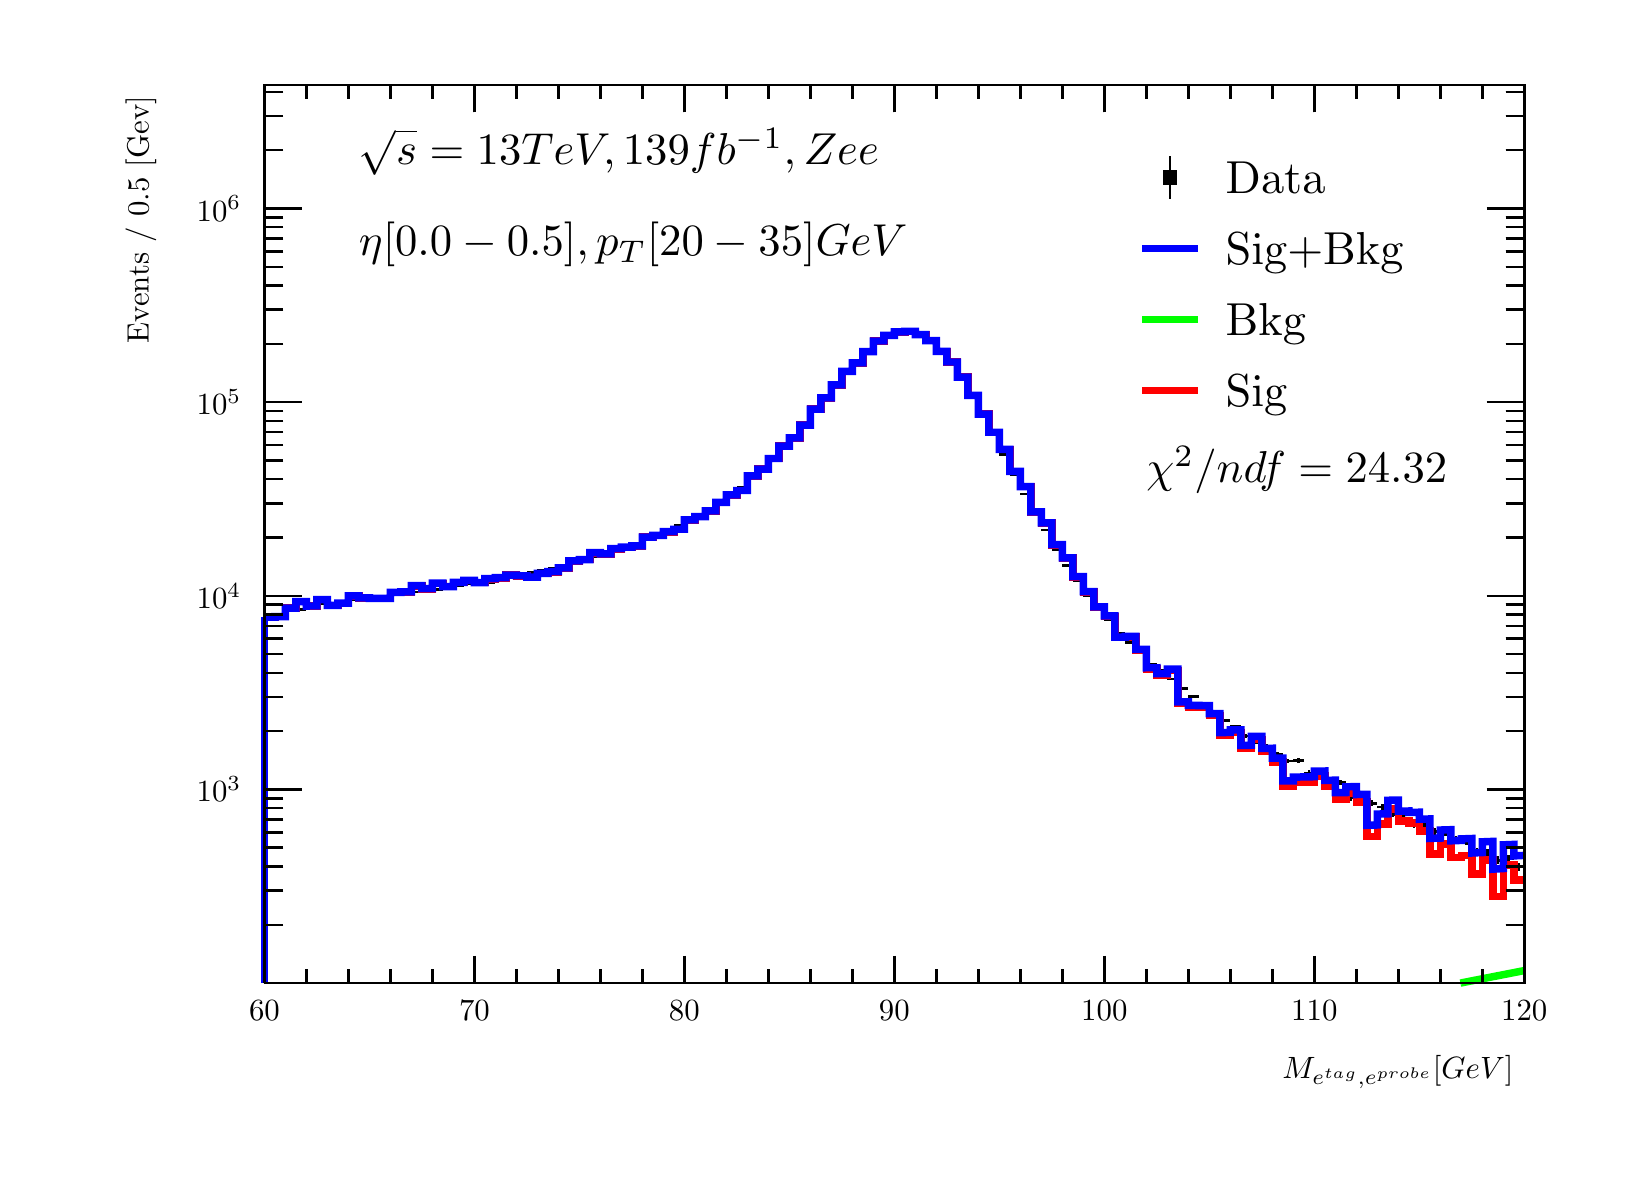
\begin{tikzpicture}
\pgfdeclareplotmark{cross} {
\pgfpathmoveto{\pgfpoint{-0.3\pgfplotmarksize}{\pgfplotmarksize}}
\pgfpathlineto{\pgfpoint{+0.3\pgfplotmarksize}{\pgfplotmarksize}}
\pgfpathlineto{\pgfpoint{+0.3\pgfplotmarksize}{0.3\pgfplotmarksize}}
\pgfpathlineto{\pgfpoint{+1\pgfplotmarksize}{0.3\pgfplotmarksize}}
\pgfpathlineto{\pgfpoint{+1\pgfplotmarksize}{-0.3\pgfplotmarksize}}
\pgfpathlineto{\pgfpoint{+0.3\pgfplotmarksize}{-0.3\pgfplotmarksize}}
\pgfpathlineto{\pgfpoint{+0.3\pgfplotmarksize}{-1.\pgfplotmarksize}}
\pgfpathlineto{\pgfpoint{-0.3\pgfplotmarksize}{-1.\pgfplotmarksize}}
\pgfpathlineto{\pgfpoint{-0.3\pgfplotmarksize}{-0.3\pgfplotmarksize}}
\pgfpathlineto{\pgfpoint{-1.\pgfplotmarksize}{-0.3\pgfplotmarksize}}
\pgfpathlineto{\pgfpoint{-1.\pgfplotmarksize}{0.3\pgfplotmarksize}}
\pgfpathlineto{\pgfpoint{-0.3\pgfplotmarksize}{0.3\pgfplotmarksize}}
\pgfpathclose
\pgfusepathqstroke
}
\pgfdeclareplotmark{cross*} {
\pgfpathmoveto{\pgfpoint{-0.3\pgfplotmarksize}{\pgfplotmarksize}}
\pgfpathlineto{\pgfpoint{+0.3\pgfplotmarksize}{\pgfplotmarksize}}
\pgfpathlineto{\pgfpoint{+0.3\pgfplotmarksize}{0.3\pgfplotmarksize}}
\pgfpathlineto{\pgfpoint{+1\pgfplotmarksize}{0.3\pgfplotmarksize}}
\pgfpathlineto{\pgfpoint{+1\pgfplotmarksize}{-0.3\pgfplotmarksize}}
\pgfpathlineto{\pgfpoint{+0.3\pgfplotmarksize}{-0.3\pgfplotmarksize}}
\pgfpathlineto{\pgfpoint{+0.3\pgfplotmarksize}{-1.\pgfplotmarksize}}
\pgfpathlineto{\pgfpoint{-0.3\pgfplotmarksize}{-1.\pgfplotmarksize}}
\pgfpathlineto{\pgfpoint{-0.3\pgfplotmarksize}{-0.3\pgfplotmarksize}}
\pgfpathlineto{\pgfpoint{-1.\pgfplotmarksize}{-0.3\pgfplotmarksize}}
\pgfpathlineto{\pgfpoint{-1.\pgfplotmarksize}{0.3\pgfplotmarksize}}
\pgfpathlineto{\pgfpoint{-0.3\pgfplotmarksize}{0.3\pgfplotmarksize}}
\pgfpathclose
\pgfusepathqfillstroke
}
\pgfdeclareplotmark{newstar} {
\pgfpathmoveto{\pgfqpoint{0pt}{\pgfplotmarksize}}
\pgfpathlineto{\pgfqpointpolar{44}{0.5\pgfplotmarksize}}
\pgfpathlineto{\pgfqpointpolar{18}{\pgfplotmarksize}}
\pgfpathlineto{\pgfqpointpolar{-20}{0.5\pgfplotmarksize}}
\pgfpathlineto{\pgfqpointpolar{-54}{\pgfplotmarksize}}
\pgfpathlineto{\pgfqpointpolar{-90}{0.5\pgfplotmarksize}}
\pgfpathlineto{\pgfqpointpolar{234}{\pgfplotmarksize}}
\pgfpathlineto{\pgfqpointpolar{198}{0.5\pgfplotmarksize}}
\pgfpathlineto{\pgfqpointpolar{162}{\pgfplotmarksize}}
\pgfpathlineto{\pgfqpointpolar{134}{0.5\pgfplotmarksize}}
\pgfpathclose
\pgfusepathqstroke
}
\pgfdeclareplotmark{newstar*} {
\pgfpathmoveto{\pgfqpoint{0pt}{\pgfplotmarksize}}
\pgfpathlineto{\pgfqpointpolar{44}{0.5\pgfplotmarksize}}
\pgfpathlineto{\pgfqpointpolar{18}{\pgfplotmarksize}}
\pgfpathlineto{\pgfqpointpolar{-20}{0.5\pgfplotmarksize}}
\pgfpathlineto{\pgfqpointpolar{-54}{\pgfplotmarksize}}
\pgfpathlineto{\pgfqpointpolar{-90}{0.5\pgfplotmarksize}}
\pgfpathlineto{\pgfqpointpolar{234}{\pgfplotmarksize}}
\pgfpathlineto{\pgfqpointpolar{198}{0.5\pgfplotmarksize}}
\pgfpathlineto{\pgfqpointpolar{162}{\pgfplotmarksize}}
\pgfpathlineto{\pgfqpointpolar{134}{0.5\pgfplotmarksize}}
\pgfpathclose
\pgfusepathqfillstroke
}
\definecolor{c}{rgb}{1,1,1};
\draw [color=c, fill=c] (0,0) rectangle (20,14.4361);
\draw [color=c, fill=c] (3,2.30977) rectangle (19,13.7143);
\definecolor{c}{rgb}{0,0,0};
\draw [c,line width=0.9] (3,2.30977) -- (3,13.7143) -- (19,13.7143) -- (19,2.30977) -- (3,2.30977);
\definecolor{c}{rgb}{1,1,1};
\draw [color=c, fill=c] (3,2.30977) rectangle (19,13.7143);
\definecolor{c}{rgb}{0,0,0};
\draw [c,line width=0.9] (3,2.30977) -- (3,13.7143) -- (19,13.7143) -- (19,2.30977) -- (3,2.30977);
\draw [c,line width=0.9] (3,2.30977) -- (19,2.30977);
\draw [c,line width=0.9] (3,2.65624) -- (3,2.30977);
\draw [c,line width=0.9] (3.53333,2.48301) -- (3.53333,2.30977);
\draw [c,line width=0.9] (4.06667,2.48301) -- (4.06667,2.30977);
\draw [c,line width=0.9] (4.6,2.48301) -- (4.6,2.30977);
\draw [c,line width=0.9] (5.13333,2.48301) -- (5.13333,2.30977);
\draw [c,line width=0.9] (5.66667,2.65624) -- (5.66667,2.30977);
\draw [c,line width=0.9] (6.2,2.48301) -- (6.2,2.30977);
\draw [c,line width=0.9] (6.73333,2.48301) -- (6.73333,2.30977);
\draw [c,line width=0.9] (7.26667,2.48301) -- (7.26667,2.30977);
\draw [c,line width=0.9] (7.8,2.48301) -- (7.8,2.30977);
\draw [c,line width=0.9] (8.33333,2.65624) -- (8.33333,2.30977);
\draw [c,line width=0.9] (8.86667,2.48301) -- (8.86667,2.30977);
\draw [c,line width=0.9] (9.4,2.48301) -- (9.4,2.30977);
\draw [c,line width=0.9] (9.93333,2.48301) -- (9.93333,2.30977);
\draw [c,line width=0.9] (10.4667,2.48301) -- (10.4667,2.30977);
\draw [c,line width=0.9] (11,2.65624) -- (11,2.30977);
\draw [c,line width=0.9] (11.5333,2.48301) -- (11.5333,2.30977);
\draw [c,line width=0.9] (12.0667,2.48301) -- (12.0667,2.30977);
\draw [c,line width=0.9] (12.6,2.48301) -- (12.6,2.30977);
\draw [c,line width=0.9] (13.1333,2.48301) -- (13.1333,2.30977);
\draw [c,line width=0.9] (13.6667,2.65624) -- (13.6667,2.30977);
\draw [c,line width=0.9] (14.2,2.48301) -- (14.2,2.30977);
\draw [c,line width=0.9] (14.7333,2.48301) -- (14.7333,2.30977);
\draw [c,line width=0.9] (15.2667,2.48301) -- (15.2667,2.30977);
\draw [c,line width=0.9] (15.8,2.48301) -- (15.8,2.30977);
\draw [c,line width=0.9] (16.3333,2.65624) -- (16.3333,2.30977);
\draw [c,line width=0.9] (16.8667,2.48301) -- (16.8667,2.30977);
\draw [c,line width=0.9] (17.4,2.48301) -- (17.4,2.30977);
\draw [c,line width=0.9] (17.9333,2.48301) -- (17.9333,2.30977);
\draw [c,line width=0.9] (18.4667,2.48301) -- (18.4667,2.30977);
\draw [c,line width=0.9] (19,2.65624) -- (19,2.30977);
\draw [anchor=base] (3,1.83338) node[scale=1.11327, color=c, rotate=0]{60};
\draw [anchor=base] (5.66667,1.83338) node[scale=1.11327, color=c, rotate=0]{70};
\draw [anchor=base] (8.33333,1.83338) node[scale=1.11327, color=c, rotate=0]{80};
\draw [anchor=base] (11,1.83338) node[scale=1.11327, color=c, rotate=0]{90};
\draw [anchor=base] (13.6667,1.83338) node[scale=1.11327, color=c, rotate=0]{100};
\draw [anchor=base] (16.3333,1.83338) node[scale=1.11327, color=c, rotate=0]{110};
\draw [anchor=base] (19,1.83338) node[scale=1.11327, color=c, rotate=0]{120};
\draw [anchor= east] (19,1.17798) node[scale=1.11327, color=c, rotate=0]{$M_{e^{tag}, e^{probe}}  [GeV]$};
\draw [c,line width=0.9] (3,13.7143) -- (19,13.7143);
\draw [c,line width=0.9] (3,13.3678) -- (3,13.7143);
\draw [c,line width=0.9] (3.53333,13.5411) -- (3.53333,13.7143);
\draw [c,line width=0.9] (4.06667,13.5411) -- (4.06667,13.7143);
\draw [c,line width=0.9] (4.6,13.5411) -- (4.6,13.7143);
\draw [c,line width=0.9] (5.13333,13.5411) -- (5.13333,13.7143);
\draw [c,line width=0.9] (5.66667,13.3678) -- (5.66667,13.7143);
\draw [c,line width=0.9] (6.2,13.5411) -- (6.2,13.7143);
\draw [c,line width=0.9] (6.73333,13.5411) -- (6.73333,13.7143);
\draw [c,line width=0.9] (7.26667,13.5411) -- (7.26667,13.7143);
\draw [c,line width=0.9] (7.8,13.5411) -- (7.8,13.7143);
\draw [c,line width=0.9] (8.33333,13.3678) -- (8.33333,13.7143);
\draw [c,line width=0.9] (8.86667,13.5411) -- (8.86667,13.7143);
\draw [c,line width=0.9] (9.4,13.5411) -- (9.4,13.7143);
\draw [c,line width=0.9] (9.93333,13.5411) -- (9.93333,13.7143);
\draw [c,line width=0.9] (10.4667,13.5411) -- (10.4667,13.7143);
\draw [c,line width=0.9] (11,13.3678) -- (11,13.7143);
\draw [c,line width=0.9] (11.5333,13.5411) -- (11.5333,13.7143);
\draw [c,line width=0.9] (12.0667,13.5411) -- (12.0667,13.7143);
\draw [c,line width=0.9] (12.6,13.5411) -- (12.6,13.7143);
\draw [c,line width=0.9] (13.1333,13.5411) -- (13.1333,13.7143);
\draw [c,line width=0.9] (13.6667,13.3678) -- (13.6667,13.7143);
\draw [c,line width=0.9] (14.2,13.5411) -- (14.2,13.7143);
\draw [c,line width=0.9] (14.7333,13.5411) -- (14.7333,13.7143);
\draw [c,line width=0.9] (15.2667,13.5411) -- (15.2667,13.7143);
\draw [c,line width=0.9] (15.8,13.5411) -- (15.8,13.7143);
\draw [c,line width=0.9] (16.3333,13.3678) -- (16.3333,13.7143);
\draw [c,line width=0.9] (16.8667,13.5411) -- (16.8667,13.7143);
\draw [c,line width=0.9] (17.4,13.5411) -- (17.4,13.7143);
\draw [c,line width=0.9] (17.9333,13.5411) -- (17.9333,13.7143);
\draw [c,line width=0.9] (18.4667,13.5411) -- (18.4667,13.7143);
\draw [c,line width=0.9] (19,13.3678) -- (19,13.7143);
\draw [c,line width=0.9] (3,2.30977) -- (3,13.7143);
\draw [c,line width=0.9] (3.237,3.05008) -- (3,3.05008);
\draw [c,line width=0.9] (3.237,3.48313) -- (3,3.48313);
\draw [c,line width=0.9] (3.237,3.79038) -- (3,3.79038);
\draw [c,line width=0.9] (3.237,4.02871) -- (3,4.02871);
\draw [c,line width=0.9] (3.237,4.22343) -- (3,4.22343);
\draw [c,line width=0.9] (3.237,4.38807) -- (3,4.38807);
\draw [c,line width=0.9] (3.237,4.53069) -- (3,4.53069);
\draw [c,line width=0.9] (3.237,4.65649) -- (3,4.65649);
\draw [c,line width=0.9] (3.474,4.76901) -- (3,4.76901);
\draw [anchor= east] (2.844,4.76901) node[scale=1.11327, color=c, rotate=0]{$10^{3}$};
\draw [c,line width=0.9] (3.237,5.50932) -- (3,5.50932);
\draw [c,line width=0.9] (3.237,5.94237) -- (3,5.94237);
\draw [c,line width=0.9] (3.237,6.24963) -- (3,6.24963);
\draw [c,line width=0.9] (3.237,6.48795) -- (3,6.48795);
\draw [c,line width=0.9] (3.237,6.68268) -- (3,6.68268);
\draw [c,line width=0.9] (3.237,6.84731) -- (3,6.84731);
\draw [c,line width=0.9] (3.237,6.98993) -- (3,6.98993);
\draw [c,line width=0.9] (3.237,7.11573) -- (3,7.11573);
\draw [c,line width=0.9] (3.474,7.22826) -- (3,7.22826);
\draw [anchor= east] (2.844,7.22826) node[scale=1.11327, color=c, rotate=0]{$10^{4}$};
\draw [c,line width=0.9] (3.237,7.96856) -- (3,7.96856);
\draw [c,line width=0.9] (3.237,8.40161) -- (3,8.40161);
\draw [c,line width=0.9] (3.237,8.70887) -- (3,8.70887);
\draw [c,line width=0.9] (3.237,8.94719) -- (3,8.94719);
\draw [c,line width=0.9] (3.237,9.14192) -- (3,9.14192);
\draw [c,line width=0.9] (3.237,9.30656) -- (3,9.30656);
\draw [c,line width=0.9] (3.237,9.44917) -- (3,9.44917);
\draw [c,line width=0.9] (3.237,9.57497) -- (3,9.57497);
\draw [c,line width=0.9] (3.474,9.6875) -- (3,9.6875);
\draw [anchor= east] (2.844,9.6875) node[scale=1.11327, color=c, rotate=0]{$10^{5}$};
\draw [c,line width=0.9] (3.237,10.4278) -- (3,10.4278);
\draw [c,line width=0.9] (3.237,10.8609) -- (3,10.8609);
\draw [c,line width=0.9] (3.237,11.1681) -- (3,11.1681);
\draw [c,line width=0.9] (3.237,11.4064) -- (3,11.4064);
\draw [c,line width=0.9] (3.237,11.6012) -- (3,11.6012);
\draw [c,line width=0.9] (3.237,11.7658) -- (3,11.7658);
\draw [c,line width=0.9] (3.237,11.9084) -- (3,11.9084);
\draw [c,line width=0.9] (3.237,12.0342) -- (3,12.0342);
\draw [c,line width=0.9] (3.474,12.1467) -- (3,12.1467);
\draw [anchor= east] (2.844,12.1467) node[scale=1.11327, color=c, rotate=0]{$10^{6}$};
\draw [c,line width=0.9] (3.237,12.887) -- (3,12.887);
\draw [c,line width=0.9] (3.237,13.3201) -- (3,13.3201);
\draw [c,line width=0.9] (3.237,13.6274) -- (3,13.6274);
\draw [anchor= east] (1.432,13.7143) node[scale=1.11327, color=c, rotate=90]{Events / 0.5 [Gev]};
\draw [c,line width=0.9] (19,2.30977) -- (19,13.7143);
\draw [c,line width=0.9] (18.763,3.05008) -- (19,3.05008);
\draw [c,line width=0.9] (18.763,3.48313) -- (19,3.48313);
\draw [c,line width=0.9] (18.763,3.79038) -- (19,3.79038);
\draw [c,line width=0.9] (18.763,4.02871) -- (19,4.02871);
\draw [c,line width=0.9] (18.763,4.22343) -- (19,4.22343);
\draw [c,line width=0.9] (18.763,4.38807) -- (19,4.38807);
\draw [c,line width=0.9] (18.763,4.53069) -- (19,4.53069);
\draw [c,line width=0.9] (18.763,4.65649) -- (19,4.65649);
\draw [c,line width=0.9] (18.526,4.76901) -- (19,4.76901);
\draw [c,line width=0.9] (18.763,5.50932) -- (19,5.50932);
\draw [c,line width=0.9] (18.763,5.94237) -- (19,5.94237);
\draw [c,line width=0.9] (18.763,6.24963) -- (19,6.24963);
\draw [c,line width=0.9] (18.763,6.48795) -- (19,6.48795);
\draw [c,line width=0.9] (18.763,6.68268) -- (19,6.68268);
\draw [c,line width=0.9] (18.763,6.84731) -- (19,6.84731);
\draw [c,line width=0.9] (18.763,6.98993) -- (19,6.98993);
\draw [c,line width=0.9] (18.763,7.11573) -- (19,7.11573);
\draw [c,line width=0.9] (18.526,7.22826) -- (19,7.22826);
\draw [c,line width=0.9] (18.763,7.96856) -- (19,7.96856);
\draw [c,line width=0.9] (18.763,8.40161) -- (19,8.40161);
\draw [c,line width=0.9] (18.763,8.70887) -- (19,8.70887);
\draw [c,line width=0.9] (18.763,8.94719) -- (19,8.94719);
\draw [c,line width=0.9] (18.763,9.14192) -- (19,9.14192);
\draw [c,line width=0.9] (18.763,9.30656) -- (19,9.30656);
\draw [c,line width=0.9] (18.763,9.44917) -- (19,9.44917);
\draw [c,line width=0.9] (18.763,9.57497) -- (19,9.57497);
\draw [c,line width=0.9] (18.526,9.6875) -- (19,9.6875);
\draw [c,line width=0.9] (18.763,10.4278) -- (19,10.4278);
\draw [c,line width=0.9] (18.763,10.8609) -- (19,10.8609);
\draw [c,line width=0.9] (18.763,11.1681) -- (19,11.1681);
\draw [c,line width=0.9] (18.763,11.4064) -- (19,11.4064);
\draw [c,line width=0.9] (18.763,11.6012) -- (19,11.6012);
\draw [c,line width=0.9] (18.763,11.7658) -- (19,11.7658);
\draw [c,line width=0.9] (18.763,11.9084) -- (19,11.9084);
\draw [c,line width=0.9] (18.763,12.0342) -- (19,12.0342);
\draw [c,line width=0.9] (18.526,12.1467) -- (19,12.1467);
\draw [c,line width=0.9] (18.763,12.887) -- (19,12.887);
\draw [c,line width=0.9] (18.763,13.3201) -- (19,13.3201);
\draw [c,line width=0.9] (18.763,13.6274) -- (19,13.6274);
\draw [c,line width=0.9] (3.06667,6.97555) -- (3,6.97555);
\draw [c,line width=0.9] (3,6.97555) -- (3,6.97555);
\draw [c,line width=0.9] (3.06667,6.97555) -- (3.13333,6.97555);
\draw [c,line width=0.9] (3.13333,6.97555) -- (3.13333,6.97555);
\draw [c,line width=0.9] (3.06667,6.97555) -- (3.06667,6.98757);
\draw [c,line width=0.9] (3.06667,6.98757) -- (3.06667,6.98757);
\draw [c,line width=0.9] (3.06667,6.97555) -- (3.06667,6.96353);
\draw [c,line width=0.9] (3.06667,6.96353) -- (3.06667,6.96353);
\draw [c,line width=0.9] (3.2,6.99897) -- (3.13333,6.99897);
\draw [c,line width=0.9] (3.13333,6.99897) -- (3.13333,6.99897);
\draw [c,line width=0.9] (3.2,6.99897) -- (3.26667,6.99897);
\draw [c,line width=0.9] (3.26667,6.99897) -- (3.26667,6.99897);
\draw [c,line width=0.9] (3.2,6.99897) -- (3.2,7.01086);
\draw [c,line width=0.9] (3.2,7.01086) -- (3.2,7.01086);
\draw [c,line width=0.9] (3.2,6.99897) -- (3.2,6.98708);
\draw [c,line width=0.9] (3.2,6.98708) -- (3.2,6.98708);
\draw [c,line width=0.9] (3.33333,7.05305) -- (3.26667,7.05305);
\draw [c,line width=0.9] (3.26667,7.05305) -- (3.26667,7.05305);
\draw [c,line width=0.9] (3.33333,7.05305) -- (3.4,7.05305);
\draw [c,line width=0.9] (3.4,7.05305) -- (3.4,7.05305);
\draw [c,line width=0.9] (3.33333,7.05305) -- (3.33333,7.06464);
\draw [c,line width=0.9] (3.33333,7.06464) -- (3.33333,7.06464);
\draw [c,line width=0.9] (3.33333,7.05305) -- (3.33333,7.04145);
\draw [c,line width=0.9] (3.33333,7.04145) -- (3.33333,7.04145);
\draw [c,line width=0.9] (3.46667,7.05619) -- (3.4,7.05619);
\draw [c,line width=0.9] (3.4,7.05619) -- (3.4,7.05619);
\draw [c,line width=0.9] (3.46667,7.05619) -- (3.53333,7.05619);
\draw [c,line width=0.9] (3.53333,7.05619) -- (3.53333,7.05619);
\draw [c,line width=0.9] (3.46667,7.05619) -- (3.46667,7.06776);
\draw [c,line width=0.9] (3.46667,7.06776) -- (3.46667,7.06776);
\draw [c,line width=0.9] (3.46667,7.05619) -- (3.46667,7.04461);
\draw [c,line width=0.9] (3.46667,7.04461) -- (3.46667,7.04461);
\draw [c,line width=0.9] (3.6,7.09403) -- (3.53333,7.09403);
\draw [c,line width=0.9] (3.53333,7.09403) -- (3.53333,7.09403);
\draw [c,line width=0.9] (3.6,7.09403) -- (3.66667,7.09403);
\draw [c,line width=0.9] (3.66667,7.09403) -- (3.66667,7.09403);
\draw [c,line width=0.9] (3.6,7.09403) -- (3.6,7.1054);
\draw [c,line width=0.9] (3.6,7.1054) -- (3.6,7.1054);
\draw [c,line width=0.9] (3.6,7.09403) -- (3.6,7.08266);
\draw [c,line width=0.9] (3.6,7.08266) -- (3.6,7.08266);
\draw [c,line width=0.9] (3.73333,7.12094) -- (3.66667,7.12094);
\draw [c,line width=0.9] (3.66667,7.12094) -- (3.66667,7.12094);
\draw [c,line width=0.9] (3.73333,7.12094) -- (3.8,7.12094);
\draw [c,line width=0.9] (3.8,7.12094) -- (3.8,7.12094);
\draw [c,line width=0.9] (3.73333,7.12094) -- (3.73333,7.13217);
\draw [c,line width=0.9] (3.73333,7.13217) -- (3.73333,7.13217);
\draw [c,line width=0.9] (3.73333,7.12094) -- (3.73333,7.10971);
\draw [c,line width=0.9] (3.73333,7.10971) -- (3.73333,7.10971);
\draw [c,line width=0.9] (3.86667,7.1328) -- (3.8,7.1328);
\draw [c,line width=0.9] (3.8,7.1328) -- (3.8,7.1328);
\draw [c,line width=0.9] (3.86667,7.1328) -- (3.93333,7.1328);
\draw [c,line width=0.9] (3.93333,7.1328) -- (3.93333,7.1328);
\draw [c,line width=0.9] (3.86667,7.1328) -- (3.86667,7.14397);
\draw [c,line width=0.9] (3.86667,7.14397) -- (3.86667,7.14397);
\draw [c,line width=0.9] (3.86667,7.1328) -- (3.86667,7.12163);
\draw [c,line width=0.9] (3.86667,7.12163) -- (3.86667,7.12163);
\draw [c,line width=0.9] (4,7.15407) -- (3.93333,7.15407);
\draw [c,line width=0.9] (3.93333,7.15407) -- (3.93333,7.15407);
\draw [c,line width=0.9] (4,7.15407) -- (4.06667,7.15407);
\draw [c,line width=0.9] (4.06667,7.15407) -- (4.06667,7.15407);
\draw [c,line width=0.9] (4,7.15407) -- (4,7.16513);
\draw [c,line width=0.9] (4,7.16513) -- (4,7.16513);
\draw [c,line width=0.9] (4,7.15407) -- (4,7.14302);
\draw [c,line width=0.9] (4,7.14302) -- (4,7.14302);
\draw [c,line width=0.9] (4.13333,7.18377) -- (4.06667,7.18377);
\draw [c,line width=0.9] (4.06667,7.18377) -- (4.06667,7.18377);
\draw [c,line width=0.9] (4.13333,7.18377) -- (4.2,7.18377);
\draw [c,line width=0.9] (4.2,7.18377) -- (4.2,7.18377);
\draw [c,line width=0.9] (4.13333,7.18377) -- (4.13333,7.19467);
\draw [c,line width=0.9] (4.13333,7.19467) -- (4.13333,7.19467);
\draw [c,line width=0.9] (4.13333,7.18377) -- (4.13333,7.17286);
\draw [c,line width=0.9] (4.13333,7.17286) -- (4.13333,7.17286);
\draw [c,line width=0.9] (4.26667,7.21439) -- (4.2,7.21439);
\draw [c,line width=0.9] (4.2,7.21439) -- (4.2,7.21439);
\draw [c,line width=0.9] (4.26667,7.21439) -- (4.33333,7.21439);
\draw [c,line width=0.9] (4.33333,7.21439) -- (4.33333,7.21439);
\draw [c,line width=0.9] (4.26667,7.21439) -- (4.26667,7.22514);
\draw [c,line width=0.9] (4.26667,7.22514) -- (4.26667,7.22514);
\draw [c,line width=0.9] (4.26667,7.21439) -- (4.26667,7.20364);
\draw [c,line width=0.9] (4.26667,7.20364) -- (4.26667,7.20364);
\draw [c,line width=0.9] (4.4,7.21114) -- (4.33333,7.21114);
\draw [c,line width=0.9] (4.33333,7.21114) -- (4.33333,7.21114);
\draw [c,line width=0.9] (4.4,7.21114) -- (4.46667,7.21114);
\draw [c,line width=0.9] (4.46667,7.21114) -- (4.46667,7.21114);
\draw [c,line width=0.9] (4.4,7.21114) -- (4.4,7.22191);
\draw [c,line width=0.9] (4.4,7.22191) -- (4.4,7.22191);
\draw [c,line width=0.9] (4.4,7.21114) -- (4.4,7.20037);
\draw [c,line width=0.9] (4.4,7.20037) -- (4.4,7.20037);
\draw [c,line width=0.9] (4.53333,7.21979) -- (4.46667,7.21979);
\draw [c,line width=0.9] (4.46667,7.21979) -- (4.46667,7.21979);
\draw [c,line width=0.9] (4.53333,7.21979) -- (4.6,7.21979);
\draw [c,line width=0.9] (4.6,7.21979) -- (4.6,7.21979);
\draw [c,line width=0.9] (4.53333,7.21979) -- (4.53333,7.23051);
\draw [c,line width=0.9] (4.53333,7.23051) -- (4.53333,7.23051);
\draw [c,line width=0.9] (4.53333,7.21979) -- (4.53333,7.20906);
\draw [c,line width=0.9] (4.53333,7.20906) -- (4.53333,7.20906);
\draw [c,line width=0.9] (4.66667,7.23878) -- (4.6,7.23878);
\draw [c,line width=0.9] (4.6,7.23878) -- (4.6,7.23878);
\draw [c,line width=0.9] (4.66667,7.23878) -- (4.73333,7.23878);
\draw [c,line width=0.9] (4.73333,7.23878) -- (4.73333,7.23878);
\draw [c,line width=0.9] (4.66667,7.23878) -- (4.66667,7.24941);
\draw [c,line width=0.9] (4.66667,7.24941) -- (4.66667,7.24941);
\draw [c,line width=0.9] (4.66667,7.23878) -- (4.66667,7.22815);
\draw [c,line width=0.9] (4.66667,7.22815) -- (4.66667,7.22815);
\draw [c,line width=0.9] (4.8,7.28756) -- (4.73333,7.28756);
\draw [c,line width=0.9] (4.73333,7.28756) -- (4.73333,7.28756);
\draw [c,line width=0.9] (4.8,7.28756) -- (4.86667,7.28756);
\draw [c,line width=0.9] (4.86667,7.28756) -- (4.86667,7.28756);
\draw [c,line width=0.9] (4.8,7.28756) -- (4.8,7.29795);
\draw [c,line width=0.9] (4.8,7.29795) -- (4.8,7.29795);
\draw [c,line width=0.9] (4.8,7.28756) -- (4.8,7.27718);
\draw [c,line width=0.9] (4.8,7.27718) -- (4.8,7.27718);
\draw [c,line width=0.9] (4.93333,7.27425) -- (4.86667,7.27425);
\draw [c,line width=0.9] (4.86667,7.27425) -- (4.86667,7.27425);
\draw [c,line width=0.9] (4.93333,7.27425) -- (5,7.27425);
\draw [c,line width=0.9] (5,7.27425) -- (5,7.27425);
\draw [c,line width=0.9] (4.93333,7.27425) -- (4.93333,7.2847);
\draw [c,line width=0.9] (4.93333,7.2847) -- (4.93333,7.2847);
\draw [c,line width=0.9] (4.93333,7.27425) -- (4.93333,7.26379);
\draw [c,line width=0.9] (4.93333,7.26379) -- (4.93333,7.26379);
\draw [c,line width=0.9] (5.06667,7.30986) -- (5,7.30986);
\draw [c,line width=0.9] (5,7.30986) -- (5,7.30986);
\draw [c,line width=0.9] (5.06667,7.30986) -- (5.13333,7.30986);
\draw [c,line width=0.9] (5.13333,7.30986) -- (5.13333,7.30986);
\draw [c,line width=0.9] (5.06667,7.30986) -- (5.06667,7.32014);
\draw [c,line width=0.9] (5.06667,7.32014) -- (5.06667,7.32014);
\draw [c,line width=0.9] (5.06667,7.30986) -- (5.06667,7.29958);
\draw [c,line width=0.9] (5.06667,7.29958) -- (5.06667,7.29958);
\draw [c,line width=0.9] (5.2,7.31065) -- (5.13333,7.31065);
\draw [c,line width=0.9] (5.13333,7.31065) -- (5.13333,7.31065);
\draw [c,line width=0.9] (5.2,7.31065) -- (5.26667,7.31065);
\draw [c,line width=0.9] (5.26667,7.31065) -- (5.26667,7.31065);
\draw [c,line width=0.9] (5.2,7.31065) -- (5.2,7.32093);
\draw [c,line width=0.9] (5.2,7.32093) -- (5.2,7.32093);
\draw [c,line width=0.9] (5.2,7.31065) -- (5.2,7.30038);
\draw [c,line width=0.9] (5.2,7.30038) -- (5.2,7.30038);
\draw [c,line width=0.9] (5.33333,7.34844) -- (5.26667,7.34844);
\draw [c,line width=0.9] (5.26667,7.34844) -- (5.26667,7.34844);
\draw [c,line width=0.9] (5.33333,7.34844) -- (5.4,7.34844);
\draw [c,line width=0.9] (5.4,7.34844) -- (5.4,7.34844);
\draw [c,line width=0.9] (5.33333,7.34844) -- (5.33333,7.35853);
\draw [c,line width=0.9] (5.33333,7.35853) -- (5.33333,7.35853);
\draw [c,line width=0.9] (5.33333,7.34844) -- (5.33333,7.33834);
\draw [c,line width=0.9] (5.33333,7.33834) -- (5.33333,7.33834);
\draw [c,line width=0.9] (5.46667,7.35358) -- (5.4,7.35358);
\draw [c,line width=0.9] (5.4,7.35358) -- (5.4,7.35358);
\draw [c,line width=0.9] (5.46667,7.35358) -- (5.53333,7.35358);
\draw [c,line width=0.9] (5.53333,7.35358) -- (5.53333,7.35358);
\draw [c,line width=0.9] (5.46667,7.35358) -- (5.46667,7.36365);
\draw [c,line width=0.9] (5.46667,7.36365) -- (5.46667,7.36365);
\draw [c,line width=0.9] (5.46667,7.35358) -- (5.46667,7.34351);
\draw [c,line width=0.9] (5.46667,7.34351) -- (5.46667,7.34351);
\draw [c,line width=0.9] (5.6,7.38401) -- (5.53333,7.38401);
\draw [c,line width=0.9] (5.53333,7.38401) -- (5.53333,7.38401);
\draw [c,line width=0.9] (5.6,7.38401) -- (5.66667,7.38401);
\draw [c,line width=0.9] (5.66667,7.38401) -- (5.66667,7.38401);
\draw [c,line width=0.9] (5.6,7.38401) -- (5.6,7.39394);
\draw [c,line width=0.9] (5.6,7.39394) -- (5.6,7.39394);
\draw [c,line width=0.9] (5.6,7.38401) -- (5.6,7.37408);
\draw [c,line width=0.9] (5.6,7.37408) -- (5.6,7.37408);
\draw [c,line width=0.9] (5.73333,7.39649) -- (5.66667,7.39649);
\draw [c,line width=0.9] (5.66667,7.39649) -- (5.66667,7.39649);
\draw [c,line width=0.9] (5.73333,7.39649) -- (5.8,7.39649);
\draw [c,line width=0.9] (5.8,7.39649) -- (5.8,7.39649);
\draw [c,line width=0.9] (5.73333,7.39649) -- (5.73333,7.40636);
\draw [c,line width=0.9] (5.73333,7.40636) -- (5.73333,7.40636);
\draw [c,line width=0.9] (5.73333,7.39649) -- (5.73333,7.38662);
\draw [c,line width=0.9] (5.73333,7.38662) -- (5.73333,7.38662);
\draw [c,line width=0.9] (5.86667,7.39722) -- (5.8,7.39722);
\draw [c,line width=0.9] (5.8,7.39722) -- (5.8,7.39722);
\draw [c,line width=0.9] (5.86667,7.39722) -- (5.93333,7.39722);
\draw [c,line width=0.9] (5.93333,7.39722) -- (5.93333,7.39722);
\draw [c,line width=0.9] (5.86667,7.39722) -- (5.86667,7.40709);
\draw [c,line width=0.9] (5.86667,7.40709) -- (5.86667,7.40709);
\draw [c,line width=0.9] (5.86667,7.39722) -- (5.86667,7.38735);
\draw [c,line width=0.9] (5.86667,7.38735) -- (5.86667,7.38735);
\draw [c,line width=0.9] (6,7.44378) -- (5.93333,7.44378);
\draw [c,line width=0.9] (5.93333,7.44378) -- (5.93333,7.44378);
\draw [c,line width=0.9] (6,7.44378) -- (6.06667,7.44378);
\draw [c,line width=0.9] (6.06667,7.44378) -- (6.06667,7.44378);
\draw [c,line width=0.9] (6,7.44378) -- (6,7.45344);
\draw [c,line width=0.9] (6,7.45344) -- (6,7.45344);
\draw [c,line width=0.9] (6,7.44378) -- (6,7.43413);
\draw [c,line width=0.9] (6,7.43413) -- (6,7.43413);
\draw [c,line width=0.9] (6.13333,7.45403) -- (6.06667,7.45403);
\draw [c,line width=0.9] (6.06667,7.45403) -- (6.06667,7.45403);
\draw [c,line width=0.9] (6.13333,7.45403) -- (6.2,7.45403);
\draw [c,line width=0.9] (6.2,7.45403) -- (6.2,7.45403);
\draw [c,line width=0.9] (6.13333,7.45403) -- (6.13333,7.46364);
\draw [c,line width=0.9] (6.13333,7.46364) -- (6.13333,7.46364);
\draw [c,line width=0.9] (6.13333,7.45403) -- (6.13333,7.44443);
\draw [c,line width=0.9] (6.13333,7.44443) -- (6.13333,7.44443);
\draw [c,line width=0.9] (6.26667,7.5008) -- (6.2,7.5008);
\draw [c,line width=0.9] (6.2,7.5008) -- (6.2,7.5008);
\draw [c,line width=0.9] (6.26667,7.5008) -- (6.33333,7.5008);
\draw [c,line width=0.9] (6.33333,7.5008) -- (6.33333,7.5008);
\draw [c,line width=0.9] (6.26667,7.5008) -- (6.26667,7.5102);
\draw [c,line width=0.9] (6.26667,7.5102) -- (6.26667,7.5102);
\draw [c,line width=0.9] (6.26667,7.5008) -- (6.26667,7.4914);
\draw [c,line width=0.9] (6.26667,7.4914) -- (6.26667,7.4914);
\draw [c,line width=0.9] (6.4,7.52162) -- (6.33333,7.52162);
\draw [c,line width=0.9] (6.33333,7.52162) -- (6.33333,7.52162);
\draw [c,line width=0.9] (6.4,7.52162) -- (6.46667,7.52162);
\draw [c,line width=0.9] (6.46667,7.52162) -- (6.46667,7.52162);
\draw [c,line width=0.9] (6.4,7.52162) -- (6.4,7.53093);
\draw [c,line width=0.9] (6.4,7.53093) -- (6.4,7.53093);
\draw [c,line width=0.9] (6.4,7.52162) -- (6.4,7.51231);
\draw [c,line width=0.9] (6.4,7.51231) -- (6.4,7.51231);
\draw [c,line width=0.9] (6.53333,7.54941) -- (6.46667,7.54941);
\draw [c,line width=0.9] (6.46667,7.54941) -- (6.46667,7.54941);
\draw [c,line width=0.9] (6.53333,7.54941) -- (6.6,7.54941);
\draw [c,line width=0.9] (6.6,7.54941) -- (6.6,7.54941);
\draw [c,line width=0.9] (6.53333,7.54941) -- (6.53333,7.5586);
\draw [c,line width=0.9] (6.53333,7.5586) -- (6.53333,7.5586);
\draw [c,line width=0.9] (6.53333,7.54941) -- (6.53333,7.54022);
\draw [c,line width=0.9] (6.53333,7.54022) -- (6.53333,7.54022);
\draw [c,line width=0.9] (6.66667,7.58211) -- (6.6,7.58211);
\draw [c,line width=0.9] (6.6,7.58211) -- (6.6,7.58211);
\draw [c,line width=0.9] (6.66667,7.58211) -- (6.73333,7.58211);
\draw [c,line width=0.9] (6.73333,7.58211) -- (6.73333,7.58211);
\draw [c,line width=0.9] (6.66667,7.58211) -- (6.66667,7.59116);
\draw [c,line width=0.9] (6.66667,7.59116) -- (6.66667,7.59116);
\draw [c,line width=0.9] (6.66667,7.58211) -- (6.66667,7.57306);
\draw [c,line width=0.9] (6.66667,7.57306) -- (6.66667,7.57306);
\draw [c,line width=0.9] (6.8,7.61094) -- (6.73333,7.61094);
\draw [c,line width=0.9] (6.73333,7.61094) -- (6.73333,7.61094);
\draw [c,line width=0.9] (6.8,7.61094) -- (6.86667,7.61094);
\draw [c,line width=0.9] (6.86667,7.61094) -- (6.86667,7.61094);
\draw [c,line width=0.9] (6.8,7.61094) -- (6.8,7.61987);
\draw [c,line width=0.9] (6.8,7.61987) -- (6.8,7.61987);
\draw [c,line width=0.9] (6.8,7.61094) -- (6.8,7.60201);
\draw [c,line width=0.9] (6.8,7.60201) -- (6.8,7.60201);
\draw [c,line width=0.9] (6.93333,7.6331) -- (6.86667,7.6331);
\draw [c,line width=0.9] (6.86667,7.6331) -- (6.86667,7.6331);
\draw [c,line width=0.9] (6.93333,7.6331) -- (7,7.6331);
\draw [c,line width=0.9] (7,7.6331) -- (7,7.6331);
\draw [c,line width=0.9] (6.93333,7.6331) -- (6.93333,7.64194);
\draw [c,line width=0.9] (6.93333,7.64194) -- (6.93333,7.64194);
\draw [c,line width=0.9] (6.93333,7.6331) -- (6.93333,7.62426);
\draw [c,line width=0.9] (6.93333,7.62426) -- (6.93333,7.62426);
\draw [c,line width=0.9] (7.06667,7.66734) -- (7,7.66734);
\draw [c,line width=0.9] (7,7.66734) -- (7,7.66734);
\draw [c,line width=0.9] (7.06667,7.66734) -- (7.13333,7.66734);
\draw [c,line width=0.9] (7.13333,7.66734) -- (7.13333,7.66734);
\draw [c,line width=0.9] (7.06667,7.66734) -- (7.06667,7.67604);
\draw [c,line width=0.9] (7.06667,7.67604) -- (7.06667,7.67604);
\draw [c,line width=0.9] (7.06667,7.66734) -- (7.06667,7.65865);
\draw [c,line width=0.9] (7.06667,7.65865) -- (7.06667,7.65865);
\draw [c,line width=0.9] (7.2,7.71829) -- (7.13333,7.71829);
\draw [c,line width=0.9] (7.13333,7.71829) -- (7.13333,7.71829);
\draw [c,line width=0.9] (7.2,7.71829) -- (7.26667,7.71829);
\draw [c,line width=0.9] (7.26667,7.71829) -- (7.26667,7.71829);
\draw [c,line width=0.9] (7.2,7.71829) -- (7.2,7.72678);
\draw [c,line width=0.9] (7.2,7.72678) -- (7.2,7.72678);
\draw [c,line width=0.9] (7.2,7.71829) -- (7.2,7.7098);
\draw [c,line width=0.9] (7.2,7.7098) -- (7.2,7.7098);
\draw [c,line width=0.9] (7.33333,7.73961) -- (7.26667,7.73961);
\draw [c,line width=0.9] (7.26667,7.73961) -- (7.26667,7.73961);
\draw [c,line width=0.9] (7.33333,7.73961) -- (7.4,7.73961);
\draw [c,line width=0.9] (7.4,7.73961) -- (7.4,7.73961);
\draw [c,line width=0.9] (7.33333,7.73961) -- (7.33333,7.74801);
\draw [c,line width=0.9] (7.33333,7.74801) -- (7.33333,7.74801);
\draw [c,line width=0.9] (7.33333,7.73961) -- (7.33333,7.7312);
\draw [c,line width=0.9] (7.33333,7.7312) -- (7.33333,7.7312);
\draw [c,line width=0.9] (7.46667,7.78235) -- (7.4,7.78235);
\draw [c,line width=0.9] (7.4,7.78235) -- (7.4,7.78235);
\draw [c,line width=0.9] (7.46667,7.78235) -- (7.53333,7.78235);
\draw [c,line width=0.9] (7.53333,7.78235) -- (7.53333,7.78235);
\draw [c,line width=0.9] (7.46667,7.78235) -- (7.46667,7.79059);
\draw [c,line width=0.9] (7.46667,7.79059) -- (7.46667,7.79059);
\draw [c,line width=0.9] (7.46667,7.78235) -- (7.46667,7.77411);
\draw [c,line width=0.9] (7.46667,7.77411) -- (7.46667,7.77411);
\draw [c,line width=0.9] (7.6,7.83343) -- (7.53333,7.83343);
\draw [c,line width=0.9] (7.53333,7.83343) -- (7.53333,7.83343);
\draw [c,line width=0.9] (7.6,7.83343) -- (7.66667,7.83343);
\draw [c,line width=0.9] (7.66667,7.83343) -- (7.66667,7.83343);
\draw [c,line width=0.9] (7.6,7.83343) -- (7.6,7.84147);
\draw [c,line width=0.9] (7.6,7.84147) -- (7.6,7.84147);
\draw [c,line width=0.9] (7.6,7.83343) -- (7.6,7.82538);
\draw [c,line width=0.9] (7.6,7.82538) -- (7.6,7.82538);
\draw [c,line width=0.9] (7.73333,7.89025) -- (7.66667,7.89025);
\draw [c,line width=0.9] (7.66667,7.89025) -- (7.66667,7.89025);
\draw [c,line width=0.9] (7.73333,7.89025) -- (7.8,7.89025);
\draw [c,line width=0.9] (7.8,7.89025) -- (7.8,7.89025);
\draw [c,line width=0.9] (7.73333,7.89025) -- (7.73333,7.89808);
\draw [c,line width=0.9] (7.73333,7.89808) -- (7.73333,7.89808);
\draw [c,line width=0.9] (7.73333,7.89025) -- (7.73333,7.88242);
\draw [c,line width=0.9] (7.73333,7.88242) -- (7.73333,7.88242);
\draw [c,line width=0.9] (7.86667,7.94824) -- (7.8,7.94824);
\draw [c,line width=0.9] (7.8,7.94824) -- (7.8,7.94824);
\draw [c,line width=0.9] (7.86667,7.94824) -- (7.93333,7.94824);
\draw [c,line width=0.9] (7.93333,7.94824) -- (7.93333,7.94824);
\draw [c,line width=0.9] (7.86667,7.94824) -- (7.86667,7.95586);
\draw [c,line width=0.9] (7.86667,7.95586) -- (7.86667,7.95586);
\draw [c,line width=0.9] (7.86667,7.94824) -- (7.86667,7.94061);
\draw [c,line width=0.9] (7.86667,7.94061) -- (7.86667,7.94061);
\draw [c,line width=0.9] (8,7.99107) -- (7.93333,7.99107);
\draw [c,line width=0.9] (7.93333,7.99107) -- (7.93333,7.99107);
\draw [c,line width=0.9] (8,7.99107) -- (8.06667,7.99107);
\draw [c,line width=0.9] (8.06667,7.99107) -- (8.06667,7.99107);
\draw [c,line width=0.9] (8,7.99107) -- (8,7.99855);
\draw [c,line width=0.9] (8,7.99855) -- (8,7.99855);
\draw [c,line width=0.9] (8,7.99107) -- (8,7.9836);
\draw [c,line width=0.9] (8,7.9836) -- (8,7.9836);
\draw [c,line width=0.9] (8.13333,8.04883) -- (8.06667,8.04883);
\draw [c,line width=0.9] (8.06667,8.04883) -- (8.06667,8.04883);
\draw [c,line width=0.9] (8.13333,8.04883) -- (8.2,8.04883);
\draw [c,line width=0.9] (8.2,8.04883) -- (8.2,8.04883);
\draw [c,line width=0.9] (8.13333,8.04883) -- (8.13333,8.0561);
\draw [c,line width=0.9] (8.13333,8.0561) -- (8.13333,8.0561);
\draw [c,line width=0.9] (8.13333,8.04883) -- (8.13333,8.04156);
\draw [c,line width=0.9] (8.13333,8.04156) -- (8.13333,8.04156);
\draw [c,line width=0.9] (8.26667,8.11821) -- (8.2,8.11821);
\draw [c,line width=0.9] (8.2,8.11821) -- (8.2,8.11821);
\draw [c,line width=0.9] (8.26667,8.11821) -- (8.33333,8.11821);
\draw [c,line width=0.9] (8.33333,8.11821) -- (8.33333,8.11821);
\draw [c,line width=0.9] (8.26667,8.11821) -- (8.26667,8.12525);
\draw [c,line width=0.9] (8.26667,8.12525) -- (8.26667,8.12525);
\draw [c,line width=0.9] (8.26667,8.11821) -- (8.26667,8.11116);
\draw [c,line width=0.9] (8.26667,8.11116) -- (8.26667,8.11116);
\draw [c,line width=0.9] (8.4,8.18278) -- (8.33333,8.18278);
\draw [c,line width=0.9] (8.33333,8.18278) -- (8.33333,8.18278);
\draw [c,line width=0.9] (8.4,8.18278) -- (8.46667,8.18278);
\draw [c,line width=0.9] (8.46667,8.18278) -- (8.46667,8.18278);
\draw [c,line width=0.9] (8.4,8.18278) -- (8.4,8.18961);
\draw [c,line width=0.9] (8.4,8.18961) -- (8.4,8.18961);
\draw [c,line width=0.9] (8.4,8.18278) -- (8.4,8.17595);
\draw [c,line width=0.9] (8.4,8.17595) -- (8.4,8.17595);
\draw [c,line width=0.9] (8.53333,8.25148) -- (8.46667,8.25148);
\draw [c,line width=0.9] (8.46667,8.25148) -- (8.46667,8.25148);
\draw [c,line width=0.9] (8.53333,8.25148) -- (8.6,8.25148);
\draw [c,line width=0.9] (8.6,8.25148) -- (8.6,8.25148);
\draw [c,line width=0.9] (8.53333,8.25148) -- (8.53333,8.2581);
\draw [c,line width=0.9] (8.53333,8.2581) -- (8.53333,8.2581);
\draw [c,line width=0.9] (8.53333,8.25148) -- (8.53333,8.24487);
\draw [c,line width=0.9] (8.53333,8.24487) -- (8.53333,8.24487);
\draw [c,line width=0.9] (8.66667,8.3296) -- (8.6,8.3296);
\draw [c,line width=0.9] (8.6,8.3296) -- (8.6,8.3296);
\draw [c,line width=0.9] (8.66667,8.3296) -- (8.73333,8.3296);
\draw [c,line width=0.9] (8.73333,8.3296) -- (8.73333,8.3296);
\draw [c,line width=0.9] (8.66667,8.3296) -- (8.66667,8.33598);
\draw [c,line width=0.9] (8.66667,8.33598) -- (8.66667,8.33598);
\draw [c,line width=0.9] (8.66667,8.3296) -- (8.66667,8.32323);
\draw [c,line width=0.9] (8.66667,8.32323) -- (8.66667,8.32323);
\draw [c,line width=0.9] (8.8,8.41062) -- (8.73333,8.41062);
\draw [c,line width=0.9] (8.73333,8.41062) -- (8.73333,8.41062);
\draw [c,line width=0.9] (8.8,8.41062) -- (8.86667,8.41062);
\draw [c,line width=0.9] (8.86667,8.41062) -- (8.86667,8.41062);
\draw [c,line width=0.9] (8.8,8.41062) -- (8.8,8.41676);
\draw [c,line width=0.9] (8.8,8.41676) -- (8.8,8.41676);
\draw [c,line width=0.9] (8.8,8.41062) -- (8.8,8.40448);
\draw [c,line width=0.9] (8.8,8.40448) -- (8.8,8.40448);
\draw [c,line width=0.9] (8.93333,8.50328) -- (8.86667,8.50328);
\draw [c,line width=0.9] (8.86667,8.50328) -- (8.86667,8.50328);
\draw [c,line width=0.9] (8.93333,8.50328) -- (9,8.50328);
\draw [c,line width=0.9] (9,8.50328) -- (9,8.50328);
\draw [c,line width=0.9] (8.93333,8.50328) -- (8.93333,8.50916);
\draw [c,line width=0.9] (8.93333,8.50916) -- (8.93333,8.50916);
\draw [c,line width=0.9] (8.93333,8.50328) -- (8.93333,8.4974);
\draw [c,line width=0.9] (8.93333,8.4974) -- (8.93333,8.4974);
\draw [c,line width=0.9] (9.06667,8.60958) -- (9,8.60958);
\draw [c,line width=0.9] (9,8.60958) -- (9,8.60958);
\draw [c,line width=0.9] (9.06667,8.60958) -- (9.13333,8.60958);
\draw [c,line width=0.9] (9.13333,8.60958) -- (9.13333,8.60958);
\draw [c,line width=0.9] (9.06667,8.60958) -- (9.06667,8.61517);
\draw [c,line width=0.9] (9.06667,8.61517) -- (9.06667,8.61517);
\draw [c,line width=0.9] (9.06667,8.60958) -- (9.06667,8.60398);
\draw [c,line width=0.9] (9.06667,8.60398) -- (9.06667,8.60398);
\draw [c,line width=0.9] (9.2,8.71741) -- (9.13333,8.71741);
\draw [c,line width=0.9] (9.13333,8.71741) -- (9.13333,8.71741);
\draw [c,line width=0.9] (9.2,8.71741) -- (9.26667,8.71741);
\draw [c,line width=0.9] (9.26667,8.71741) -- (9.26667,8.71741);
\draw [c,line width=0.9] (9.2,8.71741) -- (9.2,8.72272);
\draw [c,line width=0.9] (9.2,8.72272) -- (9.2,8.72272);
\draw [c,line width=0.9] (9.2,8.71741) -- (9.2,8.71209);
\draw [c,line width=0.9] (9.2,8.71209) -- (9.2,8.71209);
\draw [c,line width=0.9] (9.33333,8.83352) -- (9.26667,8.83352);
\draw [c,line width=0.9] (9.26667,8.83352) -- (9.26667,8.83352);
\draw [c,line width=0.9] (9.33333,8.83352) -- (9.4,8.83352);
\draw [c,line width=0.9] (9.4,8.83352) -- (9.4,8.83352);
\draw [c,line width=0.9] (9.33333,8.83352) -- (9.33333,8.83856);
\draw [c,line width=0.9] (9.33333,8.83856) -- (9.33333,8.83856);
\draw [c,line width=0.9] (9.33333,8.83352) -- (9.33333,8.82849);
\draw [c,line width=0.9] (9.33333,8.82849) -- (9.33333,8.82849);
\draw [c,line width=0.9] (9.46667,8.97016) -- (9.4,8.97016);
\draw [c,line width=0.9] (9.4,8.97016) -- (9.4,8.97016);
\draw [c,line width=0.9] (9.46667,8.97016) -- (9.53333,8.97016);
\draw [c,line width=0.9] (9.53333,8.97016) -- (9.53333,8.97016);
\draw [c,line width=0.9] (9.46667,8.97016) -- (9.46667,8.97489);
\draw [c,line width=0.9] (9.46667,8.97489) -- (9.46667,8.97489);
\draw [c,line width=0.9] (9.46667,8.97016) -- (9.46667,8.96544);
\draw [c,line width=0.9] (9.46667,8.96544) -- (9.46667,8.96544);
\draw [c,line width=0.9] (9.6,9.10987) -- (9.53333,9.10987);
\draw [c,line width=0.9] (9.53333,9.10987) -- (9.53333,9.10987);
\draw [c,line width=0.9] (9.6,9.10987) -- (9.66667,9.10987);
\draw [c,line width=0.9] (9.66667,9.10987) -- (9.66667,9.10987);
\draw [c,line width=0.9] (9.6,9.10987) -- (9.6,9.11429);
\draw [c,line width=0.9] (9.6,9.11429) -- (9.6,9.11429);
\draw [c,line width=0.9] (9.6,9.10987) -- (9.6,9.10544);
\draw [c,line width=0.9] (9.6,9.10544) -- (9.6,9.10544);
\draw [c,line width=0.9] (9.73333,9.25465) -- (9.66667,9.25465);
\draw [c,line width=0.9] (9.66667,9.25465) -- (9.66667,9.25465);
\draw [c,line width=0.9] (9.73333,9.25465) -- (9.8,9.25465);
\draw [c,line width=0.9] (9.8,9.25465) -- (9.8,9.25465);
\draw [c,line width=0.9] (9.73333,9.25465) -- (9.73333,9.25878);
\draw [c,line width=0.9] (9.73333,9.25878) -- (9.73333,9.25878);
\draw [c,line width=0.9] (9.73333,9.25465) -- (9.73333,9.25051);
\draw [c,line width=0.9] (9.73333,9.25051) -- (9.73333,9.25051);
\draw [c,line width=0.9] (9.86667,9.41402) -- (9.8,9.41402);
\draw [c,line width=0.9] (9.8,9.41402) -- (9.8,9.41402);
\draw [c,line width=0.9] (9.86667,9.41402) -- (9.93333,9.41402);
\draw [c,line width=0.9] (9.93333,9.41402) -- (9.93333,9.41402);
\draw [c,line width=0.9] (9.86667,9.41402) -- (9.86667,9.41786);
\draw [c,line width=0.9] (9.86667,9.41786) -- (9.86667,9.41786);
\draw [c,line width=0.9] (9.86667,9.41402) -- (9.86667,9.41018);
\draw [c,line width=0.9] (9.86667,9.41018) -- (9.86667,9.41018);
\draw [c,line width=0.9] (10,9.57757) -- (9.93333,9.57757);
\draw [c,line width=0.9] (9.93333,9.57757) -- (9.93333,9.57757);
\draw [c,line width=0.9] (10,9.57757) -- (10.0667,9.57757);
\draw [c,line width=0.9] (10.0667,9.57757) -- (10.0667,9.57757);
\draw [c,line width=0.9] (10,9.57757) -- (10,9.58112);
\draw [c,line width=0.9] (10,9.58112) -- (10,9.58112);
\draw [c,line width=0.9] (10,9.57757) -- (10,9.57401);
\draw [c,line width=0.9] (10,9.57401) -- (10,9.57401);
\draw [c,line width=0.9] (10.1333,9.74181) -- (10.0667,9.74181);
\draw [c,line width=0.9] (10.0667,9.74181) -- (10.0667,9.74181);
\draw [c,line width=0.9] (10.1333,9.74181) -- (10.2,9.74181);
\draw [c,line width=0.9] (10.2,9.74181) -- (10.2,9.74181);
\draw [c,line width=0.9] (10.1333,9.74181) -- (10.1333,9.74511);
\draw [c,line width=0.9] (10.1333,9.74511) -- (10.1333,9.74511);
\draw [c,line width=0.9] (10.1333,9.74181) -- (10.1333,9.73852);
\draw [c,line width=0.9] (10.1333,9.73852) -- (10.1333,9.73852);
\draw [c,line width=0.9] (10.2667,9.90267) -- (10.2,9.90267);
\draw [c,line width=0.9] (10.2,9.90267) -- (10.2,9.90267);
\draw [c,line width=0.9] (10.2667,9.90267) -- (10.3333,9.90267);
\draw [c,line width=0.9] (10.3333,9.90267) -- (10.3333,9.90267);
\draw [c,line width=0.9] (10.2667,9.90267) -- (10.2667,9.90572);
\draw [c,line width=0.9] (10.2667,9.90572) -- (10.2667,9.90572);
\draw [c,line width=0.9] (10.2667,9.90267) -- (10.2667,9.89961);
\draw [c,line width=0.9] (10.2667,9.89961) -- (10.2667,9.89961);
\draw [c,line width=0.9] (10.4,10.0673) -- (10.3333,10.0673);
\draw [c,line width=0.9] (10.3333,10.0673) -- (10.3333,10.0673);
\draw [c,line width=0.9] (10.4,10.0673) -- (10.4667,10.0673);
\draw [c,line width=0.9] (10.4667,10.0673) -- (10.4667,10.0673);
\draw [c,line width=0.9] (10.4,10.0673) -- (10.4,10.0701);
\draw [c,line width=0.9] (10.4,10.0701) -- (10.4,10.0701);
\draw [c,line width=0.9] (10.4,10.0673) -- (10.4,10.0645);
\draw [c,line width=0.9] (10.4,10.0645) -- (10.4,10.0645);
\draw [c,line width=0.9] (10.5333,10.217) -- (10.4667,10.217);
\draw [c,line width=0.9] (10.4667,10.217) -- (10.4667,10.217);
\draw [c,line width=0.9] (10.5333,10.217) -- (10.6,10.217);
\draw [c,line width=0.9] (10.6,10.217) -- (10.6,10.217);
\draw [c,line width=0.9] (10.5333,10.217) -- (10.5333,10.2197);
\draw [c,line width=0.9] (10.5333,10.2197) -- (10.5333,10.2197);
\draw [c,line width=0.9] (10.5333,10.217) -- (10.5333,10.2144);
\draw [c,line width=0.9] (10.5333,10.2144) -- (10.5333,10.2144);
\draw [c,line width=0.9] (10.6667,10.3535) -- (10.6,10.3535);
\draw [c,line width=0.9] (10.6,10.3535) -- (10.6,10.3535);
\draw [c,line width=0.9] (10.6667,10.3535) -- (10.7333,10.3535);
\draw [c,line width=0.9] (10.7333,10.3535) -- (10.7333,10.3535);
\draw [c,line width=0.9] (10.6667,10.3535) -- (10.6667,10.356);
\draw [c,line width=0.9] (10.6667,10.356) -- (10.6667,10.356);
\draw [c,line width=0.9] (10.6667,10.3535) -- (10.6667,10.351);
\draw [c,line width=0.9] (10.6667,10.351) -- (10.6667,10.351);
\draw [c,line width=0.9] (10.8,10.4675) -- (10.7333,10.4675);
\draw [c,line width=0.9] (10.7333,10.4675) -- (10.7333,10.4675);
\draw [c,line width=0.9] (10.8,10.4675) -- (10.8667,10.4675);
\draw [c,line width=0.9] (10.8667,10.4675) -- (10.8667,10.4675);
\draw [c,line width=0.9] (10.8,10.4675) -- (10.8,10.4698);
\draw [c,line width=0.9] (10.8,10.4698) -- (10.8,10.4698);
\draw [c,line width=0.9] (10.8,10.4675) -- (10.8,10.4652);
\draw [c,line width=0.9] (10.8,10.4652) -- (10.8,10.4652);
\draw [c,line width=0.9] (10.9333,10.546) -- (10.8667,10.546);
\draw [c,line width=0.9] (10.8667,10.546) -- (10.8667,10.546);
\draw [c,line width=0.9] (10.9333,10.546) -- (11,10.546);
\draw [c,line width=0.9] (11,10.546) -- (11,10.546);
\draw [c,line width=0.9] (10.9333,10.546) -- (10.9333,10.5482);
\draw [c,line width=0.9] (10.9333,10.5482) -- (10.9333,10.5482);
\draw [c,line width=0.9] (10.9333,10.546) -- (10.9333,10.5437);
\draw [c,line width=0.9] (10.9333,10.5437) -- (10.9333,10.5437);
\draw [c,line width=0.9] (11.0667,10.5926) -- (11,10.5926);
\draw [c,line width=0.9] (11,10.5926) -- (11,10.5926);
\draw [c,line width=0.9] (11.0667,10.5926) -- (11.1333,10.5926);
\draw [c,line width=0.9] (11.1333,10.5926) -- (11.1333,10.5926);
\draw [c,line width=0.9] (11.0667,10.5926) -- (11.0667,10.5948);
\draw [c,line width=0.9] (11.0667,10.5948) -- (11.0667,10.5948);
\draw [c,line width=0.9] (11.0667,10.5926) -- (11.0667,10.5904);
\draw [c,line width=0.9] (11.0667,10.5904) -- (11.0667,10.5904);
\draw [c,line width=0.9] (11.2,10.6009) -- (11.1333,10.6009);
\draw [c,line width=0.9] (11.1333,10.6009) -- (11.1333,10.6009);
\draw [c,line width=0.9] (11.2,10.6009) -- (11.2667,10.6009);
\draw [c,line width=0.9] (11.2667,10.6009) -- (11.2667,10.6009);
\draw [c,line width=0.9] (11.2,10.6009) -- (11.2,10.6031);
\draw [c,line width=0.9] (11.2,10.6031) -- (11.2,10.6031);
\draw [c,line width=0.9] (11.2,10.6009) -- (11.2,10.5987);
\draw [c,line width=0.9] (11.2,10.5987) -- (11.2,10.5987);
\draw [c,line width=0.9] (11.3333,10.5575) -- (11.2667,10.5575);
\draw [c,line width=0.9] (11.2667,10.5575) -- (11.2667,10.5575);
\draw [c,line width=0.9] (11.3333,10.5575) -- (11.4,10.5575);
\draw [c,line width=0.9] (11.4,10.5575) -- (11.4,10.5575);
\draw [c,line width=0.9] (11.3333,10.5575) -- (11.3333,10.5597);
\draw [c,line width=0.9] (11.3333,10.5597) -- (11.3333,10.5597);
\draw [c,line width=0.9] (11.3333,10.5575) -- (11.3333,10.5552);
\draw [c,line width=0.9] (11.3333,10.5552) -- (11.3333,10.5552);
\draw [c,line width=0.9] (11.4667,10.4745) -- (11.4,10.4745);
\draw [c,line width=0.9] (11.4,10.4745) -- (11.4,10.4745);
\draw [c,line width=0.9] (11.4667,10.4745) -- (11.5333,10.4745);
\draw [c,line width=0.9] (11.5333,10.4745) -- (11.5333,10.4745);
\draw [c,line width=0.9] (11.4667,10.4745) -- (11.4667,10.4768);
\draw [c,line width=0.9] (11.4667,10.4768) -- (11.4667,10.4768);
\draw [c,line width=0.9] (11.4667,10.4745) -- (11.4667,10.4721);
\draw [c,line width=0.9] (11.4667,10.4721) -- (11.4667,10.4721);
\draw [c,line width=0.9] (11.6,10.348) -- (11.5333,10.348);
\draw [c,line width=0.9] (11.5333,10.348) -- (11.5333,10.348);
\draw [c,line width=0.9] (11.6,10.348) -- (11.6667,10.348);
\draw [c,line width=0.9] (11.6667,10.348) -- (11.6667,10.348);
\draw [c,line width=0.9] (11.6,10.348) -- (11.6,10.3505);
\draw [c,line width=0.9] (11.6,10.3505) -- (11.6,10.3505);
\draw [c,line width=0.9] (11.6,10.348) -- (11.6,10.3456);
\draw [c,line width=0.9] (11.6,10.3456) -- (11.6,10.3456);
\draw [c,line width=0.9] (11.7333,10.1848) -- (11.6667,10.1848);
\draw [c,line width=0.9] (11.6667,10.1848) -- (11.6667,10.1848);
\draw [c,line width=0.9] (11.7333,10.1848) -- (11.8,10.1848);
\draw [c,line width=0.9] (11.8,10.1848) -- (11.8,10.1848);
\draw [c,line width=0.9] (11.7333,10.1848) -- (11.7333,10.1875);
\draw [c,line width=0.9] (11.7333,10.1875) -- (11.7333,10.1875);
\draw [c,line width=0.9] (11.7333,10.1848) -- (11.7333,10.1821);
\draw [c,line width=0.9] (11.7333,10.1821) -- (11.7333,10.1821);
\draw [c,line width=0.9] (11.8667,9.9901) -- (11.8,9.9901);
\draw [c,line width=0.9] (11.8,9.9901) -- (11.8,9.9901);
\draw [c,line width=0.9] (11.8667,9.9901) -- (11.9333,9.9901);
\draw [c,line width=0.9] (11.9333,9.9901) -- (11.9333,9.9901);
\draw [c,line width=0.9] (11.8667,9.9901) -- (11.8667,9.99303);
\draw [c,line width=0.9] (11.8667,9.99303) -- (11.8667,9.99303);
\draw [c,line width=0.9] (11.8667,9.9901) -- (11.8667,9.98717);
\draw [c,line width=0.9] (11.8667,9.98717) -- (11.8667,9.98717);
\draw [c,line width=0.9] (12,9.7739) -- (11.9333,9.7739);
\draw [c,line width=0.9] (11.9333,9.7739) -- (11.9333,9.7739);
\draw [c,line width=0.9] (12,9.7739) -- (12.0667,9.7739);
\draw [c,line width=0.9] (12.0667,9.7739) -- (12.0667,9.7739);
\draw [c,line width=0.9] (12,9.7739) -- (12,9.77714);
\draw [c,line width=0.9] (12,9.77714) -- (12,9.77714);
\draw [c,line width=0.9] (12,9.7739) -- (12,9.77066);
\draw [c,line width=0.9] (12,9.77066) -- (12,9.77066);
\draw [c,line width=0.9] (12.1333,9.52728) -- (12.0667,9.52728);
\draw [c,line width=0.9] (12.0667,9.52728) -- (12.0667,9.52728);
\draw [c,line width=0.9] (12.1333,9.52728) -- (12.2,9.52728);
\draw [c,line width=0.9] (12.2,9.52728) -- (12.2,9.52728);
\draw [c,line width=0.9] (12.1333,9.52728) -- (12.1333,9.53092);
\draw [c,line width=0.9] (12.1333,9.53092) -- (12.1333,9.53092);
\draw [c,line width=0.9] (12.1333,9.52728) -- (12.1333,9.52364);
\draw [c,line width=0.9] (12.1333,9.52364) -- (12.1333,9.52364);
\draw [c,line width=0.9] (12.2667,9.2891) -- (12.2,9.2891);
\draw [c,line width=0.9] (12.2,9.2891) -- (12.2,9.2891);
\draw [c,line width=0.9] (12.2667,9.2891) -- (12.3333,9.2891);
\draw [c,line width=0.9] (12.3333,9.2891) -- (12.3333,9.2891);
\draw [c,line width=0.9] (12.2667,9.2891) -- (12.2667,9.29317);
\draw [c,line width=0.9] (12.2667,9.29317) -- (12.2667,9.29317);
\draw [c,line width=0.9] (12.2667,9.2891) -- (12.2667,9.28503);
\draw [c,line width=0.9] (12.2667,9.28503) -- (12.2667,9.28503);
\draw [c,line width=0.9] (12.4,9.02525) -- (12.3333,9.02525);
\draw [c,line width=0.9] (12.3333,9.02525) -- (12.3333,9.02525);
\draw [c,line width=0.9] (12.4,9.02525) -- (12.4667,9.02525);
\draw [c,line width=0.9] (12.4667,9.02525) -- (12.4667,9.02525);
\draw [c,line width=0.9] (12.4,9.02525) -- (12.4,9.02985);
\draw [c,line width=0.9] (12.4,9.02985) -- (12.4,9.02985);
\draw [c,line width=0.9] (12.4,9.02525) -- (12.4,9.02064);
\draw [c,line width=0.9] (12.4,9.02064) -- (12.4,9.02064);
\draw [c,line width=0.9] (12.5333,8.76954) -- (12.4667,8.76954);
\draw [c,line width=0.9] (12.4667,8.76954) -- (12.4667,8.76954);
\draw [c,line width=0.9] (12.5333,8.76954) -- (12.6,8.76954);
\draw [c,line width=0.9] (12.6,8.76954) -- (12.6,8.76954);
\draw [c,line width=0.9] (12.5333,8.76954) -- (12.5333,8.77473);
\draw [c,line width=0.9] (12.5333,8.77473) -- (12.5333,8.77473);
\draw [c,line width=0.9] (12.5333,8.76954) -- (12.5333,8.76435);
\draw [c,line width=0.9] (12.5333,8.76435) -- (12.5333,8.76435);
\draw [c,line width=0.9] (12.6667,8.51756) -- (12.6,8.51756);
\draw [c,line width=0.9] (12.6,8.51756) -- (12.6,8.51756);
\draw [c,line width=0.9] (12.6667,8.51756) -- (12.7333,8.51756);
\draw [c,line width=0.9] (12.7333,8.51756) -- (12.7333,8.51756);
\draw [c,line width=0.9] (12.6667,8.51756) -- (12.6667,8.5234);
\draw [c,line width=0.9] (12.6667,8.5234) -- (12.6667,8.5234);
\draw [c,line width=0.9] (12.6667,8.51756) -- (12.6667,8.51171);
\draw [c,line width=0.9] (12.6667,8.51171) -- (12.6667,8.51171);
\draw [c,line width=0.9] (12.8,8.29134) -- (12.7333,8.29134);
\draw [c,line width=0.9] (12.7333,8.29134) -- (12.7333,8.29134);
\draw [c,line width=0.9] (12.8,8.29134) -- (12.8667,8.29134);
\draw [c,line width=0.9] (12.8667,8.29134) -- (12.8667,8.29134);
\draw [c,line width=0.9] (12.8,8.29134) -- (12.8,8.29783);
\draw [c,line width=0.9] (12.8,8.29783) -- (12.8,8.29783);
\draw [c,line width=0.9] (12.8,8.29134) -- (12.8,8.28484);
\draw [c,line width=0.9] (12.8,8.28484) -- (12.8,8.28484);
\draw [c,line width=0.9] (12.9333,8.06525) -- (12.8667,8.06525);
\draw [c,line width=0.9] (12.8667,8.06525) -- (12.8667,8.06525);
\draw [c,line width=0.9] (12.9333,8.06525) -- (13,8.06525);
\draw [c,line width=0.9] (13,8.06525) -- (13,8.06525);
\draw [c,line width=0.9] (12.9333,8.06525) -- (12.9333,8.07247);
\draw [c,line width=0.9] (12.9333,8.07247) -- (12.9333,8.07247);
\draw [c,line width=0.9] (12.9333,8.06525) -- (12.9333,8.05803);
\draw [c,line width=0.9] (12.9333,8.05803) -- (12.9333,8.05803);
\draw [c,line width=0.9] (13.0667,7.81878) -- (13,7.81878);
\draw [c,line width=0.9] (13,7.81878) -- (13,7.81878);
\draw [c,line width=0.9] (13.0667,7.81878) -- (13.1333,7.81878);
\draw [c,line width=0.9] (13.1333,7.81878) -- (13.1333,7.81878);
\draw [c,line width=0.9] (13.0667,7.81878) -- (13.0667,7.82688);
\draw [c,line width=0.9] (13.0667,7.82688) -- (13.0667,7.82688);
\draw [c,line width=0.9] (13.0667,7.81878) -- (13.0667,7.81068);
\draw [c,line width=0.9] (13.0667,7.81068) -- (13.0667,7.81068);
\draw [c,line width=0.9] (13.2,7.61355) -- (13.1333,7.61355);
\draw [c,line width=0.9] (13.1333,7.61355) -- (13.1333,7.61355);
\draw [c,line width=0.9] (13.2,7.61355) -- (13.2667,7.61355);
\draw [c,line width=0.9] (13.2667,7.61355) -- (13.2667,7.61355);
\draw [c,line width=0.9] (13.2,7.61355) -- (13.2,7.62247);
\draw [c,line width=0.9] (13.2,7.62247) -- (13.2,7.62247);
\draw [c,line width=0.9] (13.2,7.61355) -- (13.2,7.60463);
\draw [c,line width=0.9] (13.2,7.60463) -- (13.2,7.60463);
\draw [c,line width=0.9] (13.3333,7.42102) -- (13.2667,7.42102);
\draw [c,line width=0.9] (13.2667,7.42102) -- (13.2667,7.42102);
\draw [c,line width=0.9] (13.3333,7.42102) -- (13.4,7.42102);
\draw [c,line width=0.9] (13.4,7.42102) -- (13.4,7.42102);
\draw [c,line width=0.9] (13.3333,7.42102) -- (13.3333,7.43078);
\draw [c,line width=0.9] (13.3333,7.43078) -- (13.3333,7.43078);
\draw [c,line width=0.9] (13.3333,7.42102) -- (13.3333,7.41126);
\draw [c,line width=0.9] (13.3333,7.41126) -- (13.3333,7.41126);
\draw [c,line width=0.9] (13.4667,7.22943) -- (13.4,7.22943);
\draw [c,line width=0.9] (13.4,7.22943) -- (13.4,7.22943);
\draw [c,line width=0.9] (13.4667,7.22943) -- (13.5333,7.22943);
\draw [c,line width=0.9] (13.5333,7.22943) -- (13.5333,7.22943);
\draw [c,line width=0.9] (13.4667,7.22943) -- (13.4667,7.24011);
\draw [c,line width=0.9] (13.4667,7.24011) -- (13.4667,7.24011);
\draw [c,line width=0.9] (13.4667,7.22943) -- (13.4667,7.21876);
\draw [c,line width=0.9] (13.4667,7.21876) -- (13.4667,7.21876);
\draw [c,line width=0.9] (13.6,7.05982) -- (13.5333,7.05982);
\draw [c,line width=0.9] (13.5333,7.05982) -- (13.5333,7.05982);
\draw [c,line width=0.9] (13.6,7.05982) -- (13.6667,7.05982);
\draw [c,line width=0.9] (13.6667,7.05982) -- (13.6667,7.05982);
\draw [c,line width=0.9] (13.6,7.05982) -- (13.6,7.07138);
\draw [c,line width=0.9] (13.6,7.07138) -- (13.6,7.07138);
\draw [c,line width=0.9] (13.6,7.05982) -- (13.6,7.04826);
\draw [c,line width=0.9] (13.6,7.04826) -- (13.6,7.04826);
\draw [c,line width=0.9] (13.7333,6.92171) -- (13.6667,6.92171);
\draw [c,line width=0.9] (13.6667,6.92171) -- (13.6667,6.92171);
\draw [c,line width=0.9] (13.7333,6.92171) -- (13.8,6.92171);
\draw [c,line width=0.9] (13.8,6.92171) -- (13.8,6.92171);
\draw [c,line width=0.9] (13.7333,6.92171) -- (13.7333,6.93404);
\draw [c,line width=0.9] (13.7333,6.93404) -- (13.7333,6.93404);
\draw [c,line width=0.9] (13.7333,6.92171) -- (13.7333,6.90939);
\draw [c,line width=0.9] (13.7333,6.90939) -- (13.7333,6.90939);
\draw [c,line width=0.9] (13.8667,6.75727) -- (13.8,6.75727);
\draw [c,line width=0.9] (13.8,6.75727) -- (13.8,6.75727);
\draw [c,line width=0.9] (13.8667,6.75727) -- (13.9333,6.75727);
\draw [c,line width=0.9] (13.9333,6.75727) -- (13.9333,6.75727);
\draw [c,line width=0.9] (13.8667,6.75727) -- (13.8667,6.77058);
\draw [c,line width=0.9] (13.8667,6.77058) -- (13.8667,6.77058);
\draw [c,line width=0.9] (13.8667,6.75727) -- (13.8667,6.74395);
\draw [c,line width=0.9] (13.8667,6.74395) -- (13.8667,6.74395);
\draw [c,line width=0.9] (14,6.63648) -- (13.9333,6.63648);
\draw [c,line width=0.9] (13.9333,6.63648) -- (13.9333,6.63648);
\draw [c,line width=0.9] (14,6.63648) -- (14.0667,6.63648);
\draw [c,line width=0.9] (14.0667,6.63648) -- (14.0667,6.63648);
\draw [c,line width=0.9] (14,6.63648) -- (14,6.65057);
\draw [c,line width=0.9] (14,6.65057) -- (14,6.65057);
\draw [c,line width=0.9] (14,6.63648) -- (14,6.62239);
\draw [c,line width=0.9] (14,6.62239) -- (14,6.62239);
\draw [c,line width=0.9] (14.1333,6.51266) -- (14.0667,6.51266);
\draw [c,line width=0.9] (14.0667,6.51266) -- (14.0667,6.51266);
\draw [c,line width=0.9] (14.1333,6.51266) -- (14.2,6.51266);
\draw [c,line width=0.9] (14.2,6.51266) -- (14.2,6.51266);
\draw [c,line width=0.9] (14.1333,6.51266) -- (14.1333,6.52759);
\draw [c,line width=0.9] (14.1333,6.52759) -- (14.1333,6.52759);
\draw [c,line width=0.9] (14.1333,6.51266) -- (14.1333,6.49773);
\draw [c,line width=0.9] (14.1333,6.49773) -- (14.1333,6.49773);
\draw [c,line width=0.9] (14.2667,6.36253) -- (14.2,6.36253);
\draw [c,line width=0.9] (14.2,6.36253) -- (14.2,6.36253);
\draw [c,line width=0.9] (14.2667,6.36253) -- (14.3333,6.36253);
\draw [c,line width=0.9] (14.3333,6.36253) -- (14.3333,6.36253);
\draw [c,line width=0.9] (14.2667,6.36253) -- (14.2667,6.37855);
\draw [c,line width=0.9] (14.2667,6.37855) -- (14.2667,6.37855);
\draw [c,line width=0.9] (14.2667,6.36253) -- (14.2667,6.34651);
\draw [c,line width=0.9] (14.2667,6.34651) -- (14.2667,6.34651);
\draw [c,line width=0.9] (14.4,6.27626) -- (14.3333,6.27626);
\draw [c,line width=0.9] (14.3333,6.27626) -- (14.3333,6.27626);
\draw [c,line width=0.9] (14.4,6.27626) -- (14.4667,6.27626);
\draw [c,line width=0.9] (14.4667,6.27626) -- (14.4667,6.27626);
\draw [c,line width=0.9] (14.4,6.27626) -- (14.4,6.29294);
\draw [c,line width=0.9] (14.4,6.29294) -- (14.4,6.29294);
\draw [c,line width=0.9] (14.4,6.27626) -- (14.4,6.25958);
\draw [c,line width=0.9] (14.4,6.25958) -- (14.4,6.25958);
\draw [c,line width=0.9] (14.5333,6.17039) -- (14.4667,6.17039);
\draw [c,line width=0.9] (14.4667,6.17039) -- (14.4667,6.17039);
\draw [c,line width=0.9] (14.5333,6.17039) -- (14.6,6.17039);
\draw [c,line width=0.9] (14.6,6.17039) -- (14.6,6.17039);
\draw [c,line width=0.9] (14.5333,6.17039) -- (14.5333,6.18792);
\draw [c,line width=0.9] (14.5333,6.18792) -- (14.5333,6.18792);
\draw [c,line width=0.9] (14.5333,6.17039) -- (14.5333,6.15287);
\draw [c,line width=0.9] (14.5333,6.15287) -- (14.5333,6.15287);
\draw [c,line width=0.9] (14.6667,6.05223) -- (14.6,6.05223);
\draw [c,line width=0.9] (14.6,6.05223) -- (14.6,6.05223);
\draw [c,line width=0.9] (14.6667,6.05223) -- (14.7333,6.05223);
\draw [c,line width=0.9] (14.7333,6.05223) -- (14.7333,6.05223);
\draw [c,line width=0.9] (14.6667,6.05223) -- (14.6667,6.07075);
\draw [c,line width=0.9] (14.6667,6.07075) -- (14.6667,6.07075);
\draw [c,line width=0.9] (14.6667,6.05223) -- (14.6667,6.03371);
\draw [c,line width=0.9] (14.6667,6.03371) -- (14.6667,6.03371);
\draw [c,line width=0.9] (14.8,5.94841) -- (14.7333,5.94841);
\draw [c,line width=0.9] (14.7333,5.94841) -- (14.7333,5.94841);
\draw [c,line width=0.9] (14.8,5.94841) -- (14.8667,5.94841);
\draw [c,line width=0.9] (14.8667,5.94841) -- (14.8667,5.94841);
\draw [c,line width=0.9] (14.8,5.94841) -- (14.8,5.96785);
\draw [c,line width=0.9] (14.8,5.96785) -- (14.8,5.96785);
\draw [c,line width=0.9] (14.8,5.94841) -- (14.8,5.92896);
\draw [c,line width=0.9] (14.8,5.92896) -- (14.8,5.92896);
\draw [c,line width=0.9] (14.9333,5.82389) -- (14.8667,5.82389);
\draw [c,line width=0.9] (14.8667,5.82389) -- (14.8667,5.82389);
\draw [c,line width=0.9] (14.9333,5.82389) -- (15,5.82389);
\draw [c,line width=0.9] (15,5.82389) -- (15,5.82389);
\draw [c,line width=0.9] (14.9333,5.82389) -- (14.9333,5.8445);
\draw [c,line width=0.9] (14.9333,5.8445) -- (14.9333,5.8445);
\draw [c,line width=0.9] (14.9333,5.82389) -- (14.9333,5.80328);
\draw [c,line width=0.9] (14.9333,5.80328) -- (14.9333,5.80328);
\draw [c,line width=0.9] (15.0667,5.72607) -- (15,5.72607);
\draw [c,line width=0.9] (15,5.72607) -- (15,5.72607);
\draw [c,line width=0.9] (15.0667,5.72607) -- (15.1333,5.72607);
\draw [c,line width=0.9] (15.1333,5.72607) -- (15.1333,5.72607);
\draw [c,line width=0.9] (15.0667,5.72607) -- (15.0667,5.74765);
\draw [c,line width=0.9] (15.0667,5.74765) -- (15.0667,5.74765);
\draw [c,line width=0.9] (15.0667,5.72607) -- (15.0667,5.70449);
\draw [c,line width=0.9] (15.0667,5.70449) -- (15.0667,5.70449);
\draw [c,line width=0.9] (15.2,5.64598) -- (15.1333,5.64598);
\draw [c,line width=0.9] (15.1333,5.64598) -- (15.1333,5.64598);
\draw [c,line width=0.9] (15.2,5.64598) -- (15.2667,5.64598);
\draw [c,line width=0.9] (15.2667,5.64598) -- (15.2667,5.64598);
\draw [c,line width=0.9] (15.2,5.64598) -- (15.2,5.66838);
\draw [c,line width=0.9] (15.2,5.66838) -- (15.2,5.66838);
\draw [c,line width=0.9] (15.2,5.64598) -- (15.2,5.62358);
\draw [c,line width=0.9] (15.2,5.62358) -- (15.2,5.62358);
\draw [c,line width=0.9] (15.3333,5.566) -- (15.2667,5.566);
\draw [c,line width=0.9] (15.2667,5.566) -- (15.2667,5.566);
\draw [c,line width=0.9] (15.3333,5.566) -- (15.4,5.566);
\draw [c,line width=0.9] (15.4,5.566) -- (15.4,5.566);
\draw [c,line width=0.9] (15.3333,5.566) -- (15.3333,5.58925);
\draw [c,line width=0.9] (15.3333,5.58925) -- (15.3333,5.58925);
\draw [c,line width=0.9] (15.3333,5.566) -- (15.3333,5.54274);
\draw [c,line width=0.9] (15.3333,5.54274) -- (15.3333,5.54274);
\draw [c,line width=0.9] (15.4667,5.44777) -- (15.4,5.44777);
\draw [c,line width=0.9] (15.4,5.44777) -- (15.4,5.44777);
\draw [c,line width=0.9] (15.4667,5.44777) -- (15.5333,5.44777);
\draw [c,line width=0.9] (15.5333,5.44777) -- (15.5333,5.44777);
\draw [c,line width=0.9] (15.4667,5.44777) -- (15.4667,5.47235);
\draw [c,line width=0.9] (15.4667,5.47235) -- (15.4667,5.47235);
\draw [c,line width=0.9] (15.4667,5.44777) -- (15.4667,5.42319);
\draw [c,line width=0.9] (15.4667,5.42319) -- (15.4667,5.42319);
\draw [c,line width=0.9] (15.6,5.36793) -- (15.5333,5.36793);
\draw [c,line width=0.9] (15.5333,5.36793) -- (15.5333,5.36793);
\draw [c,line width=0.9] (15.6,5.36793) -- (15.6667,5.36793);
\draw [c,line width=0.9] (15.6667,5.36793) -- (15.6667,5.36793);
\draw [c,line width=0.9] (15.6,5.36793) -- (15.6,5.39344);
\draw [c,line width=0.9] (15.6,5.39344) -- (15.6,5.39344);
\draw [c,line width=0.9] (15.6,5.36793) -- (15.6,5.34241);
\draw [c,line width=0.9] (15.6,5.34241) -- (15.6,5.34241);
\draw [c,line width=0.9] (15.7333,5.31353) -- (15.6667,5.31353);
\draw [c,line width=0.9] (15.6667,5.31353) -- (15.6667,5.31353);
\draw [c,line width=0.9] (15.7333,5.31353) -- (15.8,5.31353);
\draw [c,line width=0.9] (15.8,5.31353) -- (15.8,5.31353);
\draw [c,line width=0.9] (15.7333,5.31353) -- (15.7333,5.3397);
\draw [c,line width=0.9] (15.7333,5.3397) -- (15.7333,5.3397);
\draw [c,line width=0.9] (15.7333,5.31353) -- (15.7333,5.28735);
\draw [c,line width=0.9] (15.7333,5.28735) -- (15.7333,5.28735);
\draw [c,line width=0.9] (15.8667,5.22042) -- (15.8,5.22042);
\draw [c,line width=0.9] (15.8,5.22042) -- (15.8,5.22042);
\draw [c,line width=0.9] (15.8667,5.22042) -- (15.9333,5.22042);
\draw [c,line width=0.9] (15.9333,5.22042) -- (15.9333,5.22042);
\draw [c,line width=0.9] (15.8667,5.22042) -- (15.8667,5.24776);
\draw [c,line width=0.9] (15.8667,5.24776) -- (15.8667,5.24776);
\draw [c,line width=0.9] (15.8667,5.22042) -- (15.8667,5.19308);
\draw [c,line width=0.9] (15.8667,5.19308) -- (15.8667,5.19308);
\draw [c,line width=0.9] (16,5.13143) -- (15.9333,5.13143);
\draw [c,line width=0.9] (15.9333,5.13143) -- (15.9333,5.13143);
\draw [c,line width=0.9] (16,5.13143) -- (16.0667,5.13143);
\draw [c,line width=0.9] (16.0667,5.13143) -- (16.0667,5.13143);
\draw [c,line width=0.9] (16,5.13143) -- (16,5.15993);
\draw [c,line width=0.9] (16,5.15993) -- (16,5.15993);
\draw [c,line width=0.9] (16,5.13143) -- (16,5.10292);
\draw [c,line width=0.9] (16,5.10292) -- (16,5.10292);
\draw [c,line width=0.9] (16.1333,5.13447) -- (16.0667,5.13447);
\draw [c,line width=0.9] (16.0667,5.13447) -- (16.0667,5.13447);
\draw [c,line width=0.9] (16.1333,5.13447) -- (16.2,5.13447);
\draw [c,line width=0.9] (16.2,5.13447) -- (16.2,5.13447);
\draw [c,line width=0.9] (16.1333,5.13447) -- (16.1333,5.16293);
\draw [c,line width=0.9] (16.1333,5.16293) -- (16.1333,5.16293);
\draw [c,line width=0.9] (16.1333,5.13447) -- (16.1333,5.106);
\draw [c,line width=0.9] (16.1333,5.106) -- (16.1333,5.106);
\draw [c,line width=0.9] (16.2667,4.97877) -- (16.2,4.97877);
\draw [c,line width=0.9] (16.2,4.97877) -- (16.2,4.97877);
\draw [c,line width=0.9] (16.2667,4.97877) -- (16.3333,4.97877);
\draw [c,line width=0.9] (16.3333,4.97877) -- (16.3333,4.97877);
\draw [c,line width=0.9] (16.2667,4.97877) -- (16.2667,5.00938);
\draw [c,line width=0.9] (16.2667,5.00938) -- (16.2667,5.00938);
\draw [c,line width=0.9] (16.2667,4.97877) -- (16.2667,4.94815);
\draw [c,line width=0.9] (16.2667,4.94815) -- (16.2667,4.94815);
\draw [c,line width=0.9] (16.4,4.97349) -- (16.3333,4.97349);
\draw [c,line width=0.9] (16.3333,4.97349) -- (16.3333,4.97349);
\draw [c,line width=0.9] (16.4,4.97349) -- (16.4667,4.97349);
\draw [c,line width=0.9] (16.4667,4.97349) -- (16.4667,4.97349);
\draw [c,line width=0.9] (16.4,4.97349) -- (16.4,5.00418);
\draw [c,line width=0.9] (16.4,5.00418) -- (16.4,5.00418);
\draw [c,line width=0.9] (16.4,4.97349) -- (16.4,4.9428);
\draw [c,line width=0.9] (16.4,4.9428) -- (16.4,4.9428);
\draw [c,line width=0.9] (16.5333,4.87275) -- (16.4667,4.87275);
\draw [c,line width=0.9] (16.4667,4.87275) -- (16.4667,4.87275);
\draw [c,line width=0.9] (16.5333,4.87275) -- (16.6,4.87275);
\draw [c,line width=0.9] (16.6,4.87275) -- (16.6,4.87275);
\draw [c,line width=0.9] (16.5333,4.87275) -- (16.5333,4.90492);
\draw [c,line width=0.9] (16.5333,4.90492) -- (16.5333,4.90492);
\draw [c,line width=0.9] (16.5333,4.87275) -- (16.5333,4.84058);
\draw [c,line width=0.9] (16.5333,4.84058) -- (16.5333,4.84058);
\draw [c,line width=0.9] (16.6667,4.86008) -- (16.6,4.86008);
\draw [c,line width=0.9] (16.6,4.86008) -- (16.6,4.86008);
\draw [c,line width=0.9] (16.6667,4.86008) -- (16.7333,4.86008);
\draw [c,line width=0.9] (16.7333,4.86008) -- (16.7333,4.86008);
\draw [c,line width=0.9] (16.6667,4.86008) -- (16.6667,4.89244);
\draw [c,line width=0.9] (16.6667,4.89244) -- (16.6667,4.89244);
\draw [c,line width=0.9] (16.6667,4.86008) -- (16.6667,4.82771);
\draw [c,line width=0.9] (16.6667,4.82771) -- (16.6667,4.82771);
\draw [c,line width=0.9] (16.8,4.65886) -- (16.7333,4.65886);
\draw [c,line width=0.9] (16.7333,4.65886) -- (16.7333,4.65886);
\draw [c,line width=0.9] (16.8,4.65886) -- (16.8667,4.65886);
\draw [c,line width=0.9] (16.8667,4.65886) -- (16.8667,4.65886);
\draw [c,line width=0.9] (16.8,4.65886) -- (16.8,4.69442);
\draw [c,line width=0.9] (16.8,4.69442) -- (16.8,4.69442);
\draw [c,line width=0.9] (16.8,4.65886) -- (16.8,4.6233);
\draw [c,line width=0.9] (16.8,4.6233) -- (16.8,4.6233);
\draw [c,line width=0.9] (16.9333,4.6788) -- (16.8667,4.6788);
\draw [c,line width=0.9] (16.8667,4.6788) -- (16.8667,4.6788);
\draw [c,line width=0.9] (16.9333,4.6788) -- (17,4.6788);
\draw [c,line width=0.9] (17,4.6788) -- (17,4.6788);
\draw [c,line width=0.9] (16.9333,4.6788) -- (16.9333,4.71403);
\draw [c,line width=0.9] (16.9333,4.71403) -- (16.9333,4.71403);
\draw [c,line width=0.9] (16.9333,4.6788) -- (16.9333,4.64357);
\draw [c,line width=0.9] (16.9333,4.64357) -- (16.9333,4.64357);
\draw [c,line width=0.9] (17.0667,4.59166) -- (17,4.59166);
\draw [c,line width=0.9] (17,4.59166) -- (17,4.59166);
\draw [c,line width=0.9] (17.0667,4.59166) -- (17.1333,4.59166);
\draw [c,line width=0.9] (17.1333,4.59166) -- (17.1333,4.59166);
\draw [c,line width=0.9] (17.0667,4.59166) -- (17.0667,4.62836);
\draw [c,line width=0.9] (17.0667,4.62836) -- (17.0667,4.62836);
\draw [c,line width=0.9] (17.0667,4.59166) -- (17.0667,4.55497);
\draw [c,line width=0.9] (17.0667,4.55497) -- (17.0667,4.55497);
\draw [c,line width=0.9] (17.2,4.54791) -- (17.1333,4.54791);
\draw [c,line width=0.9] (17.1333,4.54791) -- (17.1333,4.54791);
\draw [c,line width=0.9] (17.2,4.54791) -- (17.2667,4.54791);
\draw [c,line width=0.9] (17.2667,4.54791) -- (17.2667,4.54791);
\draw [c,line width=0.9] (17.2,4.54791) -- (17.2,4.58536);
\draw [c,line width=0.9] (17.2,4.58536) -- (17.2,4.58536);
\draw [c,line width=0.9] (17.2,4.54791) -- (17.2,4.51045);
\draw [c,line width=0.9] (17.2,4.51045) -- (17.2,4.51045);
\draw [c,line width=0.9] (17.3333,4.45318) -- (17.2667,4.45318);
\draw [c,line width=0.9] (17.2667,4.45318) -- (17.2667,4.45318);
\draw [c,line width=0.9] (17.3333,4.45318) -- (17.4,4.45318);
\draw [c,line width=0.9] (17.4,4.45318) -- (17.4,4.45318);
\draw [c,line width=0.9] (17.3333,4.45318) -- (17.3333,4.49234);
\draw [c,line width=0.9] (17.3333,4.49234) -- (17.3333,4.49234);
\draw [c,line width=0.9] (17.3333,4.45318) -- (17.3333,4.41403);
\draw [c,line width=0.9] (17.3333,4.41403) -- (17.3333,4.41403);
\draw [c,line width=0.9] (17.4667,4.45462) -- (17.4,4.45462);
\draw [c,line width=0.9] (17.4,4.45462) -- (17.4,4.45462);
\draw [c,line width=0.9] (17.4667,4.45462) -- (17.5333,4.45462);
\draw [c,line width=0.9] (17.5333,4.45462) -- (17.5333,4.45462);
\draw [c,line width=0.9] (17.4667,4.45462) -- (17.4667,4.49374);
\draw [c,line width=0.9] (17.4667,4.49374) -- (17.4667,4.49374);
\draw [c,line width=0.9] (17.4667,4.45462) -- (17.4667,4.41549);
\draw [c,line width=0.9] (17.4667,4.41549) -- (17.4667,4.41549);
\draw [c,line width=0.9] (17.6,4.32199) -- (17.5333,4.32199);
\draw [c,line width=0.9] (17.5333,4.32199) -- (17.5333,4.32199);
\draw [c,line width=0.9] (17.6,4.32199) -- (17.6667,4.32199);
\draw [c,line width=0.9] (17.6667,4.32199) -- (17.6667,4.32199);
\draw [c,line width=0.9] (17.6,4.32199) -- (17.6,4.36362);
\draw [c,line width=0.9] (17.6,4.36362) -- (17.6,4.36362);
\draw [c,line width=0.9] (17.6,4.32199) -- (17.6,4.28036);
\draw [c,line width=0.9] (17.6,4.28036) -- (17.6,4.28036);
\draw [c,line width=0.9] (17.7333,4.33007) -- (17.6667,4.33007);
\draw [c,line width=0.9] (17.6667,4.33007) -- (17.6667,4.33007);
\draw [c,line width=0.9] (17.7333,4.33007) -- (17.8,4.33007);
\draw [c,line width=0.9] (17.8,4.33007) -- (17.8,4.33007);
\draw [c,line width=0.9] (17.7333,4.33007) -- (17.7333,4.37155);
\draw [c,line width=0.9] (17.7333,4.37155) -- (17.7333,4.37155);
\draw [c,line width=0.9] (17.7333,4.33007) -- (17.7333,4.2886);
\draw [c,line width=0.9] (17.7333,4.2886) -- (17.7333,4.2886);
\draw [c,line width=0.9] (17.8667,4.23406) -- (17.8,4.23406);
\draw [c,line width=0.9] (17.8,4.23406) -- (17.8,4.23406);
\draw [c,line width=0.9] (17.8667,4.23406) -- (17.9333,4.23406);
\draw [c,line width=0.9] (17.9333,4.23406) -- (17.9333,4.23406);
\draw [c,line width=0.9] (17.8667,4.23406) -- (17.8667,4.27745);
\draw [c,line width=0.9] (17.8667,4.27745) -- (17.8667,4.27745);
\draw [c,line width=0.9] (17.8667,4.23406) -- (17.8667,4.19068);
\draw [c,line width=0.9] (17.8667,4.19068) -- (17.8667,4.19068);
\draw [c,line width=0.9] (18,4.22344) -- (17.9333,4.22344);
\draw [c,line width=0.9] (17.9333,4.22344) -- (17.9333,4.22344);
\draw [c,line width=0.9] (18,4.22344) -- (18.0667,4.22344);
\draw [c,line width=0.9] (18.0667,4.22344) -- (18.0667,4.22344);
\draw [c,line width=0.9] (18,4.22344) -- (18,4.26704);
\draw [c,line width=0.9] (18,4.26704) -- (18,4.26704);
\draw [c,line width=0.9] (18,4.22344) -- (18,4.17984);
\draw [c,line width=0.9] (18,4.17984) -- (18,4.17984);
\draw [c,line width=0.9] (18.1333,4.12856) -- (18.0667,4.12856);
\draw [c,line width=0.9] (18.0667,4.12856) -- (18.0667,4.12856);
\draw [c,line width=0.9] (18.1333,4.12856) -- (18.2,4.12856);
\draw [c,line width=0.9] (18.2,4.12856) -- (18.2,4.12856);
\draw [c,line width=0.9] (18.1333,4.12856) -- (18.1333,4.17414);
\draw [c,line width=0.9] (18.1333,4.17414) -- (18.1333,4.17414);
\draw [c,line width=0.9] (18.1333,4.12856) -- (18.1333,4.08298);
\draw [c,line width=0.9] (18.1333,4.08298) -- (18.1333,4.08298);
\draw [c,line width=0.9] (18.2667,4.10297) -- (18.2,4.10297);
\draw [c,line width=0.9] (18.2,4.10297) -- (18.2,4.10297);
\draw [c,line width=0.9] (18.2667,4.10297) -- (18.3333,4.10297);
\draw [c,line width=0.9] (18.3333,4.10297) -- (18.3333,4.10297);
\draw [c,line width=0.9] (18.2667,4.10297) -- (18.2667,4.1491);
\draw [c,line width=0.9] (18.2667,4.1491) -- (18.2667,4.1491);
\draw [c,line width=0.9] (18.2667,4.10297) -- (18.2667,4.05684);
\draw [c,line width=0.9] (18.2667,4.05684) -- (18.2667,4.05684);
\draw [c,line width=0.9] (18.4,3.97168) -- (18.3333,3.97168);
\draw [c,line width=0.9] (18.3333,3.97168) -- (18.3333,3.97168);
\draw [c,line width=0.9] (18.4,3.97168) -- (18.4667,3.97168);
\draw [c,line width=0.9] (18.4667,3.97168) -- (18.4667,3.97168);
\draw [c,line width=0.9] (18.4,3.97168) -- (18.4,4.02073);
\draw [c,line width=0.9] (18.4,4.02073) -- (18.4,4.02073);
\draw [c,line width=0.9] (18.4,3.97168) -- (18.4,3.92262);
\draw [c,line width=0.9] (18.4,3.92262) -- (18.4,3.92262);
\draw [c,line width=0.9] (18.5333,3.95807) -- (18.4667,3.95807);
\draw [c,line width=0.9] (18.4667,3.95807) -- (18.4667,3.95807);
\draw [c,line width=0.9] (18.5333,3.95807) -- (18.6,3.95807);
\draw [c,line width=0.9] (18.6,3.95807) -- (18.6,3.95807);
\draw [c,line width=0.9] (18.5333,3.95807) -- (18.5333,4.00744);
\draw [c,line width=0.9] (18.5333,4.00744) -- (18.5333,4.00744);
\draw [c,line width=0.9] (18.5333,3.95807) -- (18.5333,3.90871);
\draw [c,line width=0.9] (18.5333,3.90871) -- (18.5333,3.90871);
\draw [c,line width=0.9] (18.6667,3.86763) -- (18.6,3.86763);
\draw [c,line width=0.9] (18.6,3.86763) -- (18.6,3.86763);
\draw [c,line width=0.9] (18.6667,3.86763) -- (18.7333,3.86763);
\draw [c,line width=0.9] (18.7333,3.86763) -- (18.7333,3.86763);
\draw [c,line width=0.9] (18.6667,3.86763) -- (18.6667,3.91913);
\draw [c,line width=0.9] (18.6667,3.91913) -- (18.6667,3.91913);
\draw [c,line width=0.9] (18.6667,3.86763) -- (18.6667,3.81613);
\draw [c,line width=0.9] (18.6667,3.81613) -- (18.6667,3.81613);
\draw [c,line width=0.9] (18.8,3.88243) -- (18.7333,3.88243);
\draw [c,line width=0.9] (18.7333,3.88243) -- (18.7333,3.88243);
\draw [c,line width=0.9] (18.8,3.88243) -- (18.8667,3.88243);
\draw [c,line width=0.9] (18.8667,3.88243) -- (18.8667,3.88243);
\draw [c,line width=0.9] (18.8,3.88243) -- (18.8,3.93357);
\draw [c,line width=0.9] (18.8,3.93357) -- (18.8,3.93357);
\draw [c,line width=0.9] (18.8,3.88243) -- (18.8,3.83128);
\draw [c,line width=0.9] (18.8,3.83128) -- (18.8,3.83128);
\draw [c,line width=0.9] (18.9333,3.78503) -- (18.8667,3.78503);
\draw [c,line width=0.9] (18.8667,3.78503) -- (18.8667,3.78503);
\draw [c,line width=0.9] (18.9333,3.78503) -- (19,3.78503);
\draw [c,line width=0.9] (19,3.78503) -- (19,3.78503);
\draw [c,line width=0.9] (18.9333,3.78503) -- (18.9333,3.83856);
\draw [c,line width=0.9] (18.9333,3.83856) -- (18.9333,3.83856);
\draw [c,line width=0.9] (18.9333,3.78503) -- (18.9333,3.7315);
\draw [c,line width=0.9] (18.9333,3.7315) -- (18.9333,3.7315);
\foreach \P in {(3.06667,6.97555), (3.2,6.99897), (3.33333,7.05305), (3.46667,7.05619), (3.6,7.09403), (3.73333,7.12094), (3.86667,7.1328), (4,7.15407), (4.13333,7.18377), (4.26667,7.21439), (4.4,7.21114), (4.53333,7.21979), (4.66667,7.23878),
 (4.8,7.28756), (4.93333,7.27425), (5.06667,7.30986), (5.2,7.31065), (5.33333,7.34844), (5.46667,7.35358), (5.6,7.38401), (5.73333,7.39649), (5.86667,7.39722), (6,7.44378), (6.13333,7.45403), (6.26667,7.5008), (6.4,7.52162), (6.53333,7.54941),
 (6.66667,7.58211), (6.8,7.61094), (6.93333,7.6331), (7.06667,7.66734), (7.2,7.71829), (7.33333,7.73961), (7.46667,7.78235), (7.6,7.83343), (7.73333,7.89025), (7.86667,7.94824), (8,7.99107), (8.13333,8.04883), (8.26667,8.11821), (8.4,8.18278),
 (8.53333,8.25148), (8.66667,8.3296), (8.8,8.41062), (8.93333,8.50328), (9.06667,8.60958), (9.2,8.71741), (9.33333,8.83352), (9.46667,8.97016), (9.6,9.10987), (9.73333,9.25465), (9.86667,9.41402), (10,9.57757), (10.1333,9.74181), (10.2667,9.90267),
 (10.4,10.0673), (10.5333,10.217), (10.6667,10.3535), (10.8,10.4675), (10.9333,10.546), (11.0667,10.5926), (11.2,10.6009), (11.3333,10.5575), (11.4667,10.4745), (11.6,10.348), (11.7333,10.1848), (11.8667,9.9901), (12,9.7739), (12.1333,9.52728),
 (12.2667,9.2891), (12.4,9.02525), (12.5333,8.76954), (12.6667,8.51756), (12.8,8.29134), (12.9333,8.06525), (13.0667,7.81878), (13.2,7.61355), (13.3333,7.42102), (13.4667,7.22943), (13.6,7.05982), (13.7333,6.92171), (13.8667,6.75727), (14,6.63648),
 (14.1333,6.51266), (14.2667,6.36253), (14.4,6.27626), (14.5333,6.17039), (14.6667,6.05223), (14.8,5.94841), (14.9333,5.82389), (15.0667,5.72607), (15.2,5.64598), (15.3333,5.566), (15.4667,5.44777), (15.6,5.36793), (15.7333,5.31353),
 (15.8667,5.22042), (16,5.13143), (16.1333,5.13447), (16.2667,4.97877), (16.4,4.97349), (16.5333,4.87275), (16.6667,4.86008), (16.8,4.65886), (16.9333,4.6788), (17.0667,4.59166), (17.2,4.54791), (17.3333,4.45318), (17.4667,4.45462), (17.6,4.32199),
 (17.7333,4.33007), (17.8667,4.23406), (18,4.22344), (18.1333,4.12856), (18.2667,4.10297), (18.4,3.97168), (18.5333,3.95807), (18.6667,3.86763), (18.8,3.88243), (18.9333,3.78503)}{\draw[mark options={color=c,fill=c},mark size=2.402402pt,mark=] plot
 coordinates {\P};}
\definecolor{c}{rgb}{1,0,0};
\draw [c,line width=2.7] (3,2.30977) -- (3,6.95587);
\draw [c,line width=2.7] (3,6.95587) -- (3.13333,6.95587) -- (3.13333,6.96359) -- (3.26667,6.96359) -- (3.26667,7.07048) -- (3.4,7.07048) -- (3.4,7.15415) -- (3.53333,7.15415) -- (3.53333,7.09719) -- (3.66667,7.09719) -- (3.66667,7.17897) --
 (3.8,7.17897) -- (3.8,7.10415) -- (3.93333,7.10415) -- (3.93333,7.1333) -- (4.06667,7.1333) -- (4.06667,7.22583) -- (4.2,7.22583) -- (4.2,7.19886) -- (4.33333,7.19886) -- (4.33333,7.19267) -- (4.46667,7.19267) -- (4.46667,7.19271) -- (4.6,7.19271)
 -- (4.6,7.26892) -- (4.73333,7.26892) -- (4.73333,7.2771) -- (4.86667,7.2771) -- (4.86667,7.35513) -- (5,7.35513) -- (5,7.31677) -- (5.13333,7.31677) -- (5.13333,7.38622) -- (5.26667,7.38622) -- (5.26667,7.34315) -- (5.4,7.34315) -- (5.4,7.39627) --
 (5.53333,7.39627) -- (5.53333,7.4212) -- (5.66667,7.4212) -- (5.66667,7.39469) -- (5.8,7.39469) -- (5.8,7.44397) -- (5.93333,7.44397) -- (5.93333,7.45642) -- (6.06667,7.45642) -- (6.06667,7.48962) -- (6.2,7.48962) -- (6.2,7.48068) --
 (6.33333,7.48068) -- (6.33333,7.46291) -- (6.46667,7.46291) -- (6.46667,7.50957) -- (6.6,7.50957) -- (6.6,7.53172) -- (6.73333,7.53172) -- (6.73333,7.58131) -- (6.86667,7.58131) -- (6.86667,7.6688) -- (7,7.6688) -- (7,7.68578) -- (7.13333,7.68578)
 -- (7.13333,7.77354) -- (7.26667,7.77354) -- (7.26667,7.75962) -- (7.4,7.75962) -- (7.4,7.82484) -- (7.53333,7.82484) -- (7.53333,7.8438) -- (7.66667,7.8438) -- (7.66667,7.86119) -- (7.8,7.86119) -- (7.8,7.97197) -- (7.93333,7.97197) --
 (7.93333,7.99263) -- (8.06667,7.99263) -- (8.06667,8.04064) -- (8.2,8.04064) -- (8.2,8.07179) -- (8.33333,8.07179) -- (8.33333,8.19157) -- (8.46667,8.19157) -- (8.46667,8.23224) -- (8.6,8.23224) -- (8.6,8.30575) -- (8.73333,8.30575) --
 (8.73333,8.41315) -- (8.86667,8.41315) -- (8.86667,8.50732) -- (9,8.50732) -- (9,8.56429) -- (9.13333,8.56429) -- (9.13333,8.7512) -- (9.26667,8.7512) -- (9.26667,8.83644) -- (9.4,8.83644) -- (9.4,8.97097) -- (9.53333,8.97097) -- (9.53333,9.12866)
 -- (9.66667,9.12866) -- (9.66667,9.23306) -- (9.8,9.23306) -- (9.8,9.39456) -- (9.93333,9.39456) -- (9.93333,9.59745) -- (10.0667,9.59745) -- (10.0667,9.74091) -- (10.2,9.74091) -- (10.2,9.90659) -- (10.3333,9.90659) -- (10.3333,10.0788) --
 (10.4667,10.0788) -- (10.4667,10.187) -- (10.6,10.187) -- (10.6,10.3296) -- (10.7333,10.3296) -- (10.7333,10.4637) -- (10.8667,10.4637) -- (10.8667,10.536) -- (11,10.536) -- (11,10.5799) -- (11.1333,10.5799) -- (11.1333,10.5873) -- (11.2667,10.5873)
 -- (11.2667,10.5451) -- (11.4,10.5451) -- (11.4,10.4673) -- (11.5333,10.4673) -- (11.5333,10.331) -- (11.6667,10.331) -- (11.6667,10.1967) -- (11.8,10.1967) -- (11.8,10.0055) -- (11.9333,10.0055) -- (11.9333,9.77378) -- (12.0667,9.77378) --
 (12.0667,9.53373) -- (12.2,9.53373) -- (12.2,9.30435) -- (12.3333,9.30435) -- (12.3333,9.08735) -- (12.4667,9.08735) -- (12.4667,8.80747) -- (12.6,8.80747) -- (12.6,8.6137) -- (12.7333,8.6137) -- (12.7333,8.29168) -- (12.8667,8.29168) --
 (12.8667,8.15326) -- (13,8.15326) -- (13,7.87482) -- (13.1333,7.87482) -- (13.1333,7.70723) -- (13.2667,7.70723) -- (13.2667,7.46825) -- (13.4,7.46825) -- (13.4,7.27564) -- (13.5333,7.27564) -- (13.5333,7.08027) -- (13.6667,7.08027) --
 (13.6667,6.96637) -- (13.8,6.96637) -- (13.8,6.69495) -- (13.9333,6.69495) -- (13.9333,6.70327) -- (14.0667,6.70327) -- (14.0667,6.5383) -- (14.2,6.5383) -- (14.2,6.3012) -- (14.3333,6.3012) -- (14.3333,6.22393) -- (14.4667,6.22393) --
 (14.4667,6.28236) -- (14.6,6.28236) -- (14.6,5.86076) -- (14.7333,5.86076) -- (14.7333,5.81376) -- (14.8667,5.81376) -- (14.8667,5.81133) -- (15,5.81133) -- (15,5.70699) -- (15.1333,5.70699) -- (15.1333,5.45903) -- (15.2667,5.45903) --
 (15.2667,5.49383) -- (15.4,5.49383) -- (15.4,5.28961) -- (15.5333,5.28961) -- (15.5333,5.40617) -- (15.6667,5.40617) -- (15.6667,5.2483) -- (15.8,5.2483) -- (15.8,5.11742) -- (15.9333,5.11742) -- (15.9333,4.80978) -- (16.0667,4.80978) --
 (16.0667,4.8606) -- (16.2,4.8606) -- (16.2,4.86198) -- (16.3333,4.86198) -- (16.3333,4.93817) -- (16.4667,4.93817) -- (16.4667,4.81176) -- (16.6,4.81176) -- (16.6,4.64047) -- (16.7333,4.64047) -- (16.7333,4.71955) -- (16.8667,4.71955) --
 (16.8667,4.61089) -- (17,4.61089) -- (17,4.17312) -- (17.1333,4.17312) -- (17.1333,4.331) -- (17.2667,4.331) -- (17.2667,4.52322) -- (17.4,4.52322) -- (17.4,4.36507) -- (17.5333,4.36507) -- (17.5333,4.34387) -- (17.6667,4.34387) -- (17.6667,4.24236)
 -- (17.8,4.24236) -- (17.8,3.95167) -- (17.9333,3.95167) -- (17.9333,4.07383) -- (18.0667,4.07383) -- (18.0667,3.9039) -- (18.2,3.9039) -- (18.2,3.92821) -- (18.3333,3.92821) -- (18.3333,3.69752) -- (18.4667,3.69752) -- (18.4667,3.87044) --
 (18.6,3.87044) -- (18.6,3.40807) -- (18.7333,3.40807) -- (18.7333,3.80854) -- (18.8667,3.80854) -- (18.8667,3.61748) -- (19,3.61748) -- (19,3.61748) -- (19,3.61748) -- (19,3.61748);
\definecolor{c}{rgb}{0,1,0};
\draw [c,line width=2.7] (18.1889,2.30977) -- (18.2,2.31194);
\draw [c,line width=2.7] (18.2,2.31194) -- (18.2,2.31194) -- (18.3333,2.33802) -- (18.3333,2.33802) -- (18.4667,2.36411) -- (18.4667,2.36411) -- (18.6,2.39019) -- (18.6,2.39019) -- (18.7333,2.41627) -- (18.7333,2.41627) -- (18.8667,2.44234) --
 (18.8667,2.44234) -- (19,2.46838) -- (19,2.46838) -- (19,2.46838) -- (19,2.46838);
\definecolor{c}{rgb}{0,0,1};
\draw [c,line width=2.7] (3,2.30977) -- (3,6.95629);
\draw [c,line width=2.7] (3,6.95629) -- (3.13333,6.95645) -- (3.13333,6.96416) -- (3.26667,6.96431) -- (3.26667,7.07114) -- (3.4,7.07126) -- (3.4,7.15487) -- (3.53333,7.15499) -- (3.53333,7.09808) -- (3.66667,7.09819) -- (3.66667,7.1799) --
 (3.8,7.18001) -- (3.8,7.10526) -- (3.93333,7.10536) -- (3.93333,7.13449) -- (4.06667,7.13459) -- (4.06667,7.22701) -- (4.2,7.2271) -- (4.2,7.20016) -- (4.33333,7.20025) -- (4.33333,7.19407) -- (4.46667,7.19416) -- (4.46667,7.1942) -- (4.6,7.19428)
 -- (4.6,7.27038) -- (4.73333,7.27046) -- (4.73333,7.27862) -- (4.86667,7.27869) -- (4.86667,7.35662) -- (5,7.35668) -- (5,7.31838) -- (5.13333,7.31844) -- (5.13333,7.38778) -- (5.26667,7.38784) -- (5.26667,7.34483) -- (5.4,7.34489) -- (5.4,7.39793)
 -- (5.53333,7.39798) -- (5.53333,7.42287) -- (5.66667,7.42292) -- (5.66667,7.39646) -- (5.8,7.39651) -- (5.8,7.44571) -- (5.93333,7.44576) -- (5.93333,7.45818) -- (6.06667,7.45822) -- (6.06667,7.49137) -- (6.2,7.49141) -- (6.2,7.48249) --
 (6.33333,7.48253) -- (6.33333,7.46479) -- (6.46667,7.46483) -- (6.46667,7.5114) -- (6.6,7.51144) -- (6.6,7.53355) -- (6.73333,7.53358) -- (6.73333,7.58309) -- (6.86667,7.58312) -- (6.86667,7.67047) -- (7,7.6705) -- (7,7.68745) -- (7.13333,7.68748)
 -- (7.13333,7.7751) -- (7.26667,7.77513) -- (7.26667,7.76122) -- (7.4,7.76125) -- (7.4,7.82637) -- (7.53333,7.82639) -- (7.53333,7.84533) -- (7.66667,7.84535) -- (7.66667,7.86271) -- (7.8,7.86273) -- (7.8,7.97336) -- (7.93333,7.97337) --
 (7.93333,7.99401) -- (8.06667,7.99403) -- (8.06667,8.04197) -- (8.2,8.04199) -- (8.2,8.07311) -- (8.33333,8.07312) -- (8.33333,8.19276) -- (8.46667,8.19277) -- (8.46667,8.23339) -- (8.6,8.23341) -- (8.6,8.30684) -- (8.73333,8.30686) --
 (8.73333,8.41415) -- (8.86667,8.41416) -- (8.86667,8.50824) -- (9,8.50825) -- (9,8.56518) -- (9.13333,8.56519) -- (9.13333,8.75195) -- (9.26667,8.75196) -- (9.26667,8.83714) -- (9.4,8.83715) -- (9.4,8.97159) -- (9.53333,8.9716) -- (9.53333,9.12921)
 -- (9.66667,9.12921) -- (9.66667,9.23356) -- (9.8,9.23357) -- (9.8,9.39499) -- (9.93333,9.39499) -- (9.93333,9.59781) -- (10.0667,9.59782) -- (10.0667,9.74123) -- (10.2,9.74124) -- (10.2,9.90687) -- (10.3333,9.90687) -- (10.3333,10.0791) --
 (10.4667,10.0791) -- (10.4667,10.1872) -- (10.6,10.1872) -- (10.6,10.3298) -- (10.7333,10.3298) -- (10.7333,10.4639) -- (10.8667,10.4639) -- (10.8667,10.5362) -- (11,10.5362) -- (11,10.5801) -- (11.1333,10.5801) -- (11.1333,10.5874) --
 (11.2667,10.5874) -- (11.2667,10.5453) -- (11.4,10.5453) -- (11.4,10.4675) -- (11.5333,10.4675) -- (11.5333,10.3312) -- (11.6667,10.3312) -- (11.6667,10.197) -- (11.8,10.197) -- (11.8,10.0058) -- (11.9333,10.0058) -- (11.9333,9.77415) --
 (12.0667,9.77415) -- (12.0667,9.5342) -- (12.2,9.53421) -- (12.2,9.30494) -- (12.3333,9.30495) -- (12.3333,9.08809) -- (12.4667,9.0881) -- (12.4667,8.80844) -- (12.6,8.80846) -- (12.6,8.61488) -- (12.7333,8.6149) -- (12.7333,8.2933) --
 (12.8667,8.29333) -- (12.8667,8.15514) -- (13,8.15517) -- (13,7.8773) -- (13.1333,7.87734) -- (13.1333,7.71018) -- (13.2667,7.71023) -- (13.2667,7.47201) -- (13.4,7.47207) -- (13.4,7.28021) -- (13.5333,7.28029) -- (13.5333,7.08586) --
 (13.6667,7.08596) -- (13.6667,6.97271) -- (13.8,6.97283) -- (13.8,6.70327) -- (13.9333,6.70343) -- (13.9333,6.71168) -- (14.0667,6.71185) -- (14.0667,6.5483) -- (14.2,6.5485) -- (14.2,6.31392) -- (14.3333,6.31418) -- (14.3333,6.23789) --
 (14.4667,6.23817) -- (14.4667,6.29584) -- (14.6,6.29612) -- (14.6,5.88113) -- (14.7333,5.88155) -- (14.7333,5.83548) -- (14.8667,5.83594) -- (14.8667,5.83356) -- (15,5.83404) -- (15,5.732) -- (15.1333,5.73255) -- (15.1333,5.49117) --
 (15.2667,5.49187) -- (15.2667,5.52564) -- (15.4,5.52634) -- (15.4,5.32885) -- (15.5333,5.32972) -- (15.5333,5.4422) -- (15.6667,5.44301) -- (15.6667,5.29089) -- (15.8,5.29185) -- (15.8,5.16652) -- (15.9333,5.16764) -- (15.9333,4.87625) --
 (16.0667,4.87775) -- (16.0667,4.92551) -- (16.2,4.92699) -- (16.2,4.92828) -- (16.3333,4.9298) -- (16.3333,5.00146) -- (16.4667,5.00292) -- (16.4667,4.88438) -- (16.6,4.88606) -- (16.6,4.72718) -- (16.7333,4.72918) -- (16.7333,4.80216) --
 (16.8667,4.80408) -- (16.8667,4.70409) -- (17,4.70625) -- (17,4.31374) -- (17.1333,4.31694) -- (17.1333,4.45616) -- (17.2667,4.45904) -- (17.2667,4.63121) -- (17.4,4.63372) -- (17.4,4.49219) -- (17.5333,4.49512) -- (17.5333,4.47638) --
 (17.6667,4.47944) -- (17.6667,4.39054) -- (17.8,4.39394) -- (17.8,4.14657) -- (17.9333,4.15096) -- (17.9333,4.25328) -- (18.0667,4.25735) -- (18.0667,4.11612) -- (18.2,4.12086) -- (18.2,4.14074) -- (18.3333,4.1455) -- (18.3333,3.96119) --
 (18.4667,3.96695) -- (18.4667,4.10367) -- (18.6,4.10884) -- (18.6,3.75637) -- (18.7333,3.76369) -- (18.7333,4.06513) -- (18.8667,4.07075) -- (18.8667,3.92429) -- (19,3.93085) -- (19,3.93085) -- (19,3.93085) -- (19,3.93085);
\definecolor{c}{rgb}{0,0,0};
\draw [c,line width=0.9] (3,2.30977) -- (19,2.30977);
\draw [c,line width=0.9] (3,2.65624) -- (3,2.30977);
\draw [c,line width=0.9] (3.53333,2.48301) -- (3.53333,2.30977);
\draw [c,line width=0.9] (4.06667,2.48301) -- (4.06667,2.30977);
\draw [c,line width=0.9] (4.6,2.48301) -- (4.6,2.30977);
\draw [c,line width=0.9] (5.13333,2.48301) -- (5.13333,2.30977);
\draw [c,line width=0.9] (5.66667,2.65624) -- (5.66667,2.30977);
\draw [c,line width=0.9] (6.2,2.48301) -- (6.2,2.30977);
\draw [c,line width=0.9] (6.73333,2.48301) -- (6.73333,2.30977);
\draw [c,line width=0.9] (7.26667,2.48301) -- (7.26667,2.30977);
\draw [c,line width=0.9] (7.8,2.48301) -- (7.8,2.30977);
\draw [c,line width=0.9] (8.33333,2.65624) -- (8.33333,2.30977);
\draw [c,line width=0.9] (8.86667,2.48301) -- (8.86667,2.30977);
\draw [c,line width=0.9] (9.4,2.48301) -- (9.4,2.30977);
\draw [c,line width=0.9] (9.93333,2.48301) -- (9.93333,2.30977);
\draw [c,line width=0.9] (10.4667,2.48301) -- (10.4667,2.30977);
\draw [c,line width=0.9] (11,2.65624) -- (11,2.30977);
\draw [c,line width=0.9] (11.5333,2.48301) -- (11.5333,2.30977);
\draw [c,line width=0.9] (12.0667,2.48301) -- (12.0667,2.30977);
\draw [c,line width=0.9] (12.6,2.48301) -- (12.6,2.30977);
\draw [c,line width=0.9] (13.1333,2.48301) -- (13.1333,2.30977);
\draw [c,line width=0.9] (13.6667,2.65624) -- (13.6667,2.30977);
\draw [c,line width=0.9] (14.2,2.48301) -- (14.2,2.30977);
\draw [c,line width=0.9] (14.7333,2.48301) -- (14.7333,2.30977);
\draw [c,line width=0.9] (15.2667,2.48301) -- (15.2667,2.30977);
\draw [c,line width=0.9] (15.8,2.48301) -- (15.8,2.30977);
\draw [c,line width=0.9] (16.3333,2.65624) -- (16.3333,2.30977);
\draw [c,line width=0.9] (16.8667,2.48301) -- (16.8667,2.30977);
\draw [c,line width=0.9] (17.4,2.48301) -- (17.4,2.30977);
\draw [c,line width=0.9] (17.9333,2.48301) -- (17.9333,2.30977);
\draw [c,line width=0.9] (18.4667,2.48301) -- (18.4667,2.30977);
\draw [c,line width=0.9] (19,2.65624) -- (19,2.30977);
\draw [c,line width=0.9] (3,13.7143) -- (19,13.7143);
\draw [c,line width=0.9] (3,13.3678) -- (3,13.7143);
\draw [c,line width=0.9] (3.53333,13.5411) -- (3.53333,13.7143);
\draw [c,line width=0.9] (4.06667,13.5411) -- (4.06667,13.7143);
\draw [c,line width=0.9] (4.6,13.5411) -- (4.6,13.7143);
\draw [c,line width=0.9] (5.13333,13.5411) -- (5.13333,13.7143);
\draw [c,line width=0.9] (5.66667,13.3678) -- (5.66667,13.7143);
\draw [c,line width=0.9] (6.2,13.5411) -- (6.2,13.7143);
\draw [c,line width=0.9] (6.73333,13.5411) -- (6.73333,13.7143);
\draw [c,line width=0.9] (7.26667,13.5411) -- (7.26667,13.7143);
\draw [c,line width=0.9] (7.8,13.5411) -- (7.8,13.7143);
\draw [c,line width=0.9] (8.33333,13.3678) -- (8.33333,13.7143);
\draw [c,line width=0.9] (8.86667,13.5411) -- (8.86667,13.7143);
\draw [c,line width=0.9] (9.4,13.5411) -- (9.4,13.7143);
\draw [c,line width=0.9] (9.93333,13.5411) -- (9.93333,13.7143);
\draw [c,line width=0.9] (10.4667,13.5411) -- (10.4667,13.7143);
\draw [c,line width=0.9] (11,13.3678) -- (11,13.7143);
\draw [c,line width=0.9] (11.5333,13.5411) -- (11.5333,13.7143);
\draw [c,line width=0.9] (12.0667,13.5411) -- (12.0667,13.7143);
\draw [c,line width=0.9] (12.6,13.5411) -- (12.6,13.7143);
\draw [c,line width=0.9] (13.1333,13.5411) -- (13.1333,13.7143);
\draw [c,line width=0.9] (13.6667,13.3678) -- (13.6667,13.7143);
\draw [c,line width=0.9] (14.2,13.5411) -- (14.2,13.7143);
\draw [c,line width=0.9] (14.7333,13.5411) -- (14.7333,13.7143);
\draw [c,line width=0.9] (15.2667,13.5411) -- (15.2667,13.7143);
\draw [c,line width=0.9] (15.8,13.5411) -- (15.8,13.7143);
\draw [c,line width=0.9] (16.3333,13.3678) -- (16.3333,13.7143);
\draw [c,line width=0.9] (16.8667,13.5411) -- (16.8667,13.7143);
\draw [c,line width=0.9] (17.4,13.5411) -- (17.4,13.7143);
\draw [c,line width=0.9] (17.9333,13.5411) -- (17.9333,13.7143);
\draw [c,line width=0.9] (18.4667,13.5411) -- (18.4667,13.7143);
\draw [c,line width=0.9] (19,13.3678) -- (19,13.7143);
\draw [c,line width=0.9] (3,2.30977) -- (3,13.7143);
\draw [c,line width=0.9] (3.237,3.05008) -- (3,3.05008);
\draw [c,line width=0.9] (3.237,3.48313) -- (3,3.48313);
\draw [c,line width=0.9] (3.237,3.79038) -- (3,3.79038);
\draw [c,line width=0.9] (3.237,4.02871) -- (3,4.02871);
\draw [c,line width=0.9] (3.237,4.22343) -- (3,4.22343);
\draw [c,line width=0.9] (3.237,4.38807) -- (3,4.38807);
\draw [c,line width=0.9] (3.237,4.53069) -- (3,4.53069);
\draw [c,line width=0.9] (3.237,4.65649) -- (3,4.65649);
\draw [c,line width=0.9] (3.474,4.76901) -- (3,4.76901);
\draw [c,line width=0.9] (3.237,5.50932) -- (3,5.50932);
\draw [c,line width=0.9] (3.237,5.94237) -- (3,5.94237);
\draw [c,line width=0.9] (3.237,6.24963) -- (3,6.24963);
\draw [c,line width=0.9] (3.237,6.48795) -- (3,6.48795);
\draw [c,line width=0.9] (3.237,6.68268) -- (3,6.68268);
\draw [c,line width=0.9] (3.237,6.84731) -- (3,6.84731);
\draw [c,line width=0.9] (3.237,6.98993) -- (3,6.98993);
\draw [c,line width=0.9] (3.237,7.11573) -- (3,7.11573);
\draw [c,line width=0.9] (3.474,7.22826) -- (3,7.22826);
\draw [c,line width=0.9] (3.237,7.96856) -- (3,7.96856);
\draw [c,line width=0.9] (3.237,8.40161) -- (3,8.40161);
\draw [c,line width=0.9] (3.237,8.70887) -- (3,8.70887);
\draw [c,line width=0.9] (3.237,8.94719) -- (3,8.94719);
\draw [c,line width=0.9] (3.237,9.14192) -- (3,9.14192);
\draw [c,line width=0.9] (3.237,9.30656) -- (3,9.30656);
\draw [c,line width=0.9] (3.237,9.44917) -- (3,9.44917);
\draw [c,line width=0.9] (3.237,9.57497) -- (3,9.57497);
\draw [c,line width=0.9] (3.474,9.6875) -- (3,9.6875);
\draw [c,line width=0.9] (3.237,10.4278) -- (3,10.4278);
\draw [c,line width=0.9] (3.237,10.8609) -- (3,10.8609);
\draw [c,line width=0.9] (3.237,11.1681) -- (3,11.1681);
\draw [c,line width=0.9] (3.237,11.4064) -- (3,11.4064);
\draw [c,line width=0.9] (3.237,11.6012) -- (3,11.6012);
\draw [c,line width=0.9] (3.237,11.7658) -- (3,11.7658);
\draw [c,line width=0.9] (3.237,11.9084) -- (3,11.9084);
\draw [c,line width=0.9] (3.237,12.0342) -- (3,12.0342);
\draw [c,line width=0.9] (3.474,12.1467) -- (3,12.1467);
\draw [c,line width=0.9] (3.237,12.887) -- (3,12.887);
\draw [c,line width=0.9] (3.237,13.3201) -- (3,13.3201);
\draw [c,line width=0.9] (3.237,13.6274) -- (3,13.6274);
\draw [c,line width=0.9] (19,2.30977) -- (19,13.7143);
\draw [c,line width=0.9] (18.763,3.05008) -- (19,3.05008);
\draw [c,line width=0.9] (18.763,3.48313) -- (19,3.48313);
\draw [c,line width=0.9] (18.763,3.79038) -- (19,3.79038);
\draw [c,line width=0.9] (18.763,4.02871) -- (19,4.02871);
\draw [c,line width=0.9] (18.763,4.22343) -- (19,4.22343);
\draw [c,line width=0.9] (18.763,4.38807) -- (19,4.38807);
\draw [c,line width=0.9] (18.763,4.53069) -- (19,4.53069);
\draw [c,line width=0.9] (18.763,4.65649) -- (19,4.65649);
\draw [c,line width=0.9] (18.526,4.76901) -- (19,4.76901);
\draw [c,line width=0.9] (18.763,5.50932) -- (19,5.50932);
\draw [c,line width=0.9] (18.763,5.94237) -- (19,5.94237);
\draw [c,line width=0.9] (18.763,6.24963) -- (19,6.24963);
\draw [c,line width=0.9] (18.763,6.48795) -- (19,6.48795);
\draw [c,line width=0.9] (18.763,6.68268) -- (19,6.68268);
\draw [c,line width=0.9] (18.763,6.84731) -- (19,6.84731);
\draw [c,line width=0.9] (18.763,6.98993) -- (19,6.98993);
\draw [c,line width=0.9] (18.763,7.11573) -- (19,7.11573);
\draw [c,line width=0.9] (18.526,7.22826) -- (19,7.22826);
\draw [c,line width=0.9] (18.763,7.96856) -- (19,7.96856);
\draw [c,line width=0.9] (18.763,8.40161) -- (19,8.40161);
\draw [c,line width=0.9] (18.763,8.70887) -- (19,8.70887);
\draw [c,line width=0.9] (18.763,8.94719) -- (19,8.94719);
\draw [c,line width=0.9] (18.763,9.14192) -- (19,9.14192);
\draw [c,line width=0.9] (18.763,9.30656) -- (19,9.30656);
\draw [c,line width=0.9] (18.763,9.44917) -- (19,9.44917);
\draw [c,line width=0.9] (18.763,9.57497) -- (19,9.57497);
\draw [c,line width=0.9] (18.526,9.6875) -- (19,9.6875);
\draw [c,line width=0.9] (18.763,10.4278) -- (19,10.4278);
\draw [c,line width=0.9] (18.763,10.8609) -- (19,10.8609);
\draw [c,line width=0.9] (18.763,11.1681) -- (19,11.1681);
\draw [c,line width=0.9] (18.763,11.4064) -- (19,11.4064);
\draw [c,line width=0.9] (18.763,11.6012) -- (19,11.6012);
\draw [c,line width=0.9] (18.763,11.7658) -- (19,11.7658);
\draw [c,line width=0.9] (18.763,11.9084) -- (19,11.9084);
\draw [c,line width=0.9] (18.763,12.0342) -- (19,12.0342);
\draw [c,line width=0.9] (18.526,12.1467) -- (19,12.1467);
\draw [c,line width=0.9] (18.763,12.887) -- (19,12.887);
\draw [c,line width=0.9] (18.763,13.3201) -- (19,13.3201);
\draw [c,line width=0.9] (18.763,13.6274) -- (19,13.6274);
\definecolor{c}{rgb}{1,1,1};
\draw [color=c, fill=c] (14,9.38346) rectangle (18,12.9925);
\definecolor{c}{rgb}{0,0,0};
\draw [anchor=base west] (15,12.3383) node[scale=1.6699, color=c, rotate=0]{Data};
\draw [c,line width=0.9] (14.5,12.6416) -- (14.5,12.812);
\draw [c,line width=0.9] (14.5,12.4411) -- (14.5,12.2707);
\foreach \P in {(14.5,12.5414)}{\draw[mark options={color=c,fill=c},mark size=2.402402pt,mark=square*] plot coordinates {\P};}
\draw [anchor=base west] (15,11.4361) node[scale=1.6699, color=c, rotate=0]{Sig+Bkg};
\definecolor{c}{rgb}{0,0,1};
\draw [c,line width=2.7] (14.15,11.6391) -- (14.85,11.6391);
\definecolor{c}{rgb}{0,0,0};
\draw [anchor=base west] (15,10.5338) node[scale=1.6699, color=c, rotate=0]{Bkg};
\definecolor{c}{rgb}{0,1,0};
\draw [c,line width=2.7] (14.15,10.7368) -- (14.85,10.7368);
\definecolor{c}{rgb}{0,0,0};
\draw [anchor=base west] (15,9.63158) node[scale=1.6699, color=c, rotate=0]{Sig};
\definecolor{c}{rgb}{1,0,0};
\draw [c,line width=2.7] (14.15,9.83459) -- (14.85,9.83459);
\definecolor{c}{rgb}{0,0,0};
\draw [anchor=base west] (4,12.7038) node[scale=1.61424, color=c, rotate=0]{$\sqrt{s}= 13 TeV, 139fb^{-1}, Zee$};
\draw [anchor=base west] (4,11.5489) node[scale=1.61424, color=c, rotate=0]{$\eta[0.0-0.5], p_{T}[20-35]GeV$};
\draw [anchor=base west] (14,8.66165) node[scale=1.61424, color=c, rotate=0]{$\chi^{2}/ndf= 24.32$};
\end{tikzpicture}
}\scalebox{0.35}{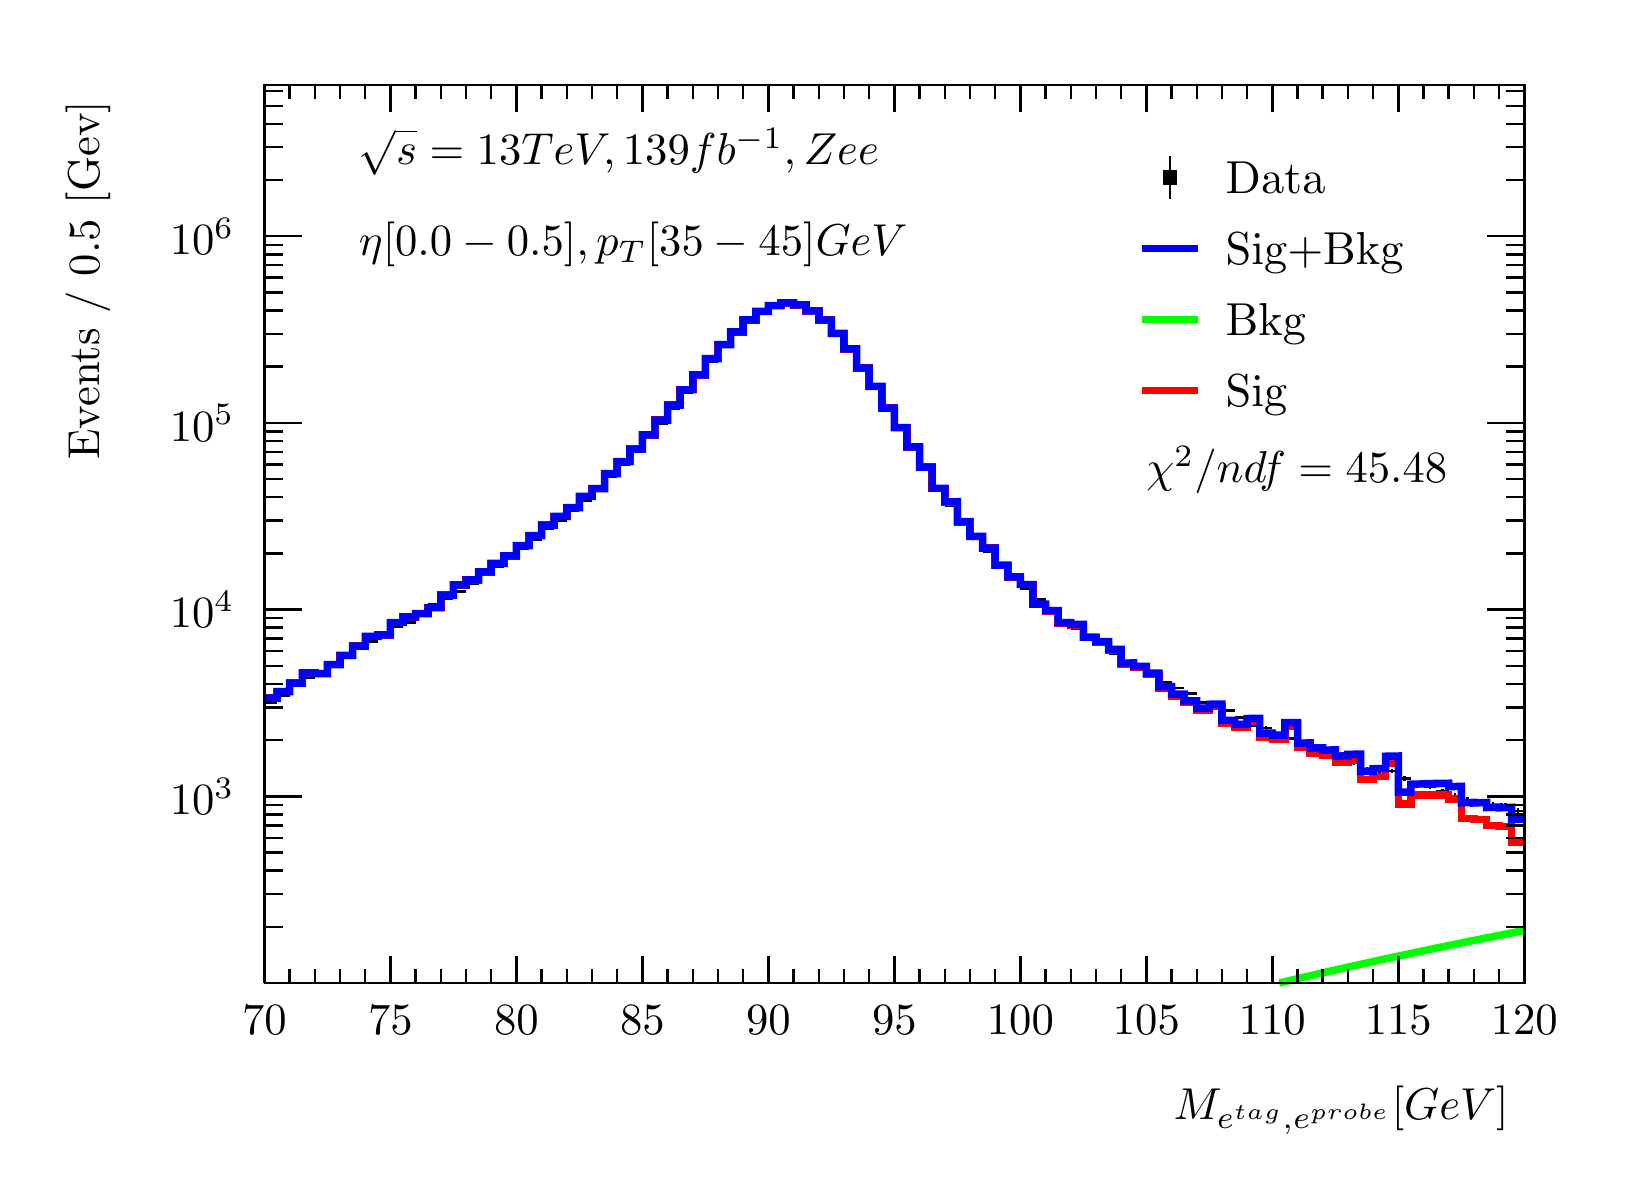
\begin{tikzpicture}
\pgfdeclareplotmark{cross} {
\pgfpathmoveto{\pgfpoint{-0.3\pgfplotmarksize}{\pgfplotmarksize}}
\pgfpathlineto{\pgfpoint{+0.3\pgfplotmarksize}{\pgfplotmarksize}}
\pgfpathlineto{\pgfpoint{+0.3\pgfplotmarksize}{0.3\pgfplotmarksize}}
\pgfpathlineto{\pgfpoint{+1\pgfplotmarksize}{0.3\pgfplotmarksize}}
\pgfpathlineto{\pgfpoint{+1\pgfplotmarksize}{-0.3\pgfplotmarksize}}
\pgfpathlineto{\pgfpoint{+0.3\pgfplotmarksize}{-0.3\pgfplotmarksize}}
\pgfpathlineto{\pgfpoint{+0.3\pgfplotmarksize}{-1.\pgfplotmarksize}}
\pgfpathlineto{\pgfpoint{-0.3\pgfplotmarksize}{-1.\pgfplotmarksize}}
\pgfpathlineto{\pgfpoint{-0.3\pgfplotmarksize}{-0.3\pgfplotmarksize}}
\pgfpathlineto{\pgfpoint{-1.\pgfplotmarksize}{-0.3\pgfplotmarksize}}
\pgfpathlineto{\pgfpoint{-1.\pgfplotmarksize}{0.3\pgfplotmarksize}}
\pgfpathlineto{\pgfpoint{-0.3\pgfplotmarksize}{0.3\pgfplotmarksize}}
\pgfpathclose
\pgfusepathqstroke
}
\pgfdeclareplotmark{cross*} {
\pgfpathmoveto{\pgfpoint{-0.3\pgfplotmarksize}{\pgfplotmarksize}}
\pgfpathlineto{\pgfpoint{+0.3\pgfplotmarksize}{\pgfplotmarksize}}
\pgfpathlineto{\pgfpoint{+0.3\pgfplotmarksize}{0.3\pgfplotmarksize}}
\pgfpathlineto{\pgfpoint{+1\pgfplotmarksize}{0.3\pgfplotmarksize}}
\pgfpathlineto{\pgfpoint{+1\pgfplotmarksize}{-0.3\pgfplotmarksize}}
\pgfpathlineto{\pgfpoint{+0.3\pgfplotmarksize}{-0.3\pgfplotmarksize}}
\pgfpathlineto{\pgfpoint{+0.3\pgfplotmarksize}{-1.\pgfplotmarksize}}
\pgfpathlineto{\pgfpoint{-0.3\pgfplotmarksize}{-1.\pgfplotmarksize}}
\pgfpathlineto{\pgfpoint{-0.3\pgfplotmarksize}{-0.3\pgfplotmarksize}}
\pgfpathlineto{\pgfpoint{-1.\pgfplotmarksize}{-0.3\pgfplotmarksize}}
\pgfpathlineto{\pgfpoint{-1.\pgfplotmarksize}{0.3\pgfplotmarksize}}
\pgfpathlineto{\pgfpoint{-0.3\pgfplotmarksize}{0.3\pgfplotmarksize}}
\pgfpathclose
\pgfusepathqfillstroke
}
\pgfdeclareplotmark{newstar} {
\pgfpathmoveto{\pgfqpoint{0pt}{\pgfplotmarksize}}
\pgfpathlineto{\pgfqpointpolar{44}{0.5\pgfplotmarksize}}
\pgfpathlineto{\pgfqpointpolar{18}{\pgfplotmarksize}}
\pgfpathlineto{\pgfqpointpolar{-20}{0.5\pgfplotmarksize}}
\pgfpathlineto{\pgfqpointpolar{-54}{\pgfplotmarksize}}
\pgfpathlineto{\pgfqpointpolar{-90}{0.5\pgfplotmarksize}}
\pgfpathlineto{\pgfqpointpolar{234}{\pgfplotmarksize}}
\pgfpathlineto{\pgfqpointpolar{198}{0.5\pgfplotmarksize}}
\pgfpathlineto{\pgfqpointpolar{162}{\pgfplotmarksize}}
\pgfpathlineto{\pgfqpointpolar{134}{0.5\pgfplotmarksize}}
\pgfpathclose
\pgfusepathqstroke
}
\pgfdeclareplotmark{newstar*} {
\pgfpathmoveto{\pgfqpoint{0pt}{\pgfplotmarksize}}
\pgfpathlineto{\pgfqpointpolar{44}{0.5\pgfplotmarksize}}
\pgfpathlineto{\pgfqpointpolar{18}{\pgfplotmarksize}}
\pgfpathlineto{\pgfqpointpolar{-20}{0.5\pgfplotmarksize}}
\pgfpathlineto{\pgfqpointpolar{-54}{\pgfplotmarksize}}
\pgfpathlineto{\pgfqpointpolar{-90}{0.5\pgfplotmarksize}}
\pgfpathlineto{\pgfqpointpolar{234}{\pgfplotmarksize}}
\pgfpathlineto{\pgfqpointpolar{198}{0.5\pgfplotmarksize}}
\pgfpathlineto{\pgfqpointpolar{162}{\pgfplotmarksize}}
\pgfpathlineto{\pgfqpointpolar{134}{0.5\pgfplotmarksize}}
\pgfpathclose
\pgfusepathqfillstroke
}
\definecolor{c}{rgb}{1,1,1};
\draw [color=c, fill=c] (0,0) rectangle (20,14.4361);
\draw [color=c, fill=c] (3,2.30977) rectangle (19,13.7143);
\definecolor{c}{rgb}{0,0,0};
\draw [c,line width=0.9] (3,2.30977) -- (3,13.7143) -- (19,13.7143) -- (19,2.30977) -- (3,2.30977);
\definecolor{c}{rgb}{1,1,1};
\draw [color=c, fill=c] (3,2.30977) rectangle (19,13.7143);
\definecolor{c}{rgb}{0,0,0};
\draw [c,line width=0.9] (3,2.30977) -- (3,13.7143) -- (19,13.7143) -- (19,2.30977) -- (3,2.30977);
\draw [c,line width=0.9] (3,2.30977) -- (19,2.30977);
\draw [c,line width=0.9] (3,2.65624) -- (3,2.30977);
\draw [c,line width=0.9] (3.32,2.48301) -- (3.32,2.30977);
\draw [c,line width=0.9] (3.64,2.48301) -- (3.64,2.30977);
\draw [c,line width=0.9] (3.96,2.48301) -- (3.96,2.30977);
\draw [c,line width=0.9] (4.28,2.48301) -- (4.28,2.30977);
\draw [c,line width=0.9] (4.6,2.65624) -- (4.6,2.30977);
\draw [c,line width=0.9] (4.92,2.48301) -- (4.92,2.30977);
\draw [c,line width=0.9] (5.24,2.48301) -- (5.24,2.30977);
\draw [c,line width=0.9] (5.56,2.48301) -- (5.56,2.30977);
\draw [c,line width=0.9] (5.88,2.48301) -- (5.88,2.30977);
\draw [c,line width=0.9] (6.2,2.65624) -- (6.2,2.30977);
\draw [c,line width=0.9] (6.52,2.48301) -- (6.52,2.30977);
\draw [c,line width=0.9] (6.84,2.48301) -- (6.84,2.30977);
\draw [c,line width=0.9] (7.16,2.48301) -- (7.16,2.30977);
\draw [c,line width=0.9] (7.48,2.48301) -- (7.48,2.30977);
\draw [c,line width=0.9] (7.8,2.65624) -- (7.8,2.30977);
\draw [c,line width=0.9] (8.12,2.48301) -- (8.12,2.30977);
\draw [c,line width=0.9] (8.44,2.48301) -- (8.44,2.30977);
\draw [c,line width=0.9] (8.76,2.48301) -- (8.76,2.30977);
\draw [c,line width=0.9] (9.08,2.48301) -- (9.08,2.30977);
\draw [c,line width=0.9] (9.4,2.65624) -- (9.4,2.30977);
\draw [c,line width=0.9] (9.72,2.48301) -- (9.72,2.30977);
\draw [c,line width=0.9] (10.04,2.48301) -- (10.04,2.30977);
\draw [c,line width=0.9] (10.36,2.48301) -- (10.36,2.30977);
\draw [c,line width=0.9] (10.68,2.48301) -- (10.68,2.30977);
\draw [c,line width=0.9] (11,2.65624) -- (11,2.30977);
\draw [c,line width=0.9] (11.32,2.48301) -- (11.32,2.30977);
\draw [c,line width=0.9] (11.64,2.48301) -- (11.64,2.30977);
\draw [c,line width=0.9] (11.96,2.48301) -- (11.96,2.30977);
\draw [c,line width=0.9] (12.28,2.48301) -- (12.28,2.30977);
\draw [c,line width=0.9] (12.6,2.65624) -- (12.6,2.30977);
\draw [c,line width=0.9] (12.92,2.48301) -- (12.92,2.30977);
\draw [c,line width=0.9] (13.24,2.48301) -- (13.24,2.30977);
\draw [c,line width=0.9] (13.56,2.48301) -- (13.56,2.30977);
\draw [c,line width=0.9] (13.88,2.48301) -- (13.88,2.30977);
\draw [c,line width=0.9] (14.2,2.65624) -- (14.2,2.30977);
\draw [c,line width=0.9] (14.52,2.48301) -- (14.52,2.30977);
\draw [c,line width=0.9] (14.84,2.48301) -- (14.84,2.30977);
\draw [c,line width=0.9] (15.16,2.48301) -- (15.16,2.30977);
\draw [c,line width=0.9] (15.48,2.48301) -- (15.48,2.30977);
\draw [c,line width=0.9] (15.8,2.65624) -- (15.8,2.30977);
\draw [c,line width=0.9] (16.12,2.48301) -- (16.12,2.30977);
\draw [c,line width=0.9] (16.44,2.48301) -- (16.44,2.30977);
\draw [c,line width=0.9] (16.76,2.48301) -- (16.76,2.30977);
\draw [c,line width=0.9] (17.08,2.48301) -- (17.08,2.30977);
\draw [c,line width=0.9] (17.4,2.65624) -- (17.4,2.30977);
\draw [c,line width=0.9] (17.72,2.48301) -- (17.72,2.30977);
\draw [c,line width=0.9] (18.04,2.48301) -- (18.04,2.30977);
\draw [c,line width=0.9] (18.36,2.48301) -- (18.36,2.30977);
\draw [c,line width=0.9] (18.68,2.48301) -- (18.68,2.30977);
\draw [c,line width=0.9] (19,2.65624) -- (19,2.30977);
\draw [anchor=base] (3,1.66015) node[scale=1.61424, color=c, rotate=0]{70};
\draw [anchor=base] (4.6,1.66015) node[scale=1.61424, color=c, rotate=0]{75};
\draw [anchor=base] (6.2,1.66015) node[scale=1.61424, color=c, rotate=0]{80};
\draw [anchor=base] (7.8,1.66015) node[scale=1.61424, color=c, rotate=0]{85};
\draw [anchor=base] (9.4,1.66015) node[scale=1.61424, color=c, rotate=0]{90};
\draw [anchor=base] (11,1.66015) node[scale=1.61424, color=c, rotate=0]{95};
\draw [anchor=base] (12.6,1.66015) node[scale=1.61424, color=c, rotate=0]{100};
\draw [anchor=base] (14.2,1.66015) node[scale=1.61424, color=c, rotate=0]{105};
\draw [anchor=base] (15.8,1.66015) node[scale=1.61424, color=c, rotate=0]{110};
\draw [anchor=base] (17.4,1.66015) node[scale=1.61424, color=c, rotate=0]{115};
\draw [anchor=base] (19,1.66015) node[scale=1.61424, color=c, rotate=0]{120};
\draw [anchor= east] (19,0.692932) node[scale=1.61424, color=c, rotate=0]{$M_{e^{tag}, e^{probe}}  [GeV]$};
\draw [c,line width=0.9] (3,13.7143) -- (19,13.7143);
\draw [c,line width=0.9] (3,13.3678) -- (3,13.7143);
\draw [c,line width=0.9] (3.32,13.5411) -- (3.32,13.7143);
\draw [c,line width=0.9] (3.64,13.5411) -- (3.64,13.7143);
\draw [c,line width=0.9] (3.96,13.5411) -- (3.96,13.7143);
\draw [c,line width=0.9] (4.28,13.5411) -- (4.28,13.7143);
\draw [c,line width=0.9] (4.6,13.3678) -- (4.6,13.7143);
\draw [c,line width=0.9] (4.92,13.5411) -- (4.92,13.7143);
\draw [c,line width=0.9] (5.24,13.5411) -- (5.24,13.7143);
\draw [c,line width=0.9] (5.56,13.5411) -- (5.56,13.7143);
\draw [c,line width=0.9] (5.88,13.5411) -- (5.88,13.7143);
\draw [c,line width=0.9] (6.2,13.3678) -- (6.2,13.7143);
\draw [c,line width=0.9] (6.52,13.5411) -- (6.52,13.7143);
\draw [c,line width=0.9] (6.84,13.5411) -- (6.84,13.7143);
\draw [c,line width=0.9] (7.16,13.5411) -- (7.16,13.7143);
\draw [c,line width=0.9] (7.48,13.5411) -- (7.48,13.7143);
\draw [c,line width=0.9] (7.8,13.3678) -- (7.8,13.7143);
\draw [c,line width=0.9] (8.12,13.5411) -- (8.12,13.7143);
\draw [c,line width=0.9] (8.44,13.5411) -- (8.44,13.7143);
\draw [c,line width=0.9] (8.76,13.5411) -- (8.76,13.7143);
\draw [c,line width=0.9] (9.08,13.5411) -- (9.08,13.7143);
\draw [c,line width=0.9] (9.4,13.3678) -- (9.4,13.7143);
\draw [c,line width=0.9] (9.72,13.5411) -- (9.72,13.7143);
\draw [c,line width=0.9] (10.04,13.5411) -- (10.04,13.7143);
\draw [c,line width=0.9] (10.36,13.5411) -- (10.36,13.7143);
\draw [c,line width=0.9] (10.68,13.5411) -- (10.68,13.7143);
\draw [c,line width=0.9] (11,13.3678) -- (11,13.7143);
\draw [c,line width=0.9] (11.32,13.5411) -- (11.32,13.7143);
\draw [c,line width=0.9] (11.64,13.5411) -- (11.64,13.7143);
\draw [c,line width=0.9] (11.96,13.5411) -- (11.96,13.7143);
\draw [c,line width=0.9] (12.28,13.5411) -- (12.28,13.7143);
\draw [c,line width=0.9] (12.6,13.3678) -- (12.6,13.7143);
\draw [c,line width=0.9] (12.92,13.5411) -- (12.92,13.7143);
\draw [c,line width=0.9] (13.24,13.5411) -- (13.24,13.7143);
\draw [c,line width=0.9] (13.56,13.5411) -- (13.56,13.7143);
\draw [c,line width=0.9] (13.88,13.5411) -- (13.88,13.7143);
\draw [c,line width=0.9] (14.2,13.3678) -- (14.2,13.7143);
\draw [c,line width=0.9] (14.52,13.5411) -- (14.52,13.7143);
\draw [c,line width=0.9] (14.84,13.5411) -- (14.84,13.7143);
\draw [c,line width=0.9] (15.16,13.5411) -- (15.16,13.7143);
\draw [c,line width=0.9] (15.48,13.5411) -- (15.48,13.7143);
\draw [c,line width=0.9] (15.8,13.3678) -- (15.8,13.7143);
\draw [c,line width=0.9] (16.12,13.5411) -- (16.12,13.7143);
\draw [c,line width=0.9] (16.44,13.5411) -- (16.44,13.7143);
\draw [c,line width=0.9] (16.76,13.5411) -- (16.76,13.7143);
\draw [c,line width=0.9] (17.08,13.5411) -- (17.08,13.7143);
\draw [c,line width=0.9] (17.4,13.3678) -- (17.4,13.7143);
\draw [c,line width=0.9] (17.72,13.5411) -- (17.72,13.7143);
\draw [c,line width=0.9] (18.04,13.5411) -- (18.04,13.7143);
\draw [c,line width=0.9] (18.36,13.5411) -- (18.36,13.7143);
\draw [c,line width=0.9] (18.68,13.5411) -- (18.68,13.7143);
\draw [c,line width=0.9] (19,13.3678) -- (19,13.7143);
\draw [c,line width=0.9] (3,2.30977) -- (3,13.7143);
\draw [c,line width=0.9] (3.237,3.02354) -- (3,3.02354);
\draw [c,line width=0.9] (3.237,3.44107) -- (3,3.44107);
\draw [c,line width=0.9] (3.237,3.73731) -- (3,3.73731);
\draw [c,line width=0.9] (3.237,3.96709) -- (3,3.96709);
\draw [c,line width=0.9] (3.237,4.15484) -- (3,4.15484);
\draw [c,line width=0.9] (3.237,4.31357) -- (3,4.31357);
\draw [c,line width=0.9] (3.237,4.45108) -- (3,4.45108);
\draw [c,line width=0.9] (3.237,4.57236) -- (3,4.57236);
\draw [c,line width=0.9] (3.474,4.68086) -- (3,4.68086);
\draw [anchor= east] (2.82,4.68086) node[scale=1.61424, color=c, rotate=0]{$10^{3}$};
\draw [c,line width=0.9] (3.237,5.39463) -- (3,5.39463);
\draw [c,line width=0.9] (3.237,5.81216) -- (3,5.81216);
\draw [c,line width=0.9] (3.237,6.1084) -- (3,6.1084);
\draw [c,line width=0.9] (3.237,6.33818) -- (3,6.33818);
\draw [c,line width=0.9] (3.237,6.52593) -- (3,6.52593);
\draw [c,line width=0.9] (3.237,6.68466) -- (3,6.68466);
\draw [c,line width=0.9] (3.237,6.82217) -- (3,6.82217);
\draw [c,line width=0.9] (3.237,6.94345) -- (3,6.94345);
\draw [c,line width=0.9] (3.474,7.05195) -- (3,7.05195);
\draw [anchor= east] (2.82,7.05195) node[scale=1.61424, color=c, rotate=0]{$10^{4}$};
\draw [c,line width=0.9] (3.237,7.76572) -- (3,7.76572);
\draw [c,line width=0.9] (3.237,8.18324) -- (3,8.18324);
\draw [c,line width=0.9] (3.237,8.47948) -- (3,8.47948);
\draw [c,line width=0.9] (3.237,8.70927) -- (3,8.70927);
\draw [c,line width=0.9] (3.237,8.89701) -- (3,8.89701);
\draw [c,line width=0.9] (3.237,9.05575) -- (3,9.05575);
\draw [c,line width=0.9] (3.237,9.19325) -- (3,9.19325);
\draw [c,line width=0.9] (3.237,9.31454) -- (3,9.31454);
\draw [c,line width=0.9] (3.474,9.42304) -- (3,9.42304);
\draw [anchor= east] (2.82,9.42304) node[scale=1.61424, color=c, rotate=0]{$10^{5}$};
\draw [c,line width=0.9] (3.237,10.1368) -- (3,10.1368);
\draw [c,line width=0.9] (3.237,10.5543) -- (3,10.5543);
\draw [c,line width=0.9] (3.237,10.8506) -- (3,10.8506);
\draw [c,line width=0.9] (3.237,11.0804) -- (3,11.0804);
\draw [c,line width=0.9] (3.237,11.2681) -- (3,11.2681);
\draw [c,line width=0.9] (3.237,11.4268) -- (3,11.4268);
\draw [c,line width=0.9] (3.237,11.5643) -- (3,11.5643);
\draw [c,line width=0.9] (3.237,11.6856) -- (3,11.6856);
\draw [c,line width=0.9] (3.474,11.7941) -- (3,11.7941);
\draw [anchor= east] (2.82,11.7941) node[scale=1.61424, color=c, rotate=0]{$10^{6}$};
\draw [c,line width=0.9] (3.237,12.5079) -- (3,12.5079);
\draw [c,line width=0.9] (3.237,12.9254) -- (3,12.9254);
\draw [c,line width=0.9] (3.237,13.2217) -- (3,13.2217);
\draw [c,line width=0.9] (3.237,13.4514) -- (3,13.4514);
\draw [c,line width=0.9] (3.237,13.6392) -- (3,13.6392);
\draw [anchor= east] (0.76,13.7143) node[scale=1.61424, color=c, rotate=90]{Events / 0.5 [Gev]};
\draw [c,line width=0.9] (19,2.30977) -- (19,13.7143);
\draw [c,line width=0.9] (18.763,3.02354) -- (19,3.02354);
\draw [c,line width=0.9] (18.763,3.44107) -- (19,3.44107);
\draw [c,line width=0.9] (18.763,3.73731) -- (19,3.73731);
\draw [c,line width=0.9] (18.763,3.96709) -- (19,3.96709);
\draw [c,line width=0.9] (18.763,4.15484) -- (19,4.15484);
\draw [c,line width=0.9] (18.763,4.31357) -- (19,4.31357);
\draw [c,line width=0.9] (18.763,4.45108) -- (19,4.45108);
\draw [c,line width=0.9] (18.763,4.57236) -- (19,4.57236);
\draw [c,line width=0.9] (18.526,4.68086) -- (19,4.68086);
\draw [c,line width=0.9] (18.763,5.39463) -- (19,5.39463);
\draw [c,line width=0.9] (18.763,5.81216) -- (19,5.81216);
\draw [c,line width=0.9] (18.763,6.1084) -- (19,6.1084);
\draw [c,line width=0.9] (18.763,6.33818) -- (19,6.33818);
\draw [c,line width=0.9] (18.763,6.52593) -- (19,6.52593);
\draw [c,line width=0.9] (18.763,6.68466) -- (19,6.68466);
\draw [c,line width=0.9] (18.763,6.82217) -- (19,6.82217);
\draw [c,line width=0.9] (18.763,6.94345) -- (19,6.94345);
\draw [c,line width=0.9] (18.526,7.05195) -- (19,7.05195);
\draw [c,line width=0.9] (18.763,7.76572) -- (19,7.76572);
\draw [c,line width=0.9] (18.763,8.18324) -- (19,8.18324);
\draw [c,line width=0.9] (18.763,8.47948) -- (19,8.47948);
\draw [c,line width=0.9] (18.763,8.70927) -- (19,8.70927);
\draw [c,line width=0.9] (18.763,8.89701) -- (19,8.89701);
\draw [c,line width=0.9] (18.763,9.05575) -- (19,9.05575);
\draw [c,line width=0.9] (18.763,9.19325) -- (19,9.19325);
\draw [c,line width=0.9] (18.763,9.31454) -- (19,9.31454);
\draw [c,line width=0.9] (18.526,9.42304) -- (19,9.42304);
\draw [c,line width=0.9] (18.763,10.1368) -- (19,10.1368);
\draw [c,line width=0.9] (18.763,10.5543) -- (19,10.5543);
\draw [c,line width=0.9] (18.763,10.8506) -- (19,10.8506);
\draw [c,line width=0.9] (18.763,11.0804) -- (19,11.0804);
\draw [c,line width=0.9] (18.763,11.2681) -- (19,11.2681);
\draw [c,line width=0.9] (18.763,11.4268) -- (19,11.4268);
\draw [c,line width=0.9] (18.763,11.5643) -- (19,11.5643);
\draw [c,line width=0.9] (18.763,11.6856) -- (19,11.6856);
\draw [c,line width=0.9] (18.526,11.7941) -- (19,11.7941);
\draw [c,line width=0.9] (18.763,12.5079) -- (19,12.5079);
\draw [c,line width=0.9] (18.763,12.9254) -- (19,12.9254);
\draw [c,line width=0.9] (18.763,13.2217) -- (19,13.2217);
\draw [c,line width=0.9] (18.763,13.4514) -- (19,13.4514);
\draw [c,line width=0.9] (18.763,13.6392) -- (19,13.6392);
\draw [c,line width=0.9] (3.08,5.87086) -- (3,5.87086);
\draw [c,line width=0.9] (3,5.87086) -- (3,5.87086);
\draw [c,line width=0.9] (3.08,5.87086) -- (3.16,5.87086);
\draw [c,line width=0.9] (3.16,5.87086) -- (3.16,5.87086);
\draw [c,line width=0.9] (3.08,5.87086) -- (3.08,5.88914);
\draw [c,line width=0.9] (3.08,5.88914) -- (3.08,5.88914);
\draw [c,line width=0.9] (3.08,5.87086) -- (3.08,5.85259);
\draw [c,line width=0.9] (3.08,5.85259) -- (3.08,5.85259);
\draw [c,line width=0.9] (3.24,5.95965) -- (3.16,5.95965);
\draw [c,line width=0.9] (3.16,5.95965) -- (3.16,5.95965);
\draw [c,line width=0.9] (3.24,5.95965) -- (3.32,5.95965);
\draw [c,line width=0.9] (3.32,5.95965) -- (3.32,5.95965);
\draw [c,line width=0.9] (3.24,5.95965) -- (3.24,5.97715);
\draw [c,line width=0.9] (3.24,5.97715) -- (3.24,5.97715);
\draw [c,line width=0.9] (3.24,5.95965) -- (3.24,5.94215);
\draw [c,line width=0.9] (3.24,5.94215) -- (3.24,5.94215);
\draw [c,line width=0.9] (3.4,6.12246) -- (3.32,6.12246);
\draw [c,line width=0.9] (3.32,6.12246) -- (3.32,6.12246);
\draw [c,line width=0.9] (3.4,6.12246) -- (3.48,6.12246);
\draw [c,line width=0.9] (3.48,6.12246) -- (3.48,6.12246);
\draw [c,line width=0.9] (3.4,6.12246) -- (3.4,6.13863);
\draw [c,line width=0.9] (3.4,6.13863) -- (3.4,6.13863);
\draw [c,line width=0.9] (3.4,6.12246) -- (3.4,6.10629);
\draw [c,line width=0.9] (3.4,6.10629) -- (3.4,6.10629);
\draw [c,line width=0.9] (3.56,6.19027) -- (3.48,6.19027);
\draw [c,line width=0.9] (3.48,6.19027) -- (3.48,6.19027);
\draw [c,line width=0.9] (3.56,6.19027) -- (3.64,6.19027);
\draw [c,line width=0.9] (3.64,6.19027) -- (3.64,6.19027);
\draw [c,line width=0.9] (3.56,6.19027) -- (3.56,6.20591);
\draw [c,line width=0.9] (3.56,6.20591) -- (3.56,6.20591);
\draw [c,line width=0.9] (3.56,6.19027) -- (3.56,6.17462);
\draw [c,line width=0.9] (3.56,6.17462) -- (3.56,6.17462);
\draw [c,line width=0.9] (3.72,6.27556) -- (3.64,6.27556);
\draw [c,line width=0.9] (3.64,6.27556) -- (3.64,6.27556);
\draw [c,line width=0.9] (3.72,6.27556) -- (3.8,6.27556);
\draw [c,line width=0.9] (3.8,6.27556) -- (3.8,6.27556);
\draw [c,line width=0.9] (3.72,6.27556) -- (3.72,6.29057);
\draw [c,line width=0.9] (3.72,6.29057) -- (3.72,6.29057);
\draw [c,line width=0.9] (3.72,6.27556) -- (3.72,6.26055);
\draw [c,line width=0.9] (3.72,6.26055) -- (3.72,6.26055);
\draw [c,line width=0.9] (3.88,6.37916) -- (3.8,6.37916);
\draw [c,line width=0.9] (3.8,6.37916) -- (3.8,6.37916);
\draw [c,line width=0.9] (3.88,6.37916) -- (3.96,6.37916);
\draw [c,line width=0.9] (3.96,6.37916) -- (3.96,6.37916);
\draw [c,line width=0.9] (3.88,6.37916) -- (3.88,6.39344);
\draw [c,line width=0.9] (3.88,6.39344) -- (3.88,6.39344);
\draw [c,line width=0.9] (3.88,6.37916) -- (3.88,6.36489);
\draw [c,line width=0.9] (3.88,6.36489) -- (3.88,6.36489);
\draw [c,line width=0.9] (4.04,6.47509) -- (3.96,6.47509);
\draw [c,line width=0.9] (3.96,6.47509) -- (3.96,6.47509);
\draw [c,line width=0.9] (4.04,6.47509) -- (4.12,6.47509);
\draw [c,line width=0.9] (4.12,6.47509) -- (4.12,6.47509);
\draw [c,line width=0.9] (4.04,6.47509) -- (4.04,6.48872);
\draw [c,line width=0.9] (4.04,6.48872) -- (4.04,6.48872);
\draw [c,line width=0.9] (4.04,6.47509) -- (4.04,6.46147);
\draw [c,line width=0.9] (4.04,6.46147) -- (4.04,6.46147);
\draw [c,line width=0.9] (4.2,6.576) -- (4.12,6.576);
\draw [c,line width=0.9] (4.12,6.576) -- (4.12,6.576);
\draw [c,line width=0.9] (4.2,6.576) -- (4.28,6.576);
\draw [c,line width=0.9] (4.28,6.576) -- (4.28,6.576);
\draw [c,line width=0.9] (4.2,6.576) -- (4.2,6.58898);
\draw [c,line width=0.9] (4.2,6.58898) -- (4.2,6.58898);
\draw [c,line width=0.9] (4.2,6.576) -- (4.2,6.56303);
\draw [c,line width=0.9] (4.2,6.56303) -- (4.2,6.56303);
\draw [c,line width=0.9] (4.36,6.64508) -- (4.28,6.64508);
\draw [c,line width=0.9] (4.28,6.64508) -- (4.28,6.64508);
\draw [c,line width=0.9] (4.36,6.64508) -- (4.44,6.64508);
\draw [c,line width=0.9] (4.44,6.64508) -- (4.44,6.64508);
\draw [c,line width=0.9] (4.36,6.64508) -- (4.36,6.65762);
\draw [c,line width=0.9] (4.36,6.65762) -- (4.36,6.65762);
\draw [c,line width=0.9] (4.36,6.64508) -- (4.36,6.63253);
\draw [c,line width=0.9] (4.36,6.63253) -- (4.36,6.63253);
\draw [c,line width=0.9] (4.52,6.7335) -- (4.44,6.7335);
\draw [c,line width=0.9] (4.44,6.7335) -- (4.44,6.7335);
\draw [c,line width=0.9] (4.52,6.7335) -- (4.6,6.7335);
\draw [c,line width=0.9] (4.6,6.7335) -- (4.6,6.7335);
\draw [c,line width=0.9] (4.52,6.7335) -- (4.52,6.74552);
\draw [c,line width=0.9] (4.52,6.74552) -- (4.52,6.74552);
\draw [c,line width=0.9] (4.52,6.7335) -- (4.52,6.72148);
\draw [c,line width=0.9] (4.52,6.72148) -- (4.52,6.72148);
\draw [c,line width=0.9] (4.68,6.83216) -- (4.6,6.83216);
\draw [c,line width=0.9] (4.6,6.83216) -- (4.6,6.83216);
\draw [c,line width=0.9] (4.68,6.83216) -- (4.76,6.83216);
\draw [c,line width=0.9] (4.76,6.83216) -- (4.76,6.83216);
\draw [c,line width=0.9] (4.68,6.83216) -- (4.68,6.84362);
\draw [c,line width=0.9] (4.68,6.84362) -- (4.68,6.84362);
\draw [c,line width=0.9] (4.68,6.83216) -- (4.68,6.8207);
\draw [c,line width=0.9] (4.68,6.8207) -- (4.68,6.8207);
\draw [c,line width=0.9] (4.84,6.88786) -- (4.76,6.88786);
\draw [c,line width=0.9] (4.76,6.88786) -- (4.76,6.88786);
\draw [c,line width=0.9] (4.84,6.88786) -- (4.92,6.88786);
\draw [c,line width=0.9] (4.92,6.88786) -- (4.92,6.88786);
\draw [c,line width=0.9] (4.84,6.88786) -- (4.84,6.89901);
\draw [c,line width=0.9] (4.84,6.89901) -- (4.84,6.89901);
\draw [c,line width=0.9] (4.84,6.88786) -- (4.84,6.87671);
\draw [c,line width=0.9] (4.84,6.87671) -- (4.84,6.87671);
\draw [c,line width=0.9] (5,7.00162) -- (4.92,7.00162);
\draw [c,line width=0.9] (4.92,7.00162) -- (4.92,7.00162);
\draw [c,line width=0.9] (5,7.00162) -- (5.08,7.00162);
\draw [c,line width=0.9] (5.08,7.00162) -- (5.08,7.00162);
\draw [c,line width=0.9] (5,7.00162) -- (5,7.01217);
\draw [c,line width=0.9] (5,7.01217) -- (5,7.01217);
\draw [c,line width=0.9] (5,7.00162) -- (5,6.99107);
\draw [c,line width=0.9] (5,6.99107) -- (5,6.99107);
\draw [c,line width=0.9] (5.16,7.11506) -- (5.08,7.11506);
\draw [c,line width=0.9] (5.08,7.11506) -- (5.08,7.11506);
\draw [c,line width=0.9] (5.16,7.11506) -- (5.24,7.11506);
\draw [c,line width=0.9] (5.24,7.11506) -- (5.24,7.11506);
\draw [c,line width=0.9] (5.16,7.11506) -- (5.16,7.12504);
\draw [c,line width=0.9] (5.16,7.12504) -- (5.16,7.12504);
\draw [c,line width=0.9] (5.16,7.11506) -- (5.16,7.10507);
\draw [c,line width=0.9] (5.16,7.10507) -- (5.16,7.10507);
\draw [c,line width=0.9] (5.32,7.18416) -- (5.24,7.18416);
\draw [c,line width=0.9] (5.24,7.18416) -- (5.24,7.18416);
\draw [c,line width=0.9] (5.32,7.18416) -- (5.4,7.18416);
\draw [c,line width=0.9] (5.4,7.18416) -- (5.4,7.18416);
\draw [c,line width=0.9] (5.32,7.18416) -- (5.32,7.19382);
\draw [c,line width=0.9] (5.32,7.19382) -- (5.32,7.19382);
\draw [c,line width=0.9] (5.32,7.18416) -- (5.32,7.1745);
\draw [c,line width=0.9] (5.32,7.1745) -- (5.32,7.1745);
\draw [c,line width=0.9] (5.48,7.28543) -- (5.4,7.28543);
\draw [c,line width=0.9] (5.4,7.28543) -- (5.4,7.28543);
\draw [c,line width=0.9] (5.48,7.28543) -- (5.56,7.28543);
\draw [c,line width=0.9] (5.56,7.28543) -- (5.56,7.28543);
\draw [c,line width=0.9] (5.48,7.28543) -- (5.48,7.29463);
\draw [c,line width=0.9] (5.48,7.29463) -- (5.48,7.29463);
\draw [c,line width=0.9] (5.48,7.28543) -- (5.48,7.27624);
\draw [c,line width=0.9] (5.48,7.27624) -- (5.48,7.27624);
\draw [c,line width=0.9] (5.64,7.38674) -- (5.56,7.38674);
\draw [c,line width=0.9] (5.56,7.38674) -- (5.56,7.38674);
\draw [c,line width=0.9] (5.64,7.38674) -- (5.72,7.38674);
\draw [c,line width=0.9] (5.72,7.38674) -- (5.72,7.38674);
\draw [c,line width=0.9] (5.64,7.38674) -- (5.64,7.3955);
\draw [c,line width=0.9] (5.64,7.3955) -- (5.64,7.3955);
\draw [c,line width=0.9] (5.64,7.38674) -- (5.64,7.37799);
\draw [c,line width=0.9] (5.64,7.37799) -- (5.64,7.37799);
\draw [c,line width=0.9] (5.8,7.50696) -- (5.72,7.50696);
\draw [c,line width=0.9] (5.72,7.50696) -- (5.72,7.50696);
\draw [c,line width=0.9] (5.8,7.50696) -- (5.88,7.50696);
\draw [c,line width=0.9] (5.88,7.50696) -- (5.88,7.50696);
\draw [c,line width=0.9] (5.8,7.50696) -- (5.8,7.51521);
\draw [c,line width=0.9] (5.8,7.51521) -- (5.8,7.51521);
\draw [c,line width=0.9] (5.8,7.50696) -- (5.8,7.4987);
\draw [c,line width=0.9] (5.8,7.4987) -- (5.8,7.4987);
\draw [c,line width=0.9] (5.96,7.59618) -- (5.88,7.59618);
\draw [c,line width=0.9] (5.88,7.59618) -- (5.88,7.59618);
\draw [c,line width=0.9] (5.96,7.59618) -- (6.04,7.59618);
\draw [c,line width=0.9] (6.04,7.59618) -- (6.04,7.59618);
\draw [c,line width=0.9] (5.96,7.59618) -- (5.96,7.60409);
\draw [c,line width=0.9] (5.96,7.60409) -- (5.96,7.60409);
\draw [c,line width=0.9] (5.96,7.59618) -- (5.96,7.58827);
\draw [c,line width=0.9] (5.96,7.58827) -- (5.96,7.58827);
\draw [c,line width=0.9] (6.12,7.71447) -- (6.04,7.71447);
\draw [c,line width=0.9] (6.04,7.71447) -- (6.04,7.71447);
\draw [c,line width=0.9] (6.12,7.71447) -- (6.2,7.71447);
\draw [c,line width=0.9] (6.2,7.71447) -- (6.2,7.71447);
\draw [c,line width=0.9] (6.12,7.71447) -- (6.12,7.72193);
\draw [c,line width=0.9] (6.12,7.72193) -- (6.12,7.72193);
\draw [c,line width=0.9] (6.12,7.71447) -- (6.12,7.707);
\draw [c,line width=0.9] (6.12,7.707) -- (6.12,7.707);
\draw [c,line width=0.9] (6.28,7.82212) -- (6.2,7.82212);
\draw [c,line width=0.9] (6.2,7.82212) -- (6.2,7.82212);
\draw [c,line width=0.9] (6.28,7.82212) -- (6.36,7.82212);
\draw [c,line width=0.9] (6.36,7.82212) -- (6.36,7.82212);
\draw [c,line width=0.9] (6.28,7.82212) -- (6.28,7.8292);
\draw [c,line width=0.9] (6.28,7.8292) -- (6.28,7.8292);
\draw [c,line width=0.9] (6.28,7.82212) -- (6.28,7.81503);
\draw [c,line width=0.9] (6.28,7.81503) -- (6.28,7.81503);
\draw [c,line width=0.9] (6.44,7.93472) -- (6.36,7.93472);
\draw [c,line width=0.9] (6.36,7.93472) -- (6.36,7.93472);
\draw [c,line width=0.9] (6.44,7.93472) -- (6.52,7.93472);
\draw [c,line width=0.9] (6.52,7.93472) -- (6.52,7.93472);
\draw [c,line width=0.9] (6.44,7.93472) -- (6.44,7.94142);
\draw [c,line width=0.9] (6.44,7.94142) -- (6.44,7.94142);
\draw [c,line width=0.9] (6.44,7.93472) -- (6.44,7.92801);
\draw [c,line width=0.9] (6.44,7.92801) -- (6.44,7.92801);
\draw [c,line width=0.9] (6.6,8.07448) -- (6.52,8.07448);
\draw [c,line width=0.9] (6.52,8.07448) -- (6.52,8.07448);
\draw [c,line width=0.9] (6.6,8.07448) -- (6.68,8.07448);
\draw [c,line width=0.9] (6.68,8.07448) -- (6.68,8.07448);
\draw [c,line width=0.9] (6.6,8.07448) -- (6.6,8.08075);
\draw [c,line width=0.9] (6.6,8.08075) -- (6.6,8.08075);
\draw [c,line width=0.9] (6.6,8.07448) -- (6.6,8.06822);
\draw [c,line width=0.9] (6.6,8.06822) -- (6.6,8.06822);
\draw [c,line width=0.9] (6.76,8.18149) -- (6.68,8.18149);
\draw [c,line width=0.9] (6.68,8.18149) -- (6.68,8.18149);
\draw [c,line width=0.9] (6.76,8.18149) -- (6.84,8.18149);
\draw [c,line width=0.9] (6.84,8.18149) -- (6.84,8.18149);
\draw [c,line width=0.9] (6.76,8.18149) -- (6.76,8.18744);
\draw [c,line width=0.9] (6.76,8.18744) -- (6.76,8.18744);
\draw [c,line width=0.9] (6.76,8.18149) -- (6.76,8.17554);
\draw [c,line width=0.9] (6.76,8.17554) -- (6.76,8.17554);
\draw [c,line width=0.9] (6.92,8.30533) -- (6.84,8.30533);
\draw [c,line width=0.9] (6.84,8.30533) -- (6.84,8.30533);
\draw [c,line width=0.9] (6.92,8.30533) -- (7,8.30533);
\draw [c,line width=0.9] (7,8.30533) -- (7,8.30533);
\draw [c,line width=0.9] (6.92,8.30533) -- (6.92,8.31093);
\draw [c,line width=0.9] (6.92,8.31093) -- (6.92,8.31093);
\draw [c,line width=0.9] (6.92,8.30533) -- (6.92,8.29972);
\draw [c,line width=0.9] (6.92,8.29972) -- (6.92,8.29972);
\draw [c,line width=0.9] (7.08,8.44101) -- (7,8.44101);
\draw [c,line width=0.9] (7,8.44101) -- (7,8.44101);
\draw [c,line width=0.9] (7.08,8.44101) -- (7.16,8.44101);
\draw [c,line width=0.9] (7.16,8.44101) -- (7.16,8.44101);
\draw [c,line width=0.9] (7.08,8.44101) -- (7.08,8.44626);
\draw [c,line width=0.9] (7.08,8.44626) -- (7.08,8.44626);
\draw [c,line width=0.9] (7.08,8.44101) -- (7.08,8.43576);
\draw [c,line width=0.9] (7.08,8.43576) -- (7.08,8.43576);
\draw [c,line width=0.9] (7.24,8.58649) -- (7.16,8.58649);
\draw [c,line width=0.9] (7.16,8.58649) -- (7.16,8.58649);
\draw [c,line width=0.9] (7.24,8.58649) -- (7.32,8.58649);
\draw [c,line width=0.9] (7.32,8.58649) -- (7.32,8.58649);
\draw [c,line width=0.9] (7.24,8.58649) -- (7.24,8.59138);
\draw [c,line width=0.9] (7.24,8.59138) -- (7.24,8.59138);
\draw [c,line width=0.9] (7.24,8.58649) -- (7.24,8.5816);
\draw [c,line width=0.9] (7.24,8.5816) -- (7.24,8.5816);
\draw [c,line width=0.9] (7.4,8.7375) -- (7.32,8.7375);
\draw [c,line width=0.9] (7.32,8.7375) -- (7.32,8.7375);
\draw [c,line width=0.9] (7.4,8.7375) -- (7.48,8.7375);
\draw [c,line width=0.9] (7.48,8.7375) -- (7.48,8.7375);
\draw [c,line width=0.9] (7.4,8.7375) -- (7.4,8.74205);
\draw [c,line width=0.9] (7.4,8.74205) -- (7.4,8.74205);
\draw [c,line width=0.9] (7.4,8.7375) -- (7.4,8.73296);
\draw [c,line width=0.9] (7.4,8.73296) -- (7.4,8.73296);
\draw [c,line width=0.9] (7.56,8.88897) -- (7.48,8.88897);
\draw [c,line width=0.9] (7.48,8.88897) -- (7.48,8.88897);
\draw [c,line width=0.9] (7.56,8.88897) -- (7.64,8.88897);
\draw [c,line width=0.9] (7.64,8.88897) -- (7.64,8.88897);
\draw [c,line width=0.9] (7.56,8.88897) -- (7.56,8.89319);
\draw [c,line width=0.9] (7.56,8.89319) -- (7.56,8.89319);
\draw [c,line width=0.9] (7.56,8.88897) -- (7.56,8.88475);
\draw [c,line width=0.9] (7.56,8.88475) -- (7.56,8.88475);
\draw [c,line width=0.9] (7.72,9.05543) -- (7.64,9.05543);
\draw [c,line width=0.9] (7.64,9.05543) -- (7.64,9.05543);
\draw [c,line width=0.9] (7.72,9.05543) -- (7.8,9.05543);
\draw [c,line width=0.9] (7.8,9.05543) -- (7.8,9.05543);
\draw [c,line width=0.9] (7.72,9.05543) -- (7.72,9.05932);
\draw [c,line width=0.9] (7.72,9.05932) -- (7.72,9.05932);
\draw [c,line width=0.9] (7.72,9.05543) -- (7.72,9.05153);
\draw [c,line width=0.9] (7.72,9.05153) -- (7.72,9.05153);
\draw [c,line width=0.9] (7.88,9.23782) -- (7.8,9.23782);
\draw [c,line width=0.9] (7.8,9.23782) -- (7.8,9.23782);
\draw [c,line width=0.9] (7.88,9.23782) -- (7.96,9.23782);
\draw [c,line width=0.9] (7.96,9.23782) -- (7.96,9.23782);
\draw [c,line width=0.9] (7.88,9.23782) -- (7.88,9.24138);
\draw [c,line width=0.9] (7.88,9.24138) -- (7.88,9.24138);
\draw [c,line width=0.9] (7.88,9.23782) -- (7.88,9.23425);
\draw [c,line width=0.9] (7.88,9.23425) -- (7.88,9.23425);
\draw [c,line width=0.9] (8.04,9.41066) -- (7.96,9.41066);
\draw [c,line width=0.9] (7.96,9.41066) -- (7.96,9.41066);
\draw [c,line width=0.9] (8.04,9.41066) -- (8.12,9.41066);
\draw [c,line width=0.9] (8.12,9.41066) -- (8.12,9.41066);
\draw [c,line width=0.9] (8.04,9.41066) -- (8.04,9.41393);
\draw [c,line width=0.9] (8.04,9.41393) -- (8.04,9.41393);
\draw [c,line width=0.9] (8.04,9.41066) -- (8.04,9.40738);
\draw [c,line width=0.9] (8.04,9.40738) -- (8.04,9.40738);
\draw [c,line width=0.9] (8.2,9.60518) -- (8.12,9.60518);
\draw [c,line width=0.9] (8.12,9.60518) -- (8.12,9.60518);
\draw [c,line width=0.9] (8.2,9.60518) -- (8.28,9.60518);
\draw [c,line width=0.9] (8.28,9.60518) -- (8.28,9.60518);
\draw [c,line width=0.9] (8.2,9.60518) -- (8.2,9.60816);
\draw [c,line width=0.9] (8.2,9.60816) -- (8.2,9.60816);
\draw [c,line width=0.9] (8.2,9.60518) -- (8.2,9.6022);
\draw [c,line width=0.9] (8.2,9.6022) -- (8.2,9.6022);
\draw [c,line width=0.9] (8.36,9.80488) -- (8.28,9.80488);
\draw [c,line width=0.9] (8.28,9.80488) -- (8.28,9.80488);
\draw [c,line width=0.9] (8.36,9.80488) -- (8.44,9.80488);
\draw [c,line width=0.9] (8.44,9.80488) -- (8.44,9.80488);
\draw [c,line width=0.9] (8.36,9.80488) -- (8.36,9.80758);
\draw [c,line width=0.9] (8.36,9.80758) -- (8.36,9.80758);
\draw [c,line width=0.9] (8.36,9.80488) -- (8.36,9.80217);
\draw [c,line width=0.9] (8.36,9.80217) -- (8.36,9.80217);
\draw [c,line width=0.9] (8.52,10.0023) -- (8.44,10.0023);
\draw [c,line width=0.9] (8.44,10.0023) -- (8.44,10.0023);
\draw [c,line width=0.9] (8.52,10.0023) -- (8.6,10.0023);
\draw [c,line width=0.9] (8.6,10.0023) -- (8.6,10.0023);
\draw [c,line width=0.9] (8.52,10.0023) -- (8.52,10.0048);
\draw [c,line width=0.9] (8.52,10.0048) -- (8.52,10.0048);
\draw [c,line width=0.9] (8.52,10.0023) -- (8.52,9.99984);
\draw [c,line width=0.9] (8.52,9.99984) -- (8.52,9.99984);
\draw [c,line width=0.9] (8.68,10.2031) -- (8.6,10.2031);
\draw [c,line width=0.9] (8.6,10.2031) -- (8.6,10.2031);
\draw [c,line width=0.9] (8.68,10.2031) -- (8.76,10.2031);
\draw [c,line width=0.9] (8.76,10.2031) -- (8.76,10.2031);
\draw [c,line width=0.9] (8.68,10.2031) -- (8.68,10.2053);
\draw [c,line width=0.9] (8.68,10.2053) -- (8.68,10.2053);
\draw [c,line width=0.9] (8.68,10.2031) -- (8.68,10.2008);
\draw [c,line width=0.9] (8.68,10.2008) -- (8.68,10.2008);
\draw [c,line width=0.9] (8.84,10.3968) -- (8.76,10.3968);
\draw [c,line width=0.9] (8.76,10.3968) -- (8.76,10.3968);
\draw [c,line width=0.9] (8.84,10.3968) -- (8.92,10.3968);
\draw [c,line width=0.9] (8.92,10.3968) -- (8.92,10.3968);
\draw [c,line width=0.9] (8.84,10.3968) -- (8.84,10.3988);
\draw [c,line width=0.9] (8.84,10.3988) -- (8.84,10.3988);
\draw [c,line width=0.9] (8.84,10.3968) -- (8.84,10.3948);
\draw [c,line width=0.9] (8.84,10.3948) -- (8.84,10.3948);
\draw [c,line width=0.9] (9,10.5752) -- (8.92,10.5752);
\draw [c,line width=0.9] (8.92,10.5752) -- (8.92,10.5752);
\draw [c,line width=0.9] (9,10.5752) -- (9.08,10.5752);
\draw [c,line width=0.9] (9.08,10.5752) -- (9.08,10.5752);
\draw [c,line width=0.9] (9,10.5752) -- (9,10.5771);
\draw [c,line width=0.9] (9,10.5771) -- (9,10.5771);
\draw [c,line width=0.9] (9,10.5752) -- (9,10.5734);
\draw [c,line width=0.9] (9,10.5734) -- (9,10.5734);
\draw [c,line width=0.9] (9.16,10.7326) -- (9.08,10.7326);
\draw [c,line width=0.9] (9.08,10.7326) -- (9.08,10.7326);
\draw [c,line width=0.9] (9.16,10.7326) -- (9.24,10.7326);
\draw [c,line width=0.9] (9.24,10.7326) -- (9.24,10.7326);
\draw [c,line width=0.9] (9.16,10.7326) -- (9.16,10.7344);
\draw [c,line width=0.9] (9.16,10.7344) -- (9.16,10.7344);
\draw [c,line width=0.9] (9.16,10.7326) -- (9.16,10.7309);
\draw [c,line width=0.9] (9.16,10.7309) -- (9.16,10.7309);
\draw [c,line width=0.9] (9.32,10.8566) -- (9.24,10.8566);
\draw [c,line width=0.9] (9.24,10.8566) -- (9.24,10.8566);
\draw [c,line width=0.9] (9.32,10.8566) -- (9.4,10.8566);
\draw [c,line width=0.9] (9.4,10.8566) -- (9.4,10.8566);
\draw [c,line width=0.9] (9.32,10.8566) -- (9.32,10.8582);
\draw [c,line width=0.9] (9.32,10.8582) -- (9.32,10.8582);
\draw [c,line width=0.9] (9.32,10.8566) -- (9.32,10.855);
\draw [c,line width=0.9] (9.32,10.855) -- (9.32,10.855);
\draw [c,line width=0.9] (9.48,10.9355) -- (9.4,10.9355);
\draw [c,line width=0.9] (9.4,10.9355) -- (9.4,10.9355);
\draw [c,line width=0.9] (9.48,10.9355) -- (9.56,10.9355);
\draw [c,line width=0.9] (9.56,10.9355) -- (9.56,10.9355);
\draw [c,line width=0.9] (9.48,10.9355) -- (9.48,10.9371);
\draw [c,line width=0.9] (9.48,10.9371) -- (9.48,10.9371);
\draw [c,line width=0.9] (9.48,10.9355) -- (9.48,10.934);
\draw [c,line width=0.9] (9.48,10.934) -- (9.48,10.934);
\draw [c,line width=0.9] (9.64,10.9682) -- (9.56,10.9682);
\draw [c,line width=0.9] (9.56,10.9682) -- (9.56,10.9682);
\draw [c,line width=0.9] (9.64,10.9682) -- (9.72,10.9682);
\draw [c,line width=0.9] (9.72,10.9682) -- (9.72,10.9682);
\draw [c,line width=0.9] (9.64,10.9682) -- (9.64,10.9698);
\draw [c,line width=0.9] (9.64,10.9698) -- (9.64,10.9698);
\draw [c,line width=0.9] (9.64,10.9682) -- (9.64,10.9667);
\draw [c,line width=0.9] (9.64,10.9667) -- (9.64,10.9667);
\draw [c,line width=0.9] (9.8,10.9489) -- (9.72,10.9489);
\draw [c,line width=0.9] (9.72,10.9489) -- (9.72,10.9489);
\draw [c,line width=0.9] (9.8,10.9489) -- (9.88,10.9489);
\draw [c,line width=0.9] (9.88,10.9489) -- (9.88,10.9489);
\draw [c,line width=0.9] (9.8,10.9489) -- (9.8,10.9505);
\draw [c,line width=0.9] (9.8,10.9505) -- (9.8,10.9505);
\draw [c,line width=0.9] (9.8,10.9489) -- (9.8,10.9474);
\draw [c,line width=0.9] (9.8,10.9474) -- (9.8,10.9474);
\draw [c,line width=0.9] (9.96,10.8741) -- (9.88,10.8741);
\draw [c,line width=0.9] (9.88,10.8741) -- (9.88,10.8741);
\draw [c,line width=0.9] (9.96,10.8741) -- (10.04,10.8741);
\draw [c,line width=0.9] (10.04,10.8741) -- (10.04,10.8741);
\draw [c,line width=0.9] (9.96,10.8741) -- (9.96,10.8757);
\draw [c,line width=0.9] (9.96,10.8757) -- (9.96,10.8757);
\draw [c,line width=0.9] (9.96,10.8741) -- (9.96,10.8725);
\draw [c,line width=0.9] (9.96,10.8725) -- (9.96,10.8725);
\draw [c,line width=0.9] (10.12,10.7496) -- (10.04,10.7496);
\draw [c,line width=0.9] (10.04,10.7496) -- (10.04,10.7496);
\draw [c,line width=0.9] (10.12,10.7496) -- (10.2,10.7496);
\draw [c,line width=0.9] (10.2,10.7496) -- (10.2,10.7496);
\draw [c,line width=0.9] (10.12,10.7496) -- (10.12,10.7513);
\draw [c,line width=0.9] (10.12,10.7513) -- (10.12,10.7513);
\draw [c,line width=0.9] (10.12,10.7496) -- (10.12,10.7479);
\draw [c,line width=0.9] (10.12,10.7479) -- (10.12,10.7479);
\draw [c,line width=0.9] (10.28,10.5813) -- (10.2,10.5813);
\draw [c,line width=0.9] (10.2,10.5813) -- (10.2,10.5813);
\draw [c,line width=0.9] (10.28,10.5813) -- (10.36,10.5813);
\draw [c,line width=0.9] (10.36,10.5813) -- (10.36,10.5813);
\draw [c,line width=0.9] (10.28,10.5813) -- (10.28,10.5831);
\draw [c,line width=0.9] (10.28,10.5831) -- (10.28,10.5831);
\draw [c,line width=0.9] (10.28,10.5813) -- (10.28,10.5794);
\draw [c,line width=0.9] (10.28,10.5794) -- (10.28,10.5794);
\draw [c,line width=0.9] (10.44,10.3716) -- (10.36,10.3716);
\draw [c,line width=0.9] (10.36,10.3716) -- (10.36,10.3716);
\draw [c,line width=0.9] (10.44,10.3716) -- (10.52,10.3716);
\draw [c,line width=0.9] (10.52,10.3716) -- (10.52,10.3716);
\draw [c,line width=0.9] (10.44,10.3716) -- (10.44,10.3737);
\draw [c,line width=0.9] (10.44,10.3737) -- (10.44,10.3737);
\draw [c,line width=0.9] (10.44,10.3716) -- (10.44,10.3696);
\draw [c,line width=0.9] (10.44,10.3696) -- (10.44,10.3696);
\draw [c,line width=0.9] (10.6,10.14) -- (10.52,10.14);
\draw [c,line width=0.9] (10.52,10.14) -- (10.52,10.14);
\draw [c,line width=0.9] (10.6,10.14) -- (10.68,10.14);
\draw [c,line width=0.9] (10.68,10.14) -- (10.68,10.14);
\draw [c,line width=0.9] (10.6,10.14) -- (10.6,10.1423);
\draw [c,line width=0.9] (10.6,10.1423) -- (10.6,10.1423);
\draw [c,line width=0.9] (10.6,10.14) -- (10.6,10.1377);
\draw [c,line width=0.9] (10.6,10.1377) -- (10.6,10.1377);
\draw [c,line width=0.9] (10.76,9.88095) -- (10.68,9.88095);
\draw [c,line width=0.9] (10.68,9.88095) -- (10.68,9.88095);
\draw [c,line width=0.9] (10.76,9.88095) -- (10.84,9.88095);
\draw [c,line width=0.9] (10.84,9.88095) -- (10.84,9.88095);
\draw [c,line width=0.9] (10.76,9.88095) -- (10.76,9.88355);
\draw [c,line width=0.9] (10.76,9.88355) -- (10.76,9.88355);
\draw [c,line width=0.9] (10.76,9.88095) -- (10.76,9.87834);
\draw [c,line width=0.9] (10.76,9.87834) -- (10.76,9.87834);
\draw [c,line width=0.9] (10.92,9.62369) -- (10.84,9.62369);
\draw [c,line width=0.9] (10.84,9.62369) -- (10.84,9.62369);
\draw [c,line width=0.9] (10.92,9.62369) -- (11,9.62369);
\draw [c,line width=0.9] (11,9.62369) -- (11,9.62369);
\draw [c,line width=0.9] (10.92,9.62369) -- (10.92,9.62665);
\draw [c,line width=0.9] (10.92,9.62665) -- (10.92,9.62665);
\draw [c,line width=0.9] (10.92,9.62369) -- (10.92,9.62074);
\draw [c,line width=0.9] (10.92,9.62074) -- (10.92,9.62074);
\draw [c,line width=0.9] (11.08,9.3557) -- (11,9.3557);
\draw [c,line width=0.9] (11,9.3557) -- (11,9.3557);
\draw [c,line width=0.9] (11.08,9.3557) -- (11.16,9.3557);
\draw [c,line width=0.9] (11.16,9.3557) -- (11.16,9.3557);
\draw [c,line width=0.9] (11.08,9.3557) -- (11.08,9.35906);
\draw [c,line width=0.9] (11.08,9.35906) -- (11.08,9.35906);
\draw [c,line width=0.9] (11.08,9.3557) -- (11.08,9.35233);
\draw [c,line width=0.9] (11.08,9.35233) -- (11.08,9.35233);
\draw [c,line width=0.9] (11.24,9.10165) -- (11.16,9.10165);
\draw [c,line width=0.9] (11.16,9.10165) -- (11.16,9.10165);
\draw [c,line width=0.9] (11.24,9.10165) -- (11.32,9.10165);
\draw [c,line width=0.9] (11.32,9.10165) -- (11.32,9.10165);
\draw [c,line width=0.9] (11.24,9.10165) -- (11.24,9.10546);
\draw [c,line width=0.9] (11.24,9.10546) -- (11.24,9.10546);
\draw [c,line width=0.9] (11.24,9.10165) -- (11.24,9.09785);
\draw [c,line width=0.9] (11.24,9.09785) -- (11.24,9.09785);
\draw [c,line width=0.9] (11.4,8.83731) -- (11.32,8.83731);
\draw [c,line width=0.9] (11.32,8.83731) -- (11.32,8.83731);
\draw [c,line width=0.9] (11.4,8.83731) -- (11.48,8.83731);
\draw [c,line width=0.9] (11.48,8.83731) -- (11.48,8.83731);
\draw [c,line width=0.9] (11.4,8.83731) -- (11.4,8.84163);
\draw [c,line width=0.9] (11.4,8.84163) -- (11.4,8.84163);
\draw [c,line width=0.9] (11.4,8.83731) -- (11.4,8.83298);
\draw [c,line width=0.9] (11.4,8.83298) -- (11.4,8.83298);
\draw [c,line width=0.9] (11.56,8.59072) -- (11.48,8.59072);
\draw [c,line width=0.9] (11.48,8.59072) -- (11.48,8.59072);
\draw [c,line width=0.9] (11.56,8.59072) -- (11.64,8.59072);
\draw [c,line width=0.9] (11.64,8.59072) -- (11.64,8.59072);
\draw [c,line width=0.9] (11.56,8.59072) -- (11.56,8.5956);
\draw [c,line width=0.9] (11.56,8.5956) -- (11.56,8.5956);
\draw [c,line width=0.9] (11.56,8.59072) -- (11.56,8.58585);
\draw [c,line width=0.9] (11.56,8.58585) -- (11.56,8.58585);
\draw [c,line width=0.9] (11.72,8.3747) -- (11.64,8.3747);
\draw [c,line width=0.9] (11.64,8.3747) -- (11.64,8.3747);
\draw [c,line width=0.9] (11.72,8.3747) -- (11.8,8.3747);
\draw [c,line width=0.9] (11.8,8.3747) -- (11.8,8.3747);
\draw [c,line width=0.9] (11.72,8.3747) -- (11.72,8.38012);
\draw [c,line width=0.9] (11.72,8.38012) -- (11.72,8.38012);
\draw [c,line width=0.9] (11.72,8.3747) -- (11.72,8.36929);
\draw [c,line width=0.9] (11.72,8.36929) -- (11.72,8.36929);
\draw [c,line width=0.9] (11.88,8.16838) -- (11.8,8.16838);
\draw [c,line width=0.9] (11.8,8.16838) -- (11.8,8.16838);
\draw [c,line width=0.9] (11.88,8.16838) -- (11.96,8.16838);
\draw [c,line width=0.9] (11.96,8.16838) -- (11.96,8.16838);
\draw [c,line width=0.9] (11.88,8.16838) -- (11.88,8.17437);
\draw [c,line width=0.9] (11.88,8.17437) -- (11.88,8.17437);
\draw [c,line width=0.9] (11.88,8.16838) -- (11.88,8.16239);
\draw [c,line width=0.9] (11.88,8.16239) -- (11.88,8.16239);
\draw [c,line width=0.9] (12.04,7.97272) -- (11.96,7.97272);
\draw [c,line width=0.9] (11.96,7.97272) -- (11.96,7.97272);
\draw [c,line width=0.9] (12.04,7.97272) -- (12.12,7.97272);
\draw [c,line width=0.9] (12.12,7.97272) -- (12.12,7.97272);
\draw [c,line width=0.9] (12.04,7.97272) -- (12.04,7.9793);
\draw [c,line width=0.9] (12.04,7.9793) -- (12.04,7.9793);
\draw [c,line width=0.9] (12.04,7.97272) -- (12.04,7.96613);
\draw [c,line width=0.9] (12.04,7.96613) -- (12.04,7.96613);
\draw [c,line width=0.9] (12.2,7.79195) -- (12.12,7.79195);
\draw [c,line width=0.9] (12.12,7.79195) -- (12.12,7.79195);
\draw [c,line width=0.9] (12.2,7.79195) -- (12.28,7.79195);
\draw [c,line width=0.9] (12.28,7.79195) -- (12.28,7.79195);
\draw [c,line width=0.9] (12.2,7.79195) -- (12.2,7.79914);
\draw [c,line width=0.9] (12.2,7.79914) -- (12.2,7.79914);
\draw [c,line width=0.9] (12.2,7.79195) -- (12.2,7.78476);
\draw [c,line width=0.9] (12.2,7.78476) -- (12.2,7.78476);
\draw [c,line width=0.9] (12.36,7.62302) -- (12.28,7.62302);
\draw [c,line width=0.9] (12.28,7.62302) -- (12.28,7.62302);
\draw [c,line width=0.9] (12.36,7.62302) -- (12.44,7.62302);
\draw [c,line width=0.9] (12.44,7.62302) -- (12.44,7.62302);
\draw [c,line width=0.9] (12.36,7.62302) -- (12.36,7.63083);
\draw [c,line width=0.9] (12.36,7.63083) -- (12.36,7.63083);
\draw [c,line width=0.9] (12.36,7.62302) -- (12.36,7.61522);
\draw [c,line width=0.9] (12.36,7.61522) -- (12.36,7.61522);
\draw [c,line width=0.9] (12.52,7.4535) -- (12.44,7.4535);
\draw [c,line width=0.9] (12.44,7.4535) -- (12.44,7.4535);
\draw [c,line width=0.9] (12.52,7.4535) -- (12.6,7.4535);
\draw [c,line width=0.9] (12.6,7.4535) -- (12.6,7.4535);
\draw [c,line width=0.9] (12.52,7.4535) -- (12.52,7.46197);
\draw [c,line width=0.9] (12.52,7.46197) -- (12.52,7.46197);
\draw [c,line width=0.9] (12.52,7.4535) -- (12.52,7.44502);
\draw [c,line width=0.9] (12.52,7.44502) -- (12.52,7.44502);
\draw [c,line width=0.9] (12.68,7.31974) -- (12.6,7.31974);
\draw [c,line width=0.9] (12.6,7.31974) -- (12.6,7.31974);
\draw [c,line width=0.9] (12.68,7.31974) -- (12.76,7.31974);
\draw [c,line width=0.9] (12.76,7.31974) -- (12.76,7.31974);
\draw [c,line width=0.9] (12.68,7.31974) -- (12.68,7.32878);
\draw [c,line width=0.9] (12.68,7.32878) -- (12.68,7.32878);
\draw [c,line width=0.9] (12.68,7.31974) -- (12.68,7.3107);
\draw [c,line width=0.9] (12.68,7.3107) -- (12.68,7.3107);
\draw [c,line width=0.9] (12.84,7.18008) -- (12.76,7.18008);
\draw [c,line width=0.9] (12.76,7.18008) -- (12.76,7.18008);
\draw [c,line width=0.9] (12.84,7.18008) -- (12.92,7.18008);
\draw [c,line width=0.9] (12.92,7.18008) -- (12.92,7.18008);
\draw [c,line width=0.9] (12.84,7.18008) -- (12.84,7.18975);
\draw [c,line width=0.9] (12.84,7.18975) -- (12.84,7.18975);
\draw [c,line width=0.9] (12.84,7.18008) -- (12.84,7.1704);
\draw [c,line width=0.9] (12.84,7.1704) -- (12.84,7.1704);
\draw [c,line width=0.9] (13,7.05668) -- (12.92,7.05668);
\draw [c,line width=0.9] (12.92,7.05668) -- (12.92,7.05668);
\draw [c,line width=0.9] (13,7.05668) -- (13.08,7.05668);
\draw [c,line width=0.9] (13.08,7.05668) -- (13.08,7.05668);
\draw [c,line width=0.9] (13,7.05668) -- (13,7.06695);
\draw [c,line width=0.9] (13,7.06695) -- (13,7.06695);
\draw [c,line width=0.9] (13,7.05668) -- (13,7.0464);
\draw [c,line width=0.9] (13,7.0464) -- (13,7.0464);
\draw [c,line width=0.9] (13.16,6.92078) -- (13.08,6.92078);
\draw [c,line width=0.9] (13.08,6.92078) -- (13.08,6.92078);
\draw [c,line width=0.9] (13.16,6.92078) -- (13.24,6.92078);
\draw [c,line width=0.9] (13.24,6.92078) -- (13.24,6.92078);
\draw [c,line width=0.9] (13.16,6.92078) -- (13.16,6.93176);
\draw [c,line width=0.9] (13.16,6.93176) -- (13.16,6.93176);
\draw [c,line width=0.9] (13.16,6.92078) -- (13.16,6.90981);
\draw [c,line width=0.9] (13.16,6.90981) -- (13.16,6.90981);
\draw [c,line width=0.9] (13.32,6.81221) -- (13.24,6.81221);
\draw [c,line width=0.9] (13.24,6.81221) -- (13.24,6.81221);
\draw [c,line width=0.9] (13.32,6.81221) -- (13.4,6.81221);
\draw [c,line width=0.9] (13.4,6.81221) -- (13.4,6.81221);
\draw [c,line width=0.9] (13.32,6.81221) -- (13.32,6.82378);
\draw [c,line width=0.9] (13.32,6.82378) -- (13.32,6.82378);
\draw [c,line width=0.9] (13.32,6.81221) -- (13.32,6.80064);
\draw [c,line width=0.9] (13.32,6.80064) -- (13.32,6.80064);
\draw [c,line width=0.9] (13.48,6.70188) -- (13.4,6.70188);
\draw [c,line width=0.9] (13.4,6.70188) -- (13.4,6.70188);
\draw [c,line width=0.9] (13.48,6.70188) -- (13.56,6.70188);
\draw [c,line width=0.9] (13.56,6.70188) -- (13.56,6.70188);
\draw [c,line width=0.9] (13.48,6.70188) -- (13.48,6.71408);
\draw [c,line width=0.9] (13.48,6.71408) -- (13.48,6.71408);
\draw [c,line width=0.9] (13.48,6.70188) -- (13.48,6.68967);
\draw [c,line width=0.9] (13.48,6.68967) -- (13.48,6.68967);
\draw [c,line width=0.9] (13.64,6.6142) -- (13.56,6.6142);
\draw [c,line width=0.9] (13.56,6.6142) -- (13.56,6.6142);
\draw [c,line width=0.9] (13.64,6.6142) -- (13.72,6.6142);
\draw [c,line width=0.9] (13.72,6.6142) -- (13.72,6.6142);
\draw [c,line width=0.9] (13.64,6.6142) -- (13.64,6.62693);
\draw [c,line width=0.9] (13.64,6.62693) -- (13.64,6.62693);
\draw [c,line width=0.9] (13.64,6.6142) -- (13.64,6.60146);
\draw [c,line width=0.9] (13.64,6.60146) -- (13.64,6.60146);
\draw [c,line width=0.9] (13.8,6.49332) -- (13.72,6.49332);
\draw [c,line width=0.9] (13.72,6.49332) -- (13.72,6.49332);
\draw [c,line width=0.9] (13.8,6.49332) -- (13.88,6.49332);
\draw [c,line width=0.9] (13.88,6.49332) -- (13.88,6.49332);
\draw [c,line width=0.9] (13.8,6.49332) -- (13.8,6.50683);
\draw [c,line width=0.9] (13.8,6.50683) -- (13.8,6.50683);
\draw [c,line width=0.9] (13.8,6.49332) -- (13.8,6.47982);
\draw [c,line width=0.9] (13.8,6.47982) -- (13.8,6.47982);
\draw [c,line width=0.9] (13.96,6.38783) -- (13.88,6.38783);
\draw [c,line width=0.9] (13.88,6.38783) -- (13.88,6.38783);
\draw [c,line width=0.9] (13.96,6.38783) -- (14.04,6.38783);
\draw [c,line width=0.9] (14.04,6.38783) -- (14.04,6.38783);
\draw [c,line width=0.9] (13.96,6.38783) -- (13.96,6.40205);
\draw [c,line width=0.9] (13.96,6.40205) -- (13.96,6.40205);
\draw [c,line width=0.9] (13.96,6.38783) -- (13.96,6.37362);
\draw [c,line width=0.9] (13.96,6.37362) -- (13.96,6.37362);
\draw [c,line width=0.9] (14.12,6.31464) -- (14.04,6.31464);
\draw [c,line width=0.9] (14.04,6.31464) -- (14.04,6.31464);
\draw [c,line width=0.9] (14.12,6.31464) -- (14.2,6.31464);
\draw [c,line width=0.9] (14.2,6.31464) -- (14.2,6.31464);
\draw [c,line width=0.9] (14.12,6.31464) -- (14.12,6.32937);
\draw [c,line width=0.9] (14.12,6.32937) -- (14.12,6.32937);
\draw [c,line width=0.9] (14.12,6.31464) -- (14.12,6.29991);
\draw [c,line width=0.9] (14.12,6.29991) -- (14.12,6.29991);
\draw [c,line width=0.9] (14.28,6.22625) -- (14.2,6.22625);
\draw [c,line width=0.9] (14.2,6.22625) -- (14.2,6.22625);
\draw [c,line width=0.9] (14.28,6.22625) -- (14.36,6.22625);
\draw [c,line width=0.9] (14.36,6.22625) -- (14.36,6.22625);
\draw [c,line width=0.9] (14.28,6.22625) -- (14.28,6.24162);
\draw [c,line width=0.9] (14.28,6.24162) -- (14.28,6.24162);
\draw [c,line width=0.9] (14.28,6.22625) -- (14.28,6.21087);
\draw [c,line width=0.9] (14.28,6.21087) -- (14.28,6.21087);
\draw [c,line width=0.9] (14.44,6.13257) -- (14.36,6.13257);
\draw [c,line width=0.9] (14.36,6.13257) -- (14.36,6.13257);
\draw [c,line width=0.9] (14.44,6.13257) -- (14.52,6.13257);
\draw [c,line width=0.9] (14.52,6.13257) -- (14.52,6.13257);
\draw [c,line width=0.9] (14.44,6.13257) -- (14.44,6.14866);
\draw [c,line width=0.9] (14.44,6.14866) -- (14.44,6.14866);
\draw [c,line width=0.9] (14.44,6.13257) -- (14.44,6.11648);
\draw [c,line width=0.9] (14.44,6.11648) -- (14.44,6.11648);
\draw [c,line width=0.9] (14.6,6.05639) -- (14.52,6.05639);
\draw [c,line width=0.9] (14.52,6.05639) -- (14.52,6.05639);
\draw [c,line width=0.9] (14.6,6.05639) -- (14.68,6.05639);
\draw [c,line width=0.9] (14.68,6.05639) -- (14.68,6.05639);
\draw [c,line width=0.9] (14.6,6.05639) -- (14.6,6.07309);
\draw [c,line width=0.9] (14.6,6.07309) -- (14.6,6.07309);
\draw [c,line width=0.9] (14.6,6.05639) -- (14.6,6.03969);
\draw [c,line width=0.9] (14.6,6.03969) -- (14.6,6.03969);
\draw [c,line width=0.9] (14.76,5.98608) -- (14.68,5.98608);
\draw [c,line width=0.9] (14.68,5.98608) -- (14.68,5.98608);
\draw [c,line width=0.9] (14.76,5.98608) -- (14.84,5.98608);
\draw [c,line width=0.9] (14.84,5.98608) -- (14.84,5.98608);
\draw [c,line width=0.9] (14.76,5.98608) -- (14.76,6.00336);
\draw [c,line width=0.9] (14.76,6.00336) -- (14.76,6.00336);
\draw [c,line width=0.9] (14.76,5.98608) -- (14.76,5.9688);
\draw [c,line width=0.9] (14.76,5.9688) -- (14.76,5.9688);
\draw [c,line width=0.9] (14.92,5.87378) -- (14.84,5.87378);
\draw [c,line width=0.9] (14.84,5.87378) -- (14.84,5.87378);
\draw [c,line width=0.9] (14.92,5.87378) -- (15,5.87378);
\draw [c,line width=0.9] (15,5.87378) -- (15,5.87378);
\draw [c,line width=0.9] (14.92,5.87378) -- (14.92,5.89202);
\draw [c,line width=0.9] (14.92,5.89202) -- (14.92,5.89202);
\draw [c,line width=0.9] (14.92,5.87378) -- (14.92,5.85553);
\draw [c,line width=0.9] (14.92,5.85553) -- (14.92,5.85553);
\draw [c,line width=0.9] (15.08,5.8349) -- (15,5.8349);
\draw [c,line width=0.9] (15,5.8349) -- (15,5.8349);
\draw [c,line width=0.9] (15.08,5.8349) -- (15.16,5.8349);
\draw [c,line width=0.9] (15.16,5.8349) -- (15.16,5.8349);
\draw [c,line width=0.9] (15.08,5.8349) -- (15.08,5.8535);
\draw [c,line width=0.9] (15.08,5.8535) -- (15.08,5.8535);
\draw [c,line width=0.9] (15.08,5.8349) -- (15.08,5.81631);
\draw [c,line width=0.9] (15.08,5.81631) -- (15.08,5.81631);
\draw [c,line width=0.9] (15.24,5.77012) -- (15.16,5.77012);
\draw [c,line width=0.9] (15.16,5.77012) -- (15.16,5.77012);
\draw [c,line width=0.9] (15.24,5.77012) -- (15.32,5.77012);
\draw [c,line width=0.9] (15.32,5.77012) -- (15.32,5.77012);
\draw [c,line width=0.9] (15.24,5.77012) -- (15.24,5.78931);
\draw [c,line width=0.9] (15.24,5.78931) -- (15.24,5.78931);
\draw [c,line width=0.9] (15.24,5.77012) -- (15.24,5.75093);
\draw [c,line width=0.9] (15.24,5.75093) -- (15.24,5.75093);
\draw [c,line width=0.9] (15.4,5.68091) -- (15.32,5.68091);
\draw [c,line width=0.9] (15.32,5.68091) -- (15.32,5.68091);
\draw [c,line width=0.9] (15.4,5.68091) -- (15.48,5.68091);
\draw [c,line width=0.9] (15.48,5.68091) -- (15.48,5.68091);
\draw [c,line width=0.9] (15.4,5.68091) -- (15.4,5.70095);
\draw [c,line width=0.9] (15.4,5.70095) -- (15.4,5.70095);
\draw [c,line width=0.9] (15.4,5.68091) -- (15.4,5.66087);
\draw [c,line width=0.9] (15.4,5.66087) -- (15.4,5.66087);
\draw [c,line width=0.9] (15.56,5.58238) -- (15.48,5.58238);
\draw [c,line width=0.9] (15.48,5.58238) -- (15.48,5.58238);
\draw [c,line width=0.9] (15.56,5.58238) -- (15.64,5.58238);
\draw [c,line width=0.9] (15.64,5.58238) -- (15.64,5.58238);
\draw [c,line width=0.9] (15.56,5.58238) -- (15.56,5.60339);
\draw [c,line width=0.9] (15.56,5.60339) -- (15.56,5.60339);
\draw [c,line width=0.9] (15.56,5.58238) -- (15.56,5.56136);
\draw [c,line width=0.9] (15.56,5.56136) -- (15.56,5.56136);
\draw [c,line width=0.9] (15.72,5.55057) -- (15.64,5.55057);
\draw [c,line width=0.9] (15.64,5.55057) -- (15.64,5.55057);
\draw [c,line width=0.9] (15.72,5.55057) -- (15.8,5.55057);
\draw [c,line width=0.9] (15.8,5.55057) -- (15.8,5.55057);
\draw [c,line width=0.9] (15.72,5.55057) -- (15.72,5.57191);
\draw [c,line width=0.9] (15.72,5.57191) -- (15.72,5.57191);
\draw [c,line width=0.9] (15.72,5.55057) -- (15.72,5.52922);
\draw [c,line width=0.9] (15.72,5.52922) -- (15.72,5.52922);
\draw [c,line width=0.9] (15.88,5.44634) -- (15.8,5.44634);
\draw [c,line width=0.9] (15.8,5.44634) -- (15.8,5.44634);
\draw [c,line width=0.9] (15.88,5.44634) -- (15.96,5.44634);
\draw [c,line width=0.9] (15.96,5.44634) -- (15.96,5.44634);
\draw [c,line width=0.9] (15.88,5.44634) -- (15.88,5.4688);
\draw [c,line width=0.9] (15.88,5.4688) -- (15.88,5.4688);
\draw [c,line width=0.9] (15.88,5.44634) -- (15.88,5.42389);
\draw [c,line width=0.9] (15.88,5.42389) -- (15.88,5.42389);
\draw [c,line width=0.9] (16.04,5.41351) -- (15.96,5.41351);
\draw [c,line width=0.9] (15.96,5.41351) -- (15.96,5.41351);
\draw [c,line width=0.9] (16.04,5.41351) -- (16.12,5.41351);
\draw [c,line width=0.9] (16.12,5.41351) -- (16.12,5.41351);
\draw [c,line width=0.9] (16.04,5.41351) -- (16.04,5.43632);
\draw [c,line width=0.9] (16.04,5.43632) -- (16.04,5.43632);
\draw [c,line width=0.9] (16.04,5.41351) -- (16.04,5.39069);
\draw [c,line width=0.9] (16.04,5.39069) -- (16.04,5.39069);
\draw [c,line width=0.9] (16.2,5.31713) -- (16.12,5.31713);
\draw [c,line width=0.9] (16.12,5.31713) -- (16.12,5.31713);
\draw [c,line width=0.9] (16.2,5.31713) -- (16.28,5.31713);
\draw [c,line width=0.9] (16.28,5.31713) -- (16.28,5.31713);
\draw [c,line width=0.9] (16.2,5.31713) -- (16.2,5.34104);
\draw [c,line width=0.9] (16.2,5.34104) -- (16.2,5.34104);
\draw [c,line width=0.9] (16.2,5.31713) -- (16.2,5.29322);
\draw [c,line width=0.9] (16.2,5.29322) -- (16.2,5.29322);
\draw [c,line width=0.9] (16.36,5.30372) -- (16.28,5.30372);
\draw [c,line width=0.9] (16.28,5.30372) -- (16.28,5.30372);
\draw [c,line width=0.9] (16.36,5.30372) -- (16.44,5.30372);
\draw [c,line width=0.9] (16.44,5.30372) -- (16.44,5.30372);
\draw [c,line width=0.9] (16.36,5.30372) -- (16.36,5.32778);
\draw [c,line width=0.9] (16.36,5.32778) -- (16.36,5.32778);
\draw [c,line width=0.9] (16.36,5.30372) -- (16.36,5.27965);
\draw [c,line width=0.9] (16.36,5.27965) -- (16.36,5.27965);
\draw [c,line width=0.9] (16.52,5.20152) -- (16.44,5.20152);
\draw [c,line width=0.9] (16.44,5.20152) -- (16.44,5.20152);
\draw [c,line width=0.9] (16.52,5.20152) -- (16.6,5.20152);
\draw [c,line width=0.9] (16.6,5.20152) -- (16.6,5.20152);
\draw [c,line width=0.9] (16.52,5.20152) -- (16.52,5.2268);
\draw [c,line width=0.9] (16.52,5.2268) -- (16.52,5.2268);
\draw [c,line width=0.9] (16.52,5.20152) -- (16.52,5.17623);
\draw [c,line width=0.9] (16.52,5.17623) -- (16.52,5.17623);
\draw [c,line width=0.9] (16.68,5.18776) -- (16.6,5.18776);
\draw [c,line width=0.9] (16.6,5.18776) -- (16.6,5.18776);
\draw [c,line width=0.9] (16.68,5.18776) -- (16.76,5.18776);
\draw [c,line width=0.9] (16.76,5.18776) -- (16.76,5.18776);
\draw [c,line width=0.9] (16.68,5.18776) -- (16.68,5.21322);
\draw [c,line width=0.9] (16.68,5.21322) -- (16.68,5.21322);
\draw [c,line width=0.9] (16.68,5.18776) -- (16.68,5.1623);
\draw [c,line width=0.9] (16.68,5.1623) -- (16.68,5.1623);
\draw [c,line width=0.9] (16.84,5.1025) -- (16.76,5.1025);
\draw [c,line width=0.9] (16.76,5.1025) -- (16.76,5.1025);
\draw [c,line width=0.9] (16.84,5.1025) -- (16.92,5.1025);
\draw [c,line width=0.9] (16.92,5.1025) -- (16.92,5.1025);
\draw [c,line width=0.9] (16.84,5.1025) -- (16.84,5.12903);
\draw [c,line width=0.9] (16.84,5.12903) -- (16.84,5.12903);
\draw [c,line width=0.9] (16.84,5.1025) -- (16.84,5.07597);
\draw [c,line width=0.9] (16.84,5.07597) -- (16.84,5.07597);
\draw [c,line width=0.9] (17,5.0207) -- (16.92,5.0207);
\draw [c,line width=0.9] (16.92,5.0207) -- (16.92,5.0207);
\draw [c,line width=0.9] (17,5.0207) -- (17.08,5.0207);
\draw [c,line width=0.9] (17.08,5.0207) -- (17.08,5.0207);
\draw [c,line width=0.9] (17,5.0207) -- (17,5.04831);
\draw [c,line width=0.9] (17,5.04831) -- (17,5.04831);
\draw [c,line width=0.9] (17,5.0207) -- (17,4.99309);
\draw [c,line width=0.9] (17,4.99309) -- (17,4.99309);
\draw [c,line width=0.9] (17.16,4.95892) -- (17.08,4.95892);
\draw [c,line width=0.9] (17.08,4.95892) -- (17.08,4.95892);
\draw [c,line width=0.9] (17.16,4.95892) -- (17.24,4.95892);
\draw [c,line width=0.9] (17.24,4.95892) -- (17.24,4.95892);
\draw [c,line width=0.9] (17.16,4.95892) -- (17.16,4.98737);
\draw [c,line width=0.9] (17.16,4.98737) -- (17.16,4.98737);
\draw [c,line width=0.9] (17.16,4.95892) -- (17.16,4.93047);
\draw [c,line width=0.9] (17.16,4.93047) -- (17.16,4.93047);
\draw [c,line width=0.9] (17.32,5.00429) -- (17.24,5.00429);
\draw [c,line width=0.9] (17.24,5.00429) -- (17.24,5.00429);
\draw [c,line width=0.9] (17.32,5.00429) -- (17.4,5.00429);
\draw [c,line width=0.9] (17.4,5.00429) -- (17.4,5.00429);
\draw [c,line width=0.9] (17.32,5.00429) -- (17.32,5.03212);
\draw [c,line width=0.9] (17.32,5.03212) -- (17.32,5.03212);
\draw [c,line width=0.9] (17.32,5.00429) -- (17.32,4.97646);
\draw [c,line width=0.9] (17.32,4.97646) -- (17.32,4.97646);
\draw [c,line width=0.9] (17.48,4.90652) -- (17.4,4.90652);
\draw [c,line width=0.9] (17.4,4.90652) -- (17.4,4.90652);
\draw [c,line width=0.9] (17.48,4.90652) -- (17.56,4.90652);
\draw [c,line width=0.9] (17.56,4.90652) -- (17.56,4.90652);
\draw [c,line width=0.9] (17.48,4.90652) -- (17.48,4.9357);
\draw [c,line width=0.9] (17.48,4.9357) -- (17.48,4.9357);
\draw [c,line width=0.9] (17.48,4.90652) -- (17.48,4.87733);
\draw [c,line width=0.9] (17.48,4.87733) -- (17.48,4.87733);
\draw [c,line width=0.9] (17.64,4.8513) -- (17.56,4.8513);
\draw [c,line width=0.9] (17.56,4.8513) -- (17.56,4.8513);
\draw [c,line width=0.9] (17.64,4.8513) -- (17.72,4.8513);
\draw [c,line width=0.9] (17.72,4.8513) -- (17.72,4.8513);
\draw [c,line width=0.9] (17.64,4.8513) -- (17.64,4.88128);
\draw [c,line width=0.9] (17.64,4.88128) -- (17.64,4.88128);
\draw [c,line width=0.9] (17.64,4.8513) -- (17.64,4.82132);
\draw [c,line width=0.9] (17.64,4.82132) -- (17.64,4.82132);
\draw [c,line width=0.9] (17.8,4.80763) -- (17.72,4.80763);
\draw [c,line width=0.9] (17.72,4.80763) -- (17.72,4.80763);
\draw [c,line width=0.9] (17.8,4.80763) -- (17.88,4.80763);
\draw [c,line width=0.9] (17.88,4.80763) -- (17.88,4.80763);
\draw [c,line width=0.9] (17.8,4.80763) -- (17.8,4.83824);
\draw [c,line width=0.9] (17.8,4.83824) -- (17.8,4.83824);
\draw [c,line width=0.9] (17.8,4.80763) -- (17.8,4.77701);
\draw [c,line width=0.9] (17.8,4.77701) -- (17.8,4.77701);
\draw [c,line width=0.9] (17.96,4.74861) -- (17.88,4.74861);
\draw [c,line width=0.9] (17.88,4.74861) -- (17.88,4.74861);
\draw [c,line width=0.9] (17.96,4.74861) -- (18.04,4.74861);
\draw [c,line width=0.9] (18.04,4.74861) -- (18.04,4.74861);
\draw [c,line width=0.9] (17.96,4.74861) -- (17.96,4.78012);
\draw [c,line width=0.9] (17.96,4.78012) -- (17.96,4.78012);
\draw [c,line width=0.9] (17.96,4.74861) -- (17.96,4.7171);
\draw [c,line width=0.9] (17.96,4.7171) -- (17.96,4.7171);
\draw [c,line width=0.9] (18.12,4.68702) -- (18.04,4.68702);
\draw [c,line width=0.9] (18.04,4.68702) -- (18.04,4.68702);
\draw [c,line width=0.9] (18.12,4.68702) -- (18.2,4.68702);
\draw [c,line width=0.9] (18.2,4.68702) -- (18.2,4.68702);
\draw [c,line width=0.9] (18.12,4.68702) -- (18.12,4.71949);
\draw [c,line width=0.9] (18.12,4.71949) -- (18.12,4.71949);
\draw [c,line width=0.9] (18.12,4.68702) -- (18.12,4.65456);
\draw [c,line width=0.9] (18.12,4.65456) -- (18.12,4.65456);
\draw [c,line width=0.9] (18.28,4.63453) -- (18.2,4.63453);
\draw [c,line width=0.9] (18.2,4.63453) -- (18.2,4.63453);
\draw [c,line width=0.9] (18.28,4.63453) -- (18.36,4.63453);
\draw [c,line width=0.9] (18.36,4.63453) -- (18.36,4.63453);
\draw [c,line width=0.9] (18.28,4.63453) -- (18.28,4.66783);
\draw [c,line width=0.9] (18.28,4.66783) -- (18.28,4.66783);
\draw [c,line width=0.9] (18.28,4.63453) -- (18.28,4.60122);
\draw [c,line width=0.9] (18.28,4.60122) -- (18.28,4.60122);
\draw [c,line width=0.9] (18.44,4.60058) -- (18.36,4.60058);
\draw [c,line width=0.9] (18.36,4.60058) -- (18.36,4.60058);
\draw [c,line width=0.9] (18.44,4.60058) -- (18.52,4.60058);
\draw [c,line width=0.9] (18.52,4.60058) -- (18.52,4.60058);
\draw [c,line width=0.9] (18.44,4.60058) -- (18.44,4.63444);
\draw [c,line width=0.9] (18.44,4.63444) -- (18.44,4.63444);
\draw [c,line width=0.9] (18.44,4.60058) -- (18.44,4.56672);
\draw [c,line width=0.9] (18.44,4.56672) -- (18.44,4.56672);
\draw [c,line width=0.9] (18.6,4.57122) -- (18.52,4.57122);
\draw [c,line width=0.9] (18.52,4.57122) -- (18.52,4.57122);
\draw [c,line width=0.9] (18.6,4.57122) -- (18.68,4.57122);
\draw [c,line width=0.9] (18.68,4.57122) -- (18.68,4.57122);
\draw [c,line width=0.9] (18.6,4.57122) -- (18.6,4.60556);
\draw [c,line width=0.9] (18.6,4.60556) -- (18.6,4.60556);
\draw [c,line width=0.9] (18.6,4.57122) -- (18.6,4.53688);
\draw [c,line width=0.9] (18.6,4.53688) -- (18.6,4.53688);
\draw [c,line width=0.9] (18.76,4.56663) -- (18.68,4.56663);
\draw [c,line width=0.9] (18.68,4.56663) -- (18.68,4.56663);
\draw [c,line width=0.9] (18.76,4.56663) -- (18.84,4.56663);
\draw [c,line width=0.9] (18.84,4.56663) -- (18.84,4.56663);
\draw [c,line width=0.9] (18.76,4.56663) -- (18.76,4.60105);
\draw [c,line width=0.9] (18.76,4.60105) -- (18.76,4.60105);
\draw [c,line width=0.9] (18.76,4.56663) -- (18.76,4.53221);
\draw [c,line width=0.9] (18.76,4.53221) -- (18.76,4.53221);
\draw [c,line width=0.9] (18.92,4.49517) -- (18.84,4.49517);
\draw [c,line width=0.9] (18.84,4.49517) -- (18.84,4.49517);
\draw [c,line width=0.9] (18.92,4.49517) -- (19,4.49517);
\draw [c,line width=0.9] (19,4.49517) -- (19,4.49517);
\draw [c,line width=0.9] (18.92,4.49517) -- (18.92,4.53081);
\draw [c,line width=0.9] (18.92,4.53081) -- (18.92,4.53081);
\draw [c,line width=0.9] (18.92,4.49517) -- (18.92,4.45954);
\draw [c,line width=0.9] (18.92,4.45954) -- (18.92,4.45954);
\foreach \P in {(3.08,5.87086), (3.24,5.95965), (3.4,6.12246), (3.56,6.19027), (3.72,6.27556), (3.88,6.37916), (4.04,6.47509), (4.2,6.576), (4.36,6.64508), (4.52,6.7335), (4.68,6.83216), (4.84,6.88786), (5,7.00162), (5.16,7.11506), (5.32,7.18416),
 (5.48,7.28543), (5.64,7.38674), (5.8,7.50696), (5.96,7.59618), (6.12,7.71447), (6.28,7.82212), (6.44,7.93472), (6.6,8.07448), (6.76,8.18149), (6.92,8.30533), (7.08,8.44101), (7.24,8.58649), (7.4,8.7375), (7.56,8.88897), (7.72,9.05543),
 (7.88,9.23782), (8.04,9.41066), (8.2,9.60518), (8.36,9.80488), (8.52,10.0023), (8.68,10.2031), (8.84,10.3968), (9,10.5752), (9.16,10.7326), (9.32,10.8566), (9.48,10.9355), (9.64,10.9682), (9.8,10.9489), (9.96,10.8741), (10.12,10.7496),
 (10.28,10.5813), (10.44,10.3716), (10.6,10.14), (10.76,9.88095), (10.92,9.62369), (11.08,9.3557), (11.24,9.10165), (11.4,8.83731), (11.56,8.59072), (11.72,8.3747), (11.88,8.16838), (12.04,7.97272), (12.2,7.79195), (12.36,7.62302), (12.52,7.4535),
 (12.68,7.31974), (12.84,7.18008), (13,7.05668), (13.16,6.92078), (13.32,6.81221), (13.48,6.70188), (13.64,6.6142), (13.8,6.49332), (13.96,6.38783), (14.12,6.31464), (14.28,6.22625), (14.44,6.13257), (14.6,6.05639), (14.76,5.98608), (14.92,5.87378),
 (15.08,5.8349), (15.24,5.77012), (15.4,5.68091), (15.56,5.58238), (15.72,5.55057), (15.88,5.44634), (16.04,5.41351), (16.2,5.31713), (16.36,5.30372), (16.52,5.20152), (16.68,5.18776), (16.84,5.1025), (17,5.0207), (17.16,4.95892), (17.32,5.00429),
 (17.48,4.90652), (17.64,4.8513), (17.8,4.80763), (17.96,4.74861), (18.12,4.68702), (18.28,4.63453), (18.44,4.60058), (18.6,4.57122), (18.76,4.56663), (18.92,4.49517)}{\draw[mark options={color=c,fill=c},mark size=2.882883pt,mark=] plot coordinates
 {\P};}
\definecolor{c}{rgb}{1,0,0};
\draw [c,line width=2.7] (3,5.92703) -- (3,5.92703);
\draw [c,line width=2.7] (3,5.92703) -- (3,5.92703) -- (3.16,5.92703) -- (3.16,6.01062) -- (3.32,6.01062) -- (3.32,6.1196) -- (3.48,6.1196) -- (3.48,6.24952) -- (3.64,6.24952) -- (3.64,6.24014) -- (3.8,6.24014) -- (3.8,6.35372) -- (3.96,6.35372) --
 (3.96,6.47236) -- (4.12,6.47236) -- (4.12,6.58734) -- (4.28,6.58734) -- (4.28,6.71215) -- (4.44,6.71215) -- (4.44,6.73064) -- (4.6,6.73064) -- (4.6,6.8888) -- (4.76,6.8888) -- (4.76,6.9595) -- (4.92,6.9595) -- (4.92,7.00243) -- (5.08,7.00243) --
 (5.08,7.07822) -- (5.24,7.07822) -- (5.24,7.23756) -- (5.4,7.23756) -- (5.4,7.36618) -- (5.56,7.36618) -- (5.56,7.43017) -- (5.72,7.43017) -- (5.72,7.5319) -- (5.88,7.5319) -- (5.88,7.63993) -- (6.04,7.63993) -- (6.04,7.7349) -- (6.2,7.7349) --
 (6.2,7.86615) -- (6.36,7.86615) -- (6.36,7.99152) -- (6.52,7.99152) -- (6.52,8.12551) -- (6.68,8.12551) -- (6.68,8.23589) -- (6.84,8.23589) -- (6.84,8.34635) -- (7,8.34635) -- (7,8.48994) -- (7.16,8.48994) -- (7.16,8.58888) -- (7.32,8.58888) --
 (7.32,8.77924) -- (7.48,8.77924) -- (7.48,8.93222) -- (7.64,8.93222) -- (7.64,9.09009) -- (7.8,9.09009) -- (7.8,9.2703) -- (7.96,9.2703) -- (7.96,9.4599) -- (8.12,9.4599) -- (8.12,9.65023) -- (8.28,9.65023) -- (8.28,9.84455) -- (8.44,9.84455) --
 (8.44,10.0342) -- (8.6,10.0342) -- (8.6,10.2392) -- (8.76,10.2392) -- (8.76,10.4187) -- (8.92,10.4187) -- (8.92,10.5798) -- (9.08,10.5798) -- (9.08,10.7322) -- (9.24,10.7322) -- (9.24,10.8402) -- (9.4,10.8402) -- (9.4,10.9117) -- (9.56,10.9117) --
 (9.56,10.947) -- (9.72,10.947) -- (9.72,10.9237) -- (9.88,10.9237) -- (9.88,10.8457) -- (10.04,10.8457) -- (10.04,10.7304) -- (10.2,10.7304) -- (10.2,10.5612) -- (10.36,10.5612) -- (10.36,10.3628) -- (10.52,10.3628) -- (10.52,10.1208) --
 (10.68,10.1208) -- (10.68,9.88811) -- (10.84,9.88811) -- (10.84,9.61113) -- (11,9.61113) -- (11,9.3628) -- (11.16,9.3628) -- (11.16,9.11759) -- (11.32,9.11759) -- (11.32,8.86203) -- (11.48,8.86203) -- (11.48,8.59292) -- (11.64,8.59292) --
 (11.64,8.42157) -- (11.8,8.42157) -- (11.8,8.1676) -- (11.96,8.1676) -- (11.96,7.97978) -- (12.12,7.97978) -- (12.12,7.83289) -- (12.28,7.83289) -- (12.28,7.61587) -- (12.44,7.61587) -- (12.44,7.4642) -- (12.6,7.4642) -- (12.6,7.36815) --
 (12.76,7.36815) -- (12.76,7.11688) -- (12.92,7.11688) -- (12.92,7.03351) -- (13.08,7.03351) -- (13.08,6.88056) -- (13.24,6.88056) -- (13.24,6.8583) -- (13.4,6.8583) -- (13.4,6.69547) -- (13.56,6.69547) -- (13.56,6.63654) -- (13.72,6.63654) --
 (13.72,6.53671) -- (13.88,6.53671) -- (13.88,6.36219) -- (14.04,6.36219) -- (14.04,6.3187) -- (14.2,6.3187) -- (14.2,6.23162) -- (14.36,6.23162) -- (14.36,6.0567) -- (14.52,6.0567) -- (14.52,5.95797) -- (14.68,5.95797) -- (14.68,5.86955) --
 (14.84,5.86955) -- (14.84,5.77302) -- (15,5.77302) -- (15,5.82364) -- (15.16,5.82364) -- (15.16,5.60946) -- (15.32,5.60946) -- (15.32,5.55593) -- (15.48,5.55593) -- (15.48,5.63307) -- (15.64,5.63307) -- (15.64,5.43604) -- (15.8,5.43604) --
 (15.8,5.40939) -- (15.96,5.40939) -- (15.96,5.57337) -- (16.12,5.57337) -- (16.12,5.29932) -- (16.28,5.29932) -- (16.28,5.23053) -- (16.44,5.23053) -- (16.44,5.20002) -- (16.6,5.20002) -- (16.6,5.11603) -- (16.76,5.11603) -- (16.76,5.1371) --
 (16.92,5.1371) -- (16.92,4.89771) -- (17.08,4.89771) -- (17.08,4.93114) -- (17.24,4.93114) -- (17.24,5.10205) -- (17.4,5.10205) -- (17.4,4.58483) -- (17.56,4.58483) -- (17.56,4.69827) -- (17.72,4.69827) -- (17.72,4.70049) -- (17.88,4.70049) --
 (17.88,4.69775) -- (18.04,4.69775) -- (18.04,4.6468) -- (18.2,4.6468) -- (18.2,4.39714) -- (18.36,4.39714) -- (18.36,4.38748) -- (18.52,4.38748) -- (18.52,4.30868) -- (18.68,4.30868) -- (18.68,4.29525) -- (18.84,4.29525) -- (18.84,4.09212) --
 (19,4.09212) -- (19,4.09212) -- (19,4.09212) -- (19,4.09212);
\definecolor{c}{rgb}{0,1,0};
\draw [c,line width=2.7] (15.888,2.30977) -- (15.96,2.32703);
\draw [c,line width=2.7] (15.96,2.32703) -- (15.96,2.32703) -- (16.12,2.36491) -- (16.12,2.36491) -- (16.28,2.40233) -- (16.28,2.40233) -- (16.44,2.43931) -- (16.44,2.43931) -- (16.6,2.47585) -- (16.6,2.47585) -- (16.76,2.51196) -- (16.76,2.51196) --
 (16.92,2.54766) -- (16.92,2.54766) -- (17.08,2.58294) -- (17.08,2.58294) -- (17.24,2.61783) -- (17.24,2.61783) -- (17.4,2.65233) -- (17.4,2.65233) -- (17.56,2.68645) -- (17.56,2.68645) -- (17.72,2.7202) -- (17.72,2.7202) -- (17.88,2.75358) --
 (17.88,2.75358) -- (18.04,2.7866) -- (18.04,2.78661) -- (18.2,2.81928) -- (18.2,2.81928) -- (18.36,2.85161) -- (18.36,2.85161) -- (18.52,2.88361) -- (18.52,2.88361) -- (18.68,2.91528) -- (18.68,2.91528) -- (18.84,2.94663) -- (18.84,2.94663) --
 (19,2.97767) -- (19,2.97767) -- (19,2.97767) -- (19,2.97767);
\definecolor{c}{rgb}{0,0,1};
\draw [c,line width=2.7] (3,5.92709) -- (3,5.92709);
\draw [c,line width=2.7] (3,5.92709) -- (3,5.92709) -- (3.16,5.92708) -- (3.16,6.01068) -- (3.32,6.01067) -- (3.32,6.11964) -- (3.48,6.11964) -- (3.48,6.24956) -- (3.64,6.24956) -- (3.64,6.24018) -- (3.8,6.24018) -- (3.8,6.35376) -- (3.96,6.35376) --
 (3.96,6.47239) -- (4.12,6.47239) -- (4.12,6.58738) -- (4.28,6.58738) -- (4.28,6.71219) -- (4.44,6.71219) -- (4.44,6.73068) -- (4.6,6.73068) -- (4.6,6.88884) -- (4.76,6.88885) -- (4.76,6.95954) -- (4.92,6.95955) -- (4.92,7.00248) -- (5.08,7.00249) --
 (5.08,7.07827) -- (5.24,7.07828) -- (5.24,7.23761) -- (5.4,7.23762) -- (5.4,7.36624) -- (5.56,7.36625) -- (5.56,7.43024) -- (5.72,7.43025) -- (5.72,7.53197) -- (5.88,7.53198) -- (5.88,7.64) -- (6.04,7.64002) -- (6.04,7.73498) -- (6.2,7.73499) --
 (6.2,7.86622) -- (6.36,7.86624) -- (6.36,7.9916) -- (6.52,7.99161) -- (6.52,8.12559) -- (6.68,8.1256) -- (6.68,8.23597) -- (6.84,8.23598) -- (6.84,8.34643) -- (7,8.34644) -- (7,8.49002) -- (7.16,8.49002) -- (7.16,8.58895) -- (7.32,8.58896) --
 (7.32,8.77931) -- (7.48,8.77932) -- (7.48,8.93229) -- (7.64,8.9323) -- (7.64,9.09015) -- (7.8,9.09016) -- (7.8,9.27036) -- (7.96,9.27037) -- (7.96,9.45996) -- (8.12,9.45996) -- (8.12,9.65028) -- (8.28,9.65028) -- (8.28,9.8446) -- (8.44,9.84461) --
 (8.44,10.0342) -- (8.6,10.0342) -- (8.6,10.2393) -- (8.76,10.2393) -- (8.76,10.4187) -- (8.92,10.4187) -- (8.92,10.5799) -- (9.08,10.5799) -- (9.08,10.7322) -- (9.24,10.7322) -- (9.24,10.8403) -- (9.4,10.8403) -- (9.4,10.9117) -- (9.56,10.9117) --
 (9.56,10.947) -- (9.72,10.947) -- (9.72,10.9237) -- (9.88,10.9237) -- (9.88,10.8457) -- (10.04,10.8457) -- (10.04,10.7304) -- (10.2,10.7304) -- (10.2,10.5613) -- (10.36,10.5613) -- (10.36,10.3628) -- (10.52,10.3629) -- (10.52,10.1209) --
 (10.68,10.1209) -- (10.68,9.88825) -- (10.84,9.88826) -- (10.84,9.61132) -- (11,9.61133) -- (11,9.36306) -- (11.16,9.36308) -- (11.16,9.11794) -- (11.32,9.11796) -- (11.32,8.8625) -- (11.48,8.86253) -- (11.48,8.59357) -- (11.64,8.59361) --
 (11.64,8.42239) -- (11.8,8.42244) -- (11.8,8.16871) -- (11.96,8.16877) -- (11.96,7.98119) -- (12.12,7.98127) -- (12.12,7.8346) -- (12.28,7.83469) -- (12.28,7.6181) -- (12.44,7.61821) -- (12.44,7.46691) -- (12.6,7.46705) -- (12.6,7.37128) --
 (12.76,7.37144) -- (12.76,7.12108) -- (12.92,7.12129) -- (12.92,7.03828) -- (13.08,7.03851) -- (13.08,6.88636) -- (13.24,6.88664) -- (13.24,6.86452) -- (13.4,6.86481) -- (13.4,6.7031) -- (13.56,6.70345) -- (13.56,6.64499) -- (13.72,6.64537) --
 (13.72,6.54644) -- (13.88,6.54688) -- (13.88,6.37423) -- (14.04,6.37476) -- (14.04,6.33182) -- (14.2,6.33239) -- (14.2,6.24651) -- (14.36,6.24715) -- (14.36,6.07507) -- (14.52,6.07585) -- (14.52,5.97904) -- (14.68,5.97992) -- (14.68,5.89344) --
 (14.84,5.89442) -- (14.84,5.80031) -- (15,5.80141) -- (15,5.85069) -- (15.16,5.85177) -- (15.16,5.64398) -- (15.32,5.64534) -- (15.32,5.59369) -- (15.48,5.59515) -- (15.48,5.66951) -- (15.64,5.6709) -- (15.64,5.48168) -- (15.8,5.48339) --
 (15.8,5.45795) -- (15.96,5.45975) -- (15.96,5.61647) -- (16.12,5.61805) -- (16.12,5.35724) -- (16.28,5.35933) -- (16.28,5.29455) -- (16.44,5.29682) -- (16.44,5.26825) -- (16.6,5.27063) -- (16.6,5.19242) -- (16.76,5.19505) -- (16.76,5.21457) --
 (16.92,5.2172) -- (16.92,4.99779) -- (17.08,5.00111) -- (17.08,5.03139) -- (17.24,5.03468) -- (17.24,5.19041) -- (17.4,5.19329) -- (17.4,4.73152) -- (17.56,4.73612) -- (17.56,4.83478) -- (17.72,4.83903) -- (17.72,4.84096) -- (17.88,4.84528) --
 (17.88,4.8429) -- (18.04,4.8473) -- (18.04,4.80339) -- (18.2,4.80806) -- (18.2,4.59856) -- (18.36,4.60438) -- (18.36,4.59649) -- (18.52,4.60244) -- (18.52,4.53896) -- (18.68,4.54538) -- (18.68,4.53472) -- (18.84,4.5413) -- (18.84,4.38483) --
 (19,4.39259) -- (19,4.39259) -- (19,4.39259) -- (19,4.39259);
\definecolor{c}{rgb}{0,0,0};
\draw [c,line width=0.9] (3,2.30977) -- (19,2.30977);
\draw [c,line width=0.9] (3,2.65624) -- (3,2.30977);
\draw [c,line width=0.9] (3.32,2.48301) -- (3.32,2.30977);
\draw [c,line width=0.9] (3.64,2.48301) -- (3.64,2.30977);
\draw [c,line width=0.9] (3.96,2.48301) -- (3.96,2.30977);
\draw [c,line width=0.9] (4.28,2.48301) -- (4.28,2.30977);
\draw [c,line width=0.9] (4.6,2.65624) -- (4.6,2.30977);
\draw [c,line width=0.9] (4.92,2.48301) -- (4.92,2.30977);
\draw [c,line width=0.9] (5.24,2.48301) -- (5.24,2.30977);
\draw [c,line width=0.9] (5.56,2.48301) -- (5.56,2.30977);
\draw [c,line width=0.9] (5.88,2.48301) -- (5.88,2.30977);
\draw [c,line width=0.9] (6.2,2.65624) -- (6.2,2.30977);
\draw [c,line width=0.9] (6.52,2.48301) -- (6.52,2.30977);
\draw [c,line width=0.9] (6.84,2.48301) -- (6.84,2.30977);
\draw [c,line width=0.9] (7.16,2.48301) -- (7.16,2.30977);
\draw [c,line width=0.9] (7.48,2.48301) -- (7.48,2.30977);
\draw [c,line width=0.9] (7.8,2.65624) -- (7.8,2.30977);
\draw [c,line width=0.9] (8.12,2.48301) -- (8.12,2.30977);
\draw [c,line width=0.9] (8.44,2.48301) -- (8.44,2.30977);
\draw [c,line width=0.9] (8.76,2.48301) -- (8.76,2.30977);
\draw [c,line width=0.9] (9.08,2.48301) -- (9.08,2.30977);
\draw [c,line width=0.9] (9.4,2.65624) -- (9.4,2.30977);
\draw [c,line width=0.9] (9.72,2.48301) -- (9.72,2.30977);
\draw [c,line width=0.9] (10.04,2.48301) -- (10.04,2.30977);
\draw [c,line width=0.9] (10.36,2.48301) -- (10.36,2.30977);
\draw [c,line width=0.9] (10.68,2.48301) -- (10.68,2.30977);
\draw [c,line width=0.9] (11,2.65624) -- (11,2.30977);
\draw [c,line width=0.9] (11.32,2.48301) -- (11.32,2.30977);
\draw [c,line width=0.9] (11.64,2.48301) -- (11.64,2.30977);
\draw [c,line width=0.9] (11.96,2.48301) -- (11.96,2.30977);
\draw [c,line width=0.9] (12.28,2.48301) -- (12.28,2.30977);
\draw [c,line width=0.9] (12.6,2.65624) -- (12.6,2.30977);
\draw [c,line width=0.9] (12.92,2.48301) -- (12.92,2.30977);
\draw [c,line width=0.9] (13.24,2.48301) -- (13.24,2.30977);
\draw [c,line width=0.9] (13.56,2.48301) -- (13.56,2.30977);
\draw [c,line width=0.9] (13.88,2.48301) -- (13.88,2.30977);
\draw [c,line width=0.9] (14.2,2.65624) -- (14.2,2.30977);
\draw [c,line width=0.9] (14.52,2.48301) -- (14.52,2.30977);
\draw [c,line width=0.9] (14.84,2.48301) -- (14.84,2.30977);
\draw [c,line width=0.9] (15.16,2.48301) -- (15.16,2.30977);
\draw [c,line width=0.9] (15.48,2.48301) -- (15.48,2.30977);
\draw [c,line width=0.9] (15.8,2.65624) -- (15.8,2.30977);
\draw [c,line width=0.9] (16.12,2.48301) -- (16.12,2.30977);
\draw [c,line width=0.9] (16.44,2.48301) -- (16.44,2.30977);
\draw [c,line width=0.9] (16.76,2.48301) -- (16.76,2.30977);
\draw [c,line width=0.9] (17.08,2.48301) -- (17.08,2.30977);
\draw [c,line width=0.9] (17.4,2.65624) -- (17.4,2.30977);
\draw [c,line width=0.9] (17.72,2.48301) -- (17.72,2.30977);
\draw [c,line width=0.9] (18.04,2.48301) -- (18.04,2.30977);
\draw [c,line width=0.9] (18.36,2.48301) -- (18.36,2.30977);
\draw [c,line width=0.9] (18.68,2.48301) -- (18.68,2.30977);
\draw [c,line width=0.9] (19,2.65624) -- (19,2.30977);
\draw [c,line width=0.9] (3,13.7143) -- (19,13.7143);
\draw [c,line width=0.9] (3,13.3678) -- (3,13.7143);
\draw [c,line width=0.9] (3.32,13.5411) -- (3.32,13.7143);
\draw [c,line width=0.9] (3.64,13.5411) -- (3.64,13.7143);
\draw [c,line width=0.9] (3.96,13.5411) -- (3.96,13.7143);
\draw [c,line width=0.9] (4.28,13.5411) -- (4.28,13.7143);
\draw [c,line width=0.9] (4.6,13.3678) -- (4.6,13.7143);
\draw [c,line width=0.9] (4.92,13.5411) -- (4.92,13.7143);
\draw [c,line width=0.9] (5.24,13.5411) -- (5.24,13.7143);
\draw [c,line width=0.9] (5.56,13.5411) -- (5.56,13.7143);
\draw [c,line width=0.9] (5.88,13.5411) -- (5.88,13.7143);
\draw [c,line width=0.9] (6.2,13.3678) -- (6.2,13.7143);
\draw [c,line width=0.9] (6.52,13.5411) -- (6.52,13.7143);
\draw [c,line width=0.9] (6.84,13.5411) -- (6.84,13.7143);
\draw [c,line width=0.9] (7.16,13.5411) -- (7.16,13.7143);
\draw [c,line width=0.9] (7.48,13.5411) -- (7.48,13.7143);
\draw [c,line width=0.9] (7.8,13.3678) -- (7.8,13.7143);
\draw [c,line width=0.9] (8.12,13.5411) -- (8.12,13.7143);
\draw [c,line width=0.9] (8.44,13.5411) -- (8.44,13.7143);
\draw [c,line width=0.9] (8.76,13.5411) -- (8.76,13.7143);
\draw [c,line width=0.9] (9.08,13.5411) -- (9.08,13.7143);
\draw [c,line width=0.9] (9.4,13.3678) -- (9.4,13.7143);
\draw [c,line width=0.9] (9.72,13.5411) -- (9.72,13.7143);
\draw [c,line width=0.9] (10.04,13.5411) -- (10.04,13.7143);
\draw [c,line width=0.9] (10.36,13.5411) -- (10.36,13.7143);
\draw [c,line width=0.9] (10.68,13.5411) -- (10.68,13.7143);
\draw [c,line width=0.9] (11,13.3678) -- (11,13.7143);
\draw [c,line width=0.9] (11.32,13.5411) -- (11.32,13.7143);
\draw [c,line width=0.9] (11.64,13.5411) -- (11.64,13.7143);
\draw [c,line width=0.9] (11.96,13.5411) -- (11.96,13.7143);
\draw [c,line width=0.9] (12.28,13.5411) -- (12.28,13.7143);
\draw [c,line width=0.9] (12.6,13.3678) -- (12.6,13.7143);
\draw [c,line width=0.9] (12.92,13.5411) -- (12.92,13.7143);
\draw [c,line width=0.9] (13.24,13.5411) -- (13.24,13.7143);
\draw [c,line width=0.9] (13.56,13.5411) -- (13.56,13.7143);
\draw [c,line width=0.9] (13.88,13.5411) -- (13.88,13.7143);
\draw [c,line width=0.9] (14.2,13.3678) -- (14.2,13.7143);
\draw [c,line width=0.9] (14.52,13.5411) -- (14.52,13.7143);
\draw [c,line width=0.9] (14.84,13.5411) -- (14.84,13.7143);
\draw [c,line width=0.9] (15.16,13.5411) -- (15.16,13.7143);
\draw [c,line width=0.9] (15.48,13.5411) -- (15.48,13.7143);
\draw [c,line width=0.9] (15.8,13.3678) -- (15.8,13.7143);
\draw [c,line width=0.9] (16.12,13.5411) -- (16.12,13.7143);
\draw [c,line width=0.9] (16.44,13.5411) -- (16.44,13.7143);
\draw [c,line width=0.9] (16.76,13.5411) -- (16.76,13.7143);
\draw [c,line width=0.9] (17.08,13.5411) -- (17.08,13.7143);
\draw [c,line width=0.9] (17.4,13.3678) -- (17.4,13.7143);
\draw [c,line width=0.9] (17.72,13.5411) -- (17.72,13.7143);
\draw [c,line width=0.9] (18.04,13.5411) -- (18.04,13.7143);
\draw [c,line width=0.9] (18.36,13.5411) -- (18.36,13.7143);
\draw [c,line width=0.9] (18.68,13.5411) -- (18.68,13.7143);
\draw [c,line width=0.9] (19,13.3678) -- (19,13.7143);
\draw [c,line width=0.9] (3,2.30977) -- (3,13.7143);
\draw [c,line width=0.9] (3.237,3.02354) -- (3,3.02354);
\draw [c,line width=0.9] (3.237,3.44107) -- (3,3.44107);
\draw [c,line width=0.9] (3.237,3.73731) -- (3,3.73731);
\draw [c,line width=0.9] (3.237,3.96709) -- (3,3.96709);
\draw [c,line width=0.9] (3.237,4.15484) -- (3,4.15484);
\draw [c,line width=0.9] (3.237,4.31357) -- (3,4.31357);
\draw [c,line width=0.9] (3.237,4.45108) -- (3,4.45108);
\draw [c,line width=0.9] (3.237,4.57236) -- (3,4.57236);
\draw [c,line width=0.9] (3.474,4.68086) -- (3,4.68086);
\draw [c,line width=0.9] (3.237,5.39463) -- (3,5.39463);
\draw [c,line width=0.9] (3.237,5.81216) -- (3,5.81216);
\draw [c,line width=0.9] (3.237,6.1084) -- (3,6.1084);
\draw [c,line width=0.9] (3.237,6.33818) -- (3,6.33818);
\draw [c,line width=0.9] (3.237,6.52593) -- (3,6.52593);
\draw [c,line width=0.9] (3.237,6.68466) -- (3,6.68466);
\draw [c,line width=0.9] (3.237,6.82217) -- (3,6.82217);
\draw [c,line width=0.9] (3.237,6.94345) -- (3,6.94345);
\draw [c,line width=0.9] (3.474,7.05195) -- (3,7.05195);
\draw [c,line width=0.9] (3.237,7.76572) -- (3,7.76572);
\draw [c,line width=0.9] (3.237,8.18324) -- (3,8.18324);
\draw [c,line width=0.9] (3.237,8.47948) -- (3,8.47948);
\draw [c,line width=0.9] (3.237,8.70927) -- (3,8.70927);
\draw [c,line width=0.9] (3.237,8.89701) -- (3,8.89701);
\draw [c,line width=0.9] (3.237,9.05575) -- (3,9.05575);
\draw [c,line width=0.9] (3.237,9.19325) -- (3,9.19325);
\draw [c,line width=0.9] (3.237,9.31454) -- (3,9.31454);
\draw [c,line width=0.9] (3.474,9.42304) -- (3,9.42304);
\draw [c,line width=0.9] (3.237,10.1368) -- (3,10.1368);
\draw [c,line width=0.9] (3.237,10.5543) -- (3,10.5543);
\draw [c,line width=0.9] (3.237,10.8506) -- (3,10.8506);
\draw [c,line width=0.9] (3.237,11.0804) -- (3,11.0804);
\draw [c,line width=0.9] (3.237,11.2681) -- (3,11.2681);
\draw [c,line width=0.9] (3.237,11.4268) -- (3,11.4268);
\draw [c,line width=0.9] (3.237,11.5643) -- (3,11.5643);
\draw [c,line width=0.9] (3.237,11.6856) -- (3,11.6856);
\draw [c,line width=0.9] (3.474,11.7941) -- (3,11.7941);
\draw [c,line width=0.9] (3.237,12.5079) -- (3,12.5079);
\draw [c,line width=0.9] (3.237,12.9254) -- (3,12.9254);
\draw [c,line width=0.9] (3.237,13.2217) -- (3,13.2217);
\draw [c,line width=0.9] (3.237,13.4514) -- (3,13.4514);
\draw [c,line width=0.9] (3.237,13.6392) -- (3,13.6392);
\draw [c,line width=0.9] (19,2.30977) -- (19,13.7143);
\draw [c,line width=0.9] (18.763,3.02354) -- (19,3.02354);
\draw [c,line width=0.9] (18.763,3.44107) -- (19,3.44107);
\draw [c,line width=0.9] (18.763,3.73731) -- (19,3.73731);
\draw [c,line width=0.9] (18.763,3.96709) -- (19,3.96709);
\draw [c,line width=0.9] (18.763,4.15484) -- (19,4.15484);
\draw [c,line width=0.9] (18.763,4.31357) -- (19,4.31357);
\draw [c,line width=0.9] (18.763,4.45108) -- (19,4.45108);
\draw [c,line width=0.9] (18.763,4.57236) -- (19,4.57236);
\draw [c,line width=0.9] (18.526,4.68086) -- (19,4.68086);
\draw [c,line width=0.9] (18.763,5.39463) -- (19,5.39463);
\draw [c,line width=0.9] (18.763,5.81216) -- (19,5.81216);
\draw [c,line width=0.9] (18.763,6.1084) -- (19,6.1084);
\draw [c,line width=0.9] (18.763,6.33818) -- (19,6.33818);
\draw [c,line width=0.9] (18.763,6.52593) -- (19,6.52593);
\draw [c,line width=0.9] (18.763,6.68466) -- (19,6.68466);
\draw [c,line width=0.9] (18.763,6.82217) -- (19,6.82217);
\draw [c,line width=0.9] (18.763,6.94345) -- (19,6.94345);
\draw [c,line width=0.9] (18.526,7.05195) -- (19,7.05195);
\draw [c,line width=0.9] (18.763,7.76572) -- (19,7.76572);
\draw [c,line width=0.9] (18.763,8.18324) -- (19,8.18324);
\draw [c,line width=0.9] (18.763,8.47948) -- (19,8.47948);
\draw [c,line width=0.9] (18.763,8.70927) -- (19,8.70927);
\draw [c,line width=0.9] (18.763,8.89701) -- (19,8.89701);
\draw [c,line width=0.9] (18.763,9.05575) -- (19,9.05575);
\draw [c,line width=0.9] (18.763,9.19325) -- (19,9.19325);
\draw [c,line width=0.9] (18.763,9.31454) -- (19,9.31454);
\draw [c,line width=0.9] (18.526,9.42304) -- (19,9.42304);
\draw [c,line width=0.9] (18.763,10.1368) -- (19,10.1368);
\draw [c,line width=0.9] (18.763,10.5543) -- (19,10.5543);
\draw [c,line width=0.9] (18.763,10.8506) -- (19,10.8506);
\draw [c,line width=0.9] (18.763,11.0804) -- (19,11.0804);
\draw [c,line width=0.9] (18.763,11.2681) -- (19,11.2681);
\draw [c,line width=0.9] (18.763,11.4268) -- (19,11.4268);
\draw [c,line width=0.9] (18.763,11.5643) -- (19,11.5643);
\draw [c,line width=0.9] (18.763,11.6856) -- (19,11.6856);
\draw [c,line width=0.9] (18.526,11.7941) -- (19,11.7941);
\draw [c,line width=0.9] (18.763,12.5079) -- (19,12.5079);
\draw [c,line width=0.9] (18.763,12.9254) -- (19,12.9254);
\draw [c,line width=0.9] (18.763,13.2217) -- (19,13.2217);
\draw [c,line width=0.9] (18.763,13.4514) -- (19,13.4514);
\draw [c,line width=0.9] (18.763,13.6392) -- (19,13.6392);
\definecolor{c}{rgb}{1,1,1};
\draw [color=c, fill=c] (14,9.38346) rectangle (18,12.9925);
\definecolor{c}{rgb}{0,0,0};
\draw [anchor=base west] (15,12.3383) node[scale=1.6699, color=c, rotate=0]{Data};
\draw [c,line width=0.9] (14.5,12.6416) -- (14.5,12.812);
\draw [c,line width=0.9] (14.5,12.4411) -- (14.5,12.2707);
\foreach \P in {(14.5,12.5414)}{\draw[mark options={color=c,fill=c},mark size=2.402402pt,mark=square*] plot coordinates {\P};}
\draw [anchor=base west] (15,11.4361) node[scale=1.6699, color=c, rotate=0]{Sig+Bkg};
\definecolor{c}{rgb}{0,0,1};
\draw [c,line width=2.7] (14.15,11.6391) -- (14.85,11.6391);
\definecolor{c}{rgb}{0,0,0};
\draw [anchor=base west] (15,10.5338) node[scale=1.6699, color=c, rotate=0]{Bkg};
\definecolor{c}{rgb}{0,1,0};
\draw [c,line width=2.7] (14.15,10.7368) -- (14.85,10.7368);
\definecolor{c}{rgb}{0,0,0};
\draw [anchor=base west] (15,9.63158) node[scale=1.6699, color=c, rotate=0]{Sig};
\definecolor{c}{rgb}{1,0,0};
\draw [c,line width=2.7] (14.15,9.83459) -- (14.85,9.83459);
\definecolor{c}{rgb}{0,0,0};
\draw [anchor=base west] (4,12.7038) node[scale=1.61424, color=c, rotate=0]{$\sqrt{s}= 13 TeV, 139fb^{-1}, Zee$};
\draw [anchor=base west] (4,11.5489) node[scale=1.61424, color=c, rotate=0]{$\eta[0.0-0.5], p_{T}[35-45]GeV$};
\draw [anchor=base west] (14,8.66165) node[scale=1.61424, color=c, rotate=0]{$\chi^{2}/ndf= 45.48$};
\end{tikzpicture}
}
\scalebox{0.35}{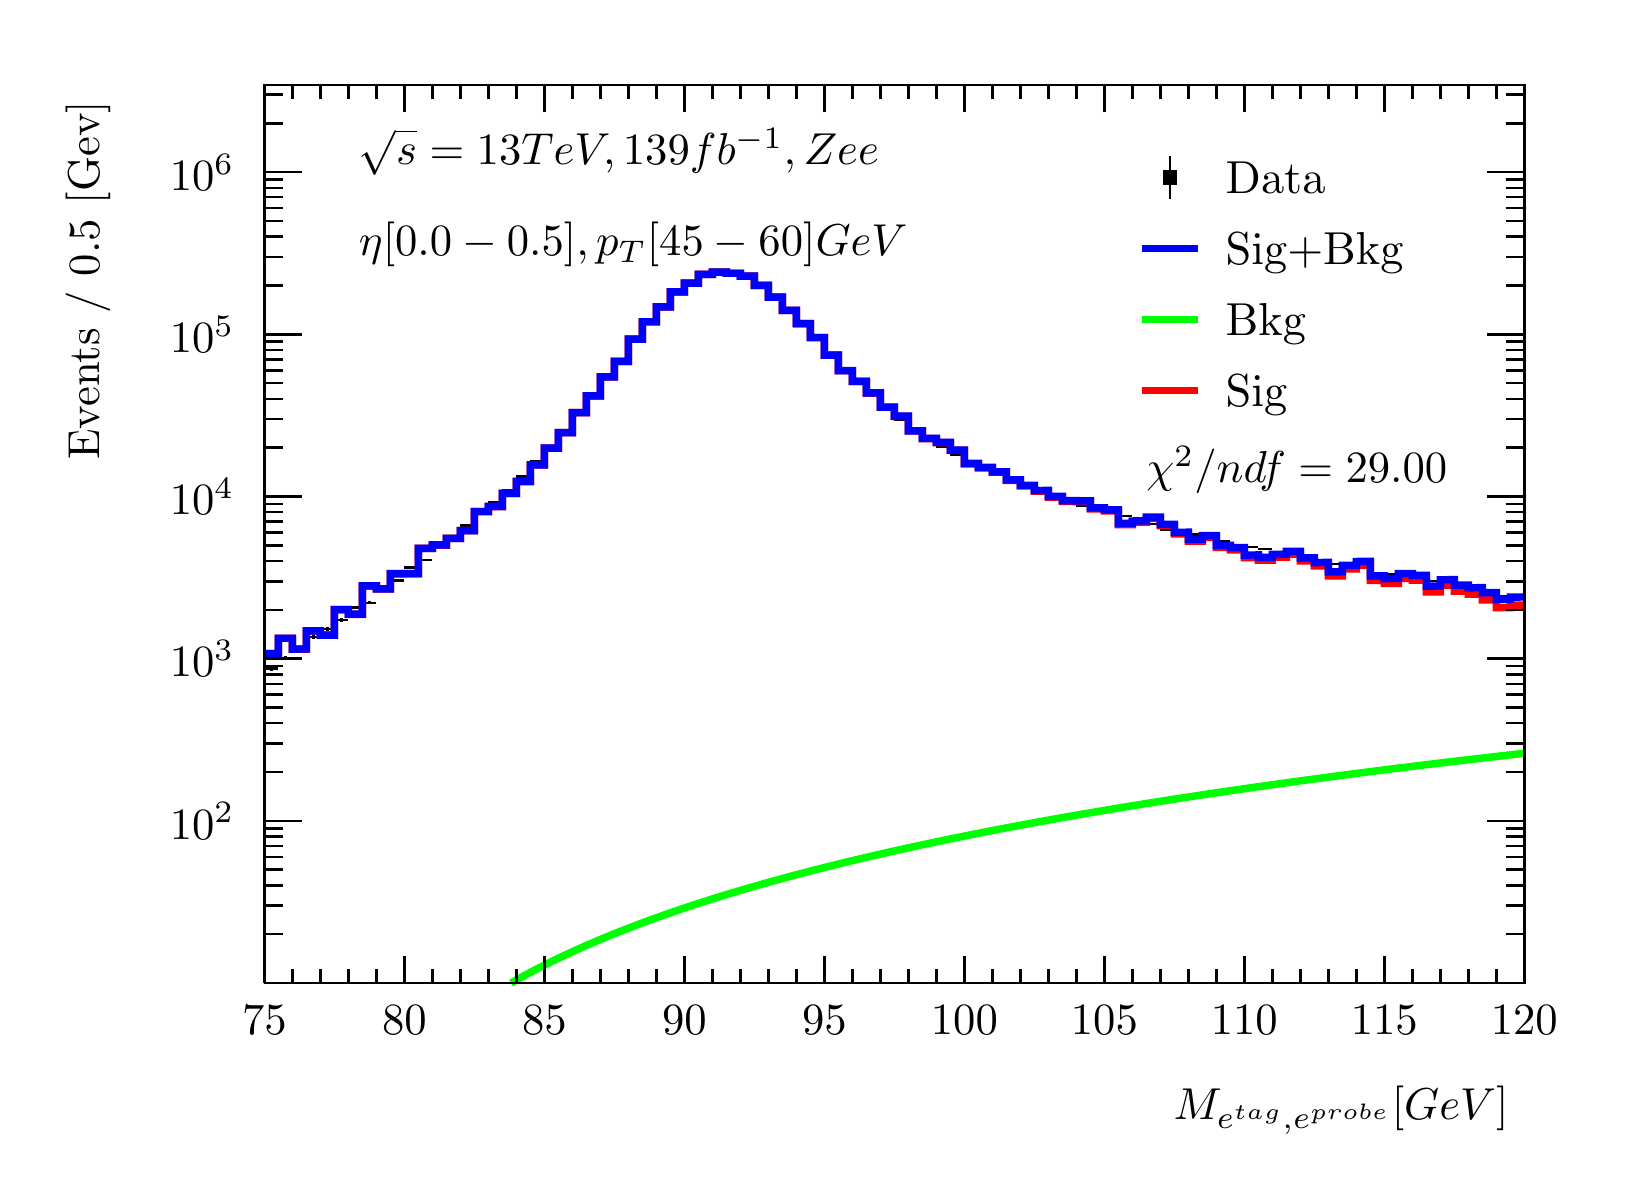
\begin{tikzpicture}
\pgfdeclareplotmark{cross} {
\pgfpathmoveto{\pgfpoint{-0.3\pgfplotmarksize}{\pgfplotmarksize}}
\pgfpathlineto{\pgfpoint{+0.3\pgfplotmarksize}{\pgfplotmarksize}}
\pgfpathlineto{\pgfpoint{+0.3\pgfplotmarksize}{0.3\pgfplotmarksize}}
\pgfpathlineto{\pgfpoint{+1\pgfplotmarksize}{0.3\pgfplotmarksize}}
\pgfpathlineto{\pgfpoint{+1\pgfplotmarksize}{-0.3\pgfplotmarksize}}
\pgfpathlineto{\pgfpoint{+0.3\pgfplotmarksize}{-0.3\pgfplotmarksize}}
\pgfpathlineto{\pgfpoint{+0.3\pgfplotmarksize}{-1.\pgfplotmarksize}}
\pgfpathlineto{\pgfpoint{-0.3\pgfplotmarksize}{-1.\pgfplotmarksize}}
\pgfpathlineto{\pgfpoint{-0.3\pgfplotmarksize}{-0.3\pgfplotmarksize}}
\pgfpathlineto{\pgfpoint{-1.\pgfplotmarksize}{-0.3\pgfplotmarksize}}
\pgfpathlineto{\pgfpoint{-1.\pgfplotmarksize}{0.3\pgfplotmarksize}}
\pgfpathlineto{\pgfpoint{-0.3\pgfplotmarksize}{0.3\pgfplotmarksize}}
\pgfpathclose
\pgfusepathqstroke
}
\pgfdeclareplotmark{cross*} {
\pgfpathmoveto{\pgfpoint{-0.3\pgfplotmarksize}{\pgfplotmarksize}}
\pgfpathlineto{\pgfpoint{+0.3\pgfplotmarksize}{\pgfplotmarksize}}
\pgfpathlineto{\pgfpoint{+0.3\pgfplotmarksize}{0.3\pgfplotmarksize}}
\pgfpathlineto{\pgfpoint{+1\pgfplotmarksize}{0.3\pgfplotmarksize}}
\pgfpathlineto{\pgfpoint{+1\pgfplotmarksize}{-0.3\pgfplotmarksize}}
\pgfpathlineto{\pgfpoint{+0.3\pgfplotmarksize}{-0.3\pgfplotmarksize}}
\pgfpathlineto{\pgfpoint{+0.3\pgfplotmarksize}{-1.\pgfplotmarksize}}
\pgfpathlineto{\pgfpoint{-0.3\pgfplotmarksize}{-1.\pgfplotmarksize}}
\pgfpathlineto{\pgfpoint{-0.3\pgfplotmarksize}{-0.3\pgfplotmarksize}}
\pgfpathlineto{\pgfpoint{-1.\pgfplotmarksize}{-0.3\pgfplotmarksize}}
\pgfpathlineto{\pgfpoint{-1.\pgfplotmarksize}{0.3\pgfplotmarksize}}
\pgfpathlineto{\pgfpoint{-0.3\pgfplotmarksize}{0.3\pgfplotmarksize}}
\pgfpathclose
\pgfusepathqfillstroke
}
\pgfdeclareplotmark{newstar} {
\pgfpathmoveto{\pgfqpoint{0pt}{\pgfplotmarksize}}
\pgfpathlineto{\pgfqpointpolar{44}{0.5\pgfplotmarksize}}
\pgfpathlineto{\pgfqpointpolar{18}{\pgfplotmarksize}}
\pgfpathlineto{\pgfqpointpolar{-20}{0.5\pgfplotmarksize}}
\pgfpathlineto{\pgfqpointpolar{-54}{\pgfplotmarksize}}
\pgfpathlineto{\pgfqpointpolar{-90}{0.5\pgfplotmarksize}}
\pgfpathlineto{\pgfqpointpolar{234}{\pgfplotmarksize}}
\pgfpathlineto{\pgfqpointpolar{198}{0.5\pgfplotmarksize}}
\pgfpathlineto{\pgfqpointpolar{162}{\pgfplotmarksize}}
\pgfpathlineto{\pgfqpointpolar{134}{0.5\pgfplotmarksize}}
\pgfpathclose
\pgfusepathqstroke
}
\pgfdeclareplotmark{newstar*} {
\pgfpathmoveto{\pgfqpoint{0pt}{\pgfplotmarksize}}
\pgfpathlineto{\pgfqpointpolar{44}{0.5\pgfplotmarksize}}
\pgfpathlineto{\pgfqpointpolar{18}{\pgfplotmarksize}}
\pgfpathlineto{\pgfqpointpolar{-20}{0.5\pgfplotmarksize}}
\pgfpathlineto{\pgfqpointpolar{-54}{\pgfplotmarksize}}
\pgfpathlineto{\pgfqpointpolar{-90}{0.5\pgfplotmarksize}}
\pgfpathlineto{\pgfqpointpolar{234}{\pgfplotmarksize}}
\pgfpathlineto{\pgfqpointpolar{198}{0.5\pgfplotmarksize}}
\pgfpathlineto{\pgfqpointpolar{162}{\pgfplotmarksize}}
\pgfpathlineto{\pgfqpointpolar{134}{0.5\pgfplotmarksize}}
\pgfpathclose
\pgfusepathqfillstroke
}
\definecolor{c}{rgb}{1,1,1};
\draw [color=c, fill=c] (0,0) rectangle (20,14.4361);
\draw [color=c, fill=c] (3,2.30977) rectangle (19,13.7143);
\definecolor{c}{rgb}{0,0,0};
\draw [c,line width=0.9] (3,2.30977) -- (3,13.7143) -- (19,13.7143) -- (19,2.30977) -- (3,2.30977);
\definecolor{c}{rgb}{1,1,1};
\draw [color=c, fill=c] (3,2.30977) rectangle (19,13.7143);
\definecolor{c}{rgb}{0,0,0};
\draw [c,line width=0.9] (3,2.30977) -- (3,13.7143) -- (19,13.7143) -- (19,2.30977) -- (3,2.30977);
\draw [c,line width=0.9] (3,2.30977) -- (19,2.30977);
\draw [c,line width=0.9] (3,2.65624) -- (3,2.30977);
\draw [c,line width=0.9] (3.35556,2.48301) -- (3.35556,2.30977);
\draw [c,line width=0.9] (3.71111,2.48301) -- (3.71111,2.30977);
\draw [c,line width=0.9] (4.06667,2.48301) -- (4.06667,2.30977);
\draw [c,line width=0.9] (4.42222,2.48301) -- (4.42222,2.30977);
\draw [c,line width=0.9] (4.77778,2.65624) -- (4.77778,2.30977);
\draw [c,line width=0.9] (5.13333,2.48301) -- (5.13333,2.30977);
\draw [c,line width=0.9] (5.48889,2.48301) -- (5.48889,2.30977);
\draw [c,line width=0.9] (5.84444,2.48301) -- (5.84444,2.30977);
\draw [c,line width=0.9] (6.2,2.48301) -- (6.2,2.30977);
\draw [c,line width=0.9] (6.55556,2.65624) -- (6.55556,2.30977);
\draw [c,line width=0.9] (6.91111,2.48301) -- (6.91111,2.30977);
\draw [c,line width=0.9] (7.26667,2.48301) -- (7.26667,2.30977);
\draw [c,line width=0.9] (7.62222,2.48301) -- (7.62222,2.30977);
\draw [c,line width=0.9] (7.97778,2.48301) -- (7.97778,2.30977);
\draw [c,line width=0.9] (8.33333,2.65624) -- (8.33333,2.30977);
\draw [c,line width=0.9] (8.68889,2.48301) -- (8.68889,2.30977);
\draw [c,line width=0.9] (9.04444,2.48301) -- (9.04444,2.30977);
\draw [c,line width=0.9] (9.4,2.48301) -- (9.4,2.30977);
\draw [c,line width=0.9] (9.75556,2.48301) -- (9.75556,2.30977);
\draw [c,line width=0.9] (10.1111,2.65624) -- (10.1111,2.30977);
\draw [c,line width=0.9] (10.4667,2.48301) -- (10.4667,2.30977);
\draw [c,line width=0.9] (10.8222,2.48301) -- (10.8222,2.30977);
\draw [c,line width=0.9] (11.1778,2.48301) -- (11.1778,2.30977);
\draw [c,line width=0.9] (11.5333,2.48301) -- (11.5333,2.30977);
\draw [c,line width=0.9] (11.8889,2.65624) -- (11.8889,2.30977);
\draw [c,line width=0.9] (12.2444,2.48301) -- (12.2444,2.30977);
\draw [c,line width=0.9] (12.6,2.48301) -- (12.6,2.30977);
\draw [c,line width=0.9] (12.9556,2.48301) -- (12.9556,2.30977);
\draw [c,line width=0.9] (13.3111,2.48301) -- (13.3111,2.30977);
\draw [c,line width=0.9] (13.6667,2.65624) -- (13.6667,2.30977);
\draw [c,line width=0.9] (14.0222,2.48301) -- (14.0222,2.30977);
\draw [c,line width=0.9] (14.3778,2.48301) -- (14.3778,2.30977);
\draw [c,line width=0.9] (14.7333,2.48301) -- (14.7333,2.30977);
\draw [c,line width=0.9] (15.0889,2.48301) -- (15.0889,2.30977);
\draw [c,line width=0.9] (15.4444,2.65624) -- (15.4444,2.30977);
\draw [c,line width=0.9] (15.8,2.48301) -- (15.8,2.30977);
\draw [c,line width=0.9] (16.1556,2.48301) -- (16.1556,2.30977);
\draw [c,line width=0.9] (16.5111,2.48301) -- (16.5111,2.30977);
\draw [c,line width=0.9] (16.8667,2.48301) -- (16.8667,2.30977);
\draw [c,line width=0.9] (17.2222,2.65624) -- (17.2222,2.30977);
\draw [c,line width=0.9] (17.5778,2.48301) -- (17.5778,2.30977);
\draw [c,line width=0.9] (17.9333,2.48301) -- (17.9333,2.30977);
\draw [c,line width=0.9] (18.2889,2.48301) -- (18.2889,2.30977);
\draw [c,line width=0.9] (18.6444,2.48301) -- (18.6444,2.30977);
\draw [c,line width=0.9] (19,2.65624) -- (19,2.30977);
\draw [c,line width=0.9] (19,2.65624) -- (19,2.30977);
\draw [anchor=base] (3,1.66015) node[scale=1.61424, color=c, rotate=0]{75};
\draw [anchor=base] (4.77778,1.66015) node[scale=1.61424, color=c, rotate=0]{80};
\draw [anchor=base] (6.55556,1.66015) node[scale=1.61424, color=c, rotate=0]{85};
\draw [anchor=base] (8.33333,1.66015) node[scale=1.61424, color=c, rotate=0]{90};
\draw [anchor=base] (10.1111,1.66015) node[scale=1.61424, color=c, rotate=0]{95};
\draw [anchor=base] (11.8889,1.66015) node[scale=1.61424, color=c, rotate=0]{100};
\draw [anchor=base] (13.6667,1.66015) node[scale=1.61424, color=c, rotate=0]{105};
\draw [anchor=base] (15.4444,1.66015) node[scale=1.61424, color=c, rotate=0]{110};
\draw [anchor=base] (17.2222,1.66015) node[scale=1.61424, color=c, rotate=0]{115};
\draw [anchor=base] (19,1.66015) node[scale=1.61424, color=c, rotate=0]{120};
\draw [anchor= east] (19,0.692932) node[scale=1.61424, color=c, rotate=0]{$M_{e^{tag}, e^{probe}}  [GeV]$};
\draw [c,line width=0.9] (3,13.7143) -- (19,13.7143);
\draw [c,line width=0.9] (3,13.3678) -- (3,13.7143);
\draw [c,line width=0.9] (3.35556,13.5411) -- (3.35556,13.7143);
\draw [c,line width=0.9] (3.71111,13.5411) -- (3.71111,13.7143);
\draw [c,line width=0.9] (4.06667,13.5411) -- (4.06667,13.7143);
\draw [c,line width=0.9] (4.42222,13.5411) -- (4.42222,13.7143);
\draw [c,line width=0.9] (4.77778,13.3678) -- (4.77778,13.7143);
\draw [c,line width=0.9] (5.13333,13.5411) -- (5.13333,13.7143);
\draw [c,line width=0.9] (5.48889,13.5411) -- (5.48889,13.7143);
\draw [c,line width=0.9] (5.84444,13.5411) -- (5.84444,13.7143);
\draw [c,line width=0.9] (6.2,13.5411) -- (6.2,13.7143);
\draw [c,line width=0.9] (6.55556,13.3678) -- (6.55556,13.7143);
\draw [c,line width=0.9] (6.91111,13.5411) -- (6.91111,13.7143);
\draw [c,line width=0.9] (7.26667,13.5411) -- (7.26667,13.7143);
\draw [c,line width=0.9] (7.62222,13.5411) -- (7.62222,13.7143);
\draw [c,line width=0.9] (7.97778,13.5411) -- (7.97778,13.7143);
\draw [c,line width=0.9] (8.33333,13.3678) -- (8.33333,13.7143);
\draw [c,line width=0.9] (8.68889,13.5411) -- (8.68889,13.7143);
\draw [c,line width=0.9] (9.04444,13.5411) -- (9.04444,13.7143);
\draw [c,line width=0.9] (9.4,13.5411) -- (9.4,13.7143);
\draw [c,line width=0.9] (9.75556,13.5411) -- (9.75556,13.7143);
\draw [c,line width=0.9] (10.1111,13.3678) -- (10.1111,13.7143);
\draw [c,line width=0.9] (10.4667,13.5411) -- (10.4667,13.7143);
\draw [c,line width=0.9] (10.8222,13.5411) -- (10.8222,13.7143);
\draw [c,line width=0.9] (11.1778,13.5411) -- (11.1778,13.7143);
\draw [c,line width=0.9] (11.5333,13.5411) -- (11.5333,13.7143);
\draw [c,line width=0.9] (11.8889,13.3678) -- (11.8889,13.7143);
\draw [c,line width=0.9] (12.2444,13.5411) -- (12.2444,13.7143);
\draw [c,line width=0.9] (12.6,13.5411) -- (12.6,13.7143);
\draw [c,line width=0.9] (12.9556,13.5411) -- (12.9556,13.7143);
\draw [c,line width=0.9] (13.3111,13.5411) -- (13.3111,13.7143);
\draw [c,line width=0.9] (13.6667,13.3678) -- (13.6667,13.7143);
\draw [c,line width=0.9] (14.0222,13.5411) -- (14.0222,13.7143);
\draw [c,line width=0.9] (14.3778,13.5411) -- (14.3778,13.7143);
\draw [c,line width=0.9] (14.7333,13.5411) -- (14.7333,13.7143);
\draw [c,line width=0.9] (15.0889,13.5411) -- (15.0889,13.7143);
\draw [c,line width=0.9] (15.4444,13.3678) -- (15.4444,13.7143);
\draw [c,line width=0.9] (15.8,13.5411) -- (15.8,13.7143);
\draw [c,line width=0.9] (16.1556,13.5411) -- (16.1556,13.7143);
\draw [c,line width=0.9] (16.5111,13.5411) -- (16.5111,13.7143);
\draw [c,line width=0.9] (16.8667,13.5411) -- (16.8667,13.7143);
\draw [c,line width=0.9] (17.2222,13.3678) -- (17.2222,13.7143);
\draw [c,line width=0.9] (17.5778,13.5411) -- (17.5778,13.7143);
\draw [c,line width=0.9] (17.9333,13.5411) -- (17.9333,13.7143);
\draw [c,line width=0.9] (18.2889,13.5411) -- (18.2889,13.7143);
\draw [c,line width=0.9] (18.6444,13.5411) -- (18.6444,13.7143);
\draw [c,line width=0.9] (19,13.3678) -- (19,13.7143);
\draw [c,line width=0.9] (19,13.3678) -- (19,13.7143);
\draw [c,line width=0.9] (3,2.30977) -- (3,13.7143);
\draw [c,line width=0.9] (3.237,2.92982) -- (3,2.92982);
\draw [c,line width=0.9] (3.237,3.29252) -- (3,3.29252);
\draw [c,line width=0.9] (3.237,3.54986) -- (3,3.54986);
\draw [c,line width=0.9] (3.237,3.74947) -- (3,3.74947);
\draw [c,line width=0.9] (3.237,3.91257) -- (3,3.91257);
\draw [c,line width=0.9] (3.237,4.05046) -- (3,4.05046);
\draw [c,line width=0.9] (3.237,4.16991) -- (3,4.16991);
\draw [c,line width=0.9] (3.237,4.27527) -- (3,4.27527);
\draw [c,line width=0.9] (3.474,4.36952) -- (3,4.36952);
\draw [anchor= east] (2.82,4.36952) node[scale=1.61424, color=c, rotate=0]{$10^{2}$};
\draw [c,line width=0.9] (3.237,4.98956) -- (3,4.98956);
\draw [c,line width=0.9] (3.237,5.35227) -- (3,5.35227);
\draw [c,line width=0.9] (3.237,5.60961) -- (3,5.60961);
\draw [c,line width=0.9] (3.237,5.80922) -- (3,5.80922);
\draw [c,line width=0.9] (3.237,5.97231) -- (3,5.97231);
\draw [c,line width=0.9] (3.237,6.11021) -- (3,6.11021);
\draw [c,line width=0.9] (3.237,6.22966) -- (3,6.22966);
\draw [c,line width=0.9] (3.237,6.33502) -- (3,6.33502);
\draw [c,line width=0.9] (3.474,6.42927) -- (3,6.42927);
\draw [anchor= east] (2.82,6.42927) node[scale=1.61424, color=c, rotate=0]{$10^{3}$};
\draw [c,line width=0.9] (3.237,7.04931) -- (3,7.04931);
\draw [c,line width=0.9] (3.237,7.41202) -- (3,7.41202);
\draw [c,line width=0.9] (3.237,7.66936) -- (3,7.66936);
\draw [c,line width=0.9] (3.237,7.86897) -- (3,7.86897);
\draw [c,line width=0.9] (3.237,8.03206) -- (3,8.03206);
\draw [c,line width=0.9] (3.237,8.16995) -- (3,8.16995);
\draw [c,line width=0.9] (3.237,8.2894) -- (3,8.2894);
\draw [c,line width=0.9] (3.237,8.39476) -- (3,8.39476);
\draw [c,line width=0.9] (3.474,8.48901) -- (3,8.48901);
\draw [anchor= east] (2.82,8.48901) node[scale=1.61424, color=c, rotate=0]{$10^{4}$};
\draw [c,line width=0.9] (3.237,9.10906) -- (3,9.10906);
\draw [c,line width=0.9] (3.237,9.47176) -- (3,9.47176);
\draw [c,line width=0.9] (3.237,9.7291) -- (3,9.7291);
\draw [c,line width=0.9] (3.237,9.92871) -- (3,9.92871);
\draw [c,line width=0.9] (3.237,10.0918) -- (3,10.0918);
\draw [c,line width=0.9] (3.237,10.2297) -- (3,10.2297);
\draw [c,line width=0.9] (3.237,10.3491) -- (3,10.3491);
\draw [c,line width=0.9] (3.237,10.4545) -- (3,10.4545);
\draw [c,line width=0.9] (3.474,10.5488) -- (3,10.5488);
\draw [anchor= east] (2.82,10.5488) node[scale=1.61424, color=c, rotate=0]{$10^{5}$};
\draw [c,line width=0.9] (3.237,11.1688) -- (3,11.1688);
\draw [c,line width=0.9] (3.237,11.5315) -- (3,11.5315);
\draw [c,line width=0.9] (3.237,11.7889) -- (3,11.7889);
\draw [c,line width=0.9] (3.237,11.9885) -- (3,11.9885);
\draw [c,line width=0.9] (3.237,12.1516) -- (3,12.1516);
\draw [c,line width=0.9] (3.237,12.2894) -- (3,12.2894);
\draw [c,line width=0.9] (3.237,12.4089) -- (3,12.4089);
\draw [c,line width=0.9] (3.237,12.5143) -- (3,12.5143);
\draw [c,line width=0.9] (3.474,12.6085) -- (3,12.6085);
\draw [anchor= east] (2.82,12.6085) node[scale=1.61424, color=c, rotate=0]{$10^{6}$};
\draw [c,line width=0.9] (3.237,13.2286) -- (3,13.2286);
\draw [c,line width=0.9] (3.237,13.5913) -- (3,13.5913);
\draw [anchor= east] (0.76,13.7143) node[scale=1.61424, color=c, rotate=90]{Events / 0.5 [Gev]};
\draw [c,line width=0.9] (19,2.30977) -- (19,13.7143);
\draw [c,line width=0.9] (18.763,2.92982) -- (19,2.92982);
\draw [c,line width=0.9] (18.763,3.29252) -- (19,3.29252);
\draw [c,line width=0.9] (18.763,3.54986) -- (19,3.54986);
\draw [c,line width=0.9] (18.763,3.74947) -- (19,3.74947);
\draw [c,line width=0.9] (18.763,3.91257) -- (19,3.91257);
\draw [c,line width=0.9] (18.763,4.05046) -- (19,4.05046);
\draw [c,line width=0.9] (18.763,4.16991) -- (19,4.16991);
\draw [c,line width=0.9] (18.763,4.27527) -- (19,4.27527);
\draw [c,line width=0.9] (18.526,4.36952) -- (19,4.36952);
\draw [c,line width=0.9] (18.763,4.98956) -- (19,4.98956);
\draw [c,line width=0.9] (18.763,5.35227) -- (19,5.35227);
\draw [c,line width=0.9] (18.763,5.60961) -- (19,5.60961);
\draw [c,line width=0.9] (18.763,5.80922) -- (19,5.80922);
\draw [c,line width=0.9] (18.763,5.97231) -- (19,5.97231);
\draw [c,line width=0.9] (18.763,6.11021) -- (19,6.11021);
\draw [c,line width=0.9] (18.763,6.22966) -- (19,6.22966);
\draw [c,line width=0.9] (18.763,6.33502) -- (19,6.33502);
\draw [c,line width=0.9] (18.526,6.42927) -- (19,6.42927);
\draw [c,line width=0.9] (18.763,7.04931) -- (19,7.04931);
\draw [c,line width=0.9] (18.763,7.41202) -- (19,7.41202);
\draw [c,line width=0.9] (18.763,7.66936) -- (19,7.66936);
\draw [c,line width=0.9] (18.763,7.86897) -- (19,7.86897);
\draw [c,line width=0.9] (18.763,8.03206) -- (19,8.03206);
\draw [c,line width=0.9] (18.763,8.16995) -- (19,8.16995);
\draw [c,line width=0.9] (18.763,8.2894) -- (19,8.2894);
\draw [c,line width=0.9] (18.763,8.39476) -- (19,8.39476);
\draw [c,line width=0.9] (18.526,8.48901) -- (19,8.48901);
\draw [c,line width=0.9] (18.763,9.10906) -- (19,9.10906);
\draw [c,line width=0.9] (18.763,9.47176) -- (19,9.47176);
\draw [c,line width=0.9] (18.763,9.7291) -- (19,9.7291);
\draw [c,line width=0.9] (18.763,9.92871) -- (19,9.92871);
\draw [c,line width=0.9] (18.763,10.0918) -- (19,10.0918);
\draw [c,line width=0.9] (18.763,10.2297) -- (19,10.2297);
\draw [c,line width=0.9] (18.763,10.3491) -- (19,10.3491);
\draw [c,line width=0.9] (18.763,10.4545) -- (19,10.4545);
\draw [c,line width=0.9] (18.526,10.5488) -- (19,10.5488);
\draw [c,line width=0.9] (18.763,11.1688) -- (19,11.1688);
\draw [c,line width=0.9] (18.763,11.5315) -- (19,11.5315);
\draw [c,line width=0.9] (18.763,11.7889) -- (19,11.7889);
\draw [c,line width=0.9] (18.763,11.9885) -- (19,11.9885);
\draw [c,line width=0.9] (18.763,12.1516) -- (19,12.1516);
\draw [c,line width=0.9] (18.763,12.2894) -- (19,12.2894);
\draw [c,line width=0.9] (18.763,12.4089) -- (19,12.4089);
\draw [c,line width=0.9] (18.763,12.5143) -- (19,12.5143);
\draw [c,line width=0.9] (18.526,12.6085) -- (19,12.6085);
\draw [c,line width=0.9] (18.763,13.2286) -- (19,13.2286);
\draw [c,line width=0.9] (18.763,13.5913) -- (19,13.5913);
\draw [c,line width=0.9] (3.08889,6.30572) -- (3,6.30572);
\draw [c,line width=0.9] (3,6.30572) -- (3,6.30572);
\draw [c,line width=0.9] (3.08889,6.30572) -- (3.17778,6.30572);
\draw [c,line width=0.9] (3.17778,6.30572) -- (3.17778,6.30572);
\draw [c,line width=0.9] (3.08889,6.30572) -- (3.08889,6.33603);
\draw [c,line width=0.9] (3.08889,6.33603) -- (3.08889,6.33603);
\draw [c,line width=0.9] (3.08889,6.30572) -- (3.08889,6.27541);
\draw [c,line width=0.9] (3.08889,6.27541) -- (3.08889,6.27541);
\draw [c,line width=0.9] (3.26667,6.43994) -- (3.17778,6.43994);
\draw [c,line width=0.9] (3.17778,6.43994) -- (3.17778,6.43994);
\draw [c,line width=0.9] (3.26667,6.43994) -- (3.35556,6.43994);
\draw [c,line width=0.9] (3.35556,6.43994) -- (3.35556,6.43994);
\draw [c,line width=0.9] (3.26667,6.43994) -- (3.26667,6.46806);
\draw [c,line width=0.9] (3.26667,6.46806) -- (3.26667,6.46806);
\draw [c,line width=0.9] (3.26667,6.43994) -- (3.26667,6.41182);
\draw [c,line width=0.9] (3.26667,6.41182) -- (3.26667,6.41182);
\draw [c,line width=0.9] (3.44444,6.55584) -- (3.35556,6.55584);
\draw [c,line width=0.9] (3.35556,6.55584) -- (3.35556,6.55584);
\draw [c,line width=0.9] (3.44444,6.55584) -- (3.53333,6.55584);
\draw [c,line width=0.9] (3.53333,6.55584) -- (3.53333,6.55584);
\draw [c,line width=0.9] (3.44444,6.55584) -- (3.44444,6.5822);
\draw [c,line width=0.9] (3.44444,6.5822) -- (3.44444,6.5822);
\draw [c,line width=0.9] (3.44444,6.55584) -- (3.44444,6.52949);
\draw [c,line width=0.9] (3.44444,6.52949) -- (3.44444,6.52949);
\draw [c,line width=0.9] (3.62222,6.70301) -- (3.53333,6.70301);
\draw [c,line width=0.9] (3.53333,6.70301) -- (3.53333,6.70301);
\draw [c,line width=0.9] (3.62222,6.70301) -- (3.71111,6.70301);
\draw [c,line width=0.9] (3.71111,6.70301) -- (3.71111,6.70301);
\draw [c,line width=0.9] (3.62222,6.70301) -- (3.62222,6.72728);
\draw [c,line width=0.9] (3.62222,6.72728) -- (3.62222,6.72728);
\draw [c,line width=0.9] (3.62222,6.70301) -- (3.62222,6.67873);
\draw [c,line width=0.9] (3.62222,6.67873) -- (3.62222,6.67873);
\draw [c,line width=0.9] (3.8,6.80852) -- (3.71111,6.80852);
\draw [c,line width=0.9] (3.71111,6.80852) -- (3.71111,6.80852);
\draw [c,line width=0.9] (3.8,6.80852) -- (3.88889,6.80852);
\draw [c,line width=0.9] (3.88889,6.80852) -- (3.88889,6.80852);
\draw [c,line width=0.9] (3.8,6.80852) -- (3.8,6.8314);
\draw [c,line width=0.9] (3.8,6.8314) -- (3.8,6.8314);
\draw [c,line width=0.9] (3.8,6.80852) -- (3.8,6.78563);
\draw [c,line width=0.9] (3.8,6.78563) -- (3.8,6.78563);
\draw [c,line width=0.9] (3.97778,6.91855) -- (3.88889,6.91855);
\draw [c,line width=0.9] (3.88889,6.91855) -- (3.88889,6.91855);
\draw [c,line width=0.9] (3.97778,6.91855) -- (4.06667,6.91855);
\draw [c,line width=0.9] (4.06667,6.91855) -- (4.06667,6.91855);
\draw [c,line width=0.9] (3.97778,6.91855) -- (3.97778,6.94007);
\draw [c,line width=0.9] (3.97778,6.94007) -- (3.97778,6.94007);
\draw [c,line width=0.9] (3.97778,6.91855) -- (3.97778,6.89703);
\draw [c,line width=0.9] (3.97778,6.89703) -- (3.97778,6.89703);
\draw [c,line width=0.9] (4.15556,7.08052) -- (4.06667,7.08052);
\draw [c,line width=0.9] (4.06667,7.08052) -- (4.06667,7.08052);
\draw [c,line width=0.9] (4.15556,7.08052) -- (4.24444,7.08052);
\draw [c,line width=0.9] (4.24444,7.08052) -- (4.24444,7.08052);
\draw [c,line width=0.9] (4.15556,7.08052) -- (4.15556,7.10017);
\draw [c,line width=0.9] (4.15556,7.10017) -- (4.15556,7.10017);
\draw [c,line width=0.9] (4.15556,7.08052) -- (4.15556,7.06086);
\draw [c,line width=0.9] (4.15556,7.06086) -- (4.15556,7.06086);
\draw [c,line width=0.9] (4.33333,7.13863) -- (4.24444,7.13863);
\draw [c,line width=0.9] (4.24444,7.13863) -- (4.24444,7.13863);
\draw [c,line width=0.9] (4.33333,7.13863) -- (4.42222,7.13863);
\draw [c,line width=0.9] (4.42222,7.13863) -- (4.42222,7.13863);
\draw [c,line width=0.9] (4.33333,7.13863) -- (4.33333,7.15766);
\draw [c,line width=0.9] (4.33333,7.15766) -- (4.33333,7.15766);
\draw [c,line width=0.9] (4.33333,7.13863) -- (4.33333,7.1196);
\draw [c,line width=0.9] (4.33333,7.1196) -- (4.33333,7.1196);
\draw [c,line width=0.9] (4.51111,7.29393) -- (4.42222,7.29393);
\draw [c,line width=0.9] (4.42222,7.29393) -- (4.42222,7.29393);
\draw [c,line width=0.9] (4.51111,7.29393) -- (4.6,7.29393);
\draw [c,line width=0.9] (4.6,7.29393) -- (4.6,7.29393);
\draw [c,line width=0.9] (4.51111,7.29393) -- (4.51111,7.31138);
\draw [c,line width=0.9] (4.51111,7.31138) -- (4.51111,7.31138);
\draw [c,line width=0.9] (4.51111,7.29393) -- (4.51111,7.27648);
\draw [c,line width=0.9] (4.51111,7.27648) -- (4.51111,7.27648);
\draw [c,line width=0.9] (4.68889,7.42239) -- (4.6,7.42239);
\draw [c,line width=0.9] (4.6,7.42239) -- (4.6,7.42239);
\draw [c,line width=0.9] (4.68889,7.42239) -- (4.77778,7.42239);
\draw [c,line width=0.9] (4.77778,7.42239) -- (4.77778,7.42239);
\draw [c,line width=0.9] (4.68889,7.42239) -- (4.68889,7.43863);
\draw [c,line width=0.9] (4.68889,7.43863) -- (4.68889,7.43863);
\draw [c,line width=0.9] (4.68889,7.42239) -- (4.68889,7.40616);
\draw [c,line width=0.9] (4.68889,7.40616) -- (4.68889,7.40616);
\draw [c,line width=0.9] (4.86667,7.58647) -- (4.77778,7.58647);
\draw [c,line width=0.9] (4.77778,7.58647) -- (4.77778,7.58647);
\draw [c,line width=0.9] (4.86667,7.58647) -- (4.95556,7.58647);
\draw [c,line width=0.9] (4.95556,7.58647) -- (4.95556,7.58647);
\draw [c,line width=0.9] (4.86667,7.58647) -- (4.86667,7.60128);
\draw [c,line width=0.9] (4.86667,7.60128) -- (4.86667,7.60128);
\draw [c,line width=0.9] (4.86667,7.58647) -- (4.86667,7.57165);
\draw [c,line width=0.9] (4.86667,7.57165) -- (4.86667,7.57165);
\draw [c,line width=0.9] (5.04444,7.68466) -- (4.95556,7.68466);
\draw [c,line width=0.9] (4.95556,7.68466) -- (4.95556,7.68466);
\draw [c,line width=0.9] (5.04444,7.68466) -- (5.13333,7.68466);
\draw [c,line width=0.9] (5.13333,7.68466) -- (5.13333,7.68466);
\draw [c,line width=0.9] (5.04444,7.68466) -- (5.04444,7.69868);
\draw [c,line width=0.9] (5.04444,7.69868) -- (5.04444,7.69868);
\draw [c,line width=0.9] (5.04444,7.68466) -- (5.04444,7.67063);
\draw [c,line width=0.9] (5.04444,7.67063) -- (5.04444,7.67063);
\draw [c,line width=0.9] (5.22222,7.83413) -- (5.13333,7.83413);
\draw [c,line width=0.9] (5.13333,7.83413) -- (5.13333,7.83413);
\draw [c,line width=0.9] (5.22222,7.83413) -- (5.31111,7.83413);
\draw [c,line width=0.9] (5.31111,7.83413) -- (5.31111,7.83413);
\draw [c,line width=0.9] (5.22222,7.83413) -- (5.22222,7.84703);
\draw [c,line width=0.9] (5.22222,7.84703) -- (5.22222,7.84703);
\draw [c,line width=0.9] (5.22222,7.83413) -- (5.22222,7.82123);
\draw [c,line width=0.9] (5.22222,7.82123) -- (5.22222,7.82123);
\draw [c,line width=0.9] (5.4,7.95861) -- (5.31111,7.95861);
\draw [c,line width=0.9] (5.31111,7.95861) -- (5.31111,7.95861);
\draw [c,line width=0.9] (5.4,7.95861) -- (5.48889,7.95861);
\draw [c,line width=0.9] (5.48889,7.95861) -- (5.48889,7.95861);
\draw [c,line width=0.9] (5.4,7.95861) -- (5.4,7.97064);
\draw [c,line width=0.9] (5.4,7.97064) -- (5.4,7.97064);
\draw [c,line width=0.9] (5.4,7.95861) -- (5.4,7.94658);
\draw [c,line width=0.9] (5.4,7.94658) -- (5.4,7.94658);
\draw [c,line width=0.9] (5.57778,8.118) -- (5.48889,8.118);
\draw [c,line width=0.9] (5.48889,8.118) -- (5.48889,8.118);
\draw [c,line width=0.9] (5.57778,8.118) -- (5.66667,8.118);
\draw [c,line width=0.9] (5.66667,8.118) -- (5.66667,8.118);
\draw [c,line width=0.9] (5.57778,8.118) -- (5.57778,8.129);
\draw [c,line width=0.9] (5.57778,8.129) -- (5.57778,8.129);
\draw [c,line width=0.9] (5.57778,8.118) -- (5.57778,8.10699);
\draw [c,line width=0.9] (5.57778,8.10699) -- (5.57778,8.10699);
\draw [c,line width=0.9] (5.75556,8.26354) -- (5.66667,8.26354);
\draw [c,line width=0.9] (5.66667,8.26354) -- (5.66667,8.26354);
\draw [c,line width=0.9] (5.75556,8.26354) -- (5.84444,8.26354);
\draw [c,line width=0.9] (5.84444,8.26354) -- (5.84444,8.26354);
\draw [c,line width=0.9] (5.75556,8.26354) -- (5.75556,8.27369);
\draw [c,line width=0.9] (5.75556,8.27369) -- (5.75556,8.27369);
\draw [c,line width=0.9] (5.75556,8.26354) -- (5.75556,8.25339);
\draw [c,line width=0.9] (5.75556,8.25339) -- (5.75556,8.25339);
\draw [c,line width=0.9] (5.93333,8.41189) -- (5.84444,8.41189);
\draw [c,line width=0.9] (5.84444,8.41189) -- (5.84444,8.41189);
\draw [c,line width=0.9] (5.93333,8.41189) -- (6.02222,8.41189);
\draw [c,line width=0.9] (6.02222,8.41189) -- (6.02222,8.41189);
\draw [c,line width=0.9] (5.93333,8.41189) -- (5.93333,8.42123);
\draw [c,line width=0.9] (5.93333,8.42123) -- (5.93333,8.42123);
\draw [c,line width=0.9] (5.93333,8.41189) -- (5.93333,8.40256);
\draw [c,line width=0.9] (5.93333,8.40256) -- (5.93333,8.40256);
\draw [c,line width=0.9] (6.11111,8.5702) -- (6.02222,8.5702);
\draw [c,line width=0.9] (6.02222,8.5702) -- (6.02222,8.5702);
\draw [c,line width=0.9] (6.11111,8.5702) -- (6.2,8.5702);
\draw [c,line width=0.9] (6.2,8.5702) -- (6.2,8.5702);
\draw [c,line width=0.9] (6.11111,8.5702) -- (6.11111,8.57875);
\draw [c,line width=0.9] (6.11111,8.57875) -- (6.11111,8.57875);
\draw [c,line width=0.9] (6.11111,8.5702) -- (6.11111,8.56165);
\draw [c,line width=0.9] (6.11111,8.56165) -- (6.11111,8.56165);
\draw [c,line width=0.9] (6.28889,8.74338) -- (6.2,8.74338);
\draw [c,line width=0.9] (6.2,8.74338) -- (6.2,8.74338);
\draw [c,line width=0.9] (6.28889,8.74338) -- (6.37778,8.74338);
\draw [c,line width=0.9] (6.37778,8.74338) -- (6.37778,8.74338);
\draw [c,line width=0.9] (6.28889,8.74338) -- (6.28889,8.75114);
\draw [c,line width=0.9] (6.28889,8.75114) -- (6.28889,8.75114);
\draw [c,line width=0.9] (6.28889,8.74338) -- (6.28889,8.73562);
\draw [c,line width=0.9] (6.28889,8.73562) -- (6.28889,8.73562);
\draw [c,line width=0.9] (6.46667,8.93957) -- (6.37778,8.93957);
\draw [c,line width=0.9] (6.37778,8.93957) -- (6.37778,8.93957);
\draw [c,line width=0.9] (6.46667,8.93957) -- (6.55556,8.93957);
\draw [c,line width=0.9] (6.55556,8.93957) -- (6.55556,8.93957);
\draw [c,line width=0.9] (6.46667,8.93957) -- (6.46667,8.94653);
\draw [c,line width=0.9] (6.46667,8.94653) -- (6.46667,8.94653);
\draw [c,line width=0.9] (6.46667,8.93957) -- (6.46667,8.93262);
\draw [c,line width=0.9] (6.46667,8.93262) -- (6.46667,8.93262);
\draw [c,line width=0.9] (6.64444,9.12594) -- (6.55556,9.12594);
\draw [c,line width=0.9] (6.55556,9.12594) -- (6.55556,9.12594);
\draw [c,line width=0.9] (6.64444,9.12594) -- (6.73333,9.12594);
\draw [c,line width=0.9] (6.73333,9.12594) -- (6.73333,9.12594);
\draw [c,line width=0.9] (6.64444,9.12594) -- (6.64444,9.13221);
\draw [c,line width=0.9] (6.64444,9.13221) -- (6.64444,9.13221);
\draw [c,line width=0.9] (6.64444,9.12594) -- (6.64444,9.11967);
\draw [c,line width=0.9] (6.64444,9.11967) -- (6.64444,9.11967);
\draw [c,line width=0.9] (6.82222,9.32751) -- (6.73333,9.32751);
\draw [c,line width=0.9] (6.73333,9.32751) -- (6.73333,9.32751);
\draw [c,line width=0.9] (6.82222,9.32751) -- (6.91111,9.32751);
\draw [c,line width=0.9] (6.91111,9.32751) -- (6.91111,9.32751);
\draw [c,line width=0.9] (6.82222,9.32751) -- (6.82222,9.3331);
\draw [c,line width=0.9] (6.82222,9.3331) -- (6.82222,9.3331);
\draw [c,line width=0.9] (6.82222,9.32751) -- (6.82222,9.32191);
\draw [c,line width=0.9] (6.82222,9.32191) -- (6.82222,9.32191);
\draw [c,line width=0.9] (7,9.53) -- (6.91111,9.53);
\draw [c,line width=0.9] (6.91111,9.53) -- (6.91111,9.53);
\draw [c,line width=0.9] (7,9.53) -- (7.08889,9.53);
\draw [c,line width=0.9] (7.08889,9.53) -- (7.08889,9.53);
\draw [c,line width=0.9] (7,9.53) -- (7,9.535);
\draw [c,line width=0.9] (7,9.535) -- (7,9.535);
\draw [c,line width=0.9] (7,9.53) -- (7,9.525);
\draw [c,line width=0.9] (7,9.525) -- (7,9.525);
\draw [c,line width=0.9] (7.17778,9.76837) -- (7.08889,9.76837);
\draw [c,line width=0.9] (7.08889,9.76837) -- (7.08889,9.76837);
\draw [c,line width=0.9] (7.17778,9.76837) -- (7.26667,9.76837);
\draw [c,line width=0.9] (7.26667,9.76837) -- (7.26667,9.76837);
\draw [c,line width=0.9] (7.17778,9.76837) -- (7.17778,9.77275);
\draw [c,line width=0.9] (7.17778,9.77275) -- (7.17778,9.77275);
\draw [c,line width=0.9] (7.17778,9.76837) -- (7.17778,9.764);
\draw [c,line width=0.9] (7.17778,9.764) -- (7.17778,9.764);
\draw [c,line width=0.9] (7.35556,9.99199) -- (7.26667,9.99199);
\draw [c,line width=0.9] (7.26667,9.99199) -- (7.26667,9.99199);
\draw [c,line width=0.9] (7.35556,9.99199) -- (7.44444,9.99199);
\draw [c,line width=0.9] (7.44444,9.99199) -- (7.44444,9.99199);
\draw [c,line width=0.9] (7.35556,9.99199) -- (7.35556,9.99585);
\draw [c,line width=0.9] (7.35556,9.99585) -- (7.35556,9.99585);
\draw [c,line width=0.9] (7.35556,9.99199) -- (7.35556,9.98813);
\draw [c,line width=0.9] (7.35556,9.98813) -- (7.35556,9.98813);
\draw [c,line width=0.9] (7.53333,10.2354) -- (7.44444,10.2354);
\draw [c,line width=0.9] (7.44444,10.2354) -- (7.44444,10.2354);
\draw [c,line width=0.9] (7.53333,10.2354) -- (7.62222,10.2354);
\draw [c,line width=0.9] (7.62222,10.2354) -- (7.62222,10.2354);
\draw [c,line width=0.9] (7.53333,10.2354) -- (7.53333,10.2387);
\draw [c,line width=0.9] (7.53333,10.2387) -- (7.53333,10.2387);
\draw [c,line width=0.9] (7.53333,10.2354) -- (7.53333,10.232);
\draw [c,line width=0.9] (7.53333,10.232) -- (7.53333,10.232);
\draw [c,line width=0.9] (7.71111,10.4629) -- (7.62222,10.4629);
\draw [c,line width=0.9] (7.62222,10.4629) -- (7.62222,10.4629);
\draw [c,line width=0.9] (7.71111,10.4629) -- (7.8,10.4629);
\draw [c,line width=0.9] (7.8,10.4629) -- (7.8,10.4629);
\draw [c,line width=0.9] (7.71111,10.4629) -- (7.71111,10.4658);
\draw [c,line width=0.9] (7.71111,10.4658) -- (7.71111,10.4658);
\draw [c,line width=0.9] (7.71111,10.4629) -- (7.71111,10.4599);
\draw [c,line width=0.9] (7.71111,10.4599) -- (7.71111,10.4599);
\draw [c,line width=0.9] (7.88889,10.6841) -- (7.8,10.6841);
\draw [c,line width=0.9] (7.8,10.6841) -- (7.8,10.6841);
\draw [c,line width=0.9] (7.88889,10.6841) -- (7.97778,10.6841);
\draw [c,line width=0.9] (7.97778,10.6841) -- (7.97778,10.6841);
\draw [c,line width=0.9] (7.88889,10.6841) -- (7.88889,10.6867);
\draw [c,line width=0.9] (7.88889,10.6867) -- (7.88889,10.6867);
\draw [c,line width=0.9] (7.88889,10.6841) -- (7.88889,10.6815);
\draw [c,line width=0.9] (7.88889,10.6815) -- (7.88889,10.6815);
\draw [c,line width=0.9] (8.06667,10.8887) -- (7.97778,10.8887);
\draw [c,line width=0.9] (7.97778,10.8887) -- (7.97778,10.8887);
\draw [c,line width=0.9] (8.06667,10.8887) -- (8.15556,10.8887);
\draw [c,line width=0.9] (8.15556,10.8887) -- (8.15556,10.8887);
\draw [c,line width=0.9] (8.06667,10.8887) -- (8.06667,10.891);
\draw [c,line width=0.9] (8.06667,10.891) -- (8.06667,10.891);
\draw [c,line width=0.9] (8.06667,10.8887) -- (8.06667,10.8863);
\draw [c,line width=0.9] (8.06667,10.8863) -- (8.06667,10.8863);
\draw [c,line width=0.9] (8.24444,11.0725) -- (8.15556,11.0725);
\draw [c,line width=0.9] (8.15556,11.0725) -- (8.15556,11.0725);
\draw [c,line width=0.9] (8.24444,11.0725) -- (8.33333,11.0725);
\draw [c,line width=0.9] (8.33333,11.0725) -- (8.33333,11.0725);
\draw [c,line width=0.9] (8.24444,11.0725) -- (8.24444,11.0746);
\draw [c,line width=0.9] (8.24444,11.0746) -- (8.24444,11.0746);
\draw [c,line width=0.9] (8.24444,11.0725) -- (8.24444,11.0704);
\draw [c,line width=0.9] (8.24444,11.0704) -- (8.24444,11.0704);
\draw [c,line width=0.9] (8.42222,11.2095) -- (8.33333,11.2095);
\draw [c,line width=0.9] (8.33333,11.2095) -- (8.33333,11.2095);
\draw [c,line width=0.9] (8.42222,11.2095) -- (8.51111,11.2095);
\draw [c,line width=0.9] (8.51111,11.2095) -- (8.51111,11.2095);
\draw [c,line width=0.9] (8.42222,11.2095) -- (8.42222,11.2115);
\draw [c,line width=0.9] (8.42222,11.2115) -- (8.42222,11.2115);
\draw [c,line width=0.9] (8.42222,11.2095) -- (8.42222,11.2076);
\draw [c,line width=0.9] (8.42222,11.2076) -- (8.42222,11.2076);
\draw [c,line width=0.9] (8.6,11.3058) -- (8.51111,11.3058);
\draw [c,line width=0.9] (8.51111,11.3058) -- (8.51111,11.3058);
\draw [c,line width=0.9] (8.6,11.3058) -- (8.68889,11.3058);
\draw [c,line width=0.9] (8.68889,11.3058) -- (8.68889,11.3058);
\draw [c,line width=0.9] (8.6,11.3058) -- (8.6,11.3076);
\draw [c,line width=0.9] (8.6,11.3076) -- (8.6,11.3076);
\draw [c,line width=0.9] (8.6,11.3058) -- (8.6,11.3039);
\draw [c,line width=0.9] (8.6,11.3039) -- (8.6,11.3039);
\draw [c,line width=0.9] (8.77778,11.3499) -- (8.68889,11.3499);
\draw [c,line width=0.9] (8.68889,11.3499) -- (8.68889,11.3499);
\draw [c,line width=0.9] (8.77778,11.3499) -- (8.86667,11.3499);
\draw [c,line width=0.9] (8.86667,11.3499) -- (8.86667,11.3499);
\draw [c,line width=0.9] (8.77778,11.3499) -- (8.77778,11.3517);
\draw [c,line width=0.9] (8.77778,11.3517) -- (8.77778,11.3517);
\draw [c,line width=0.9] (8.77778,11.3499) -- (8.77778,11.348);
\draw [c,line width=0.9] (8.77778,11.348) -- (8.77778,11.348);
\draw [c,line width=0.9] (8.95556,11.3424) -- (8.86667,11.3424);
\draw [c,line width=0.9] (8.86667,11.3424) -- (8.86667,11.3424);
\draw [c,line width=0.9] (8.95556,11.3424) -- (9.04444,11.3424);
\draw [c,line width=0.9] (9.04444,11.3424) -- (9.04444,11.3424);
\draw [c,line width=0.9] (8.95556,11.3424) -- (8.95556,11.3442);
\draw [c,line width=0.9] (8.95556,11.3442) -- (8.95556,11.3442);
\draw [c,line width=0.9] (8.95556,11.3424) -- (8.95556,11.3406);
\draw [c,line width=0.9] (8.95556,11.3406) -- (8.95556,11.3406);
\draw [c,line width=0.9] (9.13333,11.2839) -- (9.04444,11.2839);
\draw [c,line width=0.9] (9.04444,11.2839) -- (9.04444,11.2839);
\draw [c,line width=0.9] (9.13333,11.2839) -- (9.22222,11.2839);
\draw [c,line width=0.9] (9.22222,11.2839) -- (9.22222,11.2839);
\draw [c,line width=0.9] (9.13333,11.2839) -- (9.13333,11.2858);
\draw [c,line width=0.9] (9.13333,11.2858) -- (9.13333,11.2858);
\draw [c,line width=0.9] (9.13333,11.2839) -- (9.13333,11.2821);
\draw [c,line width=0.9] (9.13333,11.2821) -- (9.13333,11.2821);
\draw [c,line width=0.9] (9.31111,11.1805) -- (9.22222,11.1805);
\draw [c,line width=0.9] (9.22222,11.1805) -- (9.22222,11.1805);
\draw [c,line width=0.9] (9.31111,11.1805) -- (9.4,11.1805);
\draw [c,line width=0.9] (9.4,11.1805) -- (9.4,11.1805);
\draw [c,line width=0.9] (9.31111,11.1805) -- (9.31111,11.1825);
\draw [c,line width=0.9] (9.31111,11.1825) -- (9.31111,11.1825);
\draw [c,line width=0.9] (9.31111,11.1805) -- (9.31111,11.1785);
\draw [c,line width=0.9] (9.31111,11.1785) -- (9.31111,11.1785);
\draw [c,line width=0.9] (9.48889,11.0348) -- (9.4,11.0348);
\draw [c,line width=0.9] (9.4,11.0348) -- (9.4,11.0348);
\draw [c,line width=0.9] (9.48889,11.0348) -- (9.57778,11.0348);
\draw [c,line width=0.9] (9.57778,11.0348) -- (9.57778,11.0348);
\draw [c,line width=0.9] (9.48889,11.0348) -- (9.48889,11.037);
\draw [c,line width=0.9] (9.48889,11.037) -- (9.48889,11.037);
\draw [c,line width=0.9] (9.48889,11.0348) -- (9.48889,11.0326);
\draw [c,line width=0.9] (9.48889,11.0326) -- (9.48889,11.0326);
\draw [c,line width=0.9] (9.66667,10.8686) -- (9.57778,10.8686);
\draw [c,line width=0.9] (9.57778,10.8686) -- (9.57778,10.8686);
\draw [c,line width=0.9] (9.66667,10.8686) -- (9.75556,10.8686);
\draw [c,line width=0.9] (9.75556,10.8686) -- (9.75556,10.8686);
\draw [c,line width=0.9] (9.66667,10.8686) -- (9.66667,10.8709);
\draw [c,line width=0.9] (9.66667,10.8709) -- (9.66667,10.8709);
\draw [c,line width=0.9] (9.66667,10.8686) -- (9.66667,10.8662);
\draw [c,line width=0.9] (9.66667,10.8662) -- (9.66667,10.8662);
\draw [c,line width=0.9] (9.84444,10.6793) -- (9.75556,10.6793);
\draw [c,line width=0.9] (9.75556,10.6793) -- (9.75556,10.6793);
\draw [c,line width=0.9] (9.84444,10.6793) -- (9.93333,10.6793);
\draw [c,line width=0.9] (9.93333,10.6793) -- (9.93333,10.6793);
\draw [c,line width=0.9] (9.84444,10.6793) -- (9.84444,10.6819);
\draw [c,line width=0.9] (9.84444,10.6819) -- (9.84444,10.6819);
\draw [c,line width=0.9] (9.84444,10.6793) -- (9.84444,10.6766);
\draw [c,line width=0.9] (9.84444,10.6766) -- (9.84444,10.6766);
\draw [c,line width=0.9] (10.0222,10.4843) -- (9.93333,10.4843);
\draw [c,line width=0.9] (9.93333,10.4843) -- (9.93333,10.4843);
\draw [c,line width=0.9] (10.0222,10.4843) -- (10.1111,10.4843);
\draw [c,line width=0.9] (10.1111,10.4843) -- (10.1111,10.4843);
\draw [c,line width=0.9] (10.0222,10.4843) -- (10.0222,10.4872);
\draw [c,line width=0.9] (10.0222,10.4872) -- (10.0222,10.4872);
\draw [c,line width=0.9] (10.0222,10.4843) -- (10.0222,10.4814);
\draw [c,line width=0.9] (10.0222,10.4814) -- (10.0222,10.4814);
\draw [c,line width=0.9] (10.2,10.2927) -- (10.1111,10.2927);
\draw [c,line width=0.9] (10.1111,10.2927) -- (10.1111,10.2927);
\draw [c,line width=0.9] (10.2,10.2927) -- (10.2889,10.2927);
\draw [c,line width=0.9] (10.2889,10.2927) -- (10.2889,10.2927);
\draw [c,line width=0.9] (10.2,10.2927) -- (10.2,10.296);
\draw [c,line width=0.9] (10.2,10.296) -- (10.2,10.296);
\draw [c,line width=0.9] (10.2,10.2927) -- (10.2,10.2895);
\draw [c,line width=0.9] (10.2,10.2895) -- (10.2,10.2895);
\draw [c,line width=0.9] (10.3778,10.1023) -- (10.2889,10.1023);
\draw [c,line width=0.9] (10.2889,10.1023) -- (10.2889,10.1023);
\draw [c,line width=0.9] (10.3778,10.1023) -- (10.4667,10.1023);
\draw [c,line width=0.9] (10.4667,10.1023) -- (10.4667,10.1023);
\draw [c,line width=0.9] (10.3778,10.1023) -- (10.3778,10.1059);
\draw [c,line width=0.9] (10.3778,10.1059) -- (10.3778,10.1059);
\draw [c,line width=0.9] (10.3778,10.1023) -- (10.3778,10.0987);
\draw [c,line width=0.9] (10.3778,10.0987) -- (10.3778,10.0987);
\draw [c,line width=0.9] (10.5556,9.92126) -- (10.4667,9.92126);
\draw [c,line width=0.9] (10.4667,9.92126) -- (10.4667,9.92126);
\draw [c,line width=0.9] (10.5556,9.92126) -- (10.6444,9.92126);
\draw [c,line width=0.9] (10.6444,9.92126) -- (10.6444,9.92126);
\draw [c,line width=0.9] (10.5556,9.92126) -- (10.5556,9.92528);
\draw [c,line width=0.9] (10.5556,9.92528) -- (10.5556,9.92528);
\draw [c,line width=0.9] (10.5556,9.92126) -- (10.5556,9.91724);
\draw [c,line width=0.9] (10.5556,9.91724) -- (10.5556,9.91724);
\draw [c,line width=0.9] (10.7333,9.7638) -- (10.6444,9.7638);
\draw [c,line width=0.9] (10.6444,9.7638) -- (10.6444,9.7638);
\draw [c,line width=0.9] (10.7333,9.7638) -- (10.8222,9.7638);
\draw [c,line width=0.9] (10.8222,9.7638) -- (10.8222,9.7638);
\draw [c,line width=0.9] (10.7333,9.7638) -- (10.7333,9.76819);
\draw [c,line width=0.9] (10.7333,9.76819) -- (10.7333,9.76819);
\draw [c,line width=0.9] (10.7333,9.7638) -- (10.7333,9.75942);
\draw [c,line width=0.9] (10.7333,9.75942) -- (10.7333,9.75942);
\draw [c,line width=0.9] (10.9111,9.61001) -- (10.8222,9.61001);
\draw [c,line width=0.9] (10.8222,9.61001) -- (10.8222,9.61001);
\draw [c,line width=0.9] (10.9111,9.61001) -- (11,9.61001);
\draw [c,line width=0.9] (11,9.61001) -- (11,9.61001);
\draw [c,line width=0.9] (10.9111,9.61001) -- (10.9111,9.61479);
\draw [c,line width=0.9] (10.9111,9.61479) -- (10.9111,9.61479);
\draw [c,line width=0.9] (10.9111,9.61001) -- (10.9111,9.60523);
\draw [c,line width=0.9] (10.9111,9.60523) -- (10.9111,9.60523);
\draw [c,line width=0.9] (11.0889,9.46485) -- (11,9.46485);
\draw [c,line width=0.9] (11,9.46485) -- (11,9.46485);
\draw [c,line width=0.9] (11.0889,9.46485) -- (11.1778,9.46485);
\draw [c,line width=0.9] (11.1778,9.46485) -- (11.1778,9.46485);
\draw [c,line width=0.9] (11.0889,9.46485) -- (11.0889,9.47003);
\draw [c,line width=0.9] (11.0889,9.47003) -- (11.0889,9.47003);
\draw [c,line width=0.9] (11.0889,9.46485) -- (11.0889,9.45966);
\draw [c,line width=0.9] (11.0889,9.45966) -- (11.0889,9.45966);
\draw [c,line width=0.9] (11.2667,9.35677) -- (11.1778,9.35677);
\draw [c,line width=0.9] (11.1778,9.35677) -- (11.1778,9.35677);
\draw [c,line width=0.9] (11.2667,9.35677) -- (11.3556,9.35677);
\draw [c,line width=0.9] (11.3556,9.35677) -- (11.3556,9.35677);
\draw [c,line width=0.9] (11.2667,9.35677) -- (11.2667,9.36228);
\draw [c,line width=0.9] (11.2667,9.36228) -- (11.2667,9.36228);
\draw [c,line width=0.9] (11.2667,9.35677) -- (11.2667,9.35126);
\draw [c,line width=0.9] (11.2667,9.35126) -- (11.2667,9.35126);
\draw [c,line width=0.9] (11.4444,9.22135) -- (11.3556,9.22135);
\draw [c,line width=0.9] (11.3556,9.22135) -- (11.3556,9.22135);
\draw [c,line width=0.9] (11.4444,9.22135) -- (11.5333,9.22135);
\draw [c,line width=0.9] (11.5333,9.22135) -- (11.5333,9.22135);
\draw [c,line width=0.9] (11.4444,9.22135) -- (11.4444,9.22729);
\draw [c,line width=0.9] (11.4444,9.22729) -- (11.4444,9.22729);
\draw [c,line width=0.9] (11.4444,9.22135) -- (11.4444,9.21541);
\draw [c,line width=0.9] (11.4444,9.21541) -- (11.4444,9.21541);
\draw [c,line width=0.9] (11.6222,9.12374) -- (11.5333,9.12374);
\draw [c,line width=0.9] (11.5333,9.12374) -- (11.5333,9.12374);
\draw [c,line width=0.9] (11.6222,9.12374) -- (11.7111,9.12374);
\draw [c,line width=0.9] (11.7111,9.12374) -- (11.7111,9.12374);
\draw [c,line width=0.9] (11.6222,9.12374) -- (11.6222,9.13002);
\draw [c,line width=0.9] (11.6222,9.13002) -- (11.6222,9.13002);
\draw [c,line width=0.9] (11.6222,9.12374) -- (11.6222,9.11747);
\draw [c,line width=0.9] (11.6222,9.11747) -- (11.6222,9.11747);
\draw [c,line width=0.9] (11.8,9.02361) -- (11.7111,9.02361);
\draw [c,line width=0.9] (11.7111,9.02361) -- (11.7111,9.02361);
\draw [c,line width=0.9] (11.8,9.02361) -- (11.8889,9.02361);
\draw [c,line width=0.9] (11.8889,9.02361) -- (11.8889,9.02361);
\draw [c,line width=0.9] (11.8,9.02361) -- (11.8,9.03025);
\draw [c,line width=0.9] (11.8,9.03025) -- (11.8,9.03025);
\draw [c,line width=0.9] (11.8,9.02361) -- (11.8,9.01698);
\draw [c,line width=0.9] (11.8,9.01698) -- (11.8,9.01698);
\draw [c,line width=0.9] (11.9778,8.9379) -- (11.8889,8.9379);
\draw [c,line width=0.9] (11.8889,8.9379) -- (11.8889,8.9379);
\draw [c,line width=0.9] (11.9778,8.9379) -- (12.0667,8.9379);
\draw [c,line width=0.9] (12.0667,8.9379) -- (12.0667,8.9379);
\draw [c,line width=0.9] (11.9778,8.9379) -- (11.9778,8.94486);
\draw [c,line width=0.9] (11.9778,8.94486) -- (11.9778,8.94486);
\draw [c,line width=0.9] (11.9778,8.9379) -- (11.9778,8.93094);
\draw [c,line width=0.9] (11.9778,8.93094) -- (11.9778,8.93094);
\draw [c,line width=0.9] (12.1556,8.86144) -- (12.0667,8.86144);
\draw [c,line width=0.9] (12.0667,8.86144) -- (12.0667,8.86144);
\draw [c,line width=0.9] (12.1556,8.86144) -- (12.2444,8.86144);
\draw [c,line width=0.9] (12.2444,8.86144) -- (12.2444,8.86144);
\draw [c,line width=0.9] (12.1556,8.86144) -- (12.1556,8.86871);
\draw [c,line width=0.9] (12.1556,8.86871) -- (12.1556,8.86871);
\draw [c,line width=0.9] (12.1556,8.86144) -- (12.1556,8.85418);
\draw [c,line width=0.9] (12.1556,8.85418) -- (12.1556,8.85418);
\draw [c,line width=0.9] (12.3333,8.77297) -- (12.2444,8.77297);
\draw [c,line width=0.9] (12.2444,8.77297) -- (12.2444,8.77297);
\draw [c,line width=0.9] (12.3333,8.77297) -- (12.4222,8.77297);
\draw [c,line width=0.9] (12.4222,8.77297) -- (12.4222,8.77297);
\draw [c,line width=0.9] (12.3333,8.77297) -- (12.3333,8.7806);
\draw [c,line width=0.9] (12.3333,8.7806) -- (12.3333,8.7806);
\draw [c,line width=0.9] (12.3333,8.77297) -- (12.3333,8.76534);
\draw [c,line width=0.9] (12.3333,8.76534) -- (12.3333,8.76534);
\draw [c,line width=0.9] (12.5111,8.70325) -- (12.4222,8.70325);
\draw [c,line width=0.9] (12.4222,8.70325) -- (12.4222,8.70325);
\draw [c,line width=0.9] (12.5111,8.70325) -- (12.6,8.70325);
\draw [c,line width=0.9] (12.6,8.70325) -- (12.6,8.70325);
\draw [c,line width=0.9] (12.5111,8.70325) -- (12.5111,8.71118);
\draw [c,line width=0.9] (12.5111,8.71118) -- (12.5111,8.71118);
\draw [c,line width=0.9] (12.5111,8.70325) -- (12.5111,8.69531);
\draw [c,line width=0.9] (12.5111,8.69531) -- (12.5111,8.69531);
\draw [c,line width=0.9] (12.6889,8.62785) -- (12.6,8.62785);
\draw [c,line width=0.9] (12.6,8.62785) -- (12.6,8.62785);
\draw [c,line width=0.9] (12.6889,8.62785) -- (12.7778,8.62785);
\draw [c,line width=0.9] (12.7778,8.62785) -- (12.7778,8.62785);
\draw [c,line width=0.9] (12.6889,8.62785) -- (12.6889,8.63613);
\draw [c,line width=0.9] (12.6889,8.63613) -- (12.6889,8.63613);
\draw [c,line width=0.9] (12.6889,8.62785) -- (12.6889,8.61958);
\draw [c,line width=0.9] (12.6889,8.61958) -- (12.6889,8.61958);
\draw [c,line width=0.9] (12.8667,8.58309) -- (12.7778,8.58309);
\draw [c,line width=0.9] (12.7778,8.58309) -- (12.7778,8.58309);
\draw [c,line width=0.9] (12.8667,8.58309) -- (12.9556,8.58309);
\draw [c,line width=0.9] (12.9556,8.58309) -- (12.9556,8.58309);
\draw [c,line width=0.9] (12.8667,8.58309) -- (12.8667,8.59158);
\draw [c,line width=0.9] (12.8667,8.59158) -- (12.8667,8.59158);
\draw [c,line width=0.9] (12.8667,8.58309) -- (12.8667,8.57461);
\draw [c,line width=0.9] (12.8667,8.57461) -- (12.8667,8.57461);
\draw [c,line width=0.9] (13.0444,8.49676) -- (12.9556,8.49676);
\draw [c,line width=0.9] (12.9556,8.49676) -- (12.9556,8.49676);
\draw [c,line width=0.9] (13.0444,8.49676) -- (13.1333,8.49676);
\draw [c,line width=0.9] (13.1333,8.49676) -- (13.1333,8.49676);
\draw [c,line width=0.9] (13.0444,8.49676) -- (13.0444,8.50567);
\draw [c,line width=0.9] (13.0444,8.50567) -- (13.0444,8.50567);
\draw [c,line width=0.9] (13.0444,8.49676) -- (13.0444,8.48786);
\draw [c,line width=0.9] (13.0444,8.48786) -- (13.0444,8.48786);
\draw [c,line width=0.9] (13.2222,8.44238) -- (13.1333,8.44238);
\draw [c,line width=0.9] (13.1333,8.44238) -- (13.1333,8.44238);
\draw [c,line width=0.9] (13.2222,8.44238) -- (13.3111,8.44238);
\draw [c,line width=0.9] (13.3111,8.44238) -- (13.3111,8.44238);
\draw [c,line width=0.9] (13.2222,8.44238) -- (13.2222,8.45156);
\draw [c,line width=0.9] (13.2222,8.45156) -- (13.2222,8.45156);
\draw [c,line width=0.9] (13.2222,8.44238) -- (13.2222,8.4332);
\draw [c,line width=0.9] (13.2222,8.4332) -- (13.2222,8.4332);
\draw [c,line width=0.9] (13.4,8.37558) -- (13.3111,8.37558);
\draw [c,line width=0.9] (13.3111,8.37558) -- (13.3111,8.37558);
\draw [c,line width=0.9] (13.4,8.37558) -- (13.4889,8.37558);
\draw [c,line width=0.9] (13.4889,8.37558) -- (13.4889,8.37558);
\draw [c,line width=0.9] (13.4,8.37558) -- (13.4,8.38511);
\draw [c,line width=0.9] (13.4,8.38511) -- (13.4,8.38511);
\draw [c,line width=0.9] (13.4,8.37558) -- (13.4,8.36605);
\draw [c,line width=0.9] (13.4,8.36605) -- (13.4,8.36605);
\draw [c,line width=0.9] (13.5778,8.3373) -- (13.4889,8.3373);
\draw [c,line width=0.9] (13.4889,8.3373) -- (13.4889,8.3373);
\draw [c,line width=0.9] (13.5778,8.3373) -- (13.6667,8.3373);
\draw [c,line width=0.9] (13.6667,8.3373) -- (13.6667,8.3373);
\draw [c,line width=0.9] (13.5778,8.3373) -- (13.5778,8.34704);
\draw [c,line width=0.9] (13.5778,8.34704) -- (13.5778,8.34704);
\draw [c,line width=0.9] (13.5778,8.3373) -- (13.5778,8.32756);
\draw [c,line width=0.9] (13.5778,8.32756) -- (13.5778,8.32756);
\draw [c,line width=0.9] (13.7556,8.2777) -- (13.6667,8.2777);
\draw [c,line width=0.9] (13.6667,8.2777) -- (13.6667,8.2777);
\draw [c,line width=0.9] (13.7556,8.2777) -- (13.8444,8.2777);
\draw [c,line width=0.9] (13.8444,8.2777) -- (13.8444,8.2777);
\draw [c,line width=0.9] (13.7556,8.2777) -- (13.7556,8.28777);
\draw [c,line width=0.9] (13.7556,8.28777) -- (13.7556,8.28777);
\draw [c,line width=0.9] (13.7556,8.2777) -- (13.7556,8.26763);
\draw [c,line width=0.9] (13.7556,8.26763) -- (13.7556,8.26763);
\draw [c,line width=0.9] (13.9333,8.23821) -- (13.8444,8.23821);
\draw [c,line width=0.9] (13.8444,8.23821) -- (13.8444,8.23821);
\draw [c,line width=0.9] (13.9333,8.23821) -- (14.0222,8.23821);
\draw [c,line width=0.9] (14.0222,8.23821) -- (14.0222,8.23821);
\draw [c,line width=0.9] (13.9333,8.23821) -- (13.9333,8.2485);
\draw [c,line width=0.9] (13.9333,8.2485) -- (13.9333,8.2485);
\draw [c,line width=0.9] (13.9333,8.23821) -- (13.9333,8.22792);
\draw [c,line width=0.9] (13.9333,8.22792) -- (13.9333,8.22792);
\draw [c,line width=0.9] (14.1111,8.19739) -- (14.0222,8.19739);
\draw [c,line width=0.9] (14.0222,8.19739) -- (14.0222,8.19739);
\draw [c,line width=0.9] (14.1111,8.19739) -- (14.2,8.19739);
\draw [c,line width=0.9] (14.2,8.19739) -- (14.2,8.19739);
\draw [c,line width=0.9] (14.1111,8.19739) -- (14.1111,8.20792);
\draw [c,line width=0.9] (14.1111,8.20792) -- (14.1111,8.20792);
\draw [c,line width=0.9] (14.1111,8.19739) -- (14.1111,8.18686);
\draw [c,line width=0.9] (14.1111,8.18686) -- (14.1111,8.18686);
\draw [c,line width=0.9] (14.2889,8.13689) -- (14.2,8.13689);
\draw [c,line width=0.9] (14.2,8.13689) -- (14.2,8.13689);
\draw [c,line width=0.9] (14.2889,8.13689) -- (14.3778,8.13689);
\draw [c,line width=0.9] (14.3778,8.13689) -- (14.3778,8.13689);
\draw [c,line width=0.9] (14.2889,8.13689) -- (14.2889,8.14778);
\draw [c,line width=0.9] (14.2889,8.14778) -- (14.2889,8.14778);
\draw [c,line width=0.9] (14.2889,8.13689) -- (14.2889,8.126);
\draw [c,line width=0.9] (14.2889,8.126) -- (14.2889,8.126);
\draw [c,line width=0.9] (14.4667,8.06772) -- (14.3778,8.06772);
\draw [c,line width=0.9] (14.3778,8.06772) -- (14.3778,8.06772);
\draw [c,line width=0.9] (14.4667,8.06772) -- (14.5556,8.06772);
\draw [c,line width=0.9] (14.5556,8.06772) -- (14.5556,8.06772);
\draw [c,line width=0.9] (14.4667,8.06772) -- (14.4667,8.07904);
\draw [c,line width=0.9] (14.4667,8.07904) -- (14.4667,8.07904);
\draw [c,line width=0.9] (14.4667,8.06772) -- (14.4667,8.0564);
\draw [c,line width=0.9] (14.4667,8.0564) -- (14.4667,8.0564);
\draw [c,line width=0.9] (14.6444,8.05138) -- (14.5556,8.05138);
\draw [c,line width=0.9] (14.5556,8.05138) -- (14.5556,8.05138);
\draw [c,line width=0.9] (14.6444,8.05138) -- (14.7333,8.05138);
\draw [c,line width=0.9] (14.7333,8.05138) -- (14.7333,8.05138);
\draw [c,line width=0.9] (14.6444,8.05138) -- (14.6444,8.06281);
\draw [c,line width=0.9] (14.6444,8.06281) -- (14.6444,8.06281);
\draw [c,line width=0.9] (14.6444,8.05138) -- (14.6444,8.03996);
\draw [c,line width=0.9] (14.6444,8.03996) -- (14.6444,8.03996);
\draw [c,line width=0.9] (14.8222,8.00742) -- (14.7333,8.00742);
\draw [c,line width=0.9] (14.7333,8.00742) -- (14.7333,8.00742);
\draw [c,line width=0.9] (14.8222,8.00742) -- (14.9111,8.00742);
\draw [c,line width=0.9] (14.9111,8.00742) -- (14.9111,8.00742);
\draw [c,line width=0.9] (14.8222,8.00742) -- (14.8222,8.01913);
\draw [c,line width=0.9] (14.8222,8.01913) -- (14.8222,8.01913);
\draw [c,line width=0.9] (14.8222,8.00742) -- (14.8222,7.99572);
\draw [c,line width=0.9] (14.8222,7.99572) -- (14.8222,7.99572);
\draw [c,line width=0.9] (15,7.96442) -- (14.9111,7.96442);
\draw [c,line width=0.9] (14.9111,7.96442) -- (14.9111,7.96442);
\draw [c,line width=0.9] (15,7.96442) -- (15.0889,7.96442);
\draw [c,line width=0.9] (15.0889,7.96442) -- (15.0889,7.96442);
\draw [c,line width=0.9] (15,7.96442) -- (15,7.97641);
\draw [c,line width=0.9] (15,7.97641) -- (15,7.97641);
\draw [c,line width=0.9] (15,7.96442) -- (15,7.95242);
\draw [c,line width=0.9] (15,7.95242) -- (15,7.95242);
\draw [c,line width=0.9] (15.1778,7.91432) -- (15.0889,7.91432);
\draw [c,line width=0.9] (15.0889,7.91432) -- (15.0889,7.91432);
\draw [c,line width=0.9] (15.1778,7.91432) -- (15.2667,7.91432);
\draw [c,line width=0.9] (15.2667,7.91432) -- (15.2667,7.91432);
\draw [c,line width=0.9] (15.1778,7.91432) -- (15.1778,7.92665);
\draw [c,line width=0.9] (15.1778,7.92665) -- (15.1778,7.92665);
\draw [c,line width=0.9] (15.1778,7.91432) -- (15.1778,7.90198);
\draw [c,line width=0.9] (15.1778,7.90198) -- (15.1778,7.90198);
\draw [c,line width=0.9] (15.3556,7.85907) -- (15.2667,7.85907);
\draw [c,line width=0.9] (15.2667,7.85907) -- (15.2667,7.85907);
\draw [c,line width=0.9] (15.3556,7.85907) -- (15.4444,7.85907);
\draw [c,line width=0.9] (15.4444,7.85907) -- (15.4444,7.85907);
\draw [c,line width=0.9] (15.3556,7.85907) -- (15.3556,7.8718);
\draw [c,line width=0.9] (15.3556,7.8718) -- (15.3556,7.8718);
\draw [c,line width=0.9] (15.3556,7.85907) -- (15.3556,7.84635);
\draw [c,line width=0.9] (15.3556,7.84635) -- (15.3556,7.84635);
\draw [c,line width=0.9] (15.5333,7.84962) -- (15.4444,7.84962);
\draw [c,line width=0.9] (15.4444,7.84962) -- (15.4444,7.84962);
\draw [c,line width=0.9] (15.5333,7.84962) -- (15.6222,7.84962);
\draw [c,line width=0.9] (15.6222,7.84962) -- (15.6222,7.84962);
\draw [c,line width=0.9] (15.5333,7.84962) -- (15.5333,7.86241);
\draw [c,line width=0.9] (15.5333,7.86241) -- (15.5333,7.86241);
\draw [c,line width=0.9] (15.5333,7.84962) -- (15.5333,7.83683);
\draw [c,line width=0.9] (15.5333,7.83683) -- (15.5333,7.83683);
\draw [c,line width=0.9] (15.7111,7.82214) -- (15.6222,7.82214);
\draw [c,line width=0.9] (15.6222,7.82214) -- (15.6222,7.82214);
\draw [c,line width=0.9] (15.7111,7.82214) -- (15.8,7.82214);
\draw [c,line width=0.9] (15.8,7.82214) -- (15.8,7.82214);
\draw [c,line width=0.9] (15.7111,7.82214) -- (15.7111,7.83513);
\draw [c,line width=0.9] (15.7111,7.83513) -- (15.7111,7.83513);
\draw [c,line width=0.9] (15.7111,7.82214) -- (15.7111,7.80916);
\draw [c,line width=0.9] (15.7111,7.80916) -- (15.7111,7.80916);
\draw [c,line width=0.9] (15.8889,7.77512) -- (15.8,7.77512);
\draw [c,line width=0.9] (15.8,7.77512) -- (15.8,7.77512);
\draw [c,line width=0.9] (15.8889,7.77512) -- (15.9778,7.77512);
\draw [c,line width=0.9] (15.9778,7.77512) -- (15.9778,7.77512);
\draw [c,line width=0.9] (15.8889,7.77512) -- (15.8889,7.78845);
\draw [c,line width=0.9] (15.8889,7.78845) -- (15.8889,7.78845);
\draw [c,line width=0.9] (15.8889,7.77512) -- (15.8889,7.76179);
\draw [c,line width=0.9] (15.8889,7.76179) -- (15.8889,7.76179);
\draw [c,line width=0.9] (16.0667,7.73218) -- (15.9778,7.73218);
\draw [c,line width=0.9] (15.9778,7.73218) -- (15.9778,7.73218);
\draw [c,line width=0.9] (16.0667,7.73218) -- (16.1556,7.73218);
\draw [c,line width=0.9] (16.1556,7.73218) -- (16.1556,7.73218);
\draw [c,line width=0.9] (16.0667,7.73218) -- (16.0667,7.74583);
\draw [c,line width=0.9] (16.0667,7.74583) -- (16.0667,7.74583);
\draw [c,line width=0.9] (16.0667,7.73218) -- (16.0667,7.71852);
\draw [c,line width=0.9] (16.0667,7.71852) -- (16.0667,7.71852);
\draw [c,line width=0.9] (16.2444,7.71852) -- (16.1556,7.71852);
\draw [c,line width=0.9] (16.1556,7.71852) -- (16.1556,7.71852);
\draw [c,line width=0.9] (16.2444,7.71852) -- (16.3333,7.71852);
\draw [c,line width=0.9] (16.3333,7.71852) -- (16.3333,7.71852);
\draw [c,line width=0.9] (16.2444,7.71852) -- (16.2444,7.73228);
\draw [c,line width=0.9] (16.2444,7.73228) -- (16.2444,7.73228);
\draw [c,line width=0.9] (16.2444,7.71852) -- (16.2444,7.70476);
\draw [c,line width=0.9] (16.2444,7.70476) -- (16.2444,7.70476);
\draw [c,line width=0.9] (16.4222,7.65448) -- (16.3333,7.65448);
\draw [c,line width=0.9] (16.3333,7.65448) -- (16.3333,7.65448);
\draw [c,line width=0.9] (16.4222,7.65448) -- (16.5111,7.65448);
\draw [c,line width=0.9] (16.5111,7.65448) -- (16.5111,7.65448);
\draw [c,line width=0.9] (16.4222,7.65448) -- (16.4222,7.66874);
\draw [c,line width=0.9] (16.4222,7.66874) -- (16.4222,7.66874);
\draw [c,line width=0.9] (16.4222,7.65448) -- (16.4222,7.64021);
\draw [c,line width=0.9] (16.4222,7.64021) -- (16.4222,7.64021);
\draw [c,line width=0.9] (16.6,7.63284) -- (16.5111,7.63284);
\draw [c,line width=0.9] (16.5111,7.63284) -- (16.5111,7.63284);
\draw [c,line width=0.9] (16.6,7.63284) -- (16.6889,7.63284);
\draw [c,line width=0.9] (16.6889,7.63284) -- (16.6889,7.63284);
\draw [c,line width=0.9] (16.6,7.63284) -- (16.6,7.64728);
\draw [c,line width=0.9] (16.6,7.64728) -- (16.6,7.64728);
\draw [c,line width=0.9] (16.6,7.63284) -- (16.6,7.61841);
\draw [c,line width=0.9] (16.6,7.61841) -- (16.6,7.61841);
\draw [c,line width=0.9] (16.7778,7.58916) -- (16.6889,7.58916);
\draw [c,line width=0.9] (16.6889,7.58916) -- (16.6889,7.58916);
\draw [c,line width=0.9] (16.7778,7.58916) -- (16.8667,7.58916);
\draw [c,line width=0.9] (16.8667,7.58916) -- (16.8667,7.58916);
\draw [c,line width=0.9] (16.7778,7.58916) -- (16.7778,7.60395);
\draw [c,line width=0.9] (16.7778,7.60395) -- (16.7778,7.60395);
\draw [c,line width=0.9] (16.7778,7.58916) -- (16.7778,7.57437);
\draw [c,line width=0.9] (16.7778,7.57437) -- (16.7778,7.57437);
\draw [c,line width=0.9] (16.9556,7.57932) -- (16.8667,7.57932);
\draw [c,line width=0.9] (16.8667,7.57932) -- (16.8667,7.57932);
\draw [c,line width=0.9] (16.9556,7.57932) -- (17.0444,7.57932);
\draw [c,line width=0.9] (17.0444,7.57932) -- (17.0444,7.57932);
\draw [c,line width=0.9] (16.9556,7.57932) -- (16.9556,7.5942);
\draw [c,line width=0.9] (16.9556,7.5942) -- (16.9556,7.5942);
\draw [c,line width=0.9] (16.9556,7.57932) -- (16.9556,7.56445);
\draw [c,line width=0.9] (16.9556,7.56445) -- (16.9556,7.56445);
\draw [c,line width=0.9] (17.1333,7.51099) -- (17.0444,7.51099);
\draw [c,line width=0.9] (17.0444,7.51099) -- (17.0444,7.51099);
\draw [c,line width=0.9] (17.1333,7.51099) -- (17.2222,7.51099);
\draw [c,line width=0.9] (17.2222,7.51099) -- (17.2222,7.51099);
\draw [c,line width=0.9] (17.1333,7.51099) -- (17.1333,7.52645);
\draw [c,line width=0.9] (17.1333,7.52645) -- (17.1333,7.52645);
\draw [c,line width=0.9] (17.1333,7.51099) -- (17.1333,7.49554);
\draw [c,line width=0.9] (17.1333,7.49554) -- (17.1333,7.49554);
\draw [c,line width=0.9] (17.3111,7.50564) -- (17.2222,7.50564);
\draw [c,line width=0.9] (17.2222,7.50564) -- (17.2222,7.50564);
\draw [c,line width=0.9] (17.3111,7.50564) -- (17.4,7.50564);
\draw [c,line width=0.9] (17.4,7.50564) -- (17.4,7.50564);
\draw [c,line width=0.9] (17.3111,7.50564) -- (17.3111,7.52114);
\draw [c,line width=0.9] (17.3111,7.52114) -- (17.3111,7.52114);
\draw [c,line width=0.9] (17.3111,7.50564) -- (17.3111,7.49014);
\draw [c,line width=0.9] (17.3111,7.49014) -- (17.3111,7.49014);
\draw [c,line width=0.9] (17.4889,7.44394) -- (17.4,7.44394);
\draw [c,line width=0.9] (17.4,7.44394) -- (17.4,7.44394);
\draw [c,line width=0.9] (17.4889,7.44394) -- (17.5778,7.44394);
\draw [c,line width=0.9] (17.5778,7.44394) -- (17.5778,7.44394);
\draw [c,line width=0.9] (17.4889,7.44394) -- (17.4889,7.45998);
\draw [c,line width=0.9] (17.4889,7.45998) -- (17.4889,7.45998);
\draw [c,line width=0.9] (17.4889,7.44394) -- (17.4889,7.4279);
\draw [c,line width=0.9] (17.4889,7.4279) -- (17.4889,7.4279);
\draw [c,line width=0.9] (17.6667,7.45708) -- (17.5778,7.45708);
\draw [c,line width=0.9] (17.5778,7.45708) -- (17.5778,7.45708);
\draw [c,line width=0.9] (17.6667,7.45708) -- (17.7556,7.45708);
\draw [c,line width=0.9] (17.7556,7.45708) -- (17.7556,7.45708);
\draw [c,line width=0.9] (17.6667,7.45708) -- (17.6667,7.47301);
\draw [c,line width=0.9] (17.6667,7.47301) -- (17.6667,7.47301);
\draw [c,line width=0.9] (17.6667,7.45708) -- (17.6667,7.44115);
\draw [c,line width=0.9] (17.6667,7.44115) -- (17.6667,7.44115);
\draw [c,line width=0.9] (17.8444,7.41618) -- (17.7556,7.41618);
\draw [c,line width=0.9] (17.7556,7.41618) -- (17.7556,7.41618);
\draw [c,line width=0.9] (17.8444,7.41618) -- (17.9333,7.41618);
\draw [c,line width=0.9] (17.9333,7.41618) -- (17.9333,7.41618);
\draw [c,line width=0.9] (17.8444,7.41618) -- (17.8444,7.43248);
\draw [c,line width=0.9] (17.8444,7.43248) -- (17.8444,7.43248);
\draw [c,line width=0.9] (17.8444,7.41618) -- (17.8444,7.39989);
\draw [c,line width=0.9] (17.8444,7.39989) -- (17.8444,7.39989);
\draw [c,line width=0.9] (18.0222,7.35158) -- (17.9333,7.35158);
\draw [c,line width=0.9] (17.9333,7.35158) -- (17.9333,7.35158);
\draw [c,line width=0.9] (18.0222,7.35158) -- (18.1111,7.35158);
\draw [c,line width=0.9] (18.1111,7.35158) -- (18.1111,7.35158);
\draw [c,line width=0.9] (18.0222,7.35158) -- (18.0222,7.36847);
\draw [c,line width=0.9] (18.0222,7.36847) -- (18.0222,7.36847);
\draw [c,line width=0.9] (18.0222,7.35158) -- (18.0222,7.33468);
\draw [c,line width=0.9] (18.0222,7.33468) -- (18.0222,7.33468);
\draw [c,line width=0.9] (18.2,7.3371) -- (18.1111,7.3371);
\draw [c,line width=0.9] (18.1111,7.3371) -- (18.1111,7.3371);
\draw [c,line width=0.9] (18.2,7.3371) -- (18.2889,7.3371);
\draw [c,line width=0.9] (18.2889,7.3371) -- (18.2889,7.3371);
\draw [c,line width=0.9] (18.2,7.3371) -- (18.2,7.35413);
\draw [c,line width=0.9] (18.2,7.35413) -- (18.2,7.35413);
\draw [c,line width=0.9] (18.2,7.3371) -- (18.2,7.32007);
\draw [c,line width=0.9] (18.2,7.32007) -- (18.2,7.32007);
\draw [c,line width=0.9] (18.3778,7.29597) -- (18.2889,7.29597);
\draw [c,line width=0.9] (18.2889,7.29597) -- (18.2889,7.29597);
\draw [c,line width=0.9] (18.3778,7.29597) -- (18.4667,7.29597);
\draw [c,line width=0.9] (18.4667,7.29597) -- (18.4667,7.29597);
\draw [c,line width=0.9] (18.3778,7.29597) -- (18.3778,7.3134);
\draw [c,line width=0.9] (18.3778,7.3134) -- (18.3778,7.3134);
\draw [c,line width=0.9] (18.3778,7.29597) -- (18.3778,7.27854);
\draw [c,line width=0.9] (18.3778,7.27854) -- (18.3778,7.27854);
\draw [c,line width=0.9] (18.5556,7.24246) -- (18.4667,7.24246);
\draw [c,line width=0.9] (18.4667,7.24246) -- (18.4667,7.24246);
\draw [c,line width=0.9] (18.5556,7.24246) -- (18.6444,7.24246);
\draw [c,line width=0.9] (18.6444,7.24246) -- (18.6444,7.24246);
\draw [c,line width=0.9] (18.5556,7.24246) -- (18.5556,7.26041);
\draw [c,line width=0.9] (18.5556,7.26041) -- (18.5556,7.26041);
\draw [c,line width=0.9] (18.5556,7.24246) -- (18.5556,7.2245);
\draw [c,line width=0.9] (18.5556,7.2245) -- (18.5556,7.2245);
\draw [c,line width=0.9] (18.7333,7.21909) -- (18.6444,7.21909);
\draw [c,line width=0.9] (18.6444,7.21909) -- (18.6444,7.21909);
\draw [c,line width=0.9] (18.7333,7.21909) -- (18.8222,7.21909);
\draw [c,line width=0.9] (18.8222,7.21909) -- (18.8222,7.21909);
\draw [c,line width=0.9] (18.7333,7.21909) -- (18.7333,7.23728);
\draw [c,line width=0.9] (18.7333,7.23728) -- (18.7333,7.23728);
\draw [c,line width=0.9] (18.7333,7.21909) -- (18.7333,7.2009);
\draw [c,line width=0.9] (18.7333,7.2009) -- (18.7333,7.2009);
\draw [c,line width=0.9] (18.9111,7.18593) -- (18.8222,7.18593);
\draw [c,line width=0.9] (18.8222,7.18593) -- (18.8222,7.18593);
\draw [c,line width=0.9] (18.9111,7.18593) -- (19,7.18593);
\draw [c,line width=0.9] (19,7.18593) -- (19,7.18593);
\draw [c,line width=0.9] (18.9111,7.18593) -- (18.9111,7.20446);
\draw [c,line width=0.9] (18.9111,7.20446) -- (18.9111,7.20446);
\draw [c,line width=0.9] (18.9111,7.18593) -- (18.9111,7.1674);
\draw [c,line width=0.9] (18.9111,7.1674) -- (18.9111,7.1674);
\foreach \P in {(3.08889,6.30572), (3.26667,6.43994), (3.44444,6.55584), (3.62222,6.70301), (3.8,6.80852), (3.97778,6.91855), (4.15556,7.08052), (4.33333,7.13863), (4.51111,7.29393), (4.68889,7.42239), (4.86667,7.58647), (5.04444,7.68466),
 (5.22222,7.83413), (5.4,7.95861), (5.57778,8.118), (5.75556,8.26354), (5.93333,8.41189), (6.11111,8.5702), (6.28889,8.74338), (6.46667,8.93957), (6.64444,9.12594), (6.82222,9.32751), (7,9.53), (7.17778,9.76837), (7.35556,9.99199), (7.53333,10.2354),
 (7.71111,10.4629), (7.88889,10.6841), (8.06667,10.8887), (8.24444,11.0725), (8.42222,11.2095), (8.6,11.3058), (8.77778,11.3499), (8.95556,11.3424), (9.13333,11.2839), (9.31111,11.1805), (9.48889,11.0348), (9.66667,10.8686), (9.84444,10.6793),
 (10.0222,10.4843), (10.2,10.2927), (10.3778,10.1023), (10.5556,9.92126), (10.7333,9.7638), (10.9111,9.61001), (11.0889,9.46485), (11.2667,9.35677), (11.4444,9.22135), (11.6222,9.12374), (11.8,9.02361), (11.9778,8.9379), (12.1556,8.86144),
 (12.3333,8.77297), (12.5111,8.70325), (12.6889,8.62785), (12.8667,8.58309), (13.0444,8.49676), (13.2222,8.44238), (13.4,8.37558), (13.5778,8.3373), (13.7556,8.2777), (13.9333,8.23821), (14.1111,8.19739), (14.2889,8.13689), (14.4667,8.06772),
 (14.6444,8.05138), (14.8222,8.00742), (15,7.96442), (15.1778,7.91432), (15.3556,7.85907), (15.5333,7.84962), (15.7111,7.82214), (15.8889,7.77512), (16.0667,7.73218), (16.2444,7.71852), (16.4222,7.65448), (16.6,7.63284), (16.7778,7.58916),
 (16.9556,7.57932), (17.1333,7.51099), (17.3111,7.50564), (17.4889,7.44394), (17.6667,7.45708), (17.8444,7.41618), (18.0222,7.35158), (18.2,7.3371), (18.3778,7.29597), (18.5556,7.24246), (18.7333,7.21909), (18.9111,7.18593)}{\draw[mark
 options={color=c,fill=c},mark size=2.882883pt,mark=] plot coordinates {\P};}
\definecolor{c}{rgb}{1,0,0};
\draw [c,line width=2.7] (3,6.49468) -- (3,6.49468);
\draw [c,line width=2.7] (3,6.49468) -- (3,6.49468) -- (3.17778,6.49468) -- (3.17778,6.68879) -- (3.35556,6.68879) -- (3.35556,6.55186) -- (3.53333,6.55186) -- (3.53333,6.78112) -- (3.71111,6.78112) -- (3.71111,6.72813) -- (3.88889,6.72813) --
 (3.88889,7.05156) -- (4.06667,7.05156) -- (4.06667,6.99315) -- (4.24444,6.99315) -- (4.24444,7.35238) -- (4.42222,7.35238) -- (4.42222,7.31409) -- (4.6,7.31409) -- (4.6,7.5076) -- (4.77778,7.5076) -- (4.77778,7.50827) -- (4.95556,7.50827) --
 (4.95556,7.82994) -- (5.13333,7.82994) -- (5.13333,7.87262) -- (5.31111,7.87262) -- (5.31111,7.95708) -- (5.48889,7.95708) -- (5.48889,8.05497) -- (5.66667,8.05497) -- (5.66667,8.2976) -- (5.84444,8.2976) -- (5.84444,8.36147) -- (6.02222,8.36147) --
 (6.02222,8.52729) -- (6.2,8.52729) -- (6.2,8.67904) -- (6.37778,8.67904) -- (6.37778,8.88899) -- (6.55556,8.88899) -- (6.55556,9.10257) -- (6.73333,9.10257) -- (6.73333,9.29946) -- (6.91111,9.29946) -- (6.91111,9.55445) -- (7.08889,9.55445) --
 (7.08889,9.76714) -- (7.26667,9.76714) -- (7.26667,10.0071) -- (7.44444,10.0071) -- (7.44444,10.2052) -- (7.62222,10.2052) -- (7.62222,10.4868) -- (7.8,10.4868) -- (7.8,10.7079) -- (7.97778,10.7079) -- (7.97778,10.8965) -- (8.15556,10.8965) --
 (8.15556,11.0889) -- (8.33333,11.0889) -- (8.33333,11.1988) -- (8.51111,11.1988) -- (8.51111,11.3092) -- (8.68889,11.3092) -- (8.68889,11.3372) -- (8.86667,11.3372) -- (8.86667,11.3241) -- (9.04444,11.3241) -- (9.04445,11.2879) -- (9.22222,11.2879)
 -- (9.22222,11.1701) -- (9.4,11.1701) -- (9.4,11.0218) -- (9.57778,11.0218) -- (9.57778,10.8521) -- (9.75556,10.8521) -- (9.75556,10.6851) -- (9.93333,10.6851) -- (9.93333,10.5077) -- (10.1111,10.5077) -- (10.1111,10.2832) -- (10.2889,10.2832) --
 (10.2889,10.0858) -- (10.4667,10.0858) -- (10.4667,9.95024) -- (10.6444,9.95024) -- (10.6444,9.80236) -- (10.8222,9.80236) -- (10.8222,9.62238) -- (11,9.62238) -- (11,9.50659) -- (11.1778,9.50659) -- (11.1778,9.32085) -- (11.3556,9.32085) --
 (11.3556,9.22319) -- (11.5333,9.22319) -- (11.5333,9.17302) -- (11.7111,9.17302) -- (11.7111,9.07415) -- (11.8889,9.07415) -- (11.8889,8.90459) -- (12.0667,8.90459) -- (12.0667,8.85268) -- (12.2444,8.85268) -- (12.2444,8.79706) -- (12.4222,8.79706)
 -- (12.4222,8.69304) -- (12.6,8.69304) -- (12.6,8.62368) -- (12.7778,8.62368) -- (12.7778,8.55708) -- (12.9556,8.55708) -- (12.9556,8.48103) -- (13.1333,8.48103) -- (13.1333,8.42688) -- (13.3111,8.42688) -- (13.3111,8.42388) -- (13.4889,8.42388) --
 (13.4889,8.3313) -- (13.6667,8.3313) -- (13.6667,8.30616) -- (13.8444,8.30616) -- (13.8444,8.13307) -- (14.0222,8.13307) -- (14.0222,8.16211) -- (14.2,8.16211) -- (14.2,8.2107) -- (14.3778,8.2107) -- (14.3778,8.11758) -- (14.5556,8.11758) --
 (14.5556,8.01408) -- (14.7333,8.01408) -- (14.7333,7.92202) -- (14.9111,7.92202) -- (14.9111,7.96986) -- (15.0889,7.96986) -- (15.0889,7.84158) -- (15.2667,7.84158) -- (15.2667,7.81138) -- (15.4444,7.81138) -- (15.4444,7.71239) -- (15.6222,7.71239)
 -- (15.6222,7.68137) -- (15.8,7.68137) -- (15.8,7.71999) -- (15.9778,7.71999) -- (15.9778,7.75733) -- (16.1556,7.75733) -- (16.1556,7.6702) -- (16.3333,7.6702) -- (16.3333,7.60788) -- (16.5111,7.60788) -- (16.5111,7.48198) -- (16.6889,7.48198) --
 (16.6889,7.56852) -- (16.8667,7.56852) -- (16.8667,7.61825) -- (17.0444,7.61825) -- (17.0444,7.42211) -- (17.2222,7.42211) -- (17.2222,7.38574) -- (17.4,7.38574) -- (17.4,7.4503) -- (17.5778,7.4503) -- (17.5778,7.42562) -- (17.7556,7.42562) --
 (17.7556,7.27723) -- (17.9333,7.27723) -- (17.9333,7.36211) -- (18.1111,7.36211) -- (18.1111,7.28642) -- (18.2889,7.28642) -- (18.2889,7.2476) -- (18.4667,7.2476) -- (18.4667,7.17638) -- (18.6444,7.17638) -- (18.6444,7.07882) -- (18.8222,7.07882) --
 (18.8222,7.11011) -- (19,7.11011) -- (19,7.11011) -- (19,7.11011) -- (19,7.11011);
\definecolor{c}{rgb}{0,1,0};
\draw [c,line width=2.7] (6.13092,2.30977) -- (6.2,2.34947);
\draw [c,line width=2.7] (6.2,2.34947) -- (6.2,2.34947) -- (6.37778,2.44613) -- (6.37778,2.44613) -- (6.55556,2.53782) -- (6.55556,2.53782) -- (6.73333,2.62505) -- (6.73333,2.62505) -- (6.91111,2.70822) -- (6.91111,2.70822) -- (7.08889,2.7877) --
 (7.08889,2.7877) -- (7.26667,2.86379) -- (7.26667,2.86379) -- (7.44444,2.93679) -- (7.44444,2.93679) -- (7.62222,3.00691) -- (7.62222,3.00691) -- (7.8,3.0744) -- (7.8,3.0744) -- (7.97778,3.13943) -- (7.97778,3.13943) -- (8.15556,3.20218) --
 (8.15556,3.20218) -- (8.33333,3.2628) -- (8.33333,3.2628) -- (8.51111,3.32144) -- (8.51111,3.32144) -- (8.68889,3.37822) -- (8.68889,3.37822) -- (8.86667,3.43324) -- (8.86667,3.43324) -- (9.04444,3.48663) -- (9.04445,3.48663) -- (9.22222,3.53847) --
 (9.22222,3.53847) -- (9.4,3.58885) -- (9.4,3.58885) -- (9.57778,3.63785) -- (9.57778,3.63785) -- (9.75556,3.68555) -- (9.75556,3.68555) -- (9.93333,3.732) -- (9.93333,3.732) -- (10.1111,3.77728) -- (10.1111,3.77728) -- (10.2889,3.82144) --
 (10.2889,3.82144) -- (10.4667,3.86454) -- (10.4667,3.86454) -- (10.6444,3.90663) -- (10.6444,3.90663) -- (10.8222,3.94774) -- (10.8222,3.94774) -- (11,3.98794) -- (11,3.98794) -- (11.1778,4.02725) -- (11.1778,4.02725) -- (11.3556,4.06571) --
 (11.3556,4.06571) -- (11.5333,4.10337) -- (11.5333,4.10337) -- (11.7111,4.14025) -- (11.7111,4.14025) -- (11.8889,4.17638) -- (11.8889,4.17638) -- (12.0667,4.2118) -- (12.0667,4.2118) -- (12.2444,4.24653) -- (12.2444,4.24653) -- (12.4222,4.2806) --
 (12.4222,4.2806) -- (12.6,4.31403) -- (12.6,4.31403) -- (12.7778,4.34685) -- (12.7778,4.34685) -- (12.9556,4.37908) -- (12.9556,4.37908) -- (13.1333,4.41074) -- (13.1333,4.41074) -- (13.3111,4.44185) -- (13.3111,4.44185) -- (13.4889,4.47242) --
 (13.4889,4.47242) -- (13.6667,4.50249) -- (13.6667,4.50249) -- (13.8444,4.53205) -- (13.8444,4.53205) -- (14.0222,4.56114) -- (14.0222,4.56114) -- (14.2,4.58976) -- (14.2,4.58976) -- (14.3778,4.61793) -- (14.3778,4.61793) -- (14.5556,4.64566) --
 (14.5556,4.64566) -- (14.7333,4.67297) -- (14.7333,4.67297) -- (14.9111,4.69987) -- (14.9111,4.69987) -- (15.0889,4.72637) -- (15.0889,4.72637) -- (15.2667,4.75248) -- (15.2667,4.75248) -- (15.4444,4.77822) -- (15.4444,4.77822) -- (15.6222,4.80359)
 -- (15.6222,4.80359) -- (15.8,4.82861) -- (15.8,4.82861) -- (15.9778,4.85328) -- (15.9778,4.85328) -- (16.1556,4.87762) -- (16.1556,4.87762) -- (16.3333,4.90163) -- (16.3333,4.90163) -- (16.5111,4.92532) -- (16.5111,4.92532) -- (16.6889,4.9487) --
 (16.6889,4.9487) -- (16.8667,4.97178) -- (16.8667,4.97178) -- (17.0444,4.99457) -- (17.0444,4.99457) -- (17.2222,5.01707) -- (17.2222,5.01707) -- (17.4,5.03929) -- (17.4,5.03929) -- (17.5778,5.06124) -- (17.5778,5.06124) -- (17.7556,5.08292) --
 (17.7556,5.08292) -- (17.9333,5.10435) -- (17.9333,5.10435) -- (18.1111,5.12552) -- (18.1111,5.12552) -- (18.2889,5.14644) -- (18.2889,5.14644) -- (18.4667,5.16712) -- (18.4667,5.16712) -- (18.6444,5.18756) -- (18.6444,5.18756) -- (18.8222,5.20778)
 -- (18.8222,5.20778) -- (19,5.22776) -- (19,5.22776) -- (19,5.22776) -- (19,5.22776);
\definecolor{c}{rgb}{0,0,1};
\draw [c,line width=2.7] (3,6.49468) -- (3,6.49468);
\draw [c,line width=2.7] (3,6.49468) -- (3,6.49468) -- (3.17778,6.49471) -- (3.17778,6.68882) -- (3.35556,6.68888) -- (3.35556,6.55196) -- (3.53333,6.55209) -- (3.53333,6.78129) -- (3.71111,6.78143) -- (3.71111,6.72847) -- (3.88889,6.72865) --
 (3.88889,7.05193) -- (4.06667,7.05208) -- (4.06667,6.9937) -- (4.24444,6.9939) -- (4.24444,7.35288) -- (4.42222,7.35304) -- (4.42222,7.31478) -- (4.6,7.31496) -- (4.6,7.5083) -- (4.77778,7.50847) -- (4.77778,7.50914) -- (4.95556,7.50932) --
 (4.95556,7.83067) -- (5.13333,7.8308) -- (5.13333,7.87345) -- (5.31111,7.8736) -- (5.31111,7.95796) -- (5.48889,7.9581) -- (5.48889,8.05588) -- (5.66667,8.05602) -- (5.66667,8.29841) -- (5.84444,8.29852) -- (5.84444,8.36232) -- (6.02222,8.36243) --
 (6.02222,8.52808) -- (6.2,8.52818) -- (6.2,8.6798) -- (6.37778,8.67988) -- (6.37778,8.88965) -- (6.55556,8.88973) -- (6.55556,9.10315) -- (6.73333,9.10321) -- (6.73333,9.29998) -- (6.91111,9.30003) -- (6.91111,9.55487) -- (7.08889,9.55491) --
 (7.08889,9.76751) -- (7.26667,9.76754) -- (7.26667,10.0074) -- (7.44444,10.0074) -- (7.44444,10.2055) -- (7.62222,10.2055) -- (7.62222,10.487) -- (7.8,10.487) -- (7.8,10.7081) -- (7.97778,10.7081) -- (7.97778,10.8967) -- (8.15556,10.8967) --
 (8.15556,11.089) -- (8.33333,11.089) -- (8.33333,11.1989) -- (8.51111,11.1989) -- (8.51111,11.3094) -- (8.68889,11.3094) -- (8.68889,11.3373) -- (8.86667,11.3373) -- (8.86667,11.3243) -- (9.04444,11.3243) -- (9.04445,11.288) -- (9.22222,11.288) --
 (9.22222,11.1703) -- (9.4,11.1703) -- (9.4,11.0221) -- (9.57778,11.0221) -- (9.57778,10.8524) -- (9.75556,10.8524) -- (9.75556,10.6854) -- (9.93333,10.6854) -- (9.93333,10.5082) -- (10.1111,10.5082) -- (10.1111,10.2838) -- (10.2889,10.2838) --
 (10.2889,10.0867) -- (10.4667,10.0867) -- (10.4667,9.95123) -- (10.6444,9.95128) -- (10.6444,9.80359) -- (10.8222,9.80365) -- (10.8222,9.62395) -- (11,9.62402) -- (11,9.50846) -- (11.1778,9.50855) -- (11.1778,9.32325) -- (11.3556,9.32336) --
 (11.3556,9.22599) -- (11.5333,9.22611) -- (11.5333,9.17611) -- (11.7111,9.17624) -- (11.7111,9.07775) -- (11.8889,9.07789) -- (11.8889,8.90911) -- (12.0667,8.90929) -- (12.0667,8.85766) -- (12.2444,8.85786) -- (12.2444,8.80257) -- (12.4222,8.80278)
 -- (12.4222,8.69946) -- (12.6,8.69971) -- (12.6,8.63088) -- (12.7778,8.63115) -- (12.7778,8.56512) -- (12.9556,8.56542) -- (12.9556,8.49011) -- (13.1333,8.49043) -- (13.1333,8.43686) -- (13.3111,8.43721) -- (13.3111,8.43425) -- (13.4889,8.43461) --
 (13.4889,8.34319) -- (13.6667,8.3436) -- (13.6667,8.3188) -- (13.8444,8.31922) -- (13.8444,8.1489) -- (14.0222,8.14942) -- (14.0222,8.17794) -- (14.2,8.17845) -- (14.2,8.22618) -- (14.3778,8.22667) -- (14.3778,8.13529) -- (14.5556,8.13585) --
 (14.5556,8.03456) -- (14.7333,8.03519) -- (14.7333,7.94538) -- (14.9111,7.94608) -- (14.9111,7.99269) -- (15.0889,7.99336) -- (15.0889,7.86865) -- (15.2667,7.86944) -- (15.2667,7.84019) -- (15.4444,7.84102) -- (15.4444,7.74542) -- (15.6222,7.74636)
 -- (15.6222,7.71652) -- (15.8,7.7175) -- (15.8,7.75462) -- (15.9778,7.75557) -- (15.9778,7.79148) -- (16.1556,7.7924) -- (16.1556,7.70878) -- (16.3333,7.70981) -- (16.3333,7.65028) -- (16.5111,7.65139) -- (16.5111,7.53189) -- (16.6889,7.53317) --
 (16.6889,7.61512) -- (16.8667,7.6163) -- (16.8667,7.66351) -- (17.0444,7.66465) -- (17.0444,7.47953) -- (17.2222,7.48094) -- (17.2222,7.44693) -- (17.4,7.44841) -- (17.4,7.50876) -- (17.5778,7.51016) -- (17.5778,7.48709) -- (17.7556,7.48855) --
 (17.7556,7.35106) -- (17.9333,7.35278) -- (17.9333,7.43108) -- (18.1111,7.43267) -- (18.1111,7.36294) -- (18.2889,7.36467) -- (18.2889,7.32917) -- (18.4667,7.33099) -- (18.4667,7.26635) -- (18.6444,7.26832) -- (18.6444,7.18077) -- (18.8222,7.18297)
 -- (18.8222,7.21088) -- (19,7.21303) -- (19,7.21303) -- (19,7.21303) -- (19,7.21303);
\definecolor{c}{rgb}{0,0,0};
\draw [c,line width=0.9] (3,2.30977) -- (19,2.30977);
\draw [c,line width=0.9] (3,2.65624) -- (3,2.30977);
\draw [c,line width=0.9] (3.35556,2.48301) -- (3.35556,2.30977);
\draw [c,line width=0.9] (3.71111,2.48301) -- (3.71111,2.30977);
\draw [c,line width=0.9] (4.06667,2.48301) -- (4.06667,2.30977);
\draw [c,line width=0.9] (4.42222,2.48301) -- (4.42222,2.30977);
\draw [c,line width=0.9] (4.77778,2.65624) -- (4.77778,2.30977);
\draw [c,line width=0.9] (5.13333,2.48301) -- (5.13333,2.30977);
\draw [c,line width=0.9] (5.48889,2.48301) -- (5.48889,2.30977);
\draw [c,line width=0.9] (5.84444,2.48301) -- (5.84444,2.30977);
\draw [c,line width=0.9] (6.2,2.48301) -- (6.2,2.30977);
\draw [c,line width=0.9] (6.55556,2.65624) -- (6.55556,2.30977);
\draw [c,line width=0.9] (6.91111,2.48301) -- (6.91111,2.30977);
\draw [c,line width=0.9] (7.26667,2.48301) -- (7.26667,2.30977);
\draw [c,line width=0.9] (7.62222,2.48301) -- (7.62222,2.30977);
\draw [c,line width=0.9] (7.97778,2.48301) -- (7.97778,2.30977);
\draw [c,line width=0.9] (8.33333,2.65624) -- (8.33333,2.30977);
\draw [c,line width=0.9] (8.68889,2.48301) -- (8.68889,2.30977);
\draw [c,line width=0.9] (9.04444,2.48301) -- (9.04444,2.30977);
\draw [c,line width=0.9] (9.4,2.48301) -- (9.4,2.30977);
\draw [c,line width=0.9] (9.75556,2.48301) -- (9.75556,2.30977);
\draw [c,line width=0.9] (10.1111,2.65624) -- (10.1111,2.30977);
\draw [c,line width=0.9] (10.4667,2.48301) -- (10.4667,2.30977);
\draw [c,line width=0.9] (10.8222,2.48301) -- (10.8222,2.30977);
\draw [c,line width=0.9] (11.1778,2.48301) -- (11.1778,2.30977);
\draw [c,line width=0.9] (11.5333,2.48301) -- (11.5333,2.30977);
\draw [c,line width=0.9] (11.8889,2.65624) -- (11.8889,2.30977);
\draw [c,line width=0.9] (12.2444,2.48301) -- (12.2444,2.30977);
\draw [c,line width=0.9] (12.6,2.48301) -- (12.6,2.30977);
\draw [c,line width=0.9] (12.9556,2.48301) -- (12.9556,2.30977);
\draw [c,line width=0.9] (13.3111,2.48301) -- (13.3111,2.30977);
\draw [c,line width=0.9] (13.6667,2.65624) -- (13.6667,2.30977);
\draw [c,line width=0.9] (14.0222,2.48301) -- (14.0222,2.30977);
\draw [c,line width=0.9] (14.3778,2.48301) -- (14.3778,2.30977);
\draw [c,line width=0.9] (14.7333,2.48301) -- (14.7333,2.30977);
\draw [c,line width=0.9] (15.0889,2.48301) -- (15.0889,2.30977);
\draw [c,line width=0.9] (15.4444,2.65624) -- (15.4444,2.30977);
\draw [c,line width=0.9] (15.8,2.48301) -- (15.8,2.30977);
\draw [c,line width=0.9] (16.1556,2.48301) -- (16.1556,2.30977);
\draw [c,line width=0.9] (16.5111,2.48301) -- (16.5111,2.30977);
\draw [c,line width=0.9] (16.8667,2.48301) -- (16.8667,2.30977);
\draw [c,line width=0.9] (17.2222,2.65624) -- (17.2222,2.30977);
\draw [c,line width=0.9] (17.5778,2.48301) -- (17.5778,2.30977);
\draw [c,line width=0.9] (17.9333,2.48301) -- (17.9333,2.30977);
\draw [c,line width=0.9] (18.2889,2.48301) -- (18.2889,2.30977);
\draw [c,line width=0.9] (18.6444,2.48301) -- (18.6444,2.30977);
\draw [c,line width=0.9] (19,2.65624) -- (19,2.30977);
\draw [c,line width=0.9] (19,2.65624) -- (19,2.30977);
\draw [c,line width=0.9] (3,13.7143) -- (19,13.7143);
\draw [c,line width=0.9] (3,13.3678) -- (3,13.7143);
\draw [c,line width=0.9] (3.35556,13.5411) -- (3.35556,13.7143);
\draw [c,line width=0.9] (3.71111,13.5411) -- (3.71111,13.7143);
\draw [c,line width=0.9] (4.06667,13.5411) -- (4.06667,13.7143);
\draw [c,line width=0.9] (4.42222,13.5411) -- (4.42222,13.7143);
\draw [c,line width=0.9] (4.77778,13.3678) -- (4.77778,13.7143);
\draw [c,line width=0.9] (5.13333,13.5411) -- (5.13333,13.7143);
\draw [c,line width=0.9] (5.48889,13.5411) -- (5.48889,13.7143);
\draw [c,line width=0.9] (5.84444,13.5411) -- (5.84444,13.7143);
\draw [c,line width=0.9] (6.2,13.5411) -- (6.2,13.7143);
\draw [c,line width=0.9] (6.55556,13.3678) -- (6.55556,13.7143);
\draw [c,line width=0.9] (6.91111,13.5411) -- (6.91111,13.7143);
\draw [c,line width=0.9] (7.26667,13.5411) -- (7.26667,13.7143);
\draw [c,line width=0.9] (7.62222,13.5411) -- (7.62222,13.7143);
\draw [c,line width=0.9] (7.97778,13.5411) -- (7.97778,13.7143);
\draw [c,line width=0.9] (8.33333,13.3678) -- (8.33333,13.7143);
\draw [c,line width=0.9] (8.68889,13.5411) -- (8.68889,13.7143);
\draw [c,line width=0.9] (9.04444,13.5411) -- (9.04444,13.7143);
\draw [c,line width=0.9] (9.4,13.5411) -- (9.4,13.7143);
\draw [c,line width=0.9] (9.75556,13.5411) -- (9.75556,13.7143);
\draw [c,line width=0.9] (10.1111,13.3678) -- (10.1111,13.7143);
\draw [c,line width=0.9] (10.4667,13.5411) -- (10.4667,13.7143);
\draw [c,line width=0.9] (10.8222,13.5411) -- (10.8222,13.7143);
\draw [c,line width=0.9] (11.1778,13.5411) -- (11.1778,13.7143);
\draw [c,line width=0.9] (11.5333,13.5411) -- (11.5333,13.7143);
\draw [c,line width=0.9] (11.8889,13.3678) -- (11.8889,13.7143);
\draw [c,line width=0.9] (12.2444,13.5411) -- (12.2444,13.7143);
\draw [c,line width=0.9] (12.6,13.5411) -- (12.6,13.7143);
\draw [c,line width=0.9] (12.9556,13.5411) -- (12.9556,13.7143);
\draw [c,line width=0.9] (13.3111,13.5411) -- (13.3111,13.7143);
\draw [c,line width=0.9] (13.6667,13.3678) -- (13.6667,13.7143);
\draw [c,line width=0.9] (14.0222,13.5411) -- (14.0222,13.7143);
\draw [c,line width=0.9] (14.3778,13.5411) -- (14.3778,13.7143);
\draw [c,line width=0.9] (14.7333,13.5411) -- (14.7333,13.7143);
\draw [c,line width=0.9] (15.0889,13.5411) -- (15.0889,13.7143);
\draw [c,line width=0.9] (15.4444,13.3678) -- (15.4444,13.7143);
\draw [c,line width=0.9] (15.8,13.5411) -- (15.8,13.7143);
\draw [c,line width=0.9] (16.1556,13.5411) -- (16.1556,13.7143);
\draw [c,line width=0.9] (16.5111,13.5411) -- (16.5111,13.7143);
\draw [c,line width=0.9] (16.8667,13.5411) -- (16.8667,13.7143);
\draw [c,line width=0.9] (17.2222,13.3678) -- (17.2222,13.7143);
\draw [c,line width=0.9] (17.5778,13.5411) -- (17.5778,13.7143);
\draw [c,line width=0.9] (17.9333,13.5411) -- (17.9333,13.7143);
\draw [c,line width=0.9] (18.2889,13.5411) -- (18.2889,13.7143);
\draw [c,line width=0.9] (18.6444,13.5411) -- (18.6444,13.7143);
\draw [c,line width=0.9] (19,13.3678) -- (19,13.7143);
\draw [c,line width=0.9] (19,13.3678) -- (19,13.7143);
\draw [c,line width=0.9] (3,2.30977) -- (3,13.7143);
\draw [c,line width=0.9] (3.237,2.92982) -- (3,2.92982);
\draw [c,line width=0.9] (3.237,3.29252) -- (3,3.29252);
\draw [c,line width=0.9] (3.237,3.54986) -- (3,3.54986);
\draw [c,line width=0.9] (3.237,3.74947) -- (3,3.74947);
\draw [c,line width=0.9] (3.237,3.91257) -- (3,3.91257);
\draw [c,line width=0.9] (3.237,4.05046) -- (3,4.05046);
\draw [c,line width=0.9] (3.237,4.16991) -- (3,4.16991);
\draw [c,line width=0.9] (3.237,4.27527) -- (3,4.27527);
\draw [c,line width=0.9] (3.474,4.36952) -- (3,4.36952);
\draw [c,line width=0.9] (3.237,4.98956) -- (3,4.98956);
\draw [c,line width=0.9] (3.237,5.35227) -- (3,5.35227);
\draw [c,line width=0.9] (3.237,5.60961) -- (3,5.60961);
\draw [c,line width=0.9] (3.237,5.80922) -- (3,5.80922);
\draw [c,line width=0.9] (3.237,5.97231) -- (3,5.97231);
\draw [c,line width=0.9] (3.237,6.11021) -- (3,6.11021);
\draw [c,line width=0.9] (3.237,6.22966) -- (3,6.22966);
\draw [c,line width=0.9] (3.237,6.33502) -- (3,6.33502);
\draw [c,line width=0.9] (3.474,6.42927) -- (3,6.42927);
\draw [c,line width=0.9] (3.237,7.04931) -- (3,7.04931);
\draw [c,line width=0.9] (3.237,7.41202) -- (3,7.41202);
\draw [c,line width=0.9] (3.237,7.66936) -- (3,7.66936);
\draw [c,line width=0.9] (3.237,7.86897) -- (3,7.86897);
\draw [c,line width=0.9] (3.237,8.03206) -- (3,8.03206);
\draw [c,line width=0.9] (3.237,8.16995) -- (3,8.16995);
\draw [c,line width=0.9] (3.237,8.2894) -- (3,8.2894);
\draw [c,line width=0.9] (3.237,8.39476) -- (3,8.39476);
\draw [c,line width=0.9] (3.474,8.48901) -- (3,8.48901);
\draw [c,line width=0.9] (3.237,9.10906) -- (3,9.10906);
\draw [c,line width=0.9] (3.237,9.47176) -- (3,9.47176);
\draw [c,line width=0.9] (3.237,9.7291) -- (3,9.7291);
\draw [c,line width=0.9] (3.237,9.92871) -- (3,9.92871);
\draw [c,line width=0.9] (3.237,10.0918) -- (3,10.0918);
\draw [c,line width=0.9] (3.237,10.2297) -- (3,10.2297);
\draw [c,line width=0.9] (3.237,10.3491) -- (3,10.3491);
\draw [c,line width=0.9] (3.237,10.4545) -- (3,10.4545);
\draw [c,line width=0.9] (3.474,10.5488) -- (3,10.5488);
\draw [c,line width=0.9] (3.237,11.1688) -- (3,11.1688);
\draw [c,line width=0.9] (3.237,11.5315) -- (3,11.5315);
\draw [c,line width=0.9] (3.237,11.7889) -- (3,11.7889);
\draw [c,line width=0.9] (3.237,11.9885) -- (3,11.9885);
\draw [c,line width=0.9] (3.237,12.1516) -- (3,12.1516);
\draw [c,line width=0.9] (3.237,12.2894) -- (3,12.2894);
\draw [c,line width=0.9] (3.237,12.4089) -- (3,12.4089);
\draw [c,line width=0.9] (3.237,12.5143) -- (3,12.5143);
\draw [c,line width=0.9] (3.474,12.6085) -- (3,12.6085);
\draw [c,line width=0.9] (3.237,13.2286) -- (3,13.2286);
\draw [c,line width=0.9] (3.237,13.5913) -- (3,13.5913);
\draw [c,line width=0.9] (19,2.30977) -- (19,13.7143);
\draw [c,line width=0.9] (18.763,2.92982) -- (19,2.92982);
\draw [c,line width=0.9] (18.763,3.29252) -- (19,3.29252);
\draw [c,line width=0.9] (18.763,3.54986) -- (19,3.54986);
\draw [c,line width=0.9] (18.763,3.74947) -- (19,3.74947);
\draw [c,line width=0.9] (18.763,3.91257) -- (19,3.91257);
\draw [c,line width=0.9] (18.763,4.05046) -- (19,4.05046);
\draw [c,line width=0.9] (18.763,4.16991) -- (19,4.16991);
\draw [c,line width=0.9] (18.763,4.27527) -- (19,4.27527);
\draw [c,line width=0.9] (18.526,4.36952) -- (19,4.36952);
\draw [c,line width=0.9] (18.763,4.98956) -- (19,4.98956);
\draw [c,line width=0.9] (18.763,5.35227) -- (19,5.35227);
\draw [c,line width=0.9] (18.763,5.60961) -- (19,5.60961);
\draw [c,line width=0.9] (18.763,5.80922) -- (19,5.80922);
\draw [c,line width=0.9] (18.763,5.97231) -- (19,5.97231);
\draw [c,line width=0.9] (18.763,6.11021) -- (19,6.11021);
\draw [c,line width=0.9] (18.763,6.22966) -- (19,6.22966);
\draw [c,line width=0.9] (18.763,6.33502) -- (19,6.33502);
\draw [c,line width=0.9] (18.526,6.42927) -- (19,6.42927);
\draw [c,line width=0.9] (18.763,7.04931) -- (19,7.04931);
\draw [c,line width=0.9] (18.763,7.41202) -- (19,7.41202);
\draw [c,line width=0.9] (18.763,7.66936) -- (19,7.66936);
\draw [c,line width=0.9] (18.763,7.86897) -- (19,7.86897);
\draw [c,line width=0.9] (18.763,8.03206) -- (19,8.03206);
\draw [c,line width=0.9] (18.763,8.16995) -- (19,8.16995);
\draw [c,line width=0.9] (18.763,8.2894) -- (19,8.2894);
\draw [c,line width=0.9] (18.763,8.39476) -- (19,8.39476);
\draw [c,line width=0.9] (18.526,8.48901) -- (19,8.48901);
\draw [c,line width=0.9] (18.763,9.10906) -- (19,9.10906);
\draw [c,line width=0.9] (18.763,9.47176) -- (19,9.47176);
\draw [c,line width=0.9] (18.763,9.7291) -- (19,9.7291);
\draw [c,line width=0.9] (18.763,9.92871) -- (19,9.92871);
\draw [c,line width=0.9] (18.763,10.0918) -- (19,10.0918);
\draw [c,line width=0.9] (18.763,10.2297) -- (19,10.2297);
\draw [c,line width=0.9] (18.763,10.3491) -- (19,10.3491);
\draw [c,line width=0.9] (18.763,10.4545) -- (19,10.4545);
\draw [c,line width=0.9] (18.526,10.5488) -- (19,10.5488);
\draw [c,line width=0.9] (18.763,11.1688) -- (19,11.1688);
\draw [c,line width=0.9] (18.763,11.5315) -- (19,11.5315);
\draw [c,line width=0.9] (18.763,11.7889) -- (19,11.7889);
\draw [c,line width=0.9] (18.763,11.9885) -- (19,11.9885);
\draw [c,line width=0.9] (18.763,12.1516) -- (19,12.1516);
\draw [c,line width=0.9] (18.763,12.2894) -- (19,12.2894);
\draw [c,line width=0.9] (18.763,12.4089) -- (19,12.4089);
\draw [c,line width=0.9] (18.763,12.5143) -- (19,12.5143);
\draw [c,line width=0.9] (18.526,12.6085) -- (19,12.6085);
\draw [c,line width=0.9] (18.763,13.2286) -- (19,13.2286);
\draw [c,line width=0.9] (18.763,13.5913) -- (19,13.5913);
\definecolor{c}{rgb}{1,1,1};
\draw [color=c, fill=c] (14,9.38346) rectangle (18,12.9925);
\definecolor{c}{rgb}{0,0,0};
\draw [anchor=base west] (15,12.3383) node[scale=1.6699, color=c, rotate=0]{Data};
\draw [c,line width=0.9] (14.5,12.6416) -- (14.5,12.812);
\draw [c,line width=0.9] (14.5,12.4411) -- (14.5,12.2707);
\foreach \P in {(14.5,12.5414)}{\draw[mark options={color=c,fill=c},mark size=2.402402pt,mark=square*] plot coordinates {\P};}
\draw [anchor=base west] (15,11.4361) node[scale=1.6699, color=c, rotate=0]{Sig+Bkg};
\definecolor{c}{rgb}{0,0,1};
\draw [c,line width=2.7] (14.15,11.6391) -- (14.85,11.6391);
\definecolor{c}{rgb}{0,0,0};
\draw [anchor=base west] (15,10.5338) node[scale=1.6699, color=c, rotate=0]{Bkg};
\definecolor{c}{rgb}{0,1,0};
\draw [c,line width=2.7] (14.15,10.7368) -- (14.85,10.7368);
\definecolor{c}{rgb}{0,0,0};
\draw [anchor=base west] (15,9.63158) node[scale=1.6699, color=c, rotate=0]{Sig};
\definecolor{c}{rgb}{1,0,0};
\draw [c,line width=2.7] (14.15,9.83459) -- (14.85,9.83459);
\definecolor{c}{rgb}{0,0,0};
\draw [anchor=base west] (4,12.7038) node[scale=1.61424, color=c, rotate=0]{$\sqrt{s}= 13 TeV, 139fb^{-1}, Zee$};
\draw [anchor=base west] (4,11.5489) node[scale=1.61424, color=c, rotate=0]{$\eta[0.0-0.5], p_{T}[45-60]GeV$};
\draw [anchor=base west] (14,8.66165) node[scale=1.61424, color=c, rotate=0]{$\chi^{2}/ndf= 29.00$};
\end{tikzpicture}
}\scalebox{0.35}{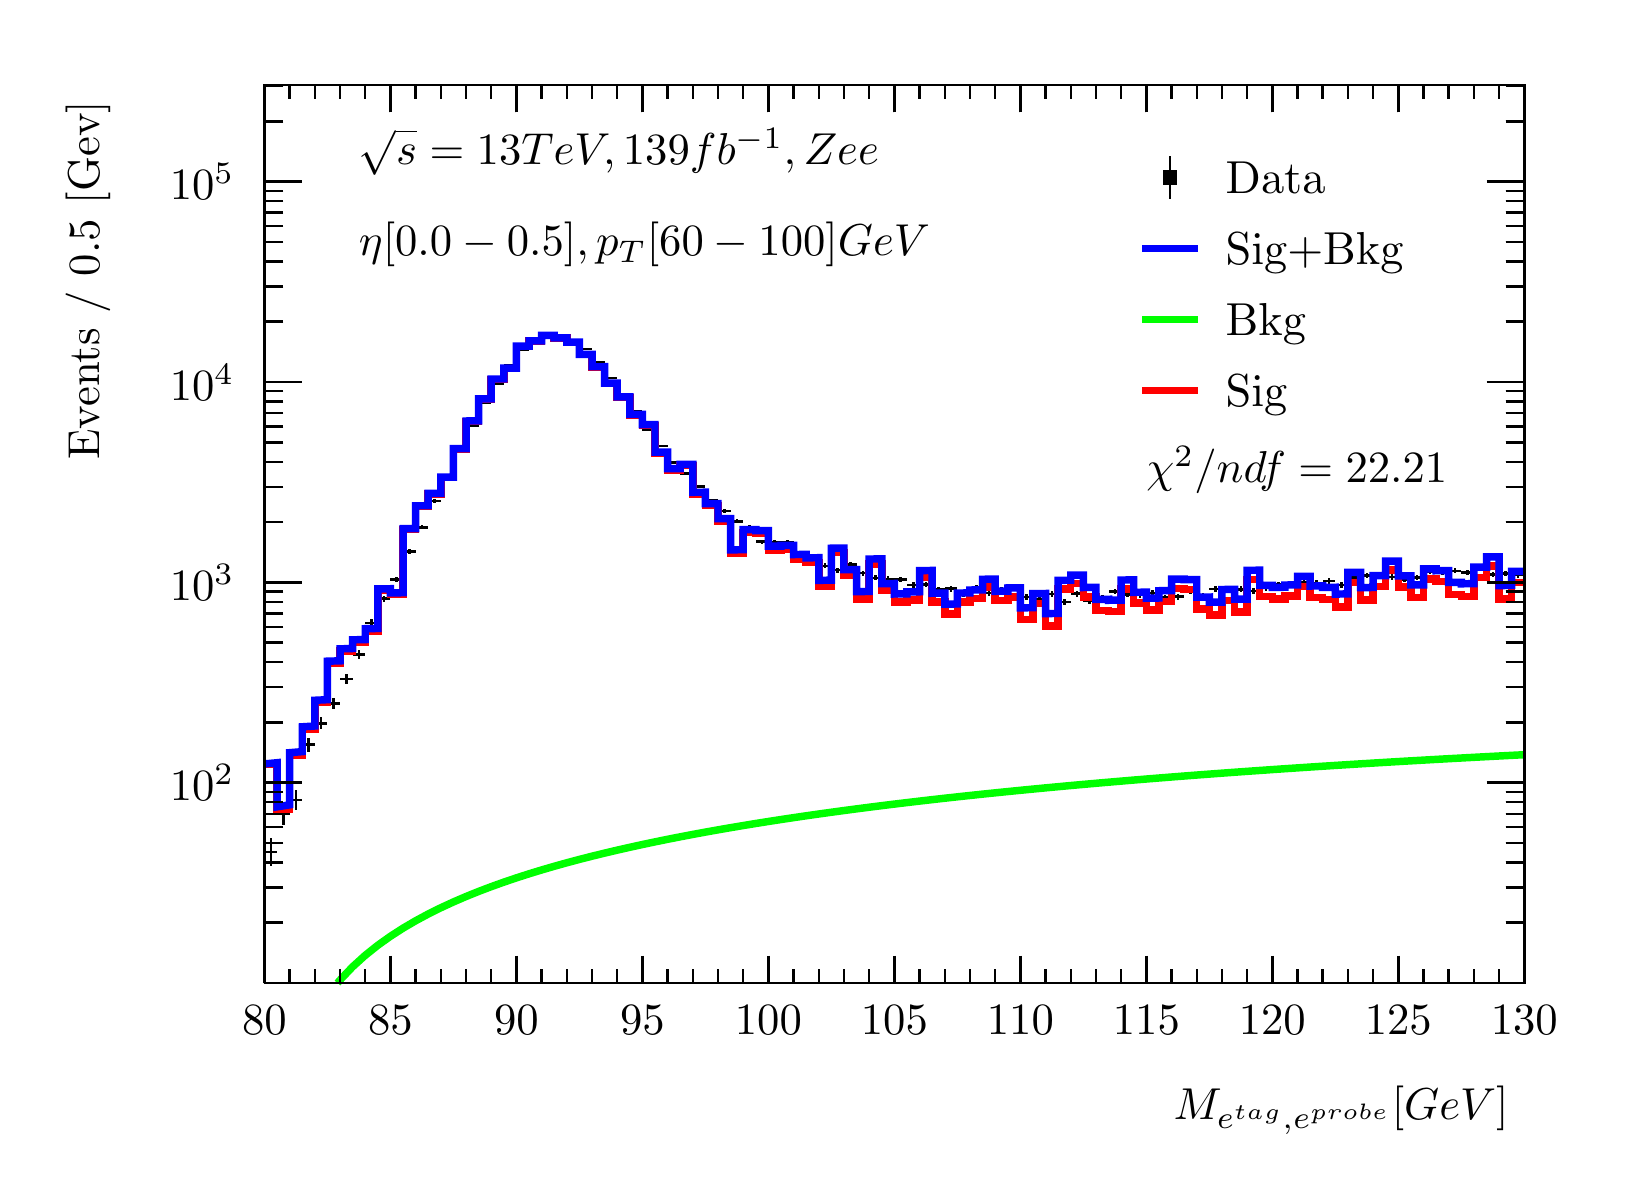
\begin{tikzpicture}
\pgfdeclareplotmark{cross} {
\pgfpathmoveto{\pgfpoint{-0.3\pgfplotmarksize}{\pgfplotmarksize}}
\pgfpathlineto{\pgfpoint{+0.3\pgfplotmarksize}{\pgfplotmarksize}}
\pgfpathlineto{\pgfpoint{+0.3\pgfplotmarksize}{0.3\pgfplotmarksize}}
\pgfpathlineto{\pgfpoint{+1\pgfplotmarksize}{0.3\pgfplotmarksize}}
\pgfpathlineto{\pgfpoint{+1\pgfplotmarksize}{-0.3\pgfplotmarksize}}
\pgfpathlineto{\pgfpoint{+0.3\pgfplotmarksize}{-0.3\pgfplotmarksize}}
\pgfpathlineto{\pgfpoint{+0.3\pgfplotmarksize}{-1.\pgfplotmarksize}}
\pgfpathlineto{\pgfpoint{-0.3\pgfplotmarksize}{-1.\pgfplotmarksize}}
\pgfpathlineto{\pgfpoint{-0.3\pgfplotmarksize}{-0.3\pgfplotmarksize}}
\pgfpathlineto{\pgfpoint{-1.\pgfplotmarksize}{-0.3\pgfplotmarksize}}
\pgfpathlineto{\pgfpoint{-1.\pgfplotmarksize}{0.3\pgfplotmarksize}}
\pgfpathlineto{\pgfpoint{-0.3\pgfplotmarksize}{0.3\pgfplotmarksize}}
\pgfpathclose
\pgfusepathqstroke
}
\pgfdeclareplotmark{cross*} {
\pgfpathmoveto{\pgfpoint{-0.3\pgfplotmarksize}{\pgfplotmarksize}}
\pgfpathlineto{\pgfpoint{+0.3\pgfplotmarksize}{\pgfplotmarksize}}
\pgfpathlineto{\pgfpoint{+0.3\pgfplotmarksize}{0.3\pgfplotmarksize}}
\pgfpathlineto{\pgfpoint{+1\pgfplotmarksize}{0.3\pgfplotmarksize}}
\pgfpathlineto{\pgfpoint{+1\pgfplotmarksize}{-0.3\pgfplotmarksize}}
\pgfpathlineto{\pgfpoint{+0.3\pgfplotmarksize}{-0.3\pgfplotmarksize}}
\pgfpathlineto{\pgfpoint{+0.3\pgfplotmarksize}{-1.\pgfplotmarksize}}
\pgfpathlineto{\pgfpoint{-0.3\pgfplotmarksize}{-1.\pgfplotmarksize}}
\pgfpathlineto{\pgfpoint{-0.3\pgfplotmarksize}{-0.3\pgfplotmarksize}}
\pgfpathlineto{\pgfpoint{-1.\pgfplotmarksize}{-0.3\pgfplotmarksize}}
\pgfpathlineto{\pgfpoint{-1.\pgfplotmarksize}{0.3\pgfplotmarksize}}
\pgfpathlineto{\pgfpoint{-0.3\pgfplotmarksize}{0.3\pgfplotmarksize}}
\pgfpathclose
\pgfusepathqfillstroke
}
\pgfdeclareplotmark{newstar} {
\pgfpathmoveto{\pgfqpoint{0pt}{\pgfplotmarksize}}
\pgfpathlineto{\pgfqpointpolar{44}{0.5\pgfplotmarksize}}
\pgfpathlineto{\pgfqpointpolar{18}{\pgfplotmarksize}}
\pgfpathlineto{\pgfqpointpolar{-20}{0.5\pgfplotmarksize}}
\pgfpathlineto{\pgfqpointpolar{-54}{\pgfplotmarksize}}
\pgfpathlineto{\pgfqpointpolar{-90}{0.5\pgfplotmarksize}}
\pgfpathlineto{\pgfqpointpolar{234}{\pgfplotmarksize}}
\pgfpathlineto{\pgfqpointpolar{198}{0.5\pgfplotmarksize}}
\pgfpathlineto{\pgfqpointpolar{162}{\pgfplotmarksize}}
\pgfpathlineto{\pgfqpointpolar{134}{0.5\pgfplotmarksize}}
\pgfpathclose
\pgfusepathqstroke
}
\pgfdeclareplotmark{newstar*} {
\pgfpathmoveto{\pgfqpoint{0pt}{\pgfplotmarksize}}
\pgfpathlineto{\pgfqpointpolar{44}{0.5\pgfplotmarksize}}
\pgfpathlineto{\pgfqpointpolar{18}{\pgfplotmarksize}}
\pgfpathlineto{\pgfqpointpolar{-20}{0.5\pgfplotmarksize}}
\pgfpathlineto{\pgfqpointpolar{-54}{\pgfplotmarksize}}
\pgfpathlineto{\pgfqpointpolar{-90}{0.5\pgfplotmarksize}}
\pgfpathlineto{\pgfqpointpolar{234}{\pgfplotmarksize}}
\pgfpathlineto{\pgfqpointpolar{198}{0.5\pgfplotmarksize}}
\pgfpathlineto{\pgfqpointpolar{162}{\pgfplotmarksize}}
\pgfpathlineto{\pgfqpointpolar{134}{0.5\pgfplotmarksize}}
\pgfpathclose
\pgfusepathqfillstroke
}
\definecolor{c}{rgb}{1,1,1};
\draw [color=c, fill=c] (0,0) rectangle (20,14.4361);
\draw [color=c, fill=c] (3,2.30977) rectangle (19,13.7143);
\definecolor{c}{rgb}{0,0,0};
\draw [c,line width=0.9] (3,2.30977) -- (3,13.7143) -- (19,13.7143) -- (19,2.30977) -- (3,2.30977);
\definecolor{c}{rgb}{1,1,1};
\draw [color=c, fill=c] (3,2.30977) rectangle (19,13.7143);
\definecolor{c}{rgb}{0,0,0};
\draw [c,line width=0.9] (3,2.30977) -- (3,13.7143) -- (19,13.7143) -- (19,2.30977) -- (3,2.30977);
\draw [c,line width=0.9] (3,2.30977) -- (19,2.30977);
\draw [c,line width=0.9] (3,2.65624) -- (3,2.30977);
\draw [c,line width=0.9] (3.32,2.48301) -- (3.32,2.30977);
\draw [c,line width=0.9] (3.64,2.48301) -- (3.64,2.30977);
\draw [c,line width=0.9] (3.96,2.48301) -- (3.96,2.30977);
\draw [c,line width=0.9] (4.28,2.48301) -- (4.28,2.30977);
\draw [c,line width=0.9] (4.6,2.65624) -- (4.6,2.30977);
\draw [c,line width=0.9] (4.92,2.48301) -- (4.92,2.30977);
\draw [c,line width=0.9] (5.24,2.48301) -- (5.24,2.30977);
\draw [c,line width=0.9] (5.56,2.48301) -- (5.56,2.30977);
\draw [c,line width=0.9] (5.88,2.48301) -- (5.88,2.30977);
\draw [c,line width=0.9] (6.2,2.65624) -- (6.2,2.30977);
\draw [c,line width=0.9] (6.52,2.48301) -- (6.52,2.30977);
\draw [c,line width=0.9] (6.84,2.48301) -- (6.84,2.30977);
\draw [c,line width=0.9] (7.16,2.48301) -- (7.16,2.30977);
\draw [c,line width=0.9] (7.48,2.48301) -- (7.48,2.30977);
\draw [c,line width=0.9] (7.8,2.65624) -- (7.8,2.30977);
\draw [c,line width=0.9] (8.12,2.48301) -- (8.12,2.30977);
\draw [c,line width=0.9] (8.44,2.48301) -- (8.44,2.30977);
\draw [c,line width=0.9] (8.76,2.48301) -- (8.76,2.30977);
\draw [c,line width=0.9] (9.08,2.48301) -- (9.08,2.30977);
\draw [c,line width=0.9] (9.4,2.65624) -- (9.4,2.30977);
\draw [c,line width=0.9] (9.72,2.48301) -- (9.72,2.30977);
\draw [c,line width=0.9] (10.04,2.48301) -- (10.04,2.30977);
\draw [c,line width=0.9] (10.36,2.48301) -- (10.36,2.30977);
\draw [c,line width=0.9] (10.68,2.48301) -- (10.68,2.30977);
\draw [c,line width=0.9] (11,2.65624) -- (11,2.30977);
\draw [c,line width=0.9] (11.32,2.48301) -- (11.32,2.30977);
\draw [c,line width=0.9] (11.64,2.48301) -- (11.64,2.30977);
\draw [c,line width=0.9] (11.96,2.48301) -- (11.96,2.30977);
\draw [c,line width=0.9] (12.28,2.48301) -- (12.28,2.30977);
\draw [c,line width=0.9] (12.6,2.65624) -- (12.6,2.30977);
\draw [c,line width=0.9] (12.92,2.48301) -- (12.92,2.30977);
\draw [c,line width=0.9] (13.24,2.48301) -- (13.24,2.30977);
\draw [c,line width=0.9] (13.56,2.48301) -- (13.56,2.30977);
\draw [c,line width=0.9] (13.88,2.48301) -- (13.88,2.30977);
\draw [c,line width=0.9] (14.2,2.65624) -- (14.2,2.30977);
\draw [c,line width=0.9] (14.52,2.48301) -- (14.52,2.30977);
\draw [c,line width=0.9] (14.84,2.48301) -- (14.84,2.30977);
\draw [c,line width=0.9] (15.16,2.48301) -- (15.16,2.30977);
\draw [c,line width=0.9] (15.48,2.48301) -- (15.48,2.30977);
\draw [c,line width=0.9] (15.8,2.65624) -- (15.8,2.30977);
\draw [c,line width=0.9] (16.12,2.48301) -- (16.12,2.30977);
\draw [c,line width=0.9] (16.44,2.48301) -- (16.44,2.30977);
\draw [c,line width=0.9] (16.76,2.48301) -- (16.76,2.30977);
\draw [c,line width=0.9] (17.08,2.48301) -- (17.08,2.30977);
\draw [c,line width=0.9] (17.4,2.65624) -- (17.4,2.30977);
\draw [c,line width=0.9] (17.72,2.48301) -- (17.72,2.30977);
\draw [c,line width=0.9] (18.04,2.48301) -- (18.04,2.30977);
\draw [c,line width=0.9] (18.36,2.48301) -- (18.36,2.30977);
\draw [c,line width=0.9] (18.68,2.48301) -- (18.68,2.30977);
\draw [c,line width=0.9] (19,2.65624) -- (19,2.30977);
\draw [anchor=base] (3,1.66015) node[scale=1.61424, color=c, rotate=0]{80};
\draw [anchor=base] (4.6,1.66015) node[scale=1.61424, color=c, rotate=0]{85};
\draw [anchor=base] (6.2,1.66015) node[scale=1.61424, color=c, rotate=0]{90};
\draw [anchor=base] (7.8,1.66015) node[scale=1.61424, color=c, rotate=0]{95};
\draw [anchor=base] (9.4,1.66015) node[scale=1.61424, color=c, rotate=0]{100};
\draw [anchor=base] (11,1.66015) node[scale=1.61424, color=c, rotate=0]{105};
\draw [anchor=base] (12.6,1.66015) node[scale=1.61424, color=c, rotate=0]{110};
\draw [anchor=base] (14.2,1.66015) node[scale=1.61424, color=c, rotate=0]{115};
\draw [anchor=base] (15.8,1.66015) node[scale=1.61424, color=c, rotate=0]{120};
\draw [anchor=base] (17.4,1.66015) node[scale=1.61424, color=c, rotate=0]{125};
\draw [anchor=base] (19,1.66015) node[scale=1.61424, color=c, rotate=0]{130};
\draw [anchor= east] (19,0.692932) node[scale=1.61424, color=c, rotate=0]{$M_{e^{tag}, e^{probe}}  [GeV]$};
\draw [c,line width=0.9] (3,13.7143) -- (19,13.7143);
\draw [c,line width=0.9] (3,13.3678) -- (3,13.7143);
\draw [c,line width=0.9] (3.32,13.5411) -- (3.32,13.7143);
\draw [c,line width=0.9] (3.64,13.5411) -- (3.64,13.7143);
\draw [c,line width=0.9] (3.96,13.5411) -- (3.96,13.7143);
\draw [c,line width=0.9] (4.28,13.5411) -- (4.28,13.7143);
\draw [c,line width=0.9] (4.6,13.3678) -- (4.6,13.7143);
\draw [c,line width=0.9] (4.92,13.5411) -- (4.92,13.7143);
\draw [c,line width=0.9] (5.24,13.5411) -- (5.24,13.7143);
\draw [c,line width=0.9] (5.56,13.5411) -- (5.56,13.7143);
\draw [c,line width=0.9] (5.88,13.5411) -- (5.88,13.7143);
\draw [c,line width=0.9] (6.2,13.3678) -- (6.2,13.7143);
\draw [c,line width=0.9] (6.52,13.5411) -- (6.52,13.7143);
\draw [c,line width=0.9] (6.84,13.5411) -- (6.84,13.7143);
\draw [c,line width=0.9] (7.16,13.5411) -- (7.16,13.7143);
\draw [c,line width=0.9] (7.48,13.5411) -- (7.48,13.7143);
\draw [c,line width=0.9] (7.8,13.3678) -- (7.8,13.7143);
\draw [c,line width=0.9] (8.12,13.5411) -- (8.12,13.7143);
\draw [c,line width=0.9] (8.44,13.5411) -- (8.44,13.7143);
\draw [c,line width=0.9] (8.76,13.5411) -- (8.76,13.7143);
\draw [c,line width=0.9] (9.08,13.5411) -- (9.08,13.7143);
\draw [c,line width=0.9] (9.4,13.3678) -- (9.4,13.7143);
\draw [c,line width=0.9] (9.72,13.5411) -- (9.72,13.7143);
\draw [c,line width=0.9] (10.04,13.5411) -- (10.04,13.7143);
\draw [c,line width=0.9] (10.36,13.5411) -- (10.36,13.7143);
\draw [c,line width=0.9] (10.68,13.5411) -- (10.68,13.7143);
\draw [c,line width=0.9] (11,13.3678) -- (11,13.7143);
\draw [c,line width=0.9] (11.32,13.5411) -- (11.32,13.7143);
\draw [c,line width=0.9] (11.64,13.5411) -- (11.64,13.7143);
\draw [c,line width=0.9] (11.96,13.5411) -- (11.96,13.7143);
\draw [c,line width=0.9] (12.28,13.5411) -- (12.28,13.7143);
\draw [c,line width=0.9] (12.6,13.3678) -- (12.6,13.7143);
\draw [c,line width=0.9] (12.92,13.5411) -- (12.92,13.7143);
\draw [c,line width=0.9] (13.24,13.5411) -- (13.24,13.7143);
\draw [c,line width=0.9] (13.56,13.5411) -- (13.56,13.7143);
\draw [c,line width=0.9] (13.88,13.5411) -- (13.88,13.7143);
\draw [c,line width=0.9] (14.2,13.3678) -- (14.2,13.7143);
\draw [c,line width=0.9] (14.52,13.5411) -- (14.52,13.7143);
\draw [c,line width=0.9] (14.84,13.5411) -- (14.84,13.7143);
\draw [c,line width=0.9] (15.16,13.5411) -- (15.16,13.7143);
\draw [c,line width=0.9] (15.48,13.5411) -- (15.48,13.7143);
\draw [c,line width=0.9] (15.8,13.3678) -- (15.8,13.7143);
\draw [c,line width=0.9] (16.12,13.5411) -- (16.12,13.7143);
\draw [c,line width=0.9] (16.44,13.5411) -- (16.44,13.7143);
\draw [c,line width=0.9] (16.76,13.5411) -- (16.76,13.7143);
\draw [c,line width=0.9] (17.08,13.5411) -- (17.08,13.7143);
\draw [c,line width=0.9] (17.4,13.3678) -- (17.4,13.7143);
\draw [c,line width=0.9] (17.72,13.5411) -- (17.72,13.7143);
\draw [c,line width=0.9] (18.04,13.5411) -- (18.04,13.7143);
\draw [c,line width=0.9] (18.36,13.5411) -- (18.36,13.7143);
\draw [c,line width=0.9] (18.68,13.5411) -- (18.68,13.7143);
\draw [c,line width=0.9] (19,13.3678) -- (19,13.7143);
\draw [c,line width=0.9] (3,2.30977) -- (3,13.7143);
\draw [c,line width=0.9] (3.237,3.07568) -- (3,3.07568);
\draw [c,line width=0.9] (3.237,3.5237) -- (3,3.5237);
\draw [c,line width=0.9] (3.237,3.84158) -- (3,3.84158);
\draw [c,line width=0.9] (3.237,4.08815) -- (3,4.08815);
\draw [c,line width=0.9] (3.237,4.2896) -- (3,4.2896);
\draw [c,line width=0.9] (3.237,4.45994) -- (3,4.45994);
\draw [c,line width=0.9] (3.237,4.60748) -- (3,4.60748);
\draw [c,line width=0.9] (3.237,4.73763) -- (3,4.73763);
\draw [c,line width=0.9] (3.474,4.85405) -- (3,4.85405);
\draw [anchor= east] (2.82,4.85405) node[scale=1.61424, color=c, rotate=0]{$10^{2}$};
\draw [c,line width=0.9] (3.237,5.61995) -- (3,5.61995);
\draw [c,line width=0.9] (3.237,6.06798) -- (3,6.06798);
\draw [c,line width=0.9] (3.237,6.38586) -- (3,6.38586);
\draw [c,line width=0.9] (3.237,6.63242) -- (3,6.63242);
\draw [c,line width=0.9] (3.237,6.83388) -- (3,6.83388);
\draw [c,line width=0.9] (3.237,7.00421) -- (3,7.00421);
\draw [c,line width=0.9] (3.237,7.15176) -- (3,7.15176);
\draw [c,line width=0.9] (3.237,7.28191) -- (3,7.28191);
\draw [c,line width=0.9] (3.474,7.39833) -- (3,7.39833);
\draw [anchor= east] (2.82,7.39833) node[scale=1.61424, color=c, rotate=0]{$10^{3}$};
\draw [c,line width=0.9] (3.237,8.16423) -- (3,8.16423);
\draw [c,line width=0.9] (3.237,8.61226) -- (3,8.61226);
\draw [c,line width=0.9] (3.237,8.93013) -- (3,8.93013);
\draw [c,line width=0.9] (3.237,9.1767) -- (3,9.1767);
\draw [c,line width=0.9] (3.237,9.37816) -- (3,9.37816);
\draw [c,line width=0.9] (3.237,9.54849) -- (3,9.54849);
\draw [c,line width=0.9] (3.237,9.69604) -- (3,9.69604);
\draw [c,line width=0.9] (3.237,9.82618) -- (3,9.82618);
\draw [c,line width=0.9] (3.474,9.9426) -- (3,9.9426);
\draw [anchor= east] (2.82,9.9426) node[scale=1.61424, color=c, rotate=0]{$10^{4}$};
\draw [c,line width=0.9] (3.237,10.7085) -- (3,10.7085);
\draw [c,line width=0.9] (3.237,11.1565) -- (3,11.1565);
\draw [c,line width=0.9] (3.237,11.4744) -- (3,11.4744);
\draw [c,line width=0.9] (3.237,11.721) -- (3,11.721);
\draw [c,line width=0.9] (3.237,11.9224) -- (3,11.9224);
\draw [c,line width=0.9] (3.237,12.0928) -- (3,12.0928);
\draw [c,line width=0.9] (3.237,12.2403) -- (3,12.2403);
\draw [c,line width=0.9] (3.237,12.3705) -- (3,12.3705);
\draw [c,line width=0.9] (3.474,12.4869) -- (3,12.4869);
\draw [anchor= east] (2.82,12.4869) node[scale=1.61424, color=c, rotate=0]{$10^{5}$};
\draw [c,line width=0.9] (3.237,13.2528) -- (3,13.2528);
\draw [c,line width=0.9] (3.237,13.7008) -- (3,13.7008);
\draw [anchor= east] (0.76,13.7143) node[scale=1.61424, color=c, rotate=90]{Events / 0.5 [Gev]};
\draw [c,line width=0.9] (19,2.30977) -- (19,13.7143);
\draw [c,line width=0.9] (18.763,3.07568) -- (19,3.07568);
\draw [c,line width=0.9] (18.763,3.5237) -- (19,3.5237);
\draw [c,line width=0.9] (18.763,3.84158) -- (19,3.84158);
\draw [c,line width=0.9] (18.763,4.08815) -- (19,4.08815);
\draw [c,line width=0.9] (18.763,4.2896) -- (19,4.2896);
\draw [c,line width=0.9] (18.763,4.45994) -- (19,4.45994);
\draw [c,line width=0.9] (18.763,4.60748) -- (19,4.60748);
\draw [c,line width=0.9] (18.763,4.73763) -- (19,4.73763);
\draw [c,line width=0.9] (18.526,4.85405) -- (19,4.85405);
\draw [c,line width=0.9] (18.763,5.61995) -- (19,5.61995);
\draw [c,line width=0.9] (18.763,6.06798) -- (19,6.06798);
\draw [c,line width=0.9] (18.763,6.38586) -- (19,6.38586);
\draw [c,line width=0.9] (18.763,6.63242) -- (19,6.63242);
\draw [c,line width=0.9] (18.763,6.83388) -- (19,6.83388);
\draw [c,line width=0.9] (18.763,7.00421) -- (19,7.00421);
\draw [c,line width=0.9] (18.763,7.15176) -- (19,7.15176);
\draw [c,line width=0.9] (18.763,7.28191) -- (19,7.28191);
\draw [c,line width=0.9] (18.526,7.39833) -- (19,7.39833);
\draw [c,line width=0.9] (18.763,8.16423) -- (19,8.16423);
\draw [c,line width=0.9] (18.763,8.61226) -- (19,8.61226);
\draw [c,line width=0.9] (18.763,8.93013) -- (19,8.93013);
\draw [c,line width=0.9] (18.763,9.1767) -- (19,9.1767);
\draw [c,line width=0.9] (18.763,9.37816) -- (19,9.37816);
\draw [c,line width=0.9] (18.763,9.54849) -- (19,9.54849);
\draw [c,line width=0.9] (18.763,9.69604) -- (19,9.69604);
\draw [c,line width=0.9] (18.763,9.82618) -- (19,9.82618);
\draw [c,line width=0.9] (18.526,9.9426) -- (19,9.9426);
\draw [c,line width=0.9] (18.763,10.7085) -- (19,10.7085);
\draw [c,line width=0.9] (18.763,11.1565) -- (19,11.1565);
\draw [c,line width=0.9] (18.763,11.4744) -- (19,11.4744);
\draw [c,line width=0.9] (18.763,11.721) -- (19,11.721);
\draw [c,line width=0.9] (18.763,11.9224) -- (19,11.9224);
\draw [c,line width=0.9] (18.763,12.0928) -- (19,12.0928);
\draw [c,line width=0.9] (18.763,12.2403) -- (19,12.2403);
\draw [c,line width=0.9] (18.763,12.3705) -- (19,12.3705);
\draw [c,line width=0.9] (18.526,12.4869) -- (19,12.4869);
\draw [c,line width=0.9] (18.763,13.2528) -- (19,13.2528);
\draw [c,line width=0.9] (18.763,13.7008) -- (19,13.7008);
\draw [c,line width=0.9] (3.08,3.97173) -- (3,3.97173);
\draw [c,line width=0.9] (3,3.97173) -- (3,3.97173);
\draw [c,line width=0.9] (3.08,3.97173) -- (3.16,3.97173);
\draw [c,line width=0.9] (3.16,3.97173) -- (3.16,3.97173);
\draw [c,line width=0.9] (3.08,3.97173) -- (3.08,4.14747);
\draw [c,line width=0.9] (3.08,4.14747) -- (3.08,4.14747);
\draw [c,line width=0.9] (3.08,3.97173) -- (3.08,3.79408);
\draw [c,line width=0.9] (3.08,3.79408) -- (3.08,3.79408);
\draw [c,line width=0.9] (3.24,4.45994) -- (3.16,4.45994);
\draw [c,line width=0.9] (3.16,4.45994) -- (3.16,4.45994);
\draw [c,line width=0.9] (3.24,4.45994) -- (3.32,4.45994);
\draw [c,line width=0.9] (3.32,4.45994) -- (3.32,4.45994);
\draw [c,line width=0.9] (3.24,4.45994) -- (3.24,4.59926);
\draw [c,line width=0.9] (3.24,4.59926) -- (3.24,4.59926);
\draw [c,line width=0.9] (3.24,4.45994) -- (3.24,4.31964);
\draw [c,line width=0.9] (3.24,4.31964) -- (3.24,4.31964);
\draw [c,line width=0.9] (3.4,4.63477) -- (3.32,4.63477);
\draw [c,line width=0.9] (3.32,4.63477) -- (3.32,4.63477);
\draw [c,line width=0.9] (3.4,4.63477) -- (3.48,4.63477);
\draw [c,line width=0.9] (3.48,4.63477) -- (3.48,4.63477);
\draw [c,line width=0.9] (3.4,4.63477) -- (3.4,4.76302);
\draw [c,line width=0.9] (3.4,4.76302) -- (3.4,4.76302);
\draw [c,line width=0.9] (3.4,4.63477) -- (3.4,4.50575);
\draw [c,line width=0.9] (3.4,4.50575) -- (3.4,4.50575);
\draw [c,line width=0.9] (3.56,5.33831) -- (3.48,5.33831);
\draw [c,line width=0.9] (3.48,5.33831) -- (3.48,5.33831);
\draw [c,line width=0.9] (3.56,5.33831) -- (3.64,5.33831);
\draw [c,line width=0.9] (3.64,5.33831) -- (3.64,5.33831);
\draw [c,line width=0.9] (3.56,5.33831) -- (3.56,5.42704);
\draw [c,line width=0.9] (3.56,5.42704) -- (3.56,5.42704);
\draw [c,line width=0.9] (3.56,5.33831) -- (3.56,5.24958);
\draw [c,line width=0.9] (3.56,5.24958) -- (3.56,5.24958);
\draw [c,line width=0.9] (3.72,5.60885) -- (3.64,5.60885);
\draw [c,line width=0.9] (3.64,5.60885) -- (3.64,5.60885);
\draw [c,line width=0.9] (3.72,5.60885) -- (3.8,5.60885);
\draw [c,line width=0.9] (3.8,5.60885) -- (3.8,5.60885);
\draw [c,line width=0.9] (3.72,5.60885) -- (3.72,5.68736);
\draw [c,line width=0.9] (3.72,5.68736) -- (3.72,5.68736);
\draw [c,line width=0.9] (3.72,5.60885) -- (3.72,5.53034);
\draw [c,line width=0.9] (3.72,5.53034) -- (3.72,5.53034);
\draw [c,line width=0.9] (3.88,5.85765) -- (3.8,5.85765);
\draw [c,line width=0.9] (3.8,5.85765) -- (3.8,5.85765);
\draw [c,line width=0.9] (3.88,5.85765) -- (3.96,5.85765);
\draw [c,line width=0.9] (3.96,5.85765) -- (3.96,5.85765);
\draw [c,line width=0.9] (3.88,5.85765) -- (3.88,5.9278);
\draw [c,line width=0.9] (3.88,5.9278) -- (3.88,5.9278);
\draw [c,line width=0.9] (3.88,5.85765) -- (3.88,5.78749);
\draw [c,line width=0.9] (3.88,5.78749) -- (3.88,5.78749);
\draw [c,line width=0.9] (4.04,6.16994) -- (3.96,6.16994);
\draw [c,line width=0.9] (3.96,6.16994) -- (3.96,6.16994);
\draw [c,line width=0.9] (4.04,6.16994) -- (4.12,6.16994);
\draw [c,line width=0.9] (4.12,6.16994) -- (4.12,6.16994);
\draw [c,line width=0.9] (4.04,6.16994) -- (4.04,6.23085);
\draw [c,line width=0.9] (4.04,6.23085) -- (4.04,6.23085);
\draw [c,line width=0.9] (4.04,6.16994) -- (4.04,6.10903);
\draw [c,line width=0.9] (4.04,6.10903) -- (4.04,6.10903);
\draw [c,line width=0.9] (4.2,6.48361) -- (4.12,6.48361);
\draw [c,line width=0.9] (4.12,6.48361) -- (4.12,6.48361);
\draw [c,line width=0.9] (4.2,6.48361) -- (4.28,6.48361);
\draw [c,line width=0.9] (4.28,6.48361) -- (4.28,6.48361);
\draw [c,line width=0.9] (4.2,6.48361) -- (4.2,6.53647);
\draw [c,line width=0.9] (4.2,6.53647) -- (4.2,6.53647);
\draw [c,line width=0.9] (4.2,6.48361) -- (4.2,6.43076);
\draw [c,line width=0.9] (4.2,6.43076) -- (4.2,6.43076);
\draw [c,line width=0.9] (4.36,6.88428) -- (4.28,6.88428);
\draw [c,line width=0.9] (4.28,6.88428) -- (4.28,6.88428);
\draw [c,line width=0.9] (4.36,6.88428) -- (4.44,6.88428);
\draw [c,line width=0.9] (4.44,6.88428) -- (4.44,6.88428);
\draw [c,line width=0.9] (4.36,6.88428) -- (4.36,6.92837);
\draw [c,line width=0.9] (4.36,6.92837) -- (4.36,6.92837);
\draw [c,line width=0.9] (4.36,6.88428) -- (4.36,6.84019);
\draw [c,line width=0.9] (4.36,6.84019) -- (4.36,6.84019);
\draw [c,line width=0.9] (4.52,7.19244) -- (4.44,7.19244);
\draw [c,line width=0.9] (4.44,7.19244) -- (4.44,7.19244);
\draw [c,line width=0.9] (4.52,7.19244) -- (4.6,7.19244);
\draw [c,line width=0.9] (4.6,7.19244) -- (4.6,7.19244);
\draw [c,line width=0.9] (4.52,7.19244) -- (4.52,7.23079);
\draw [c,line width=0.9] (4.52,7.23079) -- (4.52,7.23079);
\draw [c,line width=0.9] (4.52,7.19244) -- (4.52,7.15409);
\draw [c,line width=0.9] (4.52,7.15409) -- (4.52,7.15409);
\draw [c,line width=0.9] (4.68,7.4342) -- (4.6,7.4342);
\draw [c,line width=0.9] (4.6,7.4342) -- (4.6,7.4342);
\draw [c,line width=0.9] (4.68,7.4342) -- (4.76,7.4342);
\draw [c,line width=0.9] (4.76,7.4342) -- (4.76,7.4342);
\draw [c,line width=0.9] (4.68,7.4342) -- (4.68,7.46858);
\draw [c,line width=0.9] (4.68,7.46858) -- (4.68,7.46858);
\draw [c,line width=0.9] (4.68,7.4342) -- (4.68,7.39983);
\draw [c,line width=0.9] (4.68,7.39983) -- (4.68,7.39983);
\draw [c,line width=0.9] (4.84,7.7889) -- (4.76,7.7889);
\draw [c,line width=0.9] (4.76,7.7889) -- (4.76,7.7889);
\draw [c,line width=0.9] (4.84,7.7889) -- (4.92,7.7889);
\draw [c,line width=0.9] (4.92,7.7889) -- (4.92,7.7889);
\draw [c,line width=0.9] (4.84,7.7889) -- (4.84,7.81818);
\draw [c,line width=0.9] (4.84,7.81818) -- (4.84,7.81818);
\draw [c,line width=0.9] (4.84,7.7889) -- (4.84,7.75962);
\draw [c,line width=0.9] (4.84,7.75962) -- (4.84,7.75962);
\draw [c,line width=0.9] (5,8.09645) -- (4.92,8.09645);
\draw [c,line width=0.9] (4.92,8.09645) -- (4.92,8.09645);
\draw [c,line width=0.9] (5,8.09645) -- (5.08,8.09645);
\draw [c,line width=0.9] (5.08,8.09645) -- (5.08,8.09645);
\draw [c,line width=0.9] (5,8.09645) -- (5,8.12193);
\draw [c,line width=0.9] (5,8.12193) -- (5,8.12193);
\draw [c,line width=0.9] (5,8.09645) -- (5,8.07097);
\draw [c,line width=0.9] (5,8.07097) -- (5,8.07097);
\draw [c,line width=0.9] (5.16,8.43008) -- (5.08,8.43008);
\draw [c,line width=0.9] (5.08,8.43008) -- (5.08,8.43008);
\draw [c,line width=0.9] (5.16,8.43008) -- (5.24,8.43008);
\draw [c,line width=0.9] (5.24,8.43008) -- (5.24,8.43008);
\draw [c,line width=0.9] (5.16,8.43008) -- (5.16,8.45198);
\draw [c,line width=0.9] (5.16,8.45198) -- (5.16,8.45198);
\draw [c,line width=0.9] (5.16,8.43008) -- (5.16,8.40817);
\draw [c,line width=0.9] (5.16,8.40817) -- (5.16,8.40817);
\draw [c,line width=0.9] (5.32,8.73386) -- (5.24,8.73386);
\draw [c,line width=0.9] (5.24,8.73386) -- (5.24,8.73386);
\draw [c,line width=0.9] (5.32,8.73386) -- (5.4,8.73386);
\draw [c,line width=0.9] (5.4,8.73386) -- (5.4,8.73386);
\draw [c,line width=0.9] (5.32,8.73386) -- (5.32,8.75295);
\draw [c,line width=0.9] (5.32,8.75295) -- (5.32,8.75295);
\draw [c,line width=0.9] (5.32,8.73386) -- (5.32,8.71476);
\draw [c,line width=0.9] (5.32,8.71476) -- (5.32,8.71476);
\draw [c,line width=0.9] (5.48,9.07903) -- (5.4,9.07903);
\draw [c,line width=0.9] (5.4,9.07903) -- (5.4,9.07903);
\draw [c,line width=0.9] (5.48,9.07903) -- (5.56,9.07903);
\draw [c,line width=0.9] (5.56,9.07903) -- (5.56,9.07903);
\draw [c,line width=0.9] (5.48,9.07903) -- (5.48,9.09536);
\draw [c,line width=0.9] (5.48,9.09536) -- (5.48,9.09536);
\draw [c,line width=0.9] (5.48,9.07903) -- (5.48,9.0627);
\draw [c,line width=0.9] (5.48,9.0627) -- (5.48,9.0627);
\draw [c,line width=0.9] (5.64,9.39261) -- (5.56,9.39261);
\draw [c,line width=0.9] (5.56,9.39261) -- (5.56,9.39261);
\draw [c,line width=0.9] (5.64,9.39261) -- (5.72,9.39261);
\draw [c,line width=0.9] (5.72,9.39261) -- (5.72,9.39261);
\draw [c,line width=0.9] (5.64,9.39261) -- (5.64,9.40679);
\draw [c,line width=0.9] (5.64,9.40679) -- (5.64,9.40679);
\draw [c,line width=0.9] (5.64,9.39261) -- (5.64,9.37844);
\draw [c,line width=0.9] (5.64,9.37844) -- (5.64,9.37844);
\draw [c,line width=0.9] (5.8,9.67681) -- (5.72,9.67681);
\draw [c,line width=0.9] (5.72,9.67681) -- (5.72,9.67681);
\draw [c,line width=0.9] (5.8,9.67681) -- (5.88,9.67681);
\draw [c,line width=0.9] (5.88,9.67681) -- (5.88,9.67681);
\draw [c,line width=0.9] (5.8,9.67681) -- (5.8,9.68927);
\draw [c,line width=0.9] (5.8,9.68927) -- (5.8,9.68927);
\draw [c,line width=0.9] (5.8,9.67681) -- (5.8,9.66435);
\draw [c,line width=0.9] (5.8,9.66435) -- (5.8,9.66435);
\draw [c,line width=0.9] (5.96,9.9213) -- (5.88,9.9213);
\draw [c,line width=0.9] (5.88,9.9213) -- (5.88,9.9213);
\draw [c,line width=0.9] (5.96,9.9213) -- (6.04,9.9213);
\draw [c,line width=0.9] (6.04,9.9213) -- (6.04,9.9213);
\draw [c,line width=0.9] (5.96,9.9213) -- (5.96,9.93245);
\draw [c,line width=0.9] (5.96,9.93245) -- (5.96,9.93245);
\draw [c,line width=0.9] (5.96,9.9213) -- (5.96,9.91014);
\draw [c,line width=0.9] (5.96,9.91014) -- (5.96,9.91014);
\draw [c,line width=0.9] (6.12,10.1618) -- (6.04,10.1618);
\draw [c,line width=0.9] (6.04,10.1618) -- (6.04,10.1618);
\draw [c,line width=0.9] (6.12,10.1618) -- (6.2,10.1618);
\draw [c,line width=0.9] (6.2,10.1618) -- (6.2,10.1618);
\draw [c,line width=0.9] (6.12,10.1618) -- (6.12,10.1718);
\draw [c,line width=0.9] (6.12,10.1718) -- (6.12,10.1718);
\draw [c,line width=0.9] (6.12,10.1618) -- (6.12,10.1518);
\draw [c,line width=0.9] (6.12,10.1518) -- (6.12,10.1518);
\draw [c,line width=0.9] (6.28,10.3471) -- (6.2,10.3471);
\draw [c,line width=0.9] (6.2,10.3471) -- (6.2,10.3471);
\draw [c,line width=0.9] (6.28,10.3471) -- (6.36,10.3471);
\draw [c,line width=0.9] (6.36,10.3471) -- (6.36,10.3471);
\draw [c,line width=0.9] (6.28,10.3471) -- (6.28,10.3563);
\draw [c,line width=0.9] (6.28,10.3563) -- (6.28,10.3563);
\draw [c,line width=0.9] (6.28,10.3471) -- (6.28,10.3379);
\draw [c,line width=0.9] (6.28,10.3379) -- (6.28,10.3379);
\draw [c,line width=0.9] (6.44,10.4746) -- (6.36,10.4746);
\draw [c,line width=0.9] (6.36,10.4746) -- (6.36,10.4746);
\draw [c,line width=0.9] (6.44,10.4746) -- (6.52,10.4746);
\draw [c,line width=0.9] (6.52,10.4746) -- (6.52,10.4746);
\draw [c,line width=0.9] (6.44,10.4746) -- (6.44,10.4833);
\draw [c,line width=0.9] (6.44,10.4833) -- (6.44,10.4833);
\draw [c,line width=0.9] (6.44,10.4746) -- (6.44,10.466);
\draw [c,line width=0.9] (6.44,10.466) -- (6.44,10.466);
\draw [c,line width=0.9] (6.6,10.5373) -- (6.52,10.5373);
\draw [c,line width=0.9] (6.52,10.5373) -- (6.52,10.5373);
\draw [c,line width=0.9] (6.6,10.5373) -- (6.68,10.5373);
\draw [c,line width=0.9] (6.68,10.5373) -- (6.68,10.5373);
\draw [c,line width=0.9] (6.6,10.5373) -- (6.6,10.5457);
\draw [c,line width=0.9] (6.6,10.5457) -- (6.6,10.5457);
\draw [c,line width=0.9] (6.6,10.5373) -- (6.6,10.5288);
\draw [c,line width=0.9] (6.6,10.5288) -- (6.6,10.5288);
\draw [c,line width=0.9] (6.76,10.5319) -- (6.68,10.5319);
\draw [c,line width=0.9] (6.68,10.5319) -- (6.68,10.5319);
\draw [c,line width=0.9] (6.76,10.5319) -- (6.84,10.5319);
\draw [c,line width=0.9] (6.84,10.5319) -- (6.84,10.5319);
\draw [c,line width=0.9] (6.76,10.5319) -- (6.76,10.5403);
\draw [c,line width=0.9] (6.76,10.5403) -- (6.76,10.5403);
\draw [c,line width=0.9] (6.76,10.5319) -- (6.76,10.5234);
\draw [c,line width=0.9] (6.76,10.5234) -- (6.76,10.5234);
\draw [c,line width=0.9] (6.92,10.4613) -- (6.84,10.4613);
\draw [c,line width=0.9] (6.84,10.4613) -- (6.84,10.4613);
\draw [c,line width=0.9] (6.92,10.4613) -- (7,10.4613);
\draw [c,line width=0.9] (7,10.4613) -- (7,10.4613);
\draw [c,line width=0.9] (6.92,10.4613) -- (6.92,10.4701);
\draw [c,line width=0.9] (6.92,10.4701) -- (6.92,10.4701);
\draw [c,line width=0.9] (6.92,10.4613) -- (6.92,10.4526);
\draw [c,line width=0.9] (6.92,10.4526) -- (6.92,10.4526);
\draw [c,line width=0.9] (7.08,10.3639) -- (7,10.3639);
\draw [c,line width=0.9] (7,10.3639) -- (7,10.3639);
\draw [c,line width=0.9] (7.08,10.3639) -- (7.16,10.3639);
\draw [c,line width=0.9] (7.16,10.3639) -- (7.16,10.3639);
\draw [c,line width=0.9] (7.08,10.3639) -- (7.08,10.373);
\draw [c,line width=0.9] (7.08,10.373) -- (7.08,10.373);
\draw [c,line width=0.9] (7.08,10.3639) -- (7.08,10.3547);
\draw [c,line width=0.9] (7.08,10.3547) -- (7.08,10.3547);
\draw [c,line width=0.9] (7.24,10.1946) -- (7.16,10.1946);
\draw [c,line width=0.9] (7.16,10.1946) -- (7.16,10.1946);
\draw [c,line width=0.9] (7.24,10.1946) -- (7.32,10.1946);
\draw [c,line width=0.9] (7.32,10.1946) -- (7.32,10.1946);
\draw [c,line width=0.9] (7.24,10.1946) -- (7.24,10.2044);
\draw [c,line width=0.9] (7.24,10.2044) -- (7.24,10.2044);
\draw [c,line width=0.9] (7.24,10.1946) -- (7.24,10.1847);
\draw [c,line width=0.9] (7.24,10.1847) -- (7.24,10.1847);
\draw [c,line width=0.9] (7.4,9.9942) -- (7.32,9.9942);
\draw [c,line width=0.9] (7.32,9.9942) -- (7.32,9.9942);
\draw [c,line width=0.9] (7.4,9.9942) -- (7.48,9.9942);
\draw [c,line width=0.9] (7.48,9.9942) -- (7.48,9.9942);
\draw [c,line width=0.9] (7.4,9.9942) -- (7.4,10.005);
\draw [c,line width=0.9] (7.4,10.005) -- (7.4,10.005);
\draw [c,line width=0.9] (7.4,9.9942) -- (7.4,9.9834);
\draw [c,line width=0.9] (7.4,9.9834) -- (7.4,9.9834);
\draw [c,line width=0.9] (7.56,9.77273) -- (7.48,9.77273);
\draw [c,line width=0.9] (7.48,9.77273) -- (7.48,9.77273);
\draw [c,line width=0.9] (7.56,9.77273) -- (7.64,9.77273);
\draw [c,line width=0.9] (7.64,9.77273) -- (7.64,9.77273);
\draw [c,line width=0.9] (7.56,9.77273) -- (7.56,9.78467);
\draw [c,line width=0.9] (7.56,9.78467) -- (7.56,9.78467);
\draw [c,line width=0.9] (7.56,9.77273) -- (7.56,9.7608);
\draw [c,line width=0.9] (7.56,9.7608) -- (7.56,9.7608);
\draw [c,line width=0.9] (7.72,9.57099) -- (7.64,9.57099);
\draw [c,line width=0.9] (7.64,9.57099) -- (7.64,9.57099);
\draw [c,line width=0.9] (7.72,9.57099) -- (7.8,9.57099);
\draw [c,line width=0.9] (7.8,9.57099) -- (7.8,9.57099);
\draw [c,line width=0.9] (7.72,9.57099) -- (7.72,9.58406);
\draw [c,line width=0.9] (7.72,9.58406) -- (7.72,9.58406);
\draw [c,line width=0.9] (7.72,9.57099) -- (7.72,9.55792);
\draw [c,line width=0.9] (7.72,9.55792) -- (7.72,9.55792);
\draw [c,line width=0.9] (7.88,9.33075) -- (7.8,9.33075);
\draw [c,line width=0.9] (7.8,9.33075) -- (7.8,9.33075);
\draw [c,line width=0.9] (7.88,9.33075) -- (7.96,9.33075);
\draw [c,line width=0.9] (7.96,9.33075) -- (7.96,9.33075);
\draw [c,line width=0.9] (7.88,9.33075) -- (7.88,9.34532);
\draw [c,line width=0.9] (7.88,9.34532) -- (7.88,9.34532);
\draw [c,line width=0.9] (7.88,9.33075) -- (7.88,9.31617);
\draw [c,line width=0.9] (7.88,9.31617) -- (7.88,9.31617);
\draw [c,line width=0.9] (8.04,9.13159) -- (7.96,9.13159);
\draw [c,line width=0.9] (7.96,9.13159) -- (7.96,9.13159);
\draw [c,line width=0.9] (8.04,9.13159) -- (8.12,9.13159);
\draw [c,line width=0.9] (8.12,9.13159) -- (8.12,9.13159);
\draw [c,line width=0.9] (8.04,9.13159) -- (8.04,9.14754);
\draw [c,line width=0.9] (8.04,9.14754) -- (8.04,9.14754);
\draw [c,line width=0.9] (8.04,9.13159) -- (8.04,9.11565);
\draw [c,line width=0.9] (8.04,9.11565) -- (8.04,9.11565);
\draw [c,line width=0.9] (8.2,8.91903) -- (8.12,8.91903);
\draw [c,line width=0.9] (8.12,8.91903) -- (8.12,8.91903);
\draw [c,line width=0.9] (8.2,8.91903) -- (8.28,8.91903);
\draw [c,line width=0.9] (8.28,8.91903) -- (8.28,8.91903);
\draw [c,line width=0.9] (8.2,8.91903) -- (8.2,8.93659);
\draw [c,line width=0.9] (8.2,8.93659) -- (8.2,8.93659);
\draw [c,line width=0.9] (8.2,8.91903) -- (8.2,8.90147);
\draw [c,line width=0.9] (8.2,8.90147) -- (8.2,8.90147);
\draw [c,line width=0.9] (8.36,8.77911) -- (8.28,8.77911);
\draw [c,line width=0.9] (8.28,8.77911) -- (8.28,8.77911);
\draw [c,line width=0.9] (8.36,8.77911) -- (8.44,8.77911);
\draw [c,line width=0.9] (8.44,8.77911) -- (8.44,8.77911);
\draw [c,line width=0.9] (8.36,8.77911) -- (8.36,8.79782);
\draw [c,line width=0.9] (8.36,8.79782) -- (8.36,8.79782);
\draw [c,line width=0.9] (8.36,8.77911) -- (8.36,8.7604);
\draw [c,line width=0.9] (8.36,8.7604) -- (8.36,8.7604);
\draw [c,line width=0.9] (8.52,8.61887) -- (8.44,8.61887);
\draw [c,line width=0.9] (8.44,8.61887) -- (8.44,8.61887);
\draw [c,line width=0.9] (8.52,8.61887) -- (8.6,8.61887);
\draw [c,line width=0.9] (8.6,8.61887) -- (8.6,8.61887);
\draw [c,line width=0.9] (8.52,8.61887) -- (8.52,8.63898);
\draw [c,line width=0.9] (8.52,8.63898) -- (8.52,8.63898);
\draw [c,line width=0.9] (8.52,8.61887) -- (8.52,8.59875);
\draw [c,line width=0.9] (8.52,8.59875) -- (8.52,8.59875);
\draw [c,line width=0.9] (8.68,8.43657) -- (8.6,8.43657);
\draw [c,line width=0.9] (8.6,8.43657) -- (8.6,8.43657);
\draw [c,line width=0.9] (8.68,8.43657) -- (8.76,8.43657);
\draw [c,line width=0.9] (8.76,8.43657) -- (8.76,8.43657);
\draw [c,line width=0.9] (8.68,8.43657) -- (8.68,8.45842);
\draw [c,line width=0.9] (8.68,8.45842) -- (8.68,8.45842);
\draw [c,line width=0.9] (8.68,8.43657) -- (8.68,8.41473);
\draw [c,line width=0.9] (8.68,8.41473) -- (8.68,8.41473);
\draw [c,line width=0.9] (8.84,8.30464) -- (8.76,8.30464);
\draw [c,line width=0.9] (8.76,8.30464) -- (8.76,8.30464);
\draw [c,line width=0.9] (8.84,8.30464) -- (8.92,8.30464);
\draw [c,line width=0.9] (8.92,8.30464) -- (8.92,8.30464);
\draw [c,line width=0.9] (8.84,8.30464) -- (8.84,8.32783);
\draw [c,line width=0.9] (8.84,8.32783) -- (8.84,8.32783);
\draw [c,line width=0.9] (8.84,8.30464) -- (8.84,8.28146);
\draw [c,line width=0.9] (8.84,8.28146) -- (8.84,8.28146);
\draw [c,line width=0.9] (9,8.17358) -- (8.92,8.17358);
\draw [c,line width=0.9] (8.92,8.17358) -- (8.92,8.17358);
\draw [c,line width=0.9] (9,8.17358) -- (9.08,8.17358);
\draw [c,line width=0.9] (9.08,8.17358) -- (9.08,8.17358);
\draw [c,line width=0.9] (9,8.17358) -- (9,8.19819);
\draw [c,line width=0.9] (9,8.19819) -- (9,8.19819);
\draw [c,line width=0.9] (9,8.17358) -- (9,8.14898);
\draw [c,line width=0.9] (9,8.14898) -- (9,8.14898);
\draw [c,line width=0.9] (9.16,8.10231) -- (9.08,8.10231);
\draw [c,line width=0.9] (9.08,8.10231) -- (9.08,8.10231);
\draw [c,line width=0.9] (9.16,8.10231) -- (9.24,8.10231);
\draw [c,line width=0.9] (9.24,8.10231) -- (9.24,8.10231);
\draw [c,line width=0.9] (9.16,8.10231) -- (9.16,8.12772);
\draw [c,line width=0.9] (9.16,8.12772) -- (9.16,8.12772);
\draw [c,line width=0.9] (9.16,8.10231) -- (9.16,8.0769);
\draw [c,line width=0.9] (9.16,8.0769) -- (9.16,8.0769);
\draw [c,line width=0.9] (9.32,7.9149) -- (9.24,7.9149);
\draw [c,line width=0.9] (9.24,7.9149) -- (9.24,7.9149);
\draw [c,line width=0.9] (9.32,7.9149) -- (9.4,7.9149);
\draw [c,line width=0.9] (9.4,7.9149) -- (9.4,7.9149);
\draw [c,line width=0.9] (9.32,7.9149) -- (9.32,7.94256);
\draw [c,line width=0.9] (9.32,7.94256) -- (9.32,7.94256);
\draw [c,line width=0.9] (9.32,7.9149) -- (9.32,7.88724);
\draw [c,line width=0.9] (9.32,7.88724) -- (9.32,7.88724);
\draw [c,line width=0.9] (9.48,7.90865) -- (9.4,7.90865);
\draw [c,line width=0.9] (9.4,7.90865) -- (9.4,7.90865);
\draw [c,line width=0.9] (9.48,7.90865) -- (9.56,7.90865);
\draw [c,line width=0.9] (9.56,7.90865) -- (9.56,7.90865);
\draw [c,line width=0.9] (9.48,7.90865) -- (9.48,7.93639);
\draw [c,line width=0.9] (9.48,7.93639) -- (9.48,7.93639);
\draw [c,line width=0.9] (9.48,7.90865) -- (9.48,7.88092);
\draw [c,line width=0.9] (9.48,7.88092) -- (9.48,7.88092);
\draw [c,line width=0.9] (9.64,7.90795) -- (9.56,7.90795);
\draw [c,line width=0.9] (9.56,7.90795) -- (9.56,7.90795);
\draw [c,line width=0.9] (9.64,7.90795) -- (9.72,7.90795);
\draw [c,line width=0.9] (9.72,7.90795) -- (9.72,7.90795);
\draw [c,line width=0.9] (9.64,7.90795) -- (9.64,7.9357);
\draw [c,line width=0.9] (9.64,7.9357) -- (9.64,7.9357);
\draw [c,line width=0.9] (9.64,7.90795) -- (9.64,7.88021);
\draw [c,line width=0.9] (9.64,7.88021) -- (9.64,7.88021);
\draw [c,line width=0.9] (9.8,7.74295) -- (9.72,7.74295);
\draw [c,line width=0.9] (9.72,7.74295) -- (9.72,7.74295);
\draw [c,line width=0.9] (9.8,7.74295) -- (9.88,7.74295);
\draw [c,line width=0.9] (9.88,7.74295) -- (9.88,7.74295);
\draw [c,line width=0.9] (9.8,7.74295) -- (9.8,7.77285);
\draw [c,line width=0.9] (9.8,7.77285) -- (9.8,7.77285);
\draw [c,line width=0.9] (9.8,7.74295) -- (9.8,7.71306);
\draw [c,line width=0.9] (9.8,7.71306) -- (9.8,7.71306);
\draw [c,line width=0.9] (9.96,7.68653) -- (9.88,7.68653);
\draw [c,line width=0.9] (9.88,7.68653) -- (9.88,7.68653);
\draw [c,line width=0.9] (9.96,7.68653) -- (10.04,7.68653);
\draw [c,line width=0.9] (10.04,7.68653) -- (10.04,7.68653);
\draw [c,line width=0.9] (9.96,7.68653) -- (9.96,7.7172);
\draw [c,line width=0.9] (9.96,7.7172) -- (9.96,7.7172);
\draw [c,line width=0.9] (9.96,7.68653) -- (9.96,7.65586);
\draw [c,line width=0.9] (9.96,7.65586) -- (9.96,7.65586);
\draw [c,line width=0.9] (10.12,7.60896) -- (10.04,7.60896);
\draw [c,line width=0.9] (10.04,7.60896) -- (10.04,7.60896);
\draw [c,line width=0.9] (10.12,7.60896) -- (10.2,7.60896);
\draw [c,line width=0.9] (10.2,7.60896) -- (10.2,7.60896);
\draw [c,line width=0.9] (10.12,7.60896) -- (10.12,7.64072);
\draw [c,line width=0.9] (10.12,7.64072) -- (10.12,7.64072);
\draw [c,line width=0.9] (10.12,7.60896) -- (10.12,7.57719);
\draw [c,line width=0.9] (10.12,7.57719) -- (10.12,7.57719);
\draw [c,line width=0.9] (10.28,7.55468) -- (10.2,7.55468);
\draw [c,line width=0.9] (10.2,7.55468) -- (10.2,7.55468);
\draw [c,line width=0.9] (10.28,7.55468) -- (10.36,7.55468);
\draw [c,line width=0.9] (10.36,7.55468) -- (10.36,7.55468);
\draw [c,line width=0.9] (10.28,7.55468) -- (10.28,7.58723);
\draw [c,line width=0.9] (10.28,7.58723) -- (10.28,7.58723);
\draw [c,line width=0.9] (10.28,7.55468) -- (10.28,7.52213);
\draw [c,line width=0.9] (10.28,7.52213) -- (10.28,7.52213);
\draw [c,line width=0.9] (10.44,7.62347) -- (10.36,7.62347);
\draw [c,line width=0.9] (10.36,7.62347) -- (10.36,7.62347);
\draw [c,line width=0.9] (10.44,7.62347) -- (10.52,7.62347);
\draw [c,line width=0.9] (10.52,7.62347) -- (10.52,7.62347);
\draw [c,line width=0.9] (10.44,7.62347) -- (10.44,7.65503);
\draw [c,line width=0.9] (10.44,7.65503) -- (10.44,7.65503);
\draw [c,line width=0.9] (10.44,7.62347) -- (10.44,7.59192);
\draw [c,line width=0.9] (10.44,7.59192) -- (10.44,7.59192);
\draw [c,line width=0.9] (10.6,7.51563) -- (10.52,7.51563);
\draw [c,line width=0.9] (10.52,7.51563) -- (10.52,7.51563);
\draw [c,line width=0.9] (10.6,7.51563) -- (10.68,7.51563);
\draw [c,line width=0.9] (10.68,7.51563) -- (10.68,7.51563);
\draw [c,line width=0.9] (10.6,7.51563) -- (10.6,7.54877);
\draw [c,line width=0.9] (10.6,7.54877) -- (10.6,7.54877);
\draw [c,line width=0.9] (10.6,7.51563) -- (10.6,7.4825);
\draw [c,line width=0.9] (10.6,7.4825) -- (10.6,7.4825);
\draw [c,line width=0.9] (10.76,7.45644) -- (10.68,7.45644);
\draw [c,line width=0.9] (10.68,7.45644) -- (10.68,7.45644);
\draw [c,line width=0.9] (10.76,7.45644) -- (10.84,7.45644);
\draw [c,line width=0.9] (10.84,7.45644) -- (10.84,7.45644);
\draw [c,line width=0.9] (10.76,7.45644) -- (10.76,7.49047);
\draw [c,line width=0.9] (10.76,7.49047) -- (10.76,7.49047);
\draw [c,line width=0.9] (10.76,7.45644) -- (10.76,7.42241);
\draw [c,line width=0.9] (10.76,7.42241) -- (10.76,7.42241);
\draw [c,line width=0.9] (10.92,7.44379) -- (10.84,7.44379);
\draw [c,line width=0.9] (10.84,7.44379) -- (10.84,7.44379);
\draw [c,line width=0.9] (10.92,7.44379) -- (11,7.44379);
\draw [c,line width=0.9] (11,7.44379) -- (11,7.44379);
\draw [c,line width=0.9] (10.92,7.44379) -- (10.92,7.47802);
\draw [c,line width=0.9] (10.92,7.47802) -- (10.92,7.47802);
\draw [c,line width=0.9] (10.92,7.44379) -- (10.92,7.40956);
\draw [c,line width=0.9] (10.92,7.40956) -- (10.92,7.40956);
\draw [c,line width=0.9] (11.08,7.43634) -- (11,7.43634);
\draw [c,line width=0.9] (11,7.43634) -- (11,7.43634);
\draw [c,line width=0.9] (11.08,7.43634) -- (11.16,7.43634);
\draw [c,line width=0.9] (11.16,7.43634) -- (11.16,7.43634);
\draw [c,line width=0.9] (11.08,7.43634) -- (11.08,7.47069);
\draw [c,line width=0.9] (11.08,7.47069) -- (11.08,7.47069);
\draw [c,line width=0.9] (11.08,7.43634) -- (11.08,7.402);
\draw [c,line width=0.9] (11.08,7.402) -- (11.08,7.402);
\draw [c,line width=0.9] (11.24,7.36695) -- (11.16,7.36695);
\draw [c,line width=0.9] (11.16,7.36695) -- (11.16,7.36695);
\draw [c,line width=0.9] (11.24,7.36695) -- (11.32,7.36695);
\draw [c,line width=0.9] (11.32,7.36695) -- (11.32,7.36695);
\draw [c,line width=0.9] (11.24,7.36695) -- (11.24,7.40239);
\draw [c,line width=0.9] (11.24,7.40239) -- (11.24,7.40239);
\draw [c,line width=0.9] (11.24,7.36695) -- (11.24,7.33151);
\draw [c,line width=0.9] (11.24,7.33151) -- (11.24,7.33151);
\draw [c,line width=0.9] (11.4,7.37262) -- (11.32,7.37262);
\draw [c,line width=0.9] (11.32,7.37262) -- (11.32,7.37262);
\draw [c,line width=0.9] (11.4,7.37262) -- (11.48,7.37262);
\draw [c,line width=0.9] (11.48,7.37262) -- (11.48,7.37262);
\draw [c,line width=0.9] (11.4,7.37262) -- (11.4,7.40797);
\draw [c,line width=0.9] (11.4,7.40797) -- (11.4,7.40797);
\draw [c,line width=0.9] (11.4,7.37262) -- (11.4,7.33727);
\draw [c,line width=0.9] (11.4,7.33727) -- (11.4,7.33727);
\draw [c,line width=0.9] (11.56,7.30739) -- (11.48,7.30739);
\draw [c,line width=0.9] (11.48,7.30739) -- (11.48,7.30739);
\draw [c,line width=0.9] (11.56,7.30739) -- (11.64,7.30739);
\draw [c,line width=0.9] (11.64,7.30739) -- (11.64,7.30739);
\draw [c,line width=0.9] (11.56,7.30739) -- (11.56,7.3438);
\draw [c,line width=0.9] (11.56,7.3438) -- (11.56,7.3438);
\draw [c,line width=0.9] (11.56,7.30739) -- (11.56,7.27099);
\draw [c,line width=0.9] (11.56,7.27099) -- (11.56,7.27099);
\draw [c,line width=0.9] (11.72,7.31814) -- (11.64,7.31814);
\draw [c,line width=0.9] (11.64,7.31814) -- (11.64,7.31814);
\draw [c,line width=0.9] (11.72,7.31814) -- (11.8,7.31814);
\draw [c,line width=0.9] (11.8,7.31814) -- (11.8,7.31814);
\draw [c,line width=0.9] (11.72,7.31814) -- (11.72,7.35437);
\draw [c,line width=0.9] (11.72,7.35437) -- (11.72,7.35437);
\draw [c,line width=0.9] (11.72,7.31814) -- (11.72,7.28191);
\draw [c,line width=0.9] (11.72,7.28191) -- (11.72,7.28191);
\draw [c,line width=0.9] (11.88,7.24445) -- (11.8,7.24445);
\draw [c,line width=0.9] (11.8,7.24445) -- (11.8,7.24445);
\draw [c,line width=0.9] (11.88,7.24445) -- (11.96,7.24445);
\draw [c,line width=0.9] (11.96,7.24445) -- (11.96,7.24445);
\draw [c,line width=0.9] (11.88,7.24445) -- (11.88,7.28191);
\draw [c,line width=0.9] (11.88,7.28191) -- (11.88,7.28191);
\draw [c,line width=0.9] (11.88,7.24445) -- (11.88,7.20699);
\draw [c,line width=0.9] (11.88,7.20699) -- (11.88,7.20699);
\draw [c,line width=0.9] (12.04,7.32288) -- (11.96,7.32288);
\draw [c,line width=0.9] (11.96,7.32288) -- (11.96,7.32288);
\draw [c,line width=0.9] (12.04,7.32288) -- (12.12,7.32288);
\draw [c,line width=0.9] (12.12,7.32288) -- (12.12,7.32288);
\draw [c,line width=0.9] (12.04,7.32288) -- (12.04,7.35904);
\draw [c,line width=0.9] (12.04,7.35904) -- (12.04,7.35904);
\draw [c,line width=0.9] (12.04,7.32288) -- (12.04,7.28673);
\draw [c,line width=0.9] (12.04,7.28673) -- (12.04,7.28673);
\draw [c,line width=0.9] (12.2,7.26209) -- (12.12,7.26209);
\draw [c,line width=0.9] (12.12,7.26209) -- (12.12,7.26209);
\draw [c,line width=0.9] (12.2,7.26209) -- (12.28,7.26209);
\draw [c,line width=0.9] (12.28,7.26209) -- (12.28,7.26209);
\draw [c,line width=0.9] (12.2,7.26209) -- (12.2,7.29925);
\draw [c,line width=0.9] (12.2,7.29925) -- (12.2,7.29925);
\draw [c,line width=0.9] (12.2,7.26209) -- (12.2,7.22493);
\draw [c,line width=0.9] (12.2,7.22493) -- (12.2,7.22493);
\draw [c,line width=0.9] (12.36,7.30379) -- (12.28,7.30379);
\draw [c,line width=0.9] (12.28,7.30379) -- (12.28,7.30379);
\draw [c,line width=0.9] (12.36,7.30379) -- (12.44,7.30379);
\draw [c,line width=0.9] (12.44,7.30379) -- (12.44,7.30379);
\draw [c,line width=0.9] (12.36,7.30379) -- (12.36,7.34026);
\draw [c,line width=0.9] (12.36,7.34026) -- (12.36,7.34026);
\draw [c,line width=0.9] (12.36,7.30379) -- (12.36,7.26732);
\draw [c,line width=0.9] (12.36,7.26732) -- (12.36,7.26732);
\draw [c,line width=0.9] (12.52,7.19775) -- (12.44,7.19775);
\draw [c,line width=0.9] (12.44,7.19775) -- (12.44,7.19775);
\draw [c,line width=0.9] (12.52,7.19775) -- (12.6,7.19775);
\draw [c,line width=0.9] (12.6,7.19775) -- (12.6,7.19775);
\draw [c,line width=0.9] (12.52,7.19775) -- (12.52,7.23601);
\draw [c,line width=0.9] (12.52,7.23601) -- (12.52,7.23601);
\draw [c,line width=0.9] (12.52,7.19775) -- (12.52,7.15949);
\draw [c,line width=0.9] (12.52,7.15949) -- (12.52,7.15949);
\draw [c,line width=0.9] (12.68,7.21484) -- (12.6,7.21484);
\draw [c,line width=0.9] (12.6,7.21484) -- (12.6,7.21484);
\draw [c,line width=0.9] (12.68,7.21484) -- (12.76,7.21484);
\draw [c,line width=0.9] (12.76,7.21484) -- (12.76,7.21484);
\draw [c,line width=0.9] (12.68,7.21484) -- (12.68,7.25281);
\draw [c,line width=0.9] (12.68,7.25281) -- (12.68,7.25281);
\draw [c,line width=0.9] (12.68,7.21484) -- (12.68,7.17688);
\draw [c,line width=0.9] (12.68,7.17688) -- (12.68,7.17688);
\draw [c,line width=0.9] (12.84,7.18576) -- (12.76,7.18576);
\draw [c,line width=0.9] (12.76,7.18576) -- (12.76,7.18576);
\draw [c,line width=0.9] (12.84,7.18576) -- (12.92,7.18576);
\draw [c,line width=0.9] (12.92,7.18576) -- (12.92,7.18576);
\draw [c,line width=0.9] (12.84,7.18576) -- (12.84,7.22423);
\draw [c,line width=0.9] (12.84,7.22423) -- (12.84,7.22423);
\draw [c,line width=0.9] (12.84,7.18576) -- (12.84,7.1473);
\draw [c,line width=0.9] (12.84,7.1473) -- (12.84,7.1473);
\draw [c,line width=0.9] (13,7.25078) -- (12.92,7.25078);
\draw [c,line width=0.9] (12.92,7.25078) -- (12.92,7.25078);
\draw [c,line width=0.9] (13,7.25078) -- (13.08,7.25078);
\draw [c,line width=0.9] (13.08,7.25078) -- (13.08,7.25078);
\draw [c,line width=0.9] (13,7.25078) -- (13,7.28813);
\draw [c,line width=0.9] (13,7.28813) -- (13,7.28813);
\draw [c,line width=0.9] (13,7.25078) -- (13,7.21343);
\draw [c,line width=0.9] (13,7.21343) -- (13,7.21343);
\draw [c,line width=0.9] (13.16,7.14761) -- (13.08,7.14761);
\draw [c,line width=0.9] (13.08,7.14761) -- (13.08,7.14761);
\draw [c,line width=0.9] (13.16,7.14761) -- (13.24,7.14761);
\draw [c,line width=0.9] (13.24,7.14761) -- (13.24,7.14761);
\draw [c,line width=0.9] (13.16,7.14761) -- (13.16,7.18675);
\draw [c,line width=0.9] (13.16,7.18675) -- (13.16,7.18675);
\draw [c,line width=0.9] (13.16,7.14761) -- (13.16,7.10847);
\draw [c,line width=0.9] (13.16,7.10847) -- (13.16,7.10847);
\draw [c,line width=0.9] (13.32,7.25582) -- (13.24,7.25582);
\draw [c,line width=0.9] (13.24,7.25582) -- (13.24,7.25582);
\draw [c,line width=0.9] (13.32,7.25582) -- (13.4,7.25582);
\draw [c,line width=0.9] (13.4,7.25582) -- (13.4,7.25582);
\draw [c,line width=0.9] (13.32,7.25582) -- (13.32,7.29309);
\draw [c,line width=0.9] (13.32,7.29309) -- (13.32,7.29309);
\draw [c,line width=0.9] (13.32,7.25582) -- (13.32,7.21855);
\draw [c,line width=0.9] (13.32,7.21855) -- (13.32,7.21855);
\draw [c,line width=0.9] (13.48,7.16002) -- (13.4,7.16002);
\draw [c,line width=0.9] (13.4,7.16002) -- (13.4,7.16002);
\draw [c,line width=0.9] (13.48,7.16002) -- (13.56,7.16002);
\draw [c,line width=0.9] (13.56,7.16002) -- (13.56,7.16002);
\draw [c,line width=0.9] (13.48,7.16002) -- (13.48,7.19894);
\draw [c,line width=0.9] (13.48,7.19894) -- (13.48,7.19894);
\draw [c,line width=0.9] (13.48,7.16002) -- (13.48,7.1211);
\draw [c,line width=0.9] (13.48,7.1211) -- (13.48,7.1211);
\draw [c,line width=0.9] (13.64,7.20567) -- (13.56,7.20567);
\draw [c,line width=0.9] (13.56,7.20567) -- (13.56,7.20567);
\draw [c,line width=0.9] (13.64,7.20567) -- (13.72,7.20567);
\draw [c,line width=0.9] (13.72,7.20567) -- (13.72,7.20567);
\draw [c,line width=0.9] (13.64,7.20567) -- (13.64,7.2438);
\draw [c,line width=0.9] (13.64,7.2438) -- (13.64,7.2438);
\draw [c,line width=0.9] (13.64,7.20567) -- (13.64,7.16755);
\draw [c,line width=0.9] (13.64,7.16755) -- (13.64,7.16755);
\draw [c,line width=0.9] (13.8,7.28191) -- (13.72,7.28191);
\draw [c,line width=0.9] (13.72,7.28191) -- (13.72,7.28191);
\draw [c,line width=0.9] (13.8,7.28191) -- (13.88,7.28191);
\draw [c,line width=0.9] (13.88,7.28191) -- (13.88,7.28191);
\draw [c,line width=0.9] (13.8,7.28191) -- (13.8,7.31874);
\draw [c,line width=0.9] (13.8,7.31874) -- (13.8,7.31874);
\draw [c,line width=0.9] (13.8,7.28191) -- (13.8,7.24508);
\draw [c,line width=0.9] (13.8,7.24508) -- (13.8,7.24508);
\draw [c,line width=0.9] (13.96,7.24572) -- (13.88,7.24572);
\draw [c,line width=0.9] (13.88,7.24572) -- (13.88,7.24572);
\draw [c,line width=0.9] (13.96,7.24572) -- (14.04,7.24572);
\draw [c,line width=0.9] (14.04,7.24572) -- (14.04,7.24572);
\draw [c,line width=0.9] (13.96,7.24572) -- (13.96,7.28316);
\draw [c,line width=0.9] (13.96,7.28316) -- (13.96,7.28316);
\draw [c,line width=0.9] (13.96,7.24572) -- (13.96,7.20828);
\draw [c,line width=0.9] (13.96,7.20828) -- (13.96,7.20828);
\draw [c,line width=0.9] (14.12,7.24318) -- (14.04,7.24318);
\draw [c,line width=0.9] (14.04,7.24318) -- (14.04,7.24318);
\draw [c,line width=0.9] (14.12,7.24318) -- (14.2,7.24318);
\draw [c,line width=0.9] (14.2,7.24318) -- (14.2,7.24318);
\draw [c,line width=0.9] (14.12,7.24318) -- (14.12,7.28066);
\draw [c,line width=0.9] (14.12,7.28066) -- (14.12,7.28066);
\draw [c,line width=0.9] (14.12,7.24318) -- (14.12,7.2057);
\draw [c,line width=0.9] (14.12,7.2057) -- (14.12,7.2057);
\draw [c,line width=0.9] (14.28,7.26583) -- (14.2,7.26583);
\draw [c,line width=0.9] (14.2,7.26583) -- (14.2,7.26583);
\draw [c,line width=0.9] (14.28,7.26583) -- (14.36,7.26583);
\draw [c,line width=0.9] (14.36,7.26583) -- (14.36,7.26583);
\draw [c,line width=0.9] (14.28,7.26583) -- (14.28,7.30293);
\draw [c,line width=0.9] (14.28,7.30293) -- (14.28,7.30293);
\draw [c,line width=0.9] (14.28,7.26583) -- (14.28,7.22873);
\draw [c,line width=0.9] (14.28,7.22873) -- (14.28,7.22873);
\draw [c,line width=0.9] (14.44,7.20567) -- (14.36,7.20567);
\draw [c,line width=0.9] (14.36,7.20567) -- (14.36,7.20567);
\draw [c,line width=0.9] (14.44,7.20567) -- (14.52,7.20567);
\draw [c,line width=0.9] (14.52,7.20567) -- (14.52,7.20567);
\draw [c,line width=0.9] (14.44,7.20567) -- (14.44,7.2438);
\draw [c,line width=0.9] (14.44,7.2438) -- (14.44,7.2438);
\draw [c,line width=0.9] (14.44,7.20567) -- (14.44,7.16755);
\draw [c,line width=0.9] (14.44,7.16755) -- (14.44,7.16755);
\draw [c,line width=0.9] (14.6,7.21745) -- (14.52,7.21745);
\draw [c,line width=0.9] (14.52,7.21745) -- (14.52,7.21745);
\draw [c,line width=0.9] (14.6,7.21745) -- (14.68,7.21745);
\draw [c,line width=0.9] (14.68,7.21745) -- (14.68,7.21745);
\draw [c,line width=0.9] (14.6,7.21745) -- (14.6,7.25537);
\draw [c,line width=0.9] (14.6,7.25537) -- (14.6,7.25537);
\draw [c,line width=0.9] (14.6,7.21745) -- (14.6,7.17953);
\draw [c,line width=0.9] (14.6,7.17953) -- (14.6,7.17953);
\draw [c,line width=0.9] (14.76,7.28681) -- (14.68,7.28681);
\draw [c,line width=0.9] (14.68,7.28681) -- (14.68,7.28681);
\draw [c,line width=0.9] (14.76,7.28681) -- (14.84,7.28681);
\draw [c,line width=0.9] (14.84,7.28681) -- (14.84,7.28681);
\draw [c,line width=0.9] (14.76,7.28681) -- (14.76,7.32356);
\draw [c,line width=0.9] (14.76,7.32356) -- (14.76,7.32356);
\draw [c,line width=0.9] (14.76,7.28681) -- (14.76,7.25006);
\draw [c,line width=0.9] (14.76,7.25006) -- (14.76,7.25006);
\draw [c,line width=0.9] (14.92,7.22523) -- (14.84,7.22523);
\draw [c,line width=0.9] (14.84,7.22523) -- (14.84,7.22523);
\draw [c,line width=0.9] (14.92,7.22523) -- (15,7.22523);
\draw [c,line width=0.9] (15,7.22523) -- (15,7.22523);
\draw [c,line width=0.9] (14.92,7.22523) -- (14.92,7.26302);
\draw [c,line width=0.9] (14.92,7.26302) -- (14.92,7.26302);
\draw [c,line width=0.9] (14.92,7.22523) -- (14.92,7.18744);
\draw [c,line width=0.9] (14.92,7.18744) -- (14.92,7.18744);
\draw [c,line width=0.9] (15.08,7.31695) -- (15,7.31695);
\draw [c,line width=0.9] (15,7.31695) -- (15,7.31695);
\draw [c,line width=0.9] (15.08,7.31695) -- (15.16,7.31695);
\draw [c,line width=0.9] (15.16,7.31695) -- (15.16,7.31695);
\draw [c,line width=0.9] (15.08,7.31695) -- (15.08,7.3532);
\draw [c,line width=0.9] (15.08,7.3532) -- (15.08,7.3532);
\draw [c,line width=0.9] (15.08,7.31695) -- (15.08,7.2807);
\draw [c,line width=0.9] (15.08,7.2807) -- (15.08,7.2807);
\draw [c,line width=0.9] (15.24,7.29654) -- (15.16,7.29654);
\draw [c,line width=0.9] (15.16,7.29654) -- (15.16,7.29654);
\draw [c,line width=0.9] (15.24,7.29654) -- (15.32,7.29654);
\draw [c,line width=0.9] (15.32,7.29654) -- (15.32,7.29654);
\draw [c,line width=0.9] (15.24,7.29654) -- (15.24,7.33313);
\draw [c,line width=0.9] (15.24,7.33313) -- (15.24,7.33313);
\draw [c,line width=0.9] (15.24,7.29654) -- (15.24,7.25996);
\draw [c,line width=0.9] (15.24,7.25996) -- (15.24,7.25996);
\draw [c,line width=0.9] (15.4,7.30979) -- (15.32,7.30979);
\draw [c,line width=0.9] (15.32,7.30979) -- (15.32,7.30979);
\draw [c,line width=0.9] (15.4,7.30979) -- (15.48,7.30979);
\draw [c,line width=0.9] (15.48,7.30979) -- (15.48,7.30979);
\draw [c,line width=0.9] (15.4,7.30979) -- (15.4,7.34616);
\draw [c,line width=0.9] (15.4,7.34616) -- (15.4,7.34616);
\draw [c,line width=0.9] (15.4,7.30979) -- (15.4,7.27342);
\draw [c,line width=0.9] (15.4,7.27342) -- (15.4,7.27342);
\draw [c,line width=0.9] (15.56,7.29169) -- (15.48,7.29169);
\draw [c,line width=0.9] (15.48,7.29169) -- (15.48,7.29169);
\draw [c,line width=0.9] (15.56,7.29169) -- (15.64,7.29169);
\draw [c,line width=0.9] (15.64,7.29169) -- (15.64,7.29169);
\draw [c,line width=0.9] (15.56,7.29169) -- (15.56,7.32835);
\draw [c,line width=0.9] (15.56,7.32835) -- (15.56,7.32835);
\draw [c,line width=0.9] (15.56,7.29169) -- (15.56,7.25502);
\draw [c,line width=0.9] (15.56,7.25502) -- (15.56,7.25502);
\draw [c,line width=0.9] (15.72,7.32996) -- (15.64,7.32996);
\draw [c,line width=0.9] (15.64,7.32996) -- (15.64,7.32996);
\draw [c,line width=0.9] (15.72,7.32996) -- (15.8,7.32996);
\draw [c,line width=0.9] (15.8,7.32996) -- (15.8,7.32996);
\draw [c,line width=0.9] (15.72,7.32996) -- (15.72,7.366);
\draw [c,line width=0.9] (15.72,7.366) -- (15.72,7.366);
\draw [c,line width=0.9] (15.72,7.32996) -- (15.72,7.29392);
\draw [c,line width=0.9] (15.72,7.29392) -- (15.72,7.29392);
\draw [c,line width=0.9] (15.88,7.37375) -- (15.8,7.37375);
\draw [c,line width=0.9] (15.8,7.37375) -- (15.8,7.37375);
\draw [c,line width=0.9] (15.88,7.37375) -- (15.96,7.37375);
\draw [c,line width=0.9] (15.96,7.37375) -- (15.96,7.37375);
\draw [c,line width=0.9] (15.88,7.37375) -- (15.88,7.40908);
\draw [c,line width=0.9] (15.88,7.40908) -- (15.88,7.40908);
\draw [c,line width=0.9] (15.88,7.37375) -- (15.88,7.33842);
\draw [c,line width=0.9] (15.88,7.33842) -- (15.88,7.33842);
\draw [c,line width=0.9] (16.04,7.38611) -- (15.96,7.38611);
\draw [c,line width=0.9] (15.96,7.38611) -- (15.96,7.38611);
\draw [c,line width=0.9] (16.04,7.38611) -- (16.12,7.38611);
\draw [c,line width=0.9] (16.12,7.38611) -- (16.12,7.38611);
\draw [c,line width=0.9] (16.04,7.38611) -- (16.04,7.42124);
\draw [c,line width=0.9] (16.04,7.42124) -- (16.04,7.42124);
\draw [c,line width=0.9] (16.04,7.38611) -- (16.04,7.35097);
\draw [c,line width=0.9] (16.04,7.35097) -- (16.04,7.35097);
\draw [c,line width=0.9] (16.2,7.39722) -- (16.12,7.39722);
\draw [c,line width=0.9] (16.12,7.39722) -- (16.12,7.39722);
\draw [c,line width=0.9] (16.2,7.39722) -- (16.28,7.39722);
\draw [c,line width=0.9] (16.28,7.39722) -- (16.28,7.39722);
\draw [c,line width=0.9] (16.2,7.39722) -- (16.2,7.43218);
\draw [c,line width=0.9] (16.2,7.43218) -- (16.2,7.43218);
\draw [c,line width=0.9] (16.2,7.39722) -- (16.2,7.36226);
\draw [c,line width=0.9] (16.2,7.36226) -- (16.2,7.36226);
\draw [c,line width=0.9] (16.36,7.38945) -- (16.28,7.38945);
\draw [c,line width=0.9] (16.28,7.38945) -- (16.28,7.38945);
\draw [c,line width=0.9] (16.36,7.38945) -- (16.44,7.38945);
\draw [c,line width=0.9] (16.44,7.38945) -- (16.44,7.38945);
\draw [c,line width=0.9] (16.36,7.38945) -- (16.36,7.42453);
\draw [c,line width=0.9] (16.36,7.42453) -- (16.36,7.42453);
\draw [c,line width=0.9] (16.36,7.38945) -- (16.36,7.35437);
\draw [c,line width=0.9] (16.36,7.35437) -- (16.36,7.35437);
\draw [c,line width=0.9] (16.52,7.41804) -- (16.44,7.41804);
\draw [c,line width=0.9] (16.44,7.41804) -- (16.44,7.41804);
\draw [c,line width=0.9] (16.52,7.41804) -- (16.6,7.41804);
\draw [c,line width=0.9] (16.6,7.41804) -- (16.6,7.41804);
\draw [c,line width=0.9] (16.52,7.41804) -- (16.52,7.45267);
\draw [c,line width=0.9] (16.52,7.45267) -- (16.52,7.45267);
\draw [c,line width=0.9] (16.52,7.41804) -- (16.52,7.38341);
\draw [c,line width=0.9] (16.52,7.38341) -- (16.52,7.38341);
\draw [c,line width=0.9] (16.68,7.36467) -- (16.6,7.36467);
\draw [c,line width=0.9] (16.6,7.36467) -- (16.6,7.36467);
\draw [c,line width=0.9] (16.68,7.36467) -- (16.76,7.36467);
\draw [c,line width=0.9] (16.76,7.36467) -- (16.76,7.36467);
\draw [c,line width=0.9] (16.68,7.36467) -- (16.68,7.40015);
\draw [c,line width=0.9] (16.68,7.40015) -- (16.68,7.40015);
\draw [c,line width=0.9] (16.68,7.36467) -- (16.68,7.3292);
\draw [c,line width=0.9] (16.68,7.3292) -- (16.68,7.3292);
\draw [c,line width=0.9] (16.84,7.46167) -- (16.76,7.46167);
\draw [c,line width=0.9] (16.76,7.46167) -- (16.76,7.46167);
\draw [c,line width=0.9] (16.84,7.46167) -- (16.92,7.46167);
\draw [c,line width=0.9] (16.92,7.46167) -- (16.92,7.46167);
\draw [c,line width=0.9] (16.84,7.46167) -- (16.84,7.49562);
\draw [c,line width=0.9] (16.84,7.49562) -- (16.84,7.49562);
\draw [c,line width=0.9] (16.84,7.46167) -- (16.84,7.42772);
\draw [c,line width=0.9] (16.84,7.42772) -- (16.84,7.42772);
\draw [c,line width=0.9] (17,7.48847) -- (16.92,7.48847);
\draw [c,line width=0.9] (16.92,7.48847) -- (16.92,7.48847);
\draw [c,line width=0.9] (17,7.48847) -- (17.08,7.48847);
\draw [c,line width=0.9] (17.08,7.48847) -- (17.08,7.48847);
\draw [c,line width=0.9] (17,7.48847) -- (17,7.52202);
\draw [c,line width=0.9] (17,7.52202) -- (17,7.52202);
\draw [c,line width=0.9] (17,7.48847) -- (17,7.45493);
\draw [c,line width=0.9] (17,7.45493) -- (17,7.45493);
\draw [c,line width=0.9] (17.16,7.47927) -- (17.08,7.47927);
\draw [c,line width=0.9] (17.08,7.47927) -- (17.08,7.47927);
\draw [c,line width=0.9] (17.16,7.47927) -- (17.24,7.47927);
\draw [c,line width=0.9] (17.24,7.47927) -- (17.24,7.47927);
\draw [c,line width=0.9] (17.16,7.47927) -- (17.16,7.51295);
\draw [c,line width=0.9] (17.16,7.51295) -- (17.16,7.51295);
\draw [c,line width=0.9] (17.16,7.47927) -- (17.16,7.44558);
\draw [c,line width=0.9] (17.16,7.44558) -- (17.16,7.44558);
\draw [c,line width=0.9] (17.32,7.4648) -- (17.24,7.4648);
\draw [c,line width=0.9] (17.24,7.4648) -- (17.24,7.4648);
\draw [c,line width=0.9] (17.32,7.4648) -- (17.4,7.4648);
\draw [c,line width=0.9] (17.4,7.4648) -- (17.4,7.4648);
\draw [c,line width=0.9] (17.32,7.4648) -- (17.32,7.4987);
\draw [c,line width=0.9] (17.32,7.4987) -- (17.32,7.4987);
\draw [c,line width=0.9] (17.32,7.4648) -- (17.32,7.43089);
\draw [c,line width=0.9] (17.32,7.43089) -- (17.32,7.43089);
\draw [c,line width=0.9] (17.48,7.43741) -- (17.4,7.43741);
\draw [c,line width=0.9] (17.4,7.43741) -- (17.4,7.43741);
\draw [c,line width=0.9] (17.48,7.43741) -- (17.56,7.43741);
\draw [c,line width=0.9] (17.56,7.43741) -- (17.56,7.43741);
\draw [c,line width=0.9] (17.48,7.43741) -- (17.48,7.47174);
\draw [c,line width=0.9] (17.48,7.47174) -- (17.48,7.47174);
\draw [c,line width=0.9] (17.48,7.43741) -- (17.48,7.40308);
\draw [c,line width=0.9] (17.48,7.40308) -- (17.48,7.40308);
\draw [c,line width=0.9] (17.64,7.46271) -- (17.56,7.46271);
\draw [c,line width=0.9] (17.56,7.46271) -- (17.56,7.46271);
\draw [c,line width=0.9] (17.64,7.46271) -- (17.72,7.46271);
\draw [c,line width=0.9] (17.72,7.46271) -- (17.72,7.46271);
\draw [c,line width=0.9] (17.64,7.46271) -- (17.64,7.49665);
\draw [c,line width=0.9] (17.64,7.49665) -- (17.64,7.49665);
\draw [c,line width=0.9] (17.64,7.46271) -- (17.64,7.42878);
\draw [c,line width=0.9] (17.64,7.42878) -- (17.64,7.42878);
\draw [c,line width=0.9] (17.8,7.53533) -- (17.72,7.53533);
\draw [c,line width=0.9] (17.72,7.53533) -- (17.72,7.53533);
\draw [c,line width=0.9] (17.8,7.53533) -- (17.88,7.53533);
\draw [c,line width=0.9] (17.88,7.53533) -- (17.88,7.53533);
\draw [c,line width=0.9] (17.8,7.53533) -- (17.8,7.56817);
\draw [c,line width=0.9] (17.8,7.56817) -- (17.8,7.56817);
\draw [c,line width=0.9] (17.8,7.53533) -- (17.8,7.50249);
\draw [c,line width=0.9] (17.8,7.50249) -- (17.8,7.50249);
\draw [c,line width=0.9] (17.96,7.52847) -- (17.88,7.52847);
\draw [c,line width=0.9] (17.88,7.52847) -- (17.88,7.52847);
\draw [c,line width=0.9] (17.96,7.52847) -- (18.04,7.52847);
\draw [c,line width=0.9] (18.04,7.52847) -- (18.04,7.52847);
\draw [c,line width=0.9] (17.96,7.52847) -- (17.96,7.56142);
\draw [c,line width=0.9] (17.96,7.56142) -- (17.96,7.56142);
\draw [c,line width=0.9] (17.96,7.52847) -- (17.96,7.49553);
\draw [c,line width=0.9] (17.96,7.49553) -- (17.96,7.49553);
\draw [c,line width=0.9] (18.12,7.54601) -- (18.04,7.54601);
\draw [c,line width=0.9] (18.04,7.54601) -- (18.04,7.54601);
\draw [c,line width=0.9] (18.12,7.54601) -- (18.2,7.54601);
\draw [c,line width=0.9] (18.2,7.54601) -- (18.2,7.54601);
\draw [c,line width=0.9] (18.12,7.54601) -- (18.12,7.5787);
\draw [c,line width=0.9] (18.12,7.5787) -- (18.12,7.5787);
\draw [c,line width=0.9] (18.12,7.54601) -- (18.12,7.51333);
\draw [c,line width=0.9] (18.12,7.51333) -- (18.12,7.51333);
\draw [c,line width=0.9] (18.28,7.52454) -- (18.2,7.52454);
\draw [c,line width=0.9] (18.2,7.52454) -- (18.2,7.52454);
\draw [c,line width=0.9] (18.28,7.52454) -- (18.36,7.52454);
\draw [c,line width=0.9] (18.36,7.52454) -- (18.36,7.52454);
\draw [c,line width=0.9] (18.28,7.52454) -- (18.28,7.55754);
\draw [c,line width=0.9] (18.28,7.55754) -- (18.28,7.55754);
\draw [c,line width=0.9] (18.28,7.52454) -- (18.28,7.49154);
\draw [c,line width=0.9] (18.28,7.49154) -- (18.28,7.49154);
\draw [c,line width=0.9] (18.44,7.47206) -- (18.36,7.47206);
\draw [c,line width=0.9] (18.36,7.47206) -- (18.36,7.47206);
\draw [c,line width=0.9] (18.44,7.47206) -- (18.52,7.47206);
\draw [c,line width=0.9] (18.52,7.47206) -- (18.52,7.47206);
\draw [c,line width=0.9] (18.44,7.47206) -- (18.44,7.50585);
\draw [c,line width=0.9] (18.44,7.50585) -- (18.44,7.50585);
\draw [c,line width=0.9] (18.44,7.47206) -- (18.44,7.43826);
\draw [c,line width=0.9] (18.44,7.43826) -- (18.44,7.43826);
\draw [c,line width=0.9] (18.6,7.49962) -- (18.52,7.49962);
\draw [c,line width=0.9] (18.52,7.49962) -- (18.52,7.49962);
\draw [c,line width=0.9] (18.6,7.49962) -- (18.68,7.49962);
\draw [c,line width=0.9] (18.68,7.49962) -- (18.68,7.49962);
\draw [c,line width=0.9] (18.6,7.49962) -- (18.6,7.53299);
\draw [c,line width=0.9] (18.6,7.53299) -- (18.6,7.53299);
\draw [c,line width=0.9] (18.6,7.49962) -- (18.6,7.46624);
\draw [c,line width=0.9] (18.6,7.46624) -- (18.6,7.46624);
\draw [c,line width=0.9] (18.76,7.51165) -- (18.68,7.51165);
\draw [c,line width=0.9] (18.68,7.51165) -- (18.68,7.51165);
\draw [c,line width=0.9] (18.76,7.51165) -- (18.84,7.51165);
\draw [c,line width=0.9] (18.84,7.51165) -- (18.84,7.51165);
\draw [c,line width=0.9] (18.76,7.51165) -- (18.76,7.54484);
\draw [c,line width=0.9] (18.76,7.54484) -- (18.76,7.54484);
\draw [c,line width=0.9] (18.76,7.51165) -- (18.76,7.47846);
\draw [c,line width=0.9] (18.76,7.47846) -- (18.76,7.47846);
\draw [c,line width=0.9] (18.92,7.49152) -- (18.84,7.49152);
\draw [c,line width=0.9] (18.84,7.49152) -- (18.84,7.49152);
\draw [c,line width=0.9] (18.92,7.49152) -- (19,7.49152);
\draw [c,line width=0.9] (19,7.49152) -- (19,7.49152);
\draw [c,line width=0.9] (18.92,7.49152) -- (18.92,7.52502);
\draw [c,line width=0.9] (18.92,7.52502) -- (18.92,7.52502);
\draw [c,line width=0.9] (18.92,7.49152) -- (18.92,7.45802);
\draw [c,line width=0.9] (18.92,7.45802) -- (18.92,7.45802);
\foreach \P in {(3.08,3.97173), (3.24,4.45994), (3.4,4.63477), (3.56,5.33831), (3.72,5.60885), (3.88,5.85765), (4.04,6.16994), (4.2,6.48361), (4.36,6.88428), (4.52,7.19244), (4.68,7.4342), (4.84,7.7889), (5,8.09645), (5.16,8.43008), (5.32,8.73386),
 (5.48,9.07903), (5.64,9.39261), (5.8,9.67681), (5.96,9.9213), (6.12,10.1618), (6.28,10.3471), (6.44,10.4746), (6.6,10.5373), (6.76,10.5319), (6.92,10.4613), (7.08,10.3639), (7.24,10.1946), (7.4,9.9942), (7.56,9.77273), (7.72,9.57099),
 (7.88,9.33075), (8.04,9.13159), (8.2,8.91903), (8.36,8.77911), (8.52,8.61887), (8.68,8.43657), (8.84,8.30464), (9,8.17358), (9.16,8.10231), (9.32,7.9149), (9.48,7.90865), (9.64,7.90795), (9.8,7.74295), (9.96,7.68653), (10.12,7.60896),
 (10.28,7.55468), (10.44,7.62347), (10.6,7.51563), (10.76,7.45644), (10.92,7.44379), (11.08,7.43634), (11.24,7.36695), (11.4,7.37262), (11.56,7.30739), (11.72,7.31814), (11.88,7.24445), (12.04,7.32288), (12.2,7.26209), (12.36,7.30379),
 (12.52,7.19775), (12.68,7.21484), (12.84,7.18576), (13,7.25078), (13.16,7.14761), (13.32,7.25582), (13.48,7.16002), (13.64,7.20567), (13.8,7.28191), (13.96,7.24572), (14.12,7.24318), (14.28,7.26583), (14.44,7.20567), (14.6,7.21745), (14.76,7.28681),
 (14.92,7.22523), (15.08,7.31695), (15.24,7.29654), (15.4,7.30979), (15.56,7.29169), (15.72,7.32996), (15.88,7.37375), (16.04,7.38611), (16.2,7.39722), (16.36,7.38945), (16.52,7.41804), (16.68,7.36467), (16.84,7.46167), (17,7.48847), (17.16,7.47927),
 (17.32,7.4648), (17.48,7.43741), (17.64,7.46271), (17.8,7.53533), (17.96,7.52847), (18.12,7.54601), (18.28,7.52454), (18.44,7.47206), (18.6,7.49962), (18.76,7.51165), (18.92,7.49152)}{\draw[mark options={color=c,fill=c},mark size=2.882883pt,mark=]
 plot coordinates {\P};}
\definecolor{c}{rgb}{1,0,0};
\draw [c,line width=2.7] (3,5.09266) -- (3,5.09266);
\draw [c,line width=2.7] (3,5.09266) -- (3,5.09266) -- (3.16,5.09266) -- (3.16,4.52187) -- (3.32,4.52187) -- (3.32,5.20779) -- (3.48,5.20779) -- (3.48,5.53354) -- (3.64,5.53354) -- (3.64,5.87099) -- (3.8,5.87099) -- (3.8,6.37348) -- (3.96,6.37348) --
 (3.96,6.52944) -- (4.12,6.52944) -- (4.12,6.64249) -- (4.28,6.64249) -- (4.28,6.7836) -- (4.44,6.7836) -- (4.44,7.29703) -- (4.6,7.29703) -- (4.6,7.2431) -- (4.76,7.2431) -- (4.76,8.06853) -- (4.92,8.06853) -- (4.92,8.36175) -- (5.08,8.36175) --
 (5.08,8.51863) -- (5.24,8.51863) -- (5.24,8.72758) -- (5.4,8.72758) -- (5.4,9.09077) -- (5.56,9.09077) -- (5.56,9.44326) -- (5.72,9.44326) -- (5.72,9.72534) -- (5.88,9.72534) -- (5.88,9.9777) -- (6.04,9.9777) -- (6.04,10.1168) -- (6.2,10.1168) --
 (6.2,10.3966) -- (6.36,10.3966) -- (6.36,10.4621) -- (6.52,10.4621) -- (6.52,10.5325) -- (6.68,10.5325) -- (6.68,10.5011) -- (6.84,10.5011) -- (6.84,10.4461) -- (7,10.4461) -- (7,10.2906) -- (7.16,10.2906) -- (7.16,10.1327) -- (7.32,10.1327) --
 (7.32,9.92406) -- (7.48,9.92406) -- (7.48,9.74674) -- (7.64,9.74674) -- (7.64,9.52491) -- (7.8,9.52491) -- (7.8,9.3924) -- (7.96,9.3924) -- (7.96,9.04032) -- (8.12,9.04032) -- (8.12,8.82714) -- (8.28,8.82714) -- (8.28,8.8824) -- (8.44,8.8824) --
 (8.44,8.52075) -- (8.6,8.52075) -- (8.6,8.37271) -- (8.76,8.37271) -- (8.76,8.17566) -- (8.92,8.17566) -- (8.92,7.76556) -- (9.08,7.76556) -- (9.08,8.03032) -- (9.24,8.03032) -- (9.24,8.01722) -- (9.4,8.01722) -- (9.4,7.81058) -- (9.56,7.81058) --
 (9.56,7.81959) -- (9.72,7.81959) -- (9.72,7.69696) -- (9.88,7.69696) -- (9.88,7.65171) -- (10.04,7.65171) -- (10.04,7.34657) -- (10.2,7.34657) -- (10.2,7.77754) -- (10.36,7.77754) -- (10.36,7.48741) -- (10.52,7.48741) -- (10.52,7.18621) --
 (10.68,7.18621) -- (10.68,7.6293) -- (10.84,7.6293) -- (10.84,7.29311) -- (11,7.29311) -- (11,7.14715) -- (11.16,7.14715) -- (11.16,7.17452) -- (11.32,7.17452) -- (11.32,7.46722) -- (11.48,7.46722) -- (11.48,7.15199) -- (11.64,7.15199) --
 (11.64,6.99642) -- (11.8,6.99642) -- (11.8,7.15109) -- (11.96,7.15109) -- (11.96,7.19205) -- (12.12,7.19205) -- (12.12,7.34025) -- (12.28,7.34025) -- (12.28,7.17054) -- (12.44,7.17054) -- (12.44,7.2154) -- (12.6,7.2154) -- (12.6,6.92995) --
 (12.76,6.92995) -- (12.76,7.13204) -- (12.92,7.13204) -- (12.92,6.84162) -- (13.08,6.84162) -- (13.08,7.31607) -- (13.24,7.31607) -- (13.24,7.38644) -- (13.4,7.38644) -- (13.4,7.21166) -- (13.56,7.21166) -- (13.56,7.03999) -- (13.72,7.03999) --
 (13.72,7.02527) -- (13.88,7.02527) -- (13.88,7.31285) -- (14.04,7.31285) -- (14.04,7.13657) -- (14.2,7.13657) -- (14.2,7.05046) -- (14.36,7.05046) -- (14.36,7.15562) -- (14.52,7.15562) -- (14.52,7.31899) -- (14.68,7.31899) -- (14.68,7.31029) --
 (14.84,7.31029) -- (14.84,7.05782) -- (15,7.05782) -- (15,6.98113) -- (15.16,6.98113) -- (15.16,7.16506) -- (15.32,7.16506) -- (15.32,7.02149) -- (15.48,7.02149) -- (15.48,7.43631) -- (15.64,7.43631) -- (15.64,7.21912) -- (15.8,7.21912) --
 (15.8,7.18983) -- (15.96,7.18983) -- (15.96,7.22232) -- (16.12,7.22232) -- (16.12,7.34467) -- (16.28,7.34467) -- (16.28,7.20453) -- (16.44,7.20453) -- (16.44,7.18382) -- (16.6,7.18382) -- (16.6,7.084) -- (16.76,7.084) -- (16.76,7.39664) --
 (16.92,7.39664) -- (16.92,7.17564) -- (17.08,7.17564) -- (17.08,7.34777) -- (17.24,7.34777) -- (17.24,7.55276) -- (17.4,7.55276) -- (17.4,7.34197) -- (17.56,7.34197) -- (17.56,7.20951) -- (17.72,7.20951) -- (17.72,7.43994) -- (17.88,7.43994) --
 (17.88,7.4117) -- (18.04,7.4117) -- (18.04,7.24217) -- (18.2,7.24217) -- (18.2,7.22015) -- (18.36,7.22015) -- (18.36,7.46041) -- (18.52,7.46041) -- (18.52,7.6045) -- (18.68,7.6045) -- (18.68,7.19) -- (18.84,7.19) -- (18.84,7.39615) -- (19,7.39615)
 -- (19,7.39615) -- (19,7.39615) -- (19,7.39615);
\definecolor{c}{rgb}{0,1,0};
\draw [c,line width=2.7] (3.92866,2.30977) -- (3.96,2.34877);
\draw [c,line width=2.7] (3.96,2.34877) -- (3.96,2.34877) -- (4.12,2.51674) -- (4.12,2.51674) -- (4.28,2.66192) -- (4.28,2.66192) -- (4.44,2.78969) -- (4.44,2.78969) -- (4.6,2.90373) -- (4.6,2.90373) -- (4.76,3.00666) -- (4.76,3.00666) --
 (4.92,3.10042) -- (4.92,3.10042) -- (5.08,3.18647) -- (5.08,3.18647) -- (5.24,3.26596) -- (5.24,3.26596) -- (5.4,3.33979) -- (5.4,3.33979) -- (5.56,3.40869) -- (5.56,3.40869) -- (5.72,3.47327) -- (5.72,3.47327) -- (5.88,3.534) -- (5.88,3.534) --
 (6.04,3.59132) -- (6.04,3.59132) -- (6.2,3.64557) -- (6.2,3.64557) -- (6.36,3.69704) -- (6.36,3.69704) -- (6.52,3.74601) -- (6.52,3.74601) -- (6.68,3.79268) -- (6.68,3.79268) -- (6.84,3.83725) -- (6.84,3.83725) -- (7,3.8799) -- (7,3.8799) --
 (7.16,3.92078) -- (7.16,3.92078) -- (7.32,3.96001) -- (7.32,3.96001) -- (7.48,3.99772) -- (7.48,3.99772) -- (7.64,4.03402) -- (7.64,4.03402) -- (7.8,4.06899) -- (7.8,4.06899) -- (7.96,4.10273) -- (7.96,4.10273) -- (8.12,4.13532) -- (8.12,4.13532) --
 (8.28,4.16682) -- (8.28,4.16682) -- (8.44,4.1973) -- (8.44,4.1973) -- (8.6,4.22681) -- (8.6,4.22681) -- (8.76,4.25542) -- (8.76,4.25542) -- (8.92,4.28317) -- (8.92,4.28317) -- (9.08,4.31011) -- (9.08,4.31011) -- (9.24,4.33628) -- (9.24,4.33628) --
 (9.4,4.36171) -- (9.4,4.36171) -- (9.56,4.38644) -- (9.56,4.38644) -- (9.72,4.41052) -- (9.72,4.41052) -- (9.88,4.43396) -- (9.88,4.43396) -- (10.04,4.45679) -- (10.04,4.45679) -- (10.2,4.47905) -- (10.2,4.47905) -- (10.36,4.50076) --
 (10.36,4.50076) -- (10.52,4.52194) -- (10.52,4.52194) -- (10.68,4.54262) -- (10.68,4.54262) -- (10.84,4.5628) -- (10.84,4.5628) -- (11,4.58253) -- (11,4.58253) -- (11.16,4.6018) -- (11.16,4.6018) -- (11.32,4.62064) -- (11.32,4.62064) --
 (11.48,4.63907) -- (11.48,4.63907) -- (11.64,4.65709) -- (11.64,4.65709) -- (11.8,4.67474) -- (11.8,4.67474) -- (11.96,4.69201) -- (11.96,4.69201) -- (12.12,4.70892) -- (12.12,4.70892) -- (12.28,4.72548) -- (12.28,4.72548) -- (12.44,4.74171) --
 (12.44,4.74171) -- (12.6,4.75762) -- (12.6,4.75762) -- (12.76,4.77321) -- (12.76,4.77321) -- (12.92,4.7885) -- (12.92,4.7885) -- (13.08,4.8035) -- (13.08,4.8035) -- (13.24,4.81821) -- (13.24,4.81821) -- (13.4,4.83264) -- (13.4,4.83264) --
 (13.56,4.84681) -- (13.56,4.84681) -- (13.72,4.86072) -- (13.72,4.86072) -- (13.88,4.87437) -- (13.88,4.87437) -- (14.04,4.88778) -- (14.04,4.88778) -- (14.2,4.90095) -- (14.2,4.90095) -- (14.36,4.91388) -- (14.36,4.91388) -- (14.52,4.92659) --
 (14.52,4.92659) -- (14.68,4.93908) -- (14.68,4.93908) -- (14.84,4.95136) -- (14.84,4.95136) -- (15,4.96342) -- (15,4.96342) -- (15.16,4.97529) -- (15.16,4.97529) -- (15.32,4.98695) -- (15.32,4.98695) -- (15.48,4.99843) -- (15.48,4.99843) --
 (15.64,5.00971) -- (15.64,5.00971) -- (15.8,5.02081) -- (15.8,5.02081) -- (15.96,5.03173) -- (15.96,5.03173) -- (16.12,5.04247) -- (16.12,5.04247) -- (16.28,5.05304) -- (16.28,5.05304) -- (16.44,5.06345) -- (16.44,5.06345) -- (16.6,5.07369) --
 (16.6,5.07369) -- (16.76,5.08377) -- (16.76,5.08377) -- (16.92,5.0937) -- (16.92,5.0937) -- (17.08,5.10347) -- (17.08,5.10347) -- (17.24,5.11309) -- (17.24,5.11309) -- (17.4,5.12256) -- (17.4,5.12256) -- (17.56,5.13189) -- (17.56,5.13189) --
 (17.72,5.14108) -- (17.72,5.14108) -- (17.88,5.15013) -- (17.88,5.15013) -- (18.04,5.15904) -- (18.04,5.15904) -- (18.2,5.16783) -- (18.2,5.16783) -- (18.36,5.17648) -- (18.36,5.17648) -- (18.52,5.185) -- (18.52,5.185) -- (18.68,5.1934) --
 (18.68,5.1934) -- (18.84,5.20168) -- (18.84,5.20168) -- (19,5.20984) -- (19,5.20984) -- (19,5.20984) -- (19,5.20984);
\definecolor{c}{rgb}{0,0,1};
\draw [c,line width=2.7] (3,5.09266) -- (3,5.09266);
\draw [c,line width=2.7] (3,5.09266) -- (3,5.09266) -- (3.16,5.10809) -- (3.16,4.54762) -- (3.32,4.57267) -- (3.32,5.23538) -- (3.48,5.24884) -- (3.48,5.56425) -- (3.64,5.57422) -- (3.64,5.9011) -- (3.8,5.90843) -- (3.8,6.39739) -- (3.96,6.40205) --
 (3.96,6.55429) -- (4.12,6.55832) -- (4.12,6.66859) -- (4.28,6.67221) -- (4.28,6.8098) -- (4.44,6.81297) -- (4.44,7.31557) -- (4.6,7.31757) -- (4.6,7.26466) -- (4.76,7.26674) -- (4.76,8.07979) -- (4.92,8.08078) -- (4.92,8.37116) -- (5.08,8.37191) --
 (5.08,8.52746) -- (5.24,8.52812) -- (5.24,8.73544) -- (5.4,8.73598) -- (5.4,9.09682) -- (5.56,9.09721) -- (5.56,9.44794) -- (5.72,9.44822) -- (5.72,9.72919) -- (5.88,9.7294) -- (5.88,9.98094) -- (6.04,9.98111) -- (6.04,10.1198) -- (6.2,10.12) --
 (6.2,10.3991) -- (6.36,10.3992) -- (6.36,10.4646) -- (6.52,10.4647) -- (6.52,10.5348) -- (6.68,10.5349) -- (6.68,10.5036) -- (6.84,10.5037) -- (6.84,10.4489) -- (7,10.449) -- (7,10.2939) -- (7.16,10.2941) -- (7.16,10.1367) -- (7.32,10.1369) --
 (7.32,9.92906) -- (7.48,9.92923) -- (7.48,9.7528) -- (7.64,9.75301) -- (7.64,9.53256) -- (7.8,9.5328) -- (7.8,9.4013) -- (7.96,9.40157) -- (7.96,9.05292) -- (8.12,9.05329) -- (8.12,8.84285) -- (8.28,8.84331) -- (8.28,8.89778) -- (8.44,8.89821) --
 (8.44,8.54262) -- (8.6,8.5432) -- (8.6,8.39834) -- (8.76,8.39901) -- (8.76,8.20702) -- (8.92,8.20781) -- (8.92,7.81185) -- (9.08,7.81297) -- (9.08,8.0678) -- (9.24,8.06868) -- (9.24,8.05603) -- (9.4,8.05692) -- (9.4,7.85827) -- (9.56,7.85933) --
 (9.56,7.86795) -- (9.72,7.86899) -- (9.72,7.75201) -- (9.88,7.75316) -- (9.88,7.7102) -- (10.04,7.71139) -- (10.04,7.42457) -- (10.2,7.42611) -- (10.2,7.83201) -- (10.36,7.83307) -- (10.36,7.55908) -- (10.52,7.56042) -- (10.52,7.28114) --
 (10.68,7.28285) -- (10.68,7.69494) -- (10.84,7.69612) -- (10.84,7.38275) -- (11,7.3843) -- (11,7.25063) -- (11.16,7.25237) -- (11.16,7.27728) -- (11.32,7.27896) -- (11.32,7.54823) -- (11.48,7.54954) -- (11.48,7.26019) -- (11.64,7.26188) --
 (11.64,7.12202) -- (11.8,7.12393) -- (11.8,7.26275) -- (11.96,7.26443) -- (11.96,7.30146) -- (12.12,7.30306) -- (12.12,7.43793) -- (12.28,7.43934) -- (12.28,7.28525) -- (12.44,7.28686) -- (12.44,7.32732) -- (12.6,7.32886) -- (12.6,7.07475) --
 (12.76,7.07668) -- (12.76,7.25556) -- (12.92,7.25719) -- (12.92,7.00177) -- (13.08,7.00381) -- (13.08,7.42431) -- (13.24,7.42569) -- (13.24,7.4896) -- (13.4,7.49089) -- (13.4,7.33306) -- (13.56,7.33454) -- (13.56,7.18225) -- (13.72,7.18394) --
 (13.72,7.17102) -- (13.88,7.17272) -- (13.88,7.42821) -- (14.04,7.42954) -- (14.04,7.27226) -- (14.2,7.27379) -- (14.2,7.19809) -- (14.36,7.19971) -- (14.36,7.29213) -- (14.52,7.29361) -- (14.52,7.439) -- (14.68,7.4403) -- (14.68,7.4325) --
 (14.84,7.43379) -- (14.84,7.21093) -- (15,7.2125) -- (15,7.14613) -- (15.16,7.14778) -- (15.16,7.30773) -- (15.32,7.30915) -- (15.32,7.18417) -- (15.48,7.18575) -- (15.48,7.55173) -- (15.64,7.55285) -- (15.64,7.35943) -- (15.8,7.36076) --
 (15.8,7.33504) -- (15.96,7.33639) -- (15.96,7.36489) -- (16.12,7.3662) -- (16.12,7.47431) -- (16.28,7.47549) -- (16.28,7.35191) -- (16.44,7.35321) -- (16.44,7.33514) -- (16.6,7.33645) -- (16.6,7.25002) -- (16.76,7.25144) -- (16.76,7.52511) --
 (16.92,7.52621) -- (16.92,7.33195) -- (17.08,7.33324) -- (17.08,7.48398) -- (17.24,7.4851) -- (17.24,7.668) -- (17.4,7.66895) -- (17.4,7.4811) -- (17.56,7.4822) -- (17.56,7.36639) -- (17.72,7.36761) -- (17.72,7.56996) -- (17.88,7.57097) --
 (17.88,7.54592) -- (18.04,7.54694) -- (18.04,7.39832) -- (18.2,7.39948) -- (18.2,7.38042) -- (18.36,7.38159) -- (18.36,7.59209) -- (18.52,7.59305) -- (18.52,7.72176) -- (18.68,7.72261) -- (18.68,7.35795) -- (18.84,7.35912) -- (18.84,7.53825) --
 (19,7.53924) -- (19,7.53924) -- (19,7.53924) -- (19,7.53924);
\definecolor{c}{rgb}{0,0,0};
\draw [c,line width=0.9] (3,2.30977) -- (19,2.30977);
\draw [c,line width=0.9] (3,2.65624) -- (3,2.30977);
\draw [c,line width=0.9] (3.32,2.48301) -- (3.32,2.30977);
\draw [c,line width=0.9] (3.64,2.48301) -- (3.64,2.30977);
\draw [c,line width=0.9] (3.96,2.48301) -- (3.96,2.30977);
\draw [c,line width=0.9] (4.28,2.48301) -- (4.28,2.30977);
\draw [c,line width=0.9] (4.6,2.65624) -- (4.6,2.30977);
\draw [c,line width=0.9] (4.92,2.48301) -- (4.92,2.30977);
\draw [c,line width=0.9] (5.24,2.48301) -- (5.24,2.30977);
\draw [c,line width=0.9] (5.56,2.48301) -- (5.56,2.30977);
\draw [c,line width=0.9] (5.88,2.48301) -- (5.88,2.30977);
\draw [c,line width=0.9] (6.2,2.65624) -- (6.2,2.30977);
\draw [c,line width=0.9] (6.52,2.48301) -- (6.52,2.30977);
\draw [c,line width=0.9] (6.84,2.48301) -- (6.84,2.30977);
\draw [c,line width=0.9] (7.16,2.48301) -- (7.16,2.30977);
\draw [c,line width=0.9] (7.48,2.48301) -- (7.48,2.30977);
\draw [c,line width=0.9] (7.8,2.65624) -- (7.8,2.30977);
\draw [c,line width=0.9] (8.12,2.48301) -- (8.12,2.30977);
\draw [c,line width=0.9] (8.44,2.48301) -- (8.44,2.30977);
\draw [c,line width=0.9] (8.76,2.48301) -- (8.76,2.30977);
\draw [c,line width=0.9] (9.08,2.48301) -- (9.08,2.30977);
\draw [c,line width=0.9] (9.4,2.65624) -- (9.4,2.30977);
\draw [c,line width=0.9] (9.72,2.48301) -- (9.72,2.30977);
\draw [c,line width=0.9] (10.04,2.48301) -- (10.04,2.30977);
\draw [c,line width=0.9] (10.36,2.48301) -- (10.36,2.30977);
\draw [c,line width=0.9] (10.68,2.48301) -- (10.68,2.30977);
\draw [c,line width=0.9] (11,2.65624) -- (11,2.30977);
\draw [c,line width=0.9] (11.32,2.48301) -- (11.32,2.30977);
\draw [c,line width=0.9] (11.64,2.48301) -- (11.64,2.30977);
\draw [c,line width=0.9] (11.96,2.48301) -- (11.96,2.30977);
\draw [c,line width=0.9] (12.28,2.48301) -- (12.28,2.30977);
\draw [c,line width=0.9] (12.6,2.65624) -- (12.6,2.30977);
\draw [c,line width=0.9] (12.92,2.48301) -- (12.92,2.30977);
\draw [c,line width=0.9] (13.24,2.48301) -- (13.24,2.30977);
\draw [c,line width=0.9] (13.56,2.48301) -- (13.56,2.30977);
\draw [c,line width=0.9] (13.88,2.48301) -- (13.88,2.30977);
\draw [c,line width=0.9] (14.2,2.65624) -- (14.2,2.30977);
\draw [c,line width=0.9] (14.52,2.48301) -- (14.52,2.30977);
\draw [c,line width=0.9] (14.84,2.48301) -- (14.84,2.30977);
\draw [c,line width=0.9] (15.16,2.48301) -- (15.16,2.30977);
\draw [c,line width=0.9] (15.48,2.48301) -- (15.48,2.30977);
\draw [c,line width=0.9] (15.8,2.65624) -- (15.8,2.30977);
\draw [c,line width=0.9] (16.12,2.48301) -- (16.12,2.30977);
\draw [c,line width=0.9] (16.44,2.48301) -- (16.44,2.30977);
\draw [c,line width=0.9] (16.76,2.48301) -- (16.76,2.30977);
\draw [c,line width=0.9] (17.08,2.48301) -- (17.08,2.30977);
\draw [c,line width=0.9] (17.4,2.65624) -- (17.4,2.30977);
\draw [c,line width=0.9] (17.72,2.48301) -- (17.72,2.30977);
\draw [c,line width=0.9] (18.04,2.48301) -- (18.04,2.30977);
\draw [c,line width=0.9] (18.36,2.48301) -- (18.36,2.30977);
\draw [c,line width=0.9] (18.68,2.48301) -- (18.68,2.30977);
\draw [c,line width=0.9] (19,2.65624) -- (19,2.30977);
\draw [c,line width=0.9] (3,13.7143) -- (19,13.7143);
\draw [c,line width=0.9] (3,13.3678) -- (3,13.7143);
\draw [c,line width=0.9] (3.32,13.5411) -- (3.32,13.7143);
\draw [c,line width=0.9] (3.64,13.5411) -- (3.64,13.7143);
\draw [c,line width=0.9] (3.96,13.5411) -- (3.96,13.7143);
\draw [c,line width=0.9] (4.28,13.5411) -- (4.28,13.7143);
\draw [c,line width=0.9] (4.6,13.3678) -- (4.6,13.7143);
\draw [c,line width=0.9] (4.92,13.5411) -- (4.92,13.7143);
\draw [c,line width=0.9] (5.24,13.5411) -- (5.24,13.7143);
\draw [c,line width=0.9] (5.56,13.5411) -- (5.56,13.7143);
\draw [c,line width=0.9] (5.88,13.5411) -- (5.88,13.7143);
\draw [c,line width=0.9] (6.2,13.3678) -- (6.2,13.7143);
\draw [c,line width=0.9] (6.52,13.5411) -- (6.52,13.7143);
\draw [c,line width=0.9] (6.84,13.5411) -- (6.84,13.7143);
\draw [c,line width=0.9] (7.16,13.5411) -- (7.16,13.7143);
\draw [c,line width=0.9] (7.48,13.5411) -- (7.48,13.7143);
\draw [c,line width=0.9] (7.8,13.3678) -- (7.8,13.7143);
\draw [c,line width=0.9] (8.12,13.5411) -- (8.12,13.7143);
\draw [c,line width=0.9] (8.44,13.5411) -- (8.44,13.7143);
\draw [c,line width=0.9] (8.76,13.5411) -- (8.76,13.7143);
\draw [c,line width=0.9] (9.08,13.5411) -- (9.08,13.7143);
\draw [c,line width=0.9] (9.4,13.3678) -- (9.4,13.7143);
\draw [c,line width=0.9] (9.72,13.5411) -- (9.72,13.7143);
\draw [c,line width=0.9] (10.04,13.5411) -- (10.04,13.7143);
\draw [c,line width=0.9] (10.36,13.5411) -- (10.36,13.7143);
\draw [c,line width=0.9] (10.68,13.5411) -- (10.68,13.7143);
\draw [c,line width=0.9] (11,13.3678) -- (11,13.7143);
\draw [c,line width=0.9] (11.32,13.5411) -- (11.32,13.7143);
\draw [c,line width=0.9] (11.64,13.5411) -- (11.64,13.7143);
\draw [c,line width=0.9] (11.96,13.5411) -- (11.96,13.7143);
\draw [c,line width=0.9] (12.28,13.5411) -- (12.28,13.7143);
\draw [c,line width=0.9] (12.6,13.3678) -- (12.6,13.7143);
\draw [c,line width=0.9] (12.92,13.5411) -- (12.92,13.7143);
\draw [c,line width=0.9] (13.24,13.5411) -- (13.24,13.7143);
\draw [c,line width=0.9] (13.56,13.5411) -- (13.56,13.7143);
\draw [c,line width=0.9] (13.88,13.5411) -- (13.88,13.7143);
\draw [c,line width=0.9] (14.2,13.3678) -- (14.2,13.7143);
\draw [c,line width=0.9] (14.52,13.5411) -- (14.52,13.7143);
\draw [c,line width=0.9] (14.84,13.5411) -- (14.84,13.7143);
\draw [c,line width=0.9] (15.16,13.5411) -- (15.16,13.7143);
\draw [c,line width=0.9] (15.48,13.5411) -- (15.48,13.7143);
\draw [c,line width=0.9] (15.8,13.3678) -- (15.8,13.7143);
\draw [c,line width=0.9] (16.12,13.5411) -- (16.12,13.7143);
\draw [c,line width=0.9] (16.44,13.5411) -- (16.44,13.7143);
\draw [c,line width=0.9] (16.76,13.5411) -- (16.76,13.7143);
\draw [c,line width=0.9] (17.08,13.5411) -- (17.08,13.7143);
\draw [c,line width=0.9] (17.4,13.3678) -- (17.4,13.7143);
\draw [c,line width=0.9] (17.72,13.5411) -- (17.72,13.7143);
\draw [c,line width=0.9] (18.04,13.5411) -- (18.04,13.7143);
\draw [c,line width=0.9] (18.36,13.5411) -- (18.36,13.7143);
\draw [c,line width=0.9] (18.68,13.5411) -- (18.68,13.7143);
\draw [c,line width=0.9] (19,13.3678) -- (19,13.7143);
\draw [c,line width=0.9] (3,2.30977) -- (3,13.7143);
\draw [c,line width=0.9] (3.237,3.07568) -- (3,3.07568);
\draw [c,line width=0.9] (3.237,3.5237) -- (3,3.5237);
\draw [c,line width=0.9] (3.237,3.84158) -- (3,3.84158);
\draw [c,line width=0.9] (3.237,4.08815) -- (3,4.08815);
\draw [c,line width=0.9] (3.237,4.2896) -- (3,4.2896);
\draw [c,line width=0.9] (3.237,4.45994) -- (3,4.45994);
\draw [c,line width=0.9] (3.237,4.60748) -- (3,4.60748);
\draw [c,line width=0.9] (3.237,4.73763) -- (3,4.73763);
\draw [c,line width=0.9] (3.474,4.85405) -- (3,4.85405);
\draw [c,line width=0.9] (3.237,5.61995) -- (3,5.61995);
\draw [c,line width=0.9] (3.237,6.06798) -- (3,6.06798);
\draw [c,line width=0.9] (3.237,6.38586) -- (3,6.38586);
\draw [c,line width=0.9] (3.237,6.63242) -- (3,6.63242);
\draw [c,line width=0.9] (3.237,6.83388) -- (3,6.83388);
\draw [c,line width=0.9] (3.237,7.00421) -- (3,7.00421);
\draw [c,line width=0.9] (3.237,7.15176) -- (3,7.15176);
\draw [c,line width=0.9] (3.237,7.28191) -- (3,7.28191);
\draw [c,line width=0.9] (3.474,7.39833) -- (3,7.39833);
\draw [c,line width=0.9] (3.237,8.16423) -- (3,8.16423);
\draw [c,line width=0.9] (3.237,8.61226) -- (3,8.61226);
\draw [c,line width=0.9] (3.237,8.93013) -- (3,8.93013);
\draw [c,line width=0.9] (3.237,9.1767) -- (3,9.1767);
\draw [c,line width=0.9] (3.237,9.37816) -- (3,9.37816);
\draw [c,line width=0.9] (3.237,9.54849) -- (3,9.54849);
\draw [c,line width=0.9] (3.237,9.69604) -- (3,9.69604);
\draw [c,line width=0.9] (3.237,9.82618) -- (3,9.82618);
\draw [c,line width=0.9] (3.474,9.9426) -- (3,9.9426);
\draw [c,line width=0.9] (3.237,10.7085) -- (3,10.7085);
\draw [c,line width=0.9] (3.237,11.1565) -- (3,11.1565);
\draw [c,line width=0.9] (3.237,11.4744) -- (3,11.4744);
\draw [c,line width=0.9] (3.237,11.721) -- (3,11.721);
\draw [c,line width=0.9] (3.237,11.9224) -- (3,11.9224);
\draw [c,line width=0.9] (3.237,12.0928) -- (3,12.0928);
\draw [c,line width=0.9] (3.237,12.2403) -- (3,12.2403);
\draw [c,line width=0.9] (3.237,12.3705) -- (3,12.3705);
\draw [c,line width=0.9] (3.474,12.4869) -- (3,12.4869);
\draw [c,line width=0.9] (3.237,13.2528) -- (3,13.2528);
\draw [c,line width=0.9] (3.237,13.7008) -- (3,13.7008);
\draw [c,line width=0.9] (19,2.30977) -- (19,13.7143);
\draw [c,line width=0.9] (18.763,3.07568) -- (19,3.07568);
\draw [c,line width=0.9] (18.763,3.5237) -- (19,3.5237);
\draw [c,line width=0.9] (18.763,3.84158) -- (19,3.84158);
\draw [c,line width=0.9] (18.763,4.08815) -- (19,4.08815);
\draw [c,line width=0.9] (18.763,4.2896) -- (19,4.2896);
\draw [c,line width=0.9] (18.763,4.45994) -- (19,4.45994);
\draw [c,line width=0.9] (18.763,4.60748) -- (19,4.60748);
\draw [c,line width=0.9] (18.763,4.73763) -- (19,4.73763);
\draw [c,line width=0.9] (18.526,4.85405) -- (19,4.85405);
\draw [c,line width=0.9] (18.763,5.61995) -- (19,5.61995);
\draw [c,line width=0.9] (18.763,6.06798) -- (19,6.06798);
\draw [c,line width=0.9] (18.763,6.38586) -- (19,6.38586);
\draw [c,line width=0.9] (18.763,6.63242) -- (19,6.63242);
\draw [c,line width=0.9] (18.763,6.83388) -- (19,6.83388);
\draw [c,line width=0.9] (18.763,7.00421) -- (19,7.00421);
\draw [c,line width=0.9] (18.763,7.15176) -- (19,7.15176);
\draw [c,line width=0.9] (18.763,7.28191) -- (19,7.28191);
\draw [c,line width=0.9] (18.526,7.39833) -- (19,7.39833);
\draw [c,line width=0.9] (18.763,8.16423) -- (19,8.16423);
\draw [c,line width=0.9] (18.763,8.61226) -- (19,8.61226);
\draw [c,line width=0.9] (18.763,8.93013) -- (19,8.93013);
\draw [c,line width=0.9] (18.763,9.1767) -- (19,9.1767);
\draw [c,line width=0.9] (18.763,9.37816) -- (19,9.37816);
\draw [c,line width=0.9] (18.763,9.54849) -- (19,9.54849);
\draw [c,line width=0.9] (18.763,9.69604) -- (19,9.69604);
\draw [c,line width=0.9] (18.763,9.82618) -- (19,9.82618);
\draw [c,line width=0.9] (18.526,9.9426) -- (19,9.9426);
\draw [c,line width=0.9] (18.763,10.7085) -- (19,10.7085);
\draw [c,line width=0.9] (18.763,11.1565) -- (19,11.1565);
\draw [c,line width=0.9] (18.763,11.4744) -- (19,11.4744);
\draw [c,line width=0.9] (18.763,11.721) -- (19,11.721);
\draw [c,line width=0.9] (18.763,11.9224) -- (19,11.9224);
\draw [c,line width=0.9] (18.763,12.0928) -- (19,12.0928);
\draw [c,line width=0.9] (18.763,12.2403) -- (19,12.2403);
\draw [c,line width=0.9] (18.763,12.3705) -- (19,12.3705);
\draw [c,line width=0.9] (18.526,12.4869) -- (19,12.4869);
\draw [c,line width=0.9] (18.763,13.2528) -- (19,13.2528);
\draw [c,line width=0.9] (18.763,13.7008) -- (19,13.7008);
\definecolor{c}{rgb}{1,1,1};
\draw [color=c, fill=c] (14,9.38346) rectangle (18,12.9925);
\definecolor{c}{rgb}{0,0,0};
\draw [anchor=base west] (15,12.3383) node[scale=1.6699, color=c, rotate=0]{Data};
\draw [c,line width=0.9] (14.5,12.6416) -- (14.5,12.812);
\draw [c,line width=0.9] (14.5,12.4411) -- (14.5,12.2707);
\foreach \P in {(14.5,12.5414)}{\draw[mark options={color=c,fill=c},mark size=2.402402pt,mark=square*] plot coordinates {\P};}
\draw [anchor=base west] (15,11.4361) node[scale=1.6699, color=c, rotate=0]{Sig+Bkg};
\definecolor{c}{rgb}{0,0,1};
\draw [c,line width=2.7] (14.15,11.6391) -- (14.85,11.6391);
\definecolor{c}{rgb}{0,0,0};
\draw [anchor=base west] (15,10.5338) node[scale=1.6699, color=c, rotate=0]{Bkg};
\definecolor{c}{rgb}{0,1,0};
\draw [c,line width=2.7] (14.15,10.7368) -- (14.85,10.7368);
\definecolor{c}{rgb}{0,0,0};
\draw [anchor=base west] (15,9.63158) node[scale=1.6699, color=c, rotate=0]{Sig};
\definecolor{c}{rgb}{1,0,0};
\draw [c,line width=2.7] (14.15,9.83459) -- (14.85,9.83459);
\definecolor{c}{rgb}{0,0,0};
\draw [anchor=base west] (4,12.7038) node[scale=1.61424, color=c, rotate=0]{$\sqrt{s}= 13 TeV, 139fb^{-1}, Zee$};
\draw [anchor=base west] (4,11.5489) node[scale=1.61424, color=c, rotate=0]{$\eta[0.0-0.5], p_{T}[60-100]GeV$};
\draw [anchor=base west] (14,8.66165) node[scale=1.61424, color=c, rotate=0]{$\chi^{2}/ndf= 22.21$};
\end{tikzpicture}
}
\caption{The fits for systematics-2 in CR1 for all twenty $p_T-|\eta|$ bins. In systematics-2, signal modeling function function replaced by MC template (cont.)}
\label{fig:fit_cr1_sys2}
\end{center}
\end{figure}

\begin{figure}[H]
\begin{center}
\scalebox{0.35}{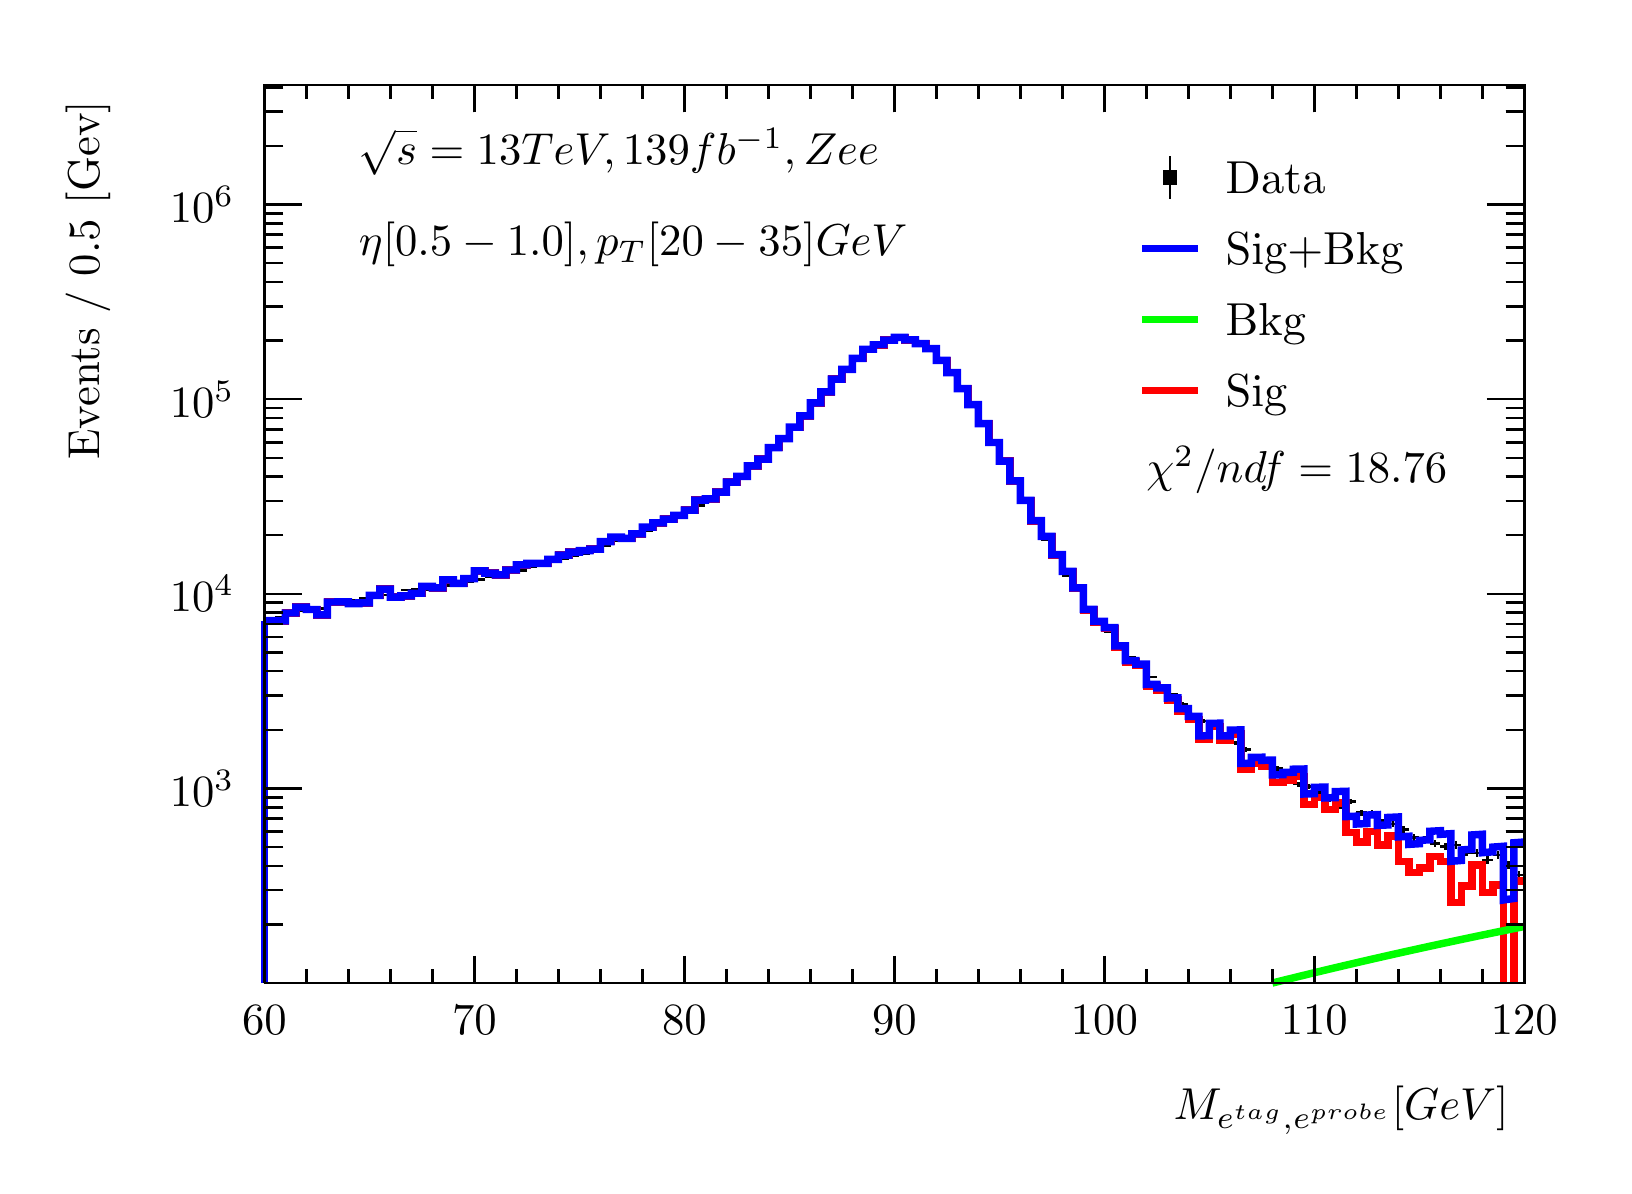
\begin{tikzpicture}
\pgfdeclareplotmark{cross} {
\pgfpathmoveto{\pgfpoint{-0.3\pgfplotmarksize}{\pgfplotmarksize}}
\pgfpathlineto{\pgfpoint{+0.3\pgfplotmarksize}{\pgfplotmarksize}}
\pgfpathlineto{\pgfpoint{+0.3\pgfplotmarksize}{0.3\pgfplotmarksize}}
\pgfpathlineto{\pgfpoint{+1\pgfplotmarksize}{0.3\pgfplotmarksize}}
\pgfpathlineto{\pgfpoint{+1\pgfplotmarksize}{-0.3\pgfplotmarksize}}
\pgfpathlineto{\pgfpoint{+0.3\pgfplotmarksize}{-0.3\pgfplotmarksize}}
\pgfpathlineto{\pgfpoint{+0.3\pgfplotmarksize}{-1.\pgfplotmarksize}}
\pgfpathlineto{\pgfpoint{-0.3\pgfplotmarksize}{-1.\pgfplotmarksize}}
\pgfpathlineto{\pgfpoint{-0.3\pgfplotmarksize}{-0.3\pgfplotmarksize}}
\pgfpathlineto{\pgfpoint{-1.\pgfplotmarksize}{-0.3\pgfplotmarksize}}
\pgfpathlineto{\pgfpoint{-1.\pgfplotmarksize}{0.3\pgfplotmarksize}}
\pgfpathlineto{\pgfpoint{-0.3\pgfplotmarksize}{0.3\pgfplotmarksize}}
\pgfpathclose
\pgfusepathqstroke
}
\pgfdeclareplotmark{cross*} {
\pgfpathmoveto{\pgfpoint{-0.3\pgfplotmarksize}{\pgfplotmarksize}}
\pgfpathlineto{\pgfpoint{+0.3\pgfplotmarksize}{\pgfplotmarksize}}
\pgfpathlineto{\pgfpoint{+0.3\pgfplotmarksize}{0.3\pgfplotmarksize}}
\pgfpathlineto{\pgfpoint{+1\pgfplotmarksize}{0.3\pgfplotmarksize}}
\pgfpathlineto{\pgfpoint{+1\pgfplotmarksize}{-0.3\pgfplotmarksize}}
\pgfpathlineto{\pgfpoint{+0.3\pgfplotmarksize}{-0.3\pgfplotmarksize}}
\pgfpathlineto{\pgfpoint{+0.3\pgfplotmarksize}{-1.\pgfplotmarksize}}
\pgfpathlineto{\pgfpoint{-0.3\pgfplotmarksize}{-1.\pgfplotmarksize}}
\pgfpathlineto{\pgfpoint{-0.3\pgfplotmarksize}{-0.3\pgfplotmarksize}}
\pgfpathlineto{\pgfpoint{-1.\pgfplotmarksize}{-0.3\pgfplotmarksize}}
\pgfpathlineto{\pgfpoint{-1.\pgfplotmarksize}{0.3\pgfplotmarksize}}
\pgfpathlineto{\pgfpoint{-0.3\pgfplotmarksize}{0.3\pgfplotmarksize}}
\pgfpathclose
\pgfusepathqfillstroke
}
\pgfdeclareplotmark{newstar} {
\pgfpathmoveto{\pgfqpoint{0pt}{\pgfplotmarksize}}
\pgfpathlineto{\pgfqpointpolar{44}{0.5\pgfplotmarksize}}
\pgfpathlineto{\pgfqpointpolar{18}{\pgfplotmarksize}}
\pgfpathlineto{\pgfqpointpolar{-20}{0.5\pgfplotmarksize}}
\pgfpathlineto{\pgfqpointpolar{-54}{\pgfplotmarksize}}
\pgfpathlineto{\pgfqpointpolar{-90}{0.5\pgfplotmarksize}}
\pgfpathlineto{\pgfqpointpolar{234}{\pgfplotmarksize}}
\pgfpathlineto{\pgfqpointpolar{198}{0.5\pgfplotmarksize}}
\pgfpathlineto{\pgfqpointpolar{162}{\pgfplotmarksize}}
\pgfpathlineto{\pgfqpointpolar{134}{0.5\pgfplotmarksize}}
\pgfpathclose
\pgfusepathqstroke
}
\pgfdeclareplotmark{newstar*} {
\pgfpathmoveto{\pgfqpoint{0pt}{\pgfplotmarksize}}
\pgfpathlineto{\pgfqpointpolar{44}{0.5\pgfplotmarksize}}
\pgfpathlineto{\pgfqpointpolar{18}{\pgfplotmarksize}}
\pgfpathlineto{\pgfqpointpolar{-20}{0.5\pgfplotmarksize}}
\pgfpathlineto{\pgfqpointpolar{-54}{\pgfplotmarksize}}
\pgfpathlineto{\pgfqpointpolar{-90}{0.5\pgfplotmarksize}}
\pgfpathlineto{\pgfqpointpolar{234}{\pgfplotmarksize}}
\pgfpathlineto{\pgfqpointpolar{198}{0.5\pgfplotmarksize}}
\pgfpathlineto{\pgfqpointpolar{162}{\pgfplotmarksize}}
\pgfpathlineto{\pgfqpointpolar{134}{0.5\pgfplotmarksize}}
\pgfpathclose
\pgfusepathqfillstroke
}
\definecolor{c}{rgb}{1,1,1};
\draw [color=c, fill=c] (0,0) rectangle (20,14.4361);
\draw [color=c, fill=c] (3,2.30977) rectangle (19,13.7143);
\definecolor{c}{rgb}{0,0,0};
\draw [c,line width=0.9] (3,2.30977) -- (3,13.7143) -- (19,13.7143) -- (19,2.30977) -- (3,2.30977);
\definecolor{c}{rgb}{1,1,1};
\draw [color=c, fill=c] (3,2.30977) rectangle (19,13.7143);
\definecolor{c}{rgb}{0,0,0};
\draw [c,line width=0.9] (3,2.30977) -- (3,13.7143) -- (19,13.7143) -- (19,2.30977) -- (3,2.30977);
\draw [c,line width=0.9] (3,2.30977) -- (19,2.30977);
\draw [c,line width=0.9] (3,2.65624) -- (3,2.30977);
\draw [c,line width=0.9] (3.53333,2.48301) -- (3.53333,2.30977);
\draw [c,line width=0.9] (4.06667,2.48301) -- (4.06667,2.30977);
\draw [c,line width=0.9] (4.6,2.48301) -- (4.6,2.30977);
\draw [c,line width=0.9] (5.13333,2.48301) -- (5.13333,2.30977);
\draw [c,line width=0.9] (5.66667,2.65624) -- (5.66667,2.30977);
\draw [c,line width=0.9] (6.2,2.48301) -- (6.2,2.30977);
\draw [c,line width=0.9] (6.73333,2.48301) -- (6.73333,2.30977);
\draw [c,line width=0.9] (7.26667,2.48301) -- (7.26667,2.30977);
\draw [c,line width=0.9] (7.8,2.48301) -- (7.8,2.30977);
\draw [c,line width=0.9] (8.33333,2.65624) -- (8.33333,2.30977);
\draw [c,line width=0.9] (8.86667,2.48301) -- (8.86667,2.30977);
\draw [c,line width=0.9] (9.4,2.48301) -- (9.4,2.30977);
\draw [c,line width=0.9] (9.93333,2.48301) -- (9.93333,2.30977);
\draw [c,line width=0.9] (10.4667,2.48301) -- (10.4667,2.30977);
\draw [c,line width=0.9] (11,2.65624) -- (11,2.30977);
\draw [c,line width=0.9] (11.5333,2.48301) -- (11.5333,2.30977);
\draw [c,line width=0.9] (12.0667,2.48301) -- (12.0667,2.30977);
\draw [c,line width=0.9] (12.6,2.48301) -- (12.6,2.30977);
\draw [c,line width=0.9] (13.1333,2.48301) -- (13.1333,2.30977);
\draw [c,line width=0.9] (13.6667,2.65624) -- (13.6667,2.30977);
\draw [c,line width=0.9] (14.2,2.48301) -- (14.2,2.30977);
\draw [c,line width=0.9] (14.7333,2.48301) -- (14.7333,2.30977);
\draw [c,line width=0.9] (15.2667,2.48301) -- (15.2667,2.30977);
\draw [c,line width=0.9] (15.8,2.48301) -- (15.8,2.30977);
\draw [c,line width=0.9] (16.3333,2.65624) -- (16.3333,2.30977);
\draw [c,line width=0.9] (16.8667,2.48301) -- (16.8667,2.30977);
\draw [c,line width=0.9] (17.4,2.48301) -- (17.4,2.30977);
\draw [c,line width=0.9] (17.9333,2.48301) -- (17.9333,2.30977);
\draw [c,line width=0.9] (18.4667,2.48301) -- (18.4667,2.30977);
\draw [c,line width=0.9] (19,2.65624) -- (19,2.30977);
\draw [anchor=base] (3,1.66015) node[scale=1.61424, color=c, rotate=0]{60};
\draw [anchor=base] (5.66667,1.66015) node[scale=1.61424, color=c, rotate=0]{70};
\draw [anchor=base] (8.33333,1.66015) node[scale=1.61424, color=c, rotate=0]{80};
\draw [anchor=base] (11,1.66015) node[scale=1.61424, color=c, rotate=0]{90};
\draw [anchor=base] (13.6667,1.66015) node[scale=1.61424, color=c, rotate=0]{100};
\draw [anchor=base] (16.3333,1.66015) node[scale=1.61424, color=c, rotate=0]{110};
\draw [anchor=base] (19,1.66015) node[scale=1.61424, color=c, rotate=0]{120};
\draw [anchor= east] (19,0.692932) node[scale=1.61424, color=c, rotate=0]{$M_{e^{tag}, e^{probe}}  [GeV]$};
\draw [c,line width=0.9] (3,13.7143) -- (19,13.7143);
\draw [c,line width=0.9] (3,13.3678) -- (3,13.7143);
\draw [c,line width=0.9] (3.53333,13.5411) -- (3.53333,13.7143);
\draw [c,line width=0.9] (4.06667,13.5411) -- (4.06667,13.7143);
\draw [c,line width=0.9] (4.6,13.5411) -- (4.6,13.7143);
\draw [c,line width=0.9] (5.13333,13.5411) -- (5.13333,13.7143);
\draw [c,line width=0.9] (5.66667,13.3678) -- (5.66667,13.7143);
\draw [c,line width=0.9] (6.2,13.5411) -- (6.2,13.7143);
\draw [c,line width=0.9] (6.73333,13.5411) -- (6.73333,13.7143);
\draw [c,line width=0.9] (7.26667,13.5411) -- (7.26667,13.7143);
\draw [c,line width=0.9] (7.8,13.5411) -- (7.8,13.7143);
\draw [c,line width=0.9] (8.33333,13.3678) -- (8.33333,13.7143);
\draw [c,line width=0.9] (8.86667,13.5411) -- (8.86667,13.7143);
\draw [c,line width=0.9] (9.4,13.5411) -- (9.4,13.7143);
\draw [c,line width=0.9] (9.93333,13.5411) -- (9.93333,13.7143);
\draw [c,line width=0.9] (10.4667,13.5411) -- (10.4667,13.7143);
\draw [c,line width=0.9] (11,13.3678) -- (11,13.7143);
\draw [c,line width=0.9] (11.5333,13.5411) -- (11.5333,13.7143);
\draw [c,line width=0.9] (12.0667,13.5411) -- (12.0667,13.7143);
\draw [c,line width=0.9] (12.6,13.5411) -- (12.6,13.7143);
\draw [c,line width=0.9] (13.1333,13.5411) -- (13.1333,13.7143);
\draw [c,line width=0.9] (13.6667,13.3678) -- (13.6667,13.7143);
\draw [c,line width=0.9] (14.2,13.5411) -- (14.2,13.7143);
\draw [c,line width=0.9] (14.7333,13.5411) -- (14.7333,13.7143);
\draw [c,line width=0.9] (15.2667,13.5411) -- (15.2667,13.7143);
\draw [c,line width=0.9] (15.8,13.5411) -- (15.8,13.7143);
\draw [c,line width=0.9] (16.3333,13.3678) -- (16.3333,13.7143);
\draw [c,line width=0.9] (16.8667,13.5411) -- (16.8667,13.7143);
\draw [c,line width=0.9] (17.4,13.5411) -- (17.4,13.7143);
\draw [c,line width=0.9] (17.9333,13.5411) -- (17.9333,13.7143);
\draw [c,line width=0.9] (18.4667,13.5411) -- (18.4667,13.7143);
\draw [c,line width=0.9] (19,13.3678) -- (19,13.7143);
\draw [c,line width=0.9] (3,2.30977) -- (3,13.7143);
\draw [c,line width=0.9] (3.237,3.05385) -- (3,3.05385);
\draw [c,line width=0.9] (3.237,3.48911) -- (3,3.48911);
\draw [c,line width=0.9] (3.237,3.79793) -- (3,3.79793);
\draw [c,line width=0.9] (3.237,4.03747) -- (3,4.03747);
\draw [c,line width=0.9] (3.237,4.23319) -- (3,4.23319);
\draw [c,line width=0.9] (3.237,4.39867) -- (3,4.39867);
\draw [c,line width=0.9] (3.237,4.54201) -- (3,4.54201);
\draw [c,line width=0.9] (3.237,4.66845) -- (3,4.66845);
\draw [c,line width=0.9] (3.474,4.78155) -- (3,4.78155);
\draw [anchor= east] (2.82,4.78155) node[scale=1.61424, color=c, rotate=0]{$10^{3}$};
\draw [c,line width=0.9] (3.237,5.52563) -- (3,5.52563);
\draw [c,line width=0.9] (3.237,5.96089) -- (3,5.96089);
\draw [c,line width=0.9] (3.237,6.26971) -- (3,6.26971);
\draw [c,line width=0.9] (3.237,6.50925) -- (3,6.50925);
\draw [c,line width=0.9] (3.237,6.70497) -- (3,6.70497);
\draw [c,line width=0.9] (3.237,6.87045) -- (3,6.87045);
\draw [c,line width=0.9] (3.237,7.01379) -- (3,7.01379);
\draw [c,line width=0.9] (3.237,7.14023) -- (3,7.14023);
\draw [c,line width=0.9] (3.474,7.25333) -- (3,7.25333);
\draw [anchor= east] (2.82,7.25333) node[scale=1.61424, color=c, rotate=0]{$10^{4}$};
\draw [c,line width=0.9] (3.237,7.99741) -- (3,7.99741);
\draw [c,line width=0.9] (3.237,8.43267) -- (3,8.43267);
\draw [c,line width=0.9] (3.237,8.74149) -- (3,8.74149);
\draw [c,line width=0.9] (3.237,8.98103) -- (3,8.98103);
\draw [c,line width=0.9] (3.237,9.17675) -- (3,9.17675);
\draw [c,line width=0.9] (3.237,9.34223) -- (3,9.34223);
\draw [c,line width=0.9] (3.237,9.48557) -- (3,9.48557);
\draw [c,line width=0.9] (3.237,9.61201) -- (3,9.61201);
\draw [c,line width=0.9] (3.474,9.72511) -- (3,9.72511);
\draw [anchor= east] (2.82,9.72511) node[scale=1.61424, color=c, rotate=0]{$10^{5}$};
\draw [c,line width=0.9] (3.237,10.4692) -- (3,10.4692);
\draw [c,line width=0.9] (3.237,10.9044) -- (3,10.9044);
\draw [c,line width=0.9] (3.237,11.2133) -- (3,11.2133);
\draw [c,line width=0.9] (3.237,11.4528) -- (3,11.4528);
\draw [c,line width=0.9] (3.237,11.6485) -- (3,11.6485);
\draw [c,line width=0.9] (3.237,11.814) -- (3,11.814);
\draw [c,line width=0.9] (3.237,11.9574) -- (3,11.9574);
\draw [c,line width=0.9] (3.237,12.0838) -- (3,12.0838);
\draw [c,line width=0.9] (3.474,12.1969) -- (3,12.1969);
\draw [anchor= east] (2.82,12.1969) node[scale=1.61424, color=c, rotate=0]{$10^{6}$};
\draw [c,line width=0.9] (3.237,12.941) -- (3,12.941);
\draw [c,line width=0.9] (3.237,13.3762) -- (3,13.3762);
\draw [c,line width=0.9] (3.237,13.6851) -- (3,13.6851);
\draw [anchor= east] (0.76,13.7143) node[scale=1.61424, color=c, rotate=90]{Events / 0.5 [Gev]};
\draw [c,line width=0.9] (19,2.30977) -- (19,13.7143);
\draw [c,line width=0.9] (18.763,3.05385) -- (19,3.05385);
\draw [c,line width=0.9] (18.763,3.48911) -- (19,3.48911);
\draw [c,line width=0.9] (18.763,3.79793) -- (19,3.79793);
\draw [c,line width=0.9] (18.763,4.03747) -- (19,4.03747);
\draw [c,line width=0.9] (18.763,4.23319) -- (19,4.23319);
\draw [c,line width=0.9] (18.763,4.39867) -- (19,4.39867);
\draw [c,line width=0.9] (18.763,4.54201) -- (19,4.54201);
\draw [c,line width=0.9] (18.763,4.66845) -- (19,4.66845);
\draw [c,line width=0.9] (18.526,4.78155) -- (19,4.78155);
\draw [c,line width=0.9] (18.763,5.52563) -- (19,5.52563);
\draw [c,line width=0.9] (18.763,5.96089) -- (19,5.96089);
\draw [c,line width=0.9] (18.763,6.26971) -- (19,6.26971);
\draw [c,line width=0.9] (18.763,6.50925) -- (19,6.50925);
\draw [c,line width=0.9] (18.763,6.70497) -- (19,6.70497);
\draw [c,line width=0.9] (18.763,6.87045) -- (19,6.87045);
\draw [c,line width=0.9] (18.763,7.01379) -- (19,7.01379);
\draw [c,line width=0.9] (18.763,7.14023) -- (19,7.14023);
\draw [c,line width=0.9] (18.526,7.25333) -- (19,7.25333);
\draw [c,line width=0.9] (18.763,7.99741) -- (19,7.99741);
\draw [c,line width=0.9] (18.763,8.43267) -- (19,8.43267);
\draw [c,line width=0.9] (18.763,8.74149) -- (19,8.74149);
\draw [c,line width=0.9] (18.763,8.98103) -- (19,8.98103);
\draw [c,line width=0.9] (18.763,9.17675) -- (19,9.17675);
\draw [c,line width=0.9] (18.763,9.34223) -- (19,9.34223);
\draw [c,line width=0.9] (18.763,9.48557) -- (19,9.48557);
\draw [c,line width=0.9] (18.763,9.61201) -- (19,9.61201);
\draw [c,line width=0.9] (18.526,9.72511) -- (19,9.72511);
\draw [c,line width=0.9] (18.763,10.4692) -- (19,10.4692);
\draw [c,line width=0.9] (18.763,10.9044) -- (19,10.9044);
\draw [c,line width=0.9] (18.763,11.2133) -- (19,11.2133);
\draw [c,line width=0.9] (18.763,11.4528) -- (19,11.4528);
\draw [c,line width=0.9] (18.763,11.6485) -- (19,11.6485);
\draw [c,line width=0.9] (18.763,11.814) -- (19,11.814);
\draw [c,line width=0.9] (18.763,11.9574) -- (19,11.9574);
\draw [c,line width=0.9] (18.763,12.0838) -- (19,12.0838);
\draw [c,line width=0.9] (18.526,12.1969) -- (19,12.1969);
\draw [c,line width=0.9] (18.763,12.941) -- (19,12.941);
\draw [c,line width=0.9] (18.763,13.3762) -- (19,13.3762);
\draw [c,line width=0.9] (18.763,13.6851) -- (19,13.6851);
\draw [c,line width=0.9] (3.06667,6.92297) -- (3,6.92297);
\draw [c,line width=0.9] (3,6.92297) -- (3,6.92297);
\draw [c,line width=0.9] (3.06667,6.92297) -- (3.13333,6.92297);
\draw [c,line width=0.9] (3.13333,6.92297) -- (3.13333,6.92297);
\draw [c,line width=0.9] (3.06667,6.92297) -- (3.06667,6.93549);
\draw [c,line width=0.9] (3.06667,6.93549) -- (3.06667,6.93549);
\draw [c,line width=0.9] (3.06667,6.92297) -- (3.06667,6.91045);
\draw [c,line width=0.9] (3.06667,6.91045) -- (3.06667,6.91045);
\draw [c,line width=0.9] (3.2,6.95788) -- (3.13333,6.95788);
\draw [c,line width=0.9] (3.13333,6.95788) -- (3.13333,6.95788);
\draw [c,line width=0.9] (3.2,6.95788) -- (3.26667,6.95788);
\draw [c,line width=0.9] (3.26667,6.95788) -- (3.26667,6.95788);
\draw [c,line width=0.9] (3.2,6.95788) -- (3.2,6.9702);
\draw [c,line width=0.9] (3.2,6.9702) -- (3.2,6.9702);
\draw [c,line width=0.9] (3.2,6.95788) -- (3.2,6.94556);
\draw [c,line width=0.9] (3.2,6.94556) -- (3.2,6.94556);
\draw [c,line width=0.9] (3.33333,7.003) -- (3.26667,7.003);
\draw [c,line width=0.9] (3.26667,7.003) -- (3.26667,7.003);
\draw [c,line width=0.9] (3.33333,7.003) -- (3.4,7.003);
\draw [c,line width=0.9] (3.4,7.003) -- (3.4,7.003);
\draw [c,line width=0.9] (3.33333,7.003) -- (3.33333,7.01507);
\draw [c,line width=0.9] (3.33333,7.01507) -- (3.33333,7.01507);
\draw [c,line width=0.9] (3.33333,7.003) -- (3.33333,6.99094);
\draw [c,line width=0.9] (3.33333,6.99094) -- (3.33333,6.99094);
\draw [c,line width=0.9] (3.46667,7.03281) -- (3.4,7.03281);
\draw [c,line width=0.9] (3.4,7.03281) -- (3.4,7.03281);
\draw [c,line width=0.9] (3.46667,7.03281) -- (3.53333,7.03281);
\draw [c,line width=0.9] (3.53333,7.03281) -- (3.53333,7.03281);
\draw [c,line width=0.9] (3.46667,7.03281) -- (3.46667,7.04471);
\draw [c,line width=0.9] (3.46667,7.04471) -- (3.46667,7.04471);
\draw [c,line width=0.9] (3.46667,7.03281) -- (3.46667,7.02092);
\draw [c,line width=0.9] (3.46667,7.02092) -- (3.46667,7.02092);
\draw [c,line width=0.9] (3.6,7.04748) -- (3.53333,7.04748);
\draw [c,line width=0.9] (3.53333,7.04748) -- (3.53333,7.04748);
\draw [c,line width=0.9] (3.6,7.04748) -- (3.66667,7.04748);
\draw [c,line width=0.9] (3.66667,7.04748) -- (3.66667,7.04748);
\draw [c,line width=0.9] (3.6,7.04748) -- (3.6,7.05929);
\draw [c,line width=0.9] (3.6,7.05929) -- (3.6,7.05929);
\draw [c,line width=0.9] (3.6,7.04748) -- (3.6,7.03566);
\draw [c,line width=0.9] (3.6,7.03566) -- (3.6,7.03566);
\draw [c,line width=0.9] (3.73333,7.06872) -- (3.66667,7.06872);
\draw [c,line width=0.9] (3.66667,7.06872) -- (3.66667,7.06872);
\draw [c,line width=0.9] (3.73333,7.06872) -- (3.8,7.06872);
\draw [c,line width=0.9] (3.8,7.06872) -- (3.8,7.06872);
\draw [c,line width=0.9] (3.73333,7.06872) -- (3.73333,7.08042);
\draw [c,line width=0.9] (3.73333,7.08042) -- (3.73333,7.08042);
\draw [c,line width=0.9] (3.73333,7.06872) -- (3.73333,7.05702);
\draw [c,line width=0.9] (3.73333,7.05702) -- (3.73333,7.05702);
\draw [c,line width=0.9] (3.86667,7.12207) -- (3.8,7.12207);
\draw [c,line width=0.9] (3.8,7.12207) -- (3.8,7.12207);
\draw [c,line width=0.9] (3.86667,7.12207) -- (3.93333,7.12207);
\draw [c,line width=0.9] (3.93333,7.12207) -- (3.93333,7.12207);
\draw [c,line width=0.9] (3.86667,7.12207) -- (3.86667,7.13348);
\draw [c,line width=0.9] (3.86667,7.13348) -- (3.86667,7.13348);
\draw [c,line width=0.9] (3.86667,7.12207) -- (3.86667,7.11066);
\draw [c,line width=0.9] (3.86667,7.11066) -- (3.86667,7.11066);
\draw [c,line width=0.9] (4,7.13856) -- (3.93333,7.13856);
\draw [c,line width=0.9] (3.93333,7.13856) -- (3.93333,7.13856);
\draw [c,line width=0.9] (4,7.13856) -- (4.06667,7.13856);
\draw [c,line width=0.9] (4.06667,7.13856) -- (4.06667,7.13856);
\draw [c,line width=0.9] (4,7.13856) -- (4,7.14988);
\draw [c,line width=0.9] (4,7.14988) -- (4,7.14988);
\draw [c,line width=0.9] (4,7.13856) -- (4,7.12723);
\draw [c,line width=0.9] (4,7.12723) -- (4,7.12723);
\draw [c,line width=0.9] (4.13333,7.16709) -- (4.06667,7.16709);
\draw [c,line width=0.9] (4.06667,7.16709) -- (4.06667,7.16709);
\draw [c,line width=0.9] (4.13333,7.16709) -- (4.2,7.16709);
\draw [c,line width=0.9] (4.2,7.16709) -- (4.2,7.16709);
\draw [c,line width=0.9] (4.13333,7.16709) -- (4.13333,7.17826);
\draw [c,line width=0.9] (4.13333,7.17826) -- (4.13333,7.17826);
\draw [c,line width=0.9] (4.13333,7.16709) -- (4.13333,7.15591);
\draw [c,line width=0.9] (4.13333,7.15591) -- (4.13333,7.15591);
\draw [c,line width=0.9] (4.26667,7.1909) -- (4.2,7.1909);
\draw [c,line width=0.9] (4.2,7.1909) -- (4.2,7.1909);
\draw [c,line width=0.9] (4.26667,7.1909) -- (4.33333,7.1909);
\draw [c,line width=0.9] (4.33333,7.1909) -- (4.33333,7.1909);
\draw [c,line width=0.9] (4.26667,7.1909) -- (4.26667,7.20195);
\draw [c,line width=0.9] (4.26667,7.20195) -- (4.26667,7.20195);
\draw [c,line width=0.9] (4.26667,7.1909) -- (4.26667,7.17985);
\draw [c,line width=0.9] (4.26667,7.17985) -- (4.26667,7.17985);
\draw [c,line width=0.9] (4.4,7.19782) -- (4.33333,7.19782);
\draw [c,line width=0.9] (4.33333,7.19782) -- (4.33333,7.19782);
\draw [c,line width=0.9] (4.4,7.19782) -- (4.46667,7.19782);
\draw [c,line width=0.9] (4.46667,7.19782) -- (4.46667,7.19782);
\draw [c,line width=0.9] (4.4,7.19782) -- (4.4,7.20883);
\draw [c,line width=0.9] (4.4,7.20883) -- (4.4,7.20883);
\draw [c,line width=0.9] (4.4,7.19782) -- (4.4,7.1868);
\draw [c,line width=0.9] (4.4,7.1868) -- (4.4,7.1868);
\draw [c,line width=0.9] (4.53333,7.24092) -- (4.46667,7.24092);
\draw [c,line width=0.9] (4.46667,7.24092) -- (4.46667,7.24092);
\draw [c,line width=0.9] (4.53333,7.24092) -- (4.6,7.24092);
\draw [c,line width=0.9] (4.6,7.24092) -- (4.6,7.24092);
\draw [c,line width=0.9] (4.53333,7.24092) -- (4.53333,7.25171);
\draw [c,line width=0.9] (4.53333,7.25171) -- (4.53333,7.25171);
\draw [c,line width=0.9] (4.53333,7.24092) -- (4.53333,7.23012);
\draw [c,line width=0.9] (4.53333,7.23012) -- (4.53333,7.23012);
\draw [c,line width=0.9] (4.66667,7.25194) -- (4.6,7.25194);
\draw [c,line width=0.9] (4.6,7.25194) -- (4.6,7.25194);
\draw [c,line width=0.9] (4.66667,7.25194) -- (4.73333,7.25194);
\draw [c,line width=0.9] (4.73333,7.25194) -- (4.73333,7.25194);
\draw [c,line width=0.9] (4.66667,7.25194) -- (4.66667,7.26268);
\draw [c,line width=0.9] (4.66667,7.26268) -- (4.66667,7.26268);
\draw [c,line width=0.9] (4.66667,7.25194) -- (4.66667,7.24119);
\draw [c,line width=0.9] (4.66667,7.24119) -- (4.66667,7.24119);
\draw [c,line width=0.9] (4.8,7.30202) -- (4.73333,7.30202);
\draw [c,line width=0.9] (4.73333,7.30202) -- (4.73333,7.30202);
\draw [c,line width=0.9] (4.8,7.30202) -- (4.86667,7.30202);
\draw [c,line width=0.9] (4.86667,7.30202) -- (4.86667,7.30202);
\draw [c,line width=0.9] (4.8,7.30202) -- (4.8,7.31252);
\draw [c,line width=0.9] (4.8,7.31252) -- (4.8,7.31252);
\draw [c,line width=0.9] (4.8,7.30202) -- (4.8,7.29153);
\draw [c,line width=0.9] (4.8,7.29153) -- (4.8,7.29153);
\draw [c,line width=0.9] (4.93333,7.31558) -- (4.86667,7.31558);
\draw [c,line width=0.9] (4.86667,7.31558) -- (4.86667,7.31558);
\draw [c,line width=0.9] (4.93333,7.31558) -- (5,7.31558);
\draw [c,line width=0.9] (5,7.31558) -- (5,7.31558);
\draw [c,line width=0.9] (4.93333,7.31558) -- (4.93333,7.32601);
\draw [c,line width=0.9] (4.93333,7.32601) -- (4.93333,7.32601);
\draw [c,line width=0.9] (4.93333,7.31558) -- (4.93333,7.30515);
\draw [c,line width=0.9] (4.93333,7.30515) -- (4.93333,7.30515);
\draw [c,line width=0.9] (5.06667,7.30571) -- (5,7.30571);
\draw [c,line width=0.9] (5,7.30571) -- (5,7.30571);
\draw [c,line width=0.9] (5.06667,7.30571) -- (5.13333,7.30571);
\draw [c,line width=0.9] (5.13333,7.30571) -- (5.13333,7.30571);
\draw [c,line width=0.9] (5.06667,7.30571) -- (5.06667,7.31618);
\draw [c,line width=0.9] (5.06667,7.31618) -- (5.06667,7.31618);
\draw [c,line width=0.9] (5.06667,7.30571) -- (5.06667,7.29523);
\draw [c,line width=0.9] (5.06667,7.29523) -- (5.06667,7.29523);
\draw [c,line width=0.9] (5.2,7.32355) -- (5.13333,7.32355);
\draw [c,line width=0.9] (5.13333,7.32355) -- (5.13333,7.32355);
\draw [c,line width=0.9] (5.2,7.32355) -- (5.26667,7.32355);
\draw [c,line width=0.9] (5.26667,7.32355) -- (5.26667,7.32355);
\draw [c,line width=0.9] (5.2,7.32355) -- (5.2,7.33394);
\draw [c,line width=0.9] (5.2,7.33394) -- (5.2,7.33394);
\draw [c,line width=0.9] (5.2,7.32355) -- (5.2,7.31316);
\draw [c,line width=0.9] (5.2,7.31316) -- (5.2,7.31316);
\draw [c,line width=0.9] (5.33333,7.35643) -- (5.26667,7.35643);
\draw [c,line width=0.9] (5.26667,7.35643) -- (5.26667,7.35643);
\draw [c,line width=0.9] (5.33333,7.35643) -- (5.4,7.35643);
\draw [c,line width=0.9] (5.4,7.35643) -- (5.4,7.35643);
\draw [c,line width=0.9] (5.33333,7.35643) -- (5.33333,7.36666);
\draw [c,line width=0.9] (5.33333,7.36666) -- (5.33333,7.36666);
\draw [c,line width=0.9] (5.33333,7.35643) -- (5.33333,7.3462);
\draw [c,line width=0.9] (5.33333,7.3462) -- (5.33333,7.3462);
\draw [c,line width=0.9] (5.46667,7.38377) -- (5.4,7.38377);
\draw [c,line width=0.9] (5.4,7.38377) -- (5.4,7.38377);
\draw [c,line width=0.9] (5.46667,7.38377) -- (5.53333,7.38377);
\draw [c,line width=0.9] (5.53333,7.38377) -- (5.53333,7.38377);
\draw [c,line width=0.9] (5.46667,7.38377) -- (5.46667,7.39387);
\draw [c,line width=0.9] (5.46667,7.39387) -- (5.46667,7.39387);
\draw [c,line width=0.9] (5.46667,7.38377) -- (5.46667,7.37367);
\draw [c,line width=0.9] (5.46667,7.37367) -- (5.46667,7.37367);
\draw [c,line width=0.9] (5.6,7.40932) -- (5.53333,7.40932);
\draw [c,line width=0.9] (5.53333,7.40932) -- (5.53333,7.40932);
\draw [c,line width=0.9] (5.6,7.40932) -- (5.66667,7.40932);
\draw [c,line width=0.9] (5.66667,7.40932) -- (5.66667,7.40932);
\draw [c,line width=0.9] (5.6,7.40932) -- (5.6,7.4193);
\draw [c,line width=0.9] (5.6,7.4193) -- (5.6,7.4193);
\draw [c,line width=0.9] (5.6,7.40932) -- (5.6,7.39934);
\draw [c,line width=0.9] (5.6,7.39934) -- (5.6,7.39934);
\draw [c,line width=0.9] (5.73333,7.43772) -- (5.66667,7.43772);
\draw [c,line width=0.9] (5.66667,7.43772) -- (5.66667,7.43772);
\draw [c,line width=0.9] (5.73333,7.43772) -- (5.8,7.43772);
\draw [c,line width=0.9] (5.8,7.43772) -- (5.8,7.43772);
\draw [c,line width=0.9] (5.73333,7.43772) -- (5.73333,7.44757);
\draw [c,line width=0.9] (5.73333,7.44757) -- (5.73333,7.44757);
\draw [c,line width=0.9] (5.73333,7.43772) -- (5.73333,7.42787);
\draw [c,line width=0.9] (5.73333,7.42787) -- (5.73333,7.42787);
\draw [c,line width=0.9] (5.86667,7.4711) -- (5.8,7.4711);
\draw [c,line width=0.9] (5.8,7.4711) -- (5.8,7.4711);
\draw [c,line width=0.9] (5.86667,7.4711) -- (5.93333,7.4711);
\draw [c,line width=0.9] (5.93333,7.4711) -- (5.93333,7.4711);
\draw [c,line width=0.9] (5.86667,7.4711) -- (5.86667,7.4808);
\draw [c,line width=0.9] (5.86667,7.4808) -- (5.86667,7.4808);
\draw [c,line width=0.9] (5.86667,7.4711) -- (5.86667,7.4614);
\draw [c,line width=0.9] (5.86667,7.4614) -- (5.86667,7.4614);
\draw [c,line width=0.9] (6,7.49887) -- (5.93333,7.49887);
\draw [c,line width=0.9] (5.93333,7.49887) -- (5.93333,7.49887);
\draw [c,line width=0.9] (6,7.49887) -- (6.06667,7.49887);
\draw [c,line width=0.9] (6.06667,7.49887) -- (6.06667,7.49887);
\draw [c,line width=0.9] (6,7.49887) -- (6,7.50844);
\draw [c,line width=0.9] (6,7.50844) -- (6,7.50844);
\draw [c,line width=0.9] (6,7.49887) -- (6,7.48929);
\draw [c,line width=0.9] (6,7.48929) -- (6,7.48929);
\draw [c,line width=0.9] (6.13333,7.53737) -- (6.06667,7.53737);
\draw [c,line width=0.9] (6.06667,7.53737) -- (6.06667,7.53737);
\draw [c,line width=0.9] (6.13333,7.53737) -- (6.2,7.53737);
\draw [c,line width=0.9] (6.2,7.53737) -- (6.2,7.53737);
\draw [c,line width=0.9] (6.13333,7.53737) -- (6.13333,7.54677);
\draw [c,line width=0.9] (6.13333,7.54677) -- (6.13333,7.54677);
\draw [c,line width=0.9] (6.13333,7.53737) -- (6.13333,7.52796);
\draw [c,line width=0.9] (6.13333,7.52796) -- (6.13333,7.52796);
\draw [c,line width=0.9] (6.26667,7.55169) -- (6.2,7.55169);
\draw [c,line width=0.9] (6.2,7.55169) -- (6.2,7.55169);
\draw [c,line width=0.9] (6.26667,7.55169) -- (6.33333,7.55169);
\draw [c,line width=0.9] (6.33333,7.55169) -- (6.33333,7.55169);
\draw [c,line width=0.9] (6.26667,7.55169) -- (6.26667,7.56103);
\draw [c,line width=0.9] (6.26667,7.56103) -- (6.26667,7.56103);
\draw [c,line width=0.9] (6.26667,7.55169) -- (6.26667,7.54235);
\draw [c,line width=0.9] (6.26667,7.54235) -- (6.26667,7.54235);
\draw [c,line width=0.9] (6.4,7.59901) -- (6.33333,7.59901);
\draw [c,line width=0.9] (6.33333,7.59901) -- (6.33333,7.59901);
\draw [c,line width=0.9] (6.4,7.59901) -- (6.46667,7.59901);
\draw [c,line width=0.9] (6.46667,7.59901) -- (6.46667,7.59901);
\draw [c,line width=0.9] (6.4,7.59901) -- (6.4,7.60814);
\draw [c,line width=0.9] (6.4,7.60814) -- (6.4,7.60814);
\draw [c,line width=0.9] (6.4,7.59901) -- (6.4,7.58987);
\draw [c,line width=0.9] (6.4,7.58987) -- (6.4,7.58987);
\draw [c,line width=0.9] (6.53333,7.6296) -- (6.46667,7.6296);
\draw [c,line width=0.9] (6.46667,7.6296) -- (6.46667,7.6296);
\draw [c,line width=0.9] (6.53333,7.6296) -- (6.6,7.6296);
\draw [c,line width=0.9] (6.6,7.6296) -- (6.6,7.6296);
\draw [c,line width=0.9] (6.53333,7.6296) -- (6.53333,7.63861);
\draw [c,line width=0.9] (6.53333,7.63861) -- (6.53333,7.63861);
\draw [c,line width=0.9] (6.53333,7.6296) -- (6.53333,7.6206);
\draw [c,line width=0.9] (6.53333,7.6206) -- (6.53333,7.6206);
\draw [c,line width=0.9] (6.66667,7.67091) -- (6.6,7.67091);
\draw [c,line width=0.9] (6.6,7.67091) -- (6.6,7.67091);
\draw [c,line width=0.9] (6.66667,7.67091) -- (6.73333,7.67091);
\draw [c,line width=0.9] (6.73333,7.67091) -- (6.73333,7.67091);
\draw [c,line width=0.9] (6.66667,7.67091) -- (6.66667,7.67975);
\draw [c,line width=0.9] (6.66667,7.67975) -- (6.66667,7.67975);
\draw [c,line width=0.9] (6.66667,7.67091) -- (6.66667,7.66208);
\draw [c,line width=0.9] (6.66667,7.66208) -- (6.66667,7.66208);
\draw [c,line width=0.9] (6.8,7.69309) -- (6.73333,7.69309);
\draw [c,line width=0.9] (6.73333,7.69309) -- (6.73333,7.69309);
\draw [c,line width=0.9] (6.8,7.69309) -- (6.86667,7.69309);
\draw [c,line width=0.9] (6.86667,7.69309) -- (6.86667,7.69309);
\draw [c,line width=0.9] (6.8,7.69309) -- (6.8,7.70184);
\draw [c,line width=0.9] (6.8,7.70184) -- (6.8,7.70184);
\draw [c,line width=0.9] (6.8,7.69309) -- (6.8,7.68434);
\draw [c,line width=0.9] (6.8,7.68434) -- (6.8,7.68434);
\draw [c,line width=0.9] (6.93333,7.73324) -- (6.86667,7.73324);
\draw [c,line width=0.9] (6.86667,7.73324) -- (6.86667,7.73324);
\draw [c,line width=0.9] (6.93333,7.73324) -- (7,7.73324);
\draw [c,line width=0.9] (7,7.73324) -- (7,7.73324);
\draw [c,line width=0.9] (6.93333,7.73324) -- (6.93333,7.74182);
\draw [c,line width=0.9] (6.93333,7.74182) -- (6.93333,7.74182);
\draw [c,line width=0.9] (6.93333,7.73324) -- (6.93333,7.72465);
\draw [c,line width=0.9] (6.93333,7.72465) -- (6.93333,7.72465);
\draw [c,line width=0.9] (7.06667,7.76563) -- (7,7.76563);
\draw [c,line width=0.9] (7,7.76563) -- (7,7.76563);
\draw [c,line width=0.9] (7.06667,7.76563) -- (7.13333,7.76563);
\draw [c,line width=0.9] (7.13333,7.76563) -- (7.13333,7.76563);
\draw [c,line width=0.9] (7.06667,7.76563) -- (7.06667,7.77408);
\draw [c,line width=0.9] (7.06667,7.77408) -- (7.06667,7.77408);
\draw [c,line width=0.9] (7.06667,7.76563) -- (7.06667,7.75717);
\draw [c,line width=0.9] (7.06667,7.75717) -- (7.06667,7.75717);
\draw [c,line width=0.9] (7.2,7.8048) -- (7.13333,7.8048);
\draw [c,line width=0.9] (7.13333,7.8048) -- (7.13333,7.8048);
\draw [c,line width=0.9] (7.2,7.8048) -- (7.26667,7.8048);
\draw [c,line width=0.9] (7.26667,7.8048) -- (7.26667,7.8048);
\draw [c,line width=0.9] (7.2,7.8048) -- (7.2,7.81311);
\draw [c,line width=0.9] (7.2,7.81311) -- (7.2,7.81311);
\draw [c,line width=0.9] (7.2,7.8048) -- (7.2,7.7965);
\draw [c,line width=0.9] (7.2,7.7965) -- (7.2,7.7965);
\draw [c,line width=0.9] (7.33333,7.8642) -- (7.26667,7.8642);
\draw [c,line width=0.9] (7.26667,7.8642) -- (7.26667,7.8642);
\draw [c,line width=0.9] (7.33333,7.8642) -- (7.4,7.8642);
\draw [c,line width=0.9] (7.4,7.8642) -- (7.4,7.8642);
\draw [c,line width=0.9] (7.33333,7.8642) -- (7.33333,7.87228);
\draw [c,line width=0.9] (7.33333,7.87228) -- (7.33333,7.87228);
\draw [c,line width=0.9] (7.33333,7.8642) -- (7.33333,7.85613);
\draw [c,line width=0.9] (7.33333,7.85613) -- (7.33333,7.85613);
\draw [c,line width=0.9] (7.46667,7.92739) -- (7.4,7.92739);
\draw [c,line width=0.9] (7.4,7.92739) -- (7.4,7.92739);
\draw [c,line width=0.9] (7.46667,7.92739) -- (7.53333,7.92739);
\draw [c,line width=0.9] (7.53333,7.92739) -- (7.53333,7.92739);
\draw [c,line width=0.9] (7.46667,7.92739) -- (7.46667,7.93523);
\draw [c,line width=0.9] (7.46667,7.93523) -- (7.46667,7.93523);
\draw [c,line width=0.9] (7.46667,7.92739) -- (7.46667,7.91954);
\draw [c,line width=0.9] (7.46667,7.91954) -- (7.46667,7.91954);
\draw [c,line width=0.9] (7.6,7.94843) -- (7.53333,7.94843);
\draw [c,line width=0.9] (7.53333,7.94843) -- (7.53333,7.94843);
\draw [c,line width=0.9] (7.6,7.94843) -- (7.66667,7.94843);
\draw [c,line width=0.9] (7.66667,7.94843) -- (7.66667,7.94843);
\draw [c,line width=0.9] (7.6,7.94843) -- (7.6,7.9562);
\draw [c,line width=0.9] (7.6,7.9562) -- (7.6,7.9562);
\draw [c,line width=0.9] (7.6,7.94843) -- (7.6,7.94067);
\draw [c,line width=0.9] (7.6,7.94067) -- (7.6,7.94067);
\draw [c,line width=0.9] (7.73333,8.00655) -- (7.66667,8.00655);
\draw [c,line width=0.9] (7.66667,8.00655) -- (7.66667,8.00655);
\draw [c,line width=0.9] (7.73333,8.00655) -- (7.8,8.00655);
\draw [c,line width=0.9] (7.8,8.00655) -- (7.8,8.00655);
\draw [c,line width=0.9] (7.73333,8.00655) -- (7.73333,8.01411);
\draw [c,line width=0.9] (7.73333,8.01411) -- (7.73333,8.01411);
\draw [c,line width=0.9] (7.73333,8.00655) -- (7.73333,7.99899);
\draw [c,line width=0.9] (7.73333,7.99899) -- (7.73333,7.99899);
\draw [c,line width=0.9] (7.86667,8.05702) -- (7.8,8.05702);
\draw [c,line width=0.9] (7.8,8.05702) -- (7.8,8.05702);
\draw [c,line width=0.9] (7.86667,8.05702) -- (7.93333,8.05702);
\draw [c,line width=0.9] (7.93333,8.05702) -- (7.93333,8.05702);
\draw [c,line width=0.9] (7.86667,8.05702) -- (7.86667,8.0644);
\draw [c,line width=0.9] (7.86667,8.0644) -- (7.86667,8.0644);
\draw [c,line width=0.9] (7.86667,8.05702) -- (7.86667,8.04964);
\draw [c,line width=0.9] (7.86667,8.04964) -- (7.86667,8.04964);
\draw [c,line width=0.9] (8,8.11619) -- (7.93333,8.11619);
\draw [c,line width=0.9] (7.93333,8.11619) -- (7.93333,8.11619);
\draw [c,line width=0.9] (8,8.11619) -- (8.06667,8.11619);
\draw [c,line width=0.9] (8.06667,8.11619) -- (8.06667,8.11619);
\draw [c,line width=0.9] (8,8.11619) -- (8,8.12337);
\draw [c,line width=0.9] (8,8.12337) -- (8,8.12337);
\draw [c,line width=0.9] (8,8.11619) -- (8,8.10901);
\draw [c,line width=0.9] (8,8.10901) -- (8,8.10901);
\draw [c,line width=0.9] (8.13333,8.17559) -- (8.06667,8.17559);
\draw [c,line width=0.9] (8.06667,8.17559) -- (8.06667,8.17559);
\draw [c,line width=0.9] (8.13333,8.17559) -- (8.2,8.17559);
\draw [c,line width=0.9] (8.2,8.17559) -- (8.2,8.17559);
\draw [c,line width=0.9] (8.13333,8.17559) -- (8.13333,8.18258);
\draw [c,line width=0.9] (8.13333,8.18258) -- (8.13333,8.18258);
\draw [c,line width=0.9] (8.13333,8.17559) -- (8.13333,8.1686);
\draw [c,line width=0.9] (8.13333,8.1686) -- (8.13333,8.1686);
\draw [c,line width=0.9] (8.26667,8.23803) -- (8.2,8.23803);
\draw [c,line width=0.9] (8.2,8.23803) -- (8.2,8.23803);
\draw [c,line width=0.9] (8.26667,8.23803) -- (8.33333,8.23803);
\draw [c,line width=0.9] (8.33333,8.23803) -- (8.33333,8.23803);
\draw [c,line width=0.9] (8.26667,8.23803) -- (8.26667,8.24481);
\draw [c,line width=0.9] (8.26667,8.24481) -- (8.26667,8.24481);
\draw [c,line width=0.9] (8.26667,8.23803) -- (8.26667,8.23124);
\draw [c,line width=0.9] (8.26667,8.23124) -- (8.26667,8.23124);
\draw [c,line width=0.9] (8.4,8.29853) -- (8.33333,8.29853);
\draw [c,line width=0.9] (8.33333,8.29853) -- (8.33333,8.29853);
\draw [c,line width=0.9] (8.4,8.29853) -- (8.46667,8.29853);
\draw [c,line width=0.9] (8.46667,8.29853) -- (8.46667,8.29853);
\draw [c,line width=0.9] (8.4,8.29853) -- (8.4,8.30513);
\draw [c,line width=0.9] (8.4,8.30513) -- (8.4,8.30513);
\draw [c,line width=0.9] (8.4,8.29853) -- (8.4,8.29193);
\draw [c,line width=0.9] (8.4,8.29193) -- (8.4,8.29193);
\draw [c,line width=0.9] (8.53333,8.37501) -- (8.46667,8.37501);
\draw [c,line width=0.9] (8.46667,8.37501) -- (8.46667,8.37501);
\draw [c,line width=0.9] (8.53333,8.37501) -- (8.6,8.37501);
\draw [c,line width=0.9] (8.6,8.37501) -- (8.6,8.37501);
\draw [c,line width=0.9] (8.53333,8.37501) -- (8.53333,8.38137);
\draw [c,line width=0.9] (8.53333,8.38137) -- (8.53333,8.38137);
\draw [c,line width=0.9] (8.53333,8.37501) -- (8.53333,8.36864);
\draw [c,line width=0.9] (8.53333,8.36864) -- (8.53333,8.36864);
\draw [c,line width=0.9] (8.66667,8.45977) -- (8.6,8.45977);
\draw [c,line width=0.9] (8.6,8.45977) -- (8.6,8.45977);
\draw [c,line width=0.9] (8.66667,8.45977) -- (8.73333,8.45977);
\draw [c,line width=0.9] (8.73333,8.45977) -- (8.73333,8.45977);
\draw [c,line width=0.9] (8.66667,8.45977) -- (8.66667,8.46589);
\draw [c,line width=0.9] (8.66667,8.46589) -- (8.66667,8.46589);
\draw [c,line width=0.9] (8.66667,8.45977) -- (8.66667,8.45365);
\draw [c,line width=0.9] (8.66667,8.45365) -- (8.66667,8.45365);
\draw [c,line width=0.9] (8.8,8.54221) -- (8.73333,8.54221);
\draw [c,line width=0.9] (8.73333,8.54221) -- (8.73333,8.54221);
\draw [c,line width=0.9] (8.8,8.54221) -- (8.86667,8.54221);
\draw [c,line width=0.9] (8.86667,8.54221) -- (8.86667,8.54221);
\draw [c,line width=0.9] (8.8,8.54221) -- (8.8,8.5481);
\draw [c,line width=0.9] (8.8,8.5481) -- (8.8,8.5481);
\draw [c,line width=0.9] (8.8,8.54221) -- (8.8,8.53633);
\draw [c,line width=0.9] (8.8,8.53633) -- (8.8,8.53633);
\draw [c,line width=0.9] (8.93333,8.63531) -- (8.86667,8.63531);
\draw [c,line width=0.9] (8.86667,8.63531) -- (8.86667,8.63531);
\draw [c,line width=0.9] (8.93333,8.63531) -- (9,8.63531);
\draw [c,line width=0.9] (9,8.63531) -- (9,8.63531);
\draw [c,line width=0.9] (8.93333,8.63531) -- (8.93333,8.64095);
\draw [c,line width=0.9] (8.93333,8.64095) -- (8.93333,8.64095);
\draw [c,line width=0.9] (8.93333,8.63531) -- (8.93333,8.62968);
\draw [c,line width=0.9] (8.93333,8.62968) -- (8.93333,8.62968);
\draw [c,line width=0.9] (9.06667,8.73319) -- (9,8.73319);
\draw [c,line width=0.9] (9,8.73319) -- (9,8.73319);
\draw [c,line width=0.9] (9.06667,8.73319) -- (9.13333,8.73319);
\draw [c,line width=0.9] (9.13333,8.73319) -- (9.13333,8.73319);
\draw [c,line width=0.9] (9.06667,8.73319) -- (9.06667,8.73858);
\draw [c,line width=0.9] (9.06667,8.73858) -- (9.06667,8.73858);
\draw [c,line width=0.9] (9.06667,8.73319) -- (9.06667,8.72781);
\draw [c,line width=0.9] (9.06667,8.72781) -- (9.06667,8.72781);
\draw [c,line width=0.9] (9.2,8.8518) -- (9.13333,8.8518);
\draw [c,line width=0.9] (9.13333,8.8518) -- (9.13333,8.8518);
\draw [c,line width=0.9] (9.2,8.8518) -- (9.26667,8.8518);
\draw [c,line width=0.9] (9.26667,8.8518) -- (9.26667,8.8518);
\draw [c,line width=0.9] (9.2,8.8518) -- (9.2,8.8569);
\draw [c,line width=0.9] (9.2,8.8569) -- (9.2,8.8569);
\draw [c,line width=0.9] (9.2,8.8518) -- (9.2,8.8467);
\draw [c,line width=0.9] (9.2,8.8467) -- (9.2,8.8467);
\draw [c,line width=0.9] (9.33333,8.9674) -- (9.26667,8.9674);
\draw [c,line width=0.9] (9.26667,8.9674) -- (9.26667,8.9674);
\draw [c,line width=0.9] (9.33333,8.9674) -- (9.4,8.9674);
\draw [c,line width=0.9] (9.4,8.9674) -- (9.4,8.9674);
\draw [c,line width=0.9] (9.33333,8.9674) -- (9.33333,8.97223);
\draw [c,line width=0.9] (9.33333,8.97223) -- (9.33333,8.97223);
\draw [c,line width=0.9] (9.33333,8.9674) -- (9.33333,8.96257);
\draw [c,line width=0.9] (9.33333,8.96257) -- (9.33333,8.96257);
\draw [c,line width=0.9] (9.46667,9.09881) -- (9.4,9.09881);
\draw [c,line width=0.9] (9.4,9.09881) -- (9.4,9.09881);
\draw [c,line width=0.9] (9.46667,9.09881) -- (9.53333,9.09881);
\draw [c,line width=0.9] (9.53333,9.09881) -- (9.53333,9.09881);
\draw [c,line width=0.9] (9.46667,9.09881) -- (9.46667,9.10335);
\draw [c,line width=0.9] (9.46667,9.10335) -- (9.46667,9.10335);
\draw [c,line width=0.9] (9.46667,9.09881) -- (9.46667,9.09426);
\draw [c,line width=0.9] (9.46667,9.09426) -- (9.46667,9.09426);
\draw [c,line width=0.9] (9.6,9.22884) -- (9.53333,9.22884);
\draw [c,line width=0.9] (9.53333,9.22884) -- (9.53333,9.22884);
\draw [c,line width=0.9] (9.6,9.22884) -- (9.66667,9.22884);
\draw [c,line width=0.9] (9.66667,9.22884) -- (9.66667,9.22884);
\draw [c,line width=0.9] (9.6,9.22884) -- (9.6,9.23311);
\draw [c,line width=0.9] (9.6,9.23311) -- (9.6,9.23311);
\draw [c,line width=0.9] (9.6,9.22884) -- (9.6,9.22456);
\draw [c,line width=0.9] (9.6,9.22456) -- (9.6,9.22456);
\draw [c,line width=0.9] (9.73333,9.37732) -- (9.66667,9.37732);
\draw [c,line width=0.9] (9.66667,9.37732) -- (9.66667,9.37732);
\draw [c,line width=0.9] (9.73333,9.37732) -- (9.8,9.37732);
\draw [c,line width=0.9] (9.8,9.37732) -- (9.8,9.37732);
\draw [c,line width=0.9] (9.73333,9.37732) -- (9.73333,9.38131);
\draw [c,line width=0.9] (9.73333,9.38131) -- (9.73333,9.38131);
\draw [c,line width=0.9] (9.73333,9.37732) -- (9.73333,9.37333);
\draw [c,line width=0.9] (9.73333,9.37333) -- (9.73333,9.37333);
\draw [c,line width=0.9] (9.86667,9.52124) -- (9.8,9.52124);
\draw [c,line width=0.9] (9.8,9.52124) -- (9.8,9.52124);
\draw [c,line width=0.9] (9.86667,9.52124) -- (9.93333,9.52124);
\draw [c,line width=0.9] (9.93333,9.52124) -- (9.93333,9.52124);
\draw [c,line width=0.9] (9.86667,9.52124) -- (9.86667,9.52498);
\draw [c,line width=0.9] (9.86667,9.52498) -- (9.86667,9.52498);
\draw [c,line width=0.9] (9.86667,9.52124) -- (9.86667,9.51751);
\draw [c,line width=0.9] (9.86667,9.51751) -- (9.86667,9.51751);
\draw [c,line width=0.9] (10,9.66398) -- (9.93333,9.66398);
\draw [c,line width=0.9] (9.93333,9.66398) -- (9.93333,9.66398);
\draw [c,line width=0.9] (10,9.66398) -- (10.0667,9.66398);
\draw [c,line width=0.9] (10.0667,9.66398) -- (10.0667,9.66398);
\draw [c,line width=0.9] (10,9.66398) -- (10,9.66747);
\draw [c,line width=0.9] (10,9.66747) -- (10,9.66747);
\draw [c,line width=0.9] (10,9.66398) -- (10,9.66048);
\draw [c,line width=0.9] (10,9.66048) -- (10,9.66048);
\draw [c,line width=0.9] (10.1333,9.82371) -- (10.0667,9.82371);
\draw [c,line width=0.9] (10.0667,9.82371) -- (10.0667,9.82371);
\draw [c,line width=0.9] (10.1333,9.82371) -- (10.2,9.82371);
\draw [c,line width=0.9] (10.2,9.82371) -- (10.2,9.82371);
\draw [c,line width=0.9] (10.1333,9.82371) -- (10.1333,9.82695);
\draw [c,line width=0.9] (10.1333,9.82695) -- (10.1333,9.82695);
\draw [c,line width=0.9] (10.1333,9.82371) -- (10.1333,9.82047);
\draw [c,line width=0.9] (10.1333,9.82047) -- (10.1333,9.82047);
\draw [c,line width=0.9] (10.2667,9.96402) -- (10.2,9.96402);
\draw [c,line width=0.9] (10.2,9.96402) -- (10.2,9.96402);
\draw [c,line width=0.9] (10.2667,9.96402) -- (10.3333,9.96402);
\draw [c,line width=0.9] (10.3333,9.96402) -- (10.3333,9.96402);
\draw [c,line width=0.9] (10.2667,9.96402) -- (10.2667,9.96706);
\draw [c,line width=0.9] (10.2667,9.96706) -- (10.2667,9.96706);
\draw [c,line width=0.9] (10.2667,9.96402) -- (10.2667,9.96099);
\draw [c,line width=0.9] (10.2667,9.96099) -- (10.2667,9.96099);
\draw [c,line width=0.9] (10.4,10.107) -- (10.3333,10.107);
\draw [c,line width=0.9] (10.3333,10.107) -- (10.3333,10.107);
\draw [c,line width=0.9] (10.4,10.107) -- (10.4667,10.107);
\draw [c,line width=0.9] (10.4667,10.107) -- (10.4667,10.107);
\draw [c,line width=0.9] (10.4,10.107) -- (10.4,10.1099);
\draw [c,line width=0.9] (10.4,10.1099) -- (10.4,10.1099);
\draw [c,line width=0.9] (10.4,10.107) -- (10.4,10.1042);
\draw [c,line width=0.9] (10.4,10.1042) -- (10.4,10.1042);
\draw [c,line width=0.9] (10.5333,10.236) -- (10.4667,10.236);
\draw [c,line width=0.9] (10.4667,10.236) -- (10.4667,10.236);
\draw [c,line width=0.9] (10.5333,10.236) -- (10.6,10.236);
\draw [c,line width=0.9] (10.6,10.236) -- (10.6,10.236);
\draw [c,line width=0.9] (10.5333,10.236) -- (10.5333,10.2386);
\draw [c,line width=0.9] (10.5333,10.2386) -- (10.5333,10.2386);
\draw [c,line width=0.9] (10.5333,10.236) -- (10.5333,10.2333);
\draw [c,line width=0.9] (10.5333,10.2333) -- (10.5333,10.2333);
\draw [c,line width=0.9] (10.6667,10.3421) -- (10.6,10.3421);
\draw [c,line width=0.9] (10.6,10.3421) -- (10.6,10.3421);
\draw [c,line width=0.9] (10.6667,10.3421) -- (10.7333,10.3421);
\draw [c,line width=0.9] (10.7333,10.3421) -- (10.7333,10.3421);
\draw [c,line width=0.9] (10.6667,10.3421) -- (10.6667,10.3446);
\draw [c,line width=0.9] (10.6667,10.3446) -- (10.6667,10.3446);
\draw [c,line width=0.9] (10.6667,10.3421) -- (10.6667,10.3395);
\draw [c,line width=0.9] (10.6667,10.3395) -- (10.6667,10.3395);
\draw [c,line width=0.9] (10.8,10.4323) -- (10.7333,10.4323);
\draw [c,line width=0.9] (10.7333,10.4323) -- (10.7333,10.4323);
\draw [c,line width=0.9] (10.8,10.4323) -- (10.8667,10.4323);
\draw [c,line width=0.9] (10.8667,10.4323) -- (10.8667,10.4323);
\draw [c,line width=0.9] (10.8,10.4323) -- (10.8,10.4348);
\draw [c,line width=0.9] (10.8,10.4348) -- (10.8,10.4348);
\draw [c,line width=0.9] (10.8,10.4323) -- (10.8,10.4299);
\draw [c,line width=0.9] (10.8,10.4299) -- (10.8,10.4299);
\draw [c,line width=0.9] (10.9333,10.4894) -- (10.8667,10.4894);
\draw [c,line width=0.9] (10.8667,10.4894) -- (10.8667,10.4894);
\draw [c,line width=0.9] (10.9333,10.4894) -- (11,10.4894);
\draw [c,line width=0.9] (11,10.4894) -- (11,10.4894);
\draw [c,line width=0.9] (10.9333,10.4894) -- (10.9333,10.4918);
\draw [c,line width=0.9] (10.9333,10.4918) -- (10.9333,10.4918);
\draw [c,line width=0.9] (10.9333,10.4894) -- (10.9333,10.4871);
\draw [c,line width=0.9] (10.9333,10.4871) -- (10.9333,10.4871);
\draw [c,line width=0.9] (11.0667,10.5103) -- (11,10.5103);
\draw [c,line width=0.9] (11,10.5103) -- (11,10.5103);
\draw [c,line width=0.9] (11.0667,10.5103) -- (11.1333,10.5103);
\draw [c,line width=0.9] (11.1333,10.5103) -- (11.1333,10.5103);
\draw [c,line width=0.9] (11.0667,10.5103) -- (11.0667,10.5126);
\draw [c,line width=0.9] (11.0667,10.5126) -- (11.0667,10.5126);
\draw [c,line width=0.9] (11.0667,10.5103) -- (11.0667,10.5079);
\draw [c,line width=0.9] (11.0667,10.5079) -- (11.0667,10.5079);
\draw [c,line width=0.9] (11.2,10.5023) -- (11.1333,10.5023);
\draw [c,line width=0.9] (11.1333,10.5023) -- (11.1333,10.5023);
\draw [c,line width=0.9] (11.2,10.5023) -- (11.2667,10.5023);
\draw [c,line width=0.9] (11.2667,10.5023) -- (11.2667,10.5023);
\draw [c,line width=0.9] (11.2,10.5023) -- (11.2,10.5046);
\draw [c,line width=0.9] (11.2,10.5046) -- (11.2,10.5046);
\draw [c,line width=0.9] (11.2,10.5023) -- (11.2,10.4999);
\draw [c,line width=0.9] (11.2,10.4999) -- (11.2,10.4999);
\draw [c,line width=0.9] (11.3333,10.4531) -- (11.2667,10.4531);
\draw [c,line width=0.9] (11.2667,10.4531) -- (11.2667,10.4531);
\draw [c,line width=0.9] (11.3333,10.4531) -- (11.4,10.4531);
\draw [c,line width=0.9] (11.4,10.4531) -- (11.4,10.4531);
\draw [c,line width=0.9] (11.3333,10.4531) -- (11.3333,10.4555);
\draw [c,line width=0.9] (11.3333,10.4555) -- (11.3333,10.4555);
\draw [c,line width=0.9] (11.3333,10.4531) -- (11.3333,10.4507);
\draw [c,line width=0.9] (11.3333,10.4507) -- (11.3333,10.4507);
\draw [c,line width=0.9] (11.4667,10.3645) -- (11.4,10.3645);
\draw [c,line width=0.9] (11.4,10.3645) -- (11.4,10.3645);
\draw [c,line width=0.9] (11.4667,10.3645) -- (11.5333,10.3645);
\draw [c,line width=0.9] (11.5333,10.3645) -- (11.5333,10.3645);
\draw [c,line width=0.9] (11.4667,10.3645) -- (11.4667,10.367);
\draw [c,line width=0.9] (11.4667,10.367) -- (11.4667,10.367);
\draw [c,line width=0.9] (11.4667,10.3645) -- (11.4667,10.362);
\draw [c,line width=0.9] (11.4667,10.362) -- (11.4667,10.362);
\draw [c,line width=0.9] (11.6,10.2336) -- (11.5333,10.2336);
\draw [c,line width=0.9] (11.5333,10.2336) -- (11.5333,10.2336);
\draw [c,line width=0.9] (11.6,10.2336) -- (11.6667,10.2336);
\draw [c,line width=0.9] (11.6667,10.2336) -- (11.6667,10.2336);
\draw [c,line width=0.9] (11.6,10.2336) -- (11.6,10.2363);
\draw [c,line width=0.9] (11.6,10.2363) -- (11.6,10.2363);
\draw [c,line width=0.9] (11.6,10.2336) -- (11.6,10.2309);
\draw [c,line width=0.9] (11.6,10.2309) -- (11.6,10.2309);
\draw [c,line width=0.9] (11.7333,10.0755) -- (11.6667,10.0755);
\draw [c,line width=0.9] (11.6667,10.0755) -- (11.6667,10.0755);
\draw [c,line width=0.9] (11.7333,10.0755) -- (11.8,10.0755);
\draw [c,line width=0.9] (11.8,10.0755) -- (11.8,10.0755);
\draw [c,line width=0.9] (11.7333,10.0755) -- (11.7333,10.0784);
\draw [c,line width=0.9] (11.7333,10.0784) -- (11.7333,10.0784);
\draw [c,line width=0.9] (11.7333,10.0755) -- (11.7333,10.0726);
\draw [c,line width=0.9] (11.7333,10.0726) -- (11.7333,10.0726);
\draw [c,line width=0.9] (11.8667,9.87988) -- (11.8,9.87988);
\draw [c,line width=0.9] (11.8,9.87988) -- (11.8,9.87988);
\draw [c,line width=0.9] (11.8667,9.87988) -- (11.9333,9.87988);
\draw [c,line width=0.9] (11.9333,9.87988) -- (11.9333,9.87988);
\draw [c,line width=0.9] (11.8667,9.87988) -- (11.8667,9.88303);
\draw [c,line width=0.9] (11.8667,9.88303) -- (11.8667,9.88303);
\draw [c,line width=0.9] (11.8667,9.87988) -- (11.8667,9.87672);
\draw [c,line width=0.9] (11.8667,9.87672) -- (11.8667,9.87672);
\draw [c,line width=0.9] (12,9.66872) -- (11.9333,9.66872);
\draw [c,line width=0.9] (11.9333,9.66872) -- (11.9333,9.66872);
\draw [c,line width=0.9] (12,9.66872) -- (12.0667,9.66872);
\draw [c,line width=0.9] (12.0667,9.66872) -- (12.0667,9.66872);
\draw [c,line width=0.9] (12,9.66872) -- (12,9.6722);
\draw [c,line width=0.9] (12,9.6722) -- (12,9.6722);
\draw [c,line width=0.9] (12,9.66872) -- (12,9.66523);
\draw [c,line width=0.9] (12,9.66523) -- (12,9.66523);
\draw [c,line width=0.9] (12.1333,9.42734) -- (12.0667,9.42734);
\draw [c,line width=0.9] (12.0667,9.42734) -- (12.0667,9.42734);
\draw [c,line width=0.9] (12.1333,9.42734) -- (12.2,9.42734);
\draw [c,line width=0.9] (12.2,9.42734) -- (12.2,9.42734);
\draw [c,line width=0.9] (12.1333,9.42734) -- (12.1333,9.43124);
\draw [c,line width=0.9] (12.1333,9.43124) -- (12.1333,9.43124);
\draw [c,line width=0.9] (12.1333,9.42734) -- (12.1333,9.42344);
\draw [c,line width=0.9] (12.1333,9.42344) -- (12.1333,9.42344);
\draw [c,line width=0.9] (12.2667,9.19005) -- (12.2,9.19005);
\draw [c,line width=0.9] (12.2,9.19005) -- (12.2,9.19005);
\draw [c,line width=0.9] (12.2667,9.19005) -- (12.3333,9.19005);
\draw [c,line width=0.9] (12.3333,9.19005) -- (12.3333,9.19005);
\draw [c,line width=0.9] (12.2667,9.19005) -- (12.2667,9.19441);
\draw [c,line width=0.9] (12.2667,9.19441) -- (12.2667,9.19441);
\draw [c,line width=0.9] (12.2667,9.19005) -- (12.2667,9.1857);
\draw [c,line width=0.9] (12.2667,9.1857) -- (12.2667,9.1857);
\draw [c,line width=0.9] (12.4,8.9273) -- (12.3333,8.9273);
\draw [c,line width=0.9] (12.3333,8.9273) -- (12.3333,8.9273);
\draw [c,line width=0.9] (12.4,8.9273) -- (12.4667,8.9273);
\draw [c,line width=0.9] (12.4667,8.9273) -- (12.4667,8.9273);
\draw [c,line width=0.9] (12.4,8.9273) -- (12.4,8.93223);
\draw [c,line width=0.9] (12.4,8.93223) -- (12.4,8.93223);
\draw [c,line width=0.9] (12.4,8.9273) -- (12.4,8.92238);
\draw [c,line width=0.9] (12.4,8.92238) -- (12.4,8.92238);
\draw [c,line width=0.9] (12.5333,8.6849) -- (12.4667,8.6849);
\draw [c,line width=0.9] (12.4667,8.6849) -- (12.4667,8.6849);
\draw [c,line width=0.9] (12.5333,8.6849) -- (12.6,8.6849);
\draw [c,line width=0.9] (12.6,8.6849) -- (12.6,8.6849);
\draw [c,line width=0.9] (12.5333,8.6849) -- (12.5333,8.69041);
\draw [c,line width=0.9] (12.5333,8.69041) -- (12.5333,8.69041);
\draw [c,line width=0.9] (12.5333,8.6849) -- (12.5333,8.67939);
\draw [c,line width=0.9] (12.5333,8.67939) -- (12.5333,8.67939);
\draw [c,line width=0.9] (12.6667,8.41837) -- (12.6,8.41837);
\draw [c,line width=0.9] (12.6,8.41837) -- (12.6,8.41837);
\draw [c,line width=0.9] (12.6667,8.41837) -- (12.7333,8.41837);
\draw [c,line width=0.9] (12.7333,8.41837) -- (12.7333,8.41837);
\draw [c,line width=0.9] (12.6667,8.41837) -- (12.6667,8.42461);
\draw [c,line width=0.9] (12.6667,8.42461) -- (12.6667,8.42461);
\draw [c,line width=0.9] (12.6667,8.41837) -- (12.6667,8.41213);
\draw [c,line width=0.9] (12.6667,8.41213) -- (12.6667,8.41213);
\draw [c,line width=0.9] (12.8,8.17877) -- (12.7333,8.17877);
\draw [c,line width=0.9] (12.7333,8.17877) -- (12.7333,8.17877);
\draw [c,line width=0.9] (12.8,8.17877) -- (12.8667,8.17877);
\draw [c,line width=0.9] (12.8667,8.17877) -- (12.8667,8.17877);
\draw [c,line width=0.9] (12.8,8.17877) -- (12.8,8.18574);
\draw [c,line width=0.9] (12.8,8.18574) -- (12.8,8.18574);
\draw [c,line width=0.9] (12.8,8.17877) -- (12.8,8.17179);
\draw [c,line width=0.9] (12.8,8.17179) -- (12.8,8.17179);
\draw [c,line width=0.9] (12.9333,7.93686) -- (12.8667,7.93686);
\draw [c,line width=0.9] (12.8667,7.93686) -- (12.8667,7.93686);
\draw [c,line width=0.9] (12.9333,7.93686) -- (13,7.93686);
\draw [c,line width=0.9] (13,7.93686) -- (13,7.93686);
\draw [c,line width=0.9] (12.9333,7.93686) -- (12.9333,7.94466);
\draw [c,line width=0.9] (12.9333,7.94466) -- (12.9333,7.94466);
\draw [c,line width=0.9] (12.9333,7.93686) -- (12.9333,7.92905);
\draw [c,line width=0.9] (12.9333,7.92905) -- (12.9333,7.92905);
\draw [c,line width=0.9] (13.0667,7.71391) -- (13,7.71391);
\draw [c,line width=0.9] (13,7.71391) -- (13,7.71391);
\draw [c,line width=0.9] (13.0667,7.71391) -- (13.1333,7.71391);
\draw [c,line width=0.9] (13.1333,7.71391) -- (13.1333,7.71391);
\draw [c,line width=0.9] (13.0667,7.71391) -- (13.0667,7.72257);
\draw [c,line width=0.9] (13.0667,7.72257) -- (13.0667,7.72257);
\draw [c,line width=0.9] (13.0667,7.71391) -- (13.0667,7.70525);
\draw [c,line width=0.9] (13.0667,7.70525) -- (13.0667,7.70525);
\draw [c,line width=0.9] (13.2,7.48347) -- (13.1333,7.48347);
\draw [c,line width=0.9] (13.1333,7.48347) -- (13.1333,7.48347);
\draw [c,line width=0.9] (13.2,7.48347) -- (13.2667,7.48347);
\draw [c,line width=0.9] (13.2667,7.48347) -- (13.2667,7.48347);
\draw [c,line width=0.9] (13.2,7.48347) -- (13.2,7.49311);
\draw [c,line width=0.9] (13.2,7.49311) -- (13.2,7.49311);
\draw [c,line width=0.9] (13.2,7.48347) -- (13.2,7.47383);
\draw [c,line width=0.9] (13.2,7.47383) -- (13.2,7.47383);
\draw [c,line width=0.9] (13.3333,7.30601) -- (13.2667,7.30601);
\draw [c,line width=0.9] (13.2667,7.30601) -- (13.2667,7.30601);
\draw [c,line width=0.9] (13.3333,7.30601) -- (13.4,7.30601);
\draw [c,line width=0.9] (13.4,7.30601) -- (13.4,7.30601);
\draw [c,line width=0.9] (13.3333,7.30601) -- (13.3333,7.31649);
\draw [c,line width=0.9] (13.3333,7.31649) -- (13.3333,7.31649);
\draw [c,line width=0.9] (13.3333,7.30601) -- (13.3333,7.29554);
\draw [c,line width=0.9] (13.3333,7.29554) -- (13.3333,7.29554);
\draw [c,line width=0.9] (13.4667,7.08855) -- (13.4,7.08855);
\draw [c,line width=0.9] (13.4,7.08855) -- (13.4,7.08855);
\draw [c,line width=0.9] (13.4667,7.08855) -- (13.5333,7.08855);
\draw [c,line width=0.9] (13.5333,7.08855) -- (13.5333,7.08855);
\draw [c,line width=0.9] (13.4667,7.08855) -- (13.4667,7.10014);
\draw [c,line width=0.9] (13.4667,7.10014) -- (13.4667,7.10014);
\draw [c,line width=0.9] (13.4667,7.08855) -- (13.4667,7.07696);
\draw [c,line width=0.9] (13.4667,7.07696) -- (13.4667,7.07696);
\draw [c,line width=0.9] (13.6,6.9237) -- (13.5333,6.9237);
\draw [c,line width=0.9] (13.5333,6.9237) -- (13.5333,6.9237);
\draw [c,line width=0.9] (13.6,6.9237) -- (13.6667,6.9237);
\draw [c,line width=0.9] (13.6667,6.9237) -- (13.6667,6.9237);
\draw [c,line width=0.9] (13.6,6.9237) -- (13.6,6.93622);
\draw [c,line width=0.9] (13.6,6.93622) -- (13.6,6.93622);
\draw [c,line width=0.9] (13.6,6.9237) -- (13.6,6.91118);
\draw [c,line width=0.9] (13.6,6.91118) -- (13.6,6.91118);
\draw [c,line width=0.9] (13.7333,6.77173) -- (13.6667,6.77173);
\draw [c,line width=0.9] (13.6667,6.77173) -- (13.6667,6.77173);
\draw [c,line width=0.9] (13.7333,6.77173) -- (13.8,6.77173);
\draw [c,line width=0.9] (13.8,6.77173) -- (13.8,6.77173);
\draw [c,line width=0.9] (13.7333,6.77173) -- (13.7333,6.78517);
\draw [c,line width=0.9] (13.7333,6.78517) -- (13.7333,6.78517);
\draw [c,line width=0.9] (13.7333,6.77173) -- (13.7333,6.7583);
\draw [c,line width=0.9] (13.7333,6.7583) -- (13.7333,6.7583);
\draw [c,line width=0.9] (13.8667,6.58208) -- (13.8,6.58208);
\draw [c,line width=0.9] (13.8,6.58208) -- (13.8,6.58208);
\draw [c,line width=0.9] (13.8667,6.58208) -- (13.9333,6.58208);
\draw [c,line width=0.9] (13.9333,6.58208) -- (13.9333,6.58208);
\draw [c,line width=0.9] (13.8667,6.58208) -- (13.8667,6.59676);
\draw [c,line width=0.9] (13.8667,6.59676) -- (13.8667,6.59676);
\draw [c,line width=0.9] (13.8667,6.58208) -- (13.8667,6.56741);
\draw [c,line width=0.9] (13.8667,6.56741) -- (13.8667,6.56741);
\draw [c,line width=0.9] (14,6.44397) -- (13.9333,6.44397);
\draw [c,line width=0.9] (13.9333,6.44397) -- (13.9333,6.44397);
\draw [c,line width=0.9] (14,6.44397) -- (14.0667,6.44397);
\draw [c,line width=0.9] (14.0667,6.44397) -- (14.0667,6.44397);
\draw [c,line width=0.9] (14,6.44397) -- (14,6.45962);
\draw [c,line width=0.9] (14,6.45962) -- (14,6.45962);
\draw [c,line width=0.9] (14,6.44397) -- (14,6.42832);
\draw [c,line width=0.9] (14,6.42832) -- (14,6.42832);
\draw [c,line width=0.9] (14.1333,6.31104) -- (14.0667,6.31104);
\draw [c,line width=0.9] (14.0667,6.31104) -- (14.0667,6.31104);
\draw [c,line width=0.9] (14.1333,6.31104) -- (14.2,6.31104);
\draw [c,line width=0.9] (14.2,6.31104) -- (14.2,6.31104);
\draw [c,line width=0.9] (14.1333,6.31104) -- (14.1333,6.32769);
\draw [c,line width=0.9] (14.1333,6.32769) -- (14.1333,6.32769);
\draw [c,line width=0.9] (14.1333,6.31104) -- (14.1333,6.29439);
\draw [c,line width=0.9] (14.1333,6.29439) -- (14.1333,6.29439);
\draw [c,line width=0.9] (14.2667,6.1967) -- (14.2,6.1967);
\draw [c,line width=0.9] (14.2,6.1967) -- (14.2,6.1967);
\draw [c,line width=0.9] (14.2667,6.1967) -- (14.3333,6.1967);
\draw [c,line width=0.9] (14.3333,6.1967) -- (14.3333,6.1967);
\draw [c,line width=0.9] (14.2667,6.1967) -- (14.2667,6.21426);
\draw [c,line width=0.9] (14.2667,6.21426) -- (14.2667,6.21426);
\draw [c,line width=0.9] (14.2667,6.1967) -- (14.2667,6.17914);
\draw [c,line width=0.9] (14.2667,6.17914) -- (14.2667,6.17914);
\draw [c,line width=0.9] (14.4,6.04978) -- (14.3333,6.04978);
\draw [c,line width=0.9] (14.3333,6.04978) -- (14.3333,6.04978);
\draw [c,line width=0.9] (14.4,6.04978) -- (14.4667,6.04978);
\draw [c,line width=0.9] (14.4667,6.04978) -- (14.4667,6.04978);
\draw [c,line width=0.9] (14.4,6.04978) -- (14.4,6.06859);
\draw [c,line width=0.9] (14.4,6.06859) -- (14.4,6.06859);
\draw [c,line width=0.9] (14.4,6.04978) -- (14.4,6.03098);
\draw [c,line width=0.9] (14.4,6.03098) -- (14.4,6.03098);
\draw [c,line width=0.9] (14.5333,5.97652) -- (14.4667,5.97652);
\draw [c,line width=0.9] (14.4667,5.97652) -- (14.4667,5.97652);
\draw [c,line width=0.9] (14.5333,5.97652) -- (14.6,5.97652);
\draw [c,line width=0.9] (14.6,5.97652) -- (14.6,5.97652);
\draw [c,line width=0.9] (14.5333,5.97652) -- (14.5333,5.99598);
\draw [c,line width=0.9] (14.5333,5.99598) -- (14.5333,5.99598);
\draw [c,line width=0.9] (14.5333,5.97652) -- (14.5333,5.95707);
\draw [c,line width=0.9] (14.5333,5.95707) -- (14.5333,5.95707);
\draw [c,line width=0.9] (14.6667,5.85295) -- (14.6,5.85295);
\draw [c,line width=0.9] (14.6,5.85295) -- (14.6,5.85295);
\draw [c,line width=0.9] (14.6667,5.85295) -- (14.7333,5.85295);
\draw [c,line width=0.9] (14.7333,5.85295) -- (14.7333,5.85295);
\draw [c,line width=0.9] (14.6667,5.85295) -- (14.6667,5.87356);
\draw [c,line width=0.9] (14.6667,5.87356) -- (14.6667,5.87356);
\draw [c,line width=0.9] (14.6667,5.85295) -- (14.6667,5.83234);
\draw [c,line width=0.9] (14.6667,5.83234) -- (14.6667,5.83234);
\draw [c,line width=0.9] (14.8,5.71372) -- (14.7333,5.71372);
\draw [c,line width=0.9] (14.7333,5.71372) -- (14.7333,5.71372);
\draw [c,line width=0.9] (14.8,5.71372) -- (14.8667,5.71372);
\draw [c,line width=0.9] (14.8667,5.71372) -- (14.8667,5.71372);
\draw [c,line width=0.9] (14.8,5.71372) -- (14.8,5.73571);
\draw [c,line width=0.9] (14.8,5.73571) -- (14.8,5.73571);
\draw [c,line width=0.9] (14.8,5.71372) -- (14.8,5.69173);
\draw [c,line width=0.9] (14.8,5.69173) -- (14.8,5.69173);
\draw [c,line width=0.9] (14.9333,5.63573) -- (14.8667,5.63573);
\draw [c,line width=0.9] (14.8667,5.63573) -- (14.8667,5.63573);
\draw [c,line width=0.9] (14.9333,5.63573) -- (15,5.63573);
\draw [c,line width=0.9] (15,5.63573) -- (15,5.63573);
\draw [c,line width=0.9] (14.9333,5.63573) -- (14.9333,5.65853);
\draw [c,line width=0.9] (14.9333,5.65853) -- (14.9333,5.65853);
\draw [c,line width=0.9] (14.9333,5.63573) -- (14.9333,5.61292);
\draw [c,line width=0.9] (14.9333,5.61292) -- (14.9333,5.61292);
\draw [c,line width=0.9] (15.0667,5.57852) -- (15,5.57852);
\draw [c,line width=0.9] (15,5.57852) -- (15,5.57852);
\draw [c,line width=0.9] (15.0667,5.57852) -- (15.1333,5.57852);
\draw [c,line width=0.9] (15.1333,5.57852) -- (15.1333,5.57852);
\draw [c,line width=0.9] (15.0667,5.57852) -- (15.0667,5.60194);
\draw [c,line width=0.9] (15.0667,5.60194) -- (15.0667,5.60194);
\draw [c,line width=0.9] (15.0667,5.57852) -- (15.0667,5.5551);
\draw [c,line width=0.9] (15.0667,5.5551) -- (15.0667,5.5551);
\draw [c,line width=0.9] (15.2,5.40954) -- (15.1333,5.40954);
\draw [c,line width=0.9] (15.1333,5.40954) -- (15.1333,5.40954);
\draw [c,line width=0.9] (15.2,5.40954) -- (15.2667,5.40954);
\draw [c,line width=0.9] (15.2667,5.40954) -- (15.2667,5.40954);
\draw [c,line width=0.9] (15.2,5.40954) -- (15.2,5.43488);
\draw [c,line width=0.9] (15.2,5.43488) -- (15.2,5.43488);
\draw [c,line width=0.9] (15.2,5.40954) -- (15.2,5.38421);
\draw [c,line width=0.9] (15.2,5.38421) -- (15.2,5.38421);
\draw [c,line width=0.9] (15.3333,5.35684) -- (15.2667,5.35684);
\draw [c,line width=0.9] (15.2667,5.35684) -- (15.2667,5.35684);
\draw [c,line width=0.9] (15.3333,5.35684) -- (15.4,5.35684);
\draw [c,line width=0.9] (15.4,5.35684) -- (15.4,5.35684);
\draw [c,line width=0.9] (15.3333,5.35684) -- (15.3333,5.38281);
\draw [c,line width=0.9] (15.3333,5.38281) -- (15.3333,5.38281);
\draw [c,line width=0.9] (15.3333,5.35684) -- (15.3333,5.33087);
\draw [c,line width=0.9] (15.3333,5.33087) -- (15.3333,5.33087);
\draw [c,line width=0.9] (15.4667,5.27666) -- (15.4,5.27666);
\draw [c,line width=0.9] (15.4,5.27666) -- (15.4,5.27666);
\draw [c,line width=0.9] (15.4667,5.27666) -- (15.5333,5.27666);
\draw [c,line width=0.9] (15.5333,5.27666) -- (15.5333,5.27666);
\draw [c,line width=0.9] (15.4667,5.27666) -- (15.4667,5.30361);
\draw [c,line width=0.9] (15.4667,5.30361) -- (15.4667,5.30361);
\draw [c,line width=0.9] (15.4667,5.27666) -- (15.4667,5.2497);
\draw [c,line width=0.9] (15.4667,5.2497) -- (15.4667,5.2497);
\draw [c,line width=0.9] (15.6,5.17225) -- (15.5333,5.17225);
\draw [c,line width=0.9] (15.5333,5.17225) -- (15.5333,5.17225);
\draw [c,line width=0.9] (15.6,5.17225) -- (15.6667,5.17225);
\draw [c,line width=0.9] (15.6667,5.17225) -- (15.6667,5.17225);
\draw [c,line width=0.9] (15.6,5.17225) -- (15.6,5.20054);
\draw [c,line width=0.9] (15.6,5.20054) -- (15.6,5.20054);
\draw [c,line width=0.9] (15.6,5.17225) -- (15.6,5.14395);
\draw [c,line width=0.9] (15.6,5.14395) -- (15.6,5.14395);
\draw [c,line width=0.9] (15.7333,5.11321) -- (15.6667,5.11321);
\draw [c,line width=0.9] (15.6667,5.11321) -- (15.6667,5.11321);
\draw [c,line width=0.9] (15.7333,5.11321) -- (15.8,5.11321);
\draw [c,line width=0.9] (15.8,5.11321) -- (15.8,5.11321);
\draw [c,line width=0.9] (15.7333,5.11321) -- (15.7333,5.1423);
\draw [c,line width=0.9] (15.7333,5.1423) -- (15.7333,5.1423);
\draw [c,line width=0.9] (15.7333,5.11321) -- (15.7333,5.08412);
\draw [c,line width=0.9] (15.7333,5.08412) -- (15.7333,5.08412);
\draw [c,line width=0.9] (15.8667,5.03644) -- (15.8,5.03644);
\draw [c,line width=0.9] (15.8,5.03644) -- (15.8,5.03644);
\draw [c,line width=0.9] (15.8667,5.03644) -- (15.9333,5.03644);
\draw [c,line width=0.9] (15.9333,5.03644) -- (15.9333,5.03644);
\draw [c,line width=0.9] (15.8667,5.03644) -- (15.8667,5.06659);
\draw [c,line width=0.9] (15.8667,5.06659) -- (15.8667,5.06659);
\draw [c,line width=0.9] (15.8667,5.03644) -- (15.8667,5.0063);
\draw [c,line width=0.9] (15.8667,5.0063) -- (15.8667,5.0063);
\draw [c,line width=0.9] (16,4.98352) -- (15.9333,4.98352);
\draw [c,line width=0.9] (15.9333,4.98352) -- (15.9333,4.98352);
\draw [c,line width=0.9] (16,4.98352) -- (16.0667,4.98352);
\draw [c,line width=0.9] (16.0667,4.98352) -- (16.0667,4.98352);
\draw [c,line width=0.9] (16,4.98352) -- (16,5.01441);
\draw [c,line width=0.9] (16,5.01441) -- (16,5.01441);
\draw [c,line width=0.9] (16,4.98352) -- (16,4.95262);
\draw [c,line width=0.9] (16,4.95262) -- (16,4.95262);
\draw [c,line width=0.9] (16.1333,4.83597) -- (16.0667,4.83597);
\draw [c,line width=0.9] (16.0667,4.83597) -- (16.0667,4.83597);
\draw [c,line width=0.9] (16.1333,4.83597) -- (16.2,4.83597);
\draw [c,line width=0.9] (16.2,4.83597) -- (16.2,4.83597);
\draw [c,line width=0.9] (16.1333,4.83597) -- (16.1333,4.86907);
\draw [c,line width=0.9] (16.1333,4.86907) -- (16.1333,4.86907);
\draw [c,line width=0.9] (16.1333,4.83597) -- (16.1333,4.80288);
\draw [c,line width=0.9] (16.1333,4.80288) -- (16.1333,4.80288);
\draw [c,line width=0.9] (16.2667,4.80806) -- (16.2,4.80806);
\draw [c,line width=0.9] (16.2,4.80806) -- (16.2,4.80806);
\draw [c,line width=0.9] (16.2667,4.80806) -- (16.3333,4.80806);
\draw [c,line width=0.9] (16.3333,4.80806) -- (16.3333,4.80806);
\draw [c,line width=0.9] (16.2667,4.80806) -- (16.2667,4.84159);
\draw [c,line width=0.9] (16.2667,4.84159) -- (16.2667,4.84159);
\draw [c,line width=0.9] (16.2667,4.80806) -- (16.2667,4.77453);
\draw [c,line width=0.9] (16.2667,4.77453) -- (16.2667,4.77453);
\draw [c,line width=0.9] (16.4,4.72083) -- (16.3333,4.72083);
\draw [c,line width=0.9] (16.3333,4.72083) -- (16.3333,4.72083);
\draw [c,line width=0.9] (16.4,4.72083) -- (16.4667,4.72083);
\draw [c,line width=0.9] (16.4667,4.72083) -- (16.4667,4.72083);
\draw [c,line width=0.9] (16.4,4.72083) -- (16.4,4.75575);
\draw [c,line width=0.9] (16.4,4.75575) -- (16.4,4.75575);
\draw [c,line width=0.9] (16.4,4.72083) -- (16.4,4.68591);
\draw [c,line width=0.9] (16.4,4.68591) -- (16.4,4.68591);
\draw [c,line width=0.9] (16.5333,4.6492) -- (16.4667,4.6492);
\draw [c,line width=0.9] (16.4667,4.6492) -- (16.4667,4.6492);
\draw [c,line width=0.9] (16.5333,4.6492) -- (16.6,4.6492);
\draw [c,line width=0.9] (16.6,4.6492) -- (16.6,4.6492);
\draw [c,line width=0.9] (16.5333,4.6492) -- (16.5333,4.6853);
\draw [c,line width=0.9] (16.5333,4.6853) -- (16.5333,4.6853);
\draw [c,line width=0.9] (16.5333,4.6492) -- (16.5333,4.61309);
\draw [c,line width=0.9] (16.5333,4.61309) -- (16.5333,4.61309);
\draw [c,line width=0.9] (16.6667,4.55269) -- (16.6,4.55269);
\draw [c,line width=0.9] (16.6,4.55269) -- (16.6,4.55269);
\draw [c,line width=0.9] (16.6667,4.55269) -- (16.7333,4.55269);
\draw [c,line width=0.9] (16.7333,4.55269) -- (16.7333,4.55269);
\draw [c,line width=0.9] (16.6667,4.55269) -- (16.6667,4.59046);
\draw [c,line width=0.9] (16.6667,4.59046) -- (16.6667,4.59046);
\draw [c,line width=0.9] (16.6667,4.55269) -- (16.6667,4.51493);
\draw [c,line width=0.9] (16.6667,4.51493) -- (16.6667,4.51493);
\draw [c,line width=0.9] (16.8,4.61464) -- (16.7333,4.61464);
\draw [c,line width=0.9] (16.7333,4.61464) -- (16.7333,4.61464);
\draw [c,line width=0.9] (16.8,4.61464) -- (16.8667,4.61464);
\draw [c,line width=0.9] (16.8667,4.61464) -- (16.8667,4.61464);
\draw [c,line width=0.9] (16.8,4.61464) -- (16.8,4.65133);
\draw [c,line width=0.9] (16.8,4.65133) -- (16.8,4.65133);
\draw [c,line width=0.9] (16.8,4.61464) -- (16.8,4.57795);
\draw [c,line width=0.9] (16.8,4.57795) -- (16.8,4.57795);
\draw [c,line width=0.9] (16.9333,4.47273) -- (16.8667,4.47273);
\draw [c,line width=0.9] (16.8667,4.47273) -- (16.8667,4.47273);
\draw [c,line width=0.9] (16.9333,4.47273) -- (17,4.47273);
\draw [c,line width=0.9] (17,4.47273) -- (17,4.47273);
\draw [c,line width=0.9] (16.9333,4.47273) -- (16.9333,4.51193);
\draw [c,line width=0.9] (16.9333,4.51193) -- (16.9333,4.51193);
\draw [c,line width=0.9] (16.9333,4.47273) -- (16.9333,4.43354);
\draw [c,line width=0.9] (16.9333,4.43354) -- (16.9333,4.43354);
\draw [c,line width=0.9] (17.0667,4.46267) -- (17,4.46267);
\draw [c,line width=0.9] (17,4.46267) -- (17,4.46267);
\draw [c,line width=0.9] (17.0667,4.46267) -- (17.1333,4.46267);
\draw [c,line width=0.9] (17.1333,4.46267) -- (17.1333,4.46267);
\draw [c,line width=0.9] (17.0667,4.46267) -- (17.0667,4.50205);
\draw [c,line width=0.9] (17.0667,4.50205) -- (17.0667,4.50205);
\draw [c,line width=0.9] (17.0667,4.46267) -- (17.0667,4.42329);
\draw [c,line width=0.9] (17.0667,4.42329) -- (17.0667,4.42329);
\draw [c,line width=0.9] (17.2,4.35804) -- (17.1333,4.35804);
\draw [c,line width=0.9] (17.1333,4.35804) -- (17.1333,4.35804);
\draw [c,line width=0.9] (17.2,4.35804) -- (17.2667,4.35804);
\draw [c,line width=0.9] (17.2667,4.35804) -- (17.2667,4.35804);
\draw [c,line width=0.9] (17.2,4.35804) -- (17.2,4.39938);
\draw [c,line width=0.9] (17.2,4.39938) -- (17.2,4.39938);
\draw [c,line width=0.9] (17.2,4.35804) -- (17.2,4.31669);
\draw [c,line width=0.9] (17.2,4.31669) -- (17.2,4.31669);
\draw [c,line width=0.9] (17.3333,4.32898) -- (17.2667,4.32898);
\draw [c,line width=0.9] (17.2667,4.32898) -- (17.2667,4.32898);
\draw [c,line width=0.9] (17.3333,4.32898) -- (17.4,4.32898);
\draw [c,line width=0.9] (17.4,4.32898) -- (17.4,4.32898);
\draw [c,line width=0.9] (17.3333,4.32898) -- (17.3333,4.37089);
\draw [c,line width=0.9] (17.3333,4.37089) -- (17.3333,4.37089);
\draw [c,line width=0.9] (17.3333,4.32898) -- (17.3333,4.28707);
\draw [c,line width=0.9] (17.3333,4.28707) -- (17.3333,4.28707);
\draw [c,line width=0.9] (17.4667,4.26144) -- (17.4,4.26144);
\draw [c,line width=0.9] (17.4,4.26144) -- (17.4,4.26144);
\draw [c,line width=0.9] (17.4667,4.26144) -- (17.5333,4.26144);
\draw [c,line width=0.9] (17.5333,4.26144) -- (17.5333,4.26144);
\draw [c,line width=0.9] (17.4667,4.26144) -- (17.4667,4.30469);
\draw [c,line width=0.9] (17.4667,4.30469) -- (17.4667,4.30469);
\draw [c,line width=0.9] (17.4667,4.26144) -- (17.4667,4.21819);
\draw [c,line width=0.9] (17.4667,4.21819) -- (17.4667,4.21819);
\draw [c,line width=0.9] (17.6,4.15913) -- (17.5333,4.15913);
\draw [c,line width=0.9] (17.5333,4.15913) -- (17.5333,4.15913);
\draw [c,line width=0.9] (17.6,4.15913) -- (17.6667,4.15913);
\draw [c,line width=0.9] (17.6667,4.15913) -- (17.6667,4.15913);
\draw [c,line width=0.9] (17.6,4.15913) -- (17.6,4.20449);
\draw [c,line width=0.9] (17.6,4.20449) -- (17.6,4.20449);
\draw [c,line width=0.9] (17.6,4.15913) -- (17.6,4.11377);
\draw [c,line width=0.9] (17.6,4.11377) -- (17.6,4.11377);
\draw [c,line width=0.9] (17.7333,4.13588) -- (17.6667,4.13588);
\draw [c,line width=0.9] (17.6667,4.13588) -- (17.6667,4.13588);
\draw [c,line width=0.9] (17.7333,4.13588) -- (17.8,4.13588);
\draw [c,line width=0.9] (17.8,4.13588) -- (17.8,4.13588);
\draw [c,line width=0.9] (17.7333,4.13588) -- (17.7333,4.18173);
\draw [c,line width=0.9] (17.7333,4.18173) -- (17.7333,4.18173);
\draw [c,line width=0.9] (17.7333,4.13588) -- (17.7333,4.09002);
\draw [c,line width=0.9] (17.7333,4.09002) -- (17.7333,4.09002);
\draw [c,line width=0.9] (17.8667,4.0837) -- (17.8,4.0837);
\draw [c,line width=0.9] (17.8,4.0837) -- (17.8,4.0837);
\draw [c,line width=0.9] (17.8667,4.0837) -- (17.9333,4.0837);
\draw [c,line width=0.9] (17.9333,4.0837) -- (17.9333,4.0837);
\draw [c,line width=0.9] (17.8667,4.0837) -- (17.8667,4.13068);
\draw [c,line width=0.9] (17.8667,4.13068) -- (17.8667,4.13068);
\draw [c,line width=0.9] (17.8667,4.0837) -- (17.8667,4.03672);
\draw [c,line width=0.9] (17.8667,4.03672) -- (17.8667,4.03672);
\draw [c,line width=0.9] (18,4.04603) -- (17.9333,4.04603);
\draw [c,line width=0.9] (17.9333,4.04603) -- (17.9333,4.04603);
\draw [c,line width=0.9] (18,4.04603) -- (18.0667,4.04603);
\draw [c,line width=0.9] (18.0667,4.04603) -- (18.0667,4.04603);
\draw [c,line width=0.9] (18,4.04603) -- (18,4.09384);
\draw [c,line width=0.9] (18,4.09384) -- (18,4.09384);
\draw [c,line width=0.9] (18,4.04603) -- (18,3.99821);
\draw [c,line width=0.9] (18,3.99821) -- (18,3.99821);
\draw [c,line width=0.9] (18.1333,4.06083) -- (18.0667,4.06083);
\draw [c,line width=0.9] (18.0667,4.06083) -- (18.0667,4.06083);
\draw [c,line width=0.9] (18.1333,4.06083) -- (18.2,4.06083);
\draw [c,line width=0.9] (18.2,4.06083) -- (18.2,4.06083);
\draw [c,line width=0.9] (18.1333,4.06083) -- (18.1333,4.10832);
\draw [c,line width=0.9] (18.1333,4.10832) -- (18.1333,4.10832);
\draw [c,line width=0.9] (18.1333,4.06083) -- (18.1333,4.01335);
\draw [c,line width=0.9] (18.1333,4.01335) -- (18.1333,4.01335);
\draw [c,line width=0.9] (18.2667,3.96877) -- (18.2,3.96877);
\draw [c,line width=0.9] (18.2,3.96877) -- (18.2,3.96877);
\draw [c,line width=0.9] (18.2667,3.96877) -- (18.3333,3.96877);
\draw [c,line width=0.9] (18.3333,3.96877) -- (18.3333,3.96877);
\draw [c,line width=0.9] (18.2667,3.96877) -- (18.2667,4.01833);
\draw [c,line width=0.9] (18.2667,4.01833) -- (18.2667,4.01833);
\draw [c,line width=0.9] (18.2667,3.96877) -- (18.2667,3.9192);
\draw [c,line width=0.9] (18.2667,3.9192) -- (18.2667,3.9192);
\draw [c,line width=0.9] (18.4,3.95957) -- (18.3333,3.95957);
\draw [c,line width=0.9] (18.3333,3.95957) -- (18.3333,3.95957);
\draw [c,line width=0.9] (18.4,3.95957) -- (18.4667,3.95957);
\draw [c,line width=0.9] (18.4667,3.95957) -- (18.4667,3.95957);
\draw [c,line width=0.9] (18.4,3.95957) -- (18.4,4.00935);
\draw [c,line width=0.9] (18.4,4.00935) -- (18.4,4.00935);
\draw [c,line width=0.9] (18.4,3.95957) -- (18.4,3.90979);
\draw [c,line width=0.9] (18.4,3.90979) -- (18.4,3.90979);
\draw [c,line width=0.9] (18.5333,3.87307) -- (18.4667,3.87307);
\draw [c,line width=0.9] (18.4667,3.87307) -- (18.4667,3.87307);
\draw [c,line width=0.9] (18.5333,3.87307) -- (18.6,3.87307);
\draw [c,line width=0.9] (18.6,3.87307) -- (18.6,3.87307);
\draw [c,line width=0.9] (18.5333,3.87307) -- (18.5333,3.92489);
\draw [c,line width=0.9] (18.5333,3.92489) -- (18.5333,3.92489);
\draw [c,line width=0.9] (18.5333,3.87307) -- (18.5333,3.82125);
\draw [c,line width=0.9] (18.5333,3.82125) -- (18.5333,3.82125);
\draw [c,line width=0.9] (18.6667,3.93623) -- (18.6,3.93623);
\draw [c,line width=0.9] (18.6,3.93623) -- (18.6,3.93623);
\draw [c,line width=0.9] (18.6667,3.93623) -- (18.7333,3.93623);
\draw [c,line width=0.9] (18.7333,3.93623) -- (18.7333,3.93623);
\draw [c,line width=0.9] (18.6667,3.93623) -- (18.6667,3.98655);
\draw [c,line width=0.9] (18.6667,3.98655) -- (18.6667,3.98655);
\draw [c,line width=0.9] (18.6667,3.93623) -- (18.6667,3.88591);
\draw [c,line width=0.9] (18.6667,3.88591) -- (18.6667,3.88591);
\draw [c,line width=0.9] (18.8,3.80862) -- (18.7333,3.80862);
\draw [c,line width=0.9] (18.7333,3.80862) -- (18.7333,3.80862);
\draw [c,line width=0.9] (18.8,3.80862) -- (18.8667,3.80862);
\draw [c,line width=0.9] (18.8667,3.80862) -- (18.8667,3.80862);
\draw [c,line width=0.9] (18.8,3.80862) -- (18.8,3.86202);
\draw [c,line width=0.9] (18.8,3.86202) -- (18.8,3.86202);
\draw [c,line width=0.9] (18.8,3.80862) -- (18.8,3.75521);
\draw [c,line width=0.9] (18.8,3.75521) -- (18.8,3.75521);
\draw [c,line width=0.9] (18.9333,3.67885) -- (18.8667,3.67885);
\draw [c,line width=0.9] (18.8667,3.67885) -- (18.8667,3.67885);
\draw [c,line width=0.9] (18.9333,3.67885) -- (19,3.67885);
\draw [c,line width=0.9] (19,3.67885) -- (19,3.67885);
\draw [c,line width=0.9] (18.9333,3.67885) -- (18.9333,3.73558);
\draw [c,line width=0.9] (18.9333,3.73558) -- (18.9333,3.73558);
\draw [c,line width=0.9] (18.9333,3.67885) -- (18.9333,3.62212);
\draw [c,line width=0.9] (18.9333,3.62212) -- (18.9333,3.62212);
\foreach \P in {(3.06667,6.92297), (3.2,6.95788), (3.33333,7.003), (3.46667,7.03281), (3.6,7.04748), (3.73333,7.06872), (3.86667,7.12207), (4,7.13856), (4.13333,7.16709), (4.26667,7.1909), (4.4,7.19782), (4.53333,7.24092), (4.66667,7.25194),
 (4.8,7.30202), (4.93333,7.31558), (5.06667,7.30571), (5.2,7.32355), (5.33333,7.35643), (5.46667,7.38377), (5.6,7.40932), (5.73333,7.43772), (5.86667,7.4711), (6,7.49887), (6.13333,7.53737), (6.26667,7.55169), (6.4,7.59901), (6.53333,7.6296),
 (6.66667,7.67091), (6.8,7.69309), (6.93333,7.73324), (7.06667,7.76563), (7.2,7.8048), (7.33333,7.8642), (7.46667,7.92739), (7.6,7.94843), (7.73333,8.00655), (7.86667,8.05702), (8,8.11619), (8.13333,8.17559), (8.26667,8.23803), (8.4,8.29853),
 (8.53333,8.37501), (8.66667,8.45977), (8.8,8.54221), (8.93333,8.63531), (9.06667,8.73319), (9.2,8.8518), (9.33333,8.9674), (9.46667,9.09881), (9.6,9.22884), (9.73333,9.37732), (9.86667,9.52124), (10,9.66398), (10.1333,9.82371), (10.2667,9.96402),
 (10.4,10.107), (10.5333,10.236), (10.6667,10.3421), (10.8,10.4323), (10.9333,10.4894), (11.0667,10.5103), (11.2,10.5023), (11.3333,10.4531), (11.4667,10.3645), (11.6,10.2336), (11.7333,10.0755), (11.8667,9.87988), (12,9.66872), (12.1333,9.42734),
 (12.2667,9.19005), (12.4,8.9273), (12.5333,8.6849), (12.6667,8.41837), (12.8,8.17877), (12.9333,7.93686), (13.0667,7.71391), (13.2,7.48347), (13.3333,7.30601), (13.4667,7.08855), (13.6,6.9237), (13.7333,6.77173), (13.8667,6.58208), (14,6.44397),
 (14.1333,6.31104), (14.2667,6.1967), (14.4,6.04978), (14.5333,5.97652), (14.6667,5.85295), (14.8,5.71372), (14.9333,5.63573), (15.0667,5.57852), (15.2,5.40954), (15.3333,5.35684), (15.4667,5.27666), (15.6,5.17225), (15.7333,5.11321),
 (15.8667,5.03644), (16,4.98352), (16.1333,4.83597), (16.2667,4.80806), (16.4,4.72083), (16.5333,4.6492), (16.6667,4.55269), (16.8,4.61464), (16.9333,4.47273), (17.0667,4.46267), (17.2,4.35804), (17.3333,4.32898), (17.4667,4.26144), (17.6,4.15913),
 (17.7333,4.13588), (17.8667,4.0837), (18,4.04603), (18.1333,4.06083), (18.2667,3.96877), (18.4,3.95957), (18.5333,3.87307), (18.6667,3.93623), (18.8,3.80862), (18.9333,3.67885)}{\draw[mark options={color=c,fill=c},mark size=2.882883pt,mark=] plot
 coordinates {\P};}
\definecolor{c}{rgb}{1,0,0};
\draw [c,line width=2.7] (3,2.30977) -- (3,6.91165);
\draw [c,line width=2.7] (3,6.91165) -- (3.13333,6.91165) -- (3.13333,6.90991) -- (3.26667,6.90991) -- (3.26667,7.00943) -- (3.4,7.00943) -- (3.4,7.08367) -- (3.53333,7.08367) -- (3.53333,7.05401) -- (3.66667,7.05401) -- (3.66667,6.98636) --
 (3.8,6.98636) -- (3.8,7.14908) -- (3.93333,7.14908) -- (3.93333,7.15035) -- (4.06667,7.15035) -- (4.06667,7.12889) -- (4.2,7.12889) -- (4.2,7.13821) -- (4.33333,7.13821) -- (4.33333,7.23327) -- (4.46667,7.23327) -- (4.46667,7.3117) -- (4.6,7.3117)
 -- (4.6,7.2107) -- (4.73333,7.2107) -- (4.73333,7.22615) -- (4.86667,7.22615) -- (4.86667,7.26016) -- (5,7.26016) -- (5,7.34678) -- (5.13333,7.34678) -- (5.13333,7.32894) -- (5.26667,7.32894) -- (5.26667,7.4294) -- (5.4,7.4294) -- (5.4,7.3868) --
 (5.53333,7.3868) -- (5.53333,7.44517) -- (5.66667,7.44517) -- (5.66667,7.54466) -- (5.8,7.54466) -- (5.8,7.51688) -- (5.93333,7.51688) -- (5.93333,7.49222) -- (6.06667,7.49222) -- (6.06667,7.55542) -- (6.2,7.55542) -- (6.2,7.62068) --
 (6.33333,7.62068) -- (6.33333,7.63932) -- (6.46667,7.63932) -- (6.46667,7.63915) -- (6.6,7.63915) -- (6.6,7.68974) -- (6.73333,7.68974) -- (6.73333,7.74302) -- (6.86667,7.74302) -- (6.86667,7.78222) -- (7,7.78222) -- (7,7.80186) -- (7.13333,7.80186)
 -- (7.13333,7.82059) -- (7.26667,7.82059) -- (7.26667,7.9157) -- (7.4,7.9157) -- (7.4,7.97139) -- (7.53333,7.97139) -- (7.53333,7.95698) -- (7.66667,7.95698) -- (7.66667,8.01396) -- (7.8,8.01396) -- (7.8,8.09856) -- (7.93333,8.09856) --
 (7.93333,8.15241) -- (8.06667,8.15241) -- (8.06667,8.20077) -- (8.2,8.20077) -- (8.2,8.24963) -- (8.33333,8.24963) -- (8.33333,8.31693) -- (8.46667,8.31693) -- (8.46667,8.44354) -- (8.6,8.44354) -- (8.6,8.4596) -- (8.73333,8.4596) --
 (8.73333,8.54336) -- (8.86667,8.54336) -- (8.86667,8.67188) -- (9,8.67188) -- (9,8.74348) -- (9.13333,8.74348) -- (9.13333,8.87784) -- (9.26667,8.87784) -- (9.26667,8.96426) -- (9.4,8.96426) -- (9.4,9.11057) -- (9.53333,9.11057) -- (9.53333,9.2247)
 -- (9.66667,9.2247) -- (9.66667,9.36842) -- (9.8,9.36842) -- (9.8,9.51152) -- (9.93333,9.51152) -- (9.93333,9.67749) -- (10.0667,9.67749) -- (10.0667,9.81719) -- (10.2,9.81719) -- (10.2,9.97997) -- (10.3333,9.97997) -- (10.3333,10.1028) --
 (10.4667,10.1028) -- (10.4667,10.2427) -- (10.6,10.2427) -- (10.6,10.3587) -- (10.7333,10.3587) -- (10.7333,10.4159) -- (10.8667,10.4159) -- (10.8667,10.474) -- (11,10.474) -- (11,10.5091) -- (11.1333,10.5091) -- (11.1333,10.4781) --
 (11.2667,10.4781) -- (11.2667,10.4293) -- (11.4,10.4293) -- (11.4,10.368) -- (11.5333,10.368) -- (11.5333,10.2187) -- (11.6667,10.2187) -- (11.6667,10.0611) -- (11.8,10.0611) -- (11.8,9.85904) -- (11.9333,9.85904) -- (11.9333,9.65581) --
 (12.0667,9.65581) -- (12.0667,9.41421) -- (12.2,9.41421) -- (12.2,9.17405) -- (12.3333,9.17405) -- (12.3333,8.93716) -- (12.4667,8.93716) -- (12.4667,8.68618) -- (12.6,8.68618) -- (12.6,8.43738) -- (12.7333,8.43738) -- (12.7333,8.18076) --
 (12.8667,8.18076) -- (12.8667,7.9795) -- (13,7.9795) -- (13,7.74682) -- (13.1333,7.74682) -- (13.1333,7.53529) -- (13.2667,7.53529) -- (13.2667,7.32248) -- (13.4,7.32248) -- (13.4,7.04749) -- (13.5333,7.04749) -- (13.5333,6.89357) --
 (13.6667,6.89357) -- (13.6667,6.81549) -- (13.8,6.81549) -- (13.8,6.57884) -- (13.9333,6.57884) -- (13.9333,6.38909) -- (14.0667,6.38909) -- (14.0667,6.34415) -- (14.2,6.34415) -- (14.2,6.08014) -- (14.3333,6.08014) -- (14.3333,6.0344) --
 (14.4667,6.0344) -- (14.4667,5.90292) -- (14.6,5.90292) -- (14.6,5.76285) -- (14.7333,5.76285) -- (14.7333,5.65961) -- (14.8667,5.65961) -- (14.8667,5.40247) -- (15,5.40247) -- (15,5.56665) -- (15.1333,5.56665) -- (15.1333,5.39746) --
 (15.2667,5.39746) -- (15.2667,5.47429) -- (15.4,5.47429) -- (15.4,5.02468) -- (15.5333,5.02468) -- (15.5333,5.10313) -- (15.6667,5.10313) -- (15.6667,5.06118) -- (15.8,5.06118) -- (15.8,4.85738) -- (15.9333,4.85738) -- (15.9333,4.88827) --
 (16.0667,4.88827) -- (16.0667,4.93039) -- (16.2,4.93039) -- (16.2,4.577) -- (16.3333,4.577) -- (16.3333,4.66794) -- (16.4667,4.66794) -- (16.4667,4.51084) -- (16.6,4.51084) -- (16.6,4.59812) -- (16.7333,4.59812) -- (16.7333,4.22053) --
 (16.8667,4.22053) -- (16.8667,4.09818) -- (17,4.09818) -- (17,4.23125) -- (17.1333,4.23125) -- (17.1333,4.06031) -- (17.2667,4.06031) -- (17.2667,4.17985) -- (17.4,4.17985) -- (17.4,3.85352) -- (17.5333,3.85352) -- (17.5333,3.71279) --
 (17.6667,3.71279) -- (17.6667,3.77143) -- (17.8,3.77143) -- (17.8,3.9188) -- (17.9333,3.9188) -- (17.9333,3.8558) -- (18.0667,3.8558) -- (18.0667,3.3313) -- (18.2,3.3313) -- (18.2,3.54277) -- (18.3333,3.54277) -- (18.3333,3.8109) -- (18.4667,3.8109)
 -- (18.4667,3.45716) -- (18.6,3.45716) -- (18.6,3.5533) -- (18.7333,3.5533) -- (18.7333,2.30977);
\draw [c,line width=2.7] (18.8667,2.30977) -- (18.8667,3.60808);
\draw [c,line width=2.7] (18.8667,3.60808) -- (19,3.60808) -- (19,3.60808) -- (19,3.60808) -- (19,3.60808);
\definecolor{c}{rgb}{0,1,0};
\draw [c,line width=2.7] (15.8,2.30977) -- (15.8,2.30977);
\draw [c,line width=2.7] (15.8,2.30977) -- (15.8,2.30977) -- (15.9333,2.34296) -- (15.9333,2.34296) -- (16.0667,2.37599) -- (16.0667,2.37599) -- (16.2,2.40869) -- (16.2,2.40869) -- (16.3333,2.44105) -- (16.3333,2.44105) -- (16.4667,2.4731) --
 (16.4667,2.4731) -- (16.6,2.50483) -- (16.6,2.50483) -- (16.7333,2.53625) -- (16.7333,2.53625) -- (16.8667,2.56736) -- (16.8667,2.56736) -- (17,2.59818) -- (17,2.59818) -- (17.1333,2.6287) -- (17.1333,2.6287) -- (17.2667,2.65894) --
 (17.2667,2.65894) -- (17.4,2.6889) -- (17.4,2.6889) -- (17.5333,2.71858) -- (17.5333,2.71858) -- (17.6667,2.74799) -- (17.6667,2.74799) -- (17.8,2.77714) -- (17.8,2.77714) -- (17.9333,2.80602) -- (17.9333,2.80602) -- (18.0667,2.83465) --
 (18.0667,2.83465) -- (18.2,2.86302) -- (18.2,2.86302) -- (18.3333,2.89115) -- (18.3333,2.89115) -- (18.4667,2.91903) -- (18.4667,2.91903) -- (18.6,2.94667) -- (18.6,2.94667) -- (18.7333,2.97408) -- (18.7333,2.97408) -- (18.8667,3.00126) --
 (18.8667,3.00126) -- (19,3.02821) -- (19,3.02821) -- (19,3.02821) -- (19,3.02821);
\definecolor{c}{rgb}{0,0,1};
\draw [c,line width=2.7] (3,2.30977) -- (3,6.91165);
\draw [c,line width=2.7] (3,6.91165) -- (3.13333,6.91165) -- (3.13333,6.90991) -- (3.26667,6.90991) -- (3.26667,7.00943) -- (3.4,7.00943) -- (3.4,7.08367) -- (3.53333,7.08367) -- (3.53333,7.05402) -- (3.66667,7.05402) -- (3.66667,6.98636) --
 (3.8,6.98636) -- (3.8,7.14909) -- (3.93333,7.14909) -- (3.93333,7.15035) -- (4.06667,7.15035) -- (4.06667,7.1289) -- (4.2,7.12891) -- (4.2,7.13822) -- (4.33333,7.13823) -- (4.33333,7.23328) -- (4.46667,7.23329) -- (4.46667,7.31171) -- (4.6,7.31172)
 -- (4.6,7.21072) -- (4.73333,7.21073) -- (4.73333,7.22618) -- (4.86667,7.22618) -- (4.86667,7.2602) -- (5,7.26021) -- (5,7.34682) -- (5.13333,7.34682) -- (5.13333,7.32898) -- (5.26667,7.32899) -- (5.26667,7.42945) -- (5.4,7.42946) -- (5.4,7.38687)
 -- (5.53333,7.38688) -- (5.53333,7.44524) -- (5.66667,7.44525) -- (5.66667,7.54473) -- (5.8,7.54474) -- (5.8,7.51697) -- (5.93333,7.51698) -- (5.93333,7.49232) -- (6.06667,7.49233) -- (6.06667,7.55553) -- (6.2,7.55555) -- (6.2,7.6208) --
 (6.33333,7.62081) -- (6.33333,7.63945) -- (6.46667,7.63947) -- (6.46667,7.6393) -- (6.6,7.63932) -- (6.6,7.6899) -- (6.73333,7.68992) -- (6.73333,7.74319) -- (6.86667,7.74321) -- (6.86667,7.7824) -- (7,7.78242) -- (7,7.80205) -- (7.13333,7.80207) --
 (7.13333,7.8208) -- (7.26667,7.82082) -- (7.26667,7.91591) -- (7.4,7.91593) -- (7.4,7.97162) -- (7.53333,7.97164) -- (7.53333,7.95723) -- (7.66667,7.95725) -- (7.66667,8.01421) -- (7.8,8.01423) -- (7.8,8.09882) -- (7.93333,8.09884) --
 (7.93333,8.15268) -- (8.06667,8.1527) -- (8.06667,8.20105) -- (8.2,8.20107) -- (8.2,8.24991) -- (8.33333,8.24993) -- (8.33333,8.31722) -- (8.46667,8.31724) -- (8.46667,8.44382) -- (8.6,8.44384) -- (8.6,8.4599) -- (8.73333,8.45992) --
 (8.73333,8.54365) -- (8.86667,8.54367) -- (8.86667,8.67216) -- (9,8.67218) -- (9,8.74375) -- (9.13333,8.74377) -- (9.13333,8.8781) -- (9.26667,8.87812) -- (9.26667,8.96451) -- (9.4,8.96453) -- (9.4,9.11081) -- (9.53333,9.11082) -- (9.53333,9.22492)
 -- (9.66667,9.22494) -- (9.66667,9.36863) -- (9.8,9.36864) -- (9.8,9.51171) -- (9.93333,9.51173) -- (9.93333,9.67766) -- (10.0667,9.67768) -- (10.0667,9.81736) -- (10.2,9.81736) -- (10.2,9.98012) -- (10.3333,9.98013) -- (10.3333,10.1029) --
 (10.4667,10.1029) -- (10.4667,10.2429) -- (10.6,10.2429) -- (10.6,10.3588) -- (10.7333,10.3589) -- (10.7333,10.4161) -- (10.8667,10.4161) -- (10.8667,10.4741) -- (11,10.4741) -- (11,10.5092) -- (11.1333,10.5092) -- (11.1333,10.4783) --
 (11.2667,10.4783) -- (11.2667,10.4294) -- (11.4,10.4294) -- (11.4,10.3682) -- (11.5333,10.3682) -- (11.5333,10.2189) -- (11.6667,10.2189) -- (11.6667,10.0613) -- (11.8,10.0613) -- (11.8,9.85935) -- (11.9333,9.85937) -- (11.9333,9.6562) --
 (12.0667,9.65622) -- (12.0667,9.41472) -- (12.2,9.41474) -- (12.2,9.17472) -- (12.3333,9.17475) -- (12.3333,8.93803) -- (12.4667,8.93807) -- (12.4667,8.68732) -- (12.6,8.68737) -- (12.6,8.43888) -- (12.7333,8.43894) -- (12.7333,8.18275) --
 (12.8667,8.18283) -- (12.8667,7.982) -- (13,7.9821) -- (13,7.75004) -- (13.1333,7.75017) -- (13.1333,7.53938) -- (13.2667,7.53954) -- (13.2667,7.32766) -- (13.4,7.32786) -- (13.4,7.05444) -- (13.5333,7.05471) -- (13.5333,6.9019) -- (13.6667,6.90222)
 -- (13.6667,6.82479) -- (13.8,6.82514) -- (13.8,6.59086) -- (13.9333,6.5913) -- (13.9333,6.40395) -- (14.0667,6.40449) -- (14.0667,6.36021) -- (14.2,6.3608) -- (14.2,6.10137) -- (14.3333,6.10213) -- (14.3333,6.05735) -- (14.4667,6.05816) --
 (14.4667,5.92973) -- (14.6,5.93066) -- (14.6,5.79441) -- (14.7333,5.79549) -- (14.7333,5.69549) -- (14.8667,5.69671) -- (14.8667,5.44939) -- (15,5.45096) -- (15,5.60839) -- (15.1333,5.60977) -- (15.1333,5.44777) -- (15.2667,5.4494) --
 (15.2667,5.52273) -- (15.4,5.52429) -- (15.4,5.09979) -- (15.5333,5.10215) -- (15.5333,5.17533) -- (15.6667,5.17758) -- (15.6667,5.13849) -- (15.8,5.14087) -- (15.8,4.953) -- (15.9333,4.95589) -- (15.9333,4.9841) -- (16.0667,4.98696) --
 (16.0667,5.02545) -- (16.2,5.02826) -- (16.2,4.71073) -- (16.3333,4.71458) -- (16.3333,4.79497) -- (16.4667,4.7986) -- (16.4667,4.66071) -- (16.6,4.6649) -- (16.6,4.74091) -- (16.7333,4.74488) -- (16.7333,4.42361) -- (16.8667,4.42904) --
 (16.8667,4.32932) -- (17,4.33536) -- (17,4.44333) -- (17.1333,4.44887) -- (17.1333,4.3114) -- (17.2667,4.31778) -- (17.2667,4.41292) -- (17.4,4.41883) -- (17.4,4.16604) -- (17.5333,4.17361) -- (17.5333,4.07097) -- (17.6667,4.0794) --
 (17.6667,4.1214) -- (17.8,4.12959) -- (17.8,4.23717) -- (17.9333,4.24465) -- (17.9333,4.19851) -- (18.0667,4.20641) -- (18.0667,3.85552) -- (18.2,3.86657) -- (18.2,3.9999) -- (18.3333,4.00974) -- (18.3333,4.19074) -- (18.4667,4.19912) --
 (18.4667,3.96555) -- (18.6,3.97606) -- (18.6,4.03636) -- (18.7333,4.04637) -- (18.7333,3.36476) -- (18.8667,3.38372) -- (18.8667,4.09107) -- (19,4.10091) -- (19,4.10091) -- (19,4.10091) -- (19,4.10091);
\definecolor{c}{rgb}{0,0,0};
\draw [c,line width=0.9] (3,2.30977) -- (19,2.30977);
\draw [c,line width=0.9] (3,2.65624) -- (3,2.30977);
\draw [c,line width=0.9] (3.53333,2.48301) -- (3.53333,2.30977);
\draw [c,line width=0.9] (4.06667,2.48301) -- (4.06667,2.30977);
\draw [c,line width=0.9] (4.6,2.48301) -- (4.6,2.30977);
\draw [c,line width=0.9] (5.13333,2.48301) -- (5.13333,2.30977);
\draw [c,line width=0.9] (5.66667,2.65624) -- (5.66667,2.30977);
\draw [c,line width=0.9] (6.2,2.48301) -- (6.2,2.30977);
\draw [c,line width=0.9] (6.73333,2.48301) -- (6.73333,2.30977);
\draw [c,line width=0.9] (7.26667,2.48301) -- (7.26667,2.30977);
\draw [c,line width=0.9] (7.8,2.48301) -- (7.8,2.30977);
\draw [c,line width=0.9] (8.33333,2.65624) -- (8.33333,2.30977);
\draw [c,line width=0.9] (8.86667,2.48301) -- (8.86667,2.30977);
\draw [c,line width=0.9] (9.4,2.48301) -- (9.4,2.30977);
\draw [c,line width=0.9] (9.93333,2.48301) -- (9.93333,2.30977);
\draw [c,line width=0.9] (10.4667,2.48301) -- (10.4667,2.30977);
\draw [c,line width=0.9] (11,2.65624) -- (11,2.30977);
\draw [c,line width=0.9] (11.5333,2.48301) -- (11.5333,2.30977);
\draw [c,line width=0.9] (12.0667,2.48301) -- (12.0667,2.30977);
\draw [c,line width=0.9] (12.6,2.48301) -- (12.6,2.30977);
\draw [c,line width=0.9] (13.1333,2.48301) -- (13.1333,2.30977);
\draw [c,line width=0.9] (13.6667,2.65624) -- (13.6667,2.30977);
\draw [c,line width=0.9] (14.2,2.48301) -- (14.2,2.30977);
\draw [c,line width=0.9] (14.7333,2.48301) -- (14.7333,2.30977);
\draw [c,line width=0.9] (15.2667,2.48301) -- (15.2667,2.30977);
\draw [c,line width=0.9] (15.8,2.48301) -- (15.8,2.30977);
\draw [c,line width=0.9] (16.3333,2.65624) -- (16.3333,2.30977);
\draw [c,line width=0.9] (16.8667,2.48301) -- (16.8667,2.30977);
\draw [c,line width=0.9] (17.4,2.48301) -- (17.4,2.30977);
\draw [c,line width=0.9] (17.9333,2.48301) -- (17.9333,2.30977);
\draw [c,line width=0.9] (18.4667,2.48301) -- (18.4667,2.30977);
\draw [c,line width=0.9] (19,2.65624) -- (19,2.30977);
\draw [c,line width=0.9] (3,13.7143) -- (19,13.7143);
\draw [c,line width=0.9] (3,13.3678) -- (3,13.7143);
\draw [c,line width=0.9] (3.53333,13.5411) -- (3.53333,13.7143);
\draw [c,line width=0.9] (4.06667,13.5411) -- (4.06667,13.7143);
\draw [c,line width=0.9] (4.6,13.5411) -- (4.6,13.7143);
\draw [c,line width=0.9] (5.13333,13.5411) -- (5.13333,13.7143);
\draw [c,line width=0.9] (5.66667,13.3678) -- (5.66667,13.7143);
\draw [c,line width=0.9] (6.2,13.5411) -- (6.2,13.7143);
\draw [c,line width=0.9] (6.73333,13.5411) -- (6.73333,13.7143);
\draw [c,line width=0.9] (7.26667,13.5411) -- (7.26667,13.7143);
\draw [c,line width=0.9] (7.8,13.5411) -- (7.8,13.7143);
\draw [c,line width=0.9] (8.33333,13.3678) -- (8.33333,13.7143);
\draw [c,line width=0.9] (8.86667,13.5411) -- (8.86667,13.7143);
\draw [c,line width=0.9] (9.4,13.5411) -- (9.4,13.7143);
\draw [c,line width=0.9] (9.93333,13.5411) -- (9.93333,13.7143);
\draw [c,line width=0.9] (10.4667,13.5411) -- (10.4667,13.7143);
\draw [c,line width=0.9] (11,13.3678) -- (11,13.7143);
\draw [c,line width=0.9] (11.5333,13.5411) -- (11.5333,13.7143);
\draw [c,line width=0.9] (12.0667,13.5411) -- (12.0667,13.7143);
\draw [c,line width=0.9] (12.6,13.5411) -- (12.6,13.7143);
\draw [c,line width=0.9] (13.1333,13.5411) -- (13.1333,13.7143);
\draw [c,line width=0.9] (13.6667,13.3678) -- (13.6667,13.7143);
\draw [c,line width=0.9] (14.2,13.5411) -- (14.2,13.7143);
\draw [c,line width=0.9] (14.7333,13.5411) -- (14.7333,13.7143);
\draw [c,line width=0.9] (15.2667,13.5411) -- (15.2667,13.7143);
\draw [c,line width=0.9] (15.8,13.5411) -- (15.8,13.7143);
\draw [c,line width=0.9] (16.3333,13.3678) -- (16.3333,13.7143);
\draw [c,line width=0.9] (16.8667,13.5411) -- (16.8667,13.7143);
\draw [c,line width=0.9] (17.4,13.5411) -- (17.4,13.7143);
\draw [c,line width=0.9] (17.9333,13.5411) -- (17.9333,13.7143);
\draw [c,line width=0.9] (18.4667,13.5411) -- (18.4667,13.7143);
\draw [c,line width=0.9] (19,13.3678) -- (19,13.7143);
\draw [c,line width=0.9] (3,2.30977) -- (3,13.7143);
\draw [c,line width=0.9] (3.237,3.05385) -- (3,3.05385);
\draw [c,line width=0.9] (3.237,3.48911) -- (3,3.48911);
\draw [c,line width=0.9] (3.237,3.79793) -- (3,3.79793);
\draw [c,line width=0.9] (3.237,4.03747) -- (3,4.03747);
\draw [c,line width=0.9] (3.237,4.23319) -- (3,4.23319);
\draw [c,line width=0.9] (3.237,4.39867) -- (3,4.39867);
\draw [c,line width=0.9] (3.237,4.54201) -- (3,4.54201);
\draw [c,line width=0.9] (3.237,4.66845) -- (3,4.66845);
\draw [c,line width=0.9] (3.474,4.78155) -- (3,4.78155);
\draw [c,line width=0.9] (3.237,5.52563) -- (3,5.52563);
\draw [c,line width=0.9] (3.237,5.96089) -- (3,5.96089);
\draw [c,line width=0.9] (3.237,6.26971) -- (3,6.26971);
\draw [c,line width=0.9] (3.237,6.50925) -- (3,6.50925);
\draw [c,line width=0.9] (3.237,6.70497) -- (3,6.70497);
\draw [c,line width=0.9] (3.237,6.87045) -- (3,6.87045);
\draw [c,line width=0.9] (3.237,7.01379) -- (3,7.01379);
\draw [c,line width=0.9] (3.237,7.14023) -- (3,7.14023);
\draw [c,line width=0.9] (3.474,7.25333) -- (3,7.25333);
\draw [c,line width=0.9] (3.237,7.99741) -- (3,7.99741);
\draw [c,line width=0.9] (3.237,8.43267) -- (3,8.43267);
\draw [c,line width=0.9] (3.237,8.74149) -- (3,8.74149);
\draw [c,line width=0.9] (3.237,8.98103) -- (3,8.98103);
\draw [c,line width=0.9] (3.237,9.17675) -- (3,9.17675);
\draw [c,line width=0.9] (3.237,9.34223) -- (3,9.34223);
\draw [c,line width=0.9] (3.237,9.48557) -- (3,9.48557);
\draw [c,line width=0.9] (3.237,9.61201) -- (3,9.61201);
\draw [c,line width=0.9] (3.474,9.72511) -- (3,9.72511);
\draw [c,line width=0.9] (3.237,10.4692) -- (3,10.4692);
\draw [c,line width=0.9] (3.237,10.9044) -- (3,10.9044);
\draw [c,line width=0.9] (3.237,11.2133) -- (3,11.2133);
\draw [c,line width=0.9] (3.237,11.4528) -- (3,11.4528);
\draw [c,line width=0.9] (3.237,11.6485) -- (3,11.6485);
\draw [c,line width=0.9] (3.237,11.814) -- (3,11.814);
\draw [c,line width=0.9] (3.237,11.9574) -- (3,11.9574);
\draw [c,line width=0.9] (3.237,12.0838) -- (3,12.0838);
\draw [c,line width=0.9] (3.474,12.1969) -- (3,12.1969);
\draw [c,line width=0.9] (3.237,12.941) -- (3,12.941);
\draw [c,line width=0.9] (3.237,13.3762) -- (3,13.3762);
\draw [c,line width=0.9] (3.237,13.6851) -- (3,13.6851);
\draw [c,line width=0.9] (19,2.30977) -- (19,13.7143);
\draw [c,line width=0.9] (18.763,3.05385) -- (19,3.05385);
\draw [c,line width=0.9] (18.763,3.48911) -- (19,3.48911);
\draw [c,line width=0.9] (18.763,3.79793) -- (19,3.79793);
\draw [c,line width=0.9] (18.763,4.03747) -- (19,4.03747);
\draw [c,line width=0.9] (18.763,4.23319) -- (19,4.23319);
\draw [c,line width=0.9] (18.763,4.39867) -- (19,4.39867);
\draw [c,line width=0.9] (18.763,4.54201) -- (19,4.54201);
\draw [c,line width=0.9] (18.763,4.66845) -- (19,4.66845);
\draw [c,line width=0.9] (18.526,4.78155) -- (19,4.78155);
\draw [c,line width=0.9] (18.763,5.52563) -- (19,5.52563);
\draw [c,line width=0.9] (18.763,5.96089) -- (19,5.96089);
\draw [c,line width=0.9] (18.763,6.26971) -- (19,6.26971);
\draw [c,line width=0.9] (18.763,6.50925) -- (19,6.50925);
\draw [c,line width=0.9] (18.763,6.70497) -- (19,6.70497);
\draw [c,line width=0.9] (18.763,6.87045) -- (19,6.87045);
\draw [c,line width=0.9] (18.763,7.01379) -- (19,7.01379);
\draw [c,line width=0.9] (18.763,7.14023) -- (19,7.14023);
\draw [c,line width=0.9] (18.526,7.25333) -- (19,7.25333);
\draw [c,line width=0.9] (18.763,7.99741) -- (19,7.99741);
\draw [c,line width=0.9] (18.763,8.43267) -- (19,8.43267);
\draw [c,line width=0.9] (18.763,8.74149) -- (19,8.74149);
\draw [c,line width=0.9] (18.763,8.98103) -- (19,8.98103);
\draw [c,line width=0.9] (18.763,9.17675) -- (19,9.17675);
\draw [c,line width=0.9] (18.763,9.34223) -- (19,9.34223);
\draw [c,line width=0.9] (18.763,9.48557) -- (19,9.48557);
\draw [c,line width=0.9] (18.763,9.61201) -- (19,9.61201);
\draw [c,line width=0.9] (18.526,9.72511) -- (19,9.72511);
\draw [c,line width=0.9] (18.763,10.4692) -- (19,10.4692);
\draw [c,line width=0.9] (18.763,10.9044) -- (19,10.9044);
\draw [c,line width=0.9] (18.763,11.2133) -- (19,11.2133);
\draw [c,line width=0.9] (18.763,11.4528) -- (19,11.4528);
\draw [c,line width=0.9] (18.763,11.6485) -- (19,11.6485);
\draw [c,line width=0.9] (18.763,11.814) -- (19,11.814);
\draw [c,line width=0.9] (18.763,11.9574) -- (19,11.9574);
\draw [c,line width=0.9] (18.763,12.0838) -- (19,12.0838);
\draw [c,line width=0.9] (18.526,12.1969) -- (19,12.1969);
\draw [c,line width=0.9] (18.763,12.941) -- (19,12.941);
\draw [c,line width=0.9] (18.763,13.3762) -- (19,13.3762);
\draw [c,line width=0.9] (18.763,13.6851) -- (19,13.6851);
\definecolor{c}{rgb}{1,1,1};
\draw [color=c, fill=c] (14,9.38346) rectangle (18,12.9925);
\definecolor{c}{rgb}{0,0,0};
\draw [anchor=base west] (15,12.3383) node[scale=1.6699, color=c, rotate=0]{Data};
\draw [c,line width=0.9] (14.5,12.6416) -- (14.5,12.812);
\draw [c,line width=0.9] (14.5,12.4411) -- (14.5,12.2707);
\foreach \P in {(14.5,12.5414)}{\draw[mark options={color=c,fill=c},mark size=2.402402pt,mark=square*] plot coordinates {\P};}
\draw [anchor=base west] (15,11.4361) node[scale=1.6699, color=c, rotate=0]{Sig+Bkg};
\definecolor{c}{rgb}{0,0,1};
\draw [c,line width=2.7] (14.15,11.6391) -- (14.85,11.6391);
\definecolor{c}{rgb}{0,0,0};
\draw [anchor=base west] (15,10.5338) node[scale=1.6699, color=c, rotate=0]{Bkg};
\definecolor{c}{rgb}{0,1,0};
\draw [c,line width=2.7] (14.15,10.7368) -- (14.85,10.7368);
\definecolor{c}{rgb}{0,0,0};
\draw [anchor=base west] (15,9.63158) node[scale=1.6699, color=c, rotate=0]{Sig};
\definecolor{c}{rgb}{1,0,0};
\draw [c,line width=2.7] (14.15,9.83459) -- (14.85,9.83459);
\definecolor{c}{rgb}{0,0,0};
\draw [anchor=base west] (4,12.7038) node[scale=1.61424, color=c, rotate=0]{$\sqrt{s}= 13 TeV, 139fb^{-1}, Zee$};
\draw [anchor=base west] (4,11.5489) node[scale=1.61424, color=c, rotate=0]{$\eta[0.5-1.0], p_{T}[20-35]GeV$};
\draw [anchor=base west] (14,8.66165) node[scale=1.61424, color=c, rotate=0]{$\chi^{2}/ndf= 18.76$};
\end{tikzpicture}
}\scalebox{0.35}{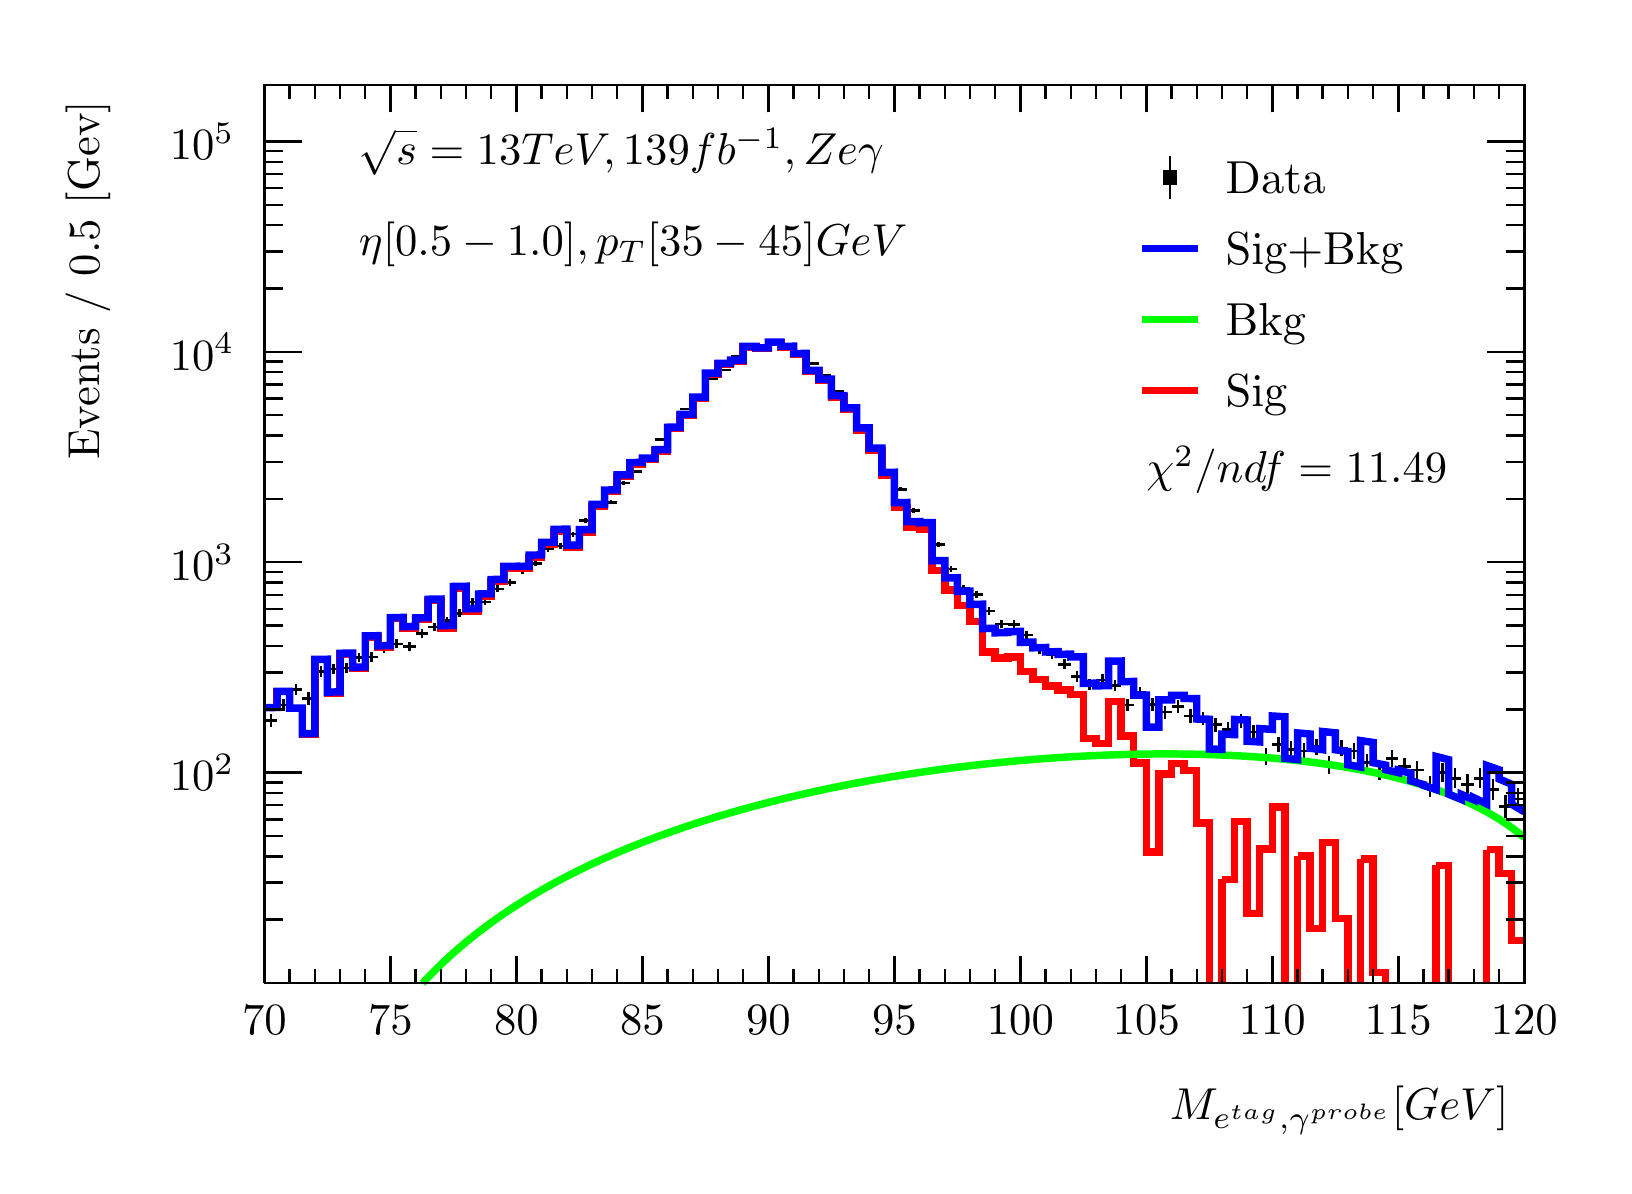
\begin{tikzpicture}
\pgfdeclareplotmark{cross} {
\pgfpathmoveto{\pgfpoint{-0.3\pgfplotmarksize}{\pgfplotmarksize}}
\pgfpathlineto{\pgfpoint{+0.3\pgfplotmarksize}{\pgfplotmarksize}}
\pgfpathlineto{\pgfpoint{+0.3\pgfplotmarksize}{0.3\pgfplotmarksize}}
\pgfpathlineto{\pgfpoint{+1\pgfplotmarksize}{0.3\pgfplotmarksize}}
\pgfpathlineto{\pgfpoint{+1\pgfplotmarksize}{-0.3\pgfplotmarksize}}
\pgfpathlineto{\pgfpoint{+0.3\pgfplotmarksize}{-0.3\pgfplotmarksize}}
\pgfpathlineto{\pgfpoint{+0.3\pgfplotmarksize}{-1.\pgfplotmarksize}}
\pgfpathlineto{\pgfpoint{-0.3\pgfplotmarksize}{-1.\pgfplotmarksize}}
\pgfpathlineto{\pgfpoint{-0.3\pgfplotmarksize}{-0.3\pgfplotmarksize}}
\pgfpathlineto{\pgfpoint{-1.\pgfplotmarksize}{-0.3\pgfplotmarksize}}
\pgfpathlineto{\pgfpoint{-1.\pgfplotmarksize}{0.3\pgfplotmarksize}}
\pgfpathlineto{\pgfpoint{-0.3\pgfplotmarksize}{0.3\pgfplotmarksize}}
\pgfpathclose
\pgfusepathqstroke
}
\pgfdeclareplotmark{cross*} {
\pgfpathmoveto{\pgfpoint{-0.3\pgfplotmarksize}{\pgfplotmarksize}}
\pgfpathlineto{\pgfpoint{+0.3\pgfplotmarksize}{\pgfplotmarksize}}
\pgfpathlineto{\pgfpoint{+0.3\pgfplotmarksize}{0.3\pgfplotmarksize}}
\pgfpathlineto{\pgfpoint{+1\pgfplotmarksize}{0.3\pgfplotmarksize}}
\pgfpathlineto{\pgfpoint{+1\pgfplotmarksize}{-0.3\pgfplotmarksize}}
\pgfpathlineto{\pgfpoint{+0.3\pgfplotmarksize}{-0.3\pgfplotmarksize}}
\pgfpathlineto{\pgfpoint{+0.3\pgfplotmarksize}{-1.\pgfplotmarksize}}
\pgfpathlineto{\pgfpoint{-0.3\pgfplotmarksize}{-1.\pgfplotmarksize}}
\pgfpathlineto{\pgfpoint{-0.3\pgfplotmarksize}{-0.3\pgfplotmarksize}}
\pgfpathlineto{\pgfpoint{-1.\pgfplotmarksize}{-0.3\pgfplotmarksize}}
\pgfpathlineto{\pgfpoint{-1.\pgfplotmarksize}{0.3\pgfplotmarksize}}
\pgfpathlineto{\pgfpoint{-0.3\pgfplotmarksize}{0.3\pgfplotmarksize}}
\pgfpathclose
\pgfusepathqfillstroke
}
\pgfdeclareplotmark{newstar} {
\pgfpathmoveto{\pgfqpoint{0pt}{\pgfplotmarksize}}
\pgfpathlineto{\pgfqpointpolar{44}{0.5\pgfplotmarksize}}
\pgfpathlineto{\pgfqpointpolar{18}{\pgfplotmarksize}}
\pgfpathlineto{\pgfqpointpolar{-20}{0.5\pgfplotmarksize}}
\pgfpathlineto{\pgfqpointpolar{-54}{\pgfplotmarksize}}
\pgfpathlineto{\pgfqpointpolar{-90}{0.5\pgfplotmarksize}}
\pgfpathlineto{\pgfqpointpolar{234}{\pgfplotmarksize}}
\pgfpathlineto{\pgfqpointpolar{198}{0.5\pgfplotmarksize}}
\pgfpathlineto{\pgfqpointpolar{162}{\pgfplotmarksize}}
\pgfpathlineto{\pgfqpointpolar{134}{0.5\pgfplotmarksize}}
\pgfpathclose
\pgfusepathqstroke
}
\pgfdeclareplotmark{newstar*} {
\pgfpathmoveto{\pgfqpoint{0pt}{\pgfplotmarksize}}
\pgfpathlineto{\pgfqpointpolar{44}{0.5\pgfplotmarksize}}
\pgfpathlineto{\pgfqpointpolar{18}{\pgfplotmarksize}}
\pgfpathlineto{\pgfqpointpolar{-20}{0.5\pgfplotmarksize}}
\pgfpathlineto{\pgfqpointpolar{-54}{\pgfplotmarksize}}
\pgfpathlineto{\pgfqpointpolar{-90}{0.5\pgfplotmarksize}}
\pgfpathlineto{\pgfqpointpolar{234}{\pgfplotmarksize}}
\pgfpathlineto{\pgfqpointpolar{198}{0.5\pgfplotmarksize}}
\pgfpathlineto{\pgfqpointpolar{162}{\pgfplotmarksize}}
\pgfpathlineto{\pgfqpointpolar{134}{0.5\pgfplotmarksize}}
\pgfpathclose
\pgfusepathqfillstroke
}
\definecolor{c}{rgb}{1,1,1};
\draw [color=c, fill=c] (0,0) rectangle (20,14.4361);
\draw [color=c, fill=c] (3,2.30977) rectangle (19,13.7143);
\definecolor{c}{rgb}{0,0,0};
\draw [c,line width=0.9] (3,2.30977) -- (3,13.7143) -- (19,13.7143) -- (19,2.30977) -- (3,2.30977);
\definecolor{c}{rgb}{1,1,1};
\draw [color=c, fill=c] (3,2.30977) rectangle (19,13.7143);
\definecolor{c}{rgb}{0,0,0};
\draw [c,line width=0.9] (3,2.30977) -- (3,13.7143) -- (19,13.7143) -- (19,2.30977) -- (3,2.30977);
\draw [c,line width=0.9] (3,2.30977) -- (19,2.30977);
\draw [c,line width=0.9] (3,2.65624) -- (3,2.30977);
\draw [c,line width=0.9] (3.32,2.48301) -- (3.32,2.30977);
\draw [c,line width=0.9] (3.64,2.48301) -- (3.64,2.30977);
\draw [c,line width=0.9] (3.96,2.48301) -- (3.96,2.30977);
\draw [c,line width=0.9] (4.28,2.48301) -- (4.28,2.30977);
\draw [c,line width=0.9] (4.6,2.65624) -- (4.6,2.30977);
\draw [c,line width=0.9] (4.92,2.48301) -- (4.92,2.30977);
\draw [c,line width=0.9] (5.24,2.48301) -- (5.24,2.30977);
\draw [c,line width=0.9] (5.56,2.48301) -- (5.56,2.30977);
\draw [c,line width=0.9] (5.88,2.48301) -- (5.88,2.30977);
\draw [c,line width=0.9] (6.2,2.65624) -- (6.2,2.30977);
\draw [c,line width=0.9] (6.52,2.48301) -- (6.52,2.30977);
\draw [c,line width=0.9] (6.84,2.48301) -- (6.84,2.30977);
\draw [c,line width=0.9] (7.16,2.48301) -- (7.16,2.30977);
\draw [c,line width=0.9] (7.48,2.48301) -- (7.48,2.30977);
\draw [c,line width=0.9] (7.8,2.65624) -- (7.8,2.30977);
\draw [c,line width=0.9] (8.12,2.48301) -- (8.12,2.30977);
\draw [c,line width=0.9] (8.44,2.48301) -- (8.44,2.30977);
\draw [c,line width=0.9] (8.76,2.48301) -- (8.76,2.30977);
\draw [c,line width=0.9] (9.08,2.48301) -- (9.08,2.30977);
\draw [c,line width=0.9] (9.4,2.65624) -- (9.4,2.30977);
\draw [c,line width=0.9] (9.72,2.48301) -- (9.72,2.30977);
\draw [c,line width=0.9] (10.04,2.48301) -- (10.04,2.30977);
\draw [c,line width=0.9] (10.36,2.48301) -- (10.36,2.30977);
\draw [c,line width=0.9] (10.68,2.48301) -- (10.68,2.30977);
\draw [c,line width=0.9] (11,2.65624) -- (11,2.30977);
\draw [c,line width=0.9] (11.32,2.48301) -- (11.32,2.30977);
\draw [c,line width=0.9] (11.64,2.48301) -- (11.64,2.30977);
\draw [c,line width=0.9] (11.96,2.48301) -- (11.96,2.30977);
\draw [c,line width=0.9] (12.28,2.48301) -- (12.28,2.30977);
\draw [c,line width=0.9] (12.6,2.65624) -- (12.6,2.30977);
\draw [c,line width=0.9] (12.92,2.48301) -- (12.92,2.30977);
\draw [c,line width=0.9] (13.24,2.48301) -- (13.24,2.30977);
\draw [c,line width=0.9] (13.56,2.48301) -- (13.56,2.30977);
\draw [c,line width=0.9] (13.88,2.48301) -- (13.88,2.30977);
\draw [c,line width=0.9] (14.2,2.65624) -- (14.2,2.30977);
\draw [c,line width=0.9] (14.52,2.48301) -- (14.52,2.30977);
\draw [c,line width=0.9] (14.84,2.48301) -- (14.84,2.30977);
\draw [c,line width=0.9] (15.16,2.48301) -- (15.16,2.30977);
\draw [c,line width=0.9] (15.48,2.48301) -- (15.48,2.30977);
\draw [c,line width=0.9] (15.8,2.65624) -- (15.8,2.30977);
\draw [c,line width=0.9] (16.12,2.48301) -- (16.12,2.30977);
\draw [c,line width=0.9] (16.44,2.48301) -- (16.44,2.30977);
\draw [c,line width=0.9] (16.76,2.48301) -- (16.76,2.30977);
\draw [c,line width=0.9] (17.08,2.48301) -- (17.08,2.30977);
\draw [c,line width=0.9] (17.4,2.65624) -- (17.4,2.30977);
\draw [c,line width=0.9] (17.72,2.48301) -- (17.72,2.30977);
\draw [c,line width=0.9] (18.04,2.48301) -- (18.04,2.30977);
\draw [c,line width=0.9] (18.36,2.48301) -- (18.36,2.30977);
\draw [c,line width=0.9] (18.68,2.48301) -- (18.68,2.30977);
\draw [c,line width=0.9] (19,2.65624) -- (19,2.30977);
\draw [anchor=base] (3,1.66015) node[scale=1.61424, color=c, rotate=0]{70};
\draw [anchor=base] (4.6,1.66015) node[scale=1.61424, color=c, rotate=0]{75};
\draw [anchor=base] (6.2,1.66015) node[scale=1.61424, color=c, rotate=0]{80};
\draw [anchor=base] (7.8,1.66015) node[scale=1.61424, color=c, rotate=0]{85};
\draw [anchor=base] (9.4,1.66015) node[scale=1.61424, color=c, rotate=0]{90};
\draw [anchor=base] (11,1.66015) node[scale=1.61424, color=c, rotate=0]{95};
\draw [anchor=base] (12.6,1.66015) node[scale=1.61424, color=c, rotate=0]{100};
\draw [anchor=base] (14.2,1.66015) node[scale=1.61424, color=c, rotate=0]{105};
\draw [anchor=base] (15.8,1.66015) node[scale=1.61424, color=c, rotate=0]{110};
\draw [anchor=base] (17.4,1.66015) node[scale=1.61424, color=c, rotate=0]{115};
\draw [anchor=base] (19,1.66015) node[scale=1.61424, color=c, rotate=0]{120};
\draw [anchor= east] (19,0.692932) node[scale=1.61424, color=c, rotate=0]{$M_{e^{tag}, \gamma^{probe}}  [GeV]$};
\draw [c,line width=0.9] (3,13.7143) -- (19,13.7143);
\draw [c,line width=0.9] (3,13.3678) -- (3,13.7143);
\draw [c,line width=0.9] (3.32,13.5411) -- (3.32,13.7143);
\draw [c,line width=0.9] (3.64,13.5411) -- (3.64,13.7143);
\draw [c,line width=0.9] (3.96,13.5411) -- (3.96,13.7143);
\draw [c,line width=0.9] (4.28,13.5411) -- (4.28,13.7143);
\draw [c,line width=0.9] (4.6,13.3678) -- (4.6,13.7143);
\draw [c,line width=0.9] (4.92,13.5411) -- (4.92,13.7143);
\draw [c,line width=0.9] (5.24,13.5411) -- (5.24,13.7143);
\draw [c,line width=0.9] (5.56,13.5411) -- (5.56,13.7143);
\draw [c,line width=0.9] (5.88,13.5411) -- (5.88,13.7143);
\draw [c,line width=0.9] (6.2,13.3678) -- (6.2,13.7143);
\draw [c,line width=0.9] (6.52,13.5411) -- (6.52,13.7143);
\draw [c,line width=0.9] (6.84,13.5411) -- (6.84,13.7143);
\draw [c,line width=0.9] (7.16,13.5411) -- (7.16,13.7143);
\draw [c,line width=0.9] (7.48,13.5411) -- (7.48,13.7143);
\draw [c,line width=0.9] (7.8,13.3678) -- (7.8,13.7143);
\draw [c,line width=0.9] (8.12,13.5411) -- (8.12,13.7143);
\draw [c,line width=0.9] (8.44,13.5411) -- (8.44,13.7143);
\draw [c,line width=0.9] (8.76,13.5411) -- (8.76,13.7143);
\draw [c,line width=0.9] (9.08,13.5411) -- (9.08,13.7143);
\draw [c,line width=0.9] (9.4,13.3678) -- (9.4,13.7143);
\draw [c,line width=0.9] (9.72,13.5411) -- (9.72,13.7143);
\draw [c,line width=0.9] (10.04,13.5411) -- (10.04,13.7143);
\draw [c,line width=0.9] (10.36,13.5411) -- (10.36,13.7143);
\draw [c,line width=0.9] (10.68,13.5411) -- (10.68,13.7143);
\draw [c,line width=0.9] (11,13.3678) -- (11,13.7143);
\draw [c,line width=0.9] (11.32,13.5411) -- (11.32,13.7143);
\draw [c,line width=0.9] (11.64,13.5411) -- (11.64,13.7143);
\draw [c,line width=0.9] (11.96,13.5411) -- (11.96,13.7143);
\draw [c,line width=0.9] (12.28,13.5411) -- (12.28,13.7143);
\draw [c,line width=0.9] (12.6,13.3678) -- (12.6,13.7143);
\draw [c,line width=0.9] (12.92,13.5411) -- (12.92,13.7143);
\draw [c,line width=0.9] (13.24,13.5411) -- (13.24,13.7143);
\draw [c,line width=0.9] (13.56,13.5411) -- (13.56,13.7143);
\draw [c,line width=0.9] (13.88,13.5411) -- (13.88,13.7143);
\draw [c,line width=0.9] (14.2,13.3678) -- (14.2,13.7143);
\draw [c,line width=0.9] (14.52,13.5411) -- (14.52,13.7143);
\draw [c,line width=0.9] (14.84,13.5411) -- (14.84,13.7143);
\draw [c,line width=0.9] (15.16,13.5411) -- (15.16,13.7143);
\draw [c,line width=0.9] (15.48,13.5411) -- (15.48,13.7143);
\draw [c,line width=0.9] (15.8,13.3678) -- (15.8,13.7143);
\draw [c,line width=0.9] (16.12,13.5411) -- (16.12,13.7143);
\draw [c,line width=0.9] (16.44,13.5411) -- (16.44,13.7143);
\draw [c,line width=0.9] (16.76,13.5411) -- (16.76,13.7143);
\draw [c,line width=0.9] (17.08,13.5411) -- (17.08,13.7143);
\draw [c,line width=0.9] (17.4,13.3678) -- (17.4,13.7143);
\draw [c,line width=0.9] (17.72,13.5411) -- (17.72,13.7143);
\draw [c,line width=0.9] (18.04,13.5411) -- (18.04,13.7143);
\draw [c,line width=0.9] (18.36,13.5411) -- (18.36,13.7143);
\draw [c,line width=0.9] (18.68,13.5411) -- (18.68,13.7143);
\draw [c,line width=0.9] (19,13.3678) -- (19,13.7143);
\draw [c,line width=0.9] (3,2.30977) -- (3,13.7143);
\draw [c,line width=0.9] (3.237,3.11414) -- (3,3.11414);
\draw [c,line width=0.9] (3.237,3.58467) -- (3,3.58467);
\draw [c,line width=0.9] (3.237,3.91852) -- (3,3.91852);
\draw [c,line width=0.9] (3.237,4.17747) -- (3,4.17747);
\draw [c,line width=0.9] (3.237,4.38904) -- (3,4.38904);
\draw [c,line width=0.9] (3.237,4.56793) -- (3,4.56793);
\draw [c,line width=0.9] (3.237,4.72289) -- (3,4.72289);
\draw [c,line width=0.9] (3.237,4.85957) -- (3,4.85957);
\draw [c,line width=0.9] (3.474,4.98184) -- (3,4.98184);
\draw [anchor= east] (2.82,4.98184) node[scale=1.61424, color=c, rotate=0]{$10^{2}$};
\draw [c,line width=0.9] (3.237,5.78621) -- (3,5.78621);
\draw [c,line width=0.9] (3.237,6.25674) -- (3,6.25674);
\draw [c,line width=0.9] (3.237,6.59058) -- (3,6.59058);
\draw [c,line width=0.9] (3.237,6.84953) -- (3,6.84953);
\draw [c,line width=0.9] (3.237,7.06111) -- (3,7.06111);
\draw [c,line width=0.9] (3.237,7.24) -- (3,7.24);
\draw [c,line width=0.9] (3.237,7.39496) -- (3,7.39496);
\draw [c,line width=0.9] (3.237,7.53164) -- (3,7.53164);
\draw [c,line width=0.9] (3.474,7.65391) -- (3,7.65391);
\draw [anchor= east] (2.82,7.65391) node[scale=1.61424, color=c, rotate=0]{$10^{3}$};
\draw [c,line width=0.9] (3.237,8.45828) -- (3,8.45828);
\draw [c,line width=0.9] (3.237,8.92881) -- (3,8.92881);
\draw [c,line width=0.9] (3.237,9.26265) -- (3,9.26265);
\draw [c,line width=0.9] (3.237,9.5216) -- (3,9.5216);
\draw [c,line width=0.9] (3.237,9.73318) -- (3,9.73318);
\draw [c,line width=0.9] (3.237,9.91207) -- (3,9.91207);
\draw [c,line width=0.9] (3.237,10.067) -- (3,10.067);
\draw [c,line width=0.9] (3.237,10.2037) -- (3,10.2037);
\draw [c,line width=0.9] (3.474,10.326) -- (3,10.326);
\draw [anchor= east] (2.82,10.326) node[scale=1.61424, color=c, rotate=0]{$10^{4}$};
\draw [c,line width=0.9] (3.237,11.1303) -- (3,11.1303);
\draw [c,line width=0.9] (3.237,11.6009) -- (3,11.6009);
\draw [c,line width=0.9] (3.237,11.9347) -- (3,11.9347);
\draw [c,line width=0.9] (3.237,12.1937) -- (3,12.1937);
\draw [c,line width=0.9] (3.237,12.4052) -- (3,12.4052);
\draw [c,line width=0.9] (3.237,12.5841) -- (3,12.5841);
\draw [c,line width=0.9] (3.237,12.7391) -- (3,12.7391);
\draw [c,line width=0.9] (3.237,12.8758) -- (3,12.8758);
\draw [c,line width=0.9] (3.474,12.998) -- (3,12.998);
\draw [anchor= east] (2.82,12.998) node[scale=1.61424, color=c, rotate=0]{$10^{5}$};
\draw [anchor= east] (0.76,13.7143) node[scale=1.61424, color=c, rotate=90]{Events / 0.5 [Gev]};
\draw [c,line width=0.9] (19,2.30977) -- (19,13.7143);
\draw [c,line width=0.9] (18.763,3.11414) -- (19,3.11414);
\draw [c,line width=0.9] (18.763,3.58467) -- (19,3.58467);
\draw [c,line width=0.9] (18.763,3.91852) -- (19,3.91852);
\draw [c,line width=0.9] (18.763,4.17747) -- (19,4.17747);
\draw [c,line width=0.9] (18.763,4.38904) -- (19,4.38904);
\draw [c,line width=0.9] (18.763,4.56793) -- (19,4.56793);
\draw [c,line width=0.9] (18.763,4.72289) -- (19,4.72289);
\draw [c,line width=0.9] (18.763,4.85957) -- (19,4.85957);
\draw [c,line width=0.9] (18.526,4.98184) -- (19,4.98184);
\draw [c,line width=0.9] (18.763,5.78621) -- (19,5.78621);
\draw [c,line width=0.9] (18.763,6.25674) -- (19,6.25674);
\draw [c,line width=0.9] (18.763,6.59058) -- (19,6.59058);
\draw [c,line width=0.9] (18.763,6.84953) -- (19,6.84953);
\draw [c,line width=0.9] (18.763,7.06111) -- (19,7.06111);
\draw [c,line width=0.9] (18.763,7.24) -- (19,7.24);
\draw [c,line width=0.9] (18.763,7.39496) -- (19,7.39496);
\draw [c,line width=0.9] (18.763,7.53164) -- (19,7.53164);
\draw [c,line width=0.9] (18.526,7.65391) -- (19,7.65391);
\draw [c,line width=0.9] (18.763,8.45828) -- (19,8.45828);
\draw [c,line width=0.9] (18.763,8.92881) -- (19,8.92881);
\draw [c,line width=0.9] (18.763,9.26265) -- (19,9.26265);
\draw [c,line width=0.9] (18.763,9.5216) -- (19,9.5216);
\draw [c,line width=0.9] (18.763,9.73318) -- (19,9.73318);
\draw [c,line width=0.9] (18.763,9.91207) -- (19,9.91207);
\draw [c,line width=0.9] (18.763,10.067) -- (19,10.067);
\draw [c,line width=0.9] (18.763,10.2037) -- (19,10.2037);
\draw [c,line width=0.9] (18.526,10.326) -- (19,10.326);
\draw [c,line width=0.9] (18.763,11.1303) -- (19,11.1303);
\draw [c,line width=0.9] (18.763,11.6009) -- (19,11.6009);
\draw [c,line width=0.9] (18.763,11.9347) -- (19,11.9347);
\draw [c,line width=0.9] (18.763,12.1937) -- (19,12.1937);
\draw [c,line width=0.9] (18.763,12.4052) -- (19,12.4052);
\draw [c,line width=0.9] (18.763,12.5841) -- (19,12.5841);
\draw [c,line width=0.9] (18.763,12.7391) -- (19,12.7391);
\draw [c,line width=0.9] (18.763,12.8758) -- (19,12.8758);
\draw [c,line width=0.9] (18.526,12.998) -- (19,12.998);
\draw [c,line width=0.9] (3.08,5.64444) -- (3,5.64444);
\draw [c,line width=0.9] (3,5.64444) -- (3,5.64444);
\draw [c,line width=0.9] (3.08,5.64444) -- (3.16,5.64444);
\draw [c,line width=0.9] (3.16,5.64444) -- (3.16,5.64444);
\draw [c,line width=0.9] (3.08,5.64444) -- (3.08,5.73165);
\draw [c,line width=0.9] (3.08,5.73165) -- (3.08,5.73165);
\draw [c,line width=0.9] (3.08,5.64444) -- (3.08,5.55724);
\draw [c,line width=0.9] (3.08,5.55724) -- (3.08,5.55724);
\draw [c,line width=0.9] (3.24,5.84283) -- (3.16,5.84283);
\draw [c,line width=0.9] (3.16,5.84283) -- (3.16,5.84283);
\draw [c,line width=0.9] (3.24,5.84283) -- (3.32,5.84283);
\draw [c,line width=0.9] (3.32,5.84283) -- (3.32,5.84283);
\draw [c,line width=0.9] (3.24,5.84283) -- (3.24,5.9229);
\draw [c,line width=0.9] (3.24,5.9229) -- (3.24,5.9229);
\draw [c,line width=0.9] (3.24,5.84283) -- (3.24,5.76277);
\draw [c,line width=0.9] (3.24,5.76277) -- (3.24,5.76277);
\draw [c,line width=0.9] (3.4,6.03584) -- (3.32,6.03584);
\draw [c,line width=0.9] (3.32,6.03584) -- (3.32,6.03584);
\draw [c,line width=0.9] (3.4,6.03584) -- (3.48,6.03584);
\draw [c,line width=0.9] (3.48,6.03584) -- (3.48,6.03584);
\draw [c,line width=0.9] (3.4,6.03584) -- (3.4,6.10952);
\draw [c,line width=0.9] (3.4,6.10952) -- (3.4,6.10952);
\draw [c,line width=0.9] (3.4,6.03584) -- (3.4,5.96217);
\draw [c,line width=0.9] (3.4,5.96217) -- (3.4,5.96217);
\draw [c,line width=0.9] (3.56,5.9229) -- (3.48,5.9229);
\draw [c,line width=0.9] (3.48,5.9229) -- (3.48,5.9229);
\draw [c,line width=0.9] (3.56,5.9229) -- (3.64,5.9229);
\draw [c,line width=0.9] (3.64,5.9229) -- (3.64,5.9229);
\draw [c,line width=0.9] (3.56,5.9229) -- (3.56,6.00025);
\draw [c,line width=0.9] (3.56,6.00025) -- (3.56,6.00025);
\draw [c,line width=0.9] (3.56,5.9229) -- (3.56,5.84555);
\draw [c,line width=0.9] (3.56,5.84555) -- (3.56,5.84555);
\draw [c,line width=0.9] (3.72,6.26445) -- (3.64,6.26445);
\draw [c,line width=0.9] (3.64,6.26445) -- (3.64,6.26445);
\draw [c,line width=0.9] (3.72,6.26445) -- (3.8,6.26445);
\draw [c,line width=0.9] (3.8,6.26445) -- (3.8,6.26445);
\draw [c,line width=0.9] (3.72,6.26445) -- (3.72,6.33122);
\draw [c,line width=0.9] (3.72,6.33122) -- (3.72,6.33122);
\draw [c,line width=0.9] (3.72,6.26445) -- (3.72,6.19768);
\draw [c,line width=0.9] (3.72,6.19768) -- (3.72,6.19768);
\draw [c,line width=0.9] (3.88,6.29853) -- (3.8,6.29853);
\draw [c,line width=0.9] (3.8,6.29853) -- (3.8,6.29853);
\draw [c,line width=0.9] (3.88,6.29853) -- (3.96,6.29853);
\draw [c,line width=0.9] (3.96,6.29853) -- (3.96,6.29853);
\draw [c,line width=0.9] (3.88,6.29853) -- (3.88,6.36433);
\draw [c,line width=0.9] (3.88,6.36433) -- (3.88,6.36433);
\draw [c,line width=0.9] (3.88,6.29853) -- (3.88,6.23273);
\draw [c,line width=0.9] (3.88,6.23273) -- (3.88,6.23273);
\draw [c,line width=0.9] (4.04,6.30967) -- (3.96,6.30967);
\draw [c,line width=0.9] (3.96,6.30967) -- (3.96,6.30967);
\draw [c,line width=0.9] (4.04,6.30967) -- (4.12,6.30967);
\draw [c,line width=0.9] (4.12,6.30967) -- (4.12,6.30967);
\draw [c,line width=0.9] (4.04,6.30967) -- (4.04,6.37515);
\draw [c,line width=0.9] (4.04,6.37515) -- (4.04,6.37515);
\draw [c,line width=0.9] (4.04,6.30967) -- (4.04,6.24419);
\draw [c,line width=0.9] (4.04,6.24419) -- (4.04,6.24419);
\draw [c,line width=0.9] (4.2,6.44553) -- (4.12,6.44553);
\draw [c,line width=0.9] (4.12,6.44553) -- (4.12,6.44553);
\draw [c,line width=0.9] (4.2,6.44553) -- (4.28,6.44553);
\draw [c,line width=0.9] (4.28,6.44553) -- (4.28,6.44553);
\draw [c,line width=0.9] (4.2,6.44553) -- (4.2,6.50729);
\draw [c,line width=0.9] (4.2,6.50729) -- (4.2,6.50729);
\draw [c,line width=0.9] (4.2,6.44553) -- (4.2,6.38377);
\draw [c,line width=0.9] (4.2,6.38377) -- (4.2,6.38377);
\draw [c,line width=0.9] (4.36,6.45209) -- (4.28,6.45209);
\draw [c,line width=0.9] (4.28,6.45209) -- (4.28,6.45209);
\draw [c,line width=0.9] (4.36,6.45209) -- (4.44,6.45209);
\draw [c,line width=0.9] (4.44,6.45209) -- (4.44,6.45209);
\draw [c,line width=0.9] (4.36,6.45209) -- (4.36,6.51367);
\draw [c,line width=0.9] (4.36,6.51367) -- (4.36,6.51367);
\draw [c,line width=0.9] (4.36,6.45209) -- (4.36,6.3905);
\draw [c,line width=0.9] (4.36,6.3905) -- (4.36,6.3905);
\draw [c,line width=0.9] (4.52,6.55823) -- (4.44,6.55823);
\draw [c,line width=0.9] (4.44,6.55823) -- (4.44,6.55823);
\draw [c,line width=0.9] (4.52,6.55823) -- (4.6,6.55823);
\draw [c,line width=0.9] (4.6,6.55823) -- (4.6,6.55823);
\draw [c,line width=0.9] (4.52,6.55823) -- (4.52,6.61706);
\draw [c,line width=0.9] (4.52,6.61706) -- (4.52,6.61706);
\draw [c,line width=0.9] (4.52,6.55823) -- (4.52,6.49939);
\draw [c,line width=0.9] (4.52,6.49939) -- (4.52,6.49939);
\draw [c,line width=0.9] (4.68,6.61641) -- (4.6,6.61641);
\draw [c,line width=0.9] (4.6,6.61641) -- (4.6,6.61641);
\draw [c,line width=0.9] (4.68,6.61641) -- (4.76,6.61641);
\draw [c,line width=0.9] (4.76,6.61641) -- (4.76,6.61641);
\draw [c,line width=0.9] (4.68,6.61641) -- (4.68,6.67378);
\draw [c,line width=0.9] (4.68,6.67378) -- (4.68,6.67378);
\draw [c,line width=0.9] (4.68,6.61641) -- (4.68,6.55903);
\draw [c,line width=0.9] (4.68,6.55903) -- (4.68,6.55903);
\draw [c,line width=0.9] (4.84,6.58477) -- (4.76,6.58477);
\draw [c,line width=0.9] (4.76,6.58477) -- (4.76,6.58477);
\draw [c,line width=0.9] (4.84,6.58477) -- (4.92,6.58477);
\draw [c,line width=0.9] (4.92,6.58477) -- (4.92,6.58477);
\draw [c,line width=0.9] (4.84,6.58477) -- (4.84,6.64293);
\draw [c,line width=0.9] (4.84,6.64293) -- (4.84,6.64293);
\draw [c,line width=0.9] (4.84,6.58477) -- (4.84,6.52661);
\draw [c,line width=0.9] (4.84,6.52661) -- (4.84,6.52661);
\draw [c,line width=0.9] (5,6.74772) -- (4.92,6.74772);
\draw [c,line width=0.9] (4.92,6.74772) -- (4.92,6.74772);
\draw [c,line width=0.9] (5,6.74772) -- (5.08,6.74772);
\draw [c,line width=0.9] (5.08,6.74772) -- (5.08,6.74772);
\draw [c,line width=0.9] (5,6.74772) -- (5,6.80194);
\draw [c,line width=0.9] (5,6.80194) -- (5,6.80194);
\draw [c,line width=0.9] (5,6.74772) -- (5,6.6935);
\draw [c,line width=0.9] (5,6.6935) -- (5,6.6935);
\draw [c,line width=0.9] (5.16,6.83317) -- (5.08,6.83317);
\draw [c,line width=0.9] (5.08,6.83317) -- (5.08,6.83317);
\draw [c,line width=0.9] (5.16,6.83317) -- (5.24,6.83317);
\draw [c,line width=0.9] (5.24,6.83317) -- (5.24,6.83317);
\draw [c,line width=0.9] (5.16,6.83317) -- (5.16,6.88543);
\draw [c,line width=0.9] (5.16,6.88543) -- (5.16,6.88543);
\draw [c,line width=0.9] (5.16,6.83317) -- (5.16,6.78091);
\draw [c,line width=0.9] (5.16,6.78091) -- (5.16,6.78091);
\draw [c,line width=0.9] (5.32,6.91277) -- (5.24,6.91277);
\draw [c,line width=0.9] (5.24,6.91277) -- (5.24,6.91277);
\draw [c,line width=0.9] (5.32,6.91277) -- (5.4,6.91277);
\draw [c,line width=0.9] (5.4,6.91277) -- (5.4,6.91277);
\draw [c,line width=0.9] (5.32,6.91277) -- (5.32,6.96327);
\draw [c,line width=0.9] (5.32,6.96327) -- (5.32,6.96327);
\draw [c,line width=0.9] (5.32,6.91277) -- (5.32,6.86227);
\draw [c,line width=0.9] (5.32,6.86227) -- (5.32,6.86227);
\draw [c,line width=0.9] (5.48,7.00565) -- (5.4,7.00565);
\draw [c,line width=0.9] (5.4,7.00565) -- (5.4,7.00565);
\draw [c,line width=0.9] (5.48,7.00565) -- (5.56,7.00565);
\draw [c,line width=0.9] (5.56,7.00565) -- (5.56,7.00565);
\draw [c,line width=0.9] (5.48,7.00565) -- (5.48,7.05417);
\draw [c,line width=0.9] (5.48,7.05417) -- (5.48,7.05417);
\draw [c,line width=0.9] (5.48,7.00565) -- (5.48,6.95714);
\draw [c,line width=0.9] (5.48,6.95714) -- (5.48,6.95714);
\draw [c,line width=0.9] (5.64,7.15042) -- (5.56,7.15042);
\draw [c,line width=0.9] (5.56,7.15042) -- (5.56,7.15042);
\draw [c,line width=0.9] (5.64,7.15042) -- (5.72,7.15042);
\draw [c,line width=0.9] (5.72,7.15042) -- (5.72,7.15042);
\draw [c,line width=0.9] (5.64,7.15042) -- (5.64,7.19601);
\draw [c,line width=0.9] (5.64,7.19601) -- (5.64,7.19601);
\draw [c,line width=0.9] (5.64,7.15042) -- (5.64,7.10484);
\draw [c,line width=0.9] (5.64,7.10484) -- (5.64,7.10484);
\draw [c,line width=0.9] (5.8,7.15042) -- (5.72,7.15042);
\draw [c,line width=0.9] (5.72,7.15042) -- (5.72,7.15042);
\draw [c,line width=0.9] (5.8,7.15042) -- (5.88,7.15042);
\draw [c,line width=0.9] (5.88,7.15042) -- (5.88,7.15042);
\draw [c,line width=0.9] (5.8,7.15042) -- (5.8,7.19601);
\draw [c,line width=0.9] (5.8,7.19601) -- (5.8,7.19601);
\draw [c,line width=0.9] (5.8,7.15042) -- (5.8,7.10484);
\draw [c,line width=0.9] (5.8,7.10484) -- (5.8,7.10484);
\draw [c,line width=0.9] (5.96,7.31696) -- (5.88,7.31696);
\draw [c,line width=0.9] (5.88,7.31696) -- (5.88,7.31696);
\draw [c,line width=0.9] (5.96,7.31696) -- (6.04,7.31696);
\draw [c,line width=0.9] (6.04,7.31696) -- (6.04,7.31696);
\draw [c,line width=0.9] (5.96,7.31696) -- (5.96,7.35939);
\draw [c,line width=0.9] (5.96,7.35939) -- (5.96,7.35939);
\draw [c,line width=0.9] (5.96,7.31696) -- (5.96,7.27454);
\draw [c,line width=0.9] (5.96,7.27454) -- (5.96,7.27454);
\draw [c,line width=0.9] (6.12,7.3993) -- (6.04,7.3993);
\draw [c,line width=0.9] (6.04,7.3993) -- (6.04,7.3993);
\draw [c,line width=0.9] (6.12,7.3993) -- (6.2,7.3993);
\draw [c,line width=0.9] (6.2,7.3993) -- (6.2,7.3993);
\draw [c,line width=0.9] (6.12,7.3993) -- (6.12,7.44025);
\draw [c,line width=0.9] (6.12,7.44025) -- (6.12,7.44025);
\draw [c,line width=0.9] (6.12,7.3993) -- (6.12,7.35835);
\draw [c,line width=0.9] (6.12,7.35835) -- (6.12,7.35835);
\draw [c,line width=0.9] (6.28,7.54701) -- (6.2,7.54701);
\draw [c,line width=0.9] (6.2,7.54701) -- (6.2,7.54701);
\draw [c,line width=0.9] (6.28,7.54701) -- (6.36,7.54701);
\draw [c,line width=0.9] (6.36,7.54701) -- (6.36,7.54701);
\draw [c,line width=0.9] (6.28,7.54701) -- (6.28,7.58544);
\draw [c,line width=0.9] (6.28,7.58544) -- (6.28,7.58544);
\draw [c,line width=0.9] (6.28,7.54701) -- (6.28,7.50859);
\draw [c,line width=0.9] (6.28,7.50859) -- (6.28,7.50859);
\draw [c,line width=0.9] (6.44,7.63755) -- (6.36,7.63755);
\draw [c,line width=0.9] (6.36,7.63755) -- (6.36,7.63755);
\draw [c,line width=0.9] (6.44,7.63755) -- (6.52,7.63755);
\draw [c,line width=0.9] (6.52,7.63755) -- (6.52,7.63755);
\draw [c,line width=0.9] (6.44,7.63755) -- (6.44,7.6745);
\draw [c,line width=0.9] (6.44,7.6745) -- (6.44,7.6745);
\draw [c,line width=0.9] (6.44,7.63755) -- (6.44,7.60059);
\draw [c,line width=0.9] (6.44,7.60059) -- (6.44,7.60059);
\draw [c,line width=0.9] (6.6,7.82113) -- (6.52,7.82113);
\draw [c,line width=0.9] (6.52,7.82113) -- (6.52,7.82113);
\draw [c,line width=0.9] (6.6,7.82113) -- (6.68,7.82113);
\draw [c,line width=0.9] (6.68,7.82113) -- (6.68,7.82113);
\draw [c,line width=0.9] (6.6,7.82113) -- (6.6,7.85528);
\draw [c,line width=0.9] (6.6,7.85528) -- (6.6,7.85528);
\draw [c,line width=0.9] (6.6,7.82113) -- (6.6,7.78699);
\draw [c,line width=0.9] (6.6,7.78699) -- (6.6,7.78699);
\draw [c,line width=0.9] (6.76,7.8587) -- (6.68,7.8587);
\draw [c,line width=0.9] (6.68,7.8587) -- (6.68,7.8587);
\draw [c,line width=0.9] (6.76,7.8587) -- (6.84,7.8587);
\draw [c,line width=0.9] (6.84,7.8587) -- (6.84,7.8587);
\draw [c,line width=0.9] (6.76,7.8587) -- (6.76,7.89229);
\draw [c,line width=0.9] (6.76,7.89229) -- (6.76,7.89229);
\draw [c,line width=0.9] (6.76,7.8587) -- (6.76,7.8251);
\draw [c,line width=0.9] (6.76,7.8251) -- (6.76,7.8251);
\draw [c,line width=0.9] (6.92,8.00988) -- (6.84,8.00988);
\draw [c,line width=0.9] (6.84,8.00988) -- (6.84,8.00988);
\draw [c,line width=0.9] (6.92,8.00988) -- (7,8.00988);
\draw [c,line width=0.9] (7,8.00988) -- (7,8.00988);
\draw [c,line width=0.9] (6.92,8.00988) -- (6.92,8.04136);
\draw [c,line width=0.9] (6.92,8.04136) -- (6.92,8.04136);
\draw [c,line width=0.9] (6.92,8.00988) -- (6.92,7.9784);
\draw [c,line width=0.9] (6.92,7.9784) -- (6.92,7.9784);
\draw [c,line width=0.9] (7.08,8.1862) -- (7,8.1862);
\draw [c,line width=0.9] (7,8.1862) -- (7,8.1862);
\draw [c,line width=0.9] (7.08,8.1862) -- (7.16,8.1862);
\draw [c,line width=0.9] (7.16,8.1862) -- (7.16,8.1862);
\draw [c,line width=0.9] (7.08,8.1862) -- (7.08,8.21538);
\draw [c,line width=0.9] (7.08,8.21538) -- (7.08,8.21538);
\draw [c,line width=0.9] (7.08,8.1862) -- (7.08,8.15703);
\draw [c,line width=0.9] (7.08,8.15703) -- (7.08,8.15703);
\draw [c,line width=0.9] (7.24,8.34756) -- (7.16,8.34756);
\draw [c,line width=0.9] (7.16,8.34756) -- (7.16,8.34756);
\draw [c,line width=0.9] (7.24,8.34756) -- (7.32,8.34756);
\draw [c,line width=0.9] (7.32,8.34756) -- (7.32,8.34756);
\draw [c,line width=0.9] (7.24,8.34756) -- (7.24,8.37478);
\draw [c,line width=0.9] (7.24,8.37478) -- (7.24,8.37478);
\draw [c,line width=0.9] (7.24,8.34756) -- (7.24,8.32034);
\draw [c,line width=0.9] (7.24,8.32034) -- (7.24,8.32034);
\draw [c,line width=0.9] (7.4,8.41513) -- (7.32,8.41513);
\draw [c,line width=0.9] (7.32,8.41513) -- (7.32,8.41513);
\draw [c,line width=0.9] (7.4,8.41513) -- (7.48,8.41513);
\draw [c,line width=0.9] (7.48,8.41513) -- (7.48,8.41513);
\draw [c,line width=0.9] (7.4,8.41513) -- (7.4,8.44157);
\draw [c,line width=0.9] (7.4,8.44157) -- (7.4,8.44157);
\draw [c,line width=0.9] (7.4,8.41513) -- (7.4,8.3887);
\draw [c,line width=0.9] (7.4,8.3887) -- (7.4,8.3887);
\draw [c,line width=0.9] (7.56,8.66307) -- (7.48,8.66307);
\draw [c,line width=0.9] (7.48,8.66307) -- (7.48,8.66307);
\draw [c,line width=0.9] (7.56,8.66307) -- (7.64,8.66307);
\draw [c,line width=0.9] (7.64,8.66307) -- (7.64,8.66307);
\draw [c,line width=0.9] (7.56,8.66307) -- (7.56,8.68683);
\draw [c,line width=0.9] (7.56,8.68683) -- (7.56,8.68683);
\draw [c,line width=0.9] (7.56,8.66307) -- (7.56,8.63931);
\draw [c,line width=0.9] (7.56,8.63931) -- (7.56,8.63931);
\draw [c,line width=0.9] (7.72,8.80439) -- (7.64,8.80439);
\draw [c,line width=0.9] (7.64,8.80439) -- (7.64,8.80439);
\draw [c,line width=0.9] (7.72,8.80439) -- (7.8,8.80439);
\draw [c,line width=0.9] (7.8,8.80439) -- (7.8,8.80439);
\draw [c,line width=0.9] (7.72,8.80439) -- (7.72,8.82674);
\draw [c,line width=0.9] (7.72,8.82674) -- (7.72,8.82674);
\draw [c,line width=0.9] (7.72,8.80439) -- (7.72,8.78204);
\draw [c,line width=0.9] (7.72,8.78204) -- (7.72,8.78204);
\draw [c,line width=0.9] (7.88,8.96761) -- (7.8,8.96761);
\draw [c,line width=0.9] (7.8,8.96761) -- (7.8,8.96761);
\draw [c,line width=0.9] (7.88,8.96761) -- (7.96,8.96761);
\draw [c,line width=0.9] (7.96,8.96761) -- (7.96,8.96761);
\draw [c,line width=0.9] (7.88,8.96761) -- (7.88,8.98844);
\draw [c,line width=0.9] (7.88,8.98844) -- (7.88,8.98844);
\draw [c,line width=0.9] (7.88,8.96761) -- (7.88,8.94677);
\draw [c,line width=0.9] (7.88,8.94677) -- (7.88,8.94677);
\draw [c,line width=0.9] (8.04,9.21377) -- (7.96,9.21377);
\draw [c,line width=0.9] (7.96,9.21377) -- (7.96,9.21377);
\draw [c,line width=0.9] (8.04,9.21377) -- (8.12,9.21377);
\draw [c,line width=0.9] (8.12,9.21377) -- (8.12,9.21377);
\draw [c,line width=0.9] (8.04,9.21377) -- (8.04,9.23251);
\draw [c,line width=0.9] (8.04,9.23251) -- (8.04,9.23251);
\draw [c,line width=0.9] (8.04,9.21377) -- (8.04,9.19503);
\draw [c,line width=0.9] (8.04,9.19503) -- (8.04,9.19503);
\draw [c,line width=0.9] (8.2,9.34523) -- (8.12,9.34523);
\draw [c,line width=0.9] (8.12,9.34523) -- (8.12,9.34523);
\draw [c,line width=0.9] (8.2,9.34523) -- (8.28,9.34523);
\draw [c,line width=0.9] (8.28,9.34523) -- (8.28,9.34523);
\draw [c,line width=0.9] (8.2,9.34523) -- (8.2,9.36294);
\draw [c,line width=0.9] (8.2,9.36294) -- (8.2,9.36294);
\draw [c,line width=0.9] (8.2,9.34523) -- (8.2,9.32752);
\draw [c,line width=0.9] (8.2,9.32752) -- (8.2,9.32752);
\draw [c,line width=0.9] (8.36,9.60055) -- (8.28,9.60055);
\draw [c,line width=0.9] (8.28,9.60055) -- (8.28,9.60055);
\draw [c,line width=0.9] (8.36,9.60055) -- (8.44,9.60055);
\draw [c,line width=0.9] (8.44,9.60055) -- (8.44,9.60055);
\draw [c,line width=0.9] (8.36,9.60055) -- (8.36,9.61641);
\draw [c,line width=0.9] (8.36,9.61641) -- (8.36,9.61641);
\draw [c,line width=0.9] (8.36,9.60055) -- (8.36,9.58469);
\draw [c,line width=0.9] (8.36,9.58469) -- (8.36,9.58469);
\draw [c,line width=0.9] (8.52,9.77553) -- (8.44,9.77553);
\draw [c,line width=0.9] (8.44,9.77553) -- (8.44,9.77553);
\draw [c,line width=0.9] (8.52,9.77553) -- (8.6,9.77553);
\draw [c,line width=0.9] (8.6,9.77553) -- (8.6,9.77553);
\draw [c,line width=0.9] (8.52,9.77553) -- (8.52,9.79024);
\draw [c,line width=0.9] (8.52,9.79024) -- (8.52,9.79024);
\draw [c,line width=0.9] (8.52,9.77553) -- (8.52,9.76082);
\draw [c,line width=0.9] (8.52,9.76082) -- (8.52,9.76082);
\draw [c,line width=0.9] (8.68,9.9814) -- (8.6,9.9814);
\draw [c,line width=0.9] (8.6,9.9814) -- (8.6,9.9814);
\draw [c,line width=0.9] (8.68,9.9814) -- (8.76,9.9814);
\draw [c,line width=0.9] (8.76,9.9814) -- (8.76,9.9814);
\draw [c,line width=0.9] (8.68,9.9814) -- (8.68,9.99487);
\draw [c,line width=0.9] (8.68,9.99487) -- (8.68,9.99487);
\draw [c,line width=0.9] (8.68,9.9814) -- (8.68,9.96794);
\draw [c,line width=0.9] (8.68,9.96794) -- (8.68,9.96794);
\draw [c,line width=0.9] (8.84,10.0927) -- (8.76,10.0927);
\draw [c,line width=0.9] (8.76,10.0927) -- (8.76,10.0927);
\draw [c,line width=0.9] (8.84,10.0927) -- (8.92,10.0927);
\draw [c,line width=0.9] (8.92,10.0927) -- (8.92,10.0927);
\draw [c,line width=0.9] (8.84,10.0927) -- (8.84,10.1055);
\draw [c,line width=0.9] (8.84,10.1055) -- (8.84,10.1055);
\draw [c,line width=0.9] (8.84,10.0927) -- (8.84,10.0799);
\draw [c,line width=0.9] (8.84,10.0799) -- (8.84,10.0799);
\draw [c,line width=0.9] (9,10.2741) -- (8.92,10.2741);
\draw [c,line width=0.9] (8.92,10.2741) -- (8.92,10.2741);
\draw [c,line width=0.9] (9,10.2741) -- (9.08,10.2741);
\draw [c,line width=0.9] (9.08,10.2741) -- (9.08,10.2741);
\draw [c,line width=0.9] (9,10.2741) -- (9,10.286);
\draw [c,line width=0.9] (9,10.286) -- (9,10.286);
\draw [c,line width=0.9] (9,10.2741) -- (9,10.2623);
\draw [c,line width=0.9] (9,10.2623) -- (9,10.2623);
\draw [c,line width=0.9] (9.16,10.3619) -- (9.08,10.3619);
\draw [c,line width=0.9] (9.08,10.3619) -- (9.08,10.3619);
\draw [c,line width=0.9] (9.16,10.3619) -- (9.24,10.3619);
\draw [c,line width=0.9] (9.24,10.3619) -- (9.24,10.3619);
\draw [c,line width=0.9] (9.16,10.3619) -- (9.16,10.3733);
\draw [c,line width=0.9] (9.16,10.3733) -- (9.16,10.3733);
\draw [c,line width=0.9] (9.16,10.3619) -- (9.16,10.3504);
\draw [c,line width=0.9] (9.16,10.3504) -- (9.16,10.3504);
\draw [c,line width=0.9] (9.32,10.4157) -- (9.24,10.4157);
\draw [c,line width=0.9] (9.24,10.4157) -- (9.24,10.4157);
\draw [c,line width=0.9] (9.32,10.4157) -- (9.4,10.4157);
\draw [c,line width=0.9] (9.4,10.4157) -- (9.4,10.4157);
\draw [c,line width=0.9] (9.32,10.4157) -- (9.32,10.4269);
\draw [c,line width=0.9] (9.32,10.4269) -- (9.32,10.4269);
\draw [c,line width=0.9] (9.32,10.4157) -- (9.32,10.4046);
\draw [c,line width=0.9] (9.32,10.4046) -- (9.32,10.4046);
\draw [c,line width=0.9] (9.48,10.4272) -- (9.4,10.4272);
\draw [c,line width=0.9] (9.4,10.4272) -- (9.4,10.4272);
\draw [c,line width=0.9] (9.48,10.4272) -- (9.56,10.4272);
\draw [c,line width=0.9] (9.56,10.4272) -- (9.56,10.4272);
\draw [c,line width=0.9] (9.48,10.4272) -- (9.48,10.4383);
\draw [c,line width=0.9] (9.48,10.4383) -- (9.48,10.4383);
\draw [c,line width=0.9] (9.48,10.4272) -- (9.48,10.416);
\draw [c,line width=0.9] (9.48,10.416) -- (9.48,10.416);
\draw [c,line width=0.9] (9.64,10.3971) -- (9.56,10.3971);
\draw [c,line width=0.9] (9.56,10.3971) -- (9.56,10.3971);
\draw [c,line width=0.9] (9.64,10.3971) -- (9.72,10.3971);
\draw [c,line width=0.9] (9.72,10.3971) -- (9.72,10.3971);
\draw [c,line width=0.9] (9.64,10.3971) -- (9.64,10.4083);
\draw [c,line width=0.9] (9.64,10.4083) -- (9.64,10.4083);
\draw [c,line width=0.9] (9.64,10.3971) -- (9.64,10.3858);
\draw [c,line width=0.9] (9.64,10.3858) -- (9.64,10.3858);
\draw [c,line width=0.9] (9.8,10.3206) -- (9.72,10.3206);
\draw [c,line width=0.9] (9.72,10.3206) -- (9.72,10.3206);
\draw [c,line width=0.9] (9.8,10.3206) -- (9.88,10.3206);
\draw [c,line width=0.9] (9.88,10.3206) -- (9.88,10.3206);
\draw [c,line width=0.9] (9.8,10.3206) -- (9.8,10.3323);
\draw [c,line width=0.9] (9.8,10.3323) -- (9.8,10.3323);
\draw [c,line width=0.9] (9.8,10.3206) -- (9.8,10.309);
\draw [c,line width=0.9] (9.8,10.309) -- (9.8,10.309);
\draw [c,line width=0.9] (9.96,10.1751) -- (9.88,10.1751);
\draw [c,line width=0.9] (9.88,10.1751) -- (9.88,10.1751);
\draw [c,line width=0.9] (9.96,10.1751) -- (10.04,10.1751);
\draw [c,line width=0.9] (10.04,10.1751) -- (10.04,10.1751);
\draw [c,line width=0.9] (9.96,10.1751) -- (9.96,10.1875);
\draw [c,line width=0.9] (9.96,10.1875) -- (9.96,10.1875);
\draw [c,line width=0.9] (9.96,10.1751) -- (9.96,10.1627);
\draw [c,line width=0.9] (9.96,10.1627) -- (9.96,10.1627);
\draw [c,line width=0.9] (10.12,10.0332) -- (10.04,10.0332);
\draw [c,line width=0.9] (10.04,10.0332) -- (10.04,10.0332);
\draw [c,line width=0.9] (10.12,10.0332) -- (10.2,10.0332);
\draw [c,line width=0.9] (10.2,10.0332) -- (10.2,10.0332);
\draw [c,line width=0.9] (10.12,10.0332) -- (10.12,10.0463);
\draw [c,line width=0.9] (10.12,10.0463) -- (10.12,10.0463);
\draw [c,line width=0.9] (10.12,10.0332) -- (10.12,10.02);
\draw [c,line width=0.9] (10.12,10.02) -- (10.12,10.02);
\draw [c,line width=0.9] (10.28,9.82821) -- (10.2,9.82821);
\draw [c,line width=0.9] (10.2,9.82821) -- (10.2,9.82821);
\draw [c,line width=0.9] (10.28,9.82821) -- (10.36,9.82821);
\draw [c,line width=0.9] (10.36,9.82821) -- (10.36,9.82821);
\draw [c,line width=0.9] (10.28,9.82821) -- (10.28,9.84259);
\draw [c,line width=0.9] (10.28,9.84259) -- (10.28,9.84259);
\draw [c,line width=0.9] (10.28,9.82821) -- (10.28,9.81383);
\draw [c,line width=0.9] (10.28,9.81383) -- (10.28,9.81383);
\draw [c,line width=0.9] (10.44,9.59925) -- (10.36,9.59925);
\draw [c,line width=0.9] (10.36,9.59925) -- (10.36,9.59925);
\draw [c,line width=0.9] (10.44,9.59925) -- (10.52,9.59925);
\draw [c,line width=0.9] (10.52,9.59925) -- (10.52,9.59925);
\draw [c,line width=0.9] (10.44,9.59925) -- (10.44,9.61512);
\draw [c,line width=0.9] (10.44,9.61512) -- (10.44,9.61512);
\draw [c,line width=0.9] (10.44,9.59925) -- (10.44,9.58338);
\draw [c,line width=0.9] (10.44,9.58338) -- (10.44,9.58338);
\draw [c,line width=0.9] (10.6,9.38975) -- (10.52,9.38975);
\draw [c,line width=0.9] (10.52,9.38975) -- (10.52,9.38975);
\draw [c,line width=0.9] (10.6,9.38975) -- (10.68,9.38975);
\draw [c,line width=0.9] (10.68,9.38975) -- (10.68,9.38975);
\draw [c,line width=0.9] (10.6,9.38975) -- (10.6,9.40713);
\draw [c,line width=0.9] (10.6,9.40713) -- (10.6,9.40713);
\draw [c,line width=0.9] (10.6,9.38975) -- (10.6,9.37238);
\draw [c,line width=0.9] (10.6,9.37238) -- (10.6,9.37238);
\draw [c,line width=0.9] (10.76,9.08628) -- (10.68,9.08628);
\draw [c,line width=0.9] (10.68,9.08628) -- (10.68,9.08628);
\draw [c,line width=0.9] (10.76,9.08628) -- (10.84,9.08628);
\draw [c,line width=0.9] (10.84,9.08628) -- (10.84,9.08628);
\draw [c,line width=0.9] (10.76,9.08628) -- (10.76,9.10608);
\draw [c,line width=0.9] (10.76,9.10608) -- (10.76,9.10608);
\draw [c,line width=0.9] (10.76,9.08628) -- (10.76,9.06648);
\draw [c,line width=0.9] (10.76,9.06648) -- (10.76,9.06648);
\draw [c,line width=0.9] (10.92,8.80439) -- (10.84,8.80439);
\draw [c,line width=0.9] (10.84,8.80439) -- (10.84,8.80439);
\draw [c,line width=0.9] (10.92,8.80439) -- (11,8.80439);
\draw [c,line width=0.9] (11,8.80439) -- (11,8.80439);
\draw [c,line width=0.9] (10.92,8.80439) -- (10.92,8.82674);
\draw [c,line width=0.9] (10.92,8.82674) -- (10.92,8.82674);
\draw [c,line width=0.9] (10.92,8.80439) -- (10.92,8.78204);
\draw [c,line width=0.9] (10.92,8.78204) -- (10.92,8.78204);
\draw [c,line width=0.9] (11.08,8.58043) -- (11,8.58043);
\draw [c,line width=0.9] (11,8.58043) -- (11,8.58043);
\draw [c,line width=0.9] (11.08,8.58043) -- (11.16,8.58043);
\draw [c,line width=0.9] (11.16,8.58043) -- (11.16,8.58043);
\draw [c,line width=0.9] (11.08,8.58043) -- (11.08,8.60505);
\draw [c,line width=0.9] (11.08,8.60505) -- (11.08,8.60505);
\draw [c,line width=0.9] (11.08,8.58043) -- (11.08,8.55581);
\draw [c,line width=0.9] (11.08,8.55581) -- (11.08,8.55581);
\draw [c,line width=0.9] (11.24,8.31257) -- (11.16,8.31257);
\draw [c,line width=0.9] (11.16,8.31257) -- (11.16,8.31257);
\draw [c,line width=0.9] (11.24,8.31257) -- (11.32,8.31257);
\draw [c,line width=0.9] (11.32,8.31257) -- (11.32,8.31257);
\draw [c,line width=0.9] (11.24,8.31257) -- (11.24,8.3402);
\draw [c,line width=0.9] (11.24,8.3402) -- (11.24,8.3402);
\draw [c,line width=0.9] (11.24,8.31257) -- (11.24,8.28494);
\draw [c,line width=0.9] (11.24,8.28494) -- (11.24,8.28494);
\draw [c,line width=0.9] (11.4,8.08829) -- (11.32,8.08829);
\draw [c,line width=0.9] (11.32,8.08829) -- (11.32,8.08829);
\draw [c,line width=0.9] (11.4,8.08829) -- (11.48,8.08829);
\draw [c,line width=0.9] (11.48,8.08829) -- (11.48,8.08829);
\draw [c,line width=0.9] (11.4,8.08829) -- (11.4,8.11872);
\draw [c,line width=0.9] (11.4,8.11872) -- (11.4,8.11872);
\draw [c,line width=0.9] (11.4,8.08829) -- (11.4,8.05786);
\draw [c,line width=0.9] (11.4,8.05786) -- (11.4,8.05786);
\draw [c,line width=0.9] (11.56,7.87703) -- (11.48,7.87703);
\draw [c,line width=0.9] (11.48,7.87703) -- (11.48,7.87703);
\draw [c,line width=0.9] (11.56,7.87703) -- (11.64,7.87703);
\draw [c,line width=0.9] (11.64,7.87703) -- (11.64,7.87703);
\draw [c,line width=0.9] (11.56,7.87703) -- (11.56,7.91037);
\draw [c,line width=0.9] (11.56,7.91037) -- (11.56,7.91037);
\draw [c,line width=0.9] (11.56,7.87703) -- (11.56,7.8437);
\draw [c,line width=0.9] (11.56,7.8437) -- (11.56,7.8437);
\draw [c,line width=0.9] (11.72,7.56594) -- (11.64,7.56594);
\draw [c,line width=0.9] (11.64,7.56594) -- (11.64,7.56594);
\draw [c,line width=0.9] (11.72,7.56594) -- (11.8,7.56594);
\draw [c,line width=0.9] (11.8,7.56594) -- (11.8,7.56594);
\draw [c,line width=0.9] (11.72,7.56594) -- (11.72,7.60406);
\draw [c,line width=0.9] (11.72,7.60406) -- (11.72,7.60406);
\draw [c,line width=0.9] (11.72,7.56594) -- (11.72,7.52783);
\draw [c,line width=0.9] (11.72,7.52783) -- (11.72,7.52783);
\draw [c,line width=0.9] (11.88,7.32777) -- (11.8,7.32777);
\draw [c,line width=0.9] (11.8,7.32777) -- (11.8,7.32777);
\draw [c,line width=0.9] (11.88,7.32777) -- (11.96,7.32777);
\draw [c,line width=0.9] (11.96,7.32777) -- (11.96,7.32777);
\draw [c,line width=0.9] (11.88,7.32777) -- (11.88,7.37001);
\draw [c,line width=0.9] (11.88,7.37001) -- (11.88,7.37001);
\draw [c,line width=0.9] (11.88,7.32777) -- (11.88,7.28554);
\draw [c,line width=0.9] (11.88,7.28554) -- (11.88,7.28554);
\draw [c,line width=0.9] (12.04,7.24166) -- (11.96,7.24166);
\draw [c,line width=0.9] (11.96,7.24166) -- (11.96,7.24166);
\draw [c,line width=0.9] (12.04,7.24166) -- (12.12,7.24166);
\draw [c,line width=0.9] (12.12,7.24166) -- (12.12,7.24166);
\draw [c,line width=0.9] (12.04,7.24166) -- (12.04,7.28548);
\draw [c,line width=0.9] (12.04,7.28548) -- (12.04,7.28548);
\draw [c,line width=0.9] (12.04,7.24166) -- (12.04,7.19783);
\draw [c,line width=0.9] (12.04,7.19783) -- (12.04,7.19783);
\draw [c,line width=0.9] (12.2,7.03371) -- (12.12,7.03371);
\draw [c,line width=0.9] (12.12,7.03371) -- (12.12,7.03371);
\draw [c,line width=0.9] (12.2,7.03371) -- (12.28,7.03371);
\draw [c,line width=0.9] (12.28,7.03371) -- (12.28,7.03371);
\draw [c,line width=0.9] (12.2,7.03371) -- (12.2,7.08165);
\draw [c,line width=0.9] (12.2,7.08165) -- (12.2,7.08165);
\draw [c,line width=0.9] (12.2,7.03371) -- (12.2,6.98578);
\draw [c,line width=0.9] (12.2,6.98578) -- (12.2,6.98578);
\draw [c,line width=0.9] (12.36,6.86796) -- (12.28,6.86796);
\draw [c,line width=0.9] (12.28,6.86796) -- (12.28,6.86796);
\draw [c,line width=0.9] (12.36,6.86796) -- (12.44,6.86796);
\draw [c,line width=0.9] (12.44,6.86796) -- (12.44,6.86796);
\draw [c,line width=0.9] (12.36,6.86796) -- (12.36,6.91944);
\draw [c,line width=0.9] (12.36,6.91944) -- (12.36,6.91944);
\draw [c,line width=0.9] (12.36,6.86796) -- (12.36,6.81647);
\draw [c,line width=0.9] (12.36,6.81647) -- (12.36,6.81647);
\draw [c,line width=0.9] (12.52,6.86338) -- (12.44,6.86338);
\draw [c,line width=0.9] (12.44,6.86338) -- (12.44,6.86338);
\draw [c,line width=0.9] (12.52,6.86338) -- (12.6,6.86338);
\draw [c,line width=0.9] (12.6,6.86338) -- (12.6,6.86338);
\draw [c,line width=0.9] (12.52,6.86338) -- (12.52,6.91496);
\draw [c,line width=0.9] (12.52,6.91496) -- (12.52,6.91496);
\draw [c,line width=0.9] (12.52,6.86338) -- (12.52,6.81179);
\draw [c,line width=0.9] (12.52,6.81179) -- (12.52,6.81179);
\draw [c,line width=0.9] (12.68,6.72727) -- (12.6,6.72727);
\draw [c,line width=0.9] (12.6,6.72727) -- (12.6,6.72727);
\draw [c,line width=0.9] (12.68,6.72727) -- (12.76,6.72727);
\draw [c,line width=0.9] (12.76,6.72727) -- (12.76,6.72727);
\draw [c,line width=0.9] (12.68,6.72727) -- (12.68,6.78197);
\draw [c,line width=0.9] (12.68,6.78197) -- (12.68,6.78197);
\draw [c,line width=0.9] (12.68,6.72727) -- (12.68,6.67257);
\draw [c,line width=0.9] (12.68,6.67257) -- (12.68,6.67257);
\draw [c,line width=0.9] (12.84,6.54321) -- (12.76,6.54321);
\draw [c,line width=0.9] (12.76,6.54321) -- (12.76,6.54321);
\draw [c,line width=0.9] (12.84,6.54321) -- (12.92,6.54321);
\draw [c,line width=0.9] (12.92,6.54321) -- (12.92,6.54321);
\draw [c,line width=0.9] (12.84,6.54321) -- (12.84,6.60243);
\draw [c,line width=0.9] (12.84,6.60243) -- (12.84,6.60243);
\draw [c,line width=0.9] (12.84,6.54321) -- (12.84,6.484);
\draw [c,line width=0.9] (12.84,6.484) -- (12.84,6.484);
\draw [c,line width=0.9] (13,6.48433) -- (12.92,6.48433);
\draw [c,line width=0.9] (12.92,6.48433) -- (12.92,6.48433);
\draw [c,line width=0.9] (13,6.48433) -- (13.08,6.48433);
\draw [c,line width=0.9] (13.08,6.48433) -- (13.08,6.48433);
\draw [c,line width=0.9] (13,6.48433) -- (13,6.54506);
\draw [c,line width=0.9] (13,6.54506) -- (13,6.54506);
\draw [c,line width=0.9] (13,6.48433) -- (13,6.42359);
\draw [c,line width=0.9] (13,6.42359) -- (13,6.42359);
\draw [c,line width=0.9] (13.16,6.35675) -- (13.08,6.35675);
\draw [c,line width=0.9] (13.08,6.35675) -- (13.08,6.35675);
\draw [c,line width=0.9] (13.16,6.35675) -- (13.24,6.35675);
\draw [c,line width=0.9] (13.24,6.35675) -- (13.24,6.35675);
\draw [c,line width=0.9] (13.16,6.35675) -- (13.16,6.42091);
\draw [c,line width=0.9] (13.16,6.42091) -- (13.16,6.42091);
\draw [c,line width=0.9] (13.16,6.35675) -- (13.16,6.29258);
\draw [c,line width=0.9] (13.16,6.29258) -- (13.16,6.29258);
\draw [c,line width=0.9] (13.32,6.20533) -- (13.24,6.20533);
\draw [c,line width=0.9] (13.24,6.20533) -- (13.24,6.20533);
\draw [c,line width=0.9] (13.32,6.20533) -- (13.4,6.20533);
\draw [c,line width=0.9] (13.4,6.20533) -- (13.4,6.20533);
\draw [c,line width=0.9] (13.32,6.20533) -- (13.32,6.27382);
\draw [c,line width=0.9] (13.32,6.27382) -- (13.32,6.27382);
\draw [c,line width=0.9] (13.32,6.20533) -- (13.32,6.13684);
\draw [c,line width=0.9] (13.32,6.13684) -- (13.32,6.13684);
\draw [c,line width=0.9] (13.48,6.09957) -- (13.4,6.09957);
\draw [c,line width=0.9] (13.4,6.09957) -- (13.4,6.09957);
\draw [c,line width=0.9] (13.48,6.09957) -- (13.56,6.09957);
\draw [c,line width=0.9] (13.56,6.09957) -- (13.56,6.09957);
\draw [c,line width=0.9] (13.48,6.09957) -- (13.48,6.17125);
\draw [c,line width=0.9] (13.48,6.17125) -- (13.48,6.17125);
\draw [c,line width=0.9] (13.48,6.09957) -- (13.48,6.02789);
\draw [c,line width=0.9] (13.48,6.02789) -- (13.48,6.02789);
\draw [c,line width=0.9] (13.64,6.15998) -- (13.56,6.15998);
\draw [c,line width=0.9] (13.56,6.15998) -- (13.56,6.15998);
\draw [c,line width=0.9] (13.64,6.15998) -- (13.72,6.15998);
\draw [c,line width=0.9] (13.72,6.15998) -- (13.72,6.15998);
\draw [c,line width=0.9] (13.64,6.15998) -- (13.64,6.22982);
\draw [c,line width=0.9] (13.64,6.22982) -- (13.64,6.22982);
\draw [c,line width=0.9] (13.64,6.15998) -- (13.64,6.09014);
\draw [c,line width=0.9] (13.64,6.09014) -- (13.64,6.09014);
\draw [c,line width=0.9] (13.8,6.09068) -- (13.72,6.09068);
\draw [c,line width=0.9] (13.72,6.09068) -- (13.72,6.09068);
\draw [c,line width=0.9] (13.8,6.09068) -- (13.88,6.09068);
\draw [c,line width=0.9] (13.88,6.09068) -- (13.88,6.09068);
\draw [c,line width=0.9] (13.8,6.09068) -- (13.8,6.16263);
\draw [c,line width=0.9] (13.8,6.16263) -- (13.8,6.16263);
\draw [c,line width=0.9] (13.8,6.09068) -- (13.8,6.01872);
\draw [c,line width=0.9] (13.8,6.01872) -- (13.8,6.01872);
\draw [c,line width=0.9] (13.96,5.84283) -- (13.88,5.84283);
\draw [c,line width=0.9] (13.88,5.84283) -- (13.88,5.84283);
\draw [c,line width=0.9] (13.96,5.84283) -- (14.04,5.84283);
\draw [c,line width=0.9] (14.04,5.84283) -- (14.04,5.84283);
\draw [c,line width=0.9] (13.96,5.84283) -- (13.96,5.9229);
\draw [c,line width=0.9] (13.96,5.9229) -- (13.96,5.9229);
\draw [c,line width=0.9] (13.96,5.84283) -- (13.96,5.76277);
\draw [c,line width=0.9] (13.96,5.76277) -- (13.96,5.76277);
\draw [c,line width=0.9] (14.12,5.99779) -- (14.04,5.99779);
\draw [c,line width=0.9] (14.04,5.99779) -- (14.04,5.99779);
\draw [c,line width=0.9] (14.12,5.99779) -- (14.2,5.99779);
\draw [c,line width=0.9] (14.2,5.99779) -- (14.2,5.99779);
\draw [c,line width=0.9] (14.12,5.99779) -- (14.12,6.07269);
\draw [c,line width=0.9] (14.12,6.07269) -- (14.12,6.07269);
\draw [c,line width=0.9] (14.12,5.99779) -- (14.12,5.9229);
\draw [c,line width=0.9] (14.12,5.9229) -- (14.12,5.9229);
\draw [c,line width=0.9] (14.28,5.84835) -- (14.2,5.84835);
\draw [c,line width=0.9] (14.2,5.84835) -- (14.2,5.84835);
\draw [c,line width=0.9] (14.28,5.84835) -- (14.36,5.84835);
\draw [c,line width=0.9] (14.36,5.84835) -- (14.36,5.84835);
\draw [c,line width=0.9] (14.28,5.84835) -- (14.28,5.92822);
\draw [c,line width=0.9] (14.28,5.92822) -- (14.28,5.92822);
\draw [c,line width=0.9] (14.28,5.84835) -- (14.28,5.76847);
\draw [c,line width=0.9] (14.28,5.76847) -- (14.28,5.76847);
\draw [c,line width=0.9] (14.44,5.75087) -- (14.36,5.75087);
\draw [c,line width=0.9] (14.36,5.75087) -- (14.36,5.75087);
\draw [c,line width=0.9] (14.44,5.75087) -- (14.52,5.75087);
\draw [c,line width=0.9] (14.52,5.75087) -- (14.52,5.75087);
\draw [c,line width=0.9] (14.44,5.75087) -- (14.44,5.83417);
\draw [c,line width=0.9] (14.44,5.83417) -- (14.44,5.83417);
\draw [c,line width=0.9] (14.44,5.75087) -- (14.44,5.66757);
\draw [c,line width=0.9] (14.44,5.66757) -- (14.44,5.66757);
\draw [c,line width=0.9] (14.6,5.82052) -- (14.52,5.82052);
\draw [c,line width=0.9] (14.52,5.82052) -- (14.52,5.82052);
\draw [c,line width=0.9] (14.6,5.82052) -- (14.68,5.82052);
\draw [c,line width=0.9] (14.68,5.82052) -- (14.68,5.82052);
\draw [c,line width=0.9] (14.6,5.82052) -- (14.6,5.90135);
\draw [c,line width=0.9] (14.6,5.90135) -- (14.6,5.90135);
\draw [c,line width=0.9] (14.6,5.82052) -- (14.6,5.73968);
\draw [c,line width=0.9] (14.6,5.73968) -- (14.6,5.73968);
\draw [c,line width=0.9] (14.76,5.702) -- (14.68,5.702);
\draw [c,line width=0.9] (14.68,5.702) -- (14.68,5.702);
\draw [c,line width=0.9] (14.76,5.702) -- (14.84,5.702);
\draw [c,line width=0.9] (14.84,5.702) -- (14.84,5.702);
\draw [c,line width=0.9] (14.76,5.702) -- (14.76,5.78707);
\draw [c,line width=0.9] (14.76,5.78707) -- (14.76,5.78707);
\draw [c,line width=0.9] (14.76,5.702) -- (14.76,5.61693);
\draw [c,line width=0.9] (14.76,5.61693) -- (14.76,5.61693);
\draw [c,line width=0.9] (14.92,5.67038) -- (14.84,5.67038);
\draw [c,line width=0.9] (14.84,5.67038) -- (14.84,5.67038);
\draw [c,line width=0.9] (14.92,5.67038) -- (15,5.67038);
\draw [c,line width=0.9] (15,5.67038) -- (15,5.67038);
\draw [c,line width=0.9] (14.92,5.67038) -- (14.92,5.75661);
\draw [c,line width=0.9] (14.92,5.75661) -- (14.92,5.75661);
\draw [c,line width=0.9] (14.92,5.67038) -- (14.92,5.58414);
\draw [c,line width=0.9] (14.92,5.58414) -- (14.92,5.58414);
\draw [c,line width=0.9] (15.08,5.59077) -- (15,5.59077);
\draw [c,line width=0.9] (15,5.59077) -- (15,5.59077);
\draw [c,line width=0.9] (15.08,5.59077) -- (15.16,5.59077);
\draw [c,line width=0.9] (15.16,5.59077) -- (15.16,5.59077);
\draw [c,line width=0.9] (15.08,5.59077) -- (15.08,5.68001);
\draw [c,line width=0.9] (15.08,5.68001) -- (15.08,5.68001);
\draw [c,line width=0.9] (15.08,5.59077) -- (15.08,5.50153);
\draw [c,line width=0.9] (15.08,5.50153) -- (15.08,5.50153);
\draw [c,line width=0.9] (15.24,5.52726) -- (15.16,5.52726);
\draw [c,line width=0.9] (15.16,5.52726) -- (15.16,5.52726);
\draw [c,line width=0.9] (15.24,5.52726) -- (15.32,5.52726);
\draw [c,line width=0.9] (15.32,5.52726) -- (15.32,5.52726);
\draw [c,line width=0.9] (15.24,5.52726) -- (15.24,5.61898);
\draw [c,line width=0.9] (15.24,5.61898) -- (15.24,5.61898);
\draw [c,line width=0.9] (15.24,5.52726) -- (15.24,5.43554);
\draw [c,line width=0.9] (15.24,5.43554) -- (15.24,5.43554);
\draw [c,line width=0.9] (15.4,5.63787) -- (15.32,5.63787);
\draw [c,line width=0.9] (15.32,5.63787) -- (15.32,5.63787);
\draw [c,line width=0.9] (15.4,5.63787) -- (15.48,5.63787);
\draw [c,line width=0.9] (15.48,5.63787) -- (15.48,5.63787);
\draw [c,line width=0.9] (15.4,5.63787) -- (15.4,5.72532);
\draw [c,line width=0.9] (15.4,5.72532) -- (15.4,5.72532);
\draw [c,line width=0.9] (15.4,5.63787) -- (15.4,5.55042);
\draw [c,line width=0.9] (15.4,5.55042) -- (15.4,5.55042);
\draw [c,line width=0.9] (15.56,5.49788) -- (15.48,5.49788);
\draw [c,line width=0.9] (15.48,5.49788) -- (15.48,5.49788);
\draw [c,line width=0.9] (15.56,5.49788) -- (15.64,5.49788);
\draw [c,line width=0.9] (15.64,5.49788) -- (15.64,5.49788);
\draw [c,line width=0.9] (15.56,5.49788) -- (15.56,5.59077);
\draw [c,line width=0.9] (15.56,5.59077) -- (15.56,5.59077);
\draw [c,line width=0.9] (15.56,5.49788) -- (15.56,5.405);
\draw [c,line width=0.9] (15.56,5.405) -- (15.56,5.405);
\draw [c,line width=0.9] (15.72,5.18371) -- (15.64,5.18371);
\draw [c,line width=0.9] (15.64,5.18371) -- (15.64,5.18371);
\draw [c,line width=0.9] (15.72,5.18371) -- (15.8,5.18371);
\draw [c,line width=0.9] (15.8,5.18371) -- (15.8,5.18371);
\draw [c,line width=0.9] (15.72,5.18371) -- (15.72,5.29005);
\draw [c,line width=0.9] (15.72,5.29005) -- (15.72,5.29005);
\draw [c,line width=0.9] (15.72,5.18371) -- (15.72,5.07737);
\draw [c,line width=0.9] (15.72,5.07737) -- (15.72,5.07737);
\draw [c,line width=0.9] (15.88,5.33867) -- (15.8,5.33867);
\draw [c,line width=0.9] (15.8,5.33867) -- (15.8,5.33867);
\draw [c,line width=0.9] (15.88,5.33867) -- (15.96,5.33867);
\draw [c,line width=0.9] (15.96,5.33867) -- (15.96,5.33867);
\draw [c,line width=0.9] (15.88,5.33867) -- (15.88,5.43814);
\draw [c,line width=0.9] (15.88,5.43814) -- (15.88,5.43814);
\draw [c,line width=0.9] (15.88,5.33867) -- (15.88,5.23919);
\draw [c,line width=0.9] (15.88,5.23919) -- (15.88,5.23919);
\draw [c,line width=0.9] (16.04,5.27734) -- (15.96,5.27734);
\draw [c,line width=0.9] (15.96,5.27734) -- (15.96,5.27734);
\draw [c,line width=0.9] (16.04,5.27734) -- (16.12,5.27734);
\draw [c,line width=0.9] (16.12,5.27734) -- (16.12,5.27734);
\draw [c,line width=0.9] (16.04,5.27734) -- (16.04,5.37948);
\draw [c,line width=0.9] (16.04,5.37948) -- (16.04,5.37948);
\draw [c,line width=0.9] (16.04,5.27734) -- (16.04,5.1752);
\draw [c,line width=0.9] (16.04,5.1752) -- (16.04,5.1752);
\draw [c,line width=0.9] (16.2,5.25921) -- (16.12,5.25921);
\draw [c,line width=0.9] (16.12,5.25921) -- (16.12,5.25921);
\draw [c,line width=0.9] (16.2,5.25921) -- (16.28,5.25921);
\draw [c,line width=0.9] (16.28,5.25921) -- (16.28,5.25921);
\draw [c,line width=0.9] (16.2,5.25921) -- (16.2,5.36215);
\draw [c,line width=0.9] (16.2,5.36215) -- (16.2,5.36215);
\draw [c,line width=0.9] (16.2,5.25921) -- (16.2,5.15627);
\draw [c,line width=0.9] (16.2,5.15627) -- (16.2,5.15627);
\draw [c,line width=0.9] (16.36,5.31278) -- (16.28,5.31278);
\draw [c,line width=0.9] (16.28,5.31278) -- (16.28,5.31278);
\draw [c,line width=0.9] (16.36,5.31278) -- (16.44,5.31278);
\draw [c,line width=0.9] (16.44,5.31278) -- (16.44,5.31278);
\draw [c,line width=0.9] (16.36,5.31278) -- (16.36,5.41337);
\draw [c,line width=0.9] (16.36,5.41337) -- (16.36,5.41337);
\draw [c,line width=0.9] (16.36,5.31278) -- (16.36,5.21219);
\draw [c,line width=0.9] (16.36,5.21219) -- (16.36,5.21219);
\draw [c,line width=0.9] (16.52,5.08185) -- (16.44,5.08185);
\draw [c,line width=0.9] (16.44,5.08185) -- (16.44,5.08185);
\draw [c,line width=0.9] (16.52,5.08185) -- (16.6,5.08185);
\draw [c,line width=0.9] (16.6,5.08185) -- (16.6,5.08185);
\draw [c,line width=0.9] (16.52,5.08185) -- (16.52,5.19296);
\draw [c,line width=0.9] (16.52,5.19296) -- (16.52,5.19296);
\draw [c,line width=0.9] (16.52,5.08185) -- (16.52,4.97074);
\draw [c,line width=0.9] (16.52,4.97074) -- (16.52,4.97074);
\draw [c,line width=0.9] (16.68,5.2952) -- (16.6,5.2952);
\draw [c,line width=0.9] (16.6,5.2952) -- (16.6,5.2952);
\draw [c,line width=0.9] (16.68,5.2952) -- (16.76,5.2952);
\draw [c,line width=0.9] (16.76,5.2952) -- (16.76,5.2952);
\draw [c,line width=0.9] (16.68,5.2952) -- (16.68,5.39656);
\draw [c,line width=0.9] (16.68,5.39656) -- (16.68,5.39656);
\draw [c,line width=0.9] (16.68,5.2952) -- (16.68,5.19384);
\draw [c,line width=0.9] (16.68,5.19384) -- (16.68,5.19384);
\draw [c,line width=0.9] (16.84,5.25921) -- (16.76,5.25921);
\draw [c,line width=0.9] (16.76,5.25921) -- (16.76,5.25921);
\draw [c,line width=0.9] (16.84,5.25921) -- (16.92,5.25921);
\draw [c,line width=0.9] (16.92,5.25921) -- (16.92,5.25921);
\draw [c,line width=0.9] (16.84,5.25921) -- (16.84,5.36215);
\draw [c,line width=0.9] (16.84,5.36215) -- (16.84,5.36215);
\draw [c,line width=0.9] (16.84,5.25921) -- (16.84,5.15627);
\draw [c,line width=0.9] (16.84,5.15627) -- (16.84,5.15627);
\draw [c,line width=0.9] (17,5.11336) -- (16.92,5.11336);
\draw [c,line width=0.9] (16.92,5.11336) -- (16.92,5.11336);
\draw [c,line width=0.9] (17,5.11336) -- (17.08,5.11336);
\draw [c,line width=0.9] (17.08,5.11336) -- (17.08,5.11336);
\draw [c,line width=0.9] (17,5.11336) -- (17,5.22297);
\draw [c,line width=0.9] (17,5.22297) -- (17,5.22297);
\draw [c,line width=0.9] (17,5.11336) -- (17,5.00374);
\draw [c,line width=0.9] (17,5.00374) -- (17,5.00374);
\draw [c,line width=0.9] (17.16,5.00482) -- (17.08,5.00482);
\draw [c,line width=0.9] (17.08,5.00482) -- (17.08,5.00482);
\draw [c,line width=0.9] (17.16,5.00482) -- (17.24,5.00482);
\draw [c,line width=0.9] (17.24,5.00482) -- (17.24,5.00482);
\draw [c,line width=0.9] (17.16,5.00482) -- (17.16,5.11968);
\draw [c,line width=0.9] (17.16,5.11968) -- (17.16,5.11968);
\draw [c,line width=0.9] (17.16,5.00482) -- (17.16,4.88997);
\draw [c,line width=0.9] (17.16,4.88997) -- (17.16,4.88997);
\draw [c,line width=0.9] (17.32,5.16404) -- (17.24,5.16404);
\draw [c,line width=0.9] (17.24,5.16404) -- (17.24,5.16404);
\draw [c,line width=0.9] (17.32,5.16404) -- (17.4,5.16404);
\draw [c,line width=0.9] (17.4,5.16404) -- (17.4,5.16404);
\draw [c,line width=0.9] (17.32,5.16404) -- (17.32,5.27129);
\draw [c,line width=0.9] (17.32,5.27129) -- (17.32,5.27129);
\draw [c,line width=0.9] (17.32,5.16404) -- (17.32,5.05679);
\draw [c,line width=0.9] (17.32,5.05679) -- (17.32,5.05679);
\draw [c,line width=0.9] (17.48,5.06036) -- (17.4,5.06036);
\draw [c,line width=0.9] (17.4,5.06036) -- (17.4,5.06036);
\draw [c,line width=0.9] (17.48,5.06036) -- (17.56,5.06036);
\draw [c,line width=0.9] (17.56,5.06036) -- (17.56,5.06036);
\draw [c,line width=0.9] (17.48,5.06036) -- (17.48,5.1725);
\draw [c,line width=0.9] (17.48,5.1725) -- (17.48,5.1725);
\draw [c,line width=0.9] (17.48,5.06036) -- (17.48,4.94821);
\draw [c,line width=0.9] (17.48,4.94821) -- (17.48,4.94821);
\draw [c,line width=0.9] (17.64,5.01614) -- (17.56,5.01614);
\draw [c,line width=0.9] (17.56,5.01614) -- (17.56,5.01614);
\draw [c,line width=0.9] (17.64,5.01614) -- (17.72,5.01614);
\draw [c,line width=0.9] (17.72,5.01614) -- (17.72,5.01614);
\draw [c,line width=0.9] (17.64,5.01614) -- (17.64,5.13044);
\draw [c,line width=0.9] (17.64,5.13044) -- (17.64,5.13044);
\draw [c,line width=0.9] (17.64,5.01614) -- (17.64,4.90185);
\draw [c,line width=0.9] (17.64,4.90185) -- (17.64,4.90185);
\draw [c,line width=0.9] (17.8,4.80682) -- (17.72,4.80682);
\draw [c,line width=0.9] (17.72,4.80682) -- (17.72,4.80682);
\draw [c,line width=0.9] (17.8,4.80682) -- (17.88,4.80682);
\draw [c,line width=0.9] (17.88,4.80682) -- (17.88,4.80682);
\draw [c,line width=0.9] (17.8,4.80682) -- (17.8,4.93821);
\draw [c,line width=0.9] (17.8,4.93821) -- (17.8,4.93821);
\draw [c,line width=0.9] (17.8,4.80682) -- (17.8,4.67468);
\draw [c,line width=0.9] (17.8,4.67468) -- (17.8,4.67468);
\draw [c,line width=0.9] (17.96,4.98184) -- (17.88,4.98184);
\draw [c,line width=0.9] (17.88,4.98184) -- (17.88,4.98184);
\draw [c,line width=0.9] (17.96,4.98184) -- (18.04,4.98184);
\draw [c,line width=0.9] (18.04,4.98184) -- (18.04,4.98184);
\draw [c,line width=0.9] (17.96,4.98184) -- (17.96,5.1033);
\draw [c,line width=0.9] (17.96,5.1033) -- (17.96,5.1033);
\draw [c,line width=0.9] (17.96,4.98184) -- (17.96,4.85979);
\draw [c,line width=0.9] (17.96,4.85979) -- (17.96,4.85979);
\draw [c,line width=0.9] (18.12,4.91004) -- (18.04,4.91004);
\draw [c,line width=0.9] (18.04,4.91004) -- (18.04,4.91004);
\draw [c,line width=0.9] (18.12,4.91004) -- (18.2,4.91004);
\draw [c,line width=0.9] (18.2,4.91004) -- (18.2,4.91004);
\draw [c,line width=0.9] (18.12,4.91004) -- (18.12,5.03547);
\draw [c,line width=0.9] (18.12,5.03547) -- (18.12,5.03547);
\draw [c,line width=0.9] (18.12,4.91004) -- (18.12,4.78395);
\draw [c,line width=0.9] (18.12,4.78395) -- (18.12,4.78395);
\draw [c,line width=0.9] (18.28,4.8335) -- (18.2,4.8335);
\draw [c,line width=0.9] (18.2,4.8335) -- (18.2,4.8335);
\draw [c,line width=0.9] (18.28,4.8335) -- (18.36,4.8335);
\draw [c,line width=0.9] (18.36,4.8335) -- (18.36,4.8335);
\draw [c,line width=0.9] (18.28,4.8335) -- (18.28,4.96332);
\draw [c,line width=0.9] (18.28,4.96332) -- (18.28,4.96332);
\draw [c,line width=0.9] (18.28,4.8335) -- (18.28,4.70295);
\draw [c,line width=0.9] (18.28,4.70295) -- (18.28,4.70295);
\draw [c,line width=0.9] (18.44,4.91004) -- (18.36,4.91004);
\draw [c,line width=0.9] (18.36,4.91004) -- (18.36,4.91004);
\draw [c,line width=0.9] (18.44,4.91004) -- (18.52,4.91004);
\draw [c,line width=0.9] (18.52,4.91004) -- (18.52,4.91004);
\draw [c,line width=0.9] (18.44,4.91004) -- (18.44,5.03547);
\draw [c,line width=0.9] (18.44,5.03547) -- (18.44,5.03547);
\draw [c,line width=0.9] (18.44,4.91004) -- (18.44,4.78395);
\draw [c,line width=0.9] (18.44,4.78395) -- (18.44,4.78395);
\draw [c,line width=0.9] (18.6,4.76561) -- (18.52,4.76561);
\draw [c,line width=0.9] (18.52,4.76561) -- (18.52,4.76561);
\draw [c,line width=0.9] (18.6,4.76561) -- (18.68,4.76561);
\draw [c,line width=0.9] (18.68,4.76561) -- (18.68,4.76561);
\draw [c,line width=0.9] (18.6,4.76561) -- (18.6,4.89946);
\draw [c,line width=0.9] (18.6,4.89946) -- (18.6,4.89946);
\draw [c,line width=0.9] (18.6,4.76561) -- (18.6,4.63098);
\draw [c,line width=0.9] (18.6,4.63098) -- (18.6,4.63098);
\draw [c,line width=0.9] (18.76,4.55124) -- (18.68,4.55124);
\draw [c,line width=0.9] (18.68,4.55124) -- (18.68,4.55124);
\draw [c,line width=0.9] (18.76,4.55124) -- (18.84,4.55124);
\draw [c,line width=0.9] (18.84,4.55124) -- (18.84,4.55124);
\draw [c,line width=0.9] (18.76,4.55124) -- (18.76,4.69866);
\draw [c,line width=0.9] (18.76,4.69866) -- (18.76,4.69866);
\draw [c,line width=0.9] (18.76,4.55124) -- (18.76,4.40277);
\draw [c,line width=0.9] (18.76,4.40277) -- (18.76,4.40277);
\draw [c,line width=0.9] (18.92,4.648) -- (18.84,4.648);
\draw [c,line width=0.9] (18.84,4.648) -- (18.84,4.648);
\draw [c,line width=0.9] (18.92,4.648) -- (19,4.648);
\draw [c,line width=0.9] (19,4.648) -- (19,4.648);
\draw [c,line width=0.9] (18.92,4.648) -- (18.92,4.78912);
\draw [c,line width=0.9] (18.92,4.78912) -- (18.92,4.78912);
\draw [c,line width=0.9] (18.92,4.648) -- (18.92,4.50595);
\draw [c,line width=0.9] (18.92,4.50595) -- (18.92,4.50595);
\foreach \P in {(3.08,5.64444), (3.24,5.84283), (3.4,6.03584), (3.56,5.9229), (3.72,6.26445), (3.88,6.29853), (4.04,6.30967), (4.2,6.44553), (4.36,6.45209), (4.52,6.55823), (4.68,6.61641), (4.84,6.58477), (5,6.74772), (5.16,6.83317), (5.32,6.91277),
 (5.48,7.00565), (5.64,7.15042), (5.8,7.15042), (5.96,7.31696), (6.12,7.3993), (6.28,7.54701), (6.44,7.63755), (6.6,7.82113), (6.76,7.8587), (6.92,8.00988), (7.08,8.1862), (7.24,8.34756), (7.4,8.41513), (7.56,8.66307), (7.72,8.80439), (7.88,8.96761),
 (8.04,9.21377), (8.2,9.34523), (8.36,9.60055), (8.52,9.77553), (8.68,9.9814), (8.84,10.0927), (9,10.2741), (9.16,10.3619), (9.32,10.4157), (9.48,10.4272), (9.64,10.3971), (9.8,10.3206), (9.96,10.1751), (10.12,10.0332), (10.28,9.82821),
 (10.44,9.59925), (10.6,9.38975), (10.76,9.08628), (10.92,8.80439), (11.08,8.58043), (11.24,8.31257), (11.4,8.08829), (11.56,7.87703), (11.72,7.56594), (11.88,7.32777), (12.04,7.24166), (12.2,7.03371), (12.36,6.86796), (12.52,6.86338),
 (12.68,6.72727), (12.84,6.54321), (13,6.48433), (13.16,6.35675), (13.32,6.20533), (13.48,6.09957), (13.64,6.15998), (13.8,6.09068), (13.96,5.84283), (14.12,5.99779), (14.28,5.84835), (14.44,5.75087), (14.6,5.82052), (14.76,5.702), (14.92,5.67038),
 (15.08,5.59077), (15.24,5.52726), (15.4,5.63787), (15.56,5.49788), (15.72,5.18371), (15.88,5.33867), (16.04,5.27734), (16.2,5.25921), (16.36,5.31278), (16.52,5.08185), (16.68,5.2952), (16.84,5.25921), (17,5.11336), (17.16,5.00482), (17.32,5.16404),
 (17.48,5.06036), (17.64,5.01614), (17.8,4.80682), (17.96,4.98184), (18.12,4.91004), (18.28,4.8335), (18.44,4.91004), (18.6,4.76561), (18.76,4.55124), (18.92,4.648)}{\draw[mark options={color=c,fill=c},mark size=2.882883pt,mark=] plot coordinates
 {\P};}
\definecolor{c}{rgb}{1,0,0};
\draw [c,line width=2.7] (3,5.80875) -- (3,5.80875);
\draw [c,line width=2.7] (3,5.80875) -- (3,5.80875) -- (3.16,5.80875) -- (3.16,6.01399) -- (3.32,6.01399) -- (3.32,5.79865) -- (3.48,5.79865) -- (3.48,5.47147) -- (3.64,5.47147) -- (3.64,6.41641) -- (3.8,6.41641) -- (3.8,5.99614) -- (3.96,5.99614) --
 (3.96,6.4902) -- (4.12,6.4902) -- (4.12,6.30907) -- (4.28,6.30907) -- (4.28,6.70712) -- (4.44,6.70712) -- (4.44,6.57671) -- (4.6,6.57671) -- (4.6,6.93636) -- (4.76,6.93636) -- (4.76,6.81756) -- (4.92,6.81756) -- (4.92,6.927) -- (5.08,6.927) --
 (5.08,7.16535) -- (5.24,7.16535) -- (5.24,6.8192) -- (5.4,6.8192) -- (5.4,7.32518) -- (5.56,7.32518) -- (5.56,7.0319) -- (5.72,7.0319) -- (5.72,7.22177) -- (5.88,7.22177) -- (5.88,7.40708) -- (6.04,7.40708) -- (6.04,7.57457) -- (6.2,7.57457) --
 (6.2,7.57301) -- (6.36,7.57301) -- (6.36,7.71701) -- (6.52,7.71701) -- (6.52,7.88019) -- (6.68,7.88019) -- (6.68,8.04767) -- (6.84,8.04767) -- (6.84,7.839) -- (7,7.839) -- (7,8.039) -- (7.16,8.039) -- (7.16,8.3652) -- (7.32,8.3652) -- (7.32,8.5504)
 -- (7.48,8.5504) -- (7.48,8.74482) -- (7.64,8.74482) -- (7.64,8.90312) -- (7.8,8.90312) -- (7.8,8.95784) -- (7.96,8.95784) -- (7.96,9.06769) -- (8.12,9.06769) -- (8.12,9.35485) -- (8.28,9.35485) -- (8.28,9.5205) -- (8.44,9.5205) -- (8.44,9.74022) --
 (8.6,9.74022) -- (8.6,10.0462) -- (8.76,10.0462) -- (8.76,10.1711) -- (8.92,10.1711) -- (8.92,10.2126) -- (9.08,10.2126) -- (9.08,10.388) -- (9.24,10.388) -- (9.24,10.3682) -- (9.4,10.3682) -- (9.4,10.4415) -- (9.56,10.4415) -- (9.56,10.3888) --
 (9.72,10.3888) -- (9.72,10.2959) -- (9.88,10.2959) -- (9.88,10.0804) -- (10.04,10.0804) -- (10.04,9.96727) -- (10.2,9.96727) -- (10.2,9.75493) -- (10.36,9.75493) -- (10.36,9.5942) -- (10.52,9.5942) -- (10.52,9.33506) -- (10.68,9.33506) --
 (10.68,9.07201) -- (10.84,9.07201) -- (10.84,8.75462) -- (11,8.75462) -- (11,8.35207) -- (11.16,8.35207) -- (11.16,8.09428) -- (11.32,8.09428) -- (11.32,8.07735) -- (11.48,8.07735) -- (11.48,7.54991) -- (11.64,7.54991) -- (11.64,7.30166) --
 (11.8,7.30166) -- (11.8,7.1013) -- (11.96,7.1013) -- (11.96,6.89997) -- (12.12,6.89997) -- (12.12,6.51315) -- (12.28,6.51315) -- (12.28,6.43796) -- (12.44,6.43796) -- (12.44,6.45221) -- (12.6,6.45221) -- (12.6,6.26347) -- (12.76,6.26347) --
 (12.76,6.16255) -- (12.92,6.16255) -- (12.92,6.08148) -- (13.08,6.08148) -- (13.08,6.03095) -- (13.24,6.03095) -- (13.24,5.97711) -- (13.4,5.97711) -- (13.4,5.41809) -- (13.56,5.41809) -- (13.56,5.35421) -- (13.72,5.35421) -- (13.72,5.88359) --
 (13.88,5.88359) -- (13.88,5.44471) -- (14.04,5.44471) -- (14.04,5.10466) -- (14.2,5.10466) -- (14.2,3.97168) -- (14.36,3.97168) -- (14.36,4.96761) -- (14.52,4.96761) -- (14.52,5.09621) -- (14.68,5.09621) -- (14.68,5.01181) -- (14.84,5.01181) --
 (14.84,4.34042) -- (15,4.34042) -- (15,2.30977);
\draw [c,line width=2.7] (15.16,2.30977) -- (15.16,3.62569);
\draw [c,line width=2.7] (15.16,3.62569) -- (15.32,3.62569) -- (15.32,4.35876) -- (15.48,4.35876) -- (15.48,3.19489) -- (15.64,3.19489) -- (15.64,4.01286) -- (15.8,4.01286) -- (15.8,4.5449) -- (15.96,4.5449) -- (15.96,2.30977);
\draw [c,line width=2.7] (16.12,2.30977) -- (16.12,3.92608);
\draw [c,line width=2.7] (16.12,3.92608) -- (16.28,3.92608) -- (16.28,3.0044) -- (16.44,3.0044) -- (16.44,4.09281) -- (16.6,4.09281) -- (16.6,3.13074) -- (16.76,3.13074) -- (16.76,2.30977);
\draw [c,line width=2.7] (16.92,2.30977) -- (16.92,3.88389);
\draw [c,line width=2.7] (16.92,3.88389) -- (17.08,3.88389) -- (17.08,2.44187) -- (17.24,2.44187) -- (17.24,2.30977);
\draw [c,line width=2.7] (17.88,2.30977) -- (17.88,3.80433);
\draw [c,line width=2.7] (17.88,3.80433) -- (18.04,3.80433) -- (18.04,2.30977);
\draw [c,line width=2.7] (18.52,2.30977) -- (18.52,4.004);
\draw [c,line width=2.7] (18.52,4.004) -- (18.68,4.004) -- (18.68,3.70134) -- (18.84,3.70134) -- (18.84,2.85074) -- (19,2.85074) -- (19,2.85074) -- (19,2.85074) -- (19,2.85074);
\definecolor{c}{rgb}{0,1,0};
\draw [c,line width=2.7] (5.00975,2.30977) -- (5.08,2.38597);
\draw [c,line width=2.7] (5.08,2.38597) -- (5.08,2.38597) -- (5.24,2.5456) -- (5.24,2.5456) -- (5.4,2.69323) -- (5.4,2.69323) -- (5.56,2.83039) -- (5.56,2.83039) -- (5.72,2.95832) -- (5.72,2.95832) -- (5.88,3.07806) -- (5.88,3.07806) --
 (6.04,3.19049) -- (6.04,3.19049) -- (6.2,3.29633) -- (6.2,3.29633) -- (6.36,3.3962) -- (6.36,3.3962) -- (6.52,3.49066) -- (6.52,3.49066) -- (6.68,3.58015) -- (6.68,3.58015) -- (6.84,3.66509) -- (6.84,3.66509) -- (7,3.74582) -- (7,3.74583) --
 (7.16,3.82268) -- (7.16,3.82268) -- (7.32,3.89591) -- (7.32,3.89591) -- (7.48,3.96579) -- (7.48,3.96579) -- (7.64,4.03252) -- (7.64,4.03252) -- (7.8,4.09629) -- (7.8,4.09629) -- (7.96,4.15729) -- (7.96,4.15729) -- (8.12,4.21568) -- (8.12,4.21568) --
 (8.28,4.2716) -- (8.28,4.2716) -- (8.44,4.32517) -- (8.44,4.32517) -- (8.6,4.37652) -- (8.6,4.37652) -- (8.76,4.42575) -- (8.76,4.42575) -- (8.92,4.47296) -- (8.92,4.47296) -- (9.08,4.51824) -- (9.08,4.51824) -- (9.24,4.56168) -- (9.24,4.56168) --
 (9.4,4.60333) -- (9.4,4.60333) -- (9.56,4.64328) -- (9.56,4.64328) -- (9.72,4.68159) -- (9.72,4.68159) -- (9.88,4.71831) -- (9.88,4.71831) -- (10.04,4.75349) -- (10.04,4.75349) -- (10.2,4.78718) -- (10.2,4.78718) -- (10.36,4.81943) --
 (10.36,4.81943) -- (10.52,4.85028) -- (10.52,4.85028) -- (10.68,4.87975) -- (10.68,4.87975) -- (10.84,4.90789) -- (10.84,4.90789) -- (11,4.93472) -- (11,4.93472) -- (11.16,4.96026) -- (11.16,4.96026) -- (11.32,4.98455) -- (11.32,4.98455) --
 (11.48,5.00761) -- (11.48,5.00761) -- (11.64,5.02944) -- (11.64,5.02944) -- (11.8,5.05007) -- (11.8,5.05007) -- (11.96,5.06951) -- (11.96,5.06951) -- (12.12,5.08776) -- (12.12,5.08776) -- (12.28,5.10485) -- (12.28,5.10485) -- (12.44,5.12077) --
 (12.44,5.12077) -- (12.6,5.13552) -- (12.6,5.13552) -- (12.76,5.14912) -- (12.76,5.14912) -- (12.92,5.16155) -- (12.92,5.16155) -- (13.08,5.17281) -- (13.08,5.17281) -- (13.24,5.18289) -- (13.24,5.18289) -- (13.4,5.1918) -- (13.4,5.1918) --
 (13.56,5.1995) -- (13.56,5.1995) -- (13.72,5.206) -- (13.72,5.206) -- (13.88,5.21126) -- (13.88,5.21126) -- (14.04,5.21527) -- (14.04,5.21527) -- (14.2,5.21801) -- (14.2,5.21801) -- (14.36,5.21943) -- (14.36,5.21943) -- (14.52,5.21952) --
 (14.52,5.21952) -- (14.68,5.21824) -- (14.68,5.21824) -- (14.84,5.21553) -- (14.84,5.21553) -- (15,5.21136) -- (15,5.21136) -- (15.16,5.20566) -- (15.16,5.20566) -- (15.32,5.19839) -- (15.32,5.19839) -- (15.48,5.18946) -- (15.48,5.18946) --
 (15.64,5.1788) -- (15.64,5.1788) -- (15.8,5.16632) -- (15.8,5.16632) -- (15.96,5.15193) -- (15.96,5.15193) -- (16.12,5.13551) -- (16.12,5.13551) -- (16.28,5.11694) -- (16.28,5.11694) -- (16.44,5.09608) -- (16.44,5.09608) -- (16.6,5.07275) --
 (16.6,5.07275) -- (16.76,5.04678) -- (16.76,5.04678) -- (16.92,5.01795) -- (16.92,5.01795) -- (17.08,4.986) -- (17.08,4.986) -- (17.24,4.95066) -- (17.24,4.95066) -- (17.4,4.91157) -- (17.4,4.91157) -- (17.56,4.86833) -- (17.56,4.86833) --
 (17.72,4.82046) -- (17.72,4.82046) -- (17.88,4.76739) -- (17.88,4.76738) -- (18.04,4.70839) -- (18.04,4.70839) -- (18.2,4.64261) -- (18.2,4.64261) -- (18.36,4.56894) -- (18.36,4.56894) -- (18.52,4.48597) -- (18.52,4.48597) -- (18.68,4.39188) --
 (18.68,4.39188) -- (18.84,4.2842) -- (18.84,4.2842) -- (19,4.15952) -- (19,4.15952) -- (19,4.15952) -- (19,4.15952);
\definecolor{c}{rgb}{0,0,1};
\draw [c,line width=2.7] (3,5.80875) -- (3,5.80875);
\draw [c,line width=2.7] (3,5.80875) -- (3,5.80875) -- (3.16,5.80915) -- (3.16,6.01433) -- (3.32,6.01533) -- (3.32,5.80027) -- (3.48,5.80225) -- (3.48,5.47624) -- (3.64,5.47986) -- (3.64,6.42014) -- (3.8,6.42217) -- (3.8,6.00441) -- (3.96,6.00791) --
 (3.96,6.4979) -- (4.12,6.50057) -- (4.12,6.32118) -- (4.28,6.32471) -- (4.28,6.71824) -- (4.44,6.72103) -- (4.44,6.59227) -- (4.6,6.59569) -- (4.6,6.95031) -- (4.76,6.95305) -- (4.76,6.83604) -- (4.92,6.8393) -- (4.92,6.94679) -- (5.08,6.94995) --
 (5.08,7.18408) -- (5.24,7.18681) -- (5.24,6.84803) -- (5.4,6.85189) -- (5.4,7.34642) -- (5.56,7.34906) -- (5.56,7.06255) -- (5.72,7.06607) -- (5.72,7.25085) -- (5.88,7.25397) -- (5.88,7.43458) -- (6.04,7.43735) -- (6.04,7.60082) -- (6.2,7.60329) --
 (6.2,7.60177) -- (6.36,7.60432) -- (6.36,7.7447) -- (6.52,7.74702) -- (6.52,7.90631) -- (6.68,7.90838) -- (6.68,8.07211) -- (6.84,8.07395) -- (6.84,7.87038) -- (7,7.87261) -- (7,8.06735) -- (7.16,8.06927) -- (7.16,8.38813) -- (7.32,8.38961) --
 (7.32,8.57124) -- (7.48,8.57252) -- (7.48,8.76355) -- (7.64,8.76465) -- (7.64,8.92044) -- (7.8,8.92142) -- (7.8,8.9753) -- (7.96,8.97623) -- (7.96,9.08443) -- (8.12,9.08529) -- (8.12,9.36861) -- (8.28,9.36929) -- (8.28,9.53303) -- (8.44,9.53362) --
 (8.44,9.75109) -- (8.6,9.75158) -- (8.6,10.0549) -- (8.76,10.0553) -- (8.76,10.1793) -- (8.92,10.1797) -- (8.92,10.2208) -- (9.08,10.2211) -- (9.08,10.3953) -- (9.24,10.3956) -- (9.24,10.376) -- (9.4,10.3763) -- (9.4,10.449) -- (9.56,10.4493) --
 (9.56,10.397) -- (9.72,10.3973) -- (9.72,10.305) -- (9.88,10.3053) -- (9.88,10.0917) -- (10.04,10.0921) -- (10.04,9.98018) -- (10.2,9.98056) -- (10.2,9.77087) -- (10.36,9.77132) -- (10.36,9.613) -- (10.52,9.61351) -- (10.52,9.35914) --
 (10.68,9.35976) -- (10.68,9.10291) -- (10.84,9.10366) -- (10.84,8.79605) -- (11,8.797) -- (11,8.41157) -- (11.16,8.41286) -- (11.16,8.16971) -- (11.32,8.17125) -- (11.32,8.15542) -- (11.48,8.15694) -- (11.48,7.67292) -- (11.64,7.67514) --
 (11.64,7.45487) -- (11.8,7.45744) -- (11.8,7.28423) -- (11.96,7.28709) -- (11.96,7.11784) -- (12.12,7.12098) -- (12.12,6.81116) -- (12.28,6.81505) -- (12.28,6.75752) -- (12.44,6.76138) -- (12.44,6.77217) -- (12.6,6.77575) -- (12.6,6.63584) --
 (12.76,6.63958) -- (12.76,6.56749) -- (12.92,6.57116) -- (12.92,6.51475) -- (13.08,6.51827) -- (13.08,6.48383) -- (13.24,6.4871) -- (13.24,6.45103) -- (13.4,6.45402) -- (13.4,6.11482) -- (13.56,6.11831) -- (13.56,6.0838) -- (13.72,6.08684) --
 (13.72,6.39793) -- (13.88,6.39982) -- (13.88,6.13822) -- (14.04,6.14003) -- (14.04,5.96565) -- (14.2,5.96709) -- (14.2,5.55906) -- (14.36,5.56013) -- (14.36,5.90471) -- (14.52,5.90476) -- (14.52,5.96387) -- (14.68,5.9632) -- (14.68,5.92398) --
 (14.84,5.92251) -- (14.84,5.66296) -- (15,5.66012) -- (15,5.28249) -- (15.16,5.27713) -- (15.16,5.47043) -- (15.32,5.46464) -- (15.32,5.65728) -- (15.48,5.65127) -- (15.48,5.38083) -- (15.64,5.3718) -- (15.64,5.54086) -- (15.8,5.53174) --
 (15.8,5.70109) -- (15.96,5.69203) -- (15.96,5.16426) -- (16.12,5.14801) -- (16.12,5.48607) -- (16.28,5.47237) -- (16.28,5.29113) -- (16.44,5.2732) -- (16.44,5.50402) -- (16.6,5.48766) -- (16.6,5.27227) -- (16.76,5.25044) -- (16.76,5.08163) --
 (16.92,5.05366) -- (16.92,5.38864) -- (17.08,5.36552) -- (17.08,5.10884) -- (17.24,5.07709) -- (17.24,5.01933) -- (17.4,4.98252) -- (17.4,5.01358) -- (17.56,4.97404) -- (17.56,4.87794) -- (17.72,4.83047) -- (17.72,4.82046) -- (17.88,4.76739) --
 (17.88,5.18739) -- (18.04,5.14663) -- (18.04,4.70839) -- (18.2,4.64261) -- (18.2,4.70579) -- (18.36,4.63614) -- (18.36,4.66284) -- (18.52,4.58655) -- (18.52,5.0742) -- (18.68,5.01844) -- (18.68,4.9016) -- (18.84,4.83336) -- (18.84,4.58039) --
 (19,4.48499) -- (19,4.48499) -- (19,4.48499) -- (19,4.48499);
\definecolor{c}{rgb}{0,0,0};
\draw [c,line width=0.9] (3,2.30977) -- (19,2.30977);
\draw [c,line width=0.9] (3,2.65624) -- (3,2.30977);
\draw [c,line width=0.9] (3.32,2.48301) -- (3.32,2.30977);
\draw [c,line width=0.9] (3.64,2.48301) -- (3.64,2.30977);
\draw [c,line width=0.9] (3.96,2.48301) -- (3.96,2.30977);
\draw [c,line width=0.9] (4.28,2.48301) -- (4.28,2.30977);
\draw [c,line width=0.9] (4.6,2.65624) -- (4.6,2.30977);
\draw [c,line width=0.9] (4.92,2.48301) -- (4.92,2.30977);
\draw [c,line width=0.9] (5.24,2.48301) -- (5.24,2.30977);
\draw [c,line width=0.9] (5.56,2.48301) -- (5.56,2.30977);
\draw [c,line width=0.9] (5.88,2.48301) -- (5.88,2.30977);
\draw [c,line width=0.9] (6.2,2.65624) -- (6.2,2.30977);
\draw [c,line width=0.9] (6.52,2.48301) -- (6.52,2.30977);
\draw [c,line width=0.9] (6.84,2.48301) -- (6.84,2.30977);
\draw [c,line width=0.9] (7.16,2.48301) -- (7.16,2.30977);
\draw [c,line width=0.9] (7.48,2.48301) -- (7.48,2.30977);
\draw [c,line width=0.9] (7.8,2.65624) -- (7.8,2.30977);
\draw [c,line width=0.9] (8.12,2.48301) -- (8.12,2.30977);
\draw [c,line width=0.9] (8.44,2.48301) -- (8.44,2.30977);
\draw [c,line width=0.9] (8.76,2.48301) -- (8.76,2.30977);
\draw [c,line width=0.9] (9.08,2.48301) -- (9.08,2.30977);
\draw [c,line width=0.9] (9.4,2.65624) -- (9.4,2.30977);
\draw [c,line width=0.9] (9.72,2.48301) -- (9.72,2.30977);
\draw [c,line width=0.9] (10.04,2.48301) -- (10.04,2.30977);
\draw [c,line width=0.9] (10.36,2.48301) -- (10.36,2.30977);
\draw [c,line width=0.9] (10.68,2.48301) -- (10.68,2.30977);
\draw [c,line width=0.9] (11,2.65624) -- (11,2.30977);
\draw [c,line width=0.9] (11.32,2.48301) -- (11.32,2.30977);
\draw [c,line width=0.9] (11.64,2.48301) -- (11.64,2.30977);
\draw [c,line width=0.9] (11.96,2.48301) -- (11.96,2.30977);
\draw [c,line width=0.9] (12.28,2.48301) -- (12.28,2.30977);
\draw [c,line width=0.9] (12.6,2.65624) -- (12.6,2.30977);
\draw [c,line width=0.9] (12.92,2.48301) -- (12.92,2.30977);
\draw [c,line width=0.9] (13.24,2.48301) -- (13.24,2.30977);
\draw [c,line width=0.9] (13.56,2.48301) -- (13.56,2.30977);
\draw [c,line width=0.9] (13.88,2.48301) -- (13.88,2.30977);
\draw [c,line width=0.9] (14.2,2.65624) -- (14.2,2.30977);
\draw [c,line width=0.9] (14.52,2.48301) -- (14.52,2.30977);
\draw [c,line width=0.9] (14.84,2.48301) -- (14.84,2.30977);
\draw [c,line width=0.9] (15.16,2.48301) -- (15.16,2.30977);
\draw [c,line width=0.9] (15.48,2.48301) -- (15.48,2.30977);
\draw [c,line width=0.9] (15.8,2.65624) -- (15.8,2.30977);
\draw [c,line width=0.9] (16.12,2.48301) -- (16.12,2.30977);
\draw [c,line width=0.9] (16.44,2.48301) -- (16.44,2.30977);
\draw [c,line width=0.9] (16.76,2.48301) -- (16.76,2.30977);
\draw [c,line width=0.9] (17.08,2.48301) -- (17.08,2.30977);
\draw [c,line width=0.9] (17.4,2.65624) -- (17.4,2.30977);
\draw [c,line width=0.9] (17.72,2.48301) -- (17.72,2.30977);
\draw [c,line width=0.9] (18.04,2.48301) -- (18.04,2.30977);
\draw [c,line width=0.9] (18.36,2.48301) -- (18.36,2.30977);
\draw [c,line width=0.9] (18.68,2.48301) -- (18.68,2.30977);
\draw [c,line width=0.9] (19,2.65624) -- (19,2.30977);
\draw [c,line width=0.9] (3,13.7143) -- (19,13.7143);
\draw [c,line width=0.9] (3,13.3678) -- (3,13.7143);
\draw [c,line width=0.9] (3.32,13.5411) -- (3.32,13.7143);
\draw [c,line width=0.9] (3.64,13.5411) -- (3.64,13.7143);
\draw [c,line width=0.9] (3.96,13.5411) -- (3.96,13.7143);
\draw [c,line width=0.9] (4.28,13.5411) -- (4.28,13.7143);
\draw [c,line width=0.9] (4.6,13.3678) -- (4.6,13.7143);
\draw [c,line width=0.9] (4.92,13.5411) -- (4.92,13.7143);
\draw [c,line width=0.9] (5.24,13.5411) -- (5.24,13.7143);
\draw [c,line width=0.9] (5.56,13.5411) -- (5.56,13.7143);
\draw [c,line width=0.9] (5.88,13.5411) -- (5.88,13.7143);
\draw [c,line width=0.9] (6.2,13.3678) -- (6.2,13.7143);
\draw [c,line width=0.9] (6.52,13.5411) -- (6.52,13.7143);
\draw [c,line width=0.9] (6.84,13.5411) -- (6.84,13.7143);
\draw [c,line width=0.9] (7.16,13.5411) -- (7.16,13.7143);
\draw [c,line width=0.9] (7.48,13.5411) -- (7.48,13.7143);
\draw [c,line width=0.9] (7.8,13.3678) -- (7.8,13.7143);
\draw [c,line width=0.9] (8.12,13.5411) -- (8.12,13.7143);
\draw [c,line width=0.9] (8.44,13.5411) -- (8.44,13.7143);
\draw [c,line width=0.9] (8.76,13.5411) -- (8.76,13.7143);
\draw [c,line width=0.9] (9.08,13.5411) -- (9.08,13.7143);
\draw [c,line width=0.9] (9.4,13.3678) -- (9.4,13.7143);
\draw [c,line width=0.9] (9.72,13.5411) -- (9.72,13.7143);
\draw [c,line width=0.9] (10.04,13.5411) -- (10.04,13.7143);
\draw [c,line width=0.9] (10.36,13.5411) -- (10.36,13.7143);
\draw [c,line width=0.9] (10.68,13.5411) -- (10.68,13.7143);
\draw [c,line width=0.9] (11,13.3678) -- (11,13.7143);
\draw [c,line width=0.9] (11.32,13.5411) -- (11.32,13.7143);
\draw [c,line width=0.9] (11.64,13.5411) -- (11.64,13.7143);
\draw [c,line width=0.9] (11.96,13.5411) -- (11.96,13.7143);
\draw [c,line width=0.9] (12.28,13.5411) -- (12.28,13.7143);
\draw [c,line width=0.9] (12.6,13.3678) -- (12.6,13.7143);
\draw [c,line width=0.9] (12.92,13.5411) -- (12.92,13.7143);
\draw [c,line width=0.9] (13.24,13.5411) -- (13.24,13.7143);
\draw [c,line width=0.9] (13.56,13.5411) -- (13.56,13.7143);
\draw [c,line width=0.9] (13.88,13.5411) -- (13.88,13.7143);
\draw [c,line width=0.9] (14.2,13.3678) -- (14.2,13.7143);
\draw [c,line width=0.9] (14.52,13.5411) -- (14.52,13.7143);
\draw [c,line width=0.9] (14.84,13.5411) -- (14.84,13.7143);
\draw [c,line width=0.9] (15.16,13.5411) -- (15.16,13.7143);
\draw [c,line width=0.9] (15.48,13.5411) -- (15.48,13.7143);
\draw [c,line width=0.9] (15.8,13.3678) -- (15.8,13.7143);
\draw [c,line width=0.9] (16.12,13.5411) -- (16.12,13.7143);
\draw [c,line width=0.9] (16.44,13.5411) -- (16.44,13.7143);
\draw [c,line width=0.9] (16.76,13.5411) -- (16.76,13.7143);
\draw [c,line width=0.9] (17.08,13.5411) -- (17.08,13.7143);
\draw [c,line width=0.9] (17.4,13.3678) -- (17.4,13.7143);
\draw [c,line width=0.9] (17.72,13.5411) -- (17.72,13.7143);
\draw [c,line width=0.9] (18.04,13.5411) -- (18.04,13.7143);
\draw [c,line width=0.9] (18.36,13.5411) -- (18.36,13.7143);
\draw [c,line width=0.9] (18.68,13.5411) -- (18.68,13.7143);
\draw [c,line width=0.9] (19,13.3678) -- (19,13.7143);
\draw [c,line width=0.9] (3,2.30977) -- (3,13.7143);
\draw [c,line width=0.9] (3.237,3.11414) -- (3,3.11414);
\draw [c,line width=0.9] (3.237,3.58467) -- (3,3.58467);
\draw [c,line width=0.9] (3.237,3.91852) -- (3,3.91852);
\draw [c,line width=0.9] (3.237,4.17747) -- (3,4.17747);
\draw [c,line width=0.9] (3.237,4.38904) -- (3,4.38904);
\draw [c,line width=0.9] (3.237,4.56793) -- (3,4.56793);
\draw [c,line width=0.9] (3.237,4.72289) -- (3,4.72289);
\draw [c,line width=0.9] (3.237,4.85957) -- (3,4.85957);
\draw [c,line width=0.9] (3.474,4.98184) -- (3,4.98184);
\draw [c,line width=0.9] (3.237,5.78621) -- (3,5.78621);
\draw [c,line width=0.9] (3.237,6.25674) -- (3,6.25674);
\draw [c,line width=0.9] (3.237,6.59058) -- (3,6.59058);
\draw [c,line width=0.9] (3.237,6.84953) -- (3,6.84953);
\draw [c,line width=0.9] (3.237,7.06111) -- (3,7.06111);
\draw [c,line width=0.9] (3.237,7.24) -- (3,7.24);
\draw [c,line width=0.9] (3.237,7.39496) -- (3,7.39496);
\draw [c,line width=0.9] (3.237,7.53164) -- (3,7.53164);
\draw [c,line width=0.9] (3.474,7.65391) -- (3,7.65391);
\draw [c,line width=0.9] (3.237,8.45828) -- (3,8.45828);
\draw [c,line width=0.9] (3.237,8.92881) -- (3,8.92881);
\draw [c,line width=0.9] (3.237,9.26265) -- (3,9.26265);
\draw [c,line width=0.9] (3.237,9.5216) -- (3,9.5216);
\draw [c,line width=0.9] (3.237,9.73318) -- (3,9.73318);
\draw [c,line width=0.9] (3.237,9.91207) -- (3,9.91207);
\draw [c,line width=0.9] (3.237,10.067) -- (3,10.067);
\draw [c,line width=0.9] (3.237,10.2037) -- (3,10.2037);
\draw [c,line width=0.9] (3.474,10.326) -- (3,10.326);
\draw [c,line width=0.9] (3.237,11.1303) -- (3,11.1303);
\draw [c,line width=0.9] (3.237,11.6009) -- (3,11.6009);
\draw [c,line width=0.9] (3.237,11.9347) -- (3,11.9347);
\draw [c,line width=0.9] (3.237,12.1937) -- (3,12.1937);
\draw [c,line width=0.9] (3.237,12.4052) -- (3,12.4052);
\draw [c,line width=0.9] (3.237,12.5841) -- (3,12.5841);
\draw [c,line width=0.9] (3.237,12.7391) -- (3,12.7391);
\draw [c,line width=0.9] (3.237,12.8758) -- (3,12.8758);
\draw [c,line width=0.9] (3.474,12.998) -- (3,12.998);
\draw [c,line width=0.9] (19,2.30977) -- (19,13.7143);
\draw [c,line width=0.9] (18.763,3.11414) -- (19,3.11414);
\draw [c,line width=0.9] (18.763,3.58467) -- (19,3.58467);
\draw [c,line width=0.9] (18.763,3.91852) -- (19,3.91852);
\draw [c,line width=0.9] (18.763,4.17747) -- (19,4.17747);
\draw [c,line width=0.9] (18.763,4.38904) -- (19,4.38904);
\draw [c,line width=0.9] (18.763,4.56793) -- (19,4.56793);
\draw [c,line width=0.9] (18.763,4.72289) -- (19,4.72289);
\draw [c,line width=0.9] (18.763,4.85957) -- (19,4.85957);
\draw [c,line width=0.9] (18.526,4.98184) -- (19,4.98184);
\draw [c,line width=0.9] (18.763,5.78621) -- (19,5.78621);
\draw [c,line width=0.9] (18.763,6.25674) -- (19,6.25674);
\draw [c,line width=0.9] (18.763,6.59058) -- (19,6.59058);
\draw [c,line width=0.9] (18.763,6.84953) -- (19,6.84953);
\draw [c,line width=0.9] (18.763,7.06111) -- (19,7.06111);
\draw [c,line width=0.9] (18.763,7.24) -- (19,7.24);
\draw [c,line width=0.9] (18.763,7.39496) -- (19,7.39496);
\draw [c,line width=0.9] (18.763,7.53164) -- (19,7.53164);
\draw [c,line width=0.9] (18.526,7.65391) -- (19,7.65391);
\draw [c,line width=0.9] (18.763,8.45828) -- (19,8.45828);
\draw [c,line width=0.9] (18.763,8.92881) -- (19,8.92881);
\draw [c,line width=0.9] (18.763,9.26265) -- (19,9.26265);
\draw [c,line width=0.9] (18.763,9.5216) -- (19,9.5216);
\draw [c,line width=0.9] (18.763,9.73318) -- (19,9.73318);
\draw [c,line width=0.9] (18.763,9.91207) -- (19,9.91207);
\draw [c,line width=0.9] (18.763,10.067) -- (19,10.067);
\draw [c,line width=0.9] (18.763,10.2037) -- (19,10.2037);
\draw [c,line width=0.9] (18.526,10.326) -- (19,10.326);
\draw [c,line width=0.9] (18.763,11.1303) -- (19,11.1303);
\draw [c,line width=0.9] (18.763,11.6009) -- (19,11.6009);
\draw [c,line width=0.9] (18.763,11.9347) -- (19,11.9347);
\draw [c,line width=0.9] (18.763,12.1937) -- (19,12.1937);
\draw [c,line width=0.9] (18.763,12.4052) -- (19,12.4052);
\draw [c,line width=0.9] (18.763,12.5841) -- (19,12.5841);
\draw [c,line width=0.9] (18.763,12.7391) -- (19,12.7391);
\draw [c,line width=0.9] (18.763,12.8758) -- (19,12.8758);
\draw [c,line width=0.9] (18.526,12.998) -- (19,12.998);
\definecolor{c}{rgb}{1,1,1};
\draw [color=c, fill=c] (14,9.38346) rectangle (18,12.9925);
\definecolor{c}{rgb}{0,0,0};
\draw [anchor=base west] (15,12.3383) node[scale=1.6699, color=c, rotate=0]{Data};
\draw [c,line width=0.9] (14.5,12.6416) -- (14.5,12.812);
\draw [c,line width=0.9] (14.5,12.4411) -- (14.5,12.2707);
\foreach \P in {(14.5,12.5414)}{\draw[mark options={color=c,fill=c},mark size=2.402402pt,mark=square*] plot coordinates {\P};}
\draw [anchor=base west] (15,11.4361) node[scale=1.6699, color=c, rotate=0]{Sig+Bkg};
\definecolor{c}{rgb}{0,0,1};
\draw [c,line width=2.7] (14.15,11.6391) -- (14.85,11.6391);
\definecolor{c}{rgb}{0,0,0};
\draw [anchor=base west] (15,10.5338) node[scale=1.6699, color=c, rotate=0]{Bkg};
\definecolor{c}{rgb}{0,1,0};
\draw [c,line width=2.7] (14.15,10.7368) -- (14.85,10.7368);
\definecolor{c}{rgb}{0,0,0};
\draw [anchor=base west] (15,9.63158) node[scale=1.6699, color=c, rotate=0]{Sig};
\definecolor{c}{rgb}{1,0,0};
\draw [c,line width=2.7] (14.15,9.83459) -- (14.85,9.83459);
\definecolor{c}{rgb}{0,0,0};
\draw [anchor=base west] (4,12.7038) node[scale=1.61424, color=c, rotate=0]{$\sqrt{s}= 13 TeV, 139fb^{-1}, Ze\gamma$};
\draw [anchor=base west] (4,11.5489) node[scale=1.61424, color=c, rotate=0]{$\eta[0.5-1.0], p_{T}[35-45]GeV$};
\draw [anchor=base west] (14,8.66165) node[scale=1.61424, color=c, rotate=0]{$\chi^{2}/ndf= 11.49$};
\end{tikzpicture}
}
\scalebox{0.35}{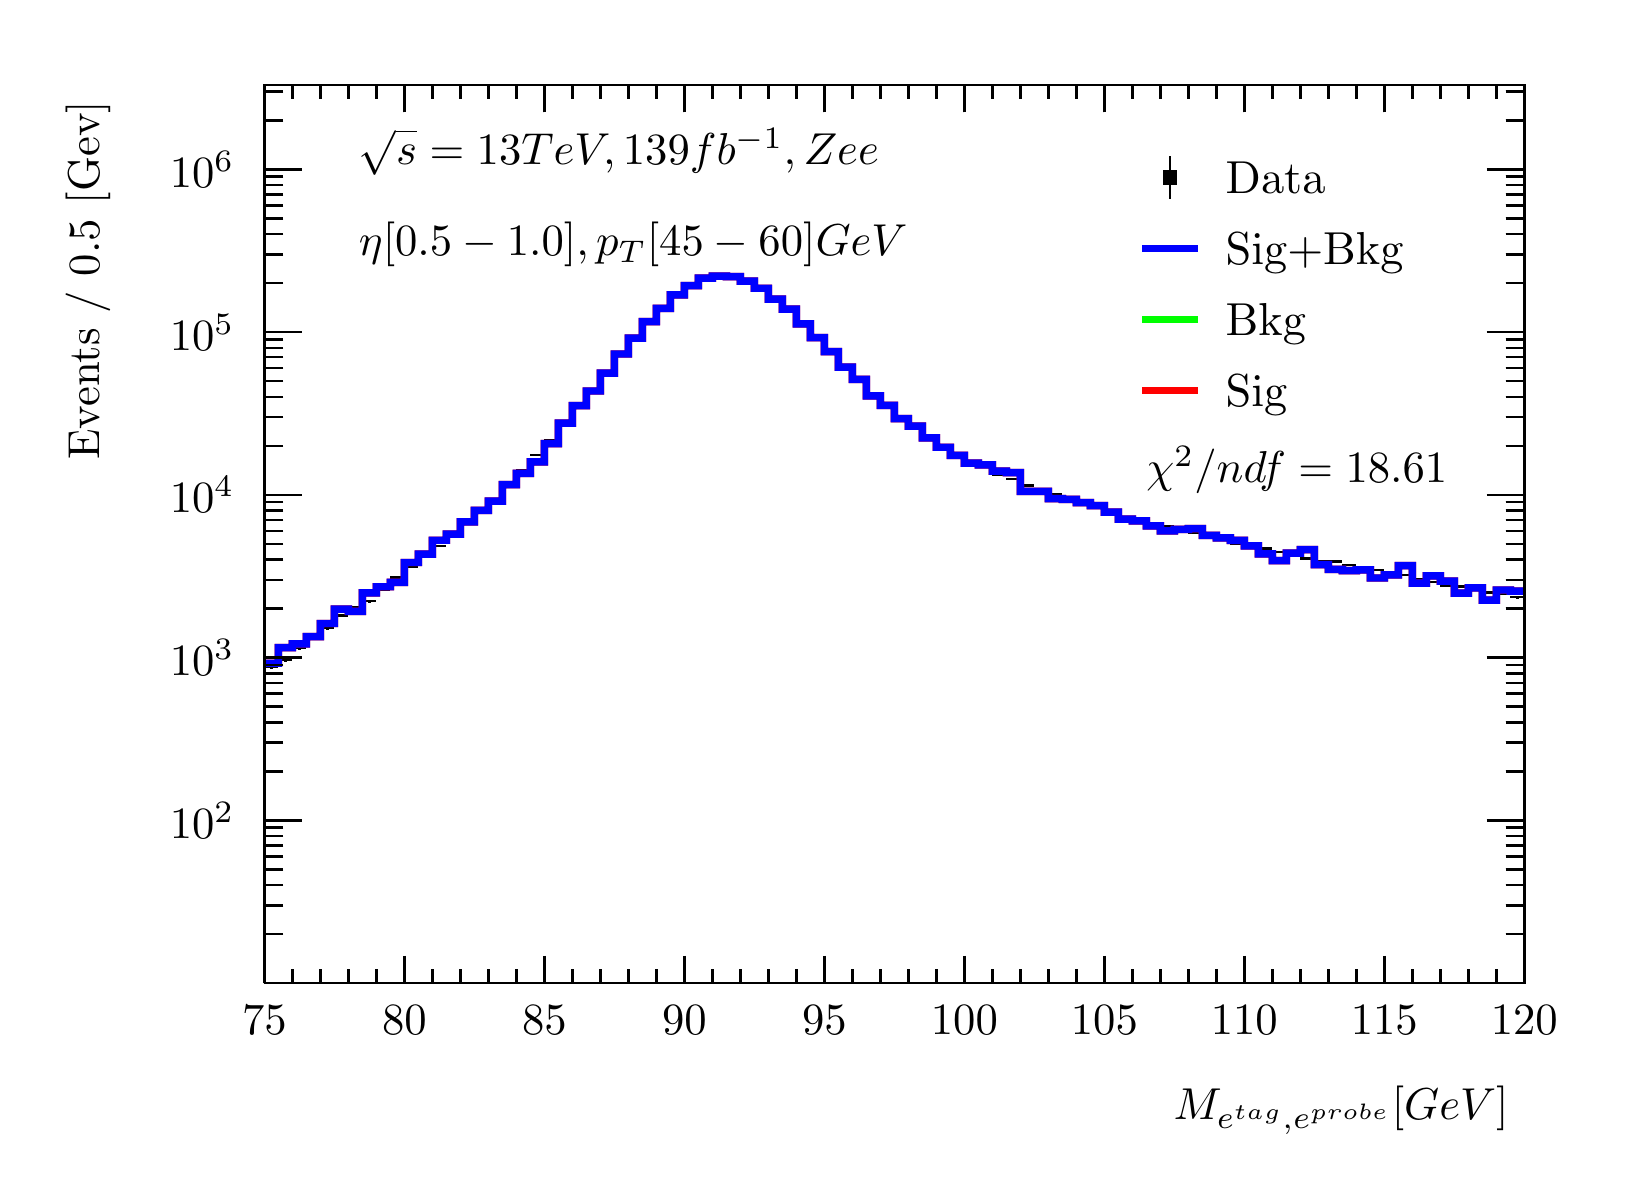
\begin{tikzpicture}
\pgfdeclareplotmark{cross} {
\pgfpathmoveto{\pgfpoint{-0.3\pgfplotmarksize}{\pgfplotmarksize}}
\pgfpathlineto{\pgfpoint{+0.3\pgfplotmarksize}{\pgfplotmarksize}}
\pgfpathlineto{\pgfpoint{+0.3\pgfplotmarksize}{0.3\pgfplotmarksize}}
\pgfpathlineto{\pgfpoint{+1\pgfplotmarksize}{0.3\pgfplotmarksize}}
\pgfpathlineto{\pgfpoint{+1\pgfplotmarksize}{-0.3\pgfplotmarksize}}
\pgfpathlineto{\pgfpoint{+0.3\pgfplotmarksize}{-0.3\pgfplotmarksize}}
\pgfpathlineto{\pgfpoint{+0.3\pgfplotmarksize}{-1.\pgfplotmarksize}}
\pgfpathlineto{\pgfpoint{-0.3\pgfplotmarksize}{-1.\pgfplotmarksize}}
\pgfpathlineto{\pgfpoint{-0.3\pgfplotmarksize}{-0.3\pgfplotmarksize}}
\pgfpathlineto{\pgfpoint{-1.\pgfplotmarksize}{-0.3\pgfplotmarksize}}
\pgfpathlineto{\pgfpoint{-1.\pgfplotmarksize}{0.3\pgfplotmarksize}}
\pgfpathlineto{\pgfpoint{-0.3\pgfplotmarksize}{0.3\pgfplotmarksize}}
\pgfpathclose
\pgfusepathqstroke
}
\pgfdeclareplotmark{cross*} {
\pgfpathmoveto{\pgfpoint{-0.3\pgfplotmarksize}{\pgfplotmarksize}}
\pgfpathlineto{\pgfpoint{+0.3\pgfplotmarksize}{\pgfplotmarksize}}
\pgfpathlineto{\pgfpoint{+0.3\pgfplotmarksize}{0.3\pgfplotmarksize}}
\pgfpathlineto{\pgfpoint{+1\pgfplotmarksize}{0.3\pgfplotmarksize}}
\pgfpathlineto{\pgfpoint{+1\pgfplotmarksize}{-0.3\pgfplotmarksize}}
\pgfpathlineto{\pgfpoint{+0.3\pgfplotmarksize}{-0.3\pgfplotmarksize}}
\pgfpathlineto{\pgfpoint{+0.3\pgfplotmarksize}{-1.\pgfplotmarksize}}
\pgfpathlineto{\pgfpoint{-0.3\pgfplotmarksize}{-1.\pgfplotmarksize}}
\pgfpathlineto{\pgfpoint{-0.3\pgfplotmarksize}{-0.3\pgfplotmarksize}}
\pgfpathlineto{\pgfpoint{-1.\pgfplotmarksize}{-0.3\pgfplotmarksize}}
\pgfpathlineto{\pgfpoint{-1.\pgfplotmarksize}{0.3\pgfplotmarksize}}
\pgfpathlineto{\pgfpoint{-0.3\pgfplotmarksize}{0.3\pgfplotmarksize}}
\pgfpathclose
\pgfusepathqfillstroke
}
\pgfdeclareplotmark{newstar} {
\pgfpathmoveto{\pgfqpoint{0pt}{\pgfplotmarksize}}
\pgfpathlineto{\pgfqpointpolar{44}{0.5\pgfplotmarksize}}
\pgfpathlineto{\pgfqpointpolar{18}{\pgfplotmarksize}}
\pgfpathlineto{\pgfqpointpolar{-20}{0.5\pgfplotmarksize}}
\pgfpathlineto{\pgfqpointpolar{-54}{\pgfplotmarksize}}
\pgfpathlineto{\pgfqpointpolar{-90}{0.5\pgfplotmarksize}}
\pgfpathlineto{\pgfqpointpolar{234}{\pgfplotmarksize}}
\pgfpathlineto{\pgfqpointpolar{198}{0.5\pgfplotmarksize}}
\pgfpathlineto{\pgfqpointpolar{162}{\pgfplotmarksize}}
\pgfpathlineto{\pgfqpointpolar{134}{0.5\pgfplotmarksize}}
\pgfpathclose
\pgfusepathqstroke
}
\pgfdeclareplotmark{newstar*} {
\pgfpathmoveto{\pgfqpoint{0pt}{\pgfplotmarksize}}
\pgfpathlineto{\pgfqpointpolar{44}{0.5\pgfplotmarksize}}
\pgfpathlineto{\pgfqpointpolar{18}{\pgfplotmarksize}}
\pgfpathlineto{\pgfqpointpolar{-20}{0.5\pgfplotmarksize}}
\pgfpathlineto{\pgfqpointpolar{-54}{\pgfplotmarksize}}
\pgfpathlineto{\pgfqpointpolar{-90}{0.5\pgfplotmarksize}}
\pgfpathlineto{\pgfqpointpolar{234}{\pgfplotmarksize}}
\pgfpathlineto{\pgfqpointpolar{198}{0.5\pgfplotmarksize}}
\pgfpathlineto{\pgfqpointpolar{162}{\pgfplotmarksize}}
\pgfpathlineto{\pgfqpointpolar{134}{0.5\pgfplotmarksize}}
\pgfpathclose
\pgfusepathqfillstroke
}
\definecolor{c}{rgb}{1,1,1};
\draw [color=c, fill=c] (0,0) rectangle (20,14.4361);
\draw [color=c, fill=c] (3,2.30977) rectangle (19,13.7143);
\definecolor{c}{rgb}{0,0,0};
\draw [c,line width=0.9] (3,2.30977) -- (3,13.7143) -- (19,13.7143) -- (19,2.30977) -- (3,2.30977);
\definecolor{c}{rgb}{1,1,1};
\draw [color=c, fill=c] (3,2.30977) rectangle (19,13.7143);
\definecolor{c}{rgb}{0,0,0};
\draw [c,line width=0.9] (3,2.30977) -- (3,13.7143) -- (19,13.7143) -- (19,2.30977) -- (3,2.30977);
\draw [c,line width=0.9] (3,2.30977) -- (19,2.30977);
\draw [c,line width=0.9] (3,2.65624) -- (3,2.30977);
\draw [c,line width=0.9] (3.35556,2.48301) -- (3.35556,2.30977);
\draw [c,line width=0.9] (3.71111,2.48301) -- (3.71111,2.30977);
\draw [c,line width=0.9] (4.06667,2.48301) -- (4.06667,2.30977);
\draw [c,line width=0.9] (4.42222,2.48301) -- (4.42222,2.30977);
\draw [c,line width=0.9] (4.77778,2.65624) -- (4.77778,2.30977);
\draw [c,line width=0.9] (5.13333,2.48301) -- (5.13333,2.30977);
\draw [c,line width=0.9] (5.48889,2.48301) -- (5.48889,2.30977);
\draw [c,line width=0.9] (5.84444,2.48301) -- (5.84444,2.30977);
\draw [c,line width=0.9] (6.2,2.48301) -- (6.2,2.30977);
\draw [c,line width=0.9] (6.55556,2.65624) -- (6.55556,2.30977);
\draw [c,line width=0.9] (6.91111,2.48301) -- (6.91111,2.30977);
\draw [c,line width=0.9] (7.26667,2.48301) -- (7.26667,2.30977);
\draw [c,line width=0.9] (7.62222,2.48301) -- (7.62222,2.30977);
\draw [c,line width=0.9] (7.97778,2.48301) -- (7.97778,2.30977);
\draw [c,line width=0.9] (8.33333,2.65624) -- (8.33333,2.30977);
\draw [c,line width=0.9] (8.68889,2.48301) -- (8.68889,2.30977);
\draw [c,line width=0.9] (9.04444,2.48301) -- (9.04444,2.30977);
\draw [c,line width=0.9] (9.4,2.48301) -- (9.4,2.30977);
\draw [c,line width=0.9] (9.75556,2.48301) -- (9.75556,2.30977);
\draw [c,line width=0.9] (10.1111,2.65624) -- (10.1111,2.30977);
\draw [c,line width=0.9] (10.4667,2.48301) -- (10.4667,2.30977);
\draw [c,line width=0.9] (10.8222,2.48301) -- (10.8222,2.30977);
\draw [c,line width=0.9] (11.1778,2.48301) -- (11.1778,2.30977);
\draw [c,line width=0.9] (11.5333,2.48301) -- (11.5333,2.30977);
\draw [c,line width=0.9] (11.8889,2.65624) -- (11.8889,2.30977);
\draw [c,line width=0.9] (12.2444,2.48301) -- (12.2444,2.30977);
\draw [c,line width=0.9] (12.6,2.48301) -- (12.6,2.30977);
\draw [c,line width=0.9] (12.9556,2.48301) -- (12.9556,2.30977);
\draw [c,line width=0.9] (13.3111,2.48301) -- (13.3111,2.30977);
\draw [c,line width=0.9] (13.6667,2.65624) -- (13.6667,2.30977);
\draw [c,line width=0.9] (14.0222,2.48301) -- (14.0222,2.30977);
\draw [c,line width=0.9] (14.3778,2.48301) -- (14.3778,2.30977);
\draw [c,line width=0.9] (14.7333,2.48301) -- (14.7333,2.30977);
\draw [c,line width=0.9] (15.0889,2.48301) -- (15.0889,2.30977);
\draw [c,line width=0.9] (15.4444,2.65624) -- (15.4444,2.30977);
\draw [c,line width=0.9] (15.8,2.48301) -- (15.8,2.30977);
\draw [c,line width=0.9] (16.1556,2.48301) -- (16.1556,2.30977);
\draw [c,line width=0.9] (16.5111,2.48301) -- (16.5111,2.30977);
\draw [c,line width=0.9] (16.8667,2.48301) -- (16.8667,2.30977);
\draw [c,line width=0.9] (17.2222,2.65624) -- (17.2222,2.30977);
\draw [c,line width=0.9] (17.5778,2.48301) -- (17.5778,2.30977);
\draw [c,line width=0.9] (17.9333,2.48301) -- (17.9333,2.30977);
\draw [c,line width=0.9] (18.2889,2.48301) -- (18.2889,2.30977);
\draw [c,line width=0.9] (18.6444,2.48301) -- (18.6444,2.30977);
\draw [c,line width=0.9] (19,2.65624) -- (19,2.30977);
\draw [c,line width=0.9] (19,2.65624) -- (19,2.30977);
\draw [anchor=base] (3,1.66015) node[scale=1.61424, color=c, rotate=0]{75};
\draw [anchor=base] (4.77778,1.66015) node[scale=1.61424, color=c, rotate=0]{80};
\draw [anchor=base] (6.55556,1.66015) node[scale=1.61424, color=c, rotate=0]{85};
\draw [anchor=base] (8.33333,1.66015) node[scale=1.61424, color=c, rotate=0]{90};
\draw [anchor=base] (10.1111,1.66015) node[scale=1.61424, color=c, rotate=0]{95};
\draw [anchor=base] (11.8889,1.66015) node[scale=1.61424, color=c, rotate=0]{100};
\draw [anchor=base] (13.6667,1.66015) node[scale=1.61424, color=c, rotate=0]{105};
\draw [anchor=base] (15.4444,1.66015) node[scale=1.61424, color=c, rotate=0]{110};
\draw [anchor=base] (17.2222,1.66015) node[scale=1.61424, color=c, rotate=0]{115};
\draw [anchor=base] (19,1.66015) node[scale=1.61424, color=c, rotate=0]{120};
\draw [anchor= east] (19,0.692932) node[scale=1.61424, color=c, rotate=0]{$M_{e^{tag}, e^{probe}}  [GeV]$};
\draw [c,line width=0.9] (3,13.7143) -- (19,13.7143);
\draw [c,line width=0.9] (3,13.3678) -- (3,13.7143);
\draw [c,line width=0.9] (3.35556,13.5411) -- (3.35556,13.7143);
\draw [c,line width=0.9] (3.71111,13.5411) -- (3.71111,13.7143);
\draw [c,line width=0.9] (4.06667,13.5411) -- (4.06667,13.7143);
\draw [c,line width=0.9] (4.42222,13.5411) -- (4.42222,13.7143);
\draw [c,line width=0.9] (4.77778,13.3678) -- (4.77778,13.7143);
\draw [c,line width=0.9] (5.13333,13.5411) -- (5.13333,13.7143);
\draw [c,line width=0.9] (5.48889,13.5411) -- (5.48889,13.7143);
\draw [c,line width=0.9] (5.84444,13.5411) -- (5.84444,13.7143);
\draw [c,line width=0.9] (6.2,13.5411) -- (6.2,13.7143);
\draw [c,line width=0.9] (6.55556,13.3678) -- (6.55556,13.7143);
\draw [c,line width=0.9] (6.91111,13.5411) -- (6.91111,13.7143);
\draw [c,line width=0.9] (7.26667,13.5411) -- (7.26667,13.7143);
\draw [c,line width=0.9] (7.62222,13.5411) -- (7.62222,13.7143);
\draw [c,line width=0.9] (7.97778,13.5411) -- (7.97778,13.7143);
\draw [c,line width=0.9] (8.33333,13.3678) -- (8.33333,13.7143);
\draw [c,line width=0.9] (8.68889,13.5411) -- (8.68889,13.7143);
\draw [c,line width=0.9] (9.04444,13.5411) -- (9.04444,13.7143);
\draw [c,line width=0.9] (9.4,13.5411) -- (9.4,13.7143);
\draw [c,line width=0.9] (9.75556,13.5411) -- (9.75556,13.7143);
\draw [c,line width=0.9] (10.1111,13.3678) -- (10.1111,13.7143);
\draw [c,line width=0.9] (10.4667,13.5411) -- (10.4667,13.7143);
\draw [c,line width=0.9] (10.8222,13.5411) -- (10.8222,13.7143);
\draw [c,line width=0.9] (11.1778,13.5411) -- (11.1778,13.7143);
\draw [c,line width=0.9] (11.5333,13.5411) -- (11.5333,13.7143);
\draw [c,line width=0.9] (11.8889,13.3678) -- (11.8889,13.7143);
\draw [c,line width=0.9] (12.2444,13.5411) -- (12.2444,13.7143);
\draw [c,line width=0.9] (12.6,13.5411) -- (12.6,13.7143);
\draw [c,line width=0.9] (12.9556,13.5411) -- (12.9556,13.7143);
\draw [c,line width=0.9] (13.3111,13.5411) -- (13.3111,13.7143);
\draw [c,line width=0.9] (13.6667,13.3678) -- (13.6667,13.7143);
\draw [c,line width=0.9] (14.0222,13.5411) -- (14.0222,13.7143);
\draw [c,line width=0.9] (14.3778,13.5411) -- (14.3778,13.7143);
\draw [c,line width=0.9] (14.7333,13.5411) -- (14.7333,13.7143);
\draw [c,line width=0.9] (15.0889,13.5411) -- (15.0889,13.7143);
\draw [c,line width=0.9] (15.4444,13.3678) -- (15.4444,13.7143);
\draw [c,line width=0.9] (15.8,13.5411) -- (15.8,13.7143);
\draw [c,line width=0.9] (16.1556,13.5411) -- (16.1556,13.7143);
\draw [c,line width=0.9] (16.5111,13.5411) -- (16.5111,13.7143);
\draw [c,line width=0.9] (16.8667,13.5411) -- (16.8667,13.7143);
\draw [c,line width=0.9] (17.2222,13.3678) -- (17.2222,13.7143);
\draw [c,line width=0.9] (17.5778,13.5411) -- (17.5778,13.7143);
\draw [c,line width=0.9] (17.9333,13.5411) -- (17.9333,13.7143);
\draw [c,line width=0.9] (18.2889,13.5411) -- (18.2889,13.7143);
\draw [c,line width=0.9] (18.6444,13.5411) -- (18.6444,13.7143);
\draw [c,line width=0.9] (19,13.3678) -- (19,13.7143);
\draw [c,line width=0.9] (19,13.3678) -- (19,13.7143);
\draw [c,line width=0.9] (3,2.30977) -- (3,13.7143);
\draw [c,line width=0.9] (3.237,2.932) -- (3,2.932);
\draw [c,line width=0.9] (3.237,3.29598) -- (3,3.29598);
\draw [c,line width=0.9] (3.237,3.55423) -- (3,3.55423);
\draw [c,line width=0.9] (3.237,3.75454) -- (3,3.75454);
\draw [c,line width=0.9] (3.237,3.9182) -- (3,3.9182);
\draw [c,line width=0.9] (3.237,4.05658) -- (3,4.05658);
\draw [c,line width=0.9] (3.237,4.17645) -- (3,4.17645);
\draw [c,line width=0.9] (3.237,4.28218) -- (3,4.28218);
\draw [c,line width=0.9] (3.474,4.37676) -- (3,4.37676);
\draw [anchor= east] (2.82,4.37676) node[scale=1.61424, color=c, rotate=0]{$10^{2}$};
\draw [c,line width=0.9] (3.237,4.99899) -- (3,4.99899);
\draw [c,line width=0.9] (3.237,5.36297) -- (3,5.36297);
\draw [c,line width=0.9] (3.237,5.62122) -- (3,5.62122);
\draw [c,line width=0.9] (3.237,5.82153) -- (3,5.82153);
\draw [c,line width=0.9] (3.237,5.9852) -- (3,5.9852);
\draw [c,line width=0.9] (3.237,6.12357) -- (3,6.12357);
\draw [c,line width=0.9] (3.237,6.24344) -- (3,6.24344);
\draw [c,line width=0.9] (3.237,6.34917) -- (3,6.34917);
\draw [c,line width=0.9] (3.474,6.44376) -- (3,6.44376);
\draw [anchor= east] (2.82,6.44376) node[scale=1.61424, color=c, rotate=0]{$10^{3}$};
\draw [c,line width=0.9] (3.237,7.06598) -- (3,7.06598);
\draw [c,line width=0.9] (3.237,7.42996) -- (3,7.42996);
\draw [c,line width=0.9] (3.237,7.68821) -- (3,7.68821);
\draw [c,line width=0.9] (3.237,7.88852) -- (3,7.88852);
\draw [c,line width=0.9] (3.237,8.05219) -- (3,8.05219);
\draw [c,line width=0.9] (3.237,8.19057) -- (3,8.19057);
\draw [c,line width=0.9] (3.237,8.31043) -- (3,8.31043);
\draw [c,line width=0.9] (3.237,8.41617) -- (3,8.41617);
\draw [c,line width=0.9] (3.474,8.51075) -- (3,8.51075);
\draw [anchor= east] (2.82,8.51075) node[scale=1.61424, color=c, rotate=0]{$10^{4}$};
\draw [c,line width=0.9] (3.237,9.13297) -- (3,9.13297);
\draw [c,line width=0.9] (3.237,9.49695) -- (3,9.49695);
\draw [c,line width=0.9] (3.237,9.7552) -- (3,9.7552);
\draw [c,line width=0.9] (3.237,9.95551) -- (3,9.95551);
\draw [c,line width=0.9] (3.237,10.1192) -- (3,10.1192);
\draw [c,line width=0.9] (3.237,10.2576) -- (3,10.2576);
\draw [c,line width=0.9] (3.237,10.3774) -- (3,10.3774);
\draw [c,line width=0.9] (3.237,10.4832) -- (3,10.4832);
\draw [c,line width=0.9] (3.474,10.5777) -- (3,10.5777);
\draw [anchor= east] (2.82,10.5777) node[scale=1.61424, color=c, rotate=0]{$10^{5}$};
\draw [c,line width=0.9] (3.237,11.2) -- (3,11.2);
\draw [c,line width=0.9] (3.237,11.5639) -- (3,11.5639);
\draw [c,line width=0.9] (3.237,11.8222) -- (3,11.8222);
\draw [c,line width=0.9] (3.237,12.0225) -- (3,12.0225);
\draw [c,line width=0.9] (3.237,12.1862) -- (3,12.1862);
\draw [c,line width=0.9] (3.237,12.3245) -- (3,12.3245);
\draw [c,line width=0.9] (3.237,12.4444) -- (3,12.4444);
\draw [c,line width=0.9] (3.237,12.5501) -- (3,12.5501);
\draw [c,line width=0.9] (3.474,12.6447) -- (3,12.6447);
\draw [anchor= east] (2.82,12.6447) node[scale=1.61424, color=c, rotate=0]{$10^{6}$};
\draw [c,line width=0.9] (3.237,13.267) -- (3,13.267);
\draw [c,line width=0.9] (3.237,13.6309) -- (3,13.6309);
\draw [anchor= east] (0.76,13.7143) node[scale=1.61424, color=c, rotate=90]{Events / 0.5 [Gev]};
\draw [c,line width=0.9] (19,2.30977) -- (19,13.7143);
\draw [c,line width=0.9] (18.763,2.932) -- (19,2.932);
\draw [c,line width=0.9] (18.763,3.29598) -- (19,3.29598);
\draw [c,line width=0.9] (18.763,3.55423) -- (19,3.55423);
\draw [c,line width=0.9] (18.763,3.75454) -- (19,3.75454);
\draw [c,line width=0.9] (18.763,3.9182) -- (19,3.9182);
\draw [c,line width=0.9] (18.763,4.05658) -- (19,4.05658);
\draw [c,line width=0.9] (18.763,4.17645) -- (19,4.17645);
\draw [c,line width=0.9] (18.763,4.28218) -- (19,4.28218);
\draw [c,line width=0.9] (18.526,4.37676) -- (19,4.37676);
\draw [c,line width=0.9] (18.763,4.99899) -- (19,4.99899);
\draw [c,line width=0.9] (18.763,5.36297) -- (19,5.36297);
\draw [c,line width=0.9] (18.763,5.62122) -- (19,5.62122);
\draw [c,line width=0.9] (18.763,5.82153) -- (19,5.82153);
\draw [c,line width=0.9] (18.763,5.9852) -- (19,5.9852);
\draw [c,line width=0.9] (18.763,6.12357) -- (19,6.12357);
\draw [c,line width=0.9] (18.763,6.24344) -- (19,6.24344);
\draw [c,line width=0.9] (18.763,6.34917) -- (19,6.34917);
\draw [c,line width=0.9] (18.526,6.44376) -- (19,6.44376);
\draw [c,line width=0.9] (18.763,7.06598) -- (19,7.06598);
\draw [c,line width=0.9] (18.763,7.42996) -- (19,7.42996);
\draw [c,line width=0.9] (18.763,7.68821) -- (19,7.68821);
\draw [c,line width=0.9] (18.763,7.88852) -- (19,7.88852);
\draw [c,line width=0.9] (18.763,8.05219) -- (19,8.05219);
\draw [c,line width=0.9] (18.763,8.19057) -- (19,8.19057);
\draw [c,line width=0.9] (18.763,8.31043) -- (19,8.31043);
\draw [c,line width=0.9] (18.763,8.41617) -- (19,8.41617);
\draw [c,line width=0.9] (18.526,8.51075) -- (19,8.51075);
\draw [c,line width=0.9] (18.763,9.13297) -- (19,9.13297);
\draw [c,line width=0.9] (18.763,9.49695) -- (19,9.49695);
\draw [c,line width=0.9] (18.763,9.7552) -- (19,9.7552);
\draw [c,line width=0.9] (18.763,9.95551) -- (19,9.95551);
\draw [c,line width=0.9] (18.763,10.1192) -- (19,10.1192);
\draw [c,line width=0.9] (18.763,10.2576) -- (19,10.2576);
\draw [c,line width=0.9] (18.763,10.3774) -- (19,10.3774);
\draw [c,line width=0.9] (18.763,10.4832) -- (19,10.4832);
\draw [c,line width=0.9] (18.526,10.5777) -- (19,10.5777);
\draw [c,line width=0.9] (18.763,11.2) -- (19,11.2);
\draw [c,line width=0.9] (18.763,11.5639) -- (19,11.5639);
\draw [c,line width=0.9] (18.763,11.8222) -- (19,11.8222);
\draw [c,line width=0.9] (18.763,12.0225) -- (19,12.0225);
\draw [c,line width=0.9] (18.763,12.1862) -- (19,12.1862);
\draw [c,line width=0.9] (18.763,12.3245) -- (19,12.3245);
\draw [c,line width=0.9] (18.763,12.4444) -- (19,12.4444);
\draw [c,line width=0.9] (18.763,12.5501) -- (19,12.5501);
\draw [c,line width=0.9] (18.526,12.6447) -- (19,12.6447);
\draw [c,line width=0.9] (18.763,13.267) -- (19,13.267);
\draw [c,line width=0.9] (18.763,13.6309) -- (19,13.6309);
\draw [c,line width=0.9] (3.08889,6.33002) -- (3,6.33002);
\draw [c,line width=0.9] (3,6.33002) -- (3,6.33002);
\draw [c,line width=0.9] (3.08889,6.33002) -- (3.17778,6.33002);
\draw [c,line width=0.9] (3.17778,6.33002) -- (3.17778,6.33002);
\draw [c,line width=0.9] (3.08889,6.33002) -- (3.08889,6.36026);
\draw [c,line width=0.9] (3.08889,6.36026) -- (3.08889,6.36026);
\draw [c,line width=0.9] (3.08889,6.33002) -- (3.08889,6.29978);
\draw [c,line width=0.9] (3.08889,6.29978) -- (3.08889,6.29978);
\draw [c,line width=0.9] (3.26667,6.4127) -- (3.17778,6.4127);
\draw [c,line width=0.9] (3.17778,6.4127) -- (3.17778,6.4127);
\draw [c,line width=0.9] (3.26667,6.4127) -- (3.35556,6.4127);
\draw [c,line width=0.9] (3.35556,6.4127) -- (3.35556,6.4127);
\draw [c,line width=0.9] (3.26667,6.4127) -- (3.26667,6.44159);
\draw [c,line width=0.9] (3.26667,6.44159) -- (3.26667,6.44159);
\draw [c,line width=0.9] (3.26667,6.4127) -- (3.26667,6.38382);
\draw [c,line width=0.9] (3.26667,6.38382) -- (3.26667,6.38382);
\draw [c,line width=0.9] (3.44444,6.57) -- (3.35556,6.57);
\draw [c,line width=0.9] (3.35556,6.57) -- (3.35556,6.57);
\draw [c,line width=0.9] (3.44444,6.57) -- (3.53333,6.57);
\draw [c,line width=0.9] (3.53333,6.57) -- (3.53333,6.57);
\draw [c,line width=0.9] (3.44444,6.57) -- (3.44444,6.59646);
\draw [c,line width=0.9] (3.44444,6.59646) -- (3.44444,6.59646);
\draw [c,line width=0.9] (3.44444,6.57) -- (3.44444,6.54354);
\draw [c,line width=0.9] (3.44444,6.54354) -- (3.44444,6.54354);
\draw [c,line width=0.9] (3.62222,6.72767) -- (3.53333,6.72767);
\draw [c,line width=0.9] (3.53333,6.72767) -- (3.53333,6.72767);
\draw [c,line width=0.9] (3.62222,6.72767) -- (3.71111,6.72767);
\draw [c,line width=0.9] (3.71111,6.72767) -- (3.71111,6.72767);
\draw [c,line width=0.9] (3.62222,6.72767) -- (3.62222,6.7519);
\draw [c,line width=0.9] (3.62222,6.7519) -- (3.62222,6.7519);
\draw [c,line width=0.9] (3.62222,6.72767) -- (3.62222,6.70343);
\draw [c,line width=0.9] (3.62222,6.70343) -- (3.62222,6.70343);
\draw [c,line width=0.9] (3.8,6.82022) -- (3.71111,6.82022);
\draw [c,line width=0.9] (3.71111,6.82022) -- (3.71111,6.82022);
\draw [c,line width=0.9] (3.8,6.82022) -- (3.88889,6.82022);
\draw [c,line width=0.9] (3.88889,6.82022) -- (3.88889,6.82022);
\draw [c,line width=0.9] (3.8,6.82022) -- (3.8,6.84323);
\draw [c,line width=0.9] (3.8,6.84323) -- (3.8,6.84323);
\draw [c,line width=0.9] (3.8,6.82022) -- (3.8,6.7972);
\draw [c,line width=0.9] (3.8,6.7972) -- (3.8,6.7972);
\draw [c,line width=0.9] (3.97778,6.97935) -- (3.88889,6.97935);
\draw [c,line width=0.9] (3.88889,6.97935) -- (3.88889,6.97935);
\draw [c,line width=0.9] (3.97778,6.97935) -- (4.06667,6.97935);
\draw [c,line width=0.9] (4.06667,6.97935) -- (4.06667,6.97935);
\draw [c,line width=0.9] (3.97778,6.97935) -- (3.97778,7.00041);
\draw [c,line width=0.9] (3.97778,7.00041) -- (3.97778,7.00041);
\draw [c,line width=0.9] (3.97778,6.97935) -- (3.97778,6.95828);
\draw [c,line width=0.9] (3.97778,6.95828) -- (3.97778,6.95828);
\draw [c,line width=0.9] (4.15556,7.07713) -- (4.06667,7.07713);
\draw [c,line width=0.9] (4.06667,7.07713) -- (4.06667,7.07713);
\draw [c,line width=0.9] (4.15556,7.07713) -- (4.24444,7.07713);
\draw [c,line width=0.9] (4.24444,7.07713) -- (4.24444,7.07713);
\draw [c,line width=0.9] (4.15556,7.07713) -- (4.15556,7.09708);
\draw [c,line width=0.9] (4.15556,7.09708) -- (4.15556,7.09708);
\draw [c,line width=0.9] (4.15556,7.07713) -- (4.15556,7.05719);
\draw [c,line width=0.9] (4.15556,7.05719) -- (4.15556,7.05719);
\draw [c,line width=0.9] (4.33333,7.16088) -- (4.24444,7.16088);
\draw [c,line width=0.9] (4.24444,7.16088) -- (4.24444,7.16088);
\draw [c,line width=0.9] (4.33333,7.16088) -- (4.42222,7.16088);
\draw [c,line width=0.9] (4.42222,7.16088) -- (4.42222,7.16088);
\draw [c,line width=0.9] (4.33333,7.16088) -- (4.33333,7.17992);
\draw [c,line width=0.9] (4.33333,7.17992) -- (4.33333,7.17992);
\draw [c,line width=0.9] (4.33333,7.16088) -- (4.33333,7.14184);
\draw [c,line width=0.9] (4.33333,7.14184) -- (4.33333,7.14184);
\draw [c,line width=0.9] (4.51111,7.30667) -- (4.42222,7.30667);
\draw [c,line width=0.9] (4.42222,7.30667) -- (4.42222,7.30667);
\draw [c,line width=0.9] (4.51111,7.30667) -- (4.6,7.30667);
\draw [c,line width=0.9] (4.6,7.30667) -- (4.6,7.30667);
\draw [c,line width=0.9] (4.51111,7.30667) -- (4.51111,7.32422);
\draw [c,line width=0.9] (4.51111,7.32422) -- (4.51111,7.32422);
\draw [c,line width=0.9] (4.51111,7.30667) -- (4.51111,7.28911);
\draw [c,line width=0.9] (4.51111,7.28911) -- (4.51111,7.28911);
\draw [c,line width=0.9] (4.68889,7.45824) -- (4.6,7.45824);
\draw [c,line width=0.9] (4.6,7.45824) -- (4.6,7.45824);
\draw [c,line width=0.9] (4.68889,7.45824) -- (4.77778,7.45824);
\draw [c,line width=0.9] (4.77778,7.45824) -- (4.77778,7.45824);
\draw [c,line width=0.9] (4.68889,7.45824) -- (4.68889,7.47437);
\draw [c,line width=0.9] (4.68889,7.47437) -- (4.68889,7.47437);
\draw [c,line width=0.9] (4.68889,7.45824) -- (4.68889,7.4421);
\draw [c,line width=0.9] (4.68889,7.4421) -- (4.68889,7.4421);
\draw [c,line width=0.9] (4.86667,7.59238) -- (4.77778,7.59238);
\draw [c,line width=0.9] (4.77778,7.59238) -- (4.77778,7.59238);
\draw [c,line width=0.9] (4.86667,7.59238) -- (4.95556,7.59238);
\draw [c,line width=0.9] (4.95556,7.59238) -- (4.95556,7.59238);
\draw [c,line width=0.9] (4.86667,7.59238) -- (4.86667,7.60735);
\draw [c,line width=0.9] (4.86667,7.60735) -- (4.86667,7.60735);
\draw [c,line width=0.9] (4.86667,7.59238) -- (4.86667,7.57741);
\draw [c,line width=0.9] (4.86667,7.57741) -- (4.86667,7.57741);
\draw [c,line width=0.9] (5.04444,7.73179) -- (4.95556,7.73179);
\draw [c,line width=0.9] (4.95556,7.73179) -- (4.95556,7.73179);
\draw [c,line width=0.9] (5.04444,7.73179) -- (5.13333,7.73179);
\draw [c,line width=0.9] (5.13333,7.73179) -- (5.13333,7.73179);
\draw [c,line width=0.9] (5.04444,7.73179) -- (5.04444,7.74565);
\draw [c,line width=0.9] (5.04444,7.74565) -- (5.04444,7.74565);
\draw [c,line width=0.9] (5.04444,7.73179) -- (5.04444,7.71794);
\draw [c,line width=0.9] (5.04444,7.71794) -- (5.04444,7.71794);
\draw [c,line width=0.9] (5.22222,7.85858) -- (5.13333,7.85858);
\draw [c,line width=0.9] (5.13333,7.85858) -- (5.13333,7.85858);
\draw [c,line width=0.9] (5.22222,7.85858) -- (5.31111,7.85858);
\draw [c,line width=0.9] (5.31111,7.85858) -- (5.31111,7.85858);
\draw [c,line width=0.9] (5.22222,7.85858) -- (5.22222,7.87149);
\draw [c,line width=0.9] (5.22222,7.87149) -- (5.22222,7.87149);
\draw [c,line width=0.9] (5.22222,7.85858) -- (5.22222,7.84567);
\draw [c,line width=0.9] (5.22222,7.84567) -- (5.22222,7.84567);
\draw [c,line width=0.9] (5.4,8.01054) -- (5.31111,8.01054);
\draw [c,line width=0.9] (5.31111,8.01054) -- (5.31111,8.01054);
\draw [c,line width=0.9] (5.4,8.01054) -- (5.48889,8.01054);
\draw [c,line width=0.9] (5.48889,8.01054) -- (5.48889,8.01054);
\draw [c,line width=0.9] (5.4,8.01054) -- (5.4,8.0224);
\draw [c,line width=0.9] (5.4,8.0224) -- (5.4,8.0224);
\draw [c,line width=0.9] (5.4,8.01054) -- (5.4,7.99868);
\draw [c,line width=0.9] (5.4,7.99868) -- (5.4,7.99868);
\draw [c,line width=0.9] (5.57778,8.15245) -- (5.48889,8.15245);
\draw [c,line width=0.9] (5.48889,8.15245) -- (5.48889,8.15245);
\draw [c,line width=0.9] (5.57778,8.15245) -- (5.66667,8.15245);
\draw [c,line width=0.9] (5.66667,8.15245) -- (5.66667,8.15245);
\draw [c,line width=0.9] (5.57778,8.15245) -- (5.57778,8.16341);
\draw [c,line width=0.9] (5.57778,8.16341) -- (5.57778,8.16341);
\draw [c,line width=0.9] (5.57778,8.15245) -- (5.57778,8.14149);
\draw [c,line width=0.9] (5.57778,8.14149) -- (5.57778,8.14149);
\draw [c,line width=0.9] (5.75556,8.28805) -- (5.66667,8.28805);
\draw [c,line width=0.9] (5.66667,8.28805) -- (5.66667,8.28805);
\draw [c,line width=0.9] (5.75556,8.28805) -- (5.84444,8.28805);
\draw [c,line width=0.9] (5.84444,8.28805) -- (5.84444,8.28805);
\draw [c,line width=0.9] (5.75556,8.28805) -- (5.75556,8.29822);
\draw [c,line width=0.9] (5.75556,8.29822) -- (5.75556,8.29822);
\draw [c,line width=0.9] (5.75556,8.28805) -- (5.75556,8.27789);
\draw [c,line width=0.9] (5.75556,8.27789) -- (5.75556,8.27789);
\draw [c,line width=0.9] (5.93333,8.45892) -- (5.84444,8.45892);
\draw [c,line width=0.9] (5.84444,8.45892) -- (5.84444,8.45892);
\draw [c,line width=0.9] (5.93333,8.45892) -- (6.02222,8.45892);
\draw [c,line width=0.9] (6.02222,8.45892) -- (6.02222,8.45892);
\draw [c,line width=0.9] (5.93333,8.45892) -- (5.93333,8.46816);
\draw [c,line width=0.9] (5.93333,8.46816) -- (5.93333,8.46816);
\draw [c,line width=0.9] (5.93333,8.45892) -- (5.93333,8.44968);
\draw [c,line width=0.9] (5.93333,8.44968) -- (5.93333,8.44968);
\draw [c,line width=0.9] (6.11111,8.63738) -- (6.02222,8.63738);
\draw [c,line width=0.9] (6.02222,8.63738) -- (6.02222,8.63738);
\draw [c,line width=0.9] (6.11111,8.63738) -- (6.2,8.63738);
\draw [c,line width=0.9] (6.2,8.63738) -- (6.2,8.63738);
\draw [c,line width=0.9] (6.11111,8.63738) -- (6.11111,8.64575);
\draw [c,line width=0.9] (6.11111,8.64575) -- (6.11111,8.64575);
\draw [c,line width=0.9] (6.11111,8.63738) -- (6.11111,8.62901);
\draw [c,line width=0.9] (6.11111,8.62901) -- (6.11111,8.62901);
\draw [c,line width=0.9] (6.28889,8.81759) -- (6.2,8.81759);
\draw [c,line width=0.9] (6.2,8.81759) -- (6.2,8.81759);
\draw [c,line width=0.9] (6.28889,8.81759) -- (6.37778,8.81759);
\draw [c,line width=0.9] (6.37778,8.81759) -- (6.37778,8.81759);
\draw [c,line width=0.9] (6.28889,8.81759) -- (6.28889,8.82516);
\draw [c,line width=0.9] (6.28889,8.82516) -- (6.28889,8.82516);
\draw [c,line width=0.9] (6.28889,8.81759) -- (6.28889,8.81002);
\draw [c,line width=0.9] (6.28889,8.81002) -- (6.28889,8.81002);
\draw [c,line width=0.9] (6.46667,9.01469) -- (6.37778,9.01469);
\draw [c,line width=0.9] (6.37778,9.01469) -- (6.37778,9.01469);
\draw [c,line width=0.9] (6.46667,9.01469) -- (6.55556,9.01469);
\draw [c,line width=0.9] (6.55556,9.01469) -- (6.55556,9.01469);
\draw [c,line width=0.9] (6.46667,9.01469) -- (6.46667,9.02147);
\draw [c,line width=0.9] (6.46667,9.02147) -- (6.46667,9.02147);
\draw [c,line width=0.9] (6.46667,9.01469) -- (6.46667,9.00791);
\draw [c,line width=0.9] (6.46667,9.00791) -- (6.46667,9.00791);
\draw [c,line width=0.9] (6.64444,9.20339) -- (6.55556,9.20339);
\draw [c,line width=0.9] (6.55556,9.20339) -- (6.55556,9.20339);
\draw [c,line width=0.9] (6.64444,9.20339) -- (6.73333,9.20339);
\draw [c,line width=0.9] (6.73333,9.20339) -- (6.73333,9.20339);
\draw [c,line width=0.9] (6.64444,9.20339) -- (6.64444,9.20949);
\draw [c,line width=0.9] (6.64444,9.20949) -- (6.64444,9.20949);
\draw [c,line width=0.9] (6.64444,9.20339) -- (6.64444,9.19729);
\draw [c,line width=0.9] (6.64444,9.19729) -- (6.64444,9.19729);
\draw [c,line width=0.9] (6.82222,9.41597) -- (6.73333,9.41597);
\draw [c,line width=0.9] (6.73333,9.41597) -- (6.73333,9.41597);
\draw [c,line width=0.9] (6.82222,9.41597) -- (6.91111,9.41597);
\draw [c,line width=0.9] (6.91111,9.41597) -- (6.91111,9.41597);
\draw [c,line width=0.9] (6.82222,9.41597) -- (6.82222,9.42139);
\draw [c,line width=0.9] (6.82222,9.42139) -- (6.82222,9.42139);
\draw [c,line width=0.9] (6.82222,9.41597) -- (6.82222,9.41055);
\draw [c,line width=0.9] (6.82222,9.41055) -- (6.82222,9.41055);
\draw [c,line width=0.9] (7,9.63111) -- (6.91111,9.63111);
\draw [c,line width=0.9] (6.91111,9.63111) -- (6.91111,9.63111);
\draw [c,line width=0.9] (7,9.63111) -- (7.08889,9.63111);
\draw [c,line width=0.9] (7.08889,9.63111) -- (7.08889,9.63111);
\draw [c,line width=0.9] (7,9.63111) -- (7,9.63592);
\draw [c,line width=0.9] (7,9.63592) -- (7,9.63592);
\draw [c,line width=0.9] (7,9.63111) -- (7,9.62631);
\draw [c,line width=0.9] (7,9.62631) -- (7,9.62631);
\draw [c,line width=0.9] (7.17778,9.83636) -- (7.08889,9.83636);
\draw [c,line width=0.9] (7.08889,9.83636) -- (7.08889,9.83636);
\draw [c,line width=0.9] (7.17778,9.83636) -- (7.26667,9.83636);
\draw [c,line width=0.9] (7.26667,9.83636) -- (7.26667,9.83636);
\draw [c,line width=0.9] (7.17778,9.83636) -- (7.17778,9.84065);
\draw [c,line width=0.9] (7.17778,9.84065) -- (7.17778,9.84065);
\draw [c,line width=0.9] (7.17778,9.83636) -- (7.17778,9.83207);
\draw [c,line width=0.9] (7.17778,9.83207) -- (7.17778,9.83207);
\draw [c,line width=0.9] (7.35556,10.0623) -- (7.26667,10.0623);
\draw [c,line width=0.9] (7.26667,10.0623) -- (7.26667,10.0623);
\draw [c,line width=0.9] (7.35556,10.0623) -- (7.44444,10.0623);
\draw [c,line width=0.9] (7.44444,10.0623) -- (7.44444,10.0623);
\draw [c,line width=0.9] (7.35556,10.0623) -- (7.35556,10.066);
\draw [c,line width=0.9] (7.35556,10.066) -- (7.35556,10.066);
\draw [c,line width=0.9] (7.35556,10.0623) -- (7.35556,10.0585);
\draw [c,line width=0.9] (7.35556,10.0585) -- (7.35556,10.0585);
\draw [c,line width=0.9] (7.53333,10.2775) -- (7.44444,10.2775);
\draw [c,line width=0.9] (7.44444,10.2775) -- (7.44444,10.2775);
\draw [c,line width=0.9] (7.53333,10.2775) -- (7.62222,10.2775);
\draw [c,line width=0.9] (7.62222,10.2775) -- (7.62222,10.2775);
\draw [c,line width=0.9] (7.53333,10.2775) -- (7.53333,10.2808);
\draw [c,line width=0.9] (7.53333,10.2808) -- (7.53333,10.2808);
\draw [c,line width=0.9] (7.53333,10.2775) -- (7.53333,10.2741);
\draw [c,line width=0.9] (7.53333,10.2741) -- (7.53333,10.2741);
\draw [c,line width=0.9] (7.71111,10.4972) -- (7.62222,10.4972);
\draw [c,line width=0.9] (7.62222,10.4972) -- (7.62222,10.4972);
\draw [c,line width=0.9] (7.71111,10.4972) -- (7.8,10.4972);
\draw [c,line width=0.9] (7.8,10.4972) -- (7.8,10.4972);
\draw [c,line width=0.9] (7.71111,10.4972) -- (7.71111,10.5002);
\draw [c,line width=0.9] (7.71111,10.5002) -- (7.71111,10.5002);
\draw [c,line width=0.9] (7.71111,10.4972) -- (7.71111,10.4942);
\draw [c,line width=0.9] (7.71111,10.4942) -- (7.71111,10.4942);
\draw [c,line width=0.9] (7.88889,10.6999) -- (7.8,10.6999);
\draw [c,line width=0.9] (7.8,10.6999) -- (7.8,10.6999);
\draw [c,line width=0.9] (7.88889,10.6999) -- (7.97778,10.6999);
\draw [c,line width=0.9] (7.97778,10.6999) -- (7.97778,10.6999);
\draw [c,line width=0.9] (7.88889,10.6999) -- (7.88889,10.7025);
\draw [c,line width=0.9] (7.88889,10.7025) -- (7.88889,10.7025);
\draw [c,line width=0.9] (7.88889,10.6999) -- (7.88889,10.6972);
\draw [c,line width=0.9] (7.88889,10.6972) -- (7.88889,10.6972);
\draw [c,line width=0.9] (8.06667,10.8818) -- (7.97778,10.8818);
\draw [c,line width=0.9] (7.97778,10.8818) -- (7.97778,10.8818);
\draw [c,line width=0.9] (8.06667,10.8818) -- (8.15556,10.8818);
\draw [c,line width=0.9] (8.15556,10.8818) -- (8.15556,10.8818);
\draw [c,line width=0.9] (8.06667,10.8818) -- (8.06667,10.8842);
\draw [c,line width=0.9] (8.06667,10.8842) -- (8.06667,10.8842);
\draw [c,line width=0.9] (8.06667,10.8818) -- (8.06667,10.8794);
\draw [c,line width=0.9] (8.06667,10.8794) -- (8.06667,10.8794);
\draw [c,line width=0.9] (8.24444,11.0387) -- (8.15556,11.0387);
\draw [c,line width=0.9] (8.15556,11.0387) -- (8.15556,11.0387);
\draw [c,line width=0.9] (8.24444,11.0387) -- (8.33333,11.0387);
\draw [c,line width=0.9] (8.33333,11.0387) -- (8.33333,11.0387);
\draw [c,line width=0.9] (8.24444,11.0387) -- (8.24444,11.0409);
\draw [c,line width=0.9] (8.24444,11.0409) -- (8.24444,11.0409);
\draw [c,line width=0.9] (8.24444,11.0387) -- (8.24444,11.0365);
\draw [c,line width=0.9] (8.24444,11.0365) -- (8.24444,11.0365);
\draw [c,line width=0.9] (8.42222,11.1677) -- (8.33333,11.1677);
\draw [c,line width=0.9] (8.33333,11.1677) -- (8.33333,11.1677);
\draw [c,line width=0.9] (8.42222,11.1677) -- (8.51111,11.1677);
\draw [c,line width=0.9] (8.51111,11.1677) -- (8.51111,11.1677);
\draw [c,line width=0.9] (8.42222,11.1677) -- (8.42222,11.1697);
\draw [c,line width=0.9] (8.42222,11.1697) -- (8.42222,11.1697);
\draw [c,line width=0.9] (8.42222,11.1677) -- (8.42222,11.1656);
\draw [c,line width=0.9] (8.42222,11.1656) -- (8.42222,11.1656);
\draw [c,line width=0.9] (8.6,11.2521) -- (8.51111,11.2521);
\draw [c,line width=0.9] (8.51111,11.2521) -- (8.51111,11.2521);
\draw [c,line width=0.9] (8.6,11.2521) -- (8.68889,11.2521);
\draw [c,line width=0.9] (8.68889,11.2521) -- (8.68889,11.2521);
\draw [c,line width=0.9] (8.6,11.2521) -- (8.6,11.254);
\draw [c,line width=0.9] (8.6,11.254) -- (8.6,11.254);
\draw [c,line width=0.9] (8.6,11.2521) -- (8.6,11.2501);
\draw [c,line width=0.9] (8.6,11.2501) -- (8.6,11.2501);
\draw [c,line width=0.9] (8.77778,11.291) -- (8.68889,11.291);
\draw [c,line width=0.9] (8.68889,11.291) -- (8.68889,11.291);
\draw [c,line width=0.9] (8.77778,11.291) -- (8.86667,11.291);
\draw [c,line width=0.9] (8.86667,11.291) -- (8.86667,11.291);
\draw [c,line width=0.9] (8.77778,11.291) -- (8.77778,11.2929);
\draw [c,line width=0.9] (8.77778,11.2929) -- (8.77778,11.2929);
\draw [c,line width=0.9] (8.77778,11.291) -- (8.77778,11.2891);
\draw [c,line width=0.9] (8.77778,11.2891) -- (8.77778,11.2891);
\draw [c,line width=0.9] (8.95556,11.2866) -- (8.86667,11.2866);
\draw [c,line width=0.9] (8.86667,11.2866) -- (8.86667,11.2866);
\draw [c,line width=0.9] (8.95556,11.2866) -- (9.04444,11.2866);
\draw [c,line width=0.9] (9.04444,11.2866) -- (9.04444,11.2866);
\draw [c,line width=0.9] (8.95556,11.2866) -- (8.95556,11.2886);
\draw [c,line width=0.9] (8.95556,11.2886) -- (8.95556,11.2886);
\draw [c,line width=0.9] (8.95556,11.2866) -- (8.95556,11.2847);
\draw [c,line width=0.9] (8.95556,11.2847) -- (8.95556,11.2847);
\draw [c,line width=0.9] (9.13333,11.2338) -- (9.04444,11.2338);
\draw [c,line width=0.9] (9.04444,11.2338) -- (9.04444,11.2338);
\draw [c,line width=0.9] (9.13333,11.2338) -- (9.22222,11.2338);
\draw [c,line width=0.9] (9.22222,11.2338) -- (9.22222,11.2338);
\draw [c,line width=0.9] (9.13333,11.2338) -- (9.13333,11.2358);
\draw [c,line width=0.9] (9.13333,11.2358) -- (9.13333,11.2358);
\draw [c,line width=0.9] (9.13333,11.2338) -- (9.13333,11.2318);
\draw [c,line width=0.9] (9.13333,11.2318) -- (9.13333,11.2318);
\draw [c,line width=0.9] (9.31111,11.1405) -- (9.22222,11.1405);
\draw [c,line width=0.9] (9.22222,11.1405) -- (9.22222,11.1405);
\draw [c,line width=0.9] (9.31111,11.1405) -- (9.4,11.1405);
\draw [c,line width=0.9] (9.4,11.1405) -- (9.4,11.1405);
\draw [c,line width=0.9] (9.31111,11.1405) -- (9.31111,11.1426);
\draw [c,line width=0.9] (9.31111,11.1426) -- (9.31111,11.1426);
\draw [c,line width=0.9] (9.31111,11.1405) -- (9.31111,11.1384);
\draw [c,line width=0.9] (9.31111,11.1384) -- (9.31111,11.1384);
\draw [c,line width=0.9] (9.48889,11.0177) -- (9.4,11.0177);
\draw [c,line width=0.9] (9.4,11.0177) -- (9.4,11.0177);
\draw [c,line width=0.9] (9.48889,11.0177) -- (9.57778,11.0177);
\draw [c,line width=0.9] (9.57778,11.0177) -- (9.57778,11.0177);
\draw [c,line width=0.9] (9.48889,11.0177) -- (9.48889,11.0199);
\draw [c,line width=0.9] (9.48889,11.0199) -- (9.48889,11.0199);
\draw [c,line width=0.9] (9.48889,11.0177) -- (9.48889,11.0155);
\draw [c,line width=0.9] (9.48889,11.0155) -- (9.48889,11.0155);
\draw [c,line width=0.9] (9.66667,10.8637) -- (9.57778,10.8637);
\draw [c,line width=0.9] (9.57778,10.8637) -- (9.57778,10.8637);
\draw [c,line width=0.9] (9.66667,10.8637) -- (9.75556,10.8637);
\draw [c,line width=0.9] (9.75556,10.8637) -- (9.75556,10.8637);
\draw [c,line width=0.9] (9.66667,10.8637) -- (9.66667,10.8661);
\draw [c,line width=0.9] (9.66667,10.8661) -- (9.66667,10.8661);
\draw [c,line width=0.9] (9.66667,10.8637) -- (9.66667,10.8612);
\draw [c,line width=0.9] (9.66667,10.8612) -- (9.66667,10.8612);
\draw [c,line width=0.9] (9.84444,10.6849) -- (9.75556,10.6849);
\draw [c,line width=0.9] (9.75556,10.6849) -- (9.75556,10.6849);
\draw [c,line width=0.9] (9.84444,10.6849) -- (9.93333,10.6849);
\draw [c,line width=0.9] (9.93333,10.6849) -- (9.93333,10.6849);
\draw [c,line width=0.9] (9.84444,10.6849) -- (9.84444,10.6876);
\draw [c,line width=0.9] (9.84444,10.6876) -- (9.84444,10.6876);
\draw [c,line width=0.9] (9.84444,10.6849) -- (9.84444,10.6823);
\draw [c,line width=0.9] (9.84444,10.6823) -- (9.84444,10.6823);
\draw [c,line width=0.9] (10.0222,10.5047) -- (9.93333,10.5047);
\draw [c,line width=0.9] (9.93333,10.5047) -- (9.93333,10.5047);
\draw [c,line width=0.9] (10.0222,10.5047) -- (10.1111,10.5047);
\draw [c,line width=0.9] (10.1111,10.5047) -- (10.1111,10.5047);
\draw [c,line width=0.9] (10.0222,10.5047) -- (10.0222,10.5076);
\draw [c,line width=0.9] (10.0222,10.5076) -- (10.0222,10.5076);
\draw [c,line width=0.9] (10.0222,10.5047) -- (10.0222,10.5017);
\draw [c,line width=0.9] (10.0222,10.5017) -- (10.0222,10.5017);
\draw [c,line width=0.9] (10.2,10.3101) -- (10.1111,10.3101);
\draw [c,line width=0.9] (10.1111,10.3101) -- (10.1111,10.3101);
\draw [c,line width=0.9] (10.2,10.3101) -- (10.2889,10.3101);
\draw [c,line width=0.9] (10.2889,10.3101) -- (10.2889,10.3101);
\draw [c,line width=0.9] (10.2,10.3101) -- (10.2,10.3134);
\draw [c,line width=0.9] (10.2,10.3134) -- (10.2,10.3134);
\draw [c,line width=0.9] (10.2,10.3101) -- (10.2,10.3068);
\draw [c,line width=0.9] (10.2,10.3068) -- (10.2,10.3068);
\draw [c,line width=0.9] (10.3778,10.1238) -- (10.2889,10.1238);
\draw [c,line width=0.9] (10.2889,10.1238) -- (10.2889,10.1238);
\draw [c,line width=0.9] (10.3778,10.1238) -- (10.4667,10.1238);
\draw [c,line width=0.9] (10.4667,10.1238) -- (10.4667,10.1238);
\draw [c,line width=0.9] (10.3778,10.1238) -- (10.3778,10.1274);
\draw [c,line width=0.9] (10.3778,10.1274) -- (10.3778,10.1274);
\draw [c,line width=0.9] (10.3778,10.1238) -- (10.3778,10.1201);
\draw [c,line width=0.9] (10.3778,10.1201) -- (10.3778,10.1201);
\draw [c,line width=0.9] (10.5556,9.95045) -- (10.4667,9.95045);
\draw [c,line width=0.9] (10.4667,9.95045) -- (10.4667,9.95045);
\draw [c,line width=0.9] (10.5556,9.95045) -- (10.6444,9.95045);
\draw [c,line width=0.9] (10.6444,9.95045) -- (10.6444,9.95045);
\draw [c,line width=0.9] (10.5556,9.95045) -- (10.5556,9.95448);
\draw [c,line width=0.9] (10.5556,9.95448) -- (10.5556,9.95448);
\draw [c,line width=0.9] (10.5556,9.95045) -- (10.5556,9.94643);
\draw [c,line width=0.9] (10.5556,9.94643) -- (10.5556,9.94643);
\draw [c,line width=0.9] (10.7333,9.78064) -- (10.6444,9.78064);
\draw [c,line width=0.9] (10.6444,9.78064) -- (10.6444,9.78064);
\draw [c,line width=0.9] (10.7333,9.78064) -- (10.8222,9.78064);
\draw [c,line width=0.9] (10.8222,9.78064) -- (10.8222,9.78064);
\draw [c,line width=0.9] (10.7333,9.78064) -- (10.7333,9.78507);
\draw [c,line width=0.9] (10.7333,9.78507) -- (10.7333,9.78507);
\draw [c,line width=0.9] (10.7333,9.78064) -- (10.7333,9.77622);
\draw [c,line width=0.9] (10.7333,9.77622) -- (10.7333,9.77622);
\draw [c,line width=0.9] (10.9111,9.62174) -- (10.8222,9.62174);
\draw [c,line width=0.9] (10.8222,9.62174) -- (10.8222,9.62174);
\draw [c,line width=0.9] (10.9111,9.62174) -- (11,9.62174);
\draw [c,line width=0.9] (11,9.62174) -- (11,9.62174);
\draw [c,line width=0.9] (10.9111,9.62174) -- (10.9111,9.62657);
\draw [c,line width=0.9] (10.9111,9.62657) -- (10.9111,9.62657);
\draw [c,line width=0.9] (10.9111,9.62174) -- (10.9111,9.6169);
\draw [c,line width=0.9] (10.9111,9.6169) -- (10.9111,9.6169);
\draw [c,line width=0.9] (11.0889,9.47211) -- (11,9.47211);
\draw [c,line width=0.9] (11,9.47211) -- (11,9.47211);
\draw [c,line width=0.9] (11.0889,9.47211) -- (11.1778,9.47211);
\draw [c,line width=0.9] (11.1778,9.47211) -- (11.1778,9.47211);
\draw [c,line width=0.9] (11.0889,9.47211) -- (11.0889,9.47736);
\draw [c,line width=0.9] (11.0889,9.47736) -- (11.0889,9.47736);
\draw [c,line width=0.9] (11.0889,9.47211) -- (11.0889,9.46685);
\draw [c,line width=0.9] (11.0889,9.46685) -- (11.0889,9.46685);
\draw [c,line width=0.9] (11.2667,9.34817) -- (11.1778,9.34817);
\draw [c,line width=0.9] (11.1778,9.34817) -- (11.1778,9.34817);
\draw [c,line width=0.9] (11.2667,9.34817) -- (11.3556,9.34817);
\draw [c,line width=0.9] (11.3556,9.34817) -- (11.3556,9.34817);
\draw [c,line width=0.9] (11.2667,9.34817) -- (11.2667,9.3538);
\draw [c,line width=0.9] (11.2667,9.3538) -- (11.2667,9.3538);
\draw [c,line width=0.9] (11.2667,9.34817) -- (11.2667,9.34254);
\draw [c,line width=0.9] (11.2667,9.34254) -- (11.2667,9.34254);
\draw [c,line width=0.9] (11.4444,9.23093) -- (11.3556,9.23093);
\draw [c,line width=0.9] (11.3556,9.23093) -- (11.3556,9.23093);
\draw [c,line width=0.9] (11.4444,9.23093) -- (11.5333,9.23093);
\draw [c,line width=0.9] (11.5333,9.23093) -- (11.5333,9.23093);
\draw [c,line width=0.9] (11.4444,9.23093) -- (11.4444,9.23694);
\draw [c,line width=0.9] (11.4444,9.23694) -- (11.4444,9.23694);
\draw [c,line width=0.9] (11.4444,9.23093) -- (11.4444,9.22492);
\draw [c,line width=0.9] (11.4444,9.22492) -- (11.4444,9.22492);
\draw [c,line width=0.9] (11.6222,9.11658) -- (11.5333,9.11658);
\draw [c,line width=0.9] (11.5333,9.11658) -- (11.5333,9.11658);
\draw [c,line width=0.9] (11.6222,9.11658) -- (11.7111,9.11658);
\draw [c,line width=0.9] (11.7111,9.11658) -- (11.7111,9.11658);
\draw [c,line width=0.9] (11.6222,9.11658) -- (11.6222,9.12298);
\draw [c,line width=0.9] (11.6222,9.12298) -- (11.6222,9.12298);
\draw [c,line width=0.9] (11.6222,9.11658) -- (11.6222,9.11017);
\draw [c,line width=0.9] (11.6222,9.11017) -- (11.6222,9.11017);
\draw [c,line width=0.9] (11.8,9.01812) -- (11.7111,9.01812);
\draw [c,line width=0.9] (11.7111,9.01812) -- (11.7111,9.01812);
\draw [c,line width=0.9] (11.8,9.01812) -- (11.8889,9.01812);
\draw [c,line width=0.9] (11.8889,9.01812) -- (11.8889,9.01812);
\draw [c,line width=0.9] (11.8,9.01812) -- (11.8,9.02489);
\draw [c,line width=0.9] (11.8,9.02489) -- (11.8,9.02489);
\draw [c,line width=0.9] (11.8,9.01812) -- (11.8,9.01135);
\draw [c,line width=0.9] (11.8,9.01135) -- (11.8,9.01135);
\draw [c,line width=0.9] (11.9778,8.93188) -- (11.8889,8.93188);
\draw [c,line width=0.9] (11.8889,8.93188) -- (11.8889,8.93188);
\draw [c,line width=0.9] (11.9778,8.93188) -- (12.0667,8.93188);
\draw [c,line width=0.9] (12.0667,8.93188) -- (12.0667,8.93188);
\draw [c,line width=0.9] (11.9778,8.93188) -- (11.9778,8.93898);
\draw [c,line width=0.9] (11.9778,8.93898) -- (11.9778,8.93898);
\draw [c,line width=0.9] (11.9778,8.93188) -- (11.9778,8.92478);
\draw [c,line width=0.9] (11.9778,8.92478) -- (11.9778,8.92478);
\draw [c,line width=0.9] (12.1556,8.86049) -- (12.0667,8.86049);
\draw [c,line width=0.9] (12.0667,8.86049) -- (12.0667,8.86049);
\draw [c,line width=0.9] (12.1556,8.86049) -- (12.2444,8.86049);
\draw [c,line width=0.9] (12.2444,8.86049) -- (12.2444,8.86049);
\draw [c,line width=0.9] (12.1556,8.86049) -- (12.1556,8.86788);
\draw [c,line width=0.9] (12.1556,8.86788) -- (12.1556,8.86788);
\draw [c,line width=0.9] (12.1556,8.86049) -- (12.1556,8.8531);
\draw [c,line width=0.9] (12.1556,8.8531) -- (12.1556,8.8531);
\draw [c,line width=0.9] (12.3333,8.76472) -- (12.2444,8.76472);
\draw [c,line width=0.9] (12.2444,8.76472) -- (12.2444,8.76472);
\draw [c,line width=0.9] (12.3333,8.76472) -- (12.4222,8.76472);
\draw [c,line width=0.9] (12.4222,8.76472) -- (12.4222,8.76472);
\draw [c,line width=0.9] (12.3333,8.76472) -- (12.3333,8.77251);
\draw [c,line width=0.9] (12.3333,8.77251) -- (12.3333,8.77251);
\draw [c,line width=0.9] (12.3333,8.76472) -- (12.3333,8.75693);
\draw [c,line width=0.9] (12.3333,8.75693) -- (12.3333,8.75693);
\draw [c,line width=0.9] (12.5111,8.70818) -- (12.4222,8.70818);
\draw [c,line width=0.9] (12.4222,8.70818) -- (12.4222,8.70818);
\draw [c,line width=0.9] (12.5111,8.70818) -- (12.6,8.70818);
\draw [c,line width=0.9] (12.6,8.70818) -- (12.6,8.70818);
\draw [c,line width=0.9] (12.5111,8.70818) -- (12.5111,8.71622);
\draw [c,line width=0.9] (12.5111,8.71622) -- (12.5111,8.71622);
\draw [c,line width=0.9] (12.5111,8.70818) -- (12.5111,8.70014);
\draw [c,line width=0.9] (12.5111,8.70014) -- (12.5111,8.70014);
\draw [c,line width=0.9] (12.6889,8.62648) -- (12.6,8.62648);
\draw [c,line width=0.9] (12.6,8.62648) -- (12.6,8.62648);
\draw [c,line width=0.9] (12.6889,8.62648) -- (12.7778,8.62648);
\draw [c,line width=0.9] (12.7778,8.62648) -- (12.7778,8.62648);
\draw [c,line width=0.9] (12.6889,8.62648) -- (12.6889,8.63489);
\draw [c,line width=0.9] (12.6889,8.63489) -- (12.6889,8.63489);
\draw [c,line width=0.9] (12.6889,8.62648) -- (12.6889,8.61806);
\draw [c,line width=0.9] (12.6889,8.61806) -- (12.6889,8.61806);
\draw [c,line width=0.9] (12.8667,8.57366) -- (12.7778,8.57366);
\draw [c,line width=0.9] (12.7778,8.57366) -- (12.7778,8.57366);
\draw [c,line width=0.9] (12.8667,8.57366) -- (12.9556,8.57366);
\draw [c,line width=0.9] (12.9556,8.57366) -- (12.9556,8.57366);
\draw [c,line width=0.9] (12.8667,8.57366) -- (12.8667,8.58233);
\draw [c,line width=0.9] (12.8667,8.58233) -- (12.8667,8.58233);
\draw [c,line width=0.9] (12.8667,8.57366) -- (12.8667,8.56499);
\draw [c,line width=0.9] (12.8667,8.56499) -- (12.8667,8.56499);
\draw [c,line width=0.9] (13.0444,8.51487) -- (12.9556,8.51487);
\draw [c,line width=0.9] (12.9556,8.51487) -- (12.9556,8.51487);
\draw [c,line width=0.9] (13.0444,8.51487) -- (13.1333,8.51487);
\draw [c,line width=0.9] (13.1333,8.51487) -- (13.1333,8.51487);
\draw [c,line width=0.9] (13.0444,8.51487) -- (13.0444,8.52382);
\draw [c,line width=0.9] (13.0444,8.52382) -- (13.0444,8.52382);
\draw [c,line width=0.9] (13.0444,8.51487) -- (13.0444,8.50591);
\draw [c,line width=0.9] (13.0444,8.50591) -- (13.0444,8.50591);
\draw [c,line width=0.9] (13.2222,8.44193) -- (13.1333,8.44193);
\draw [c,line width=0.9] (13.1333,8.44193) -- (13.1333,8.44193);
\draw [c,line width=0.9] (13.2222,8.44193) -- (13.3111,8.44193);
\draw [c,line width=0.9] (13.3111,8.44193) -- (13.3111,8.44193);
\draw [c,line width=0.9] (13.2222,8.44193) -- (13.2222,8.45125);
\draw [c,line width=0.9] (13.2222,8.45125) -- (13.2222,8.45125);
\draw [c,line width=0.9] (13.2222,8.44193) -- (13.2222,8.4326);
\draw [c,line width=0.9] (13.2222,8.4326) -- (13.2222,8.4326);
\draw [c,line width=0.9] (13.4,8.39773) -- (13.3111,8.39773);
\draw [c,line width=0.9] (13.3111,8.39773) -- (13.3111,8.39773);
\draw [c,line width=0.9] (13.4,8.39773) -- (13.4889,8.39773);
\draw [c,line width=0.9] (13.4889,8.39773) -- (13.4889,8.39773);
\draw [c,line width=0.9] (13.4,8.39773) -- (13.4,8.40729);
\draw [c,line width=0.9] (13.4,8.40729) -- (13.4,8.40729);
\draw [c,line width=0.9] (13.4,8.39773) -- (13.4,8.38817);
\draw [c,line width=0.9] (13.4,8.38817) -- (13.4,8.38817);
\draw [c,line width=0.9] (13.5778,8.34023) -- (13.4889,8.34023);
\draw [c,line width=0.9] (13.4889,8.34023) -- (13.4889,8.34023);
\draw [c,line width=0.9] (13.5778,8.34023) -- (13.6667,8.34023);
\draw [c,line width=0.9] (13.6667,8.34023) -- (13.6667,8.34023);
\draw [c,line width=0.9] (13.5778,8.34023) -- (13.5778,8.3501);
\draw [c,line width=0.9] (13.5778,8.3501) -- (13.5778,8.3501);
\draw [c,line width=0.9] (13.5778,8.34023) -- (13.5778,8.33036);
\draw [c,line width=0.9] (13.5778,8.33036) -- (13.5778,8.33036);
\draw [c,line width=0.9] (13.7556,8.29926) -- (13.6667,8.29926);
\draw [c,line width=0.9] (13.6667,8.29926) -- (13.6667,8.29926);
\draw [c,line width=0.9] (13.7556,8.29926) -- (13.8444,8.29926);
\draw [c,line width=0.9] (13.8444,8.29926) -- (13.8444,8.29926);
\draw [c,line width=0.9] (13.7556,8.29926) -- (13.7556,8.30936);
\draw [c,line width=0.9] (13.7556,8.30936) -- (13.7556,8.30936);
\draw [c,line width=0.9] (13.7556,8.29926) -- (13.7556,8.28916);
\draw [c,line width=0.9] (13.7556,8.28916) -- (13.7556,8.28916);
\draw [c,line width=0.9] (13.9333,8.22207) -- (13.8444,8.22207);
\draw [c,line width=0.9] (13.8444,8.22207) -- (13.8444,8.22207);
\draw [c,line width=0.9] (13.9333,8.22207) -- (14.0222,8.22207);
\draw [c,line width=0.9] (14.0222,8.22207) -- (14.0222,8.22207);
\draw [c,line width=0.9] (13.9333,8.22207) -- (13.9333,8.23261);
\draw [c,line width=0.9] (13.9333,8.23261) -- (13.9333,8.23261);
\draw [c,line width=0.9] (13.9333,8.22207) -- (13.9333,8.21152);
\draw [c,line width=0.9] (13.9333,8.21152) -- (13.9333,8.21152);
\draw [c,line width=0.9] (14.1111,8.17895) -- (14.0222,8.17895);
\draw [c,line width=0.9] (14.0222,8.17895) -- (14.0222,8.17895);
\draw [c,line width=0.9] (14.1111,8.17895) -- (14.2,8.17895);
\draw [c,line width=0.9] (14.2,8.17895) -- (14.2,8.17895);
\draw [c,line width=0.9] (14.1111,8.17895) -- (14.1111,8.18975);
\draw [c,line width=0.9] (14.1111,8.18975) -- (14.1111,8.18975);
\draw [c,line width=0.9] (14.1111,8.17895) -- (14.1111,8.16815);
\draw [c,line width=0.9] (14.1111,8.16815) -- (14.1111,8.16815);
\draw [c,line width=0.9] (14.2889,8.1387) -- (14.2,8.1387);
\draw [c,line width=0.9] (14.2,8.1387) -- (14.2,8.1387);
\draw [c,line width=0.9] (14.2889,8.1387) -- (14.3778,8.1387);
\draw [c,line width=0.9] (14.3778,8.1387) -- (14.3778,8.1387);
\draw [c,line width=0.9] (14.2889,8.1387) -- (14.2889,8.14974);
\draw [c,line width=0.9] (14.2889,8.14974) -- (14.2889,8.14974);
\draw [c,line width=0.9] (14.2889,8.1387) -- (14.2889,8.12765);
\draw [c,line width=0.9] (14.2889,8.12765) -- (14.2889,8.12765);
\draw [c,line width=0.9] (14.4667,8.10506) -- (14.3778,8.10506);
\draw [c,line width=0.9] (14.3778,8.10506) -- (14.3778,8.10506);
\draw [c,line width=0.9] (14.4667,8.10506) -- (14.5556,8.10506);
\draw [c,line width=0.9] (14.5556,8.10506) -- (14.5556,8.10506);
\draw [c,line width=0.9] (14.4667,8.10506) -- (14.4667,8.11631);
\draw [c,line width=0.9] (14.4667,8.11631) -- (14.4667,8.11631);
\draw [c,line width=0.9] (14.4667,8.10506) -- (14.4667,8.09381);
\draw [c,line width=0.9] (14.4667,8.09381) -- (14.4667,8.09381);
\draw [c,line width=0.9] (14.6444,8.06349) -- (14.5556,8.06349);
\draw [c,line width=0.9] (14.5556,8.06349) -- (14.5556,8.06349);
\draw [c,line width=0.9] (14.6444,8.06349) -- (14.7333,8.06349);
\draw [c,line width=0.9] (14.7333,8.06349) -- (14.7333,8.06349);
\draw [c,line width=0.9] (14.6444,8.06349) -- (14.6444,8.075);
\draw [c,line width=0.9] (14.6444,8.075) -- (14.6444,8.075);
\draw [c,line width=0.9] (14.6444,8.06349) -- (14.6444,8.05197);
\draw [c,line width=0.9] (14.6444,8.05197) -- (14.6444,8.05197);
\draw [c,line width=0.9] (14.8222,8.02454) -- (14.7333,8.02454);
\draw [c,line width=0.9] (14.7333,8.02454) -- (14.7333,8.02454);
\draw [c,line width=0.9] (14.8222,8.02454) -- (14.9111,8.02454);
\draw [c,line width=0.9] (14.9111,8.02454) -- (14.9111,8.02454);
\draw [c,line width=0.9] (14.8222,8.02454) -- (14.8222,8.03631);
\draw [c,line width=0.9] (14.8222,8.03631) -- (14.8222,8.03631);
\draw [c,line width=0.9] (14.8222,8.02454) -- (14.8222,8.01277);
\draw [c,line width=0.9] (14.8222,8.01277) -- (14.8222,8.01277);
\draw [c,line width=0.9] (15,7.98672) -- (14.9111,7.98672);
\draw [c,line width=0.9] (14.9111,7.98672) -- (14.9111,7.98672);
\draw [c,line width=0.9] (15,7.98672) -- (15.0889,7.98672);
\draw [c,line width=0.9] (15.0889,7.98672) -- (15.0889,7.98672);
\draw [c,line width=0.9] (15,7.98672) -- (15,7.99874);
\draw [c,line width=0.9] (15,7.99874) -- (15,7.99874);
\draw [c,line width=0.9] (15,7.98672) -- (15,7.9747);
\draw [c,line width=0.9] (15,7.9747) -- (15,7.9747);
\draw [c,line width=0.9] (15.1778,7.9459) -- (15.0889,7.9459);
\draw [c,line width=0.9] (15.0889,7.9459) -- (15.0889,7.9459);
\draw [c,line width=0.9] (15.1778,7.9459) -- (15.2667,7.9459);
\draw [c,line width=0.9] (15.2667,7.9459) -- (15.2667,7.9459);
\draw [c,line width=0.9] (15.1778,7.9459) -- (15.1778,7.95819);
\draw [c,line width=0.9] (15.1778,7.95819) -- (15.1778,7.95819);
\draw [c,line width=0.9] (15.1778,7.9459) -- (15.1778,7.9336);
\draw [c,line width=0.9] (15.1778,7.9336) -- (15.1778,7.9336);
\draw [c,line width=0.9] (15.3556,7.88762) -- (15.2667,7.88762);
\draw [c,line width=0.9] (15.2667,7.88762) -- (15.2667,7.88762);
\draw [c,line width=0.9] (15.3556,7.88762) -- (15.4444,7.88762);
\draw [c,line width=0.9] (15.4444,7.88762) -- (15.4444,7.88762);
\draw [c,line width=0.9] (15.3556,7.88762) -- (15.3556,7.90032);
\draw [c,line width=0.9] (15.3556,7.90032) -- (15.3556,7.90032);
\draw [c,line width=0.9] (15.3556,7.88762) -- (15.3556,7.87492);
\draw [c,line width=0.9] (15.3556,7.87492) -- (15.3556,7.87492);
\draw [c,line width=0.9] (15.5333,7.86007) -- (15.4444,7.86007);
\draw [c,line width=0.9] (15.4444,7.86007) -- (15.4444,7.86007);
\draw [c,line width=0.9] (15.5333,7.86007) -- (15.6222,7.86007);
\draw [c,line width=0.9] (15.6222,7.86007) -- (15.6222,7.86007);
\draw [c,line width=0.9] (15.5333,7.86007) -- (15.5333,7.87296);
\draw [c,line width=0.9] (15.5333,7.87296) -- (15.5333,7.87296);
\draw [c,line width=0.9] (15.5333,7.86007) -- (15.5333,7.84717);
\draw [c,line width=0.9] (15.5333,7.84717) -- (15.5333,7.84717);
\draw [c,line width=0.9] (15.7111,7.8303) -- (15.6222,7.8303);
\draw [c,line width=0.9] (15.6222,7.8303) -- (15.6222,7.8303);
\draw [c,line width=0.9] (15.7111,7.8303) -- (15.8,7.8303);
\draw [c,line width=0.9] (15.8,7.8303) -- (15.8,7.8303);
\draw [c,line width=0.9] (15.7111,7.8303) -- (15.7111,7.84341);
\draw [c,line width=0.9] (15.7111,7.84341) -- (15.7111,7.84341);
\draw [c,line width=0.9] (15.7111,7.8303) -- (15.7111,7.81719);
\draw [c,line width=0.9] (15.7111,7.81719) -- (15.7111,7.81719);
\draw [c,line width=0.9] (15.8889,7.78552) -- (15.8,7.78552);
\draw [c,line width=0.9] (15.8,7.78552) -- (15.8,7.78552);
\draw [c,line width=0.9] (15.8889,7.78552) -- (15.9778,7.78552);
\draw [c,line width=0.9] (15.9778,7.78552) -- (15.9778,7.78552);
\draw [c,line width=0.9] (15.8889,7.78552) -- (15.8889,7.79897);
\draw [c,line width=0.9] (15.8889,7.79897) -- (15.8889,7.79897);
\draw [c,line width=0.9] (15.8889,7.78552) -- (15.8889,7.77208);
\draw [c,line width=0.9] (15.8889,7.77208) -- (15.8889,7.77208);
\draw [c,line width=0.9] (16.0667,7.75916) -- (15.9778,7.75916);
\draw [c,line width=0.9] (15.9778,7.75916) -- (15.9778,7.75916);
\draw [c,line width=0.9] (16.0667,7.75916) -- (16.1556,7.75916);
\draw [c,line width=0.9] (16.1556,7.75916) -- (16.1556,7.75916);
\draw [c,line width=0.9] (16.0667,7.75916) -- (16.0667,7.77281);
\draw [c,line width=0.9] (16.0667,7.77281) -- (16.0667,7.77281);
\draw [c,line width=0.9] (16.0667,7.75916) -- (16.0667,7.74552);
\draw [c,line width=0.9] (16.0667,7.74552) -- (16.0667,7.74552);
\draw [c,line width=0.9] (16.2444,7.6987) -- (16.1556,7.6987);
\draw [c,line width=0.9] (16.1556,7.6987) -- (16.1556,7.6987);
\draw [c,line width=0.9] (16.2444,7.6987) -- (16.3333,7.6987);
\draw [c,line width=0.9] (16.3333,7.6987) -- (16.3333,7.6987);
\draw [c,line width=0.9] (16.2444,7.6987) -- (16.2444,7.71281);
\draw [c,line width=0.9] (16.2444,7.71281) -- (16.2444,7.71281);
\draw [c,line width=0.9] (16.2444,7.6987) -- (16.2444,7.68458);
\draw [c,line width=0.9] (16.2444,7.68458) -- (16.2444,7.68458);
\draw [c,line width=0.9] (16.4222,7.67236) -- (16.3333,7.67236);
\draw [c,line width=0.9] (16.3333,7.67236) -- (16.3333,7.67236);
\draw [c,line width=0.9] (16.4222,7.67236) -- (16.5111,7.67236);
\draw [c,line width=0.9] (16.5111,7.67236) -- (16.5111,7.67236);
\draw [c,line width=0.9] (16.4222,7.67236) -- (16.4222,7.68668);
\draw [c,line width=0.9] (16.4222,7.68668) -- (16.4222,7.68668);
\draw [c,line width=0.9] (16.4222,7.67236) -- (16.4222,7.65804);
\draw [c,line width=0.9] (16.4222,7.65804) -- (16.4222,7.65804);
\draw [c,line width=0.9] (16.6,7.6604) -- (16.5111,7.6604);
\draw [c,line width=0.9] (16.5111,7.6604) -- (16.5111,7.6604);
\draw [c,line width=0.9] (16.6,7.6604) -- (16.6889,7.6604);
\draw [c,line width=0.9] (16.6889,7.6604) -- (16.6889,7.6604);
\draw [c,line width=0.9] (16.6,7.6604) -- (16.6,7.67482);
\draw [c,line width=0.9] (16.6,7.67482) -- (16.6,7.67482);
\draw [c,line width=0.9] (16.6,7.6604) -- (16.6,7.64599);
\draw [c,line width=0.9] (16.6,7.64599) -- (16.6,7.64599);
\draw [c,line width=0.9] (16.7778,7.62041) -- (16.6889,7.62041);
\draw [c,line width=0.9] (16.6889,7.62041) -- (16.6889,7.62041);
\draw [c,line width=0.9] (16.7778,7.62041) -- (16.8667,7.62041);
\draw [c,line width=0.9] (16.8667,7.62041) -- (16.8667,7.62041);
\draw [c,line width=0.9] (16.7778,7.62041) -- (16.7778,7.63514);
\draw [c,line width=0.9] (16.7778,7.63514) -- (16.7778,7.63514);
\draw [c,line width=0.9] (16.7778,7.62041) -- (16.7778,7.60567);
\draw [c,line width=0.9] (16.7778,7.60567) -- (16.7778,7.60567);
\draw [c,line width=0.9] (16.9556,7.576) -- (16.8667,7.576);
\draw [c,line width=0.9] (16.8667,7.576) -- (16.8667,7.576);
\draw [c,line width=0.9] (16.9556,7.576) -- (17.0444,7.576);
\draw [c,line width=0.9] (17.0444,7.576) -- (17.0444,7.576);
\draw [c,line width=0.9] (16.9556,7.576) -- (16.9556,7.59111);
\draw [c,line width=0.9] (16.9556,7.59111) -- (16.9556,7.59111);
\draw [c,line width=0.9] (16.9556,7.576) -- (16.9556,7.56089);
\draw [c,line width=0.9] (16.9556,7.56089) -- (16.9556,7.56089);
\draw [c,line width=0.9] (17.1333,7.55672) -- (17.0444,7.55672);
\draw [c,line width=0.9] (17.0444,7.55672) -- (17.0444,7.55672);
\draw [c,line width=0.9] (17.1333,7.55672) -- (17.2222,7.55672);
\draw [c,line width=0.9] (17.2222,7.55672) -- (17.2222,7.55672);
\draw [c,line width=0.9] (17.1333,7.55672) -- (17.1333,7.572);
\draw [c,line width=0.9] (17.1333,7.572) -- (17.1333,7.572);
\draw [c,line width=0.9] (17.1333,7.55672) -- (17.1333,7.54145);
\draw [c,line width=0.9] (17.1333,7.54145) -- (17.1333,7.54145);
\draw [c,line width=0.9] (17.3111,7.49738) -- (17.2222,7.49738);
\draw [c,line width=0.9] (17.2222,7.49738) -- (17.2222,7.49738);
\draw [c,line width=0.9] (17.3111,7.49738) -- (17.4,7.49738);
\draw [c,line width=0.9] (17.4,7.49738) -- (17.4,7.49738);
\draw [c,line width=0.9] (17.3111,7.49738) -- (17.3111,7.51317);
\draw [c,line width=0.9] (17.3111,7.51317) -- (17.3111,7.51317);
\draw [c,line width=0.9] (17.3111,7.49738) -- (17.3111,7.4816);
\draw [c,line width=0.9] (17.3111,7.4816) -- (17.3111,7.4816);
\draw [c,line width=0.9] (17.4889,7.4893) -- (17.4,7.4893);
\draw [c,line width=0.9] (17.4,7.4893) -- (17.4,7.4893);
\draw [c,line width=0.9] (17.4889,7.4893) -- (17.5778,7.4893);
\draw [c,line width=0.9] (17.5778,7.4893) -- (17.5778,7.4893);
\draw [c,line width=0.9] (17.4889,7.4893) -- (17.4889,7.50515);
\draw [c,line width=0.9] (17.4889,7.50515) -- (17.4889,7.50515);
\draw [c,line width=0.9] (17.4889,7.4893) -- (17.4889,7.47344);
\draw [c,line width=0.9] (17.4889,7.47344) -- (17.4889,7.47344);
\draw [c,line width=0.9] (17.6667,7.43444) -- (17.5778,7.43444);
\draw [c,line width=0.9] (17.5778,7.43444) -- (17.5778,7.43444);
\draw [c,line width=0.9] (17.6667,7.43444) -- (17.7556,7.43444);
\draw [c,line width=0.9] (17.7556,7.43444) -- (17.7556,7.43444);
\draw [c,line width=0.9] (17.6667,7.43444) -- (17.6667,7.45079);
\draw [c,line width=0.9] (17.6667,7.45079) -- (17.6667,7.45079);
\draw [c,line width=0.9] (17.6667,7.43444) -- (17.6667,7.41809);
\draw [c,line width=0.9] (17.6667,7.41809) -- (17.6667,7.41809);
\draw [c,line width=0.9] (17.8444,7.40508) -- (17.7556,7.40508);
\draw [c,line width=0.9] (17.7556,7.40508) -- (17.7556,7.40508);
\draw [c,line width=0.9] (17.8444,7.40508) -- (17.9333,7.40508);
\draw [c,line width=0.9] (17.9333,7.40508) -- (17.9333,7.40508);
\draw [c,line width=0.9] (17.8444,7.40508) -- (17.8444,7.4217);
\draw [c,line width=0.9] (17.8444,7.4217) -- (17.8444,7.4217);
\draw [c,line width=0.9] (17.8444,7.40508) -- (17.8444,7.38847);
\draw [c,line width=0.9] (17.8444,7.38847) -- (17.8444,7.38847);
\draw [c,line width=0.9] (18.0222,7.35283) -- (17.9333,7.35283);
\draw [c,line width=0.9] (17.9333,7.35283) -- (17.9333,7.35283);
\draw [c,line width=0.9] (18.0222,7.35283) -- (18.1111,7.35283);
\draw [c,line width=0.9] (18.1111,7.35283) -- (18.1111,7.35283);
\draw [c,line width=0.9] (18.0222,7.35283) -- (18.0222,7.36994);
\draw [c,line width=0.9] (18.0222,7.36994) -- (18.0222,7.36994);
\draw [c,line width=0.9] (18.0222,7.35283) -- (18.0222,7.33572);
\draw [c,line width=0.9] (18.0222,7.33572) -- (18.0222,7.33572);
\draw [c,line width=0.9] (18.2,7.34727) -- (18.1111,7.34727);
\draw [c,line width=0.9] (18.1111,7.34727) -- (18.1111,7.34727);
\draw [c,line width=0.9] (18.2,7.34727) -- (18.2889,7.34727);
\draw [c,line width=0.9] (18.2889,7.34727) -- (18.2889,7.34727);
\draw [c,line width=0.9] (18.2,7.34727) -- (18.2,7.36443);
\draw [c,line width=0.9] (18.2,7.36443) -- (18.2,7.36443);
\draw [c,line width=0.9] (18.2,7.34727) -- (18.2,7.33011);
\draw [c,line width=0.9] (18.2,7.33011) -- (18.2,7.33011);
\draw [c,line width=0.9] (18.3778,7.30667) -- (18.2889,7.30667);
\draw [c,line width=0.9] (18.2889,7.30667) -- (18.2889,7.30667);
\draw [c,line width=0.9] (18.3778,7.30667) -- (18.4667,7.30667);
\draw [c,line width=0.9] (18.4667,7.30667) -- (18.4667,7.30667);
\draw [c,line width=0.9] (18.3778,7.30667) -- (18.3778,7.32422);
\draw [c,line width=0.9] (18.3778,7.32422) -- (18.3778,7.32422);
\draw [c,line width=0.9] (18.3778,7.30667) -- (18.3778,7.28911);
\draw [c,line width=0.9] (18.3778,7.28911) -- (18.3778,7.28911);
\draw [c,line width=0.9] (18.5556,7.27095) -- (18.4667,7.27095);
\draw [c,line width=0.9] (18.4667,7.27095) -- (18.4667,7.27095);
\draw [c,line width=0.9] (18.5556,7.27095) -- (18.6444,7.27095);
\draw [c,line width=0.9] (18.6444,7.27095) -- (18.6444,7.27095);
\draw [c,line width=0.9] (18.5556,7.27095) -- (18.5556,7.28886);
\draw [c,line width=0.9] (18.5556,7.28886) -- (18.5556,7.28886);
\draw [c,line width=0.9] (18.5556,7.27095) -- (18.5556,7.25304);
\draw [c,line width=0.9] (18.5556,7.25304) -- (18.5556,7.25304);
\draw [c,line width=0.9] (18.7333,7.25291) -- (18.6444,7.25291);
\draw [c,line width=0.9] (18.6444,7.25291) -- (18.6444,7.25291);
\draw [c,line width=0.9] (18.7333,7.25291) -- (18.8222,7.25291);
\draw [c,line width=0.9] (18.8222,7.25291) -- (18.8222,7.25291);
\draw [c,line width=0.9] (18.7333,7.25291) -- (18.7333,7.271);
\draw [c,line width=0.9] (18.7333,7.271) -- (18.7333,7.271);
\draw [c,line width=0.9] (18.7333,7.25291) -- (18.7333,7.23482);
\draw [c,line width=0.9] (18.7333,7.23482) -- (18.7333,7.23482);
\draw [c,line width=0.9] (18.9111,7.21113) -- (18.8222,7.21113);
\draw [c,line width=0.9] (18.8222,7.21113) -- (18.8222,7.21113);
\draw [c,line width=0.9] (18.9111,7.21113) -- (19,7.21113);
\draw [c,line width=0.9] (19,7.21113) -- (19,7.21113);
\draw [c,line width=0.9] (18.9111,7.21113) -- (18.9111,7.22965);
\draw [c,line width=0.9] (18.9111,7.22965) -- (18.9111,7.22965);
\draw [c,line width=0.9] (18.9111,7.21113) -- (18.9111,7.19262);
\draw [c,line width=0.9] (18.9111,7.19262) -- (18.9111,7.19262);
\foreach \P in {(3.08889,6.33002), (3.26667,6.4127), (3.44444,6.57), (3.62222,6.72767), (3.8,6.82022), (3.97778,6.97935), (4.15556,7.07713), (4.33333,7.16088), (4.51111,7.30667), (4.68889,7.45824), (4.86667,7.59238), (5.04444,7.73179),
 (5.22222,7.85858), (5.4,8.01054), (5.57778,8.15245), (5.75556,8.28805), (5.93333,8.45892), (6.11111,8.63738), (6.28889,8.81759), (6.46667,9.01469), (6.64444,9.20339), (6.82222,9.41597), (7,9.63111), (7.17778,9.83636), (7.35556,10.0623),
 (7.53333,10.2775), (7.71111,10.4972), (7.88889,10.6999), (8.06667,10.8818), (8.24444,11.0387), (8.42222,11.1677), (8.6,11.2521), (8.77778,11.291), (8.95556,11.2866), (9.13333,11.2338), (9.31111,11.1405), (9.48889,11.0177), (9.66667,10.8637),
 (9.84444,10.6849), (10.0222,10.5047), (10.2,10.3101), (10.3778,10.1238), (10.5556,9.95045), (10.7333,9.78064), (10.9111,9.62174), (11.0889,9.47211), (11.2667,9.34817), (11.4444,9.23093), (11.6222,9.11658), (11.8,9.01812), (11.9778,8.93188),
 (12.1556,8.86049), (12.3333,8.76472), (12.5111,8.70818), (12.6889,8.62648), (12.8667,8.57366), (13.0444,8.51487), (13.2222,8.44193), (13.4,8.39773), (13.5778,8.34023), (13.7556,8.29926), (13.9333,8.22207), (14.1111,8.17895), (14.2889,8.1387),
 (14.4667,8.10506), (14.6444,8.06349), (14.8222,8.02454), (15,7.98672), (15.1778,7.9459), (15.3556,7.88762), (15.5333,7.86007), (15.7111,7.8303), (15.8889,7.78552), (16.0667,7.75916), (16.2444,7.6987), (16.4222,7.67236), (16.6,7.6604),
 (16.7778,7.62041), (16.9556,7.576), (17.1333,7.55672), (17.3111,7.49738), (17.4889,7.4893), (17.6667,7.43444), (17.8444,7.40508), (18.0222,7.35283), (18.2,7.34727), (18.3778,7.30667), (18.5556,7.27095), (18.7333,7.25291),
 (18.9111,7.21113)}{\draw[mark options={color=c,fill=c},mark size=2.882883pt,mark=] plot coordinates {\P};}
\definecolor{c}{rgb}{1,0,0};
\draw [c,line width=2.7] (3,6.37113) -- (3,6.37113);
\draw [c,line width=2.7] (3,6.37113) -- (3,6.37113) -- (3.17778,6.37113) -- (3.17778,6.57068) -- (3.35556,6.57068) -- (3.35556,6.61832) -- (3.53333,6.61832) -- (3.53333,6.70966) -- (3.71111,6.70966) -- (3.71111,6.8762) -- (3.88889,6.8762) --
 (3.88889,7.05813) -- (4.06667,7.05813) -- (4.06667,7.03014) -- (4.24444,7.03014) -- (4.24444,7.26535) -- (4.42222,7.26535) -- (4.42222,7.34263) -- (4.6,7.34263) -- (4.6,7.39965) -- (4.77778,7.39965) -- (4.77778,7.65059) -- (4.95556,7.65059) --
 (4.95556,7.7572) -- (5.13333,7.7572) -- (5.13333,7.93337) -- (5.31111,7.93337) -- (5.31111,8.0108) -- (5.48889,8.0108) -- (5.48889,8.16703) -- (5.66667,8.16703) -- (5.66667,8.31362) -- (5.84444,8.31362) -- (5.84444,8.43146) -- (6.02222,8.43146) --
 (6.02222,8.63983) -- (6.2,8.63983) -- (6.2,8.78135) -- (6.37778,8.78135) -- (6.37778,8.92767) -- (6.55556,8.92767) -- (6.55556,9.1614) -- (6.73333,9.1614) -- (6.73333,9.42141) -- (6.91111,9.42141) -- (6.91111,9.64378) -- (7.08889,9.64378) --
 (7.08889,9.82863) -- (7.26667,9.82863) -- (7.26667,10.0565) -- (7.44444,10.0565) -- (7.44444,10.2985) -- (7.62222,10.2985) -- (7.62222,10.5001) -- (7.8,10.5001) -- (7.8,10.7096) -- (7.97778,10.7096) -- (7.97778,10.8777) -- (8.15556,10.8777) --
 (8.15556,11.0501) -- (8.33333,11.0501) -- (8.33333,11.1666) -- (8.51111,11.1666) -- (8.51111,11.262) -- (8.68889,11.262) -- (8.68889,11.2864) -- (8.86667,11.2864) -- (8.86667,11.2808) -- (9.04444,11.2808) -- (9.04445,11.2232) -- (9.22222,11.2232) --
 (9.22222,11.1336) -- (9.4,11.1336) -- (9.4,10.9958) -- (9.57778,10.9958) -- (9.57778,10.8693) -- (9.75556,10.8693) -- (9.75556,10.6805) -- (9.93333,10.6805) -- (9.93333,10.5061) -- (10.1111,10.5061) -- (10.1111,10.3275) -- (10.2889,10.3275) --
 (10.2889,10.1307) -- (10.4667,10.1307) -- (10.4667,9.97508) -- (10.6444,9.97508) -- (10.6444,9.76707) -- (10.8222,9.76707) -- (10.8222,9.646) -- (11,9.646) -- (11,9.47931) -- (11.1778,9.47931) -- (11.1778,9.38228) -- (11.3556,9.38228) --
 (11.3556,9.23259) -- (11.5333,9.23259) -- (11.5333,9.1145) -- (11.7111,9.1145) -- (11.7111,9.01198) -- (11.8889,9.01198) -- (11.8889,8.91242) -- (12.0667,8.91242) -- (12.0667,8.89081) -- (12.2444,8.89081) -- (12.2444,8.81102) -- (12.4222,8.81102) --
 (12.4222,8.7922) -- (12.6,8.7922) -- (12.6,8.55485) -- (12.7778,8.55485) -- (12.7778,8.55378) -- (12.9556,8.55378) -- (12.9556,8.46251) -- (13.1333,8.46251) -- (13.1333,8.45173) -- (13.3111,8.45173) -- (13.3111,8.4109) -- (13.4889,8.4109) --
 (13.4889,8.37191) -- (13.6667,8.37191) -- (13.6667,8.2906) -- (13.8444,8.2906) -- (13.8444,8.20039) -- (14.0222,8.20039) -- (14.0222,8.17876) -- (14.2,8.17876) -- (14.2,8.11527) -- (14.3778,8.11527) -- (14.3778,8.05357) -- (14.5556,8.05357) --
 (14.5556,8.07061) -- (14.7333,8.07061) -- (14.7333,8.0801) -- (14.9111,8.0801) -- (14.9111,7.99459) -- (15.0889,7.99459) -- (15.0889,7.96482) -- (15.2667,7.96482) -- (15.2667,7.93287) -- (15.4444,7.93287) -- (15.4444,7.86236) -- (15.6222,7.86236) --
 (15.6222,7.76128) -- (15.8,7.76128) -- (15.8,7.67334) -- (15.9778,7.67334) -- (15.9778,7.76901) -- (16.1556,7.76901) -- (16.1556,7.8141) -- (16.3333,7.8141) -- (16.3333,7.62358) -- (16.5111,7.62358) -- (16.5111,7.56476) -- (16.6889,7.56476) --
 (16.6889,7.54827) -- (16.8667,7.54827) -- (16.8667,7.5572) -- (17.0444,7.5572) -- (17.0444,7.45379) -- (17.2222,7.45379) -- (17.2222,7.49336) -- (17.4,7.49336) -- (17.4,7.61232) -- (17.5778,7.61232) -- (17.5778,7.38814) -- (17.7556,7.38814) --
 (17.7556,7.47948) -- (17.9333,7.47948) -- (17.9333,7.41448) -- (18.1111,7.41448) -- (18.1111,7.2621) -- (18.2889,7.2621) -- (18.2889,7.32904) -- (18.4667,7.32904) -- (18.4667,7.17234) -- (18.6444,7.17234) -- (18.6444,7.30151) -- (18.8222,7.30151) --
 (18.8222,7.28843) -- (19,7.28843) -- (19,7.28843) -- (19,7.28843) -- (19,7.28843);
\definecolor{c}{rgb}{0,0,1};
\draw [c,line width=2.7] (3,6.37113) -- (3,6.37113);
\draw [c,line width=2.7] (3,6.37113) -- (3,6.37113) -- (3.17778,6.37113) -- (3.17778,6.57068) -- (3.35556,6.57068) -- (3.35556,6.61832) -- (3.53333,6.61832) -- (3.53333,6.70966) -- (3.71111,6.70966) -- (3.71111,6.8762) -- (3.88889,6.8762) --
 (3.88889,7.05813) -- (4.06667,7.05813) -- (4.06667,7.03014) -- (4.24444,7.03014) -- (4.24444,7.26535) -- (4.42222,7.26535) -- (4.42222,7.34263) -- (4.6,7.34263) -- (4.6,7.39965) -- (4.77778,7.39965) -- (4.77778,7.65059) -- (4.95556,7.65059) --
 (4.95556,7.7572) -- (5.13333,7.7572) -- (5.13333,7.93337) -- (5.31111,7.93337) -- (5.31111,8.0108) -- (5.48889,8.0108) -- (5.48889,8.16703) -- (5.66667,8.16703) -- (5.66667,8.31362) -- (5.84444,8.31362) -- (5.84444,8.43146) -- (6.02222,8.43146) --
 (6.02222,8.63983) -- (6.2,8.63983) -- (6.2,8.78135) -- (6.37778,8.78135) -- (6.37778,8.92767) -- (6.55556,8.92767) -- (6.55556,9.1614) -- (6.73333,9.1614) -- (6.73333,9.42141) -- (6.91111,9.42141) -- (6.91111,9.64378) -- (7.08889,9.64378) --
 (7.08889,9.82863) -- (7.26667,9.82863) -- (7.26667,10.0565) -- (7.44444,10.0565) -- (7.44444,10.2985) -- (7.62222,10.2985) -- (7.62222,10.5001) -- (7.8,10.5001) -- (7.8,10.7096) -- (7.97778,10.7096) -- (7.97778,10.8777) -- (8.15556,10.8777) --
 (8.15556,11.0501) -- (8.33333,11.0501) -- (8.33333,11.1666) -- (8.51111,11.1666) -- (8.51111,11.262) -- (8.68889,11.262) -- (8.68889,11.2864) -- (8.86667,11.2864) -- (8.86667,11.2808) -- (9.04444,11.2808) -- (9.04445,11.2232) -- (9.22222,11.2232) --
 (9.22222,11.1336) -- (9.4,11.1336) -- (9.4,10.9958) -- (9.57778,10.9958) -- (9.57778,10.8693) -- (9.75556,10.8693) -- (9.75556,10.6805) -- (9.93333,10.6805) -- (9.93333,10.5061) -- (10.1111,10.5061) -- (10.1111,10.3275) -- (10.2889,10.3275) --
 (10.2889,10.1307) -- (10.4667,10.1307) -- (10.4667,9.97508) -- (10.6444,9.97508) -- (10.6444,9.76707) -- (10.8222,9.76707) -- (10.8222,9.646) -- (11,9.646) -- (11,9.47931) -- (11.1778,9.47931) -- (11.1778,9.38228) -- (11.3556,9.38228) --
 (11.3556,9.23259) -- (11.5333,9.23259) -- (11.5333,9.1145) -- (11.7111,9.1145) -- (11.7111,9.01198) -- (11.8889,9.01198) -- (11.8889,8.91242) -- (12.0667,8.91242) -- (12.0667,8.89081) -- (12.2444,8.89081) -- (12.2444,8.81102) -- (12.4222,8.81102) --
 (12.4222,8.7922) -- (12.6,8.7922) -- (12.6,8.55485) -- (12.7778,8.55485) -- (12.7778,8.55378) -- (12.9556,8.55378) -- (12.9556,8.46251) -- (13.1333,8.46251) -- (13.1333,8.45173) -- (13.3111,8.45173) -- (13.3111,8.4109) -- (13.4889,8.4109) --
 (13.4889,8.37191) -- (13.6667,8.37191) -- (13.6667,8.2906) -- (13.8444,8.2906) -- (13.8444,8.20039) -- (14.0222,8.20039) -- (14.0222,8.17876) -- (14.2,8.17876) -- (14.2,8.11528) -- (14.3778,8.11528) -- (14.3778,8.05357) -- (14.5556,8.05357) --
 (14.5556,8.07061) -- (14.7333,8.07061) -- (14.7333,8.0801) -- (14.9111,8.0801) -- (14.9111,7.99459) -- (15.0889,7.99459) -- (15.0889,7.96482) -- (15.2667,7.96482) -- (15.2667,7.93287) -- (15.4444,7.93287) -- (15.4444,7.86236) -- (15.6222,7.86236) --
 (15.6222,7.76128) -- (15.8,7.76128) -- (15.8,7.67334) -- (15.9778,7.67334) -- (15.9778,7.76901) -- (16.1556,7.76901) -- (16.1556,7.8141) -- (16.3333,7.8141) -- (16.3333,7.62358) -- (16.5111,7.62358) -- (16.5111,7.56476) -- (16.6889,7.56476) --
 (16.6889,7.54827) -- (16.8667,7.54827) -- (16.8667,7.5572) -- (17.0444,7.5572) -- (17.0444,7.45379) -- (17.2222,7.45379) -- (17.2222,7.49336) -- (17.4,7.49336) -- (17.4,7.61232) -- (17.5778,7.61232) -- (17.5778,7.38814) -- (17.7556,7.38814) --
 (17.7556,7.47948) -- (17.9333,7.47948) -- (17.9333,7.41448) -- (18.1111,7.41448) -- (18.1111,7.2621) -- (18.2889,7.2621) -- (18.2889,7.32904) -- (18.4667,7.32904) -- (18.4667,7.17234) -- (18.6444,7.17234) -- (18.6444,7.30151) -- (18.8222,7.30151) --
 (18.8222,7.28844) -- (19,7.28843) -- (19,7.28843) -- (19,7.28843) -- (19,7.28843);
\definecolor{c}{rgb}{0,0,0};
\draw [c,line width=0.9] (3,2.30977) -- (19,2.30977);
\draw [c,line width=0.9] (3,2.65624) -- (3,2.30977);
\draw [c,line width=0.9] (3.35556,2.48301) -- (3.35556,2.30977);
\draw [c,line width=0.9] (3.71111,2.48301) -- (3.71111,2.30977);
\draw [c,line width=0.9] (4.06667,2.48301) -- (4.06667,2.30977);
\draw [c,line width=0.9] (4.42222,2.48301) -- (4.42222,2.30977);
\draw [c,line width=0.9] (4.77778,2.65624) -- (4.77778,2.30977);
\draw [c,line width=0.9] (5.13333,2.48301) -- (5.13333,2.30977);
\draw [c,line width=0.9] (5.48889,2.48301) -- (5.48889,2.30977);
\draw [c,line width=0.9] (5.84444,2.48301) -- (5.84444,2.30977);
\draw [c,line width=0.9] (6.2,2.48301) -- (6.2,2.30977);
\draw [c,line width=0.9] (6.55556,2.65624) -- (6.55556,2.30977);
\draw [c,line width=0.9] (6.91111,2.48301) -- (6.91111,2.30977);
\draw [c,line width=0.9] (7.26667,2.48301) -- (7.26667,2.30977);
\draw [c,line width=0.9] (7.62222,2.48301) -- (7.62222,2.30977);
\draw [c,line width=0.9] (7.97778,2.48301) -- (7.97778,2.30977);
\draw [c,line width=0.9] (8.33333,2.65624) -- (8.33333,2.30977);
\draw [c,line width=0.9] (8.68889,2.48301) -- (8.68889,2.30977);
\draw [c,line width=0.9] (9.04444,2.48301) -- (9.04444,2.30977);
\draw [c,line width=0.9] (9.4,2.48301) -- (9.4,2.30977);
\draw [c,line width=0.9] (9.75556,2.48301) -- (9.75556,2.30977);
\draw [c,line width=0.9] (10.1111,2.65624) -- (10.1111,2.30977);
\draw [c,line width=0.9] (10.4667,2.48301) -- (10.4667,2.30977);
\draw [c,line width=0.9] (10.8222,2.48301) -- (10.8222,2.30977);
\draw [c,line width=0.9] (11.1778,2.48301) -- (11.1778,2.30977);
\draw [c,line width=0.9] (11.5333,2.48301) -- (11.5333,2.30977);
\draw [c,line width=0.9] (11.8889,2.65624) -- (11.8889,2.30977);
\draw [c,line width=0.9] (12.2444,2.48301) -- (12.2444,2.30977);
\draw [c,line width=0.9] (12.6,2.48301) -- (12.6,2.30977);
\draw [c,line width=0.9] (12.9556,2.48301) -- (12.9556,2.30977);
\draw [c,line width=0.9] (13.3111,2.48301) -- (13.3111,2.30977);
\draw [c,line width=0.9] (13.6667,2.65624) -- (13.6667,2.30977);
\draw [c,line width=0.9] (14.0222,2.48301) -- (14.0222,2.30977);
\draw [c,line width=0.9] (14.3778,2.48301) -- (14.3778,2.30977);
\draw [c,line width=0.9] (14.7333,2.48301) -- (14.7333,2.30977);
\draw [c,line width=0.9] (15.0889,2.48301) -- (15.0889,2.30977);
\draw [c,line width=0.9] (15.4444,2.65624) -- (15.4444,2.30977);
\draw [c,line width=0.9] (15.8,2.48301) -- (15.8,2.30977);
\draw [c,line width=0.9] (16.1556,2.48301) -- (16.1556,2.30977);
\draw [c,line width=0.9] (16.5111,2.48301) -- (16.5111,2.30977);
\draw [c,line width=0.9] (16.8667,2.48301) -- (16.8667,2.30977);
\draw [c,line width=0.9] (17.2222,2.65624) -- (17.2222,2.30977);
\draw [c,line width=0.9] (17.5778,2.48301) -- (17.5778,2.30977);
\draw [c,line width=0.9] (17.9333,2.48301) -- (17.9333,2.30977);
\draw [c,line width=0.9] (18.2889,2.48301) -- (18.2889,2.30977);
\draw [c,line width=0.9] (18.6444,2.48301) -- (18.6444,2.30977);
\draw [c,line width=0.9] (19,2.65624) -- (19,2.30977);
\draw [c,line width=0.9] (19,2.65624) -- (19,2.30977);
\draw [c,line width=0.9] (3,13.7143) -- (19,13.7143);
\draw [c,line width=0.9] (3,13.3678) -- (3,13.7143);
\draw [c,line width=0.9] (3.35556,13.5411) -- (3.35556,13.7143);
\draw [c,line width=0.9] (3.71111,13.5411) -- (3.71111,13.7143);
\draw [c,line width=0.9] (4.06667,13.5411) -- (4.06667,13.7143);
\draw [c,line width=0.9] (4.42222,13.5411) -- (4.42222,13.7143);
\draw [c,line width=0.9] (4.77778,13.3678) -- (4.77778,13.7143);
\draw [c,line width=0.9] (5.13333,13.5411) -- (5.13333,13.7143);
\draw [c,line width=0.9] (5.48889,13.5411) -- (5.48889,13.7143);
\draw [c,line width=0.9] (5.84444,13.5411) -- (5.84444,13.7143);
\draw [c,line width=0.9] (6.2,13.5411) -- (6.2,13.7143);
\draw [c,line width=0.9] (6.55556,13.3678) -- (6.55556,13.7143);
\draw [c,line width=0.9] (6.91111,13.5411) -- (6.91111,13.7143);
\draw [c,line width=0.9] (7.26667,13.5411) -- (7.26667,13.7143);
\draw [c,line width=0.9] (7.62222,13.5411) -- (7.62222,13.7143);
\draw [c,line width=0.9] (7.97778,13.5411) -- (7.97778,13.7143);
\draw [c,line width=0.9] (8.33333,13.3678) -- (8.33333,13.7143);
\draw [c,line width=0.9] (8.68889,13.5411) -- (8.68889,13.7143);
\draw [c,line width=0.9] (9.04444,13.5411) -- (9.04444,13.7143);
\draw [c,line width=0.9] (9.4,13.5411) -- (9.4,13.7143);
\draw [c,line width=0.9] (9.75556,13.5411) -- (9.75556,13.7143);
\draw [c,line width=0.9] (10.1111,13.3678) -- (10.1111,13.7143);
\draw [c,line width=0.9] (10.4667,13.5411) -- (10.4667,13.7143);
\draw [c,line width=0.9] (10.8222,13.5411) -- (10.8222,13.7143);
\draw [c,line width=0.9] (11.1778,13.5411) -- (11.1778,13.7143);
\draw [c,line width=0.9] (11.5333,13.5411) -- (11.5333,13.7143);
\draw [c,line width=0.9] (11.8889,13.3678) -- (11.8889,13.7143);
\draw [c,line width=0.9] (12.2444,13.5411) -- (12.2444,13.7143);
\draw [c,line width=0.9] (12.6,13.5411) -- (12.6,13.7143);
\draw [c,line width=0.9] (12.9556,13.5411) -- (12.9556,13.7143);
\draw [c,line width=0.9] (13.3111,13.5411) -- (13.3111,13.7143);
\draw [c,line width=0.9] (13.6667,13.3678) -- (13.6667,13.7143);
\draw [c,line width=0.9] (14.0222,13.5411) -- (14.0222,13.7143);
\draw [c,line width=0.9] (14.3778,13.5411) -- (14.3778,13.7143);
\draw [c,line width=0.9] (14.7333,13.5411) -- (14.7333,13.7143);
\draw [c,line width=0.9] (15.0889,13.5411) -- (15.0889,13.7143);
\draw [c,line width=0.9] (15.4444,13.3678) -- (15.4444,13.7143);
\draw [c,line width=0.9] (15.8,13.5411) -- (15.8,13.7143);
\draw [c,line width=0.9] (16.1556,13.5411) -- (16.1556,13.7143);
\draw [c,line width=0.9] (16.5111,13.5411) -- (16.5111,13.7143);
\draw [c,line width=0.9] (16.8667,13.5411) -- (16.8667,13.7143);
\draw [c,line width=0.9] (17.2222,13.3678) -- (17.2222,13.7143);
\draw [c,line width=0.9] (17.5778,13.5411) -- (17.5778,13.7143);
\draw [c,line width=0.9] (17.9333,13.5411) -- (17.9333,13.7143);
\draw [c,line width=0.9] (18.2889,13.5411) -- (18.2889,13.7143);
\draw [c,line width=0.9] (18.6444,13.5411) -- (18.6444,13.7143);
\draw [c,line width=0.9] (19,13.3678) -- (19,13.7143);
\draw [c,line width=0.9] (19,13.3678) -- (19,13.7143);
\draw [c,line width=0.9] (3,2.30977) -- (3,13.7143);
\draw [c,line width=0.9] (3.237,2.932) -- (3,2.932);
\draw [c,line width=0.9] (3.237,3.29598) -- (3,3.29598);
\draw [c,line width=0.9] (3.237,3.55423) -- (3,3.55423);
\draw [c,line width=0.9] (3.237,3.75454) -- (3,3.75454);
\draw [c,line width=0.9] (3.237,3.9182) -- (3,3.9182);
\draw [c,line width=0.9] (3.237,4.05658) -- (3,4.05658);
\draw [c,line width=0.9] (3.237,4.17645) -- (3,4.17645);
\draw [c,line width=0.9] (3.237,4.28218) -- (3,4.28218);
\draw [c,line width=0.9] (3.474,4.37676) -- (3,4.37676);
\draw [c,line width=0.9] (3.237,4.99899) -- (3,4.99899);
\draw [c,line width=0.9] (3.237,5.36297) -- (3,5.36297);
\draw [c,line width=0.9] (3.237,5.62122) -- (3,5.62122);
\draw [c,line width=0.9] (3.237,5.82153) -- (3,5.82153);
\draw [c,line width=0.9] (3.237,5.9852) -- (3,5.9852);
\draw [c,line width=0.9] (3.237,6.12357) -- (3,6.12357);
\draw [c,line width=0.9] (3.237,6.24344) -- (3,6.24344);
\draw [c,line width=0.9] (3.237,6.34917) -- (3,6.34917);
\draw [c,line width=0.9] (3.474,6.44376) -- (3,6.44376);
\draw [c,line width=0.9] (3.237,7.06598) -- (3,7.06598);
\draw [c,line width=0.9] (3.237,7.42996) -- (3,7.42996);
\draw [c,line width=0.9] (3.237,7.68821) -- (3,7.68821);
\draw [c,line width=0.9] (3.237,7.88852) -- (3,7.88852);
\draw [c,line width=0.9] (3.237,8.05219) -- (3,8.05219);
\draw [c,line width=0.9] (3.237,8.19057) -- (3,8.19057);
\draw [c,line width=0.9] (3.237,8.31043) -- (3,8.31043);
\draw [c,line width=0.9] (3.237,8.41617) -- (3,8.41617);
\draw [c,line width=0.9] (3.474,8.51075) -- (3,8.51075);
\draw [c,line width=0.9] (3.237,9.13297) -- (3,9.13297);
\draw [c,line width=0.9] (3.237,9.49695) -- (3,9.49695);
\draw [c,line width=0.9] (3.237,9.7552) -- (3,9.7552);
\draw [c,line width=0.9] (3.237,9.95551) -- (3,9.95551);
\draw [c,line width=0.9] (3.237,10.1192) -- (3,10.1192);
\draw [c,line width=0.9] (3.237,10.2576) -- (3,10.2576);
\draw [c,line width=0.9] (3.237,10.3774) -- (3,10.3774);
\draw [c,line width=0.9] (3.237,10.4832) -- (3,10.4832);
\draw [c,line width=0.9] (3.474,10.5777) -- (3,10.5777);
\draw [c,line width=0.9] (3.237,11.2) -- (3,11.2);
\draw [c,line width=0.9] (3.237,11.5639) -- (3,11.5639);
\draw [c,line width=0.9] (3.237,11.8222) -- (3,11.8222);
\draw [c,line width=0.9] (3.237,12.0225) -- (3,12.0225);
\draw [c,line width=0.9] (3.237,12.1862) -- (3,12.1862);
\draw [c,line width=0.9] (3.237,12.3245) -- (3,12.3245);
\draw [c,line width=0.9] (3.237,12.4444) -- (3,12.4444);
\draw [c,line width=0.9] (3.237,12.5501) -- (3,12.5501);
\draw [c,line width=0.9] (3.474,12.6447) -- (3,12.6447);
\draw [c,line width=0.9] (3.237,13.267) -- (3,13.267);
\draw [c,line width=0.9] (3.237,13.6309) -- (3,13.6309);
\draw [c,line width=0.9] (19,2.30977) -- (19,13.7143);
\draw [c,line width=0.9] (18.763,2.932) -- (19,2.932);
\draw [c,line width=0.9] (18.763,3.29598) -- (19,3.29598);
\draw [c,line width=0.9] (18.763,3.55423) -- (19,3.55423);
\draw [c,line width=0.9] (18.763,3.75454) -- (19,3.75454);
\draw [c,line width=0.9] (18.763,3.9182) -- (19,3.9182);
\draw [c,line width=0.9] (18.763,4.05658) -- (19,4.05658);
\draw [c,line width=0.9] (18.763,4.17645) -- (19,4.17645);
\draw [c,line width=0.9] (18.763,4.28218) -- (19,4.28218);
\draw [c,line width=0.9] (18.526,4.37676) -- (19,4.37676);
\draw [c,line width=0.9] (18.763,4.99899) -- (19,4.99899);
\draw [c,line width=0.9] (18.763,5.36297) -- (19,5.36297);
\draw [c,line width=0.9] (18.763,5.62122) -- (19,5.62122);
\draw [c,line width=0.9] (18.763,5.82153) -- (19,5.82153);
\draw [c,line width=0.9] (18.763,5.9852) -- (19,5.9852);
\draw [c,line width=0.9] (18.763,6.12357) -- (19,6.12357);
\draw [c,line width=0.9] (18.763,6.24344) -- (19,6.24344);
\draw [c,line width=0.9] (18.763,6.34917) -- (19,6.34917);
\draw [c,line width=0.9] (18.526,6.44376) -- (19,6.44376);
\draw [c,line width=0.9] (18.763,7.06598) -- (19,7.06598);
\draw [c,line width=0.9] (18.763,7.42996) -- (19,7.42996);
\draw [c,line width=0.9] (18.763,7.68821) -- (19,7.68821);
\draw [c,line width=0.9] (18.763,7.88852) -- (19,7.88852);
\draw [c,line width=0.9] (18.763,8.05219) -- (19,8.05219);
\draw [c,line width=0.9] (18.763,8.19057) -- (19,8.19057);
\draw [c,line width=0.9] (18.763,8.31043) -- (19,8.31043);
\draw [c,line width=0.9] (18.763,8.41617) -- (19,8.41617);
\draw [c,line width=0.9] (18.526,8.51075) -- (19,8.51075);
\draw [c,line width=0.9] (18.763,9.13297) -- (19,9.13297);
\draw [c,line width=0.9] (18.763,9.49695) -- (19,9.49695);
\draw [c,line width=0.9] (18.763,9.7552) -- (19,9.7552);
\draw [c,line width=0.9] (18.763,9.95551) -- (19,9.95551);
\draw [c,line width=0.9] (18.763,10.1192) -- (19,10.1192);
\draw [c,line width=0.9] (18.763,10.2576) -- (19,10.2576);
\draw [c,line width=0.9] (18.763,10.3774) -- (19,10.3774);
\draw [c,line width=0.9] (18.763,10.4832) -- (19,10.4832);
\draw [c,line width=0.9] (18.526,10.5777) -- (19,10.5777);
\draw [c,line width=0.9] (18.763,11.2) -- (19,11.2);
\draw [c,line width=0.9] (18.763,11.5639) -- (19,11.5639);
\draw [c,line width=0.9] (18.763,11.8222) -- (19,11.8222);
\draw [c,line width=0.9] (18.763,12.0225) -- (19,12.0225);
\draw [c,line width=0.9] (18.763,12.1862) -- (19,12.1862);
\draw [c,line width=0.9] (18.763,12.3245) -- (19,12.3245);
\draw [c,line width=0.9] (18.763,12.4444) -- (19,12.4444);
\draw [c,line width=0.9] (18.763,12.5501) -- (19,12.5501);
\draw [c,line width=0.9] (18.526,12.6447) -- (19,12.6447);
\draw [c,line width=0.9] (18.763,13.267) -- (19,13.267);
\draw [c,line width=0.9] (18.763,13.6309) -- (19,13.6309);
\definecolor{c}{rgb}{1,1,1};
\draw [color=c, fill=c] (14,9.38346) rectangle (18,12.9925);
\definecolor{c}{rgb}{0,0,0};
\draw [anchor=base west] (15,12.3383) node[scale=1.6699, color=c, rotate=0]{Data};
\draw [c,line width=0.9] (14.5,12.6416) -- (14.5,12.812);
\draw [c,line width=0.9] (14.5,12.4411) -- (14.5,12.2707);
\foreach \P in {(14.5,12.5414)}{\draw[mark options={color=c,fill=c},mark size=2.402402pt,mark=square*] plot coordinates {\P};}
\draw [anchor=base west] (15,11.4361) node[scale=1.6699, color=c, rotate=0]{Sig+Bkg};
\definecolor{c}{rgb}{0,0,1};
\draw [c,line width=2.7] (14.15,11.6391) -- (14.85,11.6391);
\definecolor{c}{rgb}{0,0,0};
\draw [anchor=base west] (15,10.5338) node[scale=1.6699, color=c, rotate=0]{Bkg};
\definecolor{c}{rgb}{0,1,0};
\draw [c,line width=2.7] (14.15,10.7368) -- (14.85,10.7368);
\definecolor{c}{rgb}{0,0,0};
\draw [anchor=base west] (15,9.63158) node[scale=1.6699, color=c, rotate=0]{Sig};
\definecolor{c}{rgb}{1,0,0};
\draw [c,line width=2.7] (14.15,9.83459) -- (14.85,9.83459);
\definecolor{c}{rgb}{0,0,0};
\draw [anchor=base west] (4,12.7038) node[scale=1.61424, color=c, rotate=0]{$\sqrt{s}= 13 TeV, 139fb^{-1}, Zee$};
\draw [anchor=base west] (4,11.5489) node[scale=1.61424, color=c, rotate=0]{$\eta[0.5-1.0], p_{T}[45-60]GeV$};
\draw [anchor=base west] (14,8.66165) node[scale=1.61424, color=c, rotate=0]{$\chi^{2}/ndf= 18.61$};
\end{tikzpicture}
}\scalebox{0.35}{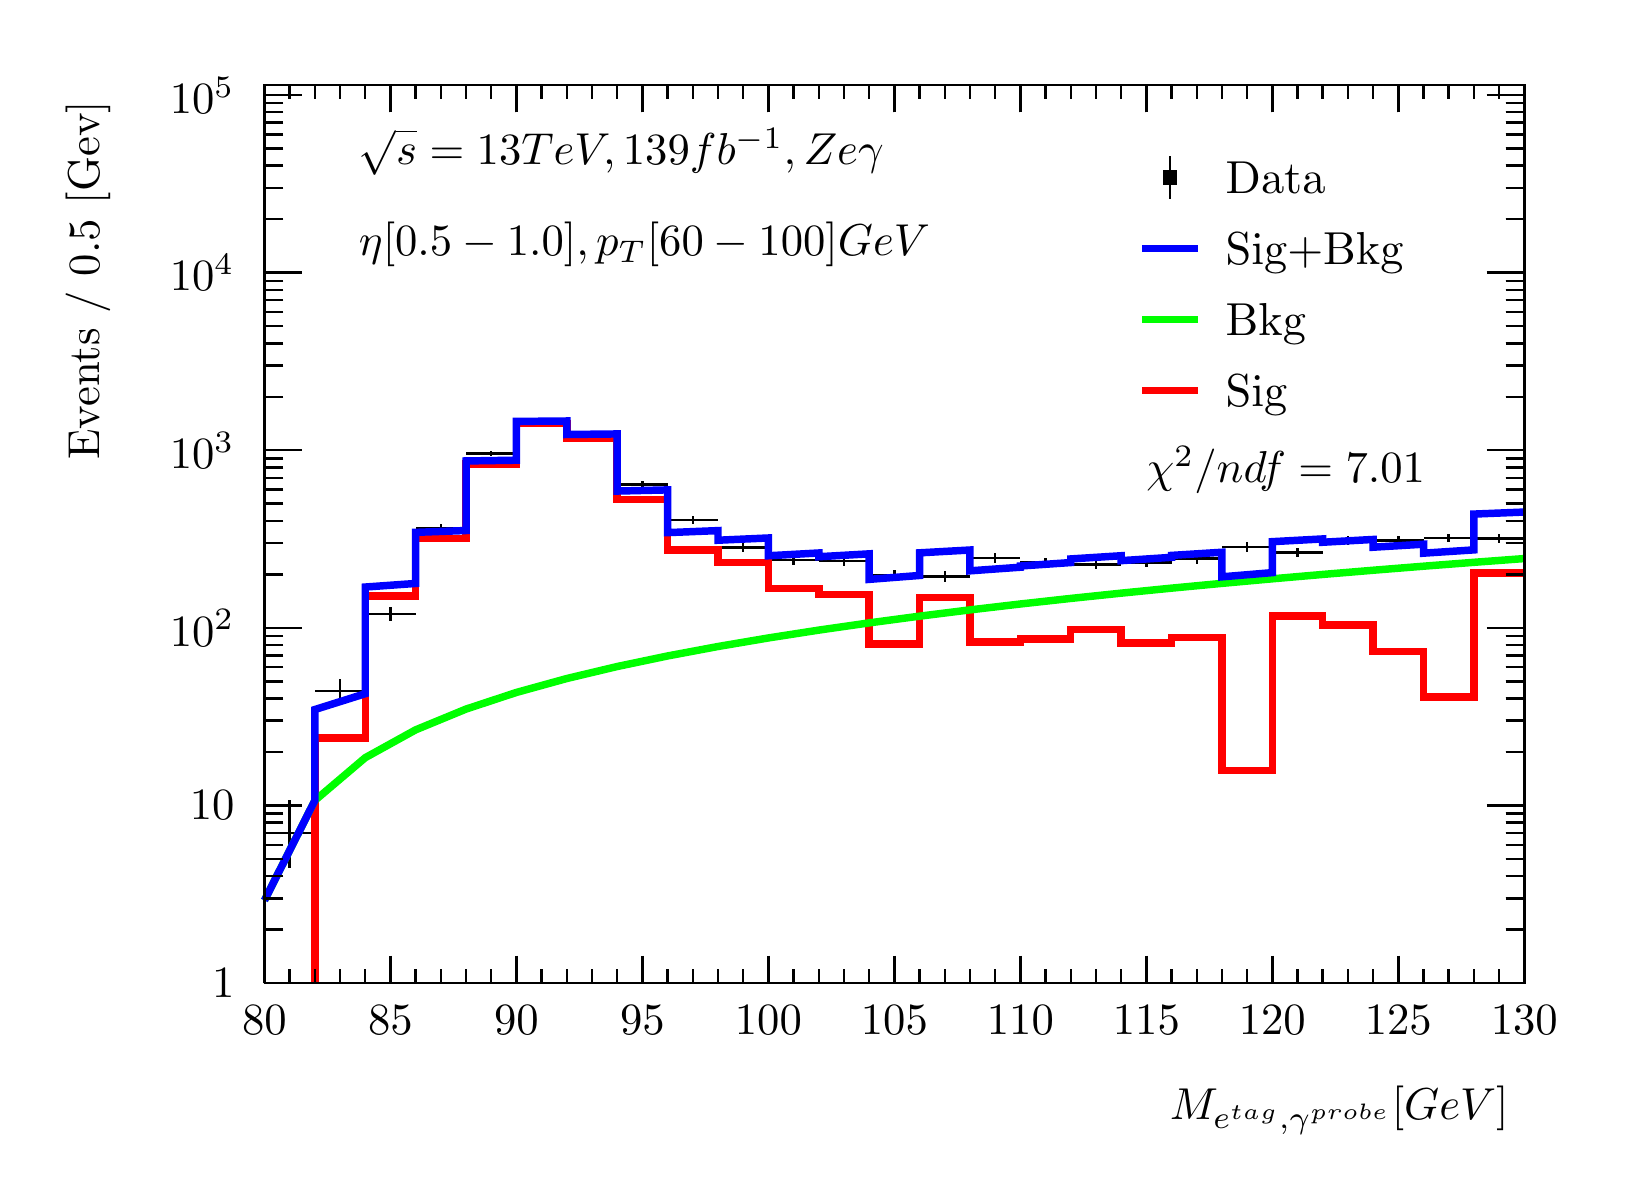
\begin{tikzpicture}
\pgfdeclareplotmark{cross} {
\pgfpathmoveto{\pgfpoint{-0.3\pgfplotmarksize}{\pgfplotmarksize}}
\pgfpathlineto{\pgfpoint{+0.3\pgfplotmarksize}{\pgfplotmarksize}}
\pgfpathlineto{\pgfpoint{+0.3\pgfplotmarksize}{0.3\pgfplotmarksize}}
\pgfpathlineto{\pgfpoint{+1\pgfplotmarksize}{0.3\pgfplotmarksize}}
\pgfpathlineto{\pgfpoint{+1\pgfplotmarksize}{-0.3\pgfplotmarksize}}
\pgfpathlineto{\pgfpoint{+0.3\pgfplotmarksize}{-0.3\pgfplotmarksize}}
\pgfpathlineto{\pgfpoint{+0.3\pgfplotmarksize}{-1.\pgfplotmarksize}}
\pgfpathlineto{\pgfpoint{-0.3\pgfplotmarksize}{-1.\pgfplotmarksize}}
\pgfpathlineto{\pgfpoint{-0.3\pgfplotmarksize}{-0.3\pgfplotmarksize}}
\pgfpathlineto{\pgfpoint{-1.\pgfplotmarksize}{-0.3\pgfplotmarksize}}
\pgfpathlineto{\pgfpoint{-1.\pgfplotmarksize}{0.3\pgfplotmarksize}}
\pgfpathlineto{\pgfpoint{-0.3\pgfplotmarksize}{0.3\pgfplotmarksize}}
\pgfpathclose
\pgfusepathqstroke
}
\pgfdeclareplotmark{cross*} {
\pgfpathmoveto{\pgfpoint{-0.3\pgfplotmarksize}{\pgfplotmarksize}}
\pgfpathlineto{\pgfpoint{+0.3\pgfplotmarksize}{\pgfplotmarksize}}
\pgfpathlineto{\pgfpoint{+0.3\pgfplotmarksize}{0.3\pgfplotmarksize}}
\pgfpathlineto{\pgfpoint{+1\pgfplotmarksize}{0.3\pgfplotmarksize}}
\pgfpathlineto{\pgfpoint{+1\pgfplotmarksize}{-0.3\pgfplotmarksize}}
\pgfpathlineto{\pgfpoint{+0.3\pgfplotmarksize}{-0.3\pgfplotmarksize}}
\pgfpathlineto{\pgfpoint{+0.3\pgfplotmarksize}{-1.\pgfplotmarksize}}
\pgfpathlineto{\pgfpoint{-0.3\pgfplotmarksize}{-1.\pgfplotmarksize}}
\pgfpathlineto{\pgfpoint{-0.3\pgfplotmarksize}{-0.3\pgfplotmarksize}}
\pgfpathlineto{\pgfpoint{-1.\pgfplotmarksize}{-0.3\pgfplotmarksize}}
\pgfpathlineto{\pgfpoint{-1.\pgfplotmarksize}{0.3\pgfplotmarksize}}
\pgfpathlineto{\pgfpoint{-0.3\pgfplotmarksize}{0.3\pgfplotmarksize}}
\pgfpathclose
\pgfusepathqfillstroke
}
\pgfdeclareplotmark{newstar} {
\pgfpathmoveto{\pgfqpoint{0pt}{\pgfplotmarksize}}
\pgfpathlineto{\pgfqpointpolar{44}{0.5\pgfplotmarksize}}
\pgfpathlineto{\pgfqpointpolar{18}{\pgfplotmarksize}}
\pgfpathlineto{\pgfqpointpolar{-20}{0.5\pgfplotmarksize}}
\pgfpathlineto{\pgfqpointpolar{-54}{\pgfplotmarksize}}
\pgfpathlineto{\pgfqpointpolar{-90}{0.5\pgfplotmarksize}}
\pgfpathlineto{\pgfqpointpolar{234}{\pgfplotmarksize}}
\pgfpathlineto{\pgfqpointpolar{198}{0.5\pgfplotmarksize}}
\pgfpathlineto{\pgfqpointpolar{162}{\pgfplotmarksize}}
\pgfpathlineto{\pgfqpointpolar{134}{0.5\pgfplotmarksize}}
\pgfpathclose
\pgfusepathqstroke
}
\pgfdeclareplotmark{newstar*} {
\pgfpathmoveto{\pgfqpoint{0pt}{\pgfplotmarksize}}
\pgfpathlineto{\pgfqpointpolar{44}{0.5\pgfplotmarksize}}
\pgfpathlineto{\pgfqpointpolar{18}{\pgfplotmarksize}}
\pgfpathlineto{\pgfqpointpolar{-20}{0.5\pgfplotmarksize}}
\pgfpathlineto{\pgfqpointpolar{-54}{\pgfplotmarksize}}
\pgfpathlineto{\pgfqpointpolar{-90}{0.5\pgfplotmarksize}}
\pgfpathlineto{\pgfqpointpolar{234}{\pgfplotmarksize}}
\pgfpathlineto{\pgfqpointpolar{198}{0.5\pgfplotmarksize}}
\pgfpathlineto{\pgfqpointpolar{162}{\pgfplotmarksize}}
\pgfpathlineto{\pgfqpointpolar{134}{0.5\pgfplotmarksize}}
\pgfpathclose
\pgfusepathqfillstroke
}
\definecolor{c}{rgb}{1,1,1};
\draw [color=c, fill=c] (0,0) rectangle (20,14.4361);
\draw [color=c, fill=c] (3,2.30977) rectangle (19,13.7143);
\definecolor{c}{rgb}{0,0,0};
\draw [c,line width=0.9] (3,2.30977) -- (3,13.7143) -- (19,13.7143) -- (19,2.30977) -- (3,2.30977);
\definecolor{c}{rgb}{1,1,1};
\draw [color=c, fill=c] (3,2.30977) rectangle (19,13.7143);
\definecolor{c}{rgb}{0,0,0};
\draw [c,line width=0.9] (3,2.30977) -- (3,13.7143) -- (19,13.7143) -- (19,2.30977) -- (3,2.30977);
\draw [c,line width=0.9] (3,2.30977) -- (19,2.30977);
\draw [c,line width=0.9] (3,2.65624) -- (3,2.30977);
\draw [c,line width=0.9] (3.32,2.48301) -- (3.32,2.30977);
\draw [c,line width=0.9] (3.64,2.48301) -- (3.64,2.30977);
\draw [c,line width=0.9] (3.96,2.48301) -- (3.96,2.30977);
\draw [c,line width=0.9] (4.28,2.48301) -- (4.28,2.30977);
\draw [c,line width=0.9] (4.6,2.65624) -- (4.6,2.30977);
\draw [c,line width=0.9] (4.92,2.48301) -- (4.92,2.30977);
\draw [c,line width=0.9] (5.24,2.48301) -- (5.24,2.30977);
\draw [c,line width=0.9] (5.56,2.48301) -- (5.56,2.30977);
\draw [c,line width=0.9] (5.88,2.48301) -- (5.88,2.30977);
\draw [c,line width=0.9] (6.2,2.65624) -- (6.2,2.30977);
\draw [c,line width=0.9] (6.52,2.48301) -- (6.52,2.30977);
\draw [c,line width=0.9] (6.84,2.48301) -- (6.84,2.30977);
\draw [c,line width=0.9] (7.16,2.48301) -- (7.16,2.30977);
\draw [c,line width=0.9] (7.48,2.48301) -- (7.48,2.30977);
\draw [c,line width=0.9] (7.8,2.65624) -- (7.8,2.30977);
\draw [c,line width=0.9] (8.12,2.48301) -- (8.12,2.30977);
\draw [c,line width=0.9] (8.44,2.48301) -- (8.44,2.30977);
\draw [c,line width=0.9] (8.76,2.48301) -- (8.76,2.30977);
\draw [c,line width=0.9] (9.08,2.48301) -- (9.08,2.30977);
\draw [c,line width=0.9] (9.4,2.65624) -- (9.4,2.30977);
\draw [c,line width=0.9] (9.72,2.48301) -- (9.72,2.30977);
\draw [c,line width=0.9] (10.04,2.48301) -- (10.04,2.30977);
\draw [c,line width=0.9] (10.36,2.48301) -- (10.36,2.30977);
\draw [c,line width=0.9] (10.68,2.48301) -- (10.68,2.30977);
\draw [c,line width=0.9] (11,2.65624) -- (11,2.30977);
\draw [c,line width=0.9] (11.32,2.48301) -- (11.32,2.30977);
\draw [c,line width=0.9] (11.64,2.48301) -- (11.64,2.30977);
\draw [c,line width=0.9] (11.96,2.48301) -- (11.96,2.30977);
\draw [c,line width=0.9] (12.28,2.48301) -- (12.28,2.30977);
\draw [c,line width=0.9] (12.6,2.65624) -- (12.6,2.30977);
\draw [c,line width=0.9] (12.92,2.48301) -- (12.92,2.30977);
\draw [c,line width=0.9] (13.24,2.48301) -- (13.24,2.30977);
\draw [c,line width=0.9] (13.56,2.48301) -- (13.56,2.30977);
\draw [c,line width=0.9] (13.88,2.48301) -- (13.88,2.30977);
\draw [c,line width=0.9] (14.2,2.65624) -- (14.2,2.30977);
\draw [c,line width=0.9] (14.52,2.48301) -- (14.52,2.30977);
\draw [c,line width=0.9] (14.84,2.48301) -- (14.84,2.30977);
\draw [c,line width=0.9] (15.16,2.48301) -- (15.16,2.30977);
\draw [c,line width=0.9] (15.48,2.48301) -- (15.48,2.30977);
\draw [c,line width=0.9] (15.8,2.65624) -- (15.8,2.30977);
\draw [c,line width=0.9] (16.12,2.48301) -- (16.12,2.30977);
\draw [c,line width=0.9] (16.44,2.48301) -- (16.44,2.30977);
\draw [c,line width=0.9] (16.76,2.48301) -- (16.76,2.30977);
\draw [c,line width=0.9] (17.08,2.48301) -- (17.08,2.30977);
\draw [c,line width=0.9] (17.4,2.65624) -- (17.4,2.30977);
\draw [c,line width=0.9] (17.72,2.48301) -- (17.72,2.30977);
\draw [c,line width=0.9] (18.04,2.48301) -- (18.04,2.30977);
\draw [c,line width=0.9] (18.36,2.48301) -- (18.36,2.30977);
\draw [c,line width=0.9] (18.68,2.48301) -- (18.68,2.30977);
\draw [c,line width=0.9] (19,2.65624) -- (19,2.30977);
\draw [anchor=base] (3,1.66015) node[scale=1.61424, color=c, rotate=0]{80};
\draw [anchor=base] (4.6,1.66015) node[scale=1.61424, color=c, rotate=0]{85};
\draw [anchor=base] (6.2,1.66015) node[scale=1.61424, color=c, rotate=0]{90};
\draw [anchor=base] (7.8,1.66015) node[scale=1.61424, color=c, rotate=0]{95};
\draw [anchor=base] (9.4,1.66015) node[scale=1.61424, color=c, rotate=0]{100};
\draw [anchor=base] (11,1.66015) node[scale=1.61424, color=c, rotate=0]{105};
\draw [anchor=base] (12.6,1.66015) node[scale=1.61424, color=c, rotate=0]{110};
\draw [anchor=base] (14.2,1.66015) node[scale=1.61424, color=c, rotate=0]{115};
\draw [anchor=base] (15.8,1.66015) node[scale=1.61424, color=c, rotate=0]{120};
\draw [anchor=base] (17.4,1.66015) node[scale=1.61424, color=c, rotate=0]{125};
\draw [anchor=base] (19,1.66015) node[scale=1.61424, color=c, rotate=0]{130};
\draw [anchor= east] (19,0.692932) node[scale=1.61424, color=c, rotate=0]{$M_{e^{tag}, \gamma^{probe}}  [GeV]$};
\draw [c,line width=0.9] (3,13.7143) -- (19,13.7143);
\draw [c,line width=0.9] (3,13.3678) -- (3,13.7143);
\draw [c,line width=0.9] (3.32,13.5411) -- (3.32,13.7143);
\draw [c,line width=0.9] (3.64,13.5411) -- (3.64,13.7143);
\draw [c,line width=0.9] (3.96,13.5411) -- (3.96,13.7143);
\draw [c,line width=0.9] (4.28,13.5411) -- (4.28,13.7143);
\draw [c,line width=0.9] (4.6,13.3678) -- (4.6,13.7143);
\draw [c,line width=0.9] (4.92,13.5411) -- (4.92,13.7143);
\draw [c,line width=0.9] (5.24,13.5411) -- (5.24,13.7143);
\draw [c,line width=0.9] (5.56,13.5411) -- (5.56,13.7143);
\draw [c,line width=0.9] (5.88,13.5411) -- (5.88,13.7143);
\draw [c,line width=0.9] (6.2,13.3678) -- (6.2,13.7143);
\draw [c,line width=0.9] (6.52,13.5411) -- (6.52,13.7143);
\draw [c,line width=0.9] (6.84,13.5411) -- (6.84,13.7143);
\draw [c,line width=0.9] (7.16,13.5411) -- (7.16,13.7143);
\draw [c,line width=0.9] (7.48,13.5411) -- (7.48,13.7143);
\draw [c,line width=0.9] (7.8,13.3678) -- (7.8,13.7143);
\draw [c,line width=0.9] (8.12,13.5411) -- (8.12,13.7143);
\draw [c,line width=0.9] (8.44,13.5411) -- (8.44,13.7143);
\draw [c,line width=0.9] (8.76,13.5411) -- (8.76,13.7143);
\draw [c,line width=0.9] (9.08,13.5411) -- (9.08,13.7143);
\draw [c,line width=0.9] (9.4,13.3678) -- (9.4,13.7143);
\draw [c,line width=0.9] (9.72,13.5411) -- (9.72,13.7143);
\draw [c,line width=0.9] (10.04,13.5411) -- (10.04,13.7143);
\draw [c,line width=0.9] (10.36,13.5411) -- (10.36,13.7143);
\draw [c,line width=0.9] (10.68,13.5411) -- (10.68,13.7143);
\draw [c,line width=0.9] (11,13.3678) -- (11,13.7143);
\draw [c,line width=0.9] (11.32,13.5411) -- (11.32,13.7143);
\draw [c,line width=0.9] (11.64,13.5411) -- (11.64,13.7143);
\draw [c,line width=0.9] (11.96,13.5411) -- (11.96,13.7143);
\draw [c,line width=0.9] (12.28,13.5411) -- (12.28,13.7143);
\draw [c,line width=0.9] (12.6,13.3678) -- (12.6,13.7143);
\draw [c,line width=0.9] (12.92,13.5411) -- (12.92,13.7143);
\draw [c,line width=0.9] (13.24,13.5411) -- (13.24,13.7143);
\draw [c,line width=0.9] (13.56,13.5411) -- (13.56,13.7143);
\draw [c,line width=0.9] (13.88,13.5411) -- (13.88,13.7143);
\draw [c,line width=0.9] (14.2,13.3678) -- (14.2,13.7143);
\draw [c,line width=0.9] (14.52,13.5411) -- (14.52,13.7143);
\draw [c,line width=0.9] (14.84,13.5411) -- (14.84,13.7143);
\draw [c,line width=0.9] (15.16,13.5411) -- (15.16,13.7143);
\draw [c,line width=0.9] (15.48,13.5411) -- (15.48,13.7143);
\draw [c,line width=0.9] (15.8,13.3678) -- (15.8,13.7143);
\draw [c,line width=0.9] (16.12,13.5411) -- (16.12,13.7143);
\draw [c,line width=0.9] (16.44,13.5411) -- (16.44,13.7143);
\draw [c,line width=0.9] (16.76,13.5411) -- (16.76,13.7143);
\draw [c,line width=0.9] (17.08,13.5411) -- (17.08,13.7143);
\draw [c,line width=0.9] (17.4,13.3678) -- (17.4,13.7143);
\draw [c,line width=0.9] (17.72,13.5411) -- (17.72,13.7143);
\draw [c,line width=0.9] (18.04,13.5411) -- (18.04,13.7143);
\draw [c,line width=0.9] (18.36,13.5411) -- (18.36,13.7143);
\draw [c,line width=0.9] (18.68,13.5411) -- (18.68,13.7143);
\draw [c,line width=0.9] (19,13.3678) -- (19,13.7143);
\draw [c,line width=0.9] (3,2.30977) -- (3,13.7143);
\draw [c,line width=0.9] (3.474,2.30978) -- (3,2.30978);
\draw [anchor= east] (2.82,2.30978) node[scale=1.61424, color=c, rotate=0]{1};
\draw [c,line width=0.9] (3.237,2.98876) -- (3,2.98876);
\draw [c,line width=0.9] (3.237,3.38594) -- (3,3.38594);
\draw [c,line width=0.9] (3.237,3.66775) -- (3,3.66775);
\draw [c,line width=0.9] (3.237,3.88633) -- (3,3.88633);
\draw [c,line width=0.9] (3.237,4.06493) -- (3,4.06493);
\draw [c,line width=0.9] (3.237,4.21593) -- (3,4.21593);
\draw [c,line width=0.9] (3.237,4.34673) -- (3,4.34673);
\draw [c,line width=0.9] (3.237,4.46211) -- (3,4.46211);
\draw [c,line width=0.9] (3.474,4.56532) -- (3,4.56532);
\draw [anchor= east] (2.82,4.56532) node[scale=1.61424, color=c, rotate=0]{10};
\draw [c,line width=0.9] (3.237,5.2443) -- (3,5.2443);
\draw [c,line width=0.9] (3.237,5.64148) -- (3,5.64148);
\draw [c,line width=0.9] (3.237,5.92329) -- (3,5.92329);
\draw [c,line width=0.9] (3.237,6.14187) -- (3,6.14187);
\draw [c,line width=0.9] (3.237,6.32047) -- (3,6.32047);
\draw [c,line width=0.9] (3.237,6.47147) -- (3,6.47147);
\draw [c,line width=0.9] (3.237,6.60227) -- (3,6.60227);
\draw [c,line width=0.9] (3.237,6.71765) -- (3,6.71765);
\draw [c,line width=0.9] (3.474,6.82086) -- (3,6.82086);
\draw [anchor= east] (2.82,6.82086) node[scale=1.61424, color=c, rotate=0]{$10^{2}$};
\draw [c,line width=0.9] (3.237,7.49984) -- (3,7.49984);
\draw [c,line width=0.9] (3.237,7.89703) -- (3,7.89703);
\draw [c,line width=0.9] (3.237,8.17883) -- (3,8.17883);
\draw [c,line width=0.9] (3.237,8.39741) -- (3,8.39741);
\draw [c,line width=0.9] (3.237,8.57601) -- (3,8.57601);
\draw [c,line width=0.9] (3.237,8.72701) -- (3,8.72701);
\draw [c,line width=0.9] (3.237,8.85782) -- (3,8.85782);
\draw [c,line width=0.9] (3.237,8.97319) -- (3,8.97319);
\draw [c,line width=0.9] (3.474,9.0764) -- (3,9.0764);
\draw [anchor= east] (2.82,9.0764) node[scale=1.61424, color=c, rotate=0]{$10^{3}$};
\draw [c,line width=0.9] (3.237,9.75539) -- (3,9.75539);
\draw [c,line width=0.9] (3.237,10.1526) -- (3,10.1526);
\draw [c,line width=0.9] (3.237,10.4344) -- (3,10.4344);
\draw [c,line width=0.9] (3.237,10.653) -- (3,10.653);
\draw [c,line width=0.9] (3.237,10.8316) -- (3,10.8316);
\draw [c,line width=0.9] (3.237,10.9826) -- (3,10.9826);
\draw [c,line width=0.9] (3.237,11.1134) -- (3,11.1134);
\draw [c,line width=0.9] (3.237,11.2287) -- (3,11.2287);
\draw [c,line width=0.9] (3.474,11.3319) -- (3,11.3319);
\draw [anchor= east] (2.82,11.3319) node[scale=1.61424, color=c, rotate=0]{$10^{4}$};
\draw [c,line width=0.9] (3.237,12.0109) -- (3,12.0109);
\draw [c,line width=0.9] (3.237,12.4081) -- (3,12.4081);
\draw [c,line width=0.9] (3.237,12.6899) -- (3,12.6899);
\draw [c,line width=0.9] (3.237,12.9085) -- (3,12.9085);
\draw [c,line width=0.9] (3.237,13.0871) -- (3,13.0871);
\draw [c,line width=0.9] (3.237,13.2381) -- (3,13.2381);
\draw [c,line width=0.9] (3.237,13.3689) -- (3,13.3689);
\draw [c,line width=0.9] (3.237,13.4843) -- (3,13.4843);
\draw [c,line width=0.9] (3.474,13.5875) -- (3,13.5875);
\draw [anchor= east] (2.82,13.5875) node[scale=1.61424, color=c, rotate=0]{$10^{5}$};
\draw [anchor= east] (0.76,13.7143) node[scale=1.61424, color=c, rotate=90]{Events / 0.5 [Gev]};
\draw [c,line width=0.9] (19,2.30977) -- (19,13.7143);
\draw [c,line width=0.9] (18.526,2.30978) -- (19,2.30978);
\draw [c,line width=0.9] (18.763,2.98876) -- (19,2.98876);
\draw [c,line width=0.9] (18.763,3.38594) -- (19,3.38594);
\draw [c,line width=0.9] (18.763,3.66775) -- (19,3.66775);
\draw [c,line width=0.9] (18.763,3.88633) -- (19,3.88633);
\draw [c,line width=0.9] (18.763,4.06493) -- (19,4.06493);
\draw [c,line width=0.9] (18.763,4.21593) -- (19,4.21593);
\draw [c,line width=0.9] (18.763,4.34673) -- (19,4.34673);
\draw [c,line width=0.9] (18.763,4.46211) -- (19,4.46211);
\draw [c,line width=0.9] (18.526,4.56532) -- (19,4.56532);
\draw [c,line width=0.9] (18.763,5.2443) -- (19,5.2443);
\draw [c,line width=0.9] (18.763,5.64148) -- (19,5.64148);
\draw [c,line width=0.9] (18.763,5.92329) -- (19,5.92329);
\draw [c,line width=0.9] (18.763,6.14187) -- (19,6.14187);
\draw [c,line width=0.9] (18.763,6.32047) -- (19,6.32047);
\draw [c,line width=0.9] (18.763,6.47147) -- (19,6.47147);
\draw [c,line width=0.9] (18.763,6.60227) -- (19,6.60227);
\draw [c,line width=0.9] (18.763,6.71765) -- (19,6.71765);
\draw [c,line width=0.9] (18.526,6.82086) -- (19,6.82086);
\draw [c,line width=0.9] (18.763,7.49984) -- (19,7.49984);
\draw [c,line width=0.9] (18.763,7.89703) -- (19,7.89703);
\draw [c,line width=0.9] (18.763,8.17883) -- (19,8.17883);
\draw [c,line width=0.9] (18.763,8.39741) -- (19,8.39741);
\draw [c,line width=0.9] (18.763,8.57601) -- (19,8.57601);
\draw [c,line width=0.9] (18.763,8.72701) -- (19,8.72701);
\draw [c,line width=0.9] (18.763,8.85782) -- (19,8.85782);
\draw [c,line width=0.9] (18.763,8.97319) -- (19,8.97319);
\draw [c,line width=0.9] (18.526,9.0764) -- (19,9.0764);
\draw [c,line width=0.9] (18.763,9.75539) -- (19,9.75539);
\draw [c,line width=0.9] (18.763,10.1526) -- (19,10.1526);
\draw [c,line width=0.9] (18.763,10.4344) -- (19,10.4344);
\draw [c,line width=0.9] (18.763,10.653) -- (19,10.653);
\draw [c,line width=0.9] (18.763,10.8316) -- (19,10.8316);
\draw [c,line width=0.9] (18.763,10.9826) -- (19,10.9826);
\draw [c,line width=0.9] (18.763,11.1134) -- (19,11.1134);
\draw [c,line width=0.9] (18.763,11.2287) -- (19,11.2287);
\draw [c,line width=0.9] (18.526,11.3319) -- (19,11.3319);
\draw [c,line width=0.9] (18.763,12.0109) -- (19,12.0109);
\draw [c,line width=0.9] (18.763,12.4081) -- (19,12.4081);
\draw [c,line width=0.9] (18.763,12.6899) -- (19,12.6899);
\draw [c,line width=0.9] (18.763,12.9085) -- (19,12.9085);
\draw [c,line width=0.9] (18.763,13.0871) -- (19,13.0871);
\draw [c,line width=0.9] (18.763,13.2381) -- (19,13.2381);
\draw [c,line width=0.9] (18.763,13.3689) -- (19,13.3689);
\draw [c,line width=0.9] (18.763,13.4843) -- (19,13.4843);
\draw [c,line width=0.9] (18.526,13.5875) -- (19,13.5875);
\draw [c,line width=0.9] (3.32,4.21593) -- (3,4.21593);
\draw [c,line width=0.9] (3,4.21593) -- (3,4.21593);
\draw [c,line width=0.9] (3.32,4.21593) -- (3.64,4.21593);
\draw [c,line width=0.9] (3.64,4.21593) -- (3.64,4.21593);
\draw [c,line width=0.9] (3.32,4.21593) -- (3.32,4.63801);
\draw [c,line width=0.9] (3.32,4.63801) -- (3.32,4.63801);
\draw [c,line width=0.9] (3.32,4.21593) -- (3.32,3.76523);
\draw [c,line width=0.9] (3.32,3.76523) -- (3.32,3.76523);
\draw [c,line width=0.9] (3.96,6.01665) -- (3.64,6.01665);
\draw [c,line width=0.9] (3.64,6.01665) -- (3.64,6.01665);
\draw [c,line width=0.9] (3.96,6.01665) -- (4.28,6.01665);
\draw [c,line width=0.9] (4.28,6.01665) -- (4.28,6.01665);
\draw [c,line width=0.9] (3.96,6.01665) -- (3.96,6.17431);
\draw [c,line width=0.9] (3.96,6.17431) -- (3.96,6.17431);
\draw [c,line width=0.9] (3.96,6.01665) -- (3.96,5.85724);
\draw [c,line width=0.9] (3.96,5.85724) -- (3.96,5.85724);
\draw [c,line width=0.9] (4.6,6.99945) -- (4.28,6.99945);
\draw [c,line width=0.9] (4.28,6.99945) -- (4.28,6.99945);
\draw [c,line width=0.9] (4.6,6.99945) -- (4.92,6.99945);
\draw [c,line width=0.9] (4.92,6.99945) -- (4.92,6.99945);
\draw [c,line width=0.9] (4.6,6.99945) -- (4.6,7.08885);
\draw [c,line width=0.9] (4.6,7.08885) -- (4.6,7.08885);
\draw [c,line width=0.9] (4.6,6.99945) -- (4.6,6.91006);
\draw [c,line width=0.9] (4.6,6.91006) -- (4.6,6.91006);
\draw [c,line width=0.9] (5.24,8.09181) -- (4.92,8.09181);
\draw [c,line width=0.9] (4.92,8.09181) -- (4.92,8.09181);
\draw [c,line width=0.9] (5.24,8.09181) -- (5.56,8.09181);
\draw [c,line width=0.9] (5.56,8.09181) -- (5.56,8.09181);
\draw [c,line width=0.9] (5.24,8.09181) -- (5.24,8.14301);
\draw [c,line width=0.9] (5.24,8.14301) -- (5.24,8.14301);
\draw [c,line width=0.9] (5.24,8.09181) -- (5.24,8.04062);
\draw [c,line width=0.9] (5.24,8.04062) -- (5.24,8.04062);
\draw [c,line width=0.9] (5.88,9.03641) -- (5.56,9.03641);
\draw [c,line width=0.9] (5.56,9.03641) -- (5.56,9.03641);
\draw [c,line width=0.9] (5.88,9.03641) -- (6.2,9.03641);
\draw [c,line width=0.9] (6.2,9.03641) -- (6.2,9.03641);
\draw [c,line width=0.9] (5.88,9.03641) -- (5.88,9.06803);
\draw [c,line width=0.9] (5.88,9.06803) -- (5.88,9.06803);
\draw [c,line width=0.9] (5.88,9.03641) -- (5.88,9.0048);
\draw [c,line width=0.9] (5.88,9.0048) -- (5.88,9.0048);
\draw [c,line width=0.9] (6.52,9.45179) -- (6.2,9.45179);
\draw [c,line width=0.9] (6.2,9.45179) -- (6.2,9.45179);
\draw [c,line width=0.9] (6.52,9.45179) -- (6.84,9.45179);
\draw [c,line width=0.9] (6.84,9.45179) -- (6.84,9.45179);
\draw [c,line width=0.9] (6.52,9.45179) -- (6.52,9.47736);
\draw [c,line width=0.9] (6.52,9.47736) -- (6.52,9.47736);
\draw [c,line width=0.9] (6.52,9.45179) -- (6.52,9.42622);
\draw [c,line width=0.9] (6.52,9.42622) -- (6.52,9.42622);
\draw [c,line width=0.9] (7.16,9.26313) -- (6.84,9.26313);
\draw [c,line width=0.9] (6.84,9.26313) -- (6.84,9.26313);
\draw [c,line width=0.9] (7.16,9.26313) -- (7.48,9.26313);
\draw [c,line width=0.9] (7.48,9.26313) -- (7.48,9.26313);
\draw [c,line width=0.9] (7.16,9.26313) -- (7.16,9.29128);
\draw [c,line width=0.9] (7.16,9.29128) -- (7.16,9.29128);
\draw [c,line width=0.9] (7.16,9.26313) -- (7.16,9.23497);
\draw [c,line width=0.9] (7.16,9.23497) -- (7.16,9.23497);
\draw [c,line width=0.9] (7.8,8.64229) -- (7.48,8.64229);
\draw [c,line width=0.9] (7.48,8.64229) -- (7.48,8.64229);
\draw [c,line width=0.9] (7.8,8.64229) -- (8.12,8.64229);
\draw [c,line width=0.9] (8.12,8.64229) -- (8.12,8.64229);
\draw [c,line width=0.9] (7.8,8.64229) -- (7.8,8.68094);
\draw [c,line width=0.9] (7.8,8.68094) -- (7.8,8.68094);
\draw [c,line width=0.9] (7.8,8.64229) -- (7.8,8.60363);
\draw [c,line width=0.9] (7.8,8.60363) -- (7.8,8.60363);
\draw [c,line width=0.9] (8.44,8.18858) -- (8.12,8.18858);
\draw [c,line width=0.9] (8.12,8.18858) -- (8.12,8.18858);
\draw [c,line width=0.9] (8.44,8.18858) -- (8.76,8.18858);
\draw [c,line width=0.9] (8.76,8.18858) -- (8.76,8.18858);
\draw [c,line width=0.9] (8.44,8.18858) -- (8.44,8.23731);
\draw [c,line width=0.9] (8.44,8.23731) -- (8.44,8.23731);
\draw [c,line width=0.9] (8.44,8.18858) -- (8.44,8.13985);
\draw [c,line width=0.9] (8.44,8.13985) -- (8.44,8.13985);
\draw [c,line width=0.9] (9.08,7.83988) -- (8.76,7.83988);
\draw [c,line width=0.9] (8.76,7.83988) -- (8.76,7.83988);
\draw [c,line width=0.9] (9.08,7.83988) -- (9.4,7.83988);
\draw [c,line width=0.9] (9.4,7.83988) -- (9.4,7.83988);
\draw [c,line width=0.9] (9.08,7.83988) -- (9.08,7.8981);
\draw [c,line width=0.9] (9.08,7.8981) -- (9.08,7.8981);
\draw [c,line width=0.9] (9.08,7.83988) -- (9.08,7.78166);
\draw [c,line width=0.9] (9.08,7.78166) -- (9.08,7.78166);
\draw [c,line width=0.9] (9.72,7.68251) -- (9.4,7.68251);
\draw [c,line width=0.9] (9.4,7.68251) -- (9.4,7.68251);
\draw [c,line width=0.9] (9.72,7.68251) -- (10.04,7.68251);
\draw [c,line width=0.9] (10.04,7.68251) -- (10.04,7.68251);
\draw [c,line width=0.9] (9.72,7.68251) -- (9.72,7.7456);
\draw [c,line width=0.9] (9.72,7.7456) -- (9.72,7.7456);
\draw [c,line width=0.9] (9.72,7.68251) -- (9.72,7.61942);
\draw [c,line width=0.9] (9.72,7.61942) -- (9.72,7.61942);
\draw [c,line width=0.9] (10.36,7.67024) -- (10.04,7.67024);
\draw [c,line width=0.9] (10.04,7.67024) -- (10.04,7.67024);
\draw [c,line width=0.9] (10.36,7.67024) -- (10.68,7.67024);
\draw [c,line width=0.9] (10.68,7.67024) -- (10.68,7.67024);
\draw [c,line width=0.9] (10.36,7.67024) -- (10.36,7.73373);
\draw [c,line width=0.9] (10.36,7.73373) -- (10.36,7.73373);
\draw [c,line width=0.9] (10.36,7.67024) -- (10.36,7.60676);
\draw [c,line width=0.9] (10.36,7.60676) -- (10.36,7.60676);
\draw [c,line width=0.9] (11,7.48504) -- (10.68,7.48504);
\draw [c,line width=0.9] (10.68,7.48504) -- (10.68,7.48504);
\draw [c,line width=0.9] (11,7.48504) -- (11.32,7.48504);
\draw [c,line width=0.9] (11.32,7.48504) -- (11.32,7.48504);
\draw [c,line width=0.9] (11,7.48504) -- (11,7.55482);
\draw [c,line width=0.9] (11,7.55482) -- (11,7.55482);
\draw [c,line width=0.9] (11,7.48504) -- (11,7.41526);
\draw [c,line width=0.9] (11,7.41526) -- (11,7.41526);
\draw [c,line width=0.9] (11.64,7.47504) -- (11.32,7.47504);
\draw [c,line width=0.9] (11.32,7.47504) -- (11.32,7.47504);
\draw [c,line width=0.9] (11.64,7.47504) -- (11.96,7.47504);
\draw [c,line width=0.9] (11.96,7.47504) -- (11.96,7.47504);
\draw [c,line width=0.9] (11.64,7.47504) -- (11.64,7.54518);
\draw [c,line width=0.9] (11.64,7.54518) -- (11.64,7.54518);
\draw [c,line width=0.9] (11.64,7.47504) -- (11.64,7.40491);
\draw [c,line width=0.9] (11.64,7.40491) -- (11.64,7.40491);
\draw [c,line width=0.9] (12.28,7.7066) -- (11.96,7.7066);
\draw [c,line width=0.9] (11.96,7.7066) -- (11.96,7.7066);
\draw [c,line width=0.9] (12.28,7.7066) -- (12.6,7.7066);
\draw [c,line width=0.9] (12.6,7.7066) -- (12.6,7.7066);
\draw [c,line width=0.9] (12.28,7.7066) -- (12.28,7.76892);
\draw [c,line width=0.9] (12.28,7.76892) -- (12.28,7.76892);
\draw [c,line width=0.9] (12.28,7.7066) -- (12.28,7.64428);
\draw [c,line width=0.9] (12.28,7.64428) -- (12.28,7.64428);
\draw [c,line width=0.9] (12.92,7.64944) -- (12.6,7.64944);
\draw [c,line width=0.9] (12.6,7.64944) -- (12.6,7.64944);
\draw [c,line width=0.9] (12.92,7.64944) -- (13.24,7.64944);
\draw [c,line width=0.9] (13.24,7.64944) -- (13.24,7.64944);
\draw [c,line width=0.9] (12.92,7.64944) -- (12.92,7.71361);
\draw [c,line width=0.9] (12.92,7.71361) -- (12.92,7.71361);
\draw [c,line width=0.9] (12.92,7.64944) -- (12.92,7.58528);
\draw [c,line width=0.9] (12.92,7.58528) -- (12.92,7.58528);
\draw [c,line width=0.9] (13.56,7.62819) -- (13.24,7.62819);
\draw [c,line width=0.9] (13.24,7.62819) -- (13.24,7.62819);
\draw [c,line width=0.9] (13.56,7.62819) -- (13.88,7.62819);
\draw [c,line width=0.9] (13.88,7.62819) -- (13.88,7.62819);
\draw [c,line width=0.9] (13.56,7.62819) -- (13.56,7.69306);
\draw [c,line width=0.9] (13.56,7.69306) -- (13.56,7.69306);
\draw [c,line width=0.9] (13.56,7.62819) -- (13.56,7.56333);
\draw [c,line width=0.9] (13.56,7.56333) -- (13.56,7.56333);
\draw [c,line width=0.9] (14.2,7.65364) -- (13.88,7.65364);
\draw [c,line width=0.9] (13.88,7.65364) -- (13.88,7.65364);
\draw [c,line width=0.9] (14.2,7.65364) -- (14.52,7.65364);
\draw [c,line width=0.9] (14.52,7.65364) -- (14.52,7.65364);
\draw [c,line width=0.9] (14.2,7.65364) -- (14.2,7.71766);
\draw [c,line width=0.9] (14.2,7.71766) -- (14.2,7.71766);
\draw [c,line width=0.9] (14.2,7.65364) -- (14.2,7.58961);
\draw [c,line width=0.9] (14.2,7.58961) -- (14.2,7.58961);
\draw [c,line width=0.9] (14.84,7.69864) -- (14.52,7.69864);
\draw [c,line width=0.9] (14.52,7.69864) -- (14.52,7.69864);
\draw [c,line width=0.9] (14.84,7.69864) -- (15.16,7.69864);
\draw [c,line width=0.9] (15.16,7.69864) -- (15.16,7.69864);
\draw [c,line width=0.9] (14.84,7.69864) -- (14.84,7.76121);
\draw [c,line width=0.9] (14.84,7.76121) -- (14.84,7.76121);
\draw [c,line width=0.9] (14.84,7.69864) -- (14.84,7.63607);
\draw [c,line width=0.9] (14.84,7.63607) -- (14.84,7.63607);
\draw [c,line width=0.9] (15.48,7.84678) -- (15.16,7.84678);
\draw [c,line width=0.9] (15.16,7.84678) -- (15.16,7.84678);
\draw [c,line width=0.9] (15.48,7.84678) -- (15.8,7.84678);
\draw [c,line width=0.9] (15.8,7.84678) -- (15.8,7.84678);
\draw [c,line width=0.9] (15.48,7.84678) -- (15.48,7.9048);
\draw [c,line width=0.9] (15.48,7.9048) -- (15.48,7.9048);
\draw [c,line width=0.9] (15.48,7.84678) -- (15.48,7.78876);
\draw [c,line width=0.9] (15.48,7.78876) -- (15.48,7.78876);
\draw [c,line width=0.9] (16.12,7.77551) -- (15.8,7.77551);
\draw [c,line width=0.9] (15.8,7.77551) -- (15.8,7.77551);
\draw [c,line width=0.9] (16.12,7.77551) -- (16.44,7.77551);
\draw [c,line width=0.9] (16.44,7.77551) -- (16.44,7.77551);
\draw [c,line width=0.9] (16.12,7.77551) -- (16.12,7.83567);
\draw [c,line width=0.9] (16.12,7.83567) -- (16.12,7.83567);
\draw [c,line width=0.9] (16.12,7.77551) -- (16.12,7.71534);
\draw [c,line width=0.9] (16.12,7.71534) -- (16.12,7.71534);
\draw [c,line width=0.9] (16.76,7.92914) -- (16.44,7.92914);
\draw [c,line width=0.9] (16.44,7.92914) -- (16.44,7.92914);
\draw [c,line width=0.9] (16.76,7.92914) -- (17.08,7.92914);
\draw [c,line width=0.9] (17.08,7.92914) -- (17.08,7.92914);
\draw [c,line width=0.9] (16.76,7.92914) -- (16.76,7.98477);
\draw [c,line width=0.9] (16.76,7.98477) -- (16.76,7.98477);
\draw [c,line width=0.9] (16.76,7.92914) -- (16.76,7.87352);
\draw [c,line width=0.9] (16.76,7.87352) -- (16.76,7.87352);
\draw [c,line width=0.9] (17.4,7.9323) -- (17.08,7.9323);
\draw [c,line width=0.9] (17.08,7.9323) -- (17.08,7.9323);
\draw [c,line width=0.9] (17.4,7.9323) -- (17.72,7.9323);
\draw [c,line width=0.9] (17.72,7.9323) -- (17.72,7.9323);
\draw [c,line width=0.9] (17.4,7.9323) -- (17.4,7.98784);
\draw [c,line width=0.9] (17.4,7.98784) -- (17.4,7.98784);
\draw [c,line width=0.9] (17.4,7.9323) -- (17.4,7.87676);
\draw [c,line width=0.9] (17.4,7.87676) -- (17.4,7.87676);
\draw [c,line width=0.9] (18.04,7.9633) -- (17.72,7.9633);
\draw [c,line width=0.9] (17.72,7.9633) -- (17.72,7.9633);
\draw [c,line width=0.9] (18.04,7.9633) -- (18.36,7.9633);
\draw [c,line width=0.9] (18.36,7.9633) -- (18.36,7.9633);
\draw [c,line width=0.9] (18.04,7.9633) -- (18.04,8.01797);
\draw [c,line width=0.9] (18.04,8.01797) -- (18.04,8.01797);
\draw [c,line width=0.9] (18.04,7.9633) -- (18.04,7.90863);
\draw [c,line width=0.9] (18.04,7.90863) -- (18.04,7.90863);
\draw [c,line width=0.9] (18.68,7.95718) -- (18.36,7.95718);
\draw [c,line width=0.9] (18.36,7.95718) -- (18.36,7.95718);
\draw [c,line width=0.9] (18.68,7.95718) -- (19,7.95718);
\draw [c,line width=0.9] (19,7.95718) -- (19,7.95718);
\draw [c,line width=0.9] (18.68,7.95718) -- (18.68,8.01202);
\draw [c,line width=0.9] (18.68,8.01202) -- (18.68,8.01202);
\draw [c,line width=0.9] (18.68,7.95718) -- (18.68,7.90234);
\draw [c,line width=0.9] (18.68,7.90234) -- (18.68,7.90234);
\foreach \P in {(3.32,4.21593), (3.96,6.01665), (4.6,6.99945), (5.24,8.09181), (5.88,9.03641), (6.52,9.45179), (7.16,9.26313), (7.8,8.64229), (8.44,8.18858), (9.08,7.83988), (9.72,7.68251), (10.36,7.67024), (11,7.48504), (11.64,7.47504),
 (12.28,7.7066), (12.92,7.64944), (13.56,7.62819), (14.2,7.65364), (14.84,7.69864), (15.48,7.84678), (16.12,7.77551), (16.76,7.92914), (17.4,7.9323), (18.04,7.9633), (18.68,7.95718)}{\draw[mark options={color=c,fill=c},mark size=2.882883pt,mark=]
 plot coordinates {\P};}
\definecolor{c}{rgb}{1,0,0};
\draw [c,line width=2.7] (3.64,2.30977) -- (3.64,5.42308);
\draw [c,line width=2.7] (3.64,5.42308) -- (4.28,5.42308) -- (4.28,7.2256) -- (4.92,7.2256) -- (4.92,7.95491) -- (5.56,7.95491) -- (5.56,8.90034) -- (6.2,8.90034) -- (6.2,9.41267) -- (6.84,9.41267) -- (6.84,9.23412) -- (7.48,9.23412) --
 (7.48,8.45179) -- (8.12,8.45179) -- (8.12,7.80916) -- (8.76,7.80916) -- (8.76,7.6491) -- (9.4,7.6491) -- (9.4,7.32258) -- (10.04,7.32258) -- (10.04,7.24607) -- (10.68,7.24607) -- (10.68,6.61279) -- (11.32,6.61279) -- (11.32,7.20566) --
 (11.96,7.20566) -- (11.96,6.64086) -- (12.6,6.64086) -- (12.6,6.68096) -- (13.24,6.68096) -- (13.24,6.80023) -- (13.88,6.80023) -- (13.88,6.62825) -- (14.52,6.62825) -- (14.52,6.70082) -- (15.16,6.70082) -- (15.16,5.0102) -- (15.8,5.0102) --
 (15.8,6.9734) -- (16.44,6.9734) -- (16.44,6.85468) -- (17.08,6.85468) -- (17.08,6.5179) -- (17.72,6.5179) -- (17.72,5.94537) -- (18.36,5.94537) -- (18.36,7.51556) -- (19,7.51556) -- (19,7.51556) -- (19,7.51556) -- (19,7.51556);
\definecolor{c}{rgb}{0,1,0};
\draw [c,line width=2.7] (3,3.35884) -- (3,3.35884);
\draw [c,line width=2.7] (3,3.35884) -- (3,3.35884) -- (3.64,4.6283) -- (3.64,4.6283) -- (4.28,5.1718) -- (4.28,5.1718) -- (4.92,5.52533) -- (4.92,5.52533) -- (5.56,5.78915) -- (5.56,5.78915) -- (6.2,6.00048) -- (6.2,6.00048) -- (6.84,6.1773) --
 (6.84,6.1773) -- (7.48,6.32968) -- (7.48,6.32968) -- (8.12,6.46381) -- (8.12,6.46381) -- (8.76,6.58381) -- (8.76,6.58381) -- (9.4,6.69252) -- (9.4,6.69252) -- (10.04,6.79202) -- (10.04,6.79202) -- (10.68,6.88383) -- (10.68,6.88383) --
 (11.32,6.96914) -- (11.32,6.96914) -- (11.96,7.04889) -- (11.96,7.04889) -- (12.6,7.1238) -- (12.6,7.1238) -- (13.24,7.19448) -- (13.24,7.19448) -- (13.88,7.26142) -- (13.88,7.26142) -- (14.52,7.32503) -- (14.52,7.32503) -- (15.16,7.38567) --
 (15.16,7.38567) -- (15.8,7.44361) -- (15.8,7.44361) -- (16.44,7.49912) -- (16.44,7.49912) -- (17.08,7.5524) -- (17.08,7.5524) -- (17.72,7.60366) -- (17.72,7.60366) -- (18.36,7.65305) -- (18.36,7.65305) -- (19,7.70072) -- (19,7.70072) -- (19,7.70072)
 -- (19,7.70072);
\definecolor{c}{rgb}{0,0,1};
\draw [c,line width=2.7] (3,3.35884) -- (3,3.35884);
\draw [c,line width=2.7] (3,3.35884) -- (3,3.35884) -- (3.64,4.6283) -- (3.64,5.78316) -- (4.28,5.98446) -- (4.28,7.33912) -- (4.92,7.38463) -- (4.92,8.03367) -- (5.56,8.05679) -- (5.56,8.9404) -- (6.2,8.94981) -- (6.2,9.44229) -- (6.84,9.44805) --
 (6.84,9.27642) -- (7.48,9.28337) -- (7.48,8.55806) -- (8.12,8.57273) -- (8.12,8.03028) -- (8.76,8.05575) -- (8.76,7.93363) -- (9.4,7.9622) -- (9.4,7.73635) -- (10.04,7.77178) -- (10.04,7.72411) -- (10.68,7.76059) -- (10.68,7.43664) --
 (11.32,7.48607) -- (11.32,7.77351) -- (11.96,7.80939) -- (11.96,7.54495) -- (12.6,7.59078) -- (12.6,7.60618) -- (13.24,7.64998) -- (13.24,7.69604) -- (13.88,7.73671) -- (13.88,7.67411) -- (14.52,7.71632) -- (14.52,7.74082) -- (15.16,7.7809) --
 (15.16,7.46871) -- (15.8,7.52207) -- (15.8,7.91544) -- (16.44,7.9501) -- (16.44,7.90795) -- (17.08,7.94338) -- (17.08,7.84479) -- (17.72,7.88307) -- (17.72,7.7691) -- (18.36,7.81098) -- (18.36,8.2657) -- (19,8.29149) -- (19,8.29149) -- (19,8.29149)
 -- (19,8.29149);
\definecolor{c}{rgb}{0,0,0};
\draw [c,line width=0.9] (3,2.30977) -- (19,2.30977);
\draw [c,line width=0.9] (3,2.65624) -- (3,2.30977);
\draw [c,line width=0.9] (3.32,2.48301) -- (3.32,2.30977);
\draw [c,line width=0.9] (3.64,2.48301) -- (3.64,2.30977);
\draw [c,line width=0.9] (3.96,2.48301) -- (3.96,2.30977);
\draw [c,line width=0.9] (4.28,2.48301) -- (4.28,2.30977);
\draw [c,line width=0.9] (4.6,2.65624) -- (4.6,2.30977);
\draw [c,line width=0.9] (4.92,2.48301) -- (4.92,2.30977);
\draw [c,line width=0.9] (5.24,2.48301) -- (5.24,2.30977);
\draw [c,line width=0.9] (5.56,2.48301) -- (5.56,2.30977);
\draw [c,line width=0.9] (5.88,2.48301) -- (5.88,2.30977);
\draw [c,line width=0.9] (6.2,2.65624) -- (6.2,2.30977);
\draw [c,line width=0.9] (6.52,2.48301) -- (6.52,2.30977);
\draw [c,line width=0.9] (6.84,2.48301) -- (6.84,2.30977);
\draw [c,line width=0.9] (7.16,2.48301) -- (7.16,2.30977);
\draw [c,line width=0.9] (7.48,2.48301) -- (7.48,2.30977);
\draw [c,line width=0.9] (7.8,2.65624) -- (7.8,2.30977);
\draw [c,line width=0.9] (8.12,2.48301) -- (8.12,2.30977);
\draw [c,line width=0.9] (8.44,2.48301) -- (8.44,2.30977);
\draw [c,line width=0.9] (8.76,2.48301) -- (8.76,2.30977);
\draw [c,line width=0.9] (9.08,2.48301) -- (9.08,2.30977);
\draw [c,line width=0.9] (9.4,2.65624) -- (9.4,2.30977);
\draw [c,line width=0.9] (9.72,2.48301) -- (9.72,2.30977);
\draw [c,line width=0.9] (10.04,2.48301) -- (10.04,2.30977);
\draw [c,line width=0.9] (10.36,2.48301) -- (10.36,2.30977);
\draw [c,line width=0.9] (10.68,2.48301) -- (10.68,2.30977);
\draw [c,line width=0.9] (11,2.65624) -- (11,2.30977);
\draw [c,line width=0.9] (11.32,2.48301) -- (11.32,2.30977);
\draw [c,line width=0.9] (11.64,2.48301) -- (11.64,2.30977);
\draw [c,line width=0.9] (11.96,2.48301) -- (11.96,2.30977);
\draw [c,line width=0.9] (12.28,2.48301) -- (12.28,2.30977);
\draw [c,line width=0.9] (12.6,2.65624) -- (12.6,2.30977);
\draw [c,line width=0.9] (12.92,2.48301) -- (12.92,2.30977);
\draw [c,line width=0.9] (13.24,2.48301) -- (13.24,2.30977);
\draw [c,line width=0.9] (13.56,2.48301) -- (13.56,2.30977);
\draw [c,line width=0.9] (13.88,2.48301) -- (13.88,2.30977);
\draw [c,line width=0.9] (14.2,2.65624) -- (14.2,2.30977);
\draw [c,line width=0.9] (14.52,2.48301) -- (14.52,2.30977);
\draw [c,line width=0.9] (14.84,2.48301) -- (14.84,2.30977);
\draw [c,line width=0.9] (15.16,2.48301) -- (15.16,2.30977);
\draw [c,line width=0.9] (15.48,2.48301) -- (15.48,2.30977);
\draw [c,line width=0.9] (15.8,2.65624) -- (15.8,2.30977);
\draw [c,line width=0.9] (16.12,2.48301) -- (16.12,2.30977);
\draw [c,line width=0.9] (16.44,2.48301) -- (16.44,2.30977);
\draw [c,line width=0.9] (16.76,2.48301) -- (16.76,2.30977);
\draw [c,line width=0.9] (17.08,2.48301) -- (17.08,2.30977);
\draw [c,line width=0.9] (17.4,2.65624) -- (17.4,2.30977);
\draw [c,line width=0.9] (17.72,2.48301) -- (17.72,2.30977);
\draw [c,line width=0.9] (18.04,2.48301) -- (18.04,2.30977);
\draw [c,line width=0.9] (18.36,2.48301) -- (18.36,2.30977);
\draw [c,line width=0.9] (18.68,2.48301) -- (18.68,2.30977);
\draw [c,line width=0.9] (19,2.65624) -- (19,2.30977);
\draw [c,line width=0.9] (3,13.7143) -- (19,13.7143);
\draw [c,line width=0.9] (3,13.3678) -- (3,13.7143);
\draw [c,line width=0.9] (3.32,13.5411) -- (3.32,13.7143);
\draw [c,line width=0.9] (3.64,13.5411) -- (3.64,13.7143);
\draw [c,line width=0.9] (3.96,13.5411) -- (3.96,13.7143);
\draw [c,line width=0.9] (4.28,13.5411) -- (4.28,13.7143);
\draw [c,line width=0.9] (4.6,13.3678) -- (4.6,13.7143);
\draw [c,line width=0.9] (4.92,13.5411) -- (4.92,13.7143);
\draw [c,line width=0.9] (5.24,13.5411) -- (5.24,13.7143);
\draw [c,line width=0.9] (5.56,13.5411) -- (5.56,13.7143);
\draw [c,line width=0.9] (5.88,13.5411) -- (5.88,13.7143);
\draw [c,line width=0.9] (6.2,13.3678) -- (6.2,13.7143);
\draw [c,line width=0.9] (6.52,13.5411) -- (6.52,13.7143);
\draw [c,line width=0.9] (6.84,13.5411) -- (6.84,13.7143);
\draw [c,line width=0.9] (7.16,13.5411) -- (7.16,13.7143);
\draw [c,line width=0.9] (7.48,13.5411) -- (7.48,13.7143);
\draw [c,line width=0.9] (7.8,13.3678) -- (7.8,13.7143);
\draw [c,line width=0.9] (8.12,13.5411) -- (8.12,13.7143);
\draw [c,line width=0.9] (8.44,13.5411) -- (8.44,13.7143);
\draw [c,line width=0.9] (8.76,13.5411) -- (8.76,13.7143);
\draw [c,line width=0.9] (9.08,13.5411) -- (9.08,13.7143);
\draw [c,line width=0.9] (9.4,13.3678) -- (9.4,13.7143);
\draw [c,line width=0.9] (9.72,13.5411) -- (9.72,13.7143);
\draw [c,line width=0.9] (10.04,13.5411) -- (10.04,13.7143);
\draw [c,line width=0.9] (10.36,13.5411) -- (10.36,13.7143);
\draw [c,line width=0.9] (10.68,13.5411) -- (10.68,13.7143);
\draw [c,line width=0.9] (11,13.3678) -- (11,13.7143);
\draw [c,line width=0.9] (11.32,13.5411) -- (11.32,13.7143);
\draw [c,line width=0.9] (11.64,13.5411) -- (11.64,13.7143);
\draw [c,line width=0.9] (11.96,13.5411) -- (11.96,13.7143);
\draw [c,line width=0.9] (12.28,13.5411) -- (12.28,13.7143);
\draw [c,line width=0.9] (12.6,13.3678) -- (12.6,13.7143);
\draw [c,line width=0.9] (12.92,13.5411) -- (12.92,13.7143);
\draw [c,line width=0.9] (13.24,13.5411) -- (13.24,13.7143);
\draw [c,line width=0.9] (13.56,13.5411) -- (13.56,13.7143);
\draw [c,line width=0.9] (13.88,13.5411) -- (13.88,13.7143);
\draw [c,line width=0.9] (14.2,13.3678) -- (14.2,13.7143);
\draw [c,line width=0.9] (14.52,13.5411) -- (14.52,13.7143);
\draw [c,line width=0.9] (14.84,13.5411) -- (14.84,13.7143);
\draw [c,line width=0.9] (15.16,13.5411) -- (15.16,13.7143);
\draw [c,line width=0.9] (15.48,13.5411) -- (15.48,13.7143);
\draw [c,line width=0.9] (15.8,13.3678) -- (15.8,13.7143);
\draw [c,line width=0.9] (16.12,13.5411) -- (16.12,13.7143);
\draw [c,line width=0.9] (16.44,13.5411) -- (16.44,13.7143);
\draw [c,line width=0.9] (16.76,13.5411) -- (16.76,13.7143);
\draw [c,line width=0.9] (17.08,13.5411) -- (17.08,13.7143);
\draw [c,line width=0.9] (17.4,13.3678) -- (17.4,13.7143);
\draw [c,line width=0.9] (17.72,13.5411) -- (17.72,13.7143);
\draw [c,line width=0.9] (18.04,13.5411) -- (18.04,13.7143);
\draw [c,line width=0.9] (18.36,13.5411) -- (18.36,13.7143);
\draw [c,line width=0.9] (18.68,13.5411) -- (18.68,13.7143);
\draw [c,line width=0.9] (19,13.3678) -- (19,13.7143);
\draw [c,line width=0.9] (3,2.30977) -- (3,13.7143);
\draw [c,line width=0.9] (3.474,2.30978) -- (3,2.30978);
\draw [c,line width=0.9] (3.237,2.98876) -- (3,2.98876);
\draw [c,line width=0.9] (3.237,3.38594) -- (3,3.38594);
\draw [c,line width=0.9] (3.237,3.66775) -- (3,3.66775);
\draw [c,line width=0.9] (3.237,3.88633) -- (3,3.88633);
\draw [c,line width=0.9] (3.237,4.06493) -- (3,4.06493);
\draw [c,line width=0.9] (3.237,4.21593) -- (3,4.21593);
\draw [c,line width=0.9] (3.237,4.34673) -- (3,4.34673);
\draw [c,line width=0.9] (3.237,4.46211) -- (3,4.46211);
\draw [c,line width=0.9] (3.474,4.56532) -- (3,4.56532);
\draw [c,line width=0.9] (3.237,5.2443) -- (3,5.2443);
\draw [c,line width=0.9] (3.237,5.64148) -- (3,5.64148);
\draw [c,line width=0.9] (3.237,5.92329) -- (3,5.92329);
\draw [c,line width=0.9] (3.237,6.14187) -- (3,6.14187);
\draw [c,line width=0.9] (3.237,6.32047) -- (3,6.32047);
\draw [c,line width=0.9] (3.237,6.47147) -- (3,6.47147);
\draw [c,line width=0.9] (3.237,6.60227) -- (3,6.60227);
\draw [c,line width=0.9] (3.237,6.71765) -- (3,6.71765);
\draw [c,line width=0.9] (3.474,6.82086) -- (3,6.82086);
\draw [c,line width=0.9] (3.237,7.49984) -- (3,7.49984);
\draw [c,line width=0.9] (3.237,7.89703) -- (3,7.89703);
\draw [c,line width=0.9] (3.237,8.17883) -- (3,8.17883);
\draw [c,line width=0.9] (3.237,8.39741) -- (3,8.39741);
\draw [c,line width=0.9] (3.237,8.57601) -- (3,8.57601);
\draw [c,line width=0.9] (3.237,8.72701) -- (3,8.72701);
\draw [c,line width=0.9] (3.237,8.85782) -- (3,8.85782);
\draw [c,line width=0.9] (3.237,8.97319) -- (3,8.97319);
\draw [c,line width=0.9] (3.474,9.0764) -- (3,9.0764);
\draw [c,line width=0.9] (3.237,9.75539) -- (3,9.75539);
\draw [c,line width=0.9] (3.237,10.1526) -- (3,10.1526);
\draw [c,line width=0.9] (3.237,10.4344) -- (3,10.4344);
\draw [c,line width=0.9] (3.237,10.653) -- (3,10.653);
\draw [c,line width=0.9] (3.237,10.8316) -- (3,10.8316);
\draw [c,line width=0.9] (3.237,10.9826) -- (3,10.9826);
\draw [c,line width=0.9] (3.237,11.1134) -- (3,11.1134);
\draw [c,line width=0.9] (3.237,11.2287) -- (3,11.2287);
\draw [c,line width=0.9] (3.474,11.3319) -- (3,11.3319);
\draw [c,line width=0.9] (3.237,12.0109) -- (3,12.0109);
\draw [c,line width=0.9] (3.237,12.4081) -- (3,12.4081);
\draw [c,line width=0.9] (3.237,12.6899) -- (3,12.6899);
\draw [c,line width=0.9] (3.237,12.9085) -- (3,12.9085);
\draw [c,line width=0.9] (3.237,13.0871) -- (3,13.0871);
\draw [c,line width=0.9] (3.237,13.2381) -- (3,13.2381);
\draw [c,line width=0.9] (3.237,13.3689) -- (3,13.3689);
\draw [c,line width=0.9] (3.237,13.4843) -- (3,13.4843);
\draw [c,line width=0.9] (3.474,13.5875) -- (3,13.5875);
\draw [c,line width=0.9] (19,2.30977) -- (19,13.7143);
\draw [c,line width=0.9] (18.526,2.30978) -- (19,2.30978);
\draw [c,line width=0.9] (18.763,2.98876) -- (19,2.98876);
\draw [c,line width=0.9] (18.763,3.38594) -- (19,3.38594);
\draw [c,line width=0.9] (18.763,3.66775) -- (19,3.66775);
\draw [c,line width=0.9] (18.763,3.88633) -- (19,3.88633);
\draw [c,line width=0.9] (18.763,4.06493) -- (19,4.06493);
\draw [c,line width=0.9] (18.763,4.21593) -- (19,4.21593);
\draw [c,line width=0.9] (18.763,4.34673) -- (19,4.34673);
\draw [c,line width=0.9] (18.763,4.46211) -- (19,4.46211);
\draw [c,line width=0.9] (18.526,4.56532) -- (19,4.56532);
\draw [c,line width=0.9] (18.763,5.2443) -- (19,5.2443);
\draw [c,line width=0.9] (18.763,5.64148) -- (19,5.64148);
\draw [c,line width=0.9] (18.763,5.92329) -- (19,5.92329);
\draw [c,line width=0.9] (18.763,6.14187) -- (19,6.14187);
\draw [c,line width=0.9] (18.763,6.32047) -- (19,6.32047);
\draw [c,line width=0.9] (18.763,6.47147) -- (19,6.47147);
\draw [c,line width=0.9] (18.763,6.60227) -- (19,6.60227);
\draw [c,line width=0.9] (18.763,6.71765) -- (19,6.71765);
\draw [c,line width=0.9] (18.526,6.82086) -- (19,6.82086);
\draw [c,line width=0.9] (18.763,7.49984) -- (19,7.49984);
\draw [c,line width=0.9] (18.763,7.89703) -- (19,7.89703);
\draw [c,line width=0.9] (18.763,8.17883) -- (19,8.17883);
\draw [c,line width=0.9] (18.763,8.39741) -- (19,8.39741);
\draw [c,line width=0.9] (18.763,8.57601) -- (19,8.57601);
\draw [c,line width=0.9] (18.763,8.72701) -- (19,8.72701);
\draw [c,line width=0.9] (18.763,8.85782) -- (19,8.85782);
\draw [c,line width=0.9] (18.763,8.97319) -- (19,8.97319);
\draw [c,line width=0.9] (18.526,9.0764) -- (19,9.0764);
\draw [c,line width=0.9] (18.763,9.75539) -- (19,9.75539);
\draw [c,line width=0.9] (18.763,10.1526) -- (19,10.1526);
\draw [c,line width=0.9] (18.763,10.4344) -- (19,10.4344);
\draw [c,line width=0.9] (18.763,10.653) -- (19,10.653);
\draw [c,line width=0.9] (18.763,10.8316) -- (19,10.8316);
\draw [c,line width=0.9] (18.763,10.9826) -- (19,10.9826);
\draw [c,line width=0.9] (18.763,11.1134) -- (19,11.1134);
\draw [c,line width=0.9] (18.763,11.2287) -- (19,11.2287);
\draw [c,line width=0.9] (18.526,11.3319) -- (19,11.3319);
\draw [c,line width=0.9] (18.763,12.0109) -- (19,12.0109);
\draw [c,line width=0.9] (18.763,12.4081) -- (19,12.4081);
\draw [c,line width=0.9] (18.763,12.6899) -- (19,12.6899);
\draw [c,line width=0.9] (18.763,12.9085) -- (19,12.9085);
\draw [c,line width=0.9] (18.763,13.0871) -- (19,13.0871);
\draw [c,line width=0.9] (18.763,13.2381) -- (19,13.2381);
\draw [c,line width=0.9] (18.763,13.3689) -- (19,13.3689);
\draw [c,line width=0.9] (18.763,13.4843) -- (19,13.4843);
\draw [c,line width=0.9] (18.526,13.5875) -- (19,13.5875);
\definecolor{c}{rgb}{1,1,1};
\draw [color=c, fill=c] (14,9.38346) rectangle (18,12.9925);
\definecolor{c}{rgb}{0,0,0};
\draw [anchor=base west] (15,12.3383) node[scale=1.6699, color=c, rotate=0]{Data};
\draw [c,line width=0.9] (14.5,12.6416) -- (14.5,12.812);
\draw [c,line width=0.9] (14.5,12.4411) -- (14.5,12.2707);
\foreach \P in {(14.5,12.5414)}{\draw[mark options={color=c,fill=c},mark size=2.402402pt,mark=square*] plot coordinates {\P};}
\draw [anchor=base west] (15,11.4361) node[scale=1.6699, color=c, rotate=0]{Sig+Bkg};
\definecolor{c}{rgb}{0,0,1};
\draw [c,line width=2.7] (14.15,11.6391) -- (14.85,11.6391);
\definecolor{c}{rgb}{0,0,0};
\draw [anchor=base west] (15,10.5338) node[scale=1.6699, color=c, rotate=0]{Bkg};
\definecolor{c}{rgb}{0,1,0};
\draw [c,line width=2.7] (14.15,10.7368) -- (14.85,10.7368);
\definecolor{c}{rgb}{0,0,0};
\draw [anchor=base west] (15,9.63158) node[scale=1.6699, color=c, rotate=0]{Sig};
\definecolor{c}{rgb}{1,0,0};
\draw [c,line width=2.7] (14.15,9.83459) -- (14.85,9.83459);
\definecolor{c}{rgb}{0,0,0};
\draw [anchor=base west] (4,12.7038) node[scale=1.61424, color=c, rotate=0]{$\sqrt{s}= 13 TeV, 139fb^{-1}, Ze\gamma$};
\draw [anchor=base west] (4,11.5489) node[scale=1.61424, color=c, rotate=0]{$\eta[0.5-1.0], p_{T}[60-100]GeV$};
\draw [anchor=base west] (14,8.66165) node[scale=1.61424, color=c, rotate=0]{$\chi^{2}/ndf= 7.01$};
\end{tikzpicture}
}
\scalebox{0.35}{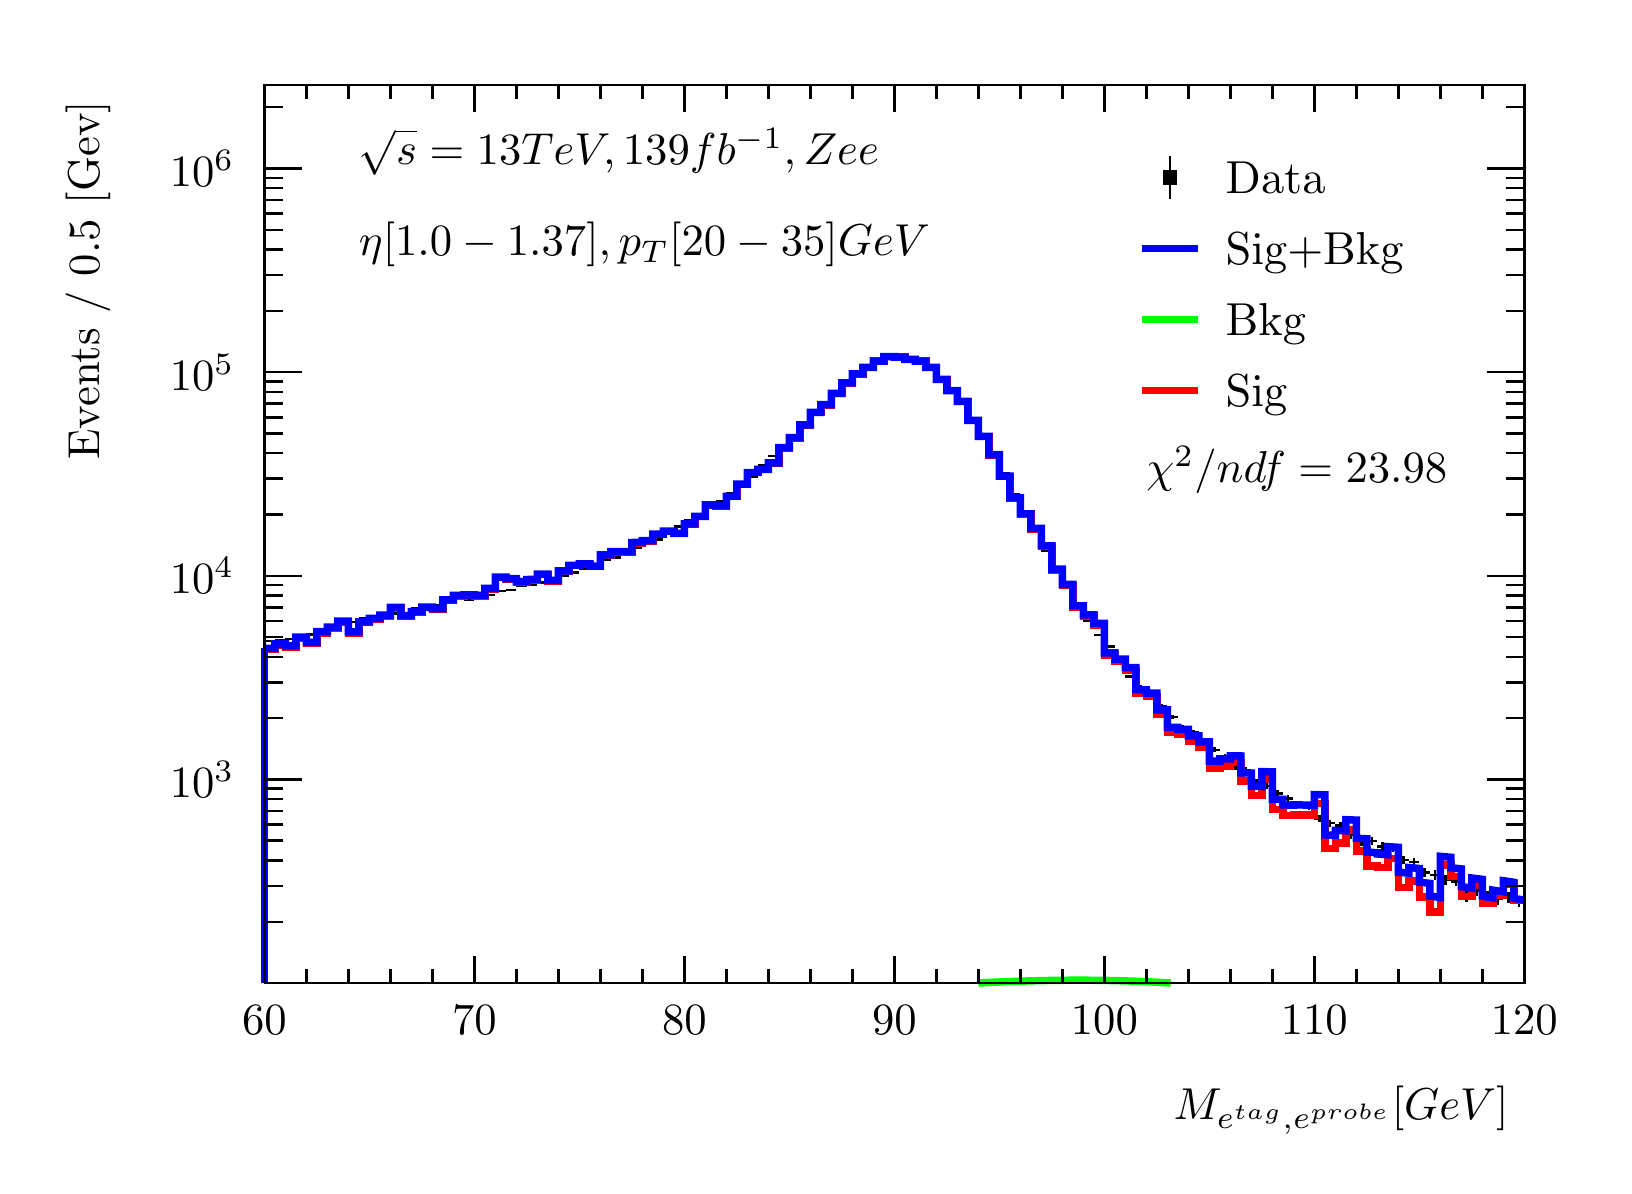
\begin{tikzpicture}
\pgfdeclareplotmark{cross} {
\pgfpathmoveto{\pgfpoint{-0.3\pgfplotmarksize}{\pgfplotmarksize}}
\pgfpathlineto{\pgfpoint{+0.3\pgfplotmarksize}{\pgfplotmarksize}}
\pgfpathlineto{\pgfpoint{+0.3\pgfplotmarksize}{0.3\pgfplotmarksize}}
\pgfpathlineto{\pgfpoint{+1\pgfplotmarksize}{0.3\pgfplotmarksize}}
\pgfpathlineto{\pgfpoint{+1\pgfplotmarksize}{-0.3\pgfplotmarksize}}
\pgfpathlineto{\pgfpoint{+0.3\pgfplotmarksize}{-0.3\pgfplotmarksize}}
\pgfpathlineto{\pgfpoint{+0.3\pgfplotmarksize}{-1.\pgfplotmarksize}}
\pgfpathlineto{\pgfpoint{-0.3\pgfplotmarksize}{-1.\pgfplotmarksize}}
\pgfpathlineto{\pgfpoint{-0.3\pgfplotmarksize}{-0.3\pgfplotmarksize}}
\pgfpathlineto{\pgfpoint{-1.\pgfplotmarksize}{-0.3\pgfplotmarksize}}
\pgfpathlineto{\pgfpoint{-1.\pgfplotmarksize}{0.3\pgfplotmarksize}}
\pgfpathlineto{\pgfpoint{-0.3\pgfplotmarksize}{0.3\pgfplotmarksize}}
\pgfpathclose
\pgfusepathqstroke
}
\pgfdeclareplotmark{cross*} {
\pgfpathmoveto{\pgfpoint{-0.3\pgfplotmarksize}{\pgfplotmarksize}}
\pgfpathlineto{\pgfpoint{+0.3\pgfplotmarksize}{\pgfplotmarksize}}
\pgfpathlineto{\pgfpoint{+0.3\pgfplotmarksize}{0.3\pgfplotmarksize}}
\pgfpathlineto{\pgfpoint{+1\pgfplotmarksize}{0.3\pgfplotmarksize}}
\pgfpathlineto{\pgfpoint{+1\pgfplotmarksize}{-0.3\pgfplotmarksize}}
\pgfpathlineto{\pgfpoint{+0.3\pgfplotmarksize}{-0.3\pgfplotmarksize}}
\pgfpathlineto{\pgfpoint{+0.3\pgfplotmarksize}{-1.\pgfplotmarksize}}
\pgfpathlineto{\pgfpoint{-0.3\pgfplotmarksize}{-1.\pgfplotmarksize}}
\pgfpathlineto{\pgfpoint{-0.3\pgfplotmarksize}{-0.3\pgfplotmarksize}}
\pgfpathlineto{\pgfpoint{-1.\pgfplotmarksize}{-0.3\pgfplotmarksize}}
\pgfpathlineto{\pgfpoint{-1.\pgfplotmarksize}{0.3\pgfplotmarksize}}
\pgfpathlineto{\pgfpoint{-0.3\pgfplotmarksize}{0.3\pgfplotmarksize}}
\pgfpathclose
\pgfusepathqfillstroke
}
\pgfdeclareplotmark{newstar} {
\pgfpathmoveto{\pgfqpoint{0pt}{\pgfplotmarksize}}
\pgfpathlineto{\pgfqpointpolar{44}{0.5\pgfplotmarksize}}
\pgfpathlineto{\pgfqpointpolar{18}{\pgfplotmarksize}}
\pgfpathlineto{\pgfqpointpolar{-20}{0.5\pgfplotmarksize}}
\pgfpathlineto{\pgfqpointpolar{-54}{\pgfplotmarksize}}
\pgfpathlineto{\pgfqpointpolar{-90}{0.5\pgfplotmarksize}}
\pgfpathlineto{\pgfqpointpolar{234}{\pgfplotmarksize}}
\pgfpathlineto{\pgfqpointpolar{198}{0.5\pgfplotmarksize}}
\pgfpathlineto{\pgfqpointpolar{162}{\pgfplotmarksize}}
\pgfpathlineto{\pgfqpointpolar{134}{0.5\pgfplotmarksize}}
\pgfpathclose
\pgfusepathqstroke
}
\pgfdeclareplotmark{newstar*} {
\pgfpathmoveto{\pgfqpoint{0pt}{\pgfplotmarksize}}
\pgfpathlineto{\pgfqpointpolar{44}{0.5\pgfplotmarksize}}
\pgfpathlineto{\pgfqpointpolar{18}{\pgfplotmarksize}}
\pgfpathlineto{\pgfqpointpolar{-20}{0.5\pgfplotmarksize}}
\pgfpathlineto{\pgfqpointpolar{-54}{\pgfplotmarksize}}
\pgfpathlineto{\pgfqpointpolar{-90}{0.5\pgfplotmarksize}}
\pgfpathlineto{\pgfqpointpolar{234}{\pgfplotmarksize}}
\pgfpathlineto{\pgfqpointpolar{198}{0.5\pgfplotmarksize}}
\pgfpathlineto{\pgfqpointpolar{162}{\pgfplotmarksize}}
\pgfpathlineto{\pgfqpointpolar{134}{0.5\pgfplotmarksize}}
\pgfpathclose
\pgfusepathqfillstroke
}
\definecolor{c}{rgb}{1,1,1};
\draw [color=c, fill=c] (0,0) rectangle (20,14.4361);
\draw [color=c, fill=c] (3,2.30977) rectangle (19,13.7143);
\definecolor{c}{rgb}{0,0,0};
\draw [c,line width=0.9] (3,2.30977) -- (3,13.7143) -- (19,13.7143) -- (19,2.30977) -- (3,2.30977);
\definecolor{c}{rgb}{1,1,1};
\draw [color=c, fill=c] (3,2.30977) rectangle (19,13.7143);
\definecolor{c}{rgb}{0,0,0};
\draw [c,line width=0.9] (3,2.30977) -- (3,13.7143) -- (19,13.7143) -- (19,2.30977) -- (3,2.30977);
\draw [c,line width=0.9] (3,2.30977) -- (19,2.30977);
\draw [c,line width=0.9] (3,2.65624) -- (3,2.30977);
\draw [c,line width=0.9] (3.53333,2.48301) -- (3.53333,2.30977);
\draw [c,line width=0.9] (4.06667,2.48301) -- (4.06667,2.30977);
\draw [c,line width=0.9] (4.6,2.48301) -- (4.6,2.30977);
\draw [c,line width=0.9] (5.13333,2.48301) -- (5.13333,2.30977);
\draw [c,line width=0.9] (5.66667,2.65624) -- (5.66667,2.30977);
\draw [c,line width=0.9] (6.2,2.48301) -- (6.2,2.30977);
\draw [c,line width=0.9] (6.73333,2.48301) -- (6.73333,2.30977);
\draw [c,line width=0.9] (7.26667,2.48301) -- (7.26667,2.30977);
\draw [c,line width=0.9] (7.8,2.48301) -- (7.8,2.30977);
\draw [c,line width=0.9] (8.33333,2.65624) -- (8.33333,2.30977);
\draw [c,line width=0.9] (8.86667,2.48301) -- (8.86667,2.30977);
\draw [c,line width=0.9] (9.4,2.48301) -- (9.4,2.30977);
\draw [c,line width=0.9] (9.93333,2.48301) -- (9.93333,2.30977);
\draw [c,line width=0.9] (10.4667,2.48301) -- (10.4667,2.30977);
\draw [c,line width=0.9] (11,2.65624) -- (11,2.30977);
\draw [c,line width=0.9] (11.5333,2.48301) -- (11.5333,2.30977);
\draw [c,line width=0.9] (12.0667,2.48301) -- (12.0667,2.30977);
\draw [c,line width=0.9] (12.6,2.48301) -- (12.6,2.30977);
\draw [c,line width=0.9] (13.1333,2.48301) -- (13.1333,2.30977);
\draw [c,line width=0.9] (13.6667,2.65624) -- (13.6667,2.30977);
\draw [c,line width=0.9] (14.2,2.48301) -- (14.2,2.30977);
\draw [c,line width=0.9] (14.7333,2.48301) -- (14.7333,2.30977);
\draw [c,line width=0.9] (15.2667,2.48301) -- (15.2667,2.30977);
\draw [c,line width=0.9] (15.8,2.48301) -- (15.8,2.30977);
\draw [c,line width=0.9] (16.3333,2.65624) -- (16.3333,2.30977);
\draw [c,line width=0.9] (16.8667,2.48301) -- (16.8667,2.30977);
\draw [c,line width=0.9] (17.4,2.48301) -- (17.4,2.30977);
\draw [c,line width=0.9] (17.9333,2.48301) -- (17.9333,2.30977);
\draw [c,line width=0.9] (18.4667,2.48301) -- (18.4667,2.30977);
\draw [c,line width=0.9] (19,2.65624) -- (19,2.30977);
\draw [anchor=base] (3,1.66015) node[scale=1.61424, color=c, rotate=0]{60};
\draw [anchor=base] (5.66667,1.66015) node[scale=1.61424, color=c, rotate=0]{70};
\draw [anchor=base] (8.33333,1.66015) node[scale=1.61424, color=c, rotate=0]{80};
\draw [anchor=base] (11,1.66015) node[scale=1.61424, color=c, rotate=0]{90};
\draw [anchor=base] (13.6667,1.66015) node[scale=1.61424, color=c, rotate=0]{100};
\draw [anchor=base] (16.3333,1.66015) node[scale=1.61424, color=c, rotate=0]{110};
\draw [anchor=base] (19,1.66015) node[scale=1.61424, color=c, rotate=0]{120};
\draw [anchor= east] (19,0.692932) node[scale=1.61424, color=c, rotate=0]{$M_{e^{tag}, e^{probe}}  [GeV]$};
\draw [c,line width=0.9] (3,13.7143) -- (19,13.7143);
\draw [c,line width=0.9] (3,13.3678) -- (3,13.7143);
\draw [c,line width=0.9] (3.53333,13.5411) -- (3.53333,13.7143);
\draw [c,line width=0.9] (4.06667,13.5411) -- (4.06667,13.7143);
\draw [c,line width=0.9] (4.6,13.5411) -- (4.6,13.7143);
\draw [c,line width=0.9] (5.13333,13.5411) -- (5.13333,13.7143);
\draw [c,line width=0.9] (5.66667,13.3678) -- (5.66667,13.7143);
\draw [c,line width=0.9] (6.2,13.5411) -- (6.2,13.7143);
\draw [c,line width=0.9] (6.73333,13.5411) -- (6.73333,13.7143);
\draw [c,line width=0.9] (7.26667,13.5411) -- (7.26667,13.7143);
\draw [c,line width=0.9] (7.8,13.5411) -- (7.8,13.7143);
\draw [c,line width=0.9] (8.33333,13.3678) -- (8.33333,13.7143);
\draw [c,line width=0.9] (8.86667,13.5411) -- (8.86667,13.7143);
\draw [c,line width=0.9] (9.4,13.5411) -- (9.4,13.7143);
\draw [c,line width=0.9] (9.93333,13.5411) -- (9.93333,13.7143);
\draw [c,line width=0.9] (10.4667,13.5411) -- (10.4667,13.7143);
\draw [c,line width=0.9] (11,13.3678) -- (11,13.7143);
\draw [c,line width=0.9] (11.5333,13.5411) -- (11.5333,13.7143);
\draw [c,line width=0.9] (12.0667,13.5411) -- (12.0667,13.7143);
\draw [c,line width=0.9] (12.6,13.5411) -- (12.6,13.7143);
\draw [c,line width=0.9] (13.1333,13.5411) -- (13.1333,13.7143);
\draw [c,line width=0.9] (13.6667,13.3678) -- (13.6667,13.7143);
\draw [c,line width=0.9] (14.2,13.5411) -- (14.2,13.7143);
\draw [c,line width=0.9] (14.7333,13.5411) -- (14.7333,13.7143);
\draw [c,line width=0.9] (15.2667,13.5411) -- (15.2667,13.7143);
\draw [c,line width=0.9] (15.8,13.5411) -- (15.8,13.7143);
\draw [c,line width=0.9] (16.3333,13.3678) -- (16.3333,13.7143);
\draw [c,line width=0.9] (16.8667,13.5411) -- (16.8667,13.7143);
\draw [c,line width=0.9] (17.4,13.5411) -- (17.4,13.7143);
\draw [c,line width=0.9] (17.9333,13.5411) -- (17.9333,13.7143);
\draw [c,line width=0.9] (18.4667,13.5411) -- (18.4667,13.7143);
\draw [c,line width=0.9] (19,13.3678) -- (19,13.7143);
\draw [c,line width=0.9] (3,2.30977) -- (3,13.7143);
\draw [c,line width=0.9] (3.237,3.08829) -- (3,3.08829);
\draw [c,line width=0.9] (3.237,3.54369) -- (3,3.54369);
\draw [c,line width=0.9] (3.237,3.8668) -- (3,3.8668);
\draw [c,line width=0.9] (3.237,4.11742) -- (3,4.11742);
\draw [c,line width=0.9] (3.237,4.3222) -- (3,4.3222);
\draw [c,line width=0.9] (3.237,4.49534) -- (3,4.49534);
\draw [c,line width=0.9] (3.237,4.64531) -- (3,4.64531);
\draw [c,line width=0.9] (3.237,4.7776) -- (3,4.7776);
\draw [c,line width=0.9] (3.474,4.89594) -- (3,4.89594);
\draw [anchor= east] (2.82,4.89594) node[scale=1.61424, color=c, rotate=0]{$10^{3}$};
\draw [c,line width=0.9] (3.237,5.67445) -- (3,5.67445);
\draw [c,line width=0.9] (3.237,6.12985) -- (3,6.12985);
\draw [c,line width=0.9] (3.237,6.45297) -- (3,6.45297);
\draw [c,line width=0.9] (3.237,6.70359) -- (3,6.70359);
\draw [c,line width=0.9] (3.237,6.90837) -- (3,6.90837);
\draw [c,line width=0.9] (3.237,7.0815) -- (3,7.0815);
\draw [c,line width=0.9] (3.237,7.23148) -- (3,7.23148);
\draw [c,line width=0.9] (3.237,7.36377) -- (3,7.36377);
\draw [c,line width=0.9] (3.474,7.48211) -- (3,7.48211);
\draw [anchor= east] (2.82,7.48211) node[scale=1.61424, color=c, rotate=0]{$10^{4}$};
\draw [c,line width=0.9] (3.237,8.26062) -- (3,8.26062);
\draw [c,line width=0.9] (3.237,8.71602) -- (3,8.71602);
\draw [c,line width=0.9] (3.237,9.03913) -- (3,9.03913);
\draw [c,line width=0.9] (3.237,9.28976) -- (3,9.28976);
\draw [c,line width=0.9] (3.237,9.49453) -- (3,9.49453);
\draw [c,line width=0.9] (3.237,9.66767) -- (3,9.66767);
\draw [c,line width=0.9] (3.237,9.81765) -- (3,9.81765);
\draw [c,line width=0.9] (3.237,9.94994) -- (3,9.94994);
\draw [c,line width=0.9] (3.474,10.0683) -- (3,10.0683);
\draw [anchor= east] (2.82,10.0683) node[scale=1.61424, color=c, rotate=0]{$10^{5}$};
\draw [c,line width=0.9] (3.237,10.8468) -- (3,10.8468);
\draw [c,line width=0.9] (3.237,11.3022) -- (3,11.3022);
\draw [c,line width=0.9] (3.237,11.6253) -- (3,11.6253);
\draw [c,line width=0.9] (3.237,11.8759) -- (3,11.8759);
\draw [c,line width=0.9] (3.237,12.0807) -- (3,12.0807);
\draw [c,line width=0.9] (3.237,12.2538) -- (3,12.2538);
\draw [c,line width=0.9] (3.237,12.4038) -- (3,12.4038);
\draw [c,line width=0.9] (3.237,12.5361) -- (3,12.5361);
\draw [c,line width=0.9] (3.474,12.6544) -- (3,12.6544);
\draw [anchor= east] (2.82,12.6544) node[scale=1.61424, color=c, rotate=0]{$10^{6}$};
\draw [c,line width=0.9] (3.237,13.433) -- (3,13.433);
\draw [anchor= east] (0.76,13.7143) node[scale=1.61424, color=c, rotate=90]{Events / 0.5 [Gev]};
\draw [c,line width=0.9] (19,2.30977) -- (19,13.7143);
\draw [c,line width=0.9] (18.763,3.08829) -- (19,3.08829);
\draw [c,line width=0.9] (18.763,3.54369) -- (19,3.54369);
\draw [c,line width=0.9] (18.763,3.8668) -- (19,3.8668);
\draw [c,line width=0.9] (18.763,4.11742) -- (19,4.11742);
\draw [c,line width=0.9] (18.763,4.3222) -- (19,4.3222);
\draw [c,line width=0.9] (18.763,4.49534) -- (19,4.49534);
\draw [c,line width=0.9] (18.763,4.64531) -- (19,4.64531);
\draw [c,line width=0.9] (18.763,4.7776) -- (19,4.7776);
\draw [c,line width=0.9] (18.526,4.89594) -- (19,4.89594);
\draw [c,line width=0.9] (18.763,5.67445) -- (19,5.67445);
\draw [c,line width=0.9] (18.763,6.12985) -- (19,6.12985);
\draw [c,line width=0.9] (18.763,6.45297) -- (19,6.45297);
\draw [c,line width=0.9] (18.763,6.70359) -- (19,6.70359);
\draw [c,line width=0.9] (18.763,6.90837) -- (19,6.90837);
\draw [c,line width=0.9] (18.763,7.0815) -- (19,7.0815);
\draw [c,line width=0.9] (18.763,7.23148) -- (19,7.23148);
\draw [c,line width=0.9] (18.763,7.36377) -- (19,7.36377);
\draw [c,line width=0.9] (18.526,7.48211) -- (19,7.48211);
\draw [c,line width=0.9] (18.763,8.26062) -- (19,8.26062);
\draw [c,line width=0.9] (18.763,8.71602) -- (19,8.71602);
\draw [c,line width=0.9] (18.763,9.03913) -- (19,9.03913);
\draw [c,line width=0.9] (18.763,9.28976) -- (19,9.28976);
\draw [c,line width=0.9] (18.763,9.49453) -- (19,9.49453);
\draw [c,line width=0.9] (18.763,9.66767) -- (19,9.66767);
\draw [c,line width=0.9] (18.763,9.81765) -- (19,9.81765);
\draw [c,line width=0.9] (18.763,9.94994) -- (19,9.94994);
\draw [c,line width=0.9] (18.526,10.0683) -- (19,10.0683);
\draw [c,line width=0.9] (18.763,10.8468) -- (19,10.8468);
\draw [c,line width=0.9] (18.763,11.3022) -- (19,11.3022);
\draw [c,line width=0.9] (18.763,11.6253) -- (19,11.6253);
\draw [c,line width=0.9] (18.763,11.8759) -- (19,11.8759);
\draw [c,line width=0.9] (18.763,12.0807) -- (19,12.0807);
\draw [c,line width=0.9] (18.763,12.2538) -- (19,12.2538);
\draw [c,line width=0.9] (18.763,12.4038) -- (19,12.4038);
\draw [c,line width=0.9] (18.763,12.5361) -- (19,12.5361);
\draw [c,line width=0.9] (18.526,12.6544) -- (19,12.6544);
\draw [c,line width=0.9] (18.763,13.433) -- (19,13.433);
\draw [c,line width=0.9] (3.06667,6.65329) -- (3,6.65329);
\draw [c,line width=0.9] (3,6.65329) -- (3,6.65329);
\draw [c,line width=0.9] (3.06667,6.65329) -- (3.13333,6.65329);
\draw [c,line width=0.9] (3.13333,6.65329) -- (3.13333,6.65329);
\draw [c,line width=0.9] (3.06667,6.65329) -- (3.06667,6.66953);
\draw [c,line width=0.9] (3.06667,6.66953) -- (3.06667,6.66953);
\draw [c,line width=0.9] (3.06667,6.65329) -- (3.06667,6.63705);
\draw [c,line width=0.9] (3.06667,6.63705) -- (3.06667,6.63705);
\draw [c,line width=0.9] (3.2,6.66288) -- (3.13333,6.66288);
\draw [c,line width=0.9] (3.13333,6.66288) -- (3.13333,6.66288);
\draw [c,line width=0.9] (3.2,6.66288) -- (3.26667,6.66288);
\draw [c,line width=0.9] (3.26667,6.66288) -- (3.26667,6.66288);
\draw [c,line width=0.9] (3.2,6.66288) -- (3.2,6.67905);
\draw [c,line width=0.9] (3.2,6.67905) -- (3.2,6.67905);
\draw [c,line width=0.9] (3.2,6.66288) -- (3.2,6.64671);
\draw [c,line width=0.9] (3.2,6.64671) -- (3.2,6.64671);
\draw [c,line width=0.9] (3.33333,6.67677) -- (3.26667,6.67677);
\draw [c,line width=0.9] (3.26667,6.67677) -- (3.26667,6.67677);
\draw [c,line width=0.9] (3.33333,6.67677) -- (3.4,6.67677);
\draw [c,line width=0.9] (3.4,6.67677) -- (3.4,6.67677);
\draw [c,line width=0.9] (3.33333,6.67677) -- (3.33333,6.69284);
\draw [c,line width=0.9] (3.33333,6.69284) -- (3.33333,6.69284);
\draw [c,line width=0.9] (3.33333,6.67677) -- (3.33333,6.66069);
\draw [c,line width=0.9] (3.33333,6.66069) -- (3.33333,6.66069);
\draw [c,line width=0.9] (3.46667,6.73264) -- (3.4,6.73264);
\draw [c,line width=0.9] (3.4,6.73264) -- (3.4,6.73264);
\draw [c,line width=0.9] (3.46667,6.73264) -- (3.53333,6.73264);
\draw [c,line width=0.9] (3.53333,6.73264) -- (3.53333,6.73264);
\draw [c,line width=0.9] (3.46667,6.73264) -- (3.46667,6.74832);
\draw [c,line width=0.9] (3.46667,6.74832) -- (3.46667,6.74832);
\draw [c,line width=0.9] (3.46667,6.73264) -- (3.46667,6.71696);
\draw [c,line width=0.9] (3.46667,6.71696) -- (3.46667,6.71696);
\draw [c,line width=0.9] (3.6,6.73592) -- (3.53333,6.73592);
\draw [c,line width=0.9] (3.53333,6.73592) -- (3.53333,6.73592);
\draw [c,line width=0.9] (3.6,6.73592) -- (3.66667,6.73592);
\draw [c,line width=0.9] (3.66667,6.73592) -- (3.66667,6.73592);
\draw [c,line width=0.9] (3.6,6.73592) -- (3.6,6.75158);
\draw [c,line width=0.9] (3.6,6.75158) -- (3.6,6.75158);
\draw [c,line width=0.9] (3.6,6.73592) -- (3.6,6.72026);
\draw [c,line width=0.9] (3.6,6.72026) -- (3.6,6.72026);
\draw [c,line width=0.9] (3.73333,6.7892) -- (3.66667,6.7892);
\draw [c,line width=0.9] (3.66667,6.7892) -- (3.66667,6.7892);
\draw [c,line width=0.9] (3.73333,6.7892) -- (3.8,6.7892);
\draw [c,line width=0.9] (3.8,6.7892) -- (3.8,6.7892);
\draw [c,line width=0.9] (3.73333,6.7892) -- (3.73333,6.80449);
\draw [c,line width=0.9] (3.73333,6.80449) -- (3.73333,6.80449);
\draw [c,line width=0.9] (3.73333,6.7892) -- (3.73333,6.77391);
\draw [c,line width=0.9] (3.73333,6.77391) -- (3.73333,6.77391);
\draw [c,line width=0.9] (3.86667,6.83308) -- (3.8,6.83308);
\draw [c,line width=0.9] (3.8,6.83308) -- (3.8,6.83308);
\draw [c,line width=0.9] (3.86667,6.83308) -- (3.93333,6.83308);
\draw [c,line width=0.9] (3.93333,6.83308) -- (3.93333,6.83308);
\draw [c,line width=0.9] (3.86667,6.83308) -- (3.86667,6.84808);
\draw [c,line width=0.9] (3.86667,6.84808) -- (3.86667,6.84808);
\draw [c,line width=0.9] (3.86667,6.83308) -- (3.86667,6.81809);
\draw [c,line width=0.9] (3.86667,6.81809) -- (3.86667,6.81809);
\draw [c,line width=0.9] (4,6.86154) -- (3.93333,6.86154);
\draw [c,line width=0.9] (3.93333,6.86154) -- (3.93333,6.86154);
\draw [c,line width=0.9] (4,6.86154) -- (4.06667,6.86154);
\draw [c,line width=0.9] (4.06667,6.86154) -- (4.06667,6.86154);
\draw [c,line width=0.9] (4,6.86154) -- (4,6.87635);
\draw [c,line width=0.9] (4,6.87635) -- (4,6.87635);
\draw [c,line width=0.9] (4,6.86154) -- (4,6.84674);
\draw [c,line width=0.9] (4,6.84674) -- (4,6.84674);
\draw [c,line width=0.9] (4.13333,6.89538) -- (4.06667,6.89538);
\draw [c,line width=0.9] (4.06667,6.89538) -- (4.06667,6.89538);
\draw [c,line width=0.9] (4.13333,6.89538) -- (4.2,6.89538);
\draw [c,line width=0.9] (4.2,6.89538) -- (4.2,6.89538);
\draw [c,line width=0.9] (4.13333,6.89538) -- (4.13333,6.90996);
\draw [c,line width=0.9] (4.13333,6.90996) -- (4.13333,6.90996);
\draw [c,line width=0.9] (4.13333,6.89538) -- (4.13333,6.88079);
\draw [c,line width=0.9] (4.13333,6.88079) -- (4.13333,6.88079);
\draw [c,line width=0.9] (4.26667,6.94084) -- (4.2,6.94084);
\draw [c,line width=0.9] (4.2,6.94084) -- (4.2,6.94084);
\draw [c,line width=0.9] (4.26667,6.94084) -- (4.33333,6.94084);
\draw [c,line width=0.9] (4.33333,6.94084) -- (4.33333,6.94084);
\draw [c,line width=0.9] (4.26667,6.94084) -- (4.26667,6.95513);
\draw [c,line width=0.9] (4.26667,6.95513) -- (4.26667,6.95513);
\draw [c,line width=0.9] (4.26667,6.94084) -- (4.26667,6.92655);
\draw [c,line width=0.9] (4.26667,6.92655) -- (4.26667,6.92655);
\draw [c,line width=0.9] (4.4,6.93519) -- (4.33333,6.93519);
\draw [c,line width=0.9] (4.33333,6.93519) -- (4.33333,6.93519);
\draw [c,line width=0.9] (4.4,6.93519) -- (4.46667,6.93519);
\draw [c,line width=0.9] (4.46667,6.93519) -- (4.46667,6.93519);
\draw [c,line width=0.9] (4.4,6.93519) -- (4.4,6.94952);
\draw [c,line width=0.9] (4.4,6.94952) -- (4.4,6.94952);
\draw [c,line width=0.9] (4.4,6.93519) -- (4.4,6.92086);
\draw [c,line width=0.9] (4.4,6.92086) -- (4.4,6.92086);
\draw [c,line width=0.9] (4.53333,6.9791) -- (4.46667,6.9791);
\draw [c,line width=0.9] (4.46667,6.9791) -- (4.46667,6.9791);
\draw [c,line width=0.9] (4.53333,6.9791) -- (4.6,6.9791);
\draw [c,line width=0.9] (4.6,6.9791) -- (4.6,6.9791);
\draw [c,line width=0.9] (4.53333,6.9791) -- (4.53333,6.99315);
\draw [c,line width=0.9] (4.53333,6.99315) -- (4.53333,6.99315);
\draw [c,line width=0.9] (4.53333,6.9791) -- (4.53333,6.96505);
\draw [c,line width=0.9] (4.53333,6.96505) -- (4.53333,6.96505);
\draw [c,line width=0.9] (4.66667,7.00172) -- (4.6,7.00172);
\draw [c,line width=0.9] (4.6,7.00172) -- (4.6,7.00172);
\draw [c,line width=0.9] (4.66667,7.00172) -- (4.73333,7.00172);
\draw [c,line width=0.9] (4.73333,7.00172) -- (4.73333,7.00172);
\draw [c,line width=0.9] (4.66667,7.00172) -- (4.66667,7.01563);
\draw [c,line width=0.9] (4.66667,7.01563) -- (4.66667,7.01563);
\draw [c,line width=0.9] (4.66667,7.00172) -- (4.66667,6.98781);
\draw [c,line width=0.9] (4.66667,6.98781) -- (4.66667,6.98781);
\draw [c,line width=0.9] (4.8,6.99464) -- (4.73333,6.99464);
\draw [c,line width=0.9] (4.73333,6.99464) -- (4.73333,6.99464);
\draw [c,line width=0.9] (4.8,6.99464) -- (4.86667,6.99464);
\draw [c,line width=0.9] (4.86667,6.99464) -- (4.86667,6.99464);
\draw [c,line width=0.9] (4.8,6.99464) -- (4.8,7.00859);
\draw [c,line width=0.9] (4.8,7.00859) -- (4.8,7.00859);
\draw [c,line width=0.9] (4.8,6.99464) -- (4.8,6.98068);
\draw [c,line width=0.9] (4.8,6.98068) -- (4.8,6.98068);
\draw [c,line width=0.9] (4.93333,7.07362) -- (4.86667,7.07362);
\draw [c,line width=0.9] (4.86667,7.07362) -- (4.86667,7.07362);
\draw [c,line width=0.9] (4.93333,7.07362) -- (5,7.07362);
\draw [c,line width=0.9] (5,7.07362) -- (5,7.07362);
\draw [c,line width=0.9] (4.93333,7.07362) -- (4.93333,7.08709);
\draw [c,line width=0.9] (4.93333,7.08709) -- (4.93333,7.08709);
\draw [c,line width=0.9] (4.93333,7.07362) -- (4.93333,7.06014);
\draw [c,line width=0.9] (4.93333,7.06014) -- (4.93333,7.06014);
\draw [c,line width=0.9] (5.06667,7.08599) -- (5,7.08599);
\draw [c,line width=0.9] (5,7.08599) -- (5,7.08599);
\draw [c,line width=0.9] (5.06667,7.08599) -- (5.13333,7.08599);
\draw [c,line width=0.9] (5.13333,7.08599) -- (5.13333,7.08599);
\draw [c,line width=0.9] (5.06667,7.08599) -- (5.06667,7.09939);
\draw [c,line width=0.9] (5.06667,7.09939) -- (5.06667,7.09939);
\draw [c,line width=0.9] (5.06667,7.08599) -- (5.06667,7.07259);
\draw [c,line width=0.9] (5.06667,7.07259) -- (5.06667,7.07259);
\draw [c,line width=0.9] (5.2,7.10217) -- (5.13333,7.10217);
\draw [c,line width=0.9] (5.13333,7.10217) -- (5.13333,7.10217);
\draw [c,line width=0.9] (5.2,7.10217) -- (5.26667,7.10217);
\draw [c,line width=0.9] (5.26667,7.10217) -- (5.26667,7.10217);
\draw [c,line width=0.9] (5.2,7.10217) -- (5.2,7.11547);
\draw [c,line width=0.9] (5.2,7.11547) -- (5.2,7.11547);
\draw [c,line width=0.9] (5.2,7.10217) -- (5.2,7.08887);
\draw [c,line width=0.9] (5.2,7.08887) -- (5.2,7.08887);
\draw [c,line width=0.9] (5.33333,7.1427) -- (5.26667,7.1427);
\draw [c,line width=0.9] (5.26667,7.1427) -- (5.26667,7.1427);
\draw [c,line width=0.9] (5.33333,7.1427) -- (5.4,7.1427);
\draw [c,line width=0.9] (5.4,7.1427) -- (5.4,7.1427);
\draw [c,line width=0.9] (5.33333,7.1427) -- (5.33333,7.15577);
\draw [c,line width=0.9] (5.33333,7.15577) -- (5.33333,7.15577);
\draw [c,line width=0.9] (5.33333,7.1427) -- (5.33333,7.12964);
\draw [c,line width=0.9] (5.33333,7.12964) -- (5.33333,7.12964);
\draw [c,line width=0.9] (5.46667,7.18402) -- (5.4,7.18402);
\draw [c,line width=0.9] (5.4,7.18402) -- (5.4,7.18402);
\draw [c,line width=0.9] (5.46667,7.18402) -- (5.53333,7.18402);
\draw [c,line width=0.9] (5.53333,7.18402) -- (5.53333,7.18402);
\draw [c,line width=0.9] (5.46667,7.18402) -- (5.46667,7.19685);
\draw [c,line width=0.9] (5.46667,7.19685) -- (5.46667,7.19685);
\draw [c,line width=0.9] (5.46667,7.18402) -- (5.46667,7.1712);
\draw [c,line width=0.9] (5.46667,7.1712) -- (5.46667,7.1712);
\draw [c,line width=0.9] (5.6,7.18329) -- (5.53333,7.18329);
\draw [c,line width=0.9] (5.53333,7.18329) -- (5.53333,7.18329);
\draw [c,line width=0.9] (5.6,7.18329) -- (5.66667,7.18329);
\draw [c,line width=0.9] (5.66667,7.18329) -- (5.66667,7.18329);
\draw [c,line width=0.9] (5.6,7.18329) -- (5.6,7.19612);
\draw [c,line width=0.9] (5.6,7.19612) -- (5.6,7.19612);
\draw [c,line width=0.9] (5.6,7.18329) -- (5.6,7.17046);
\draw [c,line width=0.9] (5.6,7.17046) -- (5.6,7.17046);
\draw [c,line width=0.9] (5.73333,7.21308) -- (5.66667,7.21308);
\draw [c,line width=0.9] (5.66667,7.21308) -- (5.66667,7.21308);
\draw [c,line width=0.9] (5.73333,7.21308) -- (5.8,7.21308);
\draw [c,line width=0.9] (5.8,7.21308) -- (5.8,7.21308);
\draw [c,line width=0.9] (5.73333,7.21308) -- (5.73333,7.22574);
\draw [c,line width=0.9] (5.73333,7.22574) -- (5.73333,7.22574);
\draw [c,line width=0.9] (5.73333,7.21308) -- (5.73333,7.20042);
\draw [c,line width=0.9] (5.73333,7.20042) -- (5.73333,7.20042);
\draw [c,line width=0.9] (5.86667,7.23778) -- (5.8,7.23778);
\draw [c,line width=0.9] (5.8,7.23778) -- (5.8,7.23778);
\draw [c,line width=0.9] (5.86667,7.23778) -- (5.93333,7.23778);
\draw [c,line width=0.9] (5.93333,7.23778) -- (5.93333,7.23778);
\draw [c,line width=0.9] (5.86667,7.23778) -- (5.86667,7.2503);
\draw [c,line width=0.9] (5.86667,7.2503) -- (5.86667,7.2503);
\draw [c,line width=0.9] (5.86667,7.23778) -- (5.86667,7.22526);
\draw [c,line width=0.9] (5.86667,7.22526) -- (5.86667,7.22526);
\draw [c,line width=0.9] (6,7.29122) -- (5.93333,7.29122);
\draw [c,line width=0.9] (5.93333,7.29122) -- (5.93333,7.29122);
\draw [c,line width=0.9] (6,7.29122) -- (6.06667,7.29122);
\draw [c,line width=0.9] (6.06667,7.29122) -- (6.06667,7.29122);
\draw [c,line width=0.9] (6,7.29122) -- (6,7.30344);
\draw [c,line width=0.9] (6,7.30344) -- (6,7.30344);
\draw [c,line width=0.9] (6,7.29122) -- (6,7.27899);
\draw [c,line width=0.9] (6,7.27899) -- (6,7.27899);
\draw [c,line width=0.9] (6.13333,7.30419) -- (6.06667,7.30419);
\draw [c,line width=0.9] (6.06667,7.30419) -- (6.06667,7.30419);
\draw [c,line width=0.9] (6.13333,7.30419) -- (6.2,7.30419);
\draw [c,line width=0.9] (6.2,7.30419) -- (6.2,7.30419);
\draw [c,line width=0.9] (6.13333,7.30419) -- (6.13333,7.31635);
\draw [c,line width=0.9] (6.13333,7.31635) -- (6.13333,7.31635);
\draw [c,line width=0.9] (6.13333,7.30419) -- (6.13333,7.29203);
\draw [c,line width=0.9] (6.13333,7.29203) -- (6.13333,7.29203);
\draw [c,line width=0.9] (6.26667,7.35563) -- (6.2,7.35563);
\draw [c,line width=0.9] (6.2,7.35563) -- (6.2,7.35563);
\draw [c,line width=0.9] (6.26667,7.35563) -- (6.33333,7.35563);
\draw [c,line width=0.9] (6.33333,7.35563) -- (6.33333,7.35563);
\draw [c,line width=0.9] (6.26667,7.35563) -- (6.26667,7.36751);
\draw [c,line width=0.9] (6.26667,7.36751) -- (6.26667,7.36751);
\draw [c,line width=0.9] (6.26667,7.35563) -- (6.26667,7.34375);
\draw [c,line width=0.9] (6.26667,7.34375) -- (6.26667,7.34375);
\draw [c,line width=0.9] (6.4,7.37185) -- (6.33333,7.37185);
\draw [c,line width=0.9] (6.33333,7.37185) -- (6.33333,7.37185);
\draw [c,line width=0.9] (6.4,7.37185) -- (6.46667,7.37185);
\draw [c,line width=0.9] (6.46667,7.37185) -- (6.46667,7.37185);
\draw [c,line width=0.9] (6.4,7.37185) -- (6.4,7.38365);
\draw [c,line width=0.9] (6.4,7.38365) -- (6.4,7.38365);
\draw [c,line width=0.9] (6.4,7.37185) -- (6.4,7.36006);
\draw [c,line width=0.9] (6.4,7.36006) -- (6.4,7.36006);
\draw [c,line width=0.9] (6.53333,7.39818) -- (6.46667,7.39818);
\draw [c,line width=0.9] (6.46667,7.39818) -- (6.46667,7.39818);
\draw [c,line width=0.9] (6.53333,7.39818) -- (6.6,7.39818);
\draw [c,line width=0.9] (6.6,7.39818) -- (6.6,7.39818);
\draw [c,line width=0.9] (6.53333,7.39818) -- (6.53333,7.40984);
\draw [c,line width=0.9] (6.53333,7.40984) -- (6.53333,7.40984);
\draw [c,line width=0.9] (6.53333,7.39818) -- (6.53333,7.38652);
\draw [c,line width=0.9] (6.53333,7.38652) -- (6.53333,7.38652);
\draw [c,line width=0.9] (6.66667,7.45517) -- (6.6,7.45517);
\draw [c,line width=0.9] (6.6,7.45517) -- (6.6,7.45517);
\draw [c,line width=0.9] (6.66667,7.45517) -- (6.73333,7.45517);
\draw [c,line width=0.9] (6.73333,7.45517) -- (6.73333,7.45517);
\draw [c,line width=0.9] (6.66667,7.45517) -- (6.66667,7.46654);
\draw [c,line width=0.9] (6.66667,7.46654) -- (6.66667,7.46654);
\draw [c,line width=0.9] (6.66667,7.45517) -- (6.66667,7.4438);
\draw [c,line width=0.9] (6.66667,7.4438) -- (6.66667,7.4438);
\draw [c,line width=0.9] (6.8,7.48793) -- (6.73333,7.48793);
\draw [c,line width=0.9] (6.73333,7.48793) -- (6.73333,7.48793);
\draw [c,line width=0.9] (6.8,7.48793) -- (6.86667,7.48793);
\draw [c,line width=0.9] (6.86667,7.48793) -- (6.86667,7.48793);
\draw [c,line width=0.9] (6.8,7.48793) -- (6.8,7.49914);
\draw [c,line width=0.9] (6.8,7.49914) -- (6.8,7.49914);
\draw [c,line width=0.9] (6.8,7.48793) -- (6.8,7.47673);
\draw [c,line width=0.9] (6.8,7.47673) -- (6.8,7.47673);
\draw [c,line width=0.9] (6.93333,7.52356) -- (6.86667,7.52356);
\draw [c,line width=0.9] (6.86667,7.52356) -- (6.86667,7.52356);
\draw [c,line width=0.9] (6.93333,7.52356) -- (7,7.52356);
\draw [c,line width=0.9] (7,7.52356) -- (7,7.52356);
\draw [c,line width=0.9] (6.93333,7.52356) -- (6.93333,7.53459);
\draw [c,line width=0.9] (6.93333,7.53459) -- (6.93333,7.53459);
\draw [c,line width=0.9] (6.93333,7.52356) -- (6.93333,7.51254);
\draw [c,line width=0.9] (6.93333,7.51254) -- (6.93333,7.51254);
\draw [c,line width=0.9] (7.06667,7.56948) -- (7,7.56948);
\draw [c,line width=0.9] (7,7.56948) -- (7,7.56948);
\draw [c,line width=0.9] (7.06667,7.56948) -- (7.13333,7.56948);
\draw [c,line width=0.9] (7.13333,7.56948) -- (7.13333,7.56948);
\draw [c,line width=0.9] (7.06667,7.56948) -- (7.06667,7.58029);
\draw [c,line width=0.9] (7.06667,7.58029) -- (7.06667,7.58029);
\draw [c,line width=0.9] (7.06667,7.56948) -- (7.06667,7.55868);
\draw [c,line width=0.9] (7.06667,7.55868) -- (7.06667,7.55868);
\draw [c,line width=0.9] (7.2,7.62937) -- (7.13333,7.62937);
\draw [c,line width=0.9] (7.13333,7.62937) -- (7.13333,7.62937);
\draw [c,line width=0.9] (7.2,7.62937) -- (7.26667,7.62937);
\draw [c,line width=0.9] (7.26667,7.62937) -- (7.26667,7.62937);
\draw [c,line width=0.9] (7.2,7.62937) -- (7.2,7.63989);
\draw [c,line width=0.9] (7.2,7.63989) -- (7.2,7.63989);
\draw [c,line width=0.9] (7.2,7.62937) -- (7.2,7.61885);
\draw [c,line width=0.9] (7.2,7.61885) -- (7.2,7.61885);
\draw [c,line width=0.9] (7.33333,7.6881) -- (7.26667,7.6881);
\draw [c,line width=0.9] (7.26667,7.6881) -- (7.26667,7.6881);
\draw [c,line width=0.9] (7.33333,7.6881) -- (7.4,7.6881);
\draw [c,line width=0.9] (7.4,7.6881) -- (7.4,7.6881);
\draw [c,line width=0.9] (7.33333,7.6881) -- (7.33333,7.69835);
\draw [c,line width=0.9] (7.33333,7.69835) -- (7.33333,7.69835);
\draw [c,line width=0.9] (7.33333,7.6881) -- (7.33333,7.67785);
\draw [c,line width=0.9] (7.33333,7.67785) -- (7.33333,7.67785);
\draw [c,line width=0.9] (7.46667,7.71187) -- (7.4,7.71187);
\draw [c,line width=0.9] (7.4,7.71187) -- (7.4,7.71187);
\draw [c,line width=0.9] (7.46667,7.71187) -- (7.53333,7.71187);
\draw [c,line width=0.9] (7.53333,7.71187) -- (7.53333,7.71187);
\draw [c,line width=0.9] (7.46667,7.71187) -- (7.46667,7.72201);
\draw [c,line width=0.9] (7.46667,7.72201) -- (7.46667,7.72201);
\draw [c,line width=0.9] (7.46667,7.71187) -- (7.46667,7.70173);
\draw [c,line width=0.9] (7.46667,7.70173) -- (7.46667,7.70173);
\draw [c,line width=0.9] (7.6,7.80334) -- (7.53333,7.80334);
\draw [c,line width=0.9] (7.53333,7.80334) -- (7.53333,7.80334);
\draw [c,line width=0.9] (7.6,7.80334) -- (7.66667,7.80334);
\draw [c,line width=0.9] (7.66667,7.80334) -- (7.66667,7.80334);
\draw [c,line width=0.9] (7.6,7.80334) -- (7.6,7.81307);
\draw [c,line width=0.9] (7.6,7.81307) -- (7.6,7.81307);
\draw [c,line width=0.9] (7.6,7.80334) -- (7.6,7.7936);
\draw [c,line width=0.9] (7.6,7.7936) -- (7.6,7.7936);
\draw [c,line width=0.9] (7.73333,7.83175) -- (7.66667,7.83175);
\draw [c,line width=0.9] (7.66667,7.83175) -- (7.66667,7.83175);
\draw [c,line width=0.9] (7.73333,7.83175) -- (7.8,7.83175);
\draw [c,line width=0.9] (7.8,7.83175) -- (7.8,7.83175);
\draw [c,line width=0.9] (7.73333,7.83175) -- (7.73333,7.84136);
\draw [c,line width=0.9] (7.73333,7.84136) -- (7.73333,7.84136);
\draw [c,line width=0.9] (7.73333,7.83175) -- (7.73333,7.82213);
\draw [c,line width=0.9] (7.73333,7.82213) -- (7.73333,7.82213);
\draw [c,line width=0.9] (7.86667,7.92031) -- (7.8,7.92031);
\draw [c,line width=0.9] (7.8,7.92031) -- (7.8,7.92031);
\draw [c,line width=0.9] (7.86667,7.92031) -- (7.93333,7.92031);
\draw [c,line width=0.9] (7.93333,7.92031) -- (7.93333,7.92031);
\draw [c,line width=0.9] (7.86667,7.92031) -- (7.86667,7.92955);
\draw [c,line width=0.9] (7.86667,7.92955) -- (7.86667,7.92955);
\draw [c,line width=0.9] (7.86667,7.92031) -- (7.86667,7.91106);
\draw [c,line width=0.9] (7.86667,7.91106) -- (7.86667,7.91106);
\draw [c,line width=0.9] (8,7.94072) -- (7.93333,7.94072);
\draw [c,line width=0.9] (7.93333,7.94072) -- (7.93333,7.94072);
\draw [c,line width=0.9] (8,7.94072) -- (8.06667,7.94072);
\draw [c,line width=0.9] (8.06667,7.94072) -- (8.06667,7.94072);
\draw [c,line width=0.9] (8,7.94072) -- (8,7.94988);
\draw [c,line width=0.9] (8,7.94988) -- (8,7.94988);
\draw [c,line width=0.9] (8,7.94072) -- (8,7.93157);
\draw [c,line width=0.9] (8,7.93157) -- (8,7.93157);
\draw [c,line width=0.9] (8.13333,8.03725) -- (8.06667,8.03725);
\draw [c,line width=0.9] (8.06667,8.03725) -- (8.06667,8.03725);
\draw [c,line width=0.9] (8.13333,8.03725) -- (8.2,8.03725);
\draw [c,line width=0.9] (8.2,8.03725) -- (8.2,8.03725);
\draw [c,line width=0.9] (8.13333,8.03725) -- (8.13333,8.04602);
\draw [c,line width=0.9] (8.13333,8.04602) -- (8.13333,8.04602);
\draw [c,line width=0.9] (8.13333,8.03725) -- (8.13333,8.02848);
\draw [c,line width=0.9] (8.13333,8.02848) -- (8.13333,8.02848);
\draw [c,line width=0.9] (8.26667,8.10872) -- (8.2,8.10872);
\draw [c,line width=0.9] (8.2,8.10872) -- (8.2,8.10872);
\draw [c,line width=0.9] (8.26667,8.10872) -- (8.33333,8.10872);
\draw [c,line width=0.9] (8.33333,8.10872) -- (8.33333,8.10872);
\draw [c,line width=0.9] (8.26667,8.10872) -- (8.26667,8.11721);
\draw [c,line width=0.9] (8.26667,8.11721) -- (8.26667,8.11721);
\draw [c,line width=0.9] (8.26667,8.10872) -- (8.26667,8.10022);
\draw [c,line width=0.9] (8.26667,8.10022) -- (8.26667,8.10022);
\draw [c,line width=0.9] (8.4,8.18291) -- (8.33333,8.18291);
\draw [c,line width=0.9] (8.33333,8.18291) -- (8.33333,8.18291);
\draw [c,line width=0.9] (8.4,8.18291) -- (8.46667,8.18291);
\draw [c,line width=0.9] (8.46667,8.18291) -- (8.46667,8.18291);
\draw [c,line width=0.9] (8.4,8.18291) -- (8.4,8.19113);
\draw [c,line width=0.9] (8.4,8.19113) -- (8.4,8.19113);
\draw [c,line width=0.9] (8.4,8.18291) -- (8.4,8.17469);
\draw [c,line width=0.9] (8.4,8.17469) -- (8.4,8.17469);
\draw [c,line width=0.9] (8.53333,8.25284) -- (8.46667,8.25284);
\draw [c,line width=0.9] (8.46667,8.25284) -- (8.46667,8.25284);
\draw [c,line width=0.9] (8.53333,8.25284) -- (8.6,8.25284);
\draw [c,line width=0.9] (8.6,8.25284) -- (8.6,8.25284);
\draw [c,line width=0.9] (8.53333,8.25284) -- (8.53333,8.26081);
\draw [c,line width=0.9] (8.53333,8.26081) -- (8.53333,8.26081);
\draw [c,line width=0.9] (8.53333,8.25284) -- (8.53333,8.24487);
\draw [c,line width=0.9] (8.53333,8.24487) -- (8.53333,8.24487);
\draw [c,line width=0.9] (8.66667,8.34206) -- (8.6,8.34206);
\draw [c,line width=0.9] (8.6,8.34206) -- (8.6,8.34206);
\draw [c,line width=0.9] (8.66667,8.34206) -- (8.73333,8.34206);
\draw [c,line width=0.9] (8.73333,8.34206) -- (8.73333,8.34206);
\draw [c,line width=0.9] (8.66667,8.34206) -- (8.66667,8.34972);
\draw [c,line width=0.9] (8.66667,8.34972) -- (8.66667,8.34972);
\draw [c,line width=0.9] (8.66667,8.34206) -- (8.66667,8.3344);
\draw [c,line width=0.9] (8.66667,8.3344) -- (8.66667,8.3344);
\draw [c,line width=0.9] (8.8,8.42436) -- (8.73333,8.42436);
\draw [c,line width=0.9] (8.73333,8.42436) -- (8.73333,8.42436);
\draw [c,line width=0.9] (8.8,8.42436) -- (8.86667,8.42436);
\draw [c,line width=0.9] (8.86667,8.42436) -- (8.86667,8.42436);
\draw [c,line width=0.9] (8.8,8.42436) -- (8.8,8.43175);
\draw [c,line width=0.9] (8.8,8.43175) -- (8.8,8.43175);
\draw [c,line width=0.9] (8.8,8.42436) -- (8.8,8.41698);
\draw [c,line width=0.9] (8.8,8.41698) -- (8.8,8.41698);
\draw [c,line width=0.9] (8.93333,8.53388) -- (8.86667,8.53388);
\draw [c,line width=0.9] (8.86667,8.53388) -- (8.86667,8.53388);
\draw [c,line width=0.9] (8.93333,8.53388) -- (9,8.53388);
\draw [c,line width=0.9] (9,8.53388) -- (9,8.53388);
\draw [c,line width=0.9] (8.93333,8.53388) -- (8.93333,8.54092);
\draw [c,line width=0.9] (8.93333,8.54092) -- (8.93333,8.54092);
\draw [c,line width=0.9] (8.93333,8.53388) -- (8.93333,8.52685);
\draw [c,line width=0.9] (8.93333,8.52685) -- (8.93333,8.52685);
\draw [c,line width=0.9] (9.06667,8.62785) -- (9,8.62785);
\draw [c,line width=0.9] (9,8.62785) -- (9,8.62785);
\draw [c,line width=0.9] (9.06667,8.62785) -- (9.13333,8.62785);
\draw [c,line width=0.9] (9.13333,8.62785) -- (9.13333,8.62785);
\draw [c,line width=0.9] (9.06667,8.62785) -- (9.06667,8.6346);
\draw [c,line width=0.9] (9.06667,8.6346) -- (9.06667,8.6346);
\draw [c,line width=0.9] (9.06667,8.62785) -- (9.06667,8.62111);
\draw [c,line width=0.9] (9.06667,8.62111) -- (9.06667,8.62111);
\draw [c,line width=0.9] (9.2,8.7458) -- (9.13333,8.7458);
\draw [c,line width=0.9] (9.13333,8.7458) -- (9.13333,8.7458);
\draw [c,line width=0.9] (9.2,8.7458) -- (9.26667,8.7458);
\draw [c,line width=0.9] (9.26667,8.7458) -- (9.26667,8.7458);
\draw [c,line width=0.9] (9.2,8.7458) -- (9.2,8.7522);
\draw [c,line width=0.9] (9.2,8.7522) -- (9.2,8.7522);
\draw [c,line width=0.9] (9.2,8.7458) -- (9.2,8.7394);
\draw [c,line width=0.9] (9.2,8.7394) -- (9.2,8.7394);
\draw [c,line width=0.9] (9.33333,8.88039) -- (9.26667,8.88039);
\draw [c,line width=0.9] (9.26667,8.88039) -- (9.26667,8.88039);
\draw [c,line width=0.9] (9.33333,8.88039) -- (9.4,8.88039);
\draw [c,line width=0.9] (9.4,8.88039) -- (9.4,8.88039);
\draw [c,line width=0.9] (9.33333,8.88039) -- (9.33333,8.88642);
\draw [c,line width=0.9] (9.33333,8.88642) -- (9.33333,8.88642);
\draw [c,line width=0.9] (9.33333,8.88039) -- (9.33333,8.87437);
\draw [c,line width=0.9] (9.33333,8.87437) -- (9.33333,8.87437);
\draw [c,line width=0.9] (9.46667,9.00348) -- (9.4,9.00348);
\draw [c,line width=0.9] (9.4,9.00348) -- (9.4,9.00348);
\draw [c,line width=0.9] (9.46667,9.00348) -- (9.53333,9.00348);
\draw [c,line width=0.9] (9.53333,9.00348) -- (9.53333,9.00348);
\draw [c,line width=0.9] (9.46667,9.00348) -- (9.46667,9.00918);
\draw [c,line width=0.9] (9.46667,9.00918) -- (9.46667,9.00918);
\draw [c,line width=0.9] (9.46667,9.00348) -- (9.46667,8.99777);
\draw [c,line width=0.9] (9.46667,8.99777) -- (9.46667,8.99777);
\draw [c,line width=0.9] (9.6,9.1327) -- (9.53333,9.1327);
\draw [c,line width=0.9] (9.53333,9.1327) -- (9.53333,9.1327);
\draw [c,line width=0.9] (9.6,9.1327) -- (9.66667,9.1327);
\draw [c,line width=0.9] (9.66667,9.1327) -- (9.66667,9.1327);
\draw [c,line width=0.9] (9.6,9.1327) -- (9.6,9.13809);
\draw [c,line width=0.9] (9.6,9.13809) -- (9.6,9.13809);
\draw [c,line width=0.9] (9.6,9.1327) -- (9.6,9.12731);
\draw [c,line width=0.9] (9.6,9.12731) -- (9.6,9.12731);
\draw [c,line width=0.9] (9.73333,9.26904) -- (9.66667,9.26904);
\draw [c,line width=0.9] (9.66667,9.26904) -- (9.66667,9.26904);
\draw [c,line width=0.9] (9.73333,9.26904) -- (9.8,9.26904);
\draw [c,line width=0.9] (9.8,9.26904) -- (9.8,9.26904);
\draw [c,line width=0.9] (9.73333,9.26904) -- (9.73333,9.27411);
\draw [c,line width=0.9] (9.73333,9.27411) -- (9.73333,9.27411);
\draw [c,line width=0.9] (9.73333,9.26904) -- (9.73333,9.26397);
\draw [c,line width=0.9] (9.73333,9.26397) -- (9.73333,9.26397);
\draw [c,line width=0.9] (9.86667,9.40879) -- (9.8,9.40879);
\draw [c,line width=0.9] (9.8,9.40879) -- (9.8,9.40879);
\draw [c,line width=0.9] (9.86667,9.40879) -- (9.93333,9.40879);
\draw [c,line width=0.9] (9.93333,9.40879) -- (9.93333,9.40879);
\draw [c,line width=0.9] (9.86667,9.40879) -- (9.86667,9.41356);
\draw [c,line width=0.9] (9.86667,9.41356) -- (9.86667,9.41356);
\draw [c,line width=0.9] (9.86667,9.40879) -- (9.86667,9.40403);
\draw [c,line width=0.9] (9.86667,9.40403) -- (9.86667,9.40403);
\draw [c,line width=0.9] (10,9.55144) -- (9.93333,9.55144);
\draw [c,line width=0.9] (9.93333,9.55144) -- (9.93333,9.55144);
\draw [c,line width=0.9] (10,9.55144) -- (10.0667,9.55144);
\draw [c,line width=0.9] (10.0667,9.55144) -- (10.0667,9.55144);
\draw [c,line width=0.9] (10,9.55144) -- (10,9.55591);
\draw [c,line width=0.9] (10,9.55591) -- (10,9.55591);
\draw [c,line width=0.9] (10,9.55144) -- (10,9.54697);
\draw [c,line width=0.9] (10,9.54697) -- (10,9.54697);
\draw [c,line width=0.9] (10.1333,9.68476) -- (10.0667,9.68476);
\draw [c,line width=0.9] (10.0667,9.68476) -- (10.0667,9.68476);
\draw [c,line width=0.9] (10.1333,9.68476) -- (10.2,9.68476);
\draw [c,line width=0.9] (10.2,9.68476) -- (10.2,9.68476);
\draw [c,line width=0.9] (10.1333,9.68476) -- (10.1333,9.68897);
\draw [c,line width=0.9] (10.1333,9.68897) -- (10.1333,9.68897);
\draw [c,line width=0.9] (10.1333,9.68476) -- (10.1333,9.68054);
\draw [c,line width=0.9] (10.1333,9.68054) -- (10.1333,9.68054);
\draw [c,line width=0.9] (10.2667,9.80958) -- (10.2,9.80958);
\draw [c,line width=0.9] (10.2,9.80958) -- (10.2,9.80958);
\draw [c,line width=0.9] (10.2667,9.80958) -- (10.3333,9.80958);
\draw [c,line width=0.9] (10.3333,9.80958) -- (10.3333,9.80958);
\draw [c,line width=0.9] (10.2667,9.80958) -- (10.2667,9.81356);
\draw [c,line width=0.9] (10.2667,9.81356) -- (10.2667,9.81356);
\draw [c,line width=0.9] (10.2667,9.80958) -- (10.2667,9.80559);
\draw [c,line width=0.9] (10.2667,9.80559) -- (10.2667,9.80559);
\draw [c,line width=0.9] (10.4,9.94065) -- (10.3333,9.94065);
\draw [c,line width=0.9] (10.3333,9.94065) -- (10.3333,9.94065);
\draw [c,line width=0.9] (10.4,9.94065) -- (10.4667,9.94065);
\draw [c,line width=0.9] (10.4667,9.94065) -- (10.4667,9.94065);
\draw [c,line width=0.9] (10.4,9.94065) -- (10.4,9.94441);
\draw [c,line width=0.9] (10.4,9.94441) -- (10.4,9.94441);
\draw [c,line width=0.9] (10.4,9.94065) -- (10.4,9.93689);
\draw [c,line width=0.9] (10.4,9.93689) -- (10.4,9.93689);
\draw [c,line width=0.9] (10.5333,10.0457) -- (10.4667,10.0457);
\draw [c,line width=0.9] (10.4667,10.0457) -- (10.4667,10.0457);
\draw [c,line width=0.9] (10.5333,10.0457) -- (10.6,10.0457);
\draw [c,line width=0.9] (10.6,10.0457) -- (10.6,10.0457);
\draw [c,line width=0.9] (10.5333,10.0457) -- (10.5333,10.0493);
\draw [c,line width=0.9] (10.5333,10.0493) -- (10.5333,10.0493);
\draw [c,line width=0.9] (10.5333,10.0457) -- (10.5333,10.0421);
\draw [c,line width=0.9] (10.5333,10.0421) -- (10.5333,10.0421);
\draw [c,line width=0.9] (10.6667,10.1337) -- (10.6,10.1337);
\draw [c,line width=0.9] (10.6,10.1337) -- (10.6,10.1337);
\draw [c,line width=0.9] (10.6667,10.1337) -- (10.7333,10.1337);
\draw [c,line width=0.9] (10.7333,10.1337) -- (10.7333,10.1337);
\draw [c,line width=0.9] (10.6667,10.1337) -- (10.6667,10.1372);
\draw [c,line width=0.9] (10.6667,10.1372) -- (10.6667,10.1372);
\draw [c,line width=0.9] (10.6667,10.1337) -- (10.6667,10.1303);
\draw [c,line width=0.9] (10.6667,10.1303) -- (10.6667,10.1303);
\draw [c,line width=0.9] (10.8,10.1997) -- (10.7333,10.1997);
\draw [c,line width=0.9] (10.7333,10.1997) -- (10.7333,10.1997);
\draw [c,line width=0.9] (10.8,10.1997) -- (10.8667,10.1997);
\draw [c,line width=0.9] (10.8667,10.1997) -- (10.8667,10.1997);
\draw [c,line width=0.9] (10.8,10.1997) -- (10.8,10.2031);
\draw [c,line width=0.9] (10.8,10.2031) -- (10.8,10.2031);
\draw [c,line width=0.9] (10.8,10.1997) -- (10.8,10.1964);
\draw [c,line width=0.9] (10.8,10.1964) -- (10.8,10.1964);
\draw [c,line width=0.9] (10.9333,10.2367) -- (10.8667,10.2367);
\draw [c,line width=0.9] (10.8667,10.2367) -- (10.8667,10.2367);
\draw [c,line width=0.9] (10.9333,10.2367) -- (11,10.2367);
\draw [c,line width=0.9] (11,10.2367) -- (11,10.2367);
\draw [c,line width=0.9] (10.9333,10.2367) -- (10.9333,10.24);
\draw [c,line width=0.9] (10.9333,10.24) -- (10.9333,10.24);
\draw [c,line width=0.9] (10.9333,10.2367) -- (10.9333,10.2334);
\draw [c,line width=0.9] (10.9333,10.2334) -- (10.9333,10.2334);
\draw [c,line width=0.9] (11.0667,10.2503) -- (11,10.2503);
\draw [c,line width=0.9] (11,10.2503) -- (11,10.2503);
\draw [c,line width=0.9] (11.0667,10.2503) -- (11.1333,10.2503);
\draw [c,line width=0.9] (11.1333,10.2503) -- (11.1333,10.2503);
\draw [c,line width=0.9] (11.0667,10.2503) -- (11.0667,10.2536);
\draw [c,line width=0.9] (11.0667,10.2536) -- (11.0667,10.2536);
\draw [c,line width=0.9] (11.0667,10.2503) -- (11.0667,10.2471);
\draw [c,line width=0.9] (11.0667,10.2471) -- (11.0667,10.2471);
\draw [c,line width=0.9] (11.2,10.2396) -- (11.1333,10.2396);
\draw [c,line width=0.9] (11.1333,10.2396) -- (11.1333,10.2396);
\draw [c,line width=0.9] (11.2,10.2396) -- (11.2667,10.2396);
\draw [c,line width=0.9] (11.2667,10.2396) -- (11.2667,10.2396);
\draw [c,line width=0.9] (11.2,10.2396) -- (11.2,10.2429);
\draw [c,line width=0.9] (11.2,10.2429) -- (11.2,10.2429);
\draw [c,line width=0.9] (11.2,10.2396) -- (11.2,10.2363);
\draw [c,line width=0.9] (11.2,10.2363) -- (11.2,10.2363);
\draw [c,line width=0.9] (11.3333,10.1911) -- (11.2667,10.1911);
\draw [c,line width=0.9] (11.2667,10.1911) -- (11.2667,10.1911);
\draw [c,line width=0.9] (11.3333,10.1911) -- (11.4,10.1911);
\draw [c,line width=0.9] (11.4,10.1911) -- (11.4,10.1911);
\draw [c,line width=0.9] (11.3333,10.1911) -- (11.3333,10.1945);
\draw [c,line width=0.9] (11.3333,10.1945) -- (11.3333,10.1945);
\draw [c,line width=0.9] (11.3333,10.1911) -- (11.3333,10.1878);
\draw [c,line width=0.9] (11.3333,10.1878) -- (11.3333,10.1878);
\draw [c,line width=0.9] (11.4667,10.1112) -- (11.4,10.1112);
\draw [c,line width=0.9] (11.4,10.1112) -- (11.4,10.1112);
\draw [c,line width=0.9] (11.4667,10.1112) -- (11.5333,10.1112);
\draw [c,line width=0.9] (11.5333,10.1112) -- (11.5333,10.1112);
\draw [c,line width=0.9] (11.4667,10.1112) -- (11.4667,10.1147);
\draw [c,line width=0.9] (11.4667,10.1147) -- (11.4667,10.1147);
\draw [c,line width=0.9] (11.4667,10.1112) -- (11.4667,10.1077);
\draw [c,line width=0.9] (11.4667,10.1077) -- (11.4667,10.1077);
\draw [c,line width=0.9] (11.6,9.99107) -- (11.5333,9.99107);
\draw [c,line width=0.9] (11.5333,9.99107) -- (11.5333,9.99107);
\draw [c,line width=0.9] (11.6,9.99107) -- (11.6667,9.99107);
\draw [c,line width=0.9] (11.6667,9.99107) -- (11.6667,9.99107);
\draw [c,line width=0.9] (11.6,9.99107) -- (11.6,9.99474);
\draw [c,line width=0.9] (11.6,9.99474) -- (11.6,9.99474);
\draw [c,line width=0.9] (11.6,9.99107) -- (11.6,9.98739);
\draw [c,line width=0.9] (11.6,9.98739) -- (11.6,9.98739);
\draw [c,line width=0.9] (11.7333,9.86209) -- (11.6667,9.86209);
\draw [c,line width=0.9] (11.6667,9.86209) -- (11.6667,9.86209);
\draw [c,line width=0.9] (11.7333,9.86209) -- (11.8,9.86209);
\draw [c,line width=0.9] (11.8,9.86209) -- (11.8,9.86209);
\draw [c,line width=0.9] (11.7333,9.86209) -- (11.7333,9.86598);
\draw [c,line width=0.9] (11.7333,9.86598) -- (11.7333,9.86598);
\draw [c,line width=0.9] (11.7333,9.86209) -- (11.7333,9.8582);
\draw [c,line width=0.9] (11.7333,9.8582) -- (11.7333,9.8582);
\draw [c,line width=0.9] (11.8667,9.684) -- (11.8,9.684);
\draw [c,line width=0.9] (11.8,9.684) -- (11.8,9.684);
\draw [c,line width=0.9] (11.8667,9.684) -- (11.9333,9.684);
\draw [c,line width=0.9] (11.9333,9.684) -- (11.9333,9.684);
\draw [c,line width=0.9] (11.8667,9.684) -- (11.8667,9.68821);
\draw [c,line width=0.9] (11.8667,9.68821) -- (11.8667,9.68821);
\draw [c,line width=0.9] (11.8667,9.684) -- (11.8667,9.67978);
\draw [c,line width=0.9] (11.8667,9.67978) -- (11.8667,9.67978);
\draw [c,line width=0.9] (12,9.47184) -- (11.9333,9.47184);
\draw [c,line width=0.9] (11.9333,9.47184) -- (11.9333,9.47184);
\draw [c,line width=0.9] (12,9.47184) -- (12.0667,9.47184);
\draw [c,line width=0.9] (12.0667,9.47184) -- (12.0667,9.47184);
\draw [c,line width=0.9] (12,9.47184) -- (12,9.47648);
\draw [c,line width=0.9] (12,9.47648) -- (12,9.47648);
\draw [c,line width=0.9] (12,9.47184) -- (12,9.46721);
\draw [c,line width=0.9] (12,9.46721) -- (12,9.46721);
\draw [c,line width=0.9] (12.1333,9.26468) -- (12.0667,9.26468);
\draw [c,line width=0.9] (12.0667,9.26468) -- (12.0667,9.26468);
\draw [c,line width=0.9] (12.1333,9.26468) -- (12.2,9.26468);
\draw [c,line width=0.9] (12.2,9.26468) -- (12.2,9.26468);
\draw [c,line width=0.9] (12.1333,9.26468) -- (12.1333,9.26976);
\draw [c,line width=0.9] (12.1333,9.26976) -- (12.1333,9.26976);
\draw [c,line width=0.9] (12.1333,9.26468) -- (12.1333,9.2596);
\draw [c,line width=0.9] (12.1333,9.2596) -- (12.1333,9.2596);
\draw [c,line width=0.9] (12.2667,9.03894) -- (12.2,9.03894);
\draw [c,line width=0.9] (12.2,9.03894) -- (12.2,9.03894);
\draw [c,line width=0.9] (12.2667,9.03894) -- (12.3333,9.03894);
\draw [c,line width=0.9] (12.3333,9.03894) -- (12.3333,9.03894);
\draw [c,line width=0.9] (12.2667,9.03894) -- (12.2667,9.04455);
\draw [c,line width=0.9] (12.2667,9.04455) -- (12.2667,9.04455);
\draw [c,line width=0.9] (12.2667,9.03894) -- (12.2667,9.03332);
\draw [c,line width=0.9] (12.2667,9.03332) -- (12.2667,9.03332);
\draw [c,line width=0.9] (12.4,8.78016) -- (12.3333,8.78016);
\draw [c,line width=0.9] (12.3333,8.78016) -- (12.3333,8.78016);
\draw [c,line width=0.9] (12.4,8.78016) -- (12.4667,8.78016);
\draw [c,line width=0.9] (12.4667,8.78016) -- (12.4667,8.78016);
\draw [c,line width=0.9] (12.4,8.78016) -- (12.4,8.78646);
\draw [c,line width=0.9] (12.4,8.78646) -- (12.4,8.78646);
\draw [c,line width=0.9] (12.4,8.78016) -- (12.4,8.77386);
\draw [c,line width=0.9] (12.4,8.77386) -- (12.4,8.77386);
\draw [c,line width=0.9] (12.5333,8.52371) -- (12.4667,8.52371);
\draw [c,line width=0.9] (12.4667,8.52371) -- (12.4667,8.52371);
\draw [c,line width=0.9] (12.5333,8.52371) -- (12.6,8.52371);
\draw [c,line width=0.9] (12.6,8.52371) -- (12.6,8.52371);
\draw [c,line width=0.9] (12.5333,8.52371) -- (12.5333,8.53078);
\draw [c,line width=0.9] (12.5333,8.53078) -- (12.5333,8.53078);
\draw [c,line width=0.9] (12.5333,8.52371) -- (12.5333,8.51665);
\draw [c,line width=0.9] (12.5333,8.51665) -- (12.5333,8.51665);
\draw [c,line width=0.9] (12.6667,8.28104) -- (12.6,8.28104);
\draw [c,line width=0.9] (12.6,8.28104) -- (12.6,8.28104);
\draw [c,line width=0.9] (12.6667,8.28104) -- (12.7333,8.28104);
\draw [c,line width=0.9] (12.7333,8.28104) -- (12.7333,8.28104);
\draw [c,line width=0.9] (12.6667,8.28104) -- (12.6667,8.28891);
\draw [c,line width=0.9] (12.6667,8.28891) -- (12.6667,8.28891);
\draw [c,line width=0.9] (12.6667,8.28104) -- (12.6667,8.27317);
\draw [c,line width=0.9] (12.6667,8.27317) -- (12.6667,8.27317);
\draw [c,line width=0.9] (12.8,8.04053) -- (12.7333,8.04053);
\draw [c,line width=0.9] (12.7333,8.04053) -- (12.7333,8.04053);
\draw [c,line width=0.9] (12.8,8.04053) -- (12.8667,8.04053);
\draw [c,line width=0.9] (12.8667,8.04053) -- (12.8667,8.04053);
\draw [c,line width=0.9] (12.8,8.04053) -- (12.8,8.04929);
\draw [c,line width=0.9] (12.8,8.04929) -- (12.8,8.04929);
\draw [c,line width=0.9] (12.8,8.04053) -- (12.8,8.03177);
\draw [c,line width=0.9] (12.8,8.03177) -- (12.8,8.03177);
\draw [c,line width=0.9] (12.9333,7.80283) -- (12.8667,7.80283);
\draw [c,line width=0.9] (12.8667,7.80283) -- (12.8667,7.80283);
\draw [c,line width=0.9] (12.9333,7.80283) -- (13,7.80283);
\draw [c,line width=0.9] (13,7.80283) -- (13,7.80283);
\draw [c,line width=0.9] (12.9333,7.80283) -- (12.9333,7.81257);
\draw [c,line width=0.9] (12.9333,7.81257) -- (12.9333,7.81257);
\draw [c,line width=0.9] (12.9333,7.80283) -- (12.9333,7.79309);
\draw [c,line width=0.9] (12.9333,7.79309) -- (12.9333,7.79309);
\draw [c,line width=0.9] (13.0667,7.55125) -- (13,7.55125);
\draw [c,line width=0.9] (13,7.55125) -- (13,7.55125);
\draw [c,line width=0.9] (13.0667,7.55125) -- (13.1333,7.55125);
\draw [c,line width=0.9] (13.1333,7.55125) -- (13.1333,7.55125);
\draw [c,line width=0.9] (13.0667,7.55125) -- (13.0667,7.56215);
\draw [c,line width=0.9] (13.0667,7.56215) -- (13.0667,7.56215);
\draw [c,line width=0.9] (13.0667,7.55125) -- (13.0667,7.54036);
\draw [c,line width=0.9] (13.0667,7.54036) -- (13.0667,7.54036);
\draw [c,line width=0.9] (13.2,7.33033) -- (13.1333,7.33033);
\draw [c,line width=0.9] (13.1333,7.33033) -- (13.1333,7.33033);
\draw [c,line width=0.9] (13.2,7.33033) -- (13.2667,7.33033);
\draw [c,line width=0.9] (13.2667,7.33033) -- (13.2667,7.33033);
\draw [c,line width=0.9] (13.2,7.33033) -- (13.2,7.34235);
\draw [c,line width=0.9] (13.2,7.34235) -- (13.2,7.34235);
\draw [c,line width=0.9] (13.2,7.33033) -- (13.2,7.31832);
\draw [c,line width=0.9] (13.2,7.31832) -- (13.2,7.31832);
\draw [c,line width=0.9] (13.3333,7.11517) -- (13.2667,7.11517);
\draw [c,line width=0.9] (13.2667,7.11517) -- (13.2667,7.11517);
\draw [c,line width=0.9] (13.3333,7.11517) -- (13.4,7.11517);
\draw [c,line width=0.9] (13.4,7.11517) -- (13.4,7.11517);
\draw [c,line width=0.9] (13.3333,7.11517) -- (13.3333,7.1284);
\draw [c,line width=0.9] (13.3333,7.1284) -- (13.3333,7.1284);
\draw [c,line width=0.9] (13.3333,7.11517) -- (13.3333,7.10195);
\draw [c,line width=0.9] (13.3333,7.10195) -- (13.3333,7.10195);
\draw [c,line width=0.9] (13.4667,6.91695) -- (13.4,6.91695);
\draw [c,line width=0.9] (13.4,6.91695) -- (13.4,6.91695);
\draw [c,line width=0.9] (13.4667,6.91695) -- (13.5333,6.91695);
\draw [c,line width=0.9] (13.5333,6.91695) -- (13.5333,6.91695);
\draw [c,line width=0.9] (13.4667,6.91695) -- (13.4667,6.93139);
\draw [c,line width=0.9] (13.4667,6.93139) -- (13.4667,6.93139);
\draw [c,line width=0.9] (13.4667,6.91695) -- (13.4667,6.9025);
\draw [c,line width=0.9] (13.4667,6.9025) -- (13.4667,6.9025);
\draw [c,line width=0.9] (13.6,6.73089) -- (13.5333,6.73089);
\draw [c,line width=0.9] (13.5333,6.73089) -- (13.5333,6.73089);
\draw [c,line width=0.9] (13.6,6.73089) -- (13.6667,6.73089);
\draw [c,line width=0.9] (13.6667,6.73089) -- (13.6667,6.73089);
\draw [c,line width=0.9] (13.6,6.73089) -- (13.6,6.74658);
\draw [c,line width=0.9] (13.6,6.74658) -- (13.6,6.74658);
\draw [c,line width=0.9] (13.6,6.73089) -- (13.6,6.7152);
\draw [c,line width=0.9] (13.6,6.7152) -- (13.6,6.7152);
\draw [c,line width=0.9] (13.7333,6.58551) -- (13.6667,6.58551);
\draw [c,line width=0.9] (13.6667,6.58551) -- (13.6667,6.58551);
\draw [c,line width=0.9] (13.7333,6.58551) -- (13.8,6.58551);
\draw [c,line width=0.9] (13.8,6.58551) -- (13.8,6.58551);
\draw [c,line width=0.9] (13.7333,6.58551) -- (13.7333,6.60225);
\draw [c,line width=0.9] (13.7333,6.60225) -- (13.7333,6.60225);
\draw [c,line width=0.9] (13.7333,6.58551) -- (13.7333,6.56877);
\draw [c,line width=0.9] (13.7333,6.56877) -- (13.7333,6.56877);
\draw [c,line width=0.9] (13.8667,6.37236) -- (13.8,6.37236);
\draw [c,line width=0.9] (13.8,6.37236) -- (13.8,6.37236);
\draw [c,line width=0.9] (13.8667,6.37236) -- (13.9333,6.37236);
\draw [c,line width=0.9] (13.9333,6.37236) -- (13.9333,6.37236);
\draw [c,line width=0.9] (13.8667,6.37236) -- (13.8667,6.39077);
\draw [c,line width=0.9] (13.8667,6.39077) -- (13.8667,6.39077);
\draw [c,line width=0.9] (13.8667,6.37236) -- (13.8667,6.35396);
\draw [c,line width=0.9] (13.8667,6.35396) -- (13.8667,6.35396);
\draw [c,line width=0.9] (14,6.2034) -- (13.9333,6.2034);
\draw [c,line width=0.9] (13.9333,6.2034) -- (13.9333,6.2034);
\draw [c,line width=0.9] (14,6.2034) -- (14.0667,6.2034);
\draw [c,line width=0.9] (14.0667,6.2034) -- (14.0667,6.2034);
\draw [c,line width=0.9] (14,6.2034) -- (14,6.22324);
\draw [c,line width=0.9] (14,6.22324) -- (14,6.22324);
\draw [c,line width=0.9] (14,6.2034) -- (14,6.18355);
\draw [c,line width=0.9] (14,6.18355) -- (14,6.18355);
\draw [c,line width=0.9] (14.1333,6.06988) -- (14.0667,6.06988);
\draw [c,line width=0.9] (14.0667,6.06988) -- (14.0667,6.06988);
\draw [c,line width=0.9] (14.1333,6.06988) -- (14.2,6.06988);
\draw [c,line width=0.9] (14.2,6.06988) -- (14.2,6.06988);
\draw [c,line width=0.9] (14.1333,6.06988) -- (14.1333,6.09094);
\draw [c,line width=0.9] (14.1333,6.09094) -- (14.1333,6.09094);
\draw [c,line width=0.9] (14.1333,6.06988) -- (14.1333,6.04882);
\draw [c,line width=0.9] (14.1333,6.04882) -- (14.1333,6.04882);
\draw [c,line width=0.9] (14.2667,5.95216) -- (14.2,5.95216);
\draw [c,line width=0.9] (14.2,5.95216) -- (14.2,5.95216);
\draw [c,line width=0.9] (14.2667,5.95216) -- (14.3333,5.95216);
\draw [c,line width=0.9] (14.3333,5.95216) -- (14.3333,5.95216);
\draw [c,line width=0.9] (14.2667,5.95216) -- (14.2667,5.97435);
\draw [c,line width=0.9] (14.2667,5.97435) -- (14.2667,5.97435);
\draw [c,line width=0.9] (14.2667,5.95216) -- (14.2667,5.92996);
\draw [c,line width=0.9] (14.2667,5.92996) -- (14.2667,5.92996);
\draw [c,line width=0.9] (14.4,5.82457) -- (14.3333,5.82457);
\draw [c,line width=0.9] (14.3333,5.82457) -- (14.3333,5.82457);
\draw [c,line width=0.9] (14.4,5.82457) -- (14.4667,5.82457);
\draw [c,line width=0.9] (14.4667,5.82457) -- (14.4667,5.82457);
\draw [c,line width=0.9] (14.4,5.82457) -- (14.4,5.84806);
\draw [c,line width=0.9] (14.4,5.84806) -- (14.4,5.84806);
\draw [c,line width=0.9] (14.4,5.82457) -- (14.4,5.80108);
\draw [c,line width=0.9] (14.4,5.80108) -- (14.4,5.80108);
\draw [c,line width=0.9] (14.5333,5.68619) -- (14.4667,5.68619);
\draw [c,line width=0.9] (14.4667,5.68619) -- (14.4667,5.68619);
\draw [c,line width=0.9] (14.5333,5.68619) -- (14.6,5.68619);
\draw [c,line width=0.9] (14.6,5.68619) -- (14.6,5.68619);
\draw [c,line width=0.9] (14.5333,5.68619) -- (14.5333,5.71117);
\draw [c,line width=0.9] (14.5333,5.71117) -- (14.5333,5.71117);
\draw [c,line width=0.9] (14.5333,5.68619) -- (14.5333,5.6612);
\draw [c,line width=0.9] (14.5333,5.6612) -- (14.5333,5.6612);
\draw [c,line width=0.9] (14.6667,5.56358) -- (14.6,5.56358);
\draw [c,line width=0.9] (14.6,5.56358) -- (14.6,5.56358);
\draw [c,line width=0.9] (14.6667,5.56358) -- (14.7333,5.56358);
\draw [c,line width=0.9] (14.7333,5.56358) -- (14.7333,5.56358);
\draw [c,line width=0.9] (14.6667,5.56358) -- (14.6667,5.58997);
\draw [c,line width=0.9] (14.6667,5.58997) -- (14.6667,5.58997);
\draw [c,line width=0.9] (14.6667,5.56358) -- (14.6667,5.5372);
\draw [c,line width=0.9] (14.6667,5.5372) -- (14.6667,5.5372);
\draw [c,line width=0.9] (14.8,5.49654) -- (14.7333,5.49654);
\draw [c,line width=0.9] (14.7333,5.49654) -- (14.7333,5.49654);
\draw [c,line width=0.9] (14.8,5.49654) -- (14.8667,5.49654);
\draw [c,line width=0.9] (14.8667,5.49654) -- (14.8667,5.49654);
\draw [c,line width=0.9] (14.8,5.49654) -- (14.8,5.52372);
\draw [c,line width=0.9] (14.8,5.52372) -- (14.8,5.52372);
\draw [c,line width=0.9] (14.8,5.49654) -- (14.8,5.46935);
\draw [c,line width=0.9] (14.8,5.46935) -- (14.8,5.46935);
\draw [c,line width=0.9] (14.9333,5.32559) -- (14.8667,5.32559);
\draw [c,line width=0.9] (14.8667,5.32559) -- (14.8667,5.32559);
\draw [c,line width=0.9] (14.9333,5.32559) -- (15,5.32559);
\draw [c,line width=0.9] (15,5.32559) -- (15,5.32559);
\draw [c,line width=0.9] (14.9333,5.32559) -- (14.9333,5.35492);
\draw [c,line width=0.9] (14.9333,5.35492) -- (14.9333,5.35492);
\draw [c,line width=0.9] (14.9333,5.32559) -- (14.9333,5.29626);
\draw [c,line width=0.9] (14.9333,5.29626) -- (14.9333,5.29626);
\draw [c,line width=0.9] (15.0667,5.27144) -- (15,5.27144);
\draw [c,line width=0.9] (15,5.27144) -- (15,5.27144);
\draw [c,line width=0.9] (15.0667,5.27144) -- (15.1333,5.27144);
\draw [c,line width=0.9] (15.1333,5.27144) -- (15.1333,5.27144);
\draw [c,line width=0.9] (15.0667,5.27144) -- (15.0667,5.30149);
\draw [c,line width=0.9] (15.0667,5.30149) -- (15.0667,5.30149);
\draw [c,line width=0.9] (15.0667,5.27144) -- (15.0667,5.24139);
\draw [c,line width=0.9] (15.0667,5.24139) -- (15.0667,5.24139);
\draw [c,line width=0.9] (15.2,5.19062) -- (15.1333,5.19062);
\draw [c,line width=0.9] (15.1333,5.19062) -- (15.1333,5.19062);
\draw [c,line width=0.9] (15.2,5.19062) -- (15.2667,5.19062);
\draw [c,line width=0.9] (15.2667,5.19062) -- (15.2667,5.19062);
\draw [c,line width=0.9] (15.2,5.19062) -- (15.2,5.22177);
\draw [c,line width=0.9] (15.2,5.22177) -- (15.2,5.22177);
\draw [c,line width=0.9] (15.2,5.19062) -- (15.2,5.15947);
\draw [c,line width=0.9] (15.2,5.15947) -- (15.2,5.15947);
\draw [c,line width=0.9] (15.3333,5.05389) -- (15.2667,5.05389);
\draw [c,line width=0.9] (15.2667,5.05389) -- (15.2667,5.05389);
\draw [c,line width=0.9] (15.3333,5.05389) -- (15.4,5.05389);
\draw [c,line width=0.9] (15.4,5.05389) -- (15.4,5.05389);
\draw [c,line width=0.9] (15.3333,5.05389) -- (15.3333,5.087);
\draw [c,line width=0.9] (15.3333,5.087) -- (15.3333,5.087);
\draw [c,line width=0.9] (15.3333,5.05389) -- (15.3333,5.02079);
\draw [c,line width=0.9] (15.3333,5.02079) -- (15.3333,5.02079);
\draw [c,line width=0.9] (15.4667,5.01719) -- (15.4,5.01719);
\draw [c,line width=0.9] (15.4,5.01719) -- (15.4,5.01719);
\draw [c,line width=0.9] (15.4667,5.01719) -- (15.5333,5.01719);
\draw [c,line width=0.9] (15.5333,5.01719) -- (15.5333,5.01719);
\draw [c,line width=0.9] (15.4667,5.01719) -- (15.4667,5.05084);
\draw [c,line width=0.9] (15.4667,5.05084) -- (15.4667,5.05084);
\draw [c,line width=0.9] (15.4667,5.01719) -- (15.4667,4.98354);
\draw [c,line width=0.9] (15.4667,4.98354) -- (15.4667,4.98354);
\draw [c,line width=0.9] (15.6,4.87096) -- (15.5333,4.87096);
\draw [c,line width=0.9] (15.5333,4.87096) -- (15.5333,4.87096);
\draw [c,line width=0.9] (15.6,4.87096) -- (15.6667,4.87096);
\draw [c,line width=0.9] (15.6667,4.87096) -- (15.6667,4.87096);
\draw [c,line width=0.9] (15.6,4.87096) -- (15.6,4.90687);
\draw [c,line width=0.9] (15.6,4.90687) -- (15.6,4.90687);
\draw [c,line width=0.9] (15.6,4.87096) -- (15.6,4.83504);
\draw [c,line width=0.9] (15.6,4.83504) -- (15.6,4.83504);
\draw [c,line width=0.9] (15.7333,4.8108) -- (15.6667,4.8108);
\draw [c,line width=0.9] (15.6667,4.8108) -- (15.6667,4.8108);
\draw [c,line width=0.9] (15.7333,4.8108) -- (15.8,4.8108);
\draw [c,line width=0.9] (15.8,4.8108) -- (15.8,4.8108);
\draw [c,line width=0.9] (15.7333,4.8108) -- (15.7333,4.84769);
\draw [c,line width=0.9] (15.7333,4.84769) -- (15.7333,4.84769);
\draw [c,line width=0.9] (15.7333,4.8108) -- (15.7333,4.77392);
\draw [c,line width=0.9] (15.7333,4.77392) -- (15.7333,4.77392);
\draw [c,line width=0.9] (15.8667,4.71868) -- (15.8,4.71868);
\draw [c,line width=0.9] (15.8,4.71868) -- (15.8,4.71868);
\draw [c,line width=0.9] (15.8667,4.71868) -- (15.9333,4.71868);
\draw [c,line width=0.9] (15.9333,4.71868) -- (15.9333,4.71868);
\draw [c,line width=0.9] (15.8667,4.71868) -- (15.8667,4.75711);
\draw [c,line width=0.9] (15.8667,4.75711) -- (15.8667,4.75711);
\draw [c,line width=0.9] (15.8667,4.71868) -- (15.8667,4.68025);
\draw [c,line width=0.9] (15.8667,4.68025) -- (15.8667,4.68025);
\draw [c,line width=0.9] (16,4.65371) -- (15.9333,4.65371);
\draw [c,line width=0.9] (15.9333,4.65371) -- (15.9333,4.65371);
\draw [c,line width=0.9] (16,4.65371) -- (16.0667,4.65371);
\draw [c,line width=0.9] (16.0667,4.65371) -- (16.0667,4.65371);
\draw [c,line width=0.9] (16,4.65371) -- (16,4.69327);
\draw [c,line width=0.9] (16,4.69327) -- (16,4.69327);
\draw [c,line width=0.9] (16,4.65371) -- (16,4.61415);
\draw [c,line width=0.9] (16,4.61415) -- (16,4.61415);
\draw [c,line width=0.9] (16.1333,4.58178) -- (16.0667,4.58178);
\draw [c,line width=0.9] (16.0667,4.58178) -- (16.0667,4.58178);
\draw [c,line width=0.9] (16.1333,4.58178) -- (16.2,4.58178);
\draw [c,line width=0.9] (16.2,4.58178) -- (16.2,4.58178);
\draw [c,line width=0.9] (16.1333,4.58178) -- (16.1333,4.62262);
\draw [c,line width=0.9] (16.1333,4.62262) -- (16.1333,4.62262);
\draw [c,line width=0.9] (16.1333,4.58178) -- (16.1333,4.54093);
\draw [c,line width=0.9] (16.1333,4.54093) -- (16.1333,4.54093);
\draw [c,line width=0.9] (16.2667,4.55319) -- (16.2,4.55319);
\draw [c,line width=0.9] (16.2,4.55319) -- (16.2,4.55319);
\draw [c,line width=0.9] (16.2667,4.55319) -- (16.3333,4.55319);
\draw [c,line width=0.9] (16.3333,4.55319) -- (16.3333,4.55319);
\draw [c,line width=0.9] (16.2667,4.55319) -- (16.2667,4.59456);
\draw [c,line width=0.9] (16.2667,4.59456) -- (16.2667,4.59456);
\draw [c,line width=0.9] (16.2667,4.55319) -- (16.2667,4.51182);
\draw [c,line width=0.9] (16.2667,4.51182) -- (16.2667,4.51182);
\draw [c,line width=0.9] (16.4,4.39469) -- (16.3333,4.39469);
\draw [c,line width=0.9] (16.3333,4.39469) -- (16.3333,4.39469);
\draw [c,line width=0.9] (16.4,4.39469) -- (16.4667,4.39469);
\draw [c,line width=0.9] (16.4667,4.39469) -- (16.4667,4.39469);
\draw [c,line width=0.9] (16.4,4.39469) -- (16.4,4.43908);
\draw [c,line width=0.9] (16.4,4.43908) -- (16.4,4.43908);
\draw [c,line width=0.9] (16.4,4.39469) -- (16.4,4.3503);
\draw [c,line width=0.9] (16.4,4.3503) -- (16.4,4.3503);
\draw [c,line width=0.9] (16.5333,4.34077) -- (16.4667,4.34077);
\draw [c,line width=0.9] (16.4667,4.34077) -- (16.4667,4.34077);
\draw [c,line width=0.9] (16.5333,4.34077) -- (16.6,4.34077);
\draw [c,line width=0.9] (16.6,4.34077) -- (16.6,4.34077);
\draw [c,line width=0.9] (16.5333,4.34077) -- (16.5333,4.38624);
\draw [c,line width=0.9] (16.5333,4.38624) -- (16.5333,4.38624);
\draw [c,line width=0.9] (16.5333,4.34077) -- (16.5333,4.2953);
\draw [c,line width=0.9] (16.5333,4.2953) -- (16.5333,4.2953);
\draw [c,line width=0.9] (16.6667,4.3128) -- (16.6,4.3128);
\draw [c,line width=0.9] (16.6,4.3128) -- (16.6,4.3128);
\draw [c,line width=0.9] (16.6667,4.3128) -- (16.7333,4.3128);
\draw [c,line width=0.9] (16.7333,4.3128) -- (16.7333,4.3128);
\draw [c,line width=0.9] (16.6667,4.3128) -- (16.6667,4.35885);
\draw [c,line width=0.9] (16.6667,4.35885) -- (16.6667,4.35885);
\draw [c,line width=0.9] (16.6667,4.3128) -- (16.6667,4.26676);
\draw [c,line width=0.9] (16.6667,4.26676) -- (16.6667,4.26676);
\draw [c,line width=0.9] (16.8,4.1871) -- (16.7333,4.1871);
\draw [c,line width=0.9] (16.7333,4.1871) -- (16.7333,4.1871);
\draw [c,line width=0.9] (16.8,4.1871) -- (16.8667,4.1871);
\draw [c,line width=0.9] (16.8667,4.1871) -- (16.8667,4.1871);
\draw [c,line width=0.9] (16.8,4.1871) -- (16.8,4.23579);
\draw [c,line width=0.9] (16.8,4.23579) -- (16.8,4.23579);
\draw [c,line width=0.9] (16.8,4.1871) -- (16.8,4.13841);
\draw [c,line width=0.9] (16.8,4.13841) -- (16.8,4.13841);
\draw [c,line width=0.9] (16.9333,4.10159) -- (16.8667,4.10159);
\draw [c,line width=0.9] (16.8667,4.10159) -- (16.8667,4.10159);
\draw [c,line width=0.9] (16.9333,4.10159) -- (17,4.10159);
\draw [c,line width=0.9] (17,4.10159) -- (17,4.10159);
\draw [c,line width=0.9] (16.9333,4.10159) -- (16.9333,4.15217);
\draw [c,line width=0.9] (16.9333,4.15217) -- (16.9333,4.15217);
\draw [c,line width=0.9] (16.9333,4.10159) -- (16.9333,4.05101);
\draw [c,line width=0.9] (16.9333,4.05101) -- (16.9333,4.05101);
\draw [c,line width=0.9] (17.0667,4.11293) -- (17,4.11293);
\draw [c,line width=0.9] (17,4.11293) -- (17,4.11293);
\draw [c,line width=0.9] (17.0667,4.11293) -- (17.1333,4.11293);
\draw [c,line width=0.9] (17.1333,4.11293) -- (17.1333,4.11293);
\draw [c,line width=0.9] (17.0667,4.11293) -- (17.0667,4.16325);
\draw [c,line width=0.9] (17.0667,4.16325) -- (17.0667,4.16325);
\draw [c,line width=0.9] (17.0667,4.11293) -- (17.0667,4.0626);
\draw [c,line width=0.9] (17.0667,4.0626) -- (17.0667,4.0626);
\draw [c,line width=0.9] (17.2,4.04314) -- (17.1333,4.04314);
\draw [c,line width=0.9] (17.1333,4.04314) -- (17.1333,4.04314);
\draw [c,line width=0.9] (17.2,4.04314) -- (17.2667,4.04314);
\draw [c,line width=0.9] (17.2667,4.04314) -- (17.2667,4.04314);
\draw [c,line width=0.9] (17.2,4.04314) -- (17.2,4.09506);
\draw [c,line width=0.9] (17.2,4.09506) -- (17.2,4.09506);
\draw [c,line width=0.9] (17.2,4.04314) -- (17.2,3.99123);
\draw [c,line width=0.9] (17.2,3.99123) -- (17.2,3.99123);
\draw [c,line width=0.9] (17.3333,4.02378) -- (17.2667,4.02378);
\draw [c,line width=0.9] (17.2667,4.02378) -- (17.2667,4.02378);
\draw [c,line width=0.9] (17.3333,4.02378) -- (17.4,4.02378);
\draw [c,line width=0.9] (17.4,4.02378) -- (17.4,4.02378);
\draw [c,line width=0.9] (17.3333,4.02378) -- (17.3333,4.07614);
\draw [c,line width=0.9] (17.3333,4.07614) -- (17.3333,4.07614);
\draw [c,line width=0.9] (17.3333,4.02378) -- (17.3333,3.97141);
\draw [c,line width=0.9] (17.3333,3.97141) -- (17.3333,3.97141);
\draw [c,line width=0.9] (17.4667,3.8724) -- (17.4,3.8724);
\draw [c,line width=0.9] (17.4,3.8724) -- (17.4,3.8724);
\draw [c,line width=0.9] (17.4667,3.8724) -- (17.5333,3.8724);
\draw [c,line width=0.9] (17.5333,3.8724) -- (17.5333,3.8724);
\draw [c,line width=0.9] (17.4667,3.8724) -- (17.4667,3.92842);
\draw [c,line width=0.9] (17.4667,3.92842) -- (17.4667,3.92842);
\draw [c,line width=0.9] (17.4667,3.8724) -- (17.4667,3.81639);
\draw [c,line width=0.9] (17.4667,3.81639) -- (17.4667,3.81639);
\draw [c,line width=0.9] (17.6,3.84411) -- (17.5333,3.84411);
\draw [c,line width=0.9] (17.5333,3.84411) -- (17.5333,3.84411);
\draw [c,line width=0.9] (17.6,3.84411) -- (17.6667,3.84411);
\draw [c,line width=0.9] (17.6667,3.84411) -- (17.6667,3.84411);
\draw [c,line width=0.9] (17.6,3.84411) -- (17.6,3.90083);
\draw [c,line width=0.9] (17.6,3.90083) -- (17.6,3.90083);
\draw [c,line width=0.9] (17.6,3.84411) -- (17.6,3.78739);
\draw [c,line width=0.9] (17.6,3.78739) -- (17.6,3.78739);
\draw [c,line width=0.9] (17.7333,3.71683) -- (17.6667,3.71683);
\draw [c,line width=0.9] (17.6667,3.71683) -- (17.6667,3.71683);
\draw [c,line width=0.9] (17.7333,3.71683) -- (17.8,3.71683);
\draw [c,line width=0.9] (17.8,3.71683) -- (17.8,3.71683);
\draw [c,line width=0.9] (17.7333,3.71683) -- (17.7333,3.77685);
\draw [c,line width=0.9] (17.7333,3.77685) -- (17.7333,3.77685);
\draw [c,line width=0.9] (17.7333,3.71683) -- (17.7333,3.6568);
\draw [c,line width=0.9] (17.7333,3.6568) -- (17.7333,3.6568);
\draw [c,line width=0.9] (17.8667,3.68427) -- (17.8,3.68427);
\draw [c,line width=0.9] (17.8,3.68427) -- (17.8,3.68427);
\draw [c,line width=0.9] (17.8667,3.68427) -- (17.9333,3.68427);
\draw [c,line width=0.9] (17.9333,3.68427) -- (17.9333,3.68427);
\draw [c,line width=0.9] (17.8667,3.68427) -- (17.8667,3.74517);
\draw [c,line width=0.9] (17.8667,3.74517) -- (17.8667,3.74517);
\draw [c,line width=0.9] (17.8667,3.68427) -- (17.8667,3.62336);
\draw [c,line width=0.9] (17.8667,3.62336) -- (17.8667,3.62336);
\draw [c,line width=0.9] (18,3.61968) -- (17.9333,3.61968);
\draw [c,line width=0.9] (17.9333,3.61968) -- (17.9333,3.61968);
\draw [c,line width=0.9] (18,3.61968) -- (18.0667,3.61968);
\draw [c,line width=0.9] (18.0667,3.61968) -- (18.0667,3.61968);
\draw [c,line width=0.9] (18,3.61968) -- (18,3.68236);
\draw [c,line width=0.9] (18,3.68236) -- (18,3.68236);
\draw [c,line width=0.9] (18,3.61968) -- (18,3.557);
\draw [c,line width=0.9] (18,3.557) -- (18,3.557);
\draw [c,line width=0.9] (18.1333,3.60205) -- (18.0667,3.60205);
\draw [c,line width=0.9] (18.0667,3.60205) -- (18.0667,3.60205);
\draw [c,line width=0.9] (18.1333,3.60205) -- (18.2,3.60205);
\draw [c,line width=0.9] (18.2,3.60205) -- (18.2,3.60205);
\draw [c,line width=0.9] (18.1333,3.60205) -- (18.1333,3.66522);
\draw [c,line width=0.9] (18.1333,3.66522) -- (18.1333,3.66522);
\draw [c,line width=0.9] (18.1333,3.60205) -- (18.1333,3.53887);
\draw [c,line width=0.9] (18.1333,3.53887) -- (18.1333,3.53887);
\draw [c,line width=0.9] (18.2667,3.4128) -- (18.2,3.4128);
\draw [c,line width=0.9] (18.2,3.4128) -- (18.2,3.4128);
\draw [c,line width=0.9] (18.2667,3.4128) -- (18.3333,3.4128);
\draw [c,line width=0.9] (18.3333,3.4128) -- (18.3333,3.4128);
\draw [c,line width=0.9] (18.2667,3.4128) -- (18.2667,3.48153);
\draw [c,line width=0.9] (18.2667,3.48153) -- (18.2667,3.48153);
\draw [c,line width=0.9] (18.2667,3.4128) -- (18.2667,3.34408);
\draw [c,line width=0.9] (18.2667,3.34408) -- (18.2667,3.34408);
\draw [c,line width=0.9] (18.4,3.48608) -- (18.3333,3.48608);
\draw [c,line width=0.9] (18.3333,3.48608) -- (18.3333,3.48608);
\draw [c,line width=0.9] (18.4,3.48608) -- (18.4667,3.48608);
\draw [c,line width=0.9] (18.4667,3.48608) -- (18.4667,3.48608);
\draw [c,line width=0.9] (18.4,3.48608) -- (18.4,3.5526);
\draw [c,line width=0.9] (18.4,3.5526) -- (18.4,3.5526);
\draw [c,line width=0.9] (18.4,3.48608) -- (18.4,3.41956);
\draw [c,line width=0.9] (18.4,3.41956) -- (18.4,3.41956);
\draw [c,line width=0.9] (18.5333,3.40859) -- (18.4667,3.40859);
\draw [c,line width=0.9] (18.4667,3.40859) -- (18.4667,3.40859);
\draw [c,line width=0.9] (18.5333,3.40859) -- (18.6,3.40859);
\draw [c,line width=0.9] (18.6,3.40859) -- (18.6,3.40859);
\draw [c,line width=0.9] (18.5333,3.40859) -- (18.5333,3.47744);
\draw [c,line width=0.9] (18.5333,3.47744) -- (18.5333,3.47744);
\draw [c,line width=0.9] (18.5333,3.40859) -- (18.5333,3.33973);
\draw [c,line width=0.9] (18.5333,3.33973) -- (18.5333,3.33973);
\draw [c,line width=0.9] (18.6667,3.37429) -- (18.6,3.37429);
\draw [c,line width=0.9] (18.6,3.37429) -- (18.6,3.37429);
\draw [c,line width=0.9] (18.6667,3.37429) -- (18.7333,3.37429);
\draw [c,line width=0.9] (18.7333,3.37429) -- (18.7333,3.37429);
\draw [c,line width=0.9] (18.6667,3.37429) -- (18.6667,3.4442);
\draw [c,line width=0.9] (18.6667,3.4442) -- (18.6667,3.4442);
\draw [c,line width=0.9] (18.6667,3.37429) -- (18.6667,3.30438);
\draw [c,line width=0.9] (18.6667,3.30438) -- (18.6667,3.30438);
\draw [c,line width=0.9] (18.8,3.39157) -- (18.7333,3.39157);
\draw [c,line width=0.9] (18.7333,3.39157) -- (18.7333,3.39157);
\draw [c,line width=0.9] (18.8,3.39157) -- (18.8667,3.39157);
\draw [c,line width=0.9] (18.8667,3.39157) -- (18.8667,3.39157);
\draw [c,line width=0.9] (18.8,3.39157) -- (18.8,3.46095);
\draw [c,line width=0.9] (18.8,3.46095) -- (18.8,3.46095);
\draw [c,line width=0.9] (18.8,3.39157) -- (18.8,3.32219);
\draw [c,line width=0.9] (18.8,3.32219) -- (18.8,3.32219);
\draw [c,line width=0.9] (18.9333,3.3434) -- (18.8667,3.3434);
\draw [c,line width=0.9] (18.8667,3.3434) -- (18.8667,3.3434);
\draw [c,line width=0.9] (18.9333,3.3434) -- (19,3.3434);
\draw [c,line width=0.9] (19,3.3434) -- (19,3.3434);
\draw [c,line width=0.9] (18.9333,3.3434) -- (18.9333,3.41428);
\draw [c,line width=0.9] (18.9333,3.41428) -- (18.9333,3.41428);
\draw [c,line width=0.9] (18.9333,3.3434) -- (18.9333,3.27252);
\draw [c,line width=0.9] (18.9333,3.27252) -- (18.9333,3.27252);
\foreach \P in {(3.06667,6.65329), (3.2,6.66288), (3.33333,6.67677), (3.46667,6.73264), (3.6,6.73592), (3.73333,6.7892), (3.86667,6.83308), (4,6.86154), (4.13333,6.89538), (4.26667,6.94084), (4.4,6.93519), (4.53333,6.9791), (4.66667,7.00172),
 (4.8,6.99464), (4.93333,7.07362), (5.06667,7.08599), (5.2,7.10217), (5.33333,7.1427), (5.46667,7.18402), (5.6,7.18329), (5.73333,7.21308), (5.86667,7.23778), (6,7.29122), (6.13333,7.30419), (6.26667,7.35563), (6.4,7.37185), (6.53333,7.39818),
 (6.66667,7.45517), (6.8,7.48793), (6.93333,7.52356), (7.06667,7.56948), (7.2,7.62937), (7.33333,7.6881), (7.46667,7.71187), (7.6,7.80334), (7.73333,7.83175), (7.86667,7.92031), (8,7.94072), (8.13333,8.03725), (8.26667,8.10872), (8.4,8.18291),
 (8.53333,8.25284), (8.66667,8.34206), (8.8,8.42436), (8.93333,8.53388), (9.06667,8.62785), (9.2,8.7458), (9.33333,8.88039), (9.46667,9.00348), (9.6,9.1327), (9.73333,9.26904), (9.86667,9.40879), (10,9.55144), (10.1333,9.68476), (10.2667,9.80958),
 (10.4,9.94065), (10.5333,10.0457), (10.6667,10.1337), (10.8,10.1997), (10.9333,10.2367), (11.0667,10.2503), (11.2,10.2396), (11.3333,10.1911), (11.4667,10.1112), (11.6,9.99107), (11.7333,9.86209), (11.8667,9.684), (12,9.47184), (12.1333,9.26468),
 (12.2667,9.03894), (12.4,8.78016), (12.5333,8.52371), (12.6667,8.28104), (12.8,8.04053), (12.9333,7.80283), (13.0667,7.55125), (13.2,7.33033), (13.3333,7.11517), (13.4667,6.91695), (13.6,6.73089), (13.7333,6.58551), (13.8667,6.37236), (14,6.2034),
 (14.1333,6.06988), (14.2667,5.95216), (14.4,5.82457), (14.5333,5.68619), (14.6667,5.56358), (14.8,5.49654), (14.9333,5.32559), (15.0667,5.27144), (15.2,5.19062), (15.3333,5.05389), (15.4667,5.01719), (15.6,4.87096), (15.7333,4.8108),
 (15.8667,4.71868), (16,4.65371), (16.1333,4.58178), (16.2667,4.55319), (16.4,4.39469), (16.5333,4.34077), (16.6667,4.3128), (16.8,4.1871), (16.9333,4.10159), (17.0667,4.11293), (17.2,4.04314), (17.3333,4.02378), (17.4667,3.8724), (17.6,3.84411),
 (17.7333,3.71683), (17.8667,3.68427), (18,3.61968), (18.1333,3.60205), (18.2667,3.4128), (18.4,3.48608), (18.5333,3.40859), (18.6667,3.37429), (18.8,3.39157), (18.9333,3.3434)}{\draw[mark options={color=c,fill=c},mark size=2.882883pt,mark=] plot
 coordinates {\P};}
\definecolor{c}{rgb}{1,0,0};
\draw [c,line width=2.7] (3,2.30977) -- (3,6.54372);
\draw [c,line width=2.7] (3,6.54372) -- (3.13333,6.54372) -- (3.13333,6.60145) -- (3.26667,6.60145) -- (3.26667,6.57457) -- (3.4,6.57457) -- (3.4,6.68843) -- (3.53333,6.68843) -- (3.53333,6.61974) -- (3.66667,6.61974) -- (3.66667,6.75822) --
 (3.8,6.75822) -- (3.8,6.81831) -- (3.93333,6.81831) -- (3.93333,6.89584) -- (4.06667,6.89584) -- (4.06667,6.75604) -- (4.2,6.75604) -- (4.2,6.88621) -- (4.33333,6.88621) -- (4.33333,6.92997) -- (4.46667,6.92997) -- (4.46667,6.97156) -- (4.6,6.97156)
 -- (4.6,7.07065) -- (4.73333,7.07065) -- (4.73333,6.96689) -- (4.86667,6.96689) -- (4.86667,7.01774) -- (5,7.01774) -- (5,7.07598) -- (5.13333,7.07598) -- (5.13333,7.05477) -- (5.26667,7.05477) -- (5.26667,7.16767) -- (5.4,7.16767) -- (5.4,7.227) --
 (5.53333,7.227) -- (5.53333,7.23106) -- (5.66667,7.23106) -- (5.66667,7.22664) -- (5.8,7.22664) -- (5.8,7.31353) -- (5.93333,7.31353) -- (5.93333,7.45837) -- (6.06667,7.45837) -- (6.06667,7.43968) -- (6.2,7.43968) -- (6.2,7.40034) --
 (6.33333,7.40034) -- (6.33333,7.42815) -- (6.46667,7.42815) -- (6.46667,7.49579) -- (6.6,7.49579) -- (6.6,7.41789) -- (6.73333,7.41789) -- (6.73333,7.53658) -- (6.86667,7.53658) -- (6.86667,7.60961) -- (7,7.60961) -- (7,7.62605) -- (7.13333,7.62605)
 -- (7.13333,7.59848) -- (7.26667,7.59848) -- (7.26667,7.74204) -- (7.4,7.74204) -- (7.4,7.78346) -- (7.53333,7.78346) -- (7.53333,7.78305) -- (7.66667,7.78305) -- (7.66667,7.8998) -- (7.8,7.8998) -- (7.8,7.92334) -- (7.93333,7.92334) --
 (7.93333,8.0065) -- (8.06667,8.0065) -- (8.06667,8.04349) -- (8.2,8.04349) -- (8.2,8.01675) -- (8.33333,8.01675) -- (8.33333,8.13749) -- (8.46667,8.13749) -- (8.46667,8.23234) -- (8.6,8.23234) -- (8.6,8.37772) -- (8.73333,8.37772) --
 (8.73333,8.36576) -- (8.86667,8.36576) -- (8.86667,8.48842) -- (9,8.48842) -- (9,8.64222) -- (9.13333,8.64222) -- (9.13333,8.79111) -- (9.26667,8.79111) -- (9.26667,8.83068) -- (9.4,8.83068) -- (9.4,8.91325) -- (9.53333,8.91325) -- (9.53333,9.1071)
 -- (9.66667,9.1071) -- (9.66667,9.23447) -- (9.8,9.23447) -- (9.8,9.39626) -- (9.93333,9.39626) -- (9.93333,9.55686) -- (10.0667,9.55686) -- (10.0667,9.65374) -- (10.2,9.65374) -- (10.2,9.79716) -- (10.3333,9.79716) -- (10.3333,9.92978) --
 (10.4667,9.92978) -- (10.4667,10.0448) -- (10.6,10.0448) -- (10.6,10.1275) -- (10.7333,10.1275) -- (10.7333,10.2068) -- (10.8667,10.2068) -- (10.8667,10.2646) -- (11,10.2646) -- (11,10.2593) -- (11.1333,10.2593) -- (11.1333,10.2296) --
 (11.2667,10.2296) -- (11.2667,10.2082) -- (11.4,10.2082) -- (11.4,10.127) -- (11.5333,10.127) -- (11.5333,9.97634) -- (11.6667,9.97634) -- (11.6667,9.83204) -- (11.8,9.83204) -- (11.8,9.69546) -- (11.9333,9.69546) -- (11.9333,9.45306) --
 (12.0667,9.45306) -- (12.0667,9.25102) -- (12.2,9.25102) -- (12.2,9.01871) -- (12.3333,9.01871) -- (12.3333,8.74324) -- (12.4667,8.74324) -- (12.4667,8.46807) -- (12.6,8.46807) -- (12.6,8.26412) -- (12.7333,8.26412) -- (12.7333,8.07905) --
 (12.8667,8.07905) -- (12.8667,7.85536) -- (13,7.85536) -- (13,7.55585) -- (13.1333,7.55585) -- (13.1333,7.36086) -- (13.2667,7.36086) -- (13.2667,7.08499) -- (13.4,7.08499) -- (13.4,6.96837) -- (13.5333,6.96837) -- (13.5333,6.85811) --
 (13.6667,6.85811) -- (13.6667,6.47473) -- (13.8,6.47473) -- (13.8,6.39234) -- (13.9333,6.39234) -- (13.9333,6.28244) -- (14.0667,6.28244) -- (14.0667,5.9922) -- (14.2,5.9922) -- (14.2,5.94893) -- (14.3333,5.94893) -- (14.3333,5.72742) --
 (14.4667,5.72742) -- (14.4667,5.49329) -- (14.6,5.49329) -- (14.6,5.46741) -- (14.7333,5.46741) -- (14.7333,5.37971) -- (14.8667,5.37971) -- (14.8667,5.29988) -- (15,5.29988) -- (15,5.03601) -- (15.1333,5.03601) -- (15.1333,5.0689) --
 (15.2667,5.0689) -- (15.2667,5.11107) -- (15.4,5.11107) -- (15.4,4.87764) -- (15.5333,4.87764) -- (15.5333,4.69189) -- (15.6667,4.69189) -- (15.6667,4.89875) -- (15.8,4.89875) -- (15.8,4.51544) -- (15.9333,4.51544) -- (15.9333,4.43632) --
 (16.0667,4.43632) -- (16.0667,4.44162) -- (16.2,4.44162) -- (16.2,4.4418) -- (16.3333,4.4418) -- (16.3333,4.59327) -- (16.4667,4.59327) -- (16.4667,4.01744) -- (16.6,4.01744) -- (16.6,4.09026) -- (16.7333,4.09026) -- (16.7333,4.2513) --
 (16.8667,4.2513) -- (16.8667,3.98914) -- (17,3.98914) -- (17,3.79359) -- (17.1333,3.79359) -- (17.1333,3.77467) -- (17.2667,3.77467) -- (17.2667,3.89208) -- (17.4,3.89208) -- (17.4,3.52512) -- (17.5333,3.52512) -- (17.5333,3.60852) --
 (17.6667,3.60852) -- (17.6667,3.40498) -- (17.8,3.40498) -- (17.8,3.21428) -- (17.9333,3.21428) -- (17.9333,3.80824) -- (18.0667,3.80824) -- (18.0667,3.66116) -- (18.2,3.66116) -- (18.2,3.41197) -- (18.3333,3.41197) -- (18.3333,3.55143) --
 (18.4667,3.55143) -- (18.4667,3.32039) -- (18.6,3.32039) -- (18.6,3.42448) -- (18.7333,3.42448) -- (18.7333,3.56985) -- (18.8667,3.56985) -- (18.8667,3.36191) -- (19,3.36191) -- (19,3.36191) -- (19,3.36191) -- (19,3.36191);
\definecolor{c}{rgb}{0,1,0};
\draw [c,line width=2.7] (12.0667,2.30977) -- (12.0667,2.30977);
\draw [c,line width=2.7] (12.0667,2.30977) -- (12.0667,2.30977) -- (12.2,2.31755) -- (12.2,2.31755) -- (12.3333,2.3236) -- (12.3333,2.3236) -- (12.4667,2.32898) -- (12.4667,2.32898) -- (12.6,2.33367) -- (12.6,2.33367) -- (12.7333,2.33764) --
 (12.7333,2.33764) -- (12.8667,2.34087) -- (12.8667,2.34087) -- (13,2.34334) -- (13,2.34334) -- (13.1333,2.34504) -- (13.1333,2.34504) -- (13.2667,2.34593) -- (13.2667,2.34593) -- (13.4,2.34598) -- (13.4,2.34598) -- (13.5333,2.34518) --
 (13.5333,2.34518) -- (13.6667,2.34349) -- (13.6667,2.34349) -- (13.8,2.34087) -- (13.8,2.34087) -- (13.9333,2.33729) -- (13.9333,2.33729) -- (14.0667,2.33272) -- (14.0667,2.33272) -- (14.2,2.32712) -- (14.2,2.32712) -- (14.3333,2.32043) --
 (14.3333,2.32043) -- (14.4667,2.31261) -- (14.4667,2.31261) -- (14.5087,2.30977);
\definecolor{c}{rgb}{0,0,1};
\draw [c,line width=2.7] (3,2.30977) -- (3,6.56195);
\draw [c,line width=2.7] (3,6.56195) -- (3.13333,6.56152) -- (3.13333,6.61837) -- (3.26667,6.61798) -- (3.26667,6.5915) -- (3.4,6.59113) -- (3.4,6.7034) -- (3.53333,6.7031) -- (3.53333,6.63532) -- (3.66667,6.63503) -- (3.66667,6.77174) --
 (3.8,6.7715) -- (3.8,6.8309) -- (3.93333,6.8307) -- (3.93333,6.90741) -- (4.06667,6.90723) -- (4.06667,6.76894) -- (4.2,6.76877) -- (4.2,6.89755) -- (4.33333,6.89742) -- (4.33333,6.94075) -- (4.46667,6.94064) -- (4.46667,6.98184) -- (4.6,6.98175) --
 (4.6,7.07998) -- (4.73333,7.07991) -- (4.73333,6.97704) -- (4.86667,6.97698) -- (4.86667,7.02739) -- (5,7.02735) -- (5,7.0851) -- (5.13333,7.08508) -- (5.13333,7.06405) -- (5.26667,7.06403) -- (5.26667,7.17604) -- (5.4,7.17604) -- (5.4,7.23494) --
 (5.53333,7.23495) -- (5.53333,7.23899) -- (5.66667,7.23901) -- (5.66667,7.23462) -- (5.8,7.23465) -- (5.8,7.32094) -- (5.93333,7.32098) -- (5.93333,7.46492) -- (6.06667,7.46496) -- (6.06667,7.44638) -- (6.2,7.44643) -- (6.2,7.40733) --
 (6.33333,7.40739) -- (6.33333,7.43502) -- (6.46667,7.43509) -- (6.46667,7.50233) -- (6.6,7.50239) -- (6.6,7.42496) -- (6.73333,7.42503) -- (6.73333,7.54302) -- (6.86667,7.54309) -- (6.86667,7.61571) -- (7,7.61578) -- (7,7.63213) -- (7.13333,7.63221)
 -- (7.13333,7.60479) -- (7.26667,7.60487) -- (7.26667,7.74767) -- (7.4,7.74775) -- (7.4,7.78896) -- (7.53333,7.78904) -- (7.53333,7.78863) -- (7.66667,7.78871) -- (7.66667,7.90491) -- (7.8,7.90498) -- (7.8,7.92841) -- (7.93333,7.92849) --
 (7.93333,8.01129) -- (8.06667,8.01136) -- (8.06667,8.04819) -- (8.2,8.04826) -- (8.2,8.02164) -- (8.33333,8.02171) -- (8.33333,8.14195) -- (8.46667,8.14202) -- (8.46667,8.2365) -- (8.6,8.23657) -- (8.6,8.38143) -- (8.73333,8.38148) --
 (8.73333,8.36956) -- (8.86667,8.36962) -- (8.86667,8.49189) -- (9,8.49194) -- (9,8.64529) -- (9.13333,8.64534) -- (9.13333,8.79384) -- (9.26667,8.79388) -- (9.26667,8.83336) -- (9.4,8.8334) -- (9.4,8.91578) -- (9.53333,8.91581) -- (9.53333,9.10925)
 -- (9.66667,9.10928) -- (9.66667,9.23642) -- (9.8,9.23645) -- (9.8,9.39798) -- (9.93333,9.398) -- (9.93333,9.55836) -- (10.0667,9.55838) -- (10.0667,9.65514) -- (10.2,9.65516) -- (10.2,9.79841) -- (10.3333,9.79842) -- (10.3333,9.9309) --
 (10.4667,9.93091) -- (10.4667,10.0459) -- (10.6,10.0459) -- (10.6,10.1285) -- (10.7333,10.1285) -- (10.7333,10.2077) -- (10.8667,10.2077) -- (10.8667,10.2655) -- (11,10.2655) -- (11,10.2602) -- (11.1333,10.2602) -- (11.1333,10.2305) --
 (11.2667,10.2305) -- (11.2667,10.2092) -- (11.4,10.2092) -- (11.4,10.128) -- (11.5333,10.128) -- (11.5333,9.97752) -- (11.6667,9.97753) -- (11.6667,9.8334) -- (11.8,9.83341) -- (11.8,9.697) -- (11.9333,9.69701) -- (11.9333,9.45499) --
 (12.0667,9.455) -- (12.0667,9.25335) -- (12.2,9.25336) -- (12.2,9.02158) -- (12.3333,9.0216) -- (12.3333,8.74693) -- (12.4667,8.74695) -- (12.4667,8.47281) -- (12.6,8.47283) -- (12.6,8.26982) -- (12.7333,8.26984) -- (12.7333,8.0858) --
 (12.8667,8.08582) -- (12.8667,7.86361) -- (13,7.86363) -- (13,7.56663) -- (13.1333,7.56665) -- (13.1333,7.3737) -- (13.2667,7.37371) -- (13.2667,7.10139) -- (13.4,7.10139) -- (13.4,6.98655) -- (13.5333,6.98653) -- (13.5333,6.87813) --
 (13.6667,6.8781) -- (13.6667,6.50276) -- (13.8,6.5027) -- (13.8,6.4224) -- (13.9333,6.42231) -- (13.9333,6.31545) -- (14.0667,6.31531) -- (14.0667,6.03459) -- (14.2,6.03438) -- (14.2,5.99273) -- (14.3333,5.99248) -- (14.3333,5.78024) --
 (14.4667,5.77988) -- (14.4667,5.55757) -- (14.6,5.55708) -- (14.6,5.53263) -- (14.7333,5.53206) -- (14.7333,5.44945) -- (14.8667,5.44876) -- (14.8667,5.37385) -- (15,5.37303) -- (15,5.12776) -- (15.1333,5.12664) -- (15.1333,5.15702) --
 (15.2667,5.15583) -- (15.2667,5.19491) -- (15.4,5.19366) -- (15.4,4.97847) -- (15.5333,4.97683) -- (15.5333,4.80803) -- (15.6667,4.80597) -- (15.6667,4.99442) -- (15.8,4.99256) -- (15.8,4.64528) -- (15.9333,4.64255) -- (15.9333,4.57216) --
 (16.0667,4.56905) -- (16.0667,4.57377) -- (16.2,4.57047) -- (16.2,4.57063) -- (16.3333,4.56712) -- (16.3333,4.70352) -- (16.4667,4.70022) -- (16.4667,4.19073) -- (16.6,4.18522) -- (16.6,4.24821) -- (16.7333,4.2427) -- (16.7333,4.38454) --
 (16.8667,4.3794) -- (16.8667,4.14862) -- (17,4.14196) -- (17,3.97325) -- (17.1333,3.96507) -- (17.1333,3.94885) -- (17.2667,3.94009) -- (17.2667,4.04212) -- (17.4,4.03369) -- (17.4,3.717) -- (17.5333,3.70521) -- (17.5333,3.77664) --
 (17.6667,3.76498) -- (17.6667,3.59008) -- (17.8,3.5757) -- (17.8,3.41393) -- (17.9333,3.39639) -- (17.9333,3.9191) -- (18.0667,3.90749) -- (18.0667,3.77361) -- (18.2,3.75986) -- (18.2,3.5339) -- (18.3333,3.51619) -- (18.3333,3.64397) --
 (18.4667,3.62732) -- (18.4667,3.41291) -- (18.6,3.39166) -- (18.6,3.48963) -- (18.7333,3.46907) -- (18.7333,3.60912) -- (18.8667,3.58999) -- (18.8667,3.3861) -- (19,3.36191) -- (19,3.36191) -- (19,3.36191) -- (19,3.36191);
\definecolor{c}{rgb}{0,0,0};
\draw [c,line width=0.9] (3,2.30977) -- (19,2.30977);
\draw [c,line width=0.9] (3,2.65624) -- (3,2.30977);
\draw [c,line width=0.9] (3.53333,2.48301) -- (3.53333,2.30977);
\draw [c,line width=0.9] (4.06667,2.48301) -- (4.06667,2.30977);
\draw [c,line width=0.9] (4.6,2.48301) -- (4.6,2.30977);
\draw [c,line width=0.9] (5.13333,2.48301) -- (5.13333,2.30977);
\draw [c,line width=0.9] (5.66667,2.65624) -- (5.66667,2.30977);
\draw [c,line width=0.9] (6.2,2.48301) -- (6.2,2.30977);
\draw [c,line width=0.9] (6.73333,2.48301) -- (6.73333,2.30977);
\draw [c,line width=0.9] (7.26667,2.48301) -- (7.26667,2.30977);
\draw [c,line width=0.9] (7.8,2.48301) -- (7.8,2.30977);
\draw [c,line width=0.9] (8.33333,2.65624) -- (8.33333,2.30977);
\draw [c,line width=0.9] (8.86667,2.48301) -- (8.86667,2.30977);
\draw [c,line width=0.9] (9.4,2.48301) -- (9.4,2.30977);
\draw [c,line width=0.9] (9.93333,2.48301) -- (9.93333,2.30977);
\draw [c,line width=0.9] (10.4667,2.48301) -- (10.4667,2.30977);
\draw [c,line width=0.9] (11,2.65624) -- (11,2.30977);
\draw [c,line width=0.9] (11.5333,2.48301) -- (11.5333,2.30977);
\draw [c,line width=0.9] (12.0667,2.48301) -- (12.0667,2.30977);
\draw [c,line width=0.9] (12.6,2.48301) -- (12.6,2.30977);
\draw [c,line width=0.9] (13.1333,2.48301) -- (13.1333,2.30977);
\draw [c,line width=0.9] (13.6667,2.65624) -- (13.6667,2.30977);
\draw [c,line width=0.9] (14.2,2.48301) -- (14.2,2.30977);
\draw [c,line width=0.9] (14.7333,2.48301) -- (14.7333,2.30977);
\draw [c,line width=0.9] (15.2667,2.48301) -- (15.2667,2.30977);
\draw [c,line width=0.9] (15.8,2.48301) -- (15.8,2.30977);
\draw [c,line width=0.9] (16.3333,2.65624) -- (16.3333,2.30977);
\draw [c,line width=0.9] (16.8667,2.48301) -- (16.8667,2.30977);
\draw [c,line width=0.9] (17.4,2.48301) -- (17.4,2.30977);
\draw [c,line width=0.9] (17.9333,2.48301) -- (17.9333,2.30977);
\draw [c,line width=0.9] (18.4667,2.48301) -- (18.4667,2.30977);
\draw [c,line width=0.9] (19,2.65624) -- (19,2.30977);
\draw [c,line width=0.9] (3,13.7143) -- (19,13.7143);
\draw [c,line width=0.9] (3,13.3678) -- (3,13.7143);
\draw [c,line width=0.9] (3.53333,13.5411) -- (3.53333,13.7143);
\draw [c,line width=0.9] (4.06667,13.5411) -- (4.06667,13.7143);
\draw [c,line width=0.9] (4.6,13.5411) -- (4.6,13.7143);
\draw [c,line width=0.9] (5.13333,13.5411) -- (5.13333,13.7143);
\draw [c,line width=0.9] (5.66667,13.3678) -- (5.66667,13.7143);
\draw [c,line width=0.9] (6.2,13.5411) -- (6.2,13.7143);
\draw [c,line width=0.9] (6.73333,13.5411) -- (6.73333,13.7143);
\draw [c,line width=0.9] (7.26667,13.5411) -- (7.26667,13.7143);
\draw [c,line width=0.9] (7.8,13.5411) -- (7.8,13.7143);
\draw [c,line width=0.9] (8.33333,13.3678) -- (8.33333,13.7143);
\draw [c,line width=0.9] (8.86667,13.5411) -- (8.86667,13.7143);
\draw [c,line width=0.9] (9.4,13.5411) -- (9.4,13.7143);
\draw [c,line width=0.9] (9.93333,13.5411) -- (9.93333,13.7143);
\draw [c,line width=0.9] (10.4667,13.5411) -- (10.4667,13.7143);
\draw [c,line width=0.9] (11,13.3678) -- (11,13.7143);
\draw [c,line width=0.9] (11.5333,13.5411) -- (11.5333,13.7143);
\draw [c,line width=0.9] (12.0667,13.5411) -- (12.0667,13.7143);
\draw [c,line width=0.9] (12.6,13.5411) -- (12.6,13.7143);
\draw [c,line width=0.9] (13.1333,13.5411) -- (13.1333,13.7143);
\draw [c,line width=0.9] (13.6667,13.3678) -- (13.6667,13.7143);
\draw [c,line width=0.9] (14.2,13.5411) -- (14.2,13.7143);
\draw [c,line width=0.9] (14.7333,13.5411) -- (14.7333,13.7143);
\draw [c,line width=0.9] (15.2667,13.5411) -- (15.2667,13.7143);
\draw [c,line width=0.9] (15.8,13.5411) -- (15.8,13.7143);
\draw [c,line width=0.9] (16.3333,13.3678) -- (16.3333,13.7143);
\draw [c,line width=0.9] (16.8667,13.5411) -- (16.8667,13.7143);
\draw [c,line width=0.9] (17.4,13.5411) -- (17.4,13.7143);
\draw [c,line width=0.9] (17.9333,13.5411) -- (17.9333,13.7143);
\draw [c,line width=0.9] (18.4667,13.5411) -- (18.4667,13.7143);
\draw [c,line width=0.9] (19,13.3678) -- (19,13.7143);
\draw [c,line width=0.9] (3,2.30977) -- (3,13.7143);
\draw [c,line width=0.9] (3.237,3.08829) -- (3,3.08829);
\draw [c,line width=0.9] (3.237,3.54369) -- (3,3.54369);
\draw [c,line width=0.9] (3.237,3.8668) -- (3,3.8668);
\draw [c,line width=0.9] (3.237,4.11742) -- (3,4.11742);
\draw [c,line width=0.9] (3.237,4.3222) -- (3,4.3222);
\draw [c,line width=0.9] (3.237,4.49534) -- (3,4.49534);
\draw [c,line width=0.9] (3.237,4.64531) -- (3,4.64531);
\draw [c,line width=0.9] (3.237,4.7776) -- (3,4.7776);
\draw [c,line width=0.9] (3.474,4.89594) -- (3,4.89594);
\draw [c,line width=0.9] (3.237,5.67445) -- (3,5.67445);
\draw [c,line width=0.9] (3.237,6.12985) -- (3,6.12985);
\draw [c,line width=0.9] (3.237,6.45297) -- (3,6.45297);
\draw [c,line width=0.9] (3.237,6.70359) -- (3,6.70359);
\draw [c,line width=0.9] (3.237,6.90837) -- (3,6.90837);
\draw [c,line width=0.9] (3.237,7.0815) -- (3,7.0815);
\draw [c,line width=0.9] (3.237,7.23148) -- (3,7.23148);
\draw [c,line width=0.9] (3.237,7.36377) -- (3,7.36377);
\draw [c,line width=0.9] (3.474,7.48211) -- (3,7.48211);
\draw [c,line width=0.9] (3.237,8.26062) -- (3,8.26062);
\draw [c,line width=0.9] (3.237,8.71602) -- (3,8.71602);
\draw [c,line width=0.9] (3.237,9.03913) -- (3,9.03913);
\draw [c,line width=0.9] (3.237,9.28976) -- (3,9.28976);
\draw [c,line width=0.9] (3.237,9.49453) -- (3,9.49453);
\draw [c,line width=0.9] (3.237,9.66767) -- (3,9.66767);
\draw [c,line width=0.9] (3.237,9.81765) -- (3,9.81765);
\draw [c,line width=0.9] (3.237,9.94994) -- (3,9.94994);
\draw [c,line width=0.9] (3.474,10.0683) -- (3,10.0683);
\draw [c,line width=0.9] (3.237,10.8468) -- (3,10.8468);
\draw [c,line width=0.9] (3.237,11.3022) -- (3,11.3022);
\draw [c,line width=0.9] (3.237,11.6253) -- (3,11.6253);
\draw [c,line width=0.9] (3.237,11.8759) -- (3,11.8759);
\draw [c,line width=0.9] (3.237,12.0807) -- (3,12.0807);
\draw [c,line width=0.9] (3.237,12.2538) -- (3,12.2538);
\draw [c,line width=0.9] (3.237,12.4038) -- (3,12.4038);
\draw [c,line width=0.9] (3.237,12.5361) -- (3,12.5361);
\draw [c,line width=0.9] (3.474,12.6544) -- (3,12.6544);
\draw [c,line width=0.9] (3.237,13.433) -- (3,13.433);
\draw [c,line width=0.9] (19,2.30977) -- (19,13.7143);
\draw [c,line width=0.9] (18.763,3.08829) -- (19,3.08829);
\draw [c,line width=0.9] (18.763,3.54369) -- (19,3.54369);
\draw [c,line width=0.9] (18.763,3.8668) -- (19,3.8668);
\draw [c,line width=0.9] (18.763,4.11742) -- (19,4.11742);
\draw [c,line width=0.9] (18.763,4.3222) -- (19,4.3222);
\draw [c,line width=0.9] (18.763,4.49534) -- (19,4.49534);
\draw [c,line width=0.9] (18.763,4.64531) -- (19,4.64531);
\draw [c,line width=0.9] (18.763,4.7776) -- (19,4.7776);
\draw [c,line width=0.9] (18.526,4.89594) -- (19,4.89594);
\draw [c,line width=0.9] (18.763,5.67445) -- (19,5.67445);
\draw [c,line width=0.9] (18.763,6.12985) -- (19,6.12985);
\draw [c,line width=0.9] (18.763,6.45297) -- (19,6.45297);
\draw [c,line width=0.9] (18.763,6.70359) -- (19,6.70359);
\draw [c,line width=0.9] (18.763,6.90837) -- (19,6.90837);
\draw [c,line width=0.9] (18.763,7.0815) -- (19,7.0815);
\draw [c,line width=0.9] (18.763,7.23148) -- (19,7.23148);
\draw [c,line width=0.9] (18.763,7.36377) -- (19,7.36377);
\draw [c,line width=0.9] (18.526,7.48211) -- (19,7.48211);
\draw [c,line width=0.9] (18.763,8.26062) -- (19,8.26062);
\draw [c,line width=0.9] (18.763,8.71602) -- (19,8.71602);
\draw [c,line width=0.9] (18.763,9.03913) -- (19,9.03913);
\draw [c,line width=0.9] (18.763,9.28976) -- (19,9.28976);
\draw [c,line width=0.9] (18.763,9.49453) -- (19,9.49453);
\draw [c,line width=0.9] (18.763,9.66767) -- (19,9.66767);
\draw [c,line width=0.9] (18.763,9.81765) -- (19,9.81765);
\draw [c,line width=0.9] (18.763,9.94994) -- (19,9.94994);
\draw [c,line width=0.9] (18.526,10.0683) -- (19,10.0683);
\draw [c,line width=0.9] (18.763,10.8468) -- (19,10.8468);
\draw [c,line width=0.9] (18.763,11.3022) -- (19,11.3022);
\draw [c,line width=0.9] (18.763,11.6253) -- (19,11.6253);
\draw [c,line width=0.9] (18.763,11.8759) -- (19,11.8759);
\draw [c,line width=0.9] (18.763,12.0807) -- (19,12.0807);
\draw [c,line width=0.9] (18.763,12.2538) -- (19,12.2538);
\draw [c,line width=0.9] (18.763,12.4038) -- (19,12.4038);
\draw [c,line width=0.9] (18.763,12.5361) -- (19,12.5361);
\draw [c,line width=0.9] (18.526,12.6544) -- (19,12.6544);
\draw [c,line width=0.9] (18.763,13.433) -- (19,13.433);
\definecolor{c}{rgb}{1,1,1};
\draw [color=c, fill=c] (14,9.38346) rectangle (18,12.9925);
\definecolor{c}{rgb}{0,0,0};
\draw [anchor=base west] (15,12.3383) node[scale=1.6699, color=c, rotate=0]{Data};
\draw [c,line width=0.9] (14.5,12.6416) -- (14.5,12.812);
\draw [c,line width=0.9] (14.5,12.4411) -- (14.5,12.2707);
\foreach \P in {(14.5,12.5414)}{\draw[mark options={color=c,fill=c},mark size=2.402402pt,mark=square*] plot coordinates {\P};}
\draw [anchor=base west] (15,11.4361) node[scale=1.6699, color=c, rotate=0]{Sig+Bkg};
\definecolor{c}{rgb}{0,0,1};
\draw [c,line width=2.7] (14.15,11.6391) -- (14.85,11.6391);
\definecolor{c}{rgb}{0,0,0};
\draw [anchor=base west] (15,10.5338) node[scale=1.6699, color=c, rotate=0]{Bkg};
\definecolor{c}{rgb}{0,1,0};
\draw [c,line width=2.7] (14.15,10.7368) -- (14.85,10.7368);
\definecolor{c}{rgb}{0,0,0};
\draw [anchor=base west] (15,9.63158) node[scale=1.6699, color=c, rotate=0]{Sig};
\definecolor{c}{rgb}{1,0,0};
\draw [c,line width=2.7] (14.15,9.83459) -- (14.85,9.83459);
\definecolor{c}{rgb}{0,0,0};
\draw [anchor=base west] (4,12.7038) node[scale=1.61424, color=c, rotate=0]{$\sqrt{s}= 13 TeV, 139fb^{-1}, Zee$};
\draw [anchor=base west] (4,11.5489) node[scale=1.61424, color=c, rotate=0]{$\eta[1.0-1.37], p_{T}[20-35]GeV$};
\draw [anchor=base west] (14,8.66165) node[scale=1.61424, color=c, rotate=0]{$\chi^{2}/ndf= 23.98$};
\end{tikzpicture}
}\scalebox{0.35}{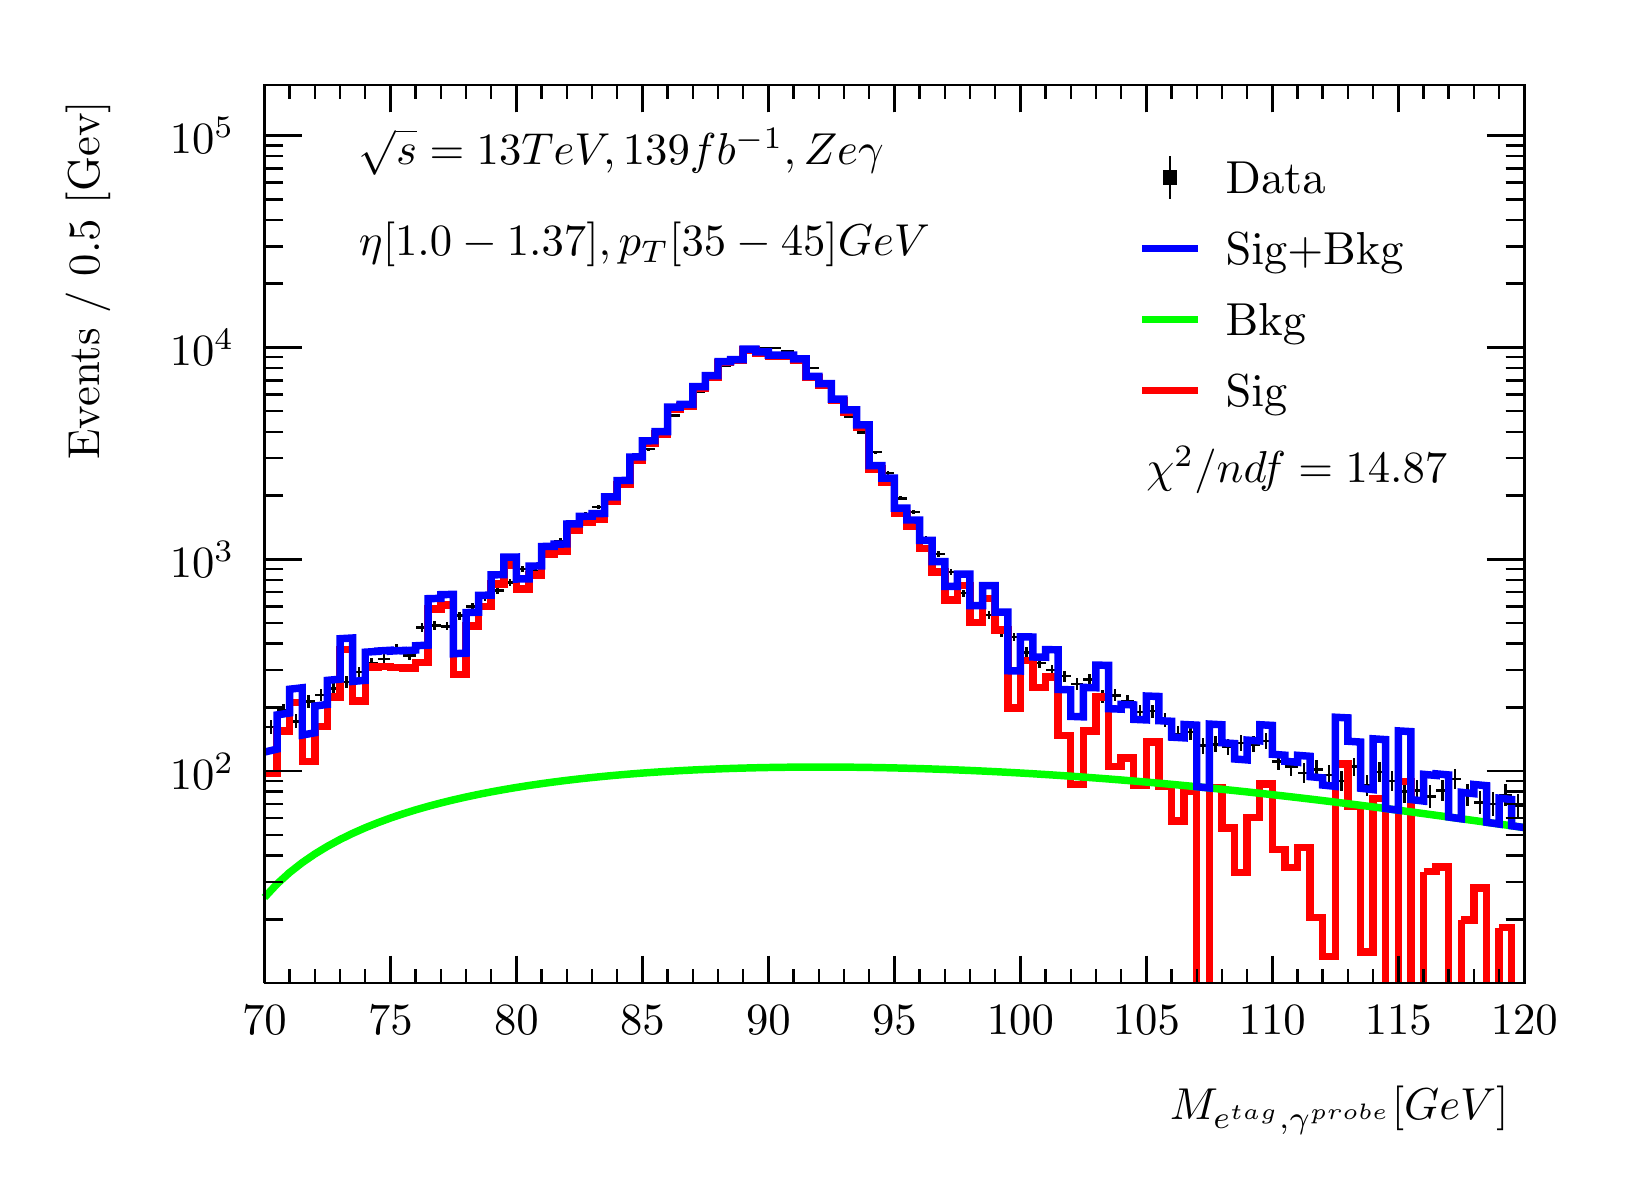
\begin{tikzpicture}
\pgfdeclareplotmark{cross} {
\pgfpathmoveto{\pgfpoint{-0.3\pgfplotmarksize}{\pgfplotmarksize}}
\pgfpathlineto{\pgfpoint{+0.3\pgfplotmarksize}{\pgfplotmarksize}}
\pgfpathlineto{\pgfpoint{+0.3\pgfplotmarksize}{0.3\pgfplotmarksize}}
\pgfpathlineto{\pgfpoint{+1\pgfplotmarksize}{0.3\pgfplotmarksize}}
\pgfpathlineto{\pgfpoint{+1\pgfplotmarksize}{-0.3\pgfplotmarksize}}
\pgfpathlineto{\pgfpoint{+0.3\pgfplotmarksize}{-0.3\pgfplotmarksize}}
\pgfpathlineto{\pgfpoint{+0.3\pgfplotmarksize}{-1.\pgfplotmarksize}}
\pgfpathlineto{\pgfpoint{-0.3\pgfplotmarksize}{-1.\pgfplotmarksize}}
\pgfpathlineto{\pgfpoint{-0.3\pgfplotmarksize}{-0.3\pgfplotmarksize}}
\pgfpathlineto{\pgfpoint{-1.\pgfplotmarksize}{-0.3\pgfplotmarksize}}
\pgfpathlineto{\pgfpoint{-1.\pgfplotmarksize}{0.3\pgfplotmarksize}}
\pgfpathlineto{\pgfpoint{-0.3\pgfplotmarksize}{0.3\pgfplotmarksize}}
\pgfpathclose
\pgfusepathqstroke
}
\pgfdeclareplotmark{cross*} {
\pgfpathmoveto{\pgfpoint{-0.3\pgfplotmarksize}{\pgfplotmarksize}}
\pgfpathlineto{\pgfpoint{+0.3\pgfplotmarksize}{\pgfplotmarksize}}
\pgfpathlineto{\pgfpoint{+0.3\pgfplotmarksize}{0.3\pgfplotmarksize}}
\pgfpathlineto{\pgfpoint{+1\pgfplotmarksize}{0.3\pgfplotmarksize}}
\pgfpathlineto{\pgfpoint{+1\pgfplotmarksize}{-0.3\pgfplotmarksize}}
\pgfpathlineto{\pgfpoint{+0.3\pgfplotmarksize}{-0.3\pgfplotmarksize}}
\pgfpathlineto{\pgfpoint{+0.3\pgfplotmarksize}{-1.\pgfplotmarksize}}
\pgfpathlineto{\pgfpoint{-0.3\pgfplotmarksize}{-1.\pgfplotmarksize}}
\pgfpathlineto{\pgfpoint{-0.3\pgfplotmarksize}{-0.3\pgfplotmarksize}}
\pgfpathlineto{\pgfpoint{-1.\pgfplotmarksize}{-0.3\pgfplotmarksize}}
\pgfpathlineto{\pgfpoint{-1.\pgfplotmarksize}{0.3\pgfplotmarksize}}
\pgfpathlineto{\pgfpoint{-0.3\pgfplotmarksize}{0.3\pgfplotmarksize}}
\pgfpathclose
\pgfusepathqfillstroke
}
\pgfdeclareplotmark{newstar} {
\pgfpathmoveto{\pgfqpoint{0pt}{\pgfplotmarksize}}
\pgfpathlineto{\pgfqpointpolar{44}{0.5\pgfplotmarksize}}
\pgfpathlineto{\pgfqpointpolar{18}{\pgfplotmarksize}}
\pgfpathlineto{\pgfqpointpolar{-20}{0.5\pgfplotmarksize}}
\pgfpathlineto{\pgfqpointpolar{-54}{\pgfplotmarksize}}
\pgfpathlineto{\pgfqpointpolar{-90}{0.5\pgfplotmarksize}}
\pgfpathlineto{\pgfqpointpolar{234}{\pgfplotmarksize}}
\pgfpathlineto{\pgfqpointpolar{198}{0.5\pgfplotmarksize}}
\pgfpathlineto{\pgfqpointpolar{162}{\pgfplotmarksize}}
\pgfpathlineto{\pgfqpointpolar{134}{0.5\pgfplotmarksize}}
\pgfpathclose
\pgfusepathqstroke
}
\pgfdeclareplotmark{newstar*} {
\pgfpathmoveto{\pgfqpoint{0pt}{\pgfplotmarksize}}
\pgfpathlineto{\pgfqpointpolar{44}{0.5\pgfplotmarksize}}
\pgfpathlineto{\pgfqpointpolar{18}{\pgfplotmarksize}}
\pgfpathlineto{\pgfqpointpolar{-20}{0.5\pgfplotmarksize}}
\pgfpathlineto{\pgfqpointpolar{-54}{\pgfplotmarksize}}
\pgfpathlineto{\pgfqpointpolar{-90}{0.5\pgfplotmarksize}}
\pgfpathlineto{\pgfqpointpolar{234}{\pgfplotmarksize}}
\pgfpathlineto{\pgfqpointpolar{198}{0.5\pgfplotmarksize}}
\pgfpathlineto{\pgfqpointpolar{162}{\pgfplotmarksize}}
\pgfpathlineto{\pgfqpointpolar{134}{0.5\pgfplotmarksize}}
\pgfpathclose
\pgfusepathqfillstroke
}
\definecolor{c}{rgb}{1,1,1};
\draw [color=c, fill=c] (0,0) rectangle (20,14.4361);
\draw [color=c, fill=c] (3,2.30977) rectangle (19,13.7143);
\definecolor{c}{rgb}{0,0,0};
\draw [c,line width=0.9] (3,2.30977) -- (3,13.7143) -- (19,13.7143) -- (19,2.30977) -- (3,2.30977);
\definecolor{c}{rgb}{1,1,1};
\draw [color=c, fill=c] (3,2.30977) rectangle (19,13.7143);
\definecolor{c}{rgb}{0,0,0};
\draw [c,line width=0.9] (3,2.30977) -- (3,13.7143) -- (19,13.7143) -- (19,2.30977) -- (3,2.30977);
\draw [c,line width=0.9] (3,2.30977) -- (19,2.30977);
\draw [c,line width=0.9] (3,2.65624) -- (3,2.30977);
\draw [c,line width=0.9] (3.32,2.48301) -- (3.32,2.30977);
\draw [c,line width=0.9] (3.64,2.48301) -- (3.64,2.30977);
\draw [c,line width=0.9] (3.96,2.48301) -- (3.96,2.30977);
\draw [c,line width=0.9] (4.28,2.48301) -- (4.28,2.30977);
\draw [c,line width=0.9] (4.6,2.65624) -- (4.6,2.30977);
\draw [c,line width=0.9] (4.92,2.48301) -- (4.92,2.30977);
\draw [c,line width=0.9] (5.24,2.48301) -- (5.24,2.30977);
\draw [c,line width=0.9] (5.56,2.48301) -- (5.56,2.30977);
\draw [c,line width=0.9] (5.88,2.48301) -- (5.88,2.30977);
\draw [c,line width=0.9] (6.2,2.65624) -- (6.2,2.30977);
\draw [c,line width=0.9] (6.52,2.48301) -- (6.52,2.30977);
\draw [c,line width=0.9] (6.84,2.48301) -- (6.84,2.30977);
\draw [c,line width=0.9] (7.16,2.48301) -- (7.16,2.30977);
\draw [c,line width=0.9] (7.48,2.48301) -- (7.48,2.30977);
\draw [c,line width=0.9] (7.8,2.65624) -- (7.8,2.30977);
\draw [c,line width=0.9] (8.12,2.48301) -- (8.12,2.30977);
\draw [c,line width=0.9] (8.44,2.48301) -- (8.44,2.30977);
\draw [c,line width=0.9] (8.76,2.48301) -- (8.76,2.30977);
\draw [c,line width=0.9] (9.08,2.48301) -- (9.08,2.30977);
\draw [c,line width=0.9] (9.4,2.65624) -- (9.4,2.30977);
\draw [c,line width=0.9] (9.72,2.48301) -- (9.72,2.30977);
\draw [c,line width=0.9] (10.04,2.48301) -- (10.04,2.30977);
\draw [c,line width=0.9] (10.36,2.48301) -- (10.36,2.30977);
\draw [c,line width=0.9] (10.68,2.48301) -- (10.68,2.30977);
\draw [c,line width=0.9] (11,2.65624) -- (11,2.30977);
\draw [c,line width=0.9] (11.32,2.48301) -- (11.32,2.30977);
\draw [c,line width=0.9] (11.64,2.48301) -- (11.64,2.30977);
\draw [c,line width=0.9] (11.96,2.48301) -- (11.96,2.30977);
\draw [c,line width=0.9] (12.28,2.48301) -- (12.28,2.30977);
\draw [c,line width=0.9] (12.6,2.65624) -- (12.6,2.30977);
\draw [c,line width=0.9] (12.92,2.48301) -- (12.92,2.30977);
\draw [c,line width=0.9] (13.24,2.48301) -- (13.24,2.30977);
\draw [c,line width=0.9] (13.56,2.48301) -- (13.56,2.30977);
\draw [c,line width=0.9] (13.88,2.48301) -- (13.88,2.30977);
\draw [c,line width=0.9] (14.2,2.65624) -- (14.2,2.30977);
\draw [c,line width=0.9] (14.52,2.48301) -- (14.52,2.30977);
\draw [c,line width=0.9] (14.84,2.48301) -- (14.84,2.30977);
\draw [c,line width=0.9] (15.16,2.48301) -- (15.16,2.30977);
\draw [c,line width=0.9] (15.48,2.48301) -- (15.48,2.30977);
\draw [c,line width=0.9] (15.8,2.65624) -- (15.8,2.30977);
\draw [c,line width=0.9] (16.12,2.48301) -- (16.12,2.30977);
\draw [c,line width=0.9] (16.44,2.48301) -- (16.44,2.30977);
\draw [c,line width=0.9] (16.76,2.48301) -- (16.76,2.30977);
\draw [c,line width=0.9] (17.08,2.48301) -- (17.08,2.30977);
\draw [c,line width=0.9] (17.4,2.65624) -- (17.4,2.30977);
\draw [c,line width=0.9] (17.72,2.48301) -- (17.72,2.30977);
\draw [c,line width=0.9] (18.04,2.48301) -- (18.04,2.30977);
\draw [c,line width=0.9] (18.36,2.48301) -- (18.36,2.30977);
\draw [c,line width=0.9] (18.68,2.48301) -- (18.68,2.30977);
\draw [c,line width=0.9] (19,2.65624) -- (19,2.30977);
\draw [anchor=base] (3,1.66015) node[scale=1.61424, color=c, rotate=0]{70};
\draw [anchor=base] (4.6,1.66015) node[scale=1.61424, color=c, rotate=0]{75};
\draw [anchor=base] (6.2,1.66015) node[scale=1.61424, color=c, rotate=0]{80};
\draw [anchor=base] (7.8,1.66015) node[scale=1.61424, color=c, rotate=0]{85};
\draw [anchor=base] (9.4,1.66015) node[scale=1.61424, color=c, rotate=0]{90};
\draw [anchor=base] (11,1.66015) node[scale=1.61424, color=c, rotate=0]{95};
\draw [anchor=base] (12.6,1.66015) node[scale=1.61424, color=c, rotate=0]{100};
\draw [anchor=base] (14.2,1.66015) node[scale=1.61424, color=c, rotate=0]{105};
\draw [anchor=base] (15.8,1.66015) node[scale=1.61424, color=c, rotate=0]{110};
\draw [anchor=base] (17.4,1.66015) node[scale=1.61424, color=c, rotate=0]{115};
\draw [anchor=base] (19,1.66015) node[scale=1.61424, color=c, rotate=0]{120};
\draw [anchor= east] (19,0.692932) node[scale=1.61424, color=c, rotate=0]{$M_{e^{tag}, \gamma^{probe}}  [GeV]$};
\draw [c,line width=0.9] (3,13.7143) -- (19,13.7143);
\draw [c,line width=0.9] (3,13.3678) -- (3,13.7143);
\draw [c,line width=0.9] (3.32,13.5411) -- (3.32,13.7143);
\draw [c,line width=0.9] (3.64,13.5411) -- (3.64,13.7143);
\draw [c,line width=0.9] (3.96,13.5411) -- (3.96,13.7143);
\draw [c,line width=0.9] (4.28,13.5411) -- (4.28,13.7143);
\draw [c,line width=0.9] (4.6,13.3678) -- (4.6,13.7143);
\draw [c,line width=0.9] (4.92,13.5411) -- (4.92,13.7143);
\draw [c,line width=0.9] (5.24,13.5411) -- (5.24,13.7143);
\draw [c,line width=0.9] (5.56,13.5411) -- (5.56,13.7143);
\draw [c,line width=0.9] (5.88,13.5411) -- (5.88,13.7143);
\draw [c,line width=0.9] (6.2,13.3678) -- (6.2,13.7143);
\draw [c,line width=0.9] (6.52,13.5411) -- (6.52,13.7143);
\draw [c,line width=0.9] (6.84,13.5411) -- (6.84,13.7143);
\draw [c,line width=0.9] (7.16,13.5411) -- (7.16,13.7143);
\draw [c,line width=0.9] (7.48,13.5411) -- (7.48,13.7143);
\draw [c,line width=0.9] (7.8,13.3678) -- (7.8,13.7143);
\draw [c,line width=0.9] (8.12,13.5411) -- (8.12,13.7143);
\draw [c,line width=0.9] (8.44,13.5411) -- (8.44,13.7143);
\draw [c,line width=0.9] (8.76,13.5411) -- (8.76,13.7143);
\draw [c,line width=0.9] (9.08,13.5411) -- (9.08,13.7143);
\draw [c,line width=0.9] (9.4,13.3678) -- (9.4,13.7143);
\draw [c,line width=0.9] (9.72,13.5411) -- (9.72,13.7143);
\draw [c,line width=0.9] (10.04,13.5411) -- (10.04,13.7143);
\draw [c,line width=0.9] (10.36,13.5411) -- (10.36,13.7143);
\draw [c,line width=0.9] (10.68,13.5411) -- (10.68,13.7143);
\draw [c,line width=0.9] (11,13.3678) -- (11,13.7143);
\draw [c,line width=0.9] (11.32,13.5411) -- (11.32,13.7143);
\draw [c,line width=0.9] (11.64,13.5411) -- (11.64,13.7143);
\draw [c,line width=0.9] (11.96,13.5411) -- (11.96,13.7143);
\draw [c,line width=0.9] (12.28,13.5411) -- (12.28,13.7143);
\draw [c,line width=0.9] (12.6,13.3678) -- (12.6,13.7143);
\draw [c,line width=0.9] (12.92,13.5411) -- (12.92,13.7143);
\draw [c,line width=0.9] (13.24,13.5411) -- (13.24,13.7143);
\draw [c,line width=0.9] (13.56,13.5411) -- (13.56,13.7143);
\draw [c,line width=0.9] (13.88,13.5411) -- (13.88,13.7143);
\draw [c,line width=0.9] (14.2,13.3678) -- (14.2,13.7143);
\draw [c,line width=0.9] (14.52,13.5411) -- (14.52,13.7143);
\draw [c,line width=0.9] (14.84,13.5411) -- (14.84,13.7143);
\draw [c,line width=0.9] (15.16,13.5411) -- (15.16,13.7143);
\draw [c,line width=0.9] (15.48,13.5411) -- (15.48,13.7143);
\draw [c,line width=0.9] (15.8,13.3678) -- (15.8,13.7143);
\draw [c,line width=0.9] (16.12,13.5411) -- (16.12,13.7143);
\draw [c,line width=0.9] (16.44,13.5411) -- (16.44,13.7143);
\draw [c,line width=0.9] (16.76,13.5411) -- (16.76,13.7143);
\draw [c,line width=0.9] (17.08,13.5411) -- (17.08,13.7143);
\draw [c,line width=0.9] (17.4,13.3678) -- (17.4,13.7143);
\draw [c,line width=0.9] (17.72,13.5411) -- (17.72,13.7143);
\draw [c,line width=0.9] (18.04,13.5411) -- (18.04,13.7143);
\draw [c,line width=0.9] (18.36,13.5411) -- (18.36,13.7143);
\draw [c,line width=0.9] (18.68,13.5411) -- (18.68,13.7143);
\draw [c,line width=0.9] (19,13.3678) -- (19,13.7143);
\draw [c,line width=0.9] (3,2.30977) -- (3,13.7143);
\draw [c,line width=0.9] (3.237,3.11973) -- (3,3.11973);
\draw [c,line width=0.9] (3.237,3.59352) -- (3,3.59352);
\draw [c,line width=0.9] (3.237,3.92968) -- (3,3.92968);
\draw [c,line width=0.9] (3.237,4.19043) -- (3,4.19043);
\draw [c,line width=0.9] (3.237,4.40347) -- (3,4.40347);
\draw [c,line width=0.9] (3.237,4.5836) -- (3,4.5836);
\draw [c,line width=0.9] (3.237,4.73964) -- (3,4.73964);
\draw [c,line width=0.9] (3.237,4.87727) -- (3,4.87727);
\draw [c,line width=0.9] (3.474,5.00038) -- (3,5.00038);
\draw [anchor= east] (2.82,5.00038) node[scale=1.61424, color=c, rotate=0]{$10^{2}$};
\draw [c,line width=0.9] (3.237,5.81034) -- (3,5.81034);
\draw [c,line width=0.9] (3.237,6.28413) -- (3,6.28413);
\draw [c,line width=0.9] (3.237,6.62029) -- (3,6.62029);
\draw [c,line width=0.9] (3.237,6.88104) -- (3,6.88104);
\draw [c,line width=0.9] (3.237,7.09409) -- (3,7.09409);
\draw [c,line width=0.9] (3.237,7.27421) -- (3,7.27421);
\draw [c,line width=0.9] (3.237,7.43025) -- (3,7.43025);
\draw [c,line width=0.9] (3.237,7.56788) -- (3,7.56788);
\draw [c,line width=0.9] (3.474,7.69099) -- (3,7.69099);
\draw [anchor= east] (2.82,7.69099) node[scale=1.61424, color=c, rotate=0]{$10^{3}$};
\draw [c,line width=0.9] (3.237,8.50095) -- (3,8.50095);
\draw [c,line width=0.9] (3.237,8.97474) -- (3,8.97474);
\draw [c,line width=0.9] (3.237,9.3109) -- (3,9.3109);
\draw [c,line width=0.9] (3.237,9.57165) -- (3,9.57165);
\draw [c,line width=0.9] (3.237,9.7847) -- (3,9.7847);
\draw [c,line width=0.9] (3.237,9.96482) -- (3,9.96482);
\draw [c,line width=0.9] (3.237,10.1209) -- (3,10.1209);
\draw [c,line width=0.9] (3.237,10.2585) -- (3,10.2585);
\draw [c,line width=0.9] (3.474,10.3816) -- (3,10.3816);
\draw [anchor= east] (2.82,10.3816) node[scale=1.61424, color=c, rotate=0]{$10^{4}$};
\draw [c,line width=0.9] (3.237,11.1916) -- (3,11.1916);
\draw [c,line width=0.9] (3.237,11.6654) -- (3,11.6654);
\draw [c,line width=0.9] (3.237,12.0015) -- (3,12.0015);
\draw [c,line width=0.9] (3.237,12.2623) -- (3,12.2623);
\draw [c,line width=0.9] (3.237,12.4753) -- (3,12.4753);
\draw [c,line width=0.9] (3.237,12.6554) -- (3,12.6554);
\draw [c,line width=0.9] (3.237,12.8115) -- (3,12.8115);
\draw [c,line width=0.9] (3.237,12.9491) -- (3,12.9491);
\draw [c,line width=0.9] (3.474,13.0722) -- (3,13.0722);
\draw [anchor= east] (2.82,13.0722) node[scale=1.61424, color=c, rotate=0]{$10^{5}$};
\draw [anchor= east] (0.76,13.7143) node[scale=1.61424, color=c, rotate=90]{Events / 0.5 [Gev]};
\draw [c,line width=0.9] (19,2.30977) -- (19,13.7143);
\draw [c,line width=0.9] (18.763,3.11973) -- (19,3.11973);
\draw [c,line width=0.9] (18.763,3.59352) -- (19,3.59352);
\draw [c,line width=0.9] (18.763,3.92968) -- (19,3.92968);
\draw [c,line width=0.9] (18.763,4.19043) -- (19,4.19043);
\draw [c,line width=0.9] (18.763,4.40347) -- (19,4.40347);
\draw [c,line width=0.9] (18.763,4.5836) -- (19,4.5836);
\draw [c,line width=0.9] (18.763,4.73964) -- (19,4.73964);
\draw [c,line width=0.9] (18.763,4.87727) -- (19,4.87727);
\draw [c,line width=0.9] (18.526,5.00038) -- (19,5.00038);
\draw [c,line width=0.9] (18.763,5.81034) -- (19,5.81034);
\draw [c,line width=0.9] (18.763,6.28413) -- (19,6.28413);
\draw [c,line width=0.9] (18.763,6.62029) -- (19,6.62029);
\draw [c,line width=0.9] (18.763,6.88104) -- (19,6.88104);
\draw [c,line width=0.9] (18.763,7.09409) -- (19,7.09409);
\draw [c,line width=0.9] (18.763,7.27421) -- (19,7.27421);
\draw [c,line width=0.9] (18.763,7.43025) -- (19,7.43025);
\draw [c,line width=0.9] (18.763,7.56788) -- (19,7.56788);
\draw [c,line width=0.9] (18.526,7.69099) -- (19,7.69099);
\draw [c,line width=0.9] (18.763,8.50095) -- (19,8.50095);
\draw [c,line width=0.9] (18.763,8.97474) -- (19,8.97474);
\draw [c,line width=0.9] (18.763,9.3109) -- (19,9.3109);
\draw [c,line width=0.9] (18.763,9.57165) -- (19,9.57165);
\draw [c,line width=0.9] (18.763,9.7847) -- (19,9.7847);
\draw [c,line width=0.9] (18.763,9.96482) -- (19,9.96482);
\draw [c,line width=0.9] (18.763,10.1209) -- (19,10.1209);
\draw [c,line width=0.9] (18.763,10.2585) -- (19,10.2585);
\draw [c,line width=0.9] (18.526,10.3816) -- (19,10.3816);
\draw [c,line width=0.9] (18.763,11.1916) -- (19,11.1916);
\draw [c,line width=0.9] (18.763,11.6654) -- (19,11.6654);
\draw [c,line width=0.9] (18.763,12.0015) -- (19,12.0015);
\draw [c,line width=0.9] (18.763,12.2623) -- (19,12.2623);
\draw [c,line width=0.9] (18.763,12.4753) -- (19,12.4753);
\draw [c,line width=0.9] (18.763,12.6554) -- (19,12.6554);
\draw [c,line width=0.9] (18.763,12.8115) -- (19,12.8115);
\draw [c,line width=0.9] (18.763,12.9491) -- (19,12.9491);
\draw [c,line width=0.9] (18.526,13.0722) -- (19,13.0722);
\draw [c,line width=0.9] (3.08,5.56411) -- (3,5.56411);
\draw [c,line width=0.9] (3,5.56411) -- (3,5.56411);
\draw [c,line width=0.9] (3.08,5.56411) -- (3.16,5.56411);
\draw [c,line width=0.9] (3.16,5.56411) -- (3.16,5.56411);
\draw [c,line width=0.9] (3.08,5.56411) -- (3.08,5.65589);
\draw [c,line width=0.9] (3.08,5.65589) -- (3.08,5.65589);
\draw [c,line width=0.9] (3.08,5.56411) -- (3.08,5.47232);
\draw [c,line width=0.9] (3.08,5.47232) -- (3.08,5.47232);
\draw [c,line width=0.9] (3.24,5.77475) -- (3.16,5.77475);
\draw [c,line width=0.9] (3.16,5.77475) -- (3.16,5.77475);
\draw [c,line width=0.9] (3.24,5.77475) -- (3.32,5.77475);
\draw [c,line width=0.9] (3.32,5.77475) -- (3.32,5.77475);
\draw [c,line width=0.9] (3.24,5.77475) -- (3.24,5.85862);
\draw [c,line width=0.9] (3.24,5.85862) -- (3.24,5.85862);
\draw [c,line width=0.9] (3.24,5.77475) -- (3.24,5.69087);
\draw [c,line width=0.9] (3.24,5.69087) -- (3.24,5.69087);
\draw [c,line width=0.9] (3.4,5.6341) -- (3.32,5.6341);
\draw [c,line width=0.9] (3.32,5.6341) -- (3.32,5.6341);
\draw [c,line width=0.9] (3.4,5.6341) -- (3.48,5.6341);
\draw [c,line width=0.9] (3.48,5.6341) -- (3.48,5.6341);
\draw [c,line width=0.9] (3.4,5.6341) -- (3.4,5.72318);
\draw [c,line width=0.9] (3.4,5.72318) -- (3.4,5.72318);
\draw [c,line width=0.9] (3.4,5.6341) -- (3.4,5.54502);
\draw [c,line width=0.9] (3.4,5.54502) -- (3.4,5.54502);
\draw [c,line width=0.9] (3.56,5.88393) -- (3.48,5.88393);
\draw [c,line width=0.9] (3.48,5.88393) -- (3.48,5.88393);
\draw [c,line width=0.9] (3.56,5.88393) -- (3.64,5.88393);
\draw [c,line width=0.9] (3.64,5.88393) -- (3.64,5.88393);
\draw [c,line width=0.9] (3.56,5.88393) -- (3.56,5.96398);
\draw [c,line width=0.9] (3.56,5.96398) -- (3.56,5.96398);
\draw [c,line width=0.9] (3.56,5.88393) -- (3.56,5.80388);
\draw [c,line width=0.9] (3.56,5.80388) -- (3.56,5.80388);
\draw [c,line width=0.9] (3.72,5.96856) -- (3.64,5.96856);
\draw [c,line width=0.9] (3.64,5.96856) -- (3.64,5.96856);
\draw [c,line width=0.9] (3.72,5.96856) -- (3.8,5.96856);
\draw [c,line width=0.9] (3.8,5.96856) -- (3.8,5.96856);
\draw [c,line width=0.9] (3.72,5.96856) -- (3.72,6.04577);
\draw [c,line width=0.9] (3.72,6.04577) -- (3.72,6.04577);
\draw [c,line width=0.9] (3.72,5.96856) -- (3.72,5.89136);
\draw [c,line width=0.9] (3.72,5.89136) -- (3.72,5.89136);
\draw [c,line width=0.9] (3.88,6.04748) -- (3.8,6.04748);
\draw [c,line width=0.9] (3.8,6.04748) -- (3.8,6.04748);
\draw [c,line width=0.9] (3.88,6.04748) -- (3.96,6.04748);
\draw [c,line width=0.9] (3.96,6.04748) -- (3.96,6.04748);
\draw [c,line width=0.9] (3.88,6.04748) -- (3.88,6.12212);
\draw [c,line width=0.9] (3.88,6.12212) -- (3.88,6.12212);
\draw [c,line width=0.9] (3.88,6.04748) -- (3.88,5.97284);
\draw [c,line width=0.9] (3.88,5.97284) -- (3.88,5.97284);
\draw [c,line width=0.9] (4.04,6.13476) -- (3.96,6.13476);
\draw [c,line width=0.9] (3.96,6.13476) -- (3.96,6.13476);
\draw [c,line width=0.9] (4.04,6.13476) -- (4.12,6.13476);
\draw [c,line width=0.9] (4.12,6.13476) -- (4.12,6.13476);
\draw [c,line width=0.9] (4.04,6.13476) -- (4.04,6.20666);
\draw [c,line width=0.9] (4.04,6.20666) -- (4.04,6.20666);
\draw [c,line width=0.9] (4.04,6.13476) -- (4.04,6.06285);
\draw [c,line width=0.9] (4.04,6.06285) -- (4.04,6.06285);
\draw [c,line width=0.9] (4.2,6.26053) -- (4.12,6.26053);
\draw [c,line width=0.9] (4.12,6.26053) -- (4.12,6.26053);
\draw [c,line width=0.9] (4.2,6.26053) -- (4.28,6.26053);
\draw [c,line width=0.9] (4.28,6.26053) -- (4.28,6.26053);
\draw [c,line width=0.9] (4.2,6.26053) -- (4.2,6.32867);
\draw [c,line width=0.9] (4.2,6.32867) -- (4.2,6.32867);
\draw [c,line width=0.9] (4.2,6.26053) -- (4.2,6.19239);
\draw [c,line width=0.9] (4.2,6.19239) -- (4.2,6.19239);
\draw [c,line width=0.9] (4.36,6.37045) -- (4.28,6.37045);
\draw [c,line width=0.9] (4.28,6.37045) -- (4.28,6.37045);
\draw [c,line width=0.9] (4.36,6.37045) -- (4.44,6.37045);
\draw [c,line width=0.9] (4.44,6.37045) -- (4.44,6.37045);
\draw [c,line width=0.9] (4.36,6.37045) -- (4.36,6.43546);
\draw [c,line width=0.9] (4.36,6.43546) -- (4.36,6.43546);
\draw [c,line width=0.9] (4.36,6.37045) -- (4.36,6.30544);
\draw [c,line width=0.9] (4.36,6.30544) -- (4.36,6.30544);
\draw [c,line width=0.9] (4.52,6.42349) -- (4.44,6.42349);
\draw [c,line width=0.9] (4.44,6.42349) -- (4.44,6.42349);
\draw [c,line width=0.9] (4.52,6.42349) -- (4.6,6.42349);
\draw [c,line width=0.9] (4.6,6.42349) -- (4.6,6.42349);
\draw [c,line width=0.9] (4.52,6.42349) -- (4.52,6.48705);
\draw [c,line width=0.9] (4.52,6.48705) -- (4.52,6.48705);
\draw [c,line width=0.9] (4.52,6.42349) -- (4.52,6.35994);
\draw [c,line width=0.9] (4.52,6.35994) -- (4.52,6.35994);
\draw [c,line width=0.9] (4.68,6.5511) -- (4.6,6.5511);
\draw [c,line width=0.9] (4.6,6.5511) -- (4.6,6.5511);
\draw [c,line width=0.9] (4.68,6.5511) -- (4.76,6.5511);
\draw [c,line width=0.9] (4.76,6.5511) -- (4.76,6.5511);
\draw [c,line width=0.9] (4.68,6.5511) -- (4.68,6.61127);
\draw [c,line width=0.9] (4.68,6.61127) -- (4.68,6.61127);
\draw [c,line width=0.9] (4.68,6.5511) -- (4.68,6.49092);
\draw [c,line width=0.9] (4.68,6.49092) -- (4.68,6.49092);
\draw [c,line width=0.9] (4.84,6.47092) -- (4.76,6.47092);
\draw [c,line width=0.9] (4.76,6.47092) -- (4.76,6.47092);
\draw [c,line width=0.9] (4.84,6.47092) -- (4.92,6.47092);
\draw [c,line width=0.9] (4.92,6.47092) -- (4.92,6.47092);
\draw [c,line width=0.9] (4.84,6.47092) -- (4.84,6.53319);
\draw [c,line width=0.9] (4.84,6.53319) -- (4.84,6.53319);
\draw [c,line width=0.9] (4.84,6.47092) -- (4.84,6.40864);
\draw [c,line width=0.9] (4.84,6.40864) -- (4.84,6.40864);
\draw [c,line width=0.9] (5,6.82356) -- (4.92,6.82356);
\draw [c,line width=0.9] (4.92,6.82356) -- (4.92,6.82356);
\draw [c,line width=0.9] (5,6.82356) -- (5.08,6.82356);
\draw [c,line width=0.9] (5.08,6.82356) -- (5.08,6.82356);
\draw [c,line width=0.9] (5,6.82356) -- (5,6.87712);
\draw [c,line width=0.9] (5,6.87712) -- (5,6.87712);
\draw [c,line width=0.9] (5,6.82356) -- (5,6.77001);
\draw [c,line width=0.9] (5,6.77001) -- (5,6.77001);
\draw [c,line width=0.9] (5.16,6.85265) -- (5.08,6.85265);
\draw [c,line width=0.9] (5.08,6.85265) -- (5.08,6.85265);
\draw [c,line width=0.9] (5.16,6.85265) -- (5.24,6.85265);
\draw [c,line width=0.9] (5.24,6.85265) -- (5.24,6.85265);
\draw [c,line width=0.9] (5.16,6.85265) -- (5.16,6.90555);
\draw [c,line width=0.9] (5.16,6.90555) -- (5.16,6.90555);
\draw [c,line width=0.9] (5.16,6.85265) -- (5.16,6.79976);
\draw [c,line width=0.9] (5.16,6.79976) -- (5.16,6.79976);
\draw [c,line width=0.9] (5.32,6.84062) -- (5.24,6.84062);
\draw [c,line width=0.9] (5.24,6.84062) -- (5.24,6.84062);
\draw [c,line width=0.9] (5.32,6.84062) -- (5.4,6.84062);
\draw [c,line width=0.9] (5.4,6.84062) -- (5.4,6.84062);
\draw [c,line width=0.9] (5.32,6.84062) -- (5.32,6.89379);
\draw [c,line width=0.9] (5.32,6.89379) -- (5.32,6.89379);
\draw [c,line width=0.9] (5.32,6.84062) -- (5.32,6.78746);
\draw [c,line width=0.9] (5.32,6.78746) -- (5.32,6.78746);
\draw [c,line width=0.9] (5.48,6.97529) -- (5.4,6.97529);
\draw [c,line width=0.9] (5.4,6.97529) -- (5.4,6.97529);
\draw [c,line width=0.9] (5.48,6.97529) -- (5.56,6.97529);
\draw [c,line width=0.9] (5.56,6.97529) -- (5.56,6.97529);
\draw [c,line width=0.9] (5.48,6.97529) -- (5.48,7.02548);
\draw [c,line width=0.9] (5.48,7.02548) -- (5.48,7.02548);
\draw [c,line width=0.9] (5.48,6.97529) -- (5.48,6.9251);
\draw [c,line width=0.9] (5.48,6.9251) -- (5.48,6.9251);
\draw [c,line width=0.9] (5.64,7.09214) -- (5.56,7.09214);
\draw [c,line width=0.9] (5.56,7.09214) -- (5.56,7.09214);
\draw [c,line width=0.9] (5.64,7.09214) -- (5.72,7.09214);
\draw [c,line width=0.9] (5.72,7.09214) -- (5.72,7.09214);
\draw [c,line width=0.9] (5.64,7.09214) -- (5.64,7.13988);
\draw [c,line width=0.9] (5.64,7.13988) -- (5.64,7.13988);
\draw [c,line width=0.9] (5.64,7.09214) -- (5.64,7.0444);
\draw [c,line width=0.9] (5.64,7.0444) -- (5.64,7.0444);
\draw [c,line width=0.9] (5.8,7.20546) -- (5.72,7.20546);
\draw [c,line width=0.9] (5.72,7.20546) -- (5.72,7.20546);
\draw [c,line width=0.9] (5.8,7.20546) -- (5.88,7.20546);
\draw [c,line width=0.9] (5.88,7.20546) -- (5.88,7.20546);
\draw [c,line width=0.9] (5.8,7.20546) -- (5.8,7.25094);
\draw [c,line width=0.9] (5.8,7.25094) -- (5.8,7.25094);
\draw [c,line width=0.9] (5.8,7.20546) -- (5.8,7.15998);
\draw [c,line width=0.9] (5.8,7.15998) -- (5.8,7.15998);
\draw [c,line width=0.9] (5.96,7.29408) -- (5.88,7.29408);
\draw [c,line width=0.9] (5.88,7.29408) -- (5.88,7.29408);
\draw [c,line width=0.9] (5.96,7.29408) -- (6.04,7.29408);
\draw [c,line width=0.9] (6.04,7.29408) -- (6.04,7.29408);
\draw [c,line width=0.9] (5.96,7.29408) -- (5.96,7.33787);
\draw [c,line width=0.9] (5.96,7.33787) -- (5.96,7.33787);
\draw [c,line width=0.9] (5.96,7.29408) -- (5.96,7.25029);
\draw [c,line width=0.9] (5.96,7.25029) -- (5.96,7.25029);
\draw [c,line width=0.9] (6.12,7.39766) -- (6.04,7.39766);
\draw [c,line width=0.9] (6.04,7.39766) -- (6.04,7.39766);
\draw [c,line width=0.9] (6.12,7.39766) -- (6.2,7.39766);
\draw [c,line width=0.9] (6.2,7.39766) -- (6.2,7.39766);
\draw [c,line width=0.9] (6.12,7.39766) -- (6.12,7.43956);
\draw [c,line width=0.9] (6.12,7.43956) -- (6.12,7.43956);
\draw [c,line width=0.9] (6.12,7.39766) -- (6.12,7.35577);
\draw [c,line width=0.9] (6.12,7.35577) -- (6.12,7.35577);
\draw [c,line width=0.9] (6.28,7.56918) -- (6.2,7.56918);
\draw [c,line width=0.9] (6.2,7.56918) -- (6.2,7.56918);
\draw [c,line width=0.9] (6.28,7.56918) -- (6.36,7.56918);
\draw [c,line width=0.9] (6.36,7.56918) -- (6.36,7.56918);
\draw [c,line width=0.9] (6.28,7.56918) -- (6.28,7.6081);
\draw [c,line width=0.9] (6.28,7.6081) -- (6.28,7.6081);
\draw [c,line width=0.9] (6.28,7.56918) -- (6.28,7.53025);
\draw [c,line width=0.9] (6.28,7.53025) -- (6.28,7.53025);
\draw [c,line width=0.9] (6.44,7.54295) -- (6.36,7.54295);
\draw [c,line width=0.9] (6.36,7.54295) -- (6.36,7.54295);
\draw [c,line width=0.9] (6.44,7.54295) -- (6.52,7.54295);
\draw [c,line width=0.9] (6.52,7.54295) -- (6.52,7.54295);
\draw [c,line width=0.9] (6.44,7.54295) -- (6.44,7.58231);
\draw [c,line width=0.9] (6.44,7.58231) -- (6.44,7.58231);
\draw [c,line width=0.9] (6.44,7.54295) -- (6.44,7.50358);
\draw [c,line width=0.9] (6.44,7.50358) -- (6.44,7.50358);
\draw [c,line width=0.9] (6.6,7.76239) -- (6.52,7.76239);
\draw [c,line width=0.9] (6.52,7.76239) -- (6.52,7.76239);
\draw [c,line width=0.9] (6.6,7.76239) -- (6.68,7.76239);
\draw [c,line width=0.9] (6.68,7.76239) -- (6.68,7.76239);
\draw [c,line width=0.9] (6.6,7.76239) -- (6.6,7.79822);
\draw [c,line width=0.9] (6.6,7.79822) -- (6.6,7.79822);
\draw [c,line width=0.9] (6.6,7.76239) -- (6.6,7.72655);
\draw [c,line width=0.9] (6.6,7.72655) -- (6.6,7.72655);
\draw [c,line width=0.9] (6.76,7.92527) -- (6.68,7.92527);
\draw [c,line width=0.9] (6.68,7.92527) -- (6.68,7.92527);
\draw [c,line width=0.9] (6.76,7.92527) -- (6.84,7.92527);
\draw [c,line width=0.9] (6.84,7.92527) -- (6.84,7.92527);
\draw [c,line width=0.9] (6.76,7.92527) -- (6.76,7.9587);
\draw [c,line width=0.9] (6.76,7.9587) -- (6.76,7.9587);
\draw [c,line width=0.9] (6.76,7.92527) -- (6.76,7.89184);
\draw [c,line width=0.9] (6.76,7.89184) -- (6.76,7.89184);
\draw [c,line width=0.9] (6.92,8.11384) -- (6.84,8.11384);
\draw [c,line width=0.9] (6.84,8.11384) -- (6.84,8.11384);
\draw [c,line width=0.9] (6.92,8.11384) -- (7,8.11384);
\draw [c,line width=0.9] (7,8.11384) -- (7,8.11384);
\draw [c,line width=0.9] (6.92,8.11384) -- (6.92,8.14467);
\draw [c,line width=0.9] (6.92,8.14467) -- (6.92,8.14467);
\draw [c,line width=0.9] (6.92,8.11384) -- (6.92,8.083);
\draw [c,line width=0.9] (6.92,8.083) -- (6.92,8.083);
\draw [c,line width=0.9] (7.08,8.25904) -- (7,8.25904);
\draw [c,line width=0.9] (7,8.25904) -- (7,8.25904);
\draw [c,line width=0.9] (7.08,8.25904) -- (7.16,8.25904);
\draw [c,line width=0.9] (7.16,8.25904) -- (7.16,8.25904);
\draw [c,line width=0.9] (7.08,8.25904) -- (7.08,8.28802);
\draw [c,line width=0.9] (7.08,8.28802) -- (7.08,8.28802);
\draw [c,line width=0.9] (7.08,8.25904) -- (7.08,8.23006);
\draw [c,line width=0.9] (7.08,8.23006) -- (7.08,8.23006);
\draw [c,line width=0.9] (7.24,8.35357) -- (7.16,8.35357);
\draw [c,line width=0.9] (7.16,8.35357) -- (7.16,8.35357);
\draw [c,line width=0.9] (7.24,8.35357) -- (7.32,8.35357);
\draw [c,line width=0.9] (7.32,8.35357) -- (7.32,8.35357);
\draw [c,line width=0.9] (7.24,8.35357) -- (7.24,8.38139);
\draw [c,line width=0.9] (7.24,8.38139) -- (7.24,8.38139);
\draw [c,line width=0.9] (7.24,8.35357) -- (7.24,8.32574);
\draw [c,line width=0.9] (7.24,8.32574) -- (7.24,8.32574);
\draw [c,line width=0.9] (7.4,8.48448) -- (7.32,8.48448);
\draw [c,line width=0.9] (7.32,8.48448) -- (7.32,8.48448);
\draw [c,line width=0.9] (7.4,8.48448) -- (7.48,8.48448);
\draw [c,line width=0.9] (7.48,8.48448) -- (7.48,8.48448);
\draw [c,line width=0.9] (7.4,8.48448) -- (7.4,8.51079);
\draw [c,line width=0.9] (7.4,8.51079) -- (7.4,8.51079);
\draw [c,line width=0.9] (7.4,8.48448) -- (7.4,8.45816);
\draw [c,line width=0.9] (7.4,8.45816) -- (7.4,8.45816);
\draw [c,line width=0.9] (7.56,8.70569) -- (7.48,8.70569);
\draw [c,line width=0.9] (7.48,8.70569) -- (7.48,8.70569);
\draw [c,line width=0.9] (7.56,8.70569) -- (7.64,8.70569);
\draw [c,line width=0.9] (7.64,8.70569) -- (7.64,8.70569);
\draw [c,line width=0.9] (7.56,8.70569) -- (7.56,8.72963);
\draw [c,line width=0.9] (7.56,8.72963) -- (7.56,8.72963);
\draw [c,line width=0.9] (7.56,8.70569) -- (7.56,8.68175);
\draw [c,line width=0.9] (7.56,8.68175) -- (7.56,8.68175);
\draw [c,line width=0.9] (7.72,8.93995) -- (7.64,8.93995);
\draw [c,line width=0.9] (7.64,8.93995) -- (7.64,8.93995);
\draw [c,line width=0.9] (7.72,8.93995) -- (7.8,8.93995);
\draw [c,line width=0.9] (7.8,8.93995) -- (7.8,8.93995);
\draw [c,line width=0.9] (7.72,8.93995) -- (7.72,8.96161);
\draw [c,line width=0.9] (7.72,8.96161) -- (7.72,8.96161);
\draw [c,line width=0.9] (7.72,8.93995) -- (7.72,8.9183);
\draw [c,line width=0.9] (7.72,8.9183) -- (7.72,8.9183);
\draw [c,line width=0.9] (7.88,9.09) -- (7.8,9.09);
\draw [c,line width=0.9] (7.8,9.09) -- (7.8,9.09);
\draw [c,line width=0.9] (7.88,9.09) -- (7.96,9.09);
\draw [c,line width=0.9] (7.96,9.09) -- (7.96,9.09);
\draw [c,line width=0.9] (7.88,9.09) -- (7.88,9.11031);
\draw [c,line width=0.9] (7.88,9.11031) -- (7.88,9.11031);
\draw [c,line width=0.9] (7.88,9.09) -- (7.88,9.0697);
\draw [c,line width=0.9] (7.88,9.0697) -- (7.88,9.0697);
\draw [c,line width=0.9] (8.04,9.29739) -- (7.96,9.29739);
\draw [c,line width=0.9] (7.96,9.29739) -- (7.96,9.29739);
\draw [c,line width=0.9] (8.04,9.29739) -- (8.12,9.29739);
\draw [c,line width=0.9] (8.12,9.29739) -- (8.12,9.29739);
\draw [c,line width=0.9] (8.04,9.29739) -- (8.04,9.31597);
\draw [c,line width=0.9] (8.04,9.31597) -- (8.04,9.31597);
\draw [c,line width=0.9] (8.04,9.29739) -- (8.04,9.27881);
\draw [c,line width=0.9] (8.04,9.27881) -- (8.04,9.27881);
\draw [c,line width=0.9] (8.2,9.51564) -- (8.12,9.51564);
\draw [c,line width=0.9] (8.12,9.51564) -- (8.12,9.51564);
\draw [c,line width=0.9] (8.2,9.51564) -- (8.28,9.51564);
\draw [c,line width=0.9] (8.28,9.51564) -- (8.28,9.51564);
\draw [c,line width=0.9] (8.2,9.51564) -- (8.2,9.53257);
\draw [c,line width=0.9] (8.2,9.53257) -- (8.2,9.53257);
\draw [c,line width=0.9] (8.2,9.51564) -- (8.2,9.49872);
\draw [c,line width=0.9] (8.2,9.49872) -- (8.2,9.49872);
\draw [c,line width=0.9] (8.36,9.68493) -- (8.28,9.68493);
\draw [c,line width=0.9] (8.28,9.68493) -- (8.28,9.68493);
\draw [c,line width=0.9] (8.36,9.68493) -- (8.44,9.68493);
\draw [c,line width=0.9] (8.44,9.68493) -- (8.44,9.68493);
\draw [c,line width=0.9] (8.36,9.68493) -- (8.36,9.70068);
\draw [c,line width=0.9] (8.36,9.70068) -- (8.36,9.70068);
\draw [c,line width=0.9] (8.36,9.68493) -- (8.36,9.66919);
\draw [c,line width=0.9] (8.36,9.66919) -- (8.36,9.66919);
\draw [c,line width=0.9] (8.52,9.81412) -- (8.44,9.81412);
\draw [c,line width=0.9] (8.44,9.81412) -- (8.44,9.81412);
\draw [c,line width=0.9] (8.52,9.81412) -- (8.6,9.81412);
\draw [c,line width=0.9] (8.6,9.81412) -- (8.6,9.81412);
\draw [c,line width=0.9] (8.52,9.81412) -- (8.52,9.82902);
\draw [c,line width=0.9] (8.52,9.82902) -- (8.52,9.82902);
\draw [c,line width=0.9] (8.52,9.81412) -- (8.52,9.79922);
\draw [c,line width=0.9] (8.52,9.79922) -- (8.52,9.79922);
\draw [c,line width=0.9] (8.68,10.0129) -- (8.6,10.0129);
\draw [c,line width=0.9] (8.6,10.0129) -- (8.6,10.0129);
\draw [c,line width=0.9] (8.68,10.0129) -- (8.76,10.0129);
\draw [c,line width=0.9] (8.76,10.0129) -- (8.76,10.0129);
\draw [c,line width=0.9] (8.68,10.0129) -- (8.68,10.0266);
\draw [c,line width=0.9] (8.68,10.0266) -- (8.68,10.0266);
\draw [c,line width=0.9] (8.68,10.0129) -- (8.68,9.99922);
\draw [c,line width=0.9] (8.68,9.99922) -- (8.68,9.99922);
\draw [c,line width=0.9] (8.84,10.1518) -- (8.76,10.1518);
\draw [c,line width=0.9] (8.76,10.1518) -- (8.76,10.1518);
\draw [c,line width=0.9] (8.84,10.1518) -- (8.92,10.1518);
\draw [c,line width=0.9] (8.92,10.1518) -- (8.92,10.1518);
\draw [c,line width=0.9] (8.84,10.1518) -- (8.84,10.1647);
\draw [c,line width=0.9] (8.84,10.1647) -- (8.84,10.1647);
\draw [c,line width=0.9] (8.84,10.1518) -- (8.84,10.139);
\draw [c,line width=0.9] (8.84,10.139) -- (8.84,10.139);
\draw [c,line width=0.9] (9,10.2505) -- (8.92,10.2505);
\draw [c,line width=0.9] (8.92,10.2505) -- (8.92,10.2505);
\draw [c,line width=0.9] (9,10.2505) -- (9.08,10.2505);
\draw [c,line width=0.9] (9.08,10.2505) -- (9.08,10.2505);
\draw [c,line width=0.9] (9,10.2505) -- (9,10.2629);
\draw [c,line width=0.9] (9,10.2629) -- (9,10.2629);
\draw [c,line width=0.9] (9,10.2505) -- (9,10.2382);
\draw [c,line width=0.9] (9,10.2382) -- (9,10.2382);
\draw [c,line width=0.9] (9.16,10.3448) -- (9.08,10.3448);
\draw [c,line width=0.9] (9.08,10.3448) -- (9.08,10.3448);
\draw [c,line width=0.9] (9.16,10.3448) -- (9.24,10.3448);
\draw [c,line width=0.9] (9.24,10.3448) -- (9.24,10.3448);
\draw [c,line width=0.9] (9.16,10.3448) -- (9.16,10.3567);
\draw [c,line width=0.9] (9.16,10.3567) -- (9.16,10.3567);
\draw [c,line width=0.9] (9.16,10.3448) -- (9.16,10.3329);
\draw [c,line width=0.9] (9.16,10.3329) -- (9.16,10.3329);
\draw [c,line width=0.9] (9.32,10.3657) -- (9.24,10.3657);
\draw [c,line width=0.9] (9.24,10.3657) -- (9.24,10.3657);
\draw [c,line width=0.9] (9.32,10.3657) -- (9.4,10.3657);
\draw [c,line width=0.9] (9.4,10.3657) -- (9.4,10.3657);
\draw [c,line width=0.9] (9.32,10.3657) -- (9.32,10.3775);
\draw [c,line width=0.9] (9.32,10.3775) -- (9.32,10.3775);
\draw [c,line width=0.9] (9.32,10.3657) -- (9.32,10.354);
\draw [c,line width=0.9] (9.32,10.354) -- (9.32,10.354);
\draw [c,line width=0.9] (9.48,10.3749) -- (9.4,10.3749);
\draw [c,line width=0.9] (9.4,10.3749) -- (9.4,10.3749);
\draw [c,line width=0.9] (9.48,10.3749) -- (9.56,10.3749);
\draw [c,line width=0.9] (9.56,10.3749) -- (9.56,10.3749);
\draw [c,line width=0.9] (9.48,10.3749) -- (9.48,10.3866);
\draw [c,line width=0.9] (9.48,10.3866) -- (9.48,10.3866);
\draw [c,line width=0.9] (9.48,10.3749) -- (9.48,10.3632);
\draw [c,line width=0.9] (9.48,10.3632) -- (9.48,10.3632);
\draw [c,line width=0.9] (9.64,10.3395) -- (9.56,10.3395);
\draw [c,line width=0.9] (9.56,10.3395) -- (9.56,10.3395);
\draw [c,line width=0.9] (9.64,10.3395) -- (9.72,10.3395);
\draw [c,line width=0.9] (9.72,10.3395) -- (9.72,10.3395);
\draw [c,line width=0.9] (9.64,10.3395) -- (9.64,10.3514);
\draw [c,line width=0.9] (9.64,10.3514) -- (9.64,10.3514);
\draw [c,line width=0.9] (9.64,10.3395) -- (9.64,10.3276);
\draw [c,line width=0.9] (9.64,10.3276) -- (9.64,10.3276);
\draw [c,line width=0.9] (9.8,10.2412) -- (9.72,10.2412);
\draw [c,line width=0.9] (9.72,10.2412) -- (9.72,10.2412);
\draw [c,line width=0.9] (9.8,10.2412) -- (9.88,10.2412);
\draw [c,line width=0.9] (9.88,10.2412) -- (9.88,10.2412);
\draw [c,line width=0.9] (9.8,10.2412) -- (9.8,10.2536);
\draw [c,line width=0.9] (9.8,10.2536) -- (9.8,10.2536);
\draw [c,line width=0.9] (9.8,10.2412) -- (9.8,10.2288);
\draw [c,line width=0.9] (9.8,10.2288) -- (9.8,10.2288);
\draw [c,line width=0.9] (9.96,10.1217) -- (9.88,10.1217);
\draw [c,line width=0.9] (9.88,10.1217) -- (9.88,10.1217);
\draw [c,line width=0.9] (9.96,10.1217) -- (10.04,10.1217);
\draw [c,line width=0.9] (10.04,10.1217) -- (10.04,10.1217);
\draw [c,line width=0.9] (9.96,10.1217) -- (9.96,10.1348);
\draw [c,line width=0.9] (9.96,10.1348) -- (9.96,10.1348);
\draw [c,line width=0.9] (9.96,10.1217) -- (9.96,10.1087);
\draw [c,line width=0.9] (9.96,10.1087) -- (9.96,10.1087);
\draw [c,line width=0.9] (10.12,9.92665) -- (10.04,9.92665);
\draw [c,line width=0.9] (10.04,9.92665) -- (10.04,9.92665);
\draw [c,line width=0.9] (10.12,9.92665) -- (10.2,9.92665);
\draw [c,line width=0.9] (10.2,9.92665) -- (10.2,9.92665);
\draw [c,line width=0.9] (10.12,9.92665) -- (10.12,9.94085);
\draw [c,line width=0.9] (10.12,9.94085) -- (10.12,9.94085);
\draw [c,line width=0.9] (10.12,9.92665) -- (10.12,9.91245);
\draw [c,line width=0.9] (10.12,9.91245) -- (10.12,9.91245);
\draw [c,line width=0.9] (10.28,9.72845) -- (10.2,9.72845);
\draw [c,line width=0.9] (10.2,9.72845) -- (10.2,9.72845);
\draw [c,line width=0.9] (10.28,9.72845) -- (10.36,9.72845);
\draw [c,line width=0.9] (10.36,9.72845) -- (10.36,9.72845);
\draw [c,line width=0.9] (10.28,9.72845) -- (10.28,9.7439);
\draw [c,line width=0.9] (10.28,9.7439) -- (10.28,9.7439);
\draw [c,line width=0.9] (10.28,9.72845) -- (10.28,9.71299);
\draw [c,line width=0.9] (10.28,9.71299) -- (10.28,9.71299);
\draw [c,line width=0.9] (10.44,9.49761) -- (10.36,9.49761);
\draw [c,line width=0.9] (10.36,9.49761) -- (10.36,9.49761);
\draw [c,line width=0.9] (10.44,9.49761) -- (10.52,9.49761);
\draw [c,line width=0.9] (10.52,9.49761) -- (10.52,9.49761);
\draw [c,line width=0.9] (10.44,9.49761) -- (10.44,9.51466);
\draw [c,line width=0.9] (10.44,9.51466) -- (10.44,9.51466);
\draw [c,line width=0.9] (10.44,9.49761) -- (10.44,9.48055);
\draw [c,line width=0.9] (10.44,9.48055) -- (10.44,9.48055);
\draw [c,line width=0.9] (10.6,9.30005) -- (10.52,9.30005);
\draw [c,line width=0.9] (10.52,9.30005) -- (10.52,9.30005);
\draw [c,line width=0.9] (10.6,9.30005) -- (10.68,9.30005);
\draw [c,line width=0.9] (10.68,9.30005) -- (10.68,9.30005);
\draw [c,line width=0.9] (10.6,9.30005) -- (10.6,9.31861);
\draw [c,line width=0.9] (10.6,9.31861) -- (10.6,9.31861);
\draw [c,line width=0.9] (10.6,9.30005) -- (10.6,9.28148);
\draw [c,line width=0.9] (10.6,9.28148) -- (10.6,9.28148);
\draw [c,line width=0.9] (10.76,9.05198) -- (10.68,9.05198);
\draw [c,line width=0.9] (10.68,9.05198) -- (10.68,9.05198);
\draw [c,line width=0.9] (10.76,9.05198) -- (10.84,9.05198);
\draw [c,line width=0.9] (10.84,9.05198) -- (10.84,9.05198);
\draw [c,line width=0.9] (10.76,9.05198) -- (10.76,9.07262);
\draw [c,line width=0.9] (10.76,9.07262) -- (10.76,9.07262);
\draw [c,line width=0.9] (10.76,9.05198) -- (10.76,9.03134);
\draw [c,line width=0.9] (10.76,9.03134) -- (10.76,9.03134);
\draw [c,line width=0.9] (10.92,8.78713) -- (10.84,8.78713);
\draw [c,line width=0.9] (10.84,8.78713) -- (10.84,8.78713);
\draw [c,line width=0.9] (10.92,8.78713) -- (11,8.78713);
\draw [c,line width=0.9] (11,8.78713) -- (11,8.78713);
\draw [c,line width=0.9] (10.92,8.78713) -- (10.92,8.81024);
\draw [c,line width=0.9] (10.92,8.81024) -- (10.92,8.81024);
\draw [c,line width=0.9] (10.92,8.78713) -- (10.92,8.76401);
\draw [c,line width=0.9] (10.92,8.76401) -- (10.92,8.76401);
\draw [c,line width=0.9] (11.08,8.46656) -- (11,8.46656);
\draw [c,line width=0.9] (11,8.46656) -- (11,8.46656);
\draw [c,line width=0.9] (11.08,8.46656) -- (11.16,8.46656);
\draw [c,line width=0.9] (11.16,8.46656) -- (11.16,8.46656);
\draw [c,line width=0.9] (11.08,8.46656) -- (11.08,8.49308);
\draw [c,line width=0.9] (11.08,8.49308) -- (11.08,8.49308);
\draw [c,line width=0.9] (11.08,8.46656) -- (11.08,8.44005);
\draw [c,line width=0.9] (11.08,8.44005) -- (11.08,8.44005);
\draw [c,line width=0.9] (11.24,8.29443) -- (11.16,8.29443);
\draw [c,line width=0.9] (11.16,8.29443) -- (11.16,8.29443);
\draw [c,line width=0.9] (11.24,8.29443) -- (11.32,8.29443);
\draw [c,line width=0.9] (11.32,8.29443) -- (11.32,8.29443);
\draw [c,line width=0.9] (11.24,8.29443) -- (11.24,8.32297);
\draw [c,line width=0.9] (11.24,8.32297) -- (11.24,8.32297);
\draw [c,line width=0.9] (11.24,8.29443) -- (11.24,8.26589);
\draw [c,line width=0.9] (11.24,8.26589) -- (11.24,8.26589);
\draw [c,line width=0.9] (11.4,7.95454) -- (11.32,7.95454);
\draw [c,line width=0.9] (11.32,7.95454) -- (11.32,7.95454);
\draw [c,line width=0.9] (11.4,7.95454) -- (11.48,7.95454);
\draw [c,line width=0.9] (11.48,7.95454) -- (11.48,7.95454);
\draw [c,line width=0.9] (11.4,7.95454) -- (11.4,7.98755);
\draw [c,line width=0.9] (11.4,7.98755) -- (11.4,7.98755);
\draw [c,line width=0.9] (11.4,7.95454) -- (11.4,7.92153);
\draw [c,line width=0.9] (11.4,7.92153) -- (11.4,7.92153);
\draw [c,line width=0.9] (11.56,7.76129) -- (11.48,7.76129);
\draw [c,line width=0.9] (11.48,7.76129) -- (11.48,7.76129);
\draw [c,line width=0.9] (11.56,7.76129) -- (11.64,7.76129);
\draw [c,line width=0.9] (11.64,7.76129) -- (11.64,7.76129);
\draw [c,line width=0.9] (11.56,7.76129) -- (11.56,7.79714);
\draw [c,line width=0.9] (11.56,7.79714) -- (11.56,7.79714);
\draw [c,line width=0.9] (11.56,7.76129) -- (11.56,7.72543);
\draw [c,line width=0.9] (11.56,7.72543) -- (11.56,7.72543);
\draw [c,line width=0.9] (11.72,7.52961) -- (11.64,7.52961);
\draw [c,line width=0.9] (11.64,7.52961) -- (11.64,7.52961);
\draw [c,line width=0.9] (11.72,7.52961) -- (11.8,7.52961);
\draw [c,line width=0.9] (11.8,7.52961) -- (11.8,7.52961);
\draw [c,line width=0.9] (11.72,7.52961) -- (11.72,7.5692);
\draw [c,line width=0.9] (11.72,7.5692) -- (11.72,7.5692);
\draw [c,line width=0.9] (11.72,7.52961) -- (11.72,7.49002);
\draw [c,line width=0.9] (11.72,7.49002) -- (11.72,7.49002);
\draw [c,line width=0.9] (11.88,7.26247) -- (11.8,7.26247);
\draw [c,line width=0.9] (11.8,7.26247) -- (11.8,7.26247);
\draw [c,line width=0.9] (11.88,7.26247) -- (11.96,7.26247);
\draw [c,line width=0.9] (11.96,7.26247) -- (11.96,7.26247);
\draw [c,line width=0.9] (11.88,7.26247) -- (11.88,7.30686);
\draw [c,line width=0.9] (11.88,7.30686) -- (11.88,7.30686);
\draw [c,line width=0.9] (11.88,7.26247) -- (11.88,7.21809);
\draw [c,line width=0.9] (11.88,7.21809) -- (11.88,7.21809);
\draw [c,line width=0.9] (12.04,7.10764) -- (11.96,7.10764);
\draw [c,line width=0.9] (11.96,7.10764) -- (11.96,7.10764);
\draw [c,line width=0.9] (12.04,7.10764) -- (12.12,7.10764);
\draw [c,line width=0.9] (12.12,7.10764) -- (12.12,7.10764);
\draw [c,line width=0.9] (12.04,7.10764) -- (12.04,7.15507);
\draw [c,line width=0.9] (12.04,7.15507) -- (12.04,7.15507);
\draw [c,line width=0.9] (12.04,7.10764) -- (12.04,7.06022);
\draw [c,line width=0.9] (12.04,7.06022) -- (12.04,7.06022);
\draw [c,line width=0.9] (12.2,6.98602) -- (12.12,6.98602);
\draw [c,line width=0.9] (12.12,6.98602) -- (12.12,6.98602);
\draw [c,line width=0.9] (12.2,6.98602) -- (12.28,6.98602);
\draw [c,line width=0.9] (12.28,6.98602) -- (12.28,6.98602);
\draw [c,line width=0.9] (12.2,6.98602) -- (12.2,7.03598);
\draw [c,line width=0.9] (12.2,7.03598) -- (12.2,7.03598);
\draw [c,line width=0.9] (12.2,6.98602) -- (12.2,6.93606);
\draw [c,line width=0.9] (12.2,6.93606) -- (12.2,6.93606);
\draw [c,line width=0.9] (12.36,6.76311) -- (12.28,6.76311);
\draw [c,line width=0.9] (12.28,6.76311) -- (12.28,6.76311);
\draw [c,line width=0.9] (12.36,6.76311) -- (12.44,6.76311);
\draw [c,line width=0.9] (12.44,6.76311) -- (12.44,6.76311);
\draw [c,line width=0.9] (12.36,6.76311) -- (12.36,6.81806);
\draw [c,line width=0.9] (12.36,6.81806) -- (12.36,6.81806);
\draw [c,line width=0.9] (12.36,6.76311) -- (12.36,6.70815);
\draw [c,line width=0.9] (12.36,6.70815) -- (12.36,6.70815);
\draw [c,line width=0.9] (12.52,6.7048) -- (12.44,6.7048);
\draw [c,line width=0.9] (12.44,6.7048) -- (12.44,6.7048);
\draw [c,line width=0.9] (12.52,6.7048) -- (12.6,6.7048);
\draw [c,line width=0.9] (12.6,6.7048) -- (12.6,6.7048);
\draw [c,line width=0.9] (12.52,6.7048) -- (12.52,6.76115);
\draw [c,line width=0.9] (12.52,6.76115) -- (12.52,6.76115);
\draw [c,line width=0.9] (12.52,6.7048) -- (12.52,6.64846);
\draw [c,line width=0.9] (12.52,6.64846) -- (12.52,6.64846);
\draw [c,line width=0.9] (12.68,6.51009) -- (12.6,6.51009);
\draw [c,line width=0.9] (12.6,6.51009) -- (12.6,6.51009);
\draw [c,line width=0.9] (12.68,6.51009) -- (12.76,6.51009);
\draw [c,line width=0.9] (12.76,6.51009) -- (12.76,6.51009);
\draw [c,line width=0.9] (12.68,6.51009) -- (12.68,6.57133);
\draw [c,line width=0.9] (12.68,6.57133) -- (12.68,6.57133);
\draw [c,line width=0.9] (12.68,6.51009) -- (12.68,6.44885);
\draw [c,line width=0.9] (12.68,6.44885) -- (12.68,6.44885);
\draw [c,line width=0.9] (12.84,6.37406) -- (12.76,6.37406);
\draw [c,line width=0.9] (12.76,6.37406) -- (12.76,6.37406);
\draw [c,line width=0.9] (12.84,6.37406) -- (12.92,6.37406);
\draw [c,line width=0.9] (12.92,6.37406) -- (12.92,6.37406);
\draw [c,line width=0.9] (12.84,6.37406) -- (12.84,6.43897);
\draw [c,line width=0.9] (12.84,6.43897) -- (12.84,6.43897);
\draw [c,line width=0.9] (12.84,6.37406) -- (12.84,6.30915);
\draw [c,line width=0.9] (12.84,6.30915) -- (12.84,6.30915);
\draw [c,line width=0.9] (13,6.28413) -- (12.92,6.28413);
\draw [c,line width=0.9] (12.92,6.28413) -- (12.92,6.28413);
\draw [c,line width=0.9] (13,6.28413) -- (13.08,6.28413);
\draw [c,line width=0.9] (13.08,6.28413) -- (13.08,6.28413);
\draw [c,line width=0.9] (13,6.28413) -- (13,6.35159);
\draw [c,line width=0.9] (13,6.35159) -- (13,6.35159);
\draw [c,line width=0.9] (13,6.28413) -- (13,6.21668);
\draw [c,line width=0.9] (13,6.21668) -- (13,6.21668);
\draw [c,line width=0.9] (13.16,6.20768) -- (13.08,6.20768);
\draw [c,line width=0.9] (13.08,6.20768) -- (13.08,6.20768);
\draw [c,line width=0.9] (13.16,6.20768) -- (13.24,6.20768);
\draw [c,line width=0.9] (13.24,6.20768) -- (13.24,6.20768);
\draw [c,line width=0.9] (13.16,6.20768) -- (13.16,6.27738);
\draw [c,line width=0.9] (13.16,6.27738) -- (13.16,6.27738);
\draw [c,line width=0.9] (13.16,6.20768) -- (13.16,6.13798);
\draw [c,line width=0.9] (13.16,6.13798) -- (13.16,6.13798);
\draw [c,line width=0.9] (13.32,6.10789) -- (13.24,6.10789);
\draw [c,line width=0.9] (13.24,6.10789) -- (13.24,6.10789);
\draw [c,line width=0.9] (13.32,6.10789) -- (13.4,6.10789);
\draw [c,line width=0.9] (13.4,6.10789) -- (13.4,6.10789);
\draw [c,line width=0.9] (13.32,6.10789) -- (13.32,6.18063);
\draw [c,line width=0.9] (13.32,6.18063) -- (13.32,6.18063);
\draw [c,line width=0.9] (13.32,6.10789) -- (13.32,6.03516);
\draw [c,line width=0.9] (13.32,6.03516) -- (13.32,6.03516);
\draw [c,line width=0.9] (13.48,6.16534) -- (13.4,6.16534);
\draw [c,line width=0.9] (13.4,6.16534) -- (13.4,6.16534);
\draw [c,line width=0.9] (13.48,6.16534) -- (13.56,6.16534);
\draw [c,line width=0.9] (13.56,6.16534) -- (13.56,6.16534);
\draw [c,line width=0.9] (13.48,6.16534) -- (13.48,6.23631);
\draw [c,line width=0.9] (13.48,6.23631) -- (13.48,6.23631);
\draw [c,line width=0.9] (13.48,6.16534) -- (13.48,6.09437);
\draw [c,line width=0.9] (13.48,6.09437) -- (13.48,6.09437);
\draw [c,line width=0.9] (13.64,5.94797) -- (13.56,5.94797);
\draw [c,line width=0.9] (13.56,5.94797) -- (13.56,5.94797);
\draw [c,line width=0.9] (13.64,5.94797) -- (13.72,5.94797);
\draw [c,line width=0.9] (13.72,5.94797) -- (13.72,5.94797);
\draw [c,line width=0.9] (13.64,5.94797) -- (13.64,6.02586);
\draw [c,line width=0.9] (13.64,6.02586) -- (13.64,6.02586);
\draw [c,line width=0.9] (13.64,5.94797) -- (13.64,5.87008);
\draw [c,line width=0.9] (13.64,5.87008) -- (13.64,5.87008);
\draw [c,line width=0.9] (13.8,5.96345) -- (13.72,5.96345);
\draw [c,line width=0.9] (13.72,5.96345) -- (13.72,5.96345);
\draw [c,line width=0.9] (13.8,5.96345) -- (13.88,5.96345);
\draw [c,line width=0.9] (13.88,5.96345) -- (13.88,5.96345);
\draw [c,line width=0.9] (13.8,5.96345) -- (13.8,6.04082);
\draw [c,line width=0.9] (13.8,6.04082) -- (13.8,6.04082);
\draw [c,line width=0.9] (13.8,5.96345) -- (13.8,5.88608);
\draw [c,line width=0.9] (13.8,5.88608) -- (13.8,5.88608);
\draw [c,line width=0.9] (13.96,5.88393) -- (13.88,5.88393);
\draw [c,line width=0.9] (13.88,5.88393) -- (13.88,5.88393);
\draw [c,line width=0.9] (13.96,5.88393) -- (14.04,5.88393);
\draw [c,line width=0.9] (14.04,5.88393) -- (14.04,5.88393);
\draw [c,line width=0.9] (13.96,5.88393) -- (13.96,5.96398);
\draw [c,line width=0.9] (13.96,5.96398) -- (13.96,5.96398);
\draw [c,line width=0.9] (13.96,5.88393) -- (13.96,5.80388);
\draw [c,line width=0.9] (13.96,5.80388) -- (13.96,5.80388);
\draw [c,line width=0.9] (14.12,5.7504) -- (14.04,5.7504);
\draw [c,line width=0.9] (14.04,5.7504) -- (14.04,5.7504);
\draw [c,line width=0.9] (14.12,5.7504) -- (14.2,5.7504);
\draw [c,line width=0.9] (14.2,5.7504) -- (14.2,5.7504);
\draw [c,line width=0.9] (14.12,5.7504) -- (14.12,5.83516);
\draw [c,line width=0.9] (14.12,5.83516) -- (14.12,5.83516);
\draw [c,line width=0.9] (14.12,5.7504) -- (14.12,5.66565);
\draw [c,line width=0.9] (14.12,5.66565) -- (14.12,5.66565);
\draw [c,line width=0.9] (14.28,5.76264) -- (14.2,5.76264);
\draw [c,line width=0.9] (14.2,5.76264) -- (14.2,5.76264);
\draw [c,line width=0.9] (14.28,5.76264) -- (14.36,5.76264);
\draw [c,line width=0.9] (14.36,5.76264) -- (14.36,5.76264);
\draw [c,line width=0.9] (14.28,5.76264) -- (14.28,5.84695);
\draw [c,line width=0.9] (14.28,5.84695) -- (14.28,5.84695);
\draw [c,line width=0.9] (14.28,5.76264) -- (14.28,5.67833);
\draw [c,line width=0.9] (14.28,5.67833) -- (14.28,5.67833);
\draw [c,line width=0.9] (14.44,5.65431) -- (14.36,5.65431);
\draw [c,line width=0.9] (14.36,5.65431) -- (14.36,5.65431);
\draw [c,line width=0.9] (14.44,5.65431) -- (14.52,5.65431);
\draw [c,line width=0.9] (14.52,5.65431) -- (14.52,5.65431);
\draw [c,line width=0.9] (14.44,5.65431) -- (14.44,5.74262);
\draw [c,line width=0.9] (14.44,5.74262) -- (14.44,5.74262);
\draw [c,line width=0.9] (14.44,5.65431) -- (14.44,5.566);
\draw [c,line width=0.9] (14.44,5.566) -- (14.44,5.566);
\draw [c,line width=0.9] (14.6,5.47418) -- (14.52,5.47418);
\draw [c,line width=0.9] (14.52,5.47418) -- (14.52,5.47418);
\draw [c,line width=0.9] (14.6,5.47418) -- (14.68,5.47418);
\draw [c,line width=0.9] (14.68,5.47418) -- (14.68,5.47418);
\draw [c,line width=0.9] (14.6,5.47418) -- (14.6,5.56956);
\draw [c,line width=0.9] (14.6,5.56956) -- (14.6,5.56956);
\draw [c,line width=0.9] (14.6,5.47418) -- (14.6,5.3788);
\draw [c,line width=0.9] (14.6,5.3788) -- (14.6,5.3788);
\draw [c,line width=0.9] (14.76,5.49732) -- (14.68,5.49732);
\draw [c,line width=0.9] (14.68,5.49732) -- (14.68,5.49732);
\draw [c,line width=0.9] (14.76,5.49732) -- (14.84,5.49732);
\draw [c,line width=0.9] (14.84,5.49732) -- (14.84,5.49732);
\draw [c,line width=0.9] (14.76,5.49732) -- (14.76,5.59176);
\draw [c,line width=0.9] (14.76,5.59176) -- (14.76,5.59176);
\draw [c,line width=0.9] (14.76,5.49732) -- (14.76,5.40287);
\draw [c,line width=0.9] (14.76,5.40287) -- (14.76,5.40287);
\draw [c,line width=0.9] (14.92,5.3248) -- (14.84,5.3248);
\draw [c,line width=0.9] (14.84,5.3248) -- (14.84,5.3248);
\draw [c,line width=0.9] (14.92,5.3248) -- (15,5.3248);
\draw [c,line width=0.9] (15,5.3248) -- (15,5.3248);
\draw [c,line width=0.9] (14.92,5.3248) -- (14.92,5.42648);
\draw [c,line width=0.9] (14.92,5.42648) -- (14.92,5.42648);
\draw [c,line width=0.9] (14.92,5.3248) -- (14.92,5.22313);
\draw [c,line width=0.9] (14.92,5.22313) -- (14.92,5.22313);
\draw [c,line width=0.9] (15.08,5.34237) -- (15,5.34237);
\draw [c,line width=0.9] (15,5.34237) -- (15,5.34237);
\draw [c,line width=0.9] (15.08,5.34237) -- (15.16,5.34237);
\draw [c,line width=0.9] (15.16,5.34237) -- (15.16,5.34237);
\draw [c,line width=0.9] (15.08,5.34237) -- (15.08,5.44329);
\draw [c,line width=0.9] (15.08,5.44329) -- (15.08,5.44329);
\draw [c,line width=0.9] (15.08,5.34237) -- (15.08,5.24146);
\draw [c,line width=0.9] (15.08,5.24146) -- (15.08,5.24146);
\draw [c,line width=0.9] (15.24,5.30696) -- (15.16,5.30696);
\draw [c,line width=0.9] (15.16,5.30696) -- (15.16,5.30696);
\draw [c,line width=0.9] (15.24,5.30696) -- (15.32,5.30696);
\draw [c,line width=0.9] (15.32,5.30696) -- (15.32,5.30696);
\draw [c,line width=0.9] (15.24,5.30696) -- (15.24,5.40942);
\draw [c,line width=0.9] (15.24,5.40942) -- (15.24,5.40942);
\draw [c,line width=0.9] (15.24,5.30696) -- (15.24,5.20451);
\draw [c,line width=0.9] (15.24,5.20451) -- (15.24,5.20451);
\draw [c,line width=0.9] (15.4,5.35969) -- (15.32,5.35969);
\draw [c,line width=0.9] (15.32,5.35969) -- (15.32,5.35969);
\draw [c,line width=0.9] (15.4,5.35969) -- (15.48,5.35969);
\draw [c,line width=0.9] (15.48,5.35969) -- (15.48,5.35969);
\draw [c,line width=0.9] (15.4,5.35969) -- (15.4,5.45986);
\draw [c,line width=0.9] (15.4,5.45986) -- (15.4,5.45986);
\draw [c,line width=0.9] (15.4,5.35969) -- (15.4,5.25952);
\draw [c,line width=0.9] (15.4,5.25952) -- (15.4,5.25952);
\draw [c,line width=0.9] (15.56,5.34237) -- (15.48,5.34237);
\draw [c,line width=0.9] (15.48,5.34237) -- (15.48,5.34237);
\draw [c,line width=0.9] (15.56,5.34237) -- (15.64,5.34237);
\draw [c,line width=0.9] (15.64,5.34237) -- (15.64,5.34237);
\draw [c,line width=0.9] (15.56,5.34237) -- (15.56,5.44329);
\draw [c,line width=0.9] (15.56,5.44329) -- (15.56,5.44329);
\draw [c,line width=0.9] (15.56,5.34237) -- (15.56,5.24146);
\draw [c,line width=0.9] (15.56,5.24146) -- (15.56,5.24146);
\draw [c,line width=0.9] (15.72,5.38518) -- (15.64,5.38518);
\draw [c,line width=0.9] (15.64,5.38518) -- (15.64,5.38518);
\draw [c,line width=0.9] (15.72,5.38518) -- (15.8,5.38518);
\draw [c,line width=0.9] (15.8,5.38518) -- (15.8,5.38518);
\draw [c,line width=0.9] (15.72,5.38518) -- (15.72,5.48426);
\draw [c,line width=0.9] (15.72,5.48426) -- (15.72,5.48426);
\draw [c,line width=0.9] (15.72,5.38518) -- (15.72,5.2861);
\draw [c,line width=0.9] (15.72,5.2861) -- (15.72,5.2861);
\draw [c,line width=0.9] (15.88,5.12233) -- (15.8,5.12233);
\draw [c,line width=0.9] (15.8,5.12233) -- (15.8,5.12233);
\draw [c,line width=0.9] (15.88,5.12233) -- (15.96,5.12233);
\draw [c,line width=0.9] (15.96,5.12233) -- (15.96,5.12233);
\draw [c,line width=0.9] (15.88,5.12233) -- (15.88,5.2332);
\draw [c,line width=0.9] (15.88,5.2332) -- (15.88,5.2332);
\draw [c,line width=0.9] (15.88,5.12233) -- (15.88,5.01146);
\draw [c,line width=0.9] (15.88,5.01146) -- (15.88,5.01146);
\draw [c,line width=0.9] (16.04,5.0574) -- (15.96,5.0574);
\draw [c,line width=0.9] (15.96,5.0574) -- (15.96,5.0574);
\draw [c,line width=0.9] (16.04,5.0574) -- (16.12,5.0574);
\draw [c,line width=0.9] (16.12,5.0574) -- (16.12,5.0574);
\draw [c,line width=0.9] (16.04,5.0574) -- (16.04,5.17139);
\draw [c,line width=0.9] (16.04,5.17139) -- (16.04,5.17139);
\draw [c,line width=0.9] (16.04,5.0574) -- (16.04,4.94341);
\draw [c,line width=0.9] (16.04,4.94341) -- (16.04,4.94341);
\draw [c,line width=0.9] (16.2,4.97678) -- (16.12,4.97678);
\draw [c,line width=0.9] (16.12,4.97678) -- (16.12,4.97678);
\draw [c,line width=0.9] (16.2,4.97678) -- (16.28,4.97678);
\draw [c,line width=0.9] (16.28,4.97678) -- (16.28,4.97678);
\draw [c,line width=0.9] (16.2,4.97678) -- (16.2,5.10037);
\draw [c,line width=0.9] (16.2,5.10037) -- (16.2,5.10037);
\draw [c,line width=0.9] (16.2,4.97678) -- (16.2,4.85257);
\draw [c,line width=0.9] (16.2,4.85257) -- (16.2,4.85257);
\draw [c,line width=0.9] (16.36,5.02352) -- (16.28,5.02352);
\draw [c,line width=0.9] (16.28,5.02352) -- (16.28,5.02352);
\draw [c,line width=0.9] (16.36,5.02352) -- (16.44,5.02352);
\draw [c,line width=0.9] (16.44,5.02352) -- (16.44,5.02352);
\draw [c,line width=0.9] (16.36,5.02352) -- (16.36,5.13918);
\draw [c,line width=0.9] (16.36,5.13918) -- (16.36,5.13918);
\draw [c,line width=0.9] (16.36,5.02352) -- (16.36,4.90787);
\draw [c,line width=0.9] (16.36,4.90787) -- (16.36,4.90787);
\draw [c,line width=0.9] (16.52,4.95268) -- (16.44,4.95268);
\draw [c,line width=0.9] (16.44,4.95268) -- (16.44,4.95268);
\draw [c,line width=0.9] (16.52,4.95268) -- (16.6,4.95268);
\draw [c,line width=0.9] (16.6,4.95268) -- (16.6,4.95268);
\draw [c,line width=0.9] (16.52,4.95268) -- (16.52,5.07761);
\draw [c,line width=0.9] (16.52,5.07761) -- (16.52,5.07761);
\draw [c,line width=0.9] (16.52,4.95268) -- (16.52,4.82712);
\draw [c,line width=0.9] (16.52,4.82712) -- (16.52,4.82712);
\draw [c,line width=0.9] (16.68,4.87727) -- (16.6,4.87727);
\draw [c,line width=0.9] (16.6,4.87727) -- (16.6,4.87727);
\draw [c,line width=0.9] (16.68,4.87727) -- (16.76,4.87727);
\draw [c,line width=0.9] (16.76,4.87727) -- (16.76,4.87727);
\draw [c,line width=0.9] (16.68,4.87727) -- (16.68,5.00647);
\draw [c,line width=0.9] (16.68,5.00647) -- (16.68,5.00647);
\draw [c,line width=0.9] (16.68,4.87727) -- (16.68,4.74737);
\draw [c,line width=0.9] (16.68,4.74737) -- (16.68,4.74737);
\draw [c,line width=0.9] (16.84,5.0574) -- (16.76,5.0574);
\draw [c,line width=0.9] (16.76,5.0574) -- (16.76,5.0574);
\draw [c,line width=0.9] (16.84,5.0574) -- (16.92,5.0574);
\draw [c,line width=0.9] (16.92,5.0574) -- (16.92,5.0574);
\draw [c,line width=0.9] (16.84,5.0574) -- (16.84,5.17139);
\draw [c,line width=0.9] (16.84,5.17139) -- (16.84,5.17139);
\draw [c,line width=0.9] (16.84,5.0574) -- (16.84,4.94341);
\draw [c,line width=0.9] (16.84,4.94341) -- (16.84,4.94341);
\draw [c,line width=0.9] (17,4.82415) -- (16.92,4.82415);
\draw [c,line width=0.9] (16.92,4.82415) -- (16.92,4.82415);
\draw [c,line width=0.9] (17,4.82415) -- (17.08,4.82415);
\draw [c,line width=0.9] (17.08,4.82415) -- (17.08,4.82415);
\draw [c,line width=0.9] (17,4.82415) -- (17,4.95645);
\draw [c,line width=0.9] (17,4.95645) -- (17,4.95645);
\draw [c,line width=0.9] (17,4.82415) -- (17,4.69109);
\draw [c,line width=0.9] (17,4.69109) -- (17,4.69109);
\draw [c,line width=0.9] (17.16,4.98864) -- (17.08,4.98864);
\draw [c,line width=0.9] (17.08,4.98864) -- (17.08,4.98864);
\draw [c,line width=0.9] (17.16,4.98864) -- (17.24,4.98864);
\draw [c,line width=0.9] (17.24,4.98864) -- (17.24,4.98864);
\draw [c,line width=0.9] (17.16,4.98864) -- (17.16,5.11158);
\draw [c,line width=0.9] (17.16,5.11158) -- (17.16,5.11158);
\draw [c,line width=0.9] (17.16,4.98864) -- (17.16,4.86509);
\draw [c,line width=0.9] (17.16,4.86509) -- (17.16,4.86509);
\draw [c,line width=0.9] (17.32,4.87727) -- (17.24,4.87727);
\draw [c,line width=0.9] (17.24,4.87727) -- (17.24,4.87727);
\draw [c,line width=0.9] (17.32,4.87727) -- (17.4,4.87727);
\draw [c,line width=0.9] (17.4,4.87727) -- (17.4,4.87727);
\draw [c,line width=0.9] (17.32,4.87727) -- (17.32,5.00647);
\draw [c,line width=0.9] (17.32,5.00647) -- (17.32,5.00647);
\draw [c,line width=0.9] (17.32,4.87727) -- (17.32,4.74737);
\draw [c,line width=0.9] (17.32,4.74737) -- (17.32,4.74737);
\draw [c,line width=0.9] (17.48,4.73964) -- (17.4,4.73964);
\draw [c,line width=0.9] (17.4,4.73964) -- (17.4,4.73964);
\draw [c,line width=0.9] (17.48,4.73964) -- (17.56,4.73964);
\draw [c,line width=0.9] (17.56,4.73964) -- (17.56,4.73964);
\draw [c,line width=0.9] (17.48,4.73964) -- (17.48,4.87703);
\draw [c,line width=0.9] (17.48,4.87703) -- (17.48,4.87703);
\draw [c,line width=0.9] (17.48,4.73964) -- (17.48,4.6014);
\draw [c,line width=0.9] (17.48,4.6014) -- (17.48,4.6014);
\draw [c,line width=0.9] (17.64,4.75415) -- (17.56,4.75415);
\draw [c,line width=0.9] (17.56,4.75415) -- (17.56,4.75415);
\draw [c,line width=0.9] (17.64,4.75415) -- (17.72,4.75415);
\draw [c,line width=0.9] (17.72,4.75415) -- (17.72,4.75415);
\draw [c,line width=0.9] (17.64,4.75415) -- (17.64,4.89066);
\draw [c,line width=0.9] (17.64,4.89066) -- (17.64,4.89066);
\draw [c,line width=0.9] (17.64,4.75415) -- (17.64,4.61682);
\draw [c,line width=0.9] (17.64,4.61682) -- (17.64,4.61682);
\draw [c,line width=0.9] (17.8,4.6797) -- (17.72,4.6797);
\draw [c,line width=0.9] (17.72,4.6797) -- (17.72,4.6797);
\draw [c,line width=0.9] (17.8,4.6797) -- (17.88,4.6797);
\draw [c,line width=0.9] (17.88,4.6797) -- (17.88,4.6797);
\draw [c,line width=0.9] (17.8,4.6797) -- (17.8,4.82083);
\draw [c,line width=0.9] (17.8,4.82083) -- (17.8,4.82083);
\draw [c,line width=0.9] (17.8,4.6797) -- (17.8,4.53767);
\draw [c,line width=0.9] (17.8,4.53767) -- (17.8,4.53767);
\draw [c,line width=0.9] (17.96,4.75415) -- (17.88,4.75415);
\draw [c,line width=0.9] (17.88,4.75415) -- (17.88,4.75415);
\draw [c,line width=0.9] (17.96,4.75415) -- (18.04,4.75415);
\draw [c,line width=0.9] (18.04,4.75415) -- (18.04,4.75415);
\draw [c,line width=0.9] (17.96,4.75415) -- (17.96,4.89066);
\draw [c,line width=0.9] (17.96,4.89066) -- (17.96,4.89066);
\draw [c,line width=0.9] (17.96,4.75415) -- (17.96,4.61682);
\draw [c,line width=0.9] (17.96,4.61682) -- (17.96,4.61682);
\draw [c,line width=0.9] (18.12,4.90295) -- (18.04,4.90295);
\draw [c,line width=0.9] (18.04,4.90295) -- (18.04,4.90295);
\draw [c,line width=0.9] (18.12,4.90295) -- (18.2,4.90295);
\draw [c,line width=0.9] (18.2,4.90295) -- (18.2,4.90295);
\draw [c,line width=0.9] (18.12,4.90295) -- (18.12,5.03068);
\draw [c,line width=0.9] (18.12,5.03068) -- (18.12,5.03068);
\draw [c,line width=0.9] (18.12,4.90295) -- (18.12,4.77454);
\draw [c,line width=0.9] (18.12,4.77454) -- (18.12,4.77454);
\draw [c,line width=0.9] (18.28,4.69498) -- (18.2,4.69498);
\draw [c,line width=0.9] (18.2,4.69498) -- (18.2,4.69498);
\draw [c,line width=0.9] (18.28,4.69498) -- (18.36,4.69498);
\draw [c,line width=0.9] (18.36,4.69498) -- (18.36,4.69498);
\draw [c,line width=0.9] (18.28,4.69498) -- (18.28,4.83514);
\draw [c,line width=0.9] (18.28,4.83514) -- (18.28,4.83514);
\draw [c,line width=0.9] (18.28,4.69498) -- (18.28,4.55392);
\draw [c,line width=0.9] (18.28,4.55392) -- (18.28,4.55392);
\draw [c,line width=0.9] (18.44,4.60018) -- (18.36,4.60018);
\draw [c,line width=0.9] (18.36,4.60018) -- (18.36,4.60018);
\draw [c,line width=0.9] (18.44,4.60018) -- (18.52,4.60018);
\draw [c,line width=0.9] (18.52,4.60018) -- (18.52,4.60018);
\draw [c,line width=0.9] (18.44,4.60018) -- (18.44,4.74642);
\draw [c,line width=0.9] (18.44,4.74642) -- (18.44,4.74642);
\draw [c,line width=0.9] (18.44,4.60018) -- (18.44,4.45293);
\draw [c,line width=0.9] (18.44,4.45293) -- (18.44,4.45293);
\draw [c,line width=0.9] (18.6,4.5836) -- (18.52,4.5836);
\draw [c,line width=0.9] (18.52,4.5836) -- (18.52,4.5836);
\draw [c,line width=0.9] (18.6,4.5836) -- (18.68,4.5836);
\draw [c,line width=0.9] (18.68,4.5836) -- (18.68,4.5836);
\draw [c,line width=0.9] (18.6,4.5836) -- (18.6,4.73094);
\draw [c,line width=0.9] (18.6,4.73094) -- (18.6,4.73094);
\draw [c,line width=0.9] (18.6,4.5836) -- (18.6,4.43524);
\draw [c,line width=0.9] (18.6,4.43524) -- (18.6,4.43524);
\draw [c,line width=0.9] (18.76,4.69498) -- (18.68,4.69498);
\draw [c,line width=0.9] (18.68,4.69498) -- (18.68,4.69498);
\draw [c,line width=0.9] (18.76,4.69498) -- (18.84,4.69498);
\draw [c,line width=0.9] (18.84,4.69498) -- (18.84,4.69498);
\draw [c,line width=0.9] (18.76,4.69498) -- (18.76,4.83514);
\draw [c,line width=0.9] (18.76,4.83514) -- (18.76,4.83514);
\draw [c,line width=0.9] (18.76,4.69498) -- (18.76,4.55392);
\draw [c,line width=0.9] (18.76,4.55392) -- (18.76,4.55392);
\draw [c,line width=0.9] (18.92,4.56679) -- (18.84,4.56679);
\draw [c,line width=0.9] (18.84,4.56679) -- (18.84,4.56679);
\draw [c,line width=0.9] (18.92,4.56679) -- (19,4.56679);
\draw [c,line width=0.9] (19,4.56679) -- (19,4.56679);
\draw [c,line width=0.9] (18.92,4.56679) -- (18.92,4.71524);
\draw [c,line width=0.9] (18.92,4.71524) -- (18.92,4.71524);
\draw [c,line width=0.9] (18.92,4.56679) -- (18.92,4.41729);
\draw [c,line width=0.9] (18.92,4.41729) -- (18.92,4.41729);
\foreach \P in {(3.08,5.56411), (3.24,5.77475), (3.4,5.6341), (3.56,5.88393), (3.72,5.96856), (3.88,6.04748), (4.04,6.13476), (4.2,6.26053), (4.36,6.37045), (4.52,6.42349), (4.68,6.5511), (4.84,6.47092), (5,6.82356), (5.16,6.85265), (5.32,6.84062),
 (5.48,6.97529), (5.64,7.09214), (5.8,7.20546), (5.96,7.29408), (6.12,7.39766), (6.28,7.56918), (6.44,7.54295), (6.6,7.76239), (6.76,7.92527), (6.92,8.11384), (7.08,8.25904), (7.24,8.35357), (7.4,8.48448), (7.56,8.70569), (7.72,8.93995), (7.88,9.09),
 (8.04,9.29739), (8.2,9.51564), (8.36,9.68493), (8.52,9.81412), (8.68,10.0129), (8.84,10.1518), (9,10.2505), (9.16,10.3448), (9.32,10.3657), (9.48,10.3749), (9.64,10.3395), (9.8,10.2412), (9.96,10.1217), (10.12,9.92665), (10.28,9.72845),
 (10.44,9.49761), (10.6,9.30005), (10.76,9.05198), (10.92,8.78713), (11.08,8.46656), (11.24,8.29443), (11.4,7.95454), (11.56,7.76129), (11.72,7.52961), (11.88,7.26247), (12.04,7.10764), (12.2,6.98602), (12.36,6.76311), (12.52,6.7048),
 (12.68,6.51009), (12.84,6.37406), (13,6.28413), (13.16,6.20768), (13.32,6.10789), (13.48,6.16534), (13.64,5.94797), (13.8,5.96345), (13.96,5.88393), (14.12,5.7504), (14.28,5.76264), (14.44,5.65431), (14.6,5.47418), (14.76,5.49732), (14.92,5.3248),
 (15.08,5.34237), (15.24,5.30696), (15.4,5.35969), (15.56,5.34237), (15.72,5.38518), (15.88,5.12233), (16.04,5.0574), (16.2,4.97678), (16.36,5.02352), (16.52,4.95268), (16.68,4.87727), (16.84,5.0574), (17,4.82415), (17.16,4.98864), (17.32,4.87727),
 (17.48,4.73964), (17.64,4.75415), (17.8,4.6797), (17.96,4.75415), (18.12,4.90295), (18.28,4.69498), (18.44,4.60018), (18.6,4.5836), (18.76,4.69498), (18.92,4.56679)}{\draw[mark options={color=c,fill=c},mark size=2.882883pt,mark=] plot coordinates
 {\P};}
\definecolor{c}{rgb}{1,0,0};
\draw [c,line width=2.7] (3,4.97363) -- (3,4.97363);
\draw [c,line width=2.7] (3,4.97363) -- (3,4.97363) -- (3.16,4.97363) -- (3.16,5.51215) -- (3.32,5.51215) -- (3.32,5.87039) -- (3.48,5.87039) -- (3.48,5.1235) -- (3.64,5.1235) -- (3.64,5.56664) -- (3.8,5.56664) -- (3.8,5.94405) -- (3.96,5.94405) --
 (3.96,6.5432) -- (4.12,6.5432) -- (4.12,5.89159) -- (4.28,5.89159) -- (4.28,6.32442) -- (4.44,6.32442) -- (4.44,6.33046) -- (4.6,6.33046) -- (4.6,6.31698) -- (4.76,6.31698) -- (4.76,6.31256) -- (4.92,6.31256) -- (4.92,6.37885) -- (5.08,6.37885) --
 (5.08,7.06185) -- (5.24,7.06185) -- (5.24,7.11383) -- (5.4,7.11383) -- (5.4,6.22515) -- (5.56,6.22515) -- (5.56,6.84626) -- (5.72,6.84626) -- (5.72,7.09031) -- (5.88,7.09031) -- (5.88,7.37748) -- (6.04,7.37748) -- (6.04,7.62074) -- (6.2,7.62074) --
 (6.2,7.31271) -- (6.36,7.31271) -- (6.36,7.49225) -- (6.52,7.49225) -- (6.52,7.76161) -- (6.68,7.76161) -- (6.68,7.79271) -- (6.84,7.79271) -- (6.84,8.0656) -- (7,8.0656) -- (7,8.16798) -- (7.16,8.16798) -- (7.16,8.20371) -- (7.32,8.20371) --
 (7.32,8.42556) -- (7.48,8.42556) -- (7.48,8.64357) -- (7.64,8.64357) -- (7.64,8.95281) -- (7.8,8.95281) -- (7.8,9.16456) -- (7.96,9.16456) -- (7.96,9.28402) -- (8.12,9.28402) -- (8.12,9.60064) -- (8.28,9.60064) -- (8.28,9.63575) -- (8.44,9.63575) --
 (8.44,9.86472) -- (8.6,9.86472) -- (8.6,10.0075) -- (8.76,10.0075) -- (8.76,10.188) -- (8.92,10.188) -- (8.92,10.2146) -- (9.08,10.2146) -- (9.08,10.3476) -- (9.24,10.3476) -- (9.24,10.3115) -- (9.4,10.3115) -- (9.4,10.2724) -- (9.56,10.2724) --
 (9.56,10.2713) -- (9.72,10.2713) -- (9.72,10.2235) -- (9.88,10.2235) -- (9.88,9.99888) -- (10.04,9.99888) -- (10.04,9.90439) -- (10.2,9.90439) -- (10.2,9.70513) -- (10.36,9.70513) -- (10.36,9.56399) -- (10.52,9.56399) -- (10.52,9.36925) --
 (10.68,9.36925) -- (10.68,8.83585) -- (10.84,8.83585) -- (10.84,8.67096) -- (11,8.67096) -- (11,8.27028) -- (11.16,8.27028) -- (11.16,8.10902) -- (11.32,8.10902) -- (11.32,7.83025) -- (11.48,7.83025) -- (11.48,7.53153) -- (11.64,7.53153) --
 (11.64,7.17627) -- (11.8,7.17627) -- (11.8,7.35546) -- (11.96,7.35546) -- (11.96,6.89035) -- (12.12,6.89035) -- (12.12,7.19068) -- (12.28,7.19068) -- (12.28,6.79425) -- (12.44,6.79425) -- (12.44,5.80509) -- (12.6,5.80509) -- (12.6,6.40498) --
 (12.76,6.40498) -- (12.76,6.06483) -- (12.92,6.06483) -- (12.92,6.1967) -- (13.08,6.1967) -- (13.08,5.45446) -- (13.24,5.45446) -- (13.24,4.83369) -- (13.4,4.83369) -- (13.4,5.51118) -- (13.56,5.51118) -- (13.56,5.94251) -- (13.72,5.94251) --
 (13.72,5.06147) -- (13.88,5.06147) -- (13.88,5.17029) -- (14.04,5.17029) -- (14.04,4.82113) -- (14.2,4.82113) -- (14.2,5.37235) -- (14.36,5.37235) -- (14.36,4.81526) -- (14.52,4.81526) -- (14.52,4.36546) -- (14.68,4.36546) -- (14.68,4.74693) --
 (14.84,4.74693) -- (14.84,2.30977);
\draw [c,line width=2.7] (15,2.30977) -- (15,4.79009);
\draw [c,line width=2.7] (15,4.79009) -- (15.16,4.79009) -- (15.16,4.28112) -- (15.32,4.28112) -- (15.32,3.71138) -- (15.48,3.71138) -- (15.48,4.41025) -- (15.64,4.41025) -- (15.64,4.83801) -- (15.8,4.83801) -- (15.8,4.00652) -- (15.96,4.00652) --
 (15.96,3.77615) -- (16.12,3.77615) -- (16.12,4.03358) -- (16.28,4.03358) -- (16.28,3.13999) -- (16.44,3.13999) -- (16.44,2.64804) -- (16.6,2.64804) -- (16.6,5.0933) -- (16.76,5.0933) -- (16.76,4.55376) -- (16.92,4.55376) -- (16.92,2.70518) --
 (17.08,2.70518) -- (17.08,4.65375) -- (17.24,4.65375) -- (17.24,2.30977);
\draw [c,line width=2.7] (17.4,2.30977) -- (17.4,4.87092);
\draw [c,line width=2.7] (17.4,4.87092) -- (17.56,4.87092) -- (17.56,2.30977);
\draw [c,line width=2.7] (17.72,2.30977) -- (17.72,3.72457);
\draw [c,line width=2.7] (17.72,3.72457) -- (17.88,3.72457) -- (17.88,3.78216) -- (18.04,3.78216) -- (18.04,2.30977);
\draw [c,line width=2.7] (18.2,2.30977) -- (18.2,3.11106);
\draw [c,line width=2.7] (18.2,3.11106) -- (18.36,3.11106) -- (18.36,3.5143) -- (18.52,3.5143) -- (18.52,2.30977);
\draw [c,line width=2.7] (18.68,2.30977) -- (18.68,3.01438);
\draw [c,line width=2.7] (18.68,3.01438) -- (18.84,3.01438) -- (18.84,2.30977);
\definecolor{c}{rgb}{0,1,0};
\draw [c,line width=2.7] (3,3.39682) -- (3,3.39682);
\draw [c,line width=2.7] (3,3.39682) -- (3,3.39682) -- (3.16,3.56845) -- (3.16,3.56845) -- (3.32,3.71373) -- (3.32,3.71374) -- (3.48,3.83909) -- (3.48,3.83909) -- (3.64,3.94884) -- (3.64,3.94884) -- (3.8,4.04601) -- (3.8,4.04601) -- (3.96,4.13284) --
 (3.96,4.13284) -- (4.12,4.211) -- (4.12,4.211) -- (4.28,4.28178) -- (4.28,4.28178) -- (4.44,4.34621) -- (4.44,4.34621) -- (4.6,4.4051) -- (4.6,4.4051) -- (4.76,4.45912) -- (4.76,4.45912) -- (4.92,4.50882) -- (4.92,4.50882) -- (5.08,4.55466) --
 (5.08,4.55466) -- (5.24,4.59703) -- (5.24,4.59703) -- (5.4,4.63625) -- (5.4,4.63625) -- (5.56,4.6726) -- (5.56,4.6726) -- (5.72,4.70634) -- (5.72,4.70634) -- (5.88,4.73768) -- (5.88,4.73768) -- (6.04,4.76679) -- (6.04,4.76679) -- (6.2,4.79384) --
 (6.2,4.79384) -- (6.36,4.81898) -- (6.36,4.81898) -- (6.52,4.84234) -- (6.52,4.84234) -- (6.68,4.86402) -- (6.68,4.86402) -- (6.84,4.88414) -- (6.84,4.88414) -- (7,4.90278) -- (7,4.90278) -- (7.16,4.92003) -- (7.16,4.92003) -- (7.32,4.93595) --
 (7.32,4.93595) -- (7.48,4.95063) -- (7.48,4.95063) -- (7.64,4.96412) -- (7.64,4.96412) -- (7.8,4.97647) -- (7.8,4.97647) -- (7.96,4.98775) -- (7.96,4.98775) -- (8.12,4.99799) -- (8.12,4.99799) -- (8.28,5.00724) -- (8.28,5.00724) -- (8.44,5.01553) --
 (8.44,5.01553) -- (8.6,5.02292) -- (8.6,5.02292) -- (8.76,5.02942) -- (8.76,5.02942) -- (8.92,5.03507) -- (8.92,5.03507) -- (9.08,5.0399) -- (9.08,5.0399) -- (9.24,5.04394) -- (9.24,5.04394) -- (9.4,5.04721) -- (9.4,5.04721) -- (9.56,5.04973) --
 (9.56,5.04973) -- (9.72,5.05153) -- (9.72,5.05153) -- (9.88,5.05262) -- (9.88,5.05262) -- (10.04,5.05303) -- (10.04,5.05303) -- (10.2,5.05276) -- (10.2,5.05276) -- (10.36,5.05184) -- (10.36,5.05184) -- (10.52,5.05028) -- (10.52,5.05028) --
 (10.68,5.0481) -- (10.68,5.0481) -- (10.84,5.04531) -- (10.84,5.04531) -- (11,5.04192) -- (11,5.04192) -- (11.16,5.03794) -- (11.16,5.03794) -- (11.32,5.03338) -- (11.32,5.03338) -- (11.48,5.02826) -- (11.48,5.02826) -- (11.64,5.02258) --
 (11.64,5.02258) -- (11.8,5.01635) -- (11.8,5.01635) -- (11.96,5.00958) -- (11.96,5.00958) -- (12.12,5.00228) -- (12.12,5.00228) -- (12.28,4.99445) -- (12.28,4.99445) -- (12.44,4.98611) -- (12.44,4.98611) -- (12.6,4.97726) -- (12.6,4.97726) --
 (12.76,4.9679) -- (12.76,4.9679) -- (12.92,4.95805) -- (12.92,4.95805) -- (13.08,4.9477) -- (13.08,4.9477) -- (13.24,4.93687) -- (13.24,4.93687) -- (13.4,4.92556) -- (13.4,4.92556) -- (13.56,4.91378) -- (13.56,4.91378) -- (13.72,4.90153) --
 (13.72,4.90153) -- (13.88,4.88881) -- (13.88,4.88881) -- (14.04,4.87563) -- (14.04,4.87563) -- (14.2,4.862) -- (14.2,4.862) -- (14.36,4.84793) -- (14.36,4.84793) -- (14.52,4.83341) -- (14.52,4.83341) -- (14.68,4.81846) -- (14.68,4.81846) --
 (14.84,4.80307) -- (14.84,4.80307) -- (15,4.78726) -- (15,4.78726) -- (15.16,4.77104) -- (15.16,4.77104) -- (15.32,4.7544) -- (15.32,4.7544) -- (15.48,4.73736) -- (15.48,4.73736) -- (15.64,4.71992) -- (15.64,4.71992) -- (15.8,4.70209) --
 (15.8,4.70209) -- (15.96,4.68389) -- (15.96,4.68389) -- (16.12,4.66531) -- (16.12,4.66531) -- (16.28,4.64637) -- (16.28,4.64637) -- (16.44,4.62709) -- (16.44,4.62709) -- (16.6,4.60746) -- (16.6,4.60746) -- (16.76,4.58751) -- (16.76,4.58751) --
 (16.92,4.56725) -- (16.92,4.56725) -- (17.08,4.5467) -- (17.08,4.5467) -- (17.24,4.52586) -- (17.24,4.52586) -- (17.4,4.50477) -- (17.4,4.50477) -- (17.56,4.48343) -- (17.56,4.48343) -- (17.72,4.46187) -- (17.72,4.46187) -- (17.88,4.44011) --
 (17.88,4.44011) -- (18.04,4.41818) -- (18.04,4.41818) -- (18.2,4.3961) -- (18.2,4.3961) -- (18.36,4.3739) -- (18.36,4.3739) -- (18.52,4.35162) -- (18.52,4.35162) -- (18.68,4.32929) -- (18.68,4.32929) -- (18.84,4.30694) -- (18.84,4.30694) --
 (19,4.28461) -- (19,4.28461) -- (19,4.28461) -- (19,4.28461);
\definecolor{c}{rgb}{0,0,1};
\draw [c,line width=2.7] (3,5.24312) -- (3,5.24312);
\draw [c,line width=2.7] (3,5.24312) -- (3,5.24312) -- (3.16,5.28059) -- (3.16,5.71492) -- (3.32,5.73931) -- (3.32,6.04173) -- (3.48,6.05964) -- (3.48,5.4595) -- (3.64,5.48791) -- (3.64,5.82781) -- (3.8,5.84793) -- (3.8,6.15422) -- (3.96,6.16896) --
 (3.96,6.68302) -- (4.12,6.6921) -- (4.12,6.14045) -- (4.28,6.15437) -- (4.28,6.51198) -- (4.44,6.52176) -- (4.44,6.52686) -- (4.6,6.53617) -- (4.6,6.52488) -- (4.76,6.53386) -- (4.76,6.53019) -- (4.92,6.53878) -- (4.92,6.59367) -- (5.08,6.6015) --
 (5.08,7.19114) -- (5.24,7.19565) -- (5.24,7.24212) -- (5.4,7.24626) -- (5.4,6.49216) -- (5.56,6.49968) -- (5.56,7.0153) -- (5.72,7.0199) -- (5.72,7.23313) -- (5.88,7.23677) -- (5.88,7.49356) -- (6.04,7.49634) -- (6.04,7.71817) -- (6.2,7.72036) --
 (6.2,7.44078) -- (6.36,7.44341) -- (6.36,7.60521) -- (6.52,7.60738) -- (6.52,7.85395) -- (6.68,7.85561) -- (6.68,7.88433) -- (6.84,7.88586) -- (6.84,8.13996) -- (7,8.14112) -- (7,8.23734) -- (7.16,8.23834) -- (7.16,8.27202) -- (7.32,8.27293) --
 (7.32,8.48309) -- (7.48,8.4838) -- (7.48,8.69211) -- (7.64,8.69266) -- (7.64,8.99067) -- (7.8,8.99106) -- (7.8,9.19655) -- (7.96,9.19686) -- (7.96,9.31322) -- (8.12,9.31348) -- (8.12,9.62317) -- (8.28,9.62335) -- (8.28,9.6578) -- (8.44,9.65795) --
 (8.44,9.883) -- (8.6,9.88311) -- (8.6,10.0238) -- (8.76,10.0239) -- (8.76,10.202) -- (8.92,10.2021) -- (8.92,10.2284) -- (9.08,10.2285) -- (9.08,10.3599) -- (9.24,10.36) -- (9.24,10.3243) -- (9.4,10.3243) -- (9.4,10.2856) -- (9.56,10.2857) --
 (9.56,10.2846) -- (9.72,10.2846) -- (9.72,10.2374) -- (9.88,10.2374) -- (9.88,10.0157) -- (10.04,10.0157) -- (10.04,9.92264) -- (10.2,9.92263) -- (10.2,9.72673) -- (10.36,9.72672) -- (10.36,9.58832) -- (10.52,9.58829) -- (10.52,9.3979) --
 (10.68,9.39785) -- (10.68,8.88067) -- (10.84,8.88057) -- (10.84,8.72231) -- (11,8.72216) -- (11,8.3418) -- (11.16,8.34157) -- (11.16,8.19049) -- (11.32,8.19019) -- (11.32,7.93235) -- (11.48,7.93192) -- (11.48,7.66123) -- (11.64,7.66063) --
 (11.64,7.34801) -- (11.8,7.34716) -- (11.8,7.50353) -- (11.96,7.50272) -- (11.96,7.10338) -- (12.12,7.10216) -- (12.12,7.35774) -- (12.28,7.3567) -- (12.28,7.02116) -- (12.44,7.0197) -- (12.44,6.27588) -- (12.6,6.27296) -- (12.6,6.70677) --
 (12.76,6.70465) -- (12.76,6.45057) -- (12.92,6.44781) -- (12.92,6.5443) -- (13.08,6.54165) -- (13.08,6.0383) -- (13.24,6.03405) -- (13.24,5.69637) -- (13.4,5.69048) -- (13.4,6.06464) -- (13.56,6.0602) -- (13.56,6.34783) -- (13.72,6.34425) --
 (13.72,5.79419) -- (13.88,5.78828) -- (13.88,5.84796) -- (14.04,5.84218) -- (14.04,5.65865) -- (14.2,5.6517) -- (14.2,5.95477) -- (14.36,5.94927) -- (14.36,5.64166) -- (14.52,5.63433) -- (14.52,5.43266) -- (14.68,5.42373) -- (14.68,5.59319) --
 (14.84,5.58529) -- (14.84,4.80307) -- (15,4.78726) -- (15,5.59863) -- (15.16,5.59056) -- (15.16,5.36152) -- (15.32,5.35152) -- (15.32,5.15555) -- (15.48,5.14349) -- (15.48,5.39517) -- (15.64,5.38527) -- (15.64,5.59041) -- (15.8,5.58198) --
 (15.8,5.21527) -- (15.96,5.20357) -- (15.96,5.12599) -- (16.12,5.11329) -- (16.12,5.20158) -- (16.28,5.18965) -- (16.28,4.93073) -- (16.44,4.91563) -- (16.44,4.8243) -- (16.6,4.80774) -- (16.6,5.68541) -- (16.76,5.67752) -- (16.76,5.38071) --
 (16.92,5.37048) -- (16.92,4.78342) -- (17.08,4.76636) -- (17.08,5.41141) -- (17.24,5.40151) -- (17.24,4.52586) -- (17.4,4.50477) -- (17.4,5.51208) -- (17.56,5.50312) -- (17.56,4.64022) -- (17.72,4.62139) -- (17.72,4.96038) -- (17.88,4.94623) --
 (17.88,4.9668) -- (18.04,4.95287) -- (18.04,4.41818) -- (18.2,4.3961) -- (18.2,4.73194) -- (18.36,4.71533) -- (18.36,4.83138) -- (18.52,4.81636) -- (18.52,4.35162) -- (18.68,4.32929) -- (18.68,4.65774) -- (18.84,4.6409) -- (18.84,4.30694) --
 (19,4.28461) -- (19,4.28461) -- (19,4.28461) -- (19,4.28461);
\definecolor{c}{rgb}{0,0,0};
\draw [c,line width=0.9] (3,2.30977) -- (19,2.30977);
\draw [c,line width=0.9] (3,2.65624) -- (3,2.30977);
\draw [c,line width=0.9] (3.32,2.48301) -- (3.32,2.30977);
\draw [c,line width=0.9] (3.64,2.48301) -- (3.64,2.30977);
\draw [c,line width=0.9] (3.96,2.48301) -- (3.96,2.30977);
\draw [c,line width=0.9] (4.28,2.48301) -- (4.28,2.30977);
\draw [c,line width=0.9] (4.6,2.65624) -- (4.6,2.30977);
\draw [c,line width=0.9] (4.92,2.48301) -- (4.92,2.30977);
\draw [c,line width=0.9] (5.24,2.48301) -- (5.24,2.30977);
\draw [c,line width=0.9] (5.56,2.48301) -- (5.56,2.30977);
\draw [c,line width=0.9] (5.88,2.48301) -- (5.88,2.30977);
\draw [c,line width=0.9] (6.2,2.65624) -- (6.2,2.30977);
\draw [c,line width=0.9] (6.52,2.48301) -- (6.52,2.30977);
\draw [c,line width=0.9] (6.84,2.48301) -- (6.84,2.30977);
\draw [c,line width=0.9] (7.16,2.48301) -- (7.16,2.30977);
\draw [c,line width=0.9] (7.48,2.48301) -- (7.48,2.30977);
\draw [c,line width=0.9] (7.8,2.65624) -- (7.8,2.30977);
\draw [c,line width=0.9] (8.12,2.48301) -- (8.12,2.30977);
\draw [c,line width=0.9] (8.44,2.48301) -- (8.44,2.30977);
\draw [c,line width=0.9] (8.76,2.48301) -- (8.76,2.30977);
\draw [c,line width=0.9] (9.08,2.48301) -- (9.08,2.30977);
\draw [c,line width=0.9] (9.4,2.65624) -- (9.4,2.30977);
\draw [c,line width=0.9] (9.72,2.48301) -- (9.72,2.30977);
\draw [c,line width=0.9] (10.04,2.48301) -- (10.04,2.30977);
\draw [c,line width=0.9] (10.36,2.48301) -- (10.36,2.30977);
\draw [c,line width=0.9] (10.68,2.48301) -- (10.68,2.30977);
\draw [c,line width=0.9] (11,2.65624) -- (11,2.30977);
\draw [c,line width=0.9] (11.32,2.48301) -- (11.32,2.30977);
\draw [c,line width=0.9] (11.64,2.48301) -- (11.64,2.30977);
\draw [c,line width=0.9] (11.96,2.48301) -- (11.96,2.30977);
\draw [c,line width=0.9] (12.28,2.48301) -- (12.28,2.30977);
\draw [c,line width=0.9] (12.6,2.65624) -- (12.6,2.30977);
\draw [c,line width=0.9] (12.92,2.48301) -- (12.92,2.30977);
\draw [c,line width=0.9] (13.24,2.48301) -- (13.24,2.30977);
\draw [c,line width=0.9] (13.56,2.48301) -- (13.56,2.30977);
\draw [c,line width=0.9] (13.88,2.48301) -- (13.88,2.30977);
\draw [c,line width=0.9] (14.2,2.65624) -- (14.2,2.30977);
\draw [c,line width=0.9] (14.52,2.48301) -- (14.52,2.30977);
\draw [c,line width=0.9] (14.84,2.48301) -- (14.84,2.30977);
\draw [c,line width=0.9] (15.16,2.48301) -- (15.16,2.30977);
\draw [c,line width=0.9] (15.48,2.48301) -- (15.48,2.30977);
\draw [c,line width=0.9] (15.8,2.65624) -- (15.8,2.30977);
\draw [c,line width=0.9] (16.12,2.48301) -- (16.12,2.30977);
\draw [c,line width=0.9] (16.44,2.48301) -- (16.44,2.30977);
\draw [c,line width=0.9] (16.76,2.48301) -- (16.76,2.30977);
\draw [c,line width=0.9] (17.08,2.48301) -- (17.08,2.30977);
\draw [c,line width=0.9] (17.4,2.65624) -- (17.4,2.30977);
\draw [c,line width=0.9] (17.72,2.48301) -- (17.72,2.30977);
\draw [c,line width=0.9] (18.04,2.48301) -- (18.04,2.30977);
\draw [c,line width=0.9] (18.36,2.48301) -- (18.36,2.30977);
\draw [c,line width=0.9] (18.68,2.48301) -- (18.68,2.30977);
\draw [c,line width=0.9] (19,2.65624) -- (19,2.30977);
\draw [c,line width=0.9] (3,13.7143) -- (19,13.7143);
\draw [c,line width=0.9] (3,13.3678) -- (3,13.7143);
\draw [c,line width=0.9] (3.32,13.5411) -- (3.32,13.7143);
\draw [c,line width=0.9] (3.64,13.5411) -- (3.64,13.7143);
\draw [c,line width=0.9] (3.96,13.5411) -- (3.96,13.7143);
\draw [c,line width=0.9] (4.28,13.5411) -- (4.28,13.7143);
\draw [c,line width=0.9] (4.6,13.3678) -- (4.6,13.7143);
\draw [c,line width=0.9] (4.92,13.5411) -- (4.92,13.7143);
\draw [c,line width=0.9] (5.24,13.5411) -- (5.24,13.7143);
\draw [c,line width=0.9] (5.56,13.5411) -- (5.56,13.7143);
\draw [c,line width=0.9] (5.88,13.5411) -- (5.88,13.7143);
\draw [c,line width=0.9] (6.2,13.3678) -- (6.2,13.7143);
\draw [c,line width=0.9] (6.52,13.5411) -- (6.52,13.7143);
\draw [c,line width=0.9] (6.84,13.5411) -- (6.84,13.7143);
\draw [c,line width=0.9] (7.16,13.5411) -- (7.16,13.7143);
\draw [c,line width=0.9] (7.48,13.5411) -- (7.48,13.7143);
\draw [c,line width=0.9] (7.8,13.3678) -- (7.8,13.7143);
\draw [c,line width=0.9] (8.12,13.5411) -- (8.12,13.7143);
\draw [c,line width=0.9] (8.44,13.5411) -- (8.44,13.7143);
\draw [c,line width=0.9] (8.76,13.5411) -- (8.76,13.7143);
\draw [c,line width=0.9] (9.08,13.5411) -- (9.08,13.7143);
\draw [c,line width=0.9] (9.4,13.3678) -- (9.4,13.7143);
\draw [c,line width=0.9] (9.72,13.5411) -- (9.72,13.7143);
\draw [c,line width=0.9] (10.04,13.5411) -- (10.04,13.7143);
\draw [c,line width=0.9] (10.36,13.5411) -- (10.36,13.7143);
\draw [c,line width=0.9] (10.68,13.5411) -- (10.68,13.7143);
\draw [c,line width=0.9] (11,13.3678) -- (11,13.7143);
\draw [c,line width=0.9] (11.32,13.5411) -- (11.32,13.7143);
\draw [c,line width=0.9] (11.64,13.5411) -- (11.64,13.7143);
\draw [c,line width=0.9] (11.96,13.5411) -- (11.96,13.7143);
\draw [c,line width=0.9] (12.28,13.5411) -- (12.28,13.7143);
\draw [c,line width=0.9] (12.6,13.3678) -- (12.6,13.7143);
\draw [c,line width=0.9] (12.92,13.5411) -- (12.92,13.7143);
\draw [c,line width=0.9] (13.24,13.5411) -- (13.24,13.7143);
\draw [c,line width=0.9] (13.56,13.5411) -- (13.56,13.7143);
\draw [c,line width=0.9] (13.88,13.5411) -- (13.88,13.7143);
\draw [c,line width=0.9] (14.2,13.3678) -- (14.2,13.7143);
\draw [c,line width=0.9] (14.52,13.5411) -- (14.52,13.7143);
\draw [c,line width=0.9] (14.84,13.5411) -- (14.84,13.7143);
\draw [c,line width=0.9] (15.16,13.5411) -- (15.16,13.7143);
\draw [c,line width=0.9] (15.48,13.5411) -- (15.48,13.7143);
\draw [c,line width=0.9] (15.8,13.3678) -- (15.8,13.7143);
\draw [c,line width=0.9] (16.12,13.5411) -- (16.12,13.7143);
\draw [c,line width=0.9] (16.44,13.5411) -- (16.44,13.7143);
\draw [c,line width=0.9] (16.76,13.5411) -- (16.76,13.7143);
\draw [c,line width=0.9] (17.08,13.5411) -- (17.08,13.7143);
\draw [c,line width=0.9] (17.4,13.3678) -- (17.4,13.7143);
\draw [c,line width=0.9] (17.72,13.5411) -- (17.72,13.7143);
\draw [c,line width=0.9] (18.04,13.5411) -- (18.04,13.7143);
\draw [c,line width=0.9] (18.36,13.5411) -- (18.36,13.7143);
\draw [c,line width=0.9] (18.68,13.5411) -- (18.68,13.7143);
\draw [c,line width=0.9] (19,13.3678) -- (19,13.7143);
\draw [c,line width=0.9] (3,2.30977) -- (3,13.7143);
\draw [c,line width=0.9] (3.237,3.11973) -- (3,3.11973);
\draw [c,line width=0.9] (3.237,3.59352) -- (3,3.59352);
\draw [c,line width=0.9] (3.237,3.92968) -- (3,3.92968);
\draw [c,line width=0.9] (3.237,4.19043) -- (3,4.19043);
\draw [c,line width=0.9] (3.237,4.40347) -- (3,4.40347);
\draw [c,line width=0.9] (3.237,4.5836) -- (3,4.5836);
\draw [c,line width=0.9] (3.237,4.73964) -- (3,4.73964);
\draw [c,line width=0.9] (3.237,4.87727) -- (3,4.87727);
\draw [c,line width=0.9] (3.474,5.00038) -- (3,5.00038);
\draw [c,line width=0.9] (3.237,5.81034) -- (3,5.81034);
\draw [c,line width=0.9] (3.237,6.28413) -- (3,6.28413);
\draw [c,line width=0.9] (3.237,6.62029) -- (3,6.62029);
\draw [c,line width=0.9] (3.237,6.88104) -- (3,6.88104);
\draw [c,line width=0.9] (3.237,7.09409) -- (3,7.09409);
\draw [c,line width=0.9] (3.237,7.27421) -- (3,7.27421);
\draw [c,line width=0.9] (3.237,7.43025) -- (3,7.43025);
\draw [c,line width=0.9] (3.237,7.56788) -- (3,7.56788);
\draw [c,line width=0.9] (3.474,7.69099) -- (3,7.69099);
\draw [c,line width=0.9] (3.237,8.50095) -- (3,8.50095);
\draw [c,line width=0.9] (3.237,8.97474) -- (3,8.97474);
\draw [c,line width=0.9] (3.237,9.3109) -- (3,9.3109);
\draw [c,line width=0.9] (3.237,9.57165) -- (3,9.57165);
\draw [c,line width=0.9] (3.237,9.7847) -- (3,9.7847);
\draw [c,line width=0.9] (3.237,9.96482) -- (3,9.96482);
\draw [c,line width=0.9] (3.237,10.1209) -- (3,10.1209);
\draw [c,line width=0.9] (3.237,10.2585) -- (3,10.2585);
\draw [c,line width=0.9] (3.474,10.3816) -- (3,10.3816);
\draw [c,line width=0.9] (3.237,11.1916) -- (3,11.1916);
\draw [c,line width=0.9] (3.237,11.6654) -- (3,11.6654);
\draw [c,line width=0.9] (3.237,12.0015) -- (3,12.0015);
\draw [c,line width=0.9] (3.237,12.2623) -- (3,12.2623);
\draw [c,line width=0.9] (3.237,12.4753) -- (3,12.4753);
\draw [c,line width=0.9] (3.237,12.6554) -- (3,12.6554);
\draw [c,line width=0.9] (3.237,12.8115) -- (3,12.8115);
\draw [c,line width=0.9] (3.237,12.9491) -- (3,12.9491);
\draw [c,line width=0.9] (3.474,13.0722) -- (3,13.0722);
\draw [c,line width=0.9] (19,2.30977) -- (19,13.7143);
\draw [c,line width=0.9] (18.763,3.11973) -- (19,3.11973);
\draw [c,line width=0.9] (18.763,3.59352) -- (19,3.59352);
\draw [c,line width=0.9] (18.763,3.92968) -- (19,3.92968);
\draw [c,line width=0.9] (18.763,4.19043) -- (19,4.19043);
\draw [c,line width=0.9] (18.763,4.40347) -- (19,4.40347);
\draw [c,line width=0.9] (18.763,4.5836) -- (19,4.5836);
\draw [c,line width=0.9] (18.763,4.73964) -- (19,4.73964);
\draw [c,line width=0.9] (18.763,4.87727) -- (19,4.87727);
\draw [c,line width=0.9] (18.526,5.00038) -- (19,5.00038);
\draw [c,line width=0.9] (18.763,5.81034) -- (19,5.81034);
\draw [c,line width=0.9] (18.763,6.28413) -- (19,6.28413);
\draw [c,line width=0.9] (18.763,6.62029) -- (19,6.62029);
\draw [c,line width=0.9] (18.763,6.88104) -- (19,6.88104);
\draw [c,line width=0.9] (18.763,7.09409) -- (19,7.09409);
\draw [c,line width=0.9] (18.763,7.27421) -- (19,7.27421);
\draw [c,line width=0.9] (18.763,7.43025) -- (19,7.43025);
\draw [c,line width=0.9] (18.763,7.56788) -- (19,7.56788);
\draw [c,line width=0.9] (18.526,7.69099) -- (19,7.69099);
\draw [c,line width=0.9] (18.763,8.50095) -- (19,8.50095);
\draw [c,line width=0.9] (18.763,8.97474) -- (19,8.97474);
\draw [c,line width=0.9] (18.763,9.3109) -- (19,9.3109);
\draw [c,line width=0.9] (18.763,9.57165) -- (19,9.57165);
\draw [c,line width=0.9] (18.763,9.7847) -- (19,9.7847);
\draw [c,line width=0.9] (18.763,9.96482) -- (19,9.96482);
\draw [c,line width=0.9] (18.763,10.1209) -- (19,10.1209);
\draw [c,line width=0.9] (18.763,10.2585) -- (19,10.2585);
\draw [c,line width=0.9] (18.526,10.3816) -- (19,10.3816);
\draw [c,line width=0.9] (18.763,11.1916) -- (19,11.1916);
\draw [c,line width=0.9] (18.763,11.6654) -- (19,11.6654);
\draw [c,line width=0.9] (18.763,12.0015) -- (19,12.0015);
\draw [c,line width=0.9] (18.763,12.2623) -- (19,12.2623);
\draw [c,line width=0.9] (18.763,12.4753) -- (19,12.4753);
\draw [c,line width=0.9] (18.763,12.6554) -- (19,12.6554);
\draw [c,line width=0.9] (18.763,12.8115) -- (19,12.8115);
\draw [c,line width=0.9] (18.763,12.9491) -- (19,12.9491);
\draw [c,line width=0.9] (18.526,13.0722) -- (19,13.0722);
\definecolor{c}{rgb}{1,1,1};
\draw [color=c, fill=c] (14,9.38346) rectangle (18,12.9925);
\definecolor{c}{rgb}{0,0,0};
\draw [anchor=base west] (15,12.3383) node[scale=1.6699, color=c, rotate=0]{Data};
\draw [c,line width=0.9] (14.5,12.6416) -- (14.5,12.812);
\draw [c,line width=0.9] (14.5,12.4411) -- (14.5,12.2707);
\foreach \P in {(14.5,12.5414)}{\draw[mark options={color=c,fill=c},mark size=2.402402pt,mark=square*] plot coordinates {\P};}
\draw [anchor=base west] (15,11.4361) node[scale=1.6699, color=c, rotate=0]{Sig+Bkg};
\definecolor{c}{rgb}{0,0,1};
\draw [c,line width=2.7] (14.15,11.6391) -- (14.85,11.6391);
\definecolor{c}{rgb}{0,0,0};
\draw [anchor=base west] (15,10.5338) node[scale=1.6699, color=c, rotate=0]{Bkg};
\definecolor{c}{rgb}{0,1,0};
\draw [c,line width=2.7] (14.15,10.7368) -- (14.85,10.7368);
\definecolor{c}{rgb}{0,0,0};
\draw [anchor=base west] (15,9.63158) node[scale=1.6699, color=c, rotate=0]{Sig};
\definecolor{c}{rgb}{1,0,0};
\draw [c,line width=2.7] (14.15,9.83459) -- (14.85,9.83459);
\definecolor{c}{rgb}{0,0,0};
\draw [anchor=base west] (4,12.7038) node[scale=1.61424, color=c, rotate=0]{$\sqrt{s}= 13 TeV, 139fb^{-1}, Ze\gamma$};
\draw [anchor=base west] (4,11.5489) node[scale=1.61424, color=c, rotate=0]{$\eta[1.0-1.37], p_{T}[35-45]GeV$};
\draw [anchor=base west] (14,8.66165) node[scale=1.61424, color=c, rotate=0]{$\chi^{2}/ndf= 14.87$};
\end{tikzpicture}
}
\scalebox{0.35}{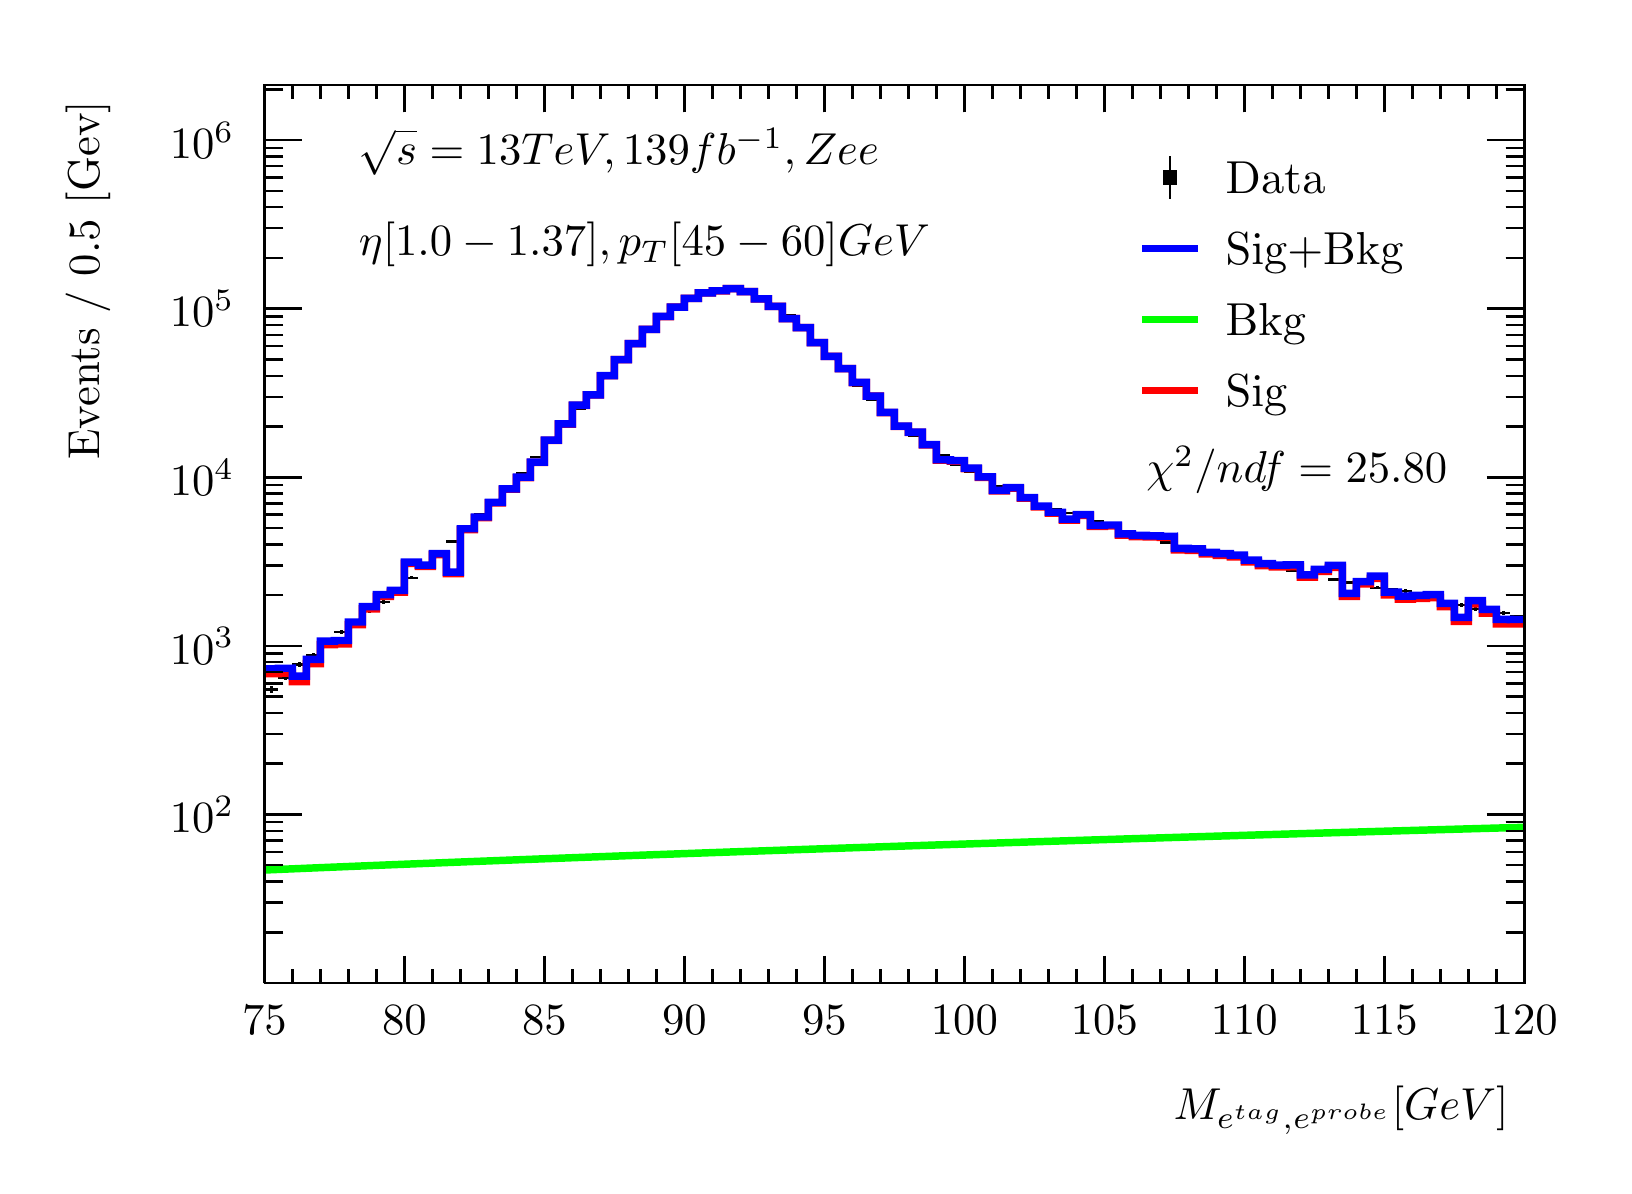
\begin{tikzpicture}
\pgfdeclareplotmark{cross} {
\pgfpathmoveto{\pgfpoint{-0.3\pgfplotmarksize}{\pgfplotmarksize}}
\pgfpathlineto{\pgfpoint{+0.3\pgfplotmarksize}{\pgfplotmarksize}}
\pgfpathlineto{\pgfpoint{+0.3\pgfplotmarksize}{0.3\pgfplotmarksize}}
\pgfpathlineto{\pgfpoint{+1\pgfplotmarksize}{0.3\pgfplotmarksize}}
\pgfpathlineto{\pgfpoint{+1\pgfplotmarksize}{-0.3\pgfplotmarksize}}
\pgfpathlineto{\pgfpoint{+0.3\pgfplotmarksize}{-0.3\pgfplotmarksize}}
\pgfpathlineto{\pgfpoint{+0.3\pgfplotmarksize}{-1.\pgfplotmarksize}}
\pgfpathlineto{\pgfpoint{-0.3\pgfplotmarksize}{-1.\pgfplotmarksize}}
\pgfpathlineto{\pgfpoint{-0.3\pgfplotmarksize}{-0.3\pgfplotmarksize}}
\pgfpathlineto{\pgfpoint{-1.\pgfplotmarksize}{-0.3\pgfplotmarksize}}
\pgfpathlineto{\pgfpoint{-1.\pgfplotmarksize}{0.3\pgfplotmarksize}}
\pgfpathlineto{\pgfpoint{-0.3\pgfplotmarksize}{0.3\pgfplotmarksize}}
\pgfpathclose
\pgfusepathqstroke
}
\pgfdeclareplotmark{cross*} {
\pgfpathmoveto{\pgfpoint{-0.3\pgfplotmarksize}{\pgfplotmarksize}}
\pgfpathlineto{\pgfpoint{+0.3\pgfplotmarksize}{\pgfplotmarksize}}
\pgfpathlineto{\pgfpoint{+0.3\pgfplotmarksize}{0.3\pgfplotmarksize}}
\pgfpathlineto{\pgfpoint{+1\pgfplotmarksize}{0.3\pgfplotmarksize}}
\pgfpathlineto{\pgfpoint{+1\pgfplotmarksize}{-0.3\pgfplotmarksize}}
\pgfpathlineto{\pgfpoint{+0.3\pgfplotmarksize}{-0.3\pgfplotmarksize}}
\pgfpathlineto{\pgfpoint{+0.3\pgfplotmarksize}{-1.\pgfplotmarksize}}
\pgfpathlineto{\pgfpoint{-0.3\pgfplotmarksize}{-1.\pgfplotmarksize}}
\pgfpathlineto{\pgfpoint{-0.3\pgfplotmarksize}{-0.3\pgfplotmarksize}}
\pgfpathlineto{\pgfpoint{-1.\pgfplotmarksize}{-0.3\pgfplotmarksize}}
\pgfpathlineto{\pgfpoint{-1.\pgfplotmarksize}{0.3\pgfplotmarksize}}
\pgfpathlineto{\pgfpoint{-0.3\pgfplotmarksize}{0.3\pgfplotmarksize}}
\pgfpathclose
\pgfusepathqfillstroke
}
\pgfdeclareplotmark{newstar} {
\pgfpathmoveto{\pgfqpoint{0pt}{\pgfplotmarksize}}
\pgfpathlineto{\pgfqpointpolar{44}{0.5\pgfplotmarksize}}
\pgfpathlineto{\pgfqpointpolar{18}{\pgfplotmarksize}}
\pgfpathlineto{\pgfqpointpolar{-20}{0.5\pgfplotmarksize}}
\pgfpathlineto{\pgfqpointpolar{-54}{\pgfplotmarksize}}
\pgfpathlineto{\pgfqpointpolar{-90}{0.5\pgfplotmarksize}}
\pgfpathlineto{\pgfqpointpolar{234}{\pgfplotmarksize}}
\pgfpathlineto{\pgfqpointpolar{198}{0.5\pgfplotmarksize}}
\pgfpathlineto{\pgfqpointpolar{162}{\pgfplotmarksize}}
\pgfpathlineto{\pgfqpointpolar{134}{0.5\pgfplotmarksize}}
\pgfpathclose
\pgfusepathqstroke
}
\pgfdeclareplotmark{newstar*} {
\pgfpathmoveto{\pgfqpoint{0pt}{\pgfplotmarksize}}
\pgfpathlineto{\pgfqpointpolar{44}{0.5\pgfplotmarksize}}
\pgfpathlineto{\pgfqpointpolar{18}{\pgfplotmarksize}}
\pgfpathlineto{\pgfqpointpolar{-20}{0.5\pgfplotmarksize}}
\pgfpathlineto{\pgfqpointpolar{-54}{\pgfplotmarksize}}
\pgfpathlineto{\pgfqpointpolar{-90}{0.5\pgfplotmarksize}}
\pgfpathlineto{\pgfqpointpolar{234}{\pgfplotmarksize}}
\pgfpathlineto{\pgfqpointpolar{198}{0.5\pgfplotmarksize}}
\pgfpathlineto{\pgfqpointpolar{162}{\pgfplotmarksize}}
\pgfpathlineto{\pgfqpointpolar{134}{0.5\pgfplotmarksize}}
\pgfpathclose
\pgfusepathqfillstroke
}
\definecolor{c}{rgb}{1,1,1};
\draw [color=c, fill=c] (0,0) rectangle (20,14.4361);
\draw [color=c, fill=c] (3,2.30977) rectangle (19,13.7143);
\definecolor{c}{rgb}{0,0,0};
\draw [c,line width=0.9] (3,2.30977) -- (3,13.7143) -- (19,13.7143) -- (19,2.30977) -- (3,2.30977);
\definecolor{c}{rgb}{1,1,1};
\draw [color=c, fill=c] (3,2.30977) rectangle (19,13.7143);
\definecolor{c}{rgb}{0,0,0};
\draw [c,line width=0.9] (3,2.30977) -- (3,13.7143) -- (19,13.7143) -- (19,2.30977) -- (3,2.30977);
\draw [c,line width=0.9] (3,2.30977) -- (19,2.30977);
\draw [c,line width=0.9] (3,2.65624) -- (3,2.30977);
\draw [c,line width=0.9] (3.35556,2.48301) -- (3.35556,2.30977);
\draw [c,line width=0.9] (3.71111,2.48301) -- (3.71111,2.30977);
\draw [c,line width=0.9] (4.06667,2.48301) -- (4.06667,2.30977);
\draw [c,line width=0.9] (4.42222,2.48301) -- (4.42222,2.30977);
\draw [c,line width=0.9] (4.77778,2.65624) -- (4.77778,2.30977);
\draw [c,line width=0.9] (5.13333,2.48301) -- (5.13333,2.30977);
\draw [c,line width=0.9] (5.48889,2.48301) -- (5.48889,2.30977);
\draw [c,line width=0.9] (5.84444,2.48301) -- (5.84444,2.30977);
\draw [c,line width=0.9] (6.2,2.48301) -- (6.2,2.30977);
\draw [c,line width=0.9] (6.55556,2.65624) -- (6.55556,2.30977);
\draw [c,line width=0.9] (6.91111,2.48301) -- (6.91111,2.30977);
\draw [c,line width=0.9] (7.26667,2.48301) -- (7.26667,2.30977);
\draw [c,line width=0.9] (7.62222,2.48301) -- (7.62222,2.30977);
\draw [c,line width=0.9] (7.97778,2.48301) -- (7.97778,2.30977);
\draw [c,line width=0.9] (8.33333,2.65624) -- (8.33333,2.30977);
\draw [c,line width=0.9] (8.68889,2.48301) -- (8.68889,2.30977);
\draw [c,line width=0.9] (9.04444,2.48301) -- (9.04444,2.30977);
\draw [c,line width=0.9] (9.4,2.48301) -- (9.4,2.30977);
\draw [c,line width=0.9] (9.75556,2.48301) -- (9.75556,2.30977);
\draw [c,line width=0.9] (10.1111,2.65624) -- (10.1111,2.30977);
\draw [c,line width=0.9] (10.4667,2.48301) -- (10.4667,2.30977);
\draw [c,line width=0.9] (10.8222,2.48301) -- (10.8222,2.30977);
\draw [c,line width=0.9] (11.1778,2.48301) -- (11.1778,2.30977);
\draw [c,line width=0.9] (11.5333,2.48301) -- (11.5333,2.30977);
\draw [c,line width=0.9] (11.8889,2.65624) -- (11.8889,2.30977);
\draw [c,line width=0.9] (12.2444,2.48301) -- (12.2444,2.30977);
\draw [c,line width=0.9] (12.6,2.48301) -- (12.6,2.30977);
\draw [c,line width=0.9] (12.9556,2.48301) -- (12.9556,2.30977);
\draw [c,line width=0.9] (13.3111,2.48301) -- (13.3111,2.30977);
\draw [c,line width=0.9] (13.6667,2.65624) -- (13.6667,2.30977);
\draw [c,line width=0.9] (14.0222,2.48301) -- (14.0222,2.30977);
\draw [c,line width=0.9] (14.3778,2.48301) -- (14.3778,2.30977);
\draw [c,line width=0.9] (14.7333,2.48301) -- (14.7333,2.30977);
\draw [c,line width=0.9] (15.0889,2.48301) -- (15.0889,2.30977);
\draw [c,line width=0.9] (15.4444,2.65624) -- (15.4444,2.30977);
\draw [c,line width=0.9] (15.8,2.48301) -- (15.8,2.30977);
\draw [c,line width=0.9] (16.1556,2.48301) -- (16.1556,2.30977);
\draw [c,line width=0.9] (16.5111,2.48301) -- (16.5111,2.30977);
\draw [c,line width=0.9] (16.8667,2.48301) -- (16.8667,2.30977);
\draw [c,line width=0.9] (17.2222,2.65624) -- (17.2222,2.30977);
\draw [c,line width=0.9] (17.5778,2.48301) -- (17.5778,2.30977);
\draw [c,line width=0.9] (17.9333,2.48301) -- (17.9333,2.30977);
\draw [c,line width=0.9] (18.2889,2.48301) -- (18.2889,2.30977);
\draw [c,line width=0.9] (18.6444,2.48301) -- (18.6444,2.30977);
\draw [c,line width=0.9] (19,2.65624) -- (19,2.30977);
\draw [c,line width=0.9] (19,2.65624) -- (19,2.30977);
\draw [anchor=base] (3,1.66015) node[scale=1.61424, color=c, rotate=0]{75};
\draw [anchor=base] (4.77778,1.66015) node[scale=1.61424, color=c, rotate=0]{80};
\draw [anchor=base] (6.55556,1.66015) node[scale=1.61424, color=c, rotate=0]{85};
\draw [anchor=base] (8.33333,1.66015) node[scale=1.61424, color=c, rotate=0]{90};
\draw [anchor=base] (10.1111,1.66015) node[scale=1.61424, color=c, rotate=0]{95};
\draw [anchor=base] (11.8889,1.66015) node[scale=1.61424, color=c, rotate=0]{100};
\draw [anchor=base] (13.6667,1.66015) node[scale=1.61424, color=c, rotate=0]{105};
\draw [anchor=base] (15.4444,1.66015) node[scale=1.61424, color=c, rotate=0]{110};
\draw [anchor=base] (17.2222,1.66015) node[scale=1.61424, color=c, rotate=0]{115};
\draw [anchor=base] (19,1.66015) node[scale=1.61424, color=c, rotate=0]{120};
\draw [anchor= east] (19,0.692932) node[scale=1.61424, color=c, rotate=0]{$M_{e^{tag}, e^{probe}}  [GeV]$};
\draw [c,line width=0.9] (3,13.7143) -- (19,13.7143);
\draw [c,line width=0.9] (3,13.3678) -- (3,13.7143);
\draw [c,line width=0.9] (3.35556,13.5411) -- (3.35556,13.7143);
\draw [c,line width=0.9] (3.71111,13.5411) -- (3.71111,13.7143);
\draw [c,line width=0.9] (4.06667,13.5411) -- (4.06667,13.7143);
\draw [c,line width=0.9] (4.42222,13.5411) -- (4.42222,13.7143);
\draw [c,line width=0.9] (4.77778,13.3678) -- (4.77778,13.7143);
\draw [c,line width=0.9] (5.13333,13.5411) -- (5.13333,13.7143);
\draw [c,line width=0.9] (5.48889,13.5411) -- (5.48889,13.7143);
\draw [c,line width=0.9] (5.84444,13.5411) -- (5.84444,13.7143);
\draw [c,line width=0.9] (6.2,13.5411) -- (6.2,13.7143);
\draw [c,line width=0.9] (6.55556,13.3678) -- (6.55556,13.7143);
\draw [c,line width=0.9] (6.91111,13.5411) -- (6.91111,13.7143);
\draw [c,line width=0.9] (7.26667,13.5411) -- (7.26667,13.7143);
\draw [c,line width=0.9] (7.62222,13.5411) -- (7.62222,13.7143);
\draw [c,line width=0.9] (7.97778,13.5411) -- (7.97778,13.7143);
\draw [c,line width=0.9] (8.33333,13.3678) -- (8.33333,13.7143);
\draw [c,line width=0.9] (8.68889,13.5411) -- (8.68889,13.7143);
\draw [c,line width=0.9] (9.04444,13.5411) -- (9.04444,13.7143);
\draw [c,line width=0.9] (9.4,13.5411) -- (9.4,13.7143);
\draw [c,line width=0.9] (9.75556,13.5411) -- (9.75556,13.7143);
\draw [c,line width=0.9] (10.1111,13.3678) -- (10.1111,13.7143);
\draw [c,line width=0.9] (10.4667,13.5411) -- (10.4667,13.7143);
\draw [c,line width=0.9] (10.8222,13.5411) -- (10.8222,13.7143);
\draw [c,line width=0.9] (11.1778,13.5411) -- (11.1778,13.7143);
\draw [c,line width=0.9] (11.5333,13.5411) -- (11.5333,13.7143);
\draw [c,line width=0.9] (11.8889,13.3678) -- (11.8889,13.7143);
\draw [c,line width=0.9] (12.2444,13.5411) -- (12.2444,13.7143);
\draw [c,line width=0.9] (12.6,13.5411) -- (12.6,13.7143);
\draw [c,line width=0.9] (12.9556,13.5411) -- (12.9556,13.7143);
\draw [c,line width=0.9] (13.3111,13.5411) -- (13.3111,13.7143);
\draw [c,line width=0.9] (13.6667,13.3678) -- (13.6667,13.7143);
\draw [c,line width=0.9] (14.0222,13.5411) -- (14.0222,13.7143);
\draw [c,line width=0.9] (14.3778,13.5411) -- (14.3778,13.7143);
\draw [c,line width=0.9] (14.7333,13.5411) -- (14.7333,13.7143);
\draw [c,line width=0.9] (15.0889,13.5411) -- (15.0889,13.7143);
\draw [c,line width=0.9] (15.4444,13.3678) -- (15.4444,13.7143);
\draw [c,line width=0.9] (15.8,13.5411) -- (15.8,13.7143);
\draw [c,line width=0.9] (16.1556,13.5411) -- (16.1556,13.7143);
\draw [c,line width=0.9] (16.5111,13.5411) -- (16.5111,13.7143);
\draw [c,line width=0.9] (16.8667,13.5411) -- (16.8667,13.7143);
\draw [c,line width=0.9] (17.2222,13.3678) -- (17.2222,13.7143);
\draw [c,line width=0.9] (17.5778,13.5411) -- (17.5778,13.7143);
\draw [c,line width=0.9] (17.9333,13.5411) -- (17.9333,13.7143);
\draw [c,line width=0.9] (18.2889,13.5411) -- (18.2889,13.7143);
\draw [c,line width=0.9] (18.6444,13.5411) -- (18.6444,13.7143);
\draw [c,line width=0.9] (19,13.3678) -- (19,13.7143);
\draw [c,line width=0.9] (19,13.3678) -- (19,13.7143);
\draw [c,line width=0.9] (3,2.30977) -- (3,13.7143);
\draw [c,line width=0.9] (3.237,2.95433) -- (3,2.95433);
\draw [c,line width=0.9] (3.237,3.33137) -- (3,3.33137);
\draw [c,line width=0.9] (3.237,3.59888) -- (3,3.59888);
\draw [c,line width=0.9] (3.237,3.80638) -- (3,3.80638);
\draw [c,line width=0.9] (3.237,3.97592) -- (3,3.97592);
\draw [c,line width=0.9] (3.237,4.11926) -- (3,4.11926);
\draw [c,line width=0.9] (3.237,4.24343) -- (3,4.24343);
\draw [c,line width=0.9] (3.237,4.35296) -- (3,4.35296);
\draw [c,line width=0.9] (3.474,4.45093) -- (3,4.45093);
\draw [anchor= east] (2.82,4.45093) node[scale=1.61424, color=c, rotate=0]{$10^{2}$};
\draw [c,line width=0.9] (3.237,5.09549) -- (3,5.09549);
\draw [c,line width=0.9] (3.237,5.47253) -- (3,5.47253);
\draw [c,line width=0.9] (3.237,5.74004) -- (3,5.74004);
\draw [c,line width=0.9] (3.237,5.94754) -- (3,5.94754);
\draw [c,line width=0.9] (3.237,6.11708) -- (3,6.11708);
\draw [c,line width=0.9] (3.237,6.26042) -- (3,6.26042);
\draw [c,line width=0.9] (3.237,6.38459) -- (3,6.38459);
\draw [c,line width=0.9] (3.237,6.49412) -- (3,6.49412);
\draw [c,line width=0.9] (3.474,6.59209) -- (3,6.59209);
\draw [anchor= east] (2.82,6.59209) node[scale=1.61424, color=c, rotate=0]{$10^{3}$};
\draw [c,line width=0.9] (3.237,7.23665) -- (3,7.23665);
\draw [c,line width=0.9] (3.237,7.61369) -- (3,7.61369);
\draw [c,line width=0.9] (3.237,7.8812) -- (3,7.8812);
\draw [c,line width=0.9] (3.237,8.0887) -- (3,8.0887);
\draw [c,line width=0.9] (3.237,8.25824) -- (3,8.25824);
\draw [c,line width=0.9] (3.237,8.40158) -- (3,8.40158);
\draw [c,line width=0.9] (3.237,8.52575) -- (3,8.52575);
\draw [c,line width=0.9] (3.237,8.63528) -- (3,8.63528);
\draw [c,line width=0.9] (3.474,8.73325) -- (3,8.73325);
\draw [anchor= east] (2.82,8.73325) node[scale=1.61424, color=c, rotate=0]{$10^{4}$};
\draw [c,line width=0.9] (3.237,9.37781) -- (3,9.37781);
\draw [c,line width=0.9] (3.237,9.75485) -- (3,9.75485);
\draw [c,line width=0.9] (3.237,10.0224) -- (3,10.0224);
\draw [c,line width=0.9] (3.237,10.2299) -- (3,10.2299);
\draw [c,line width=0.9] (3.237,10.3994) -- (3,10.3994);
\draw [c,line width=0.9] (3.237,10.5427) -- (3,10.5427);
\draw [c,line width=0.9] (3.237,10.6669) -- (3,10.6669);
\draw [c,line width=0.9] (3.237,10.7764) -- (3,10.7764);
\draw [c,line width=0.9] (3.474,10.8744) -- (3,10.8744);
\draw [anchor= east] (2.82,10.8744) node[scale=1.61424, color=c, rotate=0]{$10^{5}$};
\draw [c,line width=0.9] (3.237,11.519) -- (3,11.519);
\draw [c,line width=0.9] (3.237,11.896) -- (3,11.896);
\draw [c,line width=0.9] (3.237,12.1635) -- (3,12.1635);
\draw [c,line width=0.9] (3.237,12.371) -- (3,12.371);
\draw [c,line width=0.9] (3.237,12.5406) -- (3,12.5406);
\draw [c,line width=0.9] (3.237,12.6839) -- (3,12.6839);
\draw [c,line width=0.9] (3.237,12.8081) -- (3,12.8081);
\draw [c,line width=0.9] (3.237,12.9176) -- (3,12.9176);
\draw [c,line width=0.9] (3.474,13.0156) -- (3,13.0156);
\draw [anchor= east] (2.82,13.0156) node[scale=1.61424, color=c, rotate=0]{$10^{6}$};
\draw [c,line width=0.9] (3.237,13.6601) -- (3,13.6601);
\draw [anchor= east] (0.76,13.7143) node[scale=1.61424, color=c, rotate=90]{Events / 0.5 [Gev]};
\draw [c,line width=0.9] (19,2.30977) -- (19,13.7143);
\draw [c,line width=0.9] (18.763,2.95433) -- (19,2.95433);
\draw [c,line width=0.9] (18.763,3.33137) -- (19,3.33137);
\draw [c,line width=0.9] (18.763,3.59888) -- (19,3.59888);
\draw [c,line width=0.9] (18.763,3.80638) -- (19,3.80638);
\draw [c,line width=0.9] (18.763,3.97592) -- (19,3.97592);
\draw [c,line width=0.9] (18.763,4.11926) -- (19,4.11926);
\draw [c,line width=0.9] (18.763,4.24343) -- (19,4.24343);
\draw [c,line width=0.9] (18.763,4.35296) -- (19,4.35296);
\draw [c,line width=0.9] (18.526,4.45093) -- (19,4.45093);
\draw [c,line width=0.9] (18.763,5.09549) -- (19,5.09549);
\draw [c,line width=0.9] (18.763,5.47253) -- (19,5.47253);
\draw [c,line width=0.9] (18.763,5.74004) -- (19,5.74004);
\draw [c,line width=0.9] (18.763,5.94754) -- (19,5.94754);
\draw [c,line width=0.9] (18.763,6.11708) -- (19,6.11708);
\draw [c,line width=0.9] (18.763,6.26042) -- (19,6.26042);
\draw [c,line width=0.9] (18.763,6.38459) -- (19,6.38459);
\draw [c,line width=0.9] (18.763,6.49412) -- (19,6.49412);
\draw [c,line width=0.9] (18.526,6.59209) -- (19,6.59209);
\draw [c,line width=0.9] (18.763,7.23665) -- (19,7.23665);
\draw [c,line width=0.9] (18.763,7.61369) -- (19,7.61369);
\draw [c,line width=0.9] (18.763,7.8812) -- (19,7.8812);
\draw [c,line width=0.9] (18.763,8.0887) -- (19,8.0887);
\draw [c,line width=0.9] (18.763,8.25824) -- (19,8.25824);
\draw [c,line width=0.9] (18.763,8.40158) -- (19,8.40158);
\draw [c,line width=0.9] (18.763,8.52575) -- (19,8.52575);
\draw [c,line width=0.9] (18.763,8.63528) -- (19,8.63528);
\draw [c,line width=0.9] (18.526,8.73325) -- (19,8.73325);
\draw [c,line width=0.9] (18.763,9.37781) -- (19,9.37781);
\draw [c,line width=0.9] (18.763,9.75485) -- (19,9.75485);
\draw [c,line width=0.9] (18.763,10.0224) -- (19,10.0224);
\draw [c,line width=0.9] (18.763,10.2299) -- (19,10.2299);
\draw [c,line width=0.9] (18.763,10.3994) -- (19,10.3994);
\draw [c,line width=0.9] (18.763,10.5427) -- (19,10.5427);
\draw [c,line width=0.9] (18.763,10.6669) -- (19,10.6669);
\draw [c,line width=0.9] (18.763,10.7764) -- (19,10.7764);
\draw [c,line width=0.9] (18.526,10.8744) -- (19,10.8744);
\draw [c,line width=0.9] (18.763,11.519) -- (19,11.519);
\draw [c,line width=0.9] (18.763,11.896) -- (19,11.896);
\draw [c,line width=0.9] (18.763,12.1635) -- (19,12.1635);
\draw [c,line width=0.9] (18.763,12.371) -- (19,12.371);
\draw [c,line width=0.9] (18.763,12.5406) -- (19,12.5406);
\draw [c,line width=0.9] (18.763,12.6839) -- (19,12.6839);
\draw [c,line width=0.9] (18.763,12.8081) -- (19,12.8081);
\draw [c,line width=0.9] (18.763,12.9176) -- (19,12.9176);
\draw [c,line width=0.9] (18.526,13.0156) -- (19,13.0156);
\draw [c,line width=0.9] (18.763,13.6601) -- (19,13.6601);
\draw [c,line width=0.9] (3.08889,6.03786) -- (3,6.03786);
\draw [c,line width=0.9] (3,6.03786) -- (3,6.03786);
\draw [c,line width=0.9] (3.08889,6.03786) -- (3.17778,6.03786);
\draw [c,line width=0.9] (3.17778,6.03786) -- (3.17778,6.03786);
\draw [c,line width=0.9] (3.08889,6.03786) -- (3.08889,6.07747);
\draw [c,line width=0.9] (3.08889,6.07747) -- (3.08889,6.07747);
\draw [c,line width=0.9] (3.08889,6.03786) -- (3.08889,5.99825);
\draw [c,line width=0.9] (3.08889,5.99825) -- (3.08889,5.99825);
\draw [c,line width=0.9] (3.26667,6.19151) -- (3.17778,6.19151);
\draw [c,line width=0.9] (3.17778,6.19151) -- (3.17778,6.19151);
\draw [c,line width=0.9] (3.26667,6.19151) -- (3.35556,6.19151);
\draw [c,line width=0.9] (3.35556,6.19151) -- (3.35556,6.19151);
\draw [c,line width=0.9] (3.26667,6.19151) -- (3.26667,6.22798);
\draw [c,line width=0.9] (3.26667,6.22798) -- (3.26667,6.22798);
\draw [c,line width=0.9] (3.26667,6.19151) -- (3.26667,6.15504);
\draw [c,line width=0.9] (3.26667,6.15504) -- (3.26667,6.15504);
\draw [c,line width=0.9] (3.44444,6.35267) -- (3.35556,6.35267);
\draw [c,line width=0.9] (3.35556,6.35267) -- (3.35556,6.35267);
\draw [c,line width=0.9] (3.44444,6.35267) -- (3.53333,6.35267);
\draw [c,line width=0.9] (3.53333,6.35267) -- (3.53333,6.35267);
\draw [c,line width=0.9] (3.44444,6.35267) -- (3.44444,6.38611);
\draw [c,line width=0.9] (3.44444,6.38611) -- (3.44444,6.38611);
\draw [c,line width=0.9] (3.44444,6.35267) -- (3.44444,6.31922);
\draw [c,line width=0.9] (3.44444,6.31922) -- (3.44444,6.31922);
\draw [c,line width=0.9] (3.62222,6.47216) -- (3.53333,6.47216);
\draw [c,line width=0.9] (3.53333,6.47216) -- (3.53333,6.47216);
\draw [c,line width=0.9] (3.62222,6.47216) -- (3.71111,6.47216);
\draw [c,line width=0.9] (3.71111,6.47216) -- (3.71111,6.47216);
\draw [c,line width=0.9] (3.62222,6.47216) -- (3.62222,6.50353);
\draw [c,line width=0.9] (3.62222,6.50353) -- (3.62222,6.50353);
\draw [c,line width=0.9] (3.62222,6.47216) -- (3.62222,6.4408);
\draw [c,line width=0.9] (3.62222,6.4408) -- (3.62222,6.4408);
\draw [c,line width=0.9] (3.8,6.62408) -- (3.71111,6.62408);
\draw [c,line width=0.9] (3.71111,6.62408) -- (3.71111,6.62408);
\draw [c,line width=0.9] (3.8,6.62408) -- (3.88889,6.62408);
\draw [c,line width=0.9] (3.88889,6.62408) -- (3.88889,6.62408);
\draw [c,line width=0.9] (3.8,6.62408) -- (3.8,6.65299);
\draw [c,line width=0.9] (3.8,6.65299) -- (3.8,6.65299);
\draw [c,line width=0.9] (3.8,6.62408) -- (3.8,6.59518);
\draw [c,line width=0.9] (3.8,6.59518) -- (3.8,6.59518);
\draw [c,line width=0.9] (3.97778,6.76704) -- (3.88889,6.76704);
\draw [c,line width=0.9] (3.88889,6.76704) -- (3.88889,6.76704);
\draw [c,line width=0.9] (3.97778,6.76704) -- (4.06667,6.76704);
\draw [c,line width=0.9] (4.06667,6.76704) -- (4.06667,6.76704);
\draw [c,line width=0.9] (3.97778,6.76704) -- (3.97778,6.79381);
\draw [c,line width=0.9] (3.97778,6.79381) -- (3.97778,6.79381);
\draw [c,line width=0.9] (3.97778,6.76704) -- (3.97778,6.74028);
\draw [c,line width=0.9] (3.97778,6.74028) -- (3.97778,6.74028);
\draw [c,line width=0.9] (4.15556,6.86286) -- (4.06667,6.86286);
\draw [c,line width=0.9] (4.06667,6.86286) -- (4.06667,6.86286);
\draw [c,line width=0.9] (4.15556,6.86286) -- (4.24444,6.86286);
\draw [c,line width=0.9] (4.24444,6.86286) -- (4.24444,6.86286);
\draw [c,line width=0.9] (4.15556,6.86286) -- (4.15556,6.88828);
\draw [c,line width=0.9] (4.15556,6.88828) -- (4.15556,6.88828);
\draw [c,line width=0.9] (4.15556,6.86286) -- (4.15556,6.83744);
\draw [c,line width=0.9] (4.15556,6.83744) -- (4.15556,6.83744);
\draw [c,line width=0.9] (4.33333,7.03552) -- (4.24444,7.03552);
\draw [c,line width=0.9] (4.24444,7.03552) -- (4.24444,7.03552);
\draw [c,line width=0.9] (4.33333,7.03552) -- (4.42222,7.03552);
\draw [c,line width=0.9] (4.42222,7.03552) -- (4.42222,7.03552);
\draw [c,line width=0.9] (4.33333,7.03552) -- (4.33333,7.05869);
\draw [c,line width=0.9] (4.33333,7.05869) -- (4.33333,7.05869);
\draw [c,line width=0.9] (4.33333,7.03552) -- (4.33333,7.01235);
\draw [c,line width=0.9] (4.33333,7.01235) -- (4.33333,7.01235);
\draw [c,line width=0.9] (4.51111,7.15099) -- (4.42222,7.15099);
\draw [c,line width=0.9] (4.42222,7.15099) -- (4.42222,7.15099);
\draw [c,line width=0.9] (4.51111,7.15099) -- (4.6,7.15099);
\draw [c,line width=0.9] (4.6,7.15099) -- (4.6,7.15099);
\draw [c,line width=0.9] (4.51111,7.15099) -- (4.51111,7.17276);
\draw [c,line width=0.9] (4.51111,7.17276) -- (4.51111,7.17276);
\draw [c,line width=0.9] (4.51111,7.15099) -- (4.51111,7.12922);
\draw [c,line width=0.9] (4.51111,7.12922) -- (4.51111,7.12922);
\draw [c,line width=0.9] (4.68889,7.28202) -- (4.6,7.28202);
\draw [c,line width=0.9] (4.6,7.28202) -- (4.6,7.28202);
\draw [c,line width=0.9] (4.68889,7.28202) -- (4.77778,7.28202);
\draw [c,line width=0.9] (4.77778,7.28202) -- (4.77778,7.28202);
\draw [c,line width=0.9] (4.68889,7.28202) -- (4.68889,7.30231);
\draw [c,line width=0.9] (4.68889,7.30231) -- (4.68889,7.30231);
\draw [c,line width=0.9] (4.68889,7.28202) -- (4.68889,7.26172);
\draw [c,line width=0.9] (4.68889,7.26172) -- (4.68889,7.26172);
\draw [c,line width=0.9] (4.86667,7.45524) -- (4.77778,7.45524);
\draw [c,line width=0.9] (4.77778,7.45524) -- (4.77778,7.45524);
\draw [c,line width=0.9] (4.86667,7.45524) -- (4.95556,7.45524);
\draw [c,line width=0.9] (4.95556,7.45524) -- (4.95556,7.45524);
\draw [c,line width=0.9] (4.86667,7.45524) -- (4.86667,7.47373);
\draw [c,line width=0.9] (4.86667,7.47373) -- (4.86667,7.47373);
\draw [c,line width=0.9] (4.86667,7.45524) -- (4.86667,7.43675);
\draw [c,line width=0.9] (4.86667,7.43675) -- (4.86667,7.43675);
\draw [c,line width=0.9] (5.04444,7.60903) -- (4.95556,7.60903);
\draw [c,line width=0.9] (4.95556,7.60903) -- (4.95556,7.60903);
\draw [c,line width=0.9] (5.04444,7.60903) -- (5.13333,7.60903);
\draw [c,line width=0.9] (5.13333,7.60903) -- (5.13333,7.60903);
\draw [c,line width=0.9] (5.04444,7.60903) -- (5.04444,7.62605);
\draw [c,line width=0.9] (5.04444,7.62605) -- (5.04444,7.62605);
\draw [c,line width=0.9] (5.04444,7.60903) -- (5.04444,7.59201);
\draw [c,line width=0.9] (5.04444,7.59201) -- (5.04444,7.59201);
\draw [c,line width=0.9] (5.22222,7.7525) -- (5.13333,7.7525);
\draw [c,line width=0.9] (5.13333,7.7525) -- (5.13333,7.7525);
\draw [c,line width=0.9] (5.22222,7.7525) -- (5.31111,7.7525);
\draw [c,line width=0.9] (5.31111,7.7525) -- (5.31111,7.7525);
\draw [c,line width=0.9] (5.22222,7.7525) -- (5.22222,7.76826);
\draw [c,line width=0.9] (5.22222,7.76826) -- (5.22222,7.76826);
\draw [c,line width=0.9] (5.22222,7.7525) -- (5.22222,7.73675);
\draw [c,line width=0.9] (5.22222,7.73675) -- (5.22222,7.73675);
\draw [c,line width=0.9] (5.4,7.91856) -- (5.31111,7.91856);
\draw [c,line width=0.9] (5.31111,7.91856) -- (5.31111,7.91856);
\draw [c,line width=0.9] (5.4,7.91856) -- (5.48889,7.91856);
\draw [c,line width=0.9] (5.48889,7.91856) -- (5.48889,7.91856);
\draw [c,line width=0.9] (5.4,7.91856) -- (5.4,7.93298);
\draw [c,line width=0.9] (5.4,7.93298) -- (5.4,7.93298);
\draw [c,line width=0.9] (5.4,7.91856) -- (5.4,7.90415);
\draw [c,line width=0.9] (5.4,7.90415) -- (5.4,7.90415);
\draw [c,line width=0.9] (5.57778,8.08067) -- (5.48889,8.08067);
\draw [c,line width=0.9] (5.48889,8.08067) -- (5.48889,8.08067);
\draw [c,line width=0.9] (5.57778,8.08067) -- (5.66667,8.08067);
\draw [c,line width=0.9] (5.66667,8.08067) -- (5.66667,8.08067);
\draw [c,line width=0.9] (5.57778,8.08067) -- (5.57778,8.09388);
\draw [c,line width=0.9] (5.57778,8.09388) -- (5.57778,8.09388);
\draw [c,line width=0.9] (5.57778,8.08067) -- (5.57778,8.06746);
\draw [c,line width=0.9] (5.57778,8.06746) -- (5.57778,8.06746);
\draw [c,line width=0.9] (5.75556,8.26672) -- (5.66667,8.26672);
\draw [c,line width=0.9] (5.66667,8.26672) -- (5.66667,8.26672);
\draw [c,line width=0.9] (5.75556,8.26672) -- (5.84444,8.26672);
\draw [c,line width=0.9] (5.84444,8.26672) -- (5.84444,8.26672);
\draw [c,line width=0.9] (5.75556,8.26672) -- (5.75556,8.27868);
\draw [c,line width=0.9] (5.75556,8.27868) -- (5.75556,8.27868);
\draw [c,line width=0.9] (5.75556,8.26672) -- (5.75556,8.25478);
\draw [c,line width=0.9] (5.75556,8.25478) -- (5.75556,8.25478);
\draw [c,line width=0.9] (5.93333,8.39559) -- (5.84444,8.39559);
\draw [c,line width=0.9] (5.84444,8.39559) -- (5.84444,8.39559);
\draw [c,line width=0.9] (5.93333,8.39559) -- (6.02222,8.39559);
\draw [c,line width=0.9] (6.02222,8.39559) -- (6.02222,8.39559);
\draw [c,line width=0.9] (5.93333,8.39559) -- (5.93333,8.40674);
\draw [c,line width=0.9] (5.93333,8.40674) -- (5.93333,8.40674);
\draw [c,line width=0.9] (5.93333,8.39559) -- (5.93333,8.38444);
\draw [c,line width=0.9] (5.93333,8.38444) -- (5.93333,8.38444);
\draw [c,line width=0.9] (6.11111,8.59958) -- (6.02222,8.59958);
\draw [c,line width=0.9] (6.02222,8.59958) -- (6.02222,8.59958);
\draw [c,line width=0.9] (6.11111,8.59958) -- (6.2,8.59958);
\draw [c,line width=0.9] (6.2,8.59958) -- (6.2,8.59958);
\draw [c,line width=0.9] (6.11111,8.59958) -- (6.11111,8.60957);
\draw [c,line width=0.9] (6.11111,8.60957) -- (6.11111,8.60957);
\draw [c,line width=0.9] (6.11111,8.59958) -- (6.11111,8.58958);
\draw [c,line width=0.9] (6.11111,8.58958) -- (6.11111,8.58958);
\draw [c,line width=0.9] (6.28889,8.78831) -- (6.2,8.78831);
\draw [c,line width=0.9] (6.2,8.78831) -- (6.2,8.78831);
\draw [c,line width=0.9] (6.28889,8.78831) -- (6.37778,8.78831);
\draw [c,line width=0.9] (6.37778,8.78831) -- (6.37778,8.78831);
\draw [c,line width=0.9] (6.28889,8.78831) -- (6.28889,8.79734);
\draw [c,line width=0.9] (6.28889,8.79734) -- (6.28889,8.79734);
\draw [c,line width=0.9] (6.28889,8.78831) -- (6.28889,8.77929);
\draw [c,line width=0.9] (6.28889,8.77929) -- (6.28889,8.77929);
\draw [c,line width=0.9] (6.46667,8.99022) -- (6.37778,8.99022);
\draw [c,line width=0.9] (6.37778,8.99022) -- (6.37778,8.99022);
\draw [c,line width=0.9] (6.46667,8.99022) -- (6.55556,8.99022);
\draw [c,line width=0.9] (6.55556,8.99022) -- (6.55556,8.99022);
\draw [c,line width=0.9] (6.46667,8.99022) -- (6.46667,8.99832);
\draw [c,line width=0.9] (6.46667,8.99832) -- (6.46667,8.99832);
\draw [c,line width=0.9] (6.46667,8.99022) -- (6.46667,8.98212);
\draw [c,line width=0.9] (6.46667,8.98212) -- (6.46667,8.98212);
\draw [c,line width=0.9] (6.64444,9.18804) -- (6.55556,9.18804);
\draw [c,line width=0.9] (6.55556,9.18804) -- (6.55556,9.18804);
\draw [c,line width=0.9] (6.64444,9.18804) -- (6.73333,9.18804);
\draw [c,line width=0.9] (6.73333,9.18804) -- (6.73333,9.18804);
\draw [c,line width=0.9] (6.64444,9.18804) -- (6.64444,9.19532);
\draw [c,line width=0.9] (6.64444,9.19532) -- (6.64444,9.19532);
\draw [c,line width=0.9] (6.64444,9.18804) -- (6.64444,9.18076);
\draw [c,line width=0.9] (6.64444,9.18076) -- (6.64444,9.18076);
\draw [c,line width=0.9] (6.82222,9.38545) -- (6.73333,9.38545);
\draw [c,line width=0.9] (6.73333,9.38545) -- (6.73333,9.38545);
\draw [c,line width=0.9] (6.82222,9.38545) -- (6.91111,9.38545);
\draw [c,line width=0.9] (6.91111,9.38545) -- (6.91111,9.38545);
\draw [c,line width=0.9] (6.82222,9.38545) -- (6.82222,9.392);
\draw [c,line width=0.9] (6.82222,9.392) -- (6.82222,9.392);
\draw [c,line width=0.9] (6.82222,9.38545) -- (6.82222,9.3789);
\draw [c,line width=0.9] (6.82222,9.3789) -- (6.82222,9.3789);
\draw [c,line width=0.9] (7,9.60441) -- (6.91111,9.60441);
\draw [c,line width=0.9] (6.91111,9.60441) -- (6.91111,9.60441);
\draw [c,line width=0.9] (7,9.60441) -- (7.08889,9.60441);
\draw [c,line width=0.9] (7.08889,9.60441) -- (7.08889,9.60441);
\draw [c,line width=0.9] (7,9.60441) -- (7,9.61023);
\draw [c,line width=0.9] (7,9.61023) -- (7,9.61023);
\draw [c,line width=0.9] (7,9.60441) -- (7,9.59859);
\draw [c,line width=0.9] (7,9.59859) -- (7,9.59859);
\draw [c,line width=0.9] (7.17778,9.81131) -- (7.08889,9.81131);
\draw [c,line width=0.9] (7.08889,9.81131) -- (7.08889,9.81131);
\draw [c,line width=0.9] (7.17778,9.81131) -- (7.26667,9.81131);
\draw [c,line width=0.9] (7.26667,9.81131) -- (7.26667,9.81131);
\draw [c,line width=0.9] (7.17778,9.81131) -- (7.17778,9.81652);
\draw [c,line width=0.9] (7.17778,9.81652) -- (7.17778,9.81652);
\draw [c,line width=0.9] (7.17778,9.81131) -- (7.17778,9.8061);
\draw [c,line width=0.9] (7.17778,9.8061) -- (7.17778,9.8061);
\draw [c,line width=0.9] (7.35556,10.0188) -- (7.26667,10.0188);
\draw [c,line width=0.9] (7.26667,10.0188) -- (7.26667,10.0188);
\draw [c,line width=0.9] (7.35556,10.0188) -- (7.44444,10.0188);
\draw [c,line width=0.9] (7.44444,10.0188) -- (7.44444,10.0188);
\draw [c,line width=0.9] (7.35556,10.0188) -- (7.35556,10.0235);
\draw [c,line width=0.9] (7.35556,10.0235) -- (7.35556,10.0235);
\draw [c,line width=0.9] (7.35556,10.0188) -- (7.35556,10.0141);
\draw [c,line width=0.9] (7.35556,10.0141) -- (7.35556,10.0141);
\draw [c,line width=0.9] (7.53333,10.2222) -- (7.44444,10.2222);
\draw [c,line width=0.9] (7.44444,10.2222) -- (7.44444,10.2222);
\draw [c,line width=0.9] (7.53333,10.2222) -- (7.62222,10.2222);
\draw [c,line width=0.9] (7.62222,10.2222) -- (7.62222,10.2222);
\draw [c,line width=0.9] (7.53333,10.2222) -- (7.53333,10.2263);
\draw [c,line width=0.9] (7.53333,10.2263) -- (7.53333,10.2263);
\draw [c,line width=0.9] (7.53333,10.2222) -- (7.53333,10.218);
\draw [c,line width=0.9] (7.53333,10.218) -- (7.53333,10.218);
\draw [c,line width=0.9] (7.71111,10.4115) -- (7.62222,10.4115);
\draw [c,line width=0.9] (7.62222,10.4115) -- (7.62222,10.4115);
\draw [c,line width=0.9] (7.71111,10.4115) -- (7.8,10.4115);
\draw [c,line width=0.9] (7.8,10.4115) -- (7.8,10.4115);
\draw [c,line width=0.9] (7.71111,10.4115) -- (7.71111,10.4153);
\draw [c,line width=0.9] (7.71111,10.4153) -- (7.71111,10.4153);
\draw [c,line width=0.9] (7.71111,10.4115) -- (7.71111,10.4078);
\draw [c,line width=0.9] (7.71111,10.4078) -- (7.71111,10.4078);
\draw [c,line width=0.9] (7.88889,10.5993) -- (7.8,10.5993);
\draw [c,line width=0.9] (7.8,10.5993) -- (7.8,10.5993);
\draw [c,line width=0.9] (7.88889,10.5993) -- (7.97778,10.5993);
\draw [c,line width=0.9] (7.97778,10.5993) -- (7.97778,10.5993);
\draw [c,line width=0.9] (7.88889,10.5993) -- (7.88889,10.6027);
\draw [c,line width=0.9] (7.88889,10.6027) -- (7.88889,10.6027);
\draw [c,line width=0.9] (7.88889,10.5993) -- (7.88889,10.5958);
\draw [c,line width=0.9] (7.88889,10.5958) -- (7.88889,10.5958);
\draw [c,line width=0.9] (8.06667,10.7597) -- (7.97778,10.7597);
\draw [c,line width=0.9] (7.97778,10.7597) -- (7.97778,10.7597);
\draw [c,line width=0.9] (8.06667,10.7597) -- (8.15556,10.7597);
\draw [c,line width=0.9] (8.15556,10.7597) -- (8.15556,10.7597);
\draw [c,line width=0.9] (8.06667,10.7597) -- (8.06667,10.7629);
\draw [c,line width=0.9] (8.06667,10.7629) -- (8.06667,10.7629);
\draw [c,line width=0.9] (8.06667,10.7597) -- (8.06667,10.7566);
\draw [c,line width=0.9] (8.06667,10.7566) -- (8.06667,10.7566);
\draw [c,line width=0.9] (8.24444,10.8873) -- (8.15556,10.8873);
\draw [c,line width=0.9] (8.15556,10.8873) -- (8.15556,10.8873);
\draw [c,line width=0.9] (8.24444,10.8873) -- (8.33333,10.8873);
\draw [c,line width=0.9] (8.33333,10.8873) -- (8.33333,10.8873);
\draw [c,line width=0.9] (8.24444,10.8873) -- (8.24444,10.8902);
\draw [c,line width=0.9] (8.24444,10.8902) -- (8.24444,10.8902);
\draw [c,line width=0.9] (8.24444,10.8873) -- (8.24444,10.8843);
\draw [c,line width=0.9] (8.24444,10.8843) -- (8.24444,10.8843);
\draw [c,line width=0.9] (8.42222,11.0052) -- (8.33333,11.0052);
\draw [c,line width=0.9] (8.33333,11.0052) -- (8.33333,11.0052);
\draw [c,line width=0.9] (8.42222,11.0052) -- (8.51111,11.0052);
\draw [c,line width=0.9] (8.51111,11.0052) -- (8.51111,11.0052);
\draw [c,line width=0.9] (8.42222,11.0052) -- (8.42222,11.008);
\draw [c,line width=0.9] (8.42222,11.008) -- (8.42222,11.008);
\draw [c,line width=0.9] (8.42222,11.0052) -- (8.42222,11.0025);
\draw [c,line width=0.9] (8.42222,11.0025) -- (8.42222,11.0025);
\draw [c,line width=0.9] (8.6,11.0822) -- (8.51111,11.0822);
\draw [c,line width=0.9] (8.51111,11.0822) -- (8.51111,11.0822);
\draw [c,line width=0.9] (8.6,11.0822) -- (8.68889,11.0822);
\draw [c,line width=0.9] (8.68889,11.0822) -- (8.68889,11.0822);
\draw [c,line width=0.9] (8.6,11.0822) -- (8.6,11.0849);
\draw [c,line width=0.9] (8.6,11.0849) -- (8.6,11.0849);
\draw [c,line width=0.9] (8.6,11.0822) -- (8.6,11.0796);
\draw [c,line width=0.9] (8.6,11.0796) -- (8.6,11.0796);
\draw [c,line width=0.9] (8.77778,11.1221) -- (8.68889,11.1221);
\draw [c,line width=0.9] (8.68889,11.1221) -- (8.68889,11.1221);
\draw [c,line width=0.9] (8.77778,11.1221) -- (8.86667,11.1221);
\draw [c,line width=0.9] (8.86667,11.1221) -- (8.86667,11.1221);
\draw [c,line width=0.9] (8.77778,11.1221) -- (8.77778,11.1247);
\draw [c,line width=0.9] (8.77778,11.1247) -- (8.77778,11.1247);
\draw [c,line width=0.9] (8.77778,11.1221) -- (8.77778,11.1195);
\draw [c,line width=0.9] (8.77778,11.1195) -- (8.77778,11.1195);
\draw [c,line width=0.9] (8.95556,11.1288) -- (8.86667,11.1288);
\draw [c,line width=0.9] (8.86667,11.1288) -- (8.86667,11.1288);
\draw [c,line width=0.9] (8.95556,11.1288) -- (9.04444,11.1288);
\draw [c,line width=0.9] (9.04444,11.1288) -- (9.04444,11.1288);
\draw [c,line width=0.9] (8.95556,11.1288) -- (8.95556,11.1313);
\draw [c,line width=0.9] (8.95556,11.1313) -- (8.95556,11.1313);
\draw [c,line width=0.9] (8.95556,11.1288) -- (8.95556,11.1262);
\draw [c,line width=0.9] (8.95556,11.1262) -- (8.95556,11.1262);
\draw [c,line width=0.9] (9.13333,11.0917) -- (9.04444,11.0917);
\draw [c,line width=0.9] (9.04444,11.0917) -- (9.04444,11.0917);
\draw [c,line width=0.9] (9.13333,11.0917) -- (9.22222,11.0917);
\draw [c,line width=0.9] (9.22222,11.0917) -- (9.22222,11.0917);
\draw [c,line width=0.9] (9.13333,11.0917) -- (9.13333,11.0943);
\draw [c,line width=0.9] (9.13333,11.0943) -- (9.13333,11.0943);
\draw [c,line width=0.9] (9.13333,11.0917) -- (9.13333,11.0891);
\draw [c,line width=0.9] (9.13333,11.0891) -- (9.13333,11.0891);
\draw [c,line width=0.9] (9.31111,11.0159) -- (9.22222,11.0159);
\draw [c,line width=0.9] (9.22222,11.0159) -- (9.22222,11.0159);
\draw [c,line width=0.9] (9.31111,11.0159) -- (9.4,11.0159);
\draw [c,line width=0.9] (9.4,11.0159) -- (9.4,11.0159);
\draw [c,line width=0.9] (9.31111,11.0159) -- (9.31111,11.0186);
\draw [c,line width=0.9] (9.31111,11.0186) -- (9.31111,11.0186);
\draw [c,line width=0.9] (9.31111,11.0159) -- (9.31111,11.0131);
\draw [c,line width=0.9] (9.31111,11.0131) -- (9.31111,11.0131);
\draw [c,line width=0.9] (9.48889,10.9127) -- (9.4,10.9127);
\draw [c,line width=0.9] (9.4,10.9127) -- (9.4,10.9127);
\draw [c,line width=0.9] (9.48889,10.9127) -- (9.57778,10.9127);
\draw [c,line width=0.9] (9.57778,10.9127) -- (9.57778,10.9127);
\draw [c,line width=0.9] (9.48889,10.9127) -- (9.48889,10.9156);
\draw [c,line width=0.9] (9.48889,10.9156) -- (9.48889,10.9156);
\draw [c,line width=0.9] (9.48889,10.9127) -- (9.48889,10.9098);
\draw [c,line width=0.9] (9.48889,10.9098) -- (9.48889,10.9098);
\draw [c,line width=0.9] (9.66667,10.7886) -- (9.57778,10.7886);
\draw [c,line width=0.9] (9.57778,10.7886) -- (9.57778,10.7886);
\draw [c,line width=0.9] (9.66667,10.7886) -- (9.75556,10.7886);
\draw [c,line width=0.9] (9.75556,10.7886) -- (9.75556,10.7886);
\draw [c,line width=0.9] (9.66667,10.7886) -- (9.66667,10.7917);
\draw [c,line width=0.9] (9.66667,10.7917) -- (9.66667,10.7917);
\draw [c,line width=0.9] (9.66667,10.7886) -- (9.66667,10.7855);
\draw [c,line width=0.9] (9.66667,10.7855) -- (9.66667,10.7855);
\draw [c,line width=0.9] (9.84444,10.6195) -- (9.75556,10.6195);
\draw [c,line width=0.9] (9.75556,10.6195) -- (9.75556,10.6195);
\draw [c,line width=0.9] (9.84444,10.6195) -- (9.93333,10.6195);
\draw [c,line width=0.9] (9.93333,10.6195) -- (9.93333,10.6195);
\draw [c,line width=0.9] (9.84444,10.6195) -- (9.84444,10.6229);
\draw [c,line width=0.9] (9.84444,10.6229) -- (9.84444,10.6229);
\draw [c,line width=0.9] (9.84444,10.6195) -- (9.84444,10.6161);
\draw [c,line width=0.9] (9.84444,10.6161) -- (9.84444,10.6161);
\draw [c,line width=0.9] (10.0222,10.4579) -- (9.93333,10.4579);
\draw [c,line width=0.9] (9.93333,10.4579) -- (9.93333,10.4579);
\draw [c,line width=0.9] (10.0222,10.4579) -- (10.1111,10.4579);
\draw [c,line width=0.9] (10.1111,10.4579) -- (10.1111,10.4579);
\draw [c,line width=0.9] (10.0222,10.4579) -- (10.0222,10.4616);
\draw [c,line width=0.9] (10.0222,10.4616) -- (10.0222,10.4616);
\draw [c,line width=0.9] (10.0222,10.4579) -- (10.0222,10.4542);
\draw [c,line width=0.9] (10.0222,10.4542) -- (10.0222,10.4542);
\draw [c,line width=0.9] (10.2,10.2673) -- (10.1111,10.2673);
\draw [c,line width=0.9] (10.1111,10.2673) -- (10.1111,10.2673);
\draw [c,line width=0.9] (10.2,10.2673) -- (10.2889,10.2673);
\draw [c,line width=0.9] (10.2889,10.2673) -- (10.2889,10.2673);
\draw [c,line width=0.9] (10.2,10.2673) -- (10.2,10.2714);
\draw [c,line width=0.9] (10.2,10.2714) -- (10.2,10.2714);
\draw [c,line width=0.9] (10.2,10.2673) -- (10.2,10.2632);
\draw [c,line width=0.9] (10.2,10.2632) -- (10.2,10.2632);
\draw [c,line width=0.9] (10.3778,10.0809) -- (10.2889,10.0809);
\draw [c,line width=0.9] (10.2889,10.0809) -- (10.2889,10.0809);
\draw [c,line width=0.9] (10.3778,10.0809) -- (10.4667,10.0809);
\draw [c,line width=0.9] (10.4667,10.0809) -- (10.4667,10.0809);
\draw [c,line width=0.9] (10.3778,10.0809) -- (10.3778,10.0854);
\draw [c,line width=0.9] (10.3778,10.0854) -- (10.3778,10.0854);
\draw [c,line width=0.9] (10.3778,10.0809) -- (10.3778,10.0764);
\draw [c,line width=0.9] (10.3778,10.0764) -- (10.3778,10.0764);
\draw [c,line width=0.9] (10.5556,9.89297) -- (10.4667,9.89297);
\draw [c,line width=0.9] (10.4667,9.89297) -- (10.4667,9.89297);
\draw [c,line width=0.9] (10.5556,9.89297) -- (10.6444,9.89297);
\draw [c,line width=0.9] (10.6444,9.89297) -- (10.6444,9.89297);
\draw [c,line width=0.9] (10.5556,9.89297) -- (10.5556,9.89795);
\draw [c,line width=0.9] (10.5556,9.89795) -- (10.5556,9.89795);
\draw [c,line width=0.9] (10.5556,9.89297) -- (10.5556,9.88798);
\draw [c,line width=0.9] (10.5556,9.88798) -- (10.5556,9.88798);
\draw [c,line width=0.9] (10.7333,9.72017) -- (10.6444,9.72017);
\draw [c,line width=0.9] (10.6444,9.72017) -- (10.6444,9.72017);
\draw [c,line width=0.9] (10.7333,9.72017) -- (10.8222,9.72017);
\draw [c,line width=0.9] (10.8222,9.72017) -- (10.8222,9.72017);
\draw [c,line width=0.9] (10.7333,9.72017) -- (10.7333,9.72564);
\draw [c,line width=0.9] (10.7333,9.72564) -- (10.7333,9.72564);
\draw [c,line width=0.9] (10.7333,9.72017) -- (10.7333,9.7147);
\draw [c,line width=0.9] (10.7333,9.7147) -- (10.7333,9.7147);
\draw [c,line width=0.9] (10.9111,9.55989) -- (10.8222,9.55989);
\draw [c,line width=0.9] (10.8222,9.55989) -- (10.8222,9.55989);
\draw [c,line width=0.9] (10.9111,9.55989) -- (11,9.55989);
\draw [c,line width=0.9] (11,9.55989) -- (11,9.55989);
\draw [c,line width=0.9] (10.9111,9.55989) -- (10.9111,9.56585);
\draw [c,line width=0.9] (10.9111,9.56585) -- (10.9111,9.56585);
\draw [c,line width=0.9] (10.9111,9.55989) -- (10.9111,9.55393);
\draw [c,line width=0.9] (10.9111,9.55393) -- (10.9111,9.55393);
\draw [c,line width=0.9] (11.0889,9.38784) -- (11,9.38784);
\draw [c,line width=0.9] (11,9.38784) -- (11,9.38784);
\draw [c,line width=0.9] (11.0889,9.38784) -- (11.1778,9.38784);
\draw [c,line width=0.9] (11.1778,9.38784) -- (11.1778,9.38784);
\draw [c,line width=0.9] (11.0889,9.38784) -- (11.0889,9.39438);
\draw [c,line width=0.9] (11.0889,9.39438) -- (11.0889,9.39438);
\draw [c,line width=0.9] (11.0889,9.38784) -- (11.0889,9.3813);
\draw [c,line width=0.9] (11.0889,9.3813) -- (11.0889,9.3813);
\draw [c,line width=0.9] (11.2667,9.26078) -- (11.1778,9.26078);
\draw [c,line width=0.9] (11.1778,9.26078) -- (11.1778,9.26078);
\draw [c,line width=0.9] (11.2667,9.26078) -- (11.3556,9.26078);
\draw [c,line width=0.9] (11.3556,9.26078) -- (11.3556,9.26078);
\draw [c,line width=0.9] (11.2667,9.26078) -- (11.2667,9.26779);
\draw [c,line width=0.9] (11.2667,9.26779) -- (11.2667,9.26779);
\draw [c,line width=0.9] (11.2667,9.26078) -- (11.2667,9.25378);
\draw [c,line width=0.9] (11.2667,9.25378) -- (11.2667,9.25378);
\draw [c,line width=0.9] (11.4444,9.11783) -- (11.3556,9.11783);
\draw [c,line width=0.9] (11.3556,9.11783) -- (11.3556,9.11783);
\draw [c,line width=0.9] (11.4444,9.11783) -- (11.5333,9.11783);
\draw [c,line width=0.9] (11.5333,9.11783) -- (11.5333,9.11783);
\draw [c,line width=0.9] (11.4444,9.11783) -- (11.4444,9.12539);
\draw [c,line width=0.9] (11.4444,9.12539) -- (11.4444,9.12539);
\draw [c,line width=0.9] (11.4444,9.11783) -- (11.4444,9.11026);
\draw [c,line width=0.9] (11.4444,9.11026) -- (11.4444,9.11026);
\draw [c,line width=0.9] (11.6222,9.01665) -- (11.5333,9.01665);
\draw [c,line width=0.9] (11.5333,9.01665) -- (11.5333,9.01665);
\draw [c,line width=0.9] (11.6222,9.01665) -- (11.7111,9.01665);
\draw [c,line width=0.9] (11.7111,9.01665) -- (11.7111,9.01665);
\draw [c,line width=0.9] (11.6222,9.01665) -- (11.6222,9.02463);
\draw [c,line width=0.9] (11.6222,9.02463) -- (11.6222,9.02463);
\draw [c,line width=0.9] (11.6222,9.01665) -- (11.6222,9.00866);
\draw [c,line width=0.9] (11.6222,9.00866) -- (11.6222,9.00866);
\draw [c,line width=0.9] (11.8,8.89047) -- (11.7111,8.89047);
\draw [c,line width=0.9] (11.7111,8.89047) -- (11.7111,8.89047);
\draw [c,line width=0.9] (11.8,8.89047) -- (11.8889,8.89047);
\draw [c,line width=0.9] (11.8889,8.89047) -- (11.8889,8.89047);
\draw [c,line width=0.9] (11.8,8.89047) -- (11.8,8.89901);
\draw [c,line width=0.9] (11.8,8.89901) -- (11.8,8.89901);
\draw [c,line width=0.9] (11.8,8.89047) -- (11.8,8.88192);
\draw [c,line width=0.9] (11.8,8.88192) -- (11.8,8.88192);
\draw [c,line width=0.9] (11.9778,8.80447) -- (11.8889,8.80447);
\draw [c,line width=0.9] (11.8889,8.80447) -- (11.8889,8.80447);
\draw [c,line width=0.9] (11.9778,8.80447) -- (12.0667,8.80447);
\draw [c,line width=0.9] (12.0667,8.80447) -- (12.0667,8.80447);
\draw [c,line width=0.9] (11.9778,8.80447) -- (11.9778,8.81342);
\draw [c,line width=0.9] (11.9778,8.81342) -- (11.9778,8.81342);
\draw [c,line width=0.9] (11.9778,8.80447) -- (11.9778,8.79552);
\draw [c,line width=0.9] (11.9778,8.79552) -- (11.9778,8.79552);
\draw [c,line width=0.9] (12.1556,8.71323) -- (12.0667,8.71323);
\draw [c,line width=0.9] (12.0667,8.71323) -- (12.0667,8.71323);
\draw [c,line width=0.9] (12.1556,8.71323) -- (12.2444,8.71323);
\draw [c,line width=0.9] (12.2444,8.71323) -- (12.2444,8.71323);
\draw [c,line width=0.9] (12.1556,8.71323) -- (12.1556,8.72263);
\draw [c,line width=0.9] (12.1556,8.72263) -- (12.1556,8.72263);
\draw [c,line width=0.9] (12.1556,8.71323) -- (12.1556,8.70383);
\draw [c,line width=0.9] (12.1556,8.70383) -- (12.1556,8.70383);
\draw [c,line width=0.9] (12.3333,8.61575) -- (12.2444,8.61575);
\draw [c,line width=0.9] (12.2444,8.61575) -- (12.2444,8.61575);
\draw [c,line width=0.9] (12.3333,8.61575) -- (12.4222,8.61575);
\draw [c,line width=0.9] (12.4222,8.61575) -- (12.4222,8.61575);
\draw [c,line width=0.9] (12.3333,8.61575) -- (12.3333,8.62566);
\draw [c,line width=0.9] (12.3333,8.62566) -- (12.3333,8.62566);
\draw [c,line width=0.9] (12.3333,8.61575) -- (12.3333,8.60585);
\draw [c,line width=0.9] (12.3333,8.60585) -- (12.3333,8.60585);
\draw [c,line width=0.9] (12.5111,8.56557) -- (12.4222,8.56557);
\draw [c,line width=0.9] (12.4222,8.56557) -- (12.4222,8.56557);
\draw [c,line width=0.9] (12.5111,8.56557) -- (12.6,8.56557);
\draw [c,line width=0.9] (12.6,8.56557) -- (12.6,8.56557);
\draw [c,line width=0.9] (12.5111,8.56557) -- (12.5111,8.57575);
\draw [c,line width=0.9] (12.5111,8.57575) -- (12.5111,8.57575);
\draw [c,line width=0.9] (12.5111,8.56557) -- (12.5111,8.5554);
\draw [c,line width=0.9] (12.5111,8.5554) -- (12.5111,8.5554);
\draw [c,line width=0.9] (12.6889,8.46301) -- (12.6,8.46301);
\draw [c,line width=0.9] (12.6,8.46301) -- (12.6,8.46301);
\draw [c,line width=0.9] (12.6889,8.46301) -- (12.7778,8.46301);
\draw [c,line width=0.9] (12.7778,8.46301) -- (12.7778,8.46301);
\draw [c,line width=0.9] (12.6889,8.46301) -- (12.6889,8.47376);
\draw [c,line width=0.9] (12.6889,8.47376) -- (12.6889,8.47376);
\draw [c,line width=0.9] (12.6889,8.46301) -- (12.6889,8.45225);
\draw [c,line width=0.9] (12.6889,8.45225) -- (12.6889,8.45225);
\draw [c,line width=0.9] (12.8667,8.38766) -- (12.7778,8.38766);
\draw [c,line width=0.9] (12.7778,8.38766) -- (12.7778,8.38766);
\draw [c,line width=0.9] (12.8667,8.38766) -- (12.9556,8.38766);
\draw [c,line width=0.9] (12.9556,8.38766) -- (12.9556,8.38766);
\draw [c,line width=0.9] (12.8667,8.38766) -- (12.8667,8.39886);
\draw [c,line width=0.9] (12.8667,8.39886) -- (12.8667,8.39886);
\draw [c,line width=0.9] (12.8667,8.38766) -- (12.8667,8.37647);
\draw [c,line width=0.9] (12.8667,8.37647) -- (12.8667,8.37647);
\draw [c,line width=0.9] (13.0444,8.32087) -- (12.9556,8.32087);
\draw [c,line width=0.9] (12.9556,8.32087) -- (12.9556,8.32087);
\draw [c,line width=0.9] (13.0444,8.32087) -- (13.1333,8.32087);
\draw [c,line width=0.9] (13.1333,8.32087) -- (13.1333,8.32087);
\draw [c,line width=0.9] (13.0444,8.32087) -- (13.0444,8.33247);
\draw [c,line width=0.9] (13.0444,8.33247) -- (13.0444,8.33247);
\draw [c,line width=0.9] (13.0444,8.32087) -- (13.0444,8.30926);
\draw [c,line width=0.9] (13.0444,8.30926) -- (13.0444,8.30926);
\draw [c,line width=0.9] (13.2222,8.2762) -- (13.1333,8.2762);
\draw [c,line width=0.9] (13.1333,8.2762) -- (13.1333,8.2762);
\draw [c,line width=0.9] (13.2222,8.2762) -- (13.3111,8.2762);
\draw [c,line width=0.9] (13.3111,8.2762) -- (13.3111,8.2762);
\draw [c,line width=0.9] (13.2222,8.2762) -- (13.2222,8.28809);
\draw [c,line width=0.9] (13.2222,8.28809) -- (13.2222,8.28809);
\draw [c,line width=0.9] (13.2222,8.2762) -- (13.2222,8.26431);
\draw [c,line width=0.9] (13.2222,8.26431) -- (13.2222,8.26431);
\draw [c,line width=0.9] (13.4,8.2198) -- (13.3111,8.2198);
\draw [c,line width=0.9] (13.3111,8.2198) -- (13.3111,8.2198);
\draw [c,line width=0.9] (13.4,8.2198) -- (13.4889,8.2198);
\draw [c,line width=0.9] (13.4889,8.2198) -- (13.4889,8.2198);
\draw [c,line width=0.9] (13.4,8.2198) -- (13.4,8.23205);
\draw [c,line width=0.9] (13.4,8.23205) -- (13.4,8.23205);
\draw [c,line width=0.9] (13.4,8.2198) -- (13.4,8.20754);
\draw [c,line width=0.9] (13.4,8.20754) -- (13.4,8.20754);
\draw [c,line width=0.9] (13.5778,8.1753) -- (13.4889,8.1753);
\draw [c,line width=0.9] (13.4889,8.1753) -- (13.4889,8.1753);
\draw [c,line width=0.9] (13.5778,8.1753) -- (13.6667,8.1753);
\draw [c,line width=0.9] (13.6667,8.1753) -- (13.6667,8.1753);
\draw [c,line width=0.9] (13.5778,8.1753) -- (13.5778,8.18785);
\draw [c,line width=0.9] (13.5778,8.18785) -- (13.5778,8.18785);
\draw [c,line width=0.9] (13.5778,8.1753) -- (13.5778,8.16274);
\draw [c,line width=0.9] (13.5778,8.16274) -- (13.5778,8.16274);
\draw [c,line width=0.9] (13.7556,8.11456) -- (13.6667,8.11456);
\draw [c,line width=0.9] (13.6667,8.11456) -- (13.6667,8.11456);
\draw [c,line width=0.9] (13.7556,8.11456) -- (13.8444,8.11456);
\draw [c,line width=0.9] (13.8444,8.11456) -- (13.8444,8.11456);
\draw [c,line width=0.9] (13.7556,8.11456) -- (13.7556,8.12753);
\draw [c,line width=0.9] (13.7556,8.12753) -- (13.7556,8.12753);
\draw [c,line width=0.9] (13.7556,8.11456) -- (13.7556,8.10159);
\draw [c,line width=0.9] (13.7556,8.10159) -- (13.7556,8.10159);
\draw [c,line width=0.9] (13.9333,8.04666) -- (13.8444,8.04666);
\draw [c,line width=0.9] (13.8444,8.04666) -- (13.8444,8.04666);
\draw [c,line width=0.9] (13.9333,8.04666) -- (14.0222,8.04666);
\draw [c,line width=0.9] (14.0222,8.04666) -- (14.0222,8.04666);
\draw [c,line width=0.9] (13.9333,8.04666) -- (13.9333,8.06011);
\draw [c,line width=0.9] (13.9333,8.06011) -- (13.9333,8.06011);
\draw [c,line width=0.9] (13.9333,8.04666) -- (13.9333,8.03321);
\draw [c,line width=0.9] (13.9333,8.03321) -- (13.9333,8.03321);
\draw [c,line width=0.9] (14.1111,8.02361) -- (14.0222,8.02361);
\draw [c,line width=0.9] (14.0222,8.02361) -- (14.0222,8.02361);
\draw [c,line width=0.9] (14.1111,8.02361) -- (14.2,8.02361);
\draw [c,line width=0.9] (14.2,8.02361) -- (14.2,8.02361);
\draw [c,line width=0.9] (14.1111,8.02361) -- (14.1111,8.03723);
\draw [c,line width=0.9] (14.1111,8.03723) -- (14.1111,8.03723);
\draw [c,line width=0.9] (14.1111,8.02361) -- (14.1111,8.00999);
\draw [c,line width=0.9] (14.1111,8.00999) -- (14.1111,8.00999);
\draw [c,line width=0.9] (14.2889,7.97468) -- (14.2,7.97468);
\draw [c,line width=0.9] (14.2,7.97468) -- (14.2,7.97468);
\draw [c,line width=0.9] (14.2889,7.97468) -- (14.3778,7.97468);
\draw [c,line width=0.9] (14.3778,7.97468) -- (14.3778,7.97468);
\draw [c,line width=0.9] (14.2889,7.97468) -- (14.2889,7.98866);
\draw [c,line width=0.9] (14.2889,7.98866) -- (14.2889,7.98866);
\draw [c,line width=0.9] (14.2889,7.97468) -- (14.2889,7.96069);
\draw [c,line width=0.9] (14.2889,7.96069) -- (14.2889,7.96069);
\draw [c,line width=0.9] (14.4667,7.90212) -- (14.3778,7.90212);
\draw [c,line width=0.9] (14.3778,7.90212) -- (14.3778,7.90212);
\draw [c,line width=0.9] (14.4667,7.90212) -- (14.5556,7.90212);
\draw [c,line width=0.9] (14.5556,7.90212) -- (14.5556,7.90212);
\draw [c,line width=0.9] (14.4667,7.90212) -- (14.4667,7.91666);
\draw [c,line width=0.9] (14.4667,7.91666) -- (14.4667,7.91666);
\draw [c,line width=0.9] (14.4667,7.90212) -- (14.4667,7.88758);
\draw [c,line width=0.9] (14.4667,7.88758) -- (14.4667,7.88758);
\draw [c,line width=0.9] (14.6444,7.85813) -- (14.5556,7.85813);
\draw [c,line width=0.9] (14.5556,7.85813) -- (14.5556,7.85813);
\draw [c,line width=0.9] (14.6444,7.85813) -- (14.7333,7.85813);
\draw [c,line width=0.9] (14.7333,7.85813) -- (14.7333,7.85813);
\draw [c,line width=0.9] (14.6444,7.85813) -- (14.6444,7.87302);
\draw [c,line width=0.9] (14.6444,7.87302) -- (14.6444,7.87302);
\draw [c,line width=0.9] (14.6444,7.85813) -- (14.6444,7.84325);
\draw [c,line width=0.9] (14.6444,7.84325) -- (14.6444,7.84325);
\draw [c,line width=0.9] (14.8222,7.83643) -- (14.7333,7.83643);
\draw [c,line width=0.9] (14.7333,7.83643) -- (14.7333,7.83643);
\draw [c,line width=0.9] (14.8222,7.83643) -- (14.9111,7.83643);
\draw [c,line width=0.9] (14.9111,7.83643) -- (14.9111,7.83643);
\draw [c,line width=0.9] (14.8222,7.83643) -- (14.8222,7.8515);
\draw [c,line width=0.9] (14.8222,7.8515) -- (14.8222,7.8515);
\draw [c,line width=0.9] (14.8222,7.83643) -- (14.8222,7.82137);
\draw [c,line width=0.9] (14.8222,7.82137) -- (14.8222,7.82137);
\draw [c,line width=0.9] (15,7.8024) -- (14.9111,7.8024);
\draw [c,line width=0.9] (14.9111,7.8024) -- (14.9111,7.8024);
\draw [c,line width=0.9] (15,7.8024) -- (15.0889,7.8024);
\draw [c,line width=0.9] (15.0889,7.8024) -- (15.0889,7.8024);
\draw [c,line width=0.9] (15,7.8024) -- (15,7.81774);
\draw [c,line width=0.9] (15,7.81774) -- (15,7.81774);
\draw [c,line width=0.9] (15,7.8024) -- (15,7.78706);
\draw [c,line width=0.9] (15,7.78706) -- (15,7.78706);
\draw [c,line width=0.9] (15.1778,7.73634) -- (15.0889,7.73634);
\draw [c,line width=0.9] (15.0889,7.73634) -- (15.0889,7.73634);
\draw [c,line width=0.9] (15.1778,7.73634) -- (15.2667,7.73634);
\draw [c,line width=0.9] (15.2667,7.73634) -- (15.2667,7.73634);
\draw [c,line width=0.9] (15.1778,7.73634) -- (15.1778,7.75224);
\draw [c,line width=0.9] (15.1778,7.75224) -- (15.1778,7.75224);
\draw [c,line width=0.9] (15.1778,7.73634) -- (15.1778,7.72045);
\draw [c,line width=0.9] (15.1778,7.72045) -- (15.1778,7.72045);
\draw [c,line width=0.9] (15.3556,7.71796) -- (15.2667,7.71796);
\draw [c,line width=0.9] (15.2667,7.71796) -- (15.2667,7.71796);
\draw [c,line width=0.9] (15.3556,7.71796) -- (15.4444,7.71796);
\draw [c,line width=0.9] (15.4444,7.71796) -- (15.4444,7.71796);
\draw [c,line width=0.9] (15.3556,7.71796) -- (15.3556,7.73401);
\draw [c,line width=0.9] (15.3556,7.73401) -- (15.3556,7.73401);
\draw [c,line width=0.9] (15.3556,7.71796) -- (15.3556,7.70191);
\draw [c,line width=0.9] (15.3556,7.70191) -- (15.3556,7.70191);
\draw [c,line width=0.9] (15.5333,7.65906) -- (15.4444,7.65906);
\draw [c,line width=0.9] (15.4444,7.65906) -- (15.4444,7.65906);
\draw [c,line width=0.9] (15.5333,7.65906) -- (15.6222,7.65906);
\draw [c,line width=0.9] (15.6222,7.65906) -- (15.6222,7.65906);
\draw [c,line width=0.9] (15.5333,7.65906) -- (15.5333,7.67562);
\draw [c,line width=0.9] (15.5333,7.67562) -- (15.5333,7.67562);
\draw [c,line width=0.9] (15.5333,7.65906) -- (15.5333,7.64249);
\draw [c,line width=0.9] (15.5333,7.64249) -- (15.5333,7.64249);
\draw [c,line width=0.9] (15.7111,7.62967) -- (15.6222,7.62967);
\draw [c,line width=0.9] (15.6222,7.62967) -- (15.6222,7.62967);
\draw [c,line width=0.9] (15.7111,7.62967) -- (15.8,7.62967);
\draw [c,line width=0.9] (15.8,7.62967) -- (15.8,7.62967);
\draw [c,line width=0.9] (15.7111,7.62967) -- (15.7111,7.6465);
\draw [c,line width=0.9] (15.7111,7.6465) -- (15.7111,7.6465);
\draw [c,line width=0.9] (15.7111,7.62967) -- (15.7111,7.61283);
\draw [c,line width=0.9] (15.7111,7.61283) -- (15.7111,7.61283);
\draw [c,line width=0.9] (15.8889,7.58152) -- (15.8,7.58152);
\draw [c,line width=0.9] (15.8,7.58152) -- (15.8,7.58152);
\draw [c,line width=0.9] (15.8889,7.58152) -- (15.9778,7.58152);
\draw [c,line width=0.9] (15.9778,7.58152) -- (15.9778,7.58152);
\draw [c,line width=0.9] (15.8889,7.58152) -- (15.8889,7.59879);
\draw [c,line width=0.9] (15.8889,7.59879) -- (15.8889,7.59879);
\draw [c,line width=0.9] (15.8889,7.58152) -- (15.8889,7.56425);
\draw [c,line width=0.9] (15.8889,7.56425) -- (15.8889,7.56425);
\draw [c,line width=0.9] (16.0667,7.54687) -- (15.9778,7.54687);
\draw [c,line width=0.9] (15.9778,7.54687) -- (15.9778,7.54687);
\draw [c,line width=0.9] (16.0667,7.54687) -- (16.1556,7.54687);
\draw [c,line width=0.9] (16.1556,7.54687) -- (16.1556,7.54687);
\draw [c,line width=0.9] (16.0667,7.54687) -- (16.0667,7.56447);
\draw [c,line width=0.9] (16.0667,7.56447) -- (16.0667,7.56447);
\draw [c,line width=0.9] (16.0667,7.54687) -- (16.0667,7.52927);
\draw [c,line width=0.9] (16.0667,7.52927) -- (16.0667,7.52927);
\draw [c,line width=0.9] (16.2444,7.50741) -- (16.1556,7.50741);
\draw [c,line width=0.9] (16.1556,7.50741) -- (16.1556,7.50741);
\draw [c,line width=0.9] (16.2444,7.50741) -- (16.3333,7.50741);
\draw [c,line width=0.9] (16.3333,7.50741) -- (16.3333,7.50741);
\draw [c,line width=0.9] (16.2444,7.50741) -- (16.2444,7.52539);
\draw [c,line width=0.9] (16.2444,7.52539) -- (16.2444,7.52539);
\draw [c,line width=0.9] (16.2444,7.50741) -- (16.2444,7.48943);
\draw [c,line width=0.9] (16.2444,7.48943) -- (16.2444,7.48943);
\draw [c,line width=0.9] (16.4222,7.51157) -- (16.3333,7.51157);
\draw [c,line width=0.9] (16.3333,7.51157) -- (16.3333,7.51157);
\draw [c,line width=0.9] (16.4222,7.51157) -- (16.5111,7.51157);
\draw [c,line width=0.9] (16.5111,7.51157) -- (16.5111,7.51157);
\draw [c,line width=0.9] (16.4222,7.51157) -- (16.4222,7.52951);
\draw [c,line width=0.9] (16.4222,7.52951) -- (16.4222,7.52951);
\draw [c,line width=0.9] (16.4222,7.51157) -- (16.4222,7.49363);
\draw [c,line width=0.9] (16.4222,7.49363) -- (16.4222,7.49363);
\draw [c,line width=0.9] (16.6,7.43405) -- (16.5111,7.43405);
\draw [c,line width=0.9] (16.5111,7.43405) -- (16.5111,7.43405);
\draw [c,line width=0.9] (16.6,7.43405) -- (16.6889,7.43405);
\draw [c,line width=0.9] (16.6889,7.43405) -- (16.6889,7.43405);
\draw [c,line width=0.9] (16.6,7.43405) -- (16.6,7.45275);
\draw [c,line width=0.9] (16.6,7.45275) -- (16.6,7.45275);
\draw [c,line width=0.9] (16.6,7.43405) -- (16.6,7.41535);
\draw [c,line width=0.9] (16.6,7.41535) -- (16.6,7.41535);
\draw [c,line width=0.9] (16.7778,7.39919) -- (16.6889,7.39919);
\draw [c,line width=0.9] (16.6889,7.39919) -- (16.6889,7.39919);
\draw [c,line width=0.9] (16.7778,7.39919) -- (16.8667,7.39919);
\draw [c,line width=0.9] (16.8667,7.39919) -- (16.8667,7.39919);
\draw [c,line width=0.9] (16.7778,7.39919) -- (16.7778,7.41824);
\draw [c,line width=0.9] (16.7778,7.41824) -- (16.7778,7.41824);
\draw [c,line width=0.9] (16.7778,7.39919) -- (16.7778,7.38013);
\draw [c,line width=0.9] (16.7778,7.38013) -- (16.7778,7.38013);
\draw [c,line width=0.9] (16.9556,7.36134) -- (16.8667,7.36134);
\draw [c,line width=0.9] (16.8667,7.36134) -- (16.8667,7.36134);
\draw [c,line width=0.9] (16.9556,7.36134) -- (17.0444,7.36134);
\draw [c,line width=0.9] (17.0444,7.36134) -- (17.0444,7.36134);
\draw [c,line width=0.9] (16.9556,7.36134) -- (16.9556,7.38078);
\draw [c,line width=0.9] (16.9556,7.38078) -- (16.9556,7.38078);
\draw [c,line width=0.9] (16.9556,7.36134) -- (16.9556,7.3419);
\draw [c,line width=0.9] (16.9556,7.3419) -- (16.9556,7.3419);
\draw [c,line width=0.9] (17.1333,7.32781) -- (17.0444,7.32781);
\draw [c,line width=0.9] (17.0444,7.32781) -- (17.0444,7.32781);
\draw [c,line width=0.9] (17.1333,7.32781) -- (17.2222,7.32781);
\draw [c,line width=0.9] (17.2222,7.32781) -- (17.2222,7.32781);
\draw [c,line width=0.9] (17.1333,7.32781) -- (17.1333,7.34761);
\draw [c,line width=0.9] (17.1333,7.34761) -- (17.1333,7.34761);
\draw [c,line width=0.9] (17.1333,7.32781) -- (17.1333,7.30801);
\draw [c,line width=0.9] (17.1333,7.30801) -- (17.1333,7.30801);
\draw [c,line width=0.9] (17.3111,7.30864) -- (17.2222,7.30864);
\draw [c,line width=0.9] (17.2222,7.30864) -- (17.2222,7.30864);
\draw [c,line width=0.9] (17.3111,7.30864) -- (17.4,7.30864);
\draw [c,line width=0.9] (17.4,7.30864) -- (17.4,7.30864);
\draw [c,line width=0.9] (17.3111,7.30864) -- (17.3111,7.32865);
\draw [c,line width=0.9] (17.3111,7.32865) -- (17.3111,7.32865);
\draw [c,line width=0.9] (17.3111,7.30864) -- (17.3111,7.28864);
\draw [c,line width=0.9] (17.3111,7.28864) -- (17.3111,7.28864);
\draw [c,line width=0.9] (17.4889,7.2882) -- (17.4,7.2882);
\draw [c,line width=0.9] (17.4,7.2882) -- (17.4,7.2882);
\draw [c,line width=0.9] (17.4889,7.2882) -- (17.5778,7.2882);
\draw [c,line width=0.9] (17.5778,7.2882) -- (17.5778,7.2882);
\draw [c,line width=0.9] (17.4889,7.2882) -- (17.4889,7.30842);
\draw [c,line width=0.9] (17.4889,7.30842) -- (17.4889,7.30842);
\draw [c,line width=0.9] (17.4889,7.2882) -- (17.4889,7.26797);
\draw [c,line width=0.9] (17.4889,7.26797) -- (17.4889,7.26797);
\draw [c,line width=0.9] (17.6667,7.24452) -- (17.5778,7.24452);
\draw [c,line width=0.9] (17.5778,7.24452) -- (17.5778,7.24452);
\draw [c,line width=0.9] (17.6667,7.24452) -- (17.7556,7.24452);
\draw [c,line width=0.9] (17.7556,7.24452) -- (17.7556,7.24452);
\draw [c,line width=0.9] (17.6667,7.24452) -- (17.6667,7.26522);
\draw [c,line width=0.9] (17.6667,7.26522) -- (17.6667,7.26522);
\draw [c,line width=0.9] (17.6667,7.24452) -- (17.6667,7.22381);
\draw [c,line width=0.9] (17.6667,7.22381) -- (17.6667,7.22381);
\draw [c,line width=0.9] (17.8444,7.19091) -- (17.7556,7.19091);
\draw [c,line width=0.9] (17.7556,7.19091) -- (17.7556,7.19091);
\draw [c,line width=0.9] (17.8444,7.19091) -- (17.9333,7.19091);
\draw [c,line width=0.9] (17.9333,7.19091) -- (17.9333,7.19091);
\draw [c,line width=0.9] (17.8444,7.19091) -- (17.8444,7.21222);
\draw [c,line width=0.9] (17.8444,7.21222) -- (17.8444,7.21222);
\draw [c,line width=0.9] (17.8444,7.19091) -- (17.8444,7.16959);
\draw [c,line width=0.9] (17.8444,7.16959) -- (17.8444,7.16959);
\draw [c,line width=0.9] (18.0222,7.13816) -- (17.9333,7.13816);
\draw [c,line width=0.9] (17.9333,7.13816) -- (17.9333,7.13816);
\draw [c,line width=0.9] (18.0222,7.13816) -- (18.1111,7.13816);
\draw [c,line width=0.9] (18.1111,7.13816) -- (18.1111,7.13816);
\draw [c,line width=0.9] (18.0222,7.13816) -- (18.0222,7.16008);
\draw [c,line width=0.9] (18.0222,7.16008) -- (18.0222,7.16008);
\draw [c,line width=0.9] (18.0222,7.13816) -- (18.0222,7.11623);
\draw [c,line width=0.9] (18.0222,7.11623) -- (18.0222,7.11623);
\draw [c,line width=0.9] (18.2,7.11407) -- (18.1111,7.11407);
\draw [c,line width=0.9] (18.1111,7.11407) -- (18.1111,7.11407);
\draw [c,line width=0.9] (18.2,7.11407) -- (18.2889,7.11407);
\draw [c,line width=0.9] (18.2889,7.11407) -- (18.2889,7.11407);
\draw [c,line width=0.9] (18.2,7.11407) -- (18.2,7.13628);
\draw [c,line width=0.9] (18.2,7.13628) -- (18.2,7.13628);
\draw [c,line width=0.9] (18.2,7.11407) -- (18.2,7.09186);
\draw [c,line width=0.9] (18.2,7.09186) -- (18.2,7.09186);
\draw [c,line width=0.9] (18.3778,7.0617) -- (18.2889,7.0617);
\draw [c,line width=0.9] (18.2889,7.0617) -- (18.2889,7.0617);
\draw [c,line width=0.9] (18.3778,7.0617) -- (18.4667,7.0617);
\draw [c,line width=0.9] (18.4667,7.0617) -- (18.4667,7.0617);
\draw [c,line width=0.9] (18.3778,7.0617) -- (18.3778,7.08454);
\draw [c,line width=0.9] (18.3778,7.08454) -- (18.3778,7.08454);
\draw [c,line width=0.9] (18.3778,7.0617) -- (18.3778,7.03885);
\draw [c,line width=0.9] (18.3778,7.03885) -- (18.3778,7.03885);
\draw [c,line width=0.9] (18.5556,7.05437) -- (18.4667,7.05437);
\draw [c,line width=0.9] (18.4667,7.05437) -- (18.4667,7.05437);
\draw [c,line width=0.9] (18.5556,7.05437) -- (18.6444,7.05437);
\draw [c,line width=0.9] (18.6444,7.05437) -- (18.6444,7.05437);
\draw [c,line width=0.9] (18.5556,7.05437) -- (18.5556,7.07731);
\draw [c,line width=0.9] (18.5556,7.07731) -- (18.5556,7.07731);
\draw [c,line width=0.9] (18.5556,7.05437) -- (18.5556,7.03144);
\draw [c,line width=0.9] (18.5556,7.03144) -- (18.5556,7.03144);
\draw [c,line width=0.9] (18.7333,7.00799) -- (18.6444,7.00799);
\draw [c,line width=0.9] (18.6444,7.00799) -- (18.6444,7.00799);
\draw [c,line width=0.9] (18.7333,7.00799) -- (18.8222,7.00799);
\draw [c,line width=0.9] (18.8222,7.00799) -- (18.8222,7.00799);
\draw [c,line width=0.9] (18.7333,7.00799) -- (18.7333,7.0315);
\draw [c,line width=0.9] (18.7333,7.0315) -- (18.7333,7.0315);
\draw [c,line width=0.9] (18.7333,7.00799) -- (18.7333,6.98447);
\draw [c,line width=0.9] (18.7333,6.98447) -- (18.7333,6.98447);
\draw [c,line width=0.9] (18.9111,6.96229) -- (18.8222,6.96229);
\draw [c,line width=0.9] (18.8222,6.96229) -- (18.8222,6.96229);
\draw [c,line width=0.9] (18.9111,6.96229) -- (19,6.96229);
\draw [c,line width=0.9] (19,6.96229) -- (19,6.96229);
\draw [c,line width=0.9] (18.9111,6.96229) -- (18.9111,6.98639);
\draw [c,line width=0.9] (18.9111,6.98639) -- (18.9111,6.98639);
\draw [c,line width=0.9] (18.9111,6.96229) -- (18.9111,6.93819);
\draw [c,line width=0.9] (18.9111,6.93819) -- (18.9111,6.93819);
\foreach \P in {(3.08889,6.03786), (3.26667,6.19151), (3.44444,6.35267), (3.62222,6.47216), (3.8,6.62408), (3.97778,6.76704), (4.15556,6.86286), (4.33333,7.03552), (4.51111,7.15099), (4.68889,7.28202), (4.86667,7.45524), (5.04444,7.60903),
 (5.22222,7.7525), (5.4,7.91856), (5.57778,8.08067), (5.75556,8.26672), (5.93333,8.39559), (6.11111,8.59958), (6.28889,8.78831), (6.46667,8.99022), (6.64444,9.18804), (6.82222,9.38545), (7,9.60441), (7.17778,9.81131), (7.35556,10.0188),
 (7.53333,10.2222), (7.71111,10.4115), (7.88889,10.5993), (8.06667,10.7597), (8.24444,10.8873), (8.42222,11.0052), (8.6,11.0822), (8.77778,11.1221), (8.95556,11.1288), (9.13333,11.0917), (9.31111,11.0159), (9.48889,10.9127), (9.66667,10.7886),
 (9.84444,10.6195), (10.0222,10.4579), (10.2,10.2673), (10.3778,10.0809), (10.5556,9.89297), (10.7333,9.72017), (10.9111,9.55989), (11.0889,9.38784), (11.2667,9.26078), (11.4444,9.11783), (11.6222,9.01665), (11.8,8.89047), (11.9778,8.80447),
 (12.1556,8.71323), (12.3333,8.61575), (12.5111,8.56557), (12.6889,8.46301), (12.8667,8.38766), (13.0444,8.32087), (13.2222,8.2762), (13.4,8.2198), (13.5778,8.1753), (13.7556,8.11456), (13.9333,8.04666), (14.1111,8.02361), (14.2889,7.97468),
 (14.4667,7.90212), (14.6444,7.85813), (14.8222,7.83643), (15,7.8024), (15.1778,7.73634), (15.3556,7.71796), (15.5333,7.65906), (15.7111,7.62967), (15.8889,7.58152), (16.0667,7.54687), (16.2444,7.50741), (16.4222,7.51157), (16.6,7.43405),
 (16.7778,7.39919), (16.9556,7.36134), (17.1333,7.32781), (17.3111,7.30864), (17.4889,7.2882), (17.6667,7.24452), (17.8444,7.19091), (18.0222,7.13816), (18.2,7.11407), (18.3778,7.0617), (18.5556,7.05437), (18.7333,7.00799),
 (18.9111,6.96229)}{\draw[mark options={color=c,fill=c},mark size=2.882883pt,mark=] plot coordinates {\P};}
\definecolor{c}{rgb}{1,0,0};
\draw [c,line width=2.7] (3,6.23853) -- (3,6.23853);
\draw [c,line width=2.7] (3,6.23853) -- (3,6.23853) -- (3.17778,6.23853) -- (3.17778,6.24582) -- (3.35556,6.24582) -- (3.35556,6.1375) -- (3.53333,6.1375) -- (3.53333,6.3659) -- (3.71111,6.3659) -- (3.71111,6.60791) -- (3.88889,6.60791) --
 (3.88889,6.61698) -- (4.06667,6.61698) -- (4.06667,6.86142) -- (4.24444,6.86142) -- (4.24444,7.06315) -- (4.42222,7.06315) -- (4.42222,7.21933) -- (4.6,7.21933) -- (4.6,7.2752) -- (4.77778,7.2752) -- (4.77778,7.63954) -- (4.95556,7.63954) --
 (4.95556,7.60015) -- (5.13333,7.60015) -- (5.13333,7.75045) -- (5.31111,7.75045) -- (5.31111,7.51015) -- (5.48889,7.51015) -- (5.48889,8.06931) -- (5.66667,8.06931) -- (5.66667,8.22018) -- (5.84444,8.22018) -- (5.84444,8.40857) -- (6.02222,8.40857)
 -- (6.02222,8.58105) -- (6.2,8.58105) -- (6.2,8.72969) -- (6.37778,8.72969) -- (6.37778,8.92189) -- (6.55556,8.92189) -- (6.55556,9.20095) -- (6.73333,9.20095) -- (6.73333,9.40934) -- (6.91111,9.40934) -- (6.91111,9.64743) -- (7.08889,9.64743) --
 (7.08889,9.77915) -- (7.26667,9.77915) -- (7.26667,10.0226) -- (7.44444,10.0226) -- (7.44444,10.2268) -- (7.62222,10.2268) -- (7.62222,10.4292) -- (7.8,10.4292) -- (7.8,10.6121) -- (7.97778,10.6121) -- (7.97778,10.7746) -- (8.15556,10.7746) --
 (8.15556,10.8937) -- (8.33333,10.8937) -- (8.33333,11.0051) -- (8.51111,11.0051) -- (8.51111,11.0748) -- (8.68889,11.0748) -- (8.68889,11.1014) -- (8.86667,11.1014) -- (8.86667,11.1282) -- (9.04444,11.1282) -- (9.04445,11.0901) -- (9.22222,11.0901)
 -- (9.22222,10.9975) -- (9.4,10.9975) -- (9.4,10.903) -- (9.57778,10.903) -- (9.57778,10.748) -- (9.75556,10.748) -- (9.75556,10.6336) -- (9.93333,10.6336) -- (9.93333,10.4424) -- (10.1111,10.4424) -- (10.1111,10.2676) -- (10.2889,10.2676) --
 (10.2889,10.1117) -- (10.4667,10.1117) -- (10.4667,9.93611) -- (10.6444,9.93611) -- (10.6444,9.7629) -- (10.8222,9.7629) -- (10.8222,9.55507) -- (11,9.55507) -- (11,9.37888) -- (11.1778,9.37888) -- (11.1778,9.30327) -- (11.3556,9.30327) --
 (11.3556,9.14484) -- (11.5333,9.14484) -- (11.5333,8.95085) -- (11.7111,8.95085) -- (11.7111,8.93916) -- (11.8889,8.93916) -- (11.8889,8.8433) -- (12.0667,8.8433) -- (12.0667,8.73142) -- (12.2444,8.73142) -- (12.2444,8.55897) -- (12.4222,8.55897) --
 (12.4222,8.5936) -- (12.6,8.5936) -- (12.6,8.46733) -- (12.7778,8.46733) -- (12.7778,8.35699) -- (12.9556,8.35699) -- (12.9556,8.27837) -- (13.1333,8.27837) -- (13.1333,8.18901) -- (13.3111,8.18901) -- (13.3111,8.24915) -- (13.4889,8.24915) --
 (13.4889,8.11059) -- (13.6667,8.11059) -- (13.6667,8.11415) -- (13.8444,8.11415) -- (13.8444,7.99961) -- (14.0222,7.99961) -- (14.0222,7.97991) -- (14.2,7.97991) -- (14.2,7.97459) -- (14.3778,7.97459) -- (14.3778,7.96894) -- (14.5556,7.96894) --
 (14.5556,7.81121) -- (14.7333,7.81121) -- (14.7333,7.80589) -- (14.9111,7.80589) -- (14.9111,7.76021) -- (15.0889,7.76021) -- (15.0889,7.74253) -- (15.2667,7.74253) -- (15.2667,7.72355) -- (15.4444,7.72355) -- (15.4444,7.65935) -- (15.6222,7.65935)
 -- (15.6222,7.61195) -- (15.8,7.61195) -- (15.8,7.5939) -- (15.9778,7.5939) -- (15.9778,7.59778) -- (16.1556,7.59778) -- (16.1556,7.46481) -- (16.3333,7.46481) -- (16.3333,7.53904) -- (16.5111,7.53904) -- (16.5111,7.58978) -- (16.6889,7.58978) --
 (16.6889,7.2216) -- (16.8667,7.2216) -- (16.8667,7.37789) -- (17.0444,7.37789) -- (17.0444,7.44942) -- (17.2222,7.44942) -- (17.2222,7.23859) -- (17.4,7.23859) -- (17.4,7.18468) -- (17.5778,7.18468) -- (17.5778,7.19368) -- (17.7556,7.19368) --
 (17.7556,7.20432) -- (17.9333,7.20432) -- (17.9333,7.08898) -- (18.1111,7.08898) -- (18.1111,6.90164) -- (18.2889,6.90164) -- (18.2889,7.12378) -- (18.4667,7.12378) -- (18.4667,7.00681) -- (18.6444,7.00681) -- (18.6444,6.87235) -- (18.8222,6.87235)
 -- (18.8222,6.87088) -- (19,6.87088) -- (19,6.87088) -- (19,6.87088) -- (19,6.87088);
\definecolor{c}{rgb}{0,1,0};
\draw [c,line width=2.7] (3,3.74522) -- (3,3.74522);
\draw [c,line width=2.7] (3,3.74522) -- (3,3.74522) -- (3.17778,3.75278) -- (3.17778,3.75278) -- (3.35556,3.76029) -- (3.35556,3.76029) -- (3.53333,3.76775) -- (3.53333,3.76775) -- (3.71111,3.77517) -- (3.71111,3.77517) -- (3.88889,3.78254) --
 (3.88889,3.78254) -- (4.06667,3.78987) -- (4.06667,3.78987) -- (4.24444,3.79715) -- (4.24444,3.79715) -- (4.42222,3.80439) -- (4.42222,3.80439) -- (4.6,3.81158) -- (4.6,3.81158) -- (4.77778,3.81873) -- (4.77778,3.81873) -- (4.95556,3.82584) --
 (4.95556,3.82584) -- (5.13333,3.83291) -- (5.13333,3.83291) -- (5.31111,3.83994) -- (5.31111,3.83994) -- (5.48889,3.84693) -- (5.48889,3.84693) -- (5.66667,3.85387) -- (5.66667,3.85387) -- (5.84444,3.86078) -- (5.84444,3.86078) -- (6.02222,3.86764)
 -- (6.02222,3.86764) -- (6.2,3.87447) -- (6.2,3.87447) -- (6.37778,3.88126) -- (6.37778,3.88126) -- (6.55556,3.88802) -- (6.55556,3.88802) -- (6.73333,3.89473) -- (6.73333,3.89473) -- (6.91111,3.90141) -- (6.91111,3.90141) -- (7.08889,3.90805) --
 (7.08889,3.90805) -- (7.26667,3.91466) -- (7.26667,3.91466) -- (7.44444,3.92123) -- (7.44444,3.92123) -- (7.62222,3.92777) -- (7.62222,3.92777) -- (7.8,3.93427) -- (7.8,3.93427) -- (7.97778,3.94073) -- (7.97778,3.94073) -- (8.15556,3.94717) --
 (8.15556,3.94717) -- (8.33333,3.95357) -- (8.33333,3.95357) -- (8.51111,3.95993) -- (8.51111,3.95993) -- (8.68889,3.96627) -- (8.68889,3.96627) -- (8.86667,3.97257) -- (8.86667,3.97257) -- (9.04444,3.97884) -- (9.04445,3.97884) -- (9.22222,3.98508)
 -- (9.22222,3.98508) -- (9.4,3.99128) -- (9.4,3.99128) -- (9.57778,3.99746) -- (9.57778,3.99746) -- (9.75556,4.00361) -- (9.75556,4.00361) -- (9.93333,4.00972) -- (9.93333,4.00972) -- (10.1111,4.01581) -- (10.1111,4.01581) -- (10.2889,4.02186) --
 (10.2889,4.02186) -- (10.4667,4.02789) -- (10.4667,4.02789) -- (10.6444,4.03389) -- (10.6444,4.03389) -- (10.8222,4.03985) -- (10.8222,4.03985) -- (11,4.04579) -- (11,4.04579) -- (11.1778,4.05171) -- (11.1778,4.05171) -- (11.3556,4.05759) --
 (11.3556,4.05759) -- (11.5333,4.06345) -- (11.5333,4.06345) -- (11.7111,4.06928) -- (11.7111,4.06928) -- (11.8889,4.07508) -- (11.8889,4.07508) -- (12.0667,4.08086) -- (12.0667,4.08086) -- (12.2444,4.08661) -- (12.2444,4.08661) -- (12.4222,4.09233)
 -- (12.4222,4.09233) -- (12.6,4.09803) -- (12.6,4.09803) -- (12.7778,4.1037) -- (12.7778,4.1037) -- (12.9556,4.10935) -- (12.9556,4.10935) -- (13.1333,4.11497) -- (13.1333,4.11497) -- (13.3111,4.12057) -- (13.3111,4.12057) -- (13.4889,4.12614) --
 (13.4889,4.12614) -- (13.6667,4.13169) -- (13.6667,4.13169) -- (13.8444,4.13722) -- (13.8444,4.13722) -- (14.0222,4.14272) -- (14.0222,4.14272) -- (14.2,4.14819) -- (14.2,4.14819) -- (14.3778,4.15365) -- (14.3778,4.15365) -- (14.5556,4.15908) --
 (14.5556,4.15908) -- (14.7333,4.16448) -- (14.7333,4.16448) -- (14.9111,4.16987) -- (14.9111,4.16987) -- (15.0889,4.17523) -- (15.0889,4.17523) -- (15.2667,4.18057) -- (15.2667,4.18057) -- (15.4444,4.18589) -- (15.4444,4.18589) -- (15.6222,4.19118)
 -- (15.6222,4.19118) -- (15.8,4.19646) -- (15.8,4.19646) -- (15.9778,4.20171) -- (15.9778,4.20171) -- (16.1556,4.20694) -- (16.1556,4.20694) -- (16.3333,4.21215) -- (16.3333,4.21215) -- (16.5111,4.21734) -- (16.5111,4.21734) -- (16.6889,4.22251) --
 (16.6889,4.22251) -- (16.8667,4.22766) -- (16.8667,4.22766) -- (17.0444,4.23279) -- (17.0444,4.23279) -- (17.2222,4.23789) -- (17.2222,4.23789) -- (17.4,4.24298) -- (17.4,4.24298) -- (17.5778,4.24805) -- (17.5778,4.24805) -- (17.7556,4.2531) --
 (17.7556,4.2531) -- (17.9333,4.25812) -- (17.9333,4.25812) -- (18.1111,4.26313) -- (18.1111,4.26313) -- (18.2889,4.26812) -- (18.2889,4.26812) -- (18.4667,4.27309) -- (18.4667,4.27309) -- (18.6444,4.27804) -- (18.6444,4.27804) -- (18.8222,4.28298)
 -- (18.8222,4.28298) -- (19,4.28789) -- (19,4.28789) -- (19,4.28789) -- (19,4.28789);
\definecolor{c}{rgb}{0,0,1};
\draw [c,line width=2.7] (3,6.30012) -- (3,6.30012);
\draw [c,line width=2.7] (3,6.30012) -- (3,6.30012) -- (3.17778,6.3006) -- (3.17778,6.30743) -- (3.35556,6.30791) -- (3.35556,6.20698) -- (3.53333,6.20752) -- (3.53333,6.42111) -- (3.71111,6.42154) -- (3.71111,6.65109) -- (3.88889,6.65142) --
 (3.88889,6.66009) -- (4.06667,6.66042) -- (4.06667,6.89499) -- (4.24444,6.89525) -- (4.24444,7.09048) -- (4.42222,7.09069) -- (4.42222,7.24267) -- (4.6,7.24285) -- (4.6,7.29736) -- (4.77778,7.29753) -- (4.77778,7.65469) -- (4.95556,7.65481) --
 (4.95556,7.61607) -- (5.13333,7.61619) -- (5.13333,7.76412) -- (5.31111,7.76422) -- (5.31111,7.52794) -- (5.48889,7.52807) -- (5.48889,8.07917) -- (5.66667,8.07925) -- (5.66667,8.22864) -- (5.84444,8.2287) -- (5.84444,8.41553) -- (6.02222,8.41559)
 -- (6.02222,8.58688) -- (6.2,8.58692) -- (6.2,8.7347) -- (6.37778,8.73474) -- (6.37778,8.92599) -- (6.55556,8.92602) -- (6.55556,9.20401) -- (6.73333,9.20404) -- (6.73333,9.41181) -- (6.91111,9.41182) -- (6.91111,9.64935) -- (7.08889,9.64937) --
 (7.08889,9.78084) -- (7.26667,9.78085) -- (7.26667,10.0239) -- (7.44444,10.0239) -- (7.44444,10.2278) -- (7.62222,10.2279) -- (7.62222,10.43) -- (7.8,10.43) -- (7.8,10.6128) -- (7.97778,10.6128) -- (7.97778,10.7752) -- (8.15556,10.7752) --
 (8.15556,10.8942) -- (8.33333,10.8942) -- (8.33333,11.0056) -- (8.51111,11.0056) -- (8.51111,11.0752) -- (8.68889,11.0752) -- (8.68889,11.1019) -- (8.86667,11.1019) -- (8.86667,11.1287) -- (9.04444,11.1287) -- (9.04445,11.0905) -- (9.22222,11.0905)
 -- (9.22222,10.998) -- (9.4,10.998) -- (9.4,10.9036) -- (9.57778,10.9036) -- (9.57778,10.7486) -- (9.75556,10.7486) -- (9.75556,10.6344) -- (9.93333,10.6344) -- (9.93333,10.4434) -- (10.1111,10.4434) -- (10.1111,10.2687) -- (10.2889,10.2687) --
 (10.2889,10.113) -- (10.4667,10.113) -- (10.4667,9.93772) -- (10.6444,9.93773) -- (10.6444,9.76486) -- (10.8222,9.76487) -- (10.8222,9.55754) -- (11,9.55755) -- (11,9.38188) -- (11.1778,9.3819) -- (11.1778,9.30654) -- (11.3556,9.30656) --
 (11.3556,9.14874) -- (11.5333,9.14877) -- (11.5333,8.95569) -- (11.7111,8.95572) -- (11.7111,8.94409) -- (11.8889,8.94412) -- (11.8889,8.8488) -- (12.0667,8.84884) -- (12.0667,8.73766) -- (12.2444,8.7377) -- (12.2444,8.56652) -- (12.4222,8.56657) --
 (12.4222,8.60092) -- (12.6,8.60096) -- (12.6,8.47576) -- (12.7778,8.47581) -- (12.7778,8.36653) -- (12.9556,8.36659) -- (12.9556,8.28881) -- (13.1333,8.28888) -- (13.1333,8.20057) -- (13.3111,8.20064) -- (13.3111,8.26006) -- (13.4889,8.26012) --
 (13.4889,8.12331) -- (13.6667,8.12338) -- (13.6667,8.1269) -- (13.8444,8.12697) -- (13.8444,8.0141) -- (14.0222,8.01418) -- (14.0222,7.9948) -- (14.2,7.99489) -- (14.2,7.98965) -- (14.3778,7.98974) -- (14.3778,7.98418) -- (14.5556,7.98427) --
 (14.5556,7.82935) -- (14.7333,7.82945) -- (14.7333,7.82423) -- (14.9111,7.82434) -- (14.9111,7.77958) -- (15.0889,7.77969) -- (15.0889,7.76238) -- (15.2667,7.76249) -- (15.2667,7.74392) -- (15.4444,7.74403) -- (15.4444,7.68128) -- (15.6222,7.6814)
 -- (15.6222,7.63515) -- (15.8,7.63528) -- (15.8,7.61767) -- (15.9778,7.61781) -- (15.9778,7.62159) -- (16.1556,7.62172) -- (16.1556,7.49238) -- (16.3333,7.49253) -- (16.3333,7.56466) -- (16.5111,7.5648) -- (16.5111,7.61419) -- (16.6889,7.61433) --
 (16.6889,7.25784) -- (16.8667,7.25804) -- (16.8667,7.40878) -- (17.0444,7.40895) -- (17.0444,7.47822) -- (17.2222,7.47838) -- (17.2222,7.27477) -- (17.4,7.27497) -- (17.4,7.22319) -- (17.5778,7.2234) -- (17.5778,7.23203) -- (17.7556,7.23223) --
 (17.7556,7.24244) -- (17.9333,7.24264) -- (17.9333,7.13224) -- (18.1111,7.13247) -- (18.1111,6.95458) -- (18.2889,6.95485) -- (18.2889,7.16594) -- (18.4667,7.16616) -- (18.4667,7.05472) -- (18.6444,7.05497) -- (18.6444,6.92779) -- (18.8222,6.92807)
 -- (18.8222,6.92668) -- (19,6.92697) -- (19,6.92697) -- (19,6.92697) -- (19,6.92697);
\definecolor{c}{rgb}{0,0,0};
\draw [c,line width=0.9] (3,2.30977) -- (19,2.30977);
\draw [c,line width=0.9] (3,2.65624) -- (3,2.30977);
\draw [c,line width=0.9] (3.35556,2.48301) -- (3.35556,2.30977);
\draw [c,line width=0.9] (3.71111,2.48301) -- (3.71111,2.30977);
\draw [c,line width=0.9] (4.06667,2.48301) -- (4.06667,2.30977);
\draw [c,line width=0.9] (4.42222,2.48301) -- (4.42222,2.30977);
\draw [c,line width=0.9] (4.77778,2.65624) -- (4.77778,2.30977);
\draw [c,line width=0.9] (5.13333,2.48301) -- (5.13333,2.30977);
\draw [c,line width=0.9] (5.48889,2.48301) -- (5.48889,2.30977);
\draw [c,line width=0.9] (5.84444,2.48301) -- (5.84444,2.30977);
\draw [c,line width=0.9] (6.2,2.48301) -- (6.2,2.30977);
\draw [c,line width=0.9] (6.55556,2.65624) -- (6.55556,2.30977);
\draw [c,line width=0.9] (6.91111,2.48301) -- (6.91111,2.30977);
\draw [c,line width=0.9] (7.26667,2.48301) -- (7.26667,2.30977);
\draw [c,line width=0.9] (7.62222,2.48301) -- (7.62222,2.30977);
\draw [c,line width=0.9] (7.97778,2.48301) -- (7.97778,2.30977);
\draw [c,line width=0.9] (8.33333,2.65624) -- (8.33333,2.30977);
\draw [c,line width=0.9] (8.68889,2.48301) -- (8.68889,2.30977);
\draw [c,line width=0.9] (9.04444,2.48301) -- (9.04444,2.30977);
\draw [c,line width=0.9] (9.4,2.48301) -- (9.4,2.30977);
\draw [c,line width=0.9] (9.75556,2.48301) -- (9.75556,2.30977);
\draw [c,line width=0.9] (10.1111,2.65624) -- (10.1111,2.30977);
\draw [c,line width=0.9] (10.4667,2.48301) -- (10.4667,2.30977);
\draw [c,line width=0.9] (10.8222,2.48301) -- (10.8222,2.30977);
\draw [c,line width=0.9] (11.1778,2.48301) -- (11.1778,2.30977);
\draw [c,line width=0.9] (11.5333,2.48301) -- (11.5333,2.30977);
\draw [c,line width=0.9] (11.8889,2.65624) -- (11.8889,2.30977);
\draw [c,line width=0.9] (12.2444,2.48301) -- (12.2444,2.30977);
\draw [c,line width=0.9] (12.6,2.48301) -- (12.6,2.30977);
\draw [c,line width=0.9] (12.9556,2.48301) -- (12.9556,2.30977);
\draw [c,line width=0.9] (13.3111,2.48301) -- (13.3111,2.30977);
\draw [c,line width=0.9] (13.6667,2.65624) -- (13.6667,2.30977);
\draw [c,line width=0.9] (14.0222,2.48301) -- (14.0222,2.30977);
\draw [c,line width=0.9] (14.3778,2.48301) -- (14.3778,2.30977);
\draw [c,line width=0.9] (14.7333,2.48301) -- (14.7333,2.30977);
\draw [c,line width=0.9] (15.0889,2.48301) -- (15.0889,2.30977);
\draw [c,line width=0.9] (15.4444,2.65624) -- (15.4444,2.30977);
\draw [c,line width=0.9] (15.8,2.48301) -- (15.8,2.30977);
\draw [c,line width=0.9] (16.1556,2.48301) -- (16.1556,2.30977);
\draw [c,line width=0.9] (16.5111,2.48301) -- (16.5111,2.30977);
\draw [c,line width=0.9] (16.8667,2.48301) -- (16.8667,2.30977);
\draw [c,line width=0.9] (17.2222,2.65624) -- (17.2222,2.30977);
\draw [c,line width=0.9] (17.5778,2.48301) -- (17.5778,2.30977);
\draw [c,line width=0.9] (17.9333,2.48301) -- (17.9333,2.30977);
\draw [c,line width=0.9] (18.2889,2.48301) -- (18.2889,2.30977);
\draw [c,line width=0.9] (18.6444,2.48301) -- (18.6444,2.30977);
\draw [c,line width=0.9] (19,2.65624) -- (19,2.30977);
\draw [c,line width=0.9] (19,2.65624) -- (19,2.30977);
\draw [c,line width=0.9] (3,13.7143) -- (19,13.7143);
\draw [c,line width=0.9] (3,13.3678) -- (3,13.7143);
\draw [c,line width=0.9] (3.35556,13.5411) -- (3.35556,13.7143);
\draw [c,line width=0.9] (3.71111,13.5411) -- (3.71111,13.7143);
\draw [c,line width=0.9] (4.06667,13.5411) -- (4.06667,13.7143);
\draw [c,line width=0.9] (4.42222,13.5411) -- (4.42222,13.7143);
\draw [c,line width=0.9] (4.77778,13.3678) -- (4.77778,13.7143);
\draw [c,line width=0.9] (5.13333,13.5411) -- (5.13333,13.7143);
\draw [c,line width=0.9] (5.48889,13.5411) -- (5.48889,13.7143);
\draw [c,line width=0.9] (5.84444,13.5411) -- (5.84444,13.7143);
\draw [c,line width=0.9] (6.2,13.5411) -- (6.2,13.7143);
\draw [c,line width=0.9] (6.55556,13.3678) -- (6.55556,13.7143);
\draw [c,line width=0.9] (6.91111,13.5411) -- (6.91111,13.7143);
\draw [c,line width=0.9] (7.26667,13.5411) -- (7.26667,13.7143);
\draw [c,line width=0.9] (7.62222,13.5411) -- (7.62222,13.7143);
\draw [c,line width=0.9] (7.97778,13.5411) -- (7.97778,13.7143);
\draw [c,line width=0.9] (8.33333,13.3678) -- (8.33333,13.7143);
\draw [c,line width=0.9] (8.68889,13.5411) -- (8.68889,13.7143);
\draw [c,line width=0.9] (9.04444,13.5411) -- (9.04444,13.7143);
\draw [c,line width=0.9] (9.4,13.5411) -- (9.4,13.7143);
\draw [c,line width=0.9] (9.75556,13.5411) -- (9.75556,13.7143);
\draw [c,line width=0.9] (10.1111,13.3678) -- (10.1111,13.7143);
\draw [c,line width=0.9] (10.4667,13.5411) -- (10.4667,13.7143);
\draw [c,line width=0.9] (10.8222,13.5411) -- (10.8222,13.7143);
\draw [c,line width=0.9] (11.1778,13.5411) -- (11.1778,13.7143);
\draw [c,line width=0.9] (11.5333,13.5411) -- (11.5333,13.7143);
\draw [c,line width=0.9] (11.8889,13.3678) -- (11.8889,13.7143);
\draw [c,line width=0.9] (12.2444,13.5411) -- (12.2444,13.7143);
\draw [c,line width=0.9] (12.6,13.5411) -- (12.6,13.7143);
\draw [c,line width=0.9] (12.9556,13.5411) -- (12.9556,13.7143);
\draw [c,line width=0.9] (13.3111,13.5411) -- (13.3111,13.7143);
\draw [c,line width=0.9] (13.6667,13.3678) -- (13.6667,13.7143);
\draw [c,line width=0.9] (14.0222,13.5411) -- (14.0222,13.7143);
\draw [c,line width=0.9] (14.3778,13.5411) -- (14.3778,13.7143);
\draw [c,line width=0.9] (14.7333,13.5411) -- (14.7333,13.7143);
\draw [c,line width=0.9] (15.0889,13.5411) -- (15.0889,13.7143);
\draw [c,line width=0.9] (15.4444,13.3678) -- (15.4444,13.7143);
\draw [c,line width=0.9] (15.8,13.5411) -- (15.8,13.7143);
\draw [c,line width=0.9] (16.1556,13.5411) -- (16.1556,13.7143);
\draw [c,line width=0.9] (16.5111,13.5411) -- (16.5111,13.7143);
\draw [c,line width=0.9] (16.8667,13.5411) -- (16.8667,13.7143);
\draw [c,line width=0.9] (17.2222,13.3678) -- (17.2222,13.7143);
\draw [c,line width=0.9] (17.5778,13.5411) -- (17.5778,13.7143);
\draw [c,line width=0.9] (17.9333,13.5411) -- (17.9333,13.7143);
\draw [c,line width=0.9] (18.2889,13.5411) -- (18.2889,13.7143);
\draw [c,line width=0.9] (18.6444,13.5411) -- (18.6444,13.7143);
\draw [c,line width=0.9] (19,13.3678) -- (19,13.7143);
\draw [c,line width=0.9] (19,13.3678) -- (19,13.7143);
\draw [c,line width=0.9] (3,2.30977) -- (3,13.7143);
\draw [c,line width=0.9] (3.237,2.95433) -- (3,2.95433);
\draw [c,line width=0.9] (3.237,3.33137) -- (3,3.33137);
\draw [c,line width=0.9] (3.237,3.59888) -- (3,3.59888);
\draw [c,line width=0.9] (3.237,3.80638) -- (3,3.80638);
\draw [c,line width=0.9] (3.237,3.97592) -- (3,3.97592);
\draw [c,line width=0.9] (3.237,4.11926) -- (3,4.11926);
\draw [c,line width=0.9] (3.237,4.24343) -- (3,4.24343);
\draw [c,line width=0.9] (3.237,4.35296) -- (3,4.35296);
\draw [c,line width=0.9] (3.474,4.45093) -- (3,4.45093);
\draw [c,line width=0.9] (3.237,5.09549) -- (3,5.09549);
\draw [c,line width=0.9] (3.237,5.47253) -- (3,5.47253);
\draw [c,line width=0.9] (3.237,5.74004) -- (3,5.74004);
\draw [c,line width=0.9] (3.237,5.94754) -- (3,5.94754);
\draw [c,line width=0.9] (3.237,6.11708) -- (3,6.11708);
\draw [c,line width=0.9] (3.237,6.26042) -- (3,6.26042);
\draw [c,line width=0.9] (3.237,6.38459) -- (3,6.38459);
\draw [c,line width=0.9] (3.237,6.49412) -- (3,6.49412);
\draw [c,line width=0.9] (3.474,6.59209) -- (3,6.59209);
\draw [c,line width=0.9] (3.237,7.23665) -- (3,7.23665);
\draw [c,line width=0.9] (3.237,7.61369) -- (3,7.61369);
\draw [c,line width=0.9] (3.237,7.8812) -- (3,7.8812);
\draw [c,line width=0.9] (3.237,8.0887) -- (3,8.0887);
\draw [c,line width=0.9] (3.237,8.25824) -- (3,8.25824);
\draw [c,line width=0.9] (3.237,8.40158) -- (3,8.40158);
\draw [c,line width=0.9] (3.237,8.52575) -- (3,8.52575);
\draw [c,line width=0.9] (3.237,8.63528) -- (3,8.63528);
\draw [c,line width=0.9] (3.474,8.73325) -- (3,8.73325);
\draw [c,line width=0.9] (3.237,9.37781) -- (3,9.37781);
\draw [c,line width=0.9] (3.237,9.75485) -- (3,9.75485);
\draw [c,line width=0.9] (3.237,10.0224) -- (3,10.0224);
\draw [c,line width=0.9] (3.237,10.2299) -- (3,10.2299);
\draw [c,line width=0.9] (3.237,10.3994) -- (3,10.3994);
\draw [c,line width=0.9] (3.237,10.5427) -- (3,10.5427);
\draw [c,line width=0.9] (3.237,10.6669) -- (3,10.6669);
\draw [c,line width=0.9] (3.237,10.7764) -- (3,10.7764);
\draw [c,line width=0.9] (3.474,10.8744) -- (3,10.8744);
\draw [c,line width=0.9] (3.237,11.519) -- (3,11.519);
\draw [c,line width=0.9] (3.237,11.896) -- (3,11.896);
\draw [c,line width=0.9] (3.237,12.1635) -- (3,12.1635);
\draw [c,line width=0.9] (3.237,12.371) -- (3,12.371);
\draw [c,line width=0.9] (3.237,12.5406) -- (3,12.5406);
\draw [c,line width=0.9] (3.237,12.6839) -- (3,12.6839);
\draw [c,line width=0.9] (3.237,12.8081) -- (3,12.8081);
\draw [c,line width=0.9] (3.237,12.9176) -- (3,12.9176);
\draw [c,line width=0.9] (3.474,13.0156) -- (3,13.0156);
\draw [c,line width=0.9] (3.237,13.6601) -- (3,13.6601);
\draw [c,line width=0.9] (19,2.30977) -- (19,13.7143);
\draw [c,line width=0.9] (18.763,2.95433) -- (19,2.95433);
\draw [c,line width=0.9] (18.763,3.33137) -- (19,3.33137);
\draw [c,line width=0.9] (18.763,3.59888) -- (19,3.59888);
\draw [c,line width=0.9] (18.763,3.80638) -- (19,3.80638);
\draw [c,line width=0.9] (18.763,3.97592) -- (19,3.97592);
\draw [c,line width=0.9] (18.763,4.11926) -- (19,4.11926);
\draw [c,line width=0.9] (18.763,4.24343) -- (19,4.24343);
\draw [c,line width=0.9] (18.763,4.35296) -- (19,4.35296);
\draw [c,line width=0.9] (18.526,4.45093) -- (19,4.45093);
\draw [c,line width=0.9] (18.763,5.09549) -- (19,5.09549);
\draw [c,line width=0.9] (18.763,5.47253) -- (19,5.47253);
\draw [c,line width=0.9] (18.763,5.74004) -- (19,5.74004);
\draw [c,line width=0.9] (18.763,5.94754) -- (19,5.94754);
\draw [c,line width=0.9] (18.763,6.11708) -- (19,6.11708);
\draw [c,line width=0.9] (18.763,6.26042) -- (19,6.26042);
\draw [c,line width=0.9] (18.763,6.38459) -- (19,6.38459);
\draw [c,line width=0.9] (18.763,6.49412) -- (19,6.49412);
\draw [c,line width=0.9] (18.526,6.59209) -- (19,6.59209);
\draw [c,line width=0.9] (18.763,7.23665) -- (19,7.23665);
\draw [c,line width=0.9] (18.763,7.61369) -- (19,7.61369);
\draw [c,line width=0.9] (18.763,7.8812) -- (19,7.8812);
\draw [c,line width=0.9] (18.763,8.0887) -- (19,8.0887);
\draw [c,line width=0.9] (18.763,8.25824) -- (19,8.25824);
\draw [c,line width=0.9] (18.763,8.40158) -- (19,8.40158);
\draw [c,line width=0.9] (18.763,8.52575) -- (19,8.52575);
\draw [c,line width=0.9] (18.763,8.63528) -- (19,8.63528);
\draw [c,line width=0.9] (18.526,8.73325) -- (19,8.73325);
\draw [c,line width=0.9] (18.763,9.37781) -- (19,9.37781);
\draw [c,line width=0.9] (18.763,9.75485) -- (19,9.75485);
\draw [c,line width=0.9] (18.763,10.0224) -- (19,10.0224);
\draw [c,line width=0.9] (18.763,10.2299) -- (19,10.2299);
\draw [c,line width=0.9] (18.763,10.3994) -- (19,10.3994);
\draw [c,line width=0.9] (18.763,10.5427) -- (19,10.5427);
\draw [c,line width=0.9] (18.763,10.6669) -- (19,10.6669);
\draw [c,line width=0.9] (18.763,10.7764) -- (19,10.7764);
\draw [c,line width=0.9] (18.526,10.8744) -- (19,10.8744);
\draw [c,line width=0.9] (18.763,11.519) -- (19,11.519);
\draw [c,line width=0.9] (18.763,11.896) -- (19,11.896);
\draw [c,line width=0.9] (18.763,12.1635) -- (19,12.1635);
\draw [c,line width=0.9] (18.763,12.371) -- (19,12.371);
\draw [c,line width=0.9] (18.763,12.5406) -- (19,12.5406);
\draw [c,line width=0.9] (18.763,12.6839) -- (19,12.6839);
\draw [c,line width=0.9] (18.763,12.8081) -- (19,12.8081);
\draw [c,line width=0.9] (18.763,12.9176) -- (19,12.9176);
\draw [c,line width=0.9] (18.526,13.0156) -- (19,13.0156);
\draw [c,line width=0.9] (18.763,13.6601) -- (19,13.6601);
\definecolor{c}{rgb}{1,1,1};
\draw [color=c, fill=c] (14,9.38346) rectangle (18,12.9925);
\definecolor{c}{rgb}{0,0,0};
\draw [anchor=base west] (15,12.3383) node[scale=1.6699, color=c, rotate=0]{Data};
\draw [c,line width=0.9] (14.5,12.6416) -- (14.5,12.812);
\draw [c,line width=0.9] (14.5,12.4411) -- (14.5,12.2707);
\foreach \P in {(14.5,12.5414)}{\draw[mark options={color=c,fill=c},mark size=2.402402pt,mark=square*] plot coordinates {\P};}
\draw [anchor=base west] (15,11.4361) node[scale=1.6699, color=c, rotate=0]{Sig+Bkg};
\definecolor{c}{rgb}{0,0,1};
\draw [c,line width=2.7] (14.15,11.6391) -- (14.85,11.6391);
\definecolor{c}{rgb}{0,0,0};
\draw [anchor=base west] (15,10.5338) node[scale=1.6699, color=c, rotate=0]{Bkg};
\definecolor{c}{rgb}{0,1,0};
\draw [c,line width=2.7] (14.15,10.7368) -- (14.85,10.7368);
\definecolor{c}{rgb}{0,0,0};
\draw [anchor=base west] (15,9.63158) node[scale=1.6699, color=c, rotate=0]{Sig};
\definecolor{c}{rgb}{1,0,0};
\draw [c,line width=2.7] (14.15,9.83459) -- (14.85,9.83459);
\definecolor{c}{rgb}{0,0,0};
\draw [anchor=base west] (4,12.7038) node[scale=1.61424, color=c, rotate=0]{$\sqrt{s}= 13 TeV, 139fb^{-1}, Zee$};
\draw [anchor=base west] (4,11.5489) node[scale=1.61424, color=c, rotate=0]{$\eta[1.0-1.37], p_{T}[45-60]GeV$};
\draw [anchor=base west] (14,8.66165) node[scale=1.61424, color=c, rotate=0]{$\chi^{2}/ndf= 25.80$};
\end{tikzpicture}
}\scalebox{0.35}{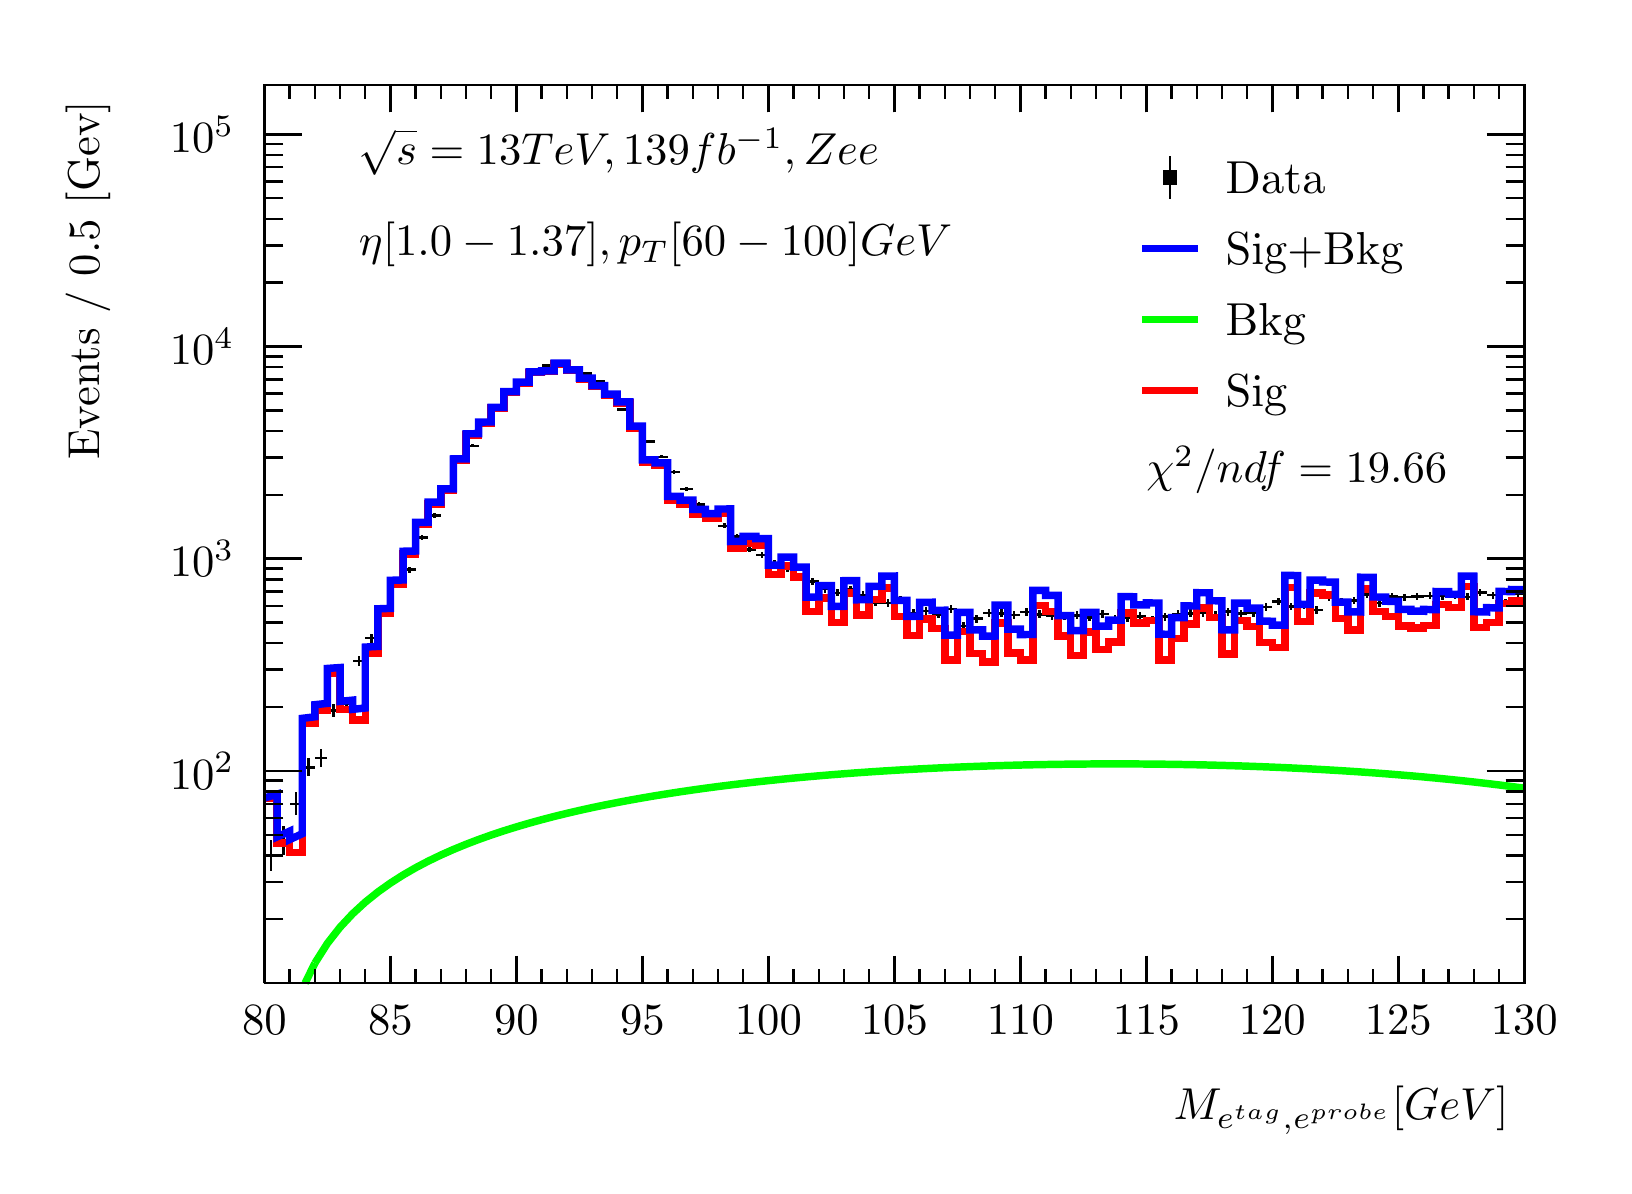
\begin{tikzpicture}
\pgfdeclareplotmark{cross} {
\pgfpathmoveto{\pgfpoint{-0.3\pgfplotmarksize}{\pgfplotmarksize}}
\pgfpathlineto{\pgfpoint{+0.3\pgfplotmarksize}{\pgfplotmarksize}}
\pgfpathlineto{\pgfpoint{+0.3\pgfplotmarksize}{0.3\pgfplotmarksize}}
\pgfpathlineto{\pgfpoint{+1\pgfplotmarksize}{0.3\pgfplotmarksize}}
\pgfpathlineto{\pgfpoint{+1\pgfplotmarksize}{-0.3\pgfplotmarksize}}
\pgfpathlineto{\pgfpoint{+0.3\pgfplotmarksize}{-0.3\pgfplotmarksize}}
\pgfpathlineto{\pgfpoint{+0.3\pgfplotmarksize}{-1.\pgfplotmarksize}}
\pgfpathlineto{\pgfpoint{-0.3\pgfplotmarksize}{-1.\pgfplotmarksize}}
\pgfpathlineto{\pgfpoint{-0.3\pgfplotmarksize}{-0.3\pgfplotmarksize}}
\pgfpathlineto{\pgfpoint{-1.\pgfplotmarksize}{-0.3\pgfplotmarksize}}
\pgfpathlineto{\pgfpoint{-1.\pgfplotmarksize}{0.3\pgfplotmarksize}}
\pgfpathlineto{\pgfpoint{-0.3\pgfplotmarksize}{0.3\pgfplotmarksize}}
\pgfpathclose
\pgfusepathqstroke
}
\pgfdeclareplotmark{cross*} {
\pgfpathmoveto{\pgfpoint{-0.3\pgfplotmarksize}{\pgfplotmarksize}}
\pgfpathlineto{\pgfpoint{+0.3\pgfplotmarksize}{\pgfplotmarksize}}
\pgfpathlineto{\pgfpoint{+0.3\pgfplotmarksize}{0.3\pgfplotmarksize}}
\pgfpathlineto{\pgfpoint{+1\pgfplotmarksize}{0.3\pgfplotmarksize}}
\pgfpathlineto{\pgfpoint{+1\pgfplotmarksize}{-0.3\pgfplotmarksize}}
\pgfpathlineto{\pgfpoint{+0.3\pgfplotmarksize}{-0.3\pgfplotmarksize}}
\pgfpathlineto{\pgfpoint{+0.3\pgfplotmarksize}{-1.\pgfplotmarksize}}
\pgfpathlineto{\pgfpoint{-0.3\pgfplotmarksize}{-1.\pgfplotmarksize}}
\pgfpathlineto{\pgfpoint{-0.3\pgfplotmarksize}{-0.3\pgfplotmarksize}}
\pgfpathlineto{\pgfpoint{-1.\pgfplotmarksize}{-0.3\pgfplotmarksize}}
\pgfpathlineto{\pgfpoint{-1.\pgfplotmarksize}{0.3\pgfplotmarksize}}
\pgfpathlineto{\pgfpoint{-0.3\pgfplotmarksize}{0.3\pgfplotmarksize}}
\pgfpathclose
\pgfusepathqfillstroke
}
\pgfdeclareplotmark{newstar} {
\pgfpathmoveto{\pgfqpoint{0pt}{\pgfplotmarksize}}
\pgfpathlineto{\pgfqpointpolar{44}{0.5\pgfplotmarksize}}
\pgfpathlineto{\pgfqpointpolar{18}{\pgfplotmarksize}}
\pgfpathlineto{\pgfqpointpolar{-20}{0.5\pgfplotmarksize}}
\pgfpathlineto{\pgfqpointpolar{-54}{\pgfplotmarksize}}
\pgfpathlineto{\pgfqpointpolar{-90}{0.5\pgfplotmarksize}}
\pgfpathlineto{\pgfqpointpolar{234}{\pgfplotmarksize}}
\pgfpathlineto{\pgfqpointpolar{198}{0.5\pgfplotmarksize}}
\pgfpathlineto{\pgfqpointpolar{162}{\pgfplotmarksize}}
\pgfpathlineto{\pgfqpointpolar{134}{0.5\pgfplotmarksize}}
\pgfpathclose
\pgfusepathqstroke
}
\pgfdeclareplotmark{newstar*} {
\pgfpathmoveto{\pgfqpoint{0pt}{\pgfplotmarksize}}
\pgfpathlineto{\pgfqpointpolar{44}{0.5\pgfplotmarksize}}
\pgfpathlineto{\pgfqpointpolar{18}{\pgfplotmarksize}}
\pgfpathlineto{\pgfqpointpolar{-20}{0.5\pgfplotmarksize}}
\pgfpathlineto{\pgfqpointpolar{-54}{\pgfplotmarksize}}
\pgfpathlineto{\pgfqpointpolar{-90}{0.5\pgfplotmarksize}}
\pgfpathlineto{\pgfqpointpolar{234}{\pgfplotmarksize}}
\pgfpathlineto{\pgfqpointpolar{198}{0.5\pgfplotmarksize}}
\pgfpathlineto{\pgfqpointpolar{162}{\pgfplotmarksize}}
\pgfpathlineto{\pgfqpointpolar{134}{0.5\pgfplotmarksize}}
\pgfpathclose
\pgfusepathqfillstroke
}
\definecolor{c}{rgb}{1,1,1};
\draw [color=c, fill=c] (0,0) rectangle (20,14.4361);
\draw [color=c, fill=c] (3,2.30977) rectangle (19,13.7143);
\definecolor{c}{rgb}{0,0,0};
\draw [c,line width=0.9] (3,2.30977) -- (3,13.7143) -- (19,13.7143) -- (19,2.30977) -- (3,2.30977);
\definecolor{c}{rgb}{1,1,1};
\draw [color=c, fill=c] (3,2.30977) rectangle (19,13.7143);
\definecolor{c}{rgb}{0,0,0};
\draw [c,line width=0.9] (3,2.30977) -- (3,13.7143) -- (19,13.7143) -- (19,2.30977) -- (3,2.30977);
\draw [c,line width=0.9] (3,2.30977) -- (19,2.30977);
\draw [c,line width=0.9] (3,2.65624) -- (3,2.30977);
\draw [c,line width=0.9] (3.32,2.48301) -- (3.32,2.30977);
\draw [c,line width=0.9] (3.64,2.48301) -- (3.64,2.30977);
\draw [c,line width=0.9] (3.96,2.48301) -- (3.96,2.30977);
\draw [c,line width=0.9] (4.28,2.48301) -- (4.28,2.30977);
\draw [c,line width=0.9] (4.6,2.65624) -- (4.6,2.30977);
\draw [c,line width=0.9] (4.92,2.48301) -- (4.92,2.30977);
\draw [c,line width=0.9] (5.24,2.48301) -- (5.24,2.30977);
\draw [c,line width=0.9] (5.56,2.48301) -- (5.56,2.30977);
\draw [c,line width=0.9] (5.88,2.48301) -- (5.88,2.30977);
\draw [c,line width=0.9] (6.2,2.65624) -- (6.2,2.30977);
\draw [c,line width=0.9] (6.52,2.48301) -- (6.52,2.30977);
\draw [c,line width=0.9] (6.84,2.48301) -- (6.84,2.30977);
\draw [c,line width=0.9] (7.16,2.48301) -- (7.16,2.30977);
\draw [c,line width=0.9] (7.48,2.48301) -- (7.48,2.30977);
\draw [c,line width=0.9] (7.8,2.65624) -- (7.8,2.30977);
\draw [c,line width=0.9] (8.12,2.48301) -- (8.12,2.30977);
\draw [c,line width=0.9] (8.44,2.48301) -- (8.44,2.30977);
\draw [c,line width=0.9] (8.76,2.48301) -- (8.76,2.30977);
\draw [c,line width=0.9] (9.08,2.48301) -- (9.08,2.30977);
\draw [c,line width=0.9] (9.4,2.65624) -- (9.4,2.30977);
\draw [c,line width=0.9] (9.72,2.48301) -- (9.72,2.30977);
\draw [c,line width=0.9] (10.04,2.48301) -- (10.04,2.30977);
\draw [c,line width=0.9] (10.36,2.48301) -- (10.36,2.30977);
\draw [c,line width=0.9] (10.68,2.48301) -- (10.68,2.30977);
\draw [c,line width=0.9] (11,2.65624) -- (11,2.30977);
\draw [c,line width=0.9] (11.32,2.48301) -- (11.32,2.30977);
\draw [c,line width=0.9] (11.64,2.48301) -- (11.64,2.30977);
\draw [c,line width=0.9] (11.96,2.48301) -- (11.96,2.30977);
\draw [c,line width=0.9] (12.28,2.48301) -- (12.28,2.30977);
\draw [c,line width=0.9] (12.6,2.65624) -- (12.6,2.30977);
\draw [c,line width=0.9] (12.92,2.48301) -- (12.92,2.30977);
\draw [c,line width=0.9] (13.24,2.48301) -- (13.24,2.30977);
\draw [c,line width=0.9] (13.56,2.48301) -- (13.56,2.30977);
\draw [c,line width=0.9] (13.88,2.48301) -- (13.88,2.30977);
\draw [c,line width=0.9] (14.2,2.65624) -- (14.2,2.30977);
\draw [c,line width=0.9] (14.52,2.48301) -- (14.52,2.30977);
\draw [c,line width=0.9] (14.84,2.48301) -- (14.84,2.30977);
\draw [c,line width=0.9] (15.16,2.48301) -- (15.16,2.30977);
\draw [c,line width=0.9] (15.48,2.48301) -- (15.48,2.30977);
\draw [c,line width=0.9] (15.8,2.65624) -- (15.8,2.30977);
\draw [c,line width=0.9] (16.12,2.48301) -- (16.12,2.30977);
\draw [c,line width=0.9] (16.44,2.48301) -- (16.44,2.30977);
\draw [c,line width=0.9] (16.76,2.48301) -- (16.76,2.30977);
\draw [c,line width=0.9] (17.08,2.48301) -- (17.08,2.30977);
\draw [c,line width=0.9] (17.4,2.65624) -- (17.4,2.30977);
\draw [c,line width=0.9] (17.72,2.48301) -- (17.72,2.30977);
\draw [c,line width=0.9] (18.04,2.48301) -- (18.04,2.30977);
\draw [c,line width=0.9] (18.36,2.48301) -- (18.36,2.30977);
\draw [c,line width=0.9] (18.68,2.48301) -- (18.68,2.30977);
\draw [c,line width=0.9] (19,2.65624) -- (19,2.30977);
\draw [anchor=base] (3,1.66015) node[scale=1.61424, color=c, rotate=0]{80};
\draw [anchor=base] (4.6,1.66015) node[scale=1.61424, color=c, rotate=0]{85};
\draw [anchor=base] (6.2,1.66015) node[scale=1.61424, color=c, rotate=0]{90};
\draw [anchor=base] (7.8,1.66015) node[scale=1.61424, color=c, rotate=0]{95};
\draw [anchor=base] (9.4,1.66015) node[scale=1.61424, color=c, rotate=0]{100};
\draw [anchor=base] (11,1.66015) node[scale=1.61424, color=c, rotate=0]{105};
\draw [anchor=base] (12.6,1.66015) node[scale=1.61424, color=c, rotate=0]{110};
\draw [anchor=base] (14.2,1.66015) node[scale=1.61424, color=c, rotate=0]{115};
\draw [anchor=base] (15.8,1.66015) node[scale=1.61424, color=c, rotate=0]{120};
\draw [anchor=base] (17.4,1.66015) node[scale=1.61424, color=c, rotate=0]{125};
\draw [anchor=base] (19,1.66015) node[scale=1.61424, color=c, rotate=0]{130};
\draw [anchor= east] (19,0.692932) node[scale=1.61424, color=c, rotate=0]{$M_{e^{tag}, e^{probe}}  [GeV]$};
\draw [c,line width=0.9] (3,13.7143) -- (19,13.7143);
\draw [c,line width=0.9] (3,13.3678) -- (3,13.7143);
\draw [c,line width=0.9] (3.32,13.5411) -- (3.32,13.7143);
\draw [c,line width=0.9] (3.64,13.5411) -- (3.64,13.7143);
\draw [c,line width=0.9] (3.96,13.5411) -- (3.96,13.7143);
\draw [c,line width=0.9] (4.28,13.5411) -- (4.28,13.7143);
\draw [c,line width=0.9] (4.6,13.3678) -- (4.6,13.7143);
\draw [c,line width=0.9] (4.92,13.5411) -- (4.92,13.7143);
\draw [c,line width=0.9] (5.24,13.5411) -- (5.24,13.7143);
\draw [c,line width=0.9] (5.56,13.5411) -- (5.56,13.7143);
\draw [c,line width=0.9] (5.88,13.5411) -- (5.88,13.7143);
\draw [c,line width=0.9] (6.2,13.3678) -- (6.2,13.7143);
\draw [c,line width=0.9] (6.52,13.5411) -- (6.52,13.7143);
\draw [c,line width=0.9] (6.84,13.5411) -- (6.84,13.7143);
\draw [c,line width=0.9] (7.16,13.5411) -- (7.16,13.7143);
\draw [c,line width=0.9] (7.48,13.5411) -- (7.48,13.7143);
\draw [c,line width=0.9] (7.8,13.3678) -- (7.8,13.7143);
\draw [c,line width=0.9] (8.12,13.5411) -- (8.12,13.7143);
\draw [c,line width=0.9] (8.44,13.5411) -- (8.44,13.7143);
\draw [c,line width=0.9] (8.76,13.5411) -- (8.76,13.7143);
\draw [c,line width=0.9] (9.08,13.5411) -- (9.08,13.7143);
\draw [c,line width=0.9] (9.4,13.3678) -- (9.4,13.7143);
\draw [c,line width=0.9] (9.72,13.5411) -- (9.72,13.7143);
\draw [c,line width=0.9] (10.04,13.5411) -- (10.04,13.7143);
\draw [c,line width=0.9] (10.36,13.5411) -- (10.36,13.7143);
\draw [c,line width=0.9] (10.68,13.5411) -- (10.68,13.7143);
\draw [c,line width=0.9] (11,13.3678) -- (11,13.7143);
\draw [c,line width=0.9] (11.32,13.5411) -- (11.32,13.7143);
\draw [c,line width=0.9] (11.64,13.5411) -- (11.64,13.7143);
\draw [c,line width=0.9] (11.96,13.5411) -- (11.96,13.7143);
\draw [c,line width=0.9] (12.28,13.5411) -- (12.28,13.7143);
\draw [c,line width=0.9] (12.6,13.3678) -- (12.6,13.7143);
\draw [c,line width=0.9] (12.92,13.5411) -- (12.92,13.7143);
\draw [c,line width=0.9] (13.24,13.5411) -- (13.24,13.7143);
\draw [c,line width=0.9] (13.56,13.5411) -- (13.56,13.7143);
\draw [c,line width=0.9] (13.88,13.5411) -- (13.88,13.7143);
\draw [c,line width=0.9] (14.2,13.3678) -- (14.2,13.7143);
\draw [c,line width=0.9] (14.52,13.5411) -- (14.52,13.7143);
\draw [c,line width=0.9] (14.84,13.5411) -- (14.84,13.7143);
\draw [c,line width=0.9] (15.16,13.5411) -- (15.16,13.7143);
\draw [c,line width=0.9] (15.48,13.5411) -- (15.48,13.7143);
\draw [c,line width=0.9] (15.8,13.3678) -- (15.8,13.7143);
\draw [c,line width=0.9] (16.12,13.5411) -- (16.12,13.7143);
\draw [c,line width=0.9] (16.44,13.5411) -- (16.44,13.7143);
\draw [c,line width=0.9] (16.76,13.5411) -- (16.76,13.7143);
\draw [c,line width=0.9] (17.08,13.5411) -- (17.08,13.7143);
\draw [c,line width=0.9] (17.4,13.3678) -- (17.4,13.7143);
\draw [c,line width=0.9] (17.72,13.5411) -- (17.72,13.7143);
\draw [c,line width=0.9] (18.04,13.5411) -- (18.04,13.7143);
\draw [c,line width=0.9] (18.36,13.5411) -- (18.36,13.7143);
\draw [c,line width=0.9] (18.68,13.5411) -- (18.68,13.7143);
\draw [c,line width=0.9] (19,13.3678) -- (19,13.7143);
\draw [c,line width=0.9] (3,2.30977) -- (3,13.7143);
\draw [c,line width=0.9] (3.237,3.1209) -- (3,3.1209);
\draw [c,line width=0.9] (3.237,3.59538) -- (3,3.59538);
\draw [c,line width=0.9] (3.237,3.93203) -- (3,3.93203);
\draw [c,line width=0.9] (3.237,4.19316) -- (3,4.19316);
\draw [c,line width=0.9] (3.237,4.40651) -- (3,4.40651);
\draw [c,line width=0.9] (3.237,4.5869) -- (3,4.5869);
\draw [c,line width=0.9] (3.237,4.74316) -- (3,4.74316);
\draw [c,line width=0.9] (3.237,4.881) -- (3,4.881);
\draw [c,line width=0.9] (3.474,5.00429) -- (3,5.00429);
\draw [anchor= east] (2.82,5.00429) node[scale=1.61424, color=c, rotate=0]{$10^{2}$};
\draw [c,line width=0.9] (3.237,5.81542) -- (3,5.81542);
\draw [c,line width=0.9] (3.237,6.2899) -- (3,6.2899);
\draw [c,line width=0.9] (3.237,6.62655) -- (3,6.62655);
\draw [c,line width=0.9] (3.237,6.88768) -- (3,6.88768);
\draw [c,line width=0.9] (3.237,7.10103) -- (3,7.10103);
\draw [c,line width=0.9] (3.237,7.28142) -- (3,7.28142);
\draw [c,line width=0.9] (3.237,7.43768) -- (3,7.43768);
\draw [c,line width=0.9] (3.237,7.57551) -- (3,7.57551);
\draw [c,line width=0.9] (3.474,7.69881) -- (3,7.69881);
\draw [anchor= east] (2.82,7.69881) node[scale=1.61424, color=c, rotate=0]{$10^{3}$};
\draw [c,line width=0.9] (3.237,8.50994) -- (3,8.50994);
\draw [c,line width=0.9] (3.237,8.98442) -- (3,8.98442);
\draw [c,line width=0.9] (3.237,9.32107) -- (3,9.32107);
\draw [c,line width=0.9] (3.237,9.58219) -- (3,9.58219);
\draw [c,line width=0.9] (3.237,9.79555) -- (3,9.79555);
\draw [c,line width=0.9] (3.237,9.97594) -- (3,9.97594);
\draw [c,line width=0.9] (3.237,10.1322) -- (3,10.1322);
\draw [c,line width=0.9] (3.237,10.27) -- (3,10.27);
\draw [c,line width=0.9] (3.474,10.3933) -- (3,10.3933);
\draw [anchor= east] (2.82,10.3933) node[scale=1.61424, color=c, rotate=0]{$10^{4}$};
\draw [c,line width=0.9] (3.237,11.2045) -- (3,11.2045);
\draw [c,line width=0.9] (3.237,11.6789) -- (3,11.6789);
\draw [c,line width=0.9] (3.237,12.0156) -- (3,12.0156);
\draw [c,line width=0.9] (3.237,12.2767) -- (3,12.2767);
\draw [c,line width=0.9] (3.237,12.4901) -- (3,12.4901);
\draw [c,line width=0.9] (3.237,12.6705) -- (3,12.6705);
\draw [c,line width=0.9] (3.237,12.8267) -- (3,12.8267);
\draw [c,line width=0.9] (3.237,12.9645) -- (3,12.9645);
\draw [c,line width=0.9] (3.474,13.0878) -- (3,13.0878);
\draw [anchor= east] (2.82,13.0878) node[scale=1.61424, color=c, rotate=0]{$10^{5}$};
\draw [anchor= east] (0.76,13.7143) node[scale=1.61424, color=c, rotate=90]{Events / 0.5 [Gev]};
\draw [c,line width=0.9] (19,2.30977) -- (19,13.7143);
\draw [c,line width=0.9] (18.763,3.1209) -- (19,3.1209);
\draw [c,line width=0.9] (18.763,3.59538) -- (19,3.59538);
\draw [c,line width=0.9] (18.763,3.93203) -- (19,3.93203);
\draw [c,line width=0.9] (18.763,4.19316) -- (19,4.19316);
\draw [c,line width=0.9] (18.763,4.40651) -- (19,4.40651);
\draw [c,line width=0.9] (18.763,4.5869) -- (19,4.5869);
\draw [c,line width=0.9] (18.763,4.74316) -- (19,4.74316);
\draw [c,line width=0.9] (18.763,4.881) -- (19,4.881);
\draw [c,line width=0.9] (18.526,5.00429) -- (19,5.00429);
\draw [c,line width=0.9] (18.763,5.81542) -- (19,5.81542);
\draw [c,line width=0.9] (18.763,6.2899) -- (19,6.2899);
\draw [c,line width=0.9] (18.763,6.62655) -- (19,6.62655);
\draw [c,line width=0.9] (18.763,6.88768) -- (19,6.88768);
\draw [c,line width=0.9] (18.763,7.10103) -- (19,7.10103);
\draw [c,line width=0.9] (18.763,7.28142) -- (19,7.28142);
\draw [c,line width=0.9] (18.763,7.43768) -- (19,7.43768);
\draw [c,line width=0.9] (18.763,7.57551) -- (19,7.57551);
\draw [c,line width=0.9] (18.526,7.69881) -- (19,7.69881);
\draw [c,line width=0.9] (18.763,8.50994) -- (19,8.50994);
\draw [c,line width=0.9] (18.763,8.98442) -- (19,8.98442);
\draw [c,line width=0.9] (18.763,9.32107) -- (19,9.32107);
\draw [c,line width=0.9] (18.763,9.58219) -- (19,9.58219);
\draw [c,line width=0.9] (18.763,9.79555) -- (19,9.79555);
\draw [c,line width=0.9] (18.763,9.97594) -- (19,9.97594);
\draw [c,line width=0.9] (18.763,10.1322) -- (19,10.1322);
\draw [c,line width=0.9] (18.763,10.27) -- (19,10.27);
\draw [c,line width=0.9] (18.526,10.3933) -- (19,10.3933);
\draw [c,line width=0.9] (18.763,11.2045) -- (19,11.2045);
\draw [c,line width=0.9] (18.763,11.6789) -- (19,11.6789);
\draw [c,line width=0.9] (18.763,12.0156) -- (19,12.0156);
\draw [c,line width=0.9] (18.763,12.2767) -- (19,12.2767);
\draw [c,line width=0.9] (18.763,12.4901) -- (19,12.4901);
\draw [c,line width=0.9] (18.763,12.6705) -- (19,12.6705);
\draw [c,line width=0.9] (18.763,12.8267) -- (19,12.8267);
\draw [c,line width=0.9] (18.763,12.9645) -- (19,12.9645);
\draw [c,line width=0.9] (18.526,13.0878) -- (19,13.0878);
\draw [c,line width=0.9] (3.08,3.93204) -- (3,3.93204);
\draw [c,line width=0.9] (3,3.93204) -- (3,3.93204);
\draw [c,line width=0.9] (3.08,3.93204) -- (3.16,3.93204);
\draw [c,line width=0.9] (3.16,3.93204) -- (3.16,3.93204);
\draw [c,line width=0.9] (3.08,3.93204) -- (3.08,4.13011);
\draw [c,line width=0.9] (3.08,4.13011) -- (3.08,4.13011);
\draw [c,line width=0.9] (3.08,3.93204) -- (3.08,3.73155);
\draw [c,line width=0.9] (3.08,3.73155) -- (3.08,3.73155);
\draw [c,line width=0.9] (3.24,4.12075) -- (3.16,4.12075);
\draw [c,line width=0.9] (3.16,4.12075) -- (3.16,4.12075);
\draw [c,line width=0.9] (3.24,4.12075) -- (3.32,4.12075);
\draw [c,line width=0.9] (3.32,4.12075) -- (3.32,4.12075);
\draw [c,line width=0.9] (3.24,4.12075) -- (3.24,4.30266);
\draw [c,line width=0.9] (3.24,4.30266) -- (3.24,4.30266);
\draw [c,line width=0.9] (3.24,4.12075) -- (3.24,3.93696);
\draw [c,line width=0.9] (3.24,3.93696) -- (3.24,3.93696);
\draw [c,line width=0.9] (3.4,4.58691) -- (3.32,4.58691);
\draw [c,line width=0.9] (3.32,4.58691) -- (3.32,4.58691);
\draw [c,line width=0.9] (3.4,4.58691) -- (3.48,4.58691);
\draw [c,line width=0.9] (3.48,4.58691) -- (3.48,4.58691);
\draw [c,line width=0.9] (3.4,4.58691) -- (3.4,4.73445);
\draw [c,line width=0.9] (3.4,4.73445) -- (3.4,4.73445);
\draw [c,line width=0.9] (3.4,4.58691) -- (3.4,4.43833);
\draw [c,line width=0.9] (3.4,4.43833) -- (3.4,4.43833);
\draw [c,line width=0.9] (3.56,5.05019) -- (3.48,5.05019);
\draw [c,line width=0.9] (3.48,5.05019) -- (3.48,5.05019);
\draw [c,line width=0.9] (3.56,5.05019) -- (3.64,5.05019);
\draw [c,line width=0.9] (3.64,5.05019) -- (3.64,5.05019);
\draw [c,line width=0.9] (3.56,5.05019) -- (3.56,5.16489);
\draw [c,line width=0.9] (3.56,5.16489) -- (3.56,5.16489);
\draw [c,line width=0.9] (3.56,5.05019) -- (3.56,4.93549);
\draw [c,line width=0.9] (3.56,4.93549) -- (3.56,4.93549);
\draw [c,line width=0.9] (3.72,5.16784) -- (3.64,5.16784);
\draw [c,line width=0.9] (3.64,5.16784) -- (3.64,5.16784);
\draw [c,line width=0.9] (3.72,5.16784) -- (3.8,5.16784);
\draw [c,line width=0.9] (3.8,5.16784) -- (3.8,5.16784);
\draw [c,line width=0.9] (3.72,5.16784) -- (3.72,5.27693);
\draw [c,line width=0.9] (3.72,5.27693) -- (3.72,5.27693);
\draw [c,line width=0.9] (3.72,5.16784) -- (3.72,5.05876);
\draw [c,line width=0.9] (3.72,5.05876) -- (3.72,5.05876);
\draw [c,line width=0.9] (3.88,5.77373) -- (3.8,5.77373);
\draw [c,line width=0.9] (3.8,5.77373) -- (3.8,5.77373);
\draw [c,line width=0.9] (3.88,5.77373) -- (3.96,5.77373);
\draw [c,line width=0.9] (3.96,5.77373) -- (3.96,5.77373);
\draw [c,line width=0.9] (3.88,5.77373) -- (3.88,5.85795);
\draw [c,line width=0.9] (3.88,5.85795) -- (3.88,5.85795);
\draw [c,line width=0.9] (3.88,5.77373) -- (3.88,5.68952);
\draw [c,line width=0.9] (3.88,5.68952) -- (3.88,5.68952);
\draw [c,line width=0.9] (4.04,5.86132) -- (3.96,5.86132);
\draw [c,line width=0.9] (3.96,5.86132) -- (3.96,5.86132);
\draw [c,line width=0.9] (4.04,5.86132) -- (4.12,5.86132);
\draw [c,line width=0.9] (4.12,5.86132) -- (4.12,5.86132);
\draw [c,line width=0.9] (4.04,5.86132) -- (4.04,5.94244);
\draw [c,line width=0.9] (4.04,5.94244) -- (4.04,5.94244);
\draw [c,line width=0.9] (4.04,5.86132) -- (4.04,5.7802);
\draw [c,line width=0.9] (4.04,5.7802) -- (4.04,5.7802);
\draw [c,line width=0.9] (4.2,6.40144) -- (4.12,6.40144);
\draw [c,line width=0.9] (4.12,6.40144) -- (4.12,6.40144);
\draw [c,line width=0.9] (4.2,6.40144) -- (4.28,6.40144);
\draw [c,line width=0.9] (4.28,6.40144) -- (4.28,6.40144);
\draw [c,line width=0.9] (4.2,6.40144) -- (4.2,6.46585);
\draw [c,line width=0.9] (4.2,6.46585) -- (4.2,6.46585);
\draw [c,line width=0.9] (4.2,6.40144) -- (4.2,6.33703);
\draw [c,line width=0.9] (4.2,6.33703) -- (4.2,6.33703);
\draw [c,line width=0.9] (4.36,6.68921) -- (4.28,6.68921);
\draw [c,line width=0.9] (4.28,6.68921) -- (4.28,6.68921);
\draw [c,line width=0.9] (4.36,6.68921) -- (4.44,6.68921);
\draw [c,line width=0.9] (4.44,6.68921) -- (4.44,6.68921);
\draw [c,line width=0.9] (4.36,6.68921) -- (4.36,6.74617);
\draw [c,line width=0.9] (4.36,6.74617) -- (4.36,6.74617);
\draw [c,line width=0.9] (4.36,6.68921) -- (4.36,6.63225);
\draw [c,line width=0.9] (4.36,6.63225) -- (4.36,6.63225);
\draw [c,line width=0.9] (4.52,7.06539) -- (4.44,7.06539);
\draw [c,line width=0.9] (4.44,7.06539) -- (4.44,7.06539);
\draw [c,line width=0.9] (4.52,7.06539) -- (4.6,7.06539);
\draw [c,line width=0.9] (4.6,7.06539) -- (4.6,7.06539);
\draw [c,line width=0.9] (4.52,7.06539) -- (4.52,7.11389);
\draw [c,line width=0.9] (4.52,7.11389) -- (4.52,7.11389);
\draw [c,line width=0.9] (4.52,7.06539) -- (4.52,7.01689);
\draw [c,line width=0.9] (4.52,7.01689) -- (4.52,7.01689);
\draw [c,line width=0.9] (4.68,7.40655) -- (4.6,7.40655);
\draw [c,line width=0.9] (4.6,7.40655) -- (4.6,7.40655);
\draw [c,line width=0.9] (4.68,7.40655) -- (4.76,7.40655);
\draw [c,line width=0.9] (4.76,7.40655) -- (4.76,7.40655);
\draw [c,line width=0.9] (4.68,7.40655) -- (4.68,7.44848);
\draw [c,line width=0.9] (4.68,7.44848) -- (4.68,7.44848);
\draw [c,line width=0.9] (4.68,7.40655) -- (4.68,7.36463);
\draw [c,line width=0.9] (4.68,7.36463) -- (4.68,7.36463);
\draw [c,line width=0.9] (4.84,7.55981) -- (4.76,7.55981);
\draw [c,line width=0.9] (4.76,7.55981) -- (4.76,7.55981);
\draw [c,line width=0.9] (4.84,7.55981) -- (4.92,7.55981);
\draw [c,line width=0.9] (4.92,7.55981) -- (4.92,7.55981);
\draw [c,line width=0.9] (4.84,7.55981) -- (4.84,7.59907);
\draw [c,line width=0.9] (4.84,7.59907) -- (4.84,7.59907);
\draw [c,line width=0.9] (4.84,7.55981) -- (4.84,7.52054);
\draw [c,line width=0.9] (4.84,7.52054) -- (4.84,7.52054);
\draw [c,line width=0.9] (5,7.96647) -- (4.92,7.96647);
\draw [c,line width=0.9] (4.92,7.96647) -- (4.92,7.96647);
\draw [c,line width=0.9] (5,7.96647) -- (5.08,7.96647);
\draw [c,line width=0.9] (5.08,7.96647) -- (5.08,7.96647);
\draw [c,line width=0.9] (5,7.96647) -- (5,7.99948);
\draw [c,line width=0.9] (5,7.99948) -- (5,7.99948);
\draw [c,line width=0.9] (5,7.96647) -- (5,7.93346);
\draw [c,line width=0.9] (5,7.93346) -- (5,7.93346);
\draw [c,line width=0.9] (5.16,8.24808) -- (5.08,8.24808);
\draw [c,line width=0.9] (5.08,8.24808) -- (5.08,8.24808);
\draw [c,line width=0.9] (5.16,8.24808) -- (5.24,8.24808);
\draw [c,line width=0.9] (5.24,8.24808) -- (5.24,8.24808);
\draw [c,line width=0.9] (5.16,8.24808) -- (5.16,8.27735);
\draw [c,line width=0.9] (5.16,8.27735) -- (5.16,8.27735);
\draw [c,line width=0.9] (5.16,8.24808) -- (5.16,8.21882);
\draw [c,line width=0.9] (5.16,8.21882) -- (5.16,8.21882);
\draw [c,line width=0.9] (5.32,8.57702) -- (5.24,8.57702);
\draw [c,line width=0.9] (5.24,8.57702) -- (5.24,8.57702);
\draw [c,line width=0.9] (5.32,8.57702) -- (5.4,8.57702);
\draw [c,line width=0.9] (5.4,8.57702) -- (5.4,8.57702);
\draw [c,line width=0.9] (5.32,8.57702) -- (5.32,8.60245);
\draw [c,line width=0.9] (5.32,8.60245) -- (5.32,8.60245);
\draw [c,line width=0.9] (5.32,8.57702) -- (5.32,8.55159);
\draw [c,line width=0.9] (5.32,8.55159) -- (5.32,8.55159);
\draw [c,line width=0.9] (5.48,8.91905) -- (5.4,8.91905);
\draw [c,line width=0.9] (5.4,8.91905) -- (5.4,8.91905);
\draw [c,line width=0.9] (5.48,8.91905) -- (5.56,8.91905);
\draw [c,line width=0.9] (5.56,8.91905) -- (5.56,8.91905);
\draw [c,line width=0.9] (5.48,8.91905) -- (5.48,8.94102);
\draw [c,line width=0.9] (5.48,8.94102) -- (5.48,8.94102);
\draw [c,line width=0.9] (5.48,8.91905) -- (5.48,8.89708);
\draw [c,line width=0.9] (5.48,8.89708) -- (5.48,8.89708);
\draw [c,line width=0.9] (5.64,9.13192) -- (5.56,9.13192);
\draw [c,line width=0.9] (5.56,9.13192) -- (5.56,9.13192);
\draw [c,line width=0.9] (5.64,9.13192) -- (5.72,9.13192);
\draw [c,line width=0.9] (5.72,9.13192) -- (5.72,9.13192);
\draw [c,line width=0.9] (5.64,9.13192) -- (5.64,9.15198);
\draw [c,line width=0.9] (5.64,9.15198) -- (5.64,9.15198);
\draw [c,line width=0.9] (5.64,9.13192) -- (5.64,9.11186);
\draw [c,line width=0.9] (5.64,9.11186) -- (5.64,9.11186);
\draw [c,line width=0.9] (5.8,9.41384) -- (5.72,9.41384);
\draw [c,line width=0.9] (5.72,9.41384) -- (5.72,9.41384);
\draw [c,line width=0.9] (5.8,9.41384) -- (5.88,9.41384);
\draw [c,line width=0.9] (5.88,9.41384) -- (5.88,9.41384);
\draw [c,line width=0.9] (5.8,9.41384) -- (5.8,9.43162);
\draw [c,line width=0.9] (5.8,9.43162) -- (5.8,9.43162);
\draw [c,line width=0.9] (5.8,9.41384) -- (5.8,9.39605);
\draw [c,line width=0.9] (5.8,9.39605) -- (5.8,9.39605);
\draw [c,line width=0.9] (5.96,9.6506) -- (5.88,9.6506);
\draw [c,line width=0.9] (5.88,9.6506) -- (5.88,9.6506);
\draw [c,line width=0.9] (5.96,9.6506) -- (6.04,9.6506);
\draw [c,line width=0.9] (6.04,9.6506) -- (6.04,9.6506);
\draw [c,line width=0.9] (5.96,9.6506) -- (5.96,9.66668);
\draw [c,line width=0.9] (5.96,9.66668) -- (5.96,9.66668);
\draw [c,line width=0.9] (5.96,9.6506) -- (5.96,9.63453);
\draw [c,line width=0.9] (5.96,9.63453) -- (5.96,9.63453);
\draw [c,line width=0.9] (6.12,9.83298) -- (6.04,9.83298);
\draw [c,line width=0.9] (6.04,9.83298) -- (6.04,9.83298);
\draw [c,line width=0.9] (6.12,9.83298) -- (6.2,9.83298);
\draw [c,line width=0.9] (6.2,9.83298) -- (6.2,9.83298);
\draw [c,line width=0.9] (6.12,9.83298) -- (6.12,9.84785);
\draw [c,line width=0.9] (6.12,9.84785) -- (6.12,9.84785);
\draw [c,line width=0.9] (6.12,9.83298) -- (6.12,9.81811);
\draw [c,line width=0.9] (6.12,9.81811) -- (6.12,9.81811);
\draw [c,line width=0.9] (6.28,9.96215) -- (6.2,9.96215);
\draw [c,line width=0.9] (6.2,9.96215) -- (6.2,9.96215);
\draw [c,line width=0.9] (6.28,9.96215) -- (6.36,9.96215);
\draw [c,line width=0.9] (6.36,9.96215) -- (6.36,9.96215);
\draw [c,line width=0.9] (6.28,9.96215) -- (6.28,9.97622);
\draw [c,line width=0.9] (6.28,9.97622) -- (6.28,9.97622);
\draw [c,line width=0.9] (6.28,9.96215) -- (6.28,9.94808);
\draw [c,line width=0.9] (6.28,9.94808) -- (6.28,9.94808);
\draw [c,line width=0.9] (6.44,10.0901) -- (6.36,10.0901);
\draw [c,line width=0.9] (6.36,10.0901) -- (6.36,10.0901);
\draw [c,line width=0.9] (6.44,10.0901) -- (6.52,10.0901);
\draw [c,line width=0.9] (6.52,10.0901) -- (6.52,10.0901);
\draw [c,line width=0.9] (6.44,10.0901) -- (6.44,10.1034);
\draw [c,line width=0.9] (6.44,10.1034) -- (6.44,10.1034);
\draw [c,line width=0.9] (6.44,10.0901) -- (6.44,10.0767);
\draw [c,line width=0.9] (6.44,10.0767) -- (6.44,10.0767);
\draw [c,line width=0.9] (6.6,10.1545) -- (6.52,10.1545);
\draw [c,line width=0.9] (6.52,10.1545) -- (6.52,10.1545);
\draw [c,line width=0.9] (6.6,10.1545) -- (6.68,10.1545);
\draw [c,line width=0.9] (6.68,10.1545) -- (6.68,10.1545);
\draw [c,line width=0.9] (6.6,10.1545) -- (6.6,10.1675);
\draw [c,line width=0.9] (6.6,10.1675) -- (6.6,10.1675);
\draw [c,line width=0.9] (6.6,10.1545) -- (6.6,10.1416);
\draw [c,line width=0.9] (6.6,10.1416) -- (6.6,10.1416);
\draw [c,line width=0.9] (6.76,10.1734) -- (6.68,10.1734);
\draw [c,line width=0.9] (6.68,10.1734) -- (6.68,10.1734);
\draw [c,line width=0.9] (6.76,10.1734) -- (6.84,10.1734);
\draw [c,line width=0.9] (6.84,10.1734) -- (6.84,10.1734);
\draw [c,line width=0.9] (6.76,10.1734) -- (6.76,10.1863);
\draw [c,line width=0.9] (6.76,10.1863) -- (6.76,10.1863);
\draw [c,line width=0.9] (6.76,10.1734) -- (6.76,10.1606);
\draw [c,line width=0.9] (6.76,10.1606) -- (6.76,10.1606);
\draw [c,line width=0.9] (6.92,10.1275) -- (6.84,10.1275);
\draw [c,line width=0.9] (6.84,10.1275) -- (6.84,10.1275);
\draw [c,line width=0.9] (6.92,10.1275) -- (7,10.1275);
\draw [c,line width=0.9] (7,10.1275) -- (7,10.1275);
\draw [c,line width=0.9] (6.92,10.1275) -- (6.92,10.1406);
\draw [c,line width=0.9] (6.92,10.1406) -- (6.92,10.1406);
\draw [c,line width=0.9] (6.92,10.1275) -- (6.92,10.1144);
\draw [c,line width=0.9] (6.92,10.1144) -- (6.92,10.1144);
\draw [c,line width=0.9] (7.08,10.0498) -- (7,10.0498);
\draw [c,line width=0.9] (7,10.0498) -- (7,10.0498);
\draw [c,line width=0.9] (7.08,10.0498) -- (7.16,10.0498);
\draw [c,line width=0.9] (7.16,10.0498) -- (7.16,10.0498);
\draw [c,line width=0.9] (7.08,10.0498) -- (7.08,10.0633);
\draw [c,line width=0.9] (7.08,10.0633) -- (7.08,10.0633);
\draw [c,line width=0.9] (7.08,10.0498) -- (7.08,10.0362);
\draw [c,line width=0.9] (7.08,10.0362) -- (7.08,10.0362);
\draw [c,line width=0.9] (7.24,9.94888) -- (7.16,9.94888);
\draw [c,line width=0.9] (7.16,9.94888) -- (7.16,9.94888);
\draw [c,line width=0.9] (7.24,9.94888) -- (7.32,9.94888);
\draw [c,line width=0.9] (7.32,9.94888) -- (7.32,9.94888);
\draw [c,line width=0.9] (7.24,9.94888) -- (7.24,9.96303);
\draw [c,line width=0.9] (7.24,9.96303) -- (7.24,9.96303);
\draw [c,line width=0.9] (7.24,9.94888) -- (7.24,9.93473);
\draw [c,line width=0.9] (7.24,9.93473) -- (7.24,9.93473);
\draw [c,line width=0.9] (7.4,9.77964) -- (7.32,9.77964);
\draw [c,line width=0.9] (7.32,9.77964) -- (7.32,9.77964);
\draw [c,line width=0.9] (7.4,9.77964) -- (7.48,9.77964);
\draw [c,line width=0.9] (7.48,9.77964) -- (7.48,9.77964);
\draw [c,line width=0.9] (7.4,9.77964) -- (7.4,9.79486);
\draw [c,line width=0.9] (7.4,9.79486) -- (7.4,9.79486);
\draw [c,line width=0.9] (7.4,9.77964) -- (7.4,9.76443);
\draw [c,line width=0.9] (7.4,9.76443) -- (7.4,9.76443);
\draw [c,line width=0.9] (7.56,9.59152) -- (7.48,9.59152);
\draw [c,line width=0.9] (7.48,9.59152) -- (7.48,9.59152);
\draw [c,line width=0.9] (7.56,9.59152) -- (7.64,9.59152);
\draw [c,line width=0.9] (7.64,9.59152) -- (7.64,9.59152);
\draw [c,line width=0.9] (7.56,9.59152) -- (7.56,9.608);
\draw [c,line width=0.9] (7.56,9.608) -- (7.56,9.608);
\draw [c,line width=0.9] (7.56,9.59152) -- (7.56,9.57504);
\draw [c,line width=0.9] (7.56,9.57504) -- (7.56,9.57504);
\draw [c,line width=0.9] (7.72,9.39284) -- (7.64,9.39284);
\draw [c,line width=0.9] (7.64,9.39284) -- (7.64,9.39284);
\draw [c,line width=0.9] (7.72,9.39284) -- (7.8,9.39284);
\draw [c,line width=0.9] (7.8,9.39284) -- (7.8,9.39284);
\draw [c,line width=0.9] (7.72,9.39284) -- (7.72,9.41078);
\draw [c,line width=0.9] (7.72,9.41078) -- (7.72,9.41078);
\draw [c,line width=0.9] (7.72,9.39284) -- (7.72,9.3749);
\draw [c,line width=0.9] (7.72,9.3749) -- (7.72,9.3749);
\draw [c,line width=0.9] (7.88,9.18798) -- (7.8,9.18798);
\draw [c,line width=0.9] (7.8,9.18798) -- (7.8,9.18798);
\draw [c,line width=0.9] (7.88,9.18798) -- (7.96,9.18798);
\draw [c,line width=0.9] (7.96,9.18798) -- (7.96,9.18798);
\draw [c,line width=0.9] (7.88,9.18798) -- (7.88,9.20757);
\draw [c,line width=0.9] (7.88,9.20757) -- (7.88,9.20757);
\draw [c,line width=0.9] (7.88,9.18798) -- (7.88,9.1684);
\draw [c,line width=0.9] (7.88,9.1684) -- (7.88,9.1684);
\draw [c,line width=0.9] (8.04,8.99297) -- (7.96,8.99297);
\draw [c,line width=0.9] (7.96,8.99297) -- (7.96,8.99297);
\draw [c,line width=0.9] (8.04,8.99297) -- (8.12,8.99297);
\draw [c,line width=0.9] (8.12,8.99297) -- (8.12,8.99297);
\draw [c,line width=0.9] (8.04,8.99297) -- (8.04,9.01426);
\draw [c,line width=0.9] (8.04,9.01426) -- (8.04,9.01426);
\draw [c,line width=0.9] (8.04,8.99297) -- (8.04,8.97168);
\draw [c,line width=0.9] (8.04,8.97168) -- (8.04,8.97168);
\draw [c,line width=0.9] (8.2,8.8011) -- (8.12,8.8011);
\draw [c,line width=0.9] (8.12,8.8011) -- (8.12,8.8011);
\draw [c,line width=0.9] (8.2,8.8011) -- (8.28,8.8011);
\draw [c,line width=0.9] (8.28,8.8011) -- (8.28,8.8011);
\draw [c,line width=0.9] (8.2,8.8011) -- (8.2,8.82421);
\draw [c,line width=0.9] (8.2,8.82421) -- (8.2,8.82421);
\draw [c,line width=0.9] (8.2,8.8011) -- (8.2,8.778);
\draw [c,line width=0.9] (8.2,8.778) -- (8.2,8.778);
\draw [c,line width=0.9] (8.36,8.58198) -- (8.28,8.58198);
\draw [c,line width=0.9] (8.28,8.58198) -- (8.28,8.58198);
\draw [c,line width=0.9] (8.36,8.58198) -- (8.44,8.58198);
\draw [c,line width=0.9] (8.44,8.58198) -- (8.44,8.58198);
\draw [c,line width=0.9] (8.36,8.58198) -- (8.36,8.60736);
\draw [c,line width=0.9] (8.36,8.60736) -- (8.36,8.60736);
\draw [c,line width=0.9] (8.36,8.58198) -- (8.36,8.55661);
\draw [c,line width=0.9] (8.36,8.55661) -- (8.36,8.55661);
\draw [c,line width=0.9] (8.52,8.38989) -- (8.44,8.38989);
\draw [c,line width=0.9] (8.44,8.38989) -- (8.44,8.38989);
\draw [c,line width=0.9] (8.52,8.38989) -- (8.6,8.38989);
\draw [c,line width=0.9] (8.6,8.38989) -- (8.6,8.38989);
\draw [c,line width=0.9] (8.52,8.38989) -- (8.52,8.41743);
\draw [c,line width=0.9] (8.52,8.41743) -- (8.52,8.41743);
\draw [c,line width=0.9] (8.52,8.38989) -- (8.52,8.36235);
\draw [c,line width=0.9] (8.52,8.36235) -- (8.52,8.36235);
\draw [c,line width=0.9] (8.68,8.26624) -- (8.6,8.26624);
\draw [c,line width=0.9] (8.6,8.26624) -- (8.6,8.26624);
\draw [c,line width=0.9] (8.68,8.26624) -- (8.76,8.26624);
\draw [c,line width=0.9] (8.76,8.26624) -- (8.76,8.26624);
\draw [c,line width=0.9] (8.68,8.26624) -- (8.68,8.29527);
\draw [c,line width=0.9] (8.68,8.29527) -- (8.68,8.29527);
\draw [c,line width=0.9] (8.68,8.26624) -- (8.68,8.2372);
\draw [c,line width=0.9] (8.68,8.2372) -- (8.68,8.2372);
\draw [c,line width=0.9] (8.84,8.11655) -- (8.76,8.11655);
\draw [c,line width=0.9] (8.76,8.11655) -- (8.76,8.11655);
\draw [c,line width=0.9] (8.84,8.11655) -- (8.92,8.11655);
\draw [c,line width=0.9] (8.92,8.11655) -- (8.92,8.11655);
\draw [c,line width=0.9] (8.84,8.11655) -- (8.84,8.1475);
\draw [c,line width=0.9] (8.84,8.1475) -- (8.84,8.1475);
\draw [c,line width=0.9] (8.84,8.11655) -- (8.84,8.08559);
\draw [c,line width=0.9] (8.84,8.08559) -- (8.84,8.08559);
\draw [c,line width=0.9] (9,7.97943) -- (8.92,7.97943);
\draw [c,line width=0.9] (8.92,7.97943) -- (8.92,7.97943);
\draw [c,line width=0.9] (9,7.97943) -- (9.08,7.97943);
\draw [c,line width=0.9] (9.08,7.97943) -- (9.08,7.97943);
\draw [c,line width=0.9] (9,7.97943) -- (9,8.01225);
\draw [c,line width=0.9] (9,8.01225) -- (9,8.01225);
\draw [c,line width=0.9] (9,7.97943) -- (9,7.94661);
\draw [c,line width=0.9] (9,7.94661) -- (9,7.94661);
\draw [c,line width=0.9] (9.16,7.81671) -- (9.08,7.81671);
\draw [c,line width=0.9] (9.08,7.81671) -- (9.08,7.81671);
\draw [c,line width=0.9] (9.16,7.81671) -- (9.24,7.81671);
\draw [c,line width=0.9] (9.24,7.81671) -- (9.24,7.81671);
\draw [c,line width=0.9] (9.16,7.81671) -- (9.16,7.85189);
\draw [c,line width=0.9] (9.16,7.85189) -- (9.16,7.85189);
\draw [c,line width=0.9] (9.16,7.81671) -- (9.16,7.78152);
\draw [c,line width=0.9] (9.16,7.78152) -- (9.16,7.78152);
\draw [c,line width=0.9] (9.32,7.7492) -- (9.24,7.7492);
\draw [c,line width=0.9] (9.24,7.7492) -- (9.24,7.7492);
\draw [c,line width=0.9] (9.32,7.7492) -- (9.4,7.7492);
\draw [c,line width=0.9] (9.4,7.7492) -- (9.4,7.7492);
\draw [c,line width=0.9] (9.32,7.7492) -- (9.32,7.78541);
\draw [c,line width=0.9] (9.32,7.78541) -- (9.32,7.78541);
\draw [c,line width=0.9] (9.32,7.7492) -- (9.32,7.71298);
\draw [c,line width=0.9] (9.32,7.71298) -- (9.32,7.71298);
\draw [c,line width=0.9] (9.48,7.64247) -- (9.4,7.64247);
\draw [c,line width=0.9] (9.4,7.64247) -- (9.4,7.64247);
\draw [c,line width=0.9] (9.48,7.64247) -- (9.56,7.64247);
\draw [c,line width=0.9] (9.56,7.64247) -- (9.56,7.64247);
\draw [c,line width=0.9] (9.48,7.64247) -- (9.48,7.68038);
\draw [c,line width=0.9] (9.48,7.68038) -- (9.48,7.68038);
\draw [c,line width=0.9] (9.48,7.64247) -- (9.48,7.60457);
\draw [c,line width=0.9] (9.48,7.60457) -- (9.48,7.60457);
\draw [c,line width=0.9] (9.64,7.56769) -- (9.56,7.56769);
\draw [c,line width=0.9] (9.56,7.56769) -- (9.56,7.56769);
\draw [c,line width=0.9] (9.64,7.56769) -- (9.72,7.56769);
\draw [c,line width=0.9] (9.72,7.56769) -- (9.72,7.56769);
\draw [c,line width=0.9] (9.64,7.56769) -- (9.64,7.60682);
\draw [c,line width=0.9] (9.64,7.60682) -- (9.64,7.60682);
\draw [c,line width=0.9] (9.64,7.56769) -- (9.64,7.52855);
\draw [c,line width=0.9] (9.64,7.52855) -- (9.64,7.52855);
\draw [c,line width=0.9] (9.8,7.47935) -- (9.72,7.47935);
\draw [c,line width=0.9] (9.72,7.47935) -- (9.72,7.47935);
\draw [c,line width=0.9] (9.8,7.47935) -- (9.88,7.47935);
\draw [c,line width=0.9] (9.88,7.47935) -- (9.88,7.47935);
\draw [c,line width=0.9] (9.8,7.47935) -- (9.8,7.51999);
\draw [c,line width=0.9] (9.8,7.51999) -- (9.8,7.51999);
\draw [c,line width=0.9] (9.8,7.47935) -- (9.8,7.43871);
\draw [c,line width=0.9] (9.8,7.43871) -- (9.8,7.43871);
\draw [c,line width=0.9] (9.96,7.40956) -- (9.88,7.40956);
\draw [c,line width=0.9] (9.88,7.40956) -- (9.88,7.40956);
\draw [c,line width=0.9] (9.96,7.40956) -- (10.04,7.40956);
\draw [c,line width=0.9] (10.04,7.40956) -- (10.04,7.40956);
\draw [c,line width=0.9] (9.96,7.40956) -- (9.96,7.45143);
\draw [c,line width=0.9] (9.96,7.45143) -- (9.96,7.45143);
\draw [c,line width=0.9] (9.96,7.40956) -- (9.96,7.36768);
\draw [c,line width=0.9] (9.96,7.36768) -- (9.96,7.36768);
\draw [c,line width=0.9] (10.12,7.31276) -- (10.04,7.31276);
\draw [c,line width=0.9] (10.04,7.31276) -- (10.04,7.31276);
\draw [c,line width=0.9] (10.12,7.31276) -- (10.2,7.31276);
\draw [c,line width=0.9] (10.2,7.31276) -- (10.2,7.31276);
\draw [c,line width=0.9] (10.12,7.31276) -- (10.12,7.3564);
\draw [c,line width=0.9] (10.12,7.3564) -- (10.12,7.3564);
\draw [c,line width=0.9] (10.12,7.31276) -- (10.12,7.26912);
\draw [c,line width=0.9] (10.12,7.26912) -- (10.12,7.26912);
\draw [c,line width=0.9] (10.28,7.26459) -- (10.2,7.26459);
\draw [c,line width=0.9] (10.2,7.26459) -- (10.2,7.26459);
\draw [c,line width=0.9] (10.28,7.26459) -- (10.36,7.26459);
\draw [c,line width=0.9] (10.36,7.26459) -- (10.36,7.26459);
\draw [c,line width=0.9] (10.28,7.26459) -- (10.28,7.30913);
\draw [c,line width=0.9] (10.28,7.30913) -- (10.28,7.30913);
\draw [c,line width=0.9] (10.28,7.26459) -- (10.28,7.22004);
\draw [c,line width=0.9] (10.28,7.22004) -- (10.28,7.22004);
\draw [c,line width=0.9] (10.44,7.3095) -- (10.36,7.3095);
\draw [c,line width=0.9] (10.36,7.3095) -- (10.36,7.3095);
\draw [c,line width=0.9] (10.44,7.3095) -- (10.52,7.3095);
\draw [c,line width=0.9] (10.52,7.3095) -- (10.52,7.3095);
\draw [c,line width=0.9] (10.44,7.3095) -- (10.44,7.3532);
\draw [c,line width=0.9] (10.44,7.3532) -- (10.44,7.3532);
\draw [c,line width=0.9] (10.44,7.3095) -- (10.44,7.2658);
\draw [c,line width=0.9] (10.44,7.2658) -- (10.44,7.2658);
\draw [c,line width=0.9] (10.6,7.23886) -- (10.52,7.23886);
\draw [c,line width=0.9] (10.52,7.23886) -- (10.52,7.23886);
\draw [c,line width=0.9] (10.6,7.23886) -- (10.68,7.23886);
\draw [c,line width=0.9] (10.68,7.23886) -- (10.68,7.23886);
\draw [c,line width=0.9] (10.6,7.23886) -- (10.6,7.2839);
\draw [c,line width=0.9] (10.6,7.2839) -- (10.6,7.2839);
\draw [c,line width=0.9] (10.6,7.23886) -- (10.6,7.19383);
\draw [c,line width=0.9] (10.6,7.19383) -- (10.6,7.19383);
\draw [c,line width=0.9] (10.76,7.1394) -- (10.68,7.1394);
\draw [c,line width=0.9] (10.68,7.1394) -- (10.68,7.1394);
\draw [c,line width=0.9] (10.76,7.1394) -- (10.84,7.1394);
\draw [c,line width=0.9] (10.84,7.1394) -- (10.84,7.1394);
\draw [c,line width=0.9] (10.76,7.1394) -- (10.76,7.1864);
\draw [c,line width=0.9] (10.76,7.1864) -- (10.76,7.1864);
\draw [c,line width=0.9] (10.76,7.1394) -- (10.76,7.09241);
\draw [c,line width=0.9] (10.76,7.09241) -- (10.76,7.09241);
\draw [c,line width=0.9] (10.92,7.13373) -- (10.84,7.13373);
\draw [c,line width=0.9] (10.84,7.13373) -- (10.84,7.13373);
\draw [c,line width=0.9] (10.92,7.13373) -- (11,7.13373);
\draw [c,line width=0.9] (11,7.13373) -- (11,7.13373);
\draw [c,line width=0.9] (10.92,7.13373) -- (10.92,7.18084);
\draw [c,line width=0.9] (10.92,7.18084) -- (10.92,7.18084);
\draw [c,line width=0.9] (10.92,7.13373) -- (10.92,7.08662);
\draw [c,line width=0.9] (10.92,7.08662) -- (10.92,7.08662);
\draw [c,line width=0.9] (11.08,7.18021) -- (11,7.18021);
\draw [c,line width=0.9] (11,7.18021) -- (11,7.18021);
\draw [c,line width=0.9] (11.08,7.18021) -- (11.16,7.18021);
\draw [c,line width=0.9] (11.16,7.18021) -- (11.16,7.18021);
\draw [c,line width=0.9] (11.08,7.18021) -- (11.08,7.22639);
\draw [c,line width=0.9] (11.08,7.22639) -- (11.08,7.22639);
\draw [c,line width=0.9] (11.08,7.18021) -- (11.08,7.13403);
\draw [c,line width=0.9] (11.08,7.13403) -- (11.08,7.13403);
\draw [c,line width=0.9] (11.24,7.0098) -- (11.16,7.0098);
\draw [c,line width=0.9] (11.16,7.0098) -- (11.16,7.0098);
\draw [c,line width=0.9] (11.24,7.0098) -- (11.32,7.0098);
\draw [c,line width=0.9] (11.32,7.0098) -- (11.32,7.0098);
\draw [c,line width=0.9] (11.24,7.0098) -- (11.24,7.05947);
\draw [c,line width=0.9] (11.24,7.05947) -- (11.24,7.05947);
\draw [c,line width=0.9] (11.24,7.0098) -- (11.24,6.96013);
\draw [c,line width=0.9] (11.24,6.96013) -- (11.24,6.96013);
\draw [c,line width=0.9] (11.4,7.03277) -- (11.32,7.03277);
\draw [c,line width=0.9] (11.32,7.03277) -- (11.32,7.03277);
\draw [c,line width=0.9] (11.4,7.03277) -- (11.48,7.03277);
\draw [c,line width=0.9] (11.48,7.03277) -- (11.48,7.03277);
\draw [c,line width=0.9] (11.4,7.03277) -- (11.4,7.08195);
\draw [c,line width=0.9] (11.4,7.08195) -- (11.4,7.08195);
\draw [c,line width=0.9] (11.4,7.03277) -- (11.4,6.98358);
\draw [c,line width=0.9] (11.4,6.98358) -- (11.4,6.98358);
\draw [c,line width=0.9] (11.56,6.99281) -- (11.48,6.99281);
\draw [c,line width=0.9] (11.48,6.99281) -- (11.48,6.99281);
\draw [c,line width=0.9] (11.56,6.99281) -- (11.64,6.99281);
\draw [c,line width=0.9] (11.64,6.99281) -- (11.64,6.99281);
\draw [c,line width=0.9] (11.56,6.99281) -- (11.56,7.04284);
\draw [c,line width=0.9] (11.56,7.04284) -- (11.56,7.04284);
\draw [c,line width=0.9] (11.56,6.99281) -- (11.56,6.94278);
\draw [c,line width=0.9] (11.56,6.94278) -- (11.56,6.94278);
\draw [c,line width=0.9] (11.72,7.06338) -- (11.64,7.06338);
\draw [c,line width=0.9] (11.64,7.06338) -- (11.64,7.06338);
\draw [c,line width=0.9] (11.72,7.06338) -- (11.8,7.06338);
\draw [c,line width=0.9] (11.8,7.06338) -- (11.8,7.06338);
\draw [c,line width=0.9] (11.72,7.06338) -- (11.72,7.11192);
\draw [c,line width=0.9] (11.72,7.11192) -- (11.72,7.11192);
\draw [c,line width=0.9] (11.72,7.06338) -- (11.72,7.01483);
\draw [c,line width=0.9] (11.72,7.01483) -- (11.72,7.01483);
\draw [c,line width=0.9] (11.88,6.8472) -- (11.8,6.8472);
\draw [c,line width=0.9] (11.8,6.8472) -- (11.8,6.8472);
\draw [c,line width=0.9] (11.88,6.8472) -- (11.96,6.8472);
\draw [c,line width=0.9] (11.96,6.8472) -- (11.96,6.8472);
\draw [c,line width=0.9] (11.88,6.8472) -- (11.88,6.90044);
\draw [c,line width=0.9] (11.88,6.90044) -- (11.88,6.90044);
\draw [c,line width=0.9] (11.88,6.8472) -- (11.88,6.79396);
\draw [c,line width=0.9] (11.88,6.79396) -- (11.88,6.79396);
\draw [c,line width=0.9] (12.04,6.93807) -- (11.96,6.93807);
\draw [c,line width=0.9] (11.96,6.93807) -- (11.96,6.93807);
\draw [c,line width=0.9] (12.04,6.93807) -- (12.12,6.93807);
\draw [c,line width=0.9] (12.12,6.93807) -- (12.12,6.93807);
\draw [c,line width=0.9] (12.04,6.93807) -- (12.04,6.98928);
\draw [c,line width=0.9] (12.04,6.98928) -- (12.04,6.98928);
\draw [c,line width=0.9] (12.04,6.93807) -- (12.04,6.88685);
\draw [c,line width=0.9] (12.04,6.88685) -- (12.04,6.88685);
\draw [c,line width=0.9] (12.2,7.00769) -- (12.12,7.00769);
\draw [c,line width=0.9] (12.12,7.00769) -- (12.12,7.00769);
\draw [c,line width=0.9] (12.2,7.00769) -- (12.28,7.00769);
\draw [c,line width=0.9] (12.28,7.00769) -- (12.28,7.00769);
\draw [c,line width=0.9] (12.2,7.00769) -- (12.2,7.05741);
\draw [c,line width=0.9] (12.2,7.05741) -- (12.2,7.05741);
\draw [c,line width=0.9] (12.2,7.00769) -- (12.2,6.95798);
\draw [c,line width=0.9] (12.2,6.95798) -- (12.2,6.95798);
\draw [c,line width=0.9] (12.36,7.00558) -- (12.28,7.00558);
\draw [c,line width=0.9] (12.28,7.00558) -- (12.28,7.00558);
\draw [c,line width=0.9] (12.36,7.00558) -- (12.44,7.00558);
\draw [c,line width=0.9] (12.44,7.00558) -- (12.44,7.00558);
\draw [c,line width=0.9] (12.36,7.00558) -- (12.36,7.05534);
\draw [c,line width=0.9] (12.36,7.05534) -- (12.36,7.05534);
\draw [c,line width=0.9] (12.36,7.00558) -- (12.36,6.95582);
\draw [c,line width=0.9] (12.36,6.95582) -- (12.36,6.95582);
\draw [c,line width=0.9] (12.52,6.98207) -- (12.44,6.98207);
\draw [c,line width=0.9] (12.44,6.98207) -- (12.44,6.98207);
\draw [c,line width=0.9] (12.52,6.98207) -- (12.6,6.98207);
\draw [c,line width=0.9] (12.6,6.98207) -- (12.6,6.98207);
\draw [c,line width=0.9] (12.52,6.98207) -- (12.52,7.03233);
\draw [c,line width=0.9] (12.52,7.03233) -- (12.52,7.03233);
\draw [c,line width=0.9] (12.52,6.98207) -- (12.52,6.9318);
\draw [c,line width=0.9] (12.52,6.9318) -- (12.52,6.9318);
\draw [c,line width=0.9] (12.68,7.02239) -- (12.6,7.02239);
\draw [c,line width=0.9] (12.6,7.02239) -- (12.6,7.02239);
\draw [c,line width=0.9] (12.68,7.02239) -- (12.76,7.02239);
\draw [c,line width=0.9] (12.76,7.02239) -- (12.76,7.02239);
\draw [c,line width=0.9] (12.68,7.02239) -- (12.68,7.07179);
\draw [c,line width=0.9] (12.68,7.07179) -- (12.68,7.07179);
\draw [c,line width=0.9] (12.68,7.02239) -- (12.68,6.97298);
\draw [c,line width=0.9] (12.68,6.97298) -- (12.68,6.97298);
\draw [c,line width=0.9] (12.84,6.99281) -- (12.76,6.99281);
\draw [c,line width=0.9] (12.76,6.99281) -- (12.76,6.99281);
\draw [c,line width=0.9] (12.84,6.99281) -- (12.92,6.99281);
\draw [c,line width=0.9] (12.92,6.99281) -- (12.92,6.99281);
\draw [c,line width=0.9] (12.84,6.99281) -- (12.84,7.04284);
\draw [c,line width=0.9] (12.84,7.04284) -- (12.84,7.04284);
\draw [c,line width=0.9] (12.84,6.99281) -- (12.84,6.94278);
\draw [c,line width=0.9] (12.84,6.94278) -- (12.84,6.94278);
\draw [c,line width=0.9] (13,6.96904) -- (12.92,6.96904);
\draw [c,line width=0.9] (12.92,6.96904) -- (12.92,6.96904);
\draw [c,line width=0.9] (13,6.96904) -- (13.08,6.96904);
\draw [c,line width=0.9] (13.08,6.96904) -- (13.08,6.96904);
\draw [c,line width=0.9] (13,6.96904) -- (13,7.01958);
\draw [c,line width=0.9] (13,7.01958) -- (13,7.01958);
\draw [c,line width=0.9] (13,6.96904) -- (13,6.9185);
\draw [c,line width=0.9] (13,6.9185) -- (13,6.9185);
\draw [c,line width=0.9] (13.16,6.96904) -- (13.08,6.96904);
\draw [c,line width=0.9] (13.08,6.96904) -- (13.08,6.96904);
\draw [c,line width=0.9] (13.16,6.96904) -- (13.24,6.96904);
\draw [c,line width=0.9] (13.24,6.96904) -- (13.24,6.96904);
\draw [c,line width=0.9] (13.16,6.96904) -- (13.16,7.01958);
\draw [c,line width=0.9] (13.16,7.01958) -- (13.16,7.01958);
\draw [c,line width=0.9] (13.16,6.96904) -- (13.16,6.9185);
\draw [c,line width=0.9] (13.16,6.9185) -- (13.16,6.9185);
\draw [c,line width=0.9] (13.32,6.9799) -- (13.24,6.9799);
\draw [c,line width=0.9] (13.24,6.9799) -- (13.24,6.9799);
\draw [c,line width=0.9] (13.32,6.9799) -- (13.4,6.9799);
\draw [c,line width=0.9] (13.4,6.9799) -- (13.4,6.9799);
\draw [c,line width=0.9] (13.32,6.9799) -- (13.32,7.03021);
\draw [c,line width=0.9] (13.32,7.03021) -- (13.32,7.03021);
\draw [c,line width=0.9] (13.32,6.9799) -- (13.32,6.9296);
\draw [c,line width=0.9] (13.32,6.9296) -- (13.32,6.9296);
\draw [c,line width=0.9] (13.48,6.95366) -- (13.4,6.95366);
\draw [c,line width=0.9] (13.4,6.95366) -- (13.4,6.95366);
\draw [c,line width=0.9] (13.48,6.95366) -- (13.56,6.95366);
\draw [c,line width=0.9] (13.56,6.95366) -- (13.56,6.95366);
\draw [c,line width=0.9] (13.48,6.95366) -- (13.48,7.00453);
\draw [c,line width=0.9] (13.48,7.00453) -- (13.48,7.00453);
\draw [c,line width=0.9] (13.48,6.95366) -- (13.48,6.90278);
\draw [c,line width=0.9] (13.48,6.90278) -- (13.48,6.90278);
\draw [c,line width=0.9] (13.64,6.99921) -- (13.56,6.99921);
\draw [c,line width=0.9] (13.56,6.99921) -- (13.56,6.99921);
\draw [c,line width=0.9] (13.64,6.99921) -- (13.72,6.99921);
\draw [c,line width=0.9] (13.72,6.99921) -- (13.72,6.99921);
\draw [c,line width=0.9] (13.64,6.99921) -- (13.64,7.04911);
\draw [c,line width=0.9] (13.64,7.04911) -- (13.64,7.04911);
\draw [c,line width=0.9] (13.64,6.99921) -- (13.64,6.94932);
\draw [c,line width=0.9] (13.64,6.94932) -- (13.64,6.94932);
\draw [c,line width=0.9] (13.8,6.93807) -- (13.72,6.93807);
\draw [c,line width=0.9] (13.72,6.93807) -- (13.72,6.93807);
\draw [c,line width=0.9] (13.8,6.93807) -- (13.88,6.93807);
\draw [c,line width=0.9] (13.88,6.93807) -- (13.88,6.93807);
\draw [c,line width=0.9] (13.8,6.93807) -- (13.8,6.98928);
\draw [c,line width=0.9] (13.8,6.98928) -- (13.8,6.98928);
\draw [c,line width=0.9] (13.8,6.93807) -- (13.8,6.88685);
\draw [c,line width=0.9] (13.8,6.88685) -- (13.8,6.88685);
\draw [c,line width=0.9] (13.96,6.94477) -- (13.88,6.94477);
\draw [c,line width=0.9] (13.88,6.94477) -- (13.88,6.94477);
\draw [c,line width=0.9] (13.96,6.94477) -- (14.04,6.94477);
\draw [c,line width=0.9] (14.04,6.94477) -- (14.04,6.94477);
\draw [c,line width=0.9] (13.96,6.94477) -- (13.96,6.99584);
\draw [c,line width=0.9] (13.96,6.99584) -- (13.96,6.99584);
\draw [c,line width=0.9] (13.96,6.94477) -- (13.96,6.8937);
\draw [c,line width=0.9] (13.96,6.8937) -- (13.96,6.8937);
\draw [c,line width=0.9] (14.12,6.96685) -- (14.04,6.96685);
\draw [c,line width=0.9] (14.04,6.96685) -- (14.04,6.96685);
\draw [c,line width=0.9] (14.12,6.96685) -- (14.2,6.96685);
\draw [c,line width=0.9] (14.2,6.96685) -- (14.2,6.96685);
\draw [c,line width=0.9] (14.12,6.96685) -- (14.12,7.01744);
\draw [c,line width=0.9] (14.12,7.01744) -- (14.12,7.01744);
\draw [c,line width=0.9] (14.12,6.96685) -- (14.12,6.91626);
\draw [c,line width=0.9] (14.12,6.91626) -- (14.12,6.91626);
\draw [c,line width=0.9] (14.28,6.92454) -- (14.2,6.92454);
\draw [c,line width=0.9] (14.2,6.92454) -- (14.2,6.92454);
\draw [c,line width=0.9] (14.28,6.92454) -- (14.36,6.92454);
\draw [c,line width=0.9] (14.36,6.92454) -- (14.36,6.92454);
\draw [c,line width=0.9] (14.28,6.92454) -- (14.28,6.97605);
\draw [c,line width=0.9] (14.28,6.97605) -- (14.28,6.97605);
\draw [c,line width=0.9] (14.28,6.92454) -- (14.28,6.87303);
\draw [c,line width=0.9] (14.28,6.87303) -- (14.28,6.87303);
\draw [c,line width=0.9] (14.44,6.96466) -- (14.36,6.96466);
\draw [c,line width=0.9] (14.36,6.96466) -- (14.36,6.96466);
\draw [c,line width=0.9] (14.44,6.96466) -- (14.52,6.96466);
\draw [c,line width=0.9] (14.52,6.96466) -- (14.52,6.96466);
\draw [c,line width=0.9] (14.44,6.96466) -- (14.44,7.0153);
\draw [c,line width=0.9] (14.44,7.0153) -- (14.44,7.0153);
\draw [c,line width=0.9] (14.44,6.96466) -- (14.44,6.91403);
\draw [c,line width=0.9] (14.44,6.91403) -- (14.44,6.91403);
\draw [c,line width=0.9] (14.6,6.99921) -- (14.52,6.99921);
\draw [c,line width=0.9] (14.52,6.99921) -- (14.52,6.99921);
\draw [c,line width=0.9] (14.6,6.99921) -- (14.68,6.99921);
\draw [c,line width=0.9] (14.68,6.99921) -- (14.68,6.99921);
\draw [c,line width=0.9] (14.6,6.99921) -- (14.6,7.04911);
\draw [c,line width=0.9] (14.6,7.04911) -- (14.6,7.04911);
\draw [c,line width=0.9] (14.6,6.99921) -- (14.6,6.94932);
\draw [c,line width=0.9] (14.6,6.94932) -- (14.6,6.94932);
\draw [c,line width=0.9] (14.76,7.00558) -- (14.68,7.00558);
\draw [c,line width=0.9] (14.68,7.00558) -- (14.68,7.00558);
\draw [c,line width=0.9] (14.76,7.00558) -- (14.84,7.00558);
\draw [c,line width=0.9] (14.84,7.00558) -- (14.84,7.00558);
\draw [c,line width=0.9] (14.76,7.00558) -- (14.76,7.05534);
\draw [c,line width=0.9] (14.76,7.05534) -- (14.76,7.05534);
\draw [c,line width=0.9] (14.76,7.00558) -- (14.76,6.95582);
\draw [c,line width=0.9] (14.76,6.95582) -- (14.76,6.95582);
\draw [c,line width=0.9] (14.92,7.01401) -- (14.84,7.01401);
\draw [c,line width=0.9] (14.84,7.01401) -- (14.84,7.01401);
\draw [c,line width=0.9] (14.92,7.01401) -- (15,7.01401);
\draw [c,line width=0.9] (15,7.01401) -- (15,7.01401);
\draw [c,line width=0.9] (14.92,7.01401) -- (14.92,7.06359);
\draw [c,line width=0.9] (14.92,7.06359) -- (14.92,7.06359);
\draw [c,line width=0.9] (14.92,7.01401) -- (14.92,6.96443);
\draw [c,line width=0.9] (14.92,6.96443) -- (14.92,6.96443);
\draw [c,line width=0.9] (15.08,6.9799) -- (15,6.9799);
\draw [c,line width=0.9] (15,6.9799) -- (15,6.9799);
\draw [c,line width=0.9] (15.08,6.9799) -- (15.16,6.9799);
\draw [c,line width=0.9] (15.16,6.9799) -- (15.16,6.9799);
\draw [c,line width=0.9] (15.08,6.9799) -- (15.08,7.03021);
\draw [c,line width=0.9] (15.08,7.03021) -- (15.08,7.03021);
\draw [c,line width=0.9] (15.08,6.9799) -- (15.08,6.9296);
\draw [c,line width=0.9] (15.08,6.9296) -- (15.08,6.9296);
\draw [c,line width=0.9] (15.24,7.02655) -- (15.16,7.02655);
\draw [c,line width=0.9] (15.16,7.02655) -- (15.16,7.02655);
\draw [c,line width=0.9] (15.24,7.02655) -- (15.32,7.02655);
\draw [c,line width=0.9] (15.32,7.02655) -- (15.32,7.02655);
\draw [c,line width=0.9] (15.24,7.02655) -- (15.24,7.07586);
\draw [c,line width=0.9] (15.24,7.07586) -- (15.24,7.07586);
\draw [c,line width=0.9] (15.24,7.02655) -- (15.24,6.97723);
\draw [c,line width=0.9] (15.24,6.97723) -- (15.24,6.97723);
\draw [c,line width=0.9] (15.4,7.00134) -- (15.32,7.00134);
\draw [c,line width=0.9] (15.32,7.00134) -- (15.32,7.00134);
\draw [c,line width=0.9] (15.4,7.00134) -- (15.48,7.00134);
\draw [c,line width=0.9] (15.48,7.00134) -- (15.48,7.00134);
\draw [c,line width=0.9] (15.4,7.00134) -- (15.4,7.05119);
\draw [c,line width=0.9] (15.4,7.05119) -- (15.4,7.05119);
\draw [c,line width=0.9] (15.4,7.00134) -- (15.4,6.95149);
\draw [c,line width=0.9] (15.4,6.95149) -- (15.4,6.95149);
\draw [c,line width=0.9] (15.56,7.0098) -- (15.48,7.0098);
\draw [c,line width=0.9] (15.48,7.0098) -- (15.48,7.0098);
\draw [c,line width=0.9] (15.56,7.0098) -- (15.64,7.0098);
\draw [c,line width=0.9] (15.64,7.0098) -- (15.64,7.0098);
\draw [c,line width=0.9] (15.56,7.0098) -- (15.56,7.05947);
\draw [c,line width=0.9] (15.56,7.05947) -- (15.56,7.05947);
\draw [c,line width=0.9] (15.56,7.0098) -- (15.56,6.96013);
\draw [c,line width=0.9] (15.56,6.96013) -- (15.56,6.96013);
\draw [c,line width=0.9] (15.72,7.08533) -- (15.64,7.08533);
\draw [c,line width=0.9] (15.64,7.08533) -- (15.64,7.08533);
\draw [c,line width=0.9] (15.72,7.08533) -- (15.8,7.08533);
\draw [c,line width=0.9] (15.8,7.08533) -- (15.8,7.08533);
\draw [c,line width=0.9] (15.72,7.08533) -- (15.72,7.13342);
\draw [c,line width=0.9] (15.72,7.13342) -- (15.72,7.13342);
\draw [c,line width=0.9] (15.72,7.08533) -- (15.72,7.03723);
\draw [c,line width=0.9] (15.72,7.03723) -- (15.72,7.03723);
\draw [c,line width=0.9] (15.88,7.15627) -- (15.8,7.15627);
\draw [c,line width=0.9] (15.8,7.15627) -- (15.8,7.15627);
\draw [c,line width=0.9] (15.88,7.15627) -- (15.96,7.15627);
\draw [c,line width=0.9] (15.96,7.15627) -- (15.96,7.15627);
\draw [c,line width=0.9] (15.88,7.15627) -- (15.88,7.20293);
\draw [c,line width=0.9] (15.88,7.20293) -- (15.88,7.20293);
\draw [c,line width=0.9] (15.88,7.15627) -- (15.88,7.10961);
\draw [c,line width=0.9] (15.88,7.10961) -- (15.88,7.10961);
\draw [c,line width=0.9] (16.04,7.08927) -- (15.96,7.08927);
\draw [c,line width=0.9] (15.96,7.08927) -- (15.96,7.08927);
\draw [c,line width=0.9] (16.04,7.08927) -- (16.12,7.08927);
\draw [c,line width=0.9] (16.12,7.08927) -- (16.12,7.08927);
\draw [c,line width=0.9] (16.04,7.08927) -- (16.04,7.13728);
\draw [c,line width=0.9] (16.04,7.13728) -- (16.04,7.13728);
\draw [c,line width=0.9] (16.04,7.08927) -- (16.04,7.04126);
\draw [c,line width=0.9] (16.04,7.04126) -- (16.04,7.04126);
\draw [c,line width=0.9] (16.2,7.11074) -- (16.12,7.11074);
\draw [c,line width=0.9] (16.12,7.11074) -- (16.12,7.11074);
\draw [c,line width=0.9] (16.2,7.11074) -- (16.28,7.11074);
\draw [c,line width=0.9] (16.28,7.11074) -- (16.28,7.11074);
\draw [c,line width=0.9] (16.2,7.11074) -- (16.2,7.15832);
\draw [c,line width=0.9] (16.2,7.15832) -- (16.2,7.15832);
\draw [c,line width=0.9] (16.2,7.11074) -- (16.2,7.06317);
\draw [c,line width=0.9] (16.2,7.06317) -- (16.2,7.06317);
\draw [c,line width=0.9] (16.36,7.04511) -- (16.28,7.04511);
\draw [c,line width=0.9] (16.28,7.04511) -- (16.28,7.04511);
\draw [c,line width=0.9] (16.36,7.04511) -- (16.44,7.04511);
\draw [c,line width=0.9] (16.44,7.04511) -- (16.44,7.04511);
\draw [c,line width=0.9] (16.36,7.04511) -- (16.36,7.09403);
\draw [c,line width=0.9] (16.36,7.09403) -- (16.36,7.09403);
\draw [c,line width=0.9] (16.36,7.04511) -- (16.36,6.99618);
\draw [c,line width=0.9] (16.36,6.99618) -- (16.36,6.99618);
\draw [c,line width=0.9] (16.52,7.21257) -- (16.44,7.21257);
\draw [c,line width=0.9] (16.44,7.21257) -- (16.44,7.21257);
\draw [c,line width=0.9] (16.52,7.21257) -- (16.6,7.21257);
\draw [c,line width=0.9] (16.6,7.21257) -- (16.6,7.21257);
\draw [c,line width=0.9] (16.52,7.21257) -- (16.52,7.25811);
\draw [c,line width=0.9] (16.52,7.25811) -- (16.52,7.25811);
\draw [c,line width=0.9] (16.52,7.21257) -- (16.52,7.16702);
\draw [c,line width=0.9] (16.52,7.16702) -- (16.52,7.16702);
\draw [c,line width=0.9] (16.68,7.15067) -- (16.6,7.15067);
\draw [c,line width=0.9] (16.6,7.15067) -- (16.6,7.15067);
\draw [c,line width=0.9] (16.68,7.15067) -- (16.76,7.15067);
\draw [c,line width=0.9] (16.76,7.15067) -- (16.76,7.15067);
\draw [c,line width=0.9] (16.68,7.15067) -- (16.68,7.19744);
\draw [c,line width=0.9] (16.68,7.19744) -- (16.68,7.19744);
\draw [c,line width=0.9] (16.68,7.15067) -- (16.68,7.10391);
\draw [c,line width=0.9] (16.68,7.10391) -- (16.68,7.10391);
\draw [c,line width=0.9] (16.84,7.16738) -- (16.76,7.16738);
\draw [c,line width=0.9] (16.76,7.16738) -- (16.76,7.16738);
\draw [c,line width=0.9] (16.84,7.16738) -- (16.92,7.16738);
\draw [c,line width=0.9] (16.92,7.16738) -- (16.92,7.16738);
\draw [c,line width=0.9] (16.84,7.16738) -- (16.84,7.21381);
\draw [c,line width=0.9] (16.84,7.21381) -- (16.84,7.21381);
\draw [c,line width=0.9] (16.84,7.16738) -- (16.84,7.12094);
\draw [c,line width=0.9] (16.84,7.12094) -- (16.84,7.12094);
\draw [c,line width=0.9] (17,7.24233) -- (16.92,7.24233);
\draw [c,line width=0.9] (16.92,7.24233) -- (16.92,7.24233);
\draw [c,line width=0.9] (17,7.24233) -- (17.08,7.24233);
\draw [c,line width=0.9] (17.08,7.24233) -- (17.08,7.24233);
\draw [c,line width=0.9] (17,7.24233) -- (17,7.2873);
\draw [c,line width=0.9] (17,7.2873) -- (17,7.2873);
\draw [c,line width=0.9] (17,7.24233) -- (17,7.19735);
\draw [c,line width=0.9] (17,7.19735) -- (17,7.19735);
\draw [c,line width=0.9] (17.16,7.13373) -- (17.08,7.13373);
\draw [c,line width=0.9] (17.08,7.13373) -- (17.08,7.13373);
\draw [c,line width=0.9] (17.16,7.13373) -- (17.24,7.13373);
\draw [c,line width=0.9] (17.24,7.13373) -- (17.24,7.13373);
\draw [c,line width=0.9] (17.16,7.13373) -- (17.16,7.18084);
\draw [c,line width=0.9] (17.16,7.18084) -- (17.16,7.18084);
\draw [c,line width=0.9] (17.16,7.13373) -- (17.16,7.08662);
\draw [c,line width=0.9] (17.16,7.08662) -- (17.16,7.08662);
\draw [c,line width=0.9] (17.32,7.21787) -- (17.24,7.21787);
\draw [c,line width=0.9] (17.24,7.21787) -- (17.24,7.21787);
\draw [c,line width=0.9] (17.32,7.21787) -- (17.4,7.21787);
\draw [c,line width=0.9] (17.4,7.21787) -- (17.4,7.21787);
\draw [c,line width=0.9] (17.32,7.21787) -- (17.32,7.26332);
\draw [c,line width=0.9] (17.32,7.26332) -- (17.32,7.26332);
\draw [c,line width=0.9] (17.32,7.21787) -- (17.32,7.17243);
\draw [c,line width=0.9] (17.32,7.17243) -- (17.32,7.17243);
\draw [c,line width=0.9] (17.48,7.21079) -- (17.4,7.21079);
\draw [c,line width=0.9] (17.4,7.21079) -- (17.4,7.21079);
\draw [c,line width=0.9] (17.48,7.21079) -- (17.56,7.21079);
\draw [c,line width=0.9] (17.56,7.21079) -- (17.56,7.21079);
\draw [c,line width=0.9] (17.48,7.21079) -- (17.48,7.25637);
\draw [c,line width=0.9] (17.48,7.25637) -- (17.48,7.25637);
\draw [c,line width=0.9] (17.48,7.21079) -- (17.48,7.16521);
\draw [c,line width=0.9] (17.48,7.16521) -- (17.48,7.16521);
\draw [c,line width=0.9] (17.64,7.21787) -- (17.56,7.21787);
\draw [c,line width=0.9] (17.56,7.21787) -- (17.56,7.21787);
\draw [c,line width=0.9] (17.64,7.21787) -- (17.72,7.21787);
\draw [c,line width=0.9] (17.72,7.21787) -- (17.72,7.21787);
\draw [c,line width=0.9] (17.64,7.21787) -- (17.64,7.26332);
\draw [c,line width=0.9] (17.64,7.26332) -- (17.64,7.26332);
\draw [c,line width=0.9] (17.64,7.21787) -- (17.64,7.17243);
\draw [c,line width=0.9] (17.64,7.17243) -- (17.64,7.17243);
\draw [c,line width=0.9] (17.8,7.22842) -- (17.72,7.22842);
\draw [c,line width=0.9] (17.72,7.22842) -- (17.72,7.22842);
\draw [c,line width=0.9] (17.8,7.22842) -- (17.88,7.22842);
\draw [c,line width=0.9] (17.88,7.22842) -- (17.88,7.22842);
\draw [c,line width=0.9] (17.8,7.22842) -- (17.8,7.27366);
\draw [c,line width=0.9] (17.8,7.27366) -- (17.8,7.27366);
\draw [c,line width=0.9] (17.8,7.22842) -- (17.8,7.18318);
\draw [c,line width=0.9] (17.8,7.18318) -- (17.8,7.18318);
\draw [c,line width=0.9] (17.96,7.22316) -- (17.88,7.22316);
\draw [c,line width=0.9] (17.88,7.22316) -- (17.88,7.22316);
\draw [c,line width=0.9] (17.96,7.22316) -- (18.04,7.22316);
\draw [c,line width=0.9] (18.04,7.22316) -- (18.04,7.22316);
\draw [c,line width=0.9] (17.96,7.22316) -- (17.96,7.2685);
\draw [c,line width=0.9] (17.96,7.2685) -- (17.96,7.2685);
\draw [c,line width=0.9] (17.96,7.22316) -- (17.96,7.17781);
\draw [c,line width=0.9] (17.96,7.17781) -- (17.96,7.17781);
\draw [c,line width=0.9] (18.12,7.22842) -- (18.04,7.22842);
\draw [c,line width=0.9] (18.04,7.22842) -- (18.04,7.22842);
\draw [c,line width=0.9] (18.12,7.22842) -- (18.2,7.22842);
\draw [c,line width=0.9] (18.2,7.22842) -- (18.2,7.22842);
\draw [c,line width=0.9] (18.12,7.22842) -- (18.12,7.27366);
\draw [c,line width=0.9] (18.12,7.27366) -- (18.12,7.27366);
\draw [c,line width=0.9] (18.12,7.22842) -- (18.12,7.18318);
\draw [c,line width=0.9] (18.12,7.18318) -- (18.12,7.18318);
\draw [c,line width=0.9] (18.28,7.21434) -- (18.2,7.21434);
\draw [c,line width=0.9] (18.2,7.21434) -- (18.2,7.21434);
\draw [c,line width=0.9] (18.28,7.21434) -- (18.36,7.21434);
\draw [c,line width=0.9] (18.36,7.21434) -- (18.36,7.21434);
\draw [c,line width=0.9] (18.28,7.21434) -- (18.28,7.25985);
\draw [c,line width=0.9] (18.28,7.25985) -- (18.28,7.25985);
\draw [c,line width=0.9] (18.28,7.21434) -- (18.28,7.16883);
\draw [c,line width=0.9] (18.28,7.16883) -- (18.28,7.16883);
\draw [c,line width=0.9] (18.44,7.26797) -- (18.36,7.26797);
\draw [c,line width=0.9] (18.36,7.26797) -- (18.36,7.26797);
\draw [c,line width=0.9] (18.44,7.26797) -- (18.52,7.26797);
\draw [c,line width=0.9] (18.52,7.26797) -- (18.52,7.26797);
\draw [c,line width=0.9] (18.44,7.26797) -- (18.44,7.31245);
\draw [c,line width=0.9] (18.44,7.31245) -- (18.44,7.31245);
\draw [c,line width=0.9] (18.44,7.26797) -- (18.44,7.22349);
\draw [c,line width=0.9] (18.44,7.22349) -- (18.44,7.22349);
\draw [c,line width=0.9] (18.6,7.23539) -- (18.52,7.23539);
\draw [c,line width=0.9] (18.52,7.23539) -- (18.52,7.23539);
\draw [c,line width=0.9] (18.6,7.23539) -- (18.68,7.23539);
\draw [c,line width=0.9] (18.68,7.23539) -- (18.68,7.23539);
\draw [c,line width=0.9] (18.6,7.23539) -- (18.6,7.2805);
\draw [c,line width=0.9] (18.6,7.2805) -- (18.6,7.2805);
\draw [c,line width=0.9] (18.6,7.23539) -- (18.6,7.19029);
\draw [c,line width=0.9] (18.6,7.19029) -- (18.6,7.19029);
\draw [c,line width=0.9] (18.76,7.14129) -- (18.68,7.14129);
\draw [c,line width=0.9] (18.68,7.14129) -- (18.68,7.14129);
\draw [c,line width=0.9] (18.76,7.14129) -- (18.84,7.14129);
\draw [c,line width=0.9] (18.84,7.14129) -- (18.84,7.14129);
\draw [c,line width=0.9] (18.76,7.14129) -- (18.76,7.18825);
\draw [c,line width=0.9] (18.76,7.18825) -- (18.76,7.18825);
\draw [c,line width=0.9] (18.76,7.14129) -- (18.76,7.09433);
\draw [c,line width=0.9] (18.76,7.09433) -- (18.76,7.09433);
\draw [c,line width=0.9] (18.92,7.25949) -- (18.84,7.25949);
\draw [c,line width=0.9] (18.84,7.25949) -- (18.84,7.25949);
\draw [c,line width=0.9] (18.92,7.25949) -- (19,7.25949);
\draw [c,line width=0.9] (19,7.25949) -- (19,7.25949);
\draw [c,line width=0.9] (18.92,7.25949) -- (18.92,7.30413);
\draw [c,line width=0.9] (18.92,7.30413) -- (18.92,7.30413);
\draw [c,line width=0.9] (18.92,7.25949) -- (18.92,7.21484);
\draw [c,line width=0.9] (18.92,7.21484) -- (18.92,7.21484);
\foreach \P in {(3.08,3.93204), (3.24,4.12075), (3.4,4.58691), (3.56,5.05019), (3.72,5.16784), (3.88,5.77373), (4.04,5.86132), (4.2,6.40144), (4.36,6.68921), (4.52,7.06539), (4.68,7.40655), (4.84,7.55981), (5,7.96647), (5.16,8.24808), (5.32,8.57702),
 (5.48,8.91905), (5.64,9.13192), (5.8,9.41384), (5.96,9.6506), (6.12,9.83298), (6.28,9.96215), (6.44,10.0901), (6.6,10.1545), (6.76,10.1734), (6.92,10.1275), (7.08,10.0498), (7.24,9.94888), (7.4,9.77964), (7.56,9.59152), (7.72,9.39284),
 (7.88,9.18798), (8.04,8.99297), (8.2,8.8011), (8.36,8.58198), (8.52,8.38989), (8.68,8.26624), (8.84,8.11655), (9,7.97943), (9.16,7.81671), (9.32,7.7492), (9.48,7.64247), (9.64,7.56769), (9.8,7.47935), (9.96,7.40956), (10.12,7.31276),
 (10.28,7.26459), (10.44,7.3095), (10.6,7.23886), (10.76,7.1394), (10.92,7.13373), (11.08,7.18021), (11.24,7.0098), (11.4,7.03277), (11.56,6.99281), (11.72,7.06338), (11.88,6.8472), (12.04,6.93807), (12.2,7.00769), (12.36,7.00558), (12.52,6.98207),
 (12.68,7.02239), (12.84,6.99281), (13,6.96904), (13.16,6.96904), (13.32,6.9799), (13.48,6.95366), (13.64,6.99921), (13.8,6.93807), (13.96,6.94477), (14.12,6.96685), (14.28,6.92454), (14.44,6.96466), (14.6,6.99921), (14.76,7.00558), (14.92,7.01401),
 (15.08,6.9799), (15.24,7.02655), (15.4,7.00134), (15.56,7.0098), (15.72,7.08533), (15.88,7.15627), (16.04,7.08927), (16.2,7.11074), (16.36,7.04511), (16.52,7.21257), (16.68,7.15067), (16.84,7.16738), (17,7.24233), (17.16,7.13373), (17.32,7.21787),
 (17.48,7.21079), (17.64,7.21787), (17.8,7.22842), (17.96,7.22316), (18.12,7.22842), (18.28,7.21434), (18.44,7.26797), (18.6,7.23539), (18.76,7.14129), (18.92,7.25949)}{\draw[mark options={color=c,fill=c},mark size=2.882883pt,mark=] plot coordinates
 {\P};}
\definecolor{c}{rgb}{1,0,0};
\draw [c,line width=2.7] (3,4.65902) -- (3,4.65902);
\draw [c,line width=2.7] (3,4.65902) -- (3,4.65902) -- (3.16,4.65902) -- (3.16,4.08741) -- (3.32,4.08741) -- (3.32,3.96554) -- (3.48,3.96554) -- (3.48,5.60763) -- (3.64,5.60763) -- (3.64,5.77184) -- (3.8,5.77184) -- (3.8,6.24458) -- (3.96,6.24458) --
 (3.96,5.78136) -- (4.12,5.78136) -- (4.12,5.65095) -- (4.28,5.65095) -- (4.28,6.50067) -- (4.44,6.50067) -- (4.44,7.0072) -- (4.6,7.0072) -- (4.6,7.38019) -- (4.76,7.38019) -- (4.76,7.75834) -- (4.92,7.75834) -- (4.92,8.13194) -- (5.08,8.13194) --
 (5.08,8.39261) -- (5.24,8.39261) -- (5.24,8.56252) -- (5.4,8.56252) -- (5.4,8.94857) -- (5.56,8.94857) -- (5.56,9.27191) -- (5.72,9.27191) -- (5.72,9.42188) -- (5.88,9.42188) -- (5.88,9.61021) -- (6.04,9.61021) -- (6.04,9.81053) -- (6.2,9.81053) --
 (6.2,9.93089) -- (6.36,9.93089) -- (6.36,10.0639) -- (6.52,10.0639) -- (6.52,10.075) -- (6.68,10.075) -- (6.68,10.1731) -- (6.84,10.1731) -- (6.84,10.0872) -- (7,10.0872) -- (7,9.98072) -- (7.16,9.98072) -- (7.16,9.88611) -- (7.32,9.88611) --
 (7.32,9.77395) -- (7.48,9.77395) -- (7.48,9.67586) -- (7.64,9.67586) -- (7.64,9.3618) -- (7.8,9.3618) -- (7.8,8.92247) -- (7.96,8.92247) -- (7.96,8.88468) -- (8.12,8.88468) -- (8.12,8.44277) -- (8.28,8.44277) -- (8.28,8.39237) -- (8.44,8.39237) --
 (8.44,8.26725) -- (8.6,8.26725) -- (8.6,8.20973) -- (8.76,8.20973) -- (8.76,8.27063) -- (8.92,8.27063) -- (8.92,7.83097) -- (9.08,7.83097) -- (9.08,7.89857) -- (9.24,7.89857) -- (9.24,7.86654) -- (9.4,7.86654) -- (9.4,7.49773) -- (9.56,7.49773) --
 (9.56,7.60818) -- (9.72,7.60818) -- (9.72,7.46576) -- (9.88,7.46576) -- (9.88,7.03151) -- (10.04,7.03151) -- (10.04,7.19694) -- (10.2,7.19694) -- (10.2,6.88738) -- (10.36,6.88738) -- (10.36,7.26571) -- (10.52,7.26571) -- (10.52,6.98311) --
 (10.68,6.98311) -- (10.68,7.18033) -- (10.84,7.18033) -- (10.84,7.32788) -- (11,7.32788) -- (11,6.96682) -- (11.16,6.96682) -- (11.16,6.72068) -- (11.32,6.72068) -- (11.32,6.93508) -- (11.48,6.93508) -- (11.48,6.81076) -- (11.64,6.81076) --
 (11.64,6.40987) -- (11.8,6.40987) -- (11.8,6.77532) -- (11.96,6.77532) -- (11.96,6.49297) -- (12.12,6.49297) -- (12.12,6.3886) -- (12.28,6.3886) -- (12.28,6.88321) -- (12.44,6.88321) -- (12.44,6.50247) -- (12.6,6.50247) -- (12.6,6.41057) --
 (12.76,6.41057) -- (12.76,7.10496) -- (12.92,7.10496) -- (12.92,7.03118) -- (13.08,7.03118) -- (13.08,6.71684) -- (13.24,6.71684) -- (13.24,6.47265) -- (13.4,6.47265) -- (13.4,6.76614) -- (13.56,6.76614) -- (13.56,6.54594) -- (13.72,6.54594) --
 (13.72,6.64179) -- (13.88,6.64179) -- (13.88,7.00788) -- (14.04,7.00788) -- (14.04,6.88239) -- (14.2,6.88239) -- (14.2,6.91281) -- (14.36,6.91281) -- (14.36,6.41244) -- (14.52,6.41244) -- (14.52,6.6843) -- (14.68,6.6843) -- (14.68,6.86808) --
 (14.84,6.86808) -- (14.84,7.07034) -- (15,7.07034) -- (15,6.94975) -- (15.16,6.94975) -- (15.16,6.4912) -- (15.32,6.4912) -- (15.32,6.9167) -- (15.48,6.9167) -- (15.48,6.83913) -- (15.64,6.83913) -- (15.64,6.63568) -- (15.8,6.63568) --
 (15.8,6.57432) -- (15.96,6.57432) -- (15.96,7.33137) -- (16.12,7.33137) -- (16.12,6.90273) -- (16.28,6.90273) -- (16.28,7.266) -- (16.44,7.266) -- (16.44,7.23955) -- (16.6,7.23955) -- (16.6,6.94283) -- (16.76,6.94283) -- (16.76,6.79543) --
 (16.92,6.79543) -- (16.92,7.31286) -- (17.08,7.31286) -- (17.08,7.02519) -- (17.24,7.02519) -- (17.24,6.96331) -- (17.4,6.96331) -- (17.4,6.84455) -- (17.56,6.84455) -- (17.56,6.81985) -- (17.72,6.81985) -- (17.72,6.84737) -- (17.88,6.84737) --
 (17.88,7.11662) -- (18.04,7.11662) -- (18.04,7.07972) -- (18.2,7.07972) -- (18.2,7.34414) -- (18.36,7.34414) -- (18.36,6.82465) -- (18.52,6.82465) -- (18.52,6.88893) -- (18.68,6.88893) -- (18.68,7.13095) -- (18.84,7.13095) -- (18.84,7.16085) --
 (19,7.16085) -- (19,7.16085) -- (19,7.16085) -- (19,7.16085);
\definecolor{c}{rgb}{0,1,0};
\draw [c,line width=2.7] (3.51685,2.30977) -- (3.64,2.56205);
\draw [c,line width=2.7] (3.64,2.56205) -- (3.64,2.56205) -- (3.8,2.81421) -- (3.8,2.81421) -- (3.96,3.01853) -- (3.96,3.01853) -- (4.12,3.18981) -- (4.12,3.18981) -- (4.28,3.33689) -- (4.28,3.33689) -- (4.44,3.46547) -- (4.44,3.46547) --
 (4.6,3.57944) -- (4.6,3.57944) -- (4.76,3.68157) -- (4.76,3.68157) -- (4.92,3.77392) -- (4.92,3.77392) -- (5.08,3.85803) -- (5.08,3.85803) -- (5.24,3.93512) -- (5.24,3.93512) -- (5.4,4.00615) -- (5.4,4.00615) -- (5.56,4.07188) -- (5.56,4.07188) --
 (5.72,4.13295) -- (5.72,4.13295) -- (5.88,4.18988) -- (5.88,4.18988) -- (6.04,4.2431) -- (6.04,4.2431) -- (6.2,4.29299) -- (6.2,4.29299) -- (6.36,4.33987) -- (6.36,4.33987) -- (6.52,4.38399) -- (6.52,4.38399) -- (6.68,4.42561) -- (6.68,4.42561) --
 (6.84,4.46492) -- (6.84,4.46492) -- (7,4.5021) -- (7,4.5021) -- (7.16,4.53731) -- (7.16,4.53731) -- (7.32,4.57069) -- (7.32,4.57069) -- (7.48,4.60236) -- (7.48,4.60236) -- (7.64,4.63243) -- (7.64,4.63243) -- (7.8,4.66101) -- (7.8,4.66101) --
 (7.96,4.68819) -- (7.96,4.68819) -- (8.12,4.71403) -- (8.12,4.71403) -- (8.28,4.73862) -- (8.28,4.73862) -- (8.44,4.76203) -- (8.44,4.76203) -- (8.6,4.78431) -- (8.6,4.78431) -- (8.76,4.80551) -- (8.76,4.80551) -- (8.92,4.82569) -- (8.92,4.82569) --
 (9.08,4.8449) -- (9.08,4.8449) -- (9.24,4.86317) -- (9.24,4.86317) -- (9.4,4.88054) -- (9.4,4.88054) -- (9.56,4.89705) -- (9.56,4.89705) -- (9.72,4.91273) -- (9.72,4.91273) -- (9.88,4.92762) -- (9.88,4.92762) -- (10.04,4.94173) -- (10.04,4.94173) --
 (10.2,4.9551) -- (10.2,4.9551) -- (10.36,4.96774) -- (10.36,4.96774) -- (10.52,4.97969) -- (10.52,4.97969) -- (10.68,4.99095) -- (10.68,4.99095) -- (10.84,5.00155) -- (10.84,5.00155) -- (11,5.0115) -- (11,5.0115) -- (11.16,5.02082) --
 (11.16,5.02082) -- (11.32,5.02953) -- (11.32,5.02953) -- (11.48,5.03764) -- (11.48,5.03764) -- (11.64,5.04515) -- (11.64,5.04515) -- (11.8,5.05209) -- (11.8,5.05209) -- (11.96,5.05845) -- (11.96,5.05845) -- (12.12,5.06426) -- (12.12,5.06426) --
 (12.28,5.06951) -- (12.28,5.06951) -- (12.44,5.07421) -- (12.44,5.07421) -- (12.6,5.07838) -- (12.6,5.07838) -- (12.76,5.08202) -- (12.76,5.08202) -- (12.92,5.08512) -- (12.92,5.08512) -- (13.08,5.0877) -- (13.08,5.0877) -- (13.24,5.08976) --
 (13.24,5.08976) -- (13.4,5.09131) -- (13.4,5.09131) -- (13.56,5.09233) -- (13.56,5.09233) -- (13.72,5.09285) -- (13.72,5.09285) -- (13.88,5.09285) -- (13.88,5.09285) -- (14.04,5.09233) -- (14.04,5.09233) -- (14.2,5.0913) -- (14.2,5.0913) --
 (14.36,5.08976) -- (14.36,5.08976) -- (14.52,5.08769) -- (14.52,5.08769) -- (14.68,5.08511) -- (14.68,5.08511) -- (14.84,5.082) -- (14.84,5.082) -- (15,5.07837) -- (15,5.07837) -- (15.16,5.0742) -- (15.16,5.0742) -- (15.32,5.06949) --
 (15.32,5.06949) -- (15.48,5.06423) -- (15.48,5.06423) -- (15.64,5.05843) -- (15.64,5.05843) -- (15.8,5.05206) -- (15.8,5.05206) -- (15.96,5.04512) -- (15.96,5.04512) -- (16.12,5.03761) -- (16.12,5.03761) -- (16.28,5.0295) -- (16.28,5.0295) --
 (16.44,5.02079) -- (16.44,5.02079) -- (16.6,5.01146) -- (16.6,5.01146) -- (16.76,5.00151) -- (16.76,5.00151) -- (16.92,4.9909) -- (16.92,4.9909) -- (17.08,4.97964) -- (17.08,4.97964) -- (17.24,4.96769) -- (17.24,4.96769) -- (17.4,4.95505) --
 (17.4,4.95505) -- (17.56,4.94168) -- (17.56,4.94168) -- (17.72,4.92756) -- (17.72,4.92756) -- (17.88,4.91267) -- (17.88,4.91267) -- (18.04,4.89699) -- (18.04,4.89699) -- (18.2,4.88047) -- (18.2,4.88047) -- (18.36,4.86309) -- (18.36,4.86309) --
 (18.52,4.84482) -- (18.52,4.84482) -- (18.68,4.82561) -- (18.68,4.82561) -- (18.84,4.80543) -- (18.84,4.80543) -- (19,4.78422) -- (19,4.78422) -- (19,4.78422) -- (19,4.78422);
\definecolor{c}{rgb}{0,0,1};
\draw [c,line width=2.7] (3,4.65902) -- (3,4.65902);
\draw [c,line width=2.7] (3,4.65902) -- (3,4.65902) -- (3.16,4.70786) -- (3.16,4.16598) -- (3.32,4.23855) -- (3.32,4.13214) -- (3.48,4.20567) -- (3.48,5.67137) -- (3.64,5.69126) -- (3.64,5.84486) -- (3.8,5.86176) -- (3.8,6.30537) -- (3.96,6.31662) --
 (3.96,5.88684) -- (4.12,5.90263) -- (4.12,5.78573) -- (4.28,5.80266) -- (4.28,6.57652) -- (4.44,6.58502) -- (4.44,7.0626) -- (4.6,7.06812) -- (4.6,7.4248) -- (4.76,7.42878) -- (4.76,7.79371) -- (4.92,7.79657) -- (4.92,8.15985) -- (5.08,8.1619) --
 (5.08,8.41665) -- (5.24,8.41827) -- (5.24,8.58474) -- (5.4,8.58612) -- (5.4,8.96558) -- (5.56,8.96656) -- (5.56,9.28558) -- (5.72,9.28631) -- (5.72,9.43456) -- (5.88,9.43518) -- (5.88,9.62155) -- (6.04,9.62207) -- (6.04,9.82053) -- (6.2,9.82097) --
 (6.2,9.94031) -- (6.36,9.94069) -- (6.36,10.0727) -- (6.52,10.073) -- (6.52,10.084) -- (6.68,10.0843) -- (6.68,10.1817) -- (6.84,10.182) -- (6.84,10.0967) -- (7,10.097) -- (7,9.99151) -- (7.16,9.99184) -- (7.16,9.89815) -- (7.32,9.8985) --
 (7.32,9.78759) -- (7.48,9.78796) -- (7.48,9.69108) -- (7.64,9.69147) -- (7.64,9.38218) -- (7.8,9.38268) -- (7.8,8.95275) -- (7.96,8.95345) -- (7.96,8.91666) -- (8.12,8.91737) -- (8.12,8.49015) -- (8.28,8.49114) -- (8.28,8.44283) -- (8.44,8.44382) --
 (8.44,8.32437) -- (8.6,8.32544) -- (8.6,8.27077) -- (8.76,8.27186) -- (8.76,8.32969) -- (8.92,8.33069) -- (8.92,7.91743) -- (9.08,7.9188) -- (9.08,7.98164) -- (9.24,7.9829) -- (9.24,7.95313) -- (9.4,7.95438) -- (9.4,7.61651) -- (9.56,7.61812) --
 (9.56,7.71821) -- (9.72,7.71963) -- (9.72,7.59089) -- (9.88,7.59241) -- (9.88,7.21088) -- (10.04,7.21289) -- (10.04,7.35596) -- (10.2,7.35767) -- (10.2,7.09273) -- (10.36,7.09477) -- (10.36,7.41939) -- (10.52,7.42087) -- (10.52,7.17729) --
 (10.68,7.17902) -- (10.68,7.34793) -- (10.84,7.34935) -- (10.84,7.4781) -- (11,7.47931) -- (11,7.16849) -- (11.16,7.16997) -- (11.16,6.96669) -- (11.32,6.96835) -- (11.32,7.14477) -- (11.48,7.1461) -- (11.48,7.04323) -- (11.64,7.04459) --
 (11.64,6.72724) -- (11.8,6.72889) -- (11.8,7.01694) -- (11.96,7.01813) -- (11.96,6.79413) -- (12.12,6.79545) -- (12.12,6.71569) -- (12.28,6.71697) -- (12.28,7.10847) -- (12.44,7.10929) -- (12.44,6.80505) -- (12.6,6.806) -- (12.6,6.73575) --
 (12.76,6.73663) -- (12.76,7.29618) -- (12.92,7.29665) -- (12.92,7.23432) -- (13.08,7.23473) -- (13.08,6.97659) -- (13.24,6.977) -- (13.24,6.78573) -- (13.4,6.78609) -- (13.4,7.01694) -- (13.56,7.01714) -- (13.56,6.8428) -- (13.72,6.84291) --
 (13.72,6.91795) -- (13.88,6.91795) -- (13.88,7.21602) -- (14.04,7.21594) -- (14.04,7.11182) -- (14.2,7.11164) -- (14.2,7.13671) -- (14.36,7.13644) -- (14.36,6.73993) -- (14.52,6.73943) -- (14.52,6.9506) -- (14.68,6.95007) -- (14.68,7.09878) --
 (14.84,7.09823) -- (14.84,7.26684) -- (15,7.26628) -- (15,7.16512) -- (15.16,7.16442) -- (15.16,6.79636) -- (15.32,6.79528) -- (15.32,7.13616) -- (15.48,7.13527) -- (15.48,7.07128) -- (15.64,7.07024) -- (15.64,6.90594) -- (15.8,6.90463) --
 (15.8,6.85614) -- (15.96,6.85466) -- (15.96,7.4865) -- (16.12,7.48556) -- (16.12,7.11915) -- (16.28,7.11779) -- (16.28,7.42742) -- (16.44,7.4263) -- (16.44,7.40326) -- (16.6,7.40205) -- (16.6,7.14832) -- (16.76,7.14672) -- (16.76,7.02418) --
 (16.92,7.0223) -- (16.92,7.46361) -- (17.08,7.46226) -- (17.08,7.21303) -- (17.24,7.21126) -- (17.24,7.15869) -- (17.4,7.15676) -- (17.4,7.05689) -- (17.56,7.05468) -- (17.56,7.03407) -- (17.72,7.03173) -- (17.72,7.05473) -- (17.88,7.05233) --
 (17.88,7.28228) -- (18.04,7.28022) -- (18.04,7.2482) -- (18.2,7.246) -- (18.2,7.47864) -- (18.36,7.47677) -- (18.36,7.02534) -- (18.52,7.02247) -- (18.52,7.07698) -- (18.68,7.07415) -- (18.68,7.28372) -- (18.84,7.28127) -- (18.84,7.3076) --
 (19,7.30512) -- (19,7.30512) -- (19,7.30512) -- (19,7.30512);
\definecolor{c}{rgb}{0,0,0};
\draw [c,line width=0.9] (3,2.30977) -- (19,2.30977);
\draw [c,line width=0.9] (3,2.65624) -- (3,2.30977);
\draw [c,line width=0.9] (3.32,2.48301) -- (3.32,2.30977);
\draw [c,line width=0.9] (3.64,2.48301) -- (3.64,2.30977);
\draw [c,line width=0.9] (3.96,2.48301) -- (3.96,2.30977);
\draw [c,line width=0.9] (4.28,2.48301) -- (4.28,2.30977);
\draw [c,line width=0.9] (4.6,2.65624) -- (4.6,2.30977);
\draw [c,line width=0.9] (4.92,2.48301) -- (4.92,2.30977);
\draw [c,line width=0.9] (5.24,2.48301) -- (5.24,2.30977);
\draw [c,line width=0.9] (5.56,2.48301) -- (5.56,2.30977);
\draw [c,line width=0.9] (5.88,2.48301) -- (5.88,2.30977);
\draw [c,line width=0.9] (6.2,2.65624) -- (6.2,2.30977);
\draw [c,line width=0.9] (6.52,2.48301) -- (6.52,2.30977);
\draw [c,line width=0.9] (6.84,2.48301) -- (6.84,2.30977);
\draw [c,line width=0.9] (7.16,2.48301) -- (7.16,2.30977);
\draw [c,line width=0.9] (7.48,2.48301) -- (7.48,2.30977);
\draw [c,line width=0.9] (7.8,2.65624) -- (7.8,2.30977);
\draw [c,line width=0.9] (8.12,2.48301) -- (8.12,2.30977);
\draw [c,line width=0.9] (8.44,2.48301) -- (8.44,2.30977);
\draw [c,line width=0.9] (8.76,2.48301) -- (8.76,2.30977);
\draw [c,line width=0.9] (9.08,2.48301) -- (9.08,2.30977);
\draw [c,line width=0.9] (9.4,2.65624) -- (9.4,2.30977);
\draw [c,line width=0.9] (9.72,2.48301) -- (9.72,2.30977);
\draw [c,line width=0.9] (10.04,2.48301) -- (10.04,2.30977);
\draw [c,line width=0.9] (10.36,2.48301) -- (10.36,2.30977);
\draw [c,line width=0.9] (10.68,2.48301) -- (10.68,2.30977);
\draw [c,line width=0.9] (11,2.65624) -- (11,2.30977);
\draw [c,line width=0.9] (11.32,2.48301) -- (11.32,2.30977);
\draw [c,line width=0.9] (11.64,2.48301) -- (11.64,2.30977);
\draw [c,line width=0.9] (11.96,2.48301) -- (11.96,2.30977);
\draw [c,line width=0.9] (12.28,2.48301) -- (12.28,2.30977);
\draw [c,line width=0.9] (12.6,2.65624) -- (12.6,2.30977);
\draw [c,line width=0.9] (12.92,2.48301) -- (12.92,2.30977);
\draw [c,line width=0.9] (13.24,2.48301) -- (13.24,2.30977);
\draw [c,line width=0.9] (13.56,2.48301) -- (13.56,2.30977);
\draw [c,line width=0.9] (13.88,2.48301) -- (13.88,2.30977);
\draw [c,line width=0.9] (14.2,2.65624) -- (14.2,2.30977);
\draw [c,line width=0.9] (14.52,2.48301) -- (14.52,2.30977);
\draw [c,line width=0.9] (14.84,2.48301) -- (14.84,2.30977);
\draw [c,line width=0.9] (15.16,2.48301) -- (15.16,2.30977);
\draw [c,line width=0.9] (15.48,2.48301) -- (15.48,2.30977);
\draw [c,line width=0.9] (15.8,2.65624) -- (15.8,2.30977);
\draw [c,line width=0.9] (16.12,2.48301) -- (16.12,2.30977);
\draw [c,line width=0.9] (16.44,2.48301) -- (16.44,2.30977);
\draw [c,line width=0.9] (16.76,2.48301) -- (16.76,2.30977);
\draw [c,line width=0.9] (17.08,2.48301) -- (17.08,2.30977);
\draw [c,line width=0.9] (17.4,2.65624) -- (17.4,2.30977);
\draw [c,line width=0.9] (17.72,2.48301) -- (17.72,2.30977);
\draw [c,line width=0.9] (18.04,2.48301) -- (18.04,2.30977);
\draw [c,line width=0.9] (18.36,2.48301) -- (18.36,2.30977);
\draw [c,line width=0.9] (18.68,2.48301) -- (18.68,2.30977);
\draw [c,line width=0.9] (19,2.65624) -- (19,2.30977);
\draw [c,line width=0.9] (3,13.7143) -- (19,13.7143);
\draw [c,line width=0.9] (3,13.3678) -- (3,13.7143);
\draw [c,line width=0.9] (3.32,13.5411) -- (3.32,13.7143);
\draw [c,line width=0.9] (3.64,13.5411) -- (3.64,13.7143);
\draw [c,line width=0.9] (3.96,13.5411) -- (3.96,13.7143);
\draw [c,line width=0.9] (4.28,13.5411) -- (4.28,13.7143);
\draw [c,line width=0.9] (4.6,13.3678) -- (4.6,13.7143);
\draw [c,line width=0.9] (4.92,13.5411) -- (4.92,13.7143);
\draw [c,line width=0.9] (5.24,13.5411) -- (5.24,13.7143);
\draw [c,line width=0.9] (5.56,13.5411) -- (5.56,13.7143);
\draw [c,line width=0.9] (5.88,13.5411) -- (5.88,13.7143);
\draw [c,line width=0.9] (6.2,13.3678) -- (6.2,13.7143);
\draw [c,line width=0.9] (6.52,13.5411) -- (6.52,13.7143);
\draw [c,line width=0.9] (6.84,13.5411) -- (6.84,13.7143);
\draw [c,line width=0.9] (7.16,13.5411) -- (7.16,13.7143);
\draw [c,line width=0.9] (7.48,13.5411) -- (7.48,13.7143);
\draw [c,line width=0.9] (7.8,13.3678) -- (7.8,13.7143);
\draw [c,line width=0.9] (8.12,13.5411) -- (8.12,13.7143);
\draw [c,line width=0.9] (8.44,13.5411) -- (8.44,13.7143);
\draw [c,line width=0.9] (8.76,13.5411) -- (8.76,13.7143);
\draw [c,line width=0.9] (9.08,13.5411) -- (9.08,13.7143);
\draw [c,line width=0.9] (9.4,13.3678) -- (9.4,13.7143);
\draw [c,line width=0.9] (9.72,13.5411) -- (9.72,13.7143);
\draw [c,line width=0.9] (10.04,13.5411) -- (10.04,13.7143);
\draw [c,line width=0.9] (10.36,13.5411) -- (10.36,13.7143);
\draw [c,line width=0.9] (10.68,13.5411) -- (10.68,13.7143);
\draw [c,line width=0.9] (11,13.3678) -- (11,13.7143);
\draw [c,line width=0.9] (11.32,13.5411) -- (11.32,13.7143);
\draw [c,line width=0.9] (11.64,13.5411) -- (11.64,13.7143);
\draw [c,line width=0.9] (11.96,13.5411) -- (11.96,13.7143);
\draw [c,line width=0.9] (12.28,13.5411) -- (12.28,13.7143);
\draw [c,line width=0.9] (12.6,13.3678) -- (12.6,13.7143);
\draw [c,line width=0.9] (12.92,13.5411) -- (12.92,13.7143);
\draw [c,line width=0.9] (13.24,13.5411) -- (13.24,13.7143);
\draw [c,line width=0.9] (13.56,13.5411) -- (13.56,13.7143);
\draw [c,line width=0.9] (13.88,13.5411) -- (13.88,13.7143);
\draw [c,line width=0.9] (14.2,13.3678) -- (14.2,13.7143);
\draw [c,line width=0.9] (14.52,13.5411) -- (14.52,13.7143);
\draw [c,line width=0.9] (14.84,13.5411) -- (14.84,13.7143);
\draw [c,line width=0.9] (15.16,13.5411) -- (15.16,13.7143);
\draw [c,line width=0.9] (15.48,13.5411) -- (15.48,13.7143);
\draw [c,line width=0.9] (15.8,13.3678) -- (15.8,13.7143);
\draw [c,line width=0.9] (16.12,13.5411) -- (16.12,13.7143);
\draw [c,line width=0.9] (16.44,13.5411) -- (16.44,13.7143);
\draw [c,line width=0.9] (16.76,13.5411) -- (16.76,13.7143);
\draw [c,line width=0.9] (17.08,13.5411) -- (17.08,13.7143);
\draw [c,line width=0.9] (17.4,13.3678) -- (17.4,13.7143);
\draw [c,line width=0.9] (17.72,13.5411) -- (17.72,13.7143);
\draw [c,line width=0.9] (18.04,13.5411) -- (18.04,13.7143);
\draw [c,line width=0.9] (18.36,13.5411) -- (18.36,13.7143);
\draw [c,line width=0.9] (18.68,13.5411) -- (18.68,13.7143);
\draw [c,line width=0.9] (19,13.3678) -- (19,13.7143);
\draw [c,line width=0.9] (3,2.30977) -- (3,13.7143);
\draw [c,line width=0.9] (3.237,3.1209) -- (3,3.1209);
\draw [c,line width=0.9] (3.237,3.59538) -- (3,3.59538);
\draw [c,line width=0.9] (3.237,3.93203) -- (3,3.93203);
\draw [c,line width=0.9] (3.237,4.19316) -- (3,4.19316);
\draw [c,line width=0.9] (3.237,4.40651) -- (3,4.40651);
\draw [c,line width=0.9] (3.237,4.5869) -- (3,4.5869);
\draw [c,line width=0.9] (3.237,4.74316) -- (3,4.74316);
\draw [c,line width=0.9] (3.237,4.881) -- (3,4.881);
\draw [c,line width=0.9] (3.474,5.00429) -- (3,5.00429);
\draw [c,line width=0.9] (3.237,5.81542) -- (3,5.81542);
\draw [c,line width=0.9] (3.237,6.2899) -- (3,6.2899);
\draw [c,line width=0.9] (3.237,6.62655) -- (3,6.62655);
\draw [c,line width=0.9] (3.237,6.88768) -- (3,6.88768);
\draw [c,line width=0.9] (3.237,7.10103) -- (3,7.10103);
\draw [c,line width=0.9] (3.237,7.28142) -- (3,7.28142);
\draw [c,line width=0.9] (3.237,7.43768) -- (3,7.43768);
\draw [c,line width=0.9] (3.237,7.57551) -- (3,7.57551);
\draw [c,line width=0.9] (3.474,7.69881) -- (3,7.69881);
\draw [c,line width=0.9] (3.237,8.50994) -- (3,8.50994);
\draw [c,line width=0.9] (3.237,8.98442) -- (3,8.98442);
\draw [c,line width=0.9] (3.237,9.32107) -- (3,9.32107);
\draw [c,line width=0.9] (3.237,9.58219) -- (3,9.58219);
\draw [c,line width=0.9] (3.237,9.79555) -- (3,9.79555);
\draw [c,line width=0.9] (3.237,9.97594) -- (3,9.97594);
\draw [c,line width=0.9] (3.237,10.1322) -- (3,10.1322);
\draw [c,line width=0.9] (3.237,10.27) -- (3,10.27);
\draw [c,line width=0.9] (3.474,10.3933) -- (3,10.3933);
\draw [c,line width=0.9] (3.237,11.2045) -- (3,11.2045);
\draw [c,line width=0.9] (3.237,11.6789) -- (3,11.6789);
\draw [c,line width=0.9] (3.237,12.0156) -- (3,12.0156);
\draw [c,line width=0.9] (3.237,12.2767) -- (3,12.2767);
\draw [c,line width=0.9] (3.237,12.4901) -- (3,12.4901);
\draw [c,line width=0.9] (3.237,12.6705) -- (3,12.6705);
\draw [c,line width=0.9] (3.237,12.8267) -- (3,12.8267);
\draw [c,line width=0.9] (3.237,12.9645) -- (3,12.9645);
\draw [c,line width=0.9] (3.474,13.0878) -- (3,13.0878);
\draw [c,line width=0.9] (19,2.30977) -- (19,13.7143);
\draw [c,line width=0.9] (18.763,3.1209) -- (19,3.1209);
\draw [c,line width=0.9] (18.763,3.59538) -- (19,3.59538);
\draw [c,line width=0.9] (18.763,3.93203) -- (19,3.93203);
\draw [c,line width=0.9] (18.763,4.19316) -- (19,4.19316);
\draw [c,line width=0.9] (18.763,4.40651) -- (19,4.40651);
\draw [c,line width=0.9] (18.763,4.5869) -- (19,4.5869);
\draw [c,line width=0.9] (18.763,4.74316) -- (19,4.74316);
\draw [c,line width=0.9] (18.763,4.881) -- (19,4.881);
\draw [c,line width=0.9] (18.526,5.00429) -- (19,5.00429);
\draw [c,line width=0.9] (18.763,5.81542) -- (19,5.81542);
\draw [c,line width=0.9] (18.763,6.2899) -- (19,6.2899);
\draw [c,line width=0.9] (18.763,6.62655) -- (19,6.62655);
\draw [c,line width=0.9] (18.763,6.88768) -- (19,6.88768);
\draw [c,line width=0.9] (18.763,7.10103) -- (19,7.10103);
\draw [c,line width=0.9] (18.763,7.28142) -- (19,7.28142);
\draw [c,line width=0.9] (18.763,7.43768) -- (19,7.43768);
\draw [c,line width=0.9] (18.763,7.57551) -- (19,7.57551);
\draw [c,line width=0.9] (18.526,7.69881) -- (19,7.69881);
\draw [c,line width=0.9] (18.763,8.50994) -- (19,8.50994);
\draw [c,line width=0.9] (18.763,8.98442) -- (19,8.98442);
\draw [c,line width=0.9] (18.763,9.32107) -- (19,9.32107);
\draw [c,line width=0.9] (18.763,9.58219) -- (19,9.58219);
\draw [c,line width=0.9] (18.763,9.79555) -- (19,9.79555);
\draw [c,line width=0.9] (18.763,9.97594) -- (19,9.97594);
\draw [c,line width=0.9] (18.763,10.1322) -- (19,10.1322);
\draw [c,line width=0.9] (18.763,10.27) -- (19,10.27);
\draw [c,line width=0.9] (18.526,10.3933) -- (19,10.3933);
\draw [c,line width=0.9] (18.763,11.2045) -- (19,11.2045);
\draw [c,line width=0.9] (18.763,11.6789) -- (19,11.6789);
\draw [c,line width=0.9] (18.763,12.0156) -- (19,12.0156);
\draw [c,line width=0.9] (18.763,12.2767) -- (19,12.2767);
\draw [c,line width=0.9] (18.763,12.4901) -- (19,12.4901);
\draw [c,line width=0.9] (18.763,12.6705) -- (19,12.6705);
\draw [c,line width=0.9] (18.763,12.8267) -- (19,12.8267);
\draw [c,line width=0.9] (18.763,12.9645) -- (19,12.9645);
\draw [c,line width=0.9] (18.526,13.0878) -- (19,13.0878);
\definecolor{c}{rgb}{1,1,1};
\draw [color=c, fill=c] (14,9.38346) rectangle (18,12.9925);
\definecolor{c}{rgb}{0,0,0};
\draw [anchor=base west] (15,12.3383) node[scale=1.6699, color=c, rotate=0]{Data};
\draw [c,line width=0.9] (14.5,12.6416) -- (14.5,12.812);
\draw [c,line width=0.9] (14.5,12.4411) -- (14.5,12.2707);
\foreach \P in {(14.5,12.5414)}{\draw[mark options={color=c,fill=c},mark size=2.402402pt,mark=square*] plot coordinates {\P};}
\draw [anchor=base west] (15,11.4361) node[scale=1.6699, color=c, rotate=0]{Sig+Bkg};
\definecolor{c}{rgb}{0,0,1};
\draw [c,line width=2.7] (14.15,11.6391) -- (14.85,11.6391);
\definecolor{c}{rgb}{0,0,0};
\draw [anchor=base west] (15,10.5338) node[scale=1.6699, color=c, rotate=0]{Bkg};
\definecolor{c}{rgb}{0,1,0};
\draw [c,line width=2.7] (14.15,10.7368) -- (14.85,10.7368);
\definecolor{c}{rgb}{0,0,0};
\draw [anchor=base west] (15,9.63158) node[scale=1.6699, color=c, rotate=0]{Sig};
\definecolor{c}{rgb}{1,0,0};
\draw [c,line width=2.7] (14.15,9.83459) -- (14.85,9.83459);
\definecolor{c}{rgb}{0,0,0};
\draw [anchor=base west] (4,12.7038) node[scale=1.61424, color=c, rotate=0]{$\sqrt{s}= 13 TeV, 139fb^{-1}, Zee$};
\draw [anchor=base west] (4,11.5489) node[scale=1.61424, color=c, rotate=0]{$\eta[1.0-1.37], p_{T}[60-100]GeV$};
\draw [anchor=base west] (14,8.66165) node[scale=1.61424, color=c, rotate=0]{$\chi^{2}/ndf= 19.66$};
\end{tikzpicture}
}
\caption{The fits for systematics-2 in CR1 for all twenty $p_T-|\eta|$ bins. In systematics-2, signal modeling function function replaced by MC template (cont.)}
\label{fig:fit_cr1_sys2}
\end{center}
\end{figure}

\begin{figure}[H]
\begin{center}
\scalebox{0.35}{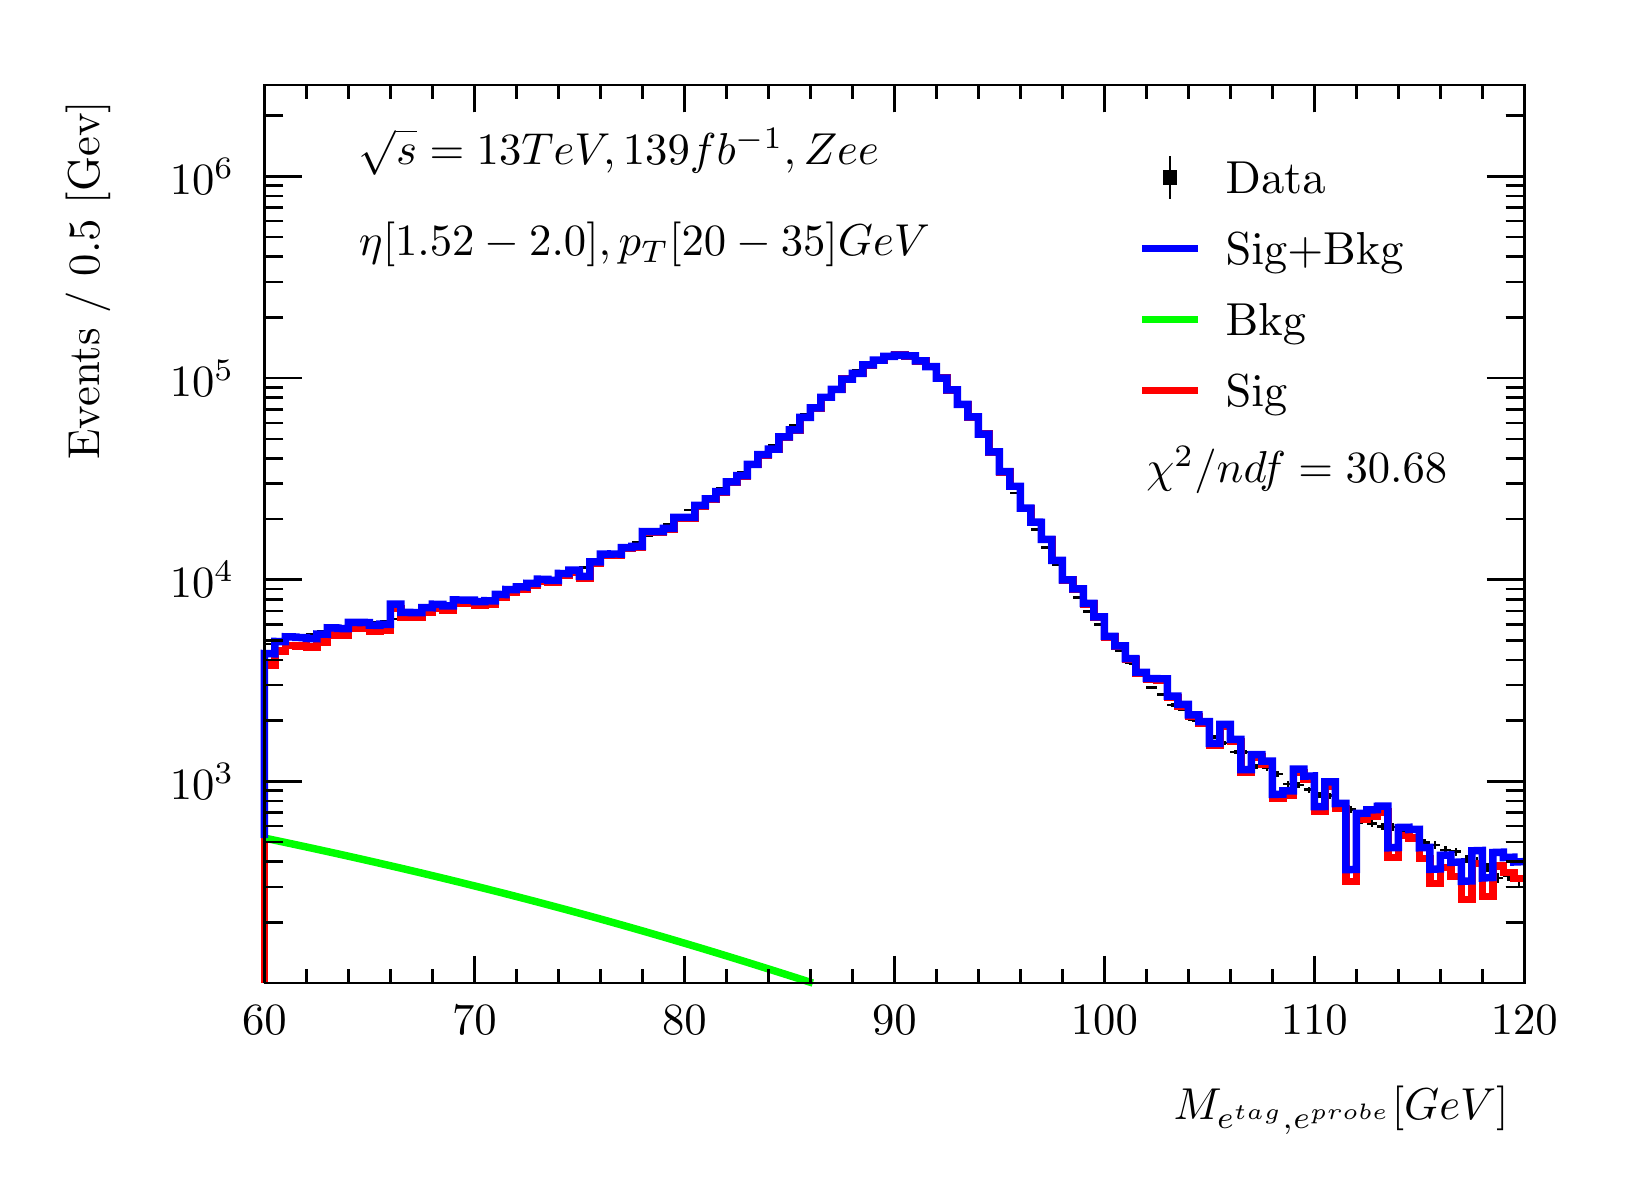
\begin{tikzpicture}
\pgfdeclareplotmark{cross} {
\pgfpathmoveto{\pgfpoint{-0.3\pgfplotmarksize}{\pgfplotmarksize}}
\pgfpathlineto{\pgfpoint{+0.3\pgfplotmarksize}{\pgfplotmarksize}}
\pgfpathlineto{\pgfpoint{+0.3\pgfplotmarksize}{0.3\pgfplotmarksize}}
\pgfpathlineto{\pgfpoint{+1\pgfplotmarksize}{0.3\pgfplotmarksize}}
\pgfpathlineto{\pgfpoint{+1\pgfplotmarksize}{-0.3\pgfplotmarksize}}
\pgfpathlineto{\pgfpoint{+0.3\pgfplotmarksize}{-0.3\pgfplotmarksize}}
\pgfpathlineto{\pgfpoint{+0.3\pgfplotmarksize}{-1.\pgfplotmarksize}}
\pgfpathlineto{\pgfpoint{-0.3\pgfplotmarksize}{-1.\pgfplotmarksize}}
\pgfpathlineto{\pgfpoint{-0.3\pgfplotmarksize}{-0.3\pgfplotmarksize}}
\pgfpathlineto{\pgfpoint{-1.\pgfplotmarksize}{-0.3\pgfplotmarksize}}
\pgfpathlineto{\pgfpoint{-1.\pgfplotmarksize}{0.3\pgfplotmarksize}}
\pgfpathlineto{\pgfpoint{-0.3\pgfplotmarksize}{0.3\pgfplotmarksize}}
\pgfpathclose
\pgfusepathqstroke
}
\pgfdeclareplotmark{cross*} {
\pgfpathmoveto{\pgfpoint{-0.3\pgfplotmarksize}{\pgfplotmarksize}}
\pgfpathlineto{\pgfpoint{+0.3\pgfplotmarksize}{\pgfplotmarksize}}
\pgfpathlineto{\pgfpoint{+0.3\pgfplotmarksize}{0.3\pgfplotmarksize}}
\pgfpathlineto{\pgfpoint{+1\pgfplotmarksize}{0.3\pgfplotmarksize}}
\pgfpathlineto{\pgfpoint{+1\pgfplotmarksize}{-0.3\pgfplotmarksize}}
\pgfpathlineto{\pgfpoint{+0.3\pgfplotmarksize}{-0.3\pgfplotmarksize}}
\pgfpathlineto{\pgfpoint{+0.3\pgfplotmarksize}{-1.\pgfplotmarksize}}
\pgfpathlineto{\pgfpoint{-0.3\pgfplotmarksize}{-1.\pgfplotmarksize}}
\pgfpathlineto{\pgfpoint{-0.3\pgfplotmarksize}{-0.3\pgfplotmarksize}}
\pgfpathlineto{\pgfpoint{-1.\pgfplotmarksize}{-0.3\pgfplotmarksize}}
\pgfpathlineto{\pgfpoint{-1.\pgfplotmarksize}{0.3\pgfplotmarksize}}
\pgfpathlineto{\pgfpoint{-0.3\pgfplotmarksize}{0.3\pgfplotmarksize}}
\pgfpathclose
\pgfusepathqfillstroke
}
\pgfdeclareplotmark{newstar} {
\pgfpathmoveto{\pgfqpoint{0pt}{\pgfplotmarksize}}
\pgfpathlineto{\pgfqpointpolar{44}{0.5\pgfplotmarksize}}
\pgfpathlineto{\pgfqpointpolar{18}{\pgfplotmarksize}}
\pgfpathlineto{\pgfqpointpolar{-20}{0.5\pgfplotmarksize}}
\pgfpathlineto{\pgfqpointpolar{-54}{\pgfplotmarksize}}
\pgfpathlineto{\pgfqpointpolar{-90}{0.5\pgfplotmarksize}}
\pgfpathlineto{\pgfqpointpolar{234}{\pgfplotmarksize}}
\pgfpathlineto{\pgfqpointpolar{198}{0.5\pgfplotmarksize}}
\pgfpathlineto{\pgfqpointpolar{162}{\pgfplotmarksize}}
\pgfpathlineto{\pgfqpointpolar{134}{0.5\pgfplotmarksize}}
\pgfpathclose
\pgfusepathqstroke
}
\pgfdeclareplotmark{newstar*} {
\pgfpathmoveto{\pgfqpoint{0pt}{\pgfplotmarksize}}
\pgfpathlineto{\pgfqpointpolar{44}{0.5\pgfplotmarksize}}
\pgfpathlineto{\pgfqpointpolar{18}{\pgfplotmarksize}}
\pgfpathlineto{\pgfqpointpolar{-20}{0.5\pgfplotmarksize}}
\pgfpathlineto{\pgfqpointpolar{-54}{\pgfplotmarksize}}
\pgfpathlineto{\pgfqpointpolar{-90}{0.5\pgfplotmarksize}}
\pgfpathlineto{\pgfqpointpolar{234}{\pgfplotmarksize}}
\pgfpathlineto{\pgfqpointpolar{198}{0.5\pgfplotmarksize}}
\pgfpathlineto{\pgfqpointpolar{162}{\pgfplotmarksize}}
\pgfpathlineto{\pgfqpointpolar{134}{0.5\pgfplotmarksize}}
\pgfpathclose
\pgfusepathqfillstroke
}
\definecolor{c}{rgb}{1,1,1};
\draw [color=c, fill=c] (0,0) rectangle (20,14.4361);
\draw [color=c, fill=c] (3,2.30977) rectangle (19,13.7143);
\definecolor{c}{rgb}{0,0,0};
\draw [c,line width=0.9] (3,2.30977) -- (3,13.7143) -- (19,13.7143) -- (19,2.30977) -- (3,2.30977);
\definecolor{c}{rgb}{1,1,1};
\draw [color=c, fill=c] (3,2.30977) rectangle (19,13.7143);
\definecolor{c}{rgb}{0,0,0};
\draw [c,line width=0.9] (3,2.30977) -- (3,13.7143) -- (19,13.7143) -- (19,2.30977) -- (3,2.30977);
\draw [c,line width=0.9] (3,2.30977) -- (19,2.30977);
\draw [c,line width=0.9] (3,2.65624) -- (3,2.30977);
\draw [c,line width=0.9] (3.53333,2.48301) -- (3.53333,2.30977);
\draw [c,line width=0.9] (4.06667,2.48301) -- (4.06667,2.30977);
\draw [c,line width=0.9] (4.6,2.48301) -- (4.6,2.30977);
\draw [c,line width=0.9] (5.13333,2.48301) -- (5.13333,2.30977);
\draw [c,line width=0.9] (5.66667,2.65624) -- (5.66667,2.30977);
\draw [c,line width=0.9] (6.2,2.48301) -- (6.2,2.30977);
\draw [c,line width=0.9] (6.73333,2.48301) -- (6.73333,2.30977);
\draw [c,line width=0.9] (7.26667,2.48301) -- (7.26667,2.30977);
\draw [c,line width=0.9] (7.8,2.48301) -- (7.8,2.30977);
\draw [c,line width=0.9] (8.33333,2.65624) -- (8.33333,2.30977);
\draw [c,line width=0.9] (8.86667,2.48301) -- (8.86667,2.30977);
\draw [c,line width=0.9] (9.4,2.48301) -- (9.4,2.30977);
\draw [c,line width=0.9] (9.93333,2.48301) -- (9.93333,2.30977);
\draw [c,line width=0.9] (10.4667,2.48301) -- (10.4667,2.30977);
\draw [c,line width=0.9] (11,2.65624) -- (11,2.30977);
\draw [c,line width=0.9] (11.5333,2.48301) -- (11.5333,2.30977);
\draw [c,line width=0.9] (12.0667,2.48301) -- (12.0667,2.30977);
\draw [c,line width=0.9] (12.6,2.48301) -- (12.6,2.30977);
\draw [c,line width=0.9] (13.1333,2.48301) -- (13.1333,2.30977);
\draw [c,line width=0.9] (13.6667,2.65624) -- (13.6667,2.30977);
\draw [c,line width=0.9] (14.2,2.48301) -- (14.2,2.30977);
\draw [c,line width=0.9] (14.7333,2.48301) -- (14.7333,2.30977);
\draw [c,line width=0.9] (15.2667,2.48301) -- (15.2667,2.30977);
\draw [c,line width=0.9] (15.8,2.48301) -- (15.8,2.30977);
\draw [c,line width=0.9] (16.3333,2.65624) -- (16.3333,2.30977);
\draw [c,line width=0.9] (16.8667,2.48301) -- (16.8667,2.30977);
\draw [c,line width=0.9] (17.4,2.48301) -- (17.4,2.30977);
\draw [c,line width=0.9] (17.9333,2.48301) -- (17.9333,2.30977);
\draw [c,line width=0.9] (18.4667,2.48301) -- (18.4667,2.30977);
\draw [c,line width=0.9] (19,2.65624) -- (19,2.30977);
\draw [anchor=base] (3,1.66015) node[scale=1.61424, color=c, rotate=0]{60};
\draw [anchor=base] (5.66667,1.66015) node[scale=1.61424, color=c, rotate=0]{70};
\draw [anchor=base] (8.33333,1.66015) node[scale=1.61424, color=c, rotate=0]{80};
\draw [anchor=base] (11,1.66015) node[scale=1.61424, color=c, rotate=0]{90};
\draw [anchor=base] (13.6667,1.66015) node[scale=1.61424, color=c, rotate=0]{100};
\draw [anchor=base] (16.3333,1.66015) node[scale=1.61424, color=c, rotate=0]{110};
\draw [anchor=base] (19,1.66015) node[scale=1.61424, color=c, rotate=0]{120};
\draw [anchor= east] (19,0.692932) node[scale=1.61424, color=c, rotate=0]{$M_{e^{tag}, e^{probe}}  [GeV]$};
\draw [c,line width=0.9] (3,13.7143) -- (19,13.7143);
\draw [c,line width=0.9] (3,13.3678) -- (3,13.7143);
\draw [c,line width=0.9] (3.53333,13.5411) -- (3.53333,13.7143);
\draw [c,line width=0.9] (4.06667,13.5411) -- (4.06667,13.7143);
\draw [c,line width=0.9] (4.6,13.5411) -- (4.6,13.7143);
\draw [c,line width=0.9] (5.13333,13.5411) -- (5.13333,13.7143);
\draw [c,line width=0.9] (5.66667,13.3678) -- (5.66667,13.7143);
\draw [c,line width=0.9] (6.2,13.5411) -- (6.2,13.7143);
\draw [c,line width=0.9] (6.73333,13.5411) -- (6.73333,13.7143);
\draw [c,line width=0.9] (7.26667,13.5411) -- (7.26667,13.7143);
\draw [c,line width=0.9] (7.8,13.5411) -- (7.8,13.7143);
\draw [c,line width=0.9] (8.33333,13.3678) -- (8.33333,13.7143);
\draw [c,line width=0.9] (8.86667,13.5411) -- (8.86667,13.7143);
\draw [c,line width=0.9] (9.4,13.5411) -- (9.4,13.7143);
\draw [c,line width=0.9] (9.93333,13.5411) -- (9.93333,13.7143);
\draw [c,line width=0.9] (10.4667,13.5411) -- (10.4667,13.7143);
\draw [c,line width=0.9] (11,13.3678) -- (11,13.7143);
\draw [c,line width=0.9] (11.5333,13.5411) -- (11.5333,13.7143);
\draw [c,line width=0.9] (12.0667,13.5411) -- (12.0667,13.7143);
\draw [c,line width=0.9] (12.6,13.5411) -- (12.6,13.7143);
\draw [c,line width=0.9] (13.1333,13.5411) -- (13.1333,13.7143);
\draw [c,line width=0.9] (13.6667,13.3678) -- (13.6667,13.7143);
\draw [c,line width=0.9] (14.2,13.5411) -- (14.2,13.7143);
\draw [c,line width=0.9] (14.7333,13.5411) -- (14.7333,13.7143);
\draw [c,line width=0.9] (15.2667,13.5411) -- (15.2667,13.7143);
\draw [c,line width=0.9] (15.8,13.5411) -- (15.8,13.7143);
\draw [c,line width=0.9] (16.3333,13.3678) -- (16.3333,13.7143);
\draw [c,line width=0.9] (16.8667,13.5411) -- (16.8667,13.7143);
\draw [c,line width=0.9] (17.4,13.5411) -- (17.4,13.7143);
\draw [c,line width=0.9] (17.9333,13.5411) -- (17.9333,13.7143);
\draw [c,line width=0.9] (18.4667,13.5411) -- (18.4667,13.7143);
\draw [c,line width=0.9] (19,13.3678) -- (19,13.7143);
\draw [c,line width=0.9] (3,2.30977) -- (3,13.7143);
\draw [c,line width=0.9] (3.237,3.08073) -- (3,3.08073);
\draw [c,line width=0.9] (3.237,3.53171) -- (3,3.53171);
\draw [c,line width=0.9] (3.237,3.85168) -- (3,3.85168);
\draw [c,line width=0.9] (3.237,4.09988) -- (3,4.09988);
\draw [c,line width=0.9] (3.237,4.30266) -- (3,4.30266);
\draw [c,line width=0.9] (3.237,4.47412) -- (3,4.47412);
\draw [c,line width=0.9] (3.237,4.62264) -- (3,4.62264);
\draw [c,line width=0.9] (3.237,4.75364) -- (3,4.75364);
\draw [c,line width=0.9] (3.474,4.87083) -- (3,4.87083);
\draw [anchor= east] (2.82,4.87083) node[scale=1.61424, color=c, rotate=0]{$10^{3}$};
\draw [c,line width=0.9] (3.237,5.64179) -- (3,5.64179);
\draw [c,line width=0.9] (3.237,6.09277) -- (3,6.09277);
\draw [c,line width=0.9] (3.237,6.41274) -- (3,6.41274);
\draw [c,line width=0.9] (3.237,6.66093) -- (3,6.66093);
\draw [c,line width=0.9] (3.237,6.86372) -- (3,6.86372);
\draw [c,line width=0.9] (3.237,7.03518) -- (3,7.03518);
\draw [c,line width=0.9] (3.237,7.1837) -- (3,7.1837);
\draw [c,line width=0.9] (3.237,7.3147) -- (3,7.3147);
\draw [c,line width=0.9] (3.474,7.43189) -- (3,7.43189);
\draw [anchor= east] (2.82,7.43189) node[scale=1.61424, color=c, rotate=0]{$10^{4}$};
\draw [c,line width=0.9] (3.237,8.20285) -- (3,8.20285);
\draw [c,line width=0.9] (3.237,8.65383) -- (3,8.65383);
\draw [c,line width=0.9] (3.237,8.9738) -- (3,8.9738);
\draw [c,line width=0.9] (3.237,9.22199) -- (3,9.22199);
\draw [c,line width=0.9] (3.237,9.42478) -- (3,9.42478);
\draw [c,line width=0.9] (3.237,9.59624) -- (3,9.59624);
\draw [c,line width=0.9] (3.237,9.74476) -- (3,9.74476);
\draw [c,line width=0.9] (3.237,9.87576) -- (3,9.87576);
\draw [c,line width=0.9] (3.474,9.99295) -- (3,9.99295);
\draw [anchor= east] (2.82,9.99295) node[scale=1.61424, color=c, rotate=0]{$10^{5}$};
\draw [c,line width=0.9] (3.237,10.7639) -- (3,10.7639);
\draw [c,line width=0.9] (3.237,11.2149) -- (3,11.2149);
\draw [c,line width=0.9] (3.237,11.5349) -- (3,11.5349);
\draw [c,line width=0.9] (3.237,11.7831) -- (3,11.7831);
\draw [c,line width=0.9] (3.237,11.9858) -- (3,11.9858);
\draw [c,line width=0.9] (3.237,12.1573) -- (3,12.1573);
\draw [c,line width=0.9] (3.237,12.3058) -- (3,12.3058);
\draw [c,line width=0.9] (3.237,12.4368) -- (3,12.4368);
\draw [c,line width=0.9] (3.474,12.554) -- (3,12.554);
\draw [anchor= east] (2.82,12.554) node[scale=1.61424, color=c, rotate=0]{$10^{6}$};
\draw [c,line width=0.9] (3.237,13.325) -- (3,13.325);
\draw [anchor= east] (0.76,13.7143) node[scale=1.61424, color=c, rotate=90]{Events / 0.5 [Gev]};
\draw [c,line width=0.9] (19,2.30977) -- (19,13.7143);
\draw [c,line width=0.9] (18.763,3.08073) -- (19,3.08073);
\draw [c,line width=0.9] (18.763,3.53171) -- (19,3.53171);
\draw [c,line width=0.9] (18.763,3.85168) -- (19,3.85168);
\draw [c,line width=0.9] (18.763,4.09988) -- (19,4.09988);
\draw [c,line width=0.9] (18.763,4.30266) -- (19,4.30266);
\draw [c,line width=0.9] (18.763,4.47412) -- (19,4.47412);
\draw [c,line width=0.9] (18.763,4.62264) -- (19,4.62264);
\draw [c,line width=0.9] (18.763,4.75364) -- (19,4.75364);
\draw [c,line width=0.9] (18.526,4.87083) -- (19,4.87083);
\draw [c,line width=0.9] (18.763,5.64179) -- (19,5.64179);
\draw [c,line width=0.9] (18.763,6.09277) -- (19,6.09277);
\draw [c,line width=0.9] (18.763,6.41274) -- (19,6.41274);
\draw [c,line width=0.9] (18.763,6.66093) -- (19,6.66093);
\draw [c,line width=0.9] (18.763,6.86372) -- (19,6.86372);
\draw [c,line width=0.9] (18.763,7.03518) -- (19,7.03518);
\draw [c,line width=0.9] (18.763,7.1837) -- (19,7.1837);
\draw [c,line width=0.9] (18.763,7.3147) -- (19,7.3147);
\draw [c,line width=0.9] (18.526,7.43189) -- (19,7.43189);
\draw [c,line width=0.9] (18.763,8.20285) -- (19,8.20285);
\draw [c,line width=0.9] (18.763,8.65383) -- (19,8.65383);
\draw [c,line width=0.9] (18.763,8.9738) -- (19,8.9738);
\draw [c,line width=0.9] (18.763,9.22199) -- (19,9.22199);
\draw [c,line width=0.9] (18.763,9.42478) -- (19,9.42478);
\draw [c,line width=0.9] (18.763,9.59624) -- (19,9.59624);
\draw [c,line width=0.9] (18.763,9.74476) -- (19,9.74476);
\draw [c,line width=0.9] (18.763,9.87576) -- (19,9.87576);
\draw [c,line width=0.9] (18.526,9.99295) -- (19,9.99295);
\draw [c,line width=0.9] (18.763,10.7639) -- (19,10.7639);
\draw [c,line width=0.9] (18.763,11.2149) -- (19,11.2149);
\draw [c,line width=0.9] (18.763,11.5349) -- (19,11.5349);
\draw [c,line width=0.9] (18.763,11.7831) -- (19,11.7831);
\draw [c,line width=0.9] (18.763,11.9858) -- (19,11.9858);
\draw [c,line width=0.9] (18.763,12.1573) -- (19,12.1573);
\draw [c,line width=0.9] (18.763,12.3058) -- (19,12.3058);
\draw [c,line width=0.9] (18.763,12.4368) -- (19,12.4368);
\draw [c,line width=0.9] (18.526,12.554) -- (19,12.554);
\draw [c,line width=0.9] (18.763,13.325) -- (19,13.325);
\draw [c,line width=0.9] (3.06667,6.61437) -- (3,6.61437);
\draw [c,line width=0.9] (3,6.61437) -- (3,6.61437);
\draw [c,line width=0.9] (3.06667,6.61437) -- (3.13333,6.61437);
\draw [c,line width=0.9] (3.13333,6.61437) -- (3.13333,6.61437);
\draw [c,line width=0.9] (3.06667,6.61437) -- (3.06667,6.63043);
\draw [c,line width=0.9] (3.06667,6.63043) -- (3.06667,6.63043);
\draw [c,line width=0.9] (3.06667,6.61437) -- (3.06667,6.59831);
\draw [c,line width=0.9] (3.06667,6.59831) -- (3.06667,6.59831);
\draw [c,line width=0.9] (3.2,6.65312) -- (3.13333,6.65312);
\draw [c,line width=0.9] (3.13333,6.65312) -- (3.13333,6.65312);
\draw [c,line width=0.9] (3.2,6.65312) -- (3.26667,6.65312);
\draw [c,line width=0.9] (3.26667,6.65312) -- (3.26667,6.65312);
\draw [c,line width=0.9] (3.2,6.65312) -- (3.2,6.66891);
\draw [c,line width=0.9] (3.2,6.66891) -- (3.2,6.66891);
\draw [c,line width=0.9] (3.2,6.65312) -- (3.2,6.63734);
\draw [c,line width=0.9] (3.2,6.63734) -- (3.2,6.63734);
\draw [c,line width=0.9] (3.33333,6.68187) -- (3.26667,6.68187);
\draw [c,line width=0.9] (3.26667,6.68187) -- (3.26667,6.68187);
\draw [c,line width=0.9] (3.33333,6.68187) -- (3.4,6.68187);
\draw [c,line width=0.9] (3.4,6.68187) -- (3.4,6.68187);
\draw [c,line width=0.9] (3.33333,6.68187) -- (3.33333,6.69745);
\draw [c,line width=0.9] (3.33333,6.69745) -- (3.33333,6.69745);
\draw [c,line width=0.9] (3.33333,6.68187) -- (3.33333,6.66629);
\draw [c,line width=0.9] (3.33333,6.66629) -- (3.33333,6.66629);
\draw [c,line width=0.9] (3.46667,6.70776) -- (3.4,6.70776);
\draw [c,line width=0.9] (3.4,6.70776) -- (3.4,6.70776);
\draw [c,line width=0.9] (3.46667,6.70776) -- (3.53333,6.70776);
\draw [c,line width=0.9] (3.53333,6.70776) -- (3.53333,6.70776);
\draw [c,line width=0.9] (3.46667,6.70776) -- (3.46667,6.72317);
\draw [c,line width=0.9] (3.46667,6.72317) -- (3.46667,6.72317);
\draw [c,line width=0.9] (3.46667,6.70776) -- (3.46667,6.69236);
\draw [c,line width=0.9] (3.46667,6.69236) -- (3.46667,6.69236);
\draw [c,line width=0.9] (3.6,6.73744) -- (3.53333,6.73744);
\draw [c,line width=0.9] (3.53333,6.73744) -- (3.53333,6.73744);
\draw [c,line width=0.9] (3.6,6.73744) -- (3.66667,6.73744);
\draw [c,line width=0.9] (3.66667,6.73744) -- (3.66667,6.73744);
\draw [c,line width=0.9] (3.6,6.73744) -- (3.6,6.75263);
\draw [c,line width=0.9] (3.6,6.75263) -- (3.6,6.75263);
\draw [c,line width=0.9] (3.6,6.73744) -- (3.6,6.72224);
\draw [c,line width=0.9] (3.6,6.72224) -- (3.6,6.72224);
\draw [c,line width=0.9] (3.73333,6.78041) -- (3.66667,6.78041);
\draw [c,line width=0.9] (3.66667,6.78041) -- (3.66667,6.78041);
\draw [c,line width=0.9] (3.73333,6.78041) -- (3.8,6.78041);
\draw [c,line width=0.9] (3.8,6.78041) -- (3.8,6.78041);
\draw [c,line width=0.9] (3.73333,6.78041) -- (3.73333,6.79532);
\draw [c,line width=0.9] (3.73333,6.79532) -- (3.73333,6.79532);
\draw [c,line width=0.9] (3.73333,6.78041) -- (3.73333,6.76551);
\draw [c,line width=0.9] (3.73333,6.76551) -- (3.73333,6.76551);
\draw [c,line width=0.9] (3.86667,6.81561) -- (3.8,6.81561);
\draw [c,line width=0.9] (3.8,6.81561) -- (3.8,6.81561);
\draw [c,line width=0.9] (3.86667,6.81561) -- (3.93333,6.81561);
\draw [c,line width=0.9] (3.93333,6.81561) -- (3.93333,6.81561);
\draw [c,line width=0.9] (3.86667,6.81561) -- (3.86667,6.83029);
\draw [c,line width=0.9] (3.86667,6.83029) -- (3.86667,6.83029);
\draw [c,line width=0.9] (3.86667,6.81561) -- (3.86667,6.80094);
\draw [c,line width=0.9] (3.86667,6.80094) -- (3.86667,6.80094);
\draw [c,line width=0.9] (4,6.82352) -- (3.93333,6.82352);
\draw [c,line width=0.9] (3.93333,6.82352) -- (3.93333,6.82352);
\draw [c,line width=0.9] (4,6.82352) -- (4.06667,6.82352);
\draw [c,line width=0.9] (4.06667,6.82352) -- (4.06667,6.82352);
\draw [c,line width=0.9] (4,6.82352) -- (4,6.83814);
\draw [c,line width=0.9] (4,6.83814) -- (4,6.83814);
\draw [c,line width=0.9] (4,6.82352) -- (4,6.8089);
\draw [c,line width=0.9] (4,6.8089) -- (4,6.8089);
\draw [c,line width=0.9] (4.13333,6.88484) -- (4.06667,6.88484);
\draw [c,line width=0.9] (4.06667,6.88484) -- (4.06667,6.88484);
\draw [c,line width=0.9] (4.13333,6.88484) -- (4.2,6.88484);
\draw [c,line width=0.9] (4.2,6.88484) -- (4.2,6.88484);
\draw [c,line width=0.9] (4.13333,6.88484) -- (4.13333,6.89906);
\draw [c,line width=0.9] (4.13333,6.89906) -- (4.13333,6.89906);
\draw [c,line width=0.9] (4.13333,6.88484) -- (4.13333,6.87062);
\draw [c,line width=0.9] (4.13333,6.87062) -- (4.13333,6.87062);
\draw [c,line width=0.9] (4.26667,6.88575) -- (4.2,6.88575);
\draw [c,line width=0.9] (4.2,6.88575) -- (4.2,6.88575);
\draw [c,line width=0.9] (4.26667,6.88575) -- (4.33333,6.88575);
\draw [c,line width=0.9] (4.33333,6.88575) -- (4.33333,6.88575);
\draw [c,line width=0.9] (4.26667,6.88575) -- (4.26667,6.89997);
\draw [c,line width=0.9] (4.26667,6.89997) -- (4.26667,6.89997);
\draw [c,line width=0.9] (4.26667,6.88575) -- (4.26667,6.87153);
\draw [c,line width=0.9] (4.26667,6.87153) -- (4.26667,6.87153);
\draw [c,line width=0.9] (4.4,6.89372) -- (4.33333,6.89372);
\draw [c,line width=0.9] (4.33333,6.89372) -- (4.33333,6.89372);
\draw [c,line width=0.9] (4.4,6.89372) -- (4.46667,6.89372);
\draw [c,line width=0.9] (4.46667,6.89372) -- (4.46667,6.89372);
\draw [c,line width=0.9] (4.4,6.89372) -- (4.4,6.90788);
\draw [c,line width=0.9] (4.4,6.90788) -- (4.4,6.90788);
\draw [c,line width=0.9] (4.4,6.89372) -- (4.4,6.87955);
\draw [c,line width=0.9] (4.4,6.87955) -- (4.4,6.87955);
\draw [c,line width=0.9] (4.53333,6.90877) -- (4.46667,6.90877);
\draw [c,line width=0.9] (4.46667,6.90877) -- (4.46667,6.90877);
\draw [c,line width=0.9] (4.53333,6.90877) -- (4.6,6.90877);
\draw [c,line width=0.9] (4.6,6.90877) -- (4.6,6.90877);
\draw [c,line width=0.9] (4.53333,6.90877) -- (4.53333,6.92284);
\draw [c,line width=0.9] (4.53333,6.92284) -- (4.53333,6.92284);
\draw [c,line width=0.9] (4.53333,6.90877) -- (4.53333,6.8947);
\draw [c,line width=0.9] (4.53333,6.8947) -- (4.53333,6.8947);
\draw [c,line width=0.9] (4.66667,6.93516) -- (4.6,6.93516);
\draw [c,line width=0.9] (4.6,6.93516) -- (4.6,6.93516);
\draw [c,line width=0.9] (4.66667,6.93516) -- (4.73333,6.93516);
\draw [c,line width=0.9] (4.73333,6.93516) -- (4.73333,6.93516);
\draw [c,line width=0.9] (4.66667,6.93516) -- (4.66667,6.94906);
\draw [c,line width=0.9] (4.66667,6.94906) -- (4.66667,6.94906);
\draw [c,line width=0.9] (4.66667,6.93516) -- (4.66667,6.92125);
\draw [c,line width=0.9] (4.66667,6.92125) -- (4.66667,6.92125);
\draw [c,line width=0.9] (4.8,6.96838) -- (4.73333,6.96838);
\draw [c,line width=0.9] (4.73333,6.96838) -- (4.73333,6.96838);
\draw [c,line width=0.9] (4.8,6.96838) -- (4.86667,6.96838);
\draw [c,line width=0.9] (4.86667,6.96838) -- (4.86667,6.96838);
\draw [c,line width=0.9] (4.8,6.96838) -- (4.8,6.98208);
\draw [c,line width=0.9] (4.8,6.98208) -- (4.8,6.98208);
\draw [c,line width=0.9] (4.8,6.96838) -- (4.8,6.95468);
\draw [c,line width=0.9] (4.8,6.95468) -- (4.8,6.95468);
\draw [c,line width=0.9] (4.93333,6.99572) -- (4.86667,6.99572);
\draw [c,line width=0.9] (4.86667,6.99572) -- (4.86667,6.99572);
\draw [c,line width=0.9] (4.93333,6.99572) -- (5,6.99572);
\draw [c,line width=0.9] (5,6.99572) -- (5,6.99572);
\draw [c,line width=0.9] (4.93333,6.99572) -- (4.93333,7.00925);
\draw [c,line width=0.9] (4.93333,7.00925) -- (4.93333,7.00925);
\draw [c,line width=0.9] (4.93333,6.99572) -- (4.93333,6.98218);
\draw [c,line width=0.9] (4.93333,6.98218) -- (4.93333,6.98218);
\draw [c,line width=0.9] (5.06667,7.0288) -- (5,7.0288);
\draw [c,line width=0.9] (5,7.0288) -- (5,7.0288);
\draw [c,line width=0.9] (5.06667,7.0288) -- (5.13333,7.0288);
\draw [c,line width=0.9] (5.13333,7.0288) -- (5.13333,7.0288);
\draw [c,line width=0.9] (5.06667,7.0288) -- (5.06667,7.04214);
\draw [c,line width=0.9] (5.06667,7.04214) -- (5.06667,7.04214);
\draw [c,line width=0.9] (5.06667,7.0288) -- (5.06667,7.01547);
\draw [c,line width=0.9] (5.06667,7.01547) -- (5.06667,7.01547);
\draw [c,line width=0.9] (5.2,7.06218) -- (5.13333,7.06218);
\draw [c,line width=0.9] (5.13333,7.06218) -- (5.13333,7.06218);
\draw [c,line width=0.9] (5.2,7.06218) -- (5.26667,7.06218);
\draw [c,line width=0.9] (5.26667,7.06218) -- (5.26667,7.06218);
\draw [c,line width=0.9] (5.2,7.06218) -- (5.2,7.07531);
\draw [c,line width=0.9] (5.2,7.07531) -- (5.2,7.07531);
\draw [c,line width=0.9] (5.2,7.06218) -- (5.2,7.04904);
\draw [c,line width=0.9] (5.2,7.04904) -- (5.2,7.04904);
\draw [c,line width=0.9] (5.33333,7.06342) -- (5.26667,7.06342);
\draw [c,line width=0.9] (5.26667,7.06342) -- (5.26667,7.06342);
\draw [c,line width=0.9] (5.33333,7.06342) -- (5.4,7.06342);
\draw [c,line width=0.9] (5.4,7.06342) -- (5.4,7.06342);
\draw [c,line width=0.9] (5.33333,7.06342) -- (5.33333,7.07654);
\draw [c,line width=0.9] (5.33333,7.07654) -- (5.33333,7.07654);
\draw [c,line width=0.9] (5.33333,7.06342) -- (5.33333,7.05029);
\draw [c,line width=0.9] (5.33333,7.05029) -- (5.33333,7.05029);
\draw [c,line width=0.9] (5.46667,7.09639) -- (5.4,7.09639);
\draw [c,line width=0.9] (5.4,7.09639) -- (5.4,7.09639);
\draw [c,line width=0.9] (5.46667,7.09639) -- (5.53333,7.09639);
\draw [c,line width=0.9] (5.53333,7.09639) -- (5.53333,7.09639);
\draw [c,line width=0.9] (5.46667,7.09639) -- (5.46667,7.10932);
\draw [c,line width=0.9] (5.46667,7.10932) -- (5.46667,7.10932);
\draw [c,line width=0.9] (5.46667,7.09639) -- (5.46667,7.08345);
\draw [c,line width=0.9] (5.46667,7.08345) -- (5.46667,7.08345);
\draw [c,line width=0.9] (5.6,7.15211) -- (5.53333,7.15211);
\draw [c,line width=0.9] (5.53333,7.15211) -- (5.53333,7.15211);
\draw [c,line width=0.9] (5.6,7.15211) -- (5.66667,7.15211);
\draw [c,line width=0.9] (5.66667,7.15211) -- (5.66667,7.15211);
\draw [c,line width=0.9] (5.6,7.15211) -- (5.6,7.16472);
\draw [c,line width=0.9] (5.6,7.16472) -- (5.6,7.16472);
\draw [c,line width=0.9] (5.6,7.15211) -- (5.6,7.1395);
\draw [c,line width=0.9] (5.6,7.1395) -- (5.6,7.1395);
\draw [c,line width=0.9] (5.73333,7.16009) -- (5.66667,7.16009);
\draw [c,line width=0.9] (5.66667,7.16009) -- (5.66667,7.16009);
\draw [c,line width=0.9] (5.73333,7.16009) -- (5.8,7.16009);
\draw [c,line width=0.9] (5.8,7.16009) -- (5.8,7.16009);
\draw [c,line width=0.9] (5.73333,7.16009) -- (5.73333,7.17266);
\draw [c,line width=0.9] (5.73333,7.17266) -- (5.73333,7.17266);
\draw [c,line width=0.9] (5.73333,7.16009) -- (5.73333,7.14753);
\draw [c,line width=0.9] (5.73333,7.14753) -- (5.73333,7.14753);
\draw [c,line width=0.9] (5.86667,7.18952) -- (5.8,7.18952);
\draw [c,line width=0.9] (5.8,7.18952) -- (5.8,7.18952);
\draw [c,line width=0.9] (5.86667,7.18952) -- (5.93333,7.18952);
\draw [c,line width=0.9] (5.93333,7.18952) -- (5.93333,7.18952);
\draw [c,line width=0.9] (5.86667,7.18952) -- (5.86667,7.20193);
\draw [c,line width=0.9] (5.86667,7.20193) -- (5.86667,7.20193);
\draw [c,line width=0.9] (5.86667,7.18952) -- (5.86667,7.17712);
\draw [c,line width=0.9] (5.86667,7.17712) -- (5.86667,7.17712);
\draw [c,line width=0.9] (6,7.22679) -- (5.93333,7.22679);
\draw [c,line width=0.9] (5.93333,7.22679) -- (5.93333,7.22679);
\draw [c,line width=0.9] (6,7.22679) -- (6.06667,7.22679);
\draw [c,line width=0.9] (6.06667,7.22679) -- (6.06667,7.22679);
\draw [c,line width=0.9] (6,7.22679) -- (6,7.23898);
\draw [c,line width=0.9] (6,7.23898) -- (6,7.23898);
\draw [c,line width=0.9] (6,7.22679) -- (6,7.21459);
\draw [c,line width=0.9] (6,7.21459) -- (6,7.21459);
\draw [c,line width=0.9] (6.13333,7.25947) -- (6.06667,7.25947);
\draw [c,line width=0.9] (6.06667,7.25947) -- (6.06667,7.25947);
\draw [c,line width=0.9] (6.13333,7.25947) -- (6.2,7.25947);
\draw [c,line width=0.9] (6.2,7.25947) -- (6.2,7.25947);
\draw [c,line width=0.9] (6.13333,7.25947) -- (6.13333,7.27149);
\draw [c,line width=0.9] (6.13333,7.27149) -- (6.13333,7.27149);
\draw [c,line width=0.9] (6.13333,7.25947) -- (6.13333,7.24745);
\draw [c,line width=0.9] (6.13333,7.24745) -- (6.13333,7.24745);
\draw [c,line width=0.9] (6.26667,7.28223) -- (6.2,7.28223);
\draw [c,line width=0.9] (6.2,7.28223) -- (6.2,7.28223);
\draw [c,line width=0.9] (6.26667,7.28223) -- (6.33333,7.28223);
\draw [c,line width=0.9] (6.33333,7.28223) -- (6.33333,7.28223);
\draw [c,line width=0.9] (6.26667,7.28223) -- (6.26667,7.29412);
\draw [c,line width=0.9] (6.26667,7.29412) -- (6.26667,7.29412);
\draw [c,line width=0.9] (6.26667,7.28223) -- (6.26667,7.27033);
\draw [c,line width=0.9] (6.26667,7.27033) -- (6.26667,7.27033);
\draw [c,line width=0.9] (6.4,7.3594) -- (6.33333,7.3594);
\draw [c,line width=0.9] (6.33333,7.3594) -- (6.33333,7.3594);
\draw [c,line width=0.9] (6.4,7.3594) -- (6.46667,7.3594);
\draw [c,line width=0.9] (6.46667,7.3594) -- (6.46667,7.3594);
\draw [c,line width=0.9] (6.4,7.3594) -- (6.4,7.37089);
\draw [c,line width=0.9] (6.4,7.37089) -- (6.4,7.37089);
\draw [c,line width=0.9] (6.4,7.3594) -- (6.4,7.34791);
\draw [c,line width=0.9] (6.4,7.34791) -- (6.4,7.34791);
\draw [c,line width=0.9] (6.53333,7.39675) -- (6.46667,7.39675);
\draw [c,line width=0.9] (6.46667,7.39675) -- (6.46667,7.39675);
\draw [c,line width=0.9] (6.53333,7.39675) -- (6.6,7.39675);
\draw [c,line width=0.9] (6.6,7.39675) -- (6.6,7.39675);
\draw [c,line width=0.9] (6.53333,7.39675) -- (6.53333,7.40805);
\draw [c,line width=0.9] (6.53333,7.40805) -- (6.53333,7.40805);
\draw [c,line width=0.9] (6.53333,7.39675) -- (6.53333,7.38545);
\draw [c,line width=0.9] (6.53333,7.38545) -- (6.53333,7.38545);
\draw [c,line width=0.9] (6.66667,7.44725) -- (6.6,7.44725);
\draw [c,line width=0.9] (6.6,7.44725) -- (6.6,7.44725);
\draw [c,line width=0.9] (6.66667,7.44725) -- (6.73333,7.44725);
\draw [c,line width=0.9] (6.73333,7.44725) -- (6.73333,7.44725);
\draw [c,line width=0.9] (6.66667,7.44725) -- (6.66667,7.45829);
\draw [c,line width=0.9] (6.66667,7.45829) -- (6.66667,7.45829);
\draw [c,line width=0.9] (6.66667,7.44725) -- (6.66667,7.4362);
\draw [c,line width=0.9] (6.66667,7.4362) -- (6.66667,7.4362);
\draw [c,line width=0.9] (6.8,7.48) -- (6.73333,7.48);
\draw [c,line width=0.9] (6.73333,7.48) -- (6.73333,7.48);
\draw [c,line width=0.9] (6.8,7.48) -- (6.86667,7.48);
\draw [c,line width=0.9] (6.86667,7.48) -- (6.86667,7.48);
\draw [c,line width=0.9] (6.8,7.48) -- (6.8,7.49088);
\draw [c,line width=0.9] (6.8,7.49088) -- (6.8,7.49088);
\draw [c,line width=0.9] (6.8,7.48) -- (6.8,7.46911);
\draw [c,line width=0.9] (6.8,7.46911) -- (6.8,7.46911);
\draw [c,line width=0.9] (6.93333,7.54063) -- (6.86667,7.54063);
\draw [c,line width=0.9] (6.86667,7.54063) -- (6.86667,7.54063);
\draw [c,line width=0.9] (6.93333,7.54063) -- (7,7.54063);
\draw [c,line width=0.9] (7,7.54063) -- (7,7.54063);
\draw [c,line width=0.9] (6.93333,7.54063) -- (6.93333,7.55122);
\draw [c,line width=0.9] (6.93333,7.55122) -- (6.93333,7.55122);
\draw [c,line width=0.9] (6.93333,7.54063) -- (6.93333,7.53004);
\draw [c,line width=0.9] (6.93333,7.53004) -- (6.93333,7.53004);
\draw [c,line width=0.9] (7.06667,7.58773) -- (7,7.58773);
\draw [c,line width=0.9] (7,7.58773) -- (7,7.58773);
\draw [c,line width=0.9] (7.06667,7.58773) -- (7.13333,7.58773);
\draw [c,line width=0.9] (7.13333,7.58773) -- (7.13333,7.58773);
\draw [c,line width=0.9] (7.06667,7.58773) -- (7.06667,7.5981);
\draw [c,line width=0.9] (7.06667,7.5981) -- (7.06667,7.5981);
\draw [c,line width=0.9] (7.06667,7.58773) -- (7.06667,7.57736);
\draw [c,line width=0.9] (7.06667,7.57736) -- (7.06667,7.57736);
\draw [c,line width=0.9] (7.2,7.64428) -- (7.13333,7.64428);
\draw [c,line width=0.9] (7.13333,7.64428) -- (7.13333,7.64428);
\draw [c,line width=0.9] (7.2,7.64428) -- (7.26667,7.64428);
\draw [c,line width=0.9] (7.26667,7.64428) -- (7.26667,7.64428);
\draw [c,line width=0.9] (7.2,7.64428) -- (7.2,7.65439);
\draw [c,line width=0.9] (7.2,7.65439) -- (7.2,7.65439);
\draw [c,line width=0.9] (7.2,7.64428) -- (7.2,7.63417);
\draw [c,line width=0.9] (7.2,7.63417) -- (7.2,7.63417);
\draw [c,line width=0.9] (7.33333,7.71787) -- (7.26667,7.71787);
\draw [c,line width=0.9] (7.26667,7.71787) -- (7.26667,7.71787);
\draw [c,line width=0.9] (7.33333,7.71787) -- (7.4,7.71787);
\draw [c,line width=0.9] (7.4,7.71787) -- (7.4,7.71787);
\draw [c,line width=0.9] (7.33333,7.71787) -- (7.33333,7.72765);
\draw [c,line width=0.9] (7.33333,7.72765) -- (7.33333,7.72765);
\draw [c,line width=0.9] (7.33333,7.71787) -- (7.33333,7.70809);
\draw [c,line width=0.9] (7.33333,7.70809) -- (7.33333,7.70809);
\draw [c,line width=0.9] (7.46667,7.77773) -- (7.4,7.77773);
\draw [c,line width=0.9] (7.4,7.77773) -- (7.4,7.77773);
\draw [c,line width=0.9] (7.46667,7.77773) -- (7.53333,7.77773);
\draw [c,line width=0.9] (7.53333,7.77773) -- (7.53333,7.77773);
\draw [c,line width=0.9] (7.46667,7.77773) -- (7.46667,7.78725);
\draw [c,line width=0.9] (7.46667,7.78725) -- (7.46667,7.78725);
\draw [c,line width=0.9] (7.46667,7.77773) -- (7.46667,7.76821);
\draw [c,line width=0.9] (7.46667,7.76821) -- (7.46667,7.76821);
\draw [c,line width=0.9] (7.6,7.85144) -- (7.53333,7.85144);
\draw [c,line width=0.9] (7.53333,7.85144) -- (7.53333,7.85144);
\draw [c,line width=0.9] (7.6,7.85144) -- (7.66667,7.85144);
\draw [c,line width=0.9] (7.66667,7.85144) -- (7.66667,7.85144);
\draw [c,line width=0.9] (7.6,7.85144) -- (7.6,7.86065);
\draw [c,line width=0.9] (7.6,7.86065) -- (7.6,7.86065);
\draw [c,line width=0.9] (7.6,7.85144) -- (7.6,7.84223);
\draw [c,line width=0.9] (7.6,7.84223) -- (7.6,7.84223);
\draw [c,line width=0.9] (7.73333,7.90184) -- (7.66667,7.90184);
\draw [c,line width=0.9] (7.66667,7.90184) -- (7.66667,7.90184);
\draw [c,line width=0.9] (7.73333,7.90184) -- (7.8,7.90184);
\draw [c,line width=0.9] (7.8,7.90184) -- (7.8,7.90184);
\draw [c,line width=0.9] (7.73333,7.90184) -- (7.73333,7.91084);
\draw [c,line width=0.9] (7.73333,7.91084) -- (7.73333,7.91084);
\draw [c,line width=0.9] (7.73333,7.90184) -- (7.73333,7.89284);
\draw [c,line width=0.9] (7.73333,7.89284) -- (7.73333,7.89284);
\draw [c,line width=0.9] (7.86667,7.98591) -- (7.8,7.98591);
\draw [c,line width=0.9] (7.8,7.98591) -- (7.8,7.98591);
\draw [c,line width=0.9] (7.86667,7.98591) -- (7.93333,7.98591);
\draw [c,line width=0.9] (7.93333,7.98591) -- (7.93333,7.98591);
\draw [c,line width=0.9] (7.86667,7.98591) -- (7.86667,7.99458);
\draw [c,line width=0.9] (7.86667,7.99458) -- (7.86667,7.99458);
\draw [c,line width=0.9] (7.86667,7.98591) -- (7.86667,7.97724);
\draw [c,line width=0.9] (7.86667,7.97724) -- (7.86667,7.97724);
\draw [c,line width=0.9] (8,8.06602) -- (7.93333,8.06602);
\draw [c,line width=0.9] (7.93333,8.06602) -- (7.93333,8.06602);
\draw [c,line width=0.9] (8,8.06602) -- (8.06667,8.06602);
\draw [c,line width=0.9] (8.06667,8.06602) -- (8.06667,8.06602);
\draw [c,line width=0.9] (8,8.06602) -- (8,8.07439);
\draw [c,line width=0.9] (8,8.07439) -- (8,8.07439);
\draw [c,line width=0.9] (8,8.06602) -- (8,8.05766);
\draw [c,line width=0.9] (8,8.05766) -- (8,8.05766);
\draw [c,line width=0.9] (8.13333,8.14069) -- (8.06667,8.14069);
\draw [c,line width=0.9] (8.06667,8.14069) -- (8.06667,8.14069);
\draw [c,line width=0.9] (8.13333,8.14069) -- (8.2,8.14069);
\draw [c,line width=0.9] (8.2,8.14069) -- (8.2,8.14069);
\draw [c,line width=0.9] (8.13333,8.14069) -- (8.13333,8.14878);
\draw [c,line width=0.9] (8.13333,8.14878) -- (8.13333,8.14878);
\draw [c,line width=0.9] (8.13333,8.14069) -- (8.13333,8.1326);
\draw [c,line width=0.9] (8.13333,8.1326) -- (8.13333,8.1326);
\draw [c,line width=0.9] (8.26667,8.23356) -- (8.2,8.23356);
\draw [c,line width=0.9] (8.2,8.23356) -- (8.2,8.23356);
\draw [c,line width=0.9] (8.26667,8.23356) -- (8.33333,8.23356);
\draw [c,line width=0.9] (8.33333,8.23356) -- (8.33333,8.23356);
\draw [c,line width=0.9] (8.26667,8.23356) -- (8.26667,8.24132);
\draw [c,line width=0.9] (8.26667,8.24132) -- (8.26667,8.24132);
\draw [c,line width=0.9] (8.26667,8.23356) -- (8.26667,8.22581);
\draw [c,line width=0.9] (8.26667,8.22581) -- (8.26667,8.22581);
\draw [c,line width=0.9] (8.4,8.31511) -- (8.33333,8.31511);
\draw [c,line width=0.9] (8.33333,8.31511) -- (8.33333,8.31511);
\draw [c,line width=0.9] (8.4,8.31511) -- (8.46667,8.31511);
\draw [c,line width=0.9] (8.46667,8.31511) -- (8.46667,8.31511);
\draw [c,line width=0.9] (8.4,8.31511) -- (8.4,8.32259);
\draw [c,line width=0.9] (8.4,8.32259) -- (8.4,8.32259);
\draw [c,line width=0.9] (8.4,8.31511) -- (8.4,8.30763);
\draw [c,line width=0.9] (8.4,8.30763) -- (8.4,8.30763);
\draw [c,line width=0.9] (8.53333,8.40215) -- (8.46667,8.40215);
\draw [c,line width=0.9] (8.46667,8.40215) -- (8.46667,8.40215);
\draw [c,line width=0.9] (8.53333,8.40215) -- (8.6,8.40215);
\draw [c,line width=0.9] (8.6,8.40215) -- (8.6,8.40215);
\draw [c,line width=0.9] (8.53333,8.40215) -- (8.53333,8.40934);
\draw [c,line width=0.9] (8.53333,8.40934) -- (8.53333,8.40934);
\draw [c,line width=0.9] (8.53333,8.40215) -- (8.53333,8.39496);
\draw [c,line width=0.9] (8.53333,8.39496) -- (8.53333,8.39496);
\draw [c,line width=0.9] (8.66667,8.48818) -- (8.6,8.48818);
\draw [c,line width=0.9] (8.6,8.48818) -- (8.6,8.48818);
\draw [c,line width=0.9] (8.66667,8.48818) -- (8.73333,8.48818);
\draw [c,line width=0.9] (8.73333,8.48818) -- (8.73333,8.48818);
\draw [c,line width=0.9] (8.66667,8.48818) -- (8.66667,8.4951);
\draw [c,line width=0.9] (8.66667,8.4951) -- (8.66667,8.4951);
\draw [c,line width=0.9] (8.66667,8.48818) -- (8.66667,8.48127);
\draw [c,line width=0.9] (8.66667,8.48127) -- (8.66667,8.48127);
\draw [c,line width=0.9] (8.8,8.58941) -- (8.73333,8.58941);
\draw [c,line width=0.9] (8.73333,8.58941) -- (8.73333,8.58941);
\draw [c,line width=0.9] (8.8,8.58941) -- (8.86667,8.58941);
\draw [c,line width=0.9] (8.86667,8.58941) -- (8.86667,8.58941);
\draw [c,line width=0.9] (8.8,8.58941) -- (8.8,8.59602);
\draw [c,line width=0.9] (8.8,8.59602) -- (8.8,8.59602);
\draw [c,line width=0.9] (8.8,8.58941) -- (8.8,8.5828);
\draw [c,line width=0.9] (8.8,8.5828) -- (8.8,8.5828);
\draw [c,line width=0.9] (8.93333,8.70073) -- (8.86667,8.70073);
\draw [c,line width=0.9] (8.86667,8.70073) -- (8.86667,8.70073);
\draw [c,line width=0.9] (8.93333,8.70073) -- (9,8.70073);
\draw [c,line width=0.9] (9,8.70073) -- (9,8.70073);
\draw [c,line width=0.9] (8.93333,8.70073) -- (8.93333,8.70701);
\draw [c,line width=0.9] (8.93333,8.70701) -- (8.93333,8.70701);
\draw [c,line width=0.9] (8.93333,8.70073) -- (8.93333,8.69444);
\draw [c,line width=0.9] (8.93333,8.69444) -- (8.93333,8.69444);
\draw [c,line width=0.9] (9.06667,8.80301) -- (9,8.80301);
\draw [c,line width=0.9] (9,8.80301) -- (9,8.80301);
\draw [c,line width=0.9] (9.06667,8.80301) -- (9.13333,8.80301);
\draw [c,line width=0.9] (9.13333,8.80301) -- (9.13333,8.80301);
\draw [c,line width=0.9] (9.06667,8.80301) -- (9.06667,8.80901);
\draw [c,line width=0.9] (9.06667,8.80901) -- (9.06667,8.80901);
\draw [c,line width=0.9] (9.06667,8.80301) -- (9.06667,8.797);
\draw [c,line width=0.9] (9.06667,8.797) -- (9.06667,8.797);
\draw [c,line width=0.9] (9.2,8.91947) -- (9.13333,8.91947);
\draw [c,line width=0.9] (9.13333,8.91947) -- (9.13333,8.91947);
\draw [c,line width=0.9] (9.2,8.91947) -- (9.26667,8.91947);
\draw [c,line width=0.9] (9.26667,8.91947) -- (9.26667,8.91947);
\draw [c,line width=0.9] (9.2,8.91947) -- (9.2,8.92517);
\draw [c,line width=0.9] (9.2,8.92517) -- (9.2,8.92517);
\draw [c,line width=0.9] (9.2,8.91947) -- (9.2,8.91377);
\draw [c,line width=0.9] (9.2,8.91377) -- (9.2,8.91377);
\draw [c,line width=0.9] (9.33333,9.03003) -- (9.26667,9.03003);
\draw [c,line width=0.9] (9.26667,9.03003) -- (9.26667,9.03003);
\draw [c,line width=0.9] (9.33333,9.03003) -- (9.4,9.03003);
\draw [c,line width=0.9] (9.4,9.03003) -- (9.4,9.03003);
\draw [c,line width=0.9] (9.33333,9.03003) -- (9.33333,9.03545);
\draw [c,line width=0.9] (9.33333,9.03545) -- (9.33333,9.03545);
\draw [c,line width=0.9] (9.33333,9.03003) -- (9.33333,9.0246);
\draw [c,line width=0.9] (9.33333,9.0246) -- (9.33333,9.0246);
\draw [c,line width=0.9] (9.46667,9.14317) -- (9.4,9.14317);
\draw [c,line width=0.9] (9.4,9.14317) -- (9.4,9.14317);
\draw [c,line width=0.9] (9.46667,9.14317) -- (9.53333,9.14317);
\draw [c,line width=0.9] (9.53333,9.14317) -- (9.53333,9.14317);
\draw [c,line width=0.9] (9.46667,9.14317) -- (9.46667,9.14832);
\draw [c,line width=0.9] (9.46667,9.14832) -- (9.46667,9.14832);
\draw [c,line width=0.9] (9.46667,9.14317) -- (9.46667,9.13801);
\draw [c,line width=0.9] (9.46667,9.13801) -- (9.46667,9.13801);
\draw [c,line width=0.9] (9.6,9.27705) -- (9.53333,9.27705);
\draw [c,line width=0.9] (9.53333,9.27705) -- (9.53333,9.27705);
\draw [c,line width=0.9] (9.6,9.27705) -- (9.66667,9.27705);
\draw [c,line width=0.9] (9.66667,9.27705) -- (9.66667,9.27705);
\draw [c,line width=0.9] (9.6,9.27705) -- (9.6,9.2819);
\draw [c,line width=0.9] (9.6,9.2819) -- (9.6,9.2819);
\draw [c,line width=0.9] (9.6,9.27705) -- (9.6,9.27219);
\draw [c,line width=0.9] (9.6,9.27219) -- (9.6,9.27219);
\draw [c,line width=0.9] (9.73333,9.39487) -- (9.66667,9.39487);
\draw [c,line width=0.9] (9.66667,9.39487) -- (9.66667,9.39487);
\draw [c,line width=0.9] (9.73333,9.39487) -- (9.8,9.39487);
\draw [c,line width=0.9] (9.8,9.39487) -- (9.8,9.39487);
\draw [c,line width=0.9] (9.73333,9.39487) -- (9.73333,9.39947);
\draw [c,line width=0.9] (9.73333,9.39947) -- (9.73333,9.39947);
\draw [c,line width=0.9] (9.73333,9.39487) -- (9.73333,9.39027);
\draw [c,line width=0.9] (9.73333,9.39027) -- (9.73333,9.39027);
\draw [c,line width=0.9] (9.86667,9.53049) -- (9.8,9.53049);
\draw [c,line width=0.9] (9.8,9.53049) -- (9.8,9.53049);
\draw [c,line width=0.9] (9.86667,9.53049) -- (9.93333,9.53049);
\draw [c,line width=0.9] (9.93333,9.53049) -- (9.93333,9.53049);
\draw [c,line width=0.9] (9.86667,9.53049) -- (9.86667,9.53482);
\draw [c,line width=0.9] (9.86667,9.53482) -- (9.86667,9.53482);
\draw [c,line width=0.9] (9.86667,9.53049) -- (9.86667,9.52616);
\draw [c,line width=0.9] (9.86667,9.52616) -- (9.86667,9.52616);
\draw [c,line width=0.9] (10,9.65111) -- (9.93333,9.65111);
\draw [c,line width=0.9] (9.93333,9.65111) -- (9.93333,9.65111);
\draw [c,line width=0.9] (10,9.65111) -- (10.0667,9.65111);
\draw [c,line width=0.9] (10.0667,9.65111) -- (10.0667,9.65111);
\draw [c,line width=0.9] (10,9.65111) -- (10,9.65521);
\draw [c,line width=0.9] (10,9.65521) -- (10,9.65521);
\draw [c,line width=0.9] (10,9.65111) -- (10,9.64701);
\draw [c,line width=0.9] (10,9.64701) -- (10,9.64701);
\draw [c,line width=0.9] (10.1333,9.7656) -- (10.0667,9.7656);
\draw [c,line width=0.9] (10.0667,9.7656) -- (10.0667,9.7656);
\draw [c,line width=0.9] (10.1333,9.7656) -- (10.2,9.7656);
\draw [c,line width=0.9] (10.2,9.7656) -- (10.2,9.7656);
\draw [c,line width=0.9] (10.1333,9.7656) -- (10.1333,9.76949);
\draw [c,line width=0.9] (10.1333,9.76949) -- (10.1333,9.76949);
\draw [c,line width=0.9] (10.1333,9.7656) -- (10.1333,9.7617);
\draw [c,line width=0.9] (10.1333,9.7617) -- (10.1333,9.7617);
\draw [c,line width=0.9] (10.2667,9.88009) -- (10.2,9.88009);
\draw [c,line width=0.9] (10.2,9.88009) -- (10.2,9.88009);
\draw [c,line width=0.9] (10.2667,9.88009) -- (10.3333,9.88009);
\draw [c,line width=0.9] (10.3333,9.88009) -- (10.3333,9.88009);
\draw [c,line width=0.9] (10.2667,9.88009) -- (10.2667,9.88379);
\draw [c,line width=0.9] (10.2667,9.88379) -- (10.2667,9.88379);
\draw [c,line width=0.9] (10.2667,9.88009) -- (10.2667,9.87639);
\draw [c,line width=0.9] (10.2667,9.87639) -- (10.2667,9.87639);
\draw [c,line width=0.9] (10.4,9.99129) -- (10.3333,9.99129);
\draw [c,line width=0.9] (10.3333,9.99129) -- (10.3333,9.99129);
\draw [c,line width=0.9] (10.4,9.99129) -- (10.4667,9.99129);
\draw [c,line width=0.9] (10.4667,9.99129) -- (10.4667,9.99129);
\draw [c,line width=0.9] (10.4,9.99129) -- (10.4,9.99481);
\draw [c,line width=0.9] (10.4,9.99481) -- (10.4,9.99481);
\draw [c,line width=0.9] (10.4,9.99129) -- (10.4,9.98777);
\draw [c,line width=0.9] (10.4,9.98777) -- (10.4,9.98777);
\draw [c,line width=0.9] (10.5333,10.0861) -- (10.4667,10.0861);
\draw [c,line width=0.9] (10.4667,10.0861) -- (10.4667,10.0861);
\draw [c,line width=0.9] (10.5333,10.0861) -- (10.6,10.0861);
\draw [c,line width=0.9] (10.6,10.0861) -- (10.6,10.0861);
\draw [c,line width=0.9] (10.5333,10.0861) -- (10.5333,10.0895);
\draw [c,line width=0.9] (10.5333,10.0895) -- (10.5333,10.0895);
\draw [c,line width=0.9] (10.5333,10.0861) -- (10.5333,10.0827);
\draw [c,line width=0.9] (10.5333,10.0827) -- (10.5333,10.0827);
\draw [c,line width=0.9] (10.6667,10.1595) -- (10.6,10.1595);
\draw [c,line width=0.9] (10.6,10.1595) -- (10.6,10.1595);
\draw [c,line width=0.9] (10.6667,10.1595) -- (10.7333,10.1595);
\draw [c,line width=0.9] (10.7333,10.1595) -- (10.7333,10.1595);
\draw [c,line width=0.9] (10.6667,10.1595) -- (10.6667,10.1628);
\draw [c,line width=0.9] (10.6667,10.1628) -- (10.6667,10.1628);
\draw [c,line width=0.9] (10.6667,10.1595) -- (10.6667,10.1563);
\draw [c,line width=0.9] (10.6667,10.1563) -- (10.6667,10.1563);
\draw [c,line width=0.9] (10.8,10.2248) -- (10.7333,10.2248);
\draw [c,line width=0.9] (10.7333,10.2248) -- (10.7333,10.2248);
\draw [c,line width=0.9] (10.8,10.2248) -- (10.8667,10.2248);
\draw [c,line width=0.9] (10.8667,10.2248) -- (10.8667,10.2248);
\draw [c,line width=0.9] (10.8,10.2248) -- (10.8,10.2279);
\draw [c,line width=0.9] (10.8,10.2279) -- (10.8,10.2279);
\draw [c,line width=0.9] (10.8,10.2248) -- (10.8,10.2216);
\draw [c,line width=0.9] (10.8,10.2216) -- (10.8,10.2216);
\draw [c,line width=0.9] (10.9333,10.2644) -- (10.8667,10.2644);
\draw [c,line width=0.9] (10.8667,10.2644) -- (10.8667,10.2644);
\draw [c,line width=0.9] (10.9333,10.2644) -- (11,10.2644);
\draw [c,line width=0.9] (11,10.2644) -- (11,10.2644);
\draw [c,line width=0.9] (10.9333,10.2644) -- (10.9333,10.2675);
\draw [c,line width=0.9] (10.9333,10.2675) -- (10.9333,10.2675);
\draw [c,line width=0.9] (10.9333,10.2644) -- (10.9333,10.2613);
\draw [c,line width=0.9] (10.9333,10.2613) -- (10.9333,10.2613);
\draw [c,line width=0.9] (11.0667,10.2757) -- (11,10.2757);
\draw [c,line width=0.9] (11,10.2757) -- (11,10.2757);
\draw [c,line width=0.9] (11.0667,10.2757) -- (11.1333,10.2757);
\draw [c,line width=0.9] (11.1333,10.2757) -- (11.1333,10.2757);
\draw [c,line width=0.9] (11.0667,10.2757) -- (11.0667,10.2788);
\draw [c,line width=0.9] (11.0667,10.2788) -- (11.0667,10.2788);
\draw [c,line width=0.9] (11.0667,10.2757) -- (11.0667,10.2726);
\draw [c,line width=0.9] (11.0667,10.2726) -- (11.0667,10.2726);
\draw [c,line width=0.9] (11.2,10.2531) -- (11.1333,10.2531);
\draw [c,line width=0.9] (11.1333,10.2531) -- (11.1333,10.2531);
\draw [c,line width=0.9] (11.2,10.2531) -- (11.2667,10.2531);
\draw [c,line width=0.9] (11.2667,10.2531) -- (11.2667,10.2531);
\draw [c,line width=0.9] (11.2,10.2531) -- (11.2,10.2563);
\draw [c,line width=0.9] (11.2,10.2563) -- (11.2,10.2563);
\draw [c,line width=0.9] (11.2,10.2531) -- (11.2,10.25);
\draw [c,line width=0.9] (11.2,10.25) -- (11.2,10.25);
\draw [c,line width=0.9] (11.3333,10.1975) -- (11.2667,10.1975);
\draw [c,line width=0.9] (11.2667,10.1975) -- (11.2667,10.1975);
\draw [c,line width=0.9] (11.3333,10.1975) -- (11.4,10.1975);
\draw [c,line width=0.9] (11.4,10.1975) -- (11.4,10.1975);
\draw [c,line width=0.9] (11.3333,10.1975) -- (11.3333,10.2008);
\draw [c,line width=0.9] (11.3333,10.2008) -- (11.3333,10.2008);
\draw [c,line width=0.9] (11.3333,10.1975) -- (11.3333,10.1943);
\draw [c,line width=0.9] (11.3333,10.1943) -- (11.3333,10.1943);
\draw [c,line width=0.9] (11.4667,10.1188) -- (11.4,10.1188);
\draw [c,line width=0.9] (11.4,10.1188) -- (11.4,10.1188);
\draw [c,line width=0.9] (11.4667,10.1188) -- (11.5333,10.1188);
\draw [c,line width=0.9] (11.5333,10.1188) -- (11.5333,10.1188);
\draw [c,line width=0.9] (11.4667,10.1188) -- (11.4667,10.1221);
\draw [c,line width=0.9] (11.4667,10.1221) -- (11.4667,10.1221);
\draw [c,line width=0.9] (11.4667,10.1188) -- (11.4667,10.1154);
\draw [c,line width=0.9] (11.4667,10.1154) -- (11.4667,10.1154);
\draw [c,line width=0.9] (11.6,9.98617) -- (11.5333,9.98617);
\draw [c,line width=0.9] (11.5333,9.98617) -- (11.5333,9.98617);
\draw [c,line width=0.9] (11.6,9.98617) -- (11.6667,9.98617);
\draw [c,line width=0.9] (11.6667,9.98617) -- (11.6667,9.98617);
\draw [c,line width=0.9] (11.6,9.98617) -- (11.6,9.98969);
\draw [c,line width=0.9] (11.6,9.98969) -- (11.6,9.98969);
\draw [c,line width=0.9] (11.6,9.98617) -- (11.6,9.98264);
\draw [c,line width=0.9] (11.6,9.98264) -- (11.6,9.98264);
\draw [c,line width=0.9] (11.7333,9.8414) -- (11.6667,9.8414);
\draw [c,line width=0.9] (11.6667,9.8414) -- (11.6667,9.8414);
\draw [c,line width=0.9] (11.7333,9.8414) -- (11.8,9.8414);
\draw [c,line width=0.9] (11.8,9.8414) -- (11.8,9.8414);
\draw [c,line width=0.9] (11.7333,9.8414) -- (11.7333,9.84517);
\draw [c,line width=0.9] (11.7333,9.84517) -- (11.7333,9.84517);
\draw [c,line width=0.9] (11.7333,9.8414) -- (11.7333,9.83763);
\draw [c,line width=0.9] (11.7333,9.83763) -- (11.7333,9.83763);
\draw [c,line width=0.9] (11.8667,9.64988) -- (11.8,9.64988);
\draw [c,line width=0.9] (11.8,9.64988) -- (11.8,9.64988);
\draw [c,line width=0.9] (11.8667,9.64988) -- (11.9333,9.64988);
\draw [c,line width=0.9] (11.9333,9.64988) -- (11.9333,9.64988);
\draw [c,line width=0.9] (11.8667,9.64988) -- (11.8667,9.65399);
\draw [c,line width=0.9] (11.8667,9.65399) -- (11.8667,9.65399);
\draw [c,line width=0.9] (11.8667,9.64988) -- (11.8667,9.64578);
\draw [c,line width=0.9] (11.8667,9.64578) -- (11.8667,9.64578);
\draw [c,line width=0.9] (12,9.46093) -- (11.9333,9.46093);
\draw [c,line width=0.9] (11.9333,9.46093) -- (11.9333,9.46093);
\draw [c,line width=0.9] (12,9.46093) -- (12.0667,9.46093);
\draw [c,line width=0.9] (12.0667,9.46093) -- (12.0667,9.46093);
\draw [c,line width=0.9] (12,9.46093) -- (12,9.4654);
\draw [c,line width=0.9] (12,9.4654) -- (12,9.4654);
\draw [c,line width=0.9] (12,9.46093) -- (12,9.45646);
\draw [c,line width=0.9] (12,9.45646) -- (12,9.45646);
\draw [c,line width=0.9] (12.1333,9.244) -- (12.0667,9.244);
\draw [c,line width=0.9] (12.0667,9.244) -- (12.0667,9.244);
\draw [c,line width=0.9] (12.1333,9.244) -- (12.2,9.244);
\draw [c,line width=0.9] (12.2,9.244) -- (12.2,9.244);
\draw [c,line width=0.9] (12.1333,9.244) -- (12.1333,9.24892);
\draw [c,line width=0.9] (12.1333,9.24892) -- (12.1333,9.24892);
\draw [c,line width=0.9] (12.1333,9.244) -- (12.1333,9.23907);
\draw [c,line width=0.9] (12.1333,9.23907) -- (12.1333,9.23907);
\draw [c,line width=0.9] (12.2667,9.01405) -- (12.2,9.01405);
\draw [c,line width=0.9] (12.2,9.01405) -- (12.2,9.01405);
\draw [c,line width=0.9] (12.2667,9.01405) -- (12.3333,9.01405);
\draw [c,line width=0.9] (12.3333,9.01405) -- (12.3333,9.01405);
\draw [c,line width=0.9] (12.2667,9.01405) -- (12.2667,9.01951);
\draw [c,line width=0.9] (12.2667,9.01951) -- (12.2667,9.01951);
\draw [c,line width=0.9] (12.2667,9.01405) -- (12.2667,9.00859);
\draw [c,line width=0.9] (12.2667,9.00859) -- (12.2667,9.00859);
\draw [c,line width=0.9] (12.4,8.78381) -- (12.3333,8.78381);
\draw [c,line width=0.9] (12.3333,8.78381) -- (12.3333,8.78381);
\draw [c,line width=0.9] (12.4,8.78381) -- (12.4667,8.78381);
\draw [c,line width=0.9] (12.4667,8.78381) -- (12.4667,8.78381);
\draw [c,line width=0.9] (12.4,8.78381) -- (12.4,8.78987);
\draw [c,line width=0.9] (12.4,8.78987) -- (12.4,8.78987);
\draw [c,line width=0.9] (12.4,8.78381) -- (12.4,8.77775);
\draw [c,line width=0.9] (12.4,8.77775) -- (12.4,8.77775);
\draw [c,line width=0.9] (12.5333,8.53355) -- (12.4667,8.53355);
\draw [c,line width=0.9] (12.4667,8.53355) -- (12.4667,8.53355);
\draw [c,line width=0.9] (12.5333,8.53355) -- (12.6,8.53355);
\draw [c,line width=0.9] (12.6,8.53355) -- (12.6,8.53355);
\draw [c,line width=0.9] (12.5333,8.53355) -- (12.5333,8.54032);
\draw [c,line width=0.9] (12.5333,8.54032) -- (12.5333,8.54032);
\draw [c,line width=0.9] (12.5333,8.53355) -- (12.5333,8.52677);
\draw [c,line width=0.9] (12.5333,8.52677) -- (12.5333,8.52677);
\draw [c,line width=0.9] (12.6667,8.31722) -- (12.6,8.31722);
\draw [c,line width=0.9] (12.6,8.31722) -- (12.6,8.31722);
\draw [c,line width=0.9] (12.6667,8.31722) -- (12.7333,8.31722);
\draw [c,line width=0.9] (12.7333,8.31722) -- (12.7333,8.31722);
\draw [c,line width=0.9] (12.6667,8.31722) -- (12.6667,8.32469);
\draw [c,line width=0.9] (12.6667,8.32469) -- (12.6667,8.32469);
\draw [c,line width=0.9] (12.6667,8.31722) -- (12.6667,8.30975);
\draw [c,line width=0.9] (12.6667,8.30975) -- (12.6667,8.30975);
\draw [c,line width=0.9] (12.8,8.07248) -- (12.7333,8.07248);
\draw [c,line width=0.9] (12.7333,8.07248) -- (12.7333,8.07248);
\draw [c,line width=0.9] (12.8,8.07248) -- (12.8667,8.07248);
\draw [c,line width=0.9] (12.8667,8.07248) -- (12.8667,8.07248);
\draw [c,line width=0.9] (12.8,8.07248) -- (12.8,8.08082);
\draw [c,line width=0.9] (12.8,8.08082) -- (12.8,8.08082);
\draw [c,line width=0.9] (12.8,8.07248) -- (12.8,8.06414);
\draw [c,line width=0.9] (12.8,8.06414) -- (12.8,8.06414);
\draw [c,line width=0.9] (12.9333,7.84263) -- (12.8667,7.84263);
\draw [c,line width=0.9] (12.8667,7.84263) -- (12.8667,7.84263);
\draw [c,line width=0.9] (12.9333,7.84263) -- (13,7.84263);
\draw [c,line width=0.9] (13,7.84263) -- (13,7.84263);
\draw [c,line width=0.9] (12.9333,7.84263) -- (12.9333,7.85188);
\draw [c,line width=0.9] (12.9333,7.85188) -- (12.9333,7.85188);
\draw [c,line width=0.9] (12.9333,7.84263) -- (12.9333,7.83338);
\draw [c,line width=0.9] (12.9333,7.83338) -- (12.9333,7.83338);
\draw [c,line width=0.9] (13.0667,7.62518) -- (13,7.62518);
\draw [c,line width=0.9] (13,7.62518) -- (13,7.62518);
\draw [c,line width=0.9] (13.0667,7.62518) -- (13.1333,7.62518);
\draw [c,line width=0.9] (13.1333,7.62518) -- (13.1333,7.62518);
\draw [c,line width=0.9] (13.0667,7.62518) -- (13.0667,7.63538);
\draw [c,line width=0.9] (13.0667,7.63538) -- (13.0667,7.63538);
\draw [c,line width=0.9] (13.0667,7.62518) -- (13.0667,7.61499);
\draw [c,line width=0.9] (13.0667,7.61499) -- (13.0667,7.61499);
\draw [c,line width=0.9] (13.2,7.40464) -- (13.1333,7.40464);
\draw [c,line width=0.9] (13.1333,7.40464) -- (13.1333,7.40464);
\draw [c,line width=0.9] (13.2,7.40464) -- (13.2667,7.40464);
\draw [c,line width=0.9] (13.2667,7.40464) -- (13.2667,7.40464);
\draw [c,line width=0.9] (13.2,7.40464) -- (13.2,7.4159);
\draw [c,line width=0.9] (13.2,7.4159) -- (13.2,7.4159);
\draw [c,line width=0.9] (13.2,7.40464) -- (13.2,7.39338);
\draw [c,line width=0.9] (13.2,7.39338) -- (13.2,7.39338);
\draw [c,line width=0.9] (13.3333,7.20709) -- (13.2667,7.20709);
\draw [c,line width=0.9] (13.2667,7.20709) -- (13.2667,7.20709);
\draw [c,line width=0.9] (13.3333,7.20709) -- (13.4,7.20709);
\draw [c,line width=0.9] (13.4,7.20709) -- (13.4,7.20709);
\draw [c,line width=0.9] (13.3333,7.20709) -- (13.3333,7.21939);
\draw [c,line width=0.9] (13.3333,7.21939) -- (13.3333,7.21939);
\draw [c,line width=0.9] (13.3333,7.20709) -- (13.3333,7.19478);
\draw [c,line width=0.9] (13.3333,7.19478) -- (13.3333,7.19478);
\draw [c,line width=0.9] (13.4667,7.02753) -- (13.4,7.02753);
\draw [c,line width=0.9] (13.4,7.02753) -- (13.4,7.02753);
\draw [c,line width=0.9] (13.4667,7.02753) -- (13.5333,7.02753);
\draw [c,line width=0.9] (13.5333,7.02753) -- (13.5333,7.02753);
\draw [c,line width=0.9] (13.4667,7.02753) -- (13.4667,7.04086);
\draw [c,line width=0.9] (13.4667,7.04086) -- (13.4667,7.04086);
\draw [c,line width=0.9] (13.4667,7.02753) -- (13.4667,7.01419);
\draw [c,line width=0.9] (13.4667,7.01419) -- (13.4667,7.01419);
\draw [c,line width=0.9] (13.6,6.86187) -- (13.5333,6.86187);
\draw [c,line width=0.9] (13.5333,6.86187) -- (13.5333,6.86187);
\draw [c,line width=0.9] (13.6,6.86187) -- (13.6667,6.86187);
\draw [c,line width=0.9] (13.6667,6.86187) -- (13.6667,6.86187);
\draw [c,line width=0.9] (13.6,6.86187) -- (13.6,6.87624);
\draw [c,line width=0.9] (13.6,6.87624) -- (13.6,6.87624);
\draw [c,line width=0.9] (13.6,6.86187) -- (13.6,6.8475);
\draw [c,line width=0.9] (13.6,6.8475) -- (13.6,6.8475);
\draw [c,line width=0.9] (13.7333,6.68688) -- (13.6667,6.68688);
\draw [c,line width=0.9] (13.6667,6.68688) -- (13.6667,6.68688);
\draw [c,line width=0.9] (13.7333,6.68688) -- (13.8,6.68688);
\draw [c,line width=0.9] (13.8,6.68688) -- (13.8,6.68688);
\draw [c,line width=0.9] (13.7333,6.68688) -- (13.7333,6.70243);
\draw [c,line width=0.9] (13.7333,6.70243) -- (13.7333,6.70243);
\draw [c,line width=0.9] (13.7333,6.68688) -- (13.7333,6.67133);
\draw [c,line width=0.9] (13.7333,6.67133) -- (13.7333,6.67133);
\draw [c,line width=0.9] (13.8667,6.52982) -- (13.8,6.52982);
\draw [c,line width=0.9] (13.8,6.52982) -- (13.8,6.52982);
\draw [c,line width=0.9] (13.8667,6.52982) -- (13.9333,6.52982);
\draw [c,line width=0.9] (13.9333,6.52982) -- (13.9333,6.52982);
\draw [c,line width=0.9] (13.8667,6.52982) -- (13.8667,6.5465);
\draw [c,line width=0.9] (13.8667,6.5465) -- (13.8667,6.5465);
\draw [c,line width=0.9] (13.8667,6.52982) -- (13.8667,6.51314);
\draw [c,line width=0.9] (13.8667,6.51314) -- (13.8667,6.51314);
\draw [c,line width=0.9] (14,6.37139) -- (13.9333,6.37139);
\draw [c,line width=0.9] (13.9333,6.37139) -- (13.9333,6.37139);
\draw [c,line width=0.9] (14,6.37139) -- (14.0667,6.37139);
\draw [c,line width=0.9] (14.0667,6.37139) -- (14.0667,6.37139);
\draw [c,line width=0.9] (14,6.37139) -- (14,6.3893);
\draw [c,line width=0.9] (14,6.3893) -- (14,6.3893);
\draw [c,line width=0.9] (14,6.37139) -- (14,6.35347);
\draw [c,line width=0.9] (14,6.35347) -- (14,6.35347);
\draw [c,line width=0.9] (14.1333,6.2359) -- (14.0667,6.2359);
\draw [c,line width=0.9] (14.0667,6.2359) -- (14.0667,6.2359);
\draw [c,line width=0.9] (14.1333,6.2359) -- (14.2,6.2359);
\draw [c,line width=0.9] (14.2,6.2359) -- (14.2,6.2359);
\draw [c,line width=0.9] (14.1333,6.2359) -- (14.1333,6.25494);
\draw [c,line width=0.9] (14.1333,6.25494) -- (14.1333,6.25494);
\draw [c,line width=0.9] (14.1333,6.2359) -- (14.1333,6.21686);
\draw [c,line width=0.9] (14.1333,6.21686) -- (14.1333,6.21686);
\draw [c,line width=0.9] (14.2667,6.0608) -- (14.2,6.0608);
\draw [c,line width=0.9] (14.2,6.0608) -- (14.2,6.0608);
\draw [c,line width=0.9] (14.2667,6.0608) -- (14.3333,6.0608);
\draw [c,line width=0.9] (14.3333,6.0608) -- (14.3333,6.0608);
\draw [c,line width=0.9] (14.2667,6.0608) -- (14.2667,6.0814);
\draw [c,line width=0.9] (14.2667,6.0814) -- (14.2667,6.0814);
\draw [c,line width=0.9] (14.2667,6.0608) -- (14.2667,6.0402);
\draw [c,line width=0.9] (14.2667,6.0402) -- (14.2667,6.0402);
\draw [c,line width=0.9] (14.4,5.97723) -- (14.3333,5.97723);
\draw [c,line width=0.9] (14.3333,5.97723) -- (14.3333,5.97723);
\draw [c,line width=0.9] (14.4,5.97723) -- (14.4667,5.97723);
\draw [c,line width=0.9] (14.4667,5.97723) -- (14.4667,5.97723);
\draw [c,line width=0.9] (14.4,5.97723) -- (14.4,5.99862);
\draw [c,line width=0.9] (14.4,5.99862) -- (14.4,5.99862);
\draw [c,line width=0.9] (14.4,5.97723) -- (14.4,5.95584);
\draw [c,line width=0.9] (14.4,5.95584) -- (14.4,5.95584);
\draw [c,line width=0.9] (14.5333,5.84318) -- (14.4667,5.84318);
\draw [c,line width=0.9] (14.4667,5.84318) -- (14.4667,5.84318);
\draw [c,line width=0.9] (14.5333,5.84318) -- (14.6,5.84318);
\draw [c,line width=0.9] (14.6,5.84318) -- (14.6,5.84318);
\draw [c,line width=0.9] (14.5333,5.84318) -- (14.5333,5.8659);
\draw [c,line width=0.9] (14.5333,5.8659) -- (14.5333,5.8659);
\draw [c,line width=0.9] (14.5333,5.84318) -- (14.5333,5.82047);
\draw [c,line width=0.9] (14.5333,5.82047) -- (14.5333,5.82047);
\draw [c,line width=0.9] (14.6667,5.78362) -- (14.6,5.78362);
\draw [c,line width=0.9] (14.6,5.78362) -- (14.6,5.78362);
\draw [c,line width=0.9] (14.6667,5.78362) -- (14.7333,5.78362);
\draw [c,line width=0.9] (14.7333,5.78362) -- (14.7333,5.78362);
\draw [c,line width=0.9] (14.6667,5.78362) -- (14.6667,5.80695);
\draw [c,line width=0.9] (14.6667,5.80695) -- (14.6667,5.80695);
\draw [c,line width=0.9] (14.6667,5.78362) -- (14.6667,5.76028);
\draw [c,line width=0.9] (14.6667,5.76028) -- (14.6667,5.76028);
\draw [c,line width=0.9] (14.8,5.65286) -- (14.7333,5.65286);
\draw [c,line width=0.9] (14.7333,5.65286) -- (14.7333,5.65286);
\draw [c,line width=0.9] (14.8,5.65286) -- (14.8667,5.65286);
\draw [c,line width=0.9] (14.8667,5.65286) -- (14.8667,5.65286);
\draw [c,line width=0.9] (14.8,5.65286) -- (14.8,5.6776);
\draw [c,line width=0.9] (14.8,5.6776) -- (14.8,5.6776);
\draw [c,line width=0.9] (14.8,5.65286) -- (14.8,5.62811);
\draw [c,line width=0.9] (14.8,5.62811) -- (14.8,5.62811);
\draw [c,line width=0.9] (14.9333,5.59232) -- (14.8667,5.59232);
\draw [c,line width=0.9] (14.8667,5.59232) -- (14.8667,5.59232);
\draw [c,line width=0.9] (14.9333,5.59232) -- (15,5.59232);
\draw [c,line width=0.9] (15,5.59232) -- (15,5.59232);
\draw [c,line width=0.9] (14.9333,5.59232) -- (14.9333,5.61775);
\draw [c,line width=0.9] (14.9333,5.61775) -- (14.9333,5.61775);
\draw [c,line width=0.9] (14.9333,5.59232) -- (14.9333,5.56689);
\draw [c,line width=0.9] (14.9333,5.56689) -- (14.9333,5.56689);
\draw [c,line width=0.9] (15.0667,5.43454) -- (15,5.43454);
\draw [c,line width=0.9] (15,5.43454) -- (15,5.43454);
\draw [c,line width=0.9] (15.0667,5.43454) -- (15.1333,5.43454);
\draw [c,line width=0.9] (15.1333,5.43454) -- (15.1333,5.43454);
\draw [c,line width=0.9] (15.0667,5.43454) -- (15.0667,5.46184);
\draw [c,line width=0.9] (15.0667,5.46184) -- (15.0667,5.46184);
\draw [c,line width=0.9] (15.0667,5.43454) -- (15.0667,5.40724);
\draw [c,line width=0.9] (15.0667,5.40724) -- (15.0667,5.40724);
\draw [c,line width=0.9] (15.2,5.35613) -- (15.1333,5.35613);
\draw [c,line width=0.9] (15.1333,5.35613) -- (15.1333,5.35613);
\draw [c,line width=0.9] (15.2,5.35613) -- (15.2667,5.35613);
\draw [c,line width=0.9] (15.2667,5.35613) -- (15.2667,5.35613);
\draw [c,line width=0.9] (15.2,5.35613) -- (15.2,5.38441);
\draw [c,line width=0.9] (15.2,5.38441) -- (15.2,5.38441);
\draw [c,line width=0.9] (15.2,5.35613) -- (15.2,5.32785);
\draw [c,line width=0.9] (15.2,5.32785) -- (15.2,5.32785);
\draw [c,line width=0.9] (15.3333,5.24349) -- (15.2667,5.24349);
\draw [c,line width=0.9] (15.2667,5.24349) -- (15.2667,5.24349);
\draw [c,line width=0.9] (15.3333,5.24349) -- (15.4,5.24349);
\draw [c,line width=0.9] (15.4,5.24349) -- (15.4,5.24349);
\draw [c,line width=0.9] (15.3333,5.24349) -- (15.3333,5.27323);
\draw [c,line width=0.9] (15.3333,5.27323) -- (15.3333,5.27323);
\draw [c,line width=0.9] (15.3333,5.24349) -- (15.3333,5.21374);
\draw [c,line width=0.9] (15.3333,5.21374) -- (15.3333,5.21374);
\draw [c,line width=0.9] (15.4667,5.24508) -- (15.4,5.24508);
\draw [c,line width=0.9] (15.4,5.24508) -- (15.4,5.24508);
\draw [c,line width=0.9] (15.4667,5.24508) -- (15.5333,5.24508);
\draw [c,line width=0.9] (15.5333,5.24508) -- (15.5333,5.24508);
\draw [c,line width=0.9] (15.4667,5.24508) -- (15.4667,5.2748);
\draw [c,line width=0.9] (15.4667,5.2748) -- (15.4667,5.2748);
\draw [c,line width=0.9] (15.4667,5.24508) -- (15.4667,5.21535);
\draw [c,line width=0.9] (15.4667,5.21535) -- (15.4667,5.21535);
\draw [c,line width=0.9] (15.6,5.06525) -- (15.5333,5.06525);
\draw [c,line width=0.9] (15.5333,5.06525) -- (15.5333,5.06525);
\draw [c,line width=0.9] (15.6,5.06525) -- (15.6667,5.06525);
\draw [c,line width=0.9] (15.6667,5.06525) -- (15.6667,5.06525);
\draw [c,line width=0.9] (15.6,5.06525) -- (15.6,5.09748);
\draw [c,line width=0.9] (15.6,5.09748) -- (15.6,5.09748);
\draw [c,line width=0.9] (15.6,5.06525) -- (15.6,5.03302);
\draw [c,line width=0.9] (15.6,5.03302) -- (15.6,5.03302);
\draw [c,line width=0.9] (15.7333,5.03974) -- (15.6667,5.03974);
\draw [c,line width=0.9] (15.6667,5.03974) -- (15.6667,5.03974);
\draw [c,line width=0.9] (15.7333,5.03974) -- (15.8,5.03974);
\draw [c,line width=0.9] (15.8,5.03974) -- (15.8,5.03974);
\draw [c,line width=0.9] (15.7333,5.03974) -- (15.7333,5.07234);
\draw [c,line width=0.9] (15.7333,5.07234) -- (15.7333,5.07234);
\draw [c,line width=0.9] (15.7333,5.03974) -- (15.7333,5.00714);
\draw [c,line width=0.9] (15.7333,5.00714) -- (15.7333,5.00714);
\draw [c,line width=0.9] (15.8667,4.96362) -- (15.8,4.96362);
\draw [c,line width=0.9] (15.8,4.96362) -- (15.8,4.96362);
\draw [c,line width=0.9] (15.8667,4.96362) -- (15.9333,4.96362);
\draw [c,line width=0.9] (15.9333,4.96362) -- (15.9333,4.96362);
\draw [c,line width=0.9] (15.8667,4.96362) -- (15.8667,4.99735);
\draw [c,line width=0.9] (15.8667,4.99735) -- (15.8667,4.99735);
\draw [c,line width=0.9] (15.8667,4.96362) -- (15.8667,4.92988);
\draw [c,line width=0.9] (15.8667,4.92988) -- (15.8667,4.92988);
\draw [c,line width=0.9] (16,4.83581) -- (15.9333,4.83581);
\draw [c,line width=0.9] (15.9333,4.83581) -- (15.9333,4.83581);
\draw [c,line width=0.9] (16,4.83581) -- (16.0667,4.83581);
\draw [c,line width=0.9] (16.0667,4.83581) -- (16.0667,4.83581);
\draw [c,line width=0.9] (16,4.83581) -- (16,4.87154);
\draw [c,line width=0.9] (16,4.87154) -- (16,4.87154);
\draw [c,line width=0.9] (16,4.83581) -- (16,4.80008);
\draw [c,line width=0.9] (16,4.80008) -- (16,4.80008);
\draw [c,line width=0.9] (16.1333,4.82659) -- (16.0667,4.82659);
\draw [c,line width=0.9] (16.0667,4.82659) -- (16.0667,4.82659);
\draw [c,line width=0.9] (16.1333,4.82659) -- (16.2,4.82659);
\draw [c,line width=0.9] (16.2,4.82659) -- (16.2,4.82659);
\draw [c,line width=0.9] (16.1333,4.82659) -- (16.1333,4.86246);
\draw [c,line width=0.9] (16.1333,4.86246) -- (16.1333,4.86246);
\draw [c,line width=0.9] (16.1333,4.82659) -- (16.1333,4.79071);
\draw [c,line width=0.9] (16.1333,4.79071) -- (16.1333,4.79071);
\draw [c,line width=0.9] (16.2667,4.76594) -- (16.2,4.76594);
\draw [c,line width=0.9] (16.2,4.76594) -- (16.2,4.76594);
\draw [c,line width=0.9] (16.2667,4.76594) -- (16.3333,4.76594);
\draw [c,line width=0.9] (16.3333,4.76594) -- (16.3333,4.76594);
\draw [c,line width=0.9] (16.2667,4.76594) -- (16.2667,4.8028);
\draw [c,line width=0.9] (16.2667,4.8028) -- (16.2667,4.8028);
\draw [c,line width=0.9] (16.2667,4.76594) -- (16.2667,4.72907);
\draw [c,line width=0.9] (16.2667,4.72907) -- (16.2667,4.72907);
\draw [c,line width=0.9] (16.4,4.69529) -- (16.3333,4.69529);
\draw [c,line width=0.9] (16.3333,4.69529) -- (16.3333,4.69529);
\draw [c,line width=0.9] (16.4,4.69529) -- (16.4667,4.69529);
\draw [c,line width=0.9] (16.4667,4.69529) -- (16.4667,4.69529);
\draw [c,line width=0.9] (16.4,4.69529) -- (16.4,4.73335);
\draw [c,line width=0.9] (16.4,4.73335) -- (16.4,4.73335);
\draw [c,line width=0.9] (16.4,4.69529) -- (16.4,4.65723);
\draw [c,line width=0.9] (16.4,4.65723) -- (16.4,4.65723);
\draw [c,line width=0.9] (16.5333,4.69007) -- (16.4667,4.69007);
\draw [c,line width=0.9] (16.4667,4.69007) -- (16.4667,4.69007);
\draw [c,line width=0.9] (16.5333,4.69007) -- (16.6,4.69007);
\draw [c,line width=0.9] (16.6,4.69007) -- (16.6,4.69007);
\draw [c,line width=0.9] (16.5333,4.69007) -- (16.5333,4.72822);
\draw [c,line width=0.9] (16.5333,4.72822) -- (16.5333,4.72822);
\draw [c,line width=0.9] (16.5333,4.69007) -- (16.5333,4.65192);
\draw [c,line width=0.9] (16.5333,4.65192) -- (16.5333,4.65192);
\draw [c,line width=0.9] (16.6667,4.5299) -- (16.6,4.5299);
\draw [c,line width=0.9] (16.6,4.5299) -- (16.6,4.5299);
\draw [c,line width=0.9] (16.6667,4.5299) -- (16.7333,4.5299);
\draw [c,line width=0.9] (16.7333,4.5299) -- (16.7333,4.5299);
\draw [c,line width=0.9] (16.6667,4.5299) -- (16.6667,4.5709);
\draw [c,line width=0.9] (16.6667,4.5709) -- (16.6667,4.5709);
\draw [c,line width=0.9] (16.6667,4.5299) -- (16.6667,4.4889);
\draw [c,line width=0.9] (16.6667,4.4889) -- (16.6667,4.4889);
\draw [c,line width=0.9] (16.8,4.51468) -- (16.7333,4.51468);
\draw [c,line width=0.9] (16.7333,4.51468) -- (16.7333,4.51468);
\draw [c,line width=0.9] (16.8,4.51468) -- (16.8667,4.51468);
\draw [c,line width=0.9] (16.8667,4.51468) -- (16.8667,4.51468);
\draw [c,line width=0.9] (16.8,4.51468) -- (16.8,4.55596);
\draw [c,line width=0.9] (16.8,4.55596) -- (16.8,4.55596);
\draw [c,line width=0.9] (16.8,4.51468) -- (16.8,4.47341);
\draw [c,line width=0.9] (16.8,4.47341) -- (16.8,4.47341);
\draw [c,line width=0.9] (16.9333,4.37965) -- (16.8667,4.37965);
\draw [c,line width=0.9] (16.8667,4.37965) -- (16.8667,4.37965);
\draw [c,line width=0.9] (16.9333,4.37965) -- (17,4.37965);
\draw [c,line width=0.9] (17,4.37965) -- (17,4.37965);
\draw [c,line width=0.9] (16.9333,4.37965) -- (16.9333,4.42351);
\draw [c,line width=0.9] (16.9333,4.42351) -- (16.9333,4.42351);
\draw [c,line width=0.9] (16.9333,4.37965) -- (16.9333,4.33579);
\draw [c,line width=0.9] (16.9333,4.33579) -- (16.9333,4.33579);
\draw [c,line width=0.9] (17.0667,4.33914) -- (17,4.33914);
\draw [c,line width=0.9] (17,4.33914) -- (17,4.33914);
\draw [c,line width=0.9] (17.0667,4.33914) -- (17.1333,4.33914);
\draw [c,line width=0.9] (17.1333,4.33914) -- (17.1333,4.33914);
\draw [c,line width=0.9] (17.0667,4.33914) -- (17.0667,4.3838);
\draw [c,line width=0.9] (17.0667,4.3838) -- (17.0667,4.3838);
\draw [c,line width=0.9] (17.0667,4.33914) -- (17.0667,4.29447);
\draw [c,line width=0.9] (17.0667,4.29447) -- (17.0667,4.29447);
\draw [c,line width=0.9] (17.2,4.29523) -- (17.1333,4.29523);
\draw [c,line width=0.9] (17.1333,4.29523) -- (17.1333,4.29523);
\draw [c,line width=0.9] (17.2,4.29523) -- (17.2667,4.29523);
\draw [c,line width=0.9] (17.2667,4.29523) -- (17.2667,4.29523);
\draw [c,line width=0.9] (17.2,4.29523) -- (17.2,4.34078);
\draw [c,line width=0.9] (17.2,4.34078) -- (17.2,4.34078);
\draw [c,line width=0.9] (17.2,4.29523) -- (17.2,4.24967);
\draw [c,line width=0.9] (17.2,4.24967) -- (17.2,4.24967);
\draw [c,line width=0.9] (17.3333,4.29149) -- (17.2667,4.29149);
\draw [c,line width=0.9] (17.2667,4.29149) -- (17.2667,4.29149);
\draw [c,line width=0.9] (17.3333,4.29149) -- (17.4,4.29149);
\draw [c,line width=0.9] (17.4,4.29149) -- (17.4,4.29149);
\draw [c,line width=0.9] (17.3333,4.29149) -- (17.3333,4.33712);
\draw [c,line width=0.9] (17.3333,4.33712) -- (17.3333,4.33712);
\draw [c,line width=0.9] (17.3333,4.29149) -- (17.3333,4.24585);
\draw [c,line width=0.9] (17.3333,4.24585) -- (17.3333,4.24585);
\draw [c,line width=0.9] (17.4667,4.24561) -- (17.4,4.24561);
\draw [c,line width=0.9] (17.4,4.24561) -- (17.4,4.24561);
\draw [c,line width=0.9] (17.4667,4.24561) -- (17.5333,4.24561);
\draw [c,line width=0.9] (17.5333,4.24561) -- (17.5333,4.24561);
\draw [c,line width=0.9] (17.4667,4.24561) -- (17.4667,4.2922);
\draw [c,line width=0.9] (17.4667,4.2922) -- (17.4667,4.2922);
\draw [c,line width=0.9] (17.4667,4.24561) -- (17.4667,4.19903);
\draw [c,line width=0.9] (17.4667,4.19903) -- (17.4667,4.19903);
\draw [c,line width=0.9] (17.6,4.15837) -- (17.5333,4.15837);
\draw [c,line width=0.9] (17.5333,4.15837) -- (17.5333,4.15837);
\draw [c,line width=0.9] (17.6,4.15837) -- (17.6667,4.15837);
\draw [c,line width=0.9] (17.6667,4.15837) -- (17.6667,4.15837);
\draw [c,line width=0.9] (17.6,4.15837) -- (17.6,4.20682);
\draw [c,line width=0.9] (17.6,4.20682) -- (17.6,4.20682);
\draw [c,line width=0.9] (17.6,4.15837) -- (17.6,4.10993);
\draw [c,line width=0.9] (17.6,4.10993) -- (17.6,4.10993);
\draw [c,line width=0.9] (17.7333,4.09318) -- (17.6667,4.09318);
\draw [c,line width=0.9] (17.6667,4.09318) -- (17.6667,4.09318);
\draw [c,line width=0.9] (17.7333,4.09318) -- (17.8,4.09318);
\draw [c,line width=0.9] (17.8,4.09318) -- (17.8,4.09318);
\draw [c,line width=0.9] (17.7333,4.09318) -- (17.7333,4.14307);
\draw [c,line width=0.9] (17.7333,4.14307) -- (17.7333,4.14307);
\draw [c,line width=0.9] (17.7333,4.09318) -- (17.7333,4.0433);
\draw [c,line width=0.9] (17.7333,4.0433) -- (17.7333,4.0433);
\draw [c,line width=0.9] (17.8667,4.0637) -- (17.8,4.0637);
\draw [c,line width=0.9] (17.8,4.0637) -- (17.8,4.0637);
\draw [c,line width=0.9] (17.8667,4.0637) -- (17.9333,4.0637);
\draw [c,line width=0.9] (17.9333,4.0637) -- (17.9333,4.0637);
\draw [c,line width=0.9] (17.8667,4.0637) -- (17.8667,4.11426);
\draw [c,line width=0.9] (17.8667,4.11426) -- (17.8667,4.11426);
\draw [c,line width=0.9] (17.8667,4.0637) -- (17.8667,4.01315);
\draw [c,line width=0.9] (17.8667,4.01315) -- (17.8667,4.01315);
\draw [c,line width=0.9] (18,4.00229) -- (17.9333,4.00229);
\draw [c,line width=0.9] (17.9333,4.00229) -- (17.9333,4.00229);
\draw [c,line width=0.9] (18,4.00229) -- (18.0667,4.00229);
\draw [c,line width=0.9] (18.0667,4.00229) -- (18.0667,4.00229);
\draw [c,line width=0.9] (18,4.00229) -- (18,4.05426);
\draw [c,line width=0.9] (18,4.05426) -- (18,4.05426);
\draw [c,line width=0.9] (18,4.00229) -- (18,3.95032);
\draw [c,line width=0.9] (18,3.95032) -- (18,3.95032);
\draw [c,line width=0.9] (18.1333,3.97774) -- (18.0667,3.97774);
\draw [c,line width=0.9] (18.0667,3.97774) -- (18.0667,3.97774);
\draw [c,line width=0.9] (18.1333,3.97774) -- (18.2,3.97774);
\draw [c,line width=0.9] (18.2,3.97774) -- (18.2,3.97774);
\draw [c,line width=0.9] (18.1333,3.97774) -- (18.1333,4.03028);
\draw [c,line width=0.9] (18.1333,4.03028) -- (18.1333,4.03028);
\draw [c,line width=0.9] (18.1333,3.97774) -- (18.1333,3.92519);
\draw [c,line width=0.9] (18.1333,3.92519) -- (18.1333,3.92519);
\draw [c,line width=0.9] (18.2667,3.88726) -- (18.2,3.88726);
\draw [c,line width=0.9] (18.2,3.88726) -- (18.2,3.88726);
\draw [c,line width=0.9] (18.2667,3.88726) -- (18.3333,3.88726);
\draw [c,line width=0.9] (18.3333,3.88726) -- (18.3333,3.88726);
\draw [c,line width=0.9] (18.2667,3.88726) -- (18.2667,3.94198);
\draw [c,line width=0.9] (18.2667,3.94198) -- (18.2667,3.94198);
\draw [c,line width=0.9] (18.2667,3.88726) -- (18.2667,3.83253);
\draw [c,line width=0.9] (18.2667,3.83253) -- (18.2667,3.83253);
\draw [c,line width=0.9] (18.4,3.8489) -- (18.3333,3.8489);
\draw [c,line width=0.9] (18.3333,3.8489) -- (18.3333,3.8489);
\draw [c,line width=0.9] (18.4,3.8489) -- (18.4667,3.8489);
\draw [c,line width=0.9] (18.4667,3.8489) -- (18.4667,3.8489);
\draw [c,line width=0.9] (18.4,3.8489) -- (18.4,3.90458);
\draw [c,line width=0.9] (18.4,3.90458) -- (18.4,3.90458);
\draw [c,line width=0.9] (18.4,3.8489) -- (18.4,3.79322);
\draw [c,line width=0.9] (18.4,3.79322) -- (18.4,3.79322);
\draw [c,line width=0.9] (18.5333,3.77395) -- (18.4667,3.77395);
\draw [c,line width=0.9] (18.4667,3.77395) -- (18.4667,3.77395);
\draw [c,line width=0.9] (18.5333,3.77395) -- (18.6,3.77395);
\draw [c,line width=0.9] (18.6,3.77395) -- (18.6,3.77395);
\draw [c,line width=0.9] (18.5333,3.77395) -- (18.5333,3.83154);
\draw [c,line width=0.9] (18.5333,3.83154) -- (18.5333,3.83154);
\draw [c,line width=0.9] (18.5333,3.77395) -- (18.5333,3.71637);
\draw [c,line width=0.9] (18.5333,3.71637) -- (18.5333,3.71637);
\draw [c,line width=0.9] (18.6667,3.64108) -- (18.6,3.64108);
\draw [c,line width=0.9] (18.6,3.64108) -- (18.6,3.64108);
\draw [c,line width=0.9] (18.6667,3.64108) -- (18.7333,3.64108);
\draw [c,line width=0.9] (18.7333,3.64108) -- (18.7333,3.64108);
\draw [c,line width=0.9] (18.6667,3.64108) -- (18.6667,3.70221);
\draw [c,line width=0.9] (18.6667,3.70221) -- (18.6667,3.70221);
\draw [c,line width=0.9] (18.6667,3.64108) -- (18.6667,3.57996);
\draw [c,line width=0.9] (18.6667,3.57996) -- (18.6667,3.57996);
\draw [c,line width=0.9] (18.8,3.67092) -- (18.7333,3.67092);
\draw [c,line width=0.9] (18.7333,3.67092) -- (18.7333,3.67092);
\draw [c,line width=0.9] (18.8,3.67092) -- (18.8667,3.67092);
\draw [c,line width=0.9] (18.8667,3.67092) -- (18.8667,3.67092);
\draw [c,line width=0.9] (18.8,3.67092) -- (18.8,3.73124);
\draw [c,line width=0.9] (18.8,3.73124) -- (18.8,3.73124);
\draw [c,line width=0.9] (18.8,3.67092) -- (18.8,3.61061);
\draw [c,line width=0.9] (18.8,3.61061) -- (18.8,3.61061);
\draw [c,line width=0.9] (18.9333,3.61042) -- (18.8667,3.61042);
\draw [c,line width=0.9] (18.8667,3.61042) -- (18.8667,3.61042);
\draw [c,line width=0.9] (18.9333,3.61042) -- (19,3.61042);
\draw [c,line width=0.9] (19,3.61042) -- (19,3.61042);
\draw [c,line width=0.9] (18.9333,3.61042) -- (18.9333,3.6724);
\draw [c,line width=0.9] (18.9333,3.6724) -- (18.9333,3.6724);
\draw [c,line width=0.9] (18.9333,3.61042) -- (18.9333,3.54845);
\draw [c,line width=0.9] (18.9333,3.54845) -- (18.9333,3.54845);
\foreach \P in {(3.06667,6.61437), (3.2,6.65312), (3.33333,6.68187), (3.46667,6.70776), (3.6,6.73744), (3.73333,6.78041), (3.86667,6.81561), (4,6.82352), (4.13333,6.88484), (4.26667,6.88575), (4.4,6.89372), (4.53333,6.90877), (4.66667,6.93516),
 (4.8,6.96838), (4.93333,6.99572), (5.06667,7.0288), (5.2,7.06218), (5.33333,7.06342), (5.46667,7.09639), (5.6,7.15211), (5.73333,7.16009), (5.86667,7.18952), (6,7.22679), (6.13333,7.25947), (6.26667,7.28223), (6.4,7.3594), (6.53333,7.39675),
 (6.66667,7.44725), (6.8,7.48), (6.93333,7.54063), (7.06667,7.58773), (7.2,7.64428), (7.33333,7.71787), (7.46667,7.77773), (7.6,7.85144), (7.73333,7.90184), (7.86667,7.98591), (8,8.06602), (8.13333,8.14069), (8.26667,8.23356), (8.4,8.31511),
 (8.53333,8.40215), (8.66667,8.48818), (8.8,8.58941), (8.93333,8.70073), (9.06667,8.80301), (9.2,8.91947), (9.33333,9.03003), (9.46667,9.14317), (9.6,9.27705), (9.73333,9.39487), (9.86667,9.53049), (10,9.65111), (10.1333,9.7656), (10.2667,9.88009),
 (10.4,9.99129), (10.5333,10.0861), (10.6667,10.1595), (10.8,10.2248), (10.9333,10.2644), (11.0667,10.2757), (11.2,10.2531), (11.3333,10.1975), (11.4667,10.1188), (11.6,9.98617), (11.7333,9.8414), (11.8667,9.64988), (12,9.46093), (12.1333,9.244),
 (12.2667,9.01405), (12.4,8.78381), (12.5333,8.53355), (12.6667,8.31722), (12.8,8.07248), (12.9333,7.84263), (13.0667,7.62518), (13.2,7.40464), (13.3333,7.20709), (13.4667,7.02753), (13.6,6.86187), (13.7333,6.68688), (13.8667,6.52982), (14,6.37139),
 (14.1333,6.2359), (14.2667,6.0608), (14.4,5.97723), (14.5333,5.84318), (14.6667,5.78362), (14.8,5.65286), (14.9333,5.59232), (15.0667,5.43454), (15.2,5.35613), (15.3333,5.24349), (15.4667,5.24508), (15.6,5.06525), (15.7333,5.03974),
 (15.8667,4.96362), (16,4.83581), (16.1333,4.82659), (16.2667,4.76594), (16.4,4.69529), (16.5333,4.69007), (16.6667,4.5299), (16.8,4.51468), (16.9333,4.37965), (17.0667,4.33914), (17.2,4.29523), (17.3333,4.29149), (17.4667,4.24561), (17.6,4.15837),
 (17.7333,4.09318), (17.8667,4.0637), (18,4.00229), (18.1333,3.97774), (18.2667,3.88726), (18.4,3.8489), (18.5333,3.77395), (18.6667,3.64108), (18.8,3.67092), (18.9333,3.61042)}{\draw[mark options={color=c,fill=c},mark size=2.882883pt,mark=] plot
 coordinates {\P};}
\definecolor{c}{rgb}{1,0,0};
\draw [c,line width=2.7] (3,2.30977) -- (3,6.35014);
\draw [c,line width=2.7] (3,6.35014) -- (3.13333,6.35014) -- (3.13333,6.52673) -- (3.26667,6.52673) -- (3.26667,6.59583) -- (3.4,6.59583) -- (3.4,6.58922) -- (3.53333,6.58922) -- (3.53333,6.57763) -- (3.66667,6.57763) -- (3.66667,6.64238) --
 (3.8,6.64238) -- (3.8,6.73166) -- (3.93333,6.73166) -- (3.93333,6.72448) -- (4.06667,6.72448) -- (4.06667,6.81043) -- (4.2,6.81043) -- (4.2,6.81303) -- (4.33333,6.81303) -- (4.33333,6.77624) -- (4.46667,6.77624) -- (4.46667,6.79204) -- (4.6,6.79204)
 -- (4.6,7.06556) -- (4.73333,7.06556) -- (4.73333,6.95632) -- (4.86667,6.95632) -- (4.86667,6.95488) -- (5,6.95488) -- (5,7.02259) -- (5.13333,7.02259) -- (5.13333,7.06956) -- (5.26667,7.06956) -- (5.26667,7.05002) -- (5.4,7.05002) -- (5.4,7.12941)
 -- (5.53333,7.12941) -- (5.53333,7.12885) -- (5.66667,7.12885) -- (5.66667,7.11042) -- (5.8,7.11042) -- (5.8,7.12296) -- (5.93333,7.12296) -- (5.93333,7.20696) -- (6.06667,7.20696) -- (6.06667,7.27284) -- (6.2,7.27284) -- (6.2,7.30747) --
 (6.33333,7.30747) -- (6.33333,7.35652) -- (6.46667,7.35652) -- (6.46667,7.41022) -- (6.6,7.41022) -- (6.6,7.39532) -- (6.73333,7.39532) -- (6.73333,7.48654) -- (6.86667,7.48654) -- (6.86667,7.53086) -- (7,7.53086) -- (7,7.44996) -- (7.13333,7.44996)
 -- (7.13333,7.63854) -- (7.26667,7.63854) -- (7.26667,7.73922) -- (7.4,7.73922) -- (7.4,7.74209) -- (7.53333,7.74209) -- (7.53333,7.82547) -- (7.66667,7.82547) -- (7.66667,7.84105) -- (7.8,7.84105) -- (7.8,8.03279) -- (7.93333,8.03279) --
 (7.93333,8.03199) -- (8.06667,8.03199) -- (8.06667,8.07265) -- (8.2,8.07265) -- (8.2,8.21373) -- (8.33333,8.21373) -- (8.33333,8.2162) -- (8.46667,8.2162) -- (8.46667,8.36791) -- (8.6,8.36791) -- (8.6,8.45395) -- (8.73333,8.45395) --
 (8.73333,8.54528) -- (8.86667,8.54528) -- (8.86667,8.66838) -- (9,8.66838) -- (9,8.75013) -- (9.13333,8.75013) -- (9.13333,8.89377) -- (9.26667,8.89377) -- (9.26667,9.01725) -- (9.4,9.01725) -- (9.4,9.0879) -- (9.53333,9.0879) -- (9.53333,9.2445) --
 (9.66667,9.2445) -- (9.66667,9.33402) -- (9.8,9.33402) -- (9.8,9.49061) -- (9.93333,9.49061) -- (9.93333,9.61428) -- (10.0667,9.61428) -- (10.0667,9.74809) -- (10.2,9.74809) -- (10.2,9.84733) -- (10.3333,9.84733) -- (10.3333,9.97863) --
 (10.4667,9.97863) -- (10.4667,10.0506) -- (10.6,10.0506) -- (10.6,10.1584) -- (10.7333,10.1584) -- (10.7333,10.2191) -- (10.8667,10.2191) -- (10.8667,10.2686) -- (11,10.2686) -- (11,10.2841) -- (11.1333,10.2841) -- (11.1333,10.273) --
 (11.2667,10.273) -- (11.2667,10.2095) -- (11.4,10.2095) -- (11.4,10.1388) -- (11.5333,10.1388) -- (11.5333,9.99145) -- (11.6667,9.99145) -- (11.6667,9.84145) -- (11.8,9.84145) -- (11.8,9.65719) -- (11.9333,9.65719) -- (11.9333,9.49966) --
 (12.0667,9.49966) -- (12.0667,9.28071) -- (12.2,9.28071) -- (12.2,9.05425) -- (12.3333,9.05425) -- (12.3333,8.80278) -- (12.4667,8.80278) -- (12.4667,8.61713) -- (12.6,8.61713) -- (12.6,8.33942) -- (12.7333,8.33942) -- (12.7333,8.15945) --
 (12.8667,8.15945) -- (12.8667,7.94117) -- (13,7.94117) -- (13,7.67359) -- (13.1333,7.67359) -- (13.1333,7.42644) -- (13.2667,7.42644) -- (13.2667,7.31109) -- (13.4,7.31109) -- (13.4,7.12502) -- (13.5333,7.12502) -- (13.5333,6.95266) --
 (13.6667,6.95266) -- (13.6667,6.7036) -- (13.8,6.7036) -- (13.8,6.58176) -- (13.9333,6.58176) -- (13.9333,6.41999) -- (14.0667,6.41999) -- (14.0667,6.24417) -- (14.2,6.24417) -- (14.2,6.16445) -- (14.3333,6.16445) -- (14.3333,6.16126) --
 (14.4667,6.16126) -- (14.4667,5.93751) -- (14.6,5.93751) -- (14.6,5.83023) -- (14.7333,5.83023) -- (14.7333,5.6969) -- (14.8667,5.6969) -- (14.8667,5.60912) -- (15,5.60912) -- (15,5.32695) -- (15.1333,5.32695) -- (15.1333,5.57345) --
 (15.2667,5.57345) -- (15.2667,5.37909) -- (15.4,5.37909) -- (15.4,4.98084) -- (15.5333,4.98084) -- (15.5333,5.17893) -- (15.6667,5.17893) -- (15.6667,5.09365) -- (15.8,5.09365) -- (15.8,4.65453) -- (15.9333,4.65453) -- (15.9333,4.69909) --
 (16.0667,4.69909) -- (16.0667,4.98579) -- (16.2,4.98579) -- (16.2,4.8942) -- (16.3333,4.8942) -- (16.3333,4.4855) -- (16.4667,4.4855) -- (16.4667,4.81425) -- (16.6,4.81425) -- (16.6,4.52465) -- (16.7333,4.52465) -- (16.7333,3.60217) --
 (16.8667,3.60217) -- (16.8667,4.38825) -- (17,4.38825) -- (17,4.43347) -- (17.1333,4.43347) -- (17.1333,4.48148) -- (17.2667,4.48148) -- (17.2667,3.90255) -- (17.4,3.90255) -- (17.4,4.18527) -- (17.5333,4.18527) -- (17.5333,4.15403) --
 (17.6667,4.15403) -- (17.6667,3.89293) -- (17.8,3.89293) -- (17.8,3.57335) -- (17.9333,3.57335) -- (17.9333,3.77641) -- (18.0667,3.77641) -- (18.0667,3.66634) -- (18.2,3.66634) -- (18.2,3.37229) -- (18.3333,3.37229) -- (18.3333,3.82835) --
 (18.4667,3.82835) -- (18.4667,3.41164) -- (18.6,3.41164) -- (18.6,3.79406) -- (18.7333,3.79406) -- (18.7333,3.71336) -- (18.8667,3.71336) -- (18.8667,3.63998) -- (19,3.63998) -- (19,3.63998) -- (19,3.63998) -- (19,3.63998);
\definecolor{c}{rgb}{0,1,0};
\draw [c,line width=2.7] (3,4.15092) -- (3,4.15092);
\draw [c,line width=2.7] (3,4.15092) -- (3,4.15092) -- (3.13333,4.123) -- (3.13333,4.123) -- (3.26667,4.09484) -- (3.26667,4.09484) -- (3.4,4.06645) -- (3.4,4.06645) -- (3.53333,4.03781) -- (3.53333,4.03781) -- (3.66667,4.00893) -- (3.66667,4.00893)
 -- (3.8,3.97979) -- (3.8,3.97979) -- (3.93333,3.95041) -- (3.93333,3.95041) -- (4.06667,3.92077) -- (4.06667,3.92077) -- (4.2,3.89087) -- (4.2,3.89087) -- (4.33333,3.8607) -- (4.33333,3.8607) -- (4.46667,3.83027) -- (4.46667,3.83027) --
 (4.6,3.79957) -- (4.6,3.79957) -- (4.73333,3.76859) -- (4.73333,3.76859) -- (4.86667,3.73734) -- (4.86667,3.73734) -- (5,3.7058) -- (5,3.7058) -- (5.13333,3.67398) -- (5.13333,3.67398) -- (5.26667,3.64186) -- (5.26667,3.64186) -- (5.4,3.60946) --
 (5.4,3.60946) -- (5.53333,3.57675) -- (5.53333,3.57675) -- (5.66667,3.54375) -- (5.66667,3.54375) -- (5.8,3.51044) -- (5.8,3.51044) -- (5.93333,3.47683) -- (5.93333,3.47683) -- (6.06667,3.4429) -- (6.06667,3.4429) -- (6.2,3.40866) -- (6.2,3.40866)
 -- (6.33333,3.3741) -- (6.33333,3.3741) -- (6.46667,3.33923) -- (6.46667,3.33923) -- (6.6,3.30403) -- (6.6,3.30403) -- (6.73333,3.2685) -- (6.73333,3.2685) -- (6.86667,3.23265) -- (6.86667,3.23265) -- (7,3.19646) -- (7,3.19646) -- (7.13333,3.15994)
 -- (7.13333,3.15994) -- (7.26667,3.12309) -- (7.26667,3.12309) -- (7.4,3.08591) -- (7.4,3.08591) -- (7.53333,3.04839) -- (7.53333,3.04839) -- (7.66667,3.01054) -- (7.66667,3.01054) -- (7.8,2.97235) -- (7.8,2.97235) -- (7.93333,2.93383) --
 (7.93333,2.93383) -- (8.06667,2.89497) -- (8.06667,2.89497) -- (8.2,2.85579) -- (8.2,2.85579) -- (8.33333,2.81628) -- (8.33333,2.81628) -- (8.46667,2.77645) -- (8.46667,2.77645) -- (8.6,2.7363) -- (8.6,2.7363) -- (8.73333,2.69585) --
 (8.73333,2.69585) -- (8.86667,2.65509) -- (8.86667,2.65509) -- (9,2.61405) -- (9,2.61405) -- (9.13333,2.57272) -- (9.13333,2.57272) -- (9.26667,2.53112) -- (9.26667,2.53112) -- (9.4,2.48928) -- (9.4,2.48928) -- (9.53333,2.4472) -- (9.53333,2.4472)
 -- (9.66667,2.4049) -- (9.66667,2.4049) -- (9.8,2.36241) -- (9.8,2.36241) -- (9.93333,2.31974) -- (9.93333,2.31974) -- (9.96439,2.30977);
\definecolor{c}{rgb}{0,0,1};
\draw [c,line width=2.7] (3,4.15092) -- (3,4.15092);
\draw [c,line width=2.7] (3,4.15092) -- (3,6.49436) -- (3.13333,6.491) -- (3.13333,6.64799) -- (3.26667,6.64512) -- (3.26667,6.70744) -- (3.4,6.70476) -- (3.4,6.69877) -- (3.53333,6.69611) -- (3.53333,6.68559) -- (3.66667,6.68295) -- (3.66667,6.742)
 -- (3.8,6.73953) -- (3.8,6.82161) -- (3.93333,6.81936) -- (3.93333,6.81273) -- (4.06667,6.81049) -- (4.06667,6.89027) -- (4.2,6.88822) -- (4.2,6.89065) -- (4.33333,6.88864) -- (4.33333,6.85431) -- (4.46667,6.85227) -- (4.46667,6.86703) --
 (4.6,6.86505) -- (4.6,7.12306) -- (4.73333,7.12152) -- (4.73333,7.0179) -- (4.86667,7.01623) -- (4.86667,7.01487) -- (5,7.01324) -- (5,7.07758) -- (5.13333,7.07607) -- (5.13333,7.12088) -- (5.26667,7.11945) -- (5.26667,7.10078) -- (5.4,7.09936) --
 (5.4,7.17541) -- (5.53333,7.1741) -- (5.53333,7.17357) -- (5.66667,7.17229) -- (5.66667,7.15457) -- (5.8,7.15329) -- (5.8,7.16536) -- (5.93333,7.16412) -- (5.93333,7.24517) -- (6.06667,7.24404) -- (6.06667,7.30783) -- (6.2,7.30678) -- (6.2,7.34038)
 -- (6.33333,7.33939) -- (6.33333,7.38708) -- (6.46667,7.38615) -- (6.46667,7.43848) -- (6.6,7.43761) -- (6.6,7.42307) -- (6.73333,7.42221) -- (6.73333,7.51134) -- (6.86667,7.51056) -- (6.86667,7.55395) -- (7,7.55322) -- (7,7.47398) --
 (7.13333,7.47321) -- (7.13333,7.65821) -- (7.26667,7.65757) -- (7.26667,7.75661) -- (7.4,7.75604) -- (7.4,7.75887) -- (7.53333,7.75832) -- (7.53333,7.84053) -- (7.66667,7.84003) -- (7.66667,7.85542) -- (7.8,7.85494) -- (7.8,8.04449) --
 (7.93333,8.04409) -- (7.93333,8.04329) -- (8.06667,8.04291) -- (8.06667,8.08318) -- (8.2,8.08282) -- (8.2,8.22269) -- (8.33333,8.22237) -- (8.33333,8.22483) -- (8.46667,8.22453) -- (8.46667,8.37518) -- (8.6,8.37492) -- (8.6,8.46044) --
 (8.73333,8.46021) -- (8.73333,8.55105) -- (8.86667,8.55084) -- (8.86667,8.67336) -- (9,8.67318) -- (9,8.75459) -- (9.13333,8.75443) -- (9.13333,8.89755) -- (9.26667,8.89741) -- (9.26667,9.02051) -- (9.4,9.02039) -- (9.4,9.09085) -- (9.53333,9.09074)
 -- (9.53333,9.24697) -- (9.66667,9.24688) -- (9.66667,9.33621) -- (9.8,9.33613) -- (9.8,9.49244) -- (9.93333,9.49237) -- (9.93333,9.61586) -- (10.0667,9.6158) -- (10.0667,9.74943) -- (10.2,9.74938) -- (10.2,9.84851) -- (10.3333,9.84847) --
 (10.3333,9.97965) -- (10.4667,9.97961) -- (10.4667,10.0516) -- (10.6,10.0515) -- (10.6,10.1592) -- (10.7333,10.1592) -- (10.7333,10.2198) -- (10.8667,10.2198) -- (10.8667,10.2693) -- (11,10.2692) -- (11,10.2847) -- (11.1333,10.2847) --
 (11.1333,10.2736) -- (11.2667,10.2736) -- (11.2667,10.2101) -- (11.4,10.2101) -- (11.4,10.1394) -- (11.5333,10.1394) -- (11.5333,9.99216) -- (11.6667,9.99214) -- (11.6667,9.84223) -- (11.8,9.8422) -- (11.8,9.65808) -- (11.9333,9.65805) --
 (11.9333,9.50065) -- (12.0667,9.50061) -- (12.0667,9.28188) -- (12.2,9.28184) -- (12.2,9.05562) -- (12.3333,9.05558) -- (12.3333,8.80446) -- (12.4667,8.8044) -- (12.4667,8.61905) -- (12.6,8.61899) -- (12.6,8.3418) -- (12.7333,8.34173) --
 (12.7333,8.16216) -- (12.8667,8.16209) -- (12.8667,7.94438) -- (13,7.9443) -- (13,7.67757) -- (13.1333,7.67747) -- (13.1333,7.43128) -- (13.2667,7.43117) -- (13.2667,7.31634) -- (13.4,7.31623) -- (13.4,7.13109) -- (13.5333,7.13097) --
 (13.5333,6.9596) -- (13.6667,6.95948) -- (13.6667,6.71212) -- (13.8,6.71198) -- (13.8,6.5911) -- (13.9333,6.59097) -- (13.9333,6.43064) -- (14.0667,6.43052) -- (14.0667,6.25649) -- (14.2,6.25637) -- (14.2,6.17756) -- (14.3333,6.17746) --
 (14.3333,6.1743) -- (14.4667,6.17423) -- (14.4667,5.95335) -- (14.6,5.9533) -- (14.6,5.84761) -- (14.7333,5.84759) -- (14.7333,5.71646) -- (14.8667,5.71648) -- (14.8667,5.63028) -- (15,5.63035) -- (15,5.35424) -- (15.1333,5.35438) --
 (15.1333,5.59548) -- (15.2667,5.59564) -- (15.2667,5.40546) -- (15.4,5.4057) -- (15.4,5.01872) -- (15.5333,5.01912) -- (15.5333,5.21105) -- (15.6667,5.21145) -- (15.6667,5.12872) -- (15.8,5.1292) -- (15.8,4.7069) -- (15.9333,4.70769) --
 (15.9333,4.75021) -- (16.0667,4.75106) -- (16.0667,5.02617) -- (16.2,5.02689) -- (16.2,4.93876) -- (16.3333,4.9396) -- (16.3333,4.55048) -- (16.4667,4.55177) -- (16.4667,4.86393) -- (16.6,4.86497) -- (16.6,4.59002) -- (16.7333,4.59143) --
 (16.7333,3.74969) -- (16.8667,3.75286) -- (16.8667,4.46513) -- (17,4.46688) -- (17,4.50907) -- (17.1333,4.51084) -- (17.1333,4.55569) -- (17.2667,4.55746) -- (17.2667,4.02759) -- (17.4,4.03055) -- (17.4,4.28579) -- (17.5333,4.28823) --
 (17.5333,4.25979) -- (17.6667,4.26237) -- (17.6667,4.02826) -- (17.8,4.03155) -- (17.8,3.75452) -- (17.9333,3.75885) -- (17.9333,3.93303) -- (18.0667,3.93682) -- (18.0667,3.84219) -- (18.2,3.84642) -- (18.2,3.60158) -- (18.3333,3.60697) --
 (18.3333,3.98948) -- (18.4667,3.99337) -- (18.4667,3.64426) -- (18.6,3.64969) -- (18.6,3.96795) -- (18.7333,3.97209) -- (18.7333,3.9037) -- (18.8667,3.90817) -- (18.8667,3.84691) -- (19,3.8517) -- (19,3.8517) -- (19,3.8517) -- (19,3.8517);
\definecolor{c}{rgb}{0,0,0};
\draw [c,line width=0.9] (3,2.30977) -- (19,2.30977);
\draw [c,line width=0.9] (3,2.65624) -- (3,2.30977);
\draw [c,line width=0.9] (3.53333,2.48301) -- (3.53333,2.30977);
\draw [c,line width=0.9] (4.06667,2.48301) -- (4.06667,2.30977);
\draw [c,line width=0.9] (4.6,2.48301) -- (4.6,2.30977);
\draw [c,line width=0.9] (5.13333,2.48301) -- (5.13333,2.30977);
\draw [c,line width=0.9] (5.66667,2.65624) -- (5.66667,2.30977);
\draw [c,line width=0.9] (6.2,2.48301) -- (6.2,2.30977);
\draw [c,line width=0.9] (6.73333,2.48301) -- (6.73333,2.30977);
\draw [c,line width=0.9] (7.26667,2.48301) -- (7.26667,2.30977);
\draw [c,line width=0.9] (7.8,2.48301) -- (7.8,2.30977);
\draw [c,line width=0.9] (8.33333,2.65624) -- (8.33333,2.30977);
\draw [c,line width=0.9] (8.86667,2.48301) -- (8.86667,2.30977);
\draw [c,line width=0.9] (9.4,2.48301) -- (9.4,2.30977);
\draw [c,line width=0.9] (9.93333,2.48301) -- (9.93333,2.30977);
\draw [c,line width=0.9] (10.4667,2.48301) -- (10.4667,2.30977);
\draw [c,line width=0.9] (11,2.65624) -- (11,2.30977);
\draw [c,line width=0.9] (11.5333,2.48301) -- (11.5333,2.30977);
\draw [c,line width=0.9] (12.0667,2.48301) -- (12.0667,2.30977);
\draw [c,line width=0.9] (12.6,2.48301) -- (12.6,2.30977);
\draw [c,line width=0.9] (13.1333,2.48301) -- (13.1333,2.30977);
\draw [c,line width=0.9] (13.6667,2.65624) -- (13.6667,2.30977);
\draw [c,line width=0.9] (14.2,2.48301) -- (14.2,2.30977);
\draw [c,line width=0.9] (14.7333,2.48301) -- (14.7333,2.30977);
\draw [c,line width=0.9] (15.2667,2.48301) -- (15.2667,2.30977);
\draw [c,line width=0.9] (15.8,2.48301) -- (15.8,2.30977);
\draw [c,line width=0.9] (16.3333,2.65624) -- (16.3333,2.30977);
\draw [c,line width=0.9] (16.8667,2.48301) -- (16.8667,2.30977);
\draw [c,line width=0.9] (17.4,2.48301) -- (17.4,2.30977);
\draw [c,line width=0.9] (17.9333,2.48301) -- (17.9333,2.30977);
\draw [c,line width=0.9] (18.4667,2.48301) -- (18.4667,2.30977);
\draw [c,line width=0.9] (19,2.65624) -- (19,2.30977);
\draw [c,line width=0.9] (3,13.7143) -- (19,13.7143);
\draw [c,line width=0.9] (3,13.3678) -- (3,13.7143);
\draw [c,line width=0.9] (3.53333,13.5411) -- (3.53333,13.7143);
\draw [c,line width=0.9] (4.06667,13.5411) -- (4.06667,13.7143);
\draw [c,line width=0.9] (4.6,13.5411) -- (4.6,13.7143);
\draw [c,line width=0.9] (5.13333,13.5411) -- (5.13333,13.7143);
\draw [c,line width=0.9] (5.66667,13.3678) -- (5.66667,13.7143);
\draw [c,line width=0.9] (6.2,13.5411) -- (6.2,13.7143);
\draw [c,line width=0.9] (6.73333,13.5411) -- (6.73333,13.7143);
\draw [c,line width=0.9] (7.26667,13.5411) -- (7.26667,13.7143);
\draw [c,line width=0.9] (7.8,13.5411) -- (7.8,13.7143);
\draw [c,line width=0.9] (8.33333,13.3678) -- (8.33333,13.7143);
\draw [c,line width=0.9] (8.86667,13.5411) -- (8.86667,13.7143);
\draw [c,line width=0.9] (9.4,13.5411) -- (9.4,13.7143);
\draw [c,line width=0.9] (9.93333,13.5411) -- (9.93333,13.7143);
\draw [c,line width=0.9] (10.4667,13.5411) -- (10.4667,13.7143);
\draw [c,line width=0.9] (11,13.3678) -- (11,13.7143);
\draw [c,line width=0.9] (11.5333,13.5411) -- (11.5333,13.7143);
\draw [c,line width=0.9] (12.0667,13.5411) -- (12.0667,13.7143);
\draw [c,line width=0.9] (12.6,13.5411) -- (12.6,13.7143);
\draw [c,line width=0.9] (13.1333,13.5411) -- (13.1333,13.7143);
\draw [c,line width=0.9] (13.6667,13.3678) -- (13.6667,13.7143);
\draw [c,line width=0.9] (14.2,13.5411) -- (14.2,13.7143);
\draw [c,line width=0.9] (14.7333,13.5411) -- (14.7333,13.7143);
\draw [c,line width=0.9] (15.2667,13.5411) -- (15.2667,13.7143);
\draw [c,line width=0.9] (15.8,13.5411) -- (15.8,13.7143);
\draw [c,line width=0.9] (16.3333,13.3678) -- (16.3333,13.7143);
\draw [c,line width=0.9] (16.8667,13.5411) -- (16.8667,13.7143);
\draw [c,line width=0.9] (17.4,13.5411) -- (17.4,13.7143);
\draw [c,line width=0.9] (17.9333,13.5411) -- (17.9333,13.7143);
\draw [c,line width=0.9] (18.4667,13.5411) -- (18.4667,13.7143);
\draw [c,line width=0.9] (19,13.3678) -- (19,13.7143);
\draw [c,line width=0.9] (3,2.30977) -- (3,13.7143);
\draw [c,line width=0.9] (3.237,3.08073) -- (3,3.08073);
\draw [c,line width=0.9] (3.237,3.53171) -- (3,3.53171);
\draw [c,line width=0.9] (3.237,3.85168) -- (3,3.85168);
\draw [c,line width=0.9] (3.237,4.09988) -- (3,4.09988);
\draw [c,line width=0.9] (3.237,4.30266) -- (3,4.30266);
\draw [c,line width=0.9] (3.237,4.47412) -- (3,4.47412);
\draw [c,line width=0.9] (3.237,4.62264) -- (3,4.62264);
\draw [c,line width=0.9] (3.237,4.75364) -- (3,4.75364);
\draw [c,line width=0.9] (3.474,4.87083) -- (3,4.87083);
\draw [c,line width=0.9] (3.237,5.64179) -- (3,5.64179);
\draw [c,line width=0.9] (3.237,6.09277) -- (3,6.09277);
\draw [c,line width=0.9] (3.237,6.41274) -- (3,6.41274);
\draw [c,line width=0.9] (3.237,6.66093) -- (3,6.66093);
\draw [c,line width=0.9] (3.237,6.86372) -- (3,6.86372);
\draw [c,line width=0.9] (3.237,7.03518) -- (3,7.03518);
\draw [c,line width=0.9] (3.237,7.1837) -- (3,7.1837);
\draw [c,line width=0.9] (3.237,7.3147) -- (3,7.3147);
\draw [c,line width=0.9] (3.474,7.43189) -- (3,7.43189);
\draw [c,line width=0.9] (3.237,8.20285) -- (3,8.20285);
\draw [c,line width=0.9] (3.237,8.65383) -- (3,8.65383);
\draw [c,line width=0.9] (3.237,8.9738) -- (3,8.9738);
\draw [c,line width=0.9] (3.237,9.22199) -- (3,9.22199);
\draw [c,line width=0.9] (3.237,9.42478) -- (3,9.42478);
\draw [c,line width=0.9] (3.237,9.59624) -- (3,9.59624);
\draw [c,line width=0.9] (3.237,9.74476) -- (3,9.74476);
\draw [c,line width=0.9] (3.237,9.87576) -- (3,9.87576);
\draw [c,line width=0.9] (3.474,9.99295) -- (3,9.99295);
\draw [c,line width=0.9] (3.237,10.7639) -- (3,10.7639);
\draw [c,line width=0.9] (3.237,11.2149) -- (3,11.2149);
\draw [c,line width=0.9] (3.237,11.5349) -- (3,11.5349);
\draw [c,line width=0.9] (3.237,11.7831) -- (3,11.7831);
\draw [c,line width=0.9] (3.237,11.9858) -- (3,11.9858);
\draw [c,line width=0.9] (3.237,12.1573) -- (3,12.1573);
\draw [c,line width=0.9] (3.237,12.3058) -- (3,12.3058);
\draw [c,line width=0.9] (3.237,12.4368) -- (3,12.4368);
\draw [c,line width=0.9] (3.474,12.554) -- (3,12.554);
\draw [c,line width=0.9] (3.237,13.325) -- (3,13.325);
\draw [c,line width=0.9] (19,2.30977) -- (19,13.7143);
\draw [c,line width=0.9] (18.763,3.08073) -- (19,3.08073);
\draw [c,line width=0.9] (18.763,3.53171) -- (19,3.53171);
\draw [c,line width=0.9] (18.763,3.85168) -- (19,3.85168);
\draw [c,line width=0.9] (18.763,4.09988) -- (19,4.09988);
\draw [c,line width=0.9] (18.763,4.30266) -- (19,4.30266);
\draw [c,line width=0.9] (18.763,4.47412) -- (19,4.47412);
\draw [c,line width=0.9] (18.763,4.62264) -- (19,4.62264);
\draw [c,line width=0.9] (18.763,4.75364) -- (19,4.75364);
\draw [c,line width=0.9] (18.526,4.87083) -- (19,4.87083);
\draw [c,line width=0.9] (18.763,5.64179) -- (19,5.64179);
\draw [c,line width=0.9] (18.763,6.09277) -- (19,6.09277);
\draw [c,line width=0.9] (18.763,6.41274) -- (19,6.41274);
\draw [c,line width=0.9] (18.763,6.66093) -- (19,6.66093);
\draw [c,line width=0.9] (18.763,6.86372) -- (19,6.86372);
\draw [c,line width=0.9] (18.763,7.03518) -- (19,7.03518);
\draw [c,line width=0.9] (18.763,7.1837) -- (19,7.1837);
\draw [c,line width=0.9] (18.763,7.3147) -- (19,7.3147);
\draw [c,line width=0.9] (18.526,7.43189) -- (19,7.43189);
\draw [c,line width=0.9] (18.763,8.20285) -- (19,8.20285);
\draw [c,line width=0.9] (18.763,8.65383) -- (19,8.65383);
\draw [c,line width=0.9] (18.763,8.9738) -- (19,8.9738);
\draw [c,line width=0.9] (18.763,9.22199) -- (19,9.22199);
\draw [c,line width=0.9] (18.763,9.42478) -- (19,9.42478);
\draw [c,line width=0.9] (18.763,9.59624) -- (19,9.59624);
\draw [c,line width=0.9] (18.763,9.74476) -- (19,9.74476);
\draw [c,line width=0.9] (18.763,9.87576) -- (19,9.87576);
\draw [c,line width=0.9] (18.526,9.99295) -- (19,9.99295);
\draw [c,line width=0.9] (18.763,10.7639) -- (19,10.7639);
\draw [c,line width=0.9] (18.763,11.2149) -- (19,11.2149);
\draw [c,line width=0.9] (18.763,11.5349) -- (19,11.5349);
\draw [c,line width=0.9] (18.763,11.7831) -- (19,11.7831);
\draw [c,line width=0.9] (18.763,11.9858) -- (19,11.9858);
\draw [c,line width=0.9] (18.763,12.1573) -- (19,12.1573);
\draw [c,line width=0.9] (18.763,12.3058) -- (19,12.3058);
\draw [c,line width=0.9] (18.763,12.4368) -- (19,12.4368);
\draw [c,line width=0.9] (18.526,12.554) -- (19,12.554);
\draw [c,line width=0.9] (18.763,13.325) -- (19,13.325);
\definecolor{c}{rgb}{1,1,1};
\draw [color=c, fill=c] (14,9.38346) rectangle (18,12.9925);
\definecolor{c}{rgb}{0,0,0};
\draw [anchor=base west] (15,12.3383) node[scale=1.6699, color=c, rotate=0]{Data};
\draw [c,line width=0.9] (14.5,12.6416) -- (14.5,12.812);
\draw [c,line width=0.9] (14.5,12.4411) -- (14.5,12.2707);
\foreach \P in {(14.5,12.5414)}{\draw[mark options={color=c,fill=c},mark size=2.402402pt,mark=square*] plot coordinates {\P};}
\draw [anchor=base west] (15,11.4361) node[scale=1.6699, color=c, rotate=0]{Sig+Bkg};
\definecolor{c}{rgb}{0,0,1};
\draw [c,line width=2.7] (14.15,11.6391) -- (14.85,11.6391);
\definecolor{c}{rgb}{0,0,0};
\draw [anchor=base west] (15,10.5338) node[scale=1.6699, color=c, rotate=0]{Bkg};
\definecolor{c}{rgb}{0,1,0};
\draw [c,line width=2.7] (14.15,10.7368) -- (14.85,10.7368);
\definecolor{c}{rgb}{0,0,0};
\draw [anchor=base west] (15,9.63158) node[scale=1.6699, color=c, rotate=0]{Sig};
\definecolor{c}{rgb}{1,0,0};
\draw [c,line width=2.7] (14.15,9.83459) -- (14.85,9.83459);
\definecolor{c}{rgb}{0,0,0};
\draw [anchor=base west] (4,12.7038) node[scale=1.61424, color=c, rotate=0]{$\sqrt{s}= 13 TeV, 139fb^{-1}, Zee$};
\draw [anchor=base west] (4,11.5489) node[scale=1.61424, color=c, rotate=0]{$\eta[1.52-2.0], p_{T}[20-35]GeV$};
\draw [anchor=base west] (14,8.66165) node[scale=1.61424, color=c, rotate=0]{$\chi^{2}/ndf= 30.68$};
\end{tikzpicture}
}\scalebox{0.35}{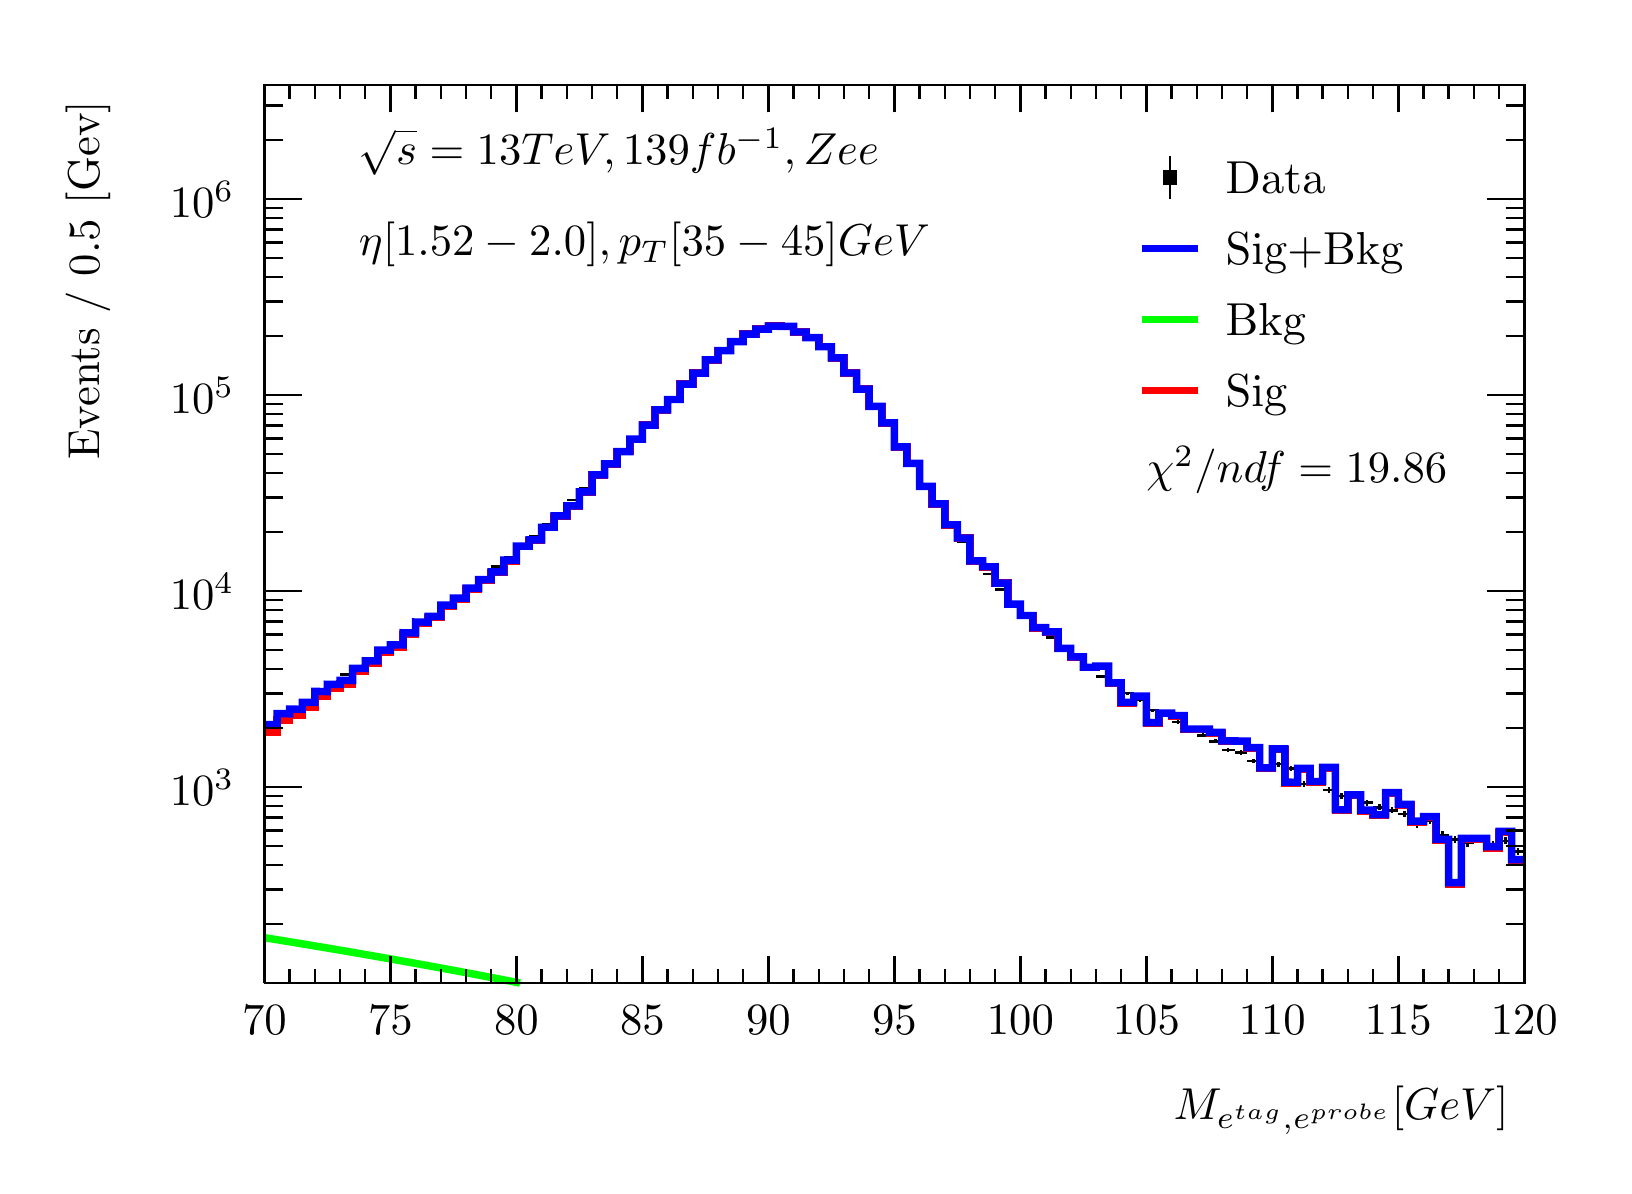
\begin{tikzpicture}
\pgfdeclareplotmark{cross} {
\pgfpathmoveto{\pgfpoint{-0.3\pgfplotmarksize}{\pgfplotmarksize}}
\pgfpathlineto{\pgfpoint{+0.3\pgfplotmarksize}{\pgfplotmarksize}}
\pgfpathlineto{\pgfpoint{+0.3\pgfplotmarksize}{0.3\pgfplotmarksize}}
\pgfpathlineto{\pgfpoint{+1\pgfplotmarksize}{0.3\pgfplotmarksize}}
\pgfpathlineto{\pgfpoint{+1\pgfplotmarksize}{-0.3\pgfplotmarksize}}
\pgfpathlineto{\pgfpoint{+0.3\pgfplotmarksize}{-0.3\pgfplotmarksize}}
\pgfpathlineto{\pgfpoint{+0.3\pgfplotmarksize}{-1.\pgfplotmarksize}}
\pgfpathlineto{\pgfpoint{-0.3\pgfplotmarksize}{-1.\pgfplotmarksize}}
\pgfpathlineto{\pgfpoint{-0.3\pgfplotmarksize}{-0.3\pgfplotmarksize}}
\pgfpathlineto{\pgfpoint{-1.\pgfplotmarksize}{-0.3\pgfplotmarksize}}
\pgfpathlineto{\pgfpoint{-1.\pgfplotmarksize}{0.3\pgfplotmarksize}}
\pgfpathlineto{\pgfpoint{-0.3\pgfplotmarksize}{0.3\pgfplotmarksize}}
\pgfpathclose
\pgfusepathqstroke
}
\pgfdeclareplotmark{cross*} {
\pgfpathmoveto{\pgfpoint{-0.3\pgfplotmarksize}{\pgfplotmarksize}}
\pgfpathlineto{\pgfpoint{+0.3\pgfplotmarksize}{\pgfplotmarksize}}
\pgfpathlineto{\pgfpoint{+0.3\pgfplotmarksize}{0.3\pgfplotmarksize}}
\pgfpathlineto{\pgfpoint{+1\pgfplotmarksize}{0.3\pgfplotmarksize}}
\pgfpathlineto{\pgfpoint{+1\pgfplotmarksize}{-0.3\pgfplotmarksize}}
\pgfpathlineto{\pgfpoint{+0.3\pgfplotmarksize}{-0.3\pgfplotmarksize}}
\pgfpathlineto{\pgfpoint{+0.3\pgfplotmarksize}{-1.\pgfplotmarksize}}
\pgfpathlineto{\pgfpoint{-0.3\pgfplotmarksize}{-1.\pgfplotmarksize}}
\pgfpathlineto{\pgfpoint{-0.3\pgfplotmarksize}{-0.3\pgfplotmarksize}}
\pgfpathlineto{\pgfpoint{-1.\pgfplotmarksize}{-0.3\pgfplotmarksize}}
\pgfpathlineto{\pgfpoint{-1.\pgfplotmarksize}{0.3\pgfplotmarksize}}
\pgfpathlineto{\pgfpoint{-0.3\pgfplotmarksize}{0.3\pgfplotmarksize}}
\pgfpathclose
\pgfusepathqfillstroke
}
\pgfdeclareplotmark{newstar} {
\pgfpathmoveto{\pgfqpoint{0pt}{\pgfplotmarksize}}
\pgfpathlineto{\pgfqpointpolar{44}{0.5\pgfplotmarksize}}
\pgfpathlineto{\pgfqpointpolar{18}{\pgfplotmarksize}}
\pgfpathlineto{\pgfqpointpolar{-20}{0.5\pgfplotmarksize}}
\pgfpathlineto{\pgfqpointpolar{-54}{\pgfplotmarksize}}
\pgfpathlineto{\pgfqpointpolar{-90}{0.5\pgfplotmarksize}}
\pgfpathlineto{\pgfqpointpolar{234}{\pgfplotmarksize}}
\pgfpathlineto{\pgfqpointpolar{198}{0.5\pgfplotmarksize}}
\pgfpathlineto{\pgfqpointpolar{162}{\pgfplotmarksize}}
\pgfpathlineto{\pgfqpointpolar{134}{0.5\pgfplotmarksize}}
\pgfpathclose
\pgfusepathqstroke
}
\pgfdeclareplotmark{newstar*} {
\pgfpathmoveto{\pgfqpoint{0pt}{\pgfplotmarksize}}
\pgfpathlineto{\pgfqpointpolar{44}{0.5\pgfplotmarksize}}
\pgfpathlineto{\pgfqpointpolar{18}{\pgfplotmarksize}}
\pgfpathlineto{\pgfqpointpolar{-20}{0.5\pgfplotmarksize}}
\pgfpathlineto{\pgfqpointpolar{-54}{\pgfplotmarksize}}
\pgfpathlineto{\pgfqpointpolar{-90}{0.5\pgfplotmarksize}}
\pgfpathlineto{\pgfqpointpolar{234}{\pgfplotmarksize}}
\pgfpathlineto{\pgfqpointpolar{198}{0.5\pgfplotmarksize}}
\pgfpathlineto{\pgfqpointpolar{162}{\pgfplotmarksize}}
\pgfpathlineto{\pgfqpointpolar{134}{0.5\pgfplotmarksize}}
\pgfpathclose
\pgfusepathqfillstroke
}
\definecolor{c}{rgb}{1,1,1};
\draw [color=c, fill=c] (0,0) rectangle (20,14.4361);
\draw [color=c, fill=c] (3,2.30977) rectangle (19,13.7143);
\definecolor{c}{rgb}{0,0,0};
\draw [c,line width=0.9] (3,2.30977) -- (3,13.7143) -- (19,13.7143) -- (19,2.30977) -- (3,2.30977);
\definecolor{c}{rgb}{1,1,1};
\draw [color=c, fill=c] (3,2.30977) rectangle (19,13.7143);
\definecolor{c}{rgb}{0,0,0};
\draw [c,line width=0.9] (3,2.30977) -- (3,13.7143) -- (19,13.7143) -- (19,2.30977) -- (3,2.30977);
\draw [c,line width=0.9] (3,2.30977) -- (19,2.30977);
\draw [c,line width=0.9] (3,2.65624) -- (3,2.30977);
\draw [c,line width=0.9] (3.32,2.48301) -- (3.32,2.30977);
\draw [c,line width=0.9] (3.64,2.48301) -- (3.64,2.30977);
\draw [c,line width=0.9] (3.96,2.48301) -- (3.96,2.30977);
\draw [c,line width=0.9] (4.28,2.48301) -- (4.28,2.30977);
\draw [c,line width=0.9] (4.6,2.65624) -- (4.6,2.30977);
\draw [c,line width=0.9] (4.92,2.48301) -- (4.92,2.30977);
\draw [c,line width=0.9] (5.24,2.48301) -- (5.24,2.30977);
\draw [c,line width=0.9] (5.56,2.48301) -- (5.56,2.30977);
\draw [c,line width=0.9] (5.88,2.48301) -- (5.88,2.30977);
\draw [c,line width=0.9] (6.2,2.65624) -- (6.2,2.30977);
\draw [c,line width=0.9] (6.52,2.48301) -- (6.52,2.30977);
\draw [c,line width=0.9] (6.84,2.48301) -- (6.84,2.30977);
\draw [c,line width=0.9] (7.16,2.48301) -- (7.16,2.30977);
\draw [c,line width=0.9] (7.48,2.48301) -- (7.48,2.30977);
\draw [c,line width=0.9] (7.8,2.65624) -- (7.8,2.30977);
\draw [c,line width=0.9] (8.12,2.48301) -- (8.12,2.30977);
\draw [c,line width=0.9] (8.44,2.48301) -- (8.44,2.30977);
\draw [c,line width=0.9] (8.76,2.48301) -- (8.76,2.30977);
\draw [c,line width=0.9] (9.08,2.48301) -- (9.08,2.30977);
\draw [c,line width=0.9] (9.4,2.65624) -- (9.4,2.30977);
\draw [c,line width=0.9] (9.72,2.48301) -- (9.72,2.30977);
\draw [c,line width=0.9] (10.04,2.48301) -- (10.04,2.30977);
\draw [c,line width=0.9] (10.36,2.48301) -- (10.36,2.30977);
\draw [c,line width=0.9] (10.68,2.48301) -- (10.68,2.30977);
\draw [c,line width=0.9] (11,2.65624) -- (11,2.30977);
\draw [c,line width=0.9] (11.32,2.48301) -- (11.32,2.30977);
\draw [c,line width=0.9] (11.64,2.48301) -- (11.64,2.30977);
\draw [c,line width=0.9] (11.96,2.48301) -- (11.96,2.30977);
\draw [c,line width=0.9] (12.28,2.48301) -- (12.28,2.30977);
\draw [c,line width=0.9] (12.6,2.65624) -- (12.6,2.30977);
\draw [c,line width=0.9] (12.92,2.48301) -- (12.92,2.30977);
\draw [c,line width=0.9] (13.24,2.48301) -- (13.24,2.30977);
\draw [c,line width=0.9] (13.56,2.48301) -- (13.56,2.30977);
\draw [c,line width=0.9] (13.88,2.48301) -- (13.88,2.30977);
\draw [c,line width=0.9] (14.2,2.65624) -- (14.2,2.30977);
\draw [c,line width=0.9] (14.52,2.48301) -- (14.52,2.30977);
\draw [c,line width=0.9] (14.84,2.48301) -- (14.84,2.30977);
\draw [c,line width=0.9] (15.16,2.48301) -- (15.16,2.30977);
\draw [c,line width=0.9] (15.48,2.48301) -- (15.48,2.30977);
\draw [c,line width=0.9] (15.8,2.65624) -- (15.8,2.30977);
\draw [c,line width=0.9] (16.12,2.48301) -- (16.12,2.30977);
\draw [c,line width=0.9] (16.44,2.48301) -- (16.44,2.30977);
\draw [c,line width=0.9] (16.76,2.48301) -- (16.76,2.30977);
\draw [c,line width=0.9] (17.08,2.48301) -- (17.08,2.30977);
\draw [c,line width=0.9] (17.4,2.65624) -- (17.4,2.30977);
\draw [c,line width=0.9] (17.72,2.48301) -- (17.72,2.30977);
\draw [c,line width=0.9] (18.04,2.48301) -- (18.04,2.30977);
\draw [c,line width=0.9] (18.36,2.48301) -- (18.36,2.30977);
\draw [c,line width=0.9] (18.68,2.48301) -- (18.68,2.30977);
\draw [c,line width=0.9] (19,2.65624) -- (19,2.30977);
\draw [anchor=base] (3,1.66015) node[scale=1.61424, color=c, rotate=0]{70};
\draw [anchor=base] (4.6,1.66015) node[scale=1.61424, color=c, rotate=0]{75};
\draw [anchor=base] (6.2,1.66015) node[scale=1.61424, color=c, rotate=0]{80};
\draw [anchor=base] (7.8,1.66015) node[scale=1.61424, color=c, rotate=0]{85};
\draw [anchor=base] (9.4,1.66015) node[scale=1.61424, color=c, rotate=0]{90};
\draw [anchor=base] (11,1.66015) node[scale=1.61424, color=c, rotate=0]{95};
\draw [anchor=base] (12.6,1.66015) node[scale=1.61424, color=c, rotate=0]{100};
\draw [anchor=base] (14.2,1.66015) node[scale=1.61424, color=c, rotate=0]{105};
\draw [anchor=base] (15.8,1.66015) node[scale=1.61424, color=c, rotate=0]{110};
\draw [anchor=base] (17.4,1.66015) node[scale=1.61424, color=c, rotate=0]{115};
\draw [anchor=base] (19,1.66015) node[scale=1.61424, color=c, rotate=0]{120};
\draw [anchor= east] (19,0.692932) node[scale=1.61424, color=c, rotate=0]{$M_{e^{tag}, e^{probe}}  [GeV]$};
\draw [c,line width=0.9] (3,13.7143) -- (19,13.7143);
\draw [c,line width=0.9] (3,13.3678) -- (3,13.7143);
\draw [c,line width=0.9] (3.32,13.5411) -- (3.32,13.7143);
\draw [c,line width=0.9] (3.64,13.5411) -- (3.64,13.7143);
\draw [c,line width=0.9] (3.96,13.5411) -- (3.96,13.7143);
\draw [c,line width=0.9] (4.28,13.5411) -- (4.28,13.7143);
\draw [c,line width=0.9] (4.6,13.3678) -- (4.6,13.7143);
\draw [c,line width=0.9] (4.92,13.5411) -- (4.92,13.7143);
\draw [c,line width=0.9] (5.24,13.5411) -- (5.24,13.7143);
\draw [c,line width=0.9] (5.56,13.5411) -- (5.56,13.7143);
\draw [c,line width=0.9] (5.88,13.5411) -- (5.88,13.7143);
\draw [c,line width=0.9] (6.2,13.3678) -- (6.2,13.7143);
\draw [c,line width=0.9] (6.52,13.5411) -- (6.52,13.7143);
\draw [c,line width=0.9] (6.84,13.5411) -- (6.84,13.7143);
\draw [c,line width=0.9] (7.16,13.5411) -- (7.16,13.7143);
\draw [c,line width=0.9] (7.48,13.5411) -- (7.48,13.7143);
\draw [c,line width=0.9] (7.8,13.3678) -- (7.8,13.7143);
\draw [c,line width=0.9] (8.12,13.5411) -- (8.12,13.7143);
\draw [c,line width=0.9] (8.44,13.5411) -- (8.44,13.7143);
\draw [c,line width=0.9] (8.76,13.5411) -- (8.76,13.7143);
\draw [c,line width=0.9] (9.08,13.5411) -- (9.08,13.7143);
\draw [c,line width=0.9] (9.4,13.3678) -- (9.4,13.7143);
\draw [c,line width=0.9] (9.72,13.5411) -- (9.72,13.7143);
\draw [c,line width=0.9] (10.04,13.5411) -- (10.04,13.7143);
\draw [c,line width=0.9] (10.36,13.5411) -- (10.36,13.7143);
\draw [c,line width=0.9] (10.68,13.5411) -- (10.68,13.7143);
\draw [c,line width=0.9] (11,13.3678) -- (11,13.7143);
\draw [c,line width=0.9] (11.32,13.5411) -- (11.32,13.7143);
\draw [c,line width=0.9] (11.64,13.5411) -- (11.64,13.7143);
\draw [c,line width=0.9] (11.96,13.5411) -- (11.96,13.7143);
\draw [c,line width=0.9] (12.28,13.5411) -- (12.28,13.7143);
\draw [c,line width=0.9] (12.6,13.3678) -- (12.6,13.7143);
\draw [c,line width=0.9] (12.92,13.5411) -- (12.92,13.7143);
\draw [c,line width=0.9] (13.24,13.5411) -- (13.24,13.7143);
\draw [c,line width=0.9] (13.56,13.5411) -- (13.56,13.7143);
\draw [c,line width=0.9] (13.88,13.5411) -- (13.88,13.7143);
\draw [c,line width=0.9] (14.2,13.3678) -- (14.2,13.7143);
\draw [c,line width=0.9] (14.52,13.5411) -- (14.52,13.7143);
\draw [c,line width=0.9] (14.84,13.5411) -- (14.84,13.7143);
\draw [c,line width=0.9] (15.16,13.5411) -- (15.16,13.7143);
\draw [c,line width=0.9] (15.48,13.5411) -- (15.48,13.7143);
\draw [c,line width=0.9] (15.8,13.3678) -- (15.8,13.7143);
\draw [c,line width=0.9] (16.12,13.5411) -- (16.12,13.7143);
\draw [c,line width=0.9] (16.44,13.5411) -- (16.44,13.7143);
\draw [c,line width=0.9] (16.76,13.5411) -- (16.76,13.7143);
\draw [c,line width=0.9] (17.08,13.5411) -- (17.08,13.7143);
\draw [c,line width=0.9] (17.4,13.3678) -- (17.4,13.7143);
\draw [c,line width=0.9] (17.72,13.5411) -- (17.72,13.7143);
\draw [c,line width=0.9] (18.04,13.5411) -- (18.04,13.7143);
\draw [c,line width=0.9] (18.36,13.5411) -- (18.36,13.7143);
\draw [c,line width=0.9] (18.68,13.5411) -- (18.68,13.7143);
\draw [c,line width=0.9] (19,13.3678) -- (19,13.7143);
\draw [c,line width=0.9] (3,2.30977) -- (3,13.7143);
\draw [c,line width=0.9] (3.237,3.05909) -- (3,3.05909);
\draw [c,line width=0.9] (3.237,3.49742) -- (3,3.49742);
\draw [c,line width=0.9] (3.237,3.80841) -- (3,3.80841);
\draw [c,line width=0.9] (3.237,4.04964) -- (3,4.04964);
\draw [c,line width=0.9] (3.237,4.24673) -- (3,4.24673);
\draw [c,line width=0.9] (3.237,4.41338) -- (3,4.41338);
\draw [c,line width=0.9] (3.237,4.55773) -- (3,4.55773);
\draw [c,line width=0.9] (3.237,4.68506) -- (3,4.68506);
\draw [c,line width=0.9] (3.474,4.79896) -- (3,4.79896);
\draw [anchor= east] (2.82,4.79896) node[scale=1.61424, color=c, rotate=0]{$10^{3}$};
\draw [c,line width=0.9] (3.237,5.54828) -- (3,5.54828);
\draw [c,line width=0.9] (3.237,5.9866) -- (3,5.9866);
\draw [c,line width=0.9] (3.237,6.2976) -- (3,6.2976);
\draw [c,line width=0.9] (3.237,6.53882) -- (3,6.53882);
\draw [c,line width=0.9] (3.237,6.73592) -- (3,6.73592);
\draw [c,line width=0.9] (3.237,6.90256) -- (3,6.90256);
\draw [c,line width=0.9] (3.237,7.04692) -- (3,7.04692);
\draw [c,line width=0.9] (3.237,7.17424) -- (3,7.17424);
\draw [c,line width=0.9] (3.474,7.28814) -- (3,7.28814);
\draw [anchor= east] (2.82,7.28814) node[scale=1.61424, color=c, rotate=0]{$10^{4}$};
\draw [c,line width=0.9] (3.237,8.03746) -- (3,8.03746);
\draw [c,line width=0.9] (3.237,8.47579) -- (3,8.47579);
\draw [c,line width=0.9] (3.237,8.78678) -- (3,8.78678);
\draw [c,line width=0.9] (3.237,9.02801) -- (3,9.02801);
\draw [c,line width=0.9] (3.237,9.2251) -- (3,9.2251);
\draw [c,line width=0.9] (3.237,9.39175) -- (3,9.39175);
\draw [c,line width=0.9] (3.237,9.5361) -- (3,9.5361);
\draw [c,line width=0.9] (3.237,9.66343) -- (3,9.66343);
\draw [c,line width=0.9] (3.474,9.77733) -- (3,9.77733);
\draw [anchor= east] (2.82,9.77733) node[scale=1.61424, color=c, rotate=0]{$10^{5}$};
\draw [c,line width=0.9] (3.237,10.5266) -- (3,10.5266);
\draw [c,line width=0.9] (3.237,10.965) -- (3,10.965);
\draw [c,line width=0.9] (3.237,11.276) -- (3,11.276);
\draw [c,line width=0.9] (3.237,11.5172) -- (3,11.5172);
\draw [c,line width=0.9] (3.237,11.7143) -- (3,11.7143);
\draw [c,line width=0.9] (3.237,11.8809) -- (3,11.8809);
\draw [c,line width=0.9] (3.237,12.0253) -- (3,12.0253);
\draw [c,line width=0.9] (3.237,12.1526) -- (3,12.1526);
\draw [c,line width=0.9] (3.474,12.2665) -- (3,12.2665);
\draw [anchor= east] (2.82,12.2665) node[scale=1.61424, color=c, rotate=0]{$10^{6}$};
\draw [c,line width=0.9] (3.237,13.0158) -- (3,13.0158);
\draw [c,line width=0.9] (3.237,13.4542) -- (3,13.4542);
\draw [anchor= east] (0.76,13.7143) node[scale=1.61424, color=c, rotate=90]{Events / 0.5 [Gev]};
\draw [c,line width=0.9] (19,2.30977) -- (19,13.7143);
\draw [c,line width=0.9] (18.763,3.05909) -- (19,3.05909);
\draw [c,line width=0.9] (18.763,3.49742) -- (19,3.49742);
\draw [c,line width=0.9] (18.763,3.80841) -- (19,3.80841);
\draw [c,line width=0.9] (18.763,4.04964) -- (19,4.04964);
\draw [c,line width=0.9] (18.763,4.24673) -- (19,4.24673);
\draw [c,line width=0.9] (18.763,4.41338) -- (19,4.41338);
\draw [c,line width=0.9] (18.763,4.55773) -- (19,4.55773);
\draw [c,line width=0.9] (18.763,4.68506) -- (19,4.68506);
\draw [c,line width=0.9] (18.526,4.79896) -- (19,4.79896);
\draw [c,line width=0.9] (18.763,5.54828) -- (19,5.54828);
\draw [c,line width=0.9] (18.763,5.9866) -- (19,5.9866);
\draw [c,line width=0.9] (18.763,6.2976) -- (19,6.2976);
\draw [c,line width=0.9] (18.763,6.53882) -- (19,6.53882);
\draw [c,line width=0.9] (18.763,6.73592) -- (19,6.73592);
\draw [c,line width=0.9] (18.763,6.90256) -- (19,6.90256);
\draw [c,line width=0.9] (18.763,7.04692) -- (19,7.04692);
\draw [c,line width=0.9] (18.763,7.17424) -- (19,7.17424);
\draw [c,line width=0.9] (18.526,7.28814) -- (19,7.28814);
\draw [c,line width=0.9] (18.763,8.03746) -- (19,8.03746);
\draw [c,line width=0.9] (18.763,8.47579) -- (19,8.47579);
\draw [c,line width=0.9] (18.763,8.78678) -- (19,8.78678);
\draw [c,line width=0.9] (18.763,9.02801) -- (19,9.02801);
\draw [c,line width=0.9] (18.763,9.2251) -- (19,9.2251);
\draw [c,line width=0.9] (18.763,9.39175) -- (19,9.39175);
\draw [c,line width=0.9] (18.763,9.5361) -- (19,9.5361);
\draw [c,line width=0.9] (18.763,9.66343) -- (19,9.66343);
\draw [c,line width=0.9] (18.526,9.77733) -- (19,9.77733);
\draw [c,line width=0.9] (18.763,10.5266) -- (19,10.5266);
\draw [c,line width=0.9] (18.763,10.965) -- (19,10.965);
\draw [c,line width=0.9] (18.763,11.276) -- (19,11.276);
\draw [c,line width=0.9] (18.763,11.5172) -- (19,11.5172);
\draw [c,line width=0.9] (18.763,11.7143) -- (19,11.7143);
\draw [c,line width=0.9] (18.763,11.8809) -- (19,11.8809);
\draw [c,line width=0.9] (18.763,12.0253) -- (19,12.0253);
\draw [c,line width=0.9] (18.763,12.1526) -- (19,12.1526);
\draw [c,line width=0.9] (18.526,12.2665) -- (19,12.2665);
\draw [c,line width=0.9] (18.763,13.0158) -- (19,13.0158);
\draw [c,line width=0.9] (18.763,13.4542) -- (19,13.4542);
\draw [c,line width=0.9] (3.08,5.52589) -- (3,5.52589);
\draw [c,line width=0.9] (3,5.52589) -- (3,5.52589);
\draw [c,line width=0.9] (3.08,5.52589) -- (3.16,5.52589);
\draw [c,line width=0.9] (3.16,5.52589) -- (3.16,5.52589);
\draw [c,line width=0.9] (3.08,5.52589) -- (3.08,5.55031);
\draw [c,line width=0.9] (3.08,5.55031) -- (3.08,5.55031);
\draw [c,line width=0.9] (3.08,5.52589) -- (3.08,5.50146);
\draw [c,line width=0.9] (3.08,5.50146) -- (3.08,5.50146);
\draw [c,line width=0.9] (3.24,5.64639) -- (3.16,5.64639);
\draw [c,line width=0.9] (3.16,5.64639) -- (3.16,5.64639);
\draw [c,line width=0.9] (3.24,5.64639) -- (3.32,5.64639);
\draw [c,line width=0.9] (3.32,5.64639) -- (3.32,5.64639);
\draw [c,line width=0.9] (3.24,5.64639) -- (3.24,5.66949);
\draw [c,line width=0.9] (3.24,5.66949) -- (3.24,5.66949);
\draw [c,line width=0.9] (3.24,5.64639) -- (3.24,5.62329);
\draw [c,line width=0.9] (3.24,5.62329) -- (3.24,5.62329);
\draw [c,line width=0.9] (3.4,5.74402) -- (3.32,5.74402);
\draw [c,line width=0.9] (3.32,5.74402) -- (3.32,5.74402);
\draw [c,line width=0.9] (3.4,5.74402) -- (3.48,5.74402);
\draw [c,line width=0.9] (3.48,5.74402) -- (3.48,5.74402);
\draw [c,line width=0.9] (3.4,5.74402) -- (3.4,5.7661);
\draw [c,line width=0.9] (3.4,5.7661) -- (3.4,5.7661);
\draw [c,line width=0.9] (3.4,5.74402) -- (3.4,5.72194);
\draw [c,line width=0.9] (3.4,5.72194) -- (3.4,5.72194);
\draw [c,line width=0.9] (3.56,5.89411) -- (3.48,5.89411);
\draw [c,line width=0.9] (3.48,5.89411) -- (3.48,5.89411);
\draw [c,line width=0.9] (3.56,5.89411) -- (3.64,5.89411);
\draw [c,line width=0.9] (3.64,5.89411) -- (3.64,5.89411);
\draw [c,line width=0.9] (3.56,5.89411) -- (3.56,5.91471);
\draw [c,line width=0.9] (3.56,5.91471) -- (3.56,5.91471);
\draw [c,line width=0.9] (3.56,5.89411) -- (3.56,5.87351);
\draw [c,line width=0.9] (3.56,5.87351) -- (3.56,5.87351);
\draw [c,line width=0.9] (3.72,5.97828) -- (3.64,5.97828);
\draw [c,line width=0.9] (3.64,5.97828) -- (3.64,5.97828);
\draw [c,line width=0.9] (3.72,5.97828) -- (3.8,5.97828);
\draw [c,line width=0.9] (3.8,5.97828) -- (3.8,5.97828);
\draw [c,line width=0.9] (3.72,5.97828) -- (3.72,5.99809);
\draw [c,line width=0.9] (3.72,5.99809) -- (3.72,5.99809);
\draw [c,line width=0.9] (3.72,5.97828) -- (3.72,5.95847);
\draw [c,line width=0.9] (3.72,5.95847) -- (3.72,5.95847);
\draw [c,line width=0.9] (3.88,6.11297) -- (3.8,6.11297);
\draw [c,line width=0.9] (3.8,6.11297) -- (3.8,6.11297);
\draw [c,line width=0.9] (3.88,6.11297) -- (3.96,6.11297);
\draw [c,line width=0.9] (3.96,6.11297) -- (3.96,6.11297);
\draw [c,line width=0.9] (3.88,6.11297) -- (3.88,6.13158);
\draw [c,line width=0.9] (3.88,6.13158) -- (3.88,6.13158);
\draw [c,line width=0.9] (3.88,6.11297) -- (3.88,6.09435);
\draw [c,line width=0.9] (3.88,6.09435) -- (3.88,6.09435);
\draw [c,line width=0.9] (4.04,6.22639) -- (3.96,6.22639);
\draw [c,line width=0.9] (3.96,6.22639) -- (3.96,6.22639);
\draw [c,line width=0.9] (4.04,6.22639) -- (4.12,6.22639);
\draw [c,line width=0.9] (4.12,6.22639) -- (4.12,6.22639);
\draw [c,line width=0.9] (4.04,6.22639) -- (4.04,6.24405);
\draw [c,line width=0.9] (4.04,6.24405) -- (4.04,6.24405);
\draw [c,line width=0.9] (4.04,6.22639) -- (4.04,6.20872);
\draw [c,line width=0.9] (4.04,6.20872) -- (4.04,6.20872);
\draw [c,line width=0.9] (4.2,6.3327) -- (4.12,6.3327);
\draw [c,line width=0.9] (4.12,6.3327) -- (4.12,6.3327);
\draw [c,line width=0.9] (4.2,6.3327) -- (4.28,6.3327);
\draw [c,line width=0.9] (4.28,6.3327) -- (4.28,6.3327);
\draw [c,line width=0.9] (4.2,6.3327) -- (4.2,6.34951);
\draw [c,line width=0.9] (4.2,6.34951) -- (4.2,6.34951);
\draw [c,line width=0.9] (4.2,6.3327) -- (4.2,6.31588);
\draw [c,line width=0.9] (4.2,6.31588) -- (4.2,6.31588);
\draw [c,line width=0.9] (4.36,6.38529) -- (4.28,6.38529);
\draw [c,line width=0.9] (4.28,6.38529) -- (4.28,6.38529);
\draw [c,line width=0.9] (4.36,6.38529) -- (4.44,6.38529);
\draw [c,line width=0.9] (4.44,6.38529) -- (4.44,6.38529);
\draw [c,line width=0.9] (4.36,6.38529) -- (4.36,6.4017);
\draw [c,line width=0.9] (4.36,6.4017) -- (4.36,6.4017);
\draw [c,line width=0.9] (4.36,6.38529) -- (4.36,6.36888);
\draw [c,line width=0.9] (4.36,6.36888) -- (4.36,6.36888);
\draw [c,line width=0.9] (4.52,6.51676) -- (4.44,6.51676);
\draw [c,line width=0.9] (4.44,6.51676) -- (4.44,6.51676);
\draw [c,line width=0.9] (4.52,6.51676) -- (4.6,6.51676);
\draw [c,line width=0.9] (4.6,6.51676) -- (4.6,6.51676);
\draw [c,line width=0.9] (4.52,6.51676) -- (4.52,6.53221);
\draw [c,line width=0.9] (4.52,6.53221) -- (4.52,6.53221);
\draw [c,line width=0.9] (4.52,6.51676) -- (4.52,6.50132);
\draw [c,line width=0.9] (4.52,6.50132) -- (4.52,6.50132);
\draw [c,line width=0.9] (4.68,6.62921) -- (4.6,6.62921);
\draw [c,line width=0.9] (4.6,6.62921) -- (4.6,6.62921);
\draw [c,line width=0.9] (4.68,6.62921) -- (4.76,6.62921);
\draw [c,line width=0.9] (4.76,6.62921) -- (4.76,6.62921);
\draw [c,line width=0.9] (4.68,6.62921) -- (4.68,6.64387);
\draw [c,line width=0.9] (4.68,6.64387) -- (4.68,6.64387);
\draw [c,line width=0.9] (4.68,6.62921) -- (4.68,6.61454);
\draw [c,line width=0.9] (4.68,6.61454) -- (4.68,6.61454);
\draw [c,line width=0.9] (4.84,6.72378) -- (4.76,6.72378);
\draw [c,line width=0.9] (4.76,6.72378) -- (4.76,6.72378);
\draw [c,line width=0.9] (4.84,6.72378) -- (4.92,6.72378);
\draw [c,line width=0.9] (4.92,6.72378) -- (4.92,6.72378);
\draw [c,line width=0.9] (4.84,6.72378) -- (4.84,6.73782);
\draw [c,line width=0.9] (4.84,6.73782) -- (4.84,6.73782);
\draw [c,line width=0.9] (4.84,6.72378) -- (4.84,6.70975);
\draw [c,line width=0.9] (4.84,6.70975) -- (4.84,6.70975);
\draw [c,line width=0.9] (5,6.8523) -- (4.92,6.8523);
\draw [c,line width=0.9] (4.92,6.8523) -- (4.92,6.8523);
\draw [c,line width=0.9] (5,6.8523) -- (5.08,6.8523);
\draw [c,line width=0.9] (5.08,6.8523) -- (5.08,6.8523);
\draw [c,line width=0.9] (5,6.8523) -- (5,6.86553);
\draw [c,line width=0.9] (5,6.86553) -- (5,6.86553);
\draw [c,line width=0.9] (5,6.8523) -- (5,6.83908);
\draw [c,line width=0.9] (5,6.83908) -- (5,6.83908);
\draw [c,line width=0.9] (5.16,6.94392) -- (5.08,6.94392);
\draw [c,line width=0.9] (5.08,6.94392) -- (5.08,6.94392);
\draw [c,line width=0.9] (5.16,6.94392) -- (5.24,6.94392);
\draw [c,line width=0.9] (5.24,6.94392) -- (5.24,6.94392);
\draw [c,line width=0.9] (5.16,6.94392) -- (5.16,6.9566);
\draw [c,line width=0.9] (5.16,6.9566) -- (5.16,6.9566);
\draw [c,line width=0.9] (5.16,6.94392) -- (5.16,6.93125);
\draw [c,line width=0.9] (5.16,6.93125) -- (5.16,6.93125);
\draw [c,line width=0.9] (5.32,7.07216) -- (5.24,7.07216);
\draw [c,line width=0.9] (5.24,7.07216) -- (5.24,7.07216);
\draw [c,line width=0.9] (5.32,7.07216) -- (5.4,7.07216);
\draw [c,line width=0.9] (5.4,7.07216) -- (5.4,7.07216);
\draw [c,line width=0.9] (5.32,7.07216) -- (5.32,7.08411);
\draw [c,line width=0.9] (5.32,7.08411) -- (5.32,7.08411);
\draw [c,line width=0.9] (5.32,7.07216) -- (5.32,7.06021);
\draw [c,line width=0.9] (5.32,7.06021) -- (5.32,7.06021);
\draw [c,line width=0.9] (5.48,7.21745) -- (5.4,7.21745);
\draw [c,line width=0.9] (5.4,7.21745) -- (5.4,7.21745);
\draw [c,line width=0.9] (5.48,7.21745) -- (5.56,7.21745);
\draw [c,line width=0.9] (5.56,7.21745) -- (5.56,7.21745);
\draw [c,line width=0.9] (5.48,7.21745) -- (5.48,7.22862);
\draw [c,line width=0.9] (5.48,7.22862) -- (5.48,7.22862);
\draw [c,line width=0.9] (5.48,7.21745) -- (5.48,7.20628);
\draw [c,line width=0.9] (5.48,7.20628) -- (5.48,7.20628);
\draw [c,line width=0.9] (5.64,7.32648) -- (5.56,7.32648);
\draw [c,line width=0.9] (5.56,7.32648) -- (5.56,7.32648);
\draw [c,line width=0.9] (5.64,7.32648) -- (5.72,7.32648);
\draw [c,line width=0.9] (5.72,7.32648) -- (5.72,7.32648);
\draw [c,line width=0.9] (5.64,7.32648) -- (5.64,7.3371);
\draw [c,line width=0.9] (5.64,7.3371) -- (5.64,7.3371);
\draw [c,line width=0.9] (5.64,7.32648) -- (5.64,7.31586);
\draw [c,line width=0.9] (5.64,7.31586) -- (5.64,7.31586);
\draw [c,line width=0.9] (5.8,7.4538) -- (5.72,7.4538);
\draw [c,line width=0.9] (5.72,7.4538) -- (5.72,7.4538);
\draw [c,line width=0.9] (5.8,7.4538) -- (5.88,7.4538);
\draw [c,line width=0.9] (5.88,7.4538) -- (5.88,7.4538);
\draw [c,line width=0.9] (5.8,7.4538) -- (5.8,7.46381);
\draw [c,line width=0.9] (5.8,7.46381) -- (5.8,7.46381);
\draw [c,line width=0.9] (5.8,7.4538) -- (5.8,7.44378);
\draw [c,line width=0.9] (5.8,7.44378) -- (5.8,7.44378);
\draw [c,line width=0.9] (5.96,7.60065) -- (5.88,7.60065);
\draw [c,line width=0.9] (5.88,7.60065) -- (5.88,7.60065);
\draw [c,line width=0.9] (5.96,7.60065) -- (6.04,7.60065);
\draw [c,line width=0.9] (6.04,7.60065) -- (6.04,7.60065);
\draw [c,line width=0.9] (5.96,7.60065) -- (5.96,7.61001);
\draw [c,line width=0.9] (5.96,7.61001) -- (5.96,7.61001);
\draw [c,line width=0.9] (5.96,7.60065) -- (5.96,7.5913);
\draw [c,line width=0.9] (5.96,7.5913) -- (5.96,7.5913);
\draw [c,line width=0.9] (6.12,7.7148) -- (6.04,7.7148);
\draw [c,line width=0.9] (6.04,7.7148) -- (6.04,7.7148);
\draw [c,line width=0.9] (6.12,7.7148) -- (6.2,7.7148);
\draw [c,line width=0.9] (6.2,7.7148) -- (6.2,7.7148);
\draw [c,line width=0.9] (6.12,7.7148) -- (6.12,7.72368);
\draw [c,line width=0.9] (6.12,7.72368) -- (6.12,7.72368);
\draw [c,line width=0.9] (6.12,7.7148) -- (6.12,7.70593);
\draw [c,line width=0.9] (6.12,7.70593) -- (6.12,7.70593);
\draw [c,line width=0.9] (6.28,7.85399) -- (6.2,7.85399);
\draw [c,line width=0.9] (6.2,7.85399) -- (6.2,7.85399);
\draw [c,line width=0.9] (6.28,7.85399) -- (6.36,7.85399);
\draw [c,line width=0.9] (6.36,7.85399) -- (6.36,7.85399);
\draw [c,line width=0.9] (6.28,7.85399) -- (6.28,7.86231);
\draw [c,line width=0.9] (6.28,7.86231) -- (6.28,7.86231);
\draw [c,line width=0.9] (6.28,7.85399) -- (6.28,7.84567);
\draw [c,line width=0.9] (6.28,7.84567) -- (6.28,7.84567);
\draw [c,line width=0.9] (6.44,7.97991) -- (6.36,7.97991);
\draw [c,line width=0.9] (6.36,7.97991) -- (6.36,7.97991);
\draw [c,line width=0.9] (6.44,7.97991) -- (6.52,7.97991);
\draw [c,line width=0.9] (6.52,7.97991) -- (6.52,7.97991);
\draw [c,line width=0.9] (6.44,7.97991) -- (6.44,7.98776);
\draw [c,line width=0.9] (6.44,7.98776) -- (6.44,7.98776);
\draw [c,line width=0.9] (6.44,7.97991) -- (6.44,7.97205);
\draw [c,line width=0.9] (6.44,7.97205) -- (6.44,7.97205);
\draw [c,line width=0.9] (6.6,8.13917) -- (6.52,8.13917);
\draw [c,line width=0.9] (6.52,8.13917) -- (6.52,8.13917);
\draw [c,line width=0.9] (6.6,8.13917) -- (6.68,8.13917);
\draw [c,line width=0.9] (6.68,8.13917) -- (6.68,8.13917);
\draw [c,line width=0.9] (6.6,8.13917) -- (6.6,8.14646);
\draw [c,line width=0.9] (6.6,8.14646) -- (6.6,8.14646);
\draw [c,line width=0.9] (6.6,8.13917) -- (6.6,8.13188);
\draw [c,line width=0.9] (6.6,8.13188) -- (6.6,8.13188);
\draw [c,line width=0.9] (6.76,8.27036) -- (6.68,8.27036);
\draw [c,line width=0.9] (6.68,8.27036) -- (6.68,8.27036);
\draw [c,line width=0.9] (6.76,8.27036) -- (6.84,8.27036);
\draw [c,line width=0.9] (6.84,8.27036) -- (6.84,8.27036);
\draw [c,line width=0.9] (6.76,8.27036) -- (6.76,8.27722);
\draw [c,line width=0.9] (6.76,8.27722) -- (6.76,8.27722);
\draw [c,line width=0.9] (6.76,8.27036) -- (6.76,8.26349);
\draw [c,line width=0.9] (6.76,8.26349) -- (6.76,8.26349);
\draw [c,line width=0.9] (6.92,8.44642) -- (6.84,8.44642);
\draw [c,line width=0.9] (6.84,8.44642) -- (6.84,8.44642);
\draw [c,line width=0.9] (6.92,8.44642) -- (7,8.44642);
\draw [c,line width=0.9] (7,8.44642) -- (7,8.44642);
\draw [c,line width=0.9] (6.92,8.44642) -- (6.92,8.45275);
\draw [c,line width=0.9] (6.92,8.45275) -- (6.92,8.45275);
\draw [c,line width=0.9] (6.92,8.44642) -- (6.92,8.44009);
\draw [c,line width=0.9] (6.92,8.44009) -- (6.92,8.44009);
\draw [c,line width=0.9] (7.08,8.58886) -- (7,8.58886);
\draw [c,line width=0.9] (7,8.58886) -- (7,8.58886);
\draw [c,line width=0.9] (7.08,8.58886) -- (7.16,8.58886);
\draw [c,line width=0.9] (7.16,8.58886) -- (7.16,8.58886);
\draw [c,line width=0.9] (7.08,8.58886) -- (7.08,8.59479);
\draw [c,line width=0.9] (7.08,8.59479) -- (7.08,8.59479);
\draw [c,line width=0.9] (7.08,8.58886) -- (7.08,8.58294);
\draw [c,line width=0.9] (7.08,8.58294) -- (7.08,8.58294);
\draw [c,line width=0.9] (7.24,8.74431) -- (7.16,8.74431);
\draw [c,line width=0.9] (7.16,8.74431) -- (7.16,8.74431);
\draw [c,line width=0.9] (7.24,8.74431) -- (7.32,8.74431);
\draw [c,line width=0.9] (7.32,8.74431) -- (7.32,8.74431);
\draw [c,line width=0.9] (7.24,8.74431) -- (7.24,8.74982);
\draw [c,line width=0.9] (7.24,8.74982) -- (7.24,8.74982);
\draw [c,line width=0.9] (7.24,8.74431) -- (7.24,8.7388);
\draw [c,line width=0.9] (7.24,8.7388) -- (7.24,8.7388);
\draw [c,line width=0.9] (7.4,8.91807) -- (7.32,8.91807);
\draw [c,line width=0.9] (7.32,8.91807) -- (7.32,8.91807);
\draw [c,line width=0.9] (7.4,8.91807) -- (7.48,8.91807);
\draw [c,line width=0.9] (7.48,8.91807) -- (7.48,8.91807);
\draw [c,line width=0.9] (7.4,8.91807) -- (7.4,8.92315);
\draw [c,line width=0.9] (7.4,8.92315) -- (7.4,8.92315);
\draw [c,line width=0.9] (7.4,8.91807) -- (7.4,8.91298);
\draw [c,line width=0.9] (7.4,8.91298) -- (7.4,8.91298);
\draw [c,line width=0.9] (7.56,9.0753) -- (7.48,9.0753);
\draw [c,line width=0.9] (7.48,9.0753) -- (7.48,9.0753);
\draw [c,line width=0.9] (7.56,9.0753) -- (7.64,9.0753);
\draw [c,line width=0.9] (7.64,9.0753) -- (7.64,9.0753);
\draw [c,line width=0.9] (7.56,9.0753) -- (7.56,9.08003);
\draw [c,line width=0.9] (7.56,9.08003) -- (7.56,9.08003);
\draw [c,line width=0.9] (7.56,9.0753) -- (7.56,9.07057);
\draw [c,line width=0.9] (7.56,9.07057) -- (7.56,9.07057);
\draw [c,line width=0.9] (7.72,9.24432) -- (7.64,9.24432);
\draw [c,line width=0.9] (7.64,9.24432) -- (7.64,9.24432);
\draw [c,line width=0.9] (7.72,9.24432) -- (7.8,9.24432);
\draw [c,line width=0.9] (7.8,9.24432) -- (7.8,9.24432);
\draw [c,line width=0.9] (7.72,9.24432) -- (7.72,9.24869);
\draw [c,line width=0.9] (7.72,9.24869) -- (7.72,9.24869);
\draw [c,line width=0.9] (7.72,9.24432) -- (7.72,9.23995);
\draw [c,line width=0.9] (7.72,9.23995) -- (7.72,9.23995);
\draw [c,line width=0.9] (7.88,9.40842) -- (7.8,9.40842);
\draw [c,line width=0.9] (7.8,9.40842) -- (7.8,9.40842);
\draw [c,line width=0.9] (7.88,9.40842) -- (7.96,9.40842);
\draw [c,line width=0.9] (7.96,9.40842) -- (7.96,9.40842);
\draw [c,line width=0.9] (7.88,9.40842) -- (7.88,9.41248);
\draw [c,line width=0.9] (7.88,9.41248) -- (7.88,9.41248);
\draw [c,line width=0.9] (7.88,9.40842) -- (7.88,9.40437);
\draw [c,line width=0.9] (7.88,9.40437) -- (7.88,9.40437);
\draw [c,line width=0.9] (8.04,9.5776) -- (7.96,9.5776);
\draw [c,line width=0.9] (7.96,9.5776) -- (7.96,9.5776);
\draw [c,line width=0.9] (8.04,9.5776) -- (8.12,9.5776);
\draw [c,line width=0.9] (8.12,9.5776) -- (8.12,9.5776);
\draw [c,line width=0.9] (8.04,9.5776) -- (8.04,9.58135);
\draw [c,line width=0.9] (8.04,9.58135) -- (8.04,9.58135);
\draw [c,line width=0.9] (8.04,9.5776) -- (8.04,9.57385);
\draw [c,line width=0.9] (8.04,9.57385) -- (8.04,9.57385);
\draw [c,line width=0.9] (8.2,9.73996) -- (8.12,9.73996);
\draw [c,line width=0.9] (8.12,9.73996) -- (8.12,9.73996);
\draw [c,line width=0.9] (8.2,9.73996) -- (8.28,9.73996);
\draw [c,line width=0.9] (8.28,9.73996) -- (8.28,9.73996);
\draw [c,line width=0.9] (8.2,9.73996) -- (8.2,9.74343);
\draw [c,line width=0.9] (8.2,9.74343) -- (8.2,9.74343);
\draw [c,line width=0.9] (8.2,9.73996) -- (8.2,9.73648);
\draw [c,line width=0.9] (8.2,9.73648) -- (8.2,9.73648);
\draw [c,line width=0.9] (8.36,9.90153) -- (8.28,9.90153);
\draw [c,line width=0.9] (8.28,9.90153) -- (8.28,9.90153);
\draw [c,line width=0.9] (8.36,9.90153) -- (8.44,9.90153);
\draw [c,line width=0.9] (8.44,9.90153) -- (8.44,9.90153);
\draw [c,line width=0.9] (8.36,9.90153) -- (8.36,9.90476);
\draw [c,line width=0.9] (8.36,9.90476) -- (8.36,9.90476);
\draw [c,line width=0.9] (8.36,9.90153) -- (8.36,9.8983);
\draw [c,line width=0.9] (8.36,9.8983) -- (8.36,9.8983);
\draw [c,line width=0.9] (8.52,10.0572) -- (8.44,10.0572);
\draw [c,line width=0.9] (8.44,10.0572) -- (8.44,10.0572);
\draw [c,line width=0.9] (8.52,10.0572) -- (8.6,10.0572);
\draw [c,line width=0.9] (8.6,10.0572) -- (8.6,10.0572);
\draw [c,line width=0.9] (8.52,10.0572) -- (8.52,10.0602);
\draw [c,line width=0.9] (8.52,10.0602) -- (8.52,10.0602);
\draw [c,line width=0.9] (8.52,10.0572) -- (8.52,10.0542);
\draw [c,line width=0.9] (8.52,10.0542) -- (8.52,10.0542);
\draw [c,line width=0.9] (8.68,10.1997) -- (8.6,10.1997);
\draw [c,line width=0.9] (8.6,10.1997) -- (8.6,10.1997);
\draw [c,line width=0.9] (8.68,10.1997) -- (8.76,10.1997);
\draw [c,line width=0.9] (8.76,10.1997) -- (8.76,10.1997);
\draw [c,line width=0.9] (8.68,10.1997) -- (8.68,10.2025);
\draw [c,line width=0.9] (8.68,10.2025) -- (8.68,10.2025);
\draw [c,line width=0.9] (8.68,10.1997) -- (8.68,10.1969);
\draw [c,line width=0.9] (8.68,10.1969) -- (8.68,10.1969);
\draw [c,line width=0.9] (8.84,10.3367) -- (8.76,10.3367);
\draw [c,line width=0.9] (8.76,10.3367) -- (8.76,10.3367);
\draw [c,line width=0.9] (8.84,10.3367) -- (8.92,10.3367);
\draw [c,line width=0.9] (8.92,10.3367) -- (8.92,10.3367);
\draw [c,line width=0.9] (8.84,10.3367) -- (8.84,10.3393);
\draw [c,line width=0.9] (8.84,10.3393) -- (8.84,10.3393);
\draw [c,line width=0.9] (8.84,10.3367) -- (8.84,10.334);
\draw [c,line width=0.9] (8.84,10.334) -- (8.84,10.334);
\draw [c,line width=0.9] (9,10.4519) -- (8.92,10.4519);
\draw [c,line width=0.9] (8.92,10.4519) -- (8.92,10.4519);
\draw [c,line width=0.9] (9,10.4519) -- (9.08,10.4519);
\draw [c,line width=0.9] (9.08,10.4519) -- (9.08,10.4519);
\draw [c,line width=0.9] (9,10.4519) -- (9,10.4544);
\draw [c,line width=0.9] (9,10.4544) -- (9,10.4544);
\draw [c,line width=0.9] (9,10.4519) -- (9,10.4494);
\draw [c,line width=0.9] (9,10.4494) -- (9,10.4494);
\draw [c,line width=0.9] (9.16,10.5461) -- (9.08,10.5461);
\draw [c,line width=0.9] (9.08,10.5461) -- (9.08,10.5461);
\draw [c,line width=0.9] (9.16,10.5461) -- (9.24,10.5461);
\draw [c,line width=0.9] (9.24,10.5461) -- (9.24,10.5461);
\draw [c,line width=0.9] (9.16,10.5461) -- (9.16,10.5485);
\draw [c,line width=0.9] (9.16,10.5485) -- (9.16,10.5485);
\draw [c,line width=0.9] (9.16,10.5461) -- (9.16,10.5437);
\draw [c,line width=0.9] (9.16,10.5437) -- (9.16,10.5437);
\draw [c,line width=0.9] (9.32,10.607) -- (9.24,10.607);
\draw [c,line width=0.9] (9.24,10.607) -- (9.24,10.607);
\draw [c,line width=0.9] (9.32,10.607) -- (9.4,10.607);
\draw [c,line width=0.9] (9.4,10.607) -- (9.4,10.607);
\draw [c,line width=0.9] (9.32,10.607) -- (9.32,10.6094);
\draw [c,line width=0.9] (9.32,10.6094) -- (9.32,10.6094);
\draw [c,line width=0.9] (9.32,10.607) -- (9.32,10.6047);
\draw [c,line width=0.9] (9.32,10.6047) -- (9.32,10.6047);
\draw [c,line width=0.9] (9.48,10.6426) -- (9.4,10.6426);
\draw [c,line width=0.9] (9.4,10.6426) -- (9.4,10.6426);
\draw [c,line width=0.9] (9.48,10.6426) -- (9.56,10.6426);
\draw [c,line width=0.9] (9.56,10.6426) -- (9.56,10.6426);
\draw [c,line width=0.9] (9.48,10.6426) -- (9.48,10.6449);
\draw [c,line width=0.9] (9.48,10.6449) -- (9.48,10.6449);
\draw [c,line width=0.9] (9.48,10.6426) -- (9.48,10.6403);
\draw [c,line width=0.9] (9.48,10.6403) -- (9.48,10.6403);
\draw [c,line width=0.9] (9.64,10.6382) -- (9.56,10.6382);
\draw [c,line width=0.9] (9.56,10.6382) -- (9.56,10.6382);
\draw [c,line width=0.9] (9.64,10.6382) -- (9.72,10.6382);
\draw [c,line width=0.9] (9.72,10.6382) -- (9.72,10.6382);
\draw [c,line width=0.9] (9.64,10.6382) -- (9.64,10.6405);
\draw [c,line width=0.9] (9.64,10.6405) -- (9.64,10.6405);
\draw [c,line width=0.9] (9.64,10.6382) -- (9.64,10.6359);
\draw [c,line width=0.9] (9.64,10.6359) -- (9.64,10.6359);
\draw [c,line width=0.9] (9.8,10.5995) -- (9.72,10.5995);
\draw [c,line width=0.9] (9.72,10.5995) -- (9.72,10.5995);
\draw [c,line width=0.9] (9.8,10.5995) -- (9.88,10.5995);
\draw [c,line width=0.9] (9.88,10.5995) -- (9.88,10.5995);
\draw [c,line width=0.9] (9.8,10.5995) -- (9.8,10.6019);
\draw [c,line width=0.9] (9.8,10.6019) -- (9.8,10.6019);
\draw [c,line width=0.9] (9.8,10.5995) -- (9.8,10.5972);
\draw [c,line width=0.9] (9.8,10.5972) -- (9.8,10.5972);
\draw [c,line width=0.9] (9.96,10.5213) -- (9.88,10.5213);
\draw [c,line width=0.9] (9.88,10.5213) -- (9.88,10.5213);
\draw [c,line width=0.9] (9.96,10.5213) -- (10.04,10.5213);
\draw [c,line width=0.9] (10.04,10.5213) -- (10.04,10.5213);
\draw [c,line width=0.9] (9.96,10.5213) -- (9.96,10.5237);
\draw [c,line width=0.9] (9.96,10.5237) -- (9.96,10.5237);
\draw [c,line width=0.9] (9.96,10.5213) -- (9.96,10.5188);
\draw [c,line width=0.9] (9.96,10.5188) -- (9.96,10.5188);
\draw [c,line width=0.9] (10.12,10.4063) -- (10.04,10.4063);
\draw [c,line width=0.9] (10.04,10.4063) -- (10.04,10.4063);
\draw [c,line width=0.9] (10.12,10.4063) -- (10.2,10.4063);
\draw [c,line width=0.9] (10.2,10.4063) -- (10.2,10.4063);
\draw [c,line width=0.9] (10.12,10.4063) -- (10.12,10.4088);
\draw [c,line width=0.9] (10.12,10.4088) -- (10.12,10.4088);
\draw [c,line width=0.9] (10.12,10.4063) -- (10.12,10.4037);
\draw [c,line width=0.9] (10.12,10.4037) -- (10.12,10.4037);
\draw [c,line width=0.9] (10.28,10.2592) -- (10.2,10.2592);
\draw [c,line width=0.9] (10.2,10.2592) -- (10.2,10.2592);
\draw [c,line width=0.9] (10.28,10.2592) -- (10.36,10.2592);
\draw [c,line width=0.9] (10.36,10.2592) -- (10.36,10.2592);
\draw [c,line width=0.9] (10.28,10.2592) -- (10.28,10.262);
\draw [c,line width=0.9] (10.28,10.262) -- (10.28,10.262);
\draw [c,line width=0.9] (10.28,10.2592) -- (10.28,10.2565);
\draw [c,line width=0.9] (10.28,10.2565) -- (10.28,10.2565);
\draw [c,line width=0.9] (10.44,10.0698) -- (10.36,10.0698);
\draw [c,line width=0.9] (10.36,10.0698) -- (10.36,10.0698);
\draw [c,line width=0.9] (10.44,10.0698) -- (10.52,10.0698);
\draw [c,line width=0.9] (10.52,10.0698) -- (10.52,10.0698);
\draw [c,line width=0.9] (10.44,10.0698) -- (10.44,10.0727);
\draw [c,line width=0.9] (10.44,10.0727) -- (10.44,10.0727);
\draw [c,line width=0.9] (10.44,10.0698) -- (10.44,10.0668);
\draw [c,line width=0.9] (10.44,10.0668) -- (10.44,10.0668);
\draw [c,line width=0.9] (10.6,9.85108) -- (10.52,9.85108);
\draw [c,line width=0.9] (10.52,9.85108) -- (10.52,9.85108);
\draw [c,line width=0.9] (10.6,9.85108) -- (10.68,9.85108);
\draw [c,line width=0.9] (10.68,9.85108) -- (10.68,9.85108);
\draw [c,line width=0.9] (10.6,9.85108) -- (10.6,9.85438);
\draw [c,line width=0.9] (10.6,9.85438) -- (10.6,9.85438);
\draw [c,line width=0.9] (10.6,9.85108) -- (10.6,9.84777);
\draw [c,line width=0.9] (10.6,9.84777) -- (10.6,9.84777);
\draw [c,line width=0.9] (10.76,9.62913) -- (10.68,9.62913);
\draw [c,line width=0.9] (10.68,9.62913) -- (10.68,9.62913);
\draw [c,line width=0.9] (10.76,9.62913) -- (10.84,9.62913);
\draw [c,line width=0.9] (10.84,9.62913) -- (10.84,9.62913);
\draw [c,line width=0.9] (10.76,9.62913) -- (10.76,9.63279);
\draw [c,line width=0.9] (10.76,9.63279) -- (10.76,9.63279);
\draw [c,line width=0.9] (10.76,9.62913) -- (10.76,9.62547);
\draw [c,line width=0.9] (10.76,9.62547) -- (10.76,9.62547);
\draw [c,line width=0.9] (10.92,9.38227) -- (10.84,9.38227);
\draw [c,line width=0.9] (10.84,9.38227) -- (10.84,9.38227);
\draw [c,line width=0.9] (10.92,9.38227) -- (11,9.38227);
\draw [c,line width=0.9] (11,9.38227) -- (11,9.38227);
\draw [c,line width=0.9] (10.92,9.38227) -- (10.92,9.38638);
\draw [c,line width=0.9] (10.92,9.38638) -- (10.92,9.38638);
\draw [c,line width=0.9] (10.92,9.38227) -- (10.92,9.37817);
\draw [c,line width=0.9] (10.92,9.37817) -- (10.92,9.37817);
\draw [c,line width=0.9] (11.08,9.13281) -- (11,9.13281);
\draw [c,line width=0.9] (11,9.13281) -- (11,9.13281);
\draw [c,line width=0.9] (11.08,9.13281) -- (11.16,9.13281);
\draw [c,line width=0.9] (11.16,9.13281) -- (11.16,9.13281);
\draw [c,line width=0.9] (11.08,9.13281) -- (11.08,9.13742);
\draw [c,line width=0.9] (11.08,9.13742) -- (11.08,9.13742);
\draw [c,line width=0.9] (11.08,9.13281) -- (11.08,9.1282);
\draw [c,line width=0.9] (11.08,9.1282) -- (11.08,9.1282);
\draw [c,line width=0.9] (11.24,8.87432) -- (11.16,8.87432);
\draw [c,line width=0.9] (11.16,8.87432) -- (11.16,8.87432);
\draw [c,line width=0.9] (11.24,8.87432) -- (11.32,8.87432);
\draw [c,line width=0.9] (11.32,8.87432) -- (11.32,8.87432);
\draw [c,line width=0.9] (11.24,8.87432) -- (11.24,8.87952);
\draw [c,line width=0.9] (11.24,8.87952) -- (11.24,8.87952);
\draw [c,line width=0.9] (11.24,8.87432) -- (11.24,8.86913);
\draw [c,line width=0.9] (11.24,8.86913) -- (11.24,8.86913);
\draw [c,line width=0.9] (11.4,8.621) -- (11.32,8.621);
\draw [c,line width=0.9] (11.32,8.621) -- (11.32,8.621);
\draw [c,line width=0.9] (11.4,8.621) -- (11.48,8.621);
\draw [c,line width=0.9] (11.48,8.621) -- (11.48,8.621);
\draw [c,line width=0.9] (11.4,8.621) -- (11.4,8.62683);
\draw [c,line width=0.9] (11.4,8.62683) -- (11.4,8.62683);
\draw [c,line width=0.9] (11.4,8.621) -- (11.4,8.61516);
\draw [c,line width=0.9] (11.4,8.61516) -- (11.4,8.61516);
\draw [c,line width=0.9] (11.56,8.37094) -- (11.48,8.37094);
\draw [c,line width=0.9] (11.48,8.37094) -- (11.48,8.37094);
\draw [c,line width=0.9] (11.56,8.37094) -- (11.64,8.37094);
\draw [c,line width=0.9] (11.64,8.37094) -- (11.64,8.37094);
\draw [c,line width=0.9] (11.56,8.37094) -- (11.56,8.37749);
\draw [c,line width=0.9] (11.56,8.37749) -- (11.56,8.37749);
\draw [c,line width=0.9] (11.56,8.37094) -- (11.56,8.36439);
\draw [c,line width=0.9] (11.56,8.36439) -- (11.56,8.36439);
\draw [c,line width=0.9] (11.72,8.13681) -- (11.64,8.13681);
\draw [c,line width=0.9] (11.64,8.13681) -- (11.64,8.13681);
\draw [c,line width=0.9] (11.72,8.13681) -- (11.8,8.13681);
\draw [c,line width=0.9] (11.8,8.13681) -- (11.8,8.13681);
\draw [c,line width=0.9] (11.72,8.13681) -- (11.72,8.14411);
\draw [c,line width=0.9] (11.72,8.14411) -- (11.72,8.14411);
\draw [c,line width=0.9] (11.72,8.13681) -- (11.72,8.1295);
\draw [c,line width=0.9] (11.72,8.1295) -- (11.72,8.1295);
\draw [c,line width=0.9] (11.88,7.91808) -- (11.8,7.91808);
\draw [c,line width=0.9] (11.8,7.91808) -- (11.8,7.91808);
\draw [c,line width=0.9] (11.88,7.91808) -- (11.96,7.91808);
\draw [c,line width=0.9] (11.96,7.91808) -- (11.96,7.91808);
\draw [c,line width=0.9] (11.88,7.91808) -- (11.88,7.92616);
\draw [c,line width=0.9] (11.88,7.92616) -- (11.88,7.92616);
\draw [c,line width=0.9] (11.88,7.91808) -- (11.88,7.91001);
\draw [c,line width=0.9] (11.88,7.91001) -- (11.88,7.91001);
\draw [c,line width=0.9] (12.04,7.69984) -- (11.96,7.69984);
\draw [c,line width=0.9] (11.96,7.69984) -- (11.96,7.69984);
\draw [c,line width=0.9] (12.04,7.69984) -- (12.12,7.69984);
\draw [c,line width=0.9] (12.12,7.69984) -- (12.12,7.69984);
\draw [c,line width=0.9] (12.04,7.69984) -- (12.04,7.70877);
\draw [c,line width=0.9] (12.04,7.70877) -- (12.04,7.70877);
\draw [c,line width=0.9] (12.04,7.69984) -- (12.04,7.6909);
\draw [c,line width=0.9] (12.04,7.6909) -- (12.04,7.6909);
\draw [c,line width=0.9] (12.2,7.50329) -- (12.12,7.50329);
\draw [c,line width=0.9] (12.12,7.50329) -- (12.12,7.50329);
\draw [c,line width=0.9] (12.2,7.50329) -- (12.28,7.50329);
\draw [c,line width=0.9] (12.28,7.50329) -- (12.28,7.50329);
\draw [c,line width=0.9] (12.2,7.50329) -- (12.2,7.51307);
\draw [c,line width=0.9] (12.2,7.51307) -- (12.2,7.51307);
\draw [c,line width=0.9] (12.2,7.50329) -- (12.2,7.4935);
\draw [c,line width=0.9] (12.2,7.4935) -- (12.2,7.4935);
\draw [c,line width=0.9] (12.36,7.30498) -- (12.28,7.30498);
\draw [c,line width=0.9] (12.28,7.30498) -- (12.28,7.30498);
\draw [c,line width=0.9] (12.36,7.30498) -- (12.44,7.30498);
\draw [c,line width=0.9] (12.44,7.30498) -- (12.44,7.30498);
\draw [c,line width=0.9] (12.36,7.30498) -- (12.36,7.31571);
\draw [c,line width=0.9] (12.36,7.31571) -- (12.36,7.31571);
\draw [c,line width=0.9] (12.36,7.30498) -- (12.36,7.29426);
\draw [c,line width=0.9] (12.36,7.29426) -- (12.36,7.29426);
\draw [c,line width=0.9] (12.52,7.12836) -- (12.44,7.12836);
\draw [c,line width=0.9] (12.44,7.12836) -- (12.44,7.12836);
\draw [c,line width=0.9] (12.52,7.12836) -- (12.6,7.12836);
\draw [c,line width=0.9] (12.6,7.12836) -- (12.6,7.12836);
\draw [c,line width=0.9] (12.52,7.12836) -- (12.52,7.14);
\draw [c,line width=0.9] (12.52,7.14) -- (12.52,7.14);
\draw [c,line width=0.9] (12.52,7.12836) -- (12.52,7.11672);
\draw [c,line width=0.9] (12.52,7.11672) -- (12.52,7.11672);
\draw [c,line width=0.9] (12.68,6.98947) -- (12.6,6.98947);
\draw [c,line width=0.9] (12.6,6.98947) -- (12.6,6.98947);
\draw [c,line width=0.9] (12.68,6.98947) -- (12.76,6.98947);
\draw [c,line width=0.9] (12.76,6.98947) -- (12.76,6.98947);
\draw [c,line width=0.9] (12.68,6.98947) -- (12.68,7.00188);
\draw [c,line width=0.9] (12.68,7.00188) -- (12.68,7.00188);
\draw [c,line width=0.9] (12.68,6.98947) -- (12.68,6.97706);
\draw [c,line width=0.9] (12.68,6.97706) -- (12.68,6.97706);
\draw [c,line width=0.9] (12.84,6.84076) -- (12.76,6.84076);
\draw [c,line width=0.9] (12.76,6.84076) -- (12.76,6.84076);
\draw [c,line width=0.9] (12.84,6.84076) -- (12.92,6.84076);
\draw [c,line width=0.9] (12.92,6.84076) -- (12.92,6.84076);
\draw [c,line width=0.9] (12.84,6.84076) -- (12.84,6.85405);
\draw [c,line width=0.9] (12.84,6.85405) -- (12.84,6.85405);
\draw [c,line width=0.9] (12.84,6.84076) -- (12.84,6.82746);
\draw [c,line width=0.9] (12.84,6.82746) -- (12.84,6.82746);
\draw [c,line width=0.9] (13,6.69647) -- (12.92,6.69647);
\draw [c,line width=0.9] (12.92,6.69647) -- (12.92,6.69647);
\draw [c,line width=0.9] (13,6.69647) -- (13.08,6.69647);
\draw [c,line width=0.9] (13.08,6.69647) -- (13.08,6.69647);
\draw [c,line width=0.9] (13,6.69647) -- (13,6.71069);
\draw [c,line width=0.9] (13,6.71069) -- (13,6.71069);
\draw [c,line width=0.9] (13,6.69647) -- (13,6.68226);
\draw [c,line width=0.9] (13,6.68226) -- (13,6.68226);
\draw [c,line width=0.9] (13.16,6.5672) -- (13.08,6.5672);
\draw [c,line width=0.9] (13.08,6.5672) -- (13.08,6.5672);
\draw [c,line width=0.9] (13.16,6.5672) -- (13.24,6.5672);
\draw [c,line width=0.9] (13.24,6.5672) -- (13.24,6.5672);
\draw [c,line width=0.9] (13.16,6.5672) -- (13.16,6.58229);
\draw [c,line width=0.9] (13.16,6.58229) -- (13.16,6.58229);
\draw [c,line width=0.9] (13.16,6.5672) -- (13.16,6.55212);
\draw [c,line width=0.9] (13.16,6.55212) -- (13.16,6.55212);
\draw [c,line width=0.9] (13.32,6.44303) -- (13.24,6.44303);
\draw [c,line width=0.9] (13.24,6.44303) -- (13.24,6.44303);
\draw [c,line width=0.9] (13.32,6.44303) -- (13.4,6.44303);
\draw [c,line width=0.9] (13.4,6.44303) -- (13.4,6.44303);
\draw [c,line width=0.9] (13.32,6.44303) -- (13.32,6.45901);
\draw [c,line width=0.9] (13.32,6.45901) -- (13.32,6.45901);
\draw [c,line width=0.9] (13.32,6.44303) -- (13.32,6.42705);
\draw [c,line width=0.9] (13.32,6.42705) -- (13.32,6.42705);
\draw [c,line width=0.9] (13.48,6.29164) -- (13.4,6.29164);
\draw [c,line width=0.9] (13.4,6.29164) -- (13.4,6.29164);
\draw [c,line width=0.9] (13.48,6.29164) -- (13.56,6.29164);
\draw [c,line width=0.9] (13.56,6.29164) -- (13.56,6.29164);
\draw [c,line width=0.9] (13.48,6.29164) -- (13.48,6.30877);
\draw [c,line width=0.9] (13.48,6.30877) -- (13.48,6.30877);
\draw [c,line width=0.9] (13.48,6.29164) -- (13.48,6.2745);
\draw [c,line width=0.9] (13.48,6.2745) -- (13.48,6.2745);
\draw [c,line width=0.9] (13.64,6.20569) -- (13.56,6.20569);
\draw [c,line width=0.9] (13.56,6.20569) -- (13.56,6.20569);
\draw [c,line width=0.9] (13.64,6.20569) -- (13.72,6.20569);
\draw [c,line width=0.9] (13.72,6.20569) -- (13.72,6.20569);
\draw [c,line width=0.9] (13.64,6.20569) -- (13.64,6.22353);
\draw [c,line width=0.9] (13.64,6.22353) -- (13.64,6.22353);
\draw [c,line width=0.9] (13.64,6.20569) -- (13.64,6.18786);
\draw [c,line width=0.9] (13.64,6.18786) -- (13.64,6.18786);
\draw [c,line width=0.9] (13.8,6.10039) -- (13.72,6.10039);
\draw [c,line width=0.9] (13.72,6.10039) -- (13.72,6.10039);
\draw [c,line width=0.9] (13.8,6.10039) -- (13.88,6.10039);
\draw [c,line width=0.9] (13.88,6.10039) -- (13.88,6.10039);
\draw [c,line width=0.9] (13.8,6.10039) -- (13.8,6.11912);
\draw [c,line width=0.9] (13.8,6.11912) -- (13.8,6.11912);
\draw [c,line width=0.9] (13.8,6.10039) -- (13.8,6.08167);
\draw [c,line width=0.9] (13.8,6.08167) -- (13.8,6.08167);
\draw [c,line width=0.9] (13.96,5.99056) -- (13.88,5.99056);
\draw [c,line width=0.9] (13.88,5.99056) -- (13.88,5.99056);
\draw [c,line width=0.9] (13.96,5.99056) -- (14.04,5.99056);
\draw [c,line width=0.9] (14.04,5.99056) -- (14.04,5.99056);
\draw [c,line width=0.9] (13.96,5.99056) -- (13.96,6.01026);
\draw [c,line width=0.9] (13.96,6.01026) -- (13.96,6.01026);
\draw [c,line width=0.9] (13.96,5.99056) -- (13.96,5.97086);
\draw [c,line width=0.9] (13.96,5.97086) -- (13.96,5.97086);
\draw [c,line width=0.9] (14.12,5.90349) -- (14.04,5.90349);
\draw [c,line width=0.9] (14.04,5.90349) -- (14.04,5.90349);
\draw [c,line width=0.9] (14.12,5.90349) -- (14.2,5.90349);
\draw [c,line width=0.9] (14.2,5.90349) -- (14.2,5.90349);
\draw [c,line width=0.9] (14.12,5.90349) -- (14.12,5.924);
\draw [c,line width=0.9] (14.12,5.924) -- (14.12,5.924);
\draw [c,line width=0.9] (14.12,5.90349) -- (14.12,5.88298);
\draw [c,line width=0.9] (14.12,5.88298) -- (14.12,5.88298);
\draw [c,line width=0.9] (14.28,5.7747) -- (14.2,5.7747);
\draw [c,line width=0.9] (14.2,5.7747) -- (14.2,5.7747);
\draw [c,line width=0.9] (14.28,5.7747) -- (14.36,5.7747);
\draw [c,line width=0.9] (14.36,5.7747) -- (14.36,5.7747);
\draw [c,line width=0.9] (14.28,5.7747) -- (14.28,5.79647);
\draw [c,line width=0.9] (14.28,5.79647) -- (14.28,5.79647);
\draw [c,line width=0.9] (14.28,5.7747) -- (14.28,5.75293);
\draw [c,line width=0.9] (14.28,5.75293) -- (14.28,5.75293);
\draw [c,line width=0.9] (14.44,5.72721) -- (14.36,5.72721);
\draw [c,line width=0.9] (14.36,5.72721) -- (14.36,5.72721);
\draw [c,line width=0.9] (14.44,5.72721) -- (14.52,5.72721);
\draw [c,line width=0.9] (14.52,5.72721) -- (14.52,5.72721);
\draw [c,line width=0.9] (14.44,5.72721) -- (14.44,5.74946);
\draw [c,line width=0.9] (14.44,5.74946) -- (14.44,5.74946);
\draw [c,line width=0.9] (14.44,5.72721) -- (14.44,5.70495);
\draw [c,line width=0.9] (14.44,5.70495) -- (14.44,5.70495);
\draw [c,line width=0.9] (14.6,5.62445) -- (14.52,5.62445);
\draw [c,line width=0.9] (14.52,5.62445) -- (14.52,5.62445);
\draw [c,line width=0.9] (14.6,5.62445) -- (14.68,5.62445);
\draw [c,line width=0.9] (14.68,5.62445) -- (14.68,5.62445);
\draw [c,line width=0.9] (14.6,5.62445) -- (14.6,5.64778);
\draw [c,line width=0.9] (14.6,5.64778) -- (14.6,5.64778);
\draw [c,line width=0.9] (14.6,5.62445) -- (14.6,5.60111);
\draw [c,line width=0.9] (14.6,5.60111) -- (14.6,5.60111);
\draw [c,line width=0.9] (14.76,5.52864) -- (14.68,5.52864);
\draw [c,line width=0.9] (14.68,5.52864) -- (14.68,5.52864);
\draw [c,line width=0.9] (14.76,5.52864) -- (14.84,5.52864);
\draw [c,line width=0.9] (14.84,5.52864) -- (14.84,5.52864);
\draw [c,line width=0.9] (14.76,5.52864) -- (14.76,5.55303);
\draw [c,line width=0.9] (14.76,5.55303) -- (14.76,5.55303);
\draw [c,line width=0.9] (14.76,5.52864) -- (14.76,5.50425);
\draw [c,line width=0.9] (14.76,5.50425) -- (14.76,5.50425);
\draw [c,line width=0.9] (14.92,5.4552) -- (14.84,5.4552);
\draw [c,line width=0.9] (14.84,5.4552) -- (14.84,5.4552);
\draw [c,line width=0.9] (14.92,5.4552) -- (15,5.4552);
\draw [c,line width=0.9] (15,5.4552) -- (15,5.4552);
\draw [c,line width=0.9] (14.92,5.4552) -- (14.92,5.48043);
\draw [c,line width=0.9] (14.92,5.48043) -- (14.92,5.48043);
\draw [c,line width=0.9] (14.92,5.4552) -- (14.92,5.42996);
\draw [c,line width=0.9] (14.92,5.42996) -- (14.92,5.42996);
\draw [c,line width=0.9] (15.08,5.3783) -- (15,5.3783);
\draw [c,line width=0.9] (15,5.3783) -- (15,5.3783);
\draw [c,line width=0.9] (15.08,5.3783) -- (15.16,5.3783);
\draw [c,line width=0.9] (15.16,5.3783) -- (15.16,5.3783);
\draw [c,line width=0.9] (15.08,5.3783) -- (15.08,5.40445);
\draw [c,line width=0.9] (15.08,5.40445) -- (15.08,5.40445);
\draw [c,line width=0.9] (15.08,5.3783) -- (15.08,5.35215);
\draw [c,line width=0.9] (15.08,5.35215) -- (15.08,5.35215);
\draw [c,line width=0.9] (15.24,5.26714) -- (15.16,5.26714);
\draw [c,line width=0.9] (15.16,5.26714) -- (15.16,5.26714);
\draw [c,line width=0.9] (15.24,5.26714) -- (15.32,5.26714);
\draw [c,line width=0.9] (15.32,5.26714) -- (15.32,5.26714);
\draw [c,line width=0.9] (15.24,5.26714) -- (15.24,5.29466);
\draw [c,line width=0.9] (15.24,5.29466) -- (15.24,5.29466);
\draw [c,line width=0.9] (15.24,5.26714) -- (15.24,5.23961);
\draw [c,line width=0.9] (15.24,5.23961) -- (15.24,5.23961);
\draw [c,line width=0.9] (15.4,5.23656) -- (15.32,5.23656);
\draw [c,line width=0.9] (15.32,5.23656) -- (15.32,5.23656);
\draw [c,line width=0.9] (15.4,5.23656) -- (15.48,5.23656);
\draw [c,line width=0.9] (15.48,5.23656) -- (15.48,5.23656);
\draw [c,line width=0.9] (15.4,5.23656) -- (15.4,5.26448);
\draw [c,line width=0.9] (15.4,5.26448) -- (15.4,5.26448);
\draw [c,line width=0.9] (15.4,5.23656) -- (15.4,5.20864);
\draw [c,line width=0.9] (15.4,5.20864) -- (15.4,5.20864);
\draw [c,line width=0.9] (15.56,5.13057) -- (15.48,5.13057);
\draw [c,line width=0.9] (15.48,5.13057) -- (15.48,5.13057);
\draw [c,line width=0.9] (15.56,5.13057) -- (15.64,5.13057);
\draw [c,line width=0.9] (15.64,5.13057) -- (15.64,5.13057);
\draw [c,line width=0.9] (15.56,5.13057) -- (15.56,5.15989);
\draw [c,line width=0.9] (15.56,5.15989) -- (15.56,5.15989);
\draw [c,line width=0.9] (15.56,5.13057) -- (15.56,5.10124);
\draw [c,line width=0.9] (15.56,5.10124) -- (15.56,5.10124);
\draw [c,line width=0.9] (15.72,5.06498) -- (15.64,5.06498);
\draw [c,line width=0.9] (15.64,5.06498) -- (15.64,5.06498);
\draw [c,line width=0.9] (15.72,5.06498) -- (15.8,5.06498);
\draw [c,line width=0.9] (15.8,5.06498) -- (15.8,5.06498);
\draw [c,line width=0.9] (15.72,5.06498) -- (15.72,5.09521);
\draw [c,line width=0.9] (15.72,5.09521) -- (15.72,5.09521);
\draw [c,line width=0.9] (15.72,5.06498) -- (15.72,5.03475);
\draw [c,line width=0.9] (15.72,5.03475) -- (15.72,5.03475);
\draw [c,line width=0.9] (15.88,5.08922) -- (15.8,5.08922);
\draw [c,line width=0.9] (15.8,5.08922) -- (15.8,5.08922);
\draw [c,line width=0.9] (15.88,5.08922) -- (15.96,5.08922);
\draw [c,line width=0.9] (15.96,5.08922) -- (15.96,5.08922);
\draw [c,line width=0.9] (15.88,5.08922) -- (15.88,5.11911);
\draw [c,line width=0.9] (15.88,5.11911) -- (15.88,5.11911);
\draw [c,line width=0.9] (15.88,5.08922) -- (15.88,5.05933);
\draw [c,line width=0.9] (15.88,5.05933) -- (15.88,5.05933);
\draw [c,line width=0.9] (16.04,5.03672) -- (15.96,5.03672);
\draw [c,line width=0.9] (15.96,5.03672) -- (15.96,5.03672);
\draw [c,line width=0.9] (16.04,5.03672) -- (16.12,5.03672);
\draw [c,line width=0.9] (16.12,5.03672) -- (16.12,5.03672);
\draw [c,line width=0.9] (16.04,5.03672) -- (16.04,5.06735);
\draw [c,line width=0.9] (16.04,5.06735) -- (16.04,5.06735);
\draw [c,line width=0.9] (16.04,5.03672) -- (16.04,5.0061);
\draw [c,line width=0.9] (16.04,5.0061) -- (16.04,5.0061);
\draw [c,line width=0.9] (16.2,4.83928) -- (16.12,4.83928);
\draw [c,line width=0.9] (16.12,4.83928) -- (16.12,4.83928);
\draw [c,line width=0.9] (16.2,4.83928) -- (16.28,4.83928);
\draw [c,line width=0.9] (16.28,4.83928) -- (16.28,4.83928);
\draw [c,line width=0.9] (16.2,4.83928) -- (16.2,4.87283);
\draw [c,line width=0.9] (16.2,4.87283) -- (16.2,4.87283);
\draw [c,line width=0.9] (16.2,4.83928) -- (16.2,4.80572);
\draw [c,line width=0.9] (16.2,4.80572) -- (16.2,4.80572);
\draw [c,line width=0.9] (16.36,4.84136) -- (16.28,4.84136);
\draw [c,line width=0.9] (16.28,4.84136) -- (16.28,4.84136);
\draw [c,line width=0.9] (16.36,4.84136) -- (16.44,4.84136);
\draw [c,line width=0.9] (16.44,4.84136) -- (16.44,4.84136);
\draw [c,line width=0.9] (16.36,4.84136) -- (16.36,4.87488);
\draw [c,line width=0.9] (16.36,4.87488) -- (16.36,4.87488);
\draw [c,line width=0.9] (16.36,4.84136) -- (16.36,4.80784);
\draw [c,line width=0.9] (16.36,4.80784) -- (16.36,4.80784);
\draw [c,line width=0.9] (16.52,4.76044) -- (16.44,4.76044);
\draw [c,line width=0.9] (16.44,4.76044) -- (16.44,4.76044);
\draw [c,line width=0.9] (16.52,4.76044) -- (16.6,4.76044);
\draw [c,line width=0.9] (16.6,4.76044) -- (16.6,4.76044);
\draw [c,line width=0.9] (16.52,4.76044) -- (16.52,4.79524);
\draw [c,line width=0.9] (16.52,4.79524) -- (16.52,4.79524);
\draw [c,line width=0.9] (16.52,4.76044) -- (16.52,4.72565);
\draw [c,line width=0.9] (16.52,4.72565) -- (16.52,4.72565);
\draw [c,line width=0.9] (16.68,4.68746) -- (16.6,4.68746);
\draw [c,line width=0.9] (16.6,4.68746) -- (16.6,4.68746);
\draw [c,line width=0.9] (16.68,4.68746) -- (16.76,4.68746);
\draw [c,line width=0.9] (16.76,4.68746) -- (16.76,4.68746);
\draw [c,line width=0.9] (16.68,4.68746) -- (16.68,4.72345);
\draw [c,line width=0.9] (16.68,4.72345) -- (16.68,4.72345);
\draw [c,line width=0.9] (16.68,4.68746) -- (16.68,4.65147);
\draw [c,line width=0.9] (16.68,4.65147) -- (16.68,4.65147);
\draw [c,line width=0.9] (16.84,4.69701) -- (16.76,4.69701);
\draw [c,line width=0.9] (16.76,4.69701) -- (16.76,4.69701);
\draw [c,line width=0.9] (16.84,4.69701) -- (16.92,4.69701);
\draw [c,line width=0.9] (16.92,4.69701) -- (16.92,4.69701);
\draw [c,line width=0.9] (16.84,4.69701) -- (16.84,4.73284);
\draw [c,line width=0.9] (16.84,4.73284) -- (16.84,4.73284);
\draw [c,line width=0.9] (16.84,4.69701) -- (16.84,4.66117);
\draw [c,line width=0.9] (16.84,4.66117) -- (16.84,4.66117);
\draw [c,line width=0.9] (17,4.60013) -- (16.92,4.60013);
\draw [c,line width=0.9] (16.92,4.60013) -- (16.92,4.60013);
\draw [c,line width=0.9] (17,4.60013) -- (17.08,4.60013);
\draw [c,line width=0.9] (17.08,4.60013) -- (17.08,4.60013);
\draw [c,line width=0.9] (17,4.60013) -- (17,4.63761);
\draw [c,line width=0.9] (17,4.63761) -- (17,4.63761);
\draw [c,line width=0.9] (17,4.60013) -- (17,4.56265);
\draw [c,line width=0.9] (17,4.56265) -- (17,4.56265);
\draw [c,line width=0.9] (17.16,4.54002) -- (17.08,4.54002);
\draw [c,line width=0.9] (17.08,4.54002) -- (17.08,4.54002);
\draw [c,line width=0.9] (17.16,4.54002) -- (17.24,4.54002);
\draw [c,line width=0.9] (17.24,4.54002) -- (17.24,4.54002);
\draw [c,line width=0.9] (17.16,4.54002) -- (17.16,4.57855);
\draw [c,line width=0.9] (17.16,4.57855) -- (17.16,4.57855);
\draw [c,line width=0.9] (17.16,4.54002) -- (17.16,4.50149);
\draw [c,line width=0.9] (17.16,4.50149) -- (17.16,4.50149);
\draw [c,line width=0.9] (17.32,4.5037) -- (17.24,4.5037);
\draw [c,line width=0.9] (17.24,4.5037) -- (17.24,4.5037);
\draw [c,line width=0.9] (17.32,4.5037) -- (17.4,4.5037);
\draw [c,line width=0.9] (17.4,4.5037) -- (17.4,4.5037);
\draw [c,line width=0.9] (17.32,4.5037) -- (17.32,4.54289);
\draw [c,line width=0.9] (17.32,4.54289) -- (17.32,4.54289);
\draw [c,line width=0.9] (17.32,4.5037) -- (17.32,4.46452);
\draw [c,line width=0.9] (17.32,4.46452) -- (17.32,4.46452);
\draw [c,line width=0.9] (17.48,4.45578) -- (17.4,4.45578);
\draw [c,line width=0.9] (17.4,4.45578) -- (17.4,4.45578);
\draw [c,line width=0.9] (17.48,4.45578) -- (17.56,4.45578);
\draw [c,line width=0.9] (17.56,4.45578) -- (17.56,4.45578);
\draw [c,line width=0.9] (17.48,4.45578) -- (17.48,4.49584);
\draw [c,line width=0.9] (17.48,4.49584) -- (17.48,4.49584);
\draw [c,line width=0.9] (17.48,4.45578) -- (17.48,4.41571);
\draw [c,line width=0.9] (17.48,4.41571) -- (17.48,4.41571);
\draw [c,line width=0.9] (17.64,4.3165) -- (17.56,4.3165);
\draw [c,line width=0.9] (17.56,4.3165) -- (17.56,4.3165);
\draw [c,line width=0.9] (17.64,4.3165) -- (17.72,4.3165);
\draw [c,line width=0.9] (17.72,4.3165) -- (17.72,4.3165);
\draw [c,line width=0.9] (17.64,4.3165) -- (17.64,4.35923);
\draw [c,line width=0.9] (17.64,4.35923) -- (17.64,4.35923);
\draw [c,line width=0.9] (17.64,4.3165) -- (17.64,4.27378);
\draw [c,line width=0.9] (17.64,4.27378) -- (17.64,4.27378);
\draw [c,line width=0.9] (17.8,4.36764) -- (17.72,4.36764);
\draw [c,line width=0.9] (17.72,4.36764) -- (17.72,4.36764);
\draw [c,line width=0.9] (17.8,4.36764) -- (17.88,4.36764);
\draw [c,line width=0.9] (17.88,4.36764) -- (17.88,4.36764);
\draw [c,line width=0.9] (17.8,4.36764) -- (17.8,4.40937);
\draw [c,line width=0.9] (17.8,4.40937) -- (17.8,4.40937);
\draw [c,line width=0.9] (17.8,4.36764) -- (17.8,4.32591);
\draw [c,line width=0.9] (17.8,4.32591) -- (17.8,4.32591);
\draw [c,line width=0.9] (17.96,4.19318) -- (17.88,4.19318);
\draw [c,line width=0.9] (17.88,4.19318) -- (17.88,4.19318);
\draw [c,line width=0.9] (17.96,4.19318) -- (18.04,4.19318);
\draw [c,line width=0.9] (18.04,4.19318) -- (18.04,4.19318);
\draw [c,line width=0.9] (17.96,4.19318) -- (17.96,4.23842);
\draw [c,line width=0.9] (17.96,4.23842) -- (17.96,4.23842);
\draw [c,line width=0.9] (17.96,4.19318) -- (17.96,4.14794);
\draw [c,line width=0.9] (17.96,4.14794) -- (17.96,4.14794);
\draw [c,line width=0.9] (18.12,4.13284) -- (18.04,4.13284);
\draw [c,line width=0.9] (18.04,4.13284) -- (18.04,4.13284);
\draw [c,line width=0.9] (18.12,4.13284) -- (18.2,4.13284);
\draw [c,line width=0.9] (18.2,4.13284) -- (18.2,4.13284);
\draw [c,line width=0.9] (18.12,4.13284) -- (18.12,4.17935);
\draw [c,line width=0.9] (18.12,4.17935) -- (18.12,4.17935);
\draw [c,line width=0.9] (18.12,4.13284) -- (18.12,4.08632);
\draw [c,line width=0.9] (18.12,4.08632) -- (18.12,4.08632);
\draw [c,line width=0.9] (18.28,4.08578) -- (18.2,4.08578);
\draw [c,line width=0.9] (18.2,4.08578) -- (18.2,4.08578);
\draw [c,line width=0.9] (18.28,4.08578) -- (18.36,4.08578);
\draw [c,line width=0.9] (18.36,4.08578) -- (18.36,4.08578);
\draw [c,line width=0.9] (18.28,4.08578) -- (18.28,4.13332);
\draw [c,line width=0.9] (18.28,4.13332) -- (18.28,4.13332);
\draw [c,line width=0.9] (18.28,4.08578) -- (18.28,4.03824);
\draw [c,line width=0.9] (18.28,4.03824) -- (18.28,4.03824);
\draw [c,line width=0.9] (18.44,4.13683) -- (18.36,4.13683);
\draw [c,line width=0.9] (18.36,4.13683) -- (18.36,4.13683);
\draw [c,line width=0.9] (18.44,4.13683) -- (18.52,4.13683);
\draw [c,line width=0.9] (18.52,4.13683) -- (18.52,4.13683);
\draw [c,line width=0.9] (18.44,4.13683) -- (18.44,4.18327);
\draw [c,line width=0.9] (18.44,4.18327) -- (18.44,4.18327);
\draw [c,line width=0.9] (18.44,4.13683) -- (18.44,4.0904);
\draw [c,line width=0.9] (18.44,4.0904) -- (18.44,4.0904);
\draw [c,line width=0.9] (18.6,4.06253) -- (18.52,4.06253);
\draw [c,line width=0.9] (18.52,4.06253) -- (18.52,4.06253);
\draw [c,line width=0.9] (18.6,4.06253) -- (18.68,4.06253);
\draw [c,line width=0.9] (18.68,4.06253) -- (18.68,4.06253);
\draw [c,line width=0.9] (18.6,4.06253) -- (18.6,4.11059);
\draw [c,line width=0.9] (18.6,4.11059) -- (18.6,4.11059);
\draw [c,line width=0.9] (18.6,4.06253) -- (18.6,4.01448);
\draw [c,line width=0.9] (18.6,4.01448) -- (18.6,4.01448);
\draw [c,line width=0.9] (18.76,4.1167) -- (18.68,4.1167);
\draw [c,line width=0.9] (18.68,4.1167) -- (18.68,4.1167);
\draw [c,line width=0.9] (18.76,4.1167) -- (18.84,4.1167);
\draw [c,line width=0.9] (18.84,4.1167) -- (18.84,4.1167);
\draw [c,line width=0.9] (18.76,4.1167) -- (18.76,4.16357);
\draw [c,line width=0.9] (18.76,4.16357) -- (18.76,4.16357);
\draw [c,line width=0.9] (18.76,4.1167) -- (18.76,4.06984);
\draw [c,line width=0.9] (18.76,4.06984) -- (18.76,4.06984);
\draw [c,line width=0.9] (18.92,3.98045) -- (18.84,3.98045);
\draw [c,line width=0.9] (18.84,3.98045) -- (18.84,3.98045);
\draw [c,line width=0.9] (18.92,3.98045) -- (19,3.98045);
\draw [c,line width=0.9] (19,3.98045) -- (19,3.98045);
\draw [c,line width=0.9] (18.92,3.98045) -- (18.92,4.03036);
\draw [c,line width=0.9] (18.92,4.03036) -- (18.92,4.03036);
\draw [c,line width=0.9] (18.92,3.98045) -- (18.92,3.93053);
\draw [c,line width=0.9] (18.92,3.93053) -- (18.92,3.93053);
\foreach \P in {(3.08,5.52589), (3.24,5.64639), (3.4,5.74402), (3.56,5.89411), (3.72,5.97828), (3.88,6.11297), (4.04,6.22639), (4.2,6.3327), (4.36,6.38529), (4.52,6.51676), (4.68,6.62921), (4.84,6.72378), (5,6.8523), (5.16,6.94392), (5.32,7.07216),
 (5.48,7.21745), (5.64,7.32648), (5.8,7.4538), (5.96,7.60065), (6.12,7.7148), (6.28,7.85399), (6.44,7.97991), (6.6,8.13917), (6.76,8.27036), (6.92,8.44642), (7.08,8.58886), (7.24,8.74431), (7.4,8.91807), (7.56,9.0753), (7.72,9.24432), (7.88,9.40842),
 (8.04,9.5776), (8.2,9.73996), (8.36,9.90153), (8.52,10.0572), (8.68,10.1997), (8.84,10.3367), (9,10.4519), (9.16,10.5461), (9.32,10.607), (9.48,10.6426), (9.64,10.6382), (9.8,10.5995), (9.96,10.5213), (10.12,10.4063), (10.28,10.2592),
 (10.44,10.0698), (10.6,9.85108), (10.76,9.62913), (10.92,9.38227), (11.08,9.13281), (11.24,8.87432), (11.4,8.621), (11.56,8.37094), (11.72,8.13681), (11.88,7.91808), (12.04,7.69984), (12.2,7.50329), (12.36,7.30498), (12.52,7.12836), (12.68,6.98947),
 (12.84,6.84076), (13,6.69647), (13.16,6.5672), (13.32,6.44303), (13.48,6.29164), (13.64,6.20569), (13.8,6.10039), (13.96,5.99056), (14.12,5.90349), (14.28,5.7747), (14.44,5.72721), (14.6,5.62445), (14.76,5.52864), (14.92,5.4552), (15.08,5.3783),
 (15.24,5.26714), (15.4,5.23656), (15.56,5.13057), (15.72,5.06498), (15.88,5.08922), (16.04,5.03672), (16.2,4.83928), (16.36,4.84136), (16.52,4.76044), (16.68,4.68746), (16.84,4.69701), (17,4.60013), (17.16,4.54002), (17.32,4.5037), (17.48,4.45578),
 (17.64,4.3165), (17.8,4.36764), (17.96,4.19318), (18.12,4.13284), (18.28,4.08578), (18.44,4.13683), (18.6,4.06253), (18.76,4.1167), (18.92,3.98045)}{\draw[mark options={color=c,fill=c},mark size=2.882883pt,mark=] plot coordinates {\P};}
\definecolor{c}{rgb}{1,0,0};
\draw [c,line width=2.7] (3,5.50058) -- (3,5.50058);
\draw [c,line width=2.7] (3,5.50058) -- (3,5.50058) -- (3.16,5.50058) -- (3.16,5.65255) -- (3.32,5.65255) -- (3.32,5.71551) -- (3.48,5.71551) -- (3.48,5.80997) -- (3.64,5.80997) -- (3.64,5.95738) -- (3.8,5.95738) -- (3.8,6.0545) -- (3.96,6.0545) --
 (3.96,6.10673) -- (4.12,6.10673) -- (4.12,6.26775) -- (4.28,6.26775) -- (4.28,6.3681) -- (4.44,6.3681) -- (4.44,6.50869) -- (4.6,6.50869) -- (4.6,6.57674) -- (4.76,6.57674) -- (4.76,6.7356) -- (4.92,6.7356) -- (4.92,6.87546) -- (5.08,6.87546) --
 (5.08,6.94997) -- (5.24,6.94997) -- (5.24,7.09519) -- (5.4,7.09519) -- (5.4,7.18608) -- (5.56,7.18608) -- (5.56,7.31432) -- (5.72,7.31432) -- (5.72,7.42207) -- (5.88,7.42207) -- (5.88,7.52145) -- (6.04,7.52145) -- (6.04,7.67227) -- (6.2,7.67227) --
 (6.2,7.85314) -- (6.36,7.85314) -- (6.36,7.93279) -- (6.52,7.93279) -- (6.52,8.09354) -- (6.68,8.09354) -- (6.68,8.23765) -- (6.84,8.23765) -- (6.84,8.36657) -- (7,8.36657) -- (7,8.54557) -- (7.16,8.54557) -- (7.16,8.76203) -- (7.32,8.76203) --
 (7.32,8.90006) -- (7.48,8.90006) -- (7.48,9.05766) -- (7.64,9.05766) -- (7.64,9.21599) -- (7.8,9.21599) -- (7.8,9.39528) -- (7.96,9.39528) -- (7.96,9.58919) -- (8.12,9.58919) -- (8.12,9.71993) -- (8.28,9.71993) -- (8.28,9.91644) -- (8.44,9.91644) --
 (8.44,10.0556) -- (8.6,10.0556) -- (8.6,10.2226) -- (8.76,10.2226) -- (8.76,10.3403) -- (8.92,10.3403) -- (8.92,10.4555) -- (9.08,10.4555) -- (9.08,10.552) -- (9.24,10.552) -- (9.24,10.6143) -- (9.4,10.6143) -- (9.4,10.6533) -- (9.56,10.6533) --
 (9.56,10.6497) -- (9.72,10.6497) -- (9.72,10.5777) -- (9.88,10.5777) -- (9.88,10.5051) -- (10.04,10.5051) -- (10.04,10.3907) -- (10.2,10.3907) -- (10.2,10.2502) -- (10.36,10.2502) -- (10.36,10.057) -- (10.52,10.057) -- (10.52,9.85305) --
 (10.68,9.85305) -- (10.68,9.63403) -- (10.84,9.63403) -- (10.84,9.42253) -- (11,9.42253) -- (11,9.11847) -- (11.16,9.11847) -- (11.16,8.91018) -- (11.32,8.91018) -- (11.32,8.61608) -- (11.48,8.61608) -- (11.48,8.39464) -- (11.64,8.39464) --
 (11.64,8.12861) -- (11.8,8.12861) -- (11.8,7.96007) -- (11.96,7.96007) -- (11.96,7.67058) -- (12.12,7.67058) -- (12.12,7.59485) -- (12.28,7.59485) -- (12.28,7.38757) -- (12.44,7.38757) -- (12.44,7.11854) -- (12.6,7.11854) -- (12.6,6.97449) --
 (12.76,6.97449) -- (12.76,6.82032) -- (12.92,6.82032) -- (12.92,6.76492) -- (13.08,6.76492) -- (13.08,6.55667) -- (13.24,6.55667) -- (13.24,6.44916) -- (13.4,6.44916) -- (13.4,6.31582) -- (13.56,6.31582) -- (13.56,6.32962) -- (13.72,6.32962) --
 (13.72,6.11779) -- (13.88,6.11779) -- (13.88,5.86878) -- (14.04,5.86878) -- (14.04,5.94816) -- (14.2,5.94816) -- (14.2,5.61019) -- (14.36,5.61019) -- (14.36,5.7313) -- (14.52,5.7313) -- (14.52,5.70187) -- (14.68,5.70187) -- (14.68,5.52986) --
 (14.84,5.52986) -- (14.84,5.52992) -- (15,5.52992) -- (15,5.48639) -- (15.16,5.48639) -- (15.16,5.37909) -- (15.32,5.37909) -- (15.32,5.37608) -- (15.48,5.37608) -- (15.48,5.29351) -- (15.64,5.29351) -- (15.64,5.03603) -- (15.8,5.03603) --
 (15.8,5.2784) -- (15.96,5.2784) -- (15.96,4.85177) -- (16.12,4.85177) -- (16.12,5.03052) -- (16.28,5.03052) -- (16.28,4.86177) -- (16.44,4.86177) -- (16.44,5.04196) -- (16.6,5.04196) -- (16.6,4.50063) -- (16.76,4.50063) -- (16.76,4.69164) --
 (16.92,4.69164) -- (16.92,4.49488) -- (17.08,4.49488) -- (17.08,4.43971) -- (17.24,4.43971) -- (17.24,4.72148) -- (17.4,4.72148) -- (17.4,4.56959) -- (17.56,4.56959) -- (17.56,4.35485) -- (17.72,4.35485) -- (17.72,4.41196) -- (17.88,4.41196) --
 (17.88,4.12295) -- (18.04,4.12295) -- (18.04,3.56286) -- (18.2,3.56286) -- (18.2,4.13266) -- (18.36,4.13266) -- (18.36,4.13411) -- (18.52,4.13411) -- (18.52,4.02619) -- (18.68,4.02619) -- (18.68,4.22464) -- (18.84,4.22464) -- (18.84,3.8594) --
 (19,3.8594) -- (19,3.8594) -- (19,3.8594) -- (19,3.8594);
\definecolor{c}{rgb}{0,1,0};
\draw [c,line width=2.7] (3,2.88598) -- (3,2.88598);
\draw [c,line width=2.7] (3,2.88598) -- (3,2.88598) -- (3.16,2.86012) -- (3.16,2.86012) -- (3.32,2.83403) -- (3.32,2.83403) -- (3.48,2.8077) -- (3.48,2.8077) -- (3.64,2.78112) -- (3.64,2.78112) -- (3.8,2.7543) -- (3.8,2.7543) -- (3.96,2.72723) --
 (3.96,2.72723) -- (4.12,2.6999) -- (4.12,2.6999) -- (4.28,2.6723) -- (4.28,2.6723) -- (4.44,2.64444) -- (4.44,2.64444) -- (4.6,2.61631) -- (4.6,2.61631) -- (4.76,2.58791) -- (4.76,2.58791) -- (4.92,2.55922) -- (4.92,2.55922) -- (5.08,2.53024) --
 (5.08,2.53024) -- (5.24,2.50097) -- (5.24,2.50097) -- (5.4,2.4714) -- (5.4,2.4714) -- (5.56,2.44153) -- (5.56,2.44153) -- (5.72,2.41134) -- (5.72,2.41134) -- (5.88,2.38084) -- (5.88,2.38084) -- (6.04,2.35001) -- (6.04,2.35001) -- (6.2,2.31886) --
 (6.2,2.31886) -- (6.24615,2.30977);
\definecolor{c}{rgb}{0,0,1};
\draw [c,line width=2.7] (3,5.59279) -- (3,5.59279);
\draw [c,line width=2.7] (3,5.59279) -- (3,5.59279) -- (3.16,5.5907) -- (3.16,5.73127) -- (3.32,5.72946) -- (3.32,5.78821) -- (3.48,5.78652) -- (3.48,5.87522) -- (3.64,5.87368) -- (3.64,6.01317) -- (3.8,6.01184) -- (3.8,6.10438) -- (3.96,6.10318) --
 (3.96,6.15316) -- (4.12,6.15203) -- (4.12,6.30688) -- (4.28,6.30592) -- (4.28,6.40294) -- (4.44,6.40207) -- (4.44,6.53857) -- (4.6,6.53782) -- (4.6,6.60411) -- (4.76,6.60341) -- (4.76,6.75866) -- (4.92,6.75806) -- (4.92,6.89522) -- (5.08,6.89471) --
 (5.08,6.96795) -- (5.24,6.96747) -- (5.24,7.1105) -- (5.4,7.11009) -- (5.4,7.19979) -- (5.56,7.19942) -- (5.56,7.32618) -- (5.72,7.32585) -- (5.72,7.43252) -- (5.88,7.43223) -- (5.88,7.53071) -- (6.04,7.53046) -- (6.04,7.68011) -- (6.2,7.67989) --
 (6.2,7.85959) -- (6.36,7.8594) -- (6.36,7.93861) -- (6.52,7.93844) -- (6.52,8.09841) -- (6.68,8.09827) -- (6.68,8.24179) -- (6.84,8.24166) -- (6.84,8.37013) -- (7,8.37003) -- (7,8.5485) -- (7.16,8.54842) -- (7.16,8.76436) -- (7.32,8.76429) --
 (7.32,8.90205) -- (7.48,8.90199) -- (7.48,9.05932) -- (7.64,9.05927) -- (7.64,9.21738) -- (7.8,9.21734) -- (7.8,9.39643) -- (7.96,9.39639) -- (7.96,9.59011) -- (8.12,9.59008) -- (8.12,9.72072) -- (8.28,9.7207) -- (8.28,9.91708) -- (8.44,9.91706) --
 (8.44,10.0561) -- (8.6,10.0561) -- (8.6,10.223) -- (8.76,10.223) -- (8.76,10.3407) -- (8.92,10.3407) -- (8.92,10.4558) -- (9.08,10.4558) -- (9.08,10.5523) -- (9.24,10.5523) -- (9.24,10.6146) -- (9.4,10.6146) -- (9.4,10.6535) -- (9.56,10.6535) --
 (9.56,10.65) -- (9.72,10.65) -- (9.72,10.578) -- (9.88,10.578) -- (9.88,10.5054) -- (10.04,10.5054) -- (10.04,10.3909) -- (10.2,10.3909) -- (10.2,10.2505) -- (10.36,10.2505) -- (10.36,10.0574) -- (10.52,10.0574) -- (10.52,9.85345) -- (10.68,9.85344)
 -- (10.68,9.6345) -- (10.84,9.63449) -- (10.84,9.42308) -- (11,9.42306) -- (11,9.11918) -- (11.16,9.11915) -- (11.16,8.911) -- (11.32,8.91097) -- (11.32,8.61712) -- (11.48,8.61707) -- (11.48,8.39586) -- (11.64,8.39581) -- (11.64,8.1301) --
 (11.8,8.13004) -- (11.8,7.96173) -- (11.96,7.96166) -- (11.96,7.67266) -- (12.12,7.67256) -- (12.12,7.59698) -- (12.28,7.59688) -- (12.28,7.39004) -- (12.44,7.38993) -- (12.44,7.12155) -- (12.6,7.12142) -- (12.6,6.97778) -- (12.76,6.97763) --
 (12.76,6.82394) -- (12.92,6.82377) -- (12.92,6.76855) -- (13.08,6.76838) -- (13.08,6.56086) -- (13.24,6.56066) -- (13.24,6.45357) -- (13.4,6.45336) -- (13.4,6.32057) -- (13.56,6.32034) -- (13.56,6.33409) -- (13.72,6.33387) -- (13.72,6.12296) --
 (13.88,6.12271) -- (13.88,5.87497) -- (14.04,5.87467) -- (14.04,5.95363) -- (14.2,5.95336) -- (14.2,5.61729) -- (14.36,5.61694) -- (14.36,5.73734) -- (14.52,5.73705) -- (14.52,5.70778) -- (14.68,5.70749) -- (14.68,5.53644) -- (14.84,5.53613) --
 (14.84,5.53619) -- (15,5.53589) -- (15,5.49261) -- (15.16,5.49232) -- (15.16,5.38564) -- (15.32,5.38534) -- (15.32,5.38234) -- (15.48,5.38206) -- (15.48,5.29996) -- (15.64,5.29968) -- (15.64,5.04386) -- (15.8,5.04353) -- (15.8,5.28441) --
 (15.96,5.28417) -- (15.96,4.86031) -- (16.12,4.85999) -- (16.12,5.03749) -- (16.28,5.03724) -- (16.28,4.86962) -- (16.44,4.86937) -- (16.44,5.0484) -- (16.6,5.04821) -- (16.6,4.51092) -- (16.76,4.51065) -- (16.76,4.70004) -- (16.92,4.69985) --
 (16.92,4.50472) -- (17.08,4.50453) -- (17.08,4.44987) -- (17.24,4.44972) -- (17.24,4.7292) -- (17.4,4.72911) -- (17.4,4.57837) -- (17.56,4.57831) -- (17.56,4.36548) -- (17.72,4.36545) -- (17.72,4.42202) -- (17.88,4.42203) -- (17.88,4.13609) --
 (18.04,4.13617) -- (18.04,3.58495) -- (18.2,3.58517) -- (18.2,4.14588) -- (18.36,4.14606) -- (18.36,4.1475) -- (18.52,4.14773) -- (18.52,4.04123) -- (18.68,4.04155) -- (18.68,4.23744) -- (18.84,4.23775) -- (18.84,3.87773) -- (19,3.87822) --
 (19,3.87822) -- (19,3.87822) -- (19,3.87822);
\definecolor{c}{rgb}{0,0,0};
\draw [c,line width=0.9] (3,2.30977) -- (19,2.30977);
\draw [c,line width=0.9] (3,2.65624) -- (3,2.30977);
\draw [c,line width=0.9] (3.32,2.48301) -- (3.32,2.30977);
\draw [c,line width=0.9] (3.64,2.48301) -- (3.64,2.30977);
\draw [c,line width=0.9] (3.96,2.48301) -- (3.96,2.30977);
\draw [c,line width=0.9] (4.28,2.48301) -- (4.28,2.30977);
\draw [c,line width=0.9] (4.6,2.65624) -- (4.6,2.30977);
\draw [c,line width=0.9] (4.92,2.48301) -- (4.92,2.30977);
\draw [c,line width=0.9] (5.24,2.48301) -- (5.24,2.30977);
\draw [c,line width=0.9] (5.56,2.48301) -- (5.56,2.30977);
\draw [c,line width=0.9] (5.88,2.48301) -- (5.88,2.30977);
\draw [c,line width=0.9] (6.2,2.65624) -- (6.2,2.30977);
\draw [c,line width=0.9] (6.52,2.48301) -- (6.52,2.30977);
\draw [c,line width=0.9] (6.84,2.48301) -- (6.84,2.30977);
\draw [c,line width=0.9] (7.16,2.48301) -- (7.16,2.30977);
\draw [c,line width=0.9] (7.48,2.48301) -- (7.48,2.30977);
\draw [c,line width=0.9] (7.8,2.65624) -- (7.8,2.30977);
\draw [c,line width=0.9] (8.12,2.48301) -- (8.12,2.30977);
\draw [c,line width=0.9] (8.44,2.48301) -- (8.44,2.30977);
\draw [c,line width=0.9] (8.76,2.48301) -- (8.76,2.30977);
\draw [c,line width=0.9] (9.08,2.48301) -- (9.08,2.30977);
\draw [c,line width=0.9] (9.4,2.65624) -- (9.4,2.30977);
\draw [c,line width=0.9] (9.72,2.48301) -- (9.72,2.30977);
\draw [c,line width=0.9] (10.04,2.48301) -- (10.04,2.30977);
\draw [c,line width=0.9] (10.36,2.48301) -- (10.36,2.30977);
\draw [c,line width=0.9] (10.68,2.48301) -- (10.68,2.30977);
\draw [c,line width=0.9] (11,2.65624) -- (11,2.30977);
\draw [c,line width=0.9] (11.32,2.48301) -- (11.32,2.30977);
\draw [c,line width=0.9] (11.64,2.48301) -- (11.64,2.30977);
\draw [c,line width=0.9] (11.96,2.48301) -- (11.96,2.30977);
\draw [c,line width=0.9] (12.28,2.48301) -- (12.28,2.30977);
\draw [c,line width=0.9] (12.6,2.65624) -- (12.6,2.30977);
\draw [c,line width=0.9] (12.92,2.48301) -- (12.92,2.30977);
\draw [c,line width=0.9] (13.24,2.48301) -- (13.24,2.30977);
\draw [c,line width=0.9] (13.56,2.48301) -- (13.56,2.30977);
\draw [c,line width=0.9] (13.88,2.48301) -- (13.88,2.30977);
\draw [c,line width=0.9] (14.2,2.65624) -- (14.2,2.30977);
\draw [c,line width=0.9] (14.52,2.48301) -- (14.52,2.30977);
\draw [c,line width=0.9] (14.84,2.48301) -- (14.84,2.30977);
\draw [c,line width=0.9] (15.16,2.48301) -- (15.16,2.30977);
\draw [c,line width=0.9] (15.48,2.48301) -- (15.48,2.30977);
\draw [c,line width=0.9] (15.8,2.65624) -- (15.8,2.30977);
\draw [c,line width=0.9] (16.12,2.48301) -- (16.12,2.30977);
\draw [c,line width=0.9] (16.44,2.48301) -- (16.44,2.30977);
\draw [c,line width=0.9] (16.76,2.48301) -- (16.76,2.30977);
\draw [c,line width=0.9] (17.08,2.48301) -- (17.08,2.30977);
\draw [c,line width=0.9] (17.4,2.65624) -- (17.4,2.30977);
\draw [c,line width=0.9] (17.72,2.48301) -- (17.72,2.30977);
\draw [c,line width=0.9] (18.04,2.48301) -- (18.04,2.30977);
\draw [c,line width=0.9] (18.36,2.48301) -- (18.36,2.30977);
\draw [c,line width=0.9] (18.68,2.48301) -- (18.68,2.30977);
\draw [c,line width=0.9] (19,2.65624) -- (19,2.30977);
\draw [c,line width=0.9] (3,13.7143) -- (19,13.7143);
\draw [c,line width=0.9] (3,13.3678) -- (3,13.7143);
\draw [c,line width=0.9] (3.32,13.5411) -- (3.32,13.7143);
\draw [c,line width=0.9] (3.64,13.5411) -- (3.64,13.7143);
\draw [c,line width=0.9] (3.96,13.5411) -- (3.96,13.7143);
\draw [c,line width=0.9] (4.28,13.5411) -- (4.28,13.7143);
\draw [c,line width=0.9] (4.6,13.3678) -- (4.6,13.7143);
\draw [c,line width=0.9] (4.92,13.5411) -- (4.92,13.7143);
\draw [c,line width=0.9] (5.24,13.5411) -- (5.24,13.7143);
\draw [c,line width=0.9] (5.56,13.5411) -- (5.56,13.7143);
\draw [c,line width=0.9] (5.88,13.5411) -- (5.88,13.7143);
\draw [c,line width=0.9] (6.2,13.3678) -- (6.2,13.7143);
\draw [c,line width=0.9] (6.52,13.5411) -- (6.52,13.7143);
\draw [c,line width=0.9] (6.84,13.5411) -- (6.84,13.7143);
\draw [c,line width=0.9] (7.16,13.5411) -- (7.16,13.7143);
\draw [c,line width=0.9] (7.48,13.5411) -- (7.48,13.7143);
\draw [c,line width=0.9] (7.8,13.3678) -- (7.8,13.7143);
\draw [c,line width=0.9] (8.12,13.5411) -- (8.12,13.7143);
\draw [c,line width=0.9] (8.44,13.5411) -- (8.44,13.7143);
\draw [c,line width=0.9] (8.76,13.5411) -- (8.76,13.7143);
\draw [c,line width=0.9] (9.08,13.5411) -- (9.08,13.7143);
\draw [c,line width=0.9] (9.4,13.3678) -- (9.4,13.7143);
\draw [c,line width=0.9] (9.72,13.5411) -- (9.72,13.7143);
\draw [c,line width=0.9] (10.04,13.5411) -- (10.04,13.7143);
\draw [c,line width=0.9] (10.36,13.5411) -- (10.36,13.7143);
\draw [c,line width=0.9] (10.68,13.5411) -- (10.68,13.7143);
\draw [c,line width=0.9] (11,13.3678) -- (11,13.7143);
\draw [c,line width=0.9] (11.32,13.5411) -- (11.32,13.7143);
\draw [c,line width=0.9] (11.64,13.5411) -- (11.64,13.7143);
\draw [c,line width=0.9] (11.96,13.5411) -- (11.96,13.7143);
\draw [c,line width=0.9] (12.28,13.5411) -- (12.28,13.7143);
\draw [c,line width=0.9] (12.6,13.3678) -- (12.6,13.7143);
\draw [c,line width=0.9] (12.92,13.5411) -- (12.92,13.7143);
\draw [c,line width=0.9] (13.24,13.5411) -- (13.24,13.7143);
\draw [c,line width=0.9] (13.56,13.5411) -- (13.56,13.7143);
\draw [c,line width=0.9] (13.88,13.5411) -- (13.88,13.7143);
\draw [c,line width=0.9] (14.2,13.3678) -- (14.2,13.7143);
\draw [c,line width=0.9] (14.52,13.5411) -- (14.52,13.7143);
\draw [c,line width=0.9] (14.84,13.5411) -- (14.84,13.7143);
\draw [c,line width=0.9] (15.16,13.5411) -- (15.16,13.7143);
\draw [c,line width=0.9] (15.48,13.5411) -- (15.48,13.7143);
\draw [c,line width=0.9] (15.8,13.3678) -- (15.8,13.7143);
\draw [c,line width=0.9] (16.12,13.5411) -- (16.12,13.7143);
\draw [c,line width=0.9] (16.44,13.5411) -- (16.44,13.7143);
\draw [c,line width=0.9] (16.76,13.5411) -- (16.76,13.7143);
\draw [c,line width=0.9] (17.08,13.5411) -- (17.08,13.7143);
\draw [c,line width=0.9] (17.4,13.3678) -- (17.4,13.7143);
\draw [c,line width=0.9] (17.72,13.5411) -- (17.72,13.7143);
\draw [c,line width=0.9] (18.04,13.5411) -- (18.04,13.7143);
\draw [c,line width=0.9] (18.36,13.5411) -- (18.36,13.7143);
\draw [c,line width=0.9] (18.68,13.5411) -- (18.68,13.7143);
\draw [c,line width=0.9] (19,13.3678) -- (19,13.7143);
\draw [c,line width=0.9] (3,2.30977) -- (3,13.7143);
\draw [c,line width=0.9] (3.237,3.05909) -- (3,3.05909);
\draw [c,line width=0.9] (3.237,3.49742) -- (3,3.49742);
\draw [c,line width=0.9] (3.237,3.80841) -- (3,3.80841);
\draw [c,line width=0.9] (3.237,4.04964) -- (3,4.04964);
\draw [c,line width=0.9] (3.237,4.24673) -- (3,4.24673);
\draw [c,line width=0.9] (3.237,4.41338) -- (3,4.41338);
\draw [c,line width=0.9] (3.237,4.55773) -- (3,4.55773);
\draw [c,line width=0.9] (3.237,4.68506) -- (3,4.68506);
\draw [c,line width=0.9] (3.474,4.79896) -- (3,4.79896);
\draw [c,line width=0.9] (3.237,5.54828) -- (3,5.54828);
\draw [c,line width=0.9] (3.237,5.9866) -- (3,5.9866);
\draw [c,line width=0.9] (3.237,6.2976) -- (3,6.2976);
\draw [c,line width=0.9] (3.237,6.53882) -- (3,6.53882);
\draw [c,line width=0.9] (3.237,6.73592) -- (3,6.73592);
\draw [c,line width=0.9] (3.237,6.90256) -- (3,6.90256);
\draw [c,line width=0.9] (3.237,7.04692) -- (3,7.04692);
\draw [c,line width=0.9] (3.237,7.17424) -- (3,7.17424);
\draw [c,line width=0.9] (3.474,7.28814) -- (3,7.28814);
\draw [c,line width=0.9] (3.237,8.03746) -- (3,8.03746);
\draw [c,line width=0.9] (3.237,8.47579) -- (3,8.47579);
\draw [c,line width=0.9] (3.237,8.78678) -- (3,8.78678);
\draw [c,line width=0.9] (3.237,9.02801) -- (3,9.02801);
\draw [c,line width=0.9] (3.237,9.2251) -- (3,9.2251);
\draw [c,line width=0.9] (3.237,9.39175) -- (3,9.39175);
\draw [c,line width=0.9] (3.237,9.5361) -- (3,9.5361);
\draw [c,line width=0.9] (3.237,9.66343) -- (3,9.66343);
\draw [c,line width=0.9] (3.474,9.77733) -- (3,9.77733);
\draw [c,line width=0.9] (3.237,10.5266) -- (3,10.5266);
\draw [c,line width=0.9] (3.237,10.965) -- (3,10.965);
\draw [c,line width=0.9] (3.237,11.276) -- (3,11.276);
\draw [c,line width=0.9] (3.237,11.5172) -- (3,11.5172);
\draw [c,line width=0.9] (3.237,11.7143) -- (3,11.7143);
\draw [c,line width=0.9] (3.237,11.8809) -- (3,11.8809);
\draw [c,line width=0.9] (3.237,12.0253) -- (3,12.0253);
\draw [c,line width=0.9] (3.237,12.1526) -- (3,12.1526);
\draw [c,line width=0.9] (3.474,12.2665) -- (3,12.2665);
\draw [c,line width=0.9] (3.237,13.0158) -- (3,13.0158);
\draw [c,line width=0.9] (3.237,13.4542) -- (3,13.4542);
\draw [c,line width=0.9] (19,2.30977) -- (19,13.7143);
\draw [c,line width=0.9] (18.763,3.05909) -- (19,3.05909);
\draw [c,line width=0.9] (18.763,3.49742) -- (19,3.49742);
\draw [c,line width=0.9] (18.763,3.80841) -- (19,3.80841);
\draw [c,line width=0.9] (18.763,4.04964) -- (19,4.04964);
\draw [c,line width=0.9] (18.763,4.24673) -- (19,4.24673);
\draw [c,line width=0.9] (18.763,4.41338) -- (19,4.41338);
\draw [c,line width=0.9] (18.763,4.55773) -- (19,4.55773);
\draw [c,line width=0.9] (18.763,4.68506) -- (19,4.68506);
\draw [c,line width=0.9] (18.526,4.79896) -- (19,4.79896);
\draw [c,line width=0.9] (18.763,5.54828) -- (19,5.54828);
\draw [c,line width=0.9] (18.763,5.9866) -- (19,5.9866);
\draw [c,line width=0.9] (18.763,6.2976) -- (19,6.2976);
\draw [c,line width=0.9] (18.763,6.53882) -- (19,6.53882);
\draw [c,line width=0.9] (18.763,6.73592) -- (19,6.73592);
\draw [c,line width=0.9] (18.763,6.90256) -- (19,6.90256);
\draw [c,line width=0.9] (18.763,7.04692) -- (19,7.04692);
\draw [c,line width=0.9] (18.763,7.17424) -- (19,7.17424);
\draw [c,line width=0.9] (18.526,7.28814) -- (19,7.28814);
\draw [c,line width=0.9] (18.763,8.03746) -- (19,8.03746);
\draw [c,line width=0.9] (18.763,8.47579) -- (19,8.47579);
\draw [c,line width=0.9] (18.763,8.78678) -- (19,8.78678);
\draw [c,line width=0.9] (18.763,9.02801) -- (19,9.02801);
\draw [c,line width=0.9] (18.763,9.2251) -- (19,9.2251);
\draw [c,line width=0.9] (18.763,9.39175) -- (19,9.39175);
\draw [c,line width=0.9] (18.763,9.5361) -- (19,9.5361);
\draw [c,line width=0.9] (18.763,9.66343) -- (19,9.66343);
\draw [c,line width=0.9] (18.526,9.77733) -- (19,9.77733);
\draw [c,line width=0.9] (18.763,10.5266) -- (19,10.5266);
\draw [c,line width=0.9] (18.763,10.965) -- (19,10.965);
\draw [c,line width=0.9] (18.763,11.276) -- (19,11.276);
\draw [c,line width=0.9] (18.763,11.5172) -- (19,11.5172);
\draw [c,line width=0.9] (18.763,11.7143) -- (19,11.7143);
\draw [c,line width=0.9] (18.763,11.8809) -- (19,11.8809);
\draw [c,line width=0.9] (18.763,12.0253) -- (19,12.0253);
\draw [c,line width=0.9] (18.763,12.1526) -- (19,12.1526);
\draw [c,line width=0.9] (18.526,12.2665) -- (19,12.2665);
\draw [c,line width=0.9] (18.763,13.0158) -- (19,13.0158);
\draw [c,line width=0.9] (18.763,13.4542) -- (19,13.4542);
\definecolor{c}{rgb}{1,1,1};
\draw [color=c, fill=c] (14,9.38346) rectangle (18,12.9925);
\definecolor{c}{rgb}{0,0,0};
\draw [anchor=base west] (15,12.3383) node[scale=1.6699, color=c, rotate=0]{Data};
\draw [c,line width=0.9] (14.5,12.6416) -- (14.5,12.812);
\draw [c,line width=0.9] (14.5,12.4411) -- (14.5,12.2707);
\foreach \P in {(14.5,12.5414)}{\draw[mark options={color=c,fill=c},mark size=2.402402pt,mark=square*] plot coordinates {\P};}
\draw [anchor=base west] (15,11.4361) node[scale=1.6699, color=c, rotate=0]{Sig+Bkg};
\definecolor{c}{rgb}{0,0,1};
\draw [c,line width=2.7] (14.15,11.6391) -- (14.85,11.6391);
\definecolor{c}{rgb}{0,0,0};
\draw [anchor=base west] (15,10.5338) node[scale=1.6699, color=c, rotate=0]{Bkg};
\definecolor{c}{rgb}{0,1,0};
\draw [c,line width=2.7] (14.15,10.7368) -- (14.85,10.7368);
\definecolor{c}{rgb}{0,0,0};
\draw [anchor=base west] (15,9.63158) node[scale=1.6699, color=c, rotate=0]{Sig};
\definecolor{c}{rgb}{1,0,0};
\draw [c,line width=2.7] (14.15,9.83459) -- (14.85,9.83459);
\definecolor{c}{rgb}{0,0,0};
\draw [anchor=base west] (4,12.7038) node[scale=1.61424, color=c, rotate=0]{$\sqrt{s}= 13 TeV, 139fb^{-1}, Zee$};
\draw [anchor=base west] (4,11.5489) node[scale=1.61424, color=c, rotate=0]{$\eta[1.52-2.0], p_{T}[35-45]GeV$};
\draw [anchor=base west] (14,8.66165) node[scale=1.61424, color=c, rotate=0]{$\chi^{2}/ndf= 19.86$};
\end{tikzpicture}
}
\scalebox{0.35}{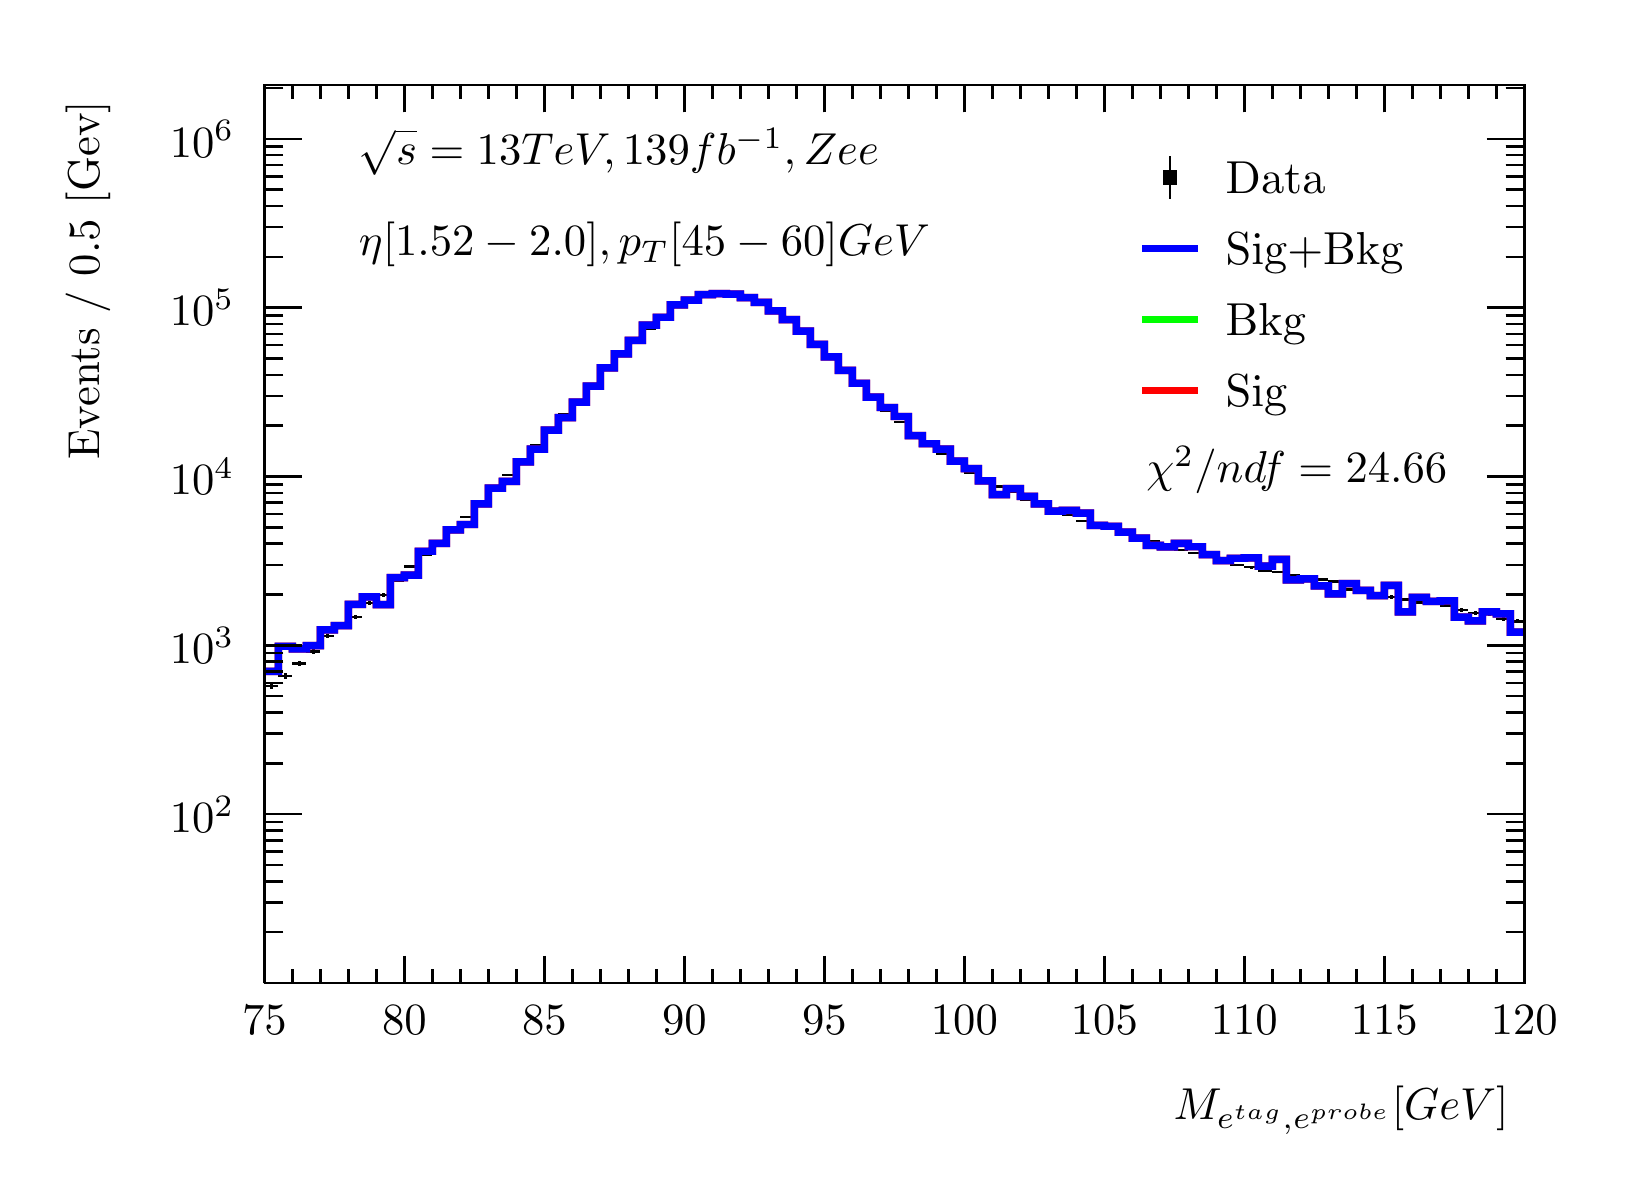
\begin{tikzpicture}
\pgfdeclareplotmark{cross} {
\pgfpathmoveto{\pgfpoint{-0.3\pgfplotmarksize}{\pgfplotmarksize}}
\pgfpathlineto{\pgfpoint{+0.3\pgfplotmarksize}{\pgfplotmarksize}}
\pgfpathlineto{\pgfpoint{+0.3\pgfplotmarksize}{0.3\pgfplotmarksize}}
\pgfpathlineto{\pgfpoint{+1\pgfplotmarksize}{0.3\pgfplotmarksize}}
\pgfpathlineto{\pgfpoint{+1\pgfplotmarksize}{-0.3\pgfplotmarksize}}
\pgfpathlineto{\pgfpoint{+0.3\pgfplotmarksize}{-0.3\pgfplotmarksize}}
\pgfpathlineto{\pgfpoint{+0.3\pgfplotmarksize}{-1.\pgfplotmarksize}}
\pgfpathlineto{\pgfpoint{-0.3\pgfplotmarksize}{-1.\pgfplotmarksize}}
\pgfpathlineto{\pgfpoint{-0.3\pgfplotmarksize}{-0.3\pgfplotmarksize}}
\pgfpathlineto{\pgfpoint{-1.\pgfplotmarksize}{-0.3\pgfplotmarksize}}
\pgfpathlineto{\pgfpoint{-1.\pgfplotmarksize}{0.3\pgfplotmarksize}}
\pgfpathlineto{\pgfpoint{-0.3\pgfplotmarksize}{0.3\pgfplotmarksize}}
\pgfpathclose
\pgfusepathqstroke
}
\pgfdeclareplotmark{cross*} {
\pgfpathmoveto{\pgfpoint{-0.3\pgfplotmarksize}{\pgfplotmarksize}}
\pgfpathlineto{\pgfpoint{+0.3\pgfplotmarksize}{\pgfplotmarksize}}
\pgfpathlineto{\pgfpoint{+0.3\pgfplotmarksize}{0.3\pgfplotmarksize}}
\pgfpathlineto{\pgfpoint{+1\pgfplotmarksize}{0.3\pgfplotmarksize}}
\pgfpathlineto{\pgfpoint{+1\pgfplotmarksize}{-0.3\pgfplotmarksize}}
\pgfpathlineto{\pgfpoint{+0.3\pgfplotmarksize}{-0.3\pgfplotmarksize}}
\pgfpathlineto{\pgfpoint{+0.3\pgfplotmarksize}{-1.\pgfplotmarksize}}
\pgfpathlineto{\pgfpoint{-0.3\pgfplotmarksize}{-1.\pgfplotmarksize}}
\pgfpathlineto{\pgfpoint{-0.3\pgfplotmarksize}{-0.3\pgfplotmarksize}}
\pgfpathlineto{\pgfpoint{-1.\pgfplotmarksize}{-0.3\pgfplotmarksize}}
\pgfpathlineto{\pgfpoint{-1.\pgfplotmarksize}{0.3\pgfplotmarksize}}
\pgfpathlineto{\pgfpoint{-0.3\pgfplotmarksize}{0.3\pgfplotmarksize}}
\pgfpathclose
\pgfusepathqfillstroke
}
\pgfdeclareplotmark{newstar} {
\pgfpathmoveto{\pgfqpoint{0pt}{\pgfplotmarksize}}
\pgfpathlineto{\pgfqpointpolar{44}{0.5\pgfplotmarksize}}
\pgfpathlineto{\pgfqpointpolar{18}{\pgfplotmarksize}}
\pgfpathlineto{\pgfqpointpolar{-20}{0.5\pgfplotmarksize}}
\pgfpathlineto{\pgfqpointpolar{-54}{\pgfplotmarksize}}
\pgfpathlineto{\pgfqpointpolar{-90}{0.5\pgfplotmarksize}}
\pgfpathlineto{\pgfqpointpolar{234}{\pgfplotmarksize}}
\pgfpathlineto{\pgfqpointpolar{198}{0.5\pgfplotmarksize}}
\pgfpathlineto{\pgfqpointpolar{162}{\pgfplotmarksize}}
\pgfpathlineto{\pgfqpointpolar{134}{0.5\pgfplotmarksize}}
\pgfpathclose
\pgfusepathqstroke
}
\pgfdeclareplotmark{newstar*} {
\pgfpathmoveto{\pgfqpoint{0pt}{\pgfplotmarksize}}
\pgfpathlineto{\pgfqpointpolar{44}{0.5\pgfplotmarksize}}
\pgfpathlineto{\pgfqpointpolar{18}{\pgfplotmarksize}}
\pgfpathlineto{\pgfqpointpolar{-20}{0.5\pgfplotmarksize}}
\pgfpathlineto{\pgfqpointpolar{-54}{\pgfplotmarksize}}
\pgfpathlineto{\pgfqpointpolar{-90}{0.5\pgfplotmarksize}}
\pgfpathlineto{\pgfqpointpolar{234}{\pgfplotmarksize}}
\pgfpathlineto{\pgfqpointpolar{198}{0.5\pgfplotmarksize}}
\pgfpathlineto{\pgfqpointpolar{162}{\pgfplotmarksize}}
\pgfpathlineto{\pgfqpointpolar{134}{0.5\pgfplotmarksize}}
\pgfpathclose
\pgfusepathqfillstroke
}
\definecolor{c}{rgb}{1,1,1};
\draw [color=c, fill=c] (0,0) rectangle (20,14.4361);
\draw [color=c, fill=c] (3,2.30977) rectangle (19,13.7143);
\definecolor{c}{rgb}{0,0,0};
\draw [c,line width=0.9] (3,2.30977) -- (3,13.7143) -- (19,13.7143) -- (19,2.30977) -- (3,2.30977);
\definecolor{c}{rgb}{1,1,1};
\draw [color=c, fill=c] (3,2.30977) rectangle (19,13.7143);
\definecolor{c}{rgb}{0,0,0};
\draw [c,line width=0.9] (3,2.30977) -- (3,13.7143) -- (19,13.7143) -- (19,2.30977) -- (3,2.30977);
\draw [c,line width=0.9] (3,2.30977) -- (19,2.30977);
\draw [c,line width=0.9] (3,2.65624) -- (3,2.30977);
\draw [c,line width=0.9] (3.35556,2.48301) -- (3.35556,2.30977);
\draw [c,line width=0.9] (3.71111,2.48301) -- (3.71111,2.30977);
\draw [c,line width=0.9] (4.06667,2.48301) -- (4.06667,2.30977);
\draw [c,line width=0.9] (4.42222,2.48301) -- (4.42222,2.30977);
\draw [c,line width=0.9] (4.77778,2.65624) -- (4.77778,2.30977);
\draw [c,line width=0.9] (5.13333,2.48301) -- (5.13333,2.30977);
\draw [c,line width=0.9] (5.48889,2.48301) -- (5.48889,2.30977);
\draw [c,line width=0.9] (5.84444,2.48301) -- (5.84444,2.30977);
\draw [c,line width=0.9] (6.2,2.48301) -- (6.2,2.30977);
\draw [c,line width=0.9] (6.55556,2.65624) -- (6.55556,2.30977);
\draw [c,line width=0.9] (6.91111,2.48301) -- (6.91111,2.30977);
\draw [c,line width=0.9] (7.26667,2.48301) -- (7.26667,2.30977);
\draw [c,line width=0.9] (7.62222,2.48301) -- (7.62222,2.30977);
\draw [c,line width=0.9] (7.97778,2.48301) -- (7.97778,2.30977);
\draw [c,line width=0.9] (8.33333,2.65624) -- (8.33333,2.30977);
\draw [c,line width=0.9] (8.68889,2.48301) -- (8.68889,2.30977);
\draw [c,line width=0.9] (9.04444,2.48301) -- (9.04444,2.30977);
\draw [c,line width=0.9] (9.4,2.48301) -- (9.4,2.30977);
\draw [c,line width=0.9] (9.75556,2.48301) -- (9.75556,2.30977);
\draw [c,line width=0.9] (10.1111,2.65624) -- (10.1111,2.30977);
\draw [c,line width=0.9] (10.4667,2.48301) -- (10.4667,2.30977);
\draw [c,line width=0.9] (10.8222,2.48301) -- (10.8222,2.30977);
\draw [c,line width=0.9] (11.1778,2.48301) -- (11.1778,2.30977);
\draw [c,line width=0.9] (11.5333,2.48301) -- (11.5333,2.30977);
\draw [c,line width=0.9] (11.8889,2.65624) -- (11.8889,2.30977);
\draw [c,line width=0.9] (12.2444,2.48301) -- (12.2444,2.30977);
\draw [c,line width=0.9] (12.6,2.48301) -- (12.6,2.30977);
\draw [c,line width=0.9] (12.9556,2.48301) -- (12.9556,2.30977);
\draw [c,line width=0.9] (13.3111,2.48301) -- (13.3111,2.30977);
\draw [c,line width=0.9] (13.6667,2.65624) -- (13.6667,2.30977);
\draw [c,line width=0.9] (14.0222,2.48301) -- (14.0222,2.30977);
\draw [c,line width=0.9] (14.3778,2.48301) -- (14.3778,2.30977);
\draw [c,line width=0.9] (14.7333,2.48301) -- (14.7333,2.30977);
\draw [c,line width=0.9] (15.0889,2.48301) -- (15.0889,2.30977);
\draw [c,line width=0.9] (15.4444,2.65624) -- (15.4444,2.30977);
\draw [c,line width=0.9] (15.8,2.48301) -- (15.8,2.30977);
\draw [c,line width=0.9] (16.1556,2.48301) -- (16.1556,2.30977);
\draw [c,line width=0.9] (16.5111,2.48301) -- (16.5111,2.30977);
\draw [c,line width=0.9] (16.8667,2.48301) -- (16.8667,2.30977);
\draw [c,line width=0.9] (17.2222,2.65624) -- (17.2222,2.30977);
\draw [c,line width=0.9] (17.5778,2.48301) -- (17.5778,2.30977);
\draw [c,line width=0.9] (17.9333,2.48301) -- (17.9333,2.30977);
\draw [c,line width=0.9] (18.2889,2.48301) -- (18.2889,2.30977);
\draw [c,line width=0.9] (18.6444,2.48301) -- (18.6444,2.30977);
\draw [c,line width=0.9] (19,2.65624) -- (19,2.30977);
\draw [c,line width=0.9] (19,2.65624) -- (19,2.30977);
\draw [anchor=base] (3,1.66015) node[scale=1.61424, color=c, rotate=0]{75};
\draw [anchor=base] (4.77778,1.66015) node[scale=1.61424, color=c, rotate=0]{80};
\draw [anchor=base] (6.55556,1.66015) node[scale=1.61424, color=c, rotate=0]{85};
\draw [anchor=base] (8.33333,1.66015) node[scale=1.61424, color=c, rotate=0]{90};
\draw [anchor=base] (10.1111,1.66015) node[scale=1.61424, color=c, rotate=0]{95};
\draw [anchor=base] (11.8889,1.66015) node[scale=1.61424, color=c, rotate=0]{100};
\draw [anchor=base] (13.6667,1.66015) node[scale=1.61424, color=c, rotate=0]{105};
\draw [anchor=base] (15.4444,1.66015) node[scale=1.61424, color=c, rotate=0]{110};
\draw [anchor=base] (17.2222,1.66015) node[scale=1.61424, color=c, rotate=0]{115};
\draw [anchor=base] (19,1.66015) node[scale=1.61424, color=c, rotate=0]{120};
\draw [anchor= east] (19,0.692932) node[scale=1.61424, color=c, rotate=0]{$M_{e^{tag}, e^{probe}}  [GeV]$};
\draw [c,line width=0.9] (3,13.7143) -- (19,13.7143);
\draw [c,line width=0.9] (3,13.3678) -- (3,13.7143);
\draw [c,line width=0.9] (3.35556,13.5411) -- (3.35556,13.7143);
\draw [c,line width=0.9] (3.71111,13.5411) -- (3.71111,13.7143);
\draw [c,line width=0.9] (4.06667,13.5411) -- (4.06667,13.7143);
\draw [c,line width=0.9] (4.42222,13.5411) -- (4.42222,13.7143);
\draw [c,line width=0.9] (4.77778,13.3678) -- (4.77778,13.7143);
\draw [c,line width=0.9] (5.13333,13.5411) -- (5.13333,13.7143);
\draw [c,line width=0.9] (5.48889,13.5411) -- (5.48889,13.7143);
\draw [c,line width=0.9] (5.84444,13.5411) -- (5.84444,13.7143);
\draw [c,line width=0.9] (6.2,13.5411) -- (6.2,13.7143);
\draw [c,line width=0.9] (6.55556,13.3678) -- (6.55556,13.7143);
\draw [c,line width=0.9] (6.91111,13.5411) -- (6.91111,13.7143);
\draw [c,line width=0.9] (7.26667,13.5411) -- (7.26667,13.7143);
\draw [c,line width=0.9] (7.62222,13.5411) -- (7.62222,13.7143);
\draw [c,line width=0.9] (7.97778,13.5411) -- (7.97778,13.7143);
\draw [c,line width=0.9] (8.33333,13.3678) -- (8.33333,13.7143);
\draw [c,line width=0.9] (8.68889,13.5411) -- (8.68889,13.7143);
\draw [c,line width=0.9] (9.04444,13.5411) -- (9.04444,13.7143);
\draw [c,line width=0.9] (9.4,13.5411) -- (9.4,13.7143);
\draw [c,line width=0.9] (9.75556,13.5411) -- (9.75556,13.7143);
\draw [c,line width=0.9] (10.1111,13.3678) -- (10.1111,13.7143);
\draw [c,line width=0.9] (10.4667,13.5411) -- (10.4667,13.7143);
\draw [c,line width=0.9] (10.8222,13.5411) -- (10.8222,13.7143);
\draw [c,line width=0.9] (11.1778,13.5411) -- (11.1778,13.7143);
\draw [c,line width=0.9] (11.5333,13.5411) -- (11.5333,13.7143);
\draw [c,line width=0.9] (11.8889,13.3678) -- (11.8889,13.7143);
\draw [c,line width=0.9] (12.2444,13.5411) -- (12.2444,13.7143);
\draw [c,line width=0.9] (12.6,13.5411) -- (12.6,13.7143);
\draw [c,line width=0.9] (12.9556,13.5411) -- (12.9556,13.7143);
\draw [c,line width=0.9] (13.3111,13.5411) -- (13.3111,13.7143);
\draw [c,line width=0.9] (13.6667,13.3678) -- (13.6667,13.7143);
\draw [c,line width=0.9] (14.0222,13.5411) -- (14.0222,13.7143);
\draw [c,line width=0.9] (14.3778,13.5411) -- (14.3778,13.7143);
\draw [c,line width=0.9] (14.7333,13.5411) -- (14.7333,13.7143);
\draw [c,line width=0.9] (15.0889,13.5411) -- (15.0889,13.7143);
\draw [c,line width=0.9] (15.4444,13.3678) -- (15.4444,13.7143);
\draw [c,line width=0.9] (15.8,13.5411) -- (15.8,13.7143);
\draw [c,line width=0.9] (16.1556,13.5411) -- (16.1556,13.7143);
\draw [c,line width=0.9] (16.5111,13.5411) -- (16.5111,13.7143);
\draw [c,line width=0.9] (16.8667,13.5411) -- (16.8667,13.7143);
\draw [c,line width=0.9] (17.2222,13.3678) -- (17.2222,13.7143);
\draw [c,line width=0.9] (17.5778,13.5411) -- (17.5778,13.7143);
\draw [c,line width=0.9] (17.9333,13.5411) -- (17.9333,13.7143);
\draw [c,line width=0.9] (18.2889,13.5411) -- (18.2889,13.7143);
\draw [c,line width=0.9] (18.6444,13.5411) -- (18.6444,13.7143);
\draw [c,line width=0.9] (19,13.3678) -- (19,13.7143);
\draw [c,line width=0.9] (19,13.3678) -- (19,13.7143);
\draw [c,line width=0.9] (3,2.30977) -- (3,13.7143);
\draw [c,line width=0.9] (3.237,2.95525) -- (3,2.95525);
\draw [c,line width=0.9] (3.237,3.33283) -- (3,3.33283);
\draw [c,line width=0.9] (3.237,3.60073) -- (3,3.60073);
\draw [c,line width=0.9] (3.237,3.80852) -- (3,3.80852);
\draw [c,line width=0.9] (3.237,3.97831) -- (3,3.97831);
\draw [c,line width=0.9] (3.237,4.12185) -- (3,4.12185);
\draw [c,line width=0.9] (3.237,4.2462) -- (3,4.2462);
\draw [c,line width=0.9] (3.237,4.35589) -- (3,4.35589);
\draw [c,line width=0.9] (3.474,4.454) -- (3,4.454);
\draw [anchor= east] (2.82,4.454) node[scale=1.61424, color=c, rotate=0]{$10^{2}$};
\draw [c,line width=0.9] (3.237,5.09948) -- (3,5.09948);
\draw [c,line width=0.9] (3.237,5.47706) -- (3,5.47706);
\draw [c,line width=0.9] (3.237,5.74495) -- (3,5.74495);
\draw [c,line width=0.9] (3.237,5.95275) -- (3,5.95275);
\draw [c,line width=0.9] (3.237,6.12253) -- (3,6.12253);
\draw [c,line width=0.9] (3.237,6.26608) -- (3,6.26608);
\draw [c,line width=0.9] (3.237,6.39043) -- (3,6.39043);
\draw [c,line width=0.9] (3.237,6.50011) -- (3,6.50011);
\draw [c,line width=0.9] (3.474,6.59823) -- (3,6.59823);
\draw [anchor= east] (2.82,6.59823) node[scale=1.61424, color=c, rotate=0]{$10^{3}$};
\draw [c,line width=0.9] (3.237,7.2437) -- (3,7.2437);
\draw [c,line width=0.9] (3.237,7.62128) -- (3,7.62128);
\draw [c,line width=0.9] (3.237,7.88918) -- (3,7.88918);
\draw [c,line width=0.9] (3.237,8.09698) -- (3,8.09698);
\draw [c,line width=0.9] (3.237,8.26676) -- (3,8.26676);
\draw [c,line width=0.9] (3.237,8.41031) -- (3,8.41031);
\draw [c,line width=0.9] (3.237,8.53466) -- (3,8.53466);
\draw [c,line width=0.9] (3.237,8.64434) -- (3,8.64434);
\draw [c,line width=0.9] (3.474,8.74245) -- (3,8.74245);
\draw [anchor= east] (2.82,8.74245) node[scale=1.61424, color=c, rotate=0]{$10^{4}$};
\draw [c,line width=0.9] (3.237,9.38793) -- (3,9.38793);
\draw [c,line width=0.9] (3.237,9.76551) -- (3,9.76551);
\draw [c,line width=0.9] (3.237,10.0334) -- (3,10.0334);
\draw [c,line width=0.9] (3.237,10.2412) -- (3,10.2412);
\draw [c,line width=0.9] (3.237,10.411) -- (3,10.411);
\draw [c,line width=0.9] (3.237,10.5545) -- (3,10.5545);
\draw [c,line width=0.9] (3.237,10.6789) -- (3,10.6789);
\draw [c,line width=0.9] (3.237,10.7886) -- (3,10.7886);
\draw [c,line width=0.9] (3.474,10.8867) -- (3,10.8867);
\draw [anchor= east] (2.82,10.8867) node[scale=1.61424, color=c, rotate=0]{$10^{5}$};
\draw [c,line width=0.9] (3.237,11.5322) -- (3,11.5322);
\draw [c,line width=0.9] (3.237,11.9097) -- (3,11.9097);
\draw [c,line width=0.9] (3.237,12.1776) -- (3,12.1776);
\draw [c,line width=0.9] (3.237,12.3854) -- (3,12.3854);
\draw [c,line width=0.9] (3.237,12.5552) -- (3,12.5552);
\draw [c,line width=0.9] (3.237,12.6988) -- (3,12.6988);
\draw [c,line width=0.9] (3.237,12.8231) -- (3,12.8231);
\draw [c,line width=0.9] (3.237,12.9328) -- (3,12.9328);
\draw [c,line width=0.9] (3.474,13.0309) -- (3,13.0309);
\draw [anchor= east] (2.82,13.0309) node[scale=1.61424, color=c, rotate=0]{$10^{6}$};
\draw [c,line width=0.9] (3.237,13.6764) -- (3,13.6764);
\draw [anchor= east] (0.76,13.7143) node[scale=1.61424, color=c, rotate=90]{Events / 0.5 [Gev]};
\draw [c,line width=0.9] (19,2.30977) -- (19,13.7143);
\draw [c,line width=0.9] (18.763,2.95525) -- (19,2.95525);
\draw [c,line width=0.9] (18.763,3.33283) -- (19,3.33283);
\draw [c,line width=0.9] (18.763,3.60073) -- (19,3.60073);
\draw [c,line width=0.9] (18.763,3.80852) -- (19,3.80852);
\draw [c,line width=0.9] (18.763,3.97831) -- (19,3.97831);
\draw [c,line width=0.9] (18.763,4.12185) -- (19,4.12185);
\draw [c,line width=0.9] (18.763,4.2462) -- (19,4.2462);
\draw [c,line width=0.9] (18.763,4.35589) -- (19,4.35589);
\draw [c,line width=0.9] (18.526,4.454) -- (19,4.454);
\draw [c,line width=0.9] (18.763,5.09948) -- (19,5.09948);
\draw [c,line width=0.9] (18.763,5.47706) -- (19,5.47706);
\draw [c,line width=0.9] (18.763,5.74495) -- (19,5.74495);
\draw [c,line width=0.9] (18.763,5.95275) -- (19,5.95275);
\draw [c,line width=0.9] (18.763,6.12253) -- (19,6.12253);
\draw [c,line width=0.9] (18.763,6.26608) -- (19,6.26608);
\draw [c,line width=0.9] (18.763,6.39043) -- (19,6.39043);
\draw [c,line width=0.9] (18.763,6.50011) -- (19,6.50011);
\draw [c,line width=0.9] (18.526,6.59823) -- (19,6.59823);
\draw [c,line width=0.9] (18.763,7.2437) -- (19,7.2437);
\draw [c,line width=0.9] (18.763,7.62128) -- (19,7.62128);
\draw [c,line width=0.9] (18.763,7.88918) -- (19,7.88918);
\draw [c,line width=0.9] (18.763,8.09698) -- (19,8.09698);
\draw [c,line width=0.9] (18.763,8.26676) -- (19,8.26676);
\draw [c,line width=0.9] (18.763,8.41031) -- (19,8.41031);
\draw [c,line width=0.9] (18.763,8.53466) -- (19,8.53466);
\draw [c,line width=0.9] (18.763,8.64434) -- (19,8.64434);
\draw [c,line width=0.9] (18.526,8.74245) -- (19,8.74245);
\draw [c,line width=0.9] (18.763,9.38793) -- (19,9.38793);
\draw [c,line width=0.9] (18.763,9.76551) -- (19,9.76551);
\draw [c,line width=0.9] (18.763,10.0334) -- (19,10.0334);
\draw [c,line width=0.9] (18.763,10.2412) -- (19,10.2412);
\draw [c,line width=0.9] (18.763,10.411) -- (19,10.411);
\draw [c,line width=0.9] (18.763,10.5545) -- (19,10.5545);
\draw [c,line width=0.9] (18.763,10.6789) -- (19,10.6789);
\draw [c,line width=0.9] (18.763,10.7886) -- (19,10.7886);
\draw [c,line width=0.9] (18.526,10.8867) -- (19,10.8867);
\draw [c,line width=0.9] (18.763,11.5322) -- (19,11.5322);
\draw [c,line width=0.9] (18.763,11.9097) -- (19,11.9097);
\draw [c,line width=0.9] (18.763,12.1776) -- (19,12.1776);
\draw [c,line width=0.9] (18.763,12.3854) -- (19,12.3854);
\draw [c,line width=0.9] (18.763,12.5552) -- (19,12.5552);
\draw [c,line width=0.9] (18.763,12.6988) -- (19,12.6988);
\draw [c,line width=0.9] (18.763,12.8231) -- (19,12.8231);
\draw [c,line width=0.9] (18.763,12.9328) -- (19,12.9328);
\draw [c,line width=0.9] (18.526,13.0309) -- (19,13.0309);
\draw [c,line width=0.9] (18.763,13.6764) -- (19,13.6764);
\draw [c,line width=0.9] (3.08889,6.07966) -- (3,6.07966);
\draw [c,line width=0.9] (3,6.07966) -- (3,6.07966);
\draw [c,line width=0.9] (3.08889,6.07966) -- (3.17778,6.07966);
\draw [c,line width=0.9] (3.17778,6.07966) -- (3.17778,6.07966);
\draw [c,line width=0.9] (3.08889,6.07966) -- (3.08889,6.11856);
\draw [c,line width=0.9] (3.08889,6.11856) -- (3.08889,6.11856);
\draw [c,line width=0.9] (3.08889,6.07966) -- (3.08889,6.04076);
\draw [c,line width=0.9] (3.08889,6.04076) -- (3.08889,6.04076);
\draw [c,line width=0.9] (3.26667,6.20705) -- (3.17778,6.20705);
\draw [c,line width=0.9] (3.17778,6.20705) -- (3.17778,6.20705);
\draw [c,line width=0.9] (3.26667,6.20705) -- (3.35556,6.20705);
\draw [c,line width=0.9] (3.35556,6.20705) -- (3.35556,6.20705);
\draw [c,line width=0.9] (3.26667,6.20705) -- (3.26667,6.24338);
\draw [c,line width=0.9] (3.26667,6.24338) -- (3.26667,6.24338);
\draw [c,line width=0.9] (3.26667,6.20705) -- (3.26667,6.17072);
\draw [c,line width=0.9] (3.26667,6.17072) -- (3.26667,6.17072);
\draw [c,line width=0.9] (3.44444,6.37043) -- (3.35556,6.37043);
\draw [c,line width=0.9] (3.35556,6.37043) -- (3.35556,6.37043);
\draw [c,line width=0.9] (3.44444,6.37043) -- (3.53333,6.37043);
\draw [c,line width=0.9] (3.53333,6.37043) -- (3.53333,6.37043);
\draw [c,line width=0.9] (3.44444,6.37043) -- (3.44444,6.40371);
\draw [c,line width=0.9] (3.44444,6.40371) -- (3.44444,6.40371);
\draw [c,line width=0.9] (3.44444,6.37043) -- (3.44444,6.33715);
\draw [c,line width=0.9] (3.44444,6.33715) -- (3.44444,6.33715);
\draw [c,line width=0.9] (3.62222,6.5226) -- (3.53333,6.5226);
\draw [c,line width=0.9] (3.53333,6.5226) -- (3.53333,6.5226);
\draw [c,line width=0.9] (3.62222,6.5226) -- (3.71111,6.5226);
\draw [c,line width=0.9] (3.71111,6.5226) -- (3.71111,6.5226);
\draw [c,line width=0.9] (3.62222,6.5226) -- (3.62222,6.55327);
\draw [c,line width=0.9] (3.62222,6.55327) -- (3.62222,6.55327);
\draw [c,line width=0.9] (3.62222,6.5226) -- (3.62222,6.49194);
\draw [c,line width=0.9] (3.62222,6.49194) -- (3.62222,6.49194);
\draw [c,line width=0.9] (3.8,6.71697) -- (3.71111,6.71697);
\draw [c,line width=0.9] (3.71111,6.71697) -- (3.71111,6.71697);
\draw [c,line width=0.9] (3.8,6.71697) -- (3.88889,6.71697);
\draw [c,line width=0.9] (3.88889,6.71697) -- (3.88889,6.71697);
\draw [c,line width=0.9] (3.8,6.71697) -- (3.8,6.7446);
\draw [c,line width=0.9] (3.8,6.7446) -- (3.8,6.7446);
\draw [c,line width=0.9] (3.8,6.71697) -- (3.8,6.68934);
\draw [c,line width=0.9] (3.8,6.68934) -- (3.8,6.68934);
\draw [c,line width=0.9] (3.97778,6.84968) -- (3.88889,6.84968);
\draw [c,line width=0.9] (3.88889,6.84968) -- (3.88889,6.84968);
\draw [c,line width=0.9] (3.97778,6.84968) -- (4.06667,6.84968);
\draw [c,line width=0.9] (4.06667,6.84968) -- (4.06667,6.84968);
\draw [c,line width=0.9] (3.97778,6.84968) -- (3.97778,6.87541);
\draw [c,line width=0.9] (3.97778,6.87541) -- (3.97778,6.87541);
\draw [c,line width=0.9] (3.97778,6.84968) -- (3.97778,6.82396);
\draw [c,line width=0.9] (3.97778,6.82396) -- (3.97778,6.82396);
\draw [c,line width=0.9] (4.15556,6.96142) -- (4.06667,6.96142);
\draw [c,line width=0.9] (4.06667,6.96142) -- (4.06667,6.96142);
\draw [c,line width=0.9] (4.15556,6.96142) -- (4.24444,6.96142);
\draw [c,line width=0.9] (4.24444,6.96142) -- (4.24444,6.96142);
\draw [c,line width=0.9] (4.15556,6.96142) -- (4.15556,6.98565);
\draw [c,line width=0.9] (4.15556,6.98565) -- (4.15556,6.98565);
\draw [c,line width=0.9] (4.15556,6.96142) -- (4.15556,6.93719);
\draw [c,line width=0.9] (4.15556,6.93719) -- (4.15556,6.93719);
\draw [c,line width=0.9] (4.33333,7.13675) -- (4.24444,7.13675);
\draw [c,line width=0.9] (4.24444,7.13675) -- (4.24444,7.13675);
\draw [c,line width=0.9] (4.33333,7.13675) -- (4.42222,7.13675);
\draw [c,line width=0.9] (4.42222,7.13675) -- (4.42222,7.13675);
\draw [c,line width=0.9] (4.33333,7.13675) -- (4.33333,7.15881);
\draw [c,line width=0.9] (4.33333,7.15881) -- (4.33333,7.15881);
\draw [c,line width=0.9] (4.33333,7.13675) -- (4.33333,7.1147);
\draw [c,line width=0.9] (4.33333,7.1147) -- (4.33333,7.1147);
\draw [c,line width=0.9] (4.51111,7.2395) -- (4.42222,7.2395);
\draw [c,line width=0.9] (4.42222,7.2395) -- (4.42222,7.2395);
\draw [c,line width=0.9] (4.51111,7.2395) -- (4.6,7.2395);
\draw [c,line width=0.9] (4.6,7.2395) -- (4.6,7.2395);
\draw [c,line width=0.9] (4.51111,7.2395) -- (4.51111,7.26037);
\draw [c,line width=0.9] (4.51111,7.26037) -- (4.51111,7.26037);
\draw [c,line width=0.9] (4.51111,7.2395) -- (4.51111,7.21864);
\draw [c,line width=0.9] (4.51111,7.21864) -- (4.51111,7.21864);
\draw [c,line width=0.9] (4.68889,7.42352) -- (4.6,7.42352);
\draw [c,line width=0.9] (4.6,7.42352) -- (4.6,7.42352);
\draw [c,line width=0.9] (4.68889,7.42352) -- (4.77778,7.42352);
\draw [c,line width=0.9] (4.77778,7.42352) -- (4.77778,7.42352);
\draw [c,line width=0.9] (4.68889,7.42352) -- (4.68889,7.44243);
\draw [c,line width=0.9] (4.68889,7.44243) -- (4.68889,7.44243);
\draw [c,line width=0.9] (4.68889,7.42352) -- (4.68889,7.40461);
\draw [c,line width=0.9] (4.68889,7.40461) -- (4.68889,7.40461);
\draw [c,line width=0.9] (4.86667,7.5993) -- (4.77778,7.5993);
\draw [c,line width=0.9] (4.77778,7.5993) -- (4.77778,7.5993);
\draw [c,line width=0.9] (4.86667,7.5993) -- (4.95556,7.5993);
\draw [c,line width=0.9] (4.95556,7.5993) -- (4.95556,7.5993);
\draw [c,line width=0.9] (4.86667,7.5993) -- (4.86667,7.6165);
\draw [c,line width=0.9] (4.86667,7.6165) -- (4.86667,7.6165);
\draw [c,line width=0.9] (4.86667,7.5993) -- (4.86667,7.58209);
\draw [c,line width=0.9] (4.86667,7.58209) -- (4.86667,7.58209);
\draw [c,line width=0.9] (5.04444,7.74412) -- (4.95556,7.74412);
\draw [c,line width=0.9] (4.95556,7.74412) -- (4.95556,7.74412);
\draw [c,line width=0.9] (5.04444,7.74412) -- (5.13333,7.74412);
\draw [c,line width=0.9] (5.13333,7.74412) -- (5.13333,7.74412);
\draw [c,line width=0.9] (5.04444,7.74412) -- (5.04444,7.76003);
\draw [c,line width=0.9] (5.04444,7.76003) -- (5.04444,7.76003);
\draw [c,line width=0.9] (5.04444,7.74412) -- (5.04444,7.7282);
\draw [c,line width=0.9] (5.04444,7.7282) -- (5.04444,7.7282);
\draw [c,line width=0.9] (5.22222,7.88965) -- (5.13333,7.88965);
\draw [c,line width=0.9] (5.13333,7.88965) -- (5.13333,7.88965);
\draw [c,line width=0.9] (5.22222,7.88965) -- (5.31111,7.88965);
\draw [c,line width=0.9] (5.31111,7.88965) -- (5.31111,7.88965);
\draw [c,line width=0.9] (5.22222,7.88965) -- (5.22222,7.90437);
\draw [c,line width=0.9] (5.22222,7.90437) -- (5.22222,7.90437);
\draw [c,line width=0.9] (5.22222,7.88965) -- (5.22222,7.87493);
\draw [c,line width=0.9] (5.22222,7.87493) -- (5.22222,7.87493);
\draw [c,line width=0.9] (5.4,8.08574) -- (5.31111,8.08574);
\draw [c,line width=0.9] (5.31111,8.08574) -- (5.31111,8.08574);
\draw [c,line width=0.9] (5.4,8.08574) -- (5.48889,8.08574);
\draw [c,line width=0.9] (5.48889,8.08574) -- (5.48889,8.08574);
\draw [c,line width=0.9] (5.4,8.08574) -- (5.4,8.09898);
\draw [c,line width=0.9] (5.4,8.09898) -- (5.4,8.09898);
\draw [c,line width=0.9] (5.4,8.08574) -- (5.4,8.07249);
\draw [c,line width=0.9] (5.4,8.07249) -- (5.4,8.07249);
\draw [c,line width=0.9] (5.57778,8.22551) -- (5.48889,8.22551);
\draw [c,line width=0.9] (5.48889,8.22551) -- (5.48889,8.22551);
\draw [c,line width=0.9] (5.57778,8.22551) -- (5.66667,8.22551);
\draw [c,line width=0.9] (5.66667,8.22551) -- (5.66667,8.22551);
\draw [c,line width=0.9] (5.57778,8.22551) -- (5.57778,8.2378);
\draw [c,line width=0.9] (5.57778,8.2378) -- (5.57778,8.2378);
\draw [c,line width=0.9] (5.57778,8.22551) -- (5.57778,8.21322);
\draw [c,line width=0.9] (5.57778,8.21322) -- (5.57778,8.21322);
\draw [c,line width=0.9] (5.75556,8.38304) -- (5.66667,8.38304);
\draw [c,line width=0.9] (5.66667,8.38304) -- (5.66667,8.38304);
\draw [c,line width=0.9] (5.75556,8.38304) -- (5.84444,8.38304);
\draw [c,line width=0.9] (5.84444,8.38304) -- (5.84444,8.38304);
\draw [c,line width=0.9] (5.75556,8.38304) -- (5.75556,8.39434);
\draw [c,line width=0.9] (5.75556,8.39434) -- (5.75556,8.39434);
\draw [c,line width=0.9] (5.75556,8.38304) -- (5.75556,8.37175);
\draw [c,line width=0.9] (5.75556,8.37175) -- (5.75556,8.37175);
\draw [c,line width=0.9] (5.93333,8.60005) -- (5.84444,8.60005);
\draw [c,line width=0.9] (5.84444,8.60005) -- (5.84444,8.60005);
\draw [c,line width=0.9] (5.93333,8.60005) -- (6.02222,8.60005);
\draw [c,line width=0.9] (6.02222,8.60005) -- (6.02222,8.60005);
\draw [c,line width=0.9] (5.93333,8.60005) -- (5.93333,8.61011);
\draw [c,line width=0.9] (5.93333,8.61011) -- (5.93333,8.61011);
\draw [c,line width=0.9] (5.93333,8.60005) -- (5.93333,8.59);
\draw [c,line width=0.9] (5.93333,8.59) -- (5.93333,8.59);
\draw [c,line width=0.9] (6.11111,8.76226) -- (6.02222,8.76226);
\draw [c,line width=0.9] (6.02222,8.76226) -- (6.02222,8.76226);
\draw [c,line width=0.9] (6.11111,8.76226) -- (6.2,8.76226);
\draw [c,line width=0.9] (6.2,8.76226) -- (6.2,8.76226);
\draw [c,line width=0.9] (6.11111,8.76226) -- (6.11111,8.77148);
\draw [c,line width=0.9] (6.11111,8.77148) -- (6.11111,8.77148);
\draw [c,line width=0.9] (6.11111,8.76226) -- (6.11111,8.75305);
\draw [c,line width=0.9] (6.11111,8.75305) -- (6.11111,8.75305);
\draw [c,line width=0.9] (6.28889,8.94719) -- (6.2,8.94719);
\draw [c,line width=0.9] (6.2,8.94719) -- (6.2,8.94719);
\draw [c,line width=0.9] (6.28889,8.94719) -- (6.37778,8.94719);
\draw [c,line width=0.9] (6.37778,8.94719) -- (6.37778,8.94719);
\draw [c,line width=0.9] (6.28889,8.94719) -- (6.28889,8.95553);
\draw [c,line width=0.9] (6.28889,8.95553) -- (6.28889,8.95553);
\draw [c,line width=0.9] (6.28889,8.94719) -- (6.28889,8.93885);
\draw [c,line width=0.9] (6.28889,8.93885) -- (6.28889,8.93885);
\draw [c,line width=0.9] (6.46667,9.13537) -- (6.37778,9.13537);
\draw [c,line width=0.9] (6.37778,9.13537) -- (6.37778,9.13537);
\draw [c,line width=0.9] (6.46667,9.13537) -- (6.55556,9.13537);
\draw [c,line width=0.9] (6.55556,9.13537) -- (6.55556,9.13537);
\draw [c,line width=0.9] (6.46667,9.13537) -- (6.46667,9.14291);
\draw [c,line width=0.9] (6.46667,9.14291) -- (6.46667,9.14291);
\draw [c,line width=0.9] (6.46667,9.13537) -- (6.46667,9.12782);
\draw [c,line width=0.9] (6.46667,9.12782) -- (6.46667,9.12782);
\draw [c,line width=0.9] (6.64444,9.3191) -- (6.55556,9.3191);
\draw [c,line width=0.9] (6.55556,9.3191) -- (6.55556,9.3191);
\draw [c,line width=0.9] (6.64444,9.3191) -- (6.73333,9.3191);
\draw [c,line width=0.9] (6.73333,9.3191) -- (6.73333,9.3191);
\draw [c,line width=0.9] (6.64444,9.3191) -- (6.64444,9.32593);
\draw [c,line width=0.9] (6.64444,9.32593) -- (6.64444,9.32593);
\draw [c,line width=0.9] (6.64444,9.3191) -- (6.64444,9.31227);
\draw [c,line width=0.9] (6.64444,9.31227) -- (6.64444,9.31227);
\draw [c,line width=0.9] (6.82222,9.53577) -- (6.73333,9.53577);
\draw [c,line width=0.9] (6.73333,9.53577) -- (6.73333,9.53577);
\draw [c,line width=0.9] (6.82222,9.53577) -- (6.91111,9.53577);
\draw [c,line width=0.9] (6.91111,9.53577) -- (6.91111,9.53577);
\draw [c,line width=0.9] (6.82222,9.53577) -- (6.82222,9.54185);
\draw [c,line width=0.9] (6.82222,9.54185) -- (6.82222,9.54185);
\draw [c,line width=0.9] (6.82222,9.53577) -- (6.82222,9.52969);
\draw [c,line width=0.9] (6.82222,9.52969) -- (6.82222,9.52969);
\draw [c,line width=0.9] (7,9.71555) -- (6.91111,9.71555);
\draw [c,line width=0.9] (6.91111,9.71555) -- (6.91111,9.71555);
\draw [c,line width=0.9] (7,9.71555) -- (7.08889,9.71555);
\draw [c,line width=0.9] (7.08889,9.71555) -- (7.08889,9.71555);
\draw [c,line width=0.9] (7,9.71555) -- (7,9.72108);
\draw [c,line width=0.9] (7,9.72108) -- (7,9.72108);
\draw [c,line width=0.9] (7,9.71555) -- (7,9.71003);
\draw [c,line width=0.9] (7,9.71003) -- (7,9.71003);
\draw [c,line width=0.9] (7.17778,9.91402) -- (7.08889,9.91402);
\draw [c,line width=0.9] (7.08889,9.91402) -- (7.08889,9.91402);
\draw [c,line width=0.9] (7.17778,9.91402) -- (7.26667,9.91402);
\draw [c,line width=0.9] (7.26667,9.91402) -- (7.26667,9.91402);
\draw [c,line width=0.9] (7.17778,9.91402) -- (7.17778,9.91899);
\draw [c,line width=0.9] (7.17778,9.91899) -- (7.17778,9.91899);
\draw [c,line width=0.9] (7.17778,9.91402) -- (7.17778,9.90906);
\draw [c,line width=0.9] (7.17778,9.90906) -- (7.17778,9.90906);
\draw [c,line width=0.9] (7.35556,10.106) -- (7.26667,10.106);
\draw [c,line width=0.9] (7.26667,10.106) -- (7.26667,10.106);
\draw [c,line width=0.9] (7.35556,10.106) -- (7.44444,10.106);
\draw [c,line width=0.9] (7.44444,10.106) -- (7.44444,10.106);
\draw [c,line width=0.9] (7.35556,10.106) -- (7.35556,10.1105);
\draw [c,line width=0.9] (7.35556,10.1105) -- (7.35556,10.1105);
\draw [c,line width=0.9] (7.35556,10.106) -- (7.35556,10.1015);
\draw [c,line width=0.9] (7.35556,10.1015) -- (7.35556,10.1015);
\draw [c,line width=0.9] (7.53333,10.2922) -- (7.44444,10.2922);
\draw [c,line width=0.9] (7.44444,10.2922) -- (7.44444,10.2922);
\draw [c,line width=0.9] (7.53333,10.2922) -- (7.62222,10.2922);
\draw [c,line width=0.9] (7.62222,10.2922) -- (7.62222,10.2922);
\draw [c,line width=0.9] (7.53333,10.2922) -- (7.53333,10.2962);
\draw [c,line width=0.9] (7.53333,10.2962) -- (7.53333,10.2962);
\draw [c,line width=0.9] (7.53333,10.2922) -- (7.53333,10.2881);
\draw [c,line width=0.9] (7.53333,10.2881) -- (7.53333,10.2881);
\draw [c,line width=0.9] (7.71111,10.4611) -- (7.62222,10.4611);
\draw [c,line width=0.9] (7.62222,10.4611) -- (7.62222,10.4611);
\draw [c,line width=0.9] (7.71111,10.4611) -- (7.8,10.4611);
\draw [c,line width=0.9] (7.8,10.4611) -- (7.8,10.4611);
\draw [c,line width=0.9] (7.71111,10.4611) -- (7.71111,10.4648);
\draw [c,line width=0.9] (7.71111,10.4648) -- (7.71111,10.4648);
\draw [c,line width=0.9] (7.71111,10.4611) -- (7.71111,10.4574);
\draw [c,line width=0.9] (7.71111,10.4574) -- (7.71111,10.4574);
\draw [c,line width=0.9] (7.88889,10.6249) -- (7.8,10.6249);
\draw [c,line width=0.9] (7.8,10.6249) -- (7.8,10.6249);
\draw [c,line width=0.9] (7.88889,10.6249) -- (7.97778,10.6249);
\draw [c,line width=0.9] (7.97778,10.6249) -- (7.97778,10.6249);
\draw [c,line width=0.9] (7.88889,10.6249) -- (7.88889,10.6283);
\draw [c,line width=0.9] (7.88889,10.6283) -- (7.88889,10.6283);
\draw [c,line width=0.9] (7.88889,10.6249) -- (7.88889,10.6215);
\draw [c,line width=0.9] (7.88889,10.6215) -- (7.88889,10.6215);
\draw [c,line width=0.9] (8.06667,10.7703) -- (7.97778,10.7703);
\draw [c,line width=0.9] (7.97778,10.7703) -- (7.97778,10.7703);
\draw [c,line width=0.9] (8.06667,10.7703) -- (8.15556,10.7703);
\draw [c,line width=0.9] (8.15556,10.7703) -- (8.15556,10.7703);
\draw [c,line width=0.9] (8.06667,10.7703) -- (8.06667,10.7735);
\draw [c,line width=0.9] (8.06667,10.7735) -- (8.06667,10.7735);
\draw [c,line width=0.9] (8.06667,10.7703) -- (8.06667,10.7672);
\draw [c,line width=0.9] (8.06667,10.7672) -- (8.06667,10.7672);
\draw [c,line width=0.9] (8.24444,10.8945) -- (8.15556,10.8945);
\draw [c,line width=0.9] (8.15556,10.8945) -- (8.15556,10.8945);
\draw [c,line width=0.9] (8.24444,10.8945) -- (8.33333,10.8945);
\draw [c,line width=0.9] (8.33333,10.8945) -- (8.33333,10.8945);
\draw [c,line width=0.9] (8.24444,10.8945) -- (8.24444,10.8974);
\draw [c,line width=0.9] (8.24444,10.8974) -- (8.24444,10.8974);
\draw [c,line width=0.9] (8.24444,10.8945) -- (8.24444,10.8916);
\draw [c,line width=0.9] (8.24444,10.8916) -- (8.24444,10.8916);
\draw [c,line width=0.9] (8.42222,10.9882) -- (8.33333,10.9882);
\draw [c,line width=0.9] (8.33333,10.9882) -- (8.33333,10.9882);
\draw [c,line width=0.9] (8.42222,10.9882) -- (8.51111,10.9882);
\draw [c,line width=0.9] (8.51111,10.9882) -- (8.51111,10.9882);
\draw [c,line width=0.9] (8.42222,10.9882) -- (8.42222,10.991);
\draw [c,line width=0.9] (8.42222,10.991) -- (8.42222,10.991);
\draw [c,line width=0.9] (8.42222,10.9882) -- (8.42222,10.9854);
\draw [c,line width=0.9] (8.42222,10.9854) -- (8.42222,10.9854);
\draw [c,line width=0.9] (8.6,11.0522) -- (8.51111,11.0522);
\draw [c,line width=0.9] (8.51111,11.0522) -- (8.51111,11.0522);
\draw [c,line width=0.9] (8.6,11.0522) -- (8.68889,11.0522);
\draw [c,line width=0.9] (8.68889,11.0522) -- (8.68889,11.0522);
\draw [c,line width=0.9] (8.6,11.0522) -- (8.6,11.0549);
\draw [c,line width=0.9] (8.6,11.0549) -- (8.6,11.0549);
\draw [c,line width=0.9] (8.6,11.0522) -- (8.6,11.0495);
\draw [c,line width=0.9] (8.6,11.0495) -- (8.6,11.0495);
\draw [c,line width=0.9] (8.77778,11.0799) -- (8.68889,11.0799);
\draw [c,line width=0.9] (8.68889,11.0799) -- (8.68889,11.0799);
\draw [c,line width=0.9] (8.77778,11.0799) -- (8.86667,11.0799);
\draw [c,line width=0.9] (8.86667,11.0799) -- (8.86667,11.0799);
\draw [c,line width=0.9] (8.77778,11.0799) -- (8.77778,11.0825);
\draw [c,line width=0.9] (8.77778,11.0825) -- (8.77778,11.0825);
\draw [c,line width=0.9] (8.77778,11.0799) -- (8.77778,11.0772);
\draw [c,line width=0.9] (8.77778,11.0772) -- (8.77778,11.0772);
\draw [c,line width=0.9] (8.95556,11.0744) -- (8.86667,11.0744);
\draw [c,line width=0.9] (8.86667,11.0744) -- (8.86667,11.0744);
\draw [c,line width=0.9] (8.95556,11.0744) -- (9.04444,11.0744);
\draw [c,line width=0.9] (9.04444,11.0744) -- (9.04444,11.0744);
\draw [c,line width=0.9] (8.95556,11.0744) -- (8.95556,11.077);
\draw [c,line width=0.9] (8.95556,11.077) -- (8.95556,11.077);
\draw [c,line width=0.9] (8.95556,11.0744) -- (8.95556,11.0717);
\draw [c,line width=0.9] (8.95556,11.0717) -- (8.95556,11.0717);
\draw [c,line width=0.9] (9.13333,11.0359) -- (9.04444,11.0359);
\draw [c,line width=0.9] (9.04444,11.0359) -- (9.04444,11.0359);
\draw [c,line width=0.9] (9.13333,11.0359) -- (9.22222,11.0359);
\draw [c,line width=0.9] (9.22222,11.0359) -- (9.22222,11.0359);
\draw [c,line width=0.9] (9.13333,11.0359) -- (9.13333,11.0386);
\draw [c,line width=0.9] (9.13333,11.0386) -- (9.13333,11.0386);
\draw [c,line width=0.9] (9.13333,11.0359) -- (9.13333,11.0332);
\draw [c,line width=0.9] (9.13333,11.0332) -- (9.13333,11.0332);
\draw [c,line width=0.9] (9.31111,10.9633) -- (9.22222,10.9633);
\draw [c,line width=0.9] (9.22222,10.9633) -- (9.22222,10.9633);
\draw [c,line width=0.9] (9.31111,10.9633) -- (9.4,10.9633);
\draw [c,line width=0.9] (9.4,10.9633) -- (9.4,10.9633);
\draw [c,line width=0.9] (9.31111,10.9633) -- (9.31111,10.9661);
\draw [c,line width=0.9] (9.31111,10.9661) -- (9.31111,10.9661);
\draw [c,line width=0.9] (9.31111,10.9633) -- (9.31111,10.9604);
\draw [c,line width=0.9] (9.31111,10.9604) -- (9.31111,10.9604);
\draw [c,line width=0.9] (9.48889,10.8636) -- (9.4,10.8636);
\draw [c,line width=0.9] (9.4,10.8636) -- (9.4,10.8636);
\draw [c,line width=0.9] (9.48889,10.8636) -- (9.57778,10.8636);
\draw [c,line width=0.9] (9.57778,10.8636) -- (9.57778,10.8636);
\draw [c,line width=0.9] (9.48889,10.8636) -- (9.48889,10.8666);
\draw [c,line width=0.9] (9.48889,10.8666) -- (9.48889,10.8666);
\draw [c,line width=0.9] (9.48889,10.8636) -- (9.48889,10.8606);
\draw [c,line width=0.9] (9.48889,10.8606) -- (9.48889,10.8606);
\draw [c,line width=0.9] (9.66667,10.7382) -- (9.57778,10.7382);
\draw [c,line width=0.9] (9.57778,10.7382) -- (9.57778,10.7382);
\draw [c,line width=0.9] (9.66667,10.7382) -- (9.75556,10.7382);
\draw [c,line width=0.9] (9.75556,10.7382) -- (9.75556,10.7382);
\draw [c,line width=0.9] (9.66667,10.7382) -- (9.66667,10.7414);
\draw [c,line width=0.9] (9.66667,10.7414) -- (9.66667,10.7414);
\draw [c,line width=0.9] (9.66667,10.7382) -- (9.66667,10.735);
\draw [c,line width=0.9] (9.66667,10.735) -- (9.66667,10.735);
\draw [c,line width=0.9] (9.84444,10.5903) -- (9.75556,10.5903);
\draw [c,line width=0.9] (9.75556,10.5903) -- (9.75556,10.5903);
\draw [c,line width=0.9] (9.84444,10.5903) -- (9.93333,10.5903);
\draw [c,line width=0.9] (9.93333,10.5903) -- (9.93333,10.5903);
\draw [c,line width=0.9] (9.84444,10.5903) -- (9.84444,10.5937);
\draw [c,line width=0.9] (9.84444,10.5937) -- (9.84444,10.5937);
\draw [c,line width=0.9] (9.84444,10.5903) -- (9.84444,10.5868);
\draw [c,line width=0.9] (9.84444,10.5868) -- (9.84444,10.5868);
\draw [c,line width=0.9] (10.0222,10.4372) -- (9.93333,10.4372);
\draw [c,line width=0.9] (9.93333,10.4372) -- (9.93333,10.4372);
\draw [c,line width=0.9] (10.0222,10.4372) -- (10.1111,10.4372);
\draw [c,line width=0.9] (10.1111,10.4372) -- (10.1111,10.4372);
\draw [c,line width=0.9] (10.0222,10.4372) -- (10.0222,10.4409);
\draw [c,line width=0.9] (10.0222,10.4409) -- (10.0222,10.4409);
\draw [c,line width=0.9] (10.0222,10.4372) -- (10.0222,10.4334);
\draw [c,line width=0.9] (10.0222,10.4334) -- (10.0222,10.4334);
\draw [c,line width=0.9] (10.2,10.2664) -- (10.1111,10.2664);
\draw [c,line width=0.9] (10.1111,10.2664) -- (10.1111,10.2664);
\draw [c,line width=0.9] (10.2,10.2664) -- (10.2889,10.2664);
\draw [c,line width=0.9] (10.2889,10.2664) -- (10.2889,10.2664);
\draw [c,line width=0.9] (10.2,10.2664) -- (10.2,10.2705);
\draw [c,line width=0.9] (10.2,10.2705) -- (10.2,10.2705);
\draw [c,line width=0.9] (10.2,10.2664) -- (10.2,10.2623);
\draw [c,line width=0.9] (10.2,10.2623) -- (10.2,10.2623);
\draw [c,line width=0.9] (10.3778,10.0834) -- (10.2889,10.0834);
\draw [c,line width=0.9] (10.2889,10.0834) -- (10.2889,10.0834);
\draw [c,line width=0.9] (10.3778,10.0834) -- (10.4667,10.0834);
\draw [c,line width=0.9] (10.4667,10.0834) -- (10.4667,10.0834);
\draw [c,line width=0.9] (10.3778,10.0834) -- (10.3778,10.0879);
\draw [c,line width=0.9] (10.3778,10.0879) -- (10.3778,10.0879);
\draw [c,line width=0.9] (10.3778,10.0834) -- (10.3778,10.0788);
\draw [c,line width=0.9] (10.3778,10.0788) -- (10.3778,10.0788);
\draw [c,line width=0.9] (10.5556,9.91233) -- (10.4667,9.91233);
\draw [c,line width=0.9] (10.4667,9.91233) -- (10.4667,9.91233);
\draw [c,line width=0.9] (10.5556,9.91233) -- (10.6444,9.91233);
\draw [c,line width=0.9] (10.6444,9.91233) -- (10.6444,9.91233);
\draw [c,line width=0.9] (10.5556,9.91233) -- (10.5556,9.9173);
\draw [c,line width=0.9] (10.5556,9.9173) -- (10.5556,9.9173);
\draw [c,line width=0.9] (10.5556,9.91233) -- (10.5556,9.90736);
\draw [c,line width=0.9] (10.5556,9.90736) -- (10.5556,9.90736);
\draw [c,line width=0.9] (10.7333,9.73769) -- (10.6444,9.73769);
\draw [c,line width=0.9] (10.6444,9.73769) -- (10.6444,9.73769);
\draw [c,line width=0.9] (10.7333,9.73769) -- (10.8222,9.73769);
\draw [c,line width=0.9] (10.8222,9.73769) -- (10.8222,9.73769);
\draw [c,line width=0.9] (10.7333,9.73769) -- (10.7333,9.74315);
\draw [c,line width=0.9] (10.7333,9.74315) -- (10.7333,9.74315);
\draw [c,line width=0.9] (10.7333,9.73769) -- (10.7333,9.73223);
\draw [c,line width=0.9] (10.7333,9.73223) -- (10.7333,9.73223);
\draw [c,line width=0.9] (10.9111,9.5829) -- (10.8222,9.5829);
\draw [c,line width=0.9] (10.8222,9.5829) -- (10.8222,9.5829);
\draw [c,line width=0.9] (10.9111,9.5829) -- (11,9.5829);
\draw [c,line width=0.9] (11,9.5829) -- (11,9.5829);
\draw [c,line width=0.9] (10.9111,9.5829) -- (10.9111,9.58883);
\draw [c,line width=0.9] (10.9111,9.58883) -- (10.9111,9.58883);
\draw [c,line width=0.9] (10.9111,9.5829) -- (10.9111,9.57697);
\draw [c,line width=0.9] (10.9111,9.57697) -- (10.9111,9.57697);
\draw [c,line width=0.9] (11.0889,9.43235) -- (11,9.43235);
\draw [c,line width=0.9] (11,9.43235) -- (11,9.43235);
\draw [c,line width=0.9] (11.0889,9.43235) -- (11.1778,9.43235);
\draw [c,line width=0.9] (11.1778,9.43235) -- (11.1778,9.43235);
\draw [c,line width=0.9] (11.0889,9.43235) -- (11.0889,9.43878);
\draw [c,line width=0.9] (11.0889,9.43878) -- (11.0889,9.43878);
\draw [c,line width=0.9] (11.0889,9.43235) -- (11.0889,9.42592);
\draw [c,line width=0.9] (11.0889,9.42592) -- (11.0889,9.42592);
\draw [c,line width=0.9] (11.2667,9.27069) -- (11.1778,9.27069);
\draw [c,line width=0.9] (11.1778,9.27069) -- (11.1778,9.27069);
\draw [c,line width=0.9] (11.2667,9.27069) -- (11.3556,9.27069);
\draw [c,line width=0.9] (11.3556,9.27069) -- (11.3556,9.27069);
\draw [c,line width=0.9] (11.2667,9.27069) -- (11.2667,9.2777);
\draw [c,line width=0.9] (11.2667,9.2777) -- (11.2667,9.2777);
\draw [c,line width=0.9] (11.2667,9.27069) -- (11.2667,9.26367);
\draw [c,line width=0.9] (11.2667,9.26367) -- (11.2667,9.26367);
\draw [c,line width=0.9] (11.4444,9.14363) -- (11.3556,9.14363);
\draw [c,line width=0.9] (11.3556,9.14363) -- (11.3556,9.14363);
\draw [c,line width=0.9] (11.4444,9.14363) -- (11.5333,9.14363);
\draw [c,line width=0.9] (11.5333,9.14363) -- (11.5333,9.14363);
\draw [c,line width=0.9] (11.4444,9.14363) -- (11.4444,9.15114);
\draw [c,line width=0.9] (11.4444,9.15114) -- (11.4444,9.15114);
\draw [c,line width=0.9] (11.4444,9.14363) -- (11.4444,9.13613);
\draw [c,line width=0.9] (11.4444,9.13613) -- (11.4444,9.13613);
\draw [c,line width=0.9] (11.6222,9.02831) -- (11.5333,9.02831);
\draw [c,line width=0.9] (11.5333,9.02831) -- (11.5333,9.02831);
\draw [c,line width=0.9] (11.6222,9.02831) -- (11.7111,9.02831);
\draw [c,line width=0.9] (11.7111,9.02831) -- (11.7111,9.02831);
\draw [c,line width=0.9] (11.6222,9.02831) -- (11.6222,9.0363);
\draw [c,line width=0.9] (11.6222,9.0363) -- (11.6222,9.0363);
\draw [c,line width=0.9] (11.6222,9.02831) -- (11.6222,9.02033);
\draw [c,line width=0.9] (11.6222,9.02033) -- (11.6222,9.02033);
\draw [c,line width=0.9] (11.8,8.91735) -- (11.7111,8.91735);
\draw [c,line width=0.9] (11.7111,8.91735) -- (11.7111,8.91735);
\draw [c,line width=0.9] (11.8,8.91735) -- (11.8889,8.91735);
\draw [c,line width=0.9] (11.8889,8.91735) -- (11.8889,8.91735);
\draw [c,line width=0.9] (11.8,8.91735) -- (11.8,8.92582);
\draw [c,line width=0.9] (11.8,8.92582) -- (11.8,8.92582);
\draw [c,line width=0.9] (11.8,8.91735) -- (11.8,8.90887);
\draw [c,line width=0.9] (11.8,8.90887) -- (11.8,8.90887);
\draw [c,line width=0.9] (11.9778,8.79672) -- (11.8889,8.79672);
\draw [c,line width=0.9] (11.8889,8.79672) -- (11.8889,8.79672);
\draw [c,line width=0.9] (11.9778,8.79672) -- (12.0667,8.79672);
\draw [c,line width=0.9] (12.0667,8.79672) -- (12.0667,8.79672);
\draw [c,line width=0.9] (11.9778,8.79672) -- (11.9778,8.80576);
\draw [c,line width=0.9] (11.9778,8.80576) -- (11.9778,8.80576);
\draw [c,line width=0.9] (11.9778,8.79672) -- (11.9778,8.78767);
\draw [c,line width=0.9] (11.9778,8.78767) -- (11.9778,8.78767);
\draw [c,line width=0.9] (12.1556,8.7024) -- (12.0667,8.7024);
\draw [c,line width=0.9] (12.0667,8.7024) -- (12.0667,8.7024);
\draw [c,line width=0.9] (12.1556,8.7024) -- (12.2444,8.7024);
\draw [c,line width=0.9] (12.2444,8.7024) -- (12.2444,8.7024);
\draw [c,line width=0.9] (12.1556,8.7024) -- (12.1556,8.71192);
\draw [c,line width=0.9] (12.1556,8.71192) -- (12.1556,8.71192);
\draw [c,line width=0.9] (12.1556,8.7024) -- (12.1556,8.69289);
\draw [c,line width=0.9] (12.1556,8.69289) -- (12.1556,8.69289);
\draw [c,line width=0.9] (12.3333,8.61437) -- (12.2444,8.61437);
\draw [c,line width=0.9] (12.2444,8.61437) -- (12.2444,8.61437);
\draw [c,line width=0.9] (12.3333,8.61437) -- (12.4222,8.61437);
\draw [c,line width=0.9] (12.4222,8.61437) -- (12.4222,8.61437);
\draw [c,line width=0.9] (12.3333,8.61437) -- (12.3333,8.62435);
\draw [c,line width=0.9] (12.3333,8.62435) -- (12.3333,8.62435);
\draw [c,line width=0.9] (12.3333,8.61437) -- (12.3333,8.6044);
\draw [c,line width=0.9] (12.3333,8.6044) -- (12.3333,8.6044);
\draw [c,line width=0.9] (12.5111,8.5491) -- (12.4222,8.5491);
\draw [c,line width=0.9] (12.4222,8.5491) -- (12.4222,8.5491);
\draw [c,line width=0.9] (12.5111,8.5491) -- (12.6,8.5491);
\draw [c,line width=0.9] (12.6,8.5491) -- (12.6,8.5491);
\draw [c,line width=0.9] (12.5111,8.5491) -- (12.5111,8.55943);
\draw [c,line width=0.9] (12.5111,8.55943) -- (12.5111,8.55943);
\draw [c,line width=0.9] (12.5111,8.5491) -- (12.5111,8.53876);
\draw [c,line width=0.9] (12.5111,8.53876) -- (12.5111,8.53876);
\draw [c,line width=0.9] (12.6889,8.44543) -- (12.6,8.44543);
\draw [c,line width=0.9] (12.6,8.44543) -- (12.6,8.44543);
\draw [c,line width=0.9] (12.6889,8.44543) -- (12.7778,8.44543);
\draw [c,line width=0.9] (12.7778,8.44543) -- (12.7778,8.44543);
\draw [c,line width=0.9] (12.6889,8.44543) -- (12.6889,8.45635);
\draw [c,line width=0.9] (12.6889,8.45635) -- (12.6889,8.45635);
\draw [c,line width=0.9] (12.6889,8.44543) -- (12.6889,8.4345);
\draw [c,line width=0.9] (12.6889,8.4345) -- (12.6889,8.4345);
\draw [c,line width=0.9] (12.8667,8.36896) -- (12.7778,8.36896);
\draw [c,line width=0.9] (12.7778,8.36896) -- (12.7778,8.36896);
\draw [c,line width=0.9] (12.8667,8.36896) -- (12.9556,8.36896);
\draw [c,line width=0.9] (12.9556,8.36896) -- (12.9556,8.36896);
\draw [c,line width=0.9] (12.8667,8.36896) -- (12.8667,8.38034);
\draw [c,line width=0.9] (12.8667,8.38034) -- (12.8667,8.38034);
\draw [c,line width=0.9] (12.8667,8.36896) -- (12.8667,8.35758);
\draw [c,line width=0.9] (12.8667,8.35758) -- (12.8667,8.35758);
\draw [c,line width=0.9] (13.0444,8.29519) -- (12.9556,8.29519);
\draw [c,line width=0.9] (12.9556,8.29519) -- (12.9556,8.29519);
\draw [c,line width=0.9] (13.0444,8.29519) -- (13.1333,8.29519);
\draw [c,line width=0.9] (13.1333,8.29519) -- (13.1333,8.29519);
\draw [c,line width=0.9] (13.0444,8.29519) -- (13.0444,8.30703);
\draw [c,line width=0.9] (13.0444,8.30703) -- (13.0444,8.30703);
\draw [c,line width=0.9] (13.0444,8.29519) -- (13.0444,8.28335);
\draw [c,line width=0.9] (13.0444,8.28335) -- (13.0444,8.28335);
\draw [c,line width=0.9] (13.2222,8.25897) -- (13.1333,8.25897);
\draw [c,line width=0.9] (13.1333,8.25897) -- (13.1333,8.25897);
\draw [c,line width=0.9] (13.2222,8.25897) -- (13.3111,8.25897);
\draw [c,line width=0.9] (13.3111,8.25897) -- (13.3111,8.25897);
\draw [c,line width=0.9] (13.2222,8.25897) -- (13.2222,8.27104);
\draw [c,line width=0.9] (13.2222,8.27104) -- (13.2222,8.27104);
\draw [c,line width=0.9] (13.2222,8.25897) -- (13.2222,8.2469);
\draw [c,line width=0.9] (13.2222,8.2469) -- (13.2222,8.2469);
\draw [c,line width=0.9] (13.4,8.17483) -- (13.3111,8.17483);
\draw [c,line width=0.9] (13.3111,8.17483) -- (13.3111,8.17483);
\draw [c,line width=0.9] (13.4,8.17483) -- (13.4889,8.17483);
\draw [c,line width=0.9] (13.4889,8.17483) -- (13.4889,8.17483);
\draw [c,line width=0.9] (13.4,8.17483) -- (13.4,8.18746);
\draw [c,line width=0.9] (13.4,8.18746) -- (13.4,8.18746);
\draw [c,line width=0.9] (13.4,8.17483) -- (13.4,8.1622);
\draw [c,line width=0.9] (13.4,8.1622) -- (13.4,8.1622);
\draw [c,line width=0.9] (13.5778,8.12179) -- (13.4889,8.12179);
\draw [c,line width=0.9] (13.4889,8.12179) -- (13.4889,8.12179);
\draw [c,line width=0.9] (13.5778,8.12179) -- (13.6667,8.12179);
\draw [c,line width=0.9] (13.6667,8.12179) -- (13.6667,8.12179);
\draw [c,line width=0.9] (13.5778,8.12179) -- (13.5778,8.13478);
\draw [c,line width=0.9] (13.5778,8.13478) -- (13.5778,8.13478);
\draw [c,line width=0.9] (13.5778,8.12179) -- (13.5778,8.10879);
\draw [c,line width=0.9] (13.5778,8.10879) -- (13.5778,8.10879);
\draw [c,line width=0.9] (13.7556,8.08442) -- (13.6667,8.08442);
\draw [c,line width=0.9] (13.6667,8.08442) -- (13.6667,8.08442);
\draw [c,line width=0.9] (13.7556,8.08442) -- (13.8444,8.08442);
\draw [c,line width=0.9] (13.8444,8.08442) -- (13.8444,8.08442);
\draw [c,line width=0.9] (13.7556,8.08442) -- (13.7556,8.09767);
\draw [c,line width=0.9] (13.7556,8.09767) -- (13.7556,8.09767);
\draw [c,line width=0.9] (13.7556,8.08442) -- (13.7556,8.07116);
\draw [c,line width=0.9] (13.7556,8.07116) -- (13.7556,8.07116);
\draw [c,line width=0.9] (13.9333,7.99762) -- (13.8444,7.99762);
\draw [c,line width=0.9] (13.8444,7.99762) -- (13.8444,7.99762);
\draw [c,line width=0.9] (13.9333,7.99762) -- (14.0222,7.99762);
\draw [c,line width=0.9] (14.0222,7.99762) -- (14.0222,7.99762);
\draw [c,line width=0.9] (13.9333,7.99762) -- (13.9333,8.01151);
\draw [c,line width=0.9] (13.9333,8.01151) -- (13.9333,8.01151);
\draw [c,line width=0.9] (13.9333,7.99762) -- (13.9333,7.98373);
\draw [c,line width=0.9] (13.9333,7.98373) -- (13.9333,7.98373);
\draw [c,line width=0.9] (14.1111,7.95175) -- (14.0222,7.95175);
\draw [c,line width=0.9] (14.0222,7.95175) -- (14.0222,7.95175);
\draw [c,line width=0.9] (14.1111,7.95175) -- (14.2,7.95175);
\draw [c,line width=0.9] (14.2,7.95175) -- (14.2,7.95175);
\draw [c,line width=0.9] (14.1111,7.95175) -- (14.1111,7.96599);
\draw [c,line width=0.9] (14.1111,7.96599) -- (14.1111,7.96599);
\draw [c,line width=0.9] (14.1111,7.95175) -- (14.1111,7.93751);
\draw [c,line width=0.9] (14.1111,7.93751) -- (14.1111,7.93751);
\draw [c,line width=0.9] (14.2889,7.92054) -- (14.2,7.92054);
\draw [c,line width=0.9] (14.2,7.92054) -- (14.2,7.92054);
\draw [c,line width=0.9] (14.2889,7.92054) -- (14.3778,7.92054);
\draw [c,line width=0.9] (14.3778,7.92054) -- (14.3778,7.92054);
\draw [c,line width=0.9] (14.2889,7.92054) -- (14.2889,7.93502);
\draw [c,line width=0.9] (14.2889,7.93502) -- (14.2889,7.93502);
\draw [c,line width=0.9] (14.2889,7.92054) -- (14.2889,7.90606);
\draw [c,line width=0.9] (14.2889,7.90606) -- (14.2889,7.90606);
\draw [c,line width=0.9] (14.4667,7.82883) -- (14.3778,7.82883);
\draw [c,line width=0.9] (14.3778,7.82883) -- (14.3778,7.82883);
\draw [c,line width=0.9] (14.4667,7.82883) -- (14.5556,7.82883);
\draw [c,line width=0.9] (14.5556,7.82883) -- (14.5556,7.82883);
\draw [c,line width=0.9] (14.4667,7.82883) -- (14.4667,7.84404);
\draw [c,line width=0.9] (14.4667,7.84404) -- (14.4667,7.84404);
\draw [c,line width=0.9] (14.4667,7.82883) -- (14.4667,7.81362);
\draw [c,line width=0.9] (14.4667,7.81362) -- (14.4667,7.81362);
\draw [c,line width=0.9] (14.6444,7.81179) -- (14.5556,7.81179);
\draw [c,line width=0.9] (14.5556,7.81179) -- (14.5556,7.81179);
\draw [c,line width=0.9] (14.6444,7.81179) -- (14.7333,7.81179);
\draw [c,line width=0.9] (14.7333,7.81179) -- (14.7333,7.81179);
\draw [c,line width=0.9] (14.6444,7.81179) -- (14.6444,7.82714);
\draw [c,line width=0.9] (14.6444,7.82714) -- (14.6444,7.82714);
\draw [c,line width=0.9] (14.6444,7.81179) -- (14.6444,7.79644);
\draw [c,line width=0.9] (14.6444,7.79644) -- (14.6444,7.79644);
\draw [c,line width=0.9] (14.8222,7.77173) -- (14.7333,7.77173);
\draw [c,line width=0.9] (14.7333,7.77173) -- (14.7333,7.77173);
\draw [c,line width=0.9] (14.8222,7.77173) -- (14.9111,7.77173);
\draw [c,line width=0.9] (14.9111,7.77173) -- (14.9111,7.77173);
\draw [c,line width=0.9] (14.8222,7.77173) -- (14.8222,7.78741);
\draw [c,line width=0.9] (14.8222,7.78741) -- (14.8222,7.78741);
\draw [c,line width=0.9] (14.8222,7.77173) -- (14.8222,7.75604);
\draw [c,line width=0.9] (14.8222,7.75604) -- (14.8222,7.75604);
\draw [c,line width=0.9] (15,7.72182) -- (14.9111,7.72182);
\draw [c,line width=0.9] (14.9111,7.72182) -- (14.9111,7.72182);
\draw [c,line width=0.9] (15,7.72182) -- (15.0889,7.72182);
\draw [c,line width=0.9] (15.0889,7.72182) -- (15.0889,7.72182);
\draw [c,line width=0.9] (15,7.72182) -- (15,7.73793);
\draw [c,line width=0.9] (15,7.73793) -- (15,7.73793);
\draw [c,line width=0.9] (15,7.72182) -- (15,7.70571);
\draw [c,line width=0.9] (15,7.70571) -- (15,7.70571);
\draw [c,line width=0.9] (15.1778,7.70125) -- (15.0889,7.70125);
\draw [c,line width=0.9] (15.0889,7.70125) -- (15.0889,7.70125);
\draw [c,line width=0.9] (15.1778,7.70125) -- (15.2667,7.70125);
\draw [c,line width=0.9] (15.2667,7.70125) -- (15.2667,7.70125);
\draw [c,line width=0.9] (15.1778,7.70125) -- (15.1778,7.71754);
\draw [c,line width=0.9] (15.1778,7.71754) -- (15.1778,7.71754);
\draw [c,line width=0.9] (15.1778,7.70125) -- (15.1778,7.68496);
\draw [c,line width=0.9] (15.1778,7.68496) -- (15.1778,7.68496);
\draw [c,line width=0.9] (15.3556,7.61973) -- (15.2667,7.61973);
\draw [c,line width=0.9] (15.2667,7.61973) -- (15.2667,7.61973);
\draw [c,line width=0.9] (15.3556,7.61973) -- (15.4444,7.61973);
\draw [c,line width=0.9] (15.4444,7.61973) -- (15.4444,7.61973);
\draw [c,line width=0.9] (15.3556,7.61973) -- (15.3556,7.63675);
\draw [c,line width=0.9] (15.3556,7.63675) -- (15.3556,7.63675);
\draw [c,line width=0.9] (15.3556,7.61973) -- (15.3556,7.60272);
\draw [c,line width=0.9] (15.3556,7.60272) -- (15.3556,7.60272);
\draw [c,line width=0.9] (15.5333,7.59132) -- (15.4444,7.59132);
\draw [c,line width=0.9] (15.4444,7.59132) -- (15.4444,7.59132);
\draw [c,line width=0.9] (15.5333,7.59132) -- (15.6222,7.59132);
\draw [c,line width=0.9] (15.6222,7.59132) -- (15.6222,7.59132);
\draw [c,line width=0.9] (15.5333,7.59132) -- (15.5333,7.6086);
\draw [c,line width=0.9] (15.5333,7.6086) -- (15.5333,7.6086);
\draw [c,line width=0.9] (15.5333,7.59132) -- (15.5333,7.57404);
\draw [c,line width=0.9] (15.5333,7.57404) -- (15.5333,7.57404);
\draw [c,line width=0.9] (15.7111,7.54835) -- (15.6222,7.54835);
\draw [c,line width=0.9] (15.6222,7.54835) -- (15.6222,7.54835);
\draw [c,line width=0.9] (15.7111,7.54835) -- (15.8,7.54835);
\draw [c,line width=0.9] (15.8,7.54835) -- (15.8,7.54835);
\draw [c,line width=0.9] (15.7111,7.54835) -- (15.7111,7.56603);
\draw [c,line width=0.9] (15.7111,7.56603) -- (15.7111,7.56603);
\draw [c,line width=0.9] (15.7111,7.54835) -- (15.7111,7.53067);
\draw [c,line width=0.9] (15.7111,7.53067) -- (15.7111,7.53067);
\draw [c,line width=0.9] (15.8889,7.52936) -- (15.8,7.52936);
\draw [c,line width=0.9] (15.8,7.52936) -- (15.8,7.52936);
\draw [c,line width=0.9] (15.8889,7.52936) -- (15.9778,7.52936);
\draw [c,line width=0.9] (15.9778,7.52936) -- (15.9778,7.52936);
\draw [c,line width=0.9] (15.8889,7.52936) -- (15.8889,7.54722);
\draw [c,line width=0.9] (15.8889,7.54722) -- (15.8889,7.54722);
\draw [c,line width=0.9] (15.8889,7.52936) -- (15.8889,7.5115);
\draw [c,line width=0.9] (15.8889,7.5115) -- (15.8889,7.5115);
\draw [c,line width=0.9] (16.0667,7.48623) -- (15.9778,7.48623);
\draw [c,line width=0.9] (15.9778,7.48623) -- (15.9778,7.48623);
\draw [c,line width=0.9] (16.0667,7.48623) -- (16.1556,7.48623);
\draw [c,line width=0.9] (16.1556,7.48623) -- (16.1556,7.48623);
\draw [c,line width=0.9] (16.0667,7.48623) -- (16.0667,7.50451);
\draw [c,line width=0.9] (16.0667,7.50451) -- (16.0667,7.50451);
\draw [c,line width=0.9] (16.0667,7.48623) -- (16.0667,7.46795);
\draw [c,line width=0.9] (16.0667,7.46795) -- (16.0667,7.46795);
\draw [c,line width=0.9] (16.2444,7.4444) -- (16.1556,7.4444);
\draw [c,line width=0.9] (16.1556,7.4444) -- (16.1556,7.4444);
\draw [c,line width=0.9] (16.2444,7.4444) -- (16.3333,7.4444);
\draw [c,line width=0.9] (16.3333,7.4444) -- (16.3333,7.4444);
\draw [c,line width=0.9] (16.2444,7.4444) -- (16.2444,7.46309);
\draw [c,line width=0.9] (16.2444,7.46309) -- (16.2444,7.46309);
\draw [c,line width=0.9] (16.2444,7.4444) -- (16.2444,7.4257);
\draw [c,line width=0.9] (16.2444,7.4257) -- (16.2444,7.4257);
\draw [c,line width=0.9] (16.4222,7.43535) -- (16.3333,7.43535);
\draw [c,line width=0.9] (16.3333,7.43535) -- (16.3333,7.43535);
\draw [c,line width=0.9] (16.4222,7.43535) -- (16.5111,7.43535);
\draw [c,line width=0.9] (16.5111,7.43535) -- (16.5111,7.43535);
\draw [c,line width=0.9] (16.4222,7.43535) -- (16.4222,7.45413);
\draw [c,line width=0.9] (16.4222,7.45413) -- (16.4222,7.45413);
\draw [c,line width=0.9] (16.4222,7.43535) -- (16.4222,7.41656);
\draw [c,line width=0.9] (16.4222,7.41656) -- (16.4222,7.41656);
\draw [c,line width=0.9] (16.6,7.40687) -- (16.5111,7.40687);
\draw [c,line width=0.9] (16.5111,7.40687) -- (16.5111,7.40687);
\draw [c,line width=0.9] (16.6,7.40687) -- (16.6889,7.40687);
\draw [c,line width=0.9] (16.6889,7.40687) -- (16.6889,7.40687);
\draw [c,line width=0.9] (16.6,7.40687) -- (16.6,7.42594);
\draw [c,line width=0.9] (16.6,7.42594) -- (16.6,7.42594);
\draw [c,line width=0.9] (16.6,7.40687) -- (16.6,7.38779);
\draw [c,line width=0.9] (16.6,7.38779) -- (16.6,7.38779);
\draw [c,line width=0.9] (16.7778,7.30584) -- (16.6889,7.30584);
\draw [c,line width=0.9] (16.6889,7.30584) -- (16.6889,7.30584);
\draw [c,line width=0.9] (16.7778,7.30584) -- (16.8667,7.30584);
\draw [c,line width=0.9] (16.8667,7.30584) -- (16.8667,7.30584);
\draw [c,line width=0.9] (16.7778,7.30584) -- (16.7778,7.32598);
\draw [c,line width=0.9] (16.7778,7.32598) -- (16.7778,7.32598);
\draw [c,line width=0.9] (16.7778,7.30584) -- (16.7778,7.2857);
\draw [c,line width=0.9] (16.7778,7.2857) -- (16.7778,7.2857);
\draw [c,line width=0.9] (16.9556,7.30584) -- (16.8667,7.30584);
\draw [c,line width=0.9] (16.8667,7.30584) -- (16.8667,7.30584);
\draw [c,line width=0.9] (16.9556,7.30584) -- (17.0444,7.30584);
\draw [c,line width=0.9] (17.0444,7.30584) -- (17.0444,7.30584);
\draw [c,line width=0.9] (16.9556,7.30584) -- (16.9556,7.32598);
\draw [c,line width=0.9] (16.9556,7.32598) -- (16.9556,7.32598);
\draw [c,line width=0.9] (16.9556,7.30584) -- (16.9556,7.2857);
\draw [c,line width=0.9] (16.9556,7.2857) -- (16.9556,7.2857);
\draw [c,line width=0.9] (17.1333,7.24231) -- (17.0444,7.24231);
\draw [c,line width=0.9] (17.0444,7.24231) -- (17.0444,7.24231);
\draw [c,line width=0.9] (17.1333,7.24231) -- (17.2222,7.24231);
\draw [c,line width=0.9] (17.2222,7.24231) -- (17.2222,7.24231);
\draw [c,line width=0.9] (17.1333,7.24231) -- (17.1333,7.26314);
\draw [c,line width=0.9] (17.1333,7.26314) -- (17.1333,7.26314);
\draw [c,line width=0.9] (17.1333,7.24231) -- (17.1333,7.22147);
\draw [c,line width=0.9] (17.1333,7.22147) -- (17.1333,7.22147);
\draw [c,line width=0.9] (17.3111,7.21101) -- (17.2222,7.21101);
\draw [c,line width=0.9] (17.2222,7.21101) -- (17.2222,7.21101);
\draw [c,line width=0.9] (17.3111,7.21101) -- (17.4,7.21101);
\draw [c,line width=0.9] (17.4,7.21101) -- (17.4,7.21101);
\draw [c,line width=0.9] (17.3111,7.21101) -- (17.3111,7.2322);
\draw [c,line width=0.9] (17.3111,7.2322) -- (17.3111,7.2322);
\draw [c,line width=0.9] (17.3111,7.21101) -- (17.3111,7.18982);
\draw [c,line width=0.9] (17.3111,7.18982) -- (17.3111,7.18982);
\draw [c,line width=0.9] (17.4889,7.18162) -- (17.4,7.18162);
\draw [c,line width=0.9] (17.4,7.18162) -- (17.4,7.18162);
\draw [c,line width=0.9] (17.4889,7.18162) -- (17.5778,7.18162);
\draw [c,line width=0.9] (17.5778,7.18162) -- (17.5778,7.18162);
\draw [c,line width=0.9] (17.4889,7.18162) -- (17.4889,7.20314);
\draw [c,line width=0.9] (17.4889,7.20314) -- (17.4889,7.20314);
\draw [c,line width=0.9] (17.4889,7.18162) -- (17.4889,7.16009);
\draw [c,line width=0.9] (17.4889,7.16009) -- (17.4889,7.16009);
\draw [c,line width=0.9] (17.6667,7.14196) -- (17.5778,7.14196);
\draw [c,line width=0.9] (17.5778,7.14196) -- (17.5778,7.14196);
\draw [c,line width=0.9] (17.6667,7.14196) -- (17.7556,7.14196);
\draw [c,line width=0.9] (17.7556,7.14196) -- (17.7556,7.14196);
\draw [c,line width=0.9] (17.6667,7.14196) -- (17.6667,7.16395);
\draw [c,line width=0.9] (17.6667,7.16395) -- (17.6667,7.16395);
\draw [c,line width=0.9] (17.6667,7.14196) -- (17.6667,7.11997);
\draw [c,line width=0.9] (17.6667,7.11997) -- (17.6667,7.11997);
\draw [c,line width=0.9] (17.8444,7.14972) -- (17.7556,7.14972);
\draw [c,line width=0.9] (17.7556,7.14972) -- (17.7556,7.14972);
\draw [c,line width=0.9] (17.8444,7.14972) -- (17.9333,7.14972);
\draw [c,line width=0.9] (17.9333,7.14972) -- (17.9333,7.14972);
\draw [c,line width=0.9] (17.8444,7.14972) -- (17.8444,7.17162);
\draw [c,line width=0.9] (17.8444,7.17162) -- (17.8444,7.17162);
\draw [c,line width=0.9] (17.8444,7.14972) -- (17.8444,7.12782);
\draw [c,line width=0.9] (17.8444,7.12782) -- (17.8444,7.12782);
\draw [c,line width=0.9] (18.0222,7.10271) -- (17.9333,7.10271);
\draw [c,line width=0.9] (17.9333,7.10271) -- (17.9333,7.10271);
\draw [c,line width=0.9] (18.0222,7.10271) -- (18.1111,7.10271);
\draw [c,line width=0.9] (18.1111,7.10271) -- (18.1111,7.10271);
\draw [c,line width=0.9] (18.0222,7.10271) -- (18.0222,7.12517);
\draw [c,line width=0.9] (18.0222,7.12517) -- (18.0222,7.12517);
\draw [c,line width=0.9] (18.0222,7.10271) -- (18.0222,7.08025);
\draw [c,line width=0.9] (18.0222,7.08025) -- (18.0222,7.08025);
\draw [c,line width=0.9] (18.2,7.04575) -- (18.1111,7.04575);
\draw [c,line width=0.9] (18.1111,7.04575) -- (18.1111,7.04575);
\draw [c,line width=0.9] (18.2,7.04575) -- (18.2889,7.04575);
\draw [c,line width=0.9] (18.2889,7.04575) -- (18.2889,7.04575);
\draw [c,line width=0.9] (18.2,7.04575) -- (18.2,7.06891);
\draw [c,line width=0.9] (18.2,7.06891) -- (18.2,7.06891);
\draw [c,line width=0.9] (18.2,7.04575) -- (18.2,7.02259);
\draw [c,line width=0.9] (18.2,7.02259) -- (18.2,7.02259);
\draw [c,line width=0.9] (18.3778,7.01054) -- (18.2889,7.01054);
\draw [c,line width=0.9] (18.2889,7.01054) -- (18.2889,7.01054);
\draw [c,line width=0.9] (18.3778,7.01054) -- (18.4667,7.01054);
\draw [c,line width=0.9] (18.4667,7.01054) -- (18.4667,7.01054);
\draw [c,line width=0.9] (18.3778,7.01054) -- (18.3778,7.03414);
\draw [c,line width=0.9] (18.3778,7.03414) -- (18.3778,7.03414);
\draw [c,line width=0.9] (18.3778,7.01054) -- (18.3778,6.98694);
\draw [c,line width=0.9] (18.3778,6.98694) -- (18.3778,6.98694);
\draw [c,line width=0.9] (18.5556,6.99425) -- (18.4667,6.99425);
\draw [c,line width=0.9] (18.4667,6.99425) -- (18.4667,6.99425);
\draw [c,line width=0.9] (18.5556,6.99425) -- (18.6444,6.99425);
\draw [c,line width=0.9] (18.6444,6.99425) -- (18.6444,6.99425);
\draw [c,line width=0.9] (18.5556,6.99425) -- (18.5556,7.01805);
\draw [c,line width=0.9] (18.5556,7.01805) -- (18.5556,7.01805);
\draw [c,line width=0.9] (18.5556,6.99425) -- (18.5556,6.97044);
\draw [c,line width=0.9] (18.5556,6.97044) -- (18.5556,6.97044);
\draw [c,line width=0.9] (18.7333,6.9352) -- (18.6444,6.9352);
\draw [c,line width=0.9] (18.6444,6.9352) -- (18.6444,6.9352);
\draw [c,line width=0.9] (18.7333,6.9352) -- (18.8222,6.9352);
\draw [c,line width=0.9] (18.8222,6.9352) -- (18.8222,6.9352);
\draw [c,line width=0.9] (18.7333,6.9352) -- (18.7333,6.95978);
\draw [c,line width=0.9] (18.7333,6.95978) -- (18.7333,6.95978);
\draw [c,line width=0.9] (18.7333,6.9352) -- (18.7333,6.91063);
\draw [c,line width=0.9] (18.7333,6.91063) -- (18.7333,6.91063);
\draw [c,line width=0.9] (18.9111,6.90287) -- (18.8222,6.90287);
\draw [c,line width=0.9] (18.8222,6.90287) -- (18.8222,6.90287);
\draw [c,line width=0.9] (18.9111,6.90287) -- (19,6.90287);
\draw [c,line width=0.9] (19,6.90287) -- (19,6.90287);
\draw [c,line width=0.9] (18.9111,6.90287) -- (18.9111,6.92788);
\draw [c,line width=0.9] (18.9111,6.92788) -- (18.9111,6.92788);
\draw [c,line width=0.9] (18.9111,6.90287) -- (18.9111,6.87787);
\draw [c,line width=0.9] (18.9111,6.87787) -- (18.9111,6.87787);
\foreach \P in {(3.08889,6.07966), (3.26667,6.20705), (3.44444,6.37043), (3.62222,6.5226), (3.8,6.71697), (3.97778,6.84968), (4.15556,6.96142), (4.33333,7.13675), (4.51111,7.2395), (4.68889,7.42352), (4.86667,7.5993), (5.04444,7.74412),
 (5.22222,7.88965), (5.4,8.08574), (5.57778,8.22551), (5.75556,8.38304), (5.93333,8.60005), (6.11111,8.76226), (6.28889,8.94719), (6.46667,9.13537), (6.64444,9.3191), (6.82222,9.53577), (7,9.71555), (7.17778,9.91402), (7.35556,10.106),
 (7.53333,10.2922), (7.71111,10.4611), (7.88889,10.6249), (8.06667,10.7703), (8.24444,10.8945), (8.42222,10.9882), (8.6,11.0522), (8.77778,11.0799), (8.95556,11.0744), (9.13333,11.0359), (9.31111,10.9633), (9.48889,10.8636), (9.66667,10.7382),
 (9.84444,10.5903), (10.0222,10.4372), (10.2,10.2664), (10.3778,10.0834), (10.5556,9.91233), (10.7333,9.73769), (10.9111,9.5829), (11.0889,9.43235), (11.2667,9.27069), (11.4444,9.14363), (11.6222,9.02831), (11.8,8.91735), (11.9778,8.79672),
 (12.1556,8.7024), (12.3333,8.61437), (12.5111,8.5491), (12.6889,8.44543), (12.8667,8.36896), (13.0444,8.29519), (13.2222,8.25897), (13.4,8.17483), (13.5778,8.12179), (13.7556,8.08442), (13.9333,7.99762), (14.1111,7.95175), (14.2889,7.92054),
 (14.4667,7.82883), (14.6444,7.81179), (14.8222,7.77173), (15,7.72182), (15.1778,7.70125), (15.3556,7.61973), (15.5333,7.59132), (15.7111,7.54835), (15.8889,7.52936), (16.0667,7.48623), (16.2444,7.4444), (16.4222,7.43535), (16.6,7.40687),
 (16.7778,7.30584), (16.9556,7.30584), (17.1333,7.24231), (17.3111,7.21101), (17.4889,7.18162), (17.6667,7.14196), (17.8444,7.14972), (18.0222,7.10271), (18.2,7.04575), (18.3778,7.01054), (18.5556,6.99425), (18.7333,6.9352),
 (18.9111,6.90287)}{\draw[mark options={color=c,fill=c},mark size=2.882883pt,mark=] plot coordinates {\P};}
\definecolor{c}{rgb}{1,0,0};
\draw [c,line width=2.7] (3,6.26811) -- (3,6.26811);
\draw [c,line width=2.7] (3,6.26811) -- (3,6.26811) -- (3.17778,6.26811) -- (3.17778,6.58706) -- (3.35556,6.58706) -- (3.35556,6.55468) -- (3.53333,6.55468) -- (3.53333,6.59551) -- (3.71111,6.59551) -- (3.71111,6.7954) -- (3.88889,6.7954) --
 (3.88889,6.85043) -- (4.06667,6.85043) -- (4.06667,7.11864) -- (4.24444,7.11864) -- (4.24444,7.21535) -- (4.42222,7.21535) -- (4.42222,7.11666) -- (4.6,7.11666) -- (4.6,7.45737) -- (4.77778,7.45737) -- (4.77778,7.49006) -- (4.95556,7.49006) --
 (4.95556,7.79352) -- (5.13333,7.79352) -- (5.13333,7.8926) -- (5.31111,7.8926) -- (5.31111,8.0651) -- (5.48889,8.0651) -- (5.48889,8.13348) -- (5.66667,8.13348) -- (5.66667,8.39655) -- (5.84444,8.39655) -- (5.84444,8.59652) -- (6.02222,8.59652) --
 (6.02222,8.68172) -- (6.2,8.68172) -- (6.2,8.92839) -- (6.37778,8.92839) -- (6.37778,9.09069) -- (6.55556,9.09069) -- (6.55556,9.33162) -- (6.73333,9.33162) -- (6.73333,9.48938) -- (6.91111,9.48938) -- (6.91111,9.68643) -- (7.08889,9.68643) --
 (7.08889,9.89054) -- (7.26667,9.89054) -- (7.26667,10.1225) -- (7.44444,10.1225) -- (7.44444,10.2994) -- (7.62222,10.2994) -- (7.62222,10.4724) -- (7.8,10.4724) -- (7.8,10.6662) -- (7.97778,10.6662) -- (7.97778,10.7654) -- (8.15556,10.7654) --
 (8.15556,10.9213) -- (8.33333,10.9213) -- (8.33333,10.984) -- (8.51111,10.984) -- (8.51111,11.0523) -- (8.68889,11.0523) -- (8.68889,11.0651) -- (8.86667,11.0651) -- (8.86667,11.0577) -- (9.04444,11.0577) -- (9.04445,11.0138) -- (9.22222,11.0138) --
 (9.22222,10.9534) -- (9.4,10.9534) -- (9.4,10.846) -- (9.57778,10.846) -- (9.57778,10.7343) -- (9.75556,10.7343) -- (9.75556,10.5896) -- (9.93333,10.5896) -- (9.93333,10.4196) -- (10.1111,10.4196) -- (10.1111,10.2614) -- (10.2889,10.2614) --
 (10.2889,10.0906) -- (10.4667,10.0906) -- (10.4667,9.92718) -- (10.6444,9.92718) -- (10.6444,9.75059) -- (10.8222,9.75059) -- (10.8222,9.61924) -- (11,9.61924) -- (11,9.50505) -- (11.1778,9.50505) -- (11.1778,9.26264) -- (11.3556,9.26264) --
 (11.3556,9.15893) -- (11.5333,9.15893) -- (11.5333,9.09159) -- (11.7111,9.09159) -- (11.7111,8.9371) -- (11.8889,8.9371) -- (11.8889,8.84414) -- (12.0667,8.84414) -- (12.0667,8.68829) -- (12.2444,8.68829) -- (12.2444,8.51227) -- (12.4222,8.51227) --
 (12.4222,8.58823) -- (12.6,8.58823) -- (12.6,8.48999) -- (12.7778,8.48999) -- (12.7778,8.39648) -- (12.9556,8.39648) -- (12.9556,8.30437) -- (13.1333,8.30437) -- (13.1333,8.31234) -- (13.3111,8.31234) -- (13.3111,8.27684) -- (13.4889,8.27684) --
 (13.4889,8.12157) -- (13.6667,8.12157) -- (13.6667,8.11107) -- (13.8444,8.11107) -- (13.8444,8.0354) -- (14.0222,8.0354) -- (14.0222,7.96048) -- (14.2,7.96048) -- (14.2,7.86785) -- (14.3778,7.86785) -- (14.3778,7.84937) -- (14.5556,7.84937) --
 (14.5556,7.89448) -- (14.7333,7.89448) -- (14.7333,7.85084) -- (14.9111,7.85084) -- (14.9111,7.75141) -- (15.0889,7.75141) -- (15.0889,7.67487) -- (15.2667,7.67487) -- (15.2667,7.70464) -- (15.4444,7.70464) -- (15.4444,7.70823) -- (15.6222,7.70823)
 -- (15.6222,7.6036) -- (15.8,7.6036) -- (15.8,7.68907) -- (15.9778,7.68907) -- (15.9778,7.42908) -- (16.1556,7.42908) -- (16.1556,7.44151) -- (16.3333,7.44151) -- (16.3333,7.35524) -- (16.5111,7.35524) -- (16.5111,7.25221) -- (16.6889,7.25221) --
 (16.6889,7.3826) -- (16.8667,7.3826) -- (16.8667,7.29693) -- (17.0444,7.29693) -- (17.0444,7.23004) -- (17.2222,7.23004) -- (17.2222,7.36048) -- (17.4,7.36048) -- (17.4,7.02263) -- (17.5778,7.02263) -- (17.5778,7.20925) -- (17.7556,7.20925) --
 (17.7556,7.15697) -- (17.9333,7.15697) -- (17.9333,7.16413) -- (18.1111,7.16413) -- (18.1111,6.9574) -- (18.2889,6.9574) -- (18.2889,6.9091) -- (18.4667,6.9091) -- (18.4667,7.02389) -- (18.6444,7.02389) -- (18.6444,6.99925) -- (18.8222,6.99925) --
 (18.8222,6.7656) -- (19,6.7656) -- (19,6.7656) -- (19,6.7656) -- (19,6.7656);
\definecolor{c}{rgb}{0,0,1};
\draw [c,line width=2.7] (3,6.26811) -- (3,6.26811);
\draw [c,line width=2.7] (3,6.26811) -- (3,6.26811) -- (3.17778,6.26811) -- (3.17778,6.58706) -- (3.35556,6.58706) -- (3.35556,6.55468) -- (3.53333,6.55468) -- (3.53333,6.59551) -- (3.71111,6.59551) -- (3.71111,6.7954) -- (3.88889,6.7954) --
 (3.88889,6.85043) -- (4.06667,6.85043) -- (4.06667,7.11864) -- (4.24444,7.11864) -- (4.24444,7.21535) -- (4.42222,7.21535) -- (4.42222,7.11666) -- (4.6,7.11666) -- (4.6,7.45737) -- (4.77778,7.45737) -- (4.77778,7.49006) -- (4.95556,7.49006) --
 (4.95556,7.79352) -- (5.13333,7.79352) -- (5.13333,7.8926) -- (5.31111,7.8926) -- (5.31111,8.0651) -- (5.48889,8.0651) -- (5.48889,8.13348) -- (5.66667,8.13348) -- (5.66667,8.39655) -- (5.84444,8.39655) -- (5.84444,8.59652) -- (6.02222,8.59652) --
 (6.02222,8.68172) -- (6.2,8.68172) -- (6.2,8.92839) -- (6.37778,8.92839) -- (6.37778,9.09069) -- (6.55556,9.09069) -- (6.55556,9.33162) -- (6.73333,9.33162) -- (6.73333,9.48938) -- (6.91111,9.48938) -- (6.91111,9.68643) -- (7.08889,9.68643) --
 (7.08889,9.89054) -- (7.26667,9.89054) -- (7.26667,10.1225) -- (7.44444,10.1225) -- (7.44444,10.2994) -- (7.62222,10.2994) -- (7.62222,10.4724) -- (7.8,10.4724) -- (7.8,10.6662) -- (7.97778,10.6662) -- (7.97778,10.7654) -- (8.15556,10.7654) --
 (8.15556,10.9213) -- (8.33333,10.9213) -- (8.33333,10.984) -- (8.51111,10.984) -- (8.51111,11.0523) -- (8.68889,11.0523) -- (8.68889,11.0651) -- (8.86667,11.0651) -- (8.86667,11.0577) -- (9.04444,11.0577) -- (9.04445,11.0138) -- (9.22222,11.0138) --
 (9.22222,10.9534) -- (9.4,10.9534) -- (9.4,10.846) -- (9.57778,10.846) -- (9.57778,10.7343) -- (9.75556,10.7343) -- (9.75556,10.5896) -- (9.93333,10.5896) -- (9.93333,10.4196) -- (10.1111,10.4196) -- (10.1111,10.2614) -- (10.2889,10.2614) --
 (10.2889,10.0906) -- (10.4667,10.0906) -- (10.4667,9.92718) -- (10.6444,9.92718) -- (10.6444,9.75059) -- (10.8222,9.75059) -- (10.8222,9.61924) -- (11,9.61924) -- (11,9.50505) -- (11.1778,9.50505) -- (11.1778,9.26264) -- (11.3556,9.26264) --
 (11.3556,9.15893) -- (11.5333,9.15893) -- (11.5333,9.09159) -- (11.7111,9.09159) -- (11.7111,8.9371) -- (11.8889,8.9371) -- (11.8889,8.84414) -- (12.0667,8.84414) -- (12.0667,8.68829) -- (12.2444,8.68829) -- (12.2444,8.51227) -- (12.4222,8.51227) --
 (12.4222,8.58823) -- (12.6,8.58823) -- (12.6,8.48999) -- (12.7778,8.48999) -- (12.7778,8.39648) -- (12.9556,8.39648) -- (12.9556,8.30437) -- (13.1333,8.30437) -- (13.1333,8.31234) -- (13.3111,8.31234) -- (13.3111,8.27684) -- (13.4889,8.27684) --
 (13.4889,8.12157) -- (13.6667,8.12157) -- (13.6667,8.11107) -- (13.8444,8.11107) -- (13.8444,8.0354) -- (14.0222,8.0354) -- (14.0222,7.96048) -- (14.2,7.96048) -- (14.2,7.86785) -- (14.3778,7.86785) -- (14.3778,7.84937) -- (14.5556,7.84937) --
 (14.5556,7.89448) -- (14.7333,7.89448) -- (14.7333,7.85084) -- (14.9111,7.85084) -- (14.9111,7.75141) -- (15.0889,7.75141) -- (15.0889,7.67487) -- (15.2667,7.67487) -- (15.2667,7.70464) -- (15.4444,7.70464) -- (15.4444,7.70823) -- (15.6222,7.70823)
 -- (15.6222,7.6036) -- (15.8,7.6036) -- (15.8,7.68907) -- (15.9778,7.68907) -- (15.9778,7.42908) -- (16.1556,7.42908) -- (16.1556,7.44151) -- (16.3333,7.44151) -- (16.3333,7.35524) -- (16.5111,7.35524) -- (16.5111,7.25221) -- (16.6889,7.25221) --
 (16.6889,7.3826) -- (16.8667,7.3826) -- (16.8667,7.29693) -- (17.0444,7.29693) -- (17.0444,7.23004) -- (17.2222,7.23004) -- (17.2222,7.36048) -- (17.4,7.36048) -- (17.4,7.02263) -- (17.5778,7.02263) -- (17.5778,7.20925) -- (17.7556,7.20925) --
 (17.7556,7.15697) -- (17.9333,7.15697) -- (17.9333,7.16413) -- (18.1111,7.16413) -- (18.1111,6.9574) -- (18.2889,6.9574) -- (18.2889,6.9091) -- (18.4667,6.9091) -- (18.4667,7.02389) -- (18.6444,7.02389) -- (18.6444,6.99925) -- (18.8222,6.99925) --
 (18.8222,6.7656) -- (19,6.7656) -- (19,6.7656) -- (19,6.7656) -- (19,6.7656);
\definecolor{c}{rgb}{0,0,0};
\draw [c,line width=0.9] (3,2.30977) -- (19,2.30977);
\draw [c,line width=0.9] (3,2.65624) -- (3,2.30977);
\draw [c,line width=0.9] (3.35556,2.48301) -- (3.35556,2.30977);
\draw [c,line width=0.9] (3.71111,2.48301) -- (3.71111,2.30977);
\draw [c,line width=0.9] (4.06667,2.48301) -- (4.06667,2.30977);
\draw [c,line width=0.9] (4.42222,2.48301) -- (4.42222,2.30977);
\draw [c,line width=0.9] (4.77778,2.65624) -- (4.77778,2.30977);
\draw [c,line width=0.9] (5.13333,2.48301) -- (5.13333,2.30977);
\draw [c,line width=0.9] (5.48889,2.48301) -- (5.48889,2.30977);
\draw [c,line width=0.9] (5.84444,2.48301) -- (5.84444,2.30977);
\draw [c,line width=0.9] (6.2,2.48301) -- (6.2,2.30977);
\draw [c,line width=0.9] (6.55556,2.65624) -- (6.55556,2.30977);
\draw [c,line width=0.9] (6.91111,2.48301) -- (6.91111,2.30977);
\draw [c,line width=0.9] (7.26667,2.48301) -- (7.26667,2.30977);
\draw [c,line width=0.9] (7.62222,2.48301) -- (7.62222,2.30977);
\draw [c,line width=0.9] (7.97778,2.48301) -- (7.97778,2.30977);
\draw [c,line width=0.9] (8.33333,2.65624) -- (8.33333,2.30977);
\draw [c,line width=0.9] (8.68889,2.48301) -- (8.68889,2.30977);
\draw [c,line width=0.9] (9.04444,2.48301) -- (9.04444,2.30977);
\draw [c,line width=0.9] (9.4,2.48301) -- (9.4,2.30977);
\draw [c,line width=0.9] (9.75556,2.48301) -- (9.75556,2.30977);
\draw [c,line width=0.9] (10.1111,2.65624) -- (10.1111,2.30977);
\draw [c,line width=0.9] (10.4667,2.48301) -- (10.4667,2.30977);
\draw [c,line width=0.9] (10.8222,2.48301) -- (10.8222,2.30977);
\draw [c,line width=0.9] (11.1778,2.48301) -- (11.1778,2.30977);
\draw [c,line width=0.9] (11.5333,2.48301) -- (11.5333,2.30977);
\draw [c,line width=0.9] (11.8889,2.65624) -- (11.8889,2.30977);
\draw [c,line width=0.9] (12.2444,2.48301) -- (12.2444,2.30977);
\draw [c,line width=0.9] (12.6,2.48301) -- (12.6,2.30977);
\draw [c,line width=0.9] (12.9556,2.48301) -- (12.9556,2.30977);
\draw [c,line width=0.9] (13.3111,2.48301) -- (13.3111,2.30977);
\draw [c,line width=0.9] (13.6667,2.65624) -- (13.6667,2.30977);
\draw [c,line width=0.9] (14.0222,2.48301) -- (14.0222,2.30977);
\draw [c,line width=0.9] (14.3778,2.48301) -- (14.3778,2.30977);
\draw [c,line width=0.9] (14.7333,2.48301) -- (14.7333,2.30977);
\draw [c,line width=0.9] (15.0889,2.48301) -- (15.0889,2.30977);
\draw [c,line width=0.9] (15.4444,2.65624) -- (15.4444,2.30977);
\draw [c,line width=0.9] (15.8,2.48301) -- (15.8,2.30977);
\draw [c,line width=0.9] (16.1556,2.48301) -- (16.1556,2.30977);
\draw [c,line width=0.9] (16.5111,2.48301) -- (16.5111,2.30977);
\draw [c,line width=0.9] (16.8667,2.48301) -- (16.8667,2.30977);
\draw [c,line width=0.9] (17.2222,2.65624) -- (17.2222,2.30977);
\draw [c,line width=0.9] (17.5778,2.48301) -- (17.5778,2.30977);
\draw [c,line width=0.9] (17.9333,2.48301) -- (17.9333,2.30977);
\draw [c,line width=0.9] (18.2889,2.48301) -- (18.2889,2.30977);
\draw [c,line width=0.9] (18.6444,2.48301) -- (18.6444,2.30977);
\draw [c,line width=0.9] (19,2.65624) -- (19,2.30977);
\draw [c,line width=0.9] (19,2.65624) -- (19,2.30977);
\draw [c,line width=0.9] (3,13.7143) -- (19,13.7143);
\draw [c,line width=0.9] (3,13.3678) -- (3,13.7143);
\draw [c,line width=0.9] (3.35556,13.5411) -- (3.35556,13.7143);
\draw [c,line width=0.9] (3.71111,13.5411) -- (3.71111,13.7143);
\draw [c,line width=0.9] (4.06667,13.5411) -- (4.06667,13.7143);
\draw [c,line width=0.9] (4.42222,13.5411) -- (4.42222,13.7143);
\draw [c,line width=0.9] (4.77778,13.3678) -- (4.77778,13.7143);
\draw [c,line width=0.9] (5.13333,13.5411) -- (5.13333,13.7143);
\draw [c,line width=0.9] (5.48889,13.5411) -- (5.48889,13.7143);
\draw [c,line width=0.9] (5.84444,13.5411) -- (5.84444,13.7143);
\draw [c,line width=0.9] (6.2,13.5411) -- (6.2,13.7143);
\draw [c,line width=0.9] (6.55556,13.3678) -- (6.55556,13.7143);
\draw [c,line width=0.9] (6.91111,13.5411) -- (6.91111,13.7143);
\draw [c,line width=0.9] (7.26667,13.5411) -- (7.26667,13.7143);
\draw [c,line width=0.9] (7.62222,13.5411) -- (7.62222,13.7143);
\draw [c,line width=0.9] (7.97778,13.5411) -- (7.97778,13.7143);
\draw [c,line width=0.9] (8.33333,13.3678) -- (8.33333,13.7143);
\draw [c,line width=0.9] (8.68889,13.5411) -- (8.68889,13.7143);
\draw [c,line width=0.9] (9.04444,13.5411) -- (9.04444,13.7143);
\draw [c,line width=0.9] (9.4,13.5411) -- (9.4,13.7143);
\draw [c,line width=0.9] (9.75556,13.5411) -- (9.75556,13.7143);
\draw [c,line width=0.9] (10.1111,13.3678) -- (10.1111,13.7143);
\draw [c,line width=0.9] (10.4667,13.5411) -- (10.4667,13.7143);
\draw [c,line width=0.9] (10.8222,13.5411) -- (10.8222,13.7143);
\draw [c,line width=0.9] (11.1778,13.5411) -- (11.1778,13.7143);
\draw [c,line width=0.9] (11.5333,13.5411) -- (11.5333,13.7143);
\draw [c,line width=0.9] (11.8889,13.3678) -- (11.8889,13.7143);
\draw [c,line width=0.9] (12.2444,13.5411) -- (12.2444,13.7143);
\draw [c,line width=0.9] (12.6,13.5411) -- (12.6,13.7143);
\draw [c,line width=0.9] (12.9556,13.5411) -- (12.9556,13.7143);
\draw [c,line width=0.9] (13.3111,13.5411) -- (13.3111,13.7143);
\draw [c,line width=0.9] (13.6667,13.3678) -- (13.6667,13.7143);
\draw [c,line width=0.9] (14.0222,13.5411) -- (14.0222,13.7143);
\draw [c,line width=0.9] (14.3778,13.5411) -- (14.3778,13.7143);
\draw [c,line width=0.9] (14.7333,13.5411) -- (14.7333,13.7143);
\draw [c,line width=0.9] (15.0889,13.5411) -- (15.0889,13.7143);
\draw [c,line width=0.9] (15.4444,13.3678) -- (15.4444,13.7143);
\draw [c,line width=0.9] (15.8,13.5411) -- (15.8,13.7143);
\draw [c,line width=0.9] (16.1556,13.5411) -- (16.1556,13.7143);
\draw [c,line width=0.9] (16.5111,13.5411) -- (16.5111,13.7143);
\draw [c,line width=0.9] (16.8667,13.5411) -- (16.8667,13.7143);
\draw [c,line width=0.9] (17.2222,13.3678) -- (17.2222,13.7143);
\draw [c,line width=0.9] (17.5778,13.5411) -- (17.5778,13.7143);
\draw [c,line width=0.9] (17.9333,13.5411) -- (17.9333,13.7143);
\draw [c,line width=0.9] (18.2889,13.5411) -- (18.2889,13.7143);
\draw [c,line width=0.9] (18.6444,13.5411) -- (18.6444,13.7143);
\draw [c,line width=0.9] (19,13.3678) -- (19,13.7143);
\draw [c,line width=0.9] (19,13.3678) -- (19,13.7143);
\draw [c,line width=0.9] (3,2.30977) -- (3,13.7143);
\draw [c,line width=0.9] (3.237,2.95525) -- (3,2.95525);
\draw [c,line width=0.9] (3.237,3.33283) -- (3,3.33283);
\draw [c,line width=0.9] (3.237,3.60073) -- (3,3.60073);
\draw [c,line width=0.9] (3.237,3.80852) -- (3,3.80852);
\draw [c,line width=0.9] (3.237,3.97831) -- (3,3.97831);
\draw [c,line width=0.9] (3.237,4.12185) -- (3,4.12185);
\draw [c,line width=0.9] (3.237,4.2462) -- (3,4.2462);
\draw [c,line width=0.9] (3.237,4.35589) -- (3,4.35589);
\draw [c,line width=0.9] (3.474,4.454) -- (3,4.454);
\draw [c,line width=0.9] (3.237,5.09948) -- (3,5.09948);
\draw [c,line width=0.9] (3.237,5.47706) -- (3,5.47706);
\draw [c,line width=0.9] (3.237,5.74495) -- (3,5.74495);
\draw [c,line width=0.9] (3.237,5.95275) -- (3,5.95275);
\draw [c,line width=0.9] (3.237,6.12253) -- (3,6.12253);
\draw [c,line width=0.9] (3.237,6.26608) -- (3,6.26608);
\draw [c,line width=0.9] (3.237,6.39043) -- (3,6.39043);
\draw [c,line width=0.9] (3.237,6.50011) -- (3,6.50011);
\draw [c,line width=0.9] (3.474,6.59823) -- (3,6.59823);
\draw [c,line width=0.9] (3.237,7.2437) -- (3,7.2437);
\draw [c,line width=0.9] (3.237,7.62128) -- (3,7.62128);
\draw [c,line width=0.9] (3.237,7.88918) -- (3,7.88918);
\draw [c,line width=0.9] (3.237,8.09698) -- (3,8.09698);
\draw [c,line width=0.9] (3.237,8.26676) -- (3,8.26676);
\draw [c,line width=0.9] (3.237,8.41031) -- (3,8.41031);
\draw [c,line width=0.9] (3.237,8.53466) -- (3,8.53466);
\draw [c,line width=0.9] (3.237,8.64434) -- (3,8.64434);
\draw [c,line width=0.9] (3.474,8.74245) -- (3,8.74245);
\draw [c,line width=0.9] (3.237,9.38793) -- (3,9.38793);
\draw [c,line width=0.9] (3.237,9.76551) -- (3,9.76551);
\draw [c,line width=0.9] (3.237,10.0334) -- (3,10.0334);
\draw [c,line width=0.9] (3.237,10.2412) -- (3,10.2412);
\draw [c,line width=0.9] (3.237,10.411) -- (3,10.411);
\draw [c,line width=0.9] (3.237,10.5545) -- (3,10.5545);
\draw [c,line width=0.9] (3.237,10.6789) -- (3,10.6789);
\draw [c,line width=0.9] (3.237,10.7886) -- (3,10.7886);
\draw [c,line width=0.9] (3.474,10.8867) -- (3,10.8867);
\draw [c,line width=0.9] (3.237,11.5322) -- (3,11.5322);
\draw [c,line width=0.9] (3.237,11.9097) -- (3,11.9097);
\draw [c,line width=0.9] (3.237,12.1776) -- (3,12.1776);
\draw [c,line width=0.9] (3.237,12.3854) -- (3,12.3854);
\draw [c,line width=0.9] (3.237,12.5552) -- (3,12.5552);
\draw [c,line width=0.9] (3.237,12.6988) -- (3,12.6988);
\draw [c,line width=0.9] (3.237,12.8231) -- (3,12.8231);
\draw [c,line width=0.9] (3.237,12.9328) -- (3,12.9328);
\draw [c,line width=0.9] (3.474,13.0309) -- (3,13.0309);
\draw [c,line width=0.9] (3.237,13.6764) -- (3,13.6764);
\draw [c,line width=0.9] (19,2.30977) -- (19,13.7143);
\draw [c,line width=0.9] (18.763,2.95525) -- (19,2.95525);
\draw [c,line width=0.9] (18.763,3.33283) -- (19,3.33283);
\draw [c,line width=0.9] (18.763,3.60073) -- (19,3.60073);
\draw [c,line width=0.9] (18.763,3.80852) -- (19,3.80852);
\draw [c,line width=0.9] (18.763,3.97831) -- (19,3.97831);
\draw [c,line width=0.9] (18.763,4.12185) -- (19,4.12185);
\draw [c,line width=0.9] (18.763,4.2462) -- (19,4.2462);
\draw [c,line width=0.9] (18.763,4.35589) -- (19,4.35589);
\draw [c,line width=0.9] (18.526,4.454) -- (19,4.454);
\draw [c,line width=0.9] (18.763,5.09948) -- (19,5.09948);
\draw [c,line width=0.9] (18.763,5.47706) -- (19,5.47706);
\draw [c,line width=0.9] (18.763,5.74495) -- (19,5.74495);
\draw [c,line width=0.9] (18.763,5.95275) -- (19,5.95275);
\draw [c,line width=0.9] (18.763,6.12253) -- (19,6.12253);
\draw [c,line width=0.9] (18.763,6.26608) -- (19,6.26608);
\draw [c,line width=0.9] (18.763,6.39043) -- (19,6.39043);
\draw [c,line width=0.9] (18.763,6.50011) -- (19,6.50011);
\draw [c,line width=0.9] (18.526,6.59823) -- (19,6.59823);
\draw [c,line width=0.9] (18.763,7.2437) -- (19,7.2437);
\draw [c,line width=0.9] (18.763,7.62128) -- (19,7.62128);
\draw [c,line width=0.9] (18.763,7.88918) -- (19,7.88918);
\draw [c,line width=0.9] (18.763,8.09698) -- (19,8.09698);
\draw [c,line width=0.9] (18.763,8.26676) -- (19,8.26676);
\draw [c,line width=0.9] (18.763,8.41031) -- (19,8.41031);
\draw [c,line width=0.9] (18.763,8.53466) -- (19,8.53466);
\draw [c,line width=0.9] (18.763,8.64434) -- (19,8.64434);
\draw [c,line width=0.9] (18.526,8.74245) -- (19,8.74245);
\draw [c,line width=0.9] (18.763,9.38793) -- (19,9.38793);
\draw [c,line width=0.9] (18.763,9.76551) -- (19,9.76551);
\draw [c,line width=0.9] (18.763,10.0334) -- (19,10.0334);
\draw [c,line width=0.9] (18.763,10.2412) -- (19,10.2412);
\draw [c,line width=0.9] (18.763,10.411) -- (19,10.411);
\draw [c,line width=0.9] (18.763,10.5545) -- (19,10.5545);
\draw [c,line width=0.9] (18.763,10.6789) -- (19,10.6789);
\draw [c,line width=0.9] (18.763,10.7886) -- (19,10.7886);
\draw [c,line width=0.9] (18.526,10.8867) -- (19,10.8867);
\draw [c,line width=0.9] (18.763,11.5322) -- (19,11.5322);
\draw [c,line width=0.9] (18.763,11.9097) -- (19,11.9097);
\draw [c,line width=0.9] (18.763,12.1776) -- (19,12.1776);
\draw [c,line width=0.9] (18.763,12.3854) -- (19,12.3854);
\draw [c,line width=0.9] (18.763,12.5552) -- (19,12.5552);
\draw [c,line width=0.9] (18.763,12.6988) -- (19,12.6988);
\draw [c,line width=0.9] (18.763,12.8231) -- (19,12.8231);
\draw [c,line width=0.9] (18.763,12.9328) -- (19,12.9328);
\draw [c,line width=0.9] (18.526,13.0309) -- (19,13.0309);
\draw [c,line width=0.9] (18.763,13.6764) -- (19,13.6764);
\definecolor{c}{rgb}{1,1,1};
\draw [color=c, fill=c] (14,9.38346) rectangle (18,12.9925);
\definecolor{c}{rgb}{0,0,0};
\draw [anchor=base west] (15,12.3383) node[scale=1.6699, color=c, rotate=0]{Data};
\draw [c,line width=0.9] (14.5,12.6416) -- (14.5,12.812);
\draw [c,line width=0.9] (14.5,12.4411) -- (14.5,12.2707);
\foreach \P in {(14.5,12.5414)}{\draw[mark options={color=c,fill=c},mark size=2.402402pt,mark=square*] plot coordinates {\P};}
\draw [anchor=base west] (15,11.4361) node[scale=1.6699, color=c, rotate=0]{Sig+Bkg};
\definecolor{c}{rgb}{0,0,1};
\draw [c,line width=2.7] (14.15,11.6391) -- (14.85,11.6391);
\definecolor{c}{rgb}{0,0,0};
\draw [anchor=base west] (15,10.5338) node[scale=1.6699, color=c, rotate=0]{Bkg};
\definecolor{c}{rgb}{0,1,0};
\draw [c,line width=2.7] (14.15,10.7368) -- (14.85,10.7368);
\definecolor{c}{rgb}{0,0,0};
\draw [anchor=base west] (15,9.63158) node[scale=1.6699, color=c, rotate=0]{Sig};
\definecolor{c}{rgb}{1,0,0};
\draw [c,line width=2.7] (14.15,9.83459) -- (14.85,9.83459);
\definecolor{c}{rgb}{0,0,0};
\draw [anchor=base west] (4,12.7038) node[scale=1.61424, color=c, rotate=0]{$\sqrt{s}= 13 TeV, 139fb^{-1}, Zee$};
\draw [anchor=base west] (4,11.5489) node[scale=1.61424, color=c, rotate=0]{$\eta[1.52-2.0], p_{T}[45-60]GeV$};
\draw [anchor=base west] (14,8.66165) node[scale=1.61424, color=c, rotate=0]{$\chi^{2}/ndf= 24.66$};
\end{tikzpicture}
}\scalebox{0.35}{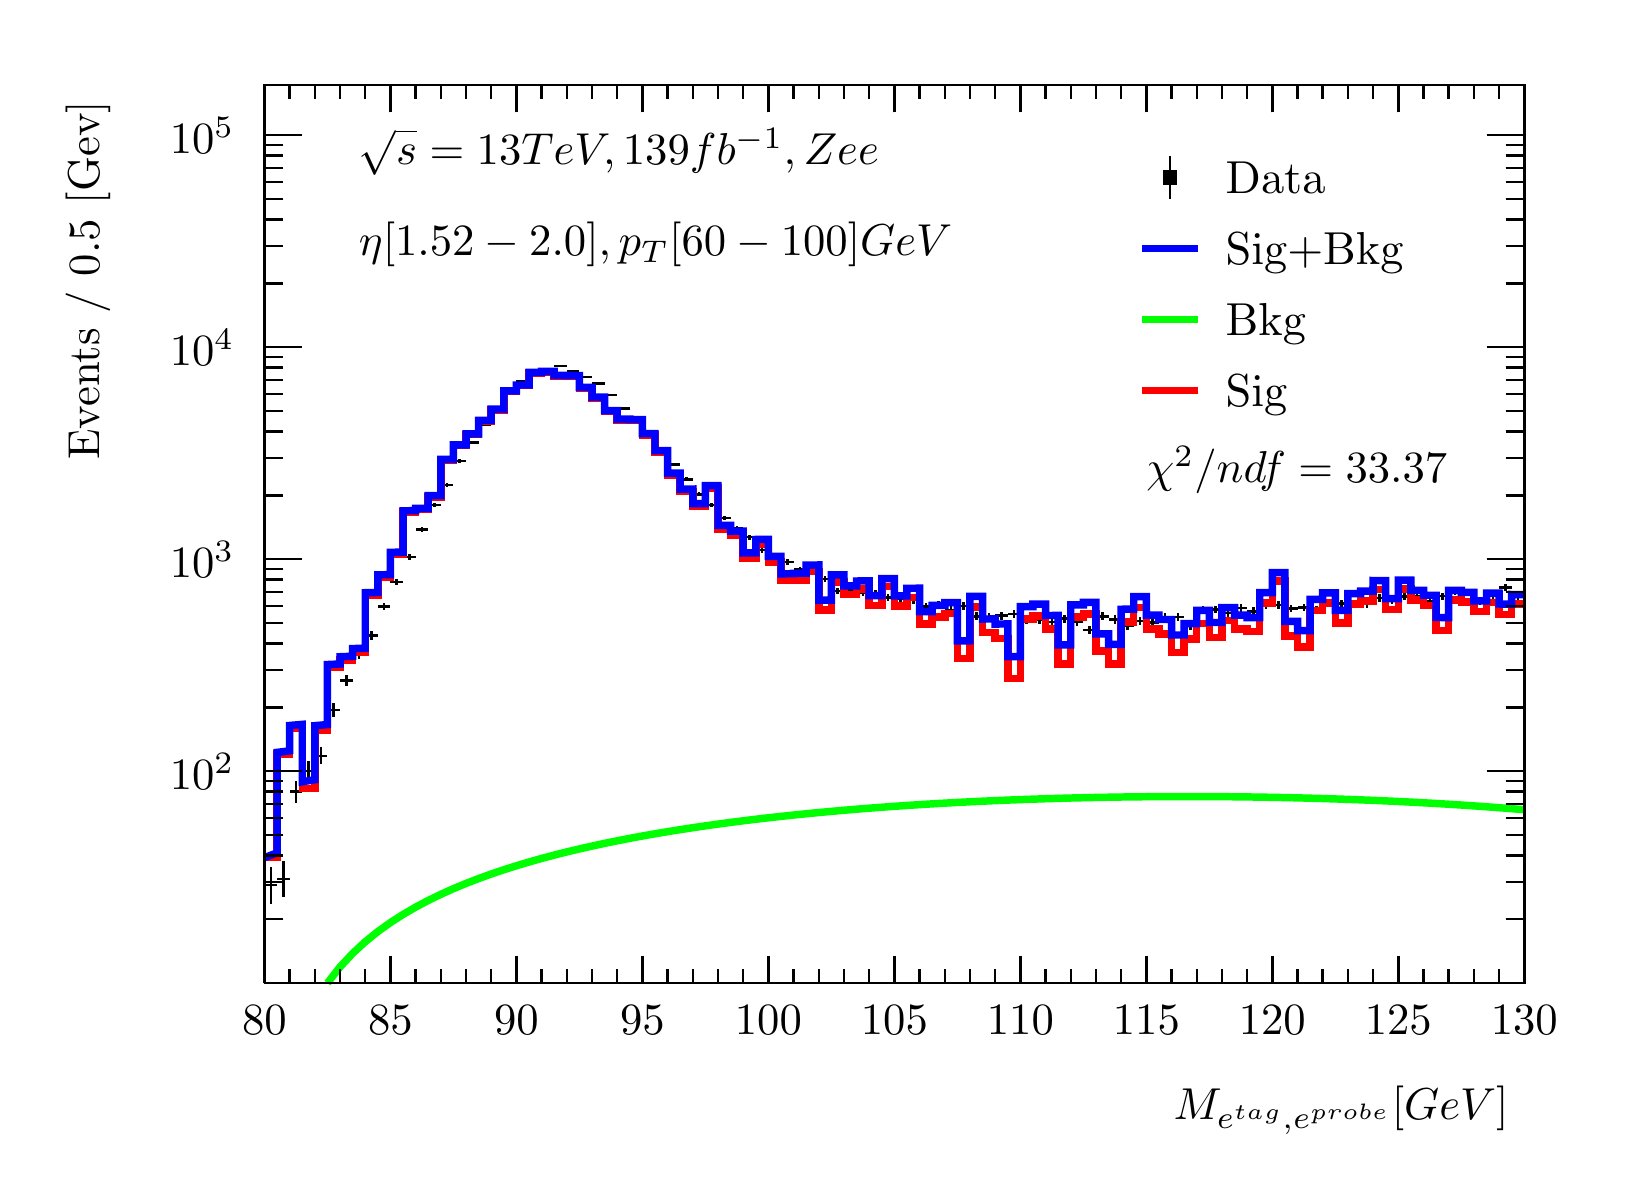
\begin{tikzpicture}
\pgfdeclareplotmark{cross} {
\pgfpathmoveto{\pgfpoint{-0.3\pgfplotmarksize}{\pgfplotmarksize}}
\pgfpathlineto{\pgfpoint{+0.3\pgfplotmarksize}{\pgfplotmarksize}}
\pgfpathlineto{\pgfpoint{+0.3\pgfplotmarksize}{0.3\pgfplotmarksize}}
\pgfpathlineto{\pgfpoint{+1\pgfplotmarksize}{0.3\pgfplotmarksize}}
\pgfpathlineto{\pgfpoint{+1\pgfplotmarksize}{-0.3\pgfplotmarksize}}
\pgfpathlineto{\pgfpoint{+0.3\pgfplotmarksize}{-0.3\pgfplotmarksize}}
\pgfpathlineto{\pgfpoint{+0.3\pgfplotmarksize}{-1.\pgfplotmarksize}}
\pgfpathlineto{\pgfpoint{-0.3\pgfplotmarksize}{-1.\pgfplotmarksize}}
\pgfpathlineto{\pgfpoint{-0.3\pgfplotmarksize}{-0.3\pgfplotmarksize}}
\pgfpathlineto{\pgfpoint{-1.\pgfplotmarksize}{-0.3\pgfplotmarksize}}
\pgfpathlineto{\pgfpoint{-1.\pgfplotmarksize}{0.3\pgfplotmarksize}}
\pgfpathlineto{\pgfpoint{-0.3\pgfplotmarksize}{0.3\pgfplotmarksize}}
\pgfpathclose
\pgfusepathqstroke
}
\pgfdeclareplotmark{cross*} {
\pgfpathmoveto{\pgfpoint{-0.3\pgfplotmarksize}{\pgfplotmarksize}}
\pgfpathlineto{\pgfpoint{+0.3\pgfplotmarksize}{\pgfplotmarksize}}
\pgfpathlineto{\pgfpoint{+0.3\pgfplotmarksize}{0.3\pgfplotmarksize}}
\pgfpathlineto{\pgfpoint{+1\pgfplotmarksize}{0.3\pgfplotmarksize}}
\pgfpathlineto{\pgfpoint{+1\pgfplotmarksize}{-0.3\pgfplotmarksize}}
\pgfpathlineto{\pgfpoint{+0.3\pgfplotmarksize}{-0.3\pgfplotmarksize}}
\pgfpathlineto{\pgfpoint{+0.3\pgfplotmarksize}{-1.\pgfplotmarksize}}
\pgfpathlineto{\pgfpoint{-0.3\pgfplotmarksize}{-1.\pgfplotmarksize}}
\pgfpathlineto{\pgfpoint{-0.3\pgfplotmarksize}{-0.3\pgfplotmarksize}}
\pgfpathlineto{\pgfpoint{-1.\pgfplotmarksize}{-0.3\pgfplotmarksize}}
\pgfpathlineto{\pgfpoint{-1.\pgfplotmarksize}{0.3\pgfplotmarksize}}
\pgfpathlineto{\pgfpoint{-0.3\pgfplotmarksize}{0.3\pgfplotmarksize}}
\pgfpathclose
\pgfusepathqfillstroke
}
\pgfdeclareplotmark{newstar} {
\pgfpathmoveto{\pgfqpoint{0pt}{\pgfplotmarksize}}
\pgfpathlineto{\pgfqpointpolar{44}{0.5\pgfplotmarksize}}
\pgfpathlineto{\pgfqpointpolar{18}{\pgfplotmarksize}}
\pgfpathlineto{\pgfqpointpolar{-20}{0.5\pgfplotmarksize}}
\pgfpathlineto{\pgfqpointpolar{-54}{\pgfplotmarksize}}
\pgfpathlineto{\pgfqpointpolar{-90}{0.5\pgfplotmarksize}}
\pgfpathlineto{\pgfqpointpolar{234}{\pgfplotmarksize}}
\pgfpathlineto{\pgfqpointpolar{198}{0.5\pgfplotmarksize}}
\pgfpathlineto{\pgfqpointpolar{162}{\pgfplotmarksize}}
\pgfpathlineto{\pgfqpointpolar{134}{0.5\pgfplotmarksize}}
\pgfpathclose
\pgfusepathqstroke
}
\pgfdeclareplotmark{newstar*} {
\pgfpathmoveto{\pgfqpoint{0pt}{\pgfplotmarksize}}
\pgfpathlineto{\pgfqpointpolar{44}{0.5\pgfplotmarksize}}
\pgfpathlineto{\pgfqpointpolar{18}{\pgfplotmarksize}}
\pgfpathlineto{\pgfqpointpolar{-20}{0.5\pgfplotmarksize}}
\pgfpathlineto{\pgfqpointpolar{-54}{\pgfplotmarksize}}
\pgfpathlineto{\pgfqpointpolar{-90}{0.5\pgfplotmarksize}}
\pgfpathlineto{\pgfqpointpolar{234}{\pgfplotmarksize}}
\pgfpathlineto{\pgfqpointpolar{198}{0.5\pgfplotmarksize}}
\pgfpathlineto{\pgfqpointpolar{162}{\pgfplotmarksize}}
\pgfpathlineto{\pgfqpointpolar{134}{0.5\pgfplotmarksize}}
\pgfpathclose
\pgfusepathqfillstroke
}
\definecolor{c}{rgb}{1,1,1};
\draw [color=c, fill=c] (0,0) rectangle (20,14.4361);
\draw [color=c, fill=c] (3,2.30977) rectangle (19,13.7143);
\definecolor{c}{rgb}{0,0,0};
\draw [c,line width=0.9] (3,2.30977) -- (3,13.7143) -- (19,13.7143) -- (19,2.30977) -- (3,2.30977);
\definecolor{c}{rgb}{1,1,1};
\draw [color=c, fill=c] (3,2.30977) rectangle (19,13.7143);
\definecolor{c}{rgb}{0,0,0};
\draw [c,line width=0.9] (3,2.30977) -- (3,13.7143) -- (19,13.7143) -- (19,2.30977) -- (3,2.30977);
\draw [c,line width=0.9] (3,2.30977) -- (19,2.30977);
\draw [c,line width=0.9] (3,2.65624) -- (3,2.30977);
\draw [c,line width=0.9] (3.32,2.48301) -- (3.32,2.30977);
\draw [c,line width=0.9] (3.64,2.48301) -- (3.64,2.30977);
\draw [c,line width=0.9] (3.96,2.48301) -- (3.96,2.30977);
\draw [c,line width=0.9] (4.28,2.48301) -- (4.28,2.30977);
\draw [c,line width=0.9] (4.6,2.65624) -- (4.6,2.30977);
\draw [c,line width=0.9] (4.92,2.48301) -- (4.92,2.30977);
\draw [c,line width=0.9] (5.24,2.48301) -- (5.24,2.30977);
\draw [c,line width=0.9] (5.56,2.48301) -- (5.56,2.30977);
\draw [c,line width=0.9] (5.88,2.48301) -- (5.88,2.30977);
\draw [c,line width=0.9] (6.2,2.65624) -- (6.2,2.30977);
\draw [c,line width=0.9] (6.52,2.48301) -- (6.52,2.30977);
\draw [c,line width=0.9] (6.84,2.48301) -- (6.84,2.30977);
\draw [c,line width=0.9] (7.16,2.48301) -- (7.16,2.30977);
\draw [c,line width=0.9] (7.48,2.48301) -- (7.48,2.30977);
\draw [c,line width=0.9] (7.8,2.65624) -- (7.8,2.30977);
\draw [c,line width=0.9] (8.12,2.48301) -- (8.12,2.30977);
\draw [c,line width=0.9] (8.44,2.48301) -- (8.44,2.30977);
\draw [c,line width=0.9] (8.76,2.48301) -- (8.76,2.30977);
\draw [c,line width=0.9] (9.08,2.48301) -- (9.08,2.30977);
\draw [c,line width=0.9] (9.4,2.65624) -- (9.4,2.30977);
\draw [c,line width=0.9] (9.72,2.48301) -- (9.72,2.30977);
\draw [c,line width=0.9] (10.04,2.48301) -- (10.04,2.30977);
\draw [c,line width=0.9] (10.36,2.48301) -- (10.36,2.30977);
\draw [c,line width=0.9] (10.68,2.48301) -- (10.68,2.30977);
\draw [c,line width=0.9] (11,2.65624) -- (11,2.30977);
\draw [c,line width=0.9] (11.32,2.48301) -- (11.32,2.30977);
\draw [c,line width=0.9] (11.64,2.48301) -- (11.64,2.30977);
\draw [c,line width=0.9] (11.96,2.48301) -- (11.96,2.30977);
\draw [c,line width=0.9] (12.28,2.48301) -- (12.28,2.30977);
\draw [c,line width=0.9] (12.6,2.65624) -- (12.6,2.30977);
\draw [c,line width=0.9] (12.92,2.48301) -- (12.92,2.30977);
\draw [c,line width=0.9] (13.24,2.48301) -- (13.24,2.30977);
\draw [c,line width=0.9] (13.56,2.48301) -- (13.56,2.30977);
\draw [c,line width=0.9] (13.88,2.48301) -- (13.88,2.30977);
\draw [c,line width=0.9] (14.2,2.65624) -- (14.2,2.30977);
\draw [c,line width=0.9] (14.52,2.48301) -- (14.52,2.30977);
\draw [c,line width=0.9] (14.84,2.48301) -- (14.84,2.30977);
\draw [c,line width=0.9] (15.16,2.48301) -- (15.16,2.30977);
\draw [c,line width=0.9] (15.48,2.48301) -- (15.48,2.30977);
\draw [c,line width=0.9] (15.8,2.65624) -- (15.8,2.30977);
\draw [c,line width=0.9] (16.12,2.48301) -- (16.12,2.30977);
\draw [c,line width=0.9] (16.44,2.48301) -- (16.44,2.30977);
\draw [c,line width=0.9] (16.76,2.48301) -- (16.76,2.30977);
\draw [c,line width=0.9] (17.08,2.48301) -- (17.08,2.30977);
\draw [c,line width=0.9] (17.4,2.65624) -- (17.4,2.30977);
\draw [c,line width=0.9] (17.72,2.48301) -- (17.72,2.30977);
\draw [c,line width=0.9] (18.04,2.48301) -- (18.04,2.30977);
\draw [c,line width=0.9] (18.36,2.48301) -- (18.36,2.30977);
\draw [c,line width=0.9] (18.68,2.48301) -- (18.68,2.30977);
\draw [c,line width=0.9] (19,2.65624) -- (19,2.30977);
\draw [anchor=base] (3,1.66015) node[scale=1.61424, color=c, rotate=0]{80};
\draw [anchor=base] (4.6,1.66015) node[scale=1.61424, color=c, rotate=0]{85};
\draw [anchor=base] (6.2,1.66015) node[scale=1.61424, color=c, rotate=0]{90};
\draw [anchor=base] (7.8,1.66015) node[scale=1.61424, color=c, rotate=0]{95};
\draw [anchor=base] (9.4,1.66015) node[scale=1.61424, color=c, rotate=0]{100};
\draw [anchor=base] (11,1.66015) node[scale=1.61424, color=c, rotate=0]{105};
\draw [anchor=base] (12.6,1.66015) node[scale=1.61424, color=c, rotate=0]{110};
\draw [anchor=base] (14.2,1.66015) node[scale=1.61424, color=c, rotate=0]{115};
\draw [anchor=base] (15.8,1.66015) node[scale=1.61424, color=c, rotate=0]{120};
\draw [anchor=base] (17.4,1.66015) node[scale=1.61424, color=c, rotate=0]{125};
\draw [anchor=base] (19,1.66015) node[scale=1.61424, color=c, rotate=0]{130};
\draw [anchor= east] (19,0.692932) node[scale=1.61424, color=c, rotate=0]{$M_{e^{tag}, e^{probe}}  [GeV]$};
\draw [c,line width=0.9] (3,13.7143) -- (19,13.7143);
\draw [c,line width=0.9] (3,13.3678) -- (3,13.7143);
\draw [c,line width=0.9] (3.32,13.5411) -- (3.32,13.7143);
\draw [c,line width=0.9] (3.64,13.5411) -- (3.64,13.7143);
\draw [c,line width=0.9] (3.96,13.5411) -- (3.96,13.7143);
\draw [c,line width=0.9] (4.28,13.5411) -- (4.28,13.7143);
\draw [c,line width=0.9] (4.6,13.3678) -- (4.6,13.7143);
\draw [c,line width=0.9] (4.92,13.5411) -- (4.92,13.7143);
\draw [c,line width=0.9] (5.24,13.5411) -- (5.24,13.7143);
\draw [c,line width=0.9] (5.56,13.5411) -- (5.56,13.7143);
\draw [c,line width=0.9] (5.88,13.5411) -- (5.88,13.7143);
\draw [c,line width=0.9] (6.2,13.3678) -- (6.2,13.7143);
\draw [c,line width=0.9] (6.52,13.5411) -- (6.52,13.7143);
\draw [c,line width=0.9] (6.84,13.5411) -- (6.84,13.7143);
\draw [c,line width=0.9] (7.16,13.5411) -- (7.16,13.7143);
\draw [c,line width=0.9] (7.48,13.5411) -- (7.48,13.7143);
\draw [c,line width=0.9] (7.8,13.3678) -- (7.8,13.7143);
\draw [c,line width=0.9] (8.12,13.5411) -- (8.12,13.7143);
\draw [c,line width=0.9] (8.44,13.5411) -- (8.44,13.7143);
\draw [c,line width=0.9] (8.76,13.5411) -- (8.76,13.7143);
\draw [c,line width=0.9] (9.08,13.5411) -- (9.08,13.7143);
\draw [c,line width=0.9] (9.4,13.3678) -- (9.4,13.7143);
\draw [c,line width=0.9] (9.72,13.5411) -- (9.72,13.7143);
\draw [c,line width=0.9] (10.04,13.5411) -- (10.04,13.7143);
\draw [c,line width=0.9] (10.36,13.5411) -- (10.36,13.7143);
\draw [c,line width=0.9] (10.68,13.5411) -- (10.68,13.7143);
\draw [c,line width=0.9] (11,13.3678) -- (11,13.7143);
\draw [c,line width=0.9] (11.32,13.5411) -- (11.32,13.7143);
\draw [c,line width=0.9] (11.64,13.5411) -- (11.64,13.7143);
\draw [c,line width=0.9] (11.96,13.5411) -- (11.96,13.7143);
\draw [c,line width=0.9] (12.28,13.5411) -- (12.28,13.7143);
\draw [c,line width=0.9] (12.6,13.3678) -- (12.6,13.7143);
\draw [c,line width=0.9] (12.92,13.5411) -- (12.92,13.7143);
\draw [c,line width=0.9] (13.24,13.5411) -- (13.24,13.7143);
\draw [c,line width=0.9] (13.56,13.5411) -- (13.56,13.7143);
\draw [c,line width=0.9] (13.88,13.5411) -- (13.88,13.7143);
\draw [c,line width=0.9] (14.2,13.3678) -- (14.2,13.7143);
\draw [c,line width=0.9] (14.52,13.5411) -- (14.52,13.7143);
\draw [c,line width=0.9] (14.84,13.5411) -- (14.84,13.7143);
\draw [c,line width=0.9] (15.16,13.5411) -- (15.16,13.7143);
\draw [c,line width=0.9] (15.48,13.5411) -- (15.48,13.7143);
\draw [c,line width=0.9] (15.8,13.3678) -- (15.8,13.7143);
\draw [c,line width=0.9] (16.12,13.5411) -- (16.12,13.7143);
\draw [c,line width=0.9] (16.44,13.5411) -- (16.44,13.7143);
\draw [c,line width=0.9] (16.76,13.5411) -- (16.76,13.7143);
\draw [c,line width=0.9] (17.08,13.5411) -- (17.08,13.7143);
\draw [c,line width=0.9] (17.4,13.3678) -- (17.4,13.7143);
\draw [c,line width=0.9] (17.72,13.5411) -- (17.72,13.7143);
\draw [c,line width=0.9] (18.04,13.5411) -- (18.04,13.7143);
\draw [c,line width=0.9] (18.36,13.5411) -- (18.36,13.7143);
\draw [c,line width=0.9] (18.68,13.5411) -- (18.68,13.7143);
\draw [c,line width=0.9] (19,13.3678) -- (19,13.7143);
\draw [c,line width=0.9] (3,2.30977) -- (3,13.7143);
\draw [c,line width=0.9] (3.237,3.12018) -- (3,3.12018);
\draw [c,line width=0.9] (3.237,3.59423) -- (3,3.59423);
\draw [c,line width=0.9] (3.237,3.93058) -- (3,3.93058);
\draw [c,line width=0.9] (3.237,4.19147) -- (3,4.19147);
\draw [c,line width=0.9] (3.237,4.40464) -- (3,4.40464);
\draw [c,line width=0.9] (3.237,4.58487) -- (3,4.58487);
\draw [c,line width=0.9] (3.237,4.74099) -- (3,4.74099);
\draw [c,line width=0.9] (3.237,4.8787) -- (3,4.8787);
\draw [c,line width=0.9] (3.474,5.00188) -- (3,5.00188);
\draw [anchor= east] (2.82,5.00188) node[scale=1.61424, color=c, rotate=0]{$10^{2}$};
\draw [c,line width=0.9] (3.237,5.81228) -- (3,5.81228);
\draw [c,line width=0.9] (3.237,6.28634) -- (3,6.28634);
\draw [c,line width=0.9] (3.237,6.62269) -- (3,6.62269);
\draw [c,line width=0.9] (3.237,6.88358) -- (3,6.88358);
\draw [c,line width=0.9] (3.237,7.09675) -- (3,7.09675);
\draw [c,line width=0.9] (3.237,7.27697) -- (3,7.27697);
\draw [c,line width=0.9] (3.237,7.43309) -- (3,7.43309);
\draw [c,line width=0.9] (3.237,7.5708) -- (3,7.5708);
\draw [c,line width=0.9] (3.474,7.69399) -- (3,7.69399);
\draw [anchor= east] (2.82,7.69399) node[scale=1.61424, color=c, rotate=0]{$10^{3}$};
\draw [c,line width=0.9] (3.237,8.50439) -- (3,8.50439);
\draw [c,line width=0.9] (3.237,8.97845) -- (3,8.97845);
\draw [c,line width=0.9] (3.237,9.3148) -- (3,9.3148);
\draw [c,line width=0.9] (3.237,9.57569) -- (3,9.57569);
\draw [c,line width=0.9] (3.237,9.78885) -- (3,9.78885);
\draw [c,line width=0.9] (3.237,9.96908) -- (3,9.96908);
\draw [c,line width=0.9] (3.237,10.1252) -- (3,10.1252);
\draw [c,line width=0.9] (3.237,10.2629) -- (3,10.2629);
\draw [c,line width=0.9] (3.474,10.3861) -- (3,10.3861);
\draw [anchor= east] (2.82,10.3861) node[scale=1.61424, color=c, rotate=0]{$10^{4}$};
\draw [c,line width=0.9] (3.237,11.1965) -- (3,11.1965);
\draw [c,line width=0.9] (3.237,11.6706) -- (3,11.6706);
\draw [c,line width=0.9] (3.237,12.0069) -- (3,12.0069);
\draw [c,line width=0.9] (3.237,12.2678) -- (3,12.2678);
\draw [c,line width=0.9] (3.237,12.481) -- (3,12.481);
\draw [c,line width=0.9] (3.237,12.6612) -- (3,12.6612);
\draw [c,line width=0.9] (3.237,12.8173) -- (3,12.8173);
\draw [c,line width=0.9] (3.237,12.955) -- (3,12.955);
\draw [c,line width=0.9] (3.474,13.0782) -- (3,13.0782);
\draw [anchor= east] (2.82,13.0782) node[scale=1.61424, color=c, rotate=0]{$10^{5}$};
\draw [anchor= east] (0.76,13.7143) node[scale=1.61424, color=c, rotate=90]{Events / 0.5 [Gev]};
\draw [c,line width=0.9] (19,2.30977) -- (19,13.7143);
\draw [c,line width=0.9] (18.763,3.12018) -- (19,3.12018);
\draw [c,line width=0.9] (18.763,3.59423) -- (19,3.59423);
\draw [c,line width=0.9] (18.763,3.93058) -- (19,3.93058);
\draw [c,line width=0.9] (18.763,4.19147) -- (19,4.19147);
\draw [c,line width=0.9] (18.763,4.40464) -- (19,4.40464);
\draw [c,line width=0.9] (18.763,4.58487) -- (19,4.58487);
\draw [c,line width=0.9] (18.763,4.74099) -- (19,4.74099);
\draw [c,line width=0.9] (18.763,4.8787) -- (19,4.8787);
\draw [c,line width=0.9] (18.526,5.00188) -- (19,5.00188);
\draw [c,line width=0.9] (18.763,5.81228) -- (19,5.81228);
\draw [c,line width=0.9] (18.763,6.28634) -- (19,6.28634);
\draw [c,line width=0.9] (18.763,6.62269) -- (19,6.62269);
\draw [c,line width=0.9] (18.763,6.88358) -- (19,6.88358);
\draw [c,line width=0.9] (18.763,7.09675) -- (19,7.09675);
\draw [c,line width=0.9] (18.763,7.27697) -- (19,7.27697);
\draw [c,line width=0.9] (18.763,7.43309) -- (19,7.43309);
\draw [c,line width=0.9] (18.763,7.5708) -- (19,7.5708);
\draw [c,line width=0.9] (18.526,7.69399) -- (19,7.69399);
\draw [c,line width=0.9] (18.763,8.50439) -- (19,8.50439);
\draw [c,line width=0.9] (18.763,8.97845) -- (19,8.97845);
\draw [c,line width=0.9] (18.763,9.3148) -- (19,9.3148);
\draw [c,line width=0.9] (18.763,9.57569) -- (19,9.57569);
\draw [c,line width=0.9] (18.763,9.78885) -- (19,9.78885);
\draw [c,line width=0.9] (18.763,9.96908) -- (19,9.96908);
\draw [c,line width=0.9] (18.763,10.1252) -- (19,10.1252);
\draw [c,line width=0.9] (18.763,10.2629) -- (19,10.2629);
\draw [c,line width=0.9] (18.526,10.3861) -- (19,10.3861);
\draw [c,line width=0.9] (18.763,11.1965) -- (19,11.1965);
\draw [c,line width=0.9] (18.763,11.6706) -- (19,11.6706);
\draw [c,line width=0.9] (18.763,12.0069) -- (19,12.0069);
\draw [c,line width=0.9] (18.763,12.2678) -- (19,12.2678);
\draw [c,line width=0.9] (18.763,12.481) -- (19,12.481);
\draw [c,line width=0.9] (18.763,12.6612) -- (19,12.6612);
\draw [c,line width=0.9] (18.763,12.8173) -- (19,12.8173);
\draw [c,line width=0.9] (18.763,12.955) -- (19,12.955);
\draw [c,line width=0.9] (18.526,13.0782) -- (19,13.0782);
\draw [c,line width=0.9] (3.08,3.5546) -- (3,3.5546);
\draw [c,line width=0.9] (3,3.5546) -- (3,3.5546);
\draw [c,line width=0.9] (3.08,3.5546) -- (3.16,3.5546);
\draw [c,line width=0.9] (3.16,3.5546) -- (3.16,3.5546);
\draw [c,line width=0.9] (3.08,3.5546) -- (3.08,3.7893);
\draw [c,line width=0.9] (3.08,3.7893) -- (3.08,3.7893);
\draw [c,line width=0.9] (3.08,3.5546) -- (3.08,3.31597);
\draw [c,line width=0.9] (3.08,3.31597) -- (3.08,3.31597);
\draw [c,line width=0.9] (3.24,3.63257) -- (3.16,3.63257);
\draw [c,line width=0.9] (3.16,3.63257) -- (3.16,3.63257);
\draw [c,line width=0.9] (3.24,3.63257) -- (3.32,3.63257);
\draw [c,line width=0.9] (3.32,3.63257) -- (3.32,3.63257);
\draw [c,line width=0.9] (3.24,3.63257) -- (3.24,3.8591);
\draw [c,line width=0.9] (3.24,3.8591) -- (3.24,3.8591);
\draw [c,line width=0.9] (3.24,3.63257) -- (3.24,3.4025);
\draw [c,line width=0.9] (3.24,3.4025) -- (3.24,3.4025);
\draw [c,line width=0.9] (3.4,4.74099) -- (3.32,4.74099);
\draw [c,line width=0.9] (3.32,4.74099) -- (3.32,4.74099);
\draw [c,line width=0.9] (3.4,4.74099) -- (3.48,4.74099);
\draw [c,line width=0.9] (3.48,4.74099) -- (3.48,4.74099);
\draw [c,line width=0.9] (3.4,4.74099) -- (3.4,4.87846);
\draw [c,line width=0.9] (3.4,4.87846) -- (3.4,4.87846);
\draw [c,line width=0.9] (3.4,4.74099) -- (3.4,4.60268);
\draw [c,line width=0.9] (3.4,4.60268) -- (3.4,4.60268);
\draw [c,line width=0.9] (3.56,5.00188) -- (3.48,5.00188);
\draw [c,line width=0.9] (3.48,5.00188) -- (3.48,5.00188);
\draw [c,line width=0.9] (3.56,5.00188) -- (3.64,5.00188);
\draw [c,line width=0.9] (3.64,5.00188) -- (3.64,5.00188);
\draw [c,line width=0.9] (3.56,5.00188) -- (3.56,5.12425);
\draw [c,line width=0.9] (3.56,5.12425) -- (3.56,5.12425);
\draw [c,line width=0.9] (3.56,5.00188) -- (3.56,4.87891);
\draw [c,line width=0.9] (3.56,4.87891) -- (3.56,4.87891);
\draw [c,line width=0.9] (3.72,5.19539) -- (3.64,5.19539);
\draw [c,line width=0.9] (3.64,5.19539) -- (3.64,5.19539);
\draw [c,line width=0.9] (3.72,5.19539) -- (3.8,5.19539);
\draw [c,line width=0.9] (3.8,5.19539) -- (3.8,5.19539);
\draw [c,line width=0.9] (3.72,5.19539) -- (3.72,5.30299);
\draw [c,line width=0.9] (3.72,5.30299) -- (3.72,5.30299);
\draw [c,line width=0.9] (3.72,5.19539) -- (3.72,5.0878);
\draw [c,line width=0.9] (3.72,5.0878) -- (3.72,5.0878);
\draw [c,line width=0.9] (3.88,5.77667) -- (3.8,5.77667);
\draw [c,line width=0.9] (3.8,5.77667) -- (3.8,5.77667);
\draw [c,line width=0.9] (3.88,5.77667) -- (3.96,5.77667);
\draw [c,line width=0.9] (3.96,5.77667) -- (3.96,5.77667);
\draw [c,line width=0.9] (3.88,5.77667) -- (3.88,5.8606);
\draw [c,line width=0.9] (3.88,5.8606) -- (3.88,5.8606);
\draw [c,line width=0.9] (3.88,5.77667) -- (3.88,5.69275);
\draw [c,line width=0.9] (3.88,5.69275) -- (3.88,5.69275);
\draw [c,line width=0.9] (4.04,6.15009) -- (3.96,6.15009);
\draw [c,line width=0.9] (3.96,6.15009) -- (3.96,6.15009);
\draw [c,line width=0.9] (4.04,6.15009) -- (4.12,6.15009);
\draw [c,line width=0.9] (4.12,6.15009) -- (4.12,6.15009);
\draw [c,line width=0.9] (4.04,6.15009) -- (4.04,6.22164);
\draw [c,line width=0.9] (4.04,6.22164) -- (4.04,6.22164);
\draw [c,line width=0.9] (4.04,6.15009) -- (4.04,6.07855);
\draw [c,line width=0.9] (4.04,6.07855) -- (4.04,6.07855);
\draw [c,line width=0.9] (4.2,6.48644) -- (4.12,6.48644);
\draw [c,line width=0.9] (4.12,6.48644) -- (4.12,6.48644);
\draw [c,line width=0.9] (4.2,6.48644) -- (4.28,6.48644);
\draw [c,line width=0.9] (4.28,6.48644) -- (4.28,6.48644);
\draw [c,line width=0.9] (4.2,6.48644) -- (4.2,6.5484);
\draw [c,line width=0.9] (4.2,6.5484) -- (4.2,6.5484);
\draw [c,line width=0.9] (4.2,6.48644) -- (4.2,6.42448);
\draw [c,line width=0.9] (4.2,6.42448) -- (4.2,6.42448);
\draw [c,line width=0.9] (4.36,6.72613) -- (4.28,6.72613);
\draw [c,line width=0.9] (4.28,6.72613) -- (4.28,6.72613);
\draw [c,line width=0.9] (4.36,6.72613) -- (4.44,6.72613);
\draw [c,line width=0.9] (4.44,6.72613) -- (4.44,6.72613);
\draw [c,line width=0.9] (4.36,6.72613) -- (4.36,6.78205);
\draw [c,line width=0.9] (4.36,6.78205) -- (4.36,6.78205);
\draw [c,line width=0.9] (4.36,6.72613) -- (4.36,6.6702);
\draw [c,line width=0.9] (4.36,6.6702) -- (4.36,6.6702);
\draw [c,line width=0.9] (4.52,7.09284) -- (4.44,7.09284);
\draw [c,line width=0.9] (4.44,7.09284) -- (4.44,7.09284);
\draw [c,line width=0.9] (4.52,7.09284) -- (4.6,7.09284);
\draw [c,line width=0.9] (4.6,7.09284) -- (4.6,7.09284);
\draw [c,line width=0.9] (4.52,7.09284) -- (4.52,7.14065);
\draw [c,line width=0.9] (4.52,7.14065) -- (4.52,7.14065);
\draw [c,line width=0.9] (4.52,7.09284) -- (4.52,7.04504);
\draw [c,line width=0.9] (4.52,7.04504) -- (4.52,7.04504);
\draw [c,line width=0.9] (4.68,7.40349) -- (4.6,7.40349);
\draw [c,line width=0.9] (4.6,7.40349) -- (4.6,7.40349);
\draw [c,line width=0.9] (4.68,7.40349) -- (4.76,7.40349);
\draw [c,line width=0.9] (4.76,7.40349) -- (4.76,7.40349);
\draw [c,line width=0.9] (4.68,7.40349) -- (4.68,7.44536);
\draw [c,line width=0.9] (4.68,7.44536) -- (4.68,7.44536);
\draw [c,line width=0.9] (4.68,7.40349) -- (4.68,7.36163);
\draw [c,line width=0.9] (4.68,7.36163) -- (4.68,7.36163);
\draw [c,line width=0.9] (4.84,7.71943) -- (4.76,7.71943);
\draw [c,line width=0.9] (4.76,7.71943) -- (4.76,7.71943);
\draw [c,line width=0.9] (4.84,7.71943) -- (4.92,7.71943);
\draw [c,line width=0.9] (4.92,7.71943) -- (4.92,7.71943);
\draw [c,line width=0.9] (4.84,7.71943) -- (4.84,7.756);
\draw [c,line width=0.9] (4.84,7.756) -- (4.84,7.756);
\draw [c,line width=0.9] (4.84,7.71943) -- (4.84,7.68286);
\draw [c,line width=0.9] (4.84,7.68286) -- (4.84,7.68286);
\draw [c,line width=0.9] (5,8.07225) -- (4.92,8.07225);
\draw [c,line width=0.9] (4.92,8.07225) -- (4.92,8.07225);
\draw [c,line width=0.9] (5,8.07225) -- (5.08,8.07225);
\draw [c,line width=0.9] (5.08,8.07225) -- (5.08,8.07225);
\draw [c,line width=0.9] (5,8.07225) -- (5,8.1037);
\draw [c,line width=0.9] (5,8.1037) -- (5,8.1037);
\draw [c,line width=0.9] (5,8.07225) -- (5,8.0408);
\draw [c,line width=0.9] (5,8.0408) -- (5,8.0408);
\draw [c,line width=0.9] (5.16,8.37796) -- (5.08,8.37796);
\draw [c,line width=0.9] (5.08,8.37796) -- (5.08,8.37796);
\draw [c,line width=0.9] (5.16,8.37796) -- (5.24,8.37796);
\draw [c,line width=0.9] (5.24,8.37796) -- (5.24,8.37796);
\draw [c,line width=0.9] (5.16,8.37796) -- (5.16,8.40555);
\draw [c,line width=0.9] (5.16,8.40555) -- (5.16,8.40555);
\draw [c,line width=0.9] (5.16,8.37796) -- (5.16,8.35036);
\draw [c,line width=0.9] (5.16,8.35036) -- (5.16,8.35036);
\draw [c,line width=0.9] (5.32,8.63323) -- (5.24,8.63323);
\draw [c,line width=0.9] (5.24,8.63323) -- (5.24,8.63323);
\draw [c,line width=0.9] (5.32,8.63323) -- (5.4,8.63323);
\draw [c,line width=0.9] (5.4,8.63323) -- (5.4,8.63323);
\draw [c,line width=0.9] (5.32,8.63323) -- (5.32,8.65798);
\draw [c,line width=0.9] (5.32,8.65798) -- (5.32,8.65798);
\draw [c,line width=0.9] (5.32,8.63323) -- (5.32,8.60849);
\draw [c,line width=0.9] (5.32,8.60849) -- (5.32,8.60849);
\draw [c,line width=0.9] (5.48,8.9372) -- (5.4,8.9372);
\draw [c,line width=0.9] (5.4,8.9372) -- (5.4,8.9372);
\draw [c,line width=0.9] (5.48,8.9372) -- (5.56,8.9372);
\draw [c,line width=0.9] (5.56,8.9372) -- (5.56,8.9372);
\draw [c,line width=0.9] (5.48,8.9372) -- (5.48,8.95892);
\draw [c,line width=0.9] (5.48,8.95892) -- (5.48,8.95892);
\draw [c,line width=0.9] (5.48,8.9372) -- (5.48,8.91547);
\draw [c,line width=0.9] (5.48,8.91547) -- (5.48,8.91547);
\draw [c,line width=0.9] (5.64,9.17295) -- (5.56,9.17295);
\draw [c,line width=0.9] (5.56,9.17295) -- (5.56,9.17295);
\draw [c,line width=0.9] (5.64,9.17295) -- (5.72,9.17295);
\draw [c,line width=0.9] (5.72,9.17295) -- (5.72,9.17295);
\draw [c,line width=0.9] (5.64,9.17295) -- (5.64,9.1926);
\draw [c,line width=0.9] (5.64,9.1926) -- (5.64,9.1926);
\draw [c,line width=0.9] (5.64,9.17295) -- (5.64,9.15331);
\draw [c,line width=0.9] (5.64,9.15331) -- (5.64,9.15331);
\draw [c,line width=0.9] (5.8,9.39745) -- (5.72,9.39745);
\draw [c,line width=0.9] (5.72,9.39745) -- (5.72,9.39745);
\draw [c,line width=0.9] (5.8,9.39745) -- (5.88,9.39745);
\draw [c,line width=0.9] (5.88,9.39745) -- (5.88,9.39745);
\draw [c,line width=0.9] (5.8,9.39745) -- (5.8,9.41529);
\draw [c,line width=0.9] (5.8,9.41529) -- (5.8,9.41529);
\draw [c,line width=0.9] (5.8,9.39745) -- (5.8,9.3796);
\draw [c,line width=0.9] (5.8,9.3796) -- (5.8,9.3796);
\draw [c,line width=0.9] (5.96,9.6041) -- (5.88,9.6041);
\draw [c,line width=0.9] (5.88,9.6041) -- (5.88,9.6041);
\draw [c,line width=0.9] (5.96,9.6041) -- (6.04,9.6041);
\draw [c,line width=0.9] (6.04,9.6041) -- (6.04,9.6041);
\draw [c,line width=0.9] (5.96,9.6041) -- (5.96,9.62044);
\draw [c,line width=0.9] (5.96,9.62044) -- (5.96,9.62044);
\draw [c,line width=0.9] (5.96,9.6041) -- (5.96,9.58777);
\draw [c,line width=0.9] (5.96,9.58777) -- (5.96,9.58777);
\draw [c,line width=0.9] (6.12,9.82455) -- (6.04,9.82455);
\draw [c,line width=0.9] (6.04,9.82455) -- (6.04,9.82455);
\draw [c,line width=0.9] (6.12,9.82455) -- (6.2,9.82455);
\draw [c,line width=0.9] (6.2,9.82455) -- (6.2,9.82455);
\draw [c,line width=0.9] (6.12,9.82455) -- (6.12,9.83941);
\draw [c,line width=0.9] (6.12,9.83941) -- (6.12,9.83941);
\draw [c,line width=0.9] (6.12,9.82455) -- (6.12,9.80968);
\draw [c,line width=0.9] (6.12,9.80968) -- (6.12,9.80968);
\draw [c,line width=0.9] (6.28,9.94699) -- (6.2,9.94699);
\draw [c,line width=0.9] (6.2,9.94699) -- (6.2,9.94699);
\draw [c,line width=0.9] (6.28,9.94699) -- (6.36,9.94699);
\draw [c,line width=0.9] (6.36,9.94699) -- (6.36,9.94699);
\draw [c,line width=0.9] (6.28,9.94699) -- (6.28,9.9611);
\draw [c,line width=0.9] (6.28,9.9611) -- (6.28,9.9611);
\draw [c,line width=0.9] (6.28,9.94699) -- (6.28,9.93289);
\draw [c,line width=0.9] (6.28,9.93289) -- (6.28,9.93289);
\draw [c,line width=0.9] (6.44,10.0532) -- (6.36,10.0532);
\draw [c,line width=0.9] (6.36,10.0532) -- (6.36,10.0532);
\draw [c,line width=0.9] (6.44,10.0532) -- (6.52,10.0532);
\draw [c,line width=0.9] (6.52,10.0532) -- (6.52,10.0532);
\draw [c,line width=0.9] (6.44,10.0532) -- (6.44,10.0667);
\draw [c,line width=0.9] (6.44,10.0667) -- (6.44,10.0667);
\draw [c,line width=0.9] (6.44,10.0532) -- (6.44,10.0397);
\draw [c,line width=0.9] (6.44,10.0397) -- (6.44,10.0397);
\draw [c,line width=0.9] (6.6,10.1083) -- (6.52,10.1083);
\draw [c,line width=0.9] (6.52,10.1083) -- (6.52,10.1083);
\draw [c,line width=0.9] (6.6,10.1083) -- (6.68,10.1083);
\draw [c,line width=0.9] (6.68,10.1083) -- (6.68,10.1083);
\draw [c,line width=0.9] (6.6,10.1083) -- (6.6,10.1214);
\draw [c,line width=0.9] (6.6,10.1214) -- (6.6,10.1214);
\draw [c,line width=0.9] (6.6,10.1083) -- (6.6,10.0951);
\draw [c,line width=0.9] (6.6,10.0951) -- (6.6,10.0951);
\draw [c,line width=0.9] (6.76,10.1486) -- (6.68,10.1486);
\draw [c,line width=0.9] (6.68,10.1486) -- (6.68,10.1486);
\draw [c,line width=0.9] (6.76,10.1486) -- (6.84,10.1486);
\draw [c,line width=0.9] (6.84,10.1486) -- (6.84,10.1486);
\draw [c,line width=0.9] (6.76,10.1486) -- (6.76,10.1616);
\draw [c,line width=0.9] (6.76,10.1616) -- (6.76,10.1616);
\draw [c,line width=0.9] (6.76,10.1486) -- (6.76,10.1357);
\draw [c,line width=0.9] (6.76,10.1357) -- (6.76,10.1357);
\draw [c,line width=0.9] (6.92,10.0801) -- (6.84,10.0801);
\draw [c,line width=0.9] (6.84,10.0801) -- (6.84,10.0801);
\draw [c,line width=0.9] (6.92,10.0801) -- (7,10.0801);
\draw [c,line width=0.9] (7,10.0801) -- (7,10.0801);
\draw [c,line width=0.9] (6.92,10.0801) -- (6.92,10.0934);
\draw [c,line width=0.9] (6.92,10.0934) -- (6.92,10.0934);
\draw [c,line width=0.9] (6.92,10.0801) -- (6.92,10.0667);
\draw [c,line width=0.9] (6.92,10.0667) -- (6.92,10.0667);
\draw [c,line width=0.9] (7.08,10.008) -- (7,10.008);
\draw [c,line width=0.9] (7,10.008) -- (7,10.008);
\draw [c,line width=0.9] (7.08,10.008) -- (7.16,10.008);
\draw [c,line width=0.9] (7.16,10.008) -- (7.16,10.008);
\draw [c,line width=0.9] (7.08,10.008) -- (7.08,10.0218);
\draw [c,line width=0.9] (7.08,10.0218) -- (7.08,10.0218);
\draw [c,line width=0.9] (7.08,10.008) -- (7.08,9.99427);
\draw [c,line width=0.9] (7.08,9.99427) -- (7.08,9.99427);
\draw [c,line width=0.9] (7.24,9.92135) -- (7.16,9.92135);
\draw [c,line width=0.9] (7.16,9.92135) -- (7.16,9.92135);
\draw [c,line width=0.9] (7.24,9.92135) -- (7.32,9.92135);
\draw [c,line width=0.9] (7.32,9.92135) -- (7.32,9.92135);
\draw [c,line width=0.9] (7.24,9.92135) -- (7.24,9.93562);
\draw [c,line width=0.9] (7.24,9.93562) -- (7.24,9.93562);
\draw [c,line width=0.9] (7.24,9.92135) -- (7.24,9.90709);
\draw [c,line width=0.9] (7.24,9.90709) -- (7.24,9.90709);
\draw [c,line width=0.9] (7.4,9.77769) -- (7.32,9.77769);
\draw [c,line width=0.9] (7.32,9.77769) -- (7.32,9.77769);
\draw [c,line width=0.9] (7.4,9.77769) -- (7.48,9.77769);
\draw [c,line width=0.9] (7.48,9.77769) -- (7.48,9.77769);
\draw [c,line width=0.9] (7.4,9.77769) -- (7.4,9.79286);
\draw [c,line width=0.9] (7.4,9.79286) -- (7.4,9.79286);
\draw [c,line width=0.9] (7.4,9.77769) -- (7.4,9.76253);
\draw [c,line width=0.9] (7.4,9.76253) -- (7.4,9.76253);
\draw [c,line width=0.9] (7.56,9.60616) -- (7.48,9.60616);
\draw [c,line width=0.9] (7.48,9.60616) -- (7.48,9.60616);
\draw [c,line width=0.9] (7.56,9.60616) -- (7.64,9.60616);
\draw [c,line width=0.9] (7.64,9.60616) -- (7.64,9.60616);
\draw [c,line width=0.9] (7.56,9.60616) -- (7.56,9.62248);
\draw [c,line width=0.9] (7.56,9.62248) -- (7.56,9.62248);
\draw [c,line width=0.9] (7.56,9.60616) -- (7.56,9.58984);
\draw [c,line width=0.9] (7.56,9.58984) -- (7.56,9.58984);
\draw [c,line width=0.9] (7.72,9.46362) -- (7.64,9.46362);
\draw [c,line width=0.9] (7.64,9.46362) -- (7.64,9.46362);
\draw [c,line width=0.9] (7.72,9.46362) -- (7.8,9.46362);
\draw [c,line width=0.9] (7.8,9.46362) -- (7.8,9.46362);
\draw [c,line width=0.9] (7.72,9.46362) -- (7.72,9.48097);
\draw [c,line width=0.9] (7.72,9.48097) -- (7.72,9.48097);
\draw [c,line width=0.9] (7.72,9.46362) -- (7.72,9.44628);
\draw [c,line width=0.9] (7.72,9.44628) -- (7.72,9.44628);
\draw [c,line width=0.9] (7.88,9.26127) -- (7.8,9.26127);
\draw [c,line width=0.9] (7.8,9.26127) -- (7.8,9.26127);
\draw [c,line width=0.9] (7.88,9.26127) -- (7.96,9.26127);
\draw [c,line width=0.9] (7.96,9.26127) -- (7.96,9.26127);
\draw [c,line width=0.9] (7.88,9.26127) -- (7.88,9.28018);
\draw [c,line width=0.9] (7.88,9.28018) -- (7.88,9.28018);
\draw [c,line width=0.9] (7.88,9.26127) -- (7.88,9.24236);
\draw [c,line width=0.9] (7.88,9.24236) -- (7.88,9.24236);
\draw [c,line width=0.9] (8.04,9.08063) -- (7.96,9.08063);
\draw [c,line width=0.9] (7.96,9.08063) -- (7.96,9.08063);
\draw [c,line width=0.9] (8.04,9.08063) -- (8.12,9.08063);
\draw [c,line width=0.9] (8.12,9.08063) -- (8.12,9.08063);
\draw [c,line width=0.9] (8.04,9.08063) -- (8.04,9.10107);
\draw [c,line width=0.9] (8.04,9.10107) -- (8.04,9.10107);
\draw [c,line width=0.9] (8.04,9.08063) -- (8.04,9.0602);
\draw [c,line width=0.9] (8.04,9.0602) -- (8.04,9.0602);
\draw [c,line width=0.9] (8.2,8.89653) -- (8.12,8.89653);
\draw [c,line width=0.9] (8.12,8.89653) -- (8.12,8.89653);
\draw [c,line width=0.9] (8.2,8.89653) -- (8.28,8.89653);
\draw [c,line width=0.9] (8.28,8.89653) -- (8.28,8.89653);
\draw [c,line width=0.9] (8.2,8.89653) -- (8.2,8.91864);
\draw [c,line width=0.9] (8.2,8.91864) -- (8.2,8.91864);
\draw [c,line width=0.9] (8.2,8.89653) -- (8.2,8.87442);
\draw [c,line width=0.9] (8.2,8.87442) -- (8.2,8.87442);
\draw [c,line width=0.9] (8.36,8.70777) -- (8.28,8.70777);
\draw [c,line width=0.9] (8.28,8.70777) -- (8.28,8.70777);
\draw [c,line width=0.9] (8.36,8.70777) -- (8.44,8.70777);
\draw [c,line width=0.9] (8.44,8.70777) -- (8.44,8.70777);
\draw [c,line width=0.9] (8.36,8.70777) -- (8.36,8.73174);
\draw [c,line width=0.9] (8.36,8.73174) -- (8.36,8.73174);
\draw [c,line width=0.9] (8.36,8.70777) -- (8.36,8.68381);
\draw [c,line width=0.9] (8.36,8.68381) -- (8.36,8.68381);
\draw [c,line width=0.9] (8.52,8.51718) -- (8.44,8.51718);
\draw [c,line width=0.9] (8.44,8.51718) -- (8.44,8.51718);
\draw [c,line width=0.9] (8.52,8.51718) -- (8.6,8.51718);
\draw [c,line width=0.9] (8.6,8.51718) -- (8.6,8.51718);
\draw [c,line width=0.9] (8.52,8.51718) -- (8.52,8.54318);
\draw [c,line width=0.9] (8.52,8.54318) -- (8.52,8.54318);
\draw [c,line width=0.9] (8.52,8.51718) -- (8.52,8.49118);
\draw [c,line width=0.9] (8.52,8.49118) -- (8.52,8.49118);
\draw [c,line width=0.9] (8.68,8.38186) -- (8.6,8.38186);
\draw [c,line width=0.9] (8.6,8.38186) -- (8.6,8.38186);
\draw [c,line width=0.9] (8.68,8.38186) -- (8.76,8.38186);
\draw [c,line width=0.9] (8.76,8.38186) -- (8.76,8.38186);
\draw [c,line width=0.9] (8.68,8.38186) -- (8.68,8.40941);
\draw [c,line width=0.9] (8.68,8.40941) -- (8.68,8.40941);
\draw [c,line width=0.9] (8.68,8.38186) -- (8.68,8.35431);
\draw [c,line width=0.9] (8.68,8.35431) -- (8.68,8.35431);
\draw [c,line width=0.9] (8.84,8.21615) -- (8.76,8.21615);
\draw [c,line width=0.9] (8.76,8.21615) -- (8.76,8.21615);
\draw [c,line width=0.9] (8.84,8.21615) -- (8.92,8.21615);
\draw [c,line width=0.9] (8.92,8.21615) -- (8.92,8.21615);
\draw [c,line width=0.9] (8.84,8.21615) -- (8.84,8.24572);
\draw [c,line width=0.9] (8.84,8.24572) -- (8.84,8.24572);
\draw [c,line width=0.9] (8.84,8.21615) -- (8.84,8.18657);
\draw [c,line width=0.9] (8.84,8.18657) -- (8.84,8.18657);
\draw [c,line width=0.9] (9,8.08068) -- (8.92,8.08068);
\draw [c,line width=0.9] (8.92,8.08068) -- (8.92,8.08068);
\draw [c,line width=0.9] (9,8.08068) -- (9.08,8.08068);
\draw [c,line width=0.9] (9.08,8.08068) -- (9.08,8.08068);
\draw [c,line width=0.9] (9,8.08068) -- (9,8.11202);
\draw [c,line width=0.9] (9,8.11202) -- (9,8.11202);
\draw [c,line width=0.9] (9,8.08068) -- (9,8.04934);
\draw [c,line width=0.9] (9,8.04934) -- (9,8.04934);
\draw [c,line width=0.9] (9.16,7.97252) -- (9.08,7.97252);
\draw [c,line width=0.9] (9.08,7.97252) -- (9.08,7.97252);
\draw [c,line width=0.9] (9.16,7.97252) -- (9.24,7.97252);
\draw [c,line width=0.9] (9.24,7.97252) -- (9.24,7.97252);
\draw [c,line width=0.9] (9.16,7.97252) -- (9.16,8.00534);
\draw [c,line width=0.9] (9.16,8.00534) -- (9.16,8.00534);
\draw [c,line width=0.9] (9.16,7.97252) -- (9.16,7.9397);
\draw [c,line width=0.9] (9.16,7.9397) -- (9.16,7.9397);
\draw [c,line width=0.9] (9.32,7.80755) -- (9.24,7.80755);
\draw [c,line width=0.9] (9.24,7.80755) -- (9.24,7.80755);
\draw [c,line width=0.9] (9.32,7.80755) -- (9.4,7.80755);
\draw [c,line width=0.9] (9.4,7.80755) -- (9.4,7.80755);
\draw [c,line width=0.9] (9.32,7.80755) -- (9.32,7.84276);
\draw [c,line width=0.9] (9.32,7.84276) -- (9.32,7.84276);
\draw [c,line width=0.9] (9.32,7.80755) -- (9.32,7.77233);
\draw [c,line width=0.9] (9.32,7.77233) -- (9.32,7.77233);
\draw [c,line width=0.9] (9.48,7.65354) -- (9.4,7.65354);
\draw [c,line width=0.9] (9.4,7.65354) -- (9.4,7.65354);
\draw [c,line width=0.9] (9.48,7.65354) -- (9.56,7.65354);
\draw [c,line width=0.9] (9.56,7.65354) -- (9.56,7.65354);
\draw [c,line width=0.9] (9.48,7.65354) -- (9.48,7.69116);
\draw [c,line width=0.9] (9.48,7.69116) -- (9.48,7.69116);
\draw [c,line width=0.9] (9.48,7.65354) -- (9.48,7.61593);
\draw [c,line width=0.9] (9.48,7.61593) -- (9.48,7.61593);
\draw [c,line width=0.9] (9.64,7.65596) -- (9.56,7.65596);
\draw [c,line width=0.9] (9.56,7.65596) -- (9.56,7.65596);
\draw [c,line width=0.9] (9.64,7.65596) -- (9.72,7.65596);
\draw [c,line width=0.9] (9.72,7.65596) -- (9.72,7.65596);
\draw [c,line width=0.9] (9.64,7.65596) -- (9.64,7.69354);
\draw [c,line width=0.9] (9.64,7.69354) -- (9.64,7.69354);
\draw [c,line width=0.9] (9.64,7.65596) -- (9.64,7.61839);
\draw [c,line width=0.9] (9.64,7.61839) -- (9.64,7.61839);
\draw [c,line width=0.9] (9.8,7.55905) -- (9.72,7.55905);
\draw [c,line width=0.9] (9.72,7.55905) -- (9.72,7.55905);
\draw [c,line width=0.9] (9.8,7.55905) -- (9.88,7.55905);
\draw [c,line width=0.9] (9.88,7.55905) -- (9.88,7.55905);
\draw [c,line width=0.9] (9.8,7.55905) -- (9.8,7.59822);
\draw [c,line width=0.9] (9.8,7.59822) -- (9.8,7.59822);
\draw [c,line width=0.9] (9.8,7.55905) -- (9.8,7.51989);
\draw [c,line width=0.9] (9.8,7.51989) -- (9.8,7.51989);
\draw [c,line width=0.9] (9.96,7.5656) -- (9.88,7.5656);
\draw [c,line width=0.9] (9.88,7.5656) -- (9.88,7.5656);
\draw [c,line width=0.9] (9.96,7.5656) -- (10.04,7.5656);
\draw [c,line width=0.9] (10.04,7.5656) -- (10.04,7.5656);
\draw [c,line width=0.9] (9.96,7.5656) -- (9.96,7.60465);
\draw [c,line width=0.9] (9.96,7.60465) -- (9.96,7.60465);
\draw [c,line width=0.9] (9.96,7.5656) -- (9.96,7.52654);
\draw [c,line width=0.9] (9.96,7.52654) -- (9.96,7.52654);
\draw [c,line width=0.9] (10.12,7.44328) -- (10.04,7.44328);
\draw [c,line width=0.9] (10.04,7.44328) -- (10.04,7.44328);
\draw [c,line width=0.9] (10.12,7.44328) -- (10.2,7.44328);
\draw [c,line width=0.9] (10.2,7.44328) -- (10.2,7.44328);
\draw [c,line width=0.9] (10.12,7.44328) -- (10.12,7.48444);
\draw [c,line width=0.9] (10.12,7.48444) -- (10.12,7.48444);
\draw [c,line width=0.9] (10.12,7.44328) -- (10.12,7.40213);
\draw [c,line width=0.9] (10.12,7.40213) -- (10.12,7.40213);
\draw [c,line width=0.9] (10.28,7.28861) -- (10.2,7.28861);
\draw [c,line width=0.9] (10.2,7.28861) -- (10.2,7.28861);
\draw [c,line width=0.9] (10.28,7.28861) -- (10.36,7.28861);
\draw [c,line width=0.9] (10.36,7.28861) -- (10.36,7.28861);
\draw [c,line width=0.9] (10.28,7.28861) -- (10.28,7.33258);
\draw [c,line width=0.9] (10.28,7.33258) -- (10.28,7.33258);
\draw [c,line width=0.9] (10.28,7.28861) -- (10.28,7.24464);
\draw [c,line width=0.9] (10.28,7.24464) -- (10.28,7.24464);
\draw [c,line width=0.9] (10.44,7.30829) -- (10.36,7.30829);
\draw [c,line width=0.9] (10.36,7.30829) -- (10.36,7.30829);
\draw [c,line width=0.9] (10.44,7.30829) -- (10.52,7.30829);
\draw [c,line width=0.9] (10.52,7.30829) -- (10.52,7.30829);
\draw [c,line width=0.9] (10.44,7.30829) -- (10.44,7.35189);
\draw [c,line width=0.9] (10.44,7.35189) -- (10.44,7.35189);
\draw [c,line width=0.9] (10.44,7.30829) -- (10.44,7.26469);
\draw [c,line width=0.9] (10.44,7.26469) -- (10.44,7.26469);
\draw [c,line width=0.9] (10.6,7.26354) -- (10.52,7.26354);
\draw [c,line width=0.9] (10.52,7.26354) -- (10.52,7.26354);
\draw [c,line width=0.9] (10.6,7.26354) -- (10.68,7.26354);
\draw [c,line width=0.9] (10.68,7.26354) -- (10.68,7.26354);
\draw [c,line width=0.9] (10.6,7.26354) -- (10.6,7.30798);
\draw [c,line width=0.9] (10.6,7.30798) -- (10.6,7.30798);
\draw [c,line width=0.9] (10.6,7.26354) -- (10.6,7.21909);
\draw [c,line width=0.9] (10.6,7.21909) -- (10.6,7.21909);
\draw [c,line width=0.9] (10.76,7.25846) -- (10.68,7.25846);
\draw [c,line width=0.9] (10.68,7.25846) -- (10.68,7.25846);
\draw [c,line width=0.9] (10.76,7.25846) -- (10.84,7.25846);
\draw [c,line width=0.9] (10.84,7.25846) -- (10.84,7.25846);
\draw [c,line width=0.9] (10.76,7.25846) -- (10.76,7.303);
\draw [c,line width=0.9] (10.76,7.303) -- (10.76,7.303);
\draw [c,line width=0.9] (10.76,7.25846) -- (10.76,7.21392);
\draw [c,line width=0.9] (10.76,7.21392) -- (10.76,7.21392);
\draw [c,line width=0.9] (10.92,7.20641) -- (10.84,7.20641);
\draw [c,line width=0.9] (10.84,7.20641) -- (10.84,7.20641);
\draw [c,line width=0.9] (10.92,7.20641) -- (11,7.20641);
\draw [c,line width=0.9] (11,7.20641) -- (11,7.20641);
\draw [c,line width=0.9] (10.92,7.20641) -- (10.92,7.25195);
\draw [c,line width=0.9] (10.92,7.25195) -- (10.92,7.25195);
\draw [c,line width=0.9] (10.92,7.20641) -- (10.92,7.16087);
\draw [c,line width=0.9] (10.92,7.16087) -- (10.92,7.16087);
\draw [c,line width=0.9] (11.08,7.19392) -- (11,7.19392);
\draw [c,line width=0.9] (11,7.19392) -- (11,7.19392);
\draw [c,line width=0.9] (11.08,7.19392) -- (11.16,7.19392);
\draw [c,line width=0.9] (11.16,7.19392) -- (11.16,7.19392);
\draw [c,line width=0.9] (11.08,7.19392) -- (11.08,7.23971);
\draw [c,line width=0.9] (11.08,7.23971) -- (11.08,7.23971);
\draw [c,line width=0.9] (11.08,7.19392) -- (11.08,7.14814);
\draw [c,line width=0.9] (11.08,7.14814) -- (11.08,7.14814);
\draw [c,line width=0.9] (11.24,7.1722) -- (11.16,7.1722);
\draw [c,line width=0.9] (11.16,7.1722) -- (11.16,7.1722);
\draw [c,line width=0.9] (11.24,7.1722) -- (11.32,7.1722);
\draw [c,line width=0.9] (11.32,7.1722) -- (11.32,7.1722);
\draw [c,line width=0.9] (11.24,7.1722) -- (11.24,7.21842);
\draw [c,line width=0.9] (11.24,7.21842) -- (11.24,7.21842);
\draw [c,line width=0.9] (11.24,7.1722) -- (11.24,7.12599);
\draw [c,line width=0.9] (11.24,7.12599) -- (11.24,7.12599);
\draw [c,line width=0.9] (11.4,7.09284) -- (11.32,7.09284);
\draw [c,line width=0.9] (11.32,7.09284) -- (11.32,7.09284);
\draw [c,line width=0.9] (11.4,7.09284) -- (11.48,7.09284);
\draw [c,line width=0.9] (11.48,7.09284) -- (11.48,7.09284);
\draw [c,line width=0.9] (11.4,7.09284) -- (11.4,7.14065);
\draw [c,line width=0.9] (11.4,7.14065) -- (11.4,7.14065);
\draw [c,line width=0.9] (11.4,7.09284) -- (11.4,7.04504);
\draw [c,line width=0.9] (11.4,7.04504) -- (11.4,7.04504);
\draw [c,line width=0.9] (11.56,7.11607) -- (11.48,7.11607);
\draw [c,line width=0.9] (11.48,7.11607) -- (11.48,7.11607);
\draw [c,line width=0.9] (11.56,7.11607) -- (11.64,7.11607);
\draw [c,line width=0.9] (11.64,7.11607) -- (11.64,7.11607);
\draw [c,line width=0.9] (11.56,7.11607) -- (11.56,7.16341);
\draw [c,line width=0.9] (11.56,7.16341) -- (11.56,7.16341);
\draw [c,line width=0.9] (11.56,7.11607) -- (11.56,7.06874);
\draw [c,line width=0.9] (11.56,7.06874) -- (11.56,7.06874);
\draw [c,line width=0.9] (11.72,7.04699) -- (11.64,7.04699);
\draw [c,line width=0.9] (11.64,7.04699) -- (11.64,7.04699);
\draw [c,line width=0.9] (11.72,7.04699) -- (11.8,7.04699);
\draw [c,line width=0.9] (11.8,7.04699) -- (11.8,7.04699);
\draw [c,line width=0.9] (11.72,7.04699) -- (11.72,7.09574);
\draw [c,line width=0.9] (11.72,7.09574) -- (11.72,7.09574);
\draw [c,line width=0.9] (11.72,7.04699) -- (11.72,6.99823);
\draw [c,line width=0.9] (11.72,6.99823) -- (11.72,6.99823);
\draw [c,line width=0.9] (11.88,7.09869) -- (11.8,7.09869);
\draw [c,line width=0.9] (11.8,7.09869) -- (11.8,7.09869);
\draw [c,line width=0.9] (11.88,7.09869) -- (11.96,7.09869);
\draw [c,line width=0.9] (11.96,7.09869) -- (11.96,7.09869);
\draw [c,line width=0.9] (11.88,7.09869) -- (11.88,7.14638);
\draw [c,line width=0.9] (11.88,7.14638) -- (11.88,7.14638);
\draw [c,line width=0.9] (11.88,7.09869) -- (11.88,7.05101);
\draw [c,line width=0.9] (11.88,7.05101) -- (11.88,7.05101);
\draw [c,line width=0.9] (12.04,6.96705) -- (11.96,6.96705);
\draw [c,line width=0.9] (11.96,6.96705) -- (11.96,6.96705);
\draw [c,line width=0.9] (12.04,6.96705) -- (12.12,6.96705);
\draw [c,line width=0.9] (12.12,6.96705) -- (12.12,6.96705);
\draw [c,line width=0.9] (12.04,6.96705) -- (12.04,7.0175);
\draw [c,line width=0.9] (12.04,7.0175) -- (12.04,7.0175);
\draw [c,line width=0.9] (12.04,6.96705) -- (12.04,6.9166);
\draw [c,line width=0.9] (12.04,6.9166) -- (12.04,6.9166);
\draw [c,line width=0.9] (12.2,6.95611) -- (12.12,6.95611);
\draw [c,line width=0.9] (12.12,6.95611) -- (12.12,6.95611);
\draw [c,line width=0.9] (12.2,6.95611) -- (12.28,6.95611);
\draw [c,line width=0.9] (12.28,6.95611) -- (12.28,6.95611);
\draw [c,line width=0.9] (12.2,6.95611) -- (12.2,7.0068);
\draw [c,line width=0.9] (12.2,7.0068) -- (12.2,7.0068);
\draw [c,line width=0.9] (12.2,6.95611) -- (12.2,6.90543);
\draw [c,line width=0.9] (12.2,6.90543) -- (12.2,6.90543);
\draw [c,line width=0.9] (12.36,6.97573) -- (12.28,6.97573);
\draw [c,line width=0.9] (12.28,6.97573) -- (12.28,6.97573);
\draw [c,line width=0.9] (12.36,6.97573) -- (12.44,6.97573);
\draw [c,line width=0.9] (12.44,6.97573) -- (12.44,6.97573);
\draw [c,line width=0.9] (12.36,6.97573) -- (12.36,7.02599);
\draw [c,line width=0.9] (12.36,7.02599) -- (12.36,7.02599);
\draw [c,line width=0.9] (12.36,6.97573) -- (12.36,6.92546);
\draw [c,line width=0.9] (12.36,6.92546) -- (12.36,6.92546);
\draw [c,line width=0.9] (12.52,6.99714) -- (12.44,6.99714);
\draw [c,line width=0.9] (12.44,6.99714) -- (12.44,6.99714);
\draw [c,line width=0.9] (12.52,6.99714) -- (12.6,6.99714);
\draw [c,line width=0.9] (12.6,6.99714) -- (12.6,6.99714);
\draw [c,line width=0.9] (12.52,6.99714) -- (12.52,7.04694);
\draw [c,line width=0.9] (12.52,7.04694) -- (12.52,7.04694);
\draw [c,line width=0.9] (12.52,6.99714) -- (12.52,6.94734);
\draw [c,line width=0.9] (12.52,6.94734) -- (12.52,6.94734);
\draw [c,line width=0.9] (12.68,6.91587) -- (12.6,6.91587);
\draw [c,line width=0.9] (12.6,6.91587) -- (12.6,6.91587);
\draw [c,line width=0.9] (12.68,6.91587) -- (12.76,6.91587);
\draw [c,line width=0.9] (12.76,6.91587) -- (12.76,6.91587);
\draw [c,line width=0.9] (12.68,6.91587) -- (12.68,6.96744);
\draw [c,line width=0.9] (12.68,6.96744) -- (12.68,6.96744);
\draw [c,line width=0.9] (12.68,6.91587) -- (12.68,6.8643);
\draw [c,line width=0.9] (12.68,6.8643) -- (12.68,6.8643);
\draw [c,line width=0.9] (12.84,6.92719) -- (12.76,6.92719);
\draw [c,line width=0.9] (12.76,6.92719) -- (12.76,6.92719);
\draw [c,line width=0.9] (12.84,6.92719) -- (12.92,6.92719);
\draw [c,line width=0.9] (12.92,6.92719) -- (12.92,6.92719);
\draw [c,line width=0.9] (12.84,6.92719) -- (12.84,6.9785);
\draw [c,line width=0.9] (12.84,6.9785) -- (12.84,6.9785);
\draw [c,line width=0.9] (12.84,6.92719) -- (12.84,6.87587);
\draw [c,line width=0.9] (12.84,6.87587) -- (12.84,6.87587);
\draw [c,line width=0.9] (13,6.89753) -- (12.92,6.89753);
\draw [c,line width=0.9] (12.92,6.89753) -- (12.92,6.89753);
\draw [c,line width=0.9] (13,6.89753) -- (13.08,6.89753);
\draw [c,line width=0.9] (13.08,6.89753) -- (13.08,6.89753);
\draw [c,line width=0.9] (13,6.89753) -- (13,6.9495);
\draw [c,line width=0.9] (13,6.9495) -- (13,6.9495);
\draw [c,line width=0.9] (13,6.89753) -- (13,6.84556);
\draw [c,line width=0.9] (13,6.84556) -- (13,6.84556);
\draw [c,line width=0.9] (13.16,6.9384) -- (13.08,6.9384);
\draw [c,line width=0.9] (13.08,6.9384) -- (13.08,6.9384);
\draw [c,line width=0.9] (13.16,6.9384) -- (13.24,6.9384);
\draw [c,line width=0.9] (13.24,6.9384) -- (13.24,6.9384);
\draw [c,line width=0.9] (13.16,6.9384) -- (13.16,6.98947);
\draw [c,line width=0.9] (13.16,6.98947) -- (13.16,6.98947);
\draw [c,line width=0.9] (13.16,6.9384) -- (13.16,6.88733);
\draw [c,line width=0.9] (13.16,6.88733) -- (13.16,6.88733);
\draw [c,line width=0.9] (13.32,6.89984) -- (13.24,6.89984);
\draw [c,line width=0.9] (13.24,6.89984) -- (13.24,6.89984);
\draw [c,line width=0.9] (13.32,6.89984) -- (13.4,6.89984);
\draw [c,line width=0.9] (13.4,6.89984) -- (13.4,6.89984);
\draw [c,line width=0.9] (13.32,6.89984) -- (13.32,6.95176);
\draw [c,line width=0.9] (13.32,6.95176) -- (13.32,6.95176);
\draw [c,line width=0.9] (13.32,6.89984) -- (13.32,6.84792);
\draw [c,line width=0.9] (13.32,6.84792) -- (13.32,6.84792);
\draw [c,line width=0.9] (13.48,6.79117) -- (13.4,6.79117);
\draw [c,line width=0.9] (13.4,6.79117) -- (13.4,6.79117);
\draw [c,line width=0.9] (13.48,6.79117) -- (13.56,6.79117);
\draw [c,line width=0.9] (13.56,6.79117) -- (13.56,6.79117);
\draw [c,line width=0.9] (13.48,6.79117) -- (13.48,6.84556);
\draw [c,line width=0.9] (13.48,6.84556) -- (13.48,6.84556);
\draw [c,line width=0.9] (13.48,6.79117) -- (13.48,6.73678);
\draw [c,line width=0.9] (13.48,6.73678) -- (13.48,6.73678);
\draw [c,line width=0.9] (13.64,6.96705) -- (13.56,6.96705);
\draw [c,line width=0.9] (13.56,6.96705) -- (13.56,6.96705);
\draw [c,line width=0.9] (13.64,6.96705) -- (13.72,6.96705);
\draw [c,line width=0.9] (13.72,6.96705) -- (13.72,6.96705);
\draw [c,line width=0.9] (13.64,6.96705) -- (13.64,7.0175);
\draw [c,line width=0.9] (13.64,7.0175) -- (13.64,7.0175);
\draw [c,line width=0.9] (13.64,6.96705) -- (13.64,6.9166);
\draw [c,line width=0.9] (13.64,6.9166) -- (13.64,6.9166);
\draw [c,line width=0.9] (13.8,6.92719) -- (13.72,6.92719);
\draw [c,line width=0.9] (13.72,6.92719) -- (13.72,6.92719);
\draw [c,line width=0.9] (13.8,6.92719) -- (13.88,6.92719);
\draw [c,line width=0.9] (13.88,6.92719) -- (13.88,6.92719);
\draw [c,line width=0.9] (13.8,6.92719) -- (13.8,6.9785);
\draw [c,line width=0.9] (13.8,6.9785) -- (13.8,6.9785);
\draw [c,line width=0.9] (13.8,6.92719) -- (13.8,6.87587);
\draw [c,line width=0.9] (13.8,6.87587) -- (13.8,6.87587);
\draw [c,line width=0.9] (13.96,6.85278) -- (13.88,6.85278);
\draw [c,line width=0.9] (13.88,6.85278) -- (13.88,6.85278);
\draw [c,line width=0.9] (13.96,6.85278) -- (14.04,6.85278);
\draw [c,line width=0.9] (14.04,6.85278) -- (14.04,6.85278);
\draw [c,line width=0.9] (13.96,6.85278) -- (13.96,6.90576);
\draw [c,line width=0.9] (13.96,6.90576) -- (13.96,6.90576);
\draw [c,line width=0.9] (13.96,6.85278) -- (13.96,6.79981);
\draw [c,line width=0.9] (13.96,6.79981) -- (13.96,6.79981);
\draw [c,line width=0.9] (14.12,6.90903) -- (14.04,6.90903);
\draw [c,line width=0.9] (14.04,6.90903) -- (14.04,6.90903);
\draw [c,line width=0.9] (14.12,6.90903) -- (14.2,6.90903);
\draw [c,line width=0.9] (14.2,6.90903) -- (14.2,6.90903);
\draw [c,line width=0.9] (14.12,6.90903) -- (14.12,6.96074);
\draw [c,line width=0.9] (14.12,6.96074) -- (14.12,6.96074);
\draw [c,line width=0.9] (14.12,6.90903) -- (14.12,6.85731);
\draw [c,line width=0.9] (14.12,6.85731) -- (14.12,6.85731);
\draw [c,line width=0.9] (14.28,6.88592) -- (14.2,6.88592);
\draw [c,line width=0.9] (14.2,6.88592) -- (14.2,6.88592);
\draw [c,line width=0.9] (14.28,6.88592) -- (14.36,6.88592);
\draw [c,line width=0.9] (14.36,6.88592) -- (14.36,6.88592);
\draw [c,line width=0.9] (14.28,6.88592) -- (14.28,6.93815);
\draw [c,line width=0.9] (14.28,6.93815) -- (14.28,6.93815);
\draw [c,line width=0.9] (14.28,6.88592) -- (14.28,6.83369);
\draw [c,line width=0.9] (14.28,6.83369) -- (14.28,6.83369);
\draw [c,line width=0.9] (14.44,6.95391) -- (14.36,6.95391);
\draw [c,line width=0.9] (14.36,6.95391) -- (14.36,6.95391);
\draw [c,line width=0.9] (14.44,6.95391) -- (14.52,6.95391);
\draw [c,line width=0.9] (14.52,6.95391) -- (14.52,6.95391);
\draw [c,line width=0.9] (14.44,6.95391) -- (14.44,7.00465);
\draw [c,line width=0.9] (14.44,7.00465) -- (14.44,7.00465);
\draw [c,line width=0.9] (14.44,6.95391) -- (14.44,6.90318);
\draw [c,line width=0.9] (14.44,6.90318) -- (14.44,6.90318);
\draw [c,line width=0.9] (14.6,6.95831) -- (14.52,6.95831);
\draw [c,line width=0.9] (14.52,6.95831) -- (14.52,6.95831);
\draw [c,line width=0.9] (14.6,6.95831) -- (14.68,6.95831);
\draw [c,line width=0.9] (14.68,6.95831) -- (14.68,6.95831);
\draw [c,line width=0.9] (14.6,6.95831) -- (14.6,7.00895);
\draw [c,line width=0.9] (14.6,7.00895) -- (14.6,7.00895);
\draw [c,line width=0.9] (14.6,6.95831) -- (14.6,6.90767);
\draw [c,line width=0.9] (14.6,6.90767) -- (14.6,6.90767);
\draw [c,line width=0.9] (14.76,6.85278) -- (14.68,6.85278);
\draw [c,line width=0.9] (14.68,6.85278) -- (14.68,6.85278);
\draw [c,line width=0.9] (14.76,6.85278) -- (14.84,6.85278);
\draw [c,line width=0.9] (14.84,6.85278) -- (14.84,6.85278);
\draw [c,line width=0.9] (14.76,6.85278) -- (14.76,6.90576);
\draw [c,line width=0.9] (14.76,6.90576) -- (14.76,6.90576);
\draw [c,line width=0.9] (14.76,6.85278) -- (14.76,6.79981);
\draw [c,line width=0.9] (14.76,6.79981) -- (14.76,6.79981);
\draw [c,line width=0.9] (14.92,7.05509) -- (14.84,7.05509);
\draw [c,line width=0.9] (14.84,7.05509) -- (14.84,7.05509);
\draw [c,line width=0.9] (14.92,7.05509) -- (15,7.05509);
\draw [c,line width=0.9] (15,7.05509) -- (15,7.05509);
\draw [c,line width=0.9] (14.92,7.05509) -- (14.92,7.10368);
\draw [c,line width=0.9] (14.92,7.10368) -- (14.92,7.10368);
\draw [c,line width=0.9] (14.92,7.05509) -- (14.92,7.00651);
\draw [c,line width=0.9] (14.92,7.00651) -- (14.92,7.00651);
\draw [c,line width=0.9] (15.08,7.05509) -- (15,7.05509);
\draw [c,line width=0.9] (15,7.05509) -- (15,7.05509);
\draw [c,line width=0.9] (15.08,7.05509) -- (15.16,7.05509);
\draw [c,line width=0.9] (15.16,7.05509) -- (15.16,7.05509);
\draw [c,line width=0.9] (15.08,7.05509) -- (15.08,7.10368);
\draw [c,line width=0.9] (15.08,7.10368) -- (15.08,7.10368);
\draw [c,line width=0.9] (15.08,7.05509) -- (15.08,7.00651);
\draw [c,line width=0.9] (15.08,7.00651) -- (15.08,7.00651);
\draw [c,line width=0.9] (15.24,7.0119) -- (15.16,7.0119);
\draw [c,line width=0.9] (15.16,7.0119) -- (15.16,7.0119);
\draw [c,line width=0.9] (15.24,7.0119) -- (15.32,7.0119);
\draw [c,line width=0.9] (15.32,7.0119) -- (15.32,7.0119);
\draw [c,line width=0.9] (15.24,7.0119) -- (15.24,7.06139);
\draw [c,line width=0.9] (15.24,7.06139) -- (15.24,7.06139);
\draw [c,line width=0.9] (15.24,7.0119) -- (15.24,6.96241);
\draw [c,line width=0.9] (15.24,6.96241) -- (15.24,6.96241);
\draw [c,line width=0.9] (15.4,7.07114) -- (15.32,7.07114);
\draw [c,line width=0.9] (15.32,7.07114) -- (15.32,7.07114);
\draw [c,line width=0.9] (15.4,7.07114) -- (15.48,7.07114);
\draw [c,line width=0.9] (15.48,7.07114) -- (15.48,7.07114);
\draw [c,line width=0.9] (15.4,7.07114) -- (15.4,7.11939);
\draw [c,line width=0.9] (15.4,7.11939) -- (15.4,7.11939);
\draw [c,line width=0.9] (15.4,7.07114) -- (15.4,7.02288);
\draw [c,line width=0.9] (15.4,7.02288) -- (15.4,7.02288);
\draw [c,line width=0.9] (15.56,7.03061) -- (15.48,7.03061);
\draw [c,line width=0.9] (15.48,7.03061) -- (15.48,7.03061);
\draw [c,line width=0.9] (15.56,7.03061) -- (15.64,7.03061);
\draw [c,line width=0.9] (15.64,7.03061) -- (15.64,7.03061);
\draw [c,line width=0.9] (15.56,7.03061) -- (15.56,7.0797);
\draw [c,line width=0.9] (15.56,7.0797) -- (15.56,7.0797);
\draw [c,line width=0.9] (15.56,7.03061) -- (15.56,6.98151);
\draw [c,line width=0.9] (15.56,6.98151) -- (15.56,6.98151);
\draw [c,line width=0.9] (15.72,7.10645) -- (15.64,7.10645);
\draw [c,line width=0.9] (15.64,7.10645) -- (15.64,7.10645);
\draw [c,line width=0.9] (15.72,7.10645) -- (15.8,7.10645);
\draw [c,line width=0.9] (15.8,7.10645) -- (15.8,7.10645);
\draw [c,line width=0.9] (15.72,7.10645) -- (15.72,7.15398);
\draw [c,line width=0.9] (15.72,7.15398) -- (15.72,7.15398);
\draw [c,line width=0.9] (15.72,7.10645) -- (15.72,7.05892);
\draw [c,line width=0.9] (15.72,7.05892) -- (15.72,7.05892);
\draw [c,line width=0.9] (15.88,7.10838) -- (15.8,7.10838);
\draw [c,line width=0.9] (15.8,7.10838) -- (15.8,7.10838);
\draw [c,line width=0.9] (15.88,7.10838) -- (15.96,7.10838);
\draw [c,line width=0.9] (15.96,7.10838) -- (15.96,7.10838);
\draw [c,line width=0.9] (15.88,7.10838) -- (15.88,7.15587);
\draw [c,line width=0.9] (15.88,7.15587) -- (15.88,7.15587);
\draw [c,line width=0.9] (15.88,7.10838) -- (15.88,7.06089);
\draw [c,line width=0.9] (15.88,7.06089) -- (15.88,7.06089);
\draw [c,line width=0.9] (16.04,7.06515) -- (15.96,7.06515);
\draw [c,line width=0.9] (15.96,7.06515) -- (15.96,7.06515);
\draw [c,line width=0.9] (16.04,7.06515) -- (16.12,7.06515);
\draw [c,line width=0.9] (16.12,7.06515) -- (16.12,7.06515);
\draw [c,line width=0.9] (16.04,7.06515) -- (16.04,7.11352);
\draw [c,line width=0.9] (16.04,7.11352) -- (16.04,7.11352);
\draw [c,line width=0.9] (16.04,7.06515) -- (16.04,7.01677);
\draw [c,line width=0.9] (16.04,7.01677) -- (16.04,7.01677);
\draw [c,line width=0.9] (16.2,7.0771) -- (16.12,7.0771);
\draw [c,line width=0.9] (16.12,7.0771) -- (16.12,7.0771);
\draw [c,line width=0.9] (16.2,7.0771) -- (16.28,7.0771);
\draw [c,line width=0.9] (16.28,7.0771) -- (16.28,7.0771);
\draw [c,line width=0.9] (16.2,7.0771) -- (16.2,7.12523);
\draw [c,line width=0.9] (16.2,7.12523) -- (16.2,7.12523);
\draw [c,line width=0.9] (16.2,7.0771) -- (16.2,7.02897);
\draw [c,line width=0.9] (16.2,7.02897) -- (16.2,7.02897);
\draw [c,line width=0.9] (16.36,7.04699) -- (16.28,7.04699);
\draw [c,line width=0.9] (16.28,7.04699) -- (16.28,7.04699);
\draw [c,line width=0.9] (16.36,7.04699) -- (16.44,7.04699);
\draw [c,line width=0.9] (16.44,7.04699) -- (16.44,7.04699);
\draw [c,line width=0.9] (16.36,7.04699) -- (16.36,7.09574);
\draw [c,line width=0.9] (16.36,7.09574) -- (16.36,7.09574);
\draw [c,line width=0.9] (16.36,7.04699) -- (16.36,6.99823);
\draw [c,line width=0.9] (16.36,6.99823) -- (16.36,6.99823);
\draw [c,line width=0.9] (16.52,7.14073) -- (16.44,7.14073);
\draw [c,line width=0.9] (16.44,7.14073) -- (16.44,7.14073);
\draw [c,line width=0.9] (16.52,7.14073) -- (16.6,7.14073);
\draw [c,line width=0.9] (16.6,7.14073) -- (16.6,7.14073);
\draw [c,line width=0.9] (16.52,7.14073) -- (16.52,7.18757);
\draw [c,line width=0.9] (16.52,7.18757) -- (16.52,7.18757);
\draw [c,line width=0.9] (16.52,7.14073) -- (16.52,7.09389);
\draw [c,line width=0.9] (16.52,7.09389) -- (16.52,7.09389);
\draw [c,line width=0.9] (16.68,7.12752) -- (16.6,7.12752);
\draw [c,line width=0.9] (16.6,7.12752) -- (16.6,7.12752);
\draw [c,line width=0.9] (16.68,7.12752) -- (16.76,7.12752);
\draw [c,line width=0.9] (16.76,7.12752) -- (16.76,7.12752);
\draw [c,line width=0.9] (16.68,7.12752) -- (16.68,7.17462);
\draw [c,line width=0.9] (16.68,7.17462) -- (16.68,7.17462);
\draw [c,line width=0.9] (16.68,7.12752) -- (16.68,7.08041);
\draw [c,line width=0.9] (16.68,7.08041) -- (16.68,7.08041);
\draw [c,line width=0.9] (16.84,7.12562) -- (16.76,7.12562);
\draw [c,line width=0.9] (16.76,7.12562) -- (16.76,7.12562);
\draw [c,line width=0.9] (16.84,7.12562) -- (16.92,7.12562);
\draw [c,line width=0.9] (16.92,7.12562) -- (16.92,7.12562);
\draw [c,line width=0.9] (16.84,7.12562) -- (16.84,7.17276);
\draw [c,line width=0.9] (16.84,7.17276) -- (16.84,7.17276);
\draw [c,line width=0.9] (16.84,7.12562) -- (16.84,7.07847);
\draw [c,line width=0.9] (16.84,7.07847) -- (16.84,7.07847);
\draw [c,line width=0.9] (17,7.12562) -- (16.92,7.12562);
\draw [c,line width=0.9] (16.92,7.12562) -- (16.92,7.12562);
\draw [c,line width=0.9] (17,7.12562) -- (17.08,7.12562);
\draw [c,line width=0.9] (17.08,7.12562) -- (17.08,7.12562);
\draw [c,line width=0.9] (17,7.12562) -- (17,7.17276);
\draw [c,line width=0.9] (17,7.17276) -- (17,7.17276);
\draw [c,line width=0.9] (17,7.12562) -- (17,7.07847);
\draw [c,line width=0.9] (17,7.07847) -- (17,7.07847);
\draw [c,line width=0.9] (17.16,7.19929) -- (17.08,7.19929);
\draw [c,line width=0.9] (17.08,7.19929) -- (17.08,7.19929);
\draw [c,line width=0.9] (17.16,7.19929) -- (17.24,7.19929);
\draw [c,line width=0.9] (17.24,7.19929) -- (17.24,7.19929);
\draw [c,line width=0.9] (17.16,7.19929) -- (17.16,7.24497);
\draw [c,line width=0.9] (17.16,7.24497) -- (17.16,7.24497);
\draw [c,line width=0.9] (17.16,7.19929) -- (17.16,7.15361);
\draw [c,line width=0.9] (17.16,7.15361) -- (17.16,7.15361);
\draw [c,line width=0.9] (17.32,7.16671) -- (17.24,7.16671);
\draw [c,line width=0.9] (17.24,7.16671) -- (17.24,7.16671);
\draw [c,line width=0.9] (17.32,7.16671) -- (17.4,7.16671);
\draw [c,line width=0.9] (17.4,7.16671) -- (17.4,7.16671);
\draw [c,line width=0.9] (17.32,7.16671) -- (17.32,7.21303);
\draw [c,line width=0.9] (17.32,7.21303) -- (17.32,7.21303);
\draw [c,line width=0.9] (17.32,7.16671) -- (17.32,7.12039);
\draw [c,line width=0.9] (17.32,7.12039) -- (17.32,7.12039);
\draw [c,line width=0.9] (17.48,7.21876) -- (17.4,7.21876);
\draw [c,line width=0.9] (17.4,7.21876) -- (17.4,7.21876);
\draw [c,line width=0.9] (17.48,7.21876) -- (17.56,7.21876);
\draw [c,line width=0.9] (17.56,7.21876) -- (17.56,7.21876);
\draw [c,line width=0.9] (17.48,7.21876) -- (17.48,7.26406);
\draw [c,line width=0.9] (17.48,7.26406) -- (17.48,7.26406);
\draw [c,line width=0.9] (17.48,7.21876) -- (17.48,7.17346);
\draw [c,line width=0.9] (17.48,7.17346) -- (17.48,7.17346);
\draw [c,line width=0.9] (17.64,7.22052) -- (17.56,7.22052);
\draw [c,line width=0.9] (17.56,7.22052) -- (17.56,7.22052);
\draw [c,line width=0.9] (17.64,7.22052) -- (17.72,7.22052);
\draw [c,line width=0.9] (17.72,7.22052) -- (17.72,7.22052);
\draw [c,line width=0.9] (17.64,7.22052) -- (17.64,7.26578);
\draw [c,line width=0.9] (17.64,7.26578) -- (17.64,7.26578);
\draw [c,line width=0.9] (17.64,7.22052) -- (17.64,7.17525);
\draw [c,line width=0.9] (17.64,7.17525) -- (17.64,7.17525);
\draw [c,line width=0.9] (17.8,7.15935) -- (17.72,7.15935);
\draw [c,line width=0.9] (17.72,7.15935) -- (17.72,7.15935);
\draw [c,line width=0.9] (17.8,7.15935) -- (17.88,7.15935);
\draw [c,line width=0.9] (17.88,7.15935) -- (17.88,7.15935);
\draw [c,line width=0.9] (17.8,7.15935) -- (17.8,7.20581);
\draw [c,line width=0.9] (17.8,7.20581) -- (17.8,7.20581);
\draw [c,line width=0.9] (17.8,7.15935) -- (17.8,7.11288);
\draw [c,line width=0.9] (17.8,7.11288) -- (17.8,7.11288);
\draw [c,line width=0.9] (17.96,7.22227) -- (17.88,7.22227);
\draw [c,line width=0.9] (17.88,7.22227) -- (17.88,7.22227);
\draw [c,line width=0.9] (17.96,7.22227) -- (18.04,7.22227);
\draw [c,line width=0.9] (18.04,7.22227) -- (18.04,7.22227);
\draw [c,line width=0.9] (17.96,7.22227) -- (17.96,7.2675);
\draw [c,line width=0.9] (17.96,7.2675) -- (17.96,7.2675);
\draw [c,line width=0.9] (17.96,7.22227) -- (17.96,7.17703);
\draw [c,line width=0.9] (17.96,7.17703) -- (17.96,7.17703);
\draw [c,line width=0.9] (18.12,7.28695) -- (18.04,7.28695);
\draw [c,line width=0.9] (18.04,7.28695) -- (18.04,7.28695);
\draw [c,line width=0.9] (18.12,7.28695) -- (18.2,7.28695);
\draw [c,line width=0.9] (18.2,7.28695) -- (18.2,7.28695);
\draw [c,line width=0.9] (18.12,7.28695) -- (18.12,7.33095);
\draw [c,line width=0.9] (18.12,7.33095) -- (18.12,7.33095);
\draw [c,line width=0.9] (18.12,7.28695) -- (18.12,7.24295);
\draw [c,line width=0.9] (18.12,7.24295) -- (18.12,7.24295);
\draw [c,line width=0.9] (18.28,7.15193) -- (18.2,7.15193);
\draw [c,line width=0.9] (18.2,7.15193) -- (18.2,7.15193);
\draw [c,line width=0.9] (18.28,7.15193) -- (18.36,7.15193);
\draw [c,line width=0.9] (18.36,7.15193) -- (18.36,7.15193);
\draw [c,line width=0.9] (18.28,7.15193) -- (18.28,7.19855);
\draw [c,line width=0.9] (18.28,7.19855) -- (18.28,7.19855);
\draw [c,line width=0.9] (18.28,7.15193) -- (18.28,7.10532);
\draw [c,line width=0.9] (18.28,7.10532) -- (18.28,7.10532);
\draw [c,line width=0.9] (18.44,7.15379) -- (18.36,7.15379);
\draw [c,line width=0.9] (18.36,7.15379) -- (18.36,7.15379);
\draw [c,line width=0.9] (18.44,7.15379) -- (18.52,7.15379);
\draw [c,line width=0.9] (18.52,7.15379) -- (18.52,7.15379);
\draw [c,line width=0.9] (18.44,7.15379) -- (18.44,7.20037);
\draw [c,line width=0.9] (18.44,7.20037) -- (18.44,7.20037);
\draw [c,line width=0.9] (18.44,7.15379) -- (18.44,7.10721);
\draw [c,line width=0.9] (18.44,7.10721) -- (18.44,7.10721);
\draw [c,line width=0.9] (18.6,7.22227) -- (18.52,7.22227);
\draw [c,line width=0.9] (18.52,7.22227) -- (18.52,7.22227);
\draw [c,line width=0.9] (18.6,7.22227) -- (18.68,7.22227);
\draw [c,line width=0.9] (18.68,7.22227) -- (18.68,7.22227);
\draw [c,line width=0.9] (18.6,7.22227) -- (18.6,7.2675);
\draw [c,line width=0.9] (18.6,7.2675) -- (18.6,7.2675);
\draw [c,line width=0.9] (18.6,7.22227) -- (18.6,7.17703);
\draw [c,line width=0.9] (18.6,7.17703) -- (18.6,7.17703);
\draw [c,line width=0.9] (18.76,7.33083) -- (18.68,7.33083);
\draw [c,line width=0.9] (18.68,7.33083) -- (18.68,7.33083);
\draw [c,line width=0.9] (18.76,7.33083) -- (18.84,7.33083);
\draw [c,line width=0.9] (18.84,7.33083) -- (18.84,7.33083);
\draw [c,line width=0.9] (18.76,7.33083) -- (18.76,7.37401);
\draw [c,line width=0.9] (18.76,7.37401) -- (18.76,7.37401);
\draw [c,line width=0.9] (18.76,7.33083) -- (18.76,7.28765);
\draw [c,line width=0.9] (18.76,7.28765) -- (18.76,7.28765);
\draw [c,line width=0.9] (18.92,7.22227) -- (18.84,7.22227);
\draw [c,line width=0.9] (18.84,7.22227) -- (18.84,7.22227);
\draw [c,line width=0.9] (18.92,7.22227) -- (19,7.22227);
\draw [c,line width=0.9] (19,7.22227) -- (19,7.22227);
\draw [c,line width=0.9] (18.92,7.22227) -- (18.92,7.2675);
\draw [c,line width=0.9] (18.92,7.2675) -- (18.92,7.2675);
\draw [c,line width=0.9] (18.92,7.22227) -- (18.92,7.17703);
\draw [c,line width=0.9] (18.92,7.17703) -- (18.92,7.17703);
\foreach \P in {(3.08,3.5546), (3.24,3.63257), (3.4,4.74099), (3.56,5.00188), (3.72,5.19539), (3.88,5.77667), (4.04,6.15009), (4.2,6.48644), (4.36,6.72613), (4.52,7.09284), (4.68,7.40349), (4.84,7.71943), (5,8.07225), (5.16,8.37796), (5.32,8.63323),
 (5.48,8.9372), (5.64,9.17295), (5.8,9.39745), (5.96,9.6041), (6.12,9.82455), (6.28,9.94699), (6.44,10.0532), (6.6,10.1083), (6.76,10.1486), (6.92,10.0801), (7.08,10.008), (7.24,9.92135), (7.4,9.77769), (7.56,9.60616), (7.72,9.46362), (7.88,9.26127),
 (8.04,9.08063), (8.2,8.89653), (8.36,8.70777), (8.52,8.51718), (8.68,8.38186), (8.84,8.21615), (9,8.08068), (9.16,7.97252), (9.32,7.80755), (9.48,7.65354), (9.64,7.65596), (9.8,7.55905), (9.96,7.5656), (10.12,7.44328), (10.28,7.28861),
 (10.44,7.30829), (10.6,7.26354), (10.76,7.25846), (10.92,7.20641), (11.08,7.19392), (11.24,7.1722), (11.4,7.09284), (11.56,7.11607), (11.72,7.04699), (11.88,7.09869), (12.04,6.96705), (12.2,6.95611), (12.36,6.97573), (12.52,6.99714),
 (12.68,6.91587), (12.84,6.92719), (13,6.89753), (13.16,6.9384), (13.32,6.89984), (13.48,6.79117), (13.64,6.96705), (13.8,6.92719), (13.96,6.85278), (14.12,6.90903), (14.28,6.88592), (14.44,6.95391), (14.6,6.95831), (14.76,6.85278), (14.92,7.05509),
 (15.08,7.05509), (15.24,7.0119), (15.4,7.07114), (15.56,7.03061), (15.72,7.10645), (15.88,7.10838), (16.04,7.06515), (16.2,7.0771), (16.36,7.04699), (16.52,7.14073), (16.68,7.12752), (16.84,7.12562), (17,7.12562), (17.16,7.19929), (17.32,7.16671),
 (17.48,7.21876), (17.64,7.22052), (17.8,7.15935), (17.96,7.22227), (18.12,7.28695), (18.28,7.15193), (18.44,7.15379), (18.6,7.22227), (18.76,7.33083), (18.92,7.22227)}{\draw[mark options={color=c,fill=c},mark size=2.882883pt,mark=] plot coordinates
 {\P};}
\definecolor{c}{rgb}{1,0,0};
\draw [c,line width=2.7] (3,3.90287) -- (3,3.90287);
\draw [c,line width=2.7] (3,3.90287) -- (3,3.90287) -- (3.16,3.90287) -- (3.16,5.21954) -- (3.32,5.21954) -- (3.32,5.55147) -- (3.48,5.55147) -- (3.48,4.78335) -- (3.64,4.78335) -- (3.64,5.5197) -- (3.8,5.5197) -- (3.8,6.31775) -- (3.96,6.31775) --
 (3.96,6.41291) -- (4.12,6.41291) -- (4.12,6.51396) -- (4.28,6.51396) -- (4.28,7.24026) -- (4.44,7.24026) -- (4.44,7.46954) -- (4.6,7.46954) -- (4.6,7.75922) -- (4.76,7.75922) -- (4.76,8.29289) -- (4.92,8.29289) -- (4.92,8.32207) -- (5.08,8.32207) --
 (5.08,8.48511) -- (5.24,8.48511) -- (5.24,8.95014) -- (5.4,8.95014) -- (5.4,9.13582) -- (5.56,9.13582) -- (5.56,9.27465) -- (5.72,9.27465) -- (5.72,9.44686) -- (5.88,9.44686) -- (5.88,9.59014) -- (6.04,9.59014) -- (6.04,9.82425) -- (6.2,9.82425) --
 (6.2,9.89856) -- (6.36,9.89856) -- (6.36,10.0597) -- (6.52,10.0597) -- (6.52,10.0708) -- (6.68,10.0708) -- (6.68,10.0195) -- (6.84,10.0195) -- (6.84,10.0171) -- (7,10.0171) -- (7,9.86626) -- (7.16,9.86626) -- (7.16,9.74192) -- (7.32,9.74192) --
 (7.32,9.56846) -- (7.48,9.56846) -- (7.48,9.46032) -- (7.64,9.46032) -- (7.64,9.45384) -- (7.8,9.45384) -- (7.8,9.27161) -- (7.96,9.27161) -- (7.96,9.05263) -- (8.12,9.05263) -- (8.12,8.7628) -- (8.28,8.7628) -- (8.28,8.55435) -- (8.44,8.55435) --
 (8.44,8.3621) -- (8.6,8.3621) -- (8.6,8.59735) -- (8.76,8.59735) -- (8.76,8.0751) -- (8.92,8.0751) -- (8.92,7.99832) -- (9.08,7.99832) -- (9.08,7.7064) -- (9.24,7.7064) -- (9.24,7.88571) -- (9.4,7.88571) -- (9.4,7.65846) -- (9.56,7.65846) --
 (9.56,7.42019) -- (9.72,7.42019) -- (9.72,7.42614) -- (9.88,7.42614) -- (9.88,7.53701) -- (10.04,7.53701) -- (10.04,7.0482) -- (10.2,7.0482) -- (10.2,7.40061) -- (10.36,7.40061) -- (10.36,7.24594) -- (10.52,7.24594) -- (10.52,7.31351) --
 (10.68,7.31351) -- (10.68,7.10626) -- (10.84,7.10626) -- (10.84,7.34399) -- (11,7.34399) -- (11,7.10063) -- (11.16,7.10063) -- (11.16,7.2071) -- (11.32,7.2071) -- (11.32,6.8725) -- (11.48,6.8725) -- (11.48,6.96108) -- (11.64,6.96108) --
 (11.64,7.00012) -- (11.8,7.00012) -- (11.8,6.43327) -- (11.96,6.43327) -- (11.96,7.08828) -- (12.12,7.08828) -- (12.12,6.75883) -- (12.28,6.75883) -- (12.28,6.68346) -- (12.44,6.68346) -- (12.44,6.1781) -- (12.6,6.1781) -- (12.6,6.93588) --
 (12.76,6.93588) -- (12.76,6.97183) -- (12.92,6.97183) -- (12.92,6.80568) -- (13.08,6.80568) -- (13.08,6.36032) -- (13.24,6.36032) -- (13.24,6.95967) -- (13.4,6.95967) -- (13.4,6.9951) -- (13.56,6.9951) -- (13.56,6.52849) -- (13.72,6.52849) --
 (13.72,6.36355) -- (13.88,6.36355) -- (13.88,6.89426) -- (14.04,6.89426) -- (14.04,7.07655) -- (14.2,7.07655) -- (14.2,6.80847) -- (14.36,6.80847) -- (14.36,6.74217) -- (14.52,6.74217) -- (14.52,6.50784) -- (14.68,6.50784) -- (14.68,6.6819) --
 (14.84,6.6819) -- (14.84,6.87816) -- (15,6.87816) -- (15,6.69771) -- (15.16,6.69771) -- (15.16,6.91646) -- (15.32,6.91646) -- (15.32,6.80732) -- (15.48,6.80732) -- (15.48,6.7719) -- (15.64,6.7719) -- (15.64,7.13465) -- (15.8,7.13465) --
 (15.8,7.41586) -- (15.96,7.41586) -- (15.96,6.71716) -- (16.12,6.71716) -- (16.12,6.57894) -- (16.28,6.57894) -- (16.28,7.03793) -- (16.44,7.03793) -- (16.44,7.13382) -- (16.6,7.13382) -- (16.6,6.88133) -- (16.76,6.88133) -- (16.76,7.12255) --
 (16.92,7.12255) -- (16.92,7.1588) -- (17.08,7.1588) -- (17.08,7.30963) -- (17.24,7.30963) -- (17.24,7.05506) -- (17.4,7.05506) -- (17.4,7.31567) -- (17.56,7.31567) -- (17.56,7.17429) -- (17.72,7.17429) -- (17.72,7.10569) -- (17.88,7.10569) --
 (17.88,6.78621) -- (18.04,6.78621) -- (18.04,7.1768) -- (18.2,7.1768) -- (18.2,7.14905) -- (18.36,7.14905) -- (18.36,7.03103) -- (18.52,7.03103) -- (18.52,7.14097) -- (18.68,7.14097) -- (18.68,6.9881) -- (18.84,6.9881) -- (18.84,7.12429) --
 (19,7.12429) -- (19,7.12429) -- (19,7.12429) -- (19,7.12429);
\definecolor{c}{rgb}{0,1,0};
\draw [c,line width=2.7] (3.8,2.30977) -- (3.8,2.30977);
\draw [c,line width=2.7] (3.8,2.30977) -- (3.8,2.30977) -- (3.96,2.51451) -- (3.96,2.51451) -- (4.12,2.68638) -- (4.12,2.68638) -- (4.28,2.83409) -- (4.28,2.83409) -- (4.44,2.96333) -- (4.44,2.96333) -- (4.6,3.07798) -- (4.6,3.07798) --
 (4.76,3.18082) -- (4.76,3.18082) -- (4.92,3.27389) -- (4.92,3.27389) -- (5.08,3.35875) -- (5.08,3.35875) -- (5.24,3.4366) -- (5.24,3.4366) -- (5.4,3.50841) -- (5.4,3.50841) -- (5.56,3.57494) -- (5.56,3.57494) -- (5.72,3.63683) -- (5.72,3.63683) --
 (5.88,3.69459) -- (5.88,3.69459) -- (6.04,3.74867) -- (6.04,3.74867) -- (6.2,3.79944) -- (6.2,3.79944) -- (6.36,3.8472) -- (6.36,3.8472) -- (6.52,3.89224) -- (6.52,3.89224) -- (6.68,3.93478) -- (6.68,3.93478) -- (6.84,3.97503) -- (6.84,3.97503) --
 (7,4.01318) -- (7,4.01318) -- (7.16,4.04937) -- (7.16,4.04937) -- (7.32,4.08376) -- (7.32,4.08376) -- (7.48,4.11645) -- (7.48,4.11645) -- (7.64,4.14757) -- (7.64,4.14757) -- (7.8,4.17721) -- (7.8,4.17721) -- (7.96,4.20547) -- (7.96,4.20547) --
 (8.12,4.23243) -- (8.12,4.23243) -- (8.28,4.25815) -- (8.28,4.25815) -- (8.44,4.28271) -- (8.44,4.28271) -- (8.6,4.30616) -- (8.6,4.30616) -- (8.76,4.32856) -- (8.76,4.32856) -- (8.92,4.34997) -- (8.92,4.34997) -- (9.08,4.37042) -- (9.08,4.37042) --
 (9.24,4.38997) -- (9.24,4.38997) -- (9.4,4.40864) -- (9.4,4.40864) -- (9.56,4.42648) -- (9.56,4.42648) -- (9.72,4.44352) -- (9.72,4.44352) -- (9.88,4.45979) -- (9.88,4.45979) -- (10.04,4.47532) -- (10.04,4.47532) -- (10.2,4.49013) -- (10.2,4.49013)
 -- (10.36,4.50425) -- (10.36,4.50425) -- (10.52,4.51771) -- (10.52,4.51771) -- (10.68,4.53051) -- (10.68,4.53051) -- (10.84,4.54269) -- (10.84,4.54269) -- (11,4.55426) -- (11,4.55426) -- (11.16,4.56523) -- (11.16,4.56523) -- (11.32,4.57563) --
 (11.32,4.57563) -- (11.48,4.58546) -- (11.48,4.58546) -- (11.64,4.59475) -- (11.64,4.59475) -- (11.8,4.60349) -- (11.8,4.60349) -- (11.96,4.61171) -- (11.96,4.61171) -- (12.12,4.61941) -- (12.12,4.61941) -- (12.28,4.62661) -- (12.28,4.62661) --
 (12.44,4.63331) -- (12.44,4.63331) -- (12.6,4.63953) -- (12.6,4.63953) -- (12.76,4.64526) -- (12.76,4.64526) -- (12.92,4.65051) -- (12.92,4.65051) -- (13.08,4.6553) -- (13.08,4.6553) -- (13.24,4.65963) -- (13.24,4.65963) -- (13.4,4.6635) --
 (13.4,4.6635) -- (13.56,4.66692) -- (13.56,4.66692) -- (13.72,4.66989) -- (13.72,4.66989) -- (13.88,4.67241) -- (13.88,4.67241) -- (14.04,4.67449) -- (14.04,4.67449) -- (14.2,4.67613) -- (14.2,4.67613) -- (14.36,4.67733) -- (14.36,4.67733) --
 (14.52,4.67809) -- (14.52,4.67809) -- (14.68,4.67842) -- (14.68,4.67842) -- (14.84,4.67832) -- (14.84,4.67832) -- (15,4.67777) -- (15,4.67777) -- (15.16,4.67679) -- (15.16,4.67679) -- (15.32,4.67537) -- (15.32,4.67537) -- (15.48,4.67352) --
 (15.48,4.67352) -- (15.64,4.67122) -- (15.64,4.67122) -- (15.8,4.66848) -- (15.8,4.66848) -- (15.96,4.66529) -- (15.96,4.66529) -- (16.12,4.66165) -- (16.12,4.66165) -- (16.28,4.65755) -- (16.28,4.65755) -- (16.44,4.653) -- (16.44,4.653) --
 (16.6,4.64798) -- (16.6,4.64798) -- (16.76,4.64249) -- (16.76,4.64249) -- (16.92,4.63652) -- (16.92,4.63652) -- (17.08,4.63007) -- (17.08,4.63007) -- (17.24,4.62312) -- (17.24,4.62312) -- (17.4,4.61568) -- (17.4,4.61568) -- (17.56,4.60772) --
 (17.56,4.60772) -- (17.72,4.59924) -- (17.72,4.59924) -- (17.88,4.59023) -- (17.88,4.59023) -- (18.04,4.58068) -- (18.04,4.58068) -- (18.2,4.57057) -- (18.2,4.57057) -- (18.36,4.55989) -- (18.36,4.55989) -- (18.52,4.54862) -- (18.52,4.54862) --
 (18.68,4.53676) -- (18.68,4.53676) -- (18.84,4.52427) -- (18.84,4.52427) -- (19,4.51115) -- (19,4.51115) -- (19,4.51115) -- (19,4.51115);
\definecolor{c}{rgb}{0,0,1};
\draw [c,line width=2.7] (3,3.90287) -- (3,3.90287);
\draw [c,line width=2.7] (3,3.90287) -- (3,3.90287) -- (3.16,3.96285) -- (3.16,5.23933) -- (3.32,5.25852) -- (3.32,5.58094) -- (3.48,5.5951) -- (3.48,4.86611) -- (3.64,4.89171) -- (3.64,5.57867) -- (3.8,5.59246) -- (3.8,6.35508) -- (3.96,6.3621) --
 (3.96,6.45385) -- (4.12,6.4602) -- (4.12,6.55742) -- (4.28,6.56315) -- (4.28,7.26694) -- (4.44,7.27002) -- (4.44,7.49406) -- (4.6,7.49655) -- (4.6,7.78035) -- (4.76,7.78228) -- (4.76,8.30755) -- (4.92,8.30876) -- (4.92,8.33755) -- (5.08,8.33871) --
 (5.08,8.49959) -- (5.24,8.50059) -- (5.24,8.96056) -- (5.4,8.96121) -- (5.4,9.14528) -- (5.56,9.14583) -- (5.56,9.28354) -- (5.72,9.28402) -- (5.72,9.45495) -- (5.88,9.45536) -- (5.88,9.59766) -- (6.04,9.59802) -- (6.04,9.83071) -- (6.2,9.83099) --
 (6.2,9.90489) -- (6.36,9.90515) -- (6.36,10.0655) -- (6.52,10.0657) -- (6.52,10.0767) -- (6.68,10.0769) -- (6.68,10.0259) -- (6.84,10.0261) -- (6.84,10.0238) -- (7,10.024) -- (7,9.87407) -- (7.16,9.87431) -- (7.16,9.75086) -- (7.32,9.75113) --
 (7.32,9.57914) -- (7.48,9.57944) -- (7.48,9.47236) -- (7.64,9.47268) -- (7.64,9.46627) -- (7.8,9.46658) -- (7.8,9.2865) -- (7.96,9.28686) -- (7.96,9.071) -- (8.12,9.07142) -- (8.12,8.78682) -- (8.28,8.78735) -- (8.28,8.58363) -- (8.44,8.58425) --
 (8.44,8.39726) -- (8.6,8.39796) -- (8.6,8.62675) -- (8.76,8.62732) -- (8.76,8.12161) -- (8.92,8.12245) -- (8.92,8.04882) -- (9.08,8.04969) -- (9.08,7.77193) -- (9.24,7.77301) -- (9.24,7.94307) -- (9.4,7.94397) -- (9.4,7.72886) -- (9.56,7.72991) --
 (9.56,7.5072) -- (9.72,7.50843) -- (9.72,7.51396) -- (9.88,7.51514) -- (9.88,7.61823) -- (10.04,7.61928) -- (10.04,7.17099) -- (10.2,7.17247) -- (10.2,7.4938) -- (10.36,7.49488) -- (10.36,7.35295) -- (10.52,7.35414) -- (10.52,7.41588) --
 (10.68,7.41696) -- (10.68,7.22876) -- (10.84,7.22998) -- (10.84,7.44591) -- (11,7.44688) -- (11,7.22608) -- (11.16,7.22721) -- (11.16,7.32319) -- (11.32,7.32418) -- (11.32,7.02592) -- (11.48,7.02714) -- (11.48,7.1051) -- (11.64,7.10618) --
 (11.64,7.14073) -- (11.8,7.14172) -- (11.8,6.65525) -- (11.96,6.65668) -- (11.96,7.22103) -- (12.12,7.22186) -- (12.12,6.93279) -- (12.28,6.93379) -- (12.28,6.86919) -- (12.44,6.87018) -- (12.44,6.4546) -- (12.6,6.45591) -- (12.6,7.08936) --
 (12.76,7.09007) -- (12.76,7.12164) -- (12.92,7.12227) -- (12.92,6.97748) -- (13.08,6.97814) -- (13.08,6.60485) -- (13.24,6.60566) -- (13.24,7.1127) -- (13.4,7.11318) -- (13.4,7.1443) -- (13.56,7.14471) -- (13.56,6.74504) -- (13.72,6.74554) --
 (13.72,6.61023) -- (13.88,6.61071) -- (13.88,7.05717) -- (14.04,7.05744) -- (14.04,7.21753) -- (14.2,7.21772) -- (14.2,6.98342) -- (14.36,6.98358) -- (14.36,6.92674) -- (14.52,6.92685) -- (14.52,6.72983) -- (14.68,6.72988) -- (14.68,6.87563) --
 (14.84,6.87561) -- (14.84,7.04396) -- (15,7.04389) -- (15,6.88894) -- (15.16,6.88879) -- (15.16,7.07707) -- (15.32,7.07689) -- (15.32,6.98232) -- (15.48,6.98207) -- (15.48,6.95162) -- (15.64,6.9513) -- (15.64,7.26883) -- (15.8,7.26853) --
 (15.8,7.52237) -- (15.96,7.5221) -- (15.96,6.90363) -- (16.12,6.90309) -- (16.12,6.78625) -- (16.28,6.78559) -- (16.28,7.1814) -- (16.44,7.18087) -- (16.44,7.26612) -- (16.6,7.26558) -- (16.6,7.04275) -- (16.76,7.04204) -- (16.76,7.25493) --
 (16.92,7.25429) -- (16.92,7.28674) -- (17.08,7.28607) -- (17.08,7.42221) -- (17.24,7.42157) -- (17.24,7.19268) -- (17.4,7.19186) -- (17.4,7.42638) -- (17.56,7.42567) -- (17.56,7.29771) -- (17.72,7.29686) -- (17.72,7.23528) -- (17.88,7.23433) --
 (17.88,6.95252) -- (18.04,6.95126) -- (18.04,7.2973) -- (18.2,7.29631) -- (18.2,7.27128) -- (18.36,7.27022) -- (18.36,7.16437) -- (18.52,7.16316) -- (18.52,7.26184) -- (18.68,7.26068) -- (18.68,7.12359) -- (18.84,7.12223) -- (18.84,7.2444) --
 (19,7.24313) -- (19,7.24313) -- (19,7.24313) -- (19,7.24313);
\definecolor{c}{rgb}{0,0,0};
\draw [c,line width=0.9] (3,2.30977) -- (19,2.30977);
\draw [c,line width=0.9] (3,2.65624) -- (3,2.30977);
\draw [c,line width=0.9] (3.32,2.48301) -- (3.32,2.30977);
\draw [c,line width=0.9] (3.64,2.48301) -- (3.64,2.30977);
\draw [c,line width=0.9] (3.96,2.48301) -- (3.96,2.30977);
\draw [c,line width=0.9] (4.28,2.48301) -- (4.28,2.30977);
\draw [c,line width=0.9] (4.6,2.65624) -- (4.6,2.30977);
\draw [c,line width=0.9] (4.92,2.48301) -- (4.92,2.30977);
\draw [c,line width=0.9] (5.24,2.48301) -- (5.24,2.30977);
\draw [c,line width=0.9] (5.56,2.48301) -- (5.56,2.30977);
\draw [c,line width=0.9] (5.88,2.48301) -- (5.88,2.30977);
\draw [c,line width=0.9] (6.2,2.65624) -- (6.2,2.30977);
\draw [c,line width=0.9] (6.52,2.48301) -- (6.52,2.30977);
\draw [c,line width=0.9] (6.84,2.48301) -- (6.84,2.30977);
\draw [c,line width=0.9] (7.16,2.48301) -- (7.16,2.30977);
\draw [c,line width=0.9] (7.48,2.48301) -- (7.48,2.30977);
\draw [c,line width=0.9] (7.8,2.65624) -- (7.8,2.30977);
\draw [c,line width=0.9] (8.12,2.48301) -- (8.12,2.30977);
\draw [c,line width=0.9] (8.44,2.48301) -- (8.44,2.30977);
\draw [c,line width=0.9] (8.76,2.48301) -- (8.76,2.30977);
\draw [c,line width=0.9] (9.08,2.48301) -- (9.08,2.30977);
\draw [c,line width=0.9] (9.4,2.65624) -- (9.4,2.30977);
\draw [c,line width=0.9] (9.72,2.48301) -- (9.72,2.30977);
\draw [c,line width=0.9] (10.04,2.48301) -- (10.04,2.30977);
\draw [c,line width=0.9] (10.36,2.48301) -- (10.36,2.30977);
\draw [c,line width=0.9] (10.68,2.48301) -- (10.68,2.30977);
\draw [c,line width=0.9] (11,2.65624) -- (11,2.30977);
\draw [c,line width=0.9] (11.32,2.48301) -- (11.32,2.30977);
\draw [c,line width=0.9] (11.64,2.48301) -- (11.64,2.30977);
\draw [c,line width=0.9] (11.96,2.48301) -- (11.96,2.30977);
\draw [c,line width=0.9] (12.28,2.48301) -- (12.28,2.30977);
\draw [c,line width=0.9] (12.6,2.65624) -- (12.6,2.30977);
\draw [c,line width=0.9] (12.92,2.48301) -- (12.92,2.30977);
\draw [c,line width=0.9] (13.24,2.48301) -- (13.24,2.30977);
\draw [c,line width=0.9] (13.56,2.48301) -- (13.56,2.30977);
\draw [c,line width=0.9] (13.88,2.48301) -- (13.88,2.30977);
\draw [c,line width=0.9] (14.2,2.65624) -- (14.2,2.30977);
\draw [c,line width=0.9] (14.52,2.48301) -- (14.52,2.30977);
\draw [c,line width=0.9] (14.84,2.48301) -- (14.84,2.30977);
\draw [c,line width=0.9] (15.16,2.48301) -- (15.16,2.30977);
\draw [c,line width=0.9] (15.48,2.48301) -- (15.48,2.30977);
\draw [c,line width=0.9] (15.8,2.65624) -- (15.8,2.30977);
\draw [c,line width=0.9] (16.12,2.48301) -- (16.12,2.30977);
\draw [c,line width=0.9] (16.44,2.48301) -- (16.44,2.30977);
\draw [c,line width=0.9] (16.76,2.48301) -- (16.76,2.30977);
\draw [c,line width=0.9] (17.08,2.48301) -- (17.08,2.30977);
\draw [c,line width=0.9] (17.4,2.65624) -- (17.4,2.30977);
\draw [c,line width=0.9] (17.72,2.48301) -- (17.72,2.30977);
\draw [c,line width=0.9] (18.04,2.48301) -- (18.04,2.30977);
\draw [c,line width=0.9] (18.36,2.48301) -- (18.36,2.30977);
\draw [c,line width=0.9] (18.68,2.48301) -- (18.68,2.30977);
\draw [c,line width=0.9] (19,2.65624) -- (19,2.30977);
\draw [c,line width=0.9] (3,13.7143) -- (19,13.7143);
\draw [c,line width=0.9] (3,13.3678) -- (3,13.7143);
\draw [c,line width=0.9] (3.32,13.5411) -- (3.32,13.7143);
\draw [c,line width=0.9] (3.64,13.5411) -- (3.64,13.7143);
\draw [c,line width=0.9] (3.96,13.5411) -- (3.96,13.7143);
\draw [c,line width=0.9] (4.28,13.5411) -- (4.28,13.7143);
\draw [c,line width=0.9] (4.6,13.3678) -- (4.6,13.7143);
\draw [c,line width=0.9] (4.92,13.5411) -- (4.92,13.7143);
\draw [c,line width=0.9] (5.24,13.5411) -- (5.24,13.7143);
\draw [c,line width=0.9] (5.56,13.5411) -- (5.56,13.7143);
\draw [c,line width=0.9] (5.88,13.5411) -- (5.88,13.7143);
\draw [c,line width=0.9] (6.2,13.3678) -- (6.2,13.7143);
\draw [c,line width=0.9] (6.52,13.5411) -- (6.52,13.7143);
\draw [c,line width=0.9] (6.84,13.5411) -- (6.84,13.7143);
\draw [c,line width=0.9] (7.16,13.5411) -- (7.16,13.7143);
\draw [c,line width=0.9] (7.48,13.5411) -- (7.48,13.7143);
\draw [c,line width=0.9] (7.8,13.3678) -- (7.8,13.7143);
\draw [c,line width=0.9] (8.12,13.5411) -- (8.12,13.7143);
\draw [c,line width=0.9] (8.44,13.5411) -- (8.44,13.7143);
\draw [c,line width=0.9] (8.76,13.5411) -- (8.76,13.7143);
\draw [c,line width=0.9] (9.08,13.5411) -- (9.08,13.7143);
\draw [c,line width=0.9] (9.4,13.3678) -- (9.4,13.7143);
\draw [c,line width=0.9] (9.72,13.5411) -- (9.72,13.7143);
\draw [c,line width=0.9] (10.04,13.5411) -- (10.04,13.7143);
\draw [c,line width=0.9] (10.36,13.5411) -- (10.36,13.7143);
\draw [c,line width=0.9] (10.68,13.5411) -- (10.68,13.7143);
\draw [c,line width=0.9] (11,13.3678) -- (11,13.7143);
\draw [c,line width=0.9] (11.32,13.5411) -- (11.32,13.7143);
\draw [c,line width=0.9] (11.64,13.5411) -- (11.64,13.7143);
\draw [c,line width=0.9] (11.96,13.5411) -- (11.96,13.7143);
\draw [c,line width=0.9] (12.28,13.5411) -- (12.28,13.7143);
\draw [c,line width=0.9] (12.6,13.3678) -- (12.6,13.7143);
\draw [c,line width=0.9] (12.92,13.5411) -- (12.92,13.7143);
\draw [c,line width=0.9] (13.24,13.5411) -- (13.24,13.7143);
\draw [c,line width=0.9] (13.56,13.5411) -- (13.56,13.7143);
\draw [c,line width=0.9] (13.88,13.5411) -- (13.88,13.7143);
\draw [c,line width=0.9] (14.2,13.3678) -- (14.2,13.7143);
\draw [c,line width=0.9] (14.52,13.5411) -- (14.52,13.7143);
\draw [c,line width=0.9] (14.84,13.5411) -- (14.84,13.7143);
\draw [c,line width=0.9] (15.16,13.5411) -- (15.16,13.7143);
\draw [c,line width=0.9] (15.48,13.5411) -- (15.48,13.7143);
\draw [c,line width=0.9] (15.8,13.3678) -- (15.8,13.7143);
\draw [c,line width=0.9] (16.12,13.5411) -- (16.12,13.7143);
\draw [c,line width=0.9] (16.44,13.5411) -- (16.44,13.7143);
\draw [c,line width=0.9] (16.76,13.5411) -- (16.76,13.7143);
\draw [c,line width=0.9] (17.08,13.5411) -- (17.08,13.7143);
\draw [c,line width=0.9] (17.4,13.3678) -- (17.4,13.7143);
\draw [c,line width=0.9] (17.72,13.5411) -- (17.72,13.7143);
\draw [c,line width=0.9] (18.04,13.5411) -- (18.04,13.7143);
\draw [c,line width=0.9] (18.36,13.5411) -- (18.36,13.7143);
\draw [c,line width=0.9] (18.68,13.5411) -- (18.68,13.7143);
\draw [c,line width=0.9] (19,13.3678) -- (19,13.7143);
\draw [c,line width=0.9] (3,2.30977) -- (3,13.7143);
\draw [c,line width=0.9] (3.237,3.12018) -- (3,3.12018);
\draw [c,line width=0.9] (3.237,3.59423) -- (3,3.59423);
\draw [c,line width=0.9] (3.237,3.93058) -- (3,3.93058);
\draw [c,line width=0.9] (3.237,4.19147) -- (3,4.19147);
\draw [c,line width=0.9] (3.237,4.40464) -- (3,4.40464);
\draw [c,line width=0.9] (3.237,4.58487) -- (3,4.58487);
\draw [c,line width=0.9] (3.237,4.74099) -- (3,4.74099);
\draw [c,line width=0.9] (3.237,4.8787) -- (3,4.8787);
\draw [c,line width=0.9] (3.474,5.00188) -- (3,5.00188);
\draw [c,line width=0.9] (3.237,5.81228) -- (3,5.81228);
\draw [c,line width=0.9] (3.237,6.28634) -- (3,6.28634);
\draw [c,line width=0.9] (3.237,6.62269) -- (3,6.62269);
\draw [c,line width=0.9] (3.237,6.88358) -- (3,6.88358);
\draw [c,line width=0.9] (3.237,7.09675) -- (3,7.09675);
\draw [c,line width=0.9] (3.237,7.27697) -- (3,7.27697);
\draw [c,line width=0.9] (3.237,7.43309) -- (3,7.43309);
\draw [c,line width=0.9] (3.237,7.5708) -- (3,7.5708);
\draw [c,line width=0.9] (3.474,7.69399) -- (3,7.69399);
\draw [c,line width=0.9] (3.237,8.50439) -- (3,8.50439);
\draw [c,line width=0.9] (3.237,8.97845) -- (3,8.97845);
\draw [c,line width=0.9] (3.237,9.3148) -- (3,9.3148);
\draw [c,line width=0.9] (3.237,9.57569) -- (3,9.57569);
\draw [c,line width=0.9] (3.237,9.78885) -- (3,9.78885);
\draw [c,line width=0.9] (3.237,9.96908) -- (3,9.96908);
\draw [c,line width=0.9] (3.237,10.1252) -- (3,10.1252);
\draw [c,line width=0.9] (3.237,10.2629) -- (3,10.2629);
\draw [c,line width=0.9] (3.474,10.3861) -- (3,10.3861);
\draw [c,line width=0.9] (3.237,11.1965) -- (3,11.1965);
\draw [c,line width=0.9] (3.237,11.6706) -- (3,11.6706);
\draw [c,line width=0.9] (3.237,12.0069) -- (3,12.0069);
\draw [c,line width=0.9] (3.237,12.2678) -- (3,12.2678);
\draw [c,line width=0.9] (3.237,12.481) -- (3,12.481);
\draw [c,line width=0.9] (3.237,12.6612) -- (3,12.6612);
\draw [c,line width=0.9] (3.237,12.8173) -- (3,12.8173);
\draw [c,line width=0.9] (3.237,12.955) -- (3,12.955);
\draw [c,line width=0.9] (3.474,13.0782) -- (3,13.0782);
\draw [c,line width=0.9] (19,2.30977) -- (19,13.7143);
\draw [c,line width=0.9] (18.763,3.12018) -- (19,3.12018);
\draw [c,line width=0.9] (18.763,3.59423) -- (19,3.59423);
\draw [c,line width=0.9] (18.763,3.93058) -- (19,3.93058);
\draw [c,line width=0.9] (18.763,4.19147) -- (19,4.19147);
\draw [c,line width=0.9] (18.763,4.40464) -- (19,4.40464);
\draw [c,line width=0.9] (18.763,4.58487) -- (19,4.58487);
\draw [c,line width=0.9] (18.763,4.74099) -- (19,4.74099);
\draw [c,line width=0.9] (18.763,4.8787) -- (19,4.8787);
\draw [c,line width=0.9] (18.526,5.00188) -- (19,5.00188);
\draw [c,line width=0.9] (18.763,5.81228) -- (19,5.81228);
\draw [c,line width=0.9] (18.763,6.28634) -- (19,6.28634);
\draw [c,line width=0.9] (18.763,6.62269) -- (19,6.62269);
\draw [c,line width=0.9] (18.763,6.88358) -- (19,6.88358);
\draw [c,line width=0.9] (18.763,7.09675) -- (19,7.09675);
\draw [c,line width=0.9] (18.763,7.27697) -- (19,7.27697);
\draw [c,line width=0.9] (18.763,7.43309) -- (19,7.43309);
\draw [c,line width=0.9] (18.763,7.5708) -- (19,7.5708);
\draw [c,line width=0.9] (18.526,7.69399) -- (19,7.69399);
\draw [c,line width=0.9] (18.763,8.50439) -- (19,8.50439);
\draw [c,line width=0.9] (18.763,8.97845) -- (19,8.97845);
\draw [c,line width=0.9] (18.763,9.3148) -- (19,9.3148);
\draw [c,line width=0.9] (18.763,9.57569) -- (19,9.57569);
\draw [c,line width=0.9] (18.763,9.78885) -- (19,9.78885);
\draw [c,line width=0.9] (18.763,9.96908) -- (19,9.96908);
\draw [c,line width=0.9] (18.763,10.1252) -- (19,10.1252);
\draw [c,line width=0.9] (18.763,10.2629) -- (19,10.2629);
\draw [c,line width=0.9] (18.526,10.3861) -- (19,10.3861);
\draw [c,line width=0.9] (18.763,11.1965) -- (19,11.1965);
\draw [c,line width=0.9] (18.763,11.6706) -- (19,11.6706);
\draw [c,line width=0.9] (18.763,12.0069) -- (19,12.0069);
\draw [c,line width=0.9] (18.763,12.2678) -- (19,12.2678);
\draw [c,line width=0.9] (18.763,12.481) -- (19,12.481);
\draw [c,line width=0.9] (18.763,12.6612) -- (19,12.6612);
\draw [c,line width=0.9] (18.763,12.8173) -- (19,12.8173);
\draw [c,line width=0.9] (18.763,12.955) -- (19,12.955);
\draw [c,line width=0.9] (18.526,13.0782) -- (19,13.0782);
\definecolor{c}{rgb}{1,1,1};
\draw [color=c, fill=c] (14,9.38346) rectangle (18,12.9925);
\definecolor{c}{rgb}{0,0,0};
\draw [anchor=base west] (15,12.3383) node[scale=1.6699, color=c, rotate=0]{Data};
\draw [c,line width=0.9] (14.5,12.6416) -- (14.5,12.812);
\draw [c,line width=0.9] (14.5,12.4411) -- (14.5,12.2707);
\foreach \P in {(14.5,12.5414)}{\draw[mark options={color=c,fill=c},mark size=2.402402pt,mark=square*] plot coordinates {\P};}
\draw [anchor=base west] (15,11.4361) node[scale=1.6699, color=c, rotate=0]{Sig+Bkg};
\definecolor{c}{rgb}{0,0,1};
\draw [c,line width=2.7] (14.15,11.6391) -- (14.85,11.6391);
\definecolor{c}{rgb}{0,0,0};
\draw [anchor=base west] (15,10.5338) node[scale=1.6699, color=c, rotate=0]{Bkg};
\definecolor{c}{rgb}{0,1,0};
\draw [c,line width=2.7] (14.15,10.7368) -- (14.85,10.7368);
\definecolor{c}{rgb}{0,0,0};
\draw [anchor=base west] (15,9.63158) node[scale=1.6699, color=c, rotate=0]{Sig};
\definecolor{c}{rgb}{1,0,0};
\draw [c,line width=2.7] (14.15,9.83459) -- (14.85,9.83459);
\definecolor{c}{rgb}{0,0,0};
\draw [anchor=base west] (4,12.7038) node[scale=1.61424, color=c, rotate=0]{$\sqrt{s}= 13 TeV, 139fb^{-1}, Zee$};
\draw [anchor=base west] (4,11.5489) node[scale=1.61424, color=c, rotate=0]{$\eta[1.52-2.0], p_{T}[60-100]GeV$};
\draw [anchor=base west] (14,8.66165) node[scale=1.61424, color=c, rotate=0]{$\chi^{2}/ndf= 33.37$};
\end{tikzpicture}
}
\scalebox{0.35}{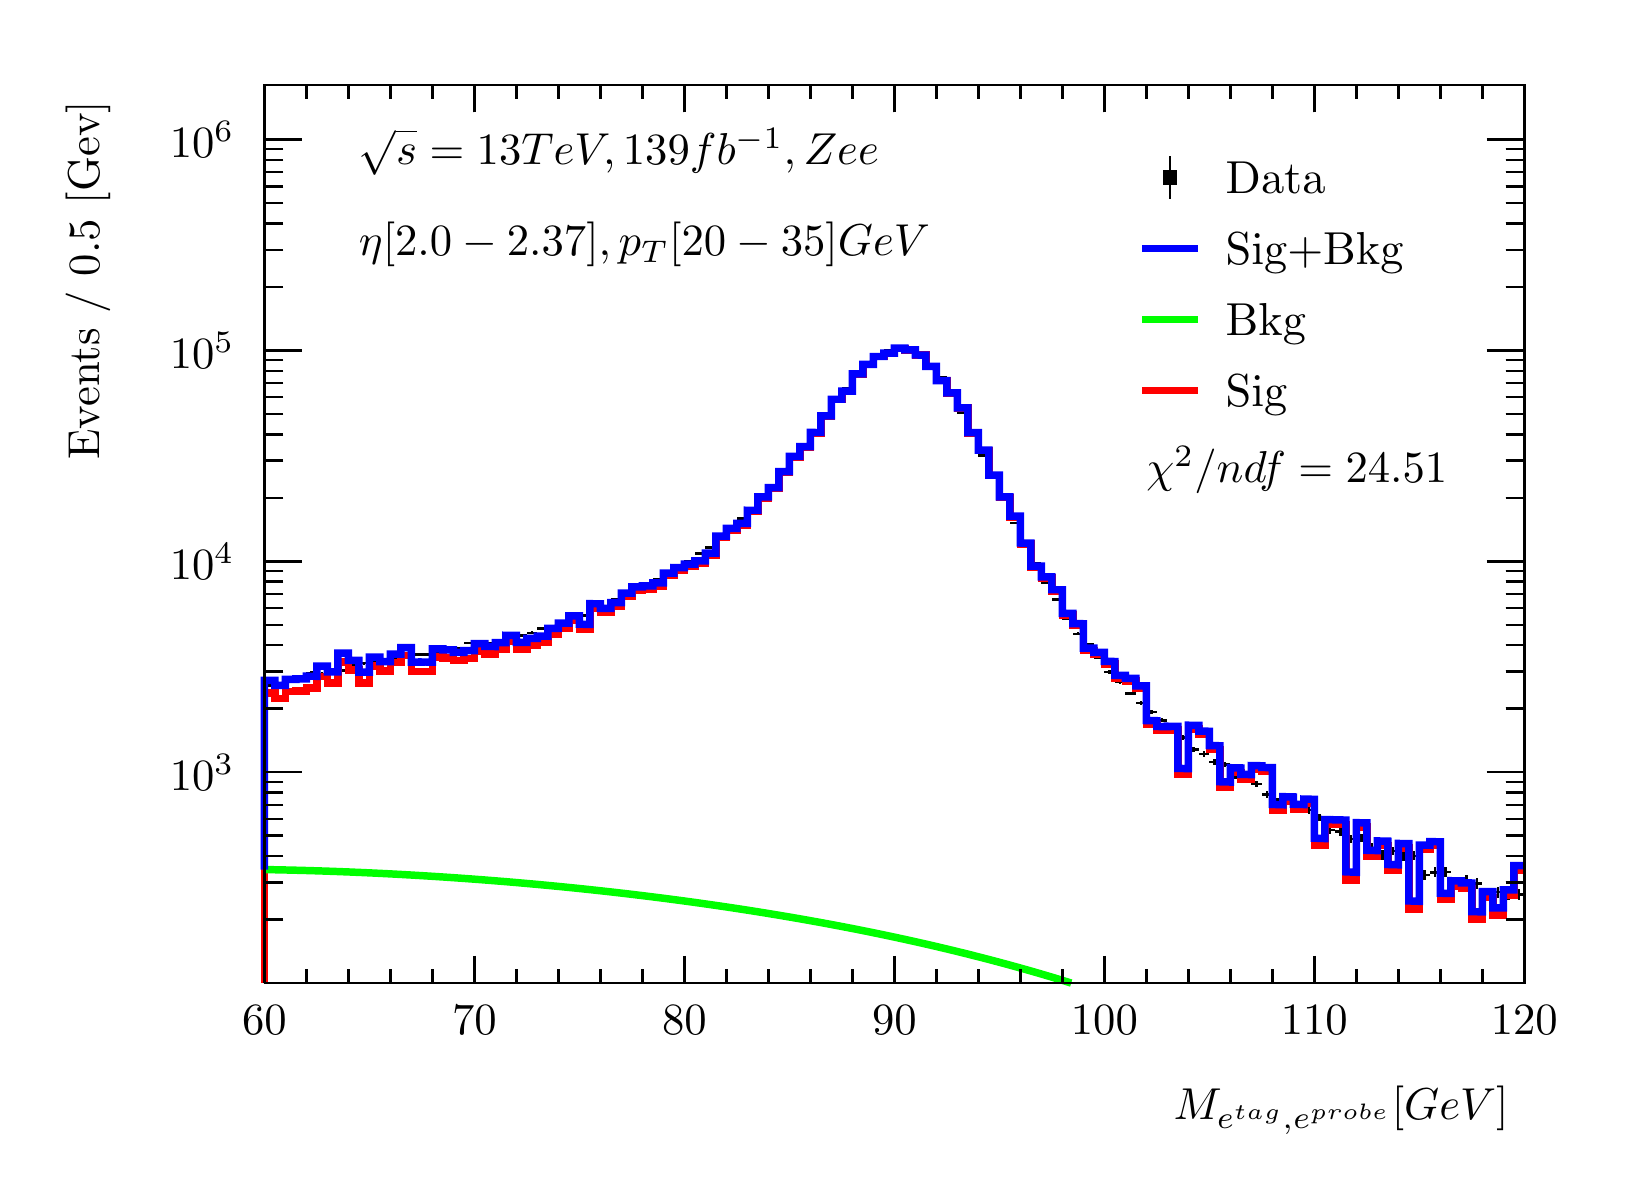
\begin{tikzpicture}
\pgfdeclareplotmark{cross} {
\pgfpathmoveto{\pgfpoint{-0.3\pgfplotmarksize}{\pgfplotmarksize}}
\pgfpathlineto{\pgfpoint{+0.3\pgfplotmarksize}{\pgfplotmarksize}}
\pgfpathlineto{\pgfpoint{+0.3\pgfplotmarksize}{0.3\pgfplotmarksize}}
\pgfpathlineto{\pgfpoint{+1\pgfplotmarksize}{0.3\pgfplotmarksize}}
\pgfpathlineto{\pgfpoint{+1\pgfplotmarksize}{-0.3\pgfplotmarksize}}
\pgfpathlineto{\pgfpoint{+0.3\pgfplotmarksize}{-0.3\pgfplotmarksize}}
\pgfpathlineto{\pgfpoint{+0.3\pgfplotmarksize}{-1.\pgfplotmarksize}}
\pgfpathlineto{\pgfpoint{-0.3\pgfplotmarksize}{-1.\pgfplotmarksize}}
\pgfpathlineto{\pgfpoint{-0.3\pgfplotmarksize}{-0.3\pgfplotmarksize}}
\pgfpathlineto{\pgfpoint{-1.\pgfplotmarksize}{-0.3\pgfplotmarksize}}
\pgfpathlineto{\pgfpoint{-1.\pgfplotmarksize}{0.3\pgfplotmarksize}}
\pgfpathlineto{\pgfpoint{-0.3\pgfplotmarksize}{0.3\pgfplotmarksize}}
\pgfpathclose
\pgfusepathqstroke
}
\pgfdeclareplotmark{cross*} {
\pgfpathmoveto{\pgfpoint{-0.3\pgfplotmarksize}{\pgfplotmarksize}}
\pgfpathlineto{\pgfpoint{+0.3\pgfplotmarksize}{\pgfplotmarksize}}
\pgfpathlineto{\pgfpoint{+0.3\pgfplotmarksize}{0.3\pgfplotmarksize}}
\pgfpathlineto{\pgfpoint{+1\pgfplotmarksize}{0.3\pgfplotmarksize}}
\pgfpathlineto{\pgfpoint{+1\pgfplotmarksize}{-0.3\pgfplotmarksize}}
\pgfpathlineto{\pgfpoint{+0.3\pgfplotmarksize}{-0.3\pgfplotmarksize}}
\pgfpathlineto{\pgfpoint{+0.3\pgfplotmarksize}{-1.\pgfplotmarksize}}
\pgfpathlineto{\pgfpoint{-0.3\pgfplotmarksize}{-1.\pgfplotmarksize}}
\pgfpathlineto{\pgfpoint{-0.3\pgfplotmarksize}{-0.3\pgfplotmarksize}}
\pgfpathlineto{\pgfpoint{-1.\pgfplotmarksize}{-0.3\pgfplotmarksize}}
\pgfpathlineto{\pgfpoint{-1.\pgfplotmarksize}{0.3\pgfplotmarksize}}
\pgfpathlineto{\pgfpoint{-0.3\pgfplotmarksize}{0.3\pgfplotmarksize}}
\pgfpathclose
\pgfusepathqfillstroke
}
\pgfdeclareplotmark{newstar} {
\pgfpathmoveto{\pgfqpoint{0pt}{\pgfplotmarksize}}
\pgfpathlineto{\pgfqpointpolar{44}{0.5\pgfplotmarksize}}
\pgfpathlineto{\pgfqpointpolar{18}{\pgfplotmarksize}}
\pgfpathlineto{\pgfqpointpolar{-20}{0.5\pgfplotmarksize}}
\pgfpathlineto{\pgfqpointpolar{-54}{\pgfplotmarksize}}
\pgfpathlineto{\pgfqpointpolar{-90}{0.5\pgfplotmarksize}}
\pgfpathlineto{\pgfqpointpolar{234}{\pgfplotmarksize}}
\pgfpathlineto{\pgfqpointpolar{198}{0.5\pgfplotmarksize}}
\pgfpathlineto{\pgfqpointpolar{162}{\pgfplotmarksize}}
\pgfpathlineto{\pgfqpointpolar{134}{0.5\pgfplotmarksize}}
\pgfpathclose
\pgfusepathqstroke
}
\pgfdeclareplotmark{newstar*} {
\pgfpathmoveto{\pgfqpoint{0pt}{\pgfplotmarksize}}
\pgfpathlineto{\pgfqpointpolar{44}{0.5\pgfplotmarksize}}
\pgfpathlineto{\pgfqpointpolar{18}{\pgfplotmarksize}}
\pgfpathlineto{\pgfqpointpolar{-20}{0.5\pgfplotmarksize}}
\pgfpathlineto{\pgfqpointpolar{-54}{\pgfplotmarksize}}
\pgfpathlineto{\pgfqpointpolar{-90}{0.5\pgfplotmarksize}}
\pgfpathlineto{\pgfqpointpolar{234}{\pgfplotmarksize}}
\pgfpathlineto{\pgfqpointpolar{198}{0.5\pgfplotmarksize}}
\pgfpathlineto{\pgfqpointpolar{162}{\pgfplotmarksize}}
\pgfpathlineto{\pgfqpointpolar{134}{0.5\pgfplotmarksize}}
\pgfpathclose
\pgfusepathqfillstroke
}
\definecolor{c}{rgb}{1,1,1};
\draw [color=c, fill=c] (0,0) rectangle (20,14.4361);
\draw [color=c, fill=c] (3,2.30977) rectangle (19,13.7143);
\definecolor{c}{rgb}{0,0,0};
\draw [c,line width=0.9] (3,2.30977) -- (3,13.7143) -- (19,13.7143) -- (19,2.30977) -- (3,2.30977);
\definecolor{c}{rgb}{1,1,1};
\draw [color=c, fill=c] (3,2.30977) rectangle (19,13.7143);
\definecolor{c}{rgb}{0,0,0};
\draw [c,line width=0.9] (3,2.30977) -- (3,13.7143) -- (19,13.7143) -- (19,2.30977) -- (3,2.30977);
\draw [c,line width=0.9] (3,2.30977) -- (19,2.30977);
\draw [c,line width=0.9] (3,2.65624) -- (3,2.30977);
\draw [c,line width=0.9] (3.53333,2.48301) -- (3.53333,2.30977);
\draw [c,line width=0.9] (4.06667,2.48301) -- (4.06667,2.30977);
\draw [c,line width=0.9] (4.6,2.48301) -- (4.6,2.30977);
\draw [c,line width=0.9] (5.13333,2.48301) -- (5.13333,2.30977);
\draw [c,line width=0.9] (5.66667,2.65624) -- (5.66667,2.30977);
\draw [c,line width=0.9] (6.2,2.48301) -- (6.2,2.30977);
\draw [c,line width=0.9] (6.73333,2.48301) -- (6.73333,2.30977);
\draw [c,line width=0.9] (7.26667,2.48301) -- (7.26667,2.30977);
\draw [c,line width=0.9] (7.8,2.48301) -- (7.8,2.30977);
\draw [c,line width=0.9] (8.33333,2.65624) -- (8.33333,2.30977);
\draw [c,line width=0.9] (8.86667,2.48301) -- (8.86667,2.30977);
\draw [c,line width=0.9] (9.4,2.48301) -- (9.4,2.30977);
\draw [c,line width=0.9] (9.93333,2.48301) -- (9.93333,2.30977);
\draw [c,line width=0.9] (10.4667,2.48301) -- (10.4667,2.30977);
\draw [c,line width=0.9] (11,2.65624) -- (11,2.30977);
\draw [c,line width=0.9] (11.5333,2.48301) -- (11.5333,2.30977);
\draw [c,line width=0.9] (12.0667,2.48301) -- (12.0667,2.30977);
\draw [c,line width=0.9] (12.6,2.48301) -- (12.6,2.30977);
\draw [c,line width=0.9] (13.1333,2.48301) -- (13.1333,2.30977);
\draw [c,line width=0.9] (13.6667,2.65624) -- (13.6667,2.30977);
\draw [c,line width=0.9] (14.2,2.48301) -- (14.2,2.30977);
\draw [c,line width=0.9] (14.7333,2.48301) -- (14.7333,2.30977);
\draw [c,line width=0.9] (15.2667,2.48301) -- (15.2667,2.30977);
\draw [c,line width=0.9] (15.8,2.48301) -- (15.8,2.30977);
\draw [c,line width=0.9] (16.3333,2.65624) -- (16.3333,2.30977);
\draw [c,line width=0.9] (16.8667,2.48301) -- (16.8667,2.30977);
\draw [c,line width=0.9] (17.4,2.48301) -- (17.4,2.30977);
\draw [c,line width=0.9] (17.9333,2.48301) -- (17.9333,2.30977);
\draw [c,line width=0.9] (18.4667,2.48301) -- (18.4667,2.30977);
\draw [c,line width=0.9] (19,2.65624) -- (19,2.30977);
\draw [anchor=base] (3,1.66015) node[scale=1.61424, color=c, rotate=0]{60};
\draw [anchor=base] (5.66667,1.66015) node[scale=1.61424, color=c, rotate=0]{70};
\draw [anchor=base] (8.33333,1.66015) node[scale=1.61424, color=c, rotate=0]{80};
\draw [anchor=base] (11,1.66015) node[scale=1.61424, color=c, rotate=0]{90};
\draw [anchor=base] (13.6667,1.66015) node[scale=1.61424, color=c, rotate=0]{100};
\draw [anchor=base] (16.3333,1.66015) node[scale=1.61424, color=c, rotate=0]{110};
\draw [anchor=base] (19,1.66015) node[scale=1.61424, color=c, rotate=0]{120};
\draw [anchor= east] (19,0.692932) node[scale=1.61424, color=c, rotate=0]{$M_{e^{tag}, e^{probe}}  [GeV]$};
\draw [c,line width=0.9] (3,13.7143) -- (19,13.7143);
\draw [c,line width=0.9] (3,13.3678) -- (3,13.7143);
\draw [c,line width=0.9] (3.53333,13.5411) -- (3.53333,13.7143);
\draw [c,line width=0.9] (4.06667,13.5411) -- (4.06667,13.7143);
\draw [c,line width=0.9] (4.6,13.5411) -- (4.6,13.7143);
\draw [c,line width=0.9] (5.13333,13.5411) -- (5.13333,13.7143);
\draw [c,line width=0.9] (5.66667,13.3678) -- (5.66667,13.7143);
\draw [c,line width=0.9] (6.2,13.5411) -- (6.2,13.7143);
\draw [c,line width=0.9] (6.73333,13.5411) -- (6.73333,13.7143);
\draw [c,line width=0.9] (7.26667,13.5411) -- (7.26667,13.7143);
\draw [c,line width=0.9] (7.8,13.5411) -- (7.8,13.7143);
\draw [c,line width=0.9] (8.33333,13.3678) -- (8.33333,13.7143);
\draw [c,line width=0.9] (8.86667,13.5411) -- (8.86667,13.7143);
\draw [c,line width=0.9] (9.4,13.5411) -- (9.4,13.7143);
\draw [c,line width=0.9] (9.93333,13.5411) -- (9.93333,13.7143);
\draw [c,line width=0.9] (10.4667,13.5411) -- (10.4667,13.7143);
\draw [c,line width=0.9] (11,13.3678) -- (11,13.7143);
\draw [c,line width=0.9] (11.5333,13.5411) -- (11.5333,13.7143);
\draw [c,line width=0.9] (12.0667,13.5411) -- (12.0667,13.7143);
\draw [c,line width=0.9] (12.6,13.5411) -- (12.6,13.7143);
\draw [c,line width=0.9] (13.1333,13.5411) -- (13.1333,13.7143);
\draw [c,line width=0.9] (13.6667,13.3678) -- (13.6667,13.7143);
\draw [c,line width=0.9] (14.2,13.5411) -- (14.2,13.7143);
\draw [c,line width=0.9] (14.7333,13.5411) -- (14.7333,13.7143);
\draw [c,line width=0.9] (15.2667,13.5411) -- (15.2667,13.7143);
\draw [c,line width=0.9] (15.8,13.5411) -- (15.8,13.7143);
\draw [c,line width=0.9] (16.3333,13.3678) -- (16.3333,13.7143);
\draw [c,line width=0.9] (16.8667,13.5411) -- (16.8667,13.7143);
\draw [c,line width=0.9] (17.4,13.5411) -- (17.4,13.7143);
\draw [c,line width=0.9] (17.9333,13.5411) -- (17.9333,13.7143);
\draw [c,line width=0.9] (18.4667,13.5411) -- (18.4667,13.7143);
\draw [c,line width=0.9] (19,13.3678) -- (19,13.7143);
\draw [c,line width=0.9] (3,2.30977) -- (3,13.7143);
\draw [c,line width=0.9] (3.237,3.11596) -- (3,3.11596);
\draw [c,line width=0.9] (3.237,3.58755) -- (3,3.58755);
\draw [c,line width=0.9] (3.237,3.92215) -- (3,3.92215);
\draw [c,line width=0.9] (3.237,4.18169) -- (3,4.18169);
\draw [c,line width=0.9] (3.237,4.39374) -- (3,4.39374);
\draw [c,line width=0.9] (3.237,4.57303) -- (3,4.57303);
\draw [c,line width=0.9] (3.237,4.72834) -- (3,4.72834);
\draw [c,line width=0.9] (3.237,4.86533) -- (3,4.86533);
\draw [c,line width=0.9] (3.474,4.98787) -- (3,4.98787);
\draw [anchor= east] (2.82,4.98787) node[scale=1.61424, color=c, rotate=0]{$10^{3}$};
\draw [c,line width=0.9] (3.237,5.79406) -- (3,5.79406);
\draw [c,line width=0.9] (3.237,6.26566) -- (3,6.26566);
\draw [c,line width=0.9] (3.237,6.60025) -- (3,6.60025);
\draw [c,line width=0.9] (3.237,6.85979) -- (3,6.85979);
\draw [c,line width=0.9] (3.237,7.07184) -- (3,7.07184);
\draw [c,line width=0.9] (3.237,7.25113) -- (3,7.25113);
\draw [c,line width=0.9] (3.237,7.40644) -- (3,7.40644);
\draw [c,line width=0.9] (3.237,7.54344) -- (3,7.54344);
\draw [c,line width=0.9] (3.474,7.66598) -- (3,7.66598);
\draw [anchor= east] (2.82,7.66598) node[scale=1.61424, color=c, rotate=0]{$10^{4}$};
\draw [c,line width=0.9] (3.237,8.47217) -- (3,8.47217);
\draw [c,line width=0.9] (3.237,8.94376) -- (3,8.94376);
\draw [c,line width=0.9] (3.237,9.27836) -- (3,9.27836);
\draw [c,line width=0.9] (3.237,9.53789) -- (3,9.53789);
\draw [c,line width=0.9] (3.237,9.74995) -- (3,9.74995);
\draw [c,line width=0.9] (3.237,9.92924) -- (3,9.92924);
\draw [c,line width=0.9] (3.237,10.0845) -- (3,10.0845);
\draw [c,line width=0.9] (3.237,10.2215) -- (3,10.2215);
\draw [c,line width=0.9] (3.474,10.3441) -- (3,10.3441);
\draw [anchor= east] (2.82,10.3441) node[scale=1.61424, color=c, rotate=0]{$10^{5}$};
\draw [c,line width=0.9] (3.237,11.1503) -- (3,11.1503);
\draw [c,line width=0.9] (3.237,11.6219) -- (3,11.6219);
\draw [c,line width=0.9] (3.237,11.9565) -- (3,11.9565);
\draw [c,line width=0.9] (3.237,12.216) -- (3,12.216);
\draw [c,line width=0.9] (3.237,12.4281) -- (3,12.4281);
\draw [c,line width=0.9] (3.237,12.6073) -- (3,12.6073);
\draw [c,line width=0.9] (3.237,12.7627) -- (3,12.7627);
\draw [c,line width=0.9] (3.237,12.8996) -- (3,12.8996);
\draw [c,line width=0.9] (3.474,13.0222) -- (3,13.0222);
\draw [anchor= east] (2.82,13.0222) node[scale=1.61424, color=c, rotate=0]{$10^{6}$};
\draw [anchor= east] (0.76,13.7143) node[scale=1.61424, color=c, rotate=90]{Events / 0.5 [Gev]};
\draw [c,line width=0.9] (19,2.30977) -- (19,13.7143);
\draw [c,line width=0.9] (18.763,3.11596) -- (19,3.11596);
\draw [c,line width=0.9] (18.763,3.58755) -- (19,3.58755);
\draw [c,line width=0.9] (18.763,3.92215) -- (19,3.92215);
\draw [c,line width=0.9] (18.763,4.18169) -- (19,4.18169);
\draw [c,line width=0.9] (18.763,4.39374) -- (19,4.39374);
\draw [c,line width=0.9] (18.763,4.57303) -- (19,4.57303);
\draw [c,line width=0.9] (18.763,4.72834) -- (19,4.72834);
\draw [c,line width=0.9] (18.763,4.86533) -- (19,4.86533);
\draw [c,line width=0.9] (18.526,4.98787) -- (19,4.98787);
\draw [c,line width=0.9] (18.763,5.79406) -- (19,5.79406);
\draw [c,line width=0.9] (18.763,6.26566) -- (19,6.26566);
\draw [c,line width=0.9] (18.763,6.60025) -- (19,6.60025);
\draw [c,line width=0.9] (18.763,6.85979) -- (19,6.85979);
\draw [c,line width=0.9] (18.763,7.07184) -- (19,7.07184);
\draw [c,line width=0.9] (18.763,7.25113) -- (19,7.25113);
\draw [c,line width=0.9] (18.763,7.40644) -- (19,7.40644);
\draw [c,line width=0.9] (18.763,7.54344) -- (19,7.54344);
\draw [c,line width=0.9] (18.526,7.66598) -- (19,7.66598);
\draw [c,line width=0.9] (18.763,8.47217) -- (19,8.47217);
\draw [c,line width=0.9] (18.763,8.94376) -- (19,8.94376);
\draw [c,line width=0.9] (18.763,9.27836) -- (19,9.27836);
\draw [c,line width=0.9] (18.763,9.53789) -- (19,9.53789);
\draw [c,line width=0.9] (18.763,9.74995) -- (19,9.74995);
\draw [c,line width=0.9] (18.763,9.92924) -- (19,9.92924);
\draw [c,line width=0.9] (18.763,10.0845) -- (19,10.0845);
\draw [c,line width=0.9] (18.763,10.2215) -- (19,10.2215);
\draw [c,line width=0.9] (18.526,10.3441) -- (19,10.3441);
\draw [c,line width=0.9] (18.763,11.1503) -- (19,11.1503);
\draw [c,line width=0.9] (18.763,11.6219) -- (19,11.6219);
\draw [c,line width=0.9] (18.763,11.9565) -- (19,11.9565);
\draw [c,line width=0.9] (18.763,12.216) -- (19,12.216);
\draw [c,line width=0.9] (18.763,12.4281) -- (19,12.4281);
\draw [c,line width=0.9] (18.763,12.6073) -- (19,12.6073);
\draw [c,line width=0.9] (18.763,12.7627) -- (19,12.7627);
\draw [c,line width=0.9] (18.763,12.8996) -- (19,12.8996);
\draw [c,line width=0.9] (18.526,13.0222) -- (19,13.0222);
\draw [c,line width=0.9] (3.06667,6.08753) -- (3,6.08753);
\draw [c,line width=0.9] (3,6.08753) -- (3,6.08753);
\draw [c,line width=0.9] (3.06667,6.08753) -- (3.13333,6.08753);
\draw [c,line width=0.9] (3.13333,6.08753) -- (3.13333,6.08753);
\draw [c,line width=0.9] (3.06667,6.08753) -- (3.06667,6.11045);
\draw [c,line width=0.9] (3.06667,6.11045) -- (3.06667,6.11045);
\draw [c,line width=0.9] (3.06667,6.08753) -- (3.06667,6.0646);
\draw [c,line width=0.9] (3.06667,6.0646) -- (3.06667,6.0646);
\draw [c,line width=0.9] (3.2,6.06702) -- (3.13333,6.06702);
\draw [c,line width=0.9] (3.13333,6.06702) -- (3.13333,6.06702);
\draw [c,line width=0.9] (3.2,6.06702) -- (3.26667,6.06702);
\draw [c,line width=0.9] (3.26667,6.06702) -- (3.26667,6.06702);
\draw [c,line width=0.9] (3.2,6.06702) -- (3.2,6.09014);
\draw [c,line width=0.9] (3.2,6.09014) -- (3.2,6.09014);
\draw [c,line width=0.9] (3.2,6.06702) -- (3.2,6.04389);
\draw [c,line width=0.9] (3.2,6.04389) -- (3.2,6.04389);
\draw [c,line width=0.9] (3.33333,6.15469) -- (3.26667,6.15469);
\draw [c,line width=0.9] (3.26667,6.15469) -- (3.26667,6.15469);
\draw [c,line width=0.9] (3.33333,6.15469) -- (3.4,6.15469);
\draw [c,line width=0.9] (3.4,6.15469) -- (3.4,6.15469);
\draw [c,line width=0.9] (3.33333,6.15469) -- (3.33333,6.17696);
\draw [c,line width=0.9] (3.33333,6.17696) -- (3.33333,6.17696);
\draw [c,line width=0.9] (3.33333,6.15469) -- (3.33333,6.13241);
\draw [c,line width=0.9] (3.33333,6.13241) -- (3.33333,6.13241);
\draw [c,line width=0.9] (3.46667,6.1941) -- (3.4,6.1941);
\draw [c,line width=0.9] (3.4,6.1941) -- (3.4,6.1941);
\draw [c,line width=0.9] (3.46667,6.1941) -- (3.53333,6.1941);
\draw [c,line width=0.9] (3.53333,6.1941) -- (3.53333,6.1941);
\draw [c,line width=0.9] (3.46667,6.1941) -- (3.46667,6.216);
\draw [c,line width=0.9] (3.46667,6.216) -- (3.46667,6.216);
\draw [c,line width=0.9] (3.46667,6.1941) -- (3.46667,6.1722);
\draw [c,line width=0.9] (3.46667,6.1722) -- (3.46667,6.1722);
\draw [c,line width=0.9] (3.6,6.24611) -- (3.53333,6.24611);
\draw [c,line width=0.9] (3.53333,6.24611) -- (3.53333,6.24611);
\draw [c,line width=0.9] (3.6,6.24611) -- (3.66667,6.24611);
\draw [c,line width=0.9] (3.66667,6.24611) -- (3.66667,6.24611);
\draw [c,line width=0.9] (3.6,6.24611) -- (3.6,6.26752);
\draw [c,line width=0.9] (3.6,6.26752) -- (3.6,6.26752);
\draw [c,line width=0.9] (3.6,6.24611) -- (3.6,6.22469);
\draw [c,line width=0.9] (3.6,6.22469) -- (3.6,6.22469);
\draw [c,line width=0.9] (3.73333,6.23541) -- (3.66667,6.23541);
\draw [c,line width=0.9] (3.66667,6.23541) -- (3.66667,6.23541);
\draw [c,line width=0.9] (3.73333,6.23541) -- (3.8,6.23541);
\draw [c,line width=0.9] (3.8,6.23541) -- (3.8,6.23541);
\draw [c,line width=0.9] (3.73333,6.23541) -- (3.73333,6.25693);
\draw [c,line width=0.9] (3.73333,6.25693) -- (3.73333,6.25693);
\draw [c,line width=0.9] (3.73333,6.23541) -- (3.73333,6.2139);
\draw [c,line width=0.9] (3.73333,6.2139) -- (3.73333,6.2139);
\draw [c,line width=0.9] (3.86667,6.26255) -- (3.8,6.26255);
\draw [c,line width=0.9] (3.8,6.26255) -- (3.8,6.26255);
\draw [c,line width=0.9] (3.86667,6.26255) -- (3.93333,6.26255);
\draw [c,line width=0.9] (3.93333,6.26255) -- (3.93333,6.26255);
\draw [c,line width=0.9] (3.86667,6.26255) -- (3.86667,6.28381);
\draw [c,line width=0.9] (3.86667,6.28381) -- (3.86667,6.28381);
\draw [c,line width=0.9] (3.86667,6.26255) -- (3.86667,6.24129);
\draw [c,line width=0.9] (3.86667,6.24129) -- (3.86667,6.24129);
\draw [c,line width=0.9] (4,6.27608) -- (3.93333,6.27608);
\draw [c,line width=0.9] (3.93333,6.27608) -- (3.93333,6.27608);
\draw [c,line width=0.9] (4,6.27608) -- (4.06667,6.27608);
\draw [c,line width=0.9] (4.06667,6.27608) -- (4.06667,6.27608);
\draw [c,line width=0.9] (4,6.27608) -- (4,6.29722);
\draw [c,line width=0.9] (4,6.29722) -- (4,6.29722);
\draw [c,line width=0.9] (4,6.27608) -- (4,6.25494);
\draw [c,line width=0.9] (4,6.25494) -- (4,6.25494);
\draw [c,line width=0.9] (4.13333,6.35193) -- (4.06667,6.35193);
\draw [c,line width=0.9] (4.06667,6.35193) -- (4.06667,6.35193);
\draw [c,line width=0.9] (4.13333,6.35193) -- (4.2,6.35193);
\draw [c,line width=0.9] (4.2,6.35193) -- (4.2,6.35193);
\draw [c,line width=0.9] (4.13333,6.35193) -- (4.13333,6.3724);
\draw [c,line width=0.9] (4.13333,6.3724) -- (4.13333,6.3724);
\draw [c,line width=0.9] (4.13333,6.35193) -- (4.13333,6.33147);
\draw [c,line width=0.9] (4.13333,6.33147) -- (4.13333,6.33147);
\draw [c,line width=0.9] (4.26667,6.37298) -- (4.2,6.37298);
\draw [c,line width=0.9] (4.2,6.37298) -- (4.2,6.37298);
\draw [c,line width=0.9] (4.26667,6.37298) -- (4.33333,6.37298);
\draw [c,line width=0.9] (4.33333,6.37298) -- (4.33333,6.37298);
\draw [c,line width=0.9] (4.26667,6.37298) -- (4.26667,6.39326);
\draw [c,line width=0.9] (4.26667,6.39326) -- (4.26667,6.39326);
\draw [c,line width=0.9] (4.26667,6.37298) -- (4.26667,6.3527);
\draw [c,line width=0.9] (4.26667,6.3527) -- (4.26667,6.3527);
\draw [c,line width=0.9] (4.4,6.39504) -- (4.33333,6.39504);
\draw [c,line width=0.9] (4.33333,6.39504) -- (4.33333,6.39504);
\draw [c,line width=0.9] (4.4,6.39504) -- (4.46667,6.39504);
\draw [c,line width=0.9] (4.46667,6.39504) -- (4.46667,6.39504);
\draw [c,line width=0.9] (4.4,6.39504) -- (4.4,6.41513);
\draw [c,line width=0.9] (4.4,6.41513) -- (4.4,6.41513);
\draw [c,line width=0.9] (4.4,6.39504) -- (4.4,6.37496);
\draw [c,line width=0.9] (4.4,6.37496) -- (4.4,6.37496);
\draw [c,line width=0.9] (4.53333,6.42247) -- (4.46667,6.42247);
\draw [c,line width=0.9] (4.46667,6.42247) -- (4.46667,6.42247);
\draw [c,line width=0.9] (4.53333,6.42247) -- (4.6,6.42247);
\draw [c,line width=0.9] (4.6,6.42247) -- (4.6,6.42247);
\draw [c,line width=0.9] (4.53333,6.42247) -- (4.53333,6.44232);
\draw [c,line width=0.9] (4.53333,6.44232) -- (4.53333,6.44232);
\draw [c,line width=0.9] (4.53333,6.42247) -- (4.53333,6.40262);
\draw [c,line width=0.9] (4.53333,6.40262) -- (4.53333,6.40262);
\draw [c,line width=0.9] (4.66667,6.44195) -- (4.6,6.44195);
\draw [c,line width=0.9] (4.6,6.44195) -- (4.6,6.44195);
\draw [c,line width=0.9] (4.66667,6.44195) -- (4.73333,6.44195);
\draw [c,line width=0.9] (4.73333,6.44195) -- (4.73333,6.44195);
\draw [c,line width=0.9] (4.66667,6.44195) -- (4.66667,6.46164);
\draw [c,line width=0.9] (4.66667,6.46164) -- (4.66667,6.46164);
\draw [c,line width=0.9] (4.66667,6.44195) -- (4.66667,6.42227);
\draw [c,line width=0.9] (4.66667,6.42227) -- (4.66667,6.42227);
\draw [c,line width=0.9] (4.8,6.44461) -- (4.73333,6.44461);
\draw [c,line width=0.9] (4.73333,6.44461) -- (4.73333,6.44461);
\draw [c,line width=0.9] (4.8,6.44461) -- (4.86667,6.44461);
\draw [c,line width=0.9] (4.86667,6.44461) -- (4.86667,6.44461);
\draw [c,line width=0.9] (4.8,6.44461) -- (4.8,6.46428);
\draw [c,line width=0.9] (4.8,6.46428) -- (4.8,6.46428);
\draw [c,line width=0.9] (4.8,6.44461) -- (4.8,6.42495);
\draw [c,line width=0.9] (4.8,6.42495) -- (4.8,6.42495);
\draw [c,line width=0.9] (4.93333,6.48223) -- (4.86667,6.48223);
\draw [c,line width=0.9] (4.86667,6.48223) -- (4.86667,6.48223);
\draw [c,line width=0.9] (4.93333,6.48223) -- (5,6.48223);
\draw [c,line width=0.9] (5,6.48223) -- (5,6.48223);
\draw [c,line width=0.9] (4.93333,6.48223) -- (4.93333,6.50157);
\draw [c,line width=0.9] (4.93333,6.50157) -- (4.93333,6.50157);
\draw [c,line width=0.9] (4.93333,6.48223) -- (4.93333,6.46288);
\draw [c,line width=0.9] (4.93333,6.46288) -- (4.93333,6.46288);
\draw [c,line width=0.9] (5.06667,6.48029) -- (5,6.48029);
\draw [c,line width=0.9] (5,6.48029) -- (5,6.48029);
\draw [c,line width=0.9] (5.06667,6.48029) -- (5.13333,6.48029);
\draw [c,line width=0.9] (5.13333,6.48029) -- (5.13333,6.48029);
\draw [c,line width=0.9] (5.06667,6.48029) -- (5.06667,6.49966);
\draw [c,line width=0.9] (5.06667,6.49966) -- (5.06667,6.49966);
\draw [c,line width=0.9] (5.06667,6.48029) -- (5.06667,6.46093);
\draw [c,line width=0.9] (5.06667,6.46093) -- (5.06667,6.46093);
\draw [c,line width=0.9] (5.2,6.51554) -- (5.13333,6.51554);
\draw [c,line width=0.9] (5.13333,6.51554) -- (5.13333,6.51554);
\draw [c,line width=0.9] (5.2,6.51554) -- (5.26667,6.51554);
\draw [c,line width=0.9] (5.26667,6.51554) -- (5.26667,6.51554);
\draw [c,line width=0.9] (5.2,6.51554) -- (5.2,6.53461);
\draw [c,line width=0.9] (5.2,6.53461) -- (5.2,6.53461);
\draw [c,line width=0.9] (5.2,6.51554) -- (5.2,6.49647);
\draw [c,line width=0.9] (5.2,6.49647) -- (5.2,6.49647);
\draw [c,line width=0.9] (5.33333,6.54883) -- (5.26667,6.54883);
\draw [c,line width=0.9] (5.26667,6.54883) -- (5.26667,6.54883);
\draw [c,line width=0.9] (5.33333,6.54883) -- (5.4,6.54883);
\draw [c,line width=0.9] (5.4,6.54883) -- (5.4,6.54883);
\draw [c,line width=0.9] (5.33333,6.54883) -- (5.33333,6.56763);
\draw [c,line width=0.9] (5.33333,6.56763) -- (5.33333,6.56763);
\draw [c,line width=0.9] (5.33333,6.54883) -- (5.33333,6.53003);
\draw [c,line width=0.9] (5.33333,6.53003) -- (5.33333,6.53003);
\draw [c,line width=0.9] (5.46667,6.56243) -- (5.4,6.56243);
\draw [c,line width=0.9] (5.4,6.56243) -- (5.4,6.56243);
\draw [c,line width=0.9] (5.46667,6.56243) -- (5.53333,6.56243);
\draw [c,line width=0.9] (5.53333,6.56243) -- (5.53333,6.56243);
\draw [c,line width=0.9] (5.46667,6.56243) -- (5.46667,6.58112);
\draw [c,line width=0.9] (5.46667,6.58112) -- (5.46667,6.58112);
\draw [c,line width=0.9] (5.46667,6.56243) -- (5.46667,6.54374);
\draw [c,line width=0.9] (5.46667,6.54374) -- (5.46667,6.54374);
\draw [c,line width=0.9] (5.6,6.62898) -- (5.53333,6.62898);
\draw [c,line width=0.9] (5.53333,6.62898) -- (5.53333,6.62898);
\draw [c,line width=0.9] (5.6,6.62898) -- (5.66667,6.62898);
\draw [c,line width=0.9] (5.66667,6.62898) -- (5.66667,6.62898);
\draw [c,line width=0.9] (5.6,6.62898) -- (5.6,6.64714);
\draw [c,line width=0.9] (5.6,6.64714) -- (5.6,6.64714);
\draw [c,line width=0.9] (5.6,6.62898) -- (5.6,6.61081);
\draw [c,line width=0.9] (5.6,6.61081) -- (5.6,6.61081);
\draw [c,line width=0.9] (5.73333,6.59062) -- (5.66667,6.59062);
\draw [c,line width=0.9] (5.66667,6.59062) -- (5.66667,6.59062);
\draw [c,line width=0.9] (5.73333,6.59062) -- (5.8,6.59062);
\draw [c,line width=0.9] (5.8,6.59062) -- (5.8,6.59062);
\draw [c,line width=0.9] (5.73333,6.59062) -- (5.73333,6.60909);
\draw [c,line width=0.9] (5.73333,6.60909) -- (5.73333,6.60909);
\draw [c,line width=0.9] (5.73333,6.59062) -- (5.73333,6.57215);
\draw [c,line width=0.9] (5.73333,6.57215) -- (5.73333,6.57215);
\draw [c,line width=0.9] (5.86667,6.62158) -- (5.8,6.62158);
\draw [c,line width=0.9] (5.8,6.62158) -- (5.8,6.62158);
\draw [c,line width=0.9] (5.86667,6.62158) -- (5.93333,6.62158);
\draw [c,line width=0.9] (5.93333,6.62158) -- (5.93333,6.62158);
\draw [c,line width=0.9] (5.86667,6.62158) -- (5.86667,6.6398);
\draw [c,line width=0.9] (5.86667,6.6398) -- (5.86667,6.6398);
\draw [c,line width=0.9] (5.86667,6.62158) -- (5.86667,6.60335);
\draw [c,line width=0.9] (5.86667,6.60335) -- (5.86667,6.60335);
\draw [c,line width=0.9] (6,6.63407) -- (5.93333,6.63407);
\draw [c,line width=0.9] (5.93333,6.63407) -- (5.93333,6.63407);
\draw [c,line width=0.9] (6,6.63407) -- (6.06667,6.63407);
\draw [c,line width=0.9] (6.06667,6.63407) -- (6.06667,6.63407);
\draw [c,line width=0.9] (6,6.63407) -- (6,6.65219);
\draw [c,line width=0.9] (6,6.65219) -- (6,6.65219);
\draw [c,line width=0.9] (6,6.63407) -- (6,6.61595);
\draw [c,line width=0.9] (6,6.61595) -- (6,6.61595);
\draw [c,line width=0.9] (6.13333,6.69915) -- (6.06667,6.69915);
\draw [c,line width=0.9] (6.06667,6.69915) -- (6.06667,6.69915);
\draw [c,line width=0.9] (6.13333,6.69915) -- (6.2,6.69915);
\draw [c,line width=0.9] (6.2,6.69915) -- (6.2,6.69915);
\draw [c,line width=0.9] (6.13333,6.69915) -- (6.13333,6.71678);
\draw [c,line width=0.9] (6.13333,6.71678) -- (6.13333,6.71678);
\draw [c,line width=0.9] (6.13333,6.69915) -- (6.13333,6.68153);
\draw [c,line width=0.9] (6.13333,6.68153) -- (6.13333,6.68153);
\draw [c,line width=0.9] (6.26667,6.72321) -- (6.2,6.72321);
\draw [c,line width=0.9] (6.2,6.72321) -- (6.2,6.72321);
\draw [c,line width=0.9] (6.26667,6.72321) -- (6.33333,6.72321);
\draw [c,line width=0.9] (6.33333,6.72321) -- (6.33333,6.72321);
\draw [c,line width=0.9] (6.26667,6.72321) -- (6.26667,6.74065);
\draw [c,line width=0.9] (6.26667,6.74065) -- (6.26667,6.74065);
\draw [c,line width=0.9] (6.26667,6.72321) -- (6.26667,6.70576);
\draw [c,line width=0.9] (6.26667,6.70576) -- (6.26667,6.70576);
\draw [c,line width=0.9] (6.4,6.7585) -- (6.33333,6.7585);
\draw [c,line width=0.9] (6.33333,6.7585) -- (6.33333,6.7585);
\draw [c,line width=0.9] (6.4,6.7585) -- (6.46667,6.7585);
\draw [c,line width=0.9] (6.46667,6.7585) -- (6.46667,6.7585);
\draw [c,line width=0.9] (6.4,6.7585) -- (6.4,6.77568);
\draw [c,line width=0.9] (6.4,6.77568) -- (6.4,6.77568);
\draw [c,line width=0.9] (6.4,6.7585) -- (6.4,6.74132);
\draw [c,line width=0.9] (6.4,6.74132) -- (6.4,6.74132);
\draw [c,line width=0.9] (6.53333,6.81061) -- (6.46667,6.81061);
\draw [c,line width=0.9] (6.46667,6.81061) -- (6.46667,6.81061);
\draw [c,line width=0.9] (6.53333,6.81061) -- (6.6,6.81061);
\draw [c,line width=0.9] (6.6,6.81061) -- (6.6,6.81061);
\draw [c,line width=0.9] (6.53333,6.81061) -- (6.53333,6.82741);
\draw [c,line width=0.9] (6.53333,6.82741) -- (6.53333,6.82741);
\draw [c,line width=0.9] (6.53333,6.81061) -- (6.53333,6.79381);
\draw [c,line width=0.9] (6.53333,6.79381) -- (6.53333,6.79381);
\draw [c,line width=0.9] (6.66667,6.83819) -- (6.6,6.83819);
\draw [c,line width=0.9] (6.6,6.83819) -- (6.6,6.83819);
\draw [c,line width=0.9] (6.66667,6.83819) -- (6.73333,6.83819);
\draw [c,line width=0.9] (6.73333,6.83819) -- (6.73333,6.83819);
\draw [c,line width=0.9] (6.66667,6.83819) -- (6.66667,6.85479);
\draw [c,line width=0.9] (6.66667,6.85479) -- (6.66667,6.85479);
\draw [c,line width=0.9] (6.66667,6.83819) -- (6.66667,6.82159);
\draw [c,line width=0.9] (6.66667,6.82159) -- (6.66667,6.82159);
\draw [c,line width=0.9] (6.8,6.87228) -- (6.73333,6.87228);
\draw [c,line width=0.9] (6.73333,6.87228) -- (6.73333,6.87228);
\draw [c,line width=0.9] (6.8,6.87228) -- (6.86667,6.87228);
\draw [c,line width=0.9] (6.86667,6.87228) -- (6.86667,6.87228);
\draw [c,line width=0.9] (6.8,6.87228) -- (6.8,6.88864);
\draw [c,line width=0.9] (6.8,6.88864) -- (6.8,6.88864);
\draw [c,line width=0.9] (6.8,6.87228) -- (6.8,6.85592);
\draw [c,line width=0.9] (6.8,6.85592) -- (6.8,6.85592);
\draw [c,line width=0.9] (6.93333,6.94022) -- (6.86667,6.94022);
\draw [c,line width=0.9] (6.86667,6.94022) -- (6.86667,6.94022);
\draw [c,line width=0.9] (6.93333,6.94022) -- (7,6.94022);
\draw [c,line width=0.9] (7,6.94022) -- (7,6.94022);
\draw [c,line width=0.9] (6.93333,6.94022) -- (6.93333,6.95611);
\draw [c,line width=0.9] (6.93333,6.95611) -- (6.93333,6.95611);
\draw [c,line width=0.9] (6.93333,6.94022) -- (6.93333,6.92433);
\draw [c,line width=0.9] (6.93333,6.92433) -- (6.93333,6.92433);
\draw [c,line width=0.9] (7.06667,6.9797) -- (7,6.9797);
\draw [c,line width=0.9] (7,6.9797) -- (7,6.9797);
\draw [c,line width=0.9] (7.06667,6.9797) -- (7.13333,6.9797);
\draw [c,line width=0.9] (7.13333,6.9797) -- (7.13333,6.9797);
\draw [c,line width=0.9] (7.06667,6.9797) -- (7.06667,6.99532);
\draw [c,line width=0.9] (7.06667,6.99532) -- (7.06667,6.99532);
\draw [c,line width=0.9] (7.06667,6.9797) -- (7.06667,6.96408);
\draw [c,line width=0.9] (7.06667,6.96408) -- (7.06667,6.96408);
\draw [c,line width=0.9] (7.2,7.05466) -- (7.13333,7.05466);
\draw [c,line width=0.9] (7.13333,7.05466) -- (7.13333,7.05466);
\draw [c,line width=0.9] (7.2,7.05466) -- (7.26667,7.05466);
\draw [c,line width=0.9] (7.26667,7.05466) -- (7.26667,7.05466);
\draw [c,line width=0.9] (7.2,7.05466) -- (7.2,7.06979);
\draw [c,line width=0.9] (7.2,7.06979) -- (7.2,7.06979);
\draw [c,line width=0.9] (7.2,7.05466) -- (7.2,7.03953);
\draw [c,line width=0.9] (7.2,7.03953) -- (7.2,7.03953);
\draw [c,line width=0.9] (7.33333,7.07707) -- (7.26667,7.07707);
\draw [c,line width=0.9] (7.26667,7.07707) -- (7.26667,7.07707);
\draw [c,line width=0.9] (7.33333,7.07707) -- (7.4,7.07707);
\draw [c,line width=0.9] (7.4,7.07707) -- (7.4,7.07707);
\draw [c,line width=0.9] (7.33333,7.07707) -- (7.33333,7.09205);
\draw [c,line width=0.9] (7.33333,7.09205) -- (7.33333,7.09205);
\draw [c,line width=0.9] (7.33333,7.07707) -- (7.33333,7.06209);
\draw [c,line width=0.9] (7.33333,7.06209) -- (7.33333,7.06209);
\draw [c,line width=0.9] (7.46667,7.18023) -- (7.4,7.18023);
\draw [c,line width=0.9] (7.4,7.18023) -- (7.4,7.18023);
\draw [c,line width=0.9] (7.46667,7.18023) -- (7.53333,7.18023);
\draw [c,line width=0.9] (7.53333,7.18023) -- (7.53333,7.18023);
\draw [c,line width=0.9] (7.46667,7.18023) -- (7.46667,7.19456);
\draw [c,line width=0.9] (7.46667,7.19456) -- (7.46667,7.19456);
\draw [c,line width=0.9] (7.46667,7.18023) -- (7.46667,7.1659);
\draw [c,line width=0.9] (7.46667,7.1659) -- (7.46667,7.1659);
\draw [c,line width=0.9] (7.6,7.20849) -- (7.53333,7.20849);
\draw [c,line width=0.9] (7.53333,7.20849) -- (7.53333,7.20849);
\draw [c,line width=0.9] (7.6,7.20849) -- (7.66667,7.20849);
\draw [c,line width=0.9] (7.66667,7.20849) -- (7.66667,7.20849);
\draw [c,line width=0.9] (7.6,7.20849) -- (7.6,7.22265);
\draw [c,line width=0.9] (7.6,7.22265) -- (7.6,7.22265);
\draw [c,line width=0.9] (7.6,7.20849) -- (7.6,7.19433);
\draw [c,line width=0.9] (7.6,7.19433) -- (7.6,7.19433);
\draw [c,line width=0.9] (7.73333,7.30249) -- (7.66667,7.30249);
\draw [c,line width=0.9] (7.66667,7.30249) -- (7.66667,7.30249);
\draw [c,line width=0.9] (7.73333,7.30249) -- (7.8,7.30249);
\draw [c,line width=0.9] (7.8,7.30249) -- (7.8,7.30249);
\draw [c,line width=0.9] (7.73333,7.30249) -- (7.73333,7.31609);
\draw [c,line width=0.9] (7.73333,7.31609) -- (7.73333,7.31609);
\draw [c,line width=0.9] (7.73333,7.30249) -- (7.73333,7.28889);
\draw [c,line width=0.9] (7.73333,7.28889) -- (7.73333,7.28889);
\draw [c,line width=0.9] (7.86667,7.34587) -- (7.8,7.34587);
\draw [c,line width=0.9] (7.8,7.34587) -- (7.8,7.34587);
\draw [c,line width=0.9] (7.86667,7.34587) -- (7.93333,7.34587);
\draw [c,line width=0.9] (7.93333,7.34587) -- (7.93333,7.34587);
\draw [c,line width=0.9] (7.86667,7.34587) -- (7.86667,7.35921);
\draw [c,line width=0.9] (7.86667,7.35921) -- (7.86667,7.35921);
\draw [c,line width=0.9] (7.86667,7.34587) -- (7.86667,7.33252);
\draw [c,line width=0.9] (7.86667,7.33252) -- (7.86667,7.33252);
\draw [c,line width=0.9] (8,7.43275) -- (7.93333,7.43275);
\draw [c,line width=0.9] (7.93333,7.43275) -- (7.93333,7.43275);
\draw [c,line width=0.9] (8,7.43275) -- (8.06667,7.43275);
\draw [c,line width=0.9] (8.06667,7.43275) -- (8.06667,7.43275);
\draw [c,line width=0.9] (8,7.43275) -- (8,7.44561);
\draw [c,line width=0.9] (8,7.44561) -- (8,7.44561);
\draw [c,line width=0.9] (8,7.43275) -- (8,7.41989);
\draw [c,line width=0.9] (8,7.41989) -- (8,7.41989);
\draw [c,line width=0.9] (8.13333,7.49932) -- (8.06667,7.49932);
\draw [c,line width=0.9] (8.06667,7.49932) -- (8.06667,7.49932);
\draw [c,line width=0.9] (8.13333,7.49932) -- (8.2,7.49932);
\draw [c,line width=0.9] (8.2,7.49932) -- (8.2,7.49932);
\draw [c,line width=0.9] (8.13333,7.49932) -- (8.13333,7.51181);
\draw [c,line width=0.9] (8.13333,7.51181) -- (8.13333,7.51181);
\draw [c,line width=0.9] (8.13333,7.49932) -- (8.13333,7.48682);
\draw [c,line width=0.9] (8.13333,7.48682) -- (8.13333,7.48682);
\draw [c,line width=0.9] (8.26667,7.58955) -- (8.2,7.58955);
\draw [c,line width=0.9] (8.2,7.58955) -- (8.2,7.58955);
\draw [c,line width=0.9] (8.26667,7.58955) -- (8.33333,7.58955);
\draw [c,line width=0.9] (8.33333,7.58955) -- (8.33333,7.58955);
\draw [c,line width=0.9] (8.26667,7.58955) -- (8.26667,7.60157);
\draw [c,line width=0.9] (8.26667,7.60157) -- (8.26667,7.60157);
\draw [c,line width=0.9] (8.26667,7.58955) -- (8.26667,7.57753);
\draw [c,line width=0.9] (8.26667,7.57753) -- (8.26667,7.57753);
\draw [c,line width=0.9] (8.4,7.66108) -- (8.33333,7.66108);
\draw [c,line width=0.9] (8.33333,7.66108) -- (8.33333,7.66108);
\draw [c,line width=0.9] (8.4,7.66108) -- (8.46667,7.66108);
\draw [c,line width=0.9] (8.46667,7.66108) -- (8.46667,7.66108);
\draw [c,line width=0.9] (8.4,7.66108) -- (8.4,7.67274);
\draw [c,line width=0.9] (8.4,7.67274) -- (8.4,7.67274);
\draw [c,line width=0.9] (8.4,7.66108) -- (8.4,7.64943);
\draw [c,line width=0.9] (8.4,7.64943) -- (8.4,7.64943);
\draw [c,line width=0.9] (8.53333,7.7676) -- (8.46667,7.7676);
\draw [c,line width=0.9] (8.46667,7.7676) -- (8.46667,7.7676);
\draw [c,line width=0.9] (8.53333,7.7676) -- (8.6,7.7676);
\draw [c,line width=0.9] (8.6,7.7676) -- (8.6,7.7676);
\draw [c,line width=0.9] (8.53333,7.7676) -- (8.53333,7.77873);
\draw [c,line width=0.9] (8.53333,7.77873) -- (8.53333,7.77873);
\draw [c,line width=0.9] (8.53333,7.7676) -- (8.53333,7.75646);
\draw [c,line width=0.9] (8.53333,7.75646) -- (8.53333,7.75646);
\draw [c,line width=0.9] (8.66667,7.84251) -- (8.6,7.84251);
\draw [c,line width=0.9] (8.6,7.84251) -- (8.6,7.84251);
\draw [c,line width=0.9] (8.66667,7.84251) -- (8.73333,7.84251);
\draw [c,line width=0.9] (8.73333,7.84251) -- (8.73333,7.84251);
\draw [c,line width=0.9] (8.66667,7.84251) -- (8.66667,7.85329);
\draw [c,line width=0.9] (8.66667,7.85329) -- (8.66667,7.85329);
\draw [c,line width=0.9] (8.66667,7.84251) -- (8.66667,7.83173);
\draw [c,line width=0.9] (8.66667,7.83173) -- (8.66667,7.83173);
\draw [c,line width=0.9] (8.8,7.97149) -- (8.73333,7.97149);
\draw [c,line width=0.9] (8.73333,7.97149) -- (8.73333,7.97149);
\draw [c,line width=0.9] (8.8,7.97149) -- (8.86667,7.97149);
\draw [c,line width=0.9] (8.86667,7.97149) -- (8.86667,7.97149);
\draw [c,line width=0.9] (8.8,7.97149) -- (8.8,7.98169);
\draw [c,line width=0.9] (8.8,7.98169) -- (8.8,7.98169);
\draw [c,line width=0.9] (8.8,7.97149) -- (8.8,7.96129);
\draw [c,line width=0.9] (8.8,7.96129) -- (8.8,7.96129);
\draw [c,line width=0.9] (8.93333,8.08361) -- (8.86667,8.08361);
\draw [c,line width=0.9] (8.86667,8.08361) -- (8.86667,8.08361);
\draw [c,line width=0.9] (8.93333,8.08361) -- (9,8.08361);
\draw [c,line width=0.9] (9,8.08361) -- (9,8.08361);
\draw [c,line width=0.9] (8.93333,8.08361) -- (8.93333,8.09333);
\draw [c,line width=0.9] (8.93333,8.09333) -- (8.93333,8.09333);
\draw [c,line width=0.9] (8.93333,8.08361) -- (8.93333,8.07389);
\draw [c,line width=0.9] (8.93333,8.07389) -- (8.93333,8.07389);
\draw [c,line width=0.9] (9.06667,8.21132) -- (9,8.21132);
\draw [c,line width=0.9] (9,8.21132) -- (9,8.21132);
\draw [c,line width=0.9] (9.06667,8.21132) -- (9.13333,8.21132);
\draw [c,line width=0.9] (9.13333,8.21132) -- (9.13333,8.21132);
\draw [c,line width=0.9] (9.06667,8.21132) -- (9.06667,8.22052);
\draw [c,line width=0.9] (9.06667,8.22052) -- (9.06667,8.22052);
\draw [c,line width=0.9] (9.06667,8.21132) -- (9.06667,8.20212);
\draw [c,line width=0.9] (9.06667,8.20212) -- (9.06667,8.20212);
\draw [c,line width=0.9] (9.2,8.33087) -- (9.13333,8.33087);
\draw [c,line width=0.9] (9.13333,8.33087) -- (9.13333,8.33087);
\draw [c,line width=0.9] (9.2,8.33087) -- (9.26667,8.33087);
\draw [c,line width=0.9] (9.26667,8.33087) -- (9.26667,8.33087);
\draw [c,line width=0.9] (9.2,8.33087) -- (9.2,8.33961);
\draw [c,line width=0.9] (9.2,8.33961) -- (9.2,8.33961);
\draw [c,line width=0.9] (9.2,8.33087) -- (9.2,8.32213);
\draw [c,line width=0.9] (9.2,8.32213) -- (9.2,8.32213);
\draw [c,line width=0.9] (9.33333,8.4916) -- (9.26667,8.4916);
\draw [c,line width=0.9] (9.26667,8.4916) -- (9.26667,8.4916);
\draw [c,line width=0.9] (9.33333,8.4916) -- (9.4,8.4916);
\draw [c,line width=0.9] (9.4,8.4916) -- (9.4,8.4916);
\draw [c,line width=0.9] (9.33333,8.4916) -- (9.33333,8.49976);
\draw [c,line width=0.9] (9.33333,8.49976) -- (9.33333,8.49976);
\draw [c,line width=0.9] (9.33333,8.4916) -- (9.33333,8.48345);
\draw [c,line width=0.9] (9.33333,8.48345) -- (9.33333,8.48345);
\draw [c,line width=0.9] (9.46667,8.62502) -- (9.4,8.62502);
\draw [c,line width=0.9] (9.4,8.62502) -- (9.4,8.62502);
\draw [c,line width=0.9] (9.46667,8.62502) -- (9.53333,8.62502);
\draw [c,line width=0.9] (9.53333,8.62502) -- (9.53333,8.62502);
\draw [c,line width=0.9] (9.46667,8.62502) -- (9.46667,8.63273);
\draw [c,line width=0.9] (9.46667,8.63273) -- (9.46667,8.63273);
\draw [c,line width=0.9] (9.46667,8.62502) -- (9.46667,8.61732);
\draw [c,line width=0.9] (9.46667,8.61732) -- (9.46667,8.61732);
\draw [c,line width=0.9] (9.6,8.79274) -- (9.53333,8.79274);
\draw [c,line width=0.9] (9.53333,8.79274) -- (9.53333,8.79274);
\draw [c,line width=0.9] (9.6,8.79274) -- (9.66667,8.79274);
\draw [c,line width=0.9] (9.66667,8.79274) -- (9.66667,8.79274);
\draw [c,line width=0.9] (9.6,8.79274) -- (9.6,8.79991);
\draw [c,line width=0.9] (9.6,8.79991) -- (9.6,8.79991);
\draw [c,line width=0.9] (9.6,8.79274) -- (9.6,8.78558);
\draw [c,line width=0.9] (9.6,8.78558) -- (9.6,8.78558);
\draw [c,line width=0.9] (9.73333,8.97395) -- (9.66667,8.97395);
\draw [c,line width=0.9] (9.66667,8.97395) -- (9.66667,8.97395);
\draw [c,line width=0.9] (9.73333,8.97395) -- (9.8,8.97395);
\draw [c,line width=0.9] (9.8,8.97395) -- (9.8,8.97395);
\draw [c,line width=0.9] (9.73333,8.97395) -- (9.73333,8.98058);
\draw [c,line width=0.9] (9.73333,8.98058) -- (9.73333,8.98058);
\draw [c,line width=0.9] (9.73333,8.97395) -- (9.73333,8.96733);
\draw [c,line width=0.9] (9.73333,8.96733) -- (9.73333,8.96733);
\draw [c,line width=0.9] (9.86667,9.15362) -- (9.8,9.15362);
\draw [c,line width=0.9] (9.8,9.15362) -- (9.8,9.15362);
\draw [c,line width=0.9] (9.86667,9.15362) -- (9.93333,9.15362);
\draw [c,line width=0.9] (9.93333,9.15362) -- (9.93333,9.15362);
\draw [c,line width=0.9] (9.86667,9.15362) -- (9.86667,9.15975);
\draw [c,line width=0.9] (9.86667,9.15975) -- (9.86667,9.15975);
\draw [c,line width=0.9] (9.86667,9.15362) -- (9.86667,9.14748);
\draw [c,line width=0.9] (9.86667,9.14748) -- (9.86667,9.14748);
\draw [c,line width=0.9] (10,9.32989) -- (9.93333,9.32989);
\draw [c,line width=0.9] (9.93333,9.32989) -- (9.93333,9.32989);
\draw [c,line width=0.9] (10,9.32989) -- (10.0667,9.32989);
\draw [c,line width=0.9] (10.0667,9.32989) -- (10.0667,9.32989);
\draw [c,line width=0.9] (10,9.32989) -- (10,9.33558);
\draw [c,line width=0.9] (10,9.33558) -- (10,9.33558);
\draw [c,line width=0.9] (10,9.32989) -- (10,9.3242);
\draw [c,line width=0.9] (10,9.3242) -- (10,9.3242);
\draw [c,line width=0.9] (10.1333,9.52679) -- (10.0667,9.52679);
\draw [c,line width=0.9] (10.0667,9.52679) -- (10.0667,9.52679);
\draw [c,line width=0.9] (10.1333,9.52679) -- (10.2,9.52679);
\draw [c,line width=0.9] (10.2,9.52679) -- (10.2,9.52679);
\draw [c,line width=0.9] (10.1333,9.52679) -- (10.1333,9.53202);
\draw [c,line width=0.9] (10.1333,9.53202) -- (10.1333,9.53202);
\draw [c,line width=0.9] (10.1333,9.52679) -- (10.1333,9.52156);
\draw [c,line width=0.9] (10.1333,9.52156) -- (10.1333,9.52156);
\draw [c,line width=0.9] (10.2667,9.71334) -- (10.2,9.71334);
\draw [c,line width=0.9] (10.2,9.71334) -- (10.2,9.71334);
\draw [c,line width=0.9] (10.2667,9.71334) -- (10.3333,9.71334);
\draw [c,line width=0.9] (10.3333,9.71334) -- (10.3333,9.71334);
\draw [c,line width=0.9] (10.2667,9.71334) -- (10.2667,9.71817);
\draw [c,line width=0.9] (10.2667,9.71817) -- (10.2667,9.71817);
\draw [c,line width=0.9] (10.2667,9.71334) -- (10.2667,9.70852);
\draw [c,line width=0.9] (10.2667,9.70852) -- (10.2667,9.70852);
\draw [c,line width=0.9] (10.4,9.86473) -- (10.3333,9.86473);
\draw [c,line width=0.9] (10.3333,9.86473) -- (10.3333,9.86473);
\draw [c,line width=0.9] (10.4,9.86473) -- (10.4667,9.86473);
\draw [c,line width=0.9] (10.4667,9.86473) -- (10.4667,9.86473);
\draw [c,line width=0.9] (10.4,9.86473) -- (10.4,9.86925);
\draw [c,line width=0.9] (10.4,9.86925) -- (10.4,9.86925);
\draw [c,line width=0.9] (10.4,9.86473) -- (10.4,9.86021);
\draw [c,line width=0.9] (10.4,9.86021) -- (10.4,9.86021);
\draw [c,line width=0.9] (10.5333,10.0278) -- (10.4667,10.0278);
\draw [c,line width=0.9] (10.4667,10.0278) -- (10.4667,10.0278);
\draw [c,line width=0.9] (10.5333,10.0278) -- (10.6,10.0278);
\draw [c,line width=0.9] (10.6,10.0278) -- (10.6,10.0278);
\draw [c,line width=0.9] (10.5333,10.0278) -- (10.5333,10.032);
\draw [c,line width=0.9] (10.5333,10.032) -- (10.5333,10.032);
\draw [c,line width=0.9] (10.5333,10.0278) -- (10.5333,10.0236);
\draw [c,line width=0.9] (10.5333,10.0236) -- (10.5333,10.0236);
\draw [c,line width=0.9] (10.6667,10.1732) -- (10.6,10.1732);
\draw [c,line width=0.9] (10.6,10.1732) -- (10.6,10.1732);
\draw [c,line width=0.9] (10.6667,10.1732) -- (10.7333,10.1732);
\draw [c,line width=0.9] (10.7333,10.1732) -- (10.7333,10.1732);
\draw [c,line width=0.9] (10.6667,10.1732) -- (10.6667,10.1771);
\draw [c,line width=0.9] (10.6667,10.1771) -- (10.6667,10.1771);
\draw [c,line width=0.9] (10.6667,10.1732) -- (10.6667,10.1692);
\draw [c,line width=0.9] (10.6667,10.1692) -- (10.6667,10.1692);
\draw [c,line width=0.9] (10.8,10.2716) -- (10.7333,10.2716);
\draw [c,line width=0.9] (10.7333,10.2716) -- (10.7333,10.2716);
\draw [c,line width=0.9] (10.8,10.2716) -- (10.8667,10.2716);
\draw [c,line width=0.9] (10.8667,10.2716) -- (10.8667,10.2716);
\draw [c,line width=0.9] (10.8,10.2716) -- (10.8,10.2754);
\draw [c,line width=0.9] (10.8,10.2754) -- (10.8,10.2754);
\draw [c,line width=0.9] (10.8,10.2716) -- (10.8,10.2678);
\draw [c,line width=0.9] (10.8,10.2678) -- (10.8,10.2678);
\draw [c,line width=0.9] (10.9333,10.343) -- (10.8667,10.343);
\draw [c,line width=0.9] (10.8667,10.343) -- (10.8667,10.343);
\draw [c,line width=0.9] (10.9333,10.343) -- (11,10.343);
\draw [c,line width=0.9] (11,10.343) -- (11,10.343);
\draw [c,line width=0.9] (10.9333,10.343) -- (10.9333,10.3467);
\draw [c,line width=0.9] (10.9333,10.3467) -- (10.9333,10.3467);
\draw [c,line width=0.9] (10.9333,10.343) -- (10.9333,10.3393);
\draw [c,line width=0.9] (10.9333,10.3393) -- (10.9333,10.3393);
\draw [c,line width=0.9] (11.0667,10.3696) -- (11,10.3696);
\draw [c,line width=0.9] (11,10.3696) -- (11,10.3696);
\draw [c,line width=0.9] (11.0667,10.3696) -- (11.1333,10.3696);
\draw [c,line width=0.9] (11.1333,10.3696) -- (11.1333,10.3696);
\draw [c,line width=0.9] (11.0667,10.3696) -- (11.0667,10.3732);
\draw [c,line width=0.9] (11.0667,10.3732) -- (11.0667,10.3732);
\draw [c,line width=0.9] (11.0667,10.3696) -- (11.0667,10.3659);
\draw [c,line width=0.9] (11.0667,10.3659) -- (11.0667,10.3659);
\draw [c,line width=0.9] (11.2,10.3423) -- (11.1333,10.3423);
\draw [c,line width=0.9] (11.1333,10.3423) -- (11.1333,10.3423);
\draw [c,line width=0.9] (11.2,10.3423) -- (11.2667,10.3423);
\draw [c,line width=0.9] (11.2667,10.3423) -- (11.2667,10.3423);
\draw [c,line width=0.9] (11.2,10.3423) -- (11.2,10.346);
\draw [c,line width=0.9] (11.2,10.346) -- (11.2,10.346);
\draw [c,line width=0.9] (11.2,10.3423) -- (11.2,10.3386);
\draw [c,line width=0.9] (11.2,10.3386) -- (11.2,10.3386);
\draw [c,line width=0.9] (11.3333,10.2774) -- (11.2667,10.2774);
\draw [c,line width=0.9] (11.2667,10.2774) -- (11.2667,10.2774);
\draw [c,line width=0.9] (11.3333,10.2774) -- (11.4,10.2774);
\draw [c,line width=0.9] (11.4,10.2774) -- (11.4,10.2774);
\draw [c,line width=0.9] (11.3333,10.2774) -- (11.3333,10.2811);
\draw [c,line width=0.9] (11.3333,10.2811) -- (11.3333,10.2811);
\draw [c,line width=0.9] (11.3333,10.2774) -- (11.3333,10.2736);
\draw [c,line width=0.9] (11.3333,10.2736) -- (11.3333,10.2736);
\draw [c,line width=0.9] (11.4667,10.1637) -- (11.4,10.1637);
\draw [c,line width=0.9] (11.4,10.1637) -- (11.4,10.1637);
\draw [c,line width=0.9] (11.4667,10.1637) -- (11.5333,10.1637);
\draw [c,line width=0.9] (11.5333,10.1637) -- (11.5333,10.1637);
\draw [c,line width=0.9] (11.4667,10.1637) -- (11.4667,10.1677);
\draw [c,line width=0.9] (11.4667,10.1677) -- (11.4667,10.1677);
\draw [c,line width=0.9] (11.4667,10.1637) -- (11.4667,10.1598);
\draw [c,line width=0.9] (11.4667,10.1598) -- (11.4667,10.1598);
\draw [c,line width=0.9] (11.6,10.0078) -- (11.5333,10.0078);
\draw [c,line width=0.9] (11.5333,10.0078) -- (11.5333,10.0078);
\draw [c,line width=0.9] (11.6,10.0078) -- (11.6667,10.0078);
\draw [c,line width=0.9] (11.6667,10.0078) -- (11.6667,10.0078);
\draw [c,line width=0.9] (11.6,10.0078) -- (11.6,10.012);
\draw [c,line width=0.9] (11.6,10.012) -- (11.6,10.012);
\draw [c,line width=0.9] (11.6,10.0078) -- (11.6,10.0035);
\draw [c,line width=0.9] (11.6,10.0035) -- (11.6,10.0035);
\draw [c,line width=0.9] (11.7333,9.79071) -- (11.6667,9.79071);
\draw [c,line width=0.9] (11.6667,9.79071) -- (11.6667,9.79071);
\draw [c,line width=0.9] (11.7333,9.79071) -- (11.8,9.79071);
\draw [c,line width=0.9] (11.8,9.79071) -- (11.8,9.79071);
\draw [c,line width=0.9] (11.7333,9.79071) -- (11.7333,9.79538);
\draw [c,line width=0.9] (11.7333,9.79538) -- (11.7333,9.79538);
\draw [c,line width=0.9] (11.7333,9.79071) -- (11.7333,9.78604);
\draw [c,line width=0.9] (11.7333,9.78604) -- (11.7333,9.78604);
\draw [c,line width=0.9] (11.8667,9.55448) -- (11.8,9.55448);
\draw [c,line width=0.9] (11.8,9.55448) -- (11.8,9.55448);
\draw [c,line width=0.9] (11.8667,9.55448) -- (11.9333,9.55448);
\draw [c,line width=0.9] (11.9333,9.55448) -- (11.9333,9.55448);
\draw [c,line width=0.9] (11.8667,9.55448) -- (11.8667,9.55964);
\draw [c,line width=0.9] (11.8667,9.55964) -- (11.8667,9.55964);
\draw [c,line width=0.9] (11.8667,9.55448) -- (11.8667,9.54931);
\draw [c,line width=0.9] (11.8667,9.54931) -- (11.8667,9.54931);
\draw [c,line width=0.9] (12,9.2914) -- (11.9333,9.2914);
\draw [c,line width=0.9] (11.9333,9.2914) -- (11.9333,9.2914);
\draw [c,line width=0.9] (12,9.2914) -- (12.0667,9.2914);
\draw [c,line width=0.9] (12.0667,9.2914) -- (12.0667,9.2914);
\draw [c,line width=0.9] (12,9.2914) -- (12,9.29718);
\draw [c,line width=0.9] (12,9.29718) -- (12,9.29718);
\draw [c,line width=0.9] (12,9.2914) -- (12,9.28562);
\draw [c,line width=0.9] (12,9.28562) -- (12,9.28562);
\draw [c,line width=0.9] (12.1333,9.01223) -- (12.0667,9.01223);
\draw [c,line width=0.9] (12.0667,9.01223) -- (12.0667,9.01223);
\draw [c,line width=0.9] (12.1333,9.01223) -- (12.2,9.01223);
\draw [c,line width=0.9] (12.2,9.01223) -- (12.2,9.01223);
\draw [c,line width=0.9] (12.1333,9.01223) -- (12.1333,9.01875);
\draw [c,line width=0.9] (12.1333,9.01875) -- (12.1333,9.01875);
\draw [c,line width=0.9] (12.1333,9.01223) -- (12.1333,9.00571);
\draw [c,line width=0.9] (12.1333,9.00571) -- (12.1333,9.00571);
\draw [c,line width=0.9] (12.2667,8.72858) -- (12.2,8.72858);
\draw [c,line width=0.9] (12.2,8.72858) -- (12.2,8.72858);
\draw [c,line width=0.9] (12.2667,8.72858) -- (12.3333,8.72858);
\draw [c,line width=0.9] (12.3333,8.72858) -- (12.3333,8.72858);
\draw [c,line width=0.9] (12.2667,8.72858) -- (12.2667,8.73595);
\draw [c,line width=0.9] (12.2667,8.73595) -- (12.2667,8.73595);
\draw [c,line width=0.9] (12.2667,8.72858) -- (12.2667,8.72122);
\draw [c,line width=0.9] (12.2667,8.72122) -- (12.2667,8.72122);
\draw [c,line width=0.9] (12.4,8.4454) -- (12.3333,8.4454);
\draw [c,line width=0.9] (12.3333,8.4454) -- (12.3333,8.4454);
\draw [c,line width=0.9] (12.4,8.4454) -- (12.4667,8.4454);
\draw [c,line width=0.9] (12.4667,8.4454) -- (12.4667,8.4454);
\draw [c,line width=0.9] (12.4,8.4454) -- (12.4,8.45372);
\draw [c,line width=0.9] (12.4,8.45372) -- (12.4,8.45372);
\draw [c,line width=0.9] (12.4,8.4454) -- (12.4,8.43708);
\draw [c,line width=0.9] (12.4,8.43708) -- (12.4,8.43708);
\draw [c,line width=0.9] (12.5333,8.15114) -- (12.4667,8.15114);
\draw [c,line width=0.9] (12.4667,8.15114) -- (12.4667,8.15114);
\draw [c,line width=0.9] (12.5333,8.15114) -- (12.6,8.15114);
\draw [c,line width=0.9] (12.6,8.15114) -- (12.6,8.15114);
\draw [c,line width=0.9] (12.5333,8.15114) -- (12.5333,8.16058);
\draw [c,line width=0.9] (12.5333,8.16058) -- (12.5333,8.16058);
\draw [c,line width=0.9] (12.5333,8.15114) -- (12.5333,8.1417);
\draw [c,line width=0.9] (12.5333,8.1417) -- (12.5333,8.1417);
\draw [c,line width=0.9] (12.6667,7.87765) -- (12.6,7.87765);
\draw [c,line width=0.9] (12.6,7.87765) -- (12.6,7.87765);
\draw [c,line width=0.9] (12.6667,7.87765) -- (12.7333,7.87765);
\draw [c,line width=0.9] (12.7333,7.87765) -- (12.7333,7.87765);
\draw [c,line width=0.9] (12.6667,7.87765) -- (12.6667,7.88827);
\draw [c,line width=0.9] (12.6667,7.88827) -- (12.6667,7.88827);
\draw [c,line width=0.9] (12.6667,7.87765) -- (12.6667,7.86703);
\draw [c,line width=0.9] (12.6667,7.86703) -- (12.6667,7.86703);
\draw [c,line width=0.9] (12.8,7.63546) -- (12.7333,7.63546);
\draw [c,line width=0.9] (12.7333,7.63546) -- (12.7333,7.63546);
\draw [c,line width=0.9] (12.8,7.63546) -- (12.8667,7.63546);
\draw [c,line width=0.9] (12.8667,7.63546) -- (12.8667,7.63546);
\draw [c,line width=0.9] (12.8,7.63546) -- (12.8,7.64724);
\draw [c,line width=0.9] (12.8,7.64724) -- (12.8,7.64724);
\draw [c,line width=0.9] (12.8,7.63546) -- (12.8,7.62367);
\draw [c,line width=0.9] (12.8,7.62367) -- (12.8,7.62367);
\draw [c,line width=0.9] (12.9333,7.39049) -- (12.8667,7.39049);
\draw [c,line width=0.9] (12.8667,7.39049) -- (12.8667,7.39049);
\draw [c,line width=0.9] (12.9333,7.39049) -- (13,7.39049);
\draw [c,line width=0.9] (13,7.39049) -- (13,7.39049);
\draw [c,line width=0.9] (12.9333,7.39049) -- (12.9333,7.40358);
\draw [c,line width=0.9] (12.9333,7.40358) -- (12.9333,7.40358);
\draw [c,line width=0.9] (12.9333,7.39049) -- (12.9333,7.3774);
\draw [c,line width=0.9] (12.9333,7.3774) -- (12.9333,7.3774);
\draw [c,line width=0.9] (13.0667,7.1834) -- (13,7.1834);
\draw [c,line width=0.9] (13,7.1834) -- (13,7.1834);
\draw [c,line width=0.9] (13.0667,7.1834) -- (13.1333,7.1834);
\draw [c,line width=0.9] (13.1333,7.1834) -- (13.1333,7.1834);
\draw [c,line width=0.9] (13.0667,7.1834) -- (13.0667,7.19772);
\draw [c,line width=0.9] (13.0667,7.19772) -- (13.0667,7.19772);
\draw [c,line width=0.9] (13.0667,7.1834) -- (13.0667,7.16909);
\draw [c,line width=0.9] (13.0667,7.16909) -- (13.0667,7.16909);
\draw [c,line width=0.9] (13.2,6.94044) -- (13.1333,6.94044);
\draw [c,line width=0.9] (13.1333,6.94044) -- (13.1333,6.94044);
\draw [c,line width=0.9] (13.2,6.94044) -- (13.2667,6.94044);
\draw [c,line width=0.9] (13.2667,6.94044) -- (13.2667,6.94044);
\draw [c,line width=0.9] (13.2,6.94044) -- (13.2,6.95633);
\draw [c,line width=0.9] (13.2,6.95633) -- (13.2,6.95633);
\draw [c,line width=0.9] (13.2,6.94044) -- (13.2,6.92455);
\draw [c,line width=0.9] (13.2,6.92455) -- (13.2,6.92455);
\draw [c,line width=0.9] (13.3333,6.74472) -- (13.2667,6.74472);
\draw [c,line width=0.9] (13.2667,6.74472) -- (13.2667,6.74472);
\draw [c,line width=0.9] (13.3333,6.74472) -- (13.4,6.74472);
\draw [c,line width=0.9] (13.4,6.74472) -- (13.4,6.74472);
\draw [c,line width=0.9] (13.3333,6.74472) -- (13.3333,6.762);
\draw [c,line width=0.9] (13.3333,6.762) -- (13.3333,6.762);
\draw [c,line width=0.9] (13.3333,6.74472) -- (13.3333,6.72744);
\draw [c,line width=0.9] (13.3333,6.72744) -- (13.3333,6.72744);
\draw [c,line width=0.9] (13.4667,6.60664) -- (13.4,6.60664);
\draw [c,line width=0.9] (13.4,6.60664) -- (13.4,6.60664);
\draw [c,line width=0.9] (13.4667,6.60664) -- (13.5333,6.60664);
\draw [c,line width=0.9] (13.5333,6.60664) -- (13.5333,6.60664);
\draw [c,line width=0.9] (13.4667,6.60664) -- (13.4667,6.62497);
\draw [c,line width=0.9] (13.4667,6.62497) -- (13.4667,6.62497);
\draw [c,line width=0.9] (13.4667,6.60664) -- (13.4667,6.5883);
\draw [c,line width=0.9] (13.4667,6.5883) -- (13.4667,6.5883);
\draw [c,line width=0.9] (13.6,6.44295) -- (13.5333,6.44295);
\draw [c,line width=0.9] (13.5333,6.44295) -- (13.5333,6.44295);
\draw [c,line width=0.9] (13.6,6.44295) -- (13.6667,6.44295);
\draw [c,line width=0.9] (13.6667,6.44295) -- (13.6667,6.44295);
\draw [c,line width=0.9] (13.6,6.44295) -- (13.6,6.46263);
\draw [c,line width=0.9] (13.6,6.46263) -- (13.6,6.46263);
\draw [c,line width=0.9] (13.6,6.44295) -- (13.6,6.42328);
\draw [c,line width=0.9] (13.6,6.42328) -- (13.6,6.42328);
\draw [c,line width=0.9] (13.7333,6.26022) -- (13.6667,6.26022);
\draw [c,line width=0.9] (13.6667,6.26022) -- (13.6667,6.26022);
\draw [c,line width=0.9] (13.7333,6.26022) -- (13.8,6.26022);
\draw [c,line width=0.9] (13.8,6.26022) -- (13.8,6.26022);
\draw [c,line width=0.9] (13.7333,6.26022) -- (13.7333,6.2815);
\draw [c,line width=0.9] (13.7333,6.2815) -- (13.7333,6.2815);
\draw [c,line width=0.9] (13.7333,6.26022) -- (13.7333,6.23893);
\draw [c,line width=0.9] (13.7333,6.23893) -- (13.7333,6.23893);
\draw [c,line width=0.9] (13.8667,6.13533) -- (13.8,6.13533);
\draw [c,line width=0.9] (13.8,6.13533) -- (13.8,6.13533);
\draw [c,line width=0.9] (13.8667,6.13533) -- (13.9333,6.13533);
\draw [c,line width=0.9] (13.9333,6.13533) -- (13.9333,6.13533);
\draw [c,line width=0.9] (13.8667,6.13533) -- (13.8667,6.15779);
\draw [c,line width=0.9] (13.8667,6.15779) -- (13.8667,6.15779);
\draw [c,line width=0.9] (13.8667,6.13533) -- (13.8667,6.11288);
\draw [c,line width=0.9] (13.8667,6.11288) -- (13.8667,6.11288);
\draw [c,line width=0.9] (14,5.98608) -- (13.9333,5.98608);
\draw [c,line width=0.9] (13.9333,5.98608) -- (13.9333,5.98608);
\draw [c,line width=0.9] (14,5.98608) -- (14.0667,5.98608);
\draw [c,line width=0.9] (14.0667,5.98608) -- (14.0667,5.98608);
\draw [c,line width=0.9] (14,5.98608) -- (14,6.01003);
\draw [c,line width=0.9] (14,6.01003) -- (14,6.01003);
\draw [c,line width=0.9] (14,5.98608) -- (14,5.96213);
\draw [c,line width=0.9] (14,5.96213) -- (14,5.96213);
\draw [c,line width=0.9] (14.1333,5.86403) -- (14.0667,5.86403);
\draw [c,line width=0.9] (14.0667,5.86403) -- (14.0667,5.86403);
\draw [c,line width=0.9] (14.1333,5.86403) -- (14.2,5.86403);
\draw [c,line width=0.9] (14.2,5.86403) -- (14.2,5.86403);
\draw [c,line width=0.9] (14.1333,5.86403) -- (14.1333,5.88927);
\draw [c,line width=0.9] (14.1333,5.88927) -- (14.1333,5.88927);
\draw [c,line width=0.9] (14.1333,5.86403) -- (14.1333,5.83879);
\draw [c,line width=0.9] (14.1333,5.83879) -- (14.1333,5.83879);
\draw [c,line width=0.9] (14.2667,5.75082) -- (14.2,5.75082);
\draw [c,line width=0.9] (14.2,5.75082) -- (14.2,5.75082);
\draw [c,line width=0.9] (14.2667,5.75082) -- (14.3333,5.75082);
\draw [c,line width=0.9] (14.3333,5.75082) -- (14.3333,5.75082);
\draw [c,line width=0.9] (14.2667,5.75082) -- (14.2667,5.77731);
\draw [c,line width=0.9] (14.2667,5.77731) -- (14.2667,5.77731);
\draw [c,line width=0.9] (14.2667,5.75082) -- (14.2667,5.72432);
\draw [c,line width=0.9] (14.2667,5.72432) -- (14.2667,5.72432);
\draw [c,line width=0.9] (14.4,5.64671) -- (14.3333,5.64671);
\draw [c,line width=0.9] (14.3333,5.64671) -- (14.3333,5.64671);
\draw [c,line width=0.9] (14.4,5.64671) -- (14.4667,5.64671);
\draw [c,line width=0.9] (14.4667,5.64671) -- (14.4667,5.64671);
\draw [c,line width=0.9] (14.4,5.64671) -- (14.4,5.67441);
\draw [c,line width=0.9] (14.4,5.67441) -- (14.4,5.67441);
\draw [c,line width=0.9] (14.4,5.64671) -- (14.4,5.619);
\draw [c,line width=0.9] (14.4,5.619) -- (14.4,5.619);
\draw [c,line width=0.9] (14.5333,5.55614) -- (14.4667,5.55614);
\draw [c,line width=0.9] (14.4667,5.55614) -- (14.4667,5.55614);
\draw [c,line width=0.9] (14.5333,5.55614) -- (14.6,5.55614);
\draw [c,line width=0.9] (14.6,5.55614) -- (14.6,5.55614);
\draw [c,line width=0.9] (14.5333,5.55614) -- (14.5333,5.58494);
\draw [c,line width=0.9] (14.5333,5.58494) -- (14.5333,5.58494);
\draw [c,line width=0.9] (14.5333,5.55614) -- (14.5333,5.52733);
\draw [c,line width=0.9] (14.5333,5.52733) -- (14.5333,5.52733);
\draw [c,line width=0.9] (14.6667,5.42564) -- (14.6,5.42564);
\draw [c,line width=0.9] (14.6,5.42564) -- (14.6,5.42564);
\draw [c,line width=0.9] (14.6667,5.42564) -- (14.7333,5.42564);
\draw [c,line width=0.9] (14.7333,5.42564) -- (14.7333,5.42564);
\draw [c,line width=0.9] (14.6667,5.42564) -- (14.6667,5.45611);
\draw [c,line width=0.9] (14.6667,5.45611) -- (14.6667,5.45611);
\draw [c,line width=0.9] (14.6667,5.42564) -- (14.6667,5.39517);
\draw [c,line width=0.9] (14.6667,5.39517) -- (14.6667,5.39517);
\draw [c,line width=0.9] (14.8,5.27863) -- (14.7333,5.27863);
\draw [c,line width=0.9] (14.7333,5.27863) -- (14.7333,5.27863);
\draw [c,line width=0.9] (14.8,5.27863) -- (14.8667,5.27863);
\draw [c,line width=0.9] (14.8667,5.27863) -- (14.8667,5.27863);
\draw [c,line width=0.9] (14.8,5.27863) -- (14.8,5.31108);
\draw [c,line width=0.9] (14.8,5.31108) -- (14.8,5.31108);
\draw [c,line width=0.9] (14.8,5.27863) -- (14.8,5.24617);
\draw [c,line width=0.9] (14.8,5.24617) -- (14.8,5.24617);
\draw [c,line width=0.9] (14.9333,5.2182) -- (14.8667,5.2182);
\draw [c,line width=0.9] (14.8667,5.2182) -- (14.8667,5.2182);
\draw [c,line width=0.9] (14.9333,5.2182) -- (15,5.2182);
\draw [c,line width=0.9] (15,5.2182) -- (15,5.2182);
\draw [c,line width=0.9] (14.9333,5.2182) -- (14.9333,5.25152);
\draw [c,line width=0.9] (14.9333,5.25152) -- (14.9333,5.25152);
\draw [c,line width=0.9] (14.9333,5.2182) -- (14.9333,5.18489);
\draw [c,line width=0.9] (14.9333,5.18489) -- (14.9333,5.18489);
\draw [c,line width=0.9] (15.0667,5.11761) -- (15,5.11761);
\draw [c,line width=0.9] (15,5.11761) -- (15,5.11761);
\draw [c,line width=0.9] (15.0667,5.11761) -- (15.1333,5.11761);
\draw [c,line width=0.9] (15.1333,5.11761) -- (15.1333,5.11761);
\draw [c,line width=0.9] (15.0667,5.11761) -- (15.0667,5.15239);
\draw [c,line width=0.9] (15.0667,5.15239) -- (15.0667,5.15239);
\draw [c,line width=0.9] (15.0667,5.11761) -- (15.0667,5.08283);
\draw [c,line width=0.9] (15.0667,5.08283) -- (15.0667,5.08283);
\draw [c,line width=0.9] (15.2,5.08597) -- (15.1333,5.08597);
\draw [c,line width=0.9] (15.1333,5.08597) -- (15.1333,5.08597);
\draw [c,line width=0.9] (15.2,5.08597) -- (15.2667,5.08597);
\draw [c,line width=0.9] (15.2667,5.08597) -- (15.2667,5.08597);
\draw [c,line width=0.9] (15.2,5.08597) -- (15.2,5.12123);
\draw [c,line width=0.9] (15.2,5.12123) -- (15.2,5.12123);
\draw [c,line width=0.9] (15.2,5.08597) -- (15.2,5.05071);
\draw [c,line width=0.9] (15.2,5.05071) -- (15.2,5.05071);
\draw [c,line width=0.9] (15.3333,4.94282) -- (15.2667,4.94282);
\draw [c,line width=0.9] (15.2667,4.94282) -- (15.2667,4.94282);
\draw [c,line width=0.9] (15.3333,4.94282) -- (15.4,4.94282);
\draw [c,line width=0.9] (15.4,4.94282) -- (15.4,4.94282);
\draw [c,line width=0.9] (15.3333,4.94282) -- (15.3333,4.98032);
\draw [c,line width=0.9] (15.3333,4.98032) -- (15.3333,4.98032);
\draw [c,line width=0.9] (15.3333,4.94282) -- (15.3333,4.90532);
\draw [c,line width=0.9] (15.3333,4.90532) -- (15.3333,4.90532);
\draw [c,line width=0.9] (15.4667,4.94523) -- (15.4,4.94523);
\draw [c,line width=0.9] (15.4,4.94523) -- (15.4,4.94523);
\draw [c,line width=0.9] (15.4667,4.94523) -- (15.5333,4.94523);
\draw [c,line width=0.9] (15.5333,4.94523) -- (15.5333,4.94523);
\draw [c,line width=0.9] (15.4667,4.94523) -- (15.4667,4.98269);
\draw [c,line width=0.9] (15.4667,4.98269) -- (15.4667,4.98269);
\draw [c,line width=0.9] (15.4667,4.94523) -- (15.4667,4.90777);
\draw [c,line width=0.9] (15.4667,4.90777) -- (15.4667,4.90777);
\draw [c,line width=0.9] (15.6,4.8392) -- (15.5333,4.8392);
\draw [c,line width=0.9] (15.5333,4.8392) -- (15.5333,4.8392);
\draw [c,line width=0.9] (15.6,4.8392) -- (15.6667,4.8392);
\draw [c,line width=0.9] (15.6667,4.8392) -- (15.6667,4.8392);
\draw [c,line width=0.9] (15.6,4.8392) -- (15.6,4.8784);
\draw [c,line width=0.9] (15.6,4.8784) -- (15.6,4.8784);
\draw [c,line width=0.9] (15.6,4.8392) -- (15.6,4.79999);
\draw [c,line width=0.9] (15.6,4.79999) -- (15.6,4.79999);
\draw [c,line width=0.9] (15.7333,4.70336) -- (15.6667,4.70336);
\draw [c,line width=0.9] (15.6667,4.70336) -- (15.6667,4.70336);
\draw [c,line width=0.9] (15.7333,4.70336) -- (15.8,4.70336);
\draw [c,line width=0.9] (15.8,4.70336) -- (15.8,4.70336);
\draw [c,line width=0.9] (15.7333,4.70336) -- (15.7333,4.74492);
\draw [c,line width=0.9] (15.7333,4.74492) -- (15.7333,4.74492);
\draw [c,line width=0.9] (15.7333,4.70336) -- (15.7333,4.6618);
\draw [c,line width=0.9] (15.7333,4.6618) -- (15.7333,4.6618);
\draw [c,line width=0.9] (15.8667,4.61385) -- (15.8,4.61385);
\draw [c,line width=0.9] (15.8,4.61385) -- (15.8,4.61385);
\draw [c,line width=0.9] (15.8667,4.61385) -- (15.9333,4.61385);
\draw [c,line width=0.9] (15.9333,4.61385) -- (15.9333,4.61385);
\draw [c,line width=0.9] (15.8667,4.61385) -- (15.8667,4.65704);
\draw [c,line width=0.9] (15.8667,4.65704) -- (15.8667,4.65704);
\draw [c,line width=0.9] (15.8667,4.61385) -- (15.8667,4.57065);
\draw [c,line width=0.9] (15.8667,4.57065) -- (15.8667,4.57065);
\draw [c,line width=0.9] (16,4.65483) -- (15.9333,4.65483);
\draw [c,line width=0.9] (15.9333,4.65483) -- (15.9333,4.65483);
\draw [c,line width=0.9] (16,4.65483) -- (16.0667,4.65483);
\draw [c,line width=0.9] (16.0667,4.65483) -- (16.0667,4.65483);
\draw [c,line width=0.9] (16,4.65483) -- (16,4.69727);
\draw [c,line width=0.9] (16,4.69727) -- (16,4.69727);
\draw [c,line width=0.9] (16,4.65483) -- (16,4.61239);
\draw [c,line width=0.9] (16,4.61239) -- (16,4.61239);
\draw [c,line width=0.9] (16.1333,4.51512) -- (16.0667,4.51512);
\draw [c,line width=0.9] (16.0667,4.51512) -- (16.0667,4.51512);
\draw [c,line width=0.9] (16.1333,4.51512) -- (16.2,4.51512);
\draw [c,line width=0.9] (16.2,4.51512) -- (16.2,4.51512);
\draw [c,line width=0.9] (16.1333,4.51512) -- (16.1333,4.56019);
\draw [c,line width=0.9] (16.1333,4.56019) -- (16.1333,4.56019);
\draw [c,line width=0.9] (16.1333,4.51512) -- (16.1333,4.47006);
\draw [c,line width=0.9] (16.1333,4.47006) -- (16.1333,4.47006);
\draw [c,line width=0.9] (16.2667,4.50636) -- (16.2,4.50636);
\draw [c,line width=0.9] (16.2,4.50636) -- (16.2,4.50636);
\draw [c,line width=0.9] (16.2667,4.50636) -- (16.3333,4.50636);
\draw [c,line width=0.9] (16.3333,4.50636) -- (16.3333,4.50636);
\draw [c,line width=0.9] (16.2667,4.50636) -- (16.2667,4.55159);
\draw [c,line width=0.9] (16.2667,4.55159) -- (16.2667,4.55159);
\draw [c,line width=0.9] (16.2667,4.50636) -- (16.2667,4.46112);
\draw [c,line width=0.9] (16.2667,4.46112) -- (16.2667,4.46112);
\draw [c,line width=0.9] (16.4,4.40915) -- (16.3333,4.40915);
\draw [c,line width=0.9] (16.3333,4.40915) -- (16.3333,4.40915);
\draw [c,line width=0.9] (16.4,4.40915) -- (16.4667,4.40915);
\draw [c,line width=0.9] (16.4667,4.40915) -- (16.4667,4.40915);
\draw [c,line width=0.9] (16.4,4.40915) -- (16.4,4.45632);
\draw [c,line width=0.9] (16.4,4.45632) -- (16.4,4.45632);
\draw [c,line width=0.9] (16.4,4.40915) -- (16.4,4.36198);
\draw [c,line width=0.9] (16.4,4.36198) -- (16.4,4.36198);
\draw [c,line width=0.9] (16.5333,4.25602) -- (16.4667,4.25602);
\draw [c,line width=0.9] (16.4667,4.25602) -- (16.4667,4.25602);
\draw [c,line width=0.9] (16.5333,4.25602) -- (16.6,4.25602);
\draw [c,line width=0.9] (16.6,4.25602) -- (16.6,4.25602);
\draw [c,line width=0.9] (16.5333,4.25602) -- (16.5333,4.3064);
\draw [c,line width=0.9] (16.5333,4.3064) -- (16.5333,4.3064);
\draw [c,line width=0.9] (16.5333,4.25602) -- (16.5333,4.20565);
\draw [c,line width=0.9] (16.5333,4.20565) -- (16.5333,4.20565);
\draw [c,line width=0.9] (16.6667,4.23177) -- (16.6,4.23177);
\draw [c,line width=0.9] (16.6,4.23177) -- (16.6,4.23177);
\draw [c,line width=0.9] (16.6667,4.23177) -- (16.7333,4.23177);
\draw [c,line width=0.9] (16.7333,4.23177) -- (16.7333,4.23177);
\draw [c,line width=0.9] (16.6667,4.23177) -- (16.6667,4.28267);
\draw [c,line width=0.9] (16.6667,4.28267) -- (16.6667,4.28267);
\draw [c,line width=0.9] (16.6667,4.23177) -- (16.6667,4.18087);
\draw [c,line width=0.9] (16.6667,4.18087) -- (16.6667,4.18087);
\draw [c,line width=0.9] (16.8,4.14146) -- (16.7333,4.14146);
\draw [c,line width=0.9] (16.7333,4.14146) -- (16.7333,4.14146);
\draw [c,line width=0.9] (16.8,4.14146) -- (16.8667,4.14146);
\draw [c,line width=0.9] (16.8667,4.14146) -- (16.8667,4.14146);
\draw [c,line width=0.9] (16.8,4.14146) -- (16.8,4.19437);
\draw [c,line width=0.9] (16.8,4.19437) -- (16.8,4.19437);
\draw [c,line width=0.9] (16.8,4.14146) -- (16.8,4.08854);
\draw [c,line width=0.9] (16.8,4.08854) -- (16.8,4.08854);
\draw [c,line width=0.9] (16.9333,4.14866) -- (16.8667,4.14866);
\draw [c,line width=0.9] (16.8667,4.14866) -- (16.8667,4.14866);
\draw [c,line width=0.9] (16.9333,4.14866) -- (17,4.14866);
\draw [c,line width=0.9] (17,4.14866) -- (17,4.14866);
\draw [c,line width=0.9] (16.9333,4.14866) -- (16.9333,4.20141);
\draw [c,line width=0.9] (16.9333,4.20141) -- (16.9333,4.20141);
\draw [c,line width=0.9] (16.9333,4.14866) -- (16.9333,4.0959);
\draw [c,line width=0.9] (16.9333,4.0959) -- (16.9333,4.0959);
\draw [c,line width=0.9] (17.0667,4.02771) -- (17,4.02771);
\draw [c,line width=0.9] (17,4.02771) -- (17,4.02771);
\draw [c,line width=0.9] (17.0667,4.02771) -- (17.1333,4.02771);
\draw [c,line width=0.9] (17.1333,4.02771) -- (17.1333,4.02771);
\draw [c,line width=0.9] (17.0667,4.02771) -- (17.0667,4.08328);
\draw [c,line width=0.9] (17.0667,4.08328) -- (17.0667,4.08328);
\draw [c,line width=0.9] (17.0667,4.02771) -- (17.0667,3.97214);
\draw [c,line width=0.9] (17.0667,3.97214) -- (17.0667,3.97214);
\draw [c,line width=0.9] (17.2,3.9366) -- (17.1333,3.9366);
\draw [c,line width=0.9] (17.1333,3.9366) -- (17.1333,3.9366);
\draw [c,line width=0.9] (17.2,3.9366) -- (17.2667,3.9366);
\draw [c,line width=0.9] (17.2667,3.9366) -- (17.2667,3.9366);
\draw [c,line width=0.9] (17.2,3.9366) -- (17.2,3.99439);
\draw [c,line width=0.9] (17.2,3.99439) -- (17.2,3.99439);
\draw [c,line width=0.9] (17.2,3.9366) -- (17.2,3.87881);
\draw [c,line width=0.9] (17.2,3.87881) -- (17.2,3.87881);
\draw [c,line width=0.9] (17.3333,3.98718) -- (17.2667,3.98718);
\draw [c,line width=0.9] (17.2667,3.98718) -- (17.2667,3.98718);
\draw [c,line width=0.9] (17.3333,3.98718) -- (17.4,3.98718);
\draw [c,line width=0.9] (17.4,3.98718) -- (17.4,3.98718);
\draw [c,line width=0.9] (17.3333,3.98718) -- (17.3333,4.04372);
\draw [c,line width=0.9] (17.3333,4.04372) -- (17.3333,4.04372);
\draw [c,line width=0.9] (17.3333,3.98718) -- (17.3333,3.93063);
\draw [c,line width=0.9] (17.3333,3.93063) -- (17.3333,3.93063);
\draw [c,line width=0.9] (17.4667,3.9134) -- (17.4,3.9134);
\draw [c,line width=0.9] (17.4,3.9134) -- (17.4,3.9134);
\draw [c,line width=0.9] (17.4667,3.9134) -- (17.5333,3.9134);
\draw [c,line width=0.9] (17.5333,3.9134) -- (17.5333,3.9134);
\draw [c,line width=0.9] (17.4667,3.9134) -- (17.4667,3.97176);
\draw [c,line width=0.9] (17.4667,3.97176) -- (17.4667,3.97176);
\draw [c,line width=0.9] (17.4667,3.9134) -- (17.4667,3.85503);
\draw [c,line width=0.9] (17.4667,3.85503) -- (17.4667,3.85503);
\draw [c,line width=0.9] (17.6,3.92506) -- (17.5333,3.92506);
\draw [c,line width=0.9] (17.5333,3.92506) -- (17.5333,3.92506);
\draw [c,line width=0.9] (17.6,3.92506) -- (17.6667,3.92506);
\draw [c,line width=0.9] (17.6667,3.92506) -- (17.6667,3.92506);
\draw [c,line width=0.9] (17.6,3.92506) -- (17.6,3.98313);
\draw [c,line width=0.9] (17.6,3.98313) -- (17.6,3.98313);
\draw [c,line width=0.9] (17.6,3.92506) -- (17.6,3.86698);
\draw [c,line width=0.9] (17.6,3.86698) -- (17.6,3.86698);
\draw [c,line width=0.9] (17.7333,3.68065) -- (17.6667,3.68065);
\draw [c,line width=0.9] (17.6667,3.68065) -- (17.6667,3.68065);
\draw [c,line width=0.9] (17.7333,3.68065) -- (17.8,3.68065);
\draw [c,line width=0.9] (17.8,3.68065) -- (17.8,3.68065);
\draw [c,line width=0.9] (17.7333,3.68065) -- (17.7333,3.74516);
\draw [c,line width=0.9] (17.7333,3.74516) -- (17.7333,3.74516);
\draw [c,line width=0.9] (17.7333,3.68065) -- (17.7333,3.61614);
\draw [c,line width=0.9] (17.7333,3.61614) -- (17.7333,3.61614);
\draw [c,line width=0.9] (17.8667,3.7159) -- (17.8,3.7159);
\draw [c,line width=0.9] (17.8,3.7159) -- (17.8,3.7159);
\draw [c,line width=0.9] (17.8667,3.7159) -- (17.9333,3.7159);
\draw [c,line width=0.9] (17.9333,3.7159) -- (17.9333,3.7159);
\draw [c,line width=0.9] (17.8667,3.7159) -- (17.8667,3.77944);
\draw [c,line width=0.9] (17.8667,3.77944) -- (17.8667,3.77944);
\draw [c,line width=0.9] (17.8667,3.7159) -- (17.8667,3.65236);
\draw [c,line width=0.9] (17.8667,3.65236) -- (17.8667,3.65236);
\draw [c,line width=0.9] (18,3.71937) -- (17.9333,3.71937);
\draw [c,line width=0.9] (17.9333,3.71937) -- (17.9333,3.71937);
\draw [c,line width=0.9] (18,3.71937) -- (18.0667,3.71937);
\draw [c,line width=0.9] (18.0667,3.71937) -- (18.0667,3.71937);
\draw [c,line width=0.9] (18,3.71937) -- (18,3.78281);
\draw [c,line width=0.9] (18,3.78281) -- (18,3.78281);
\draw [c,line width=0.9] (18,3.71937) -- (18,3.65592);
\draw [c,line width=0.9] (18,3.65592) -- (18,3.65592);
\draw [c,line width=0.9] (18.1333,3.59142) -- (18.0667,3.59142);
\draw [c,line width=0.9] (18.0667,3.59142) -- (18.0667,3.59142);
\draw [c,line width=0.9] (18.1333,3.59142) -- (18.2,3.59142);
\draw [c,line width=0.9] (18.2,3.59142) -- (18.2,3.59142);
\draw [c,line width=0.9] (18.1333,3.59142) -- (18.1333,3.65845);
\draw [c,line width=0.9] (18.1333,3.65845) -- (18.1333,3.65845);
\draw [c,line width=0.9] (18.1333,3.59142) -- (18.1333,3.52439);
\draw [c,line width=0.9] (18.1333,3.52439) -- (18.1333,3.52439);
\draw [c,line width=0.9] (18.2667,3.61438) -- (18.2,3.61438);
\draw [c,line width=0.9] (18.2,3.61438) -- (18.2,3.61438);
\draw [c,line width=0.9] (18.2667,3.61438) -- (18.3333,3.61438);
\draw [c,line width=0.9] (18.3333,3.61438) -- (18.3333,3.61438);
\draw [c,line width=0.9] (18.2667,3.61438) -- (18.2667,3.68075);
\draw [c,line width=0.9] (18.2667,3.68075) -- (18.2667,3.68075);
\draw [c,line width=0.9] (18.2667,3.61438) -- (18.2667,3.54801);
\draw [c,line width=0.9] (18.2667,3.54801) -- (18.2667,3.54801);
\draw [c,line width=0.9] (18.4,3.57194) -- (18.3333,3.57194);
\draw [c,line width=0.9] (18.3333,3.57194) -- (18.3333,3.57194);
\draw [c,line width=0.9] (18.4,3.57194) -- (18.4667,3.57194);
\draw [c,line width=0.9] (18.4667,3.57194) -- (18.4667,3.57194);
\draw [c,line width=0.9] (18.4,3.57194) -- (18.4,3.63954);
\draw [c,line width=0.9] (18.4,3.63954) -- (18.4,3.63954);
\draw [c,line width=0.9] (18.4,3.57194) -- (18.4,3.50435);
\draw [c,line width=0.9] (18.4,3.50435) -- (18.4,3.50435);
\draw [c,line width=0.9] (18.5333,3.45202) -- (18.4667,3.45202);
\draw [c,line width=0.9] (18.4667,3.45202) -- (18.4667,3.45202);
\draw [c,line width=0.9] (18.5333,3.45202) -- (18.6,3.45202);
\draw [c,line width=0.9] (18.6,3.45202) -- (18.6,3.45202);
\draw [c,line width=0.9] (18.5333,3.45202) -- (18.5333,3.52318);
\draw [c,line width=0.9] (18.5333,3.52318) -- (18.5333,3.52318);
\draw [c,line width=0.9] (18.5333,3.45202) -- (18.5333,3.38085);
\draw [c,line width=0.9] (18.5333,3.38085) -- (18.5333,3.38085);
\draw [c,line width=0.9] (18.6667,3.46501) -- (18.6,3.46501);
\draw [c,line width=0.9] (18.6,3.46501) -- (18.6,3.46501);
\draw [c,line width=0.9] (18.6667,3.46501) -- (18.7333,3.46501);
\draw [c,line width=0.9] (18.7333,3.46501) -- (18.7333,3.46501);
\draw [c,line width=0.9] (18.6667,3.46501) -- (18.6667,3.53578);
\draw [c,line width=0.9] (18.6667,3.53578) -- (18.6667,3.53578);
\draw [c,line width=0.9] (18.6667,3.46501) -- (18.6667,3.39424);
\draw [c,line width=0.9] (18.6667,3.39424) -- (18.6667,3.39424);
\draw [c,line width=0.9] (18.8,3.43446) -- (18.7333,3.43446);
\draw [c,line width=0.9] (18.7333,3.43446) -- (18.7333,3.43446);
\draw [c,line width=0.9] (18.8,3.43446) -- (18.8667,3.43446);
\draw [c,line width=0.9] (18.8667,3.43446) -- (18.8667,3.43446);
\draw [c,line width=0.9] (18.8,3.43446) -- (18.8,3.50617);
\draw [c,line width=0.9] (18.8,3.50617) -- (18.8,3.50617);
\draw [c,line width=0.9] (18.8,3.43446) -- (18.8,3.36275);
\draw [c,line width=0.9] (18.8,3.36275) -- (18.8,3.36275);
\draw [c,line width=0.9] (18.9333,3.43446) -- (18.8667,3.43446);
\draw [c,line width=0.9] (18.8667,3.43446) -- (18.8667,3.43446);
\draw [c,line width=0.9] (18.9333,3.43446) -- (19,3.43446);
\draw [c,line width=0.9] (19,3.43446) -- (19,3.43446);
\draw [c,line width=0.9] (18.9333,3.43446) -- (18.9333,3.50617);
\draw [c,line width=0.9] (18.9333,3.50617) -- (18.9333,3.50617);
\draw [c,line width=0.9] (18.9333,3.43446) -- (18.9333,3.36275);
\draw [c,line width=0.9] (18.9333,3.36275) -- (18.9333,3.36275);
\foreach \P in {(3.06667,6.08753), (3.2,6.06702), (3.33333,6.15469), (3.46667,6.1941), (3.6,6.24611), (3.73333,6.23541), (3.86667,6.26255), (4,6.27608), (4.13333,6.35193), (4.26667,6.37298), (4.4,6.39504), (4.53333,6.42247), (4.66667,6.44195),
 (4.8,6.44461), (4.93333,6.48223), (5.06667,6.48029), (5.2,6.51554), (5.33333,6.54883), (5.46667,6.56243), (5.6,6.62898), (5.73333,6.59062), (5.86667,6.62158), (6,6.63407), (6.13333,6.69915), (6.26667,6.72321), (6.4,6.7585), (6.53333,6.81061),
 (6.66667,6.83819), (6.8,6.87228), (6.93333,6.94022), (7.06667,6.9797), (7.2,7.05466), (7.33333,7.07707), (7.46667,7.18023), (7.6,7.20849), (7.73333,7.30249), (7.86667,7.34587), (8,7.43275), (8.13333,7.49932), (8.26667,7.58955), (8.4,7.66108),
 (8.53333,7.7676), (8.66667,7.84251), (8.8,7.97149), (8.93333,8.08361), (9.06667,8.21132), (9.2,8.33087), (9.33333,8.4916), (9.46667,8.62502), (9.6,8.79274), (9.73333,8.97395), (9.86667,9.15362), (10,9.32989), (10.1333,9.52679), (10.2667,9.71334),
 (10.4,9.86473), (10.5333,10.0278), (10.6667,10.1732), (10.8,10.2716), (10.9333,10.343), (11.0667,10.3696), (11.2,10.3423), (11.3333,10.2774), (11.4667,10.1637), (11.6,10.0078), (11.7333,9.79071), (11.8667,9.55448), (12,9.2914), (12.1333,9.01223),
 (12.2667,8.72858), (12.4,8.4454), (12.5333,8.15114), (12.6667,7.87765), (12.8,7.63546), (12.9333,7.39049), (13.0667,7.1834), (13.2,6.94044), (13.3333,6.74472), (13.4667,6.60664), (13.6,6.44295), (13.7333,6.26022), (13.8667,6.13533), (14,5.98608),
 (14.1333,5.86403), (14.2667,5.75082), (14.4,5.64671), (14.5333,5.55614), (14.6667,5.42564), (14.8,5.27863), (14.9333,5.2182), (15.0667,5.11761), (15.2,5.08597), (15.3333,4.94282), (15.4667,4.94523), (15.6,4.8392), (15.7333,4.70336),
 (15.8667,4.61385), (16,4.65483), (16.1333,4.51512), (16.2667,4.50636), (16.4,4.40915), (16.5333,4.25602), (16.6667,4.23177), (16.8,4.14146), (16.9333,4.14866), (17.0667,4.02771), (17.2,3.9366), (17.3333,3.98718), (17.4667,3.9134), (17.6,3.92506),
 (17.7333,3.68065), (17.8667,3.7159), (18,3.71937), (18.1333,3.59142), (18.2667,3.61438), (18.4,3.57194), (18.5333,3.45202), (18.6667,3.46501), (18.8,3.43446), (18.9333,3.43446)}{\draw[mark options={color=c,fill=c},mark size=2.882883pt,mark=] plot
 coordinates {\P};}
\definecolor{c}{rgb}{1,0,0};
\draw [c,line width=2.7] (3,2.30977) -- (3,5.99617);
\draw [c,line width=2.7] (3,5.99617) -- (3.13333,5.99617) -- (3.13333,5.92231) -- (3.26667,5.92231) -- (3.26667,6.01174) -- (3.4,6.01174) -- (3.4,6.01977) -- (3.53333,6.01977) -- (3.53333,6.0579) -- (3.66667,6.0579) -- (3.66667,6.20344) --
 (3.8,6.20344) -- (3.8,6.12045) -- (3.93333,6.12045) -- (3.93333,6.3867) -- (4.06667,6.3867) -- (4.06667,6.28543) -- (4.2,6.28543) -- (4.2,6.11971) -- (4.33333,6.11971) -- (4.33333,6.33455) -- (4.46667,6.33455) -- (4.46667,6.27046) -- (4.6,6.27046)
 -- (4.6,6.37766) -- (4.73333,6.37766) -- (4.73333,6.46746) -- (4.86667,6.46746) -- (4.86667,6.26542) -- (5,6.26542) -- (5,6.26858) -- (5.13333,6.26858) -- (5.13333,6.45197) -- (5.26667,6.45197) -- (5.26667,6.43994) -- (5.4,6.43994) -- (5.4,6.40628)
 -- (5.53333,6.40628) -- (5.53333,6.43135) -- (5.66667,6.43135) -- (5.66667,6.52913) -- (5.8,6.52913) -- (5.8,6.48996) -- (5.93333,6.48996) -- (5.93333,6.54403) -- (6.06667,6.54403) -- (6.06667,6.64508) -- (6.2,6.64508) -- (6.2,6.54985) --
 (6.33333,6.54985) -- (6.33333,6.60473) -- (6.46667,6.60473) -- (6.46667,6.63491) -- (6.6,6.63491) -- (6.6,6.74231) -- (6.73333,6.74231) -- (6.73333,6.81286) -- (6.86667,6.81286) -- (6.86667,6.91093) -- (7,6.91093) -- (7,6.79982) -- (7.13333,6.79982)
 -- (7.13333,7.0748) -- (7.26667,7.0748) -- (7.26667,7.01463) -- (7.4,7.01463) -- (7.4,7.08985) -- (7.53333,7.08985) -- (7.53333,7.21838) -- (7.66667,7.21838) -- (7.66667,7.29987) -- (7.8,7.29987) -- (7.8,7.31469) -- (7.93333,7.31469) --
 (7.93333,7.35286) -- (8.06667,7.35286) -- (8.06667,7.48275) -- (8.2,7.48275) -- (8.2,7.55588) -- (8.33333,7.55588) -- (8.33333,7.59926) -- (8.46667,7.59926) -- (8.46667,7.64241) -- (8.6,7.64241) -- (8.6,7.7444) -- (8.73333,7.7444) --
 (8.73333,7.96625) -- (8.86667,7.96625) -- (8.86667,8.06415) -- (9,8.06415) -- (9,8.12977) -- (9.13333,8.12977) -- (9.13333,8.29956) -- (9.26667,8.29956) -- (9.26667,8.47249) -- (9.4,8.47249) -- (9.4,8.58959) -- (9.53333,8.58959) -- (9.53333,8.79502)
 -- (9.66667,8.79502) -- (9.66667,8.99111) -- (9.8,8.99111) -- (9.8,9.11507) -- (9.93333,9.11507) -- (9.93333,9.29631) -- (10.0667,9.29631) -- (10.0667,9.50842) -- (10.2,9.50842) -- (10.2,9.72036) -- (10.3333,9.72036) -- (10.3333,9.82425) --
 (10.4667,9.82425) -- (10.4667,10.0434) -- (10.6,10.0434) -- (10.6,10.1631) -- (10.7333,10.1631) -- (10.7333,10.2648) -- (10.8667,10.2648) -- (10.8667,10.3066) -- (11,10.3066) -- (11,10.3706) -- (11.1333,10.3706) -- (11.1333,10.349) --
 (11.2667,10.349) -- (11.2667,10.2839) -- (11.4,10.2839) -- (11.4,10.138) -- (11.5333,10.138) -- (11.5333,9.95903) -- (11.6667,9.95903) -- (11.6667,9.80341) -- (11.8,9.80341) -- (11.8,9.61221) -- (11.9333,9.61221) -- (11.9333,9.29551) --
 (12.0667,9.29551) -- (12.0667,9.07229) -- (12.2,9.07229) -- (12.2,8.75446) -- (12.3333,8.75446) -- (12.3333,8.47586) -- (12.4667,8.47586) -- (12.4667,8.23036) -- (12.6,8.23036) -- (12.6,7.8869) -- (12.7333,7.8869) -- (12.7333,7.59069) --
 (12.8667,7.59069) -- (12.8667,7.4521) -- (13,7.4521) -- (13,7.28804) -- (13.1333,7.28804) -- (13.1333,6.9838) -- (13.2667,6.9838) -- (13.2667,6.85078) -- (13.4,6.85078) -- (13.4,6.53478) -- (13.5333,6.53478) -- (13.5333,6.48009) -- (13.6667,6.48009)
 -- (13.6667,6.36349) -- (13.8,6.36349) -- (13.8,6.18326) -- (13.9333,6.18326) -- (13.9333,6.14551) -- (14.0667,6.14551) -- (14.0667,6.04861) -- (14.2,6.04861) -- (14.2,5.59225) -- (14.3333,5.59225) -- (14.3333,5.51578) -- (14.4667,5.51578) --
 (14.4667,5.52164) -- (14.6,5.52164) -- (14.6,4.95974) -- (14.7333,4.95974) -- (14.7333,5.5392) -- (14.8667,5.5392) -- (14.8667,5.46395) -- (15,5.46395) -- (15,5.27458) -- (15.1333,5.27458) -- (15.1333,4.79289) -- (15.2667,4.79289) --
 (15.2667,4.98524) -- (15.4,4.98524) -- (15.4,4.8997) -- (15.5333,4.8997) -- (15.5333,5.01985) -- (15.6667,5.01985) -- (15.6667,4.99754) -- (15.8,4.99754) -- (15.8,4.50612) -- (15.9333,4.50612) -- (15.9333,4.61441) -- (16.0667,4.61441) --
 (16.0667,4.51623) -- (16.2,4.51623) -- (16.2,4.58927) -- (16.3333,4.58927) -- (16.3333,4.06577) -- (16.4667,4.06577) -- (16.4667,4.32193) -- (16.6,4.32193) -- (16.6,4.32278) -- (16.7333,4.32278) -- (16.7333,3.6196) -- (16.8667,3.6196) --
 (16.8667,4.29122) -- (17,4.29122) -- (17,3.92444) -- (17.1333,3.92444) -- (17.1333,4.0541) -- (17.2667,4.0541) -- (17.2667,3.74055) -- (17.4,3.74055) -- (17.4,4.02663) -- (17.5333,4.02663) -- (17.5333,3.2506) -- (17.6667,3.2506) -- (17.6667,4.01047)
 -- (17.8,4.01047) -- (17.8,4.05773) -- (17.9333,4.05773) -- (17.9333,3.36857) -- (18.0667,3.36857) -- (18.0667,3.54039) -- (18.2,3.54039) -- (18.2,3.51295) -- (18.3333,3.51295) -- (18.3333,3.12201) -- (18.4667,3.12201) -- (18.4667,3.39676) --
 (18.6,3.39676) -- (18.6,3.17613) -- (18.7333,3.17613) -- (18.7333,3.42024) -- (18.8667,3.42024) -- (18.8667,3.74403) -- (19,3.74403) -- (19,3.74403) -- (19,3.74403) -- (19,3.74403);
\definecolor{c}{rgb}{0,1,0};
\draw [c,line width=2.7] (3,3.75099) -- (3,3.75099);
\draw [c,line width=2.7] (3,3.75099) -- (3,3.75099) -- (3.13333,3.74861) -- (3.13333,3.74861) -- (3.26667,3.74583) -- (3.26667,3.74583) -- (3.4,3.74264) -- (3.4,3.74264) -- (3.53333,3.73904) -- (3.53333,3.73904) -- (3.66667,3.73504) --
 (3.66667,3.73504) -- (3.8,3.73065) -- (3.8,3.73065) -- (3.93333,3.72587) -- (3.93333,3.72587) -- (4.06667,3.7207) -- (4.06667,3.7207) -- (4.2,3.71514) -- (4.2,3.71514) -- (4.33333,3.70919) -- (4.33333,3.70919) -- (4.46667,3.70286) --
 (4.46667,3.70286) -- (4.6,3.69615) -- (4.6,3.69615) -- (4.73333,3.68906) -- (4.73333,3.68906) -- (4.86667,3.68159) -- (4.86667,3.68159) -- (5,3.67374) -- (5,3.67374) -- (5.13333,3.66551) -- (5.13333,3.66551) -- (5.26667,3.6569) -- (5.26667,3.6569)
 -- (5.4,3.64792) -- (5.4,3.64792) -- (5.53333,3.63856) -- (5.53333,3.63856) -- (5.66667,3.62882) -- (5.66667,3.62882) -- (5.8,3.6187) -- (5.8,3.6187) -- (5.93333,3.6082) -- (5.93333,3.6082) -- (6.06667,3.59732) -- (6.06667,3.59732) -- (6.2,3.58606)
 -- (6.2,3.58606) -- (6.33333,3.57441) -- (6.33333,3.57441) -- (6.46667,3.56238) -- (6.46667,3.56238) -- (6.6,3.54996) -- (6.6,3.54996) -- (6.73333,3.53715) -- (6.73333,3.53715) -- (6.86667,3.52395) -- (6.86667,3.52395) -- (7,3.51035) -- (7,3.51035)
 -- (7.13333,3.49635) -- (7.13333,3.49635) -- (7.26667,3.48195) -- (7.26667,3.48195) -- (7.4,3.46715) -- (7.4,3.46715) -- (7.53333,3.45193) -- (7.53333,3.45193) -- (7.66667,3.4363) -- (7.66667,3.4363) -- (7.8,3.42026) -- (7.8,3.42026) --
 (7.93333,3.40379) -- (7.93333,3.40379) -- (8.06667,3.38689) -- (8.06667,3.38689) -- (8.2,3.36957) -- (8.2,3.36956) -- (8.33333,3.3518) -- (8.33333,3.3518) -- (8.46667,3.33359) -- (8.46667,3.33359) -- (8.6,3.31493) -- (8.6,3.31493) --
 (8.73333,3.29582) -- (8.73333,3.29582) -- (8.86667,3.27624) -- (8.86667,3.27624) -- (9,3.25619) -- (9,3.25619) -- (9.13333,3.23567) -- (9.13333,3.23567) -- (9.26667,3.21466) -- (9.26667,3.21466) -- (9.4,3.19316) -- (9.4,3.19316) -- (9.53333,3.17116)
 -- (9.53333,3.17116) -- (9.66667,3.14864) -- (9.66667,3.14864) -- (9.8,3.12561) -- (9.8,3.12561) -- (9.93333,3.10205) -- (9.93333,3.10205) -- (10.0667,3.07796) -- (10.0667,3.07796) -- (10.2,3.05331) -- (10.2,3.05331) -- (10.3333,3.0281) --
 (10.3333,3.0281) -- (10.4667,3.00233) -- (10.4667,3.00233) -- (10.6,2.97597) -- (10.6,2.97597) -- (10.7333,2.94901) -- (10.7333,2.94901) -- (10.8667,2.92145) -- (10.8667,2.92145) -- (11,2.89326) -- (11,2.89326) -- (11.1333,2.86444) --
 (11.1333,2.86444) -- (11.2667,2.83497) -- (11.2667,2.83497) -- (11.4,2.80484) -- (11.4,2.80484) -- (11.5333,2.77402) -- (11.5333,2.77402) -- (11.6667,2.74251) -- (11.6667,2.74251) -- (11.8,2.71028) -- (11.8,2.71028) -- (11.9333,2.67733) --
 (11.9333,2.67733) -- (12.0667,2.64362) -- (12.0667,2.64362) -- (12.2,2.60915) -- (12.2,2.60915) -- (12.3333,2.57389) -- (12.3333,2.57389) -- (12.4667,2.53782) -- (12.4667,2.53782) -- (12.6,2.50092) -- (12.6,2.50092) -- (12.7333,2.46318) --
 (12.7333,2.46318) -- (12.8667,2.42456) -- (12.8667,2.42456) -- (13,2.38505) -- (13,2.38505) -- (13.1333,2.34462) -- (13.1333,2.34462) -- (13.2456,2.30977);
\definecolor{c}{rgb}{0,0,1};
\draw [c,line width=2.7] (3,3.75099) -- (3,3.75099);
\draw [c,line width=2.7] (3,3.75099) -- (3,6.15375) -- (3.13333,6.15345) -- (3.13333,6.0892) -- (3.26667,6.08883) -- (3.26667,6.16672) -- (3.4,6.16632) -- (3.4,6.17335) -- (3.53333,6.17291) -- (3.53333,6.2064) -- (3.66667,6.20592) -- (3.66667,6.335)
 -- (3.8,6.33453) -- (3.8,6.26068) -- (3.93333,6.26014) -- (3.93333,6.49914) -- (4.06667,6.49866) -- (4.06667,6.40706) -- (4.2,6.40651) -- (4.2,6.25827) -- (4.33333,6.2576) -- (4.33333,6.4503) -- (4.46667,6.4497) -- (4.46667,6.39181) -- (4.6,6.39114)
 -- (4.6,6.48821) -- (4.73333,6.48756) -- (4.73333,6.56954) -- (4.86667,6.56892) -- (4.86667,6.38517) -- (5,6.3844) -- (5,6.38725) -- (5.13333,6.38646) -- (5.13333,6.55338) -- (5.26667,6.55267) -- (5.26667,6.54164) -- (5.4,6.54089) -- (5.4,6.51006)
 -- (5.53333,6.50927) -- (5.53333,6.53223) -- (5.66667,6.53143) -- (5.66667,6.62145) -- (5.8,6.62068) -- (5.8,6.58452) -- (5.93333,6.5837) -- (5.93333,6.63367) -- (6.06667,6.63287) -- (6.06667,6.72678) -- (6.2,6.72602) -- (6.2,6.63744) --
 (6.33333,6.6366) -- (6.33333,6.68762) -- (6.46667,6.6868) -- (6.46667,6.71495) -- (6.6,6.71413) -- (6.6,6.81476) -- (6.73333,6.81399) -- (6.73333,6.88044) -- (6.86667,6.87969) -- (6.86667,6.9725) -- (7,6.9718) -- (7,6.86662) -- (7.13333,6.86584) --
 (7.13333,7.12724) -- (7.26667,7.12661) -- (7.26667,7.06912) -- (7.4,7.06845) -- (7.4,7.14037) -- (7.53333,7.13973) -- (7.53333,7.26314) -- (7.66667,7.26255) -- (7.66667,7.3411) -- (7.8,7.34055) -- (7.8,7.35486) -- (7.93333,7.35431) --
 (7.93333,7.39122) -- (8.06667,7.39068) -- (8.06667,7.51663) -- (8.2,7.51613) -- (8.2,7.58725) -- (8.33333,7.58678) -- (8.33333,7.62905) -- (8.46667,7.62859) -- (8.46667,7.67069) -- (8.6,7.67024) -- (8.6,7.76992) -- (8.73333,7.76951) --
 (8.73333,7.98704) -- (8.86667,7.98669) -- (8.86667,8.08296) -- (9,8.08264) -- (9,8.14725) -- (9.13333,8.14695) -- (9.13333,8.31442) -- (9.26667,8.31416) -- (9.26667,8.48507) -- (9.4,8.48485) -- (9.4,8.60077) -- (9.53333,8.60056) -- (9.53333,8.80423)
 -- (9.66667,8.80405) -- (9.66667,8.99875) -- (9.8,8.9986) -- (9.8,9.1218) -- (9.93333,9.12166) -- (9.93333,9.30196) -- (10.0667,9.30184) -- (10.0667,9.51303) -- (10.2,9.51293) -- (10.2,9.72412) -- (10.3333,9.72404) -- (10.3333,9.82761) --
 (10.4667,9.82754) -- (10.4667,10.0461) -- (10.6,10.0461) -- (10.6,10.1655) -- (10.7333,10.1655) -- (10.7333,10.2669) -- (10.8667,10.2669) -- (10.8667,10.3087) -- (11,10.3086) -- (11,10.3725) -- (11.1333,10.3724) -- (11.1333,10.3509) --
 (11.2667,10.3508) -- (11.2667,10.2858) -- (11.4,10.2857) -- (11.4,10.1401) -- (11.5333,10.1401) -- (11.5333,9.96144) -- (11.6667,9.96137) -- (11.6667,9.80609) -- (11.8,9.80602) -- (11.8,9.61528) -- (11.9333,9.6152) -- (11.9333,9.29943) --
 (12.0667,9.29932) -- (12.0667,9.07691) -- (12.2,9.07677) -- (12.2,8.76035) -- (12.3333,8.76017) -- (12.3333,8.48311) -- (12.4667,8.48289) -- (12.4667,8.23904) -- (12.6,8.23877) -- (12.6,7.89818) -- (12.7333,7.89782) -- (12.7333,7.60477) --
 (12.8667,7.60431) -- (12.8667,7.46743) -- (13,7.46692) -- (13,7.30508) -- (13.1333,7.30451) -- (13.1333,7.00515) -- (13.2667,7.00441) -- (13.2667,6.87386) -- (13.4,6.87305) -- (13.4,6.56391) -- (13.5333,6.56286) -- (13.5333,6.5095) --
 (13.6667,6.50841) -- (13.6667,6.39476) -- (13.8,6.39358) -- (13.8,6.21832) -- (13.9333,6.21697) -- (13.9333,6.18031) -- (14.0667,6.17893) -- (14.0667,6.08489) -- (14.2,6.08343) -- (14.2,5.64344) -- (14.3333,5.64134) -- (14.3333,5.56813) --
 (14.4667,5.56593) -- (14.4667,5.57154) -- (14.6,5.5694) -- (14.6,5.03622) -- (14.7333,5.0329) -- (14.7333,5.58419) -- (14.8667,5.58217) -- (14.8667,5.50974) -- (15,5.50763) -- (15,5.32582) -- (15.1333,5.32342) -- (15.1333,4.86602) --
 (15.2667,4.86256) -- (15.2667,5.04456) -- (15.4,5.04167) -- (15.4,4.96032) -- (15.5333,4.95732) -- (15.5333,5.07194) -- (15.6667,5.0693) -- (15.6667,5.04793) -- (15.8,5.04534) -- (15.8,4.57828) -- (15.9333,4.57454) -- (15.9333,4.6769) --
 (16.0667,4.6736) -- (16.0667,4.58049) -- (16.2,4.57706) -- (16.2,4.64648) -- (16.3333,4.64338) -- (16.3333,4.14955) -- (16.4667,4.14503) -- (16.4667,4.38595) -- (16.6,4.38245) -- (16.6,4.38326) -- (16.7333,4.37995) -- (16.7333,3.7222) --
 (16.8667,3.71672) -- (16.8667,4.34673) -- (17,4.34374) -- (17,3.99584) -- (17.1333,3.99209) -- (17.1333,4.1148) -- (17.2667,4.11169) -- (17.2667,3.81539) -- (17.4,3.81171) -- (17.4,4.08265) -- (17.5333,4.08002) -- (17.5333,3.35247) --
 (17.6667,3.34809) -- (17.6667,4.06222) -- (17.8,4.06015) -- (17.8,4.10547) -- (17.9333,4.10378) -- (17.9333,3.45056) -- (18.0667,3.44812) -- (18.0667,3.60934) -- (18.2,3.60769) -- (18.2,3.5818) -- (18.3333,3.58061) -- (18.3333,3.21564) --
 (18.4667,3.21469) -- (18.4667,3.47055) -- (18.6,3.47036) -- (18.6,3.26453) -- (18.7333,3.26498) -- (18.7333,3.49278) -- (18.8667,3.49373) -- (18.8667,3.80009) -- (19,3.80126) -- (19,3.80126) -- (19,3.80126) -- (19,3.80126);
\definecolor{c}{rgb}{0,0,0};
\draw [c,line width=0.9] (3,2.30977) -- (19,2.30977);
\draw [c,line width=0.9] (3,2.65624) -- (3,2.30977);
\draw [c,line width=0.9] (3.53333,2.48301) -- (3.53333,2.30977);
\draw [c,line width=0.9] (4.06667,2.48301) -- (4.06667,2.30977);
\draw [c,line width=0.9] (4.6,2.48301) -- (4.6,2.30977);
\draw [c,line width=0.9] (5.13333,2.48301) -- (5.13333,2.30977);
\draw [c,line width=0.9] (5.66667,2.65624) -- (5.66667,2.30977);
\draw [c,line width=0.9] (6.2,2.48301) -- (6.2,2.30977);
\draw [c,line width=0.9] (6.73333,2.48301) -- (6.73333,2.30977);
\draw [c,line width=0.9] (7.26667,2.48301) -- (7.26667,2.30977);
\draw [c,line width=0.9] (7.8,2.48301) -- (7.8,2.30977);
\draw [c,line width=0.9] (8.33333,2.65624) -- (8.33333,2.30977);
\draw [c,line width=0.9] (8.86667,2.48301) -- (8.86667,2.30977);
\draw [c,line width=0.9] (9.4,2.48301) -- (9.4,2.30977);
\draw [c,line width=0.9] (9.93333,2.48301) -- (9.93333,2.30977);
\draw [c,line width=0.9] (10.4667,2.48301) -- (10.4667,2.30977);
\draw [c,line width=0.9] (11,2.65624) -- (11,2.30977);
\draw [c,line width=0.9] (11.5333,2.48301) -- (11.5333,2.30977);
\draw [c,line width=0.9] (12.0667,2.48301) -- (12.0667,2.30977);
\draw [c,line width=0.9] (12.6,2.48301) -- (12.6,2.30977);
\draw [c,line width=0.9] (13.1333,2.48301) -- (13.1333,2.30977);
\draw [c,line width=0.9] (13.6667,2.65624) -- (13.6667,2.30977);
\draw [c,line width=0.9] (14.2,2.48301) -- (14.2,2.30977);
\draw [c,line width=0.9] (14.7333,2.48301) -- (14.7333,2.30977);
\draw [c,line width=0.9] (15.2667,2.48301) -- (15.2667,2.30977);
\draw [c,line width=0.9] (15.8,2.48301) -- (15.8,2.30977);
\draw [c,line width=0.9] (16.3333,2.65624) -- (16.3333,2.30977);
\draw [c,line width=0.9] (16.8667,2.48301) -- (16.8667,2.30977);
\draw [c,line width=0.9] (17.4,2.48301) -- (17.4,2.30977);
\draw [c,line width=0.9] (17.9333,2.48301) -- (17.9333,2.30977);
\draw [c,line width=0.9] (18.4667,2.48301) -- (18.4667,2.30977);
\draw [c,line width=0.9] (19,2.65624) -- (19,2.30977);
\draw [c,line width=0.9] (3,13.7143) -- (19,13.7143);
\draw [c,line width=0.9] (3,13.3678) -- (3,13.7143);
\draw [c,line width=0.9] (3.53333,13.5411) -- (3.53333,13.7143);
\draw [c,line width=0.9] (4.06667,13.5411) -- (4.06667,13.7143);
\draw [c,line width=0.9] (4.6,13.5411) -- (4.6,13.7143);
\draw [c,line width=0.9] (5.13333,13.5411) -- (5.13333,13.7143);
\draw [c,line width=0.9] (5.66667,13.3678) -- (5.66667,13.7143);
\draw [c,line width=0.9] (6.2,13.5411) -- (6.2,13.7143);
\draw [c,line width=0.9] (6.73333,13.5411) -- (6.73333,13.7143);
\draw [c,line width=0.9] (7.26667,13.5411) -- (7.26667,13.7143);
\draw [c,line width=0.9] (7.8,13.5411) -- (7.8,13.7143);
\draw [c,line width=0.9] (8.33333,13.3678) -- (8.33333,13.7143);
\draw [c,line width=0.9] (8.86667,13.5411) -- (8.86667,13.7143);
\draw [c,line width=0.9] (9.4,13.5411) -- (9.4,13.7143);
\draw [c,line width=0.9] (9.93333,13.5411) -- (9.93333,13.7143);
\draw [c,line width=0.9] (10.4667,13.5411) -- (10.4667,13.7143);
\draw [c,line width=0.9] (11,13.3678) -- (11,13.7143);
\draw [c,line width=0.9] (11.5333,13.5411) -- (11.5333,13.7143);
\draw [c,line width=0.9] (12.0667,13.5411) -- (12.0667,13.7143);
\draw [c,line width=0.9] (12.6,13.5411) -- (12.6,13.7143);
\draw [c,line width=0.9] (13.1333,13.5411) -- (13.1333,13.7143);
\draw [c,line width=0.9] (13.6667,13.3678) -- (13.6667,13.7143);
\draw [c,line width=0.9] (14.2,13.5411) -- (14.2,13.7143);
\draw [c,line width=0.9] (14.7333,13.5411) -- (14.7333,13.7143);
\draw [c,line width=0.9] (15.2667,13.5411) -- (15.2667,13.7143);
\draw [c,line width=0.9] (15.8,13.5411) -- (15.8,13.7143);
\draw [c,line width=0.9] (16.3333,13.3678) -- (16.3333,13.7143);
\draw [c,line width=0.9] (16.8667,13.5411) -- (16.8667,13.7143);
\draw [c,line width=0.9] (17.4,13.5411) -- (17.4,13.7143);
\draw [c,line width=0.9] (17.9333,13.5411) -- (17.9333,13.7143);
\draw [c,line width=0.9] (18.4667,13.5411) -- (18.4667,13.7143);
\draw [c,line width=0.9] (19,13.3678) -- (19,13.7143);
\draw [c,line width=0.9] (3,2.30977) -- (3,13.7143);
\draw [c,line width=0.9] (3.237,3.11596) -- (3,3.11596);
\draw [c,line width=0.9] (3.237,3.58755) -- (3,3.58755);
\draw [c,line width=0.9] (3.237,3.92215) -- (3,3.92215);
\draw [c,line width=0.9] (3.237,4.18169) -- (3,4.18169);
\draw [c,line width=0.9] (3.237,4.39374) -- (3,4.39374);
\draw [c,line width=0.9] (3.237,4.57303) -- (3,4.57303);
\draw [c,line width=0.9] (3.237,4.72834) -- (3,4.72834);
\draw [c,line width=0.9] (3.237,4.86533) -- (3,4.86533);
\draw [c,line width=0.9] (3.474,4.98787) -- (3,4.98787);
\draw [c,line width=0.9] (3.237,5.79406) -- (3,5.79406);
\draw [c,line width=0.9] (3.237,6.26566) -- (3,6.26566);
\draw [c,line width=0.9] (3.237,6.60025) -- (3,6.60025);
\draw [c,line width=0.9] (3.237,6.85979) -- (3,6.85979);
\draw [c,line width=0.9] (3.237,7.07184) -- (3,7.07184);
\draw [c,line width=0.9] (3.237,7.25113) -- (3,7.25113);
\draw [c,line width=0.9] (3.237,7.40644) -- (3,7.40644);
\draw [c,line width=0.9] (3.237,7.54344) -- (3,7.54344);
\draw [c,line width=0.9] (3.474,7.66598) -- (3,7.66598);
\draw [c,line width=0.9] (3.237,8.47217) -- (3,8.47217);
\draw [c,line width=0.9] (3.237,8.94376) -- (3,8.94376);
\draw [c,line width=0.9] (3.237,9.27836) -- (3,9.27836);
\draw [c,line width=0.9] (3.237,9.53789) -- (3,9.53789);
\draw [c,line width=0.9] (3.237,9.74995) -- (3,9.74995);
\draw [c,line width=0.9] (3.237,9.92924) -- (3,9.92924);
\draw [c,line width=0.9] (3.237,10.0845) -- (3,10.0845);
\draw [c,line width=0.9] (3.237,10.2215) -- (3,10.2215);
\draw [c,line width=0.9] (3.474,10.3441) -- (3,10.3441);
\draw [c,line width=0.9] (3.237,11.1503) -- (3,11.1503);
\draw [c,line width=0.9] (3.237,11.6219) -- (3,11.6219);
\draw [c,line width=0.9] (3.237,11.9565) -- (3,11.9565);
\draw [c,line width=0.9] (3.237,12.216) -- (3,12.216);
\draw [c,line width=0.9] (3.237,12.4281) -- (3,12.4281);
\draw [c,line width=0.9] (3.237,12.6073) -- (3,12.6073);
\draw [c,line width=0.9] (3.237,12.7627) -- (3,12.7627);
\draw [c,line width=0.9] (3.237,12.8996) -- (3,12.8996);
\draw [c,line width=0.9] (3.474,13.0222) -- (3,13.0222);
\draw [c,line width=0.9] (19,2.30977) -- (19,13.7143);
\draw [c,line width=0.9] (18.763,3.11596) -- (19,3.11596);
\draw [c,line width=0.9] (18.763,3.58755) -- (19,3.58755);
\draw [c,line width=0.9] (18.763,3.92215) -- (19,3.92215);
\draw [c,line width=0.9] (18.763,4.18169) -- (19,4.18169);
\draw [c,line width=0.9] (18.763,4.39374) -- (19,4.39374);
\draw [c,line width=0.9] (18.763,4.57303) -- (19,4.57303);
\draw [c,line width=0.9] (18.763,4.72834) -- (19,4.72834);
\draw [c,line width=0.9] (18.763,4.86533) -- (19,4.86533);
\draw [c,line width=0.9] (18.526,4.98787) -- (19,4.98787);
\draw [c,line width=0.9] (18.763,5.79406) -- (19,5.79406);
\draw [c,line width=0.9] (18.763,6.26566) -- (19,6.26566);
\draw [c,line width=0.9] (18.763,6.60025) -- (19,6.60025);
\draw [c,line width=0.9] (18.763,6.85979) -- (19,6.85979);
\draw [c,line width=0.9] (18.763,7.07184) -- (19,7.07184);
\draw [c,line width=0.9] (18.763,7.25113) -- (19,7.25113);
\draw [c,line width=0.9] (18.763,7.40644) -- (19,7.40644);
\draw [c,line width=0.9] (18.763,7.54344) -- (19,7.54344);
\draw [c,line width=0.9] (18.526,7.66598) -- (19,7.66598);
\draw [c,line width=0.9] (18.763,8.47217) -- (19,8.47217);
\draw [c,line width=0.9] (18.763,8.94376) -- (19,8.94376);
\draw [c,line width=0.9] (18.763,9.27836) -- (19,9.27836);
\draw [c,line width=0.9] (18.763,9.53789) -- (19,9.53789);
\draw [c,line width=0.9] (18.763,9.74995) -- (19,9.74995);
\draw [c,line width=0.9] (18.763,9.92924) -- (19,9.92924);
\draw [c,line width=0.9] (18.763,10.0845) -- (19,10.0845);
\draw [c,line width=0.9] (18.763,10.2215) -- (19,10.2215);
\draw [c,line width=0.9] (18.526,10.3441) -- (19,10.3441);
\draw [c,line width=0.9] (18.763,11.1503) -- (19,11.1503);
\draw [c,line width=0.9] (18.763,11.6219) -- (19,11.6219);
\draw [c,line width=0.9] (18.763,11.9565) -- (19,11.9565);
\draw [c,line width=0.9] (18.763,12.216) -- (19,12.216);
\draw [c,line width=0.9] (18.763,12.4281) -- (19,12.4281);
\draw [c,line width=0.9] (18.763,12.6073) -- (19,12.6073);
\draw [c,line width=0.9] (18.763,12.7627) -- (19,12.7627);
\draw [c,line width=0.9] (18.763,12.8996) -- (19,12.8996);
\draw [c,line width=0.9] (18.526,13.0222) -- (19,13.0222);
\definecolor{c}{rgb}{1,1,1};
\draw [color=c, fill=c] (14,9.38346) rectangle (18,12.9925);
\definecolor{c}{rgb}{0,0,0};
\draw [anchor=base west] (15,12.3383) node[scale=1.6699, color=c, rotate=0]{Data};
\draw [c,line width=0.9] (14.5,12.6416) -- (14.5,12.812);
\draw [c,line width=0.9] (14.5,12.4411) -- (14.5,12.2707);
\foreach \P in {(14.5,12.5414)}{\draw[mark options={color=c,fill=c},mark size=2.402402pt,mark=square*] plot coordinates {\P};}
\draw [anchor=base west] (15,11.4361) node[scale=1.6699, color=c, rotate=0]{Sig+Bkg};
\definecolor{c}{rgb}{0,0,1};
\draw [c,line width=2.7] (14.15,11.6391) -- (14.85,11.6391);
\definecolor{c}{rgb}{0,0,0};
\draw [anchor=base west] (15,10.5338) node[scale=1.6699, color=c, rotate=0]{Bkg};
\definecolor{c}{rgb}{0,1,0};
\draw [c,line width=2.7] (14.15,10.7368) -- (14.85,10.7368);
\definecolor{c}{rgb}{0,0,0};
\draw [anchor=base west] (15,9.63158) node[scale=1.6699, color=c, rotate=0]{Sig};
\definecolor{c}{rgb}{1,0,0};
\draw [c,line width=2.7] (14.15,9.83459) -- (14.85,9.83459);
\definecolor{c}{rgb}{0,0,0};
\draw [anchor=base west] (4,12.7038) node[scale=1.61424, color=c, rotate=0]{$\sqrt{s}= 13 TeV, 139fb^{-1}, Zee$};
\draw [anchor=base west] (4,11.5489) node[scale=1.61424, color=c, rotate=0]{$\eta[2.0-2.37], p_{T}[20-35]GeV$};
\draw [anchor=base west] (14,8.66165) node[scale=1.61424, color=c, rotate=0]{$\chi^{2}/ndf= 24.51$};
\end{tikzpicture}
}\scalebox{0.35}{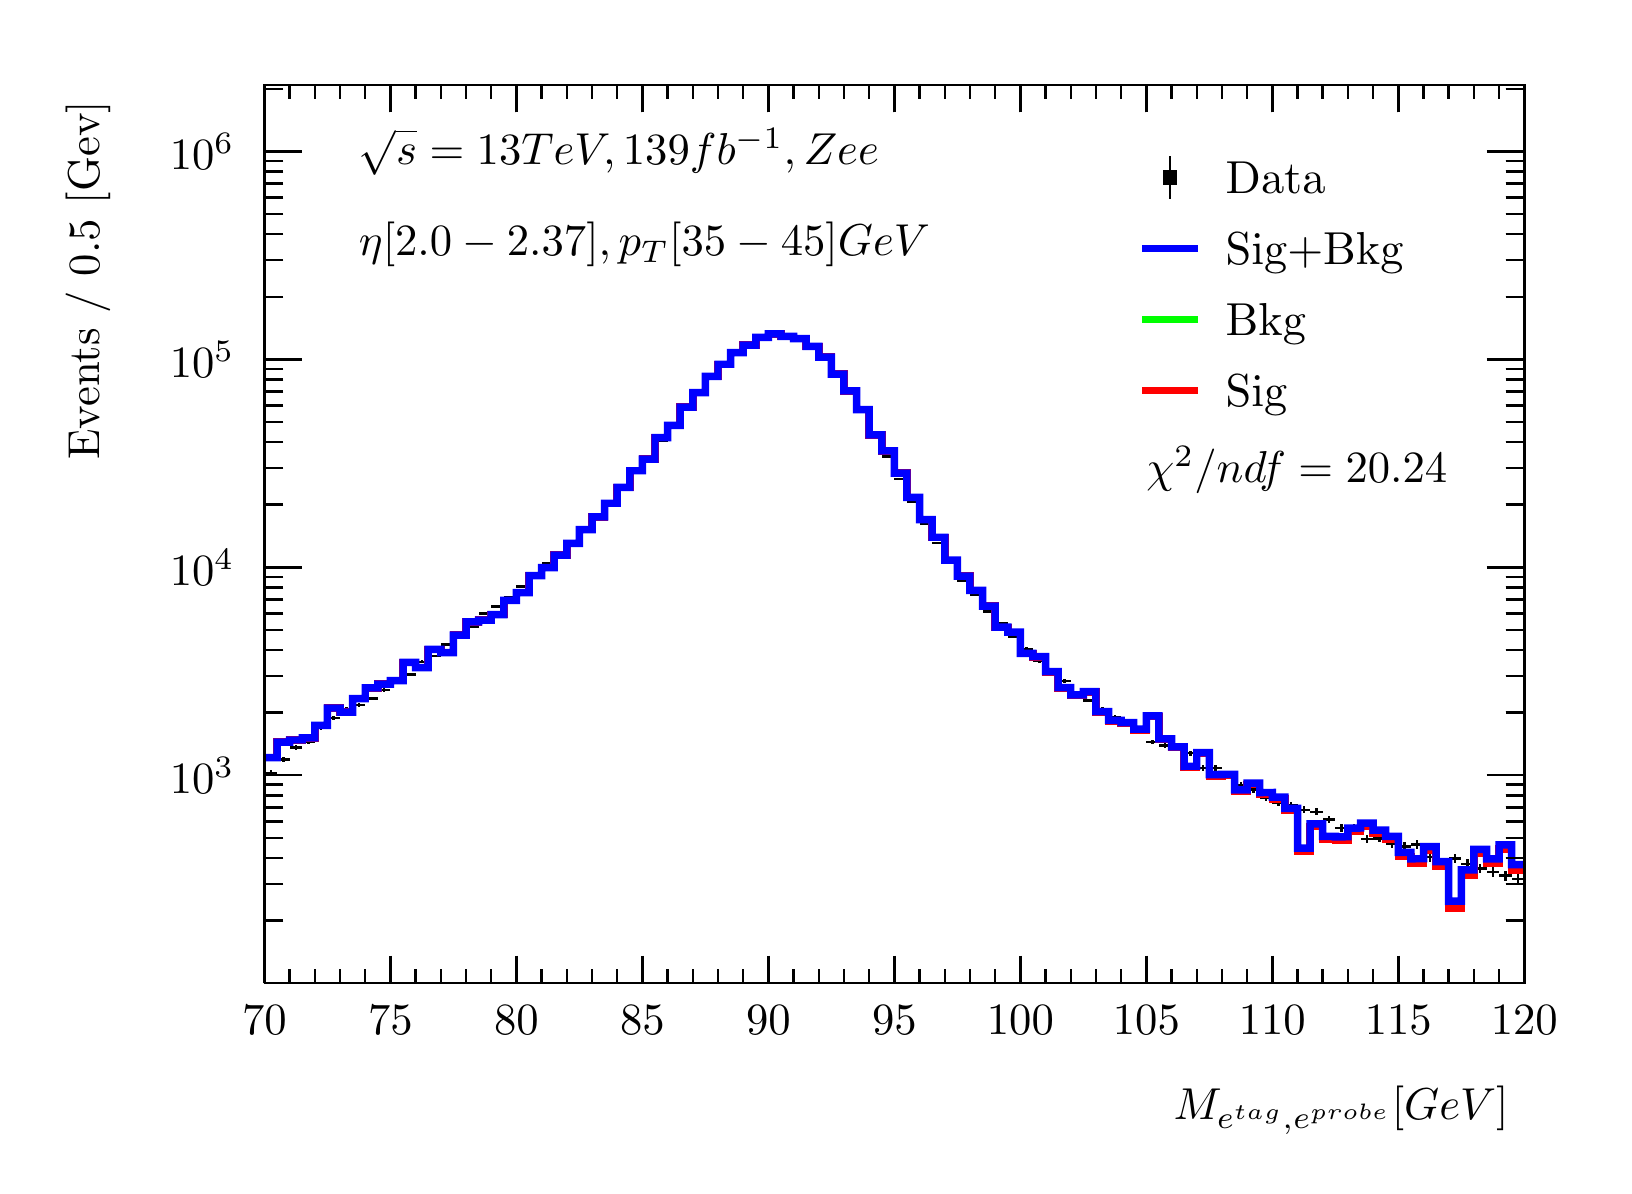
\begin{tikzpicture}
\pgfdeclareplotmark{cross} {
\pgfpathmoveto{\pgfpoint{-0.3\pgfplotmarksize}{\pgfplotmarksize}}
\pgfpathlineto{\pgfpoint{+0.3\pgfplotmarksize}{\pgfplotmarksize}}
\pgfpathlineto{\pgfpoint{+0.3\pgfplotmarksize}{0.3\pgfplotmarksize}}
\pgfpathlineto{\pgfpoint{+1\pgfplotmarksize}{0.3\pgfplotmarksize}}
\pgfpathlineto{\pgfpoint{+1\pgfplotmarksize}{-0.3\pgfplotmarksize}}
\pgfpathlineto{\pgfpoint{+0.3\pgfplotmarksize}{-0.3\pgfplotmarksize}}
\pgfpathlineto{\pgfpoint{+0.3\pgfplotmarksize}{-1.\pgfplotmarksize}}
\pgfpathlineto{\pgfpoint{-0.3\pgfplotmarksize}{-1.\pgfplotmarksize}}
\pgfpathlineto{\pgfpoint{-0.3\pgfplotmarksize}{-0.3\pgfplotmarksize}}
\pgfpathlineto{\pgfpoint{-1.\pgfplotmarksize}{-0.3\pgfplotmarksize}}
\pgfpathlineto{\pgfpoint{-1.\pgfplotmarksize}{0.3\pgfplotmarksize}}
\pgfpathlineto{\pgfpoint{-0.3\pgfplotmarksize}{0.3\pgfplotmarksize}}
\pgfpathclose
\pgfusepathqstroke
}
\pgfdeclareplotmark{cross*} {
\pgfpathmoveto{\pgfpoint{-0.3\pgfplotmarksize}{\pgfplotmarksize}}
\pgfpathlineto{\pgfpoint{+0.3\pgfplotmarksize}{\pgfplotmarksize}}
\pgfpathlineto{\pgfpoint{+0.3\pgfplotmarksize}{0.3\pgfplotmarksize}}
\pgfpathlineto{\pgfpoint{+1\pgfplotmarksize}{0.3\pgfplotmarksize}}
\pgfpathlineto{\pgfpoint{+1\pgfplotmarksize}{-0.3\pgfplotmarksize}}
\pgfpathlineto{\pgfpoint{+0.3\pgfplotmarksize}{-0.3\pgfplotmarksize}}
\pgfpathlineto{\pgfpoint{+0.3\pgfplotmarksize}{-1.\pgfplotmarksize}}
\pgfpathlineto{\pgfpoint{-0.3\pgfplotmarksize}{-1.\pgfplotmarksize}}
\pgfpathlineto{\pgfpoint{-0.3\pgfplotmarksize}{-0.3\pgfplotmarksize}}
\pgfpathlineto{\pgfpoint{-1.\pgfplotmarksize}{-0.3\pgfplotmarksize}}
\pgfpathlineto{\pgfpoint{-1.\pgfplotmarksize}{0.3\pgfplotmarksize}}
\pgfpathlineto{\pgfpoint{-0.3\pgfplotmarksize}{0.3\pgfplotmarksize}}
\pgfpathclose
\pgfusepathqfillstroke
}
\pgfdeclareplotmark{newstar} {
\pgfpathmoveto{\pgfqpoint{0pt}{\pgfplotmarksize}}
\pgfpathlineto{\pgfqpointpolar{44}{0.5\pgfplotmarksize}}
\pgfpathlineto{\pgfqpointpolar{18}{\pgfplotmarksize}}
\pgfpathlineto{\pgfqpointpolar{-20}{0.5\pgfplotmarksize}}
\pgfpathlineto{\pgfqpointpolar{-54}{\pgfplotmarksize}}
\pgfpathlineto{\pgfqpointpolar{-90}{0.5\pgfplotmarksize}}
\pgfpathlineto{\pgfqpointpolar{234}{\pgfplotmarksize}}
\pgfpathlineto{\pgfqpointpolar{198}{0.5\pgfplotmarksize}}
\pgfpathlineto{\pgfqpointpolar{162}{\pgfplotmarksize}}
\pgfpathlineto{\pgfqpointpolar{134}{0.5\pgfplotmarksize}}
\pgfpathclose
\pgfusepathqstroke
}
\pgfdeclareplotmark{newstar*} {
\pgfpathmoveto{\pgfqpoint{0pt}{\pgfplotmarksize}}
\pgfpathlineto{\pgfqpointpolar{44}{0.5\pgfplotmarksize}}
\pgfpathlineto{\pgfqpointpolar{18}{\pgfplotmarksize}}
\pgfpathlineto{\pgfqpointpolar{-20}{0.5\pgfplotmarksize}}
\pgfpathlineto{\pgfqpointpolar{-54}{\pgfplotmarksize}}
\pgfpathlineto{\pgfqpointpolar{-90}{0.5\pgfplotmarksize}}
\pgfpathlineto{\pgfqpointpolar{234}{\pgfplotmarksize}}
\pgfpathlineto{\pgfqpointpolar{198}{0.5\pgfplotmarksize}}
\pgfpathlineto{\pgfqpointpolar{162}{\pgfplotmarksize}}
\pgfpathlineto{\pgfqpointpolar{134}{0.5\pgfplotmarksize}}
\pgfpathclose
\pgfusepathqfillstroke
}
\definecolor{c}{rgb}{1,1,1};
\draw [color=c, fill=c] (0,0) rectangle (20,14.4361);
\draw [color=c, fill=c] (3,2.30977) rectangle (19,13.7143);
\definecolor{c}{rgb}{0,0,0};
\draw [c,line width=0.9] (3,2.30977) -- (3,13.7143) -- (19,13.7143) -- (19,2.30977) -- (3,2.30977);
\definecolor{c}{rgb}{1,1,1};
\draw [color=c, fill=c] (3,2.30977) rectangle (19,13.7143);
\definecolor{c}{rgb}{0,0,0};
\draw [c,line width=0.9] (3,2.30977) -- (3,13.7143) -- (19,13.7143) -- (19,2.30977) -- (3,2.30977);
\draw [c,line width=0.9] (3,2.30977) -- (19,2.30977);
\draw [c,line width=0.9] (3,2.65624) -- (3,2.30977);
\draw [c,line width=0.9] (3.32,2.48301) -- (3.32,2.30977);
\draw [c,line width=0.9] (3.64,2.48301) -- (3.64,2.30977);
\draw [c,line width=0.9] (3.96,2.48301) -- (3.96,2.30977);
\draw [c,line width=0.9] (4.28,2.48301) -- (4.28,2.30977);
\draw [c,line width=0.9] (4.6,2.65624) -- (4.6,2.30977);
\draw [c,line width=0.9] (4.92,2.48301) -- (4.92,2.30977);
\draw [c,line width=0.9] (5.24,2.48301) -- (5.24,2.30977);
\draw [c,line width=0.9] (5.56,2.48301) -- (5.56,2.30977);
\draw [c,line width=0.9] (5.88,2.48301) -- (5.88,2.30977);
\draw [c,line width=0.9] (6.2,2.65624) -- (6.2,2.30977);
\draw [c,line width=0.9] (6.52,2.48301) -- (6.52,2.30977);
\draw [c,line width=0.9] (6.84,2.48301) -- (6.84,2.30977);
\draw [c,line width=0.9] (7.16,2.48301) -- (7.16,2.30977);
\draw [c,line width=0.9] (7.48,2.48301) -- (7.48,2.30977);
\draw [c,line width=0.9] (7.8,2.65624) -- (7.8,2.30977);
\draw [c,line width=0.9] (8.12,2.48301) -- (8.12,2.30977);
\draw [c,line width=0.9] (8.44,2.48301) -- (8.44,2.30977);
\draw [c,line width=0.9] (8.76,2.48301) -- (8.76,2.30977);
\draw [c,line width=0.9] (9.08,2.48301) -- (9.08,2.30977);
\draw [c,line width=0.9] (9.4,2.65624) -- (9.4,2.30977);
\draw [c,line width=0.9] (9.72,2.48301) -- (9.72,2.30977);
\draw [c,line width=0.9] (10.04,2.48301) -- (10.04,2.30977);
\draw [c,line width=0.9] (10.36,2.48301) -- (10.36,2.30977);
\draw [c,line width=0.9] (10.68,2.48301) -- (10.68,2.30977);
\draw [c,line width=0.9] (11,2.65624) -- (11,2.30977);
\draw [c,line width=0.9] (11.32,2.48301) -- (11.32,2.30977);
\draw [c,line width=0.9] (11.64,2.48301) -- (11.64,2.30977);
\draw [c,line width=0.9] (11.96,2.48301) -- (11.96,2.30977);
\draw [c,line width=0.9] (12.28,2.48301) -- (12.28,2.30977);
\draw [c,line width=0.9] (12.6,2.65624) -- (12.6,2.30977);
\draw [c,line width=0.9] (12.92,2.48301) -- (12.92,2.30977);
\draw [c,line width=0.9] (13.24,2.48301) -- (13.24,2.30977);
\draw [c,line width=0.9] (13.56,2.48301) -- (13.56,2.30977);
\draw [c,line width=0.9] (13.88,2.48301) -- (13.88,2.30977);
\draw [c,line width=0.9] (14.2,2.65624) -- (14.2,2.30977);
\draw [c,line width=0.9] (14.52,2.48301) -- (14.52,2.30977);
\draw [c,line width=0.9] (14.84,2.48301) -- (14.84,2.30977);
\draw [c,line width=0.9] (15.16,2.48301) -- (15.16,2.30977);
\draw [c,line width=0.9] (15.48,2.48301) -- (15.48,2.30977);
\draw [c,line width=0.9] (15.8,2.65624) -- (15.8,2.30977);
\draw [c,line width=0.9] (16.12,2.48301) -- (16.12,2.30977);
\draw [c,line width=0.9] (16.44,2.48301) -- (16.44,2.30977);
\draw [c,line width=0.9] (16.76,2.48301) -- (16.76,2.30977);
\draw [c,line width=0.9] (17.08,2.48301) -- (17.08,2.30977);
\draw [c,line width=0.9] (17.4,2.65624) -- (17.4,2.30977);
\draw [c,line width=0.9] (17.72,2.48301) -- (17.72,2.30977);
\draw [c,line width=0.9] (18.04,2.48301) -- (18.04,2.30977);
\draw [c,line width=0.9] (18.36,2.48301) -- (18.36,2.30977);
\draw [c,line width=0.9] (18.68,2.48301) -- (18.68,2.30977);
\draw [c,line width=0.9] (19,2.65624) -- (19,2.30977);
\draw [anchor=base] (3,1.66015) node[scale=1.61424, color=c, rotate=0]{70};
\draw [anchor=base] (4.6,1.66015) node[scale=1.61424, color=c, rotate=0]{75};
\draw [anchor=base] (6.2,1.66015) node[scale=1.61424, color=c, rotate=0]{80};
\draw [anchor=base] (7.8,1.66015) node[scale=1.61424, color=c, rotate=0]{85};
\draw [anchor=base] (9.4,1.66015) node[scale=1.61424, color=c, rotate=0]{90};
\draw [anchor=base] (11,1.66015) node[scale=1.61424, color=c, rotate=0]{95};
\draw [anchor=base] (12.6,1.66015) node[scale=1.61424, color=c, rotate=0]{100};
\draw [anchor=base] (14.2,1.66015) node[scale=1.61424, color=c, rotate=0]{105};
\draw [anchor=base] (15.8,1.66015) node[scale=1.61424, color=c, rotate=0]{110};
\draw [anchor=base] (17.4,1.66015) node[scale=1.61424, color=c, rotate=0]{115};
\draw [anchor=base] (19,1.66015) node[scale=1.61424, color=c, rotate=0]{120};
\draw [anchor= east] (19,0.692932) node[scale=1.61424, color=c, rotate=0]{$M_{e^{tag}, e^{probe}}  [GeV]$};
\draw [c,line width=0.9] (3,13.7143) -- (19,13.7143);
\draw [c,line width=0.9] (3,13.3678) -- (3,13.7143);
\draw [c,line width=0.9] (3.32,13.5411) -- (3.32,13.7143);
\draw [c,line width=0.9] (3.64,13.5411) -- (3.64,13.7143);
\draw [c,line width=0.9] (3.96,13.5411) -- (3.96,13.7143);
\draw [c,line width=0.9] (4.28,13.5411) -- (4.28,13.7143);
\draw [c,line width=0.9] (4.6,13.3678) -- (4.6,13.7143);
\draw [c,line width=0.9] (4.92,13.5411) -- (4.92,13.7143);
\draw [c,line width=0.9] (5.24,13.5411) -- (5.24,13.7143);
\draw [c,line width=0.9] (5.56,13.5411) -- (5.56,13.7143);
\draw [c,line width=0.9] (5.88,13.5411) -- (5.88,13.7143);
\draw [c,line width=0.9] (6.2,13.3678) -- (6.2,13.7143);
\draw [c,line width=0.9] (6.52,13.5411) -- (6.52,13.7143);
\draw [c,line width=0.9] (6.84,13.5411) -- (6.84,13.7143);
\draw [c,line width=0.9] (7.16,13.5411) -- (7.16,13.7143);
\draw [c,line width=0.9] (7.48,13.5411) -- (7.48,13.7143);
\draw [c,line width=0.9] (7.8,13.3678) -- (7.8,13.7143);
\draw [c,line width=0.9] (8.12,13.5411) -- (8.12,13.7143);
\draw [c,line width=0.9] (8.44,13.5411) -- (8.44,13.7143);
\draw [c,line width=0.9] (8.76,13.5411) -- (8.76,13.7143);
\draw [c,line width=0.9] (9.08,13.5411) -- (9.08,13.7143);
\draw [c,line width=0.9] (9.4,13.3678) -- (9.4,13.7143);
\draw [c,line width=0.9] (9.72,13.5411) -- (9.72,13.7143);
\draw [c,line width=0.9] (10.04,13.5411) -- (10.04,13.7143);
\draw [c,line width=0.9] (10.36,13.5411) -- (10.36,13.7143);
\draw [c,line width=0.9] (10.68,13.5411) -- (10.68,13.7143);
\draw [c,line width=0.9] (11,13.3678) -- (11,13.7143);
\draw [c,line width=0.9] (11.32,13.5411) -- (11.32,13.7143);
\draw [c,line width=0.9] (11.64,13.5411) -- (11.64,13.7143);
\draw [c,line width=0.9] (11.96,13.5411) -- (11.96,13.7143);
\draw [c,line width=0.9] (12.28,13.5411) -- (12.28,13.7143);
\draw [c,line width=0.9] (12.6,13.3678) -- (12.6,13.7143);
\draw [c,line width=0.9] (12.92,13.5411) -- (12.92,13.7143);
\draw [c,line width=0.9] (13.24,13.5411) -- (13.24,13.7143);
\draw [c,line width=0.9] (13.56,13.5411) -- (13.56,13.7143);
\draw [c,line width=0.9] (13.88,13.5411) -- (13.88,13.7143);
\draw [c,line width=0.9] (14.2,13.3678) -- (14.2,13.7143);
\draw [c,line width=0.9] (14.52,13.5411) -- (14.52,13.7143);
\draw [c,line width=0.9] (14.84,13.5411) -- (14.84,13.7143);
\draw [c,line width=0.9] (15.16,13.5411) -- (15.16,13.7143);
\draw [c,line width=0.9] (15.48,13.5411) -- (15.48,13.7143);
\draw [c,line width=0.9] (15.8,13.3678) -- (15.8,13.7143);
\draw [c,line width=0.9] (16.12,13.5411) -- (16.12,13.7143);
\draw [c,line width=0.9] (16.44,13.5411) -- (16.44,13.7143);
\draw [c,line width=0.9] (16.76,13.5411) -- (16.76,13.7143);
\draw [c,line width=0.9] (17.08,13.5411) -- (17.08,13.7143);
\draw [c,line width=0.9] (17.4,13.3678) -- (17.4,13.7143);
\draw [c,line width=0.9] (17.72,13.5411) -- (17.72,13.7143);
\draw [c,line width=0.9] (18.04,13.5411) -- (18.04,13.7143);
\draw [c,line width=0.9] (18.36,13.5411) -- (18.36,13.7143);
\draw [c,line width=0.9] (18.68,13.5411) -- (18.68,13.7143);
\draw [c,line width=0.9] (19,13.3678) -- (19,13.7143);
\draw [c,line width=0.9] (3,2.30977) -- (3,13.7143);
\draw [c,line width=0.9] (3.237,3.10453) -- (3,3.10453);
\draw [c,line width=0.9] (3.237,3.56943) -- (3,3.56943);
\draw [c,line width=0.9] (3.237,3.89929) -- (3,3.89929);
\draw [c,line width=0.9] (3.237,4.15514) -- (3,4.15514);
\draw [c,line width=0.9] (3.237,4.36419) -- (3,4.36419);
\draw [c,line width=0.9] (3.237,4.54094) -- (3,4.54094);
\draw [c,line width=0.9] (3.237,4.69404) -- (3,4.69404);
\draw [c,line width=0.9] (3.237,4.82909) -- (3,4.82909);
\draw [c,line width=0.9] (3.474,4.9499) -- (3,4.9499);
\draw [anchor= east] (2.82,4.9499) node[scale=1.61424, color=c, rotate=0]{$10^{3}$};
\draw [c,line width=0.9] (3.237,5.74466) -- (3,5.74466);
\draw [c,line width=0.9] (3.237,6.20956) -- (3,6.20956);
\draw [c,line width=0.9] (3.237,6.53941) -- (3,6.53941);
\draw [c,line width=0.9] (3.237,6.79527) -- (3,6.79527);
\draw [c,line width=0.9] (3.237,7.00432) -- (3,7.00432);
\draw [c,line width=0.9] (3.237,7.18106) -- (3,7.18106);
\draw [c,line width=0.9] (3.237,7.33417) -- (3,7.33417);
\draw [c,line width=0.9] (3.237,7.46922) -- (3,7.46922);
\draw [c,line width=0.9] (3.474,7.59002) -- (3,7.59002);
\draw [anchor= east] (2.82,7.59002) node[scale=1.61424, color=c, rotate=0]{$10^{4}$};
\draw [c,line width=0.9] (3.237,8.38478) -- (3,8.38478);
\draw [c,line width=0.9] (3.237,8.84968) -- (3,8.84968);
\draw [c,line width=0.9] (3.237,9.17954) -- (3,9.17954);
\draw [c,line width=0.9] (3.237,9.43539) -- (3,9.43539);
\draw [c,line width=0.9] (3.237,9.64444) -- (3,9.64444);
\draw [c,line width=0.9] (3.237,9.82119) -- (3,9.82119);
\draw [c,line width=0.9] (3.237,9.9743) -- (3,9.9743);
\draw [c,line width=0.9] (3.237,10.1093) -- (3,10.1093);
\draw [c,line width=0.9] (3.474,10.2302) -- (3,10.2302);
\draw [anchor= east] (2.82,10.2302) node[scale=1.61424, color=c, rotate=0]{$10^{5}$};
\draw [c,line width=0.9] (3.237,11.0249) -- (3,11.0249);
\draw [c,line width=0.9] (3.237,11.4898) -- (3,11.4898);
\draw [c,line width=0.9] (3.237,11.8197) -- (3,11.8197);
\draw [c,line width=0.9] (3.237,12.0755) -- (3,12.0755);
\draw [c,line width=0.9] (3.237,12.2846) -- (3,12.2846);
\draw [c,line width=0.9] (3.237,12.4613) -- (3,12.4613);
\draw [c,line width=0.9] (3.237,12.6144) -- (3,12.6144);
\draw [c,line width=0.9] (3.237,12.7495) -- (3,12.7495);
\draw [c,line width=0.9] (3.474,12.8703) -- (3,12.8703);
\draw [anchor= east] (2.82,12.8703) node[scale=1.61424, color=c, rotate=0]{$10^{6}$};
\draw [c,line width=0.9] (3.237,13.665) -- (3,13.665);
\draw [anchor= east] (0.76,13.7143) node[scale=1.61424, color=c, rotate=90]{Events / 0.5 [Gev]};
\draw [c,line width=0.9] (19,2.30977) -- (19,13.7143);
\draw [c,line width=0.9] (18.763,3.10453) -- (19,3.10453);
\draw [c,line width=0.9] (18.763,3.56943) -- (19,3.56943);
\draw [c,line width=0.9] (18.763,3.89929) -- (19,3.89929);
\draw [c,line width=0.9] (18.763,4.15514) -- (19,4.15514);
\draw [c,line width=0.9] (18.763,4.36419) -- (19,4.36419);
\draw [c,line width=0.9] (18.763,4.54094) -- (19,4.54094);
\draw [c,line width=0.9] (18.763,4.69404) -- (19,4.69404);
\draw [c,line width=0.9] (18.763,4.82909) -- (19,4.82909);
\draw [c,line width=0.9] (18.526,4.9499) -- (19,4.9499);
\draw [c,line width=0.9] (18.763,5.74466) -- (19,5.74466);
\draw [c,line width=0.9] (18.763,6.20956) -- (19,6.20956);
\draw [c,line width=0.9] (18.763,6.53941) -- (19,6.53941);
\draw [c,line width=0.9] (18.763,6.79527) -- (19,6.79527);
\draw [c,line width=0.9] (18.763,7.00432) -- (19,7.00432);
\draw [c,line width=0.9] (18.763,7.18106) -- (19,7.18106);
\draw [c,line width=0.9] (18.763,7.33417) -- (19,7.33417);
\draw [c,line width=0.9] (18.763,7.46922) -- (19,7.46922);
\draw [c,line width=0.9] (18.526,7.59002) -- (19,7.59002);
\draw [c,line width=0.9] (18.763,8.38478) -- (19,8.38478);
\draw [c,line width=0.9] (18.763,8.84968) -- (19,8.84968);
\draw [c,line width=0.9] (18.763,9.17954) -- (19,9.17954);
\draw [c,line width=0.9] (18.763,9.43539) -- (19,9.43539);
\draw [c,line width=0.9] (18.763,9.64444) -- (19,9.64444);
\draw [c,line width=0.9] (18.763,9.82119) -- (19,9.82119);
\draw [c,line width=0.9] (18.763,9.9743) -- (19,9.9743);
\draw [c,line width=0.9] (18.763,10.1093) -- (19,10.1093);
\draw [c,line width=0.9] (18.526,10.2302) -- (19,10.2302);
\draw [c,line width=0.9] (18.763,11.0249) -- (19,11.0249);
\draw [c,line width=0.9] (18.763,11.4898) -- (19,11.4898);
\draw [c,line width=0.9] (18.763,11.8197) -- (19,11.8197);
\draw [c,line width=0.9] (18.763,12.0755) -- (19,12.0755);
\draw [c,line width=0.9] (18.763,12.2846) -- (19,12.2846);
\draw [c,line width=0.9] (18.763,12.4613) -- (19,12.4613);
\draw [c,line width=0.9] (18.763,12.6144) -- (19,12.6144);
\draw [c,line width=0.9] (18.763,12.7495) -- (19,12.7495);
\draw [c,line width=0.9] (18.526,12.8703) -- (19,12.8703);
\draw [c,line width=0.9] (18.763,13.665) -- (19,13.665);
\draw [c,line width=0.9] (3.08,4.97373) -- (3,4.97373);
\draw [c,line width=0.9] (3,4.97373) -- (3,4.97373);
\draw [c,line width=0.9] (3.08,4.97373) -- (3.16,4.97373);
\draw [c,line width=0.9] (3.16,4.97373) -- (3.16,4.97373);
\draw [c,line width=0.9] (3.08,4.97373) -- (3.08,5.00961);
\draw [c,line width=0.9] (3.08,5.00961) -- (3.08,5.00961);
\draw [c,line width=0.9] (3.08,4.97373) -- (3.08,4.93785);
\draw [c,line width=0.9] (3.08,4.93785) -- (3.08,4.93785);
\draw [c,line width=0.9] (3.24,5.14935) -- (3.16,5.14935);
\draw [c,line width=0.9] (3.16,5.14935) -- (3.16,5.14935);
\draw [c,line width=0.9] (3.24,5.14935) -- (3.32,5.14935);
\draw [c,line width=0.9] (3.32,5.14935) -- (3.32,5.14935);
\draw [c,line width=0.9] (3.24,5.14935) -- (3.24,5.18259);
\draw [c,line width=0.9] (3.24,5.18259) -- (3.24,5.18259);
\draw [c,line width=0.9] (3.24,5.14935) -- (3.24,5.11612);
\draw [c,line width=0.9] (3.24,5.11612) -- (3.24,5.11612);
\draw [c,line width=0.9] (3.4,5.29824) -- (3.32,5.29824);
\draw [c,line width=0.9] (3.32,5.29824) -- (3.32,5.29824);
\draw [c,line width=0.9] (3.4,5.29824) -- (3.48,5.29824);
\draw [c,line width=0.9] (3.48,5.29824) -- (3.48,5.29824);
\draw [c,line width=0.9] (3.4,5.29824) -- (3.4,5.32938);
\draw [c,line width=0.9] (3.4,5.32938) -- (3.4,5.32938);
\draw [c,line width=0.9] (3.4,5.29824) -- (3.4,5.26709);
\draw [c,line width=0.9] (3.4,5.26709) -- (3.4,5.26709);
\draw [c,line width=0.9] (3.56,5.37751) -- (3.48,5.37751);
\draw [c,line width=0.9] (3.48,5.37751) -- (3.48,5.37751);
\draw [c,line width=0.9] (3.56,5.37751) -- (3.64,5.37751);
\draw [c,line width=0.9] (3.64,5.37751) -- (3.64,5.37751);
\draw [c,line width=0.9] (3.56,5.37751) -- (3.56,5.4076);
\draw [c,line width=0.9] (3.56,5.4076) -- (3.56,5.4076);
\draw [c,line width=0.9] (3.56,5.37751) -- (3.56,5.34742);
\draw [c,line width=0.9] (3.56,5.34742) -- (3.56,5.34742);
\draw [c,line width=0.9] (3.72,5.55426) -- (3.64,5.55426);
\draw [c,line width=0.9] (3.64,5.55426) -- (3.64,5.55426);
\draw [c,line width=0.9] (3.72,5.55426) -- (3.8,5.55426);
\draw [c,line width=0.9] (3.8,5.55426) -- (3.8,5.55426);
\draw [c,line width=0.9] (3.72,5.55426) -- (3.72,5.58212);
\draw [c,line width=0.9] (3.72,5.58212) -- (3.72,5.58212);
\draw [c,line width=0.9] (3.72,5.55426) -- (3.72,5.5264);
\draw [c,line width=0.9] (3.72,5.5264) -- (3.72,5.5264);
\draw [c,line width=0.9] (3.88,5.67554) -- (3.8,5.67554);
\draw [c,line width=0.9] (3.8,5.67554) -- (3.8,5.67554);
\draw [c,line width=0.9] (3.88,5.67554) -- (3.96,5.67554);
\draw [c,line width=0.9] (3.96,5.67554) -- (3.96,5.67554);
\draw [c,line width=0.9] (3.88,5.67554) -- (3.88,5.70196);
\draw [c,line width=0.9] (3.88,5.70196) -- (3.88,5.70196);
\draw [c,line width=0.9] (3.88,5.67554) -- (3.88,5.64912);
\draw [c,line width=0.9] (3.88,5.64912) -- (3.88,5.64912);
\draw [c,line width=0.9] (4.04,5.78908) -- (3.96,5.78908);
\draw [c,line width=0.9] (3.96,5.78908) -- (3.96,5.78908);
\draw [c,line width=0.9] (4.04,5.78908) -- (4.12,5.78908);
\draw [c,line width=0.9] (4.12,5.78908) -- (4.12,5.78908);
\draw [c,line width=0.9] (4.04,5.78908) -- (4.04,5.81422);
\draw [c,line width=0.9] (4.04,5.81422) -- (4.04,5.81422);
\draw [c,line width=0.9] (4.04,5.78908) -- (4.04,5.76393);
\draw [c,line width=0.9] (4.04,5.76393) -- (4.04,5.76393);
\draw [c,line width=0.9] (4.2,5.84136) -- (4.12,5.84136);
\draw [c,line width=0.9] (4.12,5.84136) -- (4.12,5.84136);
\draw [c,line width=0.9] (4.2,5.84136) -- (4.28,5.84136);
\draw [c,line width=0.9] (4.28,5.84136) -- (4.28,5.84136);
\draw [c,line width=0.9] (4.2,5.84136) -- (4.2,5.86594);
\draw [c,line width=0.9] (4.2,5.86594) -- (4.2,5.86594);
\draw [c,line width=0.9] (4.2,5.84136) -- (4.2,5.81678);
\draw [c,line width=0.9] (4.2,5.81678) -- (4.2,5.81678);
\draw [c,line width=0.9] (4.36,5.9237) -- (4.28,5.9237);
\draw [c,line width=0.9] (4.28,5.9237) -- (4.28,5.9237);
\draw [c,line width=0.9] (4.36,5.9237) -- (4.44,5.9237);
\draw [c,line width=0.9] (4.44,5.9237) -- (4.44,5.9237);
\draw [c,line width=0.9] (4.36,5.9237) -- (4.36,5.94741);
\draw [c,line width=0.9] (4.36,5.94741) -- (4.36,5.94741);
\draw [c,line width=0.9] (4.36,5.9237) -- (4.36,5.89998);
\draw [c,line width=0.9] (4.36,5.89998) -- (4.36,5.89998);
\draw [c,line width=0.9] (4.52,6.03173) -- (4.44,6.03173);
\draw [c,line width=0.9] (4.44,6.03173) -- (4.44,6.03173);
\draw [c,line width=0.9] (4.52,6.03173) -- (4.6,6.03173);
\draw [c,line width=0.9] (4.6,6.03173) -- (4.6,6.03173);
\draw [c,line width=0.9] (4.52,6.03173) -- (4.52,6.05435);
\draw [c,line width=0.9] (4.52,6.05435) -- (4.52,6.05435);
\draw [c,line width=0.9] (4.52,6.03173) -- (4.52,6.00911);
\draw [c,line width=0.9] (4.52,6.00911) -- (4.52,6.00911);
\draw [c,line width=0.9] (4.68,6.16554) -- (4.6,6.16554);
\draw [c,line width=0.9] (4.6,6.16554) -- (4.6,6.16554);
\draw [c,line width=0.9] (4.68,6.16554) -- (4.76,6.16554);
\draw [c,line width=0.9] (4.76,6.16554) -- (4.76,6.16554);
\draw [c,line width=0.9] (4.68,6.16554) -- (4.68,6.18688);
\draw [c,line width=0.9] (4.68,6.18688) -- (4.68,6.18688);
\draw [c,line width=0.9] (4.68,6.16554) -- (4.68,6.1442);
\draw [c,line width=0.9] (4.68,6.1442) -- (4.68,6.1442);
\draw [c,line width=0.9] (4.84,6.23114) -- (4.76,6.23114);
\draw [c,line width=0.9] (4.76,6.23114) -- (4.76,6.23114);
\draw [c,line width=0.9] (4.84,6.23114) -- (4.92,6.23114);
\draw [c,line width=0.9] (4.92,6.23114) -- (4.92,6.23114);
\draw [c,line width=0.9] (4.84,6.23114) -- (4.84,6.25188);
\draw [c,line width=0.9] (4.84,6.25188) -- (4.84,6.25188);
\draw [c,line width=0.9] (4.84,6.23114) -- (4.84,6.2104);
\draw [c,line width=0.9] (4.84,6.2104) -- (4.84,6.2104);
\draw [c,line width=0.9] (5,6.38762) -- (4.92,6.38762);
\draw [c,line width=0.9] (4.92,6.38762) -- (4.92,6.38762);
\draw [c,line width=0.9] (5,6.38762) -- (5.08,6.38762);
\draw [c,line width=0.9] (5.08,6.38762) -- (5.08,6.38762);
\draw [c,line width=0.9] (5,6.38762) -- (5,6.40699);
\draw [c,line width=0.9] (5,6.40699) -- (5,6.40699);
\draw [c,line width=0.9] (5,6.38762) -- (5,6.36825);
\draw [c,line width=0.9] (5,6.36825) -- (5,6.36825);
\draw [c,line width=0.9] (5.16,6.46358) -- (5.08,6.46358);
\draw [c,line width=0.9] (5.08,6.46358) -- (5.08,6.46358);
\draw [c,line width=0.9] (5.16,6.46358) -- (5.24,6.46358);
\draw [c,line width=0.9] (5.24,6.46358) -- (5.24,6.46358);
\draw [c,line width=0.9] (5.16,6.46358) -- (5.16,6.48232);
\draw [c,line width=0.9] (5.16,6.48232) -- (5.16,6.48232);
\draw [c,line width=0.9] (5.16,6.46358) -- (5.16,6.44484);
\draw [c,line width=0.9] (5.16,6.44484) -- (5.16,6.44484);
\draw [c,line width=0.9] (5.32,6.61) -- (5.24,6.61);
\draw [c,line width=0.9] (5.24,6.61) -- (5.24,6.61);
\draw [c,line width=0.9] (5.32,6.61) -- (5.4,6.61);
\draw [c,line width=0.9] (5.4,6.61) -- (5.4,6.61);
\draw [c,line width=0.9] (5.32,6.61) -- (5.32,6.62758);
\draw [c,line width=0.9] (5.32,6.62758) -- (5.32,6.62758);
\draw [c,line width=0.9] (5.32,6.61) -- (5.32,6.59243);
\draw [c,line width=0.9] (5.32,6.59243) -- (5.32,6.59243);
\draw [c,line width=0.9] (5.48,6.74224) -- (5.4,6.74224);
\draw [c,line width=0.9] (5.4,6.74224) -- (5.4,6.74224);
\draw [c,line width=0.9] (5.48,6.74224) -- (5.56,6.74224);
\draw [c,line width=0.9] (5.56,6.74224) -- (5.56,6.74224);
\draw [c,line width=0.9] (5.48,6.74224) -- (5.48,6.75883);
\draw [c,line width=0.9] (5.48,6.75883) -- (5.48,6.75883);
\draw [c,line width=0.9] (5.48,6.74224) -- (5.48,6.72564);
\draw [c,line width=0.9] (5.48,6.72564) -- (5.48,6.72564);
\draw [c,line width=0.9] (5.64,6.83671) -- (5.56,6.83671);
\draw [c,line width=0.9] (5.56,6.83671) -- (5.56,6.83671);
\draw [c,line width=0.9] (5.64,6.83671) -- (5.72,6.83671);
\draw [c,line width=0.9] (5.72,6.83671) -- (5.72,6.83671);
\draw [c,line width=0.9] (5.64,6.83671) -- (5.64,6.85263);
\draw [c,line width=0.9] (5.64,6.85263) -- (5.64,6.85263);
\draw [c,line width=0.9] (5.64,6.83671) -- (5.64,6.82078);
\draw [c,line width=0.9] (5.64,6.82078) -- (5.64,6.82078);
\draw [c,line width=0.9] (5.8,7.00106) -- (5.72,7.00106);
\draw [c,line width=0.9] (5.72,7.00106) -- (5.72,7.00106);
\draw [c,line width=0.9] (5.8,7.00106) -- (5.88,7.00106);
\draw [c,line width=0.9] (5.88,7.00106) -- (5.88,7.00106);
\draw [c,line width=0.9] (5.8,7.00106) -- (5.8,7.01589);
\draw [c,line width=0.9] (5.8,7.01589) -- (5.8,7.01589);
\draw [c,line width=0.9] (5.8,7.00106) -- (5.8,6.98624);
\draw [c,line width=0.9] (5.8,6.98624) -- (5.8,6.98624);
\draw [c,line width=0.9] (5.96,7.08973) -- (5.88,7.08973);
\draw [c,line width=0.9] (5.88,7.08973) -- (5.88,7.08973);
\draw [c,line width=0.9] (5.96,7.08973) -- (6.04,7.08973);
\draw [c,line width=0.9] (6.04,7.08973) -- (6.04,7.08973);
\draw [c,line width=0.9] (5.96,7.08973) -- (5.96,7.10399);
\draw [c,line width=0.9] (5.96,7.10399) -- (5.96,7.10399);
\draw [c,line width=0.9] (5.96,7.08973) -- (5.96,7.07546);
\draw [c,line width=0.9] (5.96,7.07546) -- (5.96,7.07546);
\draw [c,line width=0.9] (6.12,7.21113) -- (6.04,7.21113);
\draw [c,line width=0.9] (6.04,7.21113) -- (6.04,7.21113);
\draw [c,line width=0.9] (6.12,7.21113) -- (6.2,7.21113);
\draw [c,line width=0.9] (6.2,7.21113) -- (6.2,7.21113);
\draw [c,line width=0.9] (6.12,7.21113) -- (6.12,7.22466);
\draw [c,line width=0.9] (6.12,7.22466) -- (6.12,7.22466);
\draw [c,line width=0.9] (6.12,7.21113) -- (6.12,7.19761);
\draw [c,line width=0.9] (6.12,7.19761) -- (6.12,7.19761);
\draw [c,line width=0.9] (6.28,7.34359) -- (6.2,7.34359);
\draw [c,line width=0.9] (6.2,7.34359) -- (6.2,7.34359);
\draw [c,line width=0.9] (6.28,7.34359) -- (6.36,7.34359);
\draw [c,line width=0.9] (6.36,7.34359) -- (6.36,7.34359);
\draw [c,line width=0.9] (6.28,7.34359) -- (6.28,7.35636);
\draw [c,line width=0.9] (6.28,7.35636) -- (6.28,7.35636);
\draw [c,line width=0.9] (6.28,7.34359) -- (6.28,7.33083);
\draw [c,line width=0.9] (6.28,7.33083) -- (6.28,7.33083);
\draw [c,line width=0.9] (6.44,7.49143) -- (6.36,7.49143);
\draw [c,line width=0.9] (6.36,7.49143) -- (6.36,7.49143);
\draw [c,line width=0.9] (6.44,7.49143) -- (6.52,7.49143);
\draw [c,line width=0.9] (6.52,7.49143) -- (6.52,7.49143);
\draw [c,line width=0.9] (6.44,7.49143) -- (6.44,7.5034);
\draw [c,line width=0.9] (6.44,7.5034) -- (6.44,7.5034);
\draw [c,line width=0.9] (6.44,7.49143) -- (6.44,7.47946);
\draw [c,line width=0.9] (6.44,7.47946) -- (6.44,7.47946);
\draw [c,line width=0.9] (6.6,7.64269) -- (6.52,7.64269);
\draw [c,line width=0.9] (6.52,7.64269) -- (6.52,7.64269);
\draw [c,line width=0.9] (6.6,7.64269) -- (6.68,7.64269);
\draw [c,line width=0.9] (6.68,7.64269) -- (6.68,7.64269);
\draw [c,line width=0.9] (6.6,7.64269) -- (6.6,7.65389);
\draw [c,line width=0.9] (6.6,7.65389) -- (6.6,7.65389);
\draw [c,line width=0.9] (6.6,7.64269) -- (6.6,7.63148);
\draw [c,line width=0.9] (6.6,7.63148) -- (6.6,7.63148);
\draw [c,line width=0.9] (6.76,7.78601) -- (6.68,7.78601);
\draw [c,line width=0.9] (6.68,7.78601) -- (6.68,7.78601);
\draw [c,line width=0.9] (6.76,7.78601) -- (6.84,7.78601);
\draw [c,line width=0.9] (6.84,7.78601) -- (6.84,7.78601);
\draw [c,line width=0.9] (6.76,7.78601) -- (6.76,7.79653);
\draw [c,line width=0.9] (6.76,7.79653) -- (6.76,7.79653);
\draw [c,line width=0.9] (6.76,7.78601) -- (6.76,7.77548);
\draw [c,line width=0.9] (6.76,7.77548) -- (6.76,7.77548);
\draw [c,line width=0.9] (6.92,7.91027) -- (6.84,7.91027);
\draw [c,line width=0.9] (6.84,7.91027) -- (6.84,7.91027);
\draw [c,line width=0.9] (6.92,7.91027) -- (7,7.91027);
\draw [c,line width=0.9] (7,7.91027) -- (7,7.91027);
\draw [c,line width=0.9] (6.92,7.91027) -- (6.92,7.92024);
\draw [c,line width=0.9] (6.92,7.92024) -- (6.92,7.92024);
\draw [c,line width=0.9] (6.92,7.91027) -- (6.92,7.90029);
\draw [c,line width=0.9] (6.92,7.90029) -- (6.92,7.90029);
\draw [c,line width=0.9] (7.08,8.10174) -- (7,8.10174);
\draw [c,line width=0.9] (7,8.10174) -- (7,8.10174);
\draw [c,line width=0.9] (7.08,8.10174) -- (7.16,8.10174);
\draw [c,line width=0.9] (7.16,8.10174) -- (7.16,8.10174);
\draw [c,line width=0.9] (7.08,8.10174) -- (7.08,8.11091);
\draw [c,line width=0.9] (7.08,8.11091) -- (7.08,8.11091);
\draw [c,line width=0.9] (7.08,8.10174) -- (7.08,8.09256);
\draw [c,line width=0.9] (7.08,8.09256) -- (7.08,8.09256);
\draw [c,line width=0.9] (7.24,8.25142) -- (7.16,8.25142);
\draw [c,line width=0.9] (7.16,8.25142) -- (7.16,8.25142);
\draw [c,line width=0.9] (7.24,8.25142) -- (7.32,8.25142);
\draw [c,line width=0.9] (7.32,8.25142) -- (7.32,8.25142);
\draw [c,line width=0.9] (7.24,8.25142) -- (7.24,8.26002);
\draw [c,line width=0.9] (7.24,8.26002) -- (7.24,8.26002);
\draw [c,line width=0.9] (7.24,8.25142) -- (7.24,8.24283);
\draw [c,line width=0.9] (7.24,8.24283) -- (7.24,8.24283);
\draw [c,line width=0.9] (7.4,8.42428) -- (7.32,8.42428);
\draw [c,line width=0.9] (7.32,8.42428) -- (7.32,8.42428);
\draw [c,line width=0.9] (7.4,8.42428) -- (7.48,8.42428);
\draw [c,line width=0.9] (7.48,8.42428) -- (7.48,8.42428);
\draw [c,line width=0.9] (7.4,8.42428) -- (7.4,8.43225);
\draw [c,line width=0.9] (7.4,8.43225) -- (7.4,8.43225);
\draw [c,line width=0.9] (7.4,8.42428) -- (7.4,8.41631);
\draw [c,line width=0.9] (7.4,8.41631) -- (7.4,8.41631);
\draw [c,line width=0.9] (7.56,8.63244) -- (7.48,8.63244);
\draw [c,line width=0.9] (7.48,8.63244) -- (7.48,8.63244);
\draw [c,line width=0.9] (7.56,8.63244) -- (7.64,8.63244);
\draw [c,line width=0.9] (7.64,8.63244) -- (7.64,8.63244);
\draw [c,line width=0.9] (7.56,8.63244) -- (7.56,8.63972);
\draw [c,line width=0.9] (7.56,8.63972) -- (7.56,8.63972);
\draw [c,line width=0.9] (7.56,8.63244) -- (7.56,8.62517);
\draw [c,line width=0.9] (7.56,8.62517) -- (7.56,8.62517);
\draw [c,line width=0.9] (7.72,8.8086) -- (7.64,8.8086);
\draw [c,line width=0.9] (7.64,8.8086) -- (7.64,8.8086);
\draw [c,line width=0.9] (7.72,8.8086) -- (7.8,8.8086);
\draw [c,line width=0.9] (7.8,8.8086) -- (7.8,8.8086);
\draw [c,line width=0.9] (7.72,8.8086) -- (7.72,8.81534);
\draw [c,line width=0.9] (7.72,8.81534) -- (7.72,8.81534);
\draw [c,line width=0.9] (7.72,8.8086) -- (7.72,8.80186);
\draw [c,line width=0.9] (7.72,8.80186) -- (7.72,8.80186);
\draw [c,line width=0.9] (7.88,8.99643) -- (7.8,8.99643);
\draw [c,line width=0.9] (7.8,8.99643) -- (7.8,8.99643);
\draw [c,line width=0.9] (7.88,8.99643) -- (7.96,8.99643);
\draw [c,line width=0.9] (7.96,8.99643) -- (7.96,8.99643);
\draw [c,line width=0.9] (7.88,8.99643) -- (7.88,9.00264);
\draw [c,line width=0.9] (7.88,9.00264) -- (7.88,9.00264);
\draw [c,line width=0.9] (7.88,8.99643) -- (7.88,8.99022);
\draw [c,line width=0.9] (7.88,8.99022) -- (7.88,8.99022);
\draw [c,line width=0.9] (8.04,9.20188) -- (7.96,9.20188);
\draw [c,line width=0.9] (7.96,9.20188) -- (7.96,9.20188);
\draw [c,line width=0.9] (8.04,9.20188) -- (8.12,9.20188);
\draw [c,line width=0.9] (8.12,9.20188) -- (8.12,9.20188);
\draw [c,line width=0.9] (8.04,9.20188) -- (8.04,9.20756);
\draw [c,line width=0.9] (8.04,9.20756) -- (8.04,9.20756);
\draw [c,line width=0.9] (8.04,9.20188) -- (8.04,9.1962);
\draw [c,line width=0.9] (8.04,9.1962) -- (8.04,9.1962);
\draw [c,line width=0.9] (8.2,9.40396) -- (8.12,9.40396);
\draw [c,line width=0.9] (8.12,9.40396) -- (8.12,9.40396);
\draw [c,line width=0.9] (8.2,9.40396) -- (8.28,9.40396);
\draw [c,line width=0.9] (8.28,9.40396) -- (8.28,9.40396);
\draw [c,line width=0.9] (8.2,9.40396) -- (8.2,9.40916);
\draw [c,line width=0.9] (8.2,9.40916) -- (8.2,9.40916);
\draw [c,line width=0.9] (8.2,9.40396) -- (8.2,9.39877);
\draw [c,line width=0.9] (8.2,9.39877) -- (8.2,9.39877);
\draw [c,line width=0.9] (8.36,9.60745) -- (8.28,9.60745);
\draw [c,line width=0.9] (8.28,9.60745) -- (8.28,9.60745);
\draw [c,line width=0.9] (8.36,9.60745) -- (8.44,9.60745);
\draw [c,line width=0.9] (8.44,9.60745) -- (8.44,9.60745);
\draw [c,line width=0.9] (8.36,9.60745) -- (8.36,9.61221);
\draw [c,line width=0.9] (8.36,9.61221) -- (8.36,9.61221);
\draw [c,line width=0.9] (8.36,9.60745) -- (8.36,9.60269);
\draw [c,line width=0.9] (8.36,9.60269) -- (8.36,9.60269);
\draw [c,line width=0.9] (8.52,9.80366) -- (8.44,9.80366);
\draw [c,line width=0.9] (8.44,9.80366) -- (8.44,9.80366);
\draw [c,line width=0.9] (8.52,9.80366) -- (8.6,9.80366);
\draw [c,line width=0.9] (8.6,9.80366) -- (8.6,9.80366);
\draw [c,line width=0.9] (8.52,9.80366) -- (8.52,9.80803);
\draw [c,line width=0.9] (8.52,9.80803) -- (8.52,9.80803);
\draw [c,line width=0.9] (8.52,9.80366) -- (8.52,9.7993);
\draw [c,line width=0.9] (8.52,9.7993) -- (8.52,9.7993);
\draw [c,line width=0.9] (8.68,9.99243) -- (8.6,9.99243);
\draw [c,line width=0.9] (8.6,9.99243) -- (8.6,9.99243);
\draw [c,line width=0.9] (8.68,9.99243) -- (8.76,9.99243);
\draw [c,line width=0.9] (8.76,9.99243) -- (8.76,9.99243);
\draw [c,line width=0.9] (8.68,9.99243) -- (8.68,9.99645);
\draw [c,line width=0.9] (8.68,9.99645) -- (8.68,9.99645);
\draw [c,line width=0.9] (8.68,9.99243) -- (8.68,9.98841);
\draw [c,line width=0.9] (8.68,9.98841) -- (8.68,9.98841);
\draw [c,line width=0.9] (8.84,10.1645) -- (8.76,10.1645);
\draw [c,line width=0.9] (8.76,10.1645) -- (8.76,10.1645);
\draw [c,line width=0.9] (8.84,10.1645) -- (8.92,10.1645);
\draw [c,line width=0.9] (8.92,10.1645) -- (8.92,10.1645);
\draw [c,line width=0.9] (8.84,10.1645) -- (8.84,10.1682);
\draw [c,line width=0.9] (8.84,10.1682) -- (8.84,10.1682);
\draw [c,line width=0.9] (8.84,10.1645) -- (8.84,10.1607);
\draw [c,line width=0.9] (8.84,10.1607) -- (8.84,10.1607);
\draw [c,line width=0.9] (9,10.325) -- (8.92,10.325);
\draw [c,line width=0.9] (8.92,10.325) -- (8.92,10.325);
\draw [c,line width=0.9] (9,10.325) -- (9.08,10.325);
\draw [c,line width=0.9] (9.08,10.325) -- (9.08,10.325);
\draw [c,line width=0.9] (9,10.325) -- (9,10.3285);
\draw [c,line width=0.9] (9,10.3285) -- (9,10.3285);
\draw [c,line width=0.9] (9,10.325) -- (9,10.3215);
\draw [c,line width=0.9] (9,10.3215) -- (9,10.3215);
\draw [c,line width=0.9] (9.16,10.437) -- (9.08,10.437);
\draw [c,line width=0.9] (9.08,10.437) -- (9.08,10.437);
\draw [c,line width=0.9] (9.16,10.437) -- (9.24,10.437);
\draw [c,line width=0.9] (9.24,10.437) -- (9.24,10.437);
\draw [c,line width=0.9] (9.16,10.437) -- (9.16,10.4403);
\draw [c,line width=0.9] (9.16,10.4403) -- (9.16,10.4403);
\draw [c,line width=0.9] (9.16,10.437) -- (9.16,10.4337);
\draw [c,line width=0.9] (9.16,10.4337) -- (9.16,10.4337);
\draw [c,line width=0.9] (9.32,10.5206) -- (9.24,10.5206);
\draw [c,line width=0.9] (9.24,10.5206) -- (9.24,10.5206);
\draw [c,line width=0.9] (9.32,10.5206) -- (9.4,10.5206);
\draw [c,line width=0.9] (9.4,10.5206) -- (9.4,10.5206);
\draw [c,line width=0.9] (9.32,10.5206) -- (9.32,10.5238);
\draw [c,line width=0.9] (9.32,10.5238) -- (9.32,10.5238);
\draw [c,line width=0.9] (9.32,10.5206) -- (9.32,10.5174);
\draw [c,line width=0.9] (9.32,10.5174) -- (9.32,10.5174);
\draw [c,line width=0.9] (9.48,10.5663) -- (9.4,10.5663);
\draw [c,line width=0.9] (9.4,10.5663) -- (9.4,10.5663);
\draw [c,line width=0.9] (9.48,10.5663) -- (9.56,10.5663);
\draw [c,line width=0.9] (9.56,10.5663) -- (9.56,10.5663);
\draw [c,line width=0.9] (9.48,10.5663) -- (9.48,10.5694);
\draw [c,line width=0.9] (9.48,10.5694) -- (9.48,10.5694);
\draw [c,line width=0.9] (9.48,10.5663) -- (9.48,10.5631);
\draw [c,line width=0.9] (9.48,10.5631) -- (9.48,10.5631);
\draw [c,line width=0.9] (9.64,10.5548) -- (9.56,10.5548);
\draw [c,line width=0.9] (9.56,10.5548) -- (9.56,10.5548);
\draw [c,line width=0.9] (9.64,10.5548) -- (9.72,10.5548);
\draw [c,line width=0.9] (9.72,10.5548) -- (9.72,10.5548);
\draw [c,line width=0.9] (9.64,10.5548) -- (9.64,10.5579);
\draw [c,line width=0.9] (9.64,10.5579) -- (9.64,10.5579);
\draw [c,line width=0.9] (9.64,10.5548) -- (9.64,10.5516);
\draw [c,line width=0.9] (9.64,10.5516) -- (9.64,10.5516);
\draw [c,line width=0.9] (9.8,10.4999) -- (9.72,10.4999);
\draw [c,line width=0.9] (9.72,10.4999) -- (9.72,10.4999);
\draw [c,line width=0.9] (9.8,10.4999) -- (9.88,10.4999);
\draw [c,line width=0.9] (9.88,10.4999) -- (9.88,10.4999);
\draw [c,line width=0.9] (9.8,10.4999) -- (9.8,10.5031);
\draw [c,line width=0.9] (9.8,10.5031) -- (9.8,10.5031);
\draw [c,line width=0.9] (9.8,10.4999) -- (9.8,10.4967);
\draw [c,line width=0.9] (9.8,10.4967) -- (9.8,10.4967);
\draw [c,line width=0.9] (9.96,10.3947) -- (9.88,10.3947);
\draw [c,line width=0.9] (9.88,10.3947) -- (9.88,10.3947);
\draw [c,line width=0.9] (9.96,10.3947) -- (10.04,10.3947);
\draw [c,line width=0.9] (10.04,10.3947) -- (10.04,10.3947);
\draw [c,line width=0.9] (9.96,10.3947) -- (9.96,10.3981);
\draw [c,line width=0.9] (9.96,10.3981) -- (9.96,10.3981);
\draw [c,line width=0.9] (9.96,10.3947) -- (9.96,10.3913);
\draw [c,line width=0.9] (9.96,10.3913) -- (9.96,10.3913);
\draw [c,line width=0.9] (10.12,10.2448) -- (10.04,10.2448);
\draw [c,line width=0.9] (10.04,10.2448) -- (10.04,10.2448);
\draw [c,line width=0.9] (10.12,10.2448) -- (10.2,10.2448);
\draw [c,line width=0.9] (10.2,10.2448) -- (10.2,10.2448);
\draw [c,line width=0.9] (10.12,10.2448) -- (10.12,10.2484);
\draw [c,line width=0.9] (10.12,10.2484) -- (10.12,10.2484);
\draw [c,line width=0.9] (10.12,10.2448) -- (10.12,10.2412);
\draw [c,line width=0.9] (10.12,10.2412) -- (10.12,10.2412);
\draw [c,line width=0.9] (10.28,10.0493) -- (10.2,10.0493);
\draw [c,line width=0.9] (10.2,10.0493) -- (10.2,10.0493);
\draw [c,line width=0.9] (10.28,10.0493) -- (10.36,10.0493);
\draw [c,line width=0.9] (10.36,10.0493) -- (10.36,10.0493);
\draw [c,line width=0.9] (10.28,10.0493) -- (10.28,10.0532);
\draw [c,line width=0.9] (10.28,10.0532) -- (10.28,10.0532);
\draw [c,line width=0.9] (10.28,10.0493) -- (10.28,10.0454);
\draw [c,line width=0.9] (10.28,10.0454) -- (10.28,10.0454);
\draw [c,line width=0.9] (10.44,9.82786) -- (10.36,9.82786);
\draw [c,line width=0.9] (10.36,9.82786) -- (10.36,9.82786);
\draw [c,line width=0.9] (10.44,9.82786) -- (10.52,9.82786);
\draw [c,line width=0.9] (10.52,9.82786) -- (10.52,9.82786);
\draw [c,line width=0.9] (10.44,9.82786) -- (10.44,9.83218);
\draw [c,line width=0.9] (10.44,9.83218) -- (10.44,9.83218);
\draw [c,line width=0.9] (10.44,9.82786) -- (10.44,9.82353);
\draw [c,line width=0.9] (10.44,9.82353) -- (10.44,9.82353);
\draw [c,line width=0.9] (10.6,9.56181) -- (10.52,9.56181);
\draw [c,line width=0.9] (10.52,9.56181) -- (10.52,9.56181);
\draw [c,line width=0.9] (10.6,9.56181) -- (10.68,9.56181);
\draw [c,line width=0.9] (10.68,9.56181) -- (10.68,9.56181);
\draw [c,line width=0.9] (10.6,9.56181) -- (10.6,9.56666);
\draw [c,line width=0.9] (10.6,9.56666) -- (10.6,9.56666);
\draw [c,line width=0.9] (10.6,9.56181) -- (10.6,9.55696);
\draw [c,line width=0.9] (10.6,9.55696) -- (10.6,9.55696);
\draw [c,line width=0.9] (10.76,9.2915) -- (10.68,9.2915);
\draw [c,line width=0.9] (10.68,9.2915) -- (10.68,9.2915);
\draw [c,line width=0.9] (10.76,9.2915) -- (10.84,9.2915);
\draw [c,line width=0.9] (10.84,9.2915) -- (10.84,9.2915);
\draw [c,line width=0.9] (10.76,9.2915) -- (10.76,9.29696);
\draw [c,line width=0.9] (10.76,9.29696) -- (10.76,9.29696);
\draw [c,line width=0.9] (10.76,9.2915) -- (10.76,9.28604);
\draw [c,line width=0.9] (10.76,9.28604) -- (10.76,9.28604);
\draw [c,line width=0.9] (10.92,8.99394) -- (10.84,8.99394);
\draw [c,line width=0.9] (10.84,8.99394) -- (10.84,8.99394);
\draw [c,line width=0.9] (10.92,8.99394) -- (11,8.99394);
\draw [c,line width=0.9] (11,8.99394) -- (11,8.99394);
\draw [c,line width=0.9] (10.92,8.99394) -- (10.92,9.00016);
\draw [c,line width=0.9] (10.92,9.00016) -- (10.92,9.00016);
\draw [c,line width=0.9] (10.92,8.99394) -- (10.92,8.98772);
\draw [c,line width=0.9] (10.92,8.98772) -- (10.92,8.98772);
\draw [c,line width=0.9] (11.08,8.71164) -- (11,8.71164);
\draw [c,line width=0.9] (11,8.71164) -- (11,8.71164);
\draw [c,line width=0.9] (11.08,8.71164) -- (11.16,8.71164);
\draw [c,line width=0.9] (11.16,8.71164) -- (11.16,8.71164);
\draw [c,line width=0.9] (11.08,8.71164) -- (11.08,8.71867);
\draw [c,line width=0.9] (11.08,8.71867) -- (11.08,8.71867);
\draw [c,line width=0.9] (11.08,8.71164) -- (11.08,8.70461);
\draw [c,line width=0.9] (11.08,8.70461) -- (11.08,8.70461);
\draw [c,line width=0.9] (11.24,8.42229) -- (11.16,8.42229);
\draw [c,line width=0.9] (11.16,8.42229) -- (11.16,8.42229);
\draw [c,line width=0.9] (11.24,8.42229) -- (11.32,8.42229);
\draw [c,line width=0.9] (11.32,8.42229) -- (11.32,8.42229);
\draw [c,line width=0.9] (11.24,8.42229) -- (11.24,8.43026);
\draw [c,line width=0.9] (11.24,8.43026) -- (11.24,8.43026);
\draw [c,line width=0.9] (11.24,8.42229) -- (11.24,8.41431);
\draw [c,line width=0.9] (11.24,8.41431) -- (11.24,8.41431);
\draw [c,line width=0.9] (11.4,8.14854) -- (11.32,8.14854);
\draw [c,line width=0.9] (11.32,8.14854) -- (11.32,8.14854);
\draw [c,line width=0.9] (11.4,8.14854) -- (11.48,8.14854);
\draw [c,line width=0.9] (11.48,8.14854) -- (11.48,8.14854);
\draw [c,line width=0.9] (11.4,8.14854) -- (11.4,8.15753);
\draw [c,line width=0.9] (11.4,8.15753) -- (11.4,8.15753);
\draw [c,line width=0.9] (11.4,8.14854) -- (11.4,8.13955);
\draw [c,line width=0.9] (11.4,8.13955) -- (11.4,8.13955);
\draw [c,line width=0.9] (11.56,7.89876) -- (11.48,7.89876);
\draw [c,line width=0.9] (11.48,7.89876) -- (11.48,7.89876);
\draw [c,line width=0.9] (11.56,7.89876) -- (11.64,7.89876);
\draw [c,line width=0.9] (11.64,7.89876) -- (11.64,7.89876);
\draw [c,line width=0.9] (11.56,7.89876) -- (11.56,7.90878);
\draw [c,line width=0.9] (11.56,7.90878) -- (11.56,7.90878);
\draw [c,line width=0.9] (11.56,7.89876) -- (11.56,7.88874);
\draw [c,line width=0.9] (11.56,7.88874) -- (11.56,7.88874);
\draw [c,line width=0.9] (11.72,7.644) -- (11.64,7.644);
\draw [c,line width=0.9] (11.64,7.644) -- (11.64,7.644);
\draw [c,line width=0.9] (11.72,7.644) -- (11.8,7.644);
\draw [c,line width=0.9] (11.8,7.644) -- (11.8,7.644);
\draw [c,line width=0.9] (11.72,7.644) -- (11.72,7.6552);
\draw [c,line width=0.9] (11.72,7.6552) -- (11.72,7.6552);
\draw [c,line width=0.9] (11.72,7.644) -- (11.72,7.6328);
\draw [c,line width=0.9] (11.72,7.6328) -- (11.72,7.6328);
\draw [c,line width=0.9] (11.88,7.42295) -- (11.8,7.42295);
\draw [c,line width=0.9] (11.8,7.42295) -- (11.8,7.42295);
\draw [c,line width=0.9] (11.88,7.42295) -- (11.96,7.42295);
\draw [c,line width=0.9] (11.96,7.42295) -- (11.96,7.42295);
\draw [c,line width=0.9] (11.88,7.42295) -- (11.88,7.43528);
\draw [c,line width=0.9] (11.88,7.43528) -- (11.88,7.43528);
\draw [c,line width=0.9] (11.88,7.42295) -- (11.88,7.41061);
\draw [c,line width=0.9] (11.88,7.41061) -- (11.88,7.41061);
\draw [c,line width=0.9] (12.04,7.23794) -- (11.96,7.23794);
\draw [c,line width=0.9] (11.96,7.23794) -- (11.96,7.23794);
\draw [c,line width=0.9] (12.04,7.23794) -- (12.12,7.23794);
\draw [c,line width=0.9] (12.12,7.23794) -- (12.12,7.23794);
\draw [c,line width=0.9] (12.04,7.23794) -- (12.04,7.25131);
\draw [c,line width=0.9] (12.04,7.25131) -- (12.04,7.25131);
\draw [c,line width=0.9] (12.04,7.23794) -- (12.04,7.22457);
\draw [c,line width=0.9] (12.04,7.22457) -- (12.04,7.22457);
\draw [c,line width=0.9] (12.2,7.0274) -- (12.12,7.0274);
\draw [c,line width=0.9] (12.12,7.0274) -- (12.12,7.0274);
\draw [c,line width=0.9] (12.2,7.0274) -- (12.28,7.0274);
\draw [c,line width=0.9] (12.28,7.0274) -- (12.28,7.0274);
\draw [c,line width=0.9] (12.2,7.0274) -- (12.2,7.04205);
\draw [c,line width=0.9] (12.2,7.04205) -- (12.2,7.04205);
\draw [c,line width=0.9] (12.2,7.0274) -- (12.2,7.01274);
\draw [c,line width=0.9] (12.2,7.01274) -- (12.2,7.01274);
\draw [c,line width=0.9] (12.36,6.87883) -- (12.28,6.87883);
\draw [c,line width=0.9] (12.28,6.87883) -- (12.28,6.87883);
\draw [c,line width=0.9] (12.36,6.87883) -- (12.44,6.87883);
\draw [c,line width=0.9] (12.44,6.87883) -- (12.44,6.87883);
\draw [c,line width=0.9] (12.36,6.87883) -- (12.36,6.89447);
\draw [c,line width=0.9] (12.36,6.89447) -- (12.36,6.89447);
\draw [c,line width=0.9] (12.36,6.87883) -- (12.36,6.8632);
\draw [c,line width=0.9] (12.36,6.8632) -- (12.36,6.8632);
\draw [c,line width=0.9] (12.52,6.70662) -- (12.44,6.70662);
\draw [c,line width=0.9] (12.44,6.70662) -- (12.44,6.70662);
\draw [c,line width=0.9] (12.52,6.70662) -- (12.6,6.70662);
\draw [c,line width=0.9] (12.6,6.70662) -- (12.6,6.70662);
\draw [c,line width=0.9] (12.52,6.70662) -- (12.52,6.72348);
\draw [c,line width=0.9] (12.52,6.72348) -- (12.52,6.72348);
\draw [c,line width=0.9] (12.52,6.70662) -- (12.52,6.68977);
\draw [c,line width=0.9] (12.52,6.68977) -- (12.52,6.68977);
\draw [c,line width=0.9] (12.68,6.55536) -- (12.6,6.55536);
\draw [c,line width=0.9] (12.6,6.55536) -- (12.6,6.55536);
\draw [c,line width=0.9] (12.68,6.55536) -- (12.76,6.55536);
\draw [c,line width=0.9] (12.76,6.55536) -- (12.76,6.55536);
\draw [c,line width=0.9] (12.68,6.55536) -- (12.68,6.57336);
\draw [c,line width=0.9] (12.68,6.57336) -- (12.68,6.57336);
\draw [c,line width=0.9] (12.68,6.55536) -- (12.68,6.53735);
\draw [c,line width=0.9] (12.68,6.53735) -- (12.68,6.53735);
\draw [c,line width=0.9] (12.84,6.39837) -- (12.76,6.39837);
\draw [c,line width=0.9] (12.76,6.39837) -- (12.76,6.39837);
\draw [c,line width=0.9] (12.84,6.39837) -- (12.92,6.39837);
\draw [c,line width=0.9] (12.92,6.39837) -- (12.92,6.39837);
\draw [c,line width=0.9] (12.84,6.39837) -- (12.84,6.41764);
\draw [c,line width=0.9] (12.84,6.41764) -- (12.84,6.41764);
\draw [c,line width=0.9] (12.84,6.39837) -- (12.84,6.37909);
\draw [c,line width=0.9] (12.84,6.37909) -- (12.84,6.37909);
\draw [c,line width=0.9] (13,6.27276) -- (12.92,6.27276);
\draw [c,line width=0.9] (12.92,6.27276) -- (12.92,6.27276);
\draw [c,line width=0.9] (13,6.27276) -- (13.08,6.27276);
\draw [c,line width=0.9] (13.08,6.27276) -- (13.08,6.27276);
\draw [c,line width=0.9] (13,6.27276) -- (13,6.29312);
\draw [c,line width=0.9] (13,6.29312) -- (13,6.29312);
\draw [c,line width=0.9] (13,6.27276) -- (13,6.2524);
\draw [c,line width=0.9] (13,6.2524) -- (13,6.2524);
\draw [c,line width=0.9] (13.16,6.1451) -- (13.08,6.1451);
\draw [c,line width=0.9] (13.08,6.1451) -- (13.08,6.1451);
\draw [c,line width=0.9] (13.16,6.1451) -- (13.24,6.1451);
\draw [c,line width=0.9] (13.24,6.1451) -- (13.24,6.1451);
\draw [c,line width=0.9] (13.16,6.1451) -- (13.16,6.16663);
\draw [c,line width=0.9] (13.16,6.16663) -- (13.16,6.16663);
\draw [c,line width=0.9] (13.16,6.1451) -- (13.16,6.12357);
\draw [c,line width=0.9] (13.16,6.12357) -- (13.16,6.12357);
\draw [c,line width=0.9] (13.32,5.99776) -- (13.24,5.99776);
\draw [c,line width=0.9] (13.24,5.99776) -- (13.24,5.99776);
\draw [c,line width=0.9] (13.32,5.99776) -- (13.4,5.99776);
\draw [c,line width=0.9] (13.4,5.99776) -- (13.4,5.99776);
\draw [c,line width=0.9] (13.32,5.99776) -- (13.32,6.02072);
\draw [c,line width=0.9] (13.32,6.02072) -- (13.32,6.02072);
\draw [c,line width=0.9] (13.32,5.99776) -- (13.32,5.9748);
\draw [c,line width=0.9] (13.32,5.9748) -- (13.32,5.9748);
\draw [c,line width=0.9] (13.48,5.89941) -- (13.4,5.89941);
\draw [c,line width=0.9] (13.4,5.89941) -- (13.4,5.89941);
\draw [c,line width=0.9] (13.48,5.89941) -- (13.56,5.89941);
\draw [c,line width=0.9] (13.56,5.89941) -- (13.56,5.89941);
\draw [c,line width=0.9] (13.48,5.89941) -- (13.48,5.92338);
\draw [c,line width=0.9] (13.48,5.92338) -- (13.48,5.92338);
\draw [c,line width=0.9] (13.48,5.89941) -- (13.48,5.87545);
\draw [c,line width=0.9] (13.48,5.87545) -- (13.48,5.87545);
\draw [c,line width=0.9] (13.64,5.78797) -- (13.56,5.78797);
\draw [c,line width=0.9] (13.56,5.78797) -- (13.56,5.78797);
\draw [c,line width=0.9] (13.64,5.78797) -- (13.72,5.78797);
\draw [c,line width=0.9] (13.72,5.78797) -- (13.72,5.78797);
\draw [c,line width=0.9] (13.64,5.78797) -- (13.64,5.81313);
\draw [c,line width=0.9] (13.64,5.81313) -- (13.64,5.81313);
\draw [c,line width=0.9] (13.64,5.78797) -- (13.64,5.76281);
\draw [c,line width=0.9] (13.64,5.76281) -- (13.64,5.76281);
\draw [c,line width=0.9] (13.8,5.68524) -- (13.72,5.68524);
\draw [c,line width=0.9] (13.72,5.68524) -- (13.72,5.68524);
\draw [c,line width=0.9] (13.8,5.68524) -- (13.88,5.68524);
\draw [c,line width=0.9] (13.88,5.68524) -- (13.88,5.68524);
\draw [c,line width=0.9] (13.8,5.68524) -- (13.8,5.71155);
\draw [c,line width=0.9] (13.8,5.71155) -- (13.8,5.71155);
\draw [c,line width=0.9] (13.8,5.68524) -- (13.8,5.65893);
\draw [c,line width=0.9] (13.8,5.65893) -- (13.8,5.65893);
\draw [c,line width=0.9] (13.96,5.61874) -- (13.88,5.61874);
\draw [c,line width=0.9] (13.88,5.61874) -- (13.88,5.61874);
\draw [c,line width=0.9] (13.96,5.61874) -- (14.04,5.61874);
\draw [c,line width=0.9] (14.04,5.61874) -- (14.04,5.61874);
\draw [c,line width=0.9] (13.96,5.61874) -- (13.96,5.64583);
\draw [c,line width=0.9] (13.96,5.64583) -- (13.96,5.64583);
\draw [c,line width=0.9] (13.96,5.61874) -- (13.96,5.59166);
\draw [c,line width=0.9] (13.96,5.59166) -- (13.96,5.59166);
\draw [c,line width=0.9] (14.12,5.51502) -- (14.04,5.51502);
\draw [c,line width=0.9] (14.04,5.51502) -- (14.04,5.51502);
\draw [c,line width=0.9] (14.12,5.51502) -- (14.2,5.51502);
\draw [c,line width=0.9] (14.2,5.51502) -- (14.2,5.51502);
\draw [c,line width=0.9] (14.12,5.51502) -- (14.12,5.54335);
\draw [c,line width=0.9] (14.12,5.54335) -- (14.12,5.54335);
\draw [c,line width=0.9] (14.12,5.51502) -- (14.12,5.48668);
\draw [c,line width=0.9] (14.12,5.48668) -- (14.12,5.48668);
\draw [c,line width=0.9] (14.28,5.36959) -- (14.2,5.36959);
\draw [c,line width=0.9] (14.2,5.36959) -- (14.2,5.36959);
\draw [c,line width=0.9] (14.28,5.36959) -- (14.36,5.36959);
\draw [c,line width=0.9] (14.36,5.36959) -- (14.36,5.36959);
\draw [c,line width=0.9] (14.28,5.36959) -- (14.28,5.39978);
\draw [c,line width=0.9] (14.28,5.39978) -- (14.28,5.39978);
\draw [c,line width=0.9] (14.28,5.36959) -- (14.28,5.3394);
\draw [c,line width=0.9] (14.28,5.3394) -- (14.28,5.3394);
\draw [c,line width=0.9] (14.44,5.32417) -- (14.36,5.32417);
\draw [c,line width=0.9] (14.36,5.32417) -- (14.36,5.32417);
\draw [c,line width=0.9] (14.44,5.32417) -- (14.52,5.32417);
\draw [c,line width=0.9] (14.52,5.32417) -- (14.52,5.32417);
\draw [c,line width=0.9] (14.44,5.32417) -- (14.44,5.35497);
\draw [c,line width=0.9] (14.44,5.35497) -- (14.44,5.35497);
\draw [c,line width=0.9] (14.44,5.32417) -- (14.44,5.29338);
\draw [c,line width=0.9] (14.44,5.29338) -- (14.44,5.29338);
\draw [c,line width=0.9] (14.6,5.29654) -- (14.52,5.29654);
\draw [c,line width=0.9] (14.52,5.29654) -- (14.52,5.29654);
\draw [c,line width=0.9] (14.6,5.29654) -- (14.68,5.29654);
\draw [c,line width=0.9] (14.68,5.29654) -- (14.68,5.29654);
\draw [c,line width=0.9] (14.6,5.29654) -- (14.6,5.32771);
\draw [c,line width=0.9] (14.6,5.32771) -- (14.6,5.32771);
\draw [c,line width=0.9] (14.6,5.29654) -- (14.6,5.26537);
\draw [c,line width=0.9] (14.6,5.26537) -- (14.6,5.26537);
\draw [c,line width=0.9] (14.76,5.22846) -- (14.68,5.22846);
\draw [c,line width=0.9] (14.68,5.22846) -- (14.68,5.22846);
\draw [c,line width=0.9] (14.76,5.22846) -- (14.84,5.22846);
\draw [c,line width=0.9] (14.84,5.22846) -- (14.84,5.22846);
\draw [c,line width=0.9] (14.76,5.22846) -- (14.76,5.26057);
\draw [c,line width=0.9] (14.76,5.26057) -- (14.76,5.26057);
\draw [c,line width=0.9] (14.76,5.22846) -- (14.76,5.19635);
\draw [c,line width=0.9] (14.76,5.19635) -- (14.76,5.19635);
\draw [c,line width=0.9] (14.92,5.0392) -- (14.84,5.0392);
\draw [c,line width=0.9] (14.84,5.0392) -- (14.84,5.0392);
\draw [c,line width=0.9] (14.92,5.0392) -- (15,5.0392);
\draw [c,line width=0.9] (15,5.0392) -- (15,5.0392);
\draw [c,line width=0.9] (14.92,5.0392) -- (14.92,5.07408);
\draw [c,line width=0.9] (14.92,5.07408) -- (14.92,5.07408);
\draw [c,line width=0.9] (14.92,5.0392) -- (14.92,5.00433);
\draw [c,line width=0.9] (14.92,5.00433) -- (14.92,5.00433);
\draw [c,line width=0.9] (15.08,5.04026) -- (15,5.04026);
\draw [c,line width=0.9] (15,5.04026) -- (15,5.04026);
\draw [c,line width=0.9] (15.08,5.04026) -- (15.16,5.04026);
\draw [c,line width=0.9] (15.16,5.04026) -- (15.16,5.04026);
\draw [c,line width=0.9] (15.08,5.04026) -- (15.08,5.07512);
\draw [c,line width=0.9] (15.08,5.07512) -- (15.08,5.07512);
\draw [c,line width=0.9] (15.08,5.04026) -- (15.08,5.00541);
\draw [c,line width=0.9] (15.08,5.00541) -- (15.08,5.00541);
\draw [c,line width=0.9] (15.24,4.9681) -- (15.16,4.9681);
\draw [c,line width=0.9] (15.16,4.9681) -- (15.16,4.9681);
\draw [c,line width=0.9] (15.24,4.9681) -- (15.32,4.9681);
\draw [c,line width=0.9] (15.32,4.9681) -- (15.32,4.9681);
\draw [c,line width=0.9] (15.24,4.9681) -- (15.24,5.00407);
\draw [c,line width=0.9] (15.24,5.00407) -- (15.24,5.00407);
\draw [c,line width=0.9] (15.24,4.9681) -- (15.24,4.93213);
\draw [c,line width=0.9] (15.24,4.93213) -- (15.24,4.93213);
\draw [c,line width=0.9] (15.4,4.82142) -- (15.32,4.82142);
\draw [c,line width=0.9] (15.32,4.82142) -- (15.32,4.82142);
\draw [c,line width=0.9] (15.4,4.82142) -- (15.48,4.82142);
\draw [c,line width=0.9] (15.48,4.82142) -- (15.48,4.82142);
\draw [c,line width=0.9] (15.4,4.82142) -- (15.4,4.85977);
\draw [c,line width=0.9] (15.4,4.85977) -- (15.4,4.85977);
\draw [c,line width=0.9] (15.4,4.82142) -- (15.4,4.78308);
\draw [c,line width=0.9] (15.4,4.78308) -- (15.4,4.78308);
\draw [c,line width=0.9] (15.56,4.76894) -- (15.48,4.76894);
\draw [c,line width=0.9] (15.48,4.76894) -- (15.48,4.76894);
\draw [c,line width=0.9] (15.56,4.76894) -- (15.64,4.76894);
\draw [c,line width=0.9] (15.64,4.76894) -- (15.64,4.76894);
\draw [c,line width=0.9] (15.56,4.76894) -- (15.56,4.80817);
\draw [c,line width=0.9] (15.56,4.80817) -- (15.56,4.80817);
\draw [c,line width=0.9] (15.56,4.76894) -- (15.56,4.72971);
\draw [c,line width=0.9] (15.56,4.72971) -- (15.56,4.72971);
\draw [c,line width=0.9] (15.72,4.65912) -- (15.64,4.65912);
\draw [c,line width=0.9] (15.64,4.65912) -- (15.64,4.65912);
\draw [c,line width=0.9] (15.72,4.65912) -- (15.8,4.65912);
\draw [c,line width=0.9] (15.8,4.65912) -- (15.8,4.65912);
\draw [c,line width=0.9] (15.72,4.65912) -- (15.72,4.70028);
\draw [c,line width=0.9] (15.72,4.70028) -- (15.72,4.70028);
\draw [c,line width=0.9] (15.72,4.65912) -- (15.72,4.61796);
\draw [c,line width=0.9] (15.72,4.61796) -- (15.72,4.61796);
\draw [c,line width=0.9] (15.88,4.60311) -- (15.8,4.60311);
\draw [c,line width=0.9] (15.8,4.60311) -- (15.8,4.60311);
\draw [c,line width=0.9] (15.88,4.60311) -- (15.96,4.60311);
\draw [c,line width=0.9] (15.96,4.60311) -- (15.96,4.60311);
\draw [c,line width=0.9] (15.88,4.60311) -- (15.88,4.64528);
\draw [c,line width=0.9] (15.88,4.64528) -- (15.88,4.64528);
\draw [c,line width=0.9] (15.88,4.60311) -- (15.88,4.56093);
\draw [c,line width=0.9] (15.88,4.56093) -- (15.88,4.56093);
\draw [c,line width=0.9] (16.04,4.56685) -- (15.96,4.56685);
\draw [c,line width=0.9] (15.96,4.56685) -- (15.96,4.56685);
\draw [c,line width=0.9] (16.04,4.56685) -- (16.12,4.56685);
\draw [c,line width=0.9] (16.12,4.56685) -- (16.12,4.56685);
\draw [c,line width=0.9] (16.04,4.56685) -- (16.04,4.6097);
\draw [c,line width=0.9] (16.04,4.6097) -- (16.04,4.6097);
\draw [c,line width=0.9] (16.04,4.56685) -- (16.04,4.524);
\draw [c,line width=0.9] (16.04,4.524) -- (16.04,4.524);
\draw [c,line width=0.9] (16.2,4.50939) -- (16.12,4.50939);
\draw [c,line width=0.9] (16.12,4.50939) -- (16.12,4.50939);
\draw [c,line width=0.9] (16.2,4.50939) -- (16.28,4.50939);
\draw [c,line width=0.9] (16.28,4.50939) -- (16.28,4.50939);
\draw [c,line width=0.9] (16.2,4.50939) -- (16.2,4.55332);
\draw [c,line width=0.9] (16.2,4.55332) -- (16.2,4.55332);
\draw [c,line width=0.9] (16.2,4.50939) -- (16.2,4.46545);
\draw [c,line width=0.9] (16.2,4.46545) -- (16.2,4.46545);
\draw [c,line width=0.9] (16.36,4.48385) -- (16.28,4.48385);
\draw [c,line width=0.9] (16.28,4.48385) -- (16.28,4.48385);
\draw [c,line width=0.9] (16.36,4.48385) -- (16.44,4.48385);
\draw [c,line width=0.9] (16.44,4.48385) -- (16.44,4.48385);
\draw [c,line width=0.9] (16.36,4.48385) -- (16.36,4.52828);
\draw [c,line width=0.9] (16.36,4.52828) -- (16.36,4.52828);
\draw [c,line width=0.9] (16.36,4.48385) -- (16.36,4.43942);
\draw [c,line width=0.9] (16.36,4.43942) -- (16.36,4.43942);
\draw [c,line width=0.9] (16.52,4.38502) -- (16.44,4.38502);
\draw [c,line width=0.9] (16.44,4.38502) -- (16.44,4.38502);
\draw [c,line width=0.9] (16.52,4.38502) -- (16.6,4.38502);
\draw [c,line width=0.9] (16.6,4.38502) -- (16.6,4.38502);
\draw [c,line width=0.9] (16.52,4.38502) -- (16.52,4.43141);
\draw [c,line width=0.9] (16.52,4.43141) -- (16.52,4.43141);
\draw [c,line width=0.9] (16.52,4.38502) -- (16.52,4.33864);
\draw [c,line width=0.9] (16.52,4.33864) -- (16.52,4.33864);
\draw [c,line width=0.9] (16.68,4.27893) -- (16.6,4.27893);
\draw [c,line width=0.9] (16.6,4.27893) -- (16.6,4.27893);
\draw [c,line width=0.9] (16.68,4.27893) -- (16.76,4.27893);
\draw [c,line width=0.9] (16.76,4.27893) -- (16.76,4.27893);
\draw [c,line width=0.9] (16.68,4.27893) -- (16.68,4.32751);
\draw [c,line width=0.9] (16.68,4.32751) -- (16.68,4.32751);
\draw [c,line width=0.9] (16.68,4.27893) -- (16.68,4.23035);
\draw [c,line width=0.9] (16.68,4.23035) -- (16.68,4.23035);
\draw [c,line width=0.9] (16.84,4.27893) -- (16.76,4.27893);
\draw [c,line width=0.9] (16.76,4.27893) -- (16.76,4.27893);
\draw [c,line width=0.9] (16.84,4.27893) -- (16.92,4.27893);
\draw [c,line width=0.9] (16.92,4.27893) -- (16.92,4.27893);
\draw [c,line width=0.9] (16.84,4.27893) -- (16.84,4.32751);
\draw [c,line width=0.9] (16.84,4.32751) -- (16.84,4.32751);
\draw [c,line width=0.9] (16.84,4.27893) -- (16.84,4.23035);
\draw [c,line width=0.9] (16.84,4.23035) -- (16.84,4.23035);
\draw [c,line width=0.9] (17,4.1413) -- (16.92,4.1413);
\draw [c,line width=0.9] (16.92,4.1413) -- (16.92,4.1413);
\draw [c,line width=0.9] (17,4.1413) -- (17.08,4.1413);
\draw [c,line width=0.9] (17.08,4.1413) -- (17.08,4.1413);
\draw [c,line width=0.9] (17,4.1413) -- (17,4.19288);
\draw [c,line width=0.9] (17,4.19288) -- (17,4.19288);
\draw [c,line width=0.9] (17,4.1413) -- (17,4.08972);
\draw [c,line width=0.9] (17,4.08972) -- (17,4.08972);
\draw [c,line width=0.9] (17.16,4.14824) -- (17.08,4.14824);
\draw [c,line width=0.9] (17.08,4.14824) -- (17.08,4.14824);
\draw [c,line width=0.9] (17.16,4.14824) -- (17.24,4.14824);
\draw [c,line width=0.9] (17.24,4.14824) -- (17.24,4.14824);
\draw [c,line width=0.9] (17.16,4.14824) -- (17.16,4.19967);
\draw [c,line width=0.9] (17.16,4.19967) -- (17.16,4.19967);
\draw [c,line width=0.9] (17.16,4.14824) -- (17.16,4.09682);
\draw [c,line width=0.9] (17.16,4.09682) -- (17.16,4.09682);
\draw [c,line width=0.9] (17.32,4.0744) -- (17.24,4.0744);
\draw [c,line width=0.9] (17.24,4.0744) -- (17.24,4.0744);
\draw [c,line width=0.9] (17.32,4.0744) -- (17.4,4.0744);
\draw [c,line width=0.9] (17.4,4.0744) -- (17.4,4.0744);
\draw [c,line width=0.9] (17.32,4.0744) -- (17.32,4.12751);
\draw [c,line width=0.9] (17.32,4.12751) -- (17.32,4.12751);
\draw [c,line width=0.9] (17.32,4.0744) -- (17.32,4.02129);
\draw [c,line width=0.9] (17.32,4.02129) -- (17.32,4.02129);
\draw [c,line width=0.9] (17.48,4.04196) -- (17.4,4.04196);
\draw [c,line width=0.9] (17.4,4.04196) -- (17.4,4.04196);
\draw [c,line width=0.9] (17.48,4.04196) -- (17.56,4.04196);
\draw [c,line width=0.9] (17.56,4.04196) -- (17.56,4.04196);
\draw [c,line width=0.9] (17.48,4.04196) -- (17.48,4.09582);
\draw [c,line width=0.9] (17.48,4.09582) -- (17.48,4.09582);
\draw [c,line width=0.9] (17.48,4.04196) -- (17.48,3.98809);
\draw [c,line width=0.9] (17.48,3.98809) -- (17.48,3.98809);
\draw [c,line width=0.9] (17.64,4.06947) -- (17.56,4.06947);
\draw [c,line width=0.9] (17.56,4.06947) -- (17.56,4.06947);
\draw [c,line width=0.9] (17.64,4.06947) -- (17.72,4.06947);
\draw [c,line width=0.9] (17.72,4.06947) -- (17.72,4.06947);
\draw [c,line width=0.9] (17.64,4.06947) -- (17.64,4.12269);
\draw [c,line width=0.9] (17.64,4.12269) -- (17.64,4.12269);
\draw [c,line width=0.9] (17.64,4.06947) -- (17.64,4.01624);
\draw [c,line width=0.9] (17.64,4.01624) -- (17.64,4.01624);
\draw [c,line width=0.9] (17.8,3.90786) -- (17.72,3.90786);
\draw [c,line width=0.9] (17.72,3.90786) -- (17.72,3.90786);
\draw [c,line width=0.9] (17.8,3.90786) -- (17.88,3.90786);
\draw [c,line width=0.9] (17.88,3.90786) -- (17.88,3.90786);
\draw [c,line width=0.9] (17.8,3.90786) -- (17.8,3.96497);
\draw [c,line width=0.9] (17.8,3.96497) -- (17.8,3.96497);
\draw [c,line width=0.9] (17.8,3.90786) -- (17.8,3.85075);
\draw [c,line width=0.9] (17.8,3.85075) -- (17.8,3.85075);
\draw [c,line width=0.9] (17.96,3.8099) -- (17.88,3.8099);
\draw [c,line width=0.9] (17.88,3.8099) -- (17.88,3.8099);
\draw [c,line width=0.9] (17.96,3.8099) -- (18.04,3.8099);
\draw [c,line width=0.9] (18.04,3.8099) -- (18.04,3.8099);
\draw [c,line width=0.9] (17.96,3.8099) -- (17.96,3.8695);
\draw [c,line width=0.9] (17.96,3.8695) -- (17.96,3.8695);
\draw [c,line width=0.9] (17.96,3.8099) -- (17.96,3.7503);
\draw [c,line width=0.9] (17.96,3.7503) -- (17.96,3.7503);
\draw [c,line width=0.9] (18.12,3.89066) -- (18.04,3.89066);
\draw [c,line width=0.9] (18.04,3.89066) -- (18.04,3.89066);
\draw [c,line width=0.9] (18.12,3.89066) -- (18.2,3.89066);
\draw [c,line width=0.9] (18.2,3.89066) -- (18.2,3.89066);
\draw [c,line width=0.9] (18.12,3.89066) -- (18.12,3.9482);
\draw [c,line width=0.9] (18.12,3.9482) -- (18.12,3.9482);
\draw [c,line width=0.9] (18.12,3.89066) -- (18.12,3.83312);
\draw [c,line width=0.9] (18.12,3.83312) -- (18.12,3.83312);
\draw [c,line width=0.9] (18.28,3.82223) -- (18.2,3.82223);
\draw [c,line width=0.9] (18.2,3.82223) -- (18.2,3.82223);
\draw [c,line width=0.9] (18.28,3.82223) -- (18.36,3.82223);
\draw [c,line width=0.9] (18.36,3.82223) -- (18.36,3.82223);
\draw [c,line width=0.9] (18.28,3.82223) -- (18.28,3.88151);
\draw [c,line width=0.9] (18.28,3.88151) -- (18.28,3.88151);
\draw [c,line width=0.9] (18.28,3.82223) -- (18.28,3.76295);
\draw [c,line width=0.9] (18.28,3.76295) -- (18.28,3.76295);
\draw [c,line width=0.9] (18.44,3.76245) -- (18.36,3.76245);
\draw [c,line width=0.9] (18.36,3.76245) -- (18.36,3.76245);
\draw [c,line width=0.9] (18.44,3.76245) -- (18.52,3.76245);
\draw [c,line width=0.9] (18.52,3.76245) -- (18.52,3.76245);
\draw [c,line width=0.9] (18.44,3.76245) -- (18.44,3.82329);
\draw [c,line width=0.9] (18.44,3.82329) -- (18.44,3.82329);
\draw [c,line width=0.9] (18.44,3.76245) -- (18.44,3.7016);
\draw [c,line width=0.9] (18.44,3.7016) -- (18.44,3.7016);
\draw [c,line width=0.9] (18.6,3.71967) -- (18.52,3.71967);
\draw [c,line width=0.9] (18.52,3.71967) -- (18.52,3.71967);
\draw [c,line width=0.9] (18.6,3.71967) -- (18.68,3.71967);
\draw [c,line width=0.9] (18.68,3.71967) -- (18.68,3.71967);
\draw [c,line width=0.9] (18.6,3.71967) -- (18.6,3.78166);
\draw [c,line width=0.9] (18.6,3.78166) -- (18.6,3.78166);
\draw [c,line width=0.9] (18.6,3.71967) -- (18.6,3.65768);
\draw [c,line width=0.9] (18.6,3.65768) -- (18.6,3.65768);
\draw [c,line width=0.9] (18.76,3.67524) -- (18.68,3.67524);
\draw [c,line width=0.9] (18.68,3.67524) -- (18.68,3.67524);
\draw [c,line width=0.9] (18.76,3.67524) -- (18.84,3.67524);
\draw [c,line width=0.9] (18.84,3.67524) -- (18.84,3.67524);
\draw [c,line width=0.9] (18.76,3.67524) -- (18.76,3.73844);
\draw [c,line width=0.9] (18.76,3.73844) -- (18.76,3.73844);
\draw [c,line width=0.9] (18.76,3.67524) -- (18.76,3.61203);
\draw [c,line width=0.9] (18.76,3.61203) -- (18.76,3.61203);
\draw [c,line width=0.9] (18.92,3.62901) -- (18.84,3.62901);
\draw [c,line width=0.9] (18.84,3.62901) -- (18.84,3.62901);
\draw [c,line width=0.9] (18.92,3.62901) -- (19,3.62901);
\draw [c,line width=0.9] (19,3.62901) -- (19,3.62901);
\draw [c,line width=0.9] (18.92,3.62901) -- (18.92,3.6935);
\draw [c,line width=0.9] (18.92,3.6935) -- (18.92,3.6935);
\draw [c,line width=0.9] (18.92,3.62901) -- (18.92,3.56452);
\draw [c,line width=0.9] (18.92,3.56452) -- (18.92,3.56452);
\foreach \P in {(3.08,4.97373), (3.24,5.14935), (3.4,5.29824), (3.56,5.37751), (3.72,5.55426), (3.88,5.67554), (4.04,5.78908), (4.2,5.84136), (4.36,5.9237), (4.52,6.03173), (4.68,6.16554), (4.84,6.23114), (5,6.38762), (5.16,6.46358), (5.32,6.61),
 (5.48,6.74224), (5.64,6.83671), (5.8,7.00106), (5.96,7.08973), (6.12,7.21113), (6.28,7.34359), (6.44,7.49143), (6.6,7.64269), (6.76,7.78601), (6.92,7.91027), (7.08,8.10174), (7.24,8.25142), (7.4,8.42428), (7.56,8.63244), (7.72,8.8086),
 (7.88,8.99643), (8.04,9.20188), (8.2,9.40396), (8.36,9.60745), (8.52,9.80366), (8.68,9.99243), (8.84,10.1645), (9,10.325), (9.16,10.437), (9.32,10.5206), (9.48,10.5663), (9.64,10.5548), (9.8,10.4999), (9.96,10.3947), (10.12,10.2448),
 (10.28,10.0493), (10.44,9.82786), (10.6,9.56181), (10.76,9.2915), (10.92,8.99394), (11.08,8.71164), (11.24,8.42229), (11.4,8.14854), (11.56,7.89876), (11.72,7.644), (11.88,7.42295), (12.04,7.23794), (12.2,7.0274), (12.36,6.87883), (12.52,6.70662),
 (12.68,6.55536), (12.84,6.39837), (13,6.27276), (13.16,6.1451), (13.32,5.99776), (13.48,5.89941), (13.64,5.78797), (13.8,5.68524), (13.96,5.61874), (14.12,5.51502), (14.28,5.36959), (14.44,5.32417), (14.6,5.29654), (14.76,5.22846), (14.92,5.0392),
 (15.08,5.04026), (15.24,4.9681), (15.4,4.82142), (15.56,4.76894), (15.72,4.65912), (15.88,4.60311), (16.04,4.56685), (16.2,4.50939), (16.36,4.48385), (16.52,4.38502), (16.68,4.27893), (16.84,4.27893), (17,4.1413), (17.16,4.14824), (17.32,4.0744),
 (17.48,4.04196), (17.64,4.06947), (17.8,3.90786), (17.96,3.8099), (18.12,3.89066), (18.28,3.82223), (18.44,3.76245), (18.6,3.71967), (18.76,3.67524), (18.92,3.62901)}{\draw[mark options={color=c,fill=c},mark size=2.882883pt,mark=] plot coordinates
 {\P};}
\definecolor{c}{rgb}{1,0,0};
\draw [c,line width=2.7] (3,5.1723) -- (3,5.1723);
\draw [c,line width=2.7] (3,5.1723) -- (3,5.1723) -- (3.16,5.1723) -- (3.16,5.36856) -- (3.32,5.36856) -- (3.32,5.39633) -- (3.48,5.39633) -- (3.48,5.42416) -- (3.64,5.42416) -- (3.64,5.58332) -- (3.8,5.58332) -- (3.8,5.803) -- (3.96,5.803) --
 (3.96,5.7496) -- (4.12,5.7496) -- (4.12,5.92167) -- (4.28,5.92167) -- (4.28,6.0584) -- (4.44,6.0584) -- (4.44,6.10701) -- (4.6,6.10701) -- (4.6,6.15143) -- (4.76,6.15143) -- (4.76,6.3815) -- (4.92,6.3815) -- (4.92,6.31506) -- (5.08,6.31506) --
 (5.08,6.548) -- (5.24,6.548) -- (5.24,6.50551) -- (5.4,6.50551) -- (5.4,6.72795) -- (5.56,6.72795) -- (5.56,6.89684) -- (5.72,6.89684) -- (5.72,6.91962) -- (5.88,6.91962) -- (5.88,6.98992) -- (6.04,6.98992) -- (6.04,7.1686) -- (6.2,7.1686) --
 (6.2,7.26872) -- (6.36,7.26872) -- (6.36,7.48469) -- (6.52,7.48469) -- (6.52,7.58442) -- (6.68,7.58442) -- (6.68,7.74457) -- (6.84,7.74457) -- (6.84,7.89316) -- (7,7.89316) -- (7,8.06918) -- (7.16,8.06918) -- (7.16,8.23017) -- (7.32,8.23017) --
 (7.32,8.40292) -- (7.48,8.40292) -- (7.48,8.60362) -- (7.64,8.60362) -- (7.64,8.81597) -- (7.8,8.81597) -- (7.8,8.96299) -- (7.96,8.96299) -- (7.96,9.23637) -- (8.12,9.23637) -- (8.12,9.3929) -- (8.28,9.3929) -- (8.28,9.62261) -- (8.44,9.62261) --
 (8.44,9.80751) -- (8.6,9.80751) -- (8.6,10.0147) -- (8.76,10.0147) -- (8.76,10.1684) -- (8.92,10.1684) -- (8.92,10.3152) -- (9.08,10.3152) -- (9.08,10.4122) -- (9.24,10.4122) -- (9.24,10.5104) -- (9.4,10.5104) -- (9.4,10.5536) -- (9.56,10.5536) --
 (9.56,10.5228) -- (9.72,10.5228) -- (9.72,10.4945) -- (9.88,10.4945) -- (9.88,10.3967) -- (10.04,10.3967) -- (10.04,10.2582) -- (10.2,10.2582) -- (10.2,10.0422) -- (10.36,10.0422) -- (10.36,9.83152) -- (10.52,9.83152) -- (10.52,9.59099) --
 (10.68,9.59099) -- (10.68,9.27242) -- (10.84,9.27242) -- (10.84,9.06732) -- (11,9.06732) -- (11,8.78666) -- (11.16,8.78666) -- (11.16,8.47653) -- (11.32,8.47653) -- (11.32,8.194) -- (11.48,8.194) -- (11.48,7.97067) -- (11.64,7.97067) --
 (11.64,7.67909) -- (11.8,7.67909) -- (11.8,7.4769) -- (11.96,7.4769) -- (11.96,7.29443) -- (12.12,7.29443) -- (12.12,7.0953) -- (12.28,7.0953) -- (12.28,6.8275) -- (12.44,6.8275) -- (12.44,6.763) -- (12.6,6.763) -- (12.6,6.49307) -- (12.76,6.49307)
 -- (12.76,6.45269) -- (12.92,6.45269) -- (12.92,6.26215) -- (13.08,6.26215) -- (13.08,6.05796) -- (13.24,6.05796) -- (13.24,5.96425) -- (13.4,5.96425) -- (13.4,6.00687) -- (13.56,6.00687) -- (13.56,5.7505) -- (13.72,5.7505) -- (13.72,5.63935) --
 (13.88,5.63935) -- (13.88,5.60895) -- (14.04,5.60895) -- (14.04,5.52503) -- (14.2,5.52503) -- (14.2,5.69627) -- (14.36,5.69627) -- (14.36,5.40044) -- (14.52,5.40044) -- (14.52,5.29937) -- (14.68,5.29937) -- (14.68,5.04922) -- (14.84,5.04922) --
 (14.84,5.22395) -- (15,5.22395) -- (15,4.93984) -- (15.16,4.93984) -- (15.16,4.94391) -- (15.32,4.94391) -- (15.32,4.74312) -- (15.48,4.74312) -- (15.48,4.83045) -- (15.64,4.83045) -- (15.64,4.70858) -- (15.8,4.70858) -- (15.8,4.64716) --
 (15.96,4.64716) -- (15.96,4.50136) -- (16.12,4.50136) -- (16.12,3.98187) -- (16.28,3.98187) -- (16.28,4.29989) -- (16.44,4.29989) -- (16.44,4.13375) -- (16.6,4.13375) -- (16.6,4.1285) -- (16.76,4.1285) -- (16.76,4.24254) -- (16.92,4.24254) --
 (16.92,4.30545) -- (17.08,4.30545) -- (17.08,4.21416) -- (17.24,4.21416) -- (17.24,4.13093) -- (17.4,4.13093) -- (17.4,3.91937) -- (17.56,3.91937) -- (17.56,3.83294) -- (17.72,3.83294) -- (17.72,3.99423) -- (17.88,3.99423) -- (17.88,3.79178) --
 (18.04,3.79178) -- (18.04,3.25474) -- (18.2,3.25474) -- (18.2,3.67949) -- (18.36,3.67949) -- (18.36,3.9533) -- (18.52,3.9533) -- (18.52,3.82533) -- (18.68,3.82533) -- (18.68,4.01192) -- (18.84,4.01192) -- (18.84,3.74638) -- (19,3.74638) --
 (19,3.74638) -- (19,3.74638) -- (19,3.74638);
\definecolor{c}{rgb}{0,0,1};
\draw [c,line width=2.7] (3,5.17231) -- (3,5.17231);
\draw [c,line width=2.7] (3,5.17231) -- (3,5.17231) -- (3.16,5.17231) -- (3.16,5.36857) -- (3.32,5.36858) -- (3.32,5.39635) -- (3.48,5.39636) -- (3.48,5.42419) -- (3.64,5.42421) -- (3.64,5.58336) -- (3.8,5.58338) -- (3.8,5.80305) -- (3.96,5.80307) --
 (3.96,5.74968) -- (4.12,5.7497) -- (4.12,5.92176) -- (4.28,5.92179) -- (4.28,6.0585) -- (4.44,6.05853) -- (4.44,6.10713) -- (4.6,6.10715) -- (4.6,6.15157) -- (4.76,6.1516) -- (4.76,6.38163) -- (4.92,6.38166) -- (4.92,6.31523) -- (5.08,6.31525) --
 (5.08,6.54816) -- (5.24,6.54819) -- (5.24,6.50571) -- (5.4,6.50573) -- (5.4,6.72813) -- (5.56,6.72816) -- (5.56,6.89702) -- (5.72,6.89704) -- (5.72,6.91981) -- (5.88,6.91983) -- (5.88,6.99013) -- (6.04,6.99015) -- (6.04,7.16879) -- (6.2,7.16881) --
 (6.2,7.26891) -- (6.36,7.26893) -- (6.36,7.48487) -- (6.52,7.48489) -- (6.52,7.58459) -- (6.68,7.58461) -- (6.68,7.74474) -- (6.84,7.74475) -- (6.84,7.89331) -- (7,7.89333) -- (7,8.06933) -- (7.16,8.06934) -- (7.16,8.2303) -- (7.32,8.23031) --
 (7.32,8.40304) -- (7.48,8.40305) -- (7.48,8.60373) -- (7.64,8.60374) -- (7.64,8.81607) -- (7.8,8.81607) -- (7.8,8.96309) -- (7.96,8.96309) -- (7.96,9.23645) -- (8.12,9.23646) -- (8.12,9.39297) -- (8.28,9.39298) -- (8.28,9.62268) -- (8.44,9.62268) --
 (8.44,9.80756) -- (8.6,9.80757) -- (8.6,10.0148) -- (8.76,10.0148) -- (8.76,10.1685) -- (8.92,10.1685) -- (8.92,10.3152) -- (9.08,10.3152) -- (9.08,10.4122) -- (9.24,10.4122) -- (9.24,10.5105) -- (9.4,10.5105) -- (9.4,10.5537) -- (9.56,10.5537) --
 (9.56,10.5228) -- (9.72,10.5228) -- (9.72,10.4945) -- (9.88,10.4945) -- (9.88,10.3967) -- (10.04,10.3967) -- (10.04,10.2583) -- (10.2,10.2583) -- (10.2,10.0422) -- (10.36,10.0422) -- (10.36,9.83161) -- (10.52,9.83162) -- (10.52,9.59112) --
 (10.68,9.59112) -- (10.68,9.27259) -- (10.84,9.27259) -- (10.84,9.06753) -- (11,9.06754) -- (11,8.78693) -- (11.16,8.78694) -- (11.16,8.47691) -- (11.32,8.47692) -- (11.32,8.1945) -- (11.48,8.19452) -- (11.48,7.9713) -- (11.64,7.97132) --
 (11.64,7.67992) -- (11.8,7.67995) -- (11.8,7.47793) -- (11.96,7.47797) -- (11.96,7.29568) -- (12.12,7.29572) -- (12.12,7.09683) -- (12.28,7.09687) -- (12.28,6.82949) -- (12.44,6.82955) -- (12.44,6.76516) -- (12.6,6.76522) -- (12.6,6.49589) --
 (12.76,6.49597) -- (12.76,6.45569) -- (12.92,6.45577) -- (12.92,6.2658) -- (13.08,6.2659) -- (13.08,6.06243) -- (13.24,6.06255) -- (13.24,5.96923) -- (13.4,5.96936) -- (13.4,6.0118) -- (13.56,6.01193) -- (13.56,5.75682) -- (13.72,5.75698) --
 (13.72,5.64649) -- (13.88,5.64666) -- (13.88,5.61646) -- (14.04,5.61665) -- (14.04,5.53331) -- (14.2,5.53351) -- (14.2,5.70357) -- (14.36,5.70374) -- (14.36,5.41011) -- (14.52,5.41033) -- (14.52,5.31017) -- (14.68,5.31041) -- (14.68,5.06294) --
 (14.84,5.06325) -- (14.84,5.236) -- (15,5.23626) -- (15,4.95559) -- (15.16,4.95593) -- (15.16,4.95994) -- (15.32,4.96028) -- (15.32,4.7626) -- (15.48,4.763) -- (15.48,4.84889) -- (15.64,4.84926) -- (15.64,4.72948) -- (15.8,4.7299) -- (15.8,4.66963)
 -- (15.96,4.67007) -- (15.96,4.52735) -- (16.12,4.52785) -- (16.12,4.02327) -- (16.28,4.02405) -- (16.28,4.332) -- (16.44,4.33259) -- (16.44,4.17146) -- (16.6,4.17215) -- (16.6,4.16707) -- (16.76,4.16776) -- (16.76,4.27814) -- (16.92,4.27877) --
 (16.92,4.33978) -- (17.08,4.34037) -- (17.08,4.25192) -- (17.24,4.25256) -- (17.24,4.17217) -- (17.4,4.17286) -- (17.4,3.96961) -- (17.56,3.97043) -- (17.56,3.88791) -- (17.72,3.88879) -- (17.72,4.0429) -- (17.88,4.04367) -- (17.88,3.85053) --
 (18.04,3.85144) -- (18.04,3.34861) -- (18.2,3.35002) -- (18.2,3.74612) -- (18.36,3.74711) -- (18.36,4.00689) -- (18.52,4.00768) -- (18.52,3.88596) -- (18.68,3.88684) -- (18.68,4.0644) -- (18.84,4.06515) -- (18.84,3.81308) -- (19,3.81402) --
 (19,3.81402) -- (19,3.81402) -- (19,3.81402);
\definecolor{c}{rgb}{0,0,0};
\draw [c,line width=0.9] (3,2.30977) -- (19,2.30977);
\draw [c,line width=0.9] (3,2.65624) -- (3,2.30977);
\draw [c,line width=0.9] (3.32,2.48301) -- (3.32,2.30977);
\draw [c,line width=0.9] (3.64,2.48301) -- (3.64,2.30977);
\draw [c,line width=0.9] (3.96,2.48301) -- (3.96,2.30977);
\draw [c,line width=0.9] (4.28,2.48301) -- (4.28,2.30977);
\draw [c,line width=0.9] (4.6,2.65624) -- (4.6,2.30977);
\draw [c,line width=0.9] (4.92,2.48301) -- (4.92,2.30977);
\draw [c,line width=0.9] (5.24,2.48301) -- (5.24,2.30977);
\draw [c,line width=0.9] (5.56,2.48301) -- (5.56,2.30977);
\draw [c,line width=0.9] (5.88,2.48301) -- (5.88,2.30977);
\draw [c,line width=0.9] (6.2,2.65624) -- (6.2,2.30977);
\draw [c,line width=0.9] (6.52,2.48301) -- (6.52,2.30977);
\draw [c,line width=0.9] (6.84,2.48301) -- (6.84,2.30977);
\draw [c,line width=0.9] (7.16,2.48301) -- (7.16,2.30977);
\draw [c,line width=0.9] (7.48,2.48301) -- (7.48,2.30977);
\draw [c,line width=0.9] (7.8,2.65624) -- (7.8,2.30977);
\draw [c,line width=0.9] (8.12,2.48301) -- (8.12,2.30977);
\draw [c,line width=0.9] (8.44,2.48301) -- (8.44,2.30977);
\draw [c,line width=0.9] (8.76,2.48301) -- (8.76,2.30977);
\draw [c,line width=0.9] (9.08,2.48301) -- (9.08,2.30977);
\draw [c,line width=0.9] (9.4,2.65624) -- (9.4,2.30977);
\draw [c,line width=0.9] (9.72,2.48301) -- (9.72,2.30977);
\draw [c,line width=0.9] (10.04,2.48301) -- (10.04,2.30977);
\draw [c,line width=0.9] (10.36,2.48301) -- (10.36,2.30977);
\draw [c,line width=0.9] (10.68,2.48301) -- (10.68,2.30977);
\draw [c,line width=0.9] (11,2.65624) -- (11,2.30977);
\draw [c,line width=0.9] (11.32,2.48301) -- (11.32,2.30977);
\draw [c,line width=0.9] (11.64,2.48301) -- (11.64,2.30977);
\draw [c,line width=0.9] (11.96,2.48301) -- (11.96,2.30977);
\draw [c,line width=0.9] (12.28,2.48301) -- (12.28,2.30977);
\draw [c,line width=0.9] (12.6,2.65624) -- (12.6,2.30977);
\draw [c,line width=0.9] (12.92,2.48301) -- (12.92,2.30977);
\draw [c,line width=0.9] (13.24,2.48301) -- (13.24,2.30977);
\draw [c,line width=0.9] (13.56,2.48301) -- (13.56,2.30977);
\draw [c,line width=0.9] (13.88,2.48301) -- (13.88,2.30977);
\draw [c,line width=0.9] (14.2,2.65624) -- (14.2,2.30977);
\draw [c,line width=0.9] (14.52,2.48301) -- (14.52,2.30977);
\draw [c,line width=0.9] (14.84,2.48301) -- (14.84,2.30977);
\draw [c,line width=0.9] (15.16,2.48301) -- (15.16,2.30977);
\draw [c,line width=0.9] (15.48,2.48301) -- (15.48,2.30977);
\draw [c,line width=0.9] (15.8,2.65624) -- (15.8,2.30977);
\draw [c,line width=0.9] (16.12,2.48301) -- (16.12,2.30977);
\draw [c,line width=0.9] (16.44,2.48301) -- (16.44,2.30977);
\draw [c,line width=0.9] (16.76,2.48301) -- (16.76,2.30977);
\draw [c,line width=0.9] (17.08,2.48301) -- (17.08,2.30977);
\draw [c,line width=0.9] (17.4,2.65624) -- (17.4,2.30977);
\draw [c,line width=0.9] (17.72,2.48301) -- (17.72,2.30977);
\draw [c,line width=0.9] (18.04,2.48301) -- (18.04,2.30977);
\draw [c,line width=0.9] (18.36,2.48301) -- (18.36,2.30977);
\draw [c,line width=0.9] (18.68,2.48301) -- (18.68,2.30977);
\draw [c,line width=0.9] (19,2.65624) -- (19,2.30977);
\draw [c,line width=0.9] (3,13.7143) -- (19,13.7143);
\draw [c,line width=0.9] (3,13.3678) -- (3,13.7143);
\draw [c,line width=0.9] (3.32,13.5411) -- (3.32,13.7143);
\draw [c,line width=0.9] (3.64,13.5411) -- (3.64,13.7143);
\draw [c,line width=0.9] (3.96,13.5411) -- (3.96,13.7143);
\draw [c,line width=0.9] (4.28,13.5411) -- (4.28,13.7143);
\draw [c,line width=0.9] (4.6,13.3678) -- (4.6,13.7143);
\draw [c,line width=0.9] (4.92,13.5411) -- (4.92,13.7143);
\draw [c,line width=0.9] (5.24,13.5411) -- (5.24,13.7143);
\draw [c,line width=0.9] (5.56,13.5411) -- (5.56,13.7143);
\draw [c,line width=0.9] (5.88,13.5411) -- (5.88,13.7143);
\draw [c,line width=0.9] (6.2,13.3678) -- (6.2,13.7143);
\draw [c,line width=0.9] (6.52,13.5411) -- (6.52,13.7143);
\draw [c,line width=0.9] (6.84,13.5411) -- (6.84,13.7143);
\draw [c,line width=0.9] (7.16,13.5411) -- (7.16,13.7143);
\draw [c,line width=0.9] (7.48,13.5411) -- (7.48,13.7143);
\draw [c,line width=0.9] (7.8,13.3678) -- (7.8,13.7143);
\draw [c,line width=0.9] (8.12,13.5411) -- (8.12,13.7143);
\draw [c,line width=0.9] (8.44,13.5411) -- (8.44,13.7143);
\draw [c,line width=0.9] (8.76,13.5411) -- (8.76,13.7143);
\draw [c,line width=0.9] (9.08,13.5411) -- (9.08,13.7143);
\draw [c,line width=0.9] (9.4,13.3678) -- (9.4,13.7143);
\draw [c,line width=0.9] (9.72,13.5411) -- (9.72,13.7143);
\draw [c,line width=0.9] (10.04,13.5411) -- (10.04,13.7143);
\draw [c,line width=0.9] (10.36,13.5411) -- (10.36,13.7143);
\draw [c,line width=0.9] (10.68,13.5411) -- (10.68,13.7143);
\draw [c,line width=0.9] (11,13.3678) -- (11,13.7143);
\draw [c,line width=0.9] (11.32,13.5411) -- (11.32,13.7143);
\draw [c,line width=0.9] (11.64,13.5411) -- (11.64,13.7143);
\draw [c,line width=0.9] (11.96,13.5411) -- (11.96,13.7143);
\draw [c,line width=0.9] (12.28,13.5411) -- (12.28,13.7143);
\draw [c,line width=0.9] (12.6,13.3678) -- (12.6,13.7143);
\draw [c,line width=0.9] (12.92,13.5411) -- (12.92,13.7143);
\draw [c,line width=0.9] (13.24,13.5411) -- (13.24,13.7143);
\draw [c,line width=0.9] (13.56,13.5411) -- (13.56,13.7143);
\draw [c,line width=0.9] (13.88,13.5411) -- (13.88,13.7143);
\draw [c,line width=0.9] (14.2,13.3678) -- (14.2,13.7143);
\draw [c,line width=0.9] (14.52,13.5411) -- (14.52,13.7143);
\draw [c,line width=0.9] (14.84,13.5411) -- (14.84,13.7143);
\draw [c,line width=0.9] (15.16,13.5411) -- (15.16,13.7143);
\draw [c,line width=0.9] (15.48,13.5411) -- (15.48,13.7143);
\draw [c,line width=0.9] (15.8,13.3678) -- (15.8,13.7143);
\draw [c,line width=0.9] (16.12,13.5411) -- (16.12,13.7143);
\draw [c,line width=0.9] (16.44,13.5411) -- (16.44,13.7143);
\draw [c,line width=0.9] (16.76,13.5411) -- (16.76,13.7143);
\draw [c,line width=0.9] (17.08,13.5411) -- (17.08,13.7143);
\draw [c,line width=0.9] (17.4,13.3678) -- (17.4,13.7143);
\draw [c,line width=0.9] (17.72,13.5411) -- (17.72,13.7143);
\draw [c,line width=0.9] (18.04,13.5411) -- (18.04,13.7143);
\draw [c,line width=0.9] (18.36,13.5411) -- (18.36,13.7143);
\draw [c,line width=0.9] (18.68,13.5411) -- (18.68,13.7143);
\draw [c,line width=0.9] (19,13.3678) -- (19,13.7143);
\draw [c,line width=0.9] (3,2.30977) -- (3,13.7143);
\draw [c,line width=0.9] (3.237,3.10453) -- (3,3.10453);
\draw [c,line width=0.9] (3.237,3.56943) -- (3,3.56943);
\draw [c,line width=0.9] (3.237,3.89929) -- (3,3.89929);
\draw [c,line width=0.9] (3.237,4.15514) -- (3,4.15514);
\draw [c,line width=0.9] (3.237,4.36419) -- (3,4.36419);
\draw [c,line width=0.9] (3.237,4.54094) -- (3,4.54094);
\draw [c,line width=0.9] (3.237,4.69404) -- (3,4.69404);
\draw [c,line width=0.9] (3.237,4.82909) -- (3,4.82909);
\draw [c,line width=0.9] (3.474,4.9499) -- (3,4.9499);
\draw [c,line width=0.9] (3.237,5.74466) -- (3,5.74466);
\draw [c,line width=0.9] (3.237,6.20956) -- (3,6.20956);
\draw [c,line width=0.9] (3.237,6.53941) -- (3,6.53941);
\draw [c,line width=0.9] (3.237,6.79527) -- (3,6.79527);
\draw [c,line width=0.9] (3.237,7.00432) -- (3,7.00432);
\draw [c,line width=0.9] (3.237,7.18106) -- (3,7.18106);
\draw [c,line width=0.9] (3.237,7.33417) -- (3,7.33417);
\draw [c,line width=0.9] (3.237,7.46922) -- (3,7.46922);
\draw [c,line width=0.9] (3.474,7.59002) -- (3,7.59002);
\draw [c,line width=0.9] (3.237,8.38478) -- (3,8.38478);
\draw [c,line width=0.9] (3.237,8.84968) -- (3,8.84968);
\draw [c,line width=0.9] (3.237,9.17954) -- (3,9.17954);
\draw [c,line width=0.9] (3.237,9.43539) -- (3,9.43539);
\draw [c,line width=0.9] (3.237,9.64444) -- (3,9.64444);
\draw [c,line width=0.9] (3.237,9.82119) -- (3,9.82119);
\draw [c,line width=0.9] (3.237,9.9743) -- (3,9.9743);
\draw [c,line width=0.9] (3.237,10.1093) -- (3,10.1093);
\draw [c,line width=0.9] (3.474,10.2302) -- (3,10.2302);
\draw [c,line width=0.9] (3.237,11.0249) -- (3,11.0249);
\draw [c,line width=0.9] (3.237,11.4898) -- (3,11.4898);
\draw [c,line width=0.9] (3.237,11.8197) -- (3,11.8197);
\draw [c,line width=0.9] (3.237,12.0755) -- (3,12.0755);
\draw [c,line width=0.9] (3.237,12.2846) -- (3,12.2846);
\draw [c,line width=0.9] (3.237,12.4613) -- (3,12.4613);
\draw [c,line width=0.9] (3.237,12.6144) -- (3,12.6144);
\draw [c,line width=0.9] (3.237,12.7495) -- (3,12.7495);
\draw [c,line width=0.9] (3.474,12.8703) -- (3,12.8703);
\draw [c,line width=0.9] (3.237,13.665) -- (3,13.665);
\draw [c,line width=0.9] (19,2.30977) -- (19,13.7143);
\draw [c,line width=0.9] (18.763,3.10453) -- (19,3.10453);
\draw [c,line width=0.9] (18.763,3.56943) -- (19,3.56943);
\draw [c,line width=0.9] (18.763,3.89929) -- (19,3.89929);
\draw [c,line width=0.9] (18.763,4.15514) -- (19,4.15514);
\draw [c,line width=0.9] (18.763,4.36419) -- (19,4.36419);
\draw [c,line width=0.9] (18.763,4.54094) -- (19,4.54094);
\draw [c,line width=0.9] (18.763,4.69404) -- (19,4.69404);
\draw [c,line width=0.9] (18.763,4.82909) -- (19,4.82909);
\draw [c,line width=0.9] (18.526,4.9499) -- (19,4.9499);
\draw [c,line width=0.9] (18.763,5.74466) -- (19,5.74466);
\draw [c,line width=0.9] (18.763,6.20956) -- (19,6.20956);
\draw [c,line width=0.9] (18.763,6.53941) -- (19,6.53941);
\draw [c,line width=0.9] (18.763,6.79527) -- (19,6.79527);
\draw [c,line width=0.9] (18.763,7.00432) -- (19,7.00432);
\draw [c,line width=0.9] (18.763,7.18106) -- (19,7.18106);
\draw [c,line width=0.9] (18.763,7.33417) -- (19,7.33417);
\draw [c,line width=0.9] (18.763,7.46922) -- (19,7.46922);
\draw [c,line width=0.9] (18.526,7.59002) -- (19,7.59002);
\draw [c,line width=0.9] (18.763,8.38478) -- (19,8.38478);
\draw [c,line width=0.9] (18.763,8.84968) -- (19,8.84968);
\draw [c,line width=0.9] (18.763,9.17954) -- (19,9.17954);
\draw [c,line width=0.9] (18.763,9.43539) -- (19,9.43539);
\draw [c,line width=0.9] (18.763,9.64444) -- (19,9.64444);
\draw [c,line width=0.9] (18.763,9.82119) -- (19,9.82119);
\draw [c,line width=0.9] (18.763,9.9743) -- (19,9.9743);
\draw [c,line width=0.9] (18.763,10.1093) -- (19,10.1093);
\draw [c,line width=0.9] (18.526,10.2302) -- (19,10.2302);
\draw [c,line width=0.9] (18.763,11.0249) -- (19,11.0249);
\draw [c,line width=0.9] (18.763,11.4898) -- (19,11.4898);
\draw [c,line width=0.9] (18.763,11.8197) -- (19,11.8197);
\draw [c,line width=0.9] (18.763,12.0755) -- (19,12.0755);
\draw [c,line width=0.9] (18.763,12.2846) -- (19,12.2846);
\draw [c,line width=0.9] (18.763,12.4613) -- (19,12.4613);
\draw [c,line width=0.9] (18.763,12.6144) -- (19,12.6144);
\draw [c,line width=0.9] (18.763,12.7495) -- (19,12.7495);
\draw [c,line width=0.9] (18.526,12.8703) -- (19,12.8703);
\draw [c,line width=0.9] (18.763,13.665) -- (19,13.665);
\definecolor{c}{rgb}{1,1,1};
\draw [color=c, fill=c] (14,9.38346) rectangle (18,12.9925);
\definecolor{c}{rgb}{0,0,0};
\draw [anchor=base west] (15,12.3383) node[scale=1.6699, color=c, rotate=0]{Data};
\draw [c,line width=0.9] (14.5,12.6416) -- (14.5,12.812);
\draw [c,line width=0.9] (14.5,12.4411) -- (14.5,12.2707);
\foreach \P in {(14.5,12.5414)}{\draw[mark options={color=c,fill=c},mark size=2.402402pt,mark=square*] plot coordinates {\P};}
\draw [anchor=base west] (15,11.4361) node[scale=1.6699, color=c, rotate=0]{Sig+Bkg};
\definecolor{c}{rgb}{0,0,1};
\draw [c,line width=2.7] (14.15,11.6391) -- (14.85,11.6391);
\definecolor{c}{rgb}{0,0,0};
\draw [anchor=base west] (15,10.5338) node[scale=1.6699, color=c, rotate=0]{Bkg};
\definecolor{c}{rgb}{0,1,0};
\draw [c,line width=2.7] (14.15,10.7368) -- (14.85,10.7368);
\definecolor{c}{rgb}{0,0,0};
\draw [anchor=base west] (15,9.63158) node[scale=1.6699, color=c, rotate=0]{Sig};
\definecolor{c}{rgb}{1,0,0};
\draw [c,line width=2.7] (14.15,9.83459) -- (14.85,9.83459);
\definecolor{c}{rgb}{0,0,0};
\draw [anchor=base west] (4,12.7038) node[scale=1.61424, color=c, rotate=0]{$\sqrt{s}= 13 TeV, 139fb^{-1}, Zee$};
\draw [anchor=base west] (4,11.5489) node[scale=1.61424, color=c, rotate=0]{$\eta[2.0-2.37], p_{T}[35-45]GeV$};
\draw [anchor=base west] (14,8.66165) node[scale=1.61424, color=c, rotate=0]{$\chi^{2}/ndf= 20.24$};
\end{tikzpicture}
}
\scalebox{0.35}{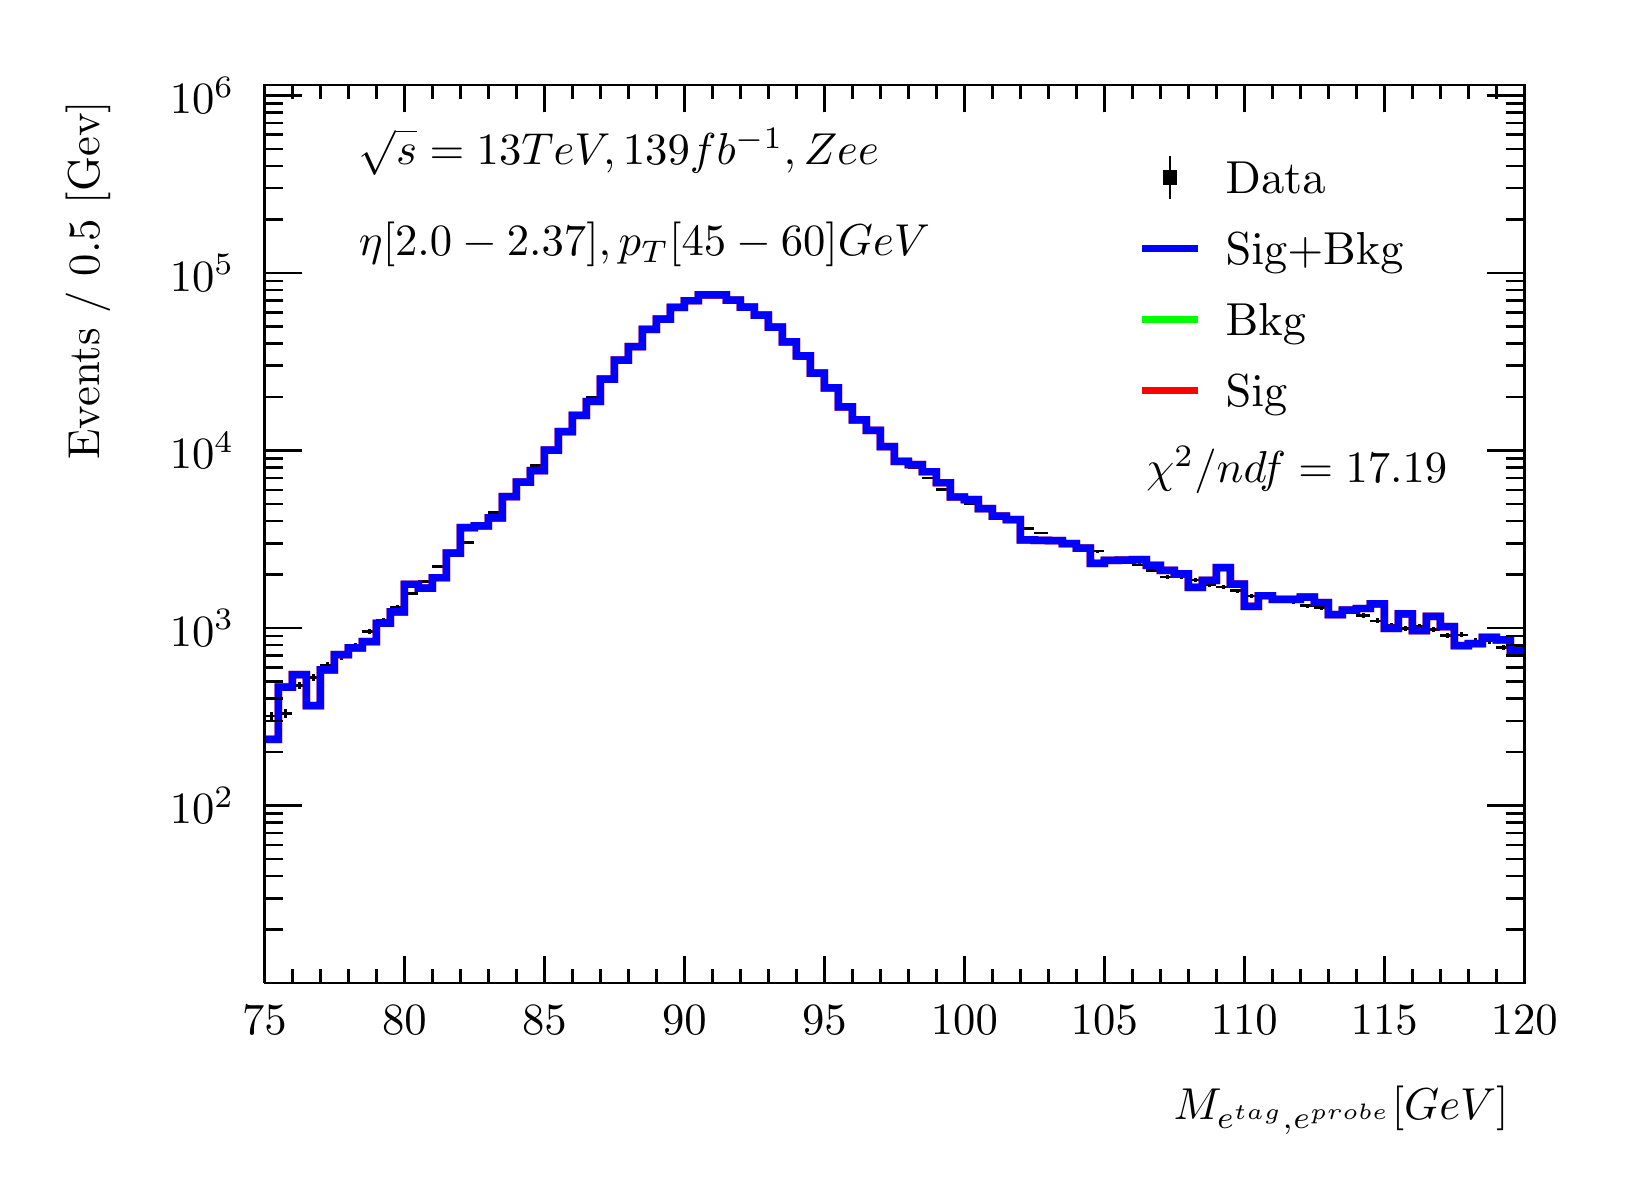
\begin{tikzpicture}
\pgfdeclareplotmark{cross} {
\pgfpathmoveto{\pgfpoint{-0.3\pgfplotmarksize}{\pgfplotmarksize}}
\pgfpathlineto{\pgfpoint{+0.3\pgfplotmarksize}{\pgfplotmarksize}}
\pgfpathlineto{\pgfpoint{+0.3\pgfplotmarksize}{0.3\pgfplotmarksize}}
\pgfpathlineto{\pgfpoint{+1\pgfplotmarksize}{0.3\pgfplotmarksize}}
\pgfpathlineto{\pgfpoint{+1\pgfplotmarksize}{-0.3\pgfplotmarksize}}
\pgfpathlineto{\pgfpoint{+0.3\pgfplotmarksize}{-0.3\pgfplotmarksize}}
\pgfpathlineto{\pgfpoint{+0.3\pgfplotmarksize}{-1.\pgfplotmarksize}}
\pgfpathlineto{\pgfpoint{-0.3\pgfplotmarksize}{-1.\pgfplotmarksize}}
\pgfpathlineto{\pgfpoint{-0.3\pgfplotmarksize}{-0.3\pgfplotmarksize}}
\pgfpathlineto{\pgfpoint{-1.\pgfplotmarksize}{-0.3\pgfplotmarksize}}
\pgfpathlineto{\pgfpoint{-1.\pgfplotmarksize}{0.3\pgfplotmarksize}}
\pgfpathlineto{\pgfpoint{-0.3\pgfplotmarksize}{0.3\pgfplotmarksize}}
\pgfpathclose
\pgfusepathqstroke
}
\pgfdeclareplotmark{cross*} {
\pgfpathmoveto{\pgfpoint{-0.3\pgfplotmarksize}{\pgfplotmarksize}}
\pgfpathlineto{\pgfpoint{+0.3\pgfplotmarksize}{\pgfplotmarksize}}
\pgfpathlineto{\pgfpoint{+0.3\pgfplotmarksize}{0.3\pgfplotmarksize}}
\pgfpathlineto{\pgfpoint{+1\pgfplotmarksize}{0.3\pgfplotmarksize}}
\pgfpathlineto{\pgfpoint{+1\pgfplotmarksize}{-0.3\pgfplotmarksize}}
\pgfpathlineto{\pgfpoint{+0.3\pgfplotmarksize}{-0.3\pgfplotmarksize}}
\pgfpathlineto{\pgfpoint{+0.3\pgfplotmarksize}{-1.\pgfplotmarksize}}
\pgfpathlineto{\pgfpoint{-0.3\pgfplotmarksize}{-1.\pgfplotmarksize}}
\pgfpathlineto{\pgfpoint{-0.3\pgfplotmarksize}{-0.3\pgfplotmarksize}}
\pgfpathlineto{\pgfpoint{-1.\pgfplotmarksize}{-0.3\pgfplotmarksize}}
\pgfpathlineto{\pgfpoint{-1.\pgfplotmarksize}{0.3\pgfplotmarksize}}
\pgfpathlineto{\pgfpoint{-0.3\pgfplotmarksize}{0.3\pgfplotmarksize}}
\pgfpathclose
\pgfusepathqfillstroke
}
\pgfdeclareplotmark{newstar} {
\pgfpathmoveto{\pgfqpoint{0pt}{\pgfplotmarksize}}
\pgfpathlineto{\pgfqpointpolar{44}{0.5\pgfplotmarksize}}
\pgfpathlineto{\pgfqpointpolar{18}{\pgfplotmarksize}}
\pgfpathlineto{\pgfqpointpolar{-20}{0.5\pgfplotmarksize}}
\pgfpathlineto{\pgfqpointpolar{-54}{\pgfplotmarksize}}
\pgfpathlineto{\pgfqpointpolar{-90}{0.5\pgfplotmarksize}}
\pgfpathlineto{\pgfqpointpolar{234}{\pgfplotmarksize}}
\pgfpathlineto{\pgfqpointpolar{198}{0.5\pgfplotmarksize}}
\pgfpathlineto{\pgfqpointpolar{162}{\pgfplotmarksize}}
\pgfpathlineto{\pgfqpointpolar{134}{0.5\pgfplotmarksize}}
\pgfpathclose
\pgfusepathqstroke
}
\pgfdeclareplotmark{newstar*} {
\pgfpathmoveto{\pgfqpoint{0pt}{\pgfplotmarksize}}
\pgfpathlineto{\pgfqpointpolar{44}{0.5\pgfplotmarksize}}
\pgfpathlineto{\pgfqpointpolar{18}{\pgfplotmarksize}}
\pgfpathlineto{\pgfqpointpolar{-20}{0.5\pgfplotmarksize}}
\pgfpathlineto{\pgfqpointpolar{-54}{\pgfplotmarksize}}
\pgfpathlineto{\pgfqpointpolar{-90}{0.5\pgfplotmarksize}}
\pgfpathlineto{\pgfqpointpolar{234}{\pgfplotmarksize}}
\pgfpathlineto{\pgfqpointpolar{198}{0.5\pgfplotmarksize}}
\pgfpathlineto{\pgfqpointpolar{162}{\pgfplotmarksize}}
\pgfpathlineto{\pgfqpointpolar{134}{0.5\pgfplotmarksize}}
\pgfpathclose
\pgfusepathqfillstroke
}
\definecolor{c}{rgb}{1,1,1};
\draw [color=c, fill=c] (0,0) rectangle (20,14.4361);
\draw [color=c, fill=c] (3,2.30977) rectangle (19,13.7143);
\definecolor{c}{rgb}{0,0,0};
\draw [c,line width=0.9] (3,2.30977) -- (3,13.7143) -- (19,13.7143) -- (19,2.30977) -- (3,2.30977);
\definecolor{c}{rgb}{1,1,1};
\draw [color=c, fill=c] (3,2.30977) rectangle (19,13.7143);
\definecolor{c}{rgb}{0,0,0};
\draw [c,line width=0.9] (3,2.30977) -- (3,13.7143) -- (19,13.7143) -- (19,2.30977) -- (3,2.30977);
\draw [c,line width=0.9] (3,2.30977) -- (19,2.30977);
\draw [c,line width=0.9] (3,2.65624) -- (3,2.30977);
\draw [c,line width=0.9] (3.35556,2.48301) -- (3.35556,2.30977);
\draw [c,line width=0.9] (3.71111,2.48301) -- (3.71111,2.30977);
\draw [c,line width=0.9] (4.06667,2.48301) -- (4.06667,2.30977);
\draw [c,line width=0.9] (4.42222,2.48301) -- (4.42222,2.30977);
\draw [c,line width=0.9] (4.77778,2.65624) -- (4.77778,2.30977);
\draw [c,line width=0.9] (5.13333,2.48301) -- (5.13333,2.30977);
\draw [c,line width=0.9] (5.48889,2.48301) -- (5.48889,2.30977);
\draw [c,line width=0.9] (5.84444,2.48301) -- (5.84444,2.30977);
\draw [c,line width=0.9] (6.2,2.48301) -- (6.2,2.30977);
\draw [c,line width=0.9] (6.55556,2.65624) -- (6.55556,2.30977);
\draw [c,line width=0.9] (6.91111,2.48301) -- (6.91111,2.30977);
\draw [c,line width=0.9] (7.26667,2.48301) -- (7.26667,2.30977);
\draw [c,line width=0.9] (7.62222,2.48301) -- (7.62222,2.30977);
\draw [c,line width=0.9] (7.97778,2.48301) -- (7.97778,2.30977);
\draw [c,line width=0.9] (8.33333,2.65624) -- (8.33333,2.30977);
\draw [c,line width=0.9] (8.68889,2.48301) -- (8.68889,2.30977);
\draw [c,line width=0.9] (9.04444,2.48301) -- (9.04444,2.30977);
\draw [c,line width=0.9] (9.4,2.48301) -- (9.4,2.30977);
\draw [c,line width=0.9] (9.75556,2.48301) -- (9.75556,2.30977);
\draw [c,line width=0.9] (10.1111,2.65624) -- (10.1111,2.30977);
\draw [c,line width=0.9] (10.4667,2.48301) -- (10.4667,2.30977);
\draw [c,line width=0.9] (10.8222,2.48301) -- (10.8222,2.30977);
\draw [c,line width=0.9] (11.1778,2.48301) -- (11.1778,2.30977);
\draw [c,line width=0.9] (11.5333,2.48301) -- (11.5333,2.30977);
\draw [c,line width=0.9] (11.8889,2.65624) -- (11.8889,2.30977);
\draw [c,line width=0.9] (12.2444,2.48301) -- (12.2444,2.30977);
\draw [c,line width=0.9] (12.6,2.48301) -- (12.6,2.30977);
\draw [c,line width=0.9] (12.9556,2.48301) -- (12.9556,2.30977);
\draw [c,line width=0.9] (13.3111,2.48301) -- (13.3111,2.30977);
\draw [c,line width=0.9] (13.6667,2.65624) -- (13.6667,2.30977);
\draw [c,line width=0.9] (14.0222,2.48301) -- (14.0222,2.30977);
\draw [c,line width=0.9] (14.3778,2.48301) -- (14.3778,2.30977);
\draw [c,line width=0.9] (14.7333,2.48301) -- (14.7333,2.30977);
\draw [c,line width=0.9] (15.0889,2.48301) -- (15.0889,2.30977);
\draw [c,line width=0.9] (15.4444,2.65624) -- (15.4444,2.30977);
\draw [c,line width=0.9] (15.8,2.48301) -- (15.8,2.30977);
\draw [c,line width=0.9] (16.1556,2.48301) -- (16.1556,2.30977);
\draw [c,line width=0.9] (16.5111,2.48301) -- (16.5111,2.30977);
\draw [c,line width=0.9] (16.8667,2.48301) -- (16.8667,2.30977);
\draw [c,line width=0.9] (17.2222,2.65624) -- (17.2222,2.30977);
\draw [c,line width=0.9] (17.5778,2.48301) -- (17.5778,2.30977);
\draw [c,line width=0.9] (17.9333,2.48301) -- (17.9333,2.30977);
\draw [c,line width=0.9] (18.2889,2.48301) -- (18.2889,2.30977);
\draw [c,line width=0.9] (18.6444,2.48301) -- (18.6444,2.30977);
\draw [c,line width=0.9] (19,2.65624) -- (19,2.30977);
\draw [c,line width=0.9] (19,2.65624) -- (19,2.30977);
\draw [anchor=base] (3,1.66015) node[scale=1.61424, color=c, rotate=0]{75};
\draw [anchor=base] (4.77778,1.66015) node[scale=1.61424, color=c, rotate=0]{80};
\draw [anchor=base] (6.55556,1.66015) node[scale=1.61424, color=c, rotate=0]{85};
\draw [anchor=base] (8.33333,1.66015) node[scale=1.61424, color=c, rotate=0]{90};
\draw [anchor=base] (10.1111,1.66015) node[scale=1.61424, color=c, rotate=0]{95};
\draw [anchor=base] (11.8889,1.66015) node[scale=1.61424, color=c, rotate=0]{100};
\draw [anchor=base] (13.6667,1.66015) node[scale=1.61424, color=c, rotate=0]{105};
\draw [anchor=base] (15.4444,1.66015) node[scale=1.61424, color=c, rotate=0]{110};
\draw [anchor=base] (17.2222,1.66015) node[scale=1.61424, color=c, rotate=0]{115};
\draw [anchor=base] (19,1.66015) node[scale=1.61424, color=c, rotate=0]{120};
\draw [anchor= east] (19,0.692932) node[scale=1.61424, color=c, rotate=0]{$M_{e^{tag}, e^{probe}}  [GeV]$};
\draw [c,line width=0.9] (3,13.7143) -- (19,13.7143);
\draw [c,line width=0.9] (3,13.3678) -- (3,13.7143);
\draw [c,line width=0.9] (3.35556,13.5411) -- (3.35556,13.7143);
\draw [c,line width=0.9] (3.71111,13.5411) -- (3.71111,13.7143);
\draw [c,line width=0.9] (4.06667,13.5411) -- (4.06667,13.7143);
\draw [c,line width=0.9] (4.42222,13.5411) -- (4.42222,13.7143);
\draw [c,line width=0.9] (4.77778,13.3678) -- (4.77778,13.7143);
\draw [c,line width=0.9] (5.13333,13.5411) -- (5.13333,13.7143);
\draw [c,line width=0.9] (5.48889,13.5411) -- (5.48889,13.7143);
\draw [c,line width=0.9] (5.84444,13.5411) -- (5.84444,13.7143);
\draw [c,line width=0.9] (6.2,13.5411) -- (6.2,13.7143);
\draw [c,line width=0.9] (6.55556,13.3678) -- (6.55556,13.7143);
\draw [c,line width=0.9] (6.91111,13.5411) -- (6.91111,13.7143);
\draw [c,line width=0.9] (7.26667,13.5411) -- (7.26667,13.7143);
\draw [c,line width=0.9] (7.62222,13.5411) -- (7.62222,13.7143);
\draw [c,line width=0.9] (7.97778,13.5411) -- (7.97778,13.7143);
\draw [c,line width=0.9] (8.33333,13.3678) -- (8.33333,13.7143);
\draw [c,line width=0.9] (8.68889,13.5411) -- (8.68889,13.7143);
\draw [c,line width=0.9] (9.04444,13.5411) -- (9.04444,13.7143);
\draw [c,line width=0.9] (9.4,13.5411) -- (9.4,13.7143);
\draw [c,line width=0.9] (9.75556,13.5411) -- (9.75556,13.7143);
\draw [c,line width=0.9] (10.1111,13.3678) -- (10.1111,13.7143);
\draw [c,line width=0.9] (10.4667,13.5411) -- (10.4667,13.7143);
\draw [c,line width=0.9] (10.8222,13.5411) -- (10.8222,13.7143);
\draw [c,line width=0.9] (11.1778,13.5411) -- (11.1778,13.7143);
\draw [c,line width=0.9] (11.5333,13.5411) -- (11.5333,13.7143);
\draw [c,line width=0.9] (11.8889,13.3678) -- (11.8889,13.7143);
\draw [c,line width=0.9] (12.2444,13.5411) -- (12.2444,13.7143);
\draw [c,line width=0.9] (12.6,13.5411) -- (12.6,13.7143);
\draw [c,line width=0.9] (12.9556,13.5411) -- (12.9556,13.7143);
\draw [c,line width=0.9] (13.3111,13.5411) -- (13.3111,13.7143);
\draw [c,line width=0.9] (13.6667,13.3678) -- (13.6667,13.7143);
\draw [c,line width=0.9] (14.0222,13.5411) -- (14.0222,13.7143);
\draw [c,line width=0.9] (14.3778,13.5411) -- (14.3778,13.7143);
\draw [c,line width=0.9] (14.7333,13.5411) -- (14.7333,13.7143);
\draw [c,line width=0.9] (15.0889,13.5411) -- (15.0889,13.7143);
\draw [c,line width=0.9] (15.4444,13.3678) -- (15.4444,13.7143);
\draw [c,line width=0.9] (15.8,13.5411) -- (15.8,13.7143);
\draw [c,line width=0.9] (16.1556,13.5411) -- (16.1556,13.7143);
\draw [c,line width=0.9] (16.5111,13.5411) -- (16.5111,13.7143);
\draw [c,line width=0.9] (16.8667,13.5411) -- (16.8667,13.7143);
\draw [c,line width=0.9] (17.2222,13.3678) -- (17.2222,13.7143);
\draw [c,line width=0.9] (17.5778,13.5411) -- (17.5778,13.7143);
\draw [c,line width=0.9] (17.9333,13.5411) -- (17.9333,13.7143);
\draw [c,line width=0.9] (18.2889,13.5411) -- (18.2889,13.7143);
\draw [c,line width=0.9] (18.6444,13.5411) -- (18.6444,13.7143);
\draw [c,line width=0.9] (19,13.3678) -- (19,13.7143);
\draw [c,line width=0.9] (19,13.3678) -- (19,13.7143);
\draw [c,line width=0.9] (3,2.30977) -- (3,13.7143);
\draw [c,line width=0.9] (3.237,2.98853) -- (3,2.98853);
\draw [c,line width=0.9] (3.237,3.38558) -- (3,3.38558);
\draw [c,line width=0.9] (3.237,3.66729) -- (3,3.66729);
\draw [c,line width=0.9] (3.237,3.8858) -- (3,3.8858);
\draw [c,line width=0.9] (3.237,4.06433) -- (3,4.06433);
\draw [c,line width=0.9] (3.237,4.21529) -- (3,4.21529);
\draw [c,line width=0.9] (3.237,4.34604) -- (3,4.34604);
\draw [c,line width=0.9] (3.237,4.46138) -- (3,4.46138);
\draw [c,line width=0.9] (3.474,4.56456) -- (3,4.56456);
\draw [anchor= east] (2.82,4.56456) node[scale=1.61424, color=c, rotate=0]{$10^{2}$};
\draw [c,line width=0.9] (3.237,5.24331) -- (3,5.24331);
\draw [c,line width=0.9] (3.237,5.64036) -- (3,5.64036);
\draw [c,line width=0.9] (3.237,5.92207) -- (3,5.92207);
\draw [c,line width=0.9] (3.237,6.14058) -- (3,6.14058);
\draw [c,line width=0.9] (3.237,6.31912) -- (3,6.31912);
\draw [c,line width=0.9] (3.237,6.47007) -- (3,6.47007);
\draw [c,line width=0.9] (3.237,6.60083) -- (3,6.60083);
\draw [c,line width=0.9] (3.237,6.71617) -- (3,6.71617);
\draw [c,line width=0.9] (3.474,6.81934) -- (3,6.81934);
\draw [anchor= east] (2.82,6.81934) node[scale=1.61424, color=c, rotate=0]{$10^{3}$};
\draw [c,line width=0.9] (3.237,7.4981) -- (3,7.4981);
\draw [c,line width=0.9] (3.237,7.89514) -- (3,7.89514);
\draw [c,line width=0.9] (3.237,8.17685) -- (3,8.17685);
\draw [c,line width=0.9] (3.237,8.39536) -- (3,8.39536);
\draw [c,line width=0.9] (3.237,8.5739) -- (3,8.5739);
\draw [c,line width=0.9] (3.237,8.72485) -- (3,8.72485);
\draw [c,line width=0.9] (3.237,8.85561) -- (3,8.85561);
\draw [c,line width=0.9] (3.237,8.97095) -- (3,8.97095);
\draw [c,line width=0.9] (3.474,9.07412) -- (3,9.07412);
\draw [anchor= east] (2.82,9.07412) node[scale=1.61424, color=c, rotate=0]{$10^{4}$};
\draw [c,line width=0.9] (3.237,9.75288) -- (3,9.75288);
\draw [c,line width=0.9] (3.237,10.1499) -- (3,10.1499);
\draw [c,line width=0.9] (3.237,10.4316) -- (3,10.4316);
\draw [c,line width=0.9] (3.237,10.6501) -- (3,10.6501);
\draw [c,line width=0.9] (3.237,10.8287) -- (3,10.8287);
\draw [c,line width=0.9] (3.237,10.9796) -- (3,10.9796);
\draw [c,line width=0.9] (3.237,11.1104) -- (3,11.1104);
\draw [c,line width=0.9] (3.237,11.2257) -- (3,11.2257);
\draw [c,line width=0.9] (3.474,11.3289) -- (3,11.3289);
\draw [anchor= east] (2.82,11.3289) node[scale=1.61424, color=c, rotate=0]{$10^{5}$};
\draw [c,line width=0.9] (3.237,12.0077) -- (3,12.0077);
\draw [c,line width=0.9] (3.237,12.4047) -- (3,12.4047);
\draw [c,line width=0.9] (3.237,12.6864) -- (3,12.6864);
\draw [c,line width=0.9] (3.237,12.9049) -- (3,12.9049);
\draw [c,line width=0.9] (3.237,13.0835) -- (3,13.0835);
\draw [c,line width=0.9] (3.237,13.2344) -- (3,13.2344);
\draw [c,line width=0.9] (3.237,13.3652) -- (3,13.3652);
\draw [c,line width=0.9] (3.237,13.4805) -- (3,13.4805);
\draw [c,line width=0.9] (3.474,13.5837) -- (3,13.5837);
\draw [anchor= east] (2.82,13.5837) node[scale=1.61424, color=c, rotate=0]{$10^{6}$};
\draw [anchor= east] (0.76,13.7143) node[scale=1.61424, color=c, rotate=90]{Events / 0.5 [Gev]};
\draw [c,line width=0.9] (19,2.30977) -- (19,13.7143);
\draw [c,line width=0.9] (18.763,2.98853) -- (19,2.98853);
\draw [c,line width=0.9] (18.763,3.38558) -- (19,3.38558);
\draw [c,line width=0.9] (18.763,3.66729) -- (19,3.66729);
\draw [c,line width=0.9] (18.763,3.8858) -- (19,3.8858);
\draw [c,line width=0.9] (18.763,4.06433) -- (19,4.06433);
\draw [c,line width=0.9] (18.763,4.21529) -- (19,4.21529);
\draw [c,line width=0.9] (18.763,4.34604) -- (19,4.34604);
\draw [c,line width=0.9] (18.763,4.46138) -- (19,4.46138);
\draw [c,line width=0.9] (18.526,4.56456) -- (19,4.56456);
\draw [c,line width=0.9] (18.763,5.24331) -- (19,5.24331);
\draw [c,line width=0.9] (18.763,5.64036) -- (19,5.64036);
\draw [c,line width=0.9] (18.763,5.92207) -- (19,5.92207);
\draw [c,line width=0.9] (18.763,6.14058) -- (19,6.14058);
\draw [c,line width=0.9] (18.763,6.31912) -- (19,6.31912);
\draw [c,line width=0.9] (18.763,6.47007) -- (19,6.47007);
\draw [c,line width=0.9] (18.763,6.60083) -- (19,6.60083);
\draw [c,line width=0.9] (18.763,6.71617) -- (19,6.71617);
\draw [c,line width=0.9] (18.526,6.81934) -- (19,6.81934);
\draw [c,line width=0.9] (18.763,7.4981) -- (19,7.4981);
\draw [c,line width=0.9] (18.763,7.89514) -- (19,7.89514);
\draw [c,line width=0.9] (18.763,8.17685) -- (19,8.17685);
\draw [c,line width=0.9] (18.763,8.39536) -- (19,8.39536);
\draw [c,line width=0.9] (18.763,8.5739) -- (19,8.5739);
\draw [c,line width=0.9] (18.763,8.72485) -- (19,8.72485);
\draw [c,line width=0.9] (18.763,8.85561) -- (19,8.85561);
\draw [c,line width=0.9] (18.763,8.97095) -- (19,8.97095);
\draw [c,line width=0.9] (18.526,9.07412) -- (19,9.07412);
\draw [c,line width=0.9] (18.763,9.75288) -- (19,9.75288);
\draw [c,line width=0.9] (18.763,10.1499) -- (19,10.1499);
\draw [c,line width=0.9] (18.763,10.4316) -- (19,10.4316);
\draw [c,line width=0.9] (18.763,10.6501) -- (19,10.6501);
\draw [c,line width=0.9] (18.763,10.8287) -- (19,10.8287);
\draw [c,line width=0.9] (18.763,10.9796) -- (19,10.9796);
\draw [c,line width=0.9] (18.763,11.1104) -- (19,11.1104);
\draw [c,line width=0.9] (18.763,11.2257) -- (19,11.2257);
\draw [c,line width=0.9] (18.526,11.3289) -- (19,11.3289);
\draw [c,line width=0.9] (18.763,12.0077) -- (19,12.0077);
\draw [c,line width=0.9] (18.763,12.4047) -- (19,12.4047);
\draw [c,line width=0.9] (18.763,12.6864) -- (19,12.6864);
\draw [c,line width=0.9] (18.763,12.9049) -- (19,12.9049);
\draw [c,line width=0.9] (18.763,13.0835) -- (19,13.0835);
\draw [c,line width=0.9] (18.763,13.2344) -- (19,13.2344);
\draw [c,line width=0.9] (18.763,13.3652) -- (19,13.3652);
\draw [c,line width=0.9] (18.763,13.4805) -- (19,13.4805);
\draw [c,line width=0.9] (18.526,13.5837) -- (19,13.5837);
\draw [c,line width=0.9] (3.08889,5.70356) -- (3,5.70356);
\draw [c,line width=0.9] (3,5.70356) -- (3,5.70356);
\draw [c,line width=0.9] (3.08889,5.70356) -- (3.17778,5.70356);
\draw [c,line width=0.9] (3.17778,5.70356) -- (3.17778,5.70356);
\draw [c,line width=0.9] (3.08889,5.70356) -- (3.08889,5.7583);
\draw [c,line width=0.9] (3.08889,5.7583) -- (3.08889,5.7583);
\draw [c,line width=0.9] (3.08889,5.70356) -- (3.08889,5.64883);
\draw [c,line width=0.9] (3.08889,5.64883) -- (3.08889,5.64883);
\draw [c,line width=0.9] (3.26667,5.73072) -- (3.17778,5.73072);
\draw [c,line width=0.9] (3.17778,5.73072) -- (3.17778,5.73072);
\draw [c,line width=0.9] (3.26667,5.73072) -- (3.35556,5.73072);
\draw [c,line width=0.9] (3.35556,5.73072) -- (3.35556,5.73072);
\draw [c,line width=0.9] (3.26667,5.73072) -- (3.26667,5.7847);
\draw [c,line width=0.9] (3.26667,5.7847) -- (3.26667,5.7847);
\draw [c,line width=0.9] (3.26667,5.73072) -- (3.26667,5.67674);
\draw [c,line width=0.9] (3.26667,5.67674) -- (3.26667,5.67674);
\draw [c,line width=0.9] (3.44444,6.08829) -- (3.35556,6.08829);
\draw [c,line width=0.9] (3.35556,6.08829) -- (3.35556,6.08829);
\draw [c,line width=0.9] (3.44444,6.08829) -- (3.53333,6.08829);
\draw [c,line width=0.9] (3.53333,6.08829) -- (3.53333,6.08829);
\draw [c,line width=0.9] (3.44444,6.08829) -- (3.44444,6.13326);
\draw [c,line width=0.9] (3.44444,6.13326) -- (3.44444,6.13326);
\draw [c,line width=0.9] (3.44444,6.08829) -- (3.44444,6.04332);
\draw [c,line width=0.9] (3.44444,6.04332) -- (3.44444,6.04332);
\draw [c,line width=0.9] (3.62222,6.18836) -- (3.53333,6.18836);
\draw [c,line width=0.9] (3.53333,6.18836) -- (3.53333,6.18836);
\draw [c,line width=0.9] (3.62222,6.18836) -- (3.71111,6.18836);
\draw [c,line width=0.9] (3.71111,6.18836) -- (3.71111,6.18836);
\draw [c,line width=0.9] (3.62222,6.18836) -- (3.62222,6.23109);
\draw [c,line width=0.9] (3.62222,6.23109) -- (3.62222,6.23109);
\draw [c,line width=0.9] (3.62222,6.18836) -- (3.62222,6.14563);
\draw [c,line width=0.9] (3.62222,6.14563) -- (3.62222,6.14563);
\draw [c,line width=0.9] (3.8,6.34171) -- (3.71111,6.34171);
\draw [c,line width=0.9] (3.71111,6.34171) -- (3.71111,6.34171);
\draw [c,line width=0.9] (3.8,6.34171) -- (3.88889,6.34171);
\draw [c,line width=0.9] (3.88889,6.34171) -- (3.88889,6.34171);
\draw [c,line width=0.9] (3.8,6.34171) -- (3.8,6.38122);
\draw [c,line width=0.9] (3.8,6.38122) -- (3.8,6.38122);
\draw [c,line width=0.9] (3.8,6.34171) -- (3.8,6.30219);
\draw [c,line width=0.9] (3.8,6.30219) -- (3.8,6.30219);
\draw [c,line width=0.9] (3.97778,6.45029) -- (3.88889,6.45029);
\draw [c,line width=0.9] (3.88889,6.45029) -- (3.88889,6.45029);
\draw [c,line width=0.9] (3.97778,6.45029) -- (4.06667,6.45029);
\draw [c,line width=0.9] (4.06667,6.45029) -- (4.06667,6.45029);
\draw [c,line width=0.9] (3.97778,6.45029) -- (3.97778,6.48767);
\draw [c,line width=0.9] (3.97778,6.48767) -- (3.97778,6.48767);
\draw [c,line width=0.9] (3.97778,6.45029) -- (3.97778,6.4129);
\draw [c,line width=0.9] (3.97778,6.4129) -- (3.97778,6.4129);
\draw [c,line width=0.9] (4.15556,6.5996) -- (4.06667,6.5996);
\draw [c,line width=0.9] (4.06667,6.5996) -- (4.06667,6.5996);
\draw [c,line width=0.9] (4.15556,6.5996) -- (4.24444,6.5996);
\draw [c,line width=0.9] (4.24444,6.5996) -- (4.24444,6.5996);
\draw [c,line width=0.9] (4.15556,6.5996) -- (4.15556,6.63425);
\draw [c,line width=0.9] (4.15556,6.63425) -- (4.15556,6.63425);
\draw [c,line width=0.9] (4.15556,6.5996) -- (4.15556,6.56496);
\draw [c,line width=0.9] (4.15556,6.56496) -- (4.15556,6.56496);
\draw [c,line width=0.9] (4.33333,6.77323) -- (4.24444,6.77323);
\draw [c,line width=0.9] (4.24444,6.77323) -- (4.24444,6.77323);
\draw [c,line width=0.9] (4.33333,6.77323) -- (4.42222,6.77323);
\draw [c,line width=0.9] (4.42222,6.77323) -- (4.42222,6.77323);
\draw [c,line width=0.9] (4.33333,6.77323) -- (4.33333,6.80493);
\draw [c,line width=0.9] (4.33333,6.80493) -- (4.33333,6.80493);
\draw [c,line width=0.9] (4.33333,6.77323) -- (4.33333,6.74152);
\draw [c,line width=0.9] (4.33333,6.74152) -- (4.33333,6.74152);
\draw [c,line width=0.9] (4.51111,6.92065) -- (4.42222,6.92065);
\draw [c,line width=0.9] (4.42222,6.92065) -- (4.42222,6.92065);
\draw [c,line width=0.9] (4.51111,6.92065) -- (4.6,6.92065);
\draw [c,line width=0.9] (4.6,6.92065) -- (4.6,6.92065);
\draw [c,line width=0.9] (4.51111,6.92065) -- (4.51111,6.95006);
\draw [c,line width=0.9] (4.51111,6.95006) -- (4.51111,6.95006);
\draw [c,line width=0.9] (4.51111,6.92065) -- (4.51111,6.89125);
\draw [c,line width=0.9] (4.51111,6.89125) -- (4.51111,6.89125);
\draw [c,line width=0.9] (4.68889,7.07776) -- (4.6,7.07776);
\draw [c,line width=0.9] (4.6,7.07776) -- (4.6,7.07776);
\draw [c,line width=0.9] (4.68889,7.07776) -- (4.77778,7.07776);
\draw [c,line width=0.9] (4.77778,7.07776) -- (4.77778,7.07776);
\draw [c,line width=0.9] (4.68889,7.07776) -- (4.68889,7.1049);
\draw [c,line width=0.9] (4.68889,7.1049) -- (4.68889,7.1049);
\draw [c,line width=0.9] (4.68889,7.07776) -- (4.68889,7.05063);
\draw [c,line width=0.9] (4.68889,7.05063) -- (4.68889,7.05063);
\draw [c,line width=0.9] (4.86667,7.25668) -- (4.77778,7.25668);
\draw [c,line width=0.9] (4.77778,7.25668) -- (4.77778,7.25668);
\draw [c,line width=0.9] (4.86667,7.25668) -- (4.95556,7.25668);
\draw [c,line width=0.9] (4.95556,7.25668) -- (4.95556,7.25668);
\draw [c,line width=0.9] (4.86667,7.25668) -- (4.86667,7.28144);
\draw [c,line width=0.9] (4.86667,7.28144) -- (4.86667,7.28144);
\draw [c,line width=0.9] (4.86667,7.25668) -- (4.86667,7.23191);
\draw [c,line width=0.9] (4.86667,7.23191) -- (4.86667,7.23191);
\draw [c,line width=0.9] (5.04444,7.40736) -- (4.95556,7.40736);
\draw [c,line width=0.9] (4.95556,7.40736) -- (4.95556,7.40736);
\draw [c,line width=0.9] (5.04444,7.40736) -- (5.13333,7.40736);
\draw [c,line width=0.9] (5.13333,7.40736) -- (5.13333,7.40736);
\draw [c,line width=0.9] (5.04444,7.40736) -- (5.04444,7.43029);
\draw [c,line width=0.9] (5.04444,7.43029) -- (5.04444,7.43029);
\draw [c,line width=0.9] (5.04444,7.40736) -- (5.04444,7.38442);
\draw [c,line width=0.9] (5.04444,7.38442) -- (5.04444,7.38442);
\draw [c,line width=0.9] (5.22222,7.59808) -- (5.13333,7.59808);
\draw [c,line width=0.9] (5.13333,7.59808) -- (5.13333,7.59808);
\draw [c,line width=0.9] (5.22222,7.59808) -- (5.31111,7.59808);
\draw [c,line width=0.9] (5.31111,7.59808) -- (5.31111,7.59808);
\draw [c,line width=0.9] (5.22222,7.59808) -- (5.22222,7.61889);
\draw [c,line width=0.9] (5.22222,7.61889) -- (5.22222,7.61889);
\draw [c,line width=0.9] (5.22222,7.59808) -- (5.22222,7.57728);
\draw [c,line width=0.9] (5.22222,7.57728) -- (5.22222,7.57728);
\draw [c,line width=0.9] (5.4,7.74593) -- (5.31111,7.74593);
\draw [c,line width=0.9] (5.31111,7.74593) -- (5.31111,7.74593);
\draw [c,line width=0.9] (5.4,7.74593) -- (5.48889,7.74593);
\draw [c,line width=0.9] (5.48889,7.74593) -- (5.48889,7.74593);
\draw [c,line width=0.9] (5.4,7.74593) -- (5.4,7.76523);
\draw [c,line width=0.9] (5.4,7.76523) -- (5.4,7.76523);
\draw [c,line width=0.9] (5.4,7.74593) -- (5.4,7.72664);
\draw [c,line width=0.9] (5.4,7.72664) -- (5.4,7.72664);
\draw [c,line width=0.9] (5.57778,7.90392) -- (5.48889,7.90392);
\draw [c,line width=0.9] (5.48889,7.90392) -- (5.48889,7.90392);
\draw [c,line width=0.9] (5.57778,7.90392) -- (5.66667,7.90392);
\draw [c,line width=0.9] (5.66667,7.90392) -- (5.66667,7.90392);
\draw [c,line width=0.9] (5.57778,7.90392) -- (5.57778,7.92172);
\draw [c,line width=0.9] (5.57778,7.92172) -- (5.57778,7.92172);
\draw [c,line width=0.9] (5.57778,7.90392) -- (5.57778,7.88612);
\draw [c,line width=0.9] (5.57778,7.88612) -- (5.57778,7.88612);
\draw [c,line width=0.9] (5.75556,8.10973) -- (5.66667,8.10973);
\draw [c,line width=0.9] (5.66667,8.10973) -- (5.66667,8.10973);
\draw [c,line width=0.9] (5.75556,8.10973) -- (5.84444,8.10973);
\draw [c,line width=0.9] (5.84444,8.10973) -- (5.84444,8.10973);
\draw [c,line width=0.9] (5.75556,8.10973) -- (5.75556,8.12575);
\draw [c,line width=0.9] (5.75556,8.12575) -- (5.75556,8.12575);
\draw [c,line width=0.9] (5.75556,8.10973) -- (5.75556,8.09371);
\draw [c,line width=0.9] (5.75556,8.09371) -- (5.75556,8.09371);
\draw [c,line width=0.9] (5.93333,8.28411) -- (5.84444,8.28411);
\draw [c,line width=0.9] (5.84444,8.28411) -- (5.84444,8.28411);
\draw [c,line width=0.9] (5.93333,8.28411) -- (6.02222,8.28411);
\draw [c,line width=0.9] (6.02222,8.28411) -- (6.02222,8.28411);
\draw [c,line width=0.9] (5.93333,8.28411) -- (5.93333,8.29877);
\draw [c,line width=0.9] (5.93333,8.29877) -- (5.93333,8.29877);
\draw [c,line width=0.9] (5.93333,8.28411) -- (5.93333,8.26945);
\draw [c,line width=0.9] (5.93333,8.26945) -- (5.93333,8.26945);
\draw [c,line width=0.9] (6.11111,8.46618) -- (6.02222,8.46618);
\draw [c,line width=0.9] (6.02222,8.46618) -- (6.02222,8.46618);
\draw [c,line width=0.9] (6.11111,8.46618) -- (6.2,8.46618);
\draw [c,line width=0.9] (6.2,8.46618) -- (6.2,8.46618);
\draw [c,line width=0.9] (6.11111,8.46618) -- (6.11111,8.47954);
\draw [c,line width=0.9] (6.11111,8.47954) -- (6.11111,8.47954);
\draw [c,line width=0.9] (6.11111,8.46618) -- (6.11111,8.45283);
\draw [c,line width=0.9] (6.11111,8.45283) -- (6.11111,8.45283);
\draw [c,line width=0.9] (6.28889,8.68094) -- (6.2,8.68094);
\draw [c,line width=0.9] (6.2,8.68094) -- (6.2,8.68094);
\draw [c,line width=0.9] (6.28889,8.68094) -- (6.37778,8.68094);
\draw [c,line width=0.9] (6.37778,8.68094) -- (6.37778,8.68094);
\draw [c,line width=0.9] (6.28889,8.68094) -- (6.28889,8.69291);
\draw [c,line width=0.9] (6.28889,8.69291) -- (6.28889,8.69291);
\draw [c,line width=0.9] (6.28889,8.68094) -- (6.28889,8.66897);
\draw [c,line width=0.9] (6.28889,8.66897) -- (6.28889,8.66897);
\draw [c,line width=0.9] (6.46667,8.88182) -- (6.37778,8.88182);
\draw [c,line width=0.9] (6.37778,8.88182) -- (6.37778,8.88182);
\draw [c,line width=0.9] (6.46667,8.88182) -- (6.55556,8.88182);
\draw [c,line width=0.9] (6.55556,8.88182) -- (6.55556,8.88182);
\draw [c,line width=0.9] (6.46667,8.88182) -- (6.46667,8.89262);
\draw [c,line width=0.9] (6.46667,8.89262) -- (6.46667,8.89262);
\draw [c,line width=0.9] (6.46667,8.88182) -- (6.46667,8.87102);
\draw [c,line width=0.9] (6.46667,8.87102) -- (6.46667,8.87102);
\draw [c,line width=0.9] (6.64444,9.09964) -- (6.55556,9.09964);
\draw [c,line width=0.9] (6.55556,9.09964) -- (6.55556,9.09964);
\draw [c,line width=0.9] (6.64444,9.09964) -- (6.73333,9.09964);
\draw [c,line width=0.9] (6.73333,9.09964) -- (6.73333,9.09964);
\draw [c,line width=0.9] (6.64444,9.09964) -- (6.64444,9.10931);
\draw [c,line width=0.9] (6.64444,9.10931) -- (6.64444,9.10931);
\draw [c,line width=0.9] (6.64444,9.09964) -- (6.64444,9.08997);
\draw [c,line width=0.9] (6.64444,9.08997) -- (6.64444,9.08997);
\draw [c,line width=0.9] (6.82222,9.31486) -- (6.73333,9.31486);
\draw [c,line width=0.9] (6.73333,9.31486) -- (6.73333,9.31486);
\draw [c,line width=0.9] (6.82222,9.31486) -- (6.91111,9.31486);
\draw [c,line width=0.9] (6.91111,9.31486) -- (6.91111,9.31486);
\draw [c,line width=0.9] (6.82222,9.31486) -- (6.82222,9.32352);
\draw [c,line width=0.9] (6.82222,9.32352) -- (6.82222,9.32352);
\draw [c,line width=0.9] (6.82222,9.31486) -- (6.82222,9.3062);
\draw [c,line width=0.9] (6.82222,9.3062) -- (6.82222,9.3062);
\draw [c,line width=0.9] (7,9.54065) -- (6.91111,9.54065);
\draw [c,line width=0.9] (6.91111,9.54065) -- (6.91111,9.54065);
\draw [c,line width=0.9] (7,9.54065) -- (7.08889,9.54065);
\draw [c,line width=0.9] (7.08889,9.54065) -- (7.08889,9.54065);
\draw [c,line width=0.9] (7,9.54065) -- (7,9.54837);
\draw [c,line width=0.9] (7,9.54837) -- (7,9.54837);
\draw [c,line width=0.9] (7,9.54065) -- (7,9.53294);
\draw [c,line width=0.9] (7,9.53294) -- (7,9.53294);
\draw [c,line width=0.9] (7.17778,9.75508) -- (7.08889,9.75508);
\draw [c,line width=0.9] (7.08889,9.75508) -- (7.08889,9.75508);
\draw [c,line width=0.9] (7.17778,9.75508) -- (7.26667,9.75508);
\draw [c,line width=0.9] (7.26667,9.75508) -- (7.26667,9.75508);
\draw [c,line width=0.9] (7.17778,9.75508) -- (7.17778,9.762);
\draw [c,line width=0.9] (7.17778,9.762) -- (7.17778,9.762);
\draw [c,line width=0.9] (7.17778,9.75508) -- (7.17778,9.74816);
\draw [c,line width=0.9] (7.17778,9.74816) -- (7.17778,9.74816);
\draw [c,line width=0.9] (7.35556,9.98346) -- (7.26667,9.98346);
\draw [c,line width=0.9] (7.26667,9.98346) -- (7.26667,9.98346);
\draw [c,line width=0.9] (7.35556,9.98346) -- (7.44444,9.98346);
\draw [c,line width=0.9] (7.44444,9.98346) -- (7.44444,9.98346);
\draw [c,line width=0.9] (7.35556,9.98346) -- (7.35556,9.98961);
\draw [c,line width=0.9] (7.35556,9.98961) -- (7.35556,9.98961);
\draw [c,line width=0.9] (7.35556,9.98346) -- (7.35556,9.9773);
\draw [c,line width=0.9] (7.35556,9.9773) -- (7.35556,9.9773);
\draw [c,line width=0.9] (7.53333,10.1945) -- (7.44444,10.1945);
\draw [c,line width=0.9] (7.44444,10.1945) -- (7.44444,10.1945);
\draw [c,line width=0.9] (7.53333,10.1945) -- (7.62222,10.1945);
\draw [c,line width=0.9] (7.62222,10.1945) -- (7.62222,10.1945);
\draw [c,line width=0.9] (7.53333,10.1945) -- (7.53333,10.2001);
\draw [c,line width=0.9] (7.53333,10.2001) -- (7.53333,10.2001);
\draw [c,line width=0.9] (7.53333,10.1945) -- (7.53333,10.189);
\draw [c,line width=0.9] (7.53333,10.189) -- (7.53333,10.189);
\draw [c,line width=0.9] (7.71111,10.4069) -- (7.62222,10.4069);
\draw [c,line width=0.9] (7.62222,10.4069) -- (7.62222,10.4069);
\draw [c,line width=0.9] (7.71111,10.4069) -- (7.8,10.4069);
\draw [c,line width=0.9] (7.8,10.4069) -- (7.8,10.4069);
\draw [c,line width=0.9] (7.71111,10.4069) -- (7.71111,10.4118);
\draw [c,line width=0.9] (7.71111,10.4118) -- (7.71111,10.4118);
\draw [c,line width=0.9] (7.71111,10.4069) -- (7.71111,10.4019);
\draw [c,line width=0.9] (7.71111,10.4019) -- (7.71111,10.4019);
\draw [c,line width=0.9] (7.88889,10.6044) -- (7.8,10.6044);
\draw [c,line width=0.9] (7.8,10.6044) -- (7.8,10.6044);
\draw [c,line width=0.9] (7.88889,10.6044) -- (7.97778,10.6044);
\draw [c,line width=0.9] (7.97778,10.6044) -- (7.97778,10.6044);
\draw [c,line width=0.9] (7.88889,10.6044) -- (7.88889,10.6088);
\draw [c,line width=0.9] (7.88889,10.6088) -- (7.88889,10.6088);
\draw [c,line width=0.9] (7.88889,10.6044) -- (7.88889,10.5999);
\draw [c,line width=0.9] (7.88889,10.5999) -- (7.88889,10.5999);
\draw [c,line width=0.9] (8.06667,10.769) -- (7.97778,10.769);
\draw [c,line width=0.9] (7.97778,10.769) -- (7.97778,10.769);
\draw [c,line width=0.9] (8.06667,10.769) -- (8.15556,10.769);
\draw [c,line width=0.9] (8.15556,10.769) -- (8.15556,10.769);
\draw [c,line width=0.9] (8.06667,10.769) -- (8.06667,10.7732);
\draw [c,line width=0.9] (8.06667,10.7732) -- (8.06667,10.7732);
\draw [c,line width=0.9] (8.06667,10.769) -- (8.06667,10.7649);
\draw [c,line width=0.9] (8.06667,10.7649) -- (8.06667,10.7649);
\draw [c,line width=0.9] (8.24444,10.893) -- (8.15556,10.893);
\draw [c,line width=0.9] (8.15556,10.893) -- (8.15556,10.893);
\draw [c,line width=0.9] (8.24444,10.893) -- (8.33333,10.893);
\draw [c,line width=0.9] (8.33333,10.893) -- (8.33333,10.893);
\draw [c,line width=0.9] (8.24444,10.893) -- (8.24444,10.8969);
\draw [c,line width=0.9] (8.24444,10.8969) -- (8.24444,10.8969);
\draw [c,line width=0.9] (8.24444,10.893) -- (8.24444,10.8891);
\draw [c,line width=0.9] (8.24444,10.8891) -- (8.24444,10.8891);
\draw [c,line width=0.9] (8.42222,10.989) -- (8.33333,10.989);
\draw [c,line width=0.9] (8.33333,10.989) -- (8.33333,10.989);
\draw [c,line width=0.9] (8.42222,10.989) -- (8.51111,10.989);
\draw [c,line width=0.9] (8.51111,10.989) -- (8.51111,10.989);
\draw [c,line width=0.9] (8.42222,10.989) -- (8.42222,10.9927);
\draw [c,line width=0.9] (8.42222,10.9927) -- (8.42222,10.9927);
\draw [c,line width=0.9] (8.42222,10.989) -- (8.42222,10.9853);
\draw [c,line width=0.9] (8.42222,10.9853) -- (8.42222,10.9853);
\draw [c,line width=0.9] (8.6,11.0335) -- (8.51111,11.0335);
\draw [c,line width=0.9] (8.51111,11.0335) -- (8.51111,11.0335);
\draw [c,line width=0.9] (8.6,11.0335) -- (8.68889,11.0335);
\draw [c,line width=0.9] (8.68889,11.0335) -- (8.68889,11.0335);
\draw [c,line width=0.9] (8.6,11.0335) -- (8.6,11.0371);
\draw [c,line width=0.9] (8.6,11.0371) -- (8.6,11.0371);
\draw [c,line width=0.9] (8.6,11.0335) -- (8.6,11.0299);
\draw [c,line width=0.9] (8.6,11.0299) -- (8.6,11.0299);
\draw [c,line width=0.9] (8.77778,11.0437) -- (8.68889,11.0437);
\draw [c,line width=0.9] (8.68889,11.0437) -- (8.68889,11.0437);
\draw [c,line width=0.9] (8.77778,11.0437) -- (8.86667,11.0437);
\draw [c,line width=0.9] (8.86667,11.0437) -- (8.86667,11.0437);
\draw [c,line width=0.9] (8.77778,11.0437) -- (8.77778,11.0472);
\draw [c,line width=0.9] (8.77778,11.0472) -- (8.77778,11.0472);
\draw [c,line width=0.9] (8.77778,11.0437) -- (8.77778,11.0401);
\draw [c,line width=0.9] (8.77778,11.0401) -- (8.77778,11.0401);
\draw [c,line width=0.9] (8.95556,11.0034) -- (8.86667,11.0034);
\draw [c,line width=0.9] (8.86667,11.0034) -- (8.86667,11.0034);
\draw [c,line width=0.9] (8.95556,11.0034) -- (9.04444,11.0034);
\draw [c,line width=0.9] (9.04444,11.0034) -- (9.04444,11.0034);
\draw [c,line width=0.9] (8.95556,11.0034) -- (8.95556,11.0071);
\draw [c,line width=0.9] (8.95556,11.0071) -- (8.95556,11.0071);
\draw [c,line width=0.9] (8.95556,11.0034) -- (8.95556,10.9998);
\draw [c,line width=0.9] (8.95556,10.9998) -- (8.95556,10.9998);
\draw [c,line width=0.9] (9.13333,10.9124) -- (9.04444,10.9124);
\draw [c,line width=0.9] (9.04444,10.9124) -- (9.04444,10.9124);
\draw [c,line width=0.9] (9.13333,10.9124) -- (9.22222,10.9124);
\draw [c,line width=0.9] (9.22222,10.9124) -- (9.22222,10.9124);
\draw [c,line width=0.9] (9.13333,10.9124) -- (9.13333,10.9163);
\draw [c,line width=0.9] (9.13333,10.9163) -- (9.13333,10.9163);
\draw [c,line width=0.9] (9.13333,10.9124) -- (9.13333,10.9086);
\draw [c,line width=0.9] (9.13333,10.9086) -- (9.13333,10.9086);
\draw [c,line width=0.9] (9.31111,10.7798) -- (9.22222,10.7798);
\draw [c,line width=0.9] (9.22222,10.7798) -- (9.22222,10.7798);
\draw [c,line width=0.9] (9.31111,10.7798) -- (9.4,10.7798);
\draw [c,line width=0.9] (9.4,10.7798) -- (9.4,10.7798);
\draw [c,line width=0.9] (9.31111,10.7798) -- (9.31111,10.7839);
\draw [c,line width=0.9] (9.31111,10.7839) -- (9.31111,10.7839);
\draw [c,line width=0.9] (9.31111,10.7798) -- (9.31111,10.7757);
\draw [c,line width=0.9] (9.31111,10.7757) -- (9.31111,10.7757);
\draw [c,line width=0.9] (9.48889,10.6322) -- (9.4,10.6322);
\draw [c,line width=0.9] (9.4,10.6322) -- (9.4,10.6322);
\draw [c,line width=0.9] (9.48889,10.6322) -- (9.57778,10.6322);
\draw [c,line width=0.9] (9.57778,10.6322) -- (9.57778,10.6322);
\draw [c,line width=0.9] (9.48889,10.6322) -- (9.48889,10.6367);
\draw [c,line width=0.9] (9.48889,10.6367) -- (9.48889,10.6367);
\draw [c,line width=0.9] (9.48889,10.6322) -- (9.48889,10.6278);
\draw [c,line width=0.9] (9.48889,10.6278) -- (9.48889,10.6278);
\draw [c,line width=0.9] (9.66667,10.441) -- (9.57778,10.441);
\draw [c,line width=0.9] (9.57778,10.441) -- (9.57778,10.441);
\draw [c,line width=0.9] (9.66667,10.441) -- (9.75556,10.441);
\draw [c,line width=0.9] (9.75556,10.441) -- (9.75556,10.441);
\draw [c,line width=0.9] (9.66667,10.441) -- (9.66667,10.4459);
\draw [c,line width=0.9] (9.66667,10.4459) -- (9.66667,10.4459);
\draw [c,line width=0.9] (9.66667,10.441) -- (9.66667,10.4361);
\draw [c,line width=0.9] (9.66667,10.4361) -- (9.66667,10.4361);
\draw [c,line width=0.9] (9.84444,10.2364) -- (9.75556,10.2364);
\draw [c,line width=0.9] (9.75556,10.2364) -- (9.75556,10.2364);
\draw [c,line width=0.9] (9.84444,10.2364) -- (9.93333,10.2364);
\draw [c,line width=0.9] (9.93333,10.2364) -- (9.93333,10.2364);
\draw [c,line width=0.9] (9.84444,10.2364) -- (9.84444,10.2418);
\draw [c,line width=0.9] (9.84444,10.2418) -- (9.84444,10.2418);
\draw [c,line width=0.9] (9.84444,10.2364) -- (9.84444,10.231);
\draw [c,line width=0.9] (9.84444,10.231) -- (9.84444,10.231);
\draw [c,line width=0.9] (10.0222,10.0367) -- (9.93333,10.0367);
\draw [c,line width=0.9] (9.93333,10.0367) -- (9.93333,10.0367);
\draw [c,line width=0.9] (10.0222,10.0367) -- (10.1111,10.0367);
\draw [c,line width=0.9] (10.1111,10.0367) -- (10.1111,10.0367);
\draw [c,line width=0.9] (10.0222,10.0367) -- (10.0222,10.0427);
\draw [c,line width=0.9] (10.0222,10.0427) -- (10.0222,10.0427);
\draw [c,line width=0.9] (10.0222,10.0367) -- (10.0222,10.0307);
\draw [c,line width=0.9] (10.0222,10.0307) -- (10.0222,10.0307);
\draw [c,line width=0.9] (10.2,9.85096) -- (10.1111,9.85096);
\draw [c,line width=0.9] (10.1111,9.85096) -- (10.1111,9.85096);
\draw [c,line width=0.9] (10.2,9.85096) -- (10.2889,9.85096);
\draw [c,line width=0.9] (10.2889,9.85096) -- (10.2889,9.85096);
\draw [c,line width=0.9] (10.2,9.85096) -- (10.2,9.85755);
\draw [c,line width=0.9] (10.2,9.85755) -- (10.2,9.85755);
\draw [c,line width=0.9] (10.2,9.85096) -- (10.2,9.84438);
\draw [c,line width=0.9] (10.2,9.84438) -- (10.2,9.84438);
\draw [c,line width=0.9] (10.3778,9.64589) -- (10.2889,9.64589);
\draw [c,line width=0.9] (10.2889,9.64589) -- (10.2889,9.64589);
\draw [c,line width=0.9] (10.3778,9.64589) -- (10.4667,9.64589);
\draw [c,line width=0.9] (10.4667,9.64589) -- (10.4667,9.64589);
\draw [c,line width=0.9] (10.3778,9.64589) -- (10.3778,9.6532);
\draw [c,line width=0.9] (10.3778,9.6532) -- (10.3778,9.6532);
\draw [c,line width=0.9] (10.3778,9.64589) -- (10.3778,9.63858);
\draw [c,line width=0.9] (10.3778,9.63858) -- (10.3778,9.63858);
\draw [c,line width=0.9] (10.5556,9.47417) -- (10.4667,9.47417);
\draw [c,line width=0.9] (10.4667,9.47417) -- (10.4667,9.47417);
\draw [c,line width=0.9] (10.5556,9.47417) -- (10.6444,9.47417);
\draw [c,line width=0.9] (10.6444,9.47417) -- (10.6444,9.47417);
\draw [c,line width=0.9] (10.5556,9.47417) -- (10.5556,9.48215);
\draw [c,line width=0.9] (10.5556,9.48215) -- (10.5556,9.48215);
\draw [c,line width=0.9] (10.5556,9.47417) -- (10.5556,9.46619);
\draw [c,line width=0.9] (10.5556,9.46619) -- (10.5556,9.46619);
\draw [c,line width=0.9] (10.7333,9.29748) -- (10.6444,9.29748);
\draw [c,line width=0.9] (10.6444,9.29748) -- (10.6444,9.29748);
\draw [c,line width=0.9] (10.7333,9.29748) -- (10.8222,9.29748);
\draw [c,line width=0.9] (10.8222,9.29748) -- (10.8222,9.29748);
\draw [c,line width=0.9] (10.7333,9.29748) -- (10.7333,9.30622);
\draw [c,line width=0.9] (10.7333,9.30622) -- (10.7333,9.30622);
\draw [c,line width=0.9] (10.7333,9.29748) -- (10.7333,9.28874);
\draw [c,line width=0.9] (10.7333,9.28874) -- (10.7333,9.28874);
\draw [c,line width=0.9] (10.9111,9.12432) -- (10.8222,9.12432);
\draw [c,line width=0.9] (10.8222,9.12432) -- (10.8222,9.12432);
\draw [c,line width=0.9] (10.9111,9.12432) -- (11,9.12432);
\draw [c,line width=0.9] (11,9.12432) -- (11,9.12432);
\draw [c,line width=0.9] (10.9111,9.12432) -- (10.9111,9.13387);
\draw [c,line width=0.9] (10.9111,9.13387) -- (10.9111,9.13387);
\draw [c,line width=0.9] (10.9111,9.12432) -- (10.9111,9.11478);
\draw [c,line width=0.9] (10.9111,9.11478) -- (10.9111,9.11478);
\draw [c,line width=0.9] (11.0889,8.96286) -- (11,8.96286);
\draw [c,line width=0.9] (11,8.96286) -- (11,8.96286);
\draw [c,line width=0.9] (11.0889,8.96286) -- (11.1778,8.96286);
\draw [c,line width=0.9] (11.1778,8.96286) -- (11.1778,8.96286);
\draw [c,line width=0.9] (11.0889,8.96286) -- (11.0889,8.97323);
\draw [c,line width=0.9] (11.0889,8.97323) -- (11.0889,8.97323);
\draw [c,line width=0.9] (11.0889,8.96286) -- (11.0889,8.9525);
\draw [c,line width=0.9] (11.0889,8.9525) -- (11.0889,8.9525);
\draw [c,line width=0.9] (11.2667,8.85696) -- (11.1778,8.85696);
\draw [c,line width=0.9] (11.1778,8.85696) -- (11.1778,8.85696);
\draw [c,line width=0.9] (11.2667,8.85696) -- (11.3556,8.85696);
\draw [c,line width=0.9] (11.3556,8.85696) -- (11.3556,8.85696);
\draw [c,line width=0.9] (11.2667,8.85696) -- (11.2667,8.8679);
\draw [c,line width=0.9] (11.2667,8.8679) -- (11.2667,8.8679);
\draw [c,line width=0.9] (11.2667,8.85696) -- (11.2667,8.84602);
\draw [c,line width=0.9] (11.2667,8.84602) -- (11.2667,8.84602);
\draw [c,line width=0.9] (11.4444,8.72317) -- (11.3556,8.72317);
\draw [c,line width=0.9] (11.3556,8.72317) -- (11.3556,8.72317);
\draw [c,line width=0.9] (11.4444,8.72317) -- (11.5333,8.72317);
\draw [c,line width=0.9] (11.5333,8.72317) -- (11.5333,8.72317);
\draw [c,line width=0.9] (11.4444,8.72317) -- (11.4444,8.73489);
\draw [c,line width=0.9] (11.4444,8.73489) -- (11.4444,8.73489);
\draw [c,line width=0.9] (11.4444,8.72317) -- (11.4444,8.71146);
\draw [c,line width=0.9] (11.4444,8.71146) -- (11.4444,8.71146);
\draw [c,line width=0.9] (11.6222,8.57879) -- (11.5333,8.57879);
\draw [c,line width=0.9] (11.5333,8.57879) -- (11.5333,8.57879);
\draw [c,line width=0.9] (11.6222,8.57879) -- (11.7111,8.57879);
\draw [c,line width=0.9] (11.7111,8.57879) -- (11.7111,8.57879);
\draw [c,line width=0.9] (11.6222,8.57879) -- (11.6222,8.5914);
\draw [c,line width=0.9] (11.6222,8.5914) -- (11.6222,8.5914);
\draw [c,line width=0.9] (11.6222,8.57879) -- (11.6222,8.56618);
\draw [c,line width=0.9] (11.6222,8.56618) -- (11.6222,8.56618);
\draw [c,line width=0.9] (11.8,8.4942) -- (11.7111,8.4942);
\draw [c,line width=0.9] (11.7111,8.4942) -- (11.7111,8.4942);
\draw [c,line width=0.9] (11.8,8.4942) -- (11.8889,8.4942);
\draw [c,line width=0.9] (11.8889,8.4942) -- (11.8889,8.4942);
\draw [c,line width=0.9] (11.8,8.4942) -- (11.8,8.50737);
\draw [c,line width=0.9] (11.8,8.50737) -- (11.8,8.50737);
\draw [c,line width=0.9] (11.8,8.4942) -- (11.8,8.48103);
\draw [c,line width=0.9] (11.8,8.48103) -- (11.8,8.48103);
\draw [c,line width=0.9] (11.9778,8.39986) -- (11.8889,8.39986);
\draw [c,line width=0.9] (11.8889,8.39986) -- (11.8889,8.39986);
\draw [c,line width=0.9] (11.9778,8.39986) -- (12.0667,8.39986);
\draw [c,line width=0.9] (12.0667,8.39986) -- (12.0667,8.39986);
\draw [c,line width=0.9] (11.9778,8.39986) -- (11.9778,8.41368);
\draw [c,line width=0.9] (11.9778,8.41368) -- (11.9778,8.41368);
\draw [c,line width=0.9] (11.9778,8.39986) -- (11.9778,8.38604);
\draw [c,line width=0.9] (11.9778,8.38604) -- (11.9778,8.38604);
\draw [c,line width=0.9] (12.1556,8.33665) -- (12.0667,8.33665);
\draw [c,line width=0.9] (12.0667,8.33665) -- (12.0667,8.33665);
\draw [c,line width=0.9] (12.1556,8.33665) -- (12.2444,8.33665);
\draw [c,line width=0.9] (12.2444,8.33665) -- (12.2444,8.33665);
\draw [c,line width=0.9] (12.1556,8.33665) -- (12.1556,8.35092);
\draw [c,line width=0.9] (12.1556,8.35092) -- (12.1556,8.35092);
\draw [c,line width=0.9] (12.1556,8.33665) -- (12.1556,8.32238);
\draw [c,line width=0.9] (12.1556,8.32238) -- (12.1556,8.32238);
\draw [c,line width=0.9] (12.3333,8.2399) -- (12.2444,8.2399);
\draw [c,line width=0.9] (12.2444,8.2399) -- (12.2444,8.2399);
\draw [c,line width=0.9] (12.3333,8.2399) -- (12.4222,8.2399);
\draw [c,line width=0.9] (12.4222,8.2399) -- (12.4222,8.2399);
\draw [c,line width=0.9] (12.3333,8.2399) -- (12.3333,8.25489);
\draw [c,line width=0.9] (12.3333,8.25489) -- (12.3333,8.25489);
\draw [c,line width=0.9] (12.3333,8.2399) -- (12.3333,8.22491);
\draw [c,line width=0.9] (12.3333,8.22491) -- (12.3333,8.22491);
\draw [c,line width=0.9] (12.5111,8.17047) -- (12.4222,8.17047);
\draw [c,line width=0.9] (12.4222,8.17047) -- (12.4222,8.17047);
\draw [c,line width=0.9] (12.5111,8.17047) -- (12.6,8.17047);
\draw [c,line width=0.9] (12.6,8.17047) -- (12.6,8.17047);
\draw [c,line width=0.9] (12.5111,8.17047) -- (12.5111,8.186);
\draw [c,line width=0.9] (12.5111,8.186) -- (12.5111,8.186);
\draw [c,line width=0.9] (12.5111,8.17047) -- (12.5111,8.15493);
\draw [c,line width=0.9] (12.5111,8.15493) -- (12.5111,8.15493);
\draw [c,line width=0.9] (12.6889,8.08343) -- (12.6,8.08343);
\draw [c,line width=0.9] (12.6,8.08343) -- (12.6,8.08343);
\draw [c,line width=0.9] (12.6889,8.08343) -- (12.7778,8.08343);
\draw [c,line width=0.9] (12.7778,8.08343) -- (12.7778,8.08343);
\draw [c,line width=0.9] (12.6889,8.08343) -- (12.6889,8.09966);
\draw [c,line width=0.9] (12.6889,8.09966) -- (12.6889,8.09966);
\draw [c,line width=0.9] (12.6889,8.08343) -- (12.6889,8.06719);
\draw [c,line width=0.9] (12.6889,8.06719) -- (12.6889,8.06719);
\draw [c,line width=0.9] (12.8667,8.02345) -- (12.7778,8.02345);
\draw [c,line width=0.9] (12.7778,8.02345) -- (12.7778,8.02345);
\draw [c,line width=0.9] (12.8667,8.02345) -- (12.9556,8.02345);
\draw [c,line width=0.9] (12.9556,8.02345) -- (12.9556,8.02345);
\draw [c,line width=0.9] (12.8667,8.02345) -- (12.8667,8.0402);
\draw [c,line width=0.9] (12.8667,8.0402) -- (12.8667,8.0402);
\draw [c,line width=0.9] (12.8667,8.02345) -- (12.8667,8.00671);
\draw [c,line width=0.9] (12.8667,8.00671) -- (12.8667,8.00671);
\draw [c,line width=0.9] (13.0444,7.94634) -- (12.9556,7.94634);
\draw [c,line width=0.9] (12.9556,7.94634) -- (12.9556,7.94634);
\draw [c,line width=0.9] (13.0444,7.94634) -- (13.1333,7.94634);
\draw [c,line width=0.9] (13.1333,7.94634) -- (13.1333,7.94634);
\draw [c,line width=0.9] (13.0444,7.94634) -- (13.0444,7.96375);
\draw [c,line width=0.9] (13.0444,7.96375) -- (13.0444,7.96375);
\draw [c,line width=0.9] (13.0444,7.94634) -- (13.0444,7.92892);
\draw [c,line width=0.9] (13.0444,7.92892) -- (13.0444,7.92892);
\draw [c,line width=0.9] (13.2222,7.89318) -- (13.1333,7.89318);
\draw [c,line width=0.9] (13.1333,7.89318) -- (13.1333,7.89318);
\draw [c,line width=0.9] (13.2222,7.89318) -- (13.3111,7.89318);
\draw [c,line width=0.9] (13.3111,7.89318) -- (13.3111,7.89318);
\draw [c,line width=0.9] (13.2222,7.89318) -- (13.2222,7.91108);
\draw [c,line width=0.9] (13.2222,7.91108) -- (13.2222,7.91108);
\draw [c,line width=0.9] (13.2222,7.89318) -- (13.2222,7.87529);
\draw [c,line width=0.9] (13.2222,7.87529) -- (13.2222,7.87529);
\draw [c,line width=0.9] (13.4,7.81668) -- (13.3111,7.81668);
\draw [c,line width=0.9] (13.3111,7.81668) -- (13.3111,7.81668);
\draw [c,line width=0.9] (13.4,7.81668) -- (13.4889,7.81668);
\draw [c,line width=0.9] (13.4889,7.81668) -- (13.4889,7.81668);
\draw [c,line width=0.9] (13.4,7.81668) -- (13.4,7.83529);
\draw [c,line width=0.9] (13.4,7.83529) -- (13.4,7.83529);
\draw [c,line width=0.9] (13.4,7.81668) -- (13.4,7.79807);
\draw [c,line width=0.9] (13.4,7.79807) -- (13.4,7.79807);
\draw [c,line width=0.9] (13.5778,7.79523) -- (13.4889,7.79523);
\draw [c,line width=0.9] (13.4889,7.79523) -- (13.4889,7.79523);
\draw [c,line width=0.9] (13.5778,7.79523) -- (13.6667,7.79523);
\draw [c,line width=0.9] (13.6667,7.79523) -- (13.6667,7.79523);
\draw [c,line width=0.9] (13.5778,7.79523) -- (13.5778,7.81404);
\draw [c,line width=0.9] (13.5778,7.81404) -- (13.5778,7.81404);
\draw [c,line width=0.9] (13.5778,7.79523) -- (13.5778,7.77642);
\draw [c,line width=0.9] (13.5778,7.77642) -- (13.5778,7.77642);
\draw [c,line width=0.9] (13.7556,7.70716) -- (13.6667,7.70716);
\draw [c,line width=0.9] (13.6667,7.70716) -- (13.6667,7.70716);
\draw [c,line width=0.9] (13.7556,7.70716) -- (13.8444,7.70716);
\draw [c,line width=0.9] (13.8444,7.70716) -- (13.8444,7.70716);
\draw [c,line width=0.9] (13.7556,7.70716) -- (13.7556,7.72684);
\draw [c,line width=0.9] (13.7556,7.72684) -- (13.7556,7.72684);
\draw [c,line width=0.9] (13.7556,7.70716) -- (13.7556,7.68748);
\draw [c,line width=0.9] (13.7556,7.68748) -- (13.7556,7.68748);
\draw [c,line width=0.9] (13.9333,7.65393) -- (13.8444,7.65393);
\draw [c,line width=0.9] (13.8444,7.65393) -- (13.8444,7.65393);
\draw [c,line width=0.9] (13.9333,7.65393) -- (14.0222,7.65393);
\draw [c,line width=0.9] (14.0222,7.65393) -- (14.0222,7.65393);
\draw [c,line width=0.9] (13.9333,7.65393) -- (13.9333,7.67415);
\draw [c,line width=0.9] (13.9333,7.67415) -- (13.9333,7.67415);
\draw [c,line width=0.9] (13.9333,7.65393) -- (13.9333,7.63371);
\draw [c,line width=0.9] (13.9333,7.63371) -- (13.9333,7.63371);
\draw [c,line width=0.9] (14.1111,7.62167) -- (14.0222,7.62167);
\draw [c,line width=0.9] (14.0222,7.62167) -- (14.0222,7.62167);
\draw [c,line width=0.9] (14.1111,7.62167) -- (14.2,7.62167);
\draw [c,line width=0.9] (14.2,7.62167) -- (14.2,7.62167);
\draw [c,line width=0.9] (14.1111,7.62167) -- (14.1111,7.64223);
\draw [c,line width=0.9] (14.1111,7.64223) -- (14.1111,7.64223);
\draw [c,line width=0.9] (14.1111,7.62167) -- (14.1111,7.60111);
\draw [c,line width=0.9] (14.1111,7.60111) -- (14.1111,7.60111);
\draw [c,line width=0.9] (14.2889,7.55006) -- (14.2,7.55006);
\draw [c,line width=0.9] (14.2,7.55006) -- (14.2,7.55006);
\draw [c,line width=0.9] (14.2889,7.55006) -- (14.3778,7.55006);
\draw [c,line width=0.9] (14.3778,7.55006) -- (14.3778,7.55006);
\draw [c,line width=0.9] (14.2889,7.55006) -- (14.2889,7.57139);
\draw [c,line width=0.9] (14.2889,7.57139) -- (14.2889,7.57139);
\draw [c,line width=0.9] (14.2889,7.55006) -- (14.2889,7.52874);
\draw [c,line width=0.9] (14.2889,7.52874) -- (14.2889,7.52874);
\draw [c,line width=0.9] (14.4667,7.46372) -- (14.3778,7.46372);
\draw [c,line width=0.9] (14.3778,7.46372) -- (14.3778,7.46372);
\draw [c,line width=0.9] (14.4667,7.46372) -- (14.5556,7.46372);
\draw [c,line width=0.9] (14.5556,7.46372) -- (14.5556,7.46372);
\draw [c,line width=0.9] (14.4667,7.46372) -- (14.4667,7.486);
\draw [c,line width=0.9] (14.4667,7.486) -- (14.4667,7.486);
\draw [c,line width=0.9] (14.4667,7.46372) -- (14.4667,7.44143);
\draw [c,line width=0.9] (14.4667,7.44143) -- (14.4667,7.44143);
\draw [c,line width=0.9] (14.6444,7.46827) -- (14.5556,7.46827);
\draw [c,line width=0.9] (14.5556,7.46827) -- (14.5556,7.46827);
\draw [c,line width=0.9] (14.6444,7.46827) -- (14.7333,7.46827);
\draw [c,line width=0.9] (14.7333,7.46827) -- (14.7333,7.46827);
\draw [c,line width=0.9] (14.6444,7.46827) -- (14.6444,7.4905);
\draw [c,line width=0.9] (14.6444,7.4905) -- (14.6444,7.4905);
\draw [c,line width=0.9] (14.6444,7.46827) -- (14.6444,7.44604);
\draw [c,line width=0.9] (14.6444,7.44604) -- (14.6444,7.44604);
\draw [c,line width=0.9] (14.8222,7.43124) -- (14.7333,7.43124);
\draw [c,line width=0.9] (14.7333,7.43124) -- (14.7333,7.43124);
\draw [c,line width=0.9] (14.8222,7.43124) -- (14.9111,7.43124);
\draw [c,line width=0.9] (14.9111,7.43124) -- (14.9111,7.43124);
\draw [c,line width=0.9] (14.8222,7.43124) -- (14.8222,7.45389);
\draw [c,line width=0.9] (14.8222,7.45389) -- (14.8222,7.45389);
\draw [c,line width=0.9] (14.8222,7.43124) -- (14.8222,7.40858);
\draw [c,line width=0.9] (14.8222,7.40858) -- (14.8222,7.40858);
\draw [c,line width=0.9] (15,7.3651) -- (14.9111,7.3651);
\draw [c,line width=0.9] (14.9111,7.3651) -- (14.9111,7.3651);
\draw [c,line width=0.9] (15,7.3651) -- (15.0889,7.3651);
\draw [c,line width=0.9] (15.0889,7.3651) -- (15.0889,7.3651);
\draw [c,line width=0.9] (15,7.3651) -- (15,7.38853);
\draw [c,line width=0.9] (15,7.38853) -- (15,7.38853);
\draw [c,line width=0.9] (15,7.3651) -- (15,7.34166);
\draw [c,line width=0.9] (15,7.34166) -- (15,7.34166);
\draw [c,line width=0.9] (15.1778,7.34183) -- (15.0889,7.34183);
\draw [c,line width=0.9] (15.0889,7.34183) -- (15.0889,7.34183);
\draw [c,line width=0.9] (15.1778,7.34183) -- (15.2667,7.34183);
\draw [c,line width=0.9] (15.2667,7.34183) -- (15.2667,7.34183);
\draw [c,line width=0.9] (15.1778,7.34183) -- (15.1778,7.36554);
\draw [c,line width=0.9] (15.1778,7.36554) -- (15.1778,7.36554);
\draw [c,line width=0.9] (15.1778,7.34183) -- (15.1778,7.31811);
\draw [c,line width=0.9] (15.1778,7.31811) -- (15.1778,7.31811);
\draw [c,line width=0.9] (15.3556,7.29356) -- (15.2667,7.29356);
\draw [c,line width=0.9] (15.2667,7.29356) -- (15.2667,7.29356);
\draw [c,line width=0.9] (15.3556,7.29356) -- (15.4444,7.29356);
\draw [c,line width=0.9] (15.4444,7.29356) -- (15.4444,7.29356);
\draw [c,line width=0.9] (15.3556,7.29356) -- (15.3556,7.31787);
\draw [c,line width=0.9] (15.3556,7.31787) -- (15.3556,7.31787);
\draw [c,line width=0.9] (15.3556,7.29356) -- (15.3556,7.26926);
\draw [c,line width=0.9] (15.3556,7.26926) -- (15.3556,7.26926);
\draw [c,line width=0.9] (15.5333,7.22548) -- (15.4444,7.22548);
\draw [c,line width=0.9] (15.4444,7.22548) -- (15.4444,7.22548);
\draw [c,line width=0.9] (15.5333,7.22548) -- (15.6222,7.22548);
\draw [c,line width=0.9] (15.6222,7.22548) -- (15.6222,7.22548);
\draw [c,line width=0.9] (15.5333,7.22548) -- (15.5333,7.25065);
\draw [c,line width=0.9] (15.5333,7.25065) -- (15.5333,7.25065);
\draw [c,line width=0.9] (15.5333,7.22548) -- (15.5333,7.20032);
\draw [c,line width=0.9] (15.5333,7.20032) -- (15.5333,7.20032);
\draw [c,line width=0.9] (15.7111,7.22289) -- (15.6222,7.22289);
\draw [c,line width=0.9] (15.6222,7.22289) -- (15.6222,7.22289);
\draw [c,line width=0.9] (15.7111,7.22289) -- (15.8,7.22289);
\draw [c,line width=0.9] (15.8,7.22289) -- (15.8,7.22289);
\draw [c,line width=0.9] (15.7111,7.22289) -- (15.7111,7.24809);
\draw [c,line width=0.9] (15.7111,7.24809) -- (15.7111,7.24809);
\draw [c,line width=0.9] (15.7111,7.22289) -- (15.7111,7.19769);
\draw [c,line width=0.9] (15.7111,7.19769) -- (15.7111,7.19769);
\draw [c,line width=0.9] (15.8889,7.18723) -- (15.8,7.18723);
\draw [c,line width=0.9] (15.8,7.18723) -- (15.8,7.18723);
\draw [c,line width=0.9] (15.8889,7.18723) -- (15.9778,7.18723);
\draw [c,line width=0.9] (15.9778,7.18723) -- (15.9778,7.18723);
\draw [c,line width=0.9] (15.8889,7.18723) -- (15.8889,7.2129);
\draw [c,line width=0.9] (15.8889,7.2129) -- (15.8889,7.2129);
\draw [c,line width=0.9] (15.8889,7.18723) -- (15.8889,7.16157);
\draw [c,line width=0.9] (15.8889,7.16157) -- (15.8889,7.16157);
\draw [c,line width=0.9] (16.0667,7.1558) -- (15.9778,7.1558);
\draw [c,line width=0.9] (15.9778,7.1558) -- (15.9778,7.1558);
\draw [c,line width=0.9] (16.0667,7.1558) -- (16.1556,7.1558);
\draw [c,line width=0.9] (16.1556,7.1558) -- (16.1556,7.1558);
\draw [c,line width=0.9] (16.0667,7.1558) -- (16.0667,7.18187);
\draw [c,line width=0.9] (16.0667,7.18187) -- (16.0667,7.18187);
\draw [c,line width=0.9] (16.0667,7.1558) -- (16.0667,7.12972);
\draw [c,line width=0.9] (16.0667,7.12972) -- (16.0667,7.12972);
\draw [c,line width=0.9] (16.2444,7.10301) -- (16.1556,7.10301);
\draw [c,line width=0.9] (16.1556,7.10301) -- (16.1556,7.10301);
\draw [c,line width=0.9] (16.2444,7.10301) -- (16.3333,7.10301);
\draw [c,line width=0.9] (16.3333,7.10301) -- (16.3333,7.10301);
\draw [c,line width=0.9] (16.2444,7.10301) -- (16.2444,7.1298);
\draw [c,line width=0.9] (16.2444,7.1298) -- (16.2444,7.1298);
\draw [c,line width=0.9] (16.2444,7.10301) -- (16.2444,7.07622);
\draw [c,line width=0.9] (16.2444,7.07622) -- (16.2444,7.07622);
\draw [c,line width=0.9] (16.4222,7.07626) -- (16.3333,7.07626);
\draw [c,line width=0.9] (16.3333,7.07626) -- (16.3333,7.07626);
\draw [c,line width=0.9] (16.4222,7.07626) -- (16.5111,7.07626);
\draw [c,line width=0.9] (16.5111,7.07626) -- (16.5111,7.07626);
\draw [c,line width=0.9] (16.4222,7.07626) -- (16.4222,7.10342);
\draw [c,line width=0.9] (16.4222,7.10342) -- (16.4222,7.10342);
\draw [c,line width=0.9] (16.4222,7.07626) -- (16.4222,7.0491);
\draw [c,line width=0.9] (16.4222,7.0491) -- (16.4222,7.0491);
\draw [c,line width=0.9] (16.6,7.00519) -- (16.5111,7.00519);
\draw [c,line width=0.9] (16.5111,7.00519) -- (16.5111,7.00519);
\draw [c,line width=0.9] (16.6,7.00519) -- (16.6889,7.00519);
\draw [c,line width=0.9] (16.6889,7.00519) -- (16.6889,7.00519);
\draw [c,line width=0.9] (16.6,7.00519) -- (16.6,7.03336);
\draw [c,line width=0.9] (16.6,7.03336) -- (16.6,7.03336);
\draw [c,line width=0.9] (16.6,7.00519) -- (16.6,6.97703);
\draw [c,line width=0.9] (16.6,6.97703) -- (16.6,6.97703);
\draw [c,line width=0.9] (16.7778,7.04953) -- (16.6889,7.04953);
\draw [c,line width=0.9] (16.6889,7.04953) -- (16.6889,7.04953);
\draw [c,line width=0.9] (16.7778,7.04953) -- (16.8667,7.04953);
\draw [c,line width=0.9] (16.8667,7.04953) -- (16.8667,7.04953);
\draw [c,line width=0.9] (16.7778,7.04953) -- (16.7778,7.07706);
\draw [c,line width=0.9] (16.7778,7.07706) -- (16.7778,7.07706);
\draw [c,line width=0.9] (16.7778,7.04953) -- (16.7778,7.022);
\draw [c,line width=0.9] (16.7778,7.022) -- (16.7778,7.022);
\draw [c,line width=0.9] (16.9556,6.97726) -- (16.8667,6.97726);
\draw [c,line width=0.9] (16.8667,6.97726) -- (16.8667,6.97726);
\draw [c,line width=0.9] (16.9556,6.97726) -- (17.0444,6.97726);
\draw [c,line width=0.9] (17.0444,6.97726) -- (17.0444,6.97726);
\draw [c,line width=0.9] (16.9556,6.97726) -- (16.9556,7.00583);
\draw [c,line width=0.9] (16.9556,7.00583) -- (16.9556,7.00583);
\draw [c,line width=0.9] (16.9556,6.97726) -- (16.9556,6.94869);
\draw [c,line width=0.9] (16.9556,6.94869) -- (16.9556,6.94869);
\draw [c,line width=0.9] (17.1333,6.91) -- (17.0444,6.91);
\draw [c,line width=0.9] (17.0444,6.91) -- (17.0444,6.91);
\draw [c,line width=0.9] (17.1333,6.91) -- (17.2222,6.91);
\draw [c,line width=0.9] (17.2222,6.91) -- (17.2222,6.91);
\draw [c,line width=0.9] (17.1333,6.91) -- (17.1333,6.93956);
\draw [c,line width=0.9] (17.1333,6.93956) -- (17.1333,6.93956);
\draw [c,line width=0.9] (17.1333,6.91) -- (17.1333,6.88043);
\draw [c,line width=0.9] (17.1333,6.88043) -- (17.1333,6.88043);
\draw [c,line width=0.9] (17.3111,6.8568) -- (17.2222,6.8568);
\draw [c,line width=0.9] (17.2222,6.8568) -- (17.2222,6.8568);
\draw [c,line width=0.9] (17.3111,6.8568) -- (17.4,6.8568);
\draw [c,line width=0.9] (17.4,6.8568) -- (17.4,6.8568);
\draw [c,line width=0.9] (17.3111,6.8568) -- (17.3111,6.88718);
\draw [c,line width=0.9] (17.3111,6.88718) -- (17.3111,6.88718);
\draw [c,line width=0.9] (17.3111,6.8568) -- (17.3111,6.82643);
\draw [c,line width=0.9] (17.3111,6.82643) -- (17.3111,6.82643);
\draw [c,line width=0.9] (17.4889,6.81049) -- (17.4,6.81049);
\draw [c,line width=0.9] (17.4,6.81049) -- (17.4,6.81049);
\draw [c,line width=0.9] (17.4889,6.81049) -- (17.5778,6.81049);
\draw [c,line width=0.9] (17.5778,6.81049) -- (17.5778,6.81049);
\draw [c,line width=0.9] (17.4889,6.81049) -- (17.4889,6.84159);
\draw [c,line width=0.9] (17.4889,6.84159) -- (17.4889,6.84159);
\draw [c,line width=0.9] (17.4889,6.81049) -- (17.4889,6.77938);
\draw [c,line width=0.9] (17.4889,6.77938) -- (17.4889,6.77938);
\draw [c,line width=0.9] (17.6667,6.83585) -- (17.5778,6.83585);
\draw [c,line width=0.9] (17.5778,6.83585) -- (17.5778,6.83585);
\draw [c,line width=0.9] (17.6667,6.83585) -- (17.7556,6.83585);
\draw [c,line width=0.9] (17.7556,6.83585) -- (17.7556,6.83585);
\draw [c,line width=0.9] (17.6667,6.83585) -- (17.6667,6.86655);
\draw [c,line width=0.9] (17.6667,6.86655) -- (17.6667,6.86655);
\draw [c,line width=0.9] (17.6667,6.83585) -- (17.6667,6.80514);
\draw [c,line width=0.9] (17.6667,6.80514) -- (17.6667,6.80514);
\draw [c,line width=0.9] (17.8444,6.80255) -- (17.7556,6.80255);
\draw [c,line width=0.9] (17.7556,6.80255) -- (17.7556,6.80255);
\draw [c,line width=0.9] (17.8444,6.80255) -- (17.9333,6.80255);
\draw [c,line width=0.9] (17.9333,6.80255) -- (17.9333,6.80255);
\draw [c,line width=0.9] (17.8444,6.80255) -- (17.8444,6.83378);
\draw [c,line width=0.9] (17.8444,6.83378) -- (17.8444,6.83378);
\draw [c,line width=0.9] (17.8444,6.80255) -- (17.8444,6.77132);
\draw [c,line width=0.9] (17.8444,6.77132) -- (17.8444,6.77132);
\draw [c,line width=0.9] (18.0222,6.72375) -- (17.9333,6.72375);
\draw [c,line width=0.9] (17.9333,6.72375) -- (17.9333,6.72375);
\draw [c,line width=0.9] (18.0222,6.72375) -- (18.1111,6.72375);
\draw [c,line width=0.9] (18.1111,6.72375) -- (18.1111,6.72375);
\draw [c,line width=0.9] (18.0222,6.72375) -- (18.0222,6.75627);
\draw [c,line width=0.9] (18.0222,6.75627) -- (18.0222,6.75627);
\draw [c,line width=0.9] (18.0222,6.72375) -- (18.0222,6.69124);
\draw [c,line width=0.9] (18.0222,6.69124) -- (18.0222,6.69124);
\draw [c,line width=0.9] (18.2,6.73235) -- (18.1111,6.73235);
\draw [c,line width=0.9] (18.1111,6.73235) -- (18.1111,6.73235);
\draw [c,line width=0.9] (18.2,6.73235) -- (18.2889,6.73235);
\draw [c,line width=0.9] (18.2889,6.73235) -- (18.2889,6.73235);
\draw [c,line width=0.9] (18.2,6.73235) -- (18.2,6.76472);
\draw [c,line width=0.9] (18.2,6.76472) -- (18.2,6.76472);
\draw [c,line width=0.9] (18.2,6.73235) -- (18.2,6.69998);
\draw [c,line width=0.9] (18.2,6.69998) -- (18.2,6.69998);
\draw [c,line width=0.9] (18.3778,6.65673) -- (18.2889,6.65673);
\draw [c,line width=0.9] (18.2889,6.65673) -- (18.2889,6.65673);
\draw [c,line width=0.9] (18.3778,6.65673) -- (18.4667,6.65673);
\draw [c,line width=0.9] (18.4667,6.65673) -- (18.4667,6.65673);
\draw [c,line width=0.9] (18.3778,6.65673) -- (18.3778,6.69038);
\draw [c,line width=0.9] (18.3778,6.69038) -- (18.3778,6.69038);
\draw [c,line width=0.9] (18.3778,6.65673) -- (18.3778,6.62309);
\draw [c,line width=0.9] (18.3778,6.62309) -- (18.3778,6.62309);
\draw [c,line width=0.9] (18.5556,6.65442) -- (18.4667,6.65442);
\draw [c,line width=0.9] (18.4667,6.65442) -- (18.4667,6.65442);
\draw [c,line width=0.9] (18.5556,6.65442) -- (18.6444,6.65442);
\draw [c,line width=0.9] (18.6444,6.65442) -- (18.6444,6.65442);
\draw [c,line width=0.9] (18.5556,6.65442) -- (18.5556,6.6881);
\draw [c,line width=0.9] (18.5556,6.6881) -- (18.5556,6.6881);
\draw [c,line width=0.9] (18.5556,6.65442) -- (18.5556,6.62073);
\draw [c,line width=0.9] (18.5556,6.62073) -- (18.5556,6.62073);
\draw [c,line width=0.9] (18.7333,6.56974) -- (18.6444,6.56974);
\draw [c,line width=0.9] (18.6444,6.56974) -- (18.6444,6.56974);
\draw [c,line width=0.9] (18.7333,6.56974) -- (18.8222,6.56974);
\draw [c,line width=0.9] (18.8222,6.56974) -- (18.8222,6.56974);
\draw [c,line width=0.9] (18.7333,6.56974) -- (18.7333,6.60491);
\draw [c,line width=0.9] (18.7333,6.60491) -- (18.7333,6.60491);
\draw [c,line width=0.9] (18.7333,6.56974) -- (18.7333,6.53457);
\draw [c,line width=0.9] (18.7333,6.53457) -- (18.7333,6.53457);
\draw [c,line width=0.9] (18.9111,6.57352) -- (18.8222,6.57352);
\draw [c,line width=0.9] (18.8222,6.57352) -- (18.8222,6.57352);
\draw [c,line width=0.9] (18.9111,6.57352) -- (19,6.57352);
\draw [c,line width=0.9] (19,6.57352) -- (19,6.57352);
\draw [c,line width=0.9] (18.9111,6.57352) -- (18.9111,6.60863);
\draw [c,line width=0.9] (18.9111,6.60863) -- (18.9111,6.60863);
\draw [c,line width=0.9] (18.9111,6.57352) -- (18.9111,6.53842);
\draw [c,line width=0.9] (18.9111,6.53842) -- (18.9111,6.53842);
\foreach \P in {(3.08889,5.70356), (3.26667,5.73072), (3.44444,6.08829), (3.62222,6.18836), (3.8,6.34171), (3.97778,6.45029), (4.15556,6.5996), (4.33333,6.77323), (4.51111,6.92065), (4.68889,7.07776), (4.86667,7.25668), (5.04444,7.40736),
 (5.22222,7.59808), (5.4,7.74593), (5.57778,7.90392), (5.75556,8.10973), (5.93333,8.28411), (6.11111,8.46618), (6.28889,8.68094), (6.46667,8.88182), (6.64444,9.09964), (6.82222,9.31486), (7,9.54065), (7.17778,9.75508), (7.35556,9.98346),
 (7.53333,10.1945), (7.71111,10.4069), (7.88889,10.6044), (8.06667,10.769), (8.24444,10.893), (8.42222,10.989), (8.6,11.0335), (8.77778,11.0437), (8.95556,11.0034), (9.13333,10.9124), (9.31111,10.7798), (9.48889,10.6322), (9.66667,10.441),
 (9.84444,10.2364), (10.0222,10.0367), (10.2,9.85096), (10.3778,9.64589), (10.5556,9.47417), (10.7333,9.29748), (10.9111,9.12432), (11.0889,8.96286), (11.2667,8.85696), (11.4444,8.72317), (11.6222,8.57879), (11.8,8.4942), (11.9778,8.39986),
 (12.1556,8.33665), (12.3333,8.2399), (12.5111,8.17047), (12.6889,8.08343), (12.8667,8.02345), (13.0444,7.94634), (13.2222,7.89318), (13.4,7.81668), (13.5778,7.79523), (13.7556,7.70716), (13.9333,7.65393), (14.1111,7.62167), (14.2889,7.55006),
 (14.4667,7.46372), (14.6444,7.46827), (14.8222,7.43124), (15,7.3651), (15.1778,7.34183), (15.3556,7.29356), (15.5333,7.22548), (15.7111,7.22289), (15.8889,7.18723), (16.0667,7.1558), (16.2444,7.10301), (16.4222,7.07626), (16.6,7.00519),
 (16.7778,7.04953), (16.9556,6.97726), (17.1333,6.91), (17.3111,6.8568), (17.4889,6.81049), (17.6667,6.83585), (17.8444,6.80255), (18.0222,6.72375), (18.2,6.73235), (18.3778,6.65673), (18.5556,6.65442), (18.7333,6.56974),
 (18.9111,6.57352)}{\draw[mark options={color=c,fill=c},mark size=2.882883pt,mark=] plot coordinates {\P};}
\definecolor{c}{rgb}{1,0,0};
\draw [c,line width=2.7] (3,5.40412) -- (3,5.40412);
\draw [c,line width=2.7] (3,5.40412) -- (3,5.40412) -- (3.17778,5.40412) -- (3.17778,6.06867) -- (3.35556,6.06867) -- (3.35556,6.22597) -- (3.53333,6.22597) -- (3.53333,5.83256) -- (3.71111,5.83256) -- (3.71111,6.28769) -- (3.88889,6.28769) --
 (3.88889,6.48191) -- (4.06667,6.48191) -- (4.06667,6.56778) -- (4.24444,6.56778) -- (4.24444,6.64445) -- (4.42222,6.64445) -- (4.42222,6.87939) -- (4.6,6.87939) -- (4.6,7.02394) -- (4.77778,7.02394) -- (4.77778,7.37459) -- (4.95556,7.37459) --
 (4.95556,7.32656) -- (5.13333,7.32656) -- (5.13333,7.45706) -- (5.31111,7.45706) -- (5.31111,7.77026) -- (5.48889,7.77026) -- (5.48889,8.09431) -- (5.66667,8.09431) -- (5.66667,8.1152) -- (5.84444,8.1152) -- (5.84444,8.21702) -- (6.02222,8.21702) --
 (6.02222,8.48617) -- (6.2,8.48617) -- (6.2,8.67156) -- (6.37778,8.67156) -- (6.37778,8.81844) -- (6.55556,8.81844) -- (6.55556,9.07683) -- (6.73333,9.07683) -- (6.73333,9.31313) -- (6.91111,9.31313) -- (6.91111,9.51838) -- (7.08889,9.51838) --
 (7.08889,9.69524) -- (7.26667,9.69524) -- (7.26667,9.98088) -- (7.44444,9.98088) -- (7.44444,10.2209) -- (7.62222,10.2209) -- (7.62222,10.392) -- (7.8,10.392) -- (7.8,10.6108) -- (7.97778,10.6108) -- (7.97778,10.7415) -- (8.15556,10.7415) --
 (8.15556,10.89) -- (8.33333,10.89) -- (8.33333,10.9749) -- (8.51111,10.9749) -- (8.51111,11.0485) -- (8.68889,11.0485) -- (8.68889,11.0506) -- (8.86667,11.0506) -- (8.86667,10.9817) -- (9.04444,10.9817) -- (9.04445,10.8938) -- (9.22222,10.8938) --
 (9.22222,10.7924) -- (9.4,10.7924) -- (9.4,10.6403) -- (9.57778,10.6403) -- (9.57778,10.4525) -- (9.75556,10.4525) -- (9.75556,10.2736) -- (9.93333,10.2736) -- (9.93333,10.0547) -- (10.1111,10.0547) -- (10.1111,9.86774) -- (10.2889,9.86774) --
 (10.2889,9.62764) -- (10.4667,9.62764) -- (10.4667,9.46141) -- (10.6444,9.46141) -- (10.6444,9.32777) -- (10.8222,9.32777) -- (10.8222,9.12354) -- (11,9.12354) -- (11,8.93489) -- (11.1778,8.93489) -- (11.1778,8.89285) -- (11.3556,8.89285) --
 (11.3556,8.80319) -- (11.5333,8.80319) -- (11.5333,8.66355) -- (11.7111,8.66355) -- (11.7111,8.48263) -- (11.8889,8.48263) -- (11.8889,8.44891) -- (12.0667,8.44891) -- (12.0667,8.33564) -- (12.2444,8.33564) -- (12.2444,8.23832) -- (12.4222,8.23832)
 -- (12.4222,8.19513) -- (12.6,8.19513) -- (12.6,7.93783) -- (12.7778,7.93783) -- (12.7778,7.93283) -- (12.9556,7.93283) -- (12.9556,7.92747) -- (13.1333,7.92747) -- (13.1333,7.89148) -- (13.3111,7.89148) -- (13.3111,7.83417) -- (13.4889,7.83417) --
 (13.4889,7.63839) -- (13.6667,7.63839) -- (13.6667,7.67718) -- (13.8444,7.67718) -- (13.8444,7.68118) -- (14.0222,7.68118) -- (14.0222,7.68854) -- (14.2,7.68854) -- (14.2,7.61509) -- (14.3778,7.61509) -- (14.3778,7.54943) -- (14.5556,7.54943) --
 (14.5556,7.50669) -- (14.7333,7.50669) -- (14.7333,7.33594) -- (14.9111,7.33594) -- (14.9111,7.42353) -- (15.0889,7.42353) -- (15.0889,7.58558) -- (15.2667,7.58558) -- (15.2667,7.37685) -- (15.4444,7.37685) -- (15.4444,7.09309) -- (15.6222,7.09309)
 -- (15.6222,7.22847) -- (15.8,7.22847) -- (15.8,7.18111) -- (15.9778,7.18111) -- (15.9778,7.18348) -- (16.1556,7.18348) -- (16.1556,7.21021) -- (16.3333,7.21021) -- (16.3333,7.14278) -- (16.5111,7.14278) -- (16.5111,6.99014) -- (16.6889,6.99014) --
 (16.6889,7.04555) -- (16.8667,7.04555) -- (16.8667,7.06645) -- (17.0444,7.06645) -- (17.0444,7.12584) -- (17.2222,7.12584) -- (17.2222,6.81394) -- (17.4,6.81394) -- (17.4,6.99923) -- (17.5778,6.99923) -- (17.5778,6.78599) -- (17.7556,6.78599) --
 (17.7556,6.96576) -- (17.9333,6.96576) -- (17.9333,6.83736) -- (18.1111,6.83736) -- (18.1111,6.59485) -- (18.2889,6.59485) -- (18.2889,6.62169) -- (18.4667,6.62169) -- (18.4667,6.69859) -- (18.6444,6.69859) -- (18.6444,6.6682) -- (18.8222,6.6682) --
 (18.8222,6.52637) -- (19,6.52637) -- (19,6.52637) -- (19,6.52637) -- (19,6.52637);
\definecolor{c}{rgb}{0,0,1};
\draw [c,line width=2.7] (3,5.40412) -- (3,5.40412);
\draw [c,line width=2.7] (3,5.40412) -- (3,5.40412) -- (3.17778,5.40412) -- (3.17778,6.06867) -- (3.35556,6.06867) -- (3.35556,6.22597) -- (3.53333,6.22597) -- (3.53333,5.83256) -- (3.71111,5.83256) -- (3.71111,6.28769) -- (3.88889,6.28769) --
 (3.88889,6.48191) -- (4.06667,6.48191) -- (4.06667,6.56778) -- (4.24444,6.56778) -- (4.24444,6.64445) -- (4.42222,6.64445) -- (4.42222,6.87939) -- (4.6,6.87939) -- (4.6,7.02394) -- (4.77778,7.02394) -- (4.77778,7.37459) -- (4.95556,7.37459) --
 (4.95556,7.32656) -- (5.13333,7.32656) -- (5.13333,7.45706) -- (5.31111,7.45706) -- (5.31111,7.77026) -- (5.48889,7.77026) -- (5.48889,8.09431) -- (5.66667,8.09431) -- (5.66667,8.1152) -- (5.84444,8.1152) -- (5.84444,8.21702) -- (6.02222,8.21702) --
 (6.02222,8.48617) -- (6.2,8.48617) -- (6.2,8.67156) -- (6.37778,8.67156) -- (6.37778,8.81844) -- (6.55556,8.81844) -- (6.55556,9.07683) -- (6.73333,9.07683) -- (6.73333,9.31313) -- (6.91111,9.31313) -- (6.91111,9.51838) -- (7.08889,9.51838) --
 (7.08889,9.69524) -- (7.26667,9.69524) -- (7.26667,9.98088) -- (7.44444,9.98088) -- (7.44444,10.2209) -- (7.62222,10.2209) -- (7.62222,10.392) -- (7.8,10.392) -- (7.8,10.6108) -- (7.97778,10.6108) -- (7.97778,10.7415) -- (8.15556,10.7415) --
 (8.15556,10.89) -- (8.33333,10.89) -- (8.33333,10.9749) -- (8.51111,10.9749) -- (8.51111,11.0485) -- (8.68889,11.0485) -- (8.68889,11.0506) -- (8.86667,11.0506) -- (8.86667,10.9817) -- (9.04444,10.9817) -- (9.04445,10.8938) -- (9.22222,10.8938) --
 (9.22222,10.7924) -- (9.4,10.7924) -- (9.4,10.6403) -- (9.57778,10.6403) -- (9.57778,10.4525) -- (9.75556,10.4525) -- (9.75556,10.2736) -- (9.93333,10.2736) -- (9.93333,10.0547) -- (10.1111,10.0547) -- (10.1111,9.86774) -- (10.2889,9.86774) --
 (10.2889,9.62764) -- (10.4667,9.62764) -- (10.4667,9.46141) -- (10.6444,9.46141) -- (10.6444,9.32777) -- (10.8222,9.32777) -- (10.8222,9.12354) -- (11,9.12354) -- (11,8.93489) -- (11.1778,8.93489) -- (11.1778,8.89285) -- (11.3556,8.89285) --
 (11.3556,8.80319) -- (11.5333,8.80319) -- (11.5333,8.66355) -- (11.7111,8.66355) -- (11.7111,8.48263) -- (11.8889,8.48263) -- (11.8889,8.44891) -- (12.0667,8.44891) -- (12.0667,8.33564) -- (12.2444,8.33564) -- (12.2444,8.23832) -- (12.4222,8.23832)
 -- (12.4222,8.19513) -- (12.6,8.19513) -- (12.6,7.93783) -- (12.7778,7.93783) -- (12.7778,7.93283) -- (12.9556,7.93283) -- (12.9556,7.92747) -- (13.1333,7.92747) -- (13.1333,7.89148) -- (13.3111,7.89148) -- (13.3111,7.83417) -- (13.4889,7.83417) --
 (13.4889,7.63839) -- (13.6667,7.63839) -- (13.6667,7.67718) -- (13.8444,7.67718) -- (13.8444,7.68118) -- (14.0222,7.68118) -- (14.0222,7.68854) -- (14.2,7.68854) -- (14.2,7.61509) -- (14.3778,7.61509) -- (14.3778,7.54943) -- (14.5556,7.54943) --
 (14.5556,7.50669) -- (14.7333,7.50669) -- (14.7333,7.33594) -- (14.9111,7.33594) -- (14.9111,7.42353) -- (15.0889,7.42353) -- (15.0889,7.58558) -- (15.2667,7.58558) -- (15.2667,7.37685) -- (15.4444,7.37685) -- (15.4444,7.09309) -- (15.6222,7.09309)
 -- (15.6222,7.22847) -- (15.8,7.22847) -- (15.8,7.18111) -- (15.9778,7.18111) -- (15.9778,7.18348) -- (16.1556,7.18348) -- (16.1556,7.21021) -- (16.3333,7.21021) -- (16.3333,7.14278) -- (16.5111,7.14278) -- (16.5111,6.99014) -- (16.6889,6.99014) --
 (16.6889,7.04555) -- (16.8667,7.04555) -- (16.8667,7.06645) -- (17.0444,7.06645) -- (17.0444,7.12584) -- (17.2222,7.12584) -- (17.2222,6.81394) -- (17.4,6.81394) -- (17.4,6.99923) -- (17.5778,6.99923) -- (17.5778,6.78599) -- (17.7556,6.78599) --
 (17.7556,6.96576) -- (17.9333,6.96576) -- (17.9333,6.83736) -- (18.1111,6.83736) -- (18.1111,6.59485) -- (18.2889,6.59485) -- (18.2889,6.62169) -- (18.4667,6.62169) -- (18.4667,6.69859) -- (18.6444,6.69859) -- (18.6444,6.6682) -- (18.8222,6.6682) --
 (18.8222,6.52637) -- (19,6.52637) -- (19,6.52637) -- (19,6.52637) -- (19,6.52637);
\definecolor{c}{rgb}{0,0,0};
\draw [c,line width=0.9] (3,2.30977) -- (19,2.30977);
\draw [c,line width=0.9] (3,2.65624) -- (3,2.30977);
\draw [c,line width=0.9] (3.35556,2.48301) -- (3.35556,2.30977);
\draw [c,line width=0.9] (3.71111,2.48301) -- (3.71111,2.30977);
\draw [c,line width=0.9] (4.06667,2.48301) -- (4.06667,2.30977);
\draw [c,line width=0.9] (4.42222,2.48301) -- (4.42222,2.30977);
\draw [c,line width=0.9] (4.77778,2.65624) -- (4.77778,2.30977);
\draw [c,line width=0.9] (5.13333,2.48301) -- (5.13333,2.30977);
\draw [c,line width=0.9] (5.48889,2.48301) -- (5.48889,2.30977);
\draw [c,line width=0.9] (5.84444,2.48301) -- (5.84444,2.30977);
\draw [c,line width=0.9] (6.2,2.48301) -- (6.2,2.30977);
\draw [c,line width=0.9] (6.55556,2.65624) -- (6.55556,2.30977);
\draw [c,line width=0.9] (6.91111,2.48301) -- (6.91111,2.30977);
\draw [c,line width=0.9] (7.26667,2.48301) -- (7.26667,2.30977);
\draw [c,line width=0.9] (7.62222,2.48301) -- (7.62222,2.30977);
\draw [c,line width=0.9] (7.97778,2.48301) -- (7.97778,2.30977);
\draw [c,line width=0.9] (8.33333,2.65624) -- (8.33333,2.30977);
\draw [c,line width=0.9] (8.68889,2.48301) -- (8.68889,2.30977);
\draw [c,line width=0.9] (9.04444,2.48301) -- (9.04444,2.30977);
\draw [c,line width=0.9] (9.4,2.48301) -- (9.4,2.30977);
\draw [c,line width=0.9] (9.75556,2.48301) -- (9.75556,2.30977);
\draw [c,line width=0.9] (10.1111,2.65624) -- (10.1111,2.30977);
\draw [c,line width=0.9] (10.4667,2.48301) -- (10.4667,2.30977);
\draw [c,line width=0.9] (10.8222,2.48301) -- (10.8222,2.30977);
\draw [c,line width=0.9] (11.1778,2.48301) -- (11.1778,2.30977);
\draw [c,line width=0.9] (11.5333,2.48301) -- (11.5333,2.30977);
\draw [c,line width=0.9] (11.8889,2.65624) -- (11.8889,2.30977);
\draw [c,line width=0.9] (12.2444,2.48301) -- (12.2444,2.30977);
\draw [c,line width=0.9] (12.6,2.48301) -- (12.6,2.30977);
\draw [c,line width=0.9] (12.9556,2.48301) -- (12.9556,2.30977);
\draw [c,line width=0.9] (13.3111,2.48301) -- (13.3111,2.30977);
\draw [c,line width=0.9] (13.6667,2.65624) -- (13.6667,2.30977);
\draw [c,line width=0.9] (14.0222,2.48301) -- (14.0222,2.30977);
\draw [c,line width=0.9] (14.3778,2.48301) -- (14.3778,2.30977);
\draw [c,line width=0.9] (14.7333,2.48301) -- (14.7333,2.30977);
\draw [c,line width=0.9] (15.0889,2.48301) -- (15.0889,2.30977);
\draw [c,line width=0.9] (15.4444,2.65624) -- (15.4444,2.30977);
\draw [c,line width=0.9] (15.8,2.48301) -- (15.8,2.30977);
\draw [c,line width=0.9] (16.1556,2.48301) -- (16.1556,2.30977);
\draw [c,line width=0.9] (16.5111,2.48301) -- (16.5111,2.30977);
\draw [c,line width=0.9] (16.8667,2.48301) -- (16.8667,2.30977);
\draw [c,line width=0.9] (17.2222,2.65624) -- (17.2222,2.30977);
\draw [c,line width=0.9] (17.5778,2.48301) -- (17.5778,2.30977);
\draw [c,line width=0.9] (17.9333,2.48301) -- (17.9333,2.30977);
\draw [c,line width=0.9] (18.2889,2.48301) -- (18.2889,2.30977);
\draw [c,line width=0.9] (18.6444,2.48301) -- (18.6444,2.30977);
\draw [c,line width=0.9] (19,2.65624) -- (19,2.30977);
\draw [c,line width=0.9] (19,2.65624) -- (19,2.30977);
\draw [c,line width=0.9] (3,13.7143) -- (19,13.7143);
\draw [c,line width=0.9] (3,13.3678) -- (3,13.7143);
\draw [c,line width=0.9] (3.35556,13.5411) -- (3.35556,13.7143);
\draw [c,line width=0.9] (3.71111,13.5411) -- (3.71111,13.7143);
\draw [c,line width=0.9] (4.06667,13.5411) -- (4.06667,13.7143);
\draw [c,line width=0.9] (4.42222,13.5411) -- (4.42222,13.7143);
\draw [c,line width=0.9] (4.77778,13.3678) -- (4.77778,13.7143);
\draw [c,line width=0.9] (5.13333,13.5411) -- (5.13333,13.7143);
\draw [c,line width=0.9] (5.48889,13.5411) -- (5.48889,13.7143);
\draw [c,line width=0.9] (5.84444,13.5411) -- (5.84444,13.7143);
\draw [c,line width=0.9] (6.2,13.5411) -- (6.2,13.7143);
\draw [c,line width=0.9] (6.55556,13.3678) -- (6.55556,13.7143);
\draw [c,line width=0.9] (6.91111,13.5411) -- (6.91111,13.7143);
\draw [c,line width=0.9] (7.26667,13.5411) -- (7.26667,13.7143);
\draw [c,line width=0.9] (7.62222,13.5411) -- (7.62222,13.7143);
\draw [c,line width=0.9] (7.97778,13.5411) -- (7.97778,13.7143);
\draw [c,line width=0.9] (8.33333,13.3678) -- (8.33333,13.7143);
\draw [c,line width=0.9] (8.68889,13.5411) -- (8.68889,13.7143);
\draw [c,line width=0.9] (9.04444,13.5411) -- (9.04444,13.7143);
\draw [c,line width=0.9] (9.4,13.5411) -- (9.4,13.7143);
\draw [c,line width=0.9] (9.75556,13.5411) -- (9.75556,13.7143);
\draw [c,line width=0.9] (10.1111,13.3678) -- (10.1111,13.7143);
\draw [c,line width=0.9] (10.4667,13.5411) -- (10.4667,13.7143);
\draw [c,line width=0.9] (10.8222,13.5411) -- (10.8222,13.7143);
\draw [c,line width=0.9] (11.1778,13.5411) -- (11.1778,13.7143);
\draw [c,line width=0.9] (11.5333,13.5411) -- (11.5333,13.7143);
\draw [c,line width=0.9] (11.8889,13.3678) -- (11.8889,13.7143);
\draw [c,line width=0.9] (12.2444,13.5411) -- (12.2444,13.7143);
\draw [c,line width=0.9] (12.6,13.5411) -- (12.6,13.7143);
\draw [c,line width=0.9] (12.9556,13.5411) -- (12.9556,13.7143);
\draw [c,line width=0.9] (13.3111,13.5411) -- (13.3111,13.7143);
\draw [c,line width=0.9] (13.6667,13.3678) -- (13.6667,13.7143);
\draw [c,line width=0.9] (14.0222,13.5411) -- (14.0222,13.7143);
\draw [c,line width=0.9] (14.3778,13.5411) -- (14.3778,13.7143);
\draw [c,line width=0.9] (14.7333,13.5411) -- (14.7333,13.7143);
\draw [c,line width=0.9] (15.0889,13.5411) -- (15.0889,13.7143);
\draw [c,line width=0.9] (15.4444,13.3678) -- (15.4444,13.7143);
\draw [c,line width=0.9] (15.8,13.5411) -- (15.8,13.7143);
\draw [c,line width=0.9] (16.1556,13.5411) -- (16.1556,13.7143);
\draw [c,line width=0.9] (16.5111,13.5411) -- (16.5111,13.7143);
\draw [c,line width=0.9] (16.8667,13.5411) -- (16.8667,13.7143);
\draw [c,line width=0.9] (17.2222,13.3678) -- (17.2222,13.7143);
\draw [c,line width=0.9] (17.5778,13.5411) -- (17.5778,13.7143);
\draw [c,line width=0.9] (17.9333,13.5411) -- (17.9333,13.7143);
\draw [c,line width=0.9] (18.2889,13.5411) -- (18.2889,13.7143);
\draw [c,line width=0.9] (18.6444,13.5411) -- (18.6444,13.7143);
\draw [c,line width=0.9] (19,13.3678) -- (19,13.7143);
\draw [c,line width=0.9] (19,13.3678) -- (19,13.7143);
\draw [c,line width=0.9] (3,2.30977) -- (3,13.7143);
\draw [c,line width=0.9] (3.237,2.98853) -- (3,2.98853);
\draw [c,line width=0.9] (3.237,3.38558) -- (3,3.38558);
\draw [c,line width=0.9] (3.237,3.66729) -- (3,3.66729);
\draw [c,line width=0.9] (3.237,3.8858) -- (3,3.8858);
\draw [c,line width=0.9] (3.237,4.06433) -- (3,4.06433);
\draw [c,line width=0.9] (3.237,4.21529) -- (3,4.21529);
\draw [c,line width=0.9] (3.237,4.34604) -- (3,4.34604);
\draw [c,line width=0.9] (3.237,4.46138) -- (3,4.46138);
\draw [c,line width=0.9] (3.474,4.56456) -- (3,4.56456);
\draw [c,line width=0.9] (3.237,5.24331) -- (3,5.24331);
\draw [c,line width=0.9] (3.237,5.64036) -- (3,5.64036);
\draw [c,line width=0.9] (3.237,5.92207) -- (3,5.92207);
\draw [c,line width=0.9] (3.237,6.14058) -- (3,6.14058);
\draw [c,line width=0.9] (3.237,6.31912) -- (3,6.31912);
\draw [c,line width=0.9] (3.237,6.47007) -- (3,6.47007);
\draw [c,line width=0.9] (3.237,6.60083) -- (3,6.60083);
\draw [c,line width=0.9] (3.237,6.71617) -- (3,6.71617);
\draw [c,line width=0.9] (3.474,6.81934) -- (3,6.81934);
\draw [c,line width=0.9] (3.237,7.4981) -- (3,7.4981);
\draw [c,line width=0.9] (3.237,7.89514) -- (3,7.89514);
\draw [c,line width=0.9] (3.237,8.17685) -- (3,8.17685);
\draw [c,line width=0.9] (3.237,8.39536) -- (3,8.39536);
\draw [c,line width=0.9] (3.237,8.5739) -- (3,8.5739);
\draw [c,line width=0.9] (3.237,8.72485) -- (3,8.72485);
\draw [c,line width=0.9] (3.237,8.85561) -- (3,8.85561);
\draw [c,line width=0.9] (3.237,8.97095) -- (3,8.97095);
\draw [c,line width=0.9] (3.474,9.07412) -- (3,9.07412);
\draw [c,line width=0.9] (3.237,9.75288) -- (3,9.75288);
\draw [c,line width=0.9] (3.237,10.1499) -- (3,10.1499);
\draw [c,line width=0.9] (3.237,10.4316) -- (3,10.4316);
\draw [c,line width=0.9] (3.237,10.6501) -- (3,10.6501);
\draw [c,line width=0.9] (3.237,10.8287) -- (3,10.8287);
\draw [c,line width=0.9] (3.237,10.9796) -- (3,10.9796);
\draw [c,line width=0.9] (3.237,11.1104) -- (3,11.1104);
\draw [c,line width=0.9] (3.237,11.2257) -- (3,11.2257);
\draw [c,line width=0.9] (3.474,11.3289) -- (3,11.3289);
\draw [c,line width=0.9] (3.237,12.0077) -- (3,12.0077);
\draw [c,line width=0.9] (3.237,12.4047) -- (3,12.4047);
\draw [c,line width=0.9] (3.237,12.6864) -- (3,12.6864);
\draw [c,line width=0.9] (3.237,12.9049) -- (3,12.9049);
\draw [c,line width=0.9] (3.237,13.0835) -- (3,13.0835);
\draw [c,line width=0.9] (3.237,13.2344) -- (3,13.2344);
\draw [c,line width=0.9] (3.237,13.3652) -- (3,13.3652);
\draw [c,line width=0.9] (3.237,13.4805) -- (3,13.4805);
\draw [c,line width=0.9] (3.474,13.5837) -- (3,13.5837);
\draw [c,line width=0.9] (19,2.30977) -- (19,13.7143);
\draw [c,line width=0.9] (18.763,2.98853) -- (19,2.98853);
\draw [c,line width=0.9] (18.763,3.38558) -- (19,3.38558);
\draw [c,line width=0.9] (18.763,3.66729) -- (19,3.66729);
\draw [c,line width=0.9] (18.763,3.8858) -- (19,3.8858);
\draw [c,line width=0.9] (18.763,4.06433) -- (19,4.06433);
\draw [c,line width=0.9] (18.763,4.21529) -- (19,4.21529);
\draw [c,line width=0.9] (18.763,4.34604) -- (19,4.34604);
\draw [c,line width=0.9] (18.763,4.46138) -- (19,4.46138);
\draw [c,line width=0.9] (18.526,4.56456) -- (19,4.56456);
\draw [c,line width=0.9] (18.763,5.24331) -- (19,5.24331);
\draw [c,line width=0.9] (18.763,5.64036) -- (19,5.64036);
\draw [c,line width=0.9] (18.763,5.92207) -- (19,5.92207);
\draw [c,line width=0.9] (18.763,6.14058) -- (19,6.14058);
\draw [c,line width=0.9] (18.763,6.31912) -- (19,6.31912);
\draw [c,line width=0.9] (18.763,6.47007) -- (19,6.47007);
\draw [c,line width=0.9] (18.763,6.60083) -- (19,6.60083);
\draw [c,line width=0.9] (18.763,6.71617) -- (19,6.71617);
\draw [c,line width=0.9] (18.526,6.81934) -- (19,6.81934);
\draw [c,line width=0.9] (18.763,7.4981) -- (19,7.4981);
\draw [c,line width=0.9] (18.763,7.89514) -- (19,7.89514);
\draw [c,line width=0.9] (18.763,8.17685) -- (19,8.17685);
\draw [c,line width=0.9] (18.763,8.39536) -- (19,8.39536);
\draw [c,line width=0.9] (18.763,8.5739) -- (19,8.5739);
\draw [c,line width=0.9] (18.763,8.72485) -- (19,8.72485);
\draw [c,line width=0.9] (18.763,8.85561) -- (19,8.85561);
\draw [c,line width=0.9] (18.763,8.97095) -- (19,8.97095);
\draw [c,line width=0.9] (18.526,9.07412) -- (19,9.07412);
\draw [c,line width=0.9] (18.763,9.75288) -- (19,9.75288);
\draw [c,line width=0.9] (18.763,10.1499) -- (19,10.1499);
\draw [c,line width=0.9] (18.763,10.4316) -- (19,10.4316);
\draw [c,line width=0.9] (18.763,10.6501) -- (19,10.6501);
\draw [c,line width=0.9] (18.763,10.8287) -- (19,10.8287);
\draw [c,line width=0.9] (18.763,10.9796) -- (19,10.9796);
\draw [c,line width=0.9] (18.763,11.1104) -- (19,11.1104);
\draw [c,line width=0.9] (18.763,11.2257) -- (19,11.2257);
\draw [c,line width=0.9] (18.526,11.3289) -- (19,11.3289);
\draw [c,line width=0.9] (18.763,12.0077) -- (19,12.0077);
\draw [c,line width=0.9] (18.763,12.4047) -- (19,12.4047);
\draw [c,line width=0.9] (18.763,12.6864) -- (19,12.6864);
\draw [c,line width=0.9] (18.763,12.9049) -- (19,12.9049);
\draw [c,line width=0.9] (18.763,13.0835) -- (19,13.0835);
\draw [c,line width=0.9] (18.763,13.2344) -- (19,13.2344);
\draw [c,line width=0.9] (18.763,13.3652) -- (19,13.3652);
\draw [c,line width=0.9] (18.763,13.4805) -- (19,13.4805);
\draw [c,line width=0.9] (18.526,13.5837) -- (19,13.5837);
\definecolor{c}{rgb}{1,1,1};
\draw [color=c, fill=c] (14,9.38346) rectangle (18,12.9925);
\definecolor{c}{rgb}{0,0,0};
\draw [anchor=base west] (15,12.3383) node[scale=1.6699, color=c, rotate=0]{Data};
\draw [c,line width=0.9] (14.5,12.6416) -- (14.5,12.812);
\draw [c,line width=0.9] (14.5,12.4411) -- (14.5,12.2707);
\foreach \P in {(14.5,12.5414)}{\draw[mark options={color=c,fill=c},mark size=2.402402pt,mark=square*] plot coordinates {\P};}
\draw [anchor=base west] (15,11.4361) node[scale=1.6699, color=c, rotate=0]{Sig+Bkg};
\definecolor{c}{rgb}{0,0,1};
\draw [c,line width=2.7] (14.15,11.6391) -- (14.85,11.6391);
\definecolor{c}{rgb}{0,0,0};
\draw [anchor=base west] (15,10.5338) node[scale=1.6699, color=c, rotate=0]{Bkg};
\definecolor{c}{rgb}{0,1,0};
\draw [c,line width=2.7] (14.15,10.7368) -- (14.85,10.7368);
\definecolor{c}{rgb}{0,0,0};
\draw [anchor=base west] (15,9.63158) node[scale=1.6699, color=c, rotate=0]{Sig};
\definecolor{c}{rgb}{1,0,0};
\draw [c,line width=2.7] (14.15,9.83459) -- (14.85,9.83459);
\definecolor{c}{rgb}{0,0,0};
\draw [anchor=base west] (4,12.7038) node[scale=1.61424, color=c, rotate=0]{$\sqrt{s}= 13 TeV, 139fb^{-1}, Zee$};
\draw [anchor=base west] (4,11.5489) node[scale=1.61424, color=c, rotate=0]{$\eta[2.0-2.37], p_{T}[45-60]GeV$};
\draw [anchor=base west] (14,8.66165) node[scale=1.61424, color=c, rotate=0]{$\chi^{2}/ndf= 17.19$};
\end{tikzpicture}
}\scalebox{0.35}{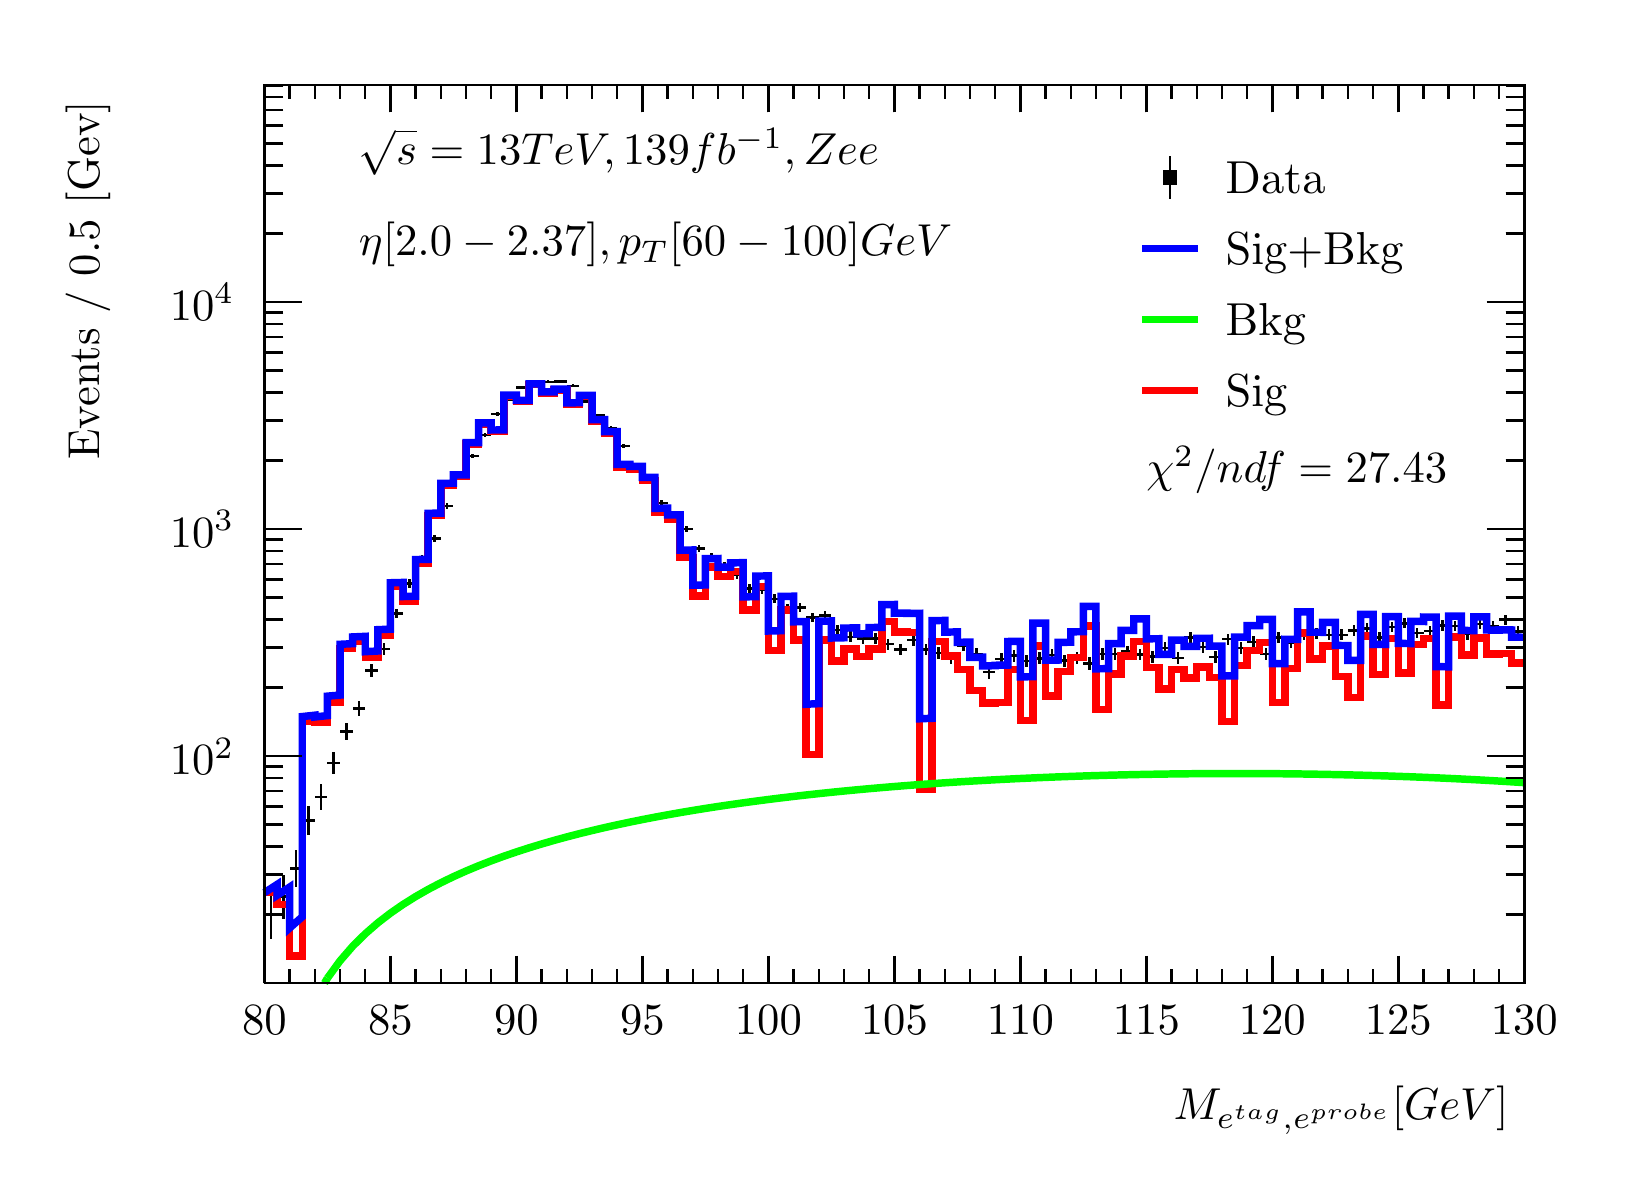
\begin{tikzpicture}
\pgfdeclareplotmark{cross} {
\pgfpathmoveto{\pgfpoint{-0.3\pgfplotmarksize}{\pgfplotmarksize}}
\pgfpathlineto{\pgfpoint{+0.3\pgfplotmarksize}{\pgfplotmarksize}}
\pgfpathlineto{\pgfpoint{+0.3\pgfplotmarksize}{0.3\pgfplotmarksize}}
\pgfpathlineto{\pgfpoint{+1\pgfplotmarksize}{0.3\pgfplotmarksize}}
\pgfpathlineto{\pgfpoint{+1\pgfplotmarksize}{-0.3\pgfplotmarksize}}
\pgfpathlineto{\pgfpoint{+0.3\pgfplotmarksize}{-0.3\pgfplotmarksize}}
\pgfpathlineto{\pgfpoint{+0.3\pgfplotmarksize}{-1.\pgfplotmarksize}}
\pgfpathlineto{\pgfpoint{-0.3\pgfplotmarksize}{-1.\pgfplotmarksize}}
\pgfpathlineto{\pgfpoint{-0.3\pgfplotmarksize}{-0.3\pgfplotmarksize}}
\pgfpathlineto{\pgfpoint{-1.\pgfplotmarksize}{-0.3\pgfplotmarksize}}
\pgfpathlineto{\pgfpoint{-1.\pgfplotmarksize}{0.3\pgfplotmarksize}}
\pgfpathlineto{\pgfpoint{-0.3\pgfplotmarksize}{0.3\pgfplotmarksize}}
\pgfpathclose
\pgfusepathqstroke
}
\pgfdeclareplotmark{cross*} {
\pgfpathmoveto{\pgfpoint{-0.3\pgfplotmarksize}{\pgfplotmarksize}}
\pgfpathlineto{\pgfpoint{+0.3\pgfplotmarksize}{\pgfplotmarksize}}
\pgfpathlineto{\pgfpoint{+0.3\pgfplotmarksize}{0.3\pgfplotmarksize}}
\pgfpathlineto{\pgfpoint{+1\pgfplotmarksize}{0.3\pgfplotmarksize}}
\pgfpathlineto{\pgfpoint{+1\pgfplotmarksize}{-0.3\pgfplotmarksize}}
\pgfpathlineto{\pgfpoint{+0.3\pgfplotmarksize}{-0.3\pgfplotmarksize}}
\pgfpathlineto{\pgfpoint{+0.3\pgfplotmarksize}{-1.\pgfplotmarksize}}
\pgfpathlineto{\pgfpoint{-0.3\pgfplotmarksize}{-1.\pgfplotmarksize}}
\pgfpathlineto{\pgfpoint{-0.3\pgfplotmarksize}{-0.3\pgfplotmarksize}}
\pgfpathlineto{\pgfpoint{-1.\pgfplotmarksize}{-0.3\pgfplotmarksize}}
\pgfpathlineto{\pgfpoint{-1.\pgfplotmarksize}{0.3\pgfplotmarksize}}
\pgfpathlineto{\pgfpoint{-0.3\pgfplotmarksize}{0.3\pgfplotmarksize}}
\pgfpathclose
\pgfusepathqfillstroke
}
\pgfdeclareplotmark{newstar} {
\pgfpathmoveto{\pgfqpoint{0pt}{\pgfplotmarksize}}
\pgfpathlineto{\pgfqpointpolar{44}{0.5\pgfplotmarksize}}
\pgfpathlineto{\pgfqpointpolar{18}{\pgfplotmarksize}}
\pgfpathlineto{\pgfqpointpolar{-20}{0.5\pgfplotmarksize}}
\pgfpathlineto{\pgfqpointpolar{-54}{\pgfplotmarksize}}
\pgfpathlineto{\pgfqpointpolar{-90}{0.5\pgfplotmarksize}}
\pgfpathlineto{\pgfqpointpolar{234}{\pgfplotmarksize}}
\pgfpathlineto{\pgfqpointpolar{198}{0.5\pgfplotmarksize}}
\pgfpathlineto{\pgfqpointpolar{162}{\pgfplotmarksize}}
\pgfpathlineto{\pgfqpointpolar{134}{0.5\pgfplotmarksize}}
\pgfpathclose
\pgfusepathqstroke
}
\pgfdeclareplotmark{newstar*} {
\pgfpathmoveto{\pgfqpoint{0pt}{\pgfplotmarksize}}
\pgfpathlineto{\pgfqpointpolar{44}{0.5\pgfplotmarksize}}
\pgfpathlineto{\pgfqpointpolar{18}{\pgfplotmarksize}}
\pgfpathlineto{\pgfqpointpolar{-20}{0.5\pgfplotmarksize}}
\pgfpathlineto{\pgfqpointpolar{-54}{\pgfplotmarksize}}
\pgfpathlineto{\pgfqpointpolar{-90}{0.5\pgfplotmarksize}}
\pgfpathlineto{\pgfqpointpolar{234}{\pgfplotmarksize}}
\pgfpathlineto{\pgfqpointpolar{198}{0.5\pgfplotmarksize}}
\pgfpathlineto{\pgfqpointpolar{162}{\pgfplotmarksize}}
\pgfpathlineto{\pgfqpointpolar{134}{0.5\pgfplotmarksize}}
\pgfpathclose
\pgfusepathqfillstroke
}
\definecolor{c}{rgb}{1,1,1};
\draw [color=c, fill=c] (0,0) rectangle (20,14.4361);
\draw [color=c, fill=c] (3,2.30977) rectangle (19,13.7143);
\definecolor{c}{rgb}{0,0,0};
\draw [c,line width=0.9] (3,2.30977) -- (3,13.7143) -- (19,13.7143) -- (19,2.30977) -- (3,2.30977);
\definecolor{c}{rgb}{1,1,1};
\draw [color=c, fill=c] (3,2.30977) rectangle (19,13.7143);
\definecolor{c}{rgb}{0,0,0};
\draw [c,line width=0.9] (3,2.30977) -- (3,13.7143) -- (19,13.7143) -- (19,2.30977) -- (3,2.30977);
\draw [c,line width=0.9] (3,2.30977) -- (19,2.30977);
\draw [c,line width=0.9] (3,2.65624) -- (3,2.30977);
\draw [c,line width=0.9] (3.32,2.48301) -- (3.32,2.30977);
\draw [c,line width=0.9] (3.64,2.48301) -- (3.64,2.30977);
\draw [c,line width=0.9] (3.96,2.48301) -- (3.96,2.30977);
\draw [c,line width=0.9] (4.28,2.48301) -- (4.28,2.30977);
\draw [c,line width=0.9] (4.6,2.65624) -- (4.6,2.30977);
\draw [c,line width=0.9] (4.92,2.48301) -- (4.92,2.30977);
\draw [c,line width=0.9] (5.24,2.48301) -- (5.24,2.30977);
\draw [c,line width=0.9] (5.56,2.48301) -- (5.56,2.30977);
\draw [c,line width=0.9] (5.88,2.48301) -- (5.88,2.30977);
\draw [c,line width=0.9] (6.2,2.65624) -- (6.2,2.30977);
\draw [c,line width=0.9] (6.52,2.48301) -- (6.52,2.30977);
\draw [c,line width=0.9] (6.84,2.48301) -- (6.84,2.30977);
\draw [c,line width=0.9] (7.16,2.48301) -- (7.16,2.30977);
\draw [c,line width=0.9] (7.48,2.48301) -- (7.48,2.30977);
\draw [c,line width=0.9] (7.8,2.65624) -- (7.8,2.30977);
\draw [c,line width=0.9] (8.12,2.48301) -- (8.12,2.30977);
\draw [c,line width=0.9] (8.44,2.48301) -- (8.44,2.30977);
\draw [c,line width=0.9] (8.76,2.48301) -- (8.76,2.30977);
\draw [c,line width=0.9] (9.08,2.48301) -- (9.08,2.30977);
\draw [c,line width=0.9] (9.4,2.65624) -- (9.4,2.30977);
\draw [c,line width=0.9] (9.72,2.48301) -- (9.72,2.30977);
\draw [c,line width=0.9] (10.04,2.48301) -- (10.04,2.30977);
\draw [c,line width=0.9] (10.36,2.48301) -- (10.36,2.30977);
\draw [c,line width=0.9] (10.68,2.48301) -- (10.68,2.30977);
\draw [c,line width=0.9] (11,2.65624) -- (11,2.30977);
\draw [c,line width=0.9] (11.32,2.48301) -- (11.32,2.30977);
\draw [c,line width=0.9] (11.64,2.48301) -- (11.64,2.30977);
\draw [c,line width=0.9] (11.96,2.48301) -- (11.96,2.30977);
\draw [c,line width=0.9] (12.28,2.48301) -- (12.28,2.30977);
\draw [c,line width=0.9] (12.6,2.65624) -- (12.6,2.30977);
\draw [c,line width=0.9] (12.92,2.48301) -- (12.92,2.30977);
\draw [c,line width=0.9] (13.24,2.48301) -- (13.24,2.30977);
\draw [c,line width=0.9] (13.56,2.48301) -- (13.56,2.30977);
\draw [c,line width=0.9] (13.88,2.48301) -- (13.88,2.30977);
\draw [c,line width=0.9] (14.2,2.65624) -- (14.2,2.30977);
\draw [c,line width=0.9] (14.52,2.48301) -- (14.52,2.30977);
\draw [c,line width=0.9] (14.84,2.48301) -- (14.84,2.30977);
\draw [c,line width=0.9] (15.16,2.48301) -- (15.16,2.30977);
\draw [c,line width=0.9] (15.48,2.48301) -- (15.48,2.30977);
\draw [c,line width=0.9] (15.8,2.65624) -- (15.8,2.30977);
\draw [c,line width=0.9] (16.12,2.48301) -- (16.12,2.30977);
\draw [c,line width=0.9] (16.44,2.48301) -- (16.44,2.30977);
\draw [c,line width=0.9] (16.76,2.48301) -- (16.76,2.30977);
\draw [c,line width=0.9] (17.08,2.48301) -- (17.08,2.30977);
\draw [c,line width=0.9] (17.4,2.65624) -- (17.4,2.30977);
\draw [c,line width=0.9] (17.72,2.48301) -- (17.72,2.30977);
\draw [c,line width=0.9] (18.04,2.48301) -- (18.04,2.30977);
\draw [c,line width=0.9] (18.36,2.48301) -- (18.36,2.30977);
\draw [c,line width=0.9] (18.68,2.48301) -- (18.68,2.30977);
\draw [c,line width=0.9] (19,2.65624) -- (19,2.30977);
\draw [anchor=base] (3,1.66015) node[scale=1.61424, color=c, rotate=0]{80};
\draw [anchor=base] (4.6,1.66015) node[scale=1.61424, color=c, rotate=0]{85};
\draw [anchor=base] (6.2,1.66015) node[scale=1.61424, color=c, rotate=0]{90};
\draw [anchor=base] (7.8,1.66015) node[scale=1.61424, color=c, rotate=0]{95};
\draw [anchor=base] (9.4,1.66015) node[scale=1.61424, color=c, rotate=0]{100};
\draw [anchor=base] (11,1.66015) node[scale=1.61424, color=c, rotate=0]{105};
\draw [anchor=base] (12.6,1.66015) node[scale=1.61424, color=c, rotate=0]{110};
\draw [anchor=base] (14.2,1.66015) node[scale=1.61424, color=c, rotate=0]{115};
\draw [anchor=base] (15.8,1.66015) node[scale=1.61424, color=c, rotate=0]{120};
\draw [anchor=base] (17.4,1.66015) node[scale=1.61424, color=c, rotate=0]{125};
\draw [anchor=base] (19,1.66015) node[scale=1.61424, color=c, rotate=0]{130};
\draw [anchor= east] (19,0.692932) node[scale=1.61424, color=c, rotate=0]{$M_{e^{tag}, e^{probe}}  [GeV]$};
\draw [c,line width=0.9] (3,13.7143) -- (19,13.7143);
\draw [c,line width=0.9] (3,13.3678) -- (3,13.7143);
\draw [c,line width=0.9] (3.32,13.5411) -- (3.32,13.7143);
\draw [c,line width=0.9] (3.64,13.5411) -- (3.64,13.7143);
\draw [c,line width=0.9] (3.96,13.5411) -- (3.96,13.7143);
\draw [c,line width=0.9] (4.28,13.5411) -- (4.28,13.7143);
\draw [c,line width=0.9] (4.6,13.3678) -- (4.6,13.7143);
\draw [c,line width=0.9] (4.92,13.5411) -- (4.92,13.7143);
\draw [c,line width=0.9] (5.24,13.5411) -- (5.24,13.7143);
\draw [c,line width=0.9] (5.56,13.5411) -- (5.56,13.7143);
\draw [c,line width=0.9] (5.88,13.5411) -- (5.88,13.7143);
\draw [c,line width=0.9] (6.2,13.3678) -- (6.2,13.7143);
\draw [c,line width=0.9] (6.52,13.5411) -- (6.52,13.7143);
\draw [c,line width=0.9] (6.84,13.5411) -- (6.84,13.7143);
\draw [c,line width=0.9] (7.16,13.5411) -- (7.16,13.7143);
\draw [c,line width=0.9] (7.48,13.5411) -- (7.48,13.7143);
\draw [c,line width=0.9] (7.8,13.3678) -- (7.8,13.7143);
\draw [c,line width=0.9] (8.12,13.5411) -- (8.12,13.7143);
\draw [c,line width=0.9] (8.44,13.5411) -- (8.44,13.7143);
\draw [c,line width=0.9] (8.76,13.5411) -- (8.76,13.7143);
\draw [c,line width=0.9] (9.08,13.5411) -- (9.08,13.7143);
\draw [c,line width=0.9] (9.4,13.3678) -- (9.4,13.7143);
\draw [c,line width=0.9] (9.72,13.5411) -- (9.72,13.7143);
\draw [c,line width=0.9] (10.04,13.5411) -- (10.04,13.7143);
\draw [c,line width=0.9] (10.36,13.5411) -- (10.36,13.7143);
\draw [c,line width=0.9] (10.68,13.5411) -- (10.68,13.7143);
\draw [c,line width=0.9] (11,13.3678) -- (11,13.7143);
\draw [c,line width=0.9] (11.32,13.5411) -- (11.32,13.7143);
\draw [c,line width=0.9] (11.64,13.5411) -- (11.64,13.7143);
\draw [c,line width=0.9] (11.96,13.5411) -- (11.96,13.7143);
\draw [c,line width=0.9] (12.28,13.5411) -- (12.28,13.7143);
\draw [c,line width=0.9] (12.6,13.3678) -- (12.6,13.7143);
\draw [c,line width=0.9] (12.92,13.5411) -- (12.92,13.7143);
\draw [c,line width=0.9] (13.24,13.5411) -- (13.24,13.7143);
\draw [c,line width=0.9] (13.56,13.5411) -- (13.56,13.7143);
\draw [c,line width=0.9] (13.88,13.5411) -- (13.88,13.7143);
\draw [c,line width=0.9] (14.2,13.3678) -- (14.2,13.7143);
\draw [c,line width=0.9] (14.52,13.5411) -- (14.52,13.7143);
\draw [c,line width=0.9] (14.84,13.5411) -- (14.84,13.7143);
\draw [c,line width=0.9] (15.16,13.5411) -- (15.16,13.7143);
\draw [c,line width=0.9] (15.48,13.5411) -- (15.48,13.7143);
\draw [c,line width=0.9] (15.8,13.3678) -- (15.8,13.7143);
\draw [c,line width=0.9] (16.12,13.5411) -- (16.12,13.7143);
\draw [c,line width=0.9] (16.44,13.5411) -- (16.44,13.7143);
\draw [c,line width=0.9] (16.76,13.5411) -- (16.76,13.7143);
\draw [c,line width=0.9] (17.08,13.5411) -- (17.08,13.7143);
\draw [c,line width=0.9] (17.4,13.3678) -- (17.4,13.7143);
\draw [c,line width=0.9] (17.72,13.5411) -- (17.72,13.7143);
\draw [c,line width=0.9] (18.04,13.5411) -- (18.04,13.7143);
\draw [c,line width=0.9] (18.36,13.5411) -- (18.36,13.7143);
\draw [c,line width=0.9] (18.68,13.5411) -- (18.68,13.7143);
\draw [c,line width=0.9] (19,13.3678) -- (19,13.7143);
\draw [c,line width=0.9] (3,2.30977) -- (3,13.7143);
\draw [c,line width=0.9] (3.237,3.17769) -- (3,3.17769);
\draw [c,line width=0.9] (3.237,3.68539) -- (3,3.68539);
\draw [c,line width=0.9] (3.237,4.04561) -- (3,4.04561);
\draw [c,line width=0.9] (3.237,4.32501) -- (3,4.32501);
\draw [c,line width=0.9] (3.237,4.55331) -- (3,4.55331);
\draw [c,line width=0.9] (3.237,4.74632) -- (3,4.74632);
\draw [c,line width=0.9] (3.237,4.91352) -- (3,4.91352);
\draw [c,line width=0.9] (3.237,5.061) -- (3,5.061);
\draw [c,line width=0.9] (3.474,5.19293) -- (3,5.19293);
\draw [anchor= east] (2.82,5.19293) node[scale=1.61424, color=c, rotate=0]{$10^{2}$};
\draw [c,line width=0.9] (3.237,6.06085) -- (3,6.06085);
\draw [c,line width=0.9] (3.237,6.56855) -- (3,6.56855);
\draw [c,line width=0.9] (3.237,6.92876) -- (3,6.92876);
\draw [c,line width=0.9] (3.237,7.20817) -- (3,7.20817);
\draw [c,line width=0.9] (3.237,7.43646) -- (3,7.43646);
\draw [c,line width=0.9] (3.237,7.62948) -- (3,7.62948);
\draw [c,line width=0.9] (3.237,7.79668) -- (3,7.79668);
\draw [c,line width=0.9] (3.237,7.94416) -- (3,7.94416);
\draw [c,line width=0.9] (3.474,8.07609) -- (3,8.07609);
\draw [anchor= east] (2.82,8.07609) node[scale=1.61424, color=c, rotate=0]{$10^{3}$};
\draw [c,line width=0.9] (3.237,8.94401) -- (3,8.94401);
\draw [c,line width=0.9] (3.237,9.4517) -- (3,9.4517);
\draw [c,line width=0.9] (3.237,9.81192) -- (3,9.81192);
\draw [c,line width=0.9] (3.237,10.0913) -- (3,10.0913);
\draw [c,line width=0.9] (3.237,10.3196) -- (3,10.3196);
\draw [c,line width=0.9] (3.237,10.5126) -- (3,10.5126);
\draw [c,line width=0.9] (3.237,10.6798) -- (3,10.6798);
\draw [c,line width=0.9] (3.237,10.8273) -- (3,10.8273);
\draw [c,line width=0.9] (3.474,10.9592) -- (3,10.9592);
\draw [anchor= east] (2.82,10.9592) node[scale=1.61424, color=c, rotate=0]{$10^{4}$};
\draw [c,line width=0.9] (3.237,11.8272) -- (3,11.8272);
\draw [c,line width=0.9] (3.237,12.3349) -- (3,12.3349);
\draw [c,line width=0.9] (3.237,12.6951) -- (3,12.6951);
\draw [c,line width=0.9] (3.237,12.9745) -- (3,12.9745);
\draw [c,line width=0.9] (3.237,13.2028) -- (3,13.2028);
\draw [c,line width=0.9] (3.237,13.3958) -- (3,13.3958);
\draw [c,line width=0.9] (3.237,13.563) -- (3,13.563);
\draw [c,line width=0.9] (3.237,13.7105) -- (3,13.7105);
\draw [anchor= east] (0.76,13.7143) node[scale=1.61424, color=c, rotate=90]{Events / 0.5 [Gev]};
\draw [c,line width=0.9] (19,2.30977) -- (19,13.7143);
\draw [c,line width=0.9] (18.763,3.17769) -- (19,3.17769);
\draw [c,line width=0.9] (18.763,3.68539) -- (19,3.68539);
\draw [c,line width=0.9] (18.763,4.04561) -- (19,4.04561);
\draw [c,line width=0.9] (18.763,4.32501) -- (19,4.32501);
\draw [c,line width=0.9] (18.763,4.55331) -- (19,4.55331);
\draw [c,line width=0.9] (18.763,4.74632) -- (19,4.74632);
\draw [c,line width=0.9] (18.763,4.91352) -- (19,4.91352);
\draw [c,line width=0.9] (18.763,5.061) -- (19,5.061);
\draw [c,line width=0.9] (18.526,5.19293) -- (19,5.19293);
\draw [c,line width=0.9] (18.763,6.06085) -- (19,6.06085);
\draw [c,line width=0.9] (18.763,6.56855) -- (19,6.56855);
\draw [c,line width=0.9] (18.763,6.92876) -- (19,6.92876);
\draw [c,line width=0.9] (18.763,7.20817) -- (19,7.20817);
\draw [c,line width=0.9] (18.763,7.43646) -- (19,7.43646);
\draw [c,line width=0.9] (18.763,7.62948) -- (19,7.62948);
\draw [c,line width=0.9] (18.763,7.79668) -- (19,7.79668);
\draw [c,line width=0.9] (18.763,7.94416) -- (19,7.94416);
\draw [c,line width=0.9] (18.526,8.07609) -- (19,8.07609);
\draw [c,line width=0.9] (18.763,8.94401) -- (19,8.94401);
\draw [c,line width=0.9] (18.763,9.4517) -- (19,9.4517);
\draw [c,line width=0.9] (18.763,9.81192) -- (19,9.81192);
\draw [c,line width=0.9] (18.763,10.0913) -- (19,10.0913);
\draw [c,line width=0.9] (18.763,10.3196) -- (19,10.3196);
\draw [c,line width=0.9] (18.763,10.5126) -- (19,10.5126);
\draw [c,line width=0.9] (18.763,10.6798) -- (19,10.6798);
\draw [c,line width=0.9] (18.763,10.8273) -- (19,10.8273);
\draw [c,line width=0.9] (18.526,10.9592) -- (19,10.9592);
\draw [c,line width=0.9] (18.763,11.8272) -- (19,11.8272);
\draw [c,line width=0.9] (18.763,12.3349) -- (19,12.3349);
\draw [c,line width=0.9] (18.763,12.6951) -- (19,12.6951);
\draw [c,line width=0.9] (18.763,12.9745) -- (19,12.9745);
\draw [c,line width=0.9] (18.763,13.2028) -- (19,13.2028);
\draw [c,line width=0.9] (18.763,13.3958) -- (19,13.3958);
\draw [c,line width=0.9] (18.763,13.563) -- (19,13.563);
\draw [c,line width=0.9] (18.763,13.7105) -- (19,13.7105);
\draw [c,line width=0.9] (3.08,3.17769) -- (3,3.17769);
\draw [c,line width=0.9] (3,3.17769) -- (3,3.17769);
\draw [c,line width=0.9] (3.08,3.17769) -- (3.16,3.17769);
\draw [c,line width=0.9] (3.16,3.17769) -- (3.16,3.17769);
\draw [c,line width=0.9] (3.08,3.17769) -- (3.08,3.48418);
\draw [c,line width=0.9] (3.08,3.48418) -- (3.08,3.48418);
\draw [c,line width=0.9] (3.08,3.17769) -- (3.08,2.86382);
\draw [c,line width=0.9] (3.08,2.86382) -- (3.08,2.86382);
\draw [c,line width=0.9] (3.24,3.40598) -- (3.16,3.40598);
\draw [c,line width=0.9] (3.16,3.40598) -- (3.16,3.40598);
\draw [c,line width=0.9] (3.24,3.40598) -- (3.32,3.40598);
\draw [c,line width=0.9] (3.32,3.40598) -- (3.32,3.40598);
\draw [c,line width=0.9] (3.24,3.40598) -- (3.24,3.68401);
\draw [c,line width=0.9] (3.24,3.68401) -- (3.24,3.68401);
\draw [c,line width=0.9] (3.24,3.40598) -- (3.24,3.12236);
\draw [c,line width=0.9] (3.24,3.12236) -- (3.24,3.12236);
\draw [c,line width=0.9] (3.4,3.7662) -- (3.32,3.7662);
\draw [c,line width=0.9] (3.32,3.7662) -- (3.32,3.7662);
\draw [c,line width=0.9] (3.4,3.7662) -- (3.48,3.7662);
\draw [c,line width=0.9] (3.48,3.7662) -- (3.48,3.7662);
\draw [c,line width=0.9] (3.4,3.7662) -- (3.4,4.00475);
\draw [c,line width=0.9] (3.4,4.00475) -- (3.4,4.00475);
\draw [c,line width=0.9] (3.4,3.7662) -- (3.4,3.52404);
\draw [c,line width=0.9] (3.4,3.52404) -- (3.4,3.52404);
\draw [c,line width=0.9] (3.56,4.37413) -- (3.48,4.37413);
\draw [c,line width=0.9] (3.48,4.37413) -- (3.48,4.37413);
\draw [c,line width=0.9] (3.56,4.37413) -- (3.64,4.37413);
\draw [c,line width=0.9] (3.64,4.37413) -- (3.64,4.37413);
\draw [c,line width=0.9] (3.56,4.37413) -- (3.56,4.55867);
\draw [c,line width=0.9] (3.56,4.55867) -- (3.56,4.55867);
\draw [c,line width=0.9] (3.56,4.37413) -- (3.56,4.18785);
\draw [c,line width=0.9] (3.56,4.18785) -- (3.56,4.18785);
\draw [c,line width=0.9] (3.72,4.67265) -- (3.64,4.67265);
\draw [c,line width=0.9] (3.64,4.67265) -- (3.64,4.67265);
\draw [c,line width=0.9] (3.72,4.67265) -- (3.8,4.67265);
\draw [c,line width=0.9] (3.8,4.67265) -- (3.8,4.67265);
\draw [c,line width=0.9] (3.72,4.67265) -- (3.72,4.83547);
\draw [c,line width=0.9] (3.72,4.83547) -- (3.72,4.83547);
\draw [c,line width=0.9] (3.72,4.67265) -- (3.72,4.50862);
\draw [c,line width=0.9] (3.72,4.50862) -- (3.72,4.50862);
\draw [c,line width=0.9] (3.88,5.10206) -- (3.8,5.10206);
\draw [c,line width=0.9] (3.8,5.10206) -- (3.8,5.10206);
\draw [c,line width=0.9] (3.88,5.10206) -- (3.96,5.10206);
\draw [c,line width=0.9] (3.96,5.10206) -- (3.96,5.10206);
\draw [c,line width=0.9] (3.88,5.10206) -- (3.88,5.23816);
\draw [c,line width=0.9] (3.88,5.23816) -- (3.88,5.23816);
\draw [c,line width=0.9] (3.88,5.10206) -- (3.88,4.96525);
\draw [c,line width=0.9] (3.88,4.96525) -- (3.88,4.96525);
\draw [c,line width=0.9] (4.04,5.50204) -- (3.96,5.50204);
\draw [c,line width=0.9] (3.96,5.50204) -- (3.96,5.50204);
\draw [c,line width=0.9] (4.04,5.50204) -- (4.12,5.50204);
\draw [c,line width=0.9] (4.12,5.50204) -- (4.12,5.50204);
\draw [c,line width=0.9] (4.04,5.50204) -- (4.04,5.61267);
\draw [c,line width=0.9] (4.04,5.61267) -- (4.04,5.61267);
\draw [c,line width=0.9] (4.04,5.50204) -- (4.04,5.3914);
\draw [c,line width=0.9] (4.04,5.3914) -- (4.04,5.3914);
\draw [c,line width=0.9] (4.2,5.797) -- (4.12,5.797);
\draw [c,line width=0.9] (4.12,5.797) -- (4.12,5.797);
\draw [c,line width=0.9] (4.2,5.797) -- (4.28,5.797);
\draw [c,line width=0.9] (4.28,5.797) -- (4.28,5.797);
\draw [c,line width=0.9] (4.2,5.797) -- (4.2,5.89535);
\draw [c,line width=0.9] (4.2,5.89535) -- (4.2,5.89535);
\draw [c,line width=0.9] (4.2,5.797) -- (4.2,5.69865);
\draw [c,line width=0.9] (4.2,5.69865) -- (4.2,5.69865);
\draw [c,line width=0.9] (4.36,6.27866) -- (4.28,6.27866);
\draw [c,line width=0.9] (4.28,6.27866) -- (4.28,6.27866);
\draw [c,line width=0.9] (4.36,6.27866) -- (4.44,6.27866);
\draw [c,line width=0.9] (4.44,6.27866) -- (4.44,6.27866);
\draw [c,line width=0.9] (4.36,6.27866) -- (4.36,6.35981);
\draw [c,line width=0.9] (4.36,6.35981) -- (4.36,6.35981);
\draw [c,line width=0.9] (4.36,6.27866) -- (4.36,6.19751);
\draw [c,line width=0.9] (4.36,6.19751) -- (4.36,6.19751);
\draw [c,line width=0.9] (4.52,6.55174) -- (4.44,6.55174);
\draw [c,line width=0.9] (4.44,6.55174) -- (4.44,6.55174);
\draw [c,line width=0.9] (4.52,6.55174) -- (4.6,6.55174);
\draw [c,line width=0.9] (4.6,6.55174) -- (4.6,6.55174);
\draw [c,line width=0.9] (4.52,6.55174) -- (4.52,6.62451);
\draw [c,line width=0.9] (4.52,6.62451) -- (4.52,6.62451);
\draw [c,line width=0.9] (4.52,6.55174) -- (4.52,6.47897);
\draw [c,line width=0.9] (4.52,6.47897) -- (4.52,6.47897);
\draw [c,line width=0.9] (4.68,7.00468) -- (4.6,7.00468);
\draw [c,line width=0.9] (4.6,7.00468) -- (4.6,7.00468);
\draw [c,line width=0.9] (4.68,7.00468) -- (4.76,7.00468);
\draw [c,line width=0.9] (4.76,7.00468) -- (4.76,7.00468);
\draw [c,line width=0.9] (4.68,7.00468) -- (4.68,7.06541);
\draw [c,line width=0.9] (4.68,7.06541) -- (4.68,7.06541);
\draw [c,line width=0.9] (4.68,7.00468) -- (4.68,6.94394);
\draw [c,line width=0.9] (4.68,6.94394) -- (4.68,6.94394);
\draw [c,line width=0.9] (4.84,7.38317) -- (4.76,7.38317);
\draw [c,line width=0.9] (4.76,7.38317) -- (4.76,7.38317);
\draw [c,line width=0.9] (4.84,7.38317) -- (4.92,7.38317);
\draw [c,line width=0.9] (4.92,7.38317) -- (4.92,7.38317);
\draw [c,line width=0.9] (4.84,7.38317) -- (4.84,7.43539);
\draw [c,line width=0.9] (4.84,7.43539) -- (4.84,7.43539);
\draw [c,line width=0.9] (4.84,7.38317) -- (4.84,7.33096);
\draw [c,line width=0.9] (4.84,7.33096) -- (4.84,7.33096);
\draw [c,line width=0.9] (5,7.69398) -- (4.92,7.69398);
\draw [c,line width=0.9] (4.92,7.69398) -- (4.92,7.69398);
\draw [c,line width=0.9] (5,7.69398) -- (5.08,7.69398);
\draw [c,line width=0.9] (5.08,7.69398) -- (5.08,7.69398);
\draw [c,line width=0.9] (5,7.69398) -- (5,7.7401);
\draw [c,line width=0.9] (5,7.7401) -- (5,7.7401);
\draw [c,line width=0.9] (5,7.69398) -- (5,7.64786);
\draw [c,line width=0.9] (5,7.64786) -- (5,7.64786);
\draw [c,line width=0.9] (5.16,7.95387) -- (5.08,7.95387);
\draw [c,line width=0.9] (5.08,7.95387) -- (5.08,7.95387);
\draw [c,line width=0.9] (5.16,7.95387) -- (5.24,7.95387);
\draw [c,line width=0.9] (5.24,7.95387) -- (5.24,7.95387);
\draw [c,line width=0.9] (5.16,7.95387) -- (5.16,7.99544);
\draw [c,line width=0.9] (5.16,7.99544) -- (5.16,7.99544);
\draw [c,line width=0.9] (5.16,7.95387) -- (5.16,7.91229);
\draw [c,line width=0.9] (5.16,7.91229) -- (5.16,7.91229);
\draw [c,line width=0.9] (5.32,8.37043) -- (5.24,8.37043);
\draw [c,line width=0.9] (5.24,8.37043) -- (5.24,8.37043);
\draw [c,line width=0.9] (5.32,8.37043) -- (5.4,8.37043);
\draw [c,line width=0.9] (5.4,8.37043) -- (5.4,8.37043);
\draw [c,line width=0.9] (5.32,8.37043) -- (5.32,8.40564);
\draw [c,line width=0.9] (5.32,8.40564) -- (5.32,8.40564);
\draw [c,line width=0.9] (5.32,8.37043) -- (5.32,8.33523);
\draw [c,line width=0.9] (5.32,8.33523) -- (5.32,8.33523);
\draw [c,line width=0.9] (5.48,8.74272) -- (5.4,8.74272);
\draw [c,line width=0.9] (5.4,8.74272) -- (5.4,8.74272);
\draw [c,line width=0.9] (5.48,8.74272) -- (5.56,8.74272);
\draw [c,line width=0.9] (5.56,8.74272) -- (5.56,8.74272);
\draw [c,line width=0.9] (5.48,8.74272) -- (5.48,8.77306);
\draw [c,line width=0.9] (5.48,8.77306) -- (5.48,8.77306);
\draw [c,line width=0.9] (5.48,8.74272) -- (5.48,8.71238);
\draw [c,line width=0.9] (5.48,8.71238) -- (5.48,8.71238);
\draw [c,line width=0.9] (5.64,9.0045) -- (5.56,9.0045);
\draw [c,line width=0.9] (5.56,9.0045) -- (5.56,9.0045);
\draw [c,line width=0.9] (5.64,9.0045) -- (5.72,9.0045);
\draw [c,line width=0.9] (5.72,9.0045) -- (5.72,9.0045);
\draw [c,line width=0.9] (5.64,9.0045) -- (5.64,9.03183);
\draw [c,line width=0.9] (5.64,9.03183) -- (5.64,9.03183);
\draw [c,line width=0.9] (5.64,9.0045) -- (5.64,8.97717);
\draw [c,line width=0.9] (5.64,8.97717) -- (5.64,8.97717);
\draw [c,line width=0.9] (5.8,9.26915) -- (5.72,9.26915);
\draw [c,line width=0.9] (5.72,9.26915) -- (5.72,9.26915);
\draw [c,line width=0.9] (5.8,9.26915) -- (5.88,9.26915);
\draw [c,line width=0.9] (5.88,9.26915) -- (5.88,9.26915);
\draw [c,line width=0.9] (5.8,9.26915) -- (5.8,9.29374);
\draw [c,line width=0.9] (5.8,9.29374) -- (5.8,9.29374);
\draw [c,line width=0.9] (5.8,9.26915) -- (5.8,9.24456);
\draw [c,line width=0.9] (5.8,9.24456) -- (5.8,9.24456);
\draw [c,line width=0.9] (5.96,9.53525) -- (5.88,9.53525);
\draw [c,line width=0.9] (5.88,9.53525) -- (5.88,9.53525);
\draw [c,line width=0.9] (5.96,9.53525) -- (6.04,9.53525);
\draw [c,line width=0.9] (6.04,9.53525) -- (6.04,9.53525);
\draw [c,line width=0.9] (5.96,9.53525) -- (5.96,9.55736);
\draw [c,line width=0.9] (5.96,9.55736) -- (5.96,9.55736);
\draw [c,line width=0.9] (5.96,9.53525) -- (5.96,9.51314);
\draw [c,line width=0.9] (5.96,9.51314) -- (5.96,9.51314);
\draw [c,line width=0.9] (6.12,9.72206) -- (6.04,9.72206);
\draw [c,line width=0.9] (6.04,9.72206) -- (6.04,9.72206);
\draw [c,line width=0.9] (6.12,9.72206) -- (6.2,9.72206);
\draw [c,line width=0.9] (6.2,9.72206) -- (6.2,9.72206);
\draw [c,line width=0.9] (6.12,9.72206) -- (6.12,9.74259);
\draw [c,line width=0.9] (6.12,9.74259) -- (6.12,9.74259);
\draw [c,line width=0.9] (6.12,9.72206) -- (6.12,9.70154);
\draw [c,line width=0.9] (6.12,9.70154) -- (6.12,9.70154);
\draw [c,line width=0.9] (6.28,9.87182) -- (6.2,9.87182);
\draw [c,line width=0.9] (6.2,9.87182) -- (6.2,9.87182);
\draw [c,line width=0.9] (6.28,9.87182) -- (6.36,9.87182);
\draw [c,line width=0.9] (6.36,9.87182) -- (6.36,9.87182);
\draw [c,line width=0.9] (6.28,9.87182) -- (6.28,9.89115);
\draw [c,line width=0.9] (6.28,9.89115) -- (6.28,9.89115);
\draw [c,line width=0.9] (6.28,9.87182) -- (6.28,9.85249);
\draw [c,line width=0.9] (6.28,9.85249) -- (6.28,9.85249);
\draw [c,line width=0.9] (6.44,9.9135) -- (6.36,9.9135);
\draw [c,line width=0.9] (6.36,9.9135) -- (6.36,9.9135);
\draw [c,line width=0.9] (6.44,9.9135) -- (6.52,9.9135);
\draw [c,line width=0.9] (6.52,9.9135) -- (6.52,9.9135);
\draw [c,line width=0.9] (6.44,9.9135) -- (6.44,9.93251);
\draw [c,line width=0.9] (6.44,9.93251) -- (6.44,9.93251);
\draw [c,line width=0.9] (6.44,9.9135) -- (6.44,9.89449);
\draw [c,line width=0.9] (6.44,9.89449) -- (6.44,9.89449);
\draw [c,line width=0.9] (6.6,9.94626) -- (6.52,9.94626);
\draw [c,line width=0.9] (6.52,9.94626) -- (6.52,9.94626);
\draw [c,line width=0.9] (6.6,9.94626) -- (6.68,9.94626);
\draw [c,line width=0.9] (6.68,9.94626) -- (6.68,9.94626);
\draw [c,line width=0.9] (6.6,9.94626) -- (6.6,9.96502);
\draw [c,line width=0.9] (6.6,9.96502) -- (6.6,9.96502);
\draw [c,line width=0.9] (6.6,9.94626) -- (6.6,9.92749);
\draw [c,line width=0.9] (6.6,9.92749) -- (6.6,9.92749);
\draw [c,line width=0.9] (6.76,9.95215) -- (6.68,9.95215);
\draw [c,line width=0.9] (6.68,9.95215) -- (6.68,9.95215);
\draw [c,line width=0.9] (6.76,9.95215) -- (6.84,9.95215);
\draw [c,line width=0.9] (6.84,9.95215) -- (6.84,9.95215);
\draw [c,line width=0.9] (6.76,9.95215) -- (6.76,9.97087);
\draw [c,line width=0.9] (6.76,9.97087) -- (6.76,9.97087);
\draw [c,line width=0.9] (6.76,9.95215) -- (6.76,9.93343);
\draw [c,line width=0.9] (6.76,9.93343) -- (6.76,9.93343);
\draw [c,line width=0.9] (6.92,9.89313) -- (6.84,9.89313);
\draw [c,line width=0.9] (6.84,9.89313) -- (6.84,9.89313);
\draw [c,line width=0.9] (6.92,9.89313) -- (7,9.89313);
\draw [c,line width=0.9] (7,9.89313) -- (7,9.89313);
\draw [c,line width=0.9] (6.92,9.89313) -- (6.92,9.91229);
\draw [c,line width=0.9] (6.92,9.91229) -- (6.92,9.91229);
\draw [c,line width=0.9] (6.92,9.89313) -- (6.92,9.87396);
\draw [c,line width=0.9] (6.92,9.87396) -- (6.92,9.87396);
\draw [c,line width=0.9] (7.08,9.69624) -- (7,9.69624);
\draw [c,line width=0.9] (7,9.69624) -- (7,9.69624);
\draw [c,line width=0.9] (7.08,9.69624) -- (7.16,9.69624);
\draw [c,line width=0.9] (7.16,9.69624) -- (7.16,9.69624);
\draw [c,line width=0.9] (7.08,9.69624) -- (7.08,9.71697);
\draw [c,line width=0.9] (7.08,9.71697) -- (7.08,9.71697);
\draw [c,line width=0.9] (7.08,9.69624) -- (7.08,9.67551);
\draw [c,line width=0.9] (7.08,9.67551) -- (7.08,9.67551);
\draw [c,line width=0.9] (7.24,9.51597) -- (7.16,9.51597);
\draw [c,line width=0.9] (7.16,9.51597) -- (7.16,9.51597);
\draw [c,line width=0.9] (7.24,9.51597) -- (7.32,9.51597);
\draw [c,line width=0.9] (7.32,9.51597) -- (7.32,9.51597);
\draw [c,line width=0.9] (7.24,9.51597) -- (7.24,9.53826);
\draw [c,line width=0.9] (7.24,9.53826) -- (7.24,9.53826);
\draw [c,line width=0.9] (7.24,9.51597) -- (7.24,9.49369);
\draw [c,line width=0.9] (7.24,9.49369) -- (7.24,9.49369);
\draw [c,line width=0.9] (7.4,9.35454) -- (7.32,9.35454);
\draw [c,line width=0.9] (7.32,9.35454) -- (7.32,9.35454);
\draw [c,line width=0.9] (7.4,9.35454) -- (7.48,9.35454);
\draw [c,line width=0.9] (7.48,9.35454) -- (7.48,9.35454);
\draw [c,line width=0.9] (7.4,9.35454) -- (7.4,9.3783);
\draw [c,line width=0.9] (7.4,9.3783) -- (7.4,9.3783);
\draw [c,line width=0.9] (7.4,9.35454) -- (7.4,9.33077);
\draw [c,line width=0.9] (7.4,9.33077) -- (7.4,9.33077);
\draw [c,line width=0.9] (7.56,9.12769) -- (7.48,9.12769);
\draw [c,line width=0.9] (7.48,9.12769) -- (7.48,9.12769);
\draw [c,line width=0.9] (7.56,9.12769) -- (7.64,9.12769);
\draw [c,line width=0.9] (7.64,9.12769) -- (7.64,9.12769);
\draw [c,line width=0.9] (7.56,9.12769) -- (7.56,9.15371);
\draw [c,line width=0.9] (7.56,9.15371) -- (7.56,9.15371);
\draw [c,line width=0.9] (7.56,9.12769) -- (7.56,9.10167);
\draw [c,line width=0.9] (7.56,9.10167) -- (7.56,9.10167);
\draw [c,line width=0.9] (7.72,8.84164) -- (7.64,8.84164);
\draw [c,line width=0.9] (7.64,8.84164) -- (7.64,8.84164);
\draw [c,line width=0.9] (7.72,8.84164) -- (7.8,8.84164);
\draw [c,line width=0.9] (7.8,8.84164) -- (7.8,8.84164);
\draw [c,line width=0.9] (7.72,8.84164) -- (7.72,8.87081);
\draw [c,line width=0.9] (7.72,8.87081) -- (7.72,8.87081);
\draw [c,line width=0.9] (7.72,8.84164) -- (7.72,8.81248);
\draw [c,line width=0.9] (7.72,8.81248) -- (7.72,8.81248);
\draw [c,line width=0.9] (7.88,8.70009) -- (7.8,8.70009);
\draw [c,line width=0.9] (7.8,8.70009) -- (7.8,8.70009);
\draw [c,line width=0.9] (7.88,8.70009) -- (7.96,8.70009);
\draw [c,line width=0.9] (7.96,8.70009) -- (7.96,8.70009);
\draw [c,line width=0.9] (7.88,8.70009) -- (7.88,8.73095);
\draw [c,line width=0.9] (7.88,8.73095) -- (7.88,8.73095);
\draw [c,line width=0.9] (7.88,8.70009) -- (7.88,8.66923);
\draw [c,line width=0.9] (7.88,8.66923) -- (7.88,8.66923);
\draw [c,line width=0.9] (8.04,8.40845) -- (7.96,8.40845);
\draw [c,line width=0.9] (7.96,8.40845) -- (7.96,8.40845);
\draw [c,line width=0.9] (8.04,8.40845) -- (8.12,8.40845);
\draw [c,line width=0.9] (8.12,8.40845) -- (8.12,8.40845);
\draw [c,line width=0.9] (8.04,8.40845) -- (8.04,8.44313);
\draw [c,line width=0.9] (8.04,8.44313) -- (8.04,8.44313);
\draw [c,line width=0.9] (8.04,8.40845) -- (8.04,8.37378);
\draw [c,line width=0.9] (8.04,8.37378) -- (8.04,8.37378);
\draw [c,line width=0.9] (8.2,8.25761) -- (8.12,8.25761);
\draw [c,line width=0.9] (8.12,8.25761) -- (8.12,8.25761);
\draw [c,line width=0.9] (8.2,8.25761) -- (8.28,8.25761);
\draw [c,line width=0.9] (8.28,8.25761) -- (8.28,8.25761);
\draw [c,line width=0.9] (8.2,8.25761) -- (8.2,8.29443);
\draw [c,line width=0.9] (8.2,8.29443) -- (8.2,8.29443);
\draw [c,line width=0.9] (8.2,8.25761) -- (8.2,8.22078);
\draw [c,line width=0.9] (8.2,8.22078) -- (8.2,8.22078);
\draw [c,line width=0.9] (8.36,8.07358) -- (8.28,8.07358);
\draw [c,line width=0.9] (8.28,8.07358) -- (8.28,8.07358);
\draw [c,line width=0.9] (8.36,8.07358) -- (8.44,8.07358);
\draw [c,line width=0.9] (8.44,8.07358) -- (8.44,8.07358);
\draw [c,line width=0.9] (8.36,8.07358) -- (8.36,8.11322);
\draw [c,line width=0.9] (8.36,8.11322) -- (8.36,8.11322);
\draw [c,line width=0.9] (8.36,8.07358) -- (8.36,8.03395);
\draw [c,line width=0.9] (8.36,8.03395) -- (8.36,8.03395);
\draw [c,line width=0.9] (8.52,7.82913) -- (8.44,7.82913);
\draw [c,line width=0.9] (8.44,7.82913) -- (8.44,7.82913);
\draw [c,line width=0.9] (8.52,7.82913) -- (8.6,7.82913);
\draw [c,line width=0.9] (8.6,7.82913) -- (8.6,7.82913);
\draw [c,line width=0.9] (8.52,7.82913) -- (8.52,7.87283);
\draw [c,line width=0.9] (8.52,7.87283) -- (8.52,7.87283);
\draw [c,line width=0.9] (8.52,7.82913) -- (8.52,7.78543);
\draw [c,line width=0.9] (8.52,7.78543) -- (8.52,7.78543);
\draw [c,line width=0.9] (8.68,7.73081) -- (8.6,7.73081);
\draw [c,line width=0.9] (8.6,7.73081) -- (8.6,7.73081);
\draw [c,line width=0.9] (8.68,7.73081) -- (8.76,7.73081);
\draw [c,line width=0.9] (8.76,7.73081) -- (8.76,7.73081);
\draw [c,line width=0.9] (8.68,7.73081) -- (8.68,7.77626);
\draw [c,line width=0.9] (8.68,7.77626) -- (8.68,7.77626);
\draw [c,line width=0.9] (8.68,7.73081) -- (8.68,7.68536);
\draw [c,line width=0.9] (8.68,7.68536) -- (8.68,7.68536);
\draw [c,line width=0.9] (8.84,7.60965) -- (8.76,7.60965);
\draw [c,line width=0.9] (8.76,7.60965) -- (8.76,7.60965);
\draw [c,line width=0.9] (8.84,7.60965) -- (8.92,7.60965);
\draw [c,line width=0.9] (8.92,7.60965) -- (8.92,7.60965);
\draw [c,line width=0.9] (8.84,7.60965) -- (8.84,7.65735);
\draw [c,line width=0.9] (8.84,7.65735) -- (8.84,7.65735);
\draw [c,line width=0.9] (8.84,7.60965) -- (8.84,7.56195);
\draw [c,line width=0.9] (8.84,7.56195) -- (8.84,7.56195);
\draw [c,line width=0.9] (9,7.49158) -- (8.92,7.49158);
\draw [c,line width=0.9] (8.92,7.49158) -- (8.92,7.49158);
\draw [c,line width=0.9] (9,7.49158) -- (9.08,7.49158);
\draw [c,line width=0.9] (9.08,7.49158) -- (9.08,7.49158);
\draw [c,line width=0.9] (9,7.49158) -- (9,7.54158);
\draw [c,line width=0.9] (9,7.54158) -- (9,7.54158);
\draw [c,line width=0.9] (9,7.49158) -- (9,7.44158);
\draw [c,line width=0.9] (9,7.44158) -- (9,7.44158);
\draw [c,line width=0.9] (9.16,7.31838) -- (9.08,7.31838);
\draw [c,line width=0.9] (9.08,7.31838) -- (9.08,7.31838);
\draw [c,line width=0.9] (9.16,7.31838) -- (9.24,7.31838);
\draw [c,line width=0.9] (9.24,7.31838) -- (9.24,7.31838);
\draw [c,line width=0.9] (9.16,7.31838) -- (9.16,7.37196);
\draw [c,line width=0.9] (9.16,7.37196) -- (9.16,7.37196);
\draw [c,line width=0.9] (9.16,7.31838) -- (9.16,7.26479);
\draw [c,line width=0.9] (9.16,7.26479) -- (9.16,7.26479);
\draw [c,line width=0.9] (9.32,7.30917) -- (9.24,7.30917);
\draw [c,line width=0.9] (9.24,7.30917) -- (9.24,7.30917);
\draw [c,line width=0.9] (9.32,7.30917) -- (9.4,7.30917);
\draw [c,line width=0.9] (9.4,7.30917) -- (9.4,7.30917);
\draw [c,line width=0.9] (9.32,7.30917) -- (9.32,7.36295);
\draw [c,line width=0.9] (9.32,7.36295) -- (9.32,7.36295);
\draw [c,line width=0.9] (9.32,7.30917) -- (9.32,7.25539);
\draw [c,line width=0.9] (9.32,7.25539) -- (9.32,7.25539);
\draw [c,line width=0.9] (9.48,7.18798) -- (9.4,7.18798);
\draw [c,line width=0.9] (9.4,7.18798) -- (9.4,7.18798);
\draw [c,line width=0.9] (9.48,7.18798) -- (9.56,7.18798);
\draw [c,line width=0.9] (9.56,7.18798) -- (9.56,7.18798);
\draw [c,line width=0.9] (9.48,7.18798) -- (9.48,7.24442);
\draw [c,line width=0.9] (9.48,7.24442) -- (9.48,7.24442);
\draw [c,line width=0.9] (9.48,7.18798) -- (9.48,7.13153);
\draw [c,line width=0.9] (9.48,7.13153) -- (9.48,7.13153);
\draw [c,line width=0.9] (9.64,7.06226) -- (9.56,7.06226);
\draw [c,line width=0.9] (9.56,7.06226) -- (9.56,7.06226);
\draw [c,line width=0.9] (9.64,7.06226) -- (9.72,7.06226);
\draw [c,line width=0.9] (9.72,7.06226) -- (9.72,7.06226);
\draw [c,line width=0.9] (9.64,7.06226) -- (9.64,7.12161);
\draw [c,line width=0.9] (9.64,7.12161) -- (9.64,7.12161);
\draw [c,line width=0.9] (9.64,7.06226) -- (9.64,7.0029);
\draw [c,line width=0.9] (9.64,7.0029) -- (9.64,7.0029);
\draw [c,line width=0.9] (9.8,7.07903) -- (9.72,7.07903);
\draw [c,line width=0.9] (9.72,7.07903) -- (9.72,7.07903);
\draw [c,line width=0.9] (9.8,7.07903) -- (9.88,7.07903);
\draw [c,line width=0.9] (9.88,7.07903) -- (9.88,7.07903);
\draw [c,line width=0.9] (9.8,7.07903) -- (9.8,7.13798);
\draw [c,line width=0.9] (9.8,7.13798) -- (9.8,7.13798);
\draw [c,line width=0.9] (9.8,7.07903) -- (9.8,7.02007);
\draw [c,line width=0.9] (9.8,7.02007) -- (9.8,7.02007);
\draw [c,line width=0.9] (9.96,6.95356) -- (9.88,6.95356);
\draw [c,line width=0.9] (9.88,6.95356) -- (9.88,6.95356);
\draw [c,line width=0.9] (9.96,6.95356) -- (10.04,6.95356);
\draw [c,line width=0.9] (10.04,6.95356) -- (10.04,6.95356);
\draw [c,line width=0.9] (9.96,6.95356) -- (9.96,7.01555);
\draw [c,line width=0.9] (9.96,7.01555) -- (9.96,7.01555);
\draw [c,line width=0.9] (9.96,6.95356) -- (9.96,6.89158);
\draw [c,line width=0.9] (9.96,6.89158) -- (9.96,6.89158);
\draw [c,line width=0.9] (10.12,6.97486) -- (10.04,6.97486);
\draw [c,line width=0.9] (10.04,6.97486) -- (10.04,6.97486);
\draw [c,line width=0.9] (10.12,6.97486) -- (10.2,6.97486);
\draw [c,line width=0.9] (10.2,6.97486) -- (10.2,6.97486);
\draw [c,line width=0.9] (10.12,6.97486) -- (10.12,7.03632);
\draw [c,line width=0.9] (10.12,7.03632) -- (10.12,7.03632);
\draw [c,line width=0.9] (10.12,6.97486) -- (10.12,6.9134);
\draw [c,line width=0.9] (10.12,6.9134) -- (10.12,6.9134);
\draw [c,line width=0.9] (10.28,6.79336) -- (10.2,6.79336);
\draw [c,line width=0.9] (10.2,6.79336) -- (10.2,6.79336);
\draw [c,line width=0.9] (10.28,6.79336) -- (10.36,6.79336);
\draw [c,line width=0.9] (10.36,6.79336) -- (10.36,6.79336);
\draw [c,line width=0.9] (10.28,6.79336) -- (10.28,6.85944);
\draw [c,line width=0.9] (10.28,6.85944) -- (10.28,6.85944);
\draw [c,line width=0.9] (10.28,6.79336) -- (10.28,6.72728);
\draw [c,line width=0.9] (10.28,6.72728) -- (10.28,6.72728);
\draw [c,line width=0.9] (10.44,6.70672) -- (10.36,6.70672);
\draw [c,line width=0.9] (10.36,6.70672) -- (10.36,6.70672);
\draw [c,line width=0.9] (10.44,6.70672) -- (10.52,6.70672);
\draw [c,line width=0.9] (10.52,6.70672) -- (10.52,6.70672);
\draw [c,line width=0.9] (10.44,6.70672) -- (10.44,6.77512);
\draw [c,line width=0.9] (10.44,6.77512) -- (10.44,6.77512);
\draw [c,line width=0.9] (10.44,6.70672) -- (10.44,6.63832);
\draw [c,line width=0.9] (10.44,6.63832) -- (10.44,6.63832);
\draw [c,line width=0.9] (10.6,6.68409) -- (10.52,6.68409);
\draw [c,line width=0.9] (10.52,6.68409) -- (10.52,6.68409);
\draw [c,line width=0.9] (10.6,6.68409) -- (10.68,6.68409);
\draw [c,line width=0.9] (10.68,6.68409) -- (10.68,6.68409);
\draw [c,line width=0.9] (10.6,6.68409) -- (10.6,6.75311);
\draw [c,line width=0.9] (10.6,6.75311) -- (10.6,6.75311);
\draw [c,line width=0.9] (10.6,6.68409) -- (10.6,6.61507);
\draw [c,line width=0.9] (10.6,6.61507) -- (10.6,6.61507);
\draw [c,line width=0.9] (10.76,6.68789) -- (10.68,6.68789);
\draw [c,line width=0.9] (10.68,6.68789) -- (10.68,6.68789);
\draw [c,line width=0.9] (10.76,6.68789) -- (10.84,6.68789);
\draw [c,line width=0.9] (10.84,6.68789) -- (10.84,6.68789);
\draw [c,line width=0.9] (10.76,6.68789) -- (10.76,6.75681);
\draw [c,line width=0.9] (10.76,6.75681) -- (10.76,6.75681);
\draw [c,line width=0.9] (10.76,6.68789) -- (10.76,6.61897);
\draw [c,line width=0.9] (10.76,6.61897) -- (10.76,6.61897);
\draw [c,line width=0.9] (10.92,6.61364) -- (10.84,6.61364);
\draw [c,line width=0.9] (10.84,6.61364) -- (10.84,6.61364);
\draw [c,line width=0.9] (10.92,6.61364) -- (11,6.61364);
\draw [c,line width=0.9] (11,6.61364) -- (11,6.61364);
\draw [c,line width=0.9] (10.92,6.61364) -- (10.92,6.68463);
\draw [c,line width=0.9] (10.92,6.68463) -- (10.92,6.68463);
\draw [c,line width=0.9] (10.92,6.61364) -- (10.92,6.54265);
\draw [c,line width=0.9] (10.92,6.54265) -- (10.92,6.54265);
\draw [c,line width=0.9] (11.08,6.54325) -- (11,6.54325);
\draw [c,line width=0.9] (11,6.54325) -- (11,6.54325);
\draw [c,line width=0.9] (11.08,6.54325) -- (11.16,6.54325);
\draw [c,line width=0.9] (11.16,6.54325) -- (11.16,6.54325);
\draw [c,line width=0.9] (11.08,6.54325) -- (11.08,6.61627);
\draw [c,line width=0.9] (11.08,6.61627) -- (11.08,6.61627);
\draw [c,line width=0.9] (11.08,6.54325) -- (11.08,6.47024);
\draw [c,line width=0.9] (11.08,6.47024) -- (11.08,6.47024);
\draw [c,line width=0.9] (11.24,6.66491) -- (11.16,6.66491);
\draw [c,line width=0.9] (11.16,6.66491) -- (11.16,6.66491);
\draw [c,line width=0.9] (11.24,6.66491) -- (11.32,6.66491);
\draw [c,line width=0.9] (11.32,6.66491) -- (11.32,6.66491);
\draw [c,line width=0.9] (11.24,6.66491) -- (11.24,6.73447);
\draw [c,line width=0.9] (11.24,6.73447) -- (11.24,6.73447);
\draw [c,line width=0.9] (11.24,6.66491) -- (11.24,6.59536);
\draw [c,line width=0.9] (11.24,6.59536) -- (11.24,6.59536);
\draw [c,line width=0.9] (11.4,6.5475) -- (11.32,6.5475);
\draw [c,line width=0.9] (11.32,6.5475) -- (11.32,6.5475);
\draw [c,line width=0.9] (11.4,6.5475) -- (11.48,6.5475);
\draw [c,line width=0.9] (11.48,6.5475) -- (11.48,6.5475);
\draw [c,line width=0.9] (11.4,6.5475) -- (11.4,6.6204);
\draw [c,line width=0.9] (11.4,6.6204) -- (11.4,6.6204);
\draw [c,line width=0.9] (11.4,6.5475) -- (11.4,6.47461);
\draw [c,line width=0.9] (11.4,6.47461) -- (11.4,6.47461);
\draw [c,line width=0.9] (11.56,6.50432) -- (11.48,6.50432);
\draw [c,line width=0.9] (11.48,6.50432) -- (11.48,6.50432);
\draw [c,line width=0.9] (11.56,6.50432) -- (11.64,6.50432);
\draw [c,line width=0.9] (11.64,6.50432) -- (11.64,6.50432);
\draw [c,line width=0.9] (11.56,6.50432) -- (11.56,6.57848);
\draw [c,line width=0.9] (11.56,6.57848) -- (11.56,6.57848);
\draw [c,line width=0.9] (11.56,6.50432) -- (11.56,6.43016);
\draw [c,line width=0.9] (11.56,6.43016) -- (11.56,6.43016);
\draw [c,line width=0.9] (11.72,6.43662) -- (11.64,6.43662);
\draw [c,line width=0.9] (11.64,6.43662) -- (11.64,6.43662);
\draw [c,line width=0.9] (11.72,6.43662) -- (11.8,6.43662);
\draw [c,line width=0.9] (11.8,6.43662) -- (11.8,6.43662);
\draw [c,line width=0.9] (11.72,6.43662) -- (11.72,6.51281);
\draw [c,line width=0.9] (11.72,6.51281) -- (11.72,6.51281);
\draw [c,line width=0.9] (11.72,6.43662) -- (11.72,6.36043);
\draw [c,line width=0.9] (11.72,6.36043) -- (11.72,6.36043);
\draw [c,line width=0.9] (11.88,6.59334) -- (11.8,6.59334);
\draw [c,line width=0.9] (11.8,6.59334) -- (11.8,6.59334);
\draw [c,line width=0.9] (11.88,6.59334) -- (11.96,6.59334);
\draw [c,line width=0.9] (11.96,6.59334) -- (11.96,6.59334);
\draw [c,line width=0.9] (11.88,6.59334) -- (11.88,6.66491);
\draw [c,line width=0.9] (11.88,6.66491) -- (11.88,6.66491);
\draw [c,line width=0.9] (11.88,6.59334) -- (11.88,6.52177);
\draw [c,line width=0.9] (11.88,6.52177) -- (11.88,6.52177);
\draw [c,line width=0.9] (12.04,6.49107) -- (11.96,6.49107);
\draw [c,line width=0.9] (11.96,6.49107) -- (11.96,6.49107);
\draw [c,line width=0.9] (12.04,6.49107) -- (12.12,6.49107);
\draw [c,line width=0.9] (12.12,6.49107) -- (12.12,6.49107);
\draw [c,line width=0.9] (12.04,6.49107) -- (12.04,6.56562);
\draw [c,line width=0.9] (12.04,6.56562) -- (12.04,6.56562);
\draw [c,line width=0.9] (12.04,6.49107) -- (12.04,6.41652);
\draw [c,line width=0.9] (12.04,6.41652) -- (12.04,6.41652);
\draw [c,line width=0.9] (12.2,6.25744) -- (12.12,6.25744);
\draw [c,line width=0.9] (12.12,6.25744) -- (12.12,6.25744);
\draw [c,line width=0.9] (12.2,6.25744) -- (12.28,6.25744);
\draw [c,line width=0.9] (12.28,6.25744) -- (12.28,6.25744);
\draw [c,line width=0.9] (12.2,6.25744) -- (12.2,6.33928);
\draw [c,line width=0.9] (12.2,6.33928) -- (12.2,6.33928);
\draw [c,line width=0.9] (12.2,6.25744) -- (12.2,6.1756);
\draw [c,line width=0.9] (12.2,6.1756) -- (12.2,6.1756);
\draw [c,line width=0.9] (12.36,6.42731) -- (12.28,6.42731);
\draw [c,line width=0.9] (12.28,6.42731) -- (12.28,6.42731);
\draw [c,line width=0.9] (12.36,6.42731) -- (12.44,6.42731);
\draw [c,line width=0.9] (12.44,6.42731) -- (12.44,6.42731);
\draw [c,line width=0.9] (12.36,6.42731) -- (12.36,6.50379);
\draw [c,line width=0.9] (12.36,6.50379) -- (12.36,6.50379);
\draw [c,line width=0.9] (12.36,6.42731) -- (12.36,6.35084);
\draw [c,line width=0.9] (12.36,6.35084) -- (12.36,6.35084);
\draw [c,line width=0.9] (12.52,6.46867) -- (12.44,6.46867);
\draw [c,line width=0.9] (12.44,6.46867) -- (12.44,6.46867);
\draw [c,line width=0.9] (12.52,6.46867) -- (12.6,6.46867);
\draw [c,line width=0.9] (12.6,6.46867) -- (12.6,6.46867);
\draw [c,line width=0.9] (12.52,6.46867) -- (12.52,6.54389);
\draw [c,line width=0.9] (12.52,6.54389) -- (12.52,6.54389);
\draw [c,line width=0.9] (12.52,6.46867) -- (12.52,6.39345);
\draw [c,line width=0.9] (12.52,6.39345) -- (12.52,6.39345);
\draw [c,line width=0.9] (12.68,6.39896) -- (12.6,6.39896);
\draw [c,line width=0.9] (12.6,6.39896) -- (12.6,6.39896);
\draw [c,line width=0.9] (12.68,6.39896) -- (12.76,6.39896);
\draw [c,line width=0.9] (12.76,6.39896) -- (12.76,6.39896);
\draw [c,line width=0.9] (12.68,6.39896) -- (12.68,6.47631);
\draw [c,line width=0.9] (12.68,6.47631) -- (12.68,6.47631);
\draw [c,line width=0.9] (12.68,6.39896) -- (12.68,6.32162);
\draw [c,line width=0.9] (12.68,6.32162) -- (12.68,6.32162);
\draw [c,line width=0.9] (12.84,6.43198) -- (12.76,6.43198);
\draw [c,line width=0.9] (12.76,6.43198) -- (12.76,6.43198);
\draw [c,line width=0.9] (12.84,6.43198) -- (12.92,6.43198);
\draw [c,line width=0.9] (12.92,6.43198) -- (12.92,6.43198);
\draw [c,line width=0.9] (12.84,6.43198) -- (12.84,6.50831);
\draw [c,line width=0.9] (12.84,6.50831) -- (12.84,6.50831);
\draw [c,line width=0.9] (12.84,6.43198) -- (12.84,6.35564);
\draw [c,line width=0.9] (12.84,6.35564) -- (12.84,6.35564);
\draw [c,line width=0.9] (13,6.47318) -- (12.92,6.47318);
\draw [c,line width=0.9] (12.92,6.47318) -- (12.92,6.47318);
\draw [c,line width=0.9] (13,6.47318) -- (13.08,6.47318);
\draw [c,line width=0.9] (13.08,6.47318) -- (13.08,6.47318);
\draw [c,line width=0.9] (13,6.47318) -- (13,6.54827);
\draw [c,line width=0.9] (13,6.54827) -- (13,6.54827);
\draw [c,line width=0.9] (13,6.47318) -- (13,6.3981);
\draw [c,line width=0.9] (13,6.3981) -- (13,6.3981);
\draw [c,line width=0.9] (13.16,6.40373) -- (13.08,6.40373);
\draw [c,line width=0.9] (13.08,6.40373) -- (13.08,6.40373);
\draw [c,line width=0.9] (13.16,6.40373) -- (13.24,6.40373);
\draw [c,line width=0.9] (13.24,6.40373) -- (13.24,6.40373);
\draw [c,line width=0.9] (13.16,6.40373) -- (13.16,6.48093);
\draw [c,line width=0.9] (13.16,6.48093) -- (13.16,6.48093);
\draw [c,line width=0.9] (13.16,6.40373) -- (13.16,6.32653);
\draw [c,line width=0.9] (13.16,6.32653) -- (13.16,6.32653);
\draw [c,line width=0.9] (13.32,6.43198) -- (13.24,6.43198);
\draw [c,line width=0.9] (13.24,6.43198) -- (13.24,6.43198);
\draw [c,line width=0.9] (13.32,6.43198) -- (13.4,6.43198);
\draw [c,line width=0.9] (13.4,6.43198) -- (13.4,6.43198);
\draw [c,line width=0.9] (13.32,6.43198) -- (13.32,6.50831);
\draw [c,line width=0.9] (13.32,6.50831) -- (13.32,6.50831);
\draw [c,line width=0.9] (13.32,6.43198) -- (13.32,6.35564);
\draw [c,line width=0.9] (13.32,6.35564) -- (13.32,6.35564);
\draw [c,line width=0.9] (13.48,6.36995) -- (13.4,6.36995);
\draw [c,line width=0.9] (13.4,6.36995) -- (13.4,6.36995);
\draw [c,line width=0.9] (13.48,6.36995) -- (13.56,6.36995);
\draw [c,line width=0.9] (13.56,6.36995) -- (13.56,6.36995);
\draw [c,line width=0.9] (13.48,6.36995) -- (13.48,6.4482);
\draw [c,line width=0.9] (13.48,6.4482) -- (13.48,6.4482);
\draw [c,line width=0.9] (13.48,6.36995) -- (13.48,6.29171);
\draw [c,line width=0.9] (13.48,6.29171) -- (13.48,6.29171);
\draw [c,line width=0.9] (13.64,6.49107) -- (13.56,6.49107);
\draw [c,line width=0.9] (13.56,6.49107) -- (13.56,6.49107);
\draw [c,line width=0.9] (13.64,6.49107) -- (13.72,6.49107);
\draw [c,line width=0.9] (13.72,6.49107) -- (13.72,6.49107);
\draw [c,line width=0.9] (13.64,6.49107) -- (13.64,6.56562);
\draw [c,line width=0.9] (13.64,6.56562) -- (13.64,6.56562);
\draw [c,line width=0.9] (13.64,6.49107) -- (13.64,6.41652);
\draw [c,line width=0.9] (13.64,6.41652) -- (13.64,6.41652);
\draw [c,line width=0.9] (13.8,6.48662) -- (13.72,6.48662);
\draw [c,line width=0.9] (13.72,6.48662) -- (13.72,6.48662);
\draw [c,line width=0.9] (13.8,6.48662) -- (13.88,6.48662);
\draw [c,line width=0.9] (13.88,6.48662) -- (13.88,6.48662);
\draw [c,line width=0.9] (13.8,6.48662) -- (13.8,6.56131);
\draw [c,line width=0.9] (13.8,6.56131) -- (13.8,6.56131);
\draw [c,line width=0.9] (13.8,6.48662) -- (13.8,6.41194);
\draw [c,line width=0.9] (13.8,6.41194) -- (13.8,6.41194);
\draw [c,line width=0.9] (13.96,6.51743) -- (13.88,6.51743);
\draw [c,line width=0.9] (13.88,6.51743) -- (13.88,6.51743);
\draw [c,line width=0.9] (13.96,6.51743) -- (14.04,6.51743);
\draw [c,line width=0.9] (14.04,6.51743) -- (14.04,6.51743);
\draw [c,line width=0.9] (13.96,6.51743) -- (13.96,6.59121);
\draw [c,line width=0.9] (13.96,6.59121) -- (13.96,6.59121);
\draw [c,line width=0.9] (13.96,6.51743) -- (13.96,6.44366);
\draw [c,line width=0.9] (13.96,6.44366) -- (13.96,6.44366);
\draw [c,line width=0.9] (14.12,6.48216) -- (14.04,6.48216);
\draw [c,line width=0.9] (14.04,6.48216) -- (14.04,6.48216);
\draw [c,line width=0.9] (14.12,6.48216) -- (14.2,6.48216);
\draw [c,line width=0.9] (14.2,6.48216) -- (14.2,6.48216);
\draw [c,line width=0.9] (14.12,6.48216) -- (14.12,6.55698);
\draw [c,line width=0.9] (14.12,6.55698) -- (14.12,6.55698);
\draw [c,line width=0.9] (14.12,6.48216) -- (14.12,6.40734);
\draw [c,line width=0.9] (14.12,6.40734) -- (14.12,6.40734);
\draw [c,line width=0.9] (14.28,6.45504) -- (14.2,6.45504);
\draw [c,line width=0.9] (14.2,6.45504) -- (14.2,6.45504);
\draw [c,line width=0.9] (14.28,6.45504) -- (14.36,6.45504);
\draw [c,line width=0.9] (14.36,6.45504) -- (14.36,6.45504);
\draw [c,line width=0.9] (14.28,6.45504) -- (14.28,6.53067);
\draw [c,line width=0.9] (14.28,6.53067) -- (14.28,6.53067);
\draw [c,line width=0.9] (14.28,6.45504) -- (14.28,6.3794);
\draw [c,line width=0.9] (14.28,6.3794) -- (14.28,6.3794);
\draw [c,line width=0.9] (14.44,6.56437) -- (14.36,6.56437);
\draw [c,line width=0.9] (14.36,6.56437) -- (14.36,6.56437);
\draw [c,line width=0.9] (14.44,6.56437) -- (14.52,6.56437);
\draw [c,line width=0.9] (14.52,6.56437) -- (14.52,6.56437);
\draw [c,line width=0.9] (14.44,6.56437) -- (14.44,6.63677);
\draw [c,line width=0.9] (14.44,6.63677) -- (14.44,6.63677);
\draw [c,line width=0.9] (14.44,6.56437) -- (14.44,6.49196);
\draw [c,line width=0.9] (14.44,6.49196) -- (14.44,6.49196);
\draw [c,line width=0.9] (14.6,6.43662) -- (14.52,6.43662);
\draw [c,line width=0.9] (14.52,6.43662) -- (14.52,6.43662);
\draw [c,line width=0.9] (14.6,6.43662) -- (14.68,6.43662);
\draw [c,line width=0.9] (14.68,6.43662) -- (14.68,6.43662);
\draw [c,line width=0.9] (14.6,6.43662) -- (14.6,6.51281);
\draw [c,line width=0.9] (14.6,6.51281) -- (14.6,6.51281);
\draw [c,line width=0.9] (14.6,6.43662) -- (14.6,6.36043);
\draw [c,line width=0.9] (14.6,6.36043) -- (14.6,6.36043);
\draw [c,line width=0.9] (14.76,6.69546) -- (14.68,6.69546);
\draw [c,line width=0.9] (14.68,6.69546) -- (14.68,6.69546);
\draw [c,line width=0.9] (14.76,6.69546) -- (14.84,6.69546);
\draw [c,line width=0.9] (14.84,6.69546) -- (14.84,6.69546);
\draw [c,line width=0.9] (14.76,6.69546) -- (14.76,6.76417);
\draw [c,line width=0.9] (14.76,6.76417) -- (14.76,6.76417);
\draw [c,line width=0.9] (14.76,6.69546) -- (14.76,6.62674);
\draw [c,line width=0.9] (14.76,6.62674) -- (14.76,6.62674);
\draw [c,line width=0.9] (14.92,6.57687) -- (14.84,6.57687);
\draw [c,line width=0.9] (14.84,6.57687) -- (14.84,6.57687);
\draw [c,line width=0.9] (14.92,6.57687) -- (15,6.57687);
\draw [c,line width=0.9] (15,6.57687) -- (15,6.57687);
\draw [c,line width=0.9] (14.92,6.57687) -- (14.92,6.64891);
\draw [c,line width=0.9] (14.92,6.64891) -- (14.92,6.64891);
\draw [c,line width=0.9] (14.92,6.57687) -- (14.92,6.50483);
\draw [c,line width=0.9] (14.92,6.50483) -- (14.92,6.50483);
\draw [c,line width=0.9] (15.08,6.45046) -- (15,6.45046);
\draw [c,line width=0.9] (15,6.45046) -- (15,6.45046);
\draw [c,line width=0.9] (15.08,6.45046) -- (15.16,6.45046);
\draw [c,line width=0.9] (15.16,6.45046) -- (15.16,6.45046);
\draw [c,line width=0.9] (15.08,6.45046) -- (15.08,6.52623);
\draw [c,line width=0.9] (15.08,6.52623) -- (15.08,6.52623);
\draw [c,line width=0.9] (15.08,6.45046) -- (15.08,6.37469);
\draw [c,line width=0.9] (15.08,6.37469) -- (15.08,6.37469);
\draw [c,line width=0.9] (15.24,6.67645) -- (15.16,6.67645);
\draw [c,line width=0.9] (15.16,6.67645) -- (15.16,6.67645);
\draw [c,line width=0.9] (15.24,6.67645) -- (15.32,6.67645);
\draw [c,line width=0.9] (15.32,6.67645) -- (15.32,6.67645);
\draw [c,line width=0.9] (15.24,6.67645) -- (15.24,6.74569);
\draw [c,line width=0.9] (15.24,6.74569) -- (15.24,6.74569);
\draw [c,line width=0.9] (15.24,6.67645) -- (15.24,6.60722);
\draw [c,line width=0.9] (15.24,6.60722) -- (15.24,6.60722);
\draw [c,line width=0.9] (15.4,6.56437) -- (15.32,6.56437);
\draw [c,line width=0.9] (15.32,6.56437) -- (15.32,6.56437);
\draw [c,line width=0.9] (15.4,6.56437) -- (15.48,6.56437);
\draw [c,line width=0.9] (15.48,6.56437) -- (15.48,6.56437);
\draw [c,line width=0.9] (15.4,6.56437) -- (15.4,6.63677);
\draw [c,line width=0.9] (15.4,6.63677) -- (15.4,6.63677);
\draw [c,line width=0.9] (15.4,6.56437) -- (15.4,6.49196);
\draw [c,line width=0.9] (15.4,6.49196) -- (15.4,6.49196);
\draw [c,line width=0.9] (15.56,6.64151) -- (15.48,6.64151);
\draw [c,line width=0.9] (15.48,6.64151) -- (15.48,6.64151);
\draw [c,line width=0.9] (15.56,6.64151) -- (15.64,6.64151);
\draw [c,line width=0.9] (15.64,6.64151) -- (15.64,6.64151);
\draw [c,line width=0.9] (15.56,6.64151) -- (15.56,6.71172);
\draw [c,line width=0.9] (15.56,6.71172) -- (15.56,6.71172);
\draw [c,line width=0.9] (15.56,6.64151) -- (15.56,6.5713);
\draw [c,line width=0.9] (15.56,6.5713) -- (15.56,6.5713);
\draw [c,line width=0.9] (15.72,6.49107) -- (15.64,6.49107);
\draw [c,line width=0.9] (15.64,6.49107) -- (15.64,6.49107);
\draw [c,line width=0.9] (15.72,6.49107) -- (15.8,6.49107);
\draw [c,line width=0.9] (15.8,6.49107) -- (15.8,6.49107);
\draw [c,line width=0.9] (15.72,6.49107) -- (15.72,6.56562);
\draw [c,line width=0.9] (15.72,6.56562) -- (15.72,6.56562);
\draw [c,line width=0.9] (15.72,6.49107) -- (15.72,6.41652);
\draw [c,line width=0.9] (15.72,6.41652) -- (15.72,6.41652);
\draw [c,line width=0.9] (15.88,6.69922) -- (15.8,6.69922);
\draw [c,line width=0.9] (15.8,6.69922) -- (15.8,6.69922);
\draw [c,line width=0.9] (15.88,6.69922) -- (15.96,6.69922);
\draw [c,line width=0.9] (15.96,6.69922) -- (15.96,6.69922);
\draw [c,line width=0.9] (15.88,6.69922) -- (15.88,6.76783);
\draw [c,line width=0.9] (15.88,6.76783) -- (15.88,6.76783);
\draw [c,line width=0.9] (15.88,6.69922) -- (15.88,6.63061);
\draw [c,line width=0.9] (15.88,6.63061) -- (15.88,6.63061);
\draw [c,line width=0.9] (16.04,6.63757) -- (15.96,6.63757);
\draw [c,line width=0.9] (15.96,6.63757) -- (15.96,6.63757);
\draw [c,line width=0.9] (16.04,6.63757) -- (16.12,6.63757);
\draw [c,line width=0.9] (16.12,6.63757) -- (16.12,6.63757);
\draw [c,line width=0.9] (16.04,6.63757) -- (16.04,6.70788);
\draw [c,line width=0.9] (16.04,6.70788) -- (16.04,6.70788);
\draw [c,line width=0.9] (16.04,6.63757) -- (16.04,6.56725);
\draw [c,line width=0.9] (16.04,6.56725) -- (16.04,6.56725);
\draw [c,line width=0.9] (16.2,6.73261) -- (16.12,6.73261);
\draw [c,line width=0.9] (16.12,6.73261) -- (16.12,6.73261);
\draw [c,line width=0.9] (16.2,6.73261) -- (16.28,6.73261);
\draw [c,line width=0.9] (16.28,6.73261) -- (16.28,6.73261);
\draw [c,line width=0.9] (16.2,6.73261) -- (16.2,6.80031);
\draw [c,line width=0.9] (16.2,6.80031) -- (16.2,6.80031);
\draw [c,line width=0.9] (16.2,6.73261) -- (16.2,6.66491);
\draw [c,line width=0.9] (16.2,6.66491) -- (16.2,6.66491);
\draw [c,line width=0.9] (16.36,6.75079) -- (16.28,6.75079);
\draw [c,line width=0.9] (16.28,6.75079) -- (16.28,6.75079);
\draw [c,line width=0.9] (16.36,6.75079) -- (16.44,6.75079);
\draw [c,line width=0.9] (16.44,6.75079) -- (16.44,6.75079);
\draw [c,line width=0.9] (16.36,6.75079) -- (16.36,6.818);
\draw [c,line width=0.9] (16.36,6.818) -- (16.36,6.818);
\draw [c,line width=0.9] (16.36,6.75079) -- (16.36,6.68358);
\draw [c,line width=0.9] (16.36,6.68358) -- (16.36,6.68358);
\draw [c,line width=0.9] (16.52,6.73261) -- (16.44,6.73261);
\draw [c,line width=0.9] (16.44,6.73261) -- (16.44,6.73261);
\draw [c,line width=0.9] (16.52,6.73261) -- (16.6,6.73261);
\draw [c,line width=0.9] (16.6,6.73261) -- (16.6,6.73261);
\draw [c,line width=0.9] (16.52,6.73261) -- (16.52,6.80031);
\draw [c,line width=0.9] (16.52,6.80031) -- (16.52,6.80031);
\draw [c,line width=0.9] (16.52,6.73261) -- (16.52,6.66491);
\draw [c,line width=0.9] (16.52,6.66491) -- (16.52,6.66491);
\draw [c,line width=0.9] (16.68,6.73261) -- (16.6,6.73261);
\draw [c,line width=0.9] (16.6,6.73261) -- (16.6,6.73261);
\draw [c,line width=0.9] (16.68,6.73261) -- (16.76,6.73261);
\draw [c,line width=0.9] (16.76,6.73261) -- (16.76,6.73261);
\draw [c,line width=0.9] (16.68,6.73261) -- (16.68,6.80031);
\draw [c,line width=0.9] (16.68,6.80031) -- (16.68,6.80031);
\draw [c,line width=0.9] (16.68,6.73261) -- (16.68,6.66491);
\draw [c,line width=0.9] (16.68,6.66491) -- (16.68,6.66491);
\draw [c,line width=0.9] (16.84,6.78636) -- (16.76,6.78636);
\draw [c,line width=0.9] (16.76,6.78636) -- (16.76,6.78636);
\draw [c,line width=0.9] (16.84,6.78636) -- (16.92,6.78636);
\draw [c,line width=0.9] (16.92,6.78636) -- (16.92,6.78636);
\draw [c,line width=0.9] (16.84,6.78636) -- (16.84,6.85262);
\draw [c,line width=0.9] (16.84,6.85262) -- (16.84,6.85262);
\draw [c,line width=0.9] (16.84,6.78636) -- (16.84,6.7201);
\draw [c,line width=0.9] (16.84,6.7201) -- (16.84,6.7201);
\draw [c,line width=0.9] (17,6.81411) -- (16.92,6.81411);
\draw [c,line width=0.9] (16.92,6.81411) -- (16.92,6.81411);
\draw [c,line width=0.9] (17,6.81411) -- (17.08,6.81411);
\draw [c,line width=0.9] (17.08,6.81411) -- (17.08,6.81411);
\draw [c,line width=0.9] (17,6.81411) -- (17,6.87964);
\draw [c,line width=0.9] (17,6.87964) -- (17,6.87964);
\draw [c,line width=0.9] (17,6.81411) -- (17,6.74858);
\draw [c,line width=0.9] (17,6.74858) -- (17,6.74858);
\draw [c,line width=0.9] (17.16,6.69546) -- (17.08,6.69546);
\draw [c,line width=0.9] (17.08,6.69546) -- (17.08,6.69546);
\draw [c,line width=0.9] (17.16,6.69546) -- (17.24,6.69546);
\draw [c,line width=0.9] (17.24,6.69546) -- (17.24,6.69546);
\draw [c,line width=0.9] (17.16,6.69546) -- (17.16,6.76417);
\draw [c,line width=0.9] (17.16,6.76417) -- (17.16,6.76417);
\draw [c,line width=0.9] (17.16,6.69546) -- (17.16,6.62674);
\draw [c,line width=0.9] (17.16,6.62674) -- (17.16,6.62674);
\draw [c,line width=0.9] (17.32,6.83453) -- (17.24,6.83453);
\draw [c,line width=0.9] (17.24,6.83453) -- (17.24,6.83453);
\draw [c,line width=0.9] (17.32,6.83453) -- (17.4,6.83453);
\draw [c,line width=0.9] (17.4,6.83453) -- (17.4,6.83453);
\draw [c,line width=0.9] (17.32,6.83453) -- (17.32,6.89953);
\draw [c,line width=0.9] (17.32,6.89953) -- (17.32,6.89953);
\draw [c,line width=0.9] (17.32,6.83453) -- (17.32,6.76953);
\draw [c,line width=0.9] (17.32,6.76953) -- (17.32,6.76953);
\draw [c,line width=0.9] (17.48,6.87765) -- (17.4,6.87765);
\draw [c,line width=0.9] (17.4,6.87765) -- (17.4,6.87765);
\draw [c,line width=0.9] (17.48,6.87765) -- (17.56,6.87765);
\draw [c,line width=0.9] (17.56,6.87765) -- (17.56,6.87765);
\draw [c,line width=0.9] (17.48,6.87765) -- (17.48,6.94154);
\draw [c,line width=0.9] (17.48,6.94154) -- (17.48,6.94154);
\draw [c,line width=0.9] (17.48,6.87765) -- (17.48,6.81376);
\draw [c,line width=0.9] (17.48,6.81376) -- (17.48,6.81376);
\draw [c,line width=0.9] (17.64,6.75798) -- (17.56,6.75798);
\draw [c,line width=0.9] (17.56,6.75798) -- (17.56,6.75798);
\draw [c,line width=0.9] (17.64,6.75798) -- (17.72,6.75798);
\draw [c,line width=0.9] (17.72,6.75798) -- (17.72,6.75798);
\draw [c,line width=0.9] (17.64,6.75798) -- (17.64,6.825);
\draw [c,line width=0.9] (17.64,6.825) -- (17.64,6.825);
\draw [c,line width=0.9] (17.64,6.75798) -- (17.64,6.69097);
\draw [c,line width=0.9] (17.64,6.69097) -- (17.64,6.69097);
\draw [c,line width=0.9] (17.8,6.78285) -- (17.72,6.78285);
\draw [c,line width=0.9] (17.72,6.78285) -- (17.72,6.78285);
\draw [c,line width=0.9] (17.8,6.78285) -- (17.88,6.78285);
\draw [c,line width=0.9] (17.88,6.78285) -- (17.88,6.78285);
\draw [c,line width=0.9] (17.8,6.78285) -- (17.8,6.84921);
\draw [c,line width=0.9] (17.8,6.84921) -- (17.8,6.84921);
\draw [c,line width=0.9] (17.8,6.78285) -- (17.8,6.71649);
\draw [c,line width=0.9] (17.8,6.71649) -- (17.8,6.71649);
\draw [c,line width=0.9] (17.96,6.85129) -- (17.88,6.85129);
\draw [c,line width=0.9] (17.88,6.85129) -- (17.88,6.85129);
\draw [c,line width=0.9] (17.96,6.85129) -- (18.04,6.85129);
\draw [c,line width=0.9] (18.04,6.85129) -- (18.04,6.85129);
\draw [c,line width=0.9] (17.96,6.85129) -- (17.96,6.91586);
\draw [c,line width=0.9] (17.96,6.91586) -- (17.96,6.91586);
\draw [c,line width=0.9] (17.96,6.85129) -- (17.96,6.78672);
\draw [c,line width=0.9] (17.96,6.78672) -- (17.96,6.78672);
\draw [c,line width=0.9] (18.12,6.84126) -- (18.04,6.84126);
\draw [c,line width=0.9] (18.04,6.84126) -- (18.04,6.84126);
\draw [c,line width=0.9] (18.12,6.84126) -- (18.2,6.84126);
\draw [c,line width=0.9] (18.2,6.84126) -- (18.2,6.84126);
\draw [c,line width=0.9] (18.12,6.84126) -- (18.12,6.90609);
\draw [c,line width=0.9] (18.12,6.90609) -- (18.12,6.90609);
\draw [c,line width=0.9] (18.12,6.84126) -- (18.12,6.77643);
\draw [c,line width=0.9] (18.12,6.77643) -- (18.12,6.77643);
\draw [c,line width=0.9] (18.28,6.73991) -- (18.2,6.73991);
\draw [c,line width=0.9] (18.2,6.73991) -- (18.2,6.73991);
\draw [c,line width=0.9] (18.28,6.73991) -- (18.36,6.73991);
\draw [c,line width=0.9] (18.36,6.73991) -- (18.36,6.73991);
\draw [c,line width=0.9] (18.28,6.73991) -- (18.28,6.80742);
\draw [c,line width=0.9] (18.28,6.80742) -- (18.28,6.80742);
\draw [c,line width=0.9] (18.28,6.73991) -- (18.28,6.67241);
\draw [c,line width=0.9] (18.28,6.67241) -- (18.28,6.67241);
\draw [c,line width=0.9] (18.44,6.86783) -- (18.36,6.86783);
\draw [c,line width=0.9] (18.36,6.86783) -- (18.36,6.86783);
\draw [c,line width=0.9] (18.44,6.86783) -- (18.52,6.86783);
\draw [c,line width=0.9] (18.52,6.86783) -- (18.52,6.86783);
\draw [c,line width=0.9] (18.44,6.86783) -- (18.44,6.93197);
\draw [c,line width=0.9] (18.44,6.93197) -- (18.44,6.93197);
\draw [c,line width=0.9] (18.44,6.86783) -- (18.44,6.80369);
\draw [c,line width=0.9] (18.44,6.80369) -- (18.44,6.80369);
\draw [c,line width=0.9] (18.6,6.8379) -- (18.52,6.8379);
\draw [c,line width=0.9] (18.52,6.8379) -- (18.52,6.8379);
\draw [c,line width=0.9] (18.6,6.8379) -- (18.68,6.8379);
\draw [c,line width=0.9] (18.68,6.8379) -- (18.68,6.8379);
\draw [c,line width=0.9] (18.6,6.8379) -- (18.6,6.90281);
\draw [c,line width=0.9] (18.6,6.90281) -- (18.6,6.90281);
\draw [c,line width=0.9] (18.6,6.8379) -- (18.6,6.77298);
\draw [c,line width=0.9] (18.6,6.77298) -- (18.6,6.77298);
\draw [c,line width=0.9] (18.76,6.92563) -- (18.68,6.92563);
\draw [c,line width=0.9] (18.68,6.92563) -- (18.68,6.92563);
\draw [c,line width=0.9] (18.76,6.92563) -- (18.84,6.92563);
\draw [c,line width=0.9] (18.84,6.92563) -- (18.84,6.92563);
\draw [c,line width=0.9] (18.76,6.92563) -- (18.76,6.98831);
\draw [c,line width=0.9] (18.76,6.98831) -- (18.76,6.98831);
\draw [c,line width=0.9] (18.76,6.92563) -- (18.76,6.86295);
\draw [c,line width=0.9] (18.76,6.86295) -- (18.76,6.86295);
\draw [c,line width=0.9] (18.92,6.77225) -- (18.84,6.77225);
\draw [c,line width=0.9] (18.84,6.77225) -- (18.84,6.77225);
\draw [c,line width=0.9] (18.92,6.77225) -- (19,6.77225);
\draw [c,line width=0.9] (19,6.77225) -- (19,6.77225);
\draw [c,line width=0.9] (18.92,6.77225) -- (18.92,6.83889);
\draw [c,line width=0.9] (18.92,6.83889) -- (18.92,6.83889);
\draw [c,line width=0.9] (18.92,6.77225) -- (18.92,6.70562);
\draw [c,line width=0.9] (18.92,6.70562) -- (18.92,6.70562);
\foreach \P in {(3.08,3.17769), (3.24,3.40598), (3.4,3.7662), (3.56,4.37413), (3.72,4.67265), (3.88,5.10206), (4.04,5.50204), (4.2,5.797), (4.36,6.27866), (4.52,6.55174), (4.68,7.00468), (4.84,7.38317), (5,7.69398), (5.16,7.95387), (5.32,8.37043),
 (5.48,8.74272), (5.64,9.0045), (5.8,9.26915), (5.96,9.53525), (6.12,9.72206), (6.28,9.87182), (6.44,9.9135), (6.6,9.94626), (6.76,9.95215), (6.92,9.89313), (7.08,9.69624), (7.24,9.51597), (7.4,9.35454), (7.56,9.12769), (7.72,8.84164),
 (7.88,8.70009), (8.04,8.40845), (8.2,8.25761), (8.36,8.07358), (8.52,7.82913), (8.68,7.73081), (8.84,7.60965), (9,7.49158), (9.16,7.31838), (9.32,7.30917), (9.48,7.18798), (9.64,7.06226), (9.8,7.07903), (9.96,6.95356), (10.12,6.97486),
 (10.28,6.79336), (10.44,6.70672), (10.6,6.68409), (10.76,6.68789), (10.92,6.61364), (11.08,6.54325), (11.24,6.66491), (11.4,6.5475), (11.56,6.50432), (11.72,6.43662), (11.88,6.59334), (12.04,6.49107), (12.2,6.25744), (12.36,6.42731),
 (12.52,6.46867), (12.68,6.39896), (12.84,6.43198), (13,6.47318), (13.16,6.40373), (13.32,6.43198), (13.48,6.36995), (13.64,6.49107), (13.8,6.48662), (13.96,6.51743), (14.12,6.48216), (14.28,6.45504), (14.44,6.56437), (14.6,6.43662), (14.76,6.69546),
 (14.92,6.57687), (15.08,6.45046), (15.24,6.67645), (15.4,6.56437), (15.56,6.64151), (15.72,6.49107), (15.88,6.69922), (16.04,6.63757), (16.2,6.73261), (16.36,6.75079), (16.52,6.73261), (16.68,6.73261), (16.84,6.78636), (17,6.81411), (17.16,6.69546),
 (17.32,6.83453), (17.48,6.87765), (17.64,6.75798), (17.8,6.78285), (17.96,6.85129), (18.12,6.84126), (18.28,6.73991), (18.44,6.86783), (18.6,6.8379), (18.76,6.92563), (18.92,6.77225)}{\draw[mark options={color=c,fill=c},mark size=2.882883pt,mark=]
 plot coordinates {\P};}
\definecolor{c}{rgb}{1,0,0};
\draw [c,line width=2.7] (3,3.45755) -- (3,3.45755);
\draw [c,line width=2.7] (3,3.45755) -- (3,3.45755) -- (3.16,3.45755) -- (3.16,3.30713) -- (3.32,3.30713) -- (3.32,2.65621) -- (3.48,2.65621) -- (3.48,5.63933) -- (3.64,5.63933) -- (3.64,5.61572) -- (3.8,5.61572) -- (3.8,5.8796) -- (3.96,5.8796) --
 (3.96,6.56038) -- (4.12,6.56038) -- (4.12,6.65001) -- (4.28,6.65001) -- (4.28,6.44453) -- (4.44,6.44453) -- (4.44,6.73203) -- (4.6,6.73203) -- (4.6,7.34884) -- (4.76,7.34884) -- (4.76,7.16222) -- (4.92,7.16222) -- (4.92,7.64645) -- (5.08,7.64645) --
 (5.08,8.24785) -- (5.24,8.24785) -- (5.24,8.63418) -- (5.4,8.63418) -- (5.4,8.74156) -- (5.56,8.74156) -- (5.56,9.15654) -- (5.72,9.15654) -- (5.72,9.40875) -- (5.88,9.40875) -- (5.88,9.31739) -- (6.04,9.31739) -- (6.04,9.76478) -- (6.2,9.76478) --
 (6.2,9.69699) -- (6.36,9.69699) -- (6.36,9.90866) -- (6.52,9.90866) -- (6.52,9.80399) -- (6.68,9.80399) -- (6.68,9.83883) -- (6.84,9.83883) -- (6.84,9.66358) -- (7,9.66358) -- (7,9.75765) -- (7.16,9.75765) -- (7.16,9.44433) -- (7.32,9.44433) --
 (7.32,9.28928) -- (7.48,9.28928) -- (7.48,8.8632) -- (7.64,8.8632) -- (7.64,8.83701) -- (7.8,8.83701) -- (7.8,8.69149) -- (7.96,8.69149) -- (7.96,8.2832) -- (8.12,8.2832) -- (8.12,8.1942) -- (8.28,8.1942) -- (8.28,7.71733) -- (8.44,7.71733) --
 (8.44,7.22826) -- (8.6,7.22826) -- (8.6,7.59569) -- (8.76,7.59569) -- (8.76,7.47521) -- (8.92,7.47521) -- (8.92,7.53371) -- (9.08,7.53371) -- (9.08,7.04871) -- (9.24,7.04871) -- (9.24,7.34349) -- (9.4,7.34349) -- (9.4,6.53061) -- (9.56,6.53061) --
 (9.56,7.04655) -- (9.72,7.04655) -- (9.72,6.66393) -- (9.88,6.66393) -- (9.88,5.21486) -- (10.04,5.21486) -- (10.04,6.6662) -- (10.2,6.6662) -- (10.2,6.39757) -- (10.36,6.39757) -- (10.36,6.55151) -- (10.52,6.55151) -- (10.52,6.45595) --
 (10.68,6.45595) -- (10.68,6.5525) -- (10.84,6.5525) -- (10.84,6.90247) -- (11,6.90247) -- (11,6.76942) -- (11.16,6.76942) -- (11.16,6.76349) -- (11.32,6.76349) -- (11.32,4.76502) -- (11.48,4.76502) -- (11.48,6.64675) -- (11.64,6.64675) --
 (11.64,6.46072) -- (11.8,6.46072) -- (11.8,6.28919) -- (11.96,6.28919) -- (11.96,6.02513) -- (12.12,6.02513) -- (12.12,5.86738) -- (12.28,5.86738) -- (12.28,5.87565) -- (12.44,5.87565) -- (12.44,6.29131) -- (12.6,6.29131) -- (12.6,5.64541) --
 (12.76,5.64541) -- (12.76,6.58846) -- (12.92,6.58846) -- (12.92,5.95522) -- (13.08,5.95522) -- (13.08,6.26719) -- (13.24,6.26719) -- (13.24,6.44207) -- (13.4,6.44207) -- (13.4,6.84625) -- (13.56,6.84625) -- (13.56,5.78322) -- (13.72,5.78322) --
 (13.72,6.23709) -- (13.88,6.23709) -- (13.88,6.46044) -- (14.04,6.46044) -- (14.04,6.64645) -- (14.2,6.64645) -- (14.2,6.31688) -- (14.36,6.31688) -- (14.36,6.04232) -- (14.52,6.04232) -- (14.52,6.29214) -- (14.68,6.29214) -- (14.68,6.18419) --
 (14.84,6.18419) -- (14.84,6.32301) -- (15,6.32301) -- (15,6.18779) -- (15.16,6.18779) -- (15.16,5.62843) -- (15.32,5.62843) -- (15.32,6.34304) -- (15.48,6.34304) -- (15.48,6.53155) -- (15.64,6.53155) -- (15.64,6.63464) -- (15.8,6.63464) --
 (15.8,5.8705) -- (15.96,5.8705) -- (15.96,6.30666) -- (16.12,6.30666) -- (16.12,6.754) -- (16.28,6.754) -- (16.28,6.42635) -- (16.44,6.42635) -- (16.44,6.58937) -- (16.6,6.58937) -- (16.6,6.20338) -- (16.76,6.20338) -- (16.76,5.93739) --
 (16.92,5.93739) -- (16.92,6.71996) -- (17.08,6.71996) -- (17.08,6.22623) -- (17.24,6.22623) -- (17.24,6.68577) -- (17.4,6.68577) -- (17.4,6.24657) -- (17.56,6.24657) -- (17.56,6.61268) -- (17.72,6.61268) -- (17.72,6.68407) -- (17.88,6.68407) --
 (17.88,5.8385) -- (18.04,5.8385) -- (18.04,6.7022) -- (18.2,6.7022) -- (18.2,6.4747) -- (18.36,6.4747) -- (18.36,6.69454) -- (18.52,6.69454) -- (18.52,6.48618) -- (18.68,6.48618) -- (18.68,6.49194) -- (18.84,6.49194) -- (18.84,6.37557) --
 (19,6.37557) -- (19,6.37557) -- (19,6.37557) -- (19,6.37557);
\definecolor{c}{rgb}{0,1,0};
\draw [c,line width=2.7] (3.76321,2.30977) -- (3.8,2.3721);
\draw [c,line width=2.7] (3.8,2.3721) -- (3.8,2.3721) -- (3.96,2.59197) -- (3.96,2.59197) -- (4.12,2.7765) -- (4.12,2.77651) -- (4.28,2.93517) -- (4.28,2.93517) -- (4.44,3.07405) -- (4.44,3.07405) -- (4.6,3.19732) -- (4.6,3.19733) -- (4.76,3.30795)
 -- (4.76,3.30795) -- (4.92,3.40813) -- (4.92,3.40813) -- (5.08,3.49951) -- (5.08,3.49951) -- (5.24,3.58341) -- (5.24,3.58341) -- (5.4,3.66083) -- (5.4,3.66083) -- (5.56,3.73261) -- (5.56,3.73261) -- (5.72,3.79943) -- (5.72,3.79943) -- (5.88,3.86184)
 -- (5.88,3.86184) -- (6.04,3.92031) -- (6.04,3.92031) -- (6.2,3.97524) -- (6.2,3.97524) -- (6.36,4.02696) -- (6.36,4.02696) -- (6.52,4.07577) -- (6.52,4.07577) -- (6.68,4.12192) -- (6.68,4.12192) -- (6.84,4.16563) -- (6.84,4.16563) -- (7,4.20709) --
 (7,4.20709) -- (7.16,4.24647) -- (7.16,4.24647) -- (7.32,4.28392) -- (7.32,4.28392) -- (7.48,4.31957) -- (7.48,4.31957) -- (7.64,4.35355) -- (7.64,4.35355) -- (7.8,4.38595) -- (7.8,4.38595) -- (7.96,4.41689) -- (7.96,4.41689) -- (8.12,4.44643) --
 (8.12,4.44643) -- (8.28,4.47467) -- (8.28,4.47467) -- (8.44,4.50168) -- (8.44,4.50168) -- (8.6,4.52751) -- (8.6,4.52751) -- (8.76,4.55224) -- (8.76,4.55224) -- (8.92,4.5759) -- (8.92,4.5759) -- (9.08,4.59856) -- (9.08,4.59856) -- (9.24,4.62026) --
 (9.24,4.62026) -- (9.4,4.64105) -- (9.4,4.64105) -- (9.56,4.66095) -- (9.56,4.66095) -- (9.72,4.68001) -- (9.72,4.68001) -- (9.88,4.69826) -- (9.88,4.69826) -- (10.04,4.71573) -- (10.04,4.71573) -- (10.2,4.73246) -- (10.2,4.73246) -- (10.36,4.74846)
 -- (10.36,4.74846) -- (10.52,4.76376) -- (10.52,4.76376) -- (10.68,4.77838) -- (10.68,4.77838) -- (10.84,4.79235) -- (10.84,4.79235) -- (11,4.80568) -- (11,4.80568) -- (11.16,4.8184) -- (11.16,4.8184) -- (11.32,4.83052) -- (11.32,4.83052) --
 (11.48,4.84206) -- (11.48,4.84206) -- (11.64,4.85303) -- (11.64,4.85303) -- (11.8,4.86344) -- (11.8,4.86344) -- (11.96,4.87331) -- (11.96,4.87331) -- (12.12,4.88265) -- (12.12,4.88265) -- (12.28,4.89148) -- (12.28,4.89148) -- (12.44,4.8998) --
 (12.44,4.8998) -- (12.6,4.90762) -- (12.6,4.90762) -- (12.76,4.91495) -- (12.76,4.91495) -- (12.92,4.9218) -- (12.92,4.9218) -- (13.08,4.92817) -- (13.08,4.92817) -- (13.24,4.93408) -- (13.24,4.93408) -- (13.4,4.93953) -- (13.4,4.93953) --
 (13.56,4.94453) -- (13.56,4.94453) -- (13.72,4.94908) -- (13.72,4.94908) -- (13.88,4.95318) -- (13.88,4.95318) -- (14.04,4.95685) -- (14.04,4.95685) -- (14.2,4.96008) -- (14.2,4.96008) -- (14.36,4.96287) -- (14.36,4.96287) -- (14.52,4.96524) --
 (14.52,4.96524) -- (14.68,4.96718) -- (14.68,4.96718) -- (14.84,4.9687) -- (14.84,4.9687) -- (15,4.96979) -- (15,4.96979) -- (15.16,4.97046) -- (15.16,4.97046) -- (15.32,4.97071) -- (15.32,4.97071) -- (15.48,4.97053) -- (15.48,4.97053) --
 (15.64,4.96994) -- (15.64,4.96994) -- (15.8,4.96892) -- (15.8,4.96892) -- (15.96,4.96748) -- (15.96,4.96748) -- (16.12,4.96562) -- (16.12,4.96562) -- (16.28,4.96333) -- (16.28,4.96333) -- (16.44,4.9606) -- (16.44,4.9606) -- (16.6,4.95745) --
 (16.6,4.95745) -- (16.76,4.95386) -- (16.76,4.95386) -- (16.92,4.94984) -- (16.92,4.94984) -- (17.08,4.94537) -- (17.08,4.94537) -- (17.24,4.94045) -- (17.24,4.94045) -- (17.4,4.93508) -- (17.4,4.93508) -- (17.56,4.92926) -- (17.56,4.92926) --
 (17.72,4.92296) -- (17.72,4.92296) -- (17.88,4.9162) -- (17.88,4.9162) -- (18.04,4.90895) -- (18.04,4.90895) -- (18.2,4.90122) -- (18.2,4.90122) -- (18.36,4.89299) -- (18.36,4.89299) -- (18.52,4.88426) -- (18.52,4.88426) -- (18.68,4.87501) --
 (18.68,4.87501) -- (18.84,4.86523) -- (18.84,4.86523) -- (19,4.85491) -- (19,4.85491) -- (19,4.85491) -- (19,4.85491);
\definecolor{c}{rgb}{0,0,1};
\draw [c,line width=2.7] (3,3.45755) -- (3,3.45755);
\draw [c,line width=2.7] (3,3.45755) -- (3,3.45755) -- (3.16,3.56121) -- (3.16,3.42342) -- (3.32,3.52849) -- (3.32,3.00878) -- (3.48,3.151) -- (3.48,5.69414) -- (3.64,5.71142) -- (3.64,5.68914) -- (3.8,5.70626) -- (3.8,5.95343) -- (3.96,5.96712) --
 (3.96,6.61193) -- (4.12,6.61993) -- (4.12,6.70553) -- (4.28,6.71285) -- (4.28,6.51825) -- (4.44,6.52662) -- (4.44,6.79771) -- (4.6,6.80432) -- (4.6,7.3935) -- (4.76,7.39755) -- (4.76,7.21859) -- (4.92,7.22317) -- (4.92,7.68817) -- (5.08,7.69127) --
 (5.08,8.27576) -- (5.24,8.27768) -- (5.24,8.65616) -- (5.4,8.65755) -- (5.4,8.76303) -- (5.56,8.76428) -- (5.56,9.17289) -- (5.72,9.17378) -- (5.72,9.42287) -- (5.88,9.42358) -- (5.88,9.33334) -- (6.04,9.3341) -- (6.04,9.77649) -- (6.2,9.77702) --
 (6.2,9.7099) -- (6.36,9.71044) -- (6.36,9.92003) -- (6.52,9.92048) -- (6.52,9.81683) -- (6.68,9.81731) -- (6.68,9.85179) -- (6.84,9.85225) -- (6.84,9.679) -- (7,9.67951) -- (7,9.77244) -- (7.16,9.77291) -- (7.16,9.4639) -- (7.32,9.46448) --
 (7.32,9.31207) -- (7.48,9.31272) -- (7.48,8.89601) -- (7.64,8.8969) -- (7.64,8.87141) -- (7.8,8.8723) -- (7.8,8.73107) -- (7.96,8.73204) -- (7.96,8.33904) -- (8.12,8.34035) -- (8.12,8.25545) -- (8.28,8.25682) -- (8.28,7.80793) -- (8.44,7.80984) --
 (8.44,7.36267) -- (8.6,7.36533) -- (8.6,7.6993) -- (8.76,7.70128) -- (8.76,7.59098) -- (8.92,7.59309) -- (8.92,7.64645) -- (9.08,7.64842) -- (9.08,7.21422) -- (9.24,7.21692) -- (9.24,7.47824) -- (9.4,7.48038) -- (9.4,6.78074) -- (9.56,6.78437) --
 (9.56,7.22023) -- (9.72,7.22272) -- (9.72,6.8975) -- (9.88,6.90062) -- (9.88,5.85093) -- (10.04,5.85792) -- (10.04,6.90553) -- (10.2,6.90845) -- (10.2,6.69145) -- (10.36,6.69481) -- (10.36,6.81776) -- (10.52,6.8207) -- (10.52,6.74421) --
 (10.68,6.74723) -- (10.68,6.82434) -- (10.84,6.82708) -- (10.84,7.11544) -- (11,7.11754) -- (11,7.00645) -- (11.16,7.00865) -- (11.16,7.00375) -- (11.32,7.00587) -- (11.32,5.66612) -- (11.48,5.67205) -- (11.48,6.91268) -- (11.64,6.91479) --
 (11.64,6.76682) -- (11.8,6.76909) -- (11.8,6.63706) -- (11.96,6.63947) -- (11.96,6.44516) -- (12.12,6.44782) -- (12.12,6.33734) -- (12.28,6.34011) -- (12.28,6.34578) -- (12.44,6.34839) -- (12.44,6.64758) -- (12.6,6.64952) -- (12.6,6.198) --
 (12.76,6.20062) -- (12.76,6.88058) -- (12.92,6.88201) -- (12.92,6.41014) -- (13.08,6.41209) -- (13.08,6.63666) -- (13.24,6.63817) -- (13.24,6.77049) -- (13.4,6.77175) -- (13.4,7.0933) -- (13.56,7.09419) -- (13.56,6.30074) -- (13.72,6.30228) --
 (13.72,6.61979) -- (13.88,6.62087) -- (13.88,6.78902) -- (14.04,6.78987) -- (14.04,6.93524) -- (14.2,6.93591) -- (14.2,6.68183) -- (14.36,6.68254) -- (14.36,6.4834) -- (14.52,6.4841) -- (14.52,6.66471) -- (14.68,6.66521) -- (14.68,6.58598) --
 (14.84,6.5864) -- (14.84,6.68859) -- (15,6.68886) -- (15,6.58931) -- (15.16,6.5895) -- (15.16,6.21009) -- (15.32,6.21019) -- (15.32,6.70408) -- (15.48,6.70404) -- (15.48,6.84792) -- (15.64,6.84779) -- (15.64,6.9286) -- (15.8,6.92838) --
 (15.8,6.36708) -- (15.96,6.36661) -- (15.96,6.67609) -- (16.12,6.67561) -- (16.12,7.02307) -- (16.28,7.02263) -- (16.28,6.76528) -- (16.44,6.76464) -- (16.44,6.89094) -- (16.6,6.89026) -- (16.6,6.5973) -- (16.76,6.59633) -- (16.76,6.40773) --
 (16.92,6.40647) -- (16.92,6.99259) -- (17.08,6.99171) -- (17.08,6.61082) -- (17.24,6.60952) -- (17.24,6.96329) -- (17.4,6.96222) -- (17.4,6.62313) -- (17.56,6.62162) -- (17.56,6.90274) -- (17.72,6.90145) -- (17.72,6.95846) -- (17.88,6.95713) --
 (17.88,6.32833) -- (18.04,6.32599) -- (18.04,6.97033) -- (18.2,6.96885) -- (18.2,6.78831) -- (18.36,6.78649) -- (18.36,6.96108) -- (18.52,6.95941) -- (18.52,6.79354) -- (18.68,6.79153) -- (18.68,6.79605) -- (18.84,6.79394) -- (18.84,6.70344) --
 (19,6.70107) -- (19,6.70107) -- (19,6.70107) -- (19,6.70107);
\definecolor{c}{rgb}{0,0,0};
\draw [c,line width=0.9] (3,2.30977) -- (19,2.30977);
\draw [c,line width=0.9] (3,2.65624) -- (3,2.30977);
\draw [c,line width=0.9] (3.32,2.48301) -- (3.32,2.30977);
\draw [c,line width=0.9] (3.64,2.48301) -- (3.64,2.30977);
\draw [c,line width=0.9] (3.96,2.48301) -- (3.96,2.30977);
\draw [c,line width=0.9] (4.28,2.48301) -- (4.28,2.30977);
\draw [c,line width=0.9] (4.6,2.65624) -- (4.6,2.30977);
\draw [c,line width=0.9] (4.92,2.48301) -- (4.92,2.30977);
\draw [c,line width=0.9] (5.24,2.48301) -- (5.24,2.30977);
\draw [c,line width=0.9] (5.56,2.48301) -- (5.56,2.30977);
\draw [c,line width=0.9] (5.88,2.48301) -- (5.88,2.30977);
\draw [c,line width=0.9] (6.2,2.65624) -- (6.2,2.30977);
\draw [c,line width=0.9] (6.52,2.48301) -- (6.52,2.30977);
\draw [c,line width=0.9] (6.84,2.48301) -- (6.84,2.30977);
\draw [c,line width=0.9] (7.16,2.48301) -- (7.16,2.30977);
\draw [c,line width=0.9] (7.48,2.48301) -- (7.48,2.30977);
\draw [c,line width=0.9] (7.8,2.65624) -- (7.8,2.30977);
\draw [c,line width=0.9] (8.12,2.48301) -- (8.12,2.30977);
\draw [c,line width=0.9] (8.44,2.48301) -- (8.44,2.30977);
\draw [c,line width=0.9] (8.76,2.48301) -- (8.76,2.30977);
\draw [c,line width=0.9] (9.08,2.48301) -- (9.08,2.30977);
\draw [c,line width=0.9] (9.4,2.65624) -- (9.4,2.30977);
\draw [c,line width=0.9] (9.72,2.48301) -- (9.72,2.30977);
\draw [c,line width=0.9] (10.04,2.48301) -- (10.04,2.30977);
\draw [c,line width=0.9] (10.36,2.48301) -- (10.36,2.30977);
\draw [c,line width=0.9] (10.68,2.48301) -- (10.68,2.30977);
\draw [c,line width=0.9] (11,2.65624) -- (11,2.30977);
\draw [c,line width=0.9] (11.32,2.48301) -- (11.32,2.30977);
\draw [c,line width=0.9] (11.64,2.48301) -- (11.64,2.30977);
\draw [c,line width=0.9] (11.96,2.48301) -- (11.96,2.30977);
\draw [c,line width=0.9] (12.28,2.48301) -- (12.28,2.30977);
\draw [c,line width=0.9] (12.6,2.65624) -- (12.6,2.30977);
\draw [c,line width=0.9] (12.92,2.48301) -- (12.92,2.30977);
\draw [c,line width=0.9] (13.24,2.48301) -- (13.24,2.30977);
\draw [c,line width=0.9] (13.56,2.48301) -- (13.56,2.30977);
\draw [c,line width=0.9] (13.88,2.48301) -- (13.88,2.30977);
\draw [c,line width=0.9] (14.2,2.65624) -- (14.2,2.30977);
\draw [c,line width=0.9] (14.52,2.48301) -- (14.52,2.30977);
\draw [c,line width=0.9] (14.84,2.48301) -- (14.84,2.30977);
\draw [c,line width=0.9] (15.16,2.48301) -- (15.16,2.30977);
\draw [c,line width=0.9] (15.48,2.48301) -- (15.48,2.30977);
\draw [c,line width=0.9] (15.8,2.65624) -- (15.8,2.30977);
\draw [c,line width=0.9] (16.12,2.48301) -- (16.12,2.30977);
\draw [c,line width=0.9] (16.44,2.48301) -- (16.44,2.30977);
\draw [c,line width=0.9] (16.76,2.48301) -- (16.76,2.30977);
\draw [c,line width=0.9] (17.08,2.48301) -- (17.08,2.30977);
\draw [c,line width=0.9] (17.4,2.65624) -- (17.4,2.30977);
\draw [c,line width=0.9] (17.72,2.48301) -- (17.72,2.30977);
\draw [c,line width=0.9] (18.04,2.48301) -- (18.04,2.30977);
\draw [c,line width=0.9] (18.36,2.48301) -- (18.36,2.30977);
\draw [c,line width=0.9] (18.68,2.48301) -- (18.68,2.30977);
\draw [c,line width=0.9] (19,2.65624) -- (19,2.30977);
\draw [c,line width=0.9] (3,13.7143) -- (19,13.7143);
\draw [c,line width=0.9] (3,13.3678) -- (3,13.7143);
\draw [c,line width=0.9] (3.32,13.5411) -- (3.32,13.7143);
\draw [c,line width=0.9] (3.64,13.5411) -- (3.64,13.7143);
\draw [c,line width=0.9] (3.96,13.5411) -- (3.96,13.7143);
\draw [c,line width=0.9] (4.28,13.5411) -- (4.28,13.7143);
\draw [c,line width=0.9] (4.6,13.3678) -- (4.6,13.7143);
\draw [c,line width=0.9] (4.92,13.5411) -- (4.92,13.7143);
\draw [c,line width=0.9] (5.24,13.5411) -- (5.24,13.7143);
\draw [c,line width=0.9] (5.56,13.5411) -- (5.56,13.7143);
\draw [c,line width=0.9] (5.88,13.5411) -- (5.88,13.7143);
\draw [c,line width=0.9] (6.2,13.3678) -- (6.2,13.7143);
\draw [c,line width=0.9] (6.52,13.5411) -- (6.52,13.7143);
\draw [c,line width=0.9] (6.84,13.5411) -- (6.84,13.7143);
\draw [c,line width=0.9] (7.16,13.5411) -- (7.16,13.7143);
\draw [c,line width=0.9] (7.48,13.5411) -- (7.48,13.7143);
\draw [c,line width=0.9] (7.8,13.3678) -- (7.8,13.7143);
\draw [c,line width=0.9] (8.12,13.5411) -- (8.12,13.7143);
\draw [c,line width=0.9] (8.44,13.5411) -- (8.44,13.7143);
\draw [c,line width=0.9] (8.76,13.5411) -- (8.76,13.7143);
\draw [c,line width=0.9] (9.08,13.5411) -- (9.08,13.7143);
\draw [c,line width=0.9] (9.4,13.3678) -- (9.4,13.7143);
\draw [c,line width=0.9] (9.72,13.5411) -- (9.72,13.7143);
\draw [c,line width=0.9] (10.04,13.5411) -- (10.04,13.7143);
\draw [c,line width=0.9] (10.36,13.5411) -- (10.36,13.7143);
\draw [c,line width=0.9] (10.68,13.5411) -- (10.68,13.7143);
\draw [c,line width=0.9] (11,13.3678) -- (11,13.7143);
\draw [c,line width=0.9] (11.32,13.5411) -- (11.32,13.7143);
\draw [c,line width=0.9] (11.64,13.5411) -- (11.64,13.7143);
\draw [c,line width=0.9] (11.96,13.5411) -- (11.96,13.7143);
\draw [c,line width=0.9] (12.28,13.5411) -- (12.28,13.7143);
\draw [c,line width=0.9] (12.6,13.3678) -- (12.6,13.7143);
\draw [c,line width=0.9] (12.92,13.5411) -- (12.92,13.7143);
\draw [c,line width=0.9] (13.24,13.5411) -- (13.24,13.7143);
\draw [c,line width=0.9] (13.56,13.5411) -- (13.56,13.7143);
\draw [c,line width=0.9] (13.88,13.5411) -- (13.88,13.7143);
\draw [c,line width=0.9] (14.2,13.3678) -- (14.2,13.7143);
\draw [c,line width=0.9] (14.52,13.5411) -- (14.52,13.7143);
\draw [c,line width=0.9] (14.84,13.5411) -- (14.84,13.7143);
\draw [c,line width=0.9] (15.16,13.5411) -- (15.16,13.7143);
\draw [c,line width=0.9] (15.48,13.5411) -- (15.48,13.7143);
\draw [c,line width=0.9] (15.8,13.3678) -- (15.8,13.7143);
\draw [c,line width=0.9] (16.12,13.5411) -- (16.12,13.7143);
\draw [c,line width=0.9] (16.44,13.5411) -- (16.44,13.7143);
\draw [c,line width=0.9] (16.76,13.5411) -- (16.76,13.7143);
\draw [c,line width=0.9] (17.08,13.5411) -- (17.08,13.7143);
\draw [c,line width=0.9] (17.4,13.3678) -- (17.4,13.7143);
\draw [c,line width=0.9] (17.72,13.5411) -- (17.72,13.7143);
\draw [c,line width=0.9] (18.04,13.5411) -- (18.04,13.7143);
\draw [c,line width=0.9] (18.36,13.5411) -- (18.36,13.7143);
\draw [c,line width=0.9] (18.68,13.5411) -- (18.68,13.7143);
\draw [c,line width=0.9] (19,13.3678) -- (19,13.7143);
\draw [c,line width=0.9] (3,2.30977) -- (3,13.7143);
\draw [c,line width=0.9] (3.237,3.17769) -- (3,3.17769);
\draw [c,line width=0.9] (3.237,3.68539) -- (3,3.68539);
\draw [c,line width=0.9] (3.237,4.04561) -- (3,4.04561);
\draw [c,line width=0.9] (3.237,4.32501) -- (3,4.32501);
\draw [c,line width=0.9] (3.237,4.55331) -- (3,4.55331);
\draw [c,line width=0.9] (3.237,4.74632) -- (3,4.74632);
\draw [c,line width=0.9] (3.237,4.91352) -- (3,4.91352);
\draw [c,line width=0.9] (3.237,5.061) -- (3,5.061);
\draw [c,line width=0.9] (3.474,5.19293) -- (3,5.19293);
\draw [c,line width=0.9] (3.237,6.06085) -- (3,6.06085);
\draw [c,line width=0.9] (3.237,6.56855) -- (3,6.56855);
\draw [c,line width=0.9] (3.237,6.92876) -- (3,6.92876);
\draw [c,line width=0.9] (3.237,7.20817) -- (3,7.20817);
\draw [c,line width=0.9] (3.237,7.43646) -- (3,7.43646);
\draw [c,line width=0.9] (3.237,7.62948) -- (3,7.62948);
\draw [c,line width=0.9] (3.237,7.79668) -- (3,7.79668);
\draw [c,line width=0.9] (3.237,7.94416) -- (3,7.94416);
\draw [c,line width=0.9] (3.474,8.07609) -- (3,8.07609);
\draw [c,line width=0.9] (3.237,8.94401) -- (3,8.94401);
\draw [c,line width=0.9] (3.237,9.4517) -- (3,9.4517);
\draw [c,line width=0.9] (3.237,9.81192) -- (3,9.81192);
\draw [c,line width=0.9] (3.237,10.0913) -- (3,10.0913);
\draw [c,line width=0.9] (3.237,10.3196) -- (3,10.3196);
\draw [c,line width=0.9] (3.237,10.5126) -- (3,10.5126);
\draw [c,line width=0.9] (3.237,10.6798) -- (3,10.6798);
\draw [c,line width=0.9] (3.237,10.8273) -- (3,10.8273);
\draw [c,line width=0.9] (3.474,10.9592) -- (3,10.9592);
\draw [c,line width=0.9] (3.237,11.8272) -- (3,11.8272);
\draw [c,line width=0.9] (3.237,12.3349) -- (3,12.3349);
\draw [c,line width=0.9] (3.237,12.6951) -- (3,12.6951);
\draw [c,line width=0.9] (3.237,12.9745) -- (3,12.9745);
\draw [c,line width=0.9] (3.237,13.2028) -- (3,13.2028);
\draw [c,line width=0.9] (3.237,13.3958) -- (3,13.3958);
\draw [c,line width=0.9] (3.237,13.563) -- (3,13.563);
\draw [c,line width=0.9] (3.237,13.7105) -- (3,13.7105);
\draw [c,line width=0.9] (19,2.30977) -- (19,13.7143);
\draw [c,line width=0.9] (18.763,3.17769) -- (19,3.17769);
\draw [c,line width=0.9] (18.763,3.68539) -- (19,3.68539);
\draw [c,line width=0.9] (18.763,4.04561) -- (19,4.04561);
\draw [c,line width=0.9] (18.763,4.32501) -- (19,4.32501);
\draw [c,line width=0.9] (18.763,4.55331) -- (19,4.55331);
\draw [c,line width=0.9] (18.763,4.74632) -- (19,4.74632);
\draw [c,line width=0.9] (18.763,4.91352) -- (19,4.91352);
\draw [c,line width=0.9] (18.763,5.061) -- (19,5.061);
\draw [c,line width=0.9] (18.526,5.19293) -- (19,5.19293);
\draw [c,line width=0.9] (18.763,6.06085) -- (19,6.06085);
\draw [c,line width=0.9] (18.763,6.56855) -- (19,6.56855);
\draw [c,line width=0.9] (18.763,6.92876) -- (19,6.92876);
\draw [c,line width=0.9] (18.763,7.20817) -- (19,7.20817);
\draw [c,line width=0.9] (18.763,7.43646) -- (19,7.43646);
\draw [c,line width=0.9] (18.763,7.62948) -- (19,7.62948);
\draw [c,line width=0.9] (18.763,7.79668) -- (19,7.79668);
\draw [c,line width=0.9] (18.763,7.94416) -- (19,7.94416);
\draw [c,line width=0.9] (18.526,8.07609) -- (19,8.07609);
\draw [c,line width=0.9] (18.763,8.94401) -- (19,8.94401);
\draw [c,line width=0.9] (18.763,9.4517) -- (19,9.4517);
\draw [c,line width=0.9] (18.763,9.81192) -- (19,9.81192);
\draw [c,line width=0.9] (18.763,10.0913) -- (19,10.0913);
\draw [c,line width=0.9] (18.763,10.3196) -- (19,10.3196);
\draw [c,line width=0.9] (18.763,10.5126) -- (19,10.5126);
\draw [c,line width=0.9] (18.763,10.6798) -- (19,10.6798);
\draw [c,line width=0.9] (18.763,10.8273) -- (19,10.8273);
\draw [c,line width=0.9] (18.526,10.9592) -- (19,10.9592);
\draw [c,line width=0.9] (18.763,11.8272) -- (19,11.8272);
\draw [c,line width=0.9] (18.763,12.3349) -- (19,12.3349);
\draw [c,line width=0.9] (18.763,12.6951) -- (19,12.6951);
\draw [c,line width=0.9] (18.763,12.9745) -- (19,12.9745);
\draw [c,line width=0.9] (18.763,13.2028) -- (19,13.2028);
\draw [c,line width=0.9] (18.763,13.3958) -- (19,13.3958);
\draw [c,line width=0.9] (18.763,13.563) -- (19,13.563);
\draw [c,line width=0.9] (18.763,13.7105) -- (19,13.7105);
\definecolor{c}{rgb}{1,1,1};
\draw [color=c, fill=c] (14,9.38346) rectangle (18,12.9925);
\definecolor{c}{rgb}{0,0,0};
\draw [anchor=base west] (15,12.3383) node[scale=1.6699, color=c, rotate=0]{Data};
\draw [c,line width=0.9] (14.5,12.6416) -- (14.5,12.812);
\draw [c,line width=0.9] (14.5,12.4411) -- (14.5,12.2707);
\foreach \P in {(14.5,12.5414)}{\draw[mark options={color=c,fill=c},mark size=2.402402pt,mark=square*] plot coordinates {\P};}
\draw [anchor=base west] (15,11.4361) node[scale=1.6699, color=c, rotate=0]{Sig+Bkg};
\definecolor{c}{rgb}{0,0,1};
\draw [c,line width=2.7] (14.15,11.6391) -- (14.85,11.6391);
\definecolor{c}{rgb}{0,0,0};
\draw [anchor=base west] (15,10.5338) node[scale=1.6699, color=c, rotate=0]{Bkg};
\definecolor{c}{rgb}{0,1,0};
\draw [c,line width=2.7] (14.15,10.7368) -- (14.85,10.7368);
\definecolor{c}{rgb}{0,0,0};
\draw [anchor=base west] (15,9.63158) node[scale=1.6699, color=c, rotate=0]{Sig};
\definecolor{c}{rgb}{1,0,0};
\draw [c,line width=2.7] (14.15,9.83459) -- (14.85,9.83459);
\definecolor{c}{rgb}{0,0,0};
\draw [anchor=base west] (4,12.7038) node[scale=1.61424, color=c, rotate=0]{$\sqrt{s}= 13 TeV, 139fb^{-1}, Zee$};
\draw [anchor=base west] (4,11.5489) node[scale=1.61424, color=c, rotate=0]{$\eta[2.0-2.37], p_{T}[60-100]GeV$};
\draw [anchor=base west] (14,8.66165) node[scale=1.61424, color=c, rotate=0]{$\chi^{2}/ndf= 27.43$};
\end{tikzpicture}
}
\caption{The fits for systematics-2 in CR1 for all twenty $p_T-|\eta|$ bins. In systematics-2, signal modeling function function replaced by MC template.}
\label{fig:fit_cr1_sys2}
\end{center}
\end{figure}

\begin{figure}[H]
\begin{center}
\scalebox{0.35}{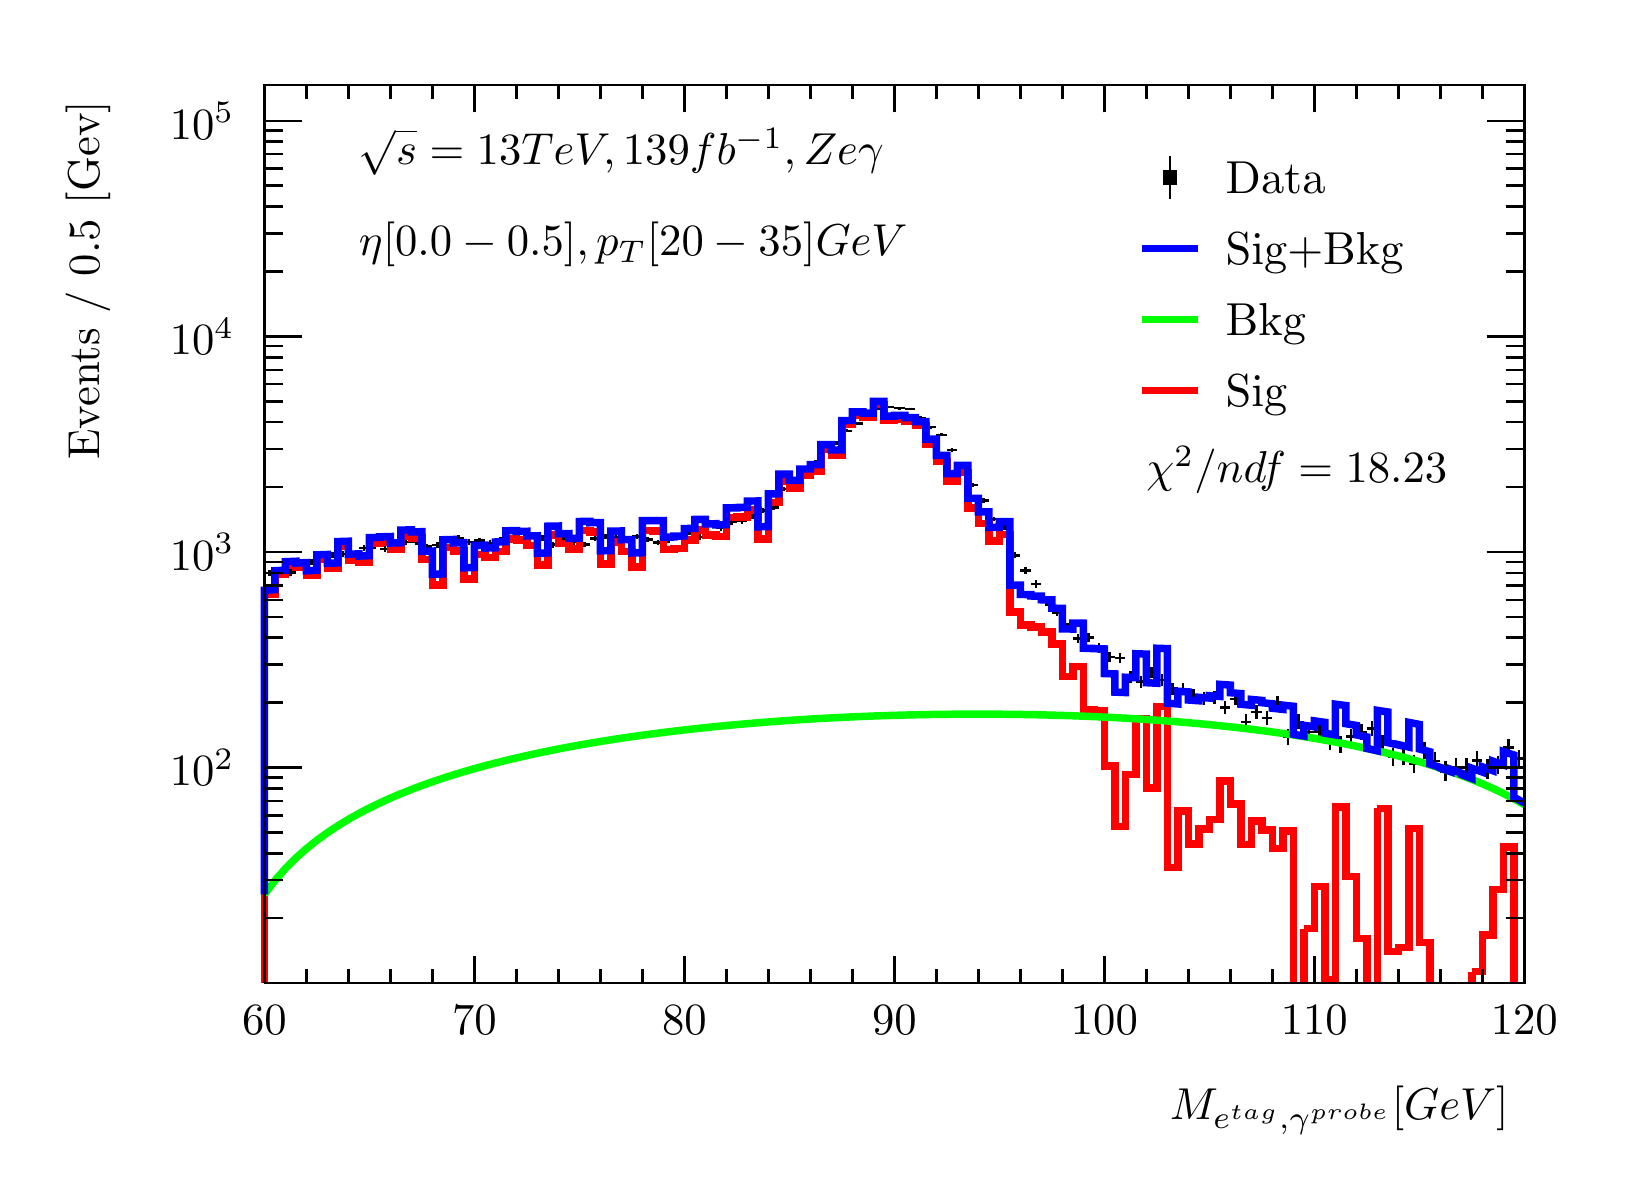
\begin{tikzpicture}
\pgfdeclareplotmark{cross} {
\pgfpathmoveto{\pgfpoint{-0.3\pgfplotmarksize}{\pgfplotmarksize}}
\pgfpathlineto{\pgfpoint{+0.3\pgfplotmarksize}{\pgfplotmarksize}}
\pgfpathlineto{\pgfpoint{+0.3\pgfplotmarksize}{0.3\pgfplotmarksize}}
\pgfpathlineto{\pgfpoint{+1\pgfplotmarksize}{0.3\pgfplotmarksize}}
\pgfpathlineto{\pgfpoint{+1\pgfplotmarksize}{-0.3\pgfplotmarksize}}
\pgfpathlineto{\pgfpoint{+0.3\pgfplotmarksize}{-0.3\pgfplotmarksize}}
\pgfpathlineto{\pgfpoint{+0.3\pgfplotmarksize}{-1.\pgfplotmarksize}}
\pgfpathlineto{\pgfpoint{-0.3\pgfplotmarksize}{-1.\pgfplotmarksize}}
\pgfpathlineto{\pgfpoint{-0.3\pgfplotmarksize}{-0.3\pgfplotmarksize}}
\pgfpathlineto{\pgfpoint{-1.\pgfplotmarksize}{-0.3\pgfplotmarksize}}
\pgfpathlineto{\pgfpoint{-1.\pgfplotmarksize}{0.3\pgfplotmarksize}}
\pgfpathlineto{\pgfpoint{-0.3\pgfplotmarksize}{0.3\pgfplotmarksize}}
\pgfpathclose
\pgfusepathqstroke
}
\pgfdeclareplotmark{cross*} {
\pgfpathmoveto{\pgfpoint{-0.3\pgfplotmarksize}{\pgfplotmarksize}}
\pgfpathlineto{\pgfpoint{+0.3\pgfplotmarksize}{\pgfplotmarksize}}
\pgfpathlineto{\pgfpoint{+0.3\pgfplotmarksize}{0.3\pgfplotmarksize}}
\pgfpathlineto{\pgfpoint{+1\pgfplotmarksize}{0.3\pgfplotmarksize}}
\pgfpathlineto{\pgfpoint{+1\pgfplotmarksize}{-0.3\pgfplotmarksize}}
\pgfpathlineto{\pgfpoint{+0.3\pgfplotmarksize}{-0.3\pgfplotmarksize}}
\pgfpathlineto{\pgfpoint{+0.3\pgfplotmarksize}{-1.\pgfplotmarksize}}
\pgfpathlineto{\pgfpoint{-0.3\pgfplotmarksize}{-1.\pgfplotmarksize}}
\pgfpathlineto{\pgfpoint{-0.3\pgfplotmarksize}{-0.3\pgfplotmarksize}}
\pgfpathlineto{\pgfpoint{-1.\pgfplotmarksize}{-0.3\pgfplotmarksize}}
\pgfpathlineto{\pgfpoint{-1.\pgfplotmarksize}{0.3\pgfplotmarksize}}
\pgfpathlineto{\pgfpoint{-0.3\pgfplotmarksize}{0.3\pgfplotmarksize}}
\pgfpathclose
\pgfusepathqfillstroke
}
\pgfdeclareplotmark{newstar} {
\pgfpathmoveto{\pgfqpoint{0pt}{\pgfplotmarksize}}
\pgfpathlineto{\pgfqpointpolar{44}{0.5\pgfplotmarksize}}
\pgfpathlineto{\pgfqpointpolar{18}{\pgfplotmarksize}}
\pgfpathlineto{\pgfqpointpolar{-20}{0.5\pgfplotmarksize}}
\pgfpathlineto{\pgfqpointpolar{-54}{\pgfplotmarksize}}
\pgfpathlineto{\pgfqpointpolar{-90}{0.5\pgfplotmarksize}}
\pgfpathlineto{\pgfqpointpolar{234}{\pgfplotmarksize}}
\pgfpathlineto{\pgfqpointpolar{198}{0.5\pgfplotmarksize}}
\pgfpathlineto{\pgfqpointpolar{162}{\pgfplotmarksize}}
\pgfpathlineto{\pgfqpointpolar{134}{0.5\pgfplotmarksize}}
\pgfpathclose
\pgfusepathqstroke
}
\pgfdeclareplotmark{newstar*} {
\pgfpathmoveto{\pgfqpoint{0pt}{\pgfplotmarksize}}
\pgfpathlineto{\pgfqpointpolar{44}{0.5\pgfplotmarksize}}
\pgfpathlineto{\pgfqpointpolar{18}{\pgfplotmarksize}}
\pgfpathlineto{\pgfqpointpolar{-20}{0.5\pgfplotmarksize}}
\pgfpathlineto{\pgfqpointpolar{-54}{\pgfplotmarksize}}
\pgfpathlineto{\pgfqpointpolar{-90}{0.5\pgfplotmarksize}}
\pgfpathlineto{\pgfqpointpolar{234}{\pgfplotmarksize}}
\pgfpathlineto{\pgfqpointpolar{198}{0.5\pgfplotmarksize}}
\pgfpathlineto{\pgfqpointpolar{162}{\pgfplotmarksize}}
\pgfpathlineto{\pgfqpointpolar{134}{0.5\pgfplotmarksize}}
\pgfpathclose
\pgfusepathqfillstroke
}
\definecolor{c}{rgb}{1,1,1};
\draw [color=c, fill=c] (0,0) rectangle (20,14.4361);
\draw [color=c, fill=c] (3,2.30977) rectangle (19,13.7143);
\definecolor{c}{rgb}{0,0,0};
\draw [c,line width=0.9] (3,2.30977) -- (3,13.7143) -- (19,13.7143) -- (19,2.30977) -- (3,2.30977);
\definecolor{c}{rgb}{1,1,1};
\draw [color=c, fill=c] (3,2.30977) rectangle (19,13.7143);
\definecolor{c}{rgb}{0,0,0};
\draw [c,line width=0.9] (3,2.30977) -- (3,13.7143) -- (19,13.7143) -- (19,2.30977) -- (3,2.30977);
\draw [c,line width=0.9] (3,2.30977) -- (19,2.30977);
\draw [c,line width=0.9] (3,2.65624) -- (3,2.30977);
\draw [c,line width=0.9] (3.53333,2.48301) -- (3.53333,2.30977);
\draw [c,line width=0.9] (4.06667,2.48301) -- (4.06667,2.30977);
\draw [c,line width=0.9] (4.6,2.48301) -- (4.6,2.30977);
\draw [c,line width=0.9] (5.13333,2.48301) -- (5.13333,2.30977);
\draw [c,line width=0.9] (5.66667,2.65624) -- (5.66667,2.30977);
\draw [c,line width=0.9] (6.2,2.48301) -- (6.2,2.30977);
\draw [c,line width=0.9] (6.73333,2.48301) -- (6.73333,2.30977);
\draw [c,line width=0.9] (7.26667,2.48301) -- (7.26667,2.30977);
\draw [c,line width=0.9] (7.8,2.48301) -- (7.8,2.30977);
\draw [c,line width=0.9] (8.33333,2.65624) -- (8.33333,2.30977);
\draw [c,line width=0.9] (8.86667,2.48301) -- (8.86667,2.30977);
\draw [c,line width=0.9] (9.4,2.48301) -- (9.4,2.30977);
\draw [c,line width=0.9] (9.93333,2.48301) -- (9.93333,2.30977);
\draw [c,line width=0.9] (10.4667,2.48301) -- (10.4667,2.30977);
\draw [c,line width=0.9] (11,2.65624) -- (11,2.30977);
\draw [c,line width=0.9] (11.5333,2.48301) -- (11.5333,2.30977);
\draw [c,line width=0.9] (12.0667,2.48301) -- (12.0667,2.30977);
\draw [c,line width=0.9] (12.6,2.48301) -- (12.6,2.30977);
\draw [c,line width=0.9] (13.1333,2.48301) -- (13.1333,2.30977);
\draw [c,line width=0.9] (13.6667,2.65624) -- (13.6667,2.30977);
\draw [c,line width=0.9] (14.2,2.48301) -- (14.2,2.30977);
\draw [c,line width=0.9] (14.7333,2.48301) -- (14.7333,2.30977);
\draw [c,line width=0.9] (15.2667,2.48301) -- (15.2667,2.30977);
\draw [c,line width=0.9] (15.8,2.48301) -- (15.8,2.30977);
\draw [c,line width=0.9] (16.3333,2.65624) -- (16.3333,2.30977);
\draw [c,line width=0.9] (16.8667,2.48301) -- (16.8667,2.30977);
\draw [c,line width=0.9] (17.4,2.48301) -- (17.4,2.30977);
\draw [c,line width=0.9] (17.9333,2.48301) -- (17.9333,2.30977);
\draw [c,line width=0.9] (18.4667,2.48301) -- (18.4667,2.30977);
\draw [c,line width=0.9] (19,2.65624) -- (19,2.30977);
\draw [anchor=base] (3,1.66015) node[scale=1.61424, color=c, rotate=0]{60};
\draw [anchor=base] (5.66667,1.66015) node[scale=1.61424, color=c, rotate=0]{70};
\draw [anchor=base] (8.33333,1.66015) node[scale=1.61424, color=c, rotate=0]{80};
\draw [anchor=base] (11,1.66015) node[scale=1.61424, color=c, rotate=0]{90};
\draw [anchor=base] (13.6667,1.66015) node[scale=1.61424, color=c, rotate=0]{100};
\draw [anchor=base] (16.3333,1.66015) node[scale=1.61424, color=c, rotate=0]{110};
\draw [anchor=base] (19,1.66015) node[scale=1.61424, color=c, rotate=0]{120};
\draw [anchor= east] (19,0.692932) node[scale=1.61424, color=c, rotate=0]{$M_{e^{tag}, \gamma^{probe}}  [GeV]$};
\draw [c,line width=0.9] (3,13.7143) -- (19,13.7143);
\draw [c,line width=0.9] (3,13.3678) -- (3,13.7143);
\draw [c,line width=0.9] (3.53333,13.5411) -- (3.53333,13.7143);
\draw [c,line width=0.9] (4.06667,13.5411) -- (4.06667,13.7143);
\draw [c,line width=0.9] (4.6,13.5411) -- (4.6,13.7143);
\draw [c,line width=0.9] (5.13333,13.5411) -- (5.13333,13.7143);
\draw [c,line width=0.9] (5.66667,13.3678) -- (5.66667,13.7143);
\draw [c,line width=0.9] (6.2,13.5411) -- (6.2,13.7143);
\draw [c,line width=0.9] (6.73333,13.5411) -- (6.73333,13.7143);
\draw [c,line width=0.9] (7.26667,13.5411) -- (7.26667,13.7143);
\draw [c,line width=0.9] (7.8,13.5411) -- (7.8,13.7143);
\draw [c,line width=0.9] (8.33333,13.3678) -- (8.33333,13.7143);
\draw [c,line width=0.9] (8.86667,13.5411) -- (8.86667,13.7143);
\draw [c,line width=0.9] (9.4,13.5411) -- (9.4,13.7143);
\draw [c,line width=0.9] (9.93333,13.5411) -- (9.93333,13.7143);
\draw [c,line width=0.9] (10.4667,13.5411) -- (10.4667,13.7143);
\draw [c,line width=0.9] (11,13.3678) -- (11,13.7143);
\draw [c,line width=0.9] (11.5333,13.5411) -- (11.5333,13.7143);
\draw [c,line width=0.9] (12.0667,13.5411) -- (12.0667,13.7143);
\draw [c,line width=0.9] (12.6,13.5411) -- (12.6,13.7143);
\draw [c,line width=0.9] (13.1333,13.5411) -- (13.1333,13.7143);
\draw [c,line width=0.9] (13.6667,13.3678) -- (13.6667,13.7143);
\draw [c,line width=0.9] (14.2,13.5411) -- (14.2,13.7143);
\draw [c,line width=0.9] (14.7333,13.5411) -- (14.7333,13.7143);
\draw [c,line width=0.9] (15.2667,13.5411) -- (15.2667,13.7143);
\draw [c,line width=0.9] (15.8,13.5411) -- (15.8,13.7143);
\draw [c,line width=0.9] (16.3333,13.3678) -- (16.3333,13.7143);
\draw [c,line width=0.9] (16.8667,13.5411) -- (16.8667,13.7143);
\draw [c,line width=0.9] (17.4,13.5411) -- (17.4,13.7143);
\draw [c,line width=0.9] (17.9333,13.5411) -- (17.9333,13.7143);
\draw [c,line width=0.9] (18.4667,13.5411) -- (18.4667,13.7143);
\draw [c,line width=0.9] (19,13.3678) -- (19,13.7143);
\draw [c,line width=0.9] (3,2.30977) -- (3,13.7143);
\draw [c,line width=0.9] (3.237,3.13385) -- (3,3.13385);
\draw [c,line width=0.9] (3.237,3.6159) -- (3,3.6159);
\draw [c,line width=0.9] (3.237,3.95792) -- (3,3.95792);
\draw [c,line width=0.9] (3.237,4.22321) -- (3,4.22321);
\draw [c,line width=0.9] (3.237,4.43997) -- (3,4.43997);
\draw [c,line width=0.9] (3.237,4.62324) -- (3,4.62324);
\draw [c,line width=0.9] (3.237,4.782) -- (3,4.782);
\draw [c,line width=0.9] (3.237,4.92203) -- (3,4.92203);
\draw [c,line width=0.9] (3.474,5.04729) -- (3,5.04729);
\draw [anchor= east] (2.82,5.04729) node[scale=1.61424, color=c, rotate=0]{$10^{2}$};
\draw [c,line width=0.9] (3.237,5.87136) -- (3,5.87136);
\draw [c,line width=0.9] (3.237,6.35342) -- (3,6.35342);
\draw [c,line width=0.9] (3.237,6.69544) -- (3,6.69544);
\draw [c,line width=0.9] (3.237,6.96073) -- (3,6.96073);
\draw [c,line width=0.9] (3.237,7.17749) -- (3,7.17749);
\draw [c,line width=0.9] (3.237,7.36076) -- (3,7.36076);
\draw [c,line width=0.9] (3.237,7.51951) -- (3,7.51951);
\draw [c,line width=0.9] (3.237,7.65954) -- (3,7.65954);
\draw [c,line width=0.9] (3.474,7.78481) -- (3,7.78481);
\draw [anchor= east] (2.82,7.78481) node[scale=1.61424, color=c, rotate=0]{$10^{3}$};
\draw [c,line width=0.9] (3.237,8.60888) -- (3,8.60888);
\draw [c,line width=0.9] (3.237,9.09093) -- (3,9.09093);
\draw [c,line width=0.9] (3.237,9.43296) -- (3,9.43296);
\draw [c,line width=0.9] (3.237,9.69825) -- (3,9.69825);
\draw [c,line width=0.9] (3.237,9.91501) -- (3,9.91501);
\draw [c,line width=0.9] (3.237,10.0983) -- (3,10.0983);
\draw [c,line width=0.9] (3.237,10.257) -- (3,10.257);
\draw [c,line width=0.9] (3.237,10.3971) -- (3,10.3971);
\draw [c,line width=0.9] (3.474,10.5223) -- (3,10.5223);
\draw [anchor= east] (2.82,10.5223) node[scale=1.61424, color=c, rotate=0]{$10^{4}$};
\draw [c,line width=0.9] (3.237,11.3464) -- (3,11.3464);
\draw [c,line width=0.9] (3.237,11.8285) -- (3,11.8285);
\draw [c,line width=0.9] (3.237,12.1705) -- (3,12.1705);
\draw [c,line width=0.9] (3.237,12.4358) -- (3,12.4358);
\draw [c,line width=0.9] (3.237,12.6525) -- (3,12.6525);
\draw [c,line width=0.9] (3.237,12.8358) -- (3,12.8358);
\draw [c,line width=0.9] (3.237,12.9945) -- (3,12.9945);
\draw [c,line width=0.9] (3.237,13.1346) -- (3,13.1346);
\draw [c,line width=0.9] (3.474,13.2598) -- (3,13.2598);
\draw [anchor= east] (2.82,13.2598) node[scale=1.61424, color=c, rotate=0]{$10^{5}$};
\draw [anchor= east] (0.76,13.7143) node[scale=1.61424, color=c, rotate=90]{Events / 0.5 [Gev]};
\draw [c,line width=0.9] (19,2.30977) -- (19,13.7143);
\draw [c,line width=0.9] (18.763,3.13385) -- (19,3.13385);
\draw [c,line width=0.9] (18.763,3.6159) -- (19,3.6159);
\draw [c,line width=0.9] (18.763,3.95792) -- (19,3.95792);
\draw [c,line width=0.9] (18.763,4.22321) -- (19,4.22321);
\draw [c,line width=0.9] (18.763,4.43997) -- (19,4.43997);
\draw [c,line width=0.9] (18.763,4.62324) -- (19,4.62324);
\draw [c,line width=0.9] (18.763,4.782) -- (19,4.782);
\draw [c,line width=0.9] (18.763,4.92203) -- (19,4.92203);
\draw [c,line width=0.9] (18.526,5.04729) -- (19,5.04729);
\draw [c,line width=0.9] (18.763,5.87136) -- (19,5.87136);
\draw [c,line width=0.9] (18.763,6.35342) -- (19,6.35342);
\draw [c,line width=0.9] (18.763,6.69544) -- (19,6.69544);
\draw [c,line width=0.9] (18.763,6.96073) -- (19,6.96073);
\draw [c,line width=0.9] (18.763,7.17749) -- (19,7.17749);
\draw [c,line width=0.9] (18.763,7.36076) -- (19,7.36076);
\draw [c,line width=0.9] (18.763,7.51951) -- (19,7.51951);
\draw [c,line width=0.9] (18.763,7.65954) -- (19,7.65954);
\draw [c,line width=0.9] (18.526,7.78481) -- (19,7.78481);
\draw [c,line width=0.9] (18.763,8.60888) -- (19,8.60888);
\draw [c,line width=0.9] (18.763,9.09093) -- (19,9.09093);
\draw [c,line width=0.9] (18.763,9.43296) -- (19,9.43296);
\draw [c,line width=0.9] (18.763,9.69825) -- (19,9.69825);
\draw [c,line width=0.9] (18.763,9.91501) -- (19,9.91501);
\draw [c,line width=0.9] (18.763,10.0983) -- (19,10.0983);
\draw [c,line width=0.9] (18.763,10.257) -- (19,10.257);
\draw [c,line width=0.9] (18.763,10.3971) -- (19,10.3971);
\draw [c,line width=0.9] (18.526,10.5223) -- (19,10.5223);
\draw [c,line width=0.9] (18.763,11.3464) -- (19,11.3464);
\draw [c,line width=0.9] (18.763,11.8285) -- (19,11.8285);
\draw [c,line width=0.9] (18.763,12.1705) -- (19,12.1705);
\draw [c,line width=0.9] (18.763,12.4358) -- (19,12.4358);
\draw [c,line width=0.9] (18.763,12.6525) -- (19,12.6525);
\draw [c,line width=0.9] (18.763,12.8358) -- (19,12.8358);
\draw [c,line width=0.9] (18.763,12.9945) -- (19,12.9945);
\draw [c,line width=0.9] (18.763,13.1346) -- (19,13.1346);
\draw [c,line width=0.9] (18.526,13.2598) -- (19,13.2598);
\draw [c,line width=0.9] (3.06667,7.51505) -- (3,7.51505);
\draw [c,line width=0.9] (3,7.51505) -- (3,7.51505);
\draw [c,line width=0.9] (3.06667,7.51505) -- (3.13333,7.51505);
\draw [c,line width=0.9] (3.13333,7.51505) -- (3.13333,7.51505);
\draw [c,line width=0.9] (3.06667,7.51505) -- (3.06667,7.55716);
\draw [c,line width=0.9] (3.06667,7.55716) -- (3.06667,7.55716);
\draw [c,line width=0.9] (3.06667,7.51505) -- (3.06667,7.47294);
\draw [c,line width=0.9] (3.06667,7.47294) -- (3.06667,7.47294);
\draw [c,line width=0.9] (3.2,7.50606) -- (3.13333,7.50606);
\draw [c,line width=0.9] (3.13333,7.50606) -- (3.13333,7.50606);
\draw [c,line width=0.9] (3.2,7.50606) -- (3.26667,7.50606);
\draw [c,line width=0.9] (3.26667,7.50606) -- (3.26667,7.50606);
\draw [c,line width=0.9] (3.2,7.50606) -- (3.2,7.54833);
\draw [c,line width=0.9] (3.2,7.54833) -- (3.2,7.54833);
\draw [c,line width=0.9] (3.2,7.50606) -- (3.2,7.46379);
\draw [c,line width=0.9] (3.2,7.46379) -- (3.2,7.46379);
\draw [c,line width=0.9] (3.33333,7.521) -- (3.26667,7.521);
\draw [c,line width=0.9] (3.26667,7.521) -- (3.26667,7.521);
\draw [c,line width=0.9] (3.33333,7.521) -- (3.4,7.521);
\draw [c,line width=0.9] (3.4,7.521) -- (3.4,7.521);
\draw [c,line width=0.9] (3.33333,7.521) -- (3.33333,7.563);
\draw [c,line width=0.9] (3.33333,7.563) -- (3.33333,7.563);
\draw [c,line width=0.9] (3.33333,7.521) -- (3.33333,7.47899);
\draw [c,line width=0.9] (3.33333,7.47899) -- (3.33333,7.47899);
\draw [c,line width=0.9] (3.46667,7.63012) -- (3.4,7.63012);
\draw [c,line width=0.9] (3.4,7.63012) -- (3.4,7.63012);
\draw [c,line width=0.9] (3.46667,7.63012) -- (3.53333,7.63012);
\draw [c,line width=0.9] (3.53333,7.63012) -- (3.53333,7.63012);
\draw [c,line width=0.9] (3.46667,7.63012) -- (3.46667,7.67024);
\draw [c,line width=0.9] (3.46667,7.67024) -- (3.46667,7.67024);
\draw [c,line width=0.9] (3.46667,7.63012) -- (3.46667,7.59);
\draw [c,line width=0.9] (3.46667,7.59) -- (3.46667,7.59);
\draw [c,line width=0.9] (3.6,7.65425) -- (3.53333,7.65425);
\draw [c,line width=0.9] (3.53333,7.65425) -- (3.53333,7.65425);
\draw [c,line width=0.9] (3.6,7.65425) -- (3.66667,7.65425);
\draw [c,line width=0.9] (3.66667,7.65425) -- (3.66667,7.65425);
\draw [c,line width=0.9] (3.6,7.65425) -- (3.6,7.69397);
\draw [c,line width=0.9] (3.6,7.69397) -- (3.6,7.69397);
\draw [c,line width=0.9] (3.6,7.65425) -- (3.6,7.61453);
\draw [c,line width=0.9] (3.6,7.61453) -- (3.6,7.61453);
\draw [c,line width=0.9] (3.73333,7.72633) -- (3.66667,7.72633);
\draw [c,line width=0.9] (3.66667,7.72633) -- (3.66667,7.72633);
\draw [c,line width=0.9] (3.73333,7.72633) -- (3.8,7.72633);
\draw [c,line width=0.9] (3.8,7.72633) -- (3.8,7.72633);
\draw [c,line width=0.9] (3.73333,7.72633) -- (3.73333,7.76486);
\draw [c,line width=0.9] (3.73333,7.76486) -- (3.73333,7.76486);
\draw [c,line width=0.9] (3.73333,7.72633) -- (3.73333,7.6878);
\draw [c,line width=0.9] (3.73333,7.6878) -- (3.73333,7.6878);
\draw [c,line width=0.9] (3.86667,7.73998) -- (3.8,7.73998);
\draw [c,line width=0.9] (3.8,7.73998) -- (3.8,7.73998);
\draw [c,line width=0.9] (3.86667,7.73998) -- (3.93333,7.73998);
\draw [c,line width=0.9] (3.93333,7.73998) -- (3.93333,7.73998);
\draw [c,line width=0.9] (3.86667,7.73998) -- (3.86667,7.77829);
\draw [c,line width=0.9] (3.86667,7.77829) -- (3.86667,7.77829);
\draw [c,line width=0.9] (3.86667,7.73998) -- (3.86667,7.70167);
\draw [c,line width=0.9] (3.86667,7.70167) -- (3.86667,7.70167);
\draw [c,line width=0.9] (4,7.75714) -- (3.93333,7.75714);
\draw [c,line width=0.9] (3.93333,7.75714) -- (3.93333,7.75714);
\draw [c,line width=0.9] (4,7.75714) -- (4.06667,7.75714);
\draw [c,line width=0.9] (4.06667,7.75714) -- (4.06667,7.75714);
\draw [c,line width=0.9] (4,7.75714) -- (4,7.79518);
\draw [c,line width=0.9] (4,7.79518) -- (4,7.79518);
\draw [c,line width=0.9] (4,7.75714) -- (4,7.71911);
\draw [c,line width=0.9] (4,7.71911) -- (4,7.71911);
\draw [c,line width=0.9] (4.13333,7.76079) -- (4.06667,7.76079);
\draw [c,line width=0.9] (4.06667,7.76079) -- (4.06667,7.76079);
\draw [c,line width=0.9] (4.13333,7.76079) -- (4.2,7.76079);
\draw [c,line width=0.9] (4.2,7.76079) -- (4.2,7.76079);
\draw [c,line width=0.9] (4.13333,7.76079) -- (4.13333,7.79876);
\draw [c,line width=0.9] (4.13333,7.79876) -- (4.13333,7.79876);
\draw [c,line width=0.9] (4.13333,7.76079) -- (4.13333,7.72281);
\draw [c,line width=0.9] (4.13333,7.72281) -- (4.13333,7.72281);
\draw [c,line width=0.9] (4.26667,7.83486) -- (4.2,7.83486);
\draw [c,line width=0.9] (4.2,7.83486) -- (4.2,7.83486);
\draw [c,line width=0.9] (4.26667,7.83486) -- (4.33333,7.83486);
\draw [c,line width=0.9] (4.33333,7.83486) -- (4.33333,7.83486);
\draw [c,line width=0.9] (4.26667,7.83486) -- (4.26667,7.87167);
\draw [c,line width=0.9] (4.26667,7.87167) -- (4.26667,7.87167);
\draw [c,line width=0.9] (4.26667,7.83486) -- (4.26667,7.79805);
\draw [c,line width=0.9] (4.26667,7.79805) -- (4.26667,7.79805);
\draw [c,line width=0.9] (4.4,7.85744) -- (4.33333,7.85744);
\draw [c,line width=0.9] (4.33333,7.85744) -- (4.33333,7.85744);
\draw [c,line width=0.9] (4.4,7.85744) -- (4.46667,7.85744);
\draw [c,line width=0.9] (4.46667,7.85744) -- (4.46667,7.85744);
\draw [c,line width=0.9] (4.4,7.85744) -- (4.4,7.89391);
\draw [c,line width=0.9] (4.4,7.89391) -- (4.4,7.89391);
\draw [c,line width=0.9] (4.4,7.85744) -- (4.4,7.82098);
\draw [c,line width=0.9] (4.4,7.82098) -- (4.4,7.82098);
\draw [c,line width=0.9] (4.53333,7.81995) -- (4.46667,7.81995);
\draw [c,line width=0.9] (4.46667,7.81995) -- (4.46667,7.81995);
\draw [c,line width=0.9] (4.53333,7.81995) -- (4.6,7.81995);
\draw [c,line width=0.9] (4.6,7.81995) -- (4.6,7.81995);
\draw [c,line width=0.9] (4.53333,7.81995) -- (4.53333,7.85699);
\draw [c,line width=0.9] (4.53333,7.85699) -- (4.53333,7.85699);
\draw [c,line width=0.9] (4.53333,7.81995) -- (4.53333,7.78291);
\draw [c,line width=0.9] (4.53333,7.78291) -- (4.53333,7.78291);
\draw [c,line width=0.9] (4.66667,7.86968) -- (4.6,7.86968);
\draw [c,line width=0.9] (4.6,7.86968) -- (4.6,7.86968);
\draw [c,line width=0.9] (4.66667,7.86968) -- (4.73333,7.86968);
\draw [c,line width=0.9] (4.73333,7.86968) -- (4.73333,7.86968);
\draw [c,line width=0.9] (4.66667,7.86968) -- (4.66667,7.90596);
\draw [c,line width=0.9] (4.66667,7.90596) -- (4.66667,7.90596);
\draw [c,line width=0.9] (4.66667,7.86968) -- (4.66667,7.83341);
\draw [c,line width=0.9] (4.66667,7.83341) -- (4.66667,7.83341);
\draw [c,line width=0.9] (4.8,7.91209) -- (4.73333,7.91209);
\draw [c,line width=0.9] (4.73333,7.91209) -- (4.73333,7.91209);
\draw [c,line width=0.9] (4.8,7.91209) -- (4.86667,7.91209);
\draw [c,line width=0.9] (4.86667,7.91209) -- (4.86667,7.91209);
\draw [c,line width=0.9] (4.8,7.91209) -- (4.8,7.94772);
\draw [c,line width=0.9] (4.8,7.94772) -- (4.8,7.94772);
\draw [c,line width=0.9] (4.8,7.91209) -- (4.8,7.87645);
\draw [c,line width=0.9] (4.8,7.87645) -- (4.8,7.87645);
\draw [c,line width=0.9] (4.93333,7.90995) -- (4.86667,7.90995);
\draw [c,line width=0.9] (4.86667,7.90995) -- (4.86667,7.90995);
\draw [c,line width=0.9] (4.93333,7.90995) -- (5,7.90995);
\draw [c,line width=0.9] (5,7.90995) -- (5,7.90995);
\draw [c,line width=0.9] (4.93333,7.90995) -- (4.93333,7.94562);
\draw [c,line width=0.9] (4.93333,7.94562) -- (4.93333,7.94562);
\draw [c,line width=0.9] (4.93333,7.90995) -- (4.93333,7.87428);
\draw [c,line width=0.9] (4.93333,7.87428) -- (4.93333,7.87428);
\draw [c,line width=0.9] (5.06667,7.85408) -- (5,7.85408);
\draw [c,line width=0.9] (5,7.85408) -- (5,7.85408);
\draw [c,line width=0.9] (5.06667,7.85408) -- (5.13333,7.85408);
\draw [c,line width=0.9] (5.13333,7.85408) -- (5.13333,7.85408);
\draw [c,line width=0.9] (5.06667,7.85408) -- (5.06667,7.8906);
\draw [c,line width=0.9] (5.06667,7.8906) -- (5.06667,7.8906);
\draw [c,line width=0.9] (5.06667,7.85408) -- (5.06667,7.81757);
\draw [c,line width=0.9] (5.06667,7.81757) -- (5.06667,7.81757);
\draw [c,line width=0.9] (5.2,7.87189) -- (5.13333,7.87189);
\draw [c,line width=0.9] (5.13333,7.87189) -- (5.13333,7.87189);
\draw [c,line width=0.9] (5.2,7.87189) -- (5.26667,7.87189);
\draw [c,line width=0.9] (5.26667,7.87189) -- (5.26667,7.87189);
\draw [c,line width=0.9] (5.2,7.87189) -- (5.2,7.90814);
\draw [c,line width=0.9] (5.2,7.90814) -- (5.2,7.90814);
\draw [c,line width=0.9] (5.2,7.87189) -- (5.2,7.83565);
\draw [c,line width=0.9] (5.2,7.83565) -- (5.2,7.83565);
\draw [c,line width=0.9] (5.33333,7.94163) -- (5.26667,7.94163);
\draw [c,line width=0.9] (5.26667,7.94163) -- (5.26667,7.94163);
\draw [c,line width=0.9] (5.33333,7.94163) -- (5.4,7.94163);
\draw [c,line width=0.9] (5.4,7.94163) -- (5.4,7.94163);
\draw [c,line width=0.9] (5.33333,7.94163) -- (5.33333,7.97682);
\draw [c,line width=0.9] (5.33333,7.97682) -- (5.33333,7.97682);
\draw [c,line width=0.9] (5.33333,7.94163) -- (5.33333,7.90643);
\draw [c,line width=0.9] (5.33333,7.90643) -- (5.33333,7.90643);
\draw [c,line width=0.9] (5.46667,7.96229) -- (5.4,7.96229);
\draw [c,line width=0.9] (5.4,7.96229) -- (5.4,7.96229);
\draw [c,line width=0.9] (5.46667,7.96229) -- (5.53333,7.96229);
\draw [c,line width=0.9] (5.53333,7.96229) -- (5.53333,7.96229);
\draw [c,line width=0.9] (5.46667,7.96229) -- (5.46667,7.99718);
\draw [c,line width=0.9] (5.46667,7.99718) -- (5.46667,7.99718);
\draw [c,line width=0.9] (5.46667,7.96229) -- (5.46667,7.9274);
\draw [c,line width=0.9] (5.46667,7.9274) -- (5.46667,7.9274);
\draw [c,line width=0.9] (5.6,7.91422) -- (5.53333,7.91422);
\draw [c,line width=0.9] (5.53333,7.91422) -- (5.53333,7.91422);
\draw [c,line width=0.9] (5.6,7.91422) -- (5.66667,7.91422);
\draw [c,line width=0.9] (5.66667,7.91422) -- (5.66667,7.91422);
\draw [c,line width=0.9] (5.6,7.91422) -- (5.6,7.94983);
\draw [c,line width=0.9] (5.6,7.94983) -- (5.6,7.94983);
\draw [c,line width=0.9] (5.6,7.91422) -- (5.6,7.87862);
\draw [c,line width=0.9] (5.6,7.87862) -- (5.6,7.87862);
\draw [c,line width=0.9] (5.73333,7.93221) -- (5.66667,7.93221);
\draw [c,line width=0.9] (5.66667,7.93221) -- (5.66667,7.93221);
\draw [c,line width=0.9] (5.73333,7.93221) -- (5.8,7.93221);
\draw [c,line width=0.9] (5.8,7.93221) -- (5.8,7.93221);
\draw [c,line width=0.9] (5.73333,7.93221) -- (5.73333,7.96755);
\draw [c,line width=0.9] (5.73333,7.96755) -- (5.73333,7.96755);
\draw [c,line width=0.9] (5.73333,7.93221) -- (5.73333,7.89688);
\draw [c,line width=0.9] (5.73333,7.89688) -- (5.73333,7.89688);
\draw [c,line width=0.9] (5.86667,7.89487) -- (5.8,7.89487);
\draw [c,line width=0.9] (5.8,7.89487) -- (5.8,7.89487);
\draw [c,line width=0.9] (5.86667,7.89487) -- (5.93333,7.89487);
\draw [c,line width=0.9] (5.93333,7.89487) -- (5.93333,7.89487);
\draw [c,line width=0.9] (5.86667,7.89487) -- (5.86667,7.93077);
\draw [c,line width=0.9] (5.86667,7.93077) -- (5.86667,7.93077);
\draw [c,line width=0.9] (5.86667,7.89487) -- (5.86667,7.85898);
\draw [c,line width=0.9] (5.86667,7.85898) -- (5.86667,7.85898);
\draw [c,line width=0.9] (6,7.9385) -- (5.93333,7.9385);
\draw [c,line width=0.9] (5.93333,7.9385) -- (5.93333,7.9385);
\draw [c,line width=0.9] (6,7.9385) -- (6.06667,7.9385);
\draw [c,line width=0.9] (6.06667,7.9385) -- (6.06667,7.9385);
\draw [c,line width=0.9] (6,7.9385) -- (6,7.97374);
\draw [c,line width=0.9] (6,7.97374) -- (6,7.97374);
\draw [c,line width=0.9] (6,7.9385) -- (6,7.90326);
\draw [c,line width=0.9] (6,7.90326) -- (6,7.90326);
\draw [c,line width=0.9] (6.13333,7.95303) -- (6.06667,7.95303);
\draw [c,line width=0.9] (6.06667,7.95303) -- (6.06667,7.95303);
\draw [c,line width=0.9] (6.13333,7.95303) -- (6.2,7.95303);
\draw [c,line width=0.9] (6.2,7.95303) -- (6.2,7.95303);
\draw [c,line width=0.9] (6.13333,7.95303) -- (6.13333,7.98806);
\draw [c,line width=0.9] (6.13333,7.98806) -- (6.13333,7.98806);
\draw [c,line width=0.9] (6.13333,7.95303) -- (6.13333,7.91801);
\draw [c,line width=0.9] (6.13333,7.91801) -- (6.13333,7.91801);
\draw [c,line width=0.9] (6.26667,7.9551) -- (6.2,7.9551);
\draw [c,line width=0.9] (6.2,7.9551) -- (6.2,7.9551);
\draw [c,line width=0.9] (6.26667,7.9551) -- (6.33333,7.9551);
\draw [c,line width=0.9] (6.33333,7.9551) -- (6.33333,7.9551);
\draw [c,line width=0.9] (6.26667,7.9551) -- (6.26667,7.99009);
\draw [c,line width=0.9] (6.26667,7.99009) -- (6.26667,7.99009);
\draw [c,line width=0.9] (6.26667,7.9551) -- (6.26667,7.9201);
\draw [c,line width=0.9] (6.26667,7.9201) -- (6.26667,7.9201);
\draw [c,line width=0.9] (6.4,7.99361) -- (6.33333,7.99361);
\draw [c,line width=0.9] (6.33333,7.99361) -- (6.33333,7.99361);
\draw [c,line width=0.9] (6.4,7.99361) -- (6.46667,7.99361);
\draw [c,line width=0.9] (6.46667,7.99361) -- (6.46667,7.99361);
\draw [c,line width=0.9] (6.4,7.99361) -- (6.4,8.02805);
\draw [c,line width=0.9] (6.4,8.02805) -- (6.4,8.02805);
\draw [c,line width=0.9] (6.4,7.99361) -- (6.4,7.95918);
\draw [c,line width=0.9] (6.4,7.95918) -- (6.4,7.95918);
\draw [c,line width=0.9] (6.53333,7.96433) -- (6.46667,7.96433);
\draw [c,line width=0.9] (6.46667,7.96433) -- (6.46667,7.96433);
\draw [c,line width=0.9] (6.53333,7.96433) -- (6.6,7.96433);
\draw [c,line width=0.9] (6.6,7.96433) -- (6.6,7.96433);
\draw [c,line width=0.9] (6.53333,7.96433) -- (6.53333,7.99919);
\draw [c,line width=0.9] (6.53333,7.99919) -- (6.53333,7.99919);
\draw [c,line width=0.9] (6.53333,7.96433) -- (6.53333,7.92947);
\draw [c,line width=0.9] (6.53333,7.92947) -- (6.53333,7.92947);
\draw [c,line width=0.9] (6.66667,7.87631) -- (6.6,7.87631);
\draw [c,line width=0.9] (6.6,7.87631) -- (6.6,7.87631);
\draw [c,line width=0.9] (6.66667,7.87631) -- (6.73333,7.87631);
\draw [c,line width=0.9] (6.73333,7.87631) -- (6.73333,7.87631);
\draw [c,line width=0.9] (6.66667,7.87631) -- (6.66667,7.91248);
\draw [c,line width=0.9] (6.66667,7.91248) -- (6.66667,7.91248);
\draw [c,line width=0.9] (6.66667,7.87631) -- (6.66667,7.84013);
\draw [c,line width=0.9] (6.66667,7.84013) -- (6.66667,7.84013);
\draw [c,line width=0.9] (6.8,7.97552) -- (6.73333,7.97552);
\draw [c,line width=0.9] (6.73333,7.97552) -- (6.73333,7.97552);
\draw [c,line width=0.9] (6.8,7.97552) -- (6.86667,7.97552);
\draw [c,line width=0.9] (6.86667,7.97552) -- (6.86667,7.97552);
\draw [c,line width=0.9] (6.8,7.97552) -- (6.8,8.01022);
\draw [c,line width=0.9] (6.8,8.01022) -- (6.8,8.01022);
\draw [c,line width=0.9] (6.8,7.97552) -- (6.8,7.94083);
\draw [c,line width=0.9] (6.8,7.94083) -- (6.8,7.94083);
\draw [c,line width=0.9] (6.93333,7.90888) -- (6.86667,7.90888);
\draw [c,line width=0.9] (6.86667,7.90888) -- (6.86667,7.90888);
\draw [c,line width=0.9] (6.93333,7.90888) -- (7,7.90888);
\draw [c,line width=0.9] (7,7.90888) -- (7,7.90888);
\draw [c,line width=0.9] (6.93333,7.90888) -- (6.93333,7.94456);
\draw [c,line width=0.9] (6.93333,7.94456) -- (6.93333,7.94456);
\draw [c,line width=0.9] (6.93333,7.90888) -- (6.93333,7.8732);
\draw [c,line width=0.9] (6.93333,7.8732) -- (6.93333,7.8732);
\draw [c,line width=0.9] (7.06667,7.87851) -- (7,7.87851);
\draw [c,line width=0.9] (7,7.87851) -- (7,7.87851);
\draw [c,line width=0.9] (7.06667,7.87851) -- (7.13333,7.87851);
\draw [c,line width=0.9] (7.13333,7.87851) -- (7.13333,7.87851);
\draw [c,line width=0.9] (7.06667,7.87851) -- (7.06667,7.91465);
\draw [c,line width=0.9] (7.06667,7.91465) -- (7.06667,7.91465);
\draw [c,line width=0.9] (7.06667,7.87851) -- (7.06667,7.84236);
\draw [c,line width=0.9] (7.06667,7.84236) -- (7.06667,7.84236);
\draw [c,line width=0.9] (7.2,7.95716) -- (7.13333,7.95716);
\draw [c,line width=0.9] (7.13333,7.95716) -- (7.13333,7.95716);
\draw [c,line width=0.9] (7.2,7.95716) -- (7.26667,7.95716);
\draw [c,line width=0.9] (7.26667,7.95716) -- (7.26667,7.95716);
\draw [c,line width=0.9] (7.2,7.95716) -- (7.2,7.99212);
\draw [c,line width=0.9] (7.2,7.99212) -- (7.2,7.99212);
\draw [c,line width=0.9] (7.2,7.95716) -- (7.2,7.92219);
\draw [c,line width=0.9] (7.2,7.92219) -- (7.2,7.92219);
\draw [c,line width=0.9] (7.33333,7.97957) -- (7.26667,7.97957);
\draw [c,line width=0.9] (7.26667,7.97957) -- (7.26667,7.97957);
\draw [c,line width=0.9] (7.33333,7.97957) -- (7.4,7.97957);
\draw [c,line width=0.9] (7.4,7.97957) -- (7.4,7.97957);
\draw [c,line width=0.9] (7.33333,7.97957) -- (7.33333,8.01421);
\draw [c,line width=0.9] (7.33333,8.01421) -- (7.33333,8.01421);
\draw [c,line width=0.9] (7.33333,7.97957) -- (7.33333,7.94493);
\draw [c,line width=0.9] (7.33333,7.94493) -- (7.33333,7.94493);
\draw [c,line width=0.9] (7.46667,7.97755) -- (7.4,7.97755);
\draw [c,line width=0.9] (7.4,7.97755) -- (7.4,7.97755);
\draw [c,line width=0.9] (7.46667,7.97755) -- (7.53333,7.97755);
\draw [c,line width=0.9] (7.53333,7.97755) -- (7.53333,7.97755);
\draw [c,line width=0.9] (7.46667,7.97755) -- (7.46667,8.01222);
\draw [c,line width=0.9] (7.46667,8.01222) -- (7.46667,8.01222);
\draw [c,line width=0.9] (7.46667,7.97755) -- (7.46667,7.94288);
\draw [c,line width=0.9] (7.46667,7.94288) -- (7.46667,7.94288);
\draw [c,line width=0.9] (7.6,7.94683) -- (7.53333,7.94683);
\draw [c,line width=0.9] (7.53333,7.94683) -- (7.53333,7.94683);
\draw [c,line width=0.9] (7.6,7.94683) -- (7.66667,7.94683);
\draw [c,line width=0.9] (7.66667,7.94683) -- (7.66667,7.94683);
\draw [c,line width=0.9] (7.6,7.94683) -- (7.6,7.98194);
\draw [c,line width=0.9] (7.6,7.98194) -- (7.6,7.98194);
\draw [c,line width=0.9] (7.6,7.94683) -- (7.6,7.91171);
\draw [c,line width=0.9] (7.6,7.91171) -- (7.6,7.91171);
\draw [c,line width=0.9] (7.73333,7.98159) -- (7.66667,7.98159);
\draw [c,line width=0.9] (7.66667,7.98159) -- (7.66667,7.98159);
\draw [c,line width=0.9] (7.73333,7.98159) -- (7.8,7.98159);
\draw [c,line width=0.9] (7.8,7.98159) -- (7.8,7.98159);
\draw [c,line width=0.9] (7.73333,7.98159) -- (7.73333,8.01619);
\draw [c,line width=0.9] (7.73333,8.01619) -- (7.73333,8.01619);
\draw [c,line width=0.9] (7.73333,7.98159) -- (7.73333,7.94698);
\draw [c,line width=0.9] (7.73333,7.94698) -- (7.73333,7.94698);
\draw [c,line width=0.9] (7.86667,7.94475) -- (7.8,7.94475);
\draw [c,line width=0.9] (7.8,7.94475) -- (7.8,7.94475);
\draw [c,line width=0.9] (7.86667,7.94475) -- (7.93333,7.94475);
\draw [c,line width=0.9] (7.93333,7.94475) -- (7.93333,7.94475);
\draw [c,line width=0.9] (7.86667,7.94475) -- (7.86667,7.9799);
\draw [c,line width=0.9] (7.86667,7.9799) -- (7.86667,7.9799);
\draw [c,line width=0.9] (7.86667,7.94475) -- (7.86667,7.9096);
\draw [c,line width=0.9] (7.86667,7.9096) -- (7.86667,7.9096);
\draw [c,line width=0.9] (8,7.90351) -- (7.93333,7.90351);
\draw [c,line width=0.9] (7.93333,7.90351) -- (7.93333,7.90351);
\draw [c,line width=0.9] (8,7.90351) -- (8.06667,7.90351);
\draw [c,line width=0.9] (8.06667,7.90351) -- (8.06667,7.90351);
\draw [c,line width=0.9] (8,7.90351) -- (8,7.93928);
\draw [c,line width=0.9] (8,7.93928) -- (8,7.93928);
\draw [c,line width=0.9] (8,7.90351) -- (8,7.86775);
\draw [c,line width=0.9] (8,7.86775) -- (8,7.86775);
\draw [c,line width=0.9] (8.13333,7.93536) -- (8.06667,7.93536);
\draw [c,line width=0.9] (8.06667,7.93536) -- (8.06667,7.93536);
\draw [c,line width=0.9] (8.13333,7.93536) -- (8.2,7.93536);
\draw [c,line width=0.9] (8.2,7.93536) -- (8.2,7.93536);
\draw [c,line width=0.9] (8.13333,7.93536) -- (8.13333,7.97065);
\draw [c,line width=0.9] (8.13333,7.97065) -- (8.13333,7.97065);
\draw [c,line width=0.9] (8.13333,7.93536) -- (8.13333,7.90007);
\draw [c,line width=0.9] (8.13333,7.90007) -- (8.13333,7.90007);
\draw [c,line width=0.9] (8.26667,7.98259) -- (8.2,7.98259);
\draw [c,line width=0.9] (8.2,7.98259) -- (8.2,7.98259);
\draw [c,line width=0.9] (8.26667,7.98259) -- (8.33333,7.98259);
\draw [c,line width=0.9] (8.33333,7.98259) -- (8.33333,7.98259);
\draw [c,line width=0.9] (8.26667,7.98259) -- (8.26667,8.01719);
\draw [c,line width=0.9] (8.26667,8.01719) -- (8.26667,8.01719);
\draw [c,line width=0.9] (8.26667,7.98259) -- (8.26667,7.948);
\draw [c,line width=0.9] (8.26667,7.948) -- (8.26667,7.948);
\draw [c,line width=0.9] (8.4,8.03092) -- (8.33333,8.03092);
\draw [c,line width=0.9] (8.33333,8.03092) -- (8.33333,8.03092);
\draw [c,line width=0.9] (8.4,8.03092) -- (8.46667,8.03092);
\draw [c,line width=0.9] (8.46667,8.03092) -- (8.46667,8.03092);
\draw [c,line width=0.9] (8.4,8.03092) -- (8.4,8.06482);
\draw [c,line width=0.9] (8.4,8.06482) -- (8.4,8.06482);
\draw [c,line width=0.9] (8.4,8.03092) -- (8.4,7.99703);
\draw [c,line width=0.9] (8.4,7.99703) -- (8.4,7.99703);
\draw [c,line width=0.9] (8.53333,7.97248) -- (8.46667,7.97248);
\draw [c,line width=0.9] (8.46667,7.97248) -- (8.46667,7.97248);
\draw [c,line width=0.9] (8.53333,7.97248) -- (8.6,7.97248);
\draw [c,line width=0.9] (8.6,7.97248) -- (8.6,7.97248);
\draw [c,line width=0.9] (8.53333,7.97248) -- (8.53333,8.00722);
\draw [c,line width=0.9] (8.53333,8.00722) -- (8.53333,8.00722);
\draw [c,line width=0.9] (8.53333,7.97248) -- (8.53333,7.93774);
\draw [c,line width=0.9] (8.53333,7.93774) -- (8.53333,7.93774);
\draw [c,line width=0.9] (8.66667,8.15299) -- (8.6,8.15299);
\draw [c,line width=0.9] (8.6,8.15299) -- (8.6,8.15299);
\draw [c,line width=0.9] (8.66667,8.15299) -- (8.73333,8.15299);
\draw [c,line width=0.9] (8.73333,8.15299) -- (8.73333,8.15299);
\draw [c,line width=0.9] (8.66667,8.15299) -- (8.66667,8.18519);
\draw [c,line width=0.9] (8.66667,8.18519) -- (8.66667,8.18519);
\draw [c,line width=0.9] (8.66667,8.15299) -- (8.66667,8.12079);
\draw [c,line width=0.9] (8.66667,8.12079) -- (8.66667,8.12079);
\draw [c,line width=0.9] (8.8,8.0857) -- (8.73333,8.0857);
\draw [c,line width=0.9] (8.73333,8.0857) -- (8.73333,8.0857);
\draw [c,line width=0.9] (8.8,8.0857) -- (8.86667,8.0857);
\draw [c,line width=0.9] (8.86667,8.0857) -- (8.86667,8.0857);
\draw [c,line width=0.9] (8.8,8.0857) -- (8.8,8.11883);
\draw [c,line width=0.9] (8.8,8.11883) -- (8.8,8.11883);
\draw [c,line width=0.9] (8.8,8.0857) -- (8.8,8.05258);
\draw [c,line width=0.9] (8.8,8.05258) -- (8.8,8.05258);
\draw [c,line width=0.9] (8.93333,8.16341) -- (8.86667,8.16341);
\draw [c,line width=0.9] (8.86667,8.16341) -- (8.86667,8.16341);
\draw [c,line width=0.9] (8.93333,8.16341) -- (9,8.16341);
\draw [c,line width=0.9] (9,8.16341) -- (9,8.16341);
\draw [c,line width=0.9] (8.93333,8.16341) -- (8.93333,8.19547);
\draw [c,line width=0.9] (8.93333,8.19547) -- (8.93333,8.19547);
\draw [c,line width=0.9] (8.93333,8.16341) -- (8.93333,8.13135);
\draw [c,line width=0.9] (8.93333,8.13135) -- (8.93333,8.13135);
\draw [c,line width=0.9] (9.06667,8.17717) -- (9,8.17717);
\draw [c,line width=0.9] (9,8.17717) -- (9,8.17717);
\draw [c,line width=0.9] (9.06667,8.17717) -- (9.13333,8.17717);
\draw [c,line width=0.9] (9.13333,8.17717) -- (9.13333,8.17717);
\draw [c,line width=0.9] (9.06667,8.17717) -- (9.06667,8.20904);
\draw [c,line width=0.9] (9.06667,8.20904) -- (9.06667,8.20904);
\draw [c,line width=0.9] (9.06667,8.17717) -- (9.06667,8.14529);
\draw [c,line width=0.9] (9.06667,8.14529) -- (9.06667,8.14529);
\draw [c,line width=0.9] (9.2,8.23879) -- (9.13333,8.23879);
\draw [c,line width=0.9] (9.13333,8.23879) -- (9.13333,8.23879);
\draw [c,line width=0.9] (9.2,8.23879) -- (9.26667,8.23879);
\draw [c,line width=0.9] (9.26667,8.23879) -- (9.26667,8.23879);
\draw [c,line width=0.9] (9.2,8.23879) -- (9.2,8.26985);
\draw [c,line width=0.9] (9.2,8.26985) -- (9.2,8.26985);
\draw [c,line width=0.9] (9.2,8.23879) -- (9.2,8.20773);
\draw [c,line width=0.9] (9.2,8.20773) -- (9.2,8.20773);
\draw [c,line width=0.9] (9.33333,8.31273) -- (9.26667,8.31273);
\draw [c,line width=0.9] (9.26667,8.31273) -- (9.26667,8.31273);
\draw [c,line width=0.9] (9.33333,8.31273) -- (9.4,8.31273);
\draw [c,line width=0.9] (9.4,8.31273) -- (9.4,8.31273);
\draw [c,line width=0.9] (9.33333,8.31273) -- (9.33333,8.34284);
\draw [c,line width=0.9] (9.33333,8.34284) -- (9.33333,8.34284);
\draw [c,line width=0.9] (9.33333,8.31273) -- (9.33333,8.28262);
\draw [c,line width=0.9] (9.33333,8.28262) -- (9.33333,8.28262);
\draw [c,line width=0.9] (9.46667,8.351) -- (9.4,8.351);
\draw [c,line width=0.9] (9.4,8.351) -- (9.4,8.351);
\draw [c,line width=0.9] (9.46667,8.351) -- (9.53333,8.351);
\draw [c,line width=0.9] (9.53333,8.351) -- (9.53333,8.351);
\draw [c,line width=0.9] (9.46667,8.351) -- (9.46667,8.38063);
\draw [c,line width=0.9] (9.46667,8.38063) -- (9.46667,8.38063);
\draw [c,line width=0.9] (9.46667,8.351) -- (9.46667,8.32137);
\draw [c,line width=0.9] (9.46667,8.32137) -- (9.46667,8.32137);
\draw [c,line width=0.9] (9.6,8.58365) -- (9.53333,8.58365);
\draw [c,line width=0.9] (9.53333,8.58365) -- (9.53333,8.58365);
\draw [c,line width=0.9] (9.6,8.58365) -- (9.66667,8.58365);
\draw [c,line width=0.9] (9.66667,8.58365) -- (9.66667,8.58365);
\draw [c,line width=0.9] (9.6,8.58365) -- (9.6,8.61052);
\draw [c,line width=0.9] (9.6,8.61052) -- (9.6,8.61052);
\draw [c,line width=0.9] (9.6,8.58365) -- (9.6,8.55678);
\draw [c,line width=0.9] (9.6,8.55678) -- (9.6,8.55678);
\draw [c,line width=0.9] (9.73333,8.58) -- (9.66667,8.58);
\draw [c,line width=0.9] (9.66667,8.58) -- (9.66667,8.58);
\draw [c,line width=0.9] (9.73333,8.58) -- (9.8,8.58);
\draw [c,line width=0.9] (9.8,8.58) -- (9.8,8.58);
\draw [c,line width=0.9] (9.73333,8.58) -- (9.73333,8.60691);
\draw [c,line width=0.9] (9.73333,8.60691) -- (9.73333,8.60691);
\draw [c,line width=0.9] (9.73333,8.58) -- (9.73333,8.55309);
\draw [c,line width=0.9] (9.73333,8.55309) -- (9.73333,8.55309);
\draw [c,line width=0.9] (9.86667,8.77917) -- (9.8,8.77917);
\draw [c,line width=0.9] (9.8,8.77917) -- (9.8,8.77917);
\draw [c,line width=0.9] (9.86667,8.77917) -- (9.93333,8.77917);
\draw [c,line width=0.9] (9.93333,8.77917) -- (9.93333,8.77917);
\draw [c,line width=0.9] (9.86667,8.77917) -- (9.86667,8.80392);
\draw [c,line width=0.9] (9.86667,8.80392) -- (9.86667,8.80392);
\draw [c,line width=0.9] (9.86667,8.77917) -- (9.86667,8.75443);
\draw [c,line width=0.9] (9.86667,8.75443) -- (9.86667,8.75443);
\draw [c,line width=0.9] (10,8.92491) -- (9.93333,8.92491);
\draw [c,line width=0.9] (9.93333,8.92491) -- (9.93333,8.92491);
\draw [c,line width=0.9] (10,8.92491) -- (10.0667,8.92491);
\draw [c,line width=0.9] (10.0667,8.92491) -- (10.0667,8.92491);
\draw [c,line width=0.9] (10,8.92491) -- (10,8.94819);
\draw [c,line width=0.9] (10,8.94819) -- (10,8.94819);
\draw [c,line width=0.9] (10,8.92491) -- (10,8.90164);
\draw [c,line width=0.9] (10,8.90164) -- (10,8.90164);
\draw [c,line width=0.9] (10.1333,9.0653) -- (10.0667,9.0653);
\draw [c,line width=0.9] (10.0667,9.0653) -- (10.0667,9.0653);
\draw [c,line width=0.9] (10.1333,9.0653) -- (10.2,9.0653);
\draw [c,line width=0.9] (10.2,9.0653) -- (10.2,9.0653);
\draw [c,line width=0.9] (10.1333,9.0653) -- (10.1333,9.08724);
\draw [c,line width=0.9] (10.1333,9.08724) -- (10.1333,9.08724);
\draw [c,line width=0.9] (10.1333,9.0653) -- (10.1333,9.04336);
\draw [c,line width=0.9] (10.1333,9.04336) -- (10.1333,9.04336);
\draw [c,line width=0.9] (10.2667,9.16915) -- (10.2,9.16915);
\draw [c,line width=0.9] (10.2,9.16915) -- (10.2,9.16915);
\draw [c,line width=0.9] (10.2667,9.16915) -- (10.3333,9.16915);
\draw [c,line width=0.9] (10.3333,9.16915) -- (10.3333,9.16915);
\draw [c,line width=0.9] (10.2667,9.16915) -- (10.2667,9.19015);
\draw [c,line width=0.9] (10.2667,9.19015) -- (10.2667,9.19015);
\draw [c,line width=0.9] (10.2667,9.16915) -- (10.2667,9.14815);
\draw [c,line width=0.9] (10.2667,9.14815) -- (10.2667,9.14815);
\draw [c,line width=0.9] (10.4,9.32312) -- (10.3333,9.32312);
\draw [c,line width=0.9] (10.3333,9.32312) -- (10.3333,9.32312);
\draw [c,line width=0.9] (10.4,9.32312) -- (10.4667,9.32312);
\draw [c,line width=0.9] (10.4667,9.32312) -- (10.4667,9.32312);
\draw [c,line width=0.9] (10.4,9.32312) -- (10.4,9.3428);
\draw [c,line width=0.9] (10.4,9.3428) -- (10.4,9.3428);
\draw [c,line width=0.9] (10.4,9.32312) -- (10.4,9.30343);
\draw [c,line width=0.9] (10.4,9.30343) -- (10.4,9.30343);
\draw [c,line width=0.9] (10.5333,9.41348) -- (10.4667,9.41348);
\draw [c,line width=0.9] (10.4667,9.41348) -- (10.4667,9.41348);
\draw [c,line width=0.9] (10.5333,9.41348) -- (10.6,9.41348);
\draw [c,line width=0.9] (10.6,9.41348) -- (10.6,9.41348);
\draw [c,line width=0.9] (10.5333,9.41348) -- (10.5333,9.43243);
\draw [c,line width=0.9] (10.5333,9.43243) -- (10.5333,9.43243);
\draw [c,line width=0.9] (10.5333,9.41348) -- (10.5333,9.39453);
\draw [c,line width=0.9] (10.5333,9.39453) -- (10.5333,9.39453);
\draw [c,line width=0.9] (10.6667,9.51228) -- (10.6,9.51228);
\draw [c,line width=0.9] (10.6,9.51228) -- (10.6,9.51228);
\draw [c,line width=0.9] (10.6667,9.51228) -- (10.7333,9.51228);
\draw [c,line width=0.9] (10.7333,9.51228) -- (10.7333,9.51228);
\draw [c,line width=0.9] (10.6667,9.51228) -- (10.6667,9.53046);
\draw [c,line width=0.9] (10.6667,9.53046) -- (10.6667,9.53046);
\draw [c,line width=0.9] (10.6667,9.51228) -- (10.6667,9.4941);
\draw [c,line width=0.9] (10.6667,9.4941) -- (10.6667,9.4941);
\draw [c,line width=0.9] (10.8,9.60428) -- (10.7333,9.60428);
\draw [c,line width=0.9] (10.7333,9.60428) -- (10.7333,9.60428);
\draw [c,line width=0.9] (10.8,9.60428) -- (10.8667,9.60428);
\draw [c,line width=0.9] (10.8667,9.60428) -- (10.8667,9.60428);
\draw [c,line width=0.9] (10.8,9.60428) -- (10.8,9.62177);
\draw [c,line width=0.9] (10.8,9.62177) -- (10.8,9.62177);
\draw [c,line width=0.9] (10.8,9.60428) -- (10.8,9.58678);
\draw [c,line width=0.9] (10.8,9.58678) -- (10.8,9.58678);
\draw [c,line width=0.9] (10.9333,9.62721) -- (10.8667,9.62721);
\draw [c,line width=0.9] (10.8667,9.62721) -- (10.8667,9.62721);
\draw [c,line width=0.9] (10.9333,9.62721) -- (11,9.62721);
\draw [c,line width=0.9] (11,9.62721) -- (11,9.62721);
\draw [c,line width=0.9] (10.9333,9.62721) -- (10.9333,9.64454);
\draw [c,line width=0.9] (10.9333,9.64454) -- (10.9333,9.64454);
\draw [c,line width=0.9] (10.9333,9.62721) -- (10.9333,9.60989);
\draw [c,line width=0.9] (10.9333,9.60989) -- (10.9333,9.60989);
\draw [c,line width=0.9] (11.0667,9.60967) -- (11,9.60967);
\draw [c,line width=0.9] (11,9.60967) -- (11,9.60967);
\draw [c,line width=0.9] (11.0667,9.60967) -- (11.1333,9.60967);
\draw [c,line width=0.9] (11.1333,9.60967) -- (11.1333,9.60967);
\draw [c,line width=0.9] (11.0667,9.60967) -- (11.0667,9.62712);
\draw [c,line width=0.9] (11.0667,9.62712) -- (11.0667,9.62712);
\draw [c,line width=0.9] (11.0667,9.60967) -- (11.0667,9.59222);
\draw [c,line width=0.9] (11.0667,9.59222) -- (11.0667,9.59222);
\draw [c,line width=0.9] (11.2,9.60144) -- (11.1333,9.60144);
\draw [c,line width=0.9] (11.1333,9.60144) -- (11.1333,9.60144);
\draw [c,line width=0.9] (11.2,9.60144) -- (11.2667,9.60144);
\draw [c,line width=0.9] (11.2667,9.60144) -- (11.2667,9.60144);
\draw [c,line width=0.9] (11.2,9.60144) -- (11.2,9.61895);
\draw [c,line width=0.9] (11.2,9.61895) -- (11.2,9.61895);
\draw [c,line width=0.9] (11.2,9.60144) -- (11.2,9.58393);
\draw [c,line width=0.9] (11.2,9.58393) -- (11.2,9.58393);
\draw [c,line width=0.9] (11.3333,9.48728) -- (11.2667,9.48728);
\draw [c,line width=0.9] (11.2667,9.48728) -- (11.2667,9.48728);
\draw [c,line width=0.9] (11.3333,9.48728) -- (11.4,9.48728);
\draw [c,line width=0.9] (11.4,9.48728) -- (11.4,9.48728);
\draw [c,line width=0.9] (11.3333,9.48728) -- (11.3333,9.50565);
\draw [c,line width=0.9] (11.3333,9.50565) -- (11.3333,9.50565);
\draw [c,line width=0.9] (11.3333,9.48728) -- (11.3333,9.4689);
\draw [c,line width=0.9] (11.3333,9.4689) -- (11.3333,9.4689);
\draw [c,line width=0.9] (11.4667,9.36978) -- (11.4,9.36978);
\draw [c,line width=0.9] (11.4,9.36978) -- (11.4,9.36978);
\draw [c,line width=0.9] (11.4667,9.36978) -- (11.5333,9.36978);
\draw [c,line width=0.9] (11.5333,9.36978) -- (11.5333,9.36978);
\draw [c,line width=0.9] (11.4667,9.36978) -- (11.4667,9.38909);
\draw [c,line width=0.9] (11.4667,9.38909) -- (11.4667,9.38909);
\draw [c,line width=0.9] (11.4667,9.36978) -- (11.4667,9.35048);
\draw [c,line width=0.9] (11.4667,9.35048) -- (11.4667,9.35048);
\draw [c,line width=0.9] (11.6,9.27182) -- (11.5333,9.27182);
\draw [c,line width=0.9] (11.5333,9.27182) -- (11.5333,9.27182);
\draw [c,line width=0.9] (11.6,9.27182) -- (11.6667,9.27182);
\draw [c,line width=0.9] (11.6667,9.27182) -- (11.6667,9.27182);
\draw [c,line width=0.9] (11.6,9.27182) -- (11.6,9.29194);
\draw [c,line width=0.9] (11.6,9.29194) -- (11.6,9.29194);
\draw [c,line width=0.9] (11.6,9.27182) -- (11.6,9.25171);
\draw [c,line width=0.9] (11.6,9.25171) -- (11.6,9.25171);
\draw [c,line width=0.9] (11.7333,9.08019) -- (11.6667,9.08019);
\draw [c,line width=0.9] (11.6667,9.08019) -- (11.6667,9.08019);
\draw [c,line width=0.9] (11.7333,9.08019) -- (11.8,9.08019);
\draw [c,line width=0.9] (11.8,9.08019) -- (11.8,9.08019);
\draw [c,line width=0.9] (11.7333,9.08019) -- (11.7333,9.10199);
\draw [c,line width=0.9] (11.7333,9.10199) -- (11.7333,9.10199);
\draw [c,line width=0.9] (11.7333,9.08019) -- (11.7333,9.05838);
\draw [c,line width=0.9] (11.7333,9.05838) -- (11.7333,9.05838);
\draw [c,line width=0.9] (11.8667,8.89164) -- (11.8,8.89164);
\draw [c,line width=0.9] (11.8,8.89164) -- (11.8,8.89164);
\draw [c,line width=0.9] (11.8667,8.89164) -- (11.9333,8.89164);
\draw [c,line width=0.9] (11.9333,8.89164) -- (11.9333,8.89164);
\draw [c,line width=0.9] (11.8667,8.89164) -- (11.8667,8.91525);
\draw [c,line width=0.9] (11.8667,8.91525) -- (11.8667,8.91525);
\draw [c,line width=0.9] (11.8667,8.89164) -- (11.8667,8.86804);
\draw [c,line width=0.9] (11.8667,8.86804) -- (11.8667,8.86804);
\draw [c,line width=0.9] (12,8.6365) -- (11.9333,8.6365);
\draw [c,line width=0.9] (11.9333,8.6365) -- (11.9333,8.6365);
\draw [c,line width=0.9] (12,8.6365) -- (12.0667,8.6365);
\draw [c,line width=0.9] (12.0667,8.6365) -- (12.0667,8.6365);
\draw [c,line width=0.9] (12,8.6365) -- (12,8.66277);
\draw [c,line width=0.9] (12,8.66277) -- (12,8.66277);
\draw [c,line width=0.9] (12,8.6365) -- (12,8.61022);
\draw [c,line width=0.9] (12,8.61022) -- (12,8.61022);
\draw [c,line width=0.9] (12.1333,8.43577) -- (12.0667,8.43577);
\draw [c,line width=0.9] (12.0667,8.43577) -- (12.0667,8.43577);
\draw [c,line width=0.9] (12.1333,8.43577) -- (12.2,8.43577);
\draw [c,line width=0.9] (12.2,8.43577) -- (12.2,8.43577);
\draw [c,line width=0.9] (12.1333,8.43577) -- (12.1333,8.46437);
\draw [c,line width=0.9] (12.1333,8.46437) -- (12.1333,8.46437);
\draw [c,line width=0.9] (12.1333,8.43577) -- (12.1333,8.40718);
\draw [c,line width=0.9] (12.1333,8.40718) -- (12.1333,8.40718);
\draw [c,line width=0.9] (12.2667,8.20337) -- (12.2,8.20337);
\draw [c,line width=0.9] (12.2,8.20337) -- (12.2,8.20337);
\draw [c,line width=0.9] (12.2667,8.20337) -- (12.3333,8.20337);
\draw [c,line width=0.9] (12.3333,8.20337) -- (12.3333,8.20337);
\draw [c,line width=0.9] (12.2667,8.20337) -- (12.2667,8.2349);
\draw [c,line width=0.9] (12.2667,8.2349) -- (12.2667,8.2349);
\draw [c,line width=0.9] (12.2667,8.20337) -- (12.2667,8.17185);
\draw [c,line width=0.9] (12.2667,8.17185) -- (12.2667,8.17185);
\draw [c,line width=0.9] (12.4,8.09123) -- (12.3333,8.09123);
\draw [c,line width=0.9] (12.3333,8.09123) -- (12.3333,8.09123);
\draw [c,line width=0.9] (12.4,8.09123) -- (12.4667,8.09123);
\draw [c,line width=0.9] (12.4667,8.09123) -- (12.4667,8.09123);
\draw [c,line width=0.9] (12.4,8.09123) -- (12.4,8.12428);
\draw [c,line width=0.9] (12.4,8.12428) -- (12.4,8.12428);
\draw [c,line width=0.9] (12.4,8.09123) -- (12.4,8.05818);
\draw [c,line width=0.9] (12.4,8.05818) -- (12.4,8.05818);
\draw [c,line width=0.9] (12.5333,7.73998) -- (12.4667,7.73998);
\draw [c,line width=0.9] (12.4667,7.73998) -- (12.4667,7.73998);
\draw [c,line width=0.9] (12.5333,7.73998) -- (12.6,7.73998);
\draw [c,line width=0.9] (12.6,7.73998) -- (12.6,7.73998);
\draw [c,line width=0.9] (12.5333,7.73998) -- (12.5333,7.77829);
\draw [c,line width=0.9] (12.5333,7.77829) -- (12.5333,7.77829);
\draw [c,line width=0.9] (12.5333,7.73998) -- (12.5333,7.70167);
\draw [c,line width=0.9] (12.5333,7.70167) -- (12.5333,7.70167);
\draw [c,line width=0.9] (12.6667,7.55177) -- (12.6,7.55177);
\draw [c,line width=0.9] (12.6,7.55177) -- (12.6,7.55177);
\draw [c,line width=0.9] (12.6667,7.55177) -- (12.7333,7.55177);
\draw [c,line width=0.9] (12.7333,7.55177) -- (12.7333,7.55177);
\draw [c,line width=0.9] (12.6667,7.55177) -- (12.6667,7.59323);
\draw [c,line width=0.9] (12.6667,7.59323) -- (12.6667,7.59323);
\draw [c,line width=0.9] (12.6667,7.55177) -- (12.6667,7.5103);
\draw [c,line width=0.9] (12.6667,7.5103) -- (12.6667,7.5103);
\draw [c,line width=0.9] (12.8,7.37762) -- (12.7333,7.37762);
\draw [c,line width=0.9] (12.7333,7.37762) -- (12.7333,7.37762);
\draw [c,line width=0.9] (12.8,7.37762) -- (12.8667,7.37762);
\draw [c,line width=0.9] (12.8667,7.37762) -- (12.8667,7.37762);
\draw [c,line width=0.9] (12.8,7.37762) -- (12.8,7.42224);
\draw [c,line width=0.9] (12.8,7.42224) -- (12.8,7.42224);
\draw [c,line width=0.9] (12.8,7.37762) -- (12.8,7.33301);
\draw [c,line width=0.9] (12.8,7.33301) -- (12.8,7.33301);
\draw [c,line width=0.9] (12.9333,7.15145) -- (12.8667,7.15145);
\draw [c,line width=0.9] (12.8667,7.15145) -- (12.8667,7.15145);
\draw [c,line width=0.9] (12.9333,7.15145) -- (13,7.15145);
\draw [c,line width=0.9] (13,7.15145) -- (13,7.15145);
\draw [c,line width=0.9] (12.9333,7.15145) -- (12.9333,7.20052);
\draw [c,line width=0.9] (12.9333,7.20052) -- (12.9333,7.20052);
\draw [c,line width=0.9] (12.9333,7.15145) -- (12.9333,7.10238);
\draw [c,line width=0.9] (12.9333,7.10238) -- (12.9333,7.10238);
\draw [c,line width=0.9] (13.0667,7.01874) -- (13,7.01874);
\draw [c,line width=0.9] (13,7.01874) -- (13,7.01874);
\draw [c,line width=0.9] (13.0667,7.01874) -- (13.1333,7.01874);
\draw [c,line width=0.9] (13.1333,7.01874) -- (13.1333,7.01874);
\draw [c,line width=0.9] (13.0667,7.01874) -- (13.0667,7.07062);
\draw [c,line width=0.9] (13.0667,7.07062) -- (13.0667,7.07062);
\draw [c,line width=0.9] (13.0667,7.01874) -- (13.0667,6.96686);
\draw [c,line width=0.9] (13.0667,6.96686) -- (13.0667,6.96686);
\draw [c,line width=0.9] (13.2,6.82219) -- (13.1333,6.82219);
\draw [c,line width=0.9] (13.1333,6.82219) -- (13.1333,6.82219);
\draw [c,line width=0.9] (13.2,6.82219) -- (13.2667,6.82219);
\draw [c,line width=0.9] (13.2667,6.82219) -- (13.2667,6.82219);
\draw [c,line width=0.9] (13.2,6.82219) -- (13.2,6.87854);
\draw [c,line width=0.9] (13.2,6.87854) -- (13.2,6.87854);
\draw [c,line width=0.9] (13.2,6.82219) -- (13.2,6.76583);
\draw [c,line width=0.9] (13.2,6.76583) -- (13.2,6.76583);
\draw [c,line width=0.9] (13.3333,6.68349) -- (13.2667,6.68349);
\draw [c,line width=0.9] (13.2667,6.68349) -- (13.2667,6.68349);
\draw [c,line width=0.9] (13.3333,6.68349) -- (13.4,6.68349);
\draw [c,line width=0.9] (13.4,6.68349) -- (13.4,6.68349);
\draw [c,line width=0.9] (13.3333,6.68349) -- (13.3333,6.74323);
\draw [c,line width=0.9] (13.3333,6.74323) -- (13.3333,6.74323);
\draw [c,line width=0.9] (13.3333,6.68349) -- (13.3333,6.62375);
\draw [c,line width=0.9] (13.3333,6.62375) -- (13.3333,6.62375);
\draw [c,line width=0.9] (13.4667,6.69841) -- (13.4,6.69841);
\draw [c,line width=0.9] (13.4,6.69841) -- (13.4,6.69841);
\draw [c,line width=0.9] (13.4667,6.69841) -- (13.5333,6.69841);
\draw [c,line width=0.9] (13.5333,6.69841) -- (13.5333,6.69841);
\draw [c,line width=0.9] (13.4667,6.69841) -- (13.4667,6.75777);
\draw [c,line width=0.9] (13.4667,6.75777) -- (13.4667,6.75777);
\draw [c,line width=0.9] (13.4667,6.69841) -- (13.4667,6.63904);
\draw [c,line width=0.9] (13.4667,6.63904) -- (13.4667,6.63904);
\draw [c,line width=0.9] (13.6,6.56023) -- (13.5333,6.56023);
\draw [c,line width=0.9] (13.5333,6.56023) -- (13.5333,6.56023);
\draw [c,line width=0.9] (13.6,6.56023) -- (13.6667,6.56023);
\draw [c,line width=0.9] (13.6667,6.56023) -- (13.6667,6.56023);
\draw [c,line width=0.9] (13.6,6.56023) -- (13.6,6.62314);
\draw [c,line width=0.9] (13.6,6.62314) -- (13.6,6.62314);
\draw [c,line width=0.9] (13.6,6.56023) -- (13.6,6.49731);
\draw [c,line width=0.9] (13.6,6.49731) -- (13.6,6.49731);
\draw [c,line width=0.9] (13.7333,6.45223) -- (13.6667,6.45223);
\draw [c,line width=0.9] (13.6667,6.45223) -- (13.6667,6.45223);
\draw [c,line width=0.9] (13.7333,6.45223) -- (13.8,6.45223);
\draw [c,line width=0.9] (13.8,6.45223) -- (13.8,6.45223);
\draw [c,line width=0.9] (13.7333,6.45223) -- (13.7333,6.51807);
\draw [c,line width=0.9] (13.7333,6.51807) -- (13.7333,6.51807);
\draw [c,line width=0.9] (13.7333,6.45223) -- (13.7333,6.38639);
\draw [c,line width=0.9] (13.7333,6.38639) -- (13.7333,6.38639);
\draw [c,line width=0.9] (13.8667,6.43755) -- (13.8,6.43755);
\draw [c,line width=0.9] (13.8,6.43755) -- (13.8,6.43755);
\draw [c,line width=0.9] (13.8667,6.43755) -- (13.9333,6.43755);
\draw [c,line width=0.9] (13.9333,6.43755) -- (13.9333,6.43755);
\draw [c,line width=0.9] (13.8667,6.43755) -- (13.8667,6.5038);
\draw [c,line width=0.9] (13.8667,6.5038) -- (13.8667,6.5038);
\draw [c,line width=0.9] (13.8667,6.43755) -- (13.8667,6.37131);
\draw [c,line width=0.9] (13.8667,6.37131) -- (13.8667,6.37131);
\draw [c,line width=0.9] (14,6.19693) -- (13.9333,6.19693);
\draw [c,line width=0.9] (13.9333,6.19693) -- (13.9333,6.19693);
\draw [c,line width=0.9] (14,6.19693) -- (14.0667,6.19693);
\draw [c,line width=0.9] (14.0667,6.19693) -- (14.0667,6.19693);
\draw [c,line width=0.9] (14,6.19693) -- (14,6.27023);
\draw [c,line width=0.9] (14,6.27023) -- (14,6.27023);
\draw [c,line width=0.9] (14,6.19693) -- (14,6.12363);
\draw [c,line width=0.9] (14,6.12363) -- (14,6.12363);
\draw [c,line width=0.9] (14.1333,6.13666) -- (14.0667,6.13666);
\draw [c,line width=0.9] (14.0667,6.13666) -- (14.0667,6.13666);
\draw [c,line width=0.9] (14.1333,6.13666) -- (14.2,6.13666);
\draw [c,line width=0.9] (14.2,6.13666) -- (14.2,6.13666);
\draw [c,line width=0.9] (14.1333,6.13666) -- (14.1333,6.21184);
\draw [c,line width=0.9] (14.1333,6.21184) -- (14.1333,6.21184);
\draw [c,line width=0.9] (14.1333,6.13666) -- (14.1333,6.06148);
\draw [c,line width=0.9] (14.1333,6.06148) -- (14.1333,6.06148);
\draw [c,line width=0.9] (14.2667,6.25429) -- (14.2,6.25429);
\draw [c,line width=0.9] (14.2,6.25429) -- (14.2,6.25429);
\draw [c,line width=0.9] (14.2667,6.25429) -- (14.3333,6.25429);
\draw [c,line width=0.9] (14.3333,6.25429) -- (14.3333,6.25429);
\draw [c,line width=0.9] (14.2667,6.25429) -- (14.2667,6.32584);
\draw [c,line width=0.9] (14.2667,6.32584) -- (14.2667,6.32584);
\draw [c,line width=0.9] (14.2667,6.25429) -- (14.2667,6.18273);
\draw [c,line width=0.9] (14.2667,6.18273) -- (14.2667,6.18273);
\draw [c,line width=0.9] (14.4,6.15553) -- (14.3333,6.15553);
\draw [c,line width=0.9] (14.3333,6.15553) -- (14.3333,6.15553);
\draw [c,line width=0.9] (14.4,6.15553) -- (14.4667,6.15553);
\draw [c,line width=0.9] (14.4667,6.15553) -- (14.4667,6.15553);
\draw [c,line width=0.9] (14.4,6.15553) -- (14.4,6.23011);
\draw [c,line width=0.9] (14.4,6.23011) -- (14.4,6.23011);
\draw [c,line width=0.9] (14.4,6.15553) -- (14.4,6.08094);
\draw [c,line width=0.9] (14.4,6.08094) -- (14.4,6.08094);
\draw [c,line width=0.9] (14.5333,6.04782) -- (14.4667,6.04782);
\draw [c,line width=0.9] (14.4667,6.04782) -- (14.4667,6.04782);
\draw [c,line width=0.9] (14.5333,6.04782) -- (14.6,6.04782);
\draw [c,line width=0.9] (14.6,6.04782) -- (14.6,6.04782);
\draw [c,line width=0.9] (14.5333,6.04782) -- (14.5333,6.12586);
\draw [c,line width=0.9] (14.5333,6.12586) -- (14.5333,6.12586);
\draw [c,line width=0.9] (14.5333,6.04782) -- (14.5333,5.96978);
\draw [c,line width=0.9] (14.5333,5.96978) -- (14.5333,5.96978);
\draw [c,line width=0.9] (14.6667,6.04268) -- (14.6,6.04268);
\draw [c,line width=0.9] (14.6,6.04268) -- (14.6,6.04268);
\draw [c,line width=0.9] (14.6667,6.04268) -- (14.7333,6.04268);
\draw [c,line width=0.9] (14.7333,6.04268) -- (14.7333,6.04268);
\draw [c,line width=0.9] (14.6667,6.04268) -- (14.6667,6.12089);
\draw [c,line width=0.9] (14.6667,6.12089) -- (14.6667,6.12089);
\draw [c,line width=0.9] (14.6667,6.04268) -- (14.6667,5.96448);
\draw [c,line width=0.9] (14.6667,5.96448) -- (14.6667,5.96448);
\draw [c,line width=0.9] (14.8,5.95735) -- (14.7333,5.95735);
\draw [c,line width=0.9] (14.7333,5.95735) -- (14.7333,5.95735);
\draw [c,line width=0.9] (14.8,5.95735) -- (14.8667,5.95735);
\draw [c,line width=0.9] (14.8667,5.95735) -- (14.8667,5.95735);
\draw [c,line width=0.9] (14.8,5.95735) -- (14.8,6.03841);
\draw [c,line width=0.9] (14.8,6.03841) -- (14.8,6.03841);
\draw [c,line width=0.9] (14.8,5.95735) -- (14.8,5.87628);
\draw [c,line width=0.9] (14.8,5.87628) -- (14.8,5.87628);
\draw [c,line width=0.9] (14.9333,5.9237) -- (14.8667,5.9237);
\draw [c,line width=0.9] (14.8667,5.9237) -- (14.8667,5.9237);
\draw [c,line width=0.9] (14.9333,5.9237) -- (15,5.9237);
\draw [c,line width=0.9] (15,5.9237) -- (15,5.9237);
\draw [c,line width=0.9] (14.9333,5.9237) -- (14.9333,6.00592);
\draw [c,line width=0.9] (14.9333,6.00592) -- (14.9333,6.00592);
\draw [c,line width=0.9] (14.9333,5.9237) -- (14.9333,5.84148);
\draw [c,line width=0.9] (14.9333,5.84148) -- (14.9333,5.84148);
\draw [c,line width=0.9] (15.0667,5.94064) -- (15,5.94064);
\draw [c,line width=0.9] (15,5.94064) -- (15,5.94064);
\draw [c,line width=0.9] (15.0667,5.94064) -- (15.1333,5.94064);
\draw [c,line width=0.9] (15.1333,5.94064) -- (15.1333,5.94064);
\draw [c,line width=0.9] (15.0667,5.94064) -- (15.0667,6.02228);
\draw [c,line width=0.9] (15.0667,6.02228) -- (15.0667,6.02228);
\draw [c,line width=0.9] (15.0667,5.94064) -- (15.0667,5.859);
\draw [c,line width=0.9] (15.0667,5.859) -- (15.0667,5.859);
\draw [c,line width=0.9] (15.2,5.81038) -- (15.1333,5.81038);
\draw [c,line width=0.9] (15.1333,5.81038) -- (15.1333,5.81038);
\draw [c,line width=0.9] (15.2,5.81038) -- (15.2667,5.81038);
\draw [c,line width=0.9] (15.2667,5.81038) -- (15.2667,5.81038);
\draw [c,line width=0.9] (15.2,5.81038) -- (15.2,5.89662);
\draw [c,line width=0.9] (15.2,5.89662) -- (15.2,5.89662);
\draw [c,line width=0.9] (15.2,5.81038) -- (15.2,5.72415);
\draw [c,line width=0.9] (15.2,5.72415) -- (15.2,5.72415);
\draw [c,line width=0.9] (15.3333,5.91799) -- (15.2667,5.91799);
\draw [c,line width=0.9] (15.2667,5.91799) -- (15.2667,5.91799);
\draw [c,line width=0.9] (15.3333,5.91799) -- (15.4,5.91799);
\draw [c,line width=0.9] (15.4,5.91799) -- (15.4,5.91799);
\draw [c,line width=0.9] (15.3333,5.91799) -- (15.3333,6.00041);
\draw [c,line width=0.9] (15.3333,6.00041) -- (15.3333,6.00041);
\draw [c,line width=0.9] (15.3333,5.91799) -- (15.3333,5.83558);
\draw [c,line width=0.9] (15.3333,5.83558) -- (15.3333,5.83558);
\draw [c,line width=0.9] (15.4667,5.62816) -- (15.4,5.62816);
\draw [c,line width=0.9] (15.4,5.62816) -- (15.4,5.62816);
\draw [c,line width=0.9] (15.4667,5.62816) -- (15.5333,5.62816);
\draw [c,line width=0.9] (15.5333,5.62816) -- (15.5333,5.62816);
\draw [c,line width=0.9] (15.4667,5.62816) -- (15.4667,5.72125);
\draw [c,line width=0.9] (15.4667,5.72125) -- (15.4667,5.72125);
\draw [c,line width=0.9] (15.4667,5.62816) -- (15.4667,5.53506);
\draw [c,line width=0.9] (15.4667,5.53506) -- (15.4667,5.53506);
\draw [c,line width=0.9] (15.6,5.75269) -- (15.5333,5.75269);
\draw [c,line width=0.9] (15.5333,5.75269) -- (15.5333,5.75269);
\draw [c,line width=0.9] (15.6,5.75269) -- (15.6667,5.75269);
\draw [c,line width=0.9] (15.6667,5.75269) -- (15.6667,5.75269);
\draw [c,line width=0.9] (15.6,5.75269) -- (15.6,5.84104);
\draw [c,line width=0.9] (15.6,5.84104) -- (15.6,5.84104);
\draw [c,line width=0.9] (15.6,5.75269) -- (15.6,5.66434);
\draw [c,line width=0.9] (15.6,5.66434) -- (15.6,5.66434);
\draw [c,line width=0.9] (15.7333,5.67815) -- (15.6667,5.67815);
\draw [c,line width=0.9] (15.6667,5.67815) -- (15.6667,5.67815);
\draw [c,line width=0.9] (15.7333,5.67815) -- (15.8,5.67815);
\draw [c,line width=0.9] (15.8,5.67815) -- (15.8,5.67815);
\draw [c,line width=0.9] (15.7333,5.67815) -- (15.7333,5.76931);
\draw [c,line width=0.9] (15.7333,5.76931) -- (15.7333,5.76931);
\draw [c,line width=0.9] (15.7333,5.67815) -- (15.7333,5.58699);
\draw [c,line width=0.9] (15.7333,5.58699) -- (15.7333,5.58699);
\draw [c,line width=0.9] (15.8667,5.86541) -- (15.8,5.86541);
\draw [c,line width=0.9] (15.8,5.86541) -- (15.8,5.86541);
\draw [c,line width=0.9] (15.8667,5.86541) -- (15.9333,5.86541);
\draw [c,line width=0.9] (15.9333,5.86541) -- (15.9333,5.86541);
\draw [c,line width=0.9] (15.8667,5.86541) -- (15.8667,5.94967);
\draw [c,line width=0.9] (15.8667,5.94967) -- (15.8667,5.94967);
\draw [c,line width=0.9] (15.8667,5.86541) -- (15.8667,5.78115);
\draw [c,line width=0.9] (15.8667,5.78115) -- (15.8667,5.78115);
\draw [c,line width=0.9] (16,5.4388) -- (15.9333,5.4388);
\draw [c,line width=0.9] (15.9333,5.4388) -- (15.9333,5.4388);
\draw [c,line width=0.9] (16,5.4388) -- (16.0667,5.4388);
\draw [c,line width=0.9] (16.0667,5.4388) -- (16.0667,5.4388);
\draw [c,line width=0.9] (16,5.4388) -- (16,5.53961);
\draw [c,line width=0.9] (16,5.53961) -- (16,5.53961);
\draw [c,line width=0.9] (16,5.4388) -- (16,5.33799);
\draw [c,line width=0.9] (16,5.33799) -- (16,5.33799);
\draw [c,line width=0.9] (16.1333,5.62816) -- (16.0667,5.62816);
\draw [c,line width=0.9] (16.0667,5.62816) -- (16.0667,5.62816);
\draw [c,line width=0.9] (16.1333,5.62816) -- (16.2,5.62816);
\draw [c,line width=0.9] (16.2,5.62816) -- (16.2,5.62816);
\draw [c,line width=0.9] (16.1333,5.62816) -- (16.1333,5.72125);
\draw [c,line width=0.9] (16.1333,5.72125) -- (16.1333,5.72125);
\draw [c,line width=0.9] (16.1333,5.62816) -- (16.1333,5.53506);
\draw [c,line width=0.9] (16.1333,5.53506) -- (16.1333,5.53506);
\draw [c,line width=0.9] (16.2667,5.49721) -- (16.2,5.49721);
\draw [c,line width=0.9] (16.2,5.49721) -- (16.2,5.49721);
\draw [c,line width=0.9] (16.2667,5.49721) -- (16.3333,5.49721);
\draw [c,line width=0.9] (16.3333,5.49721) -- (16.3333,5.49721);
\draw [c,line width=0.9] (16.2667,5.49721) -- (16.2667,5.59557);
\draw [c,line width=0.9] (16.2667,5.59557) -- (16.2667,5.59557);
\draw [c,line width=0.9] (16.2667,5.49721) -- (16.2667,5.39884);
\draw [c,line width=0.9] (16.2667,5.39884) -- (16.2667,5.39884);
\draw [c,line width=0.9] (16.4,5.50532) -- (16.3333,5.50532);
\draw [c,line width=0.9] (16.3333,5.50532) -- (16.3333,5.50532);
\draw [c,line width=0.9] (16.4,5.50532) -- (16.4667,5.50532);
\draw [c,line width=0.9] (16.4667,5.50532) -- (16.4667,5.50532);
\draw [c,line width=0.9] (16.4,5.50532) -- (16.4,5.60335);
\draw [c,line width=0.9] (16.4,5.60335) -- (16.4,5.60335);
\draw [c,line width=0.9] (16.4,5.50532) -- (16.4,5.40729);
\draw [c,line width=0.9] (16.4,5.40729) -- (16.4,5.40729);
\draw [c,line width=0.9] (16.5333,5.37736) -- (16.4667,5.37736);
\draw [c,line width=0.9] (16.4667,5.37736) -- (16.4667,5.37736);
\draw [c,line width=0.9] (16.5333,5.37736) -- (16.6,5.37736);
\draw [c,line width=0.9] (16.6,5.37736) -- (16.6,5.37736);
\draw [c,line width=0.9] (16.5333,5.37736) -- (16.5333,5.48081);
\draw [c,line width=0.9] (16.5333,5.48081) -- (16.5333,5.48081);
\draw [c,line width=0.9] (16.5333,5.37736) -- (16.5333,5.27392);
\draw [c,line width=0.9] (16.5333,5.27392) -- (16.5333,5.27392);
\draw [c,line width=0.9] (16.6667,5.34078) -- (16.6,5.34078);
\draw [c,line width=0.9] (16.6,5.34078) -- (16.6,5.34078);
\draw [c,line width=0.9] (16.6667,5.34078) -- (16.7333,5.34078);
\draw [c,line width=0.9] (16.7333,5.34078) -- (16.7333,5.34078);
\draw [c,line width=0.9] (16.6667,5.34078) -- (16.6667,5.44583);
\draw [c,line width=0.9] (16.6667,5.44583) -- (16.6667,5.44583);
\draw [c,line width=0.9] (16.6667,5.34078) -- (16.6667,5.23573);
\draw [c,line width=0.9] (16.6667,5.23573) -- (16.6667,5.23573);
\draw [c,line width=0.9] (16.8,5.4388) -- (16.7333,5.4388);
\draw [c,line width=0.9] (16.7333,5.4388) -- (16.7333,5.4388);
\draw [c,line width=0.9] (16.8,5.4388) -- (16.8667,5.4388);
\draw [c,line width=0.9] (16.8667,5.4388) -- (16.8667,5.4388);
\draw [c,line width=0.9] (16.8,5.4388) -- (16.8,5.53961);
\draw [c,line width=0.9] (16.8,5.53961) -- (16.8,5.53961);
\draw [c,line width=0.9] (16.8,5.4388) -- (16.8,5.33799);
\draw [c,line width=0.9] (16.8,5.33799) -- (16.8,5.33799);
\draw [c,line width=0.9] (16.9333,5.49721) -- (16.8667,5.49721);
\draw [c,line width=0.9] (16.8667,5.49721) -- (16.8667,5.49721);
\draw [c,line width=0.9] (16.9333,5.49721) -- (17,5.49721);
\draw [c,line width=0.9] (17,5.49721) -- (17,5.49721);
\draw [c,line width=0.9] (16.9333,5.49721) -- (16.9333,5.59557);
\draw [c,line width=0.9] (16.9333,5.59557) -- (16.9333,5.59557);
\draw [c,line width=0.9] (16.9333,5.49721) -- (16.9333,5.39884);
\draw [c,line width=0.9] (16.9333,5.39884) -- (16.9333,5.39884);
\draw [c,line width=0.9] (17.0667,5.54509) -- (17,5.54509);
\draw [c,line width=0.9] (17,5.54509) -- (17,5.54509);
\draw [c,line width=0.9] (17.0667,5.54509) -- (17.1333,5.54509);
\draw [c,line width=0.9] (17.1333,5.54509) -- (17.1333,5.54509);
\draw [c,line width=0.9] (17.0667,5.54509) -- (17.0667,5.6415);
\draw [c,line width=0.9] (17.0667,5.6415) -- (17.0667,5.6415);
\draw [c,line width=0.9] (17.0667,5.54509) -- (17.0667,5.44869);
\draw [c,line width=0.9] (17.0667,5.44869) -- (17.0667,5.44869);
\draw [c,line width=0.9] (17.2,5.35921) -- (17.1333,5.35921);
\draw [c,line width=0.9] (17.1333,5.35921) -- (17.1333,5.35921);
\draw [c,line width=0.9] (17.2,5.35921) -- (17.2667,5.35921);
\draw [c,line width=0.9] (17.2667,5.35921) -- (17.2667,5.35921);
\draw [c,line width=0.9] (17.2,5.35921) -- (17.2,5.46345);
\draw [c,line width=0.9] (17.2,5.46345) -- (17.2,5.46345);
\draw [c,line width=0.9] (17.2,5.35921) -- (17.2,5.25497);
\draw [c,line width=0.9] (17.2,5.25497) -- (17.2,5.25497);
\draw [c,line width=0.9] (17.3333,5.18203) -- (17.2667,5.18203);
\draw [c,line width=0.9] (17.2667,5.18203) -- (17.2667,5.18203);
\draw [c,line width=0.9] (17.3333,5.18203) -- (17.4,5.18203);
\draw [c,line width=0.9] (17.4,5.18203) -- (17.4,5.18203);
\draw [c,line width=0.9] (17.3333,5.18203) -- (17.3333,5.29432);
\draw [c,line width=0.9] (17.3333,5.29432) -- (17.3333,5.29432);
\draw [c,line width=0.9] (17.3333,5.18203) -- (17.3333,5.06973);
\draw [c,line width=0.9] (17.3333,5.06973) -- (17.3333,5.06973);
\draw [c,line width=0.9] (17.4667,5.19259) -- (17.4,5.19259);
\draw [c,line width=0.9] (17.4,5.19259) -- (17.4,5.19259);
\draw [c,line width=0.9] (17.4667,5.19259) -- (17.5333,5.19259);
\draw [c,line width=0.9] (17.5333,5.19259) -- (17.5333,5.19259);
\draw [c,line width=0.9] (17.4667,5.19259) -- (17.4667,5.30439);
\draw [c,line width=0.9] (17.4667,5.30439) -- (17.4667,5.30439);
\draw [c,line width=0.9] (17.4667,5.19259) -- (17.4667,5.08079);
\draw [c,line width=0.9] (17.4667,5.08079) -- (17.4667,5.08079);
\draw [c,line width=0.9] (17.6,5.09392) -- (17.5333,5.09392);
\draw [c,line width=0.9] (17.5333,5.09392) -- (17.5333,5.09392);
\draw [c,line width=0.9] (17.6,5.09392) -- (17.6667,5.09392);
\draw [c,line width=0.9] (17.6667,5.09392) -- (17.6667,5.09392);
\draw [c,line width=0.9] (17.6,5.09392) -- (17.6,5.21045);
\draw [c,line width=0.9] (17.6,5.21045) -- (17.6,5.21045);
\draw [c,line width=0.9] (17.6,5.09392) -- (17.6,4.97739);
\draw [c,line width=0.9] (17.6,4.97739) -- (17.6,4.97739);
\draw [c,line width=0.9] (17.7333,5.26405) -- (17.6667,5.26405);
\draw [c,line width=0.9] (17.6667,5.26405) -- (17.6667,5.26405);
\draw [c,line width=0.9] (17.7333,5.26405) -- (17.8,5.26405);
\draw [c,line width=0.9] (17.8,5.26405) -- (17.8,5.26405);
\draw [c,line width=0.9] (17.7333,5.26405) -- (17.7333,5.37254);
\draw [c,line width=0.9] (17.7333,5.37254) -- (17.7333,5.37254);
\draw [c,line width=0.9] (17.7333,5.26405) -- (17.7333,5.15556);
\draw [c,line width=0.9] (17.7333,5.15556) -- (17.7333,5.15556);
\draw [c,line width=0.9] (17.8667,5.12773) -- (17.8,5.12773);
\draw [c,line width=0.9] (17.8,5.12773) -- (17.8,5.12773);
\draw [c,line width=0.9] (17.8667,5.12773) -- (17.9333,5.12773);
\draw [c,line width=0.9] (17.9333,5.12773) -- (17.9333,5.12773);
\draw [c,line width=0.9] (17.8667,5.12773) -- (17.8667,5.24262);
\draw [c,line width=0.9] (17.8667,5.24262) -- (17.8667,5.24262);
\draw [c,line width=0.9] (17.8667,5.12773) -- (17.8667,5.01284);
\draw [c,line width=0.9] (17.8667,5.01284) -- (17.8667,5.01284);
\draw [c,line width=0.9] (18,4.99876) -- (17.9333,4.99876);
\draw [c,line width=0.9] (17.9333,4.99876) -- (17.9333,4.99876);
\draw [c,line width=0.9] (18,4.99876) -- (18.0667,4.99876);
\draw [c,line width=0.9] (18.0667,4.99876) -- (18.0667,4.99876);
\draw [c,line width=0.9] (18,4.99876) -- (18,5.12586);
\draw [c,line width=0.9] (18,5.12586) -- (18,5.12586);
\draw [c,line width=0.9] (18,4.99876) -- (18,4.871);
\draw [c,line width=0.9] (18,4.871) -- (18,4.871);
\draw [c,line width=0.9] (18.1333,5.04729) -- (18.0667,5.04729);
\draw [c,line width=0.9] (18.0667,5.04729) -- (18.0667,5.04729);
\draw [c,line width=0.9] (18.1333,5.04729) -- (18.2,5.04729);
\draw [c,line width=0.9] (18.2,5.04729) -- (18.2,5.04729);
\draw [c,line width=0.9] (18.1333,5.04729) -- (18.1333,5.17172);
\draw [c,line width=0.9] (18.1333,5.17172) -- (18.1333,5.17172);
\draw [c,line width=0.9] (18.1333,5.04729) -- (18.1333,4.92225);
\draw [c,line width=0.9] (18.1333,4.92225) -- (18.1333,4.92225);
\draw [c,line width=0.9] (18.2667,5.04729) -- (18.2,5.04729);
\draw [c,line width=0.9] (18.2,5.04729) -- (18.2,5.04729);
\draw [c,line width=0.9] (18.2667,5.04729) -- (18.3333,5.04729);
\draw [c,line width=0.9] (18.3333,5.04729) -- (18.3333,5.04729);
\draw [c,line width=0.9] (18.2667,5.04729) -- (18.2667,5.17172);
\draw [c,line width=0.9] (18.2667,5.17172) -- (18.2667,5.17172);
\draw [c,line width=0.9] (18.2667,5.04729) -- (18.2667,4.92225);
\draw [c,line width=0.9] (18.2667,4.92225) -- (18.2667,4.92225);
\draw [c,line width=0.9] (18.4,5.13879) -- (18.3333,5.13879);
\draw [c,line width=0.9] (18.3333,5.13879) -- (18.3333,5.13879);
\draw [c,line width=0.9] (18.4,5.13879) -- (18.4667,5.13879);
\draw [c,line width=0.9] (18.4667,5.13879) -- (18.4667,5.13879);
\draw [c,line width=0.9] (18.4,5.13879) -- (18.4,5.25315);
\draw [c,line width=0.9] (18.4,5.25315) -- (18.4,5.25315);
\draw [c,line width=0.9] (18.4,5.13879) -- (18.4,5.02443);
\draw [c,line width=0.9] (18.4,5.02443) -- (18.4,5.02443);
\draw [c,line width=0.9] (18.5333,5.02327) -- (18.4667,5.02327);
\draw [c,line width=0.9] (18.4667,5.02327) -- (18.4667,5.02327);
\draw [c,line width=0.9] (18.5333,5.02327) -- (18.6,5.02327);
\draw [c,line width=0.9] (18.6,5.02327) -- (18.6,5.02327);
\draw [c,line width=0.9] (18.5333,5.02327) -- (18.5333,5.14902);
\draw [c,line width=0.9] (18.5333,5.14902) -- (18.5333,5.14902);
\draw [c,line width=0.9] (18.5333,5.02327) -- (18.5333,4.8969);
\draw [c,line width=0.9] (18.5333,4.8969) -- (18.5333,4.8969);
\draw [c,line width=0.9] (18.6667,5.08243) -- (18.6,5.08243);
\draw [c,line width=0.9] (18.6,5.08243) -- (18.6,5.08243);
\draw [c,line width=0.9] (18.6667,5.08243) -- (18.7333,5.08243);
\draw [c,line width=0.9] (18.7333,5.08243) -- (18.7333,5.08243);
\draw [c,line width=0.9] (18.6667,5.08243) -- (18.6667,5.19953);
\draw [c,line width=0.9] (18.6667,5.19953) -- (18.6667,5.19953);
\draw [c,line width=0.9] (18.6667,5.08243) -- (18.6667,4.96534);
\draw [c,line width=0.9] (18.6667,4.96534) -- (18.6667,4.96534);
\draw [c,line width=0.9] (18.8,5.30303) -- (18.7333,5.30303);
\draw [c,line width=0.9] (18.7333,5.30303) -- (18.7333,5.30303);
\draw [c,line width=0.9] (18.8,5.30303) -- (18.8667,5.30303);
\draw [c,line width=0.9] (18.8667,5.30303) -- (18.8667,5.30303);
\draw [c,line width=0.9] (18.8,5.30303) -- (18.8,5.40976);
\draw [c,line width=0.9] (18.8,5.40976) -- (18.8,5.40976);
\draw [c,line width=0.9] (18.8,5.30303) -- (18.8,5.1963);
\draw [c,line width=0.9] (18.8,5.1963) -- (18.8,5.1963);
\draw [c,line width=0.9] (18.9333,5.1606) -- (18.8667,5.1606);
\draw [c,line width=0.9] (18.8667,5.1606) -- (18.8667,5.1606);
\draw [c,line width=0.9] (18.9333,5.1606) -- (19,5.1606);
\draw [c,line width=0.9] (19,5.1606) -- (19,5.1606);
\draw [c,line width=0.9] (18.9333,5.1606) -- (18.9333,5.27392);
\draw [c,line width=0.9] (18.9333,5.27392) -- (18.9333,5.27392);
\draw [c,line width=0.9] (18.9333,5.1606) -- (18.9333,5.04729);
\draw [c,line width=0.9] (18.9333,5.04729) -- (18.9333,5.04729);
\foreach \P in {(3.06667,7.51505), (3.2,7.50606), (3.33333,7.521), (3.46667,7.63012), (3.6,7.65425), (3.73333,7.72633), (3.86667,7.73998), (4,7.75714), (4.13333,7.76079), (4.26667,7.83486), (4.4,7.85744), (4.53333,7.81995), (4.66667,7.86968),
 (4.8,7.91209), (4.93333,7.90995), (5.06667,7.85408), (5.2,7.87189), (5.33333,7.94163), (5.46667,7.96229), (5.6,7.91422), (5.73333,7.93221), (5.86667,7.89487), (6,7.9385), (6.13333,7.95303), (6.26667,7.9551), (6.4,7.99361), (6.53333,7.96433),
 (6.66667,7.87631), (6.8,7.97552), (6.93333,7.90888), (7.06667,7.87851), (7.2,7.95716), (7.33333,7.97957), (7.46667,7.97755), (7.6,7.94683), (7.73333,7.98159), (7.86667,7.94475), (8,7.90351), (8.13333,7.93536), (8.26667,7.98259), (8.4,8.03092),
 (8.53333,7.97248), (8.66667,8.15299), (8.8,8.0857), (8.93333,8.16341), (9.06667,8.17717), (9.2,8.23879), (9.33333,8.31273), (9.46667,8.351), (9.6,8.58365), (9.73333,8.58), (9.86667,8.77917), (10,8.92491), (10.1333,9.0653), (10.2667,9.16915),
 (10.4,9.32312), (10.5333,9.41348), (10.6667,9.51228), (10.8,9.60428), (10.9333,9.62721), (11.0667,9.60967), (11.2,9.60144), (11.3333,9.48728), (11.4667,9.36978), (11.6,9.27182), (11.7333,9.08019), (11.8667,8.89164), (12,8.6365), (12.1333,8.43577),
 (12.2667,8.20337), (12.4,8.09123), (12.5333,7.73998), (12.6667,7.55177), (12.8,7.37762), (12.9333,7.15145), (13.0667,7.01874), (13.2,6.82219), (13.3333,6.68349), (13.4667,6.69841), (13.6,6.56023), (13.7333,6.45223), (13.8667,6.43755), (14,6.19693),
 (14.1333,6.13666), (14.2667,6.25429), (14.4,6.15553), (14.5333,6.04782), (14.6667,6.04268), (14.8,5.95735), (14.9333,5.9237), (15.0667,5.94064), (15.2,5.81038), (15.3333,5.91799), (15.4667,5.62816), (15.6,5.75269), (15.7333,5.67815),
 (15.8667,5.86541), (16,5.4388), (16.1333,5.62816), (16.2667,5.49721), (16.4,5.50532), (16.5333,5.37736), (16.6667,5.34078), (16.8,5.4388), (16.9333,5.49721), (17.0667,5.54509), (17.2,5.35921), (17.3333,5.18203), (17.4667,5.19259), (17.6,5.09392),
 (17.7333,5.26405), (17.8667,5.12773), (18,4.99876), (18.1333,5.04729), (18.2667,5.04729), (18.4,5.13879), (18.5333,5.02327), (18.6667,5.08243), (18.8,5.30303), (18.9333,5.1606)}{\draw[mark options={color=c,fill=c},mark size=2.882883pt,mark=] plot
 coordinates {\P};}
\definecolor{c}{rgb}{1,0,0};
\draw [c,line width=2.7] (3,2.30977) -- (3,7.25156);
\draw [c,line width=2.7] (3,7.25156) -- (3.13333,7.25156) -- (3.13333,7.50241) -- (3.26667,7.50241) -- (3.26667,7.6154) -- (3.4,7.6154) -- (3.4,7.59207) -- (3.53333,7.59207) -- (3.53333,7.48335) -- (3.66667,7.48335) -- (3.66667,7.69017) --
 (3.8,7.69017) -- (3.8,7.5712) -- (3.93333,7.5712) -- (3.93333,7.85826) -- (4.06667,7.85826) -- (4.06667,7.6839) -- (4.2,7.6839) -- (4.2,7.65378) -- (4.33333,7.65378) -- (4.33333,7.89824) -- (4.46667,7.89824) -- (4.46667,7.90563) -- (4.6,7.90563) --
 (4.6,7.81684) -- (4.73333,7.81684) -- (4.73333,7.98882) -- (4.86667,7.98882) -- (4.86667,7.96051) -- (5,7.96051) -- (5,7.69078) -- (5.13333,7.69078) -- (5.13333,7.36273) -- (5.26667,7.36273) -- (5.26667,7.84283) -- (5.4,7.84283) -- (5.4,7.79467) --
 (5.53333,7.79467) -- (5.53333,7.43975) -- (5.66667,7.43975) -- (5.66667,7.75254) -- (5.8,7.75254) -- (5.8,7.71133) -- (5.93333,7.71133) -- (5.93333,7.79366) -- (6.06667,7.79366) -- (6.06667,7.94641) -- (6.2,7.94641) -- (6.2,7.93384) --
 (6.33333,7.93384) -- (6.33333,7.86763) -- (6.46667,7.86763) -- (6.46667,7.61916) -- (6.6,7.61916) -- (6.6,7.99897) -- (6.73333,7.99897) -- (6.73333,7.89029) -- (6.86667,7.89029) -- (6.86667,7.8214) -- (7,7.8214) -- (7,8.05699) -- (7.13333,8.05699)
 -- (7.13333,8.03701) -- (7.26667,8.03701) -- (7.26667,7.63236) -- (7.4,7.63236) -- (7.4,7.91362) -- (7.53333,7.91362) -- (7.53333,7.78746) -- (7.66667,7.78746) -- (7.66667,7.59175) -- (7.8,7.59175) -- (7.8,8.05525) -- (7.93333,8.05525) --
 (7.93333,8.05326) -- (8.06667,8.05326) -- (8.06667,7.81513) -- (8.2,7.81513) -- (8.2,7.82718) -- (8.33333,7.82718) -- (8.33333,7.93517) -- (8.46667,7.93517) -- (8.46667,8.06284) -- (8.6,8.06284) -- (8.6,7.99856) -- (8.73333,7.99856) --
 (8.73333,7.98296) -- (8.86667,7.98296) -- (8.86667,8.22147) -- (9,8.22147) -- (9,8.2263) -- (9.13333,8.2263) -- (9.13333,8.31539) -- (9.26667,8.31539) -- (9.26667,7.94778) -- (9.4,7.94778) -- (9.4,8.41252) -- (9.53333,8.41252) -- (9.53333,8.68583)
 -- (9.66667,8.68583) -- (9.66667,8.59797) -- (9.8,8.59797) -- (9.8,8.75334) -- (9.93333,8.75334) -- (9.93333,8.81339) -- (10.0667,8.81339) -- (10.0667,9.08333) -- (10.2,9.08333) -- (10.2,9.00943) -- (10.3333,9.00943) -- (10.3333,9.40282) --
 (10.4667,9.40282) -- (10.4667,9.51742) -- (10.6,9.51742) -- (10.6,9.5006) -- (10.7333,9.5006) -- (10.7333,9.65468) -- (10.8667,9.65468) -- (10.8667,9.45882) -- (11,9.45882) -- (11,9.47027) -- (11.1333,9.47027) -- (11.1333,9.44031) --
 (11.2667,9.44031) -- (11.2667,9.38773) -- (11.4,9.38773) -- (11.4,9.15361) -- (11.5333,9.15361) -- (11.5333,8.93335) -- (11.6667,8.93335) -- (11.6667,8.68375) -- (11.8,8.68375) -- (11.8,8.79646) -- (11.9333,8.79646) -- (11.9333,8.34184) --
 (12.0667,8.34184) -- (12.0667,8.14914) -- (12.2,8.14914) -- (12.2,7.92224) -- (12.3333,7.92224) -- (12.3333,8.00619) -- (12.4667,8.00619) -- (12.4667,7.0197) -- (12.6,7.0197) -- (12.6,6.85776) -- (12.7333,6.85776) -- (12.7333,6.83186) --
 (12.8667,6.83186) -- (12.8667,6.76603) -- (13,6.76603) -- (13,6.61355) -- (13.1333,6.61355) -- (13.1333,6.20625) -- (13.2667,6.20625) -- (13.2667,6.32973) -- (13.4,6.32973) -- (13.4,5.77506) -- (13.5333,5.77506) -- (13.5333,5.76909) --
 (13.6667,5.76909) -- (13.6667,5.06377) -- (13.8,5.06377) -- (13.8,4.3006) -- (13.9333,4.3006) -- (13.9333,4.95929) -- (14.0667,4.95929) -- (14.0667,5.6698) -- (14.2,5.6698) -- (14.2,4.78707) -- (14.3333,4.78707) -- (14.3333,5.82115) --
 (14.4667,5.82115) -- (14.4667,3.77394) -- (14.6,3.77394) -- (14.6,4.49562) -- (14.7333,4.49562) -- (14.7333,4.07767) -- (14.8667,4.07767) -- (14.8667,4.26749) -- (15,4.26749) -- (15,4.38569) -- (15.1333,4.38569) -- (15.1333,4.87818) --
 (15.2667,4.87818) -- (15.2667,4.58572) -- (15.4,4.58572) -- (15.4,4.07166) -- (15.5333,4.07166) -- (15.5333,4.36683) -- (15.6667,4.36683) -- (15.6667,4.25623) -- (15.8,4.25623) -- (15.8,4.0193) -- (15.9333,4.0193) -- (15.9333,4.24216) --
 (16.0667,4.24216) -- (16.0667,2.30977);
\draw [c,line width=2.7] (16.2,2.30977) -- (16.2,3.00157);
\draw [c,line width=2.7] (16.2,3.00157) -- (16.3333,3.00157) -- (16.3333,3.5375) -- (16.4667,3.5375) -- (16.4667,2.34865) -- (16.6,2.34865) -- (16.6,4.54335) -- (16.7333,4.54335) -- (16.7333,3.66334) -- (16.8667,3.66334) -- (16.8667,2.87497) --
 (17,2.87497) -- (17,2.30977);
\draw [c,line width=2.7] (17.1333,2.30977) -- (17.1333,4.52788);
\draw [c,line width=2.7] (17.1333,4.52788) -- (17.2667,4.52788) -- (17.2667,2.71082) -- (17.4,2.71082) -- (17.4,2.75842) -- (17.5333,2.75842) -- (17.5333,4.27209) -- (17.6667,4.27209) -- (17.6667,2.82549) -- (17.8,2.82549) -- (17.8,2.30977);
\draw [c,line width=2.7] (18.3333,2.30977) -- (18.3333,2.45556);
\draw [c,line width=2.7] (18.3333,2.45556) -- (18.4667,2.45556) -- (18.4667,2.92233) -- (18.6,2.92233) -- (18.6,3.49596) -- (18.7333,3.49596) -- (18.7333,4.03808) -- (18.8667,4.03808) -- (18.8667,2.30977);
\definecolor{c}{rgb}{0,1,0};
\draw [c,line width=2.7] (3,3.43636) -- (3,3.43636);
\draw [c,line width=2.7] (3,3.43636) -- (3,3.43636) -- (3.13333,3.61305) -- (3.13333,3.61305) -- (3.26667,3.76514) -- (3.26667,3.76514) -- (3.4,3.89844) -- (3.4,3.89844) -- (3.53333,4.01689) -- (3.53333,4.01689) -- (3.66667,4.12331) --
 (3.66667,4.12331) -- (3.8,4.21979) -- (3.8,4.21979) -- (3.93333,4.3079) -- (3.93333,4.3079) -- (4.06667,4.38887) -- (4.06667,4.38887) -- (4.2,4.46369) -- (4.2,4.46369) -- (4.33333,4.53313) -- (4.33333,4.53313) -- (4.46667,4.59783) --
 (4.46667,4.59783) -- (4.6,4.65832) -- (4.6,4.65832) -- (4.73333,4.71505) -- (4.73333,4.71506) -- (4.86667,4.7684) -- (4.86667,4.7684) -- (5,4.81869) -- (5,4.81869) -- (5.13333,4.86619) -- (5.13333,4.86619) -- (5.26667,4.91114) -- (5.26667,4.91114)
 -- (5.4,4.95374) -- (5.4,4.95374) -- (5.53333,4.99419) -- (5.53333,4.99419) -- (5.66667,5.03263) -- (5.66667,5.03263) -- (5.8,5.06922) -- (5.8,5.06922) -- (5.93333,5.10408) -- (5.93333,5.10408) -- (6.06667,5.13733) -- (6.06667,5.13733) --
 (6.2,5.16905) -- (6.2,5.16905) -- (6.33333,5.19935) -- (6.33333,5.19935) -- (6.46667,5.22831) -- (6.46667,5.22831) -- (6.6,5.256) -- (6.6,5.256) -- (6.73333,5.28248) -- (6.73333,5.28248) -- (6.86667,5.30783) -- (6.86667,5.30783) -- (7,5.33209) --
 (7,5.33209) -- (7.13333,5.35532) -- (7.13333,5.35532) -- (7.26667,5.37757) -- (7.26667,5.37757) -- (7.4,5.39886) -- (7.4,5.39886) -- (7.53333,5.41926) -- (7.53333,5.41926) -- (7.66667,5.43879) -- (7.66667,5.43879) -- (7.8,5.45748) -- (7.8,5.45748)
 -- (7.93333,5.47537) -- (7.93333,5.47537) -- (8.06667,5.49249) -- (8.06667,5.49249) -- (8.2,5.50885) -- (8.2,5.50885) -- (8.33333,5.52449) -- (8.33333,5.52449) -- (8.46667,5.53943) -- (8.46667,5.53943) -- (8.6,5.55369) -- (8.6,5.55369) --
 (8.73333,5.56728) -- (8.73333,5.56728) -- (8.86667,5.58023) -- (8.86667,5.58023) -- (9,5.59255) -- (9,5.59255) -- (9.13333,5.60426) -- (9.13333,5.60426) -- (9.26667,5.61537) -- (9.26667,5.61537) -- (9.4,5.62589) -- (9.4,5.62589) -- (9.53333,5.63584)
 -- (9.53333,5.63584) -- (9.66667,5.64522) -- (9.66667,5.64522) -- (9.8,5.65405) -- (9.8,5.65405) -- (9.93333,5.66234) -- (9.93333,5.66234) -- (10.0667,5.67008) -- (10.0667,5.67008) -- (10.2,5.6773) -- (10.2,5.6773) -- (10.3333,5.684) --
 (10.3333,5.684) -- (10.4667,5.69018) -- (10.4667,5.69018) -- (10.6,5.69584) -- (10.6,5.69584) -- (10.7333,5.701) -- (10.7333,5.701) -- (10.8667,5.70566) -- (10.8667,5.70566) -- (11,5.70982) -- (11,5.70982) -- (11.1333,5.71348) -- (11.1333,5.71348)
 -- (11.2667,5.71664) -- (11.2667,5.71664) -- (11.4,5.71931) -- (11.4,5.71931) -- (11.5333,5.72149) -- (11.5333,5.72149) -- (11.6667,5.72317) -- (11.6667,5.72317) -- (11.8,5.72436) -- (11.8,5.72436) -- (11.9333,5.72505) -- (11.9333,5.72505) --
 (12.0667,5.72525) -- (12.0667,5.72525) -- (12.2,5.72495) -- (12.2,5.72495) -- (12.3333,5.72415) -- (12.3333,5.72415) -- (12.4667,5.72284) -- (12.4667,5.72284) -- (12.6,5.72102) -- (12.6,5.72102) -- (12.7333,5.71869) -- (12.7333,5.71869) --
 (12.8667,5.71584) -- (12.8667,5.71584) -- (13,5.71246) -- (13,5.71246) -- (13.1333,5.70854) -- (13.1333,5.70854) -- (13.2667,5.70409) -- (13.2667,5.70409) -- (13.4,5.69909) -- (13.4,5.69909) -- (13.5333,5.69352) -- (13.5333,5.69352) --
 (13.6667,5.68739) -- (13.6667,5.68739) -- (13.8,5.68067) -- (13.8,5.68067) -- (13.9333,5.67336) -- (13.9333,5.67336) -- (14.0667,5.66545) -- (14.0667,5.66545) -- (14.2,5.65691) -- (14.2,5.65691) -- (14.3333,5.64773) -- (14.3333,5.64773) --
 (14.4667,5.6379) -- (14.4667,5.6379) -- (14.6,5.6274) -- (14.6,5.6274) -- (14.7333,5.6162) -- (14.7333,5.6162) -- (14.8667,5.60429) -- (14.8667,5.60429) -- (15,5.59164) -- (15,5.59164) -- (15.1333,5.57822) -- (15.1333,5.57822) -- (15.2667,5.56401)
 -- (15.2667,5.56401) -- (15.4,5.54898) -- (15.4,5.54898) -- (15.5333,5.5331) -- (15.5333,5.5331) -- (15.6667,5.51633) -- (15.6667,5.51633) -- (15.8,5.49863) -- (15.8,5.49863) -- (15.9333,5.47996) -- (15.9333,5.47996) -- (16.0667,5.46028) --
 (16.0667,5.46028) -- (16.2,5.43953) -- (16.2,5.43953) -- (16.3333,5.41767) -- (16.3333,5.41767) -- (16.4667,5.39464) -- (16.4667,5.39464) -- (16.6,5.37036) -- (16.6,5.37036) -- (16.7333,5.34476) -- (16.7333,5.34476) -- (16.8667,5.31778) --
 (16.8667,5.31778) -- (17,5.28932) -- (17,5.28932) -- (17.1333,5.25928) -- (17.1333,5.25928) -- (17.2667,5.22756) -- (17.2667,5.22756) -- (17.4,5.19403) -- (17.4,5.19403) -- (17.5333,5.15856) -- (17.5333,5.15856) -- (17.6667,5.12099) --
 (17.6667,5.12099) -- (17.8,5.08116) -- (17.8,5.08116) -- (17.9333,5.03887) -- (17.9333,5.03887) -- (18.0667,4.99388) -- (18.0667,4.99388) -- (18.2,4.94594) -- (18.2,4.94594) -- (18.3333,4.89475) -- (18.3333,4.89475) -- (18.4667,4.83995) --
 (18.4667,4.83995) -- (18.6,4.78112) -- (18.6,4.78112) -- (18.7333,4.71778) -- (18.7333,4.71778) -- (18.8667,4.64932) -- (18.8667,4.64932) -- (19,4.57503) -- (19,4.57503) -- (19,4.57503) -- (19,4.57503);
\definecolor{c}{rgb}{0,0,1};
\draw [c,line width=2.7] (3,3.43636) -- (3,3.43636);
\draw [c,line width=2.7] (3,3.43636) -- (3,7.29864) -- (3.13333,7.30602) -- (3.13333,7.5467) -- (3.26667,7.55262) -- (3.26667,7.66114) -- (3.4,7.66645) -- (3.4,7.64411) -- (3.53333,7.64943) -- (3.53333,7.54607) -- (3.66667,7.55177) --
 (3.66667,7.74792) -- (3.8,7.75268) -- (3.8,7.6401) -- (3.93333,7.64524) -- (3.93333,7.9168) -- (4.06667,7.92082) -- (4.06667,7.75605) -- (4.2,7.76059) -- (4.2,7.73237) -- (4.33333,7.73694) -- (4.33333,7.96637) -- (4.46667,7.97007) --
 (4.46667,7.97703) -- (4.6,7.98064) -- (4.6,7.89748) -- (4.73333,7.90129) -- (4.73333,8.06224) -- (4.86667,8.0655) -- (4.86667,8.03897) -- (5,8.04225) -- (5,7.79247) -- (5.13333,7.79643) -- (5.13333,7.50009) -- (5.26667,7.50507) -- (5.26667,7.93974)
 -- (5.4,7.94313) -- (5.4,7.89895) -- (5.53333,7.9024) -- (5.53333,7.58277) -- (5.66667,7.58719) -- (5.66667,7.86746) -- (5.8,7.87088) -- (5.8,7.83364) -- (5.93333,7.83709) -- (5.93333,7.91141) -- (6.06667,7.91458) -- (6.06667,8.05339) --
 (6.2,8.05616) -- (6.2,8.0447) -- (6.33333,8.04743) -- (6.33333,7.98741) -- (6.46667,7.99022) -- (6.46667,7.76851) -- (6.6,7.77181) -- (6.6,8.11178) -- (6.73333,8.11421) -- (6.73333,8.01599) -- (6.86667,8.01856) -- (6.86667,7.95691) -- (7,7.95954) --
 (7,8.17146) -- (7.13333,8.17361) -- (7.13333,8.15551) -- (7.26667,8.15764) -- (7.26667,7.79861) -- (7.4,7.80141) -- (7.4,8.049) -- (7.53333,8.05121) -- (7.53333,7.93951) -- (7.66667,7.94187) -- (7.66667,7.77179) -- (7.8,7.77444) -- (7.8,8.18197) --
 (7.93333,8.18379) -- (7.93333,8.182) -- (8.06667,8.18377) -- (8.06667,7.97274) -- (8.2,7.97479) -- (8.2,7.98533) -- (8.33333,7.98729) -- (8.33333,8.0822) -- (8.46667,8.08394) -- (8.46667,8.19729) -- (8.6,8.19883) -- (8.6,8.14166) --
 (8.73333,8.14321) -- (8.73333,8.12941) -- (8.86667,8.13092) -- (8.86667,8.34387) -- (9,8.34508) -- (9,8.34943) -- (9.13333,8.35058) -- (9.13333,8.43113) -- (9.26667,8.43216) -- (9.26667,8.10419) -- (9.4,8.10549) -- (9.4,8.52145) -- (9.53333,8.52232)
 -- (9.53333,8.77389) -- (9.66667,8.77457) -- (9.66667,8.69325) -- (9.8,8.69394) -- (9.8,8.83796) -- (9.93333,8.83853) -- (9.93333,8.89452) -- (10.0667,8.89503) -- (10.0667,9.14884) -- (10.2,9.14922) -- (10.2,9.07943) -- (10.3333,9.07981) --
 (10.3333,9.45379) -- (10.4667,9.45405) -- (10.4667,9.56403) -- (10.6,9.56425) -- (10.6,9.54808) -- (10.7333,9.54829) -- (10.7333,9.69667) -- (10.8667,9.69683) -- (10.8667,9.50837) -- (11,9.50854) -- (11,9.51952) -- (11.1333,9.51967) --
 (11.1333,9.49095) -- (11.2667,9.49108) -- (11.2667,9.44075) -- (11.4,9.44086) -- (11.4,9.218) -- (11.5333,9.21811) -- (11.5333,9.01056) -- (11.6667,9.01067) -- (11.6667,8.77843) -- (11.8,8.77852) -- (11.8,8.88296) -- (11.9333,8.88301) --
 (11.9333,8.46665) -- (12.0667,8.46667) -- (12.0667,8.29464) -- (12.2,8.29461) -- (12.2,8.09615) -- (12.3333,8.09604) -- (12.3333,8.16892) -- (12.4667,8.16875) -- (12.4667,7.36404) -- (12.6,7.36359) -- (12.6,7.24445) -- (12.7333,7.2438) --
 (12.7333,7.22513) -- (12.8667,7.22433) -- (12.8667,7.17738) -- (13,7.1764) -- (13,7.07048) -- (13.1333,7.06923) -- (13.1333,6.80733) -- (13.2667,6.80556) -- (13.2667,6.88167) -- (13.4,6.87982) -- (13.4,6.56176) -- (13.5333,6.55907) --
 (13.5333,6.55598) -- (13.6667,6.55302) -- (13.6667,6.24008) -- (13.8,6.23587) -- (13.8,6.00464) -- (13.9333,5.99907) -- (13.9333,6.19323) -- (14.0667,6.18812) -- (14.0667,6.4917) -- (14.2,6.48745) -- (14.2,6.1239) -- (14.3333,6.11771) --
 (14.3333,6.56168) -- (14.4667,6.55713) -- (14.4667,5.86305) -- (14.6,5.85437) -- (14.6,6.01546) -- (14.7333,6.00739) -- (14.7333,5.90424) -- (14.8667,5.8949) -- (14.8667,5.93872) -- (15,5.92918) -- (15,5.9595) -- (15.1333,5.94967) --
 (15.1333,6.10307) -- (15.2667,6.09395) -- (15.2667,5.99685) -- (15.4,5.98642) -- (15.4,5.85046) -- (15.5333,5.83815) -- (15.5333,5.91166) -- (15.6667,5.89948) -- (15.6667,5.87002) -- (15.8,5.85691) -- (15.8,5.79966) -- (15.9333,5.78519) --
 (15.9333,5.83944) -- (16.0667,5.82492) -- (16.0667,5.46821) -- (16.2,5.44761) -- (16.2,5.58342) -- (16.3333,5.56407) -- (16.3333,5.64004) -- (16.4667,5.62097) -- (16.4667,5.48299) -- (16.6,5.46047) -- (16.6,5.85143) -- (16.7333,5.83442) --
 (16.7333,5.60348) -- (16.8667,5.58182) -- (16.8667,5.46112) -- (17,5.43592) -- (17,5.28932) -- (17.1333,5.25928) -- (17.1333,5.77303) -- (17.2667,5.75254) -- (17.2667,5.36272) -- (17.4,5.33284) -- (17.4,5.33818) -- (17.5333,5.30682) --
 (17.5333,5.62017) -- (17.6667,5.59483) -- (17.6667,5.28201) -- (17.8,5.2473) -- (17.8,5.09037) -- (17.9333,5.0484) -- (17.9333,5.03887) -- (18.0667,4.99388) -- (18.0667,5.02348) -- (18.2,4.97674) -- (18.2,4.95894) -- (18.3333,4.90832) --
 (18.3333,5.03849) -- (18.4667,4.99006) -- (18.4667,5.05601) -- (18.6,5.00717) -- (18.6,5.12842) -- (18.7333,5.08144) -- (18.7333,5.24993) -- (18.8667,5.20663) -- (18.8667,4.6702) -- (19,4.59724) -- (19,4.59724) -- (19,4.59724) -- (19,4.59724);
\definecolor{c}{rgb}{0,0,0};
\draw [c,line width=0.9] (3,2.30977) -- (19,2.30977);
\draw [c,line width=0.9] (3,2.65624) -- (3,2.30977);
\draw [c,line width=0.9] (3.53333,2.48301) -- (3.53333,2.30977);
\draw [c,line width=0.9] (4.06667,2.48301) -- (4.06667,2.30977);
\draw [c,line width=0.9] (4.6,2.48301) -- (4.6,2.30977);
\draw [c,line width=0.9] (5.13333,2.48301) -- (5.13333,2.30977);
\draw [c,line width=0.9] (5.66667,2.65624) -- (5.66667,2.30977);
\draw [c,line width=0.9] (6.2,2.48301) -- (6.2,2.30977);
\draw [c,line width=0.9] (6.73333,2.48301) -- (6.73333,2.30977);
\draw [c,line width=0.9] (7.26667,2.48301) -- (7.26667,2.30977);
\draw [c,line width=0.9] (7.8,2.48301) -- (7.8,2.30977);
\draw [c,line width=0.9] (8.33333,2.65624) -- (8.33333,2.30977);
\draw [c,line width=0.9] (8.86667,2.48301) -- (8.86667,2.30977);
\draw [c,line width=0.9] (9.4,2.48301) -- (9.4,2.30977);
\draw [c,line width=0.9] (9.93333,2.48301) -- (9.93333,2.30977);
\draw [c,line width=0.9] (10.4667,2.48301) -- (10.4667,2.30977);
\draw [c,line width=0.9] (11,2.65624) -- (11,2.30977);
\draw [c,line width=0.9] (11.5333,2.48301) -- (11.5333,2.30977);
\draw [c,line width=0.9] (12.0667,2.48301) -- (12.0667,2.30977);
\draw [c,line width=0.9] (12.6,2.48301) -- (12.6,2.30977);
\draw [c,line width=0.9] (13.1333,2.48301) -- (13.1333,2.30977);
\draw [c,line width=0.9] (13.6667,2.65624) -- (13.6667,2.30977);
\draw [c,line width=0.9] (14.2,2.48301) -- (14.2,2.30977);
\draw [c,line width=0.9] (14.7333,2.48301) -- (14.7333,2.30977);
\draw [c,line width=0.9] (15.2667,2.48301) -- (15.2667,2.30977);
\draw [c,line width=0.9] (15.8,2.48301) -- (15.8,2.30977);
\draw [c,line width=0.9] (16.3333,2.65624) -- (16.3333,2.30977);
\draw [c,line width=0.9] (16.8667,2.48301) -- (16.8667,2.30977);
\draw [c,line width=0.9] (17.4,2.48301) -- (17.4,2.30977);
\draw [c,line width=0.9] (17.9333,2.48301) -- (17.9333,2.30977);
\draw [c,line width=0.9] (18.4667,2.48301) -- (18.4667,2.30977);
\draw [c,line width=0.9] (19,2.65624) -- (19,2.30977);
\draw [c,line width=0.9] (3,13.7143) -- (19,13.7143);
\draw [c,line width=0.9] (3,13.3678) -- (3,13.7143);
\draw [c,line width=0.9] (3.53333,13.5411) -- (3.53333,13.7143);
\draw [c,line width=0.9] (4.06667,13.5411) -- (4.06667,13.7143);
\draw [c,line width=0.9] (4.6,13.5411) -- (4.6,13.7143);
\draw [c,line width=0.9] (5.13333,13.5411) -- (5.13333,13.7143);
\draw [c,line width=0.9] (5.66667,13.3678) -- (5.66667,13.7143);
\draw [c,line width=0.9] (6.2,13.5411) -- (6.2,13.7143);
\draw [c,line width=0.9] (6.73333,13.5411) -- (6.73333,13.7143);
\draw [c,line width=0.9] (7.26667,13.5411) -- (7.26667,13.7143);
\draw [c,line width=0.9] (7.8,13.5411) -- (7.8,13.7143);
\draw [c,line width=0.9] (8.33333,13.3678) -- (8.33333,13.7143);
\draw [c,line width=0.9] (8.86667,13.5411) -- (8.86667,13.7143);
\draw [c,line width=0.9] (9.4,13.5411) -- (9.4,13.7143);
\draw [c,line width=0.9] (9.93333,13.5411) -- (9.93333,13.7143);
\draw [c,line width=0.9] (10.4667,13.5411) -- (10.4667,13.7143);
\draw [c,line width=0.9] (11,13.3678) -- (11,13.7143);
\draw [c,line width=0.9] (11.5333,13.5411) -- (11.5333,13.7143);
\draw [c,line width=0.9] (12.0667,13.5411) -- (12.0667,13.7143);
\draw [c,line width=0.9] (12.6,13.5411) -- (12.6,13.7143);
\draw [c,line width=0.9] (13.1333,13.5411) -- (13.1333,13.7143);
\draw [c,line width=0.9] (13.6667,13.3678) -- (13.6667,13.7143);
\draw [c,line width=0.9] (14.2,13.5411) -- (14.2,13.7143);
\draw [c,line width=0.9] (14.7333,13.5411) -- (14.7333,13.7143);
\draw [c,line width=0.9] (15.2667,13.5411) -- (15.2667,13.7143);
\draw [c,line width=0.9] (15.8,13.5411) -- (15.8,13.7143);
\draw [c,line width=0.9] (16.3333,13.3678) -- (16.3333,13.7143);
\draw [c,line width=0.9] (16.8667,13.5411) -- (16.8667,13.7143);
\draw [c,line width=0.9] (17.4,13.5411) -- (17.4,13.7143);
\draw [c,line width=0.9] (17.9333,13.5411) -- (17.9333,13.7143);
\draw [c,line width=0.9] (18.4667,13.5411) -- (18.4667,13.7143);
\draw [c,line width=0.9] (19,13.3678) -- (19,13.7143);
\draw [c,line width=0.9] (3,2.30977) -- (3,13.7143);
\draw [c,line width=0.9] (3.237,3.13385) -- (3,3.13385);
\draw [c,line width=0.9] (3.237,3.6159) -- (3,3.6159);
\draw [c,line width=0.9] (3.237,3.95792) -- (3,3.95792);
\draw [c,line width=0.9] (3.237,4.22321) -- (3,4.22321);
\draw [c,line width=0.9] (3.237,4.43997) -- (3,4.43997);
\draw [c,line width=0.9] (3.237,4.62324) -- (3,4.62324);
\draw [c,line width=0.9] (3.237,4.782) -- (3,4.782);
\draw [c,line width=0.9] (3.237,4.92203) -- (3,4.92203);
\draw [c,line width=0.9] (3.474,5.04729) -- (3,5.04729);
\draw [c,line width=0.9] (3.237,5.87136) -- (3,5.87136);
\draw [c,line width=0.9] (3.237,6.35342) -- (3,6.35342);
\draw [c,line width=0.9] (3.237,6.69544) -- (3,6.69544);
\draw [c,line width=0.9] (3.237,6.96073) -- (3,6.96073);
\draw [c,line width=0.9] (3.237,7.17749) -- (3,7.17749);
\draw [c,line width=0.9] (3.237,7.36076) -- (3,7.36076);
\draw [c,line width=0.9] (3.237,7.51951) -- (3,7.51951);
\draw [c,line width=0.9] (3.237,7.65954) -- (3,7.65954);
\draw [c,line width=0.9] (3.474,7.78481) -- (3,7.78481);
\draw [c,line width=0.9] (3.237,8.60888) -- (3,8.60888);
\draw [c,line width=0.9] (3.237,9.09093) -- (3,9.09093);
\draw [c,line width=0.9] (3.237,9.43296) -- (3,9.43296);
\draw [c,line width=0.9] (3.237,9.69825) -- (3,9.69825);
\draw [c,line width=0.9] (3.237,9.91501) -- (3,9.91501);
\draw [c,line width=0.9] (3.237,10.0983) -- (3,10.0983);
\draw [c,line width=0.9] (3.237,10.257) -- (3,10.257);
\draw [c,line width=0.9] (3.237,10.3971) -- (3,10.3971);
\draw [c,line width=0.9] (3.474,10.5223) -- (3,10.5223);
\draw [c,line width=0.9] (3.237,11.3464) -- (3,11.3464);
\draw [c,line width=0.9] (3.237,11.8285) -- (3,11.8285);
\draw [c,line width=0.9] (3.237,12.1705) -- (3,12.1705);
\draw [c,line width=0.9] (3.237,12.4358) -- (3,12.4358);
\draw [c,line width=0.9] (3.237,12.6525) -- (3,12.6525);
\draw [c,line width=0.9] (3.237,12.8358) -- (3,12.8358);
\draw [c,line width=0.9] (3.237,12.9945) -- (3,12.9945);
\draw [c,line width=0.9] (3.237,13.1346) -- (3,13.1346);
\draw [c,line width=0.9] (3.474,13.2598) -- (3,13.2598);
\draw [c,line width=0.9] (19,2.30977) -- (19,13.7143);
\draw [c,line width=0.9] (18.763,3.13385) -- (19,3.13385);
\draw [c,line width=0.9] (18.763,3.6159) -- (19,3.6159);
\draw [c,line width=0.9] (18.763,3.95792) -- (19,3.95792);
\draw [c,line width=0.9] (18.763,4.22321) -- (19,4.22321);
\draw [c,line width=0.9] (18.763,4.43997) -- (19,4.43997);
\draw [c,line width=0.9] (18.763,4.62324) -- (19,4.62324);
\draw [c,line width=0.9] (18.763,4.782) -- (19,4.782);
\draw [c,line width=0.9] (18.763,4.92203) -- (19,4.92203);
\draw [c,line width=0.9] (18.526,5.04729) -- (19,5.04729);
\draw [c,line width=0.9] (18.763,5.87136) -- (19,5.87136);
\draw [c,line width=0.9] (18.763,6.35342) -- (19,6.35342);
\draw [c,line width=0.9] (18.763,6.69544) -- (19,6.69544);
\draw [c,line width=0.9] (18.763,6.96073) -- (19,6.96073);
\draw [c,line width=0.9] (18.763,7.17749) -- (19,7.17749);
\draw [c,line width=0.9] (18.763,7.36076) -- (19,7.36076);
\draw [c,line width=0.9] (18.763,7.51951) -- (19,7.51951);
\draw [c,line width=0.9] (18.763,7.65954) -- (19,7.65954);
\draw [c,line width=0.9] (18.526,7.78481) -- (19,7.78481);
\draw [c,line width=0.9] (18.763,8.60888) -- (19,8.60888);
\draw [c,line width=0.9] (18.763,9.09093) -- (19,9.09093);
\draw [c,line width=0.9] (18.763,9.43296) -- (19,9.43296);
\draw [c,line width=0.9] (18.763,9.69825) -- (19,9.69825);
\draw [c,line width=0.9] (18.763,9.91501) -- (19,9.91501);
\draw [c,line width=0.9] (18.763,10.0983) -- (19,10.0983);
\draw [c,line width=0.9] (18.763,10.257) -- (19,10.257);
\draw [c,line width=0.9] (18.763,10.3971) -- (19,10.3971);
\draw [c,line width=0.9] (18.526,10.5223) -- (19,10.5223);
\draw [c,line width=0.9] (18.763,11.3464) -- (19,11.3464);
\draw [c,line width=0.9] (18.763,11.8285) -- (19,11.8285);
\draw [c,line width=0.9] (18.763,12.1705) -- (19,12.1705);
\draw [c,line width=0.9] (18.763,12.4358) -- (19,12.4358);
\draw [c,line width=0.9] (18.763,12.6525) -- (19,12.6525);
\draw [c,line width=0.9] (18.763,12.8358) -- (19,12.8358);
\draw [c,line width=0.9] (18.763,12.9945) -- (19,12.9945);
\draw [c,line width=0.9] (18.763,13.1346) -- (19,13.1346);
\draw [c,line width=0.9] (18.526,13.2598) -- (19,13.2598);
\definecolor{c}{rgb}{1,1,1};
\draw [color=c, fill=c] (14,9.38346) rectangle (18,12.9925);
\definecolor{c}{rgb}{0,0,0};
\draw [anchor=base west] (15,12.3383) node[scale=1.6699, color=c, rotate=0]{Data};
\draw [c,line width=0.9] (14.5,12.6416) -- (14.5,12.812);
\draw [c,line width=0.9] (14.5,12.4411) -- (14.5,12.2707);
\foreach \P in {(14.5,12.5414)}{\draw[mark options={color=c,fill=c},mark size=2.402402pt,mark=square*] plot coordinates {\P};}
\draw [anchor=base west] (15,11.4361) node[scale=1.6699, color=c, rotate=0]{Sig+Bkg};
\definecolor{c}{rgb}{0,0,1};
\draw [c,line width=2.7] (14.15,11.6391) -- (14.85,11.6391);
\definecolor{c}{rgb}{0,0,0};
\draw [anchor=base west] (15,10.5338) node[scale=1.6699, color=c, rotate=0]{Bkg};
\definecolor{c}{rgb}{0,1,0};
\draw [c,line width=2.7] (14.15,10.7368) -- (14.85,10.7368);
\definecolor{c}{rgb}{0,0,0};
\draw [anchor=base west] (15,9.63158) node[scale=1.6699, color=c, rotate=0]{Sig};
\definecolor{c}{rgb}{1,0,0};
\draw [c,line width=2.7] (14.15,9.83459) -- (14.85,9.83459);
\definecolor{c}{rgb}{0,0,0};
\draw [anchor=base west] (4,12.7038) node[scale=1.61424, color=c, rotate=0]{$\sqrt{s}= 13 TeV, 139fb^{-1}, Ze\gamma$};
\draw [anchor=base west] (4,11.5489) node[scale=1.61424, color=c, rotate=0]{$\eta[0.0-0.5], p_{T}[20-35]GeV$};
\draw [anchor=base west] (14,8.66165) node[scale=1.61424, color=c, rotate=0]{$\chi^{2}/ndf= 18.23$};
\end{tikzpicture}
}\scalebox{0.35}{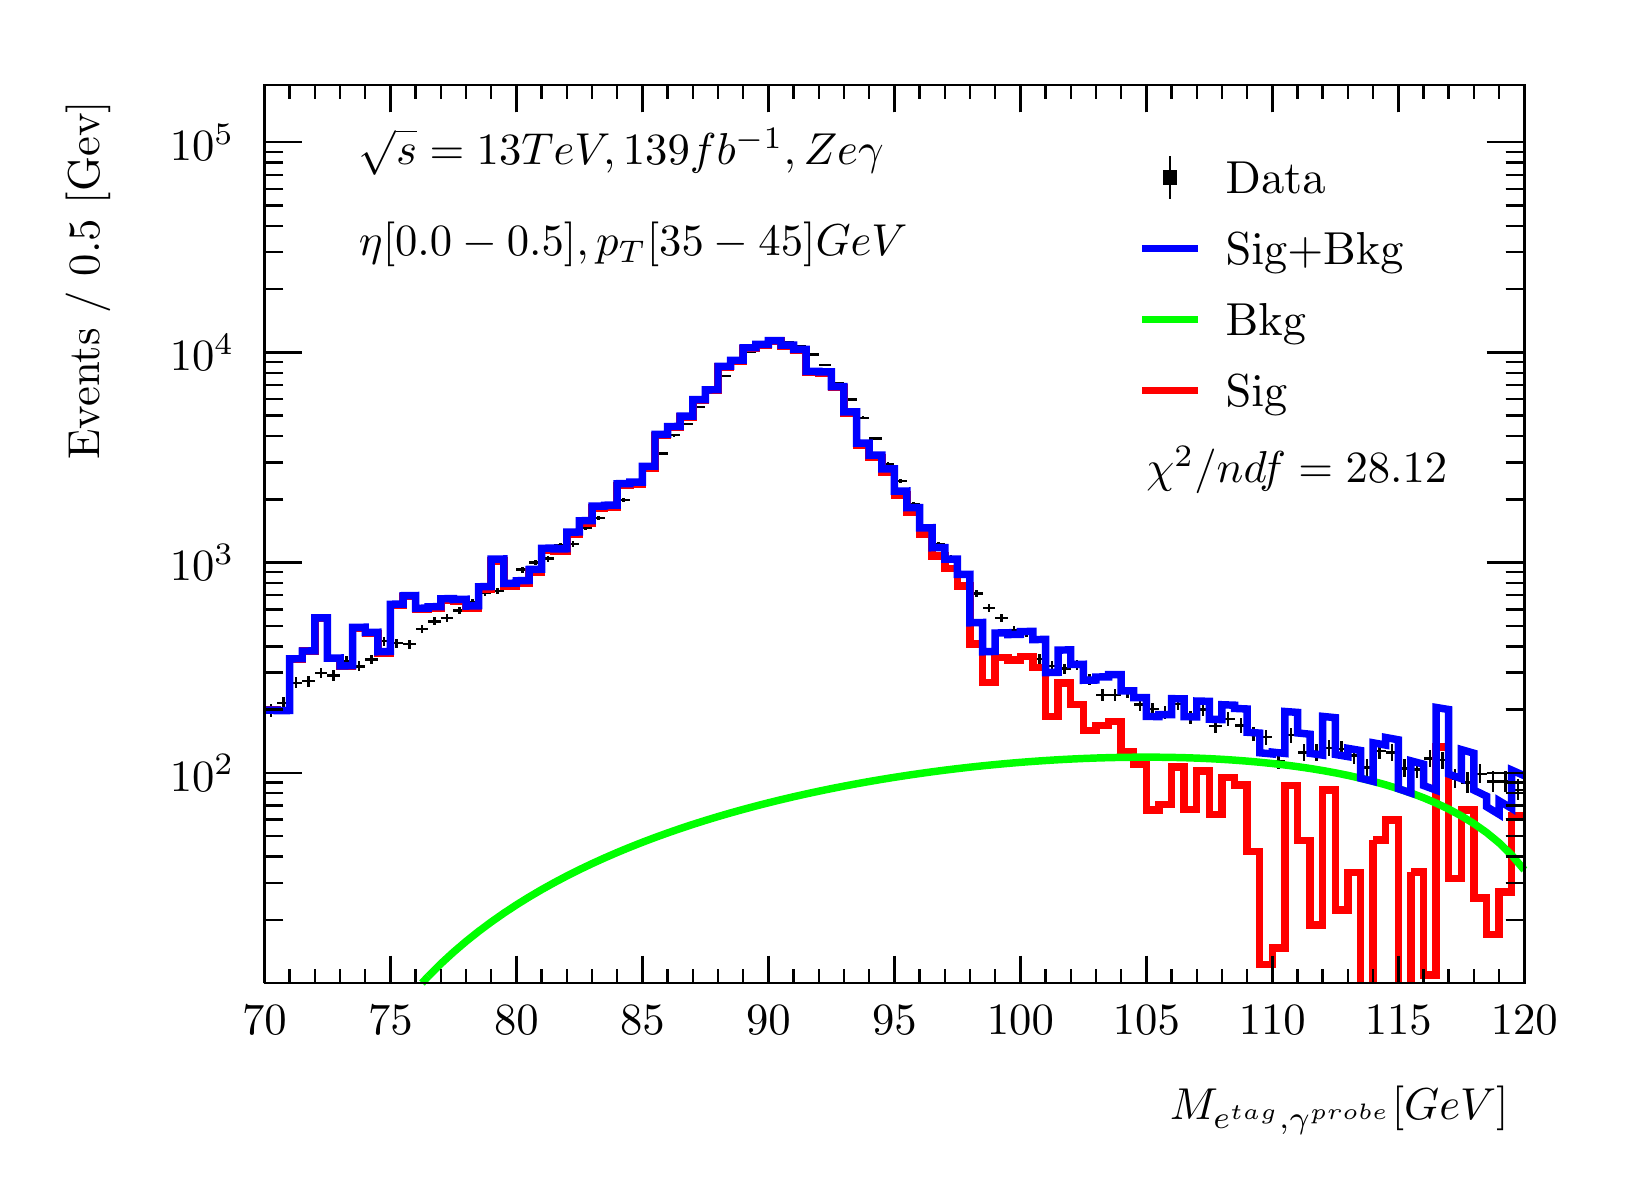
\begin{tikzpicture}
\pgfdeclareplotmark{cross} {
\pgfpathmoveto{\pgfpoint{-0.3\pgfplotmarksize}{\pgfplotmarksize}}
\pgfpathlineto{\pgfpoint{+0.3\pgfplotmarksize}{\pgfplotmarksize}}
\pgfpathlineto{\pgfpoint{+0.3\pgfplotmarksize}{0.3\pgfplotmarksize}}
\pgfpathlineto{\pgfpoint{+1\pgfplotmarksize}{0.3\pgfplotmarksize}}
\pgfpathlineto{\pgfpoint{+1\pgfplotmarksize}{-0.3\pgfplotmarksize}}
\pgfpathlineto{\pgfpoint{+0.3\pgfplotmarksize}{-0.3\pgfplotmarksize}}
\pgfpathlineto{\pgfpoint{+0.3\pgfplotmarksize}{-1.\pgfplotmarksize}}
\pgfpathlineto{\pgfpoint{-0.3\pgfplotmarksize}{-1.\pgfplotmarksize}}
\pgfpathlineto{\pgfpoint{-0.3\pgfplotmarksize}{-0.3\pgfplotmarksize}}
\pgfpathlineto{\pgfpoint{-1.\pgfplotmarksize}{-0.3\pgfplotmarksize}}
\pgfpathlineto{\pgfpoint{-1.\pgfplotmarksize}{0.3\pgfplotmarksize}}
\pgfpathlineto{\pgfpoint{-0.3\pgfplotmarksize}{0.3\pgfplotmarksize}}
\pgfpathclose
\pgfusepathqstroke
}
\pgfdeclareplotmark{cross*} {
\pgfpathmoveto{\pgfpoint{-0.3\pgfplotmarksize}{\pgfplotmarksize}}
\pgfpathlineto{\pgfpoint{+0.3\pgfplotmarksize}{\pgfplotmarksize}}
\pgfpathlineto{\pgfpoint{+0.3\pgfplotmarksize}{0.3\pgfplotmarksize}}
\pgfpathlineto{\pgfpoint{+1\pgfplotmarksize}{0.3\pgfplotmarksize}}
\pgfpathlineto{\pgfpoint{+1\pgfplotmarksize}{-0.3\pgfplotmarksize}}
\pgfpathlineto{\pgfpoint{+0.3\pgfplotmarksize}{-0.3\pgfplotmarksize}}
\pgfpathlineto{\pgfpoint{+0.3\pgfplotmarksize}{-1.\pgfplotmarksize}}
\pgfpathlineto{\pgfpoint{-0.3\pgfplotmarksize}{-1.\pgfplotmarksize}}
\pgfpathlineto{\pgfpoint{-0.3\pgfplotmarksize}{-0.3\pgfplotmarksize}}
\pgfpathlineto{\pgfpoint{-1.\pgfplotmarksize}{-0.3\pgfplotmarksize}}
\pgfpathlineto{\pgfpoint{-1.\pgfplotmarksize}{0.3\pgfplotmarksize}}
\pgfpathlineto{\pgfpoint{-0.3\pgfplotmarksize}{0.3\pgfplotmarksize}}
\pgfpathclose
\pgfusepathqfillstroke
}
\pgfdeclareplotmark{newstar} {
\pgfpathmoveto{\pgfqpoint{0pt}{\pgfplotmarksize}}
\pgfpathlineto{\pgfqpointpolar{44}{0.5\pgfplotmarksize}}
\pgfpathlineto{\pgfqpointpolar{18}{\pgfplotmarksize}}
\pgfpathlineto{\pgfqpointpolar{-20}{0.5\pgfplotmarksize}}
\pgfpathlineto{\pgfqpointpolar{-54}{\pgfplotmarksize}}
\pgfpathlineto{\pgfqpointpolar{-90}{0.5\pgfplotmarksize}}
\pgfpathlineto{\pgfqpointpolar{234}{\pgfplotmarksize}}
\pgfpathlineto{\pgfqpointpolar{198}{0.5\pgfplotmarksize}}
\pgfpathlineto{\pgfqpointpolar{162}{\pgfplotmarksize}}
\pgfpathlineto{\pgfqpointpolar{134}{0.5\pgfplotmarksize}}
\pgfpathclose
\pgfusepathqstroke
}
\pgfdeclareplotmark{newstar*} {
\pgfpathmoveto{\pgfqpoint{0pt}{\pgfplotmarksize}}
\pgfpathlineto{\pgfqpointpolar{44}{0.5\pgfplotmarksize}}
\pgfpathlineto{\pgfqpointpolar{18}{\pgfplotmarksize}}
\pgfpathlineto{\pgfqpointpolar{-20}{0.5\pgfplotmarksize}}
\pgfpathlineto{\pgfqpointpolar{-54}{\pgfplotmarksize}}
\pgfpathlineto{\pgfqpointpolar{-90}{0.5\pgfplotmarksize}}
\pgfpathlineto{\pgfqpointpolar{234}{\pgfplotmarksize}}
\pgfpathlineto{\pgfqpointpolar{198}{0.5\pgfplotmarksize}}
\pgfpathlineto{\pgfqpointpolar{162}{\pgfplotmarksize}}
\pgfpathlineto{\pgfqpointpolar{134}{0.5\pgfplotmarksize}}
\pgfpathclose
\pgfusepathqfillstroke
}
\definecolor{c}{rgb}{1,1,1};
\draw [color=c, fill=c] (0,0) rectangle (20,14.4361);
\draw [color=c, fill=c] (3,2.30977) rectangle (19,13.7143);
\definecolor{c}{rgb}{0,0,0};
\draw [c,line width=0.9] (3,2.30977) -- (3,13.7143) -- (19,13.7143) -- (19,2.30977) -- (3,2.30977);
\definecolor{c}{rgb}{1,1,1};
\draw [color=c, fill=c] (3,2.30977) rectangle (19,13.7143);
\definecolor{c}{rgb}{0,0,0};
\draw [c,line width=0.9] (3,2.30977) -- (3,13.7143) -- (19,13.7143) -- (19,2.30977) -- (3,2.30977);
\draw [c,line width=0.9] (3,2.30977) -- (19,2.30977);
\draw [c,line width=0.9] (3,2.65624) -- (3,2.30977);
\draw [c,line width=0.9] (3.32,2.48301) -- (3.32,2.30977);
\draw [c,line width=0.9] (3.64,2.48301) -- (3.64,2.30977);
\draw [c,line width=0.9] (3.96,2.48301) -- (3.96,2.30977);
\draw [c,line width=0.9] (4.28,2.48301) -- (4.28,2.30977);
\draw [c,line width=0.9] (4.6,2.65624) -- (4.6,2.30977);
\draw [c,line width=0.9] (4.92,2.48301) -- (4.92,2.30977);
\draw [c,line width=0.9] (5.24,2.48301) -- (5.24,2.30977);
\draw [c,line width=0.9] (5.56,2.48301) -- (5.56,2.30977);
\draw [c,line width=0.9] (5.88,2.48301) -- (5.88,2.30977);
\draw [c,line width=0.9] (6.2,2.65624) -- (6.2,2.30977);
\draw [c,line width=0.9] (6.52,2.48301) -- (6.52,2.30977);
\draw [c,line width=0.9] (6.84,2.48301) -- (6.84,2.30977);
\draw [c,line width=0.9] (7.16,2.48301) -- (7.16,2.30977);
\draw [c,line width=0.9] (7.48,2.48301) -- (7.48,2.30977);
\draw [c,line width=0.9] (7.8,2.65624) -- (7.8,2.30977);
\draw [c,line width=0.9] (8.12,2.48301) -- (8.12,2.30977);
\draw [c,line width=0.9] (8.44,2.48301) -- (8.44,2.30977);
\draw [c,line width=0.9] (8.76,2.48301) -- (8.76,2.30977);
\draw [c,line width=0.9] (9.08,2.48301) -- (9.08,2.30977);
\draw [c,line width=0.9] (9.4,2.65624) -- (9.4,2.30977);
\draw [c,line width=0.9] (9.72,2.48301) -- (9.72,2.30977);
\draw [c,line width=0.9] (10.04,2.48301) -- (10.04,2.30977);
\draw [c,line width=0.9] (10.36,2.48301) -- (10.36,2.30977);
\draw [c,line width=0.9] (10.68,2.48301) -- (10.68,2.30977);
\draw [c,line width=0.9] (11,2.65624) -- (11,2.30977);
\draw [c,line width=0.9] (11.32,2.48301) -- (11.32,2.30977);
\draw [c,line width=0.9] (11.64,2.48301) -- (11.64,2.30977);
\draw [c,line width=0.9] (11.96,2.48301) -- (11.96,2.30977);
\draw [c,line width=0.9] (12.28,2.48301) -- (12.28,2.30977);
\draw [c,line width=0.9] (12.6,2.65624) -- (12.6,2.30977);
\draw [c,line width=0.9] (12.92,2.48301) -- (12.92,2.30977);
\draw [c,line width=0.9] (13.24,2.48301) -- (13.24,2.30977);
\draw [c,line width=0.9] (13.56,2.48301) -- (13.56,2.30977);
\draw [c,line width=0.9] (13.88,2.48301) -- (13.88,2.30977);
\draw [c,line width=0.9] (14.2,2.65624) -- (14.2,2.30977);
\draw [c,line width=0.9] (14.52,2.48301) -- (14.52,2.30977);
\draw [c,line width=0.9] (14.84,2.48301) -- (14.84,2.30977);
\draw [c,line width=0.9] (15.16,2.48301) -- (15.16,2.30977);
\draw [c,line width=0.9] (15.48,2.48301) -- (15.48,2.30977);
\draw [c,line width=0.9] (15.8,2.65624) -- (15.8,2.30977);
\draw [c,line width=0.9] (16.12,2.48301) -- (16.12,2.30977);
\draw [c,line width=0.9] (16.44,2.48301) -- (16.44,2.30977);
\draw [c,line width=0.9] (16.76,2.48301) -- (16.76,2.30977);
\draw [c,line width=0.9] (17.08,2.48301) -- (17.08,2.30977);
\draw [c,line width=0.9] (17.4,2.65624) -- (17.4,2.30977);
\draw [c,line width=0.9] (17.72,2.48301) -- (17.72,2.30977);
\draw [c,line width=0.9] (18.04,2.48301) -- (18.04,2.30977);
\draw [c,line width=0.9] (18.36,2.48301) -- (18.36,2.30977);
\draw [c,line width=0.9] (18.68,2.48301) -- (18.68,2.30977);
\draw [c,line width=0.9] (19,2.65624) -- (19,2.30977);
\draw [anchor=base] (3,1.66015) node[scale=1.61424, color=c, rotate=0]{70};
\draw [anchor=base] (4.6,1.66015) node[scale=1.61424, color=c, rotate=0]{75};
\draw [anchor=base] (6.2,1.66015) node[scale=1.61424, color=c, rotate=0]{80};
\draw [anchor=base] (7.8,1.66015) node[scale=1.61424, color=c, rotate=0]{85};
\draw [anchor=base] (9.4,1.66015) node[scale=1.61424, color=c, rotate=0]{90};
\draw [anchor=base] (11,1.66015) node[scale=1.61424, color=c, rotate=0]{95};
\draw [anchor=base] (12.6,1.66015) node[scale=1.61424, color=c, rotate=0]{100};
\draw [anchor=base] (14.2,1.66015) node[scale=1.61424, color=c, rotate=0]{105};
\draw [anchor=base] (15.8,1.66015) node[scale=1.61424, color=c, rotate=0]{110};
\draw [anchor=base] (17.4,1.66015) node[scale=1.61424, color=c, rotate=0]{115};
\draw [anchor=base] (19,1.66015) node[scale=1.61424, color=c, rotate=0]{120};
\draw [anchor= east] (19,0.692932) node[scale=1.61424, color=c, rotate=0]{$M_{e^{tag}, \gamma^{probe}}  [GeV]$};
\draw [c,line width=0.9] (3,13.7143) -- (19,13.7143);
\draw [c,line width=0.9] (3,13.3678) -- (3,13.7143);
\draw [c,line width=0.9] (3.32,13.5411) -- (3.32,13.7143);
\draw [c,line width=0.9] (3.64,13.5411) -- (3.64,13.7143);
\draw [c,line width=0.9] (3.96,13.5411) -- (3.96,13.7143);
\draw [c,line width=0.9] (4.28,13.5411) -- (4.28,13.7143);
\draw [c,line width=0.9] (4.6,13.3678) -- (4.6,13.7143);
\draw [c,line width=0.9] (4.92,13.5411) -- (4.92,13.7143);
\draw [c,line width=0.9] (5.24,13.5411) -- (5.24,13.7143);
\draw [c,line width=0.9] (5.56,13.5411) -- (5.56,13.7143);
\draw [c,line width=0.9] (5.88,13.5411) -- (5.88,13.7143);
\draw [c,line width=0.9] (6.2,13.3678) -- (6.2,13.7143);
\draw [c,line width=0.9] (6.52,13.5411) -- (6.52,13.7143);
\draw [c,line width=0.9] (6.84,13.5411) -- (6.84,13.7143);
\draw [c,line width=0.9] (7.16,13.5411) -- (7.16,13.7143);
\draw [c,line width=0.9] (7.48,13.5411) -- (7.48,13.7143);
\draw [c,line width=0.9] (7.8,13.3678) -- (7.8,13.7143);
\draw [c,line width=0.9] (8.12,13.5411) -- (8.12,13.7143);
\draw [c,line width=0.9] (8.44,13.5411) -- (8.44,13.7143);
\draw [c,line width=0.9] (8.76,13.5411) -- (8.76,13.7143);
\draw [c,line width=0.9] (9.08,13.5411) -- (9.08,13.7143);
\draw [c,line width=0.9] (9.4,13.3678) -- (9.4,13.7143);
\draw [c,line width=0.9] (9.72,13.5411) -- (9.72,13.7143);
\draw [c,line width=0.9] (10.04,13.5411) -- (10.04,13.7143);
\draw [c,line width=0.9] (10.36,13.5411) -- (10.36,13.7143);
\draw [c,line width=0.9] (10.68,13.5411) -- (10.68,13.7143);
\draw [c,line width=0.9] (11,13.3678) -- (11,13.7143);
\draw [c,line width=0.9] (11.32,13.5411) -- (11.32,13.7143);
\draw [c,line width=0.9] (11.64,13.5411) -- (11.64,13.7143);
\draw [c,line width=0.9] (11.96,13.5411) -- (11.96,13.7143);
\draw [c,line width=0.9] (12.28,13.5411) -- (12.28,13.7143);
\draw [c,line width=0.9] (12.6,13.3678) -- (12.6,13.7143);
\draw [c,line width=0.9] (12.92,13.5411) -- (12.92,13.7143);
\draw [c,line width=0.9] (13.24,13.5411) -- (13.24,13.7143);
\draw [c,line width=0.9] (13.56,13.5411) -- (13.56,13.7143);
\draw [c,line width=0.9] (13.88,13.5411) -- (13.88,13.7143);
\draw [c,line width=0.9] (14.2,13.3678) -- (14.2,13.7143);
\draw [c,line width=0.9] (14.52,13.5411) -- (14.52,13.7143);
\draw [c,line width=0.9] (14.84,13.5411) -- (14.84,13.7143);
\draw [c,line width=0.9] (15.16,13.5411) -- (15.16,13.7143);
\draw [c,line width=0.9] (15.48,13.5411) -- (15.48,13.7143);
\draw [c,line width=0.9] (15.8,13.3678) -- (15.8,13.7143);
\draw [c,line width=0.9] (16.12,13.5411) -- (16.12,13.7143);
\draw [c,line width=0.9] (16.44,13.5411) -- (16.44,13.7143);
\draw [c,line width=0.9] (16.76,13.5411) -- (16.76,13.7143);
\draw [c,line width=0.9] (17.08,13.5411) -- (17.08,13.7143);
\draw [c,line width=0.9] (17.4,13.3678) -- (17.4,13.7143);
\draw [c,line width=0.9] (17.72,13.5411) -- (17.72,13.7143);
\draw [c,line width=0.9] (18.04,13.5411) -- (18.04,13.7143);
\draw [c,line width=0.9] (18.36,13.5411) -- (18.36,13.7143);
\draw [c,line width=0.9] (18.68,13.5411) -- (18.68,13.7143);
\draw [c,line width=0.9] (19,13.3678) -- (19,13.7143);
\draw [c,line width=0.9] (3,2.30977) -- (3,13.7143);
\draw [c,line width=0.9] (3.237,3.11343) -- (3,3.11343);
\draw [c,line width=0.9] (3.237,3.58354) -- (3,3.58354);
\draw [c,line width=0.9] (3.237,3.91709) -- (3,3.91709);
\draw [c,line width=0.9] (3.237,4.17581) -- (3,4.17581);
\draw [c,line width=0.9] (3.237,4.38719) -- (3,4.38719);
\draw [c,line width=0.9] (3.237,4.56592) -- (3,4.56592);
\draw [c,line width=0.9] (3.237,4.72074) -- (3,4.72074);
\draw [c,line width=0.9] (3.237,4.8573) -- (3,4.8573);
\draw [c,line width=0.9] (3.474,4.97946) -- (3,4.97946);
\draw [anchor= east] (2.82,4.97946) node[scale=1.61424, color=c, rotate=0]{$10^{2}$};
\draw [c,line width=0.9] (3.237,5.78312) -- (3,5.78312);
\draw [c,line width=0.9] (3.237,6.25323) -- (3,6.25323);
\draw [c,line width=0.9] (3.237,6.58678) -- (3,6.58678);
\draw [c,line width=0.9] (3.237,6.8455) -- (3,6.8455);
\draw [c,line width=0.9] (3.237,7.05689) -- (3,7.05689);
\draw [c,line width=0.9] (3.237,7.23561) -- (3,7.23561);
\draw [c,line width=0.9] (3.237,7.39043) -- (3,7.39043);
\draw [c,line width=0.9] (3.237,7.52699) -- (3,7.52699);
\draw [c,line width=0.9] (3.474,7.64915) -- (3,7.64915);
\draw [anchor= east] (2.82,7.64915) node[scale=1.61424, color=c, rotate=0]{$10^{3}$};
\draw [c,line width=0.9] (3.237,8.45281) -- (3,8.45281);
\draw [c,line width=0.9] (3.237,8.92292) -- (3,8.92292);
\draw [c,line width=0.9] (3.237,9.25647) -- (3,9.25647);
\draw [c,line width=0.9] (3.237,9.51519) -- (3,9.51519);
\draw [c,line width=0.9] (3.237,9.72658) -- (3,9.72658);
\draw [c,line width=0.9] (3.237,9.9053) -- (3,9.9053);
\draw [c,line width=0.9] (3.237,10.0601) -- (3,10.0601);
\draw [c,line width=0.9] (3.237,10.1967) -- (3,10.1967);
\draw [c,line width=0.9] (3.474,10.3188) -- (3,10.3188);
\draw [anchor= east] (2.82,10.3188) node[scale=1.61424, color=c, rotate=0]{$10^{4}$};
\draw [c,line width=0.9] (3.237,11.1225) -- (3,11.1225);
\draw [c,line width=0.9] (3.237,11.5926) -- (3,11.5926);
\draw [c,line width=0.9] (3.237,11.9262) -- (3,11.9262);
\draw [c,line width=0.9] (3.237,12.1849) -- (3,12.1849);
\draw [c,line width=0.9] (3.237,12.3963) -- (3,12.3963);
\draw [c,line width=0.9] (3.237,12.575) -- (3,12.575);
\draw [c,line width=0.9] (3.237,12.7298) -- (3,12.7298);
\draw [c,line width=0.9] (3.237,12.8664) -- (3,12.8664);
\draw [c,line width=0.9] (3.474,12.9885) -- (3,12.9885);
\draw [anchor= east] (2.82,12.9885) node[scale=1.61424, color=c, rotate=0]{$10^{5}$};
\draw [anchor= east] (0.76,13.7143) node[scale=1.61424, color=c, rotate=90]{Events / 0.5 [Gev]};
\draw [c,line width=0.9] (19,2.30977) -- (19,13.7143);
\draw [c,line width=0.9] (18.763,3.11343) -- (19,3.11343);
\draw [c,line width=0.9] (18.763,3.58354) -- (19,3.58354);
\draw [c,line width=0.9] (18.763,3.91709) -- (19,3.91709);
\draw [c,line width=0.9] (18.763,4.17581) -- (19,4.17581);
\draw [c,line width=0.9] (18.763,4.38719) -- (19,4.38719);
\draw [c,line width=0.9] (18.763,4.56592) -- (19,4.56592);
\draw [c,line width=0.9] (18.763,4.72074) -- (19,4.72074);
\draw [c,line width=0.9] (18.763,4.8573) -- (19,4.8573);
\draw [c,line width=0.9] (18.526,4.97946) -- (19,4.97946);
\draw [c,line width=0.9] (18.763,5.78312) -- (19,5.78312);
\draw [c,line width=0.9] (18.763,6.25323) -- (19,6.25323);
\draw [c,line width=0.9] (18.763,6.58678) -- (19,6.58678);
\draw [c,line width=0.9] (18.763,6.8455) -- (19,6.8455);
\draw [c,line width=0.9] (18.763,7.05689) -- (19,7.05689);
\draw [c,line width=0.9] (18.763,7.23561) -- (19,7.23561);
\draw [c,line width=0.9] (18.763,7.39043) -- (19,7.39043);
\draw [c,line width=0.9] (18.763,7.52699) -- (19,7.52699);
\draw [c,line width=0.9] (18.526,7.64915) -- (19,7.64915);
\draw [c,line width=0.9] (18.763,8.45281) -- (19,8.45281);
\draw [c,line width=0.9] (18.763,8.92292) -- (19,8.92292);
\draw [c,line width=0.9] (18.763,9.25647) -- (19,9.25647);
\draw [c,line width=0.9] (18.763,9.51519) -- (19,9.51519);
\draw [c,line width=0.9] (18.763,9.72658) -- (19,9.72658);
\draw [c,line width=0.9] (18.763,9.9053) -- (19,9.9053);
\draw [c,line width=0.9] (18.763,10.0601) -- (19,10.0601);
\draw [c,line width=0.9] (18.763,10.1967) -- (19,10.1967);
\draw [c,line width=0.9] (18.526,10.3188) -- (19,10.3188);
\draw [c,line width=0.9] (18.763,11.1225) -- (19,11.1225);
\draw [c,line width=0.9] (18.763,11.5926) -- (19,11.5926);
\draw [c,line width=0.9] (18.763,11.9262) -- (19,11.9262);
\draw [c,line width=0.9] (18.763,12.1849) -- (19,12.1849);
\draw [c,line width=0.9] (18.763,12.3963) -- (19,12.3963);
\draw [c,line width=0.9] (18.763,12.575) -- (19,12.575);
\draw [c,line width=0.9] (18.763,12.7298) -- (19,12.7298);
\draw [c,line width=0.9] (18.763,12.8664) -- (19,12.8664);
\draw [c,line width=0.9] (18.526,12.9885) -- (19,12.9885);
\draw [c,line width=0.9] (3.08,5.77147) -- (3,5.77147);
\draw [c,line width=0.9] (3,5.77147) -- (3,5.77147);
\draw [c,line width=0.9] (3.08,5.77147) -- (3.16,5.77147);
\draw [c,line width=0.9] (3.16,5.77147) -- (3.16,5.77147);
\draw [c,line width=0.9] (3.08,5.77147) -- (3.08,5.85385);
\draw [c,line width=0.9] (3.08,5.85385) -- (3.08,5.85385);
\draw [c,line width=0.9] (3.08,5.77147) -- (3.08,5.68909);
\draw [c,line width=0.9] (3.08,5.68909) -- (3.08,5.68909);
\draw [c,line width=0.9] (3.24,5.86697) -- (3.16,5.86697);
\draw [c,line width=0.9] (3.16,5.86697) -- (3.16,5.86697);
\draw [c,line width=0.9] (3.24,5.86697) -- (3.32,5.86697);
\draw [c,line width=0.9] (3.32,5.86697) -- (3.32,5.86697);
\draw [c,line width=0.9] (3.24,5.86697) -- (3.24,5.94603);
\draw [c,line width=0.9] (3.24,5.94603) -- (3.24,5.94603);
\draw [c,line width=0.9] (3.24,5.86697) -- (3.24,5.78791);
\draw [c,line width=0.9] (3.24,5.78791) -- (3.24,5.78791);
\draw [c,line width=0.9] (3.4,6.12245) -- (3.32,6.12245);
\draw [c,line width=0.9] (3.32,6.12245) -- (3.32,6.12245);
\draw [c,line width=0.9] (3.4,6.12245) -- (3.48,6.12245);
\draw [c,line width=0.9] (3.48,6.12245) -- (3.48,6.12245);
\draw [c,line width=0.9] (3.4,6.12245) -- (3.4,6.19326);
\draw [c,line width=0.9] (3.4,6.19326) -- (3.4,6.19326);
\draw [c,line width=0.9] (3.4,6.12245) -- (3.4,6.05164);
\draw [c,line width=0.9] (3.4,6.05164) -- (3.4,6.05164);
\draw [c,line width=0.9] (3.56,6.14388) -- (3.48,6.14388);
\draw [c,line width=0.9] (3.48,6.14388) -- (3.48,6.14388);
\draw [c,line width=0.9] (3.56,6.14388) -- (3.64,6.14388);
\draw [c,line width=0.9] (3.64,6.14388) -- (3.64,6.14388);
\draw [c,line width=0.9] (3.56,6.14388) -- (3.56,6.21404);
\draw [c,line width=0.9] (3.56,6.21404) -- (3.56,6.21404);
\draw [c,line width=0.9] (3.56,6.14388) -- (3.56,6.07372);
\draw [c,line width=0.9] (3.56,6.07372) -- (3.56,6.07372);
\draw [c,line width=0.9] (3.72,6.24547) -- (3.64,6.24547);
\draw [c,line width=0.9] (3.64,6.24547) -- (3.64,6.24547);
\draw [c,line width=0.9] (3.72,6.24547) -- (3.8,6.24547);
\draw [c,line width=0.9] (3.8,6.24547) -- (3.8,6.24547);
\draw [c,line width=0.9] (3.72,6.24547) -- (3.72,6.31263);
\draw [c,line width=0.9] (3.72,6.31263) -- (3.72,6.31263);
\draw [c,line width=0.9] (3.72,6.24547) -- (3.72,6.17832);
\draw [c,line width=0.9] (3.72,6.17832) -- (3.72,6.17832);
\draw [c,line width=0.9] (3.88,6.21392) -- (3.8,6.21392);
\draw [c,line width=0.9] (3.8,6.21392) -- (3.8,6.21392);
\draw [c,line width=0.9] (3.88,6.21392) -- (3.96,6.21392);
\draw [c,line width=0.9] (3.96,6.21392) -- (3.96,6.21392);
\draw [c,line width=0.9] (3.88,6.21392) -- (3.88,6.282);
\draw [c,line width=0.9] (3.88,6.282) -- (3.88,6.282);
\draw [c,line width=0.9] (3.88,6.21392) -- (3.88,6.14585);
\draw [c,line width=0.9] (3.88,6.14585) -- (3.88,6.14585);
\draw [c,line width=0.9] (4.04,6.39835) -- (3.96,6.39835);
\draw [c,line width=0.9] (3.96,6.39835) -- (3.96,6.39835);
\draw [c,line width=0.9] (4.04,6.39835) -- (4.12,6.39835);
\draw [c,line width=0.9] (4.12,6.39835) -- (4.12,6.39835);
\draw [c,line width=0.9] (4.04,6.39835) -- (4.04,6.46122);
\draw [c,line width=0.9] (4.04,6.46122) -- (4.04,6.46122);
\draw [c,line width=0.9] (4.04,6.39835) -- (4.04,6.33548);
\draw [c,line width=0.9] (4.04,6.33548) -- (4.04,6.33548);
\draw [c,line width=0.9] (4.2,6.33168) -- (4.12,6.33168);
\draw [c,line width=0.9] (4.12,6.33168) -- (4.12,6.33168);
\draw [c,line width=0.9] (4.2,6.33168) -- (4.28,6.33168);
\draw [c,line width=0.9] (4.28,6.33168) -- (4.28,6.33168);
\draw [c,line width=0.9] (4.2,6.33168) -- (4.2,6.39638);
\draw [c,line width=0.9] (4.2,6.39638) -- (4.2,6.39638);
\draw [c,line width=0.9] (4.2,6.33168) -- (4.2,6.26697);
\draw [c,line width=0.9] (4.2,6.26697) -- (4.2,6.26697);
\draw [c,line width=0.9] (4.36,6.41863) -- (4.28,6.41863);
\draw [c,line width=0.9] (4.28,6.41863) -- (4.28,6.41863);
\draw [c,line width=0.9] (4.36,6.41863) -- (4.44,6.41863);
\draw [c,line width=0.9] (4.44,6.41863) -- (4.44,6.41863);
\draw [c,line width=0.9] (4.36,6.41863) -- (4.36,6.48095);
\draw [c,line width=0.9] (4.36,6.48095) -- (4.36,6.48095);
\draw [c,line width=0.9] (4.36,6.41863) -- (4.36,6.35631);
\draw [c,line width=0.9] (4.36,6.35631) -- (4.36,6.35631);
\draw [c,line width=0.9] (4.52,6.6516) -- (4.44,6.6516);
\draw [c,line width=0.9] (4.44,6.6516) -- (4.44,6.6516);
\draw [c,line width=0.9] (4.52,6.6516) -- (4.6,6.6516);
\draw [c,line width=0.9] (4.6,6.6516) -- (4.6,6.6516);
\draw [c,line width=0.9] (4.52,6.6516) -- (4.52,6.70797);
\draw [c,line width=0.9] (4.52,6.70797) -- (4.52,6.70797);
\draw [c,line width=0.9] (4.52,6.6516) -- (4.52,6.59523);
\draw [c,line width=0.9] (4.52,6.59523) -- (4.52,6.59523);
\draw [c,line width=0.9] (4.68,6.62666) -- (4.6,6.62666);
\draw [c,line width=0.9] (4.6,6.62666) -- (4.6,6.62666);
\draw [c,line width=0.9] (4.68,6.62666) -- (4.76,6.62666);
\draw [c,line width=0.9] (4.76,6.62666) -- (4.76,6.62666);
\draw [c,line width=0.9] (4.68,6.62666) -- (4.68,6.68364);
\draw [c,line width=0.9] (4.68,6.68364) -- (4.68,6.68364);
\draw [c,line width=0.9] (4.68,6.62666) -- (4.68,6.56969);
\draw [c,line width=0.9] (4.68,6.56969) -- (4.68,6.56969);
\draw [c,line width=0.9] (4.84,6.61258) -- (4.76,6.61258);
\draw [c,line width=0.9] (4.76,6.61258) -- (4.76,6.61258);
\draw [c,line width=0.9] (4.84,6.61258) -- (4.92,6.61258);
\draw [c,line width=0.9] (4.92,6.61258) -- (4.92,6.61258);
\draw [c,line width=0.9] (4.84,6.61258) -- (4.84,6.6699);
\draw [c,line width=0.9] (4.84,6.6699) -- (4.84,6.6699);
\draw [c,line width=0.9] (4.84,6.61258) -- (4.84,6.55525);
\draw [c,line width=0.9] (4.84,6.55525) -- (4.84,6.55525);
\draw [c,line width=0.9] (5,6.80779) -- (4.92,6.80779);
\draw [c,line width=0.9] (4.92,6.80779) -- (4.92,6.80779);
\draw [c,line width=0.9] (5,6.80779) -- (5.08,6.80779);
\draw [c,line width=0.9] (5.08,6.80779) -- (5.08,6.80779);
\draw [c,line width=0.9] (5,6.80779) -- (5,6.86049);
\draw [c,line width=0.9] (5,6.86049) -- (5,6.86049);
\draw [c,line width=0.9] (5,6.80779) -- (5,6.75509);
\draw [c,line width=0.9] (5,6.75509) -- (5,6.75509);
\draw [c,line width=0.9] (5.16,6.90207) -- (5.08,6.90207);
\draw [c,line width=0.9] (5.08,6.90207) -- (5.08,6.90207);
\draw [c,line width=0.9] (5.16,6.90207) -- (5.24,6.90207);
\draw [c,line width=0.9] (5.24,6.90207) -- (5.24,6.90207);
\draw [c,line width=0.9] (5.16,6.90207) -- (5.16,6.95266);
\draw [c,line width=0.9] (5.16,6.95266) -- (5.16,6.95266);
\draw [c,line width=0.9] (5.16,6.90207) -- (5.16,6.85147);
\draw [c,line width=0.9] (5.16,6.85147) -- (5.16,6.85147);
\draw [c,line width=0.9] (5.32,6.94754) -- (5.24,6.94754);
\draw [c,line width=0.9] (5.24,6.94754) -- (5.24,6.94754);
\draw [c,line width=0.9] (5.32,6.94754) -- (5.4,6.94754);
\draw [c,line width=0.9] (5.4,6.94754) -- (5.4,6.94754);
\draw [c,line width=0.9] (5.32,6.94754) -- (5.32,6.99716);
\draw [c,line width=0.9] (5.32,6.99716) -- (5.32,6.99716);
\draw [c,line width=0.9] (5.32,6.94754) -- (5.32,6.89792);
\draw [c,line width=0.9] (5.32,6.89792) -- (5.32,6.89792);
\draw [c,line width=0.9] (5.48,7.03936) -- (5.4,7.03936);
\draw [c,line width=0.9] (5.4,7.03936) -- (5.4,7.03936);
\draw [c,line width=0.9] (5.48,7.03936) -- (5.56,7.03936);
\draw [c,line width=0.9] (5.56,7.03936) -- (5.56,7.03936);
\draw [c,line width=0.9] (5.48,7.03936) -- (5.48,7.08705);
\draw [c,line width=0.9] (5.48,7.08705) -- (5.48,7.08705);
\draw [c,line width=0.9] (5.48,7.03936) -- (5.48,6.99167);
\draw [c,line width=0.9] (5.48,6.99167) -- (5.48,6.99167);
\draw [c,line width=0.9] (5.64,7.14074) -- (5.56,7.14074);
\draw [c,line width=0.9] (5.56,7.14074) -- (5.56,7.14074);
\draw [c,line width=0.9] (5.64,7.14074) -- (5.72,7.14074);
\draw [c,line width=0.9] (5.72,7.14074) -- (5.72,7.14074);
\draw [c,line width=0.9] (5.64,7.14074) -- (5.64,7.18639);
\draw [c,line width=0.9] (5.64,7.18639) -- (5.64,7.18639);
\draw [c,line width=0.9] (5.64,7.14074) -- (5.64,7.09509);
\draw [c,line width=0.9] (5.64,7.09509) -- (5.64,7.09509);
\draw [c,line width=0.9] (5.8,7.26666) -- (5.72,7.26666);
\draw [c,line width=0.9] (5.72,7.26666) -- (5.72,7.26666);
\draw [c,line width=0.9] (5.8,7.26666) -- (5.88,7.26666);
\draw [c,line width=0.9] (5.88,7.26666) -- (5.88,7.26666);
\draw [c,line width=0.9] (5.8,7.26666) -- (5.8,7.3099);
\draw [c,line width=0.9] (5.8,7.3099) -- (5.8,7.3099);
\draw [c,line width=0.9] (5.8,7.26666) -- (5.8,7.22343);
\draw [c,line width=0.9] (5.8,7.22343) -- (5.8,7.22343);
\draw [c,line width=0.9] (5.96,7.28902) -- (5.88,7.28902);
\draw [c,line width=0.9] (5.88,7.28902) -- (5.88,7.28902);
\draw [c,line width=0.9] (5.96,7.28902) -- (6.04,7.28902);
\draw [c,line width=0.9] (6.04,7.28902) -- (6.04,7.28902);
\draw [c,line width=0.9] (5.96,7.28902) -- (5.96,7.33185);
\draw [c,line width=0.9] (5.96,7.33185) -- (5.96,7.33185);
\draw [c,line width=0.9] (5.96,7.28902) -- (5.96,7.2462);
\draw [c,line width=0.9] (5.96,7.2462) -- (5.96,7.2462);
\draw [c,line width=0.9] (6.12,7.36553) -- (6.04,7.36553);
\draw [c,line width=0.9] (6.04,7.36553) -- (6.04,7.36553);
\draw [c,line width=0.9] (6.12,7.36553) -- (6.2,7.36553);
\draw [c,line width=0.9] (6.2,7.36553) -- (6.2,7.36553);
\draw [c,line width=0.9] (6.12,7.36553) -- (6.12,7.40696);
\draw [c,line width=0.9] (6.12,7.40696) -- (6.12,7.40696);
\draw [c,line width=0.9] (6.12,7.36553) -- (6.12,7.3241);
\draw [c,line width=0.9] (6.12,7.3241) -- (6.12,7.3241);
\draw [c,line width=0.9] (6.28,7.55876) -- (6.2,7.55876);
\draw [c,line width=0.9] (6.2,7.55876) -- (6.2,7.55876);
\draw [c,line width=0.9] (6.28,7.55876) -- (6.36,7.55876);
\draw [c,line width=0.9] (6.36,7.55876) -- (6.36,7.55876);
\draw [c,line width=0.9] (6.28,7.55876) -- (6.28,7.59688);
\draw [c,line width=0.9] (6.28,7.59688) -- (6.28,7.59688);
\draw [c,line width=0.9] (6.28,7.55876) -- (6.28,7.52064);
\draw [c,line width=0.9] (6.28,7.52064) -- (6.28,7.52064);
\draw [c,line width=0.9] (6.44,7.65031) -- (6.36,7.65031);
\draw [c,line width=0.9] (6.36,7.65031) -- (6.36,7.65031);
\draw [c,line width=0.9] (6.44,7.65031) -- (6.52,7.65031);
\draw [c,line width=0.9] (6.52,7.65031) -- (6.52,7.65031);
\draw [c,line width=0.9] (6.44,7.65031) -- (6.44,7.68696);
\draw [c,line width=0.9] (6.44,7.68696) -- (6.44,7.68696);
\draw [c,line width=0.9] (6.44,7.65031) -- (6.44,7.61367);
\draw [c,line width=0.9] (6.44,7.61367) -- (6.44,7.61367);
\draw [c,line width=0.9] (6.6,7.69908) -- (6.52,7.69908);
\draw [c,line width=0.9] (6.52,7.69908) -- (6.52,7.69908);
\draw [c,line width=0.9] (6.6,7.69908) -- (6.68,7.69908);
\draw [c,line width=0.9] (6.68,7.69908) -- (6.68,7.69908);
\draw [c,line width=0.9] (6.6,7.69908) -- (6.6,7.73496);
\draw [c,line width=0.9] (6.6,7.73496) -- (6.6,7.73496);
\draw [c,line width=0.9] (6.6,7.69908) -- (6.6,7.6632);
\draw [c,line width=0.9] (6.6,7.6632) -- (6.6,7.6632);
\draw [c,line width=0.9] (6.76,7.87112) -- (6.68,7.87112);
\draw [c,line width=0.9] (6.68,7.87112) -- (6.68,7.87112);
\draw [c,line width=0.9] (6.76,7.87112) -- (6.84,7.87112);
\draw [c,line width=0.9] (6.84,7.87112) -- (6.84,7.87112);
\draw [c,line width=0.9] (6.76,7.87112) -- (6.76,7.90444);
\draw [c,line width=0.9] (6.76,7.90444) -- (6.76,7.90444);
\draw [c,line width=0.9] (6.76,7.87112) -- (6.76,7.83781);
\draw [c,line width=0.9] (6.76,7.83781) -- (6.76,7.83781);
\draw [c,line width=0.9] (6.92,7.8854) -- (6.84,7.8854);
\draw [c,line width=0.9] (6.84,7.8854) -- (6.84,7.8854);
\draw [c,line width=0.9] (6.92,7.8854) -- (7,7.8854);
\draw [c,line width=0.9] (7,7.8854) -- (7,7.8854);
\draw [c,line width=0.9] (6.92,7.8854) -- (6.92,7.91851);
\draw [c,line width=0.9] (6.92,7.91851) -- (6.92,7.91851);
\draw [c,line width=0.9] (6.92,7.8854) -- (6.92,7.85228);
\draw [c,line width=0.9] (6.92,7.85228) -- (6.92,7.85228);
\draw [c,line width=0.9] (7.08,8.09426) -- (7,8.09426);
\draw [c,line width=0.9] (7,8.09426) -- (7,8.09426);
\draw [c,line width=0.9] (7.08,8.09426) -- (7.16,8.09426);
\draw [c,line width=0.9] (7.16,8.09426) -- (7.16,8.09426);
\draw [c,line width=0.9] (7.08,8.09426) -- (7.08,8.12452);
\draw [c,line width=0.9] (7.08,8.12452) -- (7.08,8.12452);
\draw [c,line width=0.9] (7.08,8.09426) -- (7.08,8.064);
\draw [c,line width=0.9] (7.08,8.064) -- (7.08,8.064);
\draw [c,line width=0.9] (7.24,8.21705) -- (7.16,8.21705);
\draw [c,line width=0.9] (7.16,8.21705) -- (7.16,8.21705);
\draw [c,line width=0.9] (7.24,8.21705) -- (7.32,8.21705);
\draw [c,line width=0.9] (7.32,8.21705) -- (7.32,8.21705);
\draw [c,line width=0.9] (7.24,8.21705) -- (7.24,8.24575);
\draw [c,line width=0.9] (7.24,8.24575) -- (7.24,8.24575);
\draw [c,line width=0.9] (7.24,8.21705) -- (7.24,8.18835);
\draw [c,line width=0.9] (7.24,8.18835) -- (7.24,8.18835);
\draw [c,line width=0.9] (7.4,8.37365) -- (7.32,8.37365);
\draw [c,line width=0.9] (7.32,8.37365) -- (7.32,8.37365);
\draw [c,line width=0.9] (7.4,8.37365) -- (7.48,8.37365);
\draw [c,line width=0.9] (7.48,8.37365) -- (7.48,8.37365);
\draw [c,line width=0.9] (7.4,8.37365) -- (7.4,8.40047);
\draw [c,line width=0.9] (7.4,8.40047) -- (7.4,8.40047);
\draw [c,line width=0.9] (7.4,8.37365) -- (7.4,8.34682);
\draw [c,line width=0.9] (7.4,8.34682) -- (7.4,8.34682);
\draw [c,line width=0.9] (7.56,8.44233) -- (7.48,8.44233);
\draw [c,line width=0.9] (7.48,8.44233) -- (7.48,8.44233);
\draw [c,line width=0.9] (7.56,8.44233) -- (7.64,8.44233);
\draw [c,line width=0.9] (7.64,8.44233) -- (7.64,8.44233);
\draw [c,line width=0.9] (7.56,8.44233) -- (7.56,8.46837);
\draw [c,line width=0.9] (7.56,8.46837) -- (7.56,8.46837);
\draw [c,line width=0.9] (7.56,8.44233) -- (7.56,8.41629);
\draw [c,line width=0.9] (7.56,8.41629) -- (7.56,8.41629);
\draw [c,line width=0.9] (7.72,8.68526) -- (7.64,8.68526);
\draw [c,line width=0.9] (7.64,8.68526) -- (7.64,8.68526);
\draw [c,line width=0.9] (7.72,8.68526) -- (7.8,8.68526);
\draw [c,line width=0.9] (7.8,8.68526) -- (7.8,8.68526);
\draw [c,line width=0.9] (7.72,8.68526) -- (7.72,8.70872);
\draw [c,line width=0.9] (7.72,8.70872) -- (7.72,8.70872);
\draw [c,line width=0.9] (7.72,8.68526) -- (7.72,8.66181);
\draw [c,line width=0.9] (7.72,8.66181) -- (7.72,8.66181);
\draw [c,line width=0.9] (7.88,8.83336) -- (7.8,8.83336);
\draw [c,line width=0.9] (7.8,8.83336) -- (7.8,8.83336);
\draw [c,line width=0.9] (7.88,8.83336) -- (7.96,8.83336);
\draw [c,line width=0.9] (7.96,8.83336) -- (7.96,8.83336);
\draw [c,line width=0.9] (7.88,8.83336) -- (7.88,8.85537);
\draw [c,line width=0.9] (7.88,8.85537) -- (7.88,8.85537);
\draw [c,line width=0.9] (7.88,8.83336) -- (7.88,8.81136);
\draw [c,line width=0.9] (7.88,8.81136) -- (7.88,8.81136);
\draw [c,line width=0.9] (8.04,9.03763) -- (7.96,9.03763);
\draw [c,line width=0.9] (7.96,9.03763) -- (7.96,9.03763);
\draw [c,line width=0.9] (8.04,9.03763) -- (8.12,9.03763);
\draw [c,line width=0.9] (8.12,9.03763) -- (8.12,9.03763);
\draw [c,line width=0.9] (8.04,9.03763) -- (8.04,9.05778);
\draw [c,line width=0.9] (8.04,9.05778) -- (8.04,9.05778);
\draw [c,line width=0.9] (8.04,9.03763) -- (8.04,9.01749);
\draw [c,line width=0.9] (8.04,9.01749) -- (8.04,9.01749);
\draw [c,line width=0.9] (8.2,9.26858) -- (8.12,9.26858);
\draw [c,line width=0.9] (8.12,9.26858) -- (8.12,9.26858);
\draw [c,line width=0.9] (8.2,9.26858) -- (8.28,9.26858);
\draw [c,line width=0.9] (8.28,9.26858) -- (8.28,9.26858);
\draw [c,line width=0.9] (8.2,9.26858) -- (8.2,9.28681);
\draw [c,line width=0.9] (8.2,9.28681) -- (8.2,9.28681);
\draw [c,line width=0.9] (8.2,9.26858) -- (8.2,9.25034);
\draw [c,line width=0.9] (8.2,9.25034) -- (8.2,9.25034);
\draw [c,line width=0.9] (8.36,9.41093) -- (8.28,9.41093);
\draw [c,line width=0.9] (8.28,9.41093) -- (8.28,9.41093);
\draw [c,line width=0.9] (8.36,9.41093) -- (8.44,9.41093);
\draw [c,line width=0.9] (8.44,9.41093) -- (8.44,9.41093);
\draw [c,line width=0.9] (8.36,9.41093) -- (8.36,9.42808);
\draw [c,line width=0.9] (8.36,9.42808) -- (8.36,9.42808);
\draw [c,line width=0.9] (8.36,9.41093) -- (8.36,9.39377);
\draw [c,line width=0.9] (8.36,9.39377) -- (8.36,9.39377);
\draw [c,line width=0.9] (8.52,9.62801) -- (8.44,9.62801);
\draw [c,line width=0.9] (8.44,9.62801) -- (8.44,9.62801);
\draw [c,line width=0.9] (8.52,9.62801) -- (8.6,9.62801);
\draw [c,line width=0.9] (8.6,9.62801) -- (8.6,9.62801);
\draw [c,line width=0.9] (8.52,9.62801) -- (8.52,9.64363);
\draw [c,line width=0.9] (8.52,9.64363) -- (8.52,9.64363);
\draw [c,line width=0.9] (8.52,9.62801) -- (8.52,9.61239);
\draw [c,line width=0.9] (8.52,9.61239) -- (8.52,9.61239);
\draw [c,line width=0.9] (8.68,9.85105) -- (8.6,9.85105);
\draw [c,line width=0.9] (8.6,9.85105) -- (8.6,9.85105);
\draw [c,line width=0.9] (8.68,9.85105) -- (8.76,9.85105);
\draw [c,line width=0.9] (8.76,9.85105) -- (8.76,9.85105);
\draw [c,line width=0.9] (8.68,9.85105) -- (8.68,9.86524);
\draw [c,line width=0.9] (8.68,9.86524) -- (8.68,9.86524);
\draw [c,line width=0.9] (8.68,9.85105) -- (8.68,9.83687);
\draw [c,line width=0.9] (8.68,9.83687) -- (8.68,9.83687);
\draw [c,line width=0.9] (8.84,10.0176) -- (8.76,10.0176);
\draw [c,line width=0.9] (8.76,10.0176) -- (8.76,10.0176);
\draw [c,line width=0.9] (8.84,10.0176) -- (8.92,10.0176);
\draw [c,line width=0.9] (8.92,10.0176) -- (8.92,10.0176);
\draw [c,line width=0.9] (8.84,10.0176) -- (8.84,10.0308);
\draw [c,line width=0.9] (8.84,10.0308) -- (8.84,10.0308);
\draw [c,line width=0.9] (8.84,10.0176) -- (8.84,10.0044);
\draw [c,line width=0.9] (8.84,10.0044) -- (8.84,10.0044);
\draw [c,line width=0.9] (9,10.1863) -- (8.92,10.1863);
\draw [c,line width=0.9] (8.92,10.1863) -- (8.92,10.1863);
\draw [c,line width=0.9] (9,10.1863) -- (9.08,10.1863);
\draw [c,line width=0.9] (9.08,10.1863) -- (9.08,10.1863);
\draw [c,line width=0.9] (9,10.1863) -- (9,10.1986);
\draw [c,line width=0.9] (9,10.1986) -- (9,10.1986);
\draw [c,line width=0.9] (9,10.1863) -- (9,10.1741);
\draw [c,line width=0.9] (9,10.1741) -- (9,10.1741);
\draw [c,line width=0.9] (9.16,10.3322) -- (9.08,10.3322);
\draw [c,line width=0.9] (9.08,10.3322) -- (9.08,10.3322);
\draw [c,line width=0.9] (9.16,10.3322) -- (9.24,10.3322);
\draw [c,line width=0.9] (9.24,10.3322) -- (9.24,10.3322);
\draw [c,line width=0.9] (9.16,10.3322) -- (9.16,10.3437);
\draw [c,line width=0.9] (9.16,10.3437) -- (9.16,10.3437);
\draw [c,line width=0.9] (9.16,10.3322) -- (9.16,10.3207);
\draw [c,line width=0.9] (9.16,10.3207) -- (9.16,10.3207);
\draw [c,line width=0.9] (9.32,10.4103) -- (9.24,10.4103);
\draw [c,line width=0.9] (9.24,10.4103) -- (9.24,10.4103);
\draw [c,line width=0.9] (9.32,10.4103) -- (9.4,10.4103);
\draw [c,line width=0.9] (9.4,10.4103) -- (9.4,10.4103);
\draw [c,line width=0.9] (9.32,10.4103) -- (9.32,10.4215);
\draw [c,line width=0.9] (9.32,10.4215) -- (9.32,10.4215);
\draw [c,line width=0.9] (9.32,10.4103) -- (9.32,10.3992);
\draw [c,line width=0.9] (9.32,10.3992) -- (9.32,10.3992);
\draw [c,line width=0.9] (9.48,10.4655) -- (9.4,10.4655);
\draw [c,line width=0.9] (9.4,10.4655) -- (9.4,10.4655);
\draw [c,line width=0.9] (9.48,10.4655) -- (9.56,10.4655);
\draw [c,line width=0.9] (9.56,10.4655) -- (9.56,10.4655);
\draw [c,line width=0.9] (9.48,10.4655) -- (9.48,10.4763);
\draw [c,line width=0.9] (9.48,10.4763) -- (9.48,10.4763);
\draw [c,line width=0.9] (9.48,10.4655) -- (9.48,10.4546);
\draw [c,line width=0.9] (9.48,10.4546) -- (9.48,10.4546);
\draw [c,line width=0.9] (9.64,10.4522) -- (9.56,10.4522);
\draw [c,line width=0.9] (9.56,10.4522) -- (9.56,10.4522);
\draw [c,line width=0.9] (9.64,10.4522) -- (9.72,10.4522);
\draw [c,line width=0.9] (9.72,10.4522) -- (9.72,10.4522);
\draw [c,line width=0.9] (9.64,10.4522) -- (9.64,10.4632);
\draw [c,line width=0.9] (9.64,10.4632) -- (9.64,10.4632);
\draw [c,line width=0.9] (9.64,10.4522) -- (9.64,10.4413);
\draw [c,line width=0.9] (9.64,10.4413) -- (9.64,10.4413);
\draw [c,line width=0.9] (9.8,10.3965) -- (9.72,10.3965);
\draw [c,line width=0.9] (9.72,10.3965) -- (9.72,10.3965);
\draw [c,line width=0.9] (9.8,10.3965) -- (9.88,10.3965);
\draw [c,line width=0.9] (9.88,10.3965) -- (9.88,10.3965);
\draw [c,line width=0.9] (9.8,10.3965) -- (9.8,10.4077);
\draw [c,line width=0.9] (9.8,10.4077) -- (9.8,10.4077);
\draw [c,line width=0.9] (9.8,10.3965) -- (9.8,10.3853);
\draw [c,line width=0.9] (9.8,10.3853) -- (9.8,10.3853);
\draw [c,line width=0.9] (9.96,10.2945) -- (9.88,10.2945);
\draw [c,line width=0.9] (9.88,10.2945) -- (9.88,10.2945);
\draw [c,line width=0.9] (9.96,10.2945) -- (10.04,10.2945);
\draw [c,line width=0.9] (10.04,10.2945) -- (10.04,10.2945);
\draw [c,line width=0.9] (9.96,10.2945) -- (9.96,10.3062);
\draw [c,line width=0.9] (9.96,10.3062) -- (9.96,10.3062);
\draw [c,line width=0.9] (9.96,10.2945) -- (9.96,10.2828);
\draw [c,line width=0.9] (9.96,10.2828) -- (9.96,10.2828);
\draw [c,line width=0.9] (10.12,10.1619) -- (10.04,10.1619);
\draw [c,line width=0.9] (10.04,10.1619) -- (10.04,10.1619);
\draw [c,line width=0.9] (10.12,10.1619) -- (10.2,10.1619);
\draw [c,line width=0.9] (10.2,10.1619) -- (10.2,10.1619);
\draw [c,line width=0.9] (10.12,10.1619) -- (10.12,10.1743);
\draw [c,line width=0.9] (10.12,10.1743) -- (10.12,10.1743);
\draw [c,line width=0.9] (10.12,10.1619) -- (10.12,10.1495);
\draw [c,line width=0.9] (10.12,10.1495) -- (10.12,10.1495);
\draw [c,line width=0.9] (10.28,9.9328) -- (10.2,9.9328);
\draw [c,line width=0.9] (10.2,9.9328) -- (10.2,9.9328);
\draw [c,line width=0.9] (10.28,9.9328) -- (10.36,9.9328);
\draw [c,line width=0.9] (10.36,9.9328) -- (10.36,9.9328);
\draw [c,line width=0.9] (10.28,9.9328) -- (10.28,9.9465);
\draw [c,line width=0.9] (10.28,9.9465) -- (10.28,9.9465);
\draw [c,line width=0.9] (10.28,9.9328) -- (10.28,9.91911);
\draw [c,line width=0.9] (10.28,9.91911) -- (10.28,9.91911);
\draw [c,line width=0.9] (10.44,9.71979) -- (10.36,9.71979);
\draw [c,line width=0.9] (10.36,9.71979) -- (10.36,9.71979);
\draw [c,line width=0.9] (10.44,9.71979) -- (10.52,9.71979);
\draw [c,line width=0.9] (10.52,9.71979) -- (10.52,9.71979);
\draw [c,line width=0.9] (10.44,9.71979) -- (10.44,9.73481);
\draw [c,line width=0.9] (10.44,9.73481) -- (10.44,9.73481);
\draw [c,line width=0.9] (10.44,9.71979) -- (10.44,9.70478);
\draw [c,line width=0.9] (10.44,9.70478) -- (10.44,9.70478);
\draw [c,line width=0.9] (10.6,9.48868) -- (10.52,9.48868);
\draw [c,line width=0.9] (10.52,9.48868) -- (10.52,9.48868);
\draw [c,line width=0.9] (10.6,9.48868) -- (10.68,9.48868);
\draw [c,line width=0.9] (10.68,9.48868) -- (10.68,9.48868);
\draw [c,line width=0.9] (10.6,9.48868) -- (10.6,9.50527);
\draw [c,line width=0.9] (10.6,9.50527) -- (10.6,9.50527);
\draw [c,line width=0.9] (10.6,9.48868) -- (10.6,9.4721);
\draw [c,line width=0.9] (10.6,9.4721) -- (10.6,9.4721);
\draw [c,line width=0.9] (10.76,9.2283) -- (10.68,9.2283);
\draw [c,line width=0.9] (10.68,9.2283) -- (10.68,9.2283);
\draw [c,line width=0.9] (10.76,9.2283) -- (10.84,9.2283);
\draw [c,line width=0.9] (10.84,9.2283) -- (10.84,9.2283);
\draw [c,line width=0.9] (10.76,9.2283) -- (10.76,9.24686);
\draw [c,line width=0.9] (10.76,9.24686) -- (10.76,9.24686);
\draw [c,line width=0.9] (10.76,9.2283) -- (10.76,9.20975);
\draw [c,line width=0.9] (10.76,9.20975) -- (10.76,9.20975);
\draw [c,line width=0.9] (10.92,8.8995) -- (10.84,8.8995);
\draw [c,line width=0.9] (10.84,8.8995) -- (10.84,8.8995);
\draw [c,line width=0.9] (10.92,8.8995) -- (11,8.8995);
\draw [c,line width=0.9] (11,8.8995) -- (11,8.8995);
\draw [c,line width=0.9] (10.92,8.8995) -- (10.92,8.92088);
\draw [c,line width=0.9] (10.92,8.92088) -- (10.92,8.92088);
\draw [c,line width=0.9] (10.92,8.8995) -- (10.92,8.87811);
\draw [c,line width=0.9] (10.92,8.87811) -- (10.92,8.87811);
\draw [c,line width=0.9] (11.08,8.68716) -- (11,8.68716);
\draw [c,line width=0.9] (11,8.68716) -- (11,8.68716);
\draw [c,line width=0.9] (11.08,8.68716) -- (11.16,8.68716);
\draw [c,line width=0.9] (11.16,8.68716) -- (11.16,8.68716);
\draw [c,line width=0.9] (11.08,8.68716) -- (11.08,8.71059);
\draw [c,line width=0.9] (11.08,8.71059) -- (11.08,8.71059);
\draw [c,line width=0.9] (11.08,8.68716) -- (11.08,8.66373);
\draw [c,line width=0.9] (11.08,8.66373) -- (11.08,8.66373);
\draw [c,line width=0.9] (11.24,8.3909) -- (11.16,8.3909);
\draw [c,line width=0.9] (11.16,8.3909) -- (11.16,8.3909);
\draw [c,line width=0.9] (11.24,8.3909) -- (11.32,8.3909);
\draw [c,line width=0.9] (11.32,8.3909) -- (11.32,8.3909);
\draw [c,line width=0.9] (11.24,8.3909) -- (11.24,8.41752);
\draw [c,line width=0.9] (11.24,8.41752) -- (11.24,8.41752);
\draw [c,line width=0.9] (11.24,8.3909) -- (11.24,8.36427);
\draw [c,line width=0.9] (11.24,8.36427) -- (11.24,8.36427);
\draw [c,line width=0.9] (11.4,8.09426) -- (11.32,8.09426);
\draw [c,line width=0.9] (11.32,8.09426) -- (11.32,8.09426);
\draw [c,line width=0.9] (11.4,8.09426) -- (11.48,8.09426);
\draw [c,line width=0.9] (11.48,8.09426) -- (11.48,8.09426);
\draw [c,line width=0.9] (11.4,8.09426) -- (11.4,8.12452);
\draw [c,line width=0.9] (11.4,8.12452) -- (11.4,8.12452);
\draw [c,line width=0.9] (11.4,8.09426) -- (11.4,8.064);
\draw [c,line width=0.9] (11.4,8.064) -- (11.4,8.064);
\draw [c,line width=0.9] (11.56,7.88161) -- (11.48,7.88161);
\draw [c,line width=0.9] (11.48,7.88161) -- (11.48,7.88161);
\draw [c,line width=0.9] (11.56,7.88161) -- (11.64,7.88161);
\draw [c,line width=0.9] (11.64,7.88161) -- (11.64,7.88161);
\draw [c,line width=0.9] (11.56,7.88161) -- (11.56,7.91477);
\draw [c,line width=0.9] (11.56,7.91477) -- (11.56,7.91477);
\draw [c,line width=0.9] (11.56,7.88161) -- (11.56,7.84844);
\draw [c,line width=0.9] (11.56,7.84844) -- (11.56,7.84844);
\draw [c,line width=0.9] (11.72,7.71013) -- (11.64,7.71013);
\draw [c,line width=0.9] (11.64,7.71013) -- (11.64,7.71013);
\draw [c,line width=0.9] (11.72,7.71013) -- (11.8,7.71013);
\draw [c,line width=0.9] (11.8,7.71013) -- (11.8,7.71013);
\draw [c,line width=0.9] (11.72,7.71013) -- (11.72,7.74584);
\draw [c,line width=0.9] (11.72,7.74584) -- (11.72,7.74584);
\draw [c,line width=0.9] (11.72,7.71013) -- (11.72,7.67442);
\draw [c,line width=0.9] (11.72,7.67442) -- (11.72,7.67442);
\draw [c,line width=0.9] (11.88,7.49035) -- (11.8,7.49035);
\draw [c,line width=0.9] (11.8,7.49035) -- (11.8,7.49035);
\draw [c,line width=0.9] (11.88,7.49035) -- (11.96,7.49035);
\draw [c,line width=0.9] (11.96,7.49035) -- (11.96,7.49035);
\draw [c,line width=0.9] (11.88,7.49035) -- (11.88,7.52961);
\draw [c,line width=0.9] (11.88,7.52961) -- (11.88,7.52961);
\draw [c,line width=0.9] (11.88,7.49035) -- (11.88,7.45109);
\draw [c,line width=0.9] (11.88,7.45109) -- (11.88,7.45109);
\draw [c,line width=0.9] (12.04,7.25695) -- (11.96,7.25695);
\draw [c,line width=0.9] (11.96,7.25695) -- (11.96,7.25695);
\draw [c,line width=0.9] (12.04,7.25695) -- (12.12,7.25695);
\draw [c,line width=0.9] (12.12,7.25695) -- (12.12,7.25695);
\draw [c,line width=0.9] (12.04,7.25695) -- (12.04,7.30037);
\draw [c,line width=0.9] (12.04,7.30037) -- (12.04,7.30037);
\draw [c,line width=0.9] (12.04,7.25695) -- (12.04,7.21353);
\draw [c,line width=0.9] (12.04,7.21353) -- (12.04,7.21353);
\draw [c,line width=0.9] (12.2,7.07034) -- (12.12,7.07034);
\draw [c,line width=0.9] (12.12,7.07034) -- (12.12,7.07034);
\draw [c,line width=0.9] (12.2,7.07034) -- (12.28,7.07034);
\draw [c,line width=0.9] (12.28,7.07034) -- (12.28,7.07034);
\draw [c,line width=0.9] (12.2,7.07034) -- (12.2,7.11739);
\draw [c,line width=0.9] (12.2,7.11739) -- (12.2,7.11739);
\draw [c,line width=0.9] (12.2,7.07034) -- (12.2,7.02328);
\draw [c,line width=0.9] (12.2,7.02328) -- (12.2,7.02328);
\draw [c,line width=0.9] (12.36,6.94329) -- (12.28,6.94329);
\draw [c,line width=0.9] (12.28,6.94329) -- (12.28,6.94329);
\draw [c,line width=0.9] (12.36,6.94329) -- (12.44,6.94329);
\draw [c,line width=0.9] (12.44,6.94329) -- (12.44,6.94329);
\draw [c,line width=0.9] (12.36,6.94329) -- (12.36,6.99299);
\draw [c,line width=0.9] (12.36,6.99299) -- (12.36,6.99299);
\draw [c,line width=0.9] (12.36,6.94329) -- (12.36,6.89358);
\draw [c,line width=0.9] (12.36,6.89358) -- (12.36,6.89358);
\draw [c,line width=0.9] (12.52,6.79575) -- (12.44,6.79575);
\draw [c,line width=0.9] (12.44,6.79575) -- (12.44,6.79575);
\draw [c,line width=0.9] (12.52,6.79575) -- (12.6,6.79575);
\draw [c,line width=0.9] (12.6,6.79575) -- (12.6,6.79575);
\draw [c,line width=0.9] (12.52,6.79575) -- (12.52,6.84872);
\draw [c,line width=0.9] (12.52,6.84872) -- (12.52,6.84872);
\draw [c,line width=0.9] (12.52,6.79575) -- (12.52,6.74278);
\draw [c,line width=0.9] (12.52,6.74278) -- (12.52,6.74278);
\draw [c,line width=0.9] (12.68,6.75636) -- (12.6,6.75636);
\draw [c,line width=0.9] (12.6,6.75636) -- (12.6,6.75636);
\draw [c,line width=0.9] (12.68,6.75636) -- (12.76,6.75636);
\draw [c,line width=0.9] (12.76,6.75636) -- (12.76,6.75636);
\draw [c,line width=0.9] (12.68,6.75636) -- (12.68,6.81024);
\draw [c,line width=0.9] (12.68,6.81024) -- (12.68,6.81024);
\draw [c,line width=0.9] (12.68,6.75636) -- (12.68,6.70248);
\draw [c,line width=0.9] (12.68,6.70248) -- (12.68,6.70248);
\draw [c,line width=0.9] (12.84,6.42198) -- (12.76,6.42198);
\draw [c,line width=0.9] (12.76,6.42198) -- (12.76,6.42198);
\draw [c,line width=0.9] (12.84,6.42198) -- (12.92,6.42198);
\draw [c,line width=0.9] (12.92,6.42198) -- (12.92,6.42198);
\draw [c,line width=0.9] (12.84,6.42198) -- (12.84,6.48421);
\draw [c,line width=0.9] (12.84,6.48421) -- (12.84,6.48421);
\draw [c,line width=0.9] (12.84,6.42198) -- (12.84,6.35974);
\draw [c,line width=0.9] (12.84,6.35974) -- (12.84,6.35974);
\draw [c,line width=0.9] (13,6.33528) -- (12.92,6.33528);
\draw [c,line width=0.9] (12.92,6.33528) -- (12.92,6.33528);
\draw [c,line width=0.9] (13,6.33528) -- (13.08,6.33528);
\draw [c,line width=0.9] (13.08,6.33528) -- (13.08,6.33528);
\draw [c,line width=0.9] (13,6.33528) -- (13,6.39989);
\draw [c,line width=0.9] (13,6.39989) -- (13,6.39989);
\draw [c,line width=0.9] (13,6.33528) -- (13,6.27068);
\draw [c,line width=0.9] (13,6.27068) -- (13,6.27068);
\draw [c,line width=0.9] (13.16,6.30241) -- (13.08,6.30241);
\draw [c,line width=0.9] (13.08,6.30241) -- (13.08,6.30241);
\draw [c,line width=0.9] (13.16,6.30241) -- (13.24,6.30241);
\draw [c,line width=0.9] (13.24,6.30241) -- (13.24,6.30241);
\draw [c,line width=0.9] (13.16,6.30241) -- (13.16,6.36794);
\draw [c,line width=0.9] (13.16,6.36794) -- (13.16,6.36794);
\draw [c,line width=0.9] (13.16,6.30241) -- (13.16,6.23689);
\draw [c,line width=0.9] (13.16,6.23689) -- (13.16,6.23689);
\draw [c,line width=0.9] (13.32,6.34603) -- (13.24,6.34603);
\draw [c,line width=0.9] (13.24,6.34603) -- (13.24,6.34603);
\draw [c,line width=0.9] (13.32,6.34603) -- (13.4,6.34603);
\draw [c,line width=0.9] (13.4,6.34603) -- (13.4,6.34603);
\draw [c,line width=0.9] (13.32,6.34603) -- (13.32,6.41034);
\draw [c,line width=0.9] (13.32,6.41034) -- (13.32,6.41034);
\draw [c,line width=0.9] (13.32,6.34603) -- (13.32,6.28173);
\draw [c,line width=0.9] (13.32,6.28173) -- (13.32,6.28173);
\draw [c,line width=0.9] (13.48,6.16493) -- (13.4,6.16493);
\draw [c,line width=0.9] (13.4,6.16493) -- (13.4,6.16493);
\draw [c,line width=0.9] (13.48,6.16493) -- (13.56,6.16493);
\draw [c,line width=0.9] (13.56,6.16493) -- (13.56,6.16493);
\draw [c,line width=0.9] (13.48,6.16493) -- (13.48,6.23445);
\draw [c,line width=0.9] (13.48,6.23445) -- (13.48,6.23445);
\draw [c,line width=0.9] (13.48,6.16493) -- (13.48,6.0954);
\draw [c,line width=0.9] (13.48,6.0954) -- (13.48,6.0954);
\draw [c,line width=0.9] (13.64,5.9701) -- (13.56,5.9701);
\draw [c,line width=0.9] (13.56,5.9701) -- (13.56,5.9701);
\draw [c,line width=0.9] (13.64,5.9701) -- (13.72,5.9701);
\draw [c,line width=0.9] (13.72,5.9701) -- (13.72,5.9701);
\draw [c,line width=0.9] (13.64,5.9701) -- (13.64,6.04572);
\draw [c,line width=0.9] (13.64,6.04572) -- (13.64,6.04572);
\draw [c,line width=0.9] (13.64,5.9701) -- (13.64,5.89448);
\draw [c,line width=0.9] (13.64,5.89448) -- (13.64,5.89448);
\draw [c,line width=0.9] (13.8,5.96516) -- (13.72,5.96516);
\draw [c,line width=0.9] (13.72,5.96516) -- (13.72,5.96516);
\draw [c,line width=0.9] (13.8,5.96516) -- (13.88,5.96516);
\draw [c,line width=0.9] (13.88,5.96516) -- (13.88,5.96516);
\draw [c,line width=0.9] (13.8,5.96516) -- (13.8,6.04094);
\draw [c,line width=0.9] (13.8,6.04094) -- (13.8,6.04094);
\draw [c,line width=0.9] (13.8,5.96516) -- (13.8,5.88938);
\draw [c,line width=0.9] (13.8,5.88938) -- (13.8,5.88938);
\draw [c,line width=0.9] (13.96,5.99933) -- (13.88,5.99933);
\draw [c,line width=0.9] (13.88,5.99933) -- (13.88,5.99933);
\draw [c,line width=0.9] (13.96,5.99933) -- (14.04,5.99933);
\draw [c,line width=0.9] (14.04,5.99933) -- (14.04,5.99933);
\draw [c,line width=0.9] (13.96,5.99933) -- (13.96,6.074);
\draw [c,line width=0.9] (13.96,6.074) -- (13.96,6.074);
\draw [c,line width=0.9] (13.96,5.99933) -- (13.96,5.92466);
\draw [c,line width=0.9] (13.96,5.92466) -- (13.96,5.92466);
\draw [c,line width=0.9] (14.12,5.8452) -- (14.04,5.8452);
\draw [c,line width=0.9] (14.04,5.8452) -- (14.04,5.8452);
\draw [c,line width=0.9] (14.12,5.8452) -- (14.2,5.8452);
\draw [c,line width=0.9] (14.2,5.8452) -- (14.2,5.8452);
\draw [c,line width=0.9] (14.12,5.8452) -- (14.12,5.925);
\draw [c,line width=0.9] (14.12,5.925) -- (14.12,5.925);
\draw [c,line width=0.9] (14.12,5.8452) -- (14.12,5.7654);
\draw [c,line width=0.9] (14.12,5.7654) -- (14.12,5.7654);
\draw [c,line width=0.9] (14.28,5.7889) -- (14.2,5.7889);
\draw [c,line width=0.9] (14.2,5.7889) -- (14.2,5.7889);
\draw [c,line width=0.9] (14.28,5.7889) -- (14.36,5.7889);
\draw [c,line width=0.9] (14.36,5.7889) -- (14.36,5.7889);
\draw [c,line width=0.9] (14.28,5.7889) -- (14.28,5.87067);
\draw [c,line width=0.9] (14.28,5.87067) -- (14.28,5.87067);
\draw [c,line width=0.9] (14.28,5.7889) -- (14.28,5.70714);
\draw [c,line width=0.9] (14.28,5.70714) -- (14.28,5.70714);
\draw [c,line width=0.9] (14.44,5.74181) -- (14.36,5.74181);
\draw [c,line width=0.9] (14.36,5.74181) -- (14.36,5.74181);
\draw [c,line width=0.9] (14.44,5.74181) -- (14.52,5.74181);
\draw [c,line width=0.9] (14.52,5.74181) -- (14.52,5.74181);
\draw [c,line width=0.9] (14.44,5.74181) -- (14.44,5.82525);
\draw [c,line width=0.9] (14.44,5.82525) -- (14.44,5.82525);
\draw [c,line width=0.9] (14.44,5.74181) -- (14.44,5.65837);
\draw [c,line width=0.9] (14.44,5.65837) -- (14.44,5.65837);
\draw [c,line width=0.9] (14.6,5.85614) -- (14.52,5.85614);
\draw [c,line width=0.9] (14.52,5.85614) -- (14.52,5.85614);
\draw [c,line width=0.9] (14.6,5.85614) -- (14.68,5.85614);
\draw [c,line width=0.9] (14.68,5.85614) -- (14.68,5.85614);
\draw [c,line width=0.9] (14.6,5.85614) -- (14.6,5.93556);
\draw [c,line width=0.9] (14.6,5.93556) -- (14.6,5.93556);
\draw [c,line width=0.9] (14.6,5.85614) -- (14.6,5.77671);
\draw [c,line width=0.9] (14.6,5.77671) -- (14.6,5.77671);
\draw [c,line width=0.9] (14.76,5.68013) -- (14.68,5.68013);
\draw [c,line width=0.9] (14.68,5.68013) -- (14.68,5.68013);
\draw [c,line width=0.9] (14.76,5.68013) -- (14.84,5.68013);
\draw [c,line width=0.9] (14.84,5.68013) -- (14.84,5.68013);
\draw [c,line width=0.9] (14.76,5.68013) -- (14.76,5.76582);
\draw [c,line width=0.9] (14.76,5.76582) -- (14.76,5.76582);
\draw [c,line width=0.9] (14.76,5.68013) -- (14.76,5.59444);
\draw [c,line width=0.9] (14.76,5.59444) -- (14.76,5.59444);
\draw [c,line width=0.9] (14.92,5.78312) -- (14.84,5.78312);
\draw [c,line width=0.9] (14.84,5.78312) -- (14.84,5.78312);
\draw [c,line width=0.9] (14.92,5.78312) -- (15,5.78312);
\draw [c,line width=0.9] (15,5.78312) -- (15,5.78312);
\draw [c,line width=0.9] (14.92,5.78312) -- (14.92,5.86509);
\draw [c,line width=0.9] (14.92,5.86509) -- (14.92,5.86509);
\draw [c,line width=0.9] (14.92,5.78312) -- (14.92,5.70115);
\draw [c,line width=0.9] (14.92,5.70115) -- (14.92,5.70115);
\draw [c,line width=0.9] (15.08,5.57405) -- (15,5.57405);
\draw [c,line width=0.9] (15,5.57405) -- (15,5.57405);
\draw [c,line width=0.9] (15.08,5.57405) -- (15.16,5.57405);
\draw [c,line width=0.9] (15.16,5.57405) -- (15.16,5.57405);
\draw [c,line width=0.9] (15.08,5.57405) -- (15.08,5.66375);
\draw [c,line width=0.9] (15.08,5.66375) -- (15.08,5.66375);
\draw [c,line width=0.9] (15.08,5.57405) -- (15.08,5.48435);
\draw [c,line width=0.9] (15.08,5.48435) -- (15.08,5.48435);
\draw [c,line width=0.9] (15.24,5.66096) -- (15.16,5.66096);
\draw [c,line width=0.9] (15.16,5.66096) -- (15.16,5.66096);
\draw [c,line width=0.9] (15.24,5.66096) -- (15.32,5.66096);
\draw [c,line width=0.9] (15.32,5.66096) -- (15.32,5.66096);
\draw [c,line width=0.9] (15.24,5.66096) -- (15.24,5.74736);
\draw [c,line width=0.9] (15.24,5.74736) -- (15.24,5.74736);
\draw [c,line width=0.9] (15.24,5.66096) -- (15.24,5.57456);
\draw [c,line width=0.9] (15.24,5.57456) -- (15.24,5.57456);
\draw [c,line width=0.9] (15.4,5.58097) -- (15.32,5.58097);
\draw [c,line width=0.9] (15.32,5.58097) -- (15.32,5.58097);
\draw [c,line width=0.9] (15.4,5.58097) -- (15.48,5.58097);
\draw [c,line width=0.9] (15.48,5.58097) -- (15.48,5.58097);
\draw [c,line width=0.9] (15.4,5.58097) -- (15.4,5.6704);
\draw [c,line width=0.9] (15.4,5.6704) -- (15.4,5.6704);
\draw [c,line width=0.9] (15.4,5.58097) -- (15.4,5.49154);
\draw [c,line width=0.9] (15.4,5.49154) -- (15.4,5.49154);
\draw [c,line width=0.9] (15.56,5.47253) -- (15.48,5.47253);
\draw [c,line width=0.9] (15.48,5.47253) -- (15.48,5.47253);
\draw [c,line width=0.9] (15.56,5.47253) -- (15.64,5.47253);
\draw [c,line width=0.9] (15.64,5.47253) -- (15.64,5.47253);
\draw [c,line width=0.9] (15.56,5.47253) -- (15.56,5.56624);
\draw [c,line width=0.9] (15.56,5.56624) -- (15.56,5.56624);
\draw [c,line width=0.9] (15.56,5.47253) -- (15.56,5.37882);
\draw [c,line width=0.9] (15.56,5.37882) -- (15.56,5.37882);
\draw [c,line width=0.9] (15.72,5.43401) -- (15.64,5.43401);
\draw [c,line width=0.9] (15.64,5.43401) -- (15.64,5.43401);
\draw [c,line width=0.9] (15.72,5.43401) -- (15.8,5.43401);
\draw [c,line width=0.9] (15.8,5.43401) -- (15.8,5.43401);
\draw [c,line width=0.9] (15.72,5.43401) -- (15.72,5.52929);
\draw [c,line width=0.9] (15.72,5.52929) -- (15.72,5.52929);
\draw [c,line width=0.9] (15.72,5.43401) -- (15.72,5.33873);
\draw [c,line width=0.9] (15.72,5.33873) -- (15.72,5.33873);
\draw [c,line width=0.9] (15.88,5.13138) -- (15.8,5.13138);
\draw [c,line width=0.9] (15.8,5.13138) -- (15.8,5.13138);
\draw [c,line width=0.9] (15.88,5.13138) -- (15.96,5.13138);
\draw [c,line width=0.9] (15.96,5.13138) -- (15.96,5.13138);
\draw [c,line width=0.9] (15.88,5.13138) -- (15.88,5.23993);
\draw [c,line width=0.9] (15.88,5.23993) -- (15.88,5.23993);
\draw [c,line width=0.9] (15.88,5.13138) -- (15.88,5.02283);
\draw [c,line width=0.9] (15.88,5.02283) -- (15.88,5.02283);
\draw [c,line width=0.9] (16.04,5.45728) -- (15.96,5.45728);
\draw [c,line width=0.9] (15.96,5.45728) -- (15.96,5.45728);
\draw [c,line width=0.9] (16.04,5.45728) -- (16.12,5.45728);
\draw [c,line width=0.9] (16.12,5.45728) -- (16.12,5.45728);
\draw [c,line width=0.9] (16.04,5.45728) -- (16.04,5.5516);
\draw [c,line width=0.9] (16.04,5.5516) -- (16.04,5.5516);
\draw [c,line width=0.9] (16.04,5.45728) -- (16.04,5.36295);
\draw [c,line width=0.9] (16.04,5.36295) -- (16.04,5.36295);
\draw [c,line width=0.9] (16.2,5.23818) -- (16.12,5.23818);
\draw [c,line width=0.9] (16.12,5.23818) -- (16.12,5.23818);
\draw [c,line width=0.9] (16.2,5.23818) -- (16.28,5.23818);
\draw [c,line width=0.9] (16.28,5.23818) -- (16.28,5.23818);
\draw [c,line width=0.9] (16.2,5.23818) -- (16.2,5.34185);
\draw [c,line width=0.9] (16.2,5.34185) -- (16.2,5.34185);
\draw [c,line width=0.9] (16.2,5.23818) -- (16.2,5.13452);
\draw [c,line width=0.9] (16.2,5.13452) -- (16.2,5.13452);
\draw [c,line width=0.9] (16.36,5.23818) -- (16.28,5.23818);
\draw [c,line width=0.9] (16.28,5.23818) -- (16.28,5.23818);
\draw [c,line width=0.9] (16.36,5.23818) -- (16.44,5.23818);
\draw [c,line width=0.9] (16.44,5.23818) -- (16.44,5.23818);
\draw [c,line width=0.9] (16.36,5.23818) -- (16.36,5.34185);
\draw [c,line width=0.9] (16.36,5.34185) -- (16.36,5.34185);
\draw [c,line width=0.9] (16.36,5.23818) -- (16.36,5.13452);
\draw [c,line width=0.9] (16.36,5.13452) -- (16.36,5.13452);
\draw [c,line width=0.9] (16.52,5.29254) -- (16.44,5.29254);
\draw [c,line width=0.9] (16.44,5.29254) -- (16.44,5.29254);
\draw [c,line width=0.9] (16.52,5.29254) -- (16.6,5.29254);
\draw [c,line width=0.9] (16.6,5.29254) -- (16.6,5.29254);
\draw [c,line width=0.9] (16.52,5.29254) -- (16.52,5.39381);
\draw [c,line width=0.9] (16.52,5.39381) -- (16.52,5.39381);
\draw [c,line width=0.9] (16.52,5.29254) -- (16.52,5.19127);
\draw [c,line width=0.9] (16.52,5.19127) -- (16.52,5.19127);
\draw [c,line width=0.9] (16.68,5.28366) -- (16.6,5.28366);
\draw [c,line width=0.9] (16.6,5.28366) -- (16.6,5.28366);
\draw [c,line width=0.9] (16.68,5.28366) -- (16.76,5.28366);
\draw [c,line width=0.9] (16.76,5.28366) -- (16.76,5.28366);
\draw [c,line width=0.9] (16.68,5.28366) -- (16.68,5.38531);
\draw [c,line width=0.9] (16.68,5.38531) -- (16.68,5.38531);
\draw [c,line width=0.9] (16.68,5.28366) -- (16.68,5.182);
\draw [c,line width=0.9] (16.68,5.182) -- (16.68,5.182);
\draw [c,line width=0.9] (16.84,5.20048) -- (16.76,5.20048);
\draw [c,line width=0.9] (16.76,5.20048) -- (16.76,5.20048);
\draw [c,line width=0.9] (16.84,5.20048) -- (16.92,5.20048);
\draw [c,line width=0.9] (16.92,5.20048) -- (16.92,5.20048);
\draw [c,line width=0.9] (16.84,5.20048) -- (16.84,5.30584);
\draw [c,line width=0.9] (16.84,5.30584) -- (16.84,5.30584);
\draw [c,line width=0.9] (16.84,5.20048) -- (16.84,5.09511);
\draw [c,line width=0.9] (16.84,5.09511) -- (16.84,5.09511);
\draw [c,line width=0.9] (17,5.04702) -- (16.92,5.04702);
\draw [c,line width=0.9] (16.92,5.04702) -- (16.92,5.04702);
\draw [c,line width=0.9] (17,5.04702) -- (17.08,5.04702);
\draw [c,line width=0.9] (17.08,5.04702) -- (17.08,5.04702);
\draw [c,line width=0.9] (17,5.04702) -- (17,5.15959);
\draw [c,line width=0.9] (17,5.15959) -- (17,5.15959);
\draw [c,line width=0.9] (17,5.04702) -- (17,4.93445);
\draw [c,line width=0.9] (17,4.93445) -- (17,4.93445);
\draw [c,line width=0.9] (17.16,5.25659) -- (17.08,5.25659);
\draw [c,line width=0.9] (17.08,5.25659) -- (17.08,5.25659);
\draw [c,line width=0.9] (17.16,5.25659) -- (17.24,5.25659);
\draw [c,line width=0.9] (17.24,5.25659) -- (17.24,5.25659);
\draw [c,line width=0.9] (17.16,5.25659) -- (17.16,5.35944);
\draw [c,line width=0.9] (17.16,5.35944) -- (17.16,5.35944);
\draw [c,line width=0.9] (17.16,5.25659) -- (17.16,5.15374);
\draw [c,line width=0.9] (17.16,5.15374) -- (17.16,5.15374);
\draw [c,line width=0.9] (17.32,5.23818) -- (17.24,5.23818);
\draw [c,line width=0.9] (17.24,5.23818) -- (17.24,5.23818);
\draw [c,line width=0.9] (17.32,5.23818) -- (17.4,5.23818);
\draw [c,line width=0.9] (17.4,5.23818) -- (17.4,5.23818);
\draw [c,line width=0.9] (17.32,5.23818) -- (17.32,5.34185);
\draw [c,line width=0.9] (17.32,5.34185) -- (17.32,5.34185);
\draw [c,line width=0.9] (17.32,5.23818) -- (17.32,5.13452);
\draw [c,line width=0.9] (17.32,5.13452) -- (17.32,5.13452);
\draw [c,line width=0.9] (17.48,5.03603) -- (17.4,5.03603);
\draw [c,line width=0.9] (17.4,5.03603) -- (17.4,5.03603);
\draw [c,line width=0.9] (17.48,5.03603) -- (17.56,5.03603);
\draw [c,line width=0.9] (17.56,5.03603) -- (17.56,5.03603);
\draw [c,line width=0.9] (17.48,5.03603) -- (17.48,5.14914);
\draw [c,line width=0.9] (17.48,5.14914) -- (17.48,5.14914);
\draw [c,line width=0.9] (17.48,5.03603) -- (17.48,4.92293);
\draw [c,line width=0.9] (17.48,4.92293) -- (17.48,4.92293);
\draw [c,line width=0.9] (17.64,5.02494) -- (17.56,5.02494);
\draw [c,line width=0.9] (17.56,5.02494) -- (17.56,5.02494);
\draw [c,line width=0.9] (17.64,5.02494) -- (17.72,5.02494);
\draw [c,line width=0.9] (17.72,5.02494) -- (17.72,5.02494);
\draw [c,line width=0.9] (17.64,5.02494) -- (17.64,5.13858);
\draw [c,line width=0.9] (17.64,5.13858) -- (17.64,5.13858);
\draw [c,line width=0.9] (17.64,5.02494) -- (17.64,4.91129);
\draw [c,line width=0.9] (17.64,4.91129) -- (17.64,4.91129);
\draw [c,line width=0.9] (17.8,5.1615) -- (17.72,5.1615);
\draw [c,line width=0.9] (17.72,5.1615) -- (17.72,5.1615);
\draw [c,line width=0.9] (17.8,5.1615) -- (17.88,5.1615);
\draw [c,line width=0.9] (17.88,5.1615) -- (17.88,5.1615);
\draw [c,line width=0.9] (17.8,5.1615) -- (17.8,5.26865);
\draw [c,line width=0.9] (17.8,5.26865) -- (17.8,5.26865);
\draw [c,line width=0.9] (17.8,5.1615) -- (17.8,5.05435);
\draw [c,line width=0.9] (17.8,5.05435) -- (17.8,5.05435);
\draw [c,line width=0.9] (17.96,5.14151) -- (17.88,5.14151);
\draw [c,line width=0.9] (17.88,5.14151) -- (17.88,5.14151);
\draw [c,line width=0.9] (17.96,5.14151) -- (18.04,5.14151);
\draw [c,line width=0.9] (18.04,5.14151) -- (18.04,5.14151);
\draw [c,line width=0.9] (17.96,5.14151) -- (17.96,5.24959);
\draw [c,line width=0.9] (17.96,5.24959) -- (17.96,5.24959);
\draw [c,line width=0.9] (17.96,5.14151) -- (17.96,5.03343);
\draw [c,line width=0.9] (17.96,5.03343) -- (17.96,5.03343);
\draw [c,line width=0.9] (18.12,4.90772) -- (18.04,4.90772);
\draw [c,line width=0.9] (18.04,4.90772) -- (18.04,4.90772);
\draw [c,line width=0.9] (18.12,4.90772) -- (18.2,4.90772);
\draw [c,line width=0.9] (18.2,4.90772) -- (18.2,4.90772);
\draw [c,line width=0.9] (18.12,4.90772) -- (18.12,5.03305);
\draw [c,line width=0.9] (18.12,5.03305) -- (18.12,5.03305);
\draw [c,line width=0.9] (18.12,4.90772) -- (18.12,4.78175);
\draw [c,line width=0.9] (18.12,4.78175) -- (18.12,4.78175);
\draw [c,line width=0.9] (18.28,4.85731) -- (18.2,4.85731);
\draw [c,line width=0.9] (18.2,4.85731) -- (18.2,4.85731);
\draw [c,line width=0.9] (18.28,4.85731) -- (18.36,4.85731);
\draw [c,line width=0.9] (18.36,4.85731) -- (18.36,4.85731);
\draw [c,line width=0.9] (18.28,4.85731) -- (18.28,4.9855);
\draw [c,line width=0.9] (18.28,4.9855) -- (18.28,4.9855);
\draw [c,line width=0.9] (18.28,4.85731) -- (18.28,4.72841);
\draw [c,line width=0.9] (18.28,4.72841) -- (18.28,4.72841);
\draw [c,line width=0.9] (18.44,4.96781) -- (18.36,4.96781);
\draw [c,line width=0.9] (18.36,4.96781) -- (18.36,4.96781);
\draw [c,line width=0.9] (18.44,4.96781) -- (18.52,4.96781);
\draw [c,line width=0.9] (18.52,4.96781) -- (18.52,4.96781);
\draw [c,line width=0.9] (18.44,4.96781) -- (18.44,5.0898);
\draw [c,line width=0.9] (18.44,5.0898) -- (18.44,5.0898);
\draw [c,line width=0.9] (18.44,4.96781) -- (18.44,4.84522);
\draw [c,line width=0.9] (18.44,4.84522) -- (18.44,4.84522);
\draw [c,line width=0.9] (18.6,4.87012) -- (18.52,4.87012);
\draw [c,line width=0.9] (18.52,4.87012) -- (18.52,4.87012);
\draw [c,line width=0.9] (18.6,4.87012) -- (18.68,4.87012);
\draw [c,line width=0.9] (18.68,4.87012) -- (18.68,4.87012);
\draw [c,line width=0.9] (18.6,4.87012) -- (18.6,4.99758);
\draw [c,line width=0.9] (18.6,4.99758) -- (18.6,4.99758);
\draw [c,line width=0.9] (18.6,4.87012) -- (18.6,4.74197);
\draw [c,line width=0.9] (18.6,4.74197) -- (18.6,4.74197);
\draw [c,line width=0.9] (18.76,4.87012) -- (18.68,4.87012);
\draw [c,line width=0.9] (18.68,4.87012) -- (18.68,4.87012);
\draw [c,line width=0.9] (18.76,4.87012) -- (18.84,4.87012);
\draw [c,line width=0.9] (18.84,4.87012) -- (18.84,4.87012);
\draw [c,line width=0.9] (18.76,4.87012) -- (18.76,4.99758);
\draw [c,line width=0.9] (18.76,4.99758) -- (18.76,4.99758);
\draw [c,line width=0.9] (18.76,4.87012) -- (18.76,4.74197);
\draw [c,line width=0.9] (18.76,4.74197) -- (18.76,4.74197);
\draw [c,line width=0.9] (18.92,4.76343) -- (18.84,4.76343);
\draw [c,line width=0.9] (18.84,4.76343) -- (18.84,4.76343);
\draw [c,line width=0.9] (18.92,4.76343) -- (19,4.76343);
\draw [c,line width=0.9] (19,4.76343) -- (19,4.76343);
\draw [c,line width=0.9] (18.92,4.76343) -- (18.92,4.89716);
\draw [c,line width=0.9] (18.92,4.89716) -- (18.92,4.89716);
\draw [c,line width=0.9] (18.92,4.76343) -- (18.92,4.62891);
\draw [c,line width=0.9] (18.92,4.62891) -- (18.92,4.62891);
\foreach \P in {(3.08,5.77147), (3.24,5.86697), (3.4,6.12245), (3.56,6.14388), (3.72,6.24547), (3.88,6.21392), (4.04,6.39835), (4.2,6.33168), (4.36,6.41863), (4.52,6.6516), (4.68,6.62666), (4.84,6.61258), (5,6.80779), (5.16,6.90207), (5.32,6.94754),
 (5.48,7.03936), (5.64,7.14074), (5.8,7.26666), (5.96,7.28902), (6.12,7.36553), (6.28,7.55876), (6.44,7.65031), (6.6,7.69908), (6.76,7.87112), (6.92,7.8854), (7.08,8.09426), (7.24,8.21705), (7.4,8.37365), (7.56,8.44233), (7.72,8.68526),
 (7.88,8.83336), (8.04,9.03763), (8.2,9.26858), (8.36,9.41093), (8.52,9.62801), (8.68,9.85105), (8.84,10.0176), (9,10.1863), (9.16,10.3322), (9.32,10.4103), (9.48,10.4655), (9.64,10.4522), (9.8,10.3965), (9.96,10.2945), (10.12,10.1619),
 (10.28,9.9328), (10.44,9.71979), (10.6,9.48868), (10.76,9.2283), (10.92,8.8995), (11.08,8.68716), (11.24,8.3909), (11.4,8.09426), (11.56,7.88161), (11.72,7.71013), (11.88,7.49035), (12.04,7.25695), (12.2,7.07034), (12.36,6.94329), (12.52,6.79575),
 (12.68,6.75636), (12.84,6.42198), (13,6.33528), (13.16,6.30241), (13.32,6.34603), (13.48,6.16493), (13.64,5.9701), (13.8,5.96516), (13.96,5.99933), (14.12,5.8452), (14.28,5.7889), (14.44,5.74181), (14.6,5.85614), (14.76,5.68013), (14.92,5.78312),
 (15.08,5.57405), (15.24,5.66096), (15.4,5.58097), (15.56,5.47253), (15.72,5.43401), (15.88,5.13138), (16.04,5.45728), (16.2,5.23818), (16.36,5.23818), (16.52,5.29254), (16.68,5.28366), (16.84,5.20048), (17,5.04702), (17.16,5.25659), (17.32,5.23818),
 (17.48,5.03603), (17.64,5.02494), (17.8,5.1615), (17.96,5.14151), (18.12,4.90772), (18.28,4.85731), (18.44,4.96781), (18.6,4.87012), (18.76,4.87012), (18.92,4.76343)}{\draw[mark options={color=c,fill=c},mark size=2.882883pt,mark=] plot coordinates
 {\P};}
\definecolor{c}{rgb}{1,0,0};
\draw [c,line width=2.7] (3,5.77634) -- (3,5.77634);
\draw [c,line width=2.7] (3,5.77634) -- (3,5.77634) -- (3.16,5.77634) -- (3.16,5.76929) -- (3.32,5.76929) -- (3.32,6.42669) -- (3.48,6.42669) -- (3.48,6.5243) -- (3.64,6.5243) -- (3.64,6.94404) -- (3.8,6.94404) -- (3.8,6.42963) -- (3.96,6.42963) --
 (3.96,6.32838) -- (4.12,6.32838) -- (4.12,6.81874) -- (4.28,6.81874) -- (4.28,6.75124) -- (4.44,6.75124) -- (4.44,6.50031) -- (4.6,6.50031) -- (4.6,7.10826) -- (4.76,7.10826) -- (4.76,7.21577) -- (4.92,7.21577) -- (4.92,7.05075) -- (5.08,7.05075) --
 (5.08,7.0674) -- (5.24,7.0674) -- (5.24,7.16824) -- (5.4,7.16824) -- (5.4,7.15613) -- (5.56,7.15613) -- (5.56,7.06739) -- (5.72,7.06739) -- (5.72,7.31563) -- (5.88,7.31563) -- (5.88,7.67126) -- (6.04,7.67126) -- (6.04,7.35375) -- (6.2,7.35375) --
 (6.2,7.38507) -- (6.36,7.38507) -- (6.36,7.53008) -- (6.52,7.53008) -- (6.52,7.80331) -- (6.68,7.80331) -- (6.68,7.7923) -- (6.84,7.7923) -- (6.84,8.00896) -- (7,8.00896) -- (7,8.15516) -- (7.16,8.15516) -- (7.16,8.34306) -- (7.32,8.34306) --
 (7.32,8.35338) -- (7.48,8.35338) -- (7.48,8.63052) -- (7.64,8.63052) -- (7.64,8.64987) -- (7.8,8.64987) -- (7.8,8.85351) -- (7.96,8.85351) -- (7.96,9.26455) -- (8.12,9.26455) -- (8.12,9.36414) -- (8.28,9.36414) -- (8.28,9.49717) -- (8.44,9.49717) --
 (8.44,9.70854) -- (8.6,9.70854) -- (8.6,9.83381) -- (8.76,9.83381) -- (8.76,10.1342) -- (8.92,10.1342) -- (8.92,10.2109) -- (9.08,10.2109) -- (9.08,10.3704) -- (9.24,10.3704) -- (9.24,10.4141) -- (9.4,10.4141) -- (9.4,10.4608) -- (9.56,10.4608) --
 (9.56,10.4024) -- (9.72,10.4024) -- (9.72,10.3479) -- (9.88,10.3479) -- (9.88,10.0671) -- (10.04,10.0671) -- (10.04,10.0589) -- (10.2,10.0589) -- (10.2,9.87056) -- (10.36,9.87056) -- (10.36,9.54278) -- (10.52,9.54278) -- (10.52,9.13887) --
 (10.68,9.13887) -- (10.68,8.98127) -- (10.84,8.98127) -- (10.84,8.80003) -- (11,8.80003) -- (11,8.50615) -- (11.16,8.50615) -- (11.16,8.28272) -- (11.32,8.28272) -- (11.32,8.00924) -- (11.48,8.00924) -- (11.48,7.73391) -- (11.64,7.73391) --
 (11.64,7.57131) -- (11.8,7.57131) -- (11.8,7.35172) -- (11.96,7.35172) -- (11.96,6.61827) -- (12.12,6.61827) -- (12.12,6.12467) -- (12.28,6.12467) -- (12.28,6.44155) -- (12.44,6.44155) -- (12.44,6.41117) -- (12.6,6.41117) -- (12.6,6.45671) --
 (12.76,6.45671) -- (12.76,6.31684) -- (12.92,6.31684) -- (12.92,5.69488) -- (13.08,5.69488) -- (13.08,6.12334) -- (13.24,6.12334) -- (13.24,5.84752) -- (13.4,5.84752) -- (13.4,5.5152) -- (13.56,5.5152) -- (13.56,5.58091) -- (13.72,5.58091) --
 (13.72,5.62846) -- (13.88,5.62846) -- (13.88,5.25342) -- (14.04,5.25342) -- (14.04,5.08414) -- (14.2,5.08414) -- (14.2,4.50884) -- (14.36,4.50884) -- (14.36,4.57586) -- (14.52,4.57586) -- (14.52,5.05635) -- (14.68,5.05635) -- (14.68,4.51502) --
 (14.84,4.51502) -- (14.84,5.00269) -- (15,5.00269) -- (15,4.44744) -- (15.16,4.44744) -- (15.16,4.91851) -- (15.32,4.91851) -- (15.32,4.8256) -- (15.48,4.8256) -- (15.48,3.9803) -- (15.64,3.9803) -- (15.64,2.5431) -- (15.8,2.5431) -- (15.8,2.75742)
 -- (15.96,2.75742) -- (15.96,4.81568) -- (16.12,4.81568) -- (16.12,4.1225) -- (16.28,4.1225) -- (16.28,3.04536) -- (16.44,3.04536) -- (16.44,4.76324) -- (16.6,4.76324) -- (16.6,3.23683) -- (16.76,3.23683) -- (16.76,3.71106) -- (16.92,3.71106) --
 (16.92,2.30977);
\draw [c,line width=2.7] (17.08,2.30977) -- (17.08,4.12437);
\draw [c,line width=2.7] (17.08,4.12437) -- (17.24,4.12437) -- (17.24,4.37867) -- (17.4,4.37867) -- (17.4,2.30977);
\draw [c,line width=2.7] (17.56,2.30977) -- (17.56,3.7228);
\draw [c,line width=2.7] (17.56,3.7228) -- (17.72,3.7228) -- (17.72,2.41457) -- (17.88,2.41457) -- (17.88,5.30883) -- (18.04,5.30883) -- (18.04,3.63664) -- (18.2,3.63664) -- (18.2,4.50821) -- (18.36,4.50821) -- (18.36,3.39203) -- (18.52,3.39203) --
 (18.52,2.92665) -- (18.68,2.92665) -- (18.68,3.4666) -- (18.84,3.4666) -- (18.84,4.43283) -- (19,4.43283) -- (19,4.43283) -- (19,4.43283) -- (19,4.43283);
\definecolor{c}{rgb}{0,1,0};
\draw [c,line width=2.7] (5.00075,2.30977) -- (5.08,2.39549);
\draw [c,line width=2.7] (5.08,2.39549) -- (5.08,2.39549) -- (5.24,2.55467) -- (5.24,2.55467) -- (5.4,2.70184) -- (5.4,2.70184) -- (5.56,2.83854) -- (5.56,2.83854) -- (5.72,2.96601) -- (5.72,2.96601) -- (5.88,3.0853) -- (5.88,3.0853) --
 (6.04,3.19727) -- (6.04,3.19727) -- (6.2,3.30265) -- (6.2,3.30265) -- (6.36,3.40206) -- (6.36,3.40206) -- (6.52,3.49605) -- (6.52,3.49605) -- (6.68,3.58507) -- (6.68,3.58507) -- (6.84,3.66953) -- (6.84,3.66953) -- (7,3.74978) -- (7,3.74978) --
 (7.16,3.82614) -- (7.16,3.82614) -- (7.32,3.89888) -- (7.32,3.89888) -- (7.48,3.96825) -- (7.48,3.96825) -- (7.64,4.03446) -- (7.64,4.03446) -- (7.8,4.09772) -- (7.8,4.09772) -- (7.96,4.15819) -- (7.96,4.15819) -- (8.12,4.21603) -- (8.12,4.21603) --
 (8.28,4.27139) -- (8.28,4.27139) -- (8.44,4.32439) -- (8.44,4.32439) -- (8.6,4.37516) -- (8.6,4.37516) -- (8.76,4.4238) -- (8.76,4.4238) -- (8.92,4.4704) -- (8.92,4.4704) -- (9.08,4.51506) -- (9.08,4.51506) -- (9.24,4.55785) -- (9.24,4.55785) --
 (9.4,4.59886) -- (9.4,4.59886) -- (9.56,4.63813) -- (9.56,4.63813) -- (9.72,4.67575) -- (9.72,4.67575) -- (9.88,4.71176) -- (9.88,4.71176) -- (10.04,4.74621) -- (10.04,4.74621) -- (10.2,4.77915) -- (10.2,4.77915) -- (10.36,4.81062) --
 (10.36,4.81062) -- (10.52,4.84067) -- (10.52,4.84067) -- (10.68,4.86932) -- (10.68,4.86932) -- (10.84,4.8966) -- (10.84,4.8966) -- (11,4.92255) -- (11,4.92255) -- (11.16,4.94719) -- (11.16,4.94719) -- (11.32,4.97054) -- (11.32,4.97054) --
 (11.48,4.99262) -- (11.48,4.99262) -- (11.64,5.01344) -- (11.64,5.01344) -- (11.8,5.03302) -- (11.8,5.03302) -- (11.96,5.05137) -- (11.96,5.05137) -- (12.12,5.0685) -- (12.12,5.0685) -- (12.28,5.08441) -- (12.28,5.08441) -- (12.44,5.0991) --
 (12.44,5.0991) -- (12.6,5.11258) -- (12.6,5.11258) -- (12.76,5.12485) -- (12.76,5.12485) -- (12.92,5.13589) -- (12.92,5.13589) -- (13.08,5.1457) -- (13.08,5.1457) -- (13.24,5.15426) -- (13.24,5.15426) -- (13.4,5.16158) -- (13.4,5.16158) --
 (13.56,5.16761) -- (13.56,5.16761) -- (13.72,5.17235) -- (13.72,5.17235) -- (13.88,5.17577) -- (13.88,5.17577) -- (14.04,5.17784) -- (14.04,5.17784) -- (14.2,5.17853) -- (14.2,5.17853) -- (14.36,5.1778) -- (14.36,5.1778) -- (14.52,5.1756) --
 (14.52,5.1756) -- (14.68,5.17189) -- (14.68,5.17189) -- (14.84,5.1666) -- (14.84,5.1666) -- (15,5.15969) -- (15,5.15969) -- (15.16,5.15108) -- (15.16,5.15108) -- (15.32,5.14068) -- (15.32,5.14068) -- (15.48,5.12841) -- (15.48,5.12841) --
 (15.64,5.11416) -- (15.64,5.11416) -- (15.8,5.09782) -- (15.8,5.09782) -- (15.96,5.07927) -- (15.96,5.07927) -- (16.12,5.05834) -- (16.12,5.05834) -- (16.28,5.03487) -- (16.28,5.03487) -- (16.44,5.00866) -- (16.44,5.00866) -- (16.6,4.97948) --
 (16.6,4.97948) -- (16.76,4.94708) -- (16.76,4.94708) -- (16.92,4.91114) -- (16.92,4.91114) -- (17.08,4.87131) -- (17.08,4.87131) -- (17.24,4.82715) -- (17.24,4.82715) -- (17.4,4.77814) -- (17.4,4.77814) -- (17.56,4.72368) -- (17.56,4.72368) --
 (17.72,4.66299) -- (17.72,4.66299) -- (17.88,4.59513) -- (17.88,4.59512) -- (18.04,4.51889) -- (18.04,4.51889) -- (18.2,4.43274) -- (18.2,4.43274) -- (18.36,4.33464) -- (18.36,4.33464) -- (18.52,4.22183) -- (18.52,4.22183) -- (18.68,4.09043) --
 (18.68,4.09043) -- (18.84,3.93477) -- (18.84,3.93477) -- (19,3.74601) -- (19,3.74601) -- (19,3.74601) -- (19,3.74601);
\definecolor{c}{rgb}{0,0,1};
\draw [c,line width=2.7] (3,5.77634) -- (3,5.77634);
\draw [c,line width=2.7] (3,5.77634) -- (3,5.77634) -- (3.16,5.77676) -- (3.16,5.76971) -- (3.32,5.77097) -- (3.32,6.42764) -- (3.48,6.42881) -- (3.48,6.52624) -- (3.64,6.52772) -- (3.64,6.94642) -- (3.8,6.94772) -- (3.8,6.43536) -- (3.96,6.4378) --
 (3.96,6.33729) -- (4.12,6.34037) -- (4.12,6.8266) -- (4.28,6.82889) -- (4.28,6.762) -- (4.44,6.7647) -- (4.44,6.517) -- (4.6,6.52067) -- (4.6,7.12036) -- (4.76,7.12273) -- (4.76,7.22897) -- (4.92,7.23129) -- (4.92,7.06863) -- (5.08,7.07148) --
 (5.08,7.08783) -- (5.24,7.09081) -- (5.24,7.18973) -- (5.4,7.1926) -- (5.4,7.18075) -- (5.56,7.18379) -- (5.56,7.09722) -- (5.72,7.10063) -- (5.72,7.34254) -- (5.88,7.34542) -- (5.88,7.69326) -- (6.04,7.69547) -- (6.04,7.38547) -- (6.2,7.38844) --
 (6.2,7.41886) -- (6.36,7.42183) -- (6.36,7.56258) -- (6.52,7.56529) -- (6.52,7.83121) -- (6.68,7.83341) -- (6.68,7.82268) -- (6.84,7.82494) -- (6.84,8.03611) -- (7,8.03803) -- (7,8.18083) -- (7.16,8.18255) -- (7.16,8.36639) -- (7.32,8.36788) --
 (7.32,8.37799) -- (7.48,8.37949) -- (7.48,8.65112) -- (7.64,8.65232) -- (7.64,8.67132) -- (7.8,8.67251) -- (7.8,8.87253) -- (7.96,8.87354) -- (7.96,9.27864) -- (8.12,9.27935) -- (8.12,9.37774) -- (8.28,9.3784) -- (8.28,9.50989) -- (8.44,9.51048) --
 (8.44,9.71965) -- (8.6,9.72014) -- (8.6,9.84423) -- (8.76,9.84467) -- (8.76,10.1426) -- (8.92,10.143) -- (8.92,10.2191) -- (9.08,10.2194) -- (9.08,10.3778) -- (9.24,10.3781) -- (9.24,10.4215) -- (9.4,10.4218) -- (9.4,10.4682) -- (9.56,10.4684) --
 (9.56,10.4105) -- (9.72,10.4107) -- (9.72,10.3566) -- (9.88,10.3568) -- (9.88,10.0785) -- (10.04,10.0788) -- (10.04,10.0707) -- (10.2,10.071) -- (10.2,9.88483) -- (10.36,9.88522) -- (10.36,9.56219) -- (10.52,9.56269) -- (10.52,9.16698) --
 (10.68,9.16768) -- (10.68,9.01422) -- (10.84,9.01499) -- (10.84,8.83936) -- (11,8.84024) -- (11,8.5577) -- (11.16,8.55878) -- (11.16,8.34623) -- (11.32,8.34749) -- (11.32,8.09065) -- (11.48,8.09216) -- (11.48,7.83808) -- (11.64,7.83989) --
 (11.64,7.69244) -- (11.8,7.6944) -- (11.8,7.4989) -- (11.96,7.5011) -- (11.96,6.88519) -- (12.12,6.88873) -- (12.12,6.51656) -- (12.28,6.52115) -- (12.28,6.75481) -- (12.44,6.7583) -- (12.44,6.73526) -- (12.6,6.73856) -- (12.6,6.77307) --
 (12.76,6.77601) -- (12.76,6.67138) -- (12.92,6.6743) -- (12.92,6.25241) -- (13.08,6.25616) -- (13.08,6.53831) -- (13.24,6.54089) -- (13.24,6.35561) -- (13.4,6.35821) -- (13.4,6.15547) -- (13.56,6.15804) -- (13.56,6.19624) -- (13.72,6.19819) --
 (13.72,6.22635) -- (13.88,6.22773) -- (13.88,6.0189) -- (14.04,6.0199) -- (14.04,5.93559) -- (14.2,5.93595) -- (14.2,5.69504) -- (14.36,5.69457) -- (14.36,5.71911) -- (14.52,5.71774) -- (14.52,5.92116) -- (14.68,5.91921) -- (14.68,5.69302) --
 (14.84,5.68965) -- (14.84,5.8912) -- (15,5.8875) -- (15,5.66108) -- (15.16,5.65549) -- (15.16,5.84427) -- (15.32,5.83856) -- (15.32,5.79746) -- (15.48,5.79052) -- (15.48,5.49467) -- (15.64,5.4843) -- (15.64,5.23399) -- (15.8,5.21926) --
 (15.8,5.24244) -- (15.96,5.22608) -- (15.96,5.75861) -- (16.12,5.747) -- (16.12,5.48604) -- (16.28,5.46986) -- (16.28,5.22657) -- (16.44,5.20439) -- (16.44,5.69609) -- (16.6,5.68005) -- (16.6,5.21237) -- (16.76,5.18593) -- (16.76,5.29018) --
 (16.92,5.26356) -- (16.92,4.91114) -- (17.08,4.87131) -- (17.08,5.36064) -- (17.24,5.33187) -- (17.24,5.42812) -- (17.4,5.39918) -- (17.4,4.77814) -- (17.56,4.72368) -- (17.56,5.1317) -- (17.72,5.08935) -- (17.72,4.81878) -- (17.88,4.75967) --
 (17.88,5.80971) -- (18.04,5.78353) -- (18.04,4.96339) -- (18.2,4.90538) -- (18.2,5.27474) -- (18.36,5.22832) -- (18.36,4.76026) -- (18.52,4.68329) -- (18.52,4.55006) -- (18.68,4.45247) -- (18.68,4.62363) -- (18.84,4.52781) -- (18.84,5.014) --
 (19,4.94321) -- (19,4.94321) -- (19,4.94321) -- (19,4.94321);
\definecolor{c}{rgb}{0,0,0};
\draw [c,line width=0.9] (3,2.30977) -- (19,2.30977);
\draw [c,line width=0.9] (3,2.65624) -- (3,2.30977);
\draw [c,line width=0.9] (3.32,2.48301) -- (3.32,2.30977);
\draw [c,line width=0.9] (3.64,2.48301) -- (3.64,2.30977);
\draw [c,line width=0.9] (3.96,2.48301) -- (3.96,2.30977);
\draw [c,line width=0.9] (4.28,2.48301) -- (4.28,2.30977);
\draw [c,line width=0.9] (4.6,2.65624) -- (4.6,2.30977);
\draw [c,line width=0.9] (4.92,2.48301) -- (4.92,2.30977);
\draw [c,line width=0.9] (5.24,2.48301) -- (5.24,2.30977);
\draw [c,line width=0.9] (5.56,2.48301) -- (5.56,2.30977);
\draw [c,line width=0.9] (5.88,2.48301) -- (5.88,2.30977);
\draw [c,line width=0.9] (6.2,2.65624) -- (6.2,2.30977);
\draw [c,line width=0.9] (6.52,2.48301) -- (6.52,2.30977);
\draw [c,line width=0.9] (6.84,2.48301) -- (6.84,2.30977);
\draw [c,line width=0.9] (7.16,2.48301) -- (7.16,2.30977);
\draw [c,line width=0.9] (7.48,2.48301) -- (7.48,2.30977);
\draw [c,line width=0.9] (7.8,2.65624) -- (7.8,2.30977);
\draw [c,line width=0.9] (8.12,2.48301) -- (8.12,2.30977);
\draw [c,line width=0.9] (8.44,2.48301) -- (8.44,2.30977);
\draw [c,line width=0.9] (8.76,2.48301) -- (8.76,2.30977);
\draw [c,line width=0.9] (9.08,2.48301) -- (9.08,2.30977);
\draw [c,line width=0.9] (9.4,2.65624) -- (9.4,2.30977);
\draw [c,line width=0.9] (9.72,2.48301) -- (9.72,2.30977);
\draw [c,line width=0.9] (10.04,2.48301) -- (10.04,2.30977);
\draw [c,line width=0.9] (10.36,2.48301) -- (10.36,2.30977);
\draw [c,line width=0.9] (10.68,2.48301) -- (10.68,2.30977);
\draw [c,line width=0.9] (11,2.65624) -- (11,2.30977);
\draw [c,line width=0.9] (11.32,2.48301) -- (11.32,2.30977);
\draw [c,line width=0.9] (11.64,2.48301) -- (11.64,2.30977);
\draw [c,line width=0.9] (11.96,2.48301) -- (11.96,2.30977);
\draw [c,line width=0.9] (12.28,2.48301) -- (12.28,2.30977);
\draw [c,line width=0.9] (12.6,2.65624) -- (12.6,2.30977);
\draw [c,line width=0.9] (12.92,2.48301) -- (12.92,2.30977);
\draw [c,line width=0.9] (13.24,2.48301) -- (13.24,2.30977);
\draw [c,line width=0.9] (13.56,2.48301) -- (13.56,2.30977);
\draw [c,line width=0.9] (13.88,2.48301) -- (13.88,2.30977);
\draw [c,line width=0.9] (14.2,2.65624) -- (14.2,2.30977);
\draw [c,line width=0.9] (14.52,2.48301) -- (14.52,2.30977);
\draw [c,line width=0.9] (14.84,2.48301) -- (14.84,2.30977);
\draw [c,line width=0.9] (15.16,2.48301) -- (15.16,2.30977);
\draw [c,line width=0.9] (15.48,2.48301) -- (15.48,2.30977);
\draw [c,line width=0.9] (15.8,2.65624) -- (15.8,2.30977);
\draw [c,line width=0.9] (16.12,2.48301) -- (16.12,2.30977);
\draw [c,line width=0.9] (16.44,2.48301) -- (16.44,2.30977);
\draw [c,line width=0.9] (16.76,2.48301) -- (16.76,2.30977);
\draw [c,line width=0.9] (17.08,2.48301) -- (17.08,2.30977);
\draw [c,line width=0.9] (17.4,2.65624) -- (17.4,2.30977);
\draw [c,line width=0.9] (17.72,2.48301) -- (17.72,2.30977);
\draw [c,line width=0.9] (18.04,2.48301) -- (18.04,2.30977);
\draw [c,line width=0.9] (18.36,2.48301) -- (18.36,2.30977);
\draw [c,line width=0.9] (18.68,2.48301) -- (18.68,2.30977);
\draw [c,line width=0.9] (19,2.65624) -- (19,2.30977);
\draw [c,line width=0.9] (3,13.7143) -- (19,13.7143);
\draw [c,line width=0.9] (3,13.3678) -- (3,13.7143);
\draw [c,line width=0.9] (3.32,13.5411) -- (3.32,13.7143);
\draw [c,line width=0.9] (3.64,13.5411) -- (3.64,13.7143);
\draw [c,line width=0.9] (3.96,13.5411) -- (3.96,13.7143);
\draw [c,line width=0.9] (4.28,13.5411) -- (4.28,13.7143);
\draw [c,line width=0.9] (4.6,13.3678) -- (4.6,13.7143);
\draw [c,line width=0.9] (4.92,13.5411) -- (4.92,13.7143);
\draw [c,line width=0.9] (5.24,13.5411) -- (5.24,13.7143);
\draw [c,line width=0.9] (5.56,13.5411) -- (5.56,13.7143);
\draw [c,line width=0.9] (5.88,13.5411) -- (5.88,13.7143);
\draw [c,line width=0.9] (6.2,13.3678) -- (6.2,13.7143);
\draw [c,line width=0.9] (6.52,13.5411) -- (6.52,13.7143);
\draw [c,line width=0.9] (6.84,13.5411) -- (6.84,13.7143);
\draw [c,line width=0.9] (7.16,13.5411) -- (7.16,13.7143);
\draw [c,line width=0.9] (7.48,13.5411) -- (7.48,13.7143);
\draw [c,line width=0.9] (7.8,13.3678) -- (7.8,13.7143);
\draw [c,line width=0.9] (8.12,13.5411) -- (8.12,13.7143);
\draw [c,line width=0.9] (8.44,13.5411) -- (8.44,13.7143);
\draw [c,line width=0.9] (8.76,13.5411) -- (8.76,13.7143);
\draw [c,line width=0.9] (9.08,13.5411) -- (9.08,13.7143);
\draw [c,line width=0.9] (9.4,13.3678) -- (9.4,13.7143);
\draw [c,line width=0.9] (9.72,13.5411) -- (9.72,13.7143);
\draw [c,line width=0.9] (10.04,13.5411) -- (10.04,13.7143);
\draw [c,line width=0.9] (10.36,13.5411) -- (10.36,13.7143);
\draw [c,line width=0.9] (10.68,13.5411) -- (10.68,13.7143);
\draw [c,line width=0.9] (11,13.3678) -- (11,13.7143);
\draw [c,line width=0.9] (11.32,13.5411) -- (11.32,13.7143);
\draw [c,line width=0.9] (11.64,13.5411) -- (11.64,13.7143);
\draw [c,line width=0.9] (11.96,13.5411) -- (11.96,13.7143);
\draw [c,line width=0.9] (12.28,13.5411) -- (12.28,13.7143);
\draw [c,line width=0.9] (12.6,13.3678) -- (12.6,13.7143);
\draw [c,line width=0.9] (12.92,13.5411) -- (12.92,13.7143);
\draw [c,line width=0.9] (13.24,13.5411) -- (13.24,13.7143);
\draw [c,line width=0.9] (13.56,13.5411) -- (13.56,13.7143);
\draw [c,line width=0.9] (13.88,13.5411) -- (13.88,13.7143);
\draw [c,line width=0.9] (14.2,13.3678) -- (14.2,13.7143);
\draw [c,line width=0.9] (14.52,13.5411) -- (14.52,13.7143);
\draw [c,line width=0.9] (14.84,13.5411) -- (14.84,13.7143);
\draw [c,line width=0.9] (15.16,13.5411) -- (15.16,13.7143);
\draw [c,line width=0.9] (15.48,13.5411) -- (15.48,13.7143);
\draw [c,line width=0.9] (15.8,13.3678) -- (15.8,13.7143);
\draw [c,line width=0.9] (16.12,13.5411) -- (16.12,13.7143);
\draw [c,line width=0.9] (16.44,13.5411) -- (16.44,13.7143);
\draw [c,line width=0.9] (16.76,13.5411) -- (16.76,13.7143);
\draw [c,line width=0.9] (17.08,13.5411) -- (17.08,13.7143);
\draw [c,line width=0.9] (17.4,13.3678) -- (17.4,13.7143);
\draw [c,line width=0.9] (17.72,13.5411) -- (17.72,13.7143);
\draw [c,line width=0.9] (18.04,13.5411) -- (18.04,13.7143);
\draw [c,line width=0.9] (18.36,13.5411) -- (18.36,13.7143);
\draw [c,line width=0.9] (18.68,13.5411) -- (18.68,13.7143);
\draw [c,line width=0.9] (19,13.3678) -- (19,13.7143);
\draw [c,line width=0.9] (3,2.30977) -- (3,13.7143);
\draw [c,line width=0.9] (3.237,3.11343) -- (3,3.11343);
\draw [c,line width=0.9] (3.237,3.58354) -- (3,3.58354);
\draw [c,line width=0.9] (3.237,3.91709) -- (3,3.91709);
\draw [c,line width=0.9] (3.237,4.17581) -- (3,4.17581);
\draw [c,line width=0.9] (3.237,4.38719) -- (3,4.38719);
\draw [c,line width=0.9] (3.237,4.56592) -- (3,4.56592);
\draw [c,line width=0.9] (3.237,4.72074) -- (3,4.72074);
\draw [c,line width=0.9] (3.237,4.8573) -- (3,4.8573);
\draw [c,line width=0.9] (3.474,4.97946) -- (3,4.97946);
\draw [c,line width=0.9] (3.237,5.78312) -- (3,5.78312);
\draw [c,line width=0.9] (3.237,6.25323) -- (3,6.25323);
\draw [c,line width=0.9] (3.237,6.58678) -- (3,6.58678);
\draw [c,line width=0.9] (3.237,6.8455) -- (3,6.8455);
\draw [c,line width=0.9] (3.237,7.05689) -- (3,7.05689);
\draw [c,line width=0.9] (3.237,7.23561) -- (3,7.23561);
\draw [c,line width=0.9] (3.237,7.39043) -- (3,7.39043);
\draw [c,line width=0.9] (3.237,7.52699) -- (3,7.52699);
\draw [c,line width=0.9] (3.474,7.64915) -- (3,7.64915);
\draw [c,line width=0.9] (3.237,8.45281) -- (3,8.45281);
\draw [c,line width=0.9] (3.237,8.92292) -- (3,8.92292);
\draw [c,line width=0.9] (3.237,9.25647) -- (3,9.25647);
\draw [c,line width=0.9] (3.237,9.51519) -- (3,9.51519);
\draw [c,line width=0.9] (3.237,9.72658) -- (3,9.72658);
\draw [c,line width=0.9] (3.237,9.9053) -- (3,9.9053);
\draw [c,line width=0.9] (3.237,10.0601) -- (3,10.0601);
\draw [c,line width=0.9] (3.237,10.1967) -- (3,10.1967);
\draw [c,line width=0.9] (3.474,10.3188) -- (3,10.3188);
\draw [c,line width=0.9] (3.237,11.1225) -- (3,11.1225);
\draw [c,line width=0.9] (3.237,11.5926) -- (3,11.5926);
\draw [c,line width=0.9] (3.237,11.9262) -- (3,11.9262);
\draw [c,line width=0.9] (3.237,12.1849) -- (3,12.1849);
\draw [c,line width=0.9] (3.237,12.3963) -- (3,12.3963);
\draw [c,line width=0.9] (3.237,12.575) -- (3,12.575);
\draw [c,line width=0.9] (3.237,12.7298) -- (3,12.7298);
\draw [c,line width=0.9] (3.237,12.8664) -- (3,12.8664);
\draw [c,line width=0.9] (3.474,12.9885) -- (3,12.9885);
\draw [c,line width=0.9] (19,2.30977) -- (19,13.7143);
\draw [c,line width=0.9] (18.763,3.11343) -- (19,3.11343);
\draw [c,line width=0.9] (18.763,3.58354) -- (19,3.58354);
\draw [c,line width=0.9] (18.763,3.91709) -- (19,3.91709);
\draw [c,line width=0.9] (18.763,4.17581) -- (19,4.17581);
\draw [c,line width=0.9] (18.763,4.38719) -- (19,4.38719);
\draw [c,line width=0.9] (18.763,4.56592) -- (19,4.56592);
\draw [c,line width=0.9] (18.763,4.72074) -- (19,4.72074);
\draw [c,line width=0.9] (18.763,4.8573) -- (19,4.8573);
\draw [c,line width=0.9] (18.526,4.97946) -- (19,4.97946);
\draw [c,line width=0.9] (18.763,5.78312) -- (19,5.78312);
\draw [c,line width=0.9] (18.763,6.25323) -- (19,6.25323);
\draw [c,line width=0.9] (18.763,6.58678) -- (19,6.58678);
\draw [c,line width=0.9] (18.763,6.8455) -- (19,6.8455);
\draw [c,line width=0.9] (18.763,7.05689) -- (19,7.05689);
\draw [c,line width=0.9] (18.763,7.23561) -- (19,7.23561);
\draw [c,line width=0.9] (18.763,7.39043) -- (19,7.39043);
\draw [c,line width=0.9] (18.763,7.52699) -- (19,7.52699);
\draw [c,line width=0.9] (18.526,7.64915) -- (19,7.64915);
\draw [c,line width=0.9] (18.763,8.45281) -- (19,8.45281);
\draw [c,line width=0.9] (18.763,8.92292) -- (19,8.92292);
\draw [c,line width=0.9] (18.763,9.25647) -- (19,9.25647);
\draw [c,line width=0.9] (18.763,9.51519) -- (19,9.51519);
\draw [c,line width=0.9] (18.763,9.72658) -- (19,9.72658);
\draw [c,line width=0.9] (18.763,9.9053) -- (19,9.9053);
\draw [c,line width=0.9] (18.763,10.0601) -- (19,10.0601);
\draw [c,line width=0.9] (18.763,10.1967) -- (19,10.1967);
\draw [c,line width=0.9] (18.526,10.3188) -- (19,10.3188);
\draw [c,line width=0.9] (18.763,11.1225) -- (19,11.1225);
\draw [c,line width=0.9] (18.763,11.5926) -- (19,11.5926);
\draw [c,line width=0.9] (18.763,11.9262) -- (19,11.9262);
\draw [c,line width=0.9] (18.763,12.1849) -- (19,12.1849);
\draw [c,line width=0.9] (18.763,12.3963) -- (19,12.3963);
\draw [c,line width=0.9] (18.763,12.575) -- (19,12.575);
\draw [c,line width=0.9] (18.763,12.7298) -- (19,12.7298);
\draw [c,line width=0.9] (18.763,12.8664) -- (19,12.8664);
\draw [c,line width=0.9] (18.526,12.9885) -- (19,12.9885);
\definecolor{c}{rgb}{1,1,1};
\draw [color=c, fill=c] (14,9.38346) rectangle (18,12.9925);
\definecolor{c}{rgb}{0,0,0};
\draw [anchor=base west] (15,12.3383) node[scale=1.6699, color=c, rotate=0]{Data};
\draw [c,line width=0.9] (14.5,12.6416) -- (14.5,12.812);
\draw [c,line width=0.9] (14.5,12.4411) -- (14.5,12.2707);
\foreach \P in {(14.5,12.5414)}{\draw[mark options={color=c,fill=c},mark size=2.402402pt,mark=square*] plot coordinates {\P};}
\draw [anchor=base west] (15,11.4361) node[scale=1.6699, color=c, rotate=0]{Sig+Bkg};
\definecolor{c}{rgb}{0,0,1};
\draw [c,line width=2.7] (14.15,11.6391) -- (14.85,11.6391);
\definecolor{c}{rgb}{0,0,0};
\draw [anchor=base west] (15,10.5338) node[scale=1.6699, color=c, rotate=0]{Bkg};
\definecolor{c}{rgb}{0,1,0};
\draw [c,line width=2.7] (14.15,10.7368) -- (14.85,10.7368);
\definecolor{c}{rgb}{0,0,0};
\draw [anchor=base west] (15,9.63158) node[scale=1.6699, color=c, rotate=0]{Sig};
\definecolor{c}{rgb}{1,0,0};
\draw [c,line width=2.7] (14.15,9.83459) -- (14.85,9.83459);
\definecolor{c}{rgb}{0,0,0};
\draw [anchor=base west] (4,12.7038) node[scale=1.61424, color=c, rotate=0]{$\sqrt{s}= 13 TeV, 139fb^{-1}, Ze\gamma$};
\draw [anchor=base west] (4,11.5489) node[scale=1.61424, color=c, rotate=0]{$\eta[0.0-0.5], p_{T}[35-45]GeV$};
\draw [anchor=base west] (14,8.66165) node[scale=1.61424, color=c, rotate=0]{$\chi^{2}/ndf= 28.12$};
\end{tikzpicture}
}
\scalebox{0.35}{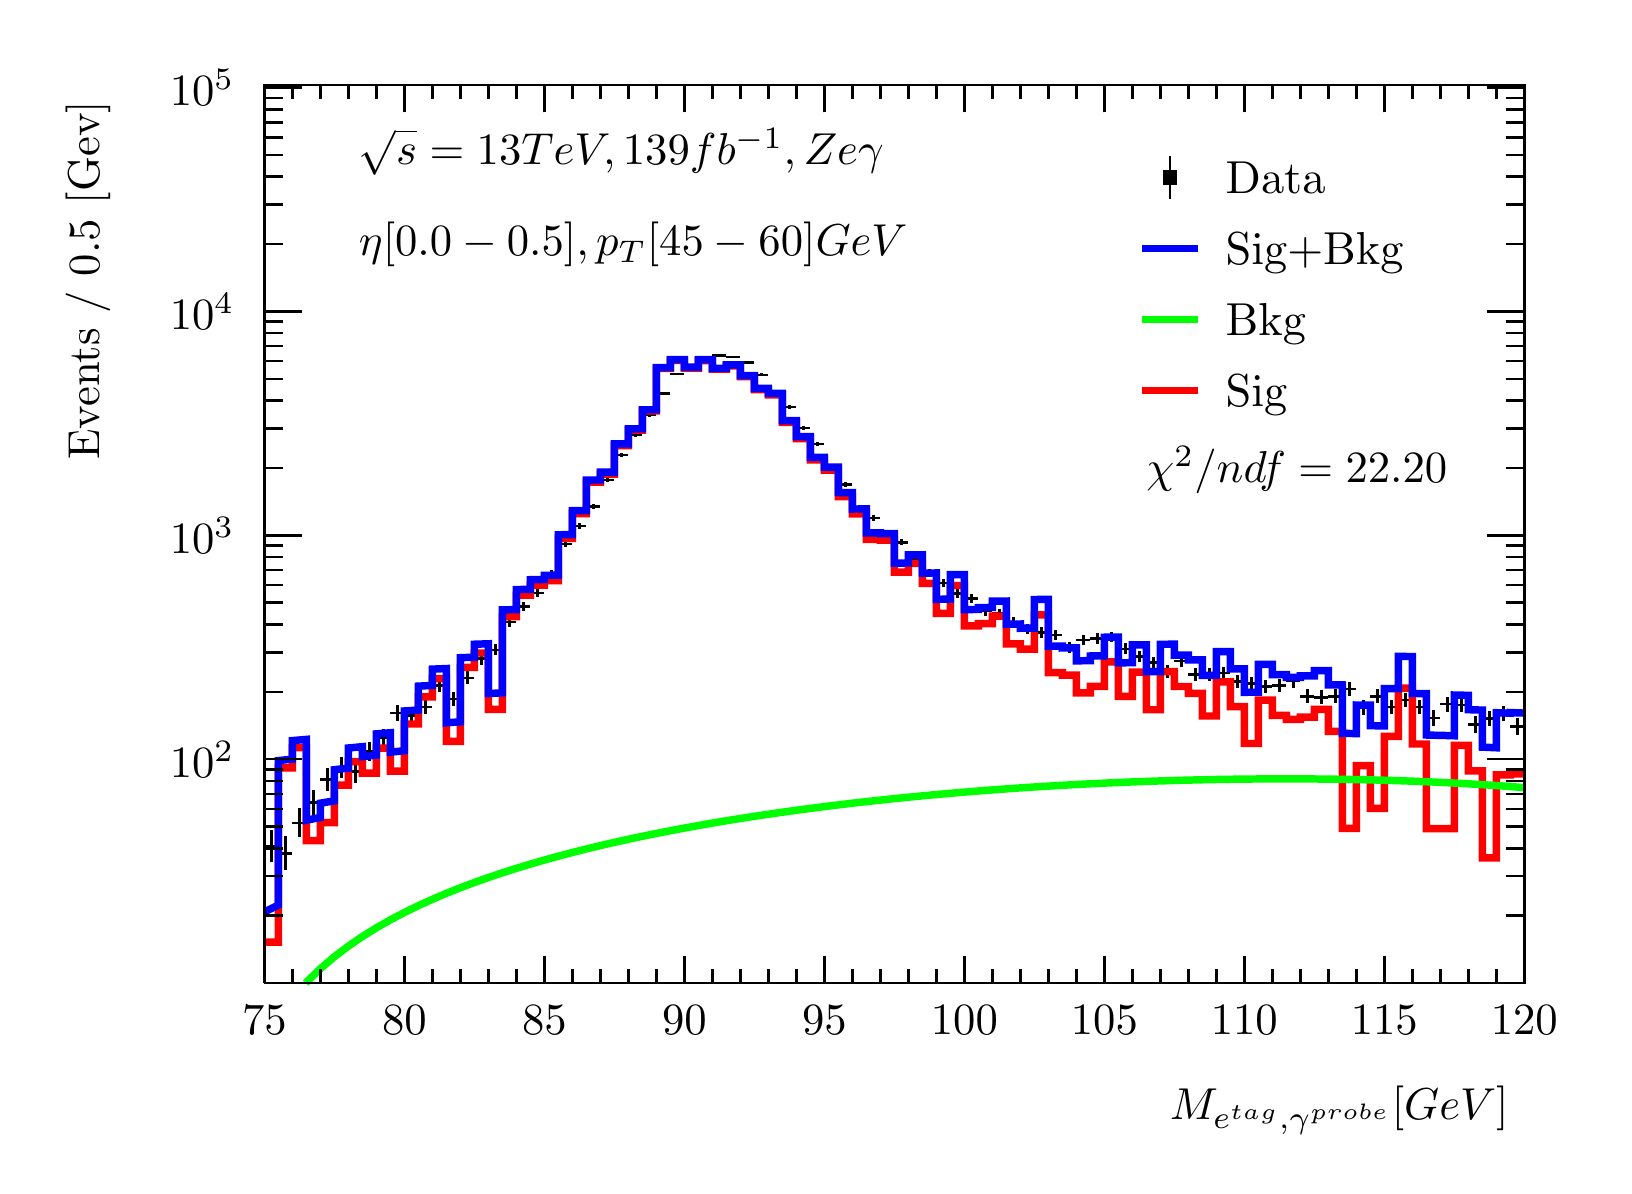
\begin{tikzpicture}
\pgfdeclareplotmark{cross} {
\pgfpathmoveto{\pgfpoint{-0.3\pgfplotmarksize}{\pgfplotmarksize}}
\pgfpathlineto{\pgfpoint{+0.3\pgfplotmarksize}{\pgfplotmarksize}}
\pgfpathlineto{\pgfpoint{+0.3\pgfplotmarksize}{0.3\pgfplotmarksize}}
\pgfpathlineto{\pgfpoint{+1\pgfplotmarksize}{0.3\pgfplotmarksize}}
\pgfpathlineto{\pgfpoint{+1\pgfplotmarksize}{-0.3\pgfplotmarksize}}
\pgfpathlineto{\pgfpoint{+0.3\pgfplotmarksize}{-0.3\pgfplotmarksize}}
\pgfpathlineto{\pgfpoint{+0.3\pgfplotmarksize}{-1.\pgfplotmarksize}}
\pgfpathlineto{\pgfpoint{-0.3\pgfplotmarksize}{-1.\pgfplotmarksize}}
\pgfpathlineto{\pgfpoint{-0.3\pgfplotmarksize}{-0.3\pgfplotmarksize}}
\pgfpathlineto{\pgfpoint{-1.\pgfplotmarksize}{-0.3\pgfplotmarksize}}
\pgfpathlineto{\pgfpoint{-1.\pgfplotmarksize}{0.3\pgfplotmarksize}}
\pgfpathlineto{\pgfpoint{-0.3\pgfplotmarksize}{0.3\pgfplotmarksize}}
\pgfpathclose
\pgfusepathqstroke
}
\pgfdeclareplotmark{cross*} {
\pgfpathmoveto{\pgfpoint{-0.3\pgfplotmarksize}{\pgfplotmarksize}}
\pgfpathlineto{\pgfpoint{+0.3\pgfplotmarksize}{\pgfplotmarksize}}
\pgfpathlineto{\pgfpoint{+0.3\pgfplotmarksize}{0.3\pgfplotmarksize}}
\pgfpathlineto{\pgfpoint{+1\pgfplotmarksize}{0.3\pgfplotmarksize}}
\pgfpathlineto{\pgfpoint{+1\pgfplotmarksize}{-0.3\pgfplotmarksize}}
\pgfpathlineto{\pgfpoint{+0.3\pgfplotmarksize}{-0.3\pgfplotmarksize}}
\pgfpathlineto{\pgfpoint{+0.3\pgfplotmarksize}{-1.\pgfplotmarksize}}
\pgfpathlineto{\pgfpoint{-0.3\pgfplotmarksize}{-1.\pgfplotmarksize}}
\pgfpathlineto{\pgfpoint{-0.3\pgfplotmarksize}{-0.3\pgfplotmarksize}}
\pgfpathlineto{\pgfpoint{-1.\pgfplotmarksize}{-0.3\pgfplotmarksize}}
\pgfpathlineto{\pgfpoint{-1.\pgfplotmarksize}{0.3\pgfplotmarksize}}
\pgfpathlineto{\pgfpoint{-0.3\pgfplotmarksize}{0.3\pgfplotmarksize}}
\pgfpathclose
\pgfusepathqfillstroke
}
\pgfdeclareplotmark{newstar} {
\pgfpathmoveto{\pgfqpoint{0pt}{\pgfplotmarksize}}
\pgfpathlineto{\pgfqpointpolar{44}{0.5\pgfplotmarksize}}
\pgfpathlineto{\pgfqpointpolar{18}{\pgfplotmarksize}}
\pgfpathlineto{\pgfqpointpolar{-20}{0.5\pgfplotmarksize}}
\pgfpathlineto{\pgfqpointpolar{-54}{\pgfplotmarksize}}
\pgfpathlineto{\pgfqpointpolar{-90}{0.5\pgfplotmarksize}}
\pgfpathlineto{\pgfqpointpolar{234}{\pgfplotmarksize}}
\pgfpathlineto{\pgfqpointpolar{198}{0.5\pgfplotmarksize}}
\pgfpathlineto{\pgfqpointpolar{162}{\pgfplotmarksize}}
\pgfpathlineto{\pgfqpointpolar{134}{0.5\pgfplotmarksize}}
\pgfpathclose
\pgfusepathqstroke
}
\pgfdeclareplotmark{newstar*} {
\pgfpathmoveto{\pgfqpoint{0pt}{\pgfplotmarksize}}
\pgfpathlineto{\pgfqpointpolar{44}{0.5\pgfplotmarksize}}
\pgfpathlineto{\pgfqpointpolar{18}{\pgfplotmarksize}}
\pgfpathlineto{\pgfqpointpolar{-20}{0.5\pgfplotmarksize}}
\pgfpathlineto{\pgfqpointpolar{-54}{\pgfplotmarksize}}
\pgfpathlineto{\pgfqpointpolar{-90}{0.5\pgfplotmarksize}}
\pgfpathlineto{\pgfqpointpolar{234}{\pgfplotmarksize}}
\pgfpathlineto{\pgfqpointpolar{198}{0.5\pgfplotmarksize}}
\pgfpathlineto{\pgfqpointpolar{162}{\pgfplotmarksize}}
\pgfpathlineto{\pgfqpointpolar{134}{0.5\pgfplotmarksize}}
\pgfpathclose
\pgfusepathqfillstroke
}
\definecolor{c}{rgb}{1,1,1};
\draw [color=c, fill=c] (0,0) rectangle (20,14.4361);
\draw [color=c, fill=c] (3,2.30977) rectangle (19,13.7143);
\definecolor{c}{rgb}{0,0,0};
\draw [c,line width=0.9] (3,2.30977) -- (3,13.7143) -- (19,13.7143) -- (19,2.30977) -- (3,2.30977);
\definecolor{c}{rgb}{1,1,1};
\draw [color=c, fill=c] (3,2.30977) rectangle (19,13.7143);
\definecolor{c}{rgb}{0,0,0};
\draw [c,line width=0.9] (3,2.30977) -- (3,13.7143) -- (19,13.7143) -- (19,2.30977) -- (3,2.30977);
\draw [c,line width=0.9] (3,2.30977) -- (19,2.30977);
\draw [c,line width=0.9] (3,2.65624) -- (3,2.30977);
\draw [c,line width=0.9] (3.35556,2.48301) -- (3.35556,2.30977);
\draw [c,line width=0.9] (3.71111,2.48301) -- (3.71111,2.30977);
\draw [c,line width=0.9] (4.06667,2.48301) -- (4.06667,2.30977);
\draw [c,line width=0.9] (4.42222,2.48301) -- (4.42222,2.30977);
\draw [c,line width=0.9] (4.77778,2.65624) -- (4.77778,2.30977);
\draw [c,line width=0.9] (5.13333,2.48301) -- (5.13333,2.30977);
\draw [c,line width=0.9] (5.48889,2.48301) -- (5.48889,2.30977);
\draw [c,line width=0.9] (5.84444,2.48301) -- (5.84444,2.30977);
\draw [c,line width=0.9] (6.2,2.48301) -- (6.2,2.30977);
\draw [c,line width=0.9] (6.55556,2.65624) -- (6.55556,2.30977);
\draw [c,line width=0.9] (6.91111,2.48301) -- (6.91111,2.30977);
\draw [c,line width=0.9] (7.26667,2.48301) -- (7.26667,2.30977);
\draw [c,line width=0.9] (7.62222,2.48301) -- (7.62222,2.30977);
\draw [c,line width=0.9] (7.97778,2.48301) -- (7.97778,2.30977);
\draw [c,line width=0.9] (8.33333,2.65624) -- (8.33333,2.30977);
\draw [c,line width=0.9] (8.68889,2.48301) -- (8.68889,2.30977);
\draw [c,line width=0.9] (9.04444,2.48301) -- (9.04444,2.30977);
\draw [c,line width=0.9] (9.4,2.48301) -- (9.4,2.30977);
\draw [c,line width=0.9] (9.75556,2.48301) -- (9.75556,2.30977);
\draw [c,line width=0.9] (10.1111,2.65624) -- (10.1111,2.30977);
\draw [c,line width=0.9] (10.4667,2.48301) -- (10.4667,2.30977);
\draw [c,line width=0.9] (10.8222,2.48301) -- (10.8222,2.30977);
\draw [c,line width=0.9] (11.1778,2.48301) -- (11.1778,2.30977);
\draw [c,line width=0.9] (11.5333,2.48301) -- (11.5333,2.30977);
\draw [c,line width=0.9] (11.8889,2.65624) -- (11.8889,2.30977);
\draw [c,line width=0.9] (12.2444,2.48301) -- (12.2444,2.30977);
\draw [c,line width=0.9] (12.6,2.48301) -- (12.6,2.30977);
\draw [c,line width=0.9] (12.9556,2.48301) -- (12.9556,2.30977);
\draw [c,line width=0.9] (13.3111,2.48301) -- (13.3111,2.30977);
\draw [c,line width=0.9] (13.6667,2.65624) -- (13.6667,2.30977);
\draw [c,line width=0.9] (14.0222,2.48301) -- (14.0222,2.30977);
\draw [c,line width=0.9] (14.3778,2.48301) -- (14.3778,2.30977);
\draw [c,line width=0.9] (14.7333,2.48301) -- (14.7333,2.30977);
\draw [c,line width=0.9] (15.0889,2.48301) -- (15.0889,2.30977);
\draw [c,line width=0.9] (15.4444,2.65624) -- (15.4444,2.30977);
\draw [c,line width=0.9] (15.8,2.48301) -- (15.8,2.30977);
\draw [c,line width=0.9] (16.1556,2.48301) -- (16.1556,2.30977);
\draw [c,line width=0.9] (16.5111,2.48301) -- (16.5111,2.30977);
\draw [c,line width=0.9] (16.8667,2.48301) -- (16.8667,2.30977);
\draw [c,line width=0.9] (17.2222,2.65624) -- (17.2222,2.30977);
\draw [c,line width=0.9] (17.5778,2.48301) -- (17.5778,2.30977);
\draw [c,line width=0.9] (17.9333,2.48301) -- (17.9333,2.30977);
\draw [c,line width=0.9] (18.2889,2.48301) -- (18.2889,2.30977);
\draw [c,line width=0.9] (18.6444,2.48301) -- (18.6444,2.30977);
\draw [c,line width=0.9] (19,2.65624) -- (19,2.30977);
\draw [c,line width=0.9] (19,2.65624) -- (19,2.30977);
\draw [anchor=base] (3,1.66015) node[scale=1.61424, color=c, rotate=0]{75};
\draw [anchor=base] (4.77778,1.66015) node[scale=1.61424, color=c, rotate=0]{80};
\draw [anchor=base] (6.55556,1.66015) node[scale=1.61424, color=c, rotate=0]{85};
\draw [anchor=base] (8.33333,1.66015) node[scale=1.61424, color=c, rotate=0]{90};
\draw [anchor=base] (10.1111,1.66015) node[scale=1.61424, color=c, rotate=0]{95};
\draw [anchor=base] (11.8889,1.66015) node[scale=1.61424, color=c, rotate=0]{100};
\draw [anchor=base] (13.6667,1.66015) node[scale=1.61424, color=c, rotate=0]{105};
\draw [anchor=base] (15.4444,1.66015) node[scale=1.61424, color=c, rotate=0]{110};
\draw [anchor=base] (17.2222,1.66015) node[scale=1.61424, color=c, rotate=0]{115};
\draw [anchor=base] (19,1.66015) node[scale=1.61424, color=c, rotate=0]{120};
\draw [anchor= east] (19,0.692932) node[scale=1.61424, color=c, rotate=0]{$M_{e^{tag}, \gamma^{probe}}  [GeV]$};
\draw [c,line width=0.9] (3,13.7143) -- (19,13.7143);
\draw [c,line width=0.9] (3,13.3678) -- (3,13.7143);
\draw [c,line width=0.9] (3.35556,13.5411) -- (3.35556,13.7143);
\draw [c,line width=0.9] (3.71111,13.5411) -- (3.71111,13.7143);
\draw [c,line width=0.9] (4.06667,13.5411) -- (4.06667,13.7143);
\draw [c,line width=0.9] (4.42222,13.5411) -- (4.42222,13.7143);
\draw [c,line width=0.9] (4.77778,13.3678) -- (4.77778,13.7143);
\draw [c,line width=0.9] (5.13333,13.5411) -- (5.13333,13.7143);
\draw [c,line width=0.9] (5.48889,13.5411) -- (5.48889,13.7143);
\draw [c,line width=0.9] (5.84444,13.5411) -- (5.84444,13.7143);
\draw [c,line width=0.9] (6.2,13.5411) -- (6.2,13.7143);
\draw [c,line width=0.9] (6.55556,13.3678) -- (6.55556,13.7143);
\draw [c,line width=0.9] (6.91111,13.5411) -- (6.91111,13.7143);
\draw [c,line width=0.9] (7.26667,13.5411) -- (7.26667,13.7143);
\draw [c,line width=0.9] (7.62222,13.5411) -- (7.62222,13.7143);
\draw [c,line width=0.9] (7.97778,13.5411) -- (7.97778,13.7143);
\draw [c,line width=0.9] (8.33333,13.3678) -- (8.33333,13.7143);
\draw [c,line width=0.9] (8.68889,13.5411) -- (8.68889,13.7143);
\draw [c,line width=0.9] (9.04444,13.5411) -- (9.04444,13.7143);
\draw [c,line width=0.9] (9.4,13.5411) -- (9.4,13.7143);
\draw [c,line width=0.9] (9.75556,13.5411) -- (9.75556,13.7143);
\draw [c,line width=0.9] (10.1111,13.3678) -- (10.1111,13.7143);
\draw [c,line width=0.9] (10.4667,13.5411) -- (10.4667,13.7143);
\draw [c,line width=0.9] (10.8222,13.5411) -- (10.8222,13.7143);
\draw [c,line width=0.9] (11.1778,13.5411) -- (11.1778,13.7143);
\draw [c,line width=0.9] (11.5333,13.5411) -- (11.5333,13.7143);
\draw [c,line width=0.9] (11.8889,13.3678) -- (11.8889,13.7143);
\draw [c,line width=0.9] (12.2444,13.5411) -- (12.2444,13.7143);
\draw [c,line width=0.9] (12.6,13.5411) -- (12.6,13.7143);
\draw [c,line width=0.9] (12.9556,13.5411) -- (12.9556,13.7143);
\draw [c,line width=0.9] (13.3111,13.5411) -- (13.3111,13.7143);
\draw [c,line width=0.9] (13.6667,13.3678) -- (13.6667,13.7143);
\draw [c,line width=0.9] (14.0222,13.5411) -- (14.0222,13.7143);
\draw [c,line width=0.9] (14.3778,13.5411) -- (14.3778,13.7143);
\draw [c,line width=0.9] (14.7333,13.5411) -- (14.7333,13.7143);
\draw [c,line width=0.9] (15.0889,13.5411) -- (15.0889,13.7143);
\draw [c,line width=0.9] (15.4444,13.3678) -- (15.4444,13.7143);
\draw [c,line width=0.9] (15.8,13.5411) -- (15.8,13.7143);
\draw [c,line width=0.9] (16.1556,13.5411) -- (16.1556,13.7143);
\draw [c,line width=0.9] (16.5111,13.5411) -- (16.5111,13.7143);
\draw [c,line width=0.9] (16.8667,13.5411) -- (16.8667,13.7143);
\draw [c,line width=0.9] (17.2222,13.3678) -- (17.2222,13.7143);
\draw [c,line width=0.9] (17.5778,13.5411) -- (17.5778,13.7143);
\draw [c,line width=0.9] (17.9333,13.5411) -- (17.9333,13.7143);
\draw [c,line width=0.9] (18.2889,13.5411) -- (18.2889,13.7143);
\draw [c,line width=0.9] (18.6444,13.5411) -- (18.6444,13.7143);
\draw [c,line width=0.9] (19,13.3678) -- (19,13.7143);
\draw [c,line width=0.9] (19,13.3678) -- (19,13.7143);
\draw [c,line width=0.9] (3,2.30977) -- (3,13.7143);
\draw [c,line width=0.9] (3.237,3.16561) -- (3,3.16561);
\draw [c,line width=0.9] (3.237,3.66625) -- (3,3.66625);
\draw [c,line width=0.9] (3.237,4.02146) -- (3,4.02146);
\draw [c,line width=0.9] (3.237,4.29698) -- (3,4.29698);
\draw [c,line width=0.9] (3.237,4.52209) -- (3,4.52209);
\draw [c,line width=0.9] (3.237,4.71242) -- (3,4.71242);
\draw [c,line width=0.9] (3.237,4.8773) -- (3,4.8773);
\draw [c,line width=0.9] (3.237,5.02273) -- (3,5.02273);
\draw [c,line width=0.9] (3.474,5.15282) -- (3,5.15282);
\draw [anchor= east] (2.82,5.15282) node[scale=1.61424, color=c, rotate=0]{$10^{2}$};
\draw [c,line width=0.9] (3.237,6.00866) -- (3,6.00866);
\draw [c,line width=0.9] (3.237,6.5093) -- (3,6.5093);
\draw [c,line width=0.9] (3.237,6.8645) -- (3,6.8645);
\draw [c,line width=0.9] (3.237,7.14002) -- (3,7.14002);
\draw [c,line width=0.9] (3.237,7.36514) -- (3,7.36514);
\draw [c,line width=0.9] (3.237,7.55547) -- (3,7.55547);
\draw [c,line width=0.9] (3.237,7.72034) -- (3,7.72034);
\draw [c,line width=0.9] (3.237,7.86577) -- (3,7.86577);
\draw [c,line width=0.9] (3.474,7.99586) -- (3,7.99586);
\draw [anchor= east] (2.82,7.99586) node[scale=1.61424, color=c, rotate=0]{$10^{3}$};
\draw [c,line width=0.9] (3.237,8.85171) -- (3,8.85171);
\draw [c,line width=0.9] (3.237,9.35234) -- (3,9.35234);
\draw [c,line width=0.9] (3.237,9.70755) -- (3,9.70755);
\draw [c,line width=0.9] (3.237,9.98307) -- (3,9.98307);
\draw [c,line width=0.9] (3.237,10.2082) -- (3,10.2082);
\draw [c,line width=0.9] (3.237,10.3985) -- (3,10.3985);
\draw [c,line width=0.9] (3.237,10.5634) -- (3,10.5634);
\draw [c,line width=0.9] (3.237,10.7088) -- (3,10.7088);
\draw [c,line width=0.9] (3.474,10.8389) -- (3,10.8389);
\draw [anchor= east] (2.82,10.8389) node[scale=1.61424, color=c, rotate=0]{$10^{4}$};
\draw [c,line width=0.9] (3.237,11.6948) -- (3,11.6948);
\draw [c,line width=0.9] (3.237,12.1954) -- (3,12.1954);
\draw [c,line width=0.9] (3.237,12.5506) -- (3,12.5506);
\draw [c,line width=0.9] (3.237,12.8261) -- (3,12.8261);
\draw [c,line width=0.9] (3.237,13.0512) -- (3,13.0512);
\draw [c,line width=0.9] (3.237,13.2416) -- (3,13.2416);
\draw [c,line width=0.9] (3.237,13.4064) -- (3,13.4064);
\draw [c,line width=0.9] (3.237,13.5519) -- (3,13.5519);
\draw [c,line width=0.9] (3.474,13.682) -- (3,13.682);
\draw [anchor= east] (2.82,13.682) node[scale=1.61424, color=c, rotate=0]{$10^{5}$};
\draw [anchor= east] (0.76,13.7143) node[scale=1.61424, color=c, rotate=90]{Events / 0.5 [Gev]};
\draw [c,line width=0.9] (19,2.30977) -- (19,13.7143);
\draw [c,line width=0.9] (18.763,3.16561) -- (19,3.16561);
\draw [c,line width=0.9] (18.763,3.66625) -- (19,3.66625);
\draw [c,line width=0.9] (18.763,4.02146) -- (19,4.02146);
\draw [c,line width=0.9] (18.763,4.29698) -- (19,4.29698);
\draw [c,line width=0.9] (18.763,4.52209) -- (19,4.52209);
\draw [c,line width=0.9] (18.763,4.71242) -- (19,4.71242);
\draw [c,line width=0.9] (18.763,4.8773) -- (19,4.8773);
\draw [c,line width=0.9] (18.763,5.02273) -- (19,5.02273);
\draw [c,line width=0.9] (18.526,5.15282) -- (19,5.15282);
\draw [c,line width=0.9] (18.763,6.00866) -- (19,6.00866);
\draw [c,line width=0.9] (18.763,6.5093) -- (19,6.5093);
\draw [c,line width=0.9] (18.763,6.8645) -- (19,6.8645);
\draw [c,line width=0.9] (18.763,7.14002) -- (19,7.14002);
\draw [c,line width=0.9] (18.763,7.36514) -- (19,7.36514);
\draw [c,line width=0.9] (18.763,7.55547) -- (19,7.55547);
\draw [c,line width=0.9] (18.763,7.72034) -- (19,7.72034);
\draw [c,line width=0.9] (18.763,7.86577) -- (19,7.86577);
\draw [c,line width=0.9] (18.526,7.99586) -- (19,7.99586);
\draw [c,line width=0.9] (18.763,8.85171) -- (19,8.85171);
\draw [c,line width=0.9] (18.763,9.35234) -- (19,9.35234);
\draw [c,line width=0.9] (18.763,9.70755) -- (19,9.70755);
\draw [c,line width=0.9] (18.763,9.98307) -- (19,9.98307);
\draw [c,line width=0.9] (18.763,10.2082) -- (19,10.2082);
\draw [c,line width=0.9] (18.763,10.3985) -- (19,10.3985);
\draw [c,line width=0.9] (18.763,10.5634) -- (19,10.5634);
\draw [c,line width=0.9] (18.763,10.7088) -- (19,10.7088);
\draw [c,line width=0.9] (18.526,10.8389) -- (19,10.8389);
\draw [c,line width=0.9] (18.763,11.6948) -- (19,11.6948);
\draw [c,line width=0.9] (18.763,12.1954) -- (19,12.1954);
\draw [c,line width=0.9] (18.763,12.5506) -- (19,12.5506);
\draw [c,line width=0.9] (18.763,12.8261) -- (19,12.8261);
\draw [c,line width=0.9] (18.763,13.0512) -- (19,13.0512);
\draw [c,line width=0.9] (18.763,13.2416) -- (19,13.2416);
\draw [c,line width=0.9] (18.763,13.4064) -- (19,13.4064);
\draw [c,line width=0.9] (18.763,13.5519) -- (19,13.5519);
\draw [c,line width=0.9] (18.526,13.682) -- (19,13.682);
\draw [c,line width=0.9] (3.08889,4.05195) -- (3,4.05195);
\draw [c,line width=0.9] (3,4.05195) -- (3,4.05195);
\draw [c,line width=0.9] (3.08889,4.05195) -- (3.17778,4.05195);
\draw [c,line width=0.9] (3.17778,4.05195) -- (3.17778,4.05195);
\draw [c,line width=0.9] (3.08889,4.05195) -- (3.08889,4.25823);
\draw [c,line width=0.9] (3.08889,4.25823) -- (3.08889,4.25823);
\draw [c,line width=0.9] (3.08889,4.05195) -- (3.08889,3.84322);
\draw [c,line width=0.9] (3.08889,3.84322) -- (3.08889,3.84322);
\draw [c,line width=0.9] (3.26667,3.95813) -- (3.17778,3.95813);
\draw [c,line width=0.9] (3.17778,3.95813) -- (3.17778,3.95813);
\draw [c,line width=0.9] (3.26667,3.95813) -- (3.35556,3.95813);
\draw [c,line width=0.9] (3.35556,3.95813) -- (3.35556,3.95813);
\draw [c,line width=0.9] (3.26667,3.95813) -- (3.26667,4.17287);
\draw [c,line width=0.9] (3.26667,4.17287) -- (3.26667,4.17287);
\draw [c,line width=0.9] (3.26667,3.95813) -- (3.26667,3.74063);
\draw [c,line width=0.9] (3.26667,3.74063) -- (3.26667,3.74063);
\draw [c,line width=0.9] (3.44444,4.3454) -- (3.35556,4.3454);
\draw [c,line width=0.9] (3.35556,4.3454) -- (3.35556,4.3454);
\draw [c,line width=0.9] (3.44444,4.3454) -- (3.53333,4.3454);
\draw [c,line width=0.9] (3.53333,4.3454) -- (3.53333,4.3454);
\draw [c,line width=0.9] (3.44444,4.3454) -- (3.44444,4.52738);
\draw [c,line width=0.9] (3.44444,4.52738) -- (3.44444,4.52738);
\draw [c,line width=0.9] (3.44444,4.3454) -- (3.44444,4.16172);
\draw [c,line width=0.9] (3.44444,4.16172) -- (3.44444,4.16172);
\draw [c,line width=0.9] (3.62222,4.60178) -- (3.53333,4.60178);
\draw [c,line width=0.9] (3.53333,4.60178) -- (3.53333,4.60178);
\draw [c,line width=0.9] (3.62222,4.60178) -- (3.71111,4.60178);
\draw [c,line width=0.9] (3.71111,4.60178) -- (3.71111,4.60178);
\draw [c,line width=0.9] (3.62222,4.60178) -- (3.62222,4.76495);
\draw [c,line width=0.9] (3.62222,4.76495) -- (3.62222,4.76495);
\draw [c,line width=0.9] (3.62222,4.60178) -- (3.62222,4.43737);
\draw [c,line width=0.9] (3.62222,4.43737) -- (3.62222,4.43737);
\draw [c,line width=0.9] (3.8,4.89264) -- (3.71111,4.89264);
\draw [c,line width=0.9] (3.71111,4.89264) -- (3.71111,4.89264);
\draw [c,line width=0.9] (3.8,4.89264) -- (3.88889,4.89264);
\draw [c,line width=0.9] (3.88889,4.89264) -- (3.88889,4.89264);
\draw [c,line width=0.9] (3.8,4.89264) -- (3.8,5.03688);
\draw [c,line width=0.9] (3.8,5.03688) -- (3.8,5.03688);
\draw [c,line width=0.9] (3.8,4.89264) -- (3.8,4.74753);
\draw [c,line width=0.9] (3.8,4.74753) -- (3.8,4.74753);
\draw [c,line width=0.9] (3.97778,5.04987) -- (3.88889,5.04987);
\draw [c,line width=0.9] (3.88889,5.04987) -- (3.88889,5.04987);
\draw [c,line width=0.9] (3.97778,5.04987) -- (4.06667,5.04987);
\draw [c,line width=0.9] (4.06667,5.04987) -- (4.06667,5.04987);
\draw [c,line width=0.9] (3.97778,5.04987) -- (3.97778,5.18483);
\draw [c,line width=0.9] (3.97778,5.18483) -- (3.97778,5.18483);
\draw [c,line width=0.9] (3.97778,5.04987) -- (3.97778,4.91418);
\draw [c,line width=0.9] (3.97778,4.91418) -- (3.97778,4.91418);
\draw [c,line width=0.9] (4.15556,4.99498) -- (4.06667,4.99498);
\draw [c,line width=0.9] (4.06667,4.99498) -- (4.06667,4.99498);
\draw [c,line width=0.9] (4.15556,4.99498) -- (4.24444,4.99498);
\draw [c,line width=0.9] (4.24444,4.99498) -- (4.24444,4.99498);
\draw [c,line width=0.9] (4.15556,4.99498) -- (4.15556,5.13311);
\draw [c,line width=0.9] (4.15556,5.13311) -- (4.15556,5.13311);
\draw [c,line width=0.9] (4.15556,4.99498) -- (4.15556,4.85608);
\draw [c,line width=0.9] (4.15556,4.85608) -- (4.15556,4.85608);
\draw [c,line width=0.9] (4.33333,5.24785) -- (4.24444,5.24785);
\draw [c,line width=0.9] (4.24444,5.24785) -- (4.24444,5.24785);
\draw [c,line width=0.9] (4.33333,5.24785) -- (4.42222,5.24785);
\draw [c,line width=0.9] (4.42222,5.24785) -- (4.42222,5.24785);
\draw [c,line width=0.9] (4.33333,5.24785) -- (4.33333,5.36661);
\draw [c,line width=0.9] (4.33333,5.36661) -- (4.33333,5.36661);
\draw [c,line width=0.9] (4.33333,5.24785) -- (4.33333,5.12908);
\draw [c,line width=0.9] (4.33333,5.12908) -- (4.33333,5.12908);
\draw [c,line width=0.9] (4.51111,5.42834) -- (4.42222,5.42834);
\draw [c,line width=0.9] (4.42222,5.42834) -- (4.42222,5.42834);
\draw [c,line width=0.9] (4.51111,5.42834) -- (4.6,5.42834);
\draw [c,line width=0.9] (4.6,5.42834) -- (4.6,5.42834);
\draw [c,line width=0.9] (4.51111,5.42834) -- (4.51111,5.53874);
\draw [c,line width=0.9] (4.51111,5.53874) -- (4.51111,5.53874);
\draw [c,line width=0.9] (4.51111,5.42834) -- (4.51111,5.31794);
\draw [c,line width=0.9] (4.51111,5.31794) -- (4.51111,5.31794);
\draw [c,line width=0.9] (4.68889,5.74084) -- (4.6,5.74084);
\draw [c,line width=0.9] (4.6,5.74084) -- (4.6,5.74084);
\draw [c,line width=0.9] (4.68889,5.74084) -- (4.77778,5.74084);
\draw [c,line width=0.9] (4.77778,5.74084) -- (4.77778,5.74084);
\draw [c,line width=0.9] (4.68889,5.74084) -- (4.68889,5.83812);
\draw [c,line width=0.9] (4.68889,5.83812) -- (4.68889,5.83812);
\draw [c,line width=0.9] (4.68889,5.74084) -- (4.68889,5.64355);
\draw [c,line width=0.9] (4.68889,5.64355) -- (4.68889,5.64355);
\draw [c,line width=0.9] (4.86667,5.70977) -- (4.77778,5.70977);
\draw [c,line width=0.9] (4.77778,5.70977) -- (4.77778,5.70977);
\draw [c,line width=0.9] (4.86667,5.70977) -- (4.95556,5.70977);
\draw [c,line width=0.9] (4.95556,5.70977) -- (4.95556,5.70977);
\draw [c,line width=0.9] (4.86667,5.70977) -- (4.86667,5.80829);
\draw [c,line width=0.9] (4.86667,5.80829) -- (4.86667,5.80829);
\draw [c,line width=0.9] (4.86667,5.70977) -- (4.86667,5.61126);
\draw [c,line width=0.9] (4.86667,5.61126) -- (4.86667,5.61126);
\draw [c,line width=0.9] (5.04444,5.81524) -- (4.95556,5.81524);
\draw [c,line width=0.9] (4.95556,5.81524) -- (4.95556,5.81524);
\draw [c,line width=0.9] (5.04444,5.81524) -- (5.13333,5.81524);
\draw [c,line width=0.9] (5.13333,5.81524) -- (5.13333,5.81524);
\draw [c,line width=0.9] (5.04444,5.81524) -- (5.04444,5.90964);
\draw [c,line width=0.9] (5.04444,5.90964) -- (5.04444,5.90964);
\draw [c,line width=0.9] (5.04444,5.81524) -- (5.04444,5.72084);
\draw [c,line width=0.9] (5.04444,5.72084) -- (5.04444,5.72084);
\draw [c,line width=0.9] (5.22222,6.08642) -- (5.13333,6.08642);
\draw [c,line width=0.9] (5.13333,6.08642) -- (5.13333,6.08642);
\draw [c,line width=0.9] (5.22222,6.08642) -- (5.31111,6.08642);
\draw [c,line width=0.9] (5.31111,6.08642) -- (5.31111,6.08642);
\draw [c,line width=0.9] (5.22222,6.08642) -- (5.22222,6.171);
\draw [c,line width=0.9] (5.22222,6.171) -- (5.22222,6.171);
\draw [c,line width=0.9] (5.22222,6.08642) -- (5.22222,6.00183);
\draw [c,line width=0.9] (5.22222,6.00183) -- (5.22222,6.00183);
\draw [c,line width=0.9] (5.4,5.91906) -- (5.31111,5.91906);
\draw [c,line width=0.9] (5.31111,5.91906) -- (5.31111,5.91906);
\draw [c,line width=0.9] (5.4,5.91906) -- (5.48889,5.91906);
\draw [c,line width=0.9] (5.48889,5.91906) -- (5.48889,5.91906);
\draw [c,line width=0.9] (5.4,5.91906) -- (5.4,6.00957);
\draw [c,line width=0.9] (5.4,6.00957) -- (5.4,6.00957);
\draw [c,line width=0.9] (5.4,5.91906) -- (5.4,5.82854);
\draw [c,line width=0.9] (5.4,5.82854) -- (5.4,5.82854);
\draw [c,line width=0.9] (5.57778,6.18658) -- (5.48889,6.18658);
\draw [c,line width=0.9] (5.48889,6.18658) -- (5.48889,6.18658);
\draw [c,line width=0.9] (5.57778,6.18658) -- (5.66667,6.18658);
\draw [c,line width=0.9] (5.66667,6.18658) -- (5.66667,6.18658);
\draw [c,line width=0.9] (5.57778,6.18658) -- (5.57778,6.26781);
\draw [c,line width=0.9] (5.57778,6.26781) -- (5.57778,6.26781);
\draw [c,line width=0.9] (5.57778,6.18658) -- (5.57778,6.10536);
\draw [c,line width=0.9] (5.57778,6.10536) -- (5.57778,6.10536);
\draw [c,line width=0.9] (5.75556,6.42851) -- (5.66667,6.42851);
\draw [c,line width=0.9] (5.66667,6.42851) -- (5.66667,6.42851);
\draw [c,line width=0.9] (5.75556,6.42851) -- (5.84444,6.42851);
\draw [c,line width=0.9] (5.84444,6.42851) -- (5.84444,6.42851);
\draw [c,line width=0.9] (5.75556,6.42851) -- (5.75556,6.50216);
\draw [c,line width=0.9] (5.75556,6.50216) -- (5.75556,6.50216);
\draw [c,line width=0.9] (5.75556,6.42851) -- (5.75556,6.35487);
\draw [c,line width=0.9] (5.75556,6.35487) -- (5.75556,6.35487);
\draw [c,line width=0.9] (5.93333,6.54179) -- (5.84444,6.54179);
\draw [c,line width=0.9] (5.84444,6.54179) -- (5.84444,6.54179);
\draw [c,line width=0.9] (5.93333,6.54179) -- (6.02222,6.54179);
\draw [c,line width=0.9] (6.02222,6.54179) -- (6.02222,6.54179);
\draw [c,line width=0.9] (5.93333,6.54179) -- (5.93333,6.61214);
\draw [c,line width=0.9] (5.93333,6.61214) -- (5.93333,6.61214);
\draw [c,line width=0.9] (5.93333,6.54179) -- (5.93333,6.47145);
\draw [c,line width=0.9] (5.93333,6.47145) -- (5.93333,6.47145);
\draw [c,line width=0.9] (6.11111,6.89198) -- (6.02222,6.89198);
\draw [c,line width=0.9] (6.02222,6.89198) -- (6.02222,6.89198);
\draw [c,line width=0.9] (6.11111,6.89198) -- (6.2,6.89198);
\draw [c,line width=0.9] (6.2,6.89198) -- (6.2,6.89198);
\draw [c,line width=0.9] (6.11111,6.89198) -- (6.11111,6.95302);
\draw [c,line width=0.9] (6.11111,6.95302) -- (6.11111,6.95302);
\draw [c,line width=0.9] (6.11111,6.89198) -- (6.11111,6.83093);
\draw [c,line width=0.9] (6.11111,6.83093) -- (6.11111,6.83093);
\draw [c,line width=0.9] (6.28889,7.09475) -- (6.2,7.09475);
\draw [c,line width=0.9] (6.2,7.09475) -- (6.2,7.09475);
\draw [c,line width=0.9] (6.28889,7.09475) -- (6.37778,7.09475);
\draw [c,line width=0.9] (6.37778,7.09475) -- (6.37778,7.09475);
\draw [c,line width=0.9] (6.28889,7.09475) -- (6.28889,7.15099);
\draw [c,line width=0.9] (6.28889,7.15099) -- (6.28889,7.15099);
\draw [c,line width=0.9] (6.28889,7.09475) -- (6.28889,7.03852);
\draw [c,line width=0.9] (6.28889,7.03852) -- (6.28889,7.03852);
\draw [c,line width=0.9] (6.46667,7.26442) -- (6.37778,7.26442);
\draw [c,line width=0.9] (6.37778,7.26442) -- (6.37778,7.26442);
\draw [c,line width=0.9] (6.46667,7.26442) -- (6.55556,7.26442);
\draw [c,line width=0.9] (6.55556,7.26442) -- (6.55556,7.26442);
\draw [c,line width=0.9] (6.46667,7.26442) -- (6.46667,7.31692);
\draw [c,line width=0.9] (6.46667,7.31692) -- (6.46667,7.31692);
\draw [c,line width=0.9] (6.46667,7.26442) -- (6.46667,7.21192);
\draw [c,line width=0.9] (6.46667,7.21192) -- (6.46667,7.21192);
\draw [c,line width=0.9] (6.64444,7.50874) -- (6.55556,7.50874);
\draw [c,line width=0.9] (6.55556,7.50874) -- (6.55556,7.50874);
\draw [c,line width=0.9] (6.64444,7.50874) -- (6.73333,7.50874);
\draw [c,line width=0.9] (6.73333,7.50874) -- (6.73333,7.50874);
\draw [c,line width=0.9] (6.64444,7.50874) -- (6.64444,7.55629);
\draw [c,line width=0.9] (6.64444,7.55629) -- (6.64444,7.55629);
\draw [c,line width=0.9] (6.64444,7.50874) -- (6.64444,7.46118);
\draw [c,line width=0.9] (6.64444,7.46118) -- (6.64444,7.46118);
\draw [c,line width=0.9] (6.82222,7.88618) -- (6.73333,7.88618);
\draw [c,line width=0.9] (6.73333,7.88618) -- (6.73333,7.88618);
\draw [c,line width=0.9] (6.82222,7.88618) -- (6.91111,7.88618);
\draw [c,line width=0.9] (6.91111,7.88618) -- (6.91111,7.88618);
\draw [c,line width=0.9] (6.82222,7.88618) -- (6.82222,7.927);
\draw [c,line width=0.9] (6.82222,7.927) -- (6.82222,7.927);
\draw [c,line width=0.9] (6.82222,7.88618) -- (6.82222,7.84537);
\draw [c,line width=0.9] (6.82222,7.84537) -- (6.82222,7.84537);
\draw [c,line width=0.9] (7,8.11242) -- (6.91111,8.11242);
\draw [c,line width=0.9] (6.91111,8.11242) -- (6.91111,8.11242);
\draw [c,line width=0.9] (7,8.11242) -- (7.08889,8.11242);
\draw [c,line width=0.9] (7.08889,8.11242) -- (7.08889,8.11242);
\draw [c,line width=0.9] (7,8.11242) -- (7,8.14967);
\draw [c,line width=0.9] (7,8.14967) -- (7,8.14967);
\draw [c,line width=0.9] (7,8.11242) -- (7,8.07518);
\draw [c,line width=0.9] (7,8.07518) -- (7,8.07518);
\draw [c,line width=0.9] (7.17778,8.36183) -- (7.08889,8.36183);
\draw [c,line width=0.9] (7.08889,8.36183) -- (7.08889,8.36183);
\draw [c,line width=0.9] (7.17778,8.36183) -- (7.26667,8.36183);
\draw [c,line width=0.9] (7.26667,8.36183) -- (7.26667,8.36183);
\draw [c,line width=0.9] (7.17778,8.36183) -- (7.17778,8.39549);
\draw [c,line width=0.9] (7.17778,8.39549) -- (7.17778,8.39549);
\draw [c,line width=0.9] (7.17778,8.36183) -- (7.17778,8.32816);
\draw [c,line width=0.9] (7.17778,8.32816) -- (7.17778,8.32816);
\draw [c,line width=0.9] (7.35556,8.70156) -- (7.26667,8.70156);
\draw [c,line width=0.9] (7.26667,8.70156) -- (7.26667,8.70156);
\draw [c,line width=0.9] (7.35556,8.70156) -- (7.44444,8.70156);
\draw [c,line width=0.9] (7.44444,8.70156) -- (7.44444,8.70156);
\draw [c,line width=0.9] (7.35556,8.70156) -- (7.35556,8.7309);
\draw [c,line width=0.9] (7.35556,8.7309) -- (7.35556,8.7309);
\draw [c,line width=0.9] (7.35556,8.70156) -- (7.35556,8.67222);
\draw [c,line width=0.9] (7.35556,8.67222) -- (7.35556,8.67222);
\draw [c,line width=0.9] (7.53333,9.01511) -- (7.44444,9.01511);
\draw [c,line width=0.9] (7.44444,9.01511) -- (7.44444,9.01511);
\draw [c,line width=0.9] (7.53333,9.01511) -- (7.62222,9.01511);
\draw [c,line width=0.9] (7.62222,9.01511) -- (7.62222,9.01511);
\draw [c,line width=0.9] (7.53333,9.01511) -- (7.53333,9.04095);
\draw [c,line width=0.9] (7.53333,9.04095) -- (7.53333,9.04095);
\draw [c,line width=0.9] (7.53333,9.01511) -- (7.53333,8.98927);
\draw [c,line width=0.9] (7.53333,8.98927) -- (7.53333,8.98927);
\draw [c,line width=0.9] (7.71111,9.26848) -- (7.62222,9.26848);
\draw [c,line width=0.9] (7.62222,9.26848) -- (7.62222,9.26848);
\draw [c,line width=0.9] (7.71111,9.26848) -- (7.8,9.26848);
\draw [c,line width=0.9] (7.8,9.26848) -- (7.8,9.26848);
\draw [c,line width=0.9] (7.71111,9.26848) -- (7.71111,9.2918);
\draw [c,line width=0.9] (7.71111,9.2918) -- (7.71111,9.2918);
\draw [c,line width=0.9] (7.71111,9.26848) -- (7.71111,9.24516);
\draw [c,line width=0.9] (7.71111,9.24516) -- (7.71111,9.24516);
\draw [c,line width=0.9] (7.88889,9.52312) -- (7.8,9.52312);
\draw [c,line width=0.9] (7.8,9.52312) -- (7.8,9.52312);
\draw [c,line width=0.9] (7.88889,9.52312) -- (7.97778,9.52312);
\draw [c,line width=0.9] (7.97778,9.52312) -- (7.97778,9.52312);
\draw [c,line width=0.9] (7.88889,9.52312) -- (7.88889,9.54416);
\draw [c,line width=0.9] (7.88889,9.54416) -- (7.88889,9.54416);
\draw [c,line width=0.9] (7.88889,9.52312) -- (7.88889,9.50208);
\draw [c,line width=0.9] (7.88889,9.50208) -- (7.88889,9.50208);
\draw [c,line width=0.9] (8.06667,9.79426) -- (7.97778,9.79426);
\draw [c,line width=0.9] (7.97778,9.79426) -- (7.97778,9.79426);
\draw [c,line width=0.9] (8.06667,9.79426) -- (8.15556,9.79426);
\draw [c,line width=0.9] (8.15556,9.79426) -- (8.15556,9.79426);
\draw [c,line width=0.9] (8.06667,9.79426) -- (8.06667,9.81311);
\draw [c,line width=0.9] (8.06667,9.81311) -- (8.06667,9.81311);
\draw [c,line width=0.9] (8.06667,9.79426) -- (8.06667,9.77541);
\draw [c,line width=0.9] (8.06667,9.77541) -- (8.06667,9.77541);
\draw [c,line width=0.9] (8.24444,10.0452) -- (8.15556,10.0452);
\draw [c,line width=0.9] (8.15556,10.0452) -- (8.15556,10.0452);
\draw [c,line width=0.9] (8.24444,10.0452) -- (8.33333,10.0452);
\draw [c,line width=0.9] (8.33333,10.0452) -- (8.33333,10.0452);
\draw [c,line width=0.9] (8.24444,10.0452) -- (8.24444,10.0622);
\draw [c,line width=0.9] (8.24444,10.0622) -- (8.24444,10.0622);
\draw [c,line width=0.9] (8.24444,10.0452) -- (8.24444,10.0282);
\draw [c,line width=0.9] (8.24444,10.0282) -- (8.24444,10.0282);
\draw [c,line width=0.9] (8.42222,10.1292) -- (8.33333,10.1292);
\draw [c,line width=0.9] (8.33333,10.1292) -- (8.33333,10.1292);
\draw [c,line width=0.9] (8.42222,10.1292) -- (8.51111,10.1292);
\draw [c,line width=0.9] (8.51111,10.1292) -- (8.51111,10.1292);
\draw [c,line width=0.9] (8.42222,10.1292) -- (8.42222,10.1456);
\draw [c,line width=0.9] (8.42222,10.1456) -- (8.42222,10.1456);
\draw [c,line width=0.9] (8.42222,10.1292) -- (8.42222,10.1127);
\draw [c,line width=0.9] (8.42222,10.1127) -- (8.42222,10.1127);
\draw [c,line width=0.9] (8.6,10.256) -- (8.51111,10.256);
\draw [c,line width=0.9] (8.51111,10.256) -- (8.51111,10.256);
\draw [c,line width=0.9] (8.6,10.256) -- (8.68889,10.256);
\draw [c,line width=0.9] (8.68889,10.256) -- (8.68889,10.256);
\draw [c,line width=0.9] (8.6,10.256) -- (8.6,10.2717);
\draw [c,line width=0.9] (8.6,10.2717) -- (8.6,10.2717);
\draw [c,line width=0.9] (8.6,10.256) -- (8.6,10.2404);
\draw [c,line width=0.9] (8.6,10.2404) -- (8.6,10.2404);
\draw [c,line width=0.9] (8.77778,10.2819) -- (8.68889,10.2819);
\draw [c,line width=0.9] (8.68889,10.2819) -- (8.68889,10.2819);
\draw [c,line width=0.9] (8.77778,10.2819) -- (8.86667,10.2819);
\draw [c,line width=0.9] (8.86667,10.2819) -- (8.86667,10.2819);
\draw [c,line width=0.9] (8.77778,10.2819) -- (8.77778,10.2973);
\draw [c,line width=0.9] (8.77778,10.2973) -- (8.77778,10.2973);
\draw [c,line width=0.9] (8.77778,10.2819) -- (8.77778,10.2664);
\draw [c,line width=0.9] (8.77778,10.2664) -- (8.77778,10.2664);
\draw [c,line width=0.9] (8.95556,10.258) -- (8.86667,10.258);
\draw [c,line width=0.9] (8.86667,10.258) -- (8.86667,10.258);
\draw [c,line width=0.9] (8.95556,10.258) -- (9.04444,10.258);
\draw [c,line width=0.9] (9.04444,10.258) -- (9.04444,10.258);
\draw [c,line width=0.9] (8.95556,10.258) -- (8.95556,10.2736);
\draw [c,line width=0.9] (8.95556,10.2736) -- (8.95556,10.2736);
\draw [c,line width=0.9] (8.95556,10.258) -- (8.95556,10.2424);
\draw [c,line width=0.9] (8.95556,10.2424) -- (8.95556,10.2424);
\draw [c,line width=0.9] (9.13333,10.1906) -- (9.04444,10.1906);
\draw [c,line width=0.9] (9.04444,10.1906) -- (9.04444,10.1906);
\draw [c,line width=0.9] (9.13333,10.1906) -- (9.22222,10.1906);
\draw [c,line width=0.9] (9.22222,10.1906) -- (9.22222,10.1906);
\draw [c,line width=0.9] (9.13333,10.1906) -- (9.13333,10.2066);
\draw [c,line width=0.9] (9.13333,10.2066) -- (9.13333,10.2066);
\draw [c,line width=0.9] (9.13333,10.1906) -- (9.13333,10.1745);
\draw [c,line width=0.9] (9.13333,10.1745) -- (9.13333,10.1745);
\draw [c,line width=0.9] (9.31111,10.0346) -- (9.22222,10.0346);
\draw [c,line width=0.9] (9.22222,10.0346) -- (9.22222,10.0346);
\draw [c,line width=0.9] (9.31111,10.0346) -- (9.4,10.0346);
\draw [c,line width=0.9] (9.4,10.0346) -- (9.4,10.0346);
\draw [c,line width=0.9] (9.31111,10.0346) -- (9.31111,10.0517);
\draw [c,line width=0.9] (9.31111,10.0517) -- (9.31111,10.0517);
\draw [c,line width=0.9] (9.31111,10.0346) -- (9.31111,10.0175);
\draw [c,line width=0.9] (9.31111,10.0175) -- (9.31111,10.0175);
\draw [c,line width=0.9] (9.48889,9.82551) -- (9.4,9.82551);
\draw [c,line width=0.9] (9.4,9.82551) -- (9.4,9.82551);
\draw [c,line width=0.9] (9.48889,9.82551) -- (9.57778,9.82551);
\draw [c,line width=0.9] (9.57778,9.82551) -- (9.57778,9.82551);
\draw [c,line width=0.9] (9.48889,9.82551) -- (9.48889,9.84412);
\draw [c,line width=0.9] (9.48889,9.84412) -- (9.48889,9.84412);
\draw [c,line width=0.9] (9.48889,9.82551) -- (9.48889,9.8069);
\draw [c,line width=0.9] (9.48889,9.8069) -- (9.48889,9.8069);
\draw [c,line width=0.9] (9.66667,9.62523) -- (9.57778,9.62523);
\draw [c,line width=0.9] (9.57778,9.62523) -- (9.57778,9.62523);
\draw [c,line width=0.9] (9.66667,9.62523) -- (9.75556,9.62523);
\draw [c,line width=0.9] (9.75556,9.62523) -- (9.75556,9.62523);
\draw [c,line width=0.9] (9.66667,9.62523) -- (9.66667,9.64541);
\draw [c,line width=0.9] (9.66667,9.64541) -- (9.66667,9.64541);
\draw [c,line width=0.9] (9.66667,9.62523) -- (9.66667,9.60504);
\draw [c,line width=0.9] (9.66667,9.60504) -- (9.66667,9.60504);
\draw [c,line width=0.9] (9.84444,9.35645) -- (9.75556,9.35645);
\draw [c,line width=0.9] (9.75556,9.35645) -- (9.75556,9.35645);
\draw [c,line width=0.9] (9.84444,9.35645) -- (9.93333,9.35645);
\draw [c,line width=0.9] (9.93333,9.35645) -- (9.93333,9.35645);
\draw [c,line width=0.9] (9.84444,9.35645) -- (9.84444,9.37896);
\draw [c,line width=0.9] (9.84444,9.37896) -- (9.84444,9.37896);
\draw [c,line width=0.9] (9.84444,9.35645) -- (9.84444,9.33395);
\draw [c,line width=0.9] (9.84444,9.33395) -- (9.84444,9.33395);
\draw [c,line width=0.9] (10.0222,9.15796) -- (9.93333,9.15796);
\draw [c,line width=0.9] (9.93333,9.15796) -- (9.93333,9.15796);
\draw [c,line width=0.9] (10.0222,9.15796) -- (10.1111,9.15796);
\draw [c,line width=0.9] (10.1111,9.15796) -- (10.1111,9.15796);
\draw [c,line width=0.9] (10.0222,9.15796) -- (10.0222,9.18234);
\draw [c,line width=0.9] (10.0222,9.18234) -- (10.0222,9.18234);
\draw [c,line width=0.9] (10.0222,9.15796) -- (10.0222,9.13357);
\draw [c,line width=0.9] (10.0222,9.13357) -- (10.0222,9.13357);
\draw [c,line width=0.9] (10.2,8.8368) -- (10.1111,8.8368);
\draw [c,line width=0.9] (10.1111,8.8368) -- (10.1111,8.8368);
\draw [c,line width=0.9] (10.2,8.8368) -- (10.2889,8.8368);
\draw [c,line width=0.9] (10.2889,8.8368) -- (10.2889,8.8368);
\draw [c,line width=0.9] (10.2,8.8368) -- (10.2,8.86458);
\draw [c,line width=0.9] (10.2,8.86458) -- (10.2,8.86458);
\draw [c,line width=0.9] (10.2,8.8368) -- (10.2,8.80902);
\draw [c,line width=0.9] (10.2,8.80902) -- (10.2,8.80902);
\draw [c,line width=0.9] (10.3778,8.64229) -- (10.2889,8.64229);
\draw [c,line width=0.9] (10.2889,8.64229) -- (10.2889,8.64229);
\draw [c,line width=0.9] (10.3778,8.64229) -- (10.4667,8.64229);
\draw [c,line width=0.9] (10.4667,8.64229) -- (10.4667,8.64229);
\draw [c,line width=0.9] (10.3778,8.64229) -- (10.3778,8.67235);
\draw [c,line width=0.9] (10.3778,8.67235) -- (10.3778,8.67235);
\draw [c,line width=0.9] (10.3778,8.64229) -- (10.3778,8.61224);
\draw [c,line width=0.9] (10.3778,8.61224) -- (10.3778,8.61224);
\draw [c,line width=0.9] (10.5556,8.33679) -- (10.4667,8.33679);
\draw [c,line width=0.9] (10.4667,8.33679) -- (10.4667,8.33679);
\draw [c,line width=0.9] (10.5556,8.33679) -- (10.6444,8.33679);
\draw [c,line width=0.9] (10.6444,8.33679) -- (10.6444,8.33679);
\draw [c,line width=0.9] (10.5556,8.33679) -- (10.5556,8.3708);
\draw [c,line width=0.9] (10.5556,8.3708) -- (10.5556,8.3708);
\draw [c,line width=0.9] (10.5556,8.33679) -- (10.5556,8.30278);
\draw [c,line width=0.9] (10.5556,8.30278) -- (10.5556,8.30278);
\draw [c,line width=0.9] (10.7333,8.21272) -- (10.6444,8.21272);
\draw [c,line width=0.9] (10.6444,8.21272) -- (10.6444,8.21272);
\draw [c,line width=0.9] (10.7333,8.21272) -- (10.8222,8.21272);
\draw [c,line width=0.9] (10.8222,8.21272) -- (10.8222,8.21272);
\draw [c,line width=0.9] (10.7333,8.21272) -- (10.7333,8.24848);
\draw [c,line width=0.9] (10.7333,8.24848) -- (10.7333,8.24848);
\draw [c,line width=0.9] (10.7333,8.21272) -- (10.7333,8.17696);
\draw [c,line width=0.9] (10.7333,8.17696) -- (10.7333,8.17696);
\draw [c,line width=0.9] (10.9111,7.98595) -- (10.8222,7.98595);
\draw [c,line width=0.9] (10.8222,7.98595) -- (10.8222,7.98595);
\draw [c,line width=0.9] (10.9111,7.98595) -- (11,7.98595);
\draw [c,line width=0.9] (11,7.98595) -- (11,7.98595);
\draw [c,line width=0.9] (10.9111,7.98595) -- (10.9111,8.02515);
\draw [c,line width=0.9] (10.9111,8.02515) -- (10.9111,8.02515);
\draw [c,line width=0.9] (10.9111,7.98595) -- (10.9111,7.94675);
\draw [c,line width=0.9] (10.9111,7.94675) -- (10.9111,7.94675);
\draw [c,line width=0.9] (11.0889,7.90759) -- (11,7.90759);
\draw [c,line width=0.9] (11,7.90759) -- (11,7.90759);
\draw [c,line width=0.9] (11.0889,7.90759) -- (11.1778,7.90759);
\draw [c,line width=0.9] (11.1778,7.90759) -- (11.1778,7.90759);
\draw [c,line width=0.9] (11.0889,7.90759) -- (11.0889,7.94805);
\draw [c,line width=0.9] (11.0889,7.94805) -- (11.0889,7.94805);
\draw [c,line width=0.9] (11.0889,7.90759) -- (11.0889,7.86712);
\draw [c,line width=0.9] (11.0889,7.86712) -- (11.0889,7.86712);
\draw [c,line width=0.9] (11.2667,7.70168) -- (11.1778,7.70168);
\draw [c,line width=0.9] (11.1778,7.70168) -- (11.1778,7.70168);
\draw [c,line width=0.9] (11.2667,7.70168) -- (11.3556,7.70168);
\draw [c,line width=0.9] (11.3556,7.70168) -- (11.3556,7.70168);
\draw [c,line width=0.9] (11.2667,7.70168) -- (11.2667,7.74567);
\draw [c,line width=0.9] (11.2667,7.74567) -- (11.2667,7.74567);
\draw [c,line width=0.9] (11.2667,7.70168) -- (11.2667,7.6577);
\draw [c,line width=0.9] (11.2667,7.6577) -- (11.2667,7.6577);
\draw [c,line width=0.9] (11.4444,7.52149) -- (11.3556,7.52149);
\draw [c,line width=0.9] (11.3556,7.52149) -- (11.3556,7.52149);
\draw [c,line width=0.9] (11.4444,7.52149) -- (11.5333,7.52149);
\draw [c,line width=0.9] (11.5333,7.52149) -- (11.5333,7.52149);
\draw [c,line width=0.9] (11.4444,7.52149) -- (11.4444,7.56881);
\draw [c,line width=0.9] (11.4444,7.56881) -- (11.4444,7.56881);
\draw [c,line width=0.9] (11.4444,7.52149) -- (11.4444,7.47418);
\draw [c,line width=0.9] (11.4444,7.47418) -- (11.4444,7.47418);
\draw [c,line width=0.9] (11.6222,7.38959) -- (11.5333,7.38959);
\draw [c,line width=0.9] (11.5333,7.38959) -- (11.5333,7.38959);
\draw [c,line width=0.9] (11.6222,7.38959) -- (11.7111,7.38959);
\draw [c,line width=0.9] (11.7111,7.38959) -- (11.7111,7.38959);
\draw [c,line width=0.9] (11.6222,7.38959) -- (11.6222,7.4395);
\draw [c,line width=0.9] (11.6222,7.4395) -- (11.6222,7.4395);
\draw [c,line width=0.9] (11.6222,7.38959) -- (11.6222,7.33968);
\draw [c,line width=0.9] (11.6222,7.33968) -- (11.6222,7.33968);
\draw [c,line width=0.9] (11.8,7.2577) -- (11.7111,7.2577);
\draw [c,line width=0.9] (11.7111,7.2577) -- (11.7111,7.2577);
\draw [c,line width=0.9] (11.8,7.2577) -- (11.8889,7.2577);
\draw [c,line width=0.9] (11.8889,7.2577) -- (11.8889,7.2577);
\draw [c,line width=0.9] (11.8,7.2577) -- (11.8,7.31035);
\draw [c,line width=0.9] (11.8,7.31035) -- (11.8,7.31035);
\draw [c,line width=0.9] (11.8,7.2577) -- (11.8,7.20506);
\draw [c,line width=0.9] (11.8,7.20506) -- (11.8,7.20506);
\draw [c,line width=0.9] (11.9778,7.19082) -- (11.8889,7.19082);
\draw [c,line width=0.9] (11.8889,7.19082) -- (11.8889,7.19082);
\draw [c,line width=0.9] (11.9778,7.19082) -- (12.0667,7.19082);
\draw [c,line width=0.9] (12.0667,7.19082) -- (12.0667,7.19082);
\draw [c,line width=0.9] (11.9778,7.19082) -- (11.9778,7.24491);
\draw [c,line width=0.9] (11.9778,7.24491) -- (11.9778,7.24491);
\draw [c,line width=0.9] (11.9778,7.19082) -- (11.9778,7.13673);
\draw [c,line width=0.9] (11.9778,7.13673) -- (11.9778,7.13673);
\draw [c,line width=0.9] (12.1556,7.03438) -- (12.0667,7.03438);
\draw [c,line width=0.9] (12.0667,7.03438) -- (12.0667,7.03438);
\draw [c,line width=0.9] (12.1556,7.03438) -- (12.2444,7.03438);
\draw [c,line width=0.9] (12.2444,7.03438) -- (12.2444,7.03438);
\draw [c,line width=0.9] (12.1556,7.03438) -- (12.1556,7.09201);
\draw [c,line width=0.9] (12.1556,7.09201) -- (12.1556,7.09201);
\draw [c,line width=0.9] (12.1556,7.03438) -- (12.1556,6.97676);
\draw [c,line width=0.9] (12.1556,6.97676) -- (12.1556,6.97676);
\draw [c,line width=0.9] (12.3333,7.00719) -- (12.2444,7.00719);
\draw [c,line width=0.9] (12.2444,7.00719) -- (12.2444,7.00719);
\draw [c,line width=0.9] (12.3333,7.00719) -- (12.4222,7.00719);
\draw [c,line width=0.9] (12.4222,7.00719) -- (12.4222,7.00719);
\draw [c,line width=0.9] (12.3333,7.00719) -- (12.3333,7.06545);
\draw [c,line width=0.9] (12.3333,7.06545) -- (12.3333,7.06545);
\draw [c,line width=0.9] (12.3333,7.00719) -- (12.3333,6.94892);
\draw [c,line width=0.9] (12.3333,6.94892) -- (12.3333,6.94892);
\draw [c,line width=0.9] (12.5111,6.898) -- (12.4222,6.898);
\draw [c,line width=0.9] (12.4222,6.898) -- (12.4222,6.898);
\draw [c,line width=0.9] (12.5111,6.898) -- (12.6,6.898);
\draw [c,line width=0.9] (12.6,6.898) -- (12.6,6.898);
\draw [c,line width=0.9] (12.5111,6.898) -- (12.5111,6.9589);
\draw [c,line width=0.9] (12.5111,6.9589) -- (12.5111,6.9589);
\draw [c,line width=0.9] (12.5111,6.898) -- (12.5111,6.8371);
\draw [c,line width=0.9] (12.5111,6.8371) -- (12.5111,6.8371);
\draw [c,line width=0.9] (12.6889,6.80117) -- (12.6,6.80117);
\draw [c,line width=0.9] (12.6,6.80117) -- (12.6,6.80117);
\draw [c,line width=0.9] (12.6889,6.80117) -- (12.7778,6.80117);
\draw [c,line width=0.9] (12.7778,6.80117) -- (12.7778,6.80117);
\draw [c,line width=0.9] (12.6889,6.80117) -- (12.6889,6.8645);
\draw [c,line width=0.9] (12.6889,6.8645) -- (12.6889,6.8645);
\draw [c,line width=0.9] (12.6889,6.80117) -- (12.6889,6.73784);
\draw [c,line width=0.9] (12.6889,6.73784) -- (12.6889,6.73784);
\draw [c,line width=0.9] (12.8667,6.76155) -- (12.7778,6.76155);
\draw [c,line width=0.9] (12.7778,6.76155) -- (12.7778,6.76155);
\draw [c,line width=0.9] (12.8667,6.76155) -- (12.9556,6.76155);
\draw [c,line width=0.9] (12.9556,6.76155) -- (12.9556,6.76155);
\draw [c,line width=0.9] (12.8667,6.76155) -- (12.8667,6.82591);
\draw [c,line width=0.9] (12.8667,6.82591) -- (12.8667,6.82591);
\draw [c,line width=0.9] (12.8667,6.76155) -- (12.8667,6.69719);
\draw [c,line width=0.9] (12.8667,6.69719) -- (12.8667,6.69719);
\draw [c,line width=0.9] (13.0444,6.72753) -- (12.9556,6.72753);
\draw [c,line width=0.9] (12.9556,6.72753) -- (12.9556,6.72753);
\draw [c,line width=0.9] (13.0444,6.72753) -- (13.1333,6.72753);
\draw [c,line width=0.9] (13.1333,6.72753) -- (13.1333,6.72753);
\draw [c,line width=0.9] (13.0444,6.72753) -- (13.0444,6.79278);
\draw [c,line width=0.9] (13.0444,6.79278) -- (13.0444,6.79278);
\draw [c,line width=0.9] (13.0444,6.72753) -- (13.0444,6.66228);
\draw [c,line width=0.9] (13.0444,6.66228) -- (13.0444,6.66228);
\draw [c,line width=0.9] (13.2222,6.57345) -- (13.1333,6.57345);
\draw [c,line width=0.9] (13.1333,6.57345) -- (13.1333,6.57345);
\draw [c,line width=0.9] (13.2222,6.57345) -- (13.3111,6.57345);
\draw [c,line width=0.9] (13.3111,6.57345) -- (13.3111,6.57345);
\draw [c,line width=0.9] (13.2222,6.57345) -- (13.2222,6.6429);
\draw [c,line width=0.9] (13.2222,6.6429) -- (13.2222,6.6429);
\draw [c,line width=0.9] (13.2222,6.57345) -- (13.2222,6.504);
\draw [c,line width=0.9] (13.2222,6.504) -- (13.2222,6.504);
\draw [c,line width=0.9] (13.4,6.66384) -- (13.3111,6.66384);
\draw [c,line width=0.9] (13.3111,6.66384) -- (13.3111,6.66384);
\draw [c,line width=0.9] (13.4,6.66384) -- (13.4889,6.66384);
\draw [c,line width=0.9] (13.4889,6.66384) -- (13.4889,6.66384);
\draw [c,line width=0.9] (13.4,6.66384) -- (13.4,6.73079);
\draw [c,line width=0.9] (13.4,6.73079) -- (13.4,6.73079);
\draw [c,line width=0.9] (13.4,6.66384) -- (13.4,6.59688);
\draw [c,line width=0.9] (13.4,6.59688) -- (13.4,6.59688);
\draw [c,line width=0.9] (13.5778,6.68544) -- (13.4889,6.68544);
\draw [c,line width=0.9] (13.4889,6.68544) -- (13.4889,6.68544);
\draw [c,line width=0.9] (13.5778,6.68544) -- (13.6667,6.68544);
\draw [c,line width=0.9] (13.6667,6.68544) -- (13.6667,6.68544);
\draw [c,line width=0.9] (13.5778,6.68544) -- (13.5778,6.75181);
\draw [c,line width=0.9] (13.5778,6.75181) -- (13.5778,6.75181);
\draw [c,line width=0.9] (13.5778,6.68544) -- (13.5778,6.61907);
\draw [c,line width=0.9] (13.5778,6.61907) -- (13.5778,6.61907);
\draw [c,line width=0.9] (13.7556,6.70667) -- (13.6667,6.70667);
\draw [c,line width=0.9] (13.6667,6.70667) -- (13.6667,6.70667);
\draw [c,line width=0.9] (13.7556,6.70667) -- (13.8444,6.70667);
\draw [c,line width=0.9] (13.8444,6.70667) -- (13.8444,6.70667);
\draw [c,line width=0.9] (13.7556,6.70667) -- (13.7556,6.77247);
\draw [c,line width=0.9] (13.7556,6.77247) -- (13.7556,6.77247);
\draw [c,line width=0.9] (13.7556,6.70667) -- (13.7556,6.64086);
\draw [c,line width=0.9] (13.7556,6.64086) -- (13.7556,6.64086);
\draw [c,line width=0.9] (13.9333,6.55376) -- (13.8444,6.55376);
\draw [c,line width=0.9] (13.8444,6.55376) -- (13.8444,6.55376);
\draw [c,line width=0.9] (13.9333,6.55376) -- (14.0222,6.55376);
\draw [c,line width=0.9] (14.0222,6.55376) -- (14.0222,6.55376);
\draw [c,line width=0.9] (13.9333,6.55376) -- (13.9333,6.62376);
\draw [c,line width=0.9] (13.9333,6.62376) -- (13.9333,6.62376);
\draw [c,line width=0.9] (13.9333,6.55376) -- (13.9333,6.48375);
\draw [c,line width=0.9] (13.9333,6.48375) -- (13.9333,6.48375);
\draw [c,line width=0.9] (14.1111,6.4546) -- (14.0222,6.4546);
\draw [c,line width=0.9] (14.0222,6.4546) -- (14.0222,6.4546);
\draw [c,line width=0.9] (14.1111,6.4546) -- (14.2,6.4546);
\draw [c,line width=0.9] (14.2,6.4546) -- (14.2,6.4546);
\draw [c,line width=0.9] (14.1111,6.4546) -- (14.1111,6.52747);
\draw [c,line width=0.9] (14.1111,6.52747) -- (14.1111,6.52747);
\draw [c,line width=0.9] (14.1111,6.4546) -- (14.1111,6.38173);
\draw [c,line width=0.9] (14.1111,6.38173) -- (14.1111,6.38173);
\draw [c,line width=0.9] (14.2889,6.37921) -- (14.2,6.37921);
\draw [c,line width=0.9] (14.2,6.37921) -- (14.2,6.37921);
\draw [c,line width=0.9] (14.2889,6.37921) -- (14.3778,6.37921);
\draw [c,line width=0.9] (14.3778,6.37921) -- (14.3778,6.37921);
\draw [c,line width=0.9] (14.2889,6.37921) -- (14.2889,6.45434);
\draw [c,line width=0.9] (14.2889,6.45434) -- (14.2889,6.45434);
\draw [c,line width=0.9] (14.2889,6.37921) -- (14.2889,6.30408);
\draw [c,line width=0.9] (14.2889,6.30408) -- (14.2889,6.30408);
\draw [c,line width=0.9] (14.4667,6.26427) -- (14.3778,6.26427);
\draw [c,line width=0.9] (14.3778,6.26427) -- (14.3778,6.26427);
\draw [c,line width=0.9] (14.4667,6.26427) -- (14.5556,6.26427);
\draw [c,line width=0.9] (14.5556,6.26427) -- (14.5556,6.26427);
\draw [c,line width=0.9] (14.4667,6.26427) -- (14.4667,6.34298);
\draw [c,line width=0.9] (14.4667,6.34298) -- (14.4667,6.34298);
\draw [c,line width=0.9] (14.4667,6.26427) -- (14.4667,6.18556);
\draw [c,line width=0.9] (14.4667,6.18556) -- (14.4667,6.18556);
\draw [c,line width=0.9] (14.6444,6.39736) -- (14.5556,6.39736);
\draw [c,line width=0.9] (14.5556,6.39736) -- (14.5556,6.39736);
\draw [c,line width=0.9] (14.6444,6.39736) -- (14.7333,6.39736);
\draw [c,line width=0.9] (14.7333,6.39736) -- (14.7333,6.39736);
\draw [c,line width=0.9] (14.6444,6.39736) -- (14.6444,6.47195);
\draw [c,line width=0.9] (14.6444,6.47195) -- (14.6444,6.47195);
\draw [c,line width=0.9] (14.6444,6.39736) -- (14.6444,6.32278);
\draw [c,line width=0.9] (14.6444,6.32278) -- (14.6444,6.32278);
\draw [c,line width=0.9] (14.8222,6.22862) -- (14.7333,6.22862);
\draw [c,line width=0.9] (14.7333,6.22862) -- (14.7333,6.22862);
\draw [c,line width=0.9] (14.8222,6.22862) -- (14.9111,6.22862);
\draw [c,line width=0.9] (14.9111,6.22862) -- (14.9111,6.22862);
\draw [c,line width=0.9] (14.8222,6.22862) -- (14.8222,6.30848);
\draw [c,line width=0.9] (14.8222,6.30848) -- (14.8222,6.30848);
\draw [c,line width=0.9] (14.8222,6.22862) -- (14.8222,6.14877);
\draw [c,line width=0.9] (14.8222,6.14877) -- (14.8222,6.14877);
\draw [c,line width=0.9] (15,6.22862) -- (14.9111,6.22862);
\draw [c,line width=0.9] (14.9111,6.22862) -- (14.9111,6.22862);
\draw [c,line width=0.9] (15,6.22862) -- (15.0889,6.22862);
\draw [c,line width=0.9] (15.0889,6.22862) -- (15.0889,6.22862);
\draw [c,line width=0.9] (15,6.22862) -- (15,6.30848);
\draw [c,line width=0.9] (15,6.30848) -- (15,6.30848);
\draw [c,line width=0.9] (15,6.22862) -- (15,6.14877);
\draw [c,line width=0.9] (15,6.14877) -- (15,6.14877);
\draw [c,line width=0.9] (15.1778,6.24912) -- (15.0889,6.24912);
\draw [c,line width=0.9] (15.0889,6.24912) -- (15.0889,6.24912);
\draw [c,line width=0.9] (15.1778,6.24912) -- (15.2667,6.24912);
\draw [c,line width=0.9] (15.2667,6.24912) -- (15.2667,6.24912);
\draw [c,line width=0.9] (15.1778,6.24912) -- (15.1778,6.32831);
\draw [c,line width=0.9] (15.1778,6.32831) -- (15.1778,6.32831);
\draw [c,line width=0.9] (15.1778,6.24912) -- (15.1778,6.16992);
\draw [c,line width=0.9] (15.1778,6.16992) -- (15.1778,6.16992);
\draw [c,line width=0.9] (15.3556,6.13752) -- (15.2667,6.13752);
\draw [c,line width=0.9] (15.2667,6.13752) -- (15.2667,6.13752);
\draw [c,line width=0.9] (15.3556,6.13752) -- (15.4444,6.13752);
\draw [c,line width=0.9] (15.4444,6.13752) -- (15.4444,6.13752);
\draw [c,line width=0.9] (15.3556,6.13752) -- (15.3556,6.22037);
\draw [c,line width=0.9] (15.3556,6.22037) -- (15.3556,6.22037);
\draw [c,line width=0.9] (15.3556,6.13752) -- (15.3556,6.05466);
\draw [c,line width=0.9] (15.3556,6.05466) -- (15.3556,6.05466);
\draw [c,line width=0.9] (15.5333,6.11507) -- (15.4444,6.11507);
\draw [c,line width=0.9] (15.4444,6.11507) -- (15.4444,6.11507);
\draw [c,line width=0.9] (15.5333,6.11507) -- (15.6222,6.11507);
\draw [c,line width=0.9] (15.6222,6.11507) -- (15.6222,6.11507);
\draw [c,line width=0.9] (15.5333,6.11507) -- (15.5333,6.19868);
\draw [c,line width=0.9] (15.5333,6.19868) -- (15.5333,6.19868);
\draw [c,line width=0.9] (15.5333,6.11507) -- (15.5333,6.03146);
\draw [c,line width=0.9] (15.5333,6.03146) -- (15.5333,6.03146);
\draw [c,line width=0.9] (15.7111,6.07477) -- (15.6222,6.07477);
\draw [c,line width=0.9] (15.6222,6.07477) -- (15.6222,6.07477);
\draw [c,line width=0.9] (15.7111,6.07477) -- (15.8,6.07477);
\draw [c,line width=0.9] (15.8,6.07477) -- (15.8,6.07477);
\draw [c,line width=0.9] (15.7111,6.07477) -- (15.7111,6.15975);
\draw [c,line width=0.9] (15.7111,6.15975) -- (15.7111,6.15975);
\draw [c,line width=0.9] (15.7111,6.07477) -- (15.7111,5.98978);
\draw [c,line width=0.9] (15.7111,5.98978) -- (15.7111,5.98978);
\draw [c,line width=0.9] (15.8889,6.08642) -- (15.8,6.08642);
\draw [c,line width=0.9] (15.8,6.08642) -- (15.8,6.08642);
\draw [c,line width=0.9] (15.8889,6.08642) -- (15.9778,6.08642);
\draw [c,line width=0.9] (15.9778,6.08642) -- (15.9778,6.08642);
\draw [c,line width=0.9] (15.8889,6.08642) -- (15.8889,6.171);
\draw [c,line width=0.9] (15.8889,6.171) -- (15.8889,6.171);
\draw [c,line width=0.9] (15.8889,6.08642) -- (15.8889,6.00183);
\draw [c,line width=0.9] (15.8889,6.00183) -- (15.8889,6.00183);
\draw [c,line width=0.9] (16.0667,6.14307) -- (15.9778,6.14307);
\draw [c,line width=0.9] (15.9778,6.14307) -- (15.9778,6.14307);
\draw [c,line width=0.9] (16.0667,6.14307) -- (16.1556,6.14307);
\draw [c,line width=0.9] (16.1556,6.14307) -- (16.1556,6.14307);
\draw [c,line width=0.9] (16.0667,6.14307) -- (16.0667,6.22573);
\draw [c,line width=0.9] (16.0667,6.22573) -- (16.0667,6.22573);
\draw [c,line width=0.9] (16.0667,6.14307) -- (16.0667,6.0604);
\draw [c,line width=0.9] (16.0667,6.0604) -- (16.0667,6.0604);
\draw [c,line width=0.9] (16.2444,5.95181) -- (16.1556,5.95181);
\draw [c,line width=0.9] (16.1556,5.95181) -- (16.1556,5.95181);
\draw [c,line width=0.9] (16.2444,5.95181) -- (16.3333,5.95181);
\draw [c,line width=0.9] (16.3333,5.95181) -- (16.3333,5.95181);
\draw [c,line width=0.9] (16.2444,5.95181) -- (16.2444,6.04113);
\draw [c,line width=0.9] (16.2444,6.04113) -- (16.2444,6.04113);
\draw [c,line width=0.9] (16.2444,5.95181) -- (16.2444,5.86249);
\draw [c,line width=0.9] (16.2444,5.86249) -- (16.2444,5.86249);
\draw [c,line width=0.9] (16.4222,5.93881) -- (16.3333,5.93881);
\draw [c,line width=0.9] (16.3333,5.93881) -- (16.3333,5.93881);
\draw [c,line width=0.9] (16.4222,5.93881) -- (16.5111,5.93881);
\draw [c,line width=0.9] (16.5111,5.93881) -- (16.5111,5.93881);
\draw [c,line width=0.9] (16.4222,5.93881) -- (16.4222,6.02861);
\draw [c,line width=0.9] (16.4222,6.02861) -- (16.4222,6.02861);
\draw [c,line width=0.9] (16.4222,5.93881) -- (16.4222,5.84902);
\draw [c,line width=0.9] (16.4222,5.84902) -- (16.4222,5.84902);
\draw [c,line width=0.9] (16.6,5.95181) -- (16.5111,5.95181);
\draw [c,line width=0.9] (16.5111,5.95181) -- (16.5111,5.95181);
\draw [c,line width=0.9] (16.6,5.95181) -- (16.6889,5.95181);
\draw [c,line width=0.9] (16.6889,5.95181) -- (16.6889,5.95181);
\draw [c,line width=0.9] (16.6,5.95181) -- (16.6,6.04113);
\draw [c,line width=0.9] (16.6,6.04113) -- (16.6,6.04113);
\draw [c,line width=0.9] (16.6,5.95181) -- (16.6,5.86249);
\draw [c,line width=0.9] (16.6,5.86249) -- (16.6,5.86249);
\draw [c,line width=0.9] (16.7778,6.04516) -- (16.6889,6.04516);
\draw [c,line width=0.9] (16.6889,6.04516) -- (16.6889,6.04516);
\draw [c,line width=0.9] (16.7778,6.04516) -- (16.8667,6.04516);
\draw [c,line width=0.9] (16.8667,6.04516) -- (16.8667,6.04516);
\draw [c,line width=0.9] (16.7778,6.04516) -- (16.7778,6.13117);
\draw [c,line width=0.9] (16.7778,6.13117) -- (16.7778,6.13117);
\draw [c,line width=0.9] (16.7778,6.04516) -- (16.7778,5.95915);
\draw [c,line width=0.9] (16.7778,5.95915) -- (16.7778,5.95915);
\draw [c,line width=0.9] (16.9556,5.808) -- (16.8667,5.808);
\draw [c,line width=0.9] (16.8667,5.808) -- (16.8667,5.808);
\draw [c,line width=0.9] (16.9556,5.808) -- (17.0444,5.808);
\draw [c,line width=0.9] (17.0444,5.808) -- (17.0444,5.808);
\draw [c,line width=0.9] (16.9556,5.808) -- (16.9556,5.90267);
\draw [c,line width=0.9] (16.9556,5.90267) -- (16.9556,5.90267);
\draw [c,line width=0.9] (16.9556,5.808) -- (16.9556,5.71332);
\draw [c,line width=0.9] (16.9556,5.71332) -- (16.9556,5.71332);
\draw [c,line width=0.9] (17.1333,5.95181) -- (17.0444,5.95181);
\draw [c,line width=0.9] (17.0444,5.95181) -- (17.0444,5.95181);
\draw [c,line width=0.9] (17.1333,5.95181) -- (17.2222,5.95181);
\draw [c,line width=0.9] (17.2222,5.95181) -- (17.2222,5.95181);
\draw [c,line width=0.9] (17.1333,5.95181) -- (17.1333,6.04113);
\draw [c,line width=0.9] (17.1333,6.04113) -- (17.1333,6.04113);
\draw [c,line width=0.9] (17.1333,5.95181) -- (17.1333,5.86249);
\draw [c,line width=0.9] (17.1333,5.86249) -- (17.1333,5.86249);
\draw [c,line width=0.9] (17.3111,5.81524) -- (17.2222,5.81524);
\draw [c,line width=0.9] (17.2222,5.81524) -- (17.2222,5.81524);
\draw [c,line width=0.9] (17.3111,5.81524) -- (17.4,5.81524);
\draw [c,line width=0.9] (17.4,5.81524) -- (17.4,5.81524);
\draw [c,line width=0.9] (17.3111,5.81524) -- (17.3111,5.90964);
\draw [c,line width=0.9] (17.3111,5.90964) -- (17.3111,5.90964);
\draw [c,line width=0.9] (17.3111,5.81524) -- (17.3111,5.72084);
\draw [c,line width=0.9] (17.3111,5.72084) -- (17.3111,5.72084);
\draw [c,line width=0.9] (17.4889,5.90571) -- (17.4,5.90571);
\draw [c,line width=0.9] (17.4,5.90571) -- (17.4,5.90571);
\draw [c,line width=0.9] (17.4889,5.90571) -- (17.5778,5.90571);
\draw [c,line width=0.9] (17.5778,5.90571) -- (17.5778,5.90571);
\draw [c,line width=0.9] (17.4889,5.90571) -- (17.4889,5.99671);
\draw [c,line width=0.9] (17.4889,5.99671) -- (17.4889,5.99671);
\draw [c,line width=0.9] (17.4889,5.90571) -- (17.4889,5.8147);
\draw [c,line width=0.9] (17.4889,5.8147) -- (17.4889,5.8147);
\draw [c,line width=0.9] (17.6667,5.81524) -- (17.5778,5.81524);
\draw [c,line width=0.9] (17.5778,5.81524) -- (17.5778,5.81524);
\draw [c,line width=0.9] (17.6667,5.81524) -- (17.7556,5.81524);
\draw [c,line width=0.9] (17.7556,5.81524) -- (17.7556,5.81524);
\draw [c,line width=0.9] (17.6667,5.81524) -- (17.6667,5.90964);
\draw [c,line width=0.9] (17.6667,5.90964) -- (17.6667,5.90964);
\draw [c,line width=0.9] (17.6667,5.81524) -- (17.6667,5.72084);
\draw [c,line width=0.9] (17.6667,5.72084) -- (17.6667,5.72084);
\draw [c,line width=0.9] (17.8444,5.67791) -- (17.7556,5.67791);
\draw [c,line width=0.9] (17.7556,5.67791) -- (17.7556,5.67791);
\draw [c,line width=0.9] (17.8444,5.67791) -- (17.9333,5.67791);
\draw [c,line width=0.9] (17.9333,5.67791) -- (17.9333,5.67791);
\draw [c,line width=0.9] (17.8444,5.67791) -- (17.8444,5.7777);
\draw [c,line width=0.9] (17.8444,5.7777) -- (17.8444,5.7777);
\draw [c,line width=0.9] (17.8444,5.67791) -- (17.8444,5.57811);
\draw [c,line width=0.9] (17.8444,5.57811) -- (17.8444,5.57811);
\draw [c,line width=0.9] (18.0222,5.85082) -- (17.9333,5.85082);
\draw [c,line width=0.9] (17.9333,5.85082) -- (17.9333,5.85082);
\draw [c,line width=0.9] (18.0222,5.85082) -- (18.1111,5.85082);
\draw [c,line width=0.9] (18.1111,5.85082) -- (18.1111,5.85082);
\draw [c,line width=0.9] (18.0222,5.85082) -- (18.0222,5.94387);
\draw [c,line width=0.9] (18.0222,5.94387) -- (18.0222,5.94387);
\draw [c,line width=0.9] (18.0222,5.85082) -- (18.0222,5.75777);
\draw [c,line width=0.9] (18.0222,5.75777) -- (18.0222,5.75777);
\draw [c,line width=0.9] (18.2,5.84379) -- (18.1111,5.84379);
\draw [c,line width=0.9] (18.1111,5.84379) -- (18.1111,5.84379);
\draw [c,line width=0.9] (18.2,5.84379) -- (18.2889,5.84379);
\draw [c,line width=0.9] (18.2889,5.84379) -- (18.2889,5.84379);
\draw [c,line width=0.9] (18.2,5.84379) -- (18.2,5.9371);
\draw [c,line width=0.9] (18.2,5.9371) -- (18.2,5.9371);
\draw [c,line width=0.9] (18.2,5.84379) -- (18.2,5.75047);
\draw [c,line width=0.9] (18.2,5.75047) -- (18.2,5.75047);
\draw [c,line width=0.9] (18.3778,5.59445) -- (18.2889,5.59445);
\draw [c,line width=0.9] (18.2889,5.59445) -- (18.2889,5.59445);
\draw [c,line width=0.9] (18.3778,5.59445) -- (18.4667,5.59445);
\draw [c,line width=0.9] (18.4667,5.59445) -- (18.4667,5.59445);
\draw [c,line width=0.9] (18.3778,5.59445) -- (18.3778,5.69767);
\draw [c,line width=0.9] (18.3778,5.69767) -- (18.3778,5.69767);
\draw [c,line width=0.9] (18.3778,5.59445) -- (18.3778,5.49122);
\draw [c,line width=0.9] (18.3778,5.49122) -- (18.3778,5.49122);
\draw [c,line width=0.9] (18.5556,5.66981) -- (18.4667,5.66981);
\draw [c,line width=0.9] (18.4667,5.66981) -- (18.4667,5.66981);
\draw [c,line width=0.9] (18.5556,5.66981) -- (18.6444,5.66981);
\draw [c,line width=0.9] (18.6444,5.66981) -- (18.6444,5.66981);
\draw [c,line width=0.9] (18.5556,5.66981) -- (18.5556,5.76993);
\draw [c,line width=0.9] (18.5556,5.76993) -- (18.5556,5.76993);
\draw [c,line width=0.9] (18.5556,5.66981) -- (18.5556,5.56969);
\draw [c,line width=0.9] (18.5556,5.56969) -- (18.5556,5.56969);
\draw [c,line width=0.9] (18.7333,5.73314) -- (18.6444,5.73314);
\draw [c,line width=0.9] (18.6444,5.73314) -- (18.6444,5.73314);
\draw [c,line width=0.9] (18.7333,5.73314) -- (18.8222,5.73314);
\draw [c,line width=0.9] (18.8222,5.73314) -- (18.8222,5.73314);
\draw [c,line width=0.9] (18.7333,5.73314) -- (18.7333,5.83073);
\draw [c,line width=0.9] (18.7333,5.83073) -- (18.7333,5.83073);
\draw [c,line width=0.9] (18.7333,5.73314) -- (18.7333,5.63555);
\draw [c,line width=0.9] (18.7333,5.63555) -- (18.7333,5.63555);
\draw [c,line width=0.9] (18.9111,5.56827) -- (18.8222,5.56827);
\draw [c,line width=0.9] (18.8222,5.56827) -- (18.8222,5.56827);
\draw [c,line width=0.9] (18.9111,5.56827) -- (19,5.56827);
\draw [c,line width=0.9] (19,5.56827) -- (19,5.56827);
\draw [c,line width=0.9] (18.9111,5.56827) -- (18.9111,5.67259);
\draw [c,line width=0.9] (18.9111,5.67259) -- (18.9111,5.67259);
\draw [c,line width=0.9] (18.9111,5.56827) -- (18.9111,5.46395);
\draw [c,line width=0.9] (18.9111,5.46395) -- (18.9111,5.46395);
\foreach \P in {(3.08889,4.05195), (3.26667,3.95813), (3.44444,4.3454), (3.62222,4.60178), (3.8,4.89264), (3.97778,5.04987), (4.15556,4.99498), (4.33333,5.24785), (4.51111,5.42834), (4.68889,5.74084), (4.86667,5.70977), (5.04444,5.81524),
 (5.22222,6.08642), (5.4,5.91906), (5.57778,6.18658), (5.75556,6.42851), (5.93333,6.54179), (6.11111,6.89198), (6.28889,7.09475), (6.46667,7.26442), (6.64444,7.50874), (6.82222,7.88618), (7,8.11242), (7.17778,8.36183), (7.35556,8.70156),
 (7.53333,9.01511), (7.71111,9.26848), (7.88889,9.52312), (8.06667,9.79426), (8.24444,10.0452), (8.42222,10.1292), (8.6,10.256), (8.77778,10.2819), (8.95556,10.258), (9.13333,10.1906), (9.31111,10.0346), (9.48889,9.82551), (9.66667,9.62523),
 (9.84444,9.35645), (10.0222,9.15796), (10.2,8.8368), (10.3778,8.64229), (10.5556,8.33679), (10.7333,8.21272), (10.9111,7.98595), (11.0889,7.90759), (11.2667,7.70168), (11.4444,7.52149), (11.6222,7.38959), (11.8,7.2577), (11.9778,7.19082),
 (12.1556,7.03438), (12.3333,7.00719), (12.5111,6.898), (12.6889,6.80117), (12.8667,6.76155), (13.0444,6.72753), (13.2222,6.57345), (13.4,6.66384), (13.5778,6.68544), (13.7556,6.70667), (13.9333,6.55376), (14.1111,6.4546), (14.2889,6.37921),
 (14.4667,6.26427), (14.6444,6.39736), (14.8222,6.22862), (15,6.22862), (15.1778,6.24912), (15.3556,6.13752), (15.5333,6.11507), (15.7111,6.07477), (15.8889,6.08642), (16.0667,6.14307), (16.2444,5.95181), (16.4222,5.93881), (16.6,5.95181),
 (16.7778,6.04516), (16.9556,5.808), (17.1333,5.95181), (17.3111,5.81524), (17.4889,5.90571), (17.6667,5.81524), (17.8444,5.67791), (18.0222,5.85082), (18.2,5.84379), (18.3778,5.59445), (18.5556,5.66981), (18.7333,5.73314),
 (18.9111,5.56827)}{\draw[mark options={color=c,fill=c},mark size=2.882883pt,mark=] plot coordinates {\P};}
\definecolor{c}{rgb}{1,0,0};
\draw [c,line width=2.7] (3,2.82888) -- (3,2.82888);
\draw [c,line width=2.7] (3,2.82888) -- (3,2.82888) -- (3.17778,2.82888) -- (3.17778,5.04292) -- (3.35556,5.04292) -- (3.35556,5.29805) -- (3.53333,5.29805) -- (3.53333,4.11944) -- (3.71111,4.11944) -- (3.71111,4.34596) -- (3.88889,4.34596) --
 (3.88889,4.82418) -- (4.06667,4.82418) -- (4.06667,5.12281) -- (4.24444,5.12281) -- (4.24444,4.97483) -- (4.42222,4.97483) -- (4.42222,5.29397) -- (4.6,5.29397) -- (4.6,5.0003) -- (4.77778,5.0003) -- (4.77778,5.59958) -- (4.95556,5.59958) --
 (4.95556,5.94423) -- (5.13333,5.94423) -- (5.13333,6.1752) -- (5.31111,6.1752) -- (5.31111,5.38017) -- (5.48889,5.38017) -- (5.48889,6.32012) -- (5.66667,6.32012) -- (5.66667,6.50136) -- (5.84444,6.50136) -- (5.84444,5.7845) -- (6.02222,5.7845) --
 (6.02222,6.96328) -- (6.2,6.96328) -- (6.2,7.23481) -- (6.37778,7.23481) -- (6.37778,7.36404) -- (6.55556,7.36404) -- (6.55556,7.41995) -- (6.73333,7.41995) -- (6.73333,7.95682) -- (6.91111,7.95682) -- (6.91111,8.27177) -- (7.08889,8.27177) --
 (7.08889,8.66984) -- (7.26667,8.66984) -- (7.26667,8.77148) -- (7.44444,8.77148) -- (7.44444,9.13541) -- (7.62222,9.13541) -- (7.62222,9.33047) -- (7.8,9.33047) -- (7.8,9.57481) -- (7.97778,9.57481) -- (7.97778,10.1146) -- (8.15556,10.1146) --
 (8.15556,10.2184) -- (8.33333,10.2184) -- (8.33333,10.1203) -- (8.51111,10.1203) -- (8.51111,10.2159) -- (8.68889,10.2159) -- (8.68889,10.1059) -- (8.86667,10.1059) -- (8.86667,10.1482) -- (9.04444,10.1482) -- (9.04445,10.012) -- (9.22222,10.012) --
 (9.22222,9.84592) -- (9.4,9.84592) -- (9.4,9.78084) -- (9.57778,9.78084) -- (9.57778,9.43134) -- (9.75556,9.43134) -- (9.75556,9.22263) -- (9.93333,9.22263) -- (9.93333,8.95287) -- (10.1111,8.95287) -- (10.1111,8.823) -- (10.2889,8.823) --
 (10.2889,8.48582) -- (10.4667,8.48582) -- (10.4667,8.26857) -- (10.6444,8.26857) -- (10.6444,7.94521) -- (10.8222,7.94521) -- (10.8222,7.93418) -- (11,7.93418) -- (11,7.52825) -- (11.1778,7.52825) -- (11.1778,7.6409) -- (11.3556,7.6409) --
 (11.3556,7.38439) -- (11.5333,7.38439) -- (11.5333,7.00542) -- (11.7111,7.00542) -- (11.7111,7.35864) -- (11.8889,7.35864) -- (11.8889,6.84725) -- (12.0667,6.84725) -- (12.0667,6.87498) -- (12.2444,6.87498) -- (12.2444,6.96848) -- (12.4222,6.96848)
 -- (12.4222,6.61673) -- (12.6,6.61673) -- (12.6,6.55003) -- (12.7778,6.55003) -- (12.7778,6.9867) -- (12.9556,6.9867) -- (12.9556,6.25181) -- (13.1333,6.25181) -- (13.1333,6.22049) -- (13.3111,6.22049) -- (13.3111,5.99564) -- (13.4889,5.99564) --
 (13.4889,6.07741) -- (13.6667,6.07741) -- (13.6667,6.39006) -- (13.8444,6.39006) -- (13.8444,5.94958) -- (14.0222,5.94958) -- (14.0222,6.25813) -- (14.2,6.25813) -- (14.2,5.78083) -- (14.3778,5.78083) -- (14.3778,6.26444) -- (14.5556,6.26444) --
 (14.5556,6.07604) -- (14.7333,6.07604) -- (14.7333,5.98923) -- (14.9111,5.98923) -- (14.9111,5.70135) -- (15.0889,5.70135) -- (15.0889,6.13333) -- (15.2667,6.13333) -- (15.2667,5.81959) -- (15.4444,5.81959) -- (15.4444,5.35223) -- (15.6222,5.35223)
 -- (15.6222,5.90236) -- (15.8,5.90236) -- (15.8,5.71033) -- (15.9778,5.71033) -- (15.9778,5.658) -- (16.1556,5.658) -- (16.1556,5.68714) -- (16.3333,5.68714) -- (16.3333,5.78626) -- (16.5111,5.78626) -- (16.5111,5.50721) -- (16.6889,5.50721) --
 (16.6889,4.27383) -- (16.8667,4.27383) -- (16.8667,5.06978) -- (17.0444,5.06978) -- (17.0444,4.5281) -- (17.2222,4.5281) -- (17.2222,5.44122) -- (17.4,5.44122) -- (17.4,6.05496) -- (17.5778,6.05496) -- (17.5778,5.34566) -- (17.7556,5.34566) --
 (17.7556,4.26994) -- (17.9333,4.26994) -- (17.9333,4.27222) -- (18.1111,4.27222) -- (18.1111,5.32797) -- (18.2889,5.32797) -- (18.2889,5.00522) -- (18.4667,5.00522) -- (18.4667,3.89914) -- (18.6444,3.89914) -- (18.6444,4.95309) -- (18.8222,4.95309)
 -- (18.8222,4.96757) -- (19,4.96757) -- (19,4.96757) -- (19,4.96757) -- (19,4.96757);
\definecolor{c}{rgb}{0,1,0};
\draw [c,line width=2.7] (3.52338,2.30977) -- (3.53333,2.32098);
\draw [c,line width=2.7] (3.53333,2.32098) -- (3.53333,2.32098) -- (3.71111,2.49339) -- (3.71111,2.49339) -- (3.88889,2.6447) -- (3.88889,2.64471) -- (4.06667,2.77949) -- (4.06667,2.77949) -- (4.24444,2.90096) -- (4.24444,2.90096) --
 (4.42222,3.01145) -- (4.42222,3.01145) -- (4.6,3.11273) -- (4.6,3.11273) -- (4.77778,3.20618) -- (4.77778,3.20618) -- (4.95556,3.29287) -- (4.95556,3.29287) -- (5.13333,3.37367) -- (5.13333,3.37367) -- (5.31111,3.44928) -- (5.31111,3.44928) --
 (5.48889,3.52029) -- (5.48889,3.52029) -- (5.66667,3.58717) -- (5.66667,3.58717) -- (5.84444,3.65035) -- (5.84444,3.65035) -- (6.02222,3.71017) -- (6.02222,3.71017) -- (6.2,3.76692) -- (6.2,3.76692) -- (6.37778,3.82087) -- (6.37778,3.82087) --
 (6.55556,3.87225) -- (6.55556,3.87225) -- (6.73333,3.92124) -- (6.73333,3.92124) -- (6.91111,3.96802) -- (6.91111,3.96802) -- (7.08889,4.01276) -- (7.08889,4.01276) -- (7.26667,4.05557) -- (7.26667,4.05557) -- (7.44444,4.09659) -- (7.44444,4.09659)
 -- (7.62222,4.13592) -- (7.62222,4.13592) -- (7.8,4.17366) -- (7.8,4.17366) -- (7.97778,4.2099) -- (7.97778,4.2099) -- (8.15556,4.24472) -- (8.15556,4.24472) -- (8.33333,4.27819) -- (8.33333,4.27819) -- (8.51111,4.31037) -- (8.51111,4.31038) --
 (8.68889,4.34134) -- (8.68889,4.34134) -- (8.86667,4.37113) -- (8.86667,4.37113) -- (9.04444,4.39981) -- (9.04445,4.39981) -- (9.22222,4.42741) -- (9.22222,4.42741) -- (9.4,4.45398) -- (9.4,4.45398) -- (9.57778,4.47956) -- (9.57778,4.47956) --
 (9.75556,4.50418) -- (9.75556,4.50418) -- (9.93333,4.52788) -- (9.93333,4.52788) -- (10.1111,4.55068) -- (10.1111,4.55068) -- (10.2889,4.57262) -- (10.2889,4.57262) -- (10.4667,4.59371) -- (10.4667,4.59371) -- (10.6444,4.61399) -- (10.6444,4.61399)
 -- (10.8222,4.63347) -- (10.8222,4.63347) -- (11,4.65217) -- (11,4.65217) -- (11.1778,4.67012) -- (11.1778,4.67012) -- (11.3556,4.68732) -- (11.3556,4.68732) -- (11.5333,4.7038) -- (11.5333,4.7038) -- (11.7111,4.71957) -- (11.7111,4.71957) --
 (11.8889,4.73464) -- (11.8889,4.73464) -- (12.0667,4.74903) -- (12.0667,4.74903) -- (12.2444,4.76273) -- (12.2444,4.76273) -- (12.4222,4.77577) -- (12.4222,4.77577) -- (12.6,4.78815) -- (12.6,4.78815) -- (12.7778,4.79988) -- (12.7778,4.79988) --
 (12.9556,4.81097) -- (12.9556,4.81097) -- (13.1333,4.82141) -- (13.1333,4.82141) -- (13.3111,4.83122) -- (13.3111,4.83122) -- (13.4889,4.8404) -- (13.4889,4.8404) -- (13.6667,4.84896) -- (13.6667,4.84896) -- (13.8444,4.85689) -- (13.8444,4.85689) --
 (14.0222,4.86419) -- (14.0222,4.86419) -- (14.2,4.87088) -- (14.2,4.87088) -- (14.3778,4.87694) -- (14.3778,4.87694) -- (14.5556,4.88237) -- (14.5556,4.88237) -- (14.7333,4.88718) -- (14.7333,4.88718) -- (14.9111,4.89136) -- (14.9111,4.89136) --
 (15.0889,4.8949) -- (15.0889,4.8949) -- (15.2667,4.89781) -- (15.2667,4.89781) -- (15.4444,4.90008) -- (15.4444,4.90008) -- (15.6222,4.90169) -- (15.6222,4.90169) -- (15.8,4.90265) -- (15.8,4.90265) -- (15.9778,4.90294) -- (15.9778,4.90294) --
 (16.1556,4.90256) -- (16.1556,4.90256) -- (16.3333,4.9015) -- (16.3333,4.9015) -- (16.5111,4.89973) -- (16.5111,4.89973) -- (16.6889,4.89726) -- (16.6889,4.89726) -- (16.8667,4.89406) -- (16.8667,4.89406) -- (17.0444,4.89012) -- (17.0444,4.89012) --
 (17.2222,4.88543) -- (17.2222,4.88543) -- (17.4,4.87995) -- (17.4,4.87995) -- (17.5778,4.87369) -- (17.5778,4.87369) -- (17.7556,4.8666) -- (17.7556,4.8666) -- (17.9333,4.85867) -- (17.9333,4.85867) -- (18.1111,4.84987) -- (18.1111,4.84987) --
 (18.2889,4.84018) -- (18.2889,4.84018) -- (18.4667,4.82955) -- (18.4667,4.82955) -- (18.6444,4.81796) -- (18.6444,4.81796) -- (18.8222,4.80537) -- (18.8222,4.80537) -- (19,4.79174) -- (19,4.79174) -- (19,4.79174) -- (19,4.79174);
\definecolor{c}{rgb}{0,0,1};
\draw [c,line width=2.7] (3,3.21355) -- (3,3.21355);
\draw [c,line width=2.7] (3,3.21355) -- (3,3.21355) -- (3.17778,3.2999) -- (3.17778,5.13485) -- (3.35556,5.15361) -- (3.35556,5.38882) -- (3.53333,5.40413) -- (3.53333,4.37809) -- (3.71111,4.41257) -- (3.71111,4.59456) -- (3.88889,4.62357) --
 (3.88889,5.01926) -- (4.06667,5.0399) -- (4.06667,5.29526) -- (4.24444,5.31179) -- (4.24444,5.18592) -- (4.42222,5.20395) -- (4.42222,5.47451) -- (4.6,5.48879) -- (4.6,5.24259) -- (4.77778,5.25977) -- (4.77778,5.76562) -- (4.95556,5.77687) --
 (4.95556,6.08062) -- (5.13333,6.08932) -- (5.13333,6.29672) -- (5.31111,6.304) -- (5.31111,5.61485) -- (5.48889,5.62744) -- (5.48889,6.44179) -- (5.66667,6.44822) -- (5.66667,6.61274) -- (5.84444,6.61832) -- (5.84444,5.98631) -- (6.02222,5.99552) --
 (6.02222,7.04882) -- (6.2,7.0527) -- (6.2,7.30709) -- (6.37778,7.31022) -- (6.37778,7.43216) -- (6.55556,7.43497) -- (6.55556,7.48783) -- (6.73333,7.4905) -- (6.73333,8.00295) -- (6.91111,8.00469) -- (6.91111,8.30903) -- (7.08889,8.31038) --
 (7.08889,8.69793) -- (7.26667,8.69891) -- (7.26667,8.79828) -- (7.44444,8.79917) -- (7.44444,9.15609) -- (7.62222,9.15676) -- (7.62222,9.34872) -- (7.8,9.34928) -- (7.8,9.59027) -- (7.97778,9.59072) -- (7.97778,10.1249) -- (8.15556,10.1252) --
 (8.15556,10.2282) -- (8.33333,10.2285) -- (8.33333,10.1312) -- (8.51111,10.1315) -- (8.51111,10.2262) -- (8.68889,10.2265) -- (8.68889,10.1174) -- (8.86667,10.1177) -- (8.86667,10.1596) -- (9.04444,10.1599) -- (9.04445,10.025) -- (9.22222,10.0253)
 -- (9.22222,9.86116) -- (9.4,9.86149) -- (9.4,9.79725) -- (9.57778,9.79759) -- (9.57778,9.45352) -- (9.75556,9.45396) -- (9.75556,9.24937) -- (9.93333,9.24989) -- (9.93333,8.98669) -- (10.1111,8.98731) -- (10.1111,8.8612) -- (10.2889,8.86188) --
 (10.2889,8.53666) -- (10.4667,8.53752) -- (10.4667,8.32997) -- (10.6444,8.33096) -- (10.6444,8.02568) -- (10.8222,8.02692) -- (10.8222,8.01659) -- (11,8.01781) -- (11,7.64296) -- (11.1778,7.64457) -- (11.1778,7.7475) -- (11.3556,7.74893) --
 (11.3556,7.51608) -- (11.5333,7.51776) -- (11.5333,7.18339) -- (11.7111,7.18552) -- (11.7111,7.49632) -- (11.8889,7.49792) -- (11.8889,7.05233) -- (12.0667,7.05454) -- (12.0667,7.07802) -- (12.2444,7.08011) -- (12.2444,7.15975) -- (12.4222,7.16163)
 -- (12.4222,6.86745) -- (12.6,6.86974) -- (12.6,6.81567) -- (12.7778,6.81795) -- (12.7778,7.1807) -- (12.9556,7.18232) -- (12.9556,6.58646) -- (13.1333,6.58895) -- (13.1333,6.56518) -- (13.3111,6.56758) -- (13.3111,6.40173) -- (13.4889,6.40431) --
 (13.4889,6.46359) -- (13.6667,6.46589) -- (13.6667,6.70163) -- (13.8444,6.70341) -- (13.8444,6.3762) -- (14.0222,6.37834) -- (14.0222,6.60408) -- (14.2,6.60571) -- (14.2,6.26369) -- (14.3778,6.26566) -- (14.3778,6.61196) -- (14.5556,6.6133) --
 (14.5556,6.474) -- (14.7333,6.47533) -- (14.7333,6.41313) -- (14.9111,6.41434) -- (14.9111,6.21746) -- (15.0889,6.21867) -- (15.0889,6.51913) -- (15.2667,6.51991) -- (15.2667,6.29864) -- (15.4444,6.29936) -- (15.4444,6.00258) -- (15.6222,6.00324) --
 (15.6222,6.35659) -- (15.8,6.35688) -- (15.8,6.22723) -- (15.9778,6.22733) -- (15.9778,6.19316) -- (16.1556,6.19302) -- (16.1556,6.21199) -- (16.3333,6.21162) -- (16.3333,6.27733) -- (16.5111,6.27675) -- (16.5111,6.0963) -- (16.6889,6.09536) --
 (16.6889,5.48032) -- (16.8667,5.47833) -- (16.8667,5.84089) -- (17.0444,5.83906) -- (17.0444,5.57817) -- (17.2222,5.57549) -- (17.2222,6.05018) -- (17.4,6.04805) -- (17.4,6.4581) -- (17.5778,6.45635) -- (17.5778,5.98793) -- (17.7556,5.98506) --
 (17.7556,5.45981) -- (17.9333,5.45491) -- (17.9333,5.45578) -- (18.1111,5.45037) -- (18.1111,5.96776) -- (18.2889,5.96385) -- (18.2889,5.78129) -- (18.4667,5.77635) -- (18.4667,5.30583) -- (18.6444,5.29796) -- (18.6444,5.74321) -- (18.8222,5.73728)
 -- (18.8222,5.74497) -- (19,5.73862) -- (19,5.73862) -- (19,5.73862) -- (19,5.73862);
\definecolor{c}{rgb}{0,0,0};
\draw [c,line width=0.9] (3,2.30977) -- (19,2.30977);
\draw [c,line width=0.9] (3,2.65624) -- (3,2.30977);
\draw [c,line width=0.9] (3.35556,2.48301) -- (3.35556,2.30977);
\draw [c,line width=0.9] (3.71111,2.48301) -- (3.71111,2.30977);
\draw [c,line width=0.9] (4.06667,2.48301) -- (4.06667,2.30977);
\draw [c,line width=0.9] (4.42222,2.48301) -- (4.42222,2.30977);
\draw [c,line width=0.9] (4.77778,2.65624) -- (4.77778,2.30977);
\draw [c,line width=0.9] (5.13333,2.48301) -- (5.13333,2.30977);
\draw [c,line width=0.9] (5.48889,2.48301) -- (5.48889,2.30977);
\draw [c,line width=0.9] (5.84444,2.48301) -- (5.84444,2.30977);
\draw [c,line width=0.9] (6.2,2.48301) -- (6.2,2.30977);
\draw [c,line width=0.9] (6.55556,2.65624) -- (6.55556,2.30977);
\draw [c,line width=0.9] (6.91111,2.48301) -- (6.91111,2.30977);
\draw [c,line width=0.9] (7.26667,2.48301) -- (7.26667,2.30977);
\draw [c,line width=0.9] (7.62222,2.48301) -- (7.62222,2.30977);
\draw [c,line width=0.9] (7.97778,2.48301) -- (7.97778,2.30977);
\draw [c,line width=0.9] (8.33333,2.65624) -- (8.33333,2.30977);
\draw [c,line width=0.9] (8.68889,2.48301) -- (8.68889,2.30977);
\draw [c,line width=0.9] (9.04444,2.48301) -- (9.04444,2.30977);
\draw [c,line width=0.9] (9.4,2.48301) -- (9.4,2.30977);
\draw [c,line width=0.9] (9.75556,2.48301) -- (9.75556,2.30977);
\draw [c,line width=0.9] (10.1111,2.65624) -- (10.1111,2.30977);
\draw [c,line width=0.9] (10.4667,2.48301) -- (10.4667,2.30977);
\draw [c,line width=0.9] (10.8222,2.48301) -- (10.8222,2.30977);
\draw [c,line width=0.9] (11.1778,2.48301) -- (11.1778,2.30977);
\draw [c,line width=0.9] (11.5333,2.48301) -- (11.5333,2.30977);
\draw [c,line width=0.9] (11.8889,2.65624) -- (11.8889,2.30977);
\draw [c,line width=0.9] (12.2444,2.48301) -- (12.2444,2.30977);
\draw [c,line width=0.9] (12.6,2.48301) -- (12.6,2.30977);
\draw [c,line width=0.9] (12.9556,2.48301) -- (12.9556,2.30977);
\draw [c,line width=0.9] (13.3111,2.48301) -- (13.3111,2.30977);
\draw [c,line width=0.9] (13.6667,2.65624) -- (13.6667,2.30977);
\draw [c,line width=0.9] (14.0222,2.48301) -- (14.0222,2.30977);
\draw [c,line width=0.9] (14.3778,2.48301) -- (14.3778,2.30977);
\draw [c,line width=0.9] (14.7333,2.48301) -- (14.7333,2.30977);
\draw [c,line width=0.9] (15.0889,2.48301) -- (15.0889,2.30977);
\draw [c,line width=0.9] (15.4444,2.65624) -- (15.4444,2.30977);
\draw [c,line width=0.9] (15.8,2.48301) -- (15.8,2.30977);
\draw [c,line width=0.9] (16.1556,2.48301) -- (16.1556,2.30977);
\draw [c,line width=0.9] (16.5111,2.48301) -- (16.5111,2.30977);
\draw [c,line width=0.9] (16.8667,2.48301) -- (16.8667,2.30977);
\draw [c,line width=0.9] (17.2222,2.65624) -- (17.2222,2.30977);
\draw [c,line width=0.9] (17.5778,2.48301) -- (17.5778,2.30977);
\draw [c,line width=0.9] (17.9333,2.48301) -- (17.9333,2.30977);
\draw [c,line width=0.9] (18.2889,2.48301) -- (18.2889,2.30977);
\draw [c,line width=0.9] (18.6444,2.48301) -- (18.6444,2.30977);
\draw [c,line width=0.9] (19,2.65624) -- (19,2.30977);
\draw [c,line width=0.9] (19,2.65624) -- (19,2.30977);
\draw [c,line width=0.9] (3,13.7143) -- (19,13.7143);
\draw [c,line width=0.9] (3,13.3678) -- (3,13.7143);
\draw [c,line width=0.9] (3.35556,13.5411) -- (3.35556,13.7143);
\draw [c,line width=0.9] (3.71111,13.5411) -- (3.71111,13.7143);
\draw [c,line width=0.9] (4.06667,13.5411) -- (4.06667,13.7143);
\draw [c,line width=0.9] (4.42222,13.5411) -- (4.42222,13.7143);
\draw [c,line width=0.9] (4.77778,13.3678) -- (4.77778,13.7143);
\draw [c,line width=0.9] (5.13333,13.5411) -- (5.13333,13.7143);
\draw [c,line width=0.9] (5.48889,13.5411) -- (5.48889,13.7143);
\draw [c,line width=0.9] (5.84444,13.5411) -- (5.84444,13.7143);
\draw [c,line width=0.9] (6.2,13.5411) -- (6.2,13.7143);
\draw [c,line width=0.9] (6.55556,13.3678) -- (6.55556,13.7143);
\draw [c,line width=0.9] (6.91111,13.5411) -- (6.91111,13.7143);
\draw [c,line width=0.9] (7.26667,13.5411) -- (7.26667,13.7143);
\draw [c,line width=0.9] (7.62222,13.5411) -- (7.62222,13.7143);
\draw [c,line width=0.9] (7.97778,13.5411) -- (7.97778,13.7143);
\draw [c,line width=0.9] (8.33333,13.3678) -- (8.33333,13.7143);
\draw [c,line width=0.9] (8.68889,13.5411) -- (8.68889,13.7143);
\draw [c,line width=0.9] (9.04444,13.5411) -- (9.04444,13.7143);
\draw [c,line width=0.9] (9.4,13.5411) -- (9.4,13.7143);
\draw [c,line width=0.9] (9.75556,13.5411) -- (9.75556,13.7143);
\draw [c,line width=0.9] (10.1111,13.3678) -- (10.1111,13.7143);
\draw [c,line width=0.9] (10.4667,13.5411) -- (10.4667,13.7143);
\draw [c,line width=0.9] (10.8222,13.5411) -- (10.8222,13.7143);
\draw [c,line width=0.9] (11.1778,13.5411) -- (11.1778,13.7143);
\draw [c,line width=0.9] (11.5333,13.5411) -- (11.5333,13.7143);
\draw [c,line width=0.9] (11.8889,13.3678) -- (11.8889,13.7143);
\draw [c,line width=0.9] (12.2444,13.5411) -- (12.2444,13.7143);
\draw [c,line width=0.9] (12.6,13.5411) -- (12.6,13.7143);
\draw [c,line width=0.9] (12.9556,13.5411) -- (12.9556,13.7143);
\draw [c,line width=0.9] (13.3111,13.5411) -- (13.3111,13.7143);
\draw [c,line width=0.9] (13.6667,13.3678) -- (13.6667,13.7143);
\draw [c,line width=0.9] (14.0222,13.5411) -- (14.0222,13.7143);
\draw [c,line width=0.9] (14.3778,13.5411) -- (14.3778,13.7143);
\draw [c,line width=0.9] (14.7333,13.5411) -- (14.7333,13.7143);
\draw [c,line width=0.9] (15.0889,13.5411) -- (15.0889,13.7143);
\draw [c,line width=0.9] (15.4444,13.3678) -- (15.4444,13.7143);
\draw [c,line width=0.9] (15.8,13.5411) -- (15.8,13.7143);
\draw [c,line width=0.9] (16.1556,13.5411) -- (16.1556,13.7143);
\draw [c,line width=0.9] (16.5111,13.5411) -- (16.5111,13.7143);
\draw [c,line width=0.9] (16.8667,13.5411) -- (16.8667,13.7143);
\draw [c,line width=0.9] (17.2222,13.3678) -- (17.2222,13.7143);
\draw [c,line width=0.9] (17.5778,13.5411) -- (17.5778,13.7143);
\draw [c,line width=0.9] (17.9333,13.5411) -- (17.9333,13.7143);
\draw [c,line width=0.9] (18.2889,13.5411) -- (18.2889,13.7143);
\draw [c,line width=0.9] (18.6444,13.5411) -- (18.6444,13.7143);
\draw [c,line width=0.9] (19,13.3678) -- (19,13.7143);
\draw [c,line width=0.9] (19,13.3678) -- (19,13.7143);
\draw [c,line width=0.9] (3,2.30977) -- (3,13.7143);
\draw [c,line width=0.9] (3.237,3.16561) -- (3,3.16561);
\draw [c,line width=0.9] (3.237,3.66625) -- (3,3.66625);
\draw [c,line width=0.9] (3.237,4.02146) -- (3,4.02146);
\draw [c,line width=0.9] (3.237,4.29698) -- (3,4.29698);
\draw [c,line width=0.9] (3.237,4.52209) -- (3,4.52209);
\draw [c,line width=0.9] (3.237,4.71242) -- (3,4.71242);
\draw [c,line width=0.9] (3.237,4.8773) -- (3,4.8773);
\draw [c,line width=0.9] (3.237,5.02273) -- (3,5.02273);
\draw [c,line width=0.9] (3.474,5.15282) -- (3,5.15282);
\draw [c,line width=0.9] (3.237,6.00866) -- (3,6.00866);
\draw [c,line width=0.9] (3.237,6.5093) -- (3,6.5093);
\draw [c,line width=0.9] (3.237,6.8645) -- (3,6.8645);
\draw [c,line width=0.9] (3.237,7.14002) -- (3,7.14002);
\draw [c,line width=0.9] (3.237,7.36514) -- (3,7.36514);
\draw [c,line width=0.9] (3.237,7.55547) -- (3,7.55547);
\draw [c,line width=0.9] (3.237,7.72034) -- (3,7.72034);
\draw [c,line width=0.9] (3.237,7.86577) -- (3,7.86577);
\draw [c,line width=0.9] (3.474,7.99586) -- (3,7.99586);
\draw [c,line width=0.9] (3.237,8.85171) -- (3,8.85171);
\draw [c,line width=0.9] (3.237,9.35234) -- (3,9.35234);
\draw [c,line width=0.9] (3.237,9.70755) -- (3,9.70755);
\draw [c,line width=0.9] (3.237,9.98307) -- (3,9.98307);
\draw [c,line width=0.9] (3.237,10.2082) -- (3,10.2082);
\draw [c,line width=0.9] (3.237,10.3985) -- (3,10.3985);
\draw [c,line width=0.9] (3.237,10.5634) -- (3,10.5634);
\draw [c,line width=0.9] (3.237,10.7088) -- (3,10.7088);
\draw [c,line width=0.9] (3.474,10.8389) -- (3,10.8389);
\draw [c,line width=0.9] (3.237,11.6948) -- (3,11.6948);
\draw [c,line width=0.9] (3.237,12.1954) -- (3,12.1954);
\draw [c,line width=0.9] (3.237,12.5506) -- (3,12.5506);
\draw [c,line width=0.9] (3.237,12.8261) -- (3,12.8261);
\draw [c,line width=0.9] (3.237,13.0512) -- (3,13.0512);
\draw [c,line width=0.9] (3.237,13.2416) -- (3,13.2416);
\draw [c,line width=0.9] (3.237,13.4064) -- (3,13.4064);
\draw [c,line width=0.9] (3.237,13.5519) -- (3,13.5519);
\draw [c,line width=0.9] (3.474,13.682) -- (3,13.682);
\draw [c,line width=0.9] (19,2.30977) -- (19,13.7143);
\draw [c,line width=0.9] (18.763,3.16561) -- (19,3.16561);
\draw [c,line width=0.9] (18.763,3.66625) -- (19,3.66625);
\draw [c,line width=0.9] (18.763,4.02146) -- (19,4.02146);
\draw [c,line width=0.9] (18.763,4.29698) -- (19,4.29698);
\draw [c,line width=0.9] (18.763,4.52209) -- (19,4.52209);
\draw [c,line width=0.9] (18.763,4.71242) -- (19,4.71242);
\draw [c,line width=0.9] (18.763,4.8773) -- (19,4.8773);
\draw [c,line width=0.9] (18.763,5.02273) -- (19,5.02273);
\draw [c,line width=0.9] (18.526,5.15282) -- (19,5.15282);
\draw [c,line width=0.9] (18.763,6.00866) -- (19,6.00866);
\draw [c,line width=0.9] (18.763,6.5093) -- (19,6.5093);
\draw [c,line width=0.9] (18.763,6.8645) -- (19,6.8645);
\draw [c,line width=0.9] (18.763,7.14002) -- (19,7.14002);
\draw [c,line width=0.9] (18.763,7.36514) -- (19,7.36514);
\draw [c,line width=0.9] (18.763,7.55547) -- (19,7.55547);
\draw [c,line width=0.9] (18.763,7.72034) -- (19,7.72034);
\draw [c,line width=0.9] (18.763,7.86577) -- (19,7.86577);
\draw [c,line width=0.9] (18.526,7.99586) -- (19,7.99586);
\draw [c,line width=0.9] (18.763,8.85171) -- (19,8.85171);
\draw [c,line width=0.9] (18.763,9.35234) -- (19,9.35234);
\draw [c,line width=0.9] (18.763,9.70755) -- (19,9.70755);
\draw [c,line width=0.9] (18.763,9.98307) -- (19,9.98307);
\draw [c,line width=0.9] (18.763,10.2082) -- (19,10.2082);
\draw [c,line width=0.9] (18.763,10.3985) -- (19,10.3985);
\draw [c,line width=0.9] (18.763,10.5634) -- (19,10.5634);
\draw [c,line width=0.9] (18.763,10.7088) -- (19,10.7088);
\draw [c,line width=0.9] (18.526,10.8389) -- (19,10.8389);
\draw [c,line width=0.9] (18.763,11.6948) -- (19,11.6948);
\draw [c,line width=0.9] (18.763,12.1954) -- (19,12.1954);
\draw [c,line width=0.9] (18.763,12.5506) -- (19,12.5506);
\draw [c,line width=0.9] (18.763,12.8261) -- (19,12.8261);
\draw [c,line width=0.9] (18.763,13.0512) -- (19,13.0512);
\draw [c,line width=0.9] (18.763,13.2416) -- (19,13.2416);
\draw [c,line width=0.9] (18.763,13.4064) -- (19,13.4064);
\draw [c,line width=0.9] (18.763,13.5519) -- (19,13.5519);
\draw [c,line width=0.9] (18.526,13.682) -- (19,13.682);
\definecolor{c}{rgb}{1,1,1};
\draw [color=c, fill=c] (14,9.38346) rectangle (18,12.9925);
\definecolor{c}{rgb}{0,0,0};
\draw [anchor=base west] (15,12.3383) node[scale=1.6699, color=c, rotate=0]{Data};
\draw [c,line width=0.9] (14.5,12.6416) -- (14.5,12.812);
\draw [c,line width=0.9] (14.5,12.4411) -- (14.5,12.2707);
\foreach \P in {(14.5,12.5414)}{\draw[mark options={color=c,fill=c},mark size=2.402402pt,mark=square*] plot coordinates {\P};}
\draw [anchor=base west] (15,11.4361) node[scale=1.6699, color=c, rotate=0]{Sig+Bkg};
\definecolor{c}{rgb}{0,0,1};
\draw [c,line width=2.7] (14.15,11.6391) -- (14.85,11.6391);
\definecolor{c}{rgb}{0,0,0};
\draw [anchor=base west] (15,10.5338) node[scale=1.6699, color=c, rotate=0]{Bkg};
\definecolor{c}{rgb}{0,1,0};
\draw [c,line width=2.7] (14.15,10.7368) -- (14.85,10.7368);
\definecolor{c}{rgb}{0,0,0};
\draw [anchor=base west] (15,9.63158) node[scale=1.6699, color=c, rotate=0]{Sig};
\definecolor{c}{rgb}{1,0,0};
\draw [c,line width=2.7] (14.15,9.83459) -- (14.85,9.83459);
\definecolor{c}{rgb}{0,0,0};
\draw [anchor=base west] (4,12.7038) node[scale=1.61424, color=c, rotate=0]{$\sqrt{s}= 13 TeV, 139fb^{-1}, Ze\gamma$};
\draw [anchor=base west] (4,11.5489) node[scale=1.61424, color=c, rotate=0]{$\eta[0.0-0.5], p_{T}[45-60]GeV$};
\draw [anchor=base west] (14,8.66165) node[scale=1.61424, color=c, rotate=0]{$\chi^{2}/ndf= 22.20$};
\end{tikzpicture}
}\scalebox{0.35}{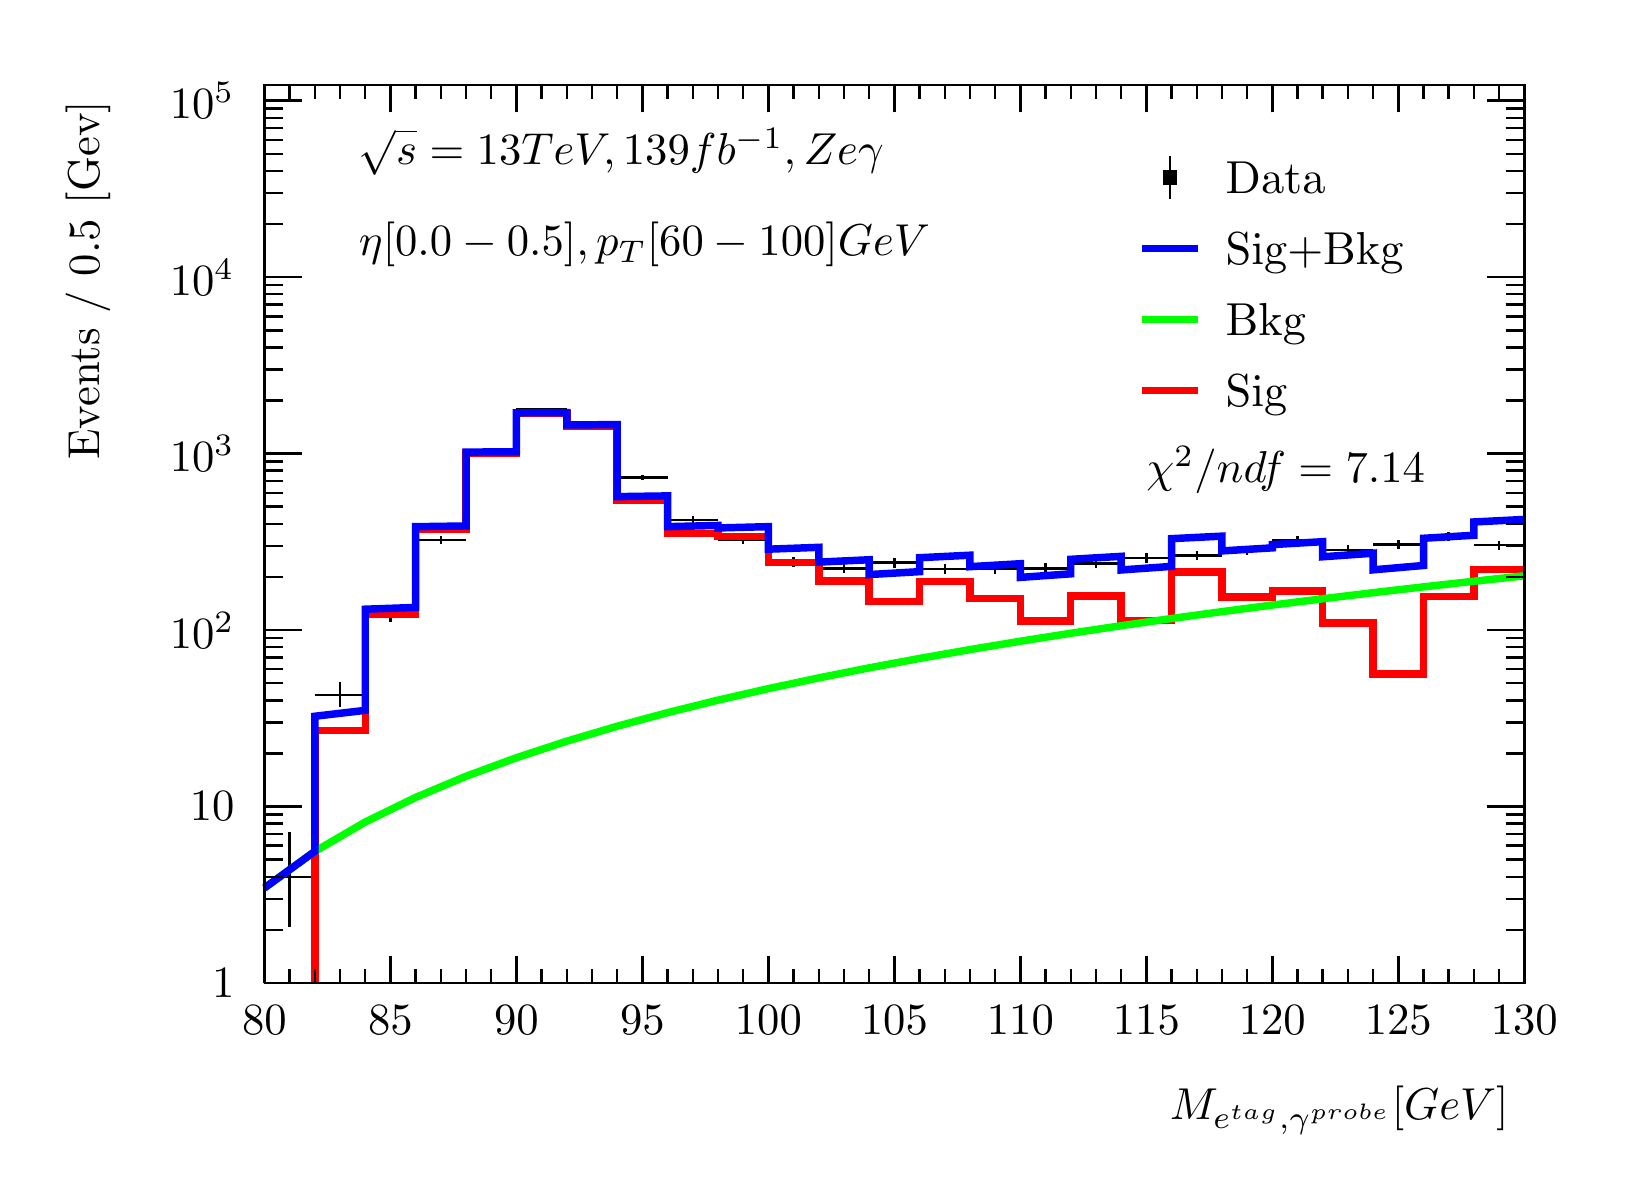
\begin{tikzpicture}
\pgfdeclareplotmark{cross} {
\pgfpathmoveto{\pgfpoint{-0.3\pgfplotmarksize}{\pgfplotmarksize}}
\pgfpathlineto{\pgfpoint{+0.3\pgfplotmarksize}{\pgfplotmarksize}}
\pgfpathlineto{\pgfpoint{+0.3\pgfplotmarksize}{0.3\pgfplotmarksize}}
\pgfpathlineto{\pgfpoint{+1\pgfplotmarksize}{0.3\pgfplotmarksize}}
\pgfpathlineto{\pgfpoint{+1\pgfplotmarksize}{-0.3\pgfplotmarksize}}
\pgfpathlineto{\pgfpoint{+0.3\pgfplotmarksize}{-0.3\pgfplotmarksize}}
\pgfpathlineto{\pgfpoint{+0.3\pgfplotmarksize}{-1.\pgfplotmarksize}}
\pgfpathlineto{\pgfpoint{-0.3\pgfplotmarksize}{-1.\pgfplotmarksize}}
\pgfpathlineto{\pgfpoint{-0.3\pgfplotmarksize}{-0.3\pgfplotmarksize}}
\pgfpathlineto{\pgfpoint{-1.\pgfplotmarksize}{-0.3\pgfplotmarksize}}
\pgfpathlineto{\pgfpoint{-1.\pgfplotmarksize}{0.3\pgfplotmarksize}}
\pgfpathlineto{\pgfpoint{-0.3\pgfplotmarksize}{0.3\pgfplotmarksize}}
\pgfpathclose
\pgfusepathqstroke
}
\pgfdeclareplotmark{cross*} {
\pgfpathmoveto{\pgfpoint{-0.3\pgfplotmarksize}{\pgfplotmarksize}}
\pgfpathlineto{\pgfpoint{+0.3\pgfplotmarksize}{\pgfplotmarksize}}
\pgfpathlineto{\pgfpoint{+0.3\pgfplotmarksize}{0.3\pgfplotmarksize}}
\pgfpathlineto{\pgfpoint{+1\pgfplotmarksize}{0.3\pgfplotmarksize}}
\pgfpathlineto{\pgfpoint{+1\pgfplotmarksize}{-0.3\pgfplotmarksize}}
\pgfpathlineto{\pgfpoint{+0.3\pgfplotmarksize}{-0.3\pgfplotmarksize}}
\pgfpathlineto{\pgfpoint{+0.3\pgfplotmarksize}{-1.\pgfplotmarksize}}
\pgfpathlineto{\pgfpoint{-0.3\pgfplotmarksize}{-1.\pgfplotmarksize}}
\pgfpathlineto{\pgfpoint{-0.3\pgfplotmarksize}{-0.3\pgfplotmarksize}}
\pgfpathlineto{\pgfpoint{-1.\pgfplotmarksize}{-0.3\pgfplotmarksize}}
\pgfpathlineto{\pgfpoint{-1.\pgfplotmarksize}{0.3\pgfplotmarksize}}
\pgfpathlineto{\pgfpoint{-0.3\pgfplotmarksize}{0.3\pgfplotmarksize}}
\pgfpathclose
\pgfusepathqfillstroke
}
\pgfdeclareplotmark{newstar} {
\pgfpathmoveto{\pgfqpoint{0pt}{\pgfplotmarksize}}
\pgfpathlineto{\pgfqpointpolar{44}{0.5\pgfplotmarksize}}
\pgfpathlineto{\pgfqpointpolar{18}{\pgfplotmarksize}}
\pgfpathlineto{\pgfqpointpolar{-20}{0.5\pgfplotmarksize}}
\pgfpathlineto{\pgfqpointpolar{-54}{\pgfplotmarksize}}
\pgfpathlineto{\pgfqpointpolar{-90}{0.5\pgfplotmarksize}}
\pgfpathlineto{\pgfqpointpolar{234}{\pgfplotmarksize}}
\pgfpathlineto{\pgfqpointpolar{198}{0.5\pgfplotmarksize}}
\pgfpathlineto{\pgfqpointpolar{162}{\pgfplotmarksize}}
\pgfpathlineto{\pgfqpointpolar{134}{0.5\pgfplotmarksize}}
\pgfpathclose
\pgfusepathqstroke
}
\pgfdeclareplotmark{newstar*} {
\pgfpathmoveto{\pgfqpoint{0pt}{\pgfplotmarksize}}
\pgfpathlineto{\pgfqpointpolar{44}{0.5\pgfplotmarksize}}
\pgfpathlineto{\pgfqpointpolar{18}{\pgfplotmarksize}}
\pgfpathlineto{\pgfqpointpolar{-20}{0.5\pgfplotmarksize}}
\pgfpathlineto{\pgfqpointpolar{-54}{\pgfplotmarksize}}
\pgfpathlineto{\pgfqpointpolar{-90}{0.5\pgfplotmarksize}}
\pgfpathlineto{\pgfqpointpolar{234}{\pgfplotmarksize}}
\pgfpathlineto{\pgfqpointpolar{198}{0.5\pgfplotmarksize}}
\pgfpathlineto{\pgfqpointpolar{162}{\pgfplotmarksize}}
\pgfpathlineto{\pgfqpointpolar{134}{0.5\pgfplotmarksize}}
\pgfpathclose
\pgfusepathqfillstroke
}
\definecolor{c}{rgb}{1,1,1};
\draw [color=c, fill=c] (0,0) rectangle (20,14.4361);
\draw [color=c, fill=c] (3,2.30977) rectangle (19,13.7143);
\definecolor{c}{rgb}{0,0,0};
\draw [c,line width=0.9] (3,2.30977) -- (3,13.7143) -- (19,13.7143) -- (19,2.30977) -- (3,2.30977);
\definecolor{c}{rgb}{1,1,1};
\draw [color=c, fill=c] (3,2.30977) rectangle (19,13.7143);
\definecolor{c}{rgb}{0,0,0};
\draw [c,line width=0.9] (3,2.30977) -- (3,13.7143) -- (19,13.7143) -- (19,2.30977) -- (3,2.30977);
\draw [c,line width=0.9] (3,2.30977) -- (19,2.30977);
\draw [c,line width=0.9] (3,2.65624) -- (3,2.30977);
\draw [c,line width=0.9] (3.32,2.48301) -- (3.32,2.30977);
\draw [c,line width=0.9] (3.64,2.48301) -- (3.64,2.30977);
\draw [c,line width=0.9] (3.96,2.48301) -- (3.96,2.30977);
\draw [c,line width=0.9] (4.28,2.48301) -- (4.28,2.30977);
\draw [c,line width=0.9] (4.6,2.65624) -- (4.6,2.30977);
\draw [c,line width=0.9] (4.92,2.48301) -- (4.92,2.30977);
\draw [c,line width=0.9] (5.24,2.48301) -- (5.24,2.30977);
\draw [c,line width=0.9] (5.56,2.48301) -- (5.56,2.30977);
\draw [c,line width=0.9] (5.88,2.48301) -- (5.88,2.30977);
\draw [c,line width=0.9] (6.2,2.65624) -- (6.2,2.30977);
\draw [c,line width=0.9] (6.52,2.48301) -- (6.52,2.30977);
\draw [c,line width=0.9] (6.84,2.48301) -- (6.84,2.30977);
\draw [c,line width=0.9] (7.16,2.48301) -- (7.16,2.30977);
\draw [c,line width=0.9] (7.48,2.48301) -- (7.48,2.30977);
\draw [c,line width=0.9] (7.8,2.65624) -- (7.8,2.30977);
\draw [c,line width=0.9] (8.12,2.48301) -- (8.12,2.30977);
\draw [c,line width=0.9] (8.44,2.48301) -- (8.44,2.30977);
\draw [c,line width=0.9] (8.76,2.48301) -- (8.76,2.30977);
\draw [c,line width=0.9] (9.08,2.48301) -- (9.08,2.30977);
\draw [c,line width=0.9] (9.4,2.65624) -- (9.4,2.30977);
\draw [c,line width=0.9] (9.72,2.48301) -- (9.72,2.30977);
\draw [c,line width=0.9] (10.04,2.48301) -- (10.04,2.30977);
\draw [c,line width=0.9] (10.36,2.48301) -- (10.36,2.30977);
\draw [c,line width=0.9] (10.68,2.48301) -- (10.68,2.30977);
\draw [c,line width=0.9] (11,2.65624) -- (11,2.30977);
\draw [c,line width=0.9] (11.32,2.48301) -- (11.32,2.30977);
\draw [c,line width=0.9] (11.64,2.48301) -- (11.64,2.30977);
\draw [c,line width=0.9] (11.96,2.48301) -- (11.96,2.30977);
\draw [c,line width=0.9] (12.28,2.48301) -- (12.28,2.30977);
\draw [c,line width=0.9] (12.6,2.65624) -- (12.6,2.30977);
\draw [c,line width=0.9] (12.92,2.48301) -- (12.92,2.30977);
\draw [c,line width=0.9] (13.24,2.48301) -- (13.24,2.30977);
\draw [c,line width=0.9] (13.56,2.48301) -- (13.56,2.30977);
\draw [c,line width=0.9] (13.88,2.48301) -- (13.88,2.30977);
\draw [c,line width=0.9] (14.2,2.65624) -- (14.2,2.30977);
\draw [c,line width=0.9] (14.52,2.48301) -- (14.52,2.30977);
\draw [c,line width=0.9] (14.84,2.48301) -- (14.84,2.30977);
\draw [c,line width=0.9] (15.16,2.48301) -- (15.16,2.30977);
\draw [c,line width=0.9] (15.48,2.48301) -- (15.48,2.30977);
\draw [c,line width=0.9] (15.8,2.65624) -- (15.8,2.30977);
\draw [c,line width=0.9] (16.12,2.48301) -- (16.12,2.30977);
\draw [c,line width=0.9] (16.44,2.48301) -- (16.44,2.30977);
\draw [c,line width=0.9] (16.76,2.48301) -- (16.76,2.30977);
\draw [c,line width=0.9] (17.08,2.48301) -- (17.08,2.30977);
\draw [c,line width=0.9] (17.4,2.65624) -- (17.4,2.30977);
\draw [c,line width=0.9] (17.72,2.48301) -- (17.72,2.30977);
\draw [c,line width=0.9] (18.04,2.48301) -- (18.04,2.30977);
\draw [c,line width=0.9] (18.36,2.48301) -- (18.36,2.30977);
\draw [c,line width=0.9] (18.68,2.48301) -- (18.68,2.30977);
\draw [c,line width=0.9] (19,2.65624) -- (19,2.30977);
\draw [anchor=base] (3,1.66015) node[scale=1.61424, color=c, rotate=0]{80};
\draw [anchor=base] (4.6,1.66015) node[scale=1.61424, color=c, rotate=0]{85};
\draw [anchor=base] (6.2,1.66015) node[scale=1.61424, color=c, rotate=0]{90};
\draw [anchor=base] (7.8,1.66015) node[scale=1.61424, color=c, rotate=0]{95};
\draw [anchor=base] (9.4,1.66015) node[scale=1.61424, color=c, rotate=0]{100};
\draw [anchor=base] (11,1.66015) node[scale=1.61424, color=c, rotate=0]{105};
\draw [anchor=base] (12.6,1.66015) node[scale=1.61424, color=c, rotate=0]{110};
\draw [anchor=base] (14.2,1.66015) node[scale=1.61424, color=c, rotate=0]{115};
\draw [anchor=base] (15.8,1.66015) node[scale=1.61424, color=c, rotate=0]{120};
\draw [anchor=base] (17.4,1.66015) node[scale=1.61424, color=c, rotate=0]{125};
\draw [anchor=base] (19,1.66015) node[scale=1.61424, color=c, rotate=0]{130};
\draw [anchor= east] (19,0.692932) node[scale=1.61424, color=c, rotate=0]{$M_{e^{tag}, \gamma^{probe}}  [GeV]$};
\draw [c,line width=0.9] (3,13.7143) -- (19,13.7143);
\draw [c,line width=0.9] (3,13.3678) -- (3,13.7143);
\draw [c,line width=0.9] (3.32,13.5411) -- (3.32,13.7143);
\draw [c,line width=0.9] (3.64,13.5411) -- (3.64,13.7143);
\draw [c,line width=0.9] (3.96,13.5411) -- (3.96,13.7143);
\draw [c,line width=0.9] (4.28,13.5411) -- (4.28,13.7143);
\draw [c,line width=0.9] (4.6,13.3678) -- (4.6,13.7143);
\draw [c,line width=0.9] (4.92,13.5411) -- (4.92,13.7143);
\draw [c,line width=0.9] (5.24,13.5411) -- (5.24,13.7143);
\draw [c,line width=0.9] (5.56,13.5411) -- (5.56,13.7143);
\draw [c,line width=0.9] (5.88,13.5411) -- (5.88,13.7143);
\draw [c,line width=0.9] (6.2,13.3678) -- (6.2,13.7143);
\draw [c,line width=0.9] (6.52,13.5411) -- (6.52,13.7143);
\draw [c,line width=0.9] (6.84,13.5411) -- (6.84,13.7143);
\draw [c,line width=0.9] (7.16,13.5411) -- (7.16,13.7143);
\draw [c,line width=0.9] (7.48,13.5411) -- (7.48,13.7143);
\draw [c,line width=0.9] (7.8,13.3678) -- (7.8,13.7143);
\draw [c,line width=0.9] (8.12,13.5411) -- (8.12,13.7143);
\draw [c,line width=0.9] (8.44,13.5411) -- (8.44,13.7143);
\draw [c,line width=0.9] (8.76,13.5411) -- (8.76,13.7143);
\draw [c,line width=0.9] (9.08,13.5411) -- (9.08,13.7143);
\draw [c,line width=0.9] (9.4,13.3678) -- (9.4,13.7143);
\draw [c,line width=0.9] (9.72,13.5411) -- (9.72,13.7143);
\draw [c,line width=0.9] (10.04,13.5411) -- (10.04,13.7143);
\draw [c,line width=0.9] (10.36,13.5411) -- (10.36,13.7143);
\draw [c,line width=0.9] (10.68,13.5411) -- (10.68,13.7143);
\draw [c,line width=0.9] (11,13.3678) -- (11,13.7143);
\draw [c,line width=0.9] (11.32,13.5411) -- (11.32,13.7143);
\draw [c,line width=0.9] (11.64,13.5411) -- (11.64,13.7143);
\draw [c,line width=0.9] (11.96,13.5411) -- (11.96,13.7143);
\draw [c,line width=0.9] (12.28,13.5411) -- (12.28,13.7143);
\draw [c,line width=0.9] (12.6,13.3678) -- (12.6,13.7143);
\draw [c,line width=0.9] (12.92,13.5411) -- (12.92,13.7143);
\draw [c,line width=0.9] (13.24,13.5411) -- (13.24,13.7143);
\draw [c,line width=0.9] (13.56,13.5411) -- (13.56,13.7143);
\draw [c,line width=0.9] (13.88,13.5411) -- (13.88,13.7143);
\draw [c,line width=0.9] (14.2,13.3678) -- (14.2,13.7143);
\draw [c,line width=0.9] (14.52,13.5411) -- (14.52,13.7143);
\draw [c,line width=0.9] (14.84,13.5411) -- (14.84,13.7143);
\draw [c,line width=0.9] (15.16,13.5411) -- (15.16,13.7143);
\draw [c,line width=0.9] (15.48,13.5411) -- (15.48,13.7143);
\draw [c,line width=0.9] (15.8,13.3678) -- (15.8,13.7143);
\draw [c,line width=0.9] (16.12,13.5411) -- (16.12,13.7143);
\draw [c,line width=0.9] (16.44,13.5411) -- (16.44,13.7143);
\draw [c,line width=0.9] (16.76,13.5411) -- (16.76,13.7143);
\draw [c,line width=0.9] (17.08,13.5411) -- (17.08,13.7143);
\draw [c,line width=0.9] (17.4,13.3678) -- (17.4,13.7143);
\draw [c,line width=0.9] (17.72,13.5411) -- (17.72,13.7143);
\draw [c,line width=0.9] (18.04,13.5411) -- (18.04,13.7143);
\draw [c,line width=0.9] (18.36,13.5411) -- (18.36,13.7143);
\draw [c,line width=0.9] (18.68,13.5411) -- (18.68,13.7143);
\draw [c,line width=0.9] (19,13.3678) -- (19,13.7143);
\draw [c,line width=0.9] (3,2.30977) -- (3,13.7143);
\draw [c,line width=0.9] (3.474,2.30978) -- (3,2.30978);
\draw [anchor= east] (2.82,2.30978) node[scale=1.61424, color=c, rotate=0]{1};
\draw [c,line width=0.9] (3.237,2.98447) -- (3,2.98447);
\draw [c,line width=0.9] (3.237,3.37914) -- (3,3.37914);
\draw [c,line width=0.9] (3.237,3.65916) -- (3,3.65916);
\draw [c,line width=0.9] (3.237,3.87637) -- (3,3.87637);
\draw [c,line width=0.9] (3.237,4.05383) -- (3,4.05383);
\draw [c,line width=0.9] (3.237,4.20388) -- (3,4.20388);
\draw [c,line width=0.9] (3.237,4.33386) -- (3,4.33386);
\draw [c,line width=0.9] (3.237,4.4485) -- (3,4.4485);
\draw [c,line width=0.9] (3.474,4.55106) -- (3,4.55106);
\draw [anchor= east] (2.82,4.55106) node[scale=1.61424, color=c, rotate=0]{10};
\draw [c,line width=0.9] (3.237,5.22575) -- (3,5.22575);
\draw [c,line width=0.9] (3.237,5.62042) -- (3,5.62042);
\draw [c,line width=0.9] (3.237,5.90045) -- (3,5.90045);
\draw [c,line width=0.9] (3.237,6.11765) -- (3,6.11765);
\draw [c,line width=0.9] (3.237,6.29512) -- (3,6.29512);
\draw [c,line width=0.9] (3.237,6.44516) -- (3,6.44516);
\draw [c,line width=0.9] (3.237,6.57514) -- (3,6.57514);
\draw [c,line width=0.9] (3.237,6.68979) -- (3,6.68979);
\draw [c,line width=0.9] (3.474,6.79234) -- (3,6.79234);
\draw [anchor= east] (2.82,6.79234) node[scale=1.61424, color=c, rotate=0]{$10^{2}$};
\draw [c,line width=0.9] (3.237,7.46704) -- (3,7.46704);
\draw [c,line width=0.9] (3.237,7.86171) -- (3,7.86171);
\draw [c,line width=0.9] (3.237,8.14173) -- (3,8.14173);
\draw [c,line width=0.9] (3.237,8.35893) -- (3,8.35893);
\draw [c,line width=0.9] (3.237,8.5364) -- (3,8.5364);
\draw [c,line width=0.9] (3.237,8.68645) -- (3,8.68645);
\draw [c,line width=0.9] (3.237,8.81642) -- (3,8.81642);
\draw [c,line width=0.9] (3.237,8.93107) -- (3,8.93107);
\draw [c,line width=0.9] (3.474,9.03363) -- (3,9.03363);
\draw [anchor= east] (2.82,9.03363) node[scale=1.61424, color=c, rotate=0]{$10^{3}$};
\draw [c,line width=0.9] (3.237,9.70832) -- (3,9.70832);
\draw [c,line width=0.9] (3.237,10.103) -- (3,10.103);
\draw [c,line width=0.9] (3.237,10.383) -- (3,10.383);
\draw [c,line width=0.9] (3.237,10.6002) -- (3,10.6002);
\draw [c,line width=0.9] (3.237,10.7777) -- (3,10.7777);
\draw [c,line width=0.9] (3.237,10.9277) -- (3,10.9277);
\draw [c,line width=0.9] (3.237,11.0577) -- (3,11.0577);
\draw [c,line width=0.9] (3.237,11.1724) -- (3,11.1724);
\draw [c,line width=0.9] (3.474,11.2749) -- (3,11.2749);
\draw [anchor= east] (2.82,11.2749) node[scale=1.61424, color=c, rotate=0]{$10^{4}$};
\draw [c,line width=0.9] (3.237,11.9496) -- (3,11.9496);
\draw [c,line width=0.9] (3.237,12.3443) -- (3,12.3443);
\draw [c,line width=0.9] (3.237,12.6243) -- (3,12.6243);
\draw [c,line width=0.9] (3.237,12.8415) -- (3,12.8415);
\draw [c,line width=0.9] (3.237,13.019) -- (3,13.019);
\draw [c,line width=0.9] (3.237,13.169) -- (3,13.169);
\draw [c,line width=0.9] (3.237,13.299) -- (3,13.299);
\draw [c,line width=0.9] (3.237,13.4136) -- (3,13.4136);
\draw [c,line width=0.9] (3.474,13.5162) -- (3,13.5162);
\draw [anchor= east] (2.82,13.5162) node[scale=1.61424, color=c, rotate=0]{$10^{5}$};
\draw [anchor= east] (0.76,13.7143) node[scale=1.61424, color=c, rotate=90]{Events / 0.5 [Gev]};
\draw [c,line width=0.9] (19,2.30977) -- (19,13.7143);
\draw [c,line width=0.9] (18.526,2.30978) -- (19,2.30978);
\draw [c,line width=0.9] (18.763,2.98447) -- (19,2.98447);
\draw [c,line width=0.9] (18.763,3.37914) -- (19,3.37914);
\draw [c,line width=0.9] (18.763,3.65916) -- (19,3.65916);
\draw [c,line width=0.9] (18.763,3.87637) -- (19,3.87637);
\draw [c,line width=0.9] (18.763,4.05383) -- (19,4.05383);
\draw [c,line width=0.9] (18.763,4.20388) -- (19,4.20388);
\draw [c,line width=0.9] (18.763,4.33386) -- (19,4.33386);
\draw [c,line width=0.9] (18.763,4.4485) -- (19,4.4485);
\draw [c,line width=0.9] (18.526,4.55106) -- (19,4.55106);
\draw [c,line width=0.9] (18.763,5.22575) -- (19,5.22575);
\draw [c,line width=0.9] (18.763,5.62042) -- (19,5.62042);
\draw [c,line width=0.9] (18.763,5.90045) -- (19,5.90045);
\draw [c,line width=0.9] (18.763,6.11765) -- (19,6.11765);
\draw [c,line width=0.9] (18.763,6.29512) -- (19,6.29512);
\draw [c,line width=0.9] (18.763,6.44516) -- (19,6.44516);
\draw [c,line width=0.9] (18.763,6.57514) -- (19,6.57514);
\draw [c,line width=0.9] (18.763,6.68979) -- (19,6.68979);
\draw [c,line width=0.9] (18.526,6.79234) -- (19,6.79234);
\draw [c,line width=0.9] (18.763,7.46704) -- (19,7.46704);
\draw [c,line width=0.9] (18.763,7.86171) -- (19,7.86171);
\draw [c,line width=0.9] (18.763,8.14173) -- (19,8.14173);
\draw [c,line width=0.9] (18.763,8.35893) -- (19,8.35893);
\draw [c,line width=0.9] (18.763,8.5364) -- (19,8.5364);
\draw [c,line width=0.9] (18.763,8.68645) -- (19,8.68645);
\draw [c,line width=0.9] (18.763,8.81642) -- (19,8.81642);
\draw [c,line width=0.9] (18.763,8.93107) -- (19,8.93107);
\draw [c,line width=0.9] (18.526,9.03363) -- (19,9.03363);
\draw [c,line width=0.9] (18.763,9.70832) -- (19,9.70832);
\draw [c,line width=0.9] (18.763,10.103) -- (19,10.103);
\draw [c,line width=0.9] (18.763,10.383) -- (19,10.383);
\draw [c,line width=0.9] (18.763,10.6002) -- (19,10.6002);
\draw [c,line width=0.9] (18.763,10.7777) -- (19,10.7777);
\draw [c,line width=0.9] (18.763,10.9277) -- (19,10.9277);
\draw [c,line width=0.9] (18.763,11.0577) -- (19,11.0577);
\draw [c,line width=0.9] (18.763,11.1724) -- (19,11.1724);
\draw [c,line width=0.9] (18.526,11.2749) -- (19,11.2749);
\draw [c,line width=0.9] (18.763,11.9496) -- (19,11.9496);
\draw [c,line width=0.9] (18.763,12.3443) -- (19,12.3443);
\draw [c,line width=0.9] (18.763,12.6243) -- (19,12.6243);
\draw [c,line width=0.9] (18.763,12.8415) -- (19,12.8415);
\draw [c,line width=0.9] (18.763,13.019) -- (19,13.019);
\draw [c,line width=0.9] (18.763,13.169) -- (19,13.169);
\draw [c,line width=0.9] (18.763,13.299) -- (19,13.299);
\draw [c,line width=0.9] (18.763,13.4136) -- (19,13.4136);
\draw [c,line width=0.9] (18.526,13.5162) -- (19,13.5162);
\draw [c,line width=0.9] (3.32,3.65916) -- (3,3.65916);
\draw [c,line width=0.9] (3,3.65916) -- (3,3.65916);
\draw [c,line width=0.9] (3.32,3.65916) -- (3.64,3.65916);
\draw [c,line width=0.9] (3.64,3.65916) -- (3.64,3.65916);
\draw [c,line width=0.9] (3.32,3.65916) -- (3.32,4.22625);
\draw [c,line width=0.9] (3.32,4.22625) -- (3.32,4.22625);
\draw [c,line width=0.9] (3.32,3.65916) -- (3.32,3.02529);
\draw [c,line width=0.9] (3.32,3.02529) -- (3.32,3.02529);
\draw [c,line width=0.9] (3.96,5.97084) -- (3.64,5.97084);
\draw [c,line width=0.9] (3.64,5.97084) -- (3.64,5.97084);
\draw [c,line width=0.9] (3.96,5.97084) -- (4.28,5.97084);
\draw [c,line width=0.9] (4.28,5.97084) -- (4.28,5.97084);
\draw [c,line width=0.9] (3.96,5.97084) -- (3.96,6.12942);
\draw [c,line width=0.9] (3.96,6.12942) -- (3.96,6.12942);
\draw [c,line width=0.9] (3.96,5.97084) -- (3.96,5.81047);
\draw [c,line width=0.9] (3.96,5.81047) -- (3.96,5.81047);
\draw [c,line width=0.9] (4.6,6.97789) -- (4.28,6.97789);
\draw [c,line width=0.9] (4.28,6.97789) -- (4.28,6.97789);
\draw [c,line width=0.9] (4.6,6.97789) -- (4.92,6.97789);
\draw [c,line width=0.9] (4.92,6.97789) -- (4.92,6.97789);
\draw [c,line width=0.9] (4.6,6.97789) -- (4.6,7.06635);
\draw [c,line width=0.9] (4.6,7.06635) -- (4.6,7.06635);
\draw [c,line width=0.9] (4.6,6.97789) -- (4.6,6.88943);
\draw [c,line width=0.9] (4.6,6.88943) -- (4.6,6.88943);
\draw [c,line width=0.9] (5.24,7.93662) -- (4.92,7.93662);
\draw [c,line width=0.9] (4.92,7.93662) -- (4.92,7.93662);
\draw [c,line width=0.9] (5.24,7.93662) -- (5.56,7.93662);
\draw [c,line width=0.9] (5.56,7.93662) -- (5.56,7.93662);
\draw [c,line width=0.9] (5.24,7.93662) -- (5.24,7.99069);
\draw [c,line width=0.9] (5.24,7.99069) -- (5.24,7.99069);
\draw [c,line width=0.9] (5.24,7.93662) -- (5.24,7.88255);
\draw [c,line width=0.9] (5.24,7.88255) -- (5.24,7.88255);
\draw [c,line width=0.9] (5.88,9.01594) -- (5.56,9.01594);
\draw [c,line width=0.9] (5.56,9.01594) -- (5.56,9.01594);
\draw [c,line width=0.9] (5.88,9.01594) -- (6.2,9.01594);
\draw [c,line width=0.9] (6.2,9.01594) -- (6.2,9.01594);
\draw [c,line width=0.9] (5.88,9.01594) -- (5.88,9.047);
\draw [c,line width=0.9] (5.88,9.047) -- (5.88,9.047);
\draw [c,line width=0.9] (5.88,9.01594) -- (5.88,8.98488);
\draw [c,line width=0.9] (5.88,8.98488) -- (5.88,8.98488);
\draw [c,line width=0.9] (6.52,9.59105) -- (6.2,9.59105);
\draw [c,line width=0.9] (6.2,9.59105) -- (6.2,9.59105);
\draw [c,line width=0.9] (6.52,9.59105) -- (6.84,9.59105);
\draw [c,line width=0.9] (6.84,9.59105) -- (6.84,9.59105);
\draw [c,line width=0.9] (6.52,9.59105) -- (6.52,9.61417);
\draw [c,line width=0.9] (6.52,9.61417) -- (6.52,9.61417);
\draw [c,line width=0.9] (6.52,9.59105) -- (6.52,9.56794);
\draw [c,line width=0.9] (6.52,9.56794) -- (6.52,9.56794);
\draw [c,line width=0.9] (7.16,9.42244) -- (6.84,9.42244);
\draw [c,line width=0.9] (6.84,9.42244) -- (6.84,9.42244);
\draw [c,line width=0.9] (7.16,9.42244) -- (7.48,9.42244);
\draw [c,line width=0.9] (7.48,9.42244) -- (7.48,9.42244);
\draw [c,line width=0.9] (7.16,9.42244) -- (7.16,9.44765);
\draw [c,line width=0.9] (7.16,9.44765) -- (7.16,9.44765);
\draw [c,line width=0.9] (7.16,9.42244) -- (7.16,9.39723);
\draw [c,line width=0.9] (7.16,9.39723) -- (7.16,9.39723);
\draw [c,line width=0.9] (7.8,8.72996) -- (7.48,8.72996);
\draw [c,line width=0.9] (7.48,8.72996) -- (7.48,8.72996);
\draw [c,line width=0.9] (7.8,8.72996) -- (8.12,8.72996);
\draw [c,line width=0.9] (8.12,8.72996) -- (8.12,8.72996);
\draw [c,line width=0.9] (7.8,8.72996) -- (7.8,8.76593);
\draw [c,line width=0.9] (7.8,8.76593) -- (7.8,8.76593);
\draw [c,line width=0.9] (7.8,8.72996) -- (7.8,8.69398);
\draw [c,line width=0.9] (7.8,8.69398) -- (7.8,8.69398);
\draw [c,line width=0.9] (8.44,8.18922) -- (8.12,8.18922);
\draw [c,line width=0.9] (8.12,8.18922) -- (8.12,8.18922);
\draw [c,line width=0.9] (8.44,8.18922) -- (8.76,8.18922);
\draw [c,line width=0.9] (8.76,8.18922) -- (8.76,8.18922);
\draw [c,line width=0.9] (8.44,8.18922) -- (8.44,8.23671);
\draw [c,line width=0.9] (8.44,8.23671) -- (8.44,8.23671);
\draw [c,line width=0.9] (8.44,8.18922) -- (8.44,8.14173);
\draw [c,line width=0.9] (8.44,8.14173) -- (8.44,8.14173);
\draw [c,line width=0.9] (9.08,7.94261) -- (8.76,7.94261);
\draw [c,line width=0.9] (8.76,7.94261) -- (8.76,7.94261);
\draw [c,line width=0.9] (9.08,7.94261) -- (9.4,7.94261);
\draw [c,line width=0.9] (9.4,7.94261) -- (9.4,7.94261);
\draw [c,line width=0.9] (9.08,7.94261) -- (9.08,7.99651);
\draw [c,line width=0.9] (9.08,7.99651) -- (9.08,7.99651);
\draw [c,line width=0.9] (9.08,7.94261) -- (9.08,7.8887);
\draw [c,line width=0.9] (9.08,7.8887) -- (9.08,7.8887);
\draw [c,line width=0.9] (9.72,7.66059) -- (9.4,7.66059);
\draw [c,line width=0.9] (9.4,7.66059) -- (9.4,7.66059);
\draw [c,line width=0.9] (9.72,7.66059) -- (10.04,7.66059);
\draw [c,line width=0.9] (10.04,7.66059) -- (10.04,7.66059);
\draw [c,line width=0.9] (9.72,7.66059) -- (9.72,7.7229);
\draw [c,line width=0.9] (9.72,7.7229) -- (9.72,7.7229);
\draw [c,line width=0.9] (9.72,7.66059) -- (9.72,7.59829);
\draw [c,line width=0.9] (9.72,7.59829) -- (9.72,7.59829);
\draw [c,line width=0.9] (10.36,7.57735) -- (10.04,7.57735);
\draw [c,line width=0.9] (10.04,7.57735) -- (10.04,7.57735);
\draw [c,line width=0.9] (10.36,7.57735) -- (10.68,7.57735);
\draw [c,line width=0.9] (10.68,7.57735) -- (10.68,7.57735);
\draw [c,line width=0.9] (10.36,7.57735) -- (10.36,7.64237);
\draw [c,line width=0.9] (10.36,7.64237) -- (10.36,7.64237);
\draw [c,line width=0.9] (10.36,7.57735) -- (10.36,7.51232);
\draw [c,line width=0.9] (10.36,7.51232) -- (10.36,7.51232);
\draw [c,line width=0.9] (11,7.64855) -- (10.68,7.64855);
\draw [c,line width=0.9] (10.68,7.64855) -- (10.68,7.64855);
\draw [c,line width=0.9] (11,7.64855) -- (11.32,7.64855);
\draw [c,line width=0.9] (11.32,7.64855) -- (11.32,7.64855);
\draw [c,line width=0.9] (11,7.64855) -- (11,7.71124);
\draw [c,line width=0.9] (11,7.71124) -- (11,7.71124);
\draw [c,line width=0.9] (11,7.64855) -- (11,7.58586);
\draw [c,line width=0.9] (11,7.58586) -- (11,7.58586);
\draw [c,line width=0.9] (11.64,7.56862) -- (11.32,7.56862);
\draw [c,line width=0.9] (11.32,7.56862) -- (11.32,7.56862);
\draw [c,line width=0.9] (11.64,7.56862) -- (11.96,7.56862);
\draw [c,line width=0.9] (11.96,7.56862) -- (11.96,7.56862);
\draw [c,line width=0.9] (11.64,7.56862) -- (11.64,7.63393);
\draw [c,line width=0.9] (11.64,7.63393) -- (11.64,7.63393);
\draw [c,line width=0.9] (11.64,7.56862) -- (11.64,7.5033);
\draw [c,line width=0.9] (11.64,7.5033) -- (11.64,7.5033);
\draw [c,line width=0.9] (12.28,7.57299) -- (11.96,7.57299);
\draw [c,line width=0.9] (11.96,7.57299) -- (11.96,7.57299);
\draw [c,line width=0.9] (12.28,7.57299) -- (12.6,7.57299);
\draw [c,line width=0.9] (12.6,7.57299) -- (12.6,7.57299);
\draw [c,line width=0.9] (12.28,7.57299) -- (12.28,7.63816);
\draw [c,line width=0.9] (12.28,7.63816) -- (12.28,7.63816);
\draw [c,line width=0.9] (12.28,7.57299) -- (12.28,7.50782);
\draw [c,line width=0.9] (12.28,7.50782) -- (12.28,7.50782);
\draw [c,line width=0.9] (12.92,7.57735) -- (12.6,7.57735);
\draw [c,line width=0.9] (12.6,7.57735) -- (12.6,7.57735);
\draw [c,line width=0.9] (12.92,7.57735) -- (13.24,7.57735);
\draw [c,line width=0.9] (13.24,7.57735) -- (13.24,7.57735);
\draw [c,line width=0.9] (12.92,7.57735) -- (12.92,7.64237);
\draw [c,line width=0.9] (12.92,7.64237) -- (12.92,7.64237);
\draw [c,line width=0.9] (12.92,7.57735) -- (12.92,7.51232);
\draw [c,line width=0.9] (12.92,7.51232) -- (12.92,7.51232);
\draw [c,line width=0.9] (13.56,7.64044) -- (13.24,7.64044);
\draw [c,line width=0.9] (13.24,7.64044) -- (13.24,7.64044);
\draw [c,line width=0.9] (13.56,7.64044) -- (13.88,7.64044);
\draw [c,line width=0.9] (13.88,7.64044) -- (13.88,7.64044);
\draw [c,line width=0.9] (13.56,7.64044) -- (13.56,7.70339);
\draw [c,line width=0.9] (13.56,7.70339) -- (13.56,7.70339);
\draw [c,line width=0.9] (13.56,7.64044) -- (13.56,7.57749);
\draw [c,line width=0.9] (13.56,7.57749) -- (13.56,7.57749);
\draw [c,line width=0.9] (14.2,7.71112) -- (13.88,7.71112);
\draw [c,line width=0.9] (13.88,7.71112) -- (13.88,7.71112);
\draw [c,line width=0.9] (14.2,7.71112) -- (14.52,7.71112);
\draw [c,line width=0.9] (14.52,7.71112) -- (14.52,7.71112);
\draw [c,line width=0.9] (14.2,7.71112) -- (14.2,7.77183);
\draw [c,line width=0.9] (14.2,7.77183) -- (14.2,7.77183);
\draw [c,line width=0.9] (14.2,7.71112) -- (14.2,7.65041);
\draw [c,line width=0.9] (14.2,7.65041) -- (14.2,7.65041);
\draw [c,line width=0.9] (14.84,7.73728) -- (14.52,7.73728);
\draw [c,line width=0.9] (14.52,7.73728) -- (14.52,7.73728);
\draw [c,line width=0.9] (14.84,7.73728) -- (15.16,7.73728);
\draw [c,line width=0.9] (15.16,7.73728) -- (15.16,7.73728);
\draw [c,line width=0.9] (14.84,7.73728) -- (14.84,7.79717);
\draw [c,line width=0.9] (14.84,7.79717) -- (14.84,7.79717);
\draw [c,line width=0.9] (14.84,7.73728) -- (14.84,7.67738);
\draw [c,line width=0.9] (14.84,7.67738) -- (14.84,7.67738);
\draw [c,line width=0.9] (15.48,7.80836) -- (15.16,7.80836);
\draw [c,line width=0.9] (15.16,7.80836) -- (15.16,7.80836);
\draw [c,line width=0.9] (15.48,7.80836) -- (15.8,7.80836);
\draw [c,line width=0.9] (15.8,7.80836) -- (15.8,7.80836);
\draw [c,line width=0.9] (15.48,7.80836) -- (15.48,7.86611);
\draw [c,line width=0.9] (15.48,7.86611) -- (15.48,7.86611);
\draw [c,line width=0.9] (15.48,7.80836) -- (15.48,7.75061);
\draw [c,line width=0.9] (15.48,7.75061) -- (15.48,7.75061);
\draw [c,line width=0.9] (16.12,7.93361) -- (15.8,7.93361);
\draw [c,line width=0.9] (15.8,7.93361) -- (15.8,7.93361);
\draw [c,line width=0.9] (16.12,7.93361) -- (16.44,7.93361);
\draw [c,line width=0.9] (16.44,7.93361) -- (16.44,7.93361);
\draw [c,line width=0.9] (16.12,7.93361) -- (16.12,7.98776);
\draw [c,line width=0.9] (16.12,7.98776) -- (16.12,7.98776);
\draw [c,line width=0.9] (16.12,7.93361) -- (16.12,7.87946);
\draw [c,line width=0.9] (16.12,7.87946) -- (16.12,7.87946);
\draw [c,line width=0.9] (16.76,7.81178) -- (16.44,7.81178);
\draw [c,line width=0.9] (16.44,7.81178) -- (16.44,7.81178);
\draw [c,line width=0.9] (16.76,7.81178) -- (17.08,7.81178);
\draw [c,line width=0.9] (17.08,7.81178) -- (17.08,7.81178);
\draw [c,line width=0.9] (16.76,7.81178) -- (16.76,7.86943);
\draw [c,line width=0.9] (16.76,7.86943) -- (16.76,7.86943);
\draw [c,line width=0.9] (16.76,7.81178) -- (16.76,7.75413);
\draw [c,line width=0.9] (16.76,7.75413) -- (16.76,7.75413);
\draw [c,line width=0.9] (17.4,7.87779) -- (17.08,7.87779);
\draw [c,line width=0.9] (17.08,7.87779) -- (17.08,7.87779);
\draw [c,line width=0.9] (17.4,7.87779) -- (17.72,7.87779);
\draw [c,line width=0.9] (17.72,7.87779) -- (17.72,7.87779);
\draw [c,line width=0.9] (17.4,7.87779) -- (17.4,7.93352);
\draw [c,line width=0.9] (17.4,7.93352) -- (17.4,7.93352);
\draw [c,line width=0.9] (17.4,7.87779) -- (17.4,7.82207);
\draw [c,line width=0.9] (17.4,7.82207) -- (17.4,7.82207);
\draw [c,line width=0.9] (18.04,7.98067) -- (17.72,7.98067);
\draw [c,line width=0.9] (17.72,7.98067) -- (17.72,7.98067);
\draw [c,line width=0.9] (18.04,7.98067) -- (18.36,7.98067);
\draw [c,line width=0.9] (18.36,7.98067) -- (18.36,7.98067);
\draw [c,line width=0.9] (18.04,7.98067) -- (18.04,8.03353);
\draw [c,line width=0.9] (18.04,8.03353) -- (18.04,8.03353);
\draw [c,line width=0.9] (18.04,7.98067) -- (18.04,7.92781);
\draw [c,line width=0.9] (18.04,7.92781) -- (18.04,7.92781);
\draw [c,line width=0.9] (18.68,7.87139) -- (18.36,7.87139);
\draw [c,line width=0.9] (18.36,7.87139) -- (18.36,7.87139);
\draw [c,line width=0.9] (18.68,7.87139) -- (19,7.87139);
\draw [c,line width=0.9] (19,7.87139) -- (19,7.87139);
\draw [c,line width=0.9] (18.68,7.87139) -- (18.68,7.9273);
\draw [c,line width=0.9] (18.68,7.9273) -- (18.68,7.9273);
\draw [c,line width=0.9] (18.68,7.87139) -- (18.68,7.81548);
\draw [c,line width=0.9] (18.68,7.81548) -- (18.68,7.81548);
\foreach \P in {(3.32,3.65916), (3.96,5.97084), (4.6,6.97789), (5.24,7.93662), (5.88,9.01594), (6.52,9.59105), (7.16,9.42244), (7.8,8.72996), (8.44,8.18922), (9.08,7.94261), (9.72,7.66059), (10.36,7.57735), (11,7.64855), (11.64,7.56862),
 (12.28,7.57299), (12.92,7.57735), (13.56,7.64044), (14.2,7.71112), (14.84,7.73728), (15.48,7.80836), (16.12,7.93361), (16.76,7.81178), (17.4,7.87779), (18.04,7.98067), (18.68,7.87139)}{\draw[mark options={color=c,fill=c},mark size=2.882883pt,mark=]
 plot coordinates {\P};}
\definecolor{c}{rgb}{1,0,0};
\draw [c,line width=2.7] (3.64,2.30977) -- (3.64,5.51487);
\draw [c,line width=2.7] (3.64,5.51487) -- (4.28,5.51487) -- (4.28,6.99504) -- (4.92,6.99504) -- (4.92,8.0768) -- (5.56,8.0768) -- (5.56,9.03869) -- (6.2,9.03869) -- (6.2,9.54112) -- (6.84,9.54112) -- (6.84,9.38238) -- (7.48,9.38238) --
 (7.48,8.43727) -- (8.12,8.43727) -- (8.12,8.01608) -- (8.76,8.01608) -- (8.76,7.98073) -- (9.4,7.98073) -- (9.4,7.64771) -- (10.04,7.64771) -- (10.04,7.41328) -- (10.68,7.41328) -- (10.68,7.15587) -- (11.32,7.15587) -- (11.32,7.40735) --
 (11.96,7.40735) -- (11.96,7.19492) -- (12.6,7.19492) -- (12.6,6.90613) -- (13.24,6.90613) -- (13.24,7.22418) -- (13.88,7.22418) -- (13.88,6.91353) -- (14.52,6.91353) -- (14.52,7.53019) -- (15.16,7.53019) -- (15.16,7.21107) -- (15.8,7.21107) --
 (15.8,7.2882) -- (16.44,7.2882) -- (16.44,6.88266) -- (17.08,6.88266) -- (17.08,6.23769) -- (17.72,6.23769) -- (17.72,7.22214) -- (18.36,7.22214) -- (18.36,7.56311) -- (19,7.56311) -- (19,7.56311) -- (19,7.56311) -- (19,7.56311);
\definecolor{c}{rgb}{0,1,0};
\draw [c,line width=2.7] (3,3.51772) -- (3,3.51772);
\draw [c,line width=2.7] (3,3.51772) -- (3,3.51772) -- (3.64,3.98183) -- (3.64,3.98183) -- (4.28,4.35484) -- (4.28,4.35484) -- (4.92,4.66705) -- (4.92,4.66705) -- (5.56,4.93566) -- (5.56,4.93566) -- (6.2,5.17145) -- (6.2,5.17145) -- (6.84,5.38161) --
 (6.84,5.38161) -- (7.48,5.57118) -- (7.48,5.57118) -- (8.12,5.74386) -- (8.12,5.74386) -- (8.76,5.90242) -- (8.76,5.90242) -- (9.4,6.049) -- (9.4,6.049) -- (10.04,6.1853) -- (10.04,6.1853) -- (10.68,6.31265) -- (10.68,6.31265) -- (11.32,6.43217) --
 (11.32,6.43217) -- (11.96,6.54476) -- (11.96,6.54476) -- (12.6,6.65118) -- (12.6,6.65118) -- (13.24,6.75209) -- (13.24,6.75209) -- (13.88,6.84801) -- (13.88,6.84801) -- (14.52,6.93942) -- (14.52,6.93942) -- (15.16,7.02673) -- (15.16,7.02673) --
 (15.8,7.11029) -- (15.8,7.11029) -- (16.44,7.1904) -- (16.44,7.1904) -- (17.08,7.26735) -- (17.08,7.26735) -- (17.72,7.34137) -- (17.72,7.34137) -- (18.36,7.41267) -- (18.36,7.41267) -- (19,7.48146) -- (19,7.48146) -- (19,7.48146) -- (19,7.48146);
\definecolor{c}{rgb}{0,0,1};
\draw [c,line width=2.7] (3,3.51772) -- (3,3.51772);
\draw [c,line width=2.7] (3,3.51772) -- (3,3.51772) -- (3.64,3.98183) -- (3.64,5.69801) -- (4.28,5.77301) -- (4.28,7.05759) -- (4.92,7.08024) -- (4.92,8.10567) -- (5.56,8.11467) -- (5.56,9.05297) -- (6.2,9.05684) -- (6.2,9.55199) -- (6.84,9.55459) --
 (6.84,9.39822) -- (7.48,9.40159) -- (7.48,8.4872) -- (8.12,8.4966) -- (8.12,8.10608) -- (8.76,8.12117) -- (8.76,8.0895) -- (9.4,8.10609) -- (9.4,7.8199) -- (10.04,7.84334) -- (10.04,7.656) -- (10.68,7.68558) -- (10.68,7.49754) -- (11.32,7.53448) --
 (11.32,7.71178) -- (11.96,7.74332) -- (11.96,7.59784) -- (12.6,7.63523) -- (12.6,7.46167) -- (13.24,7.50685) -- (13.24,7.69117) -- (13.88,7.72885) -- (13.88,7.55602) -- (14.52,7.60126) -- (14.52,7.95364) -- (15.16,7.98535) -- (15.16,7.79795) --
 (15.8,7.83668) -- (15.8,7.878) -- (16.44,7.91522) -- (16.44,7.72334) -- (17.08,7.76858) -- (17.08,7.55745) -- (17.72,7.61292) -- (17.72,7.95827) -- (18.36,7.99676) -- (18.36,8.16549) -- (19,8.19783) -- (19,8.19783) -- (19,8.19783) -- (19,8.19783);
\definecolor{c}{rgb}{0,0,0};
\draw [c,line width=0.9] (3,2.30977) -- (19,2.30977);
\draw [c,line width=0.9] (3,2.65624) -- (3,2.30977);
\draw [c,line width=0.9] (3.32,2.48301) -- (3.32,2.30977);
\draw [c,line width=0.9] (3.64,2.48301) -- (3.64,2.30977);
\draw [c,line width=0.9] (3.96,2.48301) -- (3.96,2.30977);
\draw [c,line width=0.9] (4.28,2.48301) -- (4.28,2.30977);
\draw [c,line width=0.9] (4.6,2.65624) -- (4.6,2.30977);
\draw [c,line width=0.9] (4.92,2.48301) -- (4.92,2.30977);
\draw [c,line width=0.9] (5.24,2.48301) -- (5.24,2.30977);
\draw [c,line width=0.9] (5.56,2.48301) -- (5.56,2.30977);
\draw [c,line width=0.9] (5.88,2.48301) -- (5.88,2.30977);
\draw [c,line width=0.9] (6.2,2.65624) -- (6.2,2.30977);
\draw [c,line width=0.9] (6.52,2.48301) -- (6.52,2.30977);
\draw [c,line width=0.9] (6.84,2.48301) -- (6.84,2.30977);
\draw [c,line width=0.9] (7.16,2.48301) -- (7.16,2.30977);
\draw [c,line width=0.9] (7.48,2.48301) -- (7.48,2.30977);
\draw [c,line width=0.9] (7.8,2.65624) -- (7.8,2.30977);
\draw [c,line width=0.9] (8.12,2.48301) -- (8.12,2.30977);
\draw [c,line width=0.9] (8.44,2.48301) -- (8.44,2.30977);
\draw [c,line width=0.9] (8.76,2.48301) -- (8.76,2.30977);
\draw [c,line width=0.9] (9.08,2.48301) -- (9.08,2.30977);
\draw [c,line width=0.9] (9.4,2.65624) -- (9.4,2.30977);
\draw [c,line width=0.9] (9.72,2.48301) -- (9.72,2.30977);
\draw [c,line width=0.9] (10.04,2.48301) -- (10.04,2.30977);
\draw [c,line width=0.9] (10.36,2.48301) -- (10.36,2.30977);
\draw [c,line width=0.9] (10.68,2.48301) -- (10.68,2.30977);
\draw [c,line width=0.9] (11,2.65624) -- (11,2.30977);
\draw [c,line width=0.9] (11.32,2.48301) -- (11.32,2.30977);
\draw [c,line width=0.9] (11.64,2.48301) -- (11.64,2.30977);
\draw [c,line width=0.9] (11.96,2.48301) -- (11.96,2.30977);
\draw [c,line width=0.9] (12.28,2.48301) -- (12.28,2.30977);
\draw [c,line width=0.9] (12.6,2.65624) -- (12.6,2.30977);
\draw [c,line width=0.9] (12.92,2.48301) -- (12.92,2.30977);
\draw [c,line width=0.9] (13.24,2.48301) -- (13.24,2.30977);
\draw [c,line width=0.9] (13.56,2.48301) -- (13.56,2.30977);
\draw [c,line width=0.9] (13.88,2.48301) -- (13.88,2.30977);
\draw [c,line width=0.9] (14.2,2.65624) -- (14.2,2.30977);
\draw [c,line width=0.9] (14.52,2.48301) -- (14.52,2.30977);
\draw [c,line width=0.9] (14.84,2.48301) -- (14.84,2.30977);
\draw [c,line width=0.9] (15.16,2.48301) -- (15.16,2.30977);
\draw [c,line width=0.9] (15.48,2.48301) -- (15.48,2.30977);
\draw [c,line width=0.9] (15.8,2.65624) -- (15.8,2.30977);
\draw [c,line width=0.9] (16.12,2.48301) -- (16.12,2.30977);
\draw [c,line width=0.9] (16.44,2.48301) -- (16.44,2.30977);
\draw [c,line width=0.9] (16.76,2.48301) -- (16.76,2.30977);
\draw [c,line width=0.9] (17.08,2.48301) -- (17.08,2.30977);
\draw [c,line width=0.9] (17.4,2.65624) -- (17.4,2.30977);
\draw [c,line width=0.9] (17.72,2.48301) -- (17.72,2.30977);
\draw [c,line width=0.9] (18.04,2.48301) -- (18.04,2.30977);
\draw [c,line width=0.9] (18.36,2.48301) -- (18.36,2.30977);
\draw [c,line width=0.9] (18.68,2.48301) -- (18.68,2.30977);
\draw [c,line width=0.9] (19,2.65624) -- (19,2.30977);
\draw [c,line width=0.9] (3,13.7143) -- (19,13.7143);
\draw [c,line width=0.9] (3,13.3678) -- (3,13.7143);
\draw [c,line width=0.9] (3.32,13.5411) -- (3.32,13.7143);
\draw [c,line width=0.9] (3.64,13.5411) -- (3.64,13.7143);
\draw [c,line width=0.9] (3.96,13.5411) -- (3.96,13.7143);
\draw [c,line width=0.9] (4.28,13.5411) -- (4.28,13.7143);
\draw [c,line width=0.9] (4.6,13.3678) -- (4.6,13.7143);
\draw [c,line width=0.9] (4.92,13.5411) -- (4.92,13.7143);
\draw [c,line width=0.9] (5.24,13.5411) -- (5.24,13.7143);
\draw [c,line width=0.9] (5.56,13.5411) -- (5.56,13.7143);
\draw [c,line width=0.9] (5.88,13.5411) -- (5.88,13.7143);
\draw [c,line width=0.9] (6.2,13.3678) -- (6.2,13.7143);
\draw [c,line width=0.9] (6.52,13.5411) -- (6.52,13.7143);
\draw [c,line width=0.9] (6.84,13.5411) -- (6.84,13.7143);
\draw [c,line width=0.9] (7.16,13.5411) -- (7.16,13.7143);
\draw [c,line width=0.9] (7.48,13.5411) -- (7.48,13.7143);
\draw [c,line width=0.9] (7.8,13.3678) -- (7.8,13.7143);
\draw [c,line width=0.9] (8.12,13.5411) -- (8.12,13.7143);
\draw [c,line width=0.9] (8.44,13.5411) -- (8.44,13.7143);
\draw [c,line width=0.9] (8.76,13.5411) -- (8.76,13.7143);
\draw [c,line width=0.9] (9.08,13.5411) -- (9.08,13.7143);
\draw [c,line width=0.9] (9.4,13.3678) -- (9.4,13.7143);
\draw [c,line width=0.9] (9.72,13.5411) -- (9.72,13.7143);
\draw [c,line width=0.9] (10.04,13.5411) -- (10.04,13.7143);
\draw [c,line width=0.9] (10.36,13.5411) -- (10.36,13.7143);
\draw [c,line width=0.9] (10.68,13.5411) -- (10.68,13.7143);
\draw [c,line width=0.9] (11,13.3678) -- (11,13.7143);
\draw [c,line width=0.9] (11.32,13.5411) -- (11.32,13.7143);
\draw [c,line width=0.9] (11.64,13.5411) -- (11.64,13.7143);
\draw [c,line width=0.9] (11.96,13.5411) -- (11.96,13.7143);
\draw [c,line width=0.9] (12.28,13.5411) -- (12.28,13.7143);
\draw [c,line width=0.9] (12.6,13.3678) -- (12.6,13.7143);
\draw [c,line width=0.9] (12.92,13.5411) -- (12.92,13.7143);
\draw [c,line width=0.9] (13.24,13.5411) -- (13.24,13.7143);
\draw [c,line width=0.9] (13.56,13.5411) -- (13.56,13.7143);
\draw [c,line width=0.9] (13.88,13.5411) -- (13.88,13.7143);
\draw [c,line width=0.9] (14.2,13.3678) -- (14.2,13.7143);
\draw [c,line width=0.9] (14.52,13.5411) -- (14.52,13.7143);
\draw [c,line width=0.9] (14.84,13.5411) -- (14.84,13.7143);
\draw [c,line width=0.9] (15.16,13.5411) -- (15.16,13.7143);
\draw [c,line width=0.9] (15.48,13.5411) -- (15.48,13.7143);
\draw [c,line width=0.9] (15.8,13.3678) -- (15.8,13.7143);
\draw [c,line width=0.9] (16.12,13.5411) -- (16.12,13.7143);
\draw [c,line width=0.9] (16.44,13.5411) -- (16.44,13.7143);
\draw [c,line width=0.9] (16.76,13.5411) -- (16.76,13.7143);
\draw [c,line width=0.9] (17.08,13.5411) -- (17.08,13.7143);
\draw [c,line width=0.9] (17.4,13.3678) -- (17.4,13.7143);
\draw [c,line width=0.9] (17.72,13.5411) -- (17.72,13.7143);
\draw [c,line width=0.9] (18.04,13.5411) -- (18.04,13.7143);
\draw [c,line width=0.9] (18.36,13.5411) -- (18.36,13.7143);
\draw [c,line width=0.9] (18.68,13.5411) -- (18.68,13.7143);
\draw [c,line width=0.9] (19,13.3678) -- (19,13.7143);
\draw [c,line width=0.9] (3,2.30977) -- (3,13.7143);
\draw [c,line width=0.9] (3.474,2.30978) -- (3,2.30978);
\draw [c,line width=0.9] (3.237,2.98447) -- (3,2.98447);
\draw [c,line width=0.9] (3.237,3.37914) -- (3,3.37914);
\draw [c,line width=0.9] (3.237,3.65916) -- (3,3.65916);
\draw [c,line width=0.9] (3.237,3.87637) -- (3,3.87637);
\draw [c,line width=0.9] (3.237,4.05383) -- (3,4.05383);
\draw [c,line width=0.9] (3.237,4.20388) -- (3,4.20388);
\draw [c,line width=0.9] (3.237,4.33386) -- (3,4.33386);
\draw [c,line width=0.9] (3.237,4.4485) -- (3,4.4485);
\draw [c,line width=0.9] (3.474,4.55106) -- (3,4.55106);
\draw [c,line width=0.9] (3.237,5.22575) -- (3,5.22575);
\draw [c,line width=0.9] (3.237,5.62042) -- (3,5.62042);
\draw [c,line width=0.9] (3.237,5.90045) -- (3,5.90045);
\draw [c,line width=0.9] (3.237,6.11765) -- (3,6.11765);
\draw [c,line width=0.9] (3.237,6.29512) -- (3,6.29512);
\draw [c,line width=0.9] (3.237,6.44516) -- (3,6.44516);
\draw [c,line width=0.9] (3.237,6.57514) -- (3,6.57514);
\draw [c,line width=0.9] (3.237,6.68979) -- (3,6.68979);
\draw [c,line width=0.9] (3.474,6.79234) -- (3,6.79234);
\draw [c,line width=0.9] (3.237,7.46704) -- (3,7.46704);
\draw [c,line width=0.9] (3.237,7.86171) -- (3,7.86171);
\draw [c,line width=0.9] (3.237,8.14173) -- (3,8.14173);
\draw [c,line width=0.9] (3.237,8.35893) -- (3,8.35893);
\draw [c,line width=0.9] (3.237,8.5364) -- (3,8.5364);
\draw [c,line width=0.9] (3.237,8.68645) -- (3,8.68645);
\draw [c,line width=0.9] (3.237,8.81642) -- (3,8.81642);
\draw [c,line width=0.9] (3.237,8.93107) -- (3,8.93107);
\draw [c,line width=0.9] (3.474,9.03363) -- (3,9.03363);
\draw [c,line width=0.9] (3.237,9.70832) -- (3,9.70832);
\draw [c,line width=0.9] (3.237,10.103) -- (3,10.103);
\draw [c,line width=0.9] (3.237,10.383) -- (3,10.383);
\draw [c,line width=0.9] (3.237,10.6002) -- (3,10.6002);
\draw [c,line width=0.9] (3.237,10.7777) -- (3,10.7777);
\draw [c,line width=0.9] (3.237,10.9277) -- (3,10.9277);
\draw [c,line width=0.9] (3.237,11.0577) -- (3,11.0577);
\draw [c,line width=0.9] (3.237,11.1724) -- (3,11.1724);
\draw [c,line width=0.9] (3.474,11.2749) -- (3,11.2749);
\draw [c,line width=0.9] (3.237,11.9496) -- (3,11.9496);
\draw [c,line width=0.9] (3.237,12.3443) -- (3,12.3443);
\draw [c,line width=0.9] (3.237,12.6243) -- (3,12.6243);
\draw [c,line width=0.9] (3.237,12.8415) -- (3,12.8415);
\draw [c,line width=0.9] (3.237,13.019) -- (3,13.019);
\draw [c,line width=0.9] (3.237,13.169) -- (3,13.169);
\draw [c,line width=0.9] (3.237,13.299) -- (3,13.299);
\draw [c,line width=0.9] (3.237,13.4136) -- (3,13.4136);
\draw [c,line width=0.9] (3.474,13.5162) -- (3,13.5162);
\draw [c,line width=0.9] (19,2.30977) -- (19,13.7143);
\draw [c,line width=0.9] (18.526,2.30978) -- (19,2.30978);
\draw [c,line width=0.9] (18.763,2.98447) -- (19,2.98447);
\draw [c,line width=0.9] (18.763,3.37914) -- (19,3.37914);
\draw [c,line width=0.9] (18.763,3.65916) -- (19,3.65916);
\draw [c,line width=0.9] (18.763,3.87637) -- (19,3.87637);
\draw [c,line width=0.9] (18.763,4.05383) -- (19,4.05383);
\draw [c,line width=0.9] (18.763,4.20388) -- (19,4.20388);
\draw [c,line width=0.9] (18.763,4.33386) -- (19,4.33386);
\draw [c,line width=0.9] (18.763,4.4485) -- (19,4.4485);
\draw [c,line width=0.9] (18.526,4.55106) -- (19,4.55106);
\draw [c,line width=0.9] (18.763,5.22575) -- (19,5.22575);
\draw [c,line width=0.9] (18.763,5.62042) -- (19,5.62042);
\draw [c,line width=0.9] (18.763,5.90045) -- (19,5.90045);
\draw [c,line width=0.9] (18.763,6.11765) -- (19,6.11765);
\draw [c,line width=0.9] (18.763,6.29512) -- (19,6.29512);
\draw [c,line width=0.9] (18.763,6.44516) -- (19,6.44516);
\draw [c,line width=0.9] (18.763,6.57514) -- (19,6.57514);
\draw [c,line width=0.9] (18.763,6.68979) -- (19,6.68979);
\draw [c,line width=0.9] (18.526,6.79234) -- (19,6.79234);
\draw [c,line width=0.9] (18.763,7.46704) -- (19,7.46704);
\draw [c,line width=0.9] (18.763,7.86171) -- (19,7.86171);
\draw [c,line width=0.9] (18.763,8.14173) -- (19,8.14173);
\draw [c,line width=0.9] (18.763,8.35893) -- (19,8.35893);
\draw [c,line width=0.9] (18.763,8.5364) -- (19,8.5364);
\draw [c,line width=0.9] (18.763,8.68645) -- (19,8.68645);
\draw [c,line width=0.9] (18.763,8.81642) -- (19,8.81642);
\draw [c,line width=0.9] (18.763,8.93107) -- (19,8.93107);
\draw [c,line width=0.9] (18.526,9.03363) -- (19,9.03363);
\draw [c,line width=0.9] (18.763,9.70832) -- (19,9.70832);
\draw [c,line width=0.9] (18.763,10.103) -- (19,10.103);
\draw [c,line width=0.9] (18.763,10.383) -- (19,10.383);
\draw [c,line width=0.9] (18.763,10.6002) -- (19,10.6002);
\draw [c,line width=0.9] (18.763,10.7777) -- (19,10.7777);
\draw [c,line width=0.9] (18.763,10.9277) -- (19,10.9277);
\draw [c,line width=0.9] (18.763,11.0577) -- (19,11.0577);
\draw [c,line width=0.9] (18.763,11.1724) -- (19,11.1724);
\draw [c,line width=0.9] (18.526,11.2749) -- (19,11.2749);
\draw [c,line width=0.9] (18.763,11.9496) -- (19,11.9496);
\draw [c,line width=0.9] (18.763,12.3443) -- (19,12.3443);
\draw [c,line width=0.9] (18.763,12.6243) -- (19,12.6243);
\draw [c,line width=0.9] (18.763,12.8415) -- (19,12.8415);
\draw [c,line width=0.9] (18.763,13.019) -- (19,13.019);
\draw [c,line width=0.9] (18.763,13.169) -- (19,13.169);
\draw [c,line width=0.9] (18.763,13.299) -- (19,13.299);
\draw [c,line width=0.9] (18.763,13.4136) -- (19,13.4136);
\draw [c,line width=0.9] (18.526,13.5162) -- (19,13.5162);
\definecolor{c}{rgb}{1,1,1};
\draw [color=c, fill=c] (14,9.38346) rectangle (18,12.9925);
\definecolor{c}{rgb}{0,0,0};
\draw [anchor=base west] (15,12.3383) node[scale=1.6699, color=c, rotate=0]{Data};
\draw [c,line width=0.9] (14.5,12.6416) -- (14.5,12.812);
\draw [c,line width=0.9] (14.5,12.4411) -- (14.5,12.2707);
\foreach \P in {(14.5,12.5414)}{\draw[mark options={color=c,fill=c},mark size=2.402402pt,mark=square*] plot coordinates {\P};}
\draw [anchor=base west] (15,11.4361) node[scale=1.6699, color=c, rotate=0]{Sig+Bkg};
\definecolor{c}{rgb}{0,0,1};
\draw [c,line width=2.7] (14.15,11.6391) -- (14.85,11.6391);
\definecolor{c}{rgb}{0,0,0};
\draw [anchor=base west] (15,10.5338) node[scale=1.6699, color=c, rotate=0]{Bkg};
\definecolor{c}{rgb}{0,1,0};
\draw [c,line width=2.7] (14.15,10.7368) -- (14.85,10.7368);
\definecolor{c}{rgb}{0,0,0};
\draw [anchor=base west] (15,9.63158) node[scale=1.6699, color=c, rotate=0]{Sig};
\definecolor{c}{rgb}{1,0,0};
\draw [c,line width=2.7] (14.15,9.83459) -- (14.85,9.83459);
\definecolor{c}{rgb}{0,0,0};
\draw [anchor=base west] (4,12.7038) node[scale=1.61424, color=c, rotate=0]{$\sqrt{s}= 13 TeV, 139fb^{-1}, Ze\gamma$};
\draw [anchor=base west] (4,11.5489) node[scale=1.61424, color=c, rotate=0]{$\eta[0.0-0.5], p_{T}[60-100]GeV$};
\draw [anchor=base west] (14,8.66165) node[scale=1.61424, color=c, rotate=0]{$\chi^{2}/ndf= 7.14$};
\end{tikzpicture}
}
\scalebox{0.35}{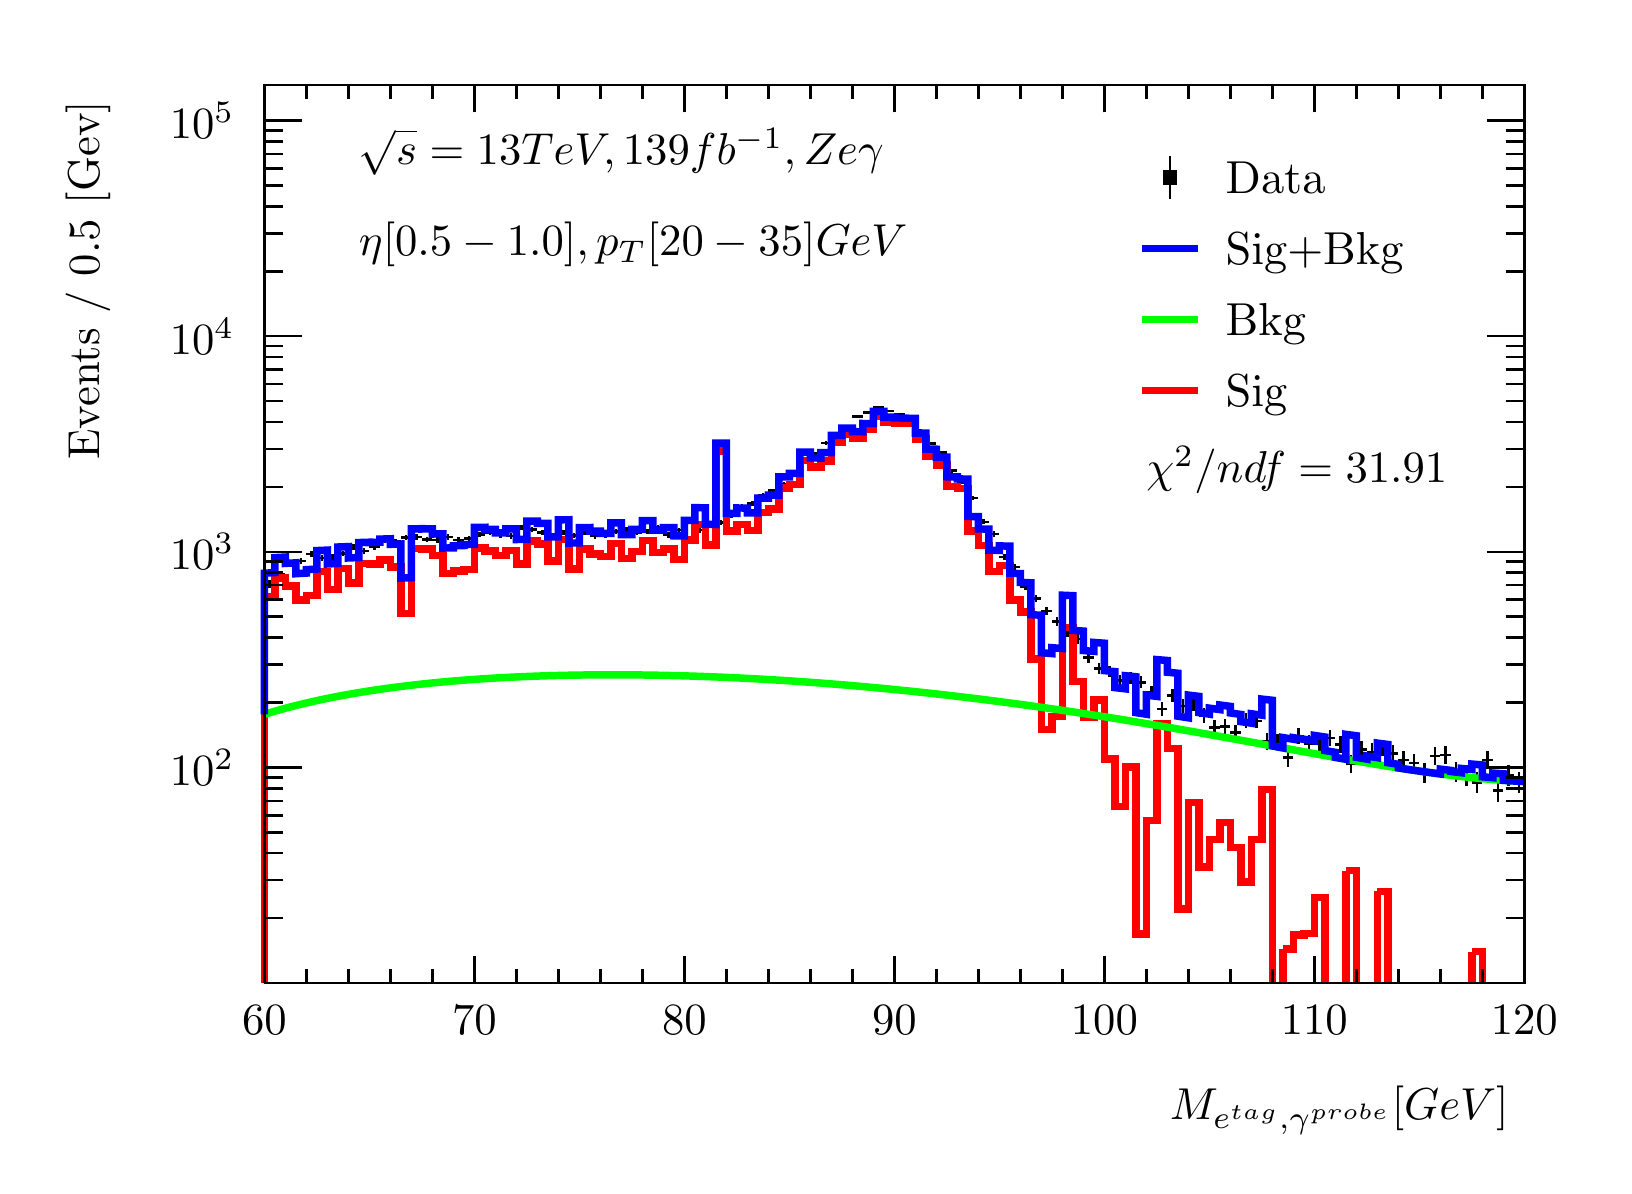
\begin{tikzpicture}
\pgfdeclareplotmark{cross} {
\pgfpathmoveto{\pgfpoint{-0.3\pgfplotmarksize}{\pgfplotmarksize}}
\pgfpathlineto{\pgfpoint{+0.3\pgfplotmarksize}{\pgfplotmarksize}}
\pgfpathlineto{\pgfpoint{+0.3\pgfplotmarksize}{0.3\pgfplotmarksize}}
\pgfpathlineto{\pgfpoint{+1\pgfplotmarksize}{0.3\pgfplotmarksize}}
\pgfpathlineto{\pgfpoint{+1\pgfplotmarksize}{-0.3\pgfplotmarksize}}
\pgfpathlineto{\pgfpoint{+0.3\pgfplotmarksize}{-0.3\pgfplotmarksize}}
\pgfpathlineto{\pgfpoint{+0.3\pgfplotmarksize}{-1.\pgfplotmarksize}}
\pgfpathlineto{\pgfpoint{-0.3\pgfplotmarksize}{-1.\pgfplotmarksize}}
\pgfpathlineto{\pgfpoint{-0.3\pgfplotmarksize}{-0.3\pgfplotmarksize}}
\pgfpathlineto{\pgfpoint{-1.\pgfplotmarksize}{-0.3\pgfplotmarksize}}
\pgfpathlineto{\pgfpoint{-1.\pgfplotmarksize}{0.3\pgfplotmarksize}}
\pgfpathlineto{\pgfpoint{-0.3\pgfplotmarksize}{0.3\pgfplotmarksize}}
\pgfpathclose
\pgfusepathqstroke
}
\pgfdeclareplotmark{cross*} {
\pgfpathmoveto{\pgfpoint{-0.3\pgfplotmarksize}{\pgfplotmarksize}}
\pgfpathlineto{\pgfpoint{+0.3\pgfplotmarksize}{\pgfplotmarksize}}
\pgfpathlineto{\pgfpoint{+0.3\pgfplotmarksize}{0.3\pgfplotmarksize}}
\pgfpathlineto{\pgfpoint{+1\pgfplotmarksize}{0.3\pgfplotmarksize}}
\pgfpathlineto{\pgfpoint{+1\pgfplotmarksize}{-0.3\pgfplotmarksize}}
\pgfpathlineto{\pgfpoint{+0.3\pgfplotmarksize}{-0.3\pgfplotmarksize}}
\pgfpathlineto{\pgfpoint{+0.3\pgfplotmarksize}{-1.\pgfplotmarksize}}
\pgfpathlineto{\pgfpoint{-0.3\pgfplotmarksize}{-1.\pgfplotmarksize}}
\pgfpathlineto{\pgfpoint{-0.3\pgfplotmarksize}{-0.3\pgfplotmarksize}}
\pgfpathlineto{\pgfpoint{-1.\pgfplotmarksize}{-0.3\pgfplotmarksize}}
\pgfpathlineto{\pgfpoint{-1.\pgfplotmarksize}{0.3\pgfplotmarksize}}
\pgfpathlineto{\pgfpoint{-0.3\pgfplotmarksize}{0.3\pgfplotmarksize}}
\pgfpathclose
\pgfusepathqfillstroke
}
\pgfdeclareplotmark{newstar} {
\pgfpathmoveto{\pgfqpoint{0pt}{\pgfplotmarksize}}
\pgfpathlineto{\pgfqpointpolar{44}{0.5\pgfplotmarksize}}
\pgfpathlineto{\pgfqpointpolar{18}{\pgfplotmarksize}}
\pgfpathlineto{\pgfqpointpolar{-20}{0.5\pgfplotmarksize}}
\pgfpathlineto{\pgfqpointpolar{-54}{\pgfplotmarksize}}
\pgfpathlineto{\pgfqpointpolar{-90}{0.5\pgfplotmarksize}}
\pgfpathlineto{\pgfqpointpolar{234}{\pgfplotmarksize}}
\pgfpathlineto{\pgfqpointpolar{198}{0.5\pgfplotmarksize}}
\pgfpathlineto{\pgfqpointpolar{162}{\pgfplotmarksize}}
\pgfpathlineto{\pgfqpointpolar{134}{0.5\pgfplotmarksize}}
\pgfpathclose
\pgfusepathqstroke
}
\pgfdeclareplotmark{newstar*} {
\pgfpathmoveto{\pgfqpoint{0pt}{\pgfplotmarksize}}
\pgfpathlineto{\pgfqpointpolar{44}{0.5\pgfplotmarksize}}
\pgfpathlineto{\pgfqpointpolar{18}{\pgfplotmarksize}}
\pgfpathlineto{\pgfqpointpolar{-20}{0.5\pgfplotmarksize}}
\pgfpathlineto{\pgfqpointpolar{-54}{\pgfplotmarksize}}
\pgfpathlineto{\pgfqpointpolar{-90}{0.5\pgfplotmarksize}}
\pgfpathlineto{\pgfqpointpolar{234}{\pgfplotmarksize}}
\pgfpathlineto{\pgfqpointpolar{198}{0.5\pgfplotmarksize}}
\pgfpathlineto{\pgfqpointpolar{162}{\pgfplotmarksize}}
\pgfpathlineto{\pgfqpointpolar{134}{0.5\pgfplotmarksize}}
\pgfpathclose
\pgfusepathqfillstroke
}
\definecolor{c}{rgb}{1,1,1};
\draw [color=c, fill=c] (0,0) rectangle (20,14.4361);
\draw [color=c, fill=c] (3,2.30977) rectangle (19,13.7143);
\definecolor{c}{rgb}{0,0,0};
\draw [c,line width=0.9] (3,2.30977) -- (3,13.7143) -- (19,13.7143) -- (19,2.30977) -- (3,2.30977);
\definecolor{c}{rgb}{1,1,1};
\draw [color=c, fill=c] (3,2.30977) rectangle (19,13.7143);
\definecolor{c}{rgb}{0,0,0};
\draw [c,line width=0.9] (3,2.30977) -- (3,13.7143) -- (19,13.7143) -- (19,2.30977) -- (3,2.30977);
\draw [c,line width=0.9] (3,2.30977) -- (19,2.30977);
\draw [c,line width=0.9] (3,2.65624) -- (3,2.30977);
\draw [c,line width=0.9] (3.53333,2.48301) -- (3.53333,2.30977);
\draw [c,line width=0.9] (4.06667,2.48301) -- (4.06667,2.30977);
\draw [c,line width=0.9] (4.6,2.48301) -- (4.6,2.30977);
\draw [c,line width=0.9] (5.13333,2.48301) -- (5.13333,2.30977);
\draw [c,line width=0.9] (5.66667,2.65624) -- (5.66667,2.30977);
\draw [c,line width=0.9] (6.2,2.48301) -- (6.2,2.30977);
\draw [c,line width=0.9] (6.73333,2.48301) -- (6.73333,2.30977);
\draw [c,line width=0.9] (7.26667,2.48301) -- (7.26667,2.30977);
\draw [c,line width=0.9] (7.8,2.48301) -- (7.8,2.30977);
\draw [c,line width=0.9] (8.33333,2.65624) -- (8.33333,2.30977);
\draw [c,line width=0.9] (8.86667,2.48301) -- (8.86667,2.30977);
\draw [c,line width=0.9] (9.4,2.48301) -- (9.4,2.30977);
\draw [c,line width=0.9] (9.93333,2.48301) -- (9.93333,2.30977);
\draw [c,line width=0.9] (10.4667,2.48301) -- (10.4667,2.30977);
\draw [c,line width=0.9] (11,2.65624) -- (11,2.30977);
\draw [c,line width=0.9] (11.5333,2.48301) -- (11.5333,2.30977);
\draw [c,line width=0.9] (12.0667,2.48301) -- (12.0667,2.30977);
\draw [c,line width=0.9] (12.6,2.48301) -- (12.6,2.30977);
\draw [c,line width=0.9] (13.1333,2.48301) -- (13.1333,2.30977);
\draw [c,line width=0.9] (13.6667,2.65624) -- (13.6667,2.30977);
\draw [c,line width=0.9] (14.2,2.48301) -- (14.2,2.30977);
\draw [c,line width=0.9] (14.7333,2.48301) -- (14.7333,2.30977);
\draw [c,line width=0.9] (15.2667,2.48301) -- (15.2667,2.30977);
\draw [c,line width=0.9] (15.8,2.48301) -- (15.8,2.30977);
\draw [c,line width=0.9] (16.3333,2.65624) -- (16.3333,2.30977);
\draw [c,line width=0.9] (16.8667,2.48301) -- (16.8667,2.30977);
\draw [c,line width=0.9] (17.4,2.48301) -- (17.4,2.30977);
\draw [c,line width=0.9] (17.9333,2.48301) -- (17.9333,2.30977);
\draw [c,line width=0.9] (18.4667,2.48301) -- (18.4667,2.30977);
\draw [c,line width=0.9] (19,2.65624) -- (19,2.30977);
\draw [anchor=base] (3,1.66015) node[scale=1.61424, color=c, rotate=0]{60};
\draw [anchor=base] (5.66667,1.66015) node[scale=1.61424, color=c, rotate=0]{70};
\draw [anchor=base] (8.33333,1.66015) node[scale=1.61424, color=c, rotate=0]{80};
\draw [anchor=base] (11,1.66015) node[scale=1.61424, color=c, rotate=0]{90};
\draw [anchor=base] (13.6667,1.66015) node[scale=1.61424, color=c, rotate=0]{100};
\draw [anchor=base] (16.3333,1.66015) node[scale=1.61424, color=c, rotate=0]{110};
\draw [anchor=base] (19,1.66015) node[scale=1.61424, color=c, rotate=0]{120};
\draw [anchor= east] (19,0.692932) node[scale=1.61424, color=c, rotate=0]{$M_{e^{tag}, \gamma^{probe}}  [GeV]$};
\draw [c,line width=0.9] (3,13.7143) -- (19,13.7143);
\draw [c,line width=0.9] (3,13.3678) -- (3,13.7143);
\draw [c,line width=0.9] (3.53333,13.5411) -- (3.53333,13.7143);
\draw [c,line width=0.9] (4.06667,13.5411) -- (4.06667,13.7143);
\draw [c,line width=0.9] (4.6,13.5411) -- (4.6,13.7143);
\draw [c,line width=0.9] (5.13333,13.5411) -- (5.13333,13.7143);
\draw [c,line width=0.9] (5.66667,13.3678) -- (5.66667,13.7143);
\draw [c,line width=0.9] (6.2,13.5411) -- (6.2,13.7143);
\draw [c,line width=0.9] (6.73333,13.5411) -- (6.73333,13.7143);
\draw [c,line width=0.9] (7.26667,13.5411) -- (7.26667,13.7143);
\draw [c,line width=0.9] (7.8,13.5411) -- (7.8,13.7143);
\draw [c,line width=0.9] (8.33333,13.3678) -- (8.33333,13.7143);
\draw [c,line width=0.9] (8.86667,13.5411) -- (8.86667,13.7143);
\draw [c,line width=0.9] (9.4,13.5411) -- (9.4,13.7143);
\draw [c,line width=0.9] (9.93333,13.5411) -- (9.93333,13.7143);
\draw [c,line width=0.9] (10.4667,13.5411) -- (10.4667,13.7143);
\draw [c,line width=0.9] (11,13.3678) -- (11,13.7143);
\draw [c,line width=0.9] (11.5333,13.5411) -- (11.5333,13.7143);
\draw [c,line width=0.9] (12.0667,13.5411) -- (12.0667,13.7143);
\draw [c,line width=0.9] (12.6,13.5411) -- (12.6,13.7143);
\draw [c,line width=0.9] (13.1333,13.5411) -- (13.1333,13.7143);
\draw [c,line width=0.9] (13.6667,13.3678) -- (13.6667,13.7143);
\draw [c,line width=0.9] (14.2,13.5411) -- (14.2,13.7143);
\draw [c,line width=0.9] (14.7333,13.5411) -- (14.7333,13.7143);
\draw [c,line width=0.9] (15.2667,13.5411) -- (15.2667,13.7143);
\draw [c,line width=0.9] (15.8,13.5411) -- (15.8,13.7143);
\draw [c,line width=0.9] (16.3333,13.3678) -- (16.3333,13.7143);
\draw [c,line width=0.9] (16.8667,13.5411) -- (16.8667,13.7143);
\draw [c,line width=0.9] (17.4,13.5411) -- (17.4,13.7143);
\draw [c,line width=0.9] (17.9333,13.5411) -- (17.9333,13.7143);
\draw [c,line width=0.9] (18.4667,13.5411) -- (18.4667,13.7143);
\draw [c,line width=0.9] (19,13.3678) -- (19,13.7143);
\draw [c,line width=0.9] (3,2.30977) -- (3,13.7143);
\draw [c,line width=0.9] (3.237,3.13412) -- (3,3.13412);
\draw [c,line width=0.9] (3.237,3.61633) -- (3,3.61633);
\draw [c,line width=0.9] (3.237,3.95847) -- (3,3.95847);
\draw [c,line width=0.9] (3.237,4.22385) -- (3,4.22385);
\draw [c,line width=0.9] (3.237,4.44068) -- (3,4.44068);
\draw [c,line width=0.9] (3.237,4.62401) -- (3,4.62401);
\draw [c,line width=0.9] (3.237,4.78282) -- (3,4.78282);
\draw [c,line width=0.9] (3.237,4.9229) -- (3,4.9229);
\draw [c,line width=0.9] (3.474,5.0482) -- (3,5.0482);
\draw [anchor= east] (2.82,5.0482) node[scale=1.61424, color=c, rotate=0]{$10^{2}$};
\draw [c,line width=0.9] (3.237,5.87255) -- (3,5.87255);
\draw [c,line width=0.9] (3.237,6.35476) -- (3,6.35476);
\draw [c,line width=0.9] (3.237,6.6969) -- (3,6.6969);
\draw [c,line width=0.9] (3.237,6.96228) -- (3,6.96228);
\draw [c,line width=0.9] (3.237,7.17911) -- (3,7.17911);
\draw [c,line width=0.9] (3.237,7.36244) -- (3,7.36244);
\draw [c,line width=0.9] (3.237,7.52125) -- (3,7.52125);
\draw [c,line width=0.9] (3.237,7.66133) -- (3,7.66133);
\draw [c,line width=0.9] (3.474,7.78663) -- (3,7.78663);
\draw [anchor= east] (2.82,7.78663) node[scale=1.61424, color=c, rotate=0]{$10^{3}$};
\draw [c,line width=0.9] (3.237,8.61098) -- (3,8.61098);
\draw [c,line width=0.9] (3.237,9.09319) -- (3,9.09319);
\draw [c,line width=0.9] (3.237,9.43533) -- (3,9.43533);
\draw [c,line width=0.9] (3.237,9.70071) -- (3,9.70071);
\draw [c,line width=0.9] (3.237,9.91755) -- (3,9.91755);
\draw [c,line width=0.9] (3.237,10.1009) -- (3,10.1009);
\draw [c,line width=0.9] (3.237,10.2597) -- (3,10.2597);
\draw [c,line width=0.9] (3.237,10.3998) -- (3,10.3998);
\draw [c,line width=0.9] (3.474,10.5251) -- (3,10.5251);
\draw [anchor= east] (2.82,10.5251) node[scale=1.61424, color=c, rotate=0]{$10^{4}$};
\draw [c,line width=0.9] (3.237,11.3494) -- (3,11.3494);
\draw [c,line width=0.9] (3.237,11.8316) -- (3,11.8316);
\draw [c,line width=0.9] (3.237,12.1738) -- (3,12.1738);
\draw [c,line width=0.9] (3.237,12.4391) -- (3,12.4391);
\draw [c,line width=0.9] (3.237,12.656) -- (3,12.656);
\draw [c,line width=0.9] (3.237,12.8393) -- (3,12.8393);
\draw [c,line width=0.9] (3.237,12.9981) -- (3,12.9981);
\draw [c,line width=0.9] (3.237,13.1382) -- (3,13.1382);
\draw [c,line width=0.9] (3.474,13.2635) -- (3,13.2635);
\draw [anchor= east] (2.82,13.2635) node[scale=1.61424, color=c, rotate=0]{$10^{5}$};
\draw [anchor= east] (0.76,13.7143) node[scale=1.61424, color=c, rotate=90]{Events / 0.5 [Gev]};
\draw [c,line width=0.9] (19,2.30977) -- (19,13.7143);
\draw [c,line width=0.9] (18.763,3.13412) -- (19,3.13412);
\draw [c,line width=0.9] (18.763,3.61633) -- (19,3.61633);
\draw [c,line width=0.9] (18.763,3.95847) -- (19,3.95847);
\draw [c,line width=0.9] (18.763,4.22385) -- (19,4.22385);
\draw [c,line width=0.9] (18.763,4.44068) -- (19,4.44068);
\draw [c,line width=0.9] (18.763,4.62401) -- (19,4.62401);
\draw [c,line width=0.9] (18.763,4.78282) -- (19,4.78282);
\draw [c,line width=0.9] (18.763,4.9229) -- (19,4.9229);
\draw [c,line width=0.9] (18.526,5.0482) -- (19,5.0482);
\draw [c,line width=0.9] (18.763,5.87255) -- (19,5.87255);
\draw [c,line width=0.9] (18.763,6.35476) -- (19,6.35476);
\draw [c,line width=0.9] (18.763,6.6969) -- (19,6.6969);
\draw [c,line width=0.9] (18.763,6.96228) -- (19,6.96228);
\draw [c,line width=0.9] (18.763,7.17911) -- (19,7.17911);
\draw [c,line width=0.9] (18.763,7.36244) -- (19,7.36244);
\draw [c,line width=0.9] (18.763,7.52125) -- (19,7.52125);
\draw [c,line width=0.9] (18.763,7.66133) -- (19,7.66133);
\draw [c,line width=0.9] (18.526,7.78663) -- (19,7.78663);
\draw [c,line width=0.9] (18.763,8.61098) -- (19,8.61098);
\draw [c,line width=0.9] (18.763,9.09319) -- (19,9.09319);
\draw [c,line width=0.9] (18.763,9.43533) -- (19,9.43533);
\draw [c,line width=0.9] (18.763,9.70071) -- (19,9.70071);
\draw [c,line width=0.9] (18.763,9.91755) -- (19,9.91755);
\draw [c,line width=0.9] (18.763,10.1009) -- (19,10.1009);
\draw [c,line width=0.9] (18.763,10.2597) -- (19,10.2597);
\draw [c,line width=0.9] (18.763,10.3998) -- (19,10.3998);
\draw [c,line width=0.9] (18.526,10.5251) -- (19,10.5251);
\draw [c,line width=0.9] (18.763,11.3494) -- (19,11.3494);
\draw [c,line width=0.9] (18.763,11.8316) -- (19,11.8316);
\draw [c,line width=0.9] (18.763,12.1738) -- (19,12.1738);
\draw [c,line width=0.9] (18.763,12.4391) -- (19,12.4391);
\draw [c,line width=0.9] (18.763,12.656) -- (19,12.656);
\draw [c,line width=0.9] (18.763,12.8393) -- (19,12.8393);
\draw [c,line width=0.9] (18.763,12.9981) -- (19,12.9981);
\draw [c,line width=0.9] (18.763,13.1382) -- (19,13.1382);
\draw [c,line width=0.9] (18.526,13.2635) -- (19,13.2635);
\draw [c,line width=0.9] (3.06667,7.37764) -- (3,7.37764);
\draw [c,line width=0.9] (3,7.37764) -- (3,7.37764);
\draw [c,line width=0.9] (3.06667,7.37764) -- (3.13333,7.37764);
\draw [c,line width=0.9] (3.13333,7.37764) -- (3.13333,7.37764);
\draw [c,line width=0.9] (3.06667,7.37764) -- (3.06667,7.4223);
\draw [c,line width=0.9] (3.06667,7.4223) -- (3.06667,7.4223);
\draw [c,line width=0.9] (3.06667,7.37764) -- (3.06667,7.33298);
\draw [c,line width=0.9] (3.06667,7.33298) -- (3.06667,7.33298);
\draw [c,line width=0.9] (3.2,7.49723) -- (3.13333,7.49723);
\draw [c,line width=0.9] (3.13333,7.49723) -- (3.13333,7.49723);
\draw [c,line width=0.9] (3.2,7.49723) -- (3.26667,7.49723);
\draw [c,line width=0.9] (3.26667,7.49723) -- (3.26667,7.49723);
\draw [c,line width=0.9] (3.2,7.49723) -- (3.2,7.5397);
\draw [c,line width=0.9] (3.2,7.5397) -- (3.2,7.5397);
\draw [c,line width=0.9] (3.2,7.49723) -- (3.2,7.45475);
\draw [c,line width=0.9] (3.2,7.45475) -- (3.2,7.45475);
\draw [c,line width=0.9] (3.33333,7.63054) -- (3.26667,7.63054);
\draw [c,line width=0.9] (3.26667,7.63054) -- (3.26667,7.63054);
\draw [c,line width=0.9] (3.33333,7.63054) -- (3.4,7.63054);
\draw [c,line width=0.9] (3.4,7.63054) -- (3.4,7.63054);
\draw [c,line width=0.9] (3.33333,7.63054) -- (3.33333,7.6707);
\draw [c,line width=0.9] (3.33333,7.6707) -- (3.33333,7.6707);
\draw [c,line width=0.9] (3.33333,7.63054) -- (3.33333,7.59038);
\draw [c,line width=0.9] (3.33333,7.59038) -- (3.33333,7.59038);
\draw [c,line width=0.9] (3.46667,7.67054) -- (3.4,7.67054);
\draw [c,line width=0.9] (3.4,7.67054) -- (3.4,7.67054);
\draw [c,line width=0.9] (3.46667,7.67054) -- (3.53333,7.67054);
\draw [c,line width=0.9] (3.53333,7.67054) -- (3.53333,7.67054);
\draw [c,line width=0.9] (3.46667,7.67054) -- (3.46667,7.71003);
\draw [c,line width=0.9] (3.46667,7.71003) -- (3.46667,7.71003);
\draw [c,line width=0.9] (3.46667,7.67054) -- (3.46667,7.63106);
\draw [c,line width=0.9] (3.46667,7.63106) -- (3.46667,7.63106);
\draw [c,line width=0.9] (3.6,7.75774) -- (3.53333,7.75774);
\draw [c,line width=0.9] (3.53333,7.75774) -- (3.53333,7.75774);
\draw [c,line width=0.9] (3.6,7.75774) -- (3.66667,7.75774);
\draw [c,line width=0.9] (3.66667,7.75774) -- (3.66667,7.75774);
\draw [c,line width=0.9] (3.6,7.75774) -- (3.6,7.79581);
\draw [c,line width=0.9] (3.6,7.79581) -- (3.6,7.79581);
\draw [c,line width=0.9] (3.6,7.75774) -- (3.6,7.71968);
\draw [c,line width=0.9] (3.6,7.71968) -- (3.6,7.71968);
\draw [c,line width=0.9] (3.73333,7.70924) -- (3.66667,7.70924);
\draw [c,line width=0.9] (3.66667,7.70924) -- (3.66667,7.70924);
\draw [c,line width=0.9] (3.73333,7.70924) -- (3.8,7.70924);
\draw [c,line width=0.9] (3.8,7.70924) -- (3.8,7.70924);
\draw [c,line width=0.9] (3.73333,7.70924) -- (3.73333,7.7481);
\draw [c,line width=0.9] (3.73333,7.7481) -- (3.73333,7.7481);
\draw [c,line width=0.9] (3.73333,7.70924) -- (3.73333,7.67039);
\draw [c,line width=0.9] (3.73333,7.67039) -- (3.73333,7.67039);
\draw [c,line width=0.9] (3.86667,7.72312) -- (3.8,7.72312);
\draw [c,line width=0.9] (3.8,7.72312) -- (3.8,7.72312);
\draw [c,line width=0.9] (3.86667,7.72312) -- (3.93333,7.72312);
\draw [c,line width=0.9] (3.93333,7.72312) -- (3.93333,7.72312);
\draw [c,line width=0.9] (3.86667,7.72312) -- (3.86667,7.76175);
\draw [c,line width=0.9] (3.86667,7.76175) -- (3.86667,7.76175);
\draw [c,line width=0.9] (3.86667,7.72312) -- (3.86667,7.6845);
\draw [c,line width=0.9] (3.86667,7.6845) -- (3.86667,7.6845);
\draw [c,line width=0.9] (4,7.76503) -- (3.93333,7.76503);
\draw [c,line width=0.9] (3.93333,7.76503) -- (3.93333,7.76503);
\draw [c,line width=0.9] (4,7.76503) -- (4.06667,7.76503);
\draw [c,line width=0.9] (4.06667,7.76503) -- (4.06667,7.76503);
\draw [c,line width=0.9] (4,7.76503) -- (4,7.80298);
\draw [c,line width=0.9] (4,7.80298) -- (4,7.80298);
\draw [c,line width=0.9] (4,7.76503) -- (4,7.72708);
\draw [c,line width=0.9] (4,7.72708) -- (4,7.72708);
\draw [c,line width=0.9] (4.13333,7.84805) -- (4.06667,7.84805);
\draw [c,line width=0.9] (4.06667,7.84805) -- (4.06667,7.84805);
\draw [c,line width=0.9] (4.13333,7.84805) -- (4.2,7.84805);
\draw [c,line width=0.9] (4.2,7.84805) -- (4.2,7.84805);
\draw [c,line width=0.9] (4.13333,7.84805) -- (4.13333,7.8847);
\draw [c,line width=0.9] (4.13333,7.8847) -- (4.13333,7.8847);
\draw [c,line width=0.9] (4.13333,7.84805) -- (4.13333,7.8114);
\draw [c,line width=0.9] (4.13333,7.8114) -- (4.13333,7.8114);
\draw [c,line width=0.9] (4.26667,7.79375) -- (4.2,7.79375);
\draw [c,line width=0.9] (4.2,7.79375) -- (4.2,7.79375);
\draw [c,line width=0.9] (4.26667,7.79375) -- (4.33333,7.79375);
\draw [c,line width=0.9] (4.33333,7.79375) -- (4.33333,7.79375);
\draw [c,line width=0.9] (4.26667,7.79375) -- (4.26667,7.83124);
\draw [c,line width=0.9] (4.26667,7.83124) -- (4.26667,7.83124);
\draw [c,line width=0.9] (4.26667,7.79375) -- (4.26667,7.75625);
\draw [c,line width=0.9] (4.26667,7.75625) -- (4.26667,7.75625);
\draw [c,line width=0.9] (4.4,7.85031) -- (4.33333,7.85031);
\draw [c,line width=0.9] (4.33333,7.85031) -- (4.33333,7.85031);
\draw [c,line width=0.9] (4.4,7.85031) -- (4.46667,7.85031);
\draw [c,line width=0.9] (4.46667,7.85031) -- (4.46667,7.85031);
\draw [c,line width=0.9] (4.4,7.85031) -- (4.4,7.88692);
\draw [c,line width=0.9] (4.4,7.88692) -- (4.4,7.88692);
\draw [c,line width=0.9] (4.4,7.85031) -- (4.4,7.81369);
\draw [c,line width=0.9] (4.4,7.81369) -- (4.4,7.81369);
\draw [c,line width=0.9] (4.53333,7.93409) -- (4.46667,7.93409);
\draw [c,line width=0.9] (4.46667,7.93409) -- (4.46667,7.93409);
\draw [c,line width=0.9] (4.53333,7.93409) -- (4.6,7.93409);
\draw [c,line width=0.9] (4.6,7.93409) -- (4.6,7.93409);
\draw [c,line width=0.9] (4.53333,7.93409) -- (4.53333,7.96943);
\draw [c,line width=0.9] (4.53333,7.96943) -- (4.53333,7.96943);
\draw [c,line width=0.9] (4.53333,7.93409) -- (4.53333,7.89874);
\draw [c,line width=0.9] (4.53333,7.89874) -- (4.53333,7.89874);
\draw [c,line width=0.9] (4.66667,7.91503) -- (4.6,7.91503);
\draw [c,line width=0.9] (4.6,7.91503) -- (4.6,7.91503);
\draw [c,line width=0.9] (4.66667,7.91503) -- (4.73333,7.91503);
\draw [c,line width=0.9] (4.73333,7.91503) -- (4.73333,7.91503);
\draw [c,line width=0.9] (4.66667,7.91503) -- (4.66667,7.95066);
\draw [c,line width=0.9] (4.66667,7.95066) -- (4.66667,7.95066);
\draw [c,line width=0.9] (4.66667,7.91503) -- (4.66667,7.87939);
\draw [c,line width=0.9] (4.66667,7.87939) -- (4.66667,7.87939);
\draw [c,line width=0.9] (4.8,7.9652) -- (4.73333,7.9652);
\draw [c,line width=0.9] (4.73333,7.9652) -- (4.73333,7.9652);
\draw [c,line width=0.9] (4.8,7.9652) -- (4.86667,7.9652);
\draw [c,line width=0.9] (4.86667,7.9652) -- (4.86667,7.9652);
\draw [c,line width=0.9] (4.8,7.9652) -- (4.8,8.00008);
\draw [c,line width=0.9] (4.8,8.00008) -- (4.8,8.00008);
\draw [c,line width=0.9] (4.8,7.9652) -- (4.8,7.93031);
\draw [c,line width=0.9] (4.8,7.93031) -- (4.8,7.93031);
\draw [c,line width=0.9] (4.93333,7.97437) -- (4.86667,7.97437);
\draw [c,line width=0.9] (4.86667,7.97437) -- (4.86667,7.97437);
\draw [c,line width=0.9] (4.93333,7.97437) -- (5,7.97437);
\draw [c,line width=0.9] (5,7.97437) -- (5,7.97437);
\draw [c,line width=0.9] (4.93333,7.97437) -- (4.93333,8.00912);
\draw [c,line width=0.9] (4.93333,8.00912) -- (4.93333,8.00912);
\draw [c,line width=0.9] (4.93333,7.97437) -- (4.93333,7.93962);
\draw [c,line width=0.9] (4.93333,7.93962) -- (4.93333,7.93962);
\draw [c,line width=0.9] (5.06667,7.94351) -- (5,7.94351);
\draw [c,line width=0.9] (5,7.94351) -- (5,7.94351);
\draw [c,line width=0.9] (5.06667,7.94351) -- (5.13333,7.94351);
\draw [c,line width=0.9] (5.13333,7.94351) -- (5.13333,7.94351);
\draw [c,line width=0.9] (5.06667,7.94351) -- (5.06667,7.97871);
\draw [c,line width=0.9] (5.06667,7.97871) -- (5.06667,7.97871);
\draw [c,line width=0.9] (5.06667,7.94351) -- (5.06667,7.9083);
\draw [c,line width=0.9] (5.06667,7.9083) -- (5.06667,7.9083);
\draw [c,line width=0.9] (5.2,7.93409) -- (5.13333,7.93409);
\draw [c,line width=0.9] (5.13333,7.93409) -- (5.13333,7.93409);
\draw [c,line width=0.9] (5.2,7.93409) -- (5.26667,7.93409);
\draw [c,line width=0.9] (5.26667,7.93409) -- (5.26667,7.93409);
\draw [c,line width=0.9] (5.2,7.93409) -- (5.2,7.96943);
\draw [c,line width=0.9] (5.2,7.96943) -- (5.2,7.96943);
\draw [c,line width=0.9] (5.2,7.93409) -- (5.2,7.89874);
\draw [c,line width=0.9] (5.2,7.89874) -- (5.2,7.89874);
\draw [c,line width=0.9] (5.33333,7.97336) -- (5.26667,7.97336);
\draw [c,line width=0.9] (5.26667,7.97336) -- (5.26667,7.97336);
\draw [c,line width=0.9] (5.33333,7.97336) -- (5.4,7.97336);
\draw [c,line width=0.9] (5.4,7.97336) -- (5.4,7.97336);
\draw [c,line width=0.9] (5.33333,7.97336) -- (5.33333,8.00812);
\draw [c,line width=0.9] (5.33333,8.00812) -- (5.33333,8.00812);
\draw [c,line width=0.9] (5.33333,7.97336) -- (5.33333,7.93859);
\draw [c,line width=0.9] (5.33333,7.93859) -- (5.33333,7.93859);
\draw [c,line width=0.9] (5.46667,7.93619) -- (5.4,7.93619);
\draw [c,line width=0.9] (5.4,7.93619) -- (5.4,7.93619);
\draw [c,line width=0.9] (5.46667,7.93619) -- (5.53333,7.93619);
\draw [c,line width=0.9] (5.53333,7.93619) -- (5.53333,7.93619);
\draw [c,line width=0.9] (5.46667,7.93619) -- (5.46667,7.9715);
\draw [c,line width=0.9] (5.46667,7.9715) -- (5.46667,7.9715);
\draw [c,line width=0.9] (5.46667,7.93619) -- (5.46667,7.90087);
\draw [c,line width=0.9] (5.46667,7.90087) -- (5.46667,7.90087);
\draw [c,line width=0.9] (5.6,7.95285) -- (5.53333,7.95285);
\draw [c,line width=0.9] (5.53333,7.95285) -- (5.53333,7.95285);
\draw [c,line width=0.9] (5.6,7.95285) -- (5.66667,7.95285);
\draw [c,line width=0.9] (5.66667,7.95285) -- (5.66667,7.95285);
\draw [c,line width=0.9] (5.6,7.95285) -- (5.6,7.98792);
\draw [c,line width=0.9] (5.6,7.98792) -- (5.6,7.98792);
\draw [c,line width=0.9] (5.6,7.95285) -- (5.6,7.91778);
\draw [c,line width=0.9] (5.6,7.91778) -- (5.6,7.91778);
\draw [c,line width=0.9] (5.73333,8.0094) -- (5.66667,8.0094);
\draw [c,line width=0.9] (5.66667,8.0094) -- (5.66667,8.0094);
\draw [c,line width=0.9] (5.73333,8.0094) -- (5.8,8.0094);
\draw [c,line width=0.9] (5.8,8.0094) -- (5.8,8.0094);
\draw [c,line width=0.9] (5.73333,8.0094) -- (5.73333,8.04364);
\draw [c,line width=0.9] (5.73333,8.04364) -- (5.73333,8.04364);
\draw [c,line width=0.9] (5.73333,8.0094) -- (5.73333,7.97515);
\draw [c,line width=0.9] (5.73333,7.97515) -- (5.73333,7.97515);
\draw [c,line width=0.9] (5.86667,8.03283) -- (5.8,8.03283);
\draw [c,line width=0.9] (5.8,8.03283) -- (5.8,8.03283);
\draw [c,line width=0.9] (5.86667,8.03283) -- (5.93333,8.03283);
\draw [c,line width=0.9] (5.93333,8.03283) -- (5.93333,8.03283);
\draw [c,line width=0.9] (5.86667,8.03283) -- (5.86667,8.06674);
\draw [c,line width=0.9] (5.86667,8.06674) -- (5.86667,8.06674);
\draw [c,line width=0.9] (5.86667,8.03283) -- (5.86667,7.99892);
\draw [c,line width=0.9] (5.86667,7.99892) -- (5.86667,7.99892);
\draw [c,line width=0.9] (6,7.9975) -- (5.93333,7.9975);
\draw [c,line width=0.9] (5.93333,7.9975) -- (5.93333,7.9975);
\draw [c,line width=0.9] (6,7.9975) -- (6.06667,7.9975);
\draw [c,line width=0.9] (6.06667,7.9975) -- (6.06667,7.9975);
\draw [c,line width=0.9] (6,7.9975) -- (6,8.03192);
\draw [c,line width=0.9] (6,8.03192) -- (6,8.03192);
\draw [c,line width=0.9] (6,7.9975) -- (6,7.96309);
\draw [c,line width=0.9] (6,7.96309) -- (6,7.96309);
\draw [c,line width=0.9] (6.13333,7.98951) -- (6.06667,7.98951);
\draw [c,line width=0.9] (6.06667,7.98951) -- (6.06667,7.98951);
\draw [c,line width=0.9] (6.13333,7.98951) -- (6.2,7.98951);
\draw [c,line width=0.9] (6.2,7.98951) -- (6.2,7.98951);
\draw [c,line width=0.9] (6.13333,7.98951) -- (6.13333,8.02404);
\draw [c,line width=0.9] (6.13333,8.02404) -- (6.13333,8.02404);
\draw [c,line width=0.9] (6.13333,7.98951) -- (6.13333,7.95498);
\draw [c,line width=0.9] (6.13333,7.95498) -- (6.13333,7.95498);
\draw [c,line width=0.9] (6.26667,8.09224) -- (6.2,8.09224);
\draw [c,line width=0.9] (6.2,8.09224) -- (6.2,8.09224);
\draw [c,line width=0.9] (6.26667,8.09224) -- (6.33333,8.09224);
\draw [c,line width=0.9] (6.33333,8.09224) -- (6.33333,8.09224);
\draw [c,line width=0.9] (6.26667,8.09224) -- (6.26667,8.12531);
\draw [c,line width=0.9] (6.26667,8.12531) -- (6.26667,8.12531);
\draw [c,line width=0.9] (6.26667,8.09224) -- (6.26667,8.05917);
\draw [c,line width=0.9] (6.26667,8.05917) -- (6.26667,8.05917);
\draw [c,line width=0.9] (6.4,8.06714) -- (6.33333,8.06714);
\draw [c,line width=0.9] (6.33333,8.06714) -- (6.33333,8.06714);
\draw [c,line width=0.9] (6.4,8.06714) -- (6.46667,8.06714);
\draw [c,line width=0.9] (6.46667,8.06714) -- (6.46667,8.06714);
\draw [c,line width=0.9] (6.4,8.06714) -- (6.4,8.10056);
\draw [c,line width=0.9] (6.4,8.10056) -- (6.4,8.10056);
\draw [c,line width=0.9] (6.4,8.06714) -- (6.4,8.03372);
\draw [c,line width=0.9] (6.4,8.03372) -- (6.4,8.03372);
\draw [c,line width=0.9] (6.53333,8.03476) -- (6.46667,8.03476);
\draw [c,line width=0.9] (6.46667,8.03476) -- (6.46667,8.03476);
\draw [c,line width=0.9] (6.53333,8.03476) -- (6.6,8.03476);
\draw [c,line width=0.9] (6.6,8.03476) -- (6.6,8.03476);
\draw [c,line width=0.9] (6.53333,8.03476) -- (6.53333,8.06865);
\draw [c,line width=0.9] (6.53333,8.06865) -- (6.53333,8.06865);
\draw [c,line width=0.9] (6.53333,8.03476) -- (6.53333,8.00088);
\draw [c,line width=0.9] (6.53333,8.00088) -- (6.53333,8.00088);
\draw [c,line width=0.9] (6.66667,7.9703) -- (6.6,7.9703);
\draw [c,line width=0.9] (6.6,7.9703) -- (6.6,7.9703);
\draw [c,line width=0.9] (6.66667,7.9703) -- (6.73333,7.9703);
\draw [c,line width=0.9] (6.73333,7.9703) -- (6.73333,7.9703);
\draw [c,line width=0.9] (6.66667,7.9703) -- (6.66667,8.00511);
\draw [c,line width=0.9] (6.66667,8.00511) -- (6.66667,8.00511);
\draw [c,line width=0.9] (6.66667,7.9703) -- (6.66667,7.93549);
\draw [c,line width=0.9] (6.66667,7.93549) -- (6.66667,7.93549);
\draw [c,line width=0.9] (6.8,8.03573) -- (6.73333,8.03573);
\draw [c,line width=0.9] (6.73333,8.03573) -- (6.73333,8.03573);
\draw [c,line width=0.9] (6.8,8.03573) -- (6.86667,8.03573);
\draw [c,line width=0.9] (6.86667,8.03573) -- (6.86667,8.03573);
\draw [c,line width=0.9] (6.8,8.03573) -- (6.8,8.0696);
\draw [c,line width=0.9] (6.8,8.0696) -- (6.8,8.0696);
\draw [c,line width=0.9] (6.8,8.03573) -- (6.8,8.00186);
\draw [c,line width=0.9] (6.8,8.00186) -- (6.8,8.00186);
\draw [c,line width=0.9] (6.93333,7.99251) -- (6.86667,7.99251);
\draw [c,line width=0.9] (6.86667,7.99251) -- (6.86667,7.99251);
\draw [c,line width=0.9] (6.93333,7.99251) -- (7,7.99251);
\draw [c,line width=0.9] (7,7.99251) -- (7,7.99251);
\draw [c,line width=0.9] (6.93333,7.99251) -- (6.93333,8.027);
\draw [c,line width=0.9] (6.93333,8.027) -- (6.93333,8.027);
\draw [c,line width=0.9] (6.93333,7.99251) -- (6.93333,7.95802);
\draw [c,line width=0.9] (6.93333,7.95802) -- (6.93333,7.95802);
\draw [c,line width=0.9] (7.06667,8.03283) -- (7,8.03283);
\draw [c,line width=0.9] (7,8.03283) -- (7,8.03283);
\draw [c,line width=0.9] (7.06667,8.03283) -- (7.13333,8.03283);
\draw [c,line width=0.9] (7.13333,8.03283) -- (7.13333,8.03283);
\draw [c,line width=0.9] (7.06667,8.03283) -- (7.06667,8.06674);
\draw [c,line width=0.9] (7.06667,8.06674) -- (7.06667,8.06674);
\draw [c,line width=0.9] (7.06667,8.03283) -- (7.06667,7.99892);
\draw [c,line width=0.9] (7.06667,7.99892) -- (7.06667,7.99892);
\draw [c,line width=0.9] (7.2,7.98951) -- (7.13333,7.98951);
\draw [c,line width=0.9] (7.13333,7.98951) -- (7.13333,7.98951);
\draw [c,line width=0.9] (7.2,7.98951) -- (7.26667,7.98951);
\draw [c,line width=0.9] (7.26667,7.98951) -- (7.26667,7.98951);
\draw [c,line width=0.9] (7.2,7.98951) -- (7.2,8.02404);
\draw [c,line width=0.9] (7.2,8.02404) -- (7.2,8.02404);
\draw [c,line width=0.9] (7.2,7.98951) -- (7.2,7.95498);
\draw [c,line width=0.9] (7.2,7.95498) -- (7.2,7.95498);
\draw [c,line width=0.9] (7.33333,7.99949) -- (7.26667,7.99949);
\draw [c,line width=0.9] (7.26667,7.99949) -- (7.26667,7.99949);
\draw [c,line width=0.9] (7.33333,7.99949) -- (7.4,7.99949);
\draw [c,line width=0.9] (7.4,7.99949) -- (7.4,7.99949);
\draw [c,line width=0.9] (7.33333,7.99949) -- (7.33333,8.03388);
\draw [c,line width=0.9] (7.33333,8.03388) -- (7.33333,8.03388);
\draw [c,line width=0.9] (7.33333,7.99949) -- (7.33333,7.96511);
\draw [c,line width=0.9] (7.33333,7.96511) -- (7.33333,7.96511);
\draw [c,line width=0.9] (7.46667,8.04438) -- (7.4,8.04438);
\draw [c,line width=0.9] (7.4,8.04438) -- (7.4,8.04438);
\draw [c,line width=0.9] (7.46667,8.04438) -- (7.53333,8.04438);
\draw [c,line width=0.9] (7.53333,8.04438) -- (7.53333,8.04438);
\draw [c,line width=0.9] (7.46667,8.04438) -- (7.46667,8.07812);
\draw [c,line width=0.9] (7.46667,8.07812) -- (7.46667,8.07812);
\draw [c,line width=0.9] (7.46667,8.04438) -- (7.46667,8.01063);
\draw [c,line width=0.9] (7.46667,8.01063) -- (7.46667,8.01063);
\draw [c,line width=0.9] (7.6,8.07089) -- (7.53333,8.07089);
\draw [c,line width=0.9] (7.53333,8.07089) -- (7.53333,8.07089);
\draw [c,line width=0.9] (7.6,8.07089) -- (7.66667,8.07089);
\draw [c,line width=0.9] (7.66667,8.07089) -- (7.66667,8.07089);
\draw [c,line width=0.9] (7.6,8.07089) -- (7.6,8.10426);
\draw [c,line width=0.9] (7.6,8.10426) -- (7.6,8.10426);
\draw [c,line width=0.9] (7.6,8.07089) -- (7.6,8.03752);
\draw [c,line width=0.9] (7.6,8.03752) -- (7.6,8.03752);
\draw [c,line width=0.9] (7.73333,8.03187) -- (7.66667,8.03187);
\draw [c,line width=0.9] (7.66667,8.03187) -- (7.66667,8.03187);
\draw [c,line width=0.9] (7.73333,8.03187) -- (7.8,8.03187);
\draw [c,line width=0.9] (7.8,8.03187) -- (7.8,8.03187);
\draw [c,line width=0.9] (7.73333,8.03187) -- (7.73333,8.06579);
\draw [c,line width=0.9] (7.73333,8.06579) -- (7.73333,8.06579);
\draw [c,line width=0.9] (7.73333,8.03187) -- (7.73333,7.99794);
\draw [c,line width=0.9] (7.73333,7.99794) -- (7.73333,7.99794);
\draw [c,line width=0.9] (7.86667,8.0482) -- (7.8,8.0482);
\draw [c,line width=0.9] (7.8,8.0482) -- (7.8,8.0482);
\draw [c,line width=0.9] (7.86667,8.0482) -- (7.93333,8.0482);
\draw [c,line width=0.9] (7.93333,8.0482) -- (7.93333,8.0482);
\draw [c,line width=0.9] (7.86667,8.0482) -- (7.86667,8.08189);
\draw [c,line width=0.9] (7.86667,8.08189) -- (7.86667,8.08189);
\draw [c,line width=0.9] (7.86667,8.0482) -- (7.86667,8.01451);
\draw [c,line width=0.9] (7.86667,8.01451) -- (7.86667,8.01451);
\draw [c,line width=0.9] (8,8.09774) -- (7.93333,8.09774);
\draw [c,line width=0.9] (7.93333,8.09774) -- (7.93333,8.09774);
\draw [c,line width=0.9] (8,8.09774) -- (8.06667,8.09774);
\draw [c,line width=0.9] (8.06667,8.09774) -- (8.06667,8.09774);
\draw [c,line width=0.9] (8,8.09774) -- (8,8.13074);
\draw [c,line width=0.9] (8,8.13074) -- (8,8.13074);
\draw [c,line width=0.9] (8,8.09774) -- (8,8.06475);
\draw [c,line width=0.9] (8,8.06475) -- (8,8.06475);
\draw [c,line width=0.9] (8.13333,7.9975) -- (8.06667,7.9975);
\draw [c,line width=0.9] (8.06667,7.9975) -- (8.06667,7.9975);
\draw [c,line width=0.9] (8.13333,7.9975) -- (8.2,7.9975);
\draw [c,line width=0.9] (8.2,7.9975) -- (8.2,7.9975);
\draw [c,line width=0.9] (8.13333,7.9975) -- (8.13333,8.03192);
\draw [c,line width=0.9] (8.13333,8.03192) -- (8.13333,8.03192);
\draw [c,line width=0.9] (8.13333,7.9975) -- (8.13333,7.96309);
\draw [c,line width=0.9] (8.13333,7.96309) -- (8.13333,7.96309);
\draw [c,line width=0.9] (8.26667,8.06055) -- (8.2,8.06055);
\draw [c,line width=0.9] (8.2,8.06055) -- (8.2,8.06055);
\draw [c,line width=0.9] (8.26667,8.06055) -- (8.33333,8.06055);
\draw [c,line width=0.9] (8.33333,8.06055) -- (8.33333,8.06055);
\draw [c,line width=0.9] (8.26667,8.06055) -- (8.26667,8.09406);
\draw [c,line width=0.9] (8.26667,8.09406) -- (8.26667,8.09406);
\draw [c,line width=0.9] (8.26667,8.06055) -- (8.26667,8.02703);
\draw [c,line width=0.9] (8.26667,8.02703) -- (8.26667,8.02703);
\draw [c,line width=0.9] (8.4,8.16623) -- (8.33333,8.16623);
\draw [c,line width=0.9] (8.33333,8.16623) -- (8.33333,8.16623);
\draw [c,line width=0.9] (8.4,8.16623) -- (8.46667,8.16623);
\draw [c,line width=0.9] (8.46667,8.16623) -- (8.46667,8.16623);
\draw [c,line width=0.9] (8.4,8.16623) -- (8.4,8.19829);
\draw [c,line width=0.9] (8.4,8.19829) -- (8.4,8.19829);
\draw [c,line width=0.9] (8.4,8.16623) -- (8.4,8.13417);
\draw [c,line width=0.9] (8.4,8.13417) -- (8.4,8.13417);
\draw [c,line width=0.9] (8.53333,8.06055) -- (8.46667,8.06055);
\draw [c,line width=0.9] (8.46667,8.06055) -- (8.46667,8.06055);
\draw [c,line width=0.9] (8.53333,8.06055) -- (8.6,8.06055);
\draw [c,line width=0.9] (8.6,8.06055) -- (8.6,8.06055);
\draw [c,line width=0.9] (8.53333,8.06055) -- (8.53333,8.09406);
\draw [c,line width=0.9] (8.53333,8.09406) -- (8.53333,8.09406);
\draw [c,line width=0.9] (8.53333,8.06055) -- (8.53333,8.02703);
\draw [c,line width=0.9] (8.53333,8.02703) -- (8.53333,8.02703);
\draw [c,line width=0.9] (8.66667,8.13825) -- (8.6,8.13825);
\draw [c,line width=0.9] (8.6,8.13825) -- (8.6,8.13825);
\draw [c,line width=0.9] (8.66667,8.13825) -- (8.73333,8.13825);
\draw [c,line width=0.9] (8.73333,8.13825) -- (8.73333,8.13825);
\draw [c,line width=0.9] (8.66667,8.13825) -- (8.66667,8.17068);
\draw [c,line width=0.9] (8.66667,8.17068) -- (8.66667,8.17068);
\draw [c,line width=0.9] (8.66667,8.13825) -- (8.66667,8.10581);
\draw [c,line width=0.9] (8.66667,8.10581) -- (8.66667,8.10581);
\draw [c,line width=0.9] (8.8,8.1593) -- (8.73333,8.1593);
\draw [c,line width=0.9] (8.73333,8.1593) -- (8.73333,8.1593);
\draw [c,line width=0.9] (8.8,8.1593) -- (8.86667,8.1593);
\draw [c,line width=0.9] (8.86667,8.1593) -- (8.86667,8.1593);
\draw [c,line width=0.9] (8.8,8.1593) -- (8.8,8.19145);
\draw [c,line width=0.9] (8.8,8.19145) -- (8.8,8.19145);
\draw [c,line width=0.9] (8.8,8.1593) -- (8.8,8.12714);
\draw [c,line width=0.9] (8.8,8.12714) -- (8.8,8.12714);
\draw [c,line width=0.9] (8.93333,8.25288) -- (8.86667,8.25288);
\draw [c,line width=0.9] (8.86667,8.25288) -- (8.86667,8.25288);
\draw [c,line width=0.9] (8.93333,8.25288) -- (9,8.25288);
\draw [c,line width=0.9] (9,8.25288) -- (9,8.25288);
\draw [c,line width=0.9] (8.93333,8.25288) -- (8.93333,8.2838);
\draw [c,line width=0.9] (8.93333,8.2838) -- (8.93333,8.2838);
\draw [c,line width=0.9] (8.93333,8.25288) -- (8.93333,8.22197);
\draw [c,line width=0.9] (8.93333,8.22197) -- (8.93333,8.22197);
\draw [c,line width=0.9] (9.06667,8.36331) -- (9,8.36331);
\draw [c,line width=0.9] (9,8.36331) -- (9,8.36331);
\draw [c,line width=0.9] (9.06667,8.36331) -- (9.13333,8.36331);
\draw [c,line width=0.9] (9.13333,8.36331) -- (9.13333,8.36331);
\draw [c,line width=0.9] (9.06667,8.36331) -- (9.06667,8.39282);
\draw [c,line width=0.9] (9.06667,8.39282) -- (9.06667,8.39282);
\draw [c,line width=0.9] (9.06667,8.36331) -- (9.06667,8.3338);
\draw [c,line width=0.9] (9.06667,8.3338) -- (9.06667,8.3338);
\draw [c,line width=0.9] (9.2,8.39724) -- (9.13333,8.39724);
\draw [c,line width=0.9] (9.13333,8.39724) -- (9.13333,8.39724);
\draw [c,line width=0.9] (9.2,8.39724) -- (9.26667,8.39724);
\draw [c,line width=0.9] (9.26667,8.39724) -- (9.26667,8.39724);
\draw [c,line width=0.9] (9.2,8.39724) -- (9.2,8.42633);
\draw [c,line width=0.9] (9.2,8.42633) -- (9.2,8.42633);
\draw [c,line width=0.9] (9.2,8.39724) -- (9.2,8.36815);
\draw [c,line width=0.9] (9.2,8.36815) -- (9.2,8.36815);
\draw [c,line width=0.9] (9.33333,8.50469) -- (9.26667,8.50469);
\draw [c,line width=0.9] (9.26667,8.50469) -- (9.26667,8.50469);
\draw [c,line width=0.9] (9.33333,8.50469) -- (9.4,8.50469);
\draw [c,line width=0.9] (9.4,8.50469) -- (9.4,8.50469);
\draw [c,line width=0.9] (9.33333,8.50469) -- (9.33333,8.5325);
\draw [c,line width=0.9] (9.33333,8.5325) -- (9.33333,8.5325);
\draw [c,line width=0.9] (9.33333,8.50469) -- (9.33333,8.47688);
\draw [c,line width=0.9] (9.33333,8.47688) -- (9.33333,8.47688);
\draw [c,line width=0.9] (9.46667,8.56305) -- (9.4,8.56305);
\draw [c,line width=0.9] (9.4,8.56305) -- (9.4,8.56305);
\draw [c,line width=0.9] (9.46667,8.56305) -- (9.53333,8.56305);
\draw [c,line width=0.9] (9.53333,8.56305) -- (9.53333,8.56305);
\draw [c,line width=0.9] (9.46667,8.56305) -- (9.46667,8.59019);
\draw [c,line width=0.9] (9.46667,8.59019) -- (9.46667,8.59019);
\draw [c,line width=0.9] (9.46667,8.56305) -- (9.46667,8.53592);
\draw [c,line width=0.9] (9.46667,8.53592) -- (9.46667,8.53592);
\draw [c,line width=0.9] (9.6,8.64325) -- (9.53333,8.64325);
\draw [c,line width=0.9] (9.53333,8.64325) -- (9.53333,8.64325);
\draw [c,line width=0.9] (9.6,8.64325) -- (9.66667,8.64325);
\draw [c,line width=0.9] (9.66667,8.64325) -- (9.66667,8.64325);
\draw [c,line width=0.9] (9.6,8.64325) -- (9.6,8.66948);
\draw [c,line width=0.9] (9.6,8.66948) -- (9.6,8.66948);
\draw [c,line width=0.9] (9.6,8.64325) -- (9.6,8.61701);
\draw [c,line width=0.9] (9.6,8.61701) -- (9.6,8.61701);
\draw [c,line width=0.9] (9.73333,8.77513) -- (9.66667,8.77513);
\draw [c,line width=0.9] (9.66667,8.77513) -- (9.66667,8.77513);
\draw [c,line width=0.9] (9.73333,8.77513) -- (9.8,8.77513);
\draw [c,line width=0.9] (9.8,8.77513) -- (9.8,8.77513);
\draw [c,line width=0.9] (9.73333,8.77513) -- (9.73333,8.79995);
\draw [c,line width=0.9] (9.73333,8.79995) -- (9.73333,8.79995);
\draw [c,line width=0.9] (9.73333,8.77513) -- (9.73333,8.75031);
\draw [c,line width=0.9] (9.73333,8.75031) -- (9.73333,8.75031);
\draw [c,line width=0.9] (9.86667,8.94746) -- (9.8,8.94746);
\draw [c,line width=0.9] (9.8,8.94746) -- (9.8,8.94746);
\draw [c,line width=0.9] (9.86667,8.94746) -- (9.93333,8.94746);
\draw [c,line width=0.9] (9.93333,8.94746) -- (9.93333,8.94746);
\draw [c,line width=0.9] (9.86667,8.94746) -- (9.86667,8.97054);
\draw [c,line width=0.9] (9.86667,8.97054) -- (9.86667,8.97054);
\draw [c,line width=0.9] (9.86667,8.94746) -- (9.86667,8.92437);
\draw [c,line width=0.9] (9.86667,8.92437) -- (9.86667,8.92437);
\draw [c,line width=0.9] (10,9.02927) -- (9.93333,9.02927);
\draw [c,line width=0.9] (9.93333,9.02927) -- (9.93333,9.02927);
\draw [c,line width=0.9] (10,9.02927) -- (10.0667,9.02927);
\draw [c,line width=0.9] (10.0667,9.02927) -- (10.0667,9.02927);
\draw [c,line width=0.9] (10,9.02927) -- (10,9.05157);
\draw [c,line width=0.9] (10,9.05157) -- (10,9.05157);
\draw [c,line width=0.9] (10,9.02927) -- (10,9.00696);
\draw [c,line width=0.9] (10,9.00696) -- (10,9.00696);
\draw [c,line width=0.9] (10.1333,9.16884) -- (10.0667,9.16884);
\draw [c,line width=0.9] (10.0667,9.16884) -- (10.0667,9.16884);
\draw [c,line width=0.9] (10.1333,9.16884) -- (10.2,9.16884);
\draw [c,line width=0.9] (10.2,9.16884) -- (10.2,9.16884);
\draw [c,line width=0.9] (10.1333,9.16884) -- (10.1333,9.18987);
\draw [c,line width=0.9] (10.1333,9.18987) -- (10.1333,9.18987);
\draw [c,line width=0.9] (10.1333,9.16884) -- (10.1333,9.1478);
\draw [c,line width=0.9] (10.1333,9.1478) -- (10.1333,9.1478);
\draw [c,line width=0.9] (10.2667,9.25527) -- (10.2,9.25527);
\draw [c,line width=0.9] (10.2,9.25527) -- (10.2,9.25527);
\draw [c,line width=0.9] (10.2667,9.25527) -- (10.3333,9.25527);
\draw [c,line width=0.9] (10.3333,9.25527) -- (10.3333,9.25527);
\draw [c,line width=0.9] (10.2667,9.25527) -- (10.2667,9.27555);
\draw [c,line width=0.9] (10.2667,9.27555) -- (10.2667,9.27555);
\draw [c,line width=0.9] (10.2667,9.25527) -- (10.2667,9.23499);
\draw [c,line width=0.9] (10.2667,9.23499) -- (10.2667,9.23499);
\draw [c,line width=0.9] (10.4,9.36427) -- (10.3333,9.36427);
\draw [c,line width=0.9] (10.3333,9.36427) -- (10.3333,9.36427);
\draw [c,line width=0.9] (10.4,9.36427) -- (10.4667,9.36427);
\draw [c,line width=0.9] (10.4667,9.36427) -- (10.4667,9.36427);
\draw [c,line width=0.9] (10.4,9.36427) -- (10.4,9.38365);
\draw [c,line width=0.9] (10.4,9.38365) -- (10.4,9.38365);
\draw [c,line width=0.9] (10.4,9.36427) -- (10.4,9.3449);
\draw [c,line width=0.9] (10.4,9.3449) -- (10.4,9.3449);
\draw [c,line width=0.9] (10.5333,9.50351) -- (10.4667,9.50351);
\draw [c,line width=0.9] (10.4667,9.50351) -- (10.4667,9.50351);
\draw [c,line width=0.9] (10.5333,9.50351) -- (10.6,9.50351);
\draw [c,line width=0.9] (10.6,9.50351) -- (10.6,9.50351);
\draw [c,line width=0.9] (10.5333,9.50351) -- (10.5333,9.52178);
\draw [c,line width=0.9] (10.5333,9.52178) -- (10.5333,9.52178);
\draw [c,line width=0.9] (10.5333,9.50351) -- (10.5333,9.48524);
\draw [c,line width=0.9] (10.5333,9.48524) -- (10.5333,9.48524);
\draw [c,line width=0.9] (10.6667,9.55354) -- (10.6,9.55354);
\draw [c,line width=0.9] (10.6,9.55354) -- (10.6,9.55354);
\draw [c,line width=0.9] (10.6667,9.55354) -- (10.7333,9.55354);
\draw [c,line width=0.9] (10.7333,9.55354) -- (10.7333,9.55354);
\draw [c,line width=0.9] (10.6667,9.55354) -- (10.6667,9.57143);
\draw [c,line width=0.9] (10.6667,9.57143) -- (10.6667,9.57143);
\draw [c,line width=0.9] (10.6667,9.55354) -- (10.6667,9.53565);
\draw [c,line width=0.9] (10.6667,9.53565) -- (10.6667,9.53565);
\draw [c,line width=0.9] (10.8,9.62307) -- (10.7333,9.62307);
\draw [c,line width=0.9] (10.7333,9.62307) -- (10.7333,9.62307);
\draw [c,line width=0.9] (10.8,9.62307) -- (10.8667,9.62307);
\draw [c,line width=0.9] (10.8667,9.62307) -- (10.8667,9.62307);
\draw [c,line width=0.9] (10.8,9.62307) -- (10.8,9.64045);
\draw [c,line width=0.9] (10.8,9.64045) -- (10.8,9.64045);
\draw [c,line width=0.9] (10.8,9.62307) -- (10.8,9.60569);
\draw [c,line width=0.9] (10.8,9.60569) -- (10.8,9.60569);
\draw [c,line width=0.9] (10.9333,9.57435) -- (10.8667,9.57435);
\draw [c,line width=0.9] (10.8667,9.57435) -- (10.8667,9.57435);
\draw [c,line width=0.9] (10.9333,9.57435) -- (11,9.57435);
\draw [c,line width=0.9] (11,9.57435) -- (11,9.57435);
\draw [c,line width=0.9] (10.9333,9.57435) -- (10.9333,9.59209);
\draw [c,line width=0.9] (10.9333,9.59209) -- (10.9333,9.59209);
\draw [c,line width=0.9] (10.9333,9.57435) -- (10.9333,9.55662);
\draw [c,line width=0.9] (10.9333,9.55662) -- (10.9333,9.55662);
\draw [c,line width=0.9] (11.0667,9.52934) -- (11,9.52934);
\draw [c,line width=0.9] (11,9.52934) -- (11,9.52934);
\draw [c,line width=0.9] (11.0667,9.52934) -- (11.1333,9.52934);
\draw [c,line width=0.9] (11.1333,9.52934) -- (11.1333,9.52934);
\draw [c,line width=0.9] (11.0667,9.52934) -- (11.0667,9.54741);
\draw [c,line width=0.9] (11.0667,9.54741) -- (11.0667,9.54741);
\draw [c,line width=0.9] (11.0667,9.52934) -- (11.0667,9.51126);
\draw [c,line width=0.9] (11.0667,9.51126) -- (11.0667,9.51126);
\draw [c,line width=0.9] (11.2,9.44363) -- (11.1333,9.44363);
\draw [c,line width=0.9] (11.1333,9.44363) -- (11.1333,9.44363);
\draw [c,line width=0.9] (11.2,9.44363) -- (11.2667,9.44363);
\draw [c,line width=0.9] (11.2667,9.44363) -- (11.2667,9.44363);
\draw [c,line width=0.9] (11.2,9.44363) -- (11.2,9.46237);
\draw [c,line width=0.9] (11.2,9.46237) -- (11.2,9.46237);
\draw [c,line width=0.9] (11.2,9.44363) -- (11.2,9.42489);
\draw [c,line width=0.9] (11.2,9.42489) -- (11.2,9.42489);
\draw [c,line width=0.9] (11.3333,9.32219) -- (11.2667,9.32219);
\draw [c,line width=0.9] (11.2667,9.32219) -- (11.2667,9.32219);
\draw [c,line width=0.9] (11.3333,9.32219) -- (11.4,9.32219);
\draw [c,line width=0.9] (11.4,9.32219) -- (11.4,9.32219);
\draw [c,line width=0.9] (11.3333,9.32219) -- (11.3333,9.34191);
\draw [c,line width=0.9] (11.3333,9.34191) -- (11.3333,9.34191);
\draw [c,line width=0.9] (11.3333,9.32219) -- (11.3333,9.30247);
\draw [c,line width=0.9] (11.3333,9.30247) -- (11.3333,9.30247);
\draw [c,line width=0.9] (11.4667,9.16137) -- (11.4,9.16137);
\draw [c,line width=0.9] (11.4,9.16137) -- (11.4,9.16137);
\draw [c,line width=0.9] (11.4667,9.16137) -- (11.5333,9.16137);
\draw [c,line width=0.9] (11.5333,9.16137) -- (11.5333,9.16137);
\draw [c,line width=0.9] (11.4667,9.16137) -- (11.4667,9.18247);
\draw [c,line width=0.9] (11.4667,9.18247) -- (11.4667,9.18247);
\draw [c,line width=0.9] (11.4667,9.16137) -- (11.4667,9.14027);
\draw [c,line width=0.9] (11.4667,9.14027) -- (11.4667,9.14027);
\draw [c,line width=0.9] (11.6,9.04465) -- (11.5333,9.04465);
\draw [c,line width=0.9] (11.5333,9.04465) -- (11.5333,9.04465);
\draw [c,line width=0.9] (11.6,9.04465) -- (11.6667,9.04465);
\draw [c,line width=0.9] (11.6667,9.04465) -- (11.6667,9.04465);
\draw [c,line width=0.9] (11.6,9.04465) -- (11.6,9.06681);
\draw [c,line width=0.9] (11.6,9.06681) -- (11.6,9.06681);
\draw [c,line width=0.9] (11.6,9.04465) -- (11.6,9.02249);
\draw [c,line width=0.9] (11.6,9.02249) -- (11.6,9.02249);
\draw [c,line width=0.9] (11.7333,8.81736) -- (11.6667,8.81736);
\draw [c,line width=0.9] (11.6667,8.81736) -- (11.6667,8.81736);
\draw [c,line width=0.9] (11.7333,8.81736) -- (11.8,8.81736);
\draw [c,line width=0.9] (11.8,8.81736) -- (11.8,8.81736);
\draw [c,line width=0.9] (11.7333,8.81736) -- (11.7333,8.84175);
\draw [c,line width=0.9] (11.7333,8.84175) -- (11.7333,8.84175);
\draw [c,line width=0.9] (11.7333,8.81736) -- (11.7333,8.79298);
\draw [c,line width=0.9] (11.7333,8.79298) -- (11.7333,8.79298);
\draw [c,line width=0.9] (11.8667,8.67127) -- (11.8,8.67127);
\draw [c,line width=0.9] (11.8,8.67127) -- (11.8,8.67127);
\draw [c,line width=0.9] (11.8667,8.67127) -- (11.9333,8.67127);
\draw [c,line width=0.9] (11.9333,8.67127) -- (11.9333,8.67127);
\draw [c,line width=0.9] (11.8667,8.67127) -- (11.8667,8.6972);
\draw [c,line width=0.9] (11.8667,8.6972) -- (11.8667,8.6972);
\draw [c,line width=0.9] (11.8667,8.67127) -- (11.8667,8.64534);
\draw [c,line width=0.9] (11.8667,8.64534) -- (11.8667,8.64534);
\draw [c,line width=0.9] (12,8.47038) -- (11.9333,8.47038);
\draw [c,line width=0.9] (11.9333,8.47038) -- (11.9333,8.47038);
\draw [c,line width=0.9] (12,8.47038) -- (12.0667,8.47038);
\draw [c,line width=0.9] (12.0667,8.47038) -- (12.0667,8.47038);
\draw [c,line width=0.9] (12,8.47038) -- (12,8.4986);
\draw [c,line width=0.9] (12,8.4986) -- (12,8.4986);
\draw [c,line width=0.9] (12,8.47038) -- (12,8.44217);
\draw [c,line width=0.9] (12,8.44217) -- (12,8.44217);
\draw [c,line width=0.9] (12.1333,8.16623) -- (12.0667,8.16623);
\draw [c,line width=0.9] (12.0667,8.16623) -- (12.0667,8.16623);
\draw [c,line width=0.9] (12.1333,8.16623) -- (12.2,8.16623);
\draw [c,line width=0.9] (12.2,8.16623) -- (12.2,8.16623);
\draw [c,line width=0.9] (12.1333,8.16623) -- (12.1333,8.19829);
\draw [c,line width=0.9] (12.1333,8.19829) -- (12.1333,8.19829);
\draw [c,line width=0.9] (12.1333,8.16623) -- (12.1333,8.13417);
\draw [c,line width=0.9] (12.1333,8.13417) -- (12.1333,8.13417);
\draw [c,line width=0.9] (12.2667,8.01334) -- (12.2,8.01334);
\draw [c,line width=0.9] (12.2,8.01334) -- (12.2,8.01334);
\draw [c,line width=0.9] (12.2667,8.01334) -- (12.3333,8.01334);
\draw [c,line width=0.9] (12.3333,8.01334) -- (12.3333,8.01334);
\draw [c,line width=0.9] (12.2667,8.01334) -- (12.2667,8.04752);
\draw [c,line width=0.9] (12.2667,8.04752) -- (12.2667,8.04752);
\draw [c,line width=0.9] (12.2667,8.01334) -- (12.2667,7.97915);
\draw [c,line width=0.9] (12.2667,7.97915) -- (12.2667,7.97915);
\draw [c,line width=0.9] (12.4,7.7181) -- (12.3333,7.7181);
\draw [c,line width=0.9] (12.3333,7.7181) -- (12.3333,7.7181);
\draw [c,line width=0.9] (12.4,7.7181) -- (12.4667,7.7181);
\draw [c,line width=0.9] (12.4667,7.7181) -- (12.4667,7.7181);
\draw [c,line width=0.9] (12.4,7.7181) -- (12.4,7.7568);
\draw [c,line width=0.9] (12.4,7.7568) -- (12.4,7.7568);
\draw [c,line width=0.9] (12.4,7.7181) -- (12.4,7.67939);
\draw [c,line width=0.9] (12.4,7.67939) -- (12.4,7.67939);
\draw [c,line width=0.9] (12.5333,7.59055) -- (12.4667,7.59055);
\draw [c,line width=0.9] (12.4667,7.59055) -- (12.4667,7.59055);
\draw [c,line width=0.9] (12.5333,7.59055) -- (12.6,7.59055);
\draw [c,line width=0.9] (12.6,7.59055) -- (12.6,7.59055);
\draw [c,line width=0.9] (12.5333,7.59055) -- (12.5333,7.63139);
\draw [c,line width=0.9] (12.5333,7.63139) -- (12.5333,7.63139);
\draw [c,line width=0.9] (12.5333,7.59055) -- (12.5333,7.54971);
\draw [c,line width=0.9] (12.5333,7.54971) -- (12.5333,7.54971);
\draw [c,line width=0.9] (12.6667,7.34706) -- (12.6,7.34706);
\draw [c,line width=0.9] (12.6,7.34706) -- (12.6,7.34706);
\draw [c,line width=0.9] (12.6667,7.34706) -- (12.7333,7.34706);
\draw [c,line width=0.9] (12.7333,7.34706) -- (12.7333,7.34706);
\draw [c,line width=0.9] (12.6667,7.34706) -- (12.6667,7.3923);
\draw [c,line width=0.9] (12.6667,7.3923) -- (12.6667,7.3923);
\draw [c,line width=0.9] (12.6667,7.34706) -- (12.6667,7.30182);
\draw [c,line width=0.9] (12.6667,7.30182) -- (12.6667,7.30182);
\draw [c,line width=0.9] (12.8,7.19487) -- (12.7333,7.19487);
\draw [c,line width=0.9] (12.7333,7.19487) -- (12.7333,7.19487);
\draw [c,line width=0.9] (12.8,7.19487) -- (12.8667,7.19487);
\draw [c,line width=0.9] (12.8667,7.19487) -- (12.8667,7.19487);
\draw [c,line width=0.9] (12.8,7.19487) -- (12.8,7.2431);
\draw [c,line width=0.9] (12.8,7.2431) -- (12.8,7.2431);
\draw [c,line width=0.9] (12.8,7.19487) -- (12.8,7.14664);
\draw [c,line width=0.9] (12.8,7.14664) -- (12.8,7.14664);
\draw [c,line width=0.9] (12.9333,7.03158) -- (12.8667,7.03158);
\draw [c,line width=0.9] (12.8667,7.03158) -- (12.8667,7.03158);
\draw [c,line width=0.9] (12.9333,7.03158) -- (13,7.03158);
\draw [c,line width=0.9] (13,7.03158) -- (13,7.03158);
\draw [c,line width=0.9] (12.9333,7.03158) -- (12.9333,7.08324);
\draw [c,line width=0.9] (12.9333,7.08324) -- (12.9333,7.08324);
\draw [c,line width=0.9] (12.9333,7.03158) -- (12.9333,6.97993);
\draw [c,line width=0.9] (12.9333,6.97993) -- (12.9333,6.97993);
\draw [c,line width=0.9] (13.0667,6.90378) -- (13,6.90378);
\draw [c,line width=0.9] (13,6.90378) -- (13,6.90378);
\draw [c,line width=0.9] (13.0667,6.90378) -- (13.1333,6.90378);
\draw [c,line width=0.9] (13.1333,6.90378) -- (13.1333,6.90378);
\draw [c,line width=0.9] (13.0667,6.90378) -- (13.0667,6.95829);
\draw [c,line width=0.9] (13.0667,6.95829) -- (13.0667,6.95829);
\draw [c,line width=0.9] (13.0667,6.90378) -- (13.0667,6.84928);
\draw [c,line width=0.9] (13.0667,6.84928) -- (13.0667,6.84928);
\draw [c,line width=0.9] (13.2,6.75776) -- (13.1333,6.75776);
\draw [c,line width=0.9] (13.1333,6.75776) -- (13.1333,6.75776);
\draw [c,line width=0.9] (13.2,6.75776) -- (13.2667,6.75776);
\draw [c,line width=0.9] (13.2667,6.75776) -- (13.2667,6.75776);
\draw [c,line width=0.9] (13.2,6.75776) -- (13.2,6.81571);
\draw [c,line width=0.9] (13.2,6.81571) -- (13.2,6.81571);
\draw [c,line width=0.9] (13.2,6.75776) -- (13.2,6.6998);
\draw [c,line width=0.9] (13.2,6.6998) -- (13.2,6.6998);
\draw [c,line width=0.9] (13.3333,6.67893) -- (13.2667,6.67893);
\draw [c,line width=0.9] (13.2667,6.67893) -- (13.2667,6.67893);
\draw [c,line width=0.9] (13.3333,6.67893) -- (13.4,6.67893);
\draw [c,line width=0.9] (13.4,6.67893) -- (13.4,6.67893);
\draw [c,line width=0.9] (13.3333,6.67893) -- (13.3333,6.73884);
\draw [c,line width=0.9] (13.3333,6.73884) -- (13.3333,6.73884);
\draw [c,line width=0.9] (13.3333,6.67893) -- (13.3333,6.61902);
\draw [c,line width=0.9] (13.3333,6.61902) -- (13.3333,6.61902);
\draw [c,line width=0.9] (13.4667,6.44262) -- (13.4,6.44262);
\draw [c,line width=0.9] (13.4,6.44262) -- (13.4,6.44262);
\draw [c,line width=0.9] (13.4667,6.44262) -- (13.5333,6.44262);
\draw [c,line width=0.9] (13.5333,6.44262) -- (13.5333,6.44262);
\draw [c,line width=0.9] (13.4667,6.44262) -- (13.4667,6.50878);
\draw [c,line width=0.9] (13.4667,6.50878) -- (13.4667,6.50878);
\draw [c,line width=0.9] (13.4667,6.44262) -- (13.4667,6.37645);
\draw [c,line width=0.9] (13.4667,6.37645) -- (13.4667,6.37645);
\draw [c,line width=0.9] (13.6,6.30622) -- (13.5333,6.30622);
\draw [c,line width=0.9] (13.5333,6.30622) -- (13.5333,6.30622);
\draw [c,line width=0.9] (13.6,6.30622) -- (13.6667,6.30622);
\draw [c,line width=0.9] (13.6667,6.30622) -- (13.6667,6.30622);
\draw [c,line width=0.9] (13.6,6.30622) -- (13.6,6.37629);
\draw [c,line width=0.9] (13.6,6.37629) -- (13.6,6.37629);
\draw [c,line width=0.9] (13.6,6.30622) -- (13.6,6.23615);
\draw [c,line width=0.9] (13.6,6.23615) -- (13.6,6.23615);
\draw [c,line width=0.9] (13.7333,6.26846) -- (13.6667,6.26846);
\draw [c,line width=0.9] (13.6667,6.26846) -- (13.6667,6.26846);
\draw [c,line width=0.9] (13.7333,6.26846) -- (13.8,6.26846);
\draw [c,line width=0.9] (13.8,6.26846) -- (13.8,6.26846);
\draw [c,line width=0.9] (13.7333,6.26846) -- (13.7333,6.33965);
\draw [c,line width=0.9] (13.7333,6.33965) -- (13.7333,6.33965);
\draw [c,line width=0.9] (13.7333,6.26846) -- (13.7333,6.19727);
\draw [c,line width=0.9] (13.7333,6.19727) -- (13.7333,6.19727);
\draw [c,line width=0.9] (13.8667,6.15212) -- (13.8,6.15212);
\draw [c,line width=0.9] (13.8,6.15212) -- (13.8,6.15212);
\draw [c,line width=0.9] (13.8667,6.15212) -- (13.9333,6.15212);
\draw [c,line width=0.9] (13.9333,6.15212) -- (13.9333,6.15212);
\draw [c,line width=0.9] (13.8667,6.15212) -- (13.8667,6.22688);
\draw [c,line width=0.9] (13.8667,6.22688) -- (13.8667,6.22688);
\draw [c,line width=0.9] (13.8667,6.15212) -- (13.8667,6.07736);
\draw [c,line width=0.9] (13.8667,6.07736) -- (13.8667,6.07736);
\draw [c,line width=0.9] (14,6.18458) -- (13.9333,6.18458);
\draw [c,line width=0.9] (13.9333,6.18458) -- (13.9333,6.18458);
\draw [c,line width=0.9] (14,6.18458) -- (14.0667,6.18458);
\draw [c,line width=0.9] (14.0667,6.18458) -- (14.0667,6.18458);
\draw [c,line width=0.9] (14,6.18458) -- (14,6.25832);
\draw [c,line width=0.9] (14,6.25832) -- (14,6.25832);
\draw [c,line width=0.9] (14,6.18458) -- (14,6.11083);
\draw [c,line width=0.9] (14,6.11083) -- (14,6.11083);
\draw [c,line width=0.9] (14.1333,6.12838) -- (14.0667,6.12838);
\draw [c,line width=0.9] (14.0667,6.12838) -- (14.0667,6.12838);
\draw [c,line width=0.9] (14.1333,6.12838) -- (14.2,6.12838);
\draw [c,line width=0.9] (14.2,6.12838) -- (14.2,6.12838);
\draw [c,line width=0.9] (14.1333,6.12838) -- (14.1333,6.20389);
\draw [c,line width=0.9] (14.1333,6.20389) -- (14.1333,6.20389);
\draw [c,line width=0.9] (14.1333,6.12838) -- (14.1333,6.05288);
\draw [c,line width=0.9] (14.1333,6.05288) -- (14.1333,6.05288);
\draw [c,line width=0.9] (14.2667,6.00733) -- (14.2,6.00733);
\draw [c,line width=0.9] (14.2,6.00733) -- (14.2,6.00733);
\draw [c,line width=0.9] (14.2667,6.00733) -- (14.3333,6.00733);
\draw [c,line width=0.9] (14.3333,6.00733) -- (14.3333,6.00733);
\draw [c,line width=0.9] (14.2667,6.00733) -- (14.2667,6.08678);
\draw [c,line width=0.9] (14.2667,6.08678) -- (14.2667,6.08678);
\draw [c,line width=0.9] (14.2667,6.00733) -- (14.2667,5.92789);
\draw [c,line width=0.9] (14.2667,5.92789) -- (14.2667,5.92789);
\draw [c,line width=0.9] (14.4,5.79262) -- (14.3333,5.79262);
\draw [c,line width=0.9] (14.3333,5.79262) -- (14.3333,5.79262);
\draw [c,line width=0.9] (14.4,5.79262) -- (14.4667,5.79262);
\draw [c,line width=0.9] (14.4667,5.79262) -- (14.4667,5.79262);
\draw [c,line width=0.9] (14.4,5.79262) -- (14.4,5.87957);
\draw [c,line width=0.9] (14.4,5.87957) -- (14.4,5.87957);
\draw [c,line width=0.9] (14.4,5.79262) -- (14.4,5.70567);
\draw [c,line width=0.9] (14.4,5.70567) -- (14.4,5.70567);
\draw [c,line width=0.9] (14.5333,5.95856) -- (14.4667,5.95856);
\draw [c,line width=0.9] (14.4667,5.95856) -- (14.4667,5.95856);
\draw [c,line width=0.9] (14.5333,5.95856) -- (14.6,5.95856);
\draw [c,line width=0.9] (14.6,5.95856) -- (14.6,5.95856);
\draw [c,line width=0.9] (14.5333,5.95856) -- (14.5333,6.03966);
\draw [c,line width=0.9] (14.5333,6.03966) -- (14.5333,6.03966);
\draw [c,line width=0.9] (14.5333,5.95856) -- (14.5333,5.87747);
\draw [c,line width=0.9] (14.5333,5.87747) -- (14.5333,5.87747);
\draw [c,line width=0.9] (14.6667,5.83018) -- (14.6,5.83018);
\draw [c,line width=0.9] (14.6,5.83018) -- (14.6,5.83018);
\draw [c,line width=0.9] (14.6667,5.83018) -- (14.7333,5.83018);
\draw [c,line width=0.9] (14.7333,5.83018) -- (14.7333,5.83018);
\draw [c,line width=0.9] (14.6667,5.83018) -- (14.6667,5.91577);
\draw [c,line width=0.9] (14.6667,5.91577) -- (14.6667,5.91577);
\draw [c,line width=0.9] (14.6667,5.83018) -- (14.6667,5.74459);
\draw [c,line width=0.9] (14.6667,5.74459) -- (14.6667,5.74459);
\draw [c,line width=0.9] (14.8,5.85458) -- (14.7333,5.85458);
\draw [c,line width=0.9] (14.7333,5.85458) -- (14.7333,5.85458);
\draw [c,line width=0.9] (14.8,5.85458) -- (14.8667,5.85458);
\draw [c,line width=0.9] (14.8667,5.85458) -- (14.8667,5.85458);
\draw [c,line width=0.9] (14.8,5.85458) -- (14.8,5.93929);
\draw [c,line width=0.9] (14.8,5.93929) -- (14.8,5.93929);
\draw [c,line width=0.9] (14.8,5.85458) -- (14.8,5.76986);
\draw [c,line width=0.9] (14.8,5.76986) -- (14.8,5.76986);
\draw [c,line width=0.9] (14.9333,5.70693) -- (14.8667,5.70693);
\draw [c,line width=0.9] (14.8667,5.70693) -- (14.8667,5.70693);
\draw [c,line width=0.9] (14.9333,5.70693) -- (15,5.70693);
\draw [c,line width=0.9] (15,5.70693) -- (15,5.70693);
\draw [c,line width=0.9] (14.9333,5.70693) -- (14.9333,5.79707);
\draw [c,line width=0.9] (14.9333,5.79707) -- (14.9333,5.79707);
\draw [c,line width=0.9] (14.9333,5.70693) -- (14.9333,5.61679);
\draw [c,line width=0.9] (14.9333,5.61679) -- (14.9333,5.61679);
\draw [c,line width=0.9] (15.0667,5.55397) -- (15,5.55397);
\draw [c,line width=0.9] (15,5.55397) -- (15,5.55397);
\draw [c,line width=0.9] (15.0667,5.55397) -- (15.1333,5.55397);
\draw [c,line width=0.9] (15.1333,5.55397) -- (15.1333,5.55397);
\draw [c,line width=0.9] (15.0667,5.55397) -- (15.0667,5.65009);
\draw [c,line width=0.9] (15.0667,5.65009) -- (15.0667,5.65009);
\draw [c,line width=0.9] (15.0667,5.55397) -- (15.0667,5.45785);
\draw [c,line width=0.9] (15.0667,5.45785) -- (15.0667,5.45785);
\draw [c,line width=0.9] (15.2,5.56941) -- (15.1333,5.56941);
\draw [c,line width=0.9] (15.1333,5.56941) -- (15.1333,5.56941);
\draw [c,line width=0.9] (15.2,5.56941) -- (15.2667,5.56941);
\draw [c,line width=0.9] (15.2667,5.56941) -- (15.2667,5.56941);
\draw [c,line width=0.9] (15.2,5.56941) -- (15.2,5.66491);
\draw [c,line width=0.9] (15.2,5.66491) -- (15.2,5.66491);
\draw [c,line width=0.9] (15.2,5.56941) -- (15.2,5.47391);
\draw [c,line width=0.9] (15.2,5.47391) -- (15.2,5.47391);
\draw [c,line width=0.9] (15.3333,5.4901) -- (15.2667,5.4901);
\draw [c,line width=0.9] (15.2667,5.4901) -- (15.2667,5.4901);
\draw [c,line width=0.9] (15.3333,5.4901) -- (15.4,5.4901);
\draw [c,line width=0.9] (15.4,5.4901) -- (15.4,5.4901);
\draw [c,line width=0.9] (15.3333,5.4901) -- (15.3333,5.58884);
\draw [c,line width=0.9] (15.3333,5.58884) -- (15.3333,5.58884);
\draw [c,line width=0.9] (15.3333,5.4901) -- (15.3333,5.39136);
\draw [c,line width=0.9] (15.3333,5.39136) -- (15.3333,5.39136);
\draw [c,line width=0.9] (15.4667,5.64377) -- (15.4,5.64377);
\draw [c,line width=0.9] (15.4,5.64377) -- (15.4,5.64377);
\draw [c,line width=0.9] (15.4667,5.64377) -- (15.5333,5.64377);
\draw [c,line width=0.9] (15.5333,5.64377) -- (15.5333,5.64377);
\draw [c,line width=0.9] (15.4667,5.64377) -- (15.4667,5.73633);
\draw [c,line width=0.9] (15.4667,5.73633) -- (15.4667,5.73633);
\draw [c,line width=0.9] (15.4667,5.64377) -- (15.4667,5.55121);
\draw [c,line width=0.9] (15.4667,5.55121) -- (15.4667,5.55121);
\draw [c,line width=0.9] (15.6,5.63654) -- (15.5333,5.63654);
\draw [c,line width=0.9] (15.5333,5.63654) -- (15.5333,5.63654);
\draw [c,line width=0.9] (15.6,5.63654) -- (15.6667,5.63654);
\draw [c,line width=0.9] (15.6667,5.63654) -- (15.6667,5.63654);
\draw [c,line width=0.9] (15.6,5.63654) -- (15.6,5.72938);
\draw [c,line width=0.9] (15.6,5.72938) -- (15.6,5.72938);
\draw [c,line width=0.9] (15.6,5.63654) -- (15.6,5.54369);
\draw [c,line width=0.9] (15.6,5.54369) -- (15.6,5.54369);
\draw [c,line width=0.9] (15.7333,5.37839) -- (15.6667,5.37839);
\draw [c,line width=0.9] (15.6667,5.37839) -- (15.6667,5.37839);
\draw [c,line width=0.9] (15.7333,5.37839) -- (15.8,5.37839);
\draw [c,line width=0.9] (15.8,5.37839) -- (15.8,5.37839);
\draw [c,line width=0.9] (15.7333,5.37839) -- (15.7333,5.48187);
\draw [c,line width=0.9] (15.7333,5.48187) -- (15.7333,5.48187);
\draw [c,line width=0.9] (15.7333,5.37839) -- (15.7333,5.27491);
\draw [c,line width=0.9] (15.7333,5.27491) -- (15.7333,5.27491);
\draw [c,line width=0.9] (15.8667,5.36934) -- (15.8,5.36934);
\draw [c,line width=0.9] (15.8,5.36934) -- (15.8,5.36934);
\draw [c,line width=0.9] (15.8667,5.36934) -- (15.9333,5.36934);
\draw [c,line width=0.9] (15.9333,5.36934) -- (15.9333,5.36934);
\draw [c,line width=0.9] (15.8667,5.36934) -- (15.8667,5.47322);
\draw [c,line width=0.9] (15.8667,5.47322) -- (15.8667,5.47322);
\draw [c,line width=0.9] (15.8667,5.36934) -- (15.8667,5.26547);
\draw [c,line width=0.9] (15.8667,5.26547) -- (15.8667,5.26547);
\draw [c,line width=0.9] (16,5.17232) -- (15.9333,5.17232);
\draw [c,line width=0.9] (15.9333,5.17232) -- (15.9333,5.17232);
\draw [c,line width=0.9] (16,5.17232) -- (16.0667,5.17232);
\draw [c,line width=0.9] (16.0667,5.17232) -- (16.0667,5.17232);
\draw [c,line width=0.9] (16,5.17232) -- (16,5.28516);
\draw [c,line width=0.9] (16,5.28516) -- (16,5.28516);
\draw [c,line width=0.9] (16,5.17232) -- (16,5.05948);
\draw [c,line width=0.9] (16,5.05948) -- (16,5.05948);
\draw [c,line width=0.9] (16.1333,5.44837) -- (16.0667,5.44837);
\draw [c,line width=0.9] (16.0667,5.44837) -- (16.0667,5.44837);
\draw [c,line width=0.9] (16.1333,5.44837) -- (16.2,5.44837);
\draw [c,line width=0.9] (16.2,5.44837) -- (16.2,5.44837);
\draw [c,line width=0.9] (16.1333,5.44837) -- (16.1333,5.54885);
\draw [c,line width=0.9] (16.1333,5.54885) -- (16.1333,5.54885);
\draw [c,line width=0.9] (16.1333,5.44837) -- (16.1333,5.34788);
\draw [c,line width=0.9] (16.1333,5.34788) -- (16.1333,5.34788);
\draw [c,line width=0.9] (16.2667,5.35105) -- (16.2,5.35105);
\draw [c,line width=0.9] (16.2,5.35105) -- (16.2,5.35105);
\draw [c,line width=0.9] (16.2667,5.35105) -- (16.3333,5.35105);
\draw [c,line width=0.9] (16.3333,5.35105) -- (16.3333,5.35105);
\draw [c,line width=0.9] (16.2667,5.35105) -- (16.2667,5.45572);
\draw [c,line width=0.9] (16.2667,5.45572) -- (16.2667,5.45572);
\draw [c,line width=0.9] (16.2667,5.35105) -- (16.2667,5.24637);
\draw [c,line width=0.9] (16.2667,5.24637) -- (16.2667,5.24637);
\draw [c,line width=0.9] (16.4,5.35105) -- (16.3333,5.35105);
\draw [c,line width=0.9] (16.3333,5.35105) -- (16.3333,5.35105);
\draw [c,line width=0.9] (16.4,5.35105) -- (16.4667,5.35105);
\draw [c,line width=0.9] (16.4667,5.35105) -- (16.4667,5.35105);
\draw [c,line width=0.9] (16.4,5.35105) -- (16.4,5.45572);
\draw [c,line width=0.9] (16.4,5.45572) -- (16.4,5.45572);
\draw [c,line width=0.9] (16.4,5.35105) -- (16.4,5.24637);
\draw [c,line width=0.9] (16.4,5.24637) -- (16.4,5.24637);
\draw [c,line width=0.9] (16.5333,5.4226) -- (16.4667,5.4226);
\draw [c,line width=0.9] (16.4667,5.4226) -- (16.4667,5.4226);
\draw [c,line width=0.9] (16.5333,5.4226) -- (16.6,5.4226);
\draw [c,line width=0.9] (16.6,5.4226) -- (16.6,5.4226);
\draw [c,line width=0.9] (16.5333,5.4226) -- (16.5333,5.52418);
\draw [c,line width=0.9] (16.5333,5.52418) -- (16.5333,5.52418);
\draw [c,line width=0.9] (16.5333,5.4226) -- (16.5333,5.32103);
\draw [c,line width=0.9] (16.5333,5.32103) -- (16.5333,5.32103);
\draw [c,line width=0.9] (16.6667,5.34179) -- (16.6,5.34179);
\draw [c,line width=0.9] (16.6,5.34179) -- (16.6,5.34179);
\draw [c,line width=0.9] (16.6667,5.34179) -- (16.7333,5.34179);
\draw [c,line width=0.9] (16.7333,5.34179) -- (16.7333,5.34179);
\draw [c,line width=0.9] (16.6667,5.34179) -- (16.6667,5.44688);
\draw [c,line width=0.9] (16.6667,5.44688) -- (16.6667,5.44688);
\draw [c,line width=0.9] (16.6667,5.34179) -- (16.6667,5.23671);
\draw [c,line width=0.9] (16.6667,5.23671) -- (16.6667,5.23671);
\draw [c,line width=0.9] (16.8,5.09485) -- (16.7333,5.09485);
\draw [c,line width=0.9] (16.7333,5.09485) -- (16.7333,5.09485);
\draw [c,line width=0.9] (16.8,5.09485) -- (16.8667,5.09485);
\draw [c,line width=0.9] (16.8667,5.09485) -- (16.8667,5.09485);
\draw [c,line width=0.9] (16.8,5.09485) -- (16.8,5.21142);
\draw [c,line width=0.9] (16.8,5.21142) -- (16.8,5.21142);
\draw [c,line width=0.9] (16.8,5.09485) -- (16.8,4.97828);
\draw [c,line width=0.9] (16.8,4.97828) -- (16.8,4.97828);
\draw [c,line width=0.9] (16.9333,5.27491) -- (16.8667,5.27491);
\draw [c,line width=0.9] (16.8667,5.27491) -- (16.8667,5.27491);
\draw [c,line width=0.9] (16.9333,5.27491) -- (17,5.27491);
\draw [c,line width=0.9] (17,5.27491) -- (17,5.27491);
\draw [c,line width=0.9] (16.9333,5.27491) -- (16.9333,5.38299);
\draw [c,line width=0.9] (16.9333,5.38299) -- (16.9333,5.38299);
\draw [c,line width=0.9] (16.9333,5.27491) -- (16.9333,5.16683);
\draw [c,line width=0.9] (16.9333,5.16683) -- (16.9333,5.16683);
\draw [c,line width=0.9] (17.0667,5.24505) -- (17,5.24505);
\draw [c,line width=0.9] (17,5.24505) -- (17,5.24505);
\draw [c,line width=0.9] (17.0667,5.24505) -- (17.1333,5.24505);
\draw [c,line width=0.9] (17.1333,5.24505) -- (17.1333,5.24505);
\draw [c,line width=0.9] (17.0667,5.24505) -- (17.0667,5.35449);
\draw [c,line width=0.9] (17.0667,5.35449) -- (17.0667,5.35449);
\draw [c,line width=0.9] (17.0667,5.24505) -- (17.0667,5.1356);
\draw [c,line width=0.9] (17.0667,5.1356) -- (17.0667,5.1356);
\draw [c,line width=0.9] (17.2,5.2944) -- (17.1333,5.2944);
\draw [c,line width=0.9] (17.1333,5.2944) -- (17.1333,5.2944);
\draw [c,line width=0.9] (17.2,5.2944) -- (17.2667,5.2944);
\draw [c,line width=0.9] (17.2667,5.2944) -- (17.2667,5.2944);
\draw [c,line width=0.9] (17.2,5.2944) -- (17.2,5.4016);
\draw [c,line width=0.9] (17.2,5.4016) -- (17.2,5.4016);
\draw [c,line width=0.9] (17.2,5.2944) -- (17.2,5.1872);
\draw [c,line width=0.9] (17.2,5.1872) -- (17.2,5.1872);
\draw [c,line width=0.9] (17.3333,5.22472) -- (17.2667,5.22472);
\draw [c,line width=0.9] (17.2667,5.22472) -- (17.2667,5.22472);
\draw [c,line width=0.9] (17.3333,5.22472) -- (17.4,5.22472);
\draw [c,line width=0.9] (17.4,5.22472) -- (17.4,5.22472);
\draw [c,line width=0.9] (17.3333,5.22472) -- (17.3333,5.3351);
\draw [c,line width=0.9] (17.3333,5.3351) -- (17.3333,5.3351);
\draw [c,line width=0.9] (17.3333,5.22472) -- (17.3333,5.11434);
\draw [c,line width=0.9] (17.3333,5.11434) -- (17.3333,5.11434);
\draw [c,line width=0.9] (17.4667,5.13973) -- (17.4,5.13973);
\draw [c,line width=0.9] (17.4,5.13973) -- (17.4,5.13973);
\draw [c,line width=0.9] (17.4667,5.13973) -- (17.5333,5.13973);
\draw [c,line width=0.9] (17.5333,5.13973) -- (17.5333,5.13973);
\draw [c,line width=0.9] (17.4667,5.13973) -- (17.4667,5.25413);
\draw [c,line width=0.9] (17.4667,5.25413) -- (17.4667,5.25413);
\draw [c,line width=0.9] (17.4667,5.13973) -- (17.4667,5.02534);
\draw [c,line width=0.9] (17.4667,5.02534) -- (17.4667,5.02534);
\draw [c,line width=0.9] (17.6,5.10623) -- (17.5333,5.10623);
\draw [c,line width=0.9] (17.5333,5.10623) -- (17.5333,5.10623);
\draw [c,line width=0.9] (17.6,5.10623) -- (17.6667,5.10623);
\draw [c,line width=0.9] (17.6667,5.10623) -- (17.6667,5.10623);
\draw [c,line width=0.9] (17.6,5.10623) -- (17.6,5.22225);
\draw [c,line width=0.9] (17.6,5.22225) -- (17.6,5.22225);
\draw [c,line width=0.9] (17.6,5.10623) -- (17.6,4.99021);
\draw [c,line width=0.9] (17.6,4.99021) -- (17.6,4.99021);
\draw [c,line width=0.9] (17.7333,4.97462) -- (17.6667,4.97462);
\draw [c,line width=0.9] (17.6667,4.97462) -- (17.6667,4.97462);
\draw [c,line width=0.9] (17.7333,4.97462) -- (17.8,4.97462);
\draw [c,line width=0.9] (17.8,4.97462) -- (17.8,4.97462);
\draw [c,line width=0.9] (17.7333,4.97462) -- (17.7333,5.10316);
\draw [c,line width=0.9] (17.7333,5.10316) -- (17.7333,5.10316);
\draw [c,line width=0.9] (17.7333,4.97462) -- (17.7333,4.8454);
\draw [c,line width=0.9] (17.7333,4.8454) -- (17.7333,4.8454);
\draw [c,line width=0.9] (17.8667,5.19356) -- (17.8,5.19356);
\draw [c,line width=0.9] (17.8,5.19356) -- (17.8,5.19356);
\draw [c,line width=0.9] (17.8667,5.19356) -- (17.9333,5.19356);
\draw [c,line width=0.9] (17.9333,5.19356) -- (17.9333,5.19356);
\draw [c,line width=0.9] (17.8667,5.19356) -- (17.8667,5.30539);
\draw [c,line width=0.9] (17.8667,5.30539) -- (17.8667,5.30539);
\draw [c,line width=0.9] (17.8667,5.19356) -- (17.8667,5.08172);
\draw [c,line width=0.9] (17.8667,5.08172) -- (17.8667,5.08172);
\draw [c,line width=0.9] (18,5.20403) -- (17.9333,5.20403);
\draw [c,line width=0.9] (17.9333,5.20403) -- (17.9333,5.20403);
\draw [c,line width=0.9] (18,5.20403) -- (18.0667,5.20403);
\draw [c,line width=0.9] (18.0667,5.20403) -- (18.0667,5.20403);
\draw [c,line width=0.9] (18,5.20403) -- (18,5.31538);
\draw [c,line width=0.9] (18,5.31538) -- (18,5.31538);
\draw [c,line width=0.9] (18,5.20403) -- (18,5.09269);
\draw [c,line width=0.9] (18,5.09269) -- (18,5.09269);
\draw [c,line width=0.9] (18.1333,4.9872) -- (18.0667,4.9872);
\draw [c,line width=0.9] (18.0667,4.9872) -- (18.0667,4.9872);
\draw [c,line width=0.9] (18.1333,4.9872) -- (18.2,4.9872);
\draw [c,line width=0.9] (18.2,4.9872) -- (18.2,4.9872);
\draw [c,line width=0.9] (18.1333,4.9872) -- (18.1333,5.11504);
\draw [c,line width=0.9] (18.1333,5.11504) -- (18.1333,5.11504);
\draw [c,line width=0.9] (18.1333,4.9872) -- (18.1333,4.8587);
\draw [c,line width=0.9] (18.1333,4.8587) -- (18.1333,4.8587);
\draw [c,line width=0.9] (18.2667,4.94904) -- (18.2,4.94904);
\draw [c,line width=0.9] (18.2,4.94904) -- (18.2,4.94904);
\draw [c,line width=0.9] (18.2667,4.94904) -- (18.3333,4.94904);
\draw [c,line width=0.9] (18.3333,4.94904) -- (18.3333,4.94904);
\draw [c,line width=0.9] (18.2667,4.94904) -- (18.2667,5.07904);
\draw [c,line width=0.9] (18.2667,5.07904) -- (18.2667,5.07904);
\draw [c,line width=0.9] (18.2667,4.94904) -- (18.2667,4.81835);
\draw [c,line width=0.9] (18.2667,4.81835) -- (18.2667,4.81835);
\draw [c,line width=0.9] (18.4,4.85492) -- (18.3333,4.85492);
\draw [c,line width=0.9] (18.3333,4.85492) -- (18.3333,4.85492);
\draw [c,line width=0.9] (18.4,4.85492) -- (18.4667,4.85492);
\draw [c,line width=0.9] (18.4667,4.85492) -- (18.4667,4.85492);
\draw [c,line width=0.9] (18.4,4.85492) -- (18.4,4.9904);
\draw [c,line width=0.9] (18.4,4.9904) -- (18.4,4.9904);
\draw [c,line width=0.9] (18.4,4.85492) -- (18.4,4.71867);
\draw [c,line width=0.9] (18.4,4.71867) -- (18.4,4.71867);
\draw [c,line width=0.9] (18.5333,5.13973) -- (18.4667,5.13973);
\draw [c,line width=0.9] (18.4667,5.13973) -- (18.4667,5.13973);
\draw [c,line width=0.9] (18.5333,5.13973) -- (18.6,5.13973);
\draw [c,line width=0.9] (18.6,5.13973) -- (18.6,5.13973);
\draw [c,line width=0.9] (18.5333,5.13973) -- (18.5333,5.25413);
\draw [c,line width=0.9] (18.5333,5.25413) -- (18.5333,5.25413);
\draw [c,line width=0.9] (18.5333,5.13973) -- (18.5333,5.02534);
\draw [c,line width=0.9] (18.5333,5.02534) -- (18.5333,5.02534);
\draw [c,line width=0.9] (18.6667,4.75271) -- (18.6,4.75271);
\draw [c,line width=0.9] (18.6,4.75271) -- (18.6,4.75271);
\draw [c,line width=0.9] (18.6667,4.75271) -- (18.7333,4.75271);
\draw [c,line width=0.9] (18.7333,4.75271) -- (18.7333,4.75271);
\draw [c,line width=0.9] (18.6667,4.75271) -- (18.6667,4.89441);
\draw [c,line width=0.9] (18.6667,4.89441) -- (18.6667,4.89441);
\draw [c,line width=0.9] (18.6667,4.75271) -- (18.6667,4.61013);
\draw [c,line width=0.9] (18.6667,4.61013) -- (18.6667,4.61013);
\draw [c,line width=0.9] (18.8,4.94904) -- (18.7333,4.94904);
\draw [c,line width=0.9] (18.7333,4.94904) -- (18.7333,4.94904);
\draw [c,line width=0.9] (18.8,4.94904) -- (18.8667,4.94904);
\draw [c,line width=0.9] (18.8667,4.94904) -- (18.8667,4.94904);
\draw [c,line width=0.9] (18.8,4.94904) -- (18.8,5.07904);
\draw [c,line width=0.9] (18.8,5.07904) -- (18.8,5.07904);
\draw [c,line width=0.9] (18.8,4.94904) -- (18.8,4.81835);
\draw [c,line width=0.9] (18.8,4.81835) -- (18.8,4.81835);
\draw [c,line width=0.9] (18.9333,4.85492) -- (18.8667,4.85492);
\draw [c,line width=0.9] (18.8667,4.85492) -- (18.8667,4.85492);
\draw [c,line width=0.9] (18.9333,4.85492) -- (19,4.85492);
\draw [c,line width=0.9] (19,4.85492) -- (19,4.85492);
\draw [c,line width=0.9] (18.9333,4.85492) -- (18.9333,4.9904);
\draw [c,line width=0.9] (18.9333,4.9904) -- (18.9333,4.9904);
\draw [c,line width=0.9] (18.9333,4.85492) -- (18.9333,4.71867);
\draw [c,line width=0.9] (18.9333,4.71867) -- (18.9333,4.71867);
\foreach \P in {(3.06667,7.37764), (3.2,7.49723), (3.33333,7.63054), (3.46667,7.67054), (3.6,7.75774), (3.73333,7.70924), (3.86667,7.72312), (4,7.76503), (4.13333,7.84805), (4.26667,7.79375), (4.4,7.85031), (4.53333,7.93409), (4.66667,7.91503),
 (4.8,7.9652), (4.93333,7.97437), (5.06667,7.94351), (5.2,7.93409), (5.33333,7.97336), (5.46667,7.93619), (5.6,7.95285), (5.73333,8.0094), (5.86667,8.03283), (6,7.9975), (6.13333,7.98951), (6.26667,8.09224), (6.4,8.06714), (6.53333,8.03476),
 (6.66667,7.9703), (6.8,8.03573), (6.93333,7.99251), (7.06667,8.03283), (7.2,7.98951), (7.33333,7.99949), (7.46667,8.04438), (7.6,8.07089), (7.73333,8.03187), (7.86667,8.0482), (8,8.09774), (8.13333,7.9975), (8.26667,8.06055), (8.4,8.16623),
 (8.53333,8.06055), (8.66667,8.13825), (8.8,8.1593), (8.93333,8.25288), (9.06667,8.36331), (9.2,8.39724), (9.33333,8.50469), (9.46667,8.56305), (9.6,8.64325), (9.73333,8.77513), (9.86667,8.94746), (10,9.02927), (10.1333,9.16884), (10.2667,9.25527),
 (10.4,9.36427), (10.5333,9.50351), (10.6667,9.55354), (10.8,9.62307), (10.9333,9.57435), (11.0667,9.52934), (11.2,9.44363), (11.3333,9.32219), (11.4667,9.16137), (11.6,9.04465), (11.7333,8.81736), (11.8667,8.67127), (12,8.47038), (12.1333,8.16623),
 (12.2667,8.01334), (12.4,7.7181), (12.5333,7.59055), (12.6667,7.34706), (12.8,7.19487), (12.9333,7.03158), (13.0667,6.90378), (13.2,6.75776), (13.3333,6.67893), (13.4667,6.44262), (13.6,6.30622), (13.7333,6.26846), (13.8667,6.15212), (14,6.18458),
 (14.1333,6.12838), (14.2667,6.00733), (14.4,5.79262), (14.5333,5.95856), (14.6667,5.83018), (14.8,5.85458), (14.9333,5.70693), (15.0667,5.55397), (15.2,5.56941), (15.3333,5.4901), (15.4667,5.64377), (15.6,5.63654), (15.7333,5.37839),
 (15.8667,5.36934), (16,5.17232), (16.1333,5.44837), (16.2667,5.35105), (16.4,5.35105), (16.5333,5.4226), (16.6667,5.34179), (16.8,5.09485), (16.9333,5.27491), (17.0667,5.24505), (17.2,5.2944), (17.3333,5.22472), (17.4667,5.13973), (17.6,5.10623),
 (17.7333,4.97462), (17.8667,5.19356), (18,5.20403), (18.1333,4.9872), (18.2667,4.94904), (18.4,4.85492), (18.5333,5.13973), (18.6667,4.75271), (18.8,4.94904), (18.9333,4.85492)}{\draw[mark options={color=c,fill=c},mark size=2.882883pt,mark=] plot
 coordinates {\P};}
\definecolor{c}{rgb}{1,0,0};
\draw [c,line width=2.7] (3,2.30977) -- (3,7.21619);
\draw [c,line width=2.7] (3,7.21619) -- (3.13333,7.21619) -- (3.13333,7.45636) -- (3.26667,7.45636) -- (3.26667,7.35431) -- (3.4,7.35431) -- (3.4,7.17454) -- (3.53333,7.17454) -- (3.53333,7.23241) -- (3.66667,7.23241) -- (3.66667,7.53496) --
 (3.8,7.53496) -- (3.8,7.30842) -- (3.93333,7.30842) -- (3.93333,7.57784) -- (4.06667,7.57784) -- (4.06667,7.39273) -- (4.2,7.39273) -- (4.2,7.63658) -- (4.33333,7.63658) -- (4.33333,7.6314) -- (4.46667,7.6314) -- (4.46667,7.68121) -- (4.6,7.68121)
 -- (4.6,7.59254) -- (4.73333,7.59254) -- (4.73333,7.00327) -- (4.86667,7.00327) -- (4.86667,7.82927) -- (5,7.82927) -- (5,7.82387) -- (5.13333,7.82387) -- (5.13333,7.7409) -- (5.26667,7.7409) -- (5.26667,7.50833) -- (5.4,7.50833) -- (5.4,7.54366) --
 (5.53333,7.54366) -- (5.53333,7.55945) -- (5.66667,7.55945) -- (5.66667,7.83493) -- (5.8,7.83493) -- (5.8,7.79966) -- (5.93333,7.79966) -- (5.93333,7.74191) -- (6.06667,7.74191) -- (6.06667,7.80464) -- (6.2,7.80464) -- (6.2,7.63081) --
 (6.33333,7.63081) -- (6.33333,7.92558) -- (6.46667,7.92558) -- (6.46667,7.88756) -- (6.6,7.88756) -- (6.6,7.66826) -- (6.73333,7.66826) -- (6.73333,7.94301) -- (6.86667,7.94301) -- (6.86667,7.56577) -- (7,7.56577) -- (7,7.81927) -- (7.13333,7.81927)
 -- (7.13333,7.76058) -- (7.26667,7.76058) -- (7.26667,7.72488) -- (7.4,7.72488) -- (7.4,7.89327) -- (7.53333,7.89327) -- (7.53333,7.70284) -- (7.66667,7.70284) -- (7.66667,7.78908) -- (7.8,7.78908) -- (7.8,7.92837) -- (7.93333,7.92837) --
 (7.93333,7.77815) -- (8.06667,7.77815) -- (8.06667,7.82015) -- (8.2,7.82015) -- (8.2,7.68736) -- (8.33333,7.68736) -- (8.33333,7.93477) -- (8.46667,7.93477) -- (8.46667,8.13151) -- (8.6,8.13151) -- (8.6,7.87339) -- (8.73333,7.87339) --
 (8.73333,9.06475) -- (8.86667,9.06475) -- (8.86667,8.04789) -- (9,8.04789) -- (9,8.1317) -- (9.13333,8.1317) -- (9.13333,8.05949) -- (9.26667,8.05949) -- (9.26667,8.28296) -- (9.4,8.28296) -- (9.4,8.32793) -- (9.53333,8.32793) -- (9.53333,8.59578)
 -- (9.66667,8.59578) -- (9.66667,8.64464) -- (9.8,8.64464) -- (9.8,8.94579) -- (9.93333,8.94579) -- (9.93333,8.8646) -- (10.0667,8.8646) -- (10.0667,8.93963) -- (10.2,8.93963) -- (10.2,9.17983) -- (10.3333,9.17983) -- (10.3333,9.27746) --
 (10.4667,9.27746) -- (10.4667,9.23002) -- (10.6,9.23002) -- (10.6,9.34225) -- (10.7333,9.34225) -- (10.7333,9.50735) -- (10.8667,9.50735) -- (10.8667,9.42948) -- (11,9.42948) -- (11,9.41898) -- (11.1333,9.41898) -- (11.1333,9.41623) --
 (11.2667,9.41623) -- (11.2667,9.21658) -- (11.4,9.21658) -- (11.4,8.9988) -- (11.5333,8.9988) -- (11.5333,8.89111) -- (11.6667,8.89111) -- (11.6667,8.61784) -- (11.8,8.61784) -- (11.8,8.58939) -- (11.9333,8.58939) -- (11.9333,8.04992) --
 (12.0667,8.04992) -- (12.0667,7.86576) -- (12.2,7.86576) -- (12.2,7.53976) -- (12.3333,7.53976) -- (12.3333,7.6116) -- (12.4667,7.6116) -- (12.4667,7.17171) -- (12.6,7.17171) -- (12.6,7.02086) -- (12.7333,7.02086) -- (12.7333,6.42339) --
 (12.8667,6.42339) -- (12.8667,5.53215) -- (13,5.53215) -- (13,5.69393) -- (13.1333,5.69393) -- (13.1333,6.82407) -- (13.2667,6.82407) -- (13.2667,6.14265) -- (13.4,6.14265) -- (13.4,5.68262) -- (13.5333,5.68262) -- (13.5333,5.90236) --
 (13.6667,5.90236) -- (13.6667,5.15489) -- (13.8,5.15489) -- (13.8,4.54928) -- (13.9333,4.54928) -- (13.9333,5.05559) -- (14.0667,5.05559) -- (14.0667,2.92986) -- (14.2,2.92986) -- (14.2,4.37594) -- (14.3333,4.37594) -- (14.3333,5.60435) --
 (14.4667,5.60435) -- (14.4667,5.29107) -- (14.6,5.29107) -- (14.6,3.25149) -- (14.7333,3.25149) -- (14.7333,4.60173) -- (14.8667,4.60173) -- (14.8667,3.78532) -- (15,3.78532) -- (15,4.13062) -- (15.1333,4.13062) -- (15.1333,4.3483) --
 (15.2667,4.3483) -- (15.2667,4.0285) -- (15.4,4.0285) -- (15.4,3.59127) -- (15.5333,3.59127) -- (15.5333,4.13474) -- (15.6667,4.13474) -- (15.6667,4.77002) -- (15.8,4.77002) -- (15.8,2.30977);
\draw [c,line width=2.7] (15.9333,2.30977) -- (15.9333,2.7448);
\draw [c,line width=2.7] (15.9333,2.7448) -- (16.0667,2.7448) -- (16.0667,2.92245) -- (16.2,2.92245) -- (16.2,2.9387) -- (16.3333,2.9387) -- (16.3333,3.39459) -- (16.4667,3.39459) -- (16.4667,2.30977);
\draw [c,line width=2.7] (16.7333,2.30977) -- (16.7333,3.73848);
\draw [c,line width=2.7] (16.7333,3.73848) -- (16.8667,3.73848) -- (16.8667,2.30977);
\draw [c,line width=2.7] (17.1333,2.30977) -- (17.1333,3.47411);
\draw [c,line width=2.7] (17.1333,3.47411) -- (17.2667,3.47411) -- (17.2667,2.30977);
\draw [c,line width=2.7] (18.3333,2.30977) -- (18.3333,2.70919);
\draw [c,line width=2.7] (18.3333,2.70919) -- (18.4667,2.70919) -- (18.4667,2.30977);
\definecolor{c}{rgb}{0,1,0};
\draw [c,line width=2.7] (3,5.72305) -- (3,5.72305);
\draw [c,line width=2.7] (3,5.72305) -- (3,5.72305) -- (3.13333,5.76293) -- (3.13333,5.76293) -- (3.26667,5.80005) -- (3.26667,5.80005) -- (3.4,5.83464) -- (3.4,5.83464) -- (3.53333,5.86691) -- (3.53333,5.86691) -- (3.66667,5.89703) --
 (3.66667,5.89703) -- (3.8,5.92515) -- (3.8,5.92515) -- (3.93333,5.95142) -- (3.93333,5.95142) -- (4.06667,5.97596) -- (4.06667,5.97596) -- (4.2,5.99888) -- (4.2,5.99888) -- (4.33333,6.02027) -- (4.33333,6.02027) -- (4.46667,6.04023) --
 (4.46667,6.04023) -- (4.6,6.05884) -- (4.6,6.05884) -- (4.73333,6.07616) -- (4.73333,6.07616) -- (4.86667,6.09227) -- (4.86667,6.09227) -- (5,6.10722) -- (5,6.10722) -- (5.13333,6.12107) -- (5.13333,6.12107) -- (5.26667,6.13387) -- (5.26667,6.13387)
 -- (5.4,6.14567) -- (5.4,6.14567) -- (5.53333,6.15651) -- (5.53333,6.15651) -- (5.66667,6.16642) -- (5.66667,6.16642) -- (5.8,6.17545) -- (5.8,6.17545) -- (5.93333,6.18362) -- (5.93333,6.18362) -- (6.06667,6.19097) -- (6.06667,6.19097) --
 (6.2,6.19752) -- (6.2,6.19752) -- (6.33333,6.20331) -- (6.33333,6.20331) -- (6.46667,6.20835) -- (6.46667,6.20835) -- (6.6,6.21267) -- (6.6,6.21267) -- (6.73333,6.21629) -- (6.73333,6.21629) -- (6.86667,6.21924) -- (6.86667,6.21924) -- (7,6.22151)
 -- (7,6.22151) -- (7.13333,6.22315) -- (7.13333,6.22315) -- (7.26667,6.22415) -- (7.26667,6.22415) -- (7.4,6.22454) -- (7.4,6.22454) -- (7.53333,6.22433) -- (7.53333,6.22433) -- (7.66667,6.22354) -- (7.66667,6.22354) -- (7.8,6.22216) --
 (7.8,6.22216) -- (7.93333,6.22023) -- (7.93333,6.22023) -- (8.06667,6.21774) -- (8.06667,6.21774) -- (8.2,6.2147) -- (8.2,6.2147) -- (8.33333,6.21114) -- (8.33333,6.21114) -- (8.46667,6.20704) -- (8.46667,6.20704) -- (8.6,6.20243) -- (8.6,6.20243)
 -- (8.73333,6.19731) -- (8.73333,6.19731) -- (8.86667,6.19169) -- (8.86667,6.19169) -- (9,6.18557) -- (9,6.18557) -- (9.13333,6.17896) -- (9.13333,6.17896) -- (9.26667,6.17186) -- (9.26667,6.17186) -- (9.4,6.16429) -- (9.4,6.16429) --
 (9.53333,6.15625) -- (9.53333,6.15625) -- (9.66667,6.14773) -- (9.66667,6.14773) -- (9.8,6.13875) -- (9.8,6.13875) -- (9.93333,6.12931) -- (9.93333,6.12931) -- (10.0667,6.11942) -- (10.0667,6.11942) -- (10.2,6.10907) -- (10.2,6.10907) --
 (10.3333,6.09827) -- (10.3333,6.09827) -- (10.4667,6.08703) -- (10.4667,6.08703) -- (10.6,6.07535) -- (10.6,6.07535) -- (10.7333,6.06322) -- (10.7333,6.06322) -- (10.8667,6.05066) -- (10.8667,6.05066) -- (11,6.03767) -- (11,6.03767) --
 (11.1333,6.02425) -- (11.1333,6.02425) -- (11.2667,6.0104) -- (11.2667,6.0104) -- (11.4,5.99613) -- (11.4,5.99613) -- (11.5333,5.98143) -- (11.5333,5.98143) -- (11.6667,5.96631) -- (11.6667,5.96631) -- (11.8,5.95078) -- (11.8,5.95078) --
 (11.9333,5.93484) -- (11.9333,5.93484) -- (12.0667,5.91848) -- (12.0667,5.91848) -- (12.2,5.90172) -- (12.2,5.90172) -- (12.3333,5.88456) -- (12.3333,5.88456) -- (12.4667,5.86699) -- (12.4667,5.86699) -- (12.6,5.84903) -- (12.6,5.84903) --
 (12.7333,5.83068) -- (12.7333,5.83068) -- (12.8667,5.81194) -- (12.8667,5.81194) -- (13,5.79282) -- (13,5.79282) -- (13.1333,5.77333) -- (13.1333,5.77333) -- (13.2667,5.75346) -- (13.2667,5.75346) -- (13.4,5.73323) -- (13.4,5.73323) --
 (13.5333,5.71265) -- (13.5333,5.71265) -- (13.6667,5.69172) -- (13.6667,5.69172) -- (13.8,5.67045) -- (13.8,5.67045) -- (13.9333,5.64885) -- (13.9333,5.64885) -- (14.0667,5.62693) -- (14.0667,5.62693) -- (14.2,5.60471) -- (14.2,5.60471) --
 (14.3333,5.58219) -- (14.3333,5.58219) -- (14.4667,5.5594) -- (14.4667,5.5594) -- (14.6,5.53634) -- (14.6,5.53634) -- (14.7333,5.51304) -- (14.7333,5.51304) -- (14.8667,5.48951) -- (14.8667,5.48951) -- (15,5.46577) -- (15,5.46577) --
 (15.1333,5.44186) -- (15.1333,5.44186) -- (15.2667,5.41778) -- (15.2667,5.41778) -- (15.4,5.39357) -- (15.4,5.39357) -- (15.5333,5.36926) -- (15.5333,5.36926) -- (15.6667,5.34488) -- (15.6667,5.34488) -- (15.8,5.32046) -- (15.8,5.32046) --
 (15.9333,5.29604) -- (15.9333,5.29604) -- (16.0667,5.27167) -- (16.0667,5.27167) -- (16.2,5.24738) -- (16.2,5.24738) -- (16.3333,5.22322) -- (16.3333,5.22322) -- (16.4667,5.19924) -- (16.4667,5.19924) -- (16.6,5.1755) -- (16.6,5.1755) --
 (16.7333,5.15205) -- (16.7333,5.15205) -- (16.8667,5.12895) -- (16.8667,5.12895) -- (17,5.10626) -- (17,5.10626) -- (17.1333,5.08406) -- (17.1333,5.08406) -- (17.2667,5.06242) -- (17.2667,5.06242) -- (17.4,5.0414) -- (17.4,5.0414) --
 (17.5333,5.02109) -- (17.5333,5.02109) -- (17.6667,5.00157) -- (17.6667,5.00157) -- (17.8,4.98291) -- (17.8,4.98291) -- (17.9333,4.96521) -- (17.9333,4.96521) -- (18.0667,4.94855) -- (18.0667,4.94855) -- (18.2,4.93302) -- (18.2,4.93302) --
 (18.3333,4.91871) -- (18.3333,4.91871) -- (18.4667,4.90569) -- (18.4667,4.90569) -- (18.6,4.89407) -- (18.6,4.89407) -- (18.7333,4.88391) -- (18.7333,4.88391) -- (18.8667,4.87531) -- (18.8667,4.87531) -- (19,4.86833) -- (19,4.86833) -- (19,4.86833)
 -- (19,4.86833);
\definecolor{c}{rgb}{0,0,1};
\draw [c,line width=2.7] (3,5.72305) -- (3,5.72305);
\draw [c,line width=2.7] (3,5.72305) -- (3,7.51435) -- (3.13333,7.52331) -- (3.13333,7.71293) -- (3.26667,7.72022) -- (3.26667,7.63919) -- (3.4,7.64664) -- (3.4,7.50843) -- (3.53333,7.51641) -- (3.53333,7.56008) -- (3.66667,7.56741) --
 (3.66667,7.8025) -- (3.8,7.80822) -- (3.8,7.63184) -- (3.93333,7.63814) -- (3.93333,7.84771) -- (4.06667,7.85274) -- (4.06667,7.70826) -- (4.2,7.71364) -- (4.2,7.90417) -- (4.33333,7.90851) -- (4.33333,7.90439) -- (4.46667,7.90851) --
 (4.46667,7.94814) -- (4.6,7.9519) -- (4.6,7.88183) -- (4.73333,7.88559) -- (4.73333,7.4522) -- (4.86667,7.45729) -- (4.86667,8.0775) -- (5,8.08033) -- (5,8.07597) -- (5.13333,8.07863) -- (5.13333,8.01211) -- (5.26667,8.01474) -- (5.26667,7.83385) --
 (5.4,7.83668) -- (5.4,7.86359) -- (5.53333,7.86615) -- (5.53333,7.87821) -- (5.66667,7.88055) -- (5.66667,8.09638) -- (5.8,8.09816) -- (5.8,8.06998) -- (5.93333,8.07165) -- (5.93333,8.02593) -- (6.06667,8.0275) -- (6.06667,8.07711) -- (6.2,8.07846)
 -- (6.2,7.94251) -- (6.33333,7.94384) -- (6.33333,8.17661) -- (6.46667,8.17757) -- (6.46667,8.1469) -- (6.6,8.14775) -- (6.6,7.97485) -- (6.73333,7.97568) -- (6.73333,8.19319) -- (6.86667,8.19375) -- (6.86667,7.89803) -- (7,7.89859) -- (7,8.09501)
 -- (7.13333,8.09535) -- (7.13333,8.04906) -- (7.26667,8.04928) -- (7.26667,8.02136) -- (7.4,8.02145) -- (7.4,8.15467) -- (7.53333,8.15463) -- (7.53333,8.00426) -- (7.66667,8.00409) -- (7.66667,8.07156) -- (7.8,8.07127) -- (7.8,8.18247) --
 (7.93333,8.1821) -- (7.93333,8.06225) -- (8.06667,8.06172) -- (8.06667,8.09493) -- (8.2,8.09431) -- (8.2,7.9901) -- (8.33333,7.9893) -- (8.33333,8.18554) -- (8.46667,8.18476) -- (8.46667,8.34661) -- (8.6,8.34585) -- (8.6,8.13435) --
 (8.73333,8.13335) -- (8.73333,9.16694) -- (8.86667,9.16648) -- (8.86667,8.27457) -- (9,8.27351) -- (9,8.34325) -- (9.13333,8.34218) -- (9.13333,8.28198) -- (9.26667,8.28077) -- (9.26667,8.46914) -- (9.4,8.46804) -- (9.4,8.50664) -- (9.53333,8.50552)
 -- (9.53333,8.73963) -- (9.66667,8.73866) -- (9.66667,8.78209) -- (9.8,8.78111) -- (9.8,9.05306) -- (9.93333,9.05225) -- (9.93333,8.97824) -- (10.0667,8.97734) -- (10.0667,9.04578) -- (10.2,9.0449) -- (10.2,9.26653) -- (10.3333,9.26577) --
 (10.3333,9.35685) -- (10.4667,9.35612) -- (10.4667,9.31178) -- (10.6,9.311) -- (10.6,9.41616) -- (10.7333,9.41544) -- (10.7333,9.57131) -- (10.8667,9.57065) -- (10.8667,9.49694) -- (11,9.49622) -- (11,9.48631) -- (11.1333,9.48557) --
 (11.1333,9.48297) -- (11.2667,9.48222) -- (11.2667,9.29425) -- (11.4,9.29335) -- (11.4,9.09041) -- (11.5333,9.08932) -- (11.5333,8.98987) -- (11.6667,8.98868) -- (11.6667,8.73936) -- (11.8,8.73786) -- (11.8,8.71217) -- (11.9333,8.71061) --
 (11.9333,8.23552) -- (12.0667,8.23318) -- (12.0667,8.07712) -- (12.2,8.07441) -- (12.2,7.80728) -- (12.3333,7.80385) -- (12.3333,7.86172) -- (12.4667,7.85841) -- (12.4667,7.51431) -- (12.6,7.50984) -- (12.6,7.39814) -- (12.7333,7.39318) --
 (12.7333,6.98793) -- (12.8667,6.98089) -- (12.8667,6.5046) -- (13,6.49396) -- (13,6.56875) -- (13.1333,6.55864) -- (13.1333,7.2355) -- (13.2667,7.22973) -- (13.2667,6.78825) -- (13.4,6.77982) -- (13.4,6.53254) -- (13.5333,6.52208) --
 (13.5333,6.63563) -- (13.6667,6.62605) -- (13.6667,6.27769) -- (13.8,6.26474) -- (13.8,6.06171) -- (13.9333,6.04621) -- (13.9333,6.21318) -- (14.0667,6.19959) -- (14.0667,5.7441) -- (14.2,5.72398) -- (14.2,5.96678) -- (14.3333,5.95021) --
 (14.3333,6.41768) -- (14.4667,6.40644) -- (14.4667,6.25713) -- (14.6,6.24437) -- (14.6,5.69886) -- (14.7333,5.67856) -- (14.7333,5.96697) -- (14.8667,5.95095) -- (14.8667,5.744) -- (15,5.72487) -- (15,5.80083) -- (15.1333,5.78283) --
 (15.1333,5.84092) -- (15.2667,5.82376) -- (15.2667,5.73977) -- (15.4,5.72135) -- (15.4,5.62978) -- (15.5333,5.60988) -- (15.5333,5.72982) -- (15.6667,5.71186) -- (15.6667,5.9162) -- (15.8,5.90115) -- (15.8,5.32046) -- (15.9333,5.29604) --
 (15.9333,5.42768) -- (16.0667,5.40589) -- (16.0667,5.42616) -- (16.2,5.40486) -- (16.2,5.40688) -- (16.3333,5.38578) -- (16.3333,5.45473) -- (16.4667,5.43503) -- (16.4667,5.26236) -- (16.6,5.23985) -- (16.6,5.1755) -- (16.7333,5.15205) --
 (16.7333,5.46832) -- (16.8667,5.45066) -- (16.8667,5.17557) -- (17,5.15377) -- (17,5.19256) -- (17.1333,5.17192) -- (17.1333,5.3573) -- (17.2667,5.34013) -- (17.2667,5.10797) -- (17.4,5.08775) -- (17.4,5.0414) -- (17.5333,5.02109) --
 (17.5333,5.02109) -- (17.6667,5.00157) -- (17.6667,5.00179) -- (17.8,4.98314) -- (17.8,4.98291) -- (17.9333,4.96521) -- (17.9333,5.02652) -- (18.0667,5.01071) -- (18.0667,4.99589) -- (18.2,4.98097) -- (18.2,5.03559) -- (18.3333,5.02246) --
 (18.3333,5.09112) -- (18.4667,5.07987) -- (18.4667,4.92913) -- (18.6,4.91773) -- (18.6,4.9767) -- (18.7333,4.96723) -- (18.7333,4.88391) -- (18.8667,4.87531) -- (18.8667,4.87531) -- (19,4.86833) -- (19,4.86833) -- (19,4.86833) -- (19,4.86833);
\definecolor{c}{rgb}{0,0,0};
\draw [c,line width=0.9] (3,2.30977) -- (19,2.30977);
\draw [c,line width=0.9] (3,2.65624) -- (3,2.30977);
\draw [c,line width=0.9] (3.53333,2.48301) -- (3.53333,2.30977);
\draw [c,line width=0.9] (4.06667,2.48301) -- (4.06667,2.30977);
\draw [c,line width=0.9] (4.6,2.48301) -- (4.6,2.30977);
\draw [c,line width=0.9] (5.13333,2.48301) -- (5.13333,2.30977);
\draw [c,line width=0.9] (5.66667,2.65624) -- (5.66667,2.30977);
\draw [c,line width=0.9] (6.2,2.48301) -- (6.2,2.30977);
\draw [c,line width=0.9] (6.73333,2.48301) -- (6.73333,2.30977);
\draw [c,line width=0.9] (7.26667,2.48301) -- (7.26667,2.30977);
\draw [c,line width=0.9] (7.8,2.48301) -- (7.8,2.30977);
\draw [c,line width=0.9] (8.33333,2.65624) -- (8.33333,2.30977);
\draw [c,line width=0.9] (8.86667,2.48301) -- (8.86667,2.30977);
\draw [c,line width=0.9] (9.4,2.48301) -- (9.4,2.30977);
\draw [c,line width=0.9] (9.93333,2.48301) -- (9.93333,2.30977);
\draw [c,line width=0.9] (10.4667,2.48301) -- (10.4667,2.30977);
\draw [c,line width=0.9] (11,2.65624) -- (11,2.30977);
\draw [c,line width=0.9] (11.5333,2.48301) -- (11.5333,2.30977);
\draw [c,line width=0.9] (12.0667,2.48301) -- (12.0667,2.30977);
\draw [c,line width=0.9] (12.6,2.48301) -- (12.6,2.30977);
\draw [c,line width=0.9] (13.1333,2.48301) -- (13.1333,2.30977);
\draw [c,line width=0.9] (13.6667,2.65624) -- (13.6667,2.30977);
\draw [c,line width=0.9] (14.2,2.48301) -- (14.2,2.30977);
\draw [c,line width=0.9] (14.7333,2.48301) -- (14.7333,2.30977);
\draw [c,line width=0.9] (15.2667,2.48301) -- (15.2667,2.30977);
\draw [c,line width=0.9] (15.8,2.48301) -- (15.8,2.30977);
\draw [c,line width=0.9] (16.3333,2.65624) -- (16.3333,2.30977);
\draw [c,line width=0.9] (16.8667,2.48301) -- (16.8667,2.30977);
\draw [c,line width=0.9] (17.4,2.48301) -- (17.4,2.30977);
\draw [c,line width=0.9] (17.9333,2.48301) -- (17.9333,2.30977);
\draw [c,line width=0.9] (18.4667,2.48301) -- (18.4667,2.30977);
\draw [c,line width=0.9] (19,2.65624) -- (19,2.30977);
\draw [c,line width=0.9] (3,13.7143) -- (19,13.7143);
\draw [c,line width=0.9] (3,13.3678) -- (3,13.7143);
\draw [c,line width=0.9] (3.53333,13.5411) -- (3.53333,13.7143);
\draw [c,line width=0.9] (4.06667,13.5411) -- (4.06667,13.7143);
\draw [c,line width=0.9] (4.6,13.5411) -- (4.6,13.7143);
\draw [c,line width=0.9] (5.13333,13.5411) -- (5.13333,13.7143);
\draw [c,line width=0.9] (5.66667,13.3678) -- (5.66667,13.7143);
\draw [c,line width=0.9] (6.2,13.5411) -- (6.2,13.7143);
\draw [c,line width=0.9] (6.73333,13.5411) -- (6.73333,13.7143);
\draw [c,line width=0.9] (7.26667,13.5411) -- (7.26667,13.7143);
\draw [c,line width=0.9] (7.8,13.5411) -- (7.8,13.7143);
\draw [c,line width=0.9] (8.33333,13.3678) -- (8.33333,13.7143);
\draw [c,line width=0.9] (8.86667,13.5411) -- (8.86667,13.7143);
\draw [c,line width=0.9] (9.4,13.5411) -- (9.4,13.7143);
\draw [c,line width=0.9] (9.93333,13.5411) -- (9.93333,13.7143);
\draw [c,line width=0.9] (10.4667,13.5411) -- (10.4667,13.7143);
\draw [c,line width=0.9] (11,13.3678) -- (11,13.7143);
\draw [c,line width=0.9] (11.5333,13.5411) -- (11.5333,13.7143);
\draw [c,line width=0.9] (12.0667,13.5411) -- (12.0667,13.7143);
\draw [c,line width=0.9] (12.6,13.5411) -- (12.6,13.7143);
\draw [c,line width=0.9] (13.1333,13.5411) -- (13.1333,13.7143);
\draw [c,line width=0.9] (13.6667,13.3678) -- (13.6667,13.7143);
\draw [c,line width=0.9] (14.2,13.5411) -- (14.2,13.7143);
\draw [c,line width=0.9] (14.7333,13.5411) -- (14.7333,13.7143);
\draw [c,line width=0.9] (15.2667,13.5411) -- (15.2667,13.7143);
\draw [c,line width=0.9] (15.8,13.5411) -- (15.8,13.7143);
\draw [c,line width=0.9] (16.3333,13.3678) -- (16.3333,13.7143);
\draw [c,line width=0.9] (16.8667,13.5411) -- (16.8667,13.7143);
\draw [c,line width=0.9] (17.4,13.5411) -- (17.4,13.7143);
\draw [c,line width=0.9] (17.9333,13.5411) -- (17.9333,13.7143);
\draw [c,line width=0.9] (18.4667,13.5411) -- (18.4667,13.7143);
\draw [c,line width=0.9] (19,13.3678) -- (19,13.7143);
\draw [c,line width=0.9] (3,2.30977) -- (3,13.7143);
\draw [c,line width=0.9] (3.237,3.13412) -- (3,3.13412);
\draw [c,line width=0.9] (3.237,3.61633) -- (3,3.61633);
\draw [c,line width=0.9] (3.237,3.95847) -- (3,3.95847);
\draw [c,line width=0.9] (3.237,4.22385) -- (3,4.22385);
\draw [c,line width=0.9] (3.237,4.44068) -- (3,4.44068);
\draw [c,line width=0.9] (3.237,4.62401) -- (3,4.62401);
\draw [c,line width=0.9] (3.237,4.78282) -- (3,4.78282);
\draw [c,line width=0.9] (3.237,4.9229) -- (3,4.9229);
\draw [c,line width=0.9] (3.474,5.0482) -- (3,5.0482);
\draw [c,line width=0.9] (3.237,5.87255) -- (3,5.87255);
\draw [c,line width=0.9] (3.237,6.35476) -- (3,6.35476);
\draw [c,line width=0.9] (3.237,6.6969) -- (3,6.6969);
\draw [c,line width=0.9] (3.237,6.96228) -- (3,6.96228);
\draw [c,line width=0.9] (3.237,7.17911) -- (3,7.17911);
\draw [c,line width=0.9] (3.237,7.36244) -- (3,7.36244);
\draw [c,line width=0.9] (3.237,7.52125) -- (3,7.52125);
\draw [c,line width=0.9] (3.237,7.66133) -- (3,7.66133);
\draw [c,line width=0.9] (3.474,7.78663) -- (3,7.78663);
\draw [c,line width=0.9] (3.237,8.61098) -- (3,8.61098);
\draw [c,line width=0.9] (3.237,9.09319) -- (3,9.09319);
\draw [c,line width=0.9] (3.237,9.43533) -- (3,9.43533);
\draw [c,line width=0.9] (3.237,9.70071) -- (3,9.70071);
\draw [c,line width=0.9] (3.237,9.91755) -- (3,9.91755);
\draw [c,line width=0.9] (3.237,10.1009) -- (3,10.1009);
\draw [c,line width=0.9] (3.237,10.2597) -- (3,10.2597);
\draw [c,line width=0.9] (3.237,10.3998) -- (3,10.3998);
\draw [c,line width=0.9] (3.474,10.5251) -- (3,10.5251);
\draw [c,line width=0.9] (3.237,11.3494) -- (3,11.3494);
\draw [c,line width=0.9] (3.237,11.8316) -- (3,11.8316);
\draw [c,line width=0.9] (3.237,12.1738) -- (3,12.1738);
\draw [c,line width=0.9] (3.237,12.4391) -- (3,12.4391);
\draw [c,line width=0.9] (3.237,12.656) -- (3,12.656);
\draw [c,line width=0.9] (3.237,12.8393) -- (3,12.8393);
\draw [c,line width=0.9] (3.237,12.9981) -- (3,12.9981);
\draw [c,line width=0.9] (3.237,13.1382) -- (3,13.1382);
\draw [c,line width=0.9] (3.474,13.2635) -- (3,13.2635);
\draw [c,line width=0.9] (19,2.30977) -- (19,13.7143);
\draw [c,line width=0.9] (18.763,3.13412) -- (19,3.13412);
\draw [c,line width=0.9] (18.763,3.61633) -- (19,3.61633);
\draw [c,line width=0.9] (18.763,3.95847) -- (19,3.95847);
\draw [c,line width=0.9] (18.763,4.22385) -- (19,4.22385);
\draw [c,line width=0.9] (18.763,4.44068) -- (19,4.44068);
\draw [c,line width=0.9] (18.763,4.62401) -- (19,4.62401);
\draw [c,line width=0.9] (18.763,4.78282) -- (19,4.78282);
\draw [c,line width=0.9] (18.763,4.9229) -- (19,4.9229);
\draw [c,line width=0.9] (18.526,5.0482) -- (19,5.0482);
\draw [c,line width=0.9] (18.763,5.87255) -- (19,5.87255);
\draw [c,line width=0.9] (18.763,6.35476) -- (19,6.35476);
\draw [c,line width=0.9] (18.763,6.6969) -- (19,6.6969);
\draw [c,line width=0.9] (18.763,6.96228) -- (19,6.96228);
\draw [c,line width=0.9] (18.763,7.17911) -- (19,7.17911);
\draw [c,line width=0.9] (18.763,7.36244) -- (19,7.36244);
\draw [c,line width=0.9] (18.763,7.52125) -- (19,7.52125);
\draw [c,line width=0.9] (18.763,7.66133) -- (19,7.66133);
\draw [c,line width=0.9] (18.526,7.78663) -- (19,7.78663);
\draw [c,line width=0.9] (18.763,8.61098) -- (19,8.61098);
\draw [c,line width=0.9] (18.763,9.09319) -- (19,9.09319);
\draw [c,line width=0.9] (18.763,9.43533) -- (19,9.43533);
\draw [c,line width=0.9] (18.763,9.70071) -- (19,9.70071);
\draw [c,line width=0.9] (18.763,9.91755) -- (19,9.91755);
\draw [c,line width=0.9] (18.763,10.1009) -- (19,10.1009);
\draw [c,line width=0.9] (18.763,10.2597) -- (19,10.2597);
\draw [c,line width=0.9] (18.763,10.3998) -- (19,10.3998);
\draw [c,line width=0.9] (18.526,10.5251) -- (19,10.5251);
\draw [c,line width=0.9] (18.763,11.3494) -- (19,11.3494);
\draw [c,line width=0.9] (18.763,11.8316) -- (19,11.8316);
\draw [c,line width=0.9] (18.763,12.1738) -- (19,12.1738);
\draw [c,line width=0.9] (18.763,12.4391) -- (19,12.4391);
\draw [c,line width=0.9] (18.763,12.656) -- (19,12.656);
\draw [c,line width=0.9] (18.763,12.8393) -- (19,12.8393);
\draw [c,line width=0.9] (18.763,12.9981) -- (19,12.9981);
\draw [c,line width=0.9] (18.763,13.1382) -- (19,13.1382);
\draw [c,line width=0.9] (18.526,13.2635) -- (19,13.2635);
\definecolor{c}{rgb}{1,1,1};
\draw [color=c, fill=c] (14,9.38346) rectangle (18,12.9925);
\definecolor{c}{rgb}{0,0,0};
\draw [anchor=base west] (15,12.3383) node[scale=1.6699, color=c, rotate=0]{Data};
\draw [c,line width=0.9] (14.5,12.6416) -- (14.5,12.812);
\draw [c,line width=0.9] (14.5,12.4411) -- (14.5,12.2707);
\foreach \P in {(14.5,12.5414)}{\draw[mark options={color=c,fill=c},mark size=2.402402pt,mark=square*] plot coordinates {\P};}
\draw [anchor=base west] (15,11.4361) node[scale=1.6699, color=c, rotate=0]{Sig+Bkg};
\definecolor{c}{rgb}{0,0,1};
\draw [c,line width=2.7] (14.15,11.6391) -- (14.85,11.6391);
\definecolor{c}{rgb}{0,0,0};
\draw [anchor=base west] (15,10.5338) node[scale=1.6699, color=c, rotate=0]{Bkg};
\definecolor{c}{rgb}{0,1,0};
\draw [c,line width=2.7] (14.15,10.7368) -- (14.85,10.7368);
\definecolor{c}{rgb}{0,0,0};
\draw [anchor=base west] (15,9.63158) node[scale=1.6699, color=c, rotate=0]{Sig};
\definecolor{c}{rgb}{1,0,0};
\draw [c,line width=2.7] (14.15,9.83459) -- (14.85,9.83459);
\definecolor{c}{rgb}{0,0,0};
\draw [anchor=base west] (4,12.7038) node[scale=1.61424, color=c, rotate=0]{$\sqrt{s}= 13 TeV, 139fb^{-1}, Ze\gamma$};
\draw [anchor=base west] (4,11.5489) node[scale=1.61424, color=c, rotate=0]{$\eta[0.5-1.0], p_{T}[20-35]GeV$};
\draw [anchor=base west] (14,8.66165) node[scale=1.61424, color=c, rotate=0]{$\chi^{2}/ndf= 31.91$};
\end{tikzpicture}
}\scalebox{0.35}{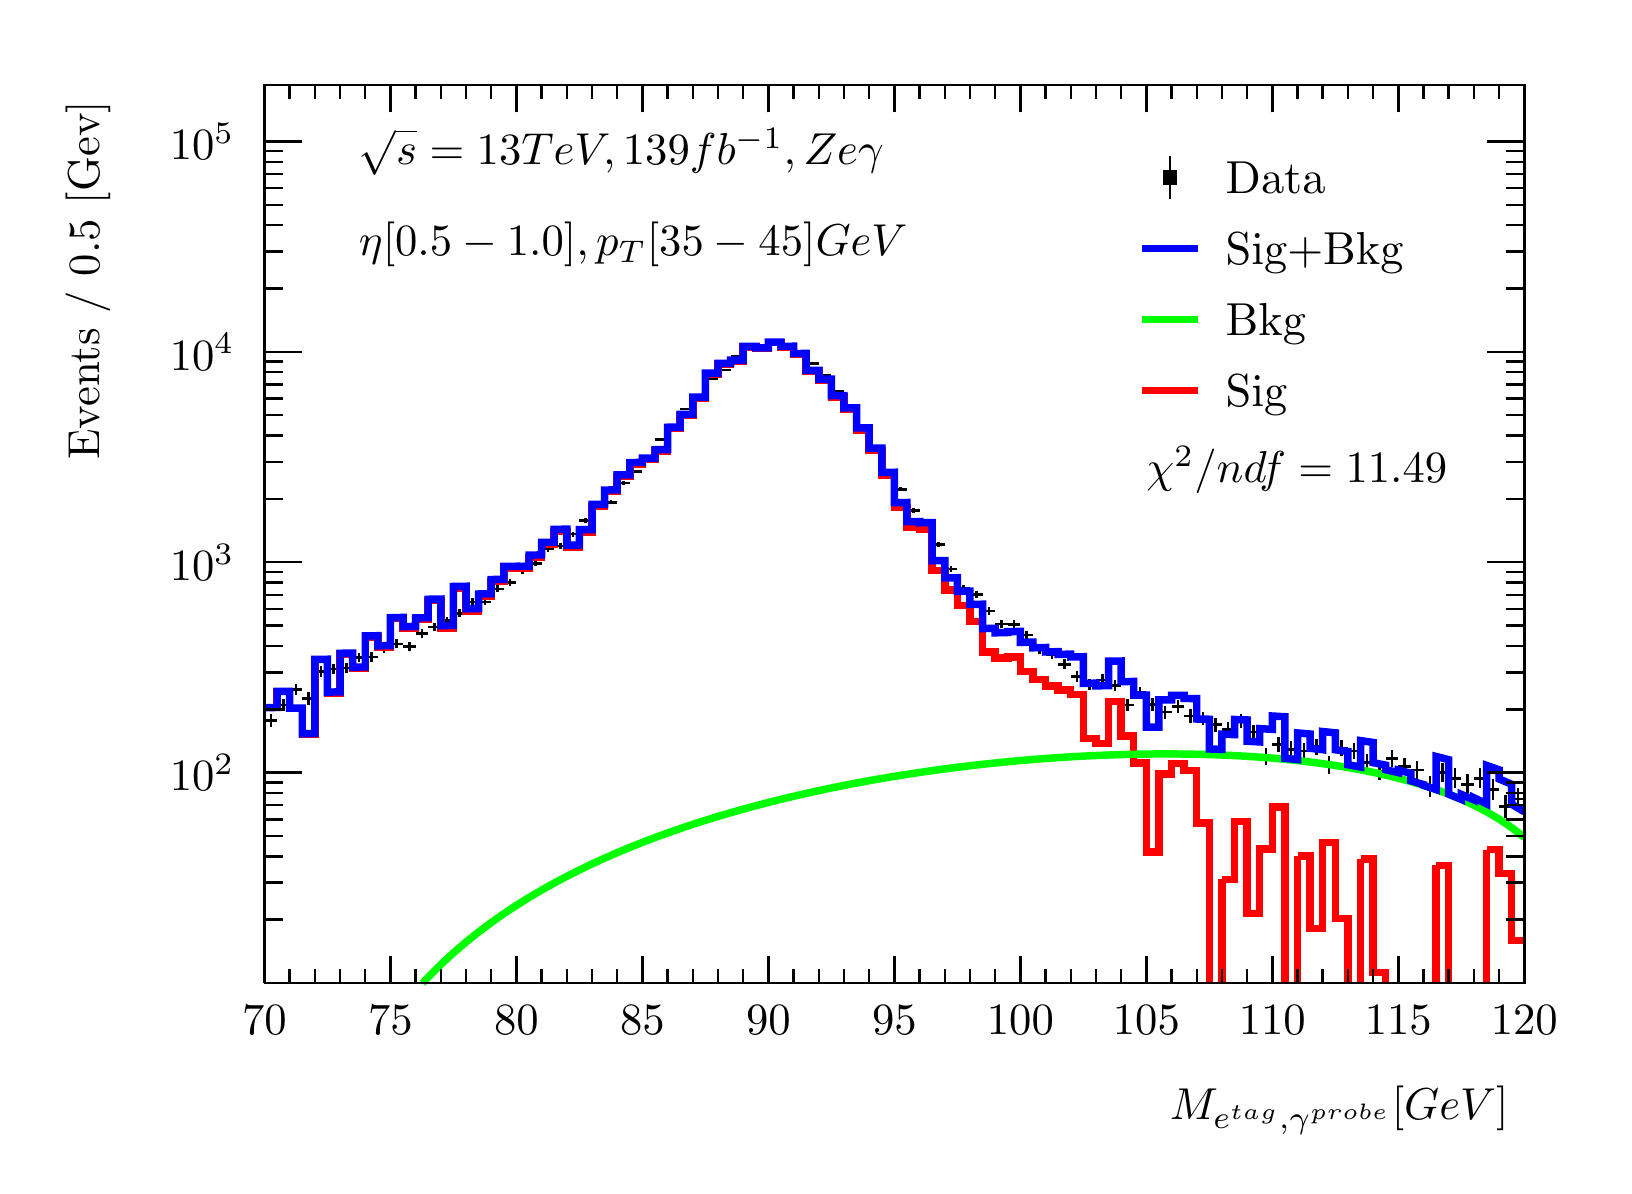
\begin{tikzpicture}
\pgfdeclareplotmark{cross} {
\pgfpathmoveto{\pgfpoint{-0.3\pgfplotmarksize}{\pgfplotmarksize}}
\pgfpathlineto{\pgfpoint{+0.3\pgfplotmarksize}{\pgfplotmarksize}}
\pgfpathlineto{\pgfpoint{+0.3\pgfplotmarksize}{0.3\pgfplotmarksize}}
\pgfpathlineto{\pgfpoint{+1\pgfplotmarksize}{0.3\pgfplotmarksize}}
\pgfpathlineto{\pgfpoint{+1\pgfplotmarksize}{-0.3\pgfplotmarksize}}
\pgfpathlineto{\pgfpoint{+0.3\pgfplotmarksize}{-0.3\pgfplotmarksize}}
\pgfpathlineto{\pgfpoint{+0.3\pgfplotmarksize}{-1.\pgfplotmarksize}}
\pgfpathlineto{\pgfpoint{-0.3\pgfplotmarksize}{-1.\pgfplotmarksize}}
\pgfpathlineto{\pgfpoint{-0.3\pgfplotmarksize}{-0.3\pgfplotmarksize}}
\pgfpathlineto{\pgfpoint{-1.\pgfplotmarksize}{-0.3\pgfplotmarksize}}
\pgfpathlineto{\pgfpoint{-1.\pgfplotmarksize}{0.3\pgfplotmarksize}}
\pgfpathlineto{\pgfpoint{-0.3\pgfplotmarksize}{0.3\pgfplotmarksize}}
\pgfpathclose
\pgfusepathqstroke
}
\pgfdeclareplotmark{cross*} {
\pgfpathmoveto{\pgfpoint{-0.3\pgfplotmarksize}{\pgfplotmarksize}}
\pgfpathlineto{\pgfpoint{+0.3\pgfplotmarksize}{\pgfplotmarksize}}
\pgfpathlineto{\pgfpoint{+0.3\pgfplotmarksize}{0.3\pgfplotmarksize}}
\pgfpathlineto{\pgfpoint{+1\pgfplotmarksize}{0.3\pgfplotmarksize}}
\pgfpathlineto{\pgfpoint{+1\pgfplotmarksize}{-0.3\pgfplotmarksize}}
\pgfpathlineto{\pgfpoint{+0.3\pgfplotmarksize}{-0.3\pgfplotmarksize}}
\pgfpathlineto{\pgfpoint{+0.3\pgfplotmarksize}{-1.\pgfplotmarksize}}
\pgfpathlineto{\pgfpoint{-0.3\pgfplotmarksize}{-1.\pgfplotmarksize}}
\pgfpathlineto{\pgfpoint{-0.3\pgfplotmarksize}{-0.3\pgfplotmarksize}}
\pgfpathlineto{\pgfpoint{-1.\pgfplotmarksize}{-0.3\pgfplotmarksize}}
\pgfpathlineto{\pgfpoint{-1.\pgfplotmarksize}{0.3\pgfplotmarksize}}
\pgfpathlineto{\pgfpoint{-0.3\pgfplotmarksize}{0.3\pgfplotmarksize}}
\pgfpathclose
\pgfusepathqfillstroke
}
\pgfdeclareplotmark{newstar} {
\pgfpathmoveto{\pgfqpoint{0pt}{\pgfplotmarksize}}
\pgfpathlineto{\pgfqpointpolar{44}{0.5\pgfplotmarksize}}
\pgfpathlineto{\pgfqpointpolar{18}{\pgfplotmarksize}}
\pgfpathlineto{\pgfqpointpolar{-20}{0.5\pgfplotmarksize}}
\pgfpathlineto{\pgfqpointpolar{-54}{\pgfplotmarksize}}
\pgfpathlineto{\pgfqpointpolar{-90}{0.5\pgfplotmarksize}}
\pgfpathlineto{\pgfqpointpolar{234}{\pgfplotmarksize}}
\pgfpathlineto{\pgfqpointpolar{198}{0.5\pgfplotmarksize}}
\pgfpathlineto{\pgfqpointpolar{162}{\pgfplotmarksize}}
\pgfpathlineto{\pgfqpointpolar{134}{0.5\pgfplotmarksize}}
\pgfpathclose
\pgfusepathqstroke
}
\pgfdeclareplotmark{newstar*} {
\pgfpathmoveto{\pgfqpoint{0pt}{\pgfplotmarksize}}
\pgfpathlineto{\pgfqpointpolar{44}{0.5\pgfplotmarksize}}
\pgfpathlineto{\pgfqpointpolar{18}{\pgfplotmarksize}}
\pgfpathlineto{\pgfqpointpolar{-20}{0.5\pgfplotmarksize}}
\pgfpathlineto{\pgfqpointpolar{-54}{\pgfplotmarksize}}
\pgfpathlineto{\pgfqpointpolar{-90}{0.5\pgfplotmarksize}}
\pgfpathlineto{\pgfqpointpolar{234}{\pgfplotmarksize}}
\pgfpathlineto{\pgfqpointpolar{198}{0.5\pgfplotmarksize}}
\pgfpathlineto{\pgfqpointpolar{162}{\pgfplotmarksize}}
\pgfpathlineto{\pgfqpointpolar{134}{0.5\pgfplotmarksize}}
\pgfpathclose
\pgfusepathqfillstroke
}
\definecolor{c}{rgb}{1,1,1};
\draw [color=c, fill=c] (0,0) rectangle (20,14.4361);
\draw [color=c, fill=c] (3,2.30977) rectangle (19,13.7143);
\definecolor{c}{rgb}{0,0,0};
\draw [c,line width=0.9] (3,2.30977) -- (3,13.7143) -- (19,13.7143) -- (19,2.30977) -- (3,2.30977);
\definecolor{c}{rgb}{1,1,1};
\draw [color=c, fill=c] (3,2.30977) rectangle (19,13.7143);
\definecolor{c}{rgb}{0,0,0};
\draw [c,line width=0.9] (3,2.30977) -- (3,13.7143) -- (19,13.7143) -- (19,2.30977) -- (3,2.30977);
\draw [c,line width=0.9] (3,2.30977) -- (19,2.30977);
\draw [c,line width=0.9] (3,2.65624) -- (3,2.30977);
\draw [c,line width=0.9] (3.32,2.48301) -- (3.32,2.30977);
\draw [c,line width=0.9] (3.64,2.48301) -- (3.64,2.30977);
\draw [c,line width=0.9] (3.96,2.48301) -- (3.96,2.30977);
\draw [c,line width=0.9] (4.28,2.48301) -- (4.28,2.30977);
\draw [c,line width=0.9] (4.6,2.65624) -- (4.6,2.30977);
\draw [c,line width=0.9] (4.92,2.48301) -- (4.92,2.30977);
\draw [c,line width=0.9] (5.24,2.48301) -- (5.24,2.30977);
\draw [c,line width=0.9] (5.56,2.48301) -- (5.56,2.30977);
\draw [c,line width=0.9] (5.88,2.48301) -- (5.88,2.30977);
\draw [c,line width=0.9] (6.2,2.65624) -- (6.2,2.30977);
\draw [c,line width=0.9] (6.52,2.48301) -- (6.52,2.30977);
\draw [c,line width=0.9] (6.84,2.48301) -- (6.84,2.30977);
\draw [c,line width=0.9] (7.16,2.48301) -- (7.16,2.30977);
\draw [c,line width=0.9] (7.48,2.48301) -- (7.48,2.30977);
\draw [c,line width=0.9] (7.8,2.65624) -- (7.8,2.30977);
\draw [c,line width=0.9] (8.12,2.48301) -- (8.12,2.30977);
\draw [c,line width=0.9] (8.44,2.48301) -- (8.44,2.30977);
\draw [c,line width=0.9] (8.76,2.48301) -- (8.76,2.30977);
\draw [c,line width=0.9] (9.08,2.48301) -- (9.08,2.30977);
\draw [c,line width=0.9] (9.4,2.65624) -- (9.4,2.30977);
\draw [c,line width=0.9] (9.72,2.48301) -- (9.72,2.30977);
\draw [c,line width=0.9] (10.04,2.48301) -- (10.04,2.30977);
\draw [c,line width=0.9] (10.36,2.48301) -- (10.36,2.30977);
\draw [c,line width=0.9] (10.68,2.48301) -- (10.68,2.30977);
\draw [c,line width=0.9] (11,2.65624) -- (11,2.30977);
\draw [c,line width=0.9] (11.32,2.48301) -- (11.32,2.30977);
\draw [c,line width=0.9] (11.64,2.48301) -- (11.64,2.30977);
\draw [c,line width=0.9] (11.96,2.48301) -- (11.96,2.30977);
\draw [c,line width=0.9] (12.28,2.48301) -- (12.28,2.30977);
\draw [c,line width=0.9] (12.6,2.65624) -- (12.6,2.30977);
\draw [c,line width=0.9] (12.92,2.48301) -- (12.92,2.30977);
\draw [c,line width=0.9] (13.24,2.48301) -- (13.24,2.30977);
\draw [c,line width=0.9] (13.56,2.48301) -- (13.56,2.30977);
\draw [c,line width=0.9] (13.88,2.48301) -- (13.88,2.30977);
\draw [c,line width=0.9] (14.2,2.65624) -- (14.2,2.30977);
\draw [c,line width=0.9] (14.52,2.48301) -- (14.52,2.30977);
\draw [c,line width=0.9] (14.84,2.48301) -- (14.84,2.30977);
\draw [c,line width=0.9] (15.16,2.48301) -- (15.16,2.30977);
\draw [c,line width=0.9] (15.48,2.48301) -- (15.48,2.30977);
\draw [c,line width=0.9] (15.8,2.65624) -- (15.8,2.30977);
\draw [c,line width=0.9] (16.12,2.48301) -- (16.12,2.30977);
\draw [c,line width=0.9] (16.44,2.48301) -- (16.44,2.30977);
\draw [c,line width=0.9] (16.76,2.48301) -- (16.76,2.30977);
\draw [c,line width=0.9] (17.08,2.48301) -- (17.08,2.30977);
\draw [c,line width=0.9] (17.4,2.65624) -- (17.4,2.30977);
\draw [c,line width=0.9] (17.72,2.48301) -- (17.72,2.30977);
\draw [c,line width=0.9] (18.04,2.48301) -- (18.04,2.30977);
\draw [c,line width=0.9] (18.36,2.48301) -- (18.36,2.30977);
\draw [c,line width=0.9] (18.68,2.48301) -- (18.68,2.30977);
\draw [c,line width=0.9] (19,2.65624) -- (19,2.30977);
\draw [anchor=base] (3,1.66015) node[scale=1.61424, color=c, rotate=0]{70};
\draw [anchor=base] (4.6,1.66015) node[scale=1.61424, color=c, rotate=0]{75};
\draw [anchor=base] (6.2,1.66015) node[scale=1.61424, color=c, rotate=0]{80};
\draw [anchor=base] (7.8,1.66015) node[scale=1.61424, color=c, rotate=0]{85};
\draw [anchor=base] (9.4,1.66015) node[scale=1.61424, color=c, rotate=0]{90};
\draw [anchor=base] (11,1.66015) node[scale=1.61424, color=c, rotate=0]{95};
\draw [anchor=base] (12.6,1.66015) node[scale=1.61424, color=c, rotate=0]{100};
\draw [anchor=base] (14.2,1.66015) node[scale=1.61424, color=c, rotate=0]{105};
\draw [anchor=base] (15.8,1.66015) node[scale=1.61424, color=c, rotate=0]{110};
\draw [anchor=base] (17.4,1.66015) node[scale=1.61424, color=c, rotate=0]{115};
\draw [anchor=base] (19,1.66015) node[scale=1.61424, color=c, rotate=0]{120};
\draw [anchor= east] (19,0.692932) node[scale=1.61424, color=c, rotate=0]{$M_{e^{tag}, \gamma^{probe}}  [GeV]$};
\draw [c,line width=0.9] (3,13.7143) -- (19,13.7143);
\draw [c,line width=0.9] (3,13.3678) -- (3,13.7143);
\draw [c,line width=0.9] (3.32,13.5411) -- (3.32,13.7143);
\draw [c,line width=0.9] (3.64,13.5411) -- (3.64,13.7143);
\draw [c,line width=0.9] (3.96,13.5411) -- (3.96,13.7143);
\draw [c,line width=0.9] (4.28,13.5411) -- (4.28,13.7143);
\draw [c,line width=0.9] (4.6,13.3678) -- (4.6,13.7143);
\draw [c,line width=0.9] (4.92,13.5411) -- (4.92,13.7143);
\draw [c,line width=0.9] (5.24,13.5411) -- (5.24,13.7143);
\draw [c,line width=0.9] (5.56,13.5411) -- (5.56,13.7143);
\draw [c,line width=0.9] (5.88,13.5411) -- (5.88,13.7143);
\draw [c,line width=0.9] (6.2,13.3678) -- (6.2,13.7143);
\draw [c,line width=0.9] (6.52,13.5411) -- (6.52,13.7143);
\draw [c,line width=0.9] (6.84,13.5411) -- (6.84,13.7143);
\draw [c,line width=0.9] (7.16,13.5411) -- (7.16,13.7143);
\draw [c,line width=0.9] (7.48,13.5411) -- (7.48,13.7143);
\draw [c,line width=0.9] (7.8,13.3678) -- (7.8,13.7143);
\draw [c,line width=0.9] (8.12,13.5411) -- (8.12,13.7143);
\draw [c,line width=0.9] (8.44,13.5411) -- (8.44,13.7143);
\draw [c,line width=0.9] (8.76,13.5411) -- (8.76,13.7143);
\draw [c,line width=0.9] (9.08,13.5411) -- (9.08,13.7143);
\draw [c,line width=0.9] (9.4,13.3678) -- (9.4,13.7143);
\draw [c,line width=0.9] (9.72,13.5411) -- (9.72,13.7143);
\draw [c,line width=0.9] (10.04,13.5411) -- (10.04,13.7143);
\draw [c,line width=0.9] (10.36,13.5411) -- (10.36,13.7143);
\draw [c,line width=0.9] (10.68,13.5411) -- (10.68,13.7143);
\draw [c,line width=0.9] (11,13.3678) -- (11,13.7143);
\draw [c,line width=0.9] (11.32,13.5411) -- (11.32,13.7143);
\draw [c,line width=0.9] (11.64,13.5411) -- (11.64,13.7143);
\draw [c,line width=0.9] (11.96,13.5411) -- (11.96,13.7143);
\draw [c,line width=0.9] (12.28,13.5411) -- (12.28,13.7143);
\draw [c,line width=0.9] (12.6,13.3678) -- (12.6,13.7143);
\draw [c,line width=0.9] (12.92,13.5411) -- (12.92,13.7143);
\draw [c,line width=0.9] (13.24,13.5411) -- (13.24,13.7143);
\draw [c,line width=0.9] (13.56,13.5411) -- (13.56,13.7143);
\draw [c,line width=0.9] (13.88,13.5411) -- (13.88,13.7143);
\draw [c,line width=0.9] (14.2,13.3678) -- (14.2,13.7143);
\draw [c,line width=0.9] (14.52,13.5411) -- (14.52,13.7143);
\draw [c,line width=0.9] (14.84,13.5411) -- (14.84,13.7143);
\draw [c,line width=0.9] (15.16,13.5411) -- (15.16,13.7143);
\draw [c,line width=0.9] (15.48,13.5411) -- (15.48,13.7143);
\draw [c,line width=0.9] (15.8,13.3678) -- (15.8,13.7143);
\draw [c,line width=0.9] (16.12,13.5411) -- (16.12,13.7143);
\draw [c,line width=0.9] (16.44,13.5411) -- (16.44,13.7143);
\draw [c,line width=0.9] (16.76,13.5411) -- (16.76,13.7143);
\draw [c,line width=0.9] (17.08,13.5411) -- (17.08,13.7143);
\draw [c,line width=0.9] (17.4,13.3678) -- (17.4,13.7143);
\draw [c,line width=0.9] (17.72,13.5411) -- (17.72,13.7143);
\draw [c,line width=0.9] (18.04,13.5411) -- (18.04,13.7143);
\draw [c,line width=0.9] (18.36,13.5411) -- (18.36,13.7143);
\draw [c,line width=0.9] (18.68,13.5411) -- (18.68,13.7143);
\draw [c,line width=0.9] (19,13.3678) -- (19,13.7143);
\draw [c,line width=0.9] (3,2.30977) -- (3,13.7143);
\draw [c,line width=0.9] (3.237,3.11414) -- (3,3.11414);
\draw [c,line width=0.9] (3.237,3.58467) -- (3,3.58467);
\draw [c,line width=0.9] (3.237,3.91852) -- (3,3.91852);
\draw [c,line width=0.9] (3.237,4.17747) -- (3,4.17747);
\draw [c,line width=0.9] (3.237,4.38904) -- (3,4.38904);
\draw [c,line width=0.9] (3.237,4.56793) -- (3,4.56793);
\draw [c,line width=0.9] (3.237,4.72289) -- (3,4.72289);
\draw [c,line width=0.9] (3.237,4.85957) -- (3,4.85957);
\draw [c,line width=0.9] (3.474,4.98184) -- (3,4.98184);
\draw [anchor= east] (2.82,4.98184) node[scale=1.61424, color=c, rotate=0]{$10^{2}$};
\draw [c,line width=0.9] (3.237,5.78621) -- (3,5.78621);
\draw [c,line width=0.9] (3.237,6.25674) -- (3,6.25674);
\draw [c,line width=0.9] (3.237,6.59058) -- (3,6.59058);
\draw [c,line width=0.9] (3.237,6.84953) -- (3,6.84953);
\draw [c,line width=0.9] (3.237,7.06111) -- (3,7.06111);
\draw [c,line width=0.9] (3.237,7.24) -- (3,7.24);
\draw [c,line width=0.9] (3.237,7.39496) -- (3,7.39496);
\draw [c,line width=0.9] (3.237,7.53164) -- (3,7.53164);
\draw [c,line width=0.9] (3.474,7.65391) -- (3,7.65391);
\draw [anchor= east] (2.82,7.65391) node[scale=1.61424, color=c, rotate=0]{$10^{3}$};
\draw [c,line width=0.9] (3.237,8.45828) -- (3,8.45828);
\draw [c,line width=0.9] (3.237,8.92881) -- (3,8.92881);
\draw [c,line width=0.9] (3.237,9.26265) -- (3,9.26265);
\draw [c,line width=0.9] (3.237,9.5216) -- (3,9.5216);
\draw [c,line width=0.9] (3.237,9.73318) -- (3,9.73318);
\draw [c,line width=0.9] (3.237,9.91207) -- (3,9.91207);
\draw [c,line width=0.9] (3.237,10.067) -- (3,10.067);
\draw [c,line width=0.9] (3.237,10.2037) -- (3,10.2037);
\draw [c,line width=0.9] (3.474,10.326) -- (3,10.326);
\draw [anchor= east] (2.82,10.326) node[scale=1.61424, color=c, rotate=0]{$10^{4}$};
\draw [c,line width=0.9] (3.237,11.1303) -- (3,11.1303);
\draw [c,line width=0.9] (3.237,11.6009) -- (3,11.6009);
\draw [c,line width=0.9] (3.237,11.9347) -- (3,11.9347);
\draw [c,line width=0.9] (3.237,12.1937) -- (3,12.1937);
\draw [c,line width=0.9] (3.237,12.4052) -- (3,12.4052);
\draw [c,line width=0.9] (3.237,12.5841) -- (3,12.5841);
\draw [c,line width=0.9] (3.237,12.7391) -- (3,12.7391);
\draw [c,line width=0.9] (3.237,12.8758) -- (3,12.8758);
\draw [c,line width=0.9] (3.474,12.998) -- (3,12.998);
\draw [anchor= east] (2.82,12.998) node[scale=1.61424, color=c, rotate=0]{$10^{5}$};
\draw [anchor= east] (0.76,13.7143) node[scale=1.61424, color=c, rotate=90]{Events / 0.5 [Gev]};
\draw [c,line width=0.9] (19,2.30977) -- (19,13.7143);
\draw [c,line width=0.9] (18.763,3.11414) -- (19,3.11414);
\draw [c,line width=0.9] (18.763,3.58467) -- (19,3.58467);
\draw [c,line width=0.9] (18.763,3.91852) -- (19,3.91852);
\draw [c,line width=0.9] (18.763,4.17747) -- (19,4.17747);
\draw [c,line width=0.9] (18.763,4.38904) -- (19,4.38904);
\draw [c,line width=0.9] (18.763,4.56793) -- (19,4.56793);
\draw [c,line width=0.9] (18.763,4.72289) -- (19,4.72289);
\draw [c,line width=0.9] (18.763,4.85957) -- (19,4.85957);
\draw [c,line width=0.9] (18.526,4.98184) -- (19,4.98184);
\draw [c,line width=0.9] (18.763,5.78621) -- (19,5.78621);
\draw [c,line width=0.9] (18.763,6.25674) -- (19,6.25674);
\draw [c,line width=0.9] (18.763,6.59058) -- (19,6.59058);
\draw [c,line width=0.9] (18.763,6.84953) -- (19,6.84953);
\draw [c,line width=0.9] (18.763,7.06111) -- (19,7.06111);
\draw [c,line width=0.9] (18.763,7.24) -- (19,7.24);
\draw [c,line width=0.9] (18.763,7.39496) -- (19,7.39496);
\draw [c,line width=0.9] (18.763,7.53164) -- (19,7.53164);
\draw [c,line width=0.9] (18.526,7.65391) -- (19,7.65391);
\draw [c,line width=0.9] (18.763,8.45828) -- (19,8.45828);
\draw [c,line width=0.9] (18.763,8.92881) -- (19,8.92881);
\draw [c,line width=0.9] (18.763,9.26265) -- (19,9.26265);
\draw [c,line width=0.9] (18.763,9.5216) -- (19,9.5216);
\draw [c,line width=0.9] (18.763,9.73318) -- (19,9.73318);
\draw [c,line width=0.9] (18.763,9.91207) -- (19,9.91207);
\draw [c,line width=0.9] (18.763,10.067) -- (19,10.067);
\draw [c,line width=0.9] (18.763,10.2037) -- (19,10.2037);
\draw [c,line width=0.9] (18.526,10.326) -- (19,10.326);
\draw [c,line width=0.9] (18.763,11.1303) -- (19,11.1303);
\draw [c,line width=0.9] (18.763,11.6009) -- (19,11.6009);
\draw [c,line width=0.9] (18.763,11.9347) -- (19,11.9347);
\draw [c,line width=0.9] (18.763,12.1937) -- (19,12.1937);
\draw [c,line width=0.9] (18.763,12.4052) -- (19,12.4052);
\draw [c,line width=0.9] (18.763,12.5841) -- (19,12.5841);
\draw [c,line width=0.9] (18.763,12.7391) -- (19,12.7391);
\draw [c,line width=0.9] (18.763,12.8758) -- (19,12.8758);
\draw [c,line width=0.9] (18.526,12.998) -- (19,12.998);
\draw [c,line width=0.9] (3.08,5.64444) -- (3,5.64444);
\draw [c,line width=0.9] (3,5.64444) -- (3,5.64444);
\draw [c,line width=0.9] (3.08,5.64444) -- (3.16,5.64444);
\draw [c,line width=0.9] (3.16,5.64444) -- (3.16,5.64444);
\draw [c,line width=0.9] (3.08,5.64444) -- (3.08,5.73165);
\draw [c,line width=0.9] (3.08,5.73165) -- (3.08,5.73165);
\draw [c,line width=0.9] (3.08,5.64444) -- (3.08,5.55724);
\draw [c,line width=0.9] (3.08,5.55724) -- (3.08,5.55724);
\draw [c,line width=0.9] (3.24,5.84283) -- (3.16,5.84283);
\draw [c,line width=0.9] (3.16,5.84283) -- (3.16,5.84283);
\draw [c,line width=0.9] (3.24,5.84283) -- (3.32,5.84283);
\draw [c,line width=0.9] (3.32,5.84283) -- (3.32,5.84283);
\draw [c,line width=0.9] (3.24,5.84283) -- (3.24,5.9229);
\draw [c,line width=0.9] (3.24,5.9229) -- (3.24,5.9229);
\draw [c,line width=0.9] (3.24,5.84283) -- (3.24,5.76277);
\draw [c,line width=0.9] (3.24,5.76277) -- (3.24,5.76277);
\draw [c,line width=0.9] (3.4,6.03584) -- (3.32,6.03584);
\draw [c,line width=0.9] (3.32,6.03584) -- (3.32,6.03584);
\draw [c,line width=0.9] (3.4,6.03584) -- (3.48,6.03584);
\draw [c,line width=0.9] (3.48,6.03584) -- (3.48,6.03584);
\draw [c,line width=0.9] (3.4,6.03584) -- (3.4,6.10952);
\draw [c,line width=0.9] (3.4,6.10952) -- (3.4,6.10952);
\draw [c,line width=0.9] (3.4,6.03584) -- (3.4,5.96217);
\draw [c,line width=0.9] (3.4,5.96217) -- (3.4,5.96217);
\draw [c,line width=0.9] (3.56,5.9229) -- (3.48,5.9229);
\draw [c,line width=0.9] (3.48,5.9229) -- (3.48,5.9229);
\draw [c,line width=0.9] (3.56,5.9229) -- (3.64,5.9229);
\draw [c,line width=0.9] (3.64,5.9229) -- (3.64,5.9229);
\draw [c,line width=0.9] (3.56,5.9229) -- (3.56,6.00025);
\draw [c,line width=0.9] (3.56,6.00025) -- (3.56,6.00025);
\draw [c,line width=0.9] (3.56,5.9229) -- (3.56,5.84555);
\draw [c,line width=0.9] (3.56,5.84555) -- (3.56,5.84555);
\draw [c,line width=0.9] (3.72,6.26445) -- (3.64,6.26445);
\draw [c,line width=0.9] (3.64,6.26445) -- (3.64,6.26445);
\draw [c,line width=0.9] (3.72,6.26445) -- (3.8,6.26445);
\draw [c,line width=0.9] (3.8,6.26445) -- (3.8,6.26445);
\draw [c,line width=0.9] (3.72,6.26445) -- (3.72,6.33122);
\draw [c,line width=0.9] (3.72,6.33122) -- (3.72,6.33122);
\draw [c,line width=0.9] (3.72,6.26445) -- (3.72,6.19768);
\draw [c,line width=0.9] (3.72,6.19768) -- (3.72,6.19768);
\draw [c,line width=0.9] (3.88,6.29853) -- (3.8,6.29853);
\draw [c,line width=0.9] (3.8,6.29853) -- (3.8,6.29853);
\draw [c,line width=0.9] (3.88,6.29853) -- (3.96,6.29853);
\draw [c,line width=0.9] (3.96,6.29853) -- (3.96,6.29853);
\draw [c,line width=0.9] (3.88,6.29853) -- (3.88,6.36433);
\draw [c,line width=0.9] (3.88,6.36433) -- (3.88,6.36433);
\draw [c,line width=0.9] (3.88,6.29853) -- (3.88,6.23273);
\draw [c,line width=0.9] (3.88,6.23273) -- (3.88,6.23273);
\draw [c,line width=0.9] (4.04,6.30967) -- (3.96,6.30967);
\draw [c,line width=0.9] (3.96,6.30967) -- (3.96,6.30967);
\draw [c,line width=0.9] (4.04,6.30967) -- (4.12,6.30967);
\draw [c,line width=0.9] (4.12,6.30967) -- (4.12,6.30967);
\draw [c,line width=0.9] (4.04,6.30967) -- (4.04,6.37515);
\draw [c,line width=0.9] (4.04,6.37515) -- (4.04,6.37515);
\draw [c,line width=0.9] (4.04,6.30967) -- (4.04,6.24419);
\draw [c,line width=0.9] (4.04,6.24419) -- (4.04,6.24419);
\draw [c,line width=0.9] (4.2,6.44553) -- (4.12,6.44553);
\draw [c,line width=0.9] (4.12,6.44553) -- (4.12,6.44553);
\draw [c,line width=0.9] (4.2,6.44553) -- (4.28,6.44553);
\draw [c,line width=0.9] (4.28,6.44553) -- (4.28,6.44553);
\draw [c,line width=0.9] (4.2,6.44553) -- (4.2,6.50729);
\draw [c,line width=0.9] (4.2,6.50729) -- (4.2,6.50729);
\draw [c,line width=0.9] (4.2,6.44553) -- (4.2,6.38377);
\draw [c,line width=0.9] (4.2,6.38377) -- (4.2,6.38377);
\draw [c,line width=0.9] (4.36,6.45209) -- (4.28,6.45209);
\draw [c,line width=0.9] (4.28,6.45209) -- (4.28,6.45209);
\draw [c,line width=0.9] (4.36,6.45209) -- (4.44,6.45209);
\draw [c,line width=0.9] (4.44,6.45209) -- (4.44,6.45209);
\draw [c,line width=0.9] (4.36,6.45209) -- (4.36,6.51367);
\draw [c,line width=0.9] (4.36,6.51367) -- (4.36,6.51367);
\draw [c,line width=0.9] (4.36,6.45209) -- (4.36,6.3905);
\draw [c,line width=0.9] (4.36,6.3905) -- (4.36,6.3905);
\draw [c,line width=0.9] (4.52,6.55823) -- (4.44,6.55823);
\draw [c,line width=0.9] (4.44,6.55823) -- (4.44,6.55823);
\draw [c,line width=0.9] (4.52,6.55823) -- (4.6,6.55823);
\draw [c,line width=0.9] (4.6,6.55823) -- (4.6,6.55823);
\draw [c,line width=0.9] (4.52,6.55823) -- (4.52,6.61706);
\draw [c,line width=0.9] (4.52,6.61706) -- (4.52,6.61706);
\draw [c,line width=0.9] (4.52,6.55823) -- (4.52,6.49939);
\draw [c,line width=0.9] (4.52,6.49939) -- (4.52,6.49939);
\draw [c,line width=0.9] (4.68,6.61641) -- (4.6,6.61641);
\draw [c,line width=0.9] (4.6,6.61641) -- (4.6,6.61641);
\draw [c,line width=0.9] (4.68,6.61641) -- (4.76,6.61641);
\draw [c,line width=0.9] (4.76,6.61641) -- (4.76,6.61641);
\draw [c,line width=0.9] (4.68,6.61641) -- (4.68,6.67378);
\draw [c,line width=0.9] (4.68,6.67378) -- (4.68,6.67378);
\draw [c,line width=0.9] (4.68,6.61641) -- (4.68,6.55903);
\draw [c,line width=0.9] (4.68,6.55903) -- (4.68,6.55903);
\draw [c,line width=0.9] (4.84,6.58477) -- (4.76,6.58477);
\draw [c,line width=0.9] (4.76,6.58477) -- (4.76,6.58477);
\draw [c,line width=0.9] (4.84,6.58477) -- (4.92,6.58477);
\draw [c,line width=0.9] (4.92,6.58477) -- (4.92,6.58477);
\draw [c,line width=0.9] (4.84,6.58477) -- (4.84,6.64293);
\draw [c,line width=0.9] (4.84,6.64293) -- (4.84,6.64293);
\draw [c,line width=0.9] (4.84,6.58477) -- (4.84,6.52661);
\draw [c,line width=0.9] (4.84,6.52661) -- (4.84,6.52661);
\draw [c,line width=0.9] (5,6.74772) -- (4.92,6.74772);
\draw [c,line width=0.9] (4.92,6.74772) -- (4.92,6.74772);
\draw [c,line width=0.9] (5,6.74772) -- (5.08,6.74772);
\draw [c,line width=0.9] (5.08,6.74772) -- (5.08,6.74772);
\draw [c,line width=0.9] (5,6.74772) -- (5,6.80194);
\draw [c,line width=0.9] (5,6.80194) -- (5,6.80194);
\draw [c,line width=0.9] (5,6.74772) -- (5,6.6935);
\draw [c,line width=0.9] (5,6.6935) -- (5,6.6935);
\draw [c,line width=0.9] (5.16,6.83317) -- (5.08,6.83317);
\draw [c,line width=0.9] (5.08,6.83317) -- (5.08,6.83317);
\draw [c,line width=0.9] (5.16,6.83317) -- (5.24,6.83317);
\draw [c,line width=0.9] (5.24,6.83317) -- (5.24,6.83317);
\draw [c,line width=0.9] (5.16,6.83317) -- (5.16,6.88543);
\draw [c,line width=0.9] (5.16,6.88543) -- (5.16,6.88543);
\draw [c,line width=0.9] (5.16,6.83317) -- (5.16,6.78091);
\draw [c,line width=0.9] (5.16,6.78091) -- (5.16,6.78091);
\draw [c,line width=0.9] (5.32,6.91277) -- (5.24,6.91277);
\draw [c,line width=0.9] (5.24,6.91277) -- (5.24,6.91277);
\draw [c,line width=0.9] (5.32,6.91277) -- (5.4,6.91277);
\draw [c,line width=0.9] (5.4,6.91277) -- (5.4,6.91277);
\draw [c,line width=0.9] (5.32,6.91277) -- (5.32,6.96327);
\draw [c,line width=0.9] (5.32,6.96327) -- (5.32,6.96327);
\draw [c,line width=0.9] (5.32,6.91277) -- (5.32,6.86227);
\draw [c,line width=0.9] (5.32,6.86227) -- (5.32,6.86227);
\draw [c,line width=0.9] (5.48,7.00565) -- (5.4,7.00565);
\draw [c,line width=0.9] (5.4,7.00565) -- (5.4,7.00565);
\draw [c,line width=0.9] (5.48,7.00565) -- (5.56,7.00565);
\draw [c,line width=0.9] (5.56,7.00565) -- (5.56,7.00565);
\draw [c,line width=0.9] (5.48,7.00565) -- (5.48,7.05417);
\draw [c,line width=0.9] (5.48,7.05417) -- (5.48,7.05417);
\draw [c,line width=0.9] (5.48,7.00565) -- (5.48,6.95714);
\draw [c,line width=0.9] (5.48,6.95714) -- (5.48,6.95714);
\draw [c,line width=0.9] (5.64,7.15042) -- (5.56,7.15042);
\draw [c,line width=0.9] (5.56,7.15042) -- (5.56,7.15042);
\draw [c,line width=0.9] (5.64,7.15042) -- (5.72,7.15042);
\draw [c,line width=0.9] (5.72,7.15042) -- (5.72,7.15042);
\draw [c,line width=0.9] (5.64,7.15042) -- (5.64,7.19601);
\draw [c,line width=0.9] (5.64,7.19601) -- (5.64,7.19601);
\draw [c,line width=0.9] (5.64,7.15042) -- (5.64,7.10484);
\draw [c,line width=0.9] (5.64,7.10484) -- (5.64,7.10484);
\draw [c,line width=0.9] (5.8,7.15042) -- (5.72,7.15042);
\draw [c,line width=0.9] (5.72,7.15042) -- (5.72,7.15042);
\draw [c,line width=0.9] (5.8,7.15042) -- (5.88,7.15042);
\draw [c,line width=0.9] (5.88,7.15042) -- (5.88,7.15042);
\draw [c,line width=0.9] (5.8,7.15042) -- (5.8,7.19601);
\draw [c,line width=0.9] (5.8,7.19601) -- (5.8,7.19601);
\draw [c,line width=0.9] (5.8,7.15042) -- (5.8,7.10484);
\draw [c,line width=0.9] (5.8,7.10484) -- (5.8,7.10484);
\draw [c,line width=0.9] (5.96,7.31696) -- (5.88,7.31696);
\draw [c,line width=0.9] (5.88,7.31696) -- (5.88,7.31696);
\draw [c,line width=0.9] (5.96,7.31696) -- (6.04,7.31696);
\draw [c,line width=0.9] (6.04,7.31696) -- (6.04,7.31696);
\draw [c,line width=0.9] (5.96,7.31696) -- (5.96,7.35939);
\draw [c,line width=0.9] (5.96,7.35939) -- (5.96,7.35939);
\draw [c,line width=0.9] (5.96,7.31696) -- (5.96,7.27454);
\draw [c,line width=0.9] (5.96,7.27454) -- (5.96,7.27454);
\draw [c,line width=0.9] (6.12,7.3993) -- (6.04,7.3993);
\draw [c,line width=0.9] (6.04,7.3993) -- (6.04,7.3993);
\draw [c,line width=0.9] (6.12,7.3993) -- (6.2,7.3993);
\draw [c,line width=0.9] (6.2,7.3993) -- (6.2,7.3993);
\draw [c,line width=0.9] (6.12,7.3993) -- (6.12,7.44025);
\draw [c,line width=0.9] (6.12,7.44025) -- (6.12,7.44025);
\draw [c,line width=0.9] (6.12,7.3993) -- (6.12,7.35835);
\draw [c,line width=0.9] (6.12,7.35835) -- (6.12,7.35835);
\draw [c,line width=0.9] (6.28,7.54701) -- (6.2,7.54701);
\draw [c,line width=0.9] (6.2,7.54701) -- (6.2,7.54701);
\draw [c,line width=0.9] (6.28,7.54701) -- (6.36,7.54701);
\draw [c,line width=0.9] (6.36,7.54701) -- (6.36,7.54701);
\draw [c,line width=0.9] (6.28,7.54701) -- (6.28,7.58544);
\draw [c,line width=0.9] (6.28,7.58544) -- (6.28,7.58544);
\draw [c,line width=0.9] (6.28,7.54701) -- (6.28,7.50859);
\draw [c,line width=0.9] (6.28,7.50859) -- (6.28,7.50859);
\draw [c,line width=0.9] (6.44,7.63755) -- (6.36,7.63755);
\draw [c,line width=0.9] (6.36,7.63755) -- (6.36,7.63755);
\draw [c,line width=0.9] (6.44,7.63755) -- (6.52,7.63755);
\draw [c,line width=0.9] (6.52,7.63755) -- (6.52,7.63755);
\draw [c,line width=0.9] (6.44,7.63755) -- (6.44,7.6745);
\draw [c,line width=0.9] (6.44,7.6745) -- (6.44,7.6745);
\draw [c,line width=0.9] (6.44,7.63755) -- (6.44,7.60059);
\draw [c,line width=0.9] (6.44,7.60059) -- (6.44,7.60059);
\draw [c,line width=0.9] (6.6,7.82113) -- (6.52,7.82113);
\draw [c,line width=0.9] (6.52,7.82113) -- (6.52,7.82113);
\draw [c,line width=0.9] (6.6,7.82113) -- (6.68,7.82113);
\draw [c,line width=0.9] (6.68,7.82113) -- (6.68,7.82113);
\draw [c,line width=0.9] (6.6,7.82113) -- (6.6,7.85528);
\draw [c,line width=0.9] (6.6,7.85528) -- (6.6,7.85528);
\draw [c,line width=0.9] (6.6,7.82113) -- (6.6,7.78699);
\draw [c,line width=0.9] (6.6,7.78699) -- (6.6,7.78699);
\draw [c,line width=0.9] (6.76,7.8587) -- (6.68,7.8587);
\draw [c,line width=0.9] (6.68,7.8587) -- (6.68,7.8587);
\draw [c,line width=0.9] (6.76,7.8587) -- (6.84,7.8587);
\draw [c,line width=0.9] (6.84,7.8587) -- (6.84,7.8587);
\draw [c,line width=0.9] (6.76,7.8587) -- (6.76,7.89229);
\draw [c,line width=0.9] (6.76,7.89229) -- (6.76,7.89229);
\draw [c,line width=0.9] (6.76,7.8587) -- (6.76,7.8251);
\draw [c,line width=0.9] (6.76,7.8251) -- (6.76,7.8251);
\draw [c,line width=0.9] (6.92,8.00988) -- (6.84,8.00988);
\draw [c,line width=0.9] (6.84,8.00988) -- (6.84,8.00988);
\draw [c,line width=0.9] (6.92,8.00988) -- (7,8.00988);
\draw [c,line width=0.9] (7,8.00988) -- (7,8.00988);
\draw [c,line width=0.9] (6.92,8.00988) -- (6.92,8.04136);
\draw [c,line width=0.9] (6.92,8.04136) -- (6.92,8.04136);
\draw [c,line width=0.9] (6.92,8.00988) -- (6.92,7.9784);
\draw [c,line width=0.9] (6.92,7.9784) -- (6.92,7.9784);
\draw [c,line width=0.9] (7.08,8.1862) -- (7,8.1862);
\draw [c,line width=0.9] (7,8.1862) -- (7,8.1862);
\draw [c,line width=0.9] (7.08,8.1862) -- (7.16,8.1862);
\draw [c,line width=0.9] (7.16,8.1862) -- (7.16,8.1862);
\draw [c,line width=0.9] (7.08,8.1862) -- (7.08,8.21538);
\draw [c,line width=0.9] (7.08,8.21538) -- (7.08,8.21538);
\draw [c,line width=0.9] (7.08,8.1862) -- (7.08,8.15703);
\draw [c,line width=0.9] (7.08,8.15703) -- (7.08,8.15703);
\draw [c,line width=0.9] (7.24,8.34756) -- (7.16,8.34756);
\draw [c,line width=0.9] (7.16,8.34756) -- (7.16,8.34756);
\draw [c,line width=0.9] (7.24,8.34756) -- (7.32,8.34756);
\draw [c,line width=0.9] (7.32,8.34756) -- (7.32,8.34756);
\draw [c,line width=0.9] (7.24,8.34756) -- (7.24,8.37478);
\draw [c,line width=0.9] (7.24,8.37478) -- (7.24,8.37478);
\draw [c,line width=0.9] (7.24,8.34756) -- (7.24,8.32034);
\draw [c,line width=0.9] (7.24,8.32034) -- (7.24,8.32034);
\draw [c,line width=0.9] (7.4,8.41513) -- (7.32,8.41513);
\draw [c,line width=0.9] (7.32,8.41513) -- (7.32,8.41513);
\draw [c,line width=0.9] (7.4,8.41513) -- (7.48,8.41513);
\draw [c,line width=0.9] (7.48,8.41513) -- (7.48,8.41513);
\draw [c,line width=0.9] (7.4,8.41513) -- (7.4,8.44157);
\draw [c,line width=0.9] (7.4,8.44157) -- (7.4,8.44157);
\draw [c,line width=0.9] (7.4,8.41513) -- (7.4,8.3887);
\draw [c,line width=0.9] (7.4,8.3887) -- (7.4,8.3887);
\draw [c,line width=0.9] (7.56,8.66307) -- (7.48,8.66307);
\draw [c,line width=0.9] (7.48,8.66307) -- (7.48,8.66307);
\draw [c,line width=0.9] (7.56,8.66307) -- (7.64,8.66307);
\draw [c,line width=0.9] (7.64,8.66307) -- (7.64,8.66307);
\draw [c,line width=0.9] (7.56,8.66307) -- (7.56,8.68683);
\draw [c,line width=0.9] (7.56,8.68683) -- (7.56,8.68683);
\draw [c,line width=0.9] (7.56,8.66307) -- (7.56,8.63931);
\draw [c,line width=0.9] (7.56,8.63931) -- (7.56,8.63931);
\draw [c,line width=0.9] (7.72,8.80439) -- (7.64,8.80439);
\draw [c,line width=0.9] (7.64,8.80439) -- (7.64,8.80439);
\draw [c,line width=0.9] (7.72,8.80439) -- (7.8,8.80439);
\draw [c,line width=0.9] (7.8,8.80439) -- (7.8,8.80439);
\draw [c,line width=0.9] (7.72,8.80439) -- (7.72,8.82674);
\draw [c,line width=0.9] (7.72,8.82674) -- (7.72,8.82674);
\draw [c,line width=0.9] (7.72,8.80439) -- (7.72,8.78204);
\draw [c,line width=0.9] (7.72,8.78204) -- (7.72,8.78204);
\draw [c,line width=0.9] (7.88,8.96761) -- (7.8,8.96761);
\draw [c,line width=0.9] (7.8,8.96761) -- (7.8,8.96761);
\draw [c,line width=0.9] (7.88,8.96761) -- (7.96,8.96761);
\draw [c,line width=0.9] (7.96,8.96761) -- (7.96,8.96761);
\draw [c,line width=0.9] (7.88,8.96761) -- (7.88,8.98844);
\draw [c,line width=0.9] (7.88,8.98844) -- (7.88,8.98844);
\draw [c,line width=0.9] (7.88,8.96761) -- (7.88,8.94677);
\draw [c,line width=0.9] (7.88,8.94677) -- (7.88,8.94677);
\draw [c,line width=0.9] (8.04,9.21377) -- (7.96,9.21377);
\draw [c,line width=0.9] (7.96,9.21377) -- (7.96,9.21377);
\draw [c,line width=0.9] (8.04,9.21377) -- (8.12,9.21377);
\draw [c,line width=0.9] (8.12,9.21377) -- (8.12,9.21377);
\draw [c,line width=0.9] (8.04,9.21377) -- (8.04,9.23251);
\draw [c,line width=0.9] (8.04,9.23251) -- (8.04,9.23251);
\draw [c,line width=0.9] (8.04,9.21377) -- (8.04,9.19503);
\draw [c,line width=0.9] (8.04,9.19503) -- (8.04,9.19503);
\draw [c,line width=0.9] (8.2,9.34523) -- (8.12,9.34523);
\draw [c,line width=0.9] (8.12,9.34523) -- (8.12,9.34523);
\draw [c,line width=0.9] (8.2,9.34523) -- (8.28,9.34523);
\draw [c,line width=0.9] (8.28,9.34523) -- (8.28,9.34523);
\draw [c,line width=0.9] (8.2,9.34523) -- (8.2,9.36294);
\draw [c,line width=0.9] (8.2,9.36294) -- (8.2,9.36294);
\draw [c,line width=0.9] (8.2,9.34523) -- (8.2,9.32752);
\draw [c,line width=0.9] (8.2,9.32752) -- (8.2,9.32752);
\draw [c,line width=0.9] (8.36,9.60055) -- (8.28,9.60055);
\draw [c,line width=0.9] (8.28,9.60055) -- (8.28,9.60055);
\draw [c,line width=0.9] (8.36,9.60055) -- (8.44,9.60055);
\draw [c,line width=0.9] (8.44,9.60055) -- (8.44,9.60055);
\draw [c,line width=0.9] (8.36,9.60055) -- (8.36,9.61641);
\draw [c,line width=0.9] (8.36,9.61641) -- (8.36,9.61641);
\draw [c,line width=0.9] (8.36,9.60055) -- (8.36,9.58469);
\draw [c,line width=0.9] (8.36,9.58469) -- (8.36,9.58469);
\draw [c,line width=0.9] (8.52,9.77553) -- (8.44,9.77553);
\draw [c,line width=0.9] (8.44,9.77553) -- (8.44,9.77553);
\draw [c,line width=0.9] (8.52,9.77553) -- (8.6,9.77553);
\draw [c,line width=0.9] (8.6,9.77553) -- (8.6,9.77553);
\draw [c,line width=0.9] (8.52,9.77553) -- (8.52,9.79024);
\draw [c,line width=0.9] (8.52,9.79024) -- (8.52,9.79024);
\draw [c,line width=0.9] (8.52,9.77553) -- (8.52,9.76082);
\draw [c,line width=0.9] (8.52,9.76082) -- (8.52,9.76082);
\draw [c,line width=0.9] (8.68,9.9814) -- (8.6,9.9814);
\draw [c,line width=0.9] (8.6,9.9814) -- (8.6,9.9814);
\draw [c,line width=0.9] (8.68,9.9814) -- (8.76,9.9814);
\draw [c,line width=0.9] (8.76,9.9814) -- (8.76,9.9814);
\draw [c,line width=0.9] (8.68,9.9814) -- (8.68,9.99487);
\draw [c,line width=0.9] (8.68,9.99487) -- (8.68,9.99487);
\draw [c,line width=0.9] (8.68,9.9814) -- (8.68,9.96794);
\draw [c,line width=0.9] (8.68,9.96794) -- (8.68,9.96794);
\draw [c,line width=0.9] (8.84,10.0927) -- (8.76,10.0927);
\draw [c,line width=0.9] (8.76,10.0927) -- (8.76,10.0927);
\draw [c,line width=0.9] (8.84,10.0927) -- (8.92,10.0927);
\draw [c,line width=0.9] (8.92,10.0927) -- (8.92,10.0927);
\draw [c,line width=0.9] (8.84,10.0927) -- (8.84,10.1055);
\draw [c,line width=0.9] (8.84,10.1055) -- (8.84,10.1055);
\draw [c,line width=0.9] (8.84,10.0927) -- (8.84,10.0799);
\draw [c,line width=0.9] (8.84,10.0799) -- (8.84,10.0799);
\draw [c,line width=0.9] (9,10.2741) -- (8.92,10.2741);
\draw [c,line width=0.9] (8.92,10.2741) -- (8.92,10.2741);
\draw [c,line width=0.9] (9,10.2741) -- (9.08,10.2741);
\draw [c,line width=0.9] (9.08,10.2741) -- (9.08,10.2741);
\draw [c,line width=0.9] (9,10.2741) -- (9,10.286);
\draw [c,line width=0.9] (9,10.286) -- (9,10.286);
\draw [c,line width=0.9] (9,10.2741) -- (9,10.2623);
\draw [c,line width=0.9] (9,10.2623) -- (9,10.2623);
\draw [c,line width=0.9] (9.16,10.3619) -- (9.08,10.3619);
\draw [c,line width=0.9] (9.08,10.3619) -- (9.08,10.3619);
\draw [c,line width=0.9] (9.16,10.3619) -- (9.24,10.3619);
\draw [c,line width=0.9] (9.24,10.3619) -- (9.24,10.3619);
\draw [c,line width=0.9] (9.16,10.3619) -- (9.16,10.3733);
\draw [c,line width=0.9] (9.16,10.3733) -- (9.16,10.3733);
\draw [c,line width=0.9] (9.16,10.3619) -- (9.16,10.3504);
\draw [c,line width=0.9] (9.16,10.3504) -- (9.16,10.3504);
\draw [c,line width=0.9] (9.32,10.4157) -- (9.24,10.4157);
\draw [c,line width=0.9] (9.24,10.4157) -- (9.24,10.4157);
\draw [c,line width=0.9] (9.32,10.4157) -- (9.4,10.4157);
\draw [c,line width=0.9] (9.4,10.4157) -- (9.4,10.4157);
\draw [c,line width=0.9] (9.32,10.4157) -- (9.32,10.4269);
\draw [c,line width=0.9] (9.32,10.4269) -- (9.32,10.4269);
\draw [c,line width=0.9] (9.32,10.4157) -- (9.32,10.4046);
\draw [c,line width=0.9] (9.32,10.4046) -- (9.32,10.4046);
\draw [c,line width=0.9] (9.48,10.4272) -- (9.4,10.4272);
\draw [c,line width=0.9] (9.4,10.4272) -- (9.4,10.4272);
\draw [c,line width=0.9] (9.48,10.4272) -- (9.56,10.4272);
\draw [c,line width=0.9] (9.56,10.4272) -- (9.56,10.4272);
\draw [c,line width=0.9] (9.48,10.4272) -- (9.48,10.4383);
\draw [c,line width=0.9] (9.48,10.4383) -- (9.48,10.4383);
\draw [c,line width=0.9] (9.48,10.4272) -- (9.48,10.416);
\draw [c,line width=0.9] (9.48,10.416) -- (9.48,10.416);
\draw [c,line width=0.9] (9.64,10.3971) -- (9.56,10.3971);
\draw [c,line width=0.9] (9.56,10.3971) -- (9.56,10.3971);
\draw [c,line width=0.9] (9.64,10.3971) -- (9.72,10.3971);
\draw [c,line width=0.9] (9.72,10.3971) -- (9.72,10.3971);
\draw [c,line width=0.9] (9.64,10.3971) -- (9.64,10.4083);
\draw [c,line width=0.9] (9.64,10.4083) -- (9.64,10.4083);
\draw [c,line width=0.9] (9.64,10.3971) -- (9.64,10.3858);
\draw [c,line width=0.9] (9.64,10.3858) -- (9.64,10.3858);
\draw [c,line width=0.9] (9.8,10.3206) -- (9.72,10.3206);
\draw [c,line width=0.9] (9.72,10.3206) -- (9.72,10.3206);
\draw [c,line width=0.9] (9.8,10.3206) -- (9.88,10.3206);
\draw [c,line width=0.9] (9.88,10.3206) -- (9.88,10.3206);
\draw [c,line width=0.9] (9.8,10.3206) -- (9.8,10.3323);
\draw [c,line width=0.9] (9.8,10.3323) -- (9.8,10.3323);
\draw [c,line width=0.9] (9.8,10.3206) -- (9.8,10.309);
\draw [c,line width=0.9] (9.8,10.309) -- (9.8,10.309);
\draw [c,line width=0.9] (9.96,10.1751) -- (9.88,10.1751);
\draw [c,line width=0.9] (9.88,10.1751) -- (9.88,10.1751);
\draw [c,line width=0.9] (9.96,10.1751) -- (10.04,10.1751);
\draw [c,line width=0.9] (10.04,10.1751) -- (10.04,10.1751);
\draw [c,line width=0.9] (9.96,10.1751) -- (9.96,10.1875);
\draw [c,line width=0.9] (9.96,10.1875) -- (9.96,10.1875);
\draw [c,line width=0.9] (9.96,10.1751) -- (9.96,10.1627);
\draw [c,line width=0.9] (9.96,10.1627) -- (9.96,10.1627);
\draw [c,line width=0.9] (10.12,10.0332) -- (10.04,10.0332);
\draw [c,line width=0.9] (10.04,10.0332) -- (10.04,10.0332);
\draw [c,line width=0.9] (10.12,10.0332) -- (10.2,10.0332);
\draw [c,line width=0.9] (10.2,10.0332) -- (10.2,10.0332);
\draw [c,line width=0.9] (10.12,10.0332) -- (10.12,10.0463);
\draw [c,line width=0.9] (10.12,10.0463) -- (10.12,10.0463);
\draw [c,line width=0.9] (10.12,10.0332) -- (10.12,10.02);
\draw [c,line width=0.9] (10.12,10.02) -- (10.12,10.02);
\draw [c,line width=0.9] (10.28,9.82821) -- (10.2,9.82821);
\draw [c,line width=0.9] (10.2,9.82821) -- (10.2,9.82821);
\draw [c,line width=0.9] (10.28,9.82821) -- (10.36,9.82821);
\draw [c,line width=0.9] (10.36,9.82821) -- (10.36,9.82821);
\draw [c,line width=0.9] (10.28,9.82821) -- (10.28,9.84259);
\draw [c,line width=0.9] (10.28,9.84259) -- (10.28,9.84259);
\draw [c,line width=0.9] (10.28,9.82821) -- (10.28,9.81383);
\draw [c,line width=0.9] (10.28,9.81383) -- (10.28,9.81383);
\draw [c,line width=0.9] (10.44,9.59925) -- (10.36,9.59925);
\draw [c,line width=0.9] (10.36,9.59925) -- (10.36,9.59925);
\draw [c,line width=0.9] (10.44,9.59925) -- (10.52,9.59925);
\draw [c,line width=0.9] (10.52,9.59925) -- (10.52,9.59925);
\draw [c,line width=0.9] (10.44,9.59925) -- (10.44,9.61512);
\draw [c,line width=0.9] (10.44,9.61512) -- (10.44,9.61512);
\draw [c,line width=0.9] (10.44,9.59925) -- (10.44,9.58338);
\draw [c,line width=0.9] (10.44,9.58338) -- (10.44,9.58338);
\draw [c,line width=0.9] (10.6,9.38975) -- (10.52,9.38975);
\draw [c,line width=0.9] (10.52,9.38975) -- (10.52,9.38975);
\draw [c,line width=0.9] (10.6,9.38975) -- (10.68,9.38975);
\draw [c,line width=0.9] (10.68,9.38975) -- (10.68,9.38975);
\draw [c,line width=0.9] (10.6,9.38975) -- (10.6,9.40713);
\draw [c,line width=0.9] (10.6,9.40713) -- (10.6,9.40713);
\draw [c,line width=0.9] (10.6,9.38975) -- (10.6,9.37238);
\draw [c,line width=0.9] (10.6,9.37238) -- (10.6,9.37238);
\draw [c,line width=0.9] (10.76,9.08628) -- (10.68,9.08628);
\draw [c,line width=0.9] (10.68,9.08628) -- (10.68,9.08628);
\draw [c,line width=0.9] (10.76,9.08628) -- (10.84,9.08628);
\draw [c,line width=0.9] (10.84,9.08628) -- (10.84,9.08628);
\draw [c,line width=0.9] (10.76,9.08628) -- (10.76,9.10608);
\draw [c,line width=0.9] (10.76,9.10608) -- (10.76,9.10608);
\draw [c,line width=0.9] (10.76,9.08628) -- (10.76,9.06648);
\draw [c,line width=0.9] (10.76,9.06648) -- (10.76,9.06648);
\draw [c,line width=0.9] (10.92,8.80439) -- (10.84,8.80439);
\draw [c,line width=0.9] (10.84,8.80439) -- (10.84,8.80439);
\draw [c,line width=0.9] (10.92,8.80439) -- (11,8.80439);
\draw [c,line width=0.9] (11,8.80439) -- (11,8.80439);
\draw [c,line width=0.9] (10.92,8.80439) -- (10.92,8.82674);
\draw [c,line width=0.9] (10.92,8.82674) -- (10.92,8.82674);
\draw [c,line width=0.9] (10.92,8.80439) -- (10.92,8.78204);
\draw [c,line width=0.9] (10.92,8.78204) -- (10.92,8.78204);
\draw [c,line width=0.9] (11.08,8.58043) -- (11,8.58043);
\draw [c,line width=0.9] (11,8.58043) -- (11,8.58043);
\draw [c,line width=0.9] (11.08,8.58043) -- (11.16,8.58043);
\draw [c,line width=0.9] (11.16,8.58043) -- (11.16,8.58043);
\draw [c,line width=0.9] (11.08,8.58043) -- (11.08,8.60505);
\draw [c,line width=0.9] (11.08,8.60505) -- (11.08,8.60505);
\draw [c,line width=0.9] (11.08,8.58043) -- (11.08,8.55581);
\draw [c,line width=0.9] (11.08,8.55581) -- (11.08,8.55581);
\draw [c,line width=0.9] (11.24,8.31257) -- (11.16,8.31257);
\draw [c,line width=0.9] (11.16,8.31257) -- (11.16,8.31257);
\draw [c,line width=0.9] (11.24,8.31257) -- (11.32,8.31257);
\draw [c,line width=0.9] (11.32,8.31257) -- (11.32,8.31257);
\draw [c,line width=0.9] (11.24,8.31257) -- (11.24,8.3402);
\draw [c,line width=0.9] (11.24,8.3402) -- (11.24,8.3402);
\draw [c,line width=0.9] (11.24,8.31257) -- (11.24,8.28494);
\draw [c,line width=0.9] (11.24,8.28494) -- (11.24,8.28494);
\draw [c,line width=0.9] (11.4,8.08829) -- (11.32,8.08829);
\draw [c,line width=0.9] (11.32,8.08829) -- (11.32,8.08829);
\draw [c,line width=0.9] (11.4,8.08829) -- (11.48,8.08829);
\draw [c,line width=0.9] (11.48,8.08829) -- (11.48,8.08829);
\draw [c,line width=0.9] (11.4,8.08829) -- (11.4,8.11872);
\draw [c,line width=0.9] (11.4,8.11872) -- (11.4,8.11872);
\draw [c,line width=0.9] (11.4,8.08829) -- (11.4,8.05786);
\draw [c,line width=0.9] (11.4,8.05786) -- (11.4,8.05786);
\draw [c,line width=0.9] (11.56,7.87703) -- (11.48,7.87703);
\draw [c,line width=0.9] (11.48,7.87703) -- (11.48,7.87703);
\draw [c,line width=0.9] (11.56,7.87703) -- (11.64,7.87703);
\draw [c,line width=0.9] (11.64,7.87703) -- (11.64,7.87703);
\draw [c,line width=0.9] (11.56,7.87703) -- (11.56,7.91037);
\draw [c,line width=0.9] (11.56,7.91037) -- (11.56,7.91037);
\draw [c,line width=0.9] (11.56,7.87703) -- (11.56,7.8437);
\draw [c,line width=0.9] (11.56,7.8437) -- (11.56,7.8437);
\draw [c,line width=0.9] (11.72,7.56594) -- (11.64,7.56594);
\draw [c,line width=0.9] (11.64,7.56594) -- (11.64,7.56594);
\draw [c,line width=0.9] (11.72,7.56594) -- (11.8,7.56594);
\draw [c,line width=0.9] (11.8,7.56594) -- (11.8,7.56594);
\draw [c,line width=0.9] (11.72,7.56594) -- (11.72,7.60406);
\draw [c,line width=0.9] (11.72,7.60406) -- (11.72,7.60406);
\draw [c,line width=0.9] (11.72,7.56594) -- (11.72,7.52783);
\draw [c,line width=0.9] (11.72,7.52783) -- (11.72,7.52783);
\draw [c,line width=0.9] (11.88,7.32777) -- (11.8,7.32777);
\draw [c,line width=0.9] (11.8,7.32777) -- (11.8,7.32777);
\draw [c,line width=0.9] (11.88,7.32777) -- (11.96,7.32777);
\draw [c,line width=0.9] (11.96,7.32777) -- (11.96,7.32777);
\draw [c,line width=0.9] (11.88,7.32777) -- (11.88,7.37001);
\draw [c,line width=0.9] (11.88,7.37001) -- (11.88,7.37001);
\draw [c,line width=0.9] (11.88,7.32777) -- (11.88,7.28554);
\draw [c,line width=0.9] (11.88,7.28554) -- (11.88,7.28554);
\draw [c,line width=0.9] (12.04,7.24166) -- (11.96,7.24166);
\draw [c,line width=0.9] (11.96,7.24166) -- (11.96,7.24166);
\draw [c,line width=0.9] (12.04,7.24166) -- (12.12,7.24166);
\draw [c,line width=0.9] (12.12,7.24166) -- (12.12,7.24166);
\draw [c,line width=0.9] (12.04,7.24166) -- (12.04,7.28548);
\draw [c,line width=0.9] (12.04,7.28548) -- (12.04,7.28548);
\draw [c,line width=0.9] (12.04,7.24166) -- (12.04,7.19783);
\draw [c,line width=0.9] (12.04,7.19783) -- (12.04,7.19783);
\draw [c,line width=0.9] (12.2,7.03371) -- (12.12,7.03371);
\draw [c,line width=0.9] (12.12,7.03371) -- (12.12,7.03371);
\draw [c,line width=0.9] (12.2,7.03371) -- (12.28,7.03371);
\draw [c,line width=0.9] (12.28,7.03371) -- (12.28,7.03371);
\draw [c,line width=0.9] (12.2,7.03371) -- (12.2,7.08165);
\draw [c,line width=0.9] (12.2,7.08165) -- (12.2,7.08165);
\draw [c,line width=0.9] (12.2,7.03371) -- (12.2,6.98578);
\draw [c,line width=0.9] (12.2,6.98578) -- (12.2,6.98578);
\draw [c,line width=0.9] (12.36,6.86796) -- (12.28,6.86796);
\draw [c,line width=0.9] (12.28,6.86796) -- (12.28,6.86796);
\draw [c,line width=0.9] (12.36,6.86796) -- (12.44,6.86796);
\draw [c,line width=0.9] (12.44,6.86796) -- (12.44,6.86796);
\draw [c,line width=0.9] (12.36,6.86796) -- (12.36,6.91944);
\draw [c,line width=0.9] (12.36,6.91944) -- (12.36,6.91944);
\draw [c,line width=0.9] (12.36,6.86796) -- (12.36,6.81647);
\draw [c,line width=0.9] (12.36,6.81647) -- (12.36,6.81647);
\draw [c,line width=0.9] (12.52,6.86338) -- (12.44,6.86338);
\draw [c,line width=0.9] (12.44,6.86338) -- (12.44,6.86338);
\draw [c,line width=0.9] (12.52,6.86338) -- (12.6,6.86338);
\draw [c,line width=0.9] (12.6,6.86338) -- (12.6,6.86338);
\draw [c,line width=0.9] (12.52,6.86338) -- (12.52,6.91496);
\draw [c,line width=0.9] (12.52,6.91496) -- (12.52,6.91496);
\draw [c,line width=0.9] (12.52,6.86338) -- (12.52,6.81179);
\draw [c,line width=0.9] (12.52,6.81179) -- (12.52,6.81179);
\draw [c,line width=0.9] (12.68,6.72727) -- (12.6,6.72727);
\draw [c,line width=0.9] (12.6,6.72727) -- (12.6,6.72727);
\draw [c,line width=0.9] (12.68,6.72727) -- (12.76,6.72727);
\draw [c,line width=0.9] (12.76,6.72727) -- (12.76,6.72727);
\draw [c,line width=0.9] (12.68,6.72727) -- (12.68,6.78197);
\draw [c,line width=0.9] (12.68,6.78197) -- (12.68,6.78197);
\draw [c,line width=0.9] (12.68,6.72727) -- (12.68,6.67257);
\draw [c,line width=0.9] (12.68,6.67257) -- (12.68,6.67257);
\draw [c,line width=0.9] (12.84,6.54321) -- (12.76,6.54321);
\draw [c,line width=0.9] (12.76,6.54321) -- (12.76,6.54321);
\draw [c,line width=0.9] (12.84,6.54321) -- (12.92,6.54321);
\draw [c,line width=0.9] (12.92,6.54321) -- (12.92,6.54321);
\draw [c,line width=0.9] (12.84,6.54321) -- (12.84,6.60243);
\draw [c,line width=0.9] (12.84,6.60243) -- (12.84,6.60243);
\draw [c,line width=0.9] (12.84,6.54321) -- (12.84,6.484);
\draw [c,line width=0.9] (12.84,6.484) -- (12.84,6.484);
\draw [c,line width=0.9] (13,6.48433) -- (12.92,6.48433);
\draw [c,line width=0.9] (12.92,6.48433) -- (12.92,6.48433);
\draw [c,line width=0.9] (13,6.48433) -- (13.08,6.48433);
\draw [c,line width=0.9] (13.08,6.48433) -- (13.08,6.48433);
\draw [c,line width=0.9] (13,6.48433) -- (13,6.54506);
\draw [c,line width=0.9] (13,6.54506) -- (13,6.54506);
\draw [c,line width=0.9] (13,6.48433) -- (13,6.42359);
\draw [c,line width=0.9] (13,6.42359) -- (13,6.42359);
\draw [c,line width=0.9] (13.16,6.35675) -- (13.08,6.35675);
\draw [c,line width=0.9] (13.08,6.35675) -- (13.08,6.35675);
\draw [c,line width=0.9] (13.16,6.35675) -- (13.24,6.35675);
\draw [c,line width=0.9] (13.24,6.35675) -- (13.24,6.35675);
\draw [c,line width=0.9] (13.16,6.35675) -- (13.16,6.42091);
\draw [c,line width=0.9] (13.16,6.42091) -- (13.16,6.42091);
\draw [c,line width=0.9] (13.16,6.35675) -- (13.16,6.29258);
\draw [c,line width=0.9] (13.16,6.29258) -- (13.16,6.29258);
\draw [c,line width=0.9] (13.32,6.20533) -- (13.24,6.20533);
\draw [c,line width=0.9] (13.24,6.20533) -- (13.24,6.20533);
\draw [c,line width=0.9] (13.32,6.20533) -- (13.4,6.20533);
\draw [c,line width=0.9] (13.4,6.20533) -- (13.4,6.20533);
\draw [c,line width=0.9] (13.32,6.20533) -- (13.32,6.27382);
\draw [c,line width=0.9] (13.32,6.27382) -- (13.32,6.27382);
\draw [c,line width=0.9] (13.32,6.20533) -- (13.32,6.13684);
\draw [c,line width=0.9] (13.32,6.13684) -- (13.32,6.13684);
\draw [c,line width=0.9] (13.48,6.09957) -- (13.4,6.09957);
\draw [c,line width=0.9] (13.4,6.09957) -- (13.4,6.09957);
\draw [c,line width=0.9] (13.48,6.09957) -- (13.56,6.09957);
\draw [c,line width=0.9] (13.56,6.09957) -- (13.56,6.09957);
\draw [c,line width=0.9] (13.48,6.09957) -- (13.48,6.17125);
\draw [c,line width=0.9] (13.48,6.17125) -- (13.48,6.17125);
\draw [c,line width=0.9] (13.48,6.09957) -- (13.48,6.02789);
\draw [c,line width=0.9] (13.48,6.02789) -- (13.48,6.02789);
\draw [c,line width=0.9] (13.64,6.15998) -- (13.56,6.15998);
\draw [c,line width=0.9] (13.56,6.15998) -- (13.56,6.15998);
\draw [c,line width=0.9] (13.64,6.15998) -- (13.72,6.15998);
\draw [c,line width=0.9] (13.72,6.15998) -- (13.72,6.15998);
\draw [c,line width=0.9] (13.64,6.15998) -- (13.64,6.22982);
\draw [c,line width=0.9] (13.64,6.22982) -- (13.64,6.22982);
\draw [c,line width=0.9] (13.64,6.15998) -- (13.64,6.09014);
\draw [c,line width=0.9] (13.64,6.09014) -- (13.64,6.09014);
\draw [c,line width=0.9] (13.8,6.09068) -- (13.72,6.09068);
\draw [c,line width=0.9] (13.72,6.09068) -- (13.72,6.09068);
\draw [c,line width=0.9] (13.8,6.09068) -- (13.88,6.09068);
\draw [c,line width=0.9] (13.88,6.09068) -- (13.88,6.09068);
\draw [c,line width=0.9] (13.8,6.09068) -- (13.8,6.16263);
\draw [c,line width=0.9] (13.8,6.16263) -- (13.8,6.16263);
\draw [c,line width=0.9] (13.8,6.09068) -- (13.8,6.01872);
\draw [c,line width=0.9] (13.8,6.01872) -- (13.8,6.01872);
\draw [c,line width=0.9] (13.96,5.84283) -- (13.88,5.84283);
\draw [c,line width=0.9] (13.88,5.84283) -- (13.88,5.84283);
\draw [c,line width=0.9] (13.96,5.84283) -- (14.04,5.84283);
\draw [c,line width=0.9] (14.04,5.84283) -- (14.04,5.84283);
\draw [c,line width=0.9] (13.96,5.84283) -- (13.96,5.9229);
\draw [c,line width=0.9] (13.96,5.9229) -- (13.96,5.9229);
\draw [c,line width=0.9] (13.96,5.84283) -- (13.96,5.76277);
\draw [c,line width=0.9] (13.96,5.76277) -- (13.96,5.76277);
\draw [c,line width=0.9] (14.12,5.99779) -- (14.04,5.99779);
\draw [c,line width=0.9] (14.04,5.99779) -- (14.04,5.99779);
\draw [c,line width=0.9] (14.12,5.99779) -- (14.2,5.99779);
\draw [c,line width=0.9] (14.2,5.99779) -- (14.2,5.99779);
\draw [c,line width=0.9] (14.12,5.99779) -- (14.12,6.07269);
\draw [c,line width=0.9] (14.12,6.07269) -- (14.12,6.07269);
\draw [c,line width=0.9] (14.12,5.99779) -- (14.12,5.9229);
\draw [c,line width=0.9] (14.12,5.9229) -- (14.12,5.9229);
\draw [c,line width=0.9] (14.28,5.84835) -- (14.2,5.84835);
\draw [c,line width=0.9] (14.2,5.84835) -- (14.2,5.84835);
\draw [c,line width=0.9] (14.28,5.84835) -- (14.36,5.84835);
\draw [c,line width=0.9] (14.36,5.84835) -- (14.36,5.84835);
\draw [c,line width=0.9] (14.28,5.84835) -- (14.28,5.92822);
\draw [c,line width=0.9] (14.28,5.92822) -- (14.28,5.92822);
\draw [c,line width=0.9] (14.28,5.84835) -- (14.28,5.76847);
\draw [c,line width=0.9] (14.28,5.76847) -- (14.28,5.76847);
\draw [c,line width=0.9] (14.44,5.75087) -- (14.36,5.75087);
\draw [c,line width=0.9] (14.36,5.75087) -- (14.36,5.75087);
\draw [c,line width=0.9] (14.44,5.75087) -- (14.52,5.75087);
\draw [c,line width=0.9] (14.52,5.75087) -- (14.52,5.75087);
\draw [c,line width=0.9] (14.44,5.75087) -- (14.44,5.83417);
\draw [c,line width=0.9] (14.44,5.83417) -- (14.44,5.83417);
\draw [c,line width=0.9] (14.44,5.75087) -- (14.44,5.66757);
\draw [c,line width=0.9] (14.44,5.66757) -- (14.44,5.66757);
\draw [c,line width=0.9] (14.6,5.82052) -- (14.52,5.82052);
\draw [c,line width=0.9] (14.52,5.82052) -- (14.52,5.82052);
\draw [c,line width=0.9] (14.6,5.82052) -- (14.68,5.82052);
\draw [c,line width=0.9] (14.68,5.82052) -- (14.68,5.82052);
\draw [c,line width=0.9] (14.6,5.82052) -- (14.6,5.90135);
\draw [c,line width=0.9] (14.6,5.90135) -- (14.6,5.90135);
\draw [c,line width=0.9] (14.6,5.82052) -- (14.6,5.73968);
\draw [c,line width=0.9] (14.6,5.73968) -- (14.6,5.73968);
\draw [c,line width=0.9] (14.76,5.702) -- (14.68,5.702);
\draw [c,line width=0.9] (14.68,5.702) -- (14.68,5.702);
\draw [c,line width=0.9] (14.76,5.702) -- (14.84,5.702);
\draw [c,line width=0.9] (14.84,5.702) -- (14.84,5.702);
\draw [c,line width=0.9] (14.76,5.702) -- (14.76,5.78707);
\draw [c,line width=0.9] (14.76,5.78707) -- (14.76,5.78707);
\draw [c,line width=0.9] (14.76,5.702) -- (14.76,5.61693);
\draw [c,line width=0.9] (14.76,5.61693) -- (14.76,5.61693);
\draw [c,line width=0.9] (14.92,5.67038) -- (14.84,5.67038);
\draw [c,line width=0.9] (14.84,5.67038) -- (14.84,5.67038);
\draw [c,line width=0.9] (14.92,5.67038) -- (15,5.67038);
\draw [c,line width=0.9] (15,5.67038) -- (15,5.67038);
\draw [c,line width=0.9] (14.92,5.67038) -- (14.92,5.75661);
\draw [c,line width=0.9] (14.92,5.75661) -- (14.92,5.75661);
\draw [c,line width=0.9] (14.92,5.67038) -- (14.92,5.58414);
\draw [c,line width=0.9] (14.92,5.58414) -- (14.92,5.58414);
\draw [c,line width=0.9] (15.08,5.59077) -- (15,5.59077);
\draw [c,line width=0.9] (15,5.59077) -- (15,5.59077);
\draw [c,line width=0.9] (15.08,5.59077) -- (15.16,5.59077);
\draw [c,line width=0.9] (15.16,5.59077) -- (15.16,5.59077);
\draw [c,line width=0.9] (15.08,5.59077) -- (15.08,5.68001);
\draw [c,line width=0.9] (15.08,5.68001) -- (15.08,5.68001);
\draw [c,line width=0.9] (15.08,5.59077) -- (15.08,5.50153);
\draw [c,line width=0.9] (15.08,5.50153) -- (15.08,5.50153);
\draw [c,line width=0.9] (15.24,5.52726) -- (15.16,5.52726);
\draw [c,line width=0.9] (15.16,5.52726) -- (15.16,5.52726);
\draw [c,line width=0.9] (15.24,5.52726) -- (15.32,5.52726);
\draw [c,line width=0.9] (15.32,5.52726) -- (15.32,5.52726);
\draw [c,line width=0.9] (15.24,5.52726) -- (15.24,5.61898);
\draw [c,line width=0.9] (15.24,5.61898) -- (15.24,5.61898);
\draw [c,line width=0.9] (15.24,5.52726) -- (15.24,5.43554);
\draw [c,line width=0.9] (15.24,5.43554) -- (15.24,5.43554);
\draw [c,line width=0.9] (15.4,5.63787) -- (15.32,5.63787);
\draw [c,line width=0.9] (15.32,5.63787) -- (15.32,5.63787);
\draw [c,line width=0.9] (15.4,5.63787) -- (15.48,5.63787);
\draw [c,line width=0.9] (15.48,5.63787) -- (15.48,5.63787);
\draw [c,line width=0.9] (15.4,5.63787) -- (15.4,5.72532);
\draw [c,line width=0.9] (15.4,5.72532) -- (15.4,5.72532);
\draw [c,line width=0.9] (15.4,5.63787) -- (15.4,5.55042);
\draw [c,line width=0.9] (15.4,5.55042) -- (15.4,5.55042);
\draw [c,line width=0.9] (15.56,5.49788) -- (15.48,5.49788);
\draw [c,line width=0.9] (15.48,5.49788) -- (15.48,5.49788);
\draw [c,line width=0.9] (15.56,5.49788) -- (15.64,5.49788);
\draw [c,line width=0.9] (15.64,5.49788) -- (15.64,5.49788);
\draw [c,line width=0.9] (15.56,5.49788) -- (15.56,5.59077);
\draw [c,line width=0.9] (15.56,5.59077) -- (15.56,5.59077);
\draw [c,line width=0.9] (15.56,5.49788) -- (15.56,5.405);
\draw [c,line width=0.9] (15.56,5.405) -- (15.56,5.405);
\draw [c,line width=0.9] (15.72,5.18371) -- (15.64,5.18371);
\draw [c,line width=0.9] (15.64,5.18371) -- (15.64,5.18371);
\draw [c,line width=0.9] (15.72,5.18371) -- (15.8,5.18371);
\draw [c,line width=0.9] (15.8,5.18371) -- (15.8,5.18371);
\draw [c,line width=0.9] (15.72,5.18371) -- (15.72,5.29005);
\draw [c,line width=0.9] (15.72,5.29005) -- (15.72,5.29005);
\draw [c,line width=0.9] (15.72,5.18371) -- (15.72,5.07737);
\draw [c,line width=0.9] (15.72,5.07737) -- (15.72,5.07737);
\draw [c,line width=0.9] (15.88,5.33867) -- (15.8,5.33867);
\draw [c,line width=0.9] (15.8,5.33867) -- (15.8,5.33867);
\draw [c,line width=0.9] (15.88,5.33867) -- (15.96,5.33867);
\draw [c,line width=0.9] (15.96,5.33867) -- (15.96,5.33867);
\draw [c,line width=0.9] (15.88,5.33867) -- (15.88,5.43814);
\draw [c,line width=0.9] (15.88,5.43814) -- (15.88,5.43814);
\draw [c,line width=0.9] (15.88,5.33867) -- (15.88,5.23919);
\draw [c,line width=0.9] (15.88,5.23919) -- (15.88,5.23919);
\draw [c,line width=0.9] (16.04,5.27734) -- (15.96,5.27734);
\draw [c,line width=0.9] (15.96,5.27734) -- (15.96,5.27734);
\draw [c,line width=0.9] (16.04,5.27734) -- (16.12,5.27734);
\draw [c,line width=0.9] (16.12,5.27734) -- (16.12,5.27734);
\draw [c,line width=0.9] (16.04,5.27734) -- (16.04,5.37948);
\draw [c,line width=0.9] (16.04,5.37948) -- (16.04,5.37948);
\draw [c,line width=0.9] (16.04,5.27734) -- (16.04,5.1752);
\draw [c,line width=0.9] (16.04,5.1752) -- (16.04,5.1752);
\draw [c,line width=0.9] (16.2,5.25921) -- (16.12,5.25921);
\draw [c,line width=0.9] (16.12,5.25921) -- (16.12,5.25921);
\draw [c,line width=0.9] (16.2,5.25921) -- (16.28,5.25921);
\draw [c,line width=0.9] (16.28,5.25921) -- (16.28,5.25921);
\draw [c,line width=0.9] (16.2,5.25921) -- (16.2,5.36215);
\draw [c,line width=0.9] (16.2,5.36215) -- (16.2,5.36215);
\draw [c,line width=0.9] (16.2,5.25921) -- (16.2,5.15627);
\draw [c,line width=0.9] (16.2,5.15627) -- (16.2,5.15627);
\draw [c,line width=0.9] (16.36,5.31278) -- (16.28,5.31278);
\draw [c,line width=0.9] (16.28,5.31278) -- (16.28,5.31278);
\draw [c,line width=0.9] (16.36,5.31278) -- (16.44,5.31278);
\draw [c,line width=0.9] (16.44,5.31278) -- (16.44,5.31278);
\draw [c,line width=0.9] (16.36,5.31278) -- (16.36,5.41337);
\draw [c,line width=0.9] (16.36,5.41337) -- (16.36,5.41337);
\draw [c,line width=0.9] (16.36,5.31278) -- (16.36,5.21219);
\draw [c,line width=0.9] (16.36,5.21219) -- (16.36,5.21219);
\draw [c,line width=0.9] (16.52,5.08185) -- (16.44,5.08185);
\draw [c,line width=0.9] (16.44,5.08185) -- (16.44,5.08185);
\draw [c,line width=0.9] (16.52,5.08185) -- (16.6,5.08185);
\draw [c,line width=0.9] (16.6,5.08185) -- (16.6,5.08185);
\draw [c,line width=0.9] (16.52,5.08185) -- (16.52,5.19296);
\draw [c,line width=0.9] (16.52,5.19296) -- (16.52,5.19296);
\draw [c,line width=0.9] (16.52,5.08185) -- (16.52,4.97074);
\draw [c,line width=0.9] (16.52,4.97074) -- (16.52,4.97074);
\draw [c,line width=0.9] (16.68,5.2952) -- (16.6,5.2952);
\draw [c,line width=0.9] (16.6,5.2952) -- (16.6,5.2952);
\draw [c,line width=0.9] (16.68,5.2952) -- (16.76,5.2952);
\draw [c,line width=0.9] (16.76,5.2952) -- (16.76,5.2952);
\draw [c,line width=0.9] (16.68,5.2952) -- (16.68,5.39656);
\draw [c,line width=0.9] (16.68,5.39656) -- (16.68,5.39656);
\draw [c,line width=0.9] (16.68,5.2952) -- (16.68,5.19384);
\draw [c,line width=0.9] (16.68,5.19384) -- (16.68,5.19384);
\draw [c,line width=0.9] (16.84,5.25921) -- (16.76,5.25921);
\draw [c,line width=0.9] (16.76,5.25921) -- (16.76,5.25921);
\draw [c,line width=0.9] (16.84,5.25921) -- (16.92,5.25921);
\draw [c,line width=0.9] (16.92,5.25921) -- (16.92,5.25921);
\draw [c,line width=0.9] (16.84,5.25921) -- (16.84,5.36215);
\draw [c,line width=0.9] (16.84,5.36215) -- (16.84,5.36215);
\draw [c,line width=0.9] (16.84,5.25921) -- (16.84,5.15627);
\draw [c,line width=0.9] (16.84,5.15627) -- (16.84,5.15627);
\draw [c,line width=0.9] (17,5.11336) -- (16.92,5.11336);
\draw [c,line width=0.9] (16.92,5.11336) -- (16.92,5.11336);
\draw [c,line width=0.9] (17,5.11336) -- (17.08,5.11336);
\draw [c,line width=0.9] (17.08,5.11336) -- (17.08,5.11336);
\draw [c,line width=0.9] (17,5.11336) -- (17,5.22297);
\draw [c,line width=0.9] (17,5.22297) -- (17,5.22297);
\draw [c,line width=0.9] (17,5.11336) -- (17,5.00374);
\draw [c,line width=0.9] (17,5.00374) -- (17,5.00374);
\draw [c,line width=0.9] (17.16,5.00482) -- (17.08,5.00482);
\draw [c,line width=0.9] (17.08,5.00482) -- (17.08,5.00482);
\draw [c,line width=0.9] (17.16,5.00482) -- (17.24,5.00482);
\draw [c,line width=0.9] (17.24,5.00482) -- (17.24,5.00482);
\draw [c,line width=0.9] (17.16,5.00482) -- (17.16,5.11968);
\draw [c,line width=0.9] (17.16,5.11968) -- (17.16,5.11968);
\draw [c,line width=0.9] (17.16,5.00482) -- (17.16,4.88997);
\draw [c,line width=0.9] (17.16,4.88997) -- (17.16,4.88997);
\draw [c,line width=0.9] (17.32,5.16404) -- (17.24,5.16404);
\draw [c,line width=0.9] (17.24,5.16404) -- (17.24,5.16404);
\draw [c,line width=0.9] (17.32,5.16404) -- (17.4,5.16404);
\draw [c,line width=0.9] (17.4,5.16404) -- (17.4,5.16404);
\draw [c,line width=0.9] (17.32,5.16404) -- (17.32,5.27129);
\draw [c,line width=0.9] (17.32,5.27129) -- (17.32,5.27129);
\draw [c,line width=0.9] (17.32,5.16404) -- (17.32,5.05679);
\draw [c,line width=0.9] (17.32,5.05679) -- (17.32,5.05679);
\draw [c,line width=0.9] (17.48,5.06036) -- (17.4,5.06036);
\draw [c,line width=0.9] (17.4,5.06036) -- (17.4,5.06036);
\draw [c,line width=0.9] (17.48,5.06036) -- (17.56,5.06036);
\draw [c,line width=0.9] (17.56,5.06036) -- (17.56,5.06036);
\draw [c,line width=0.9] (17.48,5.06036) -- (17.48,5.1725);
\draw [c,line width=0.9] (17.48,5.1725) -- (17.48,5.1725);
\draw [c,line width=0.9] (17.48,5.06036) -- (17.48,4.94821);
\draw [c,line width=0.9] (17.48,4.94821) -- (17.48,4.94821);
\draw [c,line width=0.9] (17.64,5.01614) -- (17.56,5.01614);
\draw [c,line width=0.9] (17.56,5.01614) -- (17.56,5.01614);
\draw [c,line width=0.9] (17.64,5.01614) -- (17.72,5.01614);
\draw [c,line width=0.9] (17.72,5.01614) -- (17.72,5.01614);
\draw [c,line width=0.9] (17.64,5.01614) -- (17.64,5.13044);
\draw [c,line width=0.9] (17.64,5.13044) -- (17.64,5.13044);
\draw [c,line width=0.9] (17.64,5.01614) -- (17.64,4.90185);
\draw [c,line width=0.9] (17.64,4.90185) -- (17.64,4.90185);
\draw [c,line width=0.9] (17.8,4.80682) -- (17.72,4.80682);
\draw [c,line width=0.9] (17.72,4.80682) -- (17.72,4.80682);
\draw [c,line width=0.9] (17.8,4.80682) -- (17.88,4.80682);
\draw [c,line width=0.9] (17.88,4.80682) -- (17.88,4.80682);
\draw [c,line width=0.9] (17.8,4.80682) -- (17.8,4.93821);
\draw [c,line width=0.9] (17.8,4.93821) -- (17.8,4.93821);
\draw [c,line width=0.9] (17.8,4.80682) -- (17.8,4.67468);
\draw [c,line width=0.9] (17.8,4.67468) -- (17.8,4.67468);
\draw [c,line width=0.9] (17.96,4.98184) -- (17.88,4.98184);
\draw [c,line width=0.9] (17.88,4.98184) -- (17.88,4.98184);
\draw [c,line width=0.9] (17.96,4.98184) -- (18.04,4.98184);
\draw [c,line width=0.9] (18.04,4.98184) -- (18.04,4.98184);
\draw [c,line width=0.9] (17.96,4.98184) -- (17.96,5.1033);
\draw [c,line width=0.9] (17.96,5.1033) -- (17.96,5.1033);
\draw [c,line width=0.9] (17.96,4.98184) -- (17.96,4.85979);
\draw [c,line width=0.9] (17.96,4.85979) -- (17.96,4.85979);
\draw [c,line width=0.9] (18.12,4.91004) -- (18.04,4.91004);
\draw [c,line width=0.9] (18.04,4.91004) -- (18.04,4.91004);
\draw [c,line width=0.9] (18.12,4.91004) -- (18.2,4.91004);
\draw [c,line width=0.9] (18.2,4.91004) -- (18.2,4.91004);
\draw [c,line width=0.9] (18.12,4.91004) -- (18.12,5.03547);
\draw [c,line width=0.9] (18.12,5.03547) -- (18.12,5.03547);
\draw [c,line width=0.9] (18.12,4.91004) -- (18.12,4.78395);
\draw [c,line width=0.9] (18.12,4.78395) -- (18.12,4.78395);
\draw [c,line width=0.9] (18.28,4.8335) -- (18.2,4.8335);
\draw [c,line width=0.9] (18.2,4.8335) -- (18.2,4.8335);
\draw [c,line width=0.9] (18.28,4.8335) -- (18.36,4.8335);
\draw [c,line width=0.9] (18.36,4.8335) -- (18.36,4.8335);
\draw [c,line width=0.9] (18.28,4.8335) -- (18.28,4.96332);
\draw [c,line width=0.9] (18.28,4.96332) -- (18.28,4.96332);
\draw [c,line width=0.9] (18.28,4.8335) -- (18.28,4.70295);
\draw [c,line width=0.9] (18.28,4.70295) -- (18.28,4.70295);
\draw [c,line width=0.9] (18.44,4.91004) -- (18.36,4.91004);
\draw [c,line width=0.9] (18.36,4.91004) -- (18.36,4.91004);
\draw [c,line width=0.9] (18.44,4.91004) -- (18.52,4.91004);
\draw [c,line width=0.9] (18.52,4.91004) -- (18.52,4.91004);
\draw [c,line width=0.9] (18.44,4.91004) -- (18.44,5.03547);
\draw [c,line width=0.9] (18.44,5.03547) -- (18.44,5.03547);
\draw [c,line width=0.9] (18.44,4.91004) -- (18.44,4.78395);
\draw [c,line width=0.9] (18.44,4.78395) -- (18.44,4.78395);
\draw [c,line width=0.9] (18.6,4.76561) -- (18.52,4.76561);
\draw [c,line width=0.9] (18.52,4.76561) -- (18.52,4.76561);
\draw [c,line width=0.9] (18.6,4.76561) -- (18.68,4.76561);
\draw [c,line width=0.9] (18.68,4.76561) -- (18.68,4.76561);
\draw [c,line width=0.9] (18.6,4.76561) -- (18.6,4.89946);
\draw [c,line width=0.9] (18.6,4.89946) -- (18.6,4.89946);
\draw [c,line width=0.9] (18.6,4.76561) -- (18.6,4.63098);
\draw [c,line width=0.9] (18.6,4.63098) -- (18.6,4.63098);
\draw [c,line width=0.9] (18.76,4.55124) -- (18.68,4.55124);
\draw [c,line width=0.9] (18.68,4.55124) -- (18.68,4.55124);
\draw [c,line width=0.9] (18.76,4.55124) -- (18.84,4.55124);
\draw [c,line width=0.9] (18.84,4.55124) -- (18.84,4.55124);
\draw [c,line width=0.9] (18.76,4.55124) -- (18.76,4.69866);
\draw [c,line width=0.9] (18.76,4.69866) -- (18.76,4.69866);
\draw [c,line width=0.9] (18.76,4.55124) -- (18.76,4.40277);
\draw [c,line width=0.9] (18.76,4.40277) -- (18.76,4.40277);
\draw [c,line width=0.9] (18.92,4.648) -- (18.84,4.648);
\draw [c,line width=0.9] (18.84,4.648) -- (18.84,4.648);
\draw [c,line width=0.9] (18.92,4.648) -- (19,4.648);
\draw [c,line width=0.9] (19,4.648) -- (19,4.648);
\draw [c,line width=0.9] (18.92,4.648) -- (18.92,4.78912);
\draw [c,line width=0.9] (18.92,4.78912) -- (18.92,4.78912);
\draw [c,line width=0.9] (18.92,4.648) -- (18.92,4.50595);
\draw [c,line width=0.9] (18.92,4.50595) -- (18.92,4.50595);
\foreach \P in {(3.08,5.64444), (3.24,5.84283), (3.4,6.03584), (3.56,5.9229), (3.72,6.26445), (3.88,6.29853), (4.04,6.30967), (4.2,6.44553), (4.36,6.45209), (4.52,6.55823), (4.68,6.61641), (4.84,6.58477), (5,6.74772), (5.16,6.83317), (5.32,6.91277),
 (5.48,7.00565), (5.64,7.15042), (5.8,7.15042), (5.96,7.31696), (6.12,7.3993), (6.28,7.54701), (6.44,7.63755), (6.6,7.82113), (6.76,7.8587), (6.92,8.00988), (7.08,8.1862), (7.24,8.34756), (7.4,8.41513), (7.56,8.66307), (7.72,8.80439), (7.88,8.96761),
 (8.04,9.21377), (8.2,9.34523), (8.36,9.60055), (8.52,9.77553), (8.68,9.9814), (8.84,10.0927), (9,10.2741), (9.16,10.3619), (9.32,10.4157), (9.48,10.4272), (9.64,10.3971), (9.8,10.3206), (9.96,10.1751), (10.12,10.0332), (10.28,9.82821),
 (10.44,9.59925), (10.6,9.38975), (10.76,9.08628), (10.92,8.80439), (11.08,8.58043), (11.24,8.31257), (11.4,8.08829), (11.56,7.87703), (11.72,7.56594), (11.88,7.32777), (12.04,7.24166), (12.2,7.03371), (12.36,6.86796), (12.52,6.86338),
 (12.68,6.72727), (12.84,6.54321), (13,6.48433), (13.16,6.35675), (13.32,6.20533), (13.48,6.09957), (13.64,6.15998), (13.8,6.09068), (13.96,5.84283), (14.12,5.99779), (14.28,5.84835), (14.44,5.75087), (14.6,5.82052), (14.76,5.702), (14.92,5.67038),
 (15.08,5.59077), (15.24,5.52726), (15.4,5.63787), (15.56,5.49788), (15.72,5.18371), (15.88,5.33867), (16.04,5.27734), (16.2,5.25921), (16.36,5.31278), (16.52,5.08185), (16.68,5.2952), (16.84,5.25921), (17,5.11336), (17.16,5.00482), (17.32,5.16404),
 (17.48,5.06036), (17.64,5.01614), (17.8,4.80682), (17.96,4.98184), (18.12,4.91004), (18.28,4.8335), (18.44,4.91004), (18.6,4.76561), (18.76,4.55124), (18.92,4.648)}{\draw[mark options={color=c,fill=c},mark size=2.882883pt,mark=] plot coordinates
 {\P};}
\definecolor{c}{rgb}{1,0,0};
\draw [c,line width=2.7] (3,5.80875) -- (3,5.80875);
\draw [c,line width=2.7] (3,5.80875) -- (3,5.80875) -- (3.16,5.80875) -- (3.16,6.01399) -- (3.32,6.01399) -- (3.32,5.79865) -- (3.48,5.79865) -- (3.48,5.47147) -- (3.64,5.47147) -- (3.64,6.41641) -- (3.8,6.41641) -- (3.8,5.99614) -- (3.96,5.99614) --
 (3.96,6.4902) -- (4.12,6.4902) -- (4.12,6.30907) -- (4.28,6.30907) -- (4.28,6.70712) -- (4.44,6.70712) -- (4.44,6.57671) -- (4.6,6.57671) -- (4.6,6.93636) -- (4.76,6.93636) -- (4.76,6.81756) -- (4.92,6.81756) -- (4.92,6.927) -- (5.08,6.927) --
 (5.08,7.16535) -- (5.24,7.16535) -- (5.24,6.8192) -- (5.4,6.8192) -- (5.4,7.32518) -- (5.56,7.32518) -- (5.56,7.0319) -- (5.72,7.0319) -- (5.72,7.22177) -- (5.88,7.22177) -- (5.88,7.40708) -- (6.04,7.40708) -- (6.04,7.57457) -- (6.2,7.57457) --
 (6.2,7.57301) -- (6.36,7.57301) -- (6.36,7.71701) -- (6.52,7.71701) -- (6.52,7.88019) -- (6.68,7.88019) -- (6.68,8.04767) -- (6.84,8.04767) -- (6.84,7.839) -- (7,7.839) -- (7,8.039) -- (7.16,8.039) -- (7.16,8.3652) -- (7.32,8.3652) -- (7.32,8.5504)
 -- (7.48,8.5504) -- (7.48,8.74482) -- (7.64,8.74482) -- (7.64,8.90312) -- (7.8,8.90312) -- (7.8,8.95784) -- (7.96,8.95784) -- (7.96,9.06769) -- (8.12,9.06769) -- (8.12,9.35485) -- (8.28,9.35485) -- (8.28,9.5205) -- (8.44,9.5205) -- (8.44,9.74022) --
 (8.6,9.74022) -- (8.6,10.0462) -- (8.76,10.0462) -- (8.76,10.1711) -- (8.92,10.1711) -- (8.92,10.2126) -- (9.08,10.2126) -- (9.08,10.388) -- (9.24,10.388) -- (9.24,10.3682) -- (9.4,10.3682) -- (9.4,10.4415) -- (9.56,10.4415) -- (9.56,10.3888) --
 (9.72,10.3888) -- (9.72,10.2959) -- (9.88,10.2959) -- (9.88,10.0804) -- (10.04,10.0804) -- (10.04,9.96727) -- (10.2,9.96727) -- (10.2,9.75493) -- (10.36,9.75493) -- (10.36,9.5942) -- (10.52,9.5942) -- (10.52,9.33506) -- (10.68,9.33506) --
 (10.68,9.07201) -- (10.84,9.07201) -- (10.84,8.75462) -- (11,8.75462) -- (11,8.35207) -- (11.16,8.35207) -- (11.16,8.09428) -- (11.32,8.09428) -- (11.32,8.07735) -- (11.48,8.07735) -- (11.48,7.54991) -- (11.64,7.54991) -- (11.64,7.30166) --
 (11.8,7.30166) -- (11.8,7.1013) -- (11.96,7.1013) -- (11.96,6.89997) -- (12.12,6.89997) -- (12.12,6.51315) -- (12.28,6.51315) -- (12.28,6.43796) -- (12.44,6.43796) -- (12.44,6.45221) -- (12.6,6.45221) -- (12.6,6.26347) -- (12.76,6.26347) --
 (12.76,6.16255) -- (12.92,6.16255) -- (12.92,6.08148) -- (13.08,6.08148) -- (13.08,6.03095) -- (13.24,6.03095) -- (13.24,5.97711) -- (13.4,5.97711) -- (13.4,5.41809) -- (13.56,5.41809) -- (13.56,5.35421) -- (13.72,5.35421) -- (13.72,5.88359) --
 (13.88,5.88359) -- (13.88,5.44471) -- (14.04,5.44471) -- (14.04,5.10466) -- (14.2,5.10466) -- (14.2,3.97168) -- (14.36,3.97168) -- (14.36,4.96761) -- (14.52,4.96761) -- (14.52,5.09621) -- (14.68,5.09621) -- (14.68,5.01181) -- (14.84,5.01181) --
 (14.84,4.34042) -- (15,4.34042) -- (15,2.30977);
\draw [c,line width=2.7] (15.16,2.30977) -- (15.16,3.62569);
\draw [c,line width=2.7] (15.16,3.62569) -- (15.32,3.62569) -- (15.32,4.35876) -- (15.48,4.35876) -- (15.48,3.19489) -- (15.64,3.19489) -- (15.64,4.01286) -- (15.8,4.01286) -- (15.8,4.5449) -- (15.96,4.5449) -- (15.96,2.30977);
\draw [c,line width=2.7] (16.12,2.30977) -- (16.12,3.92608);
\draw [c,line width=2.7] (16.12,3.92608) -- (16.28,3.92608) -- (16.28,3.0044) -- (16.44,3.0044) -- (16.44,4.09281) -- (16.6,4.09281) -- (16.6,3.13074) -- (16.76,3.13074) -- (16.76,2.30977);
\draw [c,line width=2.7] (16.92,2.30977) -- (16.92,3.88389);
\draw [c,line width=2.7] (16.92,3.88389) -- (17.08,3.88389) -- (17.08,2.44187) -- (17.24,2.44187) -- (17.24,2.30977);
\draw [c,line width=2.7] (17.88,2.30977) -- (17.88,3.80433);
\draw [c,line width=2.7] (17.88,3.80433) -- (18.04,3.80433) -- (18.04,2.30977);
\draw [c,line width=2.7] (18.52,2.30977) -- (18.52,4.004);
\draw [c,line width=2.7] (18.52,4.004) -- (18.68,4.004) -- (18.68,3.70134) -- (18.84,3.70134) -- (18.84,2.85074) -- (19,2.85074) -- (19,2.85074) -- (19,2.85074) -- (19,2.85074);
\definecolor{c}{rgb}{0,1,0};
\draw [c,line width=2.7] (5.00975,2.30977) -- (5.08,2.38597);
\draw [c,line width=2.7] (5.08,2.38597) -- (5.08,2.38597) -- (5.24,2.5456) -- (5.24,2.5456) -- (5.4,2.69323) -- (5.4,2.69323) -- (5.56,2.83039) -- (5.56,2.83039) -- (5.72,2.95832) -- (5.72,2.95832) -- (5.88,3.07806) -- (5.88,3.07806) --
 (6.04,3.19049) -- (6.04,3.19049) -- (6.2,3.29633) -- (6.2,3.29633) -- (6.36,3.3962) -- (6.36,3.3962) -- (6.52,3.49066) -- (6.52,3.49066) -- (6.68,3.58015) -- (6.68,3.58015) -- (6.84,3.66509) -- (6.84,3.66509) -- (7,3.74582) -- (7,3.74583) --
 (7.16,3.82268) -- (7.16,3.82268) -- (7.32,3.89591) -- (7.32,3.89591) -- (7.48,3.96579) -- (7.48,3.96579) -- (7.64,4.03252) -- (7.64,4.03252) -- (7.8,4.09629) -- (7.8,4.09629) -- (7.96,4.15729) -- (7.96,4.15729) -- (8.12,4.21568) -- (8.12,4.21568) --
 (8.28,4.2716) -- (8.28,4.2716) -- (8.44,4.32517) -- (8.44,4.32517) -- (8.6,4.37652) -- (8.6,4.37652) -- (8.76,4.42575) -- (8.76,4.42575) -- (8.92,4.47296) -- (8.92,4.47296) -- (9.08,4.51824) -- (9.08,4.51824) -- (9.24,4.56168) -- (9.24,4.56168) --
 (9.4,4.60333) -- (9.4,4.60333) -- (9.56,4.64328) -- (9.56,4.64328) -- (9.72,4.68159) -- (9.72,4.68159) -- (9.88,4.71831) -- (9.88,4.71831) -- (10.04,4.75349) -- (10.04,4.75349) -- (10.2,4.78718) -- (10.2,4.78718) -- (10.36,4.81943) --
 (10.36,4.81943) -- (10.52,4.85028) -- (10.52,4.85028) -- (10.68,4.87975) -- (10.68,4.87975) -- (10.84,4.90789) -- (10.84,4.90789) -- (11,4.93472) -- (11,4.93472) -- (11.16,4.96026) -- (11.16,4.96026) -- (11.32,4.98455) -- (11.32,4.98455) --
 (11.48,5.00761) -- (11.48,5.00761) -- (11.64,5.02944) -- (11.64,5.02944) -- (11.8,5.05007) -- (11.8,5.05007) -- (11.96,5.06951) -- (11.96,5.06951) -- (12.12,5.08776) -- (12.12,5.08776) -- (12.28,5.10485) -- (12.28,5.10485) -- (12.44,5.12077) --
 (12.44,5.12077) -- (12.6,5.13552) -- (12.6,5.13552) -- (12.76,5.14912) -- (12.76,5.14912) -- (12.92,5.16155) -- (12.92,5.16155) -- (13.08,5.17281) -- (13.08,5.17281) -- (13.24,5.18289) -- (13.24,5.18289) -- (13.4,5.1918) -- (13.4,5.1918) --
 (13.56,5.1995) -- (13.56,5.1995) -- (13.72,5.206) -- (13.72,5.206) -- (13.88,5.21126) -- (13.88,5.21126) -- (14.04,5.21527) -- (14.04,5.21527) -- (14.2,5.21801) -- (14.2,5.21801) -- (14.36,5.21943) -- (14.36,5.21943) -- (14.52,5.21952) --
 (14.52,5.21952) -- (14.68,5.21824) -- (14.68,5.21824) -- (14.84,5.21553) -- (14.84,5.21553) -- (15,5.21136) -- (15,5.21136) -- (15.16,5.20566) -- (15.16,5.20566) -- (15.32,5.19839) -- (15.32,5.19839) -- (15.48,5.18946) -- (15.48,5.18946) --
 (15.64,5.1788) -- (15.64,5.1788) -- (15.8,5.16632) -- (15.8,5.16632) -- (15.96,5.15193) -- (15.96,5.15193) -- (16.12,5.13551) -- (16.12,5.13551) -- (16.28,5.11694) -- (16.28,5.11694) -- (16.44,5.09608) -- (16.44,5.09608) -- (16.6,5.07275) --
 (16.6,5.07275) -- (16.76,5.04678) -- (16.76,5.04678) -- (16.92,5.01795) -- (16.92,5.01795) -- (17.08,4.986) -- (17.08,4.986) -- (17.24,4.95066) -- (17.24,4.95066) -- (17.4,4.91157) -- (17.4,4.91157) -- (17.56,4.86833) -- (17.56,4.86833) --
 (17.72,4.82046) -- (17.72,4.82046) -- (17.88,4.76739) -- (17.88,4.76738) -- (18.04,4.70839) -- (18.04,4.70839) -- (18.2,4.64261) -- (18.2,4.64261) -- (18.36,4.56894) -- (18.36,4.56894) -- (18.52,4.48597) -- (18.52,4.48597) -- (18.68,4.39188) --
 (18.68,4.39188) -- (18.84,4.2842) -- (18.84,4.2842) -- (19,4.15952) -- (19,4.15952) -- (19,4.15952) -- (19,4.15952);
\definecolor{c}{rgb}{0,0,1};
\draw [c,line width=2.7] (3,5.80875) -- (3,5.80875);
\draw [c,line width=2.7] (3,5.80875) -- (3,5.80875) -- (3.16,5.80915) -- (3.16,6.01433) -- (3.32,6.01533) -- (3.32,5.80027) -- (3.48,5.80225) -- (3.48,5.47624) -- (3.64,5.47986) -- (3.64,6.42014) -- (3.8,6.42217) -- (3.8,6.00441) -- (3.96,6.00791) --
 (3.96,6.4979) -- (4.12,6.50057) -- (4.12,6.32118) -- (4.28,6.32471) -- (4.28,6.71824) -- (4.44,6.72103) -- (4.44,6.59227) -- (4.6,6.59569) -- (4.6,6.95031) -- (4.76,6.95305) -- (4.76,6.83604) -- (4.92,6.8393) -- (4.92,6.94679) -- (5.08,6.94995) --
 (5.08,7.18408) -- (5.24,7.18681) -- (5.24,6.84803) -- (5.4,6.85189) -- (5.4,7.34642) -- (5.56,7.34906) -- (5.56,7.06255) -- (5.72,7.06607) -- (5.72,7.25085) -- (5.88,7.25397) -- (5.88,7.43458) -- (6.04,7.43735) -- (6.04,7.60082) -- (6.2,7.60329) --
 (6.2,7.60177) -- (6.36,7.60432) -- (6.36,7.7447) -- (6.52,7.74702) -- (6.52,7.90631) -- (6.68,7.90838) -- (6.68,8.07211) -- (6.84,8.07395) -- (6.84,7.87038) -- (7,7.87261) -- (7,8.06735) -- (7.16,8.06927) -- (7.16,8.38813) -- (7.32,8.38961) --
 (7.32,8.57124) -- (7.48,8.57252) -- (7.48,8.76355) -- (7.64,8.76465) -- (7.64,8.92044) -- (7.8,8.92142) -- (7.8,8.9753) -- (7.96,8.97623) -- (7.96,9.08443) -- (8.12,9.08529) -- (8.12,9.36861) -- (8.28,9.36929) -- (8.28,9.53303) -- (8.44,9.53362) --
 (8.44,9.75109) -- (8.6,9.75158) -- (8.6,10.0549) -- (8.76,10.0553) -- (8.76,10.1793) -- (8.92,10.1797) -- (8.92,10.2208) -- (9.08,10.2211) -- (9.08,10.3953) -- (9.24,10.3956) -- (9.24,10.376) -- (9.4,10.3763) -- (9.4,10.449) -- (9.56,10.4493) --
 (9.56,10.397) -- (9.72,10.3973) -- (9.72,10.305) -- (9.88,10.3053) -- (9.88,10.0917) -- (10.04,10.0921) -- (10.04,9.98018) -- (10.2,9.98056) -- (10.2,9.77087) -- (10.36,9.77132) -- (10.36,9.613) -- (10.52,9.61351) -- (10.52,9.35914) --
 (10.68,9.35976) -- (10.68,9.10291) -- (10.84,9.10366) -- (10.84,8.79605) -- (11,8.797) -- (11,8.41157) -- (11.16,8.41286) -- (11.16,8.16971) -- (11.32,8.17125) -- (11.32,8.15542) -- (11.48,8.15694) -- (11.48,7.67292) -- (11.64,7.67514) --
 (11.64,7.45487) -- (11.8,7.45744) -- (11.8,7.28423) -- (11.96,7.28709) -- (11.96,7.11784) -- (12.12,7.12098) -- (12.12,6.81116) -- (12.28,6.81505) -- (12.28,6.75752) -- (12.44,6.76138) -- (12.44,6.77217) -- (12.6,6.77575) -- (12.6,6.63584) --
 (12.76,6.63958) -- (12.76,6.56749) -- (12.92,6.57116) -- (12.92,6.51475) -- (13.08,6.51827) -- (13.08,6.48383) -- (13.24,6.4871) -- (13.24,6.45103) -- (13.4,6.45402) -- (13.4,6.11482) -- (13.56,6.11831) -- (13.56,6.0838) -- (13.72,6.08684) --
 (13.72,6.39793) -- (13.88,6.39982) -- (13.88,6.13822) -- (14.04,6.14003) -- (14.04,5.96565) -- (14.2,5.96709) -- (14.2,5.55906) -- (14.36,5.56013) -- (14.36,5.90471) -- (14.52,5.90476) -- (14.52,5.96387) -- (14.68,5.9632) -- (14.68,5.92398) --
 (14.84,5.92251) -- (14.84,5.66296) -- (15,5.66012) -- (15,5.28249) -- (15.16,5.27713) -- (15.16,5.47043) -- (15.32,5.46464) -- (15.32,5.65728) -- (15.48,5.65127) -- (15.48,5.38083) -- (15.64,5.3718) -- (15.64,5.54086) -- (15.8,5.53174) --
 (15.8,5.70109) -- (15.96,5.69203) -- (15.96,5.16426) -- (16.12,5.14801) -- (16.12,5.48607) -- (16.28,5.47237) -- (16.28,5.29113) -- (16.44,5.2732) -- (16.44,5.50402) -- (16.6,5.48766) -- (16.6,5.27227) -- (16.76,5.25044) -- (16.76,5.08163) --
 (16.92,5.05366) -- (16.92,5.38864) -- (17.08,5.36552) -- (17.08,5.10884) -- (17.24,5.07709) -- (17.24,5.01933) -- (17.4,4.98252) -- (17.4,5.01358) -- (17.56,4.97404) -- (17.56,4.87794) -- (17.72,4.83047) -- (17.72,4.82046) -- (17.88,4.76739) --
 (17.88,5.18739) -- (18.04,5.14663) -- (18.04,4.70839) -- (18.2,4.64261) -- (18.2,4.70579) -- (18.36,4.63614) -- (18.36,4.66284) -- (18.52,4.58655) -- (18.52,5.0742) -- (18.68,5.01844) -- (18.68,4.9016) -- (18.84,4.83336) -- (18.84,4.58039) --
 (19,4.48499) -- (19,4.48499) -- (19,4.48499) -- (19,4.48499);
\definecolor{c}{rgb}{0,0,0};
\draw [c,line width=0.9] (3,2.30977) -- (19,2.30977);
\draw [c,line width=0.9] (3,2.65624) -- (3,2.30977);
\draw [c,line width=0.9] (3.32,2.48301) -- (3.32,2.30977);
\draw [c,line width=0.9] (3.64,2.48301) -- (3.64,2.30977);
\draw [c,line width=0.9] (3.96,2.48301) -- (3.96,2.30977);
\draw [c,line width=0.9] (4.28,2.48301) -- (4.28,2.30977);
\draw [c,line width=0.9] (4.6,2.65624) -- (4.6,2.30977);
\draw [c,line width=0.9] (4.92,2.48301) -- (4.92,2.30977);
\draw [c,line width=0.9] (5.24,2.48301) -- (5.24,2.30977);
\draw [c,line width=0.9] (5.56,2.48301) -- (5.56,2.30977);
\draw [c,line width=0.9] (5.88,2.48301) -- (5.88,2.30977);
\draw [c,line width=0.9] (6.2,2.65624) -- (6.2,2.30977);
\draw [c,line width=0.9] (6.52,2.48301) -- (6.52,2.30977);
\draw [c,line width=0.9] (6.84,2.48301) -- (6.84,2.30977);
\draw [c,line width=0.9] (7.16,2.48301) -- (7.16,2.30977);
\draw [c,line width=0.9] (7.48,2.48301) -- (7.48,2.30977);
\draw [c,line width=0.9] (7.8,2.65624) -- (7.8,2.30977);
\draw [c,line width=0.9] (8.12,2.48301) -- (8.12,2.30977);
\draw [c,line width=0.9] (8.44,2.48301) -- (8.44,2.30977);
\draw [c,line width=0.9] (8.76,2.48301) -- (8.76,2.30977);
\draw [c,line width=0.9] (9.08,2.48301) -- (9.08,2.30977);
\draw [c,line width=0.9] (9.4,2.65624) -- (9.4,2.30977);
\draw [c,line width=0.9] (9.72,2.48301) -- (9.72,2.30977);
\draw [c,line width=0.9] (10.04,2.48301) -- (10.04,2.30977);
\draw [c,line width=0.9] (10.36,2.48301) -- (10.36,2.30977);
\draw [c,line width=0.9] (10.68,2.48301) -- (10.68,2.30977);
\draw [c,line width=0.9] (11,2.65624) -- (11,2.30977);
\draw [c,line width=0.9] (11.32,2.48301) -- (11.32,2.30977);
\draw [c,line width=0.9] (11.64,2.48301) -- (11.64,2.30977);
\draw [c,line width=0.9] (11.96,2.48301) -- (11.96,2.30977);
\draw [c,line width=0.9] (12.28,2.48301) -- (12.28,2.30977);
\draw [c,line width=0.9] (12.6,2.65624) -- (12.6,2.30977);
\draw [c,line width=0.9] (12.92,2.48301) -- (12.92,2.30977);
\draw [c,line width=0.9] (13.24,2.48301) -- (13.24,2.30977);
\draw [c,line width=0.9] (13.56,2.48301) -- (13.56,2.30977);
\draw [c,line width=0.9] (13.88,2.48301) -- (13.88,2.30977);
\draw [c,line width=0.9] (14.2,2.65624) -- (14.2,2.30977);
\draw [c,line width=0.9] (14.52,2.48301) -- (14.52,2.30977);
\draw [c,line width=0.9] (14.84,2.48301) -- (14.84,2.30977);
\draw [c,line width=0.9] (15.16,2.48301) -- (15.16,2.30977);
\draw [c,line width=0.9] (15.48,2.48301) -- (15.48,2.30977);
\draw [c,line width=0.9] (15.8,2.65624) -- (15.8,2.30977);
\draw [c,line width=0.9] (16.12,2.48301) -- (16.12,2.30977);
\draw [c,line width=0.9] (16.44,2.48301) -- (16.44,2.30977);
\draw [c,line width=0.9] (16.76,2.48301) -- (16.76,2.30977);
\draw [c,line width=0.9] (17.08,2.48301) -- (17.08,2.30977);
\draw [c,line width=0.9] (17.4,2.65624) -- (17.4,2.30977);
\draw [c,line width=0.9] (17.72,2.48301) -- (17.72,2.30977);
\draw [c,line width=0.9] (18.04,2.48301) -- (18.04,2.30977);
\draw [c,line width=0.9] (18.36,2.48301) -- (18.36,2.30977);
\draw [c,line width=0.9] (18.68,2.48301) -- (18.68,2.30977);
\draw [c,line width=0.9] (19,2.65624) -- (19,2.30977);
\draw [c,line width=0.9] (3,13.7143) -- (19,13.7143);
\draw [c,line width=0.9] (3,13.3678) -- (3,13.7143);
\draw [c,line width=0.9] (3.32,13.5411) -- (3.32,13.7143);
\draw [c,line width=0.9] (3.64,13.5411) -- (3.64,13.7143);
\draw [c,line width=0.9] (3.96,13.5411) -- (3.96,13.7143);
\draw [c,line width=0.9] (4.28,13.5411) -- (4.28,13.7143);
\draw [c,line width=0.9] (4.6,13.3678) -- (4.6,13.7143);
\draw [c,line width=0.9] (4.92,13.5411) -- (4.92,13.7143);
\draw [c,line width=0.9] (5.24,13.5411) -- (5.24,13.7143);
\draw [c,line width=0.9] (5.56,13.5411) -- (5.56,13.7143);
\draw [c,line width=0.9] (5.88,13.5411) -- (5.88,13.7143);
\draw [c,line width=0.9] (6.2,13.3678) -- (6.2,13.7143);
\draw [c,line width=0.9] (6.52,13.5411) -- (6.52,13.7143);
\draw [c,line width=0.9] (6.84,13.5411) -- (6.84,13.7143);
\draw [c,line width=0.9] (7.16,13.5411) -- (7.16,13.7143);
\draw [c,line width=0.9] (7.48,13.5411) -- (7.48,13.7143);
\draw [c,line width=0.9] (7.8,13.3678) -- (7.8,13.7143);
\draw [c,line width=0.9] (8.12,13.5411) -- (8.12,13.7143);
\draw [c,line width=0.9] (8.44,13.5411) -- (8.44,13.7143);
\draw [c,line width=0.9] (8.76,13.5411) -- (8.76,13.7143);
\draw [c,line width=0.9] (9.08,13.5411) -- (9.08,13.7143);
\draw [c,line width=0.9] (9.4,13.3678) -- (9.4,13.7143);
\draw [c,line width=0.9] (9.72,13.5411) -- (9.72,13.7143);
\draw [c,line width=0.9] (10.04,13.5411) -- (10.04,13.7143);
\draw [c,line width=0.9] (10.36,13.5411) -- (10.36,13.7143);
\draw [c,line width=0.9] (10.68,13.5411) -- (10.68,13.7143);
\draw [c,line width=0.9] (11,13.3678) -- (11,13.7143);
\draw [c,line width=0.9] (11.32,13.5411) -- (11.32,13.7143);
\draw [c,line width=0.9] (11.64,13.5411) -- (11.64,13.7143);
\draw [c,line width=0.9] (11.96,13.5411) -- (11.96,13.7143);
\draw [c,line width=0.9] (12.28,13.5411) -- (12.28,13.7143);
\draw [c,line width=0.9] (12.6,13.3678) -- (12.6,13.7143);
\draw [c,line width=0.9] (12.92,13.5411) -- (12.92,13.7143);
\draw [c,line width=0.9] (13.24,13.5411) -- (13.24,13.7143);
\draw [c,line width=0.9] (13.56,13.5411) -- (13.56,13.7143);
\draw [c,line width=0.9] (13.88,13.5411) -- (13.88,13.7143);
\draw [c,line width=0.9] (14.2,13.3678) -- (14.2,13.7143);
\draw [c,line width=0.9] (14.52,13.5411) -- (14.52,13.7143);
\draw [c,line width=0.9] (14.84,13.5411) -- (14.84,13.7143);
\draw [c,line width=0.9] (15.16,13.5411) -- (15.16,13.7143);
\draw [c,line width=0.9] (15.48,13.5411) -- (15.48,13.7143);
\draw [c,line width=0.9] (15.8,13.3678) -- (15.8,13.7143);
\draw [c,line width=0.9] (16.12,13.5411) -- (16.12,13.7143);
\draw [c,line width=0.9] (16.44,13.5411) -- (16.44,13.7143);
\draw [c,line width=0.9] (16.76,13.5411) -- (16.76,13.7143);
\draw [c,line width=0.9] (17.08,13.5411) -- (17.08,13.7143);
\draw [c,line width=0.9] (17.4,13.3678) -- (17.4,13.7143);
\draw [c,line width=0.9] (17.72,13.5411) -- (17.72,13.7143);
\draw [c,line width=0.9] (18.04,13.5411) -- (18.04,13.7143);
\draw [c,line width=0.9] (18.36,13.5411) -- (18.36,13.7143);
\draw [c,line width=0.9] (18.68,13.5411) -- (18.68,13.7143);
\draw [c,line width=0.9] (19,13.3678) -- (19,13.7143);
\draw [c,line width=0.9] (3,2.30977) -- (3,13.7143);
\draw [c,line width=0.9] (3.237,3.11414) -- (3,3.11414);
\draw [c,line width=0.9] (3.237,3.58467) -- (3,3.58467);
\draw [c,line width=0.9] (3.237,3.91852) -- (3,3.91852);
\draw [c,line width=0.9] (3.237,4.17747) -- (3,4.17747);
\draw [c,line width=0.9] (3.237,4.38904) -- (3,4.38904);
\draw [c,line width=0.9] (3.237,4.56793) -- (3,4.56793);
\draw [c,line width=0.9] (3.237,4.72289) -- (3,4.72289);
\draw [c,line width=0.9] (3.237,4.85957) -- (3,4.85957);
\draw [c,line width=0.9] (3.474,4.98184) -- (3,4.98184);
\draw [c,line width=0.9] (3.237,5.78621) -- (3,5.78621);
\draw [c,line width=0.9] (3.237,6.25674) -- (3,6.25674);
\draw [c,line width=0.9] (3.237,6.59058) -- (3,6.59058);
\draw [c,line width=0.9] (3.237,6.84953) -- (3,6.84953);
\draw [c,line width=0.9] (3.237,7.06111) -- (3,7.06111);
\draw [c,line width=0.9] (3.237,7.24) -- (3,7.24);
\draw [c,line width=0.9] (3.237,7.39496) -- (3,7.39496);
\draw [c,line width=0.9] (3.237,7.53164) -- (3,7.53164);
\draw [c,line width=0.9] (3.474,7.65391) -- (3,7.65391);
\draw [c,line width=0.9] (3.237,8.45828) -- (3,8.45828);
\draw [c,line width=0.9] (3.237,8.92881) -- (3,8.92881);
\draw [c,line width=0.9] (3.237,9.26265) -- (3,9.26265);
\draw [c,line width=0.9] (3.237,9.5216) -- (3,9.5216);
\draw [c,line width=0.9] (3.237,9.73318) -- (3,9.73318);
\draw [c,line width=0.9] (3.237,9.91207) -- (3,9.91207);
\draw [c,line width=0.9] (3.237,10.067) -- (3,10.067);
\draw [c,line width=0.9] (3.237,10.2037) -- (3,10.2037);
\draw [c,line width=0.9] (3.474,10.326) -- (3,10.326);
\draw [c,line width=0.9] (3.237,11.1303) -- (3,11.1303);
\draw [c,line width=0.9] (3.237,11.6009) -- (3,11.6009);
\draw [c,line width=0.9] (3.237,11.9347) -- (3,11.9347);
\draw [c,line width=0.9] (3.237,12.1937) -- (3,12.1937);
\draw [c,line width=0.9] (3.237,12.4052) -- (3,12.4052);
\draw [c,line width=0.9] (3.237,12.5841) -- (3,12.5841);
\draw [c,line width=0.9] (3.237,12.7391) -- (3,12.7391);
\draw [c,line width=0.9] (3.237,12.8758) -- (3,12.8758);
\draw [c,line width=0.9] (3.474,12.998) -- (3,12.998);
\draw [c,line width=0.9] (19,2.30977) -- (19,13.7143);
\draw [c,line width=0.9] (18.763,3.11414) -- (19,3.11414);
\draw [c,line width=0.9] (18.763,3.58467) -- (19,3.58467);
\draw [c,line width=0.9] (18.763,3.91852) -- (19,3.91852);
\draw [c,line width=0.9] (18.763,4.17747) -- (19,4.17747);
\draw [c,line width=0.9] (18.763,4.38904) -- (19,4.38904);
\draw [c,line width=0.9] (18.763,4.56793) -- (19,4.56793);
\draw [c,line width=0.9] (18.763,4.72289) -- (19,4.72289);
\draw [c,line width=0.9] (18.763,4.85957) -- (19,4.85957);
\draw [c,line width=0.9] (18.526,4.98184) -- (19,4.98184);
\draw [c,line width=0.9] (18.763,5.78621) -- (19,5.78621);
\draw [c,line width=0.9] (18.763,6.25674) -- (19,6.25674);
\draw [c,line width=0.9] (18.763,6.59058) -- (19,6.59058);
\draw [c,line width=0.9] (18.763,6.84953) -- (19,6.84953);
\draw [c,line width=0.9] (18.763,7.06111) -- (19,7.06111);
\draw [c,line width=0.9] (18.763,7.24) -- (19,7.24);
\draw [c,line width=0.9] (18.763,7.39496) -- (19,7.39496);
\draw [c,line width=0.9] (18.763,7.53164) -- (19,7.53164);
\draw [c,line width=0.9] (18.526,7.65391) -- (19,7.65391);
\draw [c,line width=0.9] (18.763,8.45828) -- (19,8.45828);
\draw [c,line width=0.9] (18.763,8.92881) -- (19,8.92881);
\draw [c,line width=0.9] (18.763,9.26265) -- (19,9.26265);
\draw [c,line width=0.9] (18.763,9.5216) -- (19,9.5216);
\draw [c,line width=0.9] (18.763,9.73318) -- (19,9.73318);
\draw [c,line width=0.9] (18.763,9.91207) -- (19,9.91207);
\draw [c,line width=0.9] (18.763,10.067) -- (19,10.067);
\draw [c,line width=0.9] (18.763,10.2037) -- (19,10.2037);
\draw [c,line width=0.9] (18.526,10.326) -- (19,10.326);
\draw [c,line width=0.9] (18.763,11.1303) -- (19,11.1303);
\draw [c,line width=0.9] (18.763,11.6009) -- (19,11.6009);
\draw [c,line width=0.9] (18.763,11.9347) -- (19,11.9347);
\draw [c,line width=0.9] (18.763,12.1937) -- (19,12.1937);
\draw [c,line width=0.9] (18.763,12.4052) -- (19,12.4052);
\draw [c,line width=0.9] (18.763,12.5841) -- (19,12.5841);
\draw [c,line width=0.9] (18.763,12.7391) -- (19,12.7391);
\draw [c,line width=0.9] (18.763,12.8758) -- (19,12.8758);
\draw [c,line width=0.9] (18.526,12.998) -- (19,12.998);
\definecolor{c}{rgb}{1,1,1};
\draw [color=c, fill=c] (14,9.38346) rectangle (18,12.9925);
\definecolor{c}{rgb}{0,0,0};
\draw [anchor=base west] (15,12.3383) node[scale=1.6699, color=c, rotate=0]{Data};
\draw [c,line width=0.9] (14.5,12.6416) -- (14.5,12.812);
\draw [c,line width=0.9] (14.5,12.4411) -- (14.5,12.2707);
\foreach \P in {(14.5,12.5414)}{\draw[mark options={color=c,fill=c},mark size=2.402402pt,mark=square*] plot coordinates {\P};}
\draw [anchor=base west] (15,11.4361) node[scale=1.6699, color=c, rotate=0]{Sig+Bkg};
\definecolor{c}{rgb}{0,0,1};
\draw [c,line width=2.7] (14.15,11.6391) -- (14.85,11.6391);
\definecolor{c}{rgb}{0,0,0};
\draw [anchor=base west] (15,10.5338) node[scale=1.6699, color=c, rotate=0]{Bkg};
\definecolor{c}{rgb}{0,1,0};
\draw [c,line width=2.7] (14.15,10.7368) -- (14.85,10.7368);
\definecolor{c}{rgb}{0,0,0};
\draw [anchor=base west] (15,9.63158) node[scale=1.6699, color=c, rotate=0]{Sig};
\definecolor{c}{rgb}{1,0,0};
\draw [c,line width=2.7] (14.15,9.83459) -- (14.85,9.83459);
\definecolor{c}{rgb}{0,0,0};
\draw [anchor=base west] (4,12.7038) node[scale=1.61424, color=c, rotate=0]{$\sqrt{s}= 13 TeV, 139fb^{-1}, Ze\gamma$};
\draw [anchor=base west] (4,11.5489) node[scale=1.61424, color=c, rotate=0]{$\eta[0.5-1.0], p_{T}[35-45]GeV$};
\draw [anchor=base west] (14,8.66165) node[scale=1.61424, color=c, rotate=0]{$\chi^{2}/ndf= 11.49$};
\end{tikzpicture}
}
\scalebox{0.35}{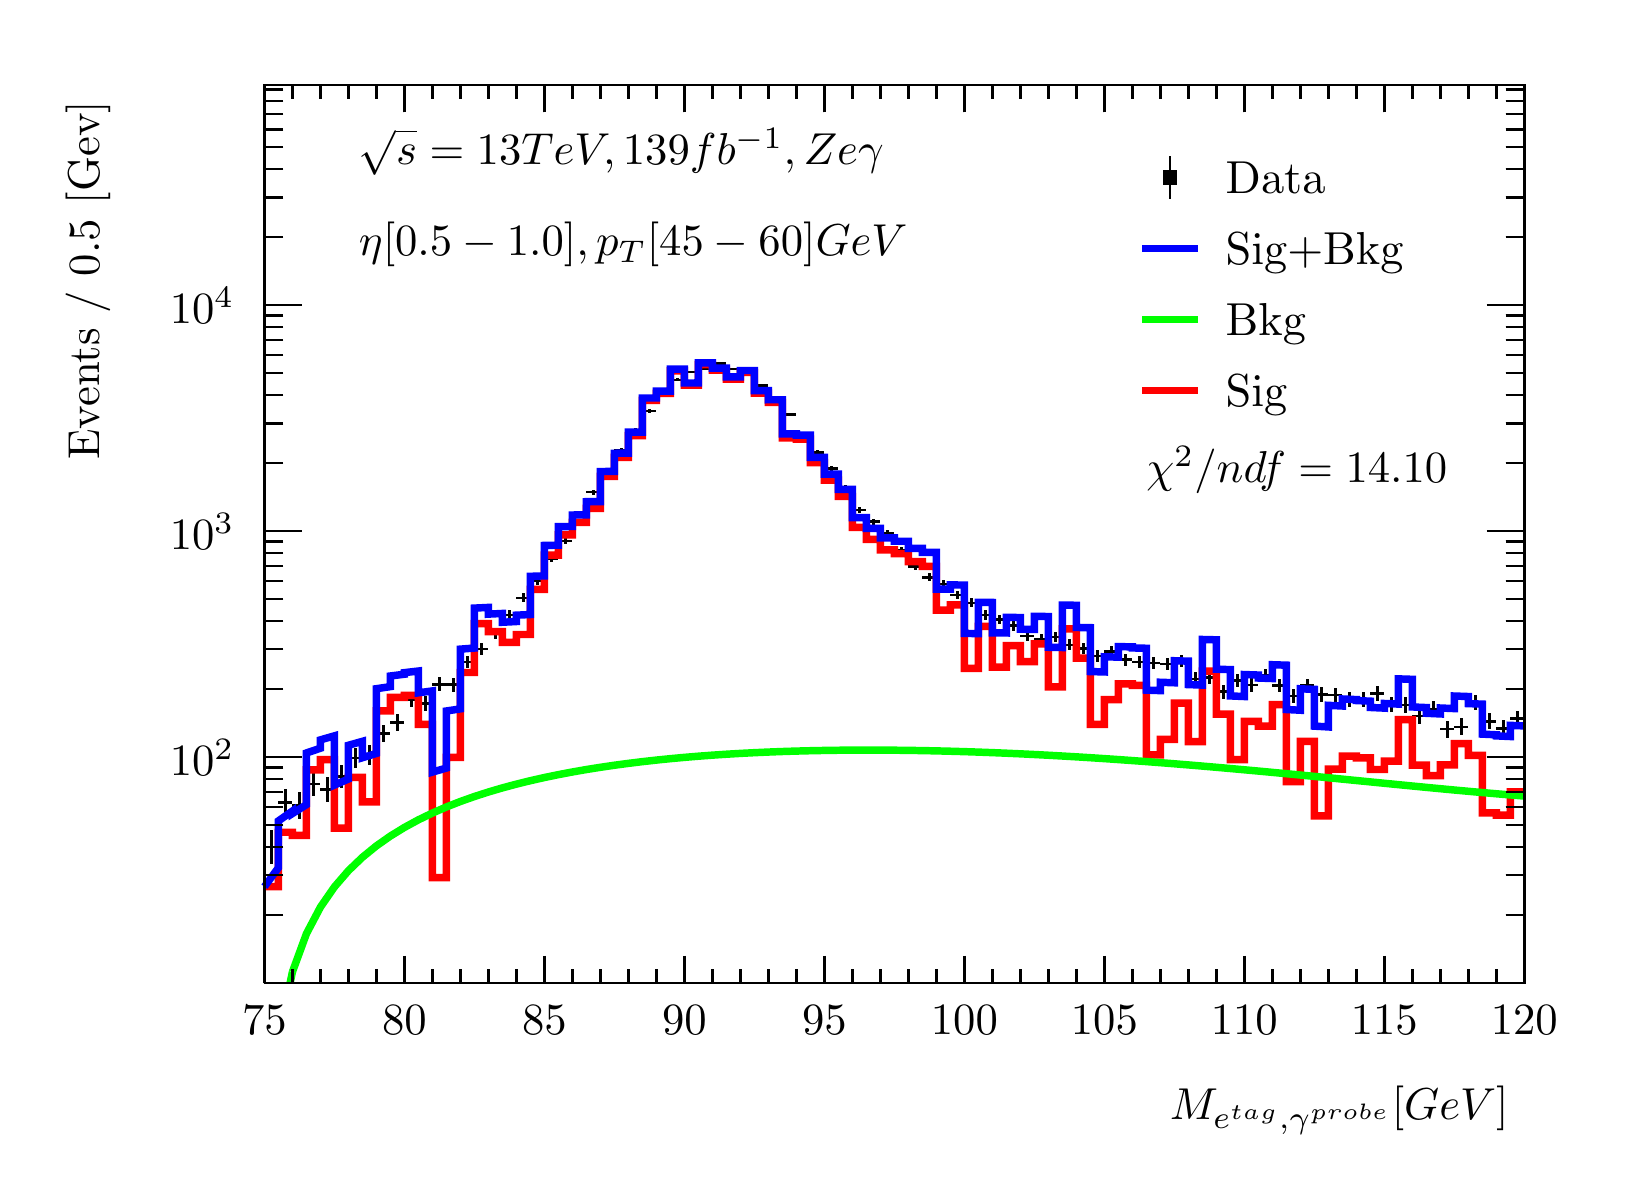
\begin{tikzpicture}
\pgfdeclareplotmark{cross} {
\pgfpathmoveto{\pgfpoint{-0.3\pgfplotmarksize}{\pgfplotmarksize}}
\pgfpathlineto{\pgfpoint{+0.3\pgfplotmarksize}{\pgfplotmarksize}}
\pgfpathlineto{\pgfpoint{+0.3\pgfplotmarksize}{0.3\pgfplotmarksize}}
\pgfpathlineto{\pgfpoint{+1\pgfplotmarksize}{0.3\pgfplotmarksize}}
\pgfpathlineto{\pgfpoint{+1\pgfplotmarksize}{-0.3\pgfplotmarksize}}
\pgfpathlineto{\pgfpoint{+0.3\pgfplotmarksize}{-0.3\pgfplotmarksize}}
\pgfpathlineto{\pgfpoint{+0.3\pgfplotmarksize}{-1.\pgfplotmarksize}}
\pgfpathlineto{\pgfpoint{-0.3\pgfplotmarksize}{-1.\pgfplotmarksize}}
\pgfpathlineto{\pgfpoint{-0.3\pgfplotmarksize}{-0.3\pgfplotmarksize}}
\pgfpathlineto{\pgfpoint{-1.\pgfplotmarksize}{-0.3\pgfplotmarksize}}
\pgfpathlineto{\pgfpoint{-1.\pgfplotmarksize}{0.3\pgfplotmarksize}}
\pgfpathlineto{\pgfpoint{-0.3\pgfplotmarksize}{0.3\pgfplotmarksize}}
\pgfpathclose
\pgfusepathqstroke
}
\pgfdeclareplotmark{cross*} {
\pgfpathmoveto{\pgfpoint{-0.3\pgfplotmarksize}{\pgfplotmarksize}}
\pgfpathlineto{\pgfpoint{+0.3\pgfplotmarksize}{\pgfplotmarksize}}
\pgfpathlineto{\pgfpoint{+0.3\pgfplotmarksize}{0.3\pgfplotmarksize}}
\pgfpathlineto{\pgfpoint{+1\pgfplotmarksize}{0.3\pgfplotmarksize}}
\pgfpathlineto{\pgfpoint{+1\pgfplotmarksize}{-0.3\pgfplotmarksize}}
\pgfpathlineto{\pgfpoint{+0.3\pgfplotmarksize}{-0.3\pgfplotmarksize}}
\pgfpathlineto{\pgfpoint{+0.3\pgfplotmarksize}{-1.\pgfplotmarksize}}
\pgfpathlineto{\pgfpoint{-0.3\pgfplotmarksize}{-1.\pgfplotmarksize}}
\pgfpathlineto{\pgfpoint{-0.3\pgfplotmarksize}{-0.3\pgfplotmarksize}}
\pgfpathlineto{\pgfpoint{-1.\pgfplotmarksize}{-0.3\pgfplotmarksize}}
\pgfpathlineto{\pgfpoint{-1.\pgfplotmarksize}{0.3\pgfplotmarksize}}
\pgfpathlineto{\pgfpoint{-0.3\pgfplotmarksize}{0.3\pgfplotmarksize}}
\pgfpathclose
\pgfusepathqfillstroke
}
\pgfdeclareplotmark{newstar} {
\pgfpathmoveto{\pgfqpoint{0pt}{\pgfplotmarksize}}
\pgfpathlineto{\pgfqpointpolar{44}{0.5\pgfplotmarksize}}
\pgfpathlineto{\pgfqpointpolar{18}{\pgfplotmarksize}}
\pgfpathlineto{\pgfqpointpolar{-20}{0.5\pgfplotmarksize}}
\pgfpathlineto{\pgfqpointpolar{-54}{\pgfplotmarksize}}
\pgfpathlineto{\pgfqpointpolar{-90}{0.5\pgfplotmarksize}}
\pgfpathlineto{\pgfqpointpolar{234}{\pgfplotmarksize}}
\pgfpathlineto{\pgfqpointpolar{198}{0.5\pgfplotmarksize}}
\pgfpathlineto{\pgfqpointpolar{162}{\pgfplotmarksize}}
\pgfpathlineto{\pgfqpointpolar{134}{0.5\pgfplotmarksize}}
\pgfpathclose
\pgfusepathqstroke
}
\pgfdeclareplotmark{newstar*} {
\pgfpathmoveto{\pgfqpoint{0pt}{\pgfplotmarksize}}
\pgfpathlineto{\pgfqpointpolar{44}{0.5\pgfplotmarksize}}
\pgfpathlineto{\pgfqpointpolar{18}{\pgfplotmarksize}}
\pgfpathlineto{\pgfqpointpolar{-20}{0.5\pgfplotmarksize}}
\pgfpathlineto{\pgfqpointpolar{-54}{\pgfplotmarksize}}
\pgfpathlineto{\pgfqpointpolar{-90}{0.5\pgfplotmarksize}}
\pgfpathlineto{\pgfqpointpolar{234}{\pgfplotmarksize}}
\pgfpathlineto{\pgfqpointpolar{198}{0.5\pgfplotmarksize}}
\pgfpathlineto{\pgfqpointpolar{162}{\pgfplotmarksize}}
\pgfpathlineto{\pgfqpointpolar{134}{0.5\pgfplotmarksize}}
\pgfpathclose
\pgfusepathqfillstroke
}
\definecolor{c}{rgb}{1,1,1};
\draw [color=c, fill=c] (0,0) rectangle (20,14.4361);
\draw [color=c, fill=c] (3,2.30977) rectangle (19,13.7143);
\definecolor{c}{rgb}{0,0,0};
\draw [c,line width=0.9] (3,2.30977) -- (3,13.7143) -- (19,13.7143) -- (19,2.30977) -- (3,2.30977);
\definecolor{c}{rgb}{1,1,1};
\draw [color=c, fill=c] (3,2.30977) rectangle (19,13.7143);
\definecolor{c}{rgb}{0,0,0};
\draw [c,line width=0.9] (3,2.30977) -- (3,13.7143) -- (19,13.7143) -- (19,2.30977) -- (3,2.30977);
\draw [c,line width=0.9] (3,2.30977) -- (19,2.30977);
\draw [c,line width=0.9] (3,2.65624) -- (3,2.30977);
\draw [c,line width=0.9] (3.35556,2.48301) -- (3.35556,2.30977);
\draw [c,line width=0.9] (3.71111,2.48301) -- (3.71111,2.30977);
\draw [c,line width=0.9] (4.06667,2.48301) -- (4.06667,2.30977);
\draw [c,line width=0.9] (4.42222,2.48301) -- (4.42222,2.30977);
\draw [c,line width=0.9] (4.77778,2.65624) -- (4.77778,2.30977);
\draw [c,line width=0.9] (5.13333,2.48301) -- (5.13333,2.30977);
\draw [c,line width=0.9] (5.48889,2.48301) -- (5.48889,2.30977);
\draw [c,line width=0.9] (5.84444,2.48301) -- (5.84444,2.30977);
\draw [c,line width=0.9] (6.2,2.48301) -- (6.2,2.30977);
\draw [c,line width=0.9] (6.55556,2.65624) -- (6.55556,2.30977);
\draw [c,line width=0.9] (6.91111,2.48301) -- (6.91111,2.30977);
\draw [c,line width=0.9] (7.26667,2.48301) -- (7.26667,2.30977);
\draw [c,line width=0.9] (7.62222,2.48301) -- (7.62222,2.30977);
\draw [c,line width=0.9] (7.97778,2.48301) -- (7.97778,2.30977);
\draw [c,line width=0.9] (8.33333,2.65624) -- (8.33333,2.30977);
\draw [c,line width=0.9] (8.68889,2.48301) -- (8.68889,2.30977);
\draw [c,line width=0.9] (9.04444,2.48301) -- (9.04444,2.30977);
\draw [c,line width=0.9] (9.4,2.48301) -- (9.4,2.30977);
\draw [c,line width=0.9] (9.75556,2.48301) -- (9.75556,2.30977);
\draw [c,line width=0.9] (10.1111,2.65624) -- (10.1111,2.30977);
\draw [c,line width=0.9] (10.4667,2.48301) -- (10.4667,2.30977);
\draw [c,line width=0.9] (10.8222,2.48301) -- (10.8222,2.30977);
\draw [c,line width=0.9] (11.1778,2.48301) -- (11.1778,2.30977);
\draw [c,line width=0.9] (11.5333,2.48301) -- (11.5333,2.30977);
\draw [c,line width=0.9] (11.8889,2.65624) -- (11.8889,2.30977);
\draw [c,line width=0.9] (12.2444,2.48301) -- (12.2444,2.30977);
\draw [c,line width=0.9] (12.6,2.48301) -- (12.6,2.30977);
\draw [c,line width=0.9] (12.9556,2.48301) -- (12.9556,2.30977);
\draw [c,line width=0.9] (13.3111,2.48301) -- (13.3111,2.30977);
\draw [c,line width=0.9] (13.6667,2.65624) -- (13.6667,2.30977);
\draw [c,line width=0.9] (14.0222,2.48301) -- (14.0222,2.30977);
\draw [c,line width=0.9] (14.3778,2.48301) -- (14.3778,2.30977);
\draw [c,line width=0.9] (14.7333,2.48301) -- (14.7333,2.30977);
\draw [c,line width=0.9] (15.0889,2.48301) -- (15.0889,2.30977);
\draw [c,line width=0.9] (15.4444,2.65624) -- (15.4444,2.30977);
\draw [c,line width=0.9] (15.8,2.48301) -- (15.8,2.30977);
\draw [c,line width=0.9] (16.1556,2.48301) -- (16.1556,2.30977);
\draw [c,line width=0.9] (16.5111,2.48301) -- (16.5111,2.30977);
\draw [c,line width=0.9] (16.8667,2.48301) -- (16.8667,2.30977);
\draw [c,line width=0.9] (17.2222,2.65624) -- (17.2222,2.30977);
\draw [c,line width=0.9] (17.5778,2.48301) -- (17.5778,2.30977);
\draw [c,line width=0.9] (17.9333,2.48301) -- (17.9333,2.30977);
\draw [c,line width=0.9] (18.2889,2.48301) -- (18.2889,2.30977);
\draw [c,line width=0.9] (18.6444,2.48301) -- (18.6444,2.30977);
\draw [c,line width=0.9] (19,2.65624) -- (19,2.30977);
\draw [c,line width=0.9] (19,2.65624) -- (19,2.30977);
\draw [anchor=base] (3,1.66015) node[scale=1.61424, color=c, rotate=0]{75};
\draw [anchor=base] (4.77778,1.66015) node[scale=1.61424, color=c, rotate=0]{80};
\draw [anchor=base] (6.55556,1.66015) node[scale=1.61424, color=c, rotate=0]{85};
\draw [anchor=base] (8.33333,1.66015) node[scale=1.61424, color=c, rotate=0]{90};
\draw [anchor=base] (10.1111,1.66015) node[scale=1.61424, color=c, rotate=0]{95};
\draw [anchor=base] (11.8889,1.66015) node[scale=1.61424, color=c, rotate=0]{100};
\draw [anchor=base] (13.6667,1.66015) node[scale=1.61424, color=c, rotate=0]{105};
\draw [anchor=base] (15.4444,1.66015) node[scale=1.61424, color=c, rotate=0]{110};
\draw [anchor=base] (17.2222,1.66015) node[scale=1.61424, color=c, rotate=0]{115};
\draw [anchor=base] (19,1.66015) node[scale=1.61424, color=c, rotate=0]{120};
\draw [anchor= east] (19,0.692932) node[scale=1.61424, color=c, rotate=0]{$M_{e^{tag}, \gamma^{probe}}  [GeV]$};
\draw [c,line width=0.9] (3,13.7143) -- (19,13.7143);
\draw [c,line width=0.9] (3,13.3678) -- (3,13.7143);
\draw [c,line width=0.9] (3.35556,13.5411) -- (3.35556,13.7143);
\draw [c,line width=0.9] (3.71111,13.5411) -- (3.71111,13.7143);
\draw [c,line width=0.9] (4.06667,13.5411) -- (4.06667,13.7143);
\draw [c,line width=0.9] (4.42222,13.5411) -- (4.42222,13.7143);
\draw [c,line width=0.9] (4.77778,13.3678) -- (4.77778,13.7143);
\draw [c,line width=0.9] (5.13333,13.5411) -- (5.13333,13.7143);
\draw [c,line width=0.9] (5.48889,13.5411) -- (5.48889,13.7143);
\draw [c,line width=0.9] (5.84444,13.5411) -- (5.84444,13.7143);
\draw [c,line width=0.9] (6.2,13.5411) -- (6.2,13.7143);
\draw [c,line width=0.9] (6.55556,13.3678) -- (6.55556,13.7143);
\draw [c,line width=0.9] (6.91111,13.5411) -- (6.91111,13.7143);
\draw [c,line width=0.9] (7.26667,13.5411) -- (7.26667,13.7143);
\draw [c,line width=0.9] (7.62222,13.5411) -- (7.62222,13.7143);
\draw [c,line width=0.9] (7.97778,13.5411) -- (7.97778,13.7143);
\draw [c,line width=0.9] (8.33333,13.3678) -- (8.33333,13.7143);
\draw [c,line width=0.9] (8.68889,13.5411) -- (8.68889,13.7143);
\draw [c,line width=0.9] (9.04444,13.5411) -- (9.04444,13.7143);
\draw [c,line width=0.9] (9.4,13.5411) -- (9.4,13.7143);
\draw [c,line width=0.9] (9.75556,13.5411) -- (9.75556,13.7143);
\draw [c,line width=0.9] (10.1111,13.3678) -- (10.1111,13.7143);
\draw [c,line width=0.9] (10.4667,13.5411) -- (10.4667,13.7143);
\draw [c,line width=0.9] (10.8222,13.5411) -- (10.8222,13.7143);
\draw [c,line width=0.9] (11.1778,13.5411) -- (11.1778,13.7143);
\draw [c,line width=0.9] (11.5333,13.5411) -- (11.5333,13.7143);
\draw [c,line width=0.9] (11.8889,13.3678) -- (11.8889,13.7143);
\draw [c,line width=0.9] (12.2444,13.5411) -- (12.2444,13.7143);
\draw [c,line width=0.9] (12.6,13.5411) -- (12.6,13.7143);
\draw [c,line width=0.9] (12.9556,13.5411) -- (12.9556,13.7143);
\draw [c,line width=0.9] (13.3111,13.5411) -- (13.3111,13.7143);
\draw [c,line width=0.9] (13.6667,13.3678) -- (13.6667,13.7143);
\draw [c,line width=0.9] (14.0222,13.5411) -- (14.0222,13.7143);
\draw [c,line width=0.9] (14.3778,13.5411) -- (14.3778,13.7143);
\draw [c,line width=0.9] (14.7333,13.5411) -- (14.7333,13.7143);
\draw [c,line width=0.9] (15.0889,13.5411) -- (15.0889,13.7143);
\draw [c,line width=0.9] (15.4444,13.3678) -- (15.4444,13.7143);
\draw [c,line width=0.9] (15.8,13.5411) -- (15.8,13.7143);
\draw [c,line width=0.9] (16.1556,13.5411) -- (16.1556,13.7143);
\draw [c,line width=0.9] (16.5111,13.5411) -- (16.5111,13.7143);
\draw [c,line width=0.9] (16.8667,13.5411) -- (16.8667,13.7143);
\draw [c,line width=0.9] (17.2222,13.3678) -- (17.2222,13.7143);
\draw [c,line width=0.9] (17.5778,13.5411) -- (17.5778,13.7143);
\draw [c,line width=0.9] (17.9333,13.5411) -- (17.9333,13.7143);
\draw [c,line width=0.9] (18.2889,13.5411) -- (18.2889,13.7143);
\draw [c,line width=0.9] (18.6444,13.5411) -- (18.6444,13.7143);
\draw [c,line width=0.9] (19,13.3678) -- (19,13.7143);
\draw [c,line width=0.9] (19,13.3678) -- (19,13.7143);
\draw [c,line width=0.9] (3,2.30977) -- (3,13.7143);
\draw [c,line width=0.9] (3.237,3.17371) -- (3,3.17371);
\draw [c,line width=0.9] (3.237,3.67908) -- (3,3.67908);
\draw [c,line width=0.9] (3.237,4.03764) -- (3,4.03764);
\draw [c,line width=0.9] (3.237,4.31577) -- (3,4.31577);
\draw [c,line width=0.9] (3.237,4.54301) -- (3,4.54301);
\draw [c,line width=0.9] (3.237,4.73514) -- (3,4.73514);
\draw [c,line width=0.9] (3.237,4.90158) -- (3,4.90158);
\draw [c,line width=0.9] (3.237,5.04838) -- (3,5.04838);
\draw [c,line width=0.9] (3.474,5.1797) -- (3,5.1797);
\draw [anchor= east] (2.82,5.1797) node[scale=1.61424, color=c, rotate=0]{$10^{2}$};
\draw [c,line width=0.9] (3.237,6.04363) -- (3,6.04363);
\draw [c,line width=0.9] (3.237,6.549) -- (3,6.549);
\draw [c,line width=0.9] (3.237,6.90757) -- (3,6.90757);
\draw [c,line width=0.9] (3.237,7.18569) -- (3,7.18569);
\draw [c,line width=0.9] (3.237,7.41294) -- (3,7.41294);
\draw [c,line width=0.9] (3.237,7.60507) -- (3,7.60507);
\draw [c,line width=0.9] (3.237,7.7715) -- (3,7.7715);
\draw [c,line width=0.9] (3.237,7.91831) -- (3,7.91831);
\draw [c,line width=0.9] (3.474,8.04963) -- (3,8.04963);
\draw [anchor= east] (2.82,8.04963) node[scale=1.61424, color=c, rotate=0]{$10^{3}$};
\draw [c,line width=0.9] (3.237,8.91356) -- (3,8.91356);
\draw [c,line width=0.9] (3.237,9.41893) -- (3,9.41893);
\draw [c,line width=0.9] (3.237,9.7775) -- (3,9.7775);
\draw [c,line width=0.9] (3.237,10.0556) -- (3,10.0556);
\draw [c,line width=0.9] (3.237,10.2829) -- (3,10.2829);
\draw [c,line width=0.9] (3.237,10.475) -- (3,10.475);
\draw [c,line width=0.9] (3.237,10.6414) -- (3,10.6414);
\draw [c,line width=0.9] (3.237,10.7882) -- (3,10.7882);
\draw [c,line width=0.9] (3.474,10.9196) -- (3,10.9196);
\draw [anchor= east] (2.82,10.9196) node[scale=1.61424, color=c, rotate=0]{$10^{4}$};
\draw [c,line width=0.9] (3.237,11.7835) -- (3,11.7835);
\draw [c,line width=0.9] (3.237,12.2889) -- (3,12.2889);
\draw [c,line width=0.9] (3.237,12.6474) -- (3,12.6474);
\draw [c,line width=0.9] (3.237,12.9256) -- (3,12.9256);
\draw [c,line width=0.9] (3.237,13.1528) -- (3,13.1528);
\draw [c,line width=0.9] (3.237,13.3449) -- (3,13.3449);
\draw [c,line width=0.9] (3.237,13.5114) -- (3,13.5114);
\draw [c,line width=0.9] (3.237,13.6582) -- (3,13.6582);
\draw [anchor= east] (0.76,13.7143) node[scale=1.61424, color=c, rotate=90]{Events / 0.5 [Gev]};
\draw [c,line width=0.9] (19,2.30977) -- (19,13.7143);
\draw [c,line width=0.9] (18.763,3.17371) -- (19,3.17371);
\draw [c,line width=0.9] (18.763,3.67908) -- (19,3.67908);
\draw [c,line width=0.9] (18.763,4.03764) -- (19,4.03764);
\draw [c,line width=0.9] (18.763,4.31577) -- (19,4.31577);
\draw [c,line width=0.9] (18.763,4.54301) -- (19,4.54301);
\draw [c,line width=0.9] (18.763,4.73514) -- (19,4.73514);
\draw [c,line width=0.9] (18.763,4.90158) -- (19,4.90158);
\draw [c,line width=0.9] (18.763,5.04838) -- (19,5.04838);
\draw [c,line width=0.9] (18.526,5.1797) -- (19,5.1797);
\draw [c,line width=0.9] (18.763,6.04363) -- (19,6.04363);
\draw [c,line width=0.9] (18.763,6.549) -- (19,6.549);
\draw [c,line width=0.9] (18.763,6.90757) -- (19,6.90757);
\draw [c,line width=0.9] (18.763,7.18569) -- (19,7.18569);
\draw [c,line width=0.9] (18.763,7.41294) -- (19,7.41294);
\draw [c,line width=0.9] (18.763,7.60507) -- (19,7.60507);
\draw [c,line width=0.9] (18.763,7.7715) -- (19,7.7715);
\draw [c,line width=0.9] (18.763,7.91831) -- (19,7.91831);
\draw [c,line width=0.9] (18.526,8.04963) -- (19,8.04963);
\draw [c,line width=0.9] (18.763,8.91356) -- (19,8.91356);
\draw [c,line width=0.9] (18.763,9.41893) -- (19,9.41893);
\draw [c,line width=0.9] (18.763,9.7775) -- (19,9.7775);
\draw [c,line width=0.9] (18.763,10.0556) -- (19,10.0556);
\draw [c,line width=0.9] (18.763,10.2829) -- (19,10.2829);
\draw [c,line width=0.9] (18.763,10.475) -- (19,10.475);
\draw [c,line width=0.9] (18.763,10.6414) -- (19,10.6414);
\draw [c,line width=0.9] (18.763,10.7882) -- (19,10.7882);
\draw [c,line width=0.9] (18.526,10.9196) -- (19,10.9196);
\draw [c,line width=0.9] (18.763,11.7835) -- (19,11.7835);
\draw [c,line width=0.9] (18.763,12.2889) -- (19,12.2889);
\draw [c,line width=0.9] (18.763,12.6474) -- (19,12.6474);
\draw [c,line width=0.9] (18.763,12.9256) -- (19,12.9256);
\draw [c,line width=0.9] (18.763,13.1528) -- (19,13.1528);
\draw [c,line width=0.9] (18.763,13.3449) -- (19,13.3449);
\draw [c,line width=0.9] (18.763,13.5114) -- (19,13.5114);
\draw [c,line width=0.9] (18.763,13.6582) -- (19,13.6582);
\draw [c,line width=0.9] (3.08889,4.03764) -- (3,4.03764);
\draw [c,line width=0.9] (3,4.03764) -- (3,4.03764);
\draw [c,line width=0.9] (3.08889,4.03764) -- (3.17778,4.03764);
\draw [c,line width=0.9] (3.17778,4.03764) -- (3.17778,4.03764);
\draw [c,line width=0.9] (3.08889,4.03764) -- (3.08889,4.24861);
\draw [c,line width=0.9] (3.08889,4.24861) -- (3.08889,4.24861);
\draw [c,line width=0.9] (3.08889,4.03764) -- (3.08889,3.82411);
\draw [c,line width=0.9] (3.08889,3.82411) -- (3.08889,3.82411);
\draw [c,line width=0.9] (3.26667,4.60382) -- (3.17778,4.60382);
\draw [c,line width=0.9] (3.17778,4.60382) -- (3.17778,4.60382);
\draw [c,line width=0.9] (3.26667,4.60382) -- (3.35556,4.60382);
\draw [c,line width=0.9] (3.35556,4.60382) -- (3.35556,4.60382);
\draw [c,line width=0.9] (3.26667,4.60382) -- (3.26667,4.7699);
\draw [c,line width=0.9] (3.26667,4.7699) -- (3.26667,4.7699);
\draw [c,line width=0.9] (3.26667,4.60382) -- (3.26667,4.43646);
\draw [c,line width=0.9] (3.26667,4.43646) -- (3.26667,4.43646);
\draw [c,line width=0.9] (3.44444,4.56361) -- (3.35556,4.56361);
\draw [c,line width=0.9] (3.35556,4.56361) -- (3.35556,4.56361);
\draw [c,line width=0.9] (3.44444,4.56361) -- (3.53333,4.56361);
\draw [c,line width=0.9] (3.53333,4.56361) -- (3.53333,4.56361);
\draw [c,line width=0.9] (3.44444,4.56361) -- (3.44444,4.73252);
\draw [c,line width=0.9] (3.44444,4.73252) -- (3.44444,4.73252);
\draw [c,line width=0.9] (3.44444,4.56361) -- (3.44444,4.39335);
\draw [c,line width=0.9] (3.44444,4.39335) -- (3.44444,4.39335);
\draw [c,line width=0.9] (3.62222,4.83765) -- (3.53333,4.83765);
\draw [c,line width=0.9] (3.53333,4.83765) -- (3.53333,4.83765);
\draw [c,line width=0.9] (3.62222,4.83765) -- (3.71111,4.83765);
\draw [c,line width=0.9] (3.71111,4.83765) -- (3.71111,4.83765);
\draw [c,line width=0.9] (3.62222,4.83765) -- (3.62222,4.98818);
\draw [c,line width=0.9] (3.62222,4.98818) -- (3.62222,4.98818);
\draw [c,line width=0.9] (3.62222,4.83765) -- (3.62222,4.68614);
\draw [c,line width=0.9] (3.62222,4.68614) -- (3.62222,4.68614);
\draw [c,line width=0.9] (3.8,4.77026) -- (3.71111,4.77026);
\draw [c,line width=0.9] (3.71111,4.77026) -- (3.71111,4.77026);
\draw [c,line width=0.9] (3.8,4.77026) -- (3.88889,4.77026);
\draw [c,line width=0.9] (3.88889,4.77026) -- (3.88889,4.77026);
\draw [c,line width=0.9] (3.8,4.77026) -- (3.8,4.92511);
\draw [c,line width=0.9] (3.8,4.92511) -- (3.8,4.92511);
\draw [c,line width=0.9] (3.8,4.77026) -- (3.8,4.61435);
\draw [c,line width=0.9] (3.8,4.61435) -- (3.8,4.61435);
\draw [c,line width=0.9] (3.97778,4.93235) -- (3.88889,4.93235);
\draw [c,line width=0.9] (3.88889,4.93235) -- (3.88889,4.93235);
\draw [c,line width=0.9] (3.97778,4.93235) -- (4.06667,4.93235);
\draw [c,line width=0.9] (4.06667,4.93235) -- (4.06667,4.93235);
\draw [c,line width=0.9] (3.97778,4.93235) -- (3.97778,5.07702);
\draw [c,line width=0.9] (3.97778,5.07702) -- (3.97778,5.07702);
\draw [c,line width=0.9] (3.97778,4.93235) -- (3.97778,4.78682);
\draw [c,line width=0.9] (3.97778,4.78682) -- (3.97778,4.78682);
\draw [c,line width=0.9] (4.15556,5.16718) -- (4.06667,5.16718);
\draw [c,line width=0.9] (4.06667,5.16718) -- (4.06667,5.16718);
\draw [c,line width=0.9] (4.15556,5.16718) -- (4.24444,5.16718);
\draw [c,line width=0.9] (4.24444,5.16718) -- (4.24444,5.16718);
\draw [c,line width=0.9] (4.15556,5.16718) -- (4.15556,5.29831);
\draw [c,line width=0.9] (4.15556,5.29831) -- (4.15556,5.29831);
\draw [c,line width=0.9] (4.15556,5.16718) -- (4.15556,5.03539);
\draw [c,line width=0.9] (4.15556,5.03539) -- (4.15556,5.03539);
\draw [c,line width=0.9] (4.33333,5.20438) -- (4.24444,5.20438);
\draw [c,line width=0.9] (4.24444,5.20438) -- (4.24444,5.20438);
\draw [c,line width=0.9] (4.33333,5.20438) -- (4.42222,5.20438);
\draw [c,line width=0.9] (4.42222,5.20438) -- (4.42222,5.20438);
\draw [c,line width=0.9] (4.33333,5.20438) -- (4.33333,5.32774);
\draw [c,line width=0.9] (4.33333,5.32774) -- (4.33333,5.32774);
\draw [c,line width=0.9] (4.33333,5.20438) -- (4.33333,5.08102);
\draw [c,line width=0.9] (4.33333,5.08102) -- (4.33333,5.08102);
\draw [c,line width=0.9] (4.51111,5.47761) -- (4.42222,5.47761);
\draw [c,line width=0.9] (4.42222,5.47761) -- (4.42222,5.47761);
\draw [c,line width=0.9] (4.51111,5.47761) -- (4.6,5.47761);
\draw [c,line width=0.9] (4.6,5.47761) -- (4.6,5.47761);
\draw [c,line width=0.9] (4.51111,5.47761) -- (4.51111,5.58817);
\draw [c,line width=0.9] (4.51111,5.58817) -- (4.51111,5.58817);
\draw [c,line width=0.9] (4.51111,5.47761) -- (4.51111,5.36705);
\draw [c,line width=0.9] (4.51111,5.36705) -- (4.51111,5.36705);
\draw [c,line width=0.9] (4.68889,5.61676) -- (4.6,5.61676);
\draw [c,line width=0.9] (4.6,5.61676) -- (4.6,5.61676);
\draw [c,line width=0.9] (4.68889,5.61676) -- (4.77778,5.61676);
\draw [c,line width=0.9] (4.77778,5.61676) -- (4.77778,5.61676);
\draw [c,line width=0.9] (4.68889,5.61676) -- (4.68889,5.72132);
\draw [c,line width=0.9] (4.68889,5.72132) -- (4.68889,5.72132);
\draw [c,line width=0.9] (4.68889,5.61676) -- (4.68889,5.51219);
\draw [c,line width=0.9] (4.68889,5.51219) -- (4.68889,5.51219);
\draw [c,line width=0.9] (4.86667,5.90537) -- (4.77778,5.90537);
\draw [c,line width=0.9] (4.77778,5.90537) -- (4.77778,5.90537);
\draw [c,line width=0.9] (4.86667,5.90537) -- (4.95556,5.90537);
\draw [c,line width=0.9] (4.95556,5.90537) -- (4.95556,5.90537);
\draw [c,line width=0.9] (4.86667,5.90537) -- (4.86667,5.99851);
\draw [c,line width=0.9] (4.86667,5.99851) -- (4.86667,5.99851);
\draw [c,line width=0.9] (4.86667,5.90537) -- (4.86667,5.81223);
\draw [c,line width=0.9] (4.86667,5.81223) -- (4.86667,5.81223);
\draw [c,line width=0.9] (5.04444,5.86288) -- (4.95556,5.86288);
\draw [c,line width=0.9] (4.95556,5.86288) -- (4.95556,5.86288);
\draw [c,line width=0.9] (5.04444,5.86288) -- (5.13333,5.86288);
\draw [c,line width=0.9] (5.13333,5.86288) -- (5.13333,5.86288);
\draw [c,line width=0.9] (5.04444,5.86288) -- (5.04444,5.95762);
\draw [c,line width=0.9] (5.04444,5.95762) -- (5.04444,5.95762);
\draw [c,line width=0.9] (5.04444,5.86288) -- (5.04444,5.76814);
\draw [c,line width=0.9] (5.04444,5.76814) -- (5.04444,5.76814);
\draw [c,line width=0.9] (5.22222,6.10445) -- (5.13333,6.10445);
\draw [c,line width=0.9] (5.13333,6.10445) -- (5.13333,6.10445);
\draw [c,line width=0.9] (5.22222,6.10445) -- (5.31111,6.10445);
\draw [c,line width=0.9] (5.31111,6.10445) -- (5.31111,6.10445);
\draw [c,line width=0.9] (5.22222,6.10445) -- (5.22222,6.19044);
\draw [c,line width=0.9] (5.22222,6.19044) -- (5.22222,6.19044);
\draw [c,line width=0.9] (5.22222,6.10445) -- (5.22222,6.01846);
\draw [c,line width=0.9] (5.22222,6.01846) -- (5.22222,6.01846);
\draw [c,line width=0.9] (5.4,6.0985) -- (5.31111,6.0985);
\draw [c,line width=0.9] (5.31111,6.0985) -- (5.31111,6.0985);
\draw [c,line width=0.9] (5.4,6.0985) -- (5.48889,6.0985);
\draw [c,line width=0.9] (5.48889,6.0985) -- (5.48889,6.0985);
\draw [c,line width=0.9] (5.4,6.0985) -- (5.4,6.1847);
\draw [c,line width=0.9] (5.4,6.1847) -- (5.4,6.1847);
\draw [c,line width=0.9] (5.4,6.0985) -- (5.4,6.0123);
\draw [c,line width=0.9] (5.4,6.0123) -- (5.4,6.0123);
\draw [c,line width=0.9] (5.57778,6.38968) -- (5.48889,6.38968);
\draw [c,line width=0.9] (5.48889,6.38968) -- (5.48889,6.38968);
\draw [c,line width=0.9] (5.57778,6.38968) -- (5.66667,6.38968);
\draw [c,line width=0.9] (5.66667,6.38968) -- (5.66667,6.38968);
\draw [c,line width=0.9] (5.57778,6.38968) -- (5.57778,6.46637);
\draw [c,line width=0.9] (5.57778,6.46637) -- (5.57778,6.46637);
\draw [c,line width=0.9] (5.57778,6.38968) -- (5.57778,6.31298);
\draw [c,line width=0.9] (5.57778,6.31298) -- (5.57778,6.31298);
\draw [c,line width=0.9] (5.75556,6.55315) -- (5.66667,6.55315);
\draw [c,line width=0.9] (5.66667,6.55315) -- (5.66667,6.55315);
\draw [c,line width=0.9] (5.75556,6.55315) -- (5.84444,6.55315);
\draw [c,line width=0.9] (5.84444,6.55315) -- (5.84444,6.55315);
\draw [c,line width=0.9] (5.75556,6.55315) -- (5.75556,6.62498);
\draw [c,line width=0.9] (5.75556,6.62498) -- (5.75556,6.62498);
\draw [c,line width=0.9] (5.75556,6.55315) -- (5.75556,6.48132);
\draw [c,line width=0.9] (5.75556,6.48132) -- (5.75556,6.48132);
\draw [c,line width=0.9] (5.93333,6.74114) -- (5.84444,6.74114);
\draw [c,line width=0.9] (5.84444,6.74114) -- (5.84444,6.74114);
\draw [c,line width=0.9] (5.93333,6.74114) -- (6.02222,6.74114);
\draw [c,line width=0.9] (6.02222,6.74114) -- (6.02222,6.74114);
\draw [c,line width=0.9] (5.93333,6.74114) -- (5.93333,6.80775);
\draw [c,line width=0.9] (5.93333,6.80775) -- (5.93333,6.80775);
\draw [c,line width=0.9] (5.93333,6.74114) -- (5.93333,6.67452);
\draw [c,line width=0.9] (5.93333,6.67452) -- (5.93333,6.67452);
\draw [c,line width=0.9] (6.11111,6.98313) -- (6.02222,6.98313);
\draw [c,line width=0.9] (6.02222,6.98313) -- (6.02222,6.98313);
\draw [c,line width=0.9] (6.11111,6.98313) -- (6.2,6.98313);
\draw [c,line width=0.9] (6.2,6.98313) -- (6.2,6.98313);
\draw [c,line width=0.9] (6.11111,6.98313) -- (6.11111,7.04359);
\draw [c,line width=0.9] (6.11111,7.04359) -- (6.11111,7.04359);
\draw [c,line width=0.9] (6.11111,6.98313) -- (6.11111,6.92268);
\draw [c,line width=0.9] (6.11111,6.92268) -- (6.11111,6.92268);
\draw [c,line width=0.9] (6.28889,7.20302) -- (6.2,7.20302);
\draw [c,line width=0.9] (6.2,7.20302) -- (6.2,7.20302);
\draw [c,line width=0.9] (6.28889,7.20302) -- (6.37778,7.20302);
\draw [c,line width=0.9] (6.37778,7.20302) -- (6.37778,7.20302);
\draw [c,line width=0.9] (6.28889,7.20302) -- (6.28889,7.25837);
\draw [c,line width=0.9] (6.28889,7.25837) -- (6.28889,7.25837);
\draw [c,line width=0.9] (6.28889,7.20302) -- (6.28889,7.14767);
\draw [c,line width=0.9] (6.28889,7.14767) -- (6.28889,7.14767);
\draw [c,line width=0.9] (6.46667,7.41709) -- (6.37778,7.41709);
\draw [c,line width=0.9] (6.37778,7.41709) -- (6.37778,7.41709);
\draw [c,line width=0.9] (6.46667,7.41709) -- (6.55556,7.41709);
\draw [c,line width=0.9] (6.55556,7.41709) -- (6.55556,7.41709);
\draw [c,line width=0.9] (6.46667,7.41709) -- (6.46667,7.46788);
\draw [c,line width=0.9] (6.46667,7.46788) -- (6.46667,7.46788);
\draw [c,line width=0.9] (6.46667,7.41709) -- (6.46667,7.36629);
\draw [c,line width=0.9] (6.46667,7.36629) -- (6.46667,7.36629);
\draw [c,line width=0.9] (6.64444,7.69769) -- (6.55556,7.69769);
\draw [c,line width=0.9] (6.55556,7.69769) -- (6.55556,7.69769);
\draw [c,line width=0.9] (6.64444,7.69769) -- (6.73333,7.69769);
\draw [c,line width=0.9] (6.73333,7.69769) -- (6.73333,7.69769);
\draw [c,line width=0.9] (6.64444,7.69769) -- (6.64444,7.74308);
\draw [c,line width=0.9] (6.64444,7.74308) -- (6.64444,7.74308);
\draw [c,line width=0.9] (6.64444,7.69769) -- (6.64444,7.65231);
\draw [c,line width=0.9] (6.64444,7.65231) -- (6.64444,7.65231);
\draw [c,line width=0.9] (6.82222,7.92659) -- (6.73333,7.92659);
\draw [c,line width=0.9] (6.73333,7.92659) -- (6.73333,7.92659);
\draw [c,line width=0.9] (6.82222,7.92659) -- (6.91111,7.92659);
\draw [c,line width=0.9] (6.91111,7.92659) -- (6.91111,7.92659);
\draw [c,line width=0.9] (6.82222,7.92659) -- (6.82222,7.968);
\draw [c,line width=0.9] (6.82222,7.968) -- (6.82222,7.968);
\draw [c,line width=0.9] (6.82222,7.92659) -- (6.82222,7.88518);
\draw [c,line width=0.9] (6.82222,7.88518) -- (6.82222,7.88518);
\draw [c,line width=0.9] (7,8.24957) -- (6.91111,8.24957);
\draw [c,line width=0.9] (6.91111,8.24957) -- (6.91111,8.24957);
\draw [c,line width=0.9] (7,8.24957) -- (7.08889,8.24957);
\draw [c,line width=0.9] (7.08889,8.24957) -- (7.08889,8.24957);
\draw [c,line width=0.9] (7,8.24957) -- (7,8.28595);
\draw [c,line width=0.9] (7,8.28595) -- (7,8.28595);
\draw [c,line width=0.9] (7,8.24957) -- (7,8.2132);
\draw [c,line width=0.9] (7,8.2132) -- (7,8.2132);
\draw [c,line width=0.9] (7.17778,8.54331) -- (7.08889,8.54331);
\draw [c,line width=0.9] (7.08889,8.54331) -- (7.08889,8.54331);
\draw [c,line width=0.9] (7.17778,8.54331) -- (7.26667,8.54331);
\draw [c,line width=0.9] (7.26667,8.54331) -- (7.26667,8.54331);
\draw [c,line width=0.9] (7.17778,8.54331) -- (7.17778,8.57564);
\draw [c,line width=0.9] (7.17778,8.57564) -- (7.17778,8.57564);
\draw [c,line width=0.9] (7.17778,8.54331) -- (7.17778,8.51098);
\draw [c,line width=0.9] (7.17778,8.51098) -- (7.17778,8.51098);
\draw [c,line width=0.9] (7.35556,8.7967) -- (7.26667,8.7967);
\draw [c,line width=0.9] (7.26667,8.7967) -- (7.26667,8.7967);
\draw [c,line width=0.9] (7.35556,8.7967) -- (7.44444,8.7967);
\draw [c,line width=0.9] (7.44444,8.7967) -- (7.44444,8.7967);
\draw [c,line width=0.9] (7.35556,8.7967) -- (7.35556,8.82591);
\draw [c,line width=0.9] (7.35556,8.82591) -- (7.35556,8.82591);
\draw [c,line width=0.9] (7.35556,8.7967) -- (7.35556,8.76749);
\draw [c,line width=0.9] (7.35556,8.76749) -- (7.35556,8.76749);
\draw [c,line width=0.9] (7.53333,9.07414) -- (7.44444,9.07414);
\draw [c,line width=0.9] (7.44444,9.07414) -- (7.44444,9.07414);
\draw [c,line width=0.9] (7.53333,9.07414) -- (7.62222,9.07414);
\draw [c,line width=0.9] (7.62222,9.07414) -- (7.62222,9.07414);
\draw [c,line width=0.9] (7.53333,9.07414) -- (7.53333,9.10027);
\draw [c,line width=0.9] (7.53333,9.10027) -- (7.53333,9.10027);
\draw [c,line width=0.9] (7.53333,9.07414) -- (7.53333,9.04801);
\draw [c,line width=0.9] (7.53333,9.04801) -- (7.53333,9.04801);
\draw [c,line width=0.9] (7.71111,9.33027) -- (7.62222,9.33027);
\draw [c,line width=0.9] (7.62222,9.33027) -- (7.62222,9.33027);
\draw [c,line width=0.9] (7.71111,9.33027) -- (7.8,9.33027);
\draw [c,line width=0.9] (7.8,9.33027) -- (7.8,9.33027);
\draw [c,line width=0.9] (7.71111,9.33027) -- (7.71111,9.35385);
\draw [c,line width=0.9] (7.71111,9.35385) -- (7.71111,9.35385);
\draw [c,line width=0.9] (7.71111,9.33027) -- (7.71111,9.30669);
\draw [c,line width=0.9] (7.71111,9.30669) -- (7.71111,9.30669);
\draw [c,line width=0.9] (7.88889,9.57677) -- (7.8,9.57677);
\draw [c,line width=0.9] (7.8,9.57677) -- (7.8,9.57677);
\draw [c,line width=0.9] (7.88889,9.57677) -- (7.97778,9.57677);
\draw [c,line width=0.9] (7.97778,9.57677) -- (7.97778,9.57677);
\draw [c,line width=0.9] (7.88889,9.57677) -- (7.88889,9.59813);
\draw [c,line width=0.9] (7.88889,9.59813) -- (7.88889,9.59813);
\draw [c,line width=0.9] (7.88889,9.57677) -- (7.88889,9.55541);
\draw [c,line width=0.9] (7.88889,9.55541) -- (7.88889,9.55541);
\draw [c,line width=0.9] (8.06667,9.78897) -- (7.97778,9.78897);
\draw [c,line width=0.9] (7.97778,9.78897) -- (7.97778,9.78897);
\draw [c,line width=0.9] (8.06667,9.78897) -- (8.15556,9.78897);
\draw [c,line width=0.9] (8.15556,9.78897) -- (8.15556,9.78897);
\draw [c,line width=0.9] (8.06667,9.78897) -- (8.06667,9.80859);
\draw [c,line width=0.9] (8.06667,9.80859) -- (8.06667,9.80859);
\draw [c,line width=0.9] (8.06667,9.78897) -- (8.06667,9.76936);
\draw [c,line width=0.9] (8.06667,9.76936) -- (8.06667,9.76936);
\draw [c,line width=0.9] (8.24444,9.97132) -- (8.15556,9.97132);
\draw [c,line width=0.9] (8.15556,9.97132) -- (8.15556,9.97132);
\draw [c,line width=0.9] (8.24444,9.97132) -- (8.33333,9.97132);
\draw [c,line width=0.9] (8.33333,9.97132) -- (8.33333,9.97132);
\draw [c,line width=0.9] (8.24444,9.97132) -- (8.24444,9.98955);
\draw [c,line width=0.9] (8.24444,9.98955) -- (8.24444,9.98955);
\draw [c,line width=0.9] (8.24444,9.97132) -- (8.24444,9.95309);
\draw [c,line width=0.9] (8.24444,9.95309) -- (8.24444,9.95309);
\draw [c,line width=0.9] (8.42222,10.0702) -- (8.33333,10.0702);
\draw [c,line width=0.9] (8.33333,10.0702) -- (8.33333,10.0702);
\draw [c,line width=0.9] (8.42222,10.0702) -- (8.51111,10.0702);
\draw [c,line width=0.9] (8.51111,10.0702) -- (8.51111,10.0702);
\draw [c,line width=0.9] (8.42222,10.0702) -- (8.42222,10.0878);
\draw [c,line width=0.9] (8.42222,10.0878) -- (8.42222,10.0878);
\draw [c,line width=0.9] (8.42222,10.0702) -- (8.42222,10.0527);
\draw [c,line width=0.9] (8.42222,10.0527) -- (8.42222,10.0527);
\draw [c,line width=0.9] (8.6,10.1129) -- (8.51111,10.1129);
\draw [c,line width=0.9] (8.51111,10.1129) -- (8.51111,10.1129);
\draw [c,line width=0.9] (8.6,10.1129) -- (8.68889,10.1129);
\draw [c,line width=0.9] (8.68889,10.1129) -- (8.68889,10.1129);
\draw [c,line width=0.9] (8.6,10.1129) -- (8.6,10.1301);
\draw [c,line width=0.9] (8.6,10.1301) -- (8.6,10.1301);
\draw [c,line width=0.9] (8.6,10.1129) -- (8.6,10.0956);
\draw [c,line width=0.9] (8.6,10.0956) -- (8.6,10.0956);
\draw [c,line width=0.9] (8.77778,10.1805) -- (8.68889,10.1805);
\draw [c,line width=0.9] (8.68889,10.1805) -- (8.68889,10.1805);
\draw [c,line width=0.9] (8.77778,10.1805) -- (8.86667,10.1805);
\draw [c,line width=0.9] (8.86667,10.1805) -- (8.86667,10.1805);
\draw [c,line width=0.9] (8.77778,10.1805) -- (8.77778,10.1973);
\draw [c,line width=0.9] (8.77778,10.1973) -- (8.77778,10.1973);
\draw [c,line width=0.9] (8.77778,10.1805) -- (8.77778,10.1638);
\draw [c,line width=0.9] (8.77778,10.1638) -- (8.77778,10.1638);
\draw [c,line width=0.9] (8.95556,10.1093) -- (8.86667,10.1093);
\draw [c,line width=0.9] (8.86667,10.1093) -- (8.86667,10.1093);
\draw [c,line width=0.9] (8.95556,10.1093) -- (9.04444,10.1093);
\draw [c,line width=0.9] (9.04444,10.1093) -- (9.04444,10.1093);
\draw [c,line width=0.9] (8.95556,10.1093) -- (8.95556,10.1265);
\draw [c,line width=0.9] (8.95556,10.1265) -- (8.95556,10.1265);
\draw [c,line width=0.9] (8.95556,10.1093) -- (8.95556,10.092);
\draw [c,line width=0.9] (8.95556,10.092) -- (8.95556,10.092);
\draw [c,line width=0.9] (9.13333,10.0663) -- (9.04444,10.0663);
\draw [c,line width=0.9] (9.04444,10.0663) -- (9.04444,10.0663);
\draw [c,line width=0.9] (9.13333,10.0663) -- (9.22222,10.0663);
\draw [c,line width=0.9] (9.22222,10.0663) -- (9.22222,10.0663);
\draw [c,line width=0.9] (9.13333,10.0663) -- (9.13333,10.0838);
\draw [c,line width=0.9] (9.13333,10.0838) -- (9.13333,10.0838);
\draw [c,line width=0.9] (9.13333,10.0663) -- (9.13333,10.0487);
\draw [c,line width=0.9] (9.13333,10.0487) -- (9.13333,10.0487);
\draw [c,line width=0.9] (9.31111,9.89969) -- (9.22222,9.89969);
\draw [c,line width=0.9] (9.22222,9.89969) -- (9.22222,9.89969);
\draw [c,line width=0.9] (9.31111,9.89969) -- (9.4,9.89969);
\draw [c,line width=0.9] (9.4,9.89969) -- (9.4,9.89969);
\draw [c,line width=0.9] (9.31111,9.89969) -- (9.31111,9.91845);
\draw [c,line width=0.9] (9.31111,9.91845) -- (9.31111,9.91845);
\draw [c,line width=0.9] (9.31111,9.89969) -- (9.31111,9.88092);
\draw [c,line width=0.9] (9.31111,9.88092) -- (9.31111,9.88092);
\draw [c,line width=0.9] (9.48889,9.74626) -- (9.4,9.74626);
\draw [c,line width=0.9] (9.4,9.74626) -- (9.4,9.74626);
\draw [c,line width=0.9] (9.48889,9.74626) -- (9.57778,9.74626);
\draw [c,line width=0.9] (9.57778,9.74626) -- (9.57778,9.74626);
\draw [c,line width=0.9] (9.48889,9.74626) -- (9.48889,9.76622);
\draw [c,line width=0.9] (9.48889,9.76622) -- (9.48889,9.76622);
\draw [c,line width=0.9] (9.48889,9.74626) -- (9.48889,9.72631);
\draw [c,line width=0.9] (9.48889,9.72631) -- (9.48889,9.72631);
\draw [c,line width=0.9] (9.66667,9.52863) -- (9.57778,9.52863);
\draw [c,line width=0.9] (9.57778,9.52863) -- (9.57778,9.52863);
\draw [c,line width=0.9] (9.66667,9.52863) -- (9.75556,9.52863);
\draw [c,line width=0.9] (9.75556,9.52863) -- (9.75556,9.52863);
\draw [c,line width=0.9] (9.66667,9.52863) -- (9.66667,9.55041);
\draw [c,line width=0.9] (9.66667,9.55041) -- (9.66667,9.55041);
\draw [c,line width=0.9] (9.66667,9.52863) -- (9.66667,9.50685);
\draw [c,line width=0.9] (9.66667,9.50685) -- (9.66667,9.50685);
\draw [c,line width=0.9] (9.84444,9.28992) -- (9.75556,9.28992);
\draw [c,line width=0.9] (9.75556,9.28992) -- (9.75556,9.28992);
\draw [c,line width=0.9] (9.84444,9.28992) -- (9.93333,9.28992);
\draw [c,line width=0.9] (9.93333,9.28992) -- (9.93333,9.28992);
\draw [c,line width=0.9] (9.84444,9.28992) -- (9.84444,9.31388);
\draw [c,line width=0.9] (9.84444,9.31388) -- (9.84444,9.31388);
\draw [c,line width=0.9] (9.84444,9.28992) -- (9.84444,9.26595);
\draw [c,line width=0.9] (9.84444,9.26595) -- (9.84444,9.26595);
\draw [c,line width=0.9] (10.0222,9.047) -- (9.93333,9.047);
\draw [c,line width=0.9] (9.93333,9.047) -- (9.93333,9.047);
\draw [c,line width=0.9] (10.0222,9.047) -- (10.1111,9.047);
\draw [c,line width=0.9] (10.1111,9.047) -- (10.1111,9.047);
\draw [c,line width=0.9] (10.0222,9.047) -- (10.0222,9.07342);
\draw [c,line width=0.9] (10.0222,9.07342) -- (10.0222,9.07342);
\draw [c,line width=0.9] (10.0222,9.047) -- (10.0222,9.02059);
\draw [c,line width=0.9] (10.0222,9.02059) -- (10.0222,9.02059);
\draw [c,line width=0.9] (10.2,8.84371) -- (10.1111,8.84371);
\draw [c,line width=0.9] (10.1111,8.84371) -- (10.1111,8.84371);
\draw [c,line width=0.9] (10.2,8.84371) -- (10.2889,8.84371);
\draw [c,line width=0.9] (10.2889,8.84371) -- (10.2889,8.84371);
\draw [c,line width=0.9] (10.2,8.84371) -- (10.2,8.87238);
\draw [c,line width=0.9] (10.2,8.87238) -- (10.2,8.87238);
\draw [c,line width=0.9] (10.2,8.84371) -- (10.2,8.81505);
\draw [c,line width=0.9] (10.2,8.81505) -- (10.2,8.81505);
\draw [c,line width=0.9] (10.3778,8.60867) -- (10.2889,8.60867);
\draw [c,line width=0.9] (10.2889,8.60867) -- (10.2889,8.60867);
\draw [c,line width=0.9] (10.3778,8.60867) -- (10.4667,8.60867);
\draw [c,line width=0.9] (10.4667,8.60867) -- (10.4667,8.60867);
\draw [c,line width=0.9] (10.3778,8.60867) -- (10.3778,8.64016);
\draw [c,line width=0.9] (10.3778,8.64016) -- (10.3778,8.64016);
\draw [c,line width=0.9] (10.3778,8.60867) -- (10.3778,8.57717);
\draw [c,line width=0.9] (10.3778,8.57717) -- (10.3778,8.57717);
\draw [c,line width=0.9] (10.5556,8.31774) -- (10.4667,8.31774);
\draw [c,line width=0.9] (10.4667,8.31774) -- (10.4667,8.31774);
\draw [c,line width=0.9] (10.5556,8.31774) -- (10.6444,8.31774);
\draw [c,line width=0.9] (10.6444,8.31774) -- (10.6444,8.31774);
\draw [c,line width=0.9] (10.5556,8.31774) -- (10.5556,8.35314);
\draw [c,line width=0.9] (10.5556,8.35314) -- (10.5556,8.35314);
\draw [c,line width=0.9] (10.5556,8.31774) -- (10.5556,8.28235);
\draw [c,line width=0.9] (10.5556,8.28235) -- (10.5556,8.28235);
\draw [c,line width=0.9] (10.7333,8.16956) -- (10.6444,8.16956);
\draw [c,line width=0.9] (10.6444,8.16956) -- (10.6444,8.16956);
\draw [c,line width=0.9] (10.7333,8.16956) -- (10.8222,8.16956);
\draw [c,line width=0.9] (10.8222,8.16956) -- (10.8222,8.16956);
\draw [c,line width=0.9] (10.7333,8.16956) -- (10.7333,8.20712);
\draw [c,line width=0.9] (10.7333,8.20712) -- (10.7333,8.20712);
\draw [c,line width=0.9] (10.7333,8.16956) -- (10.7333,8.132);
\draw [c,line width=0.9] (10.7333,8.132) -- (10.7333,8.132);
\draw [c,line width=0.9] (10.9111,8.02572) -- (10.8222,8.02572);
\draw [c,line width=0.9] (10.8222,8.02572) -- (10.8222,8.02572);
\draw [c,line width=0.9] (10.9111,8.02572) -- (11,8.02572);
\draw [c,line width=0.9] (11,8.02572) -- (11,8.02572);
\draw [c,line width=0.9] (10.9111,8.02572) -- (10.9111,8.06551);
\draw [c,line width=0.9] (10.9111,8.06551) -- (10.9111,8.06551);
\draw [c,line width=0.9] (10.9111,8.02572) -- (10.9111,7.98593);
\draw [c,line width=0.9] (10.9111,7.98593) -- (10.9111,7.98593);
\draw [c,line width=0.9] (11.0889,7.80532) -- (11,7.80532);
\draw [c,line width=0.9] (11,7.80532) -- (11,7.80532);
\draw [c,line width=0.9] (11.0889,7.80532) -- (11.1778,7.80532);
\draw [c,line width=0.9] (11.1778,7.80532) -- (11.1778,7.80532);
\draw [c,line width=0.9] (11.0889,7.80532) -- (11.0889,7.84879);
\draw [c,line width=0.9] (11.0889,7.84879) -- (11.0889,7.84879);
\draw [c,line width=0.9] (11.0889,7.80532) -- (11.0889,7.76185);
\draw [c,line width=0.9] (11.0889,7.76185) -- (11.0889,7.76185);
\draw [c,line width=0.9] (11.2667,7.59793) -- (11.1778,7.59793);
\draw [c,line width=0.9] (11.1778,7.59793) -- (11.1778,7.59793);
\draw [c,line width=0.9] (11.2667,7.59793) -- (11.3556,7.59793);
\draw [c,line width=0.9] (11.3556,7.59793) -- (11.3556,7.59793);
\draw [c,line width=0.9] (11.2667,7.59793) -- (11.2667,7.64517);
\draw [c,line width=0.9] (11.2667,7.64517) -- (11.2667,7.64517);
\draw [c,line width=0.9] (11.2667,7.59793) -- (11.2667,7.55069);
\draw [c,line width=0.9] (11.2667,7.55069) -- (11.2667,7.55069);
\draw [c,line width=0.9] (11.4444,7.46182) -- (11.3556,7.46182);
\draw [c,line width=0.9] (11.3556,7.46182) -- (11.3556,7.46182);
\draw [c,line width=0.9] (11.4444,7.46182) -- (11.5333,7.46182);
\draw [c,line width=0.9] (11.5333,7.46182) -- (11.5333,7.46182);
\draw [c,line width=0.9] (11.4444,7.46182) -- (11.4444,7.51172);
\draw [c,line width=0.9] (11.4444,7.51172) -- (11.4444,7.51172);
\draw [c,line width=0.9] (11.4444,7.46182) -- (11.4444,7.41193);
\draw [c,line width=0.9] (11.4444,7.41193) -- (11.4444,7.41193);
\draw [c,line width=0.9] (11.6222,7.37498) -- (11.5333,7.37498);
\draw [c,line width=0.9] (11.5333,7.37498) -- (11.5333,7.37498);
\draw [c,line width=0.9] (11.6222,7.37498) -- (11.7111,7.37498);
\draw [c,line width=0.9] (11.7111,7.37498) -- (11.7111,7.37498);
\draw [c,line width=0.9] (11.6222,7.37498) -- (11.6222,7.42664);
\draw [c,line width=0.9] (11.6222,7.42664) -- (11.6222,7.42664);
\draw [c,line width=0.9] (11.6222,7.37498) -- (11.6222,7.32332);
\draw [c,line width=0.9] (11.6222,7.32332) -- (11.6222,7.32332);
\draw [c,line width=0.9] (11.8,7.23936) -- (11.7111,7.23936);
\draw [c,line width=0.9] (11.7111,7.23936) -- (11.7111,7.23936);
\draw [c,line width=0.9] (11.8,7.23936) -- (11.8889,7.23936);
\draw [c,line width=0.9] (11.8889,7.23936) -- (11.8889,7.23936);
\draw [c,line width=0.9] (11.8,7.23936) -- (11.8,7.29391);
\draw [c,line width=0.9] (11.8,7.29391) -- (11.8,7.29391);
\draw [c,line width=0.9] (11.8,7.23936) -- (11.8,7.18482);
\draw [c,line width=0.9] (11.8,7.18482) -- (11.8,7.18482);
\draw [c,line width=0.9] (11.9778,7.13741) -- (11.8889,7.13741);
\draw [c,line width=0.9] (11.8889,7.13741) -- (11.8889,7.13741);
\draw [c,line width=0.9] (11.9778,7.13741) -- (12.0667,7.13741);
\draw [c,line width=0.9] (12.0667,7.13741) -- (12.0667,7.13741);
\draw [c,line width=0.9] (11.9778,7.13741) -- (11.9778,7.19424);
\draw [c,line width=0.9] (11.9778,7.19424) -- (11.9778,7.19424);
\draw [c,line width=0.9] (11.9778,7.13741) -- (11.9778,7.08058);
\draw [c,line width=0.9] (11.9778,7.08058) -- (11.9778,7.08058);
\draw [c,line width=0.9] (12.1556,6.98313) -- (12.0667,6.98313);
\draw [c,line width=0.9] (12.0667,6.98313) -- (12.0667,6.98313);
\draw [c,line width=0.9] (12.1556,6.98313) -- (12.2444,6.98313);
\draw [c,line width=0.9] (12.2444,6.98313) -- (12.2444,6.98313);
\draw [c,line width=0.9] (12.1556,6.98313) -- (12.1556,7.04359);
\draw [c,line width=0.9] (12.1556,7.04359) -- (12.1556,7.04359);
\draw [c,line width=0.9] (12.1556,6.98313) -- (12.1556,6.92268);
\draw [c,line width=0.9] (12.1556,6.92268) -- (12.1556,6.92268);
\draw [c,line width=0.9] (12.3333,6.92613) -- (12.2444,6.92613);
\draw [c,line width=0.9] (12.2444,6.92613) -- (12.2444,6.92613);
\draw [c,line width=0.9] (12.3333,6.92613) -- (12.4222,6.92613);
\draw [c,line width=0.9] (12.4222,6.92613) -- (12.4222,6.92613);
\draw [c,line width=0.9] (12.3333,6.92613) -- (12.3333,6.98798);
\draw [c,line width=0.9] (12.3333,6.98798) -- (12.3333,6.98798);
\draw [c,line width=0.9] (12.3333,6.92613) -- (12.3333,6.86428);
\draw [c,line width=0.9] (12.3333,6.86428) -- (12.3333,6.86428);
\draw [c,line width=0.9] (12.5111,6.85018) -- (12.4222,6.85018);
\draw [c,line width=0.9] (12.4222,6.85018) -- (12.4222,6.85018);
\draw [c,line width=0.9] (12.5111,6.85018) -- (12.6,6.85018);
\draw [c,line width=0.9] (12.6,6.85018) -- (12.6,6.85018);
\draw [c,line width=0.9] (12.5111,6.85018) -- (12.5111,6.91395);
\draw [c,line width=0.9] (12.5111,6.91395) -- (12.5111,6.91395);
\draw [c,line width=0.9] (12.5111,6.85018) -- (12.5111,6.78642);
\draw [c,line width=0.9] (12.5111,6.78642) -- (12.5111,6.78642);
\draw [c,line width=0.9] (12.6889,6.71596) -- (12.6,6.71596);
\draw [c,line width=0.9] (12.6,6.71596) -- (12.6,6.71596);
\draw [c,line width=0.9] (12.6889,6.71596) -- (12.7778,6.71596);
\draw [c,line width=0.9] (12.7778,6.71596) -- (12.7778,6.71596);
\draw [c,line width=0.9] (12.6889,6.71596) -- (12.6889,6.78325);
\draw [c,line width=0.9] (12.6889,6.78325) -- (12.6889,6.78325);
\draw [c,line width=0.9] (12.6889,6.71596) -- (12.6889,6.64867);
\draw [c,line width=0.9] (12.6889,6.64867) -- (12.6889,6.64867);
\draw [c,line width=0.9] (12.8667,6.67533) -- (12.7778,6.67533);
\draw [c,line width=0.9] (12.7778,6.67533) -- (12.7778,6.67533);
\draw [c,line width=0.9] (12.8667,6.67533) -- (12.9556,6.67533);
\draw [c,line width=0.9] (12.9556,6.67533) -- (12.9556,6.67533);
\draw [c,line width=0.9] (12.8667,6.67533) -- (12.8667,6.74373);
\draw [c,line width=0.9] (12.8667,6.74373) -- (12.8667,6.74373);
\draw [c,line width=0.9] (12.8667,6.67533) -- (12.8667,6.60694);
\draw [c,line width=0.9] (12.8667,6.60694) -- (12.8667,6.60694);
\draw [c,line width=0.9] (13.0444,6.70501) -- (12.9556,6.70501);
\draw [c,line width=0.9] (12.9556,6.70501) -- (12.9556,6.70501);
\draw [c,line width=0.9] (13.0444,6.70501) -- (13.1333,6.70501);
\draw [c,line width=0.9] (13.1333,6.70501) -- (13.1333,6.70501);
\draw [c,line width=0.9] (13.0444,6.70501) -- (13.0444,6.7726);
\draw [c,line width=0.9] (13.0444,6.7726) -- (13.0444,6.7726);
\draw [c,line width=0.9] (13.0444,6.70501) -- (13.0444,6.63742);
\draw [c,line width=0.9] (13.0444,6.63742) -- (13.0444,6.63742);
\draw [c,line width=0.9] (13.2222,6.60585) -- (13.1333,6.60585);
\draw [c,line width=0.9] (13.1333,6.60585) -- (13.1333,6.60585);
\draw [c,line width=0.9] (13.2222,6.60585) -- (13.3111,6.60585);
\draw [c,line width=0.9] (13.3111,6.60585) -- (13.3111,6.60585);
\draw [c,line width=0.9] (13.2222,6.60585) -- (13.2222,6.67618);
\draw [c,line width=0.9] (13.2222,6.67618) -- (13.2222,6.67618);
\draw [c,line width=0.9] (13.2222,6.60585) -- (13.2222,6.53553);
\draw [c,line width=0.9] (13.2222,6.53553) -- (13.2222,6.53553);
\draw [c,line width=0.9] (13.4,6.55729) -- (13.3111,6.55729);
\draw [c,line width=0.9] (13.3111,6.55729) -- (13.3111,6.55729);
\draw [c,line width=0.9] (13.4,6.55729) -- (13.4889,6.55729);
\draw [c,line width=0.9] (13.4889,6.55729) -- (13.4889,6.55729);
\draw [c,line width=0.9] (13.4,6.55729) -- (13.4,6.629);
\draw [c,line width=0.9] (13.4,6.629) -- (13.4,6.629);
\draw [c,line width=0.9] (13.4,6.55729) -- (13.4,6.48558);
\draw [c,line width=0.9] (13.4,6.48558) -- (13.4,6.48558);
\draw [c,line width=0.9] (13.5778,6.46301) -- (13.4889,6.46301);
\draw [c,line width=0.9] (13.4889,6.46301) -- (13.4889,6.46301);
\draw [c,line width=0.9] (13.5778,6.46301) -- (13.6667,6.46301);
\draw [c,line width=0.9] (13.6667,6.46301) -- (13.6667,6.46301);
\draw [c,line width=0.9] (13.5778,6.46301) -- (13.5778,6.53749);
\draw [c,line width=0.9] (13.5778,6.53749) -- (13.5778,6.53749);
\draw [c,line width=0.9] (13.5778,6.46301) -- (13.5778,6.38854);
\draw [c,line width=0.9] (13.5778,6.38854) -- (13.5778,6.38854);
\draw [c,line width=0.9] (13.7556,6.51958) -- (13.6667,6.51958);
\draw [c,line width=0.9] (13.6667,6.51958) -- (13.6667,6.51958);
\draw [c,line width=0.9] (13.7556,6.51958) -- (13.8444,6.51958);
\draw [c,line width=0.9] (13.8444,6.51958) -- (13.8444,6.51958);
\draw [c,line width=0.9] (13.7556,6.51958) -- (13.7556,6.59238);
\draw [c,line width=0.9] (13.7556,6.59238) -- (13.7556,6.59238);
\draw [c,line width=0.9] (13.7556,6.51958) -- (13.7556,6.44677);
\draw [c,line width=0.9] (13.7556,6.44677) -- (13.7556,6.44677);
\draw [c,line width=0.9] (13.9333,6.41769) -- (13.8444,6.41769);
\draw [c,line width=0.9] (13.8444,6.41769) -- (13.8444,6.41769);
\draw [c,line width=0.9] (13.9333,6.41769) -- (14.0222,6.41769);
\draw [c,line width=0.9] (14.0222,6.41769) -- (14.0222,6.41769);
\draw [c,line width=0.9] (13.9333,6.41769) -- (13.9333,6.49353);
\draw [c,line width=0.9] (13.9333,6.49353) -- (13.9333,6.49353);
\draw [c,line width=0.9] (13.9333,6.41769) -- (13.9333,6.34184);
\draw [c,line width=0.9] (13.9333,6.34184) -- (13.9333,6.34184);
\draw [c,line width=0.9] (14.1111,6.38968) -- (14.0222,6.38968);
\draw [c,line width=0.9] (14.0222,6.38968) -- (14.0222,6.38968);
\draw [c,line width=0.9] (14.1111,6.38968) -- (14.2,6.38968);
\draw [c,line width=0.9] (14.2,6.38968) -- (14.2,6.38968);
\draw [c,line width=0.9] (14.1111,6.38968) -- (14.1111,6.46637);
\draw [c,line width=0.9] (14.1111,6.46637) -- (14.1111,6.46637);
\draw [c,line width=0.9] (14.1111,6.38968) -- (14.1111,6.31298);
\draw [c,line width=0.9] (14.1111,6.31298) -- (14.1111,6.31298);
\draw [c,line width=0.9] (14.2889,6.37543) -- (14.2,6.37543);
\draw [c,line width=0.9] (14.2,6.37543) -- (14.2,6.37543);
\draw [c,line width=0.9] (14.2889,6.37543) -- (14.3778,6.37543);
\draw [c,line width=0.9] (14.3778,6.37543) -- (14.3778,6.37543);
\draw [c,line width=0.9] (14.2889,6.37543) -- (14.2889,6.45257);
\draw [c,line width=0.9] (14.2889,6.45257) -- (14.2889,6.45257);
\draw [c,line width=0.9] (14.2889,6.37543) -- (14.2889,6.29829);
\draw [c,line width=0.9] (14.2889,6.29829) -- (14.2889,6.29829);
\draw [c,line width=0.9] (14.4667,6.36102) -- (14.3778,6.36102);
\draw [c,line width=0.9] (14.3778,6.36102) -- (14.3778,6.36102);
\draw [c,line width=0.9] (14.4667,6.36102) -- (14.5556,6.36102);
\draw [c,line width=0.9] (14.5556,6.36102) -- (14.5556,6.36102);
\draw [c,line width=0.9] (14.4667,6.36102) -- (14.4667,6.43861);
\draw [c,line width=0.9] (14.4667,6.43861) -- (14.4667,6.43861);
\draw [c,line width=0.9] (14.4667,6.36102) -- (14.4667,6.28344);
\draw [c,line width=0.9] (14.4667,6.28344) -- (14.4667,6.28344);
\draw [c,line width=0.9] (14.6444,6.40376) -- (14.5556,6.40376);
\draw [c,line width=0.9] (14.5556,6.40376) -- (14.5556,6.40376);
\draw [c,line width=0.9] (14.6444,6.40376) -- (14.7333,6.40376);
\draw [c,line width=0.9] (14.7333,6.40376) -- (14.7333,6.40376);
\draw [c,line width=0.9] (14.6444,6.40376) -- (14.6444,6.48002);
\draw [c,line width=0.9] (14.6444,6.48002) -- (14.6444,6.48002);
\draw [c,line width=0.9] (14.6444,6.40376) -- (14.6444,6.32749);
\draw [c,line width=0.9] (14.6444,6.32749) -- (14.6444,6.32749);
\draw [c,line width=0.9] (14.8222,6.17371) -- (14.7333,6.17371);
\draw [c,line width=0.9] (14.7333,6.17371) -- (14.7333,6.17371);
\draw [c,line width=0.9] (14.8222,6.17371) -- (14.9111,6.17371);
\draw [c,line width=0.9] (14.9111,6.17371) -- (14.9111,6.17371);
\draw [c,line width=0.9] (14.8222,6.17371) -- (14.8222,6.25735);
\draw [c,line width=0.9] (14.8222,6.25735) -- (14.8222,6.25735);
\draw [c,line width=0.9] (14.8222,6.17371) -- (14.8222,6.09007);
\draw [c,line width=0.9] (14.8222,6.09007) -- (14.8222,6.09007);
\draw [c,line width=0.9] (15,6.19044) -- (14.9111,6.19044);
\draw [c,line width=0.9] (14.9111,6.19044) -- (14.9111,6.19044);
\draw [c,line width=0.9] (15,6.19044) -- (15.0889,6.19044);
\draw [c,line width=0.9] (15.0889,6.19044) -- (15.0889,6.19044);
\draw [c,line width=0.9] (15,6.19044) -- (15,6.27352);
\draw [c,line width=0.9] (15,6.27352) -- (15,6.27352);
\draw [c,line width=0.9] (15,6.19044) -- (15,6.10736);
\draw [c,line width=0.9] (15,6.10736) -- (15,6.10736);
\draw [c,line width=0.9] (15.1778,6.01208) -- (15.0889,6.01208);
\draw [c,line width=0.9] (15.0889,6.01208) -- (15.0889,6.01208);
\draw [c,line width=0.9] (15.1778,6.01208) -- (15.2667,6.01208);
\draw [c,line width=0.9] (15.2667,6.01208) -- (15.2667,6.01208);
\draw [c,line width=0.9] (15.1778,6.01208) -- (15.1778,6.10132);
\draw [c,line width=0.9] (15.1778,6.10132) -- (15.1778,6.10132);
\draw [c,line width=0.9] (15.1778,6.01208) -- (15.1778,5.92284);
\draw [c,line width=0.9] (15.1778,5.92284) -- (15.1778,5.92284);
\draw [c,line width=0.9] (15.3556,6.15105) -- (15.2667,6.15105);
\draw [c,line width=0.9] (15.2667,6.15105) -- (15.2667,6.15105);
\draw [c,line width=0.9] (15.3556,6.15105) -- (15.4444,6.15105);
\draw [c,line width=0.9] (15.4444,6.15105) -- (15.4444,6.15105);
\draw [c,line width=0.9] (15.3556,6.15105) -- (15.3556,6.23545);
\draw [c,line width=0.9] (15.3556,6.23545) -- (15.3556,6.23545);
\draw [c,line width=0.9] (15.3556,6.15105) -- (15.3556,6.06665);
\draw [c,line width=0.9] (15.3556,6.06665) -- (15.3556,6.06665);
\draw [c,line width=0.9] (15.5333,6.09252) -- (15.4444,6.09252);
\draw [c,line width=0.9] (15.4444,6.09252) -- (15.4444,6.09252);
\draw [c,line width=0.9] (15.5333,6.09252) -- (15.6222,6.09252);
\draw [c,line width=0.9] (15.6222,6.09252) -- (15.6222,6.09252);
\draw [c,line width=0.9] (15.5333,6.09252) -- (15.5333,6.17893);
\draw [c,line width=0.9] (15.5333,6.17893) -- (15.5333,6.17893);
\draw [c,line width=0.9] (15.5333,6.09252) -- (15.5333,6.00612);
\draw [c,line width=0.9] (15.5333,6.00612) -- (15.5333,6.00612);
\draw [c,line width=0.9] (15.7111,6.21783) -- (15.6222,6.21783);
\draw [c,line width=0.9] (15.6222,6.21783) -- (15.6222,6.21783);
\draw [c,line width=0.9] (15.7111,6.21783) -- (15.8,6.21783);
\draw [c,line width=0.9] (15.8,6.21783) -- (15.8,6.21783);
\draw [c,line width=0.9] (15.7111,6.21783) -- (15.7111,6.3);
\draw [c,line width=0.9] (15.7111,6.3) -- (15.7111,6.3);
\draw [c,line width=0.9] (15.7111,6.21783) -- (15.7111,6.13566);
\draw [c,line width=0.9] (15.7111,6.13566) -- (15.7111,6.13566);
\draw [c,line width=0.9] (15.8889,6.08651) -- (15.8,6.08651);
\draw [c,line width=0.9] (15.8,6.08651) -- (15.8,6.08651);
\draw [c,line width=0.9] (15.8889,6.08651) -- (15.9778,6.08651);
\draw [c,line width=0.9] (15.9778,6.08651) -- (15.9778,6.08651);
\draw [c,line width=0.9] (15.8889,6.08651) -- (15.8889,6.17313);
\draw [c,line width=0.9] (15.8889,6.17313) -- (15.8889,6.17313);
\draw [c,line width=0.9] (15.8889,6.08651) -- (15.8889,5.9999);
\draw [c,line width=0.9] (15.8889,5.9999) -- (15.8889,5.9999);
\draw [c,line width=0.9] (16.0667,5.95319) -- (15.9778,5.95319);
\draw [c,line width=0.9] (15.9778,5.95319) -- (15.9778,5.95319);
\draw [c,line width=0.9] (16.0667,5.95319) -- (16.1556,5.95319);
\draw [c,line width=0.9] (16.1556,5.95319) -- (16.1556,5.95319);
\draw [c,line width=0.9] (16.0667,5.95319) -- (16.0667,6.04455);
\draw [c,line width=0.9] (16.0667,6.04455) -- (16.0667,6.04455);
\draw [c,line width=0.9] (16.0667,5.95319) -- (16.0667,5.86182);
\draw [c,line width=0.9] (16.0667,5.86182) -- (16.0667,5.86182);
\draw [c,line width=0.9] (16.2444,6.08651) -- (16.1556,6.08651);
\draw [c,line width=0.9] (16.1556,6.08651) -- (16.1556,6.08651);
\draw [c,line width=0.9] (16.2444,6.08651) -- (16.3333,6.08651);
\draw [c,line width=0.9] (16.3333,6.08651) -- (16.3333,6.08651);
\draw [c,line width=0.9] (16.2444,6.08651) -- (16.2444,6.17313);
\draw [c,line width=0.9] (16.2444,6.17313) -- (16.2444,6.17313);
\draw [c,line width=0.9] (16.2444,6.08651) -- (16.2444,5.9999);
\draw [c,line width=0.9] (16.2444,5.9999) -- (16.2444,5.9999);
\draw [c,line width=0.9] (16.4222,5.97313) -- (16.3333,5.97313);
\draw [c,line width=0.9] (16.3333,5.97313) -- (16.3333,5.97313);
\draw [c,line width=0.9] (16.4222,5.97313) -- (16.5111,5.97313);
\draw [c,line width=0.9] (16.5111,5.97313) -- (16.5111,5.97313);
\draw [c,line width=0.9] (16.4222,5.97313) -- (16.4222,6.06377);
\draw [c,line width=0.9] (16.4222,6.06377) -- (16.4222,6.06377);
\draw [c,line width=0.9] (16.4222,5.97313) -- (16.4222,5.88249);
\draw [c,line width=0.9] (16.4222,5.88249) -- (16.4222,5.88249);
\draw [c,line width=0.9] (16.6,5.96652) -- (16.5111,5.96652);
\draw [c,line width=0.9] (16.5111,5.96652) -- (16.5111,5.96652);
\draw [c,line width=0.9] (16.6,5.96652) -- (16.6889,5.96652);
\draw [c,line width=0.9] (16.6889,5.96652) -- (16.6889,5.96652);
\draw [c,line width=0.9] (16.6,5.96652) -- (16.6,6.0574);
\draw [c,line width=0.9] (16.6,6.0574) -- (16.6,6.0574);
\draw [c,line width=0.9] (16.6,5.96652) -- (16.6,5.87563);
\draw [c,line width=0.9] (16.6,5.87563) -- (16.6,5.87563);
\draw [c,line width=0.9] (16.7778,5.91232) -- (16.6889,5.91232);
\draw [c,line width=0.9] (16.6889,5.91232) -- (16.6889,5.91232);
\draw [c,line width=0.9] (16.7778,5.91232) -- (16.8667,5.91232);
\draw [c,line width=0.9] (16.8667,5.91232) -- (16.8667,5.91232);
\draw [c,line width=0.9] (16.7778,5.91232) -- (16.7778,6.0052);
\draw [c,line width=0.9] (16.7778,6.0052) -- (16.7778,6.0052);
\draw [c,line width=0.9] (16.7778,5.91232) -- (16.7778,5.81944);
\draw [c,line width=0.9] (16.7778,5.81944) -- (16.7778,5.81944);
\draw [c,line width=0.9] (16.9556,5.91232) -- (16.8667,5.91232);
\draw [c,line width=0.9] (16.8667,5.91232) -- (16.8667,5.91232);
\draw [c,line width=0.9] (16.9556,5.91232) -- (17.0444,5.91232);
\draw [c,line width=0.9] (17.0444,5.91232) -- (17.0444,5.91232);
\draw [c,line width=0.9] (16.9556,5.91232) -- (16.9556,6.0052);
\draw [c,line width=0.9] (16.9556,6.0052) -- (16.9556,6.0052);
\draw [c,line width=0.9] (16.9556,5.91232) -- (16.9556,5.81944);
\draw [c,line width=0.9] (16.9556,5.81944) -- (16.9556,5.81944);
\draw [c,line width=0.9] (17.1333,5.98625) -- (17.0444,5.98625);
\draw [c,line width=0.9] (17.0444,5.98625) -- (17.0444,5.98625);
\draw [c,line width=0.9] (17.1333,5.98625) -- (17.2222,5.98625);
\draw [c,line width=0.9] (17.2222,5.98625) -- (17.2222,5.98625);
\draw [c,line width=0.9] (17.1333,5.98625) -- (17.1333,6.07641);
\draw [c,line width=0.9] (17.1333,6.07641) -- (17.1333,6.07641);
\draw [c,line width=0.9] (17.1333,5.98625) -- (17.1333,5.89608);
\draw [c,line width=0.9] (17.1333,5.89608) -- (17.1333,5.89608);
\draw [c,line width=0.9] (17.3111,5.84838) -- (17.2222,5.84838);
\draw [c,line width=0.9] (17.2222,5.84838) -- (17.2222,5.84838);
\draw [c,line width=0.9] (17.3111,5.84838) -- (17.4,5.84838);
\draw [c,line width=0.9] (17.4,5.84838) -- (17.4,5.84838);
\draw [c,line width=0.9] (17.3111,5.84838) -- (17.3111,5.94368);
\draw [c,line width=0.9] (17.3111,5.94368) -- (17.3111,5.94368);
\draw [c,line width=0.9] (17.3111,5.84838) -- (17.3111,5.75309);
\draw [c,line width=0.9] (17.3111,5.75309) -- (17.3111,5.75309);
\draw [c,line width=0.9] (17.4889,5.84107) -- (17.4,5.84107);
\draw [c,line width=0.9] (17.4,5.84107) -- (17.4,5.84107);
\draw [c,line width=0.9] (17.4889,5.84107) -- (17.5778,5.84107);
\draw [c,line width=0.9] (17.5778,5.84107) -- (17.5778,5.84107);
\draw [c,line width=0.9] (17.4889,5.84107) -- (17.4889,5.93664);
\draw [c,line width=0.9] (17.4889,5.93664) -- (17.4889,5.93664);
\draw [c,line width=0.9] (17.4889,5.84107) -- (17.4889,5.7455);
\draw [c,line width=0.9] (17.4889,5.7455) -- (17.4889,5.7455);
\draw [c,line width=0.9] (17.6667,5.70158) -- (17.5778,5.70158);
\draw [c,line width=0.9] (17.5778,5.70158) -- (17.5778,5.70158);
\draw [c,line width=0.9] (17.6667,5.70158) -- (17.7556,5.70158);
\draw [c,line width=0.9] (17.7556,5.70158) -- (17.7556,5.70158);
\draw [c,line width=0.9] (17.6667,5.70158) -- (17.6667,5.80265);
\draw [c,line width=0.9] (17.6667,5.80265) -- (17.6667,5.80265);
\draw [c,line width=0.9] (17.6667,5.70158) -- (17.6667,5.60051);
\draw [c,line width=0.9] (17.6667,5.60051) -- (17.6667,5.60051);
\draw [c,line width=0.9] (17.8444,5.78867) -- (17.7556,5.78867);
\draw [c,line width=0.9] (17.7556,5.78867) -- (17.7556,5.78867);
\draw [c,line width=0.9] (17.8444,5.78867) -- (17.9333,5.78867);
\draw [c,line width=0.9] (17.9333,5.78867) -- (17.9333,5.78867);
\draw [c,line width=0.9] (17.8444,5.78867) -- (17.8444,5.88627);
\draw [c,line width=0.9] (17.8444,5.88627) -- (17.8444,5.88627);
\draw [c,line width=0.9] (17.8444,5.78867) -- (17.8444,5.69107);
\draw [c,line width=0.9] (17.8444,5.69107) -- (17.8444,5.69107);
\draw [c,line width=0.9] (18.0222,5.53515) -- (17.9333,5.53515);
\draw [c,line width=0.9] (17.9333,5.53515) -- (17.9333,5.53515);
\draw [c,line width=0.9] (18.0222,5.53515) -- (18.1111,5.53515);
\draw [c,line width=0.9] (18.1111,5.53515) -- (18.1111,5.53515);
\draw [c,line width=0.9] (18.0222,5.53515) -- (18.0222,5.64319);
\draw [c,line width=0.9] (18.0222,5.64319) -- (18.0222,5.64319);
\draw [c,line width=0.9] (18.0222,5.53515) -- (18.0222,5.42711);
\draw [c,line width=0.9] (18.0222,5.42711) -- (18.0222,5.42711);
\draw [c,line width=0.9] (18.2,5.56295) -- (18.1111,5.56295);
\draw [c,line width=0.9] (18.1111,5.56295) -- (18.1111,5.56295);
\draw [c,line width=0.9] (18.2,5.56295) -- (18.2889,5.56295);
\draw [c,line width=0.9] (18.2889,5.56295) -- (18.2889,5.56295);
\draw [c,line width=0.9] (18.2,5.56295) -- (18.2,5.66979);
\draw [c,line width=0.9] (18.2,5.66979) -- (18.2,5.66979);
\draw [c,line width=0.9] (18.2,5.56295) -- (18.2,5.4561);
\draw [c,line width=0.9] (18.2,5.4561) -- (18.2,5.4561);
\draw [c,line width=0.9] (18.3778,5.87006) -- (18.2889,5.87006);
\draw [c,line width=0.9] (18.2889,5.87006) -- (18.2889,5.87006);
\draw [c,line width=0.9] (18.3778,5.87006) -- (18.4667,5.87006);
\draw [c,line width=0.9] (18.4667,5.87006) -- (18.4667,5.87006);
\draw [c,line width=0.9] (18.3778,5.87006) -- (18.3778,5.96453);
\draw [c,line width=0.9] (18.3778,5.96453) -- (18.3778,5.96453);
\draw [c,line width=0.9] (18.3778,5.87006) -- (18.3778,5.7756);
\draw [c,line width=0.9] (18.3778,5.7756) -- (18.3778,5.7756);
\draw [c,line width=0.9] (18.5556,5.63419) -- (18.4667,5.63419);
\draw [c,line width=0.9] (18.4667,5.63419) -- (18.4667,5.63419);
\draw [c,line width=0.9] (18.5556,5.63419) -- (18.6444,5.63419);
\draw [c,line width=0.9] (18.6444,5.63419) -- (18.6444,5.63419);
\draw [c,line width=0.9] (18.5556,5.63419) -- (18.5556,5.73803);
\draw [c,line width=0.9] (18.5556,5.73803) -- (18.5556,5.73803);
\draw [c,line width=0.9] (18.5556,5.63419) -- (18.5556,5.53035);
\draw [c,line width=0.9] (18.5556,5.53035) -- (18.5556,5.53035);
\draw [c,line width=0.9] (18.7333,5.54448) -- (18.6444,5.54448);
\draw [c,line width=0.9] (18.6444,5.54448) -- (18.6444,5.54448);
\draw [c,line width=0.9] (18.7333,5.54448) -- (18.8222,5.54448);
\draw [c,line width=0.9] (18.8222,5.54448) -- (18.8222,5.54448);
\draw [c,line width=0.9] (18.7333,5.54448) -- (18.7333,5.65212);
\draw [c,line width=0.9] (18.7333,5.65212) -- (18.7333,5.65212);
\draw [c,line width=0.9] (18.7333,5.54448) -- (18.7333,5.43685);
\draw [c,line width=0.9] (18.7333,5.43685) -- (18.7333,5.43685);
\draw [c,line width=0.9] (18.9111,5.66834) -- (18.8222,5.66834);
\draw [c,line width=0.9] (18.8222,5.66834) -- (18.8222,5.66834);
\draw [c,line width=0.9] (18.9111,5.66834) -- (19,5.66834);
\draw [c,line width=0.9] (19,5.66834) -- (19,5.66834);
\draw [c,line width=0.9] (18.9111,5.66834) -- (18.9111,5.77077);
\draw [c,line width=0.9] (18.9111,5.77077) -- (18.9111,5.77077);
\draw [c,line width=0.9] (18.9111,5.66834) -- (18.9111,5.56592);
\draw [c,line width=0.9] (18.9111,5.56592) -- (18.9111,5.56592);
\foreach \P in {(3.08889,4.03764), (3.26667,4.60382), (3.44444,4.56361), (3.62222,4.83765), (3.8,4.77026), (3.97778,4.93235), (4.15556,5.16718), (4.33333,5.20438), (4.51111,5.47761), (4.68889,5.61676), (4.86667,5.90537), (5.04444,5.86288),
 (5.22222,6.10445), (5.4,6.0985), (5.57778,6.38968), (5.75556,6.55315), (5.93333,6.74114), (6.11111,6.98313), (6.28889,7.20302), (6.46667,7.41709), (6.64444,7.69769), (6.82222,7.92659), (7,8.24957), (7.17778,8.54331), (7.35556,8.7967),
 (7.53333,9.07414), (7.71111,9.33027), (7.88889,9.57677), (8.06667,9.78897), (8.24444,9.97132), (8.42222,10.0702), (8.6,10.1129), (8.77778,10.1805), (8.95556,10.1093), (9.13333,10.0663), (9.31111,9.89969), (9.48889,9.74626), (9.66667,9.52863),
 (9.84444,9.28992), (10.0222,9.047), (10.2,8.84371), (10.3778,8.60867), (10.5556,8.31774), (10.7333,8.16956), (10.9111,8.02572), (11.0889,7.80532), (11.2667,7.59793), (11.4444,7.46182), (11.6222,7.37498), (11.8,7.23936), (11.9778,7.13741),
 (12.1556,6.98313), (12.3333,6.92613), (12.5111,6.85018), (12.6889,6.71596), (12.8667,6.67533), (13.0444,6.70501), (13.2222,6.60585), (13.4,6.55729), (13.5778,6.46301), (13.7556,6.51958), (13.9333,6.41769), (14.1111,6.38968), (14.2889,6.37543),
 (14.4667,6.36102), (14.6444,6.40376), (14.8222,6.17371), (15,6.19044), (15.1778,6.01208), (15.3556,6.15105), (15.5333,6.09252), (15.7111,6.21783), (15.8889,6.08651), (16.0667,5.95319), (16.2444,6.08651), (16.4222,5.97313), (16.6,5.96652),
 (16.7778,5.91232), (16.9556,5.91232), (17.1333,5.98625), (17.3111,5.84838), (17.4889,5.84107), (17.6667,5.70158), (17.8444,5.78867), (18.0222,5.53515), (18.2,5.56295), (18.3778,5.87006), (18.5556,5.63419), (18.7333,5.54448),
 (18.9111,5.66834)}{\draw[mark options={color=c,fill=c},mark size=2.882883pt,mark=] plot coordinates {\P};}
\definecolor{c}{rgb}{1,0,0};
\draw [c,line width=2.7] (3,3.53372) -- (3,3.53372);
\draw [c,line width=2.7] (3,3.53372) -- (3,3.53372) -- (3.17778,3.53372) -- (3.17778,4.22509) -- (3.35556,4.22509) -- (3.35556,4.18568) -- (3.53333,4.18568) -- (3.53333,5.01674) -- (3.71111,5.01674) -- (3.71111,5.14793) -- (3.88889,5.14793) --
 (3.88889,4.27861) -- (4.06667,4.27861) -- (4.06667,4.92246) -- (4.24444,4.92246) -- (4.24444,4.61005) -- (4.42222,4.61005) -- (4.42222,5.76748) -- (4.6,5.76748) -- (4.6,5.93793) -- (4.77778,5.93793) -- (4.77778,5.96348) -- (4.95556,5.96348) --
 (4.95556,5.59624) -- (5.13333,5.59624) -- (5.13333,3.64824) -- (5.31111,3.64824) -- (5.31111,5.17722) -- (5.48889,5.17722) -- (5.48889,6.25392) -- (5.66667,6.25392) -- (5.66667,6.87405) -- (5.84444,6.87405) -- (5.84444,6.77279) -- (6.02222,6.77279)
 -- (6.02222,6.63712) -- (6.2,6.63712) -- (6.2,6.73641) -- (6.37778,6.73641) -- (6.37778,7.3095) -- (6.55556,7.3095) -- (6.55556,7.74432) -- (6.73333,7.74432) -- (6.73333,8.00196) -- (6.91111,8.00196) -- (6.91111,8.15954) -- (7.08889,8.15954) --
 (7.08889,8.33856) -- (7.26667,8.33856) -- (7.26667,8.74339) -- (7.44444,8.74339) -- (7.44444,8.98529) -- (7.62222,8.98529) -- (7.62222,9.26318) -- (7.8,9.26318) -- (7.8,9.70862) -- (7.97778,9.70862) -- (7.97778,9.798) -- (8.15556,9.798) --
 (8.15556,10.084) -- (8.33333,10.084) -- (8.33333,9.90252) -- (8.51111,9.90252) -- (8.51111,10.1638) -- (8.68889,10.1638) -- (8.68889,10.0948) -- (8.86667,10.0948) -- (8.86667,9.98011) -- (9.04444,9.98011) -- (9.04445,10.0636) -- (9.22222,10.0636) --
 (9.22222,9.80147) -- (9.4,9.80147) -- (9.4,9.68261) -- (9.57778,9.68261) -- (9.57778,9.23399) -- (9.75556,9.23399) -- (9.75556,9.21824) -- (9.93333,9.21824) -- (9.93333,8.9201) -- (10.1111,8.9201) -- (10.1111,8.69672) -- (10.2889,8.69672) --
 (10.2889,8.48883) -- (10.4667,8.48883) -- (10.4667,8.09702) -- (10.6444,8.09702) -- (10.6444,7.94525) -- (10.8222,7.94525) -- (10.8222,7.81095) -- (11,7.81095) -- (11,7.7628) -- (11.1778,7.7628) -- (11.1778,7.66105) -- (11.3556,7.66105) --
 (11.3556,7.60107) -- (11.5333,7.60107) -- (11.5333,7.04637) -- (11.7111,7.04637) -- (11.7111,7.11266) -- (11.8889,7.11266) -- (11.8889,6.30545) -- (12.0667,6.30545) -- (12.0667,6.83892) -- (12.2444,6.83892) -- (12.2444,6.32204) -- (12.4222,6.32204)
 -- (12.4222,6.59431) -- (12.6,6.59431) -- (12.6,6.39278) -- (12.7778,6.39278) -- (12.7778,6.61714) -- (12.9556,6.61714) -- (12.9556,6.06986) -- (13.1333,6.06986) -- (13.1333,6.80828) -- (13.3111,6.80828) -- (13.3111,6.4375) -- (13.4889,6.4375) --
 (13.4889,5.59571) -- (13.6667,5.59571) -- (13.6667,5.90789) -- (13.8444,5.90789) -- (13.8444,6.10914) -- (14.0222,6.10914) -- (14.0222,6.0897) -- (14.2,6.0897) -- (14.2,5.2087) -- (14.3778,5.2087) -- (14.3778,5.40522) -- (14.5556,5.40522) --
 (14.5556,5.86623) -- (14.7333,5.86623) -- (14.7333,5.3751) -- (14.9111,5.3751) -- (14.9111,6.2719) -- (15.0889,6.2719) -- (15.0889,5.72411) -- (15.2667,5.72411) -- (15.2667,5.14777) -- (15.4444,5.14777) -- (15.4444,5.63386) -- (15.6222,5.63386) --
 (15.6222,5.57233) -- (15.8,5.57233) -- (15.8,5.84594) -- (15.9778,5.84594) -- (15.9778,4.86854) -- (16.1556,4.86854) -- (16.1556,5.37773) -- (16.3333,5.37773) -- (16.3333,4.43292) -- (16.5111,4.43292) -- (16.5111,5.02592) -- (16.6889,5.02592) --
 (16.6889,5.19069) -- (16.8667,5.19069) -- (16.8667,5.16872) -- (17.0444,5.16872) -- (17.0444,5.02171) -- (17.2222,5.02171) -- (17.2222,5.12955) -- (17.4,5.12955) -- (17.4,5.65454) -- (17.5778,5.65454) -- (17.5778,5.07819) -- (17.7556,5.07819) --
 (17.7556,4.94374) -- (17.9333,4.94374) -- (17.9333,5.08136) -- (18.1111,5.08136) -- (18.1111,5.35146) -- (18.2889,5.35146) -- (18.2889,5.20247) -- (18.4667,5.20247) -- (18.4667,4.47235) -- (18.6444,4.47235) -- (18.6444,4.44116) -- (18.8222,4.44116)
 -- (18.8222,4.73782) -- (19,4.73782) -- (19,4.73782) -- (19,4.73782) -- (19,4.73782);
\definecolor{c}{rgb}{0,1,0};
\draw [c,line width=2.7] (3.32551,2.30977) -- (3.35556,2.45226);
\draw [c,line width=2.7] (3.35556,2.45226) -- (3.35556,2.45226) -- (3.53333,2.9367) -- (3.53333,2.9367) -- (3.71111,3.27418) -- (3.71111,3.27418) -- (3.88889,3.53106) -- (3.88889,3.53106) -- (4.06667,3.7369) -- (4.06667,3.7369) -- (4.24444,3.90747)
 -- (4.24444,3.90747) -- (4.42222,4.05217) -- (4.42222,4.05217) -- (4.6,4.17708) -- (4.6,4.17708) -- (4.77778,4.28634) -- (4.77778,4.28634) -- (4.95556,4.3829) -- (4.95556,4.3829) -- (5.13333,4.46895) -- (5.13333,4.46895) -- (5.31111,4.54614) --
 (5.31111,4.54614) -- (5.48889,4.61575) -- (5.48889,4.61575) -- (5.66667,4.67881) -- (5.66667,4.67881) -- (5.84444,4.73614) -- (5.84444,4.73614) -- (6.02222,4.78841) -- (6.02222,4.78841) -- (6.2,4.83617) -- (6.2,4.83617) -- (6.37778,4.8799) --
 (6.37778,4.8799) -- (6.55556,4.91997) -- (6.55556,4.91997) -- (6.73333,4.95674) -- (6.73333,4.95674) -- (6.91111,4.99048) -- (6.91111,4.99048) -- (7.08889,5.02145) -- (7.08889,5.02145) -- (7.26667,5.04987) -- (7.26667,5.04987) -- (7.44444,5.07592)
 -- (7.44444,5.07592) -- (7.62222,5.09977) -- (7.62222,5.09977) -- (7.8,5.12157) -- (7.8,5.12157) -- (7.97778,5.14146) -- (7.97778,5.14146) -- (8.15556,5.15954) -- (8.15556,5.15954) -- (8.33333,5.17593) -- (8.33333,5.17593) -- (8.51111,5.19073) --
 (8.51111,5.19073) -- (8.68889,5.20401) -- (8.68889,5.20401) -- (8.86667,5.21586) -- (8.86667,5.21586) -- (9.04444,5.22635) -- (9.04445,5.22635) -- (9.22222,5.23554) -- (9.22222,5.23554) -- (9.4,5.24348) -- (9.4,5.24348) -- (9.57778,5.25025) --
 (9.57778,5.25025) -- (9.75556,5.25588) -- (9.75556,5.25588) -- (9.93333,5.26041) -- (9.93333,5.26041) -- (10.1111,5.2639) -- (10.1111,5.2639) -- (10.2889,5.26639) -- (10.2889,5.26639) -- (10.4667,5.2679) -- (10.4667,5.2679) -- (10.6444,5.26847) --
 (10.6444,5.26847) -- (10.8222,5.26814) -- (10.8222,5.26814) -- (11,5.26694) -- (11,5.26694) -- (11.1778,5.26488) -- (11.1778,5.26488) -- (11.3556,5.26201) -- (11.3556,5.26201) -- (11.5333,5.25834) -- (11.5333,5.25834) -- (11.7111,5.25389) --
 (11.7111,5.25389) -- (11.8889,5.2487) -- (11.8889,5.2487) -- (12.0667,5.24278) -- (12.0667,5.24278) -- (12.2444,5.23615) -- (12.2444,5.23615) -- (12.4222,5.22884) -- (12.4222,5.22884) -- (12.6,5.22086) -- (12.6,5.22086) -- (12.7778,5.21224) --
 (12.7778,5.21224) -- (12.9556,5.20298) -- (12.9556,5.20298) -- (13.1333,5.19312) -- (13.1333,5.19312) -- (13.3111,5.18266) -- (13.3111,5.18266) -- (13.4889,5.17164) -- (13.4889,5.17164) -- (13.6667,5.16006) -- (13.6667,5.16006) -- (13.8444,5.14795)
 -- (13.8444,5.14795) -- (14.0222,5.13532) -- (14.0222,5.13532) -- (14.2,5.1222) -- (14.2,5.1222) -- (14.3778,5.1086) -- (14.3778,5.1086) -- (14.5556,5.09455) -- (14.5556,5.09455) -- (14.7333,5.08006) -- (14.7333,5.08006) -- (14.9111,5.06517) --
 (14.9111,5.06517) -- (15.0889,5.04989) -- (15.0889,5.04989) -- (15.2667,5.03425) -- (15.2667,5.03425) -- (15.4444,5.01828) -- (15.4444,5.01828) -- (15.6222,5.002) -- (15.6222,5.002) -- (15.8,4.98543) -- (15.8,4.98543) -- (15.9778,4.96862) --
 (15.9778,4.96862) -- (16.1556,4.9516) -- (16.1556,4.9516) -- (16.3333,4.93439) -- (16.3333,4.93439) -- (16.5111,4.91703) -- (16.5111,4.91703) -- (16.6889,4.89957) -- (16.6889,4.89957) -- (16.8667,4.88204) -- (16.8667,4.88204) -- (17.0444,4.86448) --
 (17.0444,4.86448) -- (17.2222,4.84695) -- (17.2222,4.84695) -- (17.4,4.82948) -- (17.4,4.82948) -- (17.5778,4.81213) -- (17.5778,4.81213) -- (17.7556,4.79496) -- (17.7556,4.79496) -- (17.9333,4.77801) -- (17.9333,4.77801) -- (18.1111,4.76135) --
 (18.1111,4.76135) -- (18.2889,4.74504) -- (18.2889,4.74504) -- (18.4667,4.72914) -- (18.4667,4.72914) -- (18.6444,4.71372) -- (18.6444,4.71372) -- (18.8222,4.69884) -- (18.8222,4.69884) -- (19,4.68458) -- (19,4.68458) -- (19,4.68458) --
 (19,4.68458);
\definecolor{c}{rgb}{0,0,1};
\draw [c,line width=2.7] (3,3.53372) -- (3,3.53372);
\draw [c,line width=2.7] (3,3.53372) -- (3,3.53372) -- (3.17778,3.7749) -- (3.17778,4.36923) -- (3.35556,4.49435) -- (3.35556,4.46269) -- (3.53333,4.57543) -- (3.53333,5.23195) -- (3.71111,5.29194) -- (3.71111,5.39821) -- (3.88889,5.44906) --
 (3.88889,4.824) -- (4.06667,4.90089) -- (4.06667,5.32956) -- (4.24444,5.37948) -- (4.24444,5.17156) -- (4.42222,5.226) -- (4.42222,6.04813) -- (4.6,6.07434) -- (4.6,6.20953) -- (4.77778,6.23169) -- (4.77778,6.25192) -- (4.95556,6.27249) --
 (4.95556,5.99567) -- (5.13333,6.01986) -- (5.13333,4.98889) -- (5.31111,5.04029) -- (5.31111,5.76514) -- (5.48889,5.79177) -- (5.48889,6.55051) -- (5.66667,6.56413) -- (5.66667,7.07168) -- (5.84444,7.08026) -- (5.84444,6.99498) -- (6.02222,7.00366)
 -- (6.02222,6.89199) -- (6.2,6.90097) -- (6.2,6.98192) -- (6.37778,6.98985) -- (6.37778,7.47541) -- (6.55556,7.48047) -- (6.55556,7.86732) -- (6.73333,7.87083) -- (6.73333,8.1058) -- (6.91111,8.10853) -- (6.91111,8.25392) -- (7.08889,8.25621) --
 (7.08889,8.42272) -- (7.26667,8.42459) -- (7.26667,8.80615) -- (7.44444,8.80744) -- (7.44444,9.03829) -- (7.62222,9.03929) -- (7.62222,9.30657) -- (7.8,9.30732) -- (7.8,9.73966) -- (7.97778,9.74015) -- (7.97778,9.82738) -- (8.15556,9.8278) --
 (8.15556,10.1077) -- (8.33333,10.108) -- (8.33333,9.93031) -- (8.51111,9.93064) -- (8.51111,10.1866) -- (8.68889,10.1868) -- (8.68889,10.1192) -- (8.86667,10.1195) -- (8.86667,10.0071) -- (9.04444,10.0073) -- (9.04445,10.089) -- (9.22222,10.0892) --
 (9.22222,9.83303) -- (9.4,9.83323) -- (9.4,9.7175) -- (9.57778,9.71769) -- (9.57778,9.28397) -- (9.75556,9.28419) -- (9.75556,9.26907) -- (9.93333,9.26925) -- (9.93333,8.98454) -- (10.1111,8.98472) -- (10.1111,8.77364) -- (10.2889,8.77379) --
 (10.2889,8.57939) -- (10.4667,8.5795) -- (10.4667,8.21958) -- (10.6444,8.21964) -- (10.6444,8.0829) -- (10.8222,8.08286) -- (10.8222,7.96329) -- (11,7.96315) -- (11,7.92064) -- (11.1778,7.92039) -- (11.1778,7.83117) -- (11.3556,7.8308) --
 (11.3556,7.77862) -- (11.5333,7.77814) -- (11.5333,7.31269) -- (11.7111,7.31184) -- (11.7111,7.36568) -- (11.8889,7.36473) -- (11.8889,6.7498) -- (12.0667,6.74803) -- (12.0667,7.14453) -- (12.2444,7.14309) -- (12.2444,6.75773) -- (12.4222,6.75558)
 -- (12.4222,6.95383) -- (12.6,6.95184) -- (12.6,6.8037) -- (12.7778,6.80128) -- (12.7778,6.9669) -- (12.9556,6.96464) -- (12.9556,6.57425) -- (13.1333,6.57098) -- (13.1333,7.10978) -- (13.3111,7.10754) -- (13.3111,6.82568) -- (13.4889,6.82274) --
 (13.4889,6.26556) -- (13.6667,6.26076) -- (13.6667,6.45318) -- (13.8444,6.4489) -- (13.8444,6.58293) -- (14.0222,6.57895) -- (14.0222,6.56564) -- (14.2,6.56149) -- (14.2,6.03013) -- (14.3778,6.02359) -- (14.3778,6.12965) -- (14.5556,6.12347) --
 (14.5556,6.40312) -- (14.7333,6.39807) -- (14.7333,6.10022) -- (14.9111,6.09368) -- (14.9111,6.67314) -- (15.0889,6.66896) -- (15.0889,6.29598) -- (15.2667,6.29025) -- (15.2667,5.95624) -- (15.4444,5.94864) -- (15.4444,6.22763) -- (15.6222,6.22148)
 -- (15.6222,6.18344) -- (15.8,6.17704) -- (15.8,6.35245) -- (15.9778,6.34686) -- (15.9778,5.78352) -- (16.1556,5.77469) -- (16.1556,6.04672) -- (16.3333,6.0396) -- (16.3333,5.57264) -- (16.5111,5.56227) -- (16.5111,5.8366) -- (16.6889,5.82828) --
 (16.6889,5.91754) -- (16.8667,5.90983) -- (16.8667,5.89754) -- (17.0444,5.8898) -- (17.0444,5.80951) -- (17.2222,5.80132) -- (17.2222,5.86018) -- (17.4,5.85246) -- (17.4,6.173) -- (17.5778,6.16713) -- (17.5778,5.81618) -- (17.7556,5.80854) --
 (17.7556,5.7355) -- (17.9333,5.72756) -- (17.9333,5.80283) -- (18.1111,5.79553) -- (18.1111,5.95494) -- (18.2889,5.94871) -- (18.2889,5.85856) -- (18.4667,5.85208) -- (18.4667,5.47128) -- (18.6444,5.4628) -- (18.6444,5.44881) -- (18.8222,5.44058) --
 (18.8222,5.58242) -- (19,5.57542) -- (19,5.57542) -- (19,5.57542) -- (19,5.57542);
\definecolor{c}{rgb}{0,0,0};
\draw [c,line width=0.9] (3,2.30977) -- (19,2.30977);
\draw [c,line width=0.9] (3,2.65624) -- (3,2.30977);
\draw [c,line width=0.9] (3.35556,2.48301) -- (3.35556,2.30977);
\draw [c,line width=0.9] (3.71111,2.48301) -- (3.71111,2.30977);
\draw [c,line width=0.9] (4.06667,2.48301) -- (4.06667,2.30977);
\draw [c,line width=0.9] (4.42222,2.48301) -- (4.42222,2.30977);
\draw [c,line width=0.9] (4.77778,2.65624) -- (4.77778,2.30977);
\draw [c,line width=0.9] (5.13333,2.48301) -- (5.13333,2.30977);
\draw [c,line width=0.9] (5.48889,2.48301) -- (5.48889,2.30977);
\draw [c,line width=0.9] (5.84444,2.48301) -- (5.84444,2.30977);
\draw [c,line width=0.9] (6.2,2.48301) -- (6.2,2.30977);
\draw [c,line width=0.9] (6.55556,2.65624) -- (6.55556,2.30977);
\draw [c,line width=0.9] (6.91111,2.48301) -- (6.91111,2.30977);
\draw [c,line width=0.9] (7.26667,2.48301) -- (7.26667,2.30977);
\draw [c,line width=0.9] (7.62222,2.48301) -- (7.62222,2.30977);
\draw [c,line width=0.9] (7.97778,2.48301) -- (7.97778,2.30977);
\draw [c,line width=0.9] (8.33333,2.65624) -- (8.33333,2.30977);
\draw [c,line width=0.9] (8.68889,2.48301) -- (8.68889,2.30977);
\draw [c,line width=0.9] (9.04444,2.48301) -- (9.04444,2.30977);
\draw [c,line width=0.9] (9.4,2.48301) -- (9.4,2.30977);
\draw [c,line width=0.9] (9.75556,2.48301) -- (9.75556,2.30977);
\draw [c,line width=0.9] (10.1111,2.65624) -- (10.1111,2.30977);
\draw [c,line width=0.9] (10.4667,2.48301) -- (10.4667,2.30977);
\draw [c,line width=0.9] (10.8222,2.48301) -- (10.8222,2.30977);
\draw [c,line width=0.9] (11.1778,2.48301) -- (11.1778,2.30977);
\draw [c,line width=0.9] (11.5333,2.48301) -- (11.5333,2.30977);
\draw [c,line width=0.9] (11.8889,2.65624) -- (11.8889,2.30977);
\draw [c,line width=0.9] (12.2444,2.48301) -- (12.2444,2.30977);
\draw [c,line width=0.9] (12.6,2.48301) -- (12.6,2.30977);
\draw [c,line width=0.9] (12.9556,2.48301) -- (12.9556,2.30977);
\draw [c,line width=0.9] (13.3111,2.48301) -- (13.3111,2.30977);
\draw [c,line width=0.9] (13.6667,2.65624) -- (13.6667,2.30977);
\draw [c,line width=0.9] (14.0222,2.48301) -- (14.0222,2.30977);
\draw [c,line width=0.9] (14.3778,2.48301) -- (14.3778,2.30977);
\draw [c,line width=0.9] (14.7333,2.48301) -- (14.7333,2.30977);
\draw [c,line width=0.9] (15.0889,2.48301) -- (15.0889,2.30977);
\draw [c,line width=0.9] (15.4444,2.65624) -- (15.4444,2.30977);
\draw [c,line width=0.9] (15.8,2.48301) -- (15.8,2.30977);
\draw [c,line width=0.9] (16.1556,2.48301) -- (16.1556,2.30977);
\draw [c,line width=0.9] (16.5111,2.48301) -- (16.5111,2.30977);
\draw [c,line width=0.9] (16.8667,2.48301) -- (16.8667,2.30977);
\draw [c,line width=0.9] (17.2222,2.65624) -- (17.2222,2.30977);
\draw [c,line width=0.9] (17.5778,2.48301) -- (17.5778,2.30977);
\draw [c,line width=0.9] (17.9333,2.48301) -- (17.9333,2.30977);
\draw [c,line width=0.9] (18.2889,2.48301) -- (18.2889,2.30977);
\draw [c,line width=0.9] (18.6444,2.48301) -- (18.6444,2.30977);
\draw [c,line width=0.9] (19,2.65624) -- (19,2.30977);
\draw [c,line width=0.9] (19,2.65624) -- (19,2.30977);
\draw [c,line width=0.9] (3,13.7143) -- (19,13.7143);
\draw [c,line width=0.9] (3,13.3678) -- (3,13.7143);
\draw [c,line width=0.9] (3.35556,13.5411) -- (3.35556,13.7143);
\draw [c,line width=0.9] (3.71111,13.5411) -- (3.71111,13.7143);
\draw [c,line width=0.9] (4.06667,13.5411) -- (4.06667,13.7143);
\draw [c,line width=0.9] (4.42222,13.5411) -- (4.42222,13.7143);
\draw [c,line width=0.9] (4.77778,13.3678) -- (4.77778,13.7143);
\draw [c,line width=0.9] (5.13333,13.5411) -- (5.13333,13.7143);
\draw [c,line width=0.9] (5.48889,13.5411) -- (5.48889,13.7143);
\draw [c,line width=0.9] (5.84444,13.5411) -- (5.84444,13.7143);
\draw [c,line width=0.9] (6.2,13.5411) -- (6.2,13.7143);
\draw [c,line width=0.9] (6.55556,13.3678) -- (6.55556,13.7143);
\draw [c,line width=0.9] (6.91111,13.5411) -- (6.91111,13.7143);
\draw [c,line width=0.9] (7.26667,13.5411) -- (7.26667,13.7143);
\draw [c,line width=0.9] (7.62222,13.5411) -- (7.62222,13.7143);
\draw [c,line width=0.9] (7.97778,13.5411) -- (7.97778,13.7143);
\draw [c,line width=0.9] (8.33333,13.3678) -- (8.33333,13.7143);
\draw [c,line width=0.9] (8.68889,13.5411) -- (8.68889,13.7143);
\draw [c,line width=0.9] (9.04444,13.5411) -- (9.04444,13.7143);
\draw [c,line width=0.9] (9.4,13.5411) -- (9.4,13.7143);
\draw [c,line width=0.9] (9.75556,13.5411) -- (9.75556,13.7143);
\draw [c,line width=0.9] (10.1111,13.3678) -- (10.1111,13.7143);
\draw [c,line width=0.9] (10.4667,13.5411) -- (10.4667,13.7143);
\draw [c,line width=0.9] (10.8222,13.5411) -- (10.8222,13.7143);
\draw [c,line width=0.9] (11.1778,13.5411) -- (11.1778,13.7143);
\draw [c,line width=0.9] (11.5333,13.5411) -- (11.5333,13.7143);
\draw [c,line width=0.9] (11.8889,13.3678) -- (11.8889,13.7143);
\draw [c,line width=0.9] (12.2444,13.5411) -- (12.2444,13.7143);
\draw [c,line width=0.9] (12.6,13.5411) -- (12.6,13.7143);
\draw [c,line width=0.9] (12.9556,13.5411) -- (12.9556,13.7143);
\draw [c,line width=0.9] (13.3111,13.5411) -- (13.3111,13.7143);
\draw [c,line width=0.9] (13.6667,13.3678) -- (13.6667,13.7143);
\draw [c,line width=0.9] (14.0222,13.5411) -- (14.0222,13.7143);
\draw [c,line width=0.9] (14.3778,13.5411) -- (14.3778,13.7143);
\draw [c,line width=0.9] (14.7333,13.5411) -- (14.7333,13.7143);
\draw [c,line width=0.9] (15.0889,13.5411) -- (15.0889,13.7143);
\draw [c,line width=0.9] (15.4444,13.3678) -- (15.4444,13.7143);
\draw [c,line width=0.9] (15.8,13.5411) -- (15.8,13.7143);
\draw [c,line width=0.9] (16.1556,13.5411) -- (16.1556,13.7143);
\draw [c,line width=0.9] (16.5111,13.5411) -- (16.5111,13.7143);
\draw [c,line width=0.9] (16.8667,13.5411) -- (16.8667,13.7143);
\draw [c,line width=0.9] (17.2222,13.3678) -- (17.2222,13.7143);
\draw [c,line width=0.9] (17.5778,13.5411) -- (17.5778,13.7143);
\draw [c,line width=0.9] (17.9333,13.5411) -- (17.9333,13.7143);
\draw [c,line width=0.9] (18.2889,13.5411) -- (18.2889,13.7143);
\draw [c,line width=0.9] (18.6444,13.5411) -- (18.6444,13.7143);
\draw [c,line width=0.9] (19,13.3678) -- (19,13.7143);
\draw [c,line width=0.9] (19,13.3678) -- (19,13.7143);
\draw [c,line width=0.9] (3,2.30977) -- (3,13.7143);
\draw [c,line width=0.9] (3.237,3.17371) -- (3,3.17371);
\draw [c,line width=0.9] (3.237,3.67908) -- (3,3.67908);
\draw [c,line width=0.9] (3.237,4.03764) -- (3,4.03764);
\draw [c,line width=0.9] (3.237,4.31577) -- (3,4.31577);
\draw [c,line width=0.9] (3.237,4.54301) -- (3,4.54301);
\draw [c,line width=0.9] (3.237,4.73514) -- (3,4.73514);
\draw [c,line width=0.9] (3.237,4.90158) -- (3,4.90158);
\draw [c,line width=0.9] (3.237,5.04838) -- (3,5.04838);
\draw [c,line width=0.9] (3.474,5.1797) -- (3,5.1797);
\draw [c,line width=0.9] (3.237,6.04363) -- (3,6.04363);
\draw [c,line width=0.9] (3.237,6.549) -- (3,6.549);
\draw [c,line width=0.9] (3.237,6.90757) -- (3,6.90757);
\draw [c,line width=0.9] (3.237,7.18569) -- (3,7.18569);
\draw [c,line width=0.9] (3.237,7.41294) -- (3,7.41294);
\draw [c,line width=0.9] (3.237,7.60507) -- (3,7.60507);
\draw [c,line width=0.9] (3.237,7.7715) -- (3,7.7715);
\draw [c,line width=0.9] (3.237,7.91831) -- (3,7.91831);
\draw [c,line width=0.9] (3.474,8.04963) -- (3,8.04963);
\draw [c,line width=0.9] (3.237,8.91356) -- (3,8.91356);
\draw [c,line width=0.9] (3.237,9.41893) -- (3,9.41893);
\draw [c,line width=0.9] (3.237,9.7775) -- (3,9.7775);
\draw [c,line width=0.9] (3.237,10.0556) -- (3,10.0556);
\draw [c,line width=0.9] (3.237,10.2829) -- (3,10.2829);
\draw [c,line width=0.9] (3.237,10.475) -- (3,10.475);
\draw [c,line width=0.9] (3.237,10.6414) -- (3,10.6414);
\draw [c,line width=0.9] (3.237,10.7882) -- (3,10.7882);
\draw [c,line width=0.9] (3.474,10.9196) -- (3,10.9196);
\draw [c,line width=0.9] (3.237,11.7835) -- (3,11.7835);
\draw [c,line width=0.9] (3.237,12.2889) -- (3,12.2889);
\draw [c,line width=0.9] (3.237,12.6474) -- (3,12.6474);
\draw [c,line width=0.9] (3.237,12.9256) -- (3,12.9256);
\draw [c,line width=0.9] (3.237,13.1528) -- (3,13.1528);
\draw [c,line width=0.9] (3.237,13.3449) -- (3,13.3449);
\draw [c,line width=0.9] (3.237,13.5114) -- (3,13.5114);
\draw [c,line width=0.9] (3.237,13.6582) -- (3,13.6582);
\draw [c,line width=0.9] (19,2.30977) -- (19,13.7143);
\draw [c,line width=0.9] (18.763,3.17371) -- (19,3.17371);
\draw [c,line width=0.9] (18.763,3.67908) -- (19,3.67908);
\draw [c,line width=0.9] (18.763,4.03764) -- (19,4.03764);
\draw [c,line width=0.9] (18.763,4.31577) -- (19,4.31577);
\draw [c,line width=0.9] (18.763,4.54301) -- (19,4.54301);
\draw [c,line width=0.9] (18.763,4.73514) -- (19,4.73514);
\draw [c,line width=0.9] (18.763,4.90158) -- (19,4.90158);
\draw [c,line width=0.9] (18.763,5.04838) -- (19,5.04838);
\draw [c,line width=0.9] (18.526,5.1797) -- (19,5.1797);
\draw [c,line width=0.9] (18.763,6.04363) -- (19,6.04363);
\draw [c,line width=0.9] (18.763,6.549) -- (19,6.549);
\draw [c,line width=0.9] (18.763,6.90757) -- (19,6.90757);
\draw [c,line width=0.9] (18.763,7.18569) -- (19,7.18569);
\draw [c,line width=0.9] (18.763,7.41294) -- (19,7.41294);
\draw [c,line width=0.9] (18.763,7.60507) -- (19,7.60507);
\draw [c,line width=0.9] (18.763,7.7715) -- (19,7.7715);
\draw [c,line width=0.9] (18.763,7.91831) -- (19,7.91831);
\draw [c,line width=0.9] (18.526,8.04963) -- (19,8.04963);
\draw [c,line width=0.9] (18.763,8.91356) -- (19,8.91356);
\draw [c,line width=0.9] (18.763,9.41893) -- (19,9.41893);
\draw [c,line width=0.9] (18.763,9.7775) -- (19,9.7775);
\draw [c,line width=0.9] (18.763,10.0556) -- (19,10.0556);
\draw [c,line width=0.9] (18.763,10.2829) -- (19,10.2829);
\draw [c,line width=0.9] (18.763,10.475) -- (19,10.475);
\draw [c,line width=0.9] (18.763,10.6414) -- (19,10.6414);
\draw [c,line width=0.9] (18.763,10.7882) -- (19,10.7882);
\draw [c,line width=0.9] (18.526,10.9196) -- (19,10.9196);
\draw [c,line width=0.9] (18.763,11.7835) -- (19,11.7835);
\draw [c,line width=0.9] (18.763,12.2889) -- (19,12.2889);
\draw [c,line width=0.9] (18.763,12.6474) -- (19,12.6474);
\draw [c,line width=0.9] (18.763,12.9256) -- (19,12.9256);
\draw [c,line width=0.9] (18.763,13.1528) -- (19,13.1528);
\draw [c,line width=0.9] (18.763,13.3449) -- (19,13.3449);
\draw [c,line width=0.9] (18.763,13.5114) -- (19,13.5114);
\draw [c,line width=0.9] (18.763,13.6582) -- (19,13.6582);
\definecolor{c}{rgb}{1,1,1};
\draw [color=c, fill=c] (14,9.38346) rectangle (18,12.9925);
\definecolor{c}{rgb}{0,0,0};
\draw [anchor=base west] (15,12.3383) node[scale=1.6699, color=c, rotate=0]{Data};
\draw [c,line width=0.9] (14.5,12.6416) -- (14.5,12.812);
\draw [c,line width=0.9] (14.5,12.4411) -- (14.5,12.2707);
\foreach \P in {(14.5,12.5414)}{\draw[mark options={color=c,fill=c},mark size=2.402402pt,mark=square*] plot coordinates {\P};}
\draw [anchor=base west] (15,11.4361) node[scale=1.6699, color=c, rotate=0]{Sig+Bkg};
\definecolor{c}{rgb}{0,0,1};
\draw [c,line width=2.7] (14.15,11.6391) -- (14.85,11.6391);
\definecolor{c}{rgb}{0,0,0};
\draw [anchor=base west] (15,10.5338) node[scale=1.6699, color=c, rotate=0]{Bkg};
\definecolor{c}{rgb}{0,1,0};
\draw [c,line width=2.7] (14.15,10.7368) -- (14.85,10.7368);
\definecolor{c}{rgb}{0,0,0};
\draw [anchor=base west] (15,9.63158) node[scale=1.6699, color=c, rotate=0]{Sig};
\definecolor{c}{rgb}{1,0,0};
\draw [c,line width=2.7] (14.15,9.83459) -- (14.85,9.83459);
\definecolor{c}{rgb}{0,0,0};
\draw [anchor=base west] (4,12.7038) node[scale=1.61424, color=c, rotate=0]{$\sqrt{s}= 13 TeV, 139fb^{-1}, Ze\gamma$};
\draw [anchor=base west] (4,11.5489) node[scale=1.61424, color=c, rotate=0]{$\eta[0.5-1.0], p_{T}[45-60]GeV$};
\draw [anchor=base west] (14,8.66165) node[scale=1.61424, color=c, rotate=0]{$\chi^{2}/ndf= 14.10$};
\end{tikzpicture}
}\scalebox{0.35}{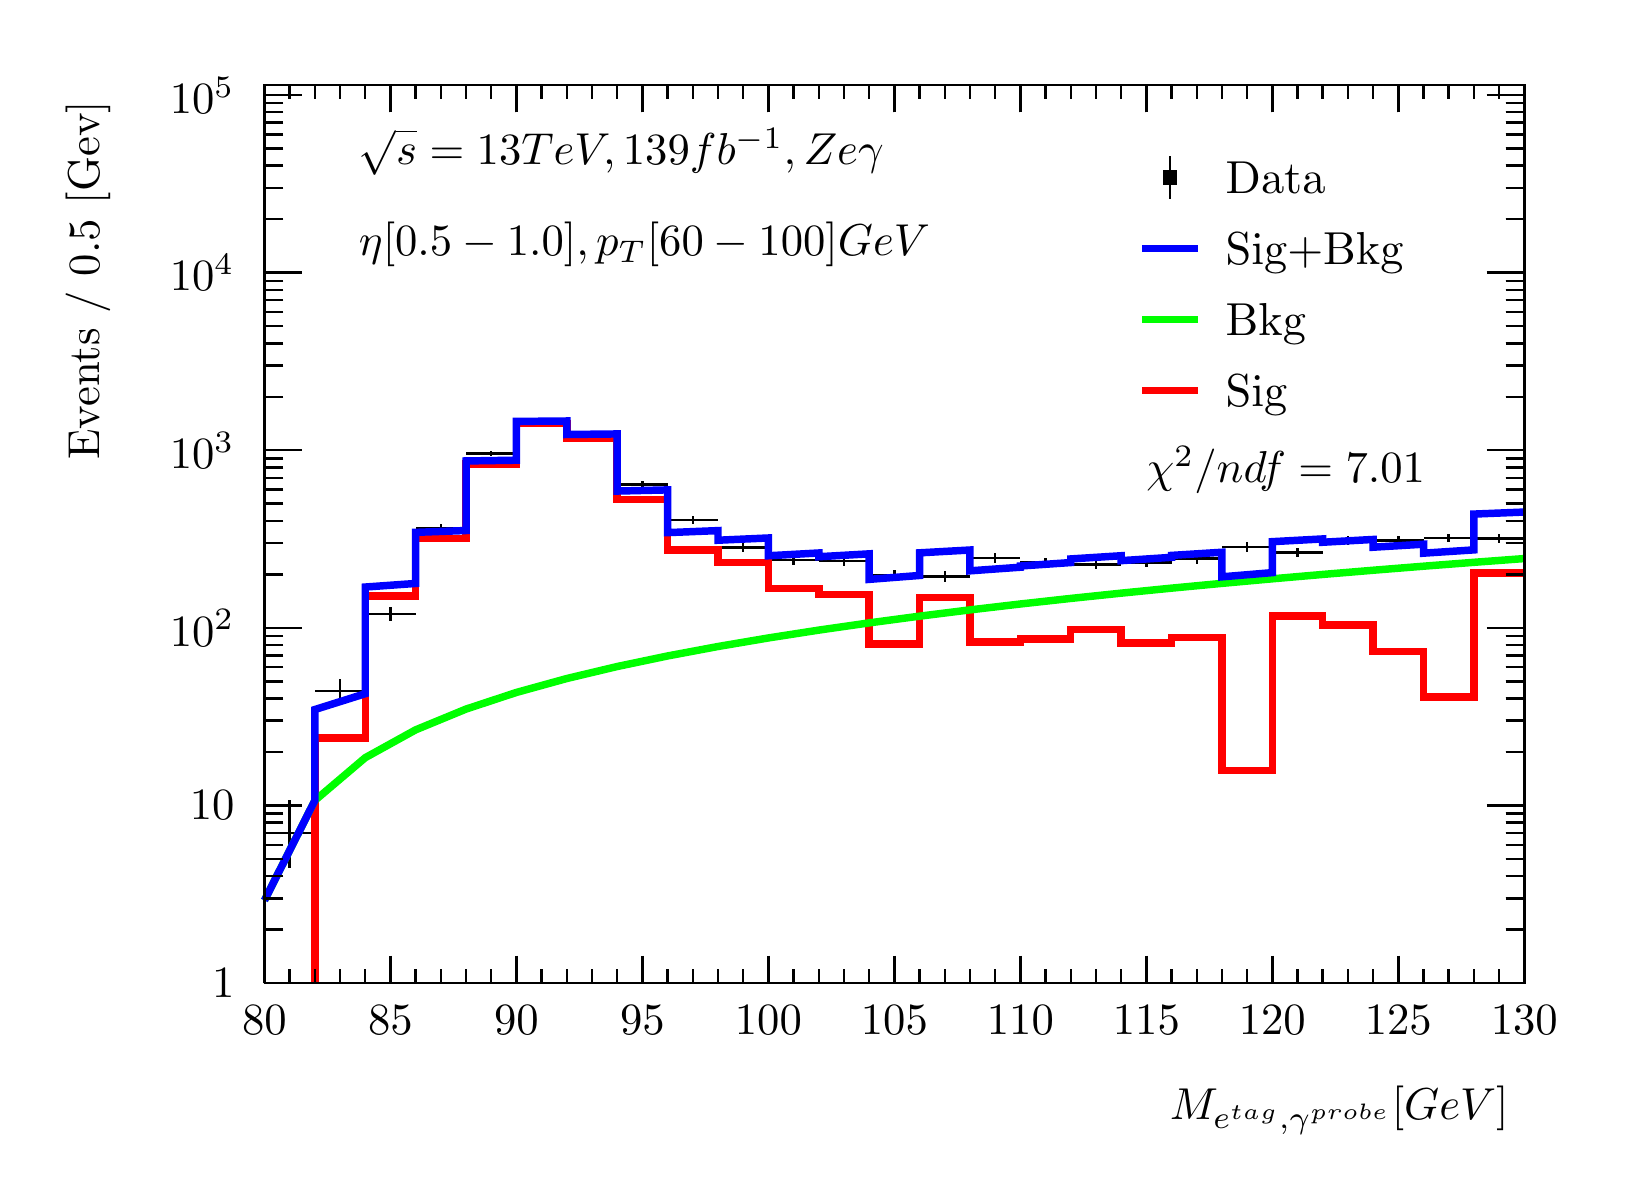
\begin{tikzpicture}
\pgfdeclareplotmark{cross} {
\pgfpathmoveto{\pgfpoint{-0.3\pgfplotmarksize}{\pgfplotmarksize}}
\pgfpathlineto{\pgfpoint{+0.3\pgfplotmarksize}{\pgfplotmarksize}}
\pgfpathlineto{\pgfpoint{+0.3\pgfplotmarksize}{0.3\pgfplotmarksize}}
\pgfpathlineto{\pgfpoint{+1\pgfplotmarksize}{0.3\pgfplotmarksize}}
\pgfpathlineto{\pgfpoint{+1\pgfplotmarksize}{-0.3\pgfplotmarksize}}
\pgfpathlineto{\pgfpoint{+0.3\pgfplotmarksize}{-0.3\pgfplotmarksize}}
\pgfpathlineto{\pgfpoint{+0.3\pgfplotmarksize}{-1.\pgfplotmarksize}}
\pgfpathlineto{\pgfpoint{-0.3\pgfplotmarksize}{-1.\pgfplotmarksize}}
\pgfpathlineto{\pgfpoint{-0.3\pgfplotmarksize}{-0.3\pgfplotmarksize}}
\pgfpathlineto{\pgfpoint{-1.\pgfplotmarksize}{-0.3\pgfplotmarksize}}
\pgfpathlineto{\pgfpoint{-1.\pgfplotmarksize}{0.3\pgfplotmarksize}}
\pgfpathlineto{\pgfpoint{-0.3\pgfplotmarksize}{0.3\pgfplotmarksize}}
\pgfpathclose
\pgfusepathqstroke
}
\pgfdeclareplotmark{cross*} {
\pgfpathmoveto{\pgfpoint{-0.3\pgfplotmarksize}{\pgfplotmarksize}}
\pgfpathlineto{\pgfpoint{+0.3\pgfplotmarksize}{\pgfplotmarksize}}
\pgfpathlineto{\pgfpoint{+0.3\pgfplotmarksize}{0.3\pgfplotmarksize}}
\pgfpathlineto{\pgfpoint{+1\pgfplotmarksize}{0.3\pgfplotmarksize}}
\pgfpathlineto{\pgfpoint{+1\pgfplotmarksize}{-0.3\pgfplotmarksize}}
\pgfpathlineto{\pgfpoint{+0.3\pgfplotmarksize}{-0.3\pgfplotmarksize}}
\pgfpathlineto{\pgfpoint{+0.3\pgfplotmarksize}{-1.\pgfplotmarksize}}
\pgfpathlineto{\pgfpoint{-0.3\pgfplotmarksize}{-1.\pgfplotmarksize}}
\pgfpathlineto{\pgfpoint{-0.3\pgfplotmarksize}{-0.3\pgfplotmarksize}}
\pgfpathlineto{\pgfpoint{-1.\pgfplotmarksize}{-0.3\pgfplotmarksize}}
\pgfpathlineto{\pgfpoint{-1.\pgfplotmarksize}{0.3\pgfplotmarksize}}
\pgfpathlineto{\pgfpoint{-0.3\pgfplotmarksize}{0.3\pgfplotmarksize}}
\pgfpathclose
\pgfusepathqfillstroke
}
\pgfdeclareplotmark{newstar} {
\pgfpathmoveto{\pgfqpoint{0pt}{\pgfplotmarksize}}
\pgfpathlineto{\pgfqpointpolar{44}{0.5\pgfplotmarksize}}
\pgfpathlineto{\pgfqpointpolar{18}{\pgfplotmarksize}}
\pgfpathlineto{\pgfqpointpolar{-20}{0.5\pgfplotmarksize}}
\pgfpathlineto{\pgfqpointpolar{-54}{\pgfplotmarksize}}
\pgfpathlineto{\pgfqpointpolar{-90}{0.5\pgfplotmarksize}}
\pgfpathlineto{\pgfqpointpolar{234}{\pgfplotmarksize}}
\pgfpathlineto{\pgfqpointpolar{198}{0.5\pgfplotmarksize}}
\pgfpathlineto{\pgfqpointpolar{162}{\pgfplotmarksize}}
\pgfpathlineto{\pgfqpointpolar{134}{0.5\pgfplotmarksize}}
\pgfpathclose
\pgfusepathqstroke
}
\pgfdeclareplotmark{newstar*} {
\pgfpathmoveto{\pgfqpoint{0pt}{\pgfplotmarksize}}
\pgfpathlineto{\pgfqpointpolar{44}{0.5\pgfplotmarksize}}
\pgfpathlineto{\pgfqpointpolar{18}{\pgfplotmarksize}}
\pgfpathlineto{\pgfqpointpolar{-20}{0.5\pgfplotmarksize}}
\pgfpathlineto{\pgfqpointpolar{-54}{\pgfplotmarksize}}
\pgfpathlineto{\pgfqpointpolar{-90}{0.5\pgfplotmarksize}}
\pgfpathlineto{\pgfqpointpolar{234}{\pgfplotmarksize}}
\pgfpathlineto{\pgfqpointpolar{198}{0.5\pgfplotmarksize}}
\pgfpathlineto{\pgfqpointpolar{162}{\pgfplotmarksize}}
\pgfpathlineto{\pgfqpointpolar{134}{0.5\pgfplotmarksize}}
\pgfpathclose
\pgfusepathqfillstroke
}
\definecolor{c}{rgb}{1,1,1};
\draw [color=c, fill=c] (0,0) rectangle (20,14.4361);
\draw [color=c, fill=c] (3,2.30977) rectangle (19,13.7143);
\definecolor{c}{rgb}{0,0,0};
\draw [c,line width=0.9] (3,2.30977) -- (3,13.7143) -- (19,13.7143) -- (19,2.30977) -- (3,2.30977);
\definecolor{c}{rgb}{1,1,1};
\draw [color=c, fill=c] (3,2.30977) rectangle (19,13.7143);
\definecolor{c}{rgb}{0,0,0};
\draw [c,line width=0.9] (3,2.30977) -- (3,13.7143) -- (19,13.7143) -- (19,2.30977) -- (3,2.30977);
\draw [c,line width=0.9] (3,2.30977) -- (19,2.30977);
\draw [c,line width=0.9] (3,2.65624) -- (3,2.30977);
\draw [c,line width=0.9] (3.32,2.48301) -- (3.32,2.30977);
\draw [c,line width=0.9] (3.64,2.48301) -- (3.64,2.30977);
\draw [c,line width=0.9] (3.96,2.48301) -- (3.96,2.30977);
\draw [c,line width=0.9] (4.28,2.48301) -- (4.28,2.30977);
\draw [c,line width=0.9] (4.6,2.65624) -- (4.6,2.30977);
\draw [c,line width=0.9] (4.92,2.48301) -- (4.92,2.30977);
\draw [c,line width=0.9] (5.24,2.48301) -- (5.24,2.30977);
\draw [c,line width=0.9] (5.56,2.48301) -- (5.56,2.30977);
\draw [c,line width=0.9] (5.88,2.48301) -- (5.88,2.30977);
\draw [c,line width=0.9] (6.2,2.65624) -- (6.2,2.30977);
\draw [c,line width=0.9] (6.52,2.48301) -- (6.52,2.30977);
\draw [c,line width=0.9] (6.84,2.48301) -- (6.84,2.30977);
\draw [c,line width=0.9] (7.16,2.48301) -- (7.16,2.30977);
\draw [c,line width=0.9] (7.48,2.48301) -- (7.48,2.30977);
\draw [c,line width=0.9] (7.8,2.65624) -- (7.8,2.30977);
\draw [c,line width=0.9] (8.12,2.48301) -- (8.12,2.30977);
\draw [c,line width=0.9] (8.44,2.48301) -- (8.44,2.30977);
\draw [c,line width=0.9] (8.76,2.48301) -- (8.76,2.30977);
\draw [c,line width=0.9] (9.08,2.48301) -- (9.08,2.30977);
\draw [c,line width=0.9] (9.4,2.65624) -- (9.4,2.30977);
\draw [c,line width=0.9] (9.72,2.48301) -- (9.72,2.30977);
\draw [c,line width=0.9] (10.04,2.48301) -- (10.04,2.30977);
\draw [c,line width=0.9] (10.36,2.48301) -- (10.36,2.30977);
\draw [c,line width=0.9] (10.68,2.48301) -- (10.68,2.30977);
\draw [c,line width=0.9] (11,2.65624) -- (11,2.30977);
\draw [c,line width=0.9] (11.32,2.48301) -- (11.32,2.30977);
\draw [c,line width=0.9] (11.64,2.48301) -- (11.64,2.30977);
\draw [c,line width=0.9] (11.96,2.48301) -- (11.96,2.30977);
\draw [c,line width=0.9] (12.28,2.48301) -- (12.28,2.30977);
\draw [c,line width=0.9] (12.6,2.65624) -- (12.6,2.30977);
\draw [c,line width=0.9] (12.92,2.48301) -- (12.92,2.30977);
\draw [c,line width=0.9] (13.24,2.48301) -- (13.24,2.30977);
\draw [c,line width=0.9] (13.56,2.48301) -- (13.56,2.30977);
\draw [c,line width=0.9] (13.88,2.48301) -- (13.88,2.30977);
\draw [c,line width=0.9] (14.2,2.65624) -- (14.2,2.30977);
\draw [c,line width=0.9] (14.52,2.48301) -- (14.52,2.30977);
\draw [c,line width=0.9] (14.84,2.48301) -- (14.84,2.30977);
\draw [c,line width=0.9] (15.16,2.48301) -- (15.16,2.30977);
\draw [c,line width=0.9] (15.48,2.48301) -- (15.48,2.30977);
\draw [c,line width=0.9] (15.8,2.65624) -- (15.8,2.30977);
\draw [c,line width=0.9] (16.12,2.48301) -- (16.12,2.30977);
\draw [c,line width=0.9] (16.44,2.48301) -- (16.44,2.30977);
\draw [c,line width=0.9] (16.76,2.48301) -- (16.76,2.30977);
\draw [c,line width=0.9] (17.08,2.48301) -- (17.08,2.30977);
\draw [c,line width=0.9] (17.4,2.65624) -- (17.4,2.30977);
\draw [c,line width=0.9] (17.72,2.48301) -- (17.72,2.30977);
\draw [c,line width=0.9] (18.04,2.48301) -- (18.04,2.30977);
\draw [c,line width=0.9] (18.36,2.48301) -- (18.36,2.30977);
\draw [c,line width=0.9] (18.68,2.48301) -- (18.68,2.30977);
\draw [c,line width=0.9] (19,2.65624) -- (19,2.30977);
\draw [anchor=base] (3,1.66015) node[scale=1.61424, color=c, rotate=0]{80};
\draw [anchor=base] (4.6,1.66015) node[scale=1.61424, color=c, rotate=0]{85};
\draw [anchor=base] (6.2,1.66015) node[scale=1.61424, color=c, rotate=0]{90};
\draw [anchor=base] (7.8,1.66015) node[scale=1.61424, color=c, rotate=0]{95};
\draw [anchor=base] (9.4,1.66015) node[scale=1.61424, color=c, rotate=0]{100};
\draw [anchor=base] (11,1.66015) node[scale=1.61424, color=c, rotate=0]{105};
\draw [anchor=base] (12.6,1.66015) node[scale=1.61424, color=c, rotate=0]{110};
\draw [anchor=base] (14.2,1.66015) node[scale=1.61424, color=c, rotate=0]{115};
\draw [anchor=base] (15.8,1.66015) node[scale=1.61424, color=c, rotate=0]{120};
\draw [anchor=base] (17.4,1.66015) node[scale=1.61424, color=c, rotate=0]{125};
\draw [anchor=base] (19,1.66015) node[scale=1.61424, color=c, rotate=0]{130};
\draw [anchor= east] (19,0.692932) node[scale=1.61424, color=c, rotate=0]{$M_{e^{tag}, \gamma^{probe}}  [GeV]$};
\draw [c,line width=0.9] (3,13.7143) -- (19,13.7143);
\draw [c,line width=0.9] (3,13.3678) -- (3,13.7143);
\draw [c,line width=0.9] (3.32,13.5411) -- (3.32,13.7143);
\draw [c,line width=0.9] (3.64,13.5411) -- (3.64,13.7143);
\draw [c,line width=0.9] (3.96,13.5411) -- (3.96,13.7143);
\draw [c,line width=0.9] (4.28,13.5411) -- (4.28,13.7143);
\draw [c,line width=0.9] (4.6,13.3678) -- (4.6,13.7143);
\draw [c,line width=0.9] (4.92,13.5411) -- (4.92,13.7143);
\draw [c,line width=0.9] (5.24,13.5411) -- (5.24,13.7143);
\draw [c,line width=0.9] (5.56,13.5411) -- (5.56,13.7143);
\draw [c,line width=0.9] (5.88,13.5411) -- (5.88,13.7143);
\draw [c,line width=0.9] (6.2,13.3678) -- (6.2,13.7143);
\draw [c,line width=0.9] (6.52,13.5411) -- (6.52,13.7143);
\draw [c,line width=0.9] (6.84,13.5411) -- (6.84,13.7143);
\draw [c,line width=0.9] (7.16,13.5411) -- (7.16,13.7143);
\draw [c,line width=0.9] (7.48,13.5411) -- (7.48,13.7143);
\draw [c,line width=0.9] (7.8,13.3678) -- (7.8,13.7143);
\draw [c,line width=0.9] (8.12,13.5411) -- (8.12,13.7143);
\draw [c,line width=0.9] (8.44,13.5411) -- (8.44,13.7143);
\draw [c,line width=0.9] (8.76,13.5411) -- (8.76,13.7143);
\draw [c,line width=0.9] (9.08,13.5411) -- (9.08,13.7143);
\draw [c,line width=0.9] (9.4,13.3678) -- (9.4,13.7143);
\draw [c,line width=0.9] (9.72,13.5411) -- (9.72,13.7143);
\draw [c,line width=0.9] (10.04,13.5411) -- (10.04,13.7143);
\draw [c,line width=0.9] (10.36,13.5411) -- (10.36,13.7143);
\draw [c,line width=0.9] (10.68,13.5411) -- (10.68,13.7143);
\draw [c,line width=0.9] (11,13.3678) -- (11,13.7143);
\draw [c,line width=0.9] (11.32,13.5411) -- (11.32,13.7143);
\draw [c,line width=0.9] (11.64,13.5411) -- (11.64,13.7143);
\draw [c,line width=0.9] (11.96,13.5411) -- (11.96,13.7143);
\draw [c,line width=0.9] (12.28,13.5411) -- (12.28,13.7143);
\draw [c,line width=0.9] (12.6,13.3678) -- (12.6,13.7143);
\draw [c,line width=0.9] (12.92,13.5411) -- (12.92,13.7143);
\draw [c,line width=0.9] (13.24,13.5411) -- (13.24,13.7143);
\draw [c,line width=0.9] (13.56,13.5411) -- (13.56,13.7143);
\draw [c,line width=0.9] (13.88,13.5411) -- (13.88,13.7143);
\draw [c,line width=0.9] (14.2,13.3678) -- (14.2,13.7143);
\draw [c,line width=0.9] (14.52,13.5411) -- (14.52,13.7143);
\draw [c,line width=0.9] (14.84,13.5411) -- (14.84,13.7143);
\draw [c,line width=0.9] (15.16,13.5411) -- (15.16,13.7143);
\draw [c,line width=0.9] (15.48,13.5411) -- (15.48,13.7143);
\draw [c,line width=0.9] (15.8,13.3678) -- (15.8,13.7143);
\draw [c,line width=0.9] (16.12,13.5411) -- (16.12,13.7143);
\draw [c,line width=0.9] (16.44,13.5411) -- (16.44,13.7143);
\draw [c,line width=0.9] (16.76,13.5411) -- (16.76,13.7143);
\draw [c,line width=0.9] (17.08,13.5411) -- (17.08,13.7143);
\draw [c,line width=0.9] (17.4,13.3678) -- (17.4,13.7143);
\draw [c,line width=0.9] (17.72,13.5411) -- (17.72,13.7143);
\draw [c,line width=0.9] (18.04,13.5411) -- (18.04,13.7143);
\draw [c,line width=0.9] (18.36,13.5411) -- (18.36,13.7143);
\draw [c,line width=0.9] (18.68,13.5411) -- (18.68,13.7143);
\draw [c,line width=0.9] (19,13.3678) -- (19,13.7143);
\draw [c,line width=0.9] (3,2.30977) -- (3,13.7143);
\draw [c,line width=0.9] (3.474,2.30978) -- (3,2.30978);
\draw [anchor= east] (2.82,2.30978) node[scale=1.61424, color=c, rotate=0]{1};
\draw [c,line width=0.9] (3.237,2.98876) -- (3,2.98876);
\draw [c,line width=0.9] (3.237,3.38594) -- (3,3.38594);
\draw [c,line width=0.9] (3.237,3.66775) -- (3,3.66775);
\draw [c,line width=0.9] (3.237,3.88633) -- (3,3.88633);
\draw [c,line width=0.9] (3.237,4.06493) -- (3,4.06493);
\draw [c,line width=0.9] (3.237,4.21593) -- (3,4.21593);
\draw [c,line width=0.9] (3.237,4.34673) -- (3,4.34673);
\draw [c,line width=0.9] (3.237,4.46211) -- (3,4.46211);
\draw [c,line width=0.9] (3.474,4.56532) -- (3,4.56532);
\draw [anchor= east] (2.82,4.56532) node[scale=1.61424, color=c, rotate=0]{10};
\draw [c,line width=0.9] (3.237,5.2443) -- (3,5.2443);
\draw [c,line width=0.9] (3.237,5.64148) -- (3,5.64148);
\draw [c,line width=0.9] (3.237,5.92329) -- (3,5.92329);
\draw [c,line width=0.9] (3.237,6.14187) -- (3,6.14187);
\draw [c,line width=0.9] (3.237,6.32047) -- (3,6.32047);
\draw [c,line width=0.9] (3.237,6.47147) -- (3,6.47147);
\draw [c,line width=0.9] (3.237,6.60227) -- (3,6.60227);
\draw [c,line width=0.9] (3.237,6.71765) -- (3,6.71765);
\draw [c,line width=0.9] (3.474,6.82086) -- (3,6.82086);
\draw [anchor= east] (2.82,6.82086) node[scale=1.61424, color=c, rotate=0]{$10^{2}$};
\draw [c,line width=0.9] (3.237,7.49984) -- (3,7.49984);
\draw [c,line width=0.9] (3.237,7.89703) -- (3,7.89703);
\draw [c,line width=0.9] (3.237,8.17883) -- (3,8.17883);
\draw [c,line width=0.9] (3.237,8.39741) -- (3,8.39741);
\draw [c,line width=0.9] (3.237,8.57601) -- (3,8.57601);
\draw [c,line width=0.9] (3.237,8.72701) -- (3,8.72701);
\draw [c,line width=0.9] (3.237,8.85782) -- (3,8.85782);
\draw [c,line width=0.9] (3.237,8.97319) -- (3,8.97319);
\draw [c,line width=0.9] (3.474,9.0764) -- (3,9.0764);
\draw [anchor= east] (2.82,9.0764) node[scale=1.61424, color=c, rotate=0]{$10^{3}$};
\draw [c,line width=0.9] (3.237,9.75539) -- (3,9.75539);
\draw [c,line width=0.9] (3.237,10.1526) -- (3,10.1526);
\draw [c,line width=0.9] (3.237,10.4344) -- (3,10.4344);
\draw [c,line width=0.9] (3.237,10.653) -- (3,10.653);
\draw [c,line width=0.9] (3.237,10.8316) -- (3,10.8316);
\draw [c,line width=0.9] (3.237,10.9826) -- (3,10.9826);
\draw [c,line width=0.9] (3.237,11.1134) -- (3,11.1134);
\draw [c,line width=0.9] (3.237,11.2287) -- (3,11.2287);
\draw [c,line width=0.9] (3.474,11.3319) -- (3,11.3319);
\draw [anchor= east] (2.82,11.3319) node[scale=1.61424, color=c, rotate=0]{$10^{4}$};
\draw [c,line width=0.9] (3.237,12.0109) -- (3,12.0109);
\draw [c,line width=0.9] (3.237,12.4081) -- (3,12.4081);
\draw [c,line width=0.9] (3.237,12.6899) -- (3,12.6899);
\draw [c,line width=0.9] (3.237,12.9085) -- (3,12.9085);
\draw [c,line width=0.9] (3.237,13.0871) -- (3,13.0871);
\draw [c,line width=0.9] (3.237,13.2381) -- (3,13.2381);
\draw [c,line width=0.9] (3.237,13.3689) -- (3,13.3689);
\draw [c,line width=0.9] (3.237,13.4843) -- (3,13.4843);
\draw [c,line width=0.9] (3.474,13.5875) -- (3,13.5875);
\draw [anchor= east] (2.82,13.5875) node[scale=1.61424, color=c, rotate=0]{$10^{5}$};
\draw [anchor= east] (0.76,13.7143) node[scale=1.61424, color=c, rotate=90]{Events / 0.5 [Gev]};
\draw [c,line width=0.9] (19,2.30977) -- (19,13.7143);
\draw [c,line width=0.9] (18.526,2.30978) -- (19,2.30978);
\draw [c,line width=0.9] (18.763,2.98876) -- (19,2.98876);
\draw [c,line width=0.9] (18.763,3.38594) -- (19,3.38594);
\draw [c,line width=0.9] (18.763,3.66775) -- (19,3.66775);
\draw [c,line width=0.9] (18.763,3.88633) -- (19,3.88633);
\draw [c,line width=0.9] (18.763,4.06493) -- (19,4.06493);
\draw [c,line width=0.9] (18.763,4.21593) -- (19,4.21593);
\draw [c,line width=0.9] (18.763,4.34673) -- (19,4.34673);
\draw [c,line width=0.9] (18.763,4.46211) -- (19,4.46211);
\draw [c,line width=0.9] (18.526,4.56532) -- (19,4.56532);
\draw [c,line width=0.9] (18.763,5.2443) -- (19,5.2443);
\draw [c,line width=0.9] (18.763,5.64148) -- (19,5.64148);
\draw [c,line width=0.9] (18.763,5.92329) -- (19,5.92329);
\draw [c,line width=0.9] (18.763,6.14187) -- (19,6.14187);
\draw [c,line width=0.9] (18.763,6.32047) -- (19,6.32047);
\draw [c,line width=0.9] (18.763,6.47147) -- (19,6.47147);
\draw [c,line width=0.9] (18.763,6.60227) -- (19,6.60227);
\draw [c,line width=0.9] (18.763,6.71765) -- (19,6.71765);
\draw [c,line width=0.9] (18.526,6.82086) -- (19,6.82086);
\draw [c,line width=0.9] (18.763,7.49984) -- (19,7.49984);
\draw [c,line width=0.9] (18.763,7.89703) -- (19,7.89703);
\draw [c,line width=0.9] (18.763,8.17883) -- (19,8.17883);
\draw [c,line width=0.9] (18.763,8.39741) -- (19,8.39741);
\draw [c,line width=0.9] (18.763,8.57601) -- (19,8.57601);
\draw [c,line width=0.9] (18.763,8.72701) -- (19,8.72701);
\draw [c,line width=0.9] (18.763,8.85782) -- (19,8.85782);
\draw [c,line width=0.9] (18.763,8.97319) -- (19,8.97319);
\draw [c,line width=0.9] (18.526,9.0764) -- (19,9.0764);
\draw [c,line width=0.9] (18.763,9.75539) -- (19,9.75539);
\draw [c,line width=0.9] (18.763,10.1526) -- (19,10.1526);
\draw [c,line width=0.9] (18.763,10.4344) -- (19,10.4344);
\draw [c,line width=0.9] (18.763,10.653) -- (19,10.653);
\draw [c,line width=0.9] (18.763,10.8316) -- (19,10.8316);
\draw [c,line width=0.9] (18.763,10.9826) -- (19,10.9826);
\draw [c,line width=0.9] (18.763,11.1134) -- (19,11.1134);
\draw [c,line width=0.9] (18.763,11.2287) -- (19,11.2287);
\draw [c,line width=0.9] (18.526,11.3319) -- (19,11.3319);
\draw [c,line width=0.9] (18.763,12.0109) -- (19,12.0109);
\draw [c,line width=0.9] (18.763,12.4081) -- (19,12.4081);
\draw [c,line width=0.9] (18.763,12.6899) -- (19,12.6899);
\draw [c,line width=0.9] (18.763,12.9085) -- (19,12.9085);
\draw [c,line width=0.9] (18.763,13.0871) -- (19,13.0871);
\draw [c,line width=0.9] (18.763,13.2381) -- (19,13.2381);
\draw [c,line width=0.9] (18.763,13.3689) -- (19,13.3689);
\draw [c,line width=0.9] (18.763,13.4843) -- (19,13.4843);
\draw [c,line width=0.9] (18.526,13.5875) -- (19,13.5875);
\draw [c,line width=0.9] (3.32,4.21593) -- (3,4.21593);
\draw [c,line width=0.9] (3,4.21593) -- (3,4.21593);
\draw [c,line width=0.9] (3.32,4.21593) -- (3.64,4.21593);
\draw [c,line width=0.9] (3.64,4.21593) -- (3.64,4.21593);
\draw [c,line width=0.9] (3.32,4.21593) -- (3.32,4.63801);
\draw [c,line width=0.9] (3.32,4.63801) -- (3.32,4.63801);
\draw [c,line width=0.9] (3.32,4.21593) -- (3.32,3.76523);
\draw [c,line width=0.9] (3.32,3.76523) -- (3.32,3.76523);
\draw [c,line width=0.9] (3.96,6.01665) -- (3.64,6.01665);
\draw [c,line width=0.9] (3.64,6.01665) -- (3.64,6.01665);
\draw [c,line width=0.9] (3.96,6.01665) -- (4.28,6.01665);
\draw [c,line width=0.9] (4.28,6.01665) -- (4.28,6.01665);
\draw [c,line width=0.9] (3.96,6.01665) -- (3.96,6.17431);
\draw [c,line width=0.9] (3.96,6.17431) -- (3.96,6.17431);
\draw [c,line width=0.9] (3.96,6.01665) -- (3.96,5.85724);
\draw [c,line width=0.9] (3.96,5.85724) -- (3.96,5.85724);
\draw [c,line width=0.9] (4.6,6.99945) -- (4.28,6.99945);
\draw [c,line width=0.9] (4.28,6.99945) -- (4.28,6.99945);
\draw [c,line width=0.9] (4.6,6.99945) -- (4.92,6.99945);
\draw [c,line width=0.9] (4.92,6.99945) -- (4.92,6.99945);
\draw [c,line width=0.9] (4.6,6.99945) -- (4.6,7.08885);
\draw [c,line width=0.9] (4.6,7.08885) -- (4.6,7.08885);
\draw [c,line width=0.9] (4.6,6.99945) -- (4.6,6.91006);
\draw [c,line width=0.9] (4.6,6.91006) -- (4.6,6.91006);
\draw [c,line width=0.9] (5.24,8.09181) -- (4.92,8.09181);
\draw [c,line width=0.9] (4.92,8.09181) -- (4.92,8.09181);
\draw [c,line width=0.9] (5.24,8.09181) -- (5.56,8.09181);
\draw [c,line width=0.9] (5.56,8.09181) -- (5.56,8.09181);
\draw [c,line width=0.9] (5.24,8.09181) -- (5.24,8.14301);
\draw [c,line width=0.9] (5.24,8.14301) -- (5.24,8.14301);
\draw [c,line width=0.9] (5.24,8.09181) -- (5.24,8.04062);
\draw [c,line width=0.9] (5.24,8.04062) -- (5.24,8.04062);
\draw [c,line width=0.9] (5.88,9.03641) -- (5.56,9.03641);
\draw [c,line width=0.9] (5.56,9.03641) -- (5.56,9.03641);
\draw [c,line width=0.9] (5.88,9.03641) -- (6.2,9.03641);
\draw [c,line width=0.9] (6.2,9.03641) -- (6.2,9.03641);
\draw [c,line width=0.9] (5.88,9.03641) -- (5.88,9.06803);
\draw [c,line width=0.9] (5.88,9.06803) -- (5.88,9.06803);
\draw [c,line width=0.9] (5.88,9.03641) -- (5.88,9.0048);
\draw [c,line width=0.9] (5.88,9.0048) -- (5.88,9.0048);
\draw [c,line width=0.9] (6.52,9.45179) -- (6.2,9.45179);
\draw [c,line width=0.9] (6.2,9.45179) -- (6.2,9.45179);
\draw [c,line width=0.9] (6.52,9.45179) -- (6.84,9.45179);
\draw [c,line width=0.9] (6.84,9.45179) -- (6.84,9.45179);
\draw [c,line width=0.9] (6.52,9.45179) -- (6.52,9.47736);
\draw [c,line width=0.9] (6.52,9.47736) -- (6.52,9.47736);
\draw [c,line width=0.9] (6.52,9.45179) -- (6.52,9.42622);
\draw [c,line width=0.9] (6.52,9.42622) -- (6.52,9.42622);
\draw [c,line width=0.9] (7.16,9.26313) -- (6.84,9.26313);
\draw [c,line width=0.9] (6.84,9.26313) -- (6.84,9.26313);
\draw [c,line width=0.9] (7.16,9.26313) -- (7.48,9.26313);
\draw [c,line width=0.9] (7.48,9.26313) -- (7.48,9.26313);
\draw [c,line width=0.9] (7.16,9.26313) -- (7.16,9.29128);
\draw [c,line width=0.9] (7.16,9.29128) -- (7.16,9.29128);
\draw [c,line width=0.9] (7.16,9.26313) -- (7.16,9.23497);
\draw [c,line width=0.9] (7.16,9.23497) -- (7.16,9.23497);
\draw [c,line width=0.9] (7.8,8.64229) -- (7.48,8.64229);
\draw [c,line width=0.9] (7.48,8.64229) -- (7.48,8.64229);
\draw [c,line width=0.9] (7.8,8.64229) -- (8.12,8.64229);
\draw [c,line width=0.9] (8.12,8.64229) -- (8.12,8.64229);
\draw [c,line width=0.9] (7.8,8.64229) -- (7.8,8.68094);
\draw [c,line width=0.9] (7.8,8.68094) -- (7.8,8.68094);
\draw [c,line width=0.9] (7.8,8.64229) -- (7.8,8.60363);
\draw [c,line width=0.9] (7.8,8.60363) -- (7.8,8.60363);
\draw [c,line width=0.9] (8.44,8.18858) -- (8.12,8.18858);
\draw [c,line width=0.9] (8.12,8.18858) -- (8.12,8.18858);
\draw [c,line width=0.9] (8.44,8.18858) -- (8.76,8.18858);
\draw [c,line width=0.9] (8.76,8.18858) -- (8.76,8.18858);
\draw [c,line width=0.9] (8.44,8.18858) -- (8.44,8.23731);
\draw [c,line width=0.9] (8.44,8.23731) -- (8.44,8.23731);
\draw [c,line width=0.9] (8.44,8.18858) -- (8.44,8.13985);
\draw [c,line width=0.9] (8.44,8.13985) -- (8.44,8.13985);
\draw [c,line width=0.9] (9.08,7.83988) -- (8.76,7.83988);
\draw [c,line width=0.9] (8.76,7.83988) -- (8.76,7.83988);
\draw [c,line width=0.9] (9.08,7.83988) -- (9.4,7.83988);
\draw [c,line width=0.9] (9.4,7.83988) -- (9.4,7.83988);
\draw [c,line width=0.9] (9.08,7.83988) -- (9.08,7.8981);
\draw [c,line width=0.9] (9.08,7.8981) -- (9.08,7.8981);
\draw [c,line width=0.9] (9.08,7.83988) -- (9.08,7.78166);
\draw [c,line width=0.9] (9.08,7.78166) -- (9.08,7.78166);
\draw [c,line width=0.9] (9.72,7.68251) -- (9.4,7.68251);
\draw [c,line width=0.9] (9.4,7.68251) -- (9.4,7.68251);
\draw [c,line width=0.9] (9.72,7.68251) -- (10.04,7.68251);
\draw [c,line width=0.9] (10.04,7.68251) -- (10.04,7.68251);
\draw [c,line width=0.9] (9.72,7.68251) -- (9.72,7.7456);
\draw [c,line width=0.9] (9.72,7.7456) -- (9.72,7.7456);
\draw [c,line width=0.9] (9.72,7.68251) -- (9.72,7.61942);
\draw [c,line width=0.9] (9.72,7.61942) -- (9.72,7.61942);
\draw [c,line width=0.9] (10.36,7.67024) -- (10.04,7.67024);
\draw [c,line width=0.9] (10.04,7.67024) -- (10.04,7.67024);
\draw [c,line width=0.9] (10.36,7.67024) -- (10.68,7.67024);
\draw [c,line width=0.9] (10.68,7.67024) -- (10.68,7.67024);
\draw [c,line width=0.9] (10.36,7.67024) -- (10.36,7.73373);
\draw [c,line width=0.9] (10.36,7.73373) -- (10.36,7.73373);
\draw [c,line width=0.9] (10.36,7.67024) -- (10.36,7.60676);
\draw [c,line width=0.9] (10.36,7.60676) -- (10.36,7.60676);
\draw [c,line width=0.9] (11,7.48504) -- (10.68,7.48504);
\draw [c,line width=0.9] (10.68,7.48504) -- (10.68,7.48504);
\draw [c,line width=0.9] (11,7.48504) -- (11.32,7.48504);
\draw [c,line width=0.9] (11.32,7.48504) -- (11.32,7.48504);
\draw [c,line width=0.9] (11,7.48504) -- (11,7.55482);
\draw [c,line width=0.9] (11,7.55482) -- (11,7.55482);
\draw [c,line width=0.9] (11,7.48504) -- (11,7.41526);
\draw [c,line width=0.9] (11,7.41526) -- (11,7.41526);
\draw [c,line width=0.9] (11.64,7.47504) -- (11.32,7.47504);
\draw [c,line width=0.9] (11.32,7.47504) -- (11.32,7.47504);
\draw [c,line width=0.9] (11.64,7.47504) -- (11.96,7.47504);
\draw [c,line width=0.9] (11.96,7.47504) -- (11.96,7.47504);
\draw [c,line width=0.9] (11.64,7.47504) -- (11.64,7.54518);
\draw [c,line width=0.9] (11.64,7.54518) -- (11.64,7.54518);
\draw [c,line width=0.9] (11.64,7.47504) -- (11.64,7.40491);
\draw [c,line width=0.9] (11.64,7.40491) -- (11.64,7.40491);
\draw [c,line width=0.9] (12.28,7.7066) -- (11.96,7.7066);
\draw [c,line width=0.9] (11.96,7.7066) -- (11.96,7.7066);
\draw [c,line width=0.9] (12.28,7.7066) -- (12.6,7.7066);
\draw [c,line width=0.9] (12.6,7.7066) -- (12.6,7.7066);
\draw [c,line width=0.9] (12.28,7.7066) -- (12.28,7.76892);
\draw [c,line width=0.9] (12.28,7.76892) -- (12.28,7.76892);
\draw [c,line width=0.9] (12.28,7.7066) -- (12.28,7.64428);
\draw [c,line width=0.9] (12.28,7.64428) -- (12.28,7.64428);
\draw [c,line width=0.9] (12.92,7.64944) -- (12.6,7.64944);
\draw [c,line width=0.9] (12.6,7.64944) -- (12.6,7.64944);
\draw [c,line width=0.9] (12.92,7.64944) -- (13.24,7.64944);
\draw [c,line width=0.9] (13.24,7.64944) -- (13.24,7.64944);
\draw [c,line width=0.9] (12.92,7.64944) -- (12.92,7.71361);
\draw [c,line width=0.9] (12.92,7.71361) -- (12.92,7.71361);
\draw [c,line width=0.9] (12.92,7.64944) -- (12.92,7.58528);
\draw [c,line width=0.9] (12.92,7.58528) -- (12.92,7.58528);
\draw [c,line width=0.9] (13.56,7.62819) -- (13.24,7.62819);
\draw [c,line width=0.9] (13.24,7.62819) -- (13.24,7.62819);
\draw [c,line width=0.9] (13.56,7.62819) -- (13.88,7.62819);
\draw [c,line width=0.9] (13.88,7.62819) -- (13.88,7.62819);
\draw [c,line width=0.9] (13.56,7.62819) -- (13.56,7.69306);
\draw [c,line width=0.9] (13.56,7.69306) -- (13.56,7.69306);
\draw [c,line width=0.9] (13.56,7.62819) -- (13.56,7.56333);
\draw [c,line width=0.9] (13.56,7.56333) -- (13.56,7.56333);
\draw [c,line width=0.9] (14.2,7.65364) -- (13.88,7.65364);
\draw [c,line width=0.9] (13.88,7.65364) -- (13.88,7.65364);
\draw [c,line width=0.9] (14.2,7.65364) -- (14.52,7.65364);
\draw [c,line width=0.9] (14.52,7.65364) -- (14.52,7.65364);
\draw [c,line width=0.9] (14.2,7.65364) -- (14.2,7.71766);
\draw [c,line width=0.9] (14.2,7.71766) -- (14.2,7.71766);
\draw [c,line width=0.9] (14.2,7.65364) -- (14.2,7.58961);
\draw [c,line width=0.9] (14.2,7.58961) -- (14.2,7.58961);
\draw [c,line width=0.9] (14.84,7.69864) -- (14.52,7.69864);
\draw [c,line width=0.9] (14.52,7.69864) -- (14.52,7.69864);
\draw [c,line width=0.9] (14.84,7.69864) -- (15.16,7.69864);
\draw [c,line width=0.9] (15.16,7.69864) -- (15.16,7.69864);
\draw [c,line width=0.9] (14.84,7.69864) -- (14.84,7.76121);
\draw [c,line width=0.9] (14.84,7.76121) -- (14.84,7.76121);
\draw [c,line width=0.9] (14.84,7.69864) -- (14.84,7.63607);
\draw [c,line width=0.9] (14.84,7.63607) -- (14.84,7.63607);
\draw [c,line width=0.9] (15.48,7.84678) -- (15.16,7.84678);
\draw [c,line width=0.9] (15.16,7.84678) -- (15.16,7.84678);
\draw [c,line width=0.9] (15.48,7.84678) -- (15.8,7.84678);
\draw [c,line width=0.9] (15.8,7.84678) -- (15.8,7.84678);
\draw [c,line width=0.9] (15.48,7.84678) -- (15.48,7.9048);
\draw [c,line width=0.9] (15.48,7.9048) -- (15.48,7.9048);
\draw [c,line width=0.9] (15.48,7.84678) -- (15.48,7.78876);
\draw [c,line width=0.9] (15.48,7.78876) -- (15.48,7.78876);
\draw [c,line width=0.9] (16.12,7.77551) -- (15.8,7.77551);
\draw [c,line width=0.9] (15.8,7.77551) -- (15.8,7.77551);
\draw [c,line width=0.9] (16.12,7.77551) -- (16.44,7.77551);
\draw [c,line width=0.9] (16.44,7.77551) -- (16.44,7.77551);
\draw [c,line width=0.9] (16.12,7.77551) -- (16.12,7.83567);
\draw [c,line width=0.9] (16.12,7.83567) -- (16.12,7.83567);
\draw [c,line width=0.9] (16.12,7.77551) -- (16.12,7.71534);
\draw [c,line width=0.9] (16.12,7.71534) -- (16.12,7.71534);
\draw [c,line width=0.9] (16.76,7.92914) -- (16.44,7.92914);
\draw [c,line width=0.9] (16.44,7.92914) -- (16.44,7.92914);
\draw [c,line width=0.9] (16.76,7.92914) -- (17.08,7.92914);
\draw [c,line width=0.9] (17.08,7.92914) -- (17.08,7.92914);
\draw [c,line width=0.9] (16.76,7.92914) -- (16.76,7.98477);
\draw [c,line width=0.9] (16.76,7.98477) -- (16.76,7.98477);
\draw [c,line width=0.9] (16.76,7.92914) -- (16.76,7.87352);
\draw [c,line width=0.9] (16.76,7.87352) -- (16.76,7.87352);
\draw [c,line width=0.9] (17.4,7.9323) -- (17.08,7.9323);
\draw [c,line width=0.9] (17.08,7.9323) -- (17.08,7.9323);
\draw [c,line width=0.9] (17.4,7.9323) -- (17.72,7.9323);
\draw [c,line width=0.9] (17.72,7.9323) -- (17.72,7.9323);
\draw [c,line width=0.9] (17.4,7.9323) -- (17.4,7.98784);
\draw [c,line width=0.9] (17.4,7.98784) -- (17.4,7.98784);
\draw [c,line width=0.9] (17.4,7.9323) -- (17.4,7.87676);
\draw [c,line width=0.9] (17.4,7.87676) -- (17.4,7.87676);
\draw [c,line width=0.9] (18.04,7.9633) -- (17.72,7.9633);
\draw [c,line width=0.9] (17.72,7.9633) -- (17.72,7.9633);
\draw [c,line width=0.9] (18.04,7.9633) -- (18.36,7.9633);
\draw [c,line width=0.9] (18.36,7.9633) -- (18.36,7.9633);
\draw [c,line width=0.9] (18.04,7.9633) -- (18.04,8.01797);
\draw [c,line width=0.9] (18.04,8.01797) -- (18.04,8.01797);
\draw [c,line width=0.9] (18.04,7.9633) -- (18.04,7.90863);
\draw [c,line width=0.9] (18.04,7.90863) -- (18.04,7.90863);
\draw [c,line width=0.9] (18.68,7.95718) -- (18.36,7.95718);
\draw [c,line width=0.9] (18.36,7.95718) -- (18.36,7.95718);
\draw [c,line width=0.9] (18.68,7.95718) -- (19,7.95718);
\draw [c,line width=0.9] (19,7.95718) -- (19,7.95718);
\draw [c,line width=0.9] (18.68,7.95718) -- (18.68,8.01202);
\draw [c,line width=0.9] (18.68,8.01202) -- (18.68,8.01202);
\draw [c,line width=0.9] (18.68,7.95718) -- (18.68,7.90234);
\draw [c,line width=0.9] (18.68,7.90234) -- (18.68,7.90234);
\foreach \P in {(3.32,4.21593), (3.96,6.01665), (4.6,6.99945), (5.24,8.09181), (5.88,9.03641), (6.52,9.45179), (7.16,9.26313), (7.8,8.64229), (8.44,8.18858), (9.08,7.83988), (9.72,7.68251), (10.36,7.67024), (11,7.48504), (11.64,7.47504),
 (12.28,7.7066), (12.92,7.64944), (13.56,7.62819), (14.2,7.65364), (14.84,7.69864), (15.48,7.84678), (16.12,7.77551), (16.76,7.92914), (17.4,7.9323), (18.04,7.9633), (18.68,7.95718)}{\draw[mark options={color=c,fill=c},mark size=2.882883pt,mark=]
 plot coordinates {\P};}
\definecolor{c}{rgb}{1,0,0};
\draw [c,line width=2.7] (3.64,2.30977) -- (3.64,5.42308);
\draw [c,line width=2.7] (3.64,5.42308) -- (4.28,5.42308) -- (4.28,7.2256) -- (4.92,7.2256) -- (4.92,7.95491) -- (5.56,7.95491) -- (5.56,8.90034) -- (6.2,8.90034) -- (6.2,9.41267) -- (6.84,9.41267) -- (6.84,9.23412) -- (7.48,9.23412) --
 (7.48,8.45179) -- (8.12,8.45179) -- (8.12,7.80916) -- (8.76,7.80916) -- (8.76,7.6491) -- (9.4,7.6491) -- (9.4,7.32258) -- (10.04,7.32258) -- (10.04,7.24607) -- (10.68,7.24607) -- (10.68,6.61279) -- (11.32,6.61279) -- (11.32,7.20566) --
 (11.96,7.20566) -- (11.96,6.64086) -- (12.6,6.64086) -- (12.6,6.68096) -- (13.24,6.68096) -- (13.24,6.80023) -- (13.88,6.80023) -- (13.88,6.62825) -- (14.52,6.62825) -- (14.52,6.70082) -- (15.16,6.70082) -- (15.16,5.0102) -- (15.8,5.0102) --
 (15.8,6.9734) -- (16.44,6.9734) -- (16.44,6.85468) -- (17.08,6.85468) -- (17.08,6.5179) -- (17.72,6.5179) -- (17.72,5.94537) -- (18.36,5.94537) -- (18.36,7.51556) -- (19,7.51556) -- (19,7.51556) -- (19,7.51556) -- (19,7.51556);
\definecolor{c}{rgb}{0,1,0};
\draw [c,line width=2.7] (3,3.35884) -- (3,3.35884);
\draw [c,line width=2.7] (3,3.35884) -- (3,3.35884) -- (3.64,4.6283) -- (3.64,4.6283) -- (4.28,5.1718) -- (4.28,5.1718) -- (4.92,5.52533) -- (4.92,5.52533) -- (5.56,5.78915) -- (5.56,5.78915) -- (6.2,6.00048) -- (6.2,6.00048) -- (6.84,6.1773) --
 (6.84,6.1773) -- (7.48,6.32968) -- (7.48,6.32968) -- (8.12,6.46381) -- (8.12,6.46381) -- (8.76,6.58381) -- (8.76,6.58381) -- (9.4,6.69252) -- (9.4,6.69252) -- (10.04,6.79202) -- (10.04,6.79202) -- (10.68,6.88383) -- (10.68,6.88383) --
 (11.32,6.96914) -- (11.32,6.96914) -- (11.96,7.04889) -- (11.96,7.04889) -- (12.6,7.1238) -- (12.6,7.1238) -- (13.24,7.19448) -- (13.24,7.19448) -- (13.88,7.26142) -- (13.88,7.26142) -- (14.52,7.32503) -- (14.52,7.32503) -- (15.16,7.38567) --
 (15.16,7.38567) -- (15.8,7.44361) -- (15.8,7.44361) -- (16.44,7.49912) -- (16.44,7.49912) -- (17.08,7.5524) -- (17.08,7.5524) -- (17.72,7.60366) -- (17.72,7.60366) -- (18.36,7.65305) -- (18.36,7.65305) -- (19,7.70072) -- (19,7.70072) -- (19,7.70072)
 -- (19,7.70072);
\definecolor{c}{rgb}{0,0,1};
\draw [c,line width=2.7] (3,3.35884) -- (3,3.35884);
\draw [c,line width=2.7] (3,3.35884) -- (3,3.35884) -- (3.64,4.6283) -- (3.64,5.78316) -- (4.28,5.98446) -- (4.28,7.33912) -- (4.92,7.38463) -- (4.92,8.03367) -- (5.56,8.05679) -- (5.56,8.9404) -- (6.2,8.94981) -- (6.2,9.44229) -- (6.84,9.44805) --
 (6.84,9.27642) -- (7.48,9.28337) -- (7.48,8.55806) -- (8.12,8.57273) -- (8.12,8.03028) -- (8.76,8.05575) -- (8.76,7.93363) -- (9.4,7.9622) -- (9.4,7.73635) -- (10.04,7.77178) -- (10.04,7.72411) -- (10.68,7.76059) -- (10.68,7.43664) --
 (11.32,7.48607) -- (11.32,7.77351) -- (11.96,7.80939) -- (11.96,7.54495) -- (12.6,7.59078) -- (12.6,7.60618) -- (13.24,7.64998) -- (13.24,7.69604) -- (13.88,7.73671) -- (13.88,7.67411) -- (14.52,7.71632) -- (14.52,7.74082) -- (15.16,7.7809) --
 (15.16,7.46871) -- (15.8,7.52207) -- (15.8,7.91544) -- (16.44,7.9501) -- (16.44,7.90795) -- (17.08,7.94338) -- (17.08,7.84479) -- (17.72,7.88307) -- (17.72,7.7691) -- (18.36,7.81098) -- (18.36,8.2657) -- (19,8.29149) -- (19,8.29149) -- (19,8.29149)
 -- (19,8.29149);
\definecolor{c}{rgb}{0,0,0};
\draw [c,line width=0.9] (3,2.30977) -- (19,2.30977);
\draw [c,line width=0.9] (3,2.65624) -- (3,2.30977);
\draw [c,line width=0.9] (3.32,2.48301) -- (3.32,2.30977);
\draw [c,line width=0.9] (3.64,2.48301) -- (3.64,2.30977);
\draw [c,line width=0.9] (3.96,2.48301) -- (3.96,2.30977);
\draw [c,line width=0.9] (4.28,2.48301) -- (4.28,2.30977);
\draw [c,line width=0.9] (4.6,2.65624) -- (4.6,2.30977);
\draw [c,line width=0.9] (4.92,2.48301) -- (4.92,2.30977);
\draw [c,line width=0.9] (5.24,2.48301) -- (5.24,2.30977);
\draw [c,line width=0.9] (5.56,2.48301) -- (5.56,2.30977);
\draw [c,line width=0.9] (5.88,2.48301) -- (5.88,2.30977);
\draw [c,line width=0.9] (6.2,2.65624) -- (6.2,2.30977);
\draw [c,line width=0.9] (6.52,2.48301) -- (6.52,2.30977);
\draw [c,line width=0.9] (6.84,2.48301) -- (6.84,2.30977);
\draw [c,line width=0.9] (7.16,2.48301) -- (7.16,2.30977);
\draw [c,line width=0.9] (7.48,2.48301) -- (7.48,2.30977);
\draw [c,line width=0.9] (7.8,2.65624) -- (7.8,2.30977);
\draw [c,line width=0.9] (8.12,2.48301) -- (8.12,2.30977);
\draw [c,line width=0.9] (8.44,2.48301) -- (8.44,2.30977);
\draw [c,line width=0.9] (8.76,2.48301) -- (8.76,2.30977);
\draw [c,line width=0.9] (9.08,2.48301) -- (9.08,2.30977);
\draw [c,line width=0.9] (9.4,2.65624) -- (9.4,2.30977);
\draw [c,line width=0.9] (9.72,2.48301) -- (9.72,2.30977);
\draw [c,line width=0.9] (10.04,2.48301) -- (10.04,2.30977);
\draw [c,line width=0.9] (10.36,2.48301) -- (10.36,2.30977);
\draw [c,line width=0.9] (10.68,2.48301) -- (10.68,2.30977);
\draw [c,line width=0.9] (11,2.65624) -- (11,2.30977);
\draw [c,line width=0.9] (11.32,2.48301) -- (11.32,2.30977);
\draw [c,line width=0.9] (11.64,2.48301) -- (11.64,2.30977);
\draw [c,line width=0.9] (11.96,2.48301) -- (11.96,2.30977);
\draw [c,line width=0.9] (12.28,2.48301) -- (12.28,2.30977);
\draw [c,line width=0.9] (12.6,2.65624) -- (12.6,2.30977);
\draw [c,line width=0.9] (12.92,2.48301) -- (12.92,2.30977);
\draw [c,line width=0.9] (13.24,2.48301) -- (13.24,2.30977);
\draw [c,line width=0.9] (13.56,2.48301) -- (13.56,2.30977);
\draw [c,line width=0.9] (13.88,2.48301) -- (13.88,2.30977);
\draw [c,line width=0.9] (14.2,2.65624) -- (14.2,2.30977);
\draw [c,line width=0.9] (14.52,2.48301) -- (14.52,2.30977);
\draw [c,line width=0.9] (14.84,2.48301) -- (14.84,2.30977);
\draw [c,line width=0.9] (15.16,2.48301) -- (15.16,2.30977);
\draw [c,line width=0.9] (15.48,2.48301) -- (15.48,2.30977);
\draw [c,line width=0.9] (15.8,2.65624) -- (15.8,2.30977);
\draw [c,line width=0.9] (16.12,2.48301) -- (16.12,2.30977);
\draw [c,line width=0.9] (16.44,2.48301) -- (16.44,2.30977);
\draw [c,line width=0.9] (16.76,2.48301) -- (16.76,2.30977);
\draw [c,line width=0.9] (17.08,2.48301) -- (17.08,2.30977);
\draw [c,line width=0.9] (17.4,2.65624) -- (17.4,2.30977);
\draw [c,line width=0.9] (17.72,2.48301) -- (17.72,2.30977);
\draw [c,line width=0.9] (18.04,2.48301) -- (18.04,2.30977);
\draw [c,line width=0.9] (18.36,2.48301) -- (18.36,2.30977);
\draw [c,line width=0.9] (18.68,2.48301) -- (18.68,2.30977);
\draw [c,line width=0.9] (19,2.65624) -- (19,2.30977);
\draw [c,line width=0.9] (3,13.7143) -- (19,13.7143);
\draw [c,line width=0.9] (3,13.3678) -- (3,13.7143);
\draw [c,line width=0.9] (3.32,13.5411) -- (3.32,13.7143);
\draw [c,line width=0.9] (3.64,13.5411) -- (3.64,13.7143);
\draw [c,line width=0.9] (3.96,13.5411) -- (3.96,13.7143);
\draw [c,line width=0.9] (4.28,13.5411) -- (4.28,13.7143);
\draw [c,line width=0.9] (4.6,13.3678) -- (4.6,13.7143);
\draw [c,line width=0.9] (4.92,13.5411) -- (4.92,13.7143);
\draw [c,line width=0.9] (5.24,13.5411) -- (5.24,13.7143);
\draw [c,line width=0.9] (5.56,13.5411) -- (5.56,13.7143);
\draw [c,line width=0.9] (5.88,13.5411) -- (5.88,13.7143);
\draw [c,line width=0.9] (6.2,13.3678) -- (6.2,13.7143);
\draw [c,line width=0.9] (6.52,13.5411) -- (6.52,13.7143);
\draw [c,line width=0.9] (6.84,13.5411) -- (6.84,13.7143);
\draw [c,line width=0.9] (7.16,13.5411) -- (7.16,13.7143);
\draw [c,line width=0.9] (7.48,13.5411) -- (7.48,13.7143);
\draw [c,line width=0.9] (7.8,13.3678) -- (7.8,13.7143);
\draw [c,line width=0.9] (8.12,13.5411) -- (8.12,13.7143);
\draw [c,line width=0.9] (8.44,13.5411) -- (8.44,13.7143);
\draw [c,line width=0.9] (8.76,13.5411) -- (8.76,13.7143);
\draw [c,line width=0.9] (9.08,13.5411) -- (9.08,13.7143);
\draw [c,line width=0.9] (9.4,13.3678) -- (9.4,13.7143);
\draw [c,line width=0.9] (9.72,13.5411) -- (9.72,13.7143);
\draw [c,line width=0.9] (10.04,13.5411) -- (10.04,13.7143);
\draw [c,line width=0.9] (10.36,13.5411) -- (10.36,13.7143);
\draw [c,line width=0.9] (10.68,13.5411) -- (10.68,13.7143);
\draw [c,line width=0.9] (11,13.3678) -- (11,13.7143);
\draw [c,line width=0.9] (11.32,13.5411) -- (11.32,13.7143);
\draw [c,line width=0.9] (11.64,13.5411) -- (11.64,13.7143);
\draw [c,line width=0.9] (11.96,13.5411) -- (11.96,13.7143);
\draw [c,line width=0.9] (12.28,13.5411) -- (12.28,13.7143);
\draw [c,line width=0.9] (12.6,13.3678) -- (12.6,13.7143);
\draw [c,line width=0.9] (12.92,13.5411) -- (12.92,13.7143);
\draw [c,line width=0.9] (13.24,13.5411) -- (13.24,13.7143);
\draw [c,line width=0.9] (13.56,13.5411) -- (13.56,13.7143);
\draw [c,line width=0.9] (13.88,13.5411) -- (13.88,13.7143);
\draw [c,line width=0.9] (14.2,13.3678) -- (14.2,13.7143);
\draw [c,line width=0.9] (14.52,13.5411) -- (14.52,13.7143);
\draw [c,line width=0.9] (14.84,13.5411) -- (14.84,13.7143);
\draw [c,line width=0.9] (15.16,13.5411) -- (15.16,13.7143);
\draw [c,line width=0.9] (15.48,13.5411) -- (15.48,13.7143);
\draw [c,line width=0.9] (15.8,13.3678) -- (15.8,13.7143);
\draw [c,line width=0.9] (16.12,13.5411) -- (16.12,13.7143);
\draw [c,line width=0.9] (16.44,13.5411) -- (16.44,13.7143);
\draw [c,line width=0.9] (16.76,13.5411) -- (16.76,13.7143);
\draw [c,line width=0.9] (17.08,13.5411) -- (17.08,13.7143);
\draw [c,line width=0.9] (17.4,13.3678) -- (17.4,13.7143);
\draw [c,line width=0.9] (17.72,13.5411) -- (17.72,13.7143);
\draw [c,line width=0.9] (18.04,13.5411) -- (18.04,13.7143);
\draw [c,line width=0.9] (18.36,13.5411) -- (18.36,13.7143);
\draw [c,line width=0.9] (18.68,13.5411) -- (18.68,13.7143);
\draw [c,line width=0.9] (19,13.3678) -- (19,13.7143);
\draw [c,line width=0.9] (3,2.30977) -- (3,13.7143);
\draw [c,line width=0.9] (3.474,2.30978) -- (3,2.30978);
\draw [c,line width=0.9] (3.237,2.98876) -- (3,2.98876);
\draw [c,line width=0.9] (3.237,3.38594) -- (3,3.38594);
\draw [c,line width=0.9] (3.237,3.66775) -- (3,3.66775);
\draw [c,line width=0.9] (3.237,3.88633) -- (3,3.88633);
\draw [c,line width=0.9] (3.237,4.06493) -- (3,4.06493);
\draw [c,line width=0.9] (3.237,4.21593) -- (3,4.21593);
\draw [c,line width=0.9] (3.237,4.34673) -- (3,4.34673);
\draw [c,line width=0.9] (3.237,4.46211) -- (3,4.46211);
\draw [c,line width=0.9] (3.474,4.56532) -- (3,4.56532);
\draw [c,line width=0.9] (3.237,5.2443) -- (3,5.2443);
\draw [c,line width=0.9] (3.237,5.64148) -- (3,5.64148);
\draw [c,line width=0.9] (3.237,5.92329) -- (3,5.92329);
\draw [c,line width=0.9] (3.237,6.14187) -- (3,6.14187);
\draw [c,line width=0.9] (3.237,6.32047) -- (3,6.32047);
\draw [c,line width=0.9] (3.237,6.47147) -- (3,6.47147);
\draw [c,line width=0.9] (3.237,6.60227) -- (3,6.60227);
\draw [c,line width=0.9] (3.237,6.71765) -- (3,6.71765);
\draw [c,line width=0.9] (3.474,6.82086) -- (3,6.82086);
\draw [c,line width=0.9] (3.237,7.49984) -- (3,7.49984);
\draw [c,line width=0.9] (3.237,7.89703) -- (3,7.89703);
\draw [c,line width=0.9] (3.237,8.17883) -- (3,8.17883);
\draw [c,line width=0.9] (3.237,8.39741) -- (3,8.39741);
\draw [c,line width=0.9] (3.237,8.57601) -- (3,8.57601);
\draw [c,line width=0.9] (3.237,8.72701) -- (3,8.72701);
\draw [c,line width=0.9] (3.237,8.85782) -- (3,8.85782);
\draw [c,line width=0.9] (3.237,8.97319) -- (3,8.97319);
\draw [c,line width=0.9] (3.474,9.0764) -- (3,9.0764);
\draw [c,line width=0.9] (3.237,9.75539) -- (3,9.75539);
\draw [c,line width=0.9] (3.237,10.1526) -- (3,10.1526);
\draw [c,line width=0.9] (3.237,10.4344) -- (3,10.4344);
\draw [c,line width=0.9] (3.237,10.653) -- (3,10.653);
\draw [c,line width=0.9] (3.237,10.8316) -- (3,10.8316);
\draw [c,line width=0.9] (3.237,10.9826) -- (3,10.9826);
\draw [c,line width=0.9] (3.237,11.1134) -- (3,11.1134);
\draw [c,line width=0.9] (3.237,11.2287) -- (3,11.2287);
\draw [c,line width=0.9] (3.474,11.3319) -- (3,11.3319);
\draw [c,line width=0.9] (3.237,12.0109) -- (3,12.0109);
\draw [c,line width=0.9] (3.237,12.4081) -- (3,12.4081);
\draw [c,line width=0.9] (3.237,12.6899) -- (3,12.6899);
\draw [c,line width=0.9] (3.237,12.9085) -- (3,12.9085);
\draw [c,line width=0.9] (3.237,13.0871) -- (3,13.0871);
\draw [c,line width=0.9] (3.237,13.2381) -- (3,13.2381);
\draw [c,line width=0.9] (3.237,13.3689) -- (3,13.3689);
\draw [c,line width=0.9] (3.237,13.4843) -- (3,13.4843);
\draw [c,line width=0.9] (3.474,13.5875) -- (3,13.5875);
\draw [c,line width=0.9] (19,2.30977) -- (19,13.7143);
\draw [c,line width=0.9] (18.526,2.30978) -- (19,2.30978);
\draw [c,line width=0.9] (18.763,2.98876) -- (19,2.98876);
\draw [c,line width=0.9] (18.763,3.38594) -- (19,3.38594);
\draw [c,line width=0.9] (18.763,3.66775) -- (19,3.66775);
\draw [c,line width=0.9] (18.763,3.88633) -- (19,3.88633);
\draw [c,line width=0.9] (18.763,4.06493) -- (19,4.06493);
\draw [c,line width=0.9] (18.763,4.21593) -- (19,4.21593);
\draw [c,line width=0.9] (18.763,4.34673) -- (19,4.34673);
\draw [c,line width=0.9] (18.763,4.46211) -- (19,4.46211);
\draw [c,line width=0.9] (18.526,4.56532) -- (19,4.56532);
\draw [c,line width=0.9] (18.763,5.2443) -- (19,5.2443);
\draw [c,line width=0.9] (18.763,5.64148) -- (19,5.64148);
\draw [c,line width=0.9] (18.763,5.92329) -- (19,5.92329);
\draw [c,line width=0.9] (18.763,6.14187) -- (19,6.14187);
\draw [c,line width=0.9] (18.763,6.32047) -- (19,6.32047);
\draw [c,line width=0.9] (18.763,6.47147) -- (19,6.47147);
\draw [c,line width=0.9] (18.763,6.60227) -- (19,6.60227);
\draw [c,line width=0.9] (18.763,6.71765) -- (19,6.71765);
\draw [c,line width=0.9] (18.526,6.82086) -- (19,6.82086);
\draw [c,line width=0.9] (18.763,7.49984) -- (19,7.49984);
\draw [c,line width=0.9] (18.763,7.89703) -- (19,7.89703);
\draw [c,line width=0.9] (18.763,8.17883) -- (19,8.17883);
\draw [c,line width=0.9] (18.763,8.39741) -- (19,8.39741);
\draw [c,line width=0.9] (18.763,8.57601) -- (19,8.57601);
\draw [c,line width=0.9] (18.763,8.72701) -- (19,8.72701);
\draw [c,line width=0.9] (18.763,8.85782) -- (19,8.85782);
\draw [c,line width=0.9] (18.763,8.97319) -- (19,8.97319);
\draw [c,line width=0.9] (18.526,9.0764) -- (19,9.0764);
\draw [c,line width=0.9] (18.763,9.75539) -- (19,9.75539);
\draw [c,line width=0.9] (18.763,10.1526) -- (19,10.1526);
\draw [c,line width=0.9] (18.763,10.4344) -- (19,10.4344);
\draw [c,line width=0.9] (18.763,10.653) -- (19,10.653);
\draw [c,line width=0.9] (18.763,10.8316) -- (19,10.8316);
\draw [c,line width=0.9] (18.763,10.9826) -- (19,10.9826);
\draw [c,line width=0.9] (18.763,11.1134) -- (19,11.1134);
\draw [c,line width=0.9] (18.763,11.2287) -- (19,11.2287);
\draw [c,line width=0.9] (18.526,11.3319) -- (19,11.3319);
\draw [c,line width=0.9] (18.763,12.0109) -- (19,12.0109);
\draw [c,line width=0.9] (18.763,12.4081) -- (19,12.4081);
\draw [c,line width=0.9] (18.763,12.6899) -- (19,12.6899);
\draw [c,line width=0.9] (18.763,12.9085) -- (19,12.9085);
\draw [c,line width=0.9] (18.763,13.0871) -- (19,13.0871);
\draw [c,line width=0.9] (18.763,13.2381) -- (19,13.2381);
\draw [c,line width=0.9] (18.763,13.3689) -- (19,13.3689);
\draw [c,line width=0.9] (18.763,13.4843) -- (19,13.4843);
\draw [c,line width=0.9] (18.526,13.5875) -- (19,13.5875);
\definecolor{c}{rgb}{1,1,1};
\draw [color=c, fill=c] (14,9.38346) rectangle (18,12.9925);
\definecolor{c}{rgb}{0,0,0};
\draw [anchor=base west] (15,12.3383) node[scale=1.6699, color=c, rotate=0]{Data};
\draw [c,line width=0.9] (14.5,12.6416) -- (14.5,12.812);
\draw [c,line width=0.9] (14.5,12.4411) -- (14.5,12.2707);
\foreach \P in {(14.5,12.5414)}{\draw[mark options={color=c,fill=c},mark size=2.402402pt,mark=square*] plot coordinates {\P};}
\draw [anchor=base west] (15,11.4361) node[scale=1.6699, color=c, rotate=0]{Sig+Bkg};
\definecolor{c}{rgb}{0,0,1};
\draw [c,line width=2.7] (14.15,11.6391) -- (14.85,11.6391);
\definecolor{c}{rgb}{0,0,0};
\draw [anchor=base west] (15,10.5338) node[scale=1.6699, color=c, rotate=0]{Bkg};
\definecolor{c}{rgb}{0,1,0};
\draw [c,line width=2.7] (14.15,10.7368) -- (14.85,10.7368);
\definecolor{c}{rgb}{0,0,0};
\draw [anchor=base west] (15,9.63158) node[scale=1.6699, color=c, rotate=0]{Sig};
\definecolor{c}{rgb}{1,0,0};
\draw [c,line width=2.7] (14.15,9.83459) -- (14.85,9.83459);
\definecolor{c}{rgb}{0,0,0};
\draw [anchor=base west] (4,12.7038) node[scale=1.61424, color=c, rotate=0]{$\sqrt{s}= 13 TeV, 139fb^{-1}, Ze\gamma$};
\draw [anchor=base west] (4,11.5489) node[scale=1.61424, color=c, rotate=0]{$\eta[0.5-1.0], p_{T}[60-100]GeV$};
\draw [anchor=base west] (14,8.66165) node[scale=1.61424, color=c, rotate=0]{$\chi^{2}/ndf= 7.01$};
\end{tikzpicture}
}
\caption{The fits for systematics-2 in CR2 for all twenty $p_T-|\eta|$ bins. In systematic-2, signal modeling function function replaced by MC template (cont.)}
\label{fig:fit_cr2_sys2}
\end{center}
\end{figure}

\begin{figure}[H]
\begin{center}
\scalebox{0.35}{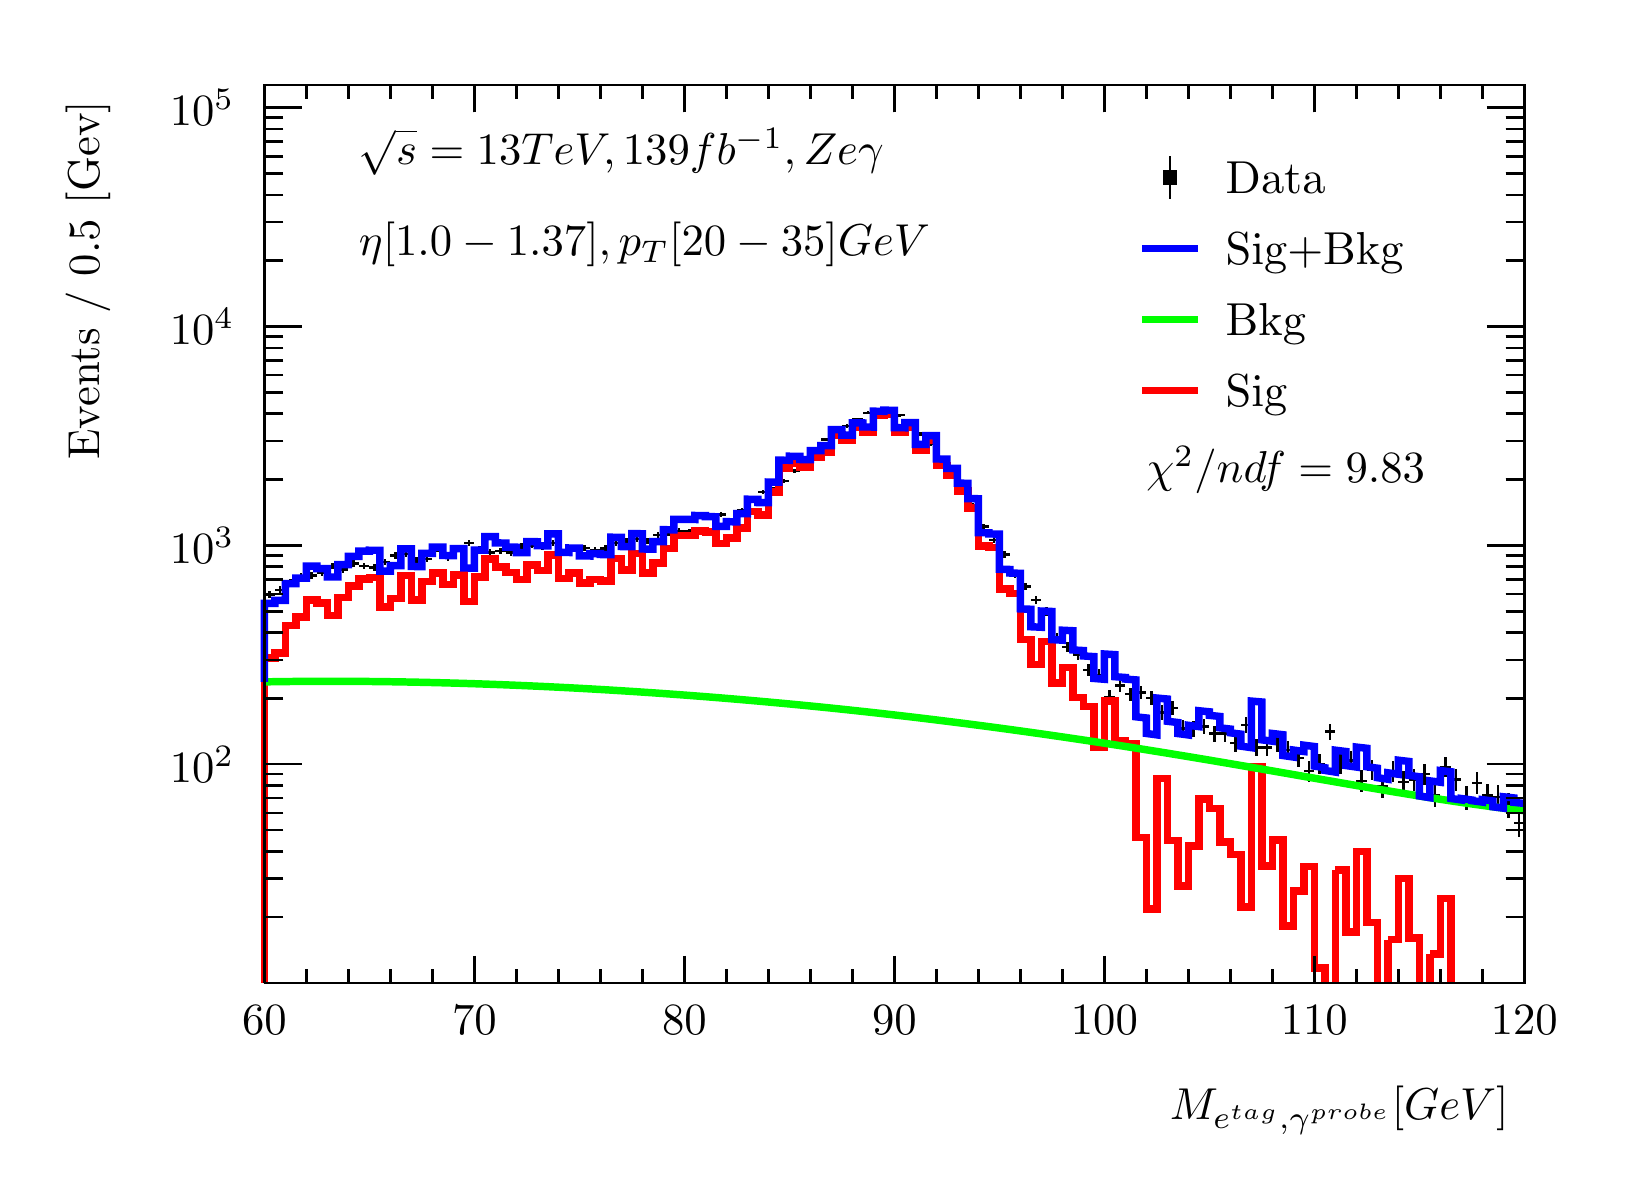
\begin{tikzpicture}
\pgfdeclareplotmark{cross} {
\pgfpathmoveto{\pgfpoint{-0.3\pgfplotmarksize}{\pgfplotmarksize}}
\pgfpathlineto{\pgfpoint{+0.3\pgfplotmarksize}{\pgfplotmarksize}}
\pgfpathlineto{\pgfpoint{+0.3\pgfplotmarksize}{0.3\pgfplotmarksize}}
\pgfpathlineto{\pgfpoint{+1\pgfplotmarksize}{0.3\pgfplotmarksize}}
\pgfpathlineto{\pgfpoint{+1\pgfplotmarksize}{-0.3\pgfplotmarksize}}
\pgfpathlineto{\pgfpoint{+0.3\pgfplotmarksize}{-0.3\pgfplotmarksize}}
\pgfpathlineto{\pgfpoint{+0.3\pgfplotmarksize}{-1.\pgfplotmarksize}}
\pgfpathlineto{\pgfpoint{-0.3\pgfplotmarksize}{-1.\pgfplotmarksize}}
\pgfpathlineto{\pgfpoint{-0.3\pgfplotmarksize}{-0.3\pgfplotmarksize}}
\pgfpathlineto{\pgfpoint{-1.\pgfplotmarksize}{-0.3\pgfplotmarksize}}
\pgfpathlineto{\pgfpoint{-1.\pgfplotmarksize}{0.3\pgfplotmarksize}}
\pgfpathlineto{\pgfpoint{-0.3\pgfplotmarksize}{0.3\pgfplotmarksize}}
\pgfpathclose
\pgfusepathqstroke
}
\pgfdeclareplotmark{cross*} {
\pgfpathmoveto{\pgfpoint{-0.3\pgfplotmarksize}{\pgfplotmarksize}}
\pgfpathlineto{\pgfpoint{+0.3\pgfplotmarksize}{\pgfplotmarksize}}
\pgfpathlineto{\pgfpoint{+0.3\pgfplotmarksize}{0.3\pgfplotmarksize}}
\pgfpathlineto{\pgfpoint{+1\pgfplotmarksize}{0.3\pgfplotmarksize}}
\pgfpathlineto{\pgfpoint{+1\pgfplotmarksize}{-0.3\pgfplotmarksize}}
\pgfpathlineto{\pgfpoint{+0.3\pgfplotmarksize}{-0.3\pgfplotmarksize}}
\pgfpathlineto{\pgfpoint{+0.3\pgfplotmarksize}{-1.\pgfplotmarksize}}
\pgfpathlineto{\pgfpoint{-0.3\pgfplotmarksize}{-1.\pgfplotmarksize}}
\pgfpathlineto{\pgfpoint{-0.3\pgfplotmarksize}{-0.3\pgfplotmarksize}}
\pgfpathlineto{\pgfpoint{-1.\pgfplotmarksize}{-0.3\pgfplotmarksize}}
\pgfpathlineto{\pgfpoint{-1.\pgfplotmarksize}{0.3\pgfplotmarksize}}
\pgfpathlineto{\pgfpoint{-0.3\pgfplotmarksize}{0.3\pgfplotmarksize}}
\pgfpathclose
\pgfusepathqfillstroke
}
\pgfdeclareplotmark{newstar} {
\pgfpathmoveto{\pgfqpoint{0pt}{\pgfplotmarksize}}
\pgfpathlineto{\pgfqpointpolar{44}{0.5\pgfplotmarksize}}
\pgfpathlineto{\pgfqpointpolar{18}{\pgfplotmarksize}}
\pgfpathlineto{\pgfqpointpolar{-20}{0.5\pgfplotmarksize}}
\pgfpathlineto{\pgfqpointpolar{-54}{\pgfplotmarksize}}
\pgfpathlineto{\pgfqpointpolar{-90}{0.5\pgfplotmarksize}}
\pgfpathlineto{\pgfqpointpolar{234}{\pgfplotmarksize}}
\pgfpathlineto{\pgfqpointpolar{198}{0.5\pgfplotmarksize}}
\pgfpathlineto{\pgfqpointpolar{162}{\pgfplotmarksize}}
\pgfpathlineto{\pgfqpointpolar{134}{0.5\pgfplotmarksize}}
\pgfpathclose
\pgfusepathqstroke
}
\pgfdeclareplotmark{newstar*} {
\pgfpathmoveto{\pgfqpoint{0pt}{\pgfplotmarksize}}
\pgfpathlineto{\pgfqpointpolar{44}{0.5\pgfplotmarksize}}
\pgfpathlineto{\pgfqpointpolar{18}{\pgfplotmarksize}}
\pgfpathlineto{\pgfqpointpolar{-20}{0.5\pgfplotmarksize}}
\pgfpathlineto{\pgfqpointpolar{-54}{\pgfplotmarksize}}
\pgfpathlineto{\pgfqpointpolar{-90}{0.5\pgfplotmarksize}}
\pgfpathlineto{\pgfqpointpolar{234}{\pgfplotmarksize}}
\pgfpathlineto{\pgfqpointpolar{198}{0.5\pgfplotmarksize}}
\pgfpathlineto{\pgfqpointpolar{162}{\pgfplotmarksize}}
\pgfpathlineto{\pgfqpointpolar{134}{0.5\pgfplotmarksize}}
\pgfpathclose
\pgfusepathqfillstroke
}
\definecolor{c}{rgb}{1,1,1};
\draw [color=c, fill=c] (0,0) rectangle (20,14.4361);
\draw [color=c, fill=c] (3,2.30977) rectangle (19,13.7143);
\definecolor{c}{rgb}{0,0,0};
\draw [c,line width=0.9] (3,2.30977) -- (3,13.7143) -- (19,13.7143) -- (19,2.30977) -- (3,2.30977);
\definecolor{c}{rgb}{1,1,1};
\draw [color=c, fill=c] (3,2.30977) rectangle (19,13.7143);
\definecolor{c}{rgb}{0,0,0};
\draw [c,line width=0.9] (3,2.30977) -- (3,13.7143) -- (19,13.7143) -- (19,2.30977) -- (3,2.30977);
\draw [c,line width=0.9] (3,2.30977) -- (19,2.30977);
\draw [c,line width=0.9] (3,2.65624) -- (3,2.30977);
\draw [c,line width=0.9] (3.53333,2.48301) -- (3.53333,2.30977);
\draw [c,line width=0.9] (4.06667,2.48301) -- (4.06667,2.30977);
\draw [c,line width=0.9] (4.6,2.48301) -- (4.6,2.30977);
\draw [c,line width=0.9] (5.13333,2.48301) -- (5.13333,2.30977);
\draw [c,line width=0.9] (5.66667,2.65624) -- (5.66667,2.30977);
\draw [c,line width=0.9] (6.2,2.48301) -- (6.2,2.30977);
\draw [c,line width=0.9] (6.73333,2.48301) -- (6.73333,2.30977);
\draw [c,line width=0.9] (7.26667,2.48301) -- (7.26667,2.30977);
\draw [c,line width=0.9] (7.8,2.48301) -- (7.8,2.30977);
\draw [c,line width=0.9] (8.33333,2.65624) -- (8.33333,2.30977);
\draw [c,line width=0.9] (8.86667,2.48301) -- (8.86667,2.30977);
\draw [c,line width=0.9] (9.4,2.48301) -- (9.4,2.30977);
\draw [c,line width=0.9] (9.93333,2.48301) -- (9.93333,2.30977);
\draw [c,line width=0.9] (10.4667,2.48301) -- (10.4667,2.30977);
\draw [c,line width=0.9] (11,2.65624) -- (11,2.30977);
\draw [c,line width=0.9] (11.5333,2.48301) -- (11.5333,2.30977);
\draw [c,line width=0.9] (12.0667,2.48301) -- (12.0667,2.30977);
\draw [c,line width=0.9] (12.6,2.48301) -- (12.6,2.30977);
\draw [c,line width=0.9] (13.1333,2.48301) -- (13.1333,2.30977);
\draw [c,line width=0.9] (13.6667,2.65624) -- (13.6667,2.30977);
\draw [c,line width=0.9] (14.2,2.48301) -- (14.2,2.30977);
\draw [c,line width=0.9] (14.7333,2.48301) -- (14.7333,2.30977);
\draw [c,line width=0.9] (15.2667,2.48301) -- (15.2667,2.30977);
\draw [c,line width=0.9] (15.8,2.48301) -- (15.8,2.30977);
\draw [c,line width=0.9] (16.3333,2.65624) -- (16.3333,2.30977);
\draw [c,line width=0.9] (16.8667,2.48301) -- (16.8667,2.30977);
\draw [c,line width=0.9] (17.4,2.48301) -- (17.4,2.30977);
\draw [c,line width=0.9] (17.9333,2.48301) -- (17.9333,2.30977);
\draw [c,line width=0.9] (18.4667,2.48301) -- (18.4667,2.30977);
\draw [c,line width=0.9] (19,2.65624) -- (19,2.30977);
\draw [anchor=base] (3,1.66015) node[scale=1.61424, color=c, rotate=0]{60};
\draw [anchor=base] (5.66667,1.66015) node[scale=1.61424, color=c, rotate=0]{70};
\draw [anchor=base] (8.33333,1.66015) node[scale=1.61424, color=c, rotate=0]{80};
\draw [anchor=base] (11,1.66015) node[scale=1.61424, color=c, rotate=0]{90};
\draw [anchor=base] (13.6667,1.66015) node[scale=1.61424, color=c, rotate=0]{100};
\draw [anchor=base] (16.3333,1.66015) node[scale=1.61424, color=c, rotate=0]{110};
\draw [anchor=base] (19,1.66015) node[scale=1.61424, color=c, rotate=0]{120};
\draw [anchor= east] (19,0.692932) node[scale=1.61424, color=c, rotate=0]{$M_{e^{tag}, \gamma^{probe}}  [GeV]$};
\draw [c,line width=0.9] (3,13.7143) -- (19,13.7143);
\draw [c,line width=0.9] (3,13.3678) -- (3,13.7143);
\draw [c,line width=0.9] (3.53333,13.5411) -- (3.53333,13.7143);
\draw [c,line width=0.9] (4.06667,13.5411) -- (4.06667,13.7143);
\draw [c,line width=0.9] (4.6,13.5411) -- (4.6,13.7143);
\draw [c,line width=0.9] (5.13333,13.5411) -- (5.13333,13.7143);
\draw [c,line width=0.9] (5.66667,13.3678) -- (5.66667,13.7143);
\draw [c,line width=0.9] (6.2,13.5411) -- (6.2,13.7143);
\draw [c,line width=0.9] (6.73333,13.5411) -- (6.73333,13.7143);
\draw [c,line width=0.9] (7.26667,13.5411) -- (7.26667,13.7143);
\draw [c,line width=0.9] (7.8,13.5411) -- (7.8,13.7143);
\draw [c,line width=0.9] (8.33333,13.3678) -- (8.33333,13.7143);
\draw [c,line width=0.9] (8.86667,13.5411) -- (8.86667,13.7143);
\draw [c,line width=0.9] (9.4,13.5411) -- (9.4,13.7143);
\draw [c,line width=0.9] (9.93333,13.5411) -- (9.93333,13.7143);
\draw [c,line width=0.9] (10.4667,13.5411) -- (10.4667,13.7143);
\draw [c,line width=0.9] (11,13.3678) -- (11,13.7143);
\draw [c,line width=0.9] (11.5333,13.5411) -- (11.5333,13.7143);
\draw [c,line width=0.9] (12.0667,13.5411) -- (12.0667,13.7143);
\draw [c,line width=0.9] (12.6,13.5411) -- (12.6,13.7143);
\draw [c,line width=0.9] (13.1333,13.5411) -- (13.1333,13.7143);
\draw [c,line width=0.9] (13.6667,13.3678) -- (13.6667,13.7143);
\draw [c,line width=0.9] (14.2,13.5411) -- (14.2,13.7143);
\draw [c,line width=0.9] (14.7333,13.5411) -- (14.7333,13.7143);
\draw [c,line width=0.9] (15.2667,13.5411) -- (15.2667,13.7143);
\draw [c,line width=0.9] (15.8,13.5411) -- (15.8,13.7143);
\draw [c,line width=0.9] (16.3333,13.3678) -- (16.3333,13.7143);
\draw [c,line width=0.9] (16.8667,13.5411) -- (16.8667,13.7143);
\draw [c,line width=0.9] (17.4,13.5411) -- (17.4,13.7143);
\draw [c,line width=0.9] (17.9333,13.5411) -- (17.9333,13.7143);
\draw [c,line width=0.9] (18.4667,13.5411) -- (18.4667,13.7143);
\draw [c,line width=0.9] (19,13.3678) -- (19,13.7143);
\draw [c,line width=0.9] (3,2.30977) -- (3,13.7143);
\draw [c,line width=0.9] (3.237,3.14637) -- (3,3.14637);
\draw [c,line width=0.9] (3.237,3.63576) -- (3,3.63576);
\draw [c,line width=0.9] (3.237,3.98298) -- (3,3.98298);
\draw [c,line width=0.9] (3.237,4.2523) -- (3,4.2523);
\draw [c,line width=0.9] (3.237,4.47236) -- (3,4.47236);
\draw [c,line width=0.9] (3.237,4.65841) -- (3,4.65841);
\draw [c,line width=0.9] (3.237,4.81958) -- (3,4.81958);
\draw [c,line width=0.9] (3.237,4.96174) -- (3,4.96174);
\draw [c,line width=0.9] (3.474,5.0889) -- (3,5.0889);
\draw [anchor= east] (2.82,5.0889) node[scale=1.61424, color=c, rotate=0]{$10^{2}$};
\draw [c,line width=0.9] (3.237,5.92551) -- (3,5.92551);
\draw [c,line width=0.9] (3.237,6.41489) -- (3,6.41489);
\draw [c,line width=0.9] (3.237,6.76211) -- (3,6.76211);
\draw [c,line width=0.9] (3.237,7.03144) -- (3,7.03144);
\draw [c,line width=0.9] (3.237,7.25149) -- (3,7.25149);
\draw [c,line width=0.9] (3.237,7.43755) -- (3,7.43755);
\draw [c,line width=0.9] (3.237,7.59871) -- (3,7.59871);
\draw [c,line width=0.9] (3.237,7.74087) -- (3,7.74087);
\draw [c,line width=0.9] (3.474,7.86804) -- (3,7.86804);
\draw [anchor= east] (2.82,7.86804) node[scale=1.61424, color=c, rotate=0]{$10^{3}$};
\draw [c,line width=0.9] (3.237,8.70464) -- (3,8.70464);
\draw [c,line width=0.9] (3.237,9.19402) -- (3,9.19402);
\draw [c,line width=0.9] (3.237,9.54124) -- (3,9.54124);
\draw [c,line width=0.9] (3.237,9.81057) -- (3,9.81057);
\draw [c,line width=0.9] (3.237,10.0306) -- (3,10.0306);
\draw [c,line width=0.9] (3.237,10.2167) -- (3,10.2167);
\draw [c,line width=0.9] (3.237,10.3778) -- (3,10.3778);
\draw [c,line width=0.9] (3.237,10.52) -- (3,10.52);
\draw [c,line width=0.9] (3.474,10.6472) -- (3,10.6472);
\draw [anchor= east] (2.82,10.6472) node[scale=1.61424, color=c, rotate=0]{$10^{4}$};
\draw [c,line width=0.9] (3.237,11.4838) -- (3,11.4838);
\draw [c,line width=0.9] (3.237,11.9732) -- (3,11.9732);
\draw [c,line width=0.9] (3.237,12.3204) -- (3,12.3204);
\draw [c,line width=0.9] (3.237,12.5897) -- (3,12.5897);
\draw [c,line width=0.9] (3.237,12.8098) -- (3,12.8098);
\draw [c,line width=0.9] (3.237,12.9958) -- (3,12.9958);
\draw [c,line width=0.9] (3.237,13.157) -- (3,13.157);
\draw [c,line width=0.9] (3.237,13.2991) -- (3,13.2991);
\draw [c,line width=0.9] (3.474,13.4263) -- (3,13.4263);
\draw [anchor= east] (2.82,13.4263) node[scale=1.61424, color=c, rotate=0]{$10^{5}$};
\draw [anchor= east] (0.76,13.7143) node[scale=1.61424, color=c, rotate=90]{Events / 0.5 [Gev]};
\draw [c,line width=0.9] (19,2.30977) -- (19,13.7143);
\draw [c,line width=0.9] (18.763,3.14637) -- (19,3.14637);
\draw [c,line width=0.9] (18.763,3.63576) -- (19,3.63576);
\draw [c,line width=0.9] (18.763,3.98298) -- (19,3.98298);
\draw [c,line width=0.9] (18.763,4.2523) -- (19,4.2523);
\draw [c,line width=0.9] (18.763,4.47236) -- (19,4.47236);
\draw [c,line width=0.9] (18.763,4.65841) -- (19,4.65841);
\draw [c,line width=0.9] (18.763,4.81958) -- (19,4.81958);
\draw [c,line width=0.9] (18.763,4.96174) -- (19,4.96174);
\draw [c,line width=0.9] (18.526,5.0889) -- (19,5.0889);
\draw [c,line width=0.9] (18.763,5.92551) -- (19,5.92551);
\draw [c,line width=0.9] (18.763,6.41489) -- (19,6.41489);
\draw [c,line width=0.9] (18.763,6.76211) -- (19,6.76211);
\draw [c,line width=0.9] (18.763,7.03144) -- (19,7.03144);
\draw [c,line width=0.9] (18.763,7.25149) -- (19,7.25149);
\draw [c,line width=0.9] (18.763,7.43755) -- (19,7.43755);
\draw [c,line width=0.9] (18.763,7.59871) -- (19,7.59871);
\draw [c,line width=0.9] (18.763,7.74087) -- (19,7.74087);
\draw [c,line width=0.9] (18.526,7.86804) -- (19,7.86804);
\draw [c,line width=0.9] (18.763,8.70464) -- (19,8.70464);
\draw [c,line width=0.9] (18.763,9.19402) -- (19,9.19402);
\draw [c,line width=0.9] (18.763,9.54124) -- (19,9.54124);
\draw [c,line width=0.9] (18.763,9.81057) -- (19,9.81057);
\draw [c,line width=0.9] (18.763,10.0306) -- (19,10.0306);
\draw [c,line width=0.9] (18.763,10.2167) -- (19,10.2167);
\draw [c,line width=0.9] (18.763,10.3778) -- (19,10.3778);
\draw [c,line width=0.9] (18.763,10.52) -- (19,10.52);
\draw [c,line width=0.9] (18.526,10.6472) -- (19,10.6472);
\draw [c,line width=0.9] (18.763,11.4838) -- (19,11.4838);
\draw [c,line width=0.9] (18.763,11.9732) -- (19,11.9732);
\draw [c,line width=0.9] (18.763,12.3204) -- (19,12.3204);
\draw [c,line width=0.9] (18.763,12.5897) -- (19,12.5897);
\draw [c,line width=0.9] (18.763,12.8098) -- (19,12.8098);
\draw [c,line width=0.9] (18.763,12.9958) -- (19,12.9958);
\draw [c,line width=0.9] (18.763,13.157) -- (19,13.157);
\draw [c,line width=0.9] (18.763,13.2991) -- (19,13.2991);
\draw [c,line width=0.9] (18.526,13.4263) -- (19,13.4263);
\draw [c,line width=0.9] (3.06667,7.24544) -- (3,7.24544);
\draw [c,line width=0.9] (3,7.24544) -- (3,7.24544);
\draw [c,line width=0.9] (3.06667,7.24544) -- (3.13333,7.24544);
\draw [c,line width=0.9] (3.13333,7.24544) -- (3.13333,7.24544);
\draw [c,line width=0.9] (3.06667,7.24544) -- (3.06667,7.29484);
\draw [c,line width=0.9] (3.06667,7.29484) -- (3.06667,7.29484);
\draw [c,line width=0.9] (3.06667,7.24544) -- (3.06667,7.19605);
\draw [c,line width=0.9] (3.06667,7.19605) -- (3.06667,7.19605);
\draw [c,line width=0.9] (3.2,7.30076) -- (3.13333,7.30076);
\draw [c,line width=0.9] (3.13333,7.30076) -- (3.13333,7.30076);
\draw [c,line width=0.9] (3.2,7.30076) -- (3.26667,7.30076);
\draw [c,line width=0.9] (3.26667,7.30076) -- (3.26667,7.30076);
\draw [c,line width=0.9] (3.2,7.30076) -- (3.2,7.34904);
\draw [c,line width=0.9] (3.2,7.34904) -- (3.2,7.34904);
\draw [c,line width=0.9] (3.2,7.30076) -- (3.2,7.25249);
\draw [c,line width=0.9] (3.2,7.25249) -- (3.2,7.25249);
\draw [c,line width=0.9] (3.33333,7.39544) -- (3.26667,7.39544);
\draw [c,line width=0.9] (3.26667,7.39544) -- (3.26667,7.39544);
\draw [c,line width=0.9] (3.33333,7.39544) -- (3.4,7.39544);
\draw [c,line width=0.9] (3.4,7.39544) -- (3.4,7.39544);
\draw [c,line width=0.9] (3.33333,7.39544) -- (3.33333,7.44186);
\draw [c,line width=0.9] (3.33333,7.44186) -- (3.33333,7.44186);
\draw [c,line width=0.9] (3.33333,7.39544) -- (3.33333,7.34902);
\draw [c,line width=0.9] (3.33333,7.34902) -- (3.33333,7.34902);
\draw [c,line width=0.9] (3.46667,7.47155) -- (3.4,7.47155);
\draw [c,line width=0.9] (3.4,7.47155) -- (3.4,7.47155);
\draw [c,line width=0.9] (3.46667,7.47155) -- (3.53333,7.47155);
\draw [c,line width=0.9] (3.53333,7.47155) -- (3.53333,7.47155);
\draw [c,line width=0.9] (3.46667,7.47155) -- (3.46667,7.51653);
\draw [c,line width=0.9] (3.46667,7.51653) -- (3.46667,7.51653);
\draw [c,line width=0.9] (3.46667,7.47155) -- (3.46667,7.42657);
\draw [c,line width=0.9] (3.46667,7.42657) -- (3.46667,7.42657);
\draw [c,line width=0.9] (3.6,7.48323) -- (3.53333,7.48323);
\draw [c,line width=0.9] (3.53333,7.48323) -- (3.53333,7.48323);
\draw [c,line width=0.9] (3.6,7.48323) -- (3.66667,7.48323);
\draw [c,line width=0.9] (3.66667,7.48323) -- (3.66667,7.48323);
\draw [c,line width=0.9] (3.6,7.48323) -- (3.6,7.52799);
\draw [c,line width=0.9] (3.6,7.52799) -- (3.6,7.52799);
\draw [c,line width=0.9] (3.6,7.48323) -- (3.6,7.43846);
\draw [c,line width=0.9] (3.6,7.43846) -- (3.6,7.43846);
\draw [c,line width=0.9] (3.73333,7.52243) -- (3.66667,7.52243);
\draw [c,line width=0.9] (3.66667,7.52243) -- (3.66667,7.52243);
\draw [c,line width=0.9] (3.73333,7.52243) -- (3.8,7.52243);
\draw [c,line width=0.9] (3.8,7.52243) -- (3.8,7.52243);
\draw [c,line width=0.9] (3.73333,7.52243) -- (3.73333,7.56647);
\draw [c,line width=0.9] (3.73333,7.56647) -- (3.73333,7.56647);
\draw [c,line width=0.9] (3.73333,7.52243) -- (3.73333,7.47839);
\draw [c,line width=0.9] (3.73333,7.47839) -- (3.73333,7.47839);
\draw [c,line width=0.9] (3.86667,7.60773) -- (3.8,7.60773);
\draw [c,line width=0.9] (3.8,7.60773) -- (3.8,7.60773);
\draw [c,line width=0.9] (3.86667,7.60773) -- (3.93333,7.60773);
\draw [c,line width=0.9] (3.93333,7.60773) -- (3.93333,7.60773);
\draw [c,line width=0.9] (3.86667,7.60773) -- (3.86667,7.65024);
\draw [c,line width=0.9] (3.86667,7.65024) -- (3.86667,7.65024);
\draw [c,line width=0.9] (3.86667,7.60773) -- (3.86667,7.56522);
\draw [c,line width=0.9] (3.86667,7.56522) -- (3.86667,7.56522);
\draw [c,line width=0.9] (4,7.56039) -- (3.93333,7.56039);
\draw [c,line width=0.9] (3.93333,7.56039) -- (3.93333,7.56039);
\draw [c,line width=0.9] (4,7.56039) -- (4.06667,7.56039);
\draw [c,line width=0.9] (4.06667,7.56039) -- (4.06667,7.56039);
\draw [c,line width=0.9] (4,7.56039) -- (4,7.60375);
\draw [c,line width=0.9] (4,7.60375) -- (4,7.60375);
\draw [c,line width=0.9] (4,7.56039) -- (4,7.51704);
\draw [c,line width=0.9] (4,7.51704) -- (4,7.51704);
\draw [c,line width=0.9] (4.13333,7.63878) -- (4.06667,7.63878);
\draw [c,line width=0.9] (4.06667,7.63878) -- (4.06667,7.63878);
\draw [c,line width=0.9] (4.13333,7.63878) -- (4.2,7.63878);
\draw [c,line width=0.9] (4.2,7.63878) -- (4.2,7.63878);
\draw [c,line width=0.9] (4.13333,7.63878) -- (4.13333,7.68074);
\draw [c,line width=0.9] (4.13333,7.68074) -- (4.13333,7.68074);
\draw [c,line width=0.9] (4.13333,7.63878) -- (4.13333,7.59681);
\draw [c,line width=0.9] (4.13333,7.59681) -- (4.13333,7.59681);
\draw [c,line width=0.9] (4.26667,7.60623) -- (4.2,7.60623);
\draw [c,line width=0.9] (4.2,7.60623) -- (4.2,7.60623);
\draw [c,line width=0.9] (4.26667,7.60623) -- (4.33333,7.60623);
\draw [c,line width=0.9] (4.33333,7.60623) -- (4.33333,7.60623);
\draw [c,line width=0.9] (4.26667,7.60623) -- (4.26667,7.64877);
\draw [c,line width=0.9] (4.26667,7.64877) -- (4.26667,7.64877);
\draw [c,line width=0.9] (4.26667,7.60623) -- (4.26667,7.5637);
\draw [c,line width=0.9] (4.26667,7.5637) -- (4.26667,7.5637);
\draw [c,line width=0.9] (4.4,7.58658) -- (4.33333,7.58658);
\draw [c,line width=0.9] (4.33333,7.58658) -- (4.33333,7.58658);
\draw [c,line width=0.9] (4.4,7.58658) -- (4.46667,7.58658);
\draw [c,line width=0.9] (4.46667,7.58658) -- (4.46667,7.58658);
\draw [c,line width=0.9] (4.4,7.58658) -- (4.4,7.62947);
\draw [c,line width=0.9] (4.4,7.62947) -- (4.4,7.62947);
\draw [c,line width=0.9] (4.4,7.58658) -- (4.4,7.5437);
\draw [c,line width=0.9] (4.4,7.5437) -- (4.4,7.5437);
\draw [c,line width=0.9] (4.53333,7.65473) -- (4.46667,7.65473);
\draw [c,line width=0.9] (4.46667,7.65473) -- (4.46667,7.65473);
\draw [c,line width=0.9] (4.53333,7.65473) -- (4.6,7.65473);
\draw [c,line width=0.9] (4.6,7.65473) -- (4.6,7.65473);
\draw [c,line width=0.9] (4.53333,7.65473) -- (4.53333,7.69642);
\draw [c,line width=0.9] (4.53333,7.69642) -- (4.53333,7.69642);
\draw [c,line width=0.9] (4.53333,7.65473) -- (4.53333,7.61303);
\draw [c,line width=0.9] (4.53333,7.61303) -- (4.53333,7.61303);
\draw [c,line width=0.9] (4.66667,7.74087) -- (4.6,7.74087);
\draw [c,line width=0.9] (4.6,7.74087) -- (4.6,7.74087);
\draw [c,line width=0.9] (4.66667,7.74087) -- (4.73333,7.74087);
\draw [c,line width=0.9] (4.73333,7.74087) -- (4.73333,7.74087);
\draw [c,line width=0.9] (4.66667,7.74087) -- (4.66667,7.7811);
\draw [c,line width=0.9] (4.66667,7.7811) -- (4.66667,7.7811);
\draw [c,line width=0.9] (4.66667,7.74087) -- (4.66667,7.70064);
\draw [c,line width=0.9] (4.66667,7.70064) -- (4.66667,7.70064);
\draw [c,line width=0.9] (4.8,7.7595) -- (4.73333,7.7595);
\draw [c,line width=0.9] (4.73333,7.7595) -- (4.73333,7.7595);
\draw [c,line width=0.9] (4.8,7.7595) -- (4.86667,7.7595);
\draw [c,line width=0.9] (4.86667,7.7595) -- (4.86667,7.7595);
\draw [c,line width=0.9] (4.8,7.7595) -- (4.8,7.79943);
\draw [c,line width=0.9] (4.8,7.79943) -- (4.8,7.79943);
\draw [c,line width=0.9] (4.8,7.7595) -- (4.8,7.71958);
\draw [c,line width=0.9] (4.8,7.71958) -- (4.8,7.71958);
\draw [c,line width=0.9] (4.93333,7.67331) -- (4.86667,7.67331);
\draw [c,line width=0.9] (4.86667,7.67331) -- (4.86667,7.67331);
\draw [c,line width=0.9] (4.93333,7.67331) -- (5,7.67331);
\draw [c,line width=0.9] (5,7.67331) -- (5,7.67331);
\draw [c,line width=0.9] (4.93333,7.67331) -- (4.93333,7.71468);
\draw [c,line width=0.9] (4.93333,7.71468) -- (4.93333,7.71468);
\draw [c,line width=0.9] (4.93333,7.67331) -- (4.93333,7.63193);
\draw [c,line width=0.9] (4.93333,7.63193) -- (4.93333,7.63193);
\draw [c,line width=0.9] (5.06667,7.69718) -- (5,7.69718);
\draw [c,line width=0.9] (5,7.69718) -- (5,7.69718);
\draw [c,line width=0.9] (5.06667,7.69718) -- (5.13333,7.69718);
\draw [c,line width=0.9] (5.13333,7.69718) -- (5.13333,7.69718);
\draw [c,line width=0.9] (5.06667,7.69718) -- (5.06667,7.73814);
\draw [c,line width=0.9] (5.06667,7.73814) -- (5.06667,7.73814);
\draw [c,line width=0.9] (5.06667,7.69718) -- (5.06667,7.65621);
\draw [c,line width=0.9] (5.06667,7.65621) -- (5.06667,7.65621);
\draw [c,line width=0.9] (5.2,7.82003) -- (5.13333,7.82003);
\draw [c,line width=0.9] (5.13333,7.82003) -- (5.13333,7.82003);
\draw [c,line width=0.9] (5.2,7.82003) -- (5.26667,7.82003);
\draw [c,line width=0.9] (5.26667,7.82003) -- (5.26667,7.82003);
\draw [c,line width=0.9] (5.2,7.82003) -- (5.2,7.85896);
\draw [c,line width=0.9] (5.2,7.85896) -- (5.2,7.85896);
\draw [c,line width=0.9] (5.2,7.82003) -- (5.2,7.78109);
\draw [c,line width=0.9] (5.2,7.78109) -- (5.2,7.78109);
\draw [c,line width=0.9] (5.33333,7.711) -- (5.26667,7.711);
\draw [c,line width=0.9] (5.26667,7.711) -- (5.26667,7.711);
\draw [c,line width=0.9] (5.33333,7.711) -- (5.4,7.711);
\draw [c,line width=0.9] (5.4,7.711) -- (5.4,7.711);
\draw [c,line width=0.9] (5.33333,7.711) -- (5.33333,7.75173);
\draw [c,line width=0.9] (5.33333,7.75173) -- (5.33333,7.75173);
\draw [c,line width=0.9] (5.33333,7.711) -- (5.33333,7.67027);
\draw [c,line width=0.9] (5.33333,7.67027) -- (5.33333,7.67027);
\draw [c,line width=0.9] (5.46667,7.83003) -- (5.4,7.83003);
\draw [c,line width=0.9] (5.4,7.83003) -- (5.4,7.83003);
\draw [c,line width=0.9] (5.46667,7.83003) -- (5.53333,7.83003);
\draw [c,line width=0.9] (5.53333,7.83003) -- (5.53333,7.83003);
\draw [c,line width=0.9] (5.46667,7.83003) -- (5.46667,7.8688);
\draw [c,line width=0.9] (5.46667,7.8688) -- (5.46667,7.8688);
\draw [c,line width=0.9] (5.46667,7.83003) -- (5.46667,7.79126);
\draw [c,line width=0.9] (5.46667,7.79126) -- (5.46667,7.79126);
\draw [c,line width=0.9] (5.6,7.89666) -- (5.53333,7.89666);
\draw [c,line width=0.9] (5.53333,7.89666) -- (5.53333,7.89666);
\draw [c,line width=0.9] (5.6,7.89666) -- (5.66667,7.89666);
\draw [c,line width=0.9] (5.66667,7.89666) -- (5.66667,7.89666);
\draw [c,line width=0.9] (5.6,7.89666) -- (5.6,7.93438);
\draw [c,line width=0.9] (5.6,7.93438) -- (5.6,7.93438);
\draw [c,line width=0.9] (5.6,7.89666) -- (5.6,7.85895);
\draw [c,line width=0.9] (5.6,7.85895) -- (5.6,7.85895);
\draw [c,line width=0.9] (5.73333,7.81751) -- (5.66667,7.81751);
\draw [c,line width=0.9] (5.66667,7.81751) -- (5.66667,7.81751);
\draw [c,line width=0.9] (5.73333,7.81751) -- (5.8,7.81751);
\draw [c,line width=0.9] (5.8,7.81751) -- (5.8,7.81751);
\draw [c,line width=0.9] (5.73333,7.81751) -- (5.73333,7.85648);
\draw [c,line width=0.9] (5.73333,7.85648) -- (5.73333,7.85648);
\draw [c,line width=0.9] (5.73333,7.81751) -- (5.73333,7.77854);
\draw [c,line width=0.9] (5.73333,7.77854) -- (5.73333,7.77854);
\draw [c,line width=0.9] (5.86667,7.77785) -- (5.8,7.77785);
\draw [c,line width=0.9] (5.8,7.77785) -- (5.8,7.77785);
\draw [c,line width=0.9] (5.86667,7.77785) -- (5.93333,7.77785);
\draw [c,line width=0.9] (5.93333,7.77785) -- (5.93333,7.77785);
\draw [c,line width=0.9] (5.86667,7.77785) -- (5.86667,7.81747);
\draw [c,line width=0.9] (5.86667,7.81747) -- (5.86667,7.81747);
\draw [c,line width=0.9] (5.86667,7.77785) -- (5.86667,7.73823);
\draw [c,line width=0.9] (5.86667,7.73823) -- (5.86667,7.73823);
\draw [c,line width=0.9] (6,7.79592) -- (5.93333,7.79592);
\draw [c,line width=0.9] (5.93333,7.79592) -- (5.93333,7.79592);
\draw [c,line width=0.9] (6,7.79592) -- (6.06667,7.79592);
\draw [c,line width=0.9] (6.06667,7.79592) -- (6.06667,7.79592);
\draw [c,line width=0.9] (6,7.79592) -- (6,7.83525);
\draw [c,line width=0.9] (6,7.83525) -- (6,7.83525);
\draw [c,line width=0.9] (6,7.79592) -- (6,7.7566);
\draw [c,line width=0.9] (6,7.7566) -- (6,7.7566);
\draw [c,line width=0.9] (6.13333,7.77655) -- (6.06667,7.77655);
\draw [c,line width=0.9] (6.06667,7.77655) -- (6.06667,7.77655);
\draw [c,line width=0.9] (6.13333,7.77655) -- (6.2,7.77655);
\draw [c,line width=0.9] (6.2,7.77655) -- (6.2,7.77655);
\draw [c,line width=0.9] (6.13333,7.77655) -- (6.13333,7.81619);
\draw [c,line width=0.9] (6.13333,7.81619) -- (6.13333,7.81619);
\draw [c,line width=0.9] (6.13333,7.77655) -- (6.13333,7.73691);
\draw [c,line width=0.9] (6.13333,7.73691) -- (6.13333,7.73691);
\draw [c,line width=0.9] (6.26667,7.85713) -- (6.2,7.85713);
\draw [c,line width=0.9] (6.2,7.85713) -- (6.2,7.85713);
\draw [c,line width=0.9] (6.26667,7.85713) -- (6.33333,7.85713);
\draw [c,line width=0.9] (6.33333,7.85713) -- (6.33333,7.85713);
\draw [c,line width=0.9] (6.26667,7.85713) -- (6.26667,7.89547);
\draw [c,line width=0.9] (6.26667,7.89547) -- (6.26667,7.89547);
\draw [c,line width=0.9] (6.26667,7.85713) -- (6.26667,7.81879);
\draw [c,line width=0.9] (6.26667,7.81879) -- (6.26667,7.81879);
\draw [c,line width=0.9] (6.4,7.86925) -- (6.33333,7.86925);
\draw [c,line width=0.9] (6.33333,7.86925) -- (6.33333,7.86925);
\draw [c,line width=0.9] (6.4,7.86925) -- (6.46667,7.86925);
\draw [c,line width=0.9] (6.46667,7.86925) -- (6.46667,7.86925);
\draw [c,line width=0.9] (6.4,7.86925) -- (6.4,7.90739);
\draw [c,line width=0.9] (6.4,7.90739) -- (6.4,7.90739);
\draw [c,line width=0.9] (6.4,7.86925) -- (6.4,7.8311);
\draw [c,line width=0.9] (6.4,7.8311) -- (6.4,7.8311);
\draw [c,line width=0.9] (6.53333,7.84242) -- (6.46667,7.84242);
\draw [c,line width=0.9] (6.46667,7.84242) -- (6.46667,7.84242);
\draw [c,line width=0.9] (6.53333,7.84242) -- (6.6,7.84242);
\draw [c,line width=0.9] (6.6,7.84242) -- (6.6,7.84242);
\draw [c,line width=0.9] (6.53333,7.84242) -- (6.53333,7.881);
\draw [c,line width=0.9] (6.53333,7.881) -- (6.53333,7.881);
\draw [c,line width=0.9] (6.53333,7.84242) -- (6.53333,7.80385);
\draw [c,line width=0.9] (6.53333,7.80385) -- (6.53333,7.80385);
\draw [c,line width=0.9] (6.66667,7.9002) -- (6.6,7.9002);
\draw [c,line width=0.9] (6.6,7.9002) -- (6.6,7.9002);
\draw [c,line width=0.9] (6.66667,7.9002) -- (6.73333,7.9002);
\draw [c,line width=0.9] (6.73333,7.9002) -- (6.73333,7.9002);
\draw [c,line width=0.9] (6.66667,7.9002) -- (6.66667,7.93786);
\draw [c,line width=0.9] (6.66667,7.93786) -- (6.66667,7.93786);
\draw [c,line width=0.9] (6.66667,7.9002) -- (6.66667,7.86253);
\draw [c,line width=0.9] (6.66667,7.86253) -- (6.66667,7.86253);
\draw [c,line width=0.9] (6.8,7.77133) -- (6.73333,7.77133);
\draw [c,line width=0.9] (6.73333,7.77133) -- (6.73333,7.77133);
\draw [c,line width=0.9] (6.8,7.77133) -- (6.86667,7.77133);
\draw [c,line width=0.9] (6.86667,7.77133) -- (6.86667,7.77133);
\draw [c,line width=0.9] (6.8,7.77133) -- (6.8,7.81106);
\draw [c,line width=0.9] (6.8,7.81106) -- (6.8,7.81106);
\draw [c,line width=0.9] (6.8,7.77133) -- (6.8,7.73161);
\draw [c,line width=0.9] (6.8,7.73161) -- (6.8,7.73161);
\draw [c,line width=0.9] (6.93333,7.82504) -- (6.86667,7.82504);
\draw [c,line width=0.9] (6.86667,7.82504) -- (6.86667,7.82504);
\draw [c,line width=0.9] (6.93333,7.82504) -- (7,7.82504);
\draw [c,line width=0.9] (7,7.82504) -- (7,7.82504);
\draw [c,line width=0.9] (6.93333,7.82504) -- (6.93333,7.86389);
\draw [c,line width=0.9] (6.93333,7.86389) -- (6.93333,7.86389);
\draw [c,line width=0.9] (6.93333,7.82504) -- (6.93333,7.78619);
\draw [c,line width=0.9] (6.93333,7.78619) -- (6.93333,7.78619);
\draw [c,line width=0.9] (7.06667,7.83376) -- (7,7.83376);
\draw [c,line width=0.9] (7,7.83376) -- (7,7.83376);
\draw [c,line width=0.9] (7.06667,7.83376) -- (7.13333,7.83376);
\draw [c,line width=0.9] (7.13333,7.83376) -- (7.13333,7.83376);
\draw [c,line width=0.9] (7.06667,7.83376) -- (7.06667,7.87247);
\draw [c,line width=0.9] (7.06667,7.87247) -- (7.06667,7.87247);
\draw [c,line width=0.9] (7.06667,7.83376) -- (7.06667,7.79505);
\draw [c,line width=0.9] (7.06667,7.79505) -- (7.06667,7.79505);
\draw [c,line width=0.9] (7.2,7.80231) -- (7.13333,7.80231);
\draw [c,line width=0.9] (7.13333,7.80231) -- (7.13333,7.80231);
\draw [c,line width=0.9] (7.2,7.80231) -- (7.26667,7.80231);
\draw [c,line width=0.9] (7.26667,7.80231) -- (7.26667,7.80231);
\draw [c,line width=0.9] (7.2,7.80231) -- (7.2,7.84153);
\draw [c,line width=0.9] (7.2,7.84153) -- (7.2,7.84153);
\draw [c,line width=0.9] (7.2,7.80231) -- (7.2,7.76309);
\draw [c,line width=0.9] (7.2,7.76309) -- (7.2,7.76309);
\draw [c,line width=0.9] (7.33333,7.82879) -- (7.26667,7.82879);
\draw [c,line width=0.9] (7.26667,7.82879) -- (7.26667,7.82879);
\draw [c,line width=0.9] (7.33333,7.82879) -- (7.4,7.82879);
\draw [c,line width=0.9] (7.4,7.82879) -- (7.4,7.82879);
\draw [c,line width=0.9] (7.33333,7.82879) -- (7.33333,7.86758);
\draw [c,line width=0.9] (7.33333,7.86758) -- (7.33333,7.86758);
\draw [c,line width=0.9] (7.33333,7.82879) -- (7.33333,7.78999);
\draw [c,line width=0.9] (7.33333,7.78999) -- (7.33333,7.78999);
\draw [c,line width=0.9] (7.46667,7.90137) -- (7.4,7.90137);
\draw [c,line width=0.9] (7.4,7.90137) -- (7.4,7.90137);
\draw [c,line width=0.9] (7.46667,7.90137) -- (7.53333,7.90137);
\draw [c,line width=0.9] (7.53333,7.90137) -- (7.53333,7.90137);
\draw [c,line width=0.9] (7.46667,7.90137) -- (7.46667,7.93901);
\draw [c,line width=0.9] (7.46667,7.93901) -- (7.46667,7.93901);
\draw [c,line width=0.9] (7.46667,7.90137) -- (7.46667,7.86373);
\draw [c,line width=0.9] (7.46667,7.86373) -- (7.46667,7.86373);
\draw [c,line width=0.9] (7.6,7.92001) -- (7.53333,7.92001);
\draw [c,line width=0.9] (7.53333,7.92001) -- (7.53333,7.92001);
\draw [c,line width=0.9] (7.6,7.92001) -- (7.66667,7.92001);
\draw [c,line width=0.9] (7.66667,7.92001) -- (7.66667,7.92001);
\draw [c,line width=0.9] (7.6,7.92001) -- (7.6,7.95736);
\draw [c,line width=0.9] (7.6,7.95736) -- (7.6,7.95736);
\draw [c,line width=0.9] (7.6,7.92001) -- (7.6,7.88266);
\draw [c,line width=0.9] (7.6,7.88266) -- (7.6,7.88266);
\draw [c,line width=0.9] (7.73333,7.94857) -- (7.66667,7.94857);
\draw [c,line width=0.9] (7.66667,7.94857) -- (7.66667,7.94857);
\draw [c,line width=0.9] (7.73333,7.94857) -- (7.8,7.94857);
\draw [c,line width=0.9] (7.8,7.94857) -- (7.8,7.94857);
\draw [c,line width=0.9] (7.73333,7.94857) -- (7.73333,7.98549);
\draw [c,line width=0.9] (7.73333,7.98549) -- (7.73333,7.98549);
\draw [c,line width=0.9] (7.73333,7.94857) -- (7.73333,7.91166);
\draw [c,line width=0.9] (7.73333,7.91166) -- (7.73333,7.91166);
\draw [c,line width=0.9] (7.86667,7.92693) -- (7.8,7.92693);
\draw [c,line width=0.9] (7.8,7.92693) -- (7.8,7.92693);
\draw [c,line width=0.9] (7.86667,7.92693) -- (7.93333,7.92693);
\draw [c,line width=0.9] (7.93333,7.92693) -- (7.93333,7.92693);
\draw [c,line width=0.9] (7.86667,7.92693) -- (7.86667,7.96417);
\draw [c,line width=0.9] (7.86667,7.96417) -- (7.86667,7.96417);
\draw [c,line width=0.9] (7.86667,7.92693) -- (7.86667,7.88968);
\draw [c,line width=0.9] (7.86667,7.88968) -- (7.86667,7.88968);
\draw [c,line width=0.9] (8,7.99834) -- (7.93333,7.99834);
\draw [c,line width=0.9] (7.93333,7.99834) -- (7.93333,7.99834);
\draw [c,line width=0.9] (8,7.99834) -- (8.06667,7.99834);
\draw [c,line width=0.9] (8.06667,7.99834) -- (8.06667,7.99834);
\draw [c,line width=0.9] (8,7.99834) -- (8,8.0345);
\draw [c,line width=0.9] (8,8.0345) -- (8,8.0345);
\draw [c,line width=0.9] (8,7.99834) -- (8,7.96218);
\draw [c,line width=0.9] (8,7.96218) -- (8,7.96218);
\draw [c,line width=0.9] (8.13333,8.02194) -- (8.06667,8.02194);
\draw [c,line width=0.9] (8.06667,8.02194) -- (8.06667,8.02194);
\draw [c,line width=0.9] (8.13333,8.02194) -- (8.2,8.02194);
\draw [c,line width=0.9] (8.2,8.02194) -- (8.2,8.02194);
\draw [c,line width=0.9] (8.13333,8.02194) -- (8.13333,8.05775);
\draw [c,line width=0.9] (8.13333,8.05775) -- (8.13333,8.05775);
\draw [c,line width=0.9] (8.13333,8.02194) -- (8.13333,7.98614);
\draw [c,line width=0.9] (8.13333,7.98614) -- (8.13333,7.98614);
\draw [c,line width=0.9] (8.26667,8.04926) -- (8.2,8.04926);
\draw [c,line width=0.9] (8.2,8.04926) -- (8.2,8.04926);
\draw [c,line width=0.9] (8.26667,8.04926) -- (8.33333,8.04926);
\draw [c,line width=0.9] (8.33333,8.04926) -- (8.33333,8.04926);
\draw [c,line width=0.9] (8.26667,8.04926) -- (8.26667,8.08466);
\draw [c,line width=0.9] (8.26667,8.08466) -- (8.26667,8.08466);
\draw [c,line width=0.9] (8.26667,8.04926) -- (8.26667,8.01385);
\draw [c,line width=0.9] (8.26667,8.01385) -- (8.26667,8.01385);
\draw [c,line width=0.9] (8.4,8.04405) -- (8.33333,8.04405);
\draw [c,line width=0.9] (8.33333,8.04405) -- (8.33333,8.04405);
\draw [c,line width=0.9] (8.4,8.04405) -- (8.46667,8.04405);
\draw [c,line width=0.9] (8.46667,8.04405) -- (8.46667,8.04405);
\draw [c,line width=0.9] (8.4,8.04405) -- (8.4,8.07953);
\draw [c,line width=0.9] (8.4,8.07953) -- (8.4,8.07953);
\draw [c,line width=0.9] (8.4,8.04405) -- (8.4,8.00857);
\draw [c,line width=0.9] (8.4,8.00857) -- (8.4,8.00857);
\draw [c,line width=0.9] (8.53333,8.06474) -- (8.46667,8.06474);
\draw [c,line width=0.9] (8.46667,8.06474) -- (8.46667,8.06474);
\draw [c,line width=0.9] (8.53333,8.06474) -- (8.6,8.06474);
\draw [c,line width=0.9] (8.6,8.06474) -- (8.6,8.06474);
\draw [c,line width=0.9] (8.53333,8.06474) -- (8.53333,8.09992);
\draw [c,line width=0.9] (8.53333,8.09992) -- (8.53333,8.09992);
\draw [c,line width=0.9] (8.53333,8.06474) -- (8.53333,8.02956);
\draw [c,line width=0.9] (8.53333,8.02956) -- (8.53333,8.02956);
\draw [c,line width=0.9] (8.66667,8.22667) -- (8.6,8.22667);
\draw [c,line width=0.9] (8.6,8.22667) -- (8.6,8.22667);
\draw [c,line width=0.9] (8.66667,8.22667) -- (8.73333,8.22667);
\draw [c,line width=0.9] (8.73333,8.22667) -- (8.73333,8.22667);
\draw [c,line width=0.9] (8.66667,8.22667) -- (8.66667,8.25957);
\draw [c,line width=0.9] (8.66667,8.25957) -- (8.66667,8.25957);
\draw [c,line width=0.9] (8.66667,8.22667) -- (8.66667,8.19378);
\draw [c,line width=0.9] (8.66667,8.19378) -- (8.66667,8.19378);
\draw [c,line width=0.9] (8.8,8.26115) -- (8.73333,8.26115);
\draw [c,line width=0.9] (8.73333,8.26115) -- (8.73333,8.26115);
\draw [c,line width=0.9] (8.8,8.26115) -- (8.86667,8.26115);
\draw [c,line width=0.9] (8.86667,8.26115) -- (8.86667,8.26115);
\draw [c,line width=0.9] (8.8,8.26115) -- (8.8,8.29358);
\draw [c,line width=0.9] (8.8,8.29358) -- (8.8,8.29358);
\draw [c,line width=0.9] (8.8,8.26115) -- (8.8,8.22872);
\draw [c,line width=0.9] (8.8,8.22872) -- (8.8,8.22872);
\draw [c,line width=0.9] (8.93333,8.16221) -- (8.86667,8.16221);
\draw [c,line width=0.9] (8.86667,8.16221) -- (8.86667,8.16221);
\draw [c,line width=0.9] (8.93333,8.16221) -- (9,8.16221);
\draw [c,line width=0.9] (9,8.16221) -- (9,8.16221);
\draw [c,line width=0.9] (8.93333,8.16221) -- (8.93333,8.196);
\draw [c,line width=0.9] (8.93333,8.196) -- (8.93333,8.196);
\draw [c,line width=0.9] (8.93333,8.16221) -- (8.93333,8.12843);
\draw [c,line width=0.9] (8.93333,8.12843) -- (8.93333,8.12843);
\draw [c,line width=0.9] (9.06667,8.31233) -- (9,8.31233);
\draw [c,line width=0.9] (9,8.31233) -- (9,8.31233);
\draw [c,line width=0.9] (9.06667,8.31233) -- (9.13333,8.31233);
\draw [c,line width=0.9] (9.13333,8.31233) -- (9.13333,8.31233);
\draw [c,line width=0.9] (9.06667,8.31233) -- (9.06667,8.34408);
\draw [c,line width=0.9] (9.06667,8.34408) -- (9.06667,8.34408);
\draw [c,line width=0.9] (9.06667,8.31233) -- (9.06667,8.28058);
\draw [c,line width=0.9] (9.06667,8.28058) -- (9.06667,8.28058);
\draw [c,line width=0.9] (9.2,8.43532) -- (9.13333,8.43532);
\draw [c,line width=0.9] (9.13333,8.43532) -- (9.13333,8.43532);
\draw [c,line width=0.9] (9.2,8.43532) -- (9.26667,8.43532);
\draw [c,line width=0.9] (9.26667,8.43532) -- (9.26667,8.43532);
\draw [c,line width=0.9] (9.2,8.43532) -- (9.2,8.46549);
\draw [c,line width=0.9] (9.2,8.46549) -- (9.2,8.46549);
\draw [c,line width=0.9] (9.2,8.43532) -- (9.2,8.40514);
\draw [c,line width=0.9] (9.2,8.40514) -- (9.2,8.40514);
\draw [c,line width=0.9] (9.33333,8.54348) -- (9.26667,8.54348);
\draw [c,line width=0.9] (9.26667,8.54348) -- (9.26667,8.54348);
\draw [c,line width=0.9] (9.33333,8.54348) -- (9.4,8.54348);
\draw [c,line width=0.9] (9.4,8.54348) -- (9.4,8.54348);
\draw [c,line width=0.9] (9.33333,8.54348) -- (9.33333,8.57233);
\draw [c,line width=0.9] (9.33333,8.57233) -- (9.33333,8.57233);
\draw [c,line width=0.9] (9.33333,8.54348) -- (9.33333,8.51462);
\draw [c,line width=0.9] (9.33333,8.51462) -- (9.33333,8.51462);
\draw [c,line width=0.9] (9.46667,8.58082) -- (9.4,8.58082);
\draw [c,line width=0.9] (9.4,8.58082) -- (9.4,8.58082);
\draw [c,line width=0.9] (9.46667,8.58082) -- (9.53333,8.58082);
\draw [c,line width=0.9] (9.53333,8.58082) -- (9.53333,8.58082);
\draw [c,line width=0.9] (9.46667,8.58082) -- (9.46667,8.60923);
\draw [c,line width=0.9] (9.46667,8.60923) -- (9.46667,8.60923);
\draw [c,line width=0.9] (9.46667,8.58082) -- (9.46667,8.55242);
\draw [c,line width=0.9] (9.46667,8.55242) -- (9.46667,8.55242);
\draw [c,line width=0.9] (9.6,8.68762) -- (9.53333,8.68762);
\draw [c,line width=0.9] (9.53333,8.68762) -- (9.53333,8.68762);
\draw [c,line width=0.9] (9.6,8.68762) -- (9.66667,8.68762);
\draw [c,line width=0.9] (9.66667,8.68762) -- (9.66667,8.68762);
\draw [c,line width=0.9] (9.6,8.68762) -- (9.6,8.7148);
\draw [c,line width=0.9] (9.6,8.7148) -- (9.6,8.7148);
\draw [c,line width=0.9] (9.6,8.68762) -- (9.6,8.66045);
\draw [c,line width=0.9] (9.6,8.66045) -- (9.6,8.66045);
\draw [c,line width=0.9] (9.73333,8.80976) -- (9.66667,8.80976);
\draw [c,line width=0.9] (9.66667,8.80976) -- (9.66667,8.80976);
\draw [c,line width=0.9] (9.73333,8.80976) -- (9.8,8.80976);
\draw [c,line width=0.9] (9.8,8.80976) -- (9.8,8.80976);
\draw [c,line width=0.9] (9.73333,8.80976) -- (9.73333,8.8356);
\draw [c,line width=0.9] (9.73333,8.8356) -- (9.73333,8.8356);
\draw [c,line width=0.9] (9.73333,8.80976) -- (9.73333,8.78392);
\draw [c,line width=0.9] (9.73333,8.78392) -- (9.73333,8.78392);
\draw [c,line width=0.9] (9.86667,8.91814) -- (9.8,8.91814);
\draw [c,line width=0.9] (9.8,8.91814) -- (9.8,8.91814);
\draw [c,line width=0.9] (9.86667,8.91814) -- (9.93333,8.91814);
\draw [c,line width=0.9] (9.93333,8.91814) -- (9.93333,8.91814);
\draw [c,line width=0.9] (9.86667,8.91814) -- (9.86667,8.94285);
\draw [c,line width=0.9] (9.86667,8.94285) -- (9.86667,8.94285);
\draw [c,line width=0.9] (9.86667,8.91814) -- (9.86667,8.89344);
\draw [c,line width=0.9] (9.86667,8.89344) -- (9.86667,8.89344);
\draw [c,line width=0.9] (10,9.03973) -- (9.93333,9.03973);
\draw [c,line width=0.9] (9.93333,9.03973) -- (9.93333,9.03973);
\draw [c,line width=0.9] (10,9.03973) -- (10.0667,9.03973);
\draw [c,line width=0.9] (10.0667,9.03973) -- (10.0667,9.03973);
\draw [c,line width=0.9] (10,9.03973) -- (10,9.06322);
\draw [c,line width=0.9] (10,9.06322) -- (10,9.06322);
\draw [c,line width=0.9] (10,9.03973) -- (10,9.01624);
\draw [c,line width=0.9] (10,9.01624) -- (10,9.01624);
\draw [c,line width=0.9] (10.1333,9.21556) -- (10.0667,9.21556);
\draw [c,line width=0.9] (10.0667,9.21556) -- (10.0667,9.21556);
\draw [c,line width=0.9] (10.1333,9.21556) -- (10.2,9.21556);
\draw [c,line width=0.9] (10.2,9.21556) -- (10.2,9.21556);
\draw [c,line width=0.9] (10.1333,9.21556) -- (10.1333,9.2374);
\draw [c,line width=0.9] (10.1333,9.2374) -- (10.1333,9.2374);
\draw [c,line width=0.9] (10.1333,9.21556) -- (10.1333,9.19372);
\draw [c,line width=0.9] (10.1333,9.19372) -- (10.1333,9.19372);
\draw [c,line width=0.9] (10.2667,9.28952) -- (10.2,9.28952);
\draw [c,line width=0.9] (10.2,9.28952) -- (10.2,9.28952);
\draw [c,line width=0.9] (10.2667,9.28952) -- (10.3333,9.28952);
\draw [c,line width=0.9] (10.3333,9.28952) -- (10.3333,9.28952);
\draw [c,line width=0.9] (10.2667,9.28952) -- (10.2667,9.3107);
\draw [c,line width=0.9] (10.2667,9.3107) -- (10.2667,9.3107);
\draw [c,line width=0.9] (10.2667,9.28952) -- (10.2667,9.26834);
\draw [c,line width=0.9] (10.2667,9.26834) -- (10.2667,9.26834);
\draw [c,line width=0.9] (10.4,9.38318) -- (10.3333,9.38318);
\draw [c,line width=0.9] (10.3333,9.38318) -- (10.3333,9.38318);
\draw [c,line width=0.9] (10.4,9.38318) -- (10.4667,9.38318);
\draw [c,line width=0.9] (10.4667,9.38318) -- (10.4667,9.38318);
\draw [c,line width=0.9] (10.4,9.38318) -- (10.4,9.40355);
\draw [c,line width=0.9] (10.4,9.40355) -- (10.4,9.40355);
\draw [c,line width=0.9] (10.4,9.38318) -- (10.4,9.3628);
\draw [c,line width=0.9] (10.4,9.3628) -- (10.4,9.3628);
\draw [c,line width=0.9] (10.5333,9.46881) -- (10.4667,9.46881);
\draw [c,line width=0.9] (10.4667,9.46881) -- (10.4667,9.46881);
\draw [c,line width=0.9] (10.5333,9.46881) -- (10.6,9.46881);
\draw [c,line width=0.9] (10.6,9.46881) -- (10.6,9.46881);
\draw [c,line width=0.9] (10.5333,9.46881) -- (10.5333,9.48847);
\draw [c,line width=0.9] (10.5333,9.48847) -- (10.5333,9.48847);
\draw [c,line width=0.9] (10.5333,9.46881) -- (10.5333,9.44914);
\draw [c,line width=0.9] (10.5333,9.44914) -- (10.5333,9.44914);
\draw [c,line width=0.9] (10.6667,9.54996) -- (10.6,9.54996);
\draw [c,line width=0.9] (10.6,9.54996) -- (10.6,9.54996);
\draw [c,line width=0.9] (10.6667,9.54996) -- (10.7333,9.54996);
\draw [c,line width=0.9] (10.7333,9.54996) -- (10.7333,9.54996);
\draw [c,line width=0.9] (10.6667,9.54996) -- (10.6667,9.56898);
\draw [c,line width=0.9] (10.6667,9.56898) -- (10.6667,9.56898);
\draw [c,line width=0.9] (10.6667,9.54996) -- (10.6667,9.53095);
\draw [c,line width=0.9] (10.6667,9.53095) -- (10.6667,9.53095);
\draw [c,line width=0.9] (10.8,9.58131) -- (10.7333,9.58131);
\draw [c,line width=0.9] (10.7333,9.58131) -- (10.7333,9.58131);
\draw [c,line width=0.9] (10.8,9.58131) -- (10.8667,9.58131);
\draw [c,line width=0.9] (10.8667,9.58131) -- (10.8667,9.58131);
\draw [c,line width=0.9] (10.8,9.58131) -- (10.8,9.60008);
\draw [c,line width=0.9] (10.8,9.60008) -- (10.8,9.60008);
\draw [c,line width=0.9] (10.8,9.58131) -- (10.8,9.56254);
\draw [c,line width=0.9] (10.8,9.56254) -- (10.8,9.56254);
\draw [c,line width=0.9] (10.9333,9.56662) -- (10.8667,9.56662);
\draw [c,line width=0.9] (10.8667,9.56662) -- (10.8667,9.56662);
\draw [c,line width=0.9] (10.9333,9.56662) -- (11,9.56662);
\draw [c,line width=0.9] (11,9.56662) -- (11,9.56662);
\draw [c,line width=0.9] (10.9333,9.56662) -- (10.9333,9.58551);
\draw [c,line width=0.9] (10.9333,9.58551) -- (10.9333,9.58551);
\draw [c,line width=0.9] (10.9333,9.56662) -- (10.9333,9.54774);
\draw [c,line width=0.9] (10.9333,9.54774) -- (10.9333,9.54774);
\draw [c,line width=0.9] (11.0667,9.52208) -- (11,9.52208);
\draw [c,line width=0.9] (11,9.52208) -- (11,9.52208);
\draw [c,line width=0.9] (11.0667,9.52208) -- (11.1333,9.52208);
\draw [c,line width=0.9] (11.1333,9.52208) -- (11.1333,9.52208);
\draw [c,line width=0.9] (11.0667,9.52208) -- (11.0667,9.54132);
\draw [c,line width=0.9] (11.0667,9.54132) -- (11.0667,9.54132);
\draw [c,line width=0.9] (11.0667,9.52208) -- (11.0667,9.50285);
\draw [c,line width=0.9] (11.0667,9.50285) -- (11.0667,9.50285);
\draw [c,line width=0.9] (11.2,9.38627) -- (11.1333,9.38627);
\draw [c,line width=0.9] (11.1333,9.38627) -- (11.1333,9.38627);
\draw [c,line width=0.9] (11.2,9.38627) -- (11.2667,9.38627);
\draw [c,line width=0.9] (11.2667,9.38627) -- (11.2667,9.38627);
\draw [c,line width=0.9] (11.2,9.38627) -- (11.2,9.40662);
\draw [c,line width=0.9] (11.2,9.40662) -- (11.2,9.40662);
\draw [c,line width=0.9] (11.2,9.38627) -- (11.2,9.36592);
\draw [c,line width=0.9] (11.2,9.36592) -- (11.2,9.36592);
\draw [c,line width=0.9] (11.3333,9.2843) -- (11.2667,9.2843);
\draw [c,line width=0.9] (11.2667,9.2843) -- (11.2667,9.2843);
\draw [c,line width=0.9] (11.3333,9.2843) -- (11.4,9.2843);
\draw [c,line width=0.9] (11.4,9.2843) -- (11.4,9.2843);
\draw [c,line width=0.9] (11.3333,9.2843) -- (11.3333,9.30553);
\draw [c,line width=0.9] (11.3333,9.30553) -- (11.3333,9.30553);
\draw [c,line width=0.9] (11.3333,9.2843) -- (11.3333,9.26307);
\draw [c,line width=0.9] (11.3333,9.26307) -- (11.3333,9.26307);
\draw [c,line width=0.9] (11.4667,9.15767) -- (11.4,9.15767);
\draw [c,line width=0.9] (11.4,9.15767) -- (11.4,9.15767);
\draw [c,line width=0.9] (11.4667,9.15767) -- (11.5333,9.15767);
\draw [c,line width=0.9] (11.5333,9.15767) -- (11.5333,9.15767);
\draw [c,line width=0.9] (11.4667,9.15767) -- (11.4667,9.18005);
\draw [c,line width=0.9] (11.4667,9.18005) -- (11.4667,9.18005);
\draw [c,line width=0.9] (11.4667,9.15767) -- (11.4667,9.1353);
\draw [c,line width=0.9] (11.4667,9.1353) -- (11.4667,9.1353);
\draw [c,line width=0.9] (11.6,8.9701) -- (11.5333,8.9701);
\draw [c,line width=0.9] (11.5333,8.9701) -- (11.5333,8.9701);
\draw [c,line width=0.9] (11.6,8.9701) -- (11.6667,8.9701);
\draw [c,line width=0.9] (11.6667,8.9701) -- (11.6667,8.9701);
\draw [c,line width=0.9] (11.6,8.9701) -- (11.6,8.99428);
\draw [c,line width=0.9] (11.6,8.99428) -- (11.6,8.99428);
\draw [c,line width=0.9] (11.6,8.9701) -- (11.6,8.94592);
\draw [c,line width=0.9] (11.6,8.94592) -- (11.6,8.94592);
\draw [c,line width=0.9] (11.7333,8.85855) -- (11.6667,8.85855);
\draw [c,line width=0.9] (11.6667,8.85855) -- (11.6667,8.85855);
\draw [c,line width=0.9] (11.7333,8.85855) -- (11.8,8.85855);
\draw [c,line width=0.9] (11.8,8.85855) -- (11.8,8.85855);
\draw [c,line width=0.9] (11.7333,8.85855) -- (11.7333,8.88387);
\draw [c,line width=0.9] (11.7333,8.88387) -- (11.7333,8.88387);
\draw [c,line width=0.9] (11.7333,8.85855) -- (11.7333,8.83323);
\draw [c,line width=0.9] (11.7333,8.83323) -- (11.7333,8.83323);
\draw [c,line width=0.9] (11.8667,8.61315) -- (11.8,8.61315);
\draw [c,line width=0.9] (11.8,8.61315) -- (11.8,8.61315);
\draw [c,line width=0.9] (11.8667,8.61315) -- (11.9333,8.61315);
\draw [c,line width=0.9] (11.9333,8.61315) -- (11.9333,8.61315);
\draw [c,line width=0.9] (11.8667,8.61315) -- (11.8667,8.64118);
\draw [c,line width=0.9] (11.8667,8.64118) -- (11.8667,8.64118);
\draw [c,line width=0.9] (11.8667,8.61315) -- (11.8667,8.58512);
\draw [c,line width=0.9] (11.8667,8.58512) -- (11.8667,8.58512);
\draw [c,line width=0.9] (12,8.38132) -- (11.9333,8.38132);
\draw [c,line width=0.9] (11.9333,8.38132) -- (11.9333,8.38132);
\draw [c,line width=0.9] (12,8.38132) -- (12.0667,8.38132);
\draw [c,line width=0.9] (12.0667,8.38132) -- (12.0667,8.38132);
\draw [c,line width=0.9] (12,8.38132) -- (12,8.41218);
\draw [c,line width=0.9] (12,8.41218) -- (12,8.41218);
\draw [c,line width=0.9] (12,8.38132) -- (12,8.35047);
\draw [c,line width=0.9] (12,8.35047) -- (12,8.35047);
\draw [c,line width=0.9] (12.1333,8.10507) -- (12.0667,8.10507);
\draw [c,line width=0.9] (12.0667,8.10507) -- (12.0667,8.10507);
\draw [c,line width=0.9] (12.1333,8.10507) -- (12.2,8.10507);
\draw [c,line width=0.9] (12.2,8.10507) -- (12.2,8.10507);
\draw [c,line width=0.9] (12.1333,8.10507) -- (12.1333,8.13967);
\draw [c,line width=0.9] (12.1333,8.13967) -- (12.1333,8.13967);
\draw [c,line width=0.9] (12.1333,8.10507) -- (12.1333,8.07048);
\draw [c,line width=0.9] (12.1333,8.07048) -- (12.1333,8.07048);
\draw [c,line width=0.9] (12.2667,7.9338) -- (12.2,7.9338);
\draw [c,line width=0.9] (12.2,7.9338) -- (12.2,7.9338);
\draw [c,line width=0.9] (12.2667,7.9338) -- (12.3333,7.9338);
\draw [c,line width=0.9] (12.3333,7.9338) -- (12.3333,7.9338);
\draw [c,line width=0.9] (12.2667,7.9338) -- (12.2667,7.97095);
\draw [c,line width=0.9] (12.2667,7.97095) -- (12.2667,7.97095);
\draw [c,line width=0.9] (12.2667,7.9338) -- (12.2667,7.89666);
\draw [c,line width=0.9] (12.2667,7.89666) -- (12.2667,7.89666);
\draw [c,line width=0.9] (12.4,7.75288) -- (12.3333,7.75288);
\draw [c,line width=0.9] (12.3333,7.75288) -- (12.3333,7.75288);
\draw [c,line width=0.9] (12.4,7.75288) -- (12.4667,7.75288);
\draw [c,line width=0.9] (12.4667,7.75288) -- (12.4667,7.75288);
\draw [c,line width=0.9] (12.4,7.75288) -- (12.4,7.79291);
\draw [c,line width=0.9] (12.4,7.79291) -- (12.4,7.79291);
\draw [c,line width=0.9] (12.4,7.75288) -- (12.4,7.71285);
\draw [c,line width=0.9] (12.4,7.71285) -- (12.4,7.71285);
\draw [c,line width=0.9] (12.5333,7.49643) -- (12.4667,7.49643);
\draw [c,line width=0.9] (12.4667,7.49643) -- (12.4667,7.49643);
\draw [c,line width=0.9] (12.5333,7.49643) -- (12.6,7.49643);
\draw [c,line width=0.9] (12.6,7.49643) -- (12.6,7.49643);
\draw [c,line width=0.9] (12.5333,7.49643) -- (12.5333,7.54095);
\draw [c,line width=0.9] (12.5333,7.54095) -- (12.5333,7.54095);
\draw [c,line width=0.9] (12.5333,7.49643) -- (12.5333,7.45192);
\draw [c,line width=0.9] (12.5333,7.45192) -- (12.5333,7.45192);
\draw [c,line width=0.9] (12.6667,7.34624) -- (12.6,7.34624);
\draw [c,line width=0.9] (12.6,7.34624) -- (12.6,7.34624);
\draw [c,line width=0.9] (12.6667,7.34624) -- (12.7333,7.34624);
\draw [c,line width=0.9] (12.7333,7.34624) -- (12.7333,7.34624);
\draw [c,line width=0.9] (12.6667,7.34624) -- (12.6667,7.39362);
\draw [c,line width=0.9] (12.6667,7.39362) -- (12.6667,7.39362);
\draw [c,line width=0.9] (12.6667,7.34624) -- (12.6667,7.29887);
\draw [c,line width=0.9] (12.6667,7.29887) -- (12.6667,7.29887);
\draw [c,line width=0.9] (12.8,7.17467) -- (12.7333,7.17467);
\draw [c,line width=0.9] (12.7333,7.17467) -- (12.7333,7.17467);
\draw [c,line width=0.9] (12.8,7.17467) -- (12.8667,7.17467);
\draw [c,line width=0.9] (12.8667,7.17467) -- (12.8667,7.17467);
\draw [c,line width=0.9] (12.8,7.17467) -- (12.8,7.22553);
\draw [c,line width=0.9] (12.8,7.22553) -- (12.8,7.22553);
\draw [c,line width=0.9] (12.8,7.17467) -- (12.8,7.12381);
\draw [c,line width=0.9] (12.8,7.12381) -- (12.8,7.12381);
\draw [c,line width=0.9] (12.9333,7.03144) -- (12.8667,7.03144);
\draw [c,line width=0.9] (12.8667,7.03144) -- (12.8667,7.03144);
\draw [c,line width=0.9] (12.9333,7.03144) -- (13,7.03144);
\draw [c,line width=0.9] (13,7.03144) -- (13,7.03144);
\draw [c,line width=0.9] (12.9333,7.03144) -- (12.9333,7.08541);
\draw [c,line width=0.9] (12.9333,7.08541) -- (12.9333,7.08541);
\draw [c,line width=0.9] (12.9333,7.03144) -- (12.9333,6.97747);
\draw [c,line width=0.9] (12.9333,6.97747) -- (12.9333,6.97747);
\draw [c,line width=0.9] (13.0667,6.68743) -- (13,6.68743);
\draw [c,line width=0.9] (13,6.68743) -- (13,6.68743);
\draw [c,line width=0.9] (13.0667,6.68743) -- (13.1333,6.68743);
\draw [c,line width=0.9] (13.1333,6.68743) -- (13.1333,6.68743);
\draw [c,line width=0.9] (13.0667,6.68743) -- (13.0667,6.74967);
\draw [c,line width=0.9] (13.0667,6.74967) -- (13.0667,6.74967);
\draw [c,line width=0.9] (13.0667,6.68743) -- (13.0667,6.62519);
\draw [c,line width=0.9] (13.0667,6.62519) -- (13.0667,6.62519);
\draw [c,line width=0.9] (13.2,6.57656) -- (13.1333,6.57656);
\draw [c,line width=0.9] (13.1333,6.57656) -- (13.1333,6.57656);
\draw [c,line width=0.9] (13.2,6.57656) -- (13.2667,6.57656);
\draw [c,line width=0.9] (13.2667,6.57656) -- (13.2667,6.57656);
\draw [c,line width=0.9] (13.2,6.57656) -- (13.2,6.64172);
\draw [c,line width=0.9] (13.2,6.64172) -- (13.2,6.64172);
\draw [c,line width=0.9] (13.2,6.57656) -- (13.2,6.5114);
\draw [c,line width=0.9] (13.2,6.5114) -- (13.2,6.5114);
\draw [c,line width=0.9] (13.3333,6.48142) -- (13.2667,6.48142);
\draw [c,line width=0.9] (13.2667,6.48142) -- (13.2667,6.48142);
\draw [c,line width=0.9] (13.3333,6.48142) -- (13.4,6.48142);
\draw [c,line width=0.9] (13.4,6.48142) -- (13.4,6.48142);
\draw [c,line width=0.9] (13.3333,6.48142) -- (13.3333,6.5492);
\draw [c,line width=0.9] (13.3333,6.5492) -- (13.3333,6.5492);
\draw [c,line width=0.9] (13.3333,6.48142) -- (13.3333,6.41364);
\draw [c,line width=0.9] (13.3333,6.41364) -- (13.3333,6.41364);
\draw [c,line width=0.9] (13.4667,6.28772) -- (13.4,6.28772);
\draw [c,line width=0.9] (13.4,6.28772) -- (13.4,6.28772);
\draw [c,line width=0.9] (13.4667,6.28772) -- (13.5333,6.28772);
\draw [c,line width=0.9] (13.5333,6.28772) -- (13.5333,6.28772);
\draw [c,line width=0.9] (13.4667,6.28772) -- (13.4667,6.36117);
\draw [c,line width=0.9] (13.4667,6.36117) -- (13.4667,6.36117);
\draw [c,line width=0.9] (13.4667,6.28772) -- (13.4667,6.21428);
\draw [c,line width=0.9] (13.4667,6.21428) -- (13.4667,6.21428);
\draw [c,line width=0.9] (13.6,6.21874) -- (13.5333,6.21874);
\draw [c,line width=0.9] (13.5333,6.21874) -- (13.5333,6.21874);
\draw [c,line width=0.9] (13.6,6.21874) -- (13.6667,6.21874);
\draw [c,line width=0.9] (13.6667,6.21874) -- (13.6667,6.21874);
\draw [c,line width=0.9] (13.6,6.21874) -- (13.6,6.29431);
\draw [c,line width=0.9] (13.6,6.29431) -- (13.6,6.29431);
\draw [c,line width=0.9] (13.6,6.21874) -- (13.6,6.14317);
\draw [c,line width=0.9] (13.6,6.14317) -- (13.6,6.14317);
\draw [c,line width=0.9] (13.7333,5.94348) -- (13.6667,5.94348);
\draw [c,line width=0.9] (13.6667,5.94348) -- (13.6667,5.94348);
\draw [c,line width=0.9] (13.7333,5.94348) -- (13.8,5.94348);
\draw [c,line width=0.9] (13.8,5.94348) -- (13.8,5.94348);
\draw [c,line width=0.9] (13.7333,5.94348) -- (13.7333,6.02817);
\draw [c,line width=0.9] (13.7333,6.02817) -- (13.7333,6.02817);
\draw [c,line width=0.9] (13.7333,5.94348) -- (13.7333,5.85878);
\draw [c,line width=0.9] (13.7333,5.85878) -- (13.7333,5.85878);
\draw [c,line width=0.9] (13.8667,6.08894) -- (13.8,6.08894);
\draw [c,line width=0.9] (13.8,6.08894) -- (13.8,6.08894);
\draw [c,line width=0.9] (13.8667,6.08894) -- (13.9333,6.08894);
\draw [c,line width=0.9] (13.9333,6.08894) -- (13.9333,6.08894);
\draw [c,line width=0.9] (13.8667,6.08894) -- (13.8667,6.16868);
\draw [c,line width=0.9] (13.8667,6.16868) -- (13.8667,6.16868);
\draw [c,line width=0.9] (13.8667,6.08894) -- (13.8667,6.00919);
\draw [c,line width=0.9] (13.8667,6.00919) -- (13.8667,6.00919);
\draw [c,line width=0.9] (14,5.97864) -- (13.9333,5.97864);
\draw [c,line width=0.9] (13.9333,5.97864) -- (13.9333,5.97864);
\draw [c,line width=0.9] (14,5.97864) -- (14.0667,5.97864);
\draw [c,line width=0.9] (14.0667,5.97864) -- (14.0667,5.97864);
\draw [c,line width=0.9] (14,5.97864) -- (14,6.06211);
\draw [c,line width=0.9] (14,6.06211) -- (14,6.06211);
\draw [c,line width=0.9] (14,5.97864) -- (14,5.89517);
\draw [c,line width=0.9] (14,5.89517) -- (14,5.89517);
\draw [c,line width=0.9] (14.1333,6.00152) -- (14.0667,6.00152);
\draw [c,line width=0.9] (14.0667,6.00152) -- (14.0667,6.00152);
\draw [c,line width=0.9] (14.1333,6.00152) -- (14.2,6.00152);
\draw [c,line width=0.9] (14.2,6.00152) -- (14.2,6.00152);
\draw [c,line width=0.9] (14.1333,6.00152) -- (14.1333,6.0842);
\draw [c,line width=0.9] (14.1333,6.0842) -- (14.1333,6.0842);
\draw [c,line width=0.9] (14.1333,6.00152) -- (14.1333,5.91883);
\draw [c,line width=0.9] (14.1333,5.91883) -- (14.1333,5.91883);
\draw [c,line width=0.9] (14.2667,5.93153) -- (14.2,5.93153);
\draw [c,line width=0.9] (14.2,5.93153) -- (14.2,5.93153);
\draw [c,line width=0.9] (14.2667,5.93153) -- (14.3333,5.93153);
\draw [c,line width=0.9] (14.3333,5.93153) -- (14.3333,5.93153);
\draw [c,line width=0.9] (14.2667,5.93153) -- (14.2667,6.01664);
\draw [c,line width=0.9] (14.2667,6.01664) -- (14.2667,6.01664);
\draw [c,line width=0.9] (14.2667,5.93153) -- (14.2667,5.84641);
\draw [c,line width=0.9] (14.2667,5.84641) -- (14.2667,5.84641);
\draw [c,line width=0.9] (14.4,5.74347) -- (14.3333,5.74347);
\draw [c,line width=0.9] (14.3333,5.74347) -- (14.3333,5.74347);
\draw [c,line width=0.9] (14.4,5.74347) -- (14.4667,5.74347);
\draw [c,line width=0.9] (14.4667,5.74347) -- (14.4667,5.74347);
\draw [c,line width=0.9] (14.4,5.74347) -- (14.4,5.83548);
\draw [c,line width=0.9] (14.4,5.83548) -- (14.4,5.83548);
\draw [c,line width=0.9] (14.4,5.74347) -- (14.4,5.65146);
\draw [c,line width=0.9] (14.4,5.65146) -- (14.4,5.65146);
\draw [c,line width=0.9] (14.5333,5.80503) -- (14.4667,5.80503);
\draw [c,line width=0.9] (14.4667,5.80503) -- (14.4667,5.80503);
\draw [c,line width=0.9] (14.5333,5.80503) -- (14.6,5.80503);
\draw [c,line width=0.9] (14.6,5.80503) -- (14.6,5.80503);
\draw [c,line width=0.9] (14.5333,5.80503) -- (14.5333,5.89472);
\draw [c,line width=0.9] (14.5333,5.89472) -- (14.5333,5.89472);
\draw [c,line width=0.9] (14.5333,5.80503) -- (14.5333,5.71534);
\draw [c,line width=0.9] (14.5333,5.71534) -- (14.5333,5.71534);
\draw [c,line width=0.9] (14.6667,5.54567) -- (14.6,5.54567);
\draw [c,line width=0.9] (14.6,5.54567) -- (14.6,5.54567);
\draw [c,line width=0.9] (14.6667,5.54567) -- (14.7333,5.54567);
\draw [c,line width=0.9] (14.7333,5.54567) -- (14.7333,5.54567);
\draw [c,line width=0.9] (14.6667,5.54567) -- (14.6667,5.64553);
\draw [c,line width=0.9] (14.6667,5.64553) -- (14.6667,5.64553);
\draw [c,line width=0.9] (14.6667,5.54567) -- (14.6667,5.44581);
\draw [c,line width=0.9] (14.6667,5.44581) -- (14.6667,5.44581);
\draw [c,line width=0.9] (14.8,5.53737) -- (14.7333,5.53737);
\draw [c,line width=0.9] (14.7333,5.53737) -- (14.7333,5.53737);
\draw [c,line width=0.9] (14.8,5.53737) -- (14.8667,5.53737);
\draw [c,line width=0.9] (14.8667,5.53737) -- (14.8667,5.53737);
\draw [c,line width=0.9] (14.8,5.53737) -- (14.8,5.63757);
\draw [c,line width=0.9] (14.8,5.63757) -- (14.8,5.63757);
\draw [c,line width=0.9] (14.8,5.53737) -- (14.8,5.43717);
\draw [c,line width=0.9] (14.8,5.43717) -- (14.8,5.43717);
\draw [c,line width=0.9] (14.9333,5.57021) -- (14.8667,5.57021);
\draw [c,line width=0.9] (14.8667,5.57021) -- (14.8667,5.57021);
\draw [c,line width=0.9] (14.9333,5.57021) -- (15,5.57021);
\draw [c,line width=0.9] (15,5.57021) -- (15,5.57021);
\draw [c,line width=0.9] (14.9333,5.57021) -- (14.9333,5.66907);
\draw [c,line width=0.9] (14.9333,5.66907) -- (14.9333,5.66907);
\draw [c,line width=0.9] (14.9333,5.57021) -- (14.9333,5.47136);
\draw [c,line width=0.9] (14.9333,5.47136) -- (14.9333,5.47136);
\draw [c,line width=0.9] (15.0667,5.47765) -- (15,5.47765);
\draw [c,line width=0.9] (15,5.47765) -- (15,5.47765);
\draw [c,line width=0.9] (15.0667,5.47765) -- (15.1333,5.47765);
\draw [c,line width=0.9] (15.1333,5.47765) -- (15.1333,5.47765);
\draw [c,line width=0.9] (15.0667,5.47765) -- (15.0667,5.58036);
\draw [c,line width=0.9] (15.0667,5.58036) -- (15.0667,5.58036);
\draw [c,line width=0.9] (15.0667,5.47765) -- (15.0667,5.37494);
\draw [c,line width=0.9] (15.0667,5.37494) -- (15.0667,5.37494);
\draw [c,line width=0.9] (15.2,5.47765) -- (15.1333,5.47765);
\draw [c,line width=0.9] (15.1333,5.47765) -- (15.1333,5.47765);
\draw [c,line width=0.9] (15.2,5.47765) -- (15.2667,5.47765);
\draw [c,line width=0.9] (15.2667,5.47765) -- (15.2667,5.47765);
\draw [c,line width=0.9] (15.2,5.47765) -- (15.2,5.58036);
\draw [c,line width=0.9] (15.2,5.58036) -- (15.2,5.58036);
\draw [c,line width=0.9] (15.2,5.47765) -- (15.2,5.37494);
\draw [c,line width=0.9] (15.2,5.37494) -- (15.2,5.37494);
\draw [c,line width=0.9] (15.3333,5.35823) -- (15.2667,5.35823);
\draw [c,line width=0.9] (15.2667,5.35823) -- (15.2667,5.35823);
\draw [c,line width=0.9] (15.3333,5.35823) -- (15.4,5.35823);
\draw [c,line width=0.9] (15.4,5.35823) -- (15.4,5.35823);
\draw [c,line width=0.9] (15.3333,5.35823) -- (15.3333,5.46615);
\draw [c,line width=0.9] (15.3333,5.46615) -- (15.3333,5.46615);
\draw [c,line width=0.9] (15.3333,5.35823) -- (15.3333,5.25031);
\draw [c,line width=0.9] (15.3333,5.25031) -- (15.3333,5.25031);
\draw [c,line width=0.9] (15.4667,5.58631) -- (15.4,5.58631);
\draw [c,line width=0.9] (15.4,5.58631) -- (15.4,5.58631);
\draw [c,line width=0.9] (15.4667,5.58631) -- (15.5333,5.58631);
\draw [c,line width=0.9] (15.5333,5.58631) -- (15.5333,5.58631);
\draw [c,line width=0.9] (15.4667,5.58631) -- (15.4667,5.6845);
\draw [c,line width=0.9] (15.4667,5.6845) -- (15.4667,5.6845);
\draw [c,line width=0.9] (15.4667,5.58631) -- (15.4667,5.48811);
\draw [c,line width=0.9] (15.4667,5.48811) -- (15.4667,5.48811);
\draw [c,line width=0.9] (15.6,5.29886) -- (15.5333,5.29886);
\draw [c,line width=0.9] (15.5333,5.29886) -- (15.5333,5.29886);
\draw [c,line width=0.9] (15.6,5.29886) -- (15.6667,5.29886);
\draw [c,line width=0.9] (15.6667,5.29886) -- (15.6667,5.29886);
\draw [c,line width=0.9] (15.6,5.29886) -- (15.6,5.40947);
\draw [c,line width=0.9] (15.6,5.40947) -- (15.6,5.40947);
\draw [c,line width=0.9] (15.6,5.29886) -- (15.6,5.18826);
\draw [c,line width=0.9] (15.6,5.18826) -- (15.6,5.18826);
\draw [c,line width=0.9] (15.7333,5.29886) -- (15.6667,5.29886);
\draw [c,line width=0.9] (15.6667,5.29886) -- (15.6667,5.29886);
\draw [c,line width=0.9] (15.7333,5.29886) -- (15.8,5.29886);
\draw [c,line width=0.9] (15.8,5.29886) -- (15.8,5.29886);
\draw [c,line width=0.9] (15.7333,5.29886) -- (15.7333,5.40947);
\draw [c,line width=0.9] (15.7333,5.40947) -- (15.7333,5.40947);
\draw [c,line width=0.9] (15.7333,5.29886) -- (15.7333,5.18826);
\draw [c,line width=0.9] (15.7333,5.18826) -- (15.7333,5.18826);
\draw [c,line width=0.9] (15.8667,5.35823) -- (15.8,5.35823);
\draw [c,line width=0.9] (15.8,5.35823) -- (15.8,5.35823);
\draw [c,line width=0.9] (15.8667,5.35823) -- (15.9333,5.35823);
\draw [c,line width=0.9] (15.9333,5.35823) -- (15.9333,5.35823);
\draw [c,line width=0.9] (15.8667,5.35823) -- (15.8667,5.46615);
\draw [c,line width=0.9] (15.8667,5.46615) -- (15.8667,5.46615);
\draw [c,line width=0.9] (15.8667,5.35823) -- (15.8667,5.25031);
\draw [c,line width=0.9] (15.8667,5.25031) -- (15.8667,5.25031);
\draw [c,line width=0.9] (16,5.26804) -- (15.9333,5.26804);
\draw [c,line width=0.9] (15.9333,5.26804) -- (15.9333,5.26804);
\draw [c,line width=0.9] (16,5.26804) -- (16.0667,5.26804);
\draw [c,line width=0.9] (16.0667,5.26804) -- (16.0667,5.26804);
\draw [c,line width=0.9] (16,5.26804) -- (16,5.38007);
\draw [c,line width=0.9] (16,5.38007) -- (16,5.38007);
\draw [c,line width=0.9] (16,5.26804) -- (16,5.15602);
\draw [c,line width=0.9] (16,5.15602) -- (16,5.15602);
\draw [c,line width=0.9] (16.1333,5.17057) -- (16.0667,5.17057);
\draw [c,line width=0.9] (16.0667,5.17057) -- (16.0667,5.17057);
\draw [c,line width=0.9] (16.1333,5.17057) -- (16.2,5.17057);
\draw [c,line width=0.9] (16.2,5.17057) -- (16.2,5.17057);
\draw [c,line width=0.9] (16.1333,5.17057) -- (16.1333,5.2872);
\draw [c,line width=0.9] (16.1333,5.2872) -- (16.1333,5.2872);
\draw [c,line width=0.9] (16.1333,5.17057) -- (16.1333,5.05393);
\draw [c,line width=0.9] (16.1333,5.05393) -- (16.1333,5.05393);
\draw [c,line width=0.9] (16.2667,5.00132) -- (16.2,5.00132);
\draw [c,line width=0.9] (16.2,5.00132) -- (16.2,5.00132);
\draw [c,line width=0.9] (16.2667,5.00132) -- (16.3333,5.00132);
\draw [c,line width=0.9] (16.3333,5.00132) -- (16.3333,5.00132);
\draw [c,line width=0.9] (16.2667,5.00132) -- (16.2667,5.1325);
\draw [c,line width=0.9] (16.2667,5.1325) -- (16.2667,5.1325);
\draw [c,line width=0.9] (16.2667,5.00132) -- (16.2667,4.86944);
\draw [c,line width=0.9] (16.2667,4.86944) -- (16.2667,4.86944);
\draw [c,line width=0.9] (16.4,5.08891) -- (16.3333,5.08891);
\draw [c,line width=0.9] (16.3333,5.08891) -- (16.3333,5.08891);
\draw [c,line width=0.9] (16.4,5.08891) -- (16.4667,5.08891);
\draw [c,line width=0.9] (16.4667,5.08891) -- (16.4667,5.08891);
\draw [c,line width=0.9] (16.4,5.08891) -- (16.4,5.21523);
\draw [c,line width=0.9] (16.4,5.21523) -- (16.4,5.21523);
\draw [c,line width=0.9] (16.4,5.08891) -- (16.4,4.96197);
\draw [c,line width=0.9] (16.4,4.96197) -- (16.4,4.96197);
\draw [c,line width=0.9] (16.5333,5.50361) -- (16.4667,5.50361);
\draw [c,line width=0.9] (16.4667,5.50361) -- (16.4667,5.50361);
\draw [c,line width=0.9] (16.5333,5.50361) -- (16.6,5.50361);
\draw [c,line width=0.9] (16.6,5.50361) -- (16.6,5.50361);
\draw [c,line width=0.9] (16.5333,5.50361) -- (16.5333,5.60522);
\draw [c,line width=0.9] (16.5333,5.60522) -- (16.5333,5.60522);
\draw [c,line width=0.9] (16.5333,5.50361) -- (16.5333,5.40199);
\draw [c,line width=0.9] (16.5333,5.40199) -- (16.5333,5.40199);
\draw [c,line width=0.9] (16.6667,5.08891) -- (16.6,5.08891);
\draw [c,line width=0.9] (16.6,5.08891) -- (16.6,5.08891);
\draw [c,line width=0.9] (16.6667,5.08891) -- (16.7333,5.08891);
\draw [c,line width=0.9] (16.7333,5.08891) -- (16.7333,5.08891);
\draw [c,line width=0.9] (16.6667,5.08891) -- (16.6667,5.21523);
\draw [c,line width=0.9] (16.6667,5.21523) -- (16.6667,5.21523);
\draw [c,line width=0.9] (16.6667,5.08891) -- (16.6667,4.96197);
\draw [c,line width=0.9] (16.6667,4.96197) -- (16.6667,4.96197);
\draw [c,line width=0.9] (16.8,5.13625) -- (16.7333,5.13625);
\draw [c,line width=0.9] (16.7333,5.13625) -- (16.7333,5.13625);
\draw [c,line width=0.9] (16.8,5.13625) -- (16.8667,5.13625);
\draw [c,line width=0.9] (16.8667,5.13625) -- (16.8667,5.13625);
\draw [c,line width=0.9] (16.8,5.13625) -- (16.8,5.25455);
\draw [c,line width=0.9] (16.8,5.25455) -- (16.8,5.25455);
\draw [c,line width=0.9] (16.8,5.13625) -- (16.8,5.01794);
\draw [c,line width=0.9] (16.8,5.01794) -- (16.8,5.01794);
\draw [c,line width=0.9] (16.9333,4.87847) -- (16.8667,4.87847);
\draw [c,line width=0.9] (16.8667,4.87847) -- (16.8667,4.87847);
\draw [c,line width=0.9] (16.9333,4.87847) -- (17,4.87847);
\draw [c,line width=0.9] (17,4.87847) -- (17,4.87847);
\draw [c,line width=0.9] (16.9333,4.87847) -- (16.9333,5.01681);
\draw [c,line width=0.9] (16.9333,5.01681) -- (16.9333,5.01681);
\draw [c,line width=0.9] (16.9333,4.87847) -- (16.9333,4.73932);
\draw [c,line width=0.9] (16.9333,4.73932) -- (16.9333,4.73932);
\draw [c,line width=0.9] (17.0667,5.01423) -- (17,5.01423);
\draw [c,line width=0.9] (17,5.01423) -- (17,5.01423);
\draw [c,line width=0.9] (17.0667,5.01423) -- (17.1333,5.01423);
\draw [c,line width=0.9] (17.1333,5.01423) -- (17.1333,5.01423);
\draw [c,line width=0.9] (17.0667,5.01423) -- (17.0667,5.14468);
\draw [c,line width=0.9] (17.0667,5.14468) -- (17.0667,5.14468);
\draw [c,line width=0.9] (17.0667,5.01423) -- (17.0667,4.88309);
\draw [c,line width=0.9] (17.0667,4.88309) -- (17.0667,4.88309);
\draw [c,line width=0.9] (17.2,4.8044) -- (17.1333,4.8044);
\draw [c,line width=0.9] (17.1333,4.8044) -- (17.1333,4.8044);
\draw [c,line width=0.9] (17.2,4.8044) -- (17.2667,4.8044);
\draw [c,line width=0.9] (17.2667,4.8044) -- (17.2667,4.8044);
\draw [c,line width=0.9] (17.2,4.8044) -- (17.2,4.94725);
\draw [c,line width=0.9] (17.2,4.94725) -- (17.2,4.94725);
\draw [c,line width=0.9] (17.2,4.8044) -- (17.2,4.66066);
\draw [c,line width=0.9] (17.2,4.66066) -- (17.2,4.66066);
\draw [c,line width=0.9] (17.3333,5.00132) -- (17.2667,5.00132);
\draw [c,line width=0.9] (17.2667,5.00132) -- (17.2667,5.00132);
\draw [c,line width=0.9] (17.3333,5.00132) -- (17.4,5.00132);
\draw [c,line width=0.9] (17.4,5.00132) -- (17.4,5.00132);
\draw [c,line width=0.9] (17.3333,5.00132) -- (17.3333,5.1325);
\draw [c,line width=0.9] (17.3333,5.1325) -- (17.3333,5.1325);
\draw [c,line width=0.9] (17.3333,5.00132) -- (17.3333,4.86944);
\draw [c,line width=0.9] (17.3333,4.86944) -- (17.3333,4.86944);
\draw [c,line width=0.9] (17.4667,4.86401) -- (17.4,4.86401);
\draw [c,line width=0.9] (17.4,4.86401) -- (17.4,4.86401);
\draw [c,line width=0.9] (17.4667,4.86401) -- (17.5333,4.86401);
\draw [c,line width=0.9] (17.5333,4.86401) -- (17.5333,4.86401);
\draw [c,line width=0.9] (17.4667,4.86401) -- (17.4667,5.00322);
\draw [c,line width=0.9] (17.4667,5.00322) -- (17.4667,5.00322);
\draw [c,line width=0.9] (17.4667,4.86401) -- (17.4667,4.72398);
\draw [c,line width=0.9] (17.4667,4.72398) -- (17.4667,4.72398);
\draw [c,line width=0.9] (17.6,4.89275) -- (17.5333,4.89275);
\draw [c,line width=0.9] (17.5333,4.89275) -- (17.5333,4.89275);
\draw [c,line width=0.9] (17.6,4.89275) -- (17.6667,4.89275);
\draw [c,line width=0.9] (17.6667,4.89275) -- (17.6667,4.89275);
\draw [c,line width=0.9] (17.6,4.89275) -- (17.6,5.03024);
\draw [c,line width=0.9] (17.6,5.03024) -- (17.6,5.03024);
\draw [c,line width=0.9] (17.6,4.89275) -- (17.6,4.75447);
\draw [c,line width=0.9] (17.6,4.75447) -- (17.6,4.75447);
\draw [c,line width=0.9] (17.7333,4.96174) -- (17.6667,4.96174);
\draw [c,line width=0.9] (17.6667,4.96174) -- (17.6667,4.96174);
\draw [c,line width=0.9] (17.7333,4.96174) -- (17.8,4.96174);
\draw [c,line width=0.9] (17.8,4.96174) -- (17.8,4.96174);
\draw [c,line width=0.9] (17.7333,4.96174) -- (17.7333,5.09519);
\draw [c,line width=0.9] (17.7333,5.09519) -- (17.7333,5.09519);
\draw [c,line width=0.9] (17.7333,4.96174) -- (17.7333,4.82756);
\draw [c,line width=0.9] (17.7333,4.82756) -- (17.7333,4.82756);
\draw [c,line width=0.9] (17.8667,4.69242) -- (17.8,4.69242);
\draw [c,line width=0.9] (17.8,4.69242) -- (17.8,4.69242);
\draw [c,line width=0.9] (17.8667,4.69242) -- (17.9333,4.69242);
\draw [c,line width=0.9] (17.9333,4.69242) -- (17.9333,4.69242);
\draw [c,line width=0.9] (17.8667,4.69242) -- (17.8667,4.84237);
\draw [c,line width=0.9] (17.8667,4.84237) -- (17.8667,4.84237);
\draw [c,line width=0.9] (17.8667,4.69242) -- (17.8667,4.54144);
\draw [c,line width=0.9] (17.8667,4.54144) -- (17.8667,4.54144);
\draw [c,line width=0.9] (18,5.05214) -- (17.9333,5.05214);
\draw [c,line width=0.9] (17.9333,5.05214) -- (17.9333,5.05214);
\draw [c,line width=0.9] (18,5.05214) -- (18.0667,5.05214);
\draw [c,line width=0.9] (18.0667,5.05214) -- (18.0667,5.05214);
\draw [c,line width=0.9] (18,5.05214) -- (18,5.18048);
\draw [c,line width=0.9] (18,5.18048) -- (18,5.18048);
\draw [c,line width=0.9] (18,5.05214) -- (18,4.92315);
\draw [c,line width=0.9] (18,4.92315) -- (18,4.92315);
\draw [c,line width=0.9] (18.1333,4.89275) -- (18.0667,4.89275);
\draw [c,line width=0.9] (18.0667,4.89275) -- (18.0667,4.89275);
\draw [c,line width=0.9] (18.1333,4.89275) -- (18.2,4.89275);
\draw [c,line width=0.9] (18.2,4.89275) -- (18.2,4.89275);
\draw [c,line width=0.9] (18.1333,4.89275) -- (18.1333,5.03024);
\draw [c,line width=0.9] (18.1333,5.03024) -- (18.1333,5.03024);
\draw [c,line width=0.9] (18.1333,4.89275) -- (18.1333,4.75447);
\draw [c,line width=0.9] (18.1333,4.75447) -- (18.1333,4.75447);
\draw [c,line width=0.9] (18.2667,4.65841) -- (18.2,4.65841);
\draw [c,line width=0.9] (18.2,4.65841) -- (18.2,4.65841);
\draw [c,line width=0.9] (18.2667,4.65841) -- (18.3333,4.65841);
\draw [c,line width=0.9] (18.3333,4.65841) -- (18.3333,4.65841);
\draw [c,line width=0.9] (18.2667,4.65841) -- (18.2667,4.81059);
\draw [c,line width=0.9] (18.2667,4.81059) -- (18.2667,4.81059);
\draw [c,line width=0.9] (18.2667,4.65841) -- (18.2667,4.50517);
\draw [c,line width=0.9] (18.2667,4.50517) -- (18.2667,4.50517);
\draw [c,line width=0.9] (18.4,4.84938) -- (18.3333,4.84938);
\draw [c,line width=0.9] (18.3333,4.84938) -- (18.3333,4.84938);
\draw [c,line width=0.9] (18.4,4.84938) -- (18.4667,4.84938);
\draw [c,line width=0.9] (18.4667,4.84938) -- (18.4667,4.84938);
\draw [c,line width=0.9] (18.4,4.84938) -- (18.4,4.98948);
\draw [c,line width=0.9] (18.4,4.98948) -- (18.4,4.98948);
\draw [c,line width=0.9] (18.4,4.84938) -- (18.4,4.70845);
\draw [c,line width=0.9] (18.4,4.70845) -- (18.4,4.70845);
\draw [c,line width=0.9] (18.5333,4.69242) -- (18.4667,4.69242);
\draw [c,line width=0.9] (18.4667,4.69242) -- (18.4667,4.69242);
\draw [c,line width=0.9] (18.5333,4.69242) -- (18.6,4.69242);
\draw [c,line width=0.9] (18.6,4.69242) -- (18.6,4.69242);
\draw [c,line width=0.9] (18.5333,4.69242) -- (18.5333,4.84237);
\draw [c,line width=0.9] (18.5333,4.84237) -- (18.5333,4.84237);
\draw [c,line width=0.9] (18.5333,4.69242) -- (18.5333,4.54144);
\draw [c,line width=0.9] (18.5333,4.54144) -- (18.5333,4.54144);
\draw [c,line width=0.9] (18.6667,4.67553) -- (18.6,4.67553);
\draw [c,line width=0.9] (18.6,4.67553) -- (18.6,4.67553);
\draw [c,line width=0.9] (18.6667,4.67553) -- (18.7333,4.67553);
\draw [c,line width=0.9] (18.7333,4.67553) -- (18.7333,4.67553);
\draw [c,line width=0.9] (18.6667,4.67553) -- (18.6667,4.82659);
\draw [c,line width=0.9] (18.6667,4.82659) -- (18.6667,4.82659);
\draw [c,line width=0.9] (18.6667,4.67553) -- (18.6667,4.52344);
\draw [c,line width=0.9] (18.6667,4.52344) -- (18.6667,4.52344);
\draw [c,line width=0.9] (18.8,4.56897) -- (18.7333,4.56897);
\draw [c,line width=0.9] (18.7333,4.56897) -- (18.7333,4.56897);
\draw [c,line width=0.9] (18.8,4.56897) -- (18.8667,4.56897);
\draw [c,line width=0.9] (18.8667,4.56897) -- (18.8667,4.56897);
\draw [c,line width=0.9] (18.8,4.56897) -- (18.8,4.72717);
\draw [c,line width=0.9] (18.8,4.72717) -- (18.8,4.72717);
\draw [c,line width=0.9] (18.8,4.56897) -- (18.8,4.40957);
\draw [c,line width=0.9] (18.8,4.40957) -- (18.8,4.40957);
\draw [c,line width=0.9] (18.9333,4.34519) -- (18.8667,4.34519);
\draw [c,line width=0.9] (18.8667,4.34519) -- (18.8667,4.34519);
\draw [c,line width=0.9] (18.9333,4.34519) -- (19,4.34519);
\draw [c,line width=0.9] (19,4.34519) -- (19,4.34519);
\draw [c,line width=0.9] (18.9333,4.34519) -- (18.9333,4.51958);
\draw [c,line width=0.9] (18.9333,4.51958) -- (18.9333,4.51958);
\draw [c,line width=0.9] (18.9333,4.34519) -- (18.9333,4.16923);
\draw [c,line width=0.9] (18.9333,4.16923) -- (18.9333,4.16923);
\foreach \P in {(3.06667,7.24544), (3.2,7.30076), (3.33333,7.39544), (3.46667,7.47155), (3.6,7.48323), (3.73333,7.52243), (3.86667,7.60773), (4,7.56039), (4.13333,7.63878), (4.26667,7.60623), (4.4,7.58658), (4.53333,7.65473), (4.66667,7.74087),
 (4.8,7.7595), (4.93333,7.67331), (5.06667,7.69718), (5.2,7.82003), (5.33333,7.711), (5.46667,7.83003), (5.6,7.89666), (5.73333,7.81751), (5.86667,7.77785), (6,7.79592), (6.13333,7.77655), (6.26667,7.85713), (6.4,7.86925), (6.53333,7.84242),
 (6.66667,7.9002), (6.8,7.77133), (6.93333,7.82504), (7.06667,7.83376), (7.2,7.80231), (7.33333,7.82879), (7.46667,7.90137), (7.6,7.92001), (7.73333,7.94857), (7.86667,7.92693), (8,7.99834), (8.13333,8.02194), (8.26667,8.04926), (8.4,8.04405),
 (8.53333,8.06474), (8.66667,8.22667), (8.8,8.26115), (8.93333,8.16221), (9.06667,8.31233), (9.2,8.43532), (9.33333,8.54348), (9.46667,8.58082), (9.6,8.68762), (9.73333,8.80976), (9.86667,8.91814), (10,9.03973), (10.1333,9.21556), (10.2667,9.28952),
 (10.4,9.38318), (10.5333,9.46881), (10.6667,9.54996), (10.8,9.58131), (10.9333,9.56662), (11.0667,9.52208), (11.2,9.38627), (11.3333,9.2843), (11.4667,9.15767), (11.6,8.9701), (11.7333,8.85855), (11.8667,8.61315), (12,8.38132), (12.1333,8.10507),
 (12.2667,7.9338), (12.4,7.75288), (12.5333,7.49643), (12.6667,7.34624), (12.8,7.17467), (12.9333,7.03144), (13.0667,6.68743), (13.2,6.57656), (13.3333,6.48142), (13.4667,6.28772), (13.6,6.21874), (13.7333,5.94348), (13.8667,6.08894), (14,5.97864),
 (14.1333,6.00152), (14.2667,5.93153), (14.4,5.74347), (14.5333,5.80503), (14.6667,5.54567), (14.8,5.53737), (14.9333,5.57021), (15.0667,5.47765), (15.2,5.47765), (15.3333,5.35823), (15.4667,5.58631), (15.6,5.29886), (15.7333,5.29886),
 (15.8667,5.35823), (16,5.26804), (16.1333,5.17057), (16.2667,5.00132), (16.4,5.08891), (16.5333,5.50361), (16.6667,5.08891), (16.8,5.13625), (16.9333,4.87847), (17.0667,5.01423), (17.2,4.8044), (17.3333,5.00132), (17.4667,4.86401), (17.6,4.89275),
 (17.7333,4.96174), (17.8667,4.69242), (18,5.05214), (18.1333,4.89275), (18.2667,4.65841), (18.4,4.84938), (18.5333,4.69242), (18.6667,4.67553), (18.8,4.56897), (18.9333,4.34519)}{\draw[mark options={color=c,fill=c},mark size=2.882883pt,mark=] plot
 coordinates {\P};}
\definecolor{c}{rgb}{1,0,0};
\draw [c,line width=2.7] (3,2.30977) -- (3,6.43658);
\draw [c,line width=2.7] (3,6.43658) -- (3.13333,6.43658) -- (3.13333,6.50247) -- (3.26667,6.50247) -- (3.26667,6.8485) -- (3.4,6.8485) -- (3.4,6.95625) -- (3.53333,6.95625) -- (3.53333,7.17741) -- (3.66667,7.17741) -- (3.66667,7.13345) --
 (3.8,7.13345) -- (3.8,6.97669) -- (3.93333,6.97669) -- (3.93333,7.20542) -- (4.06667,7.20542) -- (4.06667,7.35152) -- (4.2,7.35152) -- (4.2,7.44047) -- (4.33333,7.44047) -- (4.33333,7.4571) -- (4.46667,7.4571) -- (4.46667,7.08836) -- (4.6,7.08836)
 -- (4.6,7.19117) -- (4.73333,7.19117) -- (4.73333,7.48232) -- (4.86667,7.48232) -- (4.86667,7.17575) -- (5,7.17575) -- (5,7.40652) -- (5.13333,7.40652) -- (5.13333,7.51488) -- (5.26667,7.51488) -- (5.26667,7.373) -- (5.4,7.373) -- (5.4,7.4926) --
 (5.53333,7.4926) -- (5.53333,7.15609) -- (5.66667,7.15609) -- (5.66667,7.46818) -- (5.8,7.46818) -- (5.8,7.69282) -- (5.93333,7.69282) -- (5.93333,7.59063) -- (6.06667,7.59063) -- (6.06667,7.52312) -- (6.2,7.52312) -- (6.2,7.43379) --
 (6.33333,7.43379) -- (6.33333,7.61667) -- (6.46667,7.61667) -- (6.46667,7.55162) -- (6.6,7.55162) -- (6.6,7.7457) -- (6.73333,7.7457) -- (6.73333,7.44483) -- (6.86667,7.44483) -- (6.86667,7.51988) -- (7,7.51988) -- (7,7.39073) -- (7.13333,7.39073)
 -- (7.13333,7.43223) -- (7.26667,7.43223) -- (7.26667,7.41819) -- (7.4,7.41819) -- (7.4,7.70235) -- (7.53333,7.70235) -- (7.53333,7.55481) -- (7.66667,7.55481) -- (7.66667,7.76295) -- (7.8,7.76295) -- (7.8,7.51968) -- (7.93333,7.51968) --
 (7.93333,7.64167) -- (8.06667,7.64167) -- (8.06667,7.83042) -- (8.2,7.83042) -- (8.2,7.99088) -- (8.33333,7.99088) -- (8.33333,7.99167) -- (8.46667,7.99167) -- (8.46667,8.05187) -- (8.6,8.05187) -- (8.6,8.03667) -- (8.73333,8.03667) --
 (8.73333,7.89265) -- (8.86667,7.89265) -- (8.86667,7.96456) -- (9,7.96456) -- (9,8.08716) -- (9.13333,8.08716) -- (9.13333,8.29903) -- (9.26667,8.29903) -- (9.26667,8.25276) -- (9.4,8.25276) -- (9.4,8.5474) -- (9.53333,8.5474) -- (9.53333,8.85231)
 -- (9.66667,8.85231) -- (9.66667,8.90779) -- (9.8,8.90779) -- (9.8,8.86375) -- (9.93333,8.86375) -- (9.93333,8.98708) -- (10.0667,8.98708) -- (10.0667,9.05689) -- (10.2,9.05689) -- (10.2,9.27262) -- (10.3333,9.27262) -- (10.3333,9.19924) --
 (10.4667,9.19924) -- (10.4667,9.36324) -- (10.6,9.36324) -- (10.6,9.30989) -- (10.7333,9.30989) -- (10.7333,9.52021) -- (10.8667,9.52021) -- (10.8667,9.53422) -- (11,9.53422) -- (11,9.3024) -- (11.1333,9.3024) -- (11.1333,9.37184) --
 (11.2667,9.37184) -- (11.2667,9.08066) -- (11.4,9.08066) -- (11.4,9.19879) -- (11.5333,9.19879) -- (11.5333,8.88525) -- (11.6667,8.88525) -- (11.6667,8.75946) -- (11.8,8.75946) -- (11.8,8.55689) -- (11.9333,8.55689) -- (11.9333,8.34371) --
 (12.0667,8.34371) -- (12.0667,7.8594) -- (12.2,7.8594) -- (12.2,7.84307) -- (12.3333,7.84307) -- (12.3333,7.31411) -- (12.4667,7.31411) -- (12.4667,7.2585) -- (12.6,7.2585) -- (12.6,6.67077) -- (12.7333,6.67077) -- (12.7333,6.35298) --
 (12.8667,6.35298) -- (12.8667,6.64648) -- (13,6.64648) -- (13,6.12298) -- (13.1333,6.12298) -- (13.1333,6.31538) -- (13.2667,6.31538) -- (13.2667,5.93581) -- (13.4,5.93581) -- (13.4,5.82129) -- (13.5333,5.82129) -- (13.5333,5.30592) --
 (13.6667,5.30592) -- (13.6667,5.88966) -- (13.8,5.88966) -- (13.8,5.39186) -- (13.9333,5.39186) -- (13.9333,5.35215) -- (14.0667,5.35215) -- (14.0667,4.15813) -- (14.2,4.15813) -- (14.2,3.25217) -- (14.3333,3.25217) -- (14.3333,4.91046) --
 (14.4667,4.91046) -- (14.4667,4.11968) -- (14.6,4.11968) -- (14.6,3.5416) -- (14.7333,3.5416) -- (14.7333,4.04916) -- (14.8667,4.04916) -- (14.8667,4.64458) -- (15,4.64458) -- (15,4.52838) -- (15.1333,4.52838) -- (15.1333,4.10361) --
 (15.2667,4.10361) -- (15.2667,3.93961) -- (15.4,3.93961) -- (15.4,3.2746) -- (15.5333,3.2746) -- (15.5333,5.058) -- (15.6667,5.058) -- (15.6667,3.79456) -- (15.8,3.79456) -- (15.8,4.1246) -- (15.9333,4.1246) -- (15.9333,3.03181) -- (16.0667,3.03181)
 -- (16.0667,3.48061) -- (16.2,3.48061) -- (16.2,3.79326) -- (16.3333,3.79326) -- (16.3333,2.50274) -- (16.4667,2.50274) -- (16.4667,2.30977);
\draw [c,line width=2.7] (16.6,2.30977) -- (16.6,3.74499);
\draw [c,line width=2.7] (16.6,3.74499) -- (16.7333,3.74499) -- (16.7333,2.95882) -- (16.8667,2.95882) -- (16.8667,3.97725) -- (17,3.97725) -- (17,3.07914) -- (17.1333,3.07914) -- (17.1333,2.30977);
\draw [c,line width=2.7] (17.2667,2.30977) -- (17.2667,2.8608);
\draw [c,line width=2.7] (17.2667,2.8608) -- (17.4,2.8608) -- (17.4,3.63974) -- (17.5333,3.63974) -- (17.5333,2.88115) -- (17.6667,2.88115) -- (17.6667,2.30977);
\draw [c,line width=2.7] (17.8,2.30977) -- (17.8,2.67928);
\draw [c,line width=2.7] (17.8,2.67928) -- (17.9333,2.67928) -- (17.9333,3.38553) -- (18.0667,3.38553) -- (18.0667,2.30977);
\definecolor{c}{rgb}{0,1,0};
\draw [c,line width=2.7] (3,6.13485) -- (3,6.13485);
\draw [c,line width=2.7] (3,6.13485) -- (3,6.13485) -- (3.13333,6.13697) -- (3.13333,6.13697) -- (3.26667,6.13871) -- (3.26667,6.13871) -- (3.4,6.14007) -- (3.4,6.14007) -- (3.53333,6.14107) -- (3.53333,6.14107) -- (3.66667,6.1417) --
 (3.66667,6.1417) -- (3.8,6.14198) -- (3.8,6.14198) -- (3.93333,6.1419) -- (3.93333,6.1419) -- (4.06667,6.14149) -- (4.06667,6.14149) -- (4.2,6.14073) -- (4.2,6.14073) -- (4.33333,6.13963) -- (4.33333,6.13963) -- (4.46667,6.13821) --
 (4.46667,6.13821) -- (4.6,6.13646) -- (4.6,6.13646) -- (4.73333,6.13439) -- (4.73333,6.13439) -- (4.86667,6.132) -- (4.86667,6.132) -- (5,6.1293) -- (5,6.1293) -- (5.13333,6.12629) -- (5.13333,6.12629) -- (5.26667,6.12297) -- (5.26667,6.12297) --
 (5.4,6.11935) -- (5.4,6.11935) -- (5.53333,6.11542) -- (5.53333,6.11542) -- (5.66667,6.1112) -- (5.66667,6.1112) -- (5.8,6.10668) -- (5.8,6.10668) -- (5.93333,6.10187) -- (5.93333,6.10187) -- (6.06667,6.09677) -- (6.06667,6.09677) -- (6.2,6.09138)
 -- (6.2,6.09138) -- (6.33333,6.0857) -- (6.33333,6.0857) -- (6.46667,6.07974) -- (6.46667,6.07974) -- (6.6,6.07349) -- (6.6,6.07349) -- (6.73333,6.06697) -- (6.73333,6.06697) -- (6.86667,6.06016) -- (6.86667,6.06016) -- (7,6.05307) -- (7,6.05307) --
 (7.13333,6.04571) -- (7.13333,6.04571) -- (7.26667,6.03807) -- (7.26667,6.03807) -- (7.4,6.03016) -- (7.4,6.03016) -- (7.53333,6.02197) -- (7.53333,6.02197) -- (7.66667,6.01351) -- (7.66667,6.01351) -- (7.8,6.00478) -- (7.8,6.00478) --
 (7.93333,5.99577) -- (7.93333,5.99577) -- (8.06667,5.9865) -- (8.06667,5.9865) -- (8.2,5.97695) -- (8.2,5.97695) -- (8.33333,5.96714) -- (8.33333,5.96714) -- (8.46667,5.95705) -- (8.46667,5.95705) -- (8.6,5.9467) -- (8.6,5.9467) -- (8.73333,5.93608)
 -- (8.73333,5.93608) -- (8.86667,5.92518) -- (8.86667,5.92518) -- (9,5.91403) -- (9,5.91403) -- (9.13333,5.9026) -- (9.13333,5.9026) -- (9.26667,5.8909) -- (9.26667,5.8909) -- (9.4,5.87894) -- (9.4,5.87894) -- (9.53333,5.86671) -- (9.53333,5.86671)
 -- (9.66667,5.85421) -- (9.66667,5.85421) -- (9.8,5.84145) -- (9.8,5.84145) -- (9.93333,5.82842) -- (9.93333,5.82842) -- (10.0667,5.81512) -- (10.0667,5.81512) -- (10.2,5.80155) -- (10.2,5.80155) -- (10.3333,5.78771) -- (10.3333,5.78771) --
 (10.4667,5.77361) -- (10.4667,5.77361) -- (10.6,5.75924) -- (10.6,5.75924) -- (10.7333,5.7446) -- (10.7333,5.7446) -- (10.8667,5.7297) -- (10.8667,5.7297) -- (11,5.71452) -- (11,5.71452) -- (11.1333,5.69908) -- (11.1333,5.69908) -- (11.2667,5.68338)
 -- (11.2667,5.68338) -- (11.4,5.6674) -- (11.4,5.6674) -- (11.5333,5.65116) -- (11.5333,5.65116) -- (11.6667,5.63465) -- (11.6667,5.63465) -- (11.8,5.61788) -- (11.8,5.61788) -- (11.9333,5.60085) -- (11.9333,5.60085) -- (12.0667,5.58355) --
 (12.0667,5.58355) -- (12.2,5.56598) -- (12.2,5.56598) -- (12.3333,5.54816) -- (12.3333,5.54816) -- (12.4667,5.53007) -- (12.4667,5.53007) -- (12.6,5.51173) -- (12.6,5.51173) -- (12.7333,5.49313) -- (12.7333,5.49313) -- (12.8667,5.47427) --
 (12.8667,5.47427) -- (13,5.45516) -- (13,5.45516) -- (13.1333,5.4358) -- (13.1333,5.4358) -- (13.2667,5.4162) -- (13.2667,5.4162) -- (13.4,5.39634) -- (13.4,5.39634) -- (13.5333,5.37625) -- (13.5333,5.37625) -- (13.6667,5.35592) -- (13.6667,5.35592)
 -- (13.8,5.33536) -- (13.8,5.33536) -- (13.9333,5.31457) -- (13.9333,5.31457) -- (14.0667,5.29356) -- (14.0667,5.29356) -- (14.2,5.27233) -- (14.2,5.27233) -- (14.3333,5.25089) -- (14.3333,5.25089) -- (14.4667,5.22926) -- (14.4667,5.22926) --
 (14.6,5.20742) -- (14.6,5.20742) -- (14.7333,5.1854) -- (14.7333,5.1854) -- (14.8667,5.16321) -- (14.8667,5.16321) -- (15,5.14085) -- (15,5.14085) -- (15.1333,5.11834) -- (15.1333,5.11834) -- (15.2667,5.09568) -- (15.2667,5.09568) -- (15.4,5.0729)
 -- (15.4,5.0729) -- (15.5333,5.05) -- (15.5333,5.05) -- (15.6667,5.02701) -- (15.6667,5.02701) -- (15.8,5.00393) -- (15.8,5.00393) -- (15.9333,4.9808) -- (15.9333,4.9808) -- (16.0667,4.95762) -- (16.0667,4.95762) -- (16.2,4.93441) -- (16.2,4.93441)
 -- (16.3333,4.91121) -- (16.3333,4.91121) -- (16.4667,4.88804) -- (16.4667,4.88804) -- (16.6,4.86492) -- (16.6,4.86492) -- (16.7333,4.84188) -- (16.7333,4.84188) -- (16.8667,4.81895) -- (16.8667,4.81895) -- (17,4.79616) -- (17,4.79616) --
 (17.1333,4.77355) -- (17.1333,4.77355) -- (17.2667,4.75115) -- (17.2667,4.75115) -- (17.4,4.72901) -- (17.4,4.72901) -- (17.5333,4.70715) -- (17.5333,4.70715) -- (17.6667,4.68562) -- (17.6667,4.68562) -- (17.8,4.66447) -- (17.8,4.66447) --
 (17.9333,4.64374) -- (17.9333,4.64374) -- (18.0667,4.62349) -- (18.0667,4.62349) -- (18.2,4.60375) -- (18.2,4.60375) -- (18.3333,4.58459) -- (18.3333,4.58459) -- (18.4667,4.56605) -- (18.4667,4.56605) -- (18.6,4.54819) -- (18.6,4.54819) --
 (18.7333,4.53107) -- (18.7333,4.53107) -- (18.8667,4.51474) -- (18.8667,4.51474) -- (19,4.49926) -- (19,4.49926) -- (19,4.49926) -- (19,4.49926);
\definecolor{c}{rgb}{0,0,1};
\draw [c,line width=2.7] (3,6.13485) -- (3,6.13485);
\draw [c,line width=2.7] (3,6.13485) -- (3,7.13172) -- (3.13333,7.13265) -- (3.13333,7.17011) -- (3.26667,7.17085) -- (3.26667,7.38165) -- (3.4,7.38213) -- (3.4,7.45248) -- (3.53333,7.45281) -- (3.53333,7.60381) -- (3.66667,7.604) -- (3.66667,7.5733)
 -- (3.8,7.57338) -- (3.8,7.4667) -- (3.93333,7.46668) -- (3.93333,7.6238) -- (4.06667,7.62368) -- (4.06667,7.72879) -- (4.2,7.72859) -- (4.2,7.79431) -- (4.33333,7.79403) -- (4.33333,7.80646) -- (4.46667,7.8061) -- (4.46667,7.54107) -- (4.6,7.54052)
 -- (4.6,7.61214) -- (4.73333,7.61153) -- (4.73333,7.82409) -- (4.86667,7.8235) -- (4.86667,7.59996) -- (5,7.59916) -- (5,7.76612) -- (5.13333,7.76535) -- (5.13333,7.84675) -- (5.26667,7.84596) -- (5.26667,7.73966) -- (5.4,7.73871) -- (5.4,7.82818)
 -- (5.53333,7.82722) -- (5.53333,7.58121) -- (5.66667,7.57996) -- (5.66667,7.80773) -- (5.8,7.80662) -- (5.8,7.98007) -- (5.93333,7.97905) -- (5.93333,7.89917) -- (6.06667,7.89802) -- (6.06667,7.84602) -- (6.2,7.84476) -- (6.2,7.77693) --
 (6.33333,7.77552) -- (6.33333,7.91582) -- (6.46667,7.91451) -- (6.46667,7.86398) -- (6.6,7.86256) -- (6.6,8.01522) -- (6.73333,8.01392) -- (6.73333,7.77929) -- (6.86667,7.77765) -- (6.86667,7.83503) -- (7,7.83341) -- (7,7.73504) -- (7.13333,7.73322)
 -- (7.13333,7.7646) -- (7.26667,7.76276) -- (7.26667,7.7521) -- (7.4,7.75019) -- (7.4,7.97188) -- (7.53333,7.97025) -- (7.53333,7.85355) -- (7.66667,7.8517) -- (7.66667,8.01741) -- (7.8,8.01576) -- (7.8,7.82237) -- (7.93333,7.82038) --
 (7.93333,7.91651) -- (8.06667,7.91462) -- (8.06667,8.06748) -- (8.2,8.06578) -- (8.2,8.19932) -- (8.33333,8.19777) -- (8.33333,8.19844) -- (8.46667,8.19686) -- (8.46667,8.24784) -- (8.6,8.24629) -- (8.6,8.23337) -- (8.73333,8.23177) --
 (8.73333,8.11038) -- (8.86667,8.10859) -- (8.86667,8.169) -- (9,8.16727) -- (9,8.27171) -- (9.13333,8.2701) -- (9.13333,8.45432) -- (9.26667,8.45292) -- (9.26667,8.41228) -- (9.4,8.4108) -- (9.4,8.67292) -- (9.53333,8.67172) -- (9.53333,8.94997) --
 (9.66667,8.949) -- (9.66667,9.0003) -- (9.8,8.99937) -- (9.8,8.95859) -- (9.93333,8.95761) -- (9.93333,9.07214) -- (10.0667,9.07124) -- (10.0667,9.13647) -- (10.2,9.13561) -- (10.2,9.3388) -- (10.3333,9.33807) -- (10.3333,9.26868) --
 (10.4667,9.26789) -- (10.4667,9.42339) -- (10.6,9.42269) -- (10.6,9.37196) -- (10.7333,9.37123) -- (10.7333,9.57194) -- (10.8667,9.57132) -- (10.8667,9.58476) -- (11,9.58414) -- (11,9.36263) -- (11.1333,9.36188) -- (11.1333,9.42807) --
 (11.2667,9.42736) -- (11.2667,9.1509) -- (11.4,9.15) -- (11.4,9.26183) -- (11.5333,9.26101) -- (11.5333,8.96533) -- (11.6667,8.96427) -- (11.6667,8.84686) -- (11.8,8.84569) -- (11.8,8.65824) -- (11.9333,8.65687) -- (11.9333,8.46209) --
 (12.0667,8.46049) -- (12.0667,8.02991) -- (12.2,8.02761) -- (12.2,8.01342) -- (12.3333,8.01109) -- (12.3333,7.56545) -- (12.4667,7.56207) -- (12.4667,7.51698) -- (12.6,7.51347) -- (12.6,7.06194) -- (12.7333,7.05682) -- (12.7333,6.83466) --
 (12.8667,6.82849) -- (12.8667,7.03402) -- (13,7.0288) -- (13,6.67128) -- (13.1333,6.66425) -- (13.1333,6.7906) -- (13.2667,6.78426) -- (13.2667,6.54035) -- (13.4,6.53257) -- (13.4,6.46402) -- (13.5333,6.45577) -- (13.5333,6.1782) --
 (13.6667,6.16778) -- (13.6667,6.48866) -- (13.8,6.48066) -- (13.8,6.20054) -- (13.9333,6.19044) -- (13.9333,6.17011) -- (14.0667,6.15981) -- (14.0667,5.69131) -- (14.2,5.67608) -- (14.2,5.47979) -- (14.3333,5.46176) -- (14.3333,5.92924) --
 (14.4667,5.91695) -- (14.4667,5.63432) -- (14.6,5.61876) -- (14.6,5.47823) -- (14.7333,5.46067) -- (14.7333,5.58293) -- (14.8667,5.567) -- (14.8667,5.76814) -- (15,5.75465) -- (15,5.70966) -- (15.1333,5.69566) -- (15.1333,5.55122) --
 (15.2667,5.53543) -- (15.2667,5.48768) -- (15.4,5.47125) -- (15.4,5.31822) -- (15.5333,5.29957) -- (15.5333,5.89061) -- (15.6667,5.87921) -- (15.6667,5.3983) -- (15.8,5.38138) -- (15.8,5.47924) -- (15.9333,5.46368) -- (15.9333,5.19978) --
 (16.0667,5.18048) -- (16.0667,5.26882) -- (16.2,5.25093) -- (16.2,5.33056) -- (16.3333,5.3139) -- (16.3333,5.06506) -- (16.4667,5.04469) -- (16.4667,5.01018) -- (16.6,4.9893) -- (16.6,5.26704) -- (16.7333,5.25058) -- (16.7333,5.07205) --
 (16.8667,5.05314) -- (16.8667,5.30664) -- (17,5.29147) -- (17,5.05685) -- (17.1333,5.03867) -- (17.1333,4.91814) -- (17.2667,4.89829) -- (17.2667,4.98006) -- (17.4,4.96177) -- (17.4,5.1399) -- (17.5333,5.12439) -- (17.5333,4.94742) --
 (17.6667,4.92981) -- (17.6667,4.68562) -- (17.8,4.66447) -- (17.8,4.87752) -- (17.9333,4.86017) -- (17.9333,5.00827) -- (18.0667,4.99333) -- (18.0667,4.65455) -- (18.2,4.63532) -- (18.2,4.65312) -- (18.3333,4.63473) -- (18.3333,4.62612) --
 (18.4667,4.60822) -- (18.4667,4.63875) -- (18.6,4.62195) -- (18.6,4.54819) -- (18.7333,4.53107) -- (18.7333,4.67556) -- (18.8667,4.66109) -- (18.8667,4.60497) -- (19,4.59062) -- (19,4.59062) -- (19,4.59062) -- (19,4.59062);
\definecolor{c}{rgb}{0,0,0};
\draw [c,line width=0.9] (3,2.30977) -- (19,2.30977);
\draw [c,line width=0.9] (3,2.65624) -- (3,2.30977);
\draw [c,line width=0.9] (3.53333,2.48301) -- (3.53333,2.30977);
\draw [c,line width=0.9] (4.06667,2.48301) -- (4.06667,2.30977);
\draw [c,line width=0.9] (4.6,2.48301) -- (4.6,2.30977);
\draw [c,line width=0.9] (5.13333,2.48301) -- (5.13333,2.30977);
\draw [c,line width=0.9] (5.66667,2.65624) -- (5.66667,2.30977);
\draw [c,line width=0.9] (6.2,2.48301) -- (6.2,2.30977);
\draw [c,line width=0.9] (6.73333,2.48301) -- (6.73333,2.30977);
\draw [c,line width=0.9] (7.26667,2.48301) -- (7.26667,2.30977);
\draw [c,line width=0.9] (7.8,2.48301) -- (7.8,2.30977);
\draw [c,line width=0.9] (8.33333,2.65624) -- (8.33333,2.30977);
\draw [c,line width=0.9] (8.86667,2.48301) -- (8.86667,2.30977);
\draw [c,line width=0.9] (9.4,2.48301) -- (9.4,2.30977);
\draw [c,line width=0.9] (9.93333,2.48301) -- (9.93333,2.30977);
\draw [c,line width=0.9] (10.4667,2.48301) -- (10.4667,2.30977);
\draw [c,line width=0.9] (11,2.65624) -- (11,2.30977);
\draw [c,line width=0.9] (11.5333,2.48301) -- (11.5333,2.30977);
\draw [c,line width=0.9] (12.0667,2.48301) -- (12.0667,2.30977);
\draw [c,line width=0.9] (12.6,2.48301) -- (12.6,2.30977);
\draw [c,line width=0.9] (13.1333,2.48301) -- (13.1333,2.30977);
\draw [c,line width=0.9] (13.6667,2.65624) -- (13.6667,2.30977);
\draw [c,line width=0.9] (14.2,2.48301) -- (14.2,2.30977);
\draw [c,line width=0.9] (14.7333,2.48301) -- (14.7333,2.30977);
\draw [c,line width=0.9] (15.2667,2.48301) -- (15.2667,2.30977);
\draw [c,line width=0.9] (15.8,2.48301) -- (15.8,2.30977);
\draw [c,line width=0.9] (16.3333,2.65624) -- (16.3333,2.30977);
\draw [c,line width=0.9] (16.8667,2.48301) -- (16.8667,2.30977);
\draw [c,line width=0.9] (17.4,2.48301) -- (17.4,2.30977);
\draw [c,line width=0.9] (17.9333,2.48301) -- (17.9333,2.30977);
\draw [c,line width=0.9] (18.4667,2.48301) -- (18.4667,2.30977);
\draw [c,line width=0.9] (19,2.65624) -- (19,2.30977);
\draw [c,line width=0.9] (3,13.7143) -- (19,13.7143);
\draw [c,line width=0.9] (3,13.3678) -- (3,13.7143);
\draw [c,line width=0.9] (3.53333,13.5411) -- (3.53333,13.7143);
\draw [c,line width=0.9] (4.06667,13.5411) -- (4.06667,13.7143);
\draw [c,line width=0.9] (4.6,13.5411) -- (4.6,13.7143);
\draw [c,line width=0.9] (5.13333,13.5411) -- (5.13333,13.7143);
\draw [c,line width=0.9] (5.66667,13.3678) -- (5.66667,13.7143);
\draw [c,line width=0.9] (6.2,13.5411) -- (6.2,13.7143);
\draw [c,line width=0.9] (6.73333,13.5411) -- (6.73333,13.7143);
\draw [c,line width=0.9] (7.26667,13.5411) -- (7.26667,13.7143);
\draw [c,line width=0.9] (7.8,13.5411) -- (7.8,13.7143);
\draw [c,line width=0.9] (8.33333,13.3678) -- (8.33333,13.7143);
\draw [c,line width=0.9] (8.86667,13.5411) -- (8.86667,13.7143);
\draw [c,line width=0.9] (9.4,13.5411) -- (9.4,13.7143);
\draw [c,line width=0.9] (9.93333,13.5411) -- (9.93333,13.7143);
\draw [c,line width=0.9] (10.4667,13.5411) -- (10.4667,13.7143);
\draw [c,line width=0.9] (11,13.3678) -- (11,13.7143);
\draw [c,line width=0.9] (11.5333,13.5411) -- (11.5333,13.7143);
\draw [c,line width=0.9] (12.0667,13.5411) -- (12.0667,13.7143);
\draw [c,line width=0.9] (12.6,13.5411) -- (12.6,13.7143);
\draw [c,line width=0.9] (13.1333,13.5411) -- (13.1333,13.7143);
\draw [c,line width=0.9] (13.6667,13.3678) -- (13.6667,13.7143);
\draw [c,line width=0.9] (14.2,13.5411) -- (14.2,13.7143);
\draw [c,line width=0.9] (14.7333,13.5411) -- (14.7333,13.7143);
\draw [c,line width=0.9] (15.2667,13.5411) -- (15.2667,13.7143);
\draw [c,line width=0.9] (15.8,13.5411) -- (15.8,13.7143);
\draw [c,line width=0.9] (16.3333,13.3678) -- (16.3333,13.7143);
\draw [c,line width=0.9] (16.8667,13.5411) -- (16.8667,13.7143);
\draw [c,line width=0.9] (17.4,13.5411) -- (17.4,13.7143);
\draw [c,line width=0.9] (17.9333,13.5411) -- (17.9333,13.7143);
\draw [c,line width=0.9] (18.4667,13.5411) -- (18.4667,13.7143);
\draw [c,line width=0.9] (19,13.3678) -- (19,13.7143);
\draw [c,line width=0.9] (3,2.30977) -- (3,13.7143);
\draw [c,line width=0.9] (3.237,3.14637) -- (3,3.14637);
\draw [c,line width=0.9] (3.237,3.63576) -- (3,3.63576);
\draw [c,line width=0.9] (3.237,3.98298) -- (3,3.98298);
\draw [c,line width=0.9] (3.237,4.2523) -- (3,4.2523);
\draw [c,line width=0.9] (3.237,4.47236) -- (3,4.47236);
\draw [c,line width=0.9] (3.237,4.65841) -- (3,4.65841);
\draw [c,line width=0.9] (3.237,4.81958) -- (3,4.81958);
\draw [c,line width=0.9] (3.237,4.96174) -- (3,4.96174);
\draw [c,line width=0.9] (3.474,5.0889) -- (3,5.0889);
\draw [c,line width=0.9] (3.237,5.92551) -- (3,5.92551);
\draw [c,line width=0.9] (3.237,6.41489) -- (3,6.41489);
\draw [c,line width=0.9] (3.237,6.76211) -- (3,6.76211);
\draw [c,line width=0.9] (3.237,7.03144) -- (3,7.03144);
\draw [c,line width=0.9] (3.237,7.25149) -- (3,7.25149);
\draw [c,line width=0.9] (3.237,7.43755) -- (3,7.43755);
\draw [c,line width=0.9] (3.237,7.59871) -- (3,7.59871);
\draw [c,line width=0.9] (3.237,7.74087) -- (3,7.74087);
\draw [c,line width=0.9] (3.474,7.86804) -- (3,7.86804);
\draw [c,line width=0.9] (3.237,8.70464) -- (3,8.70464);
\draw [c,line width=0.9] (3.237,9.19402) -- (3,9.19402);
\draw [c,line width=0.9] (3.237,9.54124) -- (3,9.54124);
\draw [c,line width=0.9] (3.237,9.81057) -- (3,9.81057);
\draw [c,line width=0.9] (3.237,10.0306) -- (3,10.0306);
\draw [c,line width=0.9] (3.237,10.2167) -- (3,10.2167);
\draw [c,line width=0.9] (3.237,10.3778) -- (3,10.3778);
\draw [c,line width=0.9] (3.237,10.52) -- (3,10.52);
\draw [c,line width=0.9] (3.474,10.6472) -- (3,10.6472);
\draw [c,line width=0.9] (3.237,11.4838) -- (3,11.4838);
\draw [c,line width=0.9] (3.237,11.9732) -- (3,11.9732);
\draw [c,line width=0.9] (3.237,12.3204) -- (3,12.3204);
\draw [c,line width=0.9] (3.237,12.5897) -- (3,12.5897);
\draw [c,line width=0.9] (3.237,12.8098) -- (3,12.8098);
\draw [c,line width=0.9] (3.237,12.9958) -- (3,12.9958);
\draw [c,line width=0.9] (3.237,13.157) -- (3,13.157);
\draw [c,line width=0.9] (3.237,13.2991) -- (3,13.2991);
\draw [c,line width=0.9] (3.474,13.4263) -- (3,13.4263);
\draw [c,line width=0.9] (19,2.30977) -- (19,13.7143);
\draw [c,line width=0.9] (18.763,3.14637) -- (19,3.14637);
\draw [c,line width=0.9] (18.763,3.63576) -- (19,3.63576);
\draw [c,line width=0.9] (18.763,3.98298) -- (19,3.98298);
\draw [c,line width=0.9] (18.763,4.2523) -- (19,4.2523);
\draw [c,line width=0.9] (18.763,4.47236) -- (19,4.47236);
\draw [c,line width=0.9] (18.763,4.65841) -- (19,4.65841);
\draw [c,line width=0.9] (18.763,4.81958) -- (19,4.81958);
\draw [c,line width=0.9] (18.763,4.96174) -- (19,4.96174);
\draw [c,line width=0.9] (18.526,5.0889) -- (19,5.0889);
\draw [c,line width=0.9] (18.763,5.92551) -- (19,5.92551);
\draw [c,line width=0.9] (18.763,6.41489) -- (19,6.41489);
\draw [c,line width=0.9] (18.763,6.76211) -- (19,6.76211);
\draw [c,line width=0.9] (18.763,7.03144) -- (19,7.03144);
\draw [c,line width=0.9] (18.763,7.25149) -- (19,7.25149);
\draw [c,line width=0.9] (18.763,7.43755) -- (19,7.43755);
\draw [c,line width=0.9] (18.763,7.59871) -- (19,7.59871);
\draw [c,line width=0.9] (18.763,7.74087) -- (19,7.74087);
\draw [c,line width=0.9] (18.526,7.86804) -- (19,7.86804);
\draw [c,line width=0.9] (18.763,8.70464) -- (19,8.70464);
\draw [c,line width=0.9] (18.763,9.19402) -- (19,9.19402);
\draw [c,line width=0.9] (18.763,9.54124) -- (19,9.54124);
\draw [c,line width=0.9] (18.763,9.81057) -- (19,9.81057);
\draw [c,line width=0.9] (18.763,10.0306) -- (19,10.0306);
\draw [c,line width=0.9] (18.763,10.2167) -- (19,10.2167);
\draw [c,line width=0.9] (18.763,10.3778) -- (19,10.3778);
\draw [c,line width=0.9] (18.763,10.52) -- (19,10.52);
\draw [c,line width=0.9] (18.526,10.6472) -- (19,10.6472);
\draw [c,line width=0.9] (18.763,11.4838) -- (19,11.4838);
\draw [c,line width=0.9] (18.763,11.9732) -- (19,11.9732);
\draw [c,line width=0.9] (18.763,12.3204) -- (19,12.3204);
\draw [c,line width=0.9] (18.763,12.5897) -- (19,12.5897);
\draw [c,line width=0.9] (18.763,12.8098) -- (19,12.8098);
\draw [c,line width=0.9] (18.763,12.9958) -- (19,12.9958);
\draw [c,line width=0.9] (18.763,13.157) -- (19,13.157);
\draw [c,line width=0.9] (18.763,13.2991) -- (19,13.2991);
\draw [c,line width=0.9] (18.526,13.4263) -- (19,13.4263);
\definecolor{c}{rgb}{1,1,1};
\draw [color=c, fill=c] (14,9.38346) rectangle (18,12.9925);
\definecolor{c}{rgb}{0,0,0};
\draw [anchor=base west] (15,12.3383) node[scale=1.6699, color=c, rotate=0]{Data};
\draw [c,line width=0.9] (14.5,12.6416) -- (14.5,12.812);
\draw [c,line width=0.9] (14.5,12.4411) -- (14.5,12.2707);
\foreach \P in {(14.5,12.5414)}{\draw[mark options={color=c,fill=c},mark size=2.402402pt,mark=square*] plot coordinates {\P};}
\draw [anchor=base west] (15,11.4361) node[scale=1.6699, color=c, rotate=0]{Sig+Bkg};
\definecolor{c}{rgb}{0,0,1};
\draw [c,line width=2.7] (14.15,11.6391) -- (14.85,11.6391);
\definecolor{c}{rgb}{0,0,0};
\draw [anchor=base west] (15,10.5338) node[scale=1.6699, color=c, rotate=0]{Bkg};
\definecolor{c}{rgb}{0,1,0};
\draw [c,line width=2.7] (14.15,10.7368) -- (14.85,10.7368);
\definecolor{c}{rgb}{0,0,0};
\draw [anchor=base west] (15,9.63158) node[scale=1.6699, color=c, rotate=0]{Sig};
\definecolor{c}{rgb}{1,0,0};
\draw [c,line width=2.7] (14.15,9.83459) -- (14.85,9.83459);
\definecolor{c}{rgb}{0,0,0};
\draw [anchor=base west] (4,12.7038) node[scale=1.61424, color=c, rotate=0]{$\sqrt{s}= 13 TeV, 139fb^{-1}, Ze\gamma$};
\draw [anchor=base west] (4,11.5489) node[scale=1.61424, color=c, rotate=0]{$\eta[1.0-1.37], p_{T}[20-35]GeV$};
\draw [anchor=base west] (14,8.66165) node[scale=1.61424, color=c, rotate=0]{$\chi^{2}/ndf= 9.83$};
\end{tikzpicture}
}\scalebox{0.35}{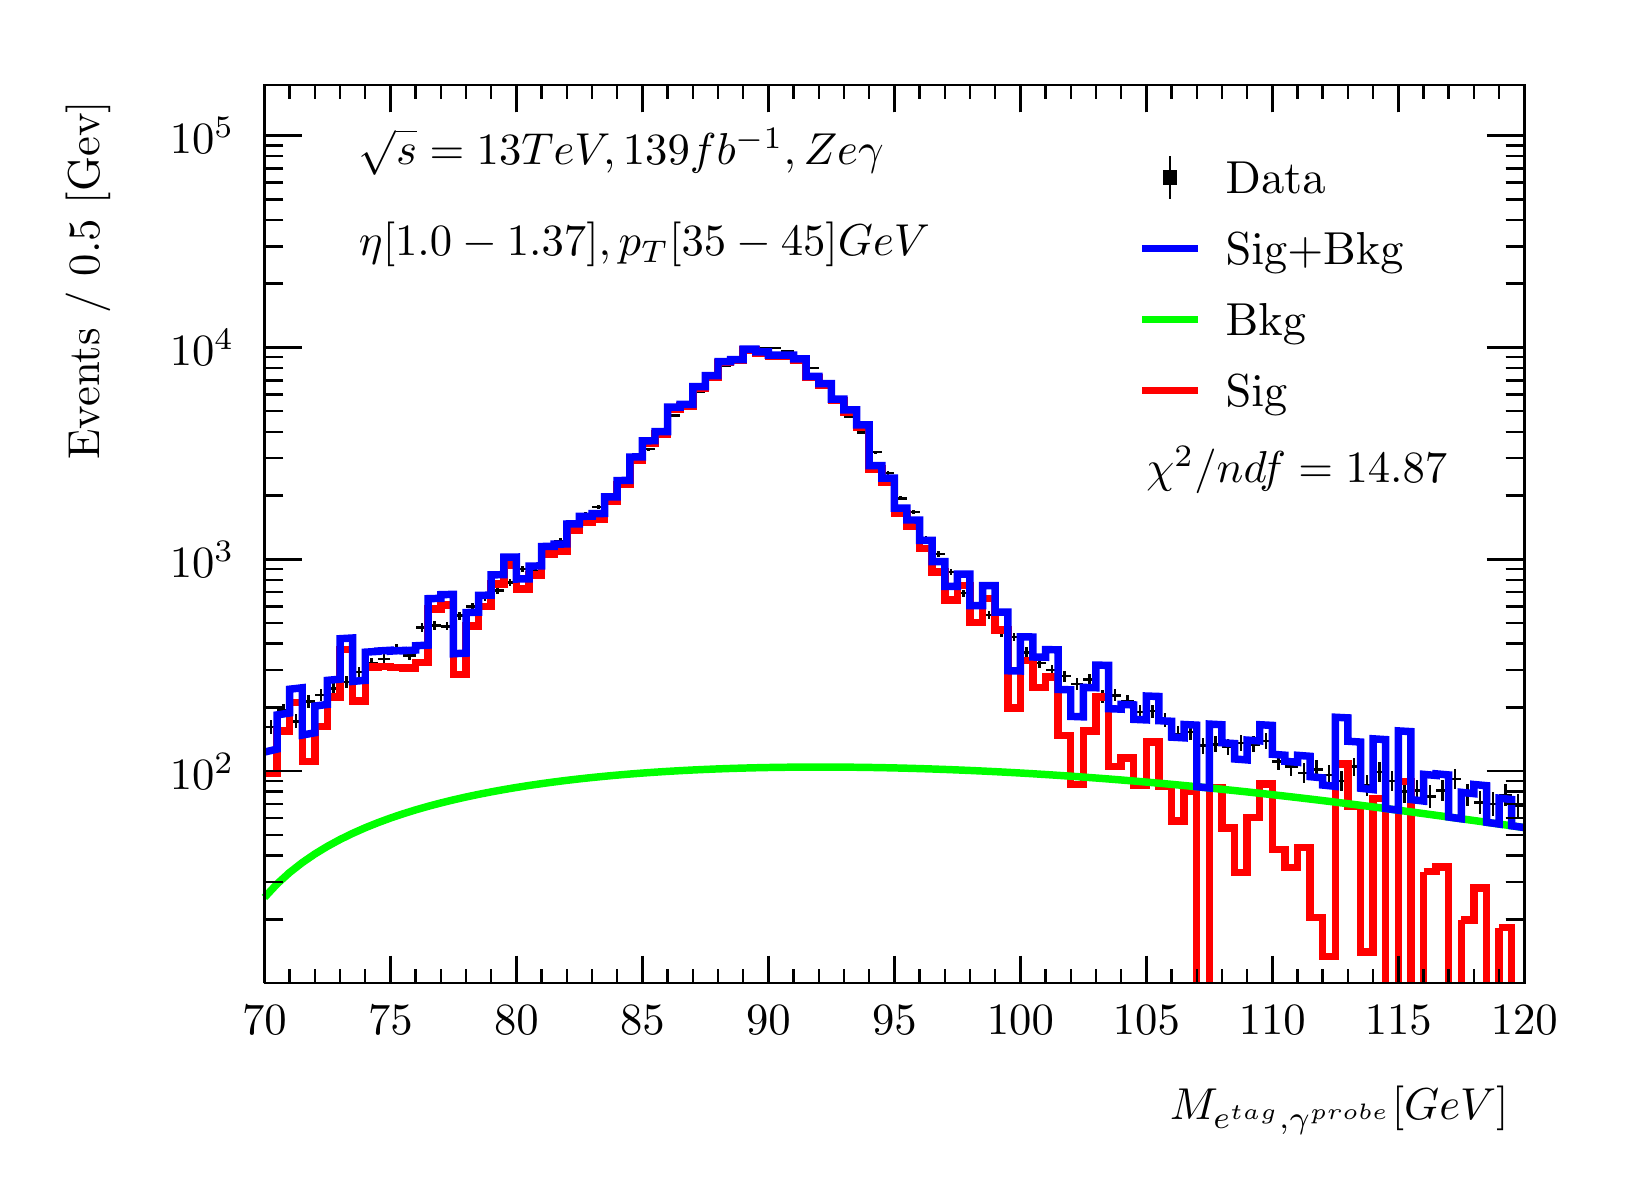
\begin{tikzpicture}
\pgfdeclareplotmark{cross} {
\pgfpathmoveto{\pgfpoint{-0.3\pgfplotmarksize}{\pgfplotmarksize}}
\pgfpathlineto{\pgfpoint{+0.3\pgfplotmarksize}{\pgfplotmarksize}}
\pgfpathlineto{\pgfpoint{+0.3\pgfplotmarksize}{0.3\pgfplotmarksize}}
\pgfpathlineto{\pgfpoint{+1\pgfplotmarksize}{0.3\pgfplotmarksize}}
\pgfpathlineto{\pgfpoint{+1\pgfplotmarksize}{-0.3\pgfplotmarksize}}
\pgfpathlineto{\pgfpoint{+0.3\pgfplotmarksize}{-0.3\pgfplotmarksize}}
\pgfpathlineto{\pgfpoint{+0.3\pgfplotmarksize}{-1.\pgfplotmarksize}}
\pgfpathlineto{\pgfpoint{-0.3\pgfplotmarksize}{-1.\pgfplotmarksize}}
\pgfpathlineto{\pgfpoint{-0.3\pgfplotmarksize}{-0.3\pgfplotmarksize}}
\pgfpathlineto{\pgfpoint{-1.\pgfplotmarksize}{-0.3\pgfplotmarksize}}
\pgfpathlineto{\pgfpoint{-1.\pgfplotmarksize}{0.3\pgfplotmarksize}}
\pgfpathlineto{\pgfpoint{-0.3\pgfplotmarksize}{0.3\pgfplotmarksize}}
\pgfpathclose
\pgfusepathqstroke
}
\pgfdeclareplotmark{cross*} {
\pgfpathmoveto{\pgfpoint{-0.3\pgfplotmarksize}{\pgfplotmarksize}}
\pgfpathlineto{\pgfpoint{+0.3\pgfplotmarksize}{\pgfplotmarksize}}
\pgfpathlineto{\pgfpoint{+0.3\pgfplotmarksize}{0.3\pgfplotmarksize}}
\pgfpathlineto{\pgfpoint{+1\pgfplotmarksize}{0.3\pgfplotmarksize}}
\pgfpathlineto{\pgfpoint{+1\pgfplotmarksize}{-0.3\pgfplotmarksize}}
\pgfpathlineto{\pgfpoint{+0.3\pgfplotmarksize}{-0.3\pgfplotmarksize}}
\pgfpathlineto{\pgfpoint{+0.3\pgfplotmarksize}{-1.\pgfplotmarksize}}
\pgfpathlineto{\pgfpoint{-0.3\pgfplotmarksize}{-1.\pgfplotmarksize}}
\pgfpathlineto{\pgfpoint{-0.3\pgfplotmarksize}{-0.3\pgfplotmarksize}}
\pgfpathlineto{\pgfpoint{-1.\pgfplotmarksize}{-0.3\pgfplotmarksize}}
\pgfpathlineto{\pgfpoint{-1.\pgfplotmarksize}{0.3\pgfplotmarksize}}
\pgfpathlineto{\pgfpoint{-0.3\pgfplotmarksize}{0.3\pgfplotmarksize}}
\pgfpathclose
\pgfusepathqfillstroke
}
\pgfdeclareplotmark{newstar} {
\pgfpathmoveto{\pgfqpoint{0pt}{\pgfplotmarksize}}
\pgfpathlineto{\pgfqpointpolar{44}{0.5\pgfplotmarksize}}
\pgfpathlineto{\pgfqpointpolar{18}{\pgfplotmarksize}}
\pgfpathlineto{\pgfqpointpolar{-20}{0.5\pgfplotmarksize}}
\pgfpathlineto{\pgfqpointpolar{-54}{\pgfplotmarksize}}
\pgfpathlineto{\pgfqpointpolar{-90}{0.5\pgfplotmarksize}}
\pgfpathlineto{\pgfqpointpolar{234}{\pgfplotmarksize}}
\pgfpathlineto{\pgfqpointpolar{198}{0.5\pgfplotmarksize}}
\pgfpathlineto{\pgfqpointpolar{162}{\pgfplotmarksize}}
\pgfpathlineto{\pgfqpointpolar{134}{0.5\pgfplotmarksize}}
\pgfpathclose
\pgfusepathqstroke
}
\pgfdeclareplotmark{newstar*} {
\pgfpathmoveto{\pgfqpoint{0pt}{\pgfplotmarksize}}
\pgfpathlineto{\pgfqpointpolar{44}{0.5\pgfplotmarksize}}
\pgfpathlineto{\pgfqpointpolar{18}{\pgfplotmarksize}}
\pgfpathlineto{\pgfqpointpolar{-20}{0.5\pgfplotmarksize}}
\pgfpathlineto{\pgfqpointpolar{-54}{\pgfplotmarksize}}
\pgfpathlineto{\pgfqpointpolar{-90}{0.5\pgfplotmarksize}}
\pgfpathlineto{\pgfqpointpolar{234}{\pgfplotmarksize}}
\pgfpathlineto{\pgfqpointpolar{198}{0.5\pgfplotmarksize}}
\pgfpathlineto{\pgfqpointpolar{162}{\pgfplotmarksize}}
\pgfpathlineto{\pgfqpointpolar{134}{0.5\pgfplotmarksize}}
\pgfpathclose
\pgfusepathqfillstroke
}
\definecolor{c}{rgb}{1,1,1};
\draw [color=c, fill=c] (0,0) rectangle (20,14.4361);
\draw [color=c, fill=c] (3,2.30977) rectangle (19,13.7143);
\definecolor{c}{rgb}{0,0,0};
\draw [c,line width=0.9] (3,2.30977) -- (3,13.7143) -- (19,13.7143) -- (19,2.30977) -- (3,2.30977);
\definecolor{c}{rgb}{1,1,1};
\draw [color=c, fill=c] (3,2.30977) rectangle (19,13.7143);
\definecolor{c}{rgb}{0,0,0};
\draw [c,line width=0.9] (3,2.30977) -- (3,13.7143) -- (19,13.7143) -- (19,2.30977) -- (3,2.30977);
\draw [c,line width=0.9] (3,2.30977) -- (19,2.30977);
\draw [c,line width=0.9] (3,2.65624) -- (3,2.30977);
\draw [c,line width=0.9] (3.32,2.48301) -- (3.32,2.30977);
\draw [c,line width=0.9] (3.64,2.48301) -- (3.64,2.30977);
\draw [c,line width=0.9] (3.96,2.48301) -- (3.96,2.30977);
\draw [c,line width=0.9] (4.28,2.48301) -- (4.28,2.30977);
\draw [c,line width=0.9] (4.6,2.65624) -- (4.6,2.30977);
\draw [c,line width=0.9] (4.92,2.48301) -- (4.92,2.30977);
\draw [c,line width=0.9] (5.24,2.48301) -- (5.24,2.30977);
\draw [c,line width=0.9] (5.56,2.48301) -- (5.56,2.30977);
\draw [c,line width=0.9] (5.88,2.48301) -- (5.88,2.30977);
\draw [c,line width=0.9] (6.2,2.65624) -- (6.2,2.30977);
\draw [c,line width=0.9] (6.52,2.48301) -- (6.52,2.30977);
\draw [c,line width=0.9] (6.84,2.48301) -- (6.84,2.30977);
\draw [c,line width=0.9] (7.16,2.48301) -- (7.16,2.30977);
\draw [c,line width=0.9] (7.48,2.48301) -- (7.48,2.30977);
\draw [c,line width=0.9] (7.8,2.65624) -- (7.8,2.30977);
\draw [c,line width=0.9] (8.12,2.48301) -- (8.12,2.30977);
\draw [c,line width=0.9] (8.44,2.48301) -- (8.44,2.30977);
\draw [c,line width=0.9] (8.76,2.48301) -- (8.76,2.30977);
\draw [c,line width=0.9] (9.08,2.48301) -- (9.08,2.30977);
\draw [c,line width=0.9] (9.4,2.65624) -- (9.4,2.30977);
\draw [c,line width=0.9] (9.72,2.48301) -- (9.72,2.30977);
\draw [c,line width=0.9] (10.04,2.48301) -- (10.04,2.30977);
\draw [c,line width=0.9] (10.36,2.48301) -- (10.36,2.30977);
\draw [c,line width=0.9] (10.68,2.48301) -- (10.68,2.30977);
\draw [c,line width=0.9] (11,2.65624) -- (11,2.30977);
\draw [c,line width=0.9] (11.32,2.48301) -- (11.32,2.30977);
\draw [c,line width=0.9] (11.64,2.48301) -- (11.64,2.30977);
\draw [c,line width=0.9] (11.96,2.48301) -- (11.96,2.30977);
\draw [c,line width=0.9] (12.28,2.48301) -- (12.28,2.30977);
\draw [c,line width=0.9] (12.6,2.65624) -- (12.6,2.30977);
\draw [c,line width=0.9] (12.92,2.48301) -- (12.92,2.30977);
\draw [c,line width=0.9] (13.24,2.48301) -- (13.24,2.30977);
\draw [c,line width=0.9] (13.56,2.48301) -- (13.56,2.30977);
\draw [c,line width=0.9] (13.88,2.48301) -- (13.88,2.30977);
\draw [c,line width=0.9] (14.2,2.65624) -- (14.2,2.30977);
\draw [c,line width=0.9] (14.52,2.48301) -- (14.52,2.30977);
\draw [c,line width=0.9] (14.84,2.48301) -- (14.84,2.30977);
\draw [c,line width=0.9] (15.16,2.48301) -- (15.16,2.30977);
\draw [c,line width=0.9] (15.48,2.48301) -- (15.48,2.30977);
\draw [c,line width=0.9] (15.8,2.65624) -- (15.8,2.30977);
\draw [c,line width=0.9] (16.12,2.48301) -- (16.12,2.30977);
\draw [c,line width=0.9] (16.44,2.48301) -- (16.44,2.30977);
\draw [c,line width=0.9] (16.76,2.48301) -- (16.76,2.30977);
\draw [c,line width=0.9] (17.08,2.48301) -- (17.08,2.30977);
\draw [c,line width=0.9] (17.4,2.65624) -- (17.4,2.30977);
\draw [c,line width=0.9] (17.72,2.48301) -- (17.72,2.30977);
\draw [c,line width=0.9] (18.04,2.48301) -- (18.04,2.30977);
\draw [c,line width=0.9] (18.36,2.48301) -- (18.36,2.30977);
\draw [c,line width=0.9] (18.68,2.48301) -- (18.68,2.30977);
\draw [c,line width=0.9] (19,2.65624) -- (19,2.30977);
\draw [anchor=base] (3,1.66015) node[scale=1.61424, color=c, rotate=0]{70};
\draw [anchor=base] (4.6,1.66015) node[scale=1.61424, color=c, rotate=0]{75};
\draw [anchor=base] (6.2,1.66015) node[scale=1.61424, color=c, rotate=0]{80};
\draw [anchor=base] (7.8,1.66015) node[scale=1.61424, color=c, rotate=0]{85};
\draw [anchor=base] (9.4,1.66015) node[scale=1.61424, color=c, rotate=0]{90};
\draw [anchor=base] (11,1.66015) node[scale=1.61424, color=c, rotate=0]{95};
\draw [anchor=base] (12.6,1.66015) node[scale=1.61424, color=c, rotate=0]{100};
\draw [anchor=base] (14.2,1.66015) node[scale=1.61424, color=c, rotate=0]{105};
\draw [anchor=base] (15.8,1.66015) node[scale=1.61424, color=c, rotate=0]{110};
\draw [anchor=base] (17.4,1.66015) node[scale=1.61424, color=c, rotate=0]{115};
\draw [anchor=base] (19,1.66015) node[scale=1.61424, color=c, rotate=0]{120};
\draw [anchor= east] (19,0.692932) node[scale=1.61424, color=c, rotate=0]{$M_{e^{tag}, \gamma^{probe}}  [GeV]$};
\draw [c,line width=0.9] (3,13.7143) -- (19,13.7143);
\draw [c,line width=0.9] (3,13.3678) -- (3,13.7143);
\draw [c,line width=0.9] (3.32,13.5411) -- (3.32,13.7143);
\draw [c,line width=0.9] (3.64,13.5411) -- (3.64,13.7143);
\draw [c,line width=0.9] (3.96,13.5411) -- (3.96,13.7143);
\draw [c,line width=0.9] (4.28,13.5411) -- (4.28,13.7143);
\draw [c,line width=0.9] (4.6,13.3678) -- (4.6,13.7143);
\draw [c,line width=0.9] (4.92,13.5411) -- (4.92,13.7143);
\draw [c,line width=0.9] (5.24,13.5411) -- (5.24,13.7143);
\draw [c,line width=0.9] (5.56,13.5411) -- (5.56,13.7143);
\draw [c,line width=0.9] (5.88,13.5411) -- (5.88,13.7143);
\draw [c,line width=0.9] (6.2,13.3678) -- (6.2,13.7143);
\draw [c,line width=0.9] (6.52,13.5411) -- (6.52,13.7143);
\draw [c,line width=0.9] (6.84,13.5411) -- (6.84,13.7143);
\draw [c,line width=0.9] (7.16,13.5411) -- (7.16,13.7143);
\draw [c,line width=0.9] (7.48,13.5411) -- (7.48,13.7143);
\draw [c,line width=0.9] (7.8,13.3678) -- (7.8,13.7143);
\draw [c,line width=0.9] (8.12,13.5411) -- (8.12,13.7143);
\draw [c,line width=0.9] (8.44,13.5411) -- (8.44,13.7143);
\draw [c,line width=0.9] (8.76,13.5411) -- (8.76,13.7143);
\draw [c,line width=0.9] (9.08,13.5411) -- (9.08,13.7143);
\draw [c,line width=0.9] (9.4,13.3678) -- (9.4,13.7143);
\draw [c,line width=0.9] (9.72,13.5411) -- (9.72,13.7143);
\draw [c,line width=0.9] (10.04,13.5411) -- (10.04,13.7143);
\draw [c,line width=0.9] (10.36,13.5411) -- (10.36,13.7143);
\draw [c,line width=0.9] (10.68,13.5411) -- (10.68,13.7143);
\draw [c,line width=0.9] (11,13.3678) -- (11,13.7143);
\draw [c,line width=0.9] (11.32,13.5411) -- (11.32,13.7143);
\draw [c,line width=0.9] (11.64,13.5411) -- (11.64,13.7143);
\draw [c,line width=0.9] (11.96,13.5411) -- (11.96,13.7143);
\draw [c,line width=0.9] (12.28,13.5411) -- (12.28,13.7143);
\draw [c,line width=0.9] (12.6,13.3678) -- (12.6,13.7143);
\draw [c,line width=0.9] (12.92,13.5411) -- (12.92,13.7143);
\draw [c,line width=0.9] (13.24,13.5411) -- (13.24,13.7143);
\draw [c,line width=0.9] (13.56,13.5411) -- (13.56,13.7143);
\draw [c,line width=0.9] (13.88,13.5411) -- (13.88,13.7143);
\draw [c,line width=0.9] (14.2,13.3678) -- (14.2,13.7143);
\draw [c,line width=0.9] (14.52,13.5411) -- (14.52,13.7143);
\draw [c,line width=0.9] (14.84,13.5411) -- (14.84,13.7143);
\draw [c,line width=0.9] (15.16,13.5411) -- (15.16,13.7143);
\draw [c,line width=0.9] (15.48,13.5411) -- (15.48,13.7143);
\draw [c,line width=0.9] (15.8,13.3678) -- (15.8,13.7143);
\draw [c,line width=0.9] (16.12,13.5411) -- (16.12,13.7143);
\draw [c,line width=0.9] (16.44,13.5411) -- (16.44,13.7143);
\draw [c,line width=0.9] (16.76,13.5411) -- (16.76,13.7143);
\draw [c,line width=0.9] (17.08,13.5411) -- (17.08,13.7143);
\draw [c,line width=0.9] (17.4,13.3678) -- (17.4,13.7143);
\draw [c,line width=0.9] (17.72,13.5411) -- (17.72,13.7143);
\draw [c,line width=0.9] (18.04,13.5411) -- (18.04,13.7143);
\draw [c,line width=0.9] (18.36,13.5411) -- (18.36,13.7143);
\draw [c,line width=0.9] (18.68,13.5411) -- (18.68,13.7143);
\draw [c,line width=0.9] (19,13.3678) -- (19,13.7143);
\draw [c,line width=0.9] (3,2.30977) -- (3,13.7143);
\draw [c,line width=0.9] (3.237,3.11973) -- (3,3.11973);
\draw [c,line width=0.9] (3.237,3.59352) -- (3,3.59352);
\draw [c,line width=0.9] (3.237,3.92968) -- (3,3.92968);
\draw [c,line width=0.9] (3.237,4.19043) -- (3,4.19043);
\draw [c,line width=0.9] (3.237,4.40347) -- (3,4.40347);
\draw [c,line width=0.9] (3.237,4.5836) -- (3,4.5836);
\draw [c,line width=0.9] (3.237,4.73964) -- (3,4.73964);
\draw [c,line width=0.9] (3.237,4.87727) -- (3,4.87727);
\draw [c,line width=0.9] (3.474,5.00038) -- (3,5.00038);
\draw [anchor= east] (2.82,5.00038) node[scale=1.61424, color=c, rotate=0]{$10^{2}$};
\draw [c,line width=0.9] (3.237,5.81034) -- (3,5.81034);
\draw [c,line width=0.9] (3.237,6.28413) -- (3,6.28413);
\draw [c,line width=0.9] (3.237,6.62029) -- (3,6.62029);
\draw [c,line width=0.9] (3.237,6.88104) -- (3,6.88104);
\draw [c,line width=0.9] (3.237,7.09409) -- (3,7.09409);
\draw [c,line width=0.9] (3.237,7.27421) -- (3,7.27421);
\draw [c,line width=0.9] (3.237,7.43025) -- (3,7.43025);
\draw [c,line width=0.9] (3.237,7.56788) -- (3,7.56788);
\draw [c,line width=0.9] (3.474,7.69099) -- (3,7.69099);
\draw [anchor= east] (2.82,7.69099) node[scale=1.61424, color=c, rotate=0]{$10^{3}$};
\draw [c,line width=0.9] (3.237,8.50095) -- (3,8.50095);
\draw [c,line width=0.9] (3.237,8.97474) -- (3,8.97474);
\draw [c,line width=0.9] (3.237,9.3109) -- (3,9.3109);
\draw [c,line width=0.9] (3.237,9.57165) -- (3,9.57165);
\draw [c,line width=0.9] (3.237,9.7847) -- (3,9.7847);
\draw [c,line width=0.9] (3.237,9.96482) -- (3,9.96482);
\draw [c,line width=0.9] (3.237,10.1209) -- (3,10.1209);
\draw [c,line width=0.9] (3.237,10.2585) -- (3,10.2585);
\draw [c,line width=0.9] (3.474,10.3816) -- (3,10.3816);
\draw [anchor= east] (2.82,10.3816) node[scale=1.61424, color=c, rotate=0]{$10^{4}$};
\draw [c,line width=0.9] (3.237,11.1916) -- (3,11.1916);
\draw [c,line width=0.9] (3.237,11.6654) -- (3,11.6654);
\draw [c,line width=0.9] (3.237,12.0015) -- (3,12.0015);
\draw [c,line width=0.9] (3.237,12.2623) -- (3,12.2623);
\draw [c,line width=0.9] (3.237,12.4753) -- (3,12.4753);
\draw [c,line width=0.9] (3.237,12.6554) -- (3,12.6554);
\draw [c,line width=0.9] (3.237,12.8115) -- (3,12.8115);
\draw [c,line width=0.9] (3.237,12.9491) -- (3,12.9491);
\draw [c,line width=0.9] (3.474,13.0722) -- (3,13.0722);
\draw [anchor= east] (2.82,13.0722) node[scale=1.61424, color=c, rotate=0]{$10^{5}$};
\draw [anchor= east] (0.76,13.7143) node[scale=1.61424, color=c, rotate=90]{Events / 0.5 [Gev]};
\draw [c,line width=0.9] (19,2.30977) -- (19,13.7143);
\draw [c,line width=0.9] (18.763,3.11973) -- (19,3.11973);
\draw [c,line width=0.9] (18.763,3.59352) -- (19,3.59352);
\draw [c,line width=0.9] (18.763,3.92968) -- (19,3.92968);
\draw [c,line width=0.9] (18.763,4.19043) -- (19,4.19043);
\draw [c,line width=0.9] (18.763,4.40347) -- (19,4.40347);
\draw [c,line width=0.9] (18.763,4.5836) -- (19,4.5836);
\draw [c,line width=0.9] (18.763,4.73964) -- (19,4.73964);
\draw [c,line width=0.9] (18.763,4.87727) -- (19,4.87727);
\draw [c,line width=0.9] (18.526,5.00038) -- (19,5.00038);
\draw [c,line width=0.9] (18.763,5.81034) -- (19,5.81034);
\draw [c,line width=0.9] (18.763,6.28413) -- (19,6.28413);
\draw [c,line width=0.9] (18.763,6.62029) -- (19,6.62029);
\draw [c,line width=0.9] (18.763,6.88104) -- (19,6.88104);
\draw [c,line width=0.9] (18.763,7.09409) -- (19,7.09409);
\draw [c,line width=0.9] (18.763,7.27421) -- (19,7.27421);
\draw [c,line width=0.9] (18.763,7.43025) -- (19,7.43025);
\draw [c,line width=0.9] (18.763,7.56788) -- (19,7.56788);
\draw [c,line width=0.9] (18.526,7.69099) -- (19,7.69099);
\draw [c,line width=0.9] (18.763,8.50095) -- (19,8.50095);
\draw [c,line width=0.9] (18.763,8.97474) -- (19,8.97474);
\draw [c,line width=0.9] (18.763,9.3109) -- (19,9.3109);
\draw [c,line width=0.9] (18.763,9.57165) -- (19,9.57165);
\draw [c,line width=0.9] (18.763,9.7847) -- (19,9.7847);
\draw [c,line width=0.9] (18.763,9.96482) -- (19,9.96482);
\draw [c,line width=0.9] (18.763,10.1209) -- (19,10.1209);
\draw [c,line width=0.9] (18.763,10.2585) -- (19,10.2585);
\draw [c,line width=0.9] (18.526,10.3816) -- (19,10.3816);
\draw [c,line width=0.9] (18.763,11.1916) -- (19,11.1916);
\draw [c,line width=0.9] (18.763,11.6654) -- (19,11.6654);
\draw [c,line width=0.9] (18.763,12.0015) -- (19,12.0015);
\draw [c,line width=0.9] (18.763,12.2623) -- (19,12.2623);
\draw [c,line width=0.9] (18.763,12.4753) -- (19,12.4753);
\draw [c,line width=0.9] (18.763,12.6554) -- (19,12.6554);
\draw [c,line width=0.9] (18.763,12.8115) -- (19,12.8115);
\draw [c,line width=0.9] (18.763,12.9491) -- (19,12.9491);
\draw [c,line width=0.9] (18.526,13.0722) -- (19,13.0722);
\draw [c,line width=0.9] (3.08,5.56411) -- (3,5.56411);
\draw [c,line width=0.9] (3,5.56411) -- (3,5.56411);
\draw [c,line width=0.9] (3.08,5.56411) -- (3.16,5.56411);
\draw [c,line width=0.9] (3.16,5.56411) -- (3.16,5.56411);
\draw [c,line width=0.9] (3.08,5.56411) -- (3.08,5.65589);
\draw [c,line width=0.9] (3.08,5.65589) -- (3.08,5.65589);
\draw [c,line width=0.9] (3.08,5.56411) -- (3.08,5.47232);
\draw [c,line width=0.9] (3.08,5.47232) -- (3.08,5.47232);
\draw [c,line width=0.9] (3.24,5.77475) -- (3.16,5.77475);
\draw [c,line width=0.9] (3.16,5.77475) -- (3.16,5.77475);
\draw [c,line width=0.9] (3.24,5.77475) -- (3.32,5.77475);
\draw [c,line width=0.9] (3.32,5.77475) -- (3.32,5.77475);
\draw [c,line width=0.9] (3.24,5.77475) -- (3.24,5.85862);
\draw [c,line width=0.9] (3.24,5.85862) -- (3.24,5.85862);
\draw [c,line width=0.9] (3.24,5.77475) -- (3.24,5.69087);
\draw [c,line width=0.9] (3.24,5.69087) -- (3.24,5.69087);
\draw [c,line width=0.9] (3.4,5.6341) -- (3.32,5.6341);
\draw [c,line width=0.9] (3.32,5.6341) -- (3.32,5.6341);
\draw [c,line width=0.9] (3.4,5.6341) -- (3.48,5.6341);
\draw [c,line width=0.9] (3.48,5.6341) -- (3.48,5.6341);
\draw [c,line width=0.9] (3.4,5.6341) -- (3.4,5.72318);
\draw [c,line width=0.9] (3.4,5.72318) -- (3.4,5.72318);
\draw [c,line width=0.9] (3.4,5.6341) -- (3.4,5.54502);
\draw [c,line width=0.9] (3.4,5.54502) -- (3.4,5.54502);
\draw [c,line width=0.9] (3.56,5.88393) -- (3.48,5.88393);
\draw [c,line width=0.9] (3.48,5.88393) -- (3.48,5.88393);
\draw [c,line width=0.9] (3.56,5.88393) -- (3.64,5.88393);
\draw [c,line width=0.9] (3.64,5.88393) -- (3.64,5.88393);
\draw [c,line width=0.9] (3.56,5.88393) -- (3.56,5.96398);
\draw [c,line width=0.9] (3.56,5.96398) -- (3.56,5.96398);
\draw [c,line width=0.9] (3.56,5.88393) -- (3.56,5.80388);
\draw [c,line width=0.9] (3.56,5.80388) -- (3.56,5.80388);
\draw [c,line width=0.9] (3.72,5.96856) -- (3.64,5.96856);
\draw [c,line width=0.9] (3.64,5.96856) -- (3.64,5.96856);
\draw [c,line width=0.9] (3.72,5.96856) -- (3.8,5.96856);
\draw [c,line width=0.9] (3.8,5.96856) -- (3.8,5.96856);
\draw [c,line width=0.9] (3.72,5.96856) -- (3.72,6.04577);
\draw [c,line width=0.9] (3.72,6.04577) -- (3.72,6.04577);
\draw [c,line width=0.9] (3.72,5.96856) -- (3.72,5.89136);
\draw [c,line width=0.9] (3.72,5.89136) -- (3.72,5.89136);
\draw [c,line width=0.9] (3.88,6.04748) -- (3.8,6.04748);
\draw [c,line width=0.9] (3.8,6.04748) -- (3.8,6.04748);
\draw [c,line width=0.9] (3.88,6.04748) -- (3.96,6.04748);
\draw [c,line width=0.9] (3.96,6.04748) -- (3.96,6.04748);
\draw [c,line width=0.9] (3.88,6.04748) -- (3.88,6.12212);
\draw [c,line width=0.9] (3.88,6.12212) -- (3.88,6.12212);
\draw [c,line width=0.9] (3.88,6.04748) -- (3.88,5.97284);
\draw [c,line width=0.9] (3.88,5.97284) -- (3.88,5.97284);
\draw [c,line width=0.9] (4.04,6.13476) -- (3.96,6.13476);
\draw [c,line width=0.9] (3.96,6.13476) -- (3.96,6.13476);
\draw [c,line width=0.9] (4.04,6.13476) -- (4.12,6.13476);
\draw [c,line width=0.9] (4.12,6.13476) -- (4.12,6.13476);
\draw [c,line width=0.9] (4.04,6.13476) -- (4.04,6.20666);
\draw [c,line width=0.9] (4.04,6.20666) -- (4.04,6.20666);
\draw [c,line width=0.9] (4.04,6.13476) -- (4.04,6.06285);
\draw [c,line width=0.9] (4.04,6.06285) -- (4.04,6.06285);
\draw [c,line width=0.9] (4.2,6.26053) -- (4.12,6.26053);
\draw [c,line width=0.9] (4.12,6.26053) -- (4.12,6.26053);
\draw [c,line width=0.9] (4.2,6.26053) -- (4.28,6.26053);
\draw [c,line width=0.9] (4.28,6.26053) -- (4.28,6.26053);
\draw [c,line width=0.9] (4.2,6.26053) -- (4.2,6.32867);
\draw [c,line width=0.9] (4.2,6.32867) -- (4.2,6.32867);
\draw [c,line width=0.9] (4.2,6.26053) -- (4.2,6.19239);
\draw [c,line width=0.9] (4.2,6.19239) -- (4.2,6.19239);
\draw [c,line width=0.9] (4.36,6.37045) -- (4.28,6.37045);
\draw [c,line width=0.9] (4.28,6.37045) -- (4.28,6.37045);
\draw [c,line width=0.9] (4.36,6.37045) -- (4.44,6.37045);
\draw [c,line width=0.9] (4.44,6.37045) -- (4.44,6.37045);
\draw [c,line width=0.9] (4.36,6.37045) -- (4.36,6.43546);
\draw [c,line width=0.9] (4.36,6.43546) -- (4.36,6.43546);
\draw [c,line width=0.9] (4.36,6.37045) -- (4.36,6.30544);
\draw [c,line width=0.9] (4.36,6.30544) -- (4.36,6.30544);
\draw [c,line width=0.9] (4.52,6.42349) -- (4.44,6.42349);
\draw [c,line width=0.9] (4.44,6.42349) -- (4.44,6.42349);
\draw [c,line width=0.9] (4.52,6.42349) -- (4.6,6.42349);
\draw [c,line width=0.9] (4.6,6.42349) -- (4.6,6.42349);
\draw [c,line width=0.9] (4.52,6.42349) -- (4.52,6.48705);
\draw [c,line width=0.9] (4.52,6.48705) -- (4.52,6.48705);
\draw [c,line width=0.9] (4.52,6.42349) -- (4.52,6.35994);
\draw [c,line width=0.9] (4.52,6.35994) -- (4.52,6.35994);
\draw [c,line width=0.9] (4.68,6.5511) -- (4.6,6.5511);
\draw [c,line width=0.9] (4.6,6.5511) -- (4.6,6.5511);
\draw [c,line width=0.9] (4.68,6.5511) -- (4.76,6.5511);
\draw [c,line width=0.9] (4.76,6.5511) -- (4.76,6.5511);
\draw [c,line width=0.9] (4.68,6.5511) -- (4.68,6.61127);
\draw [c,line width=0.9] (4.68,6.61127) -- (4.68,6.61127);
\draw [c,line width=0.9] (4.68,6.5511) -- (4.68,6.49092);
\draw [c,line width=0.9] (4.68,6.49092) -- (4.68,6.49092);
\draw [c,line width=0.9] (4.84,6.47092) -- (4.76,6.47092);
\draw [c,line width=0.9] (4.76,6.47092) -- (4.76,6.47092);
\draw [c,line width=0.9] (4.84,6.47092) -- (4.92,6.47092);
\draw [c,line width=0.9] (4.92,6.47092) -- (4.92,6.47092);
\draw [c,line width=0.9] (4.84,6.47092) -- (4.84,6.53319);
\draw [c,line width=0.9] (4.84,6.53319) -- (4.84,6.53319);
\draw [c,line width=0.9] (4.84,6.47092) -- (4.84,6.40864);
\draw [c,line width=0.9] (4.84,6.40864) -- (4.84,6.40864);
\draw [c,line width=0.9] (5,6.82356) -- (4.92,6.82356);
\draw [c,line width=0.9] (4.92,6.82356) -- (4.92,6.82356);
\draw [c,line width=0.9] (5,6.82356) -- (5.08,6.82356);
\draw [c,line width=0.9] (5.08,6.82356) -- (5.08,6.82356);
\draw [c,line width=0.9] (5,6.82356) -- (5,6.87712);
\draw [c,line width=0.9] (5,6.87712) -- (5,6.87712);
\draw [c,line width=0.9] (5,6.82356) -- (5,6.77001);
\draw [c,line width=0.9] (5,6.77001) -- (5,6.77001);
\draw [c,line width=0.9] (5.16,6.85265) -- (5.08,6.85265);
\draw [c,line width=0.9] (5.08,6.85265) -- (5.08,6.85265);
\draw [c,line width=0.9] (5.16,6.85265) -- (5.24,6.85265);
\draw [c,line width=0.9] (5.24,6.85265) -- (5.24,6.85265);
\draw [c,line width=0.9] (5.16,6.85265) -- (5.16,6.90555);
\draw [c,line width=0.9] (5.16,6.90555) -- (5.16,6.90555);
\draw [c,line width=0.9] (5.16,6.85265) -- (5.16,6.79976);
\draw [c,line width=0.9] (5.16,6.79976) -- (5.16,6.79976);
\draw [c,line width=0.9] (5.32,6.84062) -- (5.24,6.84062);
\draw [c,line width=0.9] (5.24,6.84062) -- (5.24,6.84062);
\draw [c,line width=0.9] (5.32,6.84062) -- (5.4,6.84062);
\draw [c,line width=0.9] (5.4,6.84062) -- (5.4,6.84062);
\draw [c,line width=0.9] (5.32,6.84062) -- (5.32,6.89379);
\draw [c,line width=0.9] (5.32,6.89379) -- (5.32,6.89379);
\draw [c,line width=0.9] (5.32,6.84062) -- (5.32,6.78746);
\draw [c,line width=0.9] (5.32,6.78746) -- (5.32,6.78746);
\draw [c,line width=0.9] (5.48,6.97529) -- (5.4,6.97529);
\draw [c,line width=0.9] (5.4,6.97529) -- (5.4,6.97529);
\draw [c,line width=0.9] (5.48,6.97529) -- (5.56,6.97529);
\draw [c,line width=0.9] (5.56,6.97529) -- (5.56,6.97529);
\draw [c,line width=0.9] (5.48,6.97529) -- (5.48,7.02548);
\draw [c,line width=0.9] (5.48,7.02548) -- (5.48,7.02548);
\draw [c,line width=0.9] (5.48,6.97529) -- (5.48,6.9251);
\draw [c,line width=0.9] (5.48,6.9251) -- (5.48,6.9251);
\draw [c,line width=0.9] (5.64,7.09214) -- (5.56,7.09214);
\draw [c,line width=0.9] (5.56,7.09214) -- (5.56,7.09214);
\draw [c,line width=0.9] (5.64,7.09214) -- (5.72,7.09214);
\draw [c,line width=0.9] (5.72,7.09214) -- (5.72,7.09214);
\draw [c,line width=0.9] (5.64,7.09214) -- (5.64,7.13988);
\draw [c,line width=0.9] (5.64,7.13988) -- (5.64,7.13988);
\draw [c,line width=0.9] (5.64,7.09214) -- (5.64,7.0444);
\draw [c,line width=0.9] (5.64,7.0444) -- (5.64,7.0444);
\draw [c,line width=0.9] (5.8,7.20546) -- (5.72,7.20546);
\draw [c,line width=0.9] (5.72,7.20546) -- (5.72,7.20546);
\draw [c,line width=0.9] (5.8,7.20546) -- (5.88,7.20546);
\draw [c,line width=0.9] (5.88,7.20546) -- (5.88,7.20546);
\draw [c,line width=0.9] (5.8,7.20546) -- (5.8,7.25094);
\draw [c,line width=0.9] (5.8,7.25094) -- (5.8,7.25094);
\draw [c,line width=0.9] (5.8,7.20546) -- (5.8,7.15998);
\draw [c,line width=0.9] (5.8,7.15998) -- (5.8,7.15998);
\draw [c,line width=0.9] (5.96,7.29408) -- (5.88,7.29408);
\draw [c,line width=0.9] (5.88,7.29408) -- (5.88,7.29408);
\draw [c,line width=0.9] (5.96,7.29408) -- (6.04,7.29408);
\draw [c,line width=0.9] (6.04,7.29408) -- (6.04,7.29408);
\draw [c,line width=0.9] (5.96,7.29408) -- (5.96,7.33787);
\draw [c,line width=0.9] (5.96,7.33787) -- (5.96,7.33787);
\draw [c,line width=0.9] (5.96,7.29408) -- (5.96,7.25029);
\draw [c,line width=0.9] (5.96,7.25029) -- (5.96,7.25029);
\draw [c,line width=0.9] (6.12,7.39766) -- (6.04,7.39766);
\draw [c,line width=0.9] (6.04,7.39766) -- (6.04,7.39766);
\draw [c,line width=0.9] (6.12,7.39766) -- (6.2,7.39766);
\draw [c,line width=0.9] (6.2,7.39766) -- (6.2,7.39766);
\draw [c,line width=0.9] (6.12,7.39766) -- (6.12,7.43956);
\draw [c,line width=0.9] (6.12,7.43956) -- (6.12,7.43956);
\draw [c,line width=0.9] (6.12,7.39766) -- (6.12,7.35577);
\draw [c,line width=0.9] (6.12,7.35577) -- (6.12,7.35577);
\draw [c,line width=0.9] (6.28,7.56918) -- (6.2,7.56918);
\draw [c,line width=0.9] (6.2,7.56918) -- (6.2,7.56918);
\draw [c,line width=0.9] (6.28,7.56918) -- (6.36,7.56918);
\draw [c,line width=0.9] (6.36,7.56918) -- (6.36,7.56918);
\draw [c,line width=0.9] (6.28,7.56918) -- (6.28,7.6081);
\draw [c,line width=0.9] (6.28,7.6081) -- (6.28,7.6081);
\draw [c,line width=0.9] (6.28,7.56918) -- (6.28,7.53025);
\draw [c,line width=0.9] (6.28,7.53025) -- (6.28,7.53025);
\draw [c,line width=0.9] (6.44,7.54295) -- (6.36,7.54295);
\draw [c,line width=0.9] (6.36,7.54295) -- (6.36,7.54295);
\draw [c,line width=0.9] (6.44,7.54295) -- (6.52,7.54295);
\draw [c,line width=0.9] (6.52,7.54295) -- (6.52,7.54295);
\draw [c,line width=0.9] (6.44,7.54295) -- (6.44,7.58231);
\draw [c,line width=0.9] (6.44,7.58231) -- (6.44,7.58231);
\draw [c,line width=0.9] (6.44,7.54295) -- (6.44,7.50358);
\draw [c,line width=0.9] (6.44,7.50358) -- (6.44,7.50358);
\draw [c,line width=0.9] (6.6,7.76239) -- (6.52,7.76239);
\draw [c,line width=0.9] (6.52,7.76239) -- (6.52,7.76239);
\draw [c,line width=0.9] (6.6,7.76239) -- (6.68,7.76239);
\draw [c,line width=0.9] (6.68,7.76239) -- (6.68,7.76239);
\draw [c,line width=0.9] (6.6,7.76239) -- (6.6,7.79822);
\draw [c,line width=0.9] (6.6,7.79822) -- (6.6,7.79822);
\draw [c,line width=0.9] (6.6,7.76239) -- (6.6,7.72655);
\draw [c,line width=0.9] (6.6,7.72655) -- (6.6,7.72655);
\draw [c,line width=0.9] (6.76,7.92527) -- (6.68,7.92527);
\draw [c,line width=0.9] (6.68,7.92527) -- (6.68,7.92527);
\draw [c,line width=0.9] (6.76,7.92527) -- (6.84,7.92527);
\draw [c,line width=0.9] (6.84,7.92527) -- (6.84,7.92527);
\draw [c,line width=0.9] (6.76,7.92527) -- (6.76,7.9587);
\draw [c,line width=0.9] (6.76,7.9587) -- (6.76,7.9587);
\draw [c,line width=0.9] (6.76,7.92527) -- (6.76,7.89184);
\draw [c,line width=0.9] (6.76,7.89184) -- (6.76,7.89184);
\draw [c,line width=0.9] (6.92,8.11384) -- (6.84,8.11384);
\draw [c,line width=0.9] (6.84,8.11384) -- (6.84,8.11384);
\draw [c,line width=0.9] (6.92,8.11384) -- (7,8.11384);
\draw [c,line width=0.9] (7,8.11384) -- (7,8.11384);
\draw [c,line width=0.9] (6.92,8.11384) -- (6.92,8.14467);
\draw [c,line width=0.9] (6.92,8.14467) -- (6.92,8.14467);
\draw [c,line width=0.9] (6.92,8.11384) -- (6.92,8.083);
\draw [c,line width=0.9] (6.92,8.083) -- (6.92,8.083);
\draw [c,line width=0.9] (7.08,8.25904) -- (7,8.25904);
\draw [c,line width=0.9] (7,8.25904) -- (7,8.25904);
\draw [c,line width=0.9] (7.08,8.25904) -- (7.16,8.25904);
\draw [c,line width=0.9] (7.16,8.25904) -- (7.16,8.25904);
\draw [c,line width=0.9] (7.08,8.25904) -- (7.08,8.28802);
\draw [c,line width=0.9] (7.08,8.28802) -- (7.08,8.28802);
\draw [c,line width=0.9] (7.08,8.25904) -- (7.08,8.23006);
\draw [c,line width=0.9] (7.08,8.23006) -- (7.08,8.23006);
\draw [c,line width=0.9] (7.24,8.35357) -- (7.16,8.35357);
\draw [c,line width=0.9] (7.16,8.35357) -- (7.16,8.35357);
\draw [c,line width=0.9] (7.24,8.35357) -- (7.32,8.35357);
\draw [c,line width=0.9] (7.32,8.35357) -- (7.32,8.35357);
\draw [c,line width=0.9] (7.24,8.35357) -- (7.24,8.38139);
\draw [c,line width=0.9] (7.24,8.38139) -- (7.24,8.38139);
\draw [c,line width=0.9] (7.24,8.35357) -- (7.24,8.32574);
\draw [c,line width=0.9] (7.24,8.32574) -- (7.24,8.32574);
\draw [c,line width=0.9] (7.4,8.48448) -- (7.32,8.48448);
\draw [c,line width=0.9] (7.32,8.48448) -- (7.32,8.48448);
\draw [c,line width=0.9] (7.4,8.48448) -- (7.48,8.48448);
\draw [c,line width=0.9] (7.48,8.48448) -- (7.48,8.48448);
\draw [c,line width=0.9] (7.4,8.48448) -- (7.4,8.51079);
\draw [c,line width=0.9] (7.4,8.51079) -- (7.4,8.51079);
\draw [c,line width=0.9] (7.4,8.48448) -- (7.4,8.45816);
\draw [c,line width=0.9] (7.4,8.45816) -- (7.4,8.45816);
\draw [c,line width=0.9] (7.56,8.70569) -- (7.48,8.70569);
\draw [c,line width=0.9] (7.48,8.70569) -- (7.48,8.70569);
\draw [c,line width=0.9] (7.56,8.70569) -- (7.64,8.70569);
\draw [c,line width=0.9] (7.64,8.70569) -- (7.64,8.70569);
\draw [c,line width=0.9] (7.56,8.70569) -- (7.56,8.72963);
\draw [c,line width=0.9] (7.56,8.72963) -- (7.56,8.72963);
\draw [c,line width=0.9] (7.56,8.70569) -- (7.56,8.68175);
\draw [c,line width=0.9] (7.56,8.68175) -- (7.56,8.68175);
\draw [c,line width=0.9] (7.72,8.93995) -- (7.64,8.93995);
\draw [c,line width=0.9] (7.64,8.93995) -- (7.64,8.93995);
\draw [c,line width=0.9] (7.72,8.93995) -- (7.8,8.93995);
\draw [c,line width=0.9] (7.8,8.93995) -- (7.8,8.93995);
\draw [c,line width=0.9] (7.72,8.93995) -- (7.72,8.96161);
\draw [c,line width=0.9] (7.72,8.96161) -- (7.72,8.96161);
\draw [c,line width=0.9] (7.72,8.93995) -- (7.72,8.9183);
\draw [c,line width=0.9] (7.72,8.9183) -- (7.72,8.9183);
\draw [c,line width=0.9] (7.88,9.09) -- (7.8,9.09);
\draw [c,line width=0.9] (7.8,9.09) -- (7.8,9.09);
\draw [c,line width=0.9] (7.88,9.09) -- (7.96,9.09);
\draw [c,line width=0.9] (7.96,9.09) -- (7.96,9.09);
\draw [c,line width=0.9] (7.88,9.09) -- (7.88,9.11031);
\draw [c,line width=0.9] (7.88,9.11031) -- (7.88,9.11031);
\draw [c,line width=0.9] (7.88,9.09) -- (7.88,9.0697);
\draw [c,line width=0.9] (7.88,9.0697) -- (7.88,9.0697);
\draw [c,line width=0.9] (8.04,9.29739) -- (7.96,9.29739);
\draw [c,line width=0.9] (7.96,9.29739) -- (7.96,9.29739);
\draw [c,line width=0.9] (8.04,9.29739) -- (8.12,9.29739);
\draw [c,line width=0.9] (8.12,9.29739) -- (8.12,9.29739);
\draw [c,line width=0.9] (8.04,9.29739) -- (8.04,9.31597);
\draw [c,line width=0.9] (8.04,9.31597) -- (8.04,9.31597);
\draw [c,line width=0.9] (8.04,9.29739) -- (8.04,9.27881);
\draw [c,line width=0.9] (8.04,9.27881) -- (8.04,9.27881);
\draw [c,line width=0.9] (8.2,9.51564) -- (8.12,9.51564);
\draw [c,line width=0.9] (8.12,9.51564) -- (8.12,9.51564);
\draw [c,line width=0.9] (8.2,9.51564) -- (8.28,9.51564);
\draw [c,line width=0.9] (8.28,9.51564) -- (8.28,9.51564);
\draw [c,line width=0.9] (8.2,9.51564) -- (8.2,9.53257);
\draw [c,line width=0.9] (8.2,9.53257) -- (8.2,9.53257);
\draw [c,line width=0.9] (8.2,9.51564) -- (8.2,9.49872);
\draw [c,line width=0.9] (8.2,9.49872) -- (8.2,9.49872);
\draw [c,line width=0.9] (8.36,9.68493) -- (8.28,9.68493);
\draw [c,line width=0.9] (8.28,9.68493) -- (8.28,9.68493);
\draw [c,line width=0.9] (8.36,9.68493) -- (8.44,9.68493);
\draw [c,line width=0.9] (8.44,9.68493) -- (8.44,9.68493);
\draw [c,line width=0.9] (8.36,9.68493) -- (8.36,9.70068);
\draw [c,line width=0.9] (8.36,9.70068) -- (8.36,9.70068);
\draw [c,line width=0.9] (8.36,9.68493) -- (8.36,9.66919);
\draw [c,line width=0.9] (8.36,9.66919) -- (8.36,9.66919);
\draw [c,line width=0.9] (8.52,9.81412) -- (8.44,9.81412);
\draw [c,line width=0.9] (8.44,9.81412) -- (8.44,9.81412);
\draw [c,line width=0.9] (8.52,9.81412) -- (8.6,9.81412);
\draw [c,line width=0.9] (8.6,9.81412) -- (8.6,9.81412);
\draw [c,line width=0.9] (8.52,9.81412) -- (8.52,9.82902);
\draw [c,line width=0.9] (8.52,9.82902) -- (8.52,9.82902);
\draw [c,line width=0.9] (8.52,9.81412) -- (8.52,9.79922);
\draw [c,line width=0.9] (8.52,9.79922) -- (8.52,9.79922);
\draw [c,line width=0.9] (8.68,10.0129) -- (8.6,10.0129);
\draw [c,line width=0.9] (8.6,10.0129) -- (8.6,10.0129);
\draw [c,line width=0.9] (8.68,10.0129) -- (8.76,10.0129);
\draw [c,line width=0.9] (8.76,10.0129) -- (8.76,10.0129);
\draw [c,line width=0.9] (8.68,10.0129) -- (8.68,10.0266);
\draw [c,line width=0.9] (8.68,10.0266) -- (8.68,10.0266);
\draw [c,line width=0.9] (8.68,10.0129) -- (8.68,9.99922);
\draw [c,line width=0.9] (8.68,9.99922) -- (8.68,9.99922);
\draw [c,line width=0.9] (8.84,10.1518) -- (8.76,10.1518);
\draw [c,line width=0.9] (8.76,10.1518) -- (8.76,10.1518);
\draw [c,line width=0.9] (8.84,10.1518) -- (8.92,10.1518);
\draw [c,line width=0.9] (8.92,10.1518) -- (8.92,10.1518);
\draw [c,line width=0.9] (8.84,10.1518) -- (8.84,10.1647);
\draw [c,line width=0.9] (8.84,10.1647) -- (8.84,10.1647);
\draw [c,line width=0.9] (8.84,10.1518) -- (8.84,10.139);
\draw [c,line width=0.9] (8.84,10.139) -- (8.84,10.139);
\draw [c,line width=0.9] (9,10.2505) -- (8.92,10.2505);
\draw [c,line width=0.9] (8.92,10.2505) -- (8.92,10.2505);
\draw [c,line width=0.9] (9,10.2505) -- (9.08,10.2505);
\draw [c,line width=0.9] (9.08,10.2505) -- (9.08,10.2505);
\draw [c,line width=0.9] (9,10.2505) -- (9,10.2629);
\draw [c,line width=0.9] (9,10.2629) -- (9,10.2629);
\draw [c,line width=0.9] (9,10.2505) -- (9,10.2382);
\draw [c,line width=0.9] (9,10.2382) -- (9,10.2382);
\draw [c,line width=0.9] (9.16,10.3448) -- (9.08,10.3448);
\draw [c,line width=0.9] (9.08,10.3448) -- (9.08,10.3448);
\draw [c,line width=0.9] (9.16,10.3448) -- (9.24,10.3448);
\draw [c,line width=0.9] (9.24,10.3448) -- (9.24,10.3448);
\draw [c,line width=0.9] (9.16,10.3448) -- (9.16,10.3567);
\draw [c,line width=0.9] (9.16,10.3567) -- (9.16,10.3567);
\draw [c,line width=0.9] (9.16,10.3448) -- (9.16,10.3329);
\draw [c,line width=0.9] (9.16,10.3329) -- (9.16,10.3329);
\draw [c,line width=0.9] (9.32,10.3657) -- (9.24,10.3657);
\draw [c,line width=0.9] (9.24,10.3657) -- (9.24,10.3657);
\draw [c,line width=0.9] (9.32,10.3657) -- (9.4,10.3657);
\draw [c,line width=0.9] (9.4,10.3657) -- (9.4,10.3657);
\draw [c,line width=0.9] (9.32,10.3657) -- (9.32,10.3775);
\draw [c,line width=0.9] (9.32,10.3775) -- (9.32,10.3775);
\draw [c,line width=0.9] (9.32,10.3657) -- (9.32,10.354);
\draw [c,line width=0.9] (9.32,10.354) -- (9.32,10.354);
\draw [c,line width=0.9] (9.48,10.3749) -- (9.4,10.3749);
\draw [c,line width=0.9] (9.4,10.3749) -- (9.4,10.3749);
\draw [c,line width=0.9] (9.48,10.3749) -- (9.56,10.3749);
\draw [c,line width=0.9] (9.56,10.3749) -- (9.56,10.3749);
\draw [c,line width=0.9] (9.48,10.3749) -- (9.48,10.3866);
\draw [c,line width=0.9] (9.48,10.3866) -- (9.48,10.3866);
\draw [c,line width=0.9] (9.48,10.3749) -- (9.48,10.3632);
\draw [c,line width=0.9] (9.48,10.3632) -- (9.48,10.3632);
\draw [c,line width=0.9] (9.64,10.3395) -- (9.56,10.3395);
\draw [c,line width=0.9] (9.56,10.3395) -- (9.56,10.3395);
\draw [c,line width=0.9] (9.64,10.3395) -- (9.72,10.3395);
\draw [c,line width=0.9] (9.72,10.3395) -- (9.72,10.3395);
\draw [c,line width=0.9] (9.64,10.3395) -- (9.64,10.3514);
\draw [c,line width=0.9] (9.64,10.3514) -- (9.64,10.3514);
\draw [c,line width=0.9] (9.64,10.3395) -- (9.64,10.3276);
\draw [c,line width=0.9] (9.64,10.3276) -- (9.64,10.3276);
\draw [c,line width=0.9] (9.8,10.2412) -- (9.72,10.2412);
\draw [c,line width=0.9] (9.72,10.2412) -- (9.72,10.2412);
\draw [c,line width=0.9] (9.8,10.2412) -- (9.88,10.2412);
\draw [c,line width=0.9] (9.88,10.2412) -- (9.88,10.2412);
\draw [c,line width=0.9] (9.8,10.2412) -- (9.8,10.2536);
\draw [c,line width=0.9] (9.8,10.2536) -- (9.8,10.2536);
\draw [c,line width=0.9] (9.8,10.2412) -- (9.8,10.2288);
\draw [c,line width=0.9] (9.8,10.2288) -- (9.8,10.2288);
\draw [c,line width=0.9] (9.96,10.1217) -- (9.88,10.1217);
\draw [c,line width=0.9] (9.88,10.1217) -- (9.88,10.1217);
\draw [c,line width=0.9] (9.96,10.1217) -- (10.04,10.1217);
\draw [c,line width=0.9] (10.04,10.1217) -- (10.04,10.1217);
\draw [c,line width=0.9] (9.96,10.1217) -- (9.96,10.1348);
\draw [c,line width=0.9] (9.96,10.1348) -- (9.96,10.1348);
\draw [c,line width=0.9] (9.96,10.1217) -- (9.96,10.1087);
\draw [c,line width=0.9] (9.96,10.1087) -- (9.96,10.1087);
\draw [c,line width=0.9] (10.12,9.92665) -- (10.04,9.92665);
\draw [c,line width=0.9] (10.04,9.92665) -- (10.04,9.92665);
\draw [c,line width=0.9] (10.12,9.92665) -- (10.2,9.92665);
\draw [c,line width=0.9] (10.2,9.92665) -- (10.2,9.92665);
\draw [c,line width=0.9] (10.12,9.92665) -- (10.12,9.94085);
\draw [c,line width=0.9] (10.12,9.94085) -- (10.12,9.94085);
\draw [c,line width=0.9] (10.12,9.92665) -- (10.12,9.91245);
\draw [c,line width=0.9] (10.12,9.91245) -- (10.12,9.91245);
\draw [c,line width=0.9] (10.28,9.72845) -- (10.2,9.72845);
\draw [c,line width=0.9] (10.2,9.72845) -- (10.2,9.72845);
\draw [c,line width=0.9] (10.28,9.72845) -- (10.36,9.72845);
\draw [c,line width=0.9] (10.36,9.72845) -- (10.36,9.72845);
\draw [c,line width=0.9] (10.28,9.72845) -- (10.28,9.7439);
\draw [c,line width=0.9] (10.28,9.7439) -- (10.28,9.7439);
\draw [c,line width=0.9] (10.28,9.72845) -- (10.28,9.71299);
\draw [c,line width=0.9] (10.28,9.71299) -- (10.28,9.71299);
\draw [c,line width=0.9] (10.44,9.49761) -- (10.36,9.49761);
\draw [c,line width=0.9] (10.36,9.49761) -- (10.36,9.49761);
\draw [c,line width=0.9] (10.44,9.49761) -- (10.52,9.49761);
\draw [c,line width=0.9] (10.52,9.49761) -- (10.52,9.49761);
\draw [c,line width=0.9] (10.44,9.49761) -- (10.44,9.51466);
\draw [c,line width=0.9] (10.44,9.51466) -- (10.44,9.51466);
\draw [c,line width=0.9] (10.44,9.49761) -- (10.44,9.48055);
\draw [c,line width=0.9] (10.44,9.48055) -- (10.44,9.48055);
\draw [c,line width=0.9] (10.6,9.30005) -- (10.52,9.30005);
\draw [c,line width=0.9] (10.52,9.30005) -- (10.52,9.30005);
\draw [c,line width=0.9] (10.6,9.30005) -- (10.68,9.30005);
\draw [c,line width=0.9] (10.68,9.30005) -- (10.68,9.30005);
\draw [c,line width=0.9] (10.6,9.30005) -- (10.6,9.31861);
\draw [c,line width=0.9] (10.6,9.31861) -- (10.6,9.31861);
\draw [c,line width=0.9] (10.6,9.30005) -- (10.6,9.28148);
\draw [c,line width=0.9] (10.6,9.28148) -- (10.6,9.28148);
\draw [c,line width=0.9] (10.76,9.05198) -- (10.68,9.05198);
\draw [c,line width=0.9] (10.68,9.05198) -- (10.68,9.05198);
\draw [c,line width=0.9] (10.76,9.05198) -- (10.84,9.05198);
\draw [c,line width=0.9] (10.84,9.05198) -- (10.84,9.05198);
\draw [c,line width=0.9] (10.76,9.05198) -- (10.76,9.07262);
\draw [c,line width=0.9] (10.76,9.07262) -- (10.76,9.07262);
\draw [c,line width=0.9] (10.76,9.05198) -- (10.76,9.03134);
\draw [c,line width=0.9] (10.76,9.03134) -- (10.76,9.03134);
\draw [c,line width=0.9] (10.92,8.78713) -- (10.84,8.78713);
\draw [c,line width=0.9] (10.84,8.78713) -- (10.84,8.78713);
\draw [c,line width=0.9] (10.92,8.78713) -- (11,8.78713);
\draw [c,line width=0.9] (11,8.78713) -- (11,8.78713);
\draw [c,line width=0.9] (10.92,8.78713) -- (10.92,8.81024);
\draw [c,line width=0.9] (10.92,8.81024) -- (10.92,8.81024);
\draw [c,line width=0.9] (10.92,8.78713) -- (10.92,8.76401);
\draw [c,line width=0.9] (10.92,8.76401) -- (10.92,8.76401);
\draw [c,line width=0.9] (11.08,8.46656) -- (11,8.46656);
\draw [c,line width=0.9] (11,8.46656) -- (11,8.46656);
\draw [c,line width=0.9] (11.08,8.46656) -- (11.16,8.46656);
\draw [c,line width=0.9] (11.16,8.46656) -- (11.16,8.46656);
\draw [c,line width=0.9] (11.08,8.46656) -- (11.08,8.49308);
\draw [c,line width=0.9] (11.08,8.49308) -- (11.08,8.49308);
\draw [c,line width=0.9] (11.08,8.46656) -- (11.08,8.44005);
\draw [c,line width=0.9] (11.08,8.44005) -- (11.08,8.44005);
\draw [c,line width=0.9] (11.24,8.29443) -- (11.16,8.29443);
\draw [c,line width=0.9] (11.16,8.29443) -- (11.16,8.29443);
\draw [c,line width=0.9] (11.24,8.29443) -- (11.32,8.29443);
\draw [c,line width=0.9] (11.32,8.29443) -- (11.32,8.29443);
\draw [c,line width=0.9] (11.24,8.29443) -- (11.24,8.32297);
\draw [c,line width=0.9] (11.24,8.32297) -- (11.24,8.32297);
\draw [c,line width=0.9] (11.24,8.29443) -- (11.24,8.26589);
\draw [c,line width=0.9] (11.24,8.26589) -- (11.24,8.26589);
\draw [c,line width=0.9] (11.4,7.95454) -- (11.32,7.95454);
\draw [c,line width=0.9] (11.32,7.95454) -- (11.32,7.95454);
\draw [c,line width=0.9] (11.4,7.95454) -- (11.48,7.95454);
\draw [c,line width=0.9] (11.48,7.95454) -- (11.48,7.95454);
\draw [c,line width=0.9] (11.4,7.95454) -- (11.4,7.98755);
\draw [c,line width=0.9] (11.4,7.98755) -- (11.4,7.98755);
\draw [c,line width=0.9] (11.4,7.95454) -- (11.4,7.92153);
\draw [c,line width=0.9] (11.4,7.92153) -- (11.4,7.92153);
\draw [c,line width=0.9] (11.56,7.76129) -- (11.48,7.76129);
\draw [c,line width=0.9] (11.48,7.76129) -- (11.48,7.76129);
\draw [c,line width=0.9] (11.56,7.76129) -- (11.64,7.76129);
\draw [c,line width=0.9] (11.64,7.76129) -- (11.64,7.76129);
\draw [c,line width=0.9] (11.56,7.76129) -- (11.56,7.79714);
\draw [c,line width=0.9] (11.56,7.79714) -- (11.56,7.79714);
\draw [c,line width=0.9] (11.56,7.76129) -- (11.56,7.72543);
\draw [c,line width=0.9] (11.56,7.72543) -- (11.56,7.72543);
\draw [c,line width=0.9] (11.72,7.52961) -- (11.64,7.52961);
\draw [c,line width=0.9] (11.64,7.52961) -- (11.64,7.52961);
\draw [c,line width=0.9] (11.72,7.52961) -- (11.8,7.52961);
\draw [c,line width=0.9] (11.8,7.52961) -- (11.8,7.52961);
\draw [c,line width=0.9] (11.72,7.52961) -- (11.72,7.5692);
\draw [c,line width=0.9] (11.72,7.5692) -- (11.72,7.5692);
\draw [c,line width=0.9] (11.72,7.52961) -- (11.72,7.49002);
\draw [c,line width=0.9] (11.72,7.49002) -- (11.72,7.49002);
\draw [c,line width=0.9] (11.88,7.26247) -- (11.8,7.26247);
\draw [c,line width=0.9] (11.8,7.26247) -- (11.8,7.26247);
\draw [c,line width=0.9] (11.88,7.26247) -- (11.96,7.26247);
\draw [c,line width=0.9] (11.96,7.26247) -- (11.96,7.26247);
\draw [c,line width=0.9] (11.88,7.26247) -- (11.88,7.30686);
\draw [c,line width=0.9] (11.88,7.30686) -- (11.88,7.30686);
\draw [c,line width=0.9] (11.88,7.26247) -- (11.88,7.21809);
\draw [c,line width=0.9] (11.88,7.21809) -- (11.88,7.21809);
\draw [c,line width=0.9] (12.04,7.10764) -- (11.96,7.10764);
\draw [c,line width=0.9] (11.96,7.10764) -- (11.96,7.10764);
\draw [c,line width=0.9] (12.04,7.10764) -- (12.12,7.10764);
\draw [c,line width=0.9] (12.12,7.10764) -- (12.12,7.10764);
\draw [c,line width=0.9] (12.04,7.10764) -- (12.04,7.15507);
\draw [c,line width=0.9] (12.04,7.15507) -- (12.04,7.15507);
\draw [c,line width=0.9] (12.04,7.10764) -- (12.04,7.06022);
\draw [c,line width=0.9] (12.04,7.06022) -- (12.04,7.06022);
\draw [c,line width=0.9] (12.2,6.98602) -- (12.12,6.98602);
\draw [c,line width=0.9] (12.12,6.98602) -- (12.12,6.98602);
\draw [c,line width=0.9] (12.2,6.98602) -- (12.28,6.98602);
\draw [c,line width=0.9] (12.28,6.98602) -- (12.28,6.98602);
\draw [c,line width=0.9] (12.2,6.98602) -- (12.2,7.03598);
\draw [c,line width=0.9] (12.2,7.03598) -- (12.2,7.03598);
\draw [c,line width=0.9] (12.2,6.98602) -- (12.2,6.93606);
\draw [c,line width=0.9] (12.2,6.93606) -- (12.2,6.93606);
\draw [c,line width=0.9] (12.36,6.76311) -- (12.28,6.76311);
\draw [c,line width=0.9] (12.28,6.76311) -- (12.28,6.76311);
\draw [c,line width=0.9] (12.36,6.76311) -- (12.44,6.76311);
\draw [c,line width=0.9] (12.44,6.76311) -- (12.44,6.76311);
\draw [c,line width=0.9] (12.36,6.76311) -- (12.36,6.81806);
\draw [c,line width=0.9] (12.36,6.81806) -- (12.36,6.81806);
\draw [c,line width=0.9] (12.36,6.76311) -- (12.36,6.70815);
\draw [c,line width=0.9] (12.36,6.70815) -- (12.36,6.70815);
\draw [c,line width=0.9] (12.52,6.7048) -- (12.44,6.7048);
\draw [c,line width=0.9] (12.44,6.7048) -- (12.44,6.7048);
\draw [c,line width=0.9] (12.52,6.7048) -- (12.6,6.7048);
\draw [c,line width=0.9] (12.6,6.7048) -- (12.6,6.7048);
\draw [c,line width=0.9] (12.52,6.7048) -- (12.52,6.76115);
\draw [c,line width=0.9] (12.52,6.76115) -- (12.52,6.76115);
\draw [c,line width=0.9] (12.52,6.7048) -- (12.52,6.64846);
\draw [c,line width=0.9] (12.52,6.64846) -- (12.52,6.64846);
\draw [c,line width=0.9] (12.68,6.51009) -- (12.6,6.51009);
\draw [c,line width=0.9] (12.6,6.51009) -- (12.6,6.51009);
\draw [c,line width=0.9] (12.68,6.51009) -- (12.76,6.51009);
\draw [c,line width=0.9] (12.76,6.51009) -- (12.76,6.51009);
\draw [c,line width=0.9] (12.68,6.51009) -- (12.68,6.57133);
\draw [c,line width=0.9] (12.68,6.57133) -- (12.68,6.57133);
\draw [c,line width=0.9] (12.68,6.51009) -- (12.68,6.44885);
\draw [c,line width=0.9] (12.68,6.44885) -- (12.68,6.44885);
\draw [c,line width=0.9] (12.84,6.37406) -- (12.76,6.37406);
\draw [c,line width=0.9] (12.76,6.37406) -- (12.76,6.37406);
\draw [c,line width=0.9] (12.84,6.37406) -- (12.92,6.37406);
\draw [c,line width=0.9] (12.92,6.37406) -- (12.92,6.37406);
\draw [c,line width=0.9] (12.84,6.37406) -- (12.84,6.43897);
\draw [c,line width=0.9] (12.84,6.43897) -- (12.84,6.43897);
\draw [c,line width=0.9] (12.84,6.37406) -- (12.84,6.30915);
\draw [c,line width=0.9] (12.84,6.30915) -- (12.84,6.30915);
\draw [c,line width=0.9] (13,6.28413) -- (12.92,6.28413);
\draw [c,line width=0.9] (12.92,6.28413) -- (12.92,6.28413);
\draw [c,line width=0.9] (13,6.28413) -- (13.08,6.28413);
\draw [c,line width=0.9] (13.08,6.28413) -- (13.08,6.28413);
\draw [c,line width=0.9] (13,6.28413) -- (13,6.35159);
\draw [c,line width=0.9] (13,6.35159) -- (13,6.35159);
\draw [c,line width=0.9] (13,6.28413) -- (13,6.21668);
\draw [c,line width=0.9] (13,6.21668) -- (13,6.21668);
\draw [c,line width=0.9] (13.16,6.20768) -- (13.08,6.20768);
\draw [c,line width=0.9] (13.08,6.20768) -- (13.08,6.20768);
\draw [c,line width=0.9] (13.16,6.20768) -- (13.24,6.20768);
\draw [c,line width=0.9] (13.24,6.20768) -- (13.24,6.20768);
\draw [c,line width=0.9] (13.16,6.20768) -- (13.16,6.27738);
\draw [c,line width=0.9] (13.16,6.27738) -- (13.16,6.27738);
\draw [c,line width=0.9] (13.16,6.20768) -- (13.16,6.13798);
\draw [c,line width=0.9] (13.16,6.13798) -- (13.16,6.13798);
\draw [c,line width=0.9] (13.32,6.10789) -- (13.24,6.10789);
\draw [c,line width=0.9] (13.24,6.10789) -- (13.24,6.10789);
\draw [c,line width=0.9] (13.32,6.10789) -- (13.4,6.10789);
\draw [c,line width=0.9] (13.4,6.10789) -- (13.4,6.10789);
\draw [c,line width=0.9] (13.32,6.10789) -- (13.32,6.18063);
\draw [c,line width=0.9] (13.32,6.18063) -- (13.32,6.18063);
\draw [c,line width=0.9] (13.32,6.10789) -- (13.32,6.03516);
\draw [c,line width=0.9] (13.32,6.03516) -- (13.32,6.03516);
\draw [c,line width=0.9] (13.48,6.16534) -- (13.4,6.16534);
\draw [c,line width=0.9] (13.4,6.16534) -- (13.4,6.16534);
\draw [c,line width=0.9] (13.48,6.16534) -- (13.56,6.16534);
\draw [c,line width=0.9] (13.56,6.16534) -- (13.56,6.16534);
\draw [c,line width=0.9] (13.48,6.16534) -- (13.48,6.23631);
\draw [c,line width=0.9] (13.48,6.23631) -- (13.48,6.23631);
\draw [c,line width=0.9] (13.48,6.16534) -- (13.48,6.09437);
\draw [c,line width=0.9] (13.48,6.09437) -- (13.48,6.09437);
\draw [c,line width=0.9] (13.64,5.94797) -- (13.56,5.94797);
\draw [c,line width=0.9] (13.56,5.94797) -- (13.56,5.94797);
\draw [c,line width=0.9] (13.64,5.94797) -- (13.72,5.94797);
\draw [c,line width=0.9] (13.72,5.94797) -- (13.72,5.94797);
\draw [c,line width=0.9] (13.64,5.94797) -- (13.64,6.02586);
\draw [c,line width=0.9] (13.64,6.02586) -- (13.64,6.02586);
\draw [c,line width=0.9] (13.64,5.94797) -- (13.64,5.87008);
\draw [c,line width=0.9] (13.64,5.87008) -- (13.64,5.87008);
\draw [c,line width=0.9] (13.8,5.96345) -- (13.72,5.96345);
\draw [c,line width=0.9] (13.72,5.96345) -- (13.72,5.96345);
\draw [c,line width=0.9] (13.8,5.96345) -- (13.88,5.96345);
\draw [c,line width=0.9] (13.88,5.96345) -- (13.88,5.96345);
\draw [c,line width=0.9] (13.8,5.96345) -- (13.8,6.04082);
\draw [c,line width=0.9] (13.8,6.04082) -- (13.8,6.04082);
\draw [c,line width=0.9] (13.8,5.96345) -- (13.8,5.88608);
\draw [c,line width=0.9] (13.8,5.88608) -- (13.8,5.88608);
\draw [c,line width=0.9] (13.96,5.88393) -- (13.88,5.88393);
\draw [c,line width=0.9] (13.88,5.88393) -- (13.88,5.88393);
\draw [c,line width=0.9] (13.96,5.88393) -- (14.04,5.88393);
\draw [c,line width=0.9] (14.04,5.88393) -- (14.04,5.88393);
\draw [c,line width=0.9] (13.96,5.88393) -- (13.96,5.96398);
\draw [c,line width=0.9] (13.96,5.96398) -- (13.96,5.96398);
\draw [c,line width=0.9] (13.96,5.88393) -- (13.96,5.80388);
\draw [c,line width=0.9] (13.96,5.80388) -- (13.96,5.80388);
\draw [c,line width=0.9] (14.12,5.7504) -- (14.04,5.7504);
\draw [c,line width=0.9] (14.04,5.7504) -- (14.04,5.7504);
\draw [c,line width=0.9] (14.12,5.7504) -- (14.2,5.7504);
\draw [c,line width=0.9] (14.2,5.7504) -- (14.2,5.7504);
\draw [c,line width=0.9] (14.12,5.7504) -- (14.12,5.83516);
\draw [c,line width=0.9] (14.12,5.83516) -- (14.12,5.83516);
\draw [c,line width=0.9] (14.12,5.7504) -- (14.12,5.66565);
\draw [c,line width=0.9] (14.12,5.66565) -- (14.12,5.66565);
\draw [c,line width=0.9] (14.28,5.76264) -- (14.2,5.76264);
\draw [c,line width=0.9] (14.2,5.76264) -- (14.2,5.76264);
\draw [c,line width=0.9] (14.28,5.76264) -- (14.36,5.76264);
\draw [c,line width=0.9] (14.36,5.76264) -- (14.36,5.76264);
\draw [c,line width=0.9] (14.28,5.76264) -- (14.28,5.84695);
\draw [c,line width=0.9] (14.28,5.84695) -- (14.28,5.84695);
\draw [c,line width=0.9] (14.28,5.76264) -- (14.28,5.67833);
\draw [c,line width=0.9] (14.28,5.67833) -- (14.28,5.67833);
\draw [c,line width=0.9] (14.44,5.65431) -- (14.36,5.65431);
\draw [c,line width=0.9] (14.36,5.65431) -- (14.36,5.65431);
\draw [c,line width=0.9] (14.44,5.65431) -- (14.52,5.65431);
\draw [c,line width=0.9] (14.52,5.65431) -- (14.52,5.65431);
\draw [c,line width=0.9] (14.44,5.65431) -- (14.44,5.74262);
\draw [c,line width=0.9] (14.44,5.74262) -- (14.44,5.74262);
\draw [c,line width=0.9] (14.44,5.65431) -- (14.44,5.566);
\draw [c,line width=0.9] (14.44,5.566) -- (14.44,5.566);
\draw [c,line width=0.9] (14.6,5.47418) -- (14.52,5.47418);
\draw [c,line width=0.9] (14.52,5.47418) -- (14.52,5.47418);
\draw [c,line width=0.9] (14.6,5.47418) -- (14.68,5.47418);
\draw [c,line width=0.9] (14.68,5.47418) -- (14.68,5.47418);
\draw [c,line width=0.9] (14.6,5.47418) -- (14.6,5.56956);
\draw [c,line width=0.9] (14.6,5.56956) -- (14.6,5.56956);
\draw [c,line width=0.9] (14.6,5.47418) -- (14.6,5.3788);
\draw [c,line width=0.9] (14.6,5.3788) -- (14.6,5.3788);
\draw [c,line width=0.9] (14.76,5.49732) -- (14.68,5.49732);
\draw [c,line width=0.9] (14.68,5.49732) -- (14.68,5.49732);
\draw [c,line width=0.9] (14.76,5.49732) -- (14.84,5.49732);
\draw [c,line width=0.9] (14.84,5.49732) -- (14.84,5.49732);
\draw [c,line width=0.9] (14.76,5.49732) -- (14.76,5.59176);
\draw [c,line width=0.9] (14.76,5.59176) -- (14.76,5.59176);
\draw [c,line width=0.9] (14.76,5.49732) -- (14.76,5.40287);
\draw [c,line width=0.9] (14.76,5.40287) -- (14.76,5.40287);
\draw [c,line width=0.9] (14.92,5.3248) -- (14.84,5.3248);
\draw [c,line width=0.9] (14.84,5.3248) -- (14.84,5.3248);
\draw [c,line width=0.9] (14.92,5.3248) -- (15,5.3248);
\draw [c,line width=0.9] (15,5.3248) -- (15,5.3248);
\draw [c,line width=0.9] (14.92,5.3248) -- (14.92,5.42648);
\draw [c,line width=0.9] (14.92,5.42648) -- (14.92,5.42648);
\draw [c,line width=0.9] (14.92,5.3248) -- (14.92,5.22313);
\draw [c,line width=0.9] (14.92,5.22313) -- (14.92,5.22313);
\draw [c,line width=0.9] (15.08,5.34237) -- (15,5.34237);
\draw [c,line width=0.9] (15,5.34237) -- (15,5.34237);
\draw [c,line width=0.9] (15.08,5.34237) -- (15.16,5.34237);
\draw [c,line width=0.9] (15.16,5.34237) -- (15.16,5.34237);
\draw [c,line width=0.9] (15.08,5.34237) -- (15.08,5.44329);
\draw [c,line width=0.9] (15.08,5.44329) -- (15.08,5.44329);
\draw [c,line width=0.9] (15.08,5.34237) -- (15.08,5.24146);
\draw [c,line width=0.9] (15.08,5.24146) -- (15.08,5.24146);
\draw [c,line width=0.9] (15.24,5.30696) -- (15.16,5.30696);
\draw [c,line width=0.9] (15.16,5.30696) -- (15.16,5.30696);
\draw [c,line width=0.9] (15.24,5.30696) -- (15.32,5.30696);
\draw [c,line width=0.9] (15.32,5.30696) -- (15.32,5.30696);
\draw [c,line width=0.9] (15.24,5.30696) -- (15.24,5.40942);
\draw [c,line width=0.9] (15.24,5.40942) -- (15.24,5.40942);
\draw [c,line width=0.9] (15.24,5.30696) -- (15.24,5.20451);
\draw [c,line width=0.9] (15.24,5.20451) -- (15.24,5.20451);
\draw [c,line width=0.9] (15.4,5.35969) -- (15.32,5.35969);
\draw [c,line width=0.9] (15.32,5.35969) -- (15.32,5.35969);
\draw [c,line width=0.9] (15.4,5.35969) -- (15.48,5.35969);
\draw [c,line width=0.9] (15.48,5.35969) -- (15.48,5.35969);
\draw [c,line width=0.9] (15.4,5.35969) -- (15.4,5.45986);
\draw [c,line width=0.9] (15.4,5.45986) -- (15.4,5.45986);
\draw [c,line width=0.9] (15.4,5.35969) -- (15.4,5.25952);
\draw [c,line width=0.9] (15.4,5.25952) -- (15.4,5.25952);
\draw [c,line width=0.9] (15.56,5.34237) -- (15.48,5.34237);
\draw [c,line width=0.9] (15.48,5.34237) -- (15.48,5.34237);
\draw [c,line width=0.9] (15.56,5.34237) -- (15.64,5.34237);
\draw [c,line width=0.9] (15.64,5.34237) -- (15.64,5.34237);
\draw [c,line width=0.9] (15.56,5.34237) -- (15.56,5.44329);
\draw [c,line width=0.9] (15.56,5.44329) -- (15.56,5.44329);
\draw [c,line width=0.9] (15.56,5.34237) -- (15.56,5.24146);
\draw [c,line width=0.9] (15.56,5.24146) -- (15.56,5.24146);
\draw [c,line width=0.9] (15.72,5.38518) -- (15.64,5.38518);
\draw [c,line width=0.9] (15.64,5.38518) -- (15.64,5.38518);
\draw [c,line width=0.9] (15.72,5.38518) -- (15.8,5.38518);
\draw [c,line width=0.9] (15.8,5.38518) -- (15.8,5.38518);
\draw [c,line width=0.9] (15.72,5.38518) -- (15.72,5.48426);
\draw [c,line width=0.9] (15.72,5.48426) -- (15.72,5.48426);
\draw [c,line width=0.9] (15.72,5.38518) -- (15.72,5.2861);
\draw [c,line width=0.9] (15.72,5.2861) -- (15.72,5.2861);
\draw [c,line width=0.9] (15.88,5.12233) -- (15.8,5.12233);
\draw [c,line width=0.9] (15.8,5.12233) -- (15.8,5.12233);
\draw [c,line width=0.9] (15.88,5.12233) -- (15.96,5.12233);
\draw [c,line width=0.9] (15.96,5.12233) -- (15.96,5.12233);
\draw [c,line width=0.9] (15.88,5.12233) -- (15.88,5.2332);
\draw [c,line width=0.9] (15.88,5.2332) -- (15.88,5.2332);
\draw [c,line width=0.9] (15.88,5.12233) -- (15.88,5.01146);
\draw [c,line width=0.9] (15.88,5.01146) -- (15.88,5.01146);
\draw [c,line width=0.9] (16.04,5.0574) -- (15.96,5.0574);
\draw [c,line width=0.9] (15.96,5.0574) -- (15.96,5.0574);
\draw [c,line width=0.9] (16.04,5.0574) -- (16.12,5.0574);
\draw [c,line width=0.9] (16.12,5.0574) -- (16.12,5.0574);
\draw [c,line width=0.9] (16.04,5.0574) -- (16.04,5.17139);
\draw [c,line width=0.9] (16.04,5.17139) -- (16.04,5.17139);
\draw [c,line width=0.9] (16.04,5.0574) -- (16.04,4.94341);
\draw [c,line width=0.9] (16.04,4.94341) -- (16.04,4.94341);
\draw [c,line width=0.9] (16.2,4.97678) -- (16.12,4.97678);
\draw [c,line width=0.9] (16.12,4.97678) -- (16.12,4.97678);
\draw [c,line width=0.9] (16.2,4.97678) -- (16.28,4.97678);
\draw [c,line width=0.9] (16.28,4.97678) -- (16.28,4.97678);
\draw [c,line width=0.9] (16.2,4.97678) -- (16.2,5.10037);
\draw [c,line width=0.9] (16.2,5.10037) -- (16.2,5.10037);
\draw [c,line width=0.9] (16.2,4.97678) -- (16.2,4.85257);
\draw [c,line width=0.9] (16.2,4.85257) -- (16.2,4.85257);
\draw [c,line width=0.9] (16.36,5.02352) -- (16.28,5.02352);
\draw [c,line width=0.9] (16.28,5.02352) -- (16.28,5.02352);
\draw [c,line width=0.9] (16.36,5.02352) -- (16.44,5.02352);
\draw [c,line width=0.9] (16.44,5.02352) -- (16.44,5.02352);
\draw [c,line width=0.9] (16.36,5.02352) -- (16.36,5.13918);
\draw [c,line width=0.9] (16.36,5.13918) -- (16.36,5.13918);
\draw [c,line width=0.9] (16.36,5.02352) -- (16.36,4.90787);
\draw [c,line width=0.9] (16.36,4.90787) -- (16.36,4.90787);
\draw [c,line width=0.9] (16.52,4.95268) -- (16.44,4.95268);
\draw [c,line width=0.9] (16.44,4.95268) -- (16.44,4.95268);
\draw [c,line width=0.9] (16.52,4.95268) -- (16.6,4.95268);
\draw [c,line width=0.9] (16.6,4.95268) -- (16.6,4.95268);
\draw [c,line width=0.9] (16.52,4.95268) -- (16.52,5.07761);
\draw [c,line width=0.9] (16.52,5.07761) -- (16.52,5.07761);
\draw [c,line width=0.9] (16.52,4.95268) -- (16.52,4.82712);
\draw [c,line width=0.9] (16.52,4.82712) -- (16.52,4.82712);
\draw [c,line width=0.9] (16.68,4.87727) -- (16.6,4.87727);
\draw [c,line width=0.9] (16.6,4.87727) -- (16.6,4.87727);
\draw [c,line width=0.9] (16.68,4.87727) -- (16.76,4.87727);
\draw [c,line width=0.9] (16.76,4.87727) -- (16.76,4.87727);
\draw [c,line width=0.9] (16.68,4.87727) -- (16.68,5.00647);
\draw [c,line width=0.9] (16.68,5.00647) -- (16.68,5.00647);
\draw [c,line width=0.9] (16.68,4.87727) -- (16.68,4.74737);
\draw [c,line width=0.9] (16.68,4.74737) -- (16.68,4.74737);
\draw [c,line width=0.9] (16.84,5.0574) -- (16.76,5.0574);
\draw [c,line width=0.9] (16.76,5.0574) -- (16.76,5.0574);
\draw [c,line width=0.9] (16.84,5.0574) -- (16.92,5.0574);
\draw [c,line width=0.9] (16.92,5.0574) -- (16.92,5.0574);
\draw [c,line width=0.9] (16.84,5.0574) -- (16.84,5.17139);
\draw [c,line width=0.9] (16.84,5.17139) -- (16.84,5.17139);
\draw [c,line width=0.9] (16.84,5.0574) -- (16.84,4.94341);
\draw [c,line width=0.9] (16.84,4.94341) -- (16.84,4.94341);
\draw [c,line width=0.9] (17,4.82415) -- (16.92,4.82415);
\draw [c,line width=0.9] (16.92,4.82415) -- (16.92,4.82415);
\draw [c,line width=0.9] (17,4.82415) -- (17.08,4.82415);
\draw [c,line width=0.9] (17.08,4.82415) -- (17.08,4.82415);
\draw [c,line width=0.9] (17,4.82415) -- (17,4.95645);
\draw [c,line width=0.9] (17,4.95645) -- (17,4.95645);
\draw [c,line width=0.9] (17,4.82415) -- (17,4.69109);
\draw [c,line width=0.9] (17,4.69109) -- (17,4.69109);
\draw [c,line width=0.9] (17.16,4.98864) -- (17.08,4.98864);
\draw [c,line width=0.9] (17.08,4.98864) -- (17.08,4.98864);
\draw [c,line width=0.9] (17.16,4.98864) -- (17.24,4.98864);
\draw [c,line width=0.9] (17.24,4.98864) -- (17.24,4.98864);
\draw [c,line width=0.9] (17.16,4.98864) -- (17.16,5.11158);
\draw [c,line width=0.9] (17.16,5.11158) -- (17.16,5.11158);
\draw [c,line width=0.9] (17.16,4.98864) -- (17.16,4.86509);
\draw [c,line width=0.9] (17.16,4.86509) -- (17.16,4.86509);
\draw [c,line width=0.9] (17.32,4.87727) -- (17.24,4.87727);
\draw [c,line width=0.9] (17.24,4.87727) -- (17.24,4.87727);
\draw [c,line width=0.9] (17.32,4.87727) -- (17.4,4.87727);
\draw [c,line width=0.9] (17.4,4.87727) -- (17.4,4.87727);
\draw [c,line width=0.9] (17.32,4.87727) -- (17.32,5.00647);
\draw [c,line width=0.9] (17.32,5.00647) -- (17.32,5.00647);
\draw [c,line width=0.9] (17.32,4.87727) -- (17.32,4.74737);
\draw [c,line width=0.9] (17.32,4.74737) -- (17.32,4.74737);
\draw [c,line width=0.9] (17.48,4.73964) -- (17.4,4.73964);
\draw [c,line width=0.9] (17.4,4.73964) -- (17.4,4.73964);
\draw [c,line width=0.9] (17.48,4.73964) -- (17.56,4.73964);
\draw [c,line width=0.9] (17.56,4.73964) -- (17.56,4.73964);
\draw [c,line width=0.9] (17.48,4.73964) -- (17.48,4.87703);
\draw [c,line width=0.9] (17.48,4.87703) -- (17.48,4.87703);
\draw [c,line width=0.9] (17.48,4.73964) -- (17.48,4.6014);
\draw [c,line width=0.9] (17.48,4.6014) -- (17.48,4.6014);
\draw [c,line width=0.9] (17.64,4.75415) -- (17.56,4.75415);
\draw [c,line width=0.9] (17.56,4.75415) -- (17.56,4.75415);
\draw [c,line width=0.9] (17.64,4.75415) -- (17.72,4.75415);
\draw [c,line width=0.9] (17.72,4.75415) -- (17.72,4.75415);
\draw [c,line width=0.9] (17.64,4.75415) -- (17.64,4.89066);
\draw [c,line width=0.9] (17.64,4.89066) -- (17.64,4.89066);
\draw [c,line width=0.9] (17.64,4.75415) -- (17.64,4.61682);
\draw [c,line width=0.9] (17.64,4.61682) -- (17.64,4.61682);
\draw [c,line width=0.9] (17.8,4.6797) -- (17.72,4.6797);
\draw [c,line width=0.9] (17.72,4.6797) -- (17.72,4.6797);
\draw [c,line width=0.9] (17.8,4.6797) -- (17.88,4.6797);
\draw [c,line width=0.9] (17.88,4.6797) -- (17.88,4.6797);
\draw [c,line width=0.9] (17.8,4.6797) -- (17.8,4.82083);
\draw [c,line width=0.9] (17.8,4.82083) -- (17.8,4.82083);
\draw [c,line width=0.9] (17.8,4.6797) -- (17.8,4.53767);
\draw [c,line width=0.9] (17.8,4.53767) -- (17.8,4.53767);
\draw [c,line width=0.9] (17.96,4.75415) -- (17.88,4.75415);
\draw [c,line width=0.9] (17.88,4.75415) -- (17.88,4.75415);
\draw [c,line width=0.9] (17.96,4.75415) -- (18.04,4.75415);
\draw [c,line width=0.9] (18.04,4.75415) -- (18.04,4.75415);
\draw [c,line width=0.9] (17.96,4.75415) -- (17.96,4.89066);
\draw [c,line width=0.9] (17.96,4.89066) -- (17.96,4.89066);
\draw [c,line width=0.9] (17.96,4.75415) -- (17.96,4.61682);
\draw [c,line width=0.9] (17.96,4.61682) -- (17.96,4.61682);
\draw [c,line width=0.9] (18.12,4.90295) -- (18.04,4.90295);
\draw [c,line width=0.9] (18.04,4.90295) -- (18.04,4.90295);
\draw [c,line width=0.9] (18.12,4.90295) -- (18.2,4.90295);
\draw [c,line width=0.9] (18.2,4.90295) -- (18.2,4.90295);
\draw [c,line width=0.9] (18.12,4.90295) -- (18.12,5.03068);
\draw [c,line width=0.9] (18.12,5.03068) -- (18.12,5.03068);
\draw [c,line width=0.9] (18.12,4.90295) -- (18.12,4.77454);
\draw [c,line width=0.9] (18.12,4.77454) -- (18.12,4.77454);
\draw [c,line width=0.9] (18.28,4.69498) -- (18.2,4.69498);
\draw [c,line width=0.9] (18.2,4.69498) -- (18.2,4.69498);
\draw [c,line width=0.9] (18.28,4.69498) -- (18.36,4.69498);
\draw [c,line width=0.9] (18.36,4.69498) -- (18.36,4.69498);
\draw [c,line width=0.9] (18.28,4.69498) -- (18.28,4.83514);
\draw [c,line width=0.9] (18.28,4.83514) -- (18.28,4.83514);
\draw [c,line width=0.9] (18.28,4.69498) -- (18.28,4.55392);
\draw [c,line width=0.9] (18.28,4.55392) -- (18.28,4.55392);
\draw [c,line width=0.9] (18.44,4.60018) -- (18.36,4.60018);
\draw [c,line width=0.9] (18.36,4.60018) -- (18.36,4.60018);
\draw [c,line width=0.9] (18.44,4.60018) -- (18.52,4.60018);
\draw [c,line width=0.9] (18.52,4.60018) -- (18.52,4.60018);
\draw [c,line width=0.9] (18.44,4.60018) -- (18.44,4.74642);
\draw [c,line width=0.9] (18.44,4.74642) -- (18.44,4.74642);
\draw [c,line width=0.9] (18.44,4.60018) -- (18.44,4.45293);
\draw [c,line width=0.9] (18.44,4.45293) -- (18.44,4.45293);
\draw [c,line width=0.9] (18.6,4.5836) -- (18.52,4.5836);
\draw [c,line width=0.9] (18.52,4.5836) -- (18.52,4.5836);
\draw [c,line width=0.9] (18.6,4.5836) -- (18.68,4.5836);
\draw [c,line width=0.9] (18.68,4.5836) -- (18.68,4.5836);
\draw [c,line width=0.9] (18.6,4.5836) -- (18.6,4.73094);
\draw [c,line width=0.9] (18.6,4.73094) -- (18.6,4.73094);
\draw [c,line width=0.9] (18.6,4.5836) -- (18.6,4.43524);
\draw [c,line width=0.9] (18.6,4.43524) -- (18.6,4.43524);
\draw [c,line width=0.9] (18.76,4.69498) -- (18.68,4.69498);
\draw [c,line width=0.9] (18.68,4.69498) -- (18.68,4.69498);
\draw [c,line width=0.9] (18.76,4.69498) -- (18.84,4.69498);
\draw [c,line width=0.9] (18.84,4.69498) -- (18.84,4.69498);
\draw [c,line width=0.9] (18.76,4.69498) -- (18.76,4.83514);
\draw [c,line width=0.9] (18.76,4.83514) -- (18.76,4.83514);
\draw [c,line width=0.9] (18.76,4.69498) -- (18.76,4.55392);
\draw [c,line width=0.9] (18.76,4.55392) -- (18.76,4.55392);
\draw [c,line width=0.9] (18.92,4.56679) -- (18.84,4.56679);
\draw [c,line width=0.9] (18.84,4.56679) -- (18.84,4.56679);
\draw [c,line width=0.9] (18.92,4.56679) -- (19,4.56679);
\draw [c,line width=0.9] (19,4.56679) -- (19,4.56679);
\draw [c,line width=0.9] (18.92,4.56679) -- (18.92,4.71524);
\draw [c,line width=0.9] (18.92,4.71524) -- (18.92,4.71524);
\draw [c,line width=0.9] (18.92,4.56679) -- (18.92,4.41729);
\draw [c,line width=0.9] (18.92,4.41729) -- (18.92,4.41729);
\foreach \P in {(3.08,5.56411), (3.24,5.77475), (3.4,5.6341), (3.56,5.88393), (3.72,5.96856), (3.88,6.04748), (4.04,6.13476), (4.2,6.26053), (4.36,6.37045), (4.52,6.42349), (4.68,6.5511), (4.84,6.47092), (5,6.82356), (5.16,6.85265), (5.32,6.84062),
 (5.48,6.97529), (5.64,7.09214), (5.8,7.20546), (5.96,7.29408), (6.12,7.39766), (6.28,7.56918), (6.44,7.54295), (6.6,7.76239), (6.76,7.92527), (6.92,8.11384), (7.08,8.25904), (7.24,8.35357), (7.4,8.48448), (7.56,8.70569), (7.72,8.93995), (7.88,9.09),
 (8.04,9.29739), (8.2,9.51564), (8.36,9.68493), (8.52,9.81412), (8.68,10.0129), (8.84,10.1518), (9,10.2505), (9.16,10.3448), (9.32,10.3657), (9.48,10.3749), (9.64,10.3395), (9.8,10.2412), (9.96,10.1217), (10.12,9.92665), (10.28,9.72845),
 (10.44,9.49761), (10.6,9.30005), (10.76,9.05198), (10.92,8.78713), (11.08,8.46656), (11.24,8.29443), (11.4,7.95454), (11.56,7.76129), (11.72,7.52961), (11.88,7.26247), (12.04,7.10764), (12.2,6.98602), (12.36,6.76311), (12.52,6.7048),
 (12.68,6.51009), (12.84,6.37406), (13,6.28413), (13.16,6.20768), (13.32,6.10789), (13.48,6.16534), (13.64,5.94797), (13.8,5.96345), (13.96,5.88393), (14.12,5.7504), (14.28,5.76264), (14.44,5.65431), (14.6,5.47418), (14.76,5.49732), (14.92,5.3248),
 (15.08,5.34237), (15.24,5.30696), (15.4,5.35969), (15.56,5.34237), (15.72,5.38518), (15.88,5.12233), (16.04,5.0574), (16.2,4.97678), (16.36,5.02352), (16.52,4.95268), (16.68,4.87727), (16.84,5.0574), (17,4.82415), (17.16,4.98864), (17.32,4.87727),
 (17.48,4.73964), (17.64,4.75415), (17.8,4.6797), (17.96,4.75415), (18.12,4.90295), (18.28,4.69498), (18.44,4.60018), (18.6,4.5836), (18.76,4.69498), (18.92,4.56679)}{\draw[mark options={color=c,fill=c},mark size=2.882883pt,mark=] plot coordinates
 {\P};}
\definecolor{c}{rgb}{1,0,0};
\draw [c,line width=2.7] (3,4.97363) -- (3,4.97363);
\draw [c,line width=2.7] (3,4.97363) -- (3,4.97363) -- (3.16,4.97363) -- (3.16,5.51215) -- (3.32,5.51215) -- (3.32,5.87039) -- (3.48,5.87039) -- (3.48,5.1235) -- (3.64,5.1235) -- (3.64,5.56664) -- (3.8,5.56664) -- (3.8,5.94405) -- (3.96,5.94405) --
 (3.96,6.5432) -- (4.12,6.5432) -- (4.12,5.89159) -- (4.28,5.89159) -- (4.28,6.32442) -- (4.44,6.32442) -- (4.44,6.33046) -- (4.6,6.33046) -- (4.6,6.31698) -- (4.76,6.31698) -- (4.76,6.31256) -- (4.92,6.31256) -- (4.92,6.37885) -- (5.08,6.37885) --
 (5.08,7.06185) -- (5.24,7.06185) -- (5.24,7.11383) -- (5.4,7.11383) -- (5.4,6.22515) -- (5.56,6.22515) -- (5.56,6.84626) -- (5.72,6.84626) -- (5.72,7.09031) -- (5.88,7.09031) -- (5.88,7.37748) -- (6.04,7.37748) -- (6.04,7.62074) -- (6.2,7.62074) --
 (6.2,7.31271) -- (6.36,7.31271) -- (6.36,7.49225) -- (6.52,7.49225) -- (6.52,7.76161) -- (6.68,7.76161) -- (6.68,7.79271) -- (6.84,7.79271) -- (6.84,8.0656) -- (7,8.0656) -- (7,8.16798) -- (7.16,8.16798) -- (7.16,8.20371) -- (7.32,8.20371) --
 (7.32,8.42556) -- (7.48,8.42556) -- (7.48,8.64357) -- (7.64,8.64357) -- (7.64,8.95281) -- (7.8,8.95281) -- (7.8,9.16456) -- (7.96,9.16456) -- (7.96,9.28402) -- (8.12,9.28402) -- (8.12,9.60064) -- (8.28,9.60064) -- (8.28,9.63575) -- (8.44,9.63575) --
 (8.44,9.86472) -- (8.6,9.86472) -- (8.6,10.0075) -- (8.76,10.0075) -- (8.76,10.188) -- (8.92,10.188) -- (8.92,10.2146) -- (9.08,10.2146) -- (9.08,10.3476) -- (9.24,10.3476) -- (9.24,10.3115) -- (9.4,10.3115) -- (9.4,10.2724) -- (9.56,10.2724) --
 (9.56,10.2713) -- (9.72,10.2713) -- (9.72,10.2235) -- (9.88,10.2235) -- (9.88,9.99888) -- (10.04,9.99888) -- (10.04,9.90439) -- (10.2,9.90439) -- (10.2,9.70513) -- (10.36,9.70513) -- (10.36,9.56399) -- (10.52,9.56399) -- (10.52,9.36925) --
 (10.68,9.36925) -- (10.68,8.83585) -- (10.84,8.83585) -- (10.84,8.67096) -- (11,8.67096) -- (11,8.27028) -- (11.16,8.27028) -- (11.16,8.10902) -- (11.32,8.10902) -- (11.32,7.83025) -- (11.48,7.83025) -- (11.48,7.53153) -- (11.64,7.53153) --
 (11.64,7.17627) -- (11.8,7.17627) -- (11.8,7.35546) -- (11.96,7.35546) -- (11.96,6.89035) -- (12.12,6.89035) -- (12.12,7.19068) -- (12.28,7.19068) -- (12.28,6.79425) -- (12.44,6.79425) -- (12.44,5.80509) -- (12.6,5.80509) -- (12.6,6.40498) --
 (12.76,6.40498) -- (12.76,6.06483) -- (12.92,6.06483) -- (12.92,6.1967) -- (13.08,6.1967) -- (13.08,5.45446) -- (13.24,5.45446) -- (13.24,4.83369) -- (13.4,4.83369) -- (13.4,5.51118) -- (13.56,5.51118) -- (13.56,5.94251) -- (13.72,5.94251) --
 (13.72,5.06147) -- (13.88,5.06147) -- (13.88,5.17029) -- (14.04,5.17029) -- (14.04,4.82113) -- (14.2,4.82113) -- (14.2,5.37235) -- (14.36,5.37235) -- (14.36,4.81526) -- (14.52,4.81526) -- (14.52,4.36546) -- (14.68,4.36546) -- (14.68,4.74693) --
 (14.84,4.74693) -- (14.84,2.30977);
\draw [c,line width=2.7] (15,2.30977) -- (15,4.79009);
\draw [c,line width=2.7] (15,4.79009) -- (15.16,4.79009) -- (15.16,4.28112) -- (15.32,4.28112) -- (15.32,3.71138) -- (15.48,3.71138) -- (15.48,4.41025) -- (15.64,4.41025) -- (15.64,4.83801) -- (15.8,4.83801) -- (15.8,4.00652) -- (15.96,4.00652) --
 (15.96,3.77615) -- (16.12,3.77615) -- (16.12,4.03358) -- (16.28,4.03358) -- (16.28,3.13999) -- (16.44,3.13999) -- (16.44,2.64804) -- (16.6,2.64804) -- (16.6,5.0933) -- (16.76,5.0933) -- (16.76,4.55376) -- (16.92,4.55376) -- (16.92,2.70518) --
 (17.08,2.70518) -- (17.08,4.65375) -- (17.24,4.65375) -- (17.24,2.30977);
\draw [c,line width=2.7] (17.4,2.30977) -- (17.4,4.87092);
\draw [c,line width=2.7] (17.4,4.87092) -- (17.56,4.87092) -- (17.56,2.30977);
\draw [c,line width=2.7] (17.72,2.30977) -- (17.72,3.72457);
\draw [c,line width=2.7] (17.72,3.72457) -- (17.88,3.72457) -- (17.88,3.78216) -- (18.04,3.78216) -- (18.04,2.30977);
\draw [c,line width=2.7] (18.2,2.30977) -- (18.2,3.11106);
\draw [c,line width=2.7] (18.2,3.11106) -- (18.36,3.11106) -- (18.36,3.5143) -- (18.52,3.5143) -- (18.52,2.30977);
\draw [c,line width=2.7] (18.68,2.30977) -- (18.68,3.01438);
\draw [c,line width=2.7] (18.68,3.01438) -- (18.84,3.01438) -- (18.84,2.30977);
\definecolor{c}{rgb}{0,1,0};
\draw [c,line width=2.7] (3,3.39682) -- (3,3.39682);
\draw [c,line width=2.7] (3,3.39682) -- (3,3.39682) -- (3.16,3.56845) -- (3.16,3.56845) -- (3.32,3.71373) -- (3.32,3.71374) -- (3.48,3.83909) -- (3.48,3.83909) -- (3.64,3.94884) -- (3.64,3.94884) -- (3.8,4.04601) -- (3.8,4.04601) -- (3.96,4.13284) --
 (3.96,4.13284) -- (4.12,4.211) -- (4.12,4.211) -- (4.28,4.28178) -- (4.28,4.28178) -- (4.44,4.34621) -- (4.44,4.34621) -- (4.6,4.4051) -- (4.6,4.4051) -- (4.76,4.45912) -- (4.76,4.45912) -- (4.92,4.50882) -- (4.92,4.50882) -- (5.08,4.55466) --
 (5.08,4.55466) -- (5.24,4.59703) -- (5.24,4.59703) -- (5.4,4.63625) -- (5.4,4.63625) -- (5.56,4.6726) -- (5.56,4.6726) -- (5.72,4.70634) -- (5.72,4.70634) -- (5.88,4.73768) -- (5.88,4.73768) -- (6.04,4.76679) -- (6.04,4.76679) -- (6.2,4.79384) --
 (6.2,4.79384) -- (6.36,4.81898) -- (6.36,4.81898) -- (6.52,4.84234) -- (6.52,4.84234) -- (6.68,4.86402) -- (6.68,4.86402) -- (6.84,4.88414) -- (6.84,4.88414) -- (7,4.90278) -- (7,4.90278) -- (7.16,4.92003) -- (7.16,4.92003) -- (7.32,4.93595) --
 (7.32,4.93595) -- (7.48,4.95063) -- (7.48,4.95063) -- (7.64,4.96412) -- (7.64,4.96412) -- (7.8,4.97647) -- (7.8,4.97647) -- (7.96,4.98775) -- (7.96,4.98775) -- (8.12,4.99799) -- (8.12,4.99799) -- (8.28,5.00724) -- (8.28,5.00724) -- (8.44,5.01553) --
 (8.44,5.01553) -- (8.6,5.02292) -- (8.6,5.02292) -- (8.76,5.02942) -- (8.76,5.02942) -- (8.92,5.03507) -- (8.92,5.03507) -- (9.08,5.0399) -- (9.08,5.0399) -- (9.24,5.04394) -- (9.24,5.04394) -- (9.4,5.04721) -- (9.4,5.04721) -- (9.56,5.04973) --
 (9.56,5.04973) -- (9.72,5.05153) -- (9.72,5.05153) -- (9.88,5.05262) -- (9.88,5.05262) -- (10.04,5.05303) -- (10.04,5.05303) -- (10.2,5.05276) -- (10.2,5.05276) -- (10.36,5.05184) -- (10.36,5.05184) -- (10.52,5.05028) -- (10.52,5.05028) --
 (10.68,5.0481) -- (10.68,5.0481) -- (10.84,5.04531) -- (10.84,5.04531) -- (11,5.04192) -- (11,5.04192) -- (11.16,5.03794) -- (11.16,5.03794) -- (11.32,5.03338) -- (11.32,5.03338) -- (11.48,5.02826) -- (11.48,5.02826) -- (11.64,5.02258) --
 (11.64,5.02258) -- (11.8,5.01635) -- (11.8,5.01635) -- (11.96,5.00958) -- (11.96,5.00958) -- (12.12,5.00228) -- (12.12,5.00228) -- (12.28,4.99445) -- (12.28,4.99445) -- (12.44,4.98611) -- (12.44,4.98611) -- (12.6,4.97726) -- (12.6,4.97726) --
 (12.76,4.9679) -- (12.76,4.9679) -- (12.92,4.95805) -- (12.92,4.95805) -- (13.08,4.9477) -- (13.08,4.9477) -- (13.24,4.93687) -- (13.24,4.93687) -- (13.4,4.92556) -- (13.4,4.92556) -- (13.56,4.91378) -- (13.56,4.91378) -- (13.72,4.90153) --
 (13.72,4.90153) -- (13.88,4.88881) -- (13.88,4.88881) -- (14.04,4.87563) -- (14.04,4.87563) -- (14.2,4.862) -- (14.2,4.862) -- (14.36,4.84793) -- (14.36,4.84793) -- (14.52,4.83341) -- (14.52,4.83341) -- (14.68,4.81846) -- (14.68,4.81846) --
 (14.84,4.80307) -- (14.84,4.80307) -- (15,4.78726) -- (15,4.78726) -- (15.16,4.77104) -- (15.16,4.77104) -- (15.32,4.7544) -- (15.32,4.7544) -- (15.48,4.73736) -- (15.48,4.73736) -- (15.64,4.71992) -- (15.64,4.71992) -- (15.8,4.70209) --
 (15.8,4.70209) -- (15.96,4.68389) -- (15.96,4.68389) -- (16.12,4.66531) -- (16.12,4.66531) -- (16.28,4.64637) -- (16.28,4.64637) -- (16.44,4.62709) -- (16.44,4.62709) -- (16.6,4.60746) -- (16.6,4.60746) -- (16.76,4.58751) -- (16.76,4.58751) --
 (16.92,4.56725) -- (16.92,4.56725) -- (17.08,4.5467) -- (17.08,4.5467) -- (17.24,4.52586) -- (17.24,4.52586) -- (17.4,4.50477) -- (17.4,4.50477) -- (17.56,4.48343) -- (17.56,4.48343) -- (17.72,4.46187) -- (17.72,4.46187) -- (17.88,4.44011) --
 (17.88,4.44011) -- (18.04,4.41818) -- (18.04,4.41818) -- (18.2,4.3961) -- (18.2,4.3961) -- (18.36,4.3739) -- (18.36,4.3739) -- (18.52,4.35162) -- (18.52,4.35162) -- (18.68,4.32929) -- (18.68,4.32929) -- (18.84,4.30694) -- (18.84,4.30694) --
 (19,4.28461) -- (19,4.28461) -- (19,4.28461) -- (19,4.28461);
\definecolor{c}{rgb}{0,0,1};
\draw [c,line width=2.7] (3,5.24312) -- (3,5.24312);
\draw [c,line width=2.7] (3,5.24312) -- (3,5.24312) -- (3.16,5.28059) -- (3.16,5.71492) -- (3.32,5.73931) -- (3.32,6.04173) -- (3.48,6.05964) -- (3.48,5.4595) -- (3.64,5.48791) -- (3.64,5.82781) -- (3.8,5.84793) -- (3.8,6.15422) -- (3.96,6.16896) --
 (3.96,6.68302) -- (4.12,6.6921) -- (4.12,6.14045) -- (4.28,6.15437) -- (4.28,6.51198) -- (4.44,6.52176) -- (4.44,6.52686) -- (4.6,6.53617) -- (4.6,6.52488) -- (4.76,6.53386) -- (4.76,6.53019) -- (4.92,6.53878) -- (4.92,6.59367) -- (5.08,6.6015) --
 (5.08,7.19114) -- (5.24,7.19565) -- (5.24,7.24212) -- (5.4,7.24626) -- (5.4,6.49216) -- (5.56,6.49968) -- (5.56,7.0153) -- (5.72,7.0199) -- (5.72,7.23313) -- (5.88,7.23677) -- (5.88,7.49356) -- (6.04,7.49634) -- (6.04,7.71817) -- (6.2,7.72036) --
 (6.2,7.44078) -- (6.36,7.44341) -- (6.36,7.60521) -- (6.52,7.60738) -- (6.52,7.85395) -- (6.68,7.85561) -- (6.68,7.88433) -- (6.84,7.88586) -- (6.84,8.13996) -- (7,8.14112) -- (7,8.23734) -- (7.16,8.23834) -- (7.16,8.27202) -- (7.32,8.27293) --
 (7.32,8.48309) -- (7.48,8.4838) -- (7.48,8.69211) -- (7.64,8.69266) -- (7.64,8.99067) -- (7.8,8.99106) -- (7.8,9.19655) -- (7.96,9.19686) -- (7.96,9.31322) -- (8.12,9.31348) -- (8.12,9.62317) -- (8.28,9.62335) -- (8.28,9.6578) -- (8.44,9.65795) --
 (8.44,9.883) -- (8.6,9.88311) -- (8.6,10.0238) -- (8.76,10.0239) -- (8.76,10.202) -- (8.92,10.2021) -- (8.92,10.2284) -- (9.08,10.2285) -- (9.08,10.3599) -- (9.24,10.36) -- (9.24,10.3243) -- (9.4,10.3243) -- (9.4,10.2856) -- (9.56,10.2857) --
 (9.56,10.2846) -- (9.72,10.2846) -- (9.72,10.2374) -- (9.88,10.2374) -- (9.88,10.0157) -- (10.04,10.0157) -- (10.04,9.92264) -- (10.2,9.92263) -- (10.2,9.72673) -- (10.36,9.72672) -- (10.36,9.58832) -- (10.52,9.58829) -- (10.52,9.3979) --
 (10.68,9.39785) -- (10.68,8.88067) -- (10.84,8.88057) -- (10.84,8.72231) -- (11,8.72216) -- (11,8.3418) -- (11.16,8.34157) -- (11.16,8.19049) -- (11.32,8.19019) -- (11.32,7.93235) -- (11.48,7.93192) -- (11.48,7.66123) -- (11.64,7.66063) --
 (11.64,7.34801) -- (11.8,7.34716) -- (11.8,7.50353) -- (11.96,7.50272) -- (11.96,7.10338) -- (12.12,7.10216) -- (12.12,7.35774) -- (12.28,7.3567) -- (12.28,7.02116) -- (12.44,7.0197) -- (12.44,6.27588) -- (12.6,6.27296) -- (12.6,6.70677) --
 (12.76,6.70465) -- (12.76,6.45057) -- (12.92,6.44781) -- (12.92,6.5443) -- (13.08,6.54165) -- (13.08,6.0383) -- (13.24,6.03405) -- (13.24,5.69637) -- (13.4,5.69048) -- (13.4,6.06464) -- (13.56,6.0602) -- (13.56,6.34783) -- (13.72,6.34425) --
 (13.72,5.79419) -- (13.88,5.78828) -- (13.88,5.84796) -- (14.04,5.84218) -- (14.04,5.65865) -- (14.2,5.6517) -- (14.2,5.95477) -- (14.36,5.94927) -- (14.36,5.64166) -- (14.52,5.63433) -- (14.52,5.43266) -- (14.68,5.42373) -- (14.68,5.59319) --
 (14.84,5.58529) -- (14.84,4.80307) -- (15,4.78726) -- (15,5.59863) -- (15.16,5.59056) -- (15.16,5.36152) -- (15.32,5.35152) -- (15.32,5.15555) -- (15.48,5.14349) -- (15.48,5.39517) -- (15.64,5.38527) -- (15.64,5.59041) -- (15.8,5.58198) --
 (15.8,5.21527) -- (15.96,5.20357) -- (15.96,5.12599) -- (16.12,5.11329) -- (16.12,5.20158) -- (16.28,5.18965) -- (16.28,4.93073) -- (16.44,4.91563) -- (16.44,4.8243) -- (16.6,4.80774) -- (16.6,5.68541) -- (16.76,5.67752) -- (16.76,5.38071) --
 (16.92,5.37048) -- (16.92,4.78342) -- (17.08,4.76636) -- (17.08,5.41141) -- (17.24,5.40151) -- (17.24,4.52586) -- (17.4,4.50477) -- (17.4,5.51208) -- (17.56,5.50312) -- (17.56,4.64022) -- (17.72,4.62139) -- (17.72,4.96038) -- (17.88,4.94623) --
 (17.88,4.9668) -- (18.04,4.95287) -- (18.04,4.41818) -- (18.2,4.3961) -- (18.2,4.73194) -- (18.36,4.71533) -- (18.36,4.83138) -- (18.52,4.81636) -- (18.52,4.35162) -- (18.68,4.32929) -- (18.68,4.65774) -- (18.84,4.6409) -- (18.84,4.30694) --
 (19,4.28461) -- (19,4.28461) -- (19,4.28461) -- (19,4.28461);
\definecolor{c}{rgb}{0,0,0};
\draw [c,line width=0.9] (3,2.30977) -- (19,2.30977);
\draw [c,line width=0.9] (3,2.65624) -- (3,2.30977);
\draw [c,line width=0.9] (3.32,2.48301) -- (3.32,2.30977);
\draw [c,line width=0.9] (3.64,2.48301) -- (3.64,2.30977);
\draw [c,line width=0.9] (3.96,2.48301) -- (3.96,2.30977);
\draw [c,line width=0.9] (4.28,2.48301) -- (4.28,2.30977);
\draw [c,line width=0.9] (4.6,2.65624) -- (4.6,2.30977);
\draw [c,line width=0.9] (4.92,2.48301) -- (4.92,2.30977);
\draw [c,line width=0.9] (5.24,2.48301) -- (5.24,2.30977);
\draw [c,line width=0.9] (5.56,2.48301) -- (5.56,2.30977);
\draw [c,line width=0.9] (5.88,2.48301) -- (5.88,2.30977);
\draw [c,line width=0.9] (6.2,2.65624) -- (6.2,2.30977);
\draw [c,line width=0.9] (6.52,2.48301) -- (6.52,2.30977);
\draw [c,line width=0.9] (6.84,2.48301) -- (6.84,2.30977);
\draw [c,line width=0.9] (7.16,2.48301) -- (7.16,2.30977);
\draw [c,line width=0.9] (7.48,2.48301) -- (7.48,2.30977);
\draw [c,line width=0.9] (7.8,2.65624) -- (7.8,2.30977);
\draw [c,line width=0.9] (8.12,2.48301) -- (8.12,2.30977);
\draw [c,line width=0.9] (8.44,2.48301) -- (8.44,2.30977);
\draw [c,line width=0.9] (8.76,2.48301) -- (8.76,2.30977);
\draw [c,line width=0.9] (9.08,2.48301) -- (9.08,2.30977);
\draw [c,line width=0.9] (9.4,2.65624) -- (9.4,2.30977);
\draw [c,line width=0.9] (9.72,2.48301) -- (9.72,2.30977);
\draw [c,line width=0.9] (10.04,2.48301) -- (10.04,2.30977);
\draw [c,line width=0.9] (10.36,2.48301) -- (10.36,2.30977);
\draw [c,line width=0.9] (10.68,2.48301) -- (10.68,2.30977);
\draw [c,line width=0.9] (11,2.65624) -- (11,2.30977);
\draw [c,line width=0.9] (11.32,2.48301) -- (11.32,2.30977);
\draw [c,line width=0.9] (11.64,2.48301) -- (11.64,2.30977);
\draw [c,line width=0.9] (11.96,2.48301) -- (11.96,2.30977);
\draw [c,line width=0.9] (12.28,2.48301) -- (12.28,2.30977);
\draw [c,line width=0.9] (12.6,2.65624) -- (12.6,2.30977);
\draw [c,line width=0.9] (12.92,2.48301) -- (12.92,2.30977);
\draw [c,line width=0.9] (13.24,2.48301) -- (13.24,2.30977);
\draw [c,line width=0.9] (13.56,2.48301) -- (13.56,2.30977);
\draw [c,line width=0.9] (13.88,2.48301) -- (13.88,2.30977);
\draw [c,line width=0.9] (14.2,2.65624) -- (14.2,2.30977);
\draw [c,line width=0.9] (14.52,2.48301) -- (14.52,2.30977);
\draw [c,line width=0.9] (14.84,2.48301) -- (14.84,2.30977);
\draw [c,line width=0.9] (15.16,2.48301) -- (15.16,2.30977);
\draw [c,line width=0.9] (15.48,2.48301) -- (15.48,2.30977);
\draw [c,line width=0.9] (15.8,2.65624) -- (15.8,2.30977);
\draw [c,line width=0.9] (16.12,2.48301) -- (16.12,2.30977);
\draw [c,line width=0.9] (16.44,2.48301) -- (16.44,2.30977);
\draw [c,line width=0.9] (16.76,2.48301) -- (16.76,2.30977);
\draw [c,line width=0.9] (17.08,2.48301) -- (17.08,2.30977);
\draw [c,line width=0.9] (17.4,2.65624) -- (17.4,2.30977);
\draw [c,line width=0.9] (17.72,2.48301) -- (17.72,2.30977);
\draw [c,line width=0.9] (18.04,2.48301) -- (18.04,2.30977);
\draw [c,line width=0.9] (18.36,2.48301) -- (18.36,2.30977);
\draw [c,line width=0.9] (18.68,2.48301) -- (18.68,2.30977);
\draw [c,line width=0.9] (19,2.65624) -- (19,2.30977);
\draw [c,line width=0.9] (3,13.7143) -- (19,13.7143);
\draw [c,line width=0.9] (3,13.3678) -- (3,13.7143);
\draw [c,line width=0.9] (3.32,13.5411) -- (3.32,13.7143);
\draw [c,line width=0.9] (3.64,13.5411) -- (3.64,13.7143);
\draw [c,line width=0.9] (3.96,13.5411) -- (3.96,13.7143);
\draw [c,line width=0.9] (4.28,13.5411) -- (4.28,13.7143);
\draw [c,line width=0.9] (4.6,13.3678) -- (4.6,13.7143);
\draw [c,line width=0.9] (4.92,13.5411) -- (4.92,13.7143);
\draw [c,line width=0.9] (5.24,13.5411) -- (5.24,13.7143);
\draw [c,line width=0.9] (5.56,13.5411) -- (5.56,13.7143);
\draw [c,line width=0.9] (5.88,13.5411) -- (5.88,13.7143);
\draw [c,line width=0.9] (6.2,13.3678) -- (6.2,13.7143);
\draw [c,line width=0.9] (6.52,13.5411) -- (6.52,13.7143);
\draw [c,line width=0.9] (6.84,13.5411) -- (6.84,13.7143);
\draw [c,line width=0.9] (7.16,13.5411) -- (7.16,13.7143);
\draw [c,line width=0.9] (7.48,13.5411) -- (7.48,13.7143);
\draw [c,line width=0.9] (7.8,13.3678) -- (7.8,13.7143);
\draw [c,line width=0.9] (8.12,13.5411) -- (8.12,13.7143);
\draw [c,line width=0.9] (8.44,13.5411) -- (8.44,13.7143);
\draw [c,line width=0.9] (8.76,13.5411) -- (8.76,13.7143);
\draw [c,line width=0.9] (9.08,13.5411) -- (9.08,13.7143);
\draw [c,line width=0.9] (9.4,13.3678) -- (9.4,13.7143);
\draw [c,line width=0.9] (9.72,13.5411) -- (9.72,13.7143);
\draw [c,line width=0.9] (10.04,13.5411) -- (10.04,13.7143);
\draw [c,line width=0.9] (10.36,13.5411) -- (10.36,13.7143);
\draw [c,line width=0.9] (10.68,13.5411) -- (10.68,13.7143);
\draw [c,line width=0.9] (11,13.3678) -- (11,13.7143);
\draw [c,line width=0.9] (11.32,13.5411) -- (11.32,13.7143);
\draw [c,line width=0.9] (11.64,13.5411) -- (11.64,13.7143);
\draw [c,line width=0.9] (11.96,13.5411) -- (11.96,13.7143);
\draw [c,line width=0.9] (12.28,13.5411) -- (12.28,13.7143);
\draw [c,line width=0.9] (12.6,13.3678) -- (12.6,13.7143);
\draw [c,line width=0.9] (12.92,13.5411) -- (12.92,13.7143);
\draw [c,line width=0.9] (13.24,13.5411) -- (13.24,13.7143);
\draw [c,line width=0.9] (13.56,13.5411) -- (13.56,13.7143);
\draw [c,line width=0.9] (13.88,13.5411) -- (13.88,13.7143);
\draw [c,line width=0.9] (14.2,13.3678) -- (14.2,13.7143);
\draw [c,line width=0.9] (14.52,13.5411) -- (14.52,13.7143);
\draw [c,line width=0.9] (14.84,13.5411) -- (14.84,13.7143);
\draw [c,line width=0.9] (15.16,13.5411) -- (15.16,13.7143);
\draw [c,line width=0.9] (15.48,13.5411) -- (15.48,13.7143);
\draw [c,line width=0.9] (15.8,13.3678) -- (15.8,13.7143);
\draw [c,line width=0.9] (16.12,13.5411) -- (16.12,13.7143);
\draw [c,line width=0.9] (16.44,13.5411) -- (16.44,13.7143);
\draw [c,line width=0.9] (16.76,13.5411) -- (16.76,13.7143);
\draw [c,line width=0.9] (17.08,13.5411) -- (17.08,13.7143);
\draw [c,line width=0.9] (17.4,13.3678) -- (17.4,13.7143);
\draw [c,line width=0.9] (17.72,13.5411) -- (17.72,13.7143);
\draw [c,line width=0.9] (18.04,13.5411) -- (18.04,13.7143);
\draw [c,line width=0.9] (18.36,13.5411) -- (18.36,13.7143);
\draw [c,line width=0.9] (18.68,13.5411) -- (18.68,13.7143);
\draw [c,line width=0.9] (19,13.3678) -- (19,13.7143);
\draw [c,line width=0.9] (3,2.30977) -- (3,13.7143);
\draw [c,line width=0.9] (3.237,3.11973) -- (3,3.11973);
\draw [c,line width=0.9] (3.237,3.59352) -- (3,3.59352);
\draw [c,line width=0.9] (3.237,3.92968) -- (3,3.92968);
\draw [c,line width=0.9] (3.237,4.19043) -- (3,4.19043);
\draw [c,line width=0.9] (3.237,4.40347) -- (3,4.40347);
\draw [c,line width=0.9] (3.237,4.5836) -- (3,4.5836);
\draw [c,line width=0.9] (3.237,4.73964) -- (3,4.73964);
\draw [c,line width=0.9] (3.237,4.87727) -- (3,4.87727);
\draw [c,line width=0.9] (3.474,5.00038) -- (3,5.00038);
\draw [c,line width=0.9] (3.237,5.81034) -- (3,5.81034);
\draw [c,line width=0.9] (3.237,6.28413) -- (3,6.28413);
\draw [c,line width=0.9] (3.237,6.62029) -- (3,6.62029);
\draw [c,line width=0.9] (3.237,6.88104) -- (3,6.88104);
\draw [c,line width=0.9] (3.237,7.09409) -- (3,7.09409);
\draw [c,line width=0.9] (3.237,7.27421) -- (3,7.27421);
\draw [c,line width=0.9] (3.237,7.43025) -- (3,7.43025);
\draw [c,line width=0.9] (3.237,7.56788) -- (3,7.56788);
\draw [c,line width=0.9] (3.474,7.69099) -- (3,7.69099);
\draw [c,line width=0.9] (3.237,8.50095) -- (3,8.50095);
\draw [c,line width=0.9] (3.237,8.97474) -- (3,8.97474);
\draw [c,line width=0.9] (3.237,9.3109) -- (3,9.3109);
\draw [c,line width=0.9] (3.237,9.57165) -- (3,9.57165);
\draw [c,line width=0.9] (3.237,9.7847) -- (3,9.7847);
\draw [c,line width=0.9] (3.237,9.96482) -- (3,9.96482);
\draw [c,line width=0.9] (3.237,10.1209) -- (3,10.1209);
\draw [c,line width=0.9] (3.237,10.2585) -- (3,10.2585);
\draw [c,line width=0.9] (3.474,10.3816) -- (3,10.3816);
\draw [c,line width=0.9] (3.237,11.1916) -- (3,11.1916);
\draw [c,line width=0.9] (3.237,11.6654) -- (3,11.6654);
\draw [c,line width=0.9] (3.237,12.0015) -- (3,12.0015);
\draw [c,line width=0.9] (3.237,12.2623) -- (3,12.2623);
\draw [c,line width=0.9] (3.237,12.4753) -- (3,12.4753);
\draw [c,line width=0.9] (3.237,12.6554) -- (3,12.6554);
\draw [c,line width=0.9] (3.237,12.8115) -- (3,12.8115);
\draw [c,line width=0.9] (3.237,12.9491) -- (3,12.9491);
\draw [c,line width=0.9] (3.474,13.0722) -- (3,13.0722);
\draw [c,line width=0.9] (19,2.30977) -- (19,13.7143);
\draw [c,line width=0.9] (18.763,3.11973) -- (19,3.11973);
\draw [c,line width=0.9] (18.763,3.59352) -- (19,3.59352);
\draw [c,line width=0.9] (18.763,3.92968) -- (19,3.92968);
\draw [c,line width=0.9] (18.763,4.19043) -- (19,4.19043);
\draw [c,line width=0.9] (18.763,4.40347) -- (19,4.40347);
\draw [c,line width=0.9] (18.763,4.5836) -- (19,4.5836);
\draw [c,line width=0.9] (18.763,4.73964) -- (19,4.73964);
\draw [c,line width=0.9] (18.763,4.87727) -- (19,4.87727);
\draw [c,line width=0.9] (18.526,5.00038) -- (19,5.00038);
\draw [c,line width=0.9] (18.763,5.81034) -- (19,5.81034);
\draw [c,line width=0.9] (18.763,6.28413) -- (19,6.28413);
\draw [c,line width=0.9] (18.763,6.62029) -- (19,6.62029);
\draw [c,line width=0.9] (18.763,6.88104) -- (19,6.88104);
\draw [c,line width=0.9] (18.763,7.09409) -- (19,7.09409);
\draw [c,line width=0.9] (18.763,7.27421) -- (19,7.27421);
\draw [c,line width=0.9] (18.763,7.43025) -- (19,7.43025);
\draw [c,line width=0.9] (18.763,7.56788) -- (19,7.56788);
\draw [c,line width=0.9] (18.526,7.69099) -- (19,7.69099);
\draw [c,line width=0.9] (18.763,8.50095) -- (19,8.50095);
\draw [c,line width=0.9] (18.763,8.97474) -- (19,8.97474);
\draw [c,line width=0.9] (18.763,9.3109) -- (19,9.3109);
\draw [c,line width=0.9] (18.763,9.57165) -- (19,9.57165);
\draw [c,line width=0.9] (18.763,9.7847) -- (19,9.7847);
\draw [c,line width=0.9] (18.763,9.96482) -- (19,9.96482);
\draw [c,line width=0.9] (18.763,10.1209) -- (19,10.1209);
\draw [c,line width=0.9] (18.763,10.2585) -- (19,10.2585);
\draw [c,line width=0.9] (18.526,10.3816) -- (19,10.3816);
\draw [c,line width=0.9] (18.763,11.1916) -- (19,11.1916);
\draw [c,line width=0.9] (18.763,11.6654) -- (19,11.6654);
\draw [c,line width=0.9] (18.763,12.0015) -- (19,12.0015);
\draw [c,line width=0.9] (18.763,12.2623) -- (19,12.2623);
\draw [c,line width=0.9] (18.763,12.4753) -- (19,12.4753);
\draw [c,line width=0.9] (18.763,12.6554) -- (19,12.6554);
\draw [c,line width=0.9] (18.763,12.8115) -- (19,12.8115);
\draw [c,line width=0.9] (18.763,12.9491) -- (19,12.9491);
\draw [c,line width=0.9] (18.526,13.0722) -- (19,13.0722);
\definecolor{c}{rgb}{1,1,1};
\draw [color=c, fill=c] (14,9.38346) rectangle (18,12.9925);
\definecolor{c}{rgb}{0,0,0};
\draw [anchor=base west] (15,12.3383) node[scale=1.6699, color=c, rotate=0]{Data};
\draw [c,line width=0.9] (14.5,12.6416) -- (14.5,12.812);
\draw [c,line width=0.9] (14.5,12.4411) -- (14.5,12.2707);
\foreach \P in {(14.5,12.5414)}{\draw[mark options={color=c,fill=c},mark size=2.402402pt,mark=square*] plot coordinates {\P};}
\draw [anchor=base west] (15,11.4361) node[scale=1.6699, color=c, rotate=0]{Sig+Bkg};
\definecolor{c}{rgb}{0,0,1};
\draw [c,line width=2.7] (14.15,11.6391) -- (14.85,11.6391);
\definecolor{c}{rgb}{0,0,0};
\draw [anchor=base west] (15,10.5338) node[scale=1.6699, color=c, rotate=0]{Bkg};
\definecolor{c}{rgb}{0,1,0};
\draw [c,line width=2.7] (14.15,10.7368) -- (14.85,10.7368);
\definecolor{c}{rgb}{0,0,0};
\draw [anchor=base west] (15,9.63158) node[scale=1.6699, color=c, rotate=0]{Sig};
\definecolor{c}{rgb}{1,0,0};
\draw [c,line width=2.7] (14.15,9.83459) -- (14.85,9.83459);
\definecolor{c}{rgb}{0,0,0};
\draw [anchor=base west] (4,12.7038) node[scale=1.61424, color=c, rotate=0]{$\sqrt{s}= 13 TeV, 139fb^{-1}, Ze\gamma$};
\draw [anchor=base west] (4,11.5489) node[scale=1.61424, color=c, rotate=0]{$\eta[1.0-1.37], p_{T}[35-45]GeV$};
\draw [anchor=base west] (14,8.66165) node[scale=1.61424, color=c, rotate=0]{$\chi^{2}/ndf= 14.87$};
\end{tikzpicture}
}
\scalebox{0.35}{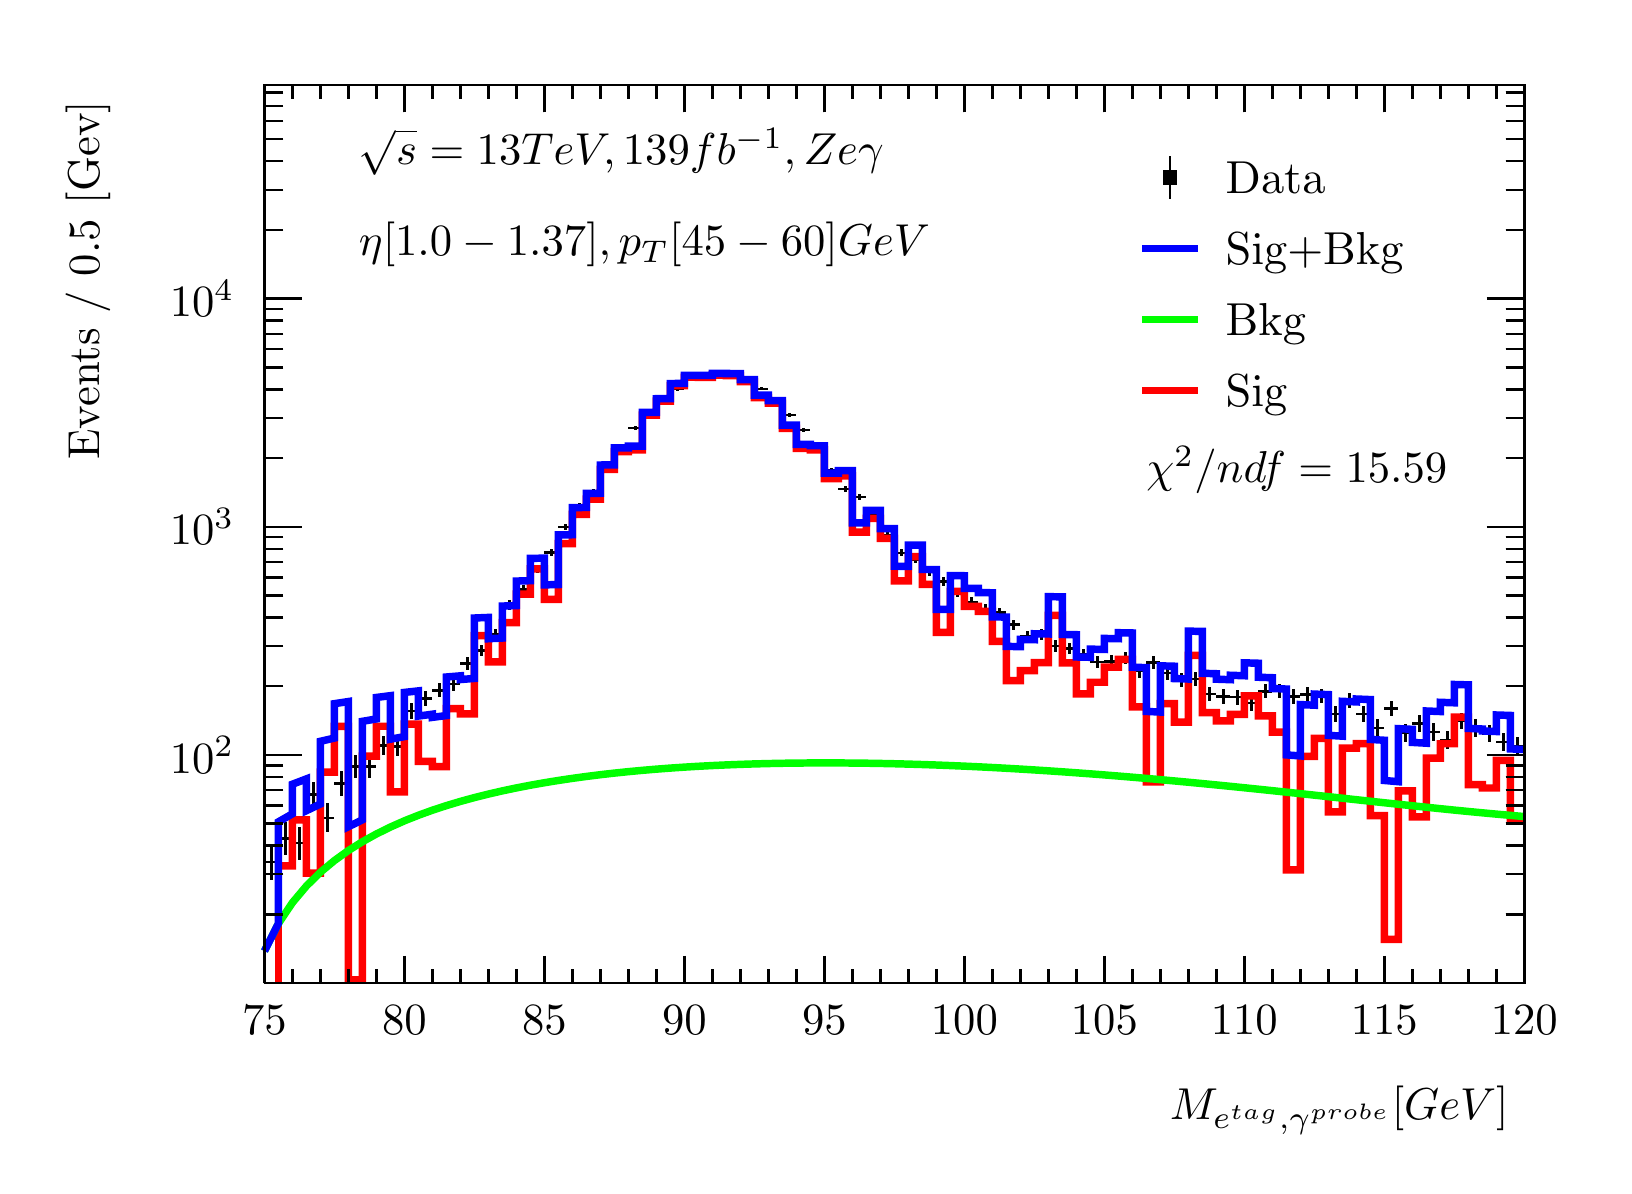
\begin{tikzpicture}
\pgfdeclareplotmark{cross} {
\pgfpathmoveto{\pgfpoint{-0.3\pgfplotmarksize}{\pgfplotmarksize}}
\pgfpathlineto{\pgfpoint{+0.3\pgfplotmarksize}{\pgfplotmarksize}}
\pgfpathlineto{\pgfpoint{+0.3\pgfplotmarksize}{0.3\pgfplotmarksize}}
\pgfpathlineto{\pgfpoint{+1\pgfplotmarksize}{0.3\pgfplotmarksize}}
\pgfpathlineto{\pgfpoint{+1\pgfplotmarksize}{-0.3\pgfplotmarksize}}
\pgfpathlineto{\pgfpoint{+0.3\pgfplotmarksize}{-0.3\pgfplotmarksize}}
\pgfpathlineto{\pgfpoint{+0.3\pgfplotmarksize}{-1.\pgfplotmarksize}}
\pgfpathlineto{\pgfpoint{-0.3\pgfplotmarksize}{-1.\pgfplotmarksize}}
\pgfpathlineto{\pgfpoint{-0.3\pgfplotmarksize}{-0.3\pgfplotmarksize}}
\pgfpathlineto{\pgfpoint{-1.\pgfplotmarksize}{-0.3\pgfplotmarksize}}
\pgfpathlineto{\pgfpoint{-1.\pgfplotmarksize}{0.3\pgfplotmarksize}}
\pgfpathlineto{\pgfpoint{-0.3\pgfplotmarksize}{0.3\pgfplotmarksize}}
\pgfpathclose
\pgfusepathqstroke
}
\pgfdeclareplotmark{cross*} {
\pgfpathmoveto{\pgfpoint{-0.3\pgfplotmarksize}{\pgfplotmarksize}}
\pgfpathlineto{\pgfpoint{+0.3\pgfplotmarksize}{\pgfplotmarksize}}
\pgfpathlineto{\pgfpoint{+0.3\pgfplotmarksize}{0.3\pgfplotmarksize}}
\pgfpathlineto{\pgfpoint{+1\pgfplotmarksize}{0.3\pgfplotmarksize}}
\pgfpathlineto{\pgfpoint{+1\pgfplotmarksize}{-0.3\pgfplotmarksize}}
\pgfpathlineto{\pgfpoint{+0.3\pgfplotmarksize}{-0.3\pgfplotmarksize}}
\pgfpathlineto{\pgfpoint{+0.3\pgfplotmarksize}{-1.\pgfplotmarksize}}
\pgfpathlineto{\pgfpoint{-0.3\pgfplotmarksize}{-1.\pgfplotmarksize}}
\pgfpathlineto{\pgfpoint{-0.3\pgfplotmarksize}{-0.3\pgfplotmarksize}}
\pgfpathlineto{\pgfpoint{-1.\pgfplotmarksize}{-0.3\pgfplotmarksize}}
\pgfpathlineto{\pgfpoint{-1.\pgfplotmarksize}{0.3\pgfplotmarksize}}
\pgfpathlineto{\pgfpoint{-0.3\pgfplotmarksize}{0.3\pgfplotmarksize}}
\pgfpathclose
\pgfusepathqfillstroke
}
\pgfdeclareplotmark{newstar} {
\pgfpathmoveto{\pgfqpoint{0pt}{\pgfplotmarksize}}
\pgfpathlineto{\pgfqpointpolar{44}{0.5\pgfplotmarksize}}
\pgfpathlineto{\pgfqpointpolar{18}{\pgfplotmarksize}}
\pgfpathlineto{\pgfqpointpolar{-20}{0.5\pgfplotmarksize}}
\pgfpathlineto{\pgfqpointpolar{-54}{\pgfplotmarksize}}
\pgfpathlineto{\pgfqpointpolar{-90}{0.5\pgfplotmarksize}}
\pgfpathlineto{\pgfqpointpolar{234}{\pgfplotmarksize}}
\pgfpathlineto{\pgfqpointpolar{198}{0.5\pgfplotmarksize}}
\pgfpathlineto{\pgfqpointpolar{162}{\pgfplotmarksize}}
\pgfpathlineto{\pgfqpointpolar{134}{0.5\pgfplotmarksize}}
\pgfpathclose
\pgfusepathqstroke
}
\pgfdeclareplotmark{newstar*} {
\pgfpathmoveto{\pgfqpoint{0pt}{\pgfplotmarksize}}
\pgfpathlineto{\pgfqpointpolar{44}{0.5\pgfplotmarksize}}
\pgfpathlineto{\pgfqpointpolar{18}{\pgfplotmarksize}}
\pgfpathlineto{\pgfqpointpolar{-20}{0.5\pgfplotmarksize}}
\pgfpathlineto{\pgfqpointpolar{-54}{\pgfplotmarksize}}
\pgfpathlineto{\pgfqpointpolar{-90}{0.5\pgfplotmarksize}}
\pgfpathlineto{\pgfqpointpolar{234}{\pgfplotmarksize}}
\pgfpathlineto{\pgfqpointpolar{198}{0.5\pgfplotmarksize}}
\pgfpathlineto{\pgfqpointpolar{162}{\pgfplotmarksize}}
\pgfpathlineto{\pgfqpointpolar{134}{0.5\pgfplotmarksize}}
\pgfpathclose
\pgfusepathqfillstroke
}
\definecolor{c}{rgb}{1,1,1};
\draw [color=c, fill=c] (0,0) rectangle (20,14.4361);
\draw [color=c, fill=c] (3,2.30977) rectangle (19,13.7143);
\definecolor{c}{rgb}{0,0,0};
\draw [c,line width=0.9] (3,2.30977) -- (3,13.7143) -- (19,13.7143) -- (19,2.30977) -- (3,2.30977);
\definecolor{c}{rgb}{1,1,1};
\draw [color=c, fill=c] (3,2.30977) rectangle (19,13.7143);
\definecolor{c}{rgb}{0,0,0};
\draw [c,line width=0.9] (3,2.30977) -- (3,13.7143) -- (19,13.7143) -- (19,2.30977) -- (3,2.30977);
\draw [c,line width=0.9] (3,2.30977) -- (19,2.30977);
\draw [c,line width=0.9] (3,2.65624) -- (3,2.30977);
\draw [c,line width=0.9] (3.35556,2.48301) -- (3.35556,2.30977);
\draw [c,line width=0.9] (3.71111,2.48301) -- (3.71111,2.30977);
\draw [c,line width=0.9] (4.06667,2.48301) -- (4.06667,2.30977);
\draw [c,line width=0.9] (4.42222,2.48301) -- (4.42222,2.30977);
\draw [c,line width=0.9] (4.77778,2.65624) -- (4.77778,2.30977);
\draw [c,line width=0.9] (5.13333,2.48301) -- (5.13333,2.30977);
\draw [c,line width=0.9] (5.48889,2.48301) -- (5.48889,2.30977);
\draw [c,line width=0.9] (5.84444,2.48301) -- (5.84444,2.30977);
\draw [c,line width=0.9] (6.2,2.48301) -- (6.2,2.30977);
\draw [c,line width=0.9] (6.55556,2.65624) -- (6.55556,2.30977);
\draw [c,line width=0.9] (6.91111,2.48301) -- (6.91111,2.30977);
\draw [c,line width=0.9] (7.26667,2.48301) -- (7.26667,2.30977);
\draw [c,line width=0.9] (7.62222,2.48301) -- (7.62222,2.30977);
\draw [c,line width=0.9] (7.97778,2.48301) -- (7.97778,2.30977);
\draw [c,line width=0.9] (8.33333,2.65624) -- (8.33333,2.30977);
\draw [c,line width=0.9] (8.68889,2.48301) -- (8.68889,2.30977);
\draw [c,line width=0.9] (9.04444,2.48301) -- (9.04444,2.30977);
\draw [c,line width=0.9] (9.4,2.48301) -- (9.4,2.30977);
\draw [c,line width=0.9] (9.75556,2.48301) -- (9.75556,2.30977);
\draw [c,line width=0.9] (10.1111,2.65624) -- (10.1111,2.30977);
\draw [c,line width=0.9] (10.4667,2.48301) -- (10.4667,2.30977);
\draw [c,line width=0.9] (10.8222,2.48301) -- (10.8222,2.30977);
\draw [c,line width=0.9] (11.1778,2.48301) -- (11.1778,2.30977);
\draw [c,line width=0.9] (11.5333,2.48301) -- (11.5333,2.30977);
\draw [c,line width=0.9] (11.8889,2.65624) -- (11.8889,2.30977);
\draw [c,line width=0.9] (12.2444,2.48301) -- (12.2444,2.30977);
\draw [c,line width=0.9] (12.6,2.48301) -- (12.6,2.30977);
\draw [c,line width=0.9] (12.9556,2.48301) -- (12.9556,2.30977);
\draw [c,line width=0.9] (13.3111,2.48301) -- (13.3111,2.30977);
\draw [c,line width=0.9] (13.6667,2.65624) -- (13.6667,2.30977);
\draw [c,line width=0.9] (14.0222,2.48301) -- (14.0222,2.30977);
\draw [c,line width=0.9] (14.3778,2.48301) -- (14.3778,2.30977);
\draw [c,line width=0.9] (14.7333,2.48301) -- (14.7333,2.30977);
\draw [c,line width=0.9] (15.0889,2.48301) -- (15.0889,2.30977);
\draw [c,line width=0.9] (15.4444,2.65624) -- (15.4444,2.30977);
\draw [c,line width=0.9] (15.8,2.48301) -- (15.8,2.30977);
\draw [c,line width=0.9] (16.1556,2.48301) -- (16.1556,2.30977);
\draw [c,line width=0.9] (16.5111,2.48301) -- (16.5111,2.30977);
\draw [c,line width=0.9] (16.8667,2.48301) -- (16.8667,2.30977);
\draw [c,line width=0.9] (17.2222,2.65624) -- (17.2222,2.30977);
\draw [c,line width=0.9] (17.5778,2.48301) -- (17.5778,2.30977);
\draw [c,line width=0.9] (17.9333,2.48301) -- (17.9333,2.30977);
\draw [c,line width=0.9] (18.2889,2.48301) -- (18.2889,2.30977);
\draw [c,line width=0.9] (18.6444,2.48301) -- (18.6444,2.30977);
\draw [c,line width=0.9] (19,2.65624) -- (19,2.30977);
\draw [c,line width=0.9] (19,2.65624) -- (19,2.30977);
\draw [anchor=base] (3,1.66015) node[scale=1.61424, color=c, rotate=0]{75};
\draw [anchor=base] (4.77778,1.66015) node[scale=1.61424, color=c, rotate=0]{80};
\draw [anchor=base] (6.55556,1.66015) node[scale=1.61424, color=c, rotate=0]{85};
\draw [anchor=base] (8.33333,1.66015) node[scale=1.61424, color=c, rotate=0]{90};
\draw [anchor=base] (10.1111,1.66015) node[scale=1.61424, color=c, rotate=0]{95};
\draw [anchor=base] (11.8889,1.66015) node[scale=1.61424, color=c, rotate=0]{100};
\draw [anchor=base] (13.6667,1.66015) node[scale=1.61424, color=c, rotate=0]{105};
\draw [anchor=base] (15.4444,1.66015) node[scale=1.61424, color=c, rotate=0]{110};
\draw [anchor=base] (17.2222,1.66015) node[scale=1.61424, color=c, rotate=0]{115};
\draw [anchor=base] (19,1.66015) node[scale=1.61424, color=c, rotate=0]{120};
\draw [anchor= east] (19,0.692932) node[scale=1.61424, color=c, rotate=0]{$M_{e^{tag}, \gamma^{probe}}  [GeV]$};
\draw [c,line width=0.9] (3,13.7143) -- (19,13.7143);
\draw [c,line width=0.9] (3,13.3678) -- (3,13.7143);
\draw [c,line width=0.9] (3.35556,13.5411) -- (3.35556,13.7143);
\draw [c,line width=0.9] (3.71111,13.5411) -- (3.71111,13.7143);
\draw [c,line width=0.9] (4.06667,13.5411) -- (4.06667,13.7143);
\draw [c,line width=0.9] (4.42222,13.5411) -- (4.42222,13.7143);
\draw [c,line width=0.9] (4.77778,13.3678) -- (4.77778,13.7143);
\draw [c,line width=0.9] (5.13333,13.5411) -- (5.13333,13.7143);
\draw [c,line width=0.9] (5.48889,13.5411) -- (5.48889,13.7143);
\draw [c,line width=0.9] (5.84444,13.5411) -- (5.84444,13.7143);
\draw [c,line width=0.9] (6.2,13.5411) -- (6.2,13.7143);
\draw [c,line width=0.9] (6.55556,13.3678) -- (6.55556,13.7143);
\draw [c,line width=0.9] (6.91111,13.5411) -- (6.91111,13.7143);
\draw [c,line width=0.9] (7.26667,13.5411) -- (7.26667,13.7143);
\draw [c,line width=0.9] (7.62222,13.5411) -- (7.62222,13.7143);
\draw [c,line width=0.9] (7.97778,13.5411) -- (7.97778,13.7143);
\draw [c,line width=0.9] (8.33333,13.3678) -- (8.33333,13.7143);
\draw [c,line width=0.9] (8.68889,13.5411) -- (8.68889,13.7143);
\draw [c,line width=0.9] (9.04444,13.5411) -- (9.04444,13.7143);
\draw [c,line width=0.9] (9.4,13.5411) -- (9.4,13.7143);
\draw [c,line width=0.9] (9.75556,13.5411) -- (9.75556,13.7143);
\draw [c,line width=0.9] (10.1111,13.3678) -- (10.1111,13.7143);
\draw [c,line width=0.9] (10.4667,13.5411) -- (10.4667,13.7143);
\draw [c,line width=0.9] (10.8222,13.5411) -- (10.8222,13.7143);
\draw [c,line width=0.9] (11.1778,13.5411) -- (11.1778,13.7143);
\draw [c,line width=0.9] (11.5333,13.5411) -- (11.5333,13.7143);
\draw [c,line width=0.9] (11.8889,13.3678) -- (11.8889,13.7143);
\draw [c,line width=0.9] (12.2444,13.5411) -- (12.2444,13.7143);
\draw [c,line width=0.9] (12.6,13.5411) -- (12.6,13.7143);
\draw [c,line width=0.9] (12.9556,13.5411) -- (12.9556,13.7143);
\draw [c,line width=0.9] (13.3111,13.5411) -- (13.3111,13.7143);
\draw [c,line width=0.9] (13.6667,13.3678) -- (13.6667,13.7143);
\draw [c,line width=0.9] (14.0222,13.5411) -- (14.0222,13.7143);
\draw [c,line width=0.9] (14.3778,13.5411) -- (14.3778,13.7143);
\draw [c,line width=0.9] (14.7333,13.5411) -- (14.7333,13.7143);
\draw [c,line width=0.9] (15.0889,13.5411) -- (15.0889,13.7143);
\draw [c,line width=0.9] (15.4444,13.3678) -- (15.4444,13.7143);
\draw [c,line width=0.9] (15.8,13.5411) -- (15.8,13.7143);
\draw [c,line width=0.9] (16.1556,13.5411) -- (16.1556,13.7143);
\draw [c,line width=0.9] (16.5111,13.5411) -- (16.5111,13.7143);
\draw [c,line width=0.9] (16.8667,13.5411) -- (16.8667,13.7143);
\draw [c,line width=0.9] (17.2222,13.3678) -- (17.2222,13.7143);
\draw [c,line width=0.9] (17.5778,13.5411) -- (17.5778,13.7143);
\draw [c,line width=0.9] (17.9333,13.5411) -- (17.9333,13.7143);
\draw [c,line width=0.9] (18.2889,13.5411) -- (18.2889,13.7143);
\draw [c,line width=0.9] (18.6444,13.5411) -- (18.6444,13.7143);
\draw [c,line width=0.9] (19,13.3678) -- (19,13.7143);
\draw [c,line width=0.9] (19,13.3678) -- (19,13.7143);
\draw [c,line width=0.9] (3,2.30977) -- (3,13.7143);
\draw [c,line width=0.9] (3.237,3.182) -- (3,3.182);
\draw [c,line width=0.9] (3.237,3.69222) -- (3,3.69222);
\draw [c,line width=0.9] (3.237,4.05422) -- (3,4.05422);
\draw [c,line width=0.9] (3.237,4.33502) -- (3,4.33502);
\draw [c,line width=0.9] (3.237,4.56444) -- (3,4.56444);
\draw [c,line width=0.9] (3.237,4.75842) -- (3,4.75842);
\draw [c,line width=0.9] (3.237,4.92645) -- (3,4.92645);
\draw [c,line width=0.9] (3.237,5.07466) -- (3,5.07466);
\draw [c,line width=0.9] (3.474,5.20724) -- (3,5.20724);
\draw [anchor= east] (2.82,5.20724) node[scale=1.61424, color=c, rotate=0]{$10^{2}$};
\draw [c,line width=0.9] (3.237,6.07947) -- (3,6.07947);
\draw [c,line width=0.9] (3.237,6.58969) -- (3,6.58969);
\draw [c,line width=0.9] (3.237,6.9517) -- (3,6.9517);
\draw [c,line width=0.9] (3.237,7.23249) -- (3,7.23249);
\draw [c,line width=0.9] (3.237,7.46192) -- (3,7.46192);
\draw [c,line width=0.9] (3.237,7.65589) -- (3,7.65589);
\draw [c,line width=0.9] (3.237,7.82392) -- (3,7.82392);
\draw [c,line width=0.9] (3.237,7.97214) -- (3,7.97214);
\draw [c,line width=0.9] (3.474,8.10472) -- (3,8.10472);
\draw [anchor= east] (2.82,8.10472) node[scale=1.61424, color=c, rotate=0]{$10^{3}$};
\draw [c,line width=0.9] (3.237,8.97694) -- (3,8.97694);
\draw [c,line width=0.9] (3.237,9.48716) -- (3,9.48716);
\draw [c,line width=0.9] (3.237,9.84917) -- (3,9.84917);
\draw [c,line width=0.9] (3.237,10.13) -- (3,10.13);
\draw [c,line width=0.9] (3.237,10.3594) -- (3,10.3594);
\draw [c,line width=0.9] (3.237,10.5534) -- (3,10.5534);
\draw [c,line width=0.9] (3.237,10.7214) -- (3,10.7214);
\draw [c,line width=0.9] (3.237,10.8696) -- (3,10.8696);
\draw [c,line width=0.9] (3.474,11.0022) -- (3,11.0022);
\draw [anchor= east] (2.82,11.0022) node[scale=1.61424, color=c, rotate=0]{$10^{4}$};
\draw [c,line width=0.9] (3.237,11.8744) -- (3,11.8744);
\draw [c,line width=0.9] (3.237,12.3846) -- (3,12.3846);
\draw [c,line width=0.9] (3.237,12.7466) -- (3,12.7466);
\draw [c,line width=0.9] (3.237,13.0274) -- (3,13.0274);
\draw [c,line width=0.9] (3.237,13.2569) -- (3,13.2569);
\draw [c,line width=0.9] (3.237,13.4508) -- (3,13.4508);
\draw [c,line width=0.9] (3.237,13.6189) -- (3,13.6189);
\draw [anchor= east] (0.76,13.7143) node[scale=1.61424, color=c, rotate=90]{Events / 0.5 [Gev]};
\draw [c,line width=0.9] (19,2.30977) -- (19,13.7143);
\draw [c,line width=0.9] (18.763,3.182) -- (19,3.182);
\draw [c,line width=0.9] (18.763,3.69222) -- (19,3.69222);
\draw [c,line width=0.9] (18.763,4.05422) -- (19,4.05422);
\draw [c,line width=0.9] (18.763,4.33502) -- (19,4.33502);
\draw [c,line width=0.9] (18.763,4.56444) -- (19,4.56444);
\draw [c,line width=0.9] (18.763,4.75842) -- (19,4.75842);
\draw [c,line width=0.9] (18.763,4.92645) -- (19,4.92645);
\draw [c,line width=0.9] (18.763,5.07466) -- (19,5.07466);
\draw [c,line width=0.9] (18.526,5.20724) -- (19,5.20724);
\draw [c,line width=0.9] (18.763,6.07947) -- (19,6.07947);
\draw [c,line width=0.9] (18.763,6.58969) -- (19,6.58969);
\draw [c,line width=0.9] (18.763,6.9517) -- (19,6.9517);
\draw [c,line width=0.9] (18.763,7.23249) -- (19,7.23249);
\draw [c,line width=0.9] (18.763,7.46192) -- (19,7.46192);
\draw [c,line width=0.9] (18.763,7.65589) -- (19,7.65589);
\draw [c,line width=0.9] (18.763,7.82392) -- (19,7.82392);
\draw [c,line width=0.9] (18.763,7.97214) -- (19,7.97214);
\draw [c,line width=0.9] (18.526,8.10472) -- (19,8.10472);
\draw [c,line width=0.9] (18.763,8.97694) -- (19,8.97694);
\draw [c,line width=0.9] (18.763,9.48716) -- (19,9.48716);
\draw [c,line width=0.9] (18.763,9.84917) -- (19,9.84917);
\draw [c,line width=0.9] (18.763,10.13) -- (19,10.13);
\draw [c,line width=0.9] (18.763,10.3594) -- (19,10.3594);
\draw [c,line width=0.9] (18.763,10.5534) -- (19,10.5534);
\draw [c,line width=0.9] (18.763,10.7214) -- (19,10.7214);
\draw [c,line width=0.9] (18.763,10.8696) -- (19,10.8696);
\draw [c,line width=0.9] (18.526,11.0022) -- (19,11.0022);
\draw [c,line width=0.9] (18.763,11.8744) -- (19,11.8744);
\draw [c,line width=0.9] (18.763,12.3846) -- (19,12.3846);
\draw [c,line width=0.9] (18.763,12.7466) -- (19,12.7466);
\draw [c,line width=0.9] (18.763,13.0274) -- (19,13.0274);
\draw [c,line width=0.9] (18.763,13.2569) -- (19,13.2569);
\draw [c,line width=0.9] (18.763,13.4508) -- (19,13.4508);
\draw [c,line width=0.9] (18.763,13.6189) -- (19,13.6189);
\draw [c,line width=0.9] (3.08889,3.84972) -- (3,3.84972);
\draw [c,line width=0.9] (3,3.84972) -- (3,3.84972);
\draw [c,line width=0.9] (3.08889,3.84972) -- (3.17778,3.84972);
\draw [c,line width=0.9] (3.17778,3.84972) -- (3.17778,3.84972);
\draw [c,line width=0.9] (3.08889,3.84972) -- (3.08889,4.08186);
\draw [c,line width=0.9] (3.08889,4.08186) -- (3.08889,4.08186);
\draw [c,line width=0.9] (3.08889,3.84972) -- (3.08889,3.61426);
\draw [c,line width=0.9] (3.08889,3.61426) -- (3.08889,3.61426);
\draw [c,line width=0.9] (3.26667,4.14523) -- (3.17778,4.14523);
\draw [c,line width=0.9] (3.17778,4.14523) -- (3.17778,4.14523);
\draw [c,line width=0.9] (3.26667,4.14523) -- (3.35556,4.14523);
\draw [c,line width=0.9] (3.35556,4.14523) -- (3.35556,4.14523);
\draw [c,line width=0.9] (3.26667,4.14523) -- (3.26667,4.35024);
\draw [c,line width=0.9] (3.26667,4.35024) -- (3.26667,4.35024);
\draw [c,line width=0.9] (3.26667,4.14523) -- (3.26667,3.9379);
\draw [c,line width=0.9] (3.26667,3.9379) -- (3.26667,3.9379);
\draw [c,line width=0.9] (3.44444,4.0853) -- (3.35556,4.0853);
\draw [c,line width=0.9] (3.35556,4.0853) -- (3.35556,4.0853);
\draw [c,line width=0.9] (3.44444,4.0853) -- (3.53333,4.0853);
\draw [c,line width=0.9] (3.53333,4.0853) -- (3.53333,4.0853);
\draw [c,line width=0.9] (3.44444,4.0853) -- (3.44444,4.29553);
\draw [c,line width=0.9] (3.44444,4.29553) -- (3.44444,4.29553);
\draw [c,line width=0.9] (3.44444,4.0853) -- (3.44444,3.87257);
\draw [c,line width=0.9] (3.44444,3.87257) -- (3.44444,3.87257);
\draw [c,line width=0.9] (3.62222,4.7033) -- (3.53333,4.7033);
\draw [c,line width=0.9] (3.53333,4.7033) -- (3.53333,4.7033);
\draw [c,line width=0.9] (3.62222,4.7033) -- (3.71111,4.7033);
\draw [c,line width=0.9] (3.71111,4.7033) -- (3.71111,4.7033);
\draw [c,line width=0.9] (3.62222,4.7033) -- (3.62222,4.86565);
\draw [c,line width=0.9] (3.62222,4.86565) -- (3.62222,4.86565);
\draw [c,line width=0.9] (3.62222,4.7033) -- (3.62222,4.53978);
\draw [c,line width=0.9] (3.62222,4.53978) -- (3.62222,4.53978);
\draw [c,line width=0.9] (3.8,4.40834) -- (3.71111,4.40834);
\draw [c,line width=0.9] (3.71111,4.40834) -- (3.71111,4.40834);
\draw [c,line width=0.9] (3.8,4.40834) -- (3.88889,4.40834);
\draw [c,line width=0.9] (3.88889,4.40834) -- (3.88889,4.40834);
\draw [c,line width=0.9] (3.8,4.40834) -- (3.8,4.59195);
\draw [c,line width=0.9] (3.8,4.59195) -- (3.8,4.59195);
\draw [c,line width=0.9] (3.8,4.40834) -- (3.8,4.22304);
\draw [c,line width=0.9] (3.8,4.22304) -- (3.8,4.22304);
\draw [c,line width=0.9] (3.97778,4.84524) -- (3.88889,4.84524);
\draw [c,line width=0.9] (3.88889,4.84524) -- (3.88889,4.84524);
\draw [c,line width=0.9] (3.97778,4.84524) -- (4.06667,4.84524);
\draw [c,line width=0.9] (4.06667,4.84524) -- (4.06667,4.84524);
\draw [c,line width=0.9] (3.97778,4.84524) -- (3.97778,4.99827);
\draw [c,line width=0.9] (3.97778,4.99827) -- (3.97778,4.99827);
\draw [c,line width=0.9] (3.97778,4.84524) -- (3.97778,4.69121);
\draw [c,line width=0.9] (3.97778,4.69121) -- (3.97778,4.69121);
\draw [c,line width=0.9] (4.15556,5.06061) -- (4.06667,5.06061);
\draw [c,line width=0.9] (4.06667,5.06061) -- (4.06667,5.06061);
\draw [c,line width=0.9] (4.15556,5.06061) -- (4.24444,5.06061);
\draw [c,line width=0.9] (4.24444,5.06061) -- (4.24444,5.06061);
\draw [c,line width=0.9] (4.15556,5.06061) -- (4.15556,5.20055);
\draw [c,line width=0.9] (4.15556,5.20055) -- (4.15556,5.20055);
\draw [c,line width=0.9] (4.15556,5.06061) -- (4.15556,4.91989);
\draw [c,line width=0.9] (4.15556,4.91989) -- (4.15556,4.91989);
\draw [c,line width=0.9] (4.33333,5.06061) -- (4.24444,5.06061);
\draw [c,line width=0.9] (4.24444,5.06061) -- (4.24444,5.06061);
\draw [c,line width=0.9] (4.33333,5.06061) -- (4.42222,5.06061);
\draw [c,line width=0.9] (4.42222,5.06061) -- (4.42222,5.06061);
\draw [c,line width=0.9] (4.33333,5.06061) -- (4.33333,5.20055);
\draw [c,line width=0.9] (4.33333,5.20055) -- (4.33333,5.20055);
\draw [c,line width=0.9] (4.33333,5.06061) -- (4.33333,4.91989);
\draw [c,line width=0.9] (4.33333,4.91989) -- (4.33333,4.91989);
\draw [c,line width=0.9] (4.51111,5.32718) -- (4.42222,5.32718);
\draw [c,line width=0.9] (4.42222,5.32718) -- (4.42222,5.32718);
\draw [c,line width=0.9] (4.51111,5.32718) -- (4.6,5.32718);
\draw [c,line width=0.9] (4.6,5.32718) -- (4.6,5.32718);
\draw [c,line width=0.9] (4.51111,5.32718) -- (4.51111,5.44711);
\draw [c,line width=0.9] (4.51111,5.44711) -- (4.51111,5.44711);
\draw [c,line width=0.9] (4.51111,5.32718) -- (4.51111,5.20725);
\draw [c,line width=0.9] (4.51111,5.20725) -- (4.51111,5.20725);
\draw [c,line width=0.9] (4.68889,5.31569) -- (4.6,5.31569);
\draw [c,line width=0.9] (4.6,5.31569) -- (4.6,5.31569);
\draw [c,line width=0.9] (4.68889,5.31569) -- (4.77778,5.31569);
\draw [c,line width=0.9] (4.77778,5.31569) -- (4.77778,5.31569);
\draw [c,line width=0.9] (4.68889,5.31569) -- (4.68889,5.43617);
\draw [c,line width=0.9] (4.68889,5.43617) -- (4.68889,5.43617);
\draw [c,line width=0.9] (4.68889,5.31569) -- (4.68889,5.19521);
\draw [c,line width=0.9] (4.68889,5.19521) -- (4.68889,5.19521);
\draw [c,line width=0.9] (4.86667,5.76682) -- (4.77778,5.76682);
\draw [c,line width=0.9] (4.77778,5.76682) -- (4.77778,5.76682);
\draw [c,line width=0.9] (4.86667,5.76682) -- (4.95556,5.76682);
\draw [c,line width=0.9] (4.95556,5.76682) -- (4.95556,5.76682);
\draw [c,line width=0.9] (4.86667,5.76682) -- (4.86667,5.86754);
\draw [c,line width=0.9] (4.86667,5.86754) -- (4.86667,5.86754);
\draw [c,line width=0.9] (4.86667,5.76682) -- (4.86667,5.6661);
\draw [c,line width=0.9] (4.86667,5.6661) -- (4.86667,5.6661);
\draw [c,line width=0.9] (5.04444,5.92574) -- (4.95556,5.92574);
\draw [c,line width=0.9] (4.95556,5.92574) -- (4.95556,5.92574);
\draw [c,line width=0.9] (5.04444,5.92574) -- (5.13333,5.92574);
\draw [c,line width=0.9] (5.13333,5.92574) -- (5.13333,5.92574);
\draw [c,line width=0.9] (5.04444,5.92574) -- (5.04444,6.0203);
\draw [c,line width=0.9] (5.04444,6.0203) -- (5.04444,6.0203);
\draw [c,line width=0.9] (5.04444,5.92574) -- (5.04444,5.83118);
\draw [c,line width=0.9] (5.04444,5.83118) -- (5.04444,5.83118);
\draw [c,line width=0.9] (5.22222,6.0281) -- (5.13333,6.0281);
\draw [c,line width=0.9] (5.13333,6.0281) -- (5.13333,6.0281);
\draw [c,line width=0.9] (5.22222,6.0281) -- (5.31111,6.0281);
\draw [c,line width=0.9] (5.31111,6.0281) -- (5.31111,6.0281);
\draw [c,line width=0.9] (5.22222,6.0281) -- (5.22222,6.1189);
\draw [c,line width=0.9] (5.22222,6.1189) -- (5.22222,6.1189);
\draw [c,line width=0.9] (5.22222,6.0281) -- (5.22222,5.93731);
\draw [c,line width=0.9] (5.22222,5.93731) -- (5.22222,5.93731);
\draw [c,line width=0.9] (5.4,6.11054) -- (5.31111,6.11054);
\draw [c,line width=0.9] (5.31111,6.11054) -- (5.31111,6.11054);
\draw [c,line width=0.9] (5.4,6.11054) -- (5.48889,6.11054);
\draw [c,line width=0.9] (5.48889,6.11054) -- (5.48889,6.11054);
\draw [c,line width=0.9] (5.4,6.11054) -- (5.4,6.19841);
\draw [c,line width=0.9] (5.4,6.19841) -- (5.4,6.19841);
\draw [c,line width=0.9] (5.4,6.11054) -- (5.4,6.02268);
\draw [c,line width=0.9] (5.4,6.02268) -- (5.4,6.02268);
\draw [c,line width=0.9] (5.57778,6.36529) -- (5.48889,6.36529);
\draw [c,line width=0.9] (5.48889,6.36529) -- (5.48889,6.36529);
\draw [c,line width=0.9] (5.57778,6.36529) -- (5.66667,6.36529);
\draw [c,line width=0.9] (5.66667,6.36529) -- (5.66667,6.36529);
\draw [c,line width=0.9] (5.57778,6.36529) -- (5.57778,6.4447);
\draw [c,line width=0.9] (5.57778,6.4447) -- (5.57778,6.4447);
\draw [c,line width=0.9] (5.57778,6.36529) -- (5.57778,6.28588);
\draw [c,line width=0.9] (5.57778,6.28588) -- (5.57778,6.28588);
\draw [c,line width=0.9] (5.75556,6.53395) -- (5.66667,6.53395);
\draw [c,line width=0.9] (5.66667,6.53395) -- (5.66667,6.53395);
\draw [c,line width=0.9] (5.75556,6.53395) -- (5.84444,6.53395);
\draw [c,line width=0.9] (5.84444,6.53395) -- (5.84444,6.53395);
\draw [c,line width=0.9] (5.75556,6.53395) -- (5.75556,6.60821);
\draw [c,line width=0.9] (5.75556,6.60821) -- (5.75556,6.60821);
\draw [c,line width=0.9] (5.75556,6.53395) -- (5.75556,6.45968);
\draw [c,line width=0.9] (5.75556,6.45968) -- (5.75556,6.45968);
\draw [c,line width=0.9] (5.93333,6.73604) -- (5.84444,6.73604);
\draw [c,line width=0.9] (5.84444,6.73604) -- (5.84444,6.73604);
\draw [c,line width=0.9] (5.93333,6.73604) -- (6.02222,6.73604);
\draw [c,line width=0.9] (6.02222,6.73604) -- (6.02222,6.73604);
\draw [c,line width=0.9] (5.93333,6.73604) -- (5.93333,6.80458);
\draw [c,line width=0.9] (5.93333,6.80458) -- (5.93333,6.80458);
\draw [c,line width=0.9] (5.93333,6.73604) -- (5.93333,6.6675);
\draw [c,line width=0.9] (5.93333,6.6675) -- (5.93333,6.6675);
\draw [c,line width=0.9] (6.11111,7.11105) -- (6.02222,7.11105);
\draw [c,line width=0.9] (6.02222,7.11105) -- (6.02222,7.11105);
\draw [c,line width=0.9] (6.11111,7.11105) -- (6.2,7.11105);
\draw [c,line width=0.9] (6.2,7.11105) -- (6.2,7.11105);
\draw [c,line width=0.9] (6.11111,7.11105) -- (6.11111,7.1701);
\draw [c,line width=0.9] (6.11111,7.1701) -- (6.11111,7.1701);
\draw [c,line width=0.9] (6.11111,7.11105) -- (6.11111,7.052);
\draw [c,line width=0.9] (6.11111,7.052) -- (6.11111,7.052);
\draw [c,line width=0.9] (6.28889,7.31056) -- (6.2,7.31056);
\draw [c,line width=0.9] (6.2,7.31056) -- (6.2,7.31056);
\draw [c,line width=0.9] (6.28889,7.31056) -- (6.37778,7.31056);
\draw [c,line width=0.9] (6.37778,7.31056) -- (6.37778,7.31056);
\draw [c,line width=0.9] (6.28889,7.31056) -- (6.28889,7.36511);
\draw [c,line width=0.9] (6.28889,7.36511) -- (6.28889,7.36511);
\draw [c,line width=0.9] (6.28889,7.31056) -- (6.28889,7.256);
\draw [c,line width=0.9] (6.28889,7.256) -- (6.28889,7.256);
\draw [c,line width=0.9] (6.46667,7.56844) -- (6.37778,7.56844);
\draw [c,line width=0.9] (6.37778,7.56844) -- (6.37778,7.56844);
\draw [c,line width=0.9] (6.46667,7.56844) -- (6.55556,7.56844);
\draw [c,line width=0.9] (6.55556,7.56844) -- (6.55556,7.56844);
\draw [c,line width=0.9] (6.46667,7.56844) -- (6.46667,7.61768);
\draw [c,line width=0.9] (6.46667,7.61768) -- (6.46667,7.61768);
\draw [c,line width=0.9] (6.46667,7.56844) -- (6.46667,7.5192);
\draw [c,line width=0.9] (6.46667,7.5192) -- (6.46667,7.5192);
\draw [c,line width=0.9] (6.64444,7.77583) -- (6.55556,7.77583);
\draw [c,line width=0.9] (6.55556,7.77583) -- (6.55556,7.77583);
\draw [c,line width=0.9] (6.64444,7.77583) -- (6.73333,7.77583);
\draw [c,line width=0.9] (6.73333,7.77583) -- (6.73333,7.77583);
\draw [c,line width=0.9] (6.64444,7.77583) -- (6.64444,7.82117);
\draw [c,line width=0.9] (6.64444,7.82117) -- (6.64444,7.82117);
\draw [c,line width=0.9] (6.64444,7.77583) -- (6.64444,7.73048);
\draw [c,line width=0.9] (6.64444,7.73048) -- (6.64444,7.73048);
\draw [c,line width=0.9] (6.82222,8.1022) -- (6.73333,8.1022);
\draw [c,line width=0.9] (6.73333,8.1022) -- (6.73333,8.1022);
\draw [c,line width=0.9] (6.82222,8.1022) -- (6.91111,8.1022);
\draw [c,line width=0.9] (6.91111,8.1022) -- (6.91111,8.1022);
\draw [c,line width=0.9] (6.82222,8.1022) -- (6.82222,8.14203);
\draw [c,line width=0.9] (6.82222,8.14203) -- (6.82222,8.14203);
\draw [c,line width=0.9] (6.82222,8.1022) -- (6.82222,8.06237);
\draw [c,line width=0.9] (6.82222,8.06237) -- (6.82222,8.06237);
\draw [c,line width=0.9] (7,8.37439) -- (6.91111,8.37439);
\draw [c,line width=0.9] (6.91111,8.37439) -- (6.91111,8.37439);
\draw [c,line width=0.9] (7,8.37439) -- (7.08889,8.37439);
\draw [c,line width=0.9] (7.08889,8.37439) -- (7.08889,8.37439);
\draw [c,line width=0.9] (7,8.37439) -- (7,8.41014);
\draw [c,line width=0.9] (7,8.41014) -- (7,8.41014);
\draw [c,line width=0.9] (7,8.37439) -- (7,8.33864);
\draw [c,line width=0.9] (7,8.33864) -- (7,8.33864);
\draw [c,line width=0.9] (7.17778,8.54863) -- (7.08889,8.54863);
\draw [c,line width=0.9] (7.08889,8.54863) -- (7.08889,8.54863);
\draw [c,line width=0.9] (7.17778,8.54863) -- (7.26667,8.54863);
\draw [c,line width=0.9] (7.26667,8.54863) -- (7.26667,8.54863);
\draw [c,line width=0.9] (7.17778,8.54863) -- (7.17778,8.58198);
\draw [c,line width=0.9] (7.17778,8.58198) -- (7.17778,8.58198);
\draw [c,line width=0.9] (7.17778,8.54863) -- (7.17778,8.51527);
\draw [c,line width=0.9] (7.17778,8.51527) -- (7.17778,8.51527);
\draw [c,line width=0.9] (7.35556,8.889) -- (7.26667,8.889);
\draw [c,line width=0.9] (7.26667,8.889) -- (7.26667,8.889);
\draw [c,line width=0.9] (7.35556,8.889) -- (7.44444,8.889);
\draw [c,line width=0.9] (7.44444,8.889) -- (7.44444,8.889);
\draw [c,line width=0.9] (7.35556,8.889) -- (7.35556,8.91814);
\draw [c,line width=0.9] (7.35556,8.91814) -- (7.35556,8.91814);
\draw [c,line width=0.9] (7.35556,8.889) -- (7.35556,8.85987);
\draw [c,line width=0.9] (7.35556,8.85987) -- (7.35556,8.85987);
\draw [c,line width=0.9] (7.53333,9.12851) -- (7.44444,9.12851);
\draw [c,line width=0.9] (7.44444,9.12851) -- (7.44444,9.12851);
\draw [c,line width=0.9] (7.53333,9.12851) -- (7.62222,9.12851);
\draw [c,line width=0.9] (7.62222,9.12851) -- (7.62222,9.12851);
\draw [c,line width=0.9] (7.53333,9.12851) -- (7.53333,9.155);
\draw [c,line width=0.9] (7.53333,9.155) -- (7.53333,9.155);
\draw [c,line width=0.9] (7.53333,9.12851) -- (7.53333,9.10202);
\draw [c,line width=0.9] (7.53333,9.10202) -- (7.53333,9.10202);
\draw [c,line width=0.9] (7.71111,9.35784) -- (7.62222,9.35784);
\draw [c,line width=0.9] (7.62222,9.35784) -- (7.62222,9.35784);
\draw [c,line width=0.9] (7.71111,9.35784) -- (7.8,9.35784);
\draw [c,line width=0.9] (7.8,9.35784) -- (7.8,9.35784);
\draw [c,line width=0.9] (7.71111,9.35784) -- (7.71111,9.38203);
\draw [c,line width=0.9] (7.71111,9.38203) -- (7.71111,9.38203);
\draw [c,line width=0.9] (7.71111,9.35784) -- (7.71111,9.33366);
\draw [c,line width=0.9] (7.71111,9.33366) -- (7.71111,9.33366);
\draw [c,line width=0.9] (7.88889,9.55255) -- (7.8,9.55255);
\draw [c,line width=0.9] (7.8,9.55255) -- (7.8,9.55255);
\draw [c,line width=0.9] (7.88889,9.55255) -- (7.97778,9.55255);
\draw [c,line width=0.9] (7.97778,9.55255) -- (7.97778,9.55255);
\draw [c,line width=0.9] (7.88889,9.55255) -- (7.88889,9.57493);
\draw [c,line width=0.9] (7.88889,9.57493) -- (7.88889,9.57493);
\draw [c,line width=0.9] (7.88889,9.55255) -- (7.88889,9.53016);
\draw [c,line width=0.9] (7.88889,9.53016) -- (7.88889,9.53016);
\draw [c,line width=0.9] (8.06667,9.72773) -- (7.97778,9.72773);
\draw [c,line width=0.9] (7.97778,9.72773) -- (7.97778,9.72773);
\draw [c,line width=0.9] (8.06667,9.72773) -- (8.15556,9.72773);
\draw [c,line width=0.9] (8.15556,9.72773) -- (8.15556,9.72773);
\draw [c,line width=0.9] (8.06667,9.72773) -- (8.06667,9.74861);
\draw [c,line width=0.9] (8.06667,9.74861) -- (8.06667,9.74861);
\draw [c,line width=0.9] (8.06667,9.72773) -- (8.06667,9.70685);
\draw [c,line width=0.9] (8.06667,9.70685) -- (8.06667,9.70685);
\draw [c,line width=0.9] (8.24444,9.85482) -- (8.15556,9.85482);
\draw [c,line width=0.9] (8.15556,9.85482) -- (8.15556,9.85482);
\draw [c,line width=0.9] (8.24444,9.85482) -- (8.33333,9.85482);
\draw [c,line width=0.9] (8.33333,9.85482) -- (8.33333,9.85482);
\draw [c,line width=0.9] (8.24444,9.85482) -- (8.24444,9.87467);
\draw [c,line width=0.9] (8.24444,9.87467) -- (8.24444,9.87467);
\draw [c,line width=0.9] (8.24444,9.85482) -- (8.24444,9.83497);
\draw [c,line width=0.9] (8.24444,9.83497) -- (8.24444,9.83497);
\draw [c,line width=0.9] (8.42222,9.97481) -- (8.33333,9.97481);
\draw [c,line width=0.9] (8.33333,9.97481) -- (8.33333,9.97481);
\draw [c,line width=0.9] (8.42222,9.97481) -- (8.51111,9.97481);
\draw [c,line width=0.9] (8.51111,9.97481) -- (8.51111,9.97481);
\draw [c,line width=0.9] (8.42222,9.97481) -- (8.42222,9.99374);
\draw [c,line width=0.9] (8.42222,9.99374) -- (8.42222,9.99374);
\draw [c,line width=0.9] (8.42222,9.97481) -- (8.42222,9.95588);
\draw [c,line width=0.9] (8.42222,9.95588) -- (8.42222,9.95588);
\draw [c,line width=0.9] (8.6,10.0432) -- (8.51111,10.0432);
\draw [c,line width=0.9] (8.51111,10.0432) -- (8.51111,10.0432);
\draw [c,line width=0.9] (8.6,10.0432) -- (8.68889,10.0432);
\draw [c,line width=0.9] (8.68889,10.0432) -- (8.68889,10.0432);
\draw [c,line width=0.9] (8.6,10.0432) -- (8.6,10.0617);
\draw [c,line width=0.9] (8.6,10.0617) -- (8.6,10.0617);
\draw [c,line width=0.9] (8.6,10.0432) -- (8.6,10.0248);
\draw [c,line width=0.9] (8.6,10.0248) -- (8.6,10.0248);
\draw [c,line width=0.9] (8.77778,10.0529) -- (8.68889,10.0529);
\draw [c,line width=0.9] (8.68889,10.0529) -- (8.68889,10.0529);
\draw [c,line width=0.9] (8.77778,10.0529) -- (8.86667,10.0529);
\draw [c,line width=0.9] (8.86667,10.0529) -- (8.86667,10.0529);
\draw [c,line width=0.9] (8.77778,10.0529) -- (8.77778,10.0713);
\draw [c,line width=0.9] (8.77778,10.0713) -- (8.77778,10.0713);
\draw [c,line width=0.9] (8.77778,10.0529) -- (8.77778,10.0346);
\draw [c,line width=0.9] (8.77778,10.0346) -- (8.77778,10.0346);
\draw [c,line width=0.9] (8.95556,10.0346) -- (8.86667,10.0346);
\draw [c,line width=0.9] (8.86667,10.0346) -- (8.86667,10.0346);
\draw [c,line width=0.9] (8.95556,10.0346) -- (9.04444,10.0346);
\draw [c,line width=0.9] (9.04444,10.0346) -- (9.04444,10.0346);
\draw [c,line width=0.9] (8.95556,10.0346) -- (8.95556,10.0531);
\draw [c,line width=0.9] (8.95556,10.0531) -- (8.95556,10.0531);
\draw [c,line width=0.9] (8.95556,10.0346) -- (8.95556,10.0161);
\draw [c,line width=0.9] (8.95556,10.0161) -- (8.95556,10.0161);
\draw [c,line width=0.9] (9.13333,9.95704) -- (9.04444,9.95704);
\draw [c,line width=0.9] (9.04444,9.95704) -- (9.04444,9.95704);
\draw [c,line width=0.9] (9.13333,9.95704) -- (9.22222,9.95704);
\draw [c,line width=0.9] (9.22222,9.95704) -- (9.22222,9.95704);
\draw [c,line width=0.9] (9.13333,9.95704) -- (9.13333,9.9761);
\draw [c,line width=0.9] (9.13333,9.9761) -- (9.13333,9.9761);
\draw [c,line width=0.9] (9.13333,9.95704) -- (9.13333,9.93797);
\draw [c,line width=0.9] (9.13333,9.93797) -- (9.13333,9.93797);
\draw [c,line width=0.9] (9.31111,9.85701) -- (9.22222,9.85701);
\draw [c,line width=0.9] (9.22222,9.85701) -- (9.22222,9.85701);
\draw [c,line width=0.9] (9.31111,9.85701) -- (9.4,9.85701);
\draw [c,line width=0.9] (9.4,9.85701) -- (9.4,9.85701);
\draw [c,line width=0.9] (9.31111,9.85701) -- (9.31111,9.87685);
\draw [c,line width=0.9] (9.31111,9.87685) -- (9.31111,9.87685);
\draw [c,line width=0.9] (9.31111,9.85701) -- (9.31111,9.83718);
\draw [c,line width=0.9] (9.31111,9.83718) -- (9.31111,9.83718);
\draw [c,line width=0.9] (9.48889,9.6876) -- (9.4,9.6876);
\draw [c,line width=0.9] (9.4,9.6876) -- (9.4,9.6876);
\draw [c,line width=0.9] (9.48889,9.6876) -- (9.57778,9.6876);
\draw [c,line width=0.9] (9.57778,9.6876) -- (9.57778,9.6876);
\draw [c,line width=0.9] (9.48889,9.6876) -- (9.48889,9.70881);
\draw [c,line width=0.9] (9.48889,9.70881) -- (9.48889,9.70881);
\draw [c,line width=0.9] (9.48889,9.6876) -- (9.48889,9.66638);
\draw [c,line width=0.9] (9.48889,9.66638) -- (9.48889,9.66638);
\draw [c,line width=0.9] (9.66667,9.52151) -- (9.57778,9.52151);
\draw [c,line width=0.9] (9.57778,9.52151) -- (9.57778,9.52151);
\draw [c,line width=0.9] (9.66667,9.52151) -- (9.75556,9.52151);
\draw [c,line width=0.9] (9.75556,9.52151) -- (9.75556,9.52151);
\draw [c,line width=0.9] (9.66667,9.52151) -- (9.66667,9.54417);
\draw [c,line width=0.9] (9.66667,9.54417) -- (9.66667,9.54417);
\draw [c,line width=0.9] (9.66667,9.52151) -- (9.66667,9.49884);
\draw [c,line width=0.9] (9.66667,9.49884) -- (9.66667,9.49884);
\draw [c,line width=0.9] (9.84444,9.3358) -- (9.75556,9.3358);
\draw [c,line width=0.9] (9.75556,9.3358) -- (9.75556,9.3358);
\draw [c,line width=0.9] (9.84444,9.3358) -- (9.93333,9.3358);
\draw [c,line width=0.9] (9.93333,9.3358) -- (9.93333,9.3358);
\draw [c,line width=0.9] (9.84444,9.3358) -- (9.84444,9.3602);
\draw [c,line width=0.9] (9.84444,9.3602) -- (9.84444,9.3602);
\draw [c,line width=0.9] (9.84444,9.3358) -- (9.84444,9.3114);
\draw [c,line width=0.9] (9.84444,9.3114) -- (9.84444,9.3114);
\draw [c,line width=0.9] (10.0222,9.1218) -- (9.93333,9.1218);
\draw [c,line width=0.9] (9.93333,9.1218) -- (9.93333,9.1218);
\draw [c,line width=0.9] (10.0222,9.1218) -- (10.1111,9.1218);
\draw [c,line width=0.9] (10.1111,9.1218) -- (10.1111,9.1218);
\draw [c,line width=0.9] (10.0222,9.1218) -- (10.0222,9.14836);
\draw [c,line width=0.9] (10.0222,9.14836) -- (10.0222,9.14836);
\draw [c,line width=0.9] (10.0222,9.1218) -- (10.0222,9.09523);
\draw [c,line width=0.9] (10.0222,9.09523) -- (10.0222,9.09523);
\draw [c,line width=0.9] (10.2,8.8168) -- (10.1111,8.8168);
\draw [c,line width=0.9] (10.1111,8.8168) -- (10.1111,8.8168);
\draw [c,line width=0.9] (10.2,8.8168) -- (10.2889,8.8168);
\draw [c,line width=0.9] (10.2889,8.8168) -- (10.2889,8.8168);
\draw [c,line width=0.9] (10.2,8.8168) -- (10.2,8.84679);
\draw [c,line width=0.9] (10.2,8.84679) -- (10.2,8.84679);
\draw [c,line width=0.9] (10.2,8.8168) -- (10.2,8.78681);
\draw [c,line width=0.9] (10.2,8.78681) -- (10.2,8.78681);
\draw [c,line width=0.9] (10.3778,8.58523) -- (10.2889,8.58523);
\draw [c,line width=0.9] (10.2889,8.58523) -- (10.2889,8.58523);
\draw [c,line width=0.9] (10.3778,8.58523) -- (10.4667,8.58523);
\draw [c,line width=0.9] (10.4667,8.58523) -- (10.4667,8.58523);
\draw [c,line width=0.9] (10.3778,8.58523) -- (10.3778,8.6181);
\draw [c,line width=0.9] (10.3778,8.6181) -- (10.3778,8.6181);
\draw [c,line width=0.9] (10.3778,8.58523) -- (10.3778,8.55235);
\draw [c,line width=0.9] (10.3778,8.55235) -- (10.3778,8.55235);
\draw [c,line width=0.9] (10.5556,8.48143) -- (10.4667,8.48143);
\draw [c,line width=0.9] (10.4667,8.48143) -- (10.4667,8.48143);
\draw [c,line width=0.9] (10.5556,8.48143) -- (10.6444,8.48143);
\draw [c,line width=0.9] (10.6444,8.48143) -- (10.6444,8.48143);
\draw [c,line width=0.9] (10.5556,8.48143) -- (10.5556,8.51569);
\draw [c,line width=0.9] (10.5556,8.51569) -- (10.5556,8.51569);
\draw [c,line width=0.9] (10.5556,8.48143) -- (10.5556,8.44717);
\draw [c,line width=0.9] (10.5556,8.44717) -- (10.5556,8.44717);
\draw [c,line width=0.9] (10.7333,8.26849) -- (10.6444,8.26849);
\draw [c,line width=0.9] (10.6444,8.26849) -- (10.6444,8.26849);
\draw [c,line width=0.9] (10.7333,8.26849) -- (10.8222,8.26849);
\draw [c,line width=0.9] (10.8222,8.26849) -- (10.8222,8.26849);
\draw [c,line width=0.9] (10.7333,8.26849) -- (10.7333,8.30578);
\draw [c,line width=0.9] (10.7333,8.30578) -- (10.7333,8.30578);
\draw [c,line width=0.9] (10.7333,8.26849) -- (10.7333,8.23121);
\draw [c,line width=0.9] (10.7333,8.23121) -- (10.7333,8.23121);
\draw [c,line width=0.9] (10.9111,7.99294) -- (10.8222,7.99294);
\draw [c,line width=0.9] (10.8222,7.99294) -- (10.8222,7.99294);
\draw [c,line width=0.9] (10.9111,7.99294) -- (11,7.99294);
\draw [c,line width=0.9] (11,7.99294) -- (11,7.99294);
\draw [c,line width=0.9] (10.9111,7.99294) -- (10.9111,8.03454);
\draw [c,line width=0.9] (10.9111,8.03454) -- (10.9111,8.03454);
\draw [c,line width=0.9] (10.9111,7.99294) -- (10.9111,7.95134);
\draw [c,line width=0.9] (10.9111,7.95134) -- (10.9111,7.95134);
\draw [c,line width=0.9] (11.0889,7.77256) -- (11,7.77256);
\draw [c,line width=0.9] (11,7.77256) -- (11,7.77256);
\draw [c,line width=0.9] (11.0889,7.77256) -- (11.1778,7.77256);
\draw [c,line width=0.9] (11.1778,7.77256) -- (11.1778,7.77256);
\draw [c,line width=0.9] (11.0889,7.77256) -- (11.0889,7.81796);
\draw [c,line width=0.9] (11.0889,7.81796) -- (11.0889,7.81796);
\draw [c,line width=0.9] (11.0889,7.77256) -- (11.0889,7.72715);
\draw [c,line width=0.9] (11.0889,7.72715) -- (11.0889,7.72715);
\draw [c,line width=0.9] (11.2667,7.69134) -- (11.1778,7.69134);
\draw [c,line width=0.9] (11.1778,7.69134) -- (11.1778,7.69134);
\draw [c,line width=0.9] (11.2667,7.69134) -- (11.3556,7.69134);
\draw [c,line width=0.9] (11.3556,7.69134) -- (11.3556,7.69134);
\draw [c,line width=0.9] (11.2667,7.69134) -- (11.2667,7.73824);
\draw [c,line width=0.9] (11.2667,7.73824) -- (11.2667,7.73824);
\draw [c,line width=0.9] (11.2667,7.69134) -- (11.2667,7.64445);
\draw [c,line width=0.9] (11.2667,7.64445) -- (11.2667,7.64445);
\draw [c,line width=0.9] (11.4444,7.5273) -- (11.3556,7.5273);
\draw [c,line width=0.9] (11.3556,7.5273) -- (11.3556,7.5273);
\draw [c,line width=0.9] (11.4444,7.5273) -- (11.5333,7.5273);
\draw [c,line width=0.9] (11.5333,7.5273) -- (11.5333,7.5273);
\draw [c,line width=0.9] (11.4444,7.5273) -- (11.4444,7.57735);
\draw [c,line width=0.9] (11.4444,7.57735) -- (11.4444,7.57735);
\draw [c,line width=0.9] (11.4444,7.5273) -- (11.4444,7.47725);
\draw [c,line width=0.9] (11.4444,7.47725) -- (11.4444,7.47725);
\draw [c,line width=0.9] (11.6222,7.41055) -- (11.5333,7.41055);
\draw [c,line width=0.9] (11.5333,7.41055) -- (11.5333,7.41055);
\draw [c,line width=0.9] (11.6222,7.41055) -- (11.7111,7.41055);
\draw [c,line width=0.9] (11.7111,7.41055) -- (11.7111,7.41055);
\draw [c,line width=0.9] (11.6222,7.41055) -- (11.6222,7.46298);
\draw [c,line width=0.9] (11.6222,7.46298) -- (11.6222,7.46298);
\draw [c,line width=0.9] (11.6222,7.41055) -- (11.6222,7.35812);
\draw [c,line width=0.9] (11.6222,7.35812) -- (11.6222,7.35812);
\draw [c,line width=0.9] (11.8,7.26969) -- (11.7111,7.26969);
\draw [c,line width=0.9] (11.7111,7.26969) -- (11.7111,7.26969);
\draw [c,line width=0.9] (11.8,7.26969) -- (11.8889,7.26969);
\draw [c,line width=0.9] (11.8889,7.26969) -- (11.8889,7.26969);
\draw [c,line width=0.9] (11.8,7.26969) -- (11.8,7.32513);
\draw [c,line width=0.9] (11.8,7.32513) -- (11.8,7.32513);
\draw [c,line width=0.9] (11.8,7.26969) -- (11.8,7.21424);
\draw [c,line width=0.9] (11.8,7.21424) -- (11.8,7.21424);
\draw [c,line width=0.9] (11.9778,7.15195) -- (11.8889,7.15195);
\draw [c,line width=0.9] (11.8889,7.15195) -- (11.8889,7.15195);
\draw [c,line width=0.9] (11.9778,7.15195) -- (12.0667,7.15195);
\draw [c,line width=0.9] (12.0667,7.15195) -- (12.0667,7.15195);
\draw [c,line width=0.9] (11.9778,7.15195) -- (11.9778,7.21005);
\draw [c,line width=0.9] (11.9778,7.21005) -- (11.9778,7.21005);
\draw [c,line width=0.9] (11.9778,7.15195) -- (11.9778,7.09385);
\draw [c,line width=0.9] (11.9778,7.09385) -- (11.9778,7.09385);
\draw [c,line width=0.9] (12.1556,7.05725) -- (12.0667,7.05725);
\draw [c,line width=0.9] (12.0667,7.05725) -- (12.0667,7.05725);
\draw [c,line width=0.9] (12.1556,7.05725) -- (12.2444,7.05725);
\draw [c,line width=0.9] (12.2444,7.05725) -- (12.2444,7.05725);
\draw [c,line width=0.9] (12.1556,7.05725) -- (12.1556,7.11758);
\draw [c,line width=0.9] (12.1556,7.11758) -- (12.1556,7.11758);
\draw [c,line width=0.9] (12.1556,7.05725) -- (12.1556,6.99692);
\draw [c,line width=0.9] (12.1556,6.99692) -- (12.1556,6.99692);
\draw [c,line width=0.9] (12.3333,7.01609) -- (12.2444,7.01609);
\draw [c,line width=0.9] (12.2444,7.01609) -- (12.2444,7.01609);
\draw [c,line width=0.9] (12.3333,7.01609) -- (12.4222,7.01609);
\draw [c,line width=0.9] (12.4222,7.01609) -- (12.4222,7.01609);
\draw [c,line width=0.9] (12.3333,7.01609) -- (12.3333,7.07741);
\draw [c,line width=0.9] (12.3333,7.07741) -- (12.3333,7.07741);
\draw [c,line width=0.9] (12.3333,7.01609) -- (12.3333,6.95476);
\draw [c,line width=0.9] (12.3333,6.95476) -- (12.3333,6.95476);
\draw [c,line width=0.9] (12.5111,6.86038) -- (12.4222,6.86038);
\draw [c,line width=0.9] (12.4222,6.86038) -- (12.4222,6.86038);
\draw [c,line width=0.9] (12.5111,6.86038) -- (12.6,6.86038);
\draw [c,line width=0.9] (12.6,6.86038) -- (12.6,6.86038);
\draw [c,line width=0.9] (12.5111,6.86038) -- (12.5111,6.92561);
\draw [c,line width=0.9] (12.5111,6.92561) -- (12.5111,6.92561);
\draw [c,line width=0.9] (12.5111,6.86038) -- (12.5111,6.79514);
\draw [c,line width=0.9] (12.5111,6.79514) -- (12.5111,6.79514);
\draw [c,line width=0.9] (12.6889,6.70963) -- (12.6,6.70963);
\draw [c,line width=0.9] (12.6,6.70963) -- (12.6,6.70963);
\draw [c,line width=0.9] (12.6889,6.70963) -- (12.7778,6.70963);
\draw [c,line width=0.9] (12.7778,6.70963) -- (12.7778,6.70963);
\draw [c,line width=0.9] (12.6889,6.70963) -- (12.6889,6.77889);
\draw [c,line width=0.9] (12.6889,6.77889) -- (12.6889,6.77889);
\draw [c,line width=0.9] (12.6889,6.70963) -- (12.6889,6.64037);
\draw [c,line width=0.9] (12.6889,6.64037) -- (12.6889,6.64037);
\draw [c,line width=0.9] (12.8667,6.7323) -- (12.7778,6.7323);
\draw [c,line width=0.9] (12.7778,6.7323) -- (12.7778,6.7323);
\draw [c,line width=0.9] (12.8667,6.7323) -- (12.9556,6.7323);
\draw [c,line width=0.9] (12.9556,6.7323) -- (12.9556,6.7323);
\draw [c,line width=0.9] (12.8667,6.7323) -- (12.8667,6.80094);
\draw [c,line width=0.9] (12.8667,6.80094) -- (12.8667,6.80094);
\draw [c,line width=0.9] (12.8667,6.7323) -- (12.8667,6.66366);
\draw [c,line width=0.9] (12.8667,6.66366) -- (12.8667,6.66366);
\draw [c,line width=0.9] (13.0444,6.58969) -- (12.9556,6.58969);
\draw [c,line width=0.9] (12.9556,6.58969) -- (12.9556,6.58969);
\draw [c,line width=0.9] (13.0444,6.58969) -- (13.1333,6.58969);
\draw [c,line width=0.9] (13.1333,6.58969) -- (13.1333,6.58969);
\draw [c,line width=0.9] (13.0444,6.58969) -- (13.0444,6.66233);
\draw [c,line width=0.9] (13.0444,6.66233) -- (13.0444,6.66233);
\draw [c,line width=0.9] (13.0444,6.58969) -- (13.0444,6.51705);
\draw [c,line width=0.9] (13.0444,6.51705) -- (13.0444,6.51705);
\draw [c,line width=0.9] (13.2222,6.55998) -- (13.1333,6.55998);
\draw [c,line width=0.9] (13.1333,6.55998) -- (13.1333,6.55998);
\draw [c,line width=0.9] (13.2222,6.55998) -- (13.3111,6.55998);
\draw [c,line width=0.9] (13.3111,6.55998) -- (13.3111,6.55998);
\draw [c,line width=0.9] (13.2222,6.55998) -- (13.2222,6.63349);
\draw [c,line width=0.9] (13.2222,6.63349) -- (13.2222,6.63349);
\draw [c,line width=0.9] (13.2222,6.55998) -- (13.2222,6.48648);
\draw [c,line width=0.9] (13.2222,6.48648) -- (13.2222,6.48648);
\draw [c,line width=0.9] (13.4,6.4802) -- (13.3111,6.4802);
\draw [c,line width=0.9] (13.3111,6.4802) -- (13.3111,6.4802);
\draw [c,line width=0.9] (13.4,6.4802) -- (13.4889,6.4802);
\draw [c,line width=0.9] (13.4889,6.4802) -- (13.4889,6.4802);
\draw [c,line width=0.9] (13.4,6.4802) -- (13.4,6.55607);
\draw [c,line width=0.9] (13.4,6.55607) -- (13.4,6.55607);
\draw [c,line width=0.9] (13.4,6.4802) -- (13.4,6.40433);
\draw [c,line width=0.9] (13.4,6.40433) -- (13.4,6.40433);
\draw [c,line width=0.9] (13.5778,6.38519) -- (13.4889,6.38519);
\draw [c,line width=0.9] (13.4889,6.38519) -- (13.4889,6.38519);
\draw [c,line width=0.9] (13.5778,6.38519) -- (13.6667,6.38519);
\draw [c,line width=0.9] (13.6667,6.38519) -- (13.6667,6.38519);
\draw [c,line width=0.9] (13.5778,6.38519) -- (13.5778,6.46397);
\draw [c,line width=0.9] (13.5778,6.46397) -- (13.5778,6.46397);
\draw [c,line width=0.9] (13.5778,6.38519) -- (13.5778,6.3064);
\draw [c,line width=0.9] (13.5778,6.3064) -- (13.5778,6.3064);
\draw [c,line width=0.9] (13.7556,6.39502) -- (13.6667,6.39502);
\draw [c,line width=0.9] (13.6667,6.39502) -- (13.6667,6.39502);
\draw [c,line width=0.9] (13.7556,6.39502) -- (13.8444,6.39502);
\draw [c,line width=0.9] (13.8444,6.39502) -- (13.8444,6.39502);
\draw [c,line width=0.9] (13.7556,6.39502) -- (13.7556,6.4735);
\draw [c,line width=0.9] (13.7556,6.4735) -- (13.7556,6.4735);
\draw [c,line width=0.9] (13.7556,6.39502) -- (13.7556,6.31653);
\draw [c,line width=0.9] (13.7556,6.31653) -- (13.7556,6.31653);
\draw [c,line width=0.9] (13.9333,6.43359) -- (13.8444,6.43359);
\draw [c,line width=0.9] (13.8444,6.43359) -- (13.8444,6.43359);
\draw [c,line width=0.9] (13.9333,6.43359) -- (14.0222,6.43359);
\draw [c,line width=0.9] (14.0222,6.43359) -- (14.0222,6.43359);
\draw [c,line width=0.9] (13.9333,6.43359) -- (13.9333,6.51088);
\draw [c,line width=0.9] (13.9333,6.51088) -- (13.9333,6.51088);
\draw [c,line width=0.9] (13.9333,6.43359) -- (13.9333,6.3563);
\draw [c,line width=0.9] (13.9333,6.3563) -- (13.9333,6.3563);
\draw [c,line width=0.9] (14.1111,6.27165) -- (14.0222,6.27165);
\draw [c,line width=0.9] (14.0222,6.27165) -- (14.0222,6.27165);
\draw [c,line width=0.9] (14.1111,6.27165) -- (14.2,6.27165);
\draw [c,line width=0.9] (14.2,6.27165) -- (14.2,6.27165);
\draw [c,line width=0.9] (14.1111,6.27165) -- (14.1111,6.35407);
\draw [c,line width=0.9] (14.1111,6.35407) -- (14.1111,6.35407);
\draw [c,line width=0.9] (14.1111,6.27165) -- (14.1111,6.18923);
\draw [c,line width=0.9] (14.1111,6.18923) -- (14.1111,6.18923);
\draw [c,line width=0.9] (14.2889,6.38024) -- (14.2,6.38024);
\draw [c,line width=0.9] (14.2,6.38024) -- (14.2,6.38024);
\draw [c,line width=0.9] (14.2889,6.38024) -- (14.3778,6.38024);
\draw [c,line width=0.9] (14.3778,6.38024) -- (14.3778,6.38024);
\draw [c,line width=0.9] (14.2889,6.38024) -- (14.2889,6.45918);
\draw [c,line width=0.9] (14.2889,6.45918) -- (14.2889,6.45918);
\draw [c,line width=0.9] (14.2889,6.38024) -- (14.2889,6.3013);
\draw [c,line width=0.9] (14.2889,6.3013) -- (14.2889,6.3013);
\draw [c,line width=0.9] (14.4667,6.24435) -- (14.3778,6.24435);
\draw [c,line width=0.9] (14.3778,6.24435) -- (14.3778,6.24435);
\draw [c,line width=0.9] (14.4667,6.24435) -- (14.5556,6.24435);
\draw [c,line width=0.9] (14.5556,6.24435) -- (14.5556,6.24435);
\draw [c,line width=0.9] (14.4667,6.24435) -- (14.4667,6.32767);
\draw [c,line width=0.9] (14.4667,6.32767) -- (14.4667,6.32767);
\draw [c,line width=0.9] (14.4667,6.24435) -- (14.4667,6.16103);
\draw [c,line width=0.9] (14.4667,6.16103) -- (14.4667,6.16103);
\draw [c,line width=0.9] (14.6444,6.15872) -- (14.5556,6.15872);
\draw [c,line width=0.9] (14.5556,6.15872) -- (14.5556,6.15872);
\draw [c,line width=0.9] (14.6444,6.15872) -- (14.7333,6.15872);
\draw [c,line width=0.9] (14.7333,6.15872) -- (14.7333,6.15872);
\draw [c,line width=0.9] (14.6444,6.15872) -- (14.6444,6.24492);
\draw [c,line width=0.9] (14.6444,6.24492) -- (14.6444,6.24492);
\draw [c,line width=0.9] (14.6444,6.15872) -- (14.6444,6.07251);
\draw [c,line width=0.9] (14.6444,6.07251) -- (14.6444,6.07251);
\draw [c,line width=0.9] (14.8222,6.17048) -- (14.7333,6.17048);
\draw [c,line width=0.9] (14.7333,6.17048) -- (14.7333,6.17048);
\draw [c,line width=0.9] (14.8222,6.17048) -- (14.9111,6.17048);
\draw [c,line width=0.9] (14.9111,6.17048) -- (14.9111,6.17048);
\draw [c,line width=0.9] (14.8222,6.17048) -- (14.8222,6.25628);
\draw [c,line width=0.9] (14.8222,6.25628) -- (14.8222,6.25628);
\draw [c,line width=0.9] (14.8222,6.17048) -- (14.8222,6.08468);
\draw [c,line width=0.9] (14.8222,6.08468) -- (14.8222,6.08468);
\draw [c,line width=0.9] (15,5.98137) -- (14.9111,5.98137);
\draw [c,line width=0.9] (14.9111,5.98137) -- (14.9111,5.98137);
\draw [c,line width=0.9] (15,5.98137) -- (15.0889,5.98137);
\draw [c,line width=0.9] (15.0889,5.98137) -- (15.0889,5.98137);
\draw [c,line width=0.9] (15,5.98137) -- (15,6.07386);
\draw [c,line width=0.9] (15,6.07386) -- (15,6.07386);
\draw [c,line width=0.9] (15,5.98137) -- (15,5.88887);
\draw [c,line width=0.9] (15,5.88887) -- (15,5.88887);
\draw [c,line width=0.9] (15.1778,5.94689) -- (15.0889,5.94689);
\draw [c,line width=0.9] (15.0889,5.94689) -- (15.0889,5.94689);
\draw [c,line width=0.9] (15.1778,5.94689) -- (15.2667,5.94689);
\draw [c,line width=0.9] (15.2667,5.94689) -- (15.2667,5.94689);
\draw [c,line width=0.9] (15.1778,5.94689) -- (15.1778,6.04066);
\draw [c,line width=0.9] (15.1778,6.04066) -- (15.1778,6.04066);
\draw [c,line width=0.9] (15.1778,5.94689) -- (15.1778,5.85312);
\draw [c,line width=0.9] (15.1778,5.85312) -- (15.1778,5.85312);
\draw [c,line width=0.9] (15.3556,5.93988) -- (15.2667,5.93988);
\draw [c,line width=0.9] (15.2667,5.93988) -- (15.2667,5.93988);
\draw [c,line width=0.9] (15.3556,5.93988) -- (15.4444,5.93988);
\draw [c,line width=0.9] (15.4444,5.93988) -- (15.4444,5.93988);
\draw [c,line width=0.9] (15.3556,5.93988) -- (15.3556,6.03391);
\draw [c,line width=0.9] (15.3556,6.03391) -- (15.3556,6.03391);
\draw [c,line width=0.9] (15.3556,5.93988) -- (15.3556,5.84585);
\draw [c,line width=0.9] (15.3556,5.84585) -- (15.3556,5.84585);
\draw [c,line width=0.9] (15.5333,5.86754) -- (15.4444,5.86754);
\draw [c,line width=0.9] (15.4444,5.86754) -- (15.4444,5.86754);
\draw [c,line width=0.9] (15.5333,5.86754) -- (15.6222,5.86754);
\draw [c,line width=0.9] (15.6222,5.86754) -- (15.6222,5.86754);
\draw [c,line width=0.9] (15.5333,5.86754) -- (15.5333,5.96431);
\draw [c,line width=0.9] (15.5333,5.96431) -- (15.5333,5.96431);
\draw [c,line width=0.9] (15.5333,5.86754) -- (15.5333,5.77077);
\draw [c,line width=0.9] (15.5333,5.77077) -- (15.5333,5.77077);
\draw [c,line width=0.9] (15.7111,6.01493) -- (15.6222,6.01493);
\draw [c,line width=0.9] (15.6222,6.01493) -- (15.6222,6.01493);
\draw [c,line width=0.9] (15.7111,6.01493) -- (15.8,6.01493);
\draw [c,line width=0.9] (15.8,6.01493) -- (15.8,6.01493);
\draw [c,line width=0.9] (15.7111,6.01493) -- (15.7111,6.1062);
\draw [c,line width=0.9] (15.7111,6.1062) -- (15.7111,6.1062);
\draw [c,line width=0.9] (15.7111,6.01493) -- (15.7111,5.92366);
\draw [c,line width=0.9] (15.7111,5.92366) -- (15.7111,5.92366);
\draw [c,line width=0.9] (15.8889,6.02153) -- (15.8,6.02153);
\draw [c,line width=0.9] (15.8,6.02153) -- (15.8,6.02153);
\draw [c,line width=0.9] (15.8889,6.02153) -- (15.9778,6.02153);
\draw [c,line width=0.9] (15.9778,6.02153) -- (15.9778,6.02153);
\draw [c,line width=0.9] (15.8889,6.02153) -- (15.8889,6.11256);
\draw [c,line width=0.9] (15.8889,6.11256) -- (15.8889,6.11256);
\draw [c,line width=0.9] (15.8889,6.02153) -- (15.8889,5.9305);
\draw [c,line width=0.9] (15.8889,5.9305) -- (15.8889,5.9305);
\draw [c,line width=0.9] (16.0667,5.94689) -- (15.9778,5.94689);
\draw [c,line width=0.9] (15.9778,5.94689) -- (15.9778,5.94689);
\draw [c,line width=0.9] (16.0667,5.94689) -- (16.1556,5.94689);
\draw [c,line width=0.9] (16.1556,5.94689) -- (16.1556,5.94689);
\draw [c,line width=0.9] (16.0667,5.94689) -- (16.0667,6.04066);
\draw [c,line width=0.9] (16.0667,6.04066) -- (16.0667,6.04066);
\draw [c,line width=0.9] (16.0667,5.94689) -- (16.0667,5.85312);
\draw [c,line width=0.9] (16.0667,5.85312) -- (16.0667,5.85312);
\draw [c,line width=0.9] (16.2444,5.97455) -- (16.1556,5.97455);
\draw [c,line width=0.9] (16.1556,5.97455) -- (16.1556,5.97455);
\draw [c,line width=0.9] (16.2444,5.97455) -- (16.3333,5.97455);
\draw [c,line width=0.9] (16.3333,5.97455) -- (16.3333,5.97455);
\draw [c,line width=0.9] (16.2444,5.97455) -- (16.2444,6.0673);
\draw [c,line width=0.9] (16.2444,6.0673) -- (16.2444,6.0673);
\draw [c,line width=0.9] (16.2444,5.97455) -- (16.2444,5.8818);
\draw [c,line width=0.9] (16.2444,5.8818) -- (16.2444,5.8818);
\draw [c,line width=0.9] (16.4222,5.95386) -- (16.3333,5.95386);
\draw [c,line width=0.9] (16.3333,5.95386) -- (16.3333,5.95386);
\draw [c,line width=0.9] (16.4222,5.95386) -- (16.5111,5.95386);
\draw [c,line width=0.9] (16.5111,5.95386) -- (16.5111,5.95386);
\draw [c,line width=0.9] (16.4222,5.95386) -- (16.4222,6.04737);
\draw [c,line width=0.9] (16.4222,6.04737) -- (16.4222,6.04737);
\draw [c,line width=0.9] (16.4222,5.95386) -- (16.4222,5.86035);
\draw [c,line width=0.9] (16.4222,5.86035) -- (16.4222,5.86035);
\draw [c,line width=0.9] (16.6,5.72583) -- (16.5111,5.72583);
\draw [c,line width=0.9] (16.5111,5.72583) -- (16.5111,5.72583);
\draw [c,line width=0.9] (16.6,5.72583) -- (16.6889,5.72583);
\draw [c,line width=0.9] (16.6889,5.72583) -- (16.6889,5.72583);
\draw [c,line width=0.9] (16.6,5.72583) -- (16.6,5.8282);
\draw [c,line width=0.9] (16.6,5.8282) -- (16.6,5.8282);
\draw [c,line width=0.9] (16.6,5.72583) -- (16.6,5.62345);
\draw [c,line width=0.9] (16.6,5.62345) -- (16.6,5.62345);
\draw [c,line width=0.9] (16.7778,5.90423) -- (16.6889,5.90423);
\draw [c,line width=0.9] (16.6889,5.90423) -- (16.6889,5.90423);
\draw [c,line width=0.9] (16.7778,5.90423) -- (16.8667,5.90423);
\draw [c,line width=0.9] (16.8667,5.90423) -- (16.8667,5.90423);
\draw [c,line width=0.9] (16.7778,5.90423) -- (16.7778,5.9996);
\draw [c,line width=0.9] (16.7778,5.9996) -- (16.7778,5.9996);
\draw [c,line width=0.9] (16.7778,5.90423) -- (16.7778,5.80886);
\draw [c,line width=0.9] (16.7778,5.80886) -- (16.7778,5.80886);
\draw [c,line width=0.9] (16.9556,5.72583) -- (16.8667,5.72583);
\draw [c,line width=0.9] (16.8667,5.72583) -- (16.8667,5.72583);
\draw [c,line width=0.9] (16.9556,5.72583) -- (17.0444,5.72583);
\draw [c,line width=0.9] (17.0444,5.72583) -- (17.0444,5.72583);
\draw [c,line width=0.9] (16.9556,5.72583) -- (16.9556,5.8282);
\draw [c,line width=0.9] (16.9556,5.8282) -- (16.9556,5.8282);
\draw [c,line width=0.9] (16.9556,5.72583) -- (16.9556,5.62345);
\draw [c,line width=0.9] (16.9556,5.62345) -- (16.9556,5.62345);
\draw [c,line width=0.9] (17.1333,5.54704) -- (17.0444,5.54704);
\draw [c,line width=0.9] (17.0444,5.54704) -- (17.0444,5.54704);
\draw [c,line width=0.9] (17.1333,5.54704) -- (17.2222,5.54704);
\draw [c,line width=0.9] (17.2222,5.54704) -- (17.2222,5.54704);
\draw [c,line width=0.9] (17.1333,5.54704) -- (17.1333,5.65695);
\draw [c,line width=0.9] (17.1333,5.65695) -- (17.1333,5.65695);
\draw [c,line width=0.9] (17.1333,5.54704) -- (17.1333,5.43713);
\draw [c,line width=0.9] (17.1333,5.43713) -- (17.1333,5.43713);
\draw [c,line width=0.9] (17.3111,5.79868) -- (17.2222,5.79868);
\draw [c,line width=0.9] (17.2222,5.79868) -- (17.2222,5.79868);
\draw [c,line width=0.9] (17.3111,5.79868) -- (17.4,5.79868);
\draw [c,line width=0.9] (17.4,5.79868) -- (17.4,5.79868);
\draw [c,line width=0.9] (17.3111,5.79868) -- (17.3111,5.89813);
\draw [c,line width=0.9] (17.3111,5.89813) -- (17.3111,5.89813);
\draw [c,line width=0.9] (17.3111,5.79868) -- (17.3111,5.69922);
\draw [c,line width=0.9] (17.3111,5.69922) -- (17.3111,5.69922);
\draw [c,line width=0.9] (17.4889,5.48804) -- (17.4,5.48804);
\draw [c,line width=0.9] (17.4,5.48804) -- (17.4,5.48804);
\draw [c,line width=0.9] (17.4889,5.48804) -- (17.5778,5.48804);
\draw [c,line width=0.9] (17.5778,5.48804) -- (17.5778,5.48804);
\draw [c,line width=0.9] (17.4889,5.48804) -- (17.4889,5.60055);
\draw [c,line width=0.9] (17.4889,5.60055) -- (17.4889,5.60055);
\draw [c,line width=0.9] (17.4889,5.48804) -- (17.4889,5.37553);
\draw [c,line width=0.9] (17.4889,5.37553) -- (17.4889,5.37553);
\draw [c,line width=0.9] (17.6667,5.60339) -- (17.5778,5.60339);
\draw [c,line width=0.9] (17.5778,5.60339) -- (17.5778,5.60339);
\draw [c,line width=0.9] (17.6667,5.60339) -- (17.7556,5.60339);
\draw [c,line width=0.9] (17.7556,5.60339) -- (17.7556,5.60339);
\draw [c,line width=0.9] (17.6667,5.60339) -- (17.6667,5.71087);
\draw [c,line width=0.9] (17.6667,5.71087) -- (17.6667,5.71087);
\draw [c,line width=0.9] (17.6667,5.60339) -- (17.6667,5.49591);
\draw [c,line width=0.9] (17.6667,5.49591) -- (17.6667,5.49591);
\draw [c,line width=0.9] (17.8444,5.49807) -- (17.7556,5.49807);
\draw [c,line width=0.9] (17.7556,5.49807) -- (17.7556,5.49807);
\draw [c,line width=0.9] (17.8444,5.49807) -- (17.9333,5.49807);
\draw [c,line width=0.9] (17.9333,5.49807) -- (17.9333,5.49807);
\draw [c,line width=0.9] (17.8444,5.49807) -- (17.8444,5.61013);
\draw [c,line width=0.9] (17.8444,5.61013) -- (17.8444,5.61013);
\draw [c,line width=0.9] (17.8444,5.49807) -- (17.8444,5.386);
\draw [c,line width=0.9] (17.8444,5.386) -- (17.8444,5.386);
\draw [c,line width=0.9] (18.0222,5.39401) -- (17.9333,5.39401);
\draw [c,line width=0.9] (17.9333,5.39401) -- (17.9333,5.39401);
\draw [c,line width=0.9] (18.0222,5.39401) -- (18.1111,5.39401);
\draw [c,line width=0.9] (18.1111,5.39401) -- (18.1111,5.39401);
\draw [c,line width=0.9] (18.0222,5.39401) -- (18.0222,5.51081);
\draw [c,line width=0.9] (18.0222,5.51081) -- (18.0222,5.51081);
\draw [c,line width=0.9] (18.0222,5.39401) -- (18.0222,5.27722);
\draw [c,line width=0.9] (18.0222,5.27722) -- (18.0222,5.27722);
\draw [c,line width=0.9] (18.2,5.63961) -- (18.1111,5.63961);
\draw [c,line width=0.9] (18.1111,5.63961) -- (18.1111,5.63961);
\draw [c,line width=0.9] (18.2,5.63961) -- (18.2889,5.63961);
\draw [c,line width=0.9] (18.2889,5.63961) -- (18.2889,5.63961);
\draw [c,line width=0.9] (18.2,5.63961) -- (18.2,5.74555);
\draw [c,line width=0.9] (18.2,5.74555) -- (18.2,5.74555);
\draw [c,line width=0.9] (18.2,5.63961) -- (18.2,5.53366);
\draw [c,line width=0.9] (18.2,5.53366) -- (18.2,5.53366);
\draw [c,line width=0.9] (18.3778,5.54704) -- (18.2889,5.54704);
\draw [c,line width=0.9] (18.2889,5.54704) -- (18.2889,5.54704);
\draw [c,line width=0.9] (18.3778,5.54704) -- (18.4667,5.54704);
\draw [c,line width=0.9] (18.4667,5.54704) -- (18.4667,5.54704);
\draw [c,line width=0.9] (18.3778,5.54704) -- (18.3778,5.65695);
\draw [c,line width=0.9] (18.3778,5.65695) -- (18.3778,5.65695);
\draw [c,line width=0.9] (18.3778,5.54704) -- (18.3778,5.43713);
\draw [c,line width=0.9] (18.3778,5.43713) -- (18.3778,5.43713);
\draw [c,line width=0.9] (18.5556,5.47793) -- (18.4667,5.47793);
\draw [c,line width=0.9] (18.4667,5.47793) -- (18.4667,5.47793);
\draw [c,line width=0.9] (18.5556,5.47793) -- (18.6444,5.47793);
\draw [c,line width=0.9] (18.6444,5.47793) -- (18.6444,5.47793);
\draw [c,line width=0.9] (18.5556,5.47793) -- (18.5556,5.5909);
\draw [c,line width=0.9] (18.5556,5.5909) -- (18.5556,5.5909);
\draw [c,line width=0.9] (18.5556,5.47793) -- (18.5556,5.36497);
\draw [c,line width=0.9] (18.5556,5.36497) -- (18.5556,5.36497);
\draw [c,line width=0.9] (18.7333,5.37213) -- (18.6444,5.37213);
\draw [c,line width=0.9] (18.6444,5.37213) -- (18.6444,5.37213);
\draw [c,line width=0.9] (18.7333,5.37213) -- (18.8222,5.37213);
\draw [c,line width=0.9] (18.8222,5.37213) -- (18.8222,5.37213);
\draw [c,line width=0.9] (18.7333,5.37213) -- (18.7333,5.48994);
\draw [c,line width=0.9] (18.7333,5.48994) -- (18.7333,5.48994);
\draw [c,line width=0.9] (18.7333,5.37213) -- (18.7333,5.25431);
\draw [c,line width=0.9] (18.7333,5.25431) -- (18.7333,5.25431);
\draw [c,line width=0.9] (18.9111,5.31569) -- (18.8222,5.31569);
\draw [c,line width=0.9] (18.8222,5.31569) -- (18.8222,5.31569);
\draw [c,line width=0.9] (18.9111,5.31569) -- (19,5.31569);
\draw [c,line width=0.9] (19,5.31569) -- (19,5.31569);
\draw [c,line width=0.9] (18.9111,5.31569) -- (18.9111,5.43617);
\draw [c,line width=0.9] (18.9111,5.43617) -- (18.9111,5.43617);
\draw [c,line width=0.9] (18.9111,5.31569) -- (18.9111,5.19521);
\draw [c,line width=0.9] (18.9111,5.19521) -- (18.9111,5.19521);
\foreach \P in {(3.08889,3.84972), (3.26667,4.14523), (3.44444,4.0853), (3.62222,4.7033), (3.8,4.40834), (3.97778,4.84524), (4.15556,5.06061), (4.33333,5.06061), (4.51111,5.32718), (4.68889,5.31569), (4.86667,5.76682), (5.04444,5.92574),
 (5.22222,6.0281), (5.4,6.11054), (5.57778,6.36529), (5.75556,6.53395), (5.93333,6.73604), (6.11111,7.11105), (6.28889,7.31056), (6.46667,7.56844), (6.64444,7.77583), (6.82222,8.1022), (7,8.37439), (7.17778,8.54863), (7.35556,8.889),
 (7.53333,9.12851), (7.71111,9.35784), (7.88889,9.55255), (8.06667,9.72773), (8.24444,9.85482), (8.42222,9.97481), (8.6,10.0432), (8.77778,10.0529), (8.95556,10.0346), (9.13333,9.95704), (9.31111,9.85701), (9.48889,9.6876), (9.66667,9.52151),
 (9.84444,9.3358), (10.0222,9.1218), (10.2,8.8168), (10.3778,8.58523), (10.5556,8.48143), (10.7333,8.26849), (10.9111,7.99294), (11.0889,7.77256), (11.2667,7.69134), (11.4444,7.5273), (11.6222,7.41055), (11.8,7.26969), (11.9778,7.15195),
 (12.1556,7.05725), (12.3333,7.01609), (12.5111,6.86038), (12.6889,6.70963), (12.8667,6.7323), (13.0444,6.58969), (13.2222,6.55998), (13.4,6.4802), (13.5778,6.38519), (13.7556,6.39502), (13.9333,6.43359), (14.1111,6.27165), (14.2889,6.38024),
 (14.4667,6.24435), (14.6444,6.15872), (14.8222,6.17048), (15,5.98137), (15.1778,5.94689), (15.3556,5.93988), (15.5333,5.86754), (15.7111,6.01493), (15.8889,6.02153), (16.0667,5.94689), (16.2444,5.97455), (16.4222,5.95386), (16.6,5.72583),
 (16.7778,5.90423), (16.9556,5.72583), (17.1333,5.54704), (17.3111,5.79868), (17.4889,5.48804), (17.6667,5.60339), (17.8444,5.49807), (18.0222,5.39401), (18.2,5.63961), (18.3778,5.54704), (18.5556,5.47793), (18.7333,5.37213),
 (18.9111,5.31569)}{\draw[mark options={color=c,fill=c},mark size=2.882883pt,mark=] plot coordinates {\P};}
\definecolor{c}{rgb}{1,0,0};
\draw [c,line width=2.7] (3.17778,2.30977) -- (3.17778,3.79893);
\draw [c,line width=2.7] (3.17778,3.79893) -- (3.35556,3.79893) -- (3.35556,4.38135) -- (3.53333,4.38135) -- (3.53333,3.70571) -- (3.71111,3.70571) -- (3.71111,4.9894) -- (3.88889,4.9894) -- (3.88889,5.56873) -- (4.06667,5.56873) -- (4.06667,2.35113)
 -- (4.24444,2.35113) -- (4.24444,5.19092) -- (4.42222,5.19092) -- (4.42222,5.57121) -- (4.6,5.57121) -- (4.6,4.73833) -- (4.77778,4.73833) -- (4.77778,5.59849) -- (4.95556,5.59849) -- (4.95556,5.12381) -- (5.13333,5.12381) -- (5.13333,5.0582) --
 (5.31111,5.0582) -- (5.31111,5.79527) -- (5.48889,5.79527) -- (5.48889,5.72888) -- (5.66667,5.72888) -- (5.66667,6.72154) -- (5.84444,6.72154) -- (5.84444,6.38843) -- (6.02222,6.38843) -- (6.02222,6.88583) -- (6.2,6.88583) -- (6.2,7.24866) --
 (6.37778,7.24866) -- (6.37778,7.56849) -- (6.55556,7.56849) -- (6.55556,7.18302) -- (6.73333,7.18302) -- (6.73333,7.8905) -- (6.91111,7.8905) -- (6.91111,8.26331) -- (7.08889,8.26331) -- (7.08889,8.4542) -- (7.26667,8.4542) -- (7.26667,8.83258) --
 (7.44444,8.83258) -- (7.44444,9.05877) -- (7.62222,9.05877) -- (7.62222,9.08015) -- (7.8,9.08015) -- (7.8,9.52275) -- (7.97778,9.52275) -- (7.97778,9.70026) -- (8.15556,9.70026) -- (8.15556,9.89789) -- (8.33333,9.89789) -- (8.33333,10.0033) --
 (8.51111,10.0033) -- (8.51111,10.0016) -- (8.68889,10.0016) -- (8.68889,10.029) -- (8.86667,10.029) -- (8.86667,10.025) -- (9.04444,10.025) -- (9.04445,9.94635) -- (9.22222,9.94635) -- (9.22222,9.7451) -- (9.4,9.7451) -- (9.4,9.67318) --
 (9.57778,9.67318) -- (9.57778,9.3542) -- (9.75556,9.3542) -- (9.75556,9.09858) -- (9.93333,9.09858) -- (9.93333,9.08099) -- (10.1111,9.08099) -- (10.1111,8.71683) -- (10.2889,8.71683) -- (10.2889,8.75008) -- (10.4667,8.75008) -- (10.4667,8.03779) --
 (10.6444,8.03779) -- (10.6444,8.21065) -- (10.8222,8.21065) -- (10.8222,7.95743) -- (11,7.95743) -- (11,7.41872) -- (11.1778,7.41872) -- (11.1778,7.72586) -- (11.3556,7.72586) -- (11.3556,7.37278) -- (11.5333,7.37278) -- (11.5333,6.7635) --
 (11.7111,6.7635) -- (11.7111,7.28356) -- (11.8889,7.28356) -- (11.8889,7.09393) -- (12.0667,7.09393) -- (12.0667,7.02987) -- (12.2444,7.02987) -- (12.2444,6.64915) -- (12.4222,6.64915) -- (12.4222,6.15017) -- (12.6,6.15017) -- (12.6,6.27621) --
 (12.7778,6.27621) -- (12.7778,6.37865) -- (12.9556,6.37865) -- (12.9556,6.9786) -- (13.1333,6.9786) -- (13.1333,6.37463) -- (13.3111,6.37463) -- (13.3111,5.98246) -- (13.4889,5.98246) -- (13.4889,6.12999) -- (13.6667,6.12999) -- (13.6667,6.32084) --
 (13.8444,6.32084) -- (13.8444,6.42168) -- (14.0222,6.42168) -- (14.0222,5.81777) -- (14.2,5.81777) -- (14.2,4.86514) -- (14.3778,4.86514) -- (14.3778,5.85881) -- (14.5556,5.85881) -- (14.5556,5.62297) -- (14.7333,5.62297) -- (14.7333,6.47045) --
 (14.9111,6.47045) -- (14.9111,5.74282) -- (15.0889,5.74282) -- (15.0889,5.63825) -- (15.2667,5.63825) -- (15.2667,5.72207) -- (15.4444,5.72207) -- (15.4444,5.95718) -- (15.6222,5.95718) -- (15.6222,5.70271) -- (15.8,5.70271) -- (15.8,5.49535) --
 (15.9778,5.49535) -- (15.9778,3.74714) -- (16.1556,3.74714) -- (16.1556,5.18853) -- (16.3333,5.18853) -- (16.3333,5.41676) -- (16.5111,5.41676) -- (16.5111,4.48247) -- (16.6889,4.48247) -- (16.6889,5.29361) -- (16.8667,5.29361) -- (16.8667,5.35162)
 -- (17.0444,5.35162) -- (17.0444,4.43745) -- (17.2222,4.43745) -- (17.2222,2.86567) -- (17.4,2.86567) -- (17.4,4.75077) -- (17.5778,4.75077) -- (17.5778,4.42152) -- (17.7556,4.42152) -- (17.7556,5.16621) -- (17.9333,5.16621) -- (17.9333,5.34873) --
 (18.1111,5.34873) -- (18.1111,5.68582) -- (18.2889,5.68582) -- (18.2889,4.83085) -- (18.4667,4.83085) -- (18.4667,4.78679) -- (18.6444,4.78679) -- (18.6444,5.1373) -- (18.8222,5.1373) -- (18.8222,4.38241) -- (19,4.38241) -- (19,4.38241) --
 (19,4.38241) -- (19,4.38241);
\definecolor{c}{rgb}{0,1,0};
\draw [c,line width=2.7] (3,2.71649) -- (3,2.71649);
\draw [c,line width=2.7] (3,2.71649) -- (3,2.71649) -- (3.17778,3.06632) -- (3.17778,3.06632) -- (3.35556,3.33114) -- (3.35556,3.33114) -- (3.53333,3.54262) -- (3.53333,3.54262) -- (3.71111,3.71746) -- (3.71111,3.71746) -- (3.88889,3.86555) --
 (3.88889,3.86555) -- (4.06667,3.99322) -- (4.06667,3.99322) -- (4.24444,4.1048) -- (4.24444,4.1048) -- (4.42222,4.20334) -- (4.42222,4.20334) -- (4.6,4.29111) -- (4.6,4.29111) -- (4.77778,4.3698) -- (4.77778,4.3698) -- (4.95556,4.44075) --
 (4.95556,4.44075) -- (5.13333,4.505) -- (5.13333,4.505) -- (5.31111,4.5634) -- (5.31111,4.5634) -- (5.48889,4.61663) -- (5.48889,4.61663) -- (5.66667,4.66527) -- (5.66667,4.66527) -- (5.84444,4.7098) -- (5.84444,4.7098) -- (6.02222,4.75061) --
 (6.02222,4.75061) -- (6.2,4.78804) -- (6.2,4.78804) -- (6.37778,4.8224) -- (6.37778,4.8224) -- (6.55556,4.85394) -- (6.55556,4.85394) -- (6.73333,4.88287) -- (6.73333,4.88287) -- (6.91111,4.9094) -- (6.91111,4.9094) -- (7.08889,4.9337) --
 (7.08889,4.9337) -- (7.26667,4.9559) -- (7.26667,4.9559) -- (7.44444,4.97616) -- (7.44444,4.97616) -- (7.62222,4.99459) -- (7.62222,4.99459) -- (7.8,5.01129) -- (7.8,5.01129) -- (7.97778,5.02636) -- (7.97778,5.02636) -- (8.15556,5.0399) --
 (8.15556,5.0399) -- (8.33333,5.05198) -- (8.33333,5.05198) -- (8.51111,5.06267) -- (8.51111,5.06267) -- (8.68889,5.07203) -- (8.68889,5.07203) -- (8.86667,5.08013) -- (8.86667,5.08013) -- (9.04444,5.08703) -- (9.04445,5.08703) -- (9.22222,5.09276)
 -- (9.22222,5.09276) -- (9.4,5.09738) -- (9.4,5.09738) -- (9.57778,5.10093) -- (9.57778,5.10093) -- (9.75556,5.10345) -- (9.75556,5.10345) -- (9.93333,5.10497) -- (9.93333,5.10497) -- (10.1111,5.10553) -- (10.1111,5.10553) -- (10.2889,5.10517) --
 (10.2889,5.10517) -- (10.4667,5.1039) -- (10.4667,5.1039) -- (10.6444,5.10176) -- (10.6444,5.10176) -- (10.8222,5.09878) -- (10.8222,5.09878) -- (11,5.09497) -- (11,5.09497) -- (11.1778,5.09037) -- (11.1778,5.09037) -- (11.3556,5.08499) --
 (11.3556,5.08499) -- (11.5333,5.07885) -- (11.5333,5.07885) -- (11.7111,5.07198) -- (11.7111,5.07198) -- (11.8889,5.0644) -- (11.8889,5.0644) -- (12.0667,5.05611) -- (12.0667,5.05611) -- (12.2444,5.04715) -- (12.2444,5.04715) -- (12.4222,5.03752) --
 (12.4222,5.03752) -- (12.6,5.02726) -- (12.6,5.02726) -- (12.7778,5.01636) -- (12.7778,5.01636) -- (12.9556,5.00486) -- (12.9556,5.00486) -- (13.1333,4.99276) -- (13.1333,4.99276) -- (13.3111,4.98009) -- (13.3111,4.98009) -- (13.4889,4.96686) --
 (13.4889,4.96686) -- (13.6667,4.95309) -- (13.6667,4.95309) -- (13.8444,4.93879) -- (13.8444,4.93879) -- (14.0222,4.924) -- (14.0222,4.924) -- (14.2,4.90872) -- (14.2,4.90872) -- (14.3778,4.89298) -- (14.3778,4.89298) -- (14.5556,4.87679) --
 (14.5556,4.87679) -- (14.7333,4.86019) -- (14.7333,4.86019) -- (14.9111,4.84319) -- (14.9111,4.84319) -- (15.0889,4.82582) -- (15.0889,4.82582) -- (15.2667,4.8081) -- (15.2667,4.8081) -- (15.4444,4.79006) -- (15.4444,4.79006) -- (15.6222,4.77173) --
 (15.6222,4.77173) -- (15.8,4.75314) -- (15.8,4.75314) -- (15.9778,4.73433) -- (15.9778,4.73433) -- (16.1556,4.71533) -- (16.1556,4.71533) -- (16.3333,4.69618) -- (16.3333,4.69618) -- (16.5111,4.67691) -- (16.5111,4.67691) -- (16.6889,4.65757) --
 (16.6889,4.65757) -- (16.8667,4.63821) -- (16.8667,4.63821) -- (17.0444,4.61887) -- (17.0444,4.61887) -- (17.2222,4.59961) -- (17.2222,4.59961) -- (17.4,4.58047) -- (17.4,4.58047) -- (17.5778,4.56152) -- (17.5778,4.56152) -- (17.7556,4.54282) --
 (17.7556,4.54282) -- (17.9333,4.52443) -- (17.9333,4.52443) -- (18.1111,4.50641) -- (18.1111,4.50641) -- (18.2889,4.48883) -- (18.2889,4.48883) -- (18.4667,4.47178) -- (18.4667,4.47178) -- (18.6444,4.45532) -- (18.6444,4.45532) -- (18.8222,4.43953)
 -- (18.8222,4.43953) -- (19,4.42449) -- (19,4.42449) -- (19,4.42449) -- (19,4.42449);
\definecolor{c}{rgb}{0,0,1};
\draw [c,line width=2.7] (3,2.71649) -- (3,2.71649);
\draw [c,line width=2.7] (3,2.71649) -- (3,2.71649) -- (3.17778,3.06632) -- (3.17778,4.35743) -- (3.35556,4.45887) -- (3.35556,4.83499) -- (3.53333,4.90283) -- (3.53333,4.49903) -- (3.71111,4.58382) -- (3.71111,5.37996) -- (3.88889,5.4212) --
 (3.88889,5.85788) -- (4.06667,5.88517) -- (4.06667,4.29517) -- (4.24444,4.38376) -- (4.24444,5.6338) -- (4.42222,5.66385) -- (4.42222,5.93687) -- (4.6,5.95959) -- (4.6,5.40671) -- (4.77778,5.43974) -- (4.77778,6.00073) -- (4.95556,6.02054) --
 (4.95556,5.70029) -- (5.13333,5.72429) -- (5.13333,5.68398) -- (5.31111,5.70719) -- (5.31111,6.19664) -- (5.48889,6.2114) -- (5.48889,6.16406) -- (5.66667,6.17848) -- (5.66667,6.94585) -- (5.84444,6.95323) -- (5.84444,6.68267) -- (6.02222,6.69128)
 -- (6.02222,7.09758) -- (6.2,7.10345) -- (6.2,7.4152) -- (6.37778,7.41951) -- (6.37778,7.70296) -- (6.55556,7.7062) -- (6.55556,7.36663) -- (6.73333,7.3706) -- (6.73333,8.00081) -- (6.91111,8.00305) -- (6.91111,8.34795) -- (7.08889,8.34954) --
 (7.08889,8.52865) -- (7.26667,8.52994) -- (7.26667,8.88908) -- (7.44444,8.88998) -- (7.44444,9.1069) -- (7.62222,9.1076) -- (7.62222,9.12817) -- (7.8,9.1288) -- (7.8,9.55717) -- (7.97778,9.55758) -- (7.97778,9.73056) -- (8.15556,9.73089) --
 (8.15556,9.92411) -- (8.33333,9.92436) -- (8.33333,10.0277) -- (8.51111,10.0279) -- (8.51111,10.0262) -- (8.68889,10.0264) -- (8.68889,10.0533) -- (8.86667,10.0534) -- (8.86667,10.0495) -- (9.04444,10.0496) -- (9.04445,9.97254) -- (9.22222,9.97266)
 -- (9.22222,9.77592) -- (9.4,9.77603) -- (9.4,9.7059) -- (9.57778,9.70599) -- (9.57778,9.39633) -- (9.75556,9.39641) -- (9.75556,9.15011) -- (9.93333,9.15017) -- (9.93333,9.13329) -- (10.1111,9.13331) -- (10.1111,8.78624) -- (10.2889,8.78622) --
 (10.2889,8.81771) -- (10.4667,8.81764) -- (10.4667,8.15446) -- (10.6444,8.15427) -- (10.6444,8.31277) -- (10.8222,8.31254) -- (10.8222,8.08094) -- (11,8.08058) -- (11,7.60306) -- (11.1778,7.60243) -- (11.1778,7.872) -- (11.3556,7.87141) --
 (11.3556,7.56208) -- (11.5333,7.56122) -- (11.5333,7.05648) -- (11.7111,7.05506) -- (11.7111,7.48378) -- (11.8889,7.48267) -- (11.8889,7.32265) -- (12.0667,7.32127) -- (12.0667,7.26803) -- (12.2444,7.26649) -- (12.2444,6.95975) -- (12.4222,6.95765)
 -- (12.4222,6.58524) -- (12.6,6.58225) -- (12.6,6.67294) -- (12.7778,6.67) -- (12.7778,6.74573) -- (12.9556,6.74283) -- (12.9556,7.21675) -- (13.1333,7.21468) -- (13.1333,6.73678) -- (13.3111,6.73362) -- (13.3111,6.45077) -- (13.4889,6.44668) --
 (13.4889,6.55051) -- (13.6667,6.54661) -- (13.6667,6.68654) -- (13.8444,6.68295) -- (13.8444,6.75931) -- (14.0222,6.75585) -- (14.0222,6.32085) -- (14.2,6.31583) -- (14.2,5.75935) -- (14.3778,5.75136) -- (14.3778,6.33859) -- (14.5556,6.33349) --
 (14.5556,6.17662) -- (14.7333,6.17074) -- (14.7333,6.77925) -- (14.9111,6.77557) -- (14.9111,6.24397) -- (15.0889,6.23829) -- (15.0889,6.16872) -- (15.2667,6.16265) -- (15.2667,6.21853) -- (15.4444,6.21267) -- (15.4444,6.37657) -- (15.6222,6.3714)
 -- (15.6222,6.19365) -- (15.8,6.18767) -- (15.8,6.05042) -- (15.9778,6.04374) -- (15.9778,5.20739) -- (16.1556,5.19437) -- (16.1556,5.84627) -- (16.3333,5.83851) -- (16.3333,5.97958) -- (16.5111,5.97267) -- (16.5111,5.45567) -- (16.6889,5.44529) --
 (16.6889,5.88758) -- (16.8667,5.88033) -- (16.8667,5.91703) -- (17.0444,5.91007) -- (17.0444,5.40366) -- (17.2222,5.39337) -- (17.2222,4.88251) -- (17.4,4.86725) -- (17.4,5.54072) -- (17.5778,5.53193) -- (17.5778,5.3657) -- (17.7556,5.35586) --
 (17.7556,5.76495) -- (17.9333,5.75802) -- (17.9333,5.87513) -- (18.1111,5.869) -- (18.1111,6.10173) -- (18.2889,6.09681) -- (18.2889,5.54365) -- (18.4667,5.5363) -- (18.4667,5.51134) -- (18.6444,5.50416) -- (18.6444,5.71418) -- (18.8222,5.7084) --
 (18.8222,5.28352) -- (19,5.27585) -- (19,5.27585) -- (19,5.27585) -- (19,5.27585);
\definecolor{c}{rgb}{0,0,0};
\draw [c,line width=0.9] (3,2.30977) -- (19,2.30977);
\draw [c,line width=0.9] (3,2.65624) -- (3,2.30977);
\draw [c,line width=0.9] (3.35556,2.48301) -- (3.35556,2.30977);
\draw [c,line width=0.9] (3.71111,2.48301) -- (3.71111,2.30977);
\draw [c,line width=0.9] (4.06667,2.48301) -- (4.06667,2.30977);
\draw [c,line width=0.9] (4.42222,2.48301) -- (4.42222,2.30977);
\draw [c,line width=0.9] (4.77778,2.65624) -- (4.77778,2.30977);
\draw [c,line width=0.9] (5.13333,2.48301) -- (5.13333,2.30977);
\draw [c,line width=0.9] (5.48889,2.48301) -- (5.48889,2.30977);
\draw [c,line width=0.9] (5.84444,2.48301) -- (5.84444,2.30977);
\draw [c,line width=0.9] (6.2,2.48301) -- (6.2,2.30977);
\draw [c,line width=0.9] (6.55556,2.65624) -- (6.55556,2.30977);
\draw [c,line width=0.9] (6.91111,2.48301) -- (6.91111,2.30977);
\draw [c,line width=0.9] (7.26667,2.48301) -- (7.26667,2.30977);
\draw [c,line width=0.9] (7.62222,2.48301) -- (7.62222,2.30977);
\draw [c,line width=0.9] (7.97778,2.48301) -- (7.97778,2.30977);
\draw [c,line width=0.9] (8.33333,2.65624) -- (8.33333,2.30977);
\draw [c,line width=0.9] (8.68889,2.48301) -- (8.68889,2.30977);
\draw [c,line width=0.9] (9.04444,2.48301) -- (9.04444,2.30977);
\draw [c,line width=0.9] (9.4,2.48301) -- (9.4,2.30977);
\draw [c,line width=0.9] (9.75556,2.48301) -- (9.75556,2.30977);
\draw [c,line width=0.9] (10.1111,2.65624) -- (10.1111,2.30977);
\draw [c,line width=0.9] (10.4667,2.48301) -- (10.4667,2.30977);
\draw [c,line width=0.9] (10.8222,2.48301) -- (10.8222,2.30977);
\draw [c,line width=0.9] (11.1778,2.48301) -- (11.1778,2.30977);
\draw [c,line width=0.9] (11.5333,2.48301) -- (11.5333,2.30977);
\draw [c,line width=0.9] (11.8889,2.65624) -- (11.8889,2.30977);
\draw [c,line width=0.9] (12.2444,2.48301) -- (12.2444,2.30977);
\draw [c,line width=0.9] (12.6,2.48301) -- (12.6,2.30977);
\draw [c,line width=0.9] (12.9556,2.48301) -- (12.9556,2.30977);
\draw [c,line width=0.9] (13.3111,2.48301) -- (13.3111,2.30977);
\draw [c,line width=0.9] (13.6667,2.65624) -- (13.6667,2.30977);
\draw [c,line width=0.9] (14.0222,2.48301) -- (14.0222,2.30977);
\draw [c,line width=0.9] (14.3778,2.48301) -- (14.3778,2.30977);
\draw [c,line width=0.9] (14.7333,2.48301) -- (14.7333,2.30977);
\draw [c,line width=0.9] (15.0889,2.48301) -- (15.0889,2.30977);
\draw [c,line width=0.9] (15.4444,2.65624) -- (15.4444,2.30977);
\draw [c,line width=0.9] (15.8,2.48301) -- (15.8,2.30977);
\draw [c,line width=0.9] (16.1556,2.48301) -- (16.1556,2.30977);
\draw [c,line width=0.9] (16.5111,2.48301) -- (16.5111,2.30977);
\draw [c,line width=0.9] (16.8667,2.48301) -- (16.8667,2.30977);
\draw [c,line width=0.9] (17.2222,2.65624) -- (17.2222,2.30977);
\draw [c,line width=0.9] (17.5778,2.48301) -- (17.5778,2.30977);
\draw [c,line width=0.9] (17.9333,2.48301) -- (17.9333,2.30977);
\draw [c,line width=0.9] (18.2889,2.48301) -- (18.2889,2.30977);
\draw [c,line width=0.9] (18.6444,2.48301) -- (18.6444,2.30977);
\draw [c,line width=0.9] (19,2.65624) -- (19,2.30977);
\draw [c,line width=0.9] (19,2.65624) -- (19,2.30977);
\draw [c,line width=0.9] (3,13.7143) -- (19,13.7143);
\draw [c,line width=0.9] (3,13.3678) -- (3,13.7143);
\draw [c,line width=0.9] (3.35556,13.5411) -- (3.35556,13.7143);
\draw [c,line width=0.9] (3.71111,13.5411) -- (3.71111,13.7143);
\draw [c,line width=0.9] (4.06667,13.5411) -- (4.06667,13.7143);
\draw [c,line width=0.9] (4.42222,13.5411) -- (4.42222,13.7143);
\draw [c,line width=0.9] (4.77778,13.3678) -- (4.77778,13.7143);
\draw [c,line width=0.9] (5.13333,13.5411) -- (5.13333,13.7143);
\draw [c,line width=0.9] (5.48889,13.5411) -- (5.48889,13.7143);
\draw [c,line width=0.9] (5.84444,13.5411) -- (5.84444,13.7143);
\draw [c,line width=0.9] (6.2,13.5411) -- (6.2,13.7143);
\draw [c,line width=0.9] (6.55556,13.3678) -- (6.55556,13.7143);
\draw [c,line width=0.9] (6.91111,13.5411) -- (6.91111,13.7143);
\draw [c,line width=0.9] (7.26667,13.5411) -- (7.26667,13.7143);
\draw [c,line width=0.9] (7.62222,13.5411) -- (7.62222,13.7143);
\draw [c,line width=0.9] (7.97778,13.5411) -- (7.97778,13.7143);
\draw [c,line width=0.9] (8.33333,13.3678) -- (8.33333,13.7143);
\draw [c,line width=0.9] (8.68889,13.5411) -- (8.68889,13.7143);
\draw [c,line width=0.9] (9.04444,13.5411) -- (9.04444,13.7143);
\draw [c,line width=0.9] (9.4,13.5411) -- (9.4,13.7143);
\draw [c,line width=0.9] (9.75556,13.5411) -- (9.75556,13.7143);
\draw [c,line width=0.9] (10.1111,13.3678) -- (10.1111,13.7143);
\draw [c,line width=0.9] (10.4667,13.5411) -- (10.4667,13.7143);
\draw [c,line width=0.9] (10.8222,13.5411) -- (10.8222,13.7143);
\draw [c,line width=0.9] (11.1778,13.5411) -- (11.1778,13.7143);
\draw [c,line width=0.9] (11.5333,13.5411) -- (11.5333,13.7143);
\draw [c,line width=0.9] (11.8889,13.3678) -- (11.8889,13.7143);
\draw [c,line width=0.9] (12.2444,13.5411) -- (12.2444,13.7143);
\draw [c,line width=0.9] (12.6,13.5411) -- (12.6,13.7143);
\draw [c,line width=0.9] (12.9556,13.5411) -- (12.9556,13.7143);
\draw [c,line width=0.9] (13.3111,13.5411) -- (13.3111,13.7143);
\draw [c,line width=0.9] (13.6667,13.3678) -- (13.6667,13.7143);
\draw [c,line width=0.9] (14.0222,13.5411) -- (14.0222,13.7143);
\draw [c,line width=0.9] (14.3778,13.5411) -- (14.3778,13.7143);
\draw [c,line width=0.9] (14.7333,13.5411) -- (14.7333,13.7143);
\draw [c,line width=0.9] (15.0889,13.5411) -- (15.0889,13.7143);
\draw [c,line width=0.9] (15.4444,13.3678) -- (15.4444,13.7143);
\draw [c,line width=0.9] (15.8,13.5411) -- (15.8,13.7143);
\draw [c,line width=0.9] (16.1556,13.5411) -- (16.1556,13.7143);
\draw [c,line width=0.9] (16.5111,13.5411) -- (16.5111,13.7143);
\draw [c,line width=0.9] (16.8667,13.5411) -- (16.8667,13.7143);
\draw [c,line width=0.9] (17.2222,13.3678) -- (17.2222,13.7143);
\draw [c,line width=0.9] (17.5778,13.5411) -- (17.5778,13.7143);
\draw [c,line width=0.9] (17.9333,13.5411) -- (17.9333,13.7143);
\draw [c,line width=0.9] (18.2889,13.5411) -- (18.2889,13.7143);
\draw [c,line width=0.9] (18.6444,13.5411) -- (18.6444,13.7143);
\draw [c,line width=0.9] (19,13.3678) -- (19,13.7143);
\draw [c,line width=0.9] (19,13.3678) -- (19,13.7143);
\draw [c,line width=0.9] (3,2.30977) -- (3,13.7143);
\draw [c,line width=0.9] (3.237,3.182) -- (3,3.182);
\draw [c,line width=0.9] (3.237,3.69222) -- (3,3.69222);
\draw [c,line width=0.9] (3.237,4.05422) -- (3,4.05422);
\draw [c,line width=0.9] (3.237,4.33502) -- (3,4.33502);
\draw [c,line width=0.9] (3.237,4.56444) -- (3,4.56444);
\draw [c,line width=0.9] (3.237,4.75842) -- (3,4.75842);
\draw [c,line width=0.9] (3.237,4.92645) -- (3,4.92645);
\draw [c,line width=0.9] (3.237,5.07466) -- (3,5.07466);
\draw [c,line width=0.9] (3.474,5.20724) -- (3,5.20724);
\draw [c,line width=0.9] (3.237,6.07947) -- (3,6.07947);
\draw [c,line width=0.9] (3.237,6.58969) -- (3,6.58969);
\draw [c,line width=0.9] (3.237,6.9517) -- (3,6.9517);
\draw [c,line width=0.9] (3.237,7.23249) -- (3,7.23249);
\draw [c,line width=0.9] (3.237,7.46192) -- (3,7.46192);
\draw [c,line width=0.9] (3.237,7.65589) -- (3,7.65589);
\draw [c,line width=0.9] (3.237,7.82392) -- (3,7.82392);
\draw [c,line width=0.9] (3.237,7.97214) -- (3,7.97214);
\draw [c,line width=0.9] (3.474,8.10472) -- (3,8.10472);
\draw [c,line width=0.9] (3.237,8.97694) -- (3,8.97694);
\draw [c,line width=0.9] (3.237,9.48716) -- (3,9.48716);
\draw [c,line width=0.9] (3.237,9.84917) -- (3,9.84917);
\draw [c,line width=0.9] (3.237,10.13) -- (3,10.13);
\draw [c,line width=0.9] (3.237,10.3594) -- (3,10.3594);
\draw [c,line width=0.9] (3.237,10.5534) -- (3,10.5534);
\draw [c,line width=0.9] (3.237,10.7214) -- (3,10.7214);
\draw [c,line width=0.9] (3.237,10.8696) -- (3,10.8696);
\draw [c,line width=0.9] (3.474,11.0022) -- (3,11.0022);
\draw [c,line width=0.9] (3.237,11.8744) -- (3,11.8744);
\draw [c,line width=0.9] (3.237,12.3846) -- (3,12.3846);
\draw [c,line width=0.9] (3.237,12.7466) -- (3,12.7466);
\draw [c,line width=0.9] (3.237,13.0274) -- (3,13.0274);
\draw [c,line width=0.9] (3.237,13.2569) -- (3,13.2569);
\draw [c,line width=0.9] (3.237,13.4508) -- (3,13.4508);
\draw [c,line width=0.9] (3.237,13.6189) -- (3,13.6189);
\draw [c,line width=0.9] (19,2.30977) -- (19,13.7143);
\draw [c,line width=0.9] (18.763,3.182) -- (19,3.182);
\draw [c,line width=0.9] (18.763,3.69222) -- (19,3.69222);
\draw [c,line width=0.9] (18.763,4.05422) -- (19,4.05422);
\draw [c,line width=0.9] (18.763,4.33502) -- (19,4.33502);
\draw [c,line width=0.9] (18.763,4.56444) -- (19,4.56444);
\draw [c,line width=0.9] (18.763,4.75842) -- (19,4.75842);
\draw [c,line width=0.9] (18.763,4.92645) -- (19,4.92645);
\draw [c,line width=0.9] (18.763,5.07466) -- (19,5.07466);
\draw [c,line width=0.9] (18.526,5.20724) -- (19,5.20724);
\draw [c,line width=0.9] (18.763,6.07947) -- (19,6.07947);
\draw [c,line width=0.9] (18.763,6.58969) -- (19,6.58969);
\draw [c,line width=0.9] (18.763,6.9517) -- (19,6.9517);
\draw [c,line width=0.9] (18.763,7.23249) -- (19,7.23249);
\draw [c,line width=0.9] (18.763,7.46192) -- (19,7.46192);
\draw [c,line width=0.9] (18.763,7.65589) -- (19,7.65589);
\draw [c,line width=0.9] (18.763,7.82392) -- (19,7.82392);
\draw [c,line width=0.9] (18.763,7.97214) -- (19,7.97214);
\draw [c,line width=0.9] (18.526,8.10472) -- (19,8.10472);
\draw [c,line width=0.9] (18.763,8.97694) -- (19,8.97694);
\draw [c,line width=0.9] (18.763,9.48716) -- (19,9.48716);
\draw [c,line width=0.9] (18.763,9.84917) -- (19,9.84917);
\draw [c,line width=0.9] (18.763,10.13) -- (19,10.13);
\draw [c,line width=0.9] (18.763,10.3594) -- (19,10.3594);
\draw [c,line width=0.9] (18.763,10.5534) -- (19,10.5534);
\draw [c,line width=0.9] (18.763,10.7214) -- (19,10.7214);
\draw [c,line width=0.9] (18.763,10.8696) -- (19,10.8696);
\draw [c,line width=0.9] (18.526,11.0022) -- (19,11.0022);
\draw [c,line width=0.9] (18.763,11.8744) -- (19,11.8744);
\draw [c,line width=0.9] (18.763,12.3846) -- (19,12.3846);
\draw [c,line width=0.9] (18.763,12.7466) -- (19,12.7466);
\draw [c,line width=0.9] (18.763,13.0274) -- (19,13.0274);
\draw [c,line width=0.9] (18.763,13.2569) -- (19,13.2569);
\draw [c,line width=0.9] (18.763,13.4508) -- (19,13.4508);
\draw [c,line width=0.9] (18.763,13.6189) -- (19,13.6189);
\definecolor{c}{rgb}{1,1,1};
\draw [color=c, fill=c] (14,9.38346) rectangle (18,12.9925);
\definecolor{c}{rgb}{0,0,0};
\draw [anchor=base west] (15,12.3383) node[scale=1.6699, color=c, rotate=0]{Data};
\draw [c,line width=0.9] (14.5,12.6416) -- (14.5,12.812);
\draw [c,line width=0.9] (14.5,12.4411) -- (14.5,12.2707);
\foreach \P in {(14.5,12.5414)}{\draw[mark options={color=c,fill=c},mark size=2.402402pt,mark=square*] plot coordinates {\P};}
\draw [anchor=base west] (15,11.4361) node[scale=1.6699, color=c, rotate=0]{Sig+Bkg};
\definecolor{c}{rgb}{0,0,1};
\draw [c,line width=2.7] (14.15,11.6391) -- (14.85,11.6391);
\definecolor{c}{rgb}{0,0,0};
\draw [anchor=base west] (15,10.5338) node[scale=1.6699, color=c, rotate=0]{Bkg};
\definecolor{c}{rgb}{0,1,0};
\draw [c,line width=2.7] (14.15,10.7368) -- (14.85,10.7368);
\definecolor{c}{rgb}{0,0,0};
\draw [anchor=base west] (15,9.63158) node[scale=1.6699, color=c, rotate=0]{Sig};
\definecolor{c}{rgb}{1,0,0};
\draw [c,line width=2.7] (14.15,9.83459) -- (14.85,9.83459);
\definecolor{c}{rgb}{0,0,0};
\draw [anchor=base west] (4,12.7038) node[scale=1.61424, color=c, rotate=0]{$\sqrt{s}= 13 TeV, 139fb^{-1}, Ze\gamma$};
\draw [anchor=base west] (4,11.5489) node[scale=1.61424, color=c, rotate=0]{$\eta[1.0-1.37], p_{T}[45-60]GeV$};
\draw [anchor=base west] (14,8.66165) node[scale=1.61424, color=c, rotate=0]{$\chi^{2}/ndf= 15.59$};
\end{tikzpicture}
}\scalebox{0.35}{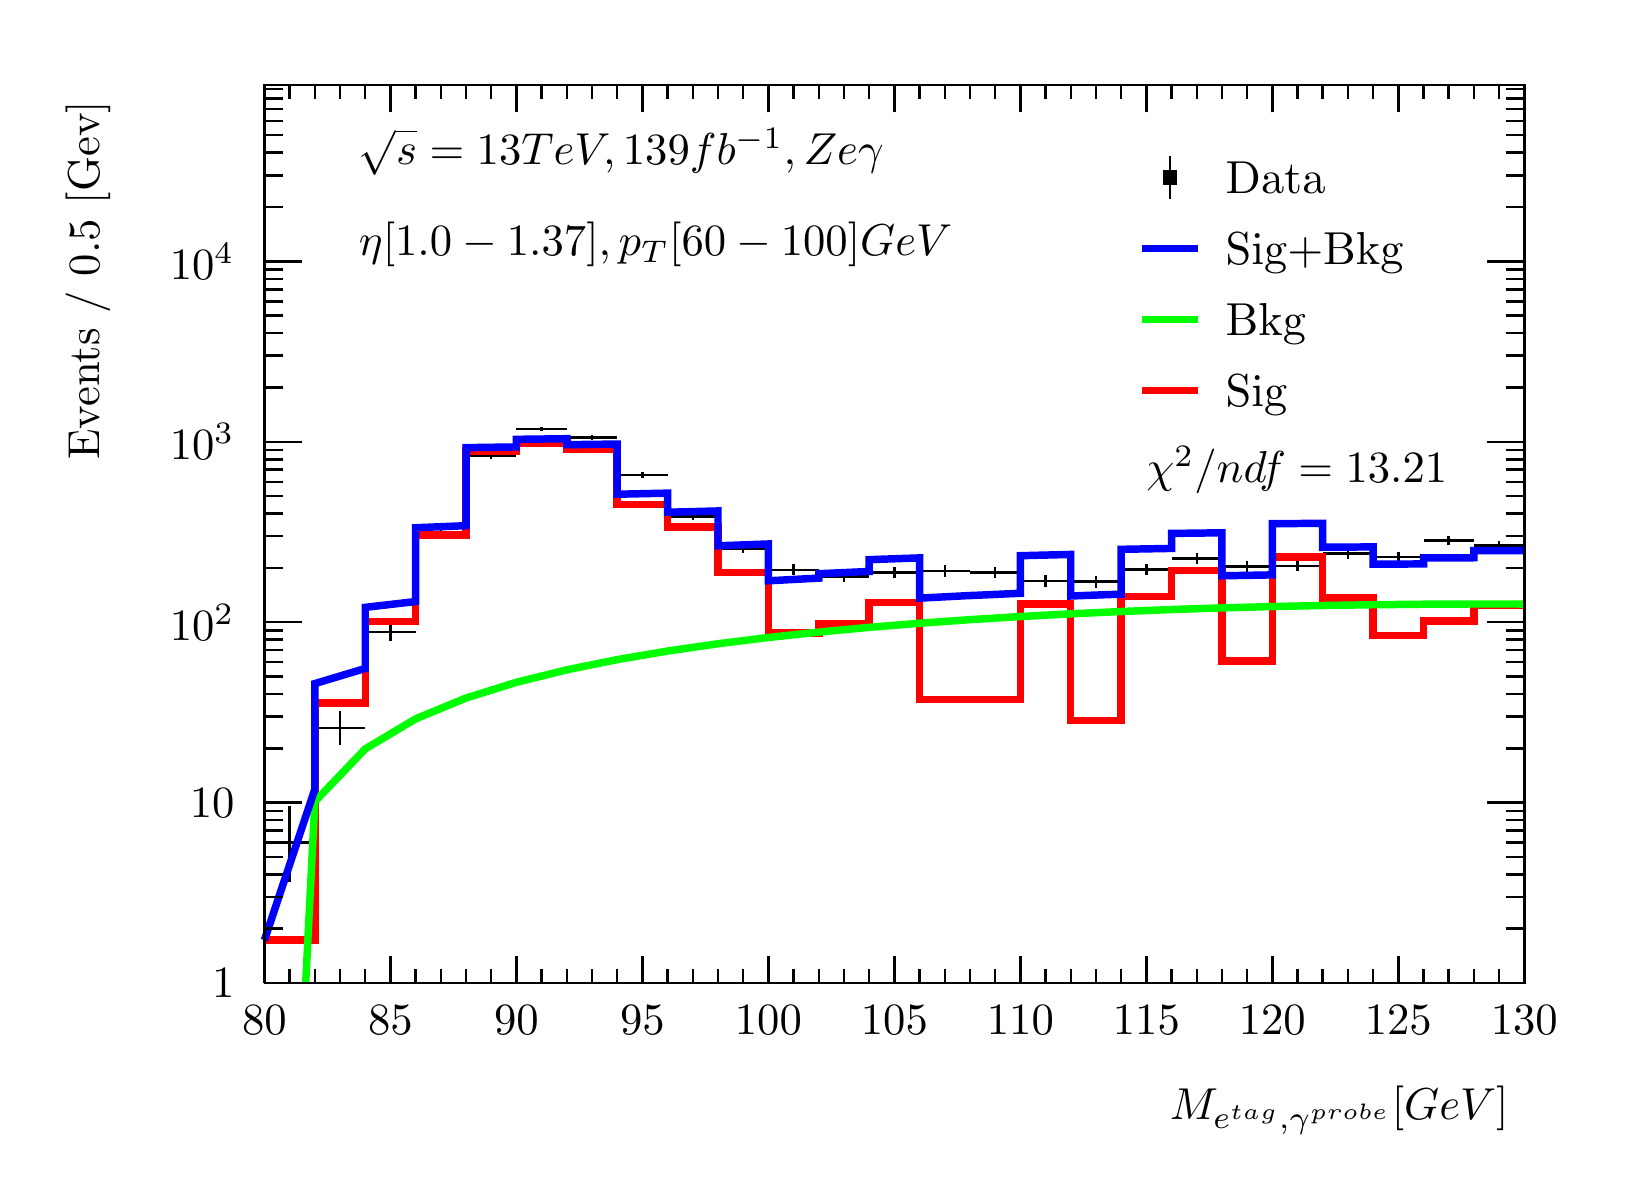
\begin{tikzpicture}
\pgfdeclareplotmark{cross} {
\pgfpathmoveto{\pgfpoint{-0.3\pgfplotmarksize}{\pgfplotmarksize}}
\pgfpathlineto{\pgfpoint{+0.3\pgfplotmarksize}{\pgfplotmarksize}}
\pgfpathlineto{\pgfpoint{+0.3\pgfplotmarksize}{0.3\pgfplotmarksize}}
\pgfpathlineto{\pgfpoint{+1\pgfplotmarksize}{0.3\pgfplotmarksize}}
\pgfpathlineto{\pgfpoint{+1\pgfplotmarksize}{-0.3\pgfplotmarksize}}
\pgfpathlineto{\pgfpoint{+0.3\pgfplotmarksize}{-0.3\pgfplotmarksize}}
\pgfpathlineto{\pgfpoint{+0.3\pgfplotmarksize}{-1.\pgfplotmarksize}}
\pgfpathlineto{\pgfpoint{-0.3\pgfplotmarksize}{-1.\pgfplotmarksize}}
\pgfpathlineto{\pgfpoint{-0.3\pgfplotmarksize}{-0.3\pgfplotmarksize}}
\pgfpathlineto{\pgfpoint{-1.\pgfplotmarksize}{-0.3\pgfplotmarksize}}
\pgfpathlineto{\pgfpoint{-1.\pgfplotmarksize}{0.3\pgfplotmarksize}}
\pgfpathlineto{\pgfpoint{-0.3\pgfplotmarksize}{0.3\pgfplotmarksize}}
\pgfpathclose
\pgfusepathqstroke
}
\pgfdeclareplotmark{cross*} {
\pgfpathmoveto{\pgfpoint{-0.3\pgfplotmarksize}{\pgfplotmarksize}}
\pgfpathlineto{\pgfpoint{+0.3\pgfplotmarksize}{\pgfplotmarksize}}
\pgfpathlineto{\pgfpoint{+0.3\pgfplotmarksize}{0.3\pgfplotmarksize}}
\pgfpathlineto{\pgfpoint{+1\pgfplotmarksize}{0.3\pgfplotmarksize}}
\pgfpathlineto{\pgfpoint{+1\pgfplotmarksize}{-0.3\pgfplotmarksize}}
\pgfpathlineto{\pgfpoint{+0.3\pgfplotmarksize}{-0.3\pgfplotmarksize}}
\pgfpathlineto{\pgfpoint{+0.3\pgfplotmarksize}{-1.\pgfplotmarksize}}
\pgfpathlineto{\pgfpoint{-0.3\pgfplotmarksize}{-1.\pgfplotmarksize}}
\pgfpathlineto{\pgfpoint{-0.3\pgfplotmarksize}{-0.3\pgfplotmarksize}}
\pgfpathlineto{\pgfpoint{-1.\pgfplotmarksize}{-0.3\pgfplotmarksize}}
\pgfpathlineto{\pgfpoint{-1.\pgfplotmarksize}{0.3\pgfplotmarksize}}
\pgfpathlineto{\pgfpoint{-0.3\pgfplotmarksize}{0.3\pgfplotmarksize}}
\pgfpathclose
\pgfusepathqfillstroke
}
\pgfdeclareplotmark{newstar} {
\pgfpathmoveto{\pgfqpoint{0pt}{\pgfplotmarksize}}
\pgfpathlineto{\pgfqpointpolar{44}{0.5\pgfplotmarksize}}
\pgfpathlineto{\pgfqpointpolar{18}{\pgfplotmarksize}}
\pgfpathlineto{\pgfqpointpolar{-20}{0.5\pgfplotmarksize}}
\pgfpathlineto{\pgfqpointpolar{-54}{\pgfplotmarksize}}
\pgfpathlineto{\pgfqpointpolar{-90}{0.5\pgfplotmarksize}}
\pgfpathlineto{\pgfqpointpolar{234}{\pgfplotmarksize}}
\pgfpathlineto{\pgfqpointpolar{198}{0.5\pgfplotmarksize}}
\pgfpathlineto{\pgfqpointpolar{162}{\pgfplotmarksize}}
\pgfpathlineto{\pgfqpointpolar{134}{0.5\pgfplotmarksize}}
\pgfpathclose
\pgfusepathqstroke
}
\pgfdeclareplotmark{newstar*} {
\pgfpathmoveto{\pgfqpoint{0pt}{\pgfplotmarksize}}
\pgfpathlineto{\pgfqpointpolar{44}{0.5\pgfplotmarksize}}
\pgfpathlineto{\pgfqpointpolar{18}{\pgfplotmarksize}}
\pgfpathlineto{\pgfqpointpolar{-20}{0.5\pgfplotmarksize}}
\pgfpathlineto{\pgfqpointpolar{-54}{\pgfplotmarksize}}
\pgfpathlineto{\pgfqpointpolar{-90}{0.5\pgfplotmarksize}}
\pgfpathlineto{\pgfqpointpolar{234}{\pgfplotmarksize}}
\pgfpathlineto{\pgfqpointpolar{198}{0.5\pgfplotmarksize}}
\pgfpathlineto{\pgfqpointpolar{162}{\pgfplotmarksize}}
\pgfpathlineto{\pgfqpointpolar{134}{0.5\pgfplotmarksize}}
\pgfpathclose
\pgfusepathqfillstroke
}
\definecolor{c}{rgb}{1,1,1};
\draw [color=c, fill=c] (0,0) rectangle (20,14.4361);
\draw [color=c, fill=c] (3,2.30977) rectangle (19,13.7143);
\definecolor{c}{rgb}{0,0,0};
\draw [c,line width=0.9] (3,2.30977) -- (3,13.7143) -- (19,13.7143) -- (19,2.30977) -- (3,2.30977);
\definecolor{c}{rgb}{1,1,1};
\draw [color=c, fill=c] (3,2.30977) rectangle (19,13.7143);
\definecolor{c}{rgb}{0,0,0};
\draw [c,line width=0.9] (3,2.30977) -- (3,13.7143) -- (19,13.7143) -- (19,2.30977) -- (3,2.30977);
\draw [c,line width=0.9] (3,2.30977) -- (19,2.30977);
\draw [c,line width=0.9] (3,2.65624) -- (3,2.30977);
\draw [c,line width=0.9] (3.32,2.48301) -- (3.32,2.30977);
\draw [c,line width=0.9] (3.64,2.48301) -- (3.64,2.30977);
\draw [c,line width=0.9] (3.96,2.48301) -- (3.96,2.30977);
\draw [c,line width=0.9] (4.28,2.48301) -- (4.28,2.30977);
\draw [c,line width=0.9] (4.6,2.65624) -- (4.6,2.30977);
\draw [c,line width=0.9] (4.92,2.48301) -- (4.92,2.30977);
\draw [c,line width=0.9] (5.24,2.48301) -- (5.24,2.30977);
\draw [c,line width=0.9] (5.56,2.48301) -- (5.56,2.30977);
\draw [c,line width=0.9] (5.88,2.48301) -- (5.88,2.30977);
\draw [c,line width=0.9] (6.2,2.65624) -- (6.2,2.30977);
\draw [c,line width=0.9] (6.52,2.48301) -- (6.52,2.30977);
\draw [c,line width=0.9] (6.84,2.48301) -- (6.84,2.30977);
\draw [c,line width=0.9] (7.16,2.48301) -- (7.16,2.30977);
\draw [c,line width=0.9] (7.48,2.48301) -- (7.48,2.30977);
\draw [c,line width=0.9] (7.8,2.65624) -- (7.8,2.30977);
\draw [c,line width=0.9] (8.12,2.48301) -- (8.12,2.30977);
\draw [c,line width=0.9] (8.44,2.48301) -- (8.44,2.30977);
\draw [c,line width=0.9] (8.76,2.48301) -- (8.76,2.30977);
\draw [c,line width=0.9] (9.08,2.48301) -- (9.08,2.30977);
\draw [c,line width=0.9] (9.4,2.65624) -- (9.4,2.30977);
\draw [c,line width=0.9] (9.72,2.48301) -- (9.72,2.30977);
\draw [c,line width=0.9] (10.04,2.48301) -- (10.04,2.30977);
\draw [c,line width=0.9] (10.36,2.48301) -- (10.36,2.30977);
\draw [c,line width=0.9] (10.68,2.48301) -- (10.68,2.30977);
\draw [c,line width=0.9] (11,2.65624) -- (11,2.30977);
\draw [c,line width=0.9] (11.32,2.48301) -- (11.32,2.30977);
\draw [c,line width=0.9] (11.64,2.48301) -- (11.64,2.30977);
\draw [c,line width=0.9] (11.96,2.48301) -- (11.96,2.30977);
\draw [c,line width=0.9] (12.28,2.48301) -- (12.28,2.30977);
\draw [c,line width=0.9] (12.6,2.65624) -- (12.6,2.30977);
\draw [c,line width=0.9] (12.92,2.48301) -- (12.92,2.30977);
\draw [c,line width=0.9] (13.24,2.48301) -- (13.24,2.30977);
\draw [c,line width=0.9] (13.56,2.48301) -- (13.56,2.30977);
\draw [c,line width=0.9] (13.88,2.48301) -- (13.88,2.30977);
\draw [c,line width=0.9] (14.2,2.65624) -- (14.2,2.30977);
\draw [c,line width=0.9] (14.52,2.48301) -- (14.52,2.30977);
\draw [c,line width=0.9] (14.84,2.48301) -- (14.84,2.30977);
\draw [c,line width=0.9] (15.16,2.48301) -- (15.16,2.30977);
\draw [c,line width=0.9] (15.48,2.48301) -- (15.48,2.30977);
\draw [c,line width=0.9] (15.8,2.65624) -- (15.8,2.30977);
\draw [c,line width=0.9] (16.12,2.48301) -- (16.12,2.30977);
\draw [c,line width=0.9] (16.44,2.48301) -- (16.44,2.30977);
\draw [c,line width=0.9] (16.76,2.48301) -- (16.76,2.30977);
\draw [c,line width=0.9] (17.08,2.48301) -- (17.08,2.30977);
\draw [c,line width=0.9] (17.4,2.65624) -- (17.4,2.30977);
\draw [c,line width=0.9] (17.72,2.48301) -- (17.72,2.30977);
\draw [c,line width=0.9] (18.04,2.48301) -- (18.04,2.30977);
\draw [c,line width=0.9] (18.36,2.48301) -- (18.36,2.30977);
\draw [c,line width=0.9] (18.68,2.48301) -- (18.68,2.30977);
\draw [c,line width=0.9] (19,2.65624) -- (19,2.30977);
\draw [anchor=base] (3,1.66015) node[scale=1.61424, color=c, rotate=0]{80};
\draw [anchor=base] (4.6,1.66015) node[scale=1.61424, color=c, rotate=0]{85};
\draw [anchor=base] (6.2,1.66015) node[scale=1.61424, color=c, rotate=0]{90};
\draw [anchor=base] (7.8,1.66015) node[scale=1.61424, color=c, rotate=0]{95};
\draw [anchor=base] (9.4,1.66015) node[scale=1.61424, color=c, rotate=0]{100};
\draw [anchor=base] (11,1.66015) node[scale=1.61424, color=c, rotate=0]{105};
\draw [anchor=base] (12.6,1.66015) node[scale=1.61424, color=c, rotate=0]{110};
\draw [anchor=base] (14.2,1.66015) node[scale=1.61424, color=c, rotate=0]{115};
\draw [anchor=base] (15.8,1.66015) node[scale=1.61424, color=c, rotate=0]{120};
\draw [anchor=base] (17.4,1.66015) node[scale=1.61424, color=c, rotate=0]{125};
\draw [anchor=base] (19,1.66015) node[scale=1.61424, color=c, rotate=0]{130};
\draw [anchor= east] (19,0.692932) node[scale=1.61424, color=c, rotate=0]{$M_{e^{tag}, \gamma^{probe}}  [GeV]$};
\draw [c,line width=0.9] (3,13.7143) -- (19,13.7143);
\draw [c,line width=0.9] (3,13.3678) -- (3,13.7143);
\draw [c,line width=0.9] (3.32,13.5411) -- (3.32,13.7143);
\draw [c,line width=0.9] (3.64,13.5411) -- (3.64,13.7143);
\draw [c,line width=0.9] (3.96,13.5411) -- (3.96,13.7143);
\draw [c,line width=0.9] (4.28,13.5411) -- (4.28,13.7143);
\draw [c,line width=0.9] (4.6,13.3678) -- (4.6,13.7143);
\draw [c,line width=0.9] (4.92,13.5411) -- (4.92,13.7143);
\draw [c,line width=0.9] (5.24,13.5411) -- (5.24,13.7143);
\draw [c,line width=0.9] (5.56,13.5411) -- (5.56,13.7143);
\draw [c,line width=0.9] (5.88,13.5411) -- (5.88,13.7143);
\draw [c,line width=0.9] (6.2,13.3678) -- (6.2,13.7143);
\draw [c,line width=0.9] (6.52,13.5411) -- (6.52,13.7143);
\draw [c,line width=0.9] (6.84,13.5411) -- (6.84,13.7143);
\draw [c,line width=0.9] (7.16,13.5411) -- (7.16,13.7143);
\draw [c,line width=0.9] (7.48,13.5411) -- (7.48,13.7143);
\draw [c,line width=0.9] (7.8,13.3678) -- (7.8,13.7143);
\draw [c,line width=0.9] (8.12,13.5411) -- (8.12,13.7143);
\draw [c,line width=0.9] (8.44,13.5411) -- (8.44,13.7143);
\draw [c,line width=0.9] (8.76,13.5411) -- (8.76,13.7143);
\draw [c,line width=0.9] (9.08,13.5411) -- (9.08,13.7143);
\draw [c,line width=0.9] (9.4,13.3678) -- (9.4,13.7143);
\draw [c,line width=0.9] (9.72,13.5411) -- (9.72,13.7143);
\draw [c,line width=0.9] (10.04,13.5411) -- (10.04,13.7143);
\draw [c,line width=0.9] (10.36,13.5411) -- (10.36,13.7143);
\draw [c,line width=0.9] (10.68,13.5411) -- (10.68,13.7143);
\draw [c,line width=0.9] (11,13.3678) -- (11,13.7143);
\draw [c,line width=0.9] (11.32,13.5411) -- (11.32,13.7143);
\draw [c,line width=0.9] (11.64,13.5411) -- (11.64,13.7143);
\draw [c,line width=0.9] (11.96,13.5411) -- (11.96,13.7143);
\draw [c,line width=0.9] (12.28,13.5411) -- (12.28,13.7143);
\draw [c,line width=0.9] (12.6,13.3678) -- (12.6,13.7143);
\draw [c,line width=0.9] (12.92,13.5411) -- (12.92,13.7143);
\draw [c,line width=0.9] (13.24,13.5411) -- (13.24,13.7143);
\draw [c,line width=0.9] (13.56,13.5411) -- (13.56,13.7143);
\draw [c,line width=0.9] (13.88,13.5411) -- (13.88,13.7143);
\draw [c,line width=0.9] (14.2,13.3678) -- (14.2,13.7143);
\draw [c,line width=0.9] (14.52,13.5411) -- (14.52,13.7143);
\draw [c,line width=0.9] (14.84,13.5411) -- (14.84,13.7143);
\draw [c,line width=0.9] (15.16,13.5411) -- (15.16,13.7143);
\draw [c,line width=0.9] (15.48,13.5411) -- (15.48,13.7143);
\draw [c,line width=0.9] (15.8,13.3678) -- (15.8,13.7143);
\draw [c,line width=0.9] (16.12,13.5411) -- (16.12,13.7143);
\draw [c,line width=0.9] (16.44,13.5411) -- (16.44,13.7143);
\draw [c,line width=0.9] (16.76,13.5411) -- (16.76,13.7143);
\draw [c,line width=0.9] (17.08,13.5411) -- (17.08,13.7143);
\draw [c,line width=0.9] (17.4,13.3678) -- (17.4,13.7143);
\draw [c,line width=0.9] (17.72,13.5411) -- (17.72,13.7143);
\draw [c,line width=0.9] (18.04,13.5411) -- (18.04,13.7143);
\draw [c,line width=0.9] (18.36,13.5411) -- (18.36,13.7143);
\draw [c,line width=0.9] (18.68,13.5411) -- (18.68,13.7143);
\draw [c,line width=0.9] (19,13.3678) -- (19,13.7143);
\draw [c,line width=0.9] (3,2.30977) -- (3,13.7143);
\draw [c,line width=0.9] (3.474,2.30978) -- (3,2.30978);
\draw [anchor= east] (2.82,2.30978) node[scale=1.61424, color=c, rotate=0]{1};
\draw [c,line width=0.9] (3.237,2.99955) -- (3,2.99955);
\draw [c,line width=0.9] (3.237,3.40303) -- (3,3.40303);
\draw [c,line width=0.9] (3.237,3.68931) -- (3,3.68931);
\draw [c,line width=0.9] (3.237,3.91137) -- (3,3.91137);
\draw [c,line width=0.9] (3.237,4.0928) -- (3,4.0928);
\draw [c,line width=0.9] (3.237,4.2462) -- (3,4.2462);
\draw [c,line width=0.9] (3.237,4.37908) -- (3,4.37908);
\draw [c,line width=0.9] (3.237,4.49629) -- (3,4.49629);
\draw [c,line width=0.9] (3.474,4.60114) -- (3,4.60114);
\draw [anchor= east] (2.82,4.60114) node[scale=1.61424, color=c, rotate=0]{10};
\draw [c,line width=0.9] (3.237,5.29091) -- (3,5.29091);
\draw [c,line width=0.9] (3.237,5.6944) -- (3,5.6944);
\draw [c,line width=0.9] (3.237,5.98068) -- (3,5.98068);
\draw [c,line width=0.9] (3.237,6.20273) -- (3,6.20273);
\draw [c,line width=0.9] (3.237,6.38416) -- (3,6.38416);
\draw [c,line width=0.9] (3.237,6.53756) -- (3,6.53756);
\draw [c,line width=0.9] (3.237,6.67044) -- (3,6.67044);
\draw [c,line width=0.9] (3.237,6.78765) -- (3,6.78765);
\draw [c,line width=0.9] (3.474,6.8925) -- (3,6.8925);
\draw [anchor= east] (2.82,6.8925) node[scale=1.61424, color=c, rotate=0]{$10^{2}$};
\draw [c,line width=0.9] (3.237,7.58227) -- (3,7.58227);
\draw [c,line width=0.9] (3.237,7.98576) -- (3,7.98576);
\draw [c,line width=0.9] (3.237,8.27204) -- (3,8.27204);
\draw [c,line width=0.9] (3.237,8.49409) -- (3,8.49409);
\draw [c,line width=0.9] (3.237,8.67553) -- (3,8.67553);
\draw [c,line width=0.9] (3.237,8.82893) -- (3,8.82893);
\draw [c,line width=0.9] (3.237,8.96181) -- (3,8.96181);
\draw [c,line width=0.9] (3.237,9.07902) -- (3,9.07902);
\draw [c,line width=0.9] (3.474,9.18386) -- (3,9.18386);
\draw [anchor= east] (2.82,9.18386) node[scale=1.61424, color=c, rotate=0]{$10^{3}$};
\draw [c,line width=0.9] (3.237,9.87363) -- (3,9.87363);
\draw [c,line width=0.9] (3.237,10.2771) -- (3,10.2771);
\draw [c,line width=0.9] (3.237,10.5634) -- (3,10.5634);
\draw [c,line width=0.9] (3.237,10.7855) -- (3,10.7855);
\draw [c,line width=0.9] (3.237,10.9669) -- (3,10.9669);
\draw [c,line width=0.9] (3.237,11.1203) -- (3,11.1203);
\draw [c,line width=0.9] (3.237,11.2532) -- (3,11.2532);
\draw [c,line width=0.9] (3.237,11.3704) -- (3,11.3704);
\draw [c,line width=0.9] (3.474,11.4752) -- (3,11.4752);
\draw [anchor= east] (2.82,11.4752) node[scale=1.61424, color=c, rotate=0]{$10^{4}$};
\draw [c,line width=0.9] (3.237,12.165) -- (3,12.165);
\draw [c,line width=0.9] (3.237,12.5685) -- (3,12.5685);
\draw [c,line width=0.9] (3.237,12.8548) -- (3,12.8548);
\draw [c,line width=0.9] (3.237,13.0768) -- (3,13.0768);
\draw [c,line width=0.9] (3.237,13.2583) -- (3,13.2583);
\draw [c,line width=0.9] (3.237,13.4117) -- (3,13.4117);
\draw [c,line width=0.9] (3.237,13.5445) -- (3,13.5445);
\draw [c,line width=0.9] (3.237,13.6617) -- (3,13.6617);
\draw [anchor= east] (0.76,13.7143) node[scale=1.61424, color=c, rotate=90]{Events / 0.5 [Gev]};
\draw [c,line width=0.9] (19,2.30977) -- (19,13.7143);
\draw [c,line width=0.9] (18.526,2.30978) -- (19,2.30978);
\draw [c,line width=0.9] (18.763,2.99955) -- (19,2.99955);
\draw [c,line width=0.9] (18.763,3.40303) -- (19,3.40303);
\draw [c,line width=0.9] (18.763,3.68931) -- (19,3.68931);
\draw [c,line width=0.9] (18.763,3.91137) -- (19,3.91137);
\draw [c,line width=0.9] (18.763,4.0928) -- (19,4.0928);
\draw [c,line width=0.9] (18.763,4.2462) -- (19,4.2462);
\draw [c,line width=0.9] (18.763,4.37908) -- (19,4.37908);
\draw [c,line width=0.9] (18.763,4.49629) -- (19,4.49629);
\draw [c,line width=0.9] (18.526,4.60114) -- (19,4.60114);
\draw [c,line width=0.9] (18.763,5.29091) -- (19,5.29091);
\draw [c,line width=0.9] (18.763,5.6944) -- (19,5.6944);
\draw [c,line width=0.9] (18.763,5.98068) -- (19,5.98068);
\draw [c,line width=0.9] (18.763,6.20273) -- (19,6.20273);
\draw [c,line width=0.9] (18.763,6.38416) -- (19,6.38416);
\draw [c,line width=0.9] (18.763,6.53756) -- (19,6.53756);
\draw [c,line width=0.9] (18.763,6.67044) -- (19,6.67044);
\draw [c,line width=0.9] (18.763,6.78765) -- (19,6.78765);
\draw [c,line width=0.9] (18.526,6.8925) -- (19,6.8925);
\draw [c,line width=0.9] (18.763,7.58227) -- (19,7.58227);
\draw [c,line width=0.9] (18.763,7.98576) -- (19,7.98576);
\draw [c,line width=0.9] (18.763,8.27204) -- (19,8.27204);
\draw [c,line width=0.9] (18.763,8.49409) -- (19,8.49409);
\draw [c,line width=0.9] (18.763,8.67553) -- (19,8.67553);
\draw [c,line width=0.9] (18.763,8.82893) -- (19,8.82893);
\draw [c,line width=0.9] (18.763,8.96181) -- (19,8.96181);
\draw [c,line width=0.9] (18.763,9.07902) -- (19,9.07902);
\draw [c,line width=0.9] (18.526,9.18386) -- (19,9.18386);
\draw [c,line width=0.9] (18.763,9.87363) -- (19,9.87363);
\draw [c,line width=0.9] (18.763,10.2771) -- (19,10.2771);
\draw [c,line width=0.9] (18.763,10.5634) -- (19,10.5634);
\draw [c,line width=0.9] (18.763,10.7855) -- (19,10.7855);
\draw [c,line width=0.9] (18.763,10.9669) -- (19,10.9669);
\draw [c,line width=0.9] (18.763,11.1203) -- (19,11.1203);
\draw [c,line width=0.9] (18.763,11.2532) -- (19,11.2532);
\draw [c,line width=0.9] (18.763,11.3704) -- (19,11.3704);
\draw [c,line width=0.9] (18.526,11.4752) -- (19,11.4752);
\draw [c,line width=0.9] (18.763,12.165) -- (19,12.165);
\draw [c,line width=0.9] (18.763,12.5685) -- (19,12.5685);
\draw [c,line width=0.9] (18.763,12.8548) -- (19,12.8548);
\draw [c,line width=0.9] (18.763,13.0768) -- (19,13.0768);
\draw [c,line width=0.9] (18.763,13.2583) -- (19,13.2583);
\draw [c,line width=0.9] (18.763,13.4117) -- (19,13.4117);
\draw [c,line width=0.9] (18.763,13.5445) -- (19,13.5445);
\draw [c,line width=0.9] (18.763,13.6617) -- (19,13.6617);
\draw [c,line width=0.9] (3.32,4.0928) -- (3,4.0928);
\draw [c,line width=0.9] (3,4.0928) -- (3,4.0928);
\draw [c,line width=0.9] (3.32,4.0928) -- (3.64,4.0928);
\draw [c,line width=0.9] (3.64,4.0928) -- (3.64,4.0928);
\draw [c,line width=0.9] (3.32,4.0928) -- (3.32,4.55882);
\draw [c,line width=0.9] (3.32,4.55882) -- (3.32,4.55882);
\draw [c,line width=0.9] (3.32,4.0928) -- (3.32,3.59);
\draw [c,line width=0.9] (3.32,3.59) -- (3.32,3.59);
\draw [c,line width=0.9] (3.96,5.55199) -- (3.64,5.55199);
\draw [c,line width=0.9] (3.64,5.55199) -- (3.64,5.55199);
\draw [c,line width=0.9] (3.96,5.55199) -- (4.28,5.55199);
\draw [c,line width=0.9] (4.28,5.55199) -- (4.28,5.55199);
\draw [c,line width=0.9] (3.96,5.55199) -- (3.96,5.76372);
\draw [c,line width=0.9] (3.96,5.76372) -- (3.96,5.76372);
\draw [c,line width=0.9] (3.96,5.55199) -- (3.96,5.33633);
\draw [c,line width=0.9] (3.96,5.33633) -- (3.96,5.33633);
\draw [c,line width=0.9] (4.6,6.76529) -- (4.28,6.76529);
\draw [c,line width=0.9] (4.28,6.76529) -- (4.28,6.76529);
\draw [c,line width=0.9] (4.6,6.76529) -- (4.92,6.76529);
\draw [c,line width=0.9] (4.92,6.76529) -- (4.92,6.76529);
\draw [c,line width=0.9] (4.6,6.76529) -- (4.6,6.87661);
\draw [c,line width=0.9] (4.6,6.87661) -- (4.6,6.87661);
\draw [c,line width=0.9] (4.6,6.76529) -- (4.6,6.65334);
\draw [c,line width=0.9] (4.6,6.65334) -- (4.6,6.65334);
\draw [c,line width=0.9] (5.24,8.08961) -- (4.92,8.08961);
\draw [c,line width=0.9] (4.92,8.08961) -- (4.92,8.08961);
\draw [c,line width=0.9] (5.24,8.08961) -- (5.56,8.08961);
\draw [c,line width=0.9] (5.56,8.08961) -- (5.56,8.08961);
\draw [c,line width=0.9] (5.24,8.08961) -- (5.24,8.14413);
\draw [c,line width=0.9] (5.24,8.14413) -- (5.24,8.14413);
\draw [c,line width=0.9] (5.24,8.08961) -- (5.24,8.03508);
\draw [c,line width=0.9] (5.24,8.03508) -- (5.24,8.03508);
\draw [c,line width=0.9] (5.88,9.00203) -- (5.56,9.00203);
\draw [c,line width=0.9] (5.56,9.00203) -- (5.56,9.00203);
\draw [c,line width=0.9] (5.88,9.00203) -- (6.2,9.00203);
\draw [c,line width=0.9] (6.2,9.00203) -- (6.2,9.00203);
\draw [c,line width=0.9] (5.88,9.00203) -- (5.88,9.03651);
\draw [c,line width=0.9] (5.88,9.03651) -- (5.88,9.03651);
\draw [c,line width=0.9] (5.88,9.00203) -- (5.88,8.96755);
\draw [c,line width=0.9] (5.88,8.96755) -- (5.88,8.96755);
\draw [c,line width=0.9] (6.52,9.34434) -- (6.2,9.34434);
\draw [c,line width=0.9] (6.2,9.34434) -- (6.2,9.34434);
\draw [c,line width=0.9] (6.52,9.34434) -- (6.84,9.34434);
\draw [c,line width=0.9] (6.84,9.34434) -- (6.84,9.34434);
\draw [c,line width=0.9] (6.52,9.34434) -- (6.52,9.37337);
\draw [c,line width=0.9] (6.52,9.37337) -- (6.52,9.37337);
\draw [c,line width=0.9] (6.52,9.34434) -- (6.52,9.31531);
\draw [c,line width=0.9] (6.52,9.31531) -- (6.52,9.31531);
\draw [c,line width=0.9] (7.16,9.24091) -- (6.84,9.24091);
\draw [c,line width=0.9] (6.84,9.24091) -- (6.84,9.24091);
\draw [c,line width=0.9] (7.16,9.24091) -- (7.48,9.24091);
\draw [c,line width=0.9] (7.48,9.24091) -- (7.48,9.24091);
\draw [c,line width=0.9] (7.16,9.24091) -- (7.16,9.27149);
\draw [c,line width=0.9] (7.16,9.27149) -- (7.16,9.27149);
\draw [c,line width=0.9] (7.16,9.24091) -- (7.16,9.21033);
\draw [c,line width=0.9] (7.16,9.21033) -- (7.16,9.21033);
\draw [c,line width=0.9] (7.8,8.76128) -- (7.48,8.76128);
\draw [c,line width=0.9] (7.48,8.76128) -- (7.48,8.76128);
\draw [c,line width=0.9] (7.8,8.76128) -- (8.12,8.76128);
\draw [c,line width=0.9] (8.12,8.76128) -- (8.12,8.76128);
\draw [c,line width=0.9] (7.8,8.76128) -- (7.8,8.80019);
\draw [c,line width=0.9] (7.8,8.80019) -- (7.8,8.80019);
\draw [c,line width=0.9] (7.8,8.76128) -- (7.8,8.72237);
\draw [c,line width=0.9] (7.8,8.72237) -- (7.8,8.72237);
\draw [c,line width=0.9] (8.44,8.23658) -- (8.12,8.23658);
\draw [c,line width=0.9] (8.12,8.23658) -- (8.12,8.23658);
\draw [c,line width=0.9] (8.44,8.23658) -- (8.76,8.23658);
\draw [c,line width=0.9] (8.76,8.23658) -- (8.76,8.23658);
\draw [c,line width=0.9] (8.44,8.23658) -- (8.44,8.28723);
\draw [c,line width=0.9] (8.44,8.28723) -- (8.44,8.28723);
\draw [c,line width=0.9] (8.44,8.23658) -- (8.44,8.18594);
\draw [c,line width=0.9] (8.44,8.18594) -- (8.44,8.18594);
\draw [c,line width=0.9] (9.08,7.82793) -- (8.76,7.82793);
\draw [c,line width=0.9] (8.76,7.82793) -- (8.76,7.82793);
\draw [c,line width=0.9] (9.08,7.82793) -- (9.4,7.82793);
\draw [c,line width=0.9] (9.4,7.82793) -- (9.4,7.82793);
\draw [c,line width=0.9] (9.08,7.82793) -- (9.08,7.89011);
\draw [c,line width=0.9] (9.08,7.89011) -- (9.08,7.89011);
\draw [c,line width=0.9] (9.08,7.82793) -- (9.08,7.76574);
\draw [c,line width=0.9] (9.08,7.76574) -- (9.08,7.76574);
\draw [c,line width=0.9] (9.72,7.55707) -- (9.4,7.55707);
\draw [c,line width=0.9] (9.4,7.55707) -- (9.4,7.55707);
\draw [c,line width=0.9] (9.72,7.55707) -- (10.04,7.55707);
\draw [c,line width=0.9] (10.04,7.55707) -- (10.04,7.55707);
\draw [c,line width=0.9] (9.72,7.55707) -- (9.72,7.62832);
\draw [c,line width=0.9] (9.72,7.62832) -- (9.72,7.62832);
\draw [c,line width=0.9] (9.72,7.55707) -- (9.72,7.48583);
\draw [c,line width=0.9] (9.72,7.48583) -- (9.72,7.48583);
\draw [c,line width=0.9] (10.36,7.47188) -- (10.04,7.47188);
\draw [c,line width=0.9] (10.04,7.47188) -- (10.04,7.47188);
\draw [c,line width=0.9] (10.36,7.47188) -- (10.68,7.47188);
\draw [c,line width=0.9] (10.68,7.47188) -- (10.68,7.47188);
\draw [c,line width=0.9] (10.36,7.47188) -- (10.36,7.54624);
\draw [c,line width=0.9] (10.36,7.54624) -- (10.36,7.54624);
\draw [c,line width=0.9] (10.36,7.47188) -- (10.36,7.39752);
\draw [c,line width=0.9] (10.36,7.39752) -- (10.36,7.39752);
\draw [c,line width=0.9] (11,7.52069) -- (10.68,7.52069);
\draw [c,line width=0.9] (10.68,7.52069) -- (10.68,7.52069);
\draw [c,line width=0.9] (11,7.52069) -- (11.32,7.52069);
\draw [c,line width=0.9] (11.32,7.52069) -- (11.32,7.52069);
\draw [c,line width=0.9] (11,7.52069) -- (11,7.59326);
\draw [c,line width=0.9] (11,7.59326) -- (11,7.59326);
\draw [c,line width=0.9] (11,7.52069) -- (11,7.44813);
\draw [c,line width=0.9] (11,7.44813) -- (11,7.44813);
\draw [c,line width=0.9] (11.64,7.54165) -- (11.32,7.54165);
\draw [c,line width=0.9] (11.32,7.54165) -- (11.32,7.54165);
\draw [c,line width=0.9] (11.64,7.54165) -- (11.96,7.54165);
\draw [c,line width=0.9] (11.96,7.54165) -- (11.96,7.54165);
\draw [c,line width=0.9] (11.64,7.54165) -- (11.64,7.61345);
\draw [c,line width=0.9] (11.64,7.61345) -- (11.64,7.61345);
\draw [c,line width=0.9] (11.64,7.54165) -- (11.64,7.46984);
\draw [c,line width=0.9] (11.64,7.46984) -- (11.64,7.46984);
\draw [c,line width=0.9] (12.28,7.52069) -- (11.96,7.52069);
\draw [c,line width=0.9] (11.96,7.52069) -- (11.96,7.52069);
\draw [c,line width=0.9] (12.28,7.52069) -- (12.6,7.52069);
\draw [c,line width=0.9] (12.6,7.52069) -- (12.6,7.52069);
\draw [c,line width=0.9] (12.28,7.52069) -- (12.28,7.59326);
\draw [c,line width=0.9] (12.28,7.59326) -- (12.28,7.59326);
\draw [c,line width=0.9] (12.28,7.52069) -- (12.28,7.44813);
\draw [c,line width=0.9] (12.28,7.44813) -- (12.28,7.44813);
\draw [c,line width=0.9] (12.92,7.41467) -- (12.6,7.41467);
\draw [c,line width=0.9] (12.6,7.41467) -- (12.6,7.41467);
\draw [c,line width=0.9] (12.92,7.41467) -- (13.24,7.41467);
\draw [c,line width=0.9] (13.24,7.41467) -- (13.24,7.41467);
\draw [c,line width=0.9] (12.92,7.41467) -- (12.92,7.4912);
\draw [c,line width=0.9] (12.92,7.4912) -- (12.92,7.4912);
\draw [c,line width=0.9] (12.92,7.41467) -- (12.92,7.33814);
\draw [c,line width=0.9] (12.92,7.33814) -- (12.92,7.33814);
\draw [c,line width=0.9] (13.56,7.40876) -- (13.24,7.40876);
\draw [c,line width=0.9] (13.24,7.40876) -- (13.24,7.40876);
\draw [c,line width=0.9] (13.56,7.40876) -- (13.88,7.40876);
\draw [c,line width=0.9] (13.88,7.40876) -- (13.88,7.40876);
\draw [c,line width=0.9] (13.56,7.40876) -- (13.56,7.48552);
\draw [c,line width=0.9] (13.56,7.48552) -- (13.56,7.48552);
\draw [c,line width=0.9] (13.56,7.40876) -- (13.56,7.33201);
\draw [c,line width=0.9] (13.56,7.33201) -- (13.56,7.33201);
\draw [c,line width=0.9] (14.2,7.56216) -- (13.88,7.56216);
\draw [c,line width=0.9] (13.88,7.56216) -- (13.88,7.56216);
\draw [c,line width=0.9] (14.2,7.56216) -- (14.52,7.56216);
\draw [c,line width=0.9] (14.52,7.56216) -- (14.52,7.56216);
\draw [c,line width=0.9] (14.2,7.56216) -- (14.2,7.63323);
\draw [c,line width=0.9] (14.2,7.63323) -- (14.2,7.63323);
\draw [c,line width=0.9] (14.2,7.56216) -- (14.2,7.4911);
\draw [c,line width=0.9] (14.2,7.4911) -- (14.2,7.4911);
\draw [c,line width=0.9] (14.84,7.69948) -- (14.52,7.69948);
\draw [c,line width=0.9] (14.52,7.69948) -- (14.52,7.69948);
\draw [c,line width=0.9] (14.84,7.69948) -- (15.16,7.69948);
\draw [c,line width=0.9] (15.16,7.69948) -- (15.16,7.69948);
\draw [c,line width=0.9] (14.84,7.69948) -- (14.84,7.76581);
\draw [c,line width=0.9] (14.84,7.76581) -- (14.84,7.76581);
\draw [c,line width=0.9] (14.84,7.69948) -- (14.84,7.63315);
\draw [c,line width=0.9] (14.84,7.63315) -- (14.84,7.63315);
\draw [c,line width=0.9] (15.48,7.59708) -- (15.16,7.59708);
\draw [c,line width=0.9] (15.16,7.59708) -- (15.16,7.59708);
\draw [c,line width=0.9] (15.48,7.59708) -- (15.8,7.59708);
\draw [c,line width=0.9] (15.8,7.59708) -- (15.8,7.59708);
\draw [c,line width=0.9] (15.48,7.59708) -- (15.48,7.66691);
\draw [c,line width=0.9] (15.48,7.66691) -- (15.48,7.66691);
\draw [c,line width=0.9] (15.48,7.59708) -- (15.48,7.52725);
\draw [c,line width=0.9] (15.48,7.52725) -- (15.48,7.52725);
\draw [c,line width=0.9] (16.12,7.60684) -- (15.8,7.60684);
\draw [c,line width=0.9] (15.8,7.60684) -- (15.8,7.60684);
\draw [c,line width=0.9] (16.12,7.60684) -- (16.44,7.60684);
\draw [c,line width=0.9] (16.44,7.60684) -- (16.44,7.60684);
\draw [c,line width=0.9] (16.12,7.60684) -- (16.12,7.67633);
\draw [c,line width=0.9] (16.12,7.67633) -- (16.12,7.67633);
\draw [c,line width=0.9] (16.12,7.60684) -- (16.12,7.53735);
\draw [c,line width=0.9] (16.12,7.53735) -- (16.12,7.53735);
\draw [c,line width=0.9] (16.76,7.7637) -- (16.44,7.7637);
\draw [c,line width=0.9] (16.44,7.7637) -- (16.44,7.7637);
\draw [c,line width=0.9] (16.76,7.7637) -- (17.08,7.7637);
\draw [c,line width=0.9] (17.08,7.7637) -- (17.08,7.7637);
\draw [c,line width=0.9] (16.76,7.7637) -- (16.76,7.82793);
\draw [c,line width=0.9] (16.76,7.82793) -- (16.76,7.82793);
\draw [c,line width=0.9] (16.76,7.7637) -- (16.76,7.69948);
\draw [c,line width=0.9] (16.76,7.69948) -- (16.76,7.69948);
\draw [c,line width=0.9] (17.4,7.72135) -- (17.08,7.72135);
\draw [c,line width=0.9] (17.08,7.72135) -- (17.08,7.72135);
\draw [c,line width=0.9] (17.4,7.72135) -- (17.72,7.72135);
\draw [c,line width=0.9] (17.72,7.72135) -- (17.72,7.72135);
\draw [c,line width=0.9] (17.4,7.72135) -- (17.4,7.78695);
\draw [c,line width=0.9] (17.4,7.78695) -- (17.4,7.78695);
\draw [c,line width=0.9] (17.4,7.72135) -- (17.4,7.65574);
\draw [c,line width=0.9] (17.4,7.65574) -- (17.4,7.65574);
\draw [c,line width=0.9] (18.04,7.93122) -- (17.72,7.93122);
\draw [c,line width=0.9] (17.72,7.93122) -- (17.72,7.93122);
\draw [c,line width=0.9] (18.04,7.93122) -- (18.36,7.93122);
\draw [c,line width=0.9] (18.36,7.93122) -- (18.36,7.93122);
\draw [c,line width=0.9] (18.04,7.93122) -- (18.04,7.99026);
\draw [c,line width=0.9] (18.04,7.99026) -- (18.04,7.99026);
\draw [c,line width=0.9] (18.04,7.93122) -- (18.04,7.87217);
\draw [c,line width=0.9] (18.04,7.87217) -- (18.04,7.87217);
\draw [c,line width=0.9] (18.68,7.86606) -- (18.36,7.86606);
\draw [c,line width=0.9] (18.36,7.86606) -- (18.36,7.86606);
\draw [c,line width=0.9] (18.68,7.86606) -- (19,7.86606);
\draw [c,line width=0.9] (19,7.86606) -- (19,7.86606);
\draw [c,line width=0.9] (18.68,7.86606) -- (18.68,7.92706);
\draw [c,line width=0.9] (18.68,7.92706) -- (18.68,7.92706);
\draw [c,line width=0.9] (18.68,7.86606) -- (18.68,7.80505);
\draw [c,line width=0.9] (18.68,7.80505) -- (18.68,7.80505);
\foreach \P in {(3.32,4.0928), (3.96,5.55199), (4.6,6.76529), (5.24,8.08961), (5.88,9.00203), (6.52,9.34434), (7.16,9.24091), (7.8,8.76128), (8.44,8.23658), (9.08,7.82793), (9.72,7.55707), (10.36,7.47188), (11,7.52069), (11.64,7.54165),
 (12.28,7.52069), (12.92,7.41467), (13.56,7.40876), (14.2,7.56216), (14.84,7.69948), (15.48,7.59708), (16.12,7.60684), (16.76,7.7637), (17.4,7.72135), (18.04,7.93122), (18.68,7.86606)}{\draw[mark options={color=c,fill=c},mark size=2.882883pt,mark=]
 plot coordinates {\P};}
\definecolor{c}{rgb}{1,0,0};
\draw [c,line width=2.7] (3,2.8555) -- (3,2.8555);
\draw [c,line width=2.7] (3,2.8555) -- (3,2.8555) -- (3.64,2.8555) -- (3.64,5.86356) -- (4.28,5.86356) -- (4.28,6.90263) -- (4.92,6.90263) -- (4.92,8.00124) -- (5.56,8.00124) -- (5.56,9.06781) -- (6.2,9.06781) -- (6.2,9.16922) -- (6.84,9.16922) --
 (6.84,9.08932) -- (7.48,9.08932) -- (7.48,8.38924) -- (8.12,8.38924) -- (8.12,8.10356) -- (8.76,8.10356) -- (8.76,7.52688) -- (9.4,7.52688) -- (9.4,6.75792) -- (10.04,6.75792) -- (10.04,6.867) -- (10.68,6.867) -- (10.68,7.14224) -- (11.32,7.14224)
 -- (11.32,5.91016) -- (11.96,5.91016) -- (11.96,5.90766) -- (12.6,5.90766) -- (12.6,7.12389) -- (13.24,7.12389) -- (13.24,5.64145) -- (13.88,5.64145) -- (13.88,7.21919) -- (14.52,7.21919) -- (14.52,7.54655) -- (15.16,7.54655) -- (15.16,6.39714) --
 (15.8,6.39714) -- (15.8,7.71893) -- (16.44,7.71893) -- (16.44,7.20189) -- (17.08,7.20189) -- (17.08,6.72606) -- (17.72,6.72606) -- (17.72,6.90657) -- (18.36,6.90657) -- (18.36,7.10232) -- (19,7.10232) -- (19,7.10232) -- (19,7.10232) -- (19,7.10232);
\definecolor{c}{rgb}{0,1,0};
\draw [c,line width=2.7] (3.52386,2.30977) -- (3.64,4.61463);
\draw [c,line width=2.7] (3.64,4.61463) -- (3.64,4.61463) -- (4.28,5.28335) -- (4.28,5.28335) -- (4.92,5.66534) -- (4.92,5.66534) -- (5.56,5.92964) -- (5.56,5.92964) -- (6.2,6.12922) -- (6.2,6.12922) -- (6.84,6.28766) -- (6.84,6.28766) --
 (7.48,6.41752) -- (7.48,6.41752) -- (8.12,6.5263) -- (8.12,6.5263) -- (8.76,6.6188) -- (8.76,6.6188) -- (9.4,6.69831) -- (9.4,6.69831) -- (10.04,6.76716) -- (10.04,6.76716) -- (10.68,6.82705) -- (10.68,6.82705) -- (11.32,6.87927) -- (11.32,6.87927)
 -- (11.96,6.92481) -- (11.96,6.92481) -- (12.6,6.96444) -- (12.6,6.96444) -- (13.24,6.99876) -- (13.24,6.99876) -- (13.88,7.02826) -- (13.88,7.02826) -- (14.52,7.05332) -- (14.52,7.05332) -- (15.16,7.07426) -- (15.16,7.07426) -- (15.8,7.09131) --
 (15.8,7.09131) -- (16.44,7.10467) -- (16.44,7.10467) -- (17.08,7.11449) -- (17.08,7.11449) -- (17.72,7.12085) -- (17.72,7.12085) -- (18.36,7.12384) -- (18.36,7.12384) -- (19,7.12347) -- (19,7.12347) -- (19,7.12347) -- (19,7.12347);
\definecolor{c}{rgb}{0,0,1};
\draw [c,line width=2.7] (3,2.85551) -- (3,2.85551);
\draw [c,line width=2.7] (3,2.85551) -- (3,2.85551) -- (3.64,4.77148) -- (3.64,6.11315) -- (4.28,6.30493) -- (4.28,7.08113) -- (4.92,7.15481) -- (4.92,8.09212) -- (5.56,8.1182) -- (5.56,9.10942) -- (6.2,9.11843) -- (6.2,9.21505) -- (6.84,9.22275) --
 (6.84,9.14719) -- (7.48,9.155) -- (7.48,8.51777) -- (8.12,8.5316) -- (8.12,8.28909) -- (8.76,8.30544) -- (8.76,7.86278) -- (9.4,7.88622) -- (9.4,7.41833) -- (10.04,7.45232) -- (10.04,7.5081) -- (10.68,7.53699) -- (10.68,7.68684) -- (11.32,7.70918)
 -- (11.32,7.19807) -- (11.96,7.23133) -- (11.96,7.23067) -- (12.6,7.25996) -- (12.6,7.73712) -- (13.24,7.75306) -- (13.24,7.2253) -- (13.88,7.24886) -- (13.88,7.81806) -- (14.52,7.82948) -- (14.52,8.01996) -- (15.16,8.02794) -- (15.16,7.48198) --
 (15.8,7.49334) -- (15.8,8.14357) -- (16.44,8.14823) -- (16.44,7.84424) -- (17.08,7.84892) -- (17.08,7.62887) -- (17.72,7.63267) -- (17.72,7.70924) -- (18.36,7.71089) -- (18.36,7.80291) -- (19,7.80272) -- (19,7.80272) -- (19,7.80272) -- (19,7.80272);
\definecolor{c}{rgb}{0,0,0};
\draw [c,line width=0.9] (3,2.30977) -- (19,2.30977);
\draw [c,line width=0.9] (3,2.65624) -- (3,2.30977);
\draw [c,line width=0.9] (3.32,2.48301) -- (3.32,2.30977);
\draw [c,line width=0.9] (3.64,2.48301) -- (3.64,2.30977);
\draw [c,line width=0.9] (3.96,2.48301) -- (3.96,2.30977);
\draw [c,line width=0.9] (4.28,2.48301) -- (4.28,2.30977);
\draw [c,line width=0.9] (4.6,2.65624) -- (4.6,2.30977);
\draw [c,line width=0.9] (4.92,2.48301) -- (4.92,2.30977);
\draw [c,line width=0.9] (5.24,2.48301) -- (5.24,2.30977);
\draw [c,line width=0.9] (5.56,2.48301) -- (5.56,2.30977);
\draw [c,line width=0.9] (5.88,2.48301) -- (5.88,2.30977);
\draw [c,line width=0.9] (6.2,2.65624) -- (6.2,2.30977);
\draw [c,line width=0.9] (6.52,2.48301) -- (6.52,2.30977);
\draw [c,line width=0.9] (6.84,2.48301) -- (6.84,2.30977);
\draw [c,line width=0.9] (7.16,2.48301) -- (7.16,2.30977);
\draw [c,line width=0.9] (7.48,2.48301) -- (7.48,2.30977);
\draw [c,line width=0.9] (7.8,2.65624) -- (7.8,2.30977);
\draw [c,line width=0.9] (8.12,2.48301) -- (8.12,2.30977);
\draw [c,line width=0.9] (8.44,2.48301) -- (8.44,2.30977);
\draw [c,line width=0.9] (8.76,2.48301) -- (8.76,2.30977);
\draw [c,line width=0.9] (9.08,2.48301) -- (9.08,2.30977);
\draw [c,line width=0.9] (9.4,2.65624) -- (9.4,2.30977);
\draw [c,line width=0.9] (9.72,2.48301) -- (9.72,2.30977);
\draw [c,line width=0.9] (10.04,2.48301) -- (10.04,2.30977);
\draw [c,line width=0.9] (10.36,2.48301) -- (10.36,2.30977);
\draw [c,line width=0.9] (10.68,2.48301) -- (10.68,2.30977);
\draw [c,line width=0.9] (11,2.65624) -- (11,2.30977);
\draw [c,line width=0.9] (11.32,2.48301) -- (11.32,2.30977);
\draw [c,line width=0.9] (11.64,2.48301) -- (11.64,2.30977);
\draw [c,line width=0.9] (11.96,2.48301) -- (11.96,2.30977);
\draw [c,line width=0.9] (12.28,2.48301) -- (12.28,2.30977);
\draw [c,line width=0.9] (12.6,2.65624) -- (12.6,2.30977);
\draw [c,line width=0.9] (12.92,2.48301) -- (12.92,2.30977);
\draw [c,line width=0.9] (13.24,2.48301) -- (13.24,2.30977);
\draw [c,line width=0.9] (13.56,2.48301) -- (13.56,2.30977);
\draw [c,line width=0.9] (13.88,2.48301) -- (13.88,2.30977);
\draw [c,line width=0.9] (14.2,2.65624) -- (14.2,2.30977);
\draw [c,line width=0.9] (14.52,2.48301) -- (14.52,2.30977);
\draw [c,line width=0.9] (14.84,2.48301) -- (14.84,2.30977);
\draw [c,line width=0.9] (15.16,2.48301) -- (15.16,2.30977);
\draw [c,line width=0.9] (15.48,2.48301) -- (15.48,2.30977);
\draw [c,line width=0.9] (15.8,2.65624) -- (15.8,2.30977);
\draw [c,line width=0.9] (16.12,2.48301) -- (16.12,2.30977);
\draw [c,line width=0.9] (16.44,2.48301) -- (16.44,2.30977);
\draw [c,line width=0.9] (16.76,2.48301) -- (16.76,2.30977);
\draw [c,line width=0.9] (17.08,2.48301) -- (17.08,2.30977);
\draw [c,line width=0.9] (17.4,2.65624) -- (17.4,2.30977);
\draw [c,line width=0.9] (17.72,2.48301) -- (17.72,2.30977);
\draw [c,line width=0.9] (18.04,2.48301) -- (18.04,2.30977);
\draw [c,line width=0.9] (18.36,2.48301) -- (18.36,2.30977);
\draw [c,line width=0.9] (18.68,2.48301) -- (18.68,2.30977);
\draw [c,line width=0.9] (19,2.65624) -- (19,2.30977);
\draw [c,line width=0.9] (3,13.7143) -- (19,13.7143);
\draw [c,line width=0.9] (3,13.3678) -- (3,13.7143);
\draw [c,line width=0.9] (3.32,13.5411) -- (3.32,13.7143);
\draw [c,line width=0.9] (3.64,13.5411) -- (3.64,13.7143);
\draw [c,line width=0.9] (3.96,13.5411) -- (3.96,13.7143);
\draw [c,line width=0.9] (4.28,13.5411) -- (4.28,13.7143);
\draw [c,line width=0.9] (4.6,13.3678) -- (4.6,13.7143);
\draw [c,line width=0.9] (4.92,13.5411) -- (4.92,13.7143);
\draw [c,line width=0.9] (5.24,13.5411) -- (5.24,13.7143);
\draw [c,line width=0.9] (5.56,13.5411) -- (5.56,13.7143);
\draw [c,line width=0.9] (5.88,13.5411) -- (5.88,13.7143);
\draw [c,line width=0.9] (6.2,13.3678) -- (6.2,13.7143);
\draw [c,line width=0.9] (6.52,13.5411) -- (6.52,13.7143);
\draw [c,line width=0.9] (6.84,13.5411) -- (6.84,13.7143);
\draw [c,line width=0.9] (7.16,13.5411) -- (7.16,13.7143);
\draw [c,line width=0.9] (7.48,13.5411) -- (7.48,13.7143);
\draw [c,line width=0.9] (7.8,13.3678) -- (7.8,13.7143);
\draw [c,line width=0.9] (8.12,13.5411) -- (8.12,13.7143);
\draw [c,line width=0.9] (8.44,13.5411) -- (8.44,13.7143);
\draw [c,line width=0.9] (8.76,13.5411) -- (8.76,13.7143);
\draw [c,line width=0.9] (9.08,13.5411) -- (9.08,13.7143);
\draw [c,line width=0.9] (9.4,13.3678) -- (9.4,13.7143);
\draw [c,line width=0.9] (9.72,13.5411) -- (9.72,13.7143);
\draw [c,line width=0.9] (10.04,13.5411) -- (10.04,13.7143);
\draw [c,line width=0.9] (10.36,13.5411) -- (10.36,13.7143);
\draw [c,line width=0.9] (10.68,13.5411) -- (10.68,13.7143);
\draw [c,line width=0.9] (11,13.3678) -- (11,13.7143);
\draw [c,line width=0.9] (11.32,13.5411) -- (11.32,13.7143);
\draw [c,line width=0.9] (11.64,13.5411) -- (11.64,13.7143);
\draw [c,line width=0.9] (11.96,13.5411) -- (11.96,13.7143);
\draw [c,line width=0.9] (12.28,13.5411) -- (12.28,13.7143);
\draw [c,line width=0.9] (12.6,13.3678) -- (12.6,13.7143);
\draw [c,line width=0.9] (12.92,13.5411) -- (12.92,13.7143);
\draw [c,line width=0.9] (13.24,13.5411) -- (13.24,13.7143);
\draw [c,line width=0.9] (13.56,13.5411) -- (13.56,13.7143);
\draw [c,line width=0.9] (13.88,13.5411) -- (13.88,13.7143);
\draw [c,line width=0.9] (14.2,13.3678) -- (14.2,13.7143);
\draw [c,line width=0.9] (14.52,13.5411) -- (14.52,13.7143);
\draw [c,line width=0.9] (14.84,13.5411) -- (14.84,13.7143);
\draw [c,line width=0.9] (15.16,13.5411) -- (15.16,13.7143);
\draw [c,line width=0.9] (15.48,13.5411) -- (15.48,13.7143);
\draw [c,line width=0.9] (15.8,13.3678) -- (15.8,13.7143);
\draw [c,line width=0.9] (16.12,13.5411) -- (16.12,13.7143);
\draw [c,line width=0.9] (16.44,13.5411) -- (16.44,13.7143);
\draw [c,line width=0.9] (16.76,13.5411) -- (16.76,13.7143);
\draw [c,line width=0.9] (17.08,13.5411) -- (17.08,13.7143);
\draw [c,line width=0.9] (17.4,13.3678) -- (17.4,13.7143);
\draw [c,line width=0.9] (17.72,13.5411) -- (17.72,13.7143);
\draw [c,line width=0.9] (18.04,13.5411) -- (18.04,13.7143);
\draw [c,line width=0.9] (18.36,13.5411) -- (18.36,13.7143);
\draw [c,line width=0.9] (18.68,13.5411) -- (18.68,13.7143);
\draw [c,line width=0.9] (19,13.3678) -- (19,13.7143);
\draw [c,line width=0.9] (3,2.30977) -- (3,13.7143);
\draw [c,line width=0.9] (3.474,2.30978) -- (3,2.30978);
\draw [c,line width=0.9] (3.237,2.99955) -- (3,2.99955);
\draw [c,line width=0.9] (3.237,3.40303) -- (3,3.40303);
\draw [c,line width=0.9] (3.237,3.68931) -- (3,3.68931);
\draw [c,line width=0.9] (3.237,3.91137) -- (3,3.91137);
\draw [c,line width=0.9] (3.237,4.0928) -- (3,4.0928);
\draw [c,line width=0.9] (3.237,4.2462) -- (3,4.2462);
\draw [c,line width=0.9] (3.237,4.37908) -- (3,4.37908);
\draw [c,line width=0.9] (3.237,4.49629) -- (3,4.49629);
\draw [c,line width=0.9] (3.474,4.60114) -- (3,4.60114);
\draw [c,line width=0.9] (3.237,5.29091) -- (3,5.29091);
\draw [c,line width=0.9] (3.237,5.6944) -- (3,5.6944);
\draw [c,line width=0.9] (3.237,5.98068) -- (3,5.98068);
\draw [c,line width=0.9] (3.237,6.20273) -- (3,6.20273);
\draw [c,line width=0.9] (3.237,6.38416) -- (3,6.38416);
\draw [c,line width=0.9] (3.237,6.53756) -- (3,6.53756);
\draw [c,line width=0.9] (3.237,6.67044) -- (3,6.67044);
\draw [c,line width=0.9] (3.237,6.78765) -- (3,6.78765);
\draw [c,line width=0.9] (3.474,6.8925) -- (3,6.8925);
\draw [c,line width=0.9] (3.237,7.58227) -- (3,7.58227);
\draw [c,line width=0.9] (3.237,7.98576) -- (3,7.98576);
\draw [c,line width=0.9] (3.237,8.27204) -- (3,8.27204);
\draw [c,line width=0.9] (3.237,8.49409) -- (3,8.49409);
\draw [c,line width=0.9] (3.237,8.67553) -- (3,8.67553);
\draw [c,line width=0.9] (3.237,8.82893) -- (3,8.82893);
\draw [c,line width=0.9] (3.237,8.96181) -- (3,8.96181);
\draw [c,line width=0.9] (3.237,9.07902) -- (3,9.07902);
\draw [c,line width=0.9] (3.474,9.18386) -- (3,9.18386);
\draw [c,line width=0.9] (3.237,9.87363) -- (3,9.87363);
\draw [c,line width=0.9] (3.237,10.2771) -- (3,10.2771);
\draw [c,line width=0.9] (3.237,10.5634) -- (3,10.5634);
\draw [c,line width=0.9] (3.237,10.7855) -- (3,10.7855);
\draw [c,line width=0.9] (3.237,10.9669) -- (3,10.9669);
\draw [c,line width=0.9] (3.237,11.1203) -- (3,11.1203);
\draw [c,line width=0.9] (3.237,11.2532) -- (3,11.2532);
\draw [c,line width=0.9] (3.237,11.3704) -- (3,11.3704);
\draw [c,line width=0.9] (3.474,11.4752) -- (3,11.4752);
\draw [c,line width=0.9] (3.237,12.165) -- (3,12.165);
\draw [c,line width=0.9] (3.237,12.5685) -- (3,12.5685);
\draw [c,line width=0.9] (3.237,12.8548) -- (3,12.8548);
\draw [c,line width=0.9] (3.237,13.0768) -- (3,13.0768);
\draw [c,line width=0.9] (3.237,13.2583) -- (3,13.2583);
\draw [c,line width=0.9] (3.237,13.4117) -- (3,13.4117);
\draw [c,line width=0.9] (3.237,13.5445) -- (3,13.5445);
\draw [c,line width=0.9] (3.237,13.6617) -- (3,13.6617);
\draw [c,line width=0.9] (19,2.30977) -- (19,13.7143);
\draw [c,line width=0.9] (18.526,2.30978) -- (19,2.30978);
\draw [c,line width=0.9] (18.763,2.99955) -- (19,2.99955);
\draw [c,line width=0.9] (18.763,3.40303) -- (19,3.40303);
\draw [c,line width=0.9] (18.763,3.68931) -- (19,3.68931);
\draw [c,line width=0.9] (18.763,3.91137) -- (19,3.91137);
\draw [c,line width=0.9] (18.763,4.0928) -- (19,4.0928);
\draw [c,line width=0.9] (18.763,4.2462) -- (19,4.2462);
\draw [c,line width=0.9] (18.763,4.37908) -- (19,4.37908);
\draw [c,line width=0.9] (18.763,4.49629) -- (19,4.49629);
\draw [c,line width=0.9] (18.526,4.60114) -- (19,4.60114);
\draw [c,line width=0.9] (18.763,5.29091) -- (19,5.29091);
\draw [c,line width=0.9] (18.763,5.6944) -- (19,5.6944);
\draw [c,line width=0.9] (18.763,5.98068) -- (19,5.98068);
\draw [c,line width=0.9] (18.763,6.20273) -- (19,6.20273);
\draw [c,line width=0.9] (18.763,6.38416) -- (19,6.38416);
\draw [c,line width=0.9] (18.763,6.53756) -- (19,6.53756);
\draw [c,line width=0.9] (18.763,6.67044) -- (19,6.67044);
\draw [c,line width=0.9] (18.763,6.78765) -- (19,6.78765);
\draw [c,line width=0.9] (18.526,6.8925) -- (19,6.8925);
\draw [c,line width=0.9] (18.763,7.58227) -- (19,7.58227);
\draw [c,line width=0.9] (18.763,7.98576) -- (19,7.98576);
\draw [c,line width=0.9] (18.763,8.27204) -- (19,8.27204);
\draw [c,line width=0.9] (18.763,8.49409) -- (19,8.49409);
\draw [c,line width=0.9] (18.763,8.67553) -- (19,8.67553);
\draw [c,line width=0.9] (18.763,8.82893) -- (19,8.82893);
\draw [c,line width=0.9] (18.763,8.96181) -- (19,8.96181);
\draw [c,line width=0.9] (18.763,9.07902) -- (19,9.07902);
\draw [c,line width=0.9] (18.526,9.18386) -- (19,9.18386);
\draw [c,line width=0.9] (18.763,9.87363) -- (19,9.87363);
\draw [c,line width=0.9] (18.763,10.2771) -- (19,10.2771);
\draw [c,line width=0.9] (18.763,10.5634) -- (19,10.5634);
\draw [c,line width=0.9] (18.763,10.7855) -- (19,10.7855);
\draw [c,line width=0.9] (18.763,10.9669) -- (19,10.9669);
\draw [c,line width=0.9] (18.763,11.1203) -- (19,11.1203);
\draw [c,line width=0.9] (18.763,11.2532) -- (19,11.2532);
\draw [c,line width=0.9] (18.763,11.3704) -- (19,11.3704);
\draw [c,line width=0.9] (18.526,11.4752) -- (19,11.4752);
\draw [c,line width=0.9] (18.763,12.165) -- (19,12.165);
\draw [c,line width=0.9] (18.763,12.5685) -- (19,12.5685);
\draw [c,line width=0.9] (18.763,12.8548) -- (19,12.8548);
\draw [c,line width=0.9] (18.763,13.0768) -- (19,13.0768);
\draw [c,line width=0.9] (18.763,13.2583) -- (19,13.2583);
\draw [c,line width=0.9] (18.763,13.4117) -- (19,13.4117);
\draw [c,line width=0.9] (18.763,13.5445) -- (19,13.5445);
\draw [c,line width=0.9] (18.763,13.6617) -- (19,13.6617);
\definecolor{c}{rgb}{1,1,1};
\draw [color=c, fill=c] (14,9.38346) rectangle (18,12.9925);
\definecolor{c}{rgb}{0,0,0};
\draw [anchor=base west] (15,12.3383) node[scale=1.6699, color=c, rotate=0]{Data};
\draw [c,line width=0.9] (14.5,12.6416) -- (14.5,12.812);
\draw [c,line width=0.9] (14.5,12.4411) -- (14.5,12.2707);
\foreach \P in {(14.5,12.5414)}{\draw[mark options={color=c,fill=c},mark size=2.402402pt,mark=square*] plot coordinates {\P};}
\draw [anchor=base west] (15,11.4361) node[scale=1.6699, color=c, rotate=0]{Sig+Bkg};
\definecolor{c}{rgb}{0,0,1};
\draw [c,line width=2.7] (14.15,11.6391) -- (14.85,11.6391);
\definecolor{c}{rgb}{0,0,0};
\draw [anchor=base west] (15,10.5338) node[scale=1.6699, color=c, rotate=0]{Bkg};
\definecolor{c}{rgb}{0,1,0};
\draw [c,line width=2.7] (14.15,10.7368) -- (14.85,10.7368);
\definecolor{c}{rgb}{0,0,0};
\draw [anchor=base west] (15,9.63158) node[scale=1.6699, color=c, rotate=0]{Sig};
\definecolor{c}{rgb}{1,0,0};
\draw [c,line width=2.7] (14.15,9.83459) -- (14.85,9.83459);
\definecolor{c}{rgb}{0,0,0};
\draw [anchor=base west] (4,12.7038) node[scale=1.61424, color=c, rotate=0]{$\sqrt{s}= 13 TeV, 139fb^{-1}, Ze\gamma$};
\draw [anchor=base west] (4,11.5489) node[scale=1.61424, color=c, rotate=0]{$\eta[1.0-1.37], p_{T}[60-100]GeV$};
\draw [anchor=base west] (14,8.66165) node[scale=1.61424, color=c, rotate=0]{$\chi^{2}/ndf= 13.21$};
\end{tikzpicture}
}
\scalebox{0.35}{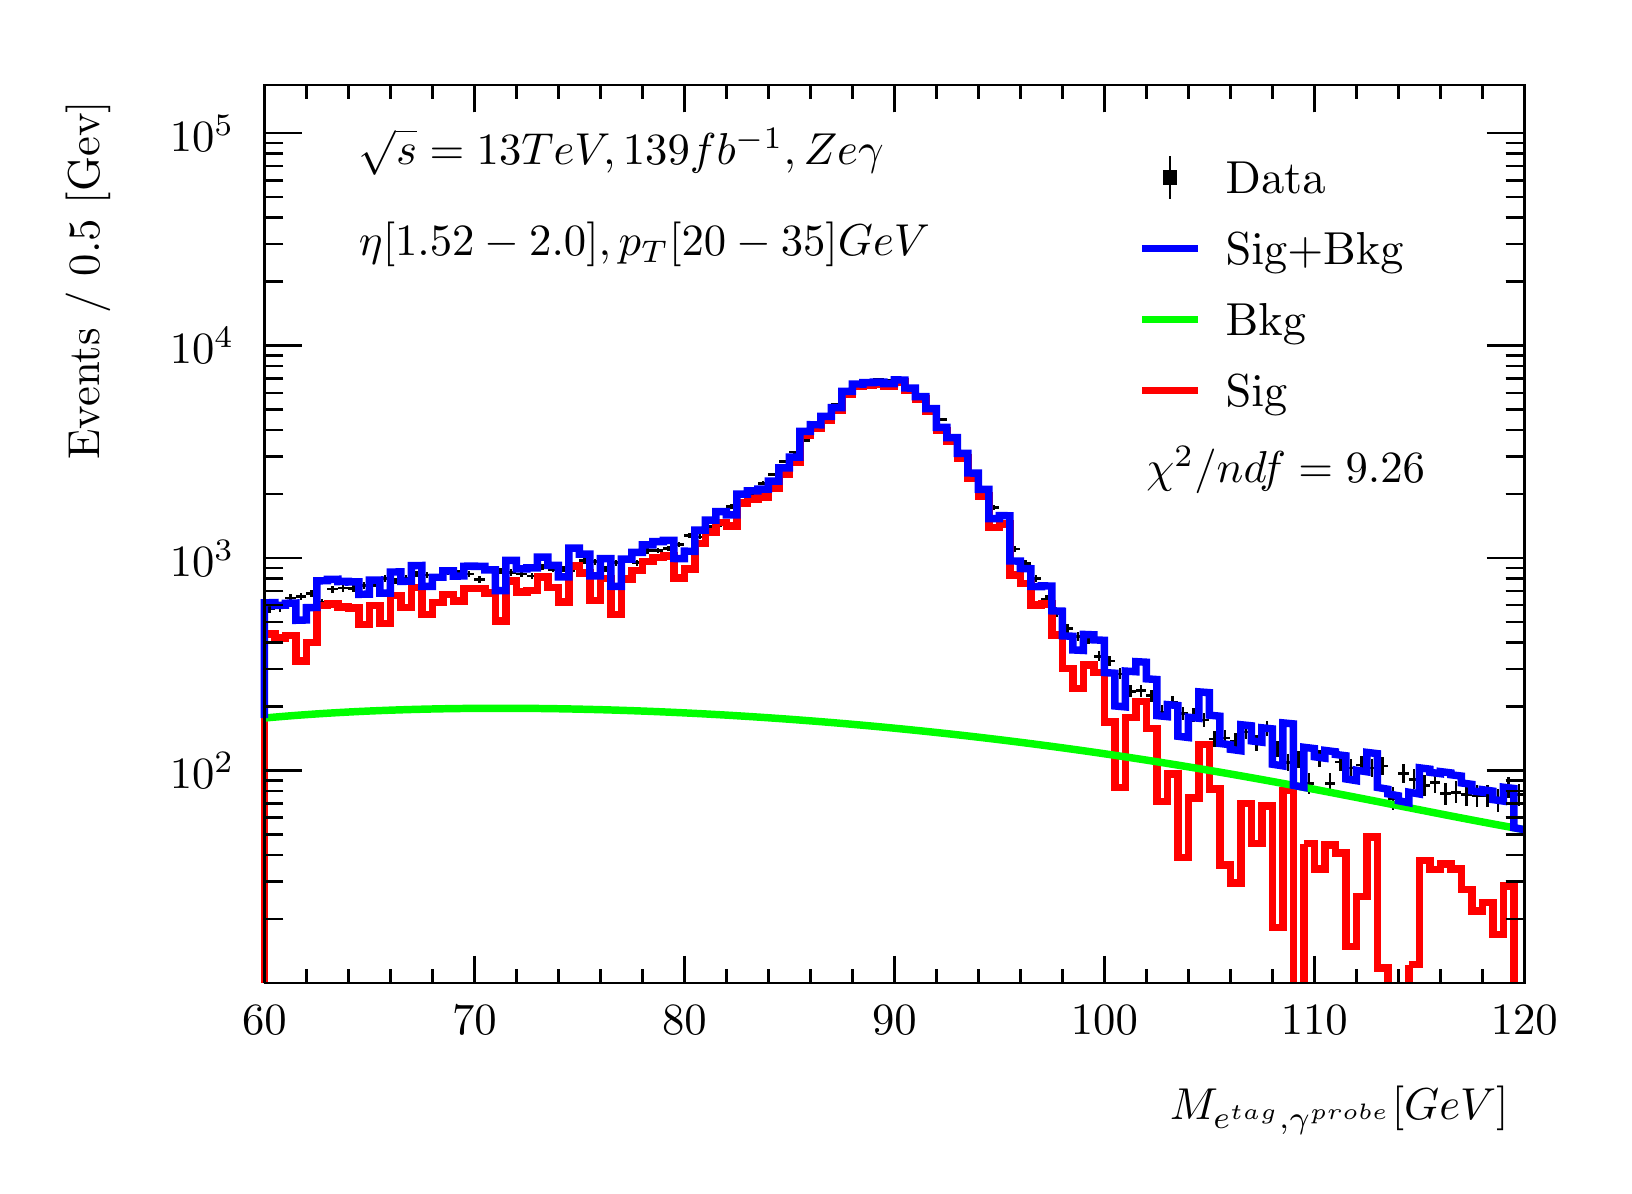
\begin{tikzpicture}
\pgfdeclareplotmark{cross} {
\pgfpathmoveto{\pgfpoint{-0.3\pgfplotmarksize}{\pgfplotmarksize}}
\pgfpathlineto{\pgfpoint{+0.3\pgfplotmarksize}{\pgfplotmarksize}}
\pgfpathlineto{\pgfpoint{+0.3\pgfplotmarksize}{0.3\pgfplotmarksize}}
\pgfpathlineto{\pgfpoint{+1\pgfplotmarksize}{0.3\pgfplotmarksize}}
\pgfpathlineto{\pgfpoint{+1\pgfplotmarksize}{-0.3\pgfplotmarksize}}
\pgfpathlineto{\pgfpoint{+0.3\pgfplotmarksize}{-0.3\pgfplotmarksize}}
\pgfpathlineto{\pgfpoint{+0.3\pgfplotmarksize}{-1.\pgfplotmarksize}}
\pgfpathlineto{\pgfpoint{-0.3\pgfplotmarksize}{-1.\pgfplotmarksize}}
\pgfpathlineto{\pgfpoint{-0.3\pgfplotmarksize}{-0.3\pgfplotmarksize}}
\pgfpathlineto{\pgfpoint{-1.\pgfplotmarksize}{-0.3\pgfplotmarksize}}
\pgfpathlineto{\pgfpoint{-1.\pgfplotmarksize}{0.3\pgfplotmarksize}}
\pgfpathlineto{\pgfpoint{-0.3\pgfplotmarksize}{0.3\pgfplotmarksize}}
\pgfpathclose
\pgfusepathqstroke
}
\pgfdeclareplotmark{cross*} {
\pgfpathmoveto{\pgfpoint{-0.3\pgfplotmarksize}{\pgfplotmarksize}}
\pgfpathlineto{\pgfpoint{+0.3\pgfplotmarksize}{\pgfplotmarksize}}
\pgfpathlineto{\pgfpoint{+0.3\pgfplotmarksize}{0.3\pgfplotmarksize}}
\pgfpathlineto{\pgfpoint{+1\pgfplotmarksize}{0.3\pgfplotmarksize}}
\pgfpathlineto{\pgfpoint{+1\pgfplotmarksize}{-0.3\pgfplotmarksize}}
\pgfpathlineto{\pgfpoint{+0.3\pgfplotmarksize}{-0.3\pgfplotmarksize}}
\pgfpathlineto{\pgfpoint{+0.3\pgfplotmarksize}{-1.\pgfplotmarksize}}
\pgfpathlineto{\pgfpoint{-0.3\pgfplotmarksize}{-1.\pgfplotmarksize}}
\pgfpathlineto{\pgfpoint{-0.3\pgfplotmarksize}{-0.3\pgfplotmarksize}}
\pgfpathlineto{\pgfpoint{-1.\pgfplotmarksize}{-0.3\pgfplotmarksize}}
\pgfpathlineto{\pgfpoint{-1.\pgfplotmarksize}{0.3\pgfplotmarksize}}
\pgfpathlineto{\pgfpoint{-0.3\pgfplotmarksize}{0.3\pgfplotmarksize}}
\pgfpathclose
\pgfusepathqfillstroke
}
\pgfdeclareplotmark{newstar} {
\pgfpathmoveto{\pgfqpoint{0pt}{\pgfplotmarksize}}
\pgfpathlineto{\pgfqpointpolar{44}{0.5\pgfplotmarksize}}
\pgfpathlineto{\pgfqpointpolar{18}{\pgfplotmarksize}}
\pgfpathlineto{\pgfqpointpolar{-20}{0.5\pgfplotmarksize}}
\pgfpathlineto{\pgfqpointpolar{-54}{\pgfplotmarksize}}
\pgfpathlineto{\pgfqpointpolar{-90}{0.5\pgfplotmarksize}}
\pgfpathlineto{\pgfqpointpolar{234}{\pgfplotmarksize}}
\pgfpathlineto{\pgfqpointpolar{198}{0.5\pgfplotmarksize}}
\pgfpathlineto{\pgfqpointpolar{162}{\pgfplotmarksize}}
\pgfpathlineto{\pgfqpointpolar{134}{0.5\pgfplotmarksize}}
\pgfpathclose
\pgfusepathqstroke
}
\pgfdeclareplotmark{newstar*} {
\pgfpathmoveto{\pgfqpoint{0pt}{\pgfplotmarksize}}
\pgfpathlineto{\pgfqpointpolar{44}{0.5\pgfplotmarksize}}
\pgfpathlineto{\pgfqpointpolar{18}{\pgfplotmarksize}}
\pgfpathlineto{\pgfqpointpolar{-20}{0.5\pgfplotmarksize}}
\pgfpathlineto{\pgfqpointpolar{-54}{\pgfplotmarksize}}
\pgfpathlineto{\pgfqpointpolar{-90}{0.5\pgfplotmarksize}}
\pgfpathlineto{\pgfqpointpolar{234}{\pgfplotmarksize}}
\pgfpathlineto{\pgfqpointpolar{198}{0.5\pgfplotmarksize}}
\pgfpathlineto{\pgfqpointpolar{162}{\pgfplotmarksize}}
\pgfpathlineto{\pgfqpointpolar{134}{0.5\pgfplotmarksize}}
\pgfpathclose
\pgfusepathqfillstroke
}
\definecolor{c}{rgb}{1,1,1};
\draw [color=c, fill=c] (0,0) rectangle (20,14.4361);
\draw [color=c, fill=c] (3,2.30977) rectangle (19,13.7143);
\definecolor{c}{rgb}{0,0,0};
\draw [c,line width=0.9] (3,2.30977) -- (3,13.7143) -- (19,13.7143) -- (19,2.30977) -- (3,2.30977);
\definecolor{c}{rgb}{1,1,1};
\draw [color=c, fill=c] (3,2.30977) rectangle (19,13.7143);
\definecolor{c}{rgb}{0,0,0};
\draw [c,line width=0.9] (3,2.30977) -- (3,13.7143) -- (19,13.7143) -- (19,2.30977) -- (3,2.30977);
\draw [c,line width=0.9] (3,2.30977) -- (19,2.30977);
\draw [c,line width=0.9] (3,2.65624) -- (3,2.30977);
\draw [c,line width=0.9] (3.53333,2.48301) -- (3.53333,2.30977);
\draw [c,line width=0.9] (4.06667,2.48301) -- (4.06667,2.30977);
\draw [c,line width=0.9] (4.6,2.48301) -- (4.6,2.30977);
\draw [c,line width=0.9] (5.13333,2.48301) -- (5.13333,2.30977);
\draw [c,line width=0.9] (5.66667,2.65624) -- (5.66667,2.30977);
\draw [c,line width=0.9] (6.2,2.48301) -- (6.2,2.30977);
\draw [c,line width=0.9] (6.73333,2.48301) -- (6.73333,2.30977);
\draw [c,line width=0.9] (7.26667,2.48301) -- (7.26667,2.30977);
\draw [c,line width=0.9] (7.8,2.48301) -- (7.8,2.30977);
\draw [c,line width=0.9] (8.33333,2.65624) -- (8.33333,2.30977);
\draw [c,line width=0.9] (8.86667,2.48301) -- (8.86667,2.30977);
\draw [c,line width=0.9] (9.4,2.48301) -- (9.4,2.30977);
\draw [c,line width=0.9] (9.93333,2.48301) -- (9.93333,2.30977);
\draw [c,line width=0.9] (10.4667,2.48301) -- (10.4667,2.30977);
\draw [c,line width=0.9] (11,2.65624) -- (11,2.30977);
\draw [c,line width=0.9] (11.5333,2.48301) -- (11.5333,2.30977);
\draw [c,line width=0.9] (12.0667,2.48301) -- (12.0667,2.30977);
\draw [c,line width=0.9] (12.6,2.48301) -- (12.6,2.30977);
\draw [c,line width=0.9] (13.1333,2.48301) -- (13.1333,2.30977);
\draw [c,line width=0.9] (13.6667,2.65624) -- (13.6667,2.30977);
\draw [c,line width=0.9] (14.2,2.48301) -- (14.2,2.30977);
\draw [c,line width=0.9] (14.7333,2.48301) -- (14.7333,2.30977);
\draw [c,line width=0.9] (15.2667,2.48301) -- (15.2667,2.30977);
\draw [c,line width=0.9] (15.8,2.48301) -- (15.8,2.30977);
\draw [c,line width=0.9] (16.3333,2.65624) -- (16.3333,2.30977);
\draw [c,line width=0.9] (16.8667,2.48301) -- (16.8667,2.30977);
\draw [c,line width=0.9] (17.4,2.48301) -- (17.4,2.30977);
\draw [c,line width=0.9] (17.9333,2.48301) -- (17.9333,2.30977);
\draw [c,line width=0.9] (18.4667,2.48301) -- (18.4667,2.30977);
\draw [c,line width=0.9] (19,2.65624) -- (19,2.30977);
\draw [anchor=base] (3,1.66015) node[scale=1.61424, color=c, rotate=0]{60};
\draw [anchor=base] (5.66667,1.66015) node[scale=1.61424, color=c, rotate=0]{70};
\draw [anchor=base] (8.33333,1.66015) node[scale=1.61424, color=c, rotate=0]{80};
\draw [anchor=base] (11,1.66015) node[scale=1.61424, color=c, rotate=0]{90};
\draw [anchor=base] (13.6667,1.66015) node[scale=1.61424, color=c, rotate=0]{100};
\draw [anchor=base] (16.3333,1.66015) node[scale=1.61424, color=c, rotate=0]{110};
\draw [anchor=base] (19,1.66015) node[scale=1.61424, color=c, rotate=0]{120};
\draw [anchor= east] (19,0.692932) node[scale=1.61424, color=c, rotate=0]{$M_{e^{tag}, \gamma^{probe}}  [GeV]$};
\draw [c,line width=0.9] (3,13.7143) -- (19,13.7143);
\draw [c,line width=0.9] (3,13.3678) -- (3,13.7143);
\draw [c,line width=0.9] (3.53333,13.5411) -- (3.53333,13.7143);
\draw [c,line width=0.9] (4.06667,13.5411) -- (4.06667,13.7143);
\draw [c,line width=0.9] (4.6,13.5411) -- (4.6,13.7143);
\draw [c,line width=0.9] (5.13333,13.5411) -- (5.13333,13.7143);
\draw [c,line width=0.9] (5.66667,13.3678) -- (5.66667,13.7143);
\draw [c,line width=0.9] (6.2,13.5411) -- (6.2,13.7143);
\draw [c,line width=0.9] (6.73333,13.5411) -- (6.73333,13.7143);
\draw [c,line width=0.9] (7.26667,13.5411) -- (7.26667,13.7143);
\draw [c,line width=0.9] (7.8,13.5411) -- (7.8,13.7143);
\draw [c,line width=0.9] (8.33333,13.3678) -- (8.33333,13.7143);
\draw [c,line width=0.9] (8.86667,13.5411) -- (8.86667,13.7143);
\draw [c,line width=0.9] (9.4,13.5411) -- (9.4,13.7143);
\draw [c,line width=0.9] (9.93333,13.5411) -- (9.93333,13.7143);
\draw [c,line width=0.9] (10.4667,13.5411) -- (10.4667,13.7143);
\draw [c,line width=0.9] (11,13.3678) -- (11,13.7143);
\draw [c,line width=0.9] (11.5333,13.5411) -- (11.5333,13.7143);
\draw [c,line width=0.9] (12.0667,13.5411) -- (12.0667,13.7143);
\draw [c,line width=0.9] (12.6,13.5411) -- (12.6,13.7143);
\draw [c,line width=0.9] (13.1333,13.5411) -- (13.1333,13.7143);
\draw [c,line width=0.9] (13.6667,13.3678) -- (13.6667,13.7143);
\draw [c,line width=0.9] (14.2,13.5411) -- (14.2,13.7143);
\draw [c,line width=0.9] (14.7333,13.5411) -- (14.7333,13.7143);
\draw [c,line width=0.9] (15.2667,13.5411) -- (15.2667,13.7143);
\draw [c,line width=0.9] (15.8,13.5411) -- (15.8,13.7143);
\draw [c,line width=0.9] (16.3333,13.3678) -- (16.3333,13.7143);
\draw [c,line width=0.9] (16.8667,13.5411) -- (16.8667,13.7143);
\draw [c,line width=0.9] (17.4,13.5411) -- (17.4,13.7143);
\draw [c,line width=0.9] (17.9333,13.5411) -- (17.9333,13.7143);
\draw [c,line width=0.9] (18.4667,13.5411) -- (18.4667,13.7143);
\draw [c,line width=0.9] (19,13.3678) -- (19,13.7143);
\draw [c,line width=0.9] (3,2.30977) -- (3,13.7143);
\draw [c,line width=0.9] (3.237,3.12209) -- (3,3.12209);
\draw [c,line width=0.9] (3.237,3.59726) -- (3,3.59726);
\draw [c,line width=0.9] (3.237,3.9344) -- (3,3.9344);
\draw [c,line width=0.9] (3.237,4.19591) -- (3,4.19591);
\draw [c,line width=0.9] (3.237,4.40958) -- (3,4.40958);
\draw [c,line width=0.9] (3.237,4.59023) -- (3,4.59023);
\draw [c,line width=0.9] (3.237,4.74672) -- (3,4.74672);
\draw [c,line width=0.9] (3.237,4.88475) -- (3,4.88475);
\draw [c,line width=0.9] (3.474,5.00822) -- (3,5.00822);
\draw [anchor= east] (2.82,5.00822) node[scale=1.61424, color=c, rotate=0]{$10^{2}$};
\draw [c,line width=0.9] (3.237,5.82054) -- (3,5.82054);
\draw [c,line width=0.9] (3.237,6.29571) -- (3,6.29571);
\draw [c,line width=0.9] (3.237,6.63285) -- (3,6.63285);
\draw [c,line width=0.9] (3.237,6.89436) -- (3,6.89436);
\draw [c,line width=0.9] (3.237,7.10803) -- (3,7.10803);
\draw [c,line width=0.9] (3.237,7.28868) -- (3,7.28868);
\draw [c,line width=0.9] (3.237,7.44517) -- (3,7.44517);
\draw [c,line width=0.9] (3.237,7.5832) -- (3,7.5832);
\draw [c,line width=0.9] (3.474,7.70668) -- (3,7.70668);
\draw [anchor= east] (2.82,7.70668) node[scale=1.61424, color=c, rotate=0]{$10^{3}$};
\draw [c,line width=0.9] (3.237,8.51899) -- (3,8.51899);
\draw [c,line width=0.9] (3.237,8.99417) -- (3,8.99417);
\draw [c,line width=0.9] (3.237,9.33131) -- (3,9.33131);
\draw [c,line width=0.9] (3.237,9.59281) -- (3,9.59281);
\draw [c,line width=0.9] (3.237,9.80648) -- (3,9.80648);
\draw [c,line width=0.9] (3.237,9.98713) -- (3,9.98713);
\draw [c,line width=0.9] (3.237,10.1436) -- (3,10.1436);
\draw [c,line width=0.9] (3.237,10.2817) -- (3,10.2817);
\draw [c,line width=0.9] (3.474,10.4051) -- (3,10.4051);
\draw [anchor= east] (2.82,10.4051) node[scale=1.61424, color=c, rotate=0]{$10^{4}$};
\draw [c,line width=0.9] (3.237,11.2174) -- (3,11.2174);
\draw [c,line width=0.9] (3.237,11.6926) -- (3,11.6926);
\draw [c,line width=0.9] (3.237,12.0298) -- (3,12.0298);
\draw [c,line width=0.9] (3.237,12.2913) -- (3,12.2913);
\draw [c,line width=0.9] (3.237,12.5049) -- (3,12.5049);
\draw [c,line width=0.9] (3.237,12.6856) -- (3,12.6856);
\draw [c,line width=0.9] (3.237,12.8421) -- (3,12.8421);
\draw [c,line width=0.9] (3.237,12.9801) -- (3,12.9801);
\draw [c,line width=0.9] (3.474,13.1036) -- (3,13.1036);
\draw [anchor= east] (2.82,13.1036) node[scale=1.61424, color=c, rotate=0]{$10^{5}$};
\draw [anchor= east] (0.76,13.7143) node[scale=1.61424, color=c, rotate=90]{Events / 0.5 [Gev]};
\draw [c,line width=0.9] (19,2.30977) -- (19,13.7143);
\draw [c,line width=0.9] (18.763,3.12209) -- (19,3.12209);
\draw [c,line width=0.9] (18.763,3.59726) -- (19,3.59726);
\draw [c,line width=0.9] (18.763,3.9344) -- (19,3.9344);
\draw [c,line width=0.9] (18.763,4.19591) -- (19,4.19591);
\draw [c,line width=0.9] (18.763,4.40958) -- (19,4.40958);
\draw [c,line width=0.9] (18.763,4.59023) -- (19,4.59023);
\draw [c,line width=0.9] (18.763,4.74672) -- (19,4.74672);
\draw [c,line width=0.9] (18.763,4.88475) -- (19,4.88475);
\draw [c,line width=0.9] (18.526,5.00822) -- (19,5.00822);
\draw [c,line width=0.9] (18.763,5.82054) -- (19,5.82054);
\draw [c,line width=0.9] (18.763,6.29571) -- (19,6.29571);
\draw [c,line width=0.9] (18.763,6.63285) -- (19,6.63285);
\draw [c,line width=0.9] (18.763,6.89436) -- (19,6.89436);
\draw [c,line width=0.9] (18.763,7.10803) -- (19,7.10803);
\draw [c,line width=0.9] (18.763,7.28868) -- (19,7.28868);
\draw [c,line width=0.9] (18.763,7.44517) -- (19,7.44517);
\draw [c,line width=0.9] (18.763,7.5832) -- (19,7.5832);
\draw [c,line width=0.9] (18.526,7.70668) -- (19,7.70668);
\draw [c,line width=0.9] (18.763,8.51899) -- (19,8.51899);
\draw [c,line width=0.9] (18.763,8.99417) -- (19,8.99417);
\draw [c,line width=0.9] (18.763,9.33131) -- (19,9.33131);
\draw [c,line width=0.9] (18.763,9.59281) -- (19,9.59281);
\draw [c,line width=0.9] (18.763,9.80648) -- (19,9.80648);
\draw [c,line width=0.9] (18.763,9.98713) -- (19,9.98713);
\draw [c,line width=0.9] (18.763,10.1436) -- (19,10.1436);
\draw [c,line width=0.9] (18.763,10.2817) -- (19,10.2817);
\draw [c,line width=0.9] (18.526,10.4051) -- (19,10.4051);
\draw [c,line width=0.9] (18.763,11.2174) -- (19,11.2174);
\draw [c,line width=0.9] (18.763,11.6926) -- (19,11.6926);
\draw [c,line width=0.9] (18.763,12.0298) -- (19,12.0298);
\draw [c,line width=0.9] (18.763,12.2913) -- (19,12.2913);
\draw [c,line width=0.9] (18.763,12.5049) -- (19,12.5049);
\draw [c,line width=0.9] (18.763,12.6856) -- (19,12.6856);
\draw [c,line width=0.9] (18.763,12.8421) -- (19,12.8421);
\draw [c,line width=0.9] (18.763,12.9801) -- (19,12.9801);
\draw [c,line width=0.9] (18.526,13.1036) -- (19,13.1036);
\draw [c,line width=0.9] (3.06667,7.06222) -- (3,7.06222);
\draw [c,line width=0.9] (3,7.06222) -- (3,7.06222);
\draw [c,line width=0.9] (3.06667,7.06222) -- (3.13333,7.06222);
\draw [c,line width=0.9] (3.13333,7.06222) -- (3.13333,7.06222);
\draw [c,line width=0.9] (3.06667,7.06222) -- (3.06667,7.11101);
\draw [c,line width=0.9] (3.06667,7.11101) -- (3.06667,7.11101);
\draw [c,line width=0.9] (3.06667,7.06222) -- (3.06667,7.01344);
\draw [c,line width=0.9] (3.06667,7.01344) -- (3.06667,7.01344);
\draw [c,line width=0.9] (3.2,7.07233) -- (3.13333,7.07233);
\draw [c,line width=0.9] (3.13333,7.07233) -- (3.13333,7.07233);
\draw [c,line width=0.9] (3.2,7.07233) -- (3.26667,7.07233);
\draw [c,line width=0.9] (3.26667,7.07233) -- (3.26667,7.07233);
\draw [c,line width=0.9] (3.2,7.07233) -- (3.2,7.12091);
\draw [c,line width=0.9] (3.2,7.12091) -- (3.2,7.12091);
\draw [c,line width=0.9] (3.2,7.07233) -- (3.2,7.02376);
\draw [c,line width=0.9] (3.2,7.02376) -- (3.2,7.02376);
\draw [c,line width=0.9] (3.33333,7.20183) -- (3.26667,7.20183);
\draw [c,line width=0.9] (3.26667,7.20183) -- (3.26667,7.20183);
\draw [c,line width=0.9] (3.33333,7.20183) -- (3.4,7.20183);
\draw [c,line width=0.9] (3.4,7.20183) -- (3.4,7.20183);
\draw [c,line width=0.9] (3.33333,7.20183) -- (3.33333,7.2478);
\draw [c,line width=0.9] (3.33333,7.2478) -- (3.33333,7.2478);
\draw [c,line width=0.9] (3.33333,7.20183) -- (3.33333,7.15587);
\draw [c,line width=0.9] (3.33333,7.15587) -- (3.33333,7.15587);
\draw [c,line width=0.9] (3.46667,7.2215) -- (3.4,7.2215);
\draw [c,line width=0.9] (3.4,7.2215) -- (3.4,7.2215);
\draw [c,line width=0.9] (3.46667,7.2215) -- (3.53333,7.2215);
\draw [c,line width=0.9] (3.53333,7.2215) -- (3.53333,7.2215);
\draw [c,line width=0.9] (3.46667,7.2215) -- (3.46667,7.26708);
\draw [c,line width=0.9] (3.46667,7.26708) -- (3.46667,7.26708);
\draw [c,line width=0.9] (3.46667,7.2215) -- (3.46667,7.17592);
\draw [c,line width=0.9] (3.46667,7.17592) -- (3.46667,7.17592);
\draw [c,line width=0.9] (3.6,7.25815) -- (3.53333,7.25815);
\draw [c,line width=0.9] (3.53333,7.25815) -- (3.53333,7.25815);
\draw [c,line width=0.9] (3.6,7.25815) -- (3.66667,7.25815);
\draw [c,line width=0.9] (3.66667,7.25815) -- (3.66667,7.25815);
\draw [c,line width=0.9] (3.6,7.25815) -- (3.6,7.30303);
\draw [c,line width=0.9] (3.6,7.30303) -- (3.6,7.30303);
\draw [c,line width=0.9] (3.6,7.25815) -- (3.6,7.21328);
\draw [c,line width=0.9] (3.6,7.21328) -- (3.6,7.21328);
\draw [c,line width=0.9] (3.73333,7.14077) -- (3.66667,7.14077);
\draw [c,line width=0.9] (3.66667,7.14077) -- (3.66667,7.14077);
\draw [c,line width=0.9] (3.73333,7.14077) -- (3.8,7.14077);
\draw [c,line width=0.9] (3.8,7.14077) -- (3.8,7.14077);
\draw [c,line width=0.9] (3.73333,7.14077) -- (3.73333,7.18795);
\draw [c,line width=0.9] (3.73333,7.18795) -- (3.73333,7.18795);
\draw [c,line width=0.9] (3.73333,7.14077) -- (3.73333,7.0936);
\draw [c,line width=0.9] (3.73333,7.0936) -- (3.73333,7.0936);
\draw [c,line width=0.9] (3.86667,7.31353) -- (3.8,7.31353);
\draw [c,line width=0.9] (3.8,7.31353) -- (3.8,7.31353);
\draw [c,line width=0.9] (3.86667,7.31353) -- (3.93333,7.31353);
\draw [c,line width=0.9] (3.93333,7.31353) -- (3.93333,7.31353);
\draw [c,line width=0.9] (3.86667,7.31353) -- (3.86667,7.35736);
\draw [c,line width=0.9] (3.86667,7.35736) -- (3.86667,7.35736);
\draw [c,line width=0.9] (3.86667,7.31353) -- (3.86667,7.26971);
\draw [c,line width=0.9] (3.86667,7.26971) -- (3.86667,7.26971);
\draw [c,line width=0.9] (4,7.32495) -- (3.93333,7.32495);
\draw [c,line width=0.9] (3.93333,7.32495) -- (3.93333,7.32495);
\draw [c,line width=0.9] (4,7.32495) -- (4.06667,7.32495);
\draw [c,line width=0.9] (4.06667,7.32495) -- (4.06667,7.32495);
\draw [c,line width=0.9] (4,7.32495) -- (4,7.36856);
\draw [c,line width=0.9] (4,7.36856) -- (4,7.36856);
\draw [c,line width=0.9] (4,7.32495) -- (4,7.28134);
\draw [c,line width=0.9] (4,7.28134) -- (4,7.28134);
\draw [c,line width=0.9] (4.13333,7.31844) -- (4.06667,7.31844);
\draw [c,line width=0.9] (4.06667,7.31844) -- (4.06667,7.31844);
\draw [c,line width=0.9] (4.13333,7.31844) -- (4.2,7.31844);
\draw [c,line width=0.9] (4.2,7.31844) -- (4.2,7.31844);
\draw [c,line width=0.9] (4.13333,7.31844) -- (4.13333,7.36217);
\draw [c,line width=0.9] (4.13333,7.36217) -- (4.13333,7.36217);
\draw [c,line width=0.9] (4.13333,7.31844) -- (4.13333,7.2747);
\draw [c,line width=0.9] (4.13333,7.2747) -- (4.13333,7.2747);
\draw [c,line width=0.9] (4.26667,7.36012) -- (4.2,7.36012);
\draw [c,line width=0.9] (4.2,7.36012) -- (4.2,7.36012);
\draw [c,line width=0.9] (4.26667,7.36012) -- (4.33333,7.36012);
\draw [c,line width=0.9] (4.33333,7.36012) -- (4.33333,7.36012);
\draw [c,line width=0.9] (4.26667,7.36012) -- (4.26667,7.40309);
\draw [c,line width=0.9] (4.26667,7.40309) -- (4.26667,7.40309);
\draw [c,line width=0.9] (4.26667,7.36012) -- (4.26667,7.31716);
\draw [c,line width=0.9] (4.26667,7.31716) -- (4.26667,7.31716);
\draw [c,line width=0.9] (4.4,7.38352) -- (4.33333,7.38352);
\draw [c,line width=0.9] (4.33333,7.38352) -- (4.33333,7.38352);
\draw [c,line width=0.9] (4.4,7.38352) -- (4.46667,7.38352);
\draw [c,line width=0.9] (4.46667,7.38352) -- (4.46667,7.38352);
\draw [c,line width=0.9] (4.4,7.38352) -- (4.4,7.42605);
\draw [c,line width=0.9] (4.4,7.42605) -- (4.4,7.42605);
\draw [c,line width=0.9] (4.4,7.38352) -- (4.4,7.34098);
\draw [c,line width=0.9] (4.4,7.34098) -- (4.4,7.34098);
\draw [c,line width=0.9] (4.53333,7.44517) -- (4.46667,7.44517);
\draw [c,line width=0.9] (4.46667,7.44517) -- (4.46667,7.44517);
\draw [c,line width=0.9] (4.53333,7.44517) -- (4.6,7.44517);
\draw [c,line width=0.9] (4.6,7.44517) -- (4.6,7.44517);
\draw [c,line width=0.9] (4.53333,7.44517) -- (4.53333,7.4866);
\draw [c,line width=0.9] (4.53333,7.4866) -- (4.53333,7.4866);
\draw [c,line width=0.9] (4.53333,7.44517) -- (4.53333,7.40374);
\draw [c,line width=0.9] (4.53333,7.40374) -- (4.53333,7.40374);
\draw [c,line width=0.9] (4.66667,7.4155) -- (4.6,7.4155);
\draw [c,line width=0.9] (4.6,7.4155) -- (4.6,7.4155);
\draw [c,line width=0.9] (4.66667,7.4155) -- (4.73333,7.4155);
\draw [c,line width=0.9] (4.73333,7.4155) -- (4.73333,7.4155);
\draw [c,line width=0.9] (4.66667,7.4155) -- (4.66667,7.45746);
\draw [c,line width=0.9] (4.66667,7.45746) -- (4.66667,7.45746);
\draw [c,line width=0.9] (4.66667,7.4155) -- (4.66667,7.37354);
\draw [c,line width=0.9] (4.66667,7.37354) -- (4.66667,7.37354);
\draw [c,line width=0.9] (4.8,7.45102) -- (4.73333,7.45102);
\draw [c,line width=0.9] (4.73333,7.45102) -- (4.73333,7.45102);
\draw [c,line width=0.9] (4.8,7.45102) -- (4.86667,7.45102);
\draw [c,line width=0.9] (4.86667,7.45102) -- (4.86667,7.45102);
\draw [c,line width=0.9] (4.8,7.45102) -- (4.8,7.49234);
\draw [c,line width=0.9] (4.8,7.49234) -- (4.8,7.49234);
\draw [c,line width=0.9] (4.8,7.45102) -- (4.8,7.40969);
\draw [c,line width=0.9] (4.8,7.40969) -- (4.8,7.40969);
\draw [c,line width=0.9] (4.93333,7.50235) -- (4.86667,7.50235);
\draw [c,line width=0.9] (4.86667,7.50235) -- (4.86667,7.50235);
\draw [c,line width=0.9] (4.93333,7.50235) -- (5,7.50235);
\draw [c,line width=0.9] (5,7.50235) -- (5,7.50235);
\draw [c,line width=0.9] (4.93333,7.50235) -- (4.93333,7.54278);
\draw [c,line width=0.9] (4.93333,7.54278) -- (4.93333,7.54278);
\draw [c,line width=0.9] (4.93333,7.50235) -- (4.93333,7.46192);
\draw [c,line width=0.9] (4.93333,7.46192) -- (4.93333,7.46192);
\draw [c,line width=0.9] (5.06667,7.49395) -- (5,7.49395);
\draw [c,line width=0.9] (5,7.49395) -- (5,7.49395);
\draw [c,line width=0.9] (5.06667,7.49395) -- (5.13333,7.49395);
\draw [c,line width=0.9] (5.13333,7.49395) -- (5.13333,7.49395);
\draw [c,line width=0.9] (5.06667,7.49395) -- (5.06667,7.53453);
\draw [c,line width=0.9] (5.06667,7.53453) -- (5.06667,7.53453);
\draw [c,line width=0.9] (5.06667,7.49395) -- (5.06667,7.45337);
\draw [c,line width=0.9] (5.06667,7.45337) -- (5.06667,7.45337);
\draw [c,line width=0.9] (5.2,7.45538) -- (5.13333,7.45538);
\draw [c,line width=0.9] (5.13333,7.45538) -- (5.13333,7.45538);
\draw [c,line width=0.9] (5.2,7.45538) -- (5.26667,7.45538);
\draw [c,line width=0.9] (5.26667,7.45538) -- (5.26667,7.45538);
\draw [c,line width=0.9] (5.2,7.45538) -- (5.2,7.49663);
\draw [c,line width=0.9] (5.2,7.49663) -- (5.2,7.49663);
\draw [c,line width=0.9] (5.2,7.45538) -- (5.2,7.41413);
\draw [c,line width=0.9] (5.2,7.41413) -- (5.2,7.41413);
\draw [c,line width=0.9] (5.33333,7.52583) -- (5.26667,7.52583);
\draw [c,line width=0.9] (5.26667,7.52583) -- (5.26667,7.52583);
\draw [c,line width=0.9] (5.33333,7.52583) -- (5.4,7.52583);
\draw [c,line width=0.9] (5.4,7.52583) -- (5.4,7.52583);
\draw [c,line width=0.9] (5.33333,7.52583) -- (5.33333,7.56586);
\draw [c,line width=0.9] (5.33333,7.56586) -- (5.33333,7.56586);
\draw [c,line width=0.9] (5.33333,7.52583) -- (5.33333,7.4858);
\draw [c,line width=0.9] (5.33333,7.4858) -- (5.33333,7.4858);
\draw [c,line width=0.9] (5.46667,7.51897) -- (5.4,7.51897);
\draw [c,line width=0.9] (5.4,7.51897) -- (5.4,7.51897);
\draw [c,line width=0.9] (5.46667,7.51897) -- (5.53333,7.51897);
\draw [c,line width=0.9] (5.53333,7.51897) -- (5.53333,7.51897);
\draw [c,line width=0.9] (5.46667,7.51897) -- (5.46667,7.55912);
\draw [c,line width=0.9] (5.46667,7.55912) -- (5.46667,7.55912);
\draw [c,line width=0.9] (5.46667,7.51897) -- (5.46667,7.47883);
\draw [c,line width=0.9] (5.46667,7.47883) -- (5.46667,7.47883);
\draw [c,line width=0.9] (5.6,7.50653) -- (5.53333,7.50653);
\draw [c,line width=0.9] (5.53333,7.50653) -- (5.53333,7.50653);
\draw [c,line width=0.9] (5.6,7.50653) -- (5.66667,7.50653);
\draw [c,line width=0.9] (5.66667,7.50653) -- (5.66667,7.50653);
\draw [c,line width=0.9] (5.6,7.50653) -- (5.6,7.54689);
\draw [c,line width=0.9] (5.6,7.54689) -- (5.6,7.54689);
\draw [c,line width=0.9] (5.6,7.50653) -- (5.6,7.46617);
\draw [c,line width=0.9] (5.6,7.46617) -- (5.6,7.46617);
\draw [c,line width=0.9] (5.73333,7.43782) -- (5.66667,7.43782);
\draw [c,line width=0.9] (5.66667,7.43782) -- (5.66667,7.43782);
\draw [c,line width=0.9] (5.73333,7.43782) -- (5.8,7.43782);
\draw [c,line width=0.9] (5.8,7.43782) -- (5.8,7.43782);
\draw [c,line width=0.9] (5.73333,7.43782) -- (5.73333,7.47939);
\draw [c,line width=0.9] (5.73333,7.47939) -- (5.73333,7.47939);
\draw [c,line width=0.9] (5.73333,7.43782) -- (5.73333,7.39626);
\draw [c,line width=0.9] (5.73333,7.39626) -- (5.73333,7.39626);
\draw [c,line width=0.9] (5.86667,7.55687) -- (5.8,7.55687);
\draw [c,line width=0.9] (5.8,7.55687) -- (5.8,7.55687);
\draw [c,line width=0.9] (5.86667,7.55687) -- (5.93333,7.55687);
\draw [c,line width=0.9] (5.93333,7.55687) -- (5.93333,7.55687);
\draw [c,line width=0.9] (5.86667,7.55687) -- (5.86667,7.59637);
\draw [c,line width=0.9] (5.86667,7.59637) -- (5.86667,7.59637);
\draw [c,line width=0.9] (5.86667,7.55687) -- (5.86667,7.51736);
\draw [c,line width=0.9] (5.86667,7.51736) -- (5.86667,7.51736);
\draw [c,line width=0.9] (6,7.54213) -- (5.93333,7.54213);
\draw [c,line width=0.9] (5.93333,7.54213) -- (5.93333,7.54213);
\draw [c,line width=0.9] (6,7.54213) -- (6.06667,7.54213);
\draw [c,line width=0.9] (6.06667,7.54213) -- (6.06667,7.54213);
\draw [c,line width=0.9] (6,7.54213) -- (6,7.58188);
\draw [c,line width=0.9] (6,7.58188) -- (6,7.58188);
\draw [c,line width=0.9] (6,7.54213) -- (6,7.50237);
\draw [c,line width=0.9] (6,7.50237) -- (6,7.50237);
\draw [c,line width=0.9] (6.13333,7.52309) -- (6.06667,7.52309);
\draw [c,line width=0.9] (6.06667,7.52309) -- (6.06667,7.52309);
\draw [c,line width=0.9] (6.13333,7.52309) -- (6.2,7.52309);
\draw [c,line width=0.9] (6.2,7.52309) -- (6.2,7.52309);
\draw [c,line width=0.9] (6.13333,7.52309) -- (6.13333,7.56317);
\draw [c,line width=0.9] (6.13333,7.56317) -- (6.13333,7.56317);
\draw [c,line width=0.9] (6.13333,7.52309) -- (6.13333,7.48302);
\draw [c,line width=0.9] (6.13333,7.48302) -- (6.13333,7.48302);
\draw [c,line width=0.9] (6.26667,7.50374) -- (6.2,7.50374);
\draw [c,line width=0.9] (6.2,7.50374) -- (6.2,7.50374);
\draw [c,line width=0.9] (6.26667,7.50374) -- (6.33333,7.50374);
\draw [c,line width=0.9] (6.33333,7.50374) -- (6.33333,7.50374);
\draw [c,line width=0.9] (6.26667,7.50374) -- (6.26667,7.54415);
\draw [c,line width=0.9] (6.26667,7.54415) -- (6.26667,7.54415);
\draw [c,line width=0.9] (6.26667,7.50374) -- (6.26667,7.46334);
\draw [c,line width=0.9] (6.26667,7.46334) -- (6.26667,7.46334);
\draw [c,line width=0.9] (6.4,7.47981) -- (6.33333,7.47981);
\draw [c,line width=0.9] (6.33333,7.47981) -- (6.33333,7.47981);
\draw [c,line width=0.9] (6.4,7.47981) -- (6.46667,7.47981);
\draw [c,line width=0.9] (6.46667,7.47981) -- (6.46667,7.47981);
\draw [c,line width=0.9] (6.4,7.47981) -- (6.4,7.52064);
\draw [c,line width=0.9] (6.4,7.52064) -- (6.4,7.52064);
\draw [c,line width=0.9] (6.4,7.47981) -- (6.4,7.43899);
\draw [c,line width=0.9] (6.4,7.43899) -- (6.4,7.43899);
\draw [c,line width=0.9] (6.53333,7.5897) -- (6.46667,7.5897);
\draw [c,line width=0.9] (6.46667,7.5897) -- (6.46667,7.5897);
\draw [c,line width=0.9] (6.53333,7.5897) -- (6.6,7.5897);
\draw [c,line width=0.9] (6.6,7.5897) -- (6.6,7.5897);
\draw [c,line width=0.9] (6.53333,7.5897) -- (6.53333,7.62865);
\draw [c,line width=0.9] (6.53333,7.62865) -- (6.53333,7.62865);
\draw [c,line width=0.9] (6.53333,7.5897) -- (6.53333,7.55074);
\draw [c,line width=0.9] (6.53333,7.55074) -- (6.53333,7.55074);
\draw [c,line width=0.9] (6.66667,7.56483) -- (6.6,7.56483);
\draw [c,line width=0.9] (6.6,7.56483) -- (6.6,7.56483);
\draw [c,line width=0.9] (6.66667,7.56483) -- (6.73333,7.56483);
\draw [c,line width=0.9] (6.73333,7.56483) -- (6.73333,7.56483);
\draw [c,line width=0.9] (6.66667,7.56483) -- (6.66667,7.6042);
\draw [c,line width=0.9] (6.66667,7.6042) -- (6.66667,7.6042);
\draw [c,line width=0.9] (6.66667,7.56483) -- (6.66667,7.52546);
\draw [c,line width=0.9] (6.66667,7.52546) -- (6.66667,7.52546);
\draw [c,line width=0.9] (6.8,7.56351) -- (6.73333,7.56351);
\draw [c,line width=0.9] (6.73333,7.56351) -- (6.73333,7.56351);
\draw [c,line width=0.9] (6.8,7.56351) -- (6.86667,7.56351);
\draw [c,line width=0.9] (6.86667,7.56351) -- (6.86667,7.56351);
\draw [c,line width=0.9] (6.8,7.56351) -- (6.8,7.6029);
\draw [c,line width=0.9] (6.8,7.6029) -- (6.8,7.6029);
\draw [c,line width=0.9] (6.8,7.56351) -- (6.8,7.52412);
\draw [c,line width=0.9] (6.8,7.52412) -- (6.8,7.52412);
\draw [c,line width=0.9] (6.93333,7.57405) -- (6.86667,7.57405);
\draw [c,line width=0.9] (6.86667,7.57405) -- (6.86667,7.57405);
\draw [c,line width=0.9] (6.93333,7.57405) -- (7,7.57405);
\draw [c,line width=0.9] (7,7.57405) -- (7,7.57405);
\draw [c,line width=0.9] (6.93333,7.57405) -- (6.93333,7.61327);
\draw [c,line width=0.9] (6.93333,7.61327) -- (6.93333,7.61327);
\draw [c,line width=0.9] (6.93333,7.57405) -- (6.93333,7.53484);
\draw [c,line width=0.9] (6.93333,7.53484) -- (6.93333,7.53484);
\draw [c,line width=0.9] (7.06667,7.6734) -- (7,7.6734);
\draw [c,line width=0.9] (7,7.6734) -- (7,7.6734);
\draw [c,line width=0.9] (7.06667,7.6734) -- (7.13333,7.6734);
\draw [c,line width=0.9] (7.13333,7.6734) -- (7.13333,7.6734);
\draw [c,line width=0.9] (7.06667,7.6734) -- (7.06667,7.71098);
\draw [c,line width=0.9] (7.06667,7.71098) -- (7.06667,7.71098);
\draw [c,line width=0.9] (7.06667,7.6734) -- (7.06667,7.63581);
\draw [c,line width=0.9] (7.06667,7.63581) -- (7.06667,7.63581);
\draw [c,line width=0.9] (7.2,7.66128) -- (7.13333,7.66128);
\draw [c,line width=0.9] (7.13333,7.66128) -- (7.13333,7.66128);
\draw [c,line width=0.9] (7.2,7.66128) -- (7.26667,7.66128);
\draw [c,line width=0.9] (7.26667,7.66128) -- (7.26667,7.66128);
\draw [c,line width=0.9] (7.2,7.66128) -- (7.2,7.69906);
\draw [c,line width=0.9] (7.2,7.69906) -- (7.2,7.69906);
\draw [c,line width=0.9] (7.2,7.66128) -- (7.2,7.62349);
\draw [c,line width=0.9] (7.2,7.62349) -- (7.2,7.62349);
\draw [c,line width=0.9] (7.33333,7.56747) -- (7.26667,7.56747);
\draw [c,line width=0.9] (7.26667,7.56747) -- (7.26667,7.56747);
\draw [c,line width=0.9] (7.33333,7.56747) -- (7.4,7.56747);
\draw [c,line width=0.9] (7.4,7.56747) -- (7.4,7.56747);
\draw [c,line width=0.9] (7.33333,7.56747) -- (7.33333,7.6068);
\draw [c,line width=0.9] (7.33333,7.6068) -- (7.33333,7.6068);
\draw [c,line width=0.9] (7.33333,7.56747) -- (7.33333,7.52815);
\draw [c,line width=0.9] (7.33333,7.52815) -- (7.33333,7.52815);
\draw [c,line width=0.9] (7.46667,7.65026) -- (7.4,7.65026);
\draw [c,line width=0.9] (7.4,7.65026) -- (7.4,7.65026);
\draw [c,line width=0.9] (7.46667,7.65026) -- (7.53333,7.65026);
\draw [c,line width=0.9] (7.53333,7.65026) -- (7.53333,7.65026);
\draw [c,line width=0.9] (7.46667,7.65026) -- (7.46667,7.68822);
\draw [c,line width=0.9] (7.46667,7.68822) -- (7.46667,7.68822);
\draw [c,line width=0.9] (7.46667,7.65026) -- (7.46667,7.6123);
\draw [c,line width=0.9] (7.46667,7.6123) -- (7.46667,7.6123);
\draw [c,line width=0.9] (7.6,7.7008) -- (7.53333,7.7008);
\draw [c,line width=0.9] (7.53333,7.7008) -- (7.53333,7.7008);
\draw [c,line width=0.9] (7.6,7.7008) -- (7.66667,7.7008);
\draw [c,line width=0.9] (7.66667,7.7008) -- (7.66667,7.7008);
\draw [c,line width=0.9] (7.6,7.7008) -- (7.6,7.73796);
\draw [c,line width=0.9] (7.6,7.73796) -- (7.6,7.73796);
\draw [c,line width=0.9] (7.6,7.7008) -- (7.6,7.66365);
\draw [c,line width=0.9] (7.6,7.66365) -- (7.6,7.66365);
\draw [c,line width=0.9] (7.73333,7.65026) -- (7.66667,7.65026);
\draw [c,line width=0.9] (7.66667,7.65026) -- (7.66667,7.65026);
\draw [c,line width=0.9] (7.73333,7.65026) -- (7.8,7.65026);
\draw [c,line width=0.9] (7.8,7.65026) -- (7.8,7.65026);
\draw [c,line width=0.9] (7.73333,7.65026) -- (7.73333,7.68822);
\draw [c,line width=0.9] (7.73333,7.68822) -- (7.73333,7.68822);
\draw [c,line width=0.9] (7.73333,7.65026) -- (7.73333,7.6123);
\draw [c,line width=0.9] (7.73333,7.6123) -- (7.73333,7.6123);
\draw [c,line width=0.9] (7.86667,7.80012) -- (7.8,7.80012);
\draw [c,line width=0.9] (7.8,7.80012) -- (7.8,7.80012);
\draw [c,line width=0.9] (7.86667,7.80012) -- (7.93333,7.80012);
\draw [c,line width=0.9] (7.93333,7.80012) -- (7.93333,7.80012);
\draw [c,line width=0.9] (7.86667,7.80012) -- (7.86667,7.83573);
\draw [c,line width=0.9] (7.86667,7.83573) -- (7.86667,7.83573);
\draw [c,line width=0.9] (7.86667,7.80012) -- (7.86667,7.76451);
\draw [c,line width=0.9] (7.86667,7.76451) -- (7.86667,7.76451);
\draw [c,line width=0.9] (8,7.80228) -- (7.93333,7.80228);
\draw [c,line width=0.9] (7.93333,7.80228) -- (7.93333,7.80228);
\draw [c,line width=0.9] (8,7.80228) -- (8.06667,7.80228);
\draw [c,line width=0.9] (8.06667,7.80228) -- (8.06667,7.80228);
\draw [c,line width=0.9] (8,7.80228) -- (8,7.83786);
\draw [c,line width=0.9] (8,7.83786) -- (8,7.83786);
\draw [c,line width=0.9] (8,7.80228) -- (8,7.76671);
\draw [c,line width=0.9] (8,7.76671) -- (8,7.76671);
\draw [c,line width=0.9] (8.13333,7.82581) -- (8.06667,7.82581);
\draw [c,line width=0.9] (8.06667,7.82581) -- (8.06667,7.82581);
\draw [c,line width=0.9] (8.13333,7.82581) -- (8.2,7.82581);
\draw [c,line width=0.9] (8.2,7.82581) -- (8.2,7.82581);
\draw [c,line width=0.9] (8.13333,7.82581) -- (8.13333,7.86103);
\draw [c,line width=0.9] (8.13333,7.86103) -- (8.13333,7.86103);
\draw [c,line width=0.9] (8.13333,7.82581) -- (8.13333,7.79059);
\draw [c,line width=0.9] (8.13333,7.79059) -- (8.13333,7.79059);
\draw [c,line width=0.9] (8.26667,7.8796) -- (8.2,7.8796);
\draw [c,line width=0.9] (8.2,7.8796) -- (8.2,7.8796);
\draw [c,line width=0.9] (8.26667,7.8796) -- (8.33333,7.8796);
\draw [c,line width=0.9] (8.33333,7.8796) -- (8.33333,7.8796);
\draw [c,line width=0.9] (8.26667,7.8796) -- (8.26667,7.91403);
\draw [c,line width=0.9] (8.26667,7.91403) -- (8.26667,7.91403);
\draw [c,line width=0.9] (8.26667,7.8796) -- (8.26667,7.84518);
\draw [c,line width=0.9] (8.26667,7.84518) -- (8.26667,7.84518);
\draw [c,line width=0.9] (8.4,7.99598) -- (8.33333,7.99598);
\draw [c,line width=0.9] (8.33333,7.99598) -- (8.33333,7.99598);
\draw [c,line width=0.9] (8.4,7.99598) -- (8.46667,7.99598);
\draw [c,line width=0.9] (8.46667,7.99598) -- (8.46667,7.99598);
\draw [c,line width=0.9] (8.4,7.99598) -- (8.4,8.02873);
\draw [c,line width=0.9] (8.4,8.02873) -- (8.4,8.02873);
\draw [c,line width=0.9] (8.4,7.99598) -- (8.4,7.96322);
\draw [c,line width=0.9] (8.4,7.96322) -- (8.4,7.96322);
\draw [c,line width=0.9] (8.53333,7.97659) -- (8.46667,7.97659);
\draw [c,line width=0.9] (8.46667,7.97659) -- (8.46667,7.97659);
\draw [c,line width=0.9] (8.53333,7.97659) -- (8.6,7.97659);
\draw [c,line width=0.9] (8.6,7.97659) -- (8.6,7.97659);
\draw [c,line width=0.9] (8.53333,7.97659) -- (8.53333,8.00962);
\draw [c,line width=0.9] (8.53333,8.00962) -- (8.53333,8.00962);
\draw [c,line width=0.9] (8.53333,7.97659) -- (8.53333,7.94357);
\draw [c,line width=0.9] (8.53333,7.94357) -- (8.53333,7.94357);
\draw [c,line width=0.9] (8.66667,8.09007) -- (8.6,8.09007);
\draw [c,line width=0.9] (8.6,8.09007) -- (8.6,8.09007);
\draw [c,line width=0.9] (8.66667,8.09007) -- (8.73333,8.09007);
\draw [c,line width=0.9] (8.73333,8.09007) -- (8.73333,8.09007);
\draw [c,line width=0.9] (8.66667,8.09007) -- (8.66667,8.12153);
\draw [c,line width=0.9] (8.66667,8.12153) -- (8.66667,8.12153);
\draw [c,line width=0.9] (8.66667,8.09007) -- (8.66667,8.0586);
\draw [c,line width=0.9] (8.66667,8.0586) -- (8.66667,8.0586);
\draw [c,line width=0.9] (8.8,8.13401) -- (8.73333,8.13401);
\draw [c,line width=0.9] (8.73333,8.13401) -- (8.73333,8.13401);
\draw [c,line width=0.9] (8.8,8.13401) -- (8.86667,8.13401);
\draw [c,line width=0.9] (8.86667,8.13401) -- (8.86667,8.13401);
\draw [c,line width=0.9] (8.8,8.13401) -- (8.8,8.16489);
\draw [c,line width=0.9] (8.8,8.16489) -- (8.8,8.16489);
\draw [c,line width=0.9] (8.8,8.13401) -- (8.8,8.10313);
\draw [c,line width=0.9] (8.8,8.10313) -- (8.8,8.10313);
\draw [c,line width=0.9] (8.93333,8.36317) -- (8.86667,8.36317);
\draw [c,line width=0.9] (8.86667,8.36317) -- (8.86667,8.36317);
\draw [c,line width=0.9] (8.93333,8.36317) -- (9,8.36317);
\draw [c,line width=0.9] (9,8.36317) -- (9,8.36317);
\draw [c,line width=0.9] (8.93333,8.36317) -- (8.93333,8.39118);
\draw [c,line width=0.9] (8.93333,8.39118) -- (8.93333,8.39118);
\draw [c,line width=0.9] (8.93333,8.36317) -- (8.93333,8.33517);
\draw [c,line width=0.9] (8.93333,8.33517) -- (8.93333,8.33517);
\draw [c,line width=0.9] (9.06667,8.38242) -- (9,8.38242);
\draw [c,line width=0.9] (9,8.38242) -- (9,8.38242);
\draw [c,line width=0.9] (9.06667,8.38242) -- (9.13333,8.38242);
\draw [c,line width=0.9] (9.13333,8.38242) -- (9.13333,8.38242);
\draw [c,line width=0.9] (9.06667,8.38242) -- (9.06667,8.4102);
\draw [c,line width=0.9] (9.06667,8.4102) -- (9.06667,8.4102);
\draw [c,line width=0.9] (9.06667,8.38242) -- (9.06667,8.35465);
\draw [c,line width=0.9] (9.06667,8.35465) -- (9.06667,8.35465);
\draw [c,line width=0.9] (9.2,8.50009) -- (9.13333,8.50009);
\draw [c,line width=0.9] (9.13333,8.50009) -- (9.13333,8.50009);
\draw [c,line width=0.9] (9.2,8.50009) -- (9.26667,8.50009);
\draw [c,line width=0.9] (9.26667,8.50009) -- (9.26667,8.50009);
\draw [c,line width=0.9] (9.2,8.50009) -- (9.2,8.52651);
\draw [c,line width=0.9] (9.2,8.52651) -- (9.2,8.52651);
\draw [c,line width=0.9] (9.2,8.50009) -- (9.2,8.47367);
\draw [c,line width=0.9] (9.2,8.47367) -- (9.2,8.47367);
\draw [c,line width=0.9] (9.33333,8.6565) -- (9.26667,8.6565);
\draw [c,line width=0.9] (9.26667,8.6565) -- (9.26667,8.6565);
\draw [c,line width=0.9] (9.33333,8.6565) -- (9.4,8.6565);
\draw [c,line width=0.9] (9.4,8.6565) -- (9.4,8.6565);
\draw [c,line width=0.9] (9.33333,8.6565) -- (9.33333,8.68122);
\draw [c,line width=0.9] (9.33333,8.68122) -- (9.33333,8.68122);
\draw [c,line width=0.9] (9.33333,8.6565) -- (9.33333,8.63179);
\draw [c,line width=0.9] (9.33333,8.63179) -- (9.33333,8.63179);
\draw [c,line width=0.9] (9.46667,8.76967) -- (9.4,8.76967);
\draw [c,line width=0.9] (9.4,8.76967) -- (9.4,8.76967);
\draw [c,line width=0.9] (9.46667,8.76967) -- (9.53333,8.76967);
\draw [c,line width=0.9] (9.53333,8.76967) -- (9.53333,8.76967);
\draw [c,line width=0.9] (9.46667,8.76967) -- (9.46667,8.79322);
\draw [c,line width=0.9] (9.46667,8.79322) -- (9.46667,8.79322);
\draw [c,line width=0.9] (9.46667,8.76967) -- (9.46667,8.74612);
\draw [c,line width=0.9] (9.46667,8.74612) -- (9.46667,8.74612);
\draw [c,line width=0.9] (9.6,8.93406) -- (9.53333,8.93406);
\draw [c,line width=0.9] (9.53333,8.93406) -- (9.53333,8.93406);
\draw [c,line width=0.9] (9.6,8.93406) -- (9.66667,8.93406);
\draw [c,line width=0.9] (9.66667,8.93406) -- (9.66667,8.93406);
\draw [c,line width=0.9] (9.6,8.93406) -- (9.6,8.95601);
\draw [c,line width=0.9] (9.6,8.95601) -- (9.6,8.95601);
\draw [c,line width=0.9] (9.6,8.93406) -- (9.6,8.9121);
\draw [c,line width=0.9] (9.6,8.9121) -- (9.6,8.9121);
\draw [c,line width=0.9] (9.73333,9.05209) -- (9.66667,9.05209);
\draw [c,line width=0.9] (9.66667,9.05209) -- (9.66667,9.05209);
\draw [c,line width=0.9] (9.73333,9.05209) -- (9.8,9.05209);
\draw [c,line width=0.9] (9.8,9.05209) -- (9.8,9.05209);
\draw [c,line width=0.9] (9.73333,9.05209) -- (9.73333,9.07296);
\draw [c,line width=0.9] (9.73333,9.07296) -- (9.73333,9.07296);
\draw [c,line width=0.9] (9.73333,9.05209) -- (9.73333,9.03122);
\draw [c,line width=0.9] (9.73333,9.03122) -- (9.73333,9.03122);
\draw [c,line width=0.9] (9.86667,9.19803) -- (9.8,9.19803);
\draw [c,line width=0.9] (9.8,9.19803) -- (9.8,9.19803);
\draw [c,line width=0.9] (9.86667,9.19803) -- (9.93333,9.19803);
\draw [c,line width=0.9] (9.93333,9.19803) -- (9.93333,9.19803);
\draw [c,line width=0.9] (9.86667,9.19803) -- (9.86667,9.21764);
\draw [c,line width=0.9] (9.86667,9.21764) -- (9.86667,9.21764);
\draw [c,line width=0.9] (9.86667,9.19803) -- (9.86667,9.17841);
\draw [c,line width=0.9] (9.86667,9.17841) -- (9.86667,9.17841);
\draw [c,line width=0.9] (10,9.38037) -- (9.93333,9.38037);
\draw [c,line width=0.9] (9.93333,9.38037) -- (9.93333,9.38037);
\draw [c,line width=0.9] (10,9.38037) -- (10.0667,9.38037);
\draw [c,line width=0.9] (10.0667,9.38037) -- (10.0667,9.38037);
\draw [c,line width=0.9] (10,9.38037) -- (10,9.39851);
\draw [c,line width=0.9] (10,9.39851) -- (10,9.39851);
\draw [c,line width=0.9] (10,9.38037) -- (10,9.36222);
\draw [c,line width=0.9] (10,9.36222) -- (10,9.36222);
\draw [c,line width=0.9] (10.1333,9.5128) -- (10.0667,9.5128);
\draw [c,line width=0.9] (10.0667,9.5128) -- (10.0667,9.5128);
\draw [c,line width=0.9] (10.1333,9.5128) -- (10.2,9.5128);
\draw [c,line width=0.9] (10.2,9.5128) -- (10.2,9.5128);
\draw [c,line width=0.9] (10.1333,9.5128) -- (10.1333,9.52995);
\draw [c,line width=0.9] (10.1333,9.52995) -- (10.1333,9.52995);
\draw [c,line width=0.9] (10.1333,9.5128) -- (10.1333,9.49565);
\draw [c,line width=0.9] (10.1333,9.49565) -- (10.1333,9.49565);
\draw [c,line width=0.9] (10.2667,9.65578) -- (10.2,9.65578);
\draw [c,line width=0.9] (10.2,9.65578) -- (10.2,9.65578);
\draw [c,line width=0.9] (10.2667,9.65578) -- (10.3333,9.65578);
\draw [c,line width=0.9] (10.3333,9.65578) -- (10.3333,9.65578);
\draw [c,line width=0.9] (10.2667,9.65578) -- (10.2667,9.67192);
\draw [c,line width=0.9] (10.2667,9.67192) -- (10.2667,9.67192);
\draw [c,line width=0.9] (10.2667,9.65578) -- (10.2667,9.63965);
\draw [c,line width=0.9] (10.2667,9.63965) -- (10.2667,9.63965);
\draw [c,line width=0.9] (10.4,9.76978) -- (10.3333,9.76978);
\draw [c,line width=0.9] (10.3333,9.76978) -- (10.3333,9.76978);
\draw [c,line width=0.9] (10.4,9.76978) -- (10.4667,9.76978);
\draw [c,line width=0.9] (10.4667,9.76978) -- (10.4667,9.76978);
\draw [c,line width=0.9] (10.4,9.76978) -- (10.4,9.78515);
\draw [c,line width=0.9] (10.4,9.78515) -- (10.4,9.78515);
\draw [c,line width=0.9] (10.4,9.76978) -- (10.4,9.75441);
\draw [c,line width=0.9] (10.4,9.75441) -- (10.4,9.75441);
\draw [c,line width=0.9] (10.5333,9.87089) -- (10.4667,9.87089);
\draw [c,line width=0.9] (10.4667,9.87089) -- (10.4667,9.87089);
\draw [c,line width=0.9] (10.5333,9.87089) -- (10.6,9.87089);
\draw [c,line width=0.9] (10.6,9.87089) -- (10.6,9.87089);
\draw [c,line width=0.9] (10.5333,9.87089) -- (10.5333,9.88561);
\draw [c,line width=0.9] (10.5333,9.88561) -- (10.5333,9.88561);
\draw [c,line width=0.9] (10.5333,9.87089) -- (10.5333,9.85617);
\draw [c,line width=0.9] (10.5333,9.85617) -- (10.5333,9.85617);
\draw [c,line width=0.9] (10.6667,9.94173) -- (10.6,9.94173);
\draw [c,line width=0.9] (10.6,9.94173) -- (10.6,9.94173);
\draw [c,line width=0.9] (10.6667,9.94173) -- (10.7333,9.94173);
\draw [c,line width=0.9] (10.7333,9.94173) -- (10.7333,9.94173);
\draw [c,line width=0.9] (10.6667,9.94173) -- (10.6667,9.95601);
\draw [c,line width=0.9] (10.6667,9.95601) -- (10.6667,9.95601);
\draw [c,line width=0.9] (10.6667,9.94173) -- (10.6667,9.92745);
\draw [c,line width=0.9] (10.6667,9.92745) -- (10.6667,9.92745);
\draw [c,line width=0.9] (10.8,9.9821) -- (10.7333,9.9821);
\draw [c,line width=0.9] (10.7333,9.9821) -- (10.7333,9.9821);
\draw [c,line width=0.9] (10.8,9.9821) -- (10.8667,9.9821);
\draw [c,line width=0.9] (10.8667,9.9821) -- (10.8667,9.9821);
\draw [c,line width=0.9] (10.8,9.9821) -- (10.8,9.99614);
\draw [c,line width=0.9] (10.8,9.99614) -- (10.8,9.99614);
\draw [c,line width=0.9] (10.8,9.9821) -- (10.8,9.96806);
\draw [c,line width=0.9] (10.8,9.96806) -- (10.8,9.96806);
\draw [c,line width=0.9] (10.9333,9.96738) -- (10.8667,9.96738);
\draw [c,line width=0.9] (10.8667,9.96738) -- (10.8667,9.96738);
\draw [c,line width=0.9] (10.9333,9.96738) -- (11,9.96738);
\draw [c,line width=0.9] (11,9.96738) -- (11,9.96738);
\draw [c,line width=0.9] (10.9333,9.96738) -- (10.9333,9.98151);
\draw [c,line width=0.9] (10.9333,9.98151) -- (10.9333,9.98151);
\draw [c,line width=0.9] (10.9333,9.96738) -- (10.9333,9.95326);
\draw [c,line width=0.9] (10.9333,9.95326) -- (10.9333,9.95326);
\draw [c,line width=0.9] (11.0667,9.94867) -- (11,9.94867);
\draw [c,line width=0.9] (11,9.94867) -- (11,9.94867);
\draw [c,line width=0.9] (11.0667,9.94867) -- (11.1333,9.94867);
\draw [c,line width=0.9] (11.1333,9.94867) -- (11.1333,9.94867);
\draw [c,line width=0.9] (11.0667,9.94867) -- (11.0667,9.96291);
\draw [c,line width=0.9] (11.0667,9.96291) -- (11.0667,9.96291);
\draw [c,line width=0.9] (11.0667,9.94867) -- (11.0667,9.93444);
\draw [c,line width=0.9] (11.0667,9.93444) -- (11.0667,9.93444);
\draw [c,line width=0.9] (11.2,9.85844) -- (11.1333,9.85844);
\draw [c,line width=0.9] (11.1333,9.85844) -- (11.1333,9.85844);
\draw [c,line width=0.9] (11.2,9.85844) -- (11.2667,9.85844);
\draw [c,line width=0.9] (11.2667,9.85844) -- (11.2667,9.85844);
\draw [c,line width=0.9] (11.2,9.85844) -- (11.2,9.87324);
\draw [c,line width=0.9] (11.2,9.87324) -- (11.2,9.87324);
\draw [c,line width=0.9] (11.2,9.85844) -- (11.2,9.84364);
\draw [c,line width=0.9] (11.2,9.84364) -- (11.2,9.84364);
\draw [c,line width=0.9] (11.3333,9.79233) -- (11.2667,9.79233);
\draw [c,line width=0.9] (11.2667,9.79233) -- (11.2667,9.79233);
\draw [c,line width=0.9] (11.3333,9.79233) -- (11.4,9.79233);
\draw [c,line width=0.9] (11.4,9.79233) -- (11.4,9.79233);
\draw [c,line width=0.9] (11.3333,9.79233) -- (11.3333,9.80756);
\draw [c,line width=0.9] (11.3333,9.80756) -- (11.3333,9.80756);
\draw [c,line width=0.9] (11.3333,9.79233) -- (11.3333,9.77711);
\draw [c,line width=0.9] (11.3333,9.77711) -- (11.3333,9.77711);
\draw [c,line width=0.9] (11.4667,9.62472) -- (11.4,9.62472);
\draw [c,line width=0.9] (11.4,9.62472) -- (11.4,9.62472);
\draw [c,line width=0.9] (11.4667,9.62472) -- (11.5333,9.62472);
\draw [c,line width=0.9] (11.5333,9.62472) -- (11.5333,9.62472);
\draw [c,line width=0.9] (11.4667,9.62472) -- (11.4667,9.64107);
\draw [c,line width=0.9] (11.4667,9.64107) -- (11.4667,9.64107);
\draw [c,line width=0.9] (11.4667,9.62472) -- (11.4667,9.60837);
\draw [c,line width=0.9] (11.4667,9.60837) -- (11.4667,9.60837);
\draw [c,line width=0.9] (11.6,9.46647) -- (11.5333,9.46647);
\draw [c,line width=0.9] (11.5333,9.46647) -- (11.5333,9.46647);
\draw [c,line width=0.9] (11.6,9.46647) -- (11.6667,9.46647);
\draw [c,line width=0.9] (11.6667,9.46647) -- (11.6667,9.46647);
\draw [c,line width=0.9] (11.6,9.46647) -- (11.6,9.48396);
\draw [c,line width=0.9] (11.6,9.48396) -- (11.6,9.48396);
\draw [c,line width=0.9] (11.6,9.46647) -- (11.6,9.44898);
\draw [c,line width=0.9] (11.6,9.44898) -- (11.6,9.44898);
\draw [c,line width=0.9] (11.7333,9.25254) -- (11.6667,9.25254);
\draw [c,line width=0.9] (11.6667,9.25254) -- (11.6667,9.25254);
\draw [c,line width=0.9] (11.7333,9.25254) -- (11.8,9.25254);
\draw [c,line width=0.9] (11.8,9.25254) -- (11.8,9.25254);
\draw [c,line width=0.9] (11.7333,9.25254) -- (11.7333,9.27171);
\draw [c,line width=0.9] (11.7333,9.27171) -- (11.7333,9.27171);
\draw [c,line width=0.9] (11.7333,9.25254) -- (11.7333,9.23338);
\draw [c,line width=0.9] (11.7333,9.23338) -- (11.7333,9.23338);
\draw [c,line width=0.9] (11.8667,9.06135) -- (11.8,9.06135);
\draw [c,line width=0.9] (11.8,9.06135) -- (11.8,9.06135);
\draw [c,line width=0.9] (11.8667,9.06135) -- (11.9333,9.06135);
\draw [c,line width=0.9] (11.9333,9.06135) -- (11.9333,9.06135);
\draw [c,line width=0.9] (11.8667,9.06135) -- (11.8667,9.08214);
\draw [c,line width=0.9] (11.8667,9.08214) -- (11.8667,9.08214);
\draw [c,line width=0.9] (11.8667,9.06135) -- (11.8667,9.04056);
\draw [c,line width=0.9] (11.8667,9.04056) -- (11.8667,9.04056);
\draw [c,line width=0.9] (12,8.79633) -- (11.9333,8.79633);
\draw [c,line width=0.9] (11.9333,8.79633) -- (11.9333,8.79633);
\draw [c,line width=0.9] (12,8.79633) -- (12.0667,8.79633);
\draw [c,line width=0.9] (12.0667,8.79633) -- (12.0667,8.79633);
\draw [c,line width=0.9] (12,8.79633) -- (12,8.81961);
\draw [c,line width=0.9] (12,8.81961) -- (12,8.81961);
\draw [c,line width=0.9] (12,8.79633) -- (12,8.77305);
\draw [c,line width=0.9] (12,8.77305) -- (12,8.77305);
\draw [c,line width=0.9] (12.1333,8.57002) -- (12.0667,8.57002);
\draw [c,line width=0.9] (12.0667,8.57002) -- (12.0667,8.57002);
\draw [c,line width=0.9] (12.1333,8.57002) -- (12.2,8.57002);
\draw [c,line width=0.9] (12.2,8.57002) -- (12.2,8.57002);
\draw [c,line width=0.9] (12.1333,8.57002) -- (12.1333,8.59566);
\draw [c,line width=0.9] (12.1333,8.59566) -- (12.1333,8.59566);
\draw [c,line width=0.9] (12.1333,8.57002) -- (12.1333,8.54438);
\draw [c,line width=0.9] (12.1333,8.54438) -- (12.1333,8.54438);
\draw [c,line width=0.9] (12.2667,8.34768) -- (12.2,8.34768);
\draw [c,line width=0.9] (12.2,8.34768) -- (12.2,8.34768);
\draw [c,line width=0.9] (12.2667,8.34768) -- (12.3333,8.34768);
\draw [c,line width=0.9] (12.3333,8.34768) -- (12.3333,8.34768);
\draw [c,line width=0.9] (12.2667,8.34768) -- (12.2667,8.37587);
\draw [c,line width=0.9] (12.2667,8.37587) -- (12.2667,8.37587);
\draw [c,line width=0.9] (12.2667,8.34768) -- (12.2667,8.31949);
\draw [c,line width=0.9] (12.2667,8.31949) -- (12.2667,8.31949);
\draw [c,line width=0.9] (12.4,8.11514) -- (12.3333,8.11514);
\draw [c,line width=0.9] (12.3333,8.11514) -- (12.3333,8.11514);
\draw [c,line width=0.9] (12.4,8.11514) -- (12.4667,8.11514);
\draw [c,line width=0.9] (12.4667,8.11514) -- (12.4667,8.11514);
\draw [c,line width=0.9] (12.4,8.11514) -- (12.4,8.14627);
\draw [c,line width=0.9] (12.4,8.14627) -- (12.4,8.14627);
\draw [c,line width=0.9] (12.4,8.11514) -- (12.4,8.08401);
\draw [c,line width=0.9] (12.4,8.08401) -- (12.4,8.08401);
\draw [c,line width=0.9] (12.5333,7.8205) -- (12.4667,7.8205);
\draw [c,line width=0.9] (12.4667,7.8205) -- (12.4667,7.8205);
\draw [c,line width=0.9] (12.5333,7.8205) -- (12.6,7.8205);
\draw [c,line width=0.9] (12.6,7.8205) -- (12.6,7.8205);
\draw [c,line width=0.9] (12.5333,7.8205) -- (12.5333,7.8558);
\draw [c,line width=0.9] (12.5333,7.8558) -- (12.5333,7.8558);
\draw [c,line width=0.9] (12.5333,7.8205) -- (12.5333,7.7852);
\draw [c,line width=0.9] (12.5333,7.7852) -- (12.5333,7.7852);
\draw [c,line width=0.9] (12.6667,7.63914) -- (12.6,7.63914);
\draw [c,line width=0.9] (12.6,7.63914) -- (12.6,7.63914);
\draw [c,line width=0.9] (12.6667,7.63914) -- (12.7333,7.63914);
\draw [c,line width=0.9] (12.7333,7.63914) -- (12.7333,7.63914);
\draw [c,line width=0.9] (12.6667,7.63914) -- (12.6667,7.67728);
\draw [c,line width=0.9] (12.6667,7.67728) -- (12.6667,7.67728);
\draw [c,line width=0.9] (12.6667,7.63914) -- (12.6667,7.601);
\draw [c,line width=0.9] (12.6667,7.601) -- (12.6667,7.601);
\draw [c,line width=0.9] (12.8,7.44664) -- (12.7333,7.44664);
\draw [c,line width=0.9] (12.7333,7.44664) -- (12.7333,7.44664);
\draw [c,line width=0.9] (12.8,7.44664) -- (12.8667,7.44664);
\draw [c,line width=0.9] (12.8667,7.44664) -- (12.8667,7.44664);
\draw [c,line width=0.9] (12.8,7.44664) -- (12.8,7.48804);
\draw [c,line width=0.9] (12.8,7.48804) -- (12.8,7.48804);
\draw [c,line width=0.9] (12.8,7.44664) -- (12.8,7.40523);
\draw [c,line width=0.9] (12.8,7.40523) -- (12.8,7.40523);
\draw [c,line width=0.9] (12.9333,7.18549) -- (12.8667,7.18549);
\draw [c,line width=0.9] (12.8667,7.18549) -- (12.8667,7.18549);
\draw [c,line width=0.9] (12.9333,7.18549) -- (13,7.18549);
\draw [c,line width=0.9] (13,7.18549) -- (13,7.18549);
\draw [c,line width=0.9] (12.9333,7.18549) -- (12.9333,7.23178);
\draw [c,line width=0.9] (12.9333,7.23178) -- (12.9333,7.23178);
\draw [c,line width=0.9] (12.9333,7.18549) -- (12.9333,7.13921);
\draw [c,line width=0.9] (12.9333,7.13921) -- (12.9333,7.13921);
\draw [c,line width=0.9] (13.0667,7.01031) -- (13,7.01031);
\draw [c,line width=0.9] (13,7.01031) -- (13,7.01031);
\draw [c,line width=0.9] (13.0667,7.01031) -- (13.1333,7.01031);
\draw [c,line width=0.9] (13.1333,7.01031) -- (13.1333,7.01031);
\draw [c,line width=0.9] (13.0667,7.01031) -- (13.0667,7.06019);
\draw [c,line width=0.9] (13.0667,7.06019) -- (13.0667,7.06019);
\draw [c,line width=0.9] (13.0667,7.01031) -- (13.0667,6.96044);
\draw [c,line width=0.9] (13.0667,6.96044) -- (13.0667,6.96044);
\draw [c,line width=0.9] (13.2,6.81183) -- (13.1333,6.81183);
\draw [c,line width=0.9] (13.1333,6.81183) -- (13.1333,6.81183);
\draw [c,line width=0.9] (13.2,6.81183) -- (13.2667,6.81183);
\draw [c,line width=0.9] (13.2667,6.81183) -- (13.2667,6.81183);
\draw [c,line width=0.9] (13.2,6.81183) -- (13.2,6.86612);
\draw [c,line width=0.9] (13.2,6.86612) -- (13.2,6.86612);
\draw [c,line width=0.9] (13.2,6.81183) -- (13.2,6.75755);
\draw [c,line width=0.9] (13.2,6.75755) -- (13.2,6.75755);
\draw [c,line width=0.9] (13.3333,6.70941) -- (13.2667,6.70941);
\draw [c,line width=0.9] (13.2667,6.70941) -- (13.2667,6.70941);
\draw [c,line width=0.9] (13.3333,6.70941) -- (13.4,6.70941);
\draw [c,line width=0.9] (13.4,6.70941) -- (13.4,6.70941);
\draw [c,line width=0.9] (13.3333,6.70941) -- (13.3333,6.76611);
\draw [c,line width=0.9] (13.3333,6.76611) -- (13.3333,6.76611);
\draw [c,line width=0.9] (13.3333,6.70941) -- (13.3333,6.6527);
\draw [c,line width=0.9] (13.3333,6.6527) -- (13.3333,6.6527);
\draw [c,line width=0.9] (13.4667,6.67034) -- (13.4,6.67034);
\draw [c,line width=0.9] (13.4,6.67034) -- (13.4,6.67034);
\draw [c,line width=0.9] (13.4667,6.67034) -- (13.5333,6.67034);
\draw [c,line width=0.9] (13.5333,6.67034) -- (13.5333,6.67034);
\draw [c,line width=0.9] (13.4667,6.67034) -- (13.4667,6.728);
\draw [c,line width=0.9] (13.4667,6.728) -- (13.4667,6.728);
\draw [c,line width=0.9] (13.4667,6.67034) -- (13.4667,6.61268);
\draw [c,line width=0.9] (13.4667,6.61268) -- (13.4667,6.61268);
\draw [c,line width=0.9] (13.6,6.45951) -- (13.5333,6.45951);
\draw [c,line width=0.9] (13.5333,6.45951) -- (13.5333,6.45951);
\draw [c,line width=0.9] (13.6,6.45951) -- (13.6667,6.45951);
\draw [c,line width=0.9] (13.6667,6.45951) -- (13.6667,6.45951);
\draw [c,line width=0.9] (13.6,6.45951) -- (13.6,6.52259);
\draw [c,line width=0.9] (13.6,6.52259) -- (13.6,6.52259);
\draw [c,line width=0.9] (13.6,6.45951) -- (13.6,6.39642);
\draw [c,line width=0.9] (13.6,6.39642) -- (13.6,6.39642);
\draw [c,line width=0.9] (13.7333,6.40029) -- (13.6667,6.40029);
\draw [c,line width=0.9] (13.6667,6.40029) -- (13.6667,6.40029);
\draw [c,line width=0.9] (13.7333,6.40029) -- (13.8,6.40029);
\draw [c,line width=0.9] (13.8,6.40029) -- (13.8,6.40029);
\draw [c,line width=0.9] (13.7333,6.40029) -- (13.7333,6.46499);
\draw [c,line width=0.9] (13.7333,6.46499) -- (13.7333,6.46499);
\draw [c,line width=0.9] (13.7333,6.40029) -- (13.7333,6.33559);
\draw [c,line width=0.9] (13.7333,6.33559) -- (13.7333,6.33559);
\draw [c,line width=0.9] (13.8667,6.2356) -- (13.8,6.2356);
\draw [c,line width=0.9] (13.8,6.2356) -- (13.8,6.2356);
\draw [c,line width=0.9] (13.8667,6.2356) -- (13.9333,6.2356);
\draw [c,line width=0.9] (13.9333,6.2356) -- (13.9333,6.2356);
\draw [c,line width=0.9] (13.8667,6.2356) -- (13.8667,6.30501);
\draw [c,line width=0.9] (13.8667,6.30501) -- (13.8667,6.30501);
\draw [c,line width=0.9] (13.8667,6.2356) -- (13.8667,6.16619);
\draw [c,line width=0.9] (13.8667,6.16619) -- (13.8667,6.16619);
\draw [c,line width=0.9] (14,6.01451) -- (13.9333,6.01451);
\draw [c,line width=0.9] (13.9333,6.01451) -- (13.9333,6.01451);
\draw [c,line width=0.9] (14,6.01451) -- (14.0667,6.01451);
\draw [c,line width=0.9] (14.0667,6.01451) -- (14.0667,6.01451);
\draw [c,line width=0.9] (14,6.01451) -- (14,6.09078);
\draw [c,line width=0.9] (14,6.09078) -- (14,6.09078);
\draw [c,line width=0.9] (14,6.01451) -- (14,5.93824);
\draw [c,line width=0.9] (14,5.93824) -- (14,5.93824);
\draw [c,line width=0.9] (14.1333,6.0244) -- (14.0667,6.0244);
\draw [c,line width=0.9] (14.0667,6.0244) -- (14.0667,6.0244);
\draw [c,line width=0.9] (14.1333,6.0244) -- (14.2,6.0244);
\draw [c,line width=0.9] (14.2,6.0244) -- (14.2,6.0244);
\draw [c,line width=0.9] (14.1333,6.0244) -- (14.1333,6.10035);
\draw [c,line width=0.9] (14.1333,6.10035) -- (14.1333,6.10035);
\draw [c,line width=0.9] (14.1333,6.0244) -- (14.1333,5.94845);
\draw [c,line width=0.9] (14.1333,5.94845) -- (14.1333,5.94845);
\draw [c,line width=0.9] (14.2667,5.95857) -- (14.2,5.95857);
\draw [c,line width=0.9] (14.2,5.95857) -- (14.2,5.95857);
\draw [c,line width=0.9] (14.2667,5.95857) -- (14.3333,5.95857);
\draw [c,line width=0.9] (14.3333,5.95857) -- (14.3333,5.95857);
\draw [c,line width=0.9] (14.2667,5.95857) -- (14.2667,6.03669);
\draw [c,line width=0.9] (14.2667,6.03669) -- (14.2667,6.03669);
\draw [c,line width=0.9] (14.2667,5.95857) -- (14.2667,5.88046);
\draw [c,line width=0.9] (14.2667,5.88046) -- (14.2667,5.88046);
\draw [c,line width=0.9] (14.4,5.75425) -- (14.3333,5.75425);
\draw [c,line width=0.9] (14.3333,5.75425) -- (14.3333,5.75425);
\draw [c,line width=0.9] (14.4,5.75425) -- (14.4667,5.75425);
\draw [c,line width=0.9] (14.4667,5.75425) -- (14.4667,5.75425);
\draw [c,line width=0.9] (14.4,5.75425) -- (14.4,5.83947);
\draw [c,line width=0.9] (14.4,5.83947) -- (14.4,5.83947);
\draw [c,line width=0.9] (14.4,5.75425) -- (14.4,5.66902);
\draw [c,line width=0.9] (14.4,5.66902) -- (14.4,5.66902);
\draw [c,line width=0.9] (14.5333,5.87772) -- (14.4667,5.87772);
\draw [c,line width=0.9] (14.4667,5.87772) -- (14.4667,5.87772);
\draw [c,line width=0.9] (14.5333,5.87772) -- (14.6,5.87772);
\draw [c,line width=0.9] (14.6,5.87772) -- (14.6,5.87772);
\draw [c,line width=0.9] (14.5333,5.87772) -- (14.5333,5.95857);
\draw [c,line width=0.9] (14.5333,5.95857) -- (14.5333,5.95857);
\draw [c,line width=0.9] (14.5333,5.87772) -- (14.5333,5.79687);
\draw [c,line width=0.9] (14.5333,5.79687) -- (14.5333,5.79687);
\draw [c,line width=0.9] (14.6667,5.73549) -- (14.6,5.73549);
\draw [c,line width=0.9] (14.6,5.73549) -- (14.6,5.73549);
\draw [c,line width=0.9] (14.6667,5.73549) -- (14.7333,5.73549);
\draw [c,line width=0.9] (14.7333,5.73549) -- (14.7333,5.73549);
\draw [c,line width=0.9] (14.6667,5.73549) -- (14.6667,5.8214);
\draw [c,line width=0.9] (14.6667,5.8214) -- (14.6667,5.8214);
\draw [c,line width=0.9] (14.6667,5.73549) -- (14.6667,5.64958);
\draw [c,line width=0.9] (14.6667,5.64958) -- (14.6667,5.64958);
\draw [c,line width=0.9] (14.8,5.71644) -- (14.7333,5.71644);
\draw [c,line width=0.9] (14.7333,5.71644) -- (14.7333,5.71644);
\draw [c,line width=0.9] (14.8,5.71644) -- (14.8667,5.71644);
\draw [c,line width=0.9] (14.8667,5.71644) -- (14.8667,5.71644);
\draw [c,line width=0.9] (14.8,5.71644) -- (14.8,5.80305);
\draw [c,line width=0.9] (14.8,5.80305) -- (14.8,5.80305);
\draw [c,line width=0.9] (14.8,5.71644) -- (14.8,5.62983);
\draw [c,line width=0.9] (14.8,5.62983) -- (14.8,5.62983);
\draw [c,line width=0.9] (14.9333,5.65058) -- (14.8667,5.65058);
\draw [c,line width=0.9] (14.8667,5.65058) -- (14.8667,5.65058);
\draw [c,line width=0.9] (14.9333,5.65058) -- (15,5.65058);
\draw [c,line width=0.9] (15,5.65058) -- (15,5.65058);
\draw [c,line width=0.9] (14.9333,5.65058) -- (14.9333,5.73966);
\draw [c,line width=0.9] (14.9333,5.73966) -- (14.9333,5.73966);
\draw [c,line width=0.9] (14.9333,5.65058) -- (14.9333,5.5615);
\draw [c,line width=0.9] (14.9333,5.5615) -- (14.9333,5.5615);
\draw [c,line width=0.9] (15.0667,5.41089) -- (15,5.41089);
\draw [c,line width=0.9] (15,5.41089) -- (15,5.41089);
\draw [c,line width=0.9] (15.0667,5.41089) -- (15.1333,5.41089);
\draw [c,line width=0.9] (15.1333,5.41089) -- (15.1333,5.41089);
\draw [c,line width=0.9] (15.0667,5.41089) -- (15.0667,5.50955);
\draw [c,line width=0.9] (15.0667,5.50955) -- (15.0667,5.50955);
\draw [c,line width=0.9] (15.0667,5.41089) -- (15.0667,5.31222);
\draw [c,line width=0.9] (15.0667,5.31222) -- (15.0667,5.31222);
\draw [c,line width=0.9] (15.2,5.41917) -- (15.1333,5.41917);
\draw [c,line width=0.9] (15.1333,5.41917) -- (15.1333,5.41917);
\draw [c,line width=0.9] (15.2,5.41917) -- (15.2667,5.41917);
\draw [c,line width=0.9] (15.2667,5.41917) -- (15.2667,5.41917);
\draw [c,line width=0.9] (15.2,5.41917) -- (15.2,5.51749);
\draw [c,line width=0.9] (15.2,5.51749) -- (15.2,5.51749);
\draw [c,line width=0.9] (15.2,5.41917) -- (15.2,5.32085);
\draw [c,line width=0.9] (15.2,5.32085) -- (15.2,5.32085);
\draw [c,line width=0.9] (15.3333,5.38568) -- (15.2667,5.38568);
\draw [c,line width=0.9] (15.2667,5.38568) -- (15.2667,5.38568);
\draw [c,line width=0.9] (15.3333,5.38568) -- (15.4,5.38568);
\draw [c,line width=0.9] (15.4,5.38568) -- (15.4,5.38568);
\draw [c,line width=0.9] (15.3333,5.38568) -- (15.3333,5.48541);
\draw [c,line width=0.9] (15.3333,5.48541) -- (15.3333,5.48541);
\draw [c,line width=0.9] (15.3333,5.38568) -- (15.3333,5.28595);
\draw [c,line width=0.9] (15.3333,5.28595) -- (15.3333,5.28595);
\draw [c,line width=0.9] (15.4667,5.49892) -- (15.4,5.49892);
\draw [c,line width=0.9] (15.4,5.49892) -- (15.4,5.49892);
\draw [c,line width=0.9] (15.4667,5.49892) -- (15.5333,5.49892);
\draw [c,line width=0.9] (15.5333,5.49892) -- (15.5333,5.49892);
\draw [c,line width=0.9] (15.4667,5.49892) -- (15.4667,5.59395);
\draw [c,line width=0.9] (15.4667,5.59395) -- (15.4667,5.59395);
\draw [c,line width=0.9] (15.4667,5.49892) -- (15.4667,5.40389);
\draw [c,line width=0.9] (15.4667,5.40389) -- (15.4667,5.40389);
\draw [c,line width=0.9] (15.6,5.35993) -- (15.5333,5.35993);
\draw [c,line width=0.9] (15.5333,5.35993) -- (15.5333,5.35993);
\draw [c,line width=0.9] (15.6,5.35993) -- (15.6667,5.35993);
\draw [c,line width=0.9] (15.6667,5.35993) -- (15.6667,5.35993);
\draw [c,line width=0.9] (15.6,5.35993) -- (15.6,5.46076);
\draw [c,line width=0.9] (15.6,5.46076) -- (15.6,5.46076);
\draw [c,line width=0.9] (15.6,5.35993) -- (15.6,5.25909);
\draw [c,line width=0.9] (15.6,5.25909) -- (15.6,5.25909);
\draw [c,line width=0.9] (15.7333,5.54429) -- (15.6667,5.54429);
\draw [c,line width=0.9] (15.6667,5.54429) -- (15.6667,5.54429);
\draw [c,line width=0.9] (15.7333,5.54429) -- (15.8,5.54429);
\draw [c,line width=0.9] (15.8,5.54429) -- (15.8,5.54429);
\draw [c,line width=0.9] (15.7333,5.54429) -- (15.7333,5.6375);
\draw [c,line width=0.9] (15.7333,5.6375) -- (15.7333,5.6375);
\draw [c,line width=0.9] (15.7333,5.54429) -- (15.7333,5.45108);
\draw [c,line width=0.9] (15.7333,5.45108) -- (15.7333,5.45108);
\draw [c,line width=0.9] (15.8667,5.27907) -- (15.8,5.27907);
\draw [c,line width=0.9] (15.8,5.27907) -- (15.8,5.27907);
\draw [c,line width=0.9] (15.8667,5.27907) -- (15.9333,5.27907);
\draw [c,line width=0.9] (15.9333,5.27907) -- (15.9333,5.27907);
\draw [c,line width=0.9] (15.8667,5.27907) -- (15.8667,5.38344);
\draw [c,line width=0.9] (15.8667,5.38344) -- (15.8667,5.38344);
\draw [c,line width=0.9] (15.8667,5.27907) -- (15.8667,5.1747);
\draw [c,line width=0.9] (15.8667,5.1747) -- (15.8667,5.1747);
\draw [c,line width=0.9] (16,5.10922) -- (15.9333,5.10922);
\draw [c,line width=0.9] (15.9333,5.10922) -- (15.9333,5.10922);
\draw [c,line width=0.9] (16,5.10922) -- (16.0667,5.10922);
\draw [c,line width=0.9] (16.0667,5.10922) -- (16.0667,5.10922);
\draw [c,line width=0.9] (16,5.10922) -- (16,5.22143);
\draw [c,line width=0.9] (16,5.22143) -- (16,5.22143);
\draw [c,line width=0.9] (16,5.10922) -- (16,4.99701);
\draw [c,line width=0.9] (16,4.99701) -- (16,4.99701);
\draw [c,line width=0.9] (16.1333,5.15146) -- (16.0667,5.15146);
\draw [c,line width=0.9] (16.0667,5.15146) -- (16.0667,5.15146);
\draw [c,line width=0.9] (16.1333,5.15146) -- (16.2,5.15146);
\draw [c,line width=0.9] (16.2,5.15146) -- (16.2,5.15146);
\draw [c,line width=0.9] (16.1333,5.15146) -- (16.1333,5.26166);
\draw [c,line width=0.9] (16.1333,5.26166) -- (16.1333,5.26166);
\draw [c,line width=0.9] (16.1333,5.15146) -- (16.1333,5.04125);
\draw [c,line width=0.9] (16.1333,5.04125) -- (16.1333,5.04125);
\draw [c,line width=0.9] (16.2667,4.84502) -- (16.2,4.84502);
\draw [c,line width=0.9] (16.2,4.84502) -- (16.2,4.84502);
\draw [c,line width=0.9] (16.2667,4.84502) -- (16.3333,4.84502);
\draw [c,line width=0.9] (16.3333,4.84502) -- (16.3333,4.84502);
\draw [c,line width=0.9] (16.2667,4.84502) -- (16.2667,4.97691);
\draw [c,line width=0.9] (16.2667,4.97691) -- (16.2667,4.97691);
\draw [c,line width=0.9] (16.2667,4.84502) -- (16.2667,4.71239);
\draw [c,line width=0.9] (16.2667,4.71239) -- (16.2667,4.71239);
\draw [c,line width=0.9] (16.4,5.16178) -- (16.3333,5.16178);
\draw [c,line width=0.9] (16.3333,5.16178) -- (16.3333,5.16178);
\draw [c,line width=0.9] (16.4,5.16178) -- (16.4667,5.16178);
\draw [c,line width=0.9] (16.4667,5.16178) -- (16.4667,5.16178);
\draw [c,line width=0.9] (16.4,5.16178) -- (16.4,5.2715);
\draw [c,line width=0.9] (16.4,5.2715) -- (16.4,5.2715);
\draw [c,line width=0.9] (16.4,5.16178) -- (16.4,5.05206);
\draw [c,line width=0.9] (16.4,5.05206) -- (16.4,5.05206);
\draw [c,line width=0.9] (16.5333,4.84502) -- (16.4667,4.84502);
\draw [c,line width=0.9] (16.4667,4.84502) -- (16.4667,4.84502);
\draw [c,line width=0.9] (16.5333,4.84502) -- (16.6,4.84502);
\draw [c,line width=0.9] (16.6,4.84502) -- (16.6,4.84502);
\draw [c,line width=0.9] (16.5333,4.84502) -- (16.5333,4.97691);
\draw [c,line width=0.9] (16.5333,4.97691) -- (16.5333,4.97691);
\draw [c,line width=0.9] (16.5333,4.84502) -- (16.5333,4.71239);
\draw [c,line width=0.9] (16.5333,4.71239) -- (16.5333,4.71239);
\draw [c,line width=0.9] (16.6667,5.11992) -- (16.6,5.11992);
\draw [c,line width=0.9] (16.6,5.11992) -- (16.6,5.11992);
\draw [c,line width=0.9] (16.6667,5.11992) -- (16.7333,5.11992);
\draw [c,line width=0.9] (16.7333,5.11992) -- (16.7333,5.11992);
\draw [c,line width=0.9] (16.6667,5.11992) -- (16.6667,5.23162);
\draw [c,line width=0.9] (16.6667,5.23162) -- (16.6667,5.23162);
\draw [c,line width=0.9] (16.6667,5.11992) -- (16.6667,5.00823);
\draw [c,line width=0.9] (16.6667,5.00823) -- (16.6667,5.00823);
\draw [c,line width=0.9] (16.8,5.04287) -- (16.7333,5.04287);
\draw [c,line width=0.9] (16.7333,5.04287) -- (16.7333,5.04287);
\draw [c,line width=0.9] (16.8,5.04287) -- (16.8667,5.04287);
\draw [c,line width=0.9] (16.8667,5.04287) -- (16.8667,5.04287);
\draw [c,line width=0.9] (16.8,5.04287) -- (16.8,5.15829);
\draw [c,line width=0.9] (16.8,5.15829) -- (16.8,5.15829);
\draw [c,line width=0.9] (16.8,5.04287) -- (16.8,4.92744);
\draw [c,line width=0.9] (16.8,4.92744) -- (16.8,4.92744);
\draw [c,line width=0.9] (16.9333,5.07651) -- (16.8667,5.07651);
\draw [c,line width=0.9] (16.8667,5.07651) -- (16.8667,5.07651);
\draw [c,line width=0.9] (16.9333,5.07651) -- (17,5.07651);
\draw [c,line width=0.9] (17,5.07651) -- (17,5.07651);
\draw [c,line width=0.9] (16.9333,5.07651) -- (16.9333,5.1903);
\draw [c,line width=0.9] (16.9333,5.1903) -- (16.9333,5.1903);
\draw [c,line width=0.9] (16.9333,5.07651) -- (16.9333,4.96273);
\draw [c,line width=0.9] (16.9333,4.96273) -- (16.9333,4.96273);
\draw [c,line width=0.9] (17.0667,5.04287) -- (17,5.04287);
\draw [c,line width=0.9] (17,5.04287) -- (17,5.04287);
\draw [c,line width=0.9] (17.0667,5.04287) -- (17.1333,5.04287);
\draw [c,line width=0.9] (17.1333,5.04287) -- (17.1333,5.04287);
\draw [c,line width=0.9] (17.0667,5.04287) -- (17.0667,5.15829);
\draw [c,line width=0.9] (17.0667,5.15829) -- (17.0667,5.15829);
\draw [c,line width=0.9] (17.0667,5.04287) -- (17.0667,4.92744);
\draw [c,line width=0.9] (17.0667,4.92744) -- (17.0667,4.92744);
\draw [c,line width=0.9] (17.2,5.0654) -- (17.1333,5.0654);
\draw [c,line width=0.9] (17.1333,5.0654) -- (17.1333,5.0654);
\draw [c,line width=0.9] (17.2,5.0654) -- (17.2667,5.0654);
\draw [c,line width=0.9] (17.2667,5.0654) -- (17.2667,5.0654);
\draw [c,line width=0.9] (17.2,5.0654) -- (17.2,5.17973);
\draw [c,line width=0.9] (17.2,5.17973) -- (17.2,5.17973);
\draw [c,line width=0.9] (17.2,5.0654) -- (17.2,4.95108);
\draw [c,line width=0.9] (17.2,4.95108) -- (17.2,4.95108);
\draw [c,line width=0.9] (17.3333,4.65535) -- (17.2667,4.65535);
\draw [c,line width=0.9] (17.2667,4.65535) -- (17.2667,4.65535);
\draw [c,line width=0.9] (17.3333,4.65535) -- (17.4,4.65535);
\draw [c,line width=0.9] (17.4,4.65535) -- (17.4,4.65535);
\draw [c,line width=0.9] (17.3333,4.65535) -- (17.3333,4.79888);
\draw [c,line width=0.9] (17.3333,4.79888) -- (17.3333,4.79888);
\draw [c,line width=0.9] (17.3333,4.65535) -- (17.3333,4.51088);
\draw [c,line width=0.9] (17.3333,4.51088) -- (17.3333,4.51088);
\draw [c,line width=0.9] (17.4667,4.97253) -- (17.4,4.97253);
\draw [c,line width=0.9] (17.4,4.97253) -- (17.4,4.97253);
\draw [c,line width=0.9] (17.4667,4.97253) -- (17.5333,4.97253);
\draw [c,line width=0.9] (17.5333,4.97253) -- (17.5333,4.97253);
\draw [c,line width=0.9] (17.4667,4.97253) -- (17.4667,5.09715);
\draw [c,line width=0.9] (17.4667,5.09715) -- (17.4667,5.09715);
\draw [c,line width=0.9] (17.4667,4.97253) -- (17.4667,4.84728);
\draw [c,line width=0.9] (17.4667,4.84728) -- (17.4667,4.84728);
\draw [c,line width=0.9] (17.6,4.8977) -- (17.5333,4.8977);
\draw [c,line width=0.9] (17.5333,4.8977) -- (17.5333,4.8977);
\draw [c,line width=0.9] (17.6,4.8977) -- (17.6667,4.8977);
\draw [c,line width=0.9] (17.6667,4.8977) -- (17.6667,4.8977);
\draw [c,line width=0.9] (17.6,4.8977) -- (17.6,5.02653);
\draw [c,line width=0.9] (17.6,5.02653) -- (17.6,5.02653);
\draw [c,line width=0.9] (17.6,4.8977) -- (17.6,4.76818);
\draw [c,line width=0.9] (17.6,4.76818) -- (17.6,4.76818);
\draw [c,line width=0.9] (17.7333,4.81777) -- (17.6667,4.81777);
\draw [c,line width=0.9] (17.6667,4.81777) -- (17.6667,4.81777);
\draw [c,line width=0.9] (17.7333,4.81777) -- (17.8,4.81777);
\draw [c,line width=0.9] (17.8,4.81777) -- (17.8,4.81777);
\draw [c,line width=0.9] (17.7333,4.81777) -- (17.7333,4.95126);
\draw [c,line width=0.9] (17.7333,4.95126) -- (17.7333,4.95126);
\draw [c,line width=0.9] (17.7333,4.81777) -- (17.7333,4.6835);
\draw [c,line width=0.9] (17.7333,4.6835) -- (17.7333,4.6835);
\draw [c,line width=0.9] (17.8667,4.85842) -- (17.8,4.85842);
\draw [c,line width=0.9] (17.8,4.85842) -- (17.8,4.85842);
\draw [c,line width=0.9] (17.8667,4.85842) -- (17.9333,4.85842);
\draw [c,line width=0.9] (17.9333,4.85842) -- (17.9333,4.85842);
\draw [c,line width=0.9] (17.8667,4.85842) -- (17.8667,4.98952);
\draw [c,line width=0.9] (17.8667,4.98952) -- (17.8667,4.98952);
\draw [c,line width=0.9] (17.8667,4.85842) -- (17.8667,4.72658);
\draw [c,line width=0.9] (17.8667,4.72658) -- (17.8667,4.72658);
\draw [c,line width=0.9] (18,4.71705) -- (17.9333,4.71705);
\draw [c,line width=0.9] (17.9333,4.71705) -- (17.9333,4.71705);
\draw [c,line width=0.9] (18,4.71705) -- (18.0667,4.71705);
\draw [c,line width=0.9] (18.0667,4.71705) -- (18.0667,4.71705);
\draw [c,line width=0.9] (18,4.71705) -- (18,4.85668);
\draw [c,line width=0.9] (18,4.85668) -- (18,4.85668);
\draw [c,line width=0.9] (18,4.71705) -- (18,4.57654);
\draw [c,line width=0.9] (18,4.57654) -- (18,4.57654);
\draw [c,line width=0.9] (18.1333,4.73198) -- (18.0667,4.73198);
\draw [c,line width=0.9] (18.0667,4.73198) -- (18.0667,4.73198);
\draw [c,line width=0.9] (18.1333,4.73198) -- (18.2,4.73198);
\draw [c,line width=0.9] (18.2,4.73198) -- (18.2,4.73198);
\draw [c,line width=0.9] (18.1333,4.73198) -- (18.1333,4.87068);
\draw [c,line width=0.9] (18.1333,4.87068) -- (18.1333,4.87068);
\draw [c,line width=0.9] (18.1333,4.73198) -- (18.1333,4.59242);
\draw [c,line width=0.9] (18.1333,4.59242) -- (18.1333,4.59242);
\draw [c,line width=0.9] (18.2667,4.70193) -- (18.2,4.70193);
\draw [c,line width=0.9] (18.2,4.70193) -- (18.2,4.70193);
\draw [c,line width=0.9] (18.2667,4.70193) -- (18.3333,4.70193);
\draw [c,line width=0.9] (18.3333,4.70193) -- (18.3333,4.70193);
\draw [c,line width=0.9] (18.2667,4.70193) -- (18.2667,4.8425);
\draw [c,line width=0.9] (18.2667,4.8425) -- (18.2667,4.8425);
\draw [c,line width=0.9] (18.2667,4.70193) -- (18.2667,4.56046);
\draw [c,line width=0.9] (18.2667,4.56046) -- (18.2667,4.56046);
\draw [c,line width=0.9] (18.4,4.68661) -- (18.3333,4.68661);
\draw [c,line width=0.9] (18.3333,4.68661) -- (18.3333,4.68661);
\draw [c,line width=0.9] (18.4,4.68661) -- (18.4667,4.68661);
\draw [c,line width=0.9] (18.4667,4.68661) -- (18.4667,4.68661);
\draw [c,line width=0.9] (18.4,4.68661) -- (18.4,4.82814);
\draw [c,line width=0.9] (18.4,4.82814) -- (18.4,4.82814);
\draw [c,line width=0.9] (18.4,4.68661) -- (18.4,4.54416);
\draw [c,line width=0.9] (18.4,4.54416) -- (18.4,4.54416);
\draw [c,line width=0.9] (18.5333,4.68661) -- (18.4667,4.68661);
\draw [c,line width=0.9] (18.4667,4.68661) -- (18.4667,4.68661);
\draw [c,line width=0.9] (18.5333,4.68661) -- (18.6,4.68661);
\draw [c,line width=0.9] (18.6,4.68661) -- (18.6,4.68661);
\draw [c,line width=0.9] (18.5333,4.68661) -- (18.5333,4.82814);
\draw [c,line width=0.9] (18.5333,4.82814) -- (18.5333,4.82814);
\draw [c,line width=0.9] (18.5333,4.68661) -- (18.5333,4.54416);
\draw [c,line width=0.9] (18.5333,4.54416) -- (18.5333,4.54416);
\draw [c,line width=0.9] (18.6667,4.62324) -- (18.6,4.62324);
\draw [c,line width=0.9] (18.6,4.62324) -- (18.6,4.62324);
\draw [c,line width=0.9] (18.6667,4.62324) -- (18.7333,4.62324);
\draw [c,line width=0.9] (18.7333,4.62324) -- (18.7333,4.62324);
\draw [c,line width=0.9] (18.6667,4.62324) -- (18.6667,4.76884);
\draw [c,line width=0.9] (18.6667,4.76884) -- (18.6667,4.76884);
\draw [c,line width=0.9] (18.6667,4.62324) -- (18.6667,4.47666);
\draw [c,line width=0.9] (18.6667,4.47666) -- (18.6667,4.47666);
\draw [c,line width=0.9] (18.8,4.78986) -- (18.7333,4.78986);
\draw [c,line width=0.9] (18.7333,4.78986) -- (18.7333,4.78986);
\draw [c,line width=0.9] (18.8,4.78986) -- (18.8667,4.78986);
\draw [c,line width=0.9] (18.8667,4.78986) -- (18.8667,4.78986);
\draw [c,line width=0.9] (18.8,4.78986) -- (18.8,4.92503);
\draw [c,line width=0.9] (18.8,4.92503) -- (18.8,4.92503);
\draw [c,line width=0.9] (18.8,4.78986) -- (18.8,4.6539);
\draw [c,line width=0.9] (18.8,4.6539) -- (18.8,4.6539);
\draw [c,line width=0.9] (18.9333,4.70193) -- (18.8667,4.70193);
\draw [c,line width=0.9] (18.8667,4.70193) -- (18.8667,4.70193);
\draw [c,line width=0.9] (18.9333,4.70193) -- (19,4.70193);
\draw [c,line width=0.9] (19,4.70193) -- (19,4.70193);
\draw [c,line width=0.9] (18.9333,4.70193) -- (18.9333,4.8425);
\draw [c,line width=0.9] (18.9333,4.8425) -- (18.9333,4.8425);
\draw [c,line width=0.9] (18.9333,4.70193) -- (18.9333,4.56046);
\draw [c,line width=0.9] (18.9333,4.56046) -- (18.9333,4.56046);
\foreach \P in {(3.06667,7.06222), (3.2,7.07233), (3.33333,7.20183), (3.46667,7.2215), (3.6,7.25815), (3.73333,7.14077), (3.86667,7.31353), (4,7.32495), (4.13333,7.31844), (4.26667,7.36012), (4.4,7.38352), (4.53333,7.44517), (4.66667,7.4155),
 (4.8,7.45102), (4.93333,7.50235), (5.06667,7.49395), (5.2,7.45538), (5.33333,7.52583), (5.46667,7.51897), (5.6,7.50653), (5.73333,7.43782), (5.86667,7.55687), (6,7.54213), (6.13333,7.52309), (6.26667,7.50374), (6.4,7.47981), (6.53333,7.5897),
 (6.66667,7.56483), (6.8,7.56351), (6.93333,7.57405), (7.06667,7.6734), (7.2,7.66128), (7.33333,7.56747), (7.46667,7.65026), (7.6,7.7008), (7.73333,7.65026), (7.86667,7.80012), (8,7.80228), (8.13333,7.82581), (8.26667,7.8796), (8.4,7.99598),
 (8.53333,7.97659), (8.66667,8.09007), (8.8,8.13401), (8.93333,8.36317), (9.06667,8.38242), (9.2,8.50009), (9.33333,8.6565), (9.46667,8.76967), (9.6,8.93406), (9.73333,9.05209), (9.86667,9.19803), (10,9.38037), (10.1333,9.5128), (10.2667,9.65578),
 (10.4,9.76978), (10.5333,9.87089), (10.6667,9.94173), (10.8,9.9821), (10.9333,9.96738), (11.0667,9.94867), (11.2,9.85844), (11.3333,9.79233), (11.4667,9.62472), (11.6,9.46647), (11.7333,9.25254), (11.8667,9.06135), (12,8.79633), (12.1333,8.57002),
 (12.2667,8.34768), (12.4,8.11514), (12.5333,7.8205), (12.6667,7.63914), (12.8,7.44664), (12.9333,7.18549), (13.0667,7.01031), (13.2,6.81183), (13.3333,6.70941), (13.4667,6.67034), (13.6,6.45951), (13.7333,6.40029), (13.8667,6.2356), (14,6.01451),
 (14.1333,6.0244), (14.2667,5.95857), (14.4,5.75425), (14.5333,5.87772), (14.6667,5.73549), (14.8,5.71644), (14.9333,5.65058), (15.0667,5.41089), (15.2,5.41917), (15.3333,5.38568), (15.4667,5.49892), (15.6,5.35993), (15.7333,5.54429),
 (15.8667,5.27907), (16,5.10922), (16.1333,5.15146), (16.2667,4.84502), (16.4,5.16178), (16.5333,4.84502), (16.6667,5.11992), (16.8,5.04287), (16.9333,5.07651), (17.0667,5.04287), (17.2,5.0654), (17.3333,4.65535), (17.4667,4.97253), (17.6,4.8977),
 (17.7333,4.81777), (17.8667,4.85842), (18,4.71705), (18.1333,4.73198), (18.2667,4.70193), (18.4,4.68661), (18.5333,4.68661), (18.6667,4.62324), (18.8,4.78986), (18.9333,4.70193)}{\draw[mark options={color=c,fill=c},mark size=2.882883pt,mark=] plot
 coordinates {\P};}
\definecolor{c}{rgb}{1,0,0};
\draw [c,line width=2.7] (3,2.30977) -- (3,6.74183);
\draw [c,line width=2.7] (3,6.74183) -- (3.13333,6.74183) -- (3.13333,6.68979) -- (3.26667,6.68979) -- (3.26667,6.72485) -- (3.4,6.72485) -- (3.4,6.4001) -- (3.53333,6.4001) -- (3.53333,6.63564) -- (3.66667,6.63564) -- (3.66667,7.10142) --
 (3.8,7.10142) -- (3.8,7.12293) -- (3.93333,7.12293) -- (3.93333,7.08478) -- (4.06667,7.08478) -- (4.06667,7.07449) -- (4.2,7.07449) -- (4.2,6.86053) -- (4.33333,6.86053) -- (4.33333,7.10238) -- (4.46667,7.10238) -- (4.46667,6.87559) -- (4.6,6.87559)
 -- (4.6,7.23291) -- (4.73333,7.23291) -- (4.73333,7.07723) -- (4.86667,7.07723) -- (4.86667,7.33558) -- (5,7.33558) -- (5,6.98834) -- (5.13333,6.98834) -- (5.13333,7.14158) -- (5.26667,7.14158) -- (5.26667,7.24719) -- (5.4,7.24719) -- (5.4,7.1607)
 -- (5.53333,7.1607) -- (5.53333,7.32096) -- (5.66667,7.32096) -- (5.66667,7.31939) -- (5.8,7.31939) -- (5.8,7.26051) -- (5.93333,7.26051) -- (5.93333,6.90919) -- (6.06667,6.90919) -- (6.06667,7.41344) -- (6.2,7.41344) -- (6.2,7.27805) --
 (6.33333,7.27805) -- (6.33333,7.29352) -- (6.46667,7.29352) -- (6.46667,7.46787) -- (6.6,7.46787) -- (6.6,7.33473) -- (6.73333,7.33473) -- (6.73333,7.14712) -- (6.86667,7.14712) -- (6.86667,7.60793) -- (7,7.60793) -- (7,7.51599) -- (7.13333,7.51599)
 -- (7.13333,7.16666) -- (7.26667,7.16666) -- (7.26667,7.4474) -- (7.4,7.4474) -- (7.4,6.99321) -- (7.53333,6.99321) -- (7.53333,7.44094) -- (7.66667,7.44094) -- (7.66667,7.54813) -- (7.8,7.54813) -- (7.8,7.66371) -- (7.93333,7.66371) --
 (7.93333,7.71389) -- (8.06667,7.71389) -- (8.06667,7.73439) -- (8.2,7.73439) -- (8.2,7.45622) -- (8.33333,7.45622) -- (8.33333,7.57095) -- (8.46667,7.57095) -- (8.46667,7.89017) -- (8.6,7.89017) -- (8.6,8.03701) -- (8.73333,8.03701) --
 (8.73333,8.16042) -- (8.86667,8.16042) -- (8.86667,8.11377) -- (9,8.11377) -- (9,8.40728) -- (9.13333,8.40728) -- (9.13333,8.45492) -- (9.26667,8.45492) -- (9.26667,8.48044) -- (9.4,8.48044) -- (9.4,8.59123) -- (9.53333,8.59123) -- (9.53333,8.77312)
 -- (9.66667,8.77312) -- (9.66667,8.9175) -- (9.8,8.9175) -- (9.8,9.26358) -- (9.93333,9.26358) -- (9.93333,9.35199) -- (10.0667,9.35199) -- (10.0667,9.46221) -- (10.2,9.46221) -- (10.2,9.57866) -- (10.3333,9.57866) -- (10.3333,9.79186) --
 (10.4667,9.79186) -- (10.4667,9.88799) -- (10.6,9.88799) -- (10.6,9.90495) -- (10.7333,9.90495) -- (10.7333,9.91413) -- (10.8667,9.91413) -- (10.8667,9.89327) -- (11,9.89327) -- (11,9.9416) -- (11.1333,9.9416) -- (11.1333,9.83734) --
 (11.2667,9.83734) -- (11.2667,9.72586) -- (11.4,9.72586) -- (11.4,9.56856) -- (11.5333,9.56856) -- (11.5333,9.32412) -- (11.6667,9.32412) -- (11.6667,9.18792) -- (11.8,9.18792) -- (11.8,8.97943) -- (11.9333,8.97943) -- (11.9333,8.71757) --
 (12.0667,8.71757) -- (12.0667,8.49779) -- (12.2,8.49779) -- (12.2,8.09467) -- (12.3333,8.09467) -- (12.3333,8.13753) -- (12.4667,8.13753) -- (12.4667,7.49125) -- (12.6,7.49125) -- (12.6,7.38114) -- (12.7333,7.38114) -- (12.7333,7.11141) --
 (12.8667,7.11141) -- (12.8667,7.12454) -- (13,7.12454) -- (13,6.73037) -- (13.1333,6.73037) -- (13.1333,6.30614) -- (13.2667,6.30614) -- (13.2667,6.05189) -- (13.4,6.05189) -- (13.4,6.34692) -- (13.5333,6.34692) -- (13.5333,6.25695) --
 (13.6667,6.25695) -- (13.6667,5.62466) -- (13.8,5.62466) -- (13.8,4.79565) -- (13.9333,4.79565) -- (13.9333,5.68331) -- (14.0667,5.68331) -- (14.0667,5.88631) -- (14.2,5.88631) -- (14.2,5.54574) -- (14.3333,5.54574) -- (14.3333,4.61332) --
 (14.4667,4.61332) -- (14.4667,4.96405) -- (14.6,4.96405) -- (14.6,3.90413) -- (14.7333,3.90413) -- (14.7333,4.65712) -- (14.8667,4.65712) -- (14.8667,5.33758) -- (15,5.33758) -- (15,4.77617) -- (15.1333,4.77617) -- (15.1333,3.80685) --
 (15.2667,3.80685) -- (15.2667,3.57763) -- (15.4,3.57763) -- (15.4,4.58842) -- (15.5333,4.58842) -- (15.5333,4.08109) -- (15.6667,4.08109) -- (15.6667,4.56085) -- (15.8,4.56085) -- (15.8,3.01515) -- (15.9333,3.01515) -- (15.9333,4.75672) --
 (16.0667,4.75672) -- (16.0667,2.30977);
\draw [c,line width=2.7] (16.2,2.30977) -- (16.2,4.0805);
\draw [c,line width=2.7] (16.2,4.0805) -- (16.3333,4.0805) -- (16.3333,3.76121) -- (16.4667,3.76121) -- (16.4667,4.06009) -- (16.6,4.06009) -- (16.6,3.96193) -- (16.7333,3.96193) -- (16.7333,2.77549) -- (16.8667,2.77549) -- (16.8667,3.41156) --
 (17,3.41156) -- (17,4.1635) -- (17.1333,4.1635) -- (17.1333,2.50288) -- (17.2667,2.50288) -- (17.2667,2.30977);
\draw [c,line width=2.7] (17.5333,2.30977) -- (17.5333,2.54446);
\draw [c,line width=2.7] (17.5333,2.54446) -- (17.6667,2.54446) -- (17.6667,3.86298) -- (17.8,3.86298) -- (17.8,3.7505) -- (17.9333,3.7505) -- (17.9333,3.82266) -- (18.0667,3.82266) -- (18.0667,3.75775) -- (18.2,3.75775) -- (18.2,3.50044) --
 (18.3333,3.50044) -- (18.3333,3.22234) -- (18.4667,3.22234) -- (18.4667,3.33545) -- (18.6,3.33545) -- (18.6,2.92659) -- (18.7333,2.92659) -- (18.7333,3.54022) -- (18.8667,3.54022) -- (18.8667,2.30977);
\definecolor{c}{rgb}{0,1,0};
\draw [c,line width=2.7] (3,5.67549) -- (3,5.67549);
\draw [c,line width=2.7] (3,5.67549) -- (3,5.67549) -- (3.13333,5.68742) -- (3.13333,5.68742) -- (3.26667,5.69862) -- (3.26667,5.69862) -- (3.4,5.7091) -- (3.4,5.7091) -- (3.53333,5.7189) -- (3.53333,5.7189) -- (3.66667,5.72805) -- (3.66667,5.72805)
 -- (3.8,5.73655) -- (3.8,5.73655) -- (3.93333,5.74444) -- (3.93333,5.74444) -- (4.06667,5.75173) -- (4.06667,5.75173) -- (4.2,5.75844) -- (4.2,5.75844) -- (4.33333,5.76459) -- (4.33333,5.76459) -- (4.46667,5.77019) -- (4.46667,5.77019) --
 (4.6,5.77526) -- (4.6,5.77526) -- (4.73333,5.77981) -- (4.73333,5.77981) -- (4.86667,5.78386) -- (4.86667,5.78386) -- (5,5.78741) -- (5,5.78741) -- (5.13333,5.79049) -- (5.13333,5.79049) -- (5.26667,5.7931) -- (5.26667,5.7931) -- (5.4,5.79525) --
 (5.4,5.79525) -- (5.53333,5.79694) -- (5.53333,5.79694) -- (5.66667,5.7982) -- (5.66667,5.7982) -- (5.8,5.79903) -- (5.8,5.79903) -- (5.93333,5.79943) -- (5.93333,5.79943) -- (6.06667,5.79942) -- (6.06667,5.79942) -- (6.2,5.799) -- (6.2,5.799) --
 (6.33333,5.79817) -- (6.33333,5.79817) -- (6.46667,5.79695) -- (6.46667,5.79695) -- (6.6,5.79534) -- (6.6,5.79534) -- (6.73333,5.79335) -- (6.73333,5.79335) -- (6.86667,5.79097) -- (6.86667,5.79097) -- (7,5.78823) -- (7,5.78823) -- (7.13333,5.78511)
 -- (7.13333,5.78511) -- (7.26667,5.78163) -- (7.26667,5.78163) -- (7.4,5.77778) -- (7.4,5.77778) -- (7.53333,5.77358) -- (7.53333,5.77358) -- (7.66667,5.76903) -- (7.66667,5.76903) -- (7.8,5.76412) -- (7.8,5.76412) -- (7.93333,5.75887) --
 (7.93333,5.75887) -- (8.06667,5.75327) -- (8.06667,5.75327) -- (8.2,5.74733) -- (8.2,5.74733) -- (8.33333,5.74105) -- (8.33333,5.74105) -- (8.46667,5.73443) -- (8.46667,5.73443) -- (8.6,5.72748) -- (8.6,5.72748) -- (8.73333,5.72019) --
 (8.73333,5.72019) -- (8.86667,5.71257) -- (8.86667,5.71257) -- (9,5.70462) -- (9,5.70462) -- (9.13333,5.69634) -- (9.13333,5.69634) -- (9.26667,5.68774) -- (9.26667,5.68774) -- (9.4,5.67881) -- (9.4,5.67881) -- (9.53333,5.66955) -- (9.53333,5.66955)
 -- (9.66667,5.65997) -- (9.66667,5.65997) -- (9.8,5.65006) -- (9.8,5.65006) -- (9.93333,5.63983) -- (9.93333,5.63983) -- (10.0667,5.62927) -- (10.0667,5.62927) -- (10.2,5.6184) -- (10.2,5.6184) -- (10.3333,5.6072) -- (10.3333,5.6072) --
 (10.4667,5.59568) -- (10.4667,5.59568) -- (10.6,5.58384) -- (10.6,5.58384) -- (10.7333,5.57167) -- (10.7333,5.57167) -- (10.8667,5.55918) -- (10.8667,5.55918) -- (11,5.54637) -- (11,5.54637) -- (11.1333,5.53324) -- (11.1333,5.53324) --
 (11.2667,5.51978) -- (11.2667,5.51978) -- (11.4,5.506) -- (11.4,5.506) -- (11.5333,5.4919) -- (11.5333,5.4919) -- (11.6667,5.47747) -- (11.6667,5.47747) -- (11.8,5.46272) -- (11.8,5.46272) -- (11.9333,5.44764) -- (11.9333,5.44764) --
 (12.0667,5.43224) -- (12.0667,5.43224) -- (12.2,5.41651) -- (12.2,5.41651) -- (12.3333,5.40045) -- (12.3333,5.40045) -- (12.4667,5.38407) -- (12.4667,5.38407) -- (12.6,5.36736) -- (12.6,5.36736) -- (12.7333,5.35033) -- (12.7333,5.35033) --
 (12.8667,5.33296) -- (12.8667,5.33296) -- (13,5.31527) -- (13,5.31527) -- (13.1333,5.29725) -- (13.1333,5.29725) -- (13.2667,5.2789) -- (13.2667,5.2789) -- (13.4,5.26022) -- (13.4,5.26022) -- (13.5333,5.24121) -- (13.5333,5.24121) --
 (13.6667,5.22188) -- (13.6667,5.22188) -- (13.8,5.20222) -- (13.8,5.20222) -- (13.9333,5.18224) -- (13.9333,5.18224) -- (14.0667,5.16193) -- (14.0667,5.16193) -- (14.2,5.14129) -- (14.2,5.14129) -- (14.3333,5.12034) -- (14.3333,5.12034) --
 (14.4667,5.09907) -- (14.4667,5.09907) -- (14.6,5.07748) -- (14.6,5.07748) -- (14.7333,5.05558) -- (14.7333,5.05558) -- (14.8667,5.03336) -- (14.8667,5.03336) -- (15,5.01084) -- (15,5.01084) -- (15.1333,4.98803) -- (15.1333,4.98803) --
 (15.2667,4.96491) -- (15.2667,4.96491) -- (15.4,4.9415) -- (15.4,4.9415) -- (15.5333,4.91782) -- (15.5333,4.91782) -- (15.6667,4.89385) -- (15.6667,4.89385) -- (15.8,4.86963) -- (15.8,4.86963) -- (15.9333,4.84514) -- (15.9333,4.84514) --
 (16.0667,4.82041) -- (16.0667,4.82041) -- (16.2,4.79544) -- (16.2,4.79544) -- (16.3333,4.77026) -- (16.3333,4.77026) -- (16.4667,4.74487) -- (16.4667,4.74487) -- (16.6,4.71929) -- (16.6,4.71929) -- (16.7333,4.69355) -- (16.7333,4.69355) --
 (16.8667,4.66765) -- (16.8667,4.66765) -- (17,4.64162) -- (17,4.64162) -- (17.1333,4.61549) -- (17.1333,4.61549) -- (17.2667,4.58928) -- (17.2667,4.58928) -- (17.4,4.56303) -- (17.4,4.56303) -- (17.5333,4.53675) -- (17.5333,4.53675) --
 (17.6667,4.51049) -- (17.6667,4.51049) -- (17.8,4.48429) -- (17.8,4.48429) -- (17.9333,4.45817) -- (17.9333,4.45817) -- (18.0667,4.43219) -- (18.0667,4.43219) -- (18.2,4.40639) -- (18.2,4.40639) -- (18.3333,4.38083) -- (18.3333,4.38083) --
 (18.4667,4.35554) -- (18.4667,4.35554) -- (18.6,4.3306) -- (18.6,4.3306) -- (18.7333,4.30605) -- (18.7333,4.30605) -- (18.8667,4.28196) -- (18.8667,4.28196) -- (19,4.25841) -- (19,4.25841) -- (19,4.25841) -- (19,4.25841);
\definecolor{c}{rgb}{0,0,1};
\draw [c,line width=2.7] (3,5.67549) -- (3,5.67549);
\draw [c,line width=2.7] (3,5.67549) -- (3,7.13829) -- (3.13333,7.14173) -- (3.13333,7.10497) -- (3.26667,7.10832) -- (3.26667,7.13297) -- (3.4,7.13606) -- (3.4,6.91713) -- (3.53333,6.92063) -- (3.53333,7.07703) -- (3.66667,7.07991) --
 (3.66667,7.41767) -- (3.8,7.41969) -- (3.8,7.43612) -- (3.93333,7.43798) -- (3.93333,7.40893) -- (4.06667,7.4107) -- (4.06667,7.40291) -- (4.2,7.40456) -- (4.2,7.24684) -- (4.33333,7.24857) -- (4.33333,7.42715) -- (4.46667,7.42851) --
 (4.46667,7.26097) -- (4.6,7.2624) -- (4.6,7.52977) -- (4.73333,7.53079) -- (4.73333,7.4119) -- (4.86667,7.41291) -- (4.86667,7.61203) -- (5,7.61278) -- (5,7.34773) -- (5.13333,7.34854) -- (5.13333,7.46314) -- (5.26667,7.46377) -- (5.26667,7.54485)
 -- (5.4,7.54533) -- (5.4,7.47883) -- (5.53333,7.47923) -- (5.53333,7.60329) -- (5.66667,7.60356) -- (5.66667,7.60233) -- (5.8,7.6025) -- (5.8,7.55652) -- (5.93333,7.55661) -- (5.93333,7.29335) -- (6.06667,7.29335) -- (6.06667,7.67708) --
 (6.2,7.67699) -- (6.2,7.57016) -- (6.33333,7.56998) -- (6.33333,7.58205) -- (6.46667,7.58179) -- (6.46667,7.72026) -- (6.6,7.71995) -- (6.6,7.61379) -- (6.73333,7.61336) -- (6.73333,7.46804) -- (6.86667,7.46747) -- (6.86667,7.83342) -- (7,7.83294)
 -- (7,7.75759) -- (7.13333,7.75701) -- (7.13333,7.48098) -- (7.26667,7.48016) -- (7.26667,7.7008) -- (7.4,7.70005) -- (7.4,7.34878) -- (7.53333,7.34769) -- (7.53333,7.69403) -- (7.66667,7.69314) -- (7.66667,7.78033) -- (7.8,7.77945) -- (7.8,7.87515)
 -- (7.93333,7.87428) -- (7.93333,7.91636) -- (8.06667,7.91547) -- (8.06667,7.93275) -- (8.2,7.93183) -- (8.2,7.70135) -- (8.33333,7.70017) -- (8.33333,7.79418) -- (8.46667,7.79303) -- (8.46667,8.063) -- (8.6,8.06205) -- (8.6,8.18991) --
 (8.73333,8.18902) -- (8.73333,8.29809) -- (8.86667,8.29725) -- (8.86667,8.25583) -- (9,8.25493) -- (9,8.51859) -- (9.13333,8.51785) -- (9.13333,8.56128) -- (9.26667,8.56053) -- (9.26667,8.58387) -- (9.4,8.58312) -- (9.4,8.68501) -- (9.53333,8.6843)
 -- (9.53333,8.85326) -- (9.66667,8.85263) -- (9.66667,8.98807) -- (9.8,8.98749) -- (9.8,9.31607) -- (9.93333,9.31562) -- (9.93333,9.40032) -- (10.0667,9.3999) -- (10.0667,9.5059) -- (10.2,9.5055) -- (10.2,9.61792) -- (10.3333,9.61755) --
 (10.3333,9.82437) -- (10.4667,9.82406) -- (10.4667,9.91769) -- (10.6,9.91739) -- (10.6,9.93393) -- (10.7333,9.93364) -- (10.7333,9.9426) -- (10.8667,9.9423) -- (10.8667,9.92194) -- (11,9.92163) -- (11,9.96883) -- (11.1333,9.96853) --
 (11.1333,9.86674) -- (11.2667,9.86641) -- (11.2667,9.7578) -- (11.4,9.75743) -- (11.4,9.60459) -- (11.5333,9.60417) -- (11.5333,9.36784) -- (11.6667,9.36731) -- (11.6667,9.23632) -- (11.8,9.23573) -- (11.8,9.03632) -- (11.9333,9.03561) --
 (11.9333,8.78741) -- (12.0667,8.78652) -- (12.0667,8.58048) -- (12.2,8.57942) -- (12.2,8.20823) -- (12.3333,8.20675) -- (12.3333,8.24577) -- (12.4667,8.24433) -- (12.4667,7.67085) -- (12.6,7.66849) -- (12.6,7.57448) -- (12.7333,7.5719) --
 (12.7333,7.34687) -- (12.8667,7.34372) -- (12.8667,7.35451) -- (13,7.35138) -- (13,7.03689) -- (13.1333,7.03276) -- (13.1333,6.71938) -- (13.2667,6.71396) -- (13.2667,6.54032) -- (13.4,6.53398) -- (13.4,6.73757) -- (13.5333,6.73222) --
 (13.5333,6.66816) -- (13.6667,6.66247) -- (13.6667,6.2528) -- (13.8,6.24469) -- (13.8,5.82879) -- (13.9333,5.81713) -- (13.9333,6.27167) -- (14.0667,6.26369) -- (14.0667,6.39153) -- (14.2,6.38435) -- (14.2,6.17319) -- (14.3333,6.16455) --
 (14.3333,5.70635) -- (14.4667,5.6935) -- (14.4667,5.84582) -- (14.6,5.83445) -- (14.6,5.44421) -- (14.7333,5.42824) -- (14.7333,5.68551) -- (14.8667,5.67259) -- (14.8667,6.00763) -- (15,5.99788) -- (15,5.71169) -- (15.1333,5.69919) --
 (15.1333,5.35266) -- (15.2667,5.33577) -- (15.2667,5.27789) -- (15.4,5.26001) -- (15.4,5.59052) -- (15.5333,5.57697) -- (15.5333,5.38491) -- (15.6667,5.36888) -- (15.6667,5.55146) -- (15.8,5.53769) -- (15.8,5.08863) -- (15.9333,5.06835) --
 (15.9333,5.61408) -- (16.0667,5.60131) -- (16.0667,4.82041) -- (16.2,4.79544) -- (16.2,5.30398) -- (16.3333,5.28772) -- (16.3333,5.18345) -- (16.4667,5.16567) -- (16.4667,5.26412) -- (16.6,5.24776) -- (16.6,5.21307) -- (16.7333,5.19624) --
 (16.7333,4.90195) -- (16.8667,4.88031) -- (16.8667,5.01272) -- (17,4.99339) -- (17,5.23909) -- (17.1333,5.22347) -- (17.1333,4.79432) -- (17.2667,4.77186) -- (17.2667,4.71224) -- (17.4,4.68863) -- (17.4,4.62532) -- (17.5333,4.60042) --
 (17.5333,4.73338) -- (17.6667,4.71122) -- (17.6667,5.04321) -- (17.8,5.02665) -- (17.8,4.98622) -- (17.9333,4.96927) -- (17.9333,4.99529) -- (18.0667,4.97893) -- (18.0667,4.95515) -- (18.2,4.9387) -- (18.2,4.85118) -- (18.3333,4.83375) --
 (18.3333,4.75158) -- (18.4667,4.7332) -- (18.4667,4.76546) -- (18.6,4.74794) -- (18.6,4.63968) -- (18.7333,4.62087) -- (18.7333,4.79692) -- (18.8667,4.78114) -- (18.8667,4.28196) -- (19,4.25841) -- (19,4.25841) -- (19,4.25841) -- (19,4.25841);
\definecolor{c}{rgb}{0,0,0};
\draw [c,line width=0.9] (3,2.30977) -- (19,2.30977);
\draw [c,line width=0.9] (3,2.65624) -- (3,2.30977);
\draw [c,line width=0.9] (3.53333,2.48301) -- (3.53333,2.30977);
\draw [c,line width=0.9] (4.06667,2.48301) -- (4.06667,2.30977);
\draw [c,line width=0.9] (4.6,2.48301) -- (4.6,2.30977);
\draw [c,line width=0.9] (5.13333,2.48301) -- (5.13333,2.30977);
\draw [c,line width=0.9] (5.66667,2.65624) -- (5.66667,2.30977);
\draw [c,line width=0.9] (6.2,2.48301) -- (6.2,2.30977);
\draw [c,line width=0.9] (6.73333,2.48301) -- (6.73333,2.30977);
\draw [c,line width=0.9] (7.26667,2.48301) -- (7.26667,2.30977);
\draw [c,line width=0.9] (7.8,2.48301) -- (7.8,2.30977);
\draw [c,line width=0.9] (8.33333,2.65624) -- (8.33333,2.30977);
\draw [c,line width=0.9] (8.86667,2.48301) -- (8.86667,2.30977);
\draw [c,line width=0.9] (9.4,2.48301) -- (9.4,2.30977);
\draw [c,line width=0.9] (9.93333,2.48301) -- (9.93333,2.30977);
\draw [c,line width=0.9] (10.4667,2.48301) -- (10.4667,2.30977);
\draw [c,line width=0.9] (11,2.65624) -- (11,2.30977);
\draw [c,line width=0.9] (11.5333,2.48301) -- (11.5333,2.30977);
\draw [c,line width=0.9] (12.0667,2.48301) -- (12.0667,2.30977);
\draw [c,line width=0.9] (12.6,2.48301) -- (12.6,2.30977);
\draw [c,line width=0.9] (13.1333,2.48301) -- (13.1333,2.30977);
\draw [c,line width=0.9] (13.6667,2.65624) -- (13.6667,2.30977);
\draw [c,line width=0.9] (14.2,2.48301) -- (14.2,2.30977);
\draw [c,line width=0.9] (14.7333,2.48301) -- (14.7333,2.30977);
\draw [c,line width=0.9] (15.2667,2.48301) -- (15.2667,2.30977);
\draw [c,line width=0.9] (15.8,2.48301) -- (15.8,2.30977);
\draw [c,line width=0.9] (16.3333,2.65624) -- (16.3333,2.30977);
\draw [c,line width=0.9] (16.8667,2.48301) -- (16.8667,2.30977);
\draw [c,line width=0.9] (17.4,2.48301) -- (17.4,2.30977);
\draw [c,line width=0.9] (17.9333,2.48301) -- (17.9333,2.30977);
\draw [c,line width=0.9] (18.4667,2.48301) -- (18.4667,2.30977);
\draw [c,line width=0.9] (19,2.65624) -- (19,2.30977);
\draw [c,line width=0.9] (3,13.7143) -- (19,13.7143);
\draw [c,line width=0.9] (3,13.3678) -- (3,13.7143);
\draw [c,line width=0.9] (3.53333,13.5411) -- (3.53333,13.7143);
\draw [c,line width=0.9] (4.06667,13.5411) -- (4.06667,13.7143);
\draw [c,line width=0.9] (4.6,13.5411) -- (4.6,13.7143);
\draw [c,line width=0.9] (5.13333,13.5411) -- (5.13333,13.7143);
\draw [c,line width=0.9] (5.66667,13.3678) -- (5.66667,13.7143);
\draw [c,line width=0.9] (6.2,13.5411) -- (6.2,13.7143);
\draw [c,line width=0.9] (6.73333,13.5411) -- (6.73333,13.7143);
\draw [c,line width=0.9] (7.26667,13.5411) -- (7.26667,13.7143);
\draw [c,line width=0.9] (7.8,13.5411) -- (7.8,13.7143);
\draw [c,line width=0.9] (8.33333,13.3678) -- (8.33333,13.7143);
\draw [c,line width=0.9] (8.86667,13.5411) -- (8.86667,13.7143);
\draw [c,line width=0.9] (9.4,13.5411) -- (9.4,13.7143);
\draw [c,line width=0.9] (9.93333,13.5411) -- (9.93333,13.7143);
\draw [c,line width=0.9] (10.4667,13.5411) -- (10.4667,13.7143);
\draw [c,line width=0.9] (11,13.3678) -- (11,13.7143);
\draw [c,line width=0.9] (11.5333,13.5411) -- (11.5333,13.7143);
\draw [c,line width=0.9] (12.0667,13.5411) -- (12.0667,13.7143);
\draw [c,line width=0.9] (12.6,13.5411) -- (12.6,13.7143);
\draw [c,line width=0.9] (13.1333,13.5411) -- (13.1333,13.7143);
\draw [c,line width=0.9] (13.6667,13.3678) -- (13.6667,13.7143);
\draw [c,line width=0.9] (14.2,13.5411) -- (14.2,13.7143);
\draw [c,line width=0.9] (14.7333,13.5411) -- (14.7333,13.7143);
\draw [c,line width=0.9] (15.2667,13.5411) -- (15.2667,13.7143);
\draw [c,line width=0.9] (15.8,13.5411) -- (15.8,13.7143);
\draw [c,line width=0.9] (16.3333,13.3678) -- (16.3333,13.7143);
\draw [c,line width=0.9] (16.8667,13.5411) -- (16.8667,13.7143);
\draw [c,line width=0.9] (17.4,13.5411) -- (17.4,13.7143);
\draw [c,line width=0.9] (17.9333,13.5411) -- (17.9333,13.7143);
\draw [c,line width=0.9] (18.4667,13.5411) -- (18.4667,13.7143);
\draw [c,line width=0.9] (19,13.3678) -- (19,13.7143);
\draw [c,line width=0.9] (3,2.30977) -- (3,13.7143);
\draw [c,line width=0.9] (3.237,3.12209) -- (3,3.12209);
\draw [c,line width=0.9] (3.237,3.59726) -- (3,3.59726);
\draw [c,line width=0.9] (3.237,3.9344) -- (3,3.9344);
\draw [c,line width=0.9] (3.237,4.19591) -- (3,4.19591);
\draw [c,line width=0.9] (3.237,4.40958) -- (3,4.40958);
\draw [c,line width=0.9] (3.237,4.59023) -- (3,4.59023);
\draw [c,line width=0.9] (3.237,4.74672) -- (3,4.74672);
\draw [c,line width=0.9] (3.237,4.88475) -- (3,4.88475);
\draw [c,line width=0.9] (3.474,5.00822) -- (3,5.00822);
\draw [c,line width=0.9] (3.237,5.82054) -- (3,5.82054);
\draw [c,line width=0.9] (3.237,6.29571) -- (3,6.29571);
\draw [c,line width=0.9] (3.237,6.63285) -- (3,6.63285);
\draw [c,line width=0.9] (3.237,6.89436) -- (3,6.89436);
\draw [c,line width=0.9] (3.237,7.10803) -- (3,7.10803);
\draw [c,line width=0.9] (3.237,7.28868) -- (3,7.28868);
\draw [c,line width=0.9] (3.237,7.44517) -- (3,7.44517);
\draw [c,line width=0.9] (3.237,7.5832) -- (3,7.5832);
\draw [c,line width=0.9] (3.474,7.70668) -- (3,7.70668);
\draw [c,line width=0.9] (3.237,8.51899) -- (3,8.51899);
\draw [c,line width=0.9] (3.237,8.99417) -- (3,8.99417);
\draw [c,line width=0.9] (3.237,9.33131) -- (3,9.33131);
\draw [c,line width=0.9] (3.237,9.59281) -- (3,9.59281);
\draw [c,line width=0.9] (3.237,9.80648) -- (3,9.80648);
\draw [c,line width=0.9] (3.237,9.98713) -- (3,9.98713);
\draw [c,line width=0.9] (3.237,10.1436) -- (3,10.1436);
\draw [c,line width=0.9] (3.237,10.2817) -- (3,10.2817);
\draw [c,line width=0.9] (3.474,10.4051) -- (3,10.4051);
\draw [c,line width=0.9] (3.237,11.2174) -- (3,11.2174);
\draw [c,line width=0.9] (3.237,11.6926) -- (3,11.6926);
\draw [c,line width=0.9] (3.237,12.0298) -- (3,12.0298);
\draw [c,line width=0.9] (3.237,12.2913) -- (3,12.2913);
\draw [c,line width=0.9] (3.237,12.5049) -- (3,12.5049);
\draw [c,line width=0.9] (3.237,12.6856) -- (3,12.6856);
\draw [c,line width=0.9] (3.237,12.8421) -- (3,12.8421);
\draw [c,line width=0.9] (3.237,12.9801) -- (3,12.9801);
\draw [c,line width=0.9] (3.474,13.1036) -- (3,13.1036);
\draw [c,line width=0.9] (19,2.30977) -- (19,13.7143);
\draw [c,line width=0.9] (18.763,3.12209) -- (19,3.12209);
\draw [c,line width=0.9] (18.763,3.59726) -- (19,3.59726);
\draw [c,line width=0.9] (18.763,3.9344) -- (19,3.9344);
\draw [c,line width=0.9] (18.763,4.19591) -- (19,4.19591);
\draw [c,line width=0.9] (18.763,4.40958) -- (19,4.40958);
\draw [c,line width=0.9] (18.763,4.59023) -- (19,4.59023);
\draw [c,line width=0.9] (18.763,4.74672) -- (19,4.74672);
\draw [c,line width=0.9] (18.763,4.88475) -- (19,4.88475);
\draw [c,line width=0.9] (18.526,5.00822) -- (19,5.00822);
\draw [c,line width=0.9] (18.763,5.82054) -- (19,5.82054);
\draw [c,line width=0.9] (18.763,6.29571) -- (19,6.29571);
\draw [c,line width=0.9] (18.763,6.63285) -- (19,6.63285);
\draw [c,line width=0.9] (18.763,6.89436) -- (19,6.89436);
\draw [c,line width=0.9] (18.763,7.10803) -- (19,7.10803);
\draw [c,line width=0.9] (18.763,7.28868) -- (19,7.28868);
\draw [c,line width=0.9] (18.763,7.44517) -- (19,7.44517);
\draw [c,line width=0.9] (18.763,7.5832) -- (19,7.5832);
\draw [c,line width=0.9] (18.526,7.70668) -- (19,7.70668);
\draw [c,line width=0.9] (18.763,8.51899) -- (19,8.51899);
\draw [c,line width=0.9] (18.763,8.99417) -- (19,8.99417);
\draw [c,line width=0.9] (18.763,9.33131) -- (19,9.33131);
\draw [c,line width=0.9] (18.763,9.59281) -- (19,9.59281);
\draw [c,line width=0.9] (18.763,9.80648) -- (19,9.80648);
\draw [c,line width=0.9] (18.763,9.98713) -- (19,9.98713);
\draw [c,line width=0.9] (18.763,10.1436) -- (19,10.1436);
\draw [c,line width=0.9] (18.763,10.2817) -- (19,10.2817);
\draw [c,line width=0.9] (18.526,10.4051) -- (19,10.4051);
\draw [c,line width=0.9] (18.763,11.2174) -- (19,11.2174);
\draw [c,line width=0.9] (18.763,11.6926) -- (19,11.6926);
\draw [c,line width=0.9] (18.763,12.0298) -- (19,12.0298);
\draw [c,line width=0.9] (18.763,12.2913) -- (19,12.2913);
\draw [c,line width=0.9] (18.763,12.5049) -- (19,12.5049);
\draw [c,line width=0.9] (18.763,12.6856) -- (19,12.6856);
\draw [c,line width=0.9] (18.763,12.8421) -- (19,12.8421);
\draw [c,line width=0.9] (18.763,12.9801) -- (19,12.9801);
\draw [c,line width=0.9] (18.526,13.1036) -- (19,13.1036);
\definecolor{c}{rgb}{1,1,1};
\draw [color=c, fill=c] (14,9.38346) rectangle (18,12.9925);
\definecolor{c}{rgb}{0,0,0};
\draw [anchor=base west] (15,12.3383) node[scale=1.6699, color=c, rotate=0]{Data};
\draw [c,line width=0.9] (14.5,12.6416) -- (14.5,12.812);
\draw [c,line width=0.9] (14.5,12.4411) -- (14.5,12.2707);
\foreach \P in {(14.5,12.5414)}{\draw[mark options={color=c,fill=c},mark size=2.402402pt,mark=square*] plot coordinates {\P};}
\draw [anchor=base west] (15,11.4361) node[scale=1.6699, color=c, rotate=0]{Sig+Bkg};
\definecolor{c}{rgb}{0,0,1};
\draw [c,line width=2.7] (14.15,11.6391) -- (14.85,11.6391);
\definecolor{c}{rgb}{0,0,0};
\draw [anchor=base west] (15,10.5338) node[scale=1.6699, color=c, rotate=0]{Bkg};
\definecolor{c}{rgb}{0,1,0};
\draw [c,line width=2.7] (14.15,10.7368) -- (14.85,10.7368);
\definecolor{c}{rgb}{0,0,0};
\draw [anchor=base west] (15,9.63158) node[scale=1.6699, color=c, rotate=0]{Sig};
\definecolor{c}{rgb}{1,0,0};
\draw [c,line width=2.7] (14.15,9.83459) -- (14.85,9.83459);
\definecolor{c}{rgb}{0,0,0};
\draw [anchor=base west] (4,12.7038) node[scale=1.61424, color=c, rotate=0]{$\sqrt{s}= 13 TeV, 139fb^{-1}, Ze\gamma$};
\draw [anchor=base west] (4,11.5489) node[scale=1.61424, color=c, rotate=0]{$\eta[1.52-2.0], p_{T}[20-35]GeV$};
\draw [anchor=base west] (14,8.66165) node[scale=1.61424, color=c, rotate=0]{$\chi^{2}/ndf= 9.26$};
\end{tikzpicture}
}\scalebox{0.35}{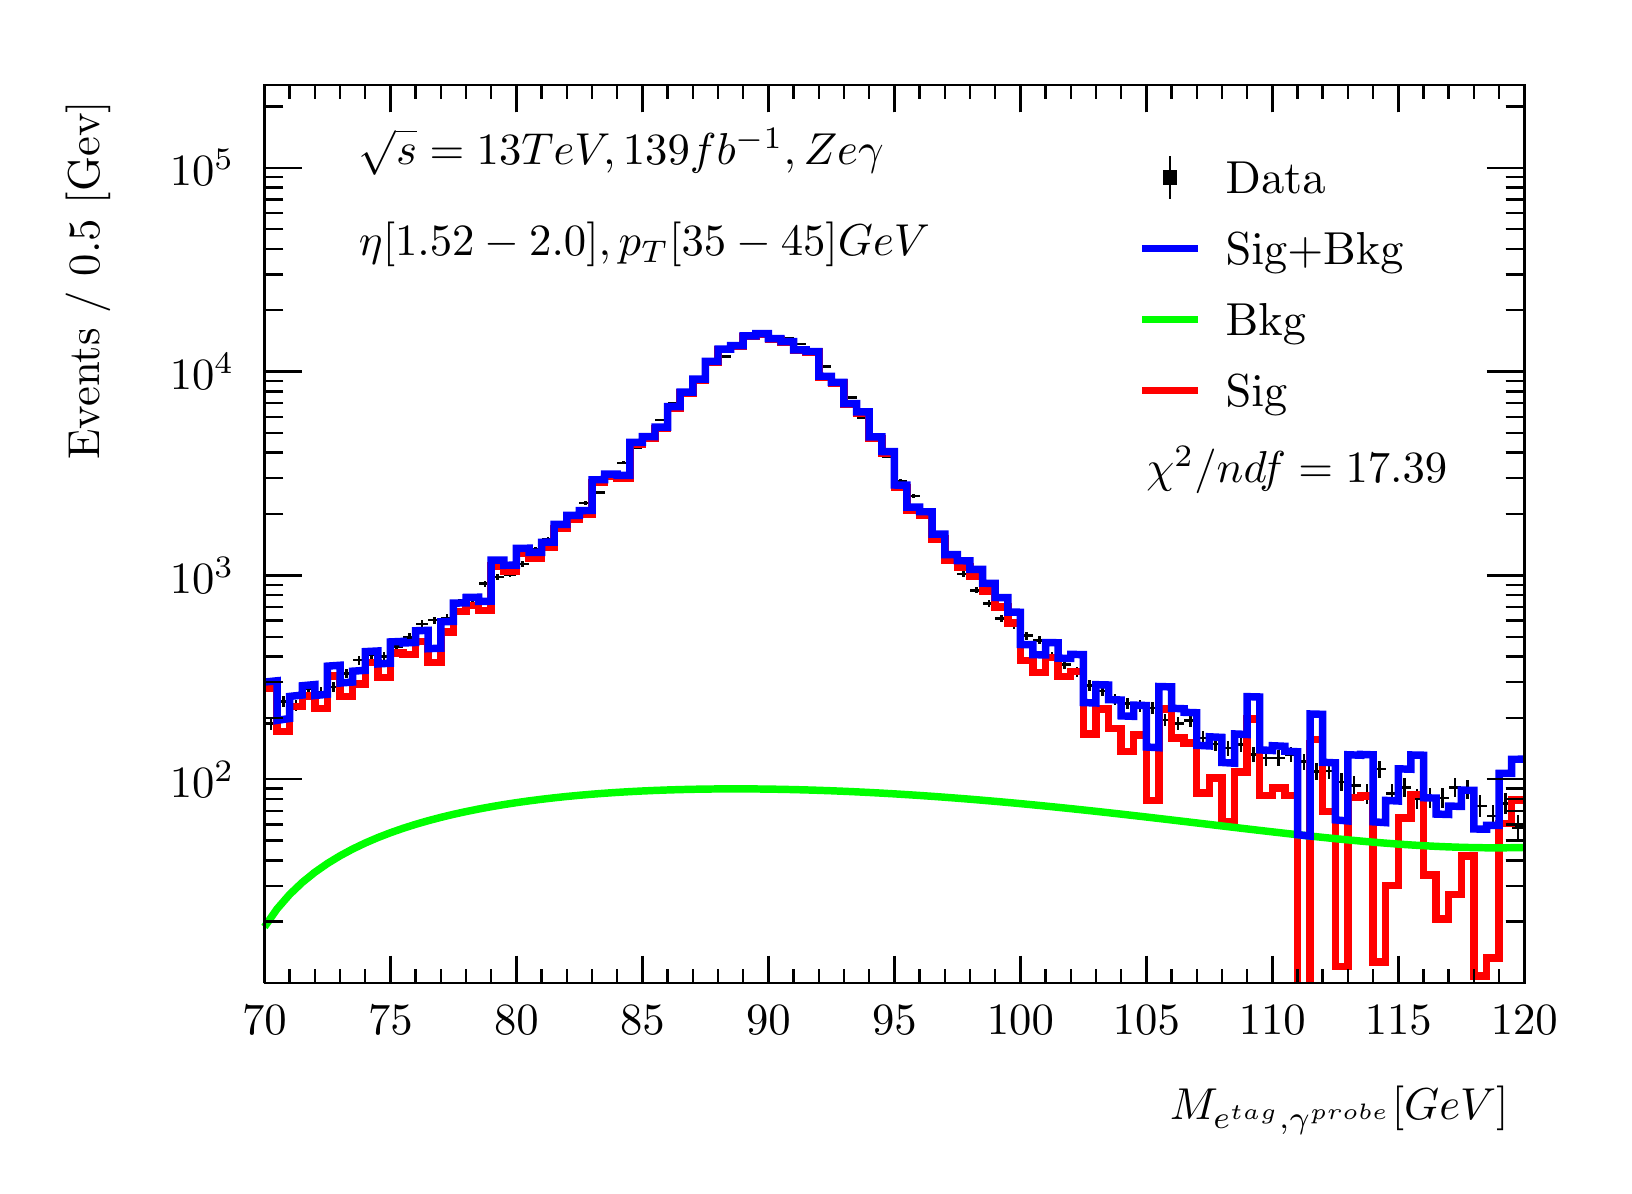
\begin{tikzpicture}
\pgfdeclareplotmark{cross} {
\pgfpathmoveto{\pgfpoint{-0.3\pgfplotmarksize}{\pgfplotmarksize}}
\pgfpathlineto{\pgfpoint{+0.3\pgfplotmarksize}{\pgfplotmarksize}}
\pgfpathlineto{\pgfpoint{+0.3\pgfplotmarksize}{0.3\pgfplotmarksize}}
\pgfpathlineto{\pgfpoint{+1\pgfplotmarksize}{0.3\pgfplotmarksize}}
\pgfpathlineto{\pgfpoint{+1\pgfplotmarksize}{-0.3\pgfplotmarksize}}
\pgfpathlineto{\pgfpoint{+0.3\pgfplotmarksize}{-0.3\pgfplotmarksize}}
\pgfpathlineto{\pgfpoint{+0.3\pgfplotmarksize}{-1.\pgfplotmarksize}}
\pgfpathlineto{\pgfpoint{-0.3\pgfplotmarksize}{-1.\pgfplotmarksize}}
\pgfpathlineto{\pgfpoint{-0.3\pgfplotmarksize}{-0.3\pgfplotmarksize}}
\pgfpathlineto{\pgfpoint{-1.\pgfplotmarksize}{-0.3\pgfplotmarksize}}
\pgfpathlineto{\pgfpoint{-1.\pgfplotmarksize}{0.3\pgfplotmarksize}}
\pgfpathlineto{\pgfpoint{-0.3\pgfplotmarksize}{0.3\pgfplotmarksize}}
\pgfpathclose
\pgfusepathqstroke
}
\pgfdeclareplotmark{cross*} {
\pgfpathmoveto{\pgfpoint{-0.3\pgfplotmarksize}{\pgfplotmarksize}}
\pgfpathlineto{\pgfpoint{+0.3\pgfplotmarksize}{\pgfplotmarksize}}
\pgfpathlineto{\pgfpoint{+0.3\pgfplotmarksize}{0.3\pgfplotmarksize}}
\pgfpathlineto{\pgfpoint{+1\pgfplotmarksize}{0.3\pgfplotmarksize}}
\pgfpathlineto{\pgfpoint{+1\pgfplotmarksize}{-0.3\pgfplotmarksize}}
\pgfpathlineto{\pgfpoint{+0.3\pgfplotmarksize}{-0.3\pgfplotmarksize}}
\pgfpathlineto{\pgfpoint{+0.3\pgfplotmarksize}{-1.\pgfplotmarksize}}
\pgfpathlineto{\pgfpoint{-0.3\pgfplotmarksize}{-1.\pgfplotmarksize}}
\pgfpathlineto{\pgfpoint{-0.3\pgfplotmarksize}{-0.3\pgfplotmarksize}}
\pgfpathlineto{\pgfpoint{-1.\pgfplotmarksize}{-0.3\pgfplotmarksize}}
\pgfpathlineto{\pgfpoint{-1.\pgfplotmarksize}{0.3\pgfplotmarksize}}
\pgfpathlineto{\pgfpoint{-0.3\pgfplotmarksize}{0.3\pgfplotmarksize}}
\pgfpathclose
\pgfusepathqfillstroke
}
\pgfdeclareplotmark{newstar} {
\pgfpathmoveto{\pgfqpoint{0pt}{\pgfplotmarksize}}
\pgfpathlineto{\pgfqpointpolar{44}{0.5\pgfplotmarksize}}
\pgfpathlineto{\pgfqpointpolar{18}{\pgfplotmarksize}}
\pgfpathlineto{\pgfqpointpolar{-20}{0.5\pgfplotmarksize}}
\pgfpathlineto{\pgfqpointpolar{-54}{\pgfplotmarksize}}
\pgfpathlineto{\pgfqpointpolar{-90}{0.5\pgfplotmarksize}}
\pgfpathlineto{\pgfqpointpolar{234}{\pgfplotmarksize}}
\pgfpathlineto{\pgfqpointpolar{198}{0.5\pgfplotmarksize}}
\pgfpathlineto{\pgfqpointpolar{162}{\pgfplotmarksize}}
\pgfpathlineto{\pgfqpointpolar{134}{0.5\pgfplotmarksize}}
\pgfpathclose
\pgfusepathqstroke
}
\pgfdeclareplotmark{newstar*} {
\pgfpathmoveto{\pgfqpoint{0pt}{\pgfplotmarksize}}
\pgfpathlineto{\pgfqpointpolar{44}{0.5\pgfplotmarksize}}
\pgfpathlineto{\pgfqpointpolar{18}{\pgfplotmarksize}}
\pgfpathlineto{\pgfqpointpolar{-20}{0.5\pgfplotmarksize}}
\pgfpathlineto{\pgfqpointpolar{-54}{\pgfplotmarksize}}
\pgfpathlineto{\pgfqpointpolar{-90}{0.5\pgfplotmarksize}}
\pgfpathlineto{\pgfqpointpolar{234}{\pgfplotmarksize}}
\pgfpathlineto{\pgfqpointpolar{198}{0.5\pgfplotmarksize}}
\pgfpathlineto{\pgfqpointpolar{162}{\pgfplotmarksize}}
\pgfpathlineto{\pgfqpointpolar{134}{0.5\pgfplotmarksize}}
\pgfpathclose
\pgfusepathqfillstroke
}
\definecolor{c}{rgb}{1,1,1};
\draw [color=c, fill=c] (0,0) rectangle (20,14.4361);
\draw [color=c, fill=c] (3,2.30977) rectangle (19,13.7143);
\definecolor{c}{rgb}{0,0,0};
\draw [c,line width=0.9] (3,2.30977) -- (3,13.7143) -- (19,13.7143) -- (19,2.30977) -- (3,2.30977);
\definecolor{c}{rgb}{1,1,1};
\draw [color=c, fill=c] (3,2.30977) rectangle (19,13.7143);
\definecolor{c}{rgb}{0,0,0};
\draw [c,line width=0.9] (3,2.30977) -- (3,13.7143) -- (19,13.7143) -- (19,2.30977) -- (3,2.30977);
\draw [c,line width=0.9] (3,2.30977) -- (19,2.30977);
\draw [c,line width=0.9] (3,2.65624) -- (3,2.30977);
\draw [c,line width=0.9] (3.32,2.48301) -- (3.32,2.30977);
\draw [c,line width=0.9] (3.64,2.48301) -- (3.64,2.30977);
\draw [c,line width=0.9] (3.96,2.48301) -- (3.96,2.30977);
\draw [c,line width=0.9] (4.28,2.48301) -- (4.28,2.30977);
\draw [c,line width=0.9] (4.6,2.65624) -- (4.6,2.30977);
\draw [c,line width=0.9] (4.92,2.48301) -- (4.92,2.30977);
\draw [c,line width=0.9] (5.24,2.48301) -- (5.24,2.30977);
\draw [c,line width=0.9] (5.56,2.48301) -- (5.56,2.30977);
\draw [c,line width=0.9] (5.88,2.48301) -- (5.88,2.30977);
\draw [c,line width=0.9] (6.2,2.65624) -- (6.2,2.30977);
\draw [c,line width=0.9] (6.52,2.48301) -- (6.52,2.30977);
\draw [c,line width=0.9] (6.84,2.48301) -- (6.84,2.30977);
\draw [c,line width=0.9] (7.16,2.48301) -- (7.16,2.30977);
\draw [c,line width=0.9] (7.48,2.48301) -- (7.48,2.30977);
\draw [c,line width=0.9] (7.8,2.65624) -- (7.8,2.30977);
\draw [c,line width=0.9] (8.12,2.48301) -- (8.12,2.30977);
\draw [c,line width=0.9] (8.44,2.48301) -- (8.44,2.30977);
\draw [c,line width=0.9] (8.76,2.48301) -- (8.76,2.30977);
\draw [c,line width=0.9] (9.08,2.48301) -- (9.08,2.30977);
\draw [c,line width=0.9] (9.4,2.65624) -- (9.4,2.30977);
\draw [c,line width=0.9] (9.72,2.48301) -- (9.72,2.30977);
\draw [c,line width=0.9] (10.04,2.48301) -- (10.04,2.30977);
\draw [c,line width=0.9] (10.36,2.48301) -- (10.36,2.30977);
\draw [c,line width=0.9] (10.68,2.48301) -- (10.68,2.30977);
\draw [c,line width=0.9] (11,2.65624) -- (11,2.30977);
\draw [c,line width=0.9] (11.32,2.48301) -- (11.32,2.30977);
\draw [c,line width=0.9] (11.64,2.48301) -- (11.64,2.30977);
\draw [c,line width=0.9] (11.96,2.48301) -- (11.96,2.30977);
\draw [c,line width=0.9] (12.28,2.48301) -- (12.28,2.30977);
\draw [c,line width=0.9] (12.6,2.65624) -- (12.6,2.30977);
\draw [c,line width=0.9] (12.92,2.48301) -- (12.92,2.30977);
\draw [c,line width=0.9] (13.24,2.48301) -- (13.24,2.30977);
\draw [c,line width=0.9] (13.56,2.48301) -- (13.56,2.30977);
\draw [c,line width=0.9] (13.88,2.48301) -- (13.88,2.30977);
\draw [c,line width=0.9] (14.2,2.65624) -- (14.2,2.30977);
\draw [c,line width=0.9] (14.52,2.48301) -- (14.52,2.30977);
\draw [c,line width=0.9] (14.84,2.48301) -- (14.84,2.30977);
\draw [c,line width=0.9] (15.16,2.48301) -- (15.16,2.30977);
\draw [c,line width=0.9] (15.48,2.48301) -- (15.48,2.30977);
\draw [c,line width=0.9] (15.8,2.65624) -- (15.8,2.30977);
\draw [c,line width=0.9] (16.12,2.48301) -- (16.12,2.30977);
\draw [c,line width=0.9] (16.44,2.48301) -- (16.44,2.30977);
\draw [c,line width=0.9] (16.76,2.48301) -- (16.76,2.30977);
\draw [c,line width=0.9] (17.08,2.48301) -- (17.08,2.30977);
\draw [c,line width=0.9] (17.4,2.65624) -- (17.4,2.30977);
\draw [c,line width=0.9] (17.72,2.48301) -- (17.72,2.30977);
\draw [c,line width=0.9] (18.04,2.48301) -- (18.04,2.30977);
\draw [c,line width=0.9] (18.36,2.48301) -- (18.36,2.30977);
\draw [c,line width=0.9] (18.68,2.48301) -- (18.68,2.30977);
\draw [c,line width=0.9] (19,2.65624) -- (19,2.30977);
\draw [anchor=base] (3,1.66015) node[scale=1.61424, color=c, rotate=0]{70};
\draw [anchor=base] (4.6,1.66015) node[scale=1.61424, color=c, rotate=0]{75};
\draw [anchor=base] (6.2,1.66015) node[scale=1.61424, color=c, rotate=0]{80};
\draw [anchor=base] (7.8,1.66015) node[scale=1.61424, color=c, rotate=0]{85};
\draw [anchor=base] (9.4,1.66015) node[scale=1.61424, color=c, rotate=0]{90};
\draw [anchor=base] (11,1.66015) node[scale=1.61424, color=c, rotate=0]{95};
\draw [anchor=base] (12.6,1.66015) node[scale=1.61424, color=c, rotate=0]{100};
\draw [anchor=base] (14.2,1.66015) node[scale=1.61424, color=c, rotate=0]{105};
\draw [anchor=base] (15.8,1.66015) node[scale=1.61424, color=c, rotate=0]{110};
\draw [anchor=base] (17.4,1.66015) node[scale=1.61424, color=c, rotate=0]{115};
\draw [anchor=base] (19,1.66015) node[scale=1.61424, color=c, rotate=0]{120};
\draw [anchor= east] (19,0.692932) node[scale=1.61424, color=c, rotate=0]{$M_{e^{tag}, \gamma^{probe}}  [GeV]$};
\draw [c,line width=0.9] (3,13.7143) -- (19,13.7143);
\draw [c,line width=0.9] (3,13.3678) -- (3,13.7143);
\draw [c,line width=0.9] (3.32,13.5411) -- (3.32,13.7143);
\draw [c,line width=0.9] (3.64,13.5411) -- (3.64,13.7143);
\draw [c,line width=0.9] (3.96,13.5411) -- (3.96,13.7143);
\draw [c,line width=0.9] (4.28,13.5411) -- (4.28,13.7143);
\draw [c,line width=0.9] (4.6,13.3678) -- (4.6,13.7143);
\draw [c,line width=0.9] (4.92,13.5411) -- (4.92,13.7143);
\draw [c,line width=0.9] (5.24,13.5411) -- (5.24,13.7143);
\draw [c,line width=0.9] (5.56,13.5411) -- (5.56,13.7143);
\draw [c,line width=0.9] (5.88,13.5411) -- (5.88,13.7143);
\draw [c,line width=0.9] (6.2,13.3678) -- (6.2,13.7143);
\draw [c,line width=0.9] (6.52,13.5411) -- (6.52,13.7143);
\draw [c,line width=0.9] (6.84,13.5411) -- (6.84,13.7143);
\draw [c,line width=0.9] (7.16,13.5411) -- (7.16,13.7143);
\draw [c,line width=0.9] (7.48,13.5411) -- (7.48,13.7143);
\draw [c,line width=0.9] (7.8,13.3678) -- (7.8,13.7143);
\draw [c,line width=0.9] (8.12,13.5411) -- (8.12,13.7143);
\draw [c,line width=0.9] (8.44,13.5411) -- (8.44,13.7143);
\draw [c,line width=0.9] (8.76,13.5411) -- (8.76,13.7143);
\draw [c,line width=0.9] (9.08,13.5411) -- (9.08,13.7143);
\draw [c,line width=0.9] (9.4,13.3678) -- (9.4,13.7143);
\draw [c,line width=0.9] (9.72,13.5411) -- (9.72,13.7143);
\draw [c,line width=0.9] (10.04,13.5411) -- (10.04,13.7143);
\draw [c,line width=0.9] (10.36,13.5411) -- (10.36,13.7143);
\draw [c,line width=0.9] (10.68,13.5411) -- (10.68,13.7143);
\draw [c,line width=0.9] (11,13.3678) -- (11,13.7143);
\draw [c,line width=0.9] (11.32,13.5411) -- (11.32,13.7143);
\draw [c,line width=0.9] (11.64,13.5411) -- (11.64,13.7143);
\draw [c,line width=0.9] (11.96,13.5411) -- (11.96,13.7143);
\draw [c,line width=0.9] (12.28,13.5411) -- (12.28,13.7143);
\draw [c,line width=0.9] (12.6,13.3678) -- (12.6,13.7143);
\draw [c,line width=0.9] (12.92,13.5411) -- (12.92,13.7143);
\draw [c,line width=0.9] (13.24,13.5411) -- (13.24,13.7143);
\draw [c,line width=0.9] (13.56,13.5411) -- (13.56,13.7143);
\draw [c,line width=0.9] (13.88,13.5411) -- (13.88,13.7143);
\draw [c,line width=0.9] (14.2,13.3678) -- (14.2,13.7143);
\draw [c,line width=0.9] (14.52,13.5411) -- (14.52,13.7143);
\draw [c,line width=0.9] (14.84,13.5411) -- (14.84,13.7143);
\draw [c,line width=0.9] (15.16,13.5411) -- (15.16,13.7143);
\draw [c,line width=0.9] (15.48,13.5411) -- (15.48,13.7143);
\draw [c,line width=0.9] (15.8,13.3678) -- (15.8,13.7143);
\draw [c,line width=0.9] (16.12,13.5411) -- (16.12,13.7143);
\draw [c,line width=0.9] (16.44,13.5411) -- (16.44,13.7143);
\draw [c,line width=0.9] (16.76,13.5411) -- (16.76,13.7143);
\draw [c,line width=0.9] (17.08,13.5411) -- (17.08,13.7143);
\draw [c,line width=0.9] (17.4,13.3678) -- (17.4,13.7143);
\draw [c,line width=0.9] (17.72,13.5411) -- (17.72,13.7143);
\draw [c,line width=0.9] (18.04,13.5411) -- (18.04,13.7143);
\draw [c,line width=0.9] (18.36,13.5411) -- (18.36,13.7143);
\draw [c,line width=0.9] (18.68,13.5411) -- (18.68,13.7143);
\draw [c,line width=0.9] (19,13.3678) -- (19,13.7143);
\draw [c,line width=0.9] (3,2.30977) -- (3,13.7143);
\draw [c,line width=0.9] (3.237,3.08897) -- (3,3.08897);
\draw [c,line width=0.9] (3.237,3.54477) -- (3,3.54477);
\draw [c,line width=0.9] (3.237,3.86817) -- (3,3.86817);
\draw [c,line width=0.9] (3.237,4.11902) -- (3,4.11902);
\draw [c,line width=0.9] (3.237,4.32397) -- (3,4.32397);
\draw [c,line width=0.9] (3.237,4.49726) -- (3,4.49726);
\draw [c,line width=0.9] (3.237,4.64737) -- (3,4.64737);
\draw [c,line width=0.9] (3.237,4.77978) -- (3,4.77978);
\draw [c,line width=0.9] (3.474,4.89822) -- (3,4.89822);
\draw [anchor= east] (2.82,4.89822) node[scale=1.61424, color=c, rotate=0]{$10^{2}$};
\draw [c,line width=0.9] (3.237,5.67742) -- (3,5.67742);
\draw [c,line width=0.9] (3.237,6.13322) -- (3,6.13322);
\draw [c,line width=0.9] (3.237,6.45661) -- (3,6.45661);
\draw [c,line width=0.9] (3.237,6.70746) -- (3,6.70746);
\draw [c,line width=0.9] (3.237,6.91242) -- (3,6.91242);
\draw [c,line width=0.9] (3.237,7.08571) -- (3,7.08571);
\draw [c,line width=0.9] (3.237,7.23581) -- (3,7.23581);
\draw [c,line width=0.9] (3.237,7.36822) -- (3,7.36822);
\draw [c,line width=0.9] (3.474,7.48666) -- (3,7.48666);
\draw [anchor= east] (2.82,7.48666) node[scale=1.61424, color=c, rotate=0]{$10^{3}$};
\draw [c,line width=0.9] (3.237,8.26586) -- (3,8.26586);
\draw [c,line width=0.9] (3.237,8.72166) -- (3,8.72166);
\draw [c,line width=0.9] (3.237,9.04506) -- (3,9.04506);
\draw [c,line width=0.9] (3.237,9.29591) -- (3,9.29591);
\draw [c,line width=0.9] (3.237,9.50086) -- (3,9.50086);
\draw [c,line width=0.9] (3.237,9.67415) -- (3,9.67415);
\draw [c,line width=0.9] (3.237,9.82426) -- (3,9.82426);
\draw [c,line width=0.9] (3.237,9.95666) -- (3,9.95666);
\draw [c,line width=0.9] (3.474,10.0751) -- (3,10.0751);
\draw [anchor= east] (2.82,10.0751) node[scale=1.61424, color=c, rotate=0]{$10^{4}$};
\draw [c,line width=0.9] (3.237,10.8543) -- (3,10.8543);
\draw [c,line width=0.9] (3.237,11.3101) -- (3,11.3101);
\draw [c,line width=0.9] (3.237,11.6335) -- (3,11.6335);
\draw [c,line width=0.9] (3.237,11.8844) -- (3,11.8844);
\draw [c,line width=0.9] (3.237,12.0893) -- (3,12.0893);
\draw [c,line width=0.9] (3.237,12.2626) -- (3,12.2626);
\draw [c,line width=0.9] (3.237,12.4127) -- (3,12.4127);
\draw [c,line width=0.9] (3.237,12.5451) -- (3,12.5451);
\draw [c,line width=0.9] (3.474,12.6635) -- (3,12.6635);
\draw [anchor= east] (2.82,12.6635) node[scale=1.61424, color=c, rotate=0]{$10^{5}$};
\draw [c,line width=0.9] (3.237,13.4427) -- (3,13.4427);
\draw [anchor= east] (0.76,13.7143) node[scale=1.61424, color=c, rotate=90]{Events / 0.5 [Gev]};
\draw [c,line width=0.9] (19,2.30977) -- (19,13.7143);
\draw [c,line width=0.9] (18.763,3.08897) -- (19,3.08897);
\draw [c,line width=0.9] (18.763,3.54477) -- (19,3.54477);
\draw [c,line width=0.9] (18.763,3.86817) -- (19,3.86817);
\draw [c,line width=0.9] (18.763,4.11902) -- (19,4.11902);
\draw [c,line width=0.9] (18.763,4.32397) -- (19,4.32397);
\draw [c,line width=0.9] (18.763,4.49726) -- (19,4.49726);
\draw [c,line width=0.9] (18.763,4.64737) -- (19,4.64737);
\draw [c,line width=0.9] (18.763,4.77978) -- (19,4.77978);
\draw [c,line width=0.9] (18.526,4.89822) -- (19,4.89822);
\draw [c,line width=0.9] (18.763,5.67742) -- (19,5.67742);
\draw [c,line width=0.9] (18.763,6.13322) -- (19,6.13322);
\draw [c,line width=0.9] (18.763,6.45661) -- (19,6.45661);
\draw [c,line width=0.9] (18.763,6.70746) -- (19,6.70746);
\draw [c,line width=0.9] (18.763,6.91242) -- (19,6.91242);
\draw [c,line width=0.9] (18.763,7.08571) -- (19,7.08571);
\draw [c,line width=0.9] (18.763,7.23581) -- (19,7.23581);
\draw [c,line width=0.9] (18.763,7.36822) -- (19,7.36822);
\draw [c,line width=0.9] (18.526,7.48666) -- (19,7.48666);
\draw [c,line width=0.9] (18.763,8.26586) -- (19,8.26586);
\draw [c,line width=0.9] (18.763,8.72166) -- (19,8.72166);
\draw [c,line width=0.9] (18.763,9.04506) -- (19,9.04506);
\draw [c,line width=0.9] (18.763,9.29591) -- (19,9.29591);
\draw [c,line width=0.9] (18.763,9.50086) -- (19,9.50086);
\draw [c,line width=0.9] (18.763,9.67415) -- (19,9.67415);
\draw [c,line width=0.9] (18.763,9.82426) -- (19,9.82426);
\draw [c,line width=0.9] (18.763,9.95666) -- (19,9.95666);
\draw [c,line width=0.9] (18.526,10.0751) -- (19,10.0751);
\draw [c,line width=0.9] (18.763,10.8543) -- (19,10.8543);
\draw [c,line width=0.9] (18.763,11.3101) -- (19,11.3101);
\draw [c,line width=0.9] (18.763,11.6335) -- (19,11.6335);
\draw [c,line width=0.9] (18.763,11.8844) -- (19,11.8844);
\draw [c,line width=0.9] (18.763,12.0893) -- (19,12.0893);
\draw [c,line width=0.9] (18.763,12.2626) -- (19,12.2626);
\draw [c,line width=0.9] (18.763,12.4127) -- (19,12.4127);
\draw [c,line width=0.9] (18.763,12.5451) -- (19,12.5451);
\draw [c,line width=0.9] (18.526,12.6635) -- (19,12.6635);
\draw [c,line width=0.9] (18.763,13.4427) -- (19,13.4427);
\draw [c,line width=0.9] (3.08,5.60786) -- (3,5.60786);
\draw [c,line width=0.9] (3,5.60786) -- (3,5.60786);
\draw [c,line width=0.9] (3.08,5.60786) -- (3.16,5.60786);
\draw [c,line width=0.9] (3.16,5.60786) -- (3.16,5.60786);
\draw [c,line width=0.9] (3.08,5.60786) -- (3.08,5.68983);
\draw [c,line width=0.9] (3.08,5.68983) -- (3.08,5.68983);
\draw [c,line width=0.9] (3.08,5.60786) -- (3.08,5.52589);
\draw [c,line width=0.9] (3.08,5.52589) -- (3.08,5.52589);
\draw [c,line width=0.9] (3.24,5.88705) -- (3.16,5.88705);
\draw [c,line width=0.9] (3.16,5.88705) -- (3.16,5.88705);
\draw [c,line width=0.9] (3.24,5.88705) -- (3.32,5.88705);
\draw [c,line width=0.9] (3.32,5.88705) -- (3.32,5.88705);
\draw [c,line width=0.9] (3.24,5.88705) -- (3.24,5.95945);
\draw [c,line width=0.9] (3.24,5.95945) -- (3.24,5.95945);
\draw [c,line width=0.9] (3.24,5.88705) -- (3.24,5.81465);
\draw [c,line width=0.9] (3.24,5.81465) -- (3.24,5.81465);
\draw [c,line width=0.9] (3.4,5.83453) -- (3.32,5.83453);
\draw [c,line width=0.9] (3.32,5.83453) -- (3.32,5.83453);
\draw [c,line width=0.9] (3.4,5.83453) -- (3.48,5.83453);
\draw [c,line width=0.9] (3.48,5.83453) -- (3.48,5.83453);
\draw [c,line width=0.9] (3.4,5.83453) -- (3.4,5.90864);
\draw [c,line width=0.9] (3.4,5.90864) -- (3.4,5.90864);
\draw [c,line width=0.9] (3.4,5.83453) -- (3.4,5.76042);
\draw [c,line width=0.9] (3.4,5.76042) -- (3.4,5.76042);
\draw [c,line width=0.9] (3.56,6.0476) -- (3.48,6.0476);
\draw [c,line width=0.9] (3.48,6.0476) -- (3.48,6.0476);
\draw [c,line width=0.9] (3.56,6.0476) -- (3.64,6.0476);
\draw [c,line width=0.9] (3.64,6.0476) -- (3.64,6.0476);
\draw [c,line width=0.9] (3.56,6.0476) -- (3.56,6.11502);
\draw [c,line width=0.9] (3.56,6.11502) -- (3.56,6.11502);
\draw [c,line width=0.9] (3.56,6.0476) -- (3.56,5.98019);
\draw [c,line width=0.9] (3.56,5.98019) -- (3.56,5.98019);
\draw [c,line width=0.9] (3.72,6.00222) -- (3.64,6.00222);
\draw [c,line width=0.9] (3.64,6.00222) -- (3.64,6.00222);
\draw [c,line width=0.9] (3.72,6.00222) -- (3.8,6.00222);
\draw [c,line width=0.9] (3.8,6.00222) -- (3.8,6.00222);
\draw [c,line width=0.9] (3.72,6.00222) -- (3.72,6.071);
\draw [c,line width=0.9] (3.72,6.071) -- (3.72,6.071);
\draw [c,line width=0.9] (3.72,6.00222) -- (3.72,5.93343);
\draw [c,line width=0.9] (3.72,5.93343) -- (3.72,5.93343);
\draw [c,line width=0.9] (3.88,6.07161) -- (3.8,6.07161);
\draw [c,line width=0.9] (3.8,6.07161) -- (3.8,6.07161);
\draw [c,line width=0.9] (3.88,6.07161) -- (3.96,6.07161);
\draw [c,line width=0.9] (3.96,6.07161) -- (3.96,6.07161);
\draw [c,line width=0.9] (3.88,6.07161) -- (3.88,6.1383);
\draw [c,line width=0.9] (3.88,6.1383) -- (3.88,6.1383);
\draw [c,line width=0.9] (3.88,6.07161) -- (3.88,6.00491);
\draw [c,line width=0.9] (3.88,6.00491) -- (3.88,6.00491);
\draw [c,line width=0.9] (4.04,6.24036) -- (3.96,6.24036);
\draw [c,line width=0.9] (3.96,6.24036) -- (3.96,6.24036);
\draw [c,line width=0.9] (4.04,6.24036) -- (4.12,6.24036);
\draw [c,line width=0.9] (4.12,6.24036) -- (4.12,6.24036);
\draw [c,line width=0.9] (4.04,6.24036) -- (4.04,6.30224);
\draw [c,line width=0.9] (4.04,6.30224) -- (4.04,6.30224);
\draw [c,line width=0.9] (4.04,6.24036) -- (4.04,6.17849);
\draw [c,line width=0.9] (4.04,6.17849) -- (4.04,6.17849);
\draw [c,line width=0.9] (4.2,6.41073) -- (4.12,6.41073);
\draw [c,line width=0.9] (4.12,6.41073) -- (4.12,6.41073);
\draw [c,line width=0.9] (4.2,6.41073) -- (4.28,6.41073);
\draw [c,line width=0.9] (4.28,6.41073) -- (4.28,6.41073);
\draw [c,line width=0.9] (4.2,6.41073) -- (4.2,6.46809);
\draw [c,line width=0.9] (4.2,6.46809) -- (4.2,6.46809);
\draw [c,line width=0.9] (4.2,6.41073) -- (4.2,6.35337);
\draw [c,line width=0.9] (4.2,6.35337) -- (4.2,6.35337);
\draw [c,line width=0.9] (4.36,6.48163) -- (4.28,6.48163);
\draw [c,line width=0.9] (4.28,6.48163) -- (4.28,6.48163);
\draw [c,line width=0.9] (4.36,6.48163) -- (4.44,6.48163);
\draw [c,line width=0.9] (4.44,6.48163) -- (4.44,6.48163);
\draw [c,line width=0.9] (4.36,6.48163) -- (4.36,6.53721);
\draw [c,line width=0.9] (4.36,6.53721) -- (4.36,6.53721);
\draw [c,line width=0.9] (4.36,6.48163) -- (4.36,6.42605);
\draw [c,line width=0.9] (4.36,6.42605) -- (4.36,6.42605);
\draw [c,line width=0.9] (4.52,6.45662) -- (4.44,6.45662);
\draw [c,line width=0.9] (4.44,6.45662) -- (4.44,6.45662);
\draw [c,line width=0.9] (4.52,6.45662) -- (4.6,6.45662);
\draw [c,line width=0.9] (4.6,6.45662) -- (4.6,6.45662);
\draw [c,line width=0.9] (4.52,6.45662) -- (4.52,6.51282);
\draw [c,line width=0.9] (4.52,6.51282) -- (4.52,6.51282);
\draw [c,line width=0.9] (4.52,6.45662) -- (4.52,6.40042);
\draw [c,line width=0.9] (4.52,6.40042) -- (4.52,6.40042);
\draw [c,line width=0.9] (4.68,6.58652) -- (4.6,6.58652);
\draw [c,line width=0.9] (4.6,6.58652) -- (4.6,6.58652);
\draw [c,line width=0.9] (4.68,6.58652) -- (4.76,6.58652);
\draw [c,line width=0.9] (4.76,6.58652) -- (4.76,6.58652);
\draw [c,line width=0.9] (4.68,6.58652) -- (4.68,6.63957);
\draw [c,line width=0.9] (4.68,6.63957) -- (4.68,6.63957);
\draw [c,line width=0.9] (4.68,6.58652) -- (4.68,6.53347);
\draw [c,line width=0.9] (4.68,6.53347) -- (4.68,6.53347);
\draw [c,line width=0.9] (4.84,6.7007) -- (4.76,6.7007);
\draw [c,line width=0.9] (4.76,6.7007) -- (4.76,6.7007);
\draw [c,line width=0.9] (4.84,6.7007) -- (4.92,6.7007);
\draw [c,line width=0.9] (4.92,6.7007) -- (4.92,6.7007);
\draw [c,line width=0.9] (4.84,6.7007) -- (4.84,6.75112);
\draw [c,line width=0.9] (4.84,6.75112) -- (4.84,6.75112);
\draw [c,line width=0.9] (4.84,6.7007) -- (4.84,6.65028);
\draw [c,line width=0.9] (4.84,6.65028) -- (4.84,6.65028);
\draw [c,line width=0.9] (5,6.86848) -- (4.92,6.86848);
\draw [c,line width=0.9] (4.92,6.86848) -- (4.92,6.86848);
\draw [c,line width=0.9] (5,6.86848) -- (5.08,6.86848);
\draw [c,line width=0.9] (5.08,6.86848) -- (5.08,6.86848);
\draw [c,line width=0.9] (5,6.86848) -- (5,6.91527);
\draw [c,line width=0.9] (5,6.91527) -- (5,6.91527);
\draw [c,line width=0.9] (5,6.86848) -- (5,6.82168);
\draw [c,line width=0.9] (5,6.82168) -- (5,6.82168);
\draw [c,line width=0.9] (5.16,6.91803) -- (5.08,6.91803);
\draw [c,line width=0.9] (5.08,6.91803) -- (5.08,6.91803);
\draw [c,line width=0.9] (5.16,6.91803) -- (5.24,6.91803);
\draw [c,line width=0.9] (5.24,6.91803) -- (5.24,6.91803);
\draw [c,line width=0.9] (5.16,6.91803) -- (5.16,6.9638);
\draw [c,line width=0.9] (5.16,6.9638) -- (5.16,6.9638);
\draw [c,line width=0.9] (5.16,6.91803) -- (5.16,6.87225);
\draw [c,line width=0.9] (5.16,6.87225) -- (5.16,6.87225);
\draw [c,line width=0.9] (5.32,6.94746) -- (5.24,6.94746);
\draw [c,line width=0.9] (5.24,6.94746) -- (5.24,6.94746);
\draw [c,line width=0.9] (5.32,6.94746) -- (5.4,6.94746);
\draw [c,line width=0.9] (5.4,6.94746) -- (5.4,6.94746);
\draw [c,line width=0.9] (5.32,6.94746) -- (5.32,6.99265);
\draw [c,line width=0.9] (5.32,6.99265) -- (5.32,6.99265);
\draw [c,line width=0.9] (5.32,6.94746) -- (5.32,6.90229);
\draw [c,line width=0.9] (5.32,6.90229) -- (5.32,6.90229);
\draw [c,line width=0.9] (5.48,7.14208) -- (5.4,7.14208);
\draw [c,line width=0.9] (5.4,7.14208) -- (5.4,7.14208);
\draw [c,line width=0.9] (5.48,7.14208) -- (5.56,7.14208);
\draw [c,line width=0.9] (5.56,7.14208) -- (5.56,7.14208);
\draw [c,line width=0.9] (5.48,7.14208) -- (5.48,7.18352);
\draw [c,line width=0.9] (5.48,7.18352) -- (5.48,7.18352);
\draw [c,line width=0.9] (5.48,7.14208) -- (5.48,7.10065);
\draw [c,line width=0.9] (5.48,7.10065) -- (5.48,7.10065);
\draw [c,line width=0.9] (5.64,7.18553) -- (5.56,7.18553);
\draw [c,line width=0.9] (5.56,7.18553) -- (5.56,7.18553);
\draw [c,line width=0.9] (5.64,7.18553) -- (5.72,7.18553);
\draw [c,line width=0.9] (5.72,7.18553) -- (5.72,7.18553);
\draw [c,line width=0.9] (5.64,7.18553) -- (5.64,7.22617);
\draw [c,line width=0.9] (5.64,7.22617) -- (5.64,7.22617);
\draw [c,line width=0.9] (5.64,7.18553) -- (5.64,7.14489);
\draw [c,line width=0.9] (5.64,7.14489) -- (5.64,7.14489);
\draw [c,line width=0.9] (5.8,7.38311) -- (5.72,7.38311);
\draw [c,line width=0.9] (5.72,7.38311) -- (5.72,7.38311);
\draw [c,line width=0.9] (5.8,7.38311) -- (5.88,7.38311);
\draw [c,line width=0.9] (5.88,7.38311) -- (5.88,7.38311);
\draw [c,line width=0.9] (5.8,7.38311) -- (5.8,7.42033);
\draw [c,line width=0.9] (5.8,7.42033) -- (5.8,7.42033);
\draw [c,line width=0.9] (5.8,7.38311) -- (5.8,7.34589);
\draw [c,line width=0.9] (5.8,7.34589) -- (5.8,7.34589);
\draw [c,line width=0.9] (5.96,7.46624) -- (5.88,7.46624);
\draw [c,line width=0.9] (5.88,7.46624) -- (5.88,7.46624);
\draw [c,line width=0.9] (5.96,7.46624) -- (6.04,7.46624);
\draw [c,line width=0.9] (6.04,7.46624) -- (6.04,7.46624);
\draw [c,line width=0.9] (5.96,7.46624) -- (5.96,7.50211);
\draw [c,line width=0.9] (5.96,7.50211) -- (5.96,7.50211);
\draw [c,line width=0.9] (5.96,7.46624) -- (5.96,7.43037);
\draw [c,line width=0.9] (5.96,7.43037) -- (5.96,7.43037);
\draw [c,line width=0.9] (6.12,7.50007) -- (6.04,7.50007);
\draw [c,line width=0.9] (6.04,7.50007) -- (6.04,7.50007);
\draw [c,line width=0.9] (6.12,7.50007) -- (6.2,7.50007);
\draw [c,line width=0.9] (6.2,7.50007) -- (6.2,7.50007);
\draw [c,line width=0.9] (6.12,7.50007) -- (6.12,7.53541);
\draw [c,line width=0.9] (6.12,7.53541) -- (6.12,7.53541);
\draw [c,line width=0.9] (6.12,7.50007) -- (6.12,7.46474);
\draw [c,line width=0.9] (6.12,7.46474) -- (6.12,7.46474);
\draw [c,line width=0.9] (6.28,7.63198) -- (6.2,7.63198);
\draw [c,line width=0.9] (6.2,7.63198) -- (6.2,7.63198);
\draw [c,line width=0.9] (6.28,7.63198) -- (6.36,7.63198);
\draw [c,line width=0.9] (6.36,7.63198) -- (6.36,7.63198);
\draw [c,line width=0.9] (6.28,7.63198) -- (6.28,7.66531);
\draw [c,line width=0.9] (6.28,7.66531) -- (6.28,7.66531);
\draw [c,line width=0.9] (6.28,7.63198) -- (6.28,7.59866);
\draw [c,line width=0.9] (6.28,7.59866) -- (6.28,7.59866);
\draw [c,line width=0.9] (6.44,7.81567) -- (6.36,7.81567);
\draw [c,line width=0.9] (6.36,7.81567) -- (6.36,7.81567);
\draw [c,line width=0.9] (6.44,7.81567) -- (6.52,7.81567);
\draw [c,line width=0.9] (6.52,7.81567) -- (6.52,7.81567);
\draw [c,line width=0.9] (6.44,7.81567) -- (6.44,7.84637);
\draw [c,line width=0.9] (6.44,7.84637) -- (6.44,7.84637);
\draw [c,line width=0.9] (6.44,7.81567) -- (6.44,7.78496);
\draw [c,line width=0.9] (6.44,7.78496) -- (6.44,7.78496);
\draw [c,line width=0.9] (6.6,7.94546) -- (6.52,7.94546);
\draw [c,line width=0.9] (6.52,7.94546) -- (6.52,7.94546);
\draw [c,line width=0.9] (6.6,7.94546) -- (6.68,7.94546);
\draw [c,line width=0.9] (6.68,7.94546) -- (6.68,7.94546);
\draw [c,line width=0.9] (6.6,7.94546) -- (6.6,7.97444);
\draw [c,line width=0.9] (6.6,7.97444) -- (6.6,7.97444);
\draw [c,line width=0.9] (6.6,7.94546) -- (6.6,7.91647);
\draw [c,line width=0.9] (6.6,7.91647) -- (6.6,7.91647);
\draw [c,line width=0.9] (6.76,8.08449) -- (6.68,8.08449);
\draw [c,line width=0.9] (6.68,8.08449) -- (6.68,8.08449);
\draw [c,line width=0.9] (6.76,8.08449) -- (6.84,8.08449);
\draw [c,line width=0.9] (6.84,8.08449) -- (6.84,8.08449);
\draw [c,line width=0.9] (6.76,8.08449) -- (6.76,8.11174);
\draw [c,line width=0.9] (6.76,8.11174) -- (6.76,8.11174);
\draw [c,line width=0.9] (6.76,8.08449) -- (6.76,8.05724);
\draw [c,line width=0.9] (6.76,8.05724) -- (6.76,8.05724);
\draw [c,line width=0.9] (6.92,8.20702) -- (6.84,8.20702);
\draw [c,line width=0.9] (6.84,8.20702) -- (6.84,8.20702);
\draw [c,line width=0.9] (6.92,8.20702) -- (7,8.20702);
\draw [c,line width=0.9] (7,8.20702) -- (7,8.20702);
\draw [c,line width=0.9] (6.92,8.20702) -- (6.92,8.23282);
\draw [c,line width=0.9] (6.92,8.23282) -- (6.92,8.23282);
\draw [c,line width=0.9] (6.92,8.20702) -- (6.92,8.18121);
\draw [c,line width=0.9] (6.92,8.18121) -- (6.92,8.18121);
\draw [c,line width=0.9] (7.08,8.40623) -- (7,8.40623);
\draw [c,line width=0.9] (7,8.40623) -- (7,8.40623);
\draw [c,line width=0.9] (7.08,8.40623) -- (7.16,8.40623);
\draw [c,line width=0.9] (7.16,8.40623) -- (7.16,8.40623);
\draw [c,line width=0.9] (7.08,8.40623) -- (7.08,8.42985);
\draw [c,line width=0.9] (7.08,8.42985) -- (7.08,8.42985);
\draw [c,line width=0.9] (7.08,8.40623) -- (7.08,8.38262);
\draw [c,line width=0.9] (7.08,8.38262) -- (7.08,8.38262);
\draw [c,line width=0.9] (7.24,8.54249) -- (7.16,8.54249);
\draw [c,line width=0.9] (7.16,8.54249) -- (7.16,8.54249);
\draw [c,line width=0.9] (7.24,8.54249) -- (7.32,8.54249);
\draw [c,line width=0.9] (7.32,8.54249) -- (7.32,8.54249);
\draw [c,line width=0.9] (7.24,8.54249) -- (7.24,8.56472);
\draw [c,line width=0.9] (7.24,8.56472) -- (7.24,8.56472);
\draw [c,line width=0.9] (7.24,8.54249) -- (7.24,8.52026);
\draw [c,line width=0.9] (7.24,8.52026) -- (7.24,8.52026);
\draw [c,line width=0.9] (7.4,8.73433) -- (7.32,8.73433);
\draw [c,line width=0.9] (7.32,8.73433) -- (7.32,8.73433);
\draw [c,line width=0.9] (7.4,8.73433) -- (7.48,8.73433);
\draw [c,line width=0.9] (7.48,8.73433) -- (7.48,8.73433);
\draw [c,line width=0.9] (7.4,8.73433) -- (7.4,8.75474);
\draw [c,line width=0.9] (7.4,8.75474) -- (7.4,8.75474);
\draw [c,line width=0.9] (7.4,8.73433) -- (7.4,8.71392);
\draw [c,line width=0.9] (7.4,8.71392) -- (7.4,8.71392);
\draw [c,line width=0.9] (7.56,8.91658) -- (7.48,8.91658);
\draw [c,line width=0.9] (7.48,8.91658) -- (7.48,8.91658);
\draw [c,line width=0.9] (7.56,8.91658) -- (7.64,8.91658);
\draw [c,line width=0.9] (7.64,8.91658) -- (7.64,8.91658);
\draw [c,line width=0.9] (7.56,8.91658) -- (7.56,8.9354);
\draw [c,line width=0.9] (7.56,8.9354) -- (7.56,8.9354);
\draw [c,line width=0.9] (7.56,8.91658) -- (7.56,8.89776);
\draw [c,line width=0.9] (7.56,8.89776) -- (7.56,8.89776);
\draw [c,line width=0.9] (7.72,9.10685) -- (7.64,9.10685);
\draw [c,line width=0.9] (7.64,9.10685) -- (7.64,9.10685);
\draw [c,line width=0.9] (7.72,9.10685) -- (7.8,9.10685);
\draw [c,line width=0.9] (7.8,9.10685) -- (7.8,9.10685);
\draw [c,line width=0.9] (7.72,9.10685) -- (7.72,9.12414);
\draw [c,line width=0.9] (7.72,9.12414) -- (7.72,9.12414);
\draw [c,line width=0.9] (7.72,9.10685) -- (7.72,9.08955);
\draw [c,line width=0.9] (7.72,9.08955) -- (7.72,9.08955);
\draw [c,line width=0.9] (7.88,9.2764) -- (7.8,9.2764);
\draw [c,line width=0.9] (7.8,9.2764) -- (7.8,9.2764);
\draw [c,line width=0.9] (7.88,9.2764) -- (7.96,9.2764);
\draw [c,line width=0.9] (7.96,9.2764) -- (7.96,9.2764);
\draw [c,line width=0.9] (7.88,9.2764) -- (7.88,9.29244);
\draw [c,line width=0.9] (7.88,9.29244) -- (7.88,9.29244);
\draw [c,line width=0.9] (7.88,9.2764) -- (7.88,9.26037);
\draw [c,line width=0.9] (7.88,9.26037) -- (7.88,9.26037);
\draw [c,line width=0.9] (8.04,9.46353) -- (7.96,9.46353);
\draw [c,line width=0.9] (7.96,9.46353) -- (7.96,9.46353);
\draw [c,line width=0.9] (8.04,9.46353) -- (8.12,9.46353);
\draw [c,line width=0.9] (8.12,9.46353) -- (8.12,9.46353);
\draw [c,line width=0.9] (8.04,9.46353) -- (8.04,9.47828);
\draw [c,line width=0.9] (8.04,9.47828) -- (8.04,9.47828);
\draw [c,line width=0.9] (8.04,9.46353) -- (8.04,9.44877);
\draw [c,line width=0.9] (8.04,9.44877) -- (8.04,9.44877);
\draw [c,line width=0.9] (8.2,9.66965) -- (8.12,9.66965);
\draw [c,line width=0.9] (8.12,9.66965) -- (8.12,9.66965);
\draw [c,line width=0.9] (8.2,9.66965) -- (8.28,9.66965);
\draw [c,line width=0.9] (8.28,9.66965) -- (8.28,9.66965);
\draw [c,line width=0.9] (8.2,9.66965) -- (8.2,9.68311);
\draw [c,line width=0.9] (8.2,9.68311) -- (8.2,9.68311);
\draw [c,line width=0.9] (8.2,9.66965) -- (8.2,9.65618);
\draw [c,line width=0.9] (8.2,9.65618) -- (8.2,9.65618);
\draw [c,line width=0.9] (8.36,9.81961) -- (8.28,9.81961);
\draw [c,line width=0.9] (8.28,9.81961) -- (8.28,9.81961);
\draw [c,line width=0.9] (8.36,9.81961) -- (8.44,9.81961);
\draw [c,line width=0.9] (8.44,9.81961) -- (8.44,9.81961);
\draw [c,line width=0.9] (8.36,9.81961) -- (8.36,9.83221);
\draw [c,line width=0.9] (8.36,9.83221) -- (8.36,9.83221);
\draw [c,line width=0.9] (8.36,9.81961) -- (8.36,9.80702);
\draw [c,line width=0.9] (8.36,9.80702) -- (8.36,9.80702);
\draw [c,line width=0.9] (8.52,10.0089) -- (8.44,10.0089);
\draw [c,line width=0.9] (8.44,10.0089) -- (8.44,10.0089);
\draw [c,line width=0.9] (8.52,10.0089) -- (8.6,10.0089);
\draw [c,line width=0.9] (8.6,10.0089) -- (8.6,10.0089);
\draw [c,line width=0.9] (8.52,10.0089) -- (8.52,10.0205);
\draw [c,line width=0.9] (8.52,10.0205) -- (8.52,10.0205);
\draw [c,line width=0.9] (8.52,10.0089) -- (8.52,9.99732);
\draw [c,line width=0.9] (8.52,9.99732) -- (8.52,9.99732);
\draw [c,line width=0.9] (8.68,10.1651) -- (8.6,10.1651);
\draw [c,line width=0.9] (8.6,10.1651) -- (8.6,10.1651);
\draw [c,line width=0.9] (8.68,10.1651) -- (8.76,10.1651);
\draw [c,line width=0.9] (8.76,10.1651) -- (8.76,10.1651);
\draw [c,line width=0.9] (8.68,10.1651) -- (8.68,10.1759);
\draw [c,line width=0.9] (8.68,10.1759) -- (8.68,10.1759);
\draw [c,line width=0.9] (8.68,10.1651) -- (8.68,10.1543);
\draw [c,line width=0.9] (8.68,10.1543) -- (8.68,10.1543);
\draw [c,line width=0.9] (8.84,10.2686) -- (8.76,10.2686);
\draw [c,line width=0.9] (8.76,10.2686) -- (8.76,10.2686);
\draw [c,line width=0.9] (8.84,10.2686) -- (8.92,10.2686);
\draw [c,line width=0.9] (8.92,10.2686) -- (8.92,10.2686);
\draw [c,line width=0.9] (8.84,10.2686) -- (8.84,10.2789);
\draw [c,line width=0.9] (8.84,10.2789) -- (8.84,10.2789);
\draw [c,line width=0.9] (8.84,10.2686) -- (8.84,10.2583);
\draw [c,line width=0.9] (8.84,10.2583) -- (8.84,10.2583);
\draw [c,line width=0.9] (9,10.3901) -- (8.92,10.3901);
\draw [c,line width=0.9] (8.92,10.3901) -- (8.92,10.3901);
\draw [c,line width=0.9] (9,10.3901) -- (9.08,10.3901);
\draw [c,line width=0.9] (9.08,10.3901) -- (9.08,10.3901);
\draw [c,line width=0.9] (9,10.3901) -- (9,10.3999);
\draw [c,line width=0.9] (9,10.3999) -- (9,10.3999);
\draw [c,line width=0.9] (9,10.3901) -- (9,10.3803);
\draw [c,line width=0.9] (9,10.3803) -- (9,10.3803);
\draw [c,line width=0.9] (9.16,10.4905) -- (9.08,10.4905);
\draw [c,line width=0.9] (9.08,10.4905) -- (9.08,10.4905);
\draw [c,line width=0.9] (9.16,10.4905) -- (9.24,10.4905);
\draw [c,line width=0.9] (9.24,10.4905) -- (9.24,10.4905);
\draw [c,line width=0.9] (9.16,10.4905) -- (9.16,10.4999);
\draw [c,line width=0.9] (9.16,10.4999) -- (9.16,10.4999);
\draw [c,line width=0.9] (9.16,10.4905) -- (9.16,10.4812);
\draw [c,line width=0.9] (9.16,10.4812) -- (9.16,10.4812);
\draw [c,line width=0.9] (9.32,10.5141) -- (9.24,10.5141);
\draw [c,line width=0.9] (9.24,10.5141) -- (9.24,10.5141);
\draw [c,line width=0.9] (9.32,10.5141) -- (9.4,10.5141);
\draw [c,line width=0.9] (9.4,10.5141) -- (9.4,10.5141);
\draw [c,line width=0.9] (9.32,10.5141) -- (9.32,10.5233);
\draw [c,line width=0.9] (9.32,10.5233) -- (9.32,10.5233);
\draw [c,line width=0.9] (9.32,10.5141) -- (9.32,10.5048);
\draw [c,line width=0.9] (9.32,10.5048) -- (9.32,10.5048);
\draw [c,line width=0.9] (9.48,10.5299) -- (9.4,10.5299);
\draw [c,line width=0.9] (9.4,10.5299) -- (9.4,10.5299);
\draw [c,line width=0.9] (9.48,10.5299) -- (9.56,10.5299);
\draw [c,line width=0.9] (9.56,10.5299) -- (9.56,10.5299);
\draw [c,line width=0.9] (9.48,10.5299) -- (9.48,10.539);
\draw [c,line width=0.9] (9.48,10.539) -- (9.48,10.539);
\draw [c,line width=0.9] (9.48,10.5299) -- (9.48,10.5207);
\draw [c,line width=0.9] (9.48,10.5207) -- (9.48,10.5207);
\draw [c,line width=0.9] (9.64,10.5033) -- (9.56,10.5033);
\draw [c,line width=0.9] (9.56,10.5033) -- (9.56,10.5033);
\draw [c,line width=0.9] (9.64,10.5033) -- (9.72,10.5033);
\draw [c,line width=0.9] (9.72,10.5033) -- (9.72,10.5033);
\draw [c,line width=0.9] (9.64,10.5033) -- (9.64,10.5126);
\draw [c,line width=0.9] (9.64,10.5126) -- (9.64,10.5126);
\draw [c,line width=0.9] (9.64,10.5033) -- (9.64,10.494);
\draw [c,line width=0.9] (9.64,10.494) -- (9.64,10.494);
\draw [c,line width=0.9] (9.8,10.4253) -- (9.72,10.4253);
\draw [c,line width=0.9] (9.72,10.4253) -- (9.72,10.4253);
\draw [c,line width=0.9] (9.8,10.4253) -- (9.88,10.4253);
\draw [c,line width=0.9] (9.88,10.4253) -- (9.88,10.4253);
\draw [c,line width=0.9] (9.8,10.4253) -- (9.8,10.4349);
\draw [c,line width=0.9] (9.8,10.4349) -- (9.8,10.4349);
\draw [c,line width=0.9] (9.8,10.4253) -- (9.8,10.4157);
\draw [c,line width=0.9] (9.8,10.4157) -- (9.8,10.4157);
\draw [c,line width=0.9] (9.96,10.3186) -- (9.88,10.3186);
\draw [c,line width=0.9] (9.88,10.3186) -- (9.88,10.3186);
\draw [c,line width=0.9] (9.96,10.3186) -- (10.04,10.3186);
\draw [c,line width=0.9] (10.04,10.3186) -- (10.04,10.3186);
\draw [c,line width=0.9] (9.96,10.3186) -- (9.96,10.3286);
\draw [c,line width=0.9] (9.96,10.3286) -- (9.96,10.3286);
\draw [c,line width=0.9] (9.96,10.3186) -- (9.96,10.3085);
\draw [c,line width=0.9] (9.96,10.3085) -- (9.96,10.3085);
\draw [c,line width=0.9] (10.12,10.1425) -- (10.04,10.1425);
\draw [c,line width=0.9] (10.04,10.1425) -- (10.04,10.1425);
\draw [c,line width=0.9] (10.12,10.1425) -- (10.2,10.1425);
\draw [c,line width=0.9] (10.2,10.1425) -- (10.2,10.1425);
\draw [c,line width=0.9] (10.12,10.1425) -- (10.12,10.1534);
\draw [c,line width=0.9] (10.12,10.1534) -- (10.12,10.1534);
\draw [c,line width=0.9] (10.12,10.1425) -- (10.12,10.1316);
\draw [c,line width=0.9] (10.12,10.1316) -- (10.12,10.1316);
\draw [c,line width=0.9] (10.28,9.94385) -- (10.2,9.94385);
\draw [c,line width=0.9] (10.2,9.94385) -- (10.2,9.94385);
\draw [c,line width=0.9] (10.28,9.94385) -- (10.36,9.94385);
\draw [c,line width=0.9] (10.36,9.94385) -- (10.36,9.94385);
\draw [c,line width=0.9] (10.28,9.94385) -- (10.28,9.95577);
\draw [c,line width=0.9] (10.28,9.95577) -- (10.28,9.95577);
\draw [c,line width=0.9] (10.28,9.94385) -- (10.28,9.93194);
\draw [c,line width=0.9] (10.28,9.93194) -- (10.28,9.93194);
\draw [c,line width=0.9] (10.44,9.7472) -- (10.36,9.7472);
\draw [c,line width=0.9] (10.36,9.7472) -- (10.36,9.7472);
\draw [c,line width=0.9] (10.44,9.7472) -- (10.52,9.7472);
\draw [c,line width=0.9] (10.52,9.7472) -- (10.52,9.7472);
\draw [c,line width=0.9] (10.44,9.7472) -- (10.44,9.76021);
\draw [c,line width=0.9] (10.44,9.76021) -- (10.44,9.76021);
\draw [c,line width=0.9] (10.44,9.7472) -- (10.44,9.7342);
\draw [c,line width=0.9] (10.44,9.7342) -- (10.44,9.7342);
\draw [c,line width=0.9] (10.6,9.48938) -- (10.52,9.48938);
\draw [c,line width=0.9] (10.52,9.48938) -- (10.52,9.48938);
\draw [c,line width=0.9] (10.6,9.48938) -- (10.68,9.48938);
\draw [c,line width=0.9] (10.68,9.48938) -- (10.68,9.48938);
\draw [c,line width=0.9] (10.6,9.48938) -- (10.6,9.50396);
\draw [c,line width=0.9] (10.6,9.50396) -- (10.6,9.50396);
\draw [c,line width=0.9] (10.6,9.48938) -- (10.6,9.47479);
\draw [c,line width=0.9] (10.6,9.47479) -- (10.6,9.47479);
\draw [c,line width=0.9] (10.76,9.24697) -- (10.68,9.24697);
\draw [c,line width=0.9] (10.68,9.24697) -- (10.68,9.24697);
\draw [c,line width=0.9] (10.76,9.24697) -- (10.84,9.24697);
\draw [c,line width=0.9] (10.84,9.24697) -- (10.84,9.24697);
\draw [c,line width=0.9] (10.76,9.24697) -- (10.76,9.26322);
\draw [c,line width=0.9] (10.76,9.26322) -- (10.76,9.26322);
\draw [c,line width=0.9] (10.76,9.24697) -- (10.76,9.23072);
\draw [c,line width=0.9] (10.76,9.23072) -- (10.76,9.23072);
\draw [c,line width=0.9] (10.92,8.99065) -- (10.84,8.99065);
\draw [c,line width=0.9] (10.84,8.99065) -- (10.84,8.99065);
\draw [c,line width=0.9] (10.92,8.99065) -- (11,8.99065);
\draw [c,line width=0.9] (11,8.99065) -- (11,8.99065);
\draw [c,line width=0.9] (10.92,8.99065) -- (10.92,9.00886);
\draw [c,line width=0.9] (10.92,9.00886) -- (10.92,9.00886);
\draw [c,line width=0.9] (10.92,8.99065) -- (10.92,8.97244);
\draw [c,line width=0.9] (10.92,8.97244) -- (10.92,8.97244);
\draw [c,line width=0.9] (11.08,8.68742) -- (11,8.68742);
\draw [c,line width=0.9] (11,8.68742) -- (11,8.68742);
\draw [c,line width=0.9] (11.08,8.68742) -- (11.16,8.68742);
\draw [c,line width=0.9] (11.16,8.68742) -- (11.16,8.68742);
\draw [c,line width=0.9] (11.08,8.68742) -- (11.08,8.70826);
\draw [c,line width=0.9] (11.08,8.70826) -- (11.08,8.70826);
\draw [c,line width=0.9] (11.08,8.68742) -- (11.08,8.66658);
\draw [c,line width=0.9] (11.08,8.66658) -- (11.08,8.66658);
\draw [c,line width=0.9] (11.24,8.49216) -- (11.16,8.49216);
\draw [c,line width=0.9] (11.16,8.49216) -- (11.16,8.49216);
\draw [c,line width=0.9] (11.24,8.49216) -- (11.32,8.49216);
\draw [c,line width=0.9] (11.32,8.49216) -- (11.32,8.49216);
\draw [c,line width=0.9] (11.24,8.49216) -- (11.24,8.51489);
\draw [c,line width=0.9] (11.24,8.51489) -- (11.24,8.51489);
\draw [c,line width=0.9] (11.24,8.49216) -- (11.24,8.46943);
\draw [c,line width=0.9] (11.24,8.46943) -- (11.24,8.46943);
\draw [c,line width=0.9] (11.4,8.23567) -- (11.32,8.23567);
\draw [c,line width=0.9] (11.32,8.23567) -- (11.32,8.23567);
\draw [c,line width=0.9] (11.4,8.23567) -- (11.48,8.23567);
\draw [c,line width=0.9] (11.48,8.23567) -- (11.48,8.23567);
\draw [c,line width=0.9] (11.4,8.23567) -- (11.4,8.26115);
\draw [c,line width=0.9] (11.4,8.26115) -- (11.4,8.26115);
\draw [c,line width=0.9] (11.4,8.23567) -- (11.4,8.21019);
\draw [c,line width=0.9] (11.4,8.21019) -- (11.4,8.21019);
\draw [c,line width=0.9] (11.56,8.00514) -- (11.48,8.00514);
\draw [c,line width=0.9] (11.48,8.00514) -- (11.48,8.00514);
\draw [c,line width=0.9] (11.56,8.00514) -- (11.64,8.00514);
\draw [c,line width=0.9] (11.64,8.00514) -- (11.64,8.00514);
\draw [c,line width=0.9] (11.56,8.00514) -- (11.56,8.03336);
\draw [c,line width=0.9] (11.56,8.03336) -- (11.56,8.03336);
\draw [c,line width=0.9] (11.56,8.00514) -- (11.56,7.97691);
\draw [c,line width=0.9] (11.56,7.97691) -- (11.56,7.97691);
\draw [c,line width=0.9] (11.72,7.72576) -- (11.64,7.72576);
\draw [c,line width=0.9] (11.64,7.72576) -- (11.64,7.72576);
\draw [c,line width=0.9] (11.72,7.72576) -- (11.8,7.72576);
\draw [c,line width=0.9] (11.8,7.72576) -- (11.8,7.72576);
\draw [c,line width=0.9] (11.72,7.72576) -- (11.72,7.75772);
\draw [c,line width=0.9] (11.72,7.75772) -- (11.72,7.75772);
\draw [c,line width=0.9] (11.72,7.72576) -- (11.72,7.69379);
\draw [c,line width=0.9] (11.72,7.69379) -- (11.72,7.69379);
\draw [c,line width=0.9] (11.88,7.50782) -- (11.8,7.50782);
\draw [c,line width=0.9] (11.8,7.50782) -- (11.8,7.50782);
\draw [c,line width=0.9] (11.88,7.50782) -- (11.96,7.50782);
\draw [c,line width=0.9] (11.96,7.50782) -- (11.96,7.50782);
\draw [c,line width=0.9] (11.88,7.50782) -- (11.88,7.54304);
\draw [c,line width=0.9] (11.88,7.54304) -- (11.88,7.54304);
\draw [c,line width=0.9] (11.88,7.50782) -- (11.88,7.47261);
\draw [c,line width=0.9] (11.88,7.47261) -- (11.88,7.47261);
\draw [c,line width=0.9] (12.04,7.29733) -- (11.96,7.29733);
\draw [c,line width=0.9] (11.96,7.29733) -- (11.96,7.29733);
\draw [c,line width=0.9] (12.04,7.29733) -- (12.12,7.29733);
\draw [c,line width=0.9] (12.12,7.29733) -- (12.12,7.29733);
\draw [c,line width=0.9] (12.04,7.29733) -- (12.04,7.336);
\draw [c,line width=0.9] (12.04,7.336) -- (12.04,7.336);
\draw [c,line width=0.9] (12.04,7.29733) -- (12.04,7.25867);
\draw [c,line width=0.9] (12.04,7.25867) -- (12.04,7.25867);
\draw [c,line width=0.9] (12.2,7.13134) -- (12.12,7.13134);
\draw [c,line width=0.9] (12.12,7.13134) -- (12.12,7.13134);
\draw [c,line width=0.9] (12.2,7.13134) -- (12.28,7.13134);
\draw [c,line width=0.9] (12.28,7.13134) -- (12.28,7.13134);
\draw [c,line width=0.9] (12.2,7.13134) -- (12.2,7.17297);
\draw [c,line width=0.9] (12.2,7.17297) -- (12.2,7.17297);
\draw [c,line width=0.9] (12.2,7.13134) -- (12.2,7.08971);
\draw [c,line width=0.9] (12.2,7.08971) -- (12.2,7.08971);
\draw [c,line width=0.9] (12.36,6.942) -- (12.28,6.942);
\draw [c,line width=0.9] (12.28,6.942) -- (12.28,6.942);
\draw [c,line width=0.9] (12.36,6.942) -- (12.44,6.942);
\draw [c,line width=0.9] (12.44,6.942) -- (12.44,6.942);
\draw [c,line width=0.9] (12.36,6.942) -- (12.36,6.98729);
\draw [c,line width=0.9] (12.36,6.98729) -- (12.36,6.98729);
\draw [c,line width=0.9] (12.36,6.942) -- (12.36,6.89671);
\draw [c,line width=0.9] (12.36,6.89671) -- (12.36,6.89671);
\draw [c,line width=0.9] (12.52,6.85673) -- (12.44,6.85673);
\draw [c,line width=0.9] (12.44,6.85673) -- (12.44,6.85673);
\draw [c,line width=0.9] (12.52,6.85673) -- (12.6,6.85673);
\draw [c,line width=0.9] (12.6,6.85673) -- (12.6,6.85673);
\draw [c,line width=0.9] (12.52,6.85673) -- (12.52,6.90377);
\draw [c,line width=0.9] (12.52,6.90377) -- (12.52,6.90377);
\draw [c,line width=0.9] (12.52,6.85673) -- (12.52,6.80969);
\draw [c,line width=0.9] (12.52,6.80969) -- (12.52,6.80969);
\draw [c,line width=0.9] (12.68,6.72087) -- (12.6,6.72087);
\draw [c,line width=0.9] (12.6,6.72087) -- (12.6,6.72087);
\draw [c,line width=0.9] (12.68,6.72087) -- (12.76,6.72087);
\draw [c,line width=0.9] (12.76,6.72087) -- (12.76,6.72087);
\draw [c,line width=0.9] (12.68,6.72087) -- (12.68,6.77084);
\draw [c,line width=0.9] (12.68,6.77084) -- (12.68,6.77084);
\draw [c,line width=0.9] (12.68,6.72087) -- (12.68,6.6709);
\draw [c,line width=0.9] (12.68,6.6709) -- (12.68,6.6709);
\draw [c,line width=0.9] (12.84,6.66157) -- (12.76,6.66157);
\draw [c,line width=0.9] (12.76,6.66157) -- (12.76,6.66157);
\draw [c,line width=0.9] (12.84,6.66157) -- (12.92,6.66157);
\draw [c,line width=0.9] (12.92,6.66157) -- (12.92,6.66157);
\draw [c,line width=0.9] (12.84,6.66157) -- (12.84,6.71288);
\draw [c,line width=0.9] (12.84,6.71288) -- (12.84,6.71288);
\draw [c,line width=0.9] (12.84,6.66157) -- (12.84,6.61027);
\draw [c,line width=0.9] (12.84,6.61027) -- (12.84,6.61027);
\draw [c,line width=0.9] (13,6.45662) -- (12.92,6.45662);
\draw [c,line width=0.9] (12.92,6.45662) -- (12.92,6.45662);
\draw [c,line width=0.9] (13,6.45662) -- (13.08,6.45662);
\draw [c,line width=0.9] (13.08,6.45662) -- (13.08,6.45662);
\draw [c,line width=0.9] (13,6.45662) -- (13,6.51282);
\draw [c,line width=0.9] (13,6.51282) -- (13,6.51282);
\draw [c,line width=0.9] (13,6.45662) -- (13,6.40042);
\draw [c,line width=0.9] (13,6.40042) -- (13,6.40042);
\draw [c,line width=0.9] (13.16,6.35676) -- (13.08,6.35676);
\draw [c,line width=0.9] (13.08,6.35676) -- (13.08,6.35676);
\draw [c,line width=0.9] (13.16,6.35676) -- (13.24,6.35676);
\draw [c,line width=0.9] (13.24,6.35676) -- (13.24,6.35676);
\draw [c,line width=0.9] (13.16,6.35676) -- (13.16,6.41551);
\draw [c,line width=0.9] (13.16,6.41551) -- (13.16,6.41551);
\draw [c,line width=0.9] (13.16,6.35676) -- (13.16,6.298);
\draw [c,line width=0.9] (13.16,6.298) -- (13.16,6.298);
\draw [c,line width=0.9] (13.32,6.26062) -- (13.24,6.26062);
\draw [c,line width=0.9] (13.24,6.26062) -- (13.24,6.26062);
\draw [c,line width=0.9] (13.32,6.26062) -- (13.4,6.26062);
\draw [c,line width=0.9] (13.4,6.26062) -- (13.4,6.26062);
\draw [c,line width=0.9] (13.32,6.26062) -- (13.32,6.32194);
\draw [c,line width=0.9] (13.32,6.32194) -- (13.32,6.32194);
\draw [c,line width=0.9] (13.32,6.26062) -- (13.32,6.1993);
\draw [c,line width=0.9] (13.32,6.1993) -- (13.32,6.1993);
\draw [c,line width=0.9] (13.48,6.08733) -- (13.4,6.08733);
\draw [c,line width=0.9] (13.4,6.08733) -- (13.4,6.08733);
\draw [c,line width=0.9] (13.48,6.08733) -- (13.56,6.08733);
\draw [c,line width=0.9] (13.56,6.08733) -- (13.56,6.08733);
\draw [c,line width=0.9] (13.48,6.08733) -- (13.48,6.15356);
\draw [c,line width=0.9] (13.48,6.15356) -- (13.48,6.15356);
\draw [c,line width=0.9] (13.48,6.08733) -- (13.48,6.0211);
\draw [c,line width=0.9] (13.48,6.0211) -- (13.48,6.0211);
\draw [c,line width=0.9] (13.64,6.01894) -- (13.56,6.01894);
\draw [c,line width=0.9] (13.56,6.01894) -- (13.56,6.01894);
\draw [c,line width=0.9] (13.64,6.01894) -- (13.72,6.01894);
\draw [c,line width=0.9] (13.72,6.01894) -- (13.72,6.01894);
\draw [c,line width=0.9] (13.64,6.01894) -- (13.64,6.08721);
\draw [c,line width=0.9] (13.64,6.08721) -- (13.64,6.08721);
\draw [c,line width=0.9] (13.64,6.01894) -- (13.64,5.95066);
\draw [c,line width=0.9] (13.64,5.95066) -- (13.64,5.95066);
\draw [c,line width=0.9] (13.8,5.91469) -- (13.72,5.91469);
\draw [c,line width=0.9] (13.72,5.91469) -- (13.72,5.91469);
\draw [c,line width=0.9] (13.8,5.91469) -- (13.88,5.91469);
\draw [c,line width=0.9] (13.88,5.91469) -- (13.88,5.91469);
\draw [c,line width=0.9] (13.8,5.91469) -- (13.8,5.98621);
\draw [c,line width=0.9] (13.8,5.98621) -- (13.8,5.98621);
\draw [c,line width=0.9] (13.8,5.91469) -- (13.8,5.84318);
\draw [c,line width=0.9] (13.8,5.84318) -- (13.8,5.84318);
\draw [c,line width=0.9] (13.96,5.85871) -- (13.88,5.85871);
\draw [c,line width=0.9] (13.88,5.85871) -- (13.88,5.85871);
\draw [c,line width=0.9] (13.96,5.85871) -- (14.04,5.85871);
\draw [c,line width=0.9] (14.04,5.85871) -- (14.04,5.85871);
\draw [c,line width=0.9] (13.96,5.85871) -- (13.96,5.93202);
\draw [c,line width=0.9] (13.96,5.93202) -- (13.96,5.93202);
\draw [c,line width=0.9] (13.96,5.85871) -- (13.96,5.78539);
\draw [c,line width=0.9] (13.96,5.78539) -- (13.96,5.78539);
\draw [c,line width=0.9] (14.12,5.82471) -- (14.04,5.82471);
\draw [c,line width=0.9] (14.04,5.82471) -- (14.04,5.82471);
\draw [c,line width=0.9] (14.12,5.82471) -- (14.2,5.82471);
\draw [c,line width=0.9] (14.2,5.82471) -- (14.2,5.82471);
\draw [c,line width=0.9] (14.12,5.82471) -- (14.12,5.89915);
\draw [c,line width=0.9] (14.12,5.89915) -- (14.12,5.89915);
\draw [c,line width=0.9] (14.12,5.82471) -- (14.12,5.75028);
\draw [c,line width=0.9] (14.12,5.75028) -- (14.12,5.75028);
\draw [c,line width=0.9] (14.28,5.79979) -- (14.2,5.79979);
\draw [c,line width=0.9] (14.2,5.79979) -- (14.2,5.79979);
\draw [c,line width=0.9] (14.28,5.79979) -- (14.36,5.79979);
\draw [c,line width=0.9] (14.36,5.79979) -- (14.36,5.79979);
\draw [c,line width=0.9] (14.28,5.79979) -- (14.28,5.87505);
\draw [c,line width=0.9] (14.28,5.87505) -- (14.28,5.87505);
\draw [c,line width=0.9] (14.28,5.79979) -- (14.28,5.72452);
\draw [c,line width=0.9] (14.28,5.72452) -- (14.28,5.72452);
\draw [c,line width=0.9] (14.44,5.64896) -- (14.36,5.64896);
\draw [c,line width=0.9] (14.36,5.64896) -- (14.36,5.64896);
\draw [c,line width=0.9] (14.44,5.64896) -- (14.52,5.64896);
\draw [c,line width=0.9] (14.52,5.64896) -- (14.52,5.64896);
\draw [c,line width=0.9] (14.44,5.64896) -- (14.44,5.72944);
\draw [c,line width=0.9] (14.44,5.72944) -- (14.44,5.72944);
\draw [c,line width=0.9] (14.44,5.64896) -- (14.44,5.56847);
\draw [c,line width=0.9] (14.44,5.56847) -- (14.44,5.56847);
\draw [c,line width=0.9] (14.6,5.60786) -- (14.52,5.60786);
\draw [c,line width=0.9] (14.52,5.60786) -- (14.52,5.60786);
\draw [c,line width=0.9] (14.6,5.60786) -- (14.68,5.60786);
\draw [c,line width=0.9] (14.68,5.60786) -- (14.68,5.60786);
\draw [c,line width=0.9] (14.6,5.60786) -- (14.6,5.68983);
\draw [c,line width=0.9] (14.6,5.68983) -- (14.6,5.68983);
\draw [c,line width=0.9] (14.6,5.60786) -- (14.6,5.52589);
\draw [c,line width=0.9] (14.6,5.52589) -- (14.6,5.52589);
\draw [c,line width=0.9] (14.76,5.64318) -- (14.68,5.64318);
\draw [c,line width=0.9] (14.68,5.64318) -- (14.68,5.64318);
\draw [c,line width=0.9] (14.76,5.64318) -- (14.84,5.64318);
\draw [c,line width=0.9] (14.84,5.64318) -- (14.84,5.64318);
\draw [c,line width=0.9] (14.76,5.64318) -- (14.76,5.72387);
\draw [c,line width=0.9] (14.76,5.72387) -- (14.76,5.72387);
\draw [c,line width=0.9] (14.76,5.64318) -- (14.76,5.56249);
\draw [c,line width=0.9] (14.76,5.56249) -- (14.76,5.56249);
\draw [c,line width=0.9] (14.92,5.41952) -- (14.84,5.41952);
\draw [c,line width=0.9] (14.84,5.41952) -- (14.84,5.41952);
\draw [c,line width=0.9] (14.92,5.41952) -- (15,5.41952);
\draw [c,line width=0.9] (15,5.41952) -- (15,5.41952);
\draw [c,line width=0.9] (14.92,5.41952) -- (14.92,5.50865);
\draw [c,line width=0.9] (14.92,5.50865) -- (14.92,5.50865);
\draw [c,line width=0.9] (14.92,5.41952) -- (14.92,5.3304);
\draw [c,line width=0.9] (14.92,5.3304) -- (14.92,5.3304);
\draw [c,line width=0.9] (15.08,5.3465) -- (15,5.3465);
\draw [c,line width=0.9] (15,5.3465) -- (15,5.3465);
\draw [c,line width=0.9] (15.08,5.3465) -- (15.16,5.3465);
\draw [c,line width=0.9] (15.16,5.3465) -- (15.16,5.3465);
\draw [c,line width=0.9] (15.08,5.3465) -- (15.08,5.43857);
\draw [c,line width=0.9] (15.08,5.43857) -- (15.08,5.43857);
\draw [c,line width=0.9] (15.08,5.3465) -- (15.08,5.25443);
\draw [c,line width=0.9] (15.08,5.25443) -- (15.08,5.25443);
\draw [c,line width=0.9] (15.24,5.29241) -- (15.16,5.29241);
\draw [c,line width=0.9] (15.16,5.29241) -- (15.16,5.29241);
\draw [c,line width=0.9] (15.24,5.29241) -- (15.32,5.29241);
\draw [c,line width=0.9] (15.32,5.29241) -- (15.32,5.29241);
\draw [c,line width=0.9] (15.24,5.29241) -- (15.24,5.38672);
\draw [c,line width=0.9] (15.24,5.38672) -- (15.24,5.38672);
\draw [c,line width=0.9] (15.24,5.29241) -- (15.24,5.1981);
\draw [c,line width=0.9] (15.24,5.1981) -- (15.24,5.1981);
\draw [c,line width=0.9] (15.4,5.33893) -- (15.32,5.33893);
\draw [c,line width=0.9] (15.32,5.33893) -- (15.32,5.33893);
\draw [c,line width=0.9] (15.4,5.33893) -- (15.48,5.33893);
\draw [c,line width=0.9] (15.48,5.33893) -- (15.48,5.33893);
\draw [c,line width=0.9] (15.4,5.33893) -- (15.4,5.43131);
\draw [c,line width=0.9] (15.4,5.43131) -- (15.4,5.43131);
\draw [c,line width=0.9] (15.4,5.33893) -- (15.4,5.24655);
\draw [c,line width=0.9] (15.4,5.24655) -- (15.4,5.24655);
\draw [c,line width=0.9] (15.56,5.21032) -- (15.48,5.21032);
\draw [c,line width=0.9] (15.48,5.21032) -- (15.48,5.21032);
\draw [c,line width=0.9] (15.56,5.21032) -- (15.64,5.21032);
\draw [c,line width=0.9] (15.64,5.21032) -- (15.64,5.21032);
\draw [c,line width=0.9] (15.56,5.21032) -- (15.56,5.30813);
\draw [c,line width=0.9] (15.56,5.30813) -- (15.56,5.30813);
\draw [c,line width=0.9] (15.56,5.21032) -- (15.56,5.1125);
\draw [c,line width=0.9] (15.56,5.1125) -- (15.56,5.1125);
\draw [c,line width=0.9] (15.72,5.16691) -- (15.64,5.16691);
\draw [c,line width=0.9] (15.64,5.16691) -- (15.64,5.16691);
\draw [c,line width=0.9] (15.72,5.16691) -- (15.8,5.16691);
\draw [c,line width=0.9] (15.8,5.16691) -- (15.8,5.16691);
\draw [c,line width=0.9] (15.72,5.16691) -- (15.72,5.26663);
\draw [c,line width=0.9] (15.72,5.26663) -- (15.72,5.26663);
\draw [c,line width=0.9] (15.72,5.16691) -- (15.72,5.06719);
\draw [c,line width=0.9] (15.72,5.06719) -- (15.72,5.06719);
\draw [c,line width=0.9] (15.88,5.16691) -- (15.8,5.16691);
\draw [c,line width=0.9] (15.8,5.16691) -- (15.8,5.16691);
\draw [c,line width=0.9] (15.88,5.16691) -- (15.96,5.16691);
\draw [c,line width=0.9] (15.96,5.16691) -- (15.96,5.16691);
\draw [c,line width=0.9] (15.88,5.16691) -- (15.88,5.26663);
\draw [c,line width=0.9] (15.88,5.26663) -- (15.88,5.26663);
\draw [c,line width=0.9] (15.88,5.16691) -- (15.88,5.06719);
\draw [c,line width=0.9] (15.88,5.06719) -- (15.88,5.06719);
\draw [c,line width=0.9] (16.04,5.21032) -- (15.96,5.21032);
\draw [c,line width=0.9] (15.96,5.21032) -- (15.96,5.21032);
\draw [c,line width=0.9] (16.04,5.21032) -- (16.12,5.21032);
\draw [c,line width=0.9] (16.12,5.21032) -- (16.12,5.21032);
\draw [c,line width=0.9] (16.04,5.21032) -- (16.04,5.30813);
\draw [c,line width=0.9] (16.04,5.30813) -- (16.04,5.30813);
\draw [c,line width=0.9] (16.04,5.21032) -- (16.04,5.1125);
\draw [c,line width=0.9] (16.04,5.1125) -- (16.04,5.1125);
\draw [c,line width=0.9] (16.2,5.12176) -- (16.12,5.12176);
\draw [c,line width=0.9] (16.12,5.12176) -- (16.12,5.12176);
\draw [c,line width=0.9] (16.2,5.12176) -- (16.28,5.12176);
\draw [c,line width=0.9] (16.28,5.12176) -- (16.28,5.12176);
\draw [c,line width=0.9] (16.2,5.12176) -- (16.2,5.2235);
\draw [c,line width=0.9] (16.2,5.2235) -- (16.2,5.2235);
\draw [c,line width=0.9] (16.2,5.12176) -- (16.2,5.02002);
\draw [c,line width=0.9] (16.2,5.02002) -- (16.2,5.02002);
\draw [c,line width=0.9] (16.36,4.99509) -- (16.28,4.99509);
\draw [c,line width=0.9] (16.28,4.99509) -- (16.28,4.99509);
\draw [c,line width=0.9] (16.36,4.99509) -- (16.44,4.99509);
\draw [c,line width=0.9] (16.44,4.99509) -- (16.44,4.99509);
\draw [c,line width=0.9] (16.36,4.99509) -- (16.36,5.10273);
\draw [c,line width=0.9] (16.36,5.10273) -- (16.36,5.10273);
\draw [c,line width=0.9] (16.36,4.99509) -- (16.36,4.88746);
\draw [c,line width=0.9] (16.36,4.88746) -- (16.36,4.88746);
\draw [c,line width=0.9] (16.52,5.00536) -- (16.44,5.00536);
\draw [c,line width=0.9] (16.44,5.00536) -- (16.44,5.00536);
\draw [c,line width=0.9] (16.52,5.00536) -- (16.6,5.00536);
\draw [c,line width=0.9] (16.6,5.00536) -- (16.6,5.00536);
\draw [c,line width=0.9] (16.52,5.00536) -- (16.52,5.1125);
\draw [c,line width=0.9] (16.52,5.1125) -- (16.52,5.1125);
\draw [c,line width=0.9] (16.52,5.00536) -- (16.52,4.89822);
\draw [c,line width=0.9] (16.52,4.89822) -- (16.52,4.89822);
\draw [c,line width=0.9] (16.68,4.86398) -- (16.6,4.86398);
\draw [c,line width=0.9] (16.6,4.86398) -- (16.6,4.86398);
\draw [c,line width=0.9] (16.68,4.86398) -- (16.76,4.86398);
\draw [c,line width=0.9] (16.76,4.86398) -- (16.76,4.86398);
\draw [c,line width=0.9] (16.68,4.86398) -- (16.68,4.98351);
\draw [c,line width=0.9] (16.68,4.98351) -- (16.68,4.98351);
\draw [c,line width=0.9] (16.68,4.86398) -- (16.68,4.74384);
\draw [c,line width=0.9] (16.68,4.74384) -- (16.68,4.74384);
\draw [c,line width=0.9] (16.84,4.81664) -- (16.76,4.81664);
\draw [c,line width=0.9] (16.76,4.81664) -- (16.76,4.81664);
\draw [c,line width=0.9] (16.84,4.81664) -- (16.92,4.81664);
\draw [c,line width=0.9] (16.92,4.81664) -- (16.92,4.81664);
\draw [c,line width=0.9] (16.84,4.81664) -- (16.84,4.93882);
\draw [c,line width=0.9] (16.84,4.93882) -- (16.84,4.93882);
\draw [c,line width=0.9] (16.84,4.81664) -- (16.84,4.69381);
\draw [c,line width=0.9] (16.84,4.69381) -- (16.84,4.69381);
\draw [c,line width=0.9] (17,4.71552) -- (16.92,4.71552);
\draw [c,line width=0.9] (16.92,4.71552) -- (16.92,4.71552);
\draw [c,line width=0.9] (17,4.71552) -- (17.08,4.71552);
\draw [c,line width=0.9] (17.08,4.71552) -- (17.08,4.71552);
\draw [c,line width=0.9] (17,4.71552) -- (17,4.84358);
\draw [c,line width=0.9] (17,4.84358) -- (17,4.84358);
\draw [c,line width=0.9] (17,4.71552) -- (17,4.58673);
\draw [c,line width=0.9] (17,4.58673) -- (17,4.58673);
\draw [c,line width=0.9] (17.16,5.02562) -- (17.08,5.02562);
\draw [c,line width=0.9] (17.08,5.02562) -- (17.08,5.02562);
\draw [c,line width=0.9] (17.16,5.02562) -- (17.24,5.02562);
\draw [c,line width=0.9] (17.24,5.02562) -- (17.24,5.02562);
\draw [c,line width=0.9] (17.16,5.02562) -- (17.16,5.1318);
\draw [c,line width=0.9] (17.16,5.1318) -- (17.16,5.1318);
\draw [c,line width=0.9] (17.16,5.02562) -- (17.16,4.91943);
\draw [c,line width=0.9] (17.16,4.91943) -- (17.16,4.91943);
\draw [c,line width=0.9] (17.32,4.71552) -- (17.24,4.71552);
\draw [c,line width=0.9] (17.24,4.71552) -- (17.24,4.71552);
\draw [c,line width=0.9] (17.32,4.71552) -- (17.4,4.71552);
\draw [c,line width=0.9] (17.4,4.71552) -- (17.4,4.71552);
\draw [c,line width=0.9] (17.32,4.71552) -- (17.32,4.84358);
\draw [c,line width=0.9] (17.32,4.84358) -- (17.32,4.84358);
\draw [c,line width=0.9] (17.32,4.71552) -- (17.32,4.58673);
\draw [c,line width=0.9] (17.32,4.58673) -- (17.32,4.58673);
\draw [c,line width=0.9] (17.48,4.7922) -- (17.4,4.7922);
\draw [c,line width=0.9] (17.4,4.7922) -- (17.4,4.7922);
\draw [c,line width=0.9] (17.48,4.7922) -- (17.56,4.7922);
\draw [c,line width=0.9] (17.56,4.7922) -- (17.56,4.7922);
\draw [c,line width=0.9] (17.48,4.7922) -- (17.48,4.91578);
\draw [c,line width=0.9] (17.48,4.91578) -- (17.48,4.91578);
\draw [c,line width=0.9] (17.48,4.7922) -- (17.48,4.66795);
\draw [c,line width=0.9] (17.48,4.66795) -- (17.48,4.66795);
\draw [c,line width=0.9] (17.64,4.64737) -- (17.56,4.64737);
\draw [c,line width=0.9] (17.56,4.64737) -- (17.56,4.64737);
\draw [c,line width=0.9] (17.64,4.64737) -- (17.72,4.64737);
\draw [c,line width=0.9] (17.72,4.64737) -- (17.72,4.64737);
\draw [c,line width=0.9] (17.64,4.64737) -- (17.64,4.77955);
\draw [c,line width=0.9] (17.64,4.77955) -- (17.64,4.77955);
\draw [c,line width=0.9] (17.64,4.64737) -- (17.64,4.51439);
\draw [c,line width=0.9] (17.64,4.51439) -- (17.64,4.51439);
\draw [c,line width=0.9] (17.8,4.66134) -- (17.72,4.66134);
\draw [c,line width=0.9] (17.72,4.66134) -- (17.72,4.66134);
\draw [c,line width=0.9] (17.8,4.66134) -- (17.88,4.66134);
\draw [c,line width=0.9] (17.88,4.66134) -- (17.88,4.66134);
\draw [c,line width=0.9] (17.8,4.66134) -- (17.8,4.79266);
\draw [c,line width=0.9] (17.8,4.79266) -- (17.8,4.79266);
\draw [c,line width=0.9] (17.8,4.66134) -- (17.8,4.52922);
\draw [c,line width=0.9] (17.8,4.52922) -- (17.8,4.52922);
\draw [c,line width=0.9] (17.96,4.66134) -- (17.88,4.66134);
\draw [c,line width=0.9] (17.88,4.66134) -- (17.88,4.66134);
\draw [c,line width=0.9] (17.96,4.66134) -- (18.04,4.66134);
\draw [c,line width=0.9] (18.04,4.66134) -- (18.04,4.66134);
\draw [c,line width=0.9] (17.96,4.66134) -- (17.96,4.79266);
\draw [c,line width=0.9] (17.96,4.79266) -- (17.96,4.79266);
\draw [c,line width=0.9] (17.96,4.66134) -- (17.96,4.52922);
\draw [c,line width=0.9] (17.96,4.52922) -- (17.96,4.52922);
\draw [c,line width=0.9] (18.12,4.7922) -- (18.04,4.7922);
\draw [c,line width=0.9] (18.04,4.7922) -- (18.04,4.7922);
\draw [c,line width=0.9] (18.12,4.7922) -- (18.2,4.7922);
\draw [c,line width=0.9] (18.2,4.7922) -- (18.2,4.7922);
\draw [c,line width=0.9] (18.12,4.7922) -- (18.12,4.91578);
\draw [c,line width=0.9] (18.12,4.91578) -- (18.12,4.91578);
\draw [c,line width=0.9] (18.12,4.7922) -- (18.12,4.66795);
\draw [c,line width=0.9] (18.12,4.66795) -- (18.12,4.66795);
\draw [c,line width=0.9] (18.28,4.76722) -- (18.2,4.76722);
\draw [c,line width=0.9] (18.2,4.76722) -- (18.2,4.76722);
\draw [c,line width=0.9] (18.28,4.76722) -- (18.36,4.76722);
\draw [c,line width=0.9] (18.36,4.76722) -- (18.36,4.76722);
\draw [c,line width=0.9] (18.28,4.76722) -- (18.28,4.89224);
\draw [c,line width=0.9] (18.28,4.89224) -- (18.28,4.89224);
\draw [c,line width=0.9] (18.28,4.76722) -- (18.28,4.64151);
\draw [c,line width=0.9] (18.28,4.64151) -- (18.28,4.64151);
\draw [c,line width=0.9] (18.44,4.55973) -- (18.36,4.55973);
\draw [c,line width=0.9] (18.36,4.55973) -- (18.36,4.55973);
\draw [c,line width=0.9] (18.44,4.55973) -- (18.52,4.55973);
\draw [c,line width=0.9] (18.52,4.55973) -- (18.52,4.55973);
\draw [c,line width=0.9] (18.44,4.55973) -- (18.44,4.69741);
\draw [c,line width=0.9] (18.44,4.69741) -- (18.44,4.69741);
\draw [c,line width=0.9] (18.44,4.55973) -- (18.44,4.42115);
\draw [c,line width=0.9] (18.44,4.42115) -- (18.44,4.42115);
\draw [c,line width=0.9] (18.6,4.43112) -- (18.52,4.43112);
\draw [c,line width=0.9] (18.52,4.43112) -- (18.52,4.43112);
\draw [c,line width=0.9] (18.6,4.43112) -- (18.68,4.43112);
\draw [c,line width=0.9] (18.68,4.43112) -- (18.68,4.43112);
\draw [c,line width=0.9] (18.6,4.43112) -- (18.6,4.57729);
\draw [c,line width=0.9] (18.6,4.57729) -- (18.6,4.57729);
\draw [c,line width=0.9] (18.6,4.43112) -- (18.6,4.28386);
\draw [c,line width=0.9] (18.6,4.28386) -- (18.6,4.28386);
\draw [c,line width=0.9] (18.76,4.58971) -- (18.68,4.58971);
\draw [c,line width=0.9] (18.68,4.58971) -- (18.68,4.58971);
\draw [c,line width=0.9] (18.76,4.58971) -- (18.84,4.58971);
\draw [c,line width=0.9] (18.84,4.58971) -- (18.84,4.58971);
\draw [c,line width=0.9] (18.76,4.58971) -- (18.76,4.72548);
\draw [c,line width=0.9] (18.76,4.72548) -- (18.76,4.72548);
\draw [c,line width=0.9] (18.76,4.58971) -- (18.76,4.45307);
\draw [c,line width=0.9] (18.76,4.45307) -- (18.76,4.45307);
\draw [c,line width=0.9] (18.92,4.28586) -- (18.84,4.28586);
\draw [c,line width=0.9] (18.84,4.28586) -- (18.84,4.28586);
\draw [c,line width=0.9] (18.92,4.28586) -- (19,4.28586);
\draw [c,line width=0.9] (19,4.28586) -- (19,4.28586);
\draw [c,line width=0.9] (18.92,4.28586) -- (18.92,4.4423);
\draw [c,line width=0.9] (18.92,4.4423) -- (18.92,4.4423);
\draw [c,line width=0.9] (18.92,4.28586) -- (18.92,4.12812);
\draw [c,line width=0.9] (18.92,4.12812) -- (18.92,4.12812);
\foreach \P in {(3.08,5.60786), (3.24,5.88705), (3.4,5.83453), (3.56,6.0476), (3.72,6.00222), (3.88,6.07161), (4.04,6.24036), (4.2,6.41073), (4.36,6.48163), (4.52,6.45662), (4.68,6.58652), (4.84,6.7007), (5,6.86848), (5.16,6.91803), (5.32,6.94746),
 (5.48,7.14208), (5.64,7.18553), (5.8,7.38311), (5.96,7.46624), (6.12,7.50007), (6.28,7.63198), (6.44,7.81567), (6.6,7.94546), (6.76,8.08449), (6.92,8.20702), (7.08,8.40623), (7.24,8.54249), (7.4,8.73433), (7.56,8.91658), (7.72,9.10685),
 (7.88,9.2764), (8.04,9.46353), (8.2,9.66965), (8.36,9.81961), (8.52,10.0089), (8.68,10.1651), (8.84,10.2686), (9,10.3901), (9.16,10.4905), (9.32,10.5141), (9.48,10.5299), (9.64,10.5033), (9.8,10.4253), (9.96,10.3186), (10.12,10.1425),
 (10.28,9.94385), (10.44,9.7472), (10.6,9.48938), (10.76,9.24697), (10.92,8.99065), (11.08,8.68742), (11.24,8.49216), (11.4,8.23567), (11.56,8.00514), (11.72,7.72576), (11.88,7.50782), (12.04,7.29733), (12.2,7.13134), (12.36,6.942), (12.52,6.85673),
 (12.68,6.72087), (12.84,6.66157), (13,6.45662), (13.16,6.35676), (13.32,6.26062), (13.48,6.08733), (13.64,6.01894), (13.8,5.91469), (13.96,5.85871), (14.12,5.82471), (14.28,5.79979), (14.44,5.64896), (14.6,5.60786), (14.76,5.64318), (14.92,5.41952),
 (15.08,5.3465), (15.24,5.29241), (15.4,5.33893), (15.56,5.21032), (15.72,5.16691), (15.88,5.16691), (16.04,5.21032), (16.2,5.12176), (16.36,4.99509), (16.52,5.00536), (16.68,4.86398), (16.84,4.81664), (17,4.71552), (17.16,5.02562), (17.32,4.71552),
 (17.48,4.7922), (17.64,4.64737), (17.8,4.66134), (17.96,4.66134), (18.12,4.7922), (18.28,4.76722), (18.44,4.55973), (18.6,4.43112), (18.76,4.58971), (18.92,4.28586)}{\draw[mark options={color=c,fill=c},mark size=2.882883pt,mark=] plot coordinates
 {\P};}
\definecolor{c}{rgb}{1,0,0};
\draw [c,line width=2.7] (3,6.05952) -- (3,6.05952);
\draw [c,line width=2.7] (3,6.05952) -- (3,6.05952) -- (3.16,6.05952) -- (3.16,5.50384) -- (3.32,5.50384) -- (3.32,5.82303) -- (3.48,5.82303) -- (3.48,5.95687) -- (3.64,5.95687) -- (3.64,5.79728) -- (3.8,5.79728) -- (3.8,6.20686) -- (3.96,6.20686) --
 (3.96,5.94748) -- (4.12,5.94748) -- (4.12,6.10863) -- (4.28,6.10863) -- (4.28,6.38159) -- (4.44,6.38159) -- (4.44,6.19233) -- (4.6,6.19233) -- (4.6,6.50381) -- (4.76,6.50381) -- (4.76,6.48064) -- (4.92,6.48064) -- (4.92,6.6499) -- (5.08,6.6499) --
 (5.08,6.38262) -- (5.24,6.38262) -- (5.24,6.76757) -- (5.4,6.76757) -- (5.4,7.02609) -- (5.56,7.02609) -- (5.56,7.10227) -- (5.72,7.10227) -- (5.72,7.04272) -- (5.88,7.04272) -- (5.88,7.60839) -- (6.04,7.60839) -- (6.04,7.5374) -- (6.2,7.5374) --
 (6.2,7.7654) -- (6.36,7.7654) -- (6.36,7.70806) -- (6.52,7.70806) -- (6.52,7.84455) -- (6.68,7.84455) -- (6.68,8.08251) -- (6.84,8.08251) -- (6.84,8.20113) -- (7,8.20113) -- (7,8.26468) -- (7.16,8.26468) -- (7.16,8.66892) -- (7.32,8.66892) --
 (7.32,8.74218) -- (7.48,8.74218) -- (7.48,8.72495) -- (7.64,8.72495) -- (7.64,9.15397) -- (7.8,9.15397) -- (7.8,9.22805) -- (7.96,9.22805) -- (7.96,9.35197) -- (8.12,9.35197) -- (8.12,9.61478) -- (8.28,9.61478) -- (8.28,9.8014) -- (8.44,9.8014) --
 (8.44,9.96927) -- (8.6,9.96927) -- (8.6,10.1965) -- (8.76,10.1965) -- (8.76,10.3532) -- (8.92,10.3532) -- (8.92,10.3985) -- (9.08,10.3985) -- (9.08,10.5213) -- (9.24,10.5213) -- (9.24,10.5507) -- (9.4,10.5507) -- (9.4,10.486) -- (9.56,10.486) --
 (9.56,10.4487) -- (9.72,10.4487) -- (9.72,10.3423) -- (9.88,10.3423) -- (9.88,10.3224) -- (10.04,10.3224) -- (10.04,10.0058) -- (10.2,10.0058) -- (10.2,9.92771) -- (10.36,9.92771) -- (10.36,9.65496) -- (10.52,9.65496) -- (10.52,9.54803) --
 (10.68,9.54803) -- (10.68,9.2265) -- (10.84,9.2265) -- (10.84,9.03628) -- (11,9.03628) -- (11,8.59994) -- (11.16,8.59994) -- (11.16,8.30891) -- (11.32,8.30891) -- (11.32,8.24883) -- (11.48,8.24883) -- (11.48,7.95078) -- (11.64,7.95078) --
 (11.64,7.67623) -- (11.8,7.67623) -- (11.8,7.59359) -- (11.96,7.59359) -- (11.96,7.47749) -- (12.12,7.47749) -- (12.12,7.28612) -- (12.28,7.28612) -- (12.28,7.08799) -- (12.44,7.08799) -- (12.44,6.88159) -- (12.6,6.88159) -- (12.6,6.40569) --
 (12.76,6.40569) -- (12.76,6.25257) -- (12.92,6.25257) -- (12.92,6.44098) -- (13.08,6.44098) -- (13.08,6.2055) -- (13.24,6.2055) -- (13.24,6.26765) -- (13.4,6.26765) -- (13.4,5.47518) -- (13.56,5.47518) -- (13.56,5.79226) -- (13.72,5.79226) --
 (13.72,5.54194) -- (13.88,5.54194) -- (13.88,5.25353) -- (14.04,5.25353) -- (14.04,5.45885) -- (14.2,5.45885) -- (14.2,4.62835) -- (14.36,4.62835) -- (14.36,5.78835) -- (14.52,5.78835) -- (14.52,5.42438) -- (14.68,5.42438) -- (14.68,5.36102) --
 (14.84,5.36102) -- (14.84,4.72464) -- (15,4.72464) -- (15,4.91478) -- (15.16,4.91478) -- (15.16,4.35786) -- (15.32,4.35786) -- (15.32,4.99291) -- (15.48,4.99291) -- (15.48,5.66147) -- (15.64,5.66147) -- (15.64,4.69137) -- (15.8,4.69137) --
 (15.8,4.78976) -- (15.96,4.78976) -- (15.96,4.68844) -- (16.12,4.68844) -- (16.12,2.30977);
\draw [c,line width=2.7] (16.28,2.30977) -- (16.28,5.40073);
\draw [c,line width=2.7] (16.28,5.40073) -- (16.44,5.40073) -- (16.44,4.48523) -- (16.6,4.48523) -- (16.6,2.51968) -- (16.76,2.51968) -- (16.76,4.66739) -- (16.92,4.66739) -- (16.92,4.68368) -- (17.08,4.68368) -- (17.08,2.57675) -- (17.24,2.57675) --
 (17.24,3.55047) -- (17.4,3.55047) -- (17.4,4.40356) -- (17.56,4.40356) -- (17.56,4.70169) -- (17.72,4.70169) -- (17.72,3.68343) -- (17.88,3.68343) -- (17.88,3.12311) -- (18.04,3.12311) -- (18.04,3.43678) -- (18.2,3.43678) -- (18.2,3.92381) --
 (18.36,3.92381) -- (18.36,2.39858) -- (18.52,2.39858) -- (18.52,2.62609) -- (18.68,2.62609) -- (18.68,4.33612) -- (18.84,4.33612) -- (18.84,4.63552) -- (19,4.63552) -- (19,4.63552) -- (19,4.63552) -- (19,4.63552);
\definecolor{c}{rgb}{0,1,0};
\draw [c,line width=2.7] (3,3.02206) -- (3,3.02206);
\draw [c,line width=2.7] (3,3.02206) -- (3,3.02206) -- (3.16,3.25134) -- (3.16,3.25134) -- (3.32,3.43516) -- (3.32,3.43516) -- (3.48,3.5875) -- (3.48,3.5875) -- (3.64,3.71671) -- (3.64,3.71672) -- (3.8,3.8282) -- (3.8,3.8282) -- (3.96,3.92566) --
 (3.96,3.92566) -- (4.12,4.01173) -- (4.12,4.01173) -- (4.28,4.08835) -- (4.28,4.08835) -- (4.44,4.157) -- (4.44,4.157) -- (4.6,4.21885) -- (4.6,4.21885) -- (4.76,4.27479) -- (4.76,4.27479) -- (4.92,4.32557) -- (4.92,4.32557) -- (5.08,4.37178) --
 (5.08,4.37178) -- (5.24,4.41393) -- (5.24,4.41393) -- (5.4,4.45243) -- (5.4,4.45243) -- (5.56,4.48763) -- (5.56,4.48763) -- (5.72,4.51983) -- (5.72,4.51983) -- (5.88,4.5493) -- (5.88,4.5493) -- (6.04,4.57625) -- (6.04,4.57625) -- (6.2,4.60088) --
 (6.2,4.60088) -- (6.36,4.62336) -- (6.36,4.62336) -- (6.52,4.64384) -- (6.52,4.64384) -- (6.68,4.66246) -- (6.68,4.66246) -- (6.84,4.67932) -- (6.84,4.67932) -- (7,4.69454) -- (7,4.69454) -- (7.16,4.70821) -- (7.16,4.70821) -- (7.32,4.72042) --
 (7.32,4.72042) -- (7.48,4.73124) -- (7.48,4.73124) -- (7.64,4.74074) -- (7.64,4.74074) -- (7.8,4.74898) -- (7.8,4.74898) -- (7.96,4.75602) -- (7.96,4.75602) -- (8.12,4.76192) -- (8.12,4.76192) -- (8.28,4.76672) -- (8.28,4.76672) -- (8.44,4.77047) --
 (8.44,4.77047) -- (8.6,4.7732) -- (8.6,4.7732) -- (8.76,4.77495) -- (8.76,4.77495) -- (8.92,4.77576) -- (8.92,4.77576) -- (9.08,4.77566) -- (9.08,4.77566) -- (9.24,4.77467) -- (9.24,4.77467) -- (9.4,4.77284) -- (9.4,4.77284) -- (9.56,4.77017) --
 (9.56,4.77017) -- (9.72,4.7667) -- (9.72,4.7667) -- (9.88,4.76245) -- (9.88,4.76245) -- (10.04,4.75744) -- (10.04,4.75744) -- (10.2,4.75169) -- (10.2,4.75169) -- (10.36,4.74522) -- (10.36,4.74522) -- (10.52,4.73804) -- (10.52,4.73804) --
 (10.68,4.73018) -- (10.68,4.73018) -- (10.84,4.72166) -- (10.84,4.72166) -- (11,4.71248) -- (11,4.71248) -- (11.16,4.70267) -- (11.16,4.70267) -- (11.32,4.69224) -- (11.32,4.69224) -- (11.48,4.68121) -- (11.48,4.68121) -- (11.64,4.66959) --
 (11.64,4.66959) -- (11.8,4.65741) -- (11.8,4.65741) -- (11.96,4.64466) -- (11.96,4.64466) -- (12.12,4.63138) -- (12.12,4.63138) -- (12.28,4.61758) -- (12.28,4.61758) -- (12.44,4.60327) -- (12.44,4.60327) -- (12.6,4.58848) -- (12.6,4.58848) --
 (12.76,4.57322) -- (12.76,4.57322) -- (12.92,4.55751) -- (12.92,4.55751) -- (13.08,4.54138) -- (13.08,4.54138) -- (13.24,4.52484) -- (13.24,4.52484) -- (13.4,4.50791) -- (13.4,4.50791) -- (13.56,4.49063) -- (13.56,4.49063) -- (13.72,4.47302) --
 (13.72,4.47302) -- (13.88,4.4551) -- (13.88,4.4551) -- (14.04,4.43691) -- (14.04,4.43691) -- (14.2,4.41848) -- (14.2,4.41848) -- (14.36,4.39985) -- (14.36,4.39985) -- (14.52,4.38104) -- (14.52,4.38104) -- (14.68,4.36211) -- (14.68,4.36211) --
 (14.84,4.34308) -- (14.84,4.34308) -- (15,4.32402) -- (15,4.32402) -- (15.16,4.30496) -- (15.16,4.30496) -- (15.32,4.28596) -- (15.32,4.28596) -- (15.48,4.26708) -- (15.48,4.26708) -- (15.64,4.24837) -- (15.64,4.24837) -- (15.8,4.2299) --
 (15.8,4.2299) -- (15.96,4.21173) -- (15.96,4.21173) -- (16.12,4.19393) -- (16.12,4.19393) -- (16.28,4.17658) -- (16.28,4.17658) -- (16.44,4.15975) -- (16.44,4.15975) -- (16.6,4.14352) -- (16.6,4.14352) -- (16.76,4.12798) -- (16.76,4.12798) --
 (16.92,4.11321) -- (16.92,4.11321) -- (17.08,4.09931) -- (17.08,4.09931) -- (17.24,4.08635) -- (17.24,4.08635) -- (17.4,4.07443) -- (17.4,4.07443) -- (17.56,4.06364) -- (17.56,4.06364) -- (17.72,4.05408) -- (17.72,4.05408) -- (17.88,4.04582) --
 (17.88,4.04582) -- (18.04,4.03897) -- (18.04,4.03897) -- (18.2,4.0336) -- (18.2,4.0336) -- (18.36,4.02978) -- (18.36,4.02978) -- (18.52,4.02761) -- (18.52,4.02761) -- (18.68,4.02713) -- (18.68,4.02713) -- (18.84,4.02842) -- (18.84,4.02842) --
 (19,4.03153) -- (19,4.03153) -- (19,4.03153) -- (19,4.03153);
\definecolor{c}{rgb}{0,0,1};
\draw [c,line width=2.7] (3,6.13249) -- (3,6.13249);
\draw [c,line width=2.7] (3,6.13249) -- (3,6.13249) -- (3.16,6.14837) -- (3.16,5.64603) -- (3.32,5.66951) -- (3.32,5.94996) -- (3.48,5.96724) -- (3.48,6.08578) -- (3.64,6.10052) -- (3.64,5.96132) -- (3.8,5.97713) -- (3.8,6.33477) -- (3.96,6.34567) --
 (3.96,6.11968) -- (4.12,6.13232) -- (4.12,6.27047) -- (4.28,6.28105) -- (4.28,6.51901) -- (4.44,6.52713) -- (4.44,6.36263) -- (4.6,6.37153) -- (4.6,6.64219) -- (4.76,6.64881) -- (4.76,6.62847) -- (4.92,6.63485) -- (4.92,6.78379) -- (5.08,6.78908) --
 (5.08,6.55639) -- (5.24,6.56252) -- (5.24,6.8982) -- (5.4,6.90249) -- (5.4,7.13458) -- (5.56,7.13787) -- (5.56,7.20706) -- (5.72,7.20996) -- (5.72,7.15599) -- (5.88,7.15884) -- (5.88,7.68002) -- (6.04,7.6817) -- (6.04,7.61533) -- (6.2,7.617) --
 (6.2,7.8308) -- (6.36,7.83208) -- (6.36,7.77813) -- (6.52,7.77938) -- (6.52,7.90793) -- (6.68,7.90896) -- (6.68,8.13492) -- (6.84,8.13569) -- (6.84,8.24909) -- (7,8.24973) -- (7,8.31067) -- (7.16,8.31122) -- (7.16,8.7016) -- (7.32,8.70196) --
 (7.32,8.77316) -- (7.48,8.77345) -- (7.48,8.7567) -- (7.64,8.75696) -- (7.64,9.17593) -- (7.8,9.17609) -- (7.8,9.24877) -- (7.96,9.2489) -- (7.96,9.37067) -- (8.12,9.37076) -- (8.12,9.62967) -- (8.28,9.62974) -- (8.28,9.81408) -- (8.44,9.81412) --
 (8.44,9.98024) -- (8.6,9.98026) -- (8.6,10.2055) -- (8.76,10.2055) -- (8.76,10.361) -- (8.92,10.361) -- (8.92,10.406) -- (9.08,10.406) -- (9.08,10.5281) -- (9.24,10.5281) -- (9.24,10.5572) -- (9.4,10.5572) -- (9.4,10.493) -- (9.56,10.493) --
 (9.56,10.4558) -- (9.72,10.4558) -- (9.72,10.3501) -- (9.88,10.3501) -- (9.88,10.3304) -- (10.04,10.3304) -- (10.04,10.0163) -- (10.2,10.0162) -- (10.2,9.93891) -- (10.36,9.93884) -- (10.36,9.66913) -- (10.52,9.66904) -- (10.52,9.56351) --
 (10.68,9.5634) -- (10.68,9.24691) -- (10.84,9.24676) -- (10.84,9.06023) -- (11,9.06004) -- (11,8.6348) -- (11.16,8.6345) -- (11.16,8.35347) -- (11.32,8.35307) -- (11.32,8.29536) -- (11.48,8.29492) -- (11.48,8.0105) -- (11.64,8.0099) --
 (11.64,7.75117) -- (11.8,7.75039) -- (11.8,7.67321) -- (11.96,7.67234) -- (11.96,7.56448) -- (12.12,7.5635) -- (12.12,7.38739) -- (12.28,7.38621) -- (12.28,7.20639) -- (12.44,7.20496) -- (12.44,7.02074) -- (12.6,7.01902) -- (12.6,6.60932) --
 (12.76,6.60681) -- (12.76,6.48025) -- (12.92,6.47738) -- (12.92,6.6339) -- (13.08,6.63137) -- (13.08,6.43598) -- (13.24,6.43294) -- (13.24,6.48395) -- (13.4,6.48101) -- (13.4,5.87172) -- (13.56,5.86661) -- (13.56,6.09937) -- (13.72,6.09518) --
 (13.72,5.90921) -- (13.88,5.90425) -- (13.88,5.70296) -- (14.04,5.697) -- (14.04,5.83942) -- (14.2,5.83415) -- (14.2,5.3075) -- (14.36,5.29909) -- (14.36,6.0753) -- (14.52,6.07109) -- (14.52,5.79884) -- (14.68,5.79351) -- (14.68,5.74825) --
 (14.84,5.74274) -- (14.84,5.32917) -- (15,5.32128) -- (15,5.43697) -- (15.16,5.42992) -- (15.16,5.11092) -- (15.32,5.10169) -- (15.32,5.47332) -- (15.48,5.46679) -- (15.48,5.94709) -- (15.64,5.94292) -- (15.64,5.27075) -- (15.8,5.26335) --
 (15.8,5.32353) -- (15.96,5.31669) -- (15.96,5.25436) -- (16.12,5.24736) -- (16.12,4.19393) -- (16.28,4.17658) -- (16.28,5.72685) -- (16.44,5.72263) -- (16.44,5.11343) -- (16.6,5.10651) -- (16.6,4.38158) -- (16.76,4.36902) -- (16.76,5.20893) --
 (16.92,5.20331) -- (16.92,5.21345) -- (17.08,5.20824) -- (17.08,4.35741) -- (17.24,4.34713) -- (17.24,4.62924) -- (17.4,4.6219) -- (17.4,5.0302) -- (17.56,5.0256) -- (17.56,5.20654) -- (17.72,5.20309) -- (17.72,4.66316) -- (17.88,4.65837) --
 (17.88,4.45579) -- (18.04,4.45104) -- (18.04,4.55692) -- (18.2,4.55354) -- (18.2,4.75924) -- (18.36,4.75725) -- (18.36,4.26644) -- (18.52,4.26468) -- (18.52,4.31163) -- (18.68,4.31126) -- (18.68,4.97141) -- (18.84,4.97196) -- (18.84,5.15166) --
 (19,5.15281) -- (19,5.15281) -- (19,5.15281) -- (19,5.15281);
\definecolor{c}{rgb}{0,0,0};
\draw [c,line width=0.9] (3,2.30977) -- (19,2.30977);
\draw [c,line width=0.9] (3,2.65624) -- (3,2.30977);
\draw [c,line width=0.9] (3.32,2.48301) -- (3.32,2.30977);
\draw [c,line width=0.9] (3.64,2.48301) -- (3.64,2.30977);
\draw [c,line width=0.9] (3.96,2.48301) -- (3.96,2.30977);
\draw [c,line width=0.9] (4.28,2.48301) -- (4.28,2.30977);
\draw [c,line width=0.9] (4.6,2.65624) -- (4.6,2.30977);
\draw [c,line width=0.9] (4.92,2.48301) -- (4.92,2.30977);
\draw [c,line width=0.9] (5.24,2.48301) -- (5.24,2.30977);
\draw [c,line width=0.9] (5.56,2.48301) -- (5.56,2.30977);
\draw [c,line width=0.9] (5.88,2.48301) -- (5.88,2.30977);
\draw [c,line width=0.9] (6.2,2.65624) -- (6.2,2.30977);
\draw [c,line width=0.9] (6.52,2.48301) -- (6.52,2.30977);
\draw [c,line width=0.9] (6.84,2.48301) -- (6.84,2.30977);
\draw [c,line width=0.9] (7.16,2.48301) -- (7.16,2.30977);
\draw [c,line width=0.9] (7.48,2.48301) -- (7.48,2.30977);
\draw [c,line width=0.9] (7.8,2.65624) -- (7.8,2.30977);
\draw [c,line width=0.9] (8.12,2.48301) -- (8.12,2.30977);
\draw [c,line width=0.9] (8.44,2.48301) -- (8.44,2.30977);
\draw [c,line width=0.9] (8.76,2.48301) -- (8.76,2.30977);
\draw [c,line width=0.9] (9.08,2.48301) -- (9.08,2.30977);
\draw [c,line width=0.9] (9.4,2.65624) -- (9.4,2.30977);
\draw [c,line width=0.9] (9.72,2.48301) -- (9.72,2.30977);
\draw [c,line width=0.9] (10.04,2.48301) -- (10.04,2.30977);
\draw [c,line width=0.9] (10.36,2.48301) -- (10.36,2.30977);
\draw [c,line width=0.9] (10.68,2.48301) -- (10.68,2.30977);
\draw [c,line width=0.9] (11,2.65624) -- (11,2.30977);
\draw [c,line width=0.9] (11.32,2.48301) -- (11.32,2.30977);
\draw [c,line width=0.9] (11.64,2.48301) -- (11.64,2.30977);
\draw [c,line width=0.9] (11.96,2.48301) -- (11.96,2.30977);
\draw [c,line width=0.9] (12.28,2.48301) -- (12.28,2.30977);
\draw [c,line width=0.9] (12.6,2.65624) -- (12.6,2.30977);
\draw [c,line width=0.9] (12.92,2.48301) -- (12.92,2.30977);
\draw [c,line width=0.9] (13.24,2.48301) -- (13.24,2.30977);
\draw [c,line width=0.9] (13.56,2.48301) -- (13.56,2.30977);
\draw [c,line width=0.9] (13.88,2.48301) -- (13.88,2.30977);
\draw [c,line width=0.9] (14.2,2.65624) -- (14.2,2.30977);
\draw [c,line width=0.9] (14.52,2.48301) -- (14.52,2.30977);
\draw [c,line width=0.9] (14.84,2.48301) -- (14.84,2.30977);
\draw [c,line width=0.9] (15.16,2.48301) -- (15.16,2.30977);
\draw [c,line width=0.9] (15.48,2.48301) -- (15.48,2.30977);
\draw [c,line width=0.9] (15.8,2.65624) -- (15.8,2.30977);
\draw [c,line width=0.9] (16.12,2.48301) -- (16.12,2.30977);
\draw [c,line width=0.9] (16.44,2.48301) -- (16.44,2.30977);
\draw [c,line width=0.9] (16.76,2.48301) -- (16.76,2.30977);
\draw [c,line width=0.9] (17.08,2.48301) -- (17.08,2.30977);
\draw [c,line width=0.9] (17.4,2.65624) -- (17.4,2.30977);
\draw [c,line width=0.9] (17.72,2.48301) -- (17.72,2.30977);
\draw [c,line width=0.9] (18.04,2.48301) -- (18.04,2.30977);
\draw [c,line width=0.9] (18.36,2.48301) -- (18.36,2.30977);
\draw [c,line width=0.9] (18.68,2.48301) -- (18.68,2.30977);
\draw [c,line width=0.9] (19,2.65624) -- (19,2.30977);
\draw [c,line width=0.9] (3,13.7143) -- (19,13.7143);
\draw [c,line width=0.9] (3,13.3678) -- (3,13.7143);
\draw [c,line width=0.9] (3.32,13.5411) -- (3.32,13.7143);
\draw [c,line width=0.9] (3.64,13.5411) -- (3.64,13.7143);
\draw [c,line width=0.9] (3.96,13.5411) -- (3.96,13.7143);
\draw [c,line width=0.9] (4.28,13.5411) -- (4.28,13.7143);
\draw [c,line width=0.9] (4.6,13.3678) -- (4.6,13.7143);
\draw [c,line width=0.9] (4.92,13.5411) -- (4.92,13.7143);
\draw [c,line width=0.9] (5.24,13.5411) -- (5.24,13.7143);
\draw [c,line width=0.9] (5.56,13.5411) -- (5.56,13.7143);
\draw [c,line width=0.9] (5.88,13.5411) -- (5.88,13.7143);
\draw [c,line width=0.9] (6.2,13.3678) -- (6.2,13.7143);
\draw [c,line width=0.9] (6.52,13.5411) -- (6.52,13.7143);
\draw [c,line width=0.9] (6.84,13.5411) -- (6.84,13.7143);
\draw [c,line width=0.9] (7.16,13.5411) -- (7.16,13.7143);
\draw [c,line width=0.9] (7.48,13.5411) -- (7.48,13.7143);
\draw [c,line width=0.9] (7.8,13.3678) -- (7.8,13.7143);
\draw [c,line width=0.9] (8.12,13.5411) -- (8.12,13.7143);
\draw [c,line width=0.9] (8.44,13.5411) -- (8.44,13.7143);
\draw [c,line width=0.9] (8.76,13.5411) -- (8.76,13.7143);
\draw [c,line width=0.9] (9.08,13.5411) -- (9.08,13.7143);
\draw [c,line width=0.9] (9.4,13.3678) -- (9.4,13.7143);
\draw [c,line width=0.9] (9.72,13.5411) -- (9.72,13.7143);
\draw [c,line width=0.9] (10.04,13.5411) -- (10.04,13.7143);
\draw [c,line width=0.9] (10.36,13.5411) -- (10.36,13.7143);
\draw [c,line width=0.9] (10.68,13.5411) -- (10.68,13.7143);
\draw [c,line width=0.9] (11,13.3678) -- (11,13.7143);
\draw [c,line width=0.9] (11.32,13.5411) -- (11.32,13.7143);
\draw [c,line width=0.9] (11.64,13.5411) -- (11.64,13.7143);
\draw [c,line width=0.9] (11.96,13.5411) -- (11.96,13.7143);
\draw [c,line width=0.9] (12.28,13.5411) -- (12.28,13.7143);
\draw [c,line width=0.9] (12.6,13.3678) -- (12.6,13.7143);
\draw [c,line width=0.9] (12.92,13.5411) -- (12.92,13.7143);
\draw [c,line width=0.9] (13.24,13.5411) -- (13.24,13.7143);
\draw [c,line width=0.9] (13.56,13.5411) -- (13.56,13.7143);
\draw [c,line width=0.9] (13.88,13.5411) -- (13.88,13.7143);
\draw [c,line width=0.9] (14.2,13.3678) -- (14.2,13.7143);
\draw [c,line width=0.9] (14.52,13.5411) -- (14.52,13.7143);
\draw [c,line width=0.9] (14.84,13.5411) -- (14.84,13.7143);
\draw [c,line width=0.9] (15.16,13.5411) -- (15.16,13.7143);
\draw [c,line width=0.9] (15.48,13.5411) -- (15.48,13.7143);
\draw [c,line width=0.9] (15.8,13.3678) -- (15.8,13.7143);
\draw [c,line width=0.9] (16.12,13.5411) -- (16.12,13.7143);
\draw [c,line width=0.9] (16.44,13.5411) -- (16.44,13.7143);
\draw [c,line width=0.9] (16.76,13.5411) -- (16.76,13.7143);
\draw [c,line width=0.9] (17.08,13.5411) -- (17.08,13.7143);
\draw [c,line width=0.9] (17.4,13.3678) -- (17.4,13.7143);
\draw [c,line width=0.9] (17.72,13.5411) -- (17.72,13.7143);
\draw [c,line width=0.9] (18.04,13.5411) -- (18.04,13.7143);
\draw [c,line width=0.9] (18.36,13.5411) -- (18.36,13.7143);
\draw [c,line width=0.9] (18.68,13.5411) -- (18.68,13.7143);
\draw [c,line width=0.9] (19,13.3678) -- (19,13.7143);
\draw [c,line width=0.9] (3,2.30977) -- (3,13.7143);
\draw [c,line width=0.9] (3.237,3.08897) -- (3,3.08897);
\draw [c,line width=0.9] (3.237,3.54477) -- (3,3.54477);
\draw [c,line width=0.9] (3.237,3.86817) -- (3,3.86817);
\draw [c,line width=0.9] (3.237,4.11902) -- (3,4.11902);
\draw [c,line width=0.9] (3.237,4.32397) -- (3,4.32397);
\draw [c,line width=0.9] (3.237,4.49726) -- (3,4.49726);
\draw [c,line width=0.9] (3.237,4.64737) -- (3,4.64737);
\draw [c,line width=0.9] (3.237,4.77978) -- (3,4.77978);
\draw [c,line width=0.9] (3.474,4.89822) -- (3,4.89822);
\draw [c,line width=0.9] (3.237,5.67742) -- (3,5.67742);
\draw [c,line width=0.9] (3.237,6.13322) -- (3,6.13322);
\draw [c,line width=0.9] (3.237,6.45661) -- (3,6.45661);
\draw [c,line width=0.9] (3.237,6.70746) -- (3,6.70746);
\draw [c,line width=0.9] (3.237,6.91242) -- (3,6.91242);
\draw [c,line width=0.9] (3.237,7.08571) -- (3,7.08571);
\draw [c,line width=0.9] (3.237,7.23581) -- (3,7.23581);
\draw [c,line width=0.9] (3.237,7.36822) -- (3,7.36822);
\draw [c,line width=0.9] (3.474,7.48666) -- (3,7.48666);
\draw [c,line width=0.9] (3.237,8.26586) -- (3,8.26586);
\draw [c,line width=0.9] (3.237,8.72166) -- (3,8.72166);
\draw [c,line width=0.9] (3.237,9.04506) -- (3,9.04506);
\draw [c,line width=0.9] (3.237,9.29591) -- (3,9.29591);
\draw [c,line width=0.9] (3.237,9.50086) -- (3,9.50086);
\draw [c,line width=0.9] (3.237,9.67415) -- (3,9.67415);
\draw [c,line width=0.9] (3.237,9.82426) -- (3,9.82426);
\draw [c,line width=0.9] (3.237,9.95666) -- (3,9.95666);
\draw [c,line width=0.9] (3.474,10.0751) -- (3,10.0751);
\draw [c,line width=0.9] (3.237,10.8543) -- (3,10.8543);
\draw [c,line width=0.9] (3.237,11.3101) -- (3,11.3101);
\draw [c,line width=0.9] (3.237,11.6335) -- (3,11.6335);
\draw [c,line width=0.9] (3.237,11.8844) -- (3,11.8844);
\draw [c,line width=0.9] (3.237,12.0893) -- (3,12.0893);
\draw [c,line width=0.9] (3.237,12.2626) -- (3,12.2626);
\draw [c,line width=0.9] (3.237,12.4127) -- (3,12.4127);
\draw [c,line width=0.9] (3.237,12.5451) -- (3,12.5451);
\draw [c,line width=0.9] (3.474,12.6635) -- (3,12.6635);
\draw [c,line width=0.9] (3.237,13.4427) -- (3,13.4427);
\draw [c,line width=0.9] (19,2.30977) -- (19,13.7143);
\draw [c,line width=0.9] (18.763,3.08897) -- (19,3.08897);
\draw [c,line width=0.9] (18.763,3.54477) -- (19,3.54477);
\draw [c,line width=0.9] (18.763,3.86817) -- (19,3.86817);
\draw [c,line width=0.9] (18.763,4.11902) -- (19,4.11902);
\draw [c,line width=0.9] (18.763,4.32397) -- (19,4.32397);
\draw [c,line width=0.9] (18.763,4.49726) -- (19,4.49726);
\draw [c,line width=0.9] (18.763,4.64737) -- (19,4.64737);
\draw [c,line width=0.9] (18.763,4.77978) -- (19,4.77978);
\draw [c,line width=0.9] (18.526,4.89822) -- (19,4.89822);
\draw [c,line width=0.9] (18.763,5.67742) -- (19,5.67742);
\draw [c,line width=0.9] (18.763,6.13322) -- (19,6.13322);
\draw [c,line width=0.9] (18.763,6.45661) -- (19,6.45661);
\draw [c,line width=0.9] (18.763,6.70746) -- (19,6.70746);
\draw [c,line width=0.9] (18.763,6.91242) -- (19,6.91242);
\draw [c,line width=0.9] (18.763,7.08571) -- (19,7.08571);
\draw [c,line width=0.9] (18.763,7.23581) -- (19,7.23581);
\draw [c,line width=0.9] (18.763,7.36822) -- (19,7.36822);
\draw [c,line width=0.9] (18.526,7.48666) -- (19,7.48666);
\draw [c,line width=0.9] (18.763,8.26586) -- (19,8.26586);
\draw [c,line width=0.9] (18.763,8.72166) -- (19,8.72166);
\draw [c,line width=0.9] (18.763,9.04506) -- (19,9.04506);
\draw [c,line width=0.9] (18.763,9.29591) -- (19,9.29591);
\draw [c,line width=0.9] (18.763,9.50086) -- (19,9.50086);
\draw [c,line width=0.9] (18.763,9.67415) -- (19,9.67415);
\draw [c,line width=0.9] (18.763,9.82426) -- (19,9.82426);
\draw [c,line width=0.9] (18.763,9.95666) -- (19,9.95666);
\draw [c,line width=0.9] (18.526,10.0751) -- (19,10.0751);
\draw [c,line width=0.9] (18.763,10.8543) -- (19,10.8543);
\draw [c,line width=0.9] (18.763,11.3101) -- (19,11.3101);
\draw [c,line width=0.9] (18.763,11.6335) -- (19,11.6335);
\draw [c,line width=0.9] (18.763,11.8844) -- (19,11.8844);
\draw [c,line width=0.9] (18.763,12.0893) -- (19,12.0893);
\draw [c,line width=0.9] (18.763,12.2626) -- (19,12.2626);
\draw [c,line width=0.9] (18.763,12.4127) -- (19,12.4127);
\draw [c,line width=0.9] (18.763,12.5451) -- (19,12.5451);
\draw [c,line width=0.9] (18.526,12.6635) -- (19,12.6635);
\draw [c,line width=0.9] (18.763,13.4427) -- (19,13.4427);
\definecolor{c}{rgb}{1,1,1};
\draw [color=c, fill=c] (14,9.38346) rectangle (18,12.9925);
\definecolor{c}{rgb}{0,0,0};
\draw [anchor=base west] (15,12.3383) node[scale=1.6699, color=c, rotate=0]{Data};
\draw [c,line width=0.9] (14.5,12.6416) -- (14.5,12.812);
\draw [c,line width=0.9] (14.5,12.4411) -- (14.5,12.2707);
\foreach \P in {(14.5,12.5414)}{\draw[mark options={color=c,fill=c},mark size=2.402402pt,mark=square*] plot coordinates {\P};}
\draw [anchor=base west] (15,11.4361) node[scale=1.6699, color=c, rotate=0]{Sig+Bkg};
\definecolor{c}{rgb}{0,0,1};
\draw [c,line width=2.7] (14.15,11.6391) -- (14.85,11.6391);
\definecolor{c}{rgb}{0,0,0};
\draw [anchor=base west] (15,10.5338) node[scale=1.6699, color=c, rotate=0]{Bkg};
\definecolor{c}{rgb}{0,1,0};
\draw [c,line width=2.7] (14.15,10.7368) -- (14.85,10.7368);
\definecolor{c}{rgb}{0,0,0};
\draw [anchor=base west] (15,9.63158) node[scale=1.6699, color=c, rotate=0]{Sig};
\definecolor{c}{rgb}{1,0,0};
\draw [c,line width=2.7] (14.15,9.83459) -- (14.85,9.83459);
\definecolor{c}{rgb}{0,0,0};
\draw [anchor=base west] (4,12.7038) node[scale=1.61424, color=c, rotate=0]{$\sqrt{s}= 13 TeV, 139fb^{-1}, Ze\gamma$};
\draw [anchor=base west] (4,11.5489) node[scale=1.61424, color=c, rotate=0]{$\eta[1.52-2.0], p_{T}[35-45]GeV$};
\draw [anchor=base west] (14,8.66165) node[scale=1.61424, color=c, rotate=0]{$\chi^{2}/ndf= 17.39$};
\end{tikzpicture}
}
\scalebox{0.35}{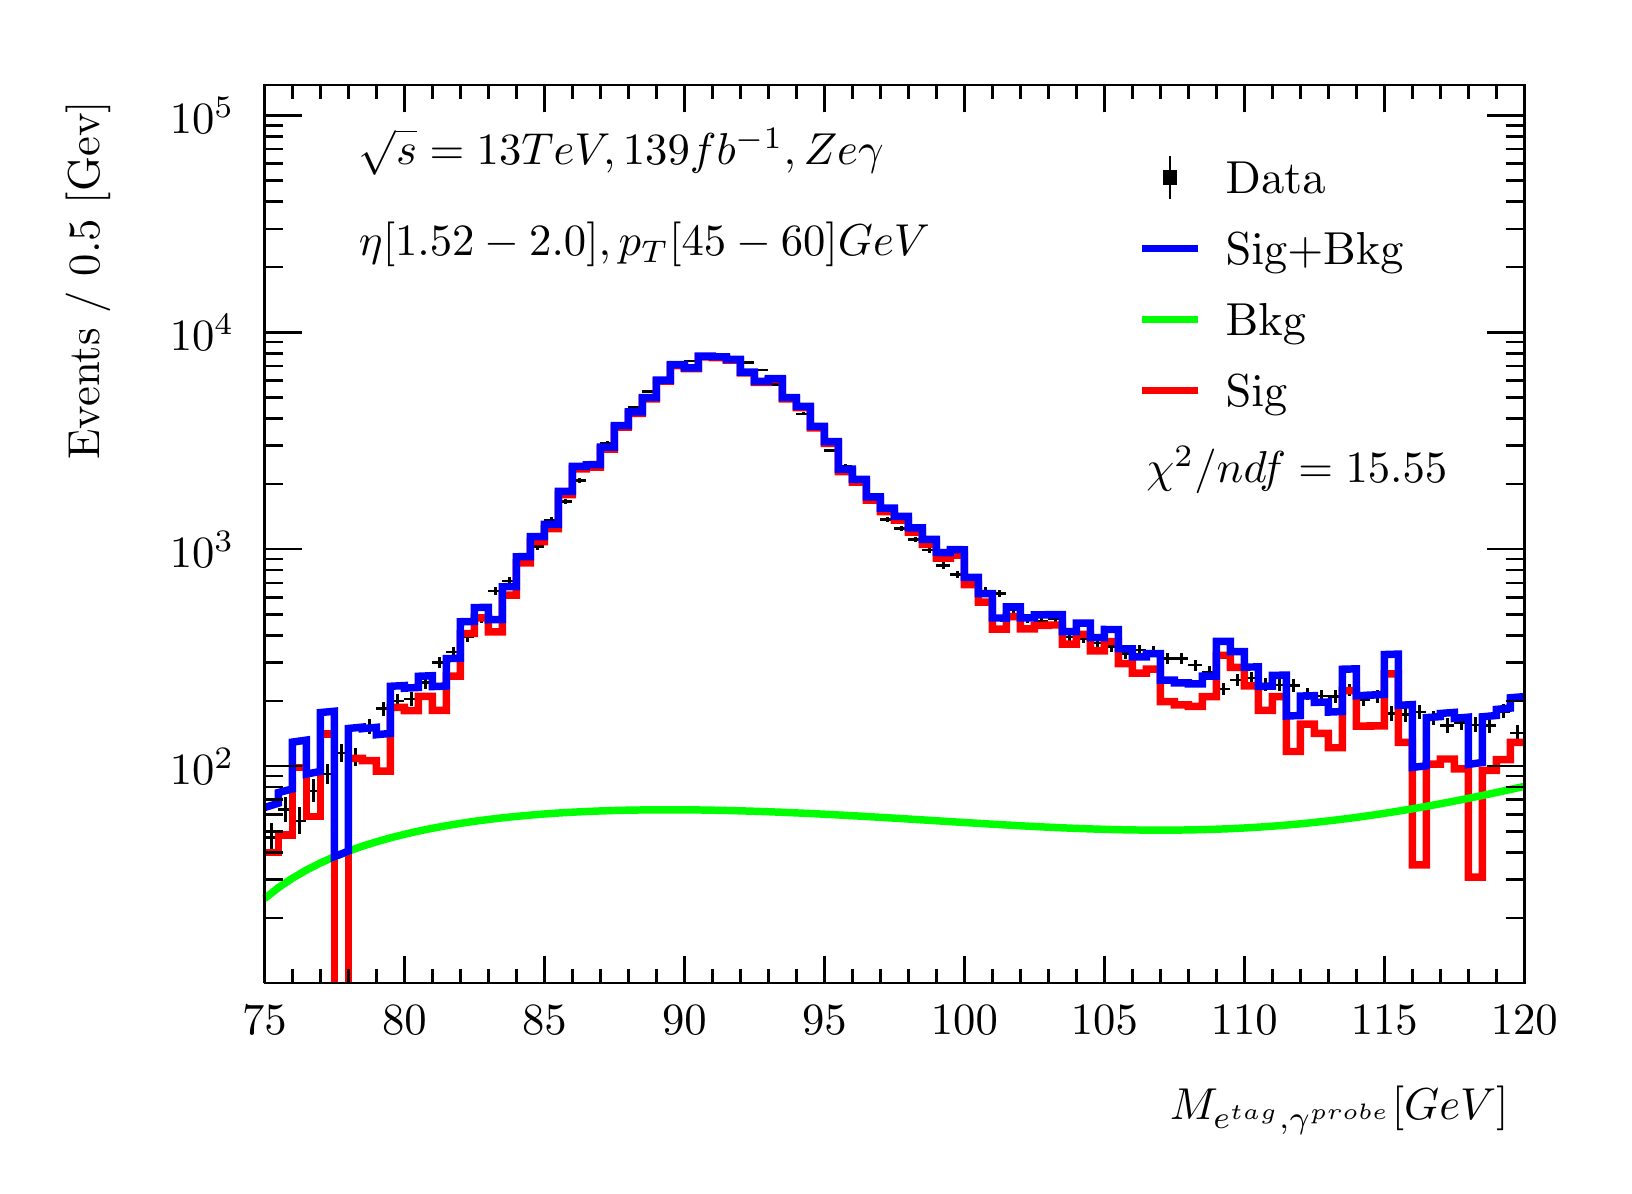
\begin{tikzpicture}
\pgfdeclareplotmark{cross} {
\pgfpathmoveto{\pgfpoint{-0.3\pgfplotmarksize}{\pgfplotmarksize}}
\pgfpathlineto{\pgfpoint{+0.3\pgfplotmarksize}{\pgfplotmarksize}}
\pgfpathlineto{\pgfpoint{+0.3\pgfplotmarksize}{0.3\pgfplotmarksize}}
\pgfpathlineto{\pgfpoint{+1\pgfplotmarksize}{0.3\pgfplotmarksize}}
\pgfpathlineto{\pgfpoint{+1\pgfplotmarksize}{-0.3\pgfplotmarksize}}
\pgfpathlineto{\pgfpoint{+0.3\pgfplotmarksize}{-0.3\pgfplotmarksize}}
\pgfpathlineto{\pgfpoint{+0.3\pgfplotmarksize}{-1.\pgfplotmarksize}}
\pgfpathlineto{\pgfpoint{-0.3\pgfplotmarksize}{-1.\pgfplotmarksize}}
\pgfpathlineto{\pgfpoint{-0.3\pgfplotmarksize}{-0.3\pgfplotmarksize}}
\pgfpathlineto{\pgfpoint{-1.\pgfplotmarksize}{-0.3\pgfplotmarksize}}
\pgfpathlineto{\pgfpoint{-1.\pgfplotmarksize}{0.3\pgfplotmarksize}}
\pgfpathlineto{\pgfpoint{-0.3\pgfplotmarksize}{0.3\pgfplotmarksize}}
\pgfpathclose
\pgfusepathqstroke
}
\pgfdeclareplotmark{cross*} {
\pgfpathmoveto{\pgfpoint{-0.3\pgfplotmarksize}{\pgfplotmarksize}}
\pgfpathlineto{\pgfpoint{+0.3\pgfplotmarksize}{\pgfplotmarksize}}
\pgfpathlineto{\pgfpoint{+0.3\pgfplotmarksize}{0.3\pgfplotmarksize}}
\pgfpathlineto{\pgfpoint{+1\pgfplotmarksize}{0.3\pgfplotmarksize}}
\pgfpathlineto{\pgfpoint{+1\pgfplotmarksize}{-0.3\pgfplotmarksize}}
\pgfpathlineto{\pgfpoint{+0.3\pgfplotmarksize}{-0.3\pgfplotmarksize}}
\pgfpathlineto{\pgfpoint{+0.3\pgfplotmarksize}{-1.\pgfplotmarksize}}
\pgfpathlineto{\pgfpoint{-0.3\pgfplotmarksize}{-1.\pgfplotmarksize}}
\pgfpathlineto{\pgfpoint{-0.3\pgfplotmarksize}{-0.3\pgfplotmarksize}}
\pgfpathlineto{\pgfpoint{-1.\pgfplotmarksize}{-0.3\pgfplotmarksize}}
\pgfpathlineto{\pgfpoint{-1.\pgfplotmarksize}{0.3\pgfplotmarksize}}
\pgfpathlineto{\pgfpoint{-0.3\pgfplotmarksize}{0.3\pgfplotmarksize}}
\pgfpathclose
\pgfusepathqfillstroke
}
\pgfdeclareplotmark{newstar} {
\pgfpathmoveto{\pgfqpoint{0pt}{\pgfplotmarksize}}
\pgfpathlineto{\pgfqpointpolar{44}{0.5\pgfplotmarksize}}
\pgfpathlineto{\pgfqpointpolar{18}{\pgfplotmarksize}}
\pgfpathlineto{\pgfqpointpolar{-20}{0.5\pgfplotmarksize}}
\pgfpathlineto{\pgfqpointpolar{-54}{\pgfplotmarksize}}
\pgfpathlineto{\pgfqpointpolar{-90}{0.5\pgfplotmarksize}}
\pgfpathlineto{\pgfqpointpolar{234}{\pgfplotmarksize}}
\pgfpathlineto{\pgfqpointpolar{198}{0.5\pgfplotmarksize}}
\pgfpathlineto{\pgfqpointpolar{162}{\pgfplotmarksize}}
\pgfpathlineto{\pgfqpointpolar{134}{0.5\pgfplotmarksize}}
\pgfpathclose
\pgfusepathqstroke
}
\pgfdeclareplotmark{newstar*} {
\pgfpathmoveto{\pgfqpoint{0pt}{\pgfplotmarksize}}
\pgfpathlineto{\pgfqpointpolar{44}{0.5\pgfplotmarksize}}
\pgfpathlineto{\pgfqpointpolar{18}{\pgfplotmarksize}}
\pgfpathlineto{\pgfqpointpolar{-20}{0.5\pgfplotmarksize}}
\pgfpathlineto{\pgfqpointpolar{-54}{\pgfplotmarksize}}
\pgfpathlineto{\pgfqpointpolar{-90}{0.5\pgfplotmarksize}}
\pgfpathlineto{\pgfqpointpolar{234}{\pgfplotmarksize}}
\pgfpathlineto{\pgfqpointpolar{198}{0.5\pgfplotmarksize}}
\pgfpathlineto{\pgfqpointpolar{162}{\pgfplotmarksize}}
\pgfpathlineto{\pgfqpointpolar{134}{0.5\pgfplotmarksize}}
\pgfpathclose
\pgfusepathqfillstroke
}
\definecolor{c}{rgb}{1,1,1};
\draw [color=c, fill=c] (0,0) rectangle (20,14.4361);
\draw [color=c, fill=c] (3,2.30977) rectangle (19,13.7143);
\definecolor{c}{rgb}{0,0,0};
\draw [c,line width=0.9] (3,2.30977) -- (3,13.7143) -- (19,13.7143) -- (19,2.30977) -- (3,2.30977);
\definecolor{c}{rgb}{1,1,1};
\draw [color=c, fill=c] (3,2.30977) rectangle (19,13.7143);
\definecolor{c}{rgb}{0,0,0};
\draw [c,line width=0.9] (3,2.30977) -- (3,13.7143) -- (19,13.7143) -- (19,2.30977) -- (3,2.30977);
\draw [c,line width=0.9] (3,2.30977) -- (19,2.30977);
\draw [c,line width=0.9] (3,2.65624) -- (3,2.30977);
\draw [c,line width=0.9] (3.35556,2.48301) -- (3.35556,2.30977);
\draw [c,line width=0.9] (3.71111,2.48301) -- (3.71111,2.30977);
\draw [c,line width=0.9] (4.06667,2.48301) -- (4.06667,2.30977);
\draw [c,line width=0.9] (4.42222,2.48301) -- (4.42222,2.30977);
\draw [c,line width=0.9] (4.77778,2.65624) -- (4.77778,2.30977);
\draw [c,line width=0.9] (5.13333,2.48301) -- (5.13333,2.30977);
\draw [c,line width=0.9] (5.48889,2.48301) -- (5.48889,2.30977);
\draw [c,line width=0.9] (5.84444,2.48301) -- (5.84444,2.30977);
\draw [c,line width=0.9] (6.2,2.48301) -- (6.2,2.30977);
\draw [c,line width=0.9] (6.55556,2.65624) -- (6.55556,2.30977);
\draw [c,line width=0.9] (6.91111,2.48301) -- (6.91111,2.30977);
\draw [c,line width=0.9] (7.26667,2.48301) -- (7.26667,2.30977);
\draw [c,line width=0.9] (7.62222,2.48301) -- (7.62222,2.30977);
\draw [c,line width=0.9] (7.97778,2.48301) -- (7.97778,2.30977);
\draw [c,line width=0.9] (8.33333,2.65624) -- (8.33333,2.30977);
\draw [c,line width=0.9] (8.68889,2.48301) -- (8.68889,2.30977);
\draw [c,line width=0.9] (9.04444,2.48301) -- (9.04444,2.30977);
\draw [c,line width=0.9] (9.4,2.48301) -- (9.4,2.30977);
\draw [c,line width=0.9] (9.75556,2.48301) -- (9.75556,2.30977);
\draw [c,line width=0.9] (10.1111,2.65624) -- (10.1111,2.30977);
\draw [c,line width=0.9] (10.4667,2.48301) -- (10.4667,2.30977);
\draw [c,line width=0.9] (10.8222,2.48301) -- (10.8222,2.30977);
\draw [c,line width=0.9] (11.1778,2.48301) -- (11.1778,2.30977);
\draw [c,line width=0.9] (11.5333,2.48301) -- (11.5333,2.30977);
\draw [c,line width=0.9] (11.8889,2.65624) -- (11.8889,2.30977);
\draw [c,line width=0.9] (12.2444,2.48301) -- (12.2444,2.30977);
\draw [c,line width=0.9] (12.6,2.48301) -- (12.6,2.30977);
\draw [c,line width=0.9] (12.9556,2.48301) -- (12.9556,2.30977);
\draw [c,line width=0.9] (13.3111,2.48301) -- (13.3111,2.30977);
\draw [c,line width=0.9] (13.6667,2.65624) -- (13.6667,2.30977);
\draw [c,line width=0.9] (14.0222,2.48301) -- (14.0222,2.30977);
\draw [c,line width=0.9] (14.3778,2.48301) -- (14.3778,2.30977);
\draw [c,line width=0.9] (14.7333,2.48301) -- (14.7333,2.30977);
\draw [c,line width=0.9] (15.0889,2.48301) -- (15.0889,2.30977);
\draw [c,line width=0.9] (15.4444,2.65624) -- (15.4444,2.30977);
\draw [c,line width=0.9] (15.8,2.48301) -- (15.8,2.30977);
\draw [c,line width=0.9] (16.1556,2.48301) -- (16.1556,2.30977);
\draw [c,line width=0.9] (16.5111,2.48301) -- (16.5111,2.30977);
\draw [c,line width=0.9] (16.8667,2.48301) -- (16.8667,2.30977);
\draw [c,line width=0.9] (17.2222,2.65624) -- (17.2222,2.30977);
\draw [c,line width=0.9] (17.5778,2.48301) -- (17.5778,2.30977);
\draw [c,line width=0.9] (17.9333,2.48301) -- (17.9333,2.30977);
\draw [c,line width=0.9] (18.2889,2.48301) -- (18.2889,2.30977);
\draw [c,line width=0.9] (18.6444,2.48301) -- (18.6444,2.30977);
\draw [c,line width=0.9] (19,2.65624) -- (19,2.30977);
\draw [c,line width=0.9] (19,2.65624) -- (19,2.30977);
\draw [anchor=base] (3,1.66015) node[scale=1.61424, color=c, rotate=0]{75};
\draw [anchor=base] (4.77778,1.66015) node[scale=1.61424, color=c, rotate=0]{80};
\draw [anchor=base] (6.55556,1.66015) node[scale=1.61424, color=c, rotate=0]{85};
\draw [anchor=base] (8.33333,1.66015) node[scale=1.61424, color=c, rotate=0]{90};
\draw [anchor=base] (10.1111,1.66015) node[scale=1.61424, color=c, rotate=0]{95};
\draw [anchor=base] (11.8889,1.66015) node[scale=1.61424, color=c, rotate=0]{100};
\draw [anchor=base] (13.6667,1.66015) node[scale=1.61424, color=c, rotate=0]{105};
\draw [anchor=base] (15.4444,1.66015) node[scale=1.61424, color=c, rotate=0]{110};
\draw [anchor=base] (17.2222,1.66015) node[scale=1.61424, color=c, rotate=0]{115};
\draw [anchor=base] (19,1.66015) node[scale=1.61424, color=c, rotate=0]{120};
\draw [anchor= east] (19,0.692932) node[scale=1.61424, color=c, rotate=0]{$M_{e^{tag}, \gamma^{probe}}  [GeV]$};
\draw [c,line width=0.9] (3,13.7143) -- (19,13.7143);
\draw [c,line width=0.9] (3,13.3678) -- (3,13.7143);
\draw [c,line width=0.9] (3.35556,13.5411) -- (3.35556,13.7143);
\draw [c,line width=0.9] (3.71111,13.5411) -- (3.71111,13.7143);
\draw [c,line width=0.9] (4.06667,13.5411) -- (4.06667,13.7143);
\draw [c,line width=0.9] (4.42222,13.5411) -- (4.42222,13.7143);
\draw [c,line width=0.9] (4.77778,13.3678) -- (4.77778,13.7143);
\draw [c,line width=0.9] (5.13333,13.5411) -- (5.13333,13.7143);
\draw [c,line width=0.9] (5.48889,13.5411) -- (5.48889,13.7143);
\draw [c,line width=0.9] (5.84444,13.5411) -- (5.84444,13.7143);
\draw [c,line width=0.9] (6.2,13.5411) -- (6.2,13.7143);
\draw [c,line width=0.9] (6.55556,13.3678) -- (6.55556,13.7143);
\draw [c,line width=0.9] (6.91111,13.5411) -- (6.91111,13.7143);
\draw [c,line width=0.9] (7.26667,13.5411) -- (7.26667,13.7143);
\draw [c,line width=0.9] (7.62222,13.5411) -- (7.62222,13.7143);
\draw [c,line width=0.9] (7.97778,13.5411) -- (7.97778,13.7143);
\draw [c,line width=0.9] (8.33333,13.3678) -- (8.33333,13.7143);
\draw [c,line width=0.9] (8.68889,13.5411) -- (8.68889,13.7143);
\draw [c,line width=0.9] (9.04444,13.5411) -- (9.04444,13.7143);
\draw [c,line width=0.9] (9.4,13.5411) -- (9.4,13.7143);
\draw [c,line width=0.9] (9.75556,13.5411) -- (9.75556,13.7143);
\draw [c,line width=0.9] (10.1111,13.3678) -- (10.1111,13.7143);
\draw [c,line width=0.9] (10.4667,13.5411) -- (10.4667,13.7143);
\draw [c,line width=0.9] (10.8222,13.5411) -- (10.8222,13.7143);
\draw [c,line width=0.9] (11.1778,13.5411) -- (11.1778,13.7143);
\draw [c,line width=0.9] (11.5333,13.5411) -- (11.5333,13.7143);
\draw [c,line width=0.9] (11.8889,13.3678) -- (11.8889,13.7143);
\draw [c,line width=0.9] (12.2444,13.5411) -- (12.2444,13.7143);
\draw [c,line width=0.9] (12.6,13.5411) -- (12.6,13.7143);
\draw [c,line width=0.9] (12.9556,13.5411) -- (12.9556,13.7143);
\draw [c,line width=0.9] (13.3111,13.5411) -- (13.3111,13.7143);
\draw [c,line width=0.9] (13.6667,13.3678) -- (13.6667,13.7143);
\draw [c,line width=0.9] (14.0222,13.5411) -- (14.0222,13.7143);
\draw [c,line width=0.9] (14.3778,13.5411) -- (14.3778,13.7143);
\draw [c,line width=0.9] (14.7333,13.5411) -- (14.7333,13.7143);
\draw [c,line width=0.9] (15.0889,13.5411) -- (15.0889,13.7143);
\draw [c,line width=0.9] (15.4444,13.3678) -- (15.4444,13.7143);
\draw [c,line width=0.9] (15.8,13.5411) -- (15.8,13.7143);
\draw [c,line width=0.9] (16.1556,13.5411) -- (16.1556,13.7143);
\draw [c,line width=0.9] (16.5111,13.5411) -- (16.5111,13.7143);
\draw [c,line width=0.9] (16.8667,13.5411) -- (16.8667,13.7143);
\draw [c,line width=0.9] (17.2222,13.3678) -- (17.2222,13.7143);
\draw [c,line width=0.9] (17.5778,13.5411) -- (17.5778,13.7143);
\draw [c,line width=0.9] (17.9333,13.5411) -- (17.9333,13.7143);
\draw [c,line width=0.9] (18.2889,13.5411) -- (18.2889,13.7143);
\draw [c,line width=0.9] (18.6444,13.5411) -- (18.6444,13.7143);
\draw [c,line width=0.9] (19,13.3678) -- (19,13.7143);
\draw [c,line width=0.9] (19,13.3678) -- (19,13.7143);
\draw [c,line width=0.9] (3,2.30977) -- (3,13.7143);
\draw [c,line width=0.9] (3.237,3.13907) -- (3,3.13907);
\draw [c,line width=0.9] (3.237,3.62418) -- (3,3.62418);
\draw [c,line width=0.9] (3.237,3.96837) -- (3,3.96837);
\draw [c,line width=0.9] (3.237,4.23535) -- (3,4.23535);
\draw [c,line width=0.9] (3.237,4.45348) -- (3,4.45348);
\draw [c,line width=0.9] (3.237,4.63791) -- (3,4.63791);
\draw [c,line width=0.9] (3.237,4.79767) -- (3,4.79767);
\draw [c,line width=0.9] (3.237,4.93859) -- (3,4.93859);
\draw [c,line width=0.9] (3.474,5.06465) -- (3,5.06465);
\draw [anchor= east] (2.82,5.06465) node[scale=1.61424, color=c, rotate=0]{$10^{2}$};
\draw [c,line width=0.9] (3.237,5.89394) -- (3,5.89394);
\draw [c,line width=0.9] (3.237,6.37905) -- (3,6.37905);
\draw [c,line width=0.9] (3.237,6.72324) -- (3,6.72324);
\draw [c,line width=0.9] (3.237,6.99022) -- (3,6.99022);
\draw [c,line width=0.9] (3.237,7.20835) -- (3,7.20835);
\draw [c,line width=0.9] (3.237,7.39278) -- (3,7.39278);
\draw [c,line width=0.9] (3.237,7.55254) -- (3,7.55254);
\draw [c,line width=0.9] (3.237,7.69346) -- (3,7.69346);
\draw [c,line width=0.9] (3.474,7.81952) -- (3,7.81952);
\draw [anchor= east] (2.82,7.81952) node[scale=1.61424, color=c, rotate=0]{$10^{3}$};
\draw [c,line width=0.9] (3.237,8.64882) -- (3,8.64882);
\draw [c,line width=0.9] (3.237,9.13393) -- (3,9.13393);
\draw [c,line width=0.9] (3.237,9.47812) -- (3,9.47812);
\draw [c,line width=0.9] (3.237,9.74509) -- (3,9.74509);
\draw [c,line width=0.9] (3.237,9.96323) -- (3,9.96323);
\draw [c,line width=0.9] (3.237,10.1477) -- (3,10.1477);
\draw [c,line width=0.9] (3.237,10.3074) -- (3,10.3074);
\draw [c,line width=0.9] (3.237,10.4483) -- (3,10.4483);
\draw [c,line width=0.9] (3.474,10.5744) -- (3,10.5744);
\draw [anchor= east] (2.82,10.5744) node[scale=1.61424, color=c, rotate=0]{$10^{4}$};
\draw [c,line width=0.9] (3.237,11.4037) -- (3,11.4037);
\draw [c,line width=0.9] (3.237,11.8888) -- (3,11.8888);
\draw [c,line width=0.9] (3.237,12.233) -- (3,12.233);
\draw [c,line width=0.9] (3.237,12.5) -- (3,12.5);
\draw [c,line width=0.9] (3.237,12.7181) -- (3,12.7181);
\draw [c,line width=0.9] (3.237,12.9025) -- (3,12.9025);
\draw [c,line width=0.9] (3.237,13.0623) -- (3,13.0623);
\draw [c,line width=0.9] (3.237,13.2032) -- (3,13.2032);
\draw [c,line width=0.9] (3.474,13.3293) -- (3,13.3293);
\draw [anchor= east] (2.82,13.3293) node[scale=1.61424, color=c, rotate=0]{$10^{5}$};
\draw [anchor= east] (0.76,13.7143) node[scale=1.61424, color=c, rotate=90]{Events / 0.5 [Gev]};
\draw [c,line width=0.9] (19,2.30977) -- (19,13.7143);
\draw [c,line width=0.9] (18.763,3.13907) -- (19,3.13907);
\draw [c,line width=0.9] (18.763,3.62418) -- (19,3.62418);
\draw [c,line width=0.9] (18.763,3.96837) -- (19,3.96837);
\draw [c,line width=0.9] (18.763,4.23535) -- (19,4.23535);
\draw [c,line width=0.9] (18.763,4.45348) -- (19,4.45348);
\draw [c,line width=0.9] (18.763,4.63791) -- (19,4.63791);
\draw [c,line width=0.9] (18.763,4.79767) -- (19,4.79767);
\draw [c,line width=0.9] (18.763,4.93859) -- (19,4.93859);
\draw [c,line width=0.9] (18.526,5.06465) -- (19,5.06465);
\draw [c,line width=0.9] (18.763,5.89394) -- (19,5.89394);
\draw [c,line width=0.9] (18.763,6.37905) -- (19,6.37905);
\draw [c,line width=0.9] (18.763,6.72324) -- (19,6.72324);
\draw [c,line width=0.9] (18.763,6.99022) -- (19,6.99022);
\draw [c,line width=0.9] (18.763,7.20835) -- (19,7.20835);
\draw [c,line width=0.9] (18.763,7.39278) -- (19,7.39278);
\draw [c,line width=0.9] (18.763,7.55254) -- (19,7.55254);
\draw [c,line width=0.9] (18.763,7.69346) -- (19,7.69346);
\draw [c,line width=0.9] (18.526,7.81952) -- (19,7.81952);
\draw [c,line width=0.9] (18.763,8.64882) -- (19,8.64882);
\draw [c,line width=0.9] (18.763,9.13393) -- (19,9.13393);
\draw [c,line width=0.9] (18.763,9.47812) -- (19,9.47812);
\draw [c,line width=0.9] (18.763,9.74509) -- (19,9.74509);
\draw [c,line width=0.9] (18.763,9.96323) -- (19,9.96323);
\draw [c,line width=0.9] (18.763,10.1477) -- (19,10.1477);
\draw [c,line width=0.9] (18.763,10.3074) -- (19,10.3074);
\draw [c,line width=0.9] (18.763,10.4483) -- (19,10.4483);
\draw [c,line width=0.9] (18.526,10.5744) -- (19,10.5744);
\draw [c,line width=0.9] (18.763,11.4037) -- (19,11.4037);
\draw [c,line width=0.9] (18.763,11.8888) -- (19,11.8888);
\draw [c,line width=0.9] (18.763,12.233) -- (19,12.233);
\draw [c,line width=0.9] (18.763,12.5) -- (19,12.5);
\draw [c,line width=0.9] (18.763,12.7181) -- (19,12.7181);
\draw [c,line width=0.9] (18.763,12.9025) -- (19,12.9025);
\draw [c,line width=0.9] (18.763,13.0623) -- (19,13.0623);
\draw [c,line width=0.9] (18.763,13.2032) -- (19,13.2032);
\draw [c,line width=0.9] (18.526,13.3293) -- (19,13.3293);
\draw [c,line width=0.9] (3.08889,4.16132) -- (3,4.16132);
\draw [c,line width=0.9] (3,4.16132) -- (3,4.16132);
\draw [c,line width=0.9] (3.08889,4.16132) -- (3.17778,4.16132);
\draw [c,line width=0.9] (3.17778,4.16132) -- (3.17778,4.16132);
\draw [c,line width=0.9] (3.08889,4.16132) -- (3.08889,4.3473);
\draw [c,line width=0.9] (3.08889,4.3473) -- (3.08889,4.3473);
\draw [c,line width=0.9] (3.08889,4.16132) -- (3.08889,3.97341);
\draw [c,line width=0.9] (3.08889,3.97341) -- (3.08889,3.97341);
\draw [c,line width=0.9] (3.26667,4.51186) -- (3.17778,4.51186);
\draw [c,line width=0.9] (3.17778,4.51186) -- (3.17778,4.51186);
\draw [c,line width=0.9] (3.26667,4.51186) -- (3.35556,4.51186);
\draw [c,line width=0.9] (3.35556,4.51186) -- (3.35556,4.51186);
\draw [c,line width=0.9] (3.26667,4.51186) -- (3.26667,4.67127);
\draw [c,line width=0.9] (3.26667,4.67127) -- (3.26667,4.67127);
\draw [c,line width=0.9] (3.26667,4.51186) -- (3.26667,4.3512);
\draw [c,line width=0.9] (3.26667,4.3512) -- (3.26667,4.3512);
\draw [c,line width=0.9] (3.44444,4.37094) -- (3.35556,4.37094);
\draw [c,line width=0.9] (3.35556,4.37094) -- (3.35556,4.37094);
\draw [c,line width=0.9] (3.44444,4.37094) -- (3.53333,4.37094);
\draw [c,line width=0.9] (3.53333,4.37094) -- (3.53333,4.37094);
\draw [c,line width=0.9] (3.44444,4.37094) -- (3.44444,4.54053);
\draw [c,line width=0.9] (3.44444,4.54053) -- (3.44444,4.54053);
\draw [c,line width=0.9] (3.44444,4.37094) -- (3.44444,4.19987);
\draw [c,line width=0.9] (3.44444,4.19987) -- (3.44444,4.19987);
\draw [c,line width=0.9] (3.62222,4.75194) -- (3.53333,4.75194);
\draw [c,line width=0.9] (3.53333,4.75194) -- (3.53333,4.75194);
\draw [c,line width=0.9] (3.62222,4.75194) -- (3.71111,4.75194);
\draw [c,line width=0.9] (3.71111,4.75194) -- (3.71111,4.75194);
\draw [c,line width=0.9] (3.62222,4.75194) -- (3.62222,4.89546);
\draw [c,line width=0.9] (3.62222,4.89546) -- (3.62222,4.89546);
\draw [c,line width=0.9] (3.62222,4.75194) -- (3.62222,4.60752);
\draw [c,line width=0.9] (3.62222,4.60752) -- (3.62222,4.60752);
\draw [c,line width=0.9] (3.8,4.96489) -- (3.71111,4.96489);
\draw [c,line width=0.9] (3.71111,4.96489) -- (3.71111,4.96489);
\draw [c,line width=0.9] (3.8,4.96489) -- (3.88889,4.96489);
\draw [c,line width=0.9] (3.88889,4.96489) -- (3.88889,4.96489);
\draw [c,line width=0.9] (3.8,4.96489) -- (3.8,5.09567);
\draw [c,line width=0.9] (3.8,5.09567) -- (3.8,5.09567);
\draw [c,line width=0.9] (3.8,4.96489) -- (3.8,4.83341);
\draw [c,line width=0.9] (3.8,4.83341) -- (3.8,4.83341);
\draw [c,line width=0.9] (3.97778,5.23186) -- (3.88889,5.23186);
\draw [c,line width=0.9] (3.88889,5.23186) -- (3.88889,5.23186);
\draw [c,line width=0.9] (3.97778,5.23186) -- (4.06667,5.23186);
\draw [c,line width=0.9] (4.06667,5.23186) -- (4.06667,5.23186);
\draw [c,line width=0.9] (3.97778,5.23186) -- (3.97778,5.34339);
\draw [c,line width=0.9] (3.97778,5.34339) -- (3.97778,5.34339);
\draw [c,line width=0.9] (3.97778,5.23186) -- (3.97778,5.12034);
\draw [c,line width=0.9] (3.97778,5.12034) -- (3.97778,5.12034);
\draw [c,line width=0.9] (4.15556,5.17868) -- (4.06667,5.17868);
\draw [c,line width=0.9] (4.06667,5.17868) -- (4.06667,5.17868);
\draw [c,line width=0.9] (4.15556,5.17868) -- (4.24444,5.17868);
\draw [c,line width=0.9] (4.24444,5.17868) -- (4.24444,5.17868);
\draw [c,line width=0.9] (4.15556,5.17868) -- (4.15556,5.29271);
\draw [c,line width=0.9] (4.15556,5.29271) -- (4.15556,5.29271);
\draw [c,line width=0.9] (4.15556,5.17868) -- (4.15556,5.06465);
\draw [c,line width=0.9] (4.15556,5.06465) -- (4.15556,5.06465);
\draw [c,line width=0.9] (4.33333,5.5656) -- (4.24444,5.5656);
\draw [c,line width=0.9] (4.24444,5.5656) -- (4.24444,5.5656);
\draw [c,line width=0.9] (4.33333,5.5656) -- (4.42222,5.5656);
\draw [c,line width=0.9] (4.42222,5.5656) -- (4.42222,5.5656);
\draw [c,line width=0.9] (4.33333,5.5656) -- (4.33333,5.66262);
\draw [c,line width=0.9] (4.33333,5.66262) -- (4.33333,5.66262);
\draw [c,line width=0.9] (4.33333,5.5656) -- (4.33333,5.46859);
\draw [c,line width=0.9] (4.33333,5.46859) -- (4.33333,5.46859);
\draw [c,line width=0.9] (4.51111,5.79419) -- (4.42222,5.79419);
\draw [c,line width=0.9] (4.42222,5.79419) -- (4.42222,5.79419);
\draw [c,line width=0.9] (4.51111,5.79419) -- (4.6,5.79419);
\draw [c,line width=0.9] (4.6,5.79419) -- (4.6,5.79419);
\draw [c,line width=0.9] (4.51111,5.79419) -- (4.51111,5.88237);
\draw [c,line width=0.9] (4.51111,5.88237) -- (4.51111,5.88237);
\draw [c,line width=0.9] (4.51111,5.79419) -- (4.51111,5.70601);
\draw [c,line width=0.9] (4.51111,5.70601) -- (4.51111,5.70601);
\draw [c,line width=0.9] (4.68889,5.89395) -- (4.6,5.89395);
\draw [c,line width=0.9] (4.6,5.89395) -- (4.6,5.89395);
\draw [c,line width=0.9] (4.68889,5.89395) -- (4.77778,5.89395);
\draw [c,line width=0.9] (4.77778,5.89395) -- (4.77778,5.89395);
\draw [c,line width=0.9] (4.68889,5.89395) -- (4.68889,5.97853);
\draw [c,line width=0.9] (4.68889,5.97853) -- (4.68889,5.97853);
\draw [c,line width=0.9] (4.68889,5.89395) -- (4.68889,5.80936);
\draw [c,line width=0.9] (4.68889,5.80936) -- (4.68889,5.80936);
\draw [c,line width=0.9] (4.86667,5.91764) -- (4.77778,5.91764);
\draw [c,line width=0.9] (4.77778,5.91764) -- (4.77778,5.91764);
\draw [c,line width=0.9] (4.86667,5.91764) -- (4.95556,5.91764);
\draw [c,line width=0.9] (4.95556,5.91764) -- (4.95556,5.91764);
\draw [c,line width=0.9] (4.86667,5.91764) -- (4.86667,6.00139);
\draw [c,line width=0.9] (4.86667,6.00139) -- (4.86667,6.00139);
\draw [c,line width=0.9] (4.86667,5.91764) -- (4.86667,5.83389);
\draw [c,line width=0.9] (4.86667,5.83389) -- (4.86667,5.83389);
\draw [c,line width=0.9] (5.04444,6.12694) -- (4.95556,6.12694);
\draw [c,line width=0.9] (4.95556,6.12694) -- (4.95556,6.12694);
\draw [c,line width=0.9] (5.04444,6.12694) -- (5.13333,6.12694);
\draw [c,line width=0.9] (5.13333,6.12694) -- (5.13333,6.12694);
\draw [c,line width=0.9] (5.04444,6.12694) -- (5.04444,6.20368);
\draw [c,line width=0.9] (5.04444,6.20368) -- (5.04444,6.20368);
\draw [c,line width=0.9] (5.04444,6.12694) -- (5.04444,6.05021);
\draw [c,line width=0.9] (5.04444,6.05021) -- (5.04444,6.05021);
\draw [c,line width=0.9] (5.22222,6.37906) -- (5.13333,6.37906);
\draw [c,line width=0.9] (5.13333,6.37906) -- (5.13333,6.37906);
\draw [c,line width=0.9] (5.22222,6.37906) -- (5.31111,6.37906);
\draw [c,line width=0.9] (5.31111,6.37906) -- (5.31111,6.37906);
\draw [c,line width=0.9] (5.22222,6.37906) -- (5.22222,6.44812);
\draw [c,line width=0.9] (5.22222,6.44812) -- (5.22222,6.44812);
\draw [c,line width=0.9] (5.22222,6.37906) -- (5.22222,6.30999);
\draw [c,line width=0.9] (5.22222,6.30999) -- (5.22222,6.30999);
\draw [c,line width=0.9] (5.4,6.51108) -- (5.31111,6.51108);
\draw [c,line width=0.9] (5.31111,6.51108) -- (5.31111,6.51108);
\draw [c,line width=0.9] (5.4,6.51108) -- (5.48889,6.51108);
\draw [c,line width=0.9] (5.48889,6.51108) -- (5.48889,6.51108);
\draw [c,line width=0.9] (5.4,6.51108) -- (5.4,6.57644);
\draw [c,line width=0.9] (5.4,6.57644) -- (5.4,6.57644);
\draw [c,line width=0.9] (5.4,6.51108) -- (5.4,6.44572);
\draw [c,line width=0.9] (5.4,6.44572) -- (5.4,6.44572);
\draw [c,line width=0.9] (5.57778,6.70516) -- (5.48889,6.70516);
\draw [c,line width=0.9] (5.48889,6.70516) -- (5.48889,6.70516);
\draw [c,line width=0.9] (5.57778,6.70516) -- (5.66667,6.70516);
\draw [c,line width=0.9] (5.66667,6.70516) -- (5.66667,6.70516);
\draw [c,line width=0.9] (5.57778,6.70516) -- (5.57778,6.76543);
\draw [c,line width=0.9] (5.57778,6.76543) -- (5.57778,6.76543);
\draw [c,line width=0.9] (5.57778,6.70516) -- (5.57778,6.6449);
\draw [c,line width=0.9] (5.57778,6.6449) -- (5.57778,6.6449);
\draw [c,line width=0.9] (5.75556,6.94138) -- (5.66667,6.94138);
\draw [c,line width=0.9] (5.66667,6.94138) -- (5.66667,6.94138);
\draw [c,line width=0.9] (5.75556,6.94138) -- (5.84444,6.94138);
\draw [c,line width=0.9] (5.84444,6.94138) -- (5.84444,6.94138);
\draw [c,line width=0.9] (5.75556,6.94138) -- (5.75556,6.99599);
\draw [c,line width=0.9] (5.75556,6.99599) -- (5.75556,6.99599);
\draw [c,line width=0.9] (5.75556,6.94138) -- (5.75556,6.88678);
\draw [c,line width=0.9] (5.75556,6.88678) -- (5.75556,6.88678);
\draw [c,line width=0.9] (5.93333,7.2893) -- (5.84444,7.2893);
\draw [c,line width=0.9] (5.84444,7.2893) -- (5.84444,7.2893);
\draw [c,line width=0.9] (5.93333,7.2893) -- (6.02222,7.2893);
\draw [c,line width=0.9] (6.02222,7.2893) -- (6.02222,7.2893);
\draw [c,line width=0.9] (5.93333,7.2893) -- (5.93333,7.33652);
\draw [c,line width=0.9] (5.93333,7.33652) -- (5.93333,7.33652);
\draw [c,line width=0.9] (5.93333,7.2893) -- (5.93333,7.24209);
\draw [c,line width=0.9] (5.93333,7.24209) -- (5.93333,7.24209);
\draw [c,line width=0.9] (6.11111,7.41648) -- (6.02222,7.41648);
\draw [c,line width=0.9] (6.02222,7.41648) -- (6.02222,7.41648);
\draw [c,line width=0.9] (6.11111,7.41648) -- (6.2,7.41648);
\draw [c,line width=0.9] (6.2,7.41648) -- (6.2,7.41648);
\draw [c,line width=0.9] (6.11111,7.41648) -- (6.11111,7.46125);
\draw [c,line width=0.9] (6.11111,7.46125) -- (6.11111,7.46125);
\draw [c,line width=0.9] (6.11111,7.41648) -- (6.11111,7.37171);
\draw [c,line width=0.9] (6.11111,7.37171) -- (6.11111,7.37171);
\draw [c,line width=0.9] (6.28889,7.65839) -- (6.2,7.65839);
\draw [c,line width=0.9] (6.2,7.65839) -- (6.2,7.65839);
\draw [c,line width=0.9] (6.28889,7.65839) -- (6.37778,7.65839);
\draw [c,line width=0.9] (6.37778,7.65839) -- (6.37778,7.65839);
\draw [c,line width=0.9] (6.28889,7.65839) -- (6.28889,7.69886);
\draw [c,line width=0.9] (6.28889,7.69886) -- (6.28889,7.69886);
\draw [c,line width=0.9] (6.28889,7.65839) -- (6.28889,7.61792);
\draw [c,line width=0.9] (6.28889,7.61792) -- (6.28889,7.61792);
\draw [c,line width=0.9] (6.46667,7.8514) -- (6.37778,7.8514);
\draw [c,line width=0.9] (6.37778,7.8514) -- (6.37778,7.8514);
\draw [c,line width=0.9] (6.46667,7.8514) -- (6.55556,7.8514);
\draw [c,line width=0.9] (6.55556,7.8514) -- (6.55556,7.8514);
\draw [c,line width=0.9] (6.46667,7.8514) -- (6.46667,7.88873);
\draw [c,line width=0.9] (6.46667,7.88873) -- (6.46667,7.88873);
\draw [c,line width=0.9] (6.46667,7.8514) -- (6.46667,7.81406);
\draw [c,line width=0.9] (6.46667,7.81406) -- (6.46667,7.81406);
\draw [c,line width=0.9] (6.64444,8.19004) -- (6.55556,8.19004);
\draw [c,line width=0.9] (6.55556,8.19004) -- (6.55556,8.19004);
\draw [c,line width=0.9] (6.64444,8.19004) -- (6.73333,8.19004);
\draw [c,line width=0.9] (6.73333,8.19004) -- (6.73333,8.19004);
\draw [c,line width=0.9] (6.64444,8.19004) -- (6.64444,8.22245);
\draw [c,line width=0.9] (6.64444,8.22245) -- (6.64444,8.22245);
\draw [c,line width=0.9] (6.64444,8.19004) -- (6.64444,8.15763);
\draw [c,line width=0.9] (6.64444,8.15763) -- (6.64444,8.15763);
\draw [c,line width=0.9] (6.82222,8.42373) -- (6.73333,8.42373);
\draw [c,line width=0.9] (6.73333,8.42373) -- (6.73333,8.42373);
\draw [c,line width=0.9] (6.82222,8.42373) -- (6.91111,8.42373);
\draw [c,line width=0.9] (6.91111,8.42373) -- (6.91111,8.42373);
\draw [c,line width=0.9] (6.82222,8.42373) -- (6.82222,8.45312);
\draw [c,line width=0.9] (6.82222,8.45312) -- (6.82222,8.45312);
\draw [c,line width=0.9] (6.82222,8.42373) -- (6.82222,8.39433);
\draw [c,line width=0.9] (6.82222,8.39433) -- (6.82222,8.39433);
\draw [c,line width=0.9] (7,8.69229) -- (6.91111,8.69229);
\draw [c,line width=0.9] (6.91111,8.69229) -- (6.91111,8.69229);
\draw [c,line width=0.9] (7,8.69229) -- (7.08889,8.69229);
\draw [c,line width=0.9] (7.08889,8.69229) -- (7.08889,8.69229);
\draw [c,line width=0.9] (7,8.69229) -- (7,8.71856);
\draw [c,line width=0.9] (7,8.71856) -- (7,8.71856);
\draw [c,line width=0.9] (7,8.69229) -- (7,8.66602);
\draw [c,line width=0.9] (7,8.66602) -- (7,8.66602);
\draw [c,line width=0.9] (7.17778,8.92009) -- (7.08889,8.92009);
\draw [c,line width=0.9] (7.08889,8.92009) -- (7.08889,8.92009);
\draw [c,line width=0.9] (7.17778,8.92009) -- (7.26667,8.92009);
\draw [c,line width=0.9] (7.26667,8.92009) -- (7.26667,8.92009);
\draw [c,line width=0.9] (7.17778,8.92009) -- (7.17778,8.94398);
\draw [c,line width=0.9] (7.17778,8.94398) -- (7.17778,8.94398);
\draw [c,line width=0.9] (7.17778,8.92009) -- (7.17778,8.89621);
\draw [c,line width=0.9] (7.17778,8.89621) -- (7.17778,8.89621);
\draw [c,line width=0.9] (7.35556,9.16697) -- (7.26667,9.16697);
\draw [c,line width=0.9] (7.26667,9.16697) -- (7.26667,9.16697);
\draw [c,line width=0.9] (7.35556,9.16697) -- (7.44444,9.16697);
\draw [c,line width=0.9] (7.44444,9.16697) -- (7.44444,9.16697);
\draw [c,line width=0.9] (7.35556,9.16697) -- (7.35556,9.18851);
\draw [c,line width=0.9] (7.35556,9.18851) -- (7.35556,9.18851);
\draw [c,line width=0.9] (7.35556,9.16697) -- (7.35556,9.14542);
\draw [c,line width=0.9] (7.35556,9.14542) -- (7.35556,9.14542);
\draw [c,line width=0.9] (7.53333,9.37998) -- (7.44444,9.37998);
\draw [c,line width=0.9] (7.44444,9.37998) -- (7.44444,9.37998);
\draw [c,line width=0.9] (7.53333,9.37998) -- (7.62222,9.37998);
\draw [c,line width=0.9] (7.62222,9.37998) -- (7.62222,9.37998);
\draw [c,line width=0.9] (7.53333,9.37998) -- (7.53333,9.39969);
\draw [c,line width=0.9] (7.53333,9.39969) -- (7.53333,9.39969);
\draw [c,line width=0.9] (7.53333,9.37998) -- (7.53333,9.36028);
\draw [c,line width=0.9] (7.53333,9.36028) -- (7.53333,9.36028);
\draw [c,line width=0.9] (7.71111,9.61771) -- (7.62222,9.61771);
\draw [c,line width=0.9] (7.62222,9.61771) -- (7.62222,9.61771);
\draw [c,line width=0.9] (7.71111,9.61771) -- (7.8,9.61771);
\draw [c,line width=0.9] (7.8,9.61771) -- (7.8,9.61771);
\draw [c,line width=0.9] (7.71111,9.61771) -- (7.71111,9.63555);
\draw [c,line width=0.9] (7.71111,9.63555) -- (7.71111,9.63555);
\draw [c,line width=0.9] (7.71111,9.61771) -- (7.71111,9.59986);
\draw [c,line width=0.9] (7.71111,9.59986) -- (7.71111,9.59986);
\draw [c,line width=0.9] (7.88889,9.82403) -- (7.8,9.82403);
\draw [c,line width=0.9] (7.8,9.82403) -- (7.8,9.82403);
\draw [c,line width=0.9] (7.88889,9.82403) -- (7.97778,9.82403);
\draw [c,line width=0.9] (7.97778,9.82403) -- (7.97778,9.82403);
\draw [c,line width=0.9] (7.88889,9.82403) -- (7.88889,9.8404);
\draw [c,line width=0.9] (7.88889,9.8404) -- (7.88889,9.8404);
\draw [c,line width=0.9] (7.88889,9.82403) -- (7.88889,9.80766);
\draw [c,line width=0.9] (7.88889,9.80766) -- (7.88889,9.80766);
\draw [c,line width=0.9] (8.06667,9.99374) -- (7.97778,9.99374);
\draw [c,line width=0.9] (7.97778,9.99374) -- (7.97778,9.99374);
\draw [c,line width=0.9] (8.06667,9.99374) -- (8.15556,9.99374);
\draw [c,line width=0.9] (8.15556,9.99374) -- (8.15556,9.99374);
\draw [c,line width=0.9] (8.06667,9.99374) -- (8.06667,10.009);
\draw [c,line width=0.9] (8.06667,10.009) -- (8.06667,10.009);
\draw [c,line width=0.9] (8.06667,9.99374) -- (8.06667,9.97849);
\draw [c,line width=0.9] (8.06667,9.97849) -- (8.06667,9.97849);
\draw [c,line width=0.9] (8.24444,10.1398) -- (8.15556,10.1398);
\draw [c,line width=0.9] (8.15556,10.1398) -- (8.15556,10.1398);
\draw [c,line width=0.9] (8.24444,10.1398) -- (8.33333,10.1398);
\draw [c,line width=0.9] (8.33333,10.1398) -- (8.33333,10.1398);
\draw [c,line width=0.9] (8.24444,10.1398) -- (8.24444,10.1541);
\draw [c,line width=0.9] (8.24444,10.1541) -- (8.24444,10.1541);
\draw [c,line width=0.9] (8.24444,10.1398) -- (8.24444,10.1254);
\draw [c,line width=0.9] (8.24444,10.1254) -- (8.24444,10.1254);
\draw [c,line width=0.9] (8.42222,10.2114) -- (8.33333,10.2114);
\draw [c,line width=0.9] (8.33333,10.2114) -- (8.33333,10.2114);
\draw [c,line width=0.9] (8.42222,10.2114) -- (8.51111,10.2114);
\draw [c,line width=0.9] (8.51111,10.2114) -- (8.51111,10.2114);
\draw [c,line width=0.9] (8.42222,10.2114) -- (8.42222,10.2253);
\draw [c,line width=0.9] (8.42222,10.2253) -- (8.42222,10.2253);
\draw [c,line width=0.9] (8.42222,10.2114) -- (8.42222,10.1975);
\draw [c,line width=0.9] (8.42222,10.1975) -- (8.42222,10.1975);
\draw [c,line width=0.9] (8.6,10.2731) -- (8.51111,10.2731);
\draw [c,line width=0.9] (8.51111,10.2731) -- (8.51111,10.2731);
\draw [c,line width=0.9] (8.6,10.2731) -- (8.68889,10.2731);
\draw [c,line width=0.9] (8.68889,10.2731) -- (8.68889,10.2731);
\draw [c,line width=0.9] (8.6,10.2731) -- (8.6,10.2867);
\draw [c,line width=0.9] (8.6,10.2867) -- (8.6,10.2867);
\draw [c,line width=0.9] (8.6,10.2731) -- (8.6,10.2596);
\draw [c,line width=0.9] (8.6,10.2596) -- (8.6,10.2596);
\draw [c,line width=0.9] (8.77778,10.2918) -- (8.68889,10.2918);
\draw [c,line width=0.9] (8.68889,10.2918) -- (8.68889,10.2918);
\draw [c,line width=0.9] (8.77778,10.2918) -- (8.86667,10.2918);
\draw [c,line width=0.9] (8.86667,10.2918) -- (8.86667,10.2918);
\draw [c,line width=0.9] (8.77778,10.2918) -- (8.77778,10.3052);
\draw [c,line width=0.9] (8.77778,10.3052) -- (8.77778,10.3052);
\draw [c,line width=0.9] (8.77778,10.2918) -- (8.77778,10.2783);
\draw [c,line width=0.9] (8.77778,10.2783) -- (8.77778,10.2783);
\draw [c,line width=0.9] (8.95556,10.2429) -- (8.86667,10.2429);
\draw [c,line width=0.9] (8.86667,10.2429) -- (8.86667,10.2429);
\draw [c,line width=0.9] (8.95556,10.2429) -- (9.04444,10.2429);
\draw [c,line width=0.9] (9.04444,10.2429) -- (9.04444,10.2429);
\draw [c,line width=0.9] (8.95556,10.2429) -- (8.95556,10.2566);
\draw [c,line width=0.9] (8.95556,10.2566) -- (8.95556,10.2566);
\draw [c,line width=0.9] (8.95556,10.2429) -- (8.95556,10.2292);
\draw [c,line width=0.9] (8.95556,10.2292) -- (8.95556,10.2292);
\draw [c,line width=0.9] (9.13333,10.189) -- (9.04444,10.189);
\draw [c,line width=0.9] (9.04444,10.189) -- (9.04444,10.189);
\draw [c,line width=0.9] (9.13333,10.189) -- (9.22222,10.189);
\draw [c,line width=0.9] (9.22222,10.189) -- (9.22222,10.189);
\draw [c,line width=0.9] (9.13333,10.189) -- (9.13333,10.203);
\draw [c,line width=0.9] (9.13333,10.203) -- (9.13333,10.203);
\draw [c,line width=0.9] (9.13333,10.189) -- (9.13333,10.1749);
\draw [c,line width=0.9] (9.13333,10.1749) -- (9.13333,10.1749);
\draw [c,line width=0.9] (9.31111,10.0949) -- (9.22222,10.0949);
\draw [c,line width=0.9] (9.22222,10.0949) -- (9.22222,10.0949);
\draw [c,line width=0.9] (9.31111,10.0949) -- (9.4,10.0949);
\draw [c,line width=0.9] (9.4,10.0949) -- (9.4,10.0949);
\draw [c,line width=0.9] (9.31111,10.0949) -- (9.31111,10.1095);
\draw [c,line width=0.9] (9.31111,10.1095) -- (9.31111,10.1095);
\draw [c,line width=0.9] (9.31111,10.0949) -- (9.31111,10.0803);
\draw [c,line width=0.9] (9.31111,10.0803) -- (9.31111,10.0803);
\draw [c,line width=0.9] (9.48889,9.91168) -- (9.4,9.91168);
\draw [c,line width=0.9] (9.4,9.91168) -- (9.4,9.91168);
\draw [c,line width=0.9] (9.48889,9.91168) -- (9.57778,9.91168);
\draw [c,line width=0.9] (9.57778,9.91168) -- (9.57778,9.91168);
\draw [c,line width=0.9] (9.48889,9.91168) -- (9.48889,9.92747);
\draw [c,line width=0.9] (9.48889,9.92747) -- (9.48889,9.92747);
\draw [c,line width=0.9] (9.48889,9.91168) -- (9.48889,9.8959);
\draw [c,line width=0.9] (9.48889,9.8959) -- (9.48889,9.8959);
\draw [c,line width=0.9] (9.66667,9.76361) -- (9.57778,9.76361);
\draw [c,line width=0.9] (9.57778,9.76361) -- (9.57778,9.76361);
\draw [c,line width=0.9] (9.66667,9.76361) -- (9.75556,9.76361);
\draw [c,line width=0.9] (9.75556,9.76361) -- (9.75556,9.76361);
\draw [c,line width=0.9] (9.66667,9.76361) -- (9.66667,9.7804);
\draw [c,line width=0.9] (9.66667,9.7804) -- (9.66667,9.7804);
\draw [c,line width=0.9] (9.66667,9.76361) -- (9.66667,9.74682);
\draw [c,line width=0.9] (9.66667,9.74682) -- (9.66667,9.74682);
\draw [c,line width=0.9] (9.84444,9.53877) -- (9.75556,9.53877);
\draw [c,line width=0.9] (9.75556,9.53877) -- (9.75556,9.53877);
\draw [c,line width=0.9] (9.84444,9.53877) -- (9.93333,9.53877);
\draw [c,line width=0.9] (9.93333,9.53877) -- (9.93333,9.53877);
\draw [c,line width=0.9] (9.84444,9.53877) -- (9.84444,9.55721);
\draw [c,line width=0.9] (9.84444,9.55721) -- (9.84444,9.55721);
\draw [c,line width=0.9] (9.84444,9.53877) -- (9.84444,9.52033);
\draw [c,line width=0.9] (9.84444,9.52033) -- (9.84444,9.52033);
\draw [c,line width=0.9] (10.0222,9.3387) -- (9.93333,9.3387);
\draw [c,line width=0.9] (9.93333,9.3387) -- (9.93333,9.3387);
\draw [c,line width=0.9] (10.0222,9.3387) -- (10.1111,9.3387);
\draw [c,line width=0.9] (10.1111,9.3387) -- (10.1111,9.3387);
\draw [c,line width=0.9] (10.0222,9.3387) -- (10.0222,9.35875);
\draw [c,line width=0.9] (10.0222,9.35875) -- (10.0222,9.35875);
\draw [c,line width=0.9] (10.0222,9.3387) -- (10.0222,9.31864);
\draw [c,line width=0.9] (10.0222,9.31864) -- (10.0222,9.31864);
\draw [c,line width=0.9] (10.2,9.07172) -- (10.1111,9.07172);
\draw [c,line width=0.9] (10.1111,9.07172) -- (10.1111,9.07172);
\draw [c,line width=0.9] (10.2,9.07172) -- (10.2889,9.07172);
\draw [c,line width=0.9] (10.2889,9.07172) -- (10.2889,9.07172);
\draw [c,line width=0.9] (10.2,9.07172) -- (10.2,9.09414);
\draw [c,line width=0.9] (10.2,9.09414) -- (10.2,9.09414);
\draw [c,line width=0.9] (10.2,9.07172) -- (10.2,9.0493);
\draw [c,line width=0.9] (10.2,9.0493) -- (10.2,9.0493);
\draw [c,line width=0.9] (10.3778,8.87094) -- (10.2889,8.87094);
\draw [c,line width=0.9] (10.2889,8.87094) -- (10.2889,8.87094);
\draw [c,line width=0.9] (10.3778,8.87094) -- (10.4667,8.87094);
\draw [c,line width=0.9] (10.4667,8.87094) -- (10.4667,8.87094);
\draw [c,line width=0.9] (10.3778,8.87094) -- (10.3778,8.89532);
\draw [c,line width=0.9] (10.3778,8.89532) -- (10.3778,8.89532);
\draw [c,line width=0.9] (10.3778,8.87094) -- (10.3778,8.84655);
\draw [c,line width=0.9] (10.3778,8.84655) -- (10.3778,8.84655);
\draw [c,line width=0.9] (10.5556,8.70148) -- (10.4667,8.70148);
\draw [c,line width=0.9] (10.4667,8.70148) -- (10.4667,8.70148);
\draw [c,line width=0.9] (10.5556,8.70148) -- (10.6444,8.70148);
\draw [c,line width=0.9] (10.6444,8.70148) -- (10.6444,8.70148);
\draw [c,line width=0.9] (10.5556,8.70148) -- (10.5556,8.72765);
\draw [c,line width=0.9] (10.5556,8.72765) -- (10.5556,8.72765);
\draw [c,line width=0.9] (10.5556,8.70148) -- (10.5556,8.67531);
\draw [c,line width=0.9] (10.5556,8.67531) -- (10.5556,8.67531);
\draw [c,line width=0.9] (10.7333,8.45719) -- (10.6444,8.45719);
\draw [c,line width=0.9] (10.6444,8.45719) -- (10.6444,8.45719);
\draw [c,line width=0.9] (10.7333,8.45719) -- (10.8222,8.45719);
\draw [c,line width=0.9] (10.8222,8.45719) -- (10.8222,8.45719);
\draw [c,line width=0.9] (10.7333,8.45719) -- (10.7333,8.48617);
\draw [c,line width=0.9] (10.7333,8.48617) -- (10.7333,8.48617);
\draw [c,line width=0.9] (10.7333,8.45719) -- (10.7333,8.42821);
\draw [c,line width=0.9] (10.7333,8.42821) -- (10.7333,8.42821);
\draw [c,line width=0.9] (10.9111,8.19529) -- (10.8222,8.19529);
\draw [c,line width=0.9] (10.8222,8.19529) -- (10.8222,8.19529);
\draw [c,line width=0.9] (10.9111,8.19529) -- (11,8.19529);
\draw [c,line width=0.9] (11,8.19529) -- (11,8.19529);
\draw [c,line width=0.9] (10.9111,8.19529) -- (10.9111,8.22763);
\draw [c,line width=0.9] (10.9111,8.22763) -- (10.9111,8.22763);
\draw [c,line width=0.9] (10.9111,8.19529) -- (10.9111,8.16296);
\draw [c,line width=0.9] (10.9111,8.16296) -- (10.9111,8.16296);
\draw [c,line width=0.9] (11.0889,8.08074) -- (11,8.08074);
\draw [c,line width=0.9] (11,8.08074) -- (11,8.08074);
\draw [c,line width=0.9] (11.0889,8.08074) -- (11.1778,8.08074);
\draw [c,line width=0.9] (11.1778,8.08074) -- (11.1778,8.08074);
\draw [c,line width=0.9] (11.0889,8.08074) -- (11.0889,8.11466);
\draw [c,line width=0.9] (11.0889,8.11466) -- (11.0889,8.11466);
\draw [c,line width=0.9] (11.0889,8.08074) -- (11.0889,8.04682);
\draw [c,line width=0.9] (11.0889,8.04682) -- (11.0889,8.04682);
\draw [c,line width=0.9] (11.2667,7.94114) -- (11.1778,7.94114);
\draw [c,line width=0.9] (11.1778,7.94114) -- (11.1778,7.94114);
\draw [c,line width=0.9] (11.2667,7.94114) -- (11.3556,7.94114);
\draw [c,line width=0.9] (11.3556,7.94114) -- (11.3556,7.94114);
\draw [c,line width=0.9] (11.2667,7.94114) -- (11.2667,7.9771);
\draw [c,line width=0.9] (11.2667,7.9771) -- (11.2667,7.9771);
\draw [c,line width=0.9] (11.2667,7.94114) -- (11.2667,7.90518);
\draw [c,line width=0.9] (11.2667,7.90518) -- (11.2667,7.90518);
\draw [c,line width=0.9] (11.4444,7.81232) -- (11.3556,7.81232);
\draw [c,line width=0.9] (11.3556,7.81232) -- (11.3556,7.81232);
\draw [c,line width=0.9] (11.4444,7.81232) -- (11.5333,7.81232);
\draw [c,line width=0.9] (11.5333,7.81232) -- (11.5333,7.81232);
\draw [c,line width=0.9] (11.4444,7.81232) -- (11.4444,7.85027);
\draw [c,line width=0.9] (11.4444,7.85027) -- (11.4444,7.85027);
\draw [c,line width=0.9] (11.4444,7.81232) -- (11.4444,7.77437);
\draw [c,line width=0.9] (11.4444,7.77437) -- (11.4444,7.77437);
\draw [c,line width=0.9] (11.6222,7.61518) -- (11.5333,7.61518);
\draw [c,line width=0.9] (11.5333,7.61518) -- (11.5333,7.61518);
\draw [c,line width=0.9] (11.6222,7.61518) -- (11.7111,7.61518);
\draw [c,line width=0.9] (11.7111,7.61518) -- (11.7111,7.61518);
\draw [c,line width=0.9] (11.6222,7.61518) -- (11.6222,7.65639);
\draw [c,line width=0.9] (11.6222,7.65639) -- (11.6222,7.65639);
\draw [c,line width=0.9] (11.6222,7.61518) -- (11.6222,7.57398);
\draw [c,line width=0.9] (11.6222,7.57398) -- (11.6222,7.57398);
\draw [c,line width=0.9] (11.8,7.49902) -- (11.7111,7.49902);
\draw [c,line width=0.9] (11.7111,7.49902) -- (11.7111,7.49902);
\draw [c,line width=0.9] (11.8,7.49902) -- (11.8889,7.49902);
\draw [c,line width=0.9] (11.8889,7.49902) -- (11.8889,7.49902);
\draw [c,line width=0.9] (11.8,7.49902) -- (11.8,7.54228);
\draw [c,line width=0.9] (11.8,7.54228) -- (11.8,7.54228);
\draw [c,line width=0.9] (11.8,7.49902) -- (11.8,7.45577);
\draw [c,line width=0.9] (11.8,7.45577) -- (11.8,7.45577);
\draw [c,line width=0.9] (11.9778,7.43477) -- (11.8889,7.43477);
\draw [c,line width=0.9] (11.8889,7.43477) -- (11.8889,7.43477);
\draw [c,line width=0.9] (11.9778,7.43477) -- (12.0667,7.43477);
\draw [c,line width=0.9] (12.0667,7.43477) -- (12.0667,7.43477);
\draw [c,line width=0.9] (11.9778,7.43477) -- (11.9778,7.4792);
\draw [c,line width=0.9] (11.9778,7.4792) -- (11.9778,7.4792);
\draw [c,line width=0.9] (11.9778,7.43477) -- (11.9778,7.39034);
\draw [c,line width=0.9] (11.9778,7.39034) -- (11.9778,7.39034);
\draw [c,line width=0.9] (12.1556,7.29117) -- (12.0667,7.29117);
\draw [c,line width=0.9] (12.0667,7.29117) -- (12.0667,7.29117);
\draw [c,line width=0.9] (12.1556,7.29117) -- (12.2444,7.29117);
\draw [c,line width=0.9] (12.2444,7.29117) -- (12.2444,7.29117);
\draw [c,line width=0.9] (12.1556,7.29117) -- (12.1556,7.33835);
\draw [c,line width=0.9] (12.1556,7.33835) -- (12.1556,7.33835);
\draw [c,line width=0.9] (12.1556,7.29117) -- (12.1556,7.24399);
\draw [c,line width=0.9] (12.1556,7.24399) -- (12.1556,7.24399);
\draw [c,line width=0.9] (12.3333,7.25528) -- (12.2444,7.25528);
\draw [c,line width=0.9] (12.2444,7.25528) -- (12.2444,7.25528);
\draw [c,line width=0.9] (12.3333,7.25528) -- (12.4222,7.25528);
\draw [c,line width=0.9] (12.4222,7.25528) -- (12.4222,7.25528);
\draw [c,line width=0.9] (12.3333,7.25528) -- (12.3333,7.30317);
\draw [c,line width=0.9] (12.3333,7.30317) -- (12.3333,7.30317);
\draw [c,line width=0.9] (12.3333,7.25528) -- (12.3333,7.20739);
\draw [c,line width=0.9] (12.3333,7.20739) -- (12.3333,7.20739);
\draw [c,line width=0.9] (12.5111,7.04859) -- (12.4222,7.04859);
\draw [c,line width=0.9] (12.4222,7.04859) -- (12.4222,7.04859);
\draw [c,line width=0.9] (12.5111,7.04859) -- (12.6,7.04859);
\draw [c,line width=0.9] (12.6,7.04859) -- (12.6,7.04859);
\draw [c,line width=0.9] (12.5111,7.04859) -- (12.5111,7.10081);
\draw [c,line width=0.9] (12.5111,7.10081) -- (12.5111,7.10081);
\draw [c,line width=0.9] (12.5111,7.04859) -- (12.5111,6.99638);
\draw [c,line width=0.9] (12.5111,6.99638) -- (12.5111,6.99638);
\draw [c,line width=0.9] (12.6889,6.93889) -- (12.6,6.93889);
\draw [c,line width=0.9] (12.6,6.93889) -- (12.6,6.93889);
\draw [c,line width=0.9] (12.6889,6.93889) -- (12.7778,6.93889);
\draw [c,line width=0.9] (12.7778,6.93889) -- (12.7778,6.93889);
\draw [c,line width=0.9] (12.6889,6.93889) -- (12.6889,6.99355);
\draw [c,line width=0.9] (12.6889,6.99355) -- (12.6889,6.99355);
\draw [c,line width=0.9] (12.6889,6.93889) -- (12.6889,6.88422);
\draw [c,line width=0.9] (12.6889,6.88422) -- (12.6889,6.88422);
\draw [c,line width=0.9] (12.8667,6.90597) -- (12.7778,6.90597);
\draw [c,line width=0.9] (12.7778,6.90597) -- (12.7778,6.90597);
\draw [c,line width=0.9] (12.8667,6.90597) -- (12.9556,6.90597);
\draw [c,line width=0.9] (12.9556,6.90597) -- (12.9556,6.90597);
\draw [c,line width=0.9] (12.8667,6.90597) -- (12.8667,6.96138);
\draw [c,line width=0.9] (12.8667,6.96138) -- (12.8667,6.96138);
\draw [c,line width=0.9] (12.8667,6.90597) -- (12.8667,6.85055);
\draw [c,line width=0.9] (12.8667,6.85055) -- (12.8667,6.85055);
\draw [c,line width=0.9] (13.0444,6.93639) -- (12.9556,6.93639);
\draw [c,line width=0.9] (12.9556,6.93639) -- (12.9556,6.93639);
\draw [c,line width=0.9] (13.0444,6.93639) -- (13.1333,6.93639);
\draw [c,line width=0.9] (13.1333,6.93639) -- (13.1333,6.93639);
\draw [c,line width=0.9] (13.0444,6.93639) -- (13.0444,6.9911);
\draw [c,line width=0.9] (13.0444,6.9911) -- (13.0444,6.9911);
\draw [c,line width=0.9] (13.0444,6.93639) -- (13.0444,6.88167);
\draw [c,line width=0.9] (13.0444,6.88167) -- (13.0444,6.88167);
\draw [c,line width=0.9] (13.2222,6.70212) -- (13.1333,6.70212);
\draw [c,line width=0.9] (13.1333,6.70212) -- (13.1333,6.70212);
\draw [c,line width=0.9] (13.2222,6.70212) -- (13.3111,6.70212);
\draw [c,line width=0.9] (13.3111,6.70212) -- (13.3111,6.70212);
\draw [c,line width=0.9] (13.2222,6.70212) -- (13.2222,6.76247);
\draw [c,line width=0.9] (13.2222,6.76247) -- (13.2222,6.76247);
\draw [c,line width=0.9] (13.2222,6.70212) -- (13.2222,6.64178);
\draw [c,line width=0.9] (13.2222,6.64178) -- (13.2222,6.64178);
\draw [c,line width=0.9] (13.4,6.6868) -- (13.3111,6.6868);
\draw [c,line width=0.9] (13.3111,6.6868) -- (13.3111,6.6868);
\draw [c,line width=0.9] (13.4,6.6868) -- (13.4889,6.6868);
\draw [c,line width=0.9] (13.4889,6.6868) -- (13.4889,6.6868);
\draw [c,line width=0.9] (13.4,6.6868) -- (13.4,6.74754);
\draw [c,line width=0.9] (13.4,6.74754) -- (13.4,6.74754);
\draw [c,line width=0.9] (13.4,6.6868) -- (13.4,6.62607);
\draw [c,line width=0.9] (13.4,6.62607) -- (13.4,6.62607);
\draw [c,line width=0.9] (13.5778,6.62673) -- (13.4889,6.62673);
\draw [c,line width=0.9] (13.4889,6.62673) -- (13.4889,6.62673);
\draw [c,line width=0.9] (13.5778,6.62673) -- (13.6667,6.62673);
\draw [c,line width=0.9] (13.6667,6.62673) -- (13.6667,6.62673);
\draw [c,line width=0.9] (13.5778,6.62673) -- (13.5778,6.68901);
\draw [c,line width=0.9] (13.5778,6.68901) -- (13.5778,6.68901);
\draw [c,line width=0.9] (13.5778,6.62673) -- (13.5778,6.56446);
\draw [c,line width=0.9] (13.5778,6.56446) -- (13.5778,6.56446);
\draw [c,line width=0.9] (13.7556,6.58382) -- (13.6667,6.58382);
\draw [c,line width=0.9] (13.6667,6.58382) -- (13.6667,6.58382);
\draw [c,line width=0.9] (13.7556,6.58382) -- (13.8444,6.58382);
\draw [c,line width=0.9] (13.8444,6.58382) -- (13.8444,6.58382);
\draw [c,line width=0.9] (13.7556,6.58382) -- (13.7556,6.64722);
\draw [c,line width=0.9] (13.7556,6.64722) -- (13.7556,6.64722);
\draw [c,line width=0.9] (13.7556,6.58382) -- (13.7556,6.52042);
\draw [c,line width=0.9] (13.7556,6.52042) -- (13.7556,6.52042);
\draw [c,line width=0.9] (13.9333,6.49309) -- (13.8444,6.49309);
\draw [c,line width=0.9] (13.8444,6.49309) -- (13.8444,6.49309);
\draw [c,line width=0.9] (13.9333,6.49309) -- (14.0222,6.49309);
\draw [c,line width=0.9] (14.0222,6.49309) -- (14.0222,6.49309);
\draw [c,line width=0.9] (13.9333,6.49309) -- (13.9333,6.55894);
\draw [c,line width=0.9] (13.9333,6.55894) -- (13.9333,6.55894);
\draw [c,line width=0.9] (13.9333,6.49309) -- (13.9333,6.42723);
\draw [c,line width=0.9] (13.9333,6.42723) -- (13.9333,6.42723);
\draw [c,line width=0.9] (14.1111,6.53931) -- (14.0222,6.53931);
\draw [c,line width=0.9] (14.0222,6.53931) -- (14.0222,6.53931);
\draw [c,line width=0.9] (14.1111,6.53931) -- (14.2,6.53931);
\draw [c,line width=0.9] (14.2,6.53931) -- (14.2,6.53931);
\draw [c,line width=0.9] (14.1111,6.53931) -- (14.1111,6.60391);
\draw [c,line width=0.9] (14.1111,6.60391) -- (14.1111,6.60391);
\draw [c,line width=0.9] (14.1111,6.53931) -- (14.1111,6.47472);
\draw [c,line width=0.9] (14.1111,6.47472) -- (14.1111,6.47472);
\draw [c,line width=0.9] (14.2889,6.52175) -- (14.2,6.52175);
\draw [c,line width=0.9] (14.2,6.52175) -- (14.2,6.52175);
\draw [c,line width=0.9] (14.2889,6.52175) -- (14.3778,6.52175);
\draw [c,line width=0.9] (14.3778,6.52175) -- (14.3778,6.52175);
\draw [c,line width=0.9] (14.2889,6.52175) -- (14.2889,6.58681);
\draw [c,line width=0.9] (14.2889,6.58681) -- (14.2889,6.58681);
\draw [c,line width=0.9] (14.2889,6.52175) -- (14.2889,6.45668);
\draw [c,line width=0.9] (14.2889,6.45668) -- (14.2889,6.45668);
\draw [c,line width=0.9] (14.4667,6.42981) -- (14.3778,6.42981);
\draw [c,line width=0.9] (14.3778,6.42981) -- (14.3778,6.42981);
\draw [c,line width=0.9] (14.4667,6.42981) -- (14.5556,6.42981);
\draw [c,line width=0.9] (14.5556,6.42981) -- (14.5556,6.42981);
\draw [c,line width=0.9] (14.4667,6.42981) -- (14.4667,6.49743);
\draw [c,line width=0.9] (14.4667,6.49743) -- (14.4667,6.49743);
\draw [c,line width=0.9] (14.4667,6.42981) -- (14.4667,6.36219);
\draw [c,line width=0.9] (14.4667,6.36219) -- (14.4667,6.36219);
\draw [c,line width=0.9] (14.6444,6.43363) -- (14.5556,6.43363);
\draw [c,line width=0.9] (14.5556,6.43363) -- (14.5556,6.43363);
\draw [c,line width=0.9] (14.6444,6.43363) -- (14.7333,6.43363);
\draw [c,line width=0.9] (14.7333,6.43363) -- (14.7333,6.43363);
\draw [c,line width=0.9] (14.6444,6.43363) -- (14.6444,6.50113);
\draw [c,line width=0.9] (14.6444,6.50113) -- (14.6444,6.50113);
\draw [c,line width=0.9] (14.6444,6.43363) -- (14.6444,6.36612);
\draw [c,line width=0.9] (14.6444,6.36612) -- (14.6444,6.36612);
\draw [c,line width=0.9] (14.8222,6.34672) -- (14.7333,6.34672);
\draw [c,line width=0.9] (14.7333,6.34672) -- (14.7333,6.34672);
\draw [c,line width=0.9] (14.8222,6.34672) -- (14.9111,6.34672);
\draw [c,line width=0.9] (14.9111,6.34672) -- (14.9111,6.34672);
\draw [c,line width=0.9] (14.8222,6.34672) -- (14.8222,6.41672);
\draw [c,line width=0.9] (14.8222,6.41672) -- (14.8222,6.41672);
\draw [c,line width=0.9] (14.8222,6.34672) -- (14.8222,6.27671);
\draw [c,line width=0.9] (14.8222,6.27671) -- (14.8222,6.27671);
\draw [c,line width=0.9] (15,6.25742) -- (14.9111,6.25742);
\draw [c,line width=0.9] (14.9111,6.25742) -- (14.9111,6.25742);
\draw [c,line width=0.9] (15,6.25742) -- (15.0889,6.25742);
\draw [c,line width=0.9] (15.0889,6.25742) -- (15.0889,6.25742);
\draw [c,line width=0.9] (15,6.25742) -- (15,6.33009);
\draw [c,line width=0.9] (15,6.33009) -- (15,6.33009);
\draw [c,line width=0.9] (15,6.25742) -- (15,6.18476);
\draw [c,line width=0.9] (15,6.18476) -- (15,6.18476);
\draw [c,line width=0.9] (15.1778,6.04545) -- (15.0889,6.04545);
\draw [c,line width=0.9] (15.0889,6.04545) -- (15.0889,6.04545);
\draw [c,line width=0.9] (15.1778,6.04545) -- (15.2667,6.04545);
\draw [c,line width=0.9] (15.2667,6.04545) -- (15.2667,6.04545);
\draw [c,line width=0.9] (15.1778,6.04545) -- (15.1778,6.12485);
\draw [c,line width=0.9] (15.1778,6.12485) -- (15.1778,6.12485);
\draw [c,line width=0.9] (15.1778,6.04545) -- (15.1778,5.96606);
\draw [c,line width=0.9] (15.1778,5.96606) -- (15.1778,5.96606);
\draw [c,line width=0.9] (15.3556,6.15613) -- (15.2667,6.15613);
\draw [c,line width=0.9] (15.2667,6.15613) -- (15.2667,6.15613);
\draw [c,line width=0.9] (15.3556,6.15613) -- (15.4444,6.15613);
\draw [c,line width=0.9] (15.4444,6.15613) -- (15.4444,6.15613);
\draw [c,line width=0.9] (15.3556,6.15613) -- (15.3556,6.23193);
\draw [c,line width=0.9] (15.3556,6.23193) -- (15.3556,6.23193);
\draw [c,line width=0.9] (15.3556,6.15613) -- (15.3556,6.08032);
\draw [c,line width=0.9] (15.3556,6.08032) -- (15.3556,6.08032);
\draw [c,line width=0.9] (15.5333,6.18461) -- (15.4444,6.18461);
\draw [c,line width=0.9] (15.4444,6.18461) -- (15.4444,6.18461);
\draw [c,line width=0.9] (15.5333,6.18461) -- (15.6222,6.18461);
\draw [c,line width=0.9] (15.6222,6.18461) -- (15.6222,6.18461);
\draw [c,line width=0.9] (15.5333,6.18461) -- (15.5333,6.25952);
\draw [c,line width=0.9] (15.5333,6.25952) -- (15.5333,6.25952);
\draw [c,line width=0.9] (15.5333,6.18461) -- (15.5333,6.1097);
\draw [c,line width=0.9] (15.5333,6.1097) -- (15.5333,6.1097);
\draw [c,line width=0.9] (15.7111,6.10207) -- (15.6222,6.10207);
\draw [c,line width=0.9] (15.6222,6.10207) -- (15.6222,6.10207);
\draw [c,line width=0.9] (15.7111,6.10207) -- (15.8,6.10207);
\draw [c,line width=0.9] (15.8,6.10207) -- (15.8,6.10207);
\draw [c,line width=0.9] (15.7111,6.10207) -- (15.7111,6.17961);
\draw [c,line width=0.9] (15.7111,6.17961) -- (15.7111,6.17961);
\draw [c,line width=0.9] (15.7111,6.10207) -- (15.7111,6.02453);
\draw [c,line width=0.9] (15.7111,6.02453) -- (15.7111,6.02453);
\draw [c,line width=0.9] (15.8889,6.09197) -- (15.8,6.09197);
\draw [c,line width=0.9] (15.8,6.09197) -- (15.8,6.09197);
\draw [c,line width=0.9] (15.8889,6.09197) -- (15.9778,6.09197);
\draw [c,line width=0.9] (15.9778,6.09197) -- (15.9778,6.09197);
\draw [c,line width=0.9] (15.8889,6.09197) -- (15.8889,6.16984);
\draw [c,line width=0.9] (15.8889,6.16984) -- (15.8889,6.16984);
\draw [c,line width=0.9] (15.8889,6.09197) -- (15.8889,6.01411);
\draw [c,line width=0.9] (15.8889,6.01411) -- (15.8889,6.01411);
\draw [c,line width=0.9] (16.0667,6.08689) -- (15.9778,6.08689);
\draw [c,line width=0.9] (15.9778,6.08689) -- (15.9778,6.08689);
\draw [c,line width=0.9] (16.0667,6.08689) -- (16.1556,6.08689);
\draw [c,line width=0.9] (16.1556,6.08689) -- (16.1556,6.08689);
\draw [c,line width=0.9] (16.0667,6.08689) -- (16.0667,6.16492);
\draw [c,line width=0.9] (16.0667,6.16492) -- (16.0667,6.16492);
\draw [c,line width=0.9] (16.0667,6.08689) -- (16.0667,6.00886);
\draw [c,line width=0.9] (16.0667,6.00886) -- (16.0667,6.00886);
\draw [c,line width=0.9] (16.2444,5.98047) -- (16.1556,5.98047);
\draw [c,line width=0.9] (16.1556,5.98047) -- (16.1556,5.98047);
\draw [c,line width=0.9] (16.2444,5.98047) -- (16.3333,5.98047);
\draw [c,line width=0.9] (16.3333,5.98047) -- (16.3333,5.98047);
\draw [c,line width=0.9] (16.2444,5.98047) -- (16.2444,6.06205);
\draw [c,line width=0.9] (16.2444,6.06205) -- (16.2444,6.06205);
\draw [c,line width=0.9] (16.2444,5.98047) -- (16.2444,5.89889);
\draw [c,line width=0.9] (16.2444,5.89889) -- (16.2444,5.89889);
\draw [c,line width=0.9] (16.4222,5.95232) -- (16.3333,5.95232);
\draw [c,line width=0.9] (16.3333,5.95232) -- (16.3333,5.95232);
\draw [c,line width=0.9] (16.4222,5.95232) -- (16.5111,5.95232);
\draw [c,line width=0.9] (16.5111,5.95232) -- (16.5111,5.95232);
\draw [c,line width=0.9] (16.4222,5.95232) -- (16.4222,6.03487);
\draw [c,line width=0.9] (16.4222,6.03487) -- (16.4222,6.03487);
\draw [c,line width=0.9] (16.4222,5.95232) -- (16.4222,5.86978);
\draw [c,line width=0.9] (16.4222,5.86978) -- (16.4222,5.86978);
\draw [c,line width=0.9] (16.6,5.94661) -- (16.5111,5.94661);
\draw [c,line width=0.9] (16.5111,5.94661) -- (16.5111,5.94661);
\draw [c,line width=0.9] (16.6,5.94661) -- (16.6889,5.94661);
\draw [c,line width=0.9] (16.6889,5.94661) -- (16.6889,5.94661);
\draw [c,line width=0.9] (16.6,5.94661) -- (16.6,6.02935);
\draw [c,line width=0.9] (16.6,6.02935) -- (16.6,6.02935);
\draw [c,line width=0.9] (16.6,5.94661) -- (16.6,5.86387);
\draw [c,line width=0.9] (16.6,5.86387) -- (16.6,5.86387);
\draw [c,line width=0.9] (16.7778,6.02954) -- (16.6889,6.02954);
\draw [c,line width=0.9] (16.6889,6.02954) -- (16.6889,6.02954);
\draw [c,line width=0.9] (16.7778,6.02954) -- (16.8667,6.02954);
\draw [c,line width=0.9] (16.8667,6.02954) -- (16.8667,6.02954);
\draw [c,line width=0.9] (16.7778,6.02954) -- (16.7778,6.10946);
\draw [c,line width=0.9] (16.7778,6.10946) -- (16.7778,6.10946);
\draw [c,line width=0.9] (16.7778,6.02954) -- (16.7778,5.94961);
\draw [c,line width=0.9] (16.7778,5.94961) -- (16.7778,5.94961);
\draw [c,line width=0.9] (16.9556,5.91176) -- (16.8667,5.91176);
\draw [c,line width=0.9] (16.8667,5.91176) -- (16.8667,5.91176);
\draw [c,line width=0.9] (16.9556,5.91176) -- (17.0444,5.91176);
\draw [c,line width=0.9] (17.0444,5.91176) -- (17.0444,5.91176);
\draw [c,line width=0.9] (16.9556,5.91176) -- (16.9556,5.99572);
\draw [c,line width=0.9] (16.9556,5.99572) -- (16.9556,5.99572);
\draw [c,line width=0.9] (16.9556,5.91176) -- (16.9556,5.8278);
\draw [c,line width=0.9] (16.9556,5.8278) -- (16.9556,5.8278);
\draw [c,line width=0.9] (17.1333,5.95232) -- (17.0444,5.95232);
\draw [c,line width=0.9] (17.0444,5.95232) -- (17.0444,5.95232);
\draw [c,line width=0.9] (17.1333,5.95232) -- (17.2222,5.95232);
\draw [c,line width=0.9] (17.2222,5.95232) -- (17.2222,5.95232);
\draw [c,line width=0.9] (17.1333,5.95232) -- (17.1333,6.03487);
\draw [c,line width=0.9] (17.1333,6.03487) -- (17.1333,6.03487);
\draw [c,line width=0.9] (17.1333,5.95232) -- (17.1333,5.86978);
\draw [c,line width=0.9] (17.1333,5.86978) -- (17.1333,5.86978);
\draw [c,line width=0.9] (17.3111,5.73419) -- (17.2222,5.73419);
\draw [c,line width=0.9] (17.2222,5.73419) -- (17.2222,5.73419);
\draw [c,line width=0.9] (17.3111,5.73419) -- (17.4,5.73419);
\draw [c,line width=0.9] (17.4,5.73419) -- (17.4,5.73419);
\draw [c,line width=0.9] (17.3111,5.73419) -- (17.3111,5.82461);
\draw [c,line width=0.9] (17.3111,5.82461) -- (17.3111,5.82461);
\draw [c,line width=0.9] (17.3111,5.73419) -- (17.3111,5.64377);
\draw [c,line width=0.9] (17.3111,5.64377) -- (17.3111,5.64377);
\draw [c,line width=0.9] (17.4889,5.72043) -- (17.4,5.72043);
\draw [c,line width=0.9] (17.4,5.72043) -- (17.4,5.72043);
\draw [c,line width=0.9] (17.4889,5.72043) -- (17.5778,5.72043);
\draw [c,line width=0.9] (17.5778,5.72043) -- (17.5778,5.72043);
\draw [c,line width=0.9] (17.4889,5.72043) -- (17.4889,5.81137);
\draw [c,line width=0.9] (17.4889,5.81137) -- (17.4889,5.81137);
\draw [c,line width=0.9] (17.4889,5.72043) -- (17.4889,5.62949);
\draw [c,line width=0.9] (17.4889,5.62949) -- (17.4889,5.62949);
\draw [c,line width=0.9] (17.6667,5.75452) -- (17.5778,5.75452);
\draw [c,line width=0.9] (17.5778,5.75452) -- (17.5778,5.75452);
\draw [c,line width=0.9] (17.6667,5.75452) -- (17.7556,5.75452);
\draw [c,line width=0.9] (17.7556,5.75452) -- (17.7556,5.75452);
\draw [c,line width=0.9] (17.6667,5.75452) -- (17.6667,5.84418);
\draw [c,line width=0.9] (17.6667,5.84418) -- (17.6667,5.84418);
\draw [c,line width=0.9] (17.6667,5.75452) -- (17.6667,5.66487);
\draw [c,line width=0.9] (17.6667,5.66487) -- (17.6667,5.66487);
\draw [c,line width=0.9] (17.8444,5.6782) -- (17.7556,5.6782);
\draw [c,line width=0.9] (17.7556,5.6782) -- (17.7556,5.6782);
\draw [c,line width=0.9] (17.8444,5.6782) -- (17.9333,5.6782);
\draw [c,line width=0.9] (17.9333,5.6782) -- (17.9333,5.6782);
\draw [c,line width=0.9] (17.8444,5.6782) -- (17.8444,5.77076);
\draw [c,line width=0.9] (17.8444,5.77076) -- (17.8444,5.77076);
\draw [c,line width=0.9] (17.8444,5.6782) -- (17.8444,5.58564);
\draw [c,line width=0.9] (17.8444,5.58564) -- (17.8444,5.58564);
\draw [c,line width=0.9] (18.0222,5.58124) -- (17.9333,5.58124);
\draw [c,line width=0.9] (17.9333,5.58124) -- (17.9333,5.58124);
\draw [c,line width=0.9] (18.0222,5.58124) -- (18.1111,5.58124);
\draw [c,line width=0.9] (18.1111,5.58124) -- (18.1111,5.58124);
\draw [c,line width=0.9] (18.0222,5.58124) -- (18.0222,5.67763);
\draw [c,line width=0.9] (18.0222,5.67763) -- (18.0222,5.67763);
\draw [c,line width=0.9] (18.0222,5.58124) -- (18.0222,5.48486);
\draw [c,line width=0.9] (18.0222,5.48486) -- (18.0222,5.48486);
\draw [c,line width=0.9] (18.2,5.61947) -- (18.1111,5.61947);
\draw [c,line width=0.9] (18.1111,5.61947) -- (18.1111,5.61947);
\draw [c,line width=0.9] (18.2,5.61947) -- (18.2889,5.61947);
\draw [c,line width=0.9] (18.2889,5.61947) -- (18.2889,5.61947);
\draw [c,line width=0.9] (18.2,5.61947) -- (18.2,5.71433);
\draw [c,line width=0.9] (18.2,5.71433) -- (18.2,5.71433);
\draw [c,line width=0.9] (18.2,5.61947) -- (18.2,5.52461);
\draw [c,line width=0.9] (18.2,5.52461) -- (18.2,5.52461);
\draw [c,line width=0.9] (18.3778,5.58899) -- (18.2889,5.58899);
\draw [c,line width=0.9] (18.2889,5.58899) -- (18.2889,5.58899);
\draw [c,line width=0.9] (18.3778,5.58899) -- (18.4667,5.58899);
\draw [c,line width=0.9] (18.4667,5.58899) -- (18.4667,5.58899);
\draw [c,line width=0.9] (18.3778,5.58899) -- (18.3778,5.68506);
\draw [c,line width=0.9] (18.3778,5.68506) -- (18.3778,5.68506);
\draw [c,line width=0.9] (18.3778,5.58899) -- (18.3778,5.49291);
\draw [c,line width=0.9] (18.3778,5.49291) -- (18.3778,5.49291);
\draw [c,line width=0.9] (18.5556,5.58124) -- (18.4667,5.58124);
\draw [c,line width=0.9] (18.4667,5.58124) -- (18.4667,5.58124);
\draw [c,line width=0.9] (18.5556,5.58124) -- (18.6444,5.58124);
\draw [c,line width=0.9] (18.6444,5.58124) -- (18.6444,5.58124);
\draw [c,line width=0.9] (18.5556,5.58124) -- (18.5556,5.67763);
\draw [c,line width=0.9] (18.5556,5.67763) -- (18.5556,5.67763);
\draw [c,line width=0.9] (18.5556,5.58124) -- (18.5556,5.48486);
\draw [c,line width=0.9] (18.5556,5.48486) -- (18.5556,5.48486);
\draw [c,line width=0.9] (18.7333,5.76123) -- (18.6444,5.76123);
\draw [c,line width=0.9] (18.6444,5.76123) -- (18.6444,5.76123);
\draw [c,line width=0.9] (18.7333,5.76123) -- (18.8222,5.76123);
\draw [c,line width=0.9] (18.8222,5.76123) -- (18.8222,5.76123);
\draw [c,line width=0.9] (18.7333,5.76123) -- (18.7333,5.85063);
\draw [c,line width=0.9] (18.7333,5.85063) -- (18.7333,5.85063);
\draw [c,line width=0.9] (18.7333,5.76123) -- (18.7333,5.67182);
\draw [c,line width=0.9] (18.7333,5.67182) -- (18.7333,5.67182);
\draw [c,line width=0.9] (18.9111,5.48418) -- (18.8222,5.48418);
\draw [c,line width=0.9] (18.8222,5.48418) -- (18.8222,5.48418);
\draw [c,line width=0.9] (18.9111,5.48418) -- (19,5.48418);
\draw [c,line width=0.9] (19,5.48418) -- (19,5.48418);
\draw [c,line width=0.9] (18.9111,5.48418) -- (18.9111,5.58455);
\draw [c,line width=0.9] (18.9111,5.58455) -- (18.9111,5.58455);
\draw [c,line width=0.9] (18.9111,5.48418) -- (18.9111,5.38381);
\draw [c,line width=0.9] (18.9111,5.38381) -- (18.9111,5.38381);
\foreach \P in {(3.08889,4.16132), (3.26667,4.51186), (3.44444,4.37094), (3.62222,4.75194), (3.8,4.96489), (3.97778,5.23186), (4.15556,5.17868), (4.33333,5.5656), (4.51111,5.79419), (4.68889,5.89395), (4.86667,5.91764), (5.04444,6.12694),
 (5.22222,6.37906), (5.4,6.51108), (5.57778,6.70516), (5.75556,6.94138), (5.93333,7.2893), (6.11111,7.41648), (6.28889,7.65839), (6.46667,7.8514), (6.64444,8.19004), (6.82222,8.42373), (7,8.69229), (7.17778,8.92009), (7.35556,9.16697),
 (7.53333,9.37998), (7.71111,9.61771), (7.88889,9.82403), (8.06667,9.99374), (8.24444,10.1398), (8.42222,10.2114), (8.6,10.2731), (8.77778,10.2918), (8.95556,10.2429), (9.13333,10.189), (9.31111,10.0949), (9.48889,9.91168), (9.66667,9.76361),
 (9.84444,9.53877), (10.0222,9.3387), (10.2,9.07172), (10.3778,8.87094), (10.5556,8.70148), (10.7333,8.45719), (10.9111,8.19529), (11.0889,8.08074), (11.2667,7.94114), (11.4444,7.81232), (11.6222,7.61518), (11.8,7.49902), (11.9778,7.43477),
 (12.1556,7.29117), (12.3333,7.25528), (12.5111,7.04859), (12.6889,6.93889), (12.8667,6.90597), (13.0444,6.93639), (13.2222,6.70212), (13.4,6.6868), (13.5778,6.62673), (13.7556,6.58382), (13.9333,6.49309), (14.1111,6.53931), (14.2889,6.52175),
 (14.4667,6.42981), (14.6444,6.43363), (14.8222,6.34672), (15,6.25742), (15.1778,6.04545), (15.3556,6.15613), (15.5333,6.18461), (15.7111,6.10207), (15.8889,6.09197), (16.0667,6.08689), (16.2444,5.98047), (16.4222,5.95232), (16.6,5.94661),
 (16.7778,6.02954), (16.9556,5.91176), (17.1333,5.95232), (17.3111,5.73419), (17.4889,5.72043), (17.6667,5.75452), (17.8444,5.6782), (18.0222,5.58124), (18.2,5.61947), (18.3778,5.58899), (18.5556,5.58124), (18.7333,5.76123),
 (18.9111,5.48418)}{\draw[mark options={color=c,fill=c},mark size=2.882883pt,mark=] plot coordinates {\P};}
\definecolor{c}{rgb}{1,0,0};
\draw [c,line width=2.7] (3,3.96635) -- (3,3.96635);
\draw [c,line width=2.7] (3,3.96635) -- (3,3.96635) -- (3.17778,3.96635) -- (3.17778,4.18776) -- (3.35556,4.18776) -- (3.35556,5.04817) -- (3.53333,5.04817) -- (3.53333,4.42803) -- (3.71111,4.42803) -- (3.71111,5.47429) -- (3.88889,5.47429) --
 (3.88889,2.30977);
\draw [c,line width=2.7] (4.06667,2.30977) -- (4.06667,5.16334);
\draw [c,line width=2.7] (4.06667,5.16334) -- (4.24444,5.16334) -- (4.24444,5.13562) -- (4.42222,5.13562) -- (4.42222,5.00083) -- (4.6,5.00083) -- (4.6,5.8117) -- (4.77778,5.8117) -- (4.77778,5.76959) -- (4.95556,5.76959) -- (4.95556,5.94918) --
 (5.13333,5.94918) -- (5.13333,5.77384) -- (5.31111,5.77384) -- (5.31111,6.20714) -- (5.48889,6.20714) -- (5.48889,6.74895) -- (5.66667,6.74895) -- (5.66667,6.9479) -- (5.84444,6.9479) -- (5.84444,6.77088) -- (6.02222,6.77088) -- (6.02222,7.23518) --
 (6.2,7.23518) -- (6.2,7.64522) -- (6.37778,7.64522) -- (6.37778,7.91436) -- (6.55556,7.91436) -- (6.55556,8.07919) -- (6.73333,8.07919) -- (6.73333,8.51415) -- (6.91111,8.51415) -- (6.91111,8.83992) -- (7.08889,8.83992) -- (7.08889,8.86176) --
 (7.26667,8.86176) -- (7.26667,9.09119) -- (7.44444,9.09119) -- (7.44444,9.36824) -- (7.62222,9.36824) -- (7.62222,9.54546) -- (7.8,9.54546) -- (7.8,9.7296) -- (7.97778,9.7296) -- (7.97778,9.95316) -- (8.15556,9.95316) -- (8.15556,10.1519) --
 (8.33333,10.1519) -- (8.33333,10.1128) -- (8.51111,10.1128) -- (8.51111,10.2615) -- (8.68889,10.2615) -- (8.68889,10.254) -- (8.86667,10.254) -- (8.86667,10.2204) -- (9.04444,10.2204) -- (9.04445,10.0572) -- (9.22222,10.0572) -- (9.22222,9.93856) --
 (9.4,9.93856) -- (9.4,9.97345) -- (9.57778,9.97345) -- (9.57778,9.72989) -- (9.75556,9.72989) -- (9.75556,9.61839) -- (9.93333,9.61839) -- (9.93333,9.36082) -- (10.1111,9.36082) -- (10.1111,9.163) -- (10.2889,9.163) -- (10.2889,8.80473) --
 (10.4667,8.80473) -- (10.4667,8.6712) -- (10.6444,8.6712) -- (10.6444,8.44416) -- (10.8222,8.44416) -- (10.8222,8.29642) -- (11,8.29642) -- (11,8.18757) -- (11.1778,8.18757) -- (11.1778,8.0362) -- (11.3556,8.0362) -- (11.3556,7.88214) --
 (11.5333,7.88214) -- (11.5333,7.70614) -- (11.7111,7.70614) -- (11.7111,7.74473) -- (11.8889,7.74473) -- (11.8889,7.37051) -- (12.0667,7.37051) -- (12.0667,7.14713) -- (12.2444,7.14713) -- (12.2444,6.80419) -- (12.4222,6.80419) -- (12.4222,6.96272)
 -- (12.6,6.96272) -- (12.6,6.80824) -- (12.7778,6.80824) -- (12.7778,6.85303) -- (12.9556,6.85303) -- (12.9556,6.85694) -- (13.1333,6.85694) -- (13.1333,6.61461) -- (13.3111,6.61461) -- (13.3111,6.73846) -- (13.4889,6.73846) -- (13.4889,6.52905) --
 (13.6667,6.52905) -- (13.6667,6.64733) -- (13.8444,6.64733) -- (13.8444,6.36579) -- (14.0222,6.36579) -- (14.0222,6.2462) -- (14.2,6.2462) -- (14.2,6.29538) -- (14.3778,6.29538) -- (14.3778,5.88456) -- (14.5556,5.88456) -- (14.5556,5.84171) --
 (14.7333,5.84171) -- (14.7333,5.8234) -- (14.9111,5.8234) -- (14.9111,5.94613) -- (15.0889,5.94613) -- (15.0889,6.47287) -- (15.2667,6.47287) -- (15.2667,6.31974) -- (15.4444,6.31974) -- (15.4444,6.08335) -- (15.6222,6.08335) -- (15.6222,5.77395) --
 (15.8,5.77395) -- (15.8,5.9481) -- (15.9778,5.9481) -- (15.9778,5.25054) -- (16.1556,5.25054) -- (16.1556,5.59813) -- (16.3333,5.59813) -- (16.3333,5.48143) -- (16.5111,5.48143) -- (16.5111,5.29826) -- (16.6889,5.29826) -- (16.6889,6.02304) --
 (16.8667,6.02304) -- (16.8667,5.57383) -- (17.0444,5.57383) -- (17.0444,5.57656) -- (17.2222,5.57656) -- (17.2222,6.23695) -- (17.4,6.23695) -- (17.4,5.36516) -- (17.5778,5.36516) -- (17.5778,3.81126) -- (17.7556,3.81126) -- (17.7556,5.0893) --
 (17.9333,5.0893) -- (17.9333,5.15537) -- (18.1111,5.15537) -- (18.1111,5.02968) -- (18.2889,5.02968) -- (18.2889,3.65391) -- (18.4667,3.65391) -- (18.4667,5.01089) -- (18.6444,5.01089) -- (18.6444,5.14638) -- (18.8222,5.14638) -- (18.8222,5.36508)
 -- (19,5.36508) -- (19,5.36508) -- (19,5.36508) -- (19,5.36508);
\definecolor{c}{rgb}{0,1,0};
\draw [c,line width=2.7] (3,3.38078) -- (3,3.38078);
\draw [c,line width=2.7] (3,3.38078) -- (3,3.38078) -- (3.17778,3.52147) -- (3.17778,3.52147) -- (3.35556,3.6413) -- (3.35556,3.6413) -- (3.53333,3.7448) -- (3.53333,3.7448) -- (3.71111,3.83514) -- (3.71111,3.83514) -- (3.88889,3.91464) --
 (3.88889,3.91464) -- (4.06667,3.98506) -- (4.06667,3.98506) -- (4.24444,4.04773) -- (4.24444,4.04773) -- (4.42222,4.10372) -- (4.42222,4.10372) -- (4.6,4.15387) -- (4.6,4.15387) -- (4.77778,4.19888) -- (4.77778,4.19888) -- (4.95556,4.23931) --
 (4.95556,4.23931) -- (5.13333,4.27565) -- (5.13333,4.27565) -- (5.31111,4.30829) -- (5.31111,4.30829) -- (5.48889,4.33758) -- (5.48889,4.33758) -- (5.66667,4.36381) -- (5.66667,4.36381) -- (5.84444,4.38723) -- (5.84444,4.38723) -- (6.02222,4.40806)
 -- (6.02222,4.40806) -- (6.2,4.42651) -- (6.2,4.42651) -- (6.37778,4.44274) -- (6.37778,4.44274) -- (6.55556,4.45691) -- (6.55556,4.45691) -- (6.73333,4.46914) -- (6.73333,4.46914) -- (6.91111,4.47957) -- (6.91111,4.47957) -- (7.08889,4.48831) --
 (7.08889,4.48831) -- (7.26667,4.49546) -- (7.26667,4.49546) -- (7.44444,4.50111) -- (7.44444,4.50111) -- (7.62222,4.50534) -- (7.62222,4.50534) -- (7.8,4.50824) -- (7.8,4.50824) -- (7.97778,4.50988) -- (7.97778,4.50988) -- (8.15556,4.51033) --
 (8.15556,4.51033) -- (8.33333,4.50965) -- (8.33333,4.50965) -- (8.51111,4.50792) -- (8.51111,4.50792) -- (8.68889,4.50518) -- (8.68889,4.50518) -- (8.86667,4.5015) -- (8.86667,4.5015) -- (9.04444,4.49692) -- (9.04445,4.49692) -- (9.22222,4.49152) --
 (9.22222,4.49152) -- (9.4,4.48534) -- (9.4,4.48534) -- (9.57778,4.47844) -- (9.57778,4.47844) -- (9.75556,4.47086) -- (9.75556,4.47086) -- (9.93333,4.46268) -- (9.93333,4.46268) -- (10.1111,4.45393) -- (10.1111,4.45393) -- (10.2889,4.44468) --
 (10.2889,4.44468) -- (10.4667,4.43498) -- (10.4667,4.43498) -- (10.6444,4.42489) -- (10.6444,4.42489) -- (10.8222,4.41448) -- (10.8222,4.41448) -- (11,4.40381) -- (11,4.40381) -- (11.1778,4.39293) -- (11.1778,4.39293) -- (11.3556,4.38192) --
 (11.3556,4.38192) -- (11.5333,4.37085) -- (11.5333,4.37085) -- (11.7111,4.35979) -- (11.7111,4.35979) -- (11.8889,4.34881) -- (11.8889,4.34881) -- (12.0667,4.33799) -- (12.0667,4.33799) -- (12.2444,4.32742) -- (12.2444,4.32742) -- (12.4222,4.31717)
 -- (12.4222,4.31717) -- (12.6,4.30733) -- (12.6,4.30733) -- (12.7778,4.29799) -- (12.7778,4.29799) -- (12.9556,4.28924) -- (12.9556,4.28924) -- (13.1333,4.28117) -- (13.1333,4.28117) -- (13.3111,4.27387) -- (13.3111,4.27387) -- (13.4889,4.26744) --
 (13.4889,4.26744) -- (13.6667,4.26197) -- (13.6667,4.26197) -- (13.8444,4.25755) -- (13.8444,4.25755) -- (14.0222,4.25428) -- (14.0222,4.25428) -- (14.2,4.25224) -- (14.2,4.25224) -- (14.3778,4.25152) -- (14.3778,4.25152) -- (14.5556,4.2522) --
 (14.5556,4.2522) -- (14.7333,4.25436) -- (14.7333,4.25436) -- (14.9111,4.25808) -- (14.9111,4.25808) -- (15.0889,4.2634) -- (15.0889,4.2634) -- (15.2667,4.27041) -- (15.2667,4.27041) -- (15.4444,4.27913) -- (15.4444,4.27913) -- (15.6222,4.28962) --
 (15.6222,4.28962) -- (15.8,4.30189) -- (15.8,4.30189) -- (15.9778,4.31598) -- (15.9778,4.31598) -- (16.1556,4.33189) -- (16.1556,4.33189) -- (16.3333,4.34963) -- (16.3333,4.34963) -- (16.5111,4.36917) -- (16.5111,4.36917) -- (16.6889,4.39051) --
 (16.6889,4.39051) -- (16.8667,4.41361) -- (16.8667,4.41361) -- (17.0444,4.43842) -- (17.0444,4.43842) -- (17.2222,4.46492) -- (17.2222,4.46492) -- (17.4,4.49303) -- (17.4,4.49303) -- (17.5778,4.5227) -- (17.5778,4.5227) -- (17.7556,4.55386) --
 (17.7556,4.55386) -- (17.9333,4.58645) -- (17.9333,4.58645) -- (18.1111,4.62037) -- (18.1111,4.62037) -- (18.2889,4.65556) -- (18.2889,4.65556) -- (18.4667,4.69194) -- (18.4667,4.69194) -- (18.6444,4.72942) -- (18.6444,4.72942) -- (18.8222,4.76791)
 -- (18.8222,4.76791) -- (19,4.80735) -- (19,4.80735) -- (19,4.80735) -- (19,4.80735);
\definecolor{c}{rgb}{0,0,1};
\draw [c,line width=2.7] (3,4.53834) -- (3,4.53834);
\draw [c,line width=2.7] (3,4.53834) -- (3,4.53834) -- (3.17778,4.59377) -- (3.17778,4.72971) -- (3.35556,4.77476) -- (3.35556,5.36991) -- (3.53333,5.39513) -- (3.53333,4.96383) -- (3.71111,4.99724) -- (3.71111,5.74518) -- (3.88889,5.76172) --
 (3.88889,3.91464) -- (4.06667,3.98506) -- (4.06667,5.54304) -- (4.24444,5.56041) -- (4.24444,5.54059) -- (4.42222,5.55693) -- (4.42222,5.46376) -- (4.6,5.48008) -- (4.6,6.07883) -- (4.77778,6.08797) -- (4.77778,6.05467) -- (4.95556,6.06336) --
 (4.95556,6.20608) -- (5.13333,6.21318) -- (5.13333,6.07467) -- (5.31111,6.082) -- (5.31111,6.42977) -- (5.48889,6.43479) -- (5.48889,6.89862) -- (5.66667,6.90173) -- (5.66667,7.0785) -- (5.84444,7.08095) -- (5.84444,6.92384) -- (6.02222,6.92636) --
 (6.02222,7.34282) -- (6.2,7.34442) -- (6.2,7.72378) -- (6.37778,7.72482) -- (6.37778,7.97834) -- (6.55556,7.97908) -- (6.55556,8.13578) -- (6.73333,8.13634) -- (6.73333,8.55417) -- (6.91111,8.55451) -- (6.91111,8.87078) -- (7.08889,8.87101) --
 (7.08889,8.89229) -- (7.26667,8.89247) -- (7.26667,9.1166) -- (7.44444,9.11672) -- (7.44444,9.38853) -- (7.62222,9.38861) -- (7.62222,9.56305) -- (7.8,9.56309) -- (7.8,9.74473) -- (7.97778,9.74475) -- (7.97778,9.96574) -- (8.15556,9.96574) --
 (8.15556,10.1625) -- (8.33333,10.1625) -- (8.33333,10.1238) -- (8.51111,10.1238) -- (8.51111,10.2713) -- (8.68889,10.2712) -- (8.68889,10.2637) -- (8.86667,10.2637) -- (8.86667,10.2304) -- (9.04444,10.2303) -- (9.04445,10.0686) -- (9.22222,10.0686)
 -- (9.22222,9.9511) -- (9.4,9.95104) -- (9.4,9.98557) -- (9.57778,9.9855) -- (9.57778,9.74465) -- (9.75556,9.74456) -- (9.75556,9.63448) -- (9.93333,9.63437) -- (9.93333,9.3806) -- (10.1111,9.38046) -- (10.1111,9.18614) -- (10.2889,9.18596) --
 (10.2889,8.8356) -- (10.4667,8.83535) -- (10.4667,8.70539) -- (10.6444,8.70511) -- (10.6444,8.48504) -- (10.8222,8.48469) -- (10.8222,8.34218) -- (11,8.34178) -- (11,8.23716) -- (11.1778,8.23672) -- (11.1778,8.09182) -- (11.3556,8.09133) --
 (11.3556,7.94465) -- (11.5333,7.94409) -- (11.5333,7.77761) -- (11.7111,7.77697) -- (11.7111,7.81338) -- (11.8889,7.81277) -- (11.8889,7.46259) -- (12.0667,7.4618) -- (12.0667,7.25633) -- (12.2444,7.25541) -- (12.2444,6.94635) -- (12.4222,6.9452) --
 (12.4222,7.08711) -- (12.6,7.08615) -- (12.6,6.94772) -- (12.7778,6.9467) -- (12.7778,6.98667) -- (12.9556,6.98575) -- (12.9556,6.98925) -- (13.1333,6.98841) -- (13.1333,6.77371) -- (13.3111,6.7728) -- (13.3111,6.88199) -- (13.4889,6.88127) --
 (13.4889,6.69733) -- (13.6667,6.69662) -- (13.6667,6.80008) -- (13.8444,6.79955) -- (13.8444,6.55535) -- (14.0222,6.55487) -- (14.0222,6.45353) -- (14.2,6.4532) -- (14.2,6.4947) -- (14.3778,6.49459) -- (14.3778,6.15669) -- (14.5556,6.15683) --
 (14.5556,6.12282) -- (14.7333,6.12327) -- (14.7333,6.10883) -- (14.9111,6.10962) -- (14.9111,6.20727) -- (15.0889,6.20832) -- (15.0889,6.64813) -- (15.2667,6.64908) -- (15.2667,6.51812) -- (15.4444,6.51945) -- (15.4444,6.32259) -- (15.6222,6.32449)
 -- (15.6222,6.07787) -- (15.8,6.08063) -- (15.8,6.21756) -- (15.9778,6.22042) -- (15.9778,5.70158) -- (16.1556,5.7066) -- (16.1556,5.95455) -- (16.3333,5.95914) -- (16.3333,5.87395) -- (16.5111,5.87945) -- (16.5111,5.75102) -- (16.6889,5.75778) --
 (16.6889,6.29528) -- (16.8667,6.30001) -- (16.8667,5.95847) -- (17.0444,5.96534) -- (17.0444,5.96731) -- (17.2222,5.97475) -- (17.2222,6.48208) -- (17.4,6.48734) -- (17.4,5.83616) -- (17.5778,5.8459) -- (17.5778,5.0484) -- (17.7556,5.06858) --
 (17.7556,5.68059) -- (17.9333,5.6934) -- (17.9333,5.73371) -- (18.1111,5.74683) -- (18.1111,5.67174) -- (18.2889,5.68648) -- (18.2889,5.08593) -- (18.4667,5.11144) -- (18.4667,5.69131) -- (18.6444,5.70771) -- (18.6444,5.78527) -- (18.8222,5.80135)
 -- (18.8222,5.93268) -- (19,5.94773) -- (19,5.94773) -- (19,5.94773) -- (19,5.94773);
\definecolor{c}{rgb}{0,0,0};
\draw [c,line width=0.9] (3,2.30977) -- (19,2.30977);
\draw [c,line width=0.9] (3,2.65624) -- (3,2.30977);
\draw [c,line width=0.9] (3.35556,2.48301) -- (3.35556,2.30977);
\draw [c,line width=0.9] (3.71111,2.48301) -- (3.71111,2.30977);
\draw [c,line width=0.9] (4.06667,2.48301) -- (4.06667,2.30977);
\draw [c,line width=0.9] (4.42222,2.48301) -- (4.42222,2.30977);
\draw [c,line width=0.9] (4.77778,2.65624) -- (4.77778,2.30977);
\draw [c,line width=0.9] (5.13333,2.48301) -- (5.13333,2.30977);
\draw [c,line width=0.9] (5.48889,2.48301) -- (5.48889,2.30977);
\draw [c,line width=0.9] (5.84444,2.48301) -- (5.84444,2.30977);
\draw [c,line width=0.9] (6.2,2.48301) -- (6.2,2.30977);
\draw [c,line width=0.9] (6.55556,2.65624) -- (6.55556,2.30977);
\draw [c,line width=0.9] (6.91111,2.48301) -- (6.91111,2.30977);
\draw [c,line width=0.9] (7.26667,2.48301) -- (7.26667,2.30977);
\draw [c,line width=0.9] (7.62222,2.48301) -- (7.62222,2.30977);
\draw [c,line width=0.9] (7.97778,2.48301) -- (7.97778,2.30977);
\draw [c,line width=0.9] (8.33333,2.65624) -- (8.33333,2.30977);
\draw [c,line width=0.9] (8.68889,2.48301) -- (8.68889,2.30977);
\draw [c,line width=0.9] (9.04444,2.48301) -- (9.04444,2.30977);
\draw [c,line width=0.9] (9.4,2.48301) -- (9.4,2.30977);
\draw [c,line width=0.9] (9.75556,2.48301) -- (9.75556,2.30977);
\draw [c,line width=0.9] (10.1111,2.65624) -- (10.1111,2.30977);
\draw [c,line width=0.9] (10.4667,2.48301) -- (10.4667,2.30977);
\draw [c,line width=0.9] (10.8222,2.48301) -- (10.8222,2.30977);
\draw [c,line width=0.9] (11.1778,2.48301) -- (11.1778,2.30977);
\draw [c,line width=0.9] (11.5333,2.48301) -- (11.5333,2.30977);
\draw [c,line width=0.9] (11.8889,2.65624) -- (11.8889,2.30977);
\draw [c,line width=0.9] (12.2444,2.48301) -- (12.2444,2.30977);
\draw [c,line width=0.9] (12.6,2.48301) -- (12.6,2.30977);
\draw [c,line width=0.9] (12.9556,2.48301) -- (12.9556,2.30977);
\draw [c,line width=0.9] (13.3111,2.48301) -- (13.3111,2.30977);
\draw [c,line width=0.9] (13.6667,2.65624) -- (13.6667,2.30977);
\draw [c,line width=0.9] (14.0222,2.48301) -- (14.0222,2.30977);
\draw [c,line width=0.9] (14.3778,2.48301) -- (14.3778,2.30977);
\draw [c,line width=0.9] (14.7333,2.48301) -- (14.7333,2.30977);
\draw [c,line width=0.9] (15.0889,2.48301) -- (15.0889,2.30977);
\draw [c,line width=0.9] (15.4444,2.65624) -- (15.4444,2.30977);
\draw [c,line width=0.9] (15.8,2.48301) -- (15.8,2.30977);
\draw [c,line width=0.9] (16.1556,2.48301) -- (16.1556,2.30977);
\draw [c,line width=0.9] (16.5111,2.48301) -- (16.5111,2.30977);
\draw [c,line width=0.9] (16.8667,2.48301) -- (16.8667,2.30977);
\draw [c,line width=0.9] (17.2222,2.65624) -- (17.2222,2.30977);
\draw [c,line width=0.9] (17.5778,2.48301) -- (17.5778,2.30977);
\draw [c,line width=0.9] (17.9333,2.48301) -- (17.9333,2.30977);
\draw [c,line width=0.9] (18.2889,2.48301) -- (18.2889,2.30977);
\draw [c,line width=0.9] (18.6444,2.48301) -- (18.6444,2.30977);
\draw [c,line width=0.9] (19,2.65624) -- (19,2.30977);
\draw [c,line width=0.9] (19,2.65624) -- (19,2.30977);
\draw [c,line width=0.9] (3,13.7143) -- (19,13.7143);
\draw [c,line width=0.9] (3,13.3678) -- (3,13.7143);
\draw [c,line width=0.9] (3.35556,13.5411) -- (3.35556,13.7143);
\draw [c,line width=0.9] (3.71111,13.5411) -- (3.71111,13.7143);
\draw [c,line width=0.9] (4.06667,13.5411) -- (4.06667,13.7143);
\draw [c,line width=0.9] (4.42222,13.5411) -- (4.42222,13.7143);
\draw [c,line width=0.9] (4.77778,13.3678) -- (4.77778,13.7143);
\draw [c,line width=0.9] (5.13333,13.5411) -- (5.13333,13.7143);
\draw [c,line width=0.9] (5.48889,13.5411) -- (5.48889,13.7143);
\draw [c,line width=0.9] (5.84444,13.5411) -- (5.84444,13.7143);
\draw [c,line width=0.9] (6.2,13.5411) -- (6.2,13.7143);
\draw [c,line width=0.9] (6.55556,13.3678) -- (6.55556,13.7143);
\draw [c,line width=0.9] (6.91111,13.5411) -- (6.91111,13.7143);
\draw [c,line width=0.9] (7.26667,13.5411) -- (7.26667,13.7143);
\draw [c,line width=0.9] (7.62222,13.5411) -- (7.62222,13.7143);
\draw [c,line width=0.9] (7.97778,13.5411) -- (7.97778,13.7143);
\draw [c,line width=0.9] (8.33333,13.3678) -- (8.33333,13.7143);
\draw [c,line width=0.9] (8.68889,13.5411) -- (8.68889,13.7143);
\draw [c,line width=0.9] (9.04444,13.5411) -- (9.04444,13.7143);
\draw [c,line width=0.9] (9.4,13.5411) -- (9.4,13.7143);
\draw [c,line width=0.9] (9.75556,13.5411) -- (9.75556,13.7143);
\draw [c,line width=0.9] (10.1111,13.3678) -- (10.1111,13.7143);
\draw [c,line width=0.9] (10.4667,13.5411) -- (10.4667,13.7143);
\draw [c,line width=0.9] (10.8222,13.5411) -- (10.8222,13.7143);
\draw [c,line width=0.9] (11.1778,13.5411) -- (11.1778,13.7143);
\draw [c,line width=0.9] (11.5333,13.5411) -- (11.5333,13.7143);
\draw [c,line width=0.9] (11.8889,13.3678) -- (11.8889,13.7143);
\draw [c,line width=0.9] (12.2444,13.5411) -- (12.2444,13.7143);
\draw [c,line width=0.9] (12.6,13.5411) -- (12.6,13.7143);
\draw [c,line width=0.9] (12.9556,13.5411) -- (12.9556,13.7143);
\draw [c,line width=0.9] (13.3111,13.5411) -- (13.3111,13.7143);
\draw [c,line width=0.9] (13.6667,13.3678) -- (13.6667,13.7143);
\draw [c,line width=0.9] (14.0222,13.5411) -- (14.0222,13.7143);
\draw [c,line width=0.9] (14.3778,13.5411) -- (14.3778,13.7143);
\draw [c,line width=0.9] (14.7333,13.5411) -- (14.7333,13.7143);
\draw [c,line width=0.9] (15.0889,13.5411) -- (15.0889,13.7143);
\draw [c,line width=0.9] (15.4444,13.3678) -- (15.4444,13.7143);
\draw [c,line width=0.9] (15.8,13.5411) -- (15.8,13.7143);
\draw [c,line width=0.9] (16.1556,13.5411) -- (16.1556,13.7143);
\draw [c,line width=0.9] (16.5111,13.5411) -- (16.5111,13.7143);
\draw [c,line width=0.9] (16.8667,13.5411) -- (16.8667,13.7143);
\draw [c,line width=0.9] (17.2222,13.3678) -- (17.2222,13.7143);
\draw [c,line width=0.9] (17.5778,13.5411) -- (17.5778,13.7143);
\draw [c,line width=0.9] (17.9333,13.5411) -- (17.9333,13.7143);
\draw [c,line width=0.9] (18.2889,13.5411) -- (18.2889,13.7143);
\draw [c,line width=0.9] (18.6444,13.5411) -- (18.6444,13.7143);
\draw [c,line width=0.9] (19,13.3678) -- (19,13.7143);
\draw [c,line width=0.9] (19,13.3678) -- (19,13.7143);
\draw [c,line width=0.9] (3,2.30977) -- (3,13.7143);
\draw [c,line width=0.9] (3.237,3.13907) -- (3,3.13907);
\draw [c,line width=0.9] (3.237,3.62418) -- (3,3.62418);
\draw [c,line width=0.9] (3.237,3.96837) -- (3,3.96837);
\draw [c,line width=0.9] (3.237,4.23535) -- (3,4.23535);
\draw [c,line width=0.9] (3.237,4.45348) -- (3,4.45348);
\draw [c,line width=0.9] (3.237,4.63791) -- (3,4.63791);
\draw [c,line width=0.9] (3.237,4.79767) -- (3,4.79767);
\draw [c,line width=0.9] (3.237,4.93859) -- (3,4.93859);
\draw [c,line width=0.9] (3.474,5.06465) -- (3,5.06465);
\draw [c,line width=0.9] (3.237,5.89394) -- (3,5.89394);
\draw [c,line width=0.9] (3.237,6.37905) -- (3,6.37905);
\draw [c,line width=0.9] (3.237,6.72324) -- (3,6.72324);
\draw [c,line width=0.9] (3.237,6.99022) -- (3,6.99022);
\draw [c,line width=0.9] (3.237,7.20835) -- (3,7.20835);
\draw [c,line width=0.9] (3.237,7.39278) -- (3,7.39278);
\draw [c,line width=0.9] (3.237,7.55254) -- (3,7.55254);
\draw [c,line width=0.9] (3.237,7.69346) -- (3,7.69346);
\draw [c,line width=0.9] (3.474,7.81952) -- (3,7.81952);
\draw [c,line width=0.9] (3.237,8.64882) -- (3,8.64882);
\draw [c,line width=0.9] (3.237,9.13393) -- (3,9.13393);
\draw [c,line width=0.9] (3.237,9.47812) -- (3,9.47812);
\draw [c,line width=0.9] (3.237,9.74509) -- (3,9.74509);
\draw [c,line width=0.9] (3.237,9.96323) -- (3,9.96323);
\draw [c,line width=0.9] (3.237,10.1477) -- (3,10.1477);
\draw [c,line width=0.9] (3.237,10.3074) -- (3,10.3074);
\draw [c,line width=0.9] (3.237,10.4483) -- (3,10.4483);
\draw [c,line width=0.9] (3.474,10.5744) -- (3,10.5744);
\draw [c,line width=0.9] (3.237,11.4037) -- (3,11.4037);
\draw [c,line width=0.9] (3.237,11.8888) -- (3,11.8888);
\draw [c,line width=0.9] (3.237,12.233) -- (3,12.233);
\draw [c,line width=0.9] (3.237,12.5) -- (3,12.5);
\draw [c,line width=0.9] (3.237,12.7181) -- (3,12.7181);
\draw [c,line width=0.9] (3.237,12.9025) -- (3,12.9025);
\draw [c,line width=0.9] (3.237,13.0623) -- (3,13.0623);
\draw [c,line width=0.9] (3.237,13.2032) -- (3,13.2032);
\draw [c,line width=0.9] (3.474,13.3293) -- (3,13.3293);
\draw [c,line width=0.9] (19,2.30977) -- (19,13.7143);
\draw [c,line width=0.9] (18.763,3.13907) -- (19,3.13907);
\draw [c,line width=0.9] (18.763,3.62418) -- (19,3.62418);
\draw [c,line width=0.9] (18.763,3.96837) -- (19,3.96837);
\draw [c,line width=0.9] (18.763,4.23535) -- (19,4.23535);
\draw [c,line width=0.9] (18.763,4.45348) -- (19,4.45348);
\draw [c,line width=0.9] (18.763,4.63791) -- (19,4.63791);
\draw [c,line width=0.9] (18.763,4.79767) -- (19,4.79767);
\draw [c,line width=0.9] (18.763,4.93859) -- (19,4.93859);
\draw [c,line width=0.9] (18.526,5.06465) -- (19,5.06465);
\draw [c,line width=0.9] (18.763,5.89394) -- (19,5.89394);
\draw [c,line width=0.9] (18.763,6.37905) -- (19,6.37905);
\draw [c,line width=0.9] (18.763,6.72324) -- (19,6.72324);
\draw [c,line width=0.9] (18.763,6.99022) -- (19,6.99022);
\draw [c,line width=0.9] (18.763,7.20835) -- (19,7.20835);
\draw [c,line width=0.9] (18.763,7.39278) -- (19,7.39278);
\draw [c,line width=0.9] (18.763,7.55254) -- (19,7.55254);
\draw [c,line width=0.9] (18.763,7.69346) -- (19,7.69346);
\draw [c,line width=0.9] (18.526,7.81952) -- (19,7.81952);
\draw [c,line width=0.9] (18.763,8.64882) -- (19,8.64882);
\draw [c,line width=0.9] (18.763,9.13393) -- (19,9.13393);
\draw [c,line width=0.9] (18.763,9.47812) -- (19,9.47812);
\draw [c,line width=0.9] (18.763,9.74509) -- (19,9.74509);
\draw [c,line width=0.9] (18.763,9.96323) -- (19,9.96323);
\draw [c,line width=0.9] (18.763,10.1477) -- (19,10.1477);
\draw [c,line width=0.9] (18.763,10.3074) -- (19,10.3074);
\draw [c,line width=0.9] (18.763,10.4483) -- (19,10.4483);
\draw [c,line width=0.9] (18.526,10.5744) -- (19,10.5744);
\draw [c,line width=0.9] (18.763,11.4037) -- (19,11.4037);
\draw [c,line width=0.9] (18.763,11.8888) -- (19,11.8888);
\draw [c,line width=0.9] (18.763,12.233) -- (19,12.233);
\draw [c,line width=0.9] (18.763,12.5) -- (19,12.5);
\draw [c,line width=0.9] (18.763,12.7181) -- (19,12.7181);
\draw [c,line width=0.9] (18.763,12.9025) -- (19,12.9025);
\draw [c,line width=0.9] (18.763,13.0623) -- (19,13.0623);
\draw [c,line width=0.9] (18.763,13.2032) -- (19,13.2032);
\draw [c,line width=0.9] (18.526,13.3293) -- (19,13.3293);
\definecolor{c}{rgb}{1,1,1};
\draw [color=c, fill=c] (14,9.38346) rectangle (18,12.9925);
\definecolor{c}{rgb}{0,0,0};
\draw [anchor=base west] (15,12.3383) node[scale=1.6699, color=c, rotate=0]{Data};
\draw [c,line width=0.9] (14.5,12.6416) -- (14.5,12.812);
\draw [c,line width=0.9] (14.5,12.4411) -- (14.5,12.2707);
\foreach \P in {(14.5,12.5414)}{\draw[mark options={color=c,fill=c},mark size=2.402402pt,mark=square*] plot coordinates {\P};}
\draw [anchor=base west] (15,11.4361) node[scale=1.6699, color=c, rotate=0]{Sig+Bkg};
\definecolor{c}{rgb}{0,0,1};
\draw [c,line width=2.7] (14.15,11.6391) -- (14.85,11.6391);
\definecolor{c}{rgb}{0,0,0};
\draw [anchor=base west] (15,10.5338) node[scale=1.6699, color=c, rotate=0]{Bkg};
\definecolor{c}{rgb}{0,1,0};
\draw [c,line width=2.7] (14.15,10.7368) -- (14.85,10.7368);
\definecolor{c}{rgb}{0,0,0};
\draw [anchor=base west] (15,9.63158) node[scale=1.6699, color=c, rotate=0]{Sig};
\definecolor{c}{rgb}{1,0,0};
\draw [c,line width=2.7] (14.15,9.83459) -- (14.85,9.83459);
\definecolor{c}{rgb}{0,0,0};
\draw [anchor=base west] (4,12.7038) node[scale=1.61424, color=c, rotate=0]{$\sqrt{s}= 13 TeV, 139fb^{-1}, Ze\gamma$};
\draw [anchor=base west] (4,11.5489) node[scale=1.61424, color=c, rotate=0]{$\eta[1.52-2.0], p_{T}[45-60]GeV$};
\draw [anchor=base west] (14,8.66165) node[scale=1.61424, color=c, rotate=0]{$\chi^{2}/ndf= 15.55$};
\end{tikzpicture}
}\scalebox{0.35}{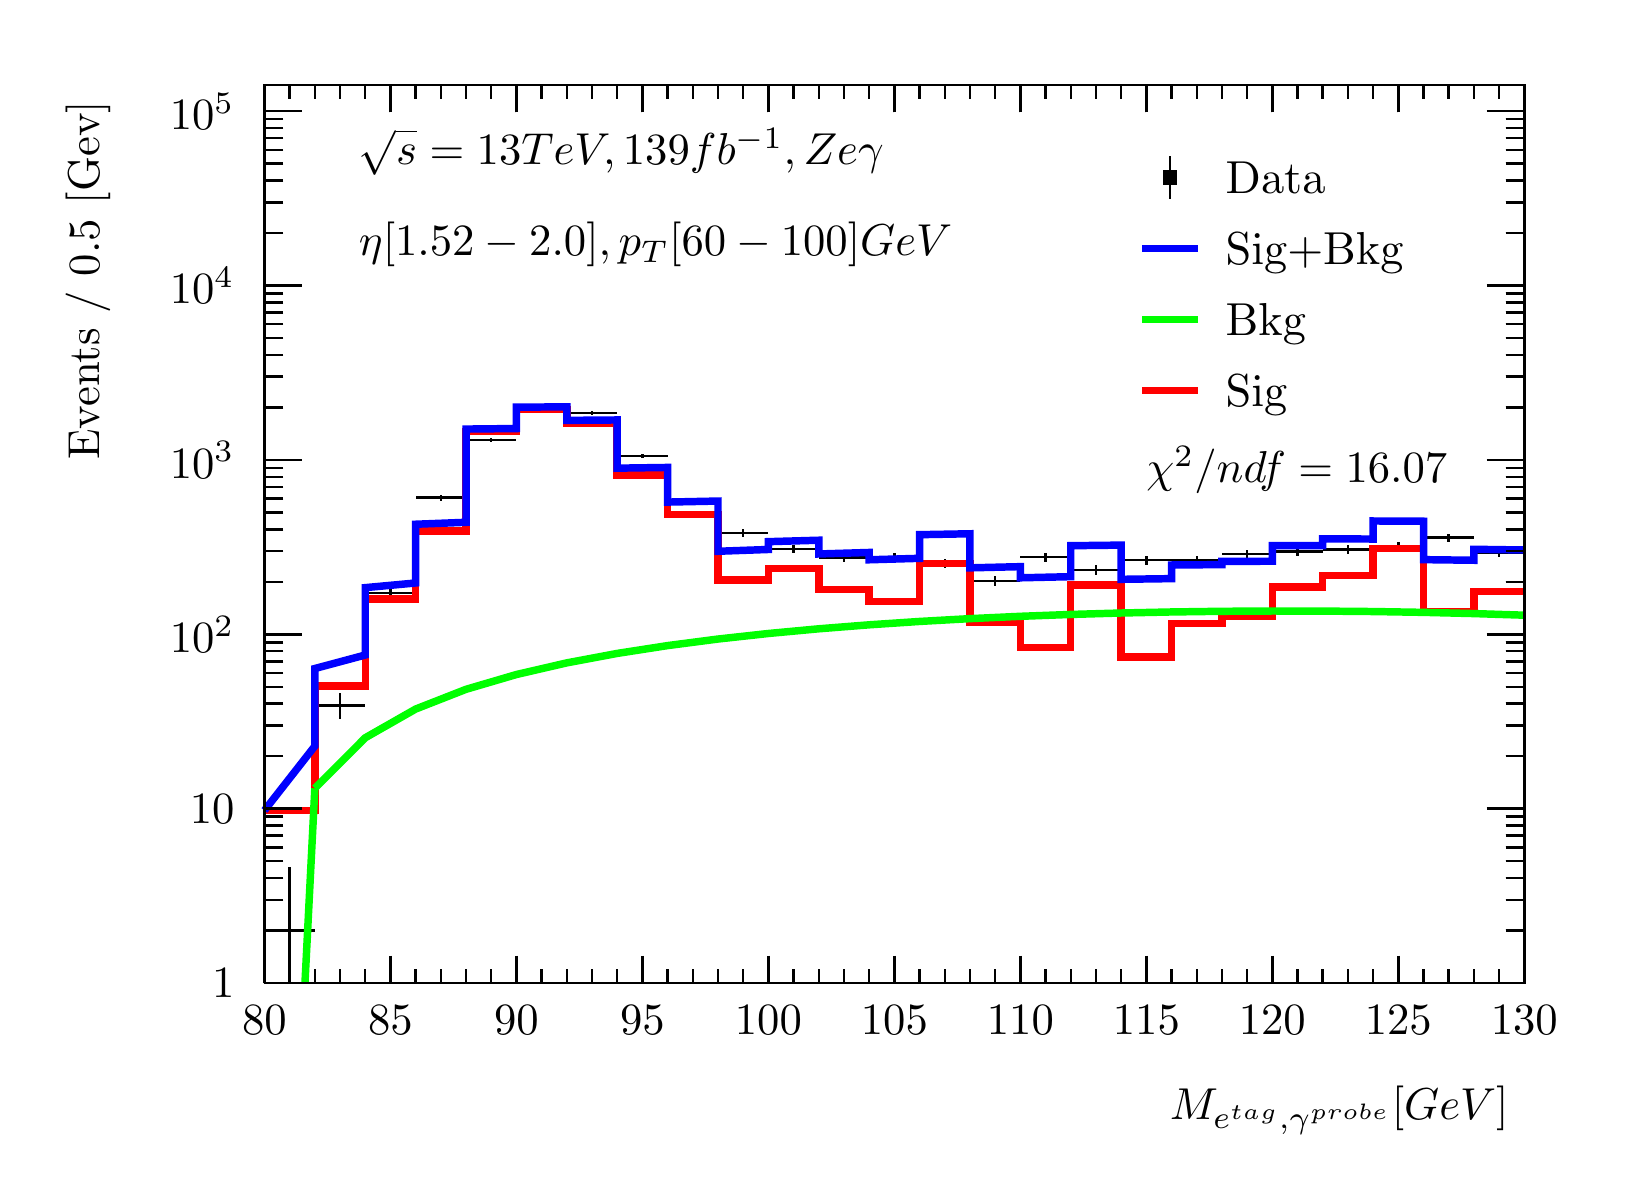
\begin{tikzpicture}
\pgfdeclareplotmark{cross} {
\pgfpathmoveto{\pgfpoint{-0.3\pgfplotmarksize}{\pgfplotmarksize}}
\pgfpathlineto{\pgfpoint{+0.3\pgfplotmarksize}{\pgfplotmarksize}}
\pgfpathlineto{\pgfpoint{+0.3\pgfplotmarksize}{0.3\pgfplotmarksize}}
\pgfpathlineto{\pgfpoint{+1\pgfplotmarksize}{0.3\pgfplotmarksize}}
\pgfpathlineto{\pgfpoint{+1\pgfplotmarksize}{-0.3\pgfplotmarksize}}
\pgfpathlineto{\pgfpoint{+0.3\pgfplotmarksize}{-0.3\pgfplotmarksize}}
\pgfpathlineto{\pgfpoint{+0.3\pgfplotmarksize}{-1.\pgfplotmarksize}}
\pgfpathlineto{\pgfpoint{-0.3\pgfplotmarksize}{-1.\pgfplotmarksize}}
\pgfpathlineto{\pgfpoint{-0.3\pgfplotmarksize}{-0.3\pgfplotmarksize}}
\pgfpathlineto{\pgfpoint{-1.\pgfplotmarksize}{-0.3\pgfplotmarksize}}
\pgfpathlineto{\pgfpoint{-1.\pgfplotmarksize}{0.3\pgfplotmarksize}}
\pgfpathlineto{\pgfpoint{-0.3\pgfplotmarksize}{0.3\pgfplotmarksize}}
\pgfpathclose
\pgfusepathqstroke
}
\pgfdeclareplotmark{cross*} {
\pgfpathmoveto{\pgfpoint{-0.3\pgfplotmarksize}{\pgfplotmarksize}}
\pgfpathlineto{\pgfpoint{+0.3\pgfplotmarksize}{\pgfplotmarksize}}
\pgfpathlineto{\pgfpoint{+0.3\pgfplotmarksize}{0.3\pgfplotmarksize}}
\pgfpathlineto{\pgfpoint{+1\pgfplotmarksize}{0.3\pgfplotmarksize}}
\pgfpathlineto{\pgfpoint{+1\pgfplotmarksize}{-0.3\pgfplotmarksize}}
\pgfpathlineto{\pgfpoint{+0.3\pgfplotmarksize}{-0.3\pgfplotmarksize}}
\pgfpathlineto{\pgfpoint{+0.3\pgfplotmarksize}{-1.\pgfplotmarksize}}
\pgfpathlineto{\pgfpoint{-0.3\pgfplotmarksize}{-1.\pgfplotmarksize}}
\pgfpathlineto{\pgfpoint{-0.3\pgfplotmarksize}{-0.3\pgfplotmarksize}}
\pgfpathlineto{\pgfpoint{-1.\pgfplotmarksize}{-0.3\pgfplotmarksize}}
\pgfpathlineto{\pgfpoint{-1.\pgfplotmarksize}{0.3\pgfplotmarksize}}
\pgfpathlineto{\pgfpoint{-0.3\pgfplotmarksize}{0.3\pgfplotmarksize}}
\pgfpathclose
\pgfusepathqfillstroke
}
\pgfdeclareplotmark{newstar} {
\pgfpathmoveto{\pgfqpoint{0pt}{\pgfplotmarksize}}
\pgfpathlineto{\pgfqpointpolar{44}{0.5\pgfplotmarksize}}
\pgfpathlineto{\pgfqpointpolar{18}{\pgfplotmarksize}}
\pgfpathlineto{\pgfqpointpolar{-20}{0.5\pgfplotmarksize}}
\pgfpathlineto{\pgfqpointpolar{-54}{\pgfplotmarksize}}
\pgfpathlineto{\pgfqpointpolar{-90}{0.5\pgfplotmarksize}}
\pgfpathlineto{\pgfqpointpolar{234}{\pgfplotmarksize}}
\pgfpathlineto{\pgfqpointpolar{198}{0.5\pgfplotmarksize}}
\pgfpathlineto{\pgfqpointpolar{162}{\pgfplotmarksize}}
\pgfpathlineto{\pgfqpointpolar{134}{0.5\pgfplotmarksize}}
\pgfpathclose
\pgfusepathqstroke
}
\pgfdeclareplotmark{newstar*} {
\pgfpathmoveto{\pgfqpoint{0pt}{\pgfplotmarksize}}
\pgfpathlineto{\pgfqpointpolar{44}{0.5\pgfplotmarksize}}
\pgfpathlineto{\pgfqpointpolar{18}{\pgfplotmarksize}}
\pgfpathlineto{\pgfqpointpolar{-20}{0.5\pgfplotmarksize}}
\pgfpathlineto{\pgfqpointpolar{-54}{\pgfplotmarksize}}
\pgfpathlineto{\pgfqpointpolar{-90}{0.5\pgfplotmarksize}}
\pgfpathlineto{\pgfqpointpolar{234}{\pgfplotmarksize}}
\pgfpathlineto{\pgfqpointpolar{198}{0.5\pgfplotmarksize}}
\pgfpathlineto{\pgfqpointpolar{162}{\pgfplotmarksize}}
\pgfpathlineto{\pgfqpointpolar{134}{0.5\pgfplotmarksize}}
\pgfpathclose
\pgfusepathqfillstroke
}
\definecolor{c}{rgb}{1,1,1};
\draw [color=c, fill=c] (0,0) rectangle (20,14.4361);
\draw [color=c, fill=c] (3,2.30977) rectangle (19,13.7143);
\definecolor{c}{rgb}{0,0,0};
\draw [c,line width=0.9] (3,2.30977) -- (3,13.7143) -- (19,13.7143) -- (19,2.30977) -- (3,2.30977);
\definecolor{c}{rgb}{1,1,1};
\draw [color=c, fill=c] (3,2.30977) rectangle (19,13.7143);
\definecolor{c}{rgb}{0,0,0};
\draw [c,line width=0.9] (3,2.30977) -- (3,13.7143) -- (19,13.7143) -- (19,2.30977) -- (3,2.30977);
\draw [c,line width=0.9] (3,2.30977) -- (19,2.30977);
\draw [c,line width=0.9] (3,2.65624) -- (3,2.30977);
\draw [c,line width=0.9] (3.32,2.48301) -- (3.32,2.30977);
\draw [c,line width=0.9] (3.64,2.48301) -- (3.64,2.30977);
\draw [c,line width=0.9] (3.96,2.48301) -- (3.96,2.30977);
\draw [c,line width=0.9] (4.28,2.48301) -- (4.28,2.30977);
\draw [c,line width=0.9] (4.6,2.65624) -- (4.6,2.30977);
\draw [c,line width=0.9] (4.92,2.48301) -- (4.92,2.30977);
\draw [c,line width=0.9] (5.24,2.48301) -- (5.24,2.30977);
\draw [c,line width=0.9] (5.56,2.48301) -- (5.56,2.30977);
\draw [c,line width=0.9] (5.88,2.48301) -- (5.88,2.30977);
\draw [c,line width=0.9] (6.2,2.65624) -- (6.2,2.30977);
\draw [c,line width=0.9] (6.52,2.48301) -- (6.52,2.30977);
\draw [c,line width=0.9] (6.84,2.48301) -- (6.84,2.30977);
\draw [c,line width=0.9] (7.16,2.48301) -- (7.16,2.30977);
\draw [c,line width=0.9] (7.48,2.48301) -- (7.48,2.30977);
\draw [c,line width=0.9] (7.8,2.65624) -- (7.8,2.30977);
\draw [c,line width=0.9] (8.12,2.48301) -- (8.12,2.30977);
\draw [c,line width=0.9] (8.44,2.48301) -- (8.44,2.30977);
\draw [c,line width=0.9] (8.76,2.48301) -- (8.76,2.30977);
\draw [c,line width=0.9] (9.08,2.48301) -- (9.08,2.30977);
\draw [c,line width=0.9] (9.4,2.65624) -- (9.4,2.30977);
\draw [c,line width=0.9] (9.72,2.48301) -- (9.72,2.30977);
\draw [c,line width=0.9] (10.04,2.48301) -- (10.04,2.30977);
\draw [c,line width=0.9] (10.36,2.48301) -- (10.36,2.30977);
\draw [c,line width=0.9] (10.68,2.48301) -- (10.68,2.30977);
\draw [c,line width=0.9] (11,2.65624) -- (11,2.30977);
\draw [c,line width=0.9] (11.32,2.48301) -- (11.32,2.30977);
\draw [c,line width=0.9] (11.64,2.48301) -- (11.64,2.30977);
\draw [c,line width=0.9] (11.96,2.48301) -- (11.96,2.30977);
\draw [c,line width=0.9] (12.28,2.48301) -- (12.28,2.30977);
\draw [c,line width=0.9] (12.6,2.65624) -- (12.6,2.30977);
\draw [c,line width=0.9] (12.92,2.48301) -- (12.92,2.30977);
\draw [c,line width=0.9] (13.24,2.48301) -- (13.24,2.30977);
\draw [c,line width=0.9] (13.56,2.48301) -- (13.56,2.30977);
\draw [c,line width=0.9] (13.88,2.48301) -- (13.88,2.30977);
\draw [c,line width=0.9] (14.2,2.65624) -- (14.2,2.30977);
\draw [c,line width=0.9] (14.52,2.48301) -- (14.52,2.30977);
\draw [c,line width=0.9] (14.84,2.48301) -- (14.84,2.30977);
\draw [c,line width=0.9] (15.16,2.48301) -- (15.16,2.30977);
\draw [c,line width=0.9] (15.48,2.48301) -- (15.48,2.30977);
\draw [c,line width=0.9] (15.8,2.65624) -- (15.8,2.30977);
\draw [c,line width=0.9] (16.12,2.48301) -- (16.12,2.30977);
\draw [c,line width=0.9] (16.44,2.48301) -- (16.44,2.30977);
\draw [c,line width=0.9] (16.76,2.48301) -- (16.76,2.30977);
\draw [c,line width=0.9] (17.08,2.48301) -- (17.08,2.30977);
\draw [c,line width=0.9] (17.4,2.65624) -- (17.4,2.30977);
\draw [c,line width=0.9] (17.72,2.48301) -- (17.72,2.30977);
\draw [c,line width=0.9] (18.04,2.48301) -- (18.04,2.30977);
\draw [c,line width=0.9] (18.36,2.48301) -- (18.36,2.30977);
\draw [c,line width=0.9] (18.68,2.48301) -- (18.68,2.30977);
\draw [c,line width=0.9] (19,2.65624) -- (19,2.30977);
\draw [anchor=base] (3,1.66015) node[scale=1.61424, color=c, rotate=0]{80};
\draw [anchor=base] (4.6,1.66015) node[scale=1.61424, color=c, rotate=0]{85};
\draw [anchor=base] (6.2,1.66015) node[scale=1.61424, color=c, rotate=0]{90};
\draw [anchor=base] (7.8,1.66015) node[scale=1.61424, color=c, rotate=0]{95};
\draw [anchor=base] (9.4,1.66015) node[scale=1.61424, color=c, rotate=0]{100};
\draw [anchor=base] (11,1.66015) node[scale=1.61424, color=c, rotate=0]{105};
\draw [anchor=base] (12.6,1.66015) node[scale=1.61424, color=c, rotate=0]{110};
\draw [anchor=base] (14.2,1.66015) node[scale=1.61424, color=c, rotate=0]{115};
\draw [anchor=base] (15.8,1.66015) node[scale=1.61424, color=c, rotate=0]{120};
\draw [anchor=base] (17.4,1.66015) node[scale=1.61424, color=c, rotate=0]{125};
\draw [anchor=base] (19,1.66015) node[scale=1.61424, color=c, rotate=0]{130};
\draw [anchor= east] (19,0.692932) node[scale=1.61424, color=c, rotate=0]{$M_{e^{tag}, \gamma^{probe}}  [GeV]$};
\draw [c,line width=0.9] (3,13.7143) -- (19,13.7143);
\draw [c,line width=0.9] (3,13.3678) -- (3,13.7143);
\draw [c,line width=0.9] (3.32,13.5411) -- (3.32,13.7143);
\draw [c,line width=0.9] (3.64,13.5411) -- (3.64,13.7143);
\draw [c,line width=0.9] (3.96,13.5411) -- (3.96,13.7143);
\draw [c,line width=0.9] (4.28,13.5411) -- (4.28,13.7143);
\draw [c,line width=0.9] (4.6,13.3678) -- (4.6,13.7143);
\draw [c,line width=0.9] (4.92,13.5411) -- (4.92,13.7143);
\draw [c,line width=0.9] (5.24,13.5411) -- (5.24,13.7143);
\draw [c,line width=0.9] (5.56,13.5411) -- (5.56,13.7143);
\draw [c,line width=0.9] (5.88,13.5411) -- (5.88,13.7143);
\draw [c,line width=0.9] (6.2,13.3678) -- (6.2,13.7143);
\draw [c,line width=0.9] (6.52,13.5411) -- (6.52,13.7143);
\draw [c,line width=0.9] (6.84,13.5411) -- (6.84,13.7143);
\draw [c,line width=0.9] (7.16,13.5411) -- (7.16,13.7143);
\draw [c,line width=0.9] (7.48,13.5411) -- (7.48,13.7143);
\draw [c,line width=0.9] (7.8,13.3678) -- (7.8,13.7143);
\draw [c,line width=0.9] (8.12,13.5411) -- (8.12,13.7143);
\draw [c,line width=0.9] (8.44,13.5411) -- (8.44,13.7143);
\draw [c,line width=0.9] (8.76,13.5411) -- (8.76,13.7143);
\draw [c,line width=0.9] (9.08,13.5411) -- (9.08,13.7143);
\draw [c,line width=0.9] (9.4,13.3678) -- (9.4,13.7143);
\draw [c,line width=0.9] (9.72,13.5411) -- (9.72,13.7143);
\draw [c,line width=0.9] (10.04,13.5411) -- (10.04,13.7143);
\draw [c,line width=0.9] (10.36,13.5411) -- (10.36,13.7143);
\draw [c,line width=0.9] (10.68,13.5411) -- (10.68,13.7143);
\draw [c,line width=0.9] (11,13.3678) -- (11,13.7143);
\draw [c,line width=0.9] (11.32,13.5411) -- (11.32,13.7143);
\draw [c,line width=0.9] (11.64,13.5411) -- (11.64,13.7143);
\draw [c,line width=0.9] (11.96,13.5411) -- (11.96,13.7143);
\draw [c,line width=0.9] (12.28,13.5411) -- (12.28,13.7143);
\draw [c,line width=0.9] (12.6,13.3678) -- (12.6,13.7143);
\draw [c,line width=0.9] (12.92,13.5411) -- (12.92,13.7143);
\draw [c,line width=0.9] (13.24,13.5411) -- (13.24,13.7143);
\draw [c,line width=0.9] (13.56,13.5411) -- (13.56,13.7143);
\draw [c,line width=0.9] (13.88,13.5411) -- (13.88,13.7143);
\draw [c,line width=0.9] (14.2,13.3678) -- (14.2,13.7143);
\draw [c,line width=0.9] (14.52,13.5411) -- (14.52,13.7143);
\draw [c,line width=0.9] (14.84,13.5411) -- (14.84,13.7143);
\draw [c,line width=0.9] (15.16,13.5411) -- (15.16,13.7143);
\draw [c,line width=0.9] (15.48,13.5411) -- (15.48,13.7143);
\draw [c,line width=0.9] (15.8,13.3678) -- (15.8,13.7143);
\draw [c,line width=0.9] (16.12,13.5411) -- (16.12,13.7143);
\draw [c,line width=0.9] (16.44,13.5411) -- (16.44,13.7143);
\draw [c,line width=0.9] (16.76,13.5411) -- (16.76,13.7143);
\draw [c,line width=0.9] (17.08,13.5411) -- (17.08,13.7143);
\draw [c,line width=0.9] (17.4,13.3678) -- (17.4,13.7143);
\draw [c,line width=0.9] (17.72,13.5411) -- (17.72,13.7143);
\draw [c,line width=0.9] (18.04,13.5411) -- (18.04,13.7143);
\draw [c,line width=0.9] (18.36,13.5411) -- (18.36,13.7143);
\draw [c,line width=0.9] (18.68,13.5411) -- (18.68,13.7143);
\draw [c,line width=0.9] (19,13.3678) -- (19,13.7143);
\draw [c,line width=0.9] (3,2.30977) -- (3,13.7143);
\draw [c,line width=0.9] (3.474,2.30978) -- (3,2.30978);
\draw [anchor= east] (2.82,2.30978) node[scale=1.61424, color=c, rotate=0]{1};
\draw [c,line width=0.9] (3.237,2.97642) -- (3,2.97642);
\draw [c,line width=0.9] (3.237,3.36639) -- (3,3.36639);
\draw [c,line width=0.9] (3.237,3.64307) -- (3,3.64307);
\draw [c,line width=0.9] (3.237,3.85768) -- (3,3.85768);
\draw [c,line width=0.9] (3.237,4.03303) -- (3,4.03303);
\draw [c,line width=0.9] (3.237,4.18129) -- (3,4.18129);
\draw [c,line width=0.9] (3.237,4.30972) -- (3,4.30972);
\draw [c,line width=0.9] (3.237,4.423) -- (3,4.423);
\draw [c,line width=0.9] (3.474,4.52433) -- (3,4.52433);
\draw [anchor= east] (2.82,4.52433) node[scale=1.61424, color=c, rotate=0]{10};
\draw [c,line width=0.9] (3.237,5.19098) -- (3,5.19098);
\draw [c,line width=0.9] (3.237,5.58094) -- (3,5.58094);
\draw [c,line width=0.9] (3.237,5.85762) -- (3,5.85762);
\draw [c,line width=0.9] (3.237,6.07223) -- (3,6.07223);
\draw [c,line width=0.9] (3.237,6.24759) -- (3,6.24759);
\draw [c,line width=0.9] (3.237,6.39584) -- (3,6.39584);
\draw [c,line width=0.9] (3.237,6.52427) -- (3,6.52427);
\draw [c,line width=0.9] (3.237,6.63755) -- (3,6.63755);
\draw [c,line width=0.9] (3.474,6.73888) -- (3,6.73888);
\draw [anchor= east] (2.82,6.73888) node[scale=1.61424, color=c, rotate=0]{$10^{2}$};
\draw [c,line width=0.9] (3.237,7.40553) -- (3,7.40553);
\draw [c,line width=0.9] (3.237,7.79549) -- (3,7.79549);
\draw [c,line width=0.9] (3.237,8.07217) -- (3,8.07217);
\draw [c,line width=0.9] (3.237,8.28679) -- (3,8.28679);
\draw [c,line width=0.9] (3.237,8.46214) -- (3,8.46214);
\draw [c,line width=0.9] (3.237,8.61039) -- (3,8.61039);
\draw [c,line width=0.9] (3.237,8.73882) -- (3,8.73882);
\draw [c,line width=0.9] (3.237,8.8521) -- (3,8.8521);
\draw [c,line width=0.9] (3.474,8.95343) -- (3,8.95343);
\draw [anchor= east] (2.82,8.95343) node[scale=1.61424, color=c, rotate=0]{$10^{3}$};
\draw [c,line width=0.9] (3.237,9.62008) -- (3,9.62008);
\draw [c,line width=0.9] (3.237,10.01) -- (3,10.01);
\draw [c,line width=0.9] (3.237,10.2867) -- (3,10.2867);
\draw [c,line width=0.9] (3.237,10.5013) -- (3,10.5013);
\draw [c,line width=0.9] (3.237,10.6767) -- (3,10.6767);
\draw [c,line width=0.9] (3.237,10.8249) -- (3,10.8249);
\draw [c,line width=0.9] (3.237,10.9534) -- (3,10.9534);
\draw [c,line width=0.9] (3.237,11.0667) -- (3,11.0667);
\draw [c,line width=0.9] (3.474,11.168) -- (3,11.168);
\draw [anchor= east] (2.82,11.168) node[scale=1.61424, color=c, rotate=0]{$10^{4}$};
\draw [c,line width=0.9] (3.237,11.8346) -- (3,11.8346);
\draw [c,line width=0.9] (3.237,12.2246) -- (3,12.2246);
\draw [c,line width=0.9] (3.237,12.5013) -- (3,12.5013);
\draw [c,line width=0.9] (3.237,12.7159) -- (3,12.7159);
\draw [c,line width=0.9] (3.237,12.8912) -- (3,12.8912);
\draw [c,line width=0.9] (3.237,13.0395) -- (3,13.0395);
\draw [c,line width=0.9] (3.237,13.1679) -- (3,13.1679);
\draw [c,line width=0.9] (3.237,13.2812) -- (3,13.2812);
\draw [c,line width=0.9] (3.474,13.3825) -- (3,13.3825);
\draw [anchor= east] (2.82,13.3825) node[scale=1.61424, color=c, rotate=0]{$10^{5}$};
\draw [anchor= east] (0.76,13.7143) node[scale=1.61424, color=c, rotate=90]{Events / 0.5 [Gev]};
\draw [c,line width=0.9] (19,2.30977) -- (19,13.7143);
\draw [c,line width=0.9] (18.526,2.30978) -- (19,2.30978);
\draw [c,line width=0.9] (18.763,2.97642) -- (19,2.97642);
\draw [c,line width=0.9] (18.763,3.36639) -- (19,3.36639);
\draw [c,line width=0.9] (18.763,3.64307) -- (19,3.64307);
\draw [c,line width=0.9] (18.763,3.85768) -- (19,3.85768);
\draw [c,line width=0.9] (18.763,4.03303) -- (19,4.03303);
\draw [c,line width=0.9] (18.763,4.18129) -- (19,4.18129);
\draw [c,line width=0.9] (18.763,4.30972) -- (19,4.30972);
\draw [c,line width=0.9] (18.763,4.423) -- (19,4.423);
\draw [c,line width=0.9] (18.526,4.52433) -- (19,4.52433);
\draw [c,line width=0.9] (18.763,5.19098) -- (19,5.19098);
\draw [c,line width=0.9] (18.763,5.58094) -- (19,5.58094);
\draw [c,line width=0.9] (18.763,5.85762) -- (19,5.85762);
\draw [c,line width=0.9] (18.763,6.07223) -- (19,6.07223);
\draw [c,line width=0.9] (18.763,6.24759) -- (19,6.24759);
\draw [c,line width=0.9] (18.763,6.39584) -- (19,6.39584);
\draw [c,line width=0.9] (18.763,6.52427) -- (19,6.52427);
\draw [c,line width=0.9] (18.763,6.63755) -- (19,6.63755);
\draw [c,line width=0.9] (18.526,6.73888) -- (19,6.73888);
\draw [c,line width=0.9] (18.763,7.40553) -- (19,7.40553);
\draw [c,line width=0.9] (18.763,7.79549) -- (19,7.79549);
\draw [c,line width=0.9] (18.763,8.07217) -- (19,8.07217);
\draw [c,line width=0.9] (18.763,8.28679) -- (19,8.28679);
\draw [c,line width=0.9] (18.763,8.46214) -- (19,8.46214);
\draw [c,line width=0.9] (18.763,8.61039) -- (19,8.61039);
\draw [c,line width=0.9] (18.763,8.73882) -- (19,8.73882);
\draw [c,line width=0.9] (18.763,8.8521) -- (19,8.8521);
\draw [c,line width=0.9] (18.526,8.95343) -- (19,8.95343);
\draw [c,line width=0.9] (18.763,9.62008) -- (19,9.62008);
\draw [c,line width=0.9] (18.763,10.01) -- (19,10.01);
\draw [c,line width=0.9] (18.763,10.2867) -- (19,10.2867);
\draw [c,line width=0.9] (18.763,10.5013) -- (19,10.5013);
\draw [c,line width=0.9] (18.763,10.6767) -- (19,10.6767);
\draw [c,line width=0.9] (18.763,10.8249) -- (19,10.8249);
\draw [c,line width=0.9] (18.763,10.9534) -- (19,10.9534);
\draw [c,line width=0.9] (18.763,11.0667) -- (19,11.0667);
\draw [c,line width=0.9] (18.526,11.168) -- (19,11.168);
\draw [c,line width=0.9] (18.763,11.8346) -- (19,11.8346);
\draw [c,line width=0.9] (18.763,12.2246) -- (19,12.2246);
\draw [c,line width=0.9] (18.763,12.5013) -- (19,12.5013);
\draw [c,line width=0.9] (18.763,12.7159) -- (19,12.7159);
\draw [c,line width=0.9] (18.763,12.8912) -- (19,12.8912);
\draw [c,line width=0.9] (18.763,13.0395) -- (19,13.0395);
\draw [c,line width=0.9] (18.763,13.1679) -- (19,13.1679);
\draw [c,line width=0.9] (18.763,13.2812) -- (19,13.2812);
\draw [c,line width=0.9] (18.526,13.3825) -- (19,13.3825);
\draw [c,line width=0.9] (3.32,2.97642) -- (3,2.97642);
\draw [c,line width=0.9] (3,2.97642) -- (3,2.97642);
\draw [c,line width=0.9] (3.32,2.97642) -- (3.64,2.97642);
\draw [c,line width=0.9] (3.64,2.97642) -- (3.64,2.97642);
\draw [c,line width=0.9] (3.32,2.97642) -- (3.32,3.78537);
\draw [c,line width=0.9] (3.32,3.78537) -- (3.32,3.78537);
\draw [c,line width=0.9] (3.32,2.97642) -- (3.32,2.30977);
\draw [c,line width=0.9] (3.32,2.30977) -- (3.32,2.30977);
\draw [c,line width=0.9] (3.96,5.83327) -- (3.64,5.83327);
\draw [c,line width=0.9] (3.64,5.83327) -- (3.64,5.83327);
\draw [c,line width=0.9] (3.96,5.83327) -- (4.28,5.83327);
\draw [c,line width=0.9] (4.28,5.83327) -- (4.28,5.83327);
\draw [c,line width=0.9] (3.96,5.83327) -- (3.96,5.99826);
\draw [c,line width=0.9] (3.96,5.99826) -- (3.96,5.99826);
\draw [c,line width=0.9] (3.96,5.83327) -- (3.96,5.66623);
\draw [c,line width=0.9] (3.96,5.66623) -- (3.96,5.66623);
\draw [c,line width=0.9] (4.6,7.26047) -- (4.28,7.26047);
\draw [c,line width=0.9] (4.28,7.26047) -- (4.28,7.26047);
\draw [c,line width=0.9] (4.6,7.26047) -- (4.92,7.26047);
\draw [c,line width=0.9] (4.92,7.26047) -- (4.92,7.26047);
\draw [c,line width=0.9] (4.6,7.26047) -- (4.6,7.33379);
\draw [c,line width=0.9] (4.6,7.33379) -- (4.6,7.33379);
\draw [c,line width=0.9] (4.6,7.26047) -- (4.6,7.18715);
\draw [c,line width=0.9] (4.6,7.18715) -- (4.6,7.18715);
\draw [c,line width=0.9] (5.24,8.47488) -- (4.92,8.47488);
\draw [c,line width=0.9] (4.92,8.47488) -- (4.92,8.47488);
\draw [c,line width=0.9] (5.24,8.47488) -- (5.56,8.47488);
\draw [c,line width=0.9] (5.56,8.47488) -- (5.56,8.47488);
\draw [c,line width=0.9] (5.24,8.47488) -- (5.24,8.51388);
\draw [c,line width=0.9] (5.24,8.51388) -- (5.24,8.51388);
\draw [c,line width=0.9] (5.24,8.47488) -- (5.24,8.43587);
\draw [c,line width=0.9] (5.24,8.43587) -- (5.24,8.43587);
\draw [c,line width=0.9] (5.88,9.20946) -- (5.56,9.20946);
\draw [c,line width=0.9] (5.56,9.20946) -- (5.56,9.20946);
\draw [c,line width=0.9] (5.88,9.20946) -- (6.2,9.20946);
\draw [c,line width=0.9] (6.2,9.20946) -- (6.2,9.20946);
\draw [c,line width=0.9] (5.88,9.20946) -- (5.88,9.23608);
\draw [c,line width=0.9] (5.88,9.23608) -- (5.88,9.23608);
\draw [c,line width=0.9] (5.88,9.20946) -- (5.88,9.18283);
\draw [c,line width=0.9] (5.88,9.18283) -- (5.88,9.18283);
\draw [c,line width=0.9] (6.52,9.59622) -- (6.2,9.59622);
\draw [c,line width=0.9] (6.2,9.59622) -- (6.2,9.59622);
\draw [c,line width=0.9] (6.52,9.59622) -- (6.84,9.59622);
\draw [c,line width=0.9] (6.84,9.59622) -- (6.84,9.59622);
\draw [c,line width=0.9] (6.52,9.59622) -- (6.52,9.618);
\draw [c,line width=0.9] (6.52,9.618) -- (6.52,9.618);
\draw [c,line width=0.9] (6.52,9.59622) -- (6.52,9.57445);
\draw [c,line width=0.9] (6.52,9.57445) -- (6.52,9.57445);
\draw [c,line width=0.9] (7.16,9.55028) -- (6.84,9.55028);
\draw [c,line width=0.9] (6.84,9.55028) -- (6.84,9.55028);
\draw [c,line width=0.9] (7.16,9.55028) -- (7.48,9.55028);
\draw [c,line width=0.9] (7.48,9.55028) -- (7.48,9.55028);
\draw [c,line width=0.9] (7.16,9.55028) -- (7.16,9.57258);
\draw [c,line width=0.9] (7.16,9.57258) -- (7.16,9.57258);
\draw [c,line width=0.9] (7.16,9.55028) -- (7.16,9.52798);
\draw [c,line width=0.9] (7.16,9.52798) -- (7.16,9.52798);
\draw [c,line width=0.9] (7.8,9.00493) -- (7.48,9.00493);
\draw [c,line width=0.9] (7.48,9.00493) -- (7.48,9.00493);
\draw [c,line width=0.9] (7.8,9.00493) -- (8.12,9.00493);
\draw [c,line width=0.9] (8.12,9.00493) -- (8.12,9.00493);
\draw [c,line width=0.9] (7.8,9.00493) -- (7.8,9.03454);
\draw [c,line width=0.9] (7.8,9.03454) -- (7.8,9.03454);
\draw [c,line width=0.9] (7.8,9.00493) -- (7.8,8.97532);
\draw [c,line width=0.9] (7.8,8.97532) -- (7.8,8.97532);
\draw [c,line width=0.9] (8.44,8.42454) -- (8.12,8.42454);
\draw [c,line width=0.9] (8.12,8.42454) -- (8.12,8.42454);
\draw [c,line width=0.9] (8.44,8.42454) -- (8.76,8.42454);
\draw [c,line width=0.9] (8.76,8.42454) -- (8.76,8.42454);
\draw [c,line width=0.9] (8.44,8.42454) -- (8.44,8.46458);
\draw [c,line width=0.9] (8.44,8.46458) -- (8.44,8.46458);
\draw [c,line width=0.9] (8.44,8.42454) -- (8.44,8.38451);
\draw [c,line width=0.9] (8.44,8.38451) -- (8.44,8.38451);
\draw [c,line width=0.9] (9.08,8.02789) -- (8.76,8.02789);
\draw [c,line width=0.9] (8.76,8.02789) -- (8.76,8.02789);
\draw [c,line width=0.9] (9.08,8.02789) -- (9.4,8.02789);
\draw [c,line width=0.9] (9.4,8.02789) -- (9.4,8.02789);
\draw [c,line width=0.9] (9.08,8.02789) -- (9.08,8.07709);
\draw [c,line width=0.9] (9.08,8.07709) -- (9.08,8.07709);
\draw [c,line width=0.9] (9.08,8.02789) -- (9.08,7.97869);
\draw [c,line width=0.9] (9.08,7.97869) -- (9.08,7.97869);
\draw [c,line width=0.9] (9.72,7.82392) -- (9.4,7.82392);
\draw [c,line width=0.9] (9.4,7.82392) -- (9.4,7.82392);
\draw [c,line width=0.9] (9.72,7.82392) -- (10.04,7.82392);
\draw [c,line width=0.9] (10.04,7.82392) -- (10.04,7.82392);
\draw [c,line width=0.9] (9.72,7.82392) -- (9.72,7.87862);
\draw [c,line width=0.9] (9.72,7.87862) -- (9.72,7.87862);
\draw [c,line width=0.9] (9.72,7.82392) -- (9.72,7.76921);
\draw [c,line width=0.9] (9.72,7.76921) -- (9.72,7.76921);
\draw [c,line width=0.9] (10.36,7.7153) -- (10.04,7.7153);
\draw [c,line width=0.9] (10.04,7.7153) -- (10.04,7.7153);
\draw [c,line width=0.9] (10.36,7.7153) -- (10.68,7.7153);
\draw [c,line width=0.9] (10.68,7.7153) -- (10.68,7.7153);
\draw [c,line width=0.9] (10.36,7.7153) -- (10.36,7.77318);
\draw [c,line width=0.9] (10.36,7.77318) -- (10.36,7.77318);
\draw [c,line width=0.9] (10.36,7.7153) -- (10.36,7.65741);
\draw [c,line width=0.9] (10.36,7.65741) -- (10.36,7.65741);
\draw [c,line width=0.9] (11,7.7083) -- (10.68,7.7083);
\draw [c,line width=0.9] (10.68,7.7083) -- (10.68,7.7083);
\draw [c,line width=0.9] (11,7.7083) -- (11.32,7.7083);
\draw [c,line width=0.9] (11.32,7.7083) -- (11.32,7.7083);
\draw [c,line width=0.9] (11,7.7083) -- (11,7.7664);
\draw [c,line width=0.9] (11,7.7664) -- (11,7.7664);
\draw [c,line width=0.9] (11,7.7083) -- (11,7.65021);
\draw [c,line width=0.9] (11,7.65021) -- (11,7.65021);
\draw [c,line width=0.9] (11.64,7.63541) -- (11.32,7.63541);
\draw [c,line width=0.9] (11.32,7.63541) -- (11.32,7.63541);
\draw [c,line width=0.9] (11.64,7.63541) -- (11.96,7.63541);
\draw [c,line width=0.9] (11.96,7.63541) -- (11.96,7.63541);
\draw [c,line width=0.9] (11.64,7.63541) -- (11.64,7.69574);
\draw [c,line width=0.9] (11.64,7.69574) -- (11.64,7.69574);
\draw [c,line width=0.9] (11.64,7.63541) -- (11.64,7.57507);
\draw [c,line width=0.9] (11.64,7.57507) -- (11.64,7.57507);
\draw [c,line width=0.9] (12.28,7.4151) -- (11.96,7.4151);
\draw [c,line width=0.9] (11.96,7.4151) -- (11.96,7.4151);
\draw [c,line width=0.9] (12.28,7.4151) -- (12.6,7.4151);
\draw [c,line width=0.9] (12.6,7.4151) -- (12.6,7.4151);
\draw [c,line width=0.9] (12.28,7.4151) -- (12.28,7.48275);
\draw [c,line width=0.9] (12.28,7.48275) -- (12.28,7.48275);
\draw [c,line width=0.9] (12.28,7.4151) -- (12.28,7.34744);
\draw [c,line width=0.9] (12.28,7.34744) -- (12.28,7.34744);
\draw [c,line width=0.9] (12.92,7.71877) -- (12.6,7.71877);
\draw [c,line width=0.9] (12.6,7.71877) -- (12.6,7.71877);
\draw [c,line width=0.9] (12.92,7.71877) -- (13.24,7.71877);
\draw [c,line width=0.9] (13.24,7.71877) -- (13.24,7.71877);
\draw [c,line width=0.9] (12.92,7.71877) -- (12.92,7.77655);
\draw [c,line width=0.9] (12.92,7.77655) -- (12.92,7.77655);
\draw [c,line width=0.9] (12.92,7.71877) -- (12.92,7.661);
\draw [c,line width=0.9] (12.92,7.661) -- (12.92,7.661);
\draw [c,line width=0.9] (13.56,7.55653) -- (13.24,7.55653);
\draw [c,line width=0.9] (13.24,7.55653) -- (13.24,7.55653);
\draw [c,line width=0.9] (13.56,7.55653) -- (13.88,7.55653);
\draw [c,line width=0.9] (13.88,7.55653) -- (13.88,7.55653);
\draw [c,line width=0.9] (13.56,7.55653) -- (13.56,7.61939);
\draw [c,line width=0.9] (13.56,7.61939) -- (13.56,7.61939);
\draw [c,line width=0.9] (13.56,7.55653) -- (13.56,7.49367);
\draw [c,line width=0.9] (13.56,7.49367) -- (13.56,7.49367);
\draw [c,line width=0.9] (14.2,7.6798) -- (13.88,7.6798);
\draw [c,line width=0.9] (13.88,7.6798) -- (13.88,7.6798);
\draw [c,line width=0.9] (14.2,7.6798) -- (14.52,7.6798);
\draw [c,line width=0.9] (14.52,7.6798) -- (14.52,7.6798);
\draw [c,line width=0.9] (14.2,7.6798) -- (14.2,7.73876);
\draw [c,line width=0.9] (14.2,7.73876) -- (14.2,7.73876);
\draw [c,line width=0.9] (14.2,7.6798) -- (14.2,7.62084);
\draw [c,line width=0.9] (14.2,7.62084) -- (14.2,7.62084);
\draw [c,line width=0.9] (14.84,7.67618) -- (14.52,7.67618);
\draw [c,line width=0.9] (14.52,7.67618) -- (14.52,7.67618);
\draw [c,line width=0.9] (14.84,7.67618) -- (15.16,7.67618);
\draw [c,line width=0.9] (15.16,7.67618) -- (15.16,7.67618);
\draw [c,line width=0.9] (14.84,7.67618) -- (14.84,7.73525);
\draw [c,line width=0.9] (14.84,7.73525) -- (14.84,7.73525);
\draw [c,line width=0.9] (14.84,7.67618) -- (14.84,7.61711);
\draw [c,line width=0.9] (14.84,7.61711) -- (14.84,7.61711);
\draw [c,line width=0.9] (15.48,7.75623) -- (15.16,7.75623);
\draw [c,line width=0.9] (15.16,7.75623) -- (15.16,7.75623);
\draw [c,line width=0.9] (15.48,7.75623) -- (15.8,7.75623);
\draw [c,line width=0.9] (15.8,7.75623) -- (15.8,7.75623);
\draw [c,line width=0.9] (15.48,7.75623) -- (15.48,7.81289);
\draw [c,line width=0.9] (15.48,7.81289) -- (15.48,7.81289);
\draw [c,line width=0.9] (15.48,7.75623) -- (15.48,7.69956);
\draw [c,line width=0.9] (15.48,7.69956) -- (15.48,7.69956);
\draw [c,line width=0.9] (16.12,7.78906) -- (15.8,7.78906);
\draw [c,line width=0.9] (15.8,7.78906) -- (15.8,7.78906);
\draw [c,line width=0.9] (16.12,7.78906) -- (16.44,7.78906);
\draw [c,line width=0.9] (16.44,7.78906) -- (16.44,7.78906);
\draw [c,line width=0.9] (16.12,7.78906) -- (16.12,7.84476);
\draw [c,line width=0.9] (16.12,7.84476) -- (16.12,7.84476);
\draw [c,line width=0.9] (16.12,7.78906) -- (16.12,7.73335);
\draw [c,line width=0.9] (16.12,7.73335) -- (16.12,7.73335);
\draw [c,line width=0.9] (16.76,7.81767) -- (16.44,7.81767);
\draw [c,line width=0.9] (16.44,7.81767) -- (16.44,7.81767);
\draw [c,line width=0.9] (16.76,7.81767) -- (17.08,7.81767);
\draw [c,line width=0.9] (17.08,7.81767) -- (17.08,7.81767);
\draw [c,line width=0.9] (16.76,7.81767) -- (16.76,7.87256);
\draw [c,line width=0.9] (16.76,7.87256) -- (16.76,7.87256);
\draw [c,line width=0.9] (16.76,7.81767) -- (16.76,7.76279);
\draw [c,line width=0.9] (16.76,7.76279) -- (16.76,7.76279);
\draw [c,line width=0.9] (17.4,7.85756) -- (17.08,7.85756);
\draw [c,line width=0.9] (17.08,7.85756) -- (17.08,7.85756);
\draw [c,line width=0.9] (17.4,7.85756) -- (17.72,7.85756);
\draw [c,line width=0.9] (17.72,7.85756) -- (17.72,7.85756);
\draw [c,line width=0.9] (17.4,7.85756) -- (17.4,7.91132);
\draw [c,line width=0.9] (17.4,7.91132) -- (17.4,7.91132);
\draw [c,line width=0.9] (17.4,7.85756) -- (17.4,7.8038);
\draw [c,line width=0.9] (17.4,7.8038) -- (17.4,7.8038);
\draw [c,line width=0.9] (18.04,7.96817) -- (17.72,7.96817);
\draw [c,line width=0.9] (17.72,7.96817) -- (17.72,7.96817);
\draw [c,line width=0.9] (18.04,7.96817) -- (18.36,7.96817);
\draw [c,line width=0.9] (18.36,7.96817) -- (18.36,7.96817);
\draw [c,line width=0.9] (18.04,7.96817) -- (18.04,8.01892);
\draw [c,line width=0.9] (18.04,8.01892) -- (18.04,8.01892);
\draw [c,line width=0.9] (18.04,7.96817) -- (18.04,7.91741);
\draw [c,line width=0.9] (18.04,7.91741) -- (18.04,7.91741);
\draw [c,line width=0.9] (18.68,7.77933) -- (18.36,7.77933);
\draw [c,line width=0.9] (18.36,7.77933) -- (18.36,7.77933);
\draw [c,line width=0.9] (18.68,7.77933) -- (19,7.77933);
\draw [c,line width=0.9] (19,7.77933) -- (19,7.77933);
\draw [c,line width=0.9] (18.68,7.77933) -- (18.68,7.83531);
\draw [c,line width=0.9] (18.68,7.83531) -- (18.68,7.83531);
\draw [c,line width=0.9] (18.68,7.77933) -- (18.68,7.72334);
\draw [c,line width=0.9] (18.68,7.72334) -- (18.68,7.72334);
\foreach \P in {(3.32,2.97642), (3.96,5.83327), (4.6,7.26047), (5.24,8.47488), (5.88,9.20946), (6.52,9.59622), (7.16,9.55028), (7.8,9.00493), (8.44,8.42454), (9.08,8.02789), (9.72,7.82392), (10.36,7.7153), (11,7.7083), (11.64,7.63541),
 (12.28,7.4151), (12.92,7.71877), (13.56,7.55653), (14.2,7.6798), (14.84,7.67618), (15.48,7.75623), (16.12,7.78906), (16.76,7.81767), (17.4,7.85756), (18.04,7.96817), (18.68,7.77933)}{\draw[mark options={color=c,fill=c},mark size=2.882883pt,mark=]
 plot coordinates {\P};}
\definecolor{c}{rgb}{1,0,0};
\draw [c,line width=2.7] (3,4.502) -- (3,4.502);
\draw [c,line width=2.7] (3,4.502) -- (3,4.502) -- (3.64,4.502) -- (3.64,6.08293) -- (4.28,6.08293) -- (4.28,7.18888) -- (4.92,7.18888) -- (4.92,8.04895) -- (5.56,8.04895) -- (5.56,9.31399) -- (6.2,9.31399) -- (6.2,9.59454) -- (6.84,9.59454) --
 (6.84,9.41582) -- (7.48,9.41582) -- (7.48,8.76173) -- (8.12,8.76173) -- (8.12,8.26141) -- (8.76,8.26141) -- (8.76,7.43127) -- (9.4,7.43127) -- (9.4,7.57598) -- (10.04,7.57598) -- (10.04,7.31109) -- (10.68,7.31109) -- (10.68,7.15534) --
 (11.32,7.15534) -- (11.32,7.63607) -- (11.96,7.63607) -- (11.96,6.89403) -- (12.6,6.89403) -- (12.6,6.57178) -- (13.24,6.57178) -- (13.24,7.36738) -- (13.88,7.36738) -- (13.88,6.45231) -- (14.52,6.45231) -- (14.52,6.87691) -- (15.16,6.87691) --
 (15.16,6.9645) -- (15.8,6.9645) -- (15.8,7.34025) -- (16.44,7.34025) -- (16.44,7.48306) -- (17.08,7.48306) -- (17.08,7.83153) -- (17.72,7.83153) -- (17.72,7.02291) -- (18.36,7.02291) -- (18.36,7.28122) -- (19,7.28122) -- (19,7.28122) -- (19,7.28122)
 -- (19,7.28122);
\definecolor{c}{rgb}{0,1,0};
\draw [c,line width=2.7] (3.51454,2.30977) -- (3.64,4.78272);
\draw [c,line width=2.7] (3.64,4.78272) -- (3.64,4.78272) -- (4.28,5.42475) -- (4.28,5.42475) -- (4.92,5.78945) -- (4.92,5.78945) -- (5.56,6.04018) -- (5.56,6.04018) -- (6.2,6.22813) -- (6.2,6.22813) -- (6.84,6.37605) -- (6.84,6.37605) --
 (7.48,6.49608) -- (7.48,6.49608) -- (8.12,6.59542) -- (8.12,6.59542) -- (8.76,6.67871) -- (8.76,6.67871) -- (9.4,6.74909) -- (9.4,6.74909) -- (10.04,6.80877) -- (10.04,6.80877) -- (10.68,6.85936) -- (10.68,6.85936) -- (11.32,6.90208) --
 (11.32,6.90208) -- (11.96,6.93782) -- (11.96,6.93782) -- (12.6,6.96728) -- (12.6,6.96728) -- (13.24,6.99098) -- (13.24,6.99098) -- (13.88,7.00933) -- (13.88,7.00933) -- (14.52,7.02261) -- (14.52,7.02261) -- (15.16,7.03102) -- (15.16,7.03102) --
 (15.8,7.0347) -- (15.8,7.0347) -- (16.44,7.0337) -- (16.44,7.0337) -- (17.08,7.02799) -- (17.08,7.02799) -- (17.72,7.01751) -- (17.72,7.01751) -- (18.36,7.00208) -- (18.36,7.00208) -- (19,6.98148) -- (19,6.98148) -- (19,6.98148) -- (19,6.98148);
\definecolor{c}{rgb}{0,0,1};
\draw [c,line width=2.7] (3,4.502) -- (3,4.502);
\draw [c,line width=2.7] (3,4.502) -- (3,4.502) -- (3.64,5.31921) -- (3.64,6.30425) -- (4.28,6.47573) -- (4.28,7.3314) -- (4.92,7.39062) -- (4.92,8.13661) -- (5.56,8.16125) -- (5.56,9.34544) -- (6.2,9.35209) -- (6.2,9.62314) -- (6.84,9.62782) --
 (6.84,9.45576) -- (7.48,9.46094) -- (7.48,8.84886) -- (8.12,8.85788) -- (8.12,8.41806) -- (8.76,8.43105) -- (8.76,7.79344) -- (9.4,7.81608) -- (9.4,7.91543) -- (10.04,7.93357) -- (10.04,7.759) -- (10.68,7.77815) -- (10.68,7.68534) -- (11.32,7.70367)
 -- (11.32,8.0041) -- (11.96,8.01561) -- (11.96,7.58282) -- (12.6,7.598) -- (12.6,7.45637) -- (13.24,7.47069) -- (13.24,7.86413) -- (13.88,7.87157) -- (13.88,7.43724) -- (14.52,7.44577) -- (14.52,7.61916) -- (15.16,7.6237) -- (15.16,7.66499) --
 (15.8,7.66689) -- (15.8,7.8662) -- (16.44,7.86578) -- (16.44,7.95103) -- (17.08,7.94884) -- (17.08,8.17799) -- (17.72,8.17484) -- (17.72,7.68686) -- (18.36,7.6792) -- (18.36,7.81839) -- (19,7.80963) -- (19,7.80963) -- (19,7.80963) -- (19,7.80963);
\definecolor{c}{rgb}{0,0,0};
\draw [c,line width=0.9] (3,2.30977) -- (19,2.30977);
\draw [c,line width=0.9] (3,2.65624) -- (3,2.30977);
\draw [c,line width=0.9] (3.32,2.48301) -- (3.32,2.30977);
\draw [c,line width=0.9] (3.64,2.48301) -- (3.64,2.30977);
\draw [c,line width=0.9] (3.96,2.48301) -- (3.96,2.30977);
\draw [c,line width=0.9] (4.28,2.48301) -- (4.28,2.30977);
\draw [c,line width=0.9] (4.6,2.65624) -- (4.6,2.30977);
\draw [c,line width=0.9] (4.92,2.48301) -- (4.92,2.30977);
\draw [c,line width=0.9] (5.24,2.48301) -- (5.24,2.30977);
\draw [c,line width=0.9] (5.56,2.48301) -- (5.56,2.30977);
\draw [c,line width=0.9] (5.88,2.48301) -- (5.88,2.30977);
\draw [c,line width=0.9] (6.2,2.65624) -- (6.2,2.30977);
\draw [c,line width=0.9] (6.52,2.48301) -- (6.52,2.30977);
\draw [c,line width=0.9] (6.84,2.48301) -- (6.84,2.30977);
\draw [c,line width=0.9] (7.16,2.48301) -- (7.16,2.30977);
\draw [c,line width=0.9] (7.48,2.48301) -- (7.48,2.30977);
\draw [c,line width=0.9] (7.8,2.65624) -- (7.8,2.30977);
\draw [c,line width=0.9] (8.12,2.48301) -- (8.12,2.30977);
\draw [c,line width=0.9] (8.44,2.48301) -- (8.44,2.30977);
\draw [c,line width=0.9] (8.76,2.48301) -- (8.76,2.30977);
\draw [c,line width=0.9] (9.08,2.48301) -- (9.08,2.30977);
\draw [c,line width=0.9] (9.4,2.65624) -- (9.4,2.30977);
\draw [c,line width=0.9] (9.72,2.48301) -- (9.72,2.30977);
\draw [c,line width=0.9] (10.04,2.48301) -- (10.04,2.30977);
\draw [c,line width=0.9] (10.36,2.48301) -- (10.36,2.30977);
\draw [c,line width=0.9] (10.68,2.48301) -- (10.68,2.30977);
\draw [c,line width=0.9] (11,2.65624) -- (11,2.30977);
\draw [c,line width=0.9] (11.32,2.48301) -- (11.32,2.30977);
\draw [c,line width=0.9] (11.64,2.48301) -- (11.64,2.30977);
\draw [c,line width=0.9] (11.96,2.48301) -- (11.96,2.30977);
\draw [c,line width=0.9] (12.28,2.48301) -- (12.28,2.30977);
\draw [c,line width=0.9] (12.6,2.65624) -- (12.6,2.30977);
\draw [c,line width=0.9] (12.92,2.48301) -- (12.92,2.30977);
\draw [c,line width=0.9] (13.24,2.48301) -- (13.24,2.30977);
\draw [c,line width=0.9] (13.56,2.48301) -- (13.56,2.30977);
\draw [c,line width=0.9] (13.88,2.48301) -- (13.88,2.30977);
\draw [c,line width=0.9] (14.2,2.65624) -- (14.2,2.30977);
\draw [c,line width=0.9] (14.52,2.48301) -- (14.52,2.30977);
\draw [c,line width=0.9] (14.84,2.48301) -- (14.84,2.30977);
\draw [c,line width=0.9] (15.16,2.48301) -- (15.16,2.30977);
\draw [c,line width=0.9] (15.48,2.48301) -- (15.48,2.30977);
\draw [c,line width=0.9] (15.8,2.65624) -- (15.8,2.30977);
\draw [c,line width=0.9] (16.12,2.48301) -- (16.12,2.30977);
\draw [c,line width=0.9] (16.44,2.48301) -- (16.44,2.30977);
\draw [c,line width=0.9] (16.76,2.48301) -- (16.76,2.30977);
\draw [c,line width=0.9] (17.08,2.48301) -- (17.08,2.30977);
\draw [c,line width=0.9] (17.4,2.65624) -- (17.4,2.30977);
\draw [c,line width=0.9] (17.72,2.48301) -- (17.72,2.30977);
\draw [c,line width=0.9] (18.04,2.48301) -- (18.04,2.30977);
\draw [c,line width=0.9] (18.36,2.48301) -- (18.36,2.30977);
\draw [c,line width=0.9] (18.68,2.48301) -- (18.68,2.30977);
\draw [c,line width=0.9] (19,2.65624) -- (19,2.30977);
\draw [c,line width=0.9] (3,13.7143) -- (19,13.7143);
\draw [c,line width=0.9] (3,13.3678) -- (3,13.7143);
\draw [c,line width=0.9] (3.32,13.5411) -- (3.32,13.7143);
\draw [c,line width=0.9] (3.64,13.5411) -- (3.64,13.7143);
\draw [c,line width=0.9] (3.96,13.5411) -- (3.96,13.7143);
\draw [c,line width=0.9] (4.28,13.5411) -- (4.28,13.7143);
\draw [c,line width=0.9] (4.6,13.3678) -- (4.6,13.7143);
\draw [c,line width=0.9] (4.92,13.5411) -- (4.92,13.7143);
\draw [c,line width=0.9] (5.24,13.5411) -- (5.24,13.7143);
\draw [c,line width=0.9] (5.56,13.5411) -- (5.56,13.7143);
\draw [c,line width=0.9] (5.88,13.5411) -- (5.88,13.7143);
\draw [c,line width=0.9] (6.2,13.3678) -- (6.2,13.7143);
\draw [c,line width=0.9] (6.52,13.5411) -- (6.52,13.7143);
\draw [c,line width=0.9] (6.84,13.5411) -- (6.84,13.7143);
\draw [c,line width=0.9] (7.16,13.5411) -- (7.16,13.7143);
\draw [c,line width=0.9] (7.48,13.5411) -- (7.48,13.7143);
\draw [c,line width=0.9] (7.8,13.3678) -- (7.8,13.7143);
\draw [c,line width=0.9] (8.12,13.5411) -- (8.12,13.7143);
\draw [c,line width=0.9] (8.44,13.5411) -- (8.44,13.7143);
\draw [c,line width=0.9] (8.76,13.5411) -- (8.76,13.7143);
\draw [c,line width=0.9] (9.08,13.5411) -- (9.08,13.7143);
\draw [c,line width=0.9] (9.4,13.3678) -- (9.4,13.7143);
\draw [c,line width=0.9] (9.72,13.5411) -- (9.72,13.7143);
\draw [c,line width=0.9] (10.04,13.5411) -- (10.04,13.7143);
\draw [c,line width=0.9] (10.36,13.5411) -- (10.36,13.7143);
\draw [c,line width=0.9] (10.68,13.5411) -- (10.68,13.7143);
\draw [c,line width=0.9] (11,13.3678) -- (11,13.7143);
\draw [c,line width=0.9] (11.32,13.5411) -- (11.32,13.7143);
\draw [c,line width=0.9] (11.64,13.5411) -- (11.64,13.7143);
\draw [c,line width=0.9] (11.96,13.5411) -- (11.96,13.7143);
\draw [c,line width=0.9] (12.28,13.5411) -- (12.28,13.7143);
\draw [c,line width=0.9] (12.6,13.3678) -- (12.6,13.7143);
\draw [c,line width=0.9] (12.92,13.5411) -- (12.92,13.7143);
\draw [c,line width=0.9] (13.24,13.5411) -- (13.24,13.7143);
\draw [c,line width=0.9] (13.56,13.5411) -- (13.56,13.7143);
\draw [c,line width=0.9] (13.88,13.5411) -- (13.88,13.7143);
\draw [c,line width=0.9] (14.2,13.3678) -- (14.2,13.7143);
\draw [c,line width=0.9] (14.52,13.5411) -- (14.52,13.7143);
\draw [c,line width=0.9] (14.84,13.5411) -- (14.84,13.7143);
\draw [c,line width=0.9] (15.16,13.5411) -- (15.16,13.7143);
\draw [c,line width=0.9] (15.48,13.5411) -- (15.48,13.7143);
\draw [c,line width=0.9] (15.8,13.3678) -- (15.8,13.7143);
\draw [c,line width=0.9] (16.12,13.5411) -- (16.12,13.7143);
\draw [c,line width=0.9] (16.44,13.5411) -- (16.44,13.7143);
\draw [c,line width=0.9] (16.76,13.5411) -- (16.76,13.7143);
\draw [c,line width=0.9] (17.08,13.5411) -- (17.08,13.7143);
\draw [c,line width=0.9] (17.4,13.3678) -- (17.4,13.7143);
\draw [c,line width=0.9] (17.72,13.5411) -- (17.72,13.7143);
\draw [c,line width=0.9] (18.04,13.5411) -- (18.04,13.7143);
\draw [c,line width=0.9] (18.36,13.5411) -- (18.36,13.7143);
\draw [c,line width=0.9] (18.68,13.5411) -- (18.68,13.7143);
\draw [c,line width=0.9] (19,13.3678) -- (19,13.7143);
\draw [c,line width=0.9] (3,2.30977) -- (3,13.7143);
\draw [c,line width=0.9] (3.474,2.30978) -- (3,2.30978);
\draw [c,line width=0.9] (3.237,2.97642) -- (3,2.97642);
\draw [c,line width=0.9] (3.237,3.36639) -- (3,3.36639);
\draw [c,line width=0.9] (3.237,3.64307) -- (3,3.64307);
\draw [c,line width=0.9] (3.237,3.85768) -- (3,3.85768);
\draw [c,line width=0.9] (3.237,4.03303) -- (3,4.03303);
\draw [c,line width=0.9] (3.237,4.18129) -- (3,4.18129);
\draw [c,line width=0.9] (3.237,4.30972) -- (3,4.30972);
\draw [c,line width=0.9] (3.237,4.423) -- (3,4.423);
\draw [c,line width=0.9] (3.474,4.52433) -- (3,4.52433);
\draw [c,line width=0.9] (3.237,5.19098) -- (3,5.19098);
\draw [c,line width=0.9] (3.237,5.58094) -- (3,5.58094);
\draw [c,line width=0.9] (3.237,5.85762) -- (3,5.85762);
\draw [c,line width=0.9] (3.237,6.07223) -- (3,6.07223);
\draw [c,line width=0.9] (3.237,6.24759) -- (3,6.24759);
\draw [c,line width=0.9] (3.237,6.39584) -- (3,6.39584);
\draw [c,line width=0.9] (3.237,6.52427) -- (3,6.52427);
\draw [c,line width=0.9] (3.237,6.63755) -- (3,6.63755);
\draw [c,line width=0.9] (3.474,6.73888) -- (3,6.73888);
\draw [c,line width=0.9] (3.237,7.40553) -- (3,7.40553);
\draw [c,line width=0.9] (3.237,7.79549) -- (3,7.79549);
\draw [c,line width=0.9] (3.237,8.07217) -- (3,8.07217);
\draw [c,line width=0.9] (3.237,8.28679) -- (3,8.28679);
\draw [c,line width=0.9] (3.237,8.46214) -- (3,8.46214);
\draw [c,line width=0.9] (3.237,8.61039) -- (3,8.61039);
\draw [c,line width=0.9] (3.237,8.73882) -- (3,8.73882);
\draw [c,line width=0.9] (3.237,8.8521) -- (3,8.8521);
\draw [c,line width=0.9] (3.474,8.95343) -- (3,8.95343);
\draw [c,line width=0.9] (3.237,9.62008) -- (3,9.62008);
\draw [c,line width=0.9] (3.237,10.01) -- (3,10.01);
\draw [c,line width=0.9] (3.237,10.2867) -- (3,10.2867);
\draw [c,line width=0.9] (3.237,10.5013) -- (3,10.5013);
\draw [c,line width=0.9] (3.237,10.6767) -- (3,10.6767);
\draw [c,line width=0.9] (3.237,10.8249) -- (3,10.8249);
\draw [c,line width=0.9] (3.237,10.9534) -- (3,10.9534);
\draw [c,line width=0.9] (3.237,11.0667) -- (3,11.0667);
\draw [c,line width=0.9] (3.474,11.168) -- (3,11.168);
\draw [c,line width=0.9] (3.237,11.8346) -- (3,11.8346);
\draw [c,line width=0.9] (3.237,12.2246) -- (3,12.2246);
\draw [c,line width=0.9] (3.237,12.5013) -- (3,12.5013);
\draw [c,line width=0.9] (3.237,12.7159) -- (3,12.7159);
\draw [c,line width=0.9] (3.237,12.8912) -- (3,12.8912);
\draw [c,line width=0.9] (3.237,13.0395) -- (3,13.0395);
\draw [c,line width=0.9] (3.237,13.1679) -- (3,13.1679);
\draw [c,line width=0.9] (3.237,13.2812) -- (3,13.2812);
\draw [c,line width=0.9] (3.474,13.3825) -- (3,13.3825);
\draw [c,line width=0.9] (19,2.30977) -- (19,13.7143);
\draw [c,line width=0.9] (18.526,2.30978) -- (19,2.30978);
\draw [c,line width=0.9] (18.763,2.97642) -- (19,2.97642);
\draw [c,line width=0.9] (18.763,3.36639) -- (19,3.36639);
\draw [c,line width=0.9] (18.763,3.64307) -- (19,3.64307);
\draw [c,line width=0.9] (18.763,3.85768) -- (19,3.85768);
\draw [c,line width=0.9] (18.763,4.03303) -- (19,4.03303);
\draw [c,line width=0.9] (18.763,4.18129) -- (19,4.18129);
\draw [c,line width=0.9] (18.763,4.30972) -- (19,4.30972);
\draw [c,line width=0.9] (18.763,4.423) -- (19,4.423);
\draw [c,line width=0.9] (18.526,4.52433) -- (19,4.52433);
\draw [c,line width=0.9] (18.763,5.19098) -- (19,5.19098);
\draw [c,line width=0.9] (18.763,5.58094) -- (19,5.58094);
\draw [c,line width=0.9] (18.763,5.85762) -- (19,5.85762);
\draw [c,line width=0.9] (18.763,6.07223) -- (19,6.07223);
\draw [c,line width=0.9] (18.763,6.24759) -- (19,6.24759);
\draw [c,line width=0.9] (18.763,6.39584) -- (19,6.39584);
\draw [c,line width=0.9] (18.763,6.52427) -- (19,6.52427);
\draw [c,line width=0.9] (18.763,6.63755) -- (19,6.63755);
\draw [c,line width=0.9] (18.526,6.73888) -- (19,6.73888);
\draw [c,line width=0.9] (18.763,7.40553) -- (19,7.40553);
\draw [c,line width=0.9] (18.763,7.79549) -- (19,7.79549);
\draw [c,line width=0.9] (18.763,8.07217) -- (19,8.07217);
\draw [c,line width=0.9] (18.763,8.28679) -- (19,8.28679);
\draw [c,line width=0.9] (18.763,8.46214) -- (19,8.46214);
\draw [c,line width=0.9] (18.763,8.61039) -- (19,8.61039);
\draw [c,line width=0.9] (18.763,8.73882) -- (19,8.73882);
\draw [c,line width=0.9] (18.763,8.8521) -- (19,8.8521);
\draw [c,line width=0.9] (18.526,8.95343) -- (19,8.95343);
\draw [c,line width=0.9] (18.763,9.62008) -- (19,9.62008);
\draw [c,line width=0.9] (18.763,10.01) -- (19,10.01);
\draw [c,line width=0.9] (18.763,10.2867) -- (19,10.2867);
\draw [c,line width=0.9] (18.763,10.5013) -- (19,10.5013);
\draw [c,line width=0.9] (18.763,10.6767) -- (19,10.6767);
\draw [c,line width=0.9] (18.763,10.8249) -- (19,10.8249);
\draw [c,line width=0.9] (18.763,10.9534) -- (19,10.9534);
\draw [c,line width=0.9] (18.763,11.0667) -- (19,11.0667);
\draw [c,line width=0.9] (18.526,11.168) -- (19,11.168);
\draw [c,line width=0.9] (18.763,11.8346) -- (19,11.8346);
\draw [c,line width=0.9] (18.763,12.2246) -- (19,12.2246);
\draw [c,line width=0.9] (18.763,12.5013) -- (19,12.5013);
\draw [c,line width=0.9] (18.763,12.7159) -- (19,12.7159);
\draw [c,line width=0.9] (18.763,12.8912) -- (19,12.8912);
\draw [c,line width=0.9] (18.763,13.0395) -- (19,13.0395);
\draw [c,line width=0.9] (18.763,13.1679) -- (19,13.1679);
\draw [c,line width=0.9] (18.763,13.2812) -- (19,13.2812);
\draw [c,line width=0.9] (18.526,13.3825) -- (19,13.3825);
\definecolor{c}{rgb}{1,1,1};
\draw [color=c, fill=c] (14,9.38346) rectangle (18,12.9925);
\definecolor{c}{rgb}{0,0,0};
\draw [anchor=base west] (15,12.3383) node[scale=1.6699, color=c, rotate=0]{Data};
\draw [c,line width=0.9] (14.5,12.6416) -- (14.5,12.812);
\draw [c,line width=0.9] (14.5,12.4411) -- (14.5,12.2707);
\foreach \P in {(14.5,12.5414)}{\draw[mark options={color=c,fill=c},mark size=2.402402pt,mark=square*] plot coordinates {\P};}
\draw [anchor=base west] (15,11.4361) node[scale=1.6699, color=c, rotate=0]{Sig+Bkg};
\definecolor{c}{rgb}{0,0,1};
\draw [c,line width=2.7] (14.15,11.6391) -- (14.85,11.6391);
\definecolor{c}{rgb}{0,0,0};
\draw [anchor=base west] (15,10.5338) node[scale=1.6699, color=c, rotate=0]{Bkg};
\definecolor{c}{rgb}{0,1,0};
\draw [c,line width=2.7] (14.15,10.7368) -- (14.85,10.7368);
\definecolor{c}{rgb}{0,0,0};
\draw [anchor=base west] (15,9.63158) node[scale=1.6699, color=c, rotate=0]{Sig};
\definecolor{c}{rgb}{1,0,0};
\draw [c,line width=2.7] (14.15,9.83459) -- (14.85,9.83459);
\definecolor{c}{rgb}{0,0,0};
\draw [anchor=base west] (4,12.7038) node[scale=1.61424, color=c, rotate=0]{$\sqrt{s}= 13 TeV, 139fb^{-1}, Ze\gamma$};
\draw [anchor=base west] (4,11.5489) node[scale=1.61424, color=c, rotate=0]{$\eta[1.52-2.0], p_{T}[60-100]GeV$};
\draw [anchor=base west] (14,8.66165) node[scale=1.61424, color=c, rotate=0]{$\chi^{2}/ndf= 16.07$};
\end{tikzpicture}
}
\caption{The fits for systematics-2 in CR2 for all twenty $p_T-|\eta|$ bins. In systematic-2, signal modeling function function replaced by MC template (cont.)}
\label{fig:fit_cr2_sys2}
\end{center}
\end{figure}

\begin{figure}[H]
\begin{center}
\scalebox{0.35}{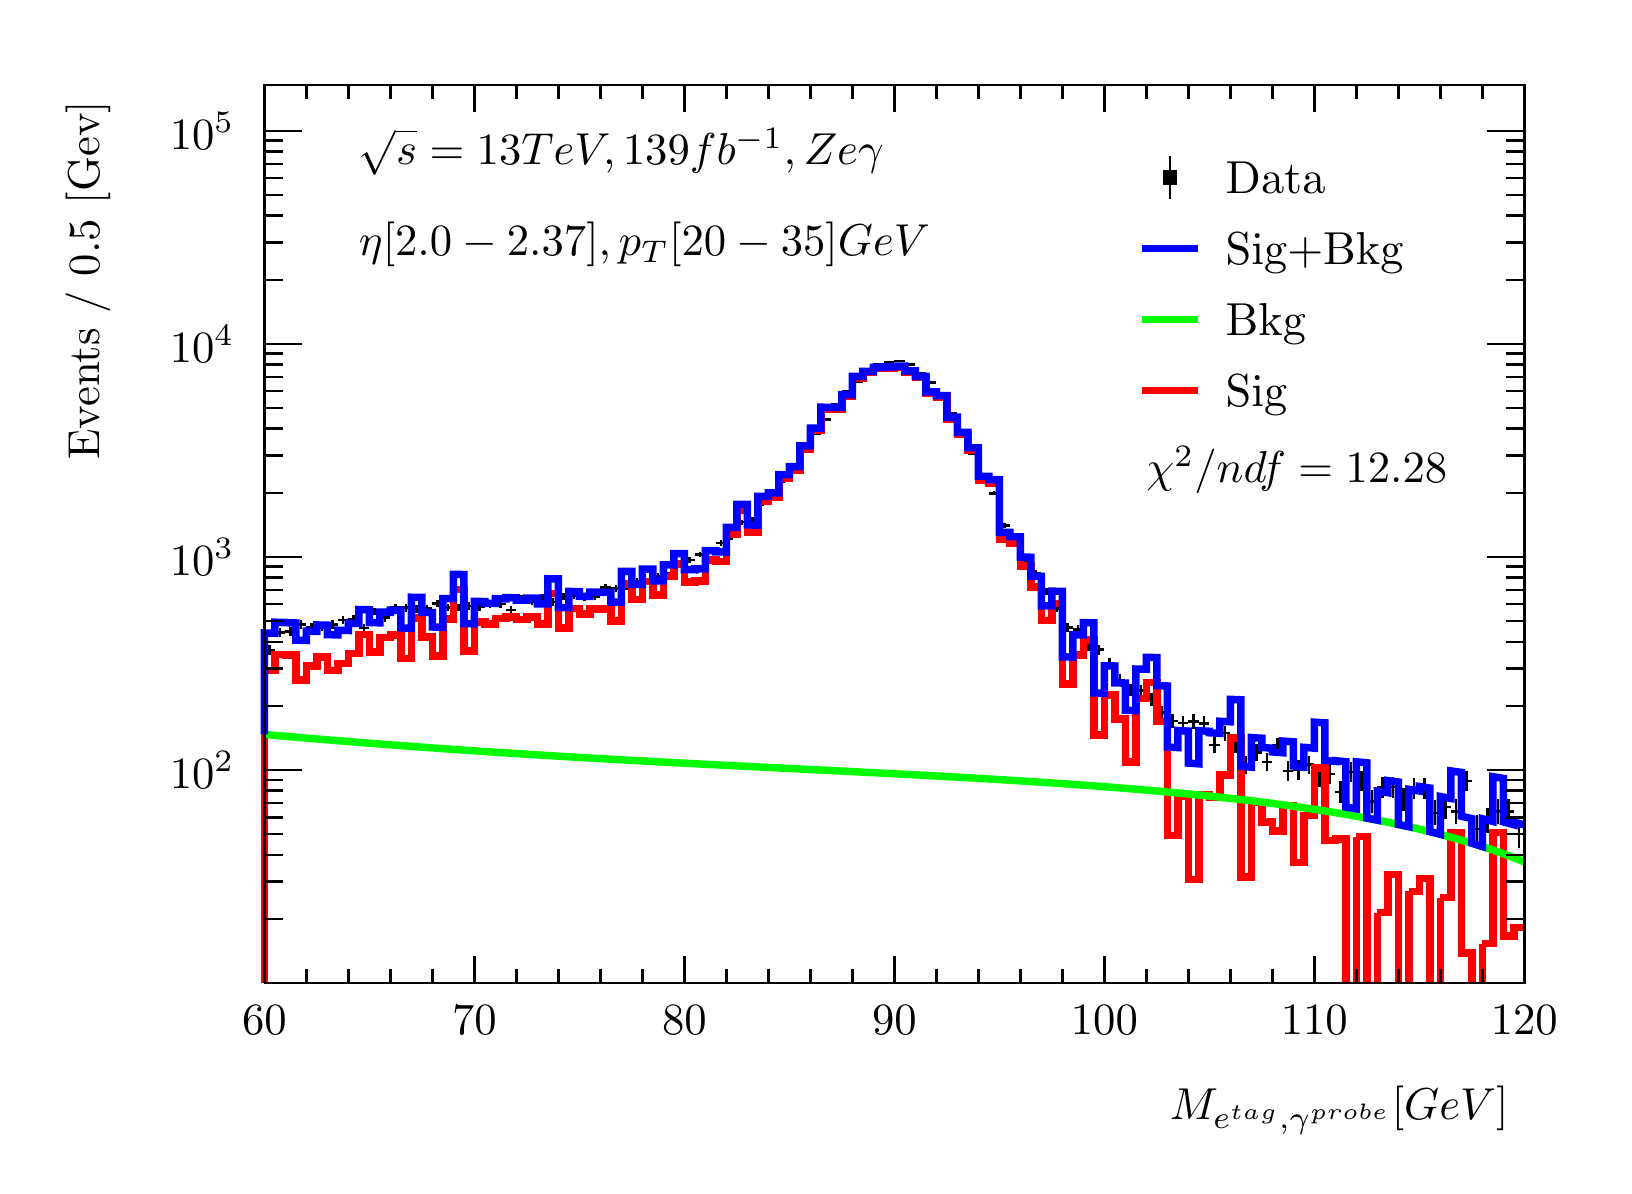
\begin{tikzpicture}
\pgfdeclareplotmark{cross} {
\pgfpathmoveto{\pgfpoint{-0.3\pgfplotmarksize}{\pgfplotmarksize}}
\pgfpathlineto{\pgfpoint{+0.3\pgfplotmarksize}{\pgfplotmarksize}}
\pgfpathlineto{\pgfpoint{+0.3\pgfplotmarksize}{0.3\pgfplotmarksize}}
\pgfpathlineto{\pgfpoint{+1\pgfplotmarksize}{0.3\pgfplotmarksize}}
\pgfpathlineto{\pgfpoint{+1\pgfplotmarksize}{-0.3\pgfplotmarksize}}
\pgfpathlineto{\pgfpoint{+0.3\pgfplotmarksize}{-0.3\pgfplotmarksize}}
\pgfpathlineto{\pgfpoint{+0.3\pgfplotmarksize}{-1.\pgfplotmarksize}}
\pgfpathlineto{\pgfpoint{-0.3\pgfplotmarksize}{-1.\pgfplotmarksize}}
\pgfpathlineto{\pgfpoint{-0.3\pgfplotmarksize}{-0.3\pgfplotmarksize}}
\pgfpathlineto{\pgfpoint{-1.\pgfplotmarksize}{-0.3\pgfplotmarksize}}
\pgfpathlineto{\pgfpoint{-1.\pgfplotmarksize}{0.3\pgfplotmarksize}}
\pgfpathlineto{\pgfpoint{-0.3\pgfplotmarksize}{0.3\pgfplotmarksize}}
\pgfpathclose
\pgfusepathqstroke
}
\pgfdeclareplotmark{cross*} {
\pgfpathmoveto{\pgfpoint{-0.3\pgfplotmarksize}{\pgfplotmarksize}}
\pgfpathlineto{\pgfpoint{+0.3\pgfplotmarksize}{\pgfplotmarksize}}
\pgfpathlineto{\pgfpoint{+0.3\pgfplotmarksize}{0.3\pgfplotmarksize}}
\pgfpathlineto{\pgfpoint{+1\pgfplotmarksize}{0.3\pgfplotmarksize}}
\pgfpathlineto{\pgfpoint{+1\pgfplotmarksize}{-0.3\pgfplotmarksize}}
\pgfpathlineto{\pgfpoint{+0.3\pgfplotmarksize}{-0.3\pgfplotmarksize}}
\pgfpathlineto{\pgfpoint{+0.3\pgfplotmarksize}{-1.\pgfplotmarksize}}
\pgfpathlineto{\pgfpoint{-0.3\pgfplotmarksize}{-1.\pgfplotmarksize}}
\pgfpathlineto{\pgfpoint{-0.3\pgfplotmarksize}{-0.3\pgfplotmarksize}}
\pgfpathlineto{\pgfpoint{-1.\pgfplotmarksize}{-0.3\pgfplotmarksize}}
\pgfpathlineto{\pgfpoint{-1.\pgfplotmarksize}{0.3\pgfplotmarksize}}
\pgfpathlineto{\pgfpoint{-0.3\pgfplotmarksize}{0.3\pgfplotmarksize}}
\pgfpathclose
\pgfusepathqfillstroke
}
\pgfdeclareplotmark{newstar} {
\pgfpathmoveto{\pgfqpoint{0pt}{\pgfplotmarksize}}
\pgfpathlineto{\pgfqpointpolar{44}{0.5\pgfplotmarksize}}
\pgfpathlineto{\pgfqpointpolar{18}{\pgfplotmarksize}}
\pgfpathlineto{\pgfqpointpolar{-20}{0.5\pgfplotmarksize}}
\pgfpathlineto{\pgfqpointpolar{-54}{\pgfplotmarksize}}
\pgfpathlineto{\pgfqpointpolar{-90}{0.5\pgfplotmarksize}}
\pgfpathlineto{\pgfqpointpolar{234}{\pgfplotmarksize}}
\pgfpathlineto{\pgfqpointpolar{198}{0.5\pgfplotmarksize}}
\pgfpathlineto{\pgfqpointpolar{162}{\pgfplotmarksize}}
\pgfpathlineto{\pgfqpointpolar{134}{0.5\pgfplotmarksize}}
\pgfpathclose
\pgfusepathqstroke
}
\pgfdeclareplotmark{newstar*} {
\pgfpathmoveto{\pgfqpoint{0pt}{\pgfplotmarksize}}
\pgfpathlineto{\pgfqpointpolar{44}{0.5\pgfplotmarksize}}
\pgfpathlineto{\pgfqpointpolar{18}{\pgfplotmarksize}}
\pgfpathlineto{\pgfqpointpolar{-20}{0.5\pgfplotmarksize}}
\pgfpathlineto{\pgfqpointpolar{-54}{\pgfplotmarksize}}
\pgfpathlineto{\pgfqpointpolar{-90}{0.5\pgfplotmarksize}}
\pgfpathlineto{\pgfqpointpolar{234}{\pgfplotmarksize}}
\pgfpathlineto{\pgfqpointpolar{198}{0.5\pgfplotmarksize}}
\pgfpathlineto{\pgfqpointpolar{162}{\pgfplotmarksize}}
\pgfpathlineto{\pgfqpointpolar{134}{0.5\pgfplotmarksize}}
\pgfpathclose
\pgfusepathqfillstroke
}
\definecolor{c}{rgb}{1,1,1};
\draw [color=c, fill=c] (0,0) rectangle (20,14.4361);
\draw [color=c, fill=c] (3,2.30977) rectangle (19,13.7143);
\definecolor{c}{rgb}{0,0,0};
\draw [c,line width=0.9] (3,2.30977) -- (3,13.7143) -- (19,13.7143) -- (19,2.30977) -- (3,2.30977);
\definecolor{c}{rgb}{1,1,1};
\draw [color=c, fill=c] (3,2.30977) rectangle (19,13.7143);
\definecolor{c}{rgb}{0,0,0};
\draw [c,line width=0.9] (3,2.30977) -- (3,13.7143) -- (19,13.7143) -- (19,2.30977) -- (3,2.30977);
\draw [c,line width=0.9] (3,2.30977) -- (19,2.30977);
\draw [c,line width=0.9] (3,2.65624) -- (3,2.30977);
\draw [c,line width=0.9] (3.53333,2.48301) -- (3.53333,2.30977);
\draw [c,line width=0.9] (4.06667,2.48301) -- (4.06667,2.30977);
\draw [c,line width=0.9] (4.6,2.48301) -- (4.6,2.30977);
\draw [c,line width=0.9] (5.13333,2.48301) -- (5.13333,2.30977);
\draw [c,line width=0.9] (5.66667,2.65624) -- (5.66667,2.30977);
\draw [c,line width=0.9] (6.2,2.48301) -- (6.2,2.30977);
\draw [c,line width=0.9] (6.73333,2.48301) -- (6.73333,2.30977);
\draw [c,line width=0.9] (7.26667,2.48301) -- (7.26667,2.30977);
\draw [c,line width=0.9] (7.8,2.48301) -- (7.8,2.30977);
\draw [c,line width=0.9] (8.33333,2.65624) -- (8.33333,2.30977);
\draw [c,line width=0.9] (8.86667,2.48301) -- (8.86667,2.30977);
\draw [c,line width=0.9] (9.4,2.48301) -- (9.4,2.30977);
\draw [c,line width=0.9] (9.93333,2.48301) -- (9.93333,2.30977);
\draw [c,line width=0.9] (10.4667,2.48301) -- (10.4667,2.30977);
\draw [c,line width=0.9] (11,2.65624) -- (11,2.30977);
\draw [c,line width=0.9] (11.5333,2.48301) -- (11.5333,2.30977);
\draw [c,line width=0.9] (12.0667,2.48301) -- (12.0667,2.30977);
\draw [c,line width=0.9] (12.6,2.48301) -- (12.6,2.30977);
\draw [c,line width=0.9] (13.1333,2.48301) -- (13.1333,2.30977);
\draw [c,line width=0.9] (13.6667,2.65624) -- (13.6667,2.30977);
\draw [c,line width=0.9] (14.2,2.48301) -- (14.2,2.30977);
\draw [c,line width=0.9] (14.7333,2.48301) -- (14.7333,2.30977);
\draw [c,line width=0.9] (15.2667,2.48301) -- (15.2667,2.30977);
\draw [c,line width=0.9] (15.8,2.48301) -- (15.8,2.30977);
\draw [c,line width=0.9] (16.3333,2.65624) -- (16.3333,2.30977);
\draw [c,line width=0.9] (16.8667,2.48301) -- (16.8667,2.30977);
\draw [c,line width=0.9] (17.4,2.48301) -- (17.4,2.30977);
\draw [c,line width=0.9] (17.9333,2.48301) -- (17.9333,2.30977);
\draw [c,line width=0.9] (18.4667,2.48301) -- (18.4667,2.30977);
\draw [c,line width=0.9] (19,2.65624) -- (19,2.30977);
\draw [anchor=base] (3,1.66015) node[scale=1.61424, color=c, rotate=0]{60};
\draw [anchor=base] (5.66667,1.66015) node[scale=1.61424, color=c, rotate=0]{70};
\draw [anchor=base] (8.33333,1.66015) node[scale=1.61424, color=c, rotate=0]{80};
\draw [anchor=base] (11,1.66015) node[scale=1.61424, color=c, rotate=0]{90};
\draw [anchor=base] (13.6667,1.66015) node[scale=1.61424, color=c, rotate=0]{100};
\draw [anchor=base] (16.3333,1.66015) node[scale=1.61424, color=c, rotate=0]{110};
\draw [anchor=base] (19,1.66015) node[scale=1.61424, color=c, rotate=0]{120};
\draw [anchor= east] (19,0.692932) node[scale=1.61424, color=c, rotate=0]{$M_{e^{tag}, \gamma^{probe}}  [GeV]$};
\draw [c,line width=0.9] (3,13.7143) -- (19,13.7143);
\draw [c,line width=0.9] (3,13.3678) -- (3,13.7143);
\draw [c,line width=0.9] (3.53333,13.5411) -- (3.53333,13.7143);
\draw [c,line width=0.9] (4.06667,13.5411) -- (4.06667,13.7143);
\draw [c,line width=0.9] (4.6,13.5411) -- (4.6,13.7143);
\draw [c,line width=0.9] (5.13333,13.5411) -- (5.13333,13.7143);
\draw [c,line width=0.9] (5.66667,13.3678) -- (5.66667,13.7143);
\draw [c,line width=0.9] (6.2,13.5411) -- (6.2,13.7143);
\draw [c,line width=0.9] (6.73333,13.5411) -- (6.73333,13.7143);
\draw [c,line width=0.9] (7.26667,13.5411) -- (7.26667,13.7143);
\draw [c,line width=0.9] (7.8,13.5411) -- (7.8,13.7143);
\draw [c,line width=0.9] (8.33333,13.3678) -- (8.33333,13.7143);
\draw [c,line width=0.9] (8.86667,13.5411) -- (8.86667,13.7143);
\draw [c,line width=0.9] (9.4,13.5411) -- (9.4,13.7143);
\draw [c,line width=0.9] (9.93333,13.5411) -- (9.93333,13.7143);
\draw [c,line width=0.9] (10.4667,13.5411) -- (10.4667,13.7143);
\draw [c,line width=0.9] (11,13.3678) -- (11,13.7143);
\draw [c,line width=0.9] (11.5333,13.5411) -- (11.5333,13.7143);
\draw [c,line width=0.9] (12.0667,13.5411) -- (12.0667,13.7143);
\draw [c,line width=0.9] (12.6,13.5411) -- (12.6,13.7143);
\draw [c,line width=0.9] (13.1333,13.5411) -- (13.1333,13.7143);
\draw [c,line width=0.9] (13.6667,13.3678) -- (13.6667,13.7143);
\draw [c,line width=0.9] (14.2,13.5411) -- (14.2,13.7143);
\draw [c,line width=0.9] (14.7333,13.5411) -- (14.7333,13.7143);
\draw [c,line width=0.9] (15.2667,13.5411) -- (15.2667,13.7143);
\draw [c,line width=0.9] (15.8,13.5411) -- (15.8,13.7143);
\draw [c,line width=0.9] (16.3333,13.3678) -- (16.3333,13.7143);
\draw [c,line width=0.9] (16.8667,13.5411) -- (16.8667,13.7143);
\draw [c,line width=0.9] (17.4,13.5411) -- (17.4,13.7143);
\draw [c,line width=0.9] (17.9333,13.5411) -- (17.9333,13.7143);
\draw [c,line width=0.9] (18.4667,13.5411) -- (18.4667,13.7143);
\draw [c,line width=0.9] (19,13.3678) -- (19,13.7143);
\draw [c,line width=0.9] (3,2.30977) -- (3,13.7143);
\draw [c,line width=0.9] (3.237,3.12423) -- (3,3.12423);
\draw [c,line width=0.9] (3.237,3.60066) -- (3,3.60066);
\draw [c,line width=0.9] (3.237,3.93869) -- (3,3.93869);
\draw [c,line width=0.9] (3.237,4.20088) -- (3,4.20088);
\draw [c,line width=0.9] (3.237,4.41511) -- (3,4.41511);
\draw [c,line width=0.9] (3.237,4.59624) -- (3,4.59624);
\draw [c,line width=0.9] (3.237,4.75314) -- (3,4.75314);
\draw [c,line width=0.9] (3.237,4.89154) -- (3,4.89154);
\draw [c,line width=0.9] (3.474,5.01534) -- (3,5.01534);
\draw [anchor= east] (2.82,5.01534) node[scale=1.61424, color=c, rotate=0]{$10^{2}$};
\draw [c,line width=0.9] (3.237,5.8298) -- (3,5.8298);
\draw [c,line width=0.9] (3.237,6.30623) -- (3,6.30623);
\draw [c,line width=0.9] (3.237,6.64426) -- (3,6.64426);
\draw [c,line width=0.9] (3.237,6.90645) -- (3,6.90645);
\draw [c,line width=0.9] (3.237,7.12068) -- (3,7.12068);
\draw [c,line width=0.9] (3.237,7.30181) -- (3,7.30181);
\draw [c,line width=0.9] (3.237,7.45871) -- (3,7.45871);
\draw [c,line width=0.9] (3.237,7.59711) -- (3,7.59711);
\draw [c,line width=0.9] (3.474,7.72091) -- (3,7.72091);
\draw [anchor= east] (2.82,7.72091) node[scale=1.61424, color=c, rotate=0]{$10^{3}$};
\draw [c,line width=0.9] (3.237,8.53537) -- (3,8.53537);
\draw [c,line width=0.9] (3.237,9.0118) -- (3,9.0118);
\draw [c,line width=0.9] (3.237,9.34983) -- (3,9.34983);
\draw [c,line width=0.9] (3.237,9.61202) -- (3,9.61202);
\draw [c,line width=0.9] (3.237,9.82625) -- (3,9.82625);
\draw [c,line width=0.9] (3.237,10.0074) -- (3,10.0074);
\draw [c,line width=0.9] (3.237,10.1643) -- (3,10.1643);
\draw [c,line width=0.9] (3.237,10.3027) -- (3,10.3027);
\draw [c,line width=0.9] (3.474,10.4265) -- (3,10.4265);
\draw [anchor= east] (2.82,10.4265) node[scale=1.61424, color=c, rotate=0]{$10^{4}$};
\draw [c,line width=0.9] (3.237,11.2409) -- (3,11.2409);
\draw [c,line width=0.9] (3.237,11.7174) -- (3,11.7174);
\draw [c,line width=0.9] (3.237,12.0554) -- (3,12.0554);
\draw [c,line width=0.9] (3.237,12.3176) -- (3,12.3176);
\draw [c,line width=0.9] (3.237,12.5318) -- (3,12.5318);
\draw [c,line width=0.9] (3.237,12.713) -- (3,12.713);
\draw [c,line width=0.9] (3.237,12.8699) -- (3,12.8699);
\draw [c,line width=0.9] (3.237,13.0083) -- (3,13.0083);
\draw [c,line width=0.9] (3.474,13.1321) -- (3,13.1321);
\draw [anchor= east] (2.82,13.1321) node[scale=1.61424, color=c, rotate=0]{$10^{5}$};
\draw [anchor= east] (0.76,13.7143) node[scale=1.61424, color=c, rotate=90]{Events / 0.5 [Gev]};
\draw [c,line width=0.9] (19,2.30977) -- (19,13.7143);
\draw [c,line width=0.9] (18.763,3.12423) -- (19,3.12423);
\draw [c,line width=0.9] (18.763,3.60066) -- (19,3.60066);
\draw [c,line width=0.9] (18.763,3.93869) -- (19,3.93869);
\draw [c,line width=0.9] (18.763,4.20088) -- (19,4.20088);
\draw [c,line width=0.9] (18.763,4.41511) -- (19,4.41511);
\draw [c,line width=0.9] (18.763,4.59624) -- (19,4.59624);
\draw [c,line width=0.9] (18.763,4.75314) -- (19,4.75314);
\draw [c,line width=0.9] (18.763,4.89154) -- (19,4.89154);
\draw [c,line width=0.9] (18.526,5.01534) -- (19,5.01534);
\draw [c,line width=0.9] (18.763,5.8298) -- (19,5.8298);
\draw [c,line width=0.9] (18.763,6.30623) -- (19,6.30623);
\draw [c,line width=0.9] (18.763,6.64426) -- (19,6.64426);
\draw [c,line width=0.9] (18.763,6.90645) -- (19,6.90645);
\draw [c,line width=0.9] (18.763,7.12068) -- (19,7.12068);
\draw [c,line width=0.9] (18.763,7.30181) -- (19,7.30181);
\draw [c,line width=0.9] (18.763,7.45871) -- (19,7.45871);
\draw [c,line width=0.9] (18.763,7.59711) -- (19,7.59711);
\draw [c,line width=0.9] (18.526,7.72091) -- (19,7.72091);
\draw [c,line width=0.9] (18.763,8.53537) -- (19,8.53537);
\draw [c,line width=0.9] (18.763,9.0118) -- (19,9.0118);
\draw [c,line width=0.9] (18.763,9.34983) -- (19,9.34983);
\draw [c,line width=0.9] (18.763,9.61202) -- (19,9.61202);
\draw [c,line width=0.9] (18.763,9.82625) -- (19,9.82625);
\draw [c,line width=0.9] (18.763,10.0074) -- (19,10.0074);
\draw [c,line width=0.9] (18.763,10.1643) -- (19,10.1643);
\draw [c,line width=0.9] (18.763,10.3027) -- (19,10.3027);
\draw [c,line width=0.9] (18.526,10.4265) -- (19,10.4265);
\draw [c,line width=0.9] (18.763,11.2409) -- (19,11.2409);
\draw [c,line width=0.9] (18.763,11.7174) -- (19,11.7174);
\draw [c,line width=0.9] (18.763,12.0554) -- (19,12.0554);
\draw [c,line width=0.9] (18.763,12.3176) -- (19,12.3176);
\draw [c,line width=0.9] (18.763,12.5318) -- (19,12.5318);
\draw [c,line width=0.9] (18.763,12.713) -- (19,12.713);
\draw [c,line width=0.9] (18.763,12.8699) -- (19,12.8699);
\draw [c,line width=0.9] (18.763,13.0083) -- (19,13.0083);
\draw [c,line width=0.9] (18.526,13.1321) -- (19,13.1321);
\draw [c,line width=0.9] (3.06667,6.53988) -- (3,6.53988);
\draw [c,line width=0.9] (3,6.53988) -- (3,6.53988);
\draw [c,line width=0.9] (3.06667,6.53988) -- (3.13333,6.53988);
\draw [c,line width=0.9] (3.13333,6.53988) -- (3.13333,6.53988);
\draw [c,line width=0.9] (3.06667,6.53988) -- (3.06667,6.60129);
\draw [c,line width=0.9] (3.06667,6.60129) -- (3.06667,6.60129);
\draw [c,line width=0.9] (3.06667,6.53988) -- (3.06667,6.47847);
\draw [c,line width=0.9] (3.06667,6.47847) -- (3.06667,6.47847);
\draw [c,line width=0.9] (3.2,6.76158) -- (3.13333,6.76158);
\draw [c,line width=0.9] (3.13333,6.76158) -- (3.13333,6.76158);
\draw [c,line width=0.9] (3.2,6.76158) -- (3.26667,6.76158);
\draw [c,line width=0.9] (3.26667,6.76158) -- (3.26667,6.76158);
\draw [c,line width=0.9] (3.2,6.76158) -- (3.2,6.81746);
\draw [c,line width=0.9] (3.2,6.81746) -- (3.2,6.81746);
\draw [c,line width=0.9] (3.2,6.76158) -- (3.2,6.70569);
\draw [c,line width=0.9] (3.2,6.70569) -- (3.2,6.70569);
\draw [c,line width=0.9] (3.33333,6.7748) -- (3.26667,6.7748);
\draw [c,line width=0.9] (3.26667,6.7748) -- (3.26667,6.7748);
\draw [c,line width=0.9] (3.33333,6.7748) -- (3.4,6.7748);
\draw [c,line width=0.9] (3.4,6.7748) -- (3.4,6.7748);
\draw [c,line width=0.9] (3.33333,6.7748) -- (3.33333,6.83037);
\draw [c,line width=0.9] (3.33333,6.83037) -- (3.33333,6.83037);
\draw [c,line width=0.9] (3.33333,6.7748) -- (3.33333,6.71922);
\draw [c,line width=0.9] (3.33333,6.71922) -- (3.33333,6.71922);
\draw [c,line width=0.9] (3.46667,6.86337) -- (3.4,6.86337);
\draw [c,line width=0.9] (3.4,6.86337) -- (3.4,6.86337);
\draw [c,line width=0.9] (3.46667,6.86337) -- (3.53333,6.86337);
\draw [c,line width=0.9] (3.53333,6.86337) -- (3.53333,6.86337);
\draw [c,line width=0.9] (3.46667,6.86337) -- (3.46667,6.91689);
\draw [c,line width=0.9] (3.46667,6.91689) -- (3.46667,6.91689);
\draw [c,line width=0.9] (3.46667,6.86337) -- (3.46667,6.80986);
\draw [c,line width=0.9] (3.46667,6.80986) -- (3.46667,6.80986);
\draw [c,line width=0.9] (3.6,6.82371) -- (3.53333,6.82371);
\draw [c,line width=0.9] (3.53333,6.82371) -- (3.53333,6.82371);
\draw [c,line width=0.9] (3.6,6.82371) -- (3.66667,6.82371);
\draw [c,line width=0.9] (3.66667,6.82371) -- (3.66667,6.82371);
\draw [c,line width=0.9] (3.6,6.82371) -- (3.6,6.87813);
\draw [c,line width=0.9] (3.6,6.87813) -- (3.6,6.87813);
\draw [c,line width=0.9] (3.6,6.82371) -- (3.6,6.76928);
\draw [c,line width=0.9] (3.6,6.76928) -- (3.6,6.76928);
\draw [c,line width=0.9] (3.73333,6.83625) -- (3.66667,6.83625);
\draw [c,line width=0.9] (3.66667,6.83625) -- (3.66667,6.83625);
\draw [c,line width=0.9] (3.73333,6.83625) -- (3.8,6.83625);
\draw [c,line width=0.9] (3.8,6.83625) -- (3.8,6.83625);
\draw [c,line width=0.9] (3.73333,6.83625) -- (3.73333,6.89039);
\draw [c,line width=0.9] (3.73333,6.89039) -- (3.73333,6.89039);
\draw [c,line width=0.9] (3.73333,6.83625) -- (3.73333,6.78211);
\draw [c,line width=0.9] (3.73333,6.78211) -- (3.73333,6.78211);
\draw [c,line width=0.9] (3.86667,6.86093) -- (3.8,6.86093);
\draw [c,line width=0.9] (3.8,6.86093) -- (3.8,6.86093);
\draw [c,line width=0.9] (3.86667,6.86093) -- (3.93333,6.86093);
\draw [c,line width=0.9] (3.93333,6.86093) -- (3.93333,6.86093);
\draw [c,line width=0.9] (3.86667,6.86093) -- (3.86667,6.91451);
\draw [c,line width=0.9] (3.86667,6.91451) -- (3.86667,6.91451);
\draw [c,line width=0.9] (3.86667,6.86093) -- (3.86667,6.80736);
\draw [c,line width=0.9] (3.86667,6.80736) -- (3.86667,6.80736);
\draw [c,line width=0.9] (4,6.91815) -- (3.93333,6.91815);
\draw [c,line width=0.9] (3.93333,6.91815) -- (3.93333,6.91815);
\draw [c,line width=0.9] (4,6.91815) -- (4.06667,6.91815);
\draw [c,line width=0.9] (4.06667,6.91815) -- (4.06667,6.91815);
\draw [c,line width=0.9] (4,6.91815) -- (4,6.97043);
\draw [c,line width=0.9] (4,6.97043) -- (4,6.97043);
\draw [c,line width=0.9] (4,6.91815) -- (4,6.86586);
\draw [c,line width=0.9] (4,6.86586) -- (4,6.86586);
\draw [c,line width=0.9] (4.13333,6.93432) -- (4.06667,6.93432);
\draw [c,line width=0.9] (4.06667,6.93432) -- (4.06667,6.93432);
\draw [c,line width=0.9] (4.13333,6.93432) -- (4.2,6.93432);
\draw [c,line width=0.9] (4.2,6.93432) -- (4.2,6.93432);
\draw [c,line width=0.9] (4.13333,6.93432) -- (4.13333,6.98625);
\draw [c,line width=0.9] (4.13333,6.98625) -- (4.13333,6.98625);
\draw [c,line width=0.9] (4.13333,6.93432) -- (4.13333,6.8824);
\draw [c,line width=0.9] (4.13333,6.8824) -- (4.13333,6.8824);
\draw [c,line width=0.9] (4.26667,6.81612) -- (4.2,6.81612);
\draw [c,line width=0.9] (4.2,6.81612) -- (4.2,6.81612);
\draw [c,line width=0.9] (4.26667,6.81612) -- (4.33333,6.81612);
\draw [c,line width=0.9] (4.33333,6.81612) -- (4.33333,6.81612);
\draw [c,line width=0.9] (4.26667,6.81612) -- (4.26667,6.87072);
\draw [c,line width=0.9] (4.26667,6.87072) -- (4.26667,6.87072);
\draw [c,line width=0.9] (4.26667,6.81612) -- (4.26667,6.76152);
\draw [c,line width=0.9] (4.26667,6.76152) -- (4.26667,6.76152);
\draw [c,line width=0.9] (4.4,7.02908) -- (4.33333,7.02908);
\draw [c,line width=0.9] (4.33333,7.02908) -- (4.33333,7.02908);
\draw [c,line width=0.9] (4.4,7.02908) -- (4.46667,7.02908);
\draw [c,line width=0.9] (4.46667,7.02908) -- (4.46667,7.02908);
\draw [c,line width=0.9] (4.4,7.02908) -- (4.4,7.07895);
\draw [c,line width=0.9] (4.4,7.07895) -- (4.4,7.07895);
\draw [c,line width=0.9] (4.4,7.02908) -- (4.4,6.97921);
\draw [c,line width=0.9] (4.4,6.97921) -- (4.4,6.97921);
\draw [c,line width=0.9] (4.53333,6.95254) -- (4.46667,6.95254);
\draw [c,line width=0.9] (4.46667,6.95254) -- (4.46667,6.95254);
\draw [c,line width=0.9] (4.53333,6.95254) -- (4.6,6.95254);
\draw [c,line width=0.9] (4.6,6.95254) -- (4.6,6.95254);
\draw [c,line width=0.9] (4.53333,6.95254) -- (4.53333,7.00406);
\draw [c,line width=0.9] (4.53333,7.00406) -- (4.53333,7.00406);
\draw [c,line width=0.9] (4.53333,6.95254) -- (4.53333,6.90102);
\draw [c,line width=0.9] (4.53333,6.90102) -- (4.53333,6.90102);
\draw [c,line width=0.9] (4.66667,7.07882) -- (4.6,7.07882);
\draw [c,line width=0.9] (4.6,7.07882) -- (4.6,7.07882);
\draw [c,line width=0.9] (4.66667,7.07882) -- (4.73333,7.07882);
\draw [c,line width=0.9] (4.73333,7.07882) -- (4.73333,7.07882);
\draw [c,line width=0.9] (4.66667,7.07882) -- (4.66667,7.12765);
\draw [c,line width=0.9] (4.66667,7.12765) -- (4.66667,7.12765);
\draw [c,line width=0.9] (4.66667,7.07882) -- (4.66667,7.02999);
\draw [c,line width=0.9] (4.66667,7.02999) -- (4.66667,7.02999);
\draw [c,line width=0.9] (4.8,7.07679) -- (4.73333,7.07679);
\draw [c,line width=0.9] (4.73333,7.07679) -- (4.73333,7.07679);
\draw [c,line width=0.9] (4.8,7.07679) -- (4.86667,7.07679);
\draw [c,line width=0.9] (4.86667,7.07679) -- (4.86667,7.07679);
\draw [c,line width=0.9] (4.8,7.07679) -- (4.8,7.12566);
\draw [c,line width=0.9] (4.8,7.12566) -- (4.8,7.12566);
\draw [c,line width=0.9] (4.8,7.07679) -- (4.8,7.02792);
\draw [c,line width=0.9] (4.8,7.02792) -- (4.8,7.02792);
\draw [c,line width=0.9] (4.93333,7.06453) -- (4.86667,7.06453);
\draw [c,line width=0.9] (4.86667,7.06453) -- (4.86667,7.06453);
\draw [c,line width=0.9] (4.93333,7.06453) -- (5,7.06453);
\draw [c,line width=0.9] (5,7.06453) -- (5,7.06453);
\draw [c,line width=0.9] (4.93333,7.06453) -- (4.93333,7.11366);
\draw [c,line width=0.9] (4.93333,7.11366) -- (4.93333,7.11366);
\draw [c,line width=0.9] (4.93333,7.06453) -- (4.93333,7.0154);
\draw [c,line width=0.9] (4.93333,7.0154) -- (4.93333,7.0154);
\draw [c,line width=0.9] (5.06667,7.06453) -- (5,7.06453);
\draw [c,line width=0.9] (5,7.06453) -- (5,7.06453);
\draw [c,line width=0.9] (5.06667,7.06453) -- (5.13333,7.06453);
\draw [c,line width=0.9] (5.13333,7.06453) -- (5.13333,7.06453);
\draw [c,line width=0.9] (5.06667,7.06453) -- (5.06667,7.11366);
\draw [c,line width=0.9] (5.06667,7.11366) -- (5.06667,7.11366);
\draw [c,line width=0.9] (5.06667,7.06453) -- (5.06667,7.0154);
\draw [c,line width=0.9] (5.06667,7.0154) -- (5.06667,7.0154);
\draw [c,line width=0.9] (5.2,7.13238) -- (5.13333,7.13238);
\draw [c,line width=0.9] (5.13333,7.13238) -- (5.13333,7.13238);
\draw [c,line width=0.9] (5.2,7.13238) -- (5.26667,7.13238);
\draw [c,line width=0.9] (5.26667,7.13238) -- (5.26667,7.13238);
\draw [c,line width=0.9] (5.2,7.13238) -- (5.2,7.18011);
\draw [c,line width=0.9] (5.2,7.18011) -- (5.2,7.18011);
\draw [c,line width=0.9] (5.2,7.13238) -- (5.2,7.08465);
\draw [c,line width=0.9] (5.2,7.08465) -- (5.2,7.08465);
\draw [c,line width=0.9] (5.33333,7.07882) -- (5.26667,7.07882);
\draw [c,line width=0.9] (5.26667,7.07882) -- (5.26667,7.07882);
\draw [c,line width=0.9] (5.33333,7.07882) -- (5.4,7.07882);
\draw [c,line width=0.9] (5.4,7.07882) -- (5.4,7.07882);
\draw [c,line width=0.9] (5.33333,7.07882) -- (5.33333,7.12765);
\draw [c,line width=0.9] (5.33333,7.12765) -- (5.33333,7.12765);
\draw [c,line width=0.9] (5.33333,7.07882) -- (5.33333,7.02999);
\draw [c,line width=0.9] (5.33333,7.02999) -- (5.33333,7.02999);
\draw [c,line width=0.9] (5.46667,7.08085) -- (5.4,7.08085);
\draw [c,line width=0.9] (5.4,7.08085) -- (5.4,7.08085);
\draw [c,line width=0.9] (5.46667,7.08085) -- (5.53333,7.08085);
\draw [c,line width=0.9] (5.53333,7.08085) -- (5.53333,7.08085);
\draw [c,line width=0.9] (5.46667,7.08085) -- (5.46667,7.12964);
\draw [c,line width=0.9] (5.46667,7.12964) -- (5.46667,7.12964);
\draw [c,line width=0.9] (5.46667,7.08085) -- (5.46667,7.03206);
\draw [c,line width=0.9] (5.46667,7.03206) -- (5.46667,7.03206);
\draw [c,line width=0.9] (5.6,7.09894) -- (5.53333,7.09894);
\draw [c,line width=0.9] (5.53333,7.09894) -- (5.53333,7.09894);
\draw [c,line width=0.9] (5.6,7.09894) -- (5.66667,7.09894);
\draw [c,line width=0.9] (5.66667,7.09894) -- (5.66667,7.09894);
\draw [c,line width=0.9] (5.6,7.09894) -- (5.6,7.14736);
\draw [c,line width=0.9] (5.6,7.14736) -- (5.6,7.14736);
\draw [c,line width=0.9] (5.6,7.09894) -- (5.6,7.05053);
\draw [c,line width=0.9] (5.6,7.05053) -- (5.6,7.05053);
\draw [c,line width=0.9] (5.73333,7.08288) -- (5.66667,7.08288);
\draw [c,line width=0.9] (5.66667,7.08288) -- (5.66667,7.08288);
\draw [c,line width=0.9] (5.73333,7.08288) -- (5.8,7.08288);
\draw [c,line width=0.9] (5.8,7.08288) -- (5.8,7.08288);
\draw [c,line width=0.9] (5.73333,7.08288) -- (5.73333,7.13162);
\draw [c,line width=0.9] (5.73333,7.13162) -- (5.73333,7.13162);
\draw [c,line width=0.9] (5.73333,7.08288) -- (5.73333,7.03413);
\draw [c,line width=0.9] (5.73333,7.03413) -- (5.73333,7.03413);
\draw [c,line width=0.9] (5.86667,7.1148) -- (5.8,7.1148);
\draw [c,line width=0.9] (5.8,7.1148) -- (5.8,7.1148);
\draw [c,line width=0.9] (5.86667,7.1148) -- (5.93333,7.1148);
\draw [c,line width=0.9] (5.93333,7.1148) -- (5.93333,7.1148);
\draw [c,line width=0.9] (5.86667,7.1148) -- (5.86667,7.16288);
\draw [c,line width=0.9] (5.86667,7.16288) -- (5.86667,7.16288);
\draw [c,line width=0.9] (5.86667,7.1148) -- (5.86667,7.06671);
\draw [c,line width=0.9] (5.86667,7.06671) -- (5.86667,7.06671);
\draw [c,line width=0.9] (6,7.12264) -- (5.93333,7.12264);
\draw [c,line width=0.9] (5.93333,7.12264) -- (5.93333,7.12264);
\draw [c,line width=0.9] (6,7.12264) -- (6.06667,7.12264);
\draw [c,line width=0.9] (6.06667,7.12264) -- (6.06667,7.12264);
\draw [c,line width=0.9] (6,7.12264) -- (6,7.17057);
\draw [c,line width=0.9] (6,7.17057) -- (6,7.17057);
\draw [c,line width=0.9] (6,7.12264) -- (6,7.07472);
\draw [c,line width=0.9] (6,7.07472) -- (6,7.07472);
\draw [c,line width=0.9] (6.13333,7.04798) -- (6.06667,7.04798);
\draw [c,line width=0.9] (6.06667,7.04798) -- (6.06667,7.04798);
\draw [c,line width=0.9] (6.13333,7.04798) -- (6.2,7.04798);
\draw [c,line width=0.9] (6.2,7.04798) -- (6.2,7.04798);
\draw [c,line width=0.9] (6.13333,7.04798) -- (6.13333,7.09745);
\draw [c,line width=0.9] (6.13333,7.09745) -- (6.13333,7.09745);
\draw [c,line width=0.9] (6.13333,7.04798) -- (6.13333,6.99851);
\draw [c,line width=0.9] (6.13333,6.99851) -- (6.13333,6.99851);
\draw [c,line width=0.9] (6.26667,7.1873) -- (6.2,7.1873);
\draw [c,line width=0.9] (6.2,7.1873) -- (6.2,7.1873);
\draw [c,line width=0.9] (6.26667,7.1873) -- (6.33333,7.1873);
\draw [c,line width=0.9] (6.33333,7.1873) -- (6.33333,7.1873);
\draw [c,line width=0.9] (6.26667,7.1873) -- (6.26667,7.23393);
\draw [c,line width=0.9] (6.26667,7.23393) -- (6.26667,7.23393);
\draw [c,line width=0.9] (6.26667,7.1873) -- (6.26667,7.14068);
\draw [c,line width=0.9] (6.26667,7.14068) -- (6.26667,7.14068);
\draw [c,line width=0.9] (6.4,7.15732) -- (6.33333,7.15732);
\draw [c,line width=0.9] (6.33333,7.15732) -- (6.33333,7.15732);
\draw [c,line width=0.9] (6.4,7.15732) -- (6.46667,7.15732);
\draw [c,line width=0.9] (6.46667,7.15732) -- (6.46667,7.15732);
\draw [c,line width=0.9] (6.4,7.15732) -- (6.4,7.20454);
\draw [c,line width=0.9] (6.4,7.20454) -- (6.4,7.20454);
\draw [c,line width=0.9] (6.4,7.15732) -- (6.4,7.11009);
\draw [c,line width=0.9] (6.4,7.11009) -- (6.4,7.11009);
\draw [c,line width=0.9] (6.53333,7.2093) -- (6.46667,7.2093);
\draw [c,line width=0.9] (6.46667,7.2093) -- (6.46667,7.2093);
\draw [c,line width=0.9] (6.53333,7.2093) -- (6.6,7.2093);
\draw [c,line width=0.9] (6.6,7.2093) -- (6.6,7.2093);
\draw [c,line width=0.9] (6.53333,7.2093) -- (6.53333,7.25549);
\draw [c,line width=0.9] (6.53333,7.25549) -- (6.53333,7.25549);
\draw [c,line width=0.9] (6.53333,7.2093) -- (6.53333,7.16311);
\draw [c,line width=0.9] (6.53333,7.16311) -- (6.53333,7.16311);
\draw [c,line width=0.9] (6.66667,7.1497) -- (6.6,7.1497);
\draw [c,line width=0.9] (6.6,7.1497) -- (6.6,7.1497);
\draw [c,line width=0.9] (6.66667,7.1497) -- (6.73333,7.1497);
\draw [c,line width=0.9] (6.73333,7.1497) -- (6.73333,7.1497);
\draw [c,line width=0.9] (6.66667,7.1497) -- (6.66667,7.19708);
\draw [c,line width=0.9] (6.66667,7.19708) -- (6.66667,7.19708);
\draw [c,line width=0.9] (6.66667,7.1497) -- (6.66667,7.10232);
\draw [c,line width=0.9] (6.66667,7.10232) -- (6.66667,7.10232);
\draw [c,line width=0.9] (6.8,7.22374) -- (6.73333,7.22374);
\draw [c,line width=0.9] (6.73333,7.22374) -- (6.73333,7.22374);
\draw [c,line width=0.9] (6.8,7.22374) -- (6.86667,7.22374);
\draw [c,line width=0.9] (6.86667,7.22374) -- (6.86667,7.22374);
\draw [c,line width=0.9] (6.8,7.22374) -- (6.8,7.26965);
\draw [c,line width=0.9] (6.8,7.26965) -- (6.8,7.26965);
\draw [c,line width=0.9] (6.8,7.22374) -- (6.8,7.17783);
\draw [c,line width=0.9] (6.8,7.17783) -- (6.8,7.17783);
\draw [c,line width=0.9] (6.93333,7.22911) -- (6.86667,7.22911);
\draw [c,line width=0.9] (6.86667,7.22911) -- (6.86667,7.22911);
\draw [c,line width=0.9] (6.93333,7.22911) -- (7,7.22911);
\draw [c,line width=0.9] (7,7.22911) -- (7,7.22911);
\draw [c,line width=0.9] (6.93333,7.22911) -- (6.93333,7.27491);
\draw [c,line width=0.9] (6.93333,7.27491) -- (6.93333,7.27491);
\draw [c,line width=0.9] (6.93333,7.22911) -- (6.93333,7.18331);
\draw [c,line width=0.9] (6.93333,7.18331) -- (6.93333,7.18331);
\draw [c,line width=0.9] (7.06667,7.2093) -- (7,7.2093);
\draw [c,line width=0.9] (7,7.2093) -- (7,7.2093);
\draw [c,line width=0.9] (7.06667,7.2093) -- (7.13333,7.2093);
\draw [c,line width=0.9] (7.13333,7.2093) -- (7.13333,7.2093);
\draw [c,line width=0.9] (7.06667,7.2093) -- (7.06667,7.25549);
\draw [c,line width=0.9] (7.06667,7.25549) -- (7.06667,7.25549);
\draw [c,line width=0.9] (7.06667,7.2093) -- (7.06667,7.16311);
\draw [c,line width=0.9] (7.06667,7.16311) -- (7.06667,7.16311);
\draw [c,line width=0.9] (7.2,7.22015) -- (7.13333,7.22015);
\draw [c,line width=0.9] (7.13333,7.22015) -- (7.13333,7.22015);
\draw [c,line width=0.9] (7.2,7.22015) -- (7.26667,7.22015);
\draw [c,line width=0.9] (7.26667,7.22015) -- (7.26667,7.22015);
\draw [c,line width=0.9] (7.2,7.22015) -- (7.2,7.26613);
\draw [c,line width=0.9] (7.2,7.26613) -- (7.2,7.26613);
\draw [c,line width=0.9] (7.2,7.22015) -- (7.2,7.17417);
\draw [c,line width=0.9] (7.2,7.17417) -- (7.2,7.17417);
\draw [c,line width=0.9] (7.33333,7.33328) -- (7.26667,7.33328);
\draw [c,line width=0.9] (7.26667,7.33328) -- (7.26667,7.33328);
\draw [c,line width=0.9] (7.33333,7.33328) -- (7.4,7.33328);
\draw [c,line width=0.9] (7.4,7.33328) -- (7.4,7.33328);
\draw [c,line width=0.9] (7.33333,7.33328) -- (7.33333,7.3771);
\draw [c,line width=0.9] (7.33333,7.3771) -- (7.33333,7.3771);
\draw [c,line width=0.9] (7.33333,7.33328) -- (7.33333,7.28946);
\draw [c,line width=0.9] (7.33333,7.28946) -- (7.33333,7.28946);
\draw [c,line width=0.9] (7.46667,7.31848) -- (7.4,7.31848);
\draw [c,line width=0.9] (7.4,7.31848) -- (7.4,7.31848);
\draw [c,line width=0.9] (7.46667,7.31848) -- (7.53333,7.31848);
\draw [c,line width=0.9] (7.53333,7.31848) -- (7.53333,7.31848);
\draw [c,line width=0.9] (7.46667,7.31848) -- (7.46667,7.36258);
\draw [c,line width=0.9] (7.46667,7.36258) -- (7.46667,7.36258);
\draw [c,line width=0.9] (7.46667,7.31848) -- (7.46667,7.27439);
\draw [c,line width=0.9] (7.46667,7.27439) -- (7.46667,7.27439);
\draw [c,line width=0.9] (7.6,7.34628) -- (7.53333,7.34628);
\draw [c,line width=0.9] (7.53333,7.34628) -- (7.53333,7.34628);
\draw [c,line width=0.9] (7.6,7.34628) -- (7.66667,7.34628);
\draw [c,line width=0.9] (7.66667,7.34628) -- (7.66667,7.34628);
\draw [c,line width=0.9] (7.6,7.34628) -- (7.6,7.38986);
\draw [c,line width=0.9] (7.6,7.38986) -- (7.6,7.38986);
\draw [c,line width=0.9] (7.6,7.34628) -- (7.6,7.30271);
\draw [c,line width=0.9] (7.6,7.30271) -- (7.6,7.30271);
\draw [c,line width=0.9] (7.73333,7.41075) -- (7.66667,7.41075);
\draw [c,line width=0.9] (7.66667,7.41075) -- (7.66667,7.41075);
\draw [c,line width=0.9] (7.73333,7.41075) -- (7.8,7.41075);
\draw [c,line width=0.9] (7.8,7.41075) -- (7.8,7.41075);
\draw [c,line width=0.9] (7.73333,7.41075) -- (7.73333,7.45315);
\draw [c,line width=0.9] (7.73333,7.45315) -- (7.73333,7.45315);
\draw [c,line width=0.9] (7.73333,7.41075) -- (7.73333,7.36835);
\draw [c,line width=0.9] (7.73333,7.36835) -- (7.73333,7.36835);
\draw [c,line width=0.9] (7.86667,7.41685) -- (7.8,7.41685);
\draw [c,line width=0.9] (7.8,7.41685) -- (7.8,7.41685);
\draw [c,line width=0.9] (7.86667,7.41685) -- (7.93333,7.41685);
\draw [c,line width=0.9] (7.93333,7.41685) -- (7.93333,7.41685);
\draw [c,line width=0.9] (7.86667,7.41685) -- (7.86667,7.45914);
\draw [c,line width=0.9] (7.86667,7.45914) -- (7.86667,7.45914);
\draw [c,line width=0.9] (7.86667,7.41685) -- (7.86667,7.37457);
\draw [c,line width=0.9] (7.86667,7.37457) -- (7.86667,7.37457);
\draw [c,line width=0.9] (8,7.47766) -- (7.93333,7.47766);
\draw [c,line width=0.9] (7.93333,7.47766) -- (7.93333,7.47766);
\draw [c,line width=0.9] (8,7.47766) -- (8.06667,7.47766);
\draw [c,line width=0.9] (8.06667,7.47766) -- (8.06667,7.47766);
\draw [c,line width=0.9] (8,7.47766) -- (8,7.51886);
\draw [c,line width=0.9] (8,7.51886) -- (8,7.51886);
\draw [c,line width=0.9] (8,7.47766) -- (8,7.43645);
\draw [c,line width=0.9] (8,7.43645) -- (8,7.43645);
\draw [c,line width=0.9] (8.13333,7.49202) -- (8.06667,7.49202);
\draw [c,line width=0.9] (8.06667,7.49202) -- (8.06667,7.49202);
\draw [c,line width=0.9] (8.13333,7.49202) -- (8.2,7.49202);
\draw [c,line width=0.9] (8.2,7.49202) -- (8.2,7.49202);
\draw [c,line width=0.9] (8.13333,7.49202) -- (8.13333,7.53298);
\draw [c,line width=0.9] (8.13333,7.53298) -- (8.13333,7.53298);
\draw [c,line width=0.9] (8.13333,7.49202) -- (8.13333,7.45107);
\draw [c,line width=0.9] (8.13333,7.45107) -- (8.13333,7.45107);
\draw [c,line width=0.9] (8.26667,7.63058) -- (8.2,7.63058);
\draw [c,line width=0.9] (8.2,7.63058) -- (8.2,7.63058);
\draw [c,line width=0.9] (8.26667,7.63058) -- (8.33333,7.63058);
\draw [c,line width=0.9] (8.33333,7.63058) -- (8.33333,7.63058);
\draw [c,line width=0.9] (8.26667,7.63058) -- (8.26667,7.66919);
\draw [c,line width=0.9] (8.26667,7.66919) -- (8.26667,7.66919);
\draw [c,line width=0.9] (8.26667,7.63058) -- (8.26667,7.59197);
\draw [c,line width=0.9] (8.26667,7.59197) -- (8.26667,7.59197);
\draw [c,line width=0.9] (8.4,7.6827) -- (8.33333,7.6827);
\draw [c,line width=0.9] (8.33333,7.6827) -- (8.33333,7.6827);
\draw [c,line width=0.9] (8.4,7.6827) -- (8.46667,7.6827);
\draw [c,line width=0.9] (8.46667,7.6827) -- (8.46667,7.6827);
\draw [c,line width=0.9] (8.4,7.6827) -- (8.4,7.72046);
\draw [c,line width=0.9] (8.4,7.72046) -- (8.4,7.72046);
\draw [c,line width=0.9] (8.4,7.6827) -- (8.4,7.64493);
\draw [c,line width=0.9] (8.4,7.64493) -- (8.4,7.64493);
\draw [c,line width=0.9] (8.53333,7.75336) -- (8.46667,7.75336);
\draw [c,line width=0.9] (8.46667,7.75336) -- (8.46667,7.75336);
\draw [c,line width=0.9] (8.53333,7.75336) -- (8.6,7.75336);
\draw [c,line width=0.9] (8.6,7.75336) -- (8.6,7.75336);
\draw [c,line width=0.9] (8.53333,7.75336) -- (8.53333,7.79001);
\draw [c,line width=0.9] (8.53333,7.79001) -- (8.53333,7.79001);
\draw [c,line width=0.9] (8.53333,7.75336) -- (8.53333,7.71671);
\draw [c,line width=0.9] (8.53333,7.71671) -- (8.53333,7.71671);
\draw [c,line width=0.9] (8.66667,7.80041) -- (8.6,7.80041);
\draw [c,line width=0.9] (8.6,7.80041) -- (8.6,7.80041);
\draw [c,line width=0.9] (8.66667,7.80041) -- (8.73333,7.80041);
\draw [c,line width=0.9] (8.73333,7.80041) -- (8.73333,7.80041);
\draw [c,line width=0.9] (8.66667,7.80041) -- (8.66667,7.83633);
\draw [c,line width=0.9] (8.66667,7.83633) -- (8.66667,7.83633);
\draw [c,line width=0.9] (8.66667,7.80041) -- (8.66667,7.76449);
\draw [c,line width=0.9] (8.66667,7.76449) -- (8.66667,7.76449);
\draw [c,line width=0.9] (8.8,7.89935) -- (8.73333,7.89935);
\draw [c,line width=0.9] (8.73333,7.89935) -- (8.73333,7.89935);
\draw [c,line width=0.9] (8.8,7.89935) -- (8.86667,7.89935);
\draw [c,line width=0.9] (8.86667,7.89935) -- (8.86667,7.89935);
\draw [c,line width=0.9] (8.8,7.89935) -- (8.8,7.93379);
\draw [c,line width=0.9] (8.8,7.93379) -- (8.8,7.93379);
\draw [c,line width=0.9] (8.8,7.89935) -- (8.8,7.86491);
\draw [c,line width=0.9] (8.8,7.86491) -- (8.8,7.86491);
\draw [c,line width=0.9] (8.93333,7.97367) -- (8.86667,7.97367);
\draw [c,line width=0.9] (8.86667,7.97367) -- (8.86667,7.97367);
\draw [c,line width=0.9] (8.93333,7.97367) -- (9,7.97367);
\draw [c,line width=0.9] (9,7.97367) -- (9,7.97367);
\draw [c,line width=0.9] (8.93333,7.97367) -- (8.93333,8.00704);
\draw [c,line width=0.9] (8.93333,8.00704) -- (8.93333,8.00704);
\draw [c,line width=0.9] (8.93333,7.97367) -- (8.93333,7.9403);
\draw [c,line width=0.9] (8.93333,7.9403) -- (8.93333,7.9403);
\draw [c,line width=0.9] (9.06667,8.16397) -- (9,8.16397);
\draw [c,line width=0.9] (9,8.16397) -- (9,8.16397);
\draw [c,line width=0.9] (9.06667,8.16397) -- (9.13333,8.16397);
\draw [c,line width=0.9] (9.13333,8.16397) -- (9.13333,8.16397);
\draw [c,line width=0.9] (9.06667,8.16397) -- (9.06667,8.19474);
\draw [c,line width=0.9] (9.06667,8.19474) -- (9.06667,8.19474);
\draw [c,line width=0.9] (9.06667,8.16397) -- (9.06667,8.1332);
\draw [c,line width=0.9] (9.06667,8.1332) -- (9.06667,8.1332);
\draw [c,line width=0.9] (9.2,8.19656) -- (9.13333,8.19656);
\draw [c,line width=0.9] (9.13333,8.19656) -- (9.13333,8.19656);
\draw [c,line width=0.9] (9.2,8.19656) -- (9.26667,8.19656);
\draw [c,line width=0.9] (9.26667,8.19656) -- (9.26667,8.19656);
\draw [c,line width=0.9] (9.2,8.19656) -- (9.2,8.2269);
\draw [c,line width=0.9] (9.2,8.2269) -- (9.2,8.2269);
\draw [c,line width=0.9] (9.2,8.19656) -- (9.2,8.16621);
\draw [c,line width=0.9] (9.2,8.16621) -- (9.2,8.16621);
\draw [c,line width=0.9] (9.33333,8.4024) -- (9.26667,8.4024);
\draw [c,line width=0.9] (9.26667,8.4024) -- (9.26667,8.4024);
\draw [c,line width=0.9] (9.33333,8.4024) -- (9.4,8.4024);
\draw [c,line width=0.9] (9.4,8.4024) -- (9.4,8.4024);
\draw [c,line width=0.9] (9.33333,8.4024) -- (9.33333,8.4302);
\draw [c,line width=0.9] (9.33333,8.4302) -- (9.33333,8.4302);
\draw [c,line width=0.9] (9.33333,8.4024) -- (9.33333,8.37459);
\draw [c,line width=0.9] (9.33333,8.37459) -- (9.33333,8.37459);
\draw [c,line width=0.9] (9.46667,8.48863) -- (9.4,8.48863);
\draw [c,line width=0.9] (9.4,8.48863) -- (9.4,8.48863);
\draw [c,line width=0.9] (9.46667,8.48863) -- (9.53333,8.48863);
\draw [c,line width=0.9] (9.53333,8.48863) -- (9.53333,8.48863);
\draw [c,line width=0.9] (9.46667,8.48863) -- (9.46667,8.51543);
\draw [c,line width=0.9] (9.46667,8.51543) -- (9.46667,8.51543);
\draw [c,line width=0.9] (9.46667,8.48863) -- (9.46667,8.46183);
\draw [c,line width=0.9] (9.46667,8.46183) -- (9.46667,8.46183);
\draw [c,line width=0.9] (9.6,8.69036) -- (9.53333,8.69036);
\draw [c,line width=0.9] (9.53333,8.69036) -- (9.53333,8.69036);
\draw [c,line width=0.9] (9.6,8.69036) -- (9.66667,8.69036);
\draw [c,line width=0.9] (9.66667,8.69036) -- (9.66667,8.69036);
\draw [c,line width=0.9] (9.6,8.69036) -- (9.6,8.71496);
\draw [c,line width=0.9] (9.6,8.71496) -- (9.6,8.71496);
\draw [c,line width=0.9] (9.6,8.69036) -- (9.6,8.66576);
\draw [c,line width=0.9] (9.6,8.66576) -- (9.6,8.66576);
\draw [c,line width=0.9] (9.73333,8.86337) -- (9.66667,8.86337);
\draw [c,line width=0.9] (9.66667,8.86337) -- (9.66667,8.86337);
\draw [c,line width=0.9] (9.73333,8.86337) -- (9.8,8.86337);
\draw [c,line width=0.9] (9.8,8.86337) -- (9.8,8.86337);
\draw [c,line width=0.9] (9.73333,8.86337) -- (9.73333,8.88622);
\draw [c,line width=0.9] (9.73333,8.88622) -- (9.73333,8.88622);
\draw [c,line width=0.9] (9.73333,8.86337) -- (9.73333,8.84052);
\draw [c,line width=0.9] (9.73333,8.84052) -- (9.73333,8.84052);
\draw [c,line width=0.9] (9.86667,9.08211) -- (9.8,9.08211);
\draw [c,line width=0.9] (9.8,9.08211) -- (9.8,9.08211);
\draw [c,line width=0.9] (9.86667,9.08211) -- (9.93333,9.08211);
\draw [c,line width=0.9] (9.93333,9.08211) -- (9.93333,9.08211);
\draw [c,line width=0.9] (9.86667,9.08211) -- (9.86667,9.10293);
\draw [c,line width=0.9] (9.86667,9.10293) -- (9.86667,9.10293);
\draw [c,line width=0.9] (9.86667,9.08211) -- (9.86667,9.06129);
\draw [c,line width=0.9] (9.86667,9.06129) -- (9.86667,9.06129);
\draw [c,line width=0.9] (10,9.28398) -- (9.93333,9.28398);
\draw [c,line width=0.9] (9.93333,9.28398) -- (9.93333,9.28398);
\draw [c,line width=0.9] (10,9.28398) -- (10.0667,9.28398);
\draw [c,line width=0.9] (10.0667,9.28398) -- (10.0667,9.28398);
\draw [c,line width=0.9] (10,9.28398) -- (10,9.30308);
\draw [c,line width=0.9] (10,9.30308) -- (10,9.30308);
\draw [c,line width=0.9] (10,9.28398) -- (10,9.26487);
\draw [c,line width=0.9] (10,9.26487) -- (10,9.26487);
\draw [c,line width=0.9] (10.1333,9.46715) -- (10.0667,9.46715);
\draw [c,line width=0.9] (10.0667,9.46715) -- (10.0667,9.46715);
\draw [c,line width=0.9] (10.1333,9.46715) -- (10.2,9.46715);
\draw [c,line width=0.9] (10.2,9.46715) -- (10.2,9.46715);
\draw [c,line width=0.9] (10.1333,9.46715) -- (10.1333,9.48482);
\draw [c,line width=0.9] (10.1333,9.48482) -- (10.1333,9.48482);
\draw [c,line width=0.9] (10.1333,9.46715) -- (10.1333,9.44947);
\draw [c,line width=0.9] (10.1333,9.44947) -- (10.1333,9.44947);
\draw [c,line width=0.9] (10.2667,9.65494) -- (10.2,9.65494);
\draw [c,line width=0.9] (10.2,9.65494) -- (10.2,9.65494);
\draw [c,line width=0.9] (10.2667,9.65494) -- (10.3333,9.65494);
\draw [c,line width=0.9] (10.3333,9.65494) -- (10.3333,9.65494);
\draw [c,line width=0.9] (10.2667,9.65494) -- (10.2667,9.67126);
\draw [c,line width=0.9] (10.2667,9.67126) -- (10.2667,9.67126);
\draw [c,line width=0.9] (10.2667,9.65494) -- (10.2667,9.63863);
\draw [c,line width=0.9] (10.2667,9.63863) -- (10.2667,9.63863);
\draw [c,line width=0.9] (10.4,9.82938) -- (10.3333,9.82938);
\draw [c,line width=0.9] (10.3333,9.82938) -- (10.3333,9.82938);
\draw [c,line width=0.9] (10.4,9.82938) -- (10.4667,9.82938);
\draw [c,line width=0.9] (10.4667,9.82938) -- (10.4667,9.82938);
\draw [c,line width=0.9] (10.4,9.82938) -- (10.4,9.84453);
\draw [c,line width=0.9] (10.4,9.84453) -- (10.4,9.84453);
\draw [c,line width=0.9] (10.4,9.82938) -- (10.4,9.81423);
\draw [c,line width=0.9] (10.4,9.81423) -- (10.4,9.81423);
\draw [c,line width=0.9] (10.5333,9.94198) -- (10.4667,9.94198);
\draw [c,line width=0.9] (10.4667,9.94198) -- (10.4667,9.94198);
\draw [c,line width=0.9] (10.5333,9.94198) -- (10.6,9.94198);
\draw [c,line width=0.9] (10.6,9.94198) -- (10.6,9.94198);
\draw [c,line width=0.9] (10.5333,9.94198) -- (10.5333,9.95642);
\draw [c,line width=0.9] (10.5333,9.95642) -- (10.5333,9.95642);
\draw [c,line width=0.9] (10.5333,9.94198) -- (10.5333,9.92754);
\draw [c,line width=0.9] (10.5333,9.92754) -- (10.5333,9.92754);
\draw [c,line width=0.9] (10.6667,10.0796) -- (10.6,10.0796);
\draw [c,line width=0.9] (10.6,10.0796) -- (10.6,10.0796);
\draw [c,line width=0.9] (10.6667,10.0796) -- (10.7333,10.0796);
\draw [c,line width=0.9] (10.7333,10.0796) -- (10.7333,10.0796);
\draw [c,line width=0.9] (10.6667,10.0796) -- (10.6667,10.0933);
\draw [c,line width=0.9] (10.6667,10.0933) -- (10.6667,10.0933);
\draw [c,line width=0.9] (10.6667,10.0796) -- (10.6667,10.066);
\draw [c,line width=0.9] (10.6667,10.066) -- (10.6667,10.066);
\draw [c,line width=0.9] (10.8,10.1658) -- (10.7333,10.1658);
\draw [c,line width=0.9] (10.7333,10.1658) -- (10.7333,10.1658);
\draw [c,line width=0.9] (10.8,10.1658) -- (10.8667,10.1658);
\draw [c,line width=0.9] (10.8667,10.1658) -- (10.8667,10.1658);
\draw [c,line width=0.9] (10.8,10.1658) -- (10.8,10.1789);
\draw [c,line width=0.9] (10.8,10.1789) -- (10.8,10.1789);
\draw [c,line width=0.9] (10.8,10.1658) -- (10.8,10.1526);
\draw [c,line width=0.9] (10.8,10.1526) -- (10.8,10.1526);
\draw [c,line width=0.9] (10.9333,10.1926) -- (10.8667,10.1926);
\draw [c,line width=0.9] (10.8667,10.1926) -- (10.8667,10.1926);
\draw [c,line width=0.9] (10.9333,10.1926) -- (11,10.1926);
\draw [c,line width=0.9] (11,10.1926) -- (11,10.1926);
\draw [c,line width=0.9] (10.9333,10.1926) -- (10.9333,10.2056);
\draw [c,line width=0.9] (10.9333,10.2056) -- (10.9333,10.2056);
\draw [c,line width=0.9] (10.9333,10.1926) -- (10.9333,10.1796);
\draw [c,line width=0.9] (10.9333,10.1796) -- (10.9333,10.1796);
\draw [c,line width=0.9] (11.0667,10.209) -- (11,10.209);
\draw [c,line width=0.9] (11,10.209) -- (11,10.209);
\draw [c,line width=0.9] (11.0667,10.209) -- (11.1333,10.209);
\draw [c,line width=0.9] (11.1333,10.209) -- (11.1333,10.209);
\draw [c,line width=0.9] (11.0667,10.209) -- (11.0667,10.2218);
\draw [c,line width=0.9] (11.0667,10.2218) -- (11.0667,10.2218);
\draw [c,line width=0.9] (11.0667,10.209) -- (11.0667,10.1961);
\draw [c,line width=0.9] (11.0667,10.1961) -- (11.0667,10.1961);
\draw [c,line width=0.9] (11.2,10.168) -- (11.1333,10.168);
\draw [c,line width=0.9] (11.1333,10.168) -- (11.1333,10.168);
\draw [c,line width=0.9] (11.2,10.168) -- (11.2667,10.168);
\draw [c,line width=0.9] (11.2667,10.168) -- (11.2667,10.168);
\draw [c,line width=0.9] (11.2,10.168) -- (11.2,10.1811);
\draw [c,line width=0.9] (11.2,10.1811) -- (11.2,10.1811);
\draw [c,line width=0.9] (11.2,10.168) -- (11.2,10.1548);
\draw [c,line width=0.9] (11.2,10.1548) -- (11.2,10.1548);
\draw [c,line width=0.9] (11.3333,10.0596) -- (11.2667,10.0596);
\draw [c,line width=0.9] (11.2667,10.0596) -- (11.2667,10.0596);
\draw [c,line width=0.9] (11.3333,10.0596) -- (11.4,10.0596);
\draw [c,line width=0.9] (11.4,10.0596) -- (11.4,10.0596);
\draw [c,line width=0.9] (11.3333,10.0596) -- (11.3333,10.0733);
\draw [c,line width=0.9] (11.3333,10.0733) -- (11.3333,10.0733);
\draw [c,line width=0.9] (11.3333,10.0596) -- (11.3333,10.0459);
\draw [c,line width=0.9] (11.3333,10.0459) -- (11.3333,10.0459);
\draw [c,line width=0.9] (11.4667,9.93646) -- (11.4,9.93646);
\draw [c,line width=0.9] (11.4,9.93646) -- (11.4,9.93646);
\draw [c,line width=0.9] (11.4667,9.93646) -- (11.5333,9.93646);
\draw [c,line width=0.9] (11.5333,9.93646) -- (11.5333,9.93646);
\draw [c,line width=0.9] (11.4667,9.93646) -- (11.4667,9.95094);
\draw [c,line width=0.9] (11.4667,9.95094) -- (11.4667,9.95094);
\draw [c,line width=0.9] (11.4667,9.93646) -- (11.4667,9.92199);
\draw [c,line width=0.9] (11.4667,9.92199) -- (11.4667,9.92199);
\draw [c,line width=0.9] (11.6,9.75896) -- (11.5333,9.75896);
\draw [c,line width=0.9] (11.5333,9.75896) -- (11.5333,9.75896);
\draw [c,line width=0.9] (11.6,9.75896) -- (11.6667,9.75896);
\draw [c,line width=0.9] (11.6667,9.75896) -- (11.6667,9.75896);
\draw [c,line width=0.9] (11.6,9.75896) -- (11.6,9.77456);
\draw [c,line width=0.9] (11.6,9.77456) -- (11.6,9.77456);
\draw [c,line width=0.9] (11.6,9.75896) -- (11.6,9.74335);
\draw [c,line width=0.9] (11.6,9.74335) -- (11.6,9.74335);
\draw [c,line width=0.9] (11.7333,9.54107) -- (11.6667,9.54107);
\draw [c,line width=0.9] (11.6667,9.54107) -- (11.6667,9.54107);
\draw [c,line width=0.9] (11.7333,9.54107) -- (11.8,9.54107);
\draw [c,line width=0.9] (11.8,9.54107) -- (11.8,9.54107);
\draw [c,line width=0.9] (11.7333,9.54107) -- (11.7333,9.5582);
\draw [c,line width=0.9] (11.7333,9.5582) -- (11.7333,9.5582);
\draw [c,line width=0.9] (11.7333,9.54107) -- (11.7333,9.52394);
\draw [c,line width=0.9] (11.7333,9.52394) -- (11.7333,9.52394);
\draw [c,line width=0.9] (11.8667,9.27681) -- (11.8,9.27681);
\draw [c,line width=0.9] (11.8,9.27681) -- (11.8,9.27681);
\draw [c,line width=0.9] (11.8667,9.27681) -- (11.9333,9.27681);
\draw [c,line width=0.9] (11.9333,9.27681) -- (11.9333,9.27681);
\draw [c,line width=0.9] (11.8667,9.27681) -- (11.8667,9.29598);
\draw [c,line width=0.9] (11.8667,9.29598) -- (11.8667,9.29598);
\draw [c,line width=0.9] (11.8667,9.27681) -- (11.8667,9.25765);
\draw [c,line width=0.9] (11.8667,9.25765) -- (11.8667,9.25765);
\draw [c,line width=0.9] (12,9.03583) -- (11.9333,9.03583);
\draw [c,line width=0.9] (11.9333,9.03583) -- (11.9333,9.03583);
\draw [c,line width=0.9] (12,9.03583) -- (12.0667,9.03583);
\draw [c,line width=0.9] (12.0667,9.03583) -- (12.0667,9.03583);
\draw [c,line width=0.9] (12,9.03583) -- (12,9.05707);
\draw [c,line width=0.9] (12,9.05707) -- (12,9.05707);
\draw [c,line width=0.9] (12,9.03583) -- (12,9.0146);
\draw [c,line width=0.9] (12,9.0146) -- (12,9.0146);
\draw [c,line width=0.9] (12.1333,8.74666) -- (12.0667,8.74666);
\draw [c,line width=0.9] (12.0667,8.74666) -- (12.0667,8.74666);
\draw [c,line width=0.9] (12.1333,8.74666) -- (12.2,8.74666);
\draw [c,line width=0.9] (12.2,8.74666) -- (12.2,8.74666);
\draw [c,line width=0.9] (12.1333,8.74666) -- (12.1333,8.77067);
\draw [c,line width=0.9] (12.1333,8.77067) -- (12.1333,8.77067);
\draw [c,line width=0.9] (12.1333,8.74666) -- (12.1333,8.72264);
\draw [c,line width=0.9] (12.1333,8.72264) -- (12.1333,8.72264);
\draw [c,line width=0.9] (12.2667,8.5283) -- (12.2,8.5283);
\draw [c,line width=0.9] (12.2,8.5283) -- (12.2,8.5283);
\draw [c,line width=0.9] (12.2667,8.5283) -- (12.3333,8.5283);
\draw [c,line width=0.9] (12.3333,8.5283) -- (12.3333,8.5283);
\draw [c,line width=0.9] (12.2667,8.5283) -- (12.2667,8.55465);
\draw [c,line width=0.9] (12.2667,8.55465) -- (12.2667,8.55465);
\draw [c,line width=0.9] (12.2667,8.5283) -- (12.2667,8.50195);
\draw [c,line width=0.9] (12.2667,8.50195) -- (12.2667,8.50195);
\draw [c,line width=0.9] (12.4,8.11963) -- (12.3333,8.11963);
\draw [c,line width=0.9] (12.3333,8.11963) -- (12.3333,8.11963);
\draw [c,line width=0.9] (12.4,8.11963) -- (12.4667,8.11963);
\draw [c,line width=0.9] (12.4667,8.11963) -- (12.4667,8.11963);
\draw [c,line width=0.9] (12.4,8.11963) -- (12.4,8.15098);
\draw [c,line width=0.9] (12.4,8.15098) -- (12.4,8.15098);
\draw [c,line width=0.9] (12.4,8.11963) -- (12.4,8.08827);
\draw [c,line width=0.9] (12.4,8.08827) -- (12.4,8.08827);
\draw [c,line width=0.9] (12.5333,7.94198) -- (12.4667,7.94198);
\draw [c,line width=0.9] (12.4667,7.94198) -- (12.4667,7.94198);
\draw [c,line width=0.9] (12.5333,7.94198) -- (12.6,7.94198);
\draw [c,line width=0.9] (12.6,7.94198) -- (12.6,7.94198);
\draw [c,line width=0.9] (12.5333,7.94198) -- (12.5333,7.9758);
\draw [c,line width=0.9] (12.5333,7.9758) -- (12.5333,7.9758);
\draw [c,line width=0.9] (12.5333,7.94198) -- (12.5333,7.90816);
\draw [c,line width=0.9] (12.5333,7.90816) -- (12.5333,7.90816);
\draw [c,line width=0.9] (12.6667,7.69357) -- (12.6,7.69357);
\draw [c,line width=0.9] (12.6,7.69357) -- (12.6,7.69357);
\draw [c,line width=0.9] (12.6667,7.69357) -- (12.7333,7.69357);
\draw [c,line width=0.9] (12.7333,7.69357) -- (12.7333,7.69357);
\draw [c,line width=0.9] (12.6667,7.69357) -- (12.6667,7.73116);
\draw [c,line width=0.9] (12.6667,7.73116) -- (12.6667,7.73116);
\draw [c,line width=0.9] (12.6667,7.69357) -- (12.6667,7.65598);
\draw [c,line width=0.9] (12.6667,7.65598) -- (12.6667,7.65598);
\draw [c,line width=0.9] (12.8,7.51184) -- (12.7333,7.51184);
\draw [c,line width=0.9] (12.7333,7.51184) -- (12.7333,7.51184);
\draw [c,line width=0.9] (12.8,7.51184) -- (12.8667,7.51184);
\draw [c,line width=0.9] (12.8667,7.51184) -- (12.8667,7.51184);
\draw [c,line width=0.9] (12.8,7.51184) -- (12.8,7.55245);
\draw [c,line width=0.9] (12.8,7.55245) -- (12.8,7.55245);
\draw [c,line width=0.9] (12.8,7.51184) -- (12.8,7.47123);
\draw [c,line width=0.9] (12.8,7.47123) -- (12.8,7.47123);
\draw [c,line width=0.9] (12.9333,7.2815) -- (12.8667,7.2815);
\draw [c,line width=0.9] (12.8667,7.2815) -- (12.8667,7.2815);
\draw [c,line width=0.9] (12.9333,7.2815) -- (13,7.2815);
\draw [c,line width=0.9] (13,7.2815) -- (13,7.2815);
\draw [c,line width=0.9] (12.9333,7.2815) -- (12.9333,7.32629);
\draw [c,line width=0.9] (12.9333,7.32629) -- (12.9333,7.32629);
\draw [c,line width=0.9] (12.9333,7.2815) -- (12.9333,7.2367);
\draw [c,line width=0.9] (12.9333,7.2367) -- (12.9333,7.2367);
\draw [c,line width=0.9] (13.0667,7.06658) -- (13,7.06658);
\draw [c,line width=0.9] (13,7.06658) -- (13,7.06658);
\draw [c,line width=0.9] (13.0667,7.06658) -- (13.1333,7.06658);
\draw [c,line width=0.9] (13.1333,7.06658) -- (13.1333,7.06658);
\draw [c,line width=0.9] (13.0667,7.06658) -- (13.0667,7.11567);
\draw [c,line width=0.9] (13.0667,7.11567) -- (13.0667,7.11567);
\draw [c,line width=0.9] (13.0667,7.06658) -- (13.0667,7.0175);
\draw [c,line width=0.9] (13.0667,7.0175) -- (13.0667,7.0175);
\draw [c,line width=0.9] (13.2,6.82371) -- (13.1333,6.82371);
\draw [c,line width=0.9] (13.1333,6.82371) -- (13.1333,6.82371);
\draw [c,line width=0.9] (13.2,6.82371) -- (13.2667,6.82371);
\draw [c,line width=0.9] (13.2667,6.82371) -- (13.2667,6.82371);
\draw [c,line width=0.9] (13.2,6.82371) -- (13.2,6.87813);
\draw [c,line width=0.9] (13.2,6.87813) -- (13.2,6.87813);
\draw [c,line width=0.9] (13.2,6.82371) -- (13.2,6.76928);
\draw [c,line width=0.9] (13.2,6.76928) -- (13.2,6.76928);
\draw [c,line width=0.9] (13.3333,6.79822) -- (13.2667,6.79822);
\draw [c,line width=0.9] (13.2667,6.79822) -- (13.2667,6.79822);
\draw [c,line width=0.9] (13.3333,6.79822) -- (13.4,6.79822);
\draw [c,line width=0.9] (13.4,6.79822) -- (13.4,6.79822);
\draw [c,line width=0.9] (13.3333,6.79822) -- (13.3333,6.85324);
\draw [c,line width=0.9] (13.3333,6.85324) -- (13.3333,6.85324);
\draw [c,line width=0.9] (13.3333,6.79822) -- (13.3333,6.7432);
\draw [c,line width=0.9] (13.3333,6.7432) -- (13.3333,6.7432);
\draw [c,line width=0.9] (13.4667,6.58708) -- (13.4,6.58708);
\draw [c,line width=0.9] (13.4,6.58708) -- (13.4,6.58708);
\draw [c,line width=0.9] (13.4667,6.58708) -- (13.5333,6.58708);
\draw [c,line width=0.9] (13.5333,6.58708) -- (13.5333,6.58708);
\draw [c,line width=0.9] (13.4667,6.58708) -- (13.4667,6.64727);
\draw [c,line width=0.9] (13.4667,6.64727) -- (13.4667,6.64727);
\draw [c,line width=0.9] (13.4667,6.58708) -- (13.4667,6.52689);
\draw [c,line width=0.9] (13.4667,6.52689) -- (13.4667,6.52689);
\draw [c,line width=0.9] (13.6,6.54309) -- (13.5333,6.54309);
\draw [c,line width=0.9] (13.5333,6.54309) -- (13.5333,6.54309);
\draw [c,line width=0.9] (13.6,6.54309) -- (13.6667,6.54309);
\draw [c,line width=0.9] (13.6667,6.54309) -- (13.6667,6.54309);
\draw [c,line width=0.9] (13.6,6.54309) -- (13.6,6.60441);
\draw [c,line width=0.9] (13.6,6.60441) -- (13.6,6.60441);
\draw [c,line width=0.9] (13.6,6.54309) -- (13.6,6.48176);
\draw [c,line width=0.9] (13.6,6.48176) -- (13.6,6.48176);
\draw [c,line width=0.9] (13.7333,6.37099) -- (13.6667,6.37099);
\draw [c,line width=0.9] (13.6667,6.37099) -- (13.6667,6.37099);
\draw [c,line width=0.9] (13.7333,6.37099) -- (13.8,6.37099);
\draw [c,line width=0.9] (13.8,6.37099) -- (13.8,6.37099);
\draw [c,line width=0.9] (13.7333,6.37099) -- (13.7333,6.43698);
\draw [c,line width=0.9] (13.7333,6.43698) -- (13.7333,6.43698);
\draw [c,line width=0.9] (13.7333,6.37099) -- (13.7333,6.30501);
\draw [c,line width=0.9] (13.7333,6.30501) -- (13.7333,6.30501);
\draw [c,line width=0.9] (13.8667,6.16046) -- (13.8,6.16046);
\draw [c,line width=0.9] (13.8,6.16046) -- (13.8,6.16046);
\draw [c,line width=0.9] (13.8667,6.16046) -- (13.9333,6.16046);
\draw [c,line width=0.9] (13.9333,6.16046) -- (13.9333,6.16046);
\draw [c,line width=0.9] (13.8667,6.16046) -- (13.8667,6.23263);
\draw [c,line width=0.9] (13.8667,6.23263) -- (13.8667,6.23263);
\draw [c,line width=0.9] (13.8667,6.16046) -- (13.8667,6.0883);
\draw [c,line width=0.9] (13.8667,6.0883) -- (13.8667,6.0883);
\draw [c,line width=0.9] (14,6.0342) -- (13.9333,6.0342);
\draw [c,line width=0.9] (13.9333,6.0342) -- (13.9333,6.0342);
\draw [c,line width=0.9] (14,6.0342) -- (14.0667,6.0342);
\draw [c,line width=0.9] (14.0667,6.0342) -- (14.0667,6.0342);
\draw [c,line width=0.9] (14,6.0342) -- (14,6.11035);
\draw [c,line width=0.9] (14,6.11035) -- (14,6.11035);
\draw [c,line width=0.9] (14,6.0342) -- (14,5.95805);
\draw [c,line width=0.9] (14,5.95805) -- (14,5.95805);
\draw [c,line width=0.9] (14.1333,6.02428) -- (14.0667,6.02428);
\draw [c,line width=0.9] (14.0667,6.02428) -- (14.0667,6.02428);
\draw [c,line width=0.9] (14.1333,6.02428) -- (14.2,6.02428);
\draw [c,line width=0.9] (14.2,6.02428) -- (14.2,6.02428);
\draw [c,line width=0.9] (14.1333,6.02428) -- (14.1333,6.10076);
\draw [c,line width=0.9] (14.1333,6.10076) -- (14.1333,6.10076);
\draw [c,line width=0.9] (14.1333,6.02428) -- (14.1333,5.94781);
\draw [c,line width=0.9] (14.1333,5.94781) -- (14.1333,5.94781);
\draw [c,line width=0.9] (14.2667,5.91478) -- (14.2,5.91478);
\draw [c,line width=0.9] (14.2,5.91478) -- (14.2,5.91478);
\draw [c,line width=0.9] (14.2667,5.91478) -- (14.3333,5.91478);
\draw [c,line width=0.9] (14.3333,5.91478) -- (14.3333,5.91478);
\draw [c,line width=0.9] (14.2667,5.91478) -- (14.2667,5.9949);
\draw [c,line width=0.9] (14.2667,5.9949) -- (14.2667,5.9949);
\draw [c,line width=0.9] (14.2667,5.91478) -- (14.2667,5.83466);
\draw [c,line width=0.9] (14.2667,5.83466) -- (14.2667,5.83466);
\draw [c,line width=0.9] (14.4,5.74453) -- (14.3333,5.74453);
\draw [c,line width=0.9] (14.3333,5.74453) -- (14.3333,5.74453);
\draw [c,line width=0.9] (14.4,5.74453) -- (14.4667,5.74453);
\draw [c,line width=0.9] (14.4667,5.74453) -- (14.4667,5.74453);
\draw [c,line width=0.9] (14.4,5.74453) -- (14.4,5.83067);
\draw [c,line width=0.9] (14.4,5.83067) -- (14.4,5.83067);
\draw [c,line width=0.9] (14.4,5.74453) -- (14.4,5.65839);
\draw [c,line width=0.9] (14.4,5.65839) -- (14.4,5.65839);
\draw [c,line width=0.9] (14.5333,5.63884) -- (14.4667,5.63884);
\draw [c,line width=0.9] (14.4667,5.63884) -- (14.4667,5.63884);
\draw [c,line width=0.9] (14.5333,5.63884) -- (14.6,5.63884);
\draw [c,line width=0.9] (14.6,5.63884) -- (14.6,5.63884);
\draw [c,line width=0.9] (14.5333,5.63884) -- (14.5333,5.72894);
\draw [c,line width=0.9] (14.5333,5.72894) -- (14.5333,5.72894);
\draw [c,line width=0.9] (14.5333,5.63884) -- (14.5333,5.54874);
\draw [c,line width=0.9] (14.5333,5.54874) -- (14.5333,5.54874);
\draw [c,line width=0.9] (14.6667,5.61086) -- (14.6,5.61086);
\draw [c,line width=0.9] (14.6,5.61086) -- (14.6,5.61086);
\draw [c,line width=0.9] (14.6667,5.61086) -- (14.7333,5.61086);
\draw [c,line width=0.9] (14.7333,5.61086) -- (14.7333,5.61086);
\draw [c,line width=0.9] (14.6667,5.61086) -- (14.6667,5.70204);
\draw [c,line width=0.9] (14.6667,5.70204) -- (14.6667,5.70204);
\draw [c,line width=0.9] (14.6667,5.61086) -- (14.6667,5.51969);
\draw [c,line width=0.9] (14.6667,5.51969) -- (14.6667,5.51969);
\draw [c,line width=0.9] (14.8,5.63191) -- (14.7333,5.63191);
\draw [c,line width=0.9] (14.7333,5.63191) -- (14.7333,5.63191);
\draw [c,line width=0.9] (14.8,5.63191) -- (14.8667,5.63191);
\draw [c,line width=0.9] (14.8667,5.63191) -- (14.8667,5.63191);
\draw [c,line width=0.9] (14.8,5.63191) -- (14.8,5.72227);
\draw [c,line width=0.9] (14.8,5.72227) -- (14.8,5.72227);
\draw [c,line width=0.9] (14.8,5.63191) -- (14.8,5.54154);
\draw [c,line width=0.9] (14.8,5.54154) -- (14.8,5.54154);
\draw [c,line width=0.9] (14.9333,5.60376) -- (14.8667,5.60376);
\draw [c,line width=0.9] (14.8667,5.60376) -- (14.8667,5.60376);
\draw [c,line width=0.9] (14.9333,5.60376) -- (15,5.60376);
\draw [c,line width=0.9] (15,5.60376) -- (15,5.60376);
\draw [c,line width=0.9] (14.9333,5.60376) -- (14.9333,5.69521);
\draw [c,line width=0.9] (14.9333,5.69521) -- (14.9333,5.69521);
\draw [c,line width=0.9] (14.9333,5.60376) -- (14.9333,5.51231);
\draw [c,line width=0.9] (14.9333,5.51231) -- (14.9333,5.51231);
\draw [c,line width=0.9] (15.0667,5.33263) -- (15,5.33263);
\draw [c,line width=0.9] (15,5.33263) -- (15,5.33263);
\draw [c,line width=0.9] (15.0667,5.33263) -- (15.1333,5.33263);
\draw [c,line width=0.9] (15.1333,5.33263) -- (15.1333,5.33263);
\draw [c,line width=0.9] (15.0667,5.33263) -- (15.0667,5.43526);
\draw [c,line width=0.9] (15.0667,5.43526) -- (15.0667,5.43526);
\draw [c,line width=0.9] (15.0667,5.33263) -- (15.0667,5.23);
\draw [c,line width=0.9] (15.0667,5.23) -- (15.0667,5.23);
\draw [c,line width=0.9] (15.2,5.48391) -- (15.1333,5.48391);
\draw [c,line width=0.9] (15.1333,5.48391) -- (15.1333,5.48391);
\draw [c,line width=0.9] (15.2,5.48391) -- (15.2667,5.48391);
\draw [c,line width=0.9] (15.2667,5.48391) -- (15.2667,5.48391);
\draw [c,line width=0.9] (15.2,5.48391) -- (15.2,5.58014);
\draw [c,line width=0.9] (15.2,5.58014) -- (15.2,5.58014);
\draw [c,line width=0.9] (15.2,5.48391) -- (15.2,5.38768);
\draw [c,line width=0.9] (15.2,5.38768) -- (15.2,5.38768);
\draw [c,line width=0.9] (15.3333,5.33263) -- (15.2667,5.33263);
\draw [c,line width=0.9] (15.2667,5.33263) -- (15.2667,5.33263);
\draw [c,line width=0.9] (15.3333,5.33263) -- (15.4,5.33263);
\draw [c,line width=0.9] (15.4,5.33263) -- (15.4,5.33263);
\draw [c,line width=0.9] (15.3333,5.33263) -- (15.3333,5.43526);
\draw [c,line width=0.9] (15.3333,5.43526) -- (15.3333,5.43526);
\draw [c,line width=0.9] (15.3333,5.33263) -- (15.3333,5.23);
\draw [c,line width=0.9] (15.3333,5.23) -- (15.3333,5.23);
\draw [c,line width=0.9] (15.4667,5.08381) -- (15.4,5.08381);
\draw [c,line width=0.9] (15.4,5.08381) -- (15.4,5.08381);
\draw [c,line width=0.9] (15.4667,5.08381) -- (15.5333,5.08381);
\draw [c,line width=0.9] (15.5333,5.08381) -- (15.5333,5.08381);
\draw [c,line width=0.9] (15.4667,5.08381) -- (15.4667,5.19789);
\draw [c,line width=0.9] (15.4667,5.19789) -- (15.4667,5.19789);
\draw [c,line width=0.9] (15.4667,5.08381) -- (15.4667,4.96973);
\draw [c,line width=0.9] (15.4667,4.96973) -- (15.4667,4.96973);
\draw [c,line width=0.9] (15.6,5.23933) -- (15.5333,5.23933);
\draw [c,line width=0.9] (15.5333,5.23933) -- (15.5333,5.23933);
\draw [c,line width=0.9] (15.6,5.23933) -- (15.6667,5.23933);
\draw [c,line width=0.9] (15.6667,5.23933) -- (15.6667,5.23933);
\draw [c,line width=0.9] (15.6,5.23933) -- (15.6,5.34611);
\draw [c,line width=0.9] (15.6,5.34611) -- (15.6,5.34611);
\draw [c,line width=0.9] (15.6,5.23933) -- (15.6,5.13254);
\draw [c,line width=0.9] (15.6,5.13254) -- (15.6,5.13254);
\draw [c,line width=0.9] (15.7333,5.1166) -- (15.6667,5.1166);
\draw [c,line width=0.9] (15.6667,5.1166) -- (15.6667,5.1166);
\draw [c,line width=0.9] (15.7333,5.1166) -- (15.8,5.1166);
\draw [c,line width=0.9] (15.8,5.1166) -- (15.8,5.1166);
\draw [c,line width=0.9] (15.7333,5.1166) -- (15.7333,5.22911);
\draw [c,line width=0.9] (15.7333,5.22911) -- (15.7333,5.22911);
\draw [c,line width=0.9] (15.7333,5.1166) -- (15.7333,5.0041);
\draw [c,line width=0.9] (15.7333,5.0041) -- (15.7333,5.0041);
\draw [c,line width=0.9] (15.8667,5.32363) -- (15.8,5.32363);
\draw [c,line width=0.9] (15.8,5.32363) -- (15.8,5.32363);
\draw [c,line width=0.9] (15.8667,5.32363) -- (15.9333,5.32363);
\draw [c,line width=0.9] (15.9333,5.32363) -- (15.9333,5.32363);
\draw [c,line width=0.9] (15.8667,5.32363) -- (15.8667,5.42665);
\draw [c,line width=0.9] (15.8667,5.42665) -- (15.8667,5.42665);
\draw [c,line width=0.9] (15.8667,5.32363) -- (15.8667,5.2206);
\draw [c,line width=0.9] (15.8667,5.2206) -- (15.8667,5.2206);
\draw [c,line width=0.9] (16,5.00353) -- (15.9333,5.00353);
\draw [c,line width=0.9] (15.9333,5.00353) -- (15.9333,5.00353);
\draw [c,line width=0.9] (16,5.00353) -- (16.0667,5.00353);
\draw [c,line width=0.9] (16.0667,5.00353) -- (16.0667,5.00353);
\draw [c,line width=0.9] (16,5.00353) -- (16,5.12716);
\draw [c,line width=0.9] (16,5.12716) -- (16,5.12716);
\draw [c,line width=0.9] (16,5.00353) -- (16,4.8793);
\draw [c,line width=0.9] (16,4.8793) -- (16,4.8793);
\draw [c,line width=0.9] (16.1333,5.01534) -- (16.0667,5.01534);
\draw [c,line width=0.9] (16.0667,5.01534) -- (16.0667,5.01534);
\draw [c,line width=0.9] (16.1333,5.01534) -- (16.2,5.01534);
\draw [c,line width=0.9] (16.2,5.01534) -- (16.2,5.01534);
\draw [c,line width=0.9] (16.1333,5.01534) -- (16.1333,5.13832);
\draw [c,line width=0.9] (16.1333,5.13832) -- (16.1333,5.13832);
\draw [c,line width=0.9] (16.1333,5.01534) -- (16.1333,4.89176);
\draw [c,line width=0.9] (16.1333,4.89176) -- (16.1333,4.89176);
\draw [c,line width=0.9] (16.2667,5.08381) -- (16.2,5.08381);
\draw [c,line width=0.9] (16.2,5.08381) -- (16.2,5.08381);
\draw [c,line width=0.9] (16.2667,5.08381) -- (16.3333,5.08381);
\draw [c,line width=0.9] (16.3333,5.08381) -- (16.3333,5.08381);
\draw [c,line width=0.9] (16.2667,5.08381) -- (16.2667,5.19789);
\draw [c,line width=0.9] (16.2667,5.19789) -- (16.2667,5.19789);
\draw [c,line width=0.9] (16.2667,5.08381) -- (16.2667,4.96973);
\draw [c,line width=0.9] (16.2667,4.96973) -- (16.2667,4.96973);
\draw [c,line width=0.9] (16.4,4.93007) -- (16.3333,4.93007);
\draw [c,line width=0.9] (16.3333,4.93007) -- (16.3333,4.93007);
\draw [c,line width=0.9] (16.4,4.93007) -- (16.4667,4.93007);
\draw [c,line width=0.9] (16.4667,4.93007) -- (16.4667,4.93007);
\draw [c,line width=0.9] (16.4,4.93007) -- (16.4,5.05779);
\draw [c,line width=0.9] (16.4,5.05779) -- (16.4,5.05779);
\draw [c,line width=0.9] (16.4,4.93007) -- (16.4,4.80168);
\draw [c,line width=0.9] (16.4,4.80168) -- (16.4,4.80168);
\draw [c,line width=0.9] (16.5333,4.96738) -- (16.4667,4.96738);
\draw [c,line width=0.9] (16.4667,4.96738) -- (16.4667,4.96738);
\draw [c,line width=0.9] (16.5333,4.96738) -- (16.6,4.96738);
\draw [c,line width=0.9] (16.6,4.96738) -- (16.6,4.96738);
\draw [c,line width=0.9] (16.5333,4.96738) -- (16.5333,5.093);
\draw [c,line width=0.9] (16.5333,5.093) -- (16.5333,5.093);
\draw [c,line width=0.9] (16.5333,4.96738) -- (16.5333,4.84111);
\draw [c,line width=0.9] (16.5333,4.84111) -- (16.5333,4.84111);
\draw [c,line width=0.9] (16.6667,4.73837) -- (16.6,4.73837);
\draw [c,line width=0.9] (16.6,4.73837) -- (16.6,4.73837);
\draw [c,line width=0.9] (16.6667,4.73837) -- (16.7333,4.73837);
\draw [c,line width=0.9] (16.7333,4.73837) -- (16.7333,4.73837);
\draw [c,line width=0.9] (16.6667,4.73837) -- (16.6667,4.87743);
\draw [c,line width=0.9] (16.6667,4.87743) -- (16.6667,4.87743);
\draw [c,line width=0.9] (16.6667,4.73837) -- (16.6667,4.59844);
\draw [c,line width=0.9] (16.6667,4.59844) -- (16.6667,4.59844);
\draw [c,line width=0.9] (16.8,4.99161) -- (16.7333,4.99161);
\draw [c,line width=0.9] (16.7333,4.99161) -- (16.7333,4.99161);
\draw [c,line width=0.9] (16.8,4.99161) -- (16.8667,4.99161);
\draw [c,line width=0.9] (16.8667,4.99161) -- (16.8667,4.99161);
\draw [c,line width=0.9] (16.8,4.99161) -- (16.8,5.11588);
\draw [c,line width=0.9] (16.8,5.11588) -- (16.8,5.11588);
\draw [c,line width=0.9] (16.8,4.99161) -- (16.8,4.8667);
\draw [c,line width=0.9] (16.8,4.8667) -- (16.8,4.8667);
\draw [c,line width=0.9] (16.9333,4.87841) -- (16.8667,4.87841);
\draw [c,line width=0.9] (16.8667,4.87841) -- (16.8667,4.87841);
\draw [c,line width=0.9] (16.9333,4.87841) -- (17,4.87841);
\draw [c,line width=0.9] (17,4.87841) -- (17,4.87841);
\draw [c,line width=0.9] (16.9333,4.87841) -- (16.9333,5.00909);
\draw [c,line width=0.9] (16.9333,5.00909) -- (16.9333,5.00909);
\draw [c,line width=0.9] (16.9333,4.87841) -- (16.9333,4.74702);
\draw [c,line width=0.9] (16.9333,4.74702) -- (16.9333,4.74702);
\draw [c,line width=0.9] (17.0667,4.61291) -- (17,4.61291);
\draw [c,line width=0.9] (17,4.61291) -- (17,4.61291);
\draw [c,line width=0.9] (17.0667,4.61291) -- (17.1333,4.61291);
\draw [c,line width=0.9] (17.1333,4.61291) -- (17.1333,4.61291);
\draw [c,line width=0.9] (17.0667,4.61291) -- (17.0667,4.75997);
\draw [c,line width=0.9] (17.0667,4.75997) -- (17.0667,4.75997);
\draw [c,line width=0.9] (17.0667,4.61291) -- (17.0667,4.46484);
\draw [c,line width=0.9] (17.0667,4.46484) -- (17.0667,4.46484);
\draw [c,line width=0.9] (17.2,4.7964) -- (17.1333,4.7964);
\draw [c,line width=0.9] (17.1333,4.7964) -- (17.1333,4.7964);
\draw [c,line width=0.9] (17.2,4.7964) -- (17.2667,4.7964);
\draw [c,line width=0.9] (17.2667,4.7964) -- (17.2667,4.7964);
\draw [c,line width=0.9] (17.2,4.7964) -- (17.2,4.93193);
\draw [c,line width=0.9] (17.2,4.93193) -- (17.2,4.93193);
\draw [c,line width=0.9] (17.2,4.7964) -- (17.2,4.66008);
\draw [c,line width=0.9] (17.2,4.66008) -- (17.2,4.66008);
\draw [c,line width=0.9] (17.3333,4.7964) -- (17.2667,4.7964);
\draw [c,line width=0.9] (17.2667,4.7964) -- (17.2667,4.7964);
\draw [c,line width=0.9] (17.3333,4.7964) -- (17.4,4.7964);
\draw [c,line width=0.9] (17.4,4.7964) -- (17.4,4.7964);
\draw [c,line width=0.9] (17.3333,4.7964) -- (17.3333,4.93193);
\draw [c,line width=0.9] (17.3333,4.93193) -- (17.3333,4.93193);
\draw [c,line width=0.9] (17.3333,4.7964) -- (17.3333,4.66008);
\draw [c,line width=0.9] (17.3333,4.66008) -- (17.3333,4.66008);
\draw [c,line width=0.9] (17.4667,4.64555) -- (17.4,4.64555);
\draw [c,line width=0.9] (17.4,4.64555) -- (17.4,4.64555);
\draw [c,line width=0.9] (17.4667,4.64555) -- (17.5333,4.64555);
\draw [c,line width=0.9] (17.5333,4.64555) -- (17.5333,4.64555);
\draw [c,line width=0.9] (17.4667,4.64555) -- (17.4667,4.79049);
\draw [c,line width=0.9] (17.4667,4.79049) -- (17.4667,4.79049);
\draw [c,line width=0.9] (17.4667,4.64555) -- (17.4667,4.49965);
\draw [c,line width=0.9] (17.4667,4.49965) -- (17.4667,4.49965);
\draw [c,line width=0.9] (17.6,4.78216) -- (17.5333,4.78216);
\draw [c,line width=0.9] (17.5333,4.78216) -- (17.5333,4.78216);
\draw [c,line width=0.9] (17.6,4.78216) -- (17.6667,4.78216);
\draw [c,line width=0.9] (17.6667,4.78216) -- (17.6667,4.78216);
\draw [c,line width=0.9] (17.6,4.78216) -- (17.6,4.91855);
\draw [c,line width=0.9] (17.6,4.91855) -- (17.6,4.91855);
\draw [c,line width=0.9] (17.6,4.78216) -- (17.6,4.64496);
\draw [c,line width=0.9] (17.6,4.64496) -- (17.6,4.64496);
\draw [c,line width=0.9] (17.7333,4.78216) -- (17.6667,4.78216);
\draw [c,line width=0.9] (17.6667,4.78216) -- (17.6667,4.78216);
\draw [c,line width=0.9] (17.7333,4.78216) -- (17.8,4.78216);
\draw [c,line width=0.9] (17.8,4.78216) -- (17.8,4.78216);
\draw [c,line width=0.9] (17.7333,4.78216) -- (17.7333,4.91855);
\draw [c,line width=0.9] (17.7333,4.91855) -- (17.7333,4.91855);
\draw [c,line width=0.9] (17.7333,4.78216) -- (17.7333,4.64496);
\draw [c,line width=0.9] (17.7333,4.64496) -- (17.7333,4.64496);
\draw [c,line width=0.9] (17.8667,4.47245) -- (17.8,4.47245);
\draw [c,line width=0.9] (17.8,4.47245) -- (17.8,4.47245);
\draw [c,line width=0.9] (17.8667,4.47245) -- (17.9333,4.47245);
\draw [c,line width=0.9] (17.9333,4.47245) -- (17.9333,4.47245);
\draw [c,line width=0.9] (17.8667,4.47245) -- (17.8667,4.62901);
\draw [c,line width=0.9] (17.8667,4.62901) -- (17.8667,4.62901);
\draw [c,line width=0.9] (17.8667,4.47245) -- (17.8667,4.31467);
\draw [c,line width=0.9] (17.8667,4.31467) -- (17.8667,4.31467);
\draw [c,line width=0.9] (18,4.54478) -- (17.9333,4.54478);
\draw [c,line width=0.9] (17.9333,4.54478) -- (17.9333,4.54478);
\draw [c,line width=0.9] (18,4.54478) -- (18.0667,4.54478);
\draw [c,line width=0.9] (18.0667,4.54478) -- (18.0667,4.54478);
\draw [c,line width=0.9] (18,4.54478) -- (18,4.69637);
\draw [c,line width=0.9] (18,4.69637) -- (18,4.69637);
\draw [c,line width=0.9] (18,4.54478) -- (18,4.39208);
\draw [c,line width=0.9] (18,4.39208) -- (18,4.39208);
\draw [c,line width=0.9] (18.1333,4.49095) -- (18.0667,4.49095);
\draw [c,line width=0.9] (18.0667,4.49095) -- (18.0667,4.49095);
\draw [c,line width=0.9] (18.1333,4.49095) -- (18.2,4.49095);
\draw [c,line width=0.9] (18.2,4.49095) -- (18.2,4.49095);
\draw [c,line width=0.9] (18.1333,4.49095) -- (18.1333,4.64622);
\draw [c,line width=0.9] (18.1333,4.64622) -- (18.1333,4.64622);
\draw [c,line width=0.9] (18.1333,4.49095) -- (18.1333,4.33449);
\draw [c,line width=0.9] (18.1333,4.33449) -- (18.1333,4.33449);
\draw [c,line width=0.9] (18.2667,4.87841) -- (18.2,4.87841);
\draw [c,line width=0.9] (18.2,4.87841) -- (18.2,4.87841);
\draw [c,line width=0.9] (18.2667,4.87841) -- (18.3333,4.87841);
\draw [c,line width=0.9] (18.3333,4.87841) -- (18.3333,4.87841);
\draw [c,line width=0.9] (18.2667,4.87841) -- (18.2667,5.00909);
\draw [c,line width=0.9] (18.2667,5.00909) -- (18.2667,5.00909);
\draw [c,line width=0.9] (18.2667,4.87841) -- (18.2667,4.74702);
\draw [c,line width=0.9] (18.2667,4.74702) -- (18.2667,4.74702);
\draw [c,line width=0.9] (18.4,4.26935) -- (18.3333,4.26935);
\draw [c,line width=0.9] (18.3333,4.26935) -- (18.3333,4.26935);
\draw [c,line width=0.9] (18.4,4.26935) -- (18.4667,4.26935);
\draw [c,line width=0.9] (18.4667,4.26935) -- (18.4667,4.26935);
\draw [c,line width=0.9] (18.4,4.26935) -- (18.4,4.4408);
\draw [c,line width=0.9] (18.4,4.4408) -- (18.4,4.4408);
\draw [c,line width=0.9] (18.4,4.26935) -- (18.4,4.09633);
\draw [c,line width=0.9] (18.4,4.09633) -- (18.4,4.09633);
\draw [c,line width=0.9] (18.5333,4.37528) -- (18.4667,4.37528);
\draw [c,line width=0.9] (18.4667,4.37528) -- (18.4667,4.37528);
\draw [c,line width=0.9] (18.5333,4.37528) -- (18.6,4.37528);
\draw [c,line width=0.9] (18.6,4.37528) -- (18.6,4.37528);
\draw [c,line width=0.9] (18.5333,4.37528) -- (18.5333,4.53879);
\draw [c,line width=0.9] (18.5333,4.53879) -- (18.5333,4.53879);
\draw [c,line width=0.9] (18.5333,4.37528) -- (18.5333,4.21039);
\draw [c,line width=0.9] (18.5333,4.21039) -- (18.5333,4.21039);
\draw [c,line width=0.9] (18.6667,4.49095) -- (18.6,4.49095);
\draw [c,line width=0.9] (18.6,4.49095) -- (18.6,4.49095);
\draw [c,line width=0.9] (18.6667,4.49095) -- (18.7333,4.49095);
\draw [c,line width=0.9] (18.7333,4.49095) -- (18.7333,4.49095);
\draw [c,line width=0.9] (18.6667,4.49095) -- (18.6667,4.64622);
\draw [c,line width=0.9] (18.6667,4.64622) -- (18.6667,4.64622);
\draw [c,line width=0.9] (18.6667,4.49095) -- (18.6667,4.33449);
\draw [c,line width=0.9] (18.6667,4.33449) -- (18.6667,4.33449);
\draw [c,line width=0.9] (18.8,4.49095) -- (18.7333,4.49095);
\draw [c,line width=0.9] (18.7333,4.49095) -- (18.7333,4.49095);
\draw [c,line width=0.9] (18.8,4.49095) -- (18.8667,4.49095);
\draw [c,line width=0.9] (18.8667,4.49095) -- (18.8667,4.49095);
\draw [c,line width=0.9] (18.8,4.49095) -- (18.8,4.64622);
\draw [c,line width=0.9] (18.8,4.64622) -- (18.8,4.64622);
\draw [c,line width=0.9] (18.8,4.49095) -- (18.8,4.33449);
\draw [c,line width=0.9] (18.8,4.33449) -- (18.8,4.33449);
\draw [c,line width=0.9] (18.9333,4.20089) -- (18.8667,4.20089);
\draw [c,line width=0.9] (18.8667,4.20089) -- (18.8667,4.20089);
\draw [c,line width=0.9] (18.9333,4.20089) -- (19,4.20089);
\draw [c,line width=0.9] (19,4.20089) -- (19,4.20089);
\draw [c,line width=0.9] (18.9333,4.20089) -- (18.9333,4.37767);
\draw [c,line width=0.9] (18.9333,4.37767) -- (18.9333,4.37767);
\draw [c,line width=0.9] (18.9333,4.20089) -- (18.9333,4.02237);
\draw [c,line width=0.9] (18.9333,4.02237) -- (18.9333,4.02237);
\foreach \P in {(3.06667,6.53988), (3.2,6.76158), (3.33333,6.7748), (3.46667,6.86337), (3.6,6.82371), (3.73333,6.83625), (3.86667,6.86093), (4,6.91815), (4.13333,6.93432), (4.26667,6.81612), (4.4,7.02908), (4.53333,6.95254), (4.66667,7.07882),
 (4.8,7.07679), (4.93333,7.06453), (5.06667,7.06453), (5.2,7.13238), (5.33333,7.07882), (5.46667,7.08085), (5.6,7.09894), (5.73333,7.08288), (5.86667,7.1148), (6,7.12264), (6.13333,7.04798), (6.26667,7.1873), (6.4,7.15732), (6.53333,7.2093),
 (6.66667,7.1497), (6.8,7.22374), (6.93333,7.22911), (7.06667,7.2093), (7.2,7.22015), (7.33333,7.33328), (7.46667,7.31848), (7.6,7.34628), (7.73333,7.41075), (7.86667,7.41685), (8,7.47766), (8.13333,7.49202), (8.26667,7.63058), (8.4,7.6827),
 (8.53333,7.75336), (8.66667,7.80041), (8.8,7.89935), (8.93333,7.97367), (9.06667,8.16397), (9.2,8.19656), (9.33333,8.4024), (9.46667,8.48863), (9.6,8.69036), (9.73333,8.86337), (9.86667,9.08211), (10,9.28398), (10.1333,9.46715), (10.2667,9.65494),
 (10.4,9.82938), (10.5333,9.94198), (10.6667,10.0796), (10.8,10.1658), (10.9333,10.1926), (11.0667,10.209), (11.2,10.168), (11.3333,10.0596), (11.4667,9.93646), (11.6,9.75896), (11.7333,9.54107), (11.8667,9.27681), (12,9.03583), (12.1333,8.74666),
 (12.2667,8.5283), (12.4,8.11963), (12.5333,7.94198), (12.6667,7.69357), (12.8,7.51184), (12.9333,7.2815), (13.0667,7.06658), (13.2,6.82371), (13.3333,6.79822), (13.4667,6.58708), (13.6,6.54309), (13.7333,6.37099), (13.8667,6.16046), (14,6.0342),
 (14.1333,6.02428), (14.2667,5.91478), (14.4,5.74453), (14.5333,5.63884), (14.6667,5.61086), (14.8,5.63191), (14.9333,5.60376), (15.0667,5.33263), (15.2,5.48391), (15.3333,5.33263), (15.4667,5.08381), (15.6,5.23933), (15.7333,5.1166),
 (15.8667,5.32363), (16,5.00353), (16.1333,5.01534), (16.2667,5.08381), (16.4,4.93007), (16.5333,4.96738), (16.6667,4.73837), (16.8,4.99161), (16.9333,4.87841), (17.0667,4.61291), (17.2,4.7964), (17.3333,4.7964), (17.4667,4.64555), (17.6,4.78216),
 (17.7333,4.78216), (17.8667,4.47245), (18,4.54478), (18.1333,4.49095), (18.2667,4.87841), (18.4,4.26935), (18.5333,4.37528), (18.6667,4.49095), (18.8,4.49095), (18.9333,4.20089)}{\draw[mark options={color=c,fill=c},mark size=2.882883pt,mark=] plot
 coordinates {\P};}
\definecolor{c}{rgb}{1,0,0};
\draw [c,line width=2.7] (3,2.30977) -- (3,6.27872);
\draw [c,line width=2.7] (3,6.27872) -- (3.13333,6.27872) -- (3.13333,6.48304) -- (3.26667,6.48304) -- (3.26667,6.47869) -- (3.4,6.47869) -- (3.4,6.15785) -- (3.53333,6.15785) -- (3.53333,6.33532) -- (3.66667,6.33532) -- (3.66667,6.4527) --
 (3.8,6.4527) -- (3.8,6.28002) -- (3.93333,6.28002) -- (3.93333,6.36618) -- (4.06667,6.36618) -- (4.06667,6.49532) -- (4.2,6.49532) -- (4.2,6.73427) -- (4.33333,6.73427) -- (4.33333,6.5151) -- (4.46667,6.5151) -- (4.46667,6.698) -- (4.6,6.698) --
 (4.6,6.73224) -- (4.73333,6.73224) -- (4.73333,6.43302) -- (4.86667,6.43302) -- (4.86667,6.948) -- (5,6.948) -- (5,6.70544) -- (5.13333,6.70544) -- (5.13333,6.46051) -- (5.26667,6.46051) -- (5.26667,6.934) -- (5.4,6.934) -- (5.4,7.30748) --
 (5.53333,7.30748) -- (5.53333,6.52848) -- (5.66667,6.52848) -- (5.66667,6.89631) -- (5.8,6.89631) -- (5.8,6.86809) -- (5.93333,6.86809) -- (5.93333,6.94245) -- (6.06667,6.94245) -- (6.06667,6.9615) -- (6.2,6.9615) -- (6.2,6.92551) --
 (6.33333,6.92551) -- (6.33333,6.95945) -- (6.46667,6.95945) -- (6.46667,6.87052) -- (6.6,6.87052) -- (6.6,7.25649) -- (6.73333,7.25649) -- (6.73333,6.81652) -- (6.86667,6.81652) -- (6.86667,7.06758) -- (7,7.06758) -- (7,6.99577) -- (7.13333,6.99577)
 -- (7.13333,7.06042) -- (7.26667,7.06042) -- (7.26667,7.05776) -- (7.4,7.05776) -- (7.4,6.91048) -- (7.53333,6.91048) -- (7.53333,7.37531) -- (7.66667,7.37531) -- (7.66667,7.18229) -- (7.8,7.18229) -- (7.8,7.40968) -- (7.93333,7.40968) --
 (7.93333,7.23715) -- (8.06667,7.23715) -- (8.06667,7.47125) -- (8.2,7.47125) -- (8.2,7.63394) -- (8.33333,7.63394) -- (8.33333,7.40452) -- (8.46667,7.40452) -- (8.46667,7.41869) -- (8.6,7.41869) -- (8.6,7.67977) -- (8.73333,7.67977) --
 (8.73333,7.66054) -- (8.86667,7.66054) -- (8.86667,8.00493) -- (9,8.00493) -- (9,8.3182) -- (9.13333,8.3182) -- (9.13333,8.03721) -- (9.26667,8.03721) -- (9.26667,8.42622) -- (9.4,8.42622) -- (9.4,8.47438) -- (9.53333,8.47438) -- (9.53333,8.71489)
 -- (9.66667,8.71489) -- (9.66667,8.82123) -- (9.8,8.82123) -- (9.8,9.09453) -- (9.93333,9.09453) -- (9.93333,9.32861) -- (10.0667,9.32861) -- (10.0667,9.5991) -- (10.2,9.5991) -- (10.2,9.59774) -- (10.3333,9.59774) -- (10.3333,9.76245) --
 (10.4667,9.76245) -- (10.4667,9.9968) -- (10.6,9.9968) -- (10.6,10.0637) -- (10.7333,10.0637) -- (10.7333,10.1134) -- (10.8667,10.1134) -- (10.8667,10.1212) -- (11,10.1212) -- (11,10.129) -- (11.1333,10.129) -- (11.1333,10.068) -- (11.2667,10.068)
 -- (11.2667,9.9987) -- (11.4,9.9987) -- (11.4,9.79971) -- (11.5333,9.79971) -- (11.5333,9.7497) -- (11.6667,9.7497) -- (11.6667,9.47254) -- (11.8,9.47254) -- (11.8,9.27499) -- (11.9333,9.27499) -- (11.9333,9.07454) -- (12.0667,9.07454) --
 (12.0667,8.70051) -- (12.2,8.70051) -- (12.2,8.65677) -- (12.3333,8.65677) -- (12.3333,7.95003) -- (12.4667,7.95003) -- (12.4667,7.89043) -- (12.6,7.89043) -- (12.6,7.60865) -- (12.7333,7.60865) -- (12.7333,7.33999) -- (12.8667,7.33999) --
 (12.8667,6.9115) -- (13,6.9115) -- (13,7.12809) -- (13.1333,7.12809) -- (13.1333,6.10755) -- (13.2667,6.10755) -- (13.2667,6.47319) -- (13.4,6.47319) -- (13.4,6.664) -- (13.5333,6.664) -- (13.5333,5.45887) -- (13.6667,5.45887) -- (13.6667,5.96792)
 -- (13.8,5.96792) -- (13.8,5.66418) -- (13.9333,5.66418) -- (13.9333,5.11478) -- (14.0667,5.11478) -- (14.0667,5.92349) -- (14.2,5.92349) -- (14.2,6.1266) -- (14.3333,6.1266) -- (14.3333,5.6329) -- (14.4667,5.6329) -- (14.4667,4.18614) --
 (14.6,4.18614) -- (14.6,4.67949) -- (14.7333,4.67949) -- (14.7333,3.62242) -- (14.8667,3.62242) -- (14.8667,4.70174) -- (15,4.70174) -- (15,4.66296) -- (15.1333,4.66296) -- (15.1333,4.95302) -- (15.2667,4.95302) -- (15.2667,5.41905) --
 (15.4,5.41905) -- (15.4,3.65489) -- (15.5333,3.65489) -- (15.5333,4.60099) -- (15.6667,4.60099) -- (15.6667,4.35309) -- (15.8,4.35309) -- (15.8,4.24375) -- (15.9333,4.24375) -- (15.9333,4.56349) -- (16.0667,4.56349) -- (16.0667,3.84215) --
 (16.2,3.84215) -- (16.2,4.43935) -- (16.3333,4.43935) -- (16.3333,5.04226) -- (16.4667,5.04226) -- (16.4667,4.11802) -- (16.6,4.11802) -- (16.6,4.14004) -- (16.7333,4.14004) -- (16.7333,2.30977);
\draw [c,line width=2.7] (16.8667,2.30977) -- (16.8667,4.16855);
\draw [c,line width=2.7] (16.8667,4.16855) -- (17,4.16855) -- (17,2.30977);
\draw [c,line width=2.7] (17.1333,2.30977) -- (17.1333,3.20275);
\draw [c,line width=2.7] (17.1333,3.20275) -- (17.2667,3.20275) -- (17.2667,3.68817) -- (17.4,3.68817) -- (17.4,2.30977);
\draw [c,line width=2.7] (17.5333,2.30977) -- (17.5333,3.4748);
\draw [c,line width=2.7] (17.5333,3.4748) -- (17.6667,3.4748) -- (17.6667,3.63589) -- (17.8,3.63589) -- (17.8,2.30977);
\draw [c,line width=2.7] (17.9333,2.30977) -- (17.9333,3.39455);
\draw [c,line width=2.7] (17.9333,3.39455) -- (18.0667,3.39455) -- (18.0667,4.21487) -- (18.2,4.21487) -- (18.2,2.68849) -- (18.3333,2.68849) -- (18.3333,2.30977);
\draw [c,line width=2.7] (18.4667,2.30977) -- (18.4667,2.80921);
\draw [c,line width=2.7] (18.4667,2.80921) -- (18.6,2.80921) -- (18.6,4.22235) -- (18.7333,4.22235) -- (18.7333,2.90585) -- (18.8667,2.90585) -- (18.8667,3.0157) -- (19,3.0157) -- (19,3.0157) -- (19,3.0157) -- (19,3.0157);
\definecolor{c}{rgb}{0,1,0};
\draw [c,line width=2.7] (3,5.46714) -- (3,5.46714);
\draw [c,line width=2.7] (3,5.46714) -- (3,5.46714) -- (3.13333,5.45536) -- (3.13333,5.45536) -- (3.26667,5.44373) -- (3.26667,5.44373) -- (3.4,5.43224) -- (3.4,5.43224) -- (3.53333,5.4209) -- (3.53333,5.4209) -- (3.66667,5.40971) --
 (3.66667,5.40971) -- (3.8,5.39865) -- (3.8,5.39865) -- (3.93333,5.38775) -- (3.93333,5.38775) -- (4.06667,5.37699) -- (4.06667,5.37699) -- (4.2,5.36637) -- (4.2,5.36637) -- (4.33333,5.35591) -- (4.33333,5.35591) -- (4.46667,5.34558) --
 (4.46667,5.34558) -- (4.6,5.3354) -- (4.6,5.3354) -- (4.73333,5.32537) -- (4.73333,5.32537) -- (4.86667,5.31548) -- (4.86667,5.31548) -- (5,5.30573) -- (5,5.30573) -- (5.13333,5.29612) -- (5.13333,5.29612) -- (5.26667,5.28665) -- (5.26667,5.28665)
 -- (5.4,5.27732) -- (5.4,5.27732) -- (5.53333,5.26812) -- (5.53333,5.26812) -- (5.66667,5.25906) -- (5.66667,5.25906) -- (5.8,5.25013) -- (5.8,5.25013) -- (5.93333,5.24133) -- (5.93333,5.24133) -- (6.06667,5.23267) -- (6.06667,5.23267) --
 (6.2,5.22412) -- (6.2,5.22412) -- (6.33333,5.2157) -- (6.33333,5.2157) -- (6.46667,5.2074) -- (6.46667,5.2074) -- (6.6,5.19922) -- (6.6,5.19922) -- (6.73333,5.19116) -- (6.73333,5.19116) -- (6.86667,5.1832) -- (6.86667,5.1832) -- (7,5.17536) --
 (7,5.17536) -- (7.13333,5.16762) -- (7.13333,5.16762) -- (7.26667,5.15998) -- (7.26667,5.15998) -- (7.4,5.15244) -- (7.4,5.15244) -- (7.53333,5.14499) -- (7.53333,5.14499) -- (7.66667,5.13763) -- (7.66667,5.13763) -- (7.8,5.13035) -- (7.8,5.13035)
 -- (7.93333,5.12316) -- (7.93333,5.12316) -- (8.06667,5.11604) -- (8.06667,5.11604) -- (8.2,5.109) -- (8.2,5.109) -- (8.33333,5.10202) -- (8.33333,5.10202) -- (8.46667,5.0951) -- (8.46667,5.0951) -- (8.6,5.08824) -- (8.6,5.08824) --
 (8.73333,5.08143) -- (8.73333,5.08143) -- (8.86667,5.07467) -- (8.86667,5.07467) -- (9,5.06795) -- (9,5.06795) -- (9.13333,5.06126) -- (9.13333,5.06126) -- (9.26667,5.0546) -- (9.26667,5.0546) -- (9.4,5.04797) -- (9.4,5.04797) -- (9.53333,5.04135)
 -- (9.53333,5.04135) -- (9.66667,5.03474) -- (9.66667,5.03474) -- (9.8,5.02814) -- (9.8,5.02814) -- (9.93333,5.02153) -- (9.93333,5.02153) -- (10.0667,5.01492) -- (10.0667,5.01492) -- (10.2,5.00828) -- (10.2,5.00828) -- (10.3333,5.00163) --
 (10.3333,5.00163) -- (10.4667,4.99495) -- (10.4667,4.99495) -- (10.6,4.98823) -- (10.6,4.98823) -- (10.7333,4.98146) -- (10.7333,4.98146) -- (10.8667,4.97464) -- (10.8667,4.97464) -- (11,4.96776) -- (11,4.96776) -- (11.1333,4.96082) --
 (11.1333,4.96082) -- (11.2667,4.95379) -- (11.2667,4.95379) -- (11.4,4.94669) -- (11.4,4.94669) -- (11.5333,4.93948) -- (11.5333,4.93948) -- (11.6667,4.93218) -- (11.6667,4.93218) -- (11.8,4.92477) -- (11.8,4.92477) -- (11.9333,4.91723) --
 (11.9333,4.91723) -- (12.0667,4.90956) -- (12.0667,4.90956) -- (12.2,4.90175) -- (12.2,4.90175) -- (12.3333,4.8938) -- (12.3333,4.8938) -- (12.4667,4.88568) -- (12.4667,4.88568) -- (12.6,4.87739) -- (12.6,4.87739) -- (12.7333,4.86892) --
 (12.7333,4.86892) -- (12.8667,4.86026) -- (12.8667,4.86026) -- (13,4.85139) -- (13,4.85139) -- (13.1333,4.8423) -- (13.1333,4.8423) -- (13.2667,4.83298) -- (13.2667,4.83298) -- (13.4,4.82342) -- (13.4,4.82342) -- (13.5333,4.8136) -- (13.5333,4.8136)
 -- (13.6667,4.80351) -- (13.6667,4.80351) -- (13.8,4.79314) -- (13.8,4.79314) -- (13.9333,4.78246) -- (13.9333,4.78246) -- (14.0667,4.77147) -- (14.0667,4.77147) -- (14.2,4.76015) -- (14.2,4.76015) -- (14.3333,4.74847) -- (14.3333,4.74847) --
 (14.4667,4.73643) -- (14.4667,4.73643) -- (14.6,4.724) -- (14.6,4.724) -- (14.7333,4.71116) -- (14.7333,4.71116) -- (14.8667,4.6979) -- (14.8667,4.6979) -- (15,4.68418) -- (15,4.68418) -- (15.1333,4.66999) -- (15.1333,4.66999) -- (15.2667,4.6553) --
 (15.2667,4.6553) -- (15.4,4.64009) -- (15.4,4.64009) -- (15.5333,4.62432) -- (15.5333,4.62432) -- (15.6667,4.60797) -- (15.6667,4.60797) -- (15.8,4.59101) -- (15.8,4.59101) -- (15.9333,4.5734) -- (15.9333,4.5734) -- (16.0667,4.5551) --
 (16.0667,4.5551) -- (16.2,4.53609) -- (16.2,4.53609) -- (16.3333,4.51631) -- (16.3333,4.51631) -- (16.4667,4.49573) -- (16.4667,4.49573) -- (16.6,4.47429) -- (16.6,4.47429) -- (16.7333,4.45194) -- (16.7333,4.45194) -- (16.8667,4.42863) --
 (16.8667,4.42863) -- (17,4.4043) -- (17,4.4043) -- (17.1333,4.37887) -- (17.1333,4.37887) -- (17.2667,4.35228) -- (17.2667,4.35228) -- (17.4,4.32445) -- (17.4,4.32445) -- (17.5333,4.29528) -- (17.5333,4.29528) -- (17.6667,4.26469) --
 (17.6667,4.26469) -- (17.8,4.23255) -- (17.8,4.23255) -- (17.9333,4.19876) -- (17.9333,4.19876) -- (18.0667,4.16318) -- (18.0667,4.16318) -- (18.2,4.12565) -- (18.2,4.12565) -- (18.3333,4.086) -- (18.3333,4.086) -- (18.4667,4.04405) --
 (18.4667,4.04405) -- (18.6,3.99957) -- (18.6,3.99957) -- (18.7333,3.95231) -- (18.7333,3.95231) -- (18.8667,3.90197) -- (18.8667,3.90197) -- (19,3.84822) -- (19,3.84822) -- (19,3.84822) -- (19,3.84822);
\definecolor{c}{rgb}{0,0,1};
\draw [c,line width=2.7] (3,5.46714) -- (3,5.46714);
\draw [c,line width=2.7] (3,5.46714) -- (3,6.75611) -- (3.13333,6.75219) -- (3.13333,6.8926) -- (3.26667,6.88919) -- (3.26667,6.88612) -- (3.4,6.88276) -- (3.4,6.66465) -- (3.53333,6.66069) -- (3.53333,6.77937) -- (3.66667,6.77585) --
 (3.66667,6.85778) -- (3.8,6.85457) -- (3.8,6.73456) -- (3.93333,6.73108) -- (3.93333,6.79045) -- (4.06667,6.7872) -- (4.06667,6.87892) -- (4.2,6.87597) -- (4.2,7.05352) -- (4.33333,7.05104) -- (4.33333,6.88746) -- (4.46667,6.88466) --
 (4.46667,7.02095) -- (4.6,7.01851) -- (4.6,7.04467) -- (4.73333,7.04233) -- (4.73333,6.81961) -- (4.86667,6.81684) -- (4.86667,7.20948) -- (5,7.20754) -- (5,7.01719) -- (5.13333,7.01496) -- (5.13333,6.83146) -- (5.26667,6.82891) -- (5.26667,7.19253)
 -- (5.4,7.19069) -- (5.4,7.49965) -- (5.53333,7.49827) -- (5.53333,6.87422) -- (5.66667,6.87192) -- (5.66667,7.15684) -- (5.8,7.15507) -- (5.8,7.13248) -- (5.93333,7.13072) -- (5.93333,7.19056) -- (6.06667,7.18891) -- (6.06667,7.20438) --
 (6.2,7.20279) -- (6.2,7.17357) -- (6.33333,7.17197) -- (6.33333,7.19956) -- (6.46667,7.19803) -- (6.46667,7.12595) -- (6.6,7.12436) -- (6.6,7.44461) -- (6.73333,7.44342) -- (6.73333,7.07943) -- (6.86667,7.07784) -- (6.86667,7.28294) -- (7,7.28163)
 -- (7,7.22208) -- (7.13333,7.22073) -- (7.13333,7.27437) -- (7.26667,7.2731) -- (7.26667,7.27088) -- (7.4,7.26963) -- (7.4,7.14796) -- (7.53333,7.1466) -- (7.53333,7.53938) -- (7.66667,7.53842) -- (7.66667,7.37228) -- (7.8,7.3712) -- (7.8,7.56748)
 -- (7.93333,7.56658) -- (7.93333,7.41705) -- (8.06667,7.41604) -- (8.06667,7.61977) -- (8.2,7.61894) -- (8.2,7.76355) -- (8.33333,7.76282) -- (8.33333,7.55943) -- (8.46667,7.55858) -- (8.46667,7.57102) -- (8.6,7.57018) -- (8.6,7.8026) --
 (8.73333,7.80193) -- (8.73333,7.78461) -- (8.86667,7.78393) -- (8.86667,8.09818) -- (9,8.09767) -- (9,8.38988) -- (9.13333,8.38948) -- (9.13333,8.12703) -- (9.26667,8.12655) -- (9.26667,8.49105) -- (9.4,8.4907) -- (9.4,8.53634) -- (9.53333,8.536) --
 (9.53333,8.76534) -- (9.66667,8.76507) -- (9.66667,8.86715) -- (9.8,8.8669) -- (9.8,9.13086) -- (9.93333,9.13066) -- (9.93333,9.3583) -- (10.0667,9.35814) -- (10.0667,9.62261) -- (10.2,9.62248) -- (10.2,9.62115) -- (10.3333,9.62102) --
 (10.3333,9.78271) -- (10.4667,9.7826) -- (10.4667,10.0133) -- (10.6,10.0132) -- (10.6,10.0792) -- (10.7333,10.0792) -- (10.7333,10.1282) -- (10.8667,10.1281) -- (10.8667,10.1359) -- (11,10.1358) -- (11,10.1435) -- (11.1333,10.1434) --
 (11.1333,10.0831) -- (11.2667,10.083) -- (11.2667,10.0146) -- (11.4,10.0145) -- (11.4,9.81845) -- (11.5333,9.81834) -- (11.5333,9.76913) -- (11.6667,9.76901) -- (11.6667,9.49694) -- (11.8,9.49678) -- (11.8,9.30363) -- (11.9333,9.30345) --
 (11.9333,9.1082) -- (12.0667,9.10799) -- (12.0667,8.74626) -- (12.2,8.74596) -- (12.2,8.70391) -- (12.3333,8.7036) -- (12.3333,8.03413) -- (12.4667,8.03357) -- (12.4667,7.97816) -- (12.6,7.97757) -- (12.6,7.71833) -- (12.7333,7.71758) --
 (12.7333,7.47534) -- (12.8667,7.4744) -- (12.8667,7.10051) -- (13,7.0992) -- (13,7.28622) -- (13.1333,7.28508) -- (13.1333,6.45204) -- (13.2667,6.44968) -- (13.2667,6.73313) -- (13.4,6.73124) -- (13.4,6.8868) -- (13.5333,6.88511) --
 (13.5333,5.99444) -- (13.6667,5.99076) -- (13.6667,6.33887) -- (13.8,6.33607) -- (13.8,6.12204) -- (13.9333,6.11861) -- (13.9333,5.77479) -- (14.0667,5.77008) -- (14.0667,6.2978) -- (14.2,6.29473) -- (14.2,6.44619) -- (14.3333,6.44342) --
 (14.3333,6.08647) -- (14.4667,6.08262) -- (14.4667,5.30767) -- (14.6,5.30004) -- (14.6,5.51641) -- (14.7333,5.50989) -- (14.7333,5.10308) -- (14.8667,5.09359) -- (14.8667,5.51428) -- (15,5.50745) -- (15,5.48807) -- (15.1333,5.48094) --
 (15.1333,5.63446) -- (15.2667,5.62802) -- (15.2667,5.91263) -- (15.4,5.90743) -- (15.4,5.06231) -- (15.5333,5.05132) -- (15.5333,5.42717) -- (15.6667,5.41894) -- (15.6667,5.30188) -- (15.8,5.29252) -- (15.8,5.24462) -- (15.9333,5.23455) --
 (15.9333,5.38291) -- (16.0667,5.37376) -- (16.0667,5.06635) -- (16.2,5.05408) -- (16.2,5.30317) -- (16.3333,5.29292) -- (16.3333,5.62293) -- (16.4667,5.61495) -- (16.4667,5.13645) -- (16.6,5.12407) -- (16.6,5.13347) -- (16.7333,5.12077) --
 (16.7333,4.54425) -- (16.8667,4.52271) -- (16.8667,5.12023) -- (17,5.10678) -- (17,4.4043) -- (17.1333,4.37887) -- (17.1333,4.74666) -- (17.2667,4.72728) -- (17.2667,4.88099) -- (17.4,4.86332) -- (17.4,4.32445) -- (17.5333,4.29528) --
 (17.5333,4.7697) -- (17.6667,4.74936) -- (17.6667,4.80632) -- (17.8,4.78615) -- (17.8,4.23255) -- (17.9333,4.19876) -- (17.9333,4.67861) -- (18.0667,4.65508) -- (18.0667,5.00377) -- (18.2,4.98556) -- (18.2,4.42878) -- (18.3333,4.39827) --
 (18.3333,4.086) -- (18.4667,4.04405) -- (18.4667,4.39635) -- (18.6,4.36355) -- (18.6,4.93069) -- (18.7333,4.90953) -- (18.7333,4.35638) -- (18.8667,4.32091) -- (18.8667,4.35495) -- (19,4.31865) -- (19,4.31865) -- (19,4.31865) -- (19,4.31865);
\definecolor{c}{rgb}{0,0,0};
\draw [c,line width=0.9] (3,2.30977) -- (19,2.30977);
\draw [c,line width=0.9] (3,2.65624) -- (3,2.30977);
\draw [c,line width=0.9] (3.53333,2.48301) -- (3.53333,2.30977);
\draw [c,line width=0.9] (4.06667,2.48301) -- (4.06667,2.30977);
\draw [c,line width=0.9] (4.6,2.48301) -- (4.6,2.30977);
\draw [c,line width=0.9] (5.13333,2.48301) -- (5.13333,2.30977);
\draw [c,line width=0.9] (5.66667,2.65624) -- (5.66667,2.30977);
\draw [c,line width=0.9] (6.2,2.48301) -- (6.2,2.30977);
\draw [c,line width=0.9] (6.73333,2.48301) -- (6.73333,2.30977);
\draw [c,line width=0.9] (7.26667,2.48301) -- (7.26667,2.30977);
\draw [c,line width=0.9] (7.8,2.48301) -- (7.8,2.30977);
\draw [c,line width=0.9] (8.33333,2.65624) -- (8.33333,2.30977);
\draw [c,line width=0.9] (8.86667,2.48301) -- (8.86667,2.30977);
\draw [c,line width=0.9] (9.4,2.48301) -- (9.4,2.30977);
\draw [c,line width=0.9] (9.93333,2.48301) -- (9.93333,2.30977);
\draw [c,line width=0.9] (10.4667,2.48301) -- (10.4667,2.30977);
\draw [c,line width=0.9] (11,2.65624) -- (11,2.30977);
\draw [c,line width=0.9] (11.5333,2.48301) -- (11.5333,2.30977);
\draw [c,line width=0.9] (12.0667,2.48301) -- (12.0667,2.30977);
\draw [c,line width=0.9] (12.6,2.48301) -- (12.6,2.30977);
\draw [c,line width=0.9] (13.1333,2.48301) -- (13.1333,2.30977);
\draw [c,line width=0.9] (13.6667,2.65624) -- (13.6667,2.30977);
\draw [c,line width=0.9] (14.2,2.48301) -- (14.2,2.30977);
\draw [c,line width=0.9] (14.7333,2.48301) -- (14.7333,2.30977);
\draw [c,line width=0.9] (15.2667,2.48301) -- (15.2667,2.30977);
\draw [c,line width=0.9] (15.8,2.48301) -- (15.8,2.30977);
\draw [c,line width=0.9] (16.3333,2.65624) -- (16.3333,2.30977);
\draw [c,line width=0.9] (16.8667,2.48301) -- (16.8667,2.30977);
\draw [c,line width=0.9] (17.4,2.48301) -- (17.4,2.30977);
\draw [c,line width=0.9] (17.9333,2.48301) -- (17.9333,2.30977);
\draw [c,line width=0.9] (18.4667,2.48301) -- (18.4667,2.30977);
\draw [c,line width=0.9] (19,2.65624) -- (19,2.30977);
\draw [c,line width=0.9] (3,13.7143) -- (19,13.7143);
\draw [c,line width=0.9] (3,13.3678) -- (3,13.7143);
\draw [c,line width=0.9] (3.53333,13.5411) -- (3.53333,13.7143);
\draw [c,line width=0.9] (4.06667,13.5411) -- (4.06667,13.7143);
\draw [c,line width=0.9] (4.6,13.5411) -- (4.6,13.7143);
\draw [c,line width=0.9] (5.13333,13.5411) -- (5.13333,13.7143);
\draw [c,line width=0.9] (5.66667,13.3678) -- (5.66667,13.7143);
\draw [c,line width=0.9] (6.2,13.5411) -- (6.2,13.7143);
\draw [c,line width=0.9] (6.73333,13.5411) -- (6.73333,13.7143);
\draw [c,line width=0.9] (7.26667,13.5411) -- (7.26667,13.7143);
\draw [c,line width=0.9] (7.8,13.5411) -- (7.8,13.7143);
\draw [c,line width=0.9] (8.33333,13.3678) -- (8.33333,13.7143);
\draw [c,line width=0.9] (8.86667,13.5411) -- (8.86667,13.7143);
\draw [c,line width=0.9] (9.4,13.5411) -- (9.4,13.7143);
\draw [c,line width=0.9] (9.93333,13.5411) -- (9.93333,13.7143);
\draw [c,line width=0.9] (10.4667,13.5411) -- (10.4667,13.7143);
\draw [c,line width=0.9] (11,13.3678) -- (11,13.7143);
\draw [c,line width=0.9] (11.5333,13.5411) -- (11.5333,13.7143);
\draw [c,line width=0.9] (12.0667,13.5411) -- (12.0667,13.7143);
\draw [c,line width=0.9] (12.6,13.5411) -- (12.6,13.7143);
\draw [c,line width=0.9] (13.1333,13.5411) -- (13.1333,13.7143);
\draw [c,line width=0.9] (13.6667,13.3678) -- (13.6667,13.7143);
\draw [c,line width=0.9] (14.2,13.5411) -- (14.2,13.7143);
\draw [c,line width=0.9] (14.7333,13.5411) -- (14.7333,13.7143);
\draw [c,line width=0.9] (15.2667,13.5411) -- (15.2667,13.7143);
\draw [c,line width=0.9] (15.8,13.5411) -- (15.8,13.7143);
\draw [c,line width=0.9] (16.3333,13.3678) -- (16.3333,13.7143);
\draw [c,line width=0.9] (16.8667,13.5411) -- (16.8667,13.7143);
\draw [c,line width=0.9] (17.4,13.5411) -- (17.4,13.7143);
\draw [c,line width=0.9] (17.9333,13.5411) -- (17.9333,13.7143);
\draw [c,line width=0.9] (18.4667,13.5411) -- (18.4667,13.7143);
\draw [c,line width=0.9] (19,13.3678) -- (19,13.7143);
\draw [c,line width=0.9] (3,2.30977) -- (3,13.7143);
\draw [c,line width=0.9] (3.237,3.12423) -- (3,3.12423);
\draw [c,line width=0.9] (3.237,3.60066) -- (3,3.60066);
\draw [c,line width=0.9] (3.237,3.93869) -- (3,3.93869);
\draw [c,line width=0.9] (3.237,4.20088) -- (3,4.20088);
\draw [c,line width=0.9] (3.237,4.41511) -- (3,4.41511);
\draw [c,line width=0.9] (3.237,4.59624) -- (3,4.59624);
\draw [c,line width=0.9] (3.237,4.75314) -- (3,4.75314);
\draw [c,line width=0.9] (3.237,4.89154) -- (3,4.89154);
\draw [c,line width=0.9] (3.474,5.01534) -- (3,5.01534);
\draw [c,line width=0.9] (3.237,5.8298) -- (3,5.8298);
\draw [c,line width=0.9] (3.237,6.30623) -- (3,6.30623);
\draw [c,line width=0.9] (3.237,6.64426) -- (3,6.64426);
\draw [c,line width=0.9] (3.237,6.90645) -- (3,6.90645);
\draw [c,line width=0.9] (3.237,7.12068) -- (3,7.12068);
\draw [c,line width=0.9] (3.237,7.30181) -- (3,7.30181);
\draw [c,line width=0.9] (3.237,7.45871) -- (3,7.45871);
\draw [c,line width=0.9] (3.237,7.59711) -- (3,7.59711);
\draw [c,line width=0.9] (3.474,7.72091) -- (3,7.72091);
\draw [c,line width=0.9] (3.237,8.53537) -- (3,8.53537);
\draw [c,line width=0.9] (3.237,9.0118) -- (3,9.0118);
\draw [c,line width=0.9] (3.237,9.34983) -- (3,9.34983);
\draw [c,line width=0.9] (3.237,9.61202) -- (3,9.61202);
\draw [c,line width=0.9] (3.237,9.82625) -- (3,9.82625);
\draw [c,line width=0.9] (3.237,10.0074) -- (3,10.0074);
\draw [c,line width=0.9] (3.237,10.1643) -- (3,10.1643);
\draw [c,line width=0.9] (3.237,10.3027) -- (3,10.3027);
\draw [c,line width=0.9] (3.474,10.4265) -- (3,10.4265);
\draw [c,line width=0.9] (3.237,11.2409) -- (3,11.2409);
\draw [c,line width=0.9] (3.237,11.7174) -- (3,11.7174);
\draw [c,line width=0.9] (3.237,12.0554) -- (3,12.0554);
\draw [c,line width=0.9] (3.237,12.3176) -- (3,12.3176);
\draw [c,line width=0.9] (3.237,12.5318) -- (3,12.5318);
\draw [c,line width=0.9] (3.237,12.713) -- (3,12.713);
\draw [c,line width=0.9] (3.237,12.8699) -- (3,12.8699);
\draw [c,line width=0.9] (3.237,13.0083) -- (3,13.0083);
\draw [c,line width=0.9] (3.474,13.1321) -- (3,13.1321);
\draw [c,line width=0.9] (19,2.30977) -- (19,13.7143);
\draw [c,line width=0.9] (18.763,3.12423) -- (19,3.12423);
\draw [c,line width=0.9] (18.763,3.60066) -- (19,3.60066);
\draw [c,line width=0.9] (18.763,3.93869) -- (19,3.93869);
\draw [c,line width=0.9] (18.763,4.20088) -- (19,4.20088);
\draw [c,line width=0.9] (18.763,4.41511) -- (19,4.41511);
\draw [c,line width=0.9] (18.763,4.59624) -- (19,4.59624);
\draw [c,line width=0.9] (18.763,4.75314) -- (19,4.75314);
\draw [c,line width=0.9] (18.763,4.89154) -- (19,4.89154);
\draw [c,line width=0.9] (18.526,5.01534) -- (19,5.01534);
\draw [c,line width=0.9] (18.763,5.8298) -- (19,5.8298);
\draw [c,line width=0.9] (18.763,6.30623) -- (19,6.30623);
\draw [c,line width=0.9] (18.763,6.64426) -- (19,6.64426);
\draw [c,line width=0.9] (18.763,6.90645) -- (19,6.90645);
\draw [c,line width=0.9] (18.763,7.12068) -- (19,7.12068);
\draw [c,line width=0.9] (18.763,7.30181) -- (19,7.30181);
\draw [c,line width=0.9] (18.763,7.45871) -- (19,7.45871);
\draw [c,line width=0.9] (18.763,7.59711) -- (19,7.59711);
\draw [c,line width=0.9] (18.526,7.72091) -- (19,7.72091);
\draw [c,line width=0.9] (18.763,8.53537) -- (19,8.53537);
\draw [c,line width=0.9] (18.763,9.0118) -- (19,9.0118);
\draw [c,line width=0.9] (18.763,9.34983) -- (19,9.34983);
\draw [c,line width=0.9] (18.763,9.61202) -- (19,9.61202);
\draw [c,line width=0.9] (18.763,9.82625) -- (19,9.82625);
\draw [c,line width=0.9] (18.763,10.0074) -- (19,10.0074);
\draw [c,line width=0.9] (18.763,10.1643) -- (19,10.1643);
\draw [c,line width=0.9] (18.763,10.3027) -- (19,10.3027);
\draw [c,line width=0.9] (18.526,10.4265) -- (19,10.4265);
\draw [c,line width=0.9] (18.763,11.2409) -- (19,11.2409);
\draw [c,line width=0.9] (18.763,11.7174) -- (19,11.7174);
\draw [c,line width=0.9] (18.763,12.0554) -- (19,12.0554);
\draw [c,line width=0.9] (18.763,12.3176) -- (19,12.3176);
\draw [c,line width=0.9] (18.763,12.5318) -- (19,12.5318);
\draw [c,line width=0.9] (18.763,12.713) -- (19,12.713);
\draw [c,line width=0.9] (18.763,12.8699) -- (19,12.8699);
\draw [c,line width=0.9] (18.763,13.0083) -- (19,13.0083);
\draw [c,line width=0.9] (18.526,13.1321) -- (19,13.1321);
\definecolor{c}{rgb}{1,1,1};
\draw [color=c, fill=c] (14,9.38346) rectangle (18,12.9925);
\definecolor{c}{rgb}{0,0,0};
\draw [anchor=base west] (15,12.3383) node[scale=1.6699, color=c, rotate=0]{Data};
\draw [c,line width=0.9] (14.5,12.6416) -- (14.5,12.812);
\draw [c,line width=0.9] (14.5,12.4411) -- (14.5,12.2707);
\foreach \P in {(14.5,12.5414)}{\draw[mark options={color=c,fill=c},mark size=2.402402pt,mark=square*] plot coordinates {\P};}
\draw [anchor=base west] (15,11.4361) node[scale=1.6699, color=c, rotate=0]{Sig+Bkg};
\definecolor{c}{rgb}{0,0,1};
\draw [c,line width=2.7] (14.15,11.6391) -- (14.85,11.6391);
\definecolor{c}{rgb}{0,0,0};
\draw [anchor=base west] (15,10.5338) node[scale=1.6699, color=c, rotate=0]{Bkg};
\definecolor{c}{rgb}{0,1,0};
\draw [c,line width=2.7] (14.15,10.7368) -- (14.85,10.7368);
\definecolor{c}{rgb}{0,0,0};
\draw [anchor=base west] (15,9.63158) node[scale=1.6699, color=c, rotate=0]{Sig};
\definecolor{c}{rgb}{1,0,0};
\draw [c,line width=2.7] (14.15,9.83459) -- (14.85,9.83459);
\definecolor{c}{rgb}{0,0,0};
\draw [anchor=base west] (4,12.7038) node[scale=1.61424, color=c, rotate=0]{$\sqrt{s}= 13 TeV, 139fb^{-1}, Ze\gamma$};
\draw [anchor=base west] (4,11.5489) node[scale=1.61424, color=c, rotate=0]{$\eta[2.0-2.37], p_{T}[20-35]GeV$};
\draw [anchor=base west] (14,8.66165) node[scale=1.61424, color=c, rotate=0]{$\chi^{2}/ndf= 12.28$};
\end{tikzpicture}
}\scalebox{0.35}{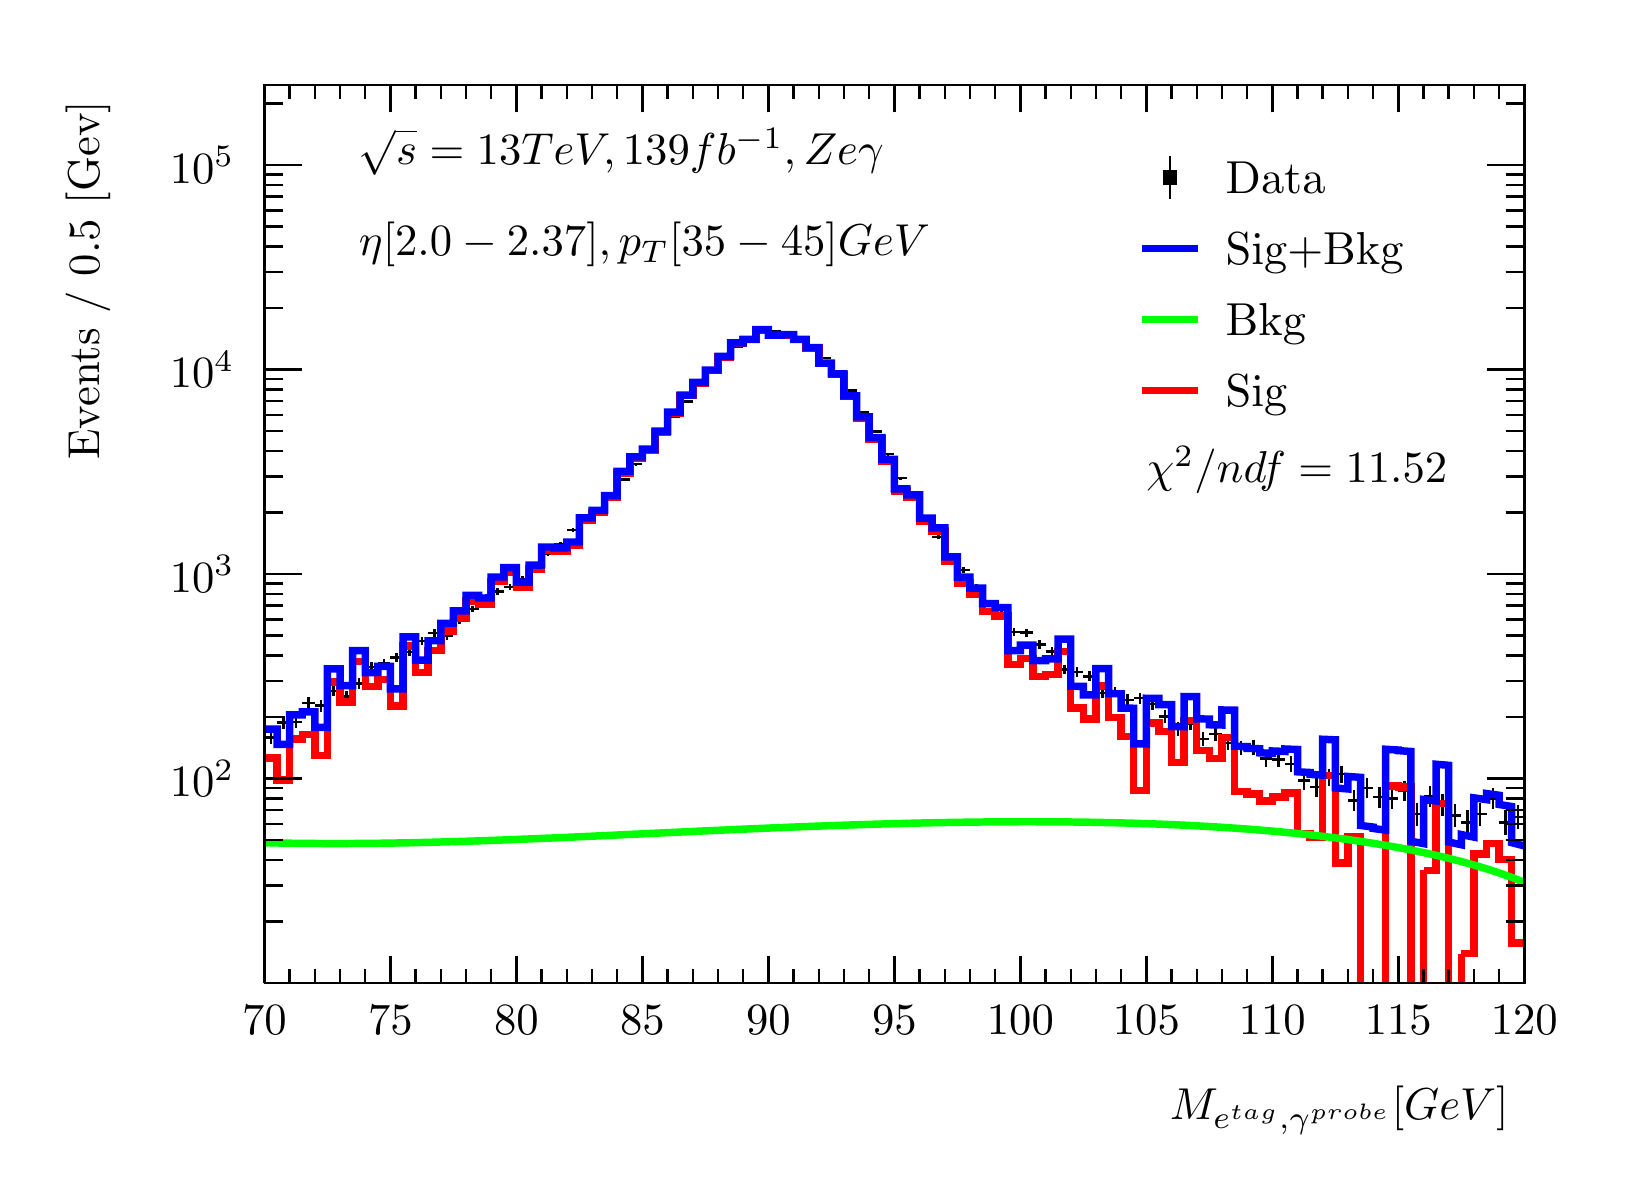
\begin{tikzpicture}
\pgfdeclareplotmark{cross} {
\pgfpathmoveto{\pgfpoint{-0.3\pgfplotmarksize}{\pgfplotmarksize}}
\pgfpathlineto{\pgfpoint{+0.3\pgfplotmarksize}{\pgfplotmarksize}}
\pgfpathlineto{\pgfpoint{+0.3\pgfplotmarksize}{0.3\pgfplotmarksize}}
\pgfpathlineto{\pgfpoint{+1\pgfplotmarksize}{0.3\pgfplotmarksize}}
\pgfpathlineto{\pgfpoint{+1\pgfplotmarksize}{-0.3\pgfplotmarksize}}
\pgfpathlineto{\pgfpoint{+0.3\pgfplotmarksize}{-0.3\pgfplotmarksize}}
\pgfpathlineto{\pgfpoint{+0.3\pgfplotmarksize}{-1.\pgfplotmarksize}}
\pgfpathlineto{\pgfpoint{-0.3\pgfplotmarksize}{-1.\pgfplotmarksize}}
\pgfpathlineto{\pgfpoint{-0.3\pgfplotmarksize}{-0.3\pgfplotmarksize}}
\pgfpathlineto{\pgfpoint{-1.\pgfplotmarksize}{-0.3\pgfplotmarksize}}
\pgfpathlineto{\pgfpoint{-1.\pgfplotmarksize}{0.3\pgfplotmarksize}}
\pgfpathlineto{\pgfpoint{-0.3\pgfplotmarksize}{0.3\pgfplotmarksize}}
\pgfpathclose
\pgfusepathqstroke
}
\pgfdeclareplotmark{cross*} {
\pgfpathmoveto{\pgfpoint{-0.3\pgfplotmarksize}{\pgfplotmarksize}}
\pgfpathlineto{\pgfpoint{+0.3\pgfplotmarksize}{\pgfplotmarksize}}
\pgfpathlineto{\pgfpoint{+0.3\pgfplotmarksize}{0.3\pgfplotmarksize}}
\pgfpathlineto{\pgfpoint{+1\pgfplotmarksize}{0.3\pgfplotmarksize}}
\pgfpathlineto{\pgfpoint{+1\pgfplotmarksize}{-0.3\pgfplotmarksize}}
\pgfpathlineto{\pgfpoint{+0.3\pgfplotmarksize}{-0.3\pgfplotmarksize}}
\pgfpathlineto{\pgfpoint{+0.3\pgfplotmarksize}{-1.\pgfplotmarksize}}
\pgfpathlineto{\pgfpoint{-0.3\pgfplotmarksize}{-1.\pgfplotmarksize}}
\pgfpathlineto{\pgfpoint{-0.3\pgfplotmarksize}{-0.3\pgfplotmarksize}}
\pgfpathlineto{\pgfpoint{-1.\pgfplotmarksize}{-0.3\pgfplotmarksize}}
\pgfpathlineto{\pgfpoint{-1.\pgfplotmarksize}{0.3\pgfplotmarksize}}
\pgfpathlineto{\pgfpoint{-0.3\pgfplotmarksize}{0.3\pgfplotmarksize}}
\pgfpathclose
\pgfusepathqfillstroke
}
\pgfdeclareplotmark{newstar} {
\pgfpathmoveto{\pgfqpoint{0pt}{\pgfplotmarksize}}
\pgfpathlineto{\pgfqpointpolar{44}{0.5\pgfplotmarksize}}
\pgfpathlineto{\pgfqpointpolar{18}{\pgfplotmarksize}}
\pgfpathlineto{\pgfqpointpolar{-20}{0.5\pgfplotmarksize}}
\pgfpathlineto{\pgfqpointpolar{-54}{\pgfplotmarksize}}
\pgfpathlineto{\pgfqpointpolar{-90}{0.5\pgfplotmarksize}}
\pgfpathlineto{\pgfqpointpolar{234}{\pgfplotmarksize}}
\pgfpathlineto{\pgfqpointpolar{198}{0.5\pgfplotmarksize}}
\pgfpathlineto{\pgfqpointpolar{162}{\pgfplotmarksize}}
\pgfpathlineto{\pgfqpointpolar{134}{0.5\pgfplotmarksize}}
\pgfpathclose
\pgfusepathqstroke
}
\pgfdeclareplotmark{newstar*} {
\pgfpathmoveto{\pgfqpoint{0pt}{\pgfplotmarksize}}
\pgfpathlineto{\pgfqpointpolar{44}{0.5\pgfplotmarksize}}
\pgfpathlineto{\pgfqpointpolar{18}{\pgfplotmarksize}}
\pgfpathlineto{\pgfqpointpolar{-20}{0.5\pgfplotmarksize}}
\pgfpathlineto{\pgfqpointpolar{-54}{\pgfplotmarksize}}
\pgfpathlineto{\pgfqpointpolar{-90}{0.5\pgfplotmarksize}}
\pgfpathlineto{\pgfqpointpolar{234}{\pgfplotmarksize}}
\pgfpathlineto{\pgfqpointpolar{198}{0.5\pgfplotmarksize}}
\pgfpathlineto{\pgfqpointpolar{162}{\pgfplotmarksize}}
\pgfpathlineto{\pgfqpointpolar{134}{0.5\pgfplotmarksize}}
\pgfpathclose
\pgfusepathqfillstroke
}
\definecolor{c}{rgb}{1,1,1};
\draw [color=c, fill=c] (0,0) rectangle (20,14.4361);
\draw [color=c, fill=c] (3,2.30977) rectangle (19,13.7143);
\definecolor{c}{rgb}{0,0,0};
\draw [c,line width=0.9] (3,2.30977) -- (3,13.7143) -- (19,13.7143) -- (19,2.30977) -- (3,2.30977);
\definecolor{c}{rgb}{1,1,1};
\draw [color=c, fill=c] (3,2.30977) rectangle (19,13.7143);
\definecolor{c}{rgb}{0,0,0};
\draw [c,line width=0.9] (3,2.30977) -- (3,13.7143) -- (19,13.7143) -- (19,2.30977) -- (3,2.30977);
\draw [c,line width=0.9] (3,2.30977) -- (19,2.30977);
\draw [c,line width=0.9] (3,2.65624) -- (3,2.30977);
\draw [c,line width=0.9] (3.32,2.48301) -- (3.32,2.30977);
\draw [c,line width=0.9] (3.64,2.48301) -- (3.64,2.30977);
\draw [c,line width=0.9] (3.96,2.48301) -- (3.96,2.30977);
\draw [c,line width=0.9] (4.28,2.48301) -- (4.28,2.30977);
\draw [c,line width=0.9] (4.6,2.65624) -- (4.6,2.30977);
\draw [c,line width=0.9] (4.92,2.48301) -- (4.92,2.30977);
\draw [c,line width=0.9] (5.24,2.48301) -- (5.24,2.30977);
\draw [c,line width=0.9] (5.56,2.48301) -- (5.56,2.30977);
\draw [c,line width=0.9] (5.88,2.48301) -- (5.88,2.30977);
\draw [c,line width=0.9] (6.2,2.65624) -- (6.2,2.30977);
\draw [c,line width=0.9] (6.52,2.48301) -- (6.52,2.30977);
\draw [c,line width=0.9] (6.84,2.48301) -- (6.84,2.30977);
\draw [c,line width=0.9] (7.16,2.48301) -- (7.16,2.30977);
\draw [c,line width=0.9] (7.48,2.48301) -- (7.48,2.30977);
\draw [c,line width=0.9] (7.8,2.65624) -- (7.8,2.30977);
\draw [c,line width=0.9] (8.12,2.48301) -- (8.12,2.30977);
\draw [c,line width=0.9] (8.44,2.48301) -- (8.44,2.30977);
\draw [c,line width=0.9] (8.76,2.48301) -- (8.76,2.30977);
\draw [c,line width=0.9] (9.08,2.48301) -- (9.08,2.30977);
\draw [c,line width=0.9] (9.4,2.65624) -- (9.4,2.30977);
\draw [c,line width=0.9] (9.72,2.48301) -- (9.72,2.30977);
\draw [c,line width=0.9] (10.04,2.48301) -- (10.04,2.30977);
\draw [c,line width=0.9] (10.36,2.48301) -- (10.36,2.30977);
\draw [c,line width=0.9] (10.68,2.48301) -- (10.68,2.30977);
\draw [c,line width=0.9] (11,2.65624) -- (11,2.30977);
\draw [c,line width=0.9] (11.32,2.48301) -- (11.32,2.30977);
\draw [c,line width=0.9] (11.64,2.48301) -- (11.64,2.30977);
\draw [c,line width=0.9] (11.96,2.48301) -- (11.96,2.30977);
\draw [c,line width=0.9] (12.28,2.48301) -- (12.28,2.30977);
\draw [c,line width=0.9] (12.6,2.65624) -- (12.6,2.30977);
\draw [c,line width=0.9] (12.92,2.48301) -- (12.92,2.30977);
\draw [c,line width=0.9] (13.24,2.48301) -- (13.24,2.30977);
\draw [c,line width=0.9] (13.56,2.48301) -- (13.56,2.30977);
\draw [c,line width=0.9] (13.88,2.48301) -- (13.88,2.30977);
\draw [c,line width=0.9] (14.2,2.65624) -- (14.2,2.30977);
\draw [c,line width=0.9] (14.52,2.48301) -- (14.52,2.30977);
\draw [c,line width=0.9] (14.84,2.48301) -- (14.84,2.30977);
\draw [c,line width=0.9] (15.16,2.48301) -- (15.16,2.30977);
\draw [c,line width=0.9] (15.48,2.48301) -- (15.48,2.30977);
\draw [c,line width=0.9] (15.8,2.65624) -- (15.8,2.30977);
\draw [c,line width=0.9] (16.12,2.48301) -- (16.12,2.30977);
\draw [c,line width=0.9] (16.44,2.48301) -- (16.44,2.30977);
\draw [c,line width=0.9] (16.76,2.48301) -- (16.76,2.30977);
\draw [c,line width=0.9] (17.08,2.48301) -- (17.08,2.30977);
\draw [c,line width=0.9] (17.4,2.65624) -- (17.4,2.30977);
\draw [c,line width=0.9] (17.72,2.48301) -- (17.72,2.30977);
\draw [c,line width=0.9] (18.04,2.48301) -- (18.04,2.30977);
\draw [c,line width=0.9] (18.36,2.48301) -- (18.36,2.30977);
\draw [c,line width=0.9] (18.68,2.48301) -- (18.68,2.30977);
\draw [c,line width=0.9] (19,2.65624) -- (19,2.30977);
\draw [anchor=base] (3,1.66015) node[scale=1.61424, color=c, rotate=0]{70};
\draw [anchor=base] (4.6,1.66015) node[scale=1.61424, color=c, rotate=0]{75};
\draw [anchor=base] (6.2,1.66015) node[scale=1.61424, color=c, rotate=0]{80};
\draw [anchor=base] (7.8,1.66015) node[scale=1.61424, color=c, rotate=0]{85};
\draw [anchor=base] (9.4,1.66015) node[scale=1.61424, color=c, rotate=0]{90};
\draw [anchor=base] (11,1.66015) node[scale=1.61424, color=c, rotate=0]{95};
\draw [anchor=base] (12.6,1.66015) node[scale=1.61424, color=c, rotate=0]{100};
\draw [anchor=base] (14.2,1.66015) node[scale=1.61424, color=c, rotate=0]{105};
\draw [anchor=base] (15.8,1.66015) node[scale=1.61424, color=c, rotate=0]{110};
\draw [anchor=base] (17.4,1.66015) node[scale=1.61424, color=c, rotate=0]{115};
\draw [anchor=base] (19,1.66015) node[scale=1.61424, color=c, rotate=0]{120};
\draw [anchor= east] (19,0.692932) node[scale=1.61424, color=c, rotate=0]{$M_{e^{tag}, \gamma^{probe}}  [GeV]$};
\draw [c,line width=0.9] (3,13.7143) -- (19,13.7143);
\draw [c,line width=0.9] (3,13.3678) -- (3,13.7143);
\draw [c,line width=0.9] (3.32,13.5411) -- (3.32,13.7143);
\draw [c,line width=0.9] (3.64,13.5411) -- (3.64,13.7143);
\draw [c,line width=0.9] (3.96,13.5411) -- (3.96,13.7143);
\draw [c,line width=0.9] (4.28,13.5411) -- (4.28,13.7143);
\draw [c,line width=0.9] (4.6,13.3678) -- (4.6,13.7143);
\draw [c,line width=0.9] (4.92,13.5411) -- (4.92,13.7143);
\draw [c,line width=0.9] (5.24,13.5411) -- (5.24,13.7143);
\draw [c,line width=0.9] (5.56,13.5411) -- (5.56,13.7143);
\draw [c,line width=0.9] (5.88,13.5411) -- (5.88,13.7143);
\draw [c,line width=0.9] (6.2,13.3678) -- (6.2,13.7143);
\draw [c,line width=0.9] (6.52,13.5411) -- (6.52,13.7143);
\draw [c,line width=0.9] (6.84,13.5411) -- (6.84,13.7143);
\draw [c,line width=0.9] (7.16,13.5411) -- (7.16,13.7143);
\draw [c,line width=0.9] (7.48,13.5411) -- (7.48,13.7143);
\draw [c,line width=0.9] (7.8,13.3678) -- (7.8,13.7143);
\draw [c,line width=0.9] (8.12,13.5411) -- (8.12,13.7143);
\draw [c,line width=0.9] (8.44,13.5411) -- (8.44,13.7143);
\draw [c,line width=0.9] (8.76,13.5411) -- (8.76,13.7143);
\draw [c,line width=0.9] (9.08,13.5411) -- (9.08,13.7143);
\draw [c,line width=0.9] (9.4,13.3678) -- (9.4,13.7143);
\draw [c,line width=0.9] (9.72,13.5411) -- (9.72,13.7143);
\draw [c,line width=0.9] (10.04,13.5411) -- (10.04,13.7143);
\draw [c,line width=0.9] (10.36,13.5411) -- (10.36,13.7143);
\draw [c,line width=0.9] (10.68,13.5411) -- (10.68,13.7143);
\draw [c,line width=0.9] (11,13.3678) -- (11,13.7143);
\draw [c,line width=0.9] (11.32,13.5411) -- (11.32,13.7143);
\draw [c,line width=0.9] (11.64,13.5411) -- (11.64,13.7143);
\draw [c,line width=0.9] (11.96,13.5411) -- (11.96,13.7143);
\draw [c,line width=0.9] (12.28,13.5411) -- (12.28,13.7143);
\draw [c,line width=0.9] (12.6,13.3678) -- (12.6,13.7143);
\draw [c,line width=0.9] (12.92,13.5411) -- (12.92,13.7143);
\draw [c,line width=0.9] (13.24,13.5411) -- (13.24,13.7143);
\draw [c,line width=0.9] (13.56,13.5411) -- (13.56,13.7143);
\draw [c,line width=0.9] (13.88,13.5411) -- (13.88,13.7143);
\draw [c,line width=0.9] (14.2,13.3678) -- (14.2,13.7143);
\draw [c,line width=0.9] (14.52,13.5411) -- (14.52,13.7143);
\draw [c,line width=0.9] (14.84,13.5411) -- (14.84,13.7143);
\draw [c,line width=0.9] (15.16,13.5411) -- (15.16,13.7143);
\draw [c,line width=0.9] (15.48,13.5411) -- (15.48,13.7143);
\draw [c,line width=0.9] (15.8,13.3678) -- (15.8,13.7143);
\draw [c,line width=0.9] (16.12,13.5411) -- (16.12,13.7143);
\draw [c,line width=0.9] (16.44,13.5411) -- (16.44,13.7143);
\draw [c,line width=0.9] (16.76,13.5411) -- (16.76,13.7143);
\draw [c,line width=0.9] (17.08,13.5411) -- (17.08,13.7143);
\draw [c,line width=0.9] (17.4,13.3678) -- (17.4,13.7143);
\draw [c,line width=0.9] (17.72,13.5411) -- (17.72,13.7143);
\draw [c,line width=0.9] (18.04,13.5411) -- (18.04,13.7143);
\draw [c,line width=0.9] (18.36,13.5411) -- (18.36,13.7143);
\draw [c,line width=0.9] (18.68,13.5411) -- (18.68,13.7143);
\draw [c,line width=0.9] (19,13.3678) -- (19,13.7143);
\draw [c,line width=0.9] (3,2.30977) -- (3,13.7143);
\draw [c,line width=0.9] (3.237,3.09166) -- (3,3.09166);
\draw [c,line width=0.9] (3.237,3.54903) -- (3,3.54903);
\draw [c,line width=0.9] (3.237,3.87354) -- (3,3.87354);
\draw [c,line width=0.9] (3.237,4.12525) -- (3,4.12525);
\draw [c,line width=0.9] (3.237,4.33091) -- (3,4.33091);
\draw [c,line width=0.9] (3.237,4.5048) -- (3,4.5048);
\draw [c,line width=0.9] (3.237,4.65542) -- (3,4.65542);
\draw [c,line width=0.9] (3.237,4.78829) -- (3,4.78829);
\draw [c,line width=0.9] (3.474,4.90714) -- (3,4.90714);
\draw [anchor= east] (2.82,4.90714) node[scale=1.61424, color=c, rotate=0]{$10^{2}$};
\draw [c,line width=0.9] (3.237,5.68902) -- (3,5.68902);
\draw [c,line width=0.9] (3.237,6.14639) -- (3,6.14639);
\draw [c,line width=0.9] (3.237,6.4709) -- (3,6.4709);
\draw [c,line width=0.9] (3.237,6.72261) -- (3,6.72261);
\draw [c,line width=0.9] (3.237,6.92828) -- (3,6.92828);
\draw [c,line width=0.9] (3.237,7.10216) -- (3,7.10216);
\draw [c,line width=0.9] (3.237,7.25279) -- (3,7.25279);
\draw [c,line width=0.9] (3.237,7.38565) -- (3,7.38565);
\draw [c,line width=0.9] (3.474,7.5045) -- (3,7.5045);
\draw [anchor= east] (2.82,7.5045) node[scale=1.61424, color=c, rotate=0]{$10^{3}$};
\draw [c,line width=0.9] (3.237,8.28638) -- (3,8.28638);
\draw [c,line width=0.9] (3.237,8.74376) -- (3,8.74376);
\draw [c,line width=0.9] (3.237,9.06827) -- (3,9.06827);
\draw [c,line width=0.9] (3.237,9.31998) -- (3,9.31998);
\draw [c,line width=0.9] (3.237,9.52564) -- (3,9.52564);
\draw [c,line width=0.9] (3.237,9.69952) -- (3,9.69952);
\draw [c,line width=0.9] (3.237,9.85015) -- (3,9.85015);
\draw [c,line width=0.9] (3.237,9.98301) -- (3,9.98301);
\draw [c,line width=0.9] (3.474,10.1019) -- (3,10.1019);
\draw [anchor= east] (2.82,10.1019) node[scale=1.61424, color=c, rotate=0]{$10^{4}$};
\draw [c,line width=0.9] (3.237,10.8837) -- (3,10.8837);
\draw [c,line width=0.9] (3.237,11.3411) -- (3,11.3411);
\draw [c,line width=0.9] (3.237,11.6656) -- (3,11.6656);
\draw [c,line width=0.9] (3.237,11.9173) -- (3,11.9173);
\draw [c,line width=0.9] (3.237,12.123) -- (3,12.123);
\draw [c,line width=0.9] (3.237,12.2969) -- (3,12.2969);
\draw [c,line width=0.9] (3.237,12.4475) -- (3,12.4475);
\draw [c,line width=0.9] (3.237,12.5804) -- (3,12.5804);
\draw [c,line width=0.9] (3.474,12.6992) -- (3,12.6992);
\draw [anchor= east] (2.82,12.6992) node[scale=1.61424, color=c, rotate=0]{$10^{5}$};
\draw [c,line width=0.9] (3.237,13.4811) -- (3,13.4811);
\draw [anchor= east] (0.76,13.7143) node[scale=1.61424, color=c, rotate=90]{Events / 0.5 [Gev]};
\draw [c,line width=0.9] (19,2.30977) -- (19,13.7143);
\draw [c,line width=0.9] (18.763,3.09166) -- (19,3.09166);
\draw [c,line width=0.9] (18.763,3.54903) -- (19,3.54903);
\draw [c,line width=0.9] (18.763,3.87354) -- (19,3.87354);
\draw [c,line width=0.9] (18.763,4.12525) -- (19,4.12525);
\draw [c,line width=0.9] (18.763,4.33091) -- (19,4.33091);
\draw [c,line width=0.9] (18.763,4.5048) -- (19,4.5048);
\draw [c,line width=0.9] (18.763,4.65542) -- (19,4.65542);
\draw [c,line width=0.9] (18.763,4.78829) -- (19,4.78829);
\draw [c,line width=0.9] (18.526,4.90714) -- (19,4.90714);
\draw [c,line width=0.9] (18.763,5.68902) -- (19,5.68902);
\draw [c,line width=0.9] (18.763,6.14639) -- (19,6.14639);
\draw [c,line width=0.9] (18.763,6.4709) -- (19,6.4709);
\draw [c,line width=0.9] (18.763,6.72261) -- (19,6.72261);
\draw [c,line width=0.9] (18.763,6.92828) -- (19,6.92828);
\draw [c,line width=0.9] (18.763,7.10216) -- (19,7.10216);
\draw [c,line width=0.9] (18.763,7.25279) -- (19,7.25279);
\draw [c,line width=0.9] (18.763,7.38565) -- (19,7.38565);
\draw [c,line width=0.9] (18.526,7.5045) -- (19,7.5045);
\draw [c,line width=0.9] (18.763,8.28638) -- (19,8.28638);
\draw [c,line width=0.9] (18.763,8.74376) -- (19,8.74376);
\draw [c,line width=0.9] (18.763,9.06827) -- (19,9.06827);
\draw [c,line width=0.9] (18.763,9.31998) -- (19,9.31998);
\draw [c,line width=0.9] (18.763,9.52564) -- (19,9.52564);
\draw [c,line width=0.9] (18.763,9.69952) -- (19,9.69952);
\draw [c,line width=0.9] (18.763,9.85015) -- (19,9.85015);
\draw [c,line width=0.9] (18.763,9.98301) -- (19,9.98301);
\draw [c,line width=0.9] (18.526,10.1019) -- (19,10.1019);
\draw [c,line width=0.9] (18.763,10.8837) -- (19,10.8837);
\draw [c,line width=0.9] (18.763,11.3411) -- (19,11.3411);
\draw [c,line width=0.9] (18.763,11.6656) -- (19,11.6656);
\draw [c,line width=0.9] (18.763,11.9173) -- (19,11.9173);
\draw [c,line width=0.9] (18.763,12.123) -- (19,12.123);
\draw [c,line width=0.9] (18.763,12.2969) -- (19,12.2969);
\draw [c,line width=0.9] (18.763,12.4475) -- (19,12.4475);
\draw [c,line width=0.9] (18.763,12.5804) -- (19,12.5804);
\draw [c,line width=0.9] (18.526,12.6992) -- (19,12.6992);
\draw [c,line width=0.9] (18.763,13.4811) -- (19,13.4811);
\draw [c,line width=0.9] (3.08,5.43024) -- (3,5.43024);
\draw [c,line width=0.9] (3,5.43024) -- (3,5.43024);
\draw [c,line width=0.9] (3.08,5.43024) -- (3.16,5.43024);
\draw [c,line width=0.9] (3.16,5.43024) -- (3.16,5.43024);
\draw [c,line width=0.9] (3.08,5.43024) -- (3.08,5.51967);
\draw [c,line width=0.9] (3.08,5.51967) -- (3.08,5.51967);
\draw [c,line width=0.9] (3.08,5.43024) -- (3.08,5.3408);
\draw [c,line width=0.9] (3.08,5.3408) -- (3.08,5.3408);
\draw [c,line width=0.9] (3.24,5.61922) -- (3.16,5.61922);
\draw [c,line width=0.9] (3.16,5.61922) -- (3.16,5.61922);
\draw [c,line width=0.9] (3.24,5.61922) -- (3.32,5.61922);
\draw [c,line width=0.9] (3.32,5.61922) -- (3.32,5.61922);
\draw [c,line width=0.9] (3.24,5.61922) -- (3.24,5.70148);
\draw [c,line width=0.9] (3.24,5.70148) -- (3.24,5.70148);
\draw [c,line width=0.9] (3.24,5.61922) -- (3.24,5.53697);
\draw [c,line width=0.9] (3.24,5.53697) -- (3.24,5.53697);
\draw [c,line width=0.9] (3.4,5.62521) -- (3.32,5.62521);
\draw [c,line width=0.9] (3.32,5.62521) -- (3.32,5.62521);
\draw [c,line width=0.9] (3.4,5.62521) -- (3.48,5.62521);
\draw [c,line width=0.9] (3.48,5.62521) -- (3.48,5.62521);
\draw [c,line width=0.9] (3.4,5.62521) -- (3.4,5.70724);
\draw [c,line width=0.9] (3.4,5.70724) -- (3.4,5.70724);
\draw [c,line width=0.9] (3.4,5.62521) -- (3.4,5.54318);
\draw [c,line width=0.9] (3.4,5.54318) -- (3.4,5.54318);
\draw [c,line width=0.9] (3.56,5.86612) -- (3.48,5.86612);
\draw [c,line width=0.9] (3.48,5.86612) -- (3.48,5.86612);
\draw [c,line width=0.9] (3.56,5.86612) -- (3.64,5.86612);
\draw [c,line width=0.9] (3.64,5.86612) -- (3.64,5.86612);
\draw [c,line width=0.9] (3.56,5.86612) -- (3.56,5.93985);
\draw [c,line width=0.9] (3.56,5.93985) -- (3.56,5.93985);
\draw [c,line width=0.9] (3.56,5.86612) -- (3.56,5.7924);
\draw [c,line width=0.9] (3.56,5.7924) -- (3.56,5.7924);
\draw [c,line width=0.9] (3.72,5.83187) -- (3.64,5.83187);
\draw [c,line width=0.9] (3.64,5.83187) -- (3.64,5.83187);
\draw [c,line width=0.9] (3.72,5.83187) -- (3.8,5.83187);
\draw [c,line width=0.9] (3.8,5.83187) -- (3.8,5.83187);
\draw [c,line width=0.9] (3.72,5.83187) -- (3.72,5.90672);
\draw [c,line width=0.9] (3.72,5.90672) -- (3.72,5.90672);
\draw [c,line width=0.9] (3.72,5.83187) -- (3.72,5.75701);
\draw [c,line width=0.9] (3.72,5.75701) -- (3.72,5.75701);
\draw [c,line width=0.9] (3.88,6.01916) -- (3.8,6.01916);
\draw [c,line width=0.9] (3.8,6.01916) -- (3.8,6.01916);
\draw [c,line width=0.9] (3.88,6.01916) -- (3.96,6.01916);
\draw [c,line width=0.9] (3.96,6.01916) -- (3.96,6.01916);
\draw [c,line width=0.9] (3.88,6.01916) -- (3.88,6.08805);
\draw [c,line width=0.9] (3.88,6.08805) -- (3.88,6.08805);
\draw [c,line width=0.9] (3.88,6.01916) -- (3.88,5.95026);
\draw [c,line width=0.9] (3.88,5.95026) -- (3.88,5.95026);
\draw [c,line width=0.9] (4.04,5.94972) -- (3.96,5.94972);
\draw [c,line width=0.9] (3.96,5.94972) -- (3.96,5.94972);
\draw [c,line width=0.9] (4.04,5.94972) -- (4.12,5.94972);
\draw [c,line width=0.9] (4.12,5.94972) -- (4.12,5.94972);
\draw [c,line width=0.9] (4.04,5.94972) -- (4.04,6.02077);
\draw [c,line width=0.9] (4.04,6.02077) -- (4.04,6.02077);
\draw [c,line width=0.9] (4.04,5.94972) -- (4.04,5.87867);
\draw [c,line width=0.9] (4.04,5.87867) -- (4.04,5.87867);
\draw [c,line width=0.9] (4.2,6.11591) -- (4.12,6.11591);
\draw [c,line width=0.9] (4.12,6.11591) -- (4.12,6.11591);
\draw [c,line width=0.9] (4.2,6.11591) -- (4.28,6.11591);
\draw [c,line width=0.9] (4.28,6.11591) -- (4.28,6.11591);
\draw [c,line width=0.9] (4.2,6.11591) -- (4.2,6.18191);
\draw [c,line width=0.9] (4.2,6.18191) -- (4.2,6.18191);
\draw [c,line width=0.9] (4.2,6.11591) -- (4.2,6.0499);
\draw [c,line width=0.9] (4.2,6.0499) -- (4.2,6.0499);
\draw [c,line width=0.9] (4.36,6.32671) -- (4.28,6.32671);
\draw [c,line width=0.9] (4.28,6.32671) -- (4.28,6.32671);
\draw [c,line width=0.9] (4.36,6.32671) -- (4.44,6.32671);
\draw [c,line width=0.9] (4.44,6.32671) -- (4.44,6.32671);
\draw [c,line width=0.9] (4.36,6.32671) -- (4.36,6.38682);
\draw [c,line width=0.9] (4.36,6.38682) -- (4.36,6.38682);
\draw [c,line width=0.9] (4.36,6.32671) -- (4.36,6.26659);
\draw [c,line width=0.9] (4.36,6.26659) -- (4.36,6.26659);
\draw [c,line width=0.9] (4.52,6.36762) -- (4.44,6.36762);
\draw [c,line width=0.9] (4.44,6.36762) -- (4.44,6.36762);
\draw [c,line width=0.9] (4.52,6.36762) -- (4.6,6.36762);
\draw [c,line width=0.9] (4.6,6.36762) -- (4.6,6.36762);
\draw [c,line width=0.9] (4.52,6.36762) -- (4.52,6.42665);
\draw [c,line width=0.9] (4.52,6.42665) -- (4.52,6.42665);
\draw [c,line width=0.9] (4.52,6.36762) -- (4.52,6.30858);
\draw [c,line width=0.9] (4.52,6.30858) -- (4.52,6.30858);
\draw [c,line width=0.9] (4.68,6.44235) -- (4.6,6.44235);
\draw [c,line width=0.9] (4.6,6.44235) -- (4.6,6.44235);
\draw [c,line width=0.9] (4.68,6.44235) -- (4.76,6.44235);
\draw [c,line width=0.9] (4.76,6.44235) -- (4.76,6.44235);
\draw [c,line width=0.9] (4.68,6.44235) -- (4.68,6.49946);
\draw [c,line width=0.9] (4.68,6.49946) -- (4.68,6.49946);
\draw [c,line width=0.9] (4.68,6.44235) -- (4.68,6.38523);
\draw [c,line width=0.9] (4.68,6.38523) -- (4.68,6.38523);
\draw [c,line width=0.9] (4.84,6.51243) -- (4.76,6.51243);
\draw [c,line width=0.9] (4.76,6.51243) -- (4.76,6.51243);
\draw [c,line width=0.9] (4.84,6.51243) -- (4.92,6.51243);
\draw [c,line width=0.9] (4.92,6.51243) -- (4.92,6.51243);
\draw [c,line width=0.9] (4.84,6.51243) -- (4.84,6.5678);
\draw [c,line width=0.9] (4.84,6.5678) -- (4.84,6.5678);
\draw [c,line width=0.9] (4.84,6.51243) -- (4.84,6.45707);
\draw [c,line width=0.9] (4.84,6.45707) -- (4.84,6.45707);
\draw [c,line width=0.9] (5,6.65282) -- (4.92,6.65282);
\draw [c,line width=0.9] (4.92,6.65282) -- (4.92,6.65282);
\draw [c,line width=0.9] (5,6.65282) -- (5.08,6.65282);
\draw [c,line width=0.9] (5.08,6.65282) -- (5.08,6.65282);
\draw [c,line width=0.9] (5,6.65282) -- (5,6.70485);
\draw [c,line width=0.9] (5,6.70485) -- (5,6.70485);
\draw [c,line width=0.9] (5,6.65282) -- (5,6.60079);
\draw [c,line width=0.9] (5,6.60079) -- (5,6.60079);
\draw [c,line width=0.9] (5.16,6.75815) -- (5.08,6.75815);
\draw [c,line width=0.9] (5.08,6.75815) -- (5.08,6.75815);
\draw [c,line width=0.9] (5.16,6.75815) -- (5.24,6.75815);
\draw [c,line width=0.9] (5.24,6.75815) -- (5.24,6.75815);
\draw [c,line width=0.9] (5.16,6.75815) -- (5.16,6.8078);
\draw [c,line width=0.9] (5.16,6.8078) -- (5.16,6.8078);
\draw [c,line width=0.9] (5.16,6.75815) -- (5.16,6.70849);
\draw [c,line width=0.9] (5.16,6.70849) -- (5.16,6.70849);
\draw [c,line width=0.9] (5.32,6.71583) -- (5.24,6.71583);
\draw [c,line width=0.9] (5.24,6.71583) -- (5.24,6.71583);
\draw [c,line width=0.9] (5.32,6.71583) -- (5.4,6.71583);
\draw [c,line width=0.9] (5.4,6.71583) -- (5.4,6.71583);
\draw [c,line width=0.9] (5.32,6.71583) -- (5.32,6.76642);
\draw [c,line width=0.9] (5.32,6.76642) -- (5.32,6.76642);
\draw [c,line width=0.9] (5.32,6.71583) -- (5.32,6.66523);
\draw [c,line width=0.9] (5.32,6.66523) -- (5.32,6.66523);
\draw [c,line width=0.9] (5.48,6.91884) -- (5.4,6.91884);
\draw [c,line width=0.9] (5.4,6.91884) -- (5.4,6.91884);
\draw [c,line width=0.9] (5.48,6.91884) -- (5.56,6.91884);
\draw [c,line width=0.9] (5.56,6.91884) -- (5.56,6.91884);
\draw [c,line width=0.9] (5.48,6.91884) -- (5.48,6.96508);
\draw [c,line width=0.9] (5.48,6.96508) -- (5.48,6.96508);
\draw [c,line width=0.9] (5.48,6.91884) -- (5.48,6.8726);
\draw [c,line width=0.9] (5.48,6.8726) -- (5.48,6.8726);
\draw [c,line width=0.9] (5.64,7.06114) -- (5.56,7.06114);
\draw [c,line width=0.9] (5.56,7.06114) -- (5.56,7.06114);
\draw [c,line width=0.9] (5.64,7.06114) -- (5.72,7.06114);
\draw [c,line width=0.9] (5.72,7.06114) -- (5.72,7.06114);
\draw [c,line width=0.9] (5.64,7.06114) -- (5.64,7.10455);
\draw [c,line width=0.9] (5.64,7.10455) -- (5.64,7.10455);
\draw [c,line width=0.9] (5.64,7.06114) -- (5.64,7.01772);
\draw [c,line width=0.9] (5.64,7.01772) -- (5.64,7.01772);
\draw [c,line width=0.9] (5.8,7.17698) -- (5.72,7.17698);
\draw [c,line width=0.9] (5.72,7.17698) -- (5.72,7.17698);
\draw [c,line width=0.9] (5.8,7.17698) -- (5.88,7.17698);
\draw [c,line width=0.9] (5.88,7.17698) -- (5.88,7.17698);
\draw [c,line width=0.9] (5.8,7.17698) -- (5.8,7.21822);
\draw [c,line width=0.9] (5.8,7.21822) -- (5.8,7.21822);
\draw [c,line width=0.9] (5.8,7.17698) -- (5.8,7.13573);
\draw [c,line width=0.9] (5.8,7.13573) -- (5.8,7.13573);
\draw [c,line width=0.9] (5.96,7.28339) -- (5.88,7.28339);
\draw [c,line width=0.9] (5.88,7.28339) -- (5.88,7.28339);
\draw [c,line width=0.9] (5.96,7.28339) -- (6.04,7.28339);
\draw [c,line width=0.9] (6.04,7.28339) -- (6.04,7.28339);
\draw [c,line width=0.9] (5.96,7.28339) -- (5.96,7.32273);
\draw [c,line width=0.9] (5.96,7.32273) -- (5.96,7.32273);
\draw [c,line width=0.9] (5.96,7.28339) -- (5.96,7.24405);
\draw [c,line width=0.9] (5.96,7.24405) -- (5.96,7.24405);
\draw [c,line width=0.9] (6.12,7.33699) -- (6.04,7.33699);
\draw [c,line width=0.9] (6.04,7.33699) -- (6.04,7.33699);
\draw [c,line width=0.9] (6.12,7.33699) -- (6.2,7.33699);
\draw [c,line width=0.9] (6.2,7.33699) -- (6.2,7.33699);
\draw [c,line width=0.9] (6.12,7.33699) -- (6.12,7.37541);
\draw [c,line width=0.9] (6.12,7.37541) -- (6.12,7.37541);
\draw [c,line width=0.9] (6.12,7.33699) -- (6.12,7.29857);
\draw [c,line width=0.9] (6.12,7.29857) -- (6.12,7.29857);
\draw [c,line width=0.9] (6.28,7.44426) -- (6.2,7.44426);
\draw [c,line width=0.9] (6.2,7.44426) -- (6.2,7.44426);
\draw [c,line width=0.9] (6.28,7.44426) -- (6.36,7.44426);
\draw [c,line width=0.9] (6.36,7.44426) -- (6.36,7.44426);
\draw [c,line width=0.9] (6.28,7.44426) -- (6.28,7.4809);
\draw [c,line width=0.9] (6.28,7.4809) -- (6.28,7.4809);
\draw [c,line width=0.9] (6.28,7.44426) -- (6.28,7.40763);
\draw [c,line width=0.9] (6.28,7.40763) -- (6.28,7.40763);
\draw [c,line width=0.9] (6.44,7.58713) -- (6.36,7.58713);
\draw [c,line width=0.9] (6.36,7.58713) -- (6.36,7.58713);
\draw [c,line width=0.9] (6.44,7.58713) -- (6.52,7.58713);
\draw [c,line width=0.9] (6.52,7.58713) -- (6.52,7.58713);
\draw [c,line width=0.9] (6.44,7.58713) -- (6.44,7.62151);
\draw [c,line width=0.9] (6.44,7.62151) -- (6.44,7.62151);
\draw [c,line width=0.9] (6.44,7.58713) -- (6.44,7.55274);
\draw [c,line width=0.9] (6.44,7.55274) -- (6.44,7.55274);
\draw [c,line width=0.9] (6.6,7.76699) -- (6.52,7.76699);
\draw [c,line width=0.9] (6.52,7.76699) -- (6.52,7.76699);
\draw [c,line width=0.9] (6.6,7.76699) -- (6.68,7.76699);
\draw [c,line width=0.9] (6.68,7.76699) -- (6.68,7.76699);
\draw [c,line width=0.9] (6.6,7.76699) -- (6.6,7.79874);
\draw [c,line width=0.9] (6.6,7.79874) -- (6.6,7.79874);
\draw [c,line width=0.9] (6.6,7.76699) -- (6.6,7.73524);
\draw [c,line width=0.9] (6.6,7.73524) -- (6.6,7.73524);
\draw [c,line width=0.9] (6.76,7.88405) -- (6.68,7.88405);
\draw [c,line width=0.9] (6.68,7.88405) -- (6.68,7.88405);
\draw [c,line width=0.9] (6.76,7.88405) -- (6.84,7.88405);
\draw [c,line width=0.9] (6.84,7.88405) -- (6.84,7.88405);
\draw [c,line width=0.9] (6.76,7.88405) -- (6.76,7.91419);
\draw [c,line width=0.9] (6.76,7.91419) -- (6.76,7.91419);
\draw [c,line width=0.9] (6.76,7.88405) -- (6.76,7.8539);
\draw [c,line width=0.9] (6.76,7.8539) -- (6.76,7.8539);
\draw [c,line width=0.9] (6.92,8.06596) -- (6.84,8.06596);
\draw [c,line width=0.9] (6.84,8.06596) -- (6.84,8.06596);
\draw [c,line width=0.9] (6.92,8.06596) -- (7,8.06596);
\draw [c,line width=0.9] (7,8.06596) -- (7,8.06596);
\draw [c,line width=0.9] (6.92,8.06596) -- (6.92,8.09377);
\draw [c,line width=0.9] (6.92,8.09377) -- (6.92,8.09377);
\draw [c,line width=0.9] (6.92,8.06596) -- (6.92,8.03815);
\draw [c,line width=0.9] (6.92,8.03815) -- (6.92,8.03815);
\draw [c,line width=0.9] (7.08,8.18556) -- (7,8.18556);
\draw [c,line width=0.9] (7,8.18556) -- (7,8.18556);
\draw [c,line width=0.9] (7.08,8.18556) -- (7.16,8.18556);
\draw [c,line width=0.9] (7.16,8.18556) -- (7.16,8.18556);
\draw [c,line width=0.9] (7.08,8.18556) -- (7.08,8.21194);
\draw [c,line width=0.9] (7.08,8.21194) -- (7.08,8.21194);
\draw [c,line width=0.9] (7.08,8.18556) -- (7.08,8.15919);
\draw [c,line width=0.9] (7.08,8.15919) -- (7.08,8.15919);
\draw [c,line width=0.9] (7.24,8.31918) -- (7.16,8.31918);
\draw [c,line width=0.9] (7.16,8.31918) -- (7.16,8.31918);
\draw [c,line width=0.9] (7.24,8.31918) -- (7.32,8.31918);
\draw [c,line width=0.9] (7.32,8.31918) -- (7.32,8.31918);
\draw [c,line width=0.9] (7.24,8.31918) -- (7.24,8.34404);
\draw [c,line width=0.9] (7.24,8.34404) -- (7.24,8.34404);
\draw [c,line width=0.9] (7.24,8.31918) -- (7.24,8.29432);
\draw [c,line width=0.9] (7.24,8.29432) -- (7.24,8.29432);
\draw [c,line width=0.9] (7.4,8.47117) -- (7.32,8.47117);
\draw [c,line width=0.9] (7.32,8.47117) -- (7.32,8.47117);
\draw [c,line width=0.9] (7.4,8.47117) -- (7.48,8.47117);
\draw [c,line width=0.9] (7.48,8.47117) -- (7.48,8.47117);
\draw [c,line width=0.9] (7.4,8.47117) -- (7.4,8.49441);
\draw [c,line width=0.9] (7.4,8.49441) -- (7.4,8.49441);
\draw [c,line width=0.9] (7.4,8.47117) -- (7.4,8.44794);
\draw [c,line width=0.9] (7.4,8.44794) -- (7.4,8.44794);
\draw [c,line width=0.9] (7.56,8.70551) -- (7.48,8.70551);
\draw [c,line width=0.9] (7.48,8.70551) -- (7.48,8.70551);
\draw [c,line width=0.9] (7.56,8.70551) -- (7.64,8.70551);
\draw [c,line width=0.9] (7.64,8.70551) -- (7.64,8.70551);
\draw [c,line width=0.9] (7.56,8.70551) -- (7.56,8.72646);
\draw [c,line width=0.9] (7.56,8.72646) -- (7.56,8.72646);
\draw [c,line width=0.9] (7.56,8.70551) -- (7.56,8.68457);
\draw [c,line width=0.9] (7.56,8.68457) -- (7.56,8.68457);
\draw [c,line width=0.9] (7.72,8.90076) -- (7.64,8.90076);
\draw [c,line width=0.9] (7.64,8.90076) -- (7.64,8.90076);
\draw [c,line width=0.9] (7.72,8.90076) -- (7.8,8.90076);
\draw [c,line width=0.9] (7.8,8.90076) -- (7.8,8.90076);
\draw [c,line width=0.9] (7.72,8.90076) -- (7.72,8.91997);
\draw [c,line width=0.9] (7.72,8.91997) -- (7.72,8.91997);
\draw [c,line width=0.9] (7.72,8.90076) -- (7.72,8.88155);
\draw [c,line width=0.9] (7.72,8.88155) -- (7.72,8.88155);
\draw [c,line width=0.9] (7.88,9.10024) -- (7.8,9.10024);
\draw [c,line width=0.9] (7.8,9.10024) -- (7.8,9.10024);
\draw [c,line width=0.9] (7.88,9.10024) -- (7.96,9.10024);
\draw [c,line width=0.9] (7.96,9.10024) -- (7.96,9.10024);
\draw [c,line width=0.9] (7.88,9.10024) -- (7.88,9.11783);
\draw [c,line width=0.9] (7.88,9.11783) -- (7.88,9.11783);
\draw [c,line width=0.9] (7.88,9.10024) -- (7.88,9.08266);
\draw [c,line width=0.9] (7.88,9.08266) -- (7.88,9.08266);
\draw [c,line width=0.9] (8.04,9.29558) -- (7.96,9.29558);
\draw [c,line width=0.9] (7.96,9.29558) -- (7.96,9.29558);
\draw [c,line width=0.9] (8.04,9.29558) -- (8.12,9.29558);
\draw [c,line width=0.9] (8.12,9.29558) -- (8.12,9.29558);
\draw [c,line width=0.9] (8.04,9.29558) -- (8.04,9.3117);
\draw [c,line width=0.9] (8.04,9.3117) -- (8.04,9.3117);
\draw [c,line width=0.9] (8.04,9.29558) -- (8.04,9.27945);
\draw [c,line width=0.9] (8.04,9.27945) -- (8.04,9.27945);
\draw [c,line width=0.9] (8.2,9.49804) -- (8.12,9.49804);
\draw [c,line width=0.9] (8.12,9.49804) -- (8.12,9.49804);
\draw [c,line width=0.9] (8.2,9.49804) -- (8.28,9.49804);
\draw [c,line width=0.9] (8.28,9.49804) -- (8.28,9.49804);
\draw [c,line width=0.9] (8.2,9.49804) -- (8.2,9.51279);
\draw [c,line width=0.9] (8.2,9.51279) -- (8.2,9.51279);
\draw [c,line width=0.9] (8.2,9.49804) -- (8.2,9.4833);
\draw [c,line width=0.9] (8.2,9.4833) -- (8.2,9.4833);
\draw [c,line width=0.9] (8.36,9.69824) -- (8.28,9.69824);
\draw [c,line width=0.9] (8.28,9.69824) -- (8.28,9.69824);
\draw [c,line width=0.9] (8.36,9.69824) -- (8.44,9.69824);
\draw [c,line width=0.9] (8.44,9.69824) -- (8.44,9.69824);
\draw [c,line width=0.9] (8.36,9.69824) -- (8.36,9.71173);
\draw [c,line width=0.9] (8.36,9.71173) -- (8.36,9.71173);
\draw [c,line width=0.9] (8.36,9.69824) -- (8.36,9.68475);
\draw [c,line width=0.9] (8.36,9.68475) -- (8.36,9.68475);
\draw [c,line width=0.9] (8.52,9.90438) -- (8.44,9.90438);
\draw [c,line width=0.9] (8.44,9.90438) -- (8.44,9.90438);
\draw [c,line width=0.9] (8.52,9.90438) -- (8.6,9.90438);
\draw [c,line width=0.9] (8.6,9.90438) -- (8.6,9.90438);
\draw [c,line width=0.9] (8.52,9.90438) -- (8.52,9.91669);
\draw [c,line width=0.9] (8.52,9.91669) -- (8.52,9.91669);
\draw [c,line width=0.9] (8.52,9.90438) -- (8.52,9.89207);
\draw [c,line width=0.9] (8.52,9.89207) -- (8.52,9.89207);
\draw [c,line width=0.9] (8.68,10.0876) -- (8.6,10.0876);
\draw [c,line width=0.9] (8.6,10.0876) -- (8.6,10.0876);
\draw [c,line width=0.9] (8.68,10.0876) -- (8.76,10.0876);
\draw [c,line width=0.9] (8.76,10.0876) -- (8.76,10.0876);
\draw [c,line width=0.9] (8.68,10.0876) -- (8.68,10.0989);
\draw [c,line width=0.9] (8.68,10.0989) -- (8.68,10.0989);
\draw [c,line width=0.9] (8.68,10.0876) -- (8.68,10.0762);
\draw [c,line width=0.9] (8.68,10.0762) -- (8.68,10.0762);
\draw [c,line width=0.9] (8.84,10.2564) -- (8.76,10.2564);
\draw [c,line width=0.9] (8.76,10.2564) -- (8.76,10.2564);
\draw [c,line width=0.9] (8.84,10.2564) -- (8.92,10.2564);
\draw [c,line width=0.9] (8.92,10.2564) -- (8.92,10.2564);
\draw [c,line width=0.9] (8.84,10.2564) -- (8.84,10.2669);
\draw [c,line width=0.9] (8.84,10.2669) -- (8.84,10.2669);
\draw [c,line width=0.9] (8.84,10.2564) -- (8.84,10.2458);
\draw [c,line width=0.9] (8.84,10.2458) -- (8.84,10.2458);
\draw [c,line width=0.9] (9,10.3945) -- (8.92,10.3945);
\draw [c,line width=0.9] (8.92,10.3945) -- (8.92,10.3945);
\draw [c,line width=0.9] (9,10.3945) -- (9.08,10.3945);
\draw [c,line width=0.9] (9.08,10.3945) -- (9.08,10.3945);
\draw [c,line width=0.9] (9,10.3945) -- (9,10.4044);
\draw [c,line width=0.9] (9,10.4044) -- (9,10.4044);
\draw [c,line width=0.9] (9,10.3945) -- (9,10.3846);
\draw [c,line width=0.9] (9,10.3846) -- (9,10.3846);
\draw [c,line width=0.9] (9.16,10.4961) -- (9.08,10.4961);
\draw [c,line width=0.9] (9.08,10.4961) -- (9.08,10.4961);
\draw [c,line width=0.9] (9.16,10.4961) -- (9.24,10.4961);
\draw [c,line width=0.9] (9.24,10.4961) -- (9.24,10.4961);
\draw [c,line width=0.9] (9.16,10.4961) -- (9.16,10.5055);
\draw [c,line width=0.9] (9.16,10.5055) -- (9.16,10.5055);
\draw [c,line width=0.9] (9.16,10.4961) -- (9.16,10.4866);
\draw [c,line width=0.9] (9.16,10.4866) -- (9.16,10.4866);
\draw [c,line width=0.9] (9.32,10.5629) -- (9.24,10.5629);
\draw [c,line width=0.9] (9.24,10.5629) -- (9.24,10.5629);
\draw [c,line width=0.9] (9.32,10.5629) -- (9.4,10.5629);
\draw [c,line width=0.9] (9.4,10.5629) -- (9.4,10.5629);
\draw [c,line width=0.9] (9.32,10.5629) -- (9.32,10.5721);
\draw [c,line width=0.9] (9.32,10.5721) -- (9.32,10.5721);
\draw [c,line width=0.9] (9.32,10.5629) -- (9.32,10.5537);
\draw [c,line width=0.9] (9.32,10.5537) -- (9.32,10.5537);
\draw [c,line width=0.9] (9.48,10.5919) -- (9.4,10.5919);
\draw [c,line width=0.9] (9.4,10.5919) -- (9.4,10.5919);
\draw [c,line width=0.9] (9.48,10.5919) -- (9.56,10.5919);
\draw [c,line width=0.9] (9.56,10.5919) -- (9.56,10.5919);
\draw [c,line width=0.9] (9.48,10.5919) -- (9.48,10.601);
\draw [c,line width=0.9] (9.48,10.601) -- (9.48,10.601);
\draw [c,line width=0.9] (9.48,10.5919) -- (9.48,10.5828);
\draw [c,line width=0.9] (9.48,10.5828) -- (9.48,10.5828);
\draw [c,line width=0.9] (9.64,10.5804) -- (9.56,10.5804);
\draw [c,line width=0.9] (9.56,10.5804) -- (9.56,10.5804);
\draw [c,line width=0.9] (9.64,10.5804) -- (9.72,10.5804);
\draw [c,line width=0.9] (9.72,10.5804) -- (9.72,10.5804);
\draw [c,line width=0.9] (9.64,10.5804) -- (9.64,10.5895);
\draw [c,line width=0.9] (9.64,10.5895) -- (9.64,10.5895);
\draw [c,line width=0.9] (9.64,10.5804) -- (9.64,10.5713);
\draw [c,line width=0.9] (9.64,10.5713) -- (9.64,10.5713);
\draw [c,line width=0.9] (9.8,10.5089) -- (9.72,10.5089);
\draw [c,line width=0.9] (9.72,10.5089) -- (9.72,10.5089);
\draw [c,line width=0.9] (9.8,10.5089) -- (9.88,10.5089);
\draw [c,line width=0.9] (9.88,10.5089) -- (9.88,10.5089);
\draw [c,line width=0.9] (9.8,10.5089) -- (9.8,10.5184);
\draw [c,line width=0.9] (9.8,10.5184) -- (9.8,10.5184);
\draw [c,line width=0.9] (9.8,10.5089) -- (9.8,10.4995);
\draw [c,line width=0.9] (9.8,10.4995) -- (9.8,10.4995);
\draw [c,line width=0.9] (9.96,10.3927) -- (9.88,10.3927);
\draw [c,line width=0.9] (9.88,10.3927) -- (9.88,10.3927);
\draw [c,line width=0.9] (9.96,10.3927) -- (10.04,10.3927);
\draw [c,line width=0.9] (10.04,10.3927) -- (10.04,10.3927);
\draw [c,line width=0.9] (9.96,10.3927) -- (9.96,10.4026);
\draw [c,line width=0.9] (9.96,10.4026) -- (9.96,10.4026);
\draw [c,line width=0.9] (9.96,10.3927) -- (9.96,10.3828);
\draw [c,line width=0.9] (9.96,10.3828) -- (9.96,10.3828);
\draw [c,line width=0.9] (10.12,10.2469) -- (10.04,10.2469);
\draw [c,line width=0.9] (10.04,10.2469) -- (10.04,10.2469);
\draw [c,line width=0.9] (10.12,10.2469) -- (10.2,10.2469);
\draw [c,line width=0.9] (10.2,10.2469) -- (10.2,10.2469);
\draw [c,line width=0.9] (10.12,10.2469) -- (10.12,10.2575);
\draw [c,line width=0.9] (10.12,10.2575) -- (10.12,10.2575);
\draw [c,line width=0.9] (10.12,10.2469) -- (10.12,10.2363);
\draw [c,line width=0.9] (10.12,10.2363) -- (10.12,10.2363);
\draw [c,line width=0.9] (10.28,10.0291) -- (10.2,10.0291);
\draw [c,line width=0.9] (10.2,10.0291) -- (10.2,10.0291);
\draw [c,line width=0.9] (10.28,10.0291) -- (10.36,10.0291);
\draw [c,line width=0.9] (10.36,10.0291) -- (10.36,10.0291);
\draw [c,line width=0.9] (10.28,10.0291) -- (10.28,10.0407);
\draw [c,line width=0.9] (10.28,10.0407) -- (10.28,10.0407);
\draw [c,line width=0.9] (10.28,10.0291) -- (10.28,10.0174);
\draw [c,line width=0.9] (10.28,10.0174) -- (10.28,10.0174);
\draw [c,line width=0.9] (10.44,9.83425) -- (10.36,9.83425);
\draw [c,line width=0.9] (10.36,9.83425) -- (10.36,9.83425);
\draw [c,line width=0.9] (10.44,9.83425) -- (10.52,9.83425);
\draw [c,line width=0.9] (10.52,9.83425) -- (10.52,9.83425);
\draw [c,line width=0.9] (10.44,9.83425) -- (10.44,9.84695);
\draw [c,line width=0.9] (10.44,9.84695) -- (10.44,9.84695);
\draw [c,line width=0.9] (10.44,9.83425) -- (10.44,9.82155);
\draw [c,line width=0.9] (10.44,9.82155) -- (10.44,9.82155);
\draw [c,line width=0.9] (10.6,9.56354) -- (10.52,9.56354);
\draw [c,line width=0.9] (10.52,9.56354) -- (10.52,9.56354);
\draw [c,line width=0.9] (10.6,9.56354) -- (10.68,9.56354);
\draw [c,line width=0.9] (10.68,9.56354) -- (10.68,9.56354);
\draw [c,line width=0.9] (10.6,9.56354) -- (10.6,9.57786);
\draw [c,line width=0.9] (10.6,9.57786) -- (10.6,9.57786);
\draw [c,line width=0.9] (10.6,9.56354) -- (10.6,9.54922);
\draw [c,line width=0.9] (10.6,9.54922) -- (10.6,9.54922);
\draw [c,line width=0.9] (10.76,9.31364) -- (10.68,9.31364);
\draw [c,line width=0.9] (10.68,9.31364) -- (10.68,9.31364);
\draw [c,line width=0.9] (10.76,9.31364) -- (10.84,9.31364);
\draw [c,line width=0.9] (10.84,9.31364) -- (10.84,9.31364);
\draw [c,line width=0.9] (10.76,9.31364) -- (10.76,9.32964);
\draw [c,line width=0.9] (10.76,9.32964) -- (10.76,9.32964);
\draw [c,line width=0.9] (10.76,9.31364) -- (10.76,9.29765);
\draw [c,line width=0.9] (10.76,9.29765) -- (10.76,9.29765);
\draw [c,line width=0.9] (10.92,9.0275) -- (10.84,9.0275);
\draw [c,line width=0.9] (10.84,9.0275) -- (10.84,9.0275);
\draw [c,line width=0.9] (10.92,9.0275) -- (11,9.0275);
\draw [c,line width=0.9] (11,9.0275) -- (11,9.0275);
\draw [c,line width=0.9] (10.92,9.0275) -- (10.92,9.04566);
\draw [c,line width=0.9] (10.92,9.04566) -- (10.92,9.04566);
\draw [c,line width=0.9] (10.92,9.0275) -- (10.92,9.00933);
\draw [c,line width=0.9] (10.92,9.00933) -- (10.92,9.00933);
\draw [c,line width=0.9] (11.08,8.72174) -- (11,8.72174);
\draw [c,line width=0.9] (11,8.72174) -- (11,8.72174);
\draw [c,line width=0.9] (11.08,8.72174) -- (11.16,8.72174);
\draw [c,line width=0.9] (11.16,8.72174) -- (11.16,8.72174);
\draw [c,line width=0.9] (11.08,8.72174) -- (11.08,8.74253);
\draw [c,line width=0.9] (11.08,8.74253) -- (11.08,8.74253);
\draw [c,line width=0.9] (11.08,8.72174) -- (11.08,8.70094);
\draw [c,line width=0.9] (11.08,8.70094) -- (11.08,8.70094);
\draw [c,line width=0.9] (11.24,8.45429) -- (11.16,8.45429);
\draw [c,line width=0.9] (11.16,8.45429) -- (11.16,8.45429);
\draw [c,line width=0.9] (11.24,8.45429) -- (11.32,8.45429);
\draw [c,line width=0.9] (11.32,8.45429) -- (11.32,8.45429);
\draw [c,line width=0.9] (11.24,8.45429) -- (11.24,8.4777);
\draw [c,line width=0.9] (11.24,8.4777) -- (11.24,8.4777);
\draw [c,line width=0.9] (11.24,8.45429) -- (11.24,8.43088);
\draw [c,line width=0.9] (11.24,8.43088) -- (11.24,8.43088);
\draw [c,line width=0.9] (11.4,8.22793) -- (11.32,8.22793);
\draw [c,line width=0.9] (11.32,8.22793) -- (11.32,8.22793);
\draw [c,line width=0.9] (11.4,8.22793) -- (11.48,8.22793);
\draw [c,line width=0.9] (11.48,8.22793) -- (11.48,8.22793);
\draw [c,line width=0.9] (11.4,8.22793) -- (11.4,8.25381);
\draw [c,line width=0.9] (11.4,8.25381) -- (11.4,8.25381);
\draw [c,line width=0.9] (11.4,8.22793) -- (11.4,8.20205);
\draw [c,line width=0.9] (11.4,8.20205) -- (11.4,8.20205);
\draw [c,line width=0.9] (11.56,7.97681) -- (11.48,7.97681);
\draw [c,line width=0.9] (11.48,7.97681) -- (11.48,7.97681);
\draw [c,line width=0.9] (11.56,7.97681) -- (11.64,7.97681);
\draw [c,line width=0.9] (11.64,7.97681) -- (11.64,7.97681);
\draw [c,line width=0.9] (11.56,7.97681) -- (11.56,8.00575);
\draw [c,line width=0.9] (11.56,8.00575) -- (11.56,8.00575);
\draw [c,line width=0.9] (11.56,7.97681) -- (11.56,7.94788);
\draw [c,line width=0.9] (11.56,7.94788) -- (11.56,7.94788);
\draw [c,line width=0.9] (11.72,7.72325) -- (11.64,7.72325);
\draw [c,line width=0.9] (11.64,7.72325) -- (11.64,7.72325);
\draw [c,line width=0.9] (11.72,7.72325) -- (11.8,7.72325);
\draw [c,line width=0.9] (11.8,7.72325) -- (11.8,7.72325);
\draw [c,line width=0.9] (11.72,7.72325) -- (11.72,7.75562);
\draw [c,line width=0.9] (11.72,7.75562) -- (11.72,7.75562);
\draw [c,line width=0.9] (11.72,7.72325) -- (11.72,7.69087);
\draw [c,line width=0.9] (11.72,7.69087) -- (11.72,7.69087);
\draw [c,line width=0.9] (11.88,7.55307) -- (11.8,7.55307);
\draw [c,line width=0.9] (11.8,7.55307) -- (11.8,7.55307);
\draw [c,line width=0.9] (11.88,7.55307) -- (11.96,7.55307);
\draw [c,line width=0.9] (11.96,7.55307) -- (11.96,7.55307);
\draw [c,line width=0.9] (11.88,7.55307) -- (11.88,7.58798);
\draw [c,line width=0.9] (11.88,7.58798) -- (11.88,7.58798);
\draw [c,line width=0.9] (11.88,7.55307) -- (11.88,7.51816);
\draw [c,line width=0.9] (11.88,7.51816) -- (11.88,7.51816);
\draw [c,line width=0.9] (12.04,7.34351) -- (11.96,7.34351);
\draw [c,line width=0.9] (11.96,7.34351) -- (11.96,7.34351);
\draw [c,line width=0.9] (12.04,7.34351) -- (12.12,7.34351);
\draw [c,line width=0.9] (12.12,7.34351) -- (12.12,7.34351);
\draw [c,line width=0.9] (12.04,7.34351) -- (12.04,7.38182);
\draw [c,line width=0.9] (12.04,7.38182) -- (12.04,7.38182);
\draw [c,line width=0.9] (12.04,7.34351) -- (12.04,7.3052);
\draw [c,line width=0.9] (12.04,7.3052) -- (12.04,7.3052);
\draw [c,line width=0.9] (12.2,7.13394) -- (12.12,7.13394);
\draw [c,line width=0.9] (12.12,7.13394) -- (12.12,7.13394);
\draw [c,line width=0.9] (12.2,7.13394) -- (12.28,7.13394);
\draw [c,line width=0.9] (12.28,7.13394) -- (12.28,7.13394);
\draw [c,line width=0.9] (12.2,7.13394) -- (12.2,7.17598);
\draw [c,line width=0.9] (12.2,7.17598) -- (12.2,7.17598);
\draw [c,line width=0.9] (12.2,7.13394) -- (12.2,7.0919);
\draw [c,line width=0.9] (12.2,7.0919) -- (12.2,7.0919);
\draw [c,line width=0.9] (12.36,6.99401) -- (12.28,6.99401);
\draw [c,line width=0.9] (12.28,6.99401) -- (12.28,6.99401);
\draw [c,line width=0.9] (12.36,6.99401) -- (12.44,6.99401);
\draw [c,line width=0.9] (12.44,6.99401) -- (12.44,6.99401);
\draw [c,line width=0.9] (12.36,6.99401) -- (12.36,7.03873);
\draw [c,line width=0.9] (12.36,7.03873) -- (12.36,7.03873);
\draw [c,line width=0.9] (12.36,6.99401) -- (12.36,6.94928);
\draw [c,line width=0.9] (12.36,6.94928) -- (12.36,6.94928);
\draw [c,line width=0.9] (12.52,6.77119) -- (12.44,6.77119);
\draw [c,line width=0.9] (12.44,6.77119) -- (12.44,6.77119);
\draw [c,line width=0.9] (12.52,6.77119) -- (12.6,6.77119);
\draw [c,line width=0.9] (12.6,6.77119) -- (12.6,6.77119);
\draw [c,line width=0.9] (12.52,6.77119) -- (12.52,6.82056);
\draw [c,line width=0.9] (12.52,6.82056) -- (12.52,6.82056);
\draw [c,line width=0.9] (12.52,6.77119) -- (12.52,6.72182);
\draw [c,line width=0.9] (12.52,6.72182) -- (12.52,6.72182);
\draw [c,line width=0.9] (12.68,6.76033) -- (12.6,6.76033);
\draw [c,line width=0.9] (12.6,6.76033) -- (12.6,6.76033);
\draw [c,line width=0.9] (12.68,6.76033) -- (12.76,6.76033);
\draw [c,line width=0.9] (12.76,6.76033) -- (12.76,6.76033);
\draw [c,line width=0.9] (12.68,6.76033) -- (12.68,6.80994);
\draw [c,line width=0.9] (12.68,6.80994) -- (12.68,6.80994);
\draw [c,line width=0.9] (12.68,6.76033) -- (12.68,6.71072);
\draw [c,line width=0.9] (12.68,6.71072) -- (12.68,6.71072);
\draw [c,line width=0.9] (12.84,6.61126) -- (12.76,6.61126);
\draw [c,line width=0.9] (12.76,6.61126) -- (12.76,6.61126);
\draw [c,line width=0.9] (12.84,6.61126) -- (12.92,6.61126);
\draw [c,line width=0.9] (12.92,6.61126) -- (12.92,6.61126);
\draw [c,line width=0.9] (12.84,6.61126) -- (12.84,6.66426);
\draw [c,line width=0.9] (12.84,6.66426) -- (12.84,6.66426);
\draw [c,line width=0.9] (12.84,6.61126) -- (12.84,6.55827);
\draw [c,line width=0.9] (12.84,6.55827) -- (12.84,6.55827);
\draw [c,line width=0.9] (13,6.51786) -- (12.92,6.51786);
\draw [c,line width=0.9] (12.92,6.51786) -- (12.92,6.51786);
\draw [c,line width=0.9] (13,6.51786) -- (13.08,6.51786);
\draw [c,line width=0.9] (13.08,6.51786) -- (13.08,6.51786);
\draw [c,line width=0.9] (13,6.51786) -- (13,6.57309);
\draw [c,line width=0.9] (13,6.57309) -- (13,6.57309);
\draw [c,line width=0.9] (13,6.51786) -- (13,6.46262);
\draw [c,line width=0.9] (13,6.46262) -- (13,6.46262);
\draw [c,line width=0.9] (13.16,6.2942) -- (13.08,6.2942);
\draw [c,line width=0.9] (13.08,6.2942) -- (13.08,6.2942);
\draw [c,line width=0.9] (13.16,6.2942) -- (13.24,6.2942);
\draw [c,line width=0.9] (13.24,6.2942) -- (13.24,6.2942);
\draw [c,line width=0.9] (13.16,6.2942) -- (13.16,6.35519);
\draw [c,line width=0.9] (13.16,6.35519) -- (13.16,6.35519);
\draw [c,line width=0.9] (13.16,6.2942) -- (13.16,6.23321);
\draw [c,line width=0.9] (13.16,6.23321) -- (13.16,6.23321);
\draw [c,line width=0.9] (13.32,6.25732) -- (13.24,6.25732);
\draw [c,line width=0.9] (13.24,6.25732) -- (13.24,6.25732);
\draw [c,line width=0.9] (13.32,6.25732) -- (13.4,6.25732);
\draw [c,line width=0.9] (13.4,6.25732) -- (13.4,6.25732);
\draw [c,line width=0.9] (13.32,6.25732) -- (13.32,6.31931);
\draw [c,line width=0.9] (13.32,6.31931) -- (13.32,6.31931);
\draw [c,line width=0.9] (13.32,6.25732) -- (13.32,6.19532);
\draw [c,line width=0.9] (13.32,6.19532) -- (13.32,6.19532);
\draw [c,line width=0.9] (13.48,6.20501) -- (13.4,6.20501);
\draw [c,line width=0.9] (13.4,6.20501) -- (13.4,6.20501);
\draw [c,line width=0.9] (13.48,6.20501) -- (13.56,6.20501);
\draw [c,line width=0.9] (13.56,6.20501) -- (13.56,6.20501);
\draw [c,line width=0.9] (13.48,6.20501) -- (13.48,6.26845);
\draw [c,line width=0.9] (13.48,6.26845) -- (13.48,6.26845);
\draw [c,line width=0.9] (13.48,6.20501) -- (13.48,6.14156);
\draw [c,line width=0.9] (13.48,6.14156) -- (13.48,6.14156);
\draw [c,line width=0.9] (13.64,5.99362) -- (13.56,5.99362);
\draw [c,line width=0.9] (13.56,5.99362) -- (13.56,5.99362);
\draw [c,line width=0.9] (13.64,5.99362) -- (13.72,5.99362);
\draw [c,line width=0.9] (13.72,5.99362) -- (13.72,5.99362);
\draw [c,line width=0.9] (13.64,5.99362) -- (13.64,6.0633);
\draw [c,line width=0.9] (13.64,6.0633) -- (13.64,6.0633);
\draw [c,line width=0.9] (13.64,5.99362) -- (13.64,5.92394);
\draw [c,line width=0.9] (13.64,5.92394) -- (13.64,5.92394);
\draw [c,line width=0.9] (13.8,6.00646) -- (13.72,6.00646);
\draw [c,line width=0.9] (13.72,6.00646) -- (13.72,6.00646);
\draw [c,line width=0.9] (13.8,6.00646) -- (13.88,6.00646);
\draw [c,line width=0.9] (13.88,6.00646) -- (13.88,6.00646);
\draw [c,line width=0.9] (13.8,6.00646) -- (13.8,6.07574);
\draw [c,line width=0.9] (13.8,6.07574) -- (13.8,6.07574);
\draw [c,line width=0.9] (13.8,6.00646) -- (13.8,5.93718);
\draw [c,line width=0.9] (13.8,5.93718) -- (13.8,5.93718);
\draw [c,line width=0.9] (13.96,5.90404) -- (13.88,5.90404);
\draw [c,line width=0.9] (13.88,5.90404) -- (13.88,5.90404);
\draw [c,line width=0.9] (13.96,5.90404) -- (14.04,5.90404);
\draw [c,line width=0.9] (14.04,5.90404) -- (14.04,5.90404);
\draw [c,line width=0.9] (13.96,5.90404) -- (13.96,5.97654);
\draw [c,line width=0.9] (13.96,5.97654) -- (13.96,5.97654);
\draw [c,line width=0.9] (13.96,5.90404) -- (13.96,5.83155);
\draw [c,line width=0.9] (13.96,5.83155) -- (13.96,5.83155);
\draw [c,line width=0.9] (14.12,5.92711) -- (14.04,5.92711);
\draw [c,line width=0.9] (14.04,5.92711) -- (14.04,5.92711);
\draw [c,line width=0.9] (14.12,5.92711) -- (14.2,5.92711);
\draw [c,line width=0.9] (14.2,5.92711) -- (14.2,5.92711);
\draw [c,line width=0.9] (14.12,5.92711) -- (14.12,5.99888);
\draw [c,line width=0.9] (14.12,5.99888) -- (14.12,5.99888);
\draw [c,line width=0.9] (14.12,5.92711) -- (14.12,5.85535);
\draw [c,line width=0.9] (14.12,5.85535) -- (14.12,5.85535);
\draw [c,line width=0.9] (14.28,5.85157) -- (14.2,5.85157);
\draw [c,line width=0.9] (14.2,5.85157) -- (14.2,5.85157);
\draw [c,line width=0.9] (14.28,5.85157) -- (14.36,5.85157);
\draw [c,line width=0.9] (14.36,5.85157) -- (14.36,5.85157);
\draw [c,line width=0.9] (14.28,5.85157) -- (14.28,5.92577);
\draw [c,line width=0.9] (14.28,5.92577) -- (14.28,5.92577);
\draw [c,line width=0.9] (14.28,5.85157) -- (14.28,5.77736);
\draw [c,line width=0.9] (14.28,5.77736) -- (14.28,5.77736);
\draw [c,line width=0.9] (14.44,5.69465) -- (14.36,5.69465);
\draw [c,line width=0.9] (14.36,5.69465) -- (14.36,5.69465);
\draw [c,line width=0.9] (14.44,5.69465) -- (14.52,5.69465);
\draw [c,line width=0.9] (14.52,5.69465) -- (14.52,5.69465);
\draw [c,line width=0.9] (14.44,5.69465) -- (14.44,5.7742);
\draw [c,line width=0.9] (14.44,5.7742) -- (14.44,5.7742);
\draw [c,line width=0.9] (14.44,5.69465) -- (14.44,5.6151);
\draw [c,line width=0.9] (14.44,5.6151) -- (14.44,5.6151);
\draw [c,line width=0.9] (14.6,5.53839) -- (14.52,5.53839);
\draw [c,line width=0.9] (14.52,5.53839) -- (14.52,5.53839);
\draw [c,line width=0.9] (14.6,5.53839) -- (14.68,5.53839);
\draw [c,line width=0.9] (14.68,5.53839) -- (14.68,5.53839);
\draw [c,line width=0.9] (14.6,5.53839) -- (14.6,5.62364);
\draw [c,line width=0.9] (14.6,5.62364) -- (14.6,5.62364);
\draw [c,line width=0.9] (14.6,5.53839) -- (14.6,5.45315);
\draw [c,line width=0.9] (14.6,5.45315) -- (14.6,5.45315);
\draw [c,line width=0.9] (14.76,5.60716) -- (14.68,5.60716);
\draw [c,line width=0.9] (14.68,5.60716) -- (14.68,5.60716);
\draw [c,line width=0.9] (14.76,5.60716) -- (14.84,5.60716);
\draw [c,line width=0.9] (14.84,5.60716) -- (14.84,5.60716);
\draw [c,line width=0.9] (14.76,5.60716) -- (14.76,5.68985);
\draw [c,line width=0.9] (14.76,5.68985) -- (14.76,5.68985);
\draw [c,line width=0.9] (14.76,5.60716) -- (14.76,5.52447);
\draw [c,line width=0.9] (14.76,5.52447) -- (14.76,5.52447);
\draw [c,line width=0.9] (14.92,5.40875) -- (14.84,5.40875);
\draw [c,line width=0.9] (14.84,5.40875) -- (14.84,5.40875);
\draw [c,line width=0.9] (14.92,5.40875) -- (15,5.40875);
\draw [c,line width=0.9] (15,5.40875) -- (15,5.40875);
\draw [c,line width=0.9] (14.92,5.40875) -- (14.92,5.49904);
\draw [c,line width=0.9] (14.92,5.49904) -- (14.92,5.49904);
\draw [c,line width=0.9] (14.92,5.40875) -- (14.92,5.31846);
\draw [c,line width=0.9] (14.92,5.31846) -- (14.92,5.31846);
\draw [c,line width=0.9] (15.08,5.47202) -- (15,5.47202);
\draw [c,line width=0.9] (15,5.47202) -- (15,5.47202);
\draw [c,line width=0.9] (15.08,5.47202) -- (15.16,5.47202);
\draw [c,line width=0.9] (15.16,5.47202) -- (15.16,5.47202);
\draw [c,line width=0.9] (15.08,5.47202) -- (15.08,5.55982);
\draw [c,line width=0.9] (15.08,5.55982) -- (15.08,5.55982);
\draw [c,line width=0.9] (15.08,5.47202) -- (15.08,5.38423);
\draw [c,line width=0.9] (15.08,5.38423) -- (15.08,5.38423);
\draw [c,line width=0.9] (15.24,5.35696) -- (15.16,5.35696);
\draw [c,line width=0.9] (15.16,5.35696) -- (15.16,5.35696);
\draw [c,line width=0.9] (15.24,5.35696) -- (15.32,5.35696);
\draw [c,line width=0.9] (15.32,5.35696) -- (15.32,5.35696);
\draw [c,line width=0.9] (15.24,5.35696) -- (15.24,5.44935);
\draw [c,line width=0.9] (15.24,5.44935) -- (15.24,5.44935);
\draw [c,line width=0.9] (15.24,5.35696) -- (15.24,5.26458);
\draw [c,line width=0.9] (15.24,5.26458) -- (15.24,5.26458);
\draw [c,line width=0.9] (15.4,5.29471) -- (15.32,5.29471);
\draw [c,line width=0.9] (15.32,5.29471) -- (15.32,5.29471);
\draw [c,line width=0.9] (15.4,5.29471) -- (15.48,5.29471);
\draw [c,line width=0.9] (15.48,5.29471) -- (15.48,5.29471);
\draw [c,line width=0.9] (15.4,5.29471) -- (15.4,5.38968);
\draw [c,line width=0.9] (15.4,5.38968) -- (15.4,5.38968);
\draw [c,line width=0.9] (15.4,5.29471) -- (15.4,5.19974);
\draw [c,line width=0.9] (15.4,5.19974) -- (15.4,5.19974);
\draw [c,line width=0.9] (15.56,5.30269) -- (15.48,5.30269);
\draw [c,line width=0.9] (15.48,5.30269) -- (15.48,5.30269);
\draw [c,line width=0.9] (15.56,5.30269) -- (15.64,5.30269);
\draw [c,line width=0.9] (15.64,5.30269) -- (15.64,5.30269);
\draw [c,line width=0.9] (15.56,5.30269) -- (15.56,5.39732);
\draw [c,line width=0.9] (15.56,5.39732) -- (15.56,5.39732);
\draw [c,line width=0.9] (15.56,5.30269) -- (15.56,5.20805);
\draw [c,line width=0.9] (15.56,5.20805) -- (15.56,5.20805);
\draw [c,line width=0.9] (15.72,5.15885) -- (15.64,5.15885);
\draw [c,line width=0.9] (15.64,5.15885) -- (15.64,5.15885);
\draw [c,line width=0.9] (15.72,5.15885) -- (15.8,5.15885);
\draw [c,line width=0.9] (15.8,5.15885) -- (15.8,5.15885);
\draw [c,line width=0.9] (15.72,5.15885) -- (15.72,5.25971);
\draw [c,line width=0.9] (15.72,5.25971) -- (15.72,5.25971);
\draw [c,line width=0.9] (15.72,5.15885) -- (15.72,5.05799);
\draw [c,line width=0.9] (15.72,5.05799) -- (15.72,5.05799);
\draw [c,line width=0.9] (15.88,5.14979) -- (15.8,5.14979);
\draw [c,line width=0.9] (15.8,5.14979) -- (15.8,5.14979);
\draw [c,line width=0.9] (15.88,5.14979) -- (15.96,5.14979);
\draw [c,line width=0.9] (15.96,5.14979) -- (15.96,5.14979);
\draw [c,line width=0.9] (15.88,5.14979) -- (15.88,5.25105);
\draw [c,line width=0.9] (15.88,5.25105) -- (15.88,5.25105);
\draw [c,line width=0.9] (15.88,5.14979) -- (15.88,5.04852);
\draw [c,line width=0.9] (15.88,5.04852) -- (15.88,5.04852);
\draw [c,line width=0.9] (16.04,5.09384) -- (15.96,5.09384);
\draw [c,line width=0.9] (15.96,5.09384) -- (15.96,5.09384);
\draw [c,line width=0.9] (16.04,5.09384) -- (16.12,5.09384);
\draw [c,line width=0.9] (16.12,5.09384) -- (16.12,5.09384);
\draw [c,line width=0.9] (16.04,5.09384) -- (16.04,5.19765);
\draw [c,line width=0.9] (16.04,5.19765) -- (16.04,5.19765);
\draw [c,line width=0.9] (16.04,5.09384) -- (16.04,4.99003);
\draw [c,line width=0.9] (16.04,4.99003) -- (16.04,4.99003);
\draw [c,line width=0.9] (16.2,4.88435) -- (16.12,4.88435);
\draw [c,line width=0.9] (16.12,4.88435) -- (16.12,4.88435);
\draw [c,line width=0.9] (16.2,4.88435) -- (16.28,4.88435);
\draw [c,line width=0.9] (16.28,4.88435) -- (16.28,4.88435);
\draw [c,line width=0.9] (16.2,4.88435) -- (16.2,5.00366);
\draw [c,line width=0.9] (16.2,5.00366) -- (16.2,5.00366);
\draw [c,line width=0.9] (16.2,4.88435) -- (16.2,4.76444);
\draw [c,line width=0.9] (16.2,4.76444) -- (16.2,4.76444);
\draw [c,line width=0.9] (16.36,4.80075) -- (16.28,4.80075);
\draw [c,line width=0.9] (16.28,4.80075) -- (16.28,4.80075);
\draw [c,line width=0.9] (16.36,4.80075) -- (16.44,4.80075);
\draw [c,line width=0.9] (16.44,4.80075) -- (16.44,4.80075);
\draw [c,line width=0.9] (16.36,4.80075) -- (16.36,4.92476);
\draw [c,line width=0.9] (16.36,4.92476) -- (16.36,4.92476);
\draw [c,line width=0.9] (16.36,4.80075) -- (16.36,4.67608);
\draw [c,line width=0.9] (16.36,4.67608) -- (16.36,4.67608);
\draw [c,line width=0.9] (16.52,4.91836) -- (16.44,4.91836);
\draw [c,line width=0.9] (16.44,4.91836) -- (16.44,4.91836);
\draw [c,line width=0.9] (16.52,4.91836) -- (16.6,4.91836);
\draw [c,line width=0.9] (16.6,4.91836) -- (16.6,4.91836);
\draw [c,line width=0.9] (16.52,4.91836) -- (16.52,5.03056);
\draw [c,line width=0.9] (16.52,5.03056) -- (16.52,5.03056);
\draw [c,line width=0.9] (16.52,4.91836) -- (16.52,4.80617);
\draw [c,line width=0.9] (16.52,4.80617) -- (16.52,4.80617);
\draw [c,line width=0.9] (16.68,4.96217) -- (16.6,4.96217);
\draw [c,line width=0.9] (16.6,4.96217) -- (16.6,4.96217);
\draw [c,line width=0.9] (16.68,4.96217) -- (16.76,4.96217);
\draw [c,line width=0.9] (16.76,4.96217) -- (16.76,4.96217);
\draw [c,line width=0.9] (16.68,4.96217) -- (16.68,5.07221);
\draw [c,line width=0.9] (16.68,5.07221) -- (16.68,5.07221);
\draw [c,line width=0.9] (16.68,4.96217) -- (16.68,4.85213);
\draw [c,line width=0.9] (16.68,4.85213) -- (16.68,4.85213);
\draw [c,line width=0.9] (16.84,4.62687) -- (16.76,4.62687);
\draw [c,line width=0.9] (16.76,4.62687) -- (16.76,4.62687);
\draw [c,line width=0.9] (16.84,4.62687) -- (16.92,4.62687);
\draw [c,line width=0.9] (16.92,4.62687) -- (16.92,4.62687);
\draw [c,line width=0.9] (16.84,4.62687) -- (16.84,4.76126);
\draw [c,line width=0.9] (16.84,4.76126) -- (16.84,4.76126);
\draw [c,line width=0.9] (16.84,4.62687) -- (16.84,4.49163);
\draw [c,line width=0.9] (16.84,4.49163) -- (16.84,4.49163);
\draw [c,line width=0.9] (17,4.78829) -- (16.92,4.78829);
\draw [c,line width=0.9] (16.92,4.78829) -- (16.92,4.78829);
\draw [c,line width=0.9] (17,4.78829) -- (17.08,4.78829);
\draw [c,line width=0.9] (17.08,4.78829) -- (17.08,4.78829);
\draw [c,line width=0.9] (17,4.78829) -- (17,4.91301);
\draw [c,line width=0.9] (17,4.91301) -- (17,4.91301);
\draw [c,line width=0.9] (17,4.78829) -- (17,4.66289);
\draw [c,line width=0.9] (17,4.66289) -- (17,4.66289);
\draw [c,line width=0.9] (17.16,4.66944) -- (17.08,4.66944);
\draw [c,line width=0.9] (17.08,4.66944) -- (17.08,4.66944);
\draw [c,line width=0.9] (17.16,4.66944) -- (17.24,4.66944);
\draw [c,line width=0.9] (17.24,4.66944) -- (17.24,4.66944);
\draw [c,line width=0.9] (17.16,4.66944) -- (17.16,4.80121);
\draw [c,line width=0.9] (17.16,4.80121) -- (17.16,4.80121);
\draw [c,line width=0.9] (17.16,4.66944) -- (17.16,4.53687);
\draw [c,line width=0.9] (17.16,4.53687) -- (17.16,4.53687);
\draw [c,line width=0.9] (17.32,4.65543) -- (17.24,4.65543);
\draw [c,line width=0.9] (17.24,4.65543) -- (17.24,4.65543);
\draw [c,line width=0.9] (17.32,4.65543) -- (17.4,4.65543);
\draw [c,line width=0.9] (17.4,4.65543) -- (17.4,4.65543);
\draw [c,line width=0.9] (17.32,4.65543) -- (17.32,4.78806);
\draw [c,line width=0.9] (17.32,4.78806) -- (17.32,4.78806);
\draw [c,line width=0.9] (17.32,4.65543) -- (17.32,4.52198);
\draw [c,line width=0.9] (17.32,4.52198) -- (17.32,4.52198);
\draw [c,line width=0.9] (17.48,4.75005) -- (17.4,4.75005);
\draw [c,line width=0.9] (17.4,4.75005) -- (17.4,4.75005);
\draw [c,line width=0.9] (17.48,4.75005) -- (17.56,4.75005);
\draw [c,line width=0.9] (17.56,4.75005) -- (17.56,4.75005);
\draw [c,line width=0.9] (17.48,4.75005) -- (17.48,4.87699);
\draw [c,line width=0.9] (17.48,4.87699) -- (17.48,4.87699);
\draw [c,line width=0.9] (17.48,4.75005) -- (17.48,4.62238);
\draw [c,line width=0.9] (17.48,4.62238) -- (17.48,4.62238);
\draw [c,line width=0.9] (17.64,4.45539) -- (17.56,4.45539);
\draw [c,line width=0.9] (17.56,4.45539) -- (17.56,4.45539);
\draw [c,line width=0.9] (17.64,4.45539) -- (17.72,4.45539);
\draw [c,line width=0.9] (17.72,4.45539) -- (17.72,4.45539);
\draw [c,line width=0.9] (17.64,4.45539) -- (17.64,4.60092);
\draw [c,line width=0.9] (17.64,4.60092) -- (17.64,4.60092);
\draw [c,line width=0.9] (17.64,4.45539) -- (17.64,4.3088);
\draw [c,line width=0.9] (17.64,4.3088) -- (17.64,4.3088);
\draw [c,line width=0.9] (17.8,4.68328) -- (17.72,4.68328);
\draw [c,line width=0.9] (17.72,4.68328) -- (17.72,4.68328);
\draw [c,line width=0.9] (17.8,4.68328) -- (17.88,4.68328);
\draw [c,line width=0.9] (17.88,4.68328) -- (17.88,4.68328);
\draw [c,line width=0.9] (17.8,4.68328) -- (17.8,4.81421);
\draw [c,line width=0.9] (17.8,4.81421) -- (17.8,4.81421);
\draw [c,line width=0.9] (17.8,4.68328) -- (17.8,4.55157);
\draw [c,line width=0.9] (17.8,4.55157) -- (17.8,4.55157);
\draw [c,line width=0.9] (17.96,4.56748) -- (17.88,4.56748);
\draw [c,line width=0.9] (17.88,4.56748) -- (17.88,4.56748);
\draw [c,line width=0.9] (17.96,4.56748) -- (18.04,4.56748);
\draw [c,line width=0.9] (18.04,4.56748) -- (18.04,4.56748);
\draw [c,line width=0.9] (17.96,4.56748) -- (17.96,4.70563);
\draw [c,line width=0.9] (17.96,4.70563) -- (17.96,4.70563);
\draw [c,line width=0.9] (17.96,4.56748) -- (17.96,4.42842);
\draw [c,line width=0.9] (17.96,4.42842) -- (17.96,4.42842);
\draw [c,line width=0.9] (18.12,4.43843) -- (18.04,4.43843);
\draw [c,line width=0.9] (18.04,4.43843) -- (18.04,4.43843);
\draw [c,line width=0.9] (18.12,4.43843) -- (18.2,4.43843);
\draw [c,line width=0.9] (18.2,4.43843) -- (18.2,4.43843);
\draw [c,line width=0.9] (18.12,4.43843) -- (18.12,4.58511);
\draw [c,line width=0.9] (18.12,4.58511) -- (18.12,4.58511);
\draw [c,line width=0.9] (18.12,4.43843) -- (18.12,4.29066);
\draw [c,line width=0.9] (18.12,4.29066) -- (18.12,4.29066);
\draw [c,line width=0.9] (18.28,4.34956) -- (18.2,4.34956);
\draw [c,line width=0.9] (18.2,4.34956) -- (18.2,4.34956);
\draw [c,line width=0.9] (18.28,4.34956) -- (18.36,4.34956);
\draw [c,line width=0.9] (18.36,4.34956) -- (18.36,4.34956);
\draw [c,line width=0.9] (18.28,4.34956) -- (18.28,4.50243);
\draw [c,line width=0.9] (18.28,4.50243) -- (18.28,4.50243);
\draw [c,line width=0.9] (18.28,4.34956) -- (18.28,4.19547);
\draw [c,line width=0.9] (18.28,4.19547) -- (18.28,4.19547);
\draw [c,line width=0.9] (18.44,4.45539) -- (18.36,4.45539);
\draw [c,line width=0.9] (18.36,4.45539) -- (18.36,4.45539);
\draw [c,line width=0.9] (18.44,4.45539) -- (18.52,4.45539);
\draw [c,line width=0.9] (18.52,4.45539) -- (18.52,4.45539);
\draw [c,line width=0.9] (18.44,4.45539) -- (18.44,4.60092);
\draw [c,line width=0.9] (18.44,4.60092) -- (18.44,4.60092);
\draw [c,line width=0.9] (18.44,4.45539) -- (18.44,4.3088);
\draw [c,line width=0.9] (18.44,4.3088) -- (18.44,4.3088);
\draw [c,line width=0.9] (18.6,4.65543) -- (18.52,4.65543);
\draw [c,line width=0.9] (18.52,4.65543) -- (18.52,4.65543);
\draw [c,line width=0.9] (18.6,4.65543) -- (18.68,4.65543);
\draw [c,line width=0.9] (18.68,4.65543) -- (18.68,4.65543);
\draw [c,line width=0.9] (18.6,4.65543) -- (18.6,4.78806);
\draw [c,line width=0.9] (18.6,4.78806) -- (18.6,4.78806);
\draw [c,line width=0.9] (18.6,4.65543) -- (18.6,4.52198);
\draw [c,line width=0.9] (18.6,4.52198) -- (18.6,4.52198);
\draw [c,line width=0.9] (18.76,4.34956) -- (18.68,4.34956);
\draw [c,line width=0.9] (18.68,4.34956) -- (18.68,4.34956);
\draw [c,line width=0.9] (18.76,4.34956) -- (18.84,4.34956);
\draw [c,line width=0.9] (18.84,4.34956) -- (18.84,4.34956);
\draw [c,line width=0.9] (18.76,4.34956) -- (18.76,4.50243);
\draw [c,line width=0.9] (18.76,4.50243) -- (18.76,4.50243);
\draw [c,line width=0.9] (18.76,4.34956) -- (18.76,4.19547);
\draw [c,line width=0.9] (18.76,4.19547) -- (18.76,4.19547);
\draw [c,line width=0.9] (18.92,4.42121) -- (18.84,4.42121);
\draw [c,line width=0.9] (18.84,4.42121) -- (18.84,4.42121);
\draw [c,line width=0.9] (18.92,4.42121) -- (19,4.42121);
\draw [c,line width=0.9] (19,4.42121) -- (19,4.42121);
\draw [c,line width=0.9] (18.92,4.42121) -- (18.92,4.56906);
\draw [c,line width=0.9] (18.92,4.56906) -- (18.92,4.56906);
\draw [c,line width=0.9] (18.92,4.42121) -- (18.92,4.27223);
\draw [c,line width=0.9] (18.92,4.27223) -- (18.92,4.27223);
\foreach \P in {(3.08,5.43024), (3.24,5.61922), (3.4,5.62521), (3.56,5.86612), (3.72,5.83187), (3.88,6.01916), (4.04,5.94972), (4.2,6.11591), (4.36,6.32671), (4.52,6.36762), (4.68,6.44235), (4.84,6.51243), (5,6.65282), (5.16,6.75815), (5.32,6.71583),
 (5.48,6.91884), (5.64,7.06114), (5.8,7.17698), (5.96,7.28339), (6.12,7.33699), (6.28,7.44426), (6.44,7.58713), (6.6,7.76699), (6.76,7.88405), (6.92,8.06596), (7.08,8.18556), (7.24,8.31918), (7.4,8.47117), (7.56,8.70551), (7.72,8.90076),
 (7.88,9.10024), (8.04,9.29558), (8.2,9.49804), (8.36,9.69824), (8.52,9.90438), (8.68,10.0876), (8.84,10.2564), (9,10.3945), (9.16,10.4961), (9.32,10.5629), (9.48,10.5919), (9.64,10.5804), (9.8,10.5089), (9.96,10.3927), (10.12,10.2469),
 (10.28,10.0291), (10.44,9.83425), (10.6,9.56354), (10.76,9.31364), (10.92,9.0275), (11.08,8.72174), (11.24,8.45429), (11.4,8.22793), (11.56,7.97681), (11.72,7.72325), (11.88,7.55307), (12.04,7.34351), (12.2,7.13394), (12.36,6.99401),
 (12.52,6.77119), (12.68,6.76033), (12.84,6.61126), (13,6.51786), (13.16,6.2942), (13.32,6.25732), (13.48,6.20501), (13.64,5.99362), (13.8,6.00646), (13.96,5.90404), (14.12,5.92711), (14.28,5.85157), (14.44,5.69465), (14.6,5.53839), (14.76,5.60716),
 (14.92,5.40875), (15.08,5.47202), (15.24,5.35696), (15.4,5.29471), (15.56,5.30269), (15.72,5.15885), (15.88,5.14979), (16.04,5.09384), (16.2,4.88435), (16.36,4.80075), (16.52,4.91836), (16.68,4.96217), (16.84,4.62687), (17,4.78829), (17.16,4.66944),
 (17.32,4.65543), (17.48,4.75005), (17.64,4.45539), (17.8,4.68328), (17.96,4.56748), (18.12,4.43843), (18.28,4.34956), (18.44,4.45539), (18.6,4.65543), (18.76,4.34956), (18.92,4.42121)}{\draw[mark options={color=c,fill=c},mark size=2.882883pt,mark=]
 plot coordinates {\P};}
\definecolor{c}{rgb}{1,0,0};
\draw [c,line width=2.7] (3,5.16788) -- (3,5.16788);
\draw [c,line width=2.7] (3,5.16788) -- (3,5.16788) -- (3.16,5.16788) -- (3.16,4.88905) -- (3.32,4.88905) -- (3.32,5.41146) -- (3.48,5.41146) -- (3.48,5.46432) -- (3.64,5.46432) -- (3.64,5.20202) -- (3.8,5.20202) -- (3.8,6.13066) -- (3.96,6.13066) --
 (3.96,5.87734) -- (4.12,5.87734) -- (4.12,6.39428) -- (4.28,6.39428) -- (4.28,6.07522) -- (4.44,6.07522) -- (4.44,6.1673) -- (4.6,6.1673) -- (4.6,5.82753) -- (4.76,5.82753) -- (4.76,6.59035) -- (4.92,6.59035) -- (4.92,6.25538) -- (5.08,6.25538) --
 (5.08,6.53374) -- (5.24,6.53374) -- (5.24,6.77835) -- (5.4,6.77835) -- (5.4,6.94784) -- (5.56,6.94784) -- (5.56,7.16106) -- (5.72,7.16106) -- (5.72,7.12413) -- (5.88,7.12413) -- (5.88,7.4066) -- (6.04,7.4066) -- (6.04,7.53043) -- (6.2,7.53043) --
 (6.2,7.33653) -- (6.36,7.33653) -- (6.36,7.56562) -- (6.52,7.56562) -- (6.52,7.80426) -- (6.68,7.80426) -- (6.68,7.79372) -- (6.84,7.79372) -- (6.84,7.86973) -- (7,7.86973) -- (7,8.18499) -- (7.16,8.18499) -- (7.16,8.28326) -- (7.32,8.28326) --
 (7.32,8.47528) -- (7.48,8.47528) -- (7.48,8.78835) -- (7.64,8.78835) -- (7.64,8.97652) -- (7.8,8.97652) -- (7.8,9.07606) -- (7.96,9.07606) -- (7.96,9.30753) -- (8.12,9.30753) -- (8.12,9.55128) -- (8.28,9.55128) -- (8.28,9.76947) -- (8.44,9.76947) --
 (8.44,9.92986) -- (8.6,9.92986) -- (8.6,10.0893) -- (8.76,10.0893) -- (8.76,10.2629) -- (8.92,10.2629) -- (8.92,10.4364) -- (9.08,10.4364) -- (9.08,10.4804) -- (9.24,10.4804) -- (9.24,10.6054) -- (9.4,10.6054) -- (9.4,10.5353) -- (9.56,10.5353) --
 (9.56,10.5399) -- (9.72,10.5399) -- (9.72,10.4805) -- (9.88,10.4805) -- (9.88,10.3739) -- (10.04,10.3739) -- (10.04,10.1772) -- (10.2,10.1772) -- (10.2,10.0381) -- (10.36,10.0381) -- (10.36,9.75863) -- (10.52,9.75863) -- (10.52,9.48736) --
 (10.68,9.48736) -- (10.68,9.22161) -- (10.84,9.22161) -- (10.84,8.94167) -- (11,8.94167) -- (11,8.56056) -- (11.16,8.56056) -- (11.16,8.47992) -- (11.32,8.47992) -- (11.32,8.17603) -- (11.48,8.17603) -- (11.48,8.04804) -- (11.64,8.04804) --
 (11.64,7.66359) -- (11.8,7.66359) -- (11.8,7.39115) -- (11.96,7.39115) -- (11.96,7.24127) -- (12.12,7.24127) -- (12.12,7.02683) -- (12.28,7.02683) -- (12.28,6.97205) -- (12.44,6.97205) -- (12.44,6.35563) -- (12.6,6.35563) -- (12.6,6.43429) --
 (12.76,6.43429) -- (12.76,6.20281) -- (12.92,6.20281) -- (12.92,6.23153) -- (13.08,6.23153) -- (13.08,6.52318) -- (13.24,6.52318) -- (13.24,5.80322) -- (13.4,5.80322) -- (13.4,5.66169) -- (13.56,5.66169) -- (13.56,6.08389) -- (13.72,6.08389) --
 (13.72,5.6834) -- (13.88,5.6834) -- (13.88,5.43869) -- (14.04,5.43869) -- (14.04,4.75499) -- (14.2,4.75499) -- (14.2,5.61163) -- (14.36,5.61163) -- (14.36,5.5063) -- (14.52,5.5063) -- (14.52,5.11323) -- (14.68,5.11323) -- (14.68,5.64667) --
 (14.84,5.64667) -- (14.84,5.26285) -- (15,5.26285) -- (15,5.15828) -- (15.16,5.15828) -- (15.16,5.42785) -- (15.32,5.42785) -- (15.32,4.74404) -- (15.48,4.74404) -- (15.48,4.70805) -- (15.64,4.70805) -- (15.64,4.62051) -- (15.8,4.62051) --
 (15.8,4.67022) -- (15.96,4.67022) -- (15.96,4.7217) -- (16.12,4.7217) -- (16.12,4.21203) -- (16.28,4.21203) -- (16.28,4.16339) -- (16.44,4.16339) -- (16.44,4.94461) -- (16.6,4.94461) -- (16.6,3.83415) -- (16.76,3.83415) -- (16.76,4.17026) --
 (16.92,4.17026) -- (16.92,2.30977);
\draw [c,line width=2.7] (17.24,2.30977) -- (17.24,4.81158);
\draw [c,line width=2.7] (17.24,4.81158) -- (17.4,4.81158) -- (17.4,4.7998) -- (17.56,4.7998) -- (17.56,2.30977);
\draw [c,line width=2.7] (17.72,2.30977) -- (17.72,3.7392);
\draw [c,line width=2.7] (17.72,3.7392) -- (17.88,3.7392) -- (17.88,4.58718) -- (18.04,4.58718) -- (18.04,2.30977);
\draw [c,line width=2.7] (18.2,2.30977) -- (18.2,2.68499);
\draw [c,line width=2.7] (18.2,2.68499) -- (18.36,2.68499) -- (18.36,3.94656) -- (18.52,3.94656) -- (18.52,4.08507) -- (18.68,4.08507) -- (18.68,3.87638) -- (18.84,3.87638) -- (18.84,2.8202) -- (19,2.8202) -- (19,2.8202) -- (19,2.8202) --
 (19,2.8202);
\definecolor{c}{rgb}{0,1,0};
\draw [c,line width=2.7] (3,4.09195) -- (3,4.09195);
\draw [c,line width=2.7] (3,4.09195) -- (3,4.09195) -- (3.16,4.0885) -- (3.16,4.0885) -- (3.32,4.08576) -- (3.32,4.08576) -- (3.48,4.08372) -- (3.48,4.08372) -- (3.64,4.08235) -- (3.64,4.08235) -- (3.8,4.08164) -- (3.8,4.08164) -- (3.96,4.08157) --
 (3.96,4.08157) -- (4.12,4.08211) -- (4.12,4.08211) -- (4.28,4.08324) -- (4.28,4.08324) -- (4.44,4.08494) -- (4.44,4.08494) -- (4.6,4.08717) -- (4.6,4.08717) -- (4.76,4.08993) -- (4.76,4.08993) -- (4.92,4.09316) -- (4.92,4.09316) -- (5.08,4.09686) --
 (5.08,4.09686) -- (5.24,4.101) -- (5.24,4.101) -- (5.4,4.10554) -- (5.4,4.10554) -- (5.56,4.11047) -- (5.56,4.11047) -- (5.72,4.11575) -- (5.72,4.11575) -- (5.88,4.12136) -- (5.88,4.12136) -- (6.04,4.12726) -- (6.04,4.12726) -- (6.2,4.13344) --
 (6.2,4.13344) -- (6.36,4.13987) -- (6.36,4.13987) -- (6.52,4.14652) -- (6.52,4.14652) -- (6.68,4.15337) -- (6.68,4.15337) -- (6.84,4.16039) -- (6.84,4.16039) -- (7,4.16756) -- (7,4.16756) -- (7.16,4.17485) -- (7.16,4.17485) -- (7.32,4.18225) --
 (7.32,4.18225) -- (7.48,4.18972) -- (7.48,4.18972) -- (7.64,4.19724) -- (7.64,4.19724) -- (7.8,4.2048) -- (7.8,4.2048) -- (7.96,4.21237) -- (7.96,4.21237) -- (8.12,4.21994) -- (8.12,4.21994) -- (8.28,4.22747) -- (8.28,4.22747) -- (8.44,4.23496) --
 (8.44,4.23496) -- (8.6,4.24238) -- (8.6,4.24238) -- (8.76,4.24972) -- (8.76,4.24972) -- (8.92,4.25695) -- (8.92,4.25695) -- (9.08,4.26406) -- (9.08,4.26406) -- (9.24,4.27103) -- (9.24,4.27103) -- (9.4,4.27785) -- (9.4,4.27785) -- (9.56,4.2845) --
 (9.56,4.2845) -- (9.72,4.29096) -- (9.72,4.29096) -- (9.88,4.29722) -- (9.88,4.29722) -- (10.04,4.30326) -- (10.04,4.30326) -- (10.2,4.30907) -- (10.2,4.30907) -- (10.36,4.31463) -- (10.36,4.31463) -- (10.52,4.31993) -- (10.52,4.31993) --
 (10.68,4.32495) -- (10.68,4.32495) -- (10.84,4.32967) -- (10.84,4.32967) -- (11,4.33409) -- (11,4.33409) -- (11.16,4.33819) -- (11.16,4.33819) -- (11.32,4.34196) -- (11.32,4.34196) -- (11.48,4.34537) -- (11.48,4.34537) -- (11.64,4.34842) --
 (11.64,4.34842) -- (11.8,4.35108) -- (11.8,4.35108) -- (11.96,4.35336) -- (11.96,4.35336) -- (12.12,4.35522) -- (12.12,4.35522) -- (12.28,4.35665) -- (12.28,4.35665) -- (12.44,4.35765) -- (12.44,4.35765) -- (12.6,4.35818) -- (12.6,4.35818) --
 (12.76,4.35824) -- (12.76,4.35824) -- (12.92,4.35781) -- (12.92,4.35781) -- (13.08,4.35687) -- (13.08,4.35687) -- (13.24,4.35539) -- (13.24,4.35539) -- (13.4,4.35336) -- (13.4,4.35336) -- (13.56,4.35077) -- (13.56,4.35077) -- (13.72,4.34757) --
 (13.72,4.34757) -- (13.88,4.34377) -- (13.88,4.34377) -- (14.04,4.33932) -- (14.04,4.33932) -- (14.2,4.33421) -- (14.2,4.33421) -- (14.36,4.3284) -- (14.36,4.3284) -- (14.52,4.32187) -- (14.52,4.32187) -- (14.68,4.31459) -- (14.68,4.31459) --
 (14.84,4.30653) -- (14.84,4.30653) -- (15,4.29764) -- (15,4.29764) -- (15.16,4.28789) -- (15.16,4.28789) -- (15.32,4.27725) -- (15.32,4.27725) -- (15.48,4.26566) -- (15.48,4.26566) -- (15.64,4.25308) -- (15.64,4.25308) -- (15.8,4.23945) --
 (15.8,4.23945) -- (15.96,4.22473) -- (15.96,4.22473) -- (16.12,4.20884) -- (16.12,4.20884) -- (16.28,4.19172) -- (16.28,4.19172) -- (16.44,4.17331) -- (16.44,4.17331) -- (16.6,4.1535) -- (16.6,4.1535) -- (16.76,4.13223) -- (16.76,4.13223) --
 (16.92,4.10938) -- (16.92,4.10938) -- (17.08,4.08484) -- (17.08,4.08484) -- (17.24,4.05849) -- (17.24,4.05849) -- (17.4,4.03018) -- (17.4,4.03018) -- (17.56,3.99977) -- (17.56,3.99977) -- (17.72,3.96707) -- (17.72,3.96707) -- (17.88,3.93187) --
 (17.88,3.93187) -- (18.04,3.89394) -- (18.04,3.89394) -- (18.2,3.85301) -- (18.2,3.85301) -- (18.36,3.80875) -- (18.36,3.80875) -- (18.52,3.7608) -- (18.52,3.7608) -- (18.68,3.70871) -- (18.68,3.70871) -- (18.84,3.65196) -- (18.84,3.65196) --
 (19,3.58989) -- (19,3.58989) -- (19,3.58989) -- (19,3.58989);
\definecolor{c}{rgb}{0,0,1};
\draw [c,line width=2.7] (3,5.53549) -- (3,5.53549);
\draw [c,line width=2.7] (3,5.53549) -- (3,5.53549) -- (3.16,5.53454) -- (3.16,5.34023) -- (3.32,5.33933) -- (3.32,5.71497) -- (3.48,5.71449) -- (3.48,5.75512) -- (3.64,5.75481) -- (3.64,5.55764) -- (3.8,5.55744) -- (3.8,6.30061) -- (3.96,6.3006) --
 (3.96,6.08631) -- (4.12,6.0864) -- (4.12,6.53091) -- (4.28,6.53104) -- (4.28,6.25332) -- (4.44,6.25357) -- (4.44,6.33264) -- (4.6,6.33294) -- (4.6,6.04606) -- (4.76,6.04655) -- (4.76,6.70703) -- (4.92,6.70734) -- (4.92,6.41016) -- (5.08,6.41063) --
 (5.08,6.65683) -- (5.24,6.65725) -- (5.24,6.87882) -- (5.4,6.8792) -- (5.4,7.03516) -- (5.56,7.03552) -- (5.56,7.23412) -- (5.72,7.23445) -- (5.72,7.19988) -- (5.88,7.20025) -- (5.88,7.46629) -- (6.04,7.4666) -- (6.04,7.58434) -- (6.2,7.58463) --
 (6.2,7.40061) -- (6.36,7.40097) -- (6.36,7.61848) -- (6.52,7.61879) -- (6.52,7.84749) -- (6.68,7.84774) -- (6.68,7.8376) -- (6.84,7.83787) -- (6.84,7.91106) -- (7,7.91132) -- (7,8.21658) -- (7.16,8.21678) -- (7.16,8.31243) -- (7.32,8.31262) --
 (7.32,8.50009) -- (7.48,8.50025) -- (7.48,8.80733) -- (7.64,8.80746) -- (7.64,8.99271) -- (7.8,8.99282) -- (7.8,9.09099) -- (7.96,9.09109) -- (7.96,9.31979) -- (8.12,9.31987) -- (8.12,9.56123) -- (8.28,9.5613) -- (8.28,9.77773) -- (8.44,9.77778) --
 (8.44,9.93708) -- (8.6,9.93713) -- (8.6,10.0956) -- (8.76,10.0956) -- (8.76,10.2684) -- (8.92,10.2684) -- (8.92,10.4411) -- (9.08,10.4411) -- (9.08,10.4849) -- (9.24,10.4849) -- (9.24,10.6095) -- (9.4,10.6095) -- (9.4,10.5397) -- (9.56,10.5397) --
 (9.56,10.5443) -- (9.72,10.5443) -- (9.72,10.4852) -- (9.88,10.4852) -- (9.88,10.379) -- (10.04,10.3791) -- (10.04,10.1833) -- (10.2,10.1833) -- (10.2,10.0451) -- (10.36,10.0452) -- (10.36,9.76764) -- (10.52,9.76768) -- (10.52,9.49886) --
 (10.68,9.49891) -- (10.68,9.2362) -- (10.84,9.23626) -- (10.84,8.96043) -- (11,8.9605) -- (11,8.58686) -- (11.16,8.58696) -- (11.16,8.50826) -- (11.32,8.50835) -- (11.32,8.2131) -- (11.48,8.21321) -- (11.48,8.0896) -- (11.64,8.08971) --
 (11.64,7.72176) -- (11.8,7.7219) -- (11.8,7.46487) -- (11.96,7.46501) -- (11.96,7.32526) -- (12.12,7.32539) -- (12.12,7.12779) -- (12.28,7.12791) -- (12.28,7.07794) -- (12.44,7.07803) -- (12.44,6.53285) -- (12.6,6.53293) -- (12.6,6.60049) --
 (12.76,6.60049) -- (12.76,6.40368) -- (12.92,6.40361) -- (12.92,6.42769) -- (13.08,6.42754) -- (13.08,6.67743) -- (13.24,6.67724) -- (13.24,6.07909) -- (13.4,6.07865) -- (13.4,5.96933) -- (13.56,5.96871) -- (13.56,6.30371) -- (13.72,6.30314) --
 (13.72,5.98453) -- (13.88,5.98364) -- (13.88,5.80105) -- (14.04,5.79983) -- (14.04,5.34808) -- (14.2,5.34599) -- (14.2,5.92672) -- (14.36,5.92531) -- (14.36,5.84647) -- (14.52,5.84477) -- (14.52,5.56745) -- (14.68,5.56504) -- (14.68,5.94868) --
 (14.84,5.94679) -- (14.84,5.66502) -- (15,5.66236) -- (15,5.59001) -- (15.16,5.58692) -- (15.16,5.77802) -- (15.32,5.77518) -- (15.32,5.3165) -- (15.48,5.31191) -- (15.48,5.29029) -- (15.64,5.28523) -- (15.64,5.23357) -- (15.8,5.22788) --
 (15.8,5.25716) -- (15.96,5.25121) -- (15.96,5.28225) -- (16.12,5.27605) -- (16.12,4.99232) -- (16.28,4.98381) -- (16.28,4.95953) -- (16.44,4.95025) -- (16.44,5.40552) -- (16.6,5.39892) -- (16.6,4.78698) -- (16.76,4.77489) -- (16.76,4.93329) --
 (16.92,4.92211) -- (16.92,4.31131) -- (17.08,4.29083) -- (17.08,4.27327) -- (17.24,4.25102) -- (17.24,5.27863) -- (17.4,5.26911) -- (17.4,5.26128) -- (17.56,5.25116) -- (17.56,4.11088) -- (17.72,4.08129) -- (17.72,4.64076) -- (17.88,4.62153) --
 (17.88,5.08834) -- (18.04,5.07488) -- (18.04,4.10024) -- (18.2,4.06625) -- (18.2,4.19576) -- (18.36,4.16326) -- (18.36,4.66164) -- (18.52,4.63938) -- (18.52,4.71643) -- (18.68,4.6944) -- (18.68,4.57754) -- (18.84,4.55162) -- (18.84,4.09295) --
 (19,4.05134) -- (19,4.05134) -- (19,4.05134) -- (19,4.05134);
\definecolor{c}{rgb}{0,0,0};
\draw [c,line width=0.9] (3,2.30977) -- (19,2.30977);
\draw [c,line width=0.9] (3,2.65624) -- (3,2.30977);
\draw [c,line width=0.9] (3.32,2.48301) -- (3.32,2.30977);
\draw [c,line width=0.9] (3.64,2.48301) -- (3.64,2.30977);
\draw [c,line width=0.9] (3.96,2.48301) -- (3.96,2.30977);
\draw [c,line width=0.9] (4.28,2.48301) -- (4.28,2.30977);
\draw [c,line width=0.9] (4.6,2.65624) -- (4.6,2.30977);
\draw [c,line width=0.9] (4.92,2.48301) -- (4.92,2.30977);
\draw [c,line width=0.9] (5.24,2.48301) -- (5.24,2.30977);
\draw [c,line width=0.9] (5.56,2.48301) -- (5.56,2.30977);
\draw [c,line width=0.9] (5.88,2.48301) -- (5.88,2.30977);
\draw [c,line width=0.9] (6.2,2.65624) -- (6.2,2.30977);
\draw [c,line width=0.9] (6.52,2.48301) -- (6.52,2.30977);
\draw [c,line width=0.9] (6.84,2.48301) -- (6.84,2.30977);
\draw [c,line width=0.9] (7.16,2.48301) -- (7.16,2.30977);
\draw [c,line width=0.9] (7.48,2.48301) -- (7.48,2.30977);
\draw [c,line width=0.9] (7.8,2.65624) -- (7.8,2.30977);
\draw [c,line width=0.9] (8.12,2.48301) -- (8.12,2.30977);
\draw [c,line width=0.9] (8.44,2.48301) -- (8.44,2.30977);
\draw [c,line width=0.9] (8.76,2.48301) -- (8.76,2.30977);
\draw [c,line width=0.9] (9.08,2.48301) -- (9.08,2.30977);
\draw [c,line width=0.9] (9.4,2.65624) -- (9.4,2.30977);
\draw [c,line width=0.9] (9.72,2.48301) -- (9.72,2.30977);
\draw [c,line width=0.9] (10.04,2.48301) -- (10.04,2.30977);
\draw [c,line width=0.9] (10.36,2.48301) -- (10.36,2.30977);
\draw [c,line width=0.9] (10.68,2.48301) -- (10.68,2.30977);
\draw [c,line width=0.9] (11,2.65624) -- (11,2.30977);
\draw [c,line width=0.9] (11.32,2.48301) -- (11.32,2.30977);
\draw [c,line width=0.9] (11.64,2.48301) -- (11.64,2.30977);
\draw [c,line width=0.9] (11.96,2.48301) -- (11.96,2.30977);
\draw [c,line width=0.9] (12.28,2.48301) -- (12.28,2.30977);
\draw [c,line width=0.9] (12.6,2.65624) -- (12.6,2.30977);
\draw [c,line width=0.9] (12.92,2.48301) -- (12.92,2.30977);
\draw [c,line width=0.9] (13.24,2.48301) -- (13.24,2.30977);
\draw [c,line width=0.9] (13.56,2.48301) -- (13.56,2.30977);
\draw [c,line width=0.9] (13.88,2.48301) -- (13.88,2.30977);
\draw [c,line width=0.9] (14.2,2.65624) -- (14.2,2.30977);
\draw [c,line width=0.9] (14.52,2.48301) -- (14.52,2.30977);
\draw [c,line width=0.9] (14.84,2.48301) -- (14.84,2.30977);
\draw [c,line width=0.9] (15.16,2.48301) -- (15.16,2.30977);
\draw [c,line width=0.9] (15.48,2.48301) -- (15.48,2.30977);
\draw [c,line width=0.9] (15.8,2.65624) -- (15.8,2.30977);
\draw [c,line width=0.9] (16.12,2.48301) -- (16.12,2.30977);
\draw [c,line width=0.9] (16.44,2.48301) -- (16.44,2.30977);
\draw [c,line width=0.9] (16.76,2.48301) -- (16.76,2.30977);
\draw [c,line width=0.9] (17.08,2.48301) -- (17.08,2.30977);
\draw [c,line width=0.9] (17.4,2.65624) -- (17.4,2.30977);
\draw [c,line width=0.9] (17.72,2.48301) -- (17.72,2.30977);
\draw [c,line width=0.9] (18.04,2.48301) -- (18.04,2.30977);
\draw [c,line width=0.9] (18.36,2.48301) -- (18.36,2.30977);
\draw [c,line width=0.9] (18.68,2.48301) -- (18.68,2.30977);
\draw [c,line width=0.9] (19,2.65624) -- (19,2.30977);
\draw [c,line width=0.9] (3,13.7143) -- (19,13.7143);
\draw [c,line width=0.9] (3,13.3678) -- (3,13.7143);
\draw [c,line width=0.9] (3.32,13.5411) -- (3.32,13.7143);
\draw [c,line width=0.9] (3.64,13.5411) -- (3.64,13.7143);
\draw [c,line width=0.9] (3.96,13.5411) -- (3.96,13.7143);
\draw [c,line width=0.9] (4.28,13.5411) -- (4.28,13.7143);
\draw [c,line width=0.9] (4.6,13.3678) -- (4.6,13.7143);
\draw [c,line width=0.9] (4.92,13.5411) -- (4.92,13.7143);
\draw [c,line width=0.9] (5.24,13.5411) -- (5.24,13.7143);
\draw [c,line width=0.9] (5.56,13.5411) -- (5.56,13.7143);
\draw [c,line width=0.9] (5.88,13.5411) -- (5.88,13.7143);
\draw [c,line width=0.9] (6.2,13.3678) -- (6.2,13.7143);
\draw [c,line width=0.9] (6.52,13.5411) -- (6.52,13.7143);
\draw [c,line width=0.9] (6.84,13.5411) -- (6.84,13.7143);
\draw [c,line width=0.9] (7.16,13.5411) -- (7.16,13.7143);
\draw [c,line width=0.9] (7.48,13.5411) -- (7.48,13.7143);
\draw [c,line width=0.9] (7.8,13.3678) -- (7.8,13.7143);
\draw [c,line width=0.9] (8.12,13.5411) -- (8.12,13.7143);
\draw [c,line width=0.9] (8.44,13.5411) -- (8.44,13.7143);
\draw [c,line width=0.9] (8.76,13.5411) -- (8.76,13.7143);
\draw [c,line width=0.9] (9.08,13.5411) -- (9.08,13.7143);
\draw [c,line width=0.9] (9.4,13.3678) -- (9.4,13.7143);
\draw [c,line width=0.9] (9.72,13.5411) -- (9.72,13.7143);
\draw [c,line width=0.9] (10.04,13.5411) -- (10.04,13.7143);
\draw [c,line width=0.9] (10.36,13.5411) -- (10.36,13.7143);
\draw [c,line width=0.9] (10.68,13.5411) -- (10.68,13.7143);
\draw [c,line width=0.9] (11,13.3678) -- (11,13.7143);
\draw [c,line width=0.9] (11.32,13.5411) -- (11.32,13.7143);
\draw [c,line width=0.9] (11.64,13.5411) -- (11.64,13.7143);
\draw [c,line width=0.9] (11.96,13.5411) -- (11.96,13.7143);
\draw [c,line width=0.9] (12.28,13.5411) -- (12.28,13.7143);
\draw [c,line width=0.9] (12.6,13.3678) -- (12.6,13.7143);
\draw [c,line width=0.9] (12.92,13.5411) -- (12.92,13.7143);
\draw [c,line width=0.9] (13.24,13.5411) -- (13.24,13.7143);
\draw [c,line width=0.9] (13.56,13.5411) -- (13.56,13.7143);
\draw [c,line width=0.9] (13.88,13.5411) -- (13.88,13.7143);
\draw [c,line width=0.9] (14.2,13.3678) -- (14.2,13.7143);
\draw [c,line width=0.9] (14.52,13.5411) -- (14.52,13.7143);
\draw [c,line width=0.9] (14.84,13.5411) -- (14.84,13.7143);
\draw [c,line width=0.9] (15.16,13.5411) -- (15.16,13.7143);
\draw [c,line width=0.9] (15.48,13.5411) -- (15.48,13.7143);
\draw [c,line width=0.9] (15.8,13.3678) -- (15.8,13.7143);
\draw [c,line width=0.9] (16.12,13.5411) -- (16.12,13.7143);
\draw [c,line width=0.9] (16.44,13.5411) -- (16.44,13.7143);
\draw [c,line width=0.9] (16.76,13.5411) -- (16.76,13.7143);
\draw [c,line width=0.9] (17.08,13.5411) -- (17.08,13.7143);
\draw [c,line width=0.9] (17.4,13.3678) -- (17.4,13.7143);
\draw [c,line width=0.9] (17.72,13.5411) -- (17.72,13.7143);
\draw [c,line width=0.9] (18.04,13.5411) -- (18.04,13.7143);
\draw [c,line width=0.9] (18.36,13.5411) -- (18.36,13.7143);
\draw [c,line width=0.9] (18.68,13.5411) -- (18.68,13.7143);
\draw [c,line width=0.9] (19,13.3678) -- (19,13.7143);
\draw [c,line width=0.9] (3,2.30977) -- (3,13.7143);
\draw [c,line width=0.9] (3.237,3.09166) -- (3,3.09166);
\draw [c,line width=0.9] (3.237,3.54903) -- (3,3.54903);
\draw [c,line width=0.9] (3.237,3.87354) -- (3,3.87354);
\draw [c,line width=0.9] (3.237,4.12525) -- (3,4.12525);
\draw [c,line width=0.9] (3.237,4.33091) -- (3,4.33091);
\draw [c,line width=0.9] (3.237,4.5048) -- (3,4.5048);
\draw [c,line width=0.9] (3.237,4.65542) -- (3,4.65542);
\draw [c,line width=0.9] (3.237,4.78829) -- (3,4.78829);
\draw [c,line width=0.9] (3.474,4.90714) -- (3,4.90714);
\draw [c,line width=0.9] (3.237,5.68902) -- (3,5.68902);
\draw [c,line width=0.9] (3.237,6.14639) -- (3,6.14639);
\draw [c,line width=0.9] (3.237,6.4709) -- (3,6.4709);
\draw [c,line width=0.9] (3.237,6.72261) -- (3,6.72261);
\draw [c,line width=0.9] (3.237,6.92828) -- (3,6.92828);
\draw [c,line width=0.9] (3.237,7.10216) -- (3,7.10216);
\draw [c,line width=0.9] (3.237,7.25279) -- (3,7.25279);
\draw [c,line width=0.9] (3.237,7.38565) -- (3,7.38565);
\draw [c,line width=0.9] (3.474,7.5045) -- (3,7.5045);
\draw [c,line width=0.9] (3.237,8.28638) -- (3,8.28638);
\draw [c,line width=0.9] (3.237,8.74376) -- (3,8.74376);
\draw [c,line width=0.9] (3.237,9.06827) -- (3,9.06827);
\draw [c,line width=0.9] (3.237,9.31998) -- (3,9.31998);
\draw [c,line width=0.9] (3.237,9.52564) -- (3,9.52564);
\draw [c,line width=0.9] (3.237,9.69952) -- (3,9.69952);
\draw [c,line width=0.9] (3.237,9.85015) -- (3,9.85015);
\draw [c,line width=0.9] (3.237,9.98301) -- (3,9.98301);
\draw [c,line width=0.9] (3.474,10.1019) -- (3,10.1019);
\draw [c,line width=0.9] (3.237,10.8837) -- (3,10.8837);
\draw [c,line width=0.9] (3.237,11.3411) -- (3,11.3411);
\draw [c,line width=0.9] (3.237,11.6656) -- (3,11.6656);
\draw [c,line width=0.9] (3.237,11.9173) -- (3,11.9173);
\draw [c,line width=0.9] (3.237,12.123) -- (3,12.123);
\draw [c,line width=0.9] (3.237,12.2969) -- (3,12.2969);
\draw [c,line width=0.9] (3.237,12.4475) -- (3,12.4475);
\draw [c,line width=0.9] (3.237,12.5804) -- (3,12.5804);
\draw [c,line width=0.9] (3.474,12.6992) -- (3,12.6992);
\draw [c,line width=0.9] (3.237,13.4811) -- (3,13.4811);
\draw [c,line width=0.9] (19,2.30977) -- (19,13.7143);
\draw [c,line width=0.9] (18.763,3.09166) -- (19,3.09166);
\draw [c,line width=0.9] (18.763,3.54903) -- (19,3.54903);
\draw [c,line width=0.9] (18.763,3.87354) -- (19,3.87354);
\draw [c,line width=0.9] (18.763,4.12525) -- (19,4.12525);
\draw [c,line width=0.9] (18.763,4.33091) -- (19,4.33091);
\draw [c,line width=0.9] (18.763,4.5048) -- (19,4.5048);
\draw [c,line width=0.9] (18.763,4.65542) -- (19,4.65542);
\draw [c,line width=0.9] (18.763,4.78829) -- (19,4.78829);
\draw [c,line width=0.9] (18.526,4.90714) -- (19,4.90714);
\draw [c,line width=0.9] (18.763,5.68902) -- (19,5.68902);
\draw [c,line width=0.9] (18.763,6.14639) -- (19,6.14639);
\draw [c,line width=0.9] (18.763,6.4709) -- (19,6.4709);
\draw [c,line width=0.9] (18.763,6.72261) -- (19,6.72261);
\draw [c,line width=0.9] (18.763,6.92828) -- (19,6.92828);
\draw [c,line width=0.9] (18.763,7.10216) -- (19,7.10216);
\draw [c,line width=0.9] (18.763,7.25279) -- (19,7.25279);
\draw [c,line width=0.9] (18.763,7.38565) -- (19,7.38565);
\draw [c,line width=0.9] (18.526,7.5045) -- (19,7.5045);
\draw [c,line width=0.9] (18.763,8.28638) -- (19,8.28638);
\draw [c,line width=0.9] (18.763,8.74376) -- (19,8.74376);
\draw [c,line width=0.9] (18.763,9.06827) -- (19,9.06827);
\draw [c,line width=0.9] (18.763,9.31998) -- (19,9.31998);
\draw [c,line width=0.9] (18.763,9.52564) -- (19,9.52564);
\draw [c,line width=0.9] (18.763,9.69952) -- (19,9.69952);
\draw [c,line width=0.9] (18.763,9.85015) -- (19,9.85015);
\draw [c,line width=0.9] (18.763,9.98301) -- (19,9.98301);
\draw [c,line width=0.9] (18.526,10.1019) -- (19,10.1019);
\draw [c,line width=0.9] (18.763,10.8837) -- (19,10.8837);
\draw [c,line width=0.9] (18.763,11.3411) -- (19,11.3411);
\draw [c,line width=0.9] (18.763,11.6656) -- (19,11.6656);
\draw [c,line width=0.9] (18.763,11.9173) -- (19,11.9173);
\draw [c,line width=0.9] (18.763,12.123) -- (19,12.123);
\draw [c,line width=0.9] (18.763,12.2969) -- (19,12.2969);
\draw [c,line width=0.9] (18.763,12.4475) -- (19,12.4475);
\draw [c,line width=0.9] (18.763,12.5804) -- (19,12.5804);
\draw [c,line width=0.9] (18.526,12.6992) -- (19,12.6992);
\draw [c,line width=0.9] (18.763,13.4811) -- (19,13.4811);
\definecolor{c}{rgb}{1,1,1};
\draw [color=c, fill=c] (14,9.38346) rectangle (18,12.9925);
\definecolor{c}{rgb}{0,0,0};
\draw [anchor=base west] (15,12.3383) node[scale=1.6699, color=c, rotate=0]{Data};
\draw [c,line width=0.9] (14.5,12.6416) -- (14.5,12.812);
\draw [c,line width=0.9] (14.5,12.4411) -- (14.5,12.2707);
\foreach \P in {(14.5,12.5414)}{\draw[mark options={color=c,fill=c},mark size=2.402402pt,mark=square*] plot coordinates {\P};}
\draw [anchor=base west] (15,11.4361) node[scale=1.6699, color=c, rotate=0]{Sig+Bkg};
\definecolor{c}{rgb}{0,0,1};
\draw [c,line width=2.7] (14.15,11.6391) -- (14.85,11.6391);
\definecolor{c}{rgb}{0,0,0};
\draw [anchor=base west] (15,10.5338) node[scale=1.6699, color=c, rotate=0]{Bkg};
\definecolor{c}{rgb}{0,1,0};
\draw [c,line width=2.7] (14.15,10.7368) -- (14.85,10.7368);
\definecolor{c}{rgb}{0,0,0};
\draw [anchor=base west] (15,9.63158) node[scale=1.6699, color=c, rotate=0]{Sig};
\definecolor{c}{rgb}{1,0,0};
\draw [c,line width=2.7] (14.15,9.83459) -- (14.85,9.83459);
\definecolor{c}{rgb}{0,0,0};
\draw [anchor=base west] (4,12.7038) node[scale=1.61424, color=c, rotate=0]{$\sqrt{s}= 13 TeV, 139fb^{-1}, Ze\gamma$};
\draw [anchor=base west] (4,11.5489) node[scale=1.61424, color=c, rotate=0]{$\eta[2.0-2.37], p_{T}[35-45]GeV$};
\draw [anchor=base west] (14,8.66165) node[scale=1.61424, color=c, rotate=0]{$\chi^{2}/ndf= 11.52$};
\end{tikzpicture}
}
\scalebox{0.35}{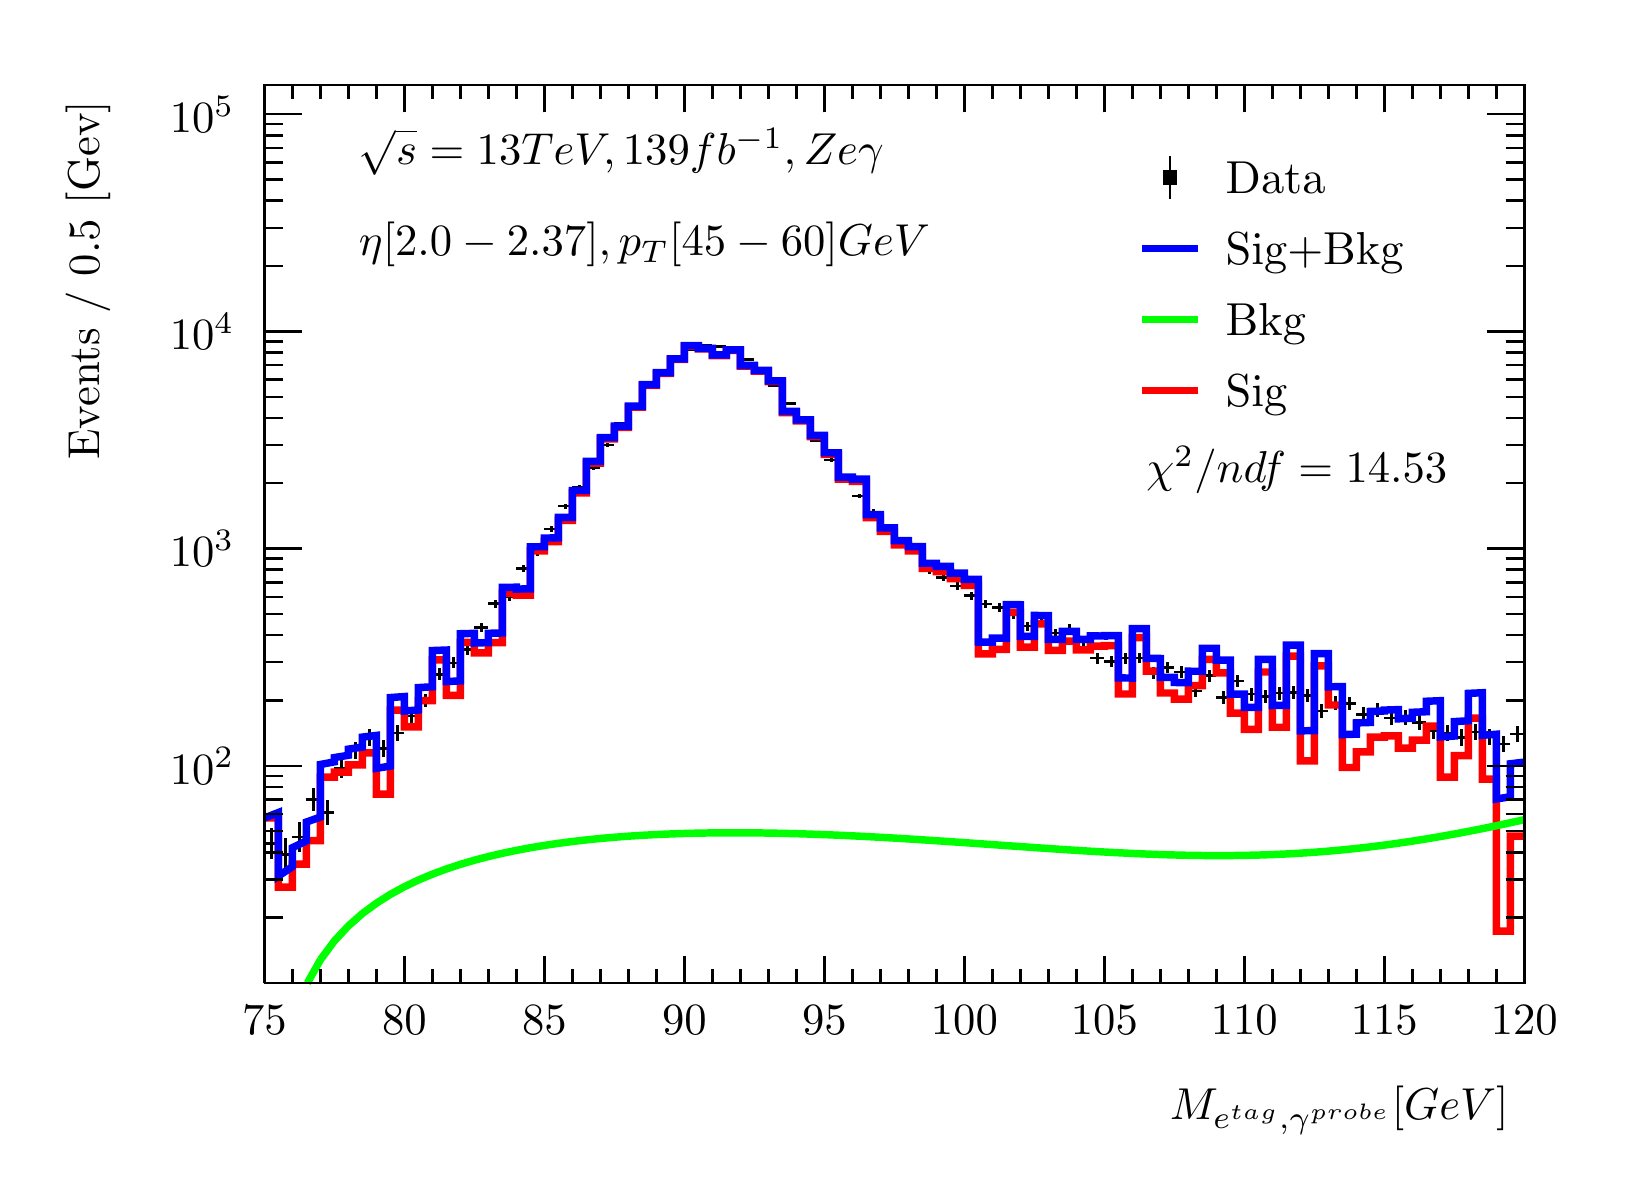
\begin{tikzpicture}
\pgfdeclareplotmark{cross} {
\pgfpathmoveto{\pgfpoint{-0.3\pgfplotmarksize}{\pgfplotmarksize}}
\pgfpathlineto{\pgfpoint{+0.3\pgfplotmarksize}{\pgfplotmarksize}}
\pgfpathlineto{\pgfpoint{+0.3\pgfplotmarksize}{0.3\pgfplotmarksize}}
\pgfpathlineto{\pgfpoint{+1\pgfplotmarksize}{0.3\pgfplotmarksize}}
\pgfpathlineto{\pgfpoint{+1\pgfplotmarksize}{-0.3\pgfplotmarksize}}
\pgfpathlineto{\pgfpoint{+0.3\pgfplotmarksize}{-0.3\pgfplotmarksize}}
\pgfpathlineto{\pgfpoint{+0.3\pgfplotmarksize}{-1.\pgfplotmarksize}}
\pgfpathlineto{\pgfpoint{-0.3\pgfplotmarksize}{-1.\pgfplotmarksize}}
\pgfpathlineto{\pgfpoint{-0.3\pgfplotmarksize}{-0.3\pgfplotmarksize}}
\pgfpathlineto{\pgfpoint{-1.\pgfplotmarksize}{-0.3\pgfplotmarksize}}
\pgfpathlineto{\pgfpoint{-1.\pgfplotmarksize}{0.3\pgfplotmarksize}}
\pgfpathlineto{\pgfpoint{-0.3\pgfplotmarksize}{0.3\pgfplotmarksize}}
\pgfpathclose
\pgfusepathqstroke
}
\pgfdeclareplotmark{cross*} {
\pgfpathmoveto{\pgfpoint{-0.3\pgfplotmarksize}{\pgfplotmarksize}}
\pgfpathlineto{\pgfpoint{+0.3\pgfplotmarksize}{\pgfplotmarksize}}
\pgfpathlineto{\pgfpoint{+0.3\pgfplotmarksize}{0.3\pgfplotmarksize}}
\pgfpathlineto{\pgfpoint{+1\pgfplotmarksize}{0.3\pgfplotmarksize}}
\pgfpathlineto{\pgfpoint{+1\pgfplotmarksize}{-0.3\pgfplotmarksize}}
\pgfpathlineto{\pgfpoint{+0.3\pgfplotmarksize}{-0.3\pgfplotmarksize}}
\pgfpathlineto{\pgfpoint{+0.3\pgfplotmarksize}{-1.\pgfplotmarksize}}
\pgfpathlineto{\pgfpoint{-0.3\pgfplotmarksize}{-1.\pgfplotmarksize}}
\pgfpathlineto{\pgfpoint{-0.3\pgfplotmarksize}{-0.3\pgfplotmarksize}}
\pgfpathlineto{\pgfpoint{-1.\pgfplotmarksize}{-0.3\pgfplotmarksize}}
\pgfpathlineto{\pgfpoint{-1.\pgfplotmarksize}{0.3\pgfplotmarksize}}
\pgfpathlineto{\pgfpoint{-0.3\pgfplotmarksize}{0.3\pgfplotmarksize}}
\pgfpathclose
\pgfusepathqfillstroke
}
\pgfdeclareplotmark{newstar} {
\pgfpathmoveto{\pgfqpoint{0pt}{\pgfplotmarksize}}
\pgfpathlineto{\pgfqpointpolar{44}{0.5\pgfplotmarksize}}
\pgfpathlineto{\pgfqpointpolar{18}{\pgfplotmarksize}}
\pgfpathlineto{\pgfqpointpolar{-20}{0.5\pgfplotmarksize}}
\pgfpathlineto{\pgfqpointpolar{-54}{\pgfplotmarksize}}
\pgfpathlineto{\pgfqpointpolar{-90}{0.5\pgfplotmarksize}}
\pgfpathlineto{\pgfqpointpolar{234}{\pgfplotmarksize}}
\pgfpathlineto{\pgfqpointpolar{198}{0.5\pgfplotmarksize}}
\pgfpathlineto{\pgfqpointpolar{162}{\pgfplotmarksize}}
\pgfpathlineto{\pgfqpointpolar{134}{0.5\pgfplotmarksize}}
\pgfpathclose
\pgfusepathqstroke
}
\pgfdeclareplotmark{newstar*} {
\pgfpathmoveto{\pgfqpoint{0pt}{\pgfplotmarksize}}
\pgfpathlineto{\pgfqpointpolar{44}{0.5\pgfplotmarksize}}
\pgfpathlineto{\pgfqpointpolar{18}{\pgfplotmarksize}}
\pgfpathlineto{\pgfqpointpolar{-20}{0.5\pgfplotmarksize}}
\pgfpathlineto{\pgfqpointpolar{-54}{\pgfplotmarksize}}
\pgfpathlineto{\pgfqpointpolar{-90}{0.5\pgfplotmarksize}}
\pgfpathlineto{\pgfqpointpolar{234}{\pgfplotmarksize}}
\pgfpathlineto{\pgfqpointpolar{198}{0.5\pgfplotmarksize}}
\pgfpathlineto{\pgfqpointpolar{162}{\pgfplotmarksize}}
\pgfpathlineto{\pgfqpointpolar{134}{0.5\pgfplotmarksize}}
\pgfpathclose
\pgfusepathqfillstroke
}
\definecolor{c}{rgb}{1,1,1};
\draw [color=c, fill=c] (0,0) rectangle (20,14.4361);
\draw [color=c, fill=c] (3,2.30977) rectangle (19,13.7143);
\definecolor{c}{rgb}{0,0,0};
\draw [c,line width=0.9] (3,2.30977) -- (3,13.7143) -- (19,13.7143) -- (19,2.30977) -- (3,2.30977);
\definecolor{c}{rgb}{1,1,1};
\draw [color=c, fill=c] (3,2.30977) rectangle (19,13.7143);
\definecolor{c}{rgb}{0,0,0};
\draw [c,line width=0.9] (3,2.30977) -- (3,13.7143) -- (19,13.7143) -- (19,2.30977) -- (3,2.30977);
\draw [c,line width=0.9] (3,2.30977) -- (19,2.30977);
\draw [c,line width=0.9] (3,2.65624) -- (3,2.30977);
\draw [c,line width=0.9] (3.35556,2.48301) -- (3.35556,2.30977);
\draw [c,line width=0.9] (3.71111,2.48301) -- (3.71111,2.30977);
\draw [c,line width=0.9] (4.06667,2.48301) -- (4.06667,2.30977);
\draw [c,line width=0.9] (4.42222,2.48301) -- (4.42222,2.30977);
\draw [c,line width=0.9] (4.77778,2.65624) -- (4.77778,2.30977);
\draw [c,line width=0.9] (5.13333,2.48301) -- (5.13333,2.30977);
\draw [c,line width=0.9] (5.48889,2.48301) -- (5.48889,2.30977);
\draw [c,line width=0.9] (5.84444,2.48301) -- (5.84444,2.30977);
\draw [c,line width=0.9] (6.2,2.48301) -- (6.2,2.30977);
\draw [c,line width=0.9] (6.55556,2.65624) -- (6.55556,2.30977);
\draw [c,line width=0.9] (6.91111,2.48301) -- (6.91111,2.30977);
\draw [c,line width=0.9] (7.26667,2.48301) -- (7.26667,2.30977);
\draw [c,line width=0.9] (7.62222,2.48301) -- (7.62222,2.30977);
\draw [c,line width=0.9] (7.97778,2.48301) -- (7.97778,2.30977);
\draw [c,line width=0.9] (8.33333,2.65624) -- (8.33333,2.30977);
\draw [c,line width=0.9] (8.68889,2.48301) -- (8.68889,2.30977);
\draw [c,line width=0.9] (9.04444,2.48301) -- (9.04444,2.30977);
\draw [c,line width=0.9] (9.4,2.48301) -- (9.4,2.30977);
\draw [c,line width=0.9] (9.75556,2.48301) -- (9.75556,2.30977);
\draw [c,line width=0.9] (10.1111,2.65624) -- (10.1111,2.30977);
\draw [c,line width=0.9] (10.4667,2.48301) -- (10.4667,2.30977);
\draw [c,line width=0.9] (10.8222,2.48301) -- (10.8222,2.30977);
\draw [c,line width=0.9] (11.1778,2.48301) -- (11.1778,2.30977);
\draw [c,line width=0.9] (11.5333,2.48301) -- (11.5333,2.30977);
\draw [c,line width=0.9] (11.8889,2.65624) -- (11.8889,2.30977);
\draw [c,line width=0.9] (12.2444,2.48301) -- (12.2444,2.30977);
\draw [c,line width=0.9] (12.6,2.48301) -- (12.6,2.30977);
\draw [c,line width=0.9] (12.9556,2.48301) -- (12.9556,2.30977);
\draw [c,line width=0.9] (13.3111,2.48301) -- (13.3111,2.30977);
\draw [c,line width=0.9] (13.6667,2.65624) -- (13.6667,2.30977);
\draw [c,line width=0.9] (14.0222,2.48301) -- (14.0222,2.30977);
\draw [c,line width=0.9] (14.3778,2.48301) -- (14.3778,2.30977);
\draw [c,line width=0.9] (14.7333,2.48301) -- (14.7333,2.30977);
\draw [c,line width=0.9] (15.0889,2.48301) -- (15.0889,2.30977);
\draw [c,line width=0.9] (15.4444,2.65624) -- (15.4444,2.30977);
\draw [c,line width=0.9] (15.8,2.48301) -- (15.8,2.30977);
\draw [c,line width=0.9] (16.1556,2.48301) -- (16.1556,2.30977);
\draw [c,line width=0.9] (16.5111,2.48301) -- (16.5111,2.30977);
\draw [c,line width=0.9] (16.8667,2.48301) -- (16.8667,2.30977);
\draw [c,line width=0.9] (17.2222,2.65624) -- (17.2222,2.30977);
\draw [c,line width=0.9] (17.5778,2.48301) -- (17.5778,2.30977);
\draw [c,line width=0.9] (17.9333,2.48301) -- (17.9333,2.30977);
\draw [c,line width=0.9] (18.2889,2.48301) -- (18.2889,2.30977);
\draw [c,line width=0.9] (18.6444,2.48301) -- (18.6444,2.30977);
\draw [c,line width=0.9] (19,2.65624) -- (19,2.30977);
\draw [c,line width=0.9] (19,2.65624) -- (19,2.30977);
\draw [anchor=base] (3,1.66015) node[scale=1.61424, color=c, rotate=0]{75};
\draw [anchor=base] (4.77778,1.66015) node[scale=1.61424, color=c, rotate=0]{80};
\draw [anchor=base] (6.55556,1.66015) node[scale=1.61424, color=c, rotate=0]{85};
\draw [anchor=base] (8.33333,1.66015) node[scale=1.61424, color=c, rotate=0]{90};
\draw [anchor=base] (10.1111,1.66015) node[scale=1.61424, color=c, rotate=0]{95};
\draw [anchor=base] (11.8889,1.66015) node[scale=1.61424, color=c, rotate=0]{100};
\draw [anchor=base] (13.6667,1.66015) node[scale=1.61424, color=c, rotate=0]{105};
\draw [anchor=base] (15.4444,1.66015) node[scale=1.61424, color=c, rotate=0]{110};
\draw [anchor=base] (17.2222,1.66015) node[scale=1.61424, color=c, rotate=0]{115};
\draw [anchor=base] (19,1.66015) node[scale=1.61424, color=c, rotate=0]{120};
\draw [anchor= east] (19,0.692932) node[scale=1.61424, color=c, rotate=0]{$M_{e^{tag}, \gamma^{probe}}  [GeV]$};
\draw [c,line width=0.9] (3,13.7143) -- (19,13.7143);
\draw [c,line width=0.9] (3,13.3678) -- (3,13.7143);
\draw [c,line width=0.9] (3.35556,13.5411) -- (3.35556,13.7143);
\draw [c,line width=0.9] (3.71111,13.5411) -- (3.71111,13.7143);
\draw [c,line width=0.9] (4.06667,13.5411) -- (4.06667,13.7143);
\draw [c,line width=0.9] (4.42222,13.5411) -- (4.42222,13.7143);
\draw [c,line width=0.9] (4.77778,13.3678) -- (4.77778,13.7143);
\draw [c,line width=0.9] (5.13333,13.5411) -- (5.13333,13.7143);
\draw [c,line width=0.9] (5.48889,13.5411) -- (5.48889,13.7143);
\draw [c,line width=0.9] (5.84444,13.5411) -- (5.84444,13.7143);
\draw [c,line width=0.9] (6.2,13.5411) -- (6.2,13.7143);
\draw [c,line width=0.9] (6.55556,13.3678) -- (6.55556,13.7143);
\draw [c,line width=0.9] (6.91111,13.5411) -- (6.91111,13.7143);
\draw [c,line width=0.9] (7.26667,13.5411) -- (7.26667,13.7143);
\draw [c,line width=0.9] (7.62222,13.5411) -- (7.62222,13.7143);
\draw [c,line width=0.9] (7.97778,13.5411) -- (7.97778,13.7143);
\draw [c,line width=0.9] (8.33333,13.3678) -- (8.33333,13.7143);
\draw [c,line width=0.9] (8.68889,13.5411) -- (8.68889,13.7143);
\draw [c,line width=0.9] (9.04444,13.5411) -- (9.04444,13.7143);
\draw [c,line width=0.9] (9.4,13.5411) -- (9.4,13.7143);
\draw [c,line width=0.9] (9.75556,13.5411) -- (9.75556,13.7143);
\draw [c,line width=0.9] (10.1111,13.3678) -- (10.1111,13.7143);
\draw [c,line width=0.9] (10.4667,13.5411) -- (10.4667,13.7143);
\draw [c,line width=0.9] (10.8222,13.5411) -- (10.8222,13.7143);
\draw [c,line width=0.9] (11.1778,13.5411) -- (11.1778,13.7143);
\draw [c,line width=0.9] (11.5333,13.5411) -- (11.5333,13.7143);
\draw [c,line width=0.9] (11.8889,13.3678) -- (11.8889,13.7143);
\draw [c,line width=0.9] (12.2444,13.5411) -- (12.2444,13.7143);
\draw [c,line width=0.9] (12.6,13.5411) -- (12.6,13.7143);
\draw [c,line width=0.9] (12.9556,13.5411) -- (12.9556,13.7143);
\draw [c,line width=0.9] (13.3111,13.5411) -- (13.3111,13.7143);
\draw [c,line width=0.9] (13.6667,13.3678) -- (13.6667,13.7143);
\draw [c,line width=0.9] (14.0222,13.5411) -- (14.0222,13.7143);
\draw [c,line width=0.9] (14.3778,13.5411) -- (14.3778,13.7143);
\draw [c,line width=0.9] (14.7333,13.5411) -- (14.7333,13.7143);
\draw [c,line width=0.9] (15.0889,13.5411) -- (15.0889,13.7143);
\draw [c,line width=0.9] (15.4444,13.3678) -- (15.4444,13.7143);
\draw [c,line width=0.9] (15.8,13.5411) -- (15.8,13.7143);
\draw [c,line width=0.9] (16.1556,13.5411) -- (16.1556,13.7143);
\draw [c,line width=0.9] (16.5111,13.5411) -- (16.5111,13.7143);
\draw [c,line width=0.9] (16.8667,13.5411) -- (16.8667,13.7143);
\draw [c,line width=0.9] (17.2222,13.3678) -- (17.2222,13.7143);
\draw [c,line width=0.9] (17.5778,13.5411) -- (17.5778,13.7143);
\draw [c,line width=0.9] (17.9333,13.5411) -- (17.9333,13.7143);
\draw [c,line width=0.9] (18.2889,13.5411) -- (18.2889,13.7143);
\draw [c,line width=0.9] (18.6444,13.5411) -- (18.6444,13.7143);
\draw [c,line width=0.9] (19,13.3678) -- (19,13.7143);
\draw [c,line width=0.9] (19,13.3678) -- (19,13.7143);
\draw [c,line width=0.9] (3,2.30977) -- (3,13.7143);
\draw [c,line width=0.9] (3.237,3.14018) -- (3,3.14018);
\draw [c,line width=0.9] (3.237,3.62593) -- (3,3.62593);
\draw [c,line width=0.9] (3.237,3.97058) -- (3,3.97058);
\draw [c,line width=0.9] (3.237,4.23792) -- (3,4.23792);
\draw [c,line width=0.9] (3.237,4.45634) -- (3,4.45634);
\draw [c,line width=0.9] (3.237,4.64102) -- (3,4.64102);
\draw [c,line width=0.9] (3.237,4.80099) -- (3,4.80099);
\draw [c,line width=0.9] (3.237,4.9421) -- (3,4.9421);
\draw [c,line width=0.9] (3.474,5.06832) -- (3,5.06832);
\draw [anchor= east] (2.82,5.06832) node[scale=1.61424, color=c, rotate=0]{$10^{2}$};
\draw [c,line width=0.9] (3.237,5.89873) -- (3,5.89873);
\draw [c,line width=0.9] (3.237,6.38449) -- (3,6.38449);
\draw [c,line width=0.9] (3.237,6.72914) -- (3,6.72914);
\draw [c,line width=0.9] (3.237,6.99647) -- (3,6.99647);
\draw [c,line width=0.9] (3.237,7.21489) -- (3,7.21489);
\draw [c,line width=0.9] (3.237,7.39957) -- (3,7.39957);
\draw [c,line width=0.9] (3.237,7.55954) -- (3,7.55954);
\draw [c,line width=0.9] (3.237,7.70065) -- (3,7.70065);
\draw [c,line width=0.9] (3.474,7.82687) -- (3,7.82687);
\draw [anchor= east] (2.82,7.82687) node[scale=1.61424, color=c, rotate=0]{$10^{3}$};
\draw [c,line width=0.9] (3.237,8.65728) -- (3,8.65728);
\draw [c,line width=0.9] (3.237,9.14304) -- (3,9.14304);
\draw [c,line width=0.9] (3.237,9.48769) -- (3,9.48769);
\draw [c,line width=0.9] (3.237,9.75502) -- (3,9.75502);
\draw [c,line width=0.9] (3.237,9.97344) -- (3,9.97344);
\draw [c,line width=0.9] (3.237,10.1581) -- (3,10.1581);
\draw [c,line width=0.9] (3.237,10.3181) -- (3,10.3181);
\draw [c,line width=0.9] (3.237,10.4592) -- (3,10.4592);
\draw [c,line width=0.9] (3.474,10.5854) -- (3,10.5854);
\draw [anchor= east] (2.82,10.5854) node[scale=1.61424, color=c, rotate=0]{$10^{4}$};
\draw [c,line width=0.9] (3.237,11.4158) -- (3,11.4158);
\draw [c,line width=0.9] (3.237,11.9016) -- (3,11.9016);
\draw [c,line width=0.9] (3.237,12.2462) -- (3,12.2462);
\draw [c,line width=0.9] (3.237,12.5136) -- (3,12.5136);
\draw [c,line width=0.9] (3.237,12.732) -- (3,12.732);
\draw [c,line width=0.9] (3.237,12.9167) -- (3,12.9167);
\draw [c,line width=0.9] (3.237,13.0766) -- (3,13.0766);
\draw [c,line width=0.9] (3.237,13.2178) -- (3,13.2178);
\draw [c,line width=0.9] (3.474,13.344) -- (3,13.344);
\draw [anchor= east] (2.82,13.344) node[scale=1.61424, color=c, rotate=0]{$10^{5}$};
\draw [anchor= east] (0.76,13.7143) node[scale=1.61424, color=c, rotate=90]{Events / 0.5 [Gev]};
\draw [c,line width=0.9] (19,2.30977) -- (19,13.7143);
\draw [c,line width=0.9] (18.763,3.14018) -- (19,3.14018);
\draw [c,line width=0.9] (18.763,3.62593) -- (19,3.62593);
\draw [c,line width=0.9] (18.763,3.97058) -- (19,3.97058);
\draw [c,line width=0.9] (18.763,4.23792) -- (19,4.23792);
\draw [c,line width=0.9] (18.763,4.45634) -- (19,4.45634);
\draw [c,line width=0.9] (18.763,4.64102) -- (19,4.64102);
\draw [c,line width=0.9] (18.763,4.80099) -- (19,4.80099);
\draw [c,line width=0.9] (18.763,4.9421) -- (19,4.9421);
\draw [c,line width=0.9] (18.526,5.06832) -- (19,5.06832);
\draw [c,line width=0.9] (18.763,5.89873) -- (19,5.89873);
\draw [c,line width=0.9] (18.763,6.38449) -- (19,6.38449);
\draw [c,line width=0.9] (18.763,6.72914) -- (19,6.72914);
\draw [c,line width=0.9] (18.763,6.99647) -- (19,6.99647);
\draw [c,line width=0.9] (18.763,7.21489) -- (19,7.21489);
\draw [c,line width=0.9] (18.763,7.39957) -- (19,7.39957);
\draw [c,line width=0.9] (18.763,7.55954) -- (19,7.55954);
\draw [c,line width=0.9] (18.763,7.70065) -- (19,7.70065);
\draw [c,line width=0.9] (18.526,7.82687) -- (19,7.82687);
\draw [c,line width=0.9] (18.763,8.65728) -- (19,8.65728);
\draw [c,line width=0.9] (18.763,9.14304) -- (19,9.14304);
\draw [c,line width=0.9] (18.763,9.48769) -- (19,9.48769);
\draw [c,line width=0.9] (18.763,9.75502) -- (19,9.75502);
\draw [c,line width=0.9] (18.763,9.97344) -- (19,9.97344);
\draw [c,line width=0.9] (18.763,10.1581) -- (19,10.1581);
\draw [c,line width=0.9] (18.763,10.3181) -- (19,10.3181);
\draw [c,line width=0.9] (18.763,10.4592) -- (19,10.4592);
\draw [c,line width=0.9] (18.526,10.5854) -- (19,10.5854);
\draw [c,line width=0.9] (18.763,11.4158) -- (19,11.4158);
\draw [c,line width=0.9] (18.763,11.9016) -- (19,11.9016);
\draw [c,line width=0.9] (18.763,12.2462) -- (19,12.2462);
\draw [c,line width=0.9] (18.763,12.5136) -- (19,12.5136);
\draw [c,line width=0.9] (18.763,12.732) -- (19,12.732);
\draw [c,line width=0.9] (18.763,12.9167) -- (19,12.9167);
\draw [c,line width=0.9] (18.763,13.0766) -- (19,13.0766);
\draw [c,line width=0.9] (18.763,13.2178) -- (19,13.2178);
\draw [c,line width=0.9] (18.526,13.344) -- (19,13.344);
\draw [c,line width=0.9] (3.08889,4.08477) -- (3,4.08477);
\draw [c,line width=0.9] (3,4.08477) -- (3,4.08477);
\draw [c,line width=0.9] (3.08889,4.08477) -- (3.17778,4.08477);
\draw [c,line width=0.9] (3.17778,4.08477) -- (3.17778,4.08477);
\draw [c,line width=0.9] (3.08889,4.08477) -- (3.08889,4.27759);
\draw [c,line width=0.9] (3.08889,4.27759) -- (3.08889,4.27759);
\draw [c,line width=0.9] (3.08889,4.08477) -- (3.08889,3.88982);
\draw [c,line width=0.9] (3.08889,3.88982) -- (3.08889,3.88982);
\draw [c,line width=0.9] (3.26667,3.94026) -- (3.17778,3.94026);
\draw [c,line width=0.9] (3.17778,3.94026) -- (3.17778,3.94026);
\draw [c,line width=0.9] (3.26667,3.94026) -- (3.35556,3.94026);
\draw [c,line width=0.9] (3.35556,3.94026) -- (3.35556,3.94026);
\draw [c,line width=0.9] (3.26667,3.94026) -- (3.26667,4.14577);
\draw [c,line width=0.9] (3.26667,4.14577) -- (3.26667,4.14577);
\draw [c,line width=0.9] (3.26667,3.94026) -- (3.26667,3.73218);
\draw [c,line width=0.9] (3.26667,3.73218) -- (3.26667,3.73218);
\draw [c,line width=0.9] (3.44444,4.16379) -- (3.35556,4.16379);
\draw [c,line width=0.9] (3.35556,4.16379) -- (3.35556,4.16379);
\draw [c,line width=0.9] (3.44444,4.16379) -- (3.53333,4.16379);
\draw [c,line width=0.9] (3.53333,4.16379) -- (3.53333,4.16379);
\draw [c,line width=0.9] (3.44444,4.16379) -- (3.44444,4.35002);
\draw [c,line width=0.9] (3.44444,4.35002) -- (3.44444,4.35002);
\draw [c,line width=0.9] (3.44444,4.16379) -- (3.44444,3.97563);
\draw [c,line width=0.9] (3.44444,3.97563) -- (3.44444,3.97563);
\draw [c,line width=0.9] (3.62222,4.64102) -- (3.53333,4.64102);
\draw [c,line width=0.9] (3.53333,4.64102) -- (3.53333,4.64102);
\draw [c,line width=0.9] (3.62222,4.64102) -- (3.71111,4.64102);
\draw [c,line width=0.9] (3.71111,4.64102) -- (3.71111,4.64102);
\draw [c,line width=0.9] (3.62222,4.64102) -- (3.62222,4.79207);
\draw [c,line width=0.9] (3.62222,4.79207) -- (3.62222,4.79207);
\draw [c,line width=0.9] (3.62222,4.64102) -- (3.62222,4.48891);
\draw [c,line width=0.9] (3.62222,4.48891) -- (3.62222,4.48891);
\draw [c,line width=0.9] (3.8,4.47615) -- (3.71111,4.47615);
\draw [c,line width=0.9] (3.71111,4.47615) -- (3.71111,4.47615);
\draw [c,line width=0.9] (3.8,4.47615) -- (3.88889,4.47615);
\draw [c,line width=0.9] (3.88889,4.47615) -- (3.88889,4.47615);
\draw [c,line width=0.9] (3.8,4.47615) -- (3.8,4.6385);
\draw [c,line width=0.9] (3.8,4.6385) -- (3.8,4.6385);
\draw [c,line width=0.9] (3.8,4.47615) -- (3.8,4.31249);
\draw [c,line width=0.9] (3.8,4.31249) -- (3.8,4.31249);
\draw [c,line width=0.9] (3.97778,5.04412) -- (3.88889,5.04412);
\draw [c,line width=0.9] (3.88889,5.04412) -- (3.88889,5.04412);
\draw [c,line width=0.9] (3.97778,5.04412) -- (4.06667,5.04412);
\draw [c,line width=0.9] (4.06667,5.04412) -- (4.06667,5.04412);
\draw [c,line width=0.9] (3.97778,5.04412) -- (3.97778,5.17083);
\draw [c,line width=0.9] (3.97778,5.17083) -- (3.97778,5.17083);
\draw [c,line width=0.9] (3.97778,5.04412) -- (3.97778,4.91677);
\draw [c,line width=0.9] (3.97778,4.91677) -- (3.97778,4.91677);
\draw [c,line width=0.9] (4.15556,5.26661) -- (4.06667,5.26661);
\draw [c,line width=0.9] (4.06667,5.26661) -- (4.06667,5.26661);
\draw [c,line width=0.9] (4.15556,5.26661) -- (4.24444,5.26661);
\draw [c,line width=0.9] (4.24444,5.26661) -- (4.24444,5.26661);
\draw [c,line width=0.9] (4.15556,5.26661) -- (4.15556,5.37686);
\draw [c,line width=0.9] (4.15556,5.37686) -- (4.15556,5.37686);
\draw [c,line width=0.9] (4.15556,5.26661) -- (4.15556,5.15637);
\draw [c,line width=0.9] (4.15556,5.15637) -- (4.15556,5.15637);
\draw [c,line width=0.9] (4.33333,5.42786) -- (4.24444,5.42786);
\draw [c,line width=0.9] (4.24444,5.42786) -- (4.24444,5.42786);
\draw [c,line width=0.9] (4.33333,5.42786) -- (4.42222,5.42786);
\draw [c,line width=0.9] (4.42222,5.42786) -- (4.42222,5.42786);
\draw [c,line width=0.9] (4.33333,5.42786) -- (4.33333,5.53093);
\draw [c,line width=0.9] (4.33333,5.53093) -- (4.33333,5.53093);
\draw [c,line width=0.9] (4.33333,5.42786) -- (4.33333,5.32478);
\draw [c,line width=0.9] (4.33333,5.32478) -- (4.33333,5.32478);
\draw [c,line width=0.9] (4.51111,5.28675) -- (4.42222,5.28675);
\draw [c,line width=0.9] (4.42222,5.28675) -- (4.42222,5.28675);
\draw [c,line width=0.9] (4.51111,5.28675) -- (4.6,5.28675);
\draw [c,line width=0.9] (4.6,5.28675) -- (4.6,5.28675);
\draw [c,line width=0.9] (4.51111,5.28675) -- (4.51111,5.39608);
\draw [c,line width=0.9] (4.51111,5.39608) -- (4.51111,5.39608);
\draw [c,line width=0.9] (4.51111,5.28675) -- (4.51111,5.17742);
\draw [c,line width=0.9] (4.51111,5.17742) -- (4.51111,5.17742);
\draw [c,line width=0.9] (4.68889,5.48842) -- (4.6,5.48842);
\draw [c,line width=0.9] (4.6,5.48842) -- (4.6,5.48842);
\draw [c,line width=0.9] (4.68889,5.48842) -- (4.77778,5.48842);
\draw [c,line width=0.9] (4.77778,5.48842) -- (4.77778,5.48842);
\draw [c,line width=0.9] (4.68889,5.48842) -- (4.68889,5.58893);
\draw [c,line width=0.9] (4.68889,5.58893) -- (4.68889,5.58893);
\draw [c,line width=0.9] (4.68889,5.48842) -- (4.68889,5.38791);
\draw [c,line width=0.9] (4.68889,5.38791) -- (4.68889,5.38791);
\draw [c,line width=0.9] (4.86667,5.70403) -- (4.77778,5.70403);
\draw [c,line width=0.9] (4.77778,5.70403) -- (4.77778,5.70403);
\draw [c,line width=0.9] (4.86667,5.70403) -- (4.95556,5.70403);
\draw [c,line width=0.9] (4.95556,5.70403) -- (4.95556,5.70403);
\draw [c,line width=0.9] (4.86667,5.70403) -- (4.86667,5.79589);
\draw [c,line width=0.9] (4.86667,5.79589) -- (4.86667,5.79589);
\draw [c,line width=0.9] (4.86667,5.70403) -- (4.86667,5.61217);
\draw [c,line width=0.9] (4.86667,5.61217) -- (4.86667,5.61217);
\draw [c,line width=0.9] (5.04444,5.89873) -- (4.95556,5.89873);
\draw [c,line width=0.9] (4.95556,5.89873) -- (4.95556,5.89873);
\draw [c,line width=0.9] (5.04444,5.89873) -- (5.13333,5.89873);
\draw [c,line width=0.9] (5.13333,5.89873) -- (5.13333,5.89873);
\draw [c,line width=0.9] (5.04444,5.89873) -- (5.04444,5.98343);
\draw [c,line width=0.9] (5.04444,5.98343) -- (5.04444,5.98343);
\draw [c,line width=0.9] (5.04444,5.89873) -- (5.04444,5.81404);
\draw [c,line width=0.9] (5.04444,5.81404) -- (5.04444,5.81404);
\draw [c,line width=0.9] (5.22222,6.23134) -- (5.13333,6.23134);
\draw [c,line width=0.9] (5.13333,6.23134) -- (5.13333,6.23134);
\draw [c,line width=0.9] (5.22222,6.23134) -- (5.31111,6.23134);
\draw [c,line width=0.9] (5.31111,6.23134) -- (5.31111,6.23134);
\draw [c,line width=0.9] (5.22222,6.23134) -- (5.22222,6.30506);
\draw [c,line width=0.9] (5.22222,6.30506) -- (5.22222,6.30506);
\draw [c,line width=0.9] (5.22222,6.23134) -- (5.22222,6.15762);
\draw [c,line width=0.9] (5.22222,6.15762) -- (5.22222,6.15762);
\draw [c,line width=0.9] (5.4,6.37647) -- (5.31111,6.37647);
\draw [c,line width=0.9] (5.31111,6.37647) -- (5.31111,6.37647);
\draw [c,line width=0.9] (5.4,6.37647) -- (5.48889,6.37647);
\draw [c,line width=0.9] (5.48889,6.37647) -- (5.48889,6.37647);
\draw [c,line width=0.9] (5.4,6.37647) -- (5.4,6.44586);
\draw [c,line width=0.9] (5.4,6.44586) -- (5.4,6.44586);
\draw [c,line width=0.9] (5.4,6.37647) -- (5.4,6.30708);
\draw [c,line width=0.9] (5.4,6.30708) -- (5.4,6.30708);
\draw [c,line width=0.9] (5.57778,6.54496) -- (5.48889,6.54496);
\draw [c,line width=0.9] (5.48889,6.54496) -- (5.48889,6.54496);
\draw [c,line width=0.9] (5.57778,6.54496) -- (5.66667,6.54496);
\draw [c,line width=0.9] (5.66667,6.54496) -- (5.66667,6.54496);
\draw [c,line width=0.9] (5.57778,6.54496) -- (5.57778,6.60964);
\draw [c,line width=0.9] (5.57778,6.60964) -- (5.57778,6.60964);
\draw [c,line width=0.9] (5.57778,6.54496) -- (5.57778,6.48028);
\draw [c,line width=0.9] (5.57778,6.48028) -- (5.57778,6.48028);
\draw [c,line width=0.9] (5.75556,6.82411) -- (5.66667,6.82411);
\draw [c,line width=0.9] (5.66667,6.82411) -- (5.66667,6.82411);
\draw [c,line width=0.9] (5.75556,6.82411) -- (5.84444,6.82411);
\draw [c,line width=0.9] (5.84444,6.82411) -- (5.84444,6.82411);
\draw [c,line width=0.9] (5.75556,6.82411) -- (5.75556,6.88168);
\draw [c,line width=0.9] (5.75556,6.88168) -- (5.75556,6.88168);
\draw [c,line width=0.9] (5.75556,6.82411) -- (5.75556,6.76654);
\draw [c,line width=0.9] (5.75556,6.76654) -- (5.75556,6.76654);
\draw [c,line width=0.9] (5.93333,7.12795) -- (5.84444,7.12795);
\draw [c,line width=0.9] (5.84444,7.12795) -- (5.84444,7.12795);
\draw [c,line width=0.9] (5.93333,7.12795) -- (6.02222,7.12795);
\draw [c,line width=0.9] (6.02222,7.12795) -- (6.02222,7.12795);
\draw [c,line width=0.9] (5.93333,7.12795) -- (5.93333,7.17867);
\draw [c,line width=0.9] (5.93333,7.17867) -- (5.93333,7.17867);
\draw [c,line width=0.9] (5.93333,7.12795) -- (5.93333,7.07724);
\draw [c,line width=0.9] (5.93333,7.07724) -- (5.93333,7.07724);
\draw [c,line width=0.9] (6.11111,7.21089) -- (6.02222,7.21089);
\draw [c,line width=0.9] (6.02222,7.21089) -- (6.02222,7.21089);
\draw [c,line width=0.9] (6.11111,7.21089) -- (6.2,7.21089);
\draw [c,line width=0.9] (6.2,7.21089) -- (6.2,7.21089);
\draw [c,line width=0.9] (6.11111,7.21089) -- (6.11111,7.25988);
\draw [c,line width=0.9] (6.11111,7.25988) -- (6.11111,7.25988);
\draw [c,line width=0.9] (6.11111,7.21089) -- (6.11111,7.16191);
\draw [c,line width=0.9] (6.11111,7.16191) -- (6.11111,7.16191);
\draw [c,line width=0.9] (6.28889,7.57738) -- (6.2,7.57738);
\draw [c,line width=0.9] (6.2,7.57738) -- (6.2,7.57738);
\draw [c,line width=0.9] (6.28889,7.57738) -- (6.37778,7.57738);
\draw [c,line width=0.9] (6.37778,7.57738) -- (6.37778,7.57738);
\draw [c,line width=0.9] (6.28889,7.57738) -- (6.28889,7.61942);
\draw [c,line width=0.9] (6.28889,7.61942) -- (6.28889,7.61942);
\draw [c,line width=0.9] (6.28889,7.57738) -- (6.28889,7.53534);
\draw [c,line width=0.9] (6.28889,7.53534) -- (6.28889,7.53534);
\draw [c,line width=0.9] (6.46667,7.7692) -- (6.37778,7.7692);
\draw [c,line width=0.9] (6.37778,7.7692) -- (6.37778,7.7692);
\draw [c,line width=0.9] (6.46667,7.7692) -- (6.55556,7.7692);
\draw [c,line width=0.9] (6.55556,7.7692) -- (6.55556,7.7692);
\draw [c,line width=0.9] (6.46667,7.7692) -- (6.46667,7.80801);
\draw [c,line width=0.9] (6.46667,7.80801) -- (6.46667,7.80801);
\draw [c,line width=0.9] (6.46667,7.7692) -- (6.46667,7.7304);
\draw [c,line width=0.9] (6.46667,7.7304) -- (6.46667,7.7304);
\draw [c,line width=0.9] (6.64444,8.07488) -- (6.55556,8.07488);
\draw [c,line width=0.9] (6.55556,8.07488) -- (6.55556,8.07488);
\draw [c,line width=0.9] (6.64444,8.07488) -- (6.73333,8.07488);
\draw [c,line width=0.9] (6.73333,8.07488) -- (6.73333,8.07488);
\draw [c,line width=0.9] (6.64444,8.07488) -- (6.64444,8.10904);
\draw [c,line width=0.9] (6.64444,8.10904) -- (6.64444,8.10904);
\draw [c,line width=0.9] (6.64444,8.07488) -- (6.64444,8.04072);
\draw [c,line width=0.9] (6.64444,8.04072) -- (6.64444,8.04072);
\draw [c,line width=0.9] (6.82222,8.36651) -- (6.73333,8.36651);
\draw [c,line width=0.9] (6.73333,8.36651) -- (6.73333,8.36651);
\draw [c,line width=0.9] (6.82222,8.36651) -- (6.91111,8.36651);
\draw [c,line width=0.9] (6.91111,8.36651) -- (6.91111,8.36651);
\draw [c,line width=0.9] (6.82222,8.36651) -- (6.82222,8.39676);
\draw [c,line width=0.9] (6.82222,8.39676) -- (6.82222,8.39676);
\draw [c,line width=0.9] (6.82222,8.36651) -- (6.82222,8.33627);
\draw [c,line width=0.9] (6.82222,8.33627) -- (6.82222,8.33627);
\draw [c,line width=0.9] (7,8.61025) -- (6.91111,8.61025);
\draw [c,line width=0.9] (6.91111,8.61025) -- (6.91111,8.61025);
\draw [c,line width=0.9] (7,8.61025) -- (7.08889,8.61025);
\draw [c,line width=0.9] (7.08889,8.61025) -- (7.08889,8.61025);
\draw [c,line width=0.9] (7,8.61025) -- (7,8.63757);
\draw [c,line width=0.9] (7,8.63757) -- (7,8.63757);
\draw [c,line width=0.9] (7,8.61025) -- (7,8.58293);
\draw [c,line width=0.9] (7,8.58293) -- (7,8.58293);
\draw [c,line width=0.9] (7.17778,8.85099) -- (7.08889,8.85099);
\draw [c,line width=0.9] (7.08889,8.85099) -- (7.08889,8.85099);
\draw [c,line width=0.9] (7.17778,8.85099) -- (7.26667,8.85099);
\draw [c,line width=0.9] (7.26667,8.85099) -- (7.26667,8.85099);
\draw [c,line width=0.9] (7.17778,8.85099) -- (7.17778,8.8757);
\draw [c,line width=0.9] (7.17778,8.8757) -- (7.17778,8.8757);
\draw [c,line width=0.9] (7.17778,8.85099) -- (7.17778,8.82629);
\draw [c,line width=0.9] (7.17778,8.82629) -- (7.17778,8.82629);
\draw [c,line width=0.9] (7.35556,9.14304) -- (7.26667,9.14304);
\draw [c,line width=0.9] (7.26667,9.14304) -- (7.26667,9.14304);
\draw [c,line width=0.9] (7.35556,9.14304) -- (7.44444,9.14304);
\draw [c,line width=0.9] (7.44444,9.14304) -- (7.44444,9.14304);
\draw [c,line width=0.9] (7.35556,9.14304) -- (7.35556,9.16491);
\draw [c,line width=0.9] (7.35556,9.16491) -- (7.35556,9.16491);
\draw [c,line width=0.9] (7.35556,9.14304) -- (7.35556,9.12117);
\draw [c,line width=0.9] (7.35556,9.12117) -- (7.35556,9.12117);
\draw [c,line width=0.9] (7.53333,9.41738) -- (7.44444,9.41738);
\draw [c,line width=0.9] (7.44444,9.41738) -- (7.44444,9.41738);
\draw [c,line width=0.9] (7.53333,9.41738) -- (7.62222,9.41738);
\draw [c,line width=0.9] (7.62222,9.41738) -- (7.62222,9.41738);
\draw [c,line width=0.9] (7.53333,9.41738) -- (7.53333,9.43688);
\draw [c,line width=0.9] (7.53333,9.43688) -- (7.53333,9.43688);
\draw [c,line width=0.9] (7.53333,9.41738) -- (7.53333,9.39787);
\draw [c,line width=0.9] (7.53333,9.39787) -- (7.53333,9.39787);
\draw [c,line width=0.9] (7.71111,9.65095) -- (7.62222,9.65095);
\draw [c,line width=0.9] (7.62222,9.65095) -- (7.62222,9.65095);
\draw [c,line width=0.9] (7.71111,9.65095) -- (7.8,9.65095);
\draw [c,line width=0.9] (7.8,9.65095) -- (7.8,9.65095);
\draw [c,line width=0.9] (7.71111,9.65095) -- (7.71111,9.66865);
\draw [c,line width=0.9] (7.71111,9.66865) -- (7.71111,9.66865);
\draw [c,line width=0.9] (7.71111,9.65095) -- (7.71111,9.63326);
\draw [c,line width=0.9] (7.71111,9.63326) -- (7.71111,9.63326);
\draw [c,line width=0.9] (7.88889,9.91535) -- (7.8,9.91535);
\draw [c,line width=0.9] (7.8,9.91535) -- (7.8,9.91535);
\draw [c,line width=0.9] (7.88889,9.91535) -- (7.97778,9.91535);
\draw [c,line width=0.9] (7.97778,9.91535) -- (7.97778,9.91535);
\draw [c,line width=0.9] (7.88889,9.91535) -- (7.88889,9.9312);
\draw [c,line width=0.9] (7.88889,9.9312) -- (7.88889,9.9312);
\draw [c,line width=0.9] (7.88889,9.91535) -- (7.88889,9.89951);
\draw [c,line width=0.9] (7.88889,9.89951) -- (7.88889,9.89951);
\draw [c,line width=0.9] (8.06667,10.0918) -- (7.97778,10.0918);
\draw [c,line width=0.9] (7.97778,10.0918) -- (7.97778,10.0918);
\draw [c,line width=0.9] (8.06667,10.0918) -- (8.15556,10.0918);
\draw [c,line width=0.9] (8.15556,10.0918) -- (8.15556,10.0918);
\draw [c,line width=0.9] (8.06667,10.0918) -- (8.06667,10.1065);
\draw [c,line width=0.9] (8.06667,10.1065) -- (8.06667,10.1065);
\draw [c,line width=0.9] (8.06667,10.0918) -- (8.06667,10.0771);
\draw [c,line width=0.9] (8.06667,10.0771) -- (8.06667,10.0771);
\draw [c,line width=0.9] (8.24444,10.246) -- (8.15556,10.246);
\draw [c,line width=0.9] (8.15556,10.246) -- (8.15556,10.246);
\draw [c,line width=0.9] (8.24444,10.246) -- (8.33333,10.246);
\draw [c,line width=0.9] (8.33333,10.246) -- (8.33333,10.246);
\draw [c,line width=0.9] (8.24444,10.246) -- (8.24444,10.2598);
\draw [c,line width=0.9] (8.24444,10.2598) -- (8.24444,10.2598);
\draw [c,line width=0.9] (8.24444,10.246) -- (8.24444,10.2322);
\draw [c,line width=0.9] (8.24444,10.2322) -- (8.24444,10.2322);
\draw [c,line width=0.9] (8.42222,10.3568) -- (8.33333,10.3568);
\draw [c,line width=0.9] (8.33333,10.3568) -- (8.33333,10.3568);
\draw [c,line width=0.9] (8.42222,10.3568) -- (8.51111,10.3568);
\draw [c,line width=0.9] (8.51111,10.3568) -- (8.51111,10.3568);
\draw [c,line width=0.9] (8.42222,10.3568) -- (8.42222,10.37);
\draw [c,line width=0.9] (8.42222,10.37) -- (8.42222,10.37);
\draw [c,line width=0.9] (8.42222,10.3568) -- (8.42222,10.3437);
\draw [c,line width=0.9] (8.42222,10.3437) -- (8.42222,10.3437);
\draw [c,line width=0.9] (8.6,10.4092) -- (8.51111,10.4092);
\draw [c,line width=0.9] (8.51111,10.4092) -- (8.51111,10.4092);
\draw [c,line width=0.9] (8.6,10.4092) -- (8.68889,10.4092);
\draw [c,line width=0.9] (8.68889,10.4092) -- (8.68889,10.4092);
\draw [c,line width=0.9] (8.6,10.4092) -- (8.6,10.4221);
\draw [c,line width=0.9] (8.6,10.4221) -- (8.6,10.4221);
\draw [c,line width=0.9] (8.6,10.4092) -- (8.6,10.3963);
\draw [c,line width=0.9] (8.6,10.3963) -- (8.6,10.3963);
\draw [c,line width=0.9] (8.77778,10.3916) -- (8.68889,10.3916);
\draw [c,line width=0.9] (8.68889,10.3916) -- (8.68889,10.3916);
\draw [c,line width=0.9] (8.77778,10.3916) -- (8.86667,10.3916);
\draw [c,line width=0.9] (8.86667,10.3916) -- (8.86667,10.3916);
\draw [c,line width=0.9] (8.77778,10.3916) -- (8.77778,10.4046);
\draw [c,line width=0.9] (8.77778,10.4046) -- (8.77778,10.4046);
\draw [c,line width=0.9] (8.77778,10.3916) -- (8.77778,10.3786);
\draw [c,line width=0.9] (8.77778,10.3786) -- (8.77778,10.3786);
\draw [c,line width=0.9] (8.95556,10.3484) -- (8.86667,10.3484);
\draw [c,line width=0.9] (8.86667,10.3484) -- (8.86667,10.3484);
\draw [c,line width=0.9] (8.95556,10.3484) -- (9.04444,10.3484);
\draw [c,line width=0.9] (9.04444,10.3484) -- (9.04444,10.3484);
\draw [c,line width=0.9] (8.95556,10.3484) -- (8.95556,10.3616);
\draw [c,line width=0.9] (8.95556,10.3616) -- (8.95556,10.3616);
\draw [c,line width=0.9] (8.95556,10.3484) -- (8.95556,10.3352);
\draw [c,line width=0.9] (8.95556,10.3352) -- (8.95556,10.3352);
\draw [c,line width=0.9] (9.13333,10.2305) -- (9.04444,10.2305);
\draw [c,line width=0.9] (9.04444,10.2305) -- (9.04444,10.2305);
\draw [c,line width=0.9] (9.13333,10.2305) -- (9.22222,10.2305);
\draw [c,line width=0.9] (9.22222,10.2305) -- (9.22222,10.2305);
\draw [c,line width=0.9] (9.13333,10.2305) -- (9.13333,10.2444);
\draw [c,line width=0.9] (9.13333,10.2444) -- (9.13333,10.2444);
\draw [c,line width=0.9] (9.13333,10.2305) -- (9.13333,10.2166);
\draw [c,line width=0.9] (9.13333,10.2166) -- (9.13333,10.2166);
\draw [c,line width=0.9] (9.31111,10.1058) -- (9.22222,10.1058);
\draw [c,line width=0.9] (9.22222,10.1058) -- (9.22222,10.1058);
\draw [c,line width=0.9] (9.31111,10.1058) -- (9.4,10.1058);
\draw [c,line width=0.9] (9.4,10.1058) -- (9.4,10.1058);
\draw [c,line width=0.9] (9.31111,10.1058) -- (9.31111,10.1205);
\draw [c,line width=0.9] (9.31111,10.1205) -- (9.31111,10.1205);
\draw [c,line width=0.9] (9.31111,10.1058) -- (9.31111,10.0912);
\draw [c,line width=0.9] (9.31111,10.0912) -- (9.31111,10.0912);
\draw [c,line width=0.9] (9.48889,9.90101) -- (9.4,9.90101);
\draw [c,line width=0.9] (9.4,9.90101) -- (9.4,9.90101);
\draw [c,line width=0.9] (9.48889,9.90101) -- (9.57778,9.90101);
\draw [c,line width=0.9] (9.57778,9.90101) -- (9.57778,9.90101);
\draw [c,line width=0.9] (9.48889,9.90101) -- (9.48889,9.91695);
\draw [c,line width=0.9] (9.48889,9.91695) -- (9.48889,9.91695);
\draw [c,line width=0.9] (9.48889,9.90101) -- (9.48889,9.88507);
\draw [c,line width=0.9] (9.48889,9.88507) -- (9.48889,9.88507);
\draw [c,line width=0.9] (9.66667,9.66833) -- (9.57778,9.66833);
\draw [c,line width=0.9] (9.57778,9.66833) -- (9.57778,9.66833);
\draw [c,line width=0.9] (9.66667,9.66833) -- (9.75556,9.66833);
\draw [c,line width=0.9] (9.75556,9.66833) -- (9.75556,9.66833);
\draw [c,line width=0.9] (9.66667,9.66833) -- (9.66667,9.6859);
\draw [c,line width=0.9] (9.66667,9.6859) -- (9.66667,9.6859);
\draw [c,line width=0.9] (9.66667,9.66833) -- (9.66667,9.65077);
\draw [c,line width=0.9] (9.66667,9.65077) -- (9.66667,9.65077);
\draw [c,line width=0.9] (9.84444,9.43315) -- (9.75556,9.43315);
\draw [c,line width=0.9] (9.75556,9.43315) -- (9.75556,9.43315);
\draw [c,line width=0.9] (9.84444,9.43315) -- (9.93333,9.43315);
\draw [c,line width=0.9] (9.93333,9.43315) -- (9.93333,9.43315);
\draw [c,line width=0.9] (9.84444,9.43315) -- (9.84444,9.45253);
\draw [c,line width=0.9] (9.84444,9.45253) -- (9.84444,9.45253);
\draw [c,line width=0.9] (9.84444,9.43315) -- (9.84444,9.41377);
\draw [c,line width=0.9] (9.84444,9.41377) -- (9.84444,9.41377);
\draw [c,line width=0.9] (10.0222,9.19921) -- (9.93333,9.19921);
\draw [c,line width=0.9] (9.93333,9.19921) -- (9.93333,9.19921);
\draw [c,line width=0.9] (10.0222,9.19921) -- (10.1111,9.19921);
\draw [c,line width=0.9] (10.1111,9.19921) -- (10.1111,9.19921);
\draw [c,line width=0.9] (10.0222,9.19921) -- (10.0222,9.22057);
\draw [c,line width=0.9] (10.0222,9.22057) -- (10.0222,9.22057);
\draw [c,line width=0.9] (10.0222,9.19921) -- (10.0222,9.17784);
\draw [c,line width=0.9] (10.0222,9.17784) -- (10.0222,9.17784);
\draw [c,line width=0.9] (10.2,8.95303) -- (10.1111,8.95303);
\draw [c,line width=0.9] (10.1111,8.95303) -- (10.1111,8.95303);
\draw [c,line width=0.9] (10.2,8.95303) -- (10.2889,8.95303);
\draw [c,line width=0.9] (10.2889,8.95303) -- (10.2889,8.95303);
\draw [c,line width=0.9] (10.2,8.95303) -- (10.2,8.9767);
\draw [c,line width=0.9] (10.2,8.9767) -- (10.2,8.9767);
\draw [c,line width=0.9] (10.2,8.95303) -- (10.2,8.92935);
\draw [c,line width=0.9] (10.2,8.92935) -- (10.2,8.92935);
\draw [c,line width=0.9] (10.3778,8.71687) -- (10.2889,8.71687);
\draw [c,line width=0.9] (10.2889,8.71687) -- (10.2889,8.71687);
\draw [c,line width=0.9] (10.3778,8.71687) -- (10.4667,8.71687);
\draw [c,line width=0.9] (10.4667,8.71687) -- (10.4667,8.71687);
\draw [c,line width=0.9] (10.3778,8.71687) -- (10.3778,8.743);
\draw [c,line width=0.9] (10.3778,8.743) -- (10.3778,8.743);
\draw [c,line width=0.9] (10.3778,8.71687) -- (10.3778,8.69074);
\draw [c,line width=0.9] (10.3778,8.69074) -- (10.3778,8.69074);
\draw [c,line width=0.9] (10.5556,8.49525) -- (10.4667,8.49525);
\draw [c,line width=0.9] (10.4667,8.49525) -- (10.4667,8.49525);
\draw [c,line width=0.9] (10.5556,8.49525) -- (10.6444,8.49525);
\draw [c,line width=0.9] (10.6444,8.49525) -- (10.6444,8.49525);
\draw [c,line width=0.9] (10.5556,8.49525) -- (10.5556,8.52391);
\draw [c,line width=0.9] (10.5556,8.52391) -- (10.5556,8.52391);
\draw [c,line width=0.9] (10.5556,8.49525) -- (10.5556,8.46659);
\draw [c,line width=0.9] (10.5556,8.46659) -- (10.5556,8.46659);
\draw [c,line width=0.9] (10.7333,8.29331) -- (10.6444,8.29331);
\draw [c,line width=0.9] (10.6444,8.29331) -- (10.6444,8.29331);
\draw [c,line width=0.9] (10.7333,8.29331) -- (10.8222,8.29331);
\draw [c,line width=0.9] (10.8222,8.29331) -- (10.8222,8.29331);
\draw [c,line width=0.9] (10.7333,8.29331) -- (10.7333,8.32449);
\draw [c,line width=0.9] (10.7333,8.32449) -- (10.7333,8.32449);
\draw [c,line width=0.9] (10.7333,8.29331) -- (10.7333,8.26213);
\draw [c,line width=0.9] (10.7333,8.26213) -- (10.7333,8.26213);
\draw [c,line width=0.9] (10.9111,8.1085) -- (10.8222,8.1085);
\draw [c,line width=0.9] (10.8222,8.1085) -- (10.8222,8.1085);
\draw [c,line width=0.9] (10.9111,8.1085) -- (11,8.1085);
\draw [c,line width=0.9] (11,8.1085) -- (11,8.1085);
\draw [c,line width=0.9] (10.9111,8.1085) -- (10.9111,8.14218);
\draw [c,line width=0.9] (10.9111,8.14218) -- (10.9111,8.14218);
\draw [c,line width=0.9] (10.9111,8.1085) -- (10.9111,8.07481);
\draw [c,line width=0.9] (10.9111,8.07481) -- (10.9111,8.07481);
\draw [c,line width=0.9] (11.0889,7.92902) -- (11,7.92902);
\draw [c,line width=0.9] (11,7.92902) -- (11,7.92902);
\draw [c,line width=0.9] (11.0889,7.92902) -- (11.1778,7.92902);
\draw [c,line width=0.9] (11.1778,7.92902) -- (11.1778,7.92902);
\draw [c,line width=0.9] (11.0889,7.92902) -- (11.0889,7.96532);
\draw [c,line width=0.9] (11.0889,7.96532) -- (11.0889,7.96532);
\draw [c,line width=0.9] (11.0889,7.92902) -- (11.0889,7.89272);
\draw [c,line width=0.9] (11.0889,7.89272) -- (11.0889,7.89272);
\draw [c,line width=0.9] (11.2667,7.80511) -- (11.1778,7.80511);
\draw [c,line width=0.9] (11.1778,7.80511) -- (11.1778,7.80511);
\draw [c,line width=0.9] (11.2667,7.80511) -- (11.3556,7.80511);
\draw [c,line width=0.9] (11.3556,7.80511) -- (11.3556,7.80511);
\draw [c,line width=0.9] (11.2667,7.80511) -- (11.2667,7.84334);
\draw [c,line width=0.9] (11.2667,7.84334) -- (11.2667,7.84334);
\draw [c,line width=0.9] (11.2667,7.80511) -- (11.2667,7.76689);
\draw [c,line width=0.9] (11.2667,7.76689) -- (11.2667,7.76689);
\draw [c,line width=0.9] (11.4444,7.55052) -- (11.3556,7.55052);
\draw [c,line width=0.9] (11.3556,7.55052) -- (11.3556,7.55052);
\draw [c,line width=0.9] (11.4444,7.55052) -- (11.5333,7.55052);
\draw [c,line width=0.9] (11.5333,7.55052) -- (11.5333,7.55052);
\draw [c,line width=0.9] (11.4444,7.55052) -- (11.4444,7.59304);
\draw [c,line width=0.9] (11.4444,7.59304) -- (11.4444,7.59304);
\draw [c,line width=0.9] (11.4444,7.55052) -- (11.4444,7.50801);
\draw [c,line width=0.9] (11.4444,7.50801) -- (11.4444,7.50801);
\draw [c,line width=0.9] (11.6222,7.46128) -- (11.5333,7.46128);
\draw [c,line width=0.9] (11.5333,7.46128) -- (11.5333,7.46128);
\draw [c,line width=0.9] (11.6222,7.46128) -- (11.7111,7.46128);
\draw [c,line width=0.9] (11.7111,7.46128) -- (11.7111,7.46128);
\draw [c,line width=0.9] (11.6222,7.46128) -- (11.6222,7.5054);
\draw [c,line width=0.9] (11.6222,7.5054) -- (11.6222,7.5054);
\draw [c,line width=0.9] (11.6222,7.46128) -- (11.6222,7.41715);
\draw [c,line width=0.9] (11.6222,7.41715) -- (11.6222,7.41715);
\draw [c,line width=0.9] (11.8,7.35066) -- (11.7111,7.35066);
\draw [c,line width=0.9] (11.7111,7.35066) -- (11.7111,7.35066);
\draw [c,line width=0.9] (11.8,7.35066) -- (11.8889,7.35066);
\draw [c,line width=0.9] (11.8889,7.35066) -- (11.8889,7.35066);
\draw [c,line width=0.9] (11.8,7.35066) -- (11.8,7.39688);
\draw [c,line width=0.9] (11.8,7.39688) -- (11.8,7.39688);
\draw [c,line width=0.9] (11.8,7.35066) -- (11.8,7.30445);
\draw [c,line width=0.9] (11.8,7.30445) -- (11.8,7.30445);
\draw [c,line width=0.9] (11.9778,7.22879) -- (11.8889,7.22879);
\draw [c,line width=0.9] (11.8889,7.22879) -- (11.8889,7.22879);
\draw [c,line width=0.9] (11.9778,7.22879) -- (12.0667,7.22879);
\draw [c,line width=0.9] (12.0667,7.22879) -- (12.0667,7.22879);
\draw [c,line width=0.9] (11.9778,7.22879) -- (11.9778,7.27741);
\draw [c,line width=0.9] (11.9778,7.27741) -- (11.9778,7.27741);
\draw [c,line width=0.9] (11.9778,7.22879) -- (11.9778,7.18017);
\draw [c,line width=0.9] (11.9778,7.18017) -- (11.9778,7.18017);
\draw [c,line width=0.9] (12.1556,7.12149) -- (12.0667,7.12149);
\draw [c,line width=0.9] (12.0667,7.12149) -- (12.0667,7.12149);
\draw [c,line width=0.9] (12.1556,7.12149) -- (12.2444,7.12149);
\draw [c,line width=0.9] (12.2444,7.12149) -- (12.2444,7.12149);
\draw [c,line width=0.9] (12.1556,7.12149) -- (12.1556,7.17234);
\draw [c,line width=0.9] (12.1556,7.17234) -- (12.1556,7.17234);
\draw [c,line width=0.9] (12.1556,7.12149) -- (12.1556,7.07064);
\draw [c,line width=0.9] (12.1556,7.07064) -- (12.1556,7.07064);
\draw [c,line width=0.9] (12.3333,7.07976) -- (12.2444,7.07976);
\draw [c,line width=0.9] (12.2444,7.07976) -- (12.2444,7.07976);
\draw [c,line width=0.9] (12.3333,7.07976) -- (12.4222,7.07976);
\draw [c,line width=0.9] (12.4222,7.07976) -- (12.4222,7.07976);
\draw [c,line width=0.9] (12.3333,7.07976) -- (12.3333,7.13151);
\draw [c,line width=0.9] (12.3333,7.13151) -- (12.3333,7.13151);
\draw [c,line width=0.9] (12.3333,7.07976) -- (12.3333,7.02802);
\draw [c,line width=0.9] (12.3333,7.02802) -- (12.3333,7.02802);
\draw [c,line width=0.9] (12.5111,6.98201) -- (12.4222,6.98201);
\draw [c,line width=0.9] (12.4222,6.98201) -- (12.4222,6.98201);
\draw [c,line width=0.9] (12.5111,6.98201) -- (12.6,6.98201);
\draw [c,line width=0.9] (12.6,6.98201) -- (12.6,6.98201);
\draw [c,line width=0.9] (12.5111,6.98201) -- (12.5111,7.0359);
\draw [c,line width=0.9] (12.5111,7.0359) -- (12.5111,7.0359);
\draw [c,line width=0.9] (12.5111,6.98201) -- (12.5111,6.92811);
\draw [c,line width=0.9] (12.5111,6.92811) -- (12.5111,6.92811);
\draw [c,line width=0.9] (12.6889,6.84332) -- (12.6,6.84332);
\draw [c,line width=0.9] (12.6,6.84332) -- (12.6,6.84332);
\draw [c,line width=0.9] (12.6889,6.84332) -- (12.7778,6.84332);
\draw [c,line width=0.9] (12.7778,6.84332) -- (12.7778,6.84332);
\draw [c,line width=0.9] (12.6889,6.84332) -- (12.6889,6.90043);
\draw [c,line width=0.9] (12.6889,6.90043) -- (12.6889,6.90043);
\draw [c,line width=0.9] (12.6889,6.84332) -- (12.6889,6.78621);
\draw [c,line width=0.9] (12.6889,6.78621) -- (12.6889,6.78621);
\draw [c,line width=0.9] (12.8667,6.89658) -- (12.7778,6.89658);
\draw [c,line width=0.9] (12.7778,6.89658) -- (12.7778,6.89658);
\draw [c,line width=0.9] (12.8667,6.89658) -- (12.9556,6.89658);
\draw [c,line width=0.9] (12.9556,6.89658) -- (12.9556,6.89658);
\draw [c,line width=0.9] (12.8667,6.89658) -- (12.8667,6.95243);
\draw [c,line width=0.9] (12.8667,6.95243) -- (12.8667,6.95243);
\draw [c,line width=0.9] (12.8667,6.89658) -- (12.8667,6.84072);
\draw [c,line width=0.9] (12.8667,6.84072) -- (12.8667,6.84072);
\draw [c,line width=0.9] (13.0444,6.75286) -- (12.9556,6.75286);
\draw [c,line width=0.9] (12.9556,6.75286) -- (12.9556,6.75286);
\draw [c,line width=0.9] (13.0444,6.75286) -- (13.1333,6.75286);
\draw [c,line width=0.9] (13.1333,6.75286) -- (13.1333,6.75286);
\draw [c,line width=0.9] (13.0444,6.75286) -- (13.0444,6.81217);
\draw [c,line width=0.9] (13.0444,6.81217) -- (13.0444,6.81217);
\draw [c,line width=0.9] (13.0444,6.75286) -- (13.0444,6.69356);
\draw [c,line width=0.9] (13.0444,6.69356) -- (13.0444,6.69356);
\draw [c,line width=0.9] (13.2222,6.80739) -- (13.1333,6.80739);
\draw [c,line width=0.9] (13.1333,6.80739) -- (13.1333,6.80739);
\draw [c,line width=0.9] (13.2222,6.80739) -- (13.3111,6.80739);
\draw [c,line width=0.9] (13.3111,6.80739) -- (13.3111,6.80739);
\draw [c,line width=0.9] (13.2222,6.80739) -- (13.2222,6.86536);
\draw [c,line width=0.9] (13.2222,6.86536) -- (13.2222,6.86536);
\draw [c,line width=0.9] (13.2222,6.80739) -- (13.2222,6.74942);
\draw [c,line width=0.9] (13.2222,6.74942) -- (13.2222,6.74942);
\draw [c,line width=0.9] (13.4,6.65819) -- (13.3111,6.65819);
\draw [c,line width=0.9] (13.3111,6.65819) -- (13.3111,6.65819);
\draw [c,line width=0.9] (13.4,6.65819) -- (13.4889,6.65819);
\draw [c,line width=0.9] (13.4889,6.65819) -- (13.4889,6.65819);
\draw [c,line width=0.9] (13.4,6.65819) -- (13.4,6.71989);
\draw [c,line width=0.9] (13.4,6.71989) -- (13.4,6.71989);
\draw [c,line width=0.9] (13.4,6.65819) -- (13.4,6.5965);
\draw [c,line width=0.9] (13.4,6.5965) -- (13.4,6.5965);
\draw [c,line width=0.9] (13.5778,6.43531) -- (13.4889,6.43531);
\draw [c,line width=0.9] (13.4889,6.43531) -- (13.4889,6.43531);
\draw [c,line width=0.9] (13.5778,6.43531) -- (13.6667,6.43531);
\draw [c,line width=0.9] (13.6667,6.43531) -- (13.6667,6.43531);
\draw [c,line width=0.9] (13.5778,6.43531) -- (13.5778,6.50302);
\draw [c,line width=0.9] (13.5778,6.50302) -- (13.5778,6.50302);
\draw [c,line width=0.9] (13.5778,6.43531) -- (13.5778,6.3676);
\draw [c,line width=0.9] (13.5778,6.3676) -- (13.5778,6.3676);
\draw [c,line width=0.9] (13.7556,6.39245) -- (13.6667,6.39245);
\draw [c,line width=0.9] (13.6667,6.39245) -- (13.6667,6.39245);
\draw [c,line width=0.9] (13.7556,6.39245) -- (13.8444,6.39245);
\draw [c,line width=0.9] (13.8444,6.39245) -- (13.8444,6.39245);
\draw [c,line width=0.9] (13.7556,6.39245) -- (13.7556,6.46138);
\draw [c,line width=0.9] (13.7556,6.46138) -- (13.7556,6.46138);
\draw [c,line width=0.9] (13.7556,6.39245) -- (13.7556,6.32352);
\draw [c,line width=0.9] (13.7556,6.32352) -- (13.7556,6.32352);
\draw [c,line width=0.9] (13.9333,6.43531) -- (13.8444,6.43531);
\draw [c,line width=0.9] (13.8444,6.43531) -- (13.8444,6.43531);
\draw [c,line width=0.9] (13.9333,6.43531) -- (14.0222,6.43531);
\draw [c,line width=0.9] (14.0222,6.43531) -- (14.0222,6.43531);
\draw [c,line width=0.9] (13.9333,6.43531) -- (13.9333,6.50302);
\draw [c,line width=0.9] (13.9333,6.50302) -- (13.9333,6.50302);
\draw [c,line width=0.9] (13.9333,6.43531) -- (13.9333,6.3676);
\draw [c,line width=0.9] (13.9333,6.3676) -- (13.9333,6.3676);
\draw [c,line width=0.9] (14.1111,6.43913) -- (14.0222,6.43913);
\draw [c,line width=0.9] (14.0222,6.43913) -- (14.0222,6.43913);
\draw [c,line width=0.9] (14.1111,6.43913) -- (14.2,6.43913);
\draw [c,line width=0.9] (14.2,6.43913) -- (14.2,6.43913);
\draw [c,line width=0.9] (14.1111,6.43913) -- (14.1111,6.50673);
\draw [c,line width=0.9] (14.1111,6.50673) -- (14.1111,6.50673);
\draw [c,line width=0.9] (14.1111,6.43913) -- (14.1111,6.37153);
\draw [c,line width=0.9] (14.1111,6.37153) -- (14.1111,6.37153);
\draw [c,line width=0.9] (14.2889,6.24936) -- (14.2,6.24936);
\draw [c,line width=0.9] (14.2,6.24936) -- (14.2,6.24936);
\draw [c,line width=0.9] (14.2889,6.24936) -- (14.3778,6.24936);
\draw [c,line width=0.9] (14.3778,6.24936) -- (14.3778,6.24936);
\draw [c,line width=0.9] (14.2889,6.24936) -- (14.2889,6.32253);
\draw [c,line width=0.9] (14.2889,6.32253) -- (14.2889,6.32253);
\draw [c,line width=0.9] (14.2889,6.24936) -- (14.2889,6.17619);
\draw [c,line width=0.9] (14.2889,6.17619) -- (14.2889,6.17619);
\draw [c,line width=0.9] (14.4667,6.3146) -- (14.3778,6.3146);
\draw [c,line width=0.9] (14.3778,6.3146) -- (14.3778,6.3146);
\draw [c,line width=0.9] (14.4667,6.3146) -- (14.5556,6.3146);
\draw [c,line width=0.9] (14.5556,6.3146) -- (14.5556,6.3146);
\draw [c,line width=0.9] (14.4667,6.3146) -- (14.4667,6.38581);
\draw [c,line width=0.9] (14.4667,6.38581) -- (14.4667,6.38581);
\draw [c,line width=0.9] (14.4667,6.3146) -- (14.4667,6.2434);
\draw [c,line width=0.9] (14.4667,6.2434) -- (14.4667,6.2434);
\draw [c,line width=0.9] (14.6444,6.25826) -- (14.5556,6.25826);
\draw [c,line width=0.9] (14.5556,6.25826) -- (14.5556,6.25826);
\draw [c,line width=0.9] (14.6444,6.25826) -- (14.7333,6.25826);
\draw [c,line width=0.9] (14.7333,6.25826) -- (14.7333,6.25826);
\draw [c,line width=0.9] (14.6444,6.25826) -- (14.6444,6.33116);
\draw [c,line width=0.9] (14.6444,6.33116) -- (14.6444,6.33116);
\draw [c,line width=0.9] (14.6444,6.25826) -- (14.6444,6.18537);
\draw [c,line width=0.9] (14.6444,6.18537) -- (14.6444,6.18537);
\draw [c,line width=0.9] (14.8222,6.01835) -- (14.7333,6.01835);
\draw [c,line width=0.9] (14.7333,6.01835) -- (14.7333,6.01835);
\draw [c,line width=0.9] (14.8222,6.01835) -- (14.9111,6.01835);
\draw [c,line width=0.9] (14.9111,6.01835) -- (14.9111,6.01835);
\draw [c,line width=0.9] (14.8222,6.01835) -- (14.8222,6.09892);
\draw [c,line width=0.9] (14.8222,6.09892) -- (14.8222,6.09892);
\draw [c,line width=0.9] (14.8222,6.01835) -- (14.8222,5.93778);
\draw [c,line width=0.9] (14.8222,5.93778) -- (14.8222,5.93778);
\draw [c,line width=0.9] (15,6.21305) -- (14.9111,6.21305);
\draw [c,line width=0.9] (14.9111,6.21305) -- (14.9111,6.21305);
\draw [c,line width=0.9] (15,6.21305) -- (15.0889,6.21305);
\draw [c,line width=0.9] (15.0889,6.21305) -- (15.0889,6.21305);
\draw [c,line width=0.9] (15,6.21305) -- (15,6.28734);
\draw [c,line width=0.9] (15,6.28734) -- (15,6.28734);
\draw [c,line width=0.9] (15,6.21305) -- (15,6.13876);
\draw [c,line width=0.9] (15,6.13876) -- (15,6.13876);
\draw [c,line width=0.9] (15.1778,5.93414) -- (15.0889,5.93414);
\draw [c,line width=0.9] (15.0889,5.93414) -- (15.0889,5.93414);
\draw [c,line width=0.9] (15.1778,5.93414) -- (15.2667,5.93414);
\draw [c,line width=0.9] (15.2667,5.93414) -- (15.2667,5.93414);
\draw [c,line width=0.9] (15.1778,5.93414) -- (15.1778,6.0176);
\draw [c,line width=0.9] (15.1778,6.0176) -- (15.1778,6.0176);
\draw [c,line width=0.9] (15.1778,5.93414) -- (15.1778,5.85069);
\draw [c,line width=0.9] (15.1778,5.85069) -- (15.1778,5.85069);
\draw [c,line width=0.9] (15.3556,6.14674) -- (15.2667,6.14674);
\draw [c,line width=0.9] (15.2667,6.14674) -- (15.2667,6.14674);
\draw [c,line width=0.9] (15.3556,6.14674) -- (15.4444,6.14674);
\draw [c,line width=0.9] (15.4444,6.14674) -- (15.4444,6.14674);
\draw [c,line width=0.9] (15.3556,6.14674) -- (15.3556,6.22311);
\draw [c,line width=0.9] (15.3556,6.22311) -- (15.3556,6.22311);
\draw [c,line width=0.9] (15.3556,6.14674) -- (15.3556,6.07037);
\draw [c,line width=0.9] (15.3556,6.07037) -- (15.3556,6.07037);
\draw [c,line width=0.9] (15.5333,5.97979) -- (15.4444,5.97979);
\draw [c,line width=0.9] (15.4444,5.97979) -- (15.4444,5.97979);
\draw [c,line width=0.9] (15.5333,5.97979) -- (15.6222,5.97979);
\draw [c,line width=0.9] (15.6222,5.97979) -- (15.6222,5.97979);
\draw [c,line width=0.9] (15.5333,5.97979) -- (15.5333,6.06167);
\draw [c,line width=0.9] (15.5333,6.06167) -- (15.5333,6.06167);
\draw [c,line width=0.9] (15.5333,5.97979) -- (15.5333,5.89791);
\draw [c,line width=0.9] (15.5333,5.89791) -- (15.5333,5.89791);
\draw [c,line width=0.9] (15.7111,5.95146) -- (15.6222,5.95146);
\draw [c,line width=0.9] (15.6222,5.95146) -- (15.6222,5.95146);
\draw [c,line width=0.9] (15.7111,5.95146) -- (15.8,5.95146);
\draw [c,line width=0.9] (15.8,5.95146) -- (15.8,5.95146);
\draw [c,line width=0.9] (15.7111,5.95146) -- (15.7111,6.03432);
\draw [c,line width=0.9] (15.7111,6.03432) -- (15.7111,6.03432);
\draw [c,line width=0.9] (15.7111,5.95146) -- (15.7111,5.86861);
\draw [c,line width=0.9] (15.7111,5.86861) -- (15.7111,5.86861);
\draw [c,line width=0.9] (15.8889,5.99093) -- (15.8,5.99093);
\draw [c,line width=0.9] (15.8,5.99093) -- (15.8,5.99093);
\draw [c,line width=0.9] (15.8889,5.99093) -- (15.9778,5.99093);
\draw [c,line width=0.9] (15.9778,5.99093) -- (15.9778,5.99093);
\draw [c,line width=0.9] (15.8889,5.99093) -- (15.8889,6.07243);
\draw [c,line width=0.9] (15.8889,6.07243) -- (15.8889,6.07243);
\draw [c,line width=0.9] (15.8889,5.99093) -- (15.8889,5.90943);
\draw [c,line width=0.9] (15.8889,5.90943) -- (15.8889,5.90943);
\draw [c,line width=0.9] (16.0667,6.00197) -- (15.9778,6.00197);
\draw [c,line width=0.9] (15.9778,6.00197) -- (15.9778,6.00197);
\draw [c,line width=0.9] (16.0667,6.00197) -- (16.1556,6.00197);
\draw [c,line width=0.9] (16.1556,6.00197) -- (16.1556,6.00197);
\draw [c,line width=0.9] (16.0667,6.00197) -- (16.0667,6.0831);
\draw [c,line width=0.9] (16.0667,6.0831) -- (16.0667,6.0831);
\draw [c,line width=0.9] (16.0667,6.00197) -- (16.0667,5.92085);
\draw [c,line width=0.9] (16.0667,5.92085) -- (16.0667,5.92085);
\draw [c,line width=0.9] (16.2444,5.96287) -- (16.1556,5.96287);
\draw [c,line width=0.9] (16.1556,5.96287) -- (16.1556,5.96287);
\draw [c,line width=0.9] (16.2444,5.96287) -- (16.3333,5.96287);
\draw [c,line width=0.9] (16.3333,5.96287) -- (16.3333,5.96287);
\draw [c,line width=0.9] (16.2444,5.96287) -- (16.2444,6.04533);
\draw [c,line width=0.9] (16.2444,6.04533) -- (16.2444,6.04533);
\draw [c,line width=0.9] (16.2444,5.96287) -- (16.2444,5.88041);
\draw [c,line width=0.9] (16.2444,5.88041) -- (16.2444,5.88041);
\draw [c,line width=0.9] (16.4222,5.76583) -- (16.3333,5.76583);
\draw [c,line width=0.9] (16.3333,5.76583) -- (16.3333,5.76583);
\draw [c,line width=0.9] (16.4222,5.76583) -- (16.5111,5.76583);
\draw [c,line width=0.9] (16.5111,5.76583) -- (16.5111,5.76583);
\draw [c,line width=0.9] (16.4222,5.76583) -- (16.4222,5.85536);
\draw [c,line width=0.9] (16.4222,5.85536) -- (16.4222,5.85536);
\draw [c,line width=0.9] (16.4222,5.76583) -- (16.4222,5.67631);
\draw [c,line width=0.9] (16.4222,5.67631) -- (16.4222,5.67631);
\draw [c,line width=0.9] (16.6,5.8684) -- (16.5111,5.8684);
\draw [c,line width=0.9] (16.5111,5.8684) -- (16.5111,5.8684);
\draw [c,line width=0.9] (16.6,5.8684) -- (16.6889,5.8684);
\draw [c,line width=0.9] (16.6889,5.8684) -- (16.6889,5.8684);
\draw [c,line width=0.9] (16.6,5.8684) -- (16.6,5.95417);
\draw [c,line width=0.9] (16.6,5.95417) -- (16.6,5.95417);
\draw [c,line width=0.9] (16.6,5.8684) -- (16.6,5.78263);
\draw [c,line width=0.9] (16.6,5.78263) -- (16.6,5.78263);
\draw [c,line width=0.9] (16.7778,5.86224) -- (16.6889,5.86224);
\draw [c,line width=0.9] (16.6889,5.86224) -- (16.6889,5.86224);
\draw [c,line width=0.9] (16.7778,5.86224) -- (16.8667,5.86224);
\draw [c,line width=0.9] (16.8667,5.86224) -- (16.8667,5.86224);
\draw [c,line width=0.9] (16.7778,5.86224) -- (16.7778,5.94824);
\draw [c,line width=0.9] (16.7778,5.94824) -- (16.7778,5.94824);
\draw [c,line width=0.9] (16.7778,5.86224) -- (16.7778,5.77625);
\draw [c,line width=0.9] (16.7778,5.77625) -- (16.7778,5.77625);
\draw [c,line width=0.9] (16.9556,5.71804) -- (16.8667,5.71804);
\draw [c,line width=0.9] (16.8667,5.71804) -- (16.8667,5.71804);
\draw [c,line width=0.9] (16.9556,5.71804) -- (17.0444,5.71804);
\draw [c,line width=0.9] (17.0444,5.71804) -- (17.0444,5.71804);
\draw [c,line width=0.9] (16.9556,5.71804) -- (16.9556,5.80937);
\draw [c,line width=0.9] (16.9556,5.80937) -- (16.9556,5.80937);
\draw [c,line width=0.9] (16.9556,5.71804) -- (16.9556,5.62672);
\draw [c,line width=0.9] (16.9556,5.62672) -- (16.9556,5.62672);
\draw [c,line width=0.9] (17.1333,5.77914) -- (17.0444,5.77914);
\draw [c,line width=0.9] (17.0444,5.77914) -- (17.0444,5.77914);
\draw [c,line width=0.9] (17.1333,5.77914) -- (17.2222,5.77914);
\draw [c,line width=0.9] (17.2222,5.77914) -- (17.2222,5.77914);
\draw [c,line width=0.9] (17.1333,5.77914) -- (17.1333,5.86817);
\draw [c,line width=0.9] (17.1333,5.86817) -- (17.1333,5.86817);
\draw [c,line width=0.9] (17.1333,5.77914) -- (17.1333,5.69012);
\draw [c,line width=0.9] (17.1333,5.69012) -- (17.1333,5.69012);
\draw [c,line width=0.9] (17.3111,5.6755) -- (17.2222,5.6755);
\draw [c,line width=0.9] (17.2222,5.6755) -- (17.2222,5.6755);
\draw [c,line width=0.9] (17.3111,5.6755) -- (17.4,5.6755);
\draw [c,line width=0.9] (17.4,5.6755) -- (17.4,5.6755);
\draw [c,line width=0.9] (17.3111,5.6755) -- (17.3111,5.76847);
\draw [c,line width=0.9] (17.3111,5.76847) -- (17.3111,5.76847);
\draw [c,line width=0.9] (17.3111,5.6755) -- (17.3111,5.58254);
\draw [c,line width=0.9] (17.3111,5.58254) -- (17.3111,5.58254);
\draw [c,line width=0.9] (17.4889,5.6827) -- (17.4,5.6827);
\draw [c,line width=0.9] (17.4,5.6827) -- (17.4,5.6827);
\draw [c,line width=0.9] (17.4889,5.6827) -- (17.5778,5.6827);
\draw [c,line width=0.9] (17.5778,5.6827) -- (17.5778,5.6827);
\draw [c,line width=0.9] (17.4889,5.6827) -- (17.4889,5.77538);
\draw [c,line width=0.9] (17.4889,5.77538) -- (17.4889,5.77538);
\draw [c,line width=0.9] (17.4889,5.6827) -- (17.4889,5.59002);
\draw [c,line width=0.9] (17.4889,5.59002) -- (17.4889,5.59002);
\draw [c,line width=0.9] (17.6667,5.61633) -- (17.5778,5.61633);
\draw [c,line width=0.9] (17.5778,5.61633) -- (17.5778,5.61633);
\draw [c,line width=0.9] (17.6667,5.61633) -- (17.7556,5.61633);
\draw [c,line width=0.9] (17.7556,5.61633) -- (17.7556,5.61633);
\draw [c,line width=0.9] (17.6667,5.61633) -- (17.6667,5.71161);
\draw [c,line width=0.9] (17.6667,5.71161) -- (17.6667,5.71161);
\draw [c,line width=0.9] (17.6667,5.61633) -- (17.6667,5.52105);
\draw [c,line width=0.9] (17.6667,5.52105) -- (17.6667,5.52105);
\draw [c,line width=0.9] (17.8444,5.51347) -- (17.7556,5.51347);
\draw [c,line width=0.9] (17.7556,5.51347) -- (17.7556,5.51347);
\draw [c,line width=0.9] (17.8444,5.51347) -- (17.9333,5.51347);
\draw [c,line width=0.9] (17.9333,5.51347) -- (17.9333,5.51347);
\draw [c,line width=0.9] (17.8444,5.51347) -- (17.8444,5.61293);
\draw [c,line width=0.9] (17.8444,5.61293) -- (17.8444,5.61293);
\draw [c,line width=0.9] (17.8444,5.51347) -- (17.8444,5.414);
\draw [c,line width=0.9] (17.8444,5.414) -- (17.8444,5.414);
\draw [c,line width=0.9] (18.0222,5.48842) -- (17.9333,5.48842);
\draw [c,line width=0.9] (17.9333,5.48842) -- (17.9333,5.48842);
\draw [c,line width=0.9] (18.0222,5.48842) -- (18.1111,5.48842);
\draw [c,line width=0.9] (18.1111,5.48842) -- (18.1111,5.48842);
\draw [c,line width=0.9] (18.0222,5.48842) -- (18.0222,5.58893);
\draw [c,line width=0.9] (18.0222,5.58893) -- (18.0222,5.58893);
\draw [c,line width=0.9] (18.0222,5.48842) -- (18.0222,5.38791);
\draw [c,line width=0.9] (18.0222,5.38791) -- (18.0222,5.38791);
\draw [c,line width=0.9] (18.2,5.42786) -- (18.1111,5.42786);
\draw [c,line width=0.9] (18.1111,5.42786) -- (18.1111,5.42786);
\draw [c,line width=0.9] (18.2,5.42786) -- (18.2889,5.42786);
\draw [c,line width=0.9] (18.2889,5.42786) -- (18.2889,5.42786);
\draw [c,line width=0.9] (18.2,5.42786) -- (18.2,5.53093);
\draw [c,line width=0.9] (18.2,5.53093) -- (18.2,5.53093);
\draw [c,line width=0.9] (18.2,5.42786) -- (18.2,5.32478);
\draw [c,line width=0.9] (18.2,5.32478) -- (18.2,5.32478);
\draw [c,line width=0.9] (18.3778,5.49683) -- (18.2889,5.49683);
\draw [c,line width=0.9] (18.2889,5.49683) -- (18.2889,5.49683);
\draw [c,line width=0.9] (18.3778,5.49683) -- (18.4667,5.49683);
\draw [c,line width=0.9] (18.4667,5.49683) -- (18.4667,5.49683);
\draw [c,line width=0.9] (18.3778,5.49683) -- (18.3778,5.59698);
\draw [c,line width=0.9] (18.3778,5.59698) -- (18.3778,5.59698);
\draw [c,line width=0.9] (18.3778,5.49683) -- (18.3778,5.39667);
\draw [c,line width=0.9] (18.3778,5.39667) -- (18.3778,5.39667);
\draw [c,line width=0.9] (18.5556,5.4367) -- (18.4667,5.4367);
\draw [c,line width=0.9] (18.4667,5.4367) -- (18.4667,5.4367);
\draw [c,line width=0.9] (18.5556,5.4367) -- (18.6444,5.4367);
\draw [c,line width=0.9] (18.6444,5.4367) -- (18.6444,5.4367);
\draw [c,line width=0.9] (18.5556,5.4367) -- (18.5556,5.5394);
\draw [c,line width=0.9] (18.5556,5.5394) -- (18.5556,5.5394);
\draw [c,line width=0.9] (18.5556,5.4367) -- (18.5556,5.334);
\draw [c,line width=0.9] (18.5556,5.334) -- (18.5556,5.334);
\draw [c,line width=0.9] (18.7333,5.3452) -- (18.6444,5.3452);
\draw [c,line width=0.9] (18.6444,5.3452) -- (18.6444,5.3452);
\draw [c,line width=0.9] (18.7333,5.3452) -- (18.8222,5.3452);
\draw [c,line width=0.9] (18.8222,5.3452) -- (18.8222,5.3452);
\draw [c,line width=0.9] (18.7333,5.3452) -- (18.7333,5.4519);
\draw [c,line width=0.9] (18.7333,5.4519) -- (18.7333,5.4519);
\draw [c,line width=0.9] (18.7333,5.3452) -- (18.7333,5.23851);
\draw [c,line width=0.9] (18.7333,5.23851) -- (18.7333,5.23851);
\draw [c,line width=0.9] (18.9111,5.47143) -- (18.8222,5.47143);
\draw [c,line width=0.9] (18.8222,5.47143) -- (18.8222,5.47143);
\draw [c,line width=0.9] (18.9111,5.47143) -- (19,5.47143);
\draw [c,line width=0.9] (19,5.47143) -- (19,5.47143);
\draw [c,line width=0.9] (18.9111,5.47143) -- (18.9111,5.57265);
\draw [c,line width=0.9] (18.9111,5.57265) -- (18.9111,5.57265);
\draw [c,line width=0.9] (18.9111,5.47143) -- (18.9111,5.3702);
\draw [c,line width=0.9] (18.9111,5.3702) -- (18.9111,5.3702);
\foreach \P in {(3.08889,4.08477), (3.26667,3.94026), (3.44444,4.16379), (3.62222,4.64102), (3.8,4.47615), (3.97778,5.04412), (4.15556,5.26661), (4.33333,5.42786), (4.51111,5.28675), (4.68889,5.48842), (4.86667,5.70403), (5.04444,5.89873),
 (5.22222,6.23134), (5.4,6.37647), (5.57778,6.54496), (5.75556,6.82411), (5.93333,7.12795), (6.11111,7.21089), (6.28889,7.57738), (6.46667,7.7692), (6.64444,8.07488), (6.82222,8.36651), (7,8.61025), (7.17778,8.85099), (7.35556,9.14304),
 (7.53333,9.41738), (7.71111,9.65095), (7.88889,9.91535), (8.06667,10.0918), (8.24444,10.246), (8.42222,10.3568), (8.6,10.4092), (8.77778,10.3916), (8.95556,10.3484), (9.13333,10.2305), (9.31111,10.1058), (9.48889,9.90101), (9.66667,9.66833),
 (9.84444,9.43315), (10.0222,9.19921), (10.2,8.95303), (10.3778,8.71687), (10.5556,8.49525), (10.7333,8.29331), (10.9111,8.1085), (11.0889,7.92902), (11.2667,7.80511), (11.4444,7.55052), (11.6222,7.46128), (11.8,7.35066), (11.9778,7.22879),
 (12.1556,7.12149), (12.3333,7.07976), (12.5111,6.98201), (12.6889,6.84332), (12.8667,6.89658), (13.0444,6.75286), (13.2222,6.80739), (13.4,6.65819), (13.5778,6.43531), (13.7556,6.39245), (13.9333,6.43531), (14.1111,6.43913), (14.2889,6.24936),
 (14.4667,6.3146), (14.6444,6.25826), (14.8222,6.01835), (15,6.21305), (15.1778,5.93414), (15.3556,6.14674), (15.5333,5.97979), (15.7111,5.95146), (15.8889,5.99093), (16.0667,6.00197), (16.2444,5.96287), (16.4222,5.76583), (16.6,5.8684),
 (16.7778,5.86224), (16.9556,5.71804), (17.1333,5.77914), (17.3111,5.6755), (17.4889,5.6827), (17.6667,5.61633), (17.8444,5.51347), (18.0222,5.48842), (18.2,5.42786), (18.3778,5.49683), (18.5556,5.4367), (18.7333,5.3452),
 (18.9111,5.47143)}{\draw[mark options={color=c,fill=c},mark size=2.882883pt,mark=] plot coordinates {\P};}
\definecolor{c}{rgb}{1,0,0};
\draw [c,line width=2.7] (3,4.40614) -- (3,4.40614);
\draw [c,line width=2.7] (3,4.40614) -- (3,4.40614) -- (3.17778,4.40614) -- (3.17778,3.52856) -- (3.35556,3.52856) -- (3.35556,3.82082) -- (3.53333,3.82082) -- (3.53333,4.11965) -- (3.71111,4.11965) -- (3.71111,4.92432) -- (3.88889,4.92432) --
 (3.88889,4.98804) -- (4.06667,4.98804) -- (4.06667,5.08072) -- (4.24444,5.08072) -- (4.24444,5.23292) -- (4.42222,5.23292) -- (4.42222,4.70955) -- (4.6,4.70955) -- (4.6,5.77691) -- (4.77778,5.77691) -- (4.77778,5.56257) -- (4.95556,5.56257) --
 (4.95556,5.89557) -- (5.13333,5.89557) -- (5.13333,6.41526) -- (5.31111,6.41526) -- (5.31111,5.962) -- (5.48889,5.962) -- (5.48889,6.6374) -- (5.66667,6.6374) -- (5.66667,6.50207) -- (5.84444,6.50207) -- (5.84444,6.63374) -- (6.02222,6.63374) --
 (6.02222,7.26106) -- (6.2,7.26106) -- (6.2,7.23605) -- (6.37778,7.23605) -- (6.37778,7.79973) -- (6.55556,7.79973) -- (6.55556,7.91468) -- (6.73333,7.91468) -- (6.73333,8.18439) -- (6.91111,8.18439) -- (6.91111,8.53548) -- (7.08889,8.53548) --
 (7.08889,8.91276) -- (7.26667,8.91276) -- (7.26667,9.22051) -- (7.44444,9.22051) -- (7.44444,9.36734) -- (7.62222,9.36734) -- (7.62222,9.62331) -- (7.8,9.62331) -- (7.8,9.89964) -- (7.97778,9.89964) -- (7.97778,10.0528) -- (8.15556,10.0528) --
 (8.15556,10.2294) -- (8.33333,10.2294) -- (8.33333,10.3991) -- (8.51111,10.3991) -- (8.51111,10.3622) -- (8.68889,10.3622) -- (8.68889,10.2792) -- (8.86667,10.2792) -- (8.86667,10.3444) -- (9.04444,10.3444) -- (9.04445,10.1452) -- (9.22222,10.1452)
 -- (9.22222,10.0824) -- (9.4,10.0824) -- (9.4,9.94776) -- (9.57778,9.94776) -- (9.57778,9.55493) -- (9.75556,9.55493) -- (9.75556,9.44822) -- (9.93333,9.44822) -- (9.93333,9.24757) -- (10.1111,9.24757) -- (10.1111,9.02333) -- (10.2889,9.02333) --
 (10.2889,8.70902) -- (10.4667,8.70902) -- (10.4667,8.68107) -- (10.6444,8.68107) -- (10.6444,8.21978) -- (10.8222,8.21978) -- (10.8222,8.04573) -- (11,8.04573) -- (11,7.87535) -- (11.1778,7.87535) -- (11.1778,7.79777) -- (11.3556,7.79777) --
 (11.3556,7.57577) -- (11.5333,7.57577) -- (11.5333,7.53388) -- (11.7111,7.53388) -- (11.7111,7.44551) -- (11.8889,7.44551) -- (11.8889,7.36077) -- (12.0667,7.36077) -- (12.0667,6.49022) -- (12.2444,6.49022) -- (12.2444,6.54751) -- (12.4222,6.54751)
 -- (12.4222,7.01841) -- (12.6,7.01841) -- (12.6,6.57662) -- (12.7778,6.57662) -- (12.7778,6.87117) -- (12.9556,6.87117) -- (12.9556,6.53612) -- (13.1333,6.53612) -- (13.1333,6.65218) -- (13.3111,6.65218) -- (13.3111,6.53978) -- (13.4889,6.53978) --
 (13.4889,6.58915) -- (13.6667,6.58915) -- (13.6667,6.59587) -- (13.8444,6.59587) -- (13.8444,5.98059) -- (14.0222,5.98059) -- (14.0222,6.69558) -- (14.2,6.69558) -- (14.2,6.27163) -- (14.3778,6.27163) -- (14.3778,5.99356) -- (14.5556,5.99356) --
 (14.5556,5.91679) -- (14.7333,5.91679) -- (14.7333,6.08626) -- (14.9111,6.08626) -- (14.9111,6.42059) -- (15.0889,6.42059) -- (15.0889,6.24847) -- (15.2667,6.24847) -- (15.2667,5.73894) -- (15.4444,5.73894) -- (15.4444,5.53143) -- (15.6222,5.53143)
 -- (15.6222,6.26007) -- (15.8,6.26007) -- (15.8,5.55838) -- (15.9778,5.55838) -- (15.9778,6.46304) -- (16.1556,6.46304) -- (16.1556,5.13014) -- (16.3333,5.13014) -- (16.3333,6.33716) -- (16.5111,6.33716) -- (16.5111,5.84117) -- (16.6889,5.84117) --
 (16.6889,5.04725) -- (16.8667,5.04725) -- (16.8667,5.24608) -- (17.0444,5.24608) -- (17.0444,5.43382) -- (17.2222,5.43382) -- (17.2222,5.44937) -- (17.4,5.44937) -- (17.4,5.29238) -- (17.5778,5.29238) -- (17.5778,5.39525) -- (17.7556,5.39525) --
 (17.7556,5.57172) -- (17.9333,5.57172) -- (17.9333,4.92374) -- (18.1111,4.92374) -- (18.1111,5.19679) -- (18.2889,5.19679) -- (18.2889,5.67298) -- (18.4667,5.67298) -- (18.4667,4.89867) -- (18.6444,4.89867) -- (18.6444,2.97042) -- (18.8222,2.97042)
 -- (18.8222,4.17682) -- (19,4.17682) -- (19,4.17682) -- (19,4.17682) -- (19,4.17682);
\definecolor{c}{rgb}{0,1,0};
\draw [c,line width=2.7] (3.54502,2.30977) -- (3.71111,2.60606);
\draw [c,line width=2.7] (3.71111,2.60606) -- (3.71111,2.60606) -- (3.88889,2.84564) -- (3.88889,2.84564) -- (4.06667,3.03605) -- (4.06667,3.03605) -- (4.24444,3.19246) -- (4.24444,3.19246) -- (4.42222,3.3239) -- (4.42222,3.3239) -- (4.6,3.43621) --
 (4.6,3.43621) -- (4.77778,3.53337) -- (4.77778,3.53337) -- (4.95556,3.61822) -- (4.95556,3.61822) -- (5.13333,3.69285) -- (5.13333,3.69285) -- (5.31111,3.75886) -- (5.31111,3.75886) -- (5.48889,3.81748) -- (5.48889,3.81748) -- (5.66667,3.86969) --
 (5.66667,3.86969) -- (5.84444,3.91628) -- (5.84444,3.91628) -- (6.02222,3.9579) -- (6.02222,3.9579) -- (6.2,3.99509) -- (6.2,3.99509) -- (6.37778,4.02828) -- (6.37778,4.02828) -- (6.55556,4.05787) -- (6.55556,4.05787) -- (6.73333,4.08417) --
 (6.73333,4.08417) -- (6.91111,4.10746) -- (6.91111,4.10746) -- (7.08889,4.12799) -- (7.08889,4.12799) -- (7.26667,4.14597) -- (7.26667,4.14597) -- (7.44444,4.16158) -- (7.44444,4.16158) -- (7.62222,4.17499) -- (7.62222,4.17499) -- (7.8,4.18635) --
 (7.8,4.18635) -- (7.97778,4.19579) -- (7.97778,4.19579) -- (8.15556,4.20343) -- (8.15556,4.20343) -- (8.33333,4.20937) -- (8.33333,4.20937) -- (8.51111,4.21373) -- (8.51111,4.21373) -- (8.68889,4.21659) -- (8.68889,4.21659) -- (8.86667,4.21803) --
 (8.86667,4.21803) -- (9.04444,4.21814) -- (9.04445,4.21814) -- (9.22222,4.21699) -- (9.22222,4.21699) -- (9.4,4.21465) -- (9.4,4.21465) -- (9.57778,4.21119) -- (9.57778,4.21119) -- (9.75556,4.20668) -- (9.75556,4.20668) -- (9.93333,4.20118) --
 (9.93333,4.20118) -- (10.1111,4.19474) -- (10.1111,4.19474) -- (10.2889,4.18744) -- (10.2889,4.18744) -- (10.4667,4.17934) -- (10.4667,4.17934) -- (10.6444,4.17049) -- (10.6444,4.17049) -- (10.8222,4.16096) -- (10.8222,4.16096) -- (11,4.1508) --
 (11,4.1508) -- (11.1778,4.1401) -- (11.1778,4.1401) -- (11.3556,4.1289) -- (11.3556,4.1289) -- (11.5333,4.11729) -- (11.5333,4.11729) -- (11.7111,4.10532) -- (11.7111,4.10532) -- (11.8889,4.09308) -- (11.8889,4.09308) -- (12.0667,4.08064) --
 (12.0667,4.08064) -- (12.2444,4.06808) -- (12.2444,4.06808) -- (12.4222,4.05548) -- (12.4222,4.05548) -- (12.6,4.04293) -- (12.6,4.04293) -- (12.7778,4.03052) -- (12.7778,4.03052) -- (12.9556,4.01834) -- (12.9556,4.01834) -- (13.1333,4.00649) --
 (13.1333,4.00649) -- (13.3111,3.99507) -- (13.3111,3.99507) -- (13.4889,3.98419) -- (13.4889,3.98419) -- (13.6667,3.97395) -- (13.6667,3.97395) -- (13.8444,3.96447) -- (13.8444,3.96447) -- (14.0222,3.95585) -- (14.0222,3.95585) -- (14.2,3.9482) --
 (14.2,3.9482) -- (14.3778,3.94164) -- (14.3778,3.94164) -- (14.5556,3.93629) -- (14.5556,3.93629) -- (14.7333,3.93225) -- (14.7333,3.93225) -- (14.9111,3.92963) -- (14.9111,3.92963) -- (15.0889,3.92854) -- (15.0889,3.92854) -- (15.2667,3.92907) --
 (15.2667,3.92907) -- (15.4444,3.93132) -- (15.4444,3.93132) -- (15.6222,3.93537) -- (15.6222,3.93537) -- (15.8,3.9413) -- (15.8,3.9413) -- (15.9778,3.94917) -- (15.9778,3.94917) -- (16.1556,3.95904) -- (16.1556,3.95904) -- (16.3333,3.97096) --
 (16.3333,3.97096) -- (16.5111,3.98494) -- (16.5111,3.98494) -- (16.6889,4.001) -- (16.6889,4.001) -- (16.8667,4.01916) -- (16.8667,4.01916) -- (17.0444,4.0394) -- (17.0444,4.0394) -- (17.2222,4.06169) -- (17.2222,4.06169) -- (17.4,4.086) --
 (17.4,4.086) -- (17.5778,4.11228) -- (17.5778,4.11228) -- (17.7556,4.14048) -- (17.7556,4.14048) -- (17.9333,4.17052) -- (17.9333,4.17052) -- (18.1111,4.20234) -- (18.1111,4.20234) -- (18.2889,4.23584) -- (18.2889,4.23584) -- (18.4667,4.27093) --
 (18.4667,4.27093) -- (18.6444,4.30753) -- (18.6444,4.30753) -- (18.8222,4.34554) -- (18.8222,4.34554) -- (19,4.38486) -- (19,4.38486) -- (19,4.38486) -- (19,4.38486);
\definecolor{c}{rgb}{0,0,1};
\draw [c,line width=2.7] (3,4.40615) -- (3,4.40615);
\draw [c,line width=2.7] (3,4.40615) -- (3,4.40615) -- (3.17778,4.47547) -- (3.17778,3.66853) -- (3.35556,3.78852) -- (3.35556,4.0291) -- (3.53333,4.11507) -- (3.53333,4.35487) -- (3.71111,4.41791) -- (3.71111,5.08592) -- (3.88889,5.11893) --
 (3.88889,5.17331) -- (4.06667,5.20253) -- (4.06667,5.28049) -- (4.24444,5.30589) -- (4.24444,5.43335) -- (4.42222,5.45456) -- (4.42222,5.03721) -- (4.6,5.06505) -- (4.6,5.93571) -- (4.77778,5.94821) -- (4.77778,5.76473) -- (4.95556,5.77831) --
 (4.95556,6.06241) -- (5.13333,6.07238) -- (5.13333,6.53277) -- (5.31111,6.5391) -- (5.31111,6.13876) -- (5.48889,6.14697) -- (5.48889,6.74614) -- (5.66667,6.75076) -- (5.66667,6.62829) -- (5.84444,6.63303) -- (5.84444,6.75172) -- (6.02222,6.75568)
 -- (6.02222,7.33478) -- (6.2,7.33703) -- (6.2,7.31357) -- (6.37778,7.31568) -- (6.37778,7.85009) -- (6.55556,7.85133) -- (6.55556,7.96165) -- (6.73333,7.96267) -- (6.73333,8.22286) -- (6.91111,8.22361) -- (6.91111,8.56485) -- (7.08889,8.56536) --
 (7.08889,8.93464) -- (7.26667,8.93497) -- (7.26667,9.23772) -- (7.44444,9.23794) -- (7.44444,9.38278) -- (7.62222,9.38295) -- (7.62222,9.63593) -- (7.8,9.63605) -- (7.8,9.90976) -- (7.97778,9.90984) -- (7.97778,10.0618) -- (8.15556,10.0619) --
 (8.15556,10.2372) -- (8.33333,10.2372) -- (8.33333,10.4059) -- (8.51111,10.4059) -- (8.51111,10.3693) -- (8.68889,10.3693) -- (8.68889,10.2868) -- (8.86667,10.2868) -- (8.86667,10.3516) -- (9.04444,10.3516) -- (9.04445,10.1537) -- (9.22222,10.1536)
 -- (9.22222,10.0913) -- (9.4,10.0913) -- (9.4,9.95773) -- (9.57778,9.9577) -- (9.57778,9.5687) -- (9.75556,9.56864) -- (9.75556,9.46321) -- (9.93333,9.46314) -- (9.93333,9.26519) -- (10.1111,9.26509) -- (10.1111,9.04443) -- (10.2889,9.0443) --
 (10.2889,8.73621) -- (10.4667,8.73603) -- (10.4667,8.7087) -- (10.6444,8.7085) -- (10.6444,8.25989) -- (10.8222,8.25958) -- (10.8222,8.09163) -- (11,8.09125) -- (11,7.92768) -- (11.1778,7.92723) -- (11.1778,7.85304) -- (11.3556,7.85254) --
 (11.3556,7.64138) -- (11.5333,7.64076) -- (11.5333,7.60113) -- (11.7111,7.60048) -- (11.7111,7.51706) -- (11.8889,7.51635) -- (11.8889,7.43664) -- (12.0667,7.43588) -- (12.0667,6.64068) -- (12.2444,6.6392) -- (12.2444,6.68993) -- (12.4222,6.68853)
 -- (12.4222,7.11539) -- (12.6,7.11441) -- (12.6,6.71308) -- (12.7778,6.71175) -- (12.7778,6.97812) -- (12.9556,6.97708) -- (12.9556,6.6743) -- (13.1333,6.67302) -- (13.1333,6.77707) -- (13.3111,6.77595) -- (13.3111,6.67506) -- (13.4889,6.6739) --
 (13.4889,6.71814) -- (13.6667,6.7171) -- (13.6667,6.72314) -- (13.8444,6.72219) -- (13.8444,6.18479) -- (14.0222,6.18344) -- (14.0222,6.81149) -- (14.2,6.81078) -- (14.2,6.43258) -- (14.3778,6.43176) -- (14.3778,6.19222) -- (14.5556,6.1914) --
 (14.5556,6.12665) -- (14.7333,6.126) -- (14.7333,6.26988) -- (14.9111,6.2695) -- (14.9111,6.56173) -- (15.0889,6.56161) -- (15.0889,6.40986) -- (15.2667,6.40993) -- (15.2667,5.9779) -- (15.4444,5.97831) -- (15.4444,5.81115) -- (15.6222,5.812) --
 (15.6222,6.42086) -- (15.8,6.42161) -- (15.8,5.83459) -- (15.9778,5.83621) -- (15.9778,6.60165) -- (16.1556,6.60273) -- (16.1556,5.51274) -- (16.3333,5.516) -- (16.3333,6.49282) -- (16.5111,6.49453) -- (16.5111,6.07188) -- (16.6889,6.07471) --
 (16.6889,5.46529) -- (16.8667,5.47067) -- (16.8667,5.61367) -- (17.0444,5.61905) -- (17.0444,5.75938) -- (17.2222,5.76472) -- (17.2222,5.77653) -- (17.4,5.78239) -- (17.4,5.66543) -- (17.5778,5.67252) -- (17.5778,5.74828) -- (17.7556,5.75555) --
 (17.7556,5.88862) -- (17.9333,5.89567) -- (17.9333,5.43578) -- (18.1111,5.44694) -- (18.1111,5.63032) -- (18.2889,5.6406) -- (18.2889,5.98851) -- (18.4667,5.99673) -- (18.4667,5.45586) -- (18.6444,5.4696) -- (18.6444,4.64698) -- (18.8222,4.67572) --
 (18.8222,5.09455) -- (19,5.11575) -- (19,5.11575) -- (19,5.11575) -- (19,5.11575);
\definecolor{c}{rgb}{0,0,0};
\draw [c,line width=0.9] (3,2.30977) -- (19,2.30977);
\draw [c,line width=0.9] (3,2.65624) -- (3,2.30977);
\draw [c,line width=0.9] (3.35556,2.48301) -- (3.35556,2.30977);
\draw [c,line width=0.9] (3.71111,2.48301) -- (3.71111,2.30977);
\draw [c,line width=0.9] (4.06667,2.48301) -- (4.06667,2.30977);
\draw [c,line width=0.9] (4.42222,2.48301) -- (4.42222,2.30977);
\draw [c,line width=0.9] (4.77778,2.65624) -- (4.77778,2.30977);
\draw [c,line width=0.9] (5.13333,2.48301) -- (5.13333,2.30977);
\draw [c,line width=0.9] (5.48889,2.48301) -- (5.48889,2.30977);
\draw [c,line width=0.9] (5.84444,2.48301) -- (5.84444,2.30977);
\draw [c,line width=0.9] (6.2,2.48301) -- (6.2,2.30977);
\draw [c,line width=0.9] (6.55556,2.65624) -- (6.55556,2.30977);
\draw [c,line width=0.9] (6.91111,2.48301) -- (6.91111,2.30977);
\draw [c,line width=0.9] (7.26667,2.48301) -- (7.26667,2.30977);
\draw [c,line width=0.9] (7.62222,2.48301) -- (7.62222,2.30977);
\draw [c,line width=0.9] (7.97778,2.48301) -- (7.97778,2.30977);
\draw [c,line width=0.9] (8.33333,2.65624) -- (8.33333,2.30977);
\draw [c,line width=0.9] (8.68889,2.48301) -- (8.68889,2.30977);
\draw [c,line width=0.9] (9.04444,2.48301) -- (9.04444,2.30977);
\draw [c,line width=0.9] (9.4,2.48301) -- (9.4,2.30977);
\draw [c,line width=0.9] (9.75556,2.48301) -- (9.75556,2.30977);
\draw [c,line width=0.9] (10.1111,2.65624) -- (10.1111,2.30977);
\draw [c,line width=0.9] (10.4667,2.48301) -- (10.4667,2.30977);
\draw [c,line width=0.9] (10.8222,2.48301) -- (10.8222,2.30977);
\draw [c,line width=0.9] (11.1778,2.48301) -- (11.1778,2.30977);
\draw [c,line width=0.9] (11.5333,2.48301) -- (11.5333,2.30977);
\draw [c,line width=0.9] (11.8889,2.65624) -- (11.8889,2.30977);
\draw [c,line width=0.9] (12.2444,2.48301) -- (12.2444,2.30977);
\draw [c,line width=0.9] (12.6,2.48301) -- (12.6,2.30977);
\draw [c,line width=0.9] (12.9556,2.48301) -- (12.9556,2.30977);
\draw [c,line width=0.9] (13.3111,2.48301) -- (13.3111,2.30977);
\draw [c,line width=0.9] (13.6667,2.65624) -- (13.6667,2.30977);
\draw [c,line width=0.9] (14.0222,2.48301) -- (14.0222,2.30977);
\draw [c,line width=0.9] (14.3778,2.48301) -- (14.3778,2.30977);
\draw [c,line width=0.9] (14.7333,2.48301) -- (14.7333,2.30977);
\draw [c,line width=0.9] (15.0889,2.48301) -- (15.0889,2.30977);
\draw [c,line width=0.9] (15.4444,2.65624) -- (15.4444,2.30977);
\draw [c,line width=0.9] (15.8,2.48301) -- (15.8,2.30977);
\draw [c,line width=0.9] (16.1556,2.48301) -- (16.1556,2.30977);
\draw [c,line width=0.9] (16.5111,2.48301) -- (16.5111,2.30977);
\draw [c,line width=0.9] (16.8667,2.48301) -- (16.8667,2.30977);
\draw [c,line width=0.9] (17.2222,2.65624) -- (17.2222,2.30977);
\draw [c,line width=0.9] (17.5778,2.48301) -- (17.5778,2.30977);
\draw [c,line width=0.9] (17.9333,2.48301) -- (17.9333,2.30977);
\draw [c,line width=0.9] (18.2889,2.48301) -- (18.2889,2.30977);
\draw [c,line width=0.9] (18.6444,2.48301) -- (18.6444,2.30977);
\draw [c,line width=0.9] (19,2.65624) -- (19,2.30977);
\draw [c,line width=0.9] (19,2.65624) -- (19,2.30977);
\draw [c,line width=0.9] (3,13.7143) -- (19,13.7143);
\draw [c,line width=0.9] (3,13.3678) -- (3,13.7143);
\draw [c,line width=0.9] (3.35556,13.5411) -- (3.35556,13.7143);
\draw [c,line width=0.9] (3.71111,13.5411) -- (3.71111,13.7143);
\draw [c,line width=0.9] (4.06667,13.5411) -- (4.06667,13.7143);
\draw [c,line width=0.9] (4.42222,13.5411) -- (4.42222,13.7143);
\draw [c,line width=0.9] (4.77778,13.3678) -- (4.77778,13.7143);
\draw [c,line width=0.9] (5.13333,13.5411) -- (5.13333,13.7143);
\draw [c,line width=0.9] (5.48889,13.5411) -- (5.48889,13.7143);
\draw [c,line width=0.9] (5.84444,13.5411) -- (5.84444,13.7143);
\draw [c,line width=0.9] (6.2,13.5411) -- (6.2,13.7143);
\draw [c,line width=0.9] (6.55556,13.3678) -- (6.55556,13.7143);
\draw [c,line width=0.9] (6.91111,13.5411) -- (6.91111,13.7143);
\draw [c,line width=0.9] (7.26667,13.5411) -- (7.26667,13.7143);
\draw [c,line width=0.9] (7.62222,13.5411) -- (7.62222,13.7143);
\draw [c,line width=0.9] (7.97778,13.5411) -- (7.97778,13.7143);
\draw [c,line width=0.9] (8.33333,13.3678) -- (8.33333,13.7143);
\draw [c,line width=0.9] (8.68889,13.5411) -- (8.68889,13.7143);
\draw [c,line width=0.9] (9.04444,13.5411) -- (9.04444,13.7143);
\draw [c,line width=0.9] (9.4,13.5411) -- (9.4,13.7143);
\draw [c,line width=0.9] (9.75556,13.5411) -- (9.75556,13.7143);
\draw [c,line width=0.9] (10.1111,13.3678) -- (10.1111,13.7143);
\draw [c,line width=0.9] (10.4667,13.5411) -- (10.4667,13.7143);
\draw [c,line width=0.9] (10.8222,13.5411) -- (10.8222,13.7143);
\draw [c,line width=0.9] (11.1778,13.5411) -- (11.1778,13.7143);
\draw [c,line width=0.9] (11.5333,13.5411) -- (11.5333,13.7143);
\draw [c,line width=0.9] (11.8889,13.3678) -- (11.8889,13.7143);
\draw [c,line width=0.9] (12.2444,13.5411) -- (12.2444,13.7143);
\draw [c,line width=0.9] (12.6,13.5411) -- (12.6,13.7143);
\draw [c,line width=0.9] (12.9556,13.5411) -- (12.9556,13.7143);
\draw [c,line width=0.9] (13.3111,13.5411) -- (13.3111,13.7143);
\draw [c,line width=0.9] (13.6667,13.3678) -- (13.6667,13.7143);
\draw [c,line width=0.9] (14.0222,13.5411) -- (14.0222,13.7143);
\draw [c,line width=0.9] (14.3778,13.5411) -- (14.3778,13.7143);
\draw [c,line width=0.9] (14.7333,13.5411) -- (14.7333,13.7143);
\draw [c,line width=0.9] (15.0889,13.5411) -- (15.0889,13.7143);
\draw [c,line width=0.9] (15.4444,13.3678) -- (15.4444,13.7143);
\draw [c,line width=0.9] (15.8,13.5411) -- (15.8,13.7143);
\draw [c,line width=0.9] (16.1556,13.5411) -- (16.1556,13.7143);
\draw [c,line width=0.9] (16.5111,13.5411) -- (16.5111,13.7143);
\draw [c,line width=0.9] (16.8667,13.5411) -- (16.8667,13.7143);
\draw [c,line width=0.9] (17.2222,13.3678) -- (17.2222,13.7143);
\draw [c,line width=0.9] (17.5778,13.5411) -- (17.5778,13.7143);
\draw [c,line width=0.9] (17.9333,13.5411) -- (17.9333,13.7143);
\draw [c,line width=0.9] (18.2889,13.5411) -- (18.2889,13.7143);
\draw [c,line width=0.9] (18.6444,13.5411) -- (18.6444,13.7143);
\draw [c,line width=0.9] (19,13.3678) -- (19,13.7143);
\draw [c,line width=0.9] (19,13.3678) -- (19,13.7143);
\draw [c,line width=0.9] (3,2.30977) -- (3,13.7143);
\draw [c,line width=0.9] (3.237,3.14018) -- (3,3.14018);
\draw [c,line width=0.9] (3.237,3.62593) -- (3,3.62593);
\draw [c,line width=0.9] (3.237,3.97058) -- (3,3.97058);
\draw [c,line width=0.9] (3.237,4.23792) -- (3,4.23792);
\draw [c,line width=0.9] (3.237,4.45634) -- (3,4.45634);
\draw [c,line width=0.9] (3.237,4.64102) -- (3,4.64102);
\draw [c,line width=0.9] (3.237,4.80099) -- (3,4.80099);
\draw [c,line width=0.9] (3.237,4.9421) -- (3,4.9421);
\draw [c,line width=0.9] (3.474,5.06832) -- (3,5.06832);
\draw [c,line width=0.9] (3.237,5.89873) -- (3,5.89873);
\draw [c,line width=0.9] (3.237,6.38449) -- (3,6.38449);
\draw [c,line width=0.9] (3.237,6.72914) -- (3,6.72914);
\draw [c,line width=0.9] (3.237,6.99647) -- (3,6.99647);
\draw [c,line width=0.9] (3.237,7.21489) -- (3,7.21489);
\draw [c,line width=0.9] (3.237,7.39957) -- (3,7.39957);
\draw [c,line width=0.9] (3.237,7.55954) -- (3,7.55954);
\draw [c,line width=0.9] (3.237,7.70065) -- (3,7.70065);
\draw [c,line width=0.9] (3.474,7.82687) -- (3,7.82687);
\draw [c,line width=0.9] (3.237,8.65728) -- (3,8.65728);
\draw [c,line width=0.9] (3.237,9.14304) -- (3,9.14304);
\draw [c,line width=0.9] (3.237,9.48769) -- (3,9.48769);
\draw [c,line width=0.9] (3.237,9.75502) -- (3,9.75502);
\draw [c,line width=0.9] (3.237,9.97344) -- (3,9.97344);
\draw [c,line width=0.9] (3.237,10.1581) -- (3,10.1581);
\draw [c,line width=0.9] (3.237,10.3181) -- (3,10.3181);
\draw [c,line width=0.9] (3.237,10.4592) -- (3,10.4592);
\draw [c,line width=0.9] (3.474,10.5854) -- (3,10.5854);
\draw [c,line width=0.9] (3.237,11.4158) -- (3,11.4158);
\draw [c,line width=0.9] (3.237,11.9016) -- (3,11.9016);
\draw [c,line width=0.9] (3.237,12.2462) -- (3,12.2462);
\draw [c,line width=0.9] (3.237,12.5136) -- (3,12.5136);
\draw [c,line width=0.9] (3.237,12.732) -- (3,12.732);
\draw [c,line width=0.9] (3.237,12.9167) -- (3,12.9167);
\draw [c,line width=0.9] (3.237,13.0766) -- (3,13.0766);
\draw [c,line width=0.9] (3.237,13.2178) -- (3,13.2178);
\draw [c,line width=0.9] (3.474,13.344) -- (3,13.344);
\draw [c,line width=0.9] (19,2.30977) -- (19,13.7143);
\draw [c,line width=0.9] (18.763,3.14018) -- (19,3.14018);
\draw [c,line width=0.9] (18.763,3.62593) -- (19,3.62593);
\draw [c,line width=0.9] (18.763,3.97058) -- (19,3.97058);
\draw [c,line width=0.9] (18.763,4.23792) -- (19,4.23792);
\draw [c,line width=0.9] (18.763,4.45634) -- (19,4.45634);
\draw [c,line width=0.9] (18.763,4.64102) -- (19,4.64102);
\draw [c,line width=0.9] (18.763,4.80099) -- (19,4.80099);
\draw [c,line width=0.9] (18.763,4.9421) -- (19,4.9421);
\draw [c,line width=0.9] (18.526,5.06832) -- (19,5.06832);
\draw [c,line width=0.9] (18.763,5.89873) -- (19,5.89873);
\draw [c,line width=0.9] (18.763,6.38449) -- (19,6.38449);
\draw [c,line width=0.9] (18.763,6.72914) -- (19,6.72914);
\draw [c,line width=0.9] (18.763,6.99647) -- (19,6.99647);
\draw [c,line width=0.9] (18.763,7.21489) -- (19,7.21489);
\draw [c,line width=0.9] (18.763,7.39957) -- (19,7.39957);
\draw [c,line width=0.9] (18.763,7.55954) -- (19,7.55954);
\draw [c,line width=0.9] (18.763,7.70065) -- (19,7.70065);
\draw [c,line width=0.9] (18.526,7.82687) -- (19,7.82687);
\draw [c,line width=0.9] (18.763,8.65728) -- (19,8.65728);
\draw [c,line width=0.9] (18.763,9.14304) -- (19,9.14304);
\draw [c,line width=0.9] (18.763,9.48769) -- (19,9.48769);
\draw [c,line width=0.9] (18.763,9.75502) -- (19,9.75502);
\draw [c,line width=0.9] (18.763,9.97344) -- (19,9.97344);
\draw [c,line width=0.9] (18.763,10.1581) -- (19,10.1581);
\draw [c,line width=0.9] (18.763,10.3181) -- (19,10.3181);
\draw [c,line width=0.9] (18.763,10.4592) -- (19,10.4592);
\draw [c,line width=0.9] (18.526,10.5854) -- (19,10.5854);
\draw [c,line width=0.9] (18.763,11.4158) -- (19,11.4158);
\draw [c,line width=0.9] (18.763,11.9016) -- (19,11.9016);
\draw [c,line width=0.9] (18.763,12.2462) -- (19,12.2462);
\draw [c,line width=0.9] (18.763,12.5136) -- (19,12.5136);
\draw [c,line width=0.9] (18.763,12.732) -- (19,12.732);
\draw [c,line width=0.9] (18.763,12.9167) -- (19,12.9167);
\draw [c,line width=0.9] (18.763,13.0766) -- (19,13.0766);
\draw [c,line width=0.9] (18.763,13.2178) -- (19,13.2178);
\draw [c,line width=0.9] (18.526,13.344) -- (19,13.344);
\definecolor{c}{rgb}{1,1,1};
\draw [color=c, fill=c] (14,9.38346) rectangle (18,12.9925);
\definecolor{c}{rgb}{0,0,0};
\draw [anchor=base west] (15,12.3383) node[scale=1.6699, color=c, rotate=0]{Data};
\draw [c,line width=0.9] (14.5,12.6416) -- (14.5,12.812);
\draw [c,line width=0.9] (14.5,12.4411) -- (14.5,12.2707);
\foreach \P in {(14.5,12.5414)}{\draw[mark options={color=c,fill=c},mark size=2.402402pt,mark=square*] plot coordinates {\P};}
\draw [anchor=base west] (15,11.4361) node[scale=1.6699, color=c, rotate=0]{Sig+Bkg};
\definecolor{c}{rgb}{0,0,1};
\draw [c,line width=2.7] (14.15,11.6391) -- (14.85,11.6391);
\definecolor{c}{rgb}{0,0,0};
\draw [anchor=base west] (15,10.5338) node[scale=1.6699, color=c, rotate=0]{Bkg};
\definecolor{c}{rgb}{0,1,0};
\draw [c,line width=2.7] (14.15,10.7368) -- (14.85,10.7368);
\definecolor{c}{rgb}{0,0,0};
\draw [anchor=base west] (15,9.63158) node[scale=1.6699, color=c, rotate=0]{Sig};
\definecolor{c}{rgb}{1,0,0};
\draw [c,line width=2.7] (14.15,9.83459) -- (14.85,9.83459);
\definecolor{c}{rgb}{0,0,0};
\draw [anchor=base west] (4,12.7038) node[scale=1.61424, color=c, rotate=0]{$\sqrt{s}= 13 TeV, 139fb^{-1}, Ze\gamma$};
\draw [anchor=base west] (4,11.5489) node[scale=1.61424, color=c, rotate=0]{$\eta[2.0-2.37], p_{T}[45-60]GeV$};
\draw [anchor=base west] (14,8.66165) node[scale=1.61424, color=c, rotate=0]{$\chi^{2}/ndf= 14.53$};
\end{tikzpicture}
}\scalebox{0.35}{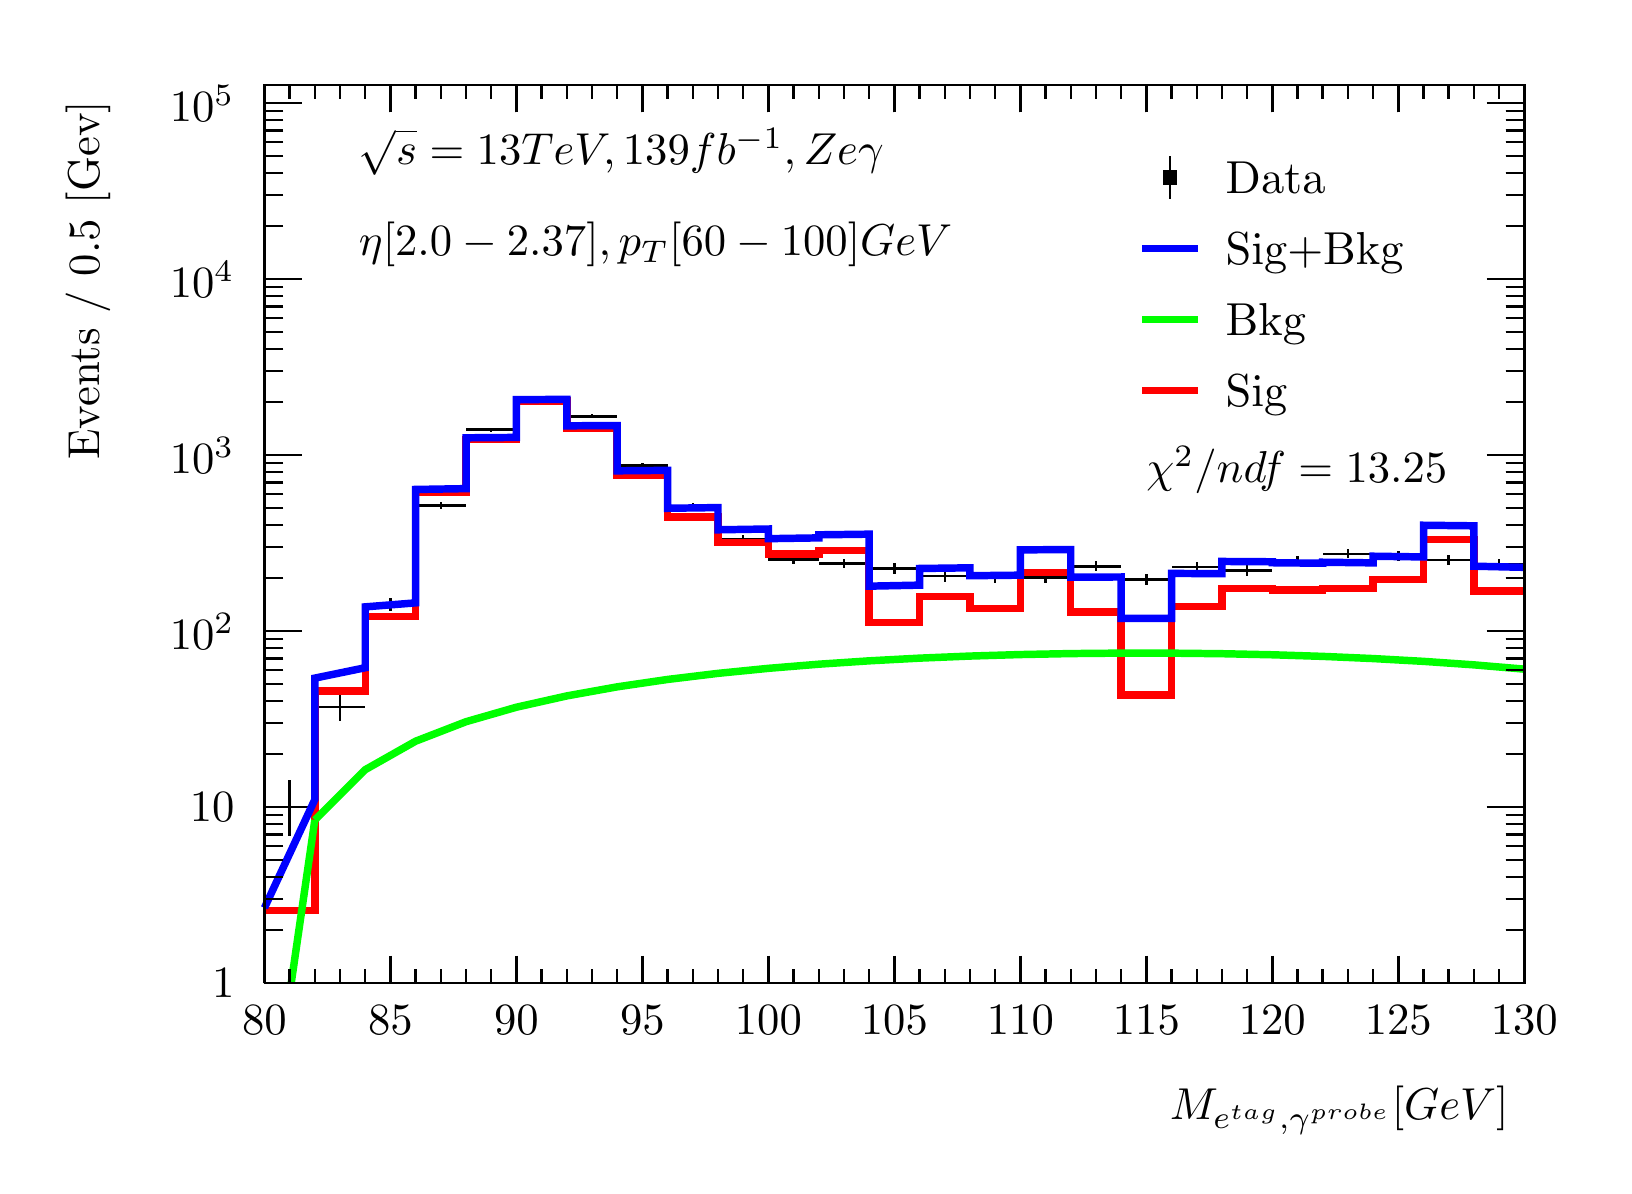
\begin{tikzpicture}
\pgfdeclareplotmark{cross} {
\pgfpathmoveto{\pgfpoint{-0.3\pgfplotmarksize}{\pgfplotmarksize}}
\pgfpathlineto{\pgfpoint{+0.3\pgfplotmarksize}{\pgfplotmarksize}}
\pgfpathlineto{\pgfpoint{+0.3\pgfplotmarksize}{0.3\pgfplotmarksize}}
\pgfpathlineto{\pgfpoint{+1\pgfplotmarksize}{0.3\pgfplotmarksize}}
\pgfpathlineto{\pgfpoint{+1\pgfplotmarksize}{-0.3\pgfplotmarksize}}
\pgfpathlineto{\pgfpoint{+0.3\pgfplotmarksize}{-0.3\pgfplotmarksize}}
\pgfpathlineto{\pgfpoint{+0.3\pgfplotmarksize}{-1.\pgfplotmarksize}}
\pgfpathlineto{\pgfpoint{-0.3\pgfplotmarksize}{-1.\pgfplotmarksize}}
\pgfpathlineto{\pgfpoint{-0.3\pgfplotmarksize}{-0.3\pgfplotmarksize}}
\pgfpathlineto{\pgfpoint{-1.\pgfplotmarksize}{-0.3\pgfplotmarksize}}
\pgfpathlineto{\pgfpoint{-1.\pgfplotmarksize}{0.3\pgfplotmarksize}}
\pgfpathlineto{\pgfpoint{-0.3\pgfplotmarksize}{0.3\pgfplotmarksize}}
\pgfpathclose
\pgfusepathqstroke
}
\pgfdeclareplotmark{cross*} {
\pgfpathmoveto{\pgfpoint{-0.3\pgfplotmarksize}{\pgfplotmarksize}}
\pgfpathlineto{\pgfpoint{+0.3\pgfplotmarksize}{\pgfplotmarksize}}
\pgfpathlineto{\pgfpoint{+0.3\pgfplotmarksize}{0.3\pgfplotmarksize}}
\pgfpathlineto{\pgfpoint{+1\pgfplotmarksize}{0.3\pgfplotmarksize}}
\pgfpathlineto{\pgfpoint{+1\pgfplotmarksize}{-0.3\pgfplotmarksize}}
\pgfpathlineto{\pgfpoint{+0.3\pgfplotmarksize}{-0.3\pgfplotmarksize}}
\pgfpathlineto{\pgfpoint{+0.3\pgfplotmarksize}{-1.\pgfplotmarksize}}
\pgfpathlineto{\pgfpoint{-0.3\pgfplotmarksize}{-1.\pgfplotmarksize}}
\pgfpathlineto{\pgfpoint{-0.3\pgfplotmarksize}{-0.3\pgfplotmarksize}}
\pgfpathlineto{\pgfpoint{-1.\pgfplotmarksize}{-0.3\pgfplotmarksize}}
\pgfpathlineto{\pgfpoint{-1.\pgfplotmarksize}{0.3\pgfplotmarksize}}
\pgfpathlineto{\pgfpoint{-0.3\pgfplotmarksize}{0.3\pgfplotmarksize}}
\pgfpathclose
\pgfusepathqfillstroke
}
\pgfdeclareplotmark{newstar} {
\pgfpathmoveto{\pgfqpoint{0pt}{\pgfplotmarksize}}
\pgfpathlineto{\pgfqpointpolar{44}{0.5\pgfplotmarksize}}
\pgfpathlineto{\pgfqpointpolar{18}{\pgfplotmarksize}}
\pgfpathlineto{\pgfqpointpolar{-20}{0.5\pgfplotmarksize}}
\pgfpathlineto{\pgfqpointpolar{-54}{\pgfplotmarksize}}
\pgfpathlineto{\pgfqpointpolar{-90}{0.5\pgfplotmarksize}}
\pgfpathlineto{\pgfqpointpolar{234}{\pgfplotmarksize}}
\pgfpathlineto{\pgfqpointpolar{198}{0.5\pgfplotmarksize}}
\pgfpathlineto{\pgfqpointpolar{162}{\pgfplotmarksize}}
\pgfpathlineto{\pgfqpointpolar{134}{0.5\pgfplotmarksize}}
\pgfpathclose
\pgfusepathqstroke
}
\pgfdeclareplotmark{newstar*} {
\pgfpathmoveto{\pgfqpoint{0pt}{\pgfplotmarksize}}
\pgfpathlineto{\pgfqpointpolar{44}{0.5\pgfplotmarksize}}
\pgfpathlineto{\pgfqpointpolar{18}{\pgfplotmarksize}}
\pgfpathlineto{\pgfqpointpolar{-20}{0.5\pgfplotmarksize}}
\pgfpathlineto{\pgfqpointpolar{-54}{\pgfplotmarksize}}
\pgfpathlineto{\pgfqpointpolar{-90}{0.5\pgfplotmarksize}}
\pgfpathlineto{\pgfqpointpolar{234}{\pgfplotmarksize}}
\pgfpathlineto{\pgfqpointpolar{198}{0.5\pgfplotmarksize}}
\pgfpathlineto{\pgfqpointpolar{162}{\pgfplotmarksize}}
\pgfpathlineto{\pgfqpointpolar{134}{0.5\pgfplotmarksize}}
\pgfpathclose
\pgfusepathqfillstroke
}
\definecolor{c}{rgb}{1,1,1};
\draw [color=c, fill=c] (0,0) rectangle (20,14.4361);
\draw [color=c, fill=c] (3,2.30977) rectangle (19,13.7143);
\definecolor{c}{rgb}{0,0,0};
\draw [c,line width=0.9] (3,2.30977) -- (3,13.7143) -- (19,13.7143) -- (19,2.30977) -- (3,2.30977);
\definecolor{c}{rgb}{1,1,1};
\draw [color=c, fill=c] (3,2.30977) rectangle (19,13.7143);
\definecolor{c}{rgb}{0,0,0};
\draw [c,line width=0.9] (3,2.30977) -- (3,13.7143) -- (19,13.7143) -- (19,2.30977) -- (3,2.30977);
\draw [c,line width=0.9] (3,2.30977) -- (19,2.30977);
\draw [c,line width=0.9] (3,2.65624) -- (3,2.30977);
\draw [c,line width=0.9] (3.32,2.48301) -- (3.32,2.30977);
\draw [c,line width=0.9] (3.64,2.48301) -- (3.64,2.30977);
\draw [c,line width=0.9] (3.96,2.48301) -- (3.96,2.30977);
\draw [c,line width=0.9] (4.28,2.48301) -- (4.28,2.30977);
\draw [c,line width=0.9] (4.6,2.65624) -- (4.6,2.30977);
\draw [c,line width=0.9] (4.92,2.48301) -- (4.92,2.30977);
\draw [c,line width=0.9] (5.24,2.48301) -- (5.24,2.30977);
\draw [c,line width=0.9] (5.56,2.48301) -- (5.56,2.30977);
\draw [c,line width=0.9] (5.88,2.48301) -- (5.88,2.30977);
\draw [c,line width=0.9] (6.2,2.65624) -- (6.2,2.30977);
\draw [c,line width=0.9] (6.52,2.48301) -- (6.52,2.30977);
\draw [c,line width=0.9] (6.84,2.48301) -- (6.84,2.30977);
\draw [c,line width=0.9] (7.16,2.48301) -- (7.16,2.30977);
\draw [c,line width=0.9] (7.48,2.48301) -- (7.48,2.30977);
\draw [c,line width=0.9] (7.8,2.65624) -- (7.8,2.30977);
\draw [c,line width=0.9] (8.12,2.48301) -- (8.12,2.30977);
\draw [c,line width=0.9] (8.44,2.48301) -- (8.44,2.30977);
\draw [c,line width=0.9] (8.76,2.48301) -- (8.76,2.30977);
\draw [c,line width=0.9] (9.08,2.48301) -- (9.08,2.30977);
\draw [c,line width=0.9] (9.4,2.65624) -- (9.4,2.30977);
\draw [c,line width=0.9] (9.72,2.48301) -- (9.72,2.30977);
\draw [c,line width=0.9] (10.04,2.48301) -- (10.04,2.30977);
\draw [c,line width=0.9] (10.36,2.48301) -- (10.36,2.30977);
\draw [c,line width=0.9] (10.68,2.48301) -- (10.68,2.30977);
\draw [c,line width=0.9] (11,2.65624) -- (11,2.30977);
\draw [c,line width=0.9] (11.32,2.48301) -- (11.32,2.30977);
\draw [c,line width=0.9] (11.64,2.48301) -- (11.64,2.30977);
\draw [c,line width=0.9] (11.96,2.48301) -- (11.96,2.30977);
\draw [c,line width=0.9] (12.28,2.48301) -- (12.28,2.30977);
\draw [c,line width=0.9] (12.6,2.65624) -- (12.6,2.30977);
\draw [c,line width=0.9] (12.92,2.48301) -- (12.92,2.30977);
\draw [c,line width=0.9] (13.24,2.48301) -- (13.24,2.30977);
\draw [c,line width=0.9] (13.56,2.48301) -- (13.56,2.30977);
\draw [c,line width=0.9] (13.88,2.48301) -- (13.88,2.30977);
\draw [c,line width=0.9] (14.2,2.65624) -- (14.2,2.30977);
\draw [c,line width=0.9] (14.52,2.48301) -- (14.52,2.30977);
\draw [c,line width=0.9] (14.84,2.48301) -- (14.84,2.30977);
\draw [c,line width=0.9] (15.16,2.48301) -- (15.16,2.30977);
\draw [c,line width=0.9] (15.48,2.48301) -- (15.48,2.30977);
\draw [c,line width=0.9] (15.8,2.65624) -- (15.8,2.30977);
\draw [c,line width=0.9] (16.12,2.48301) -- (16.12,2.30977);
\draw [c,line width=0.9] (16.44,2.48301) -- (16.44,2.30977);
\draw [c,line width=0.9] (16.76,2.48301) -- (16.76,2.30977);
\draw [c,line width=0.9] (17.08,2.48301) -- (17.08,2.30977);
\draw [c,line width=0.9] (17.4,2.65624) -- (17.4,2.30977);
\draw [c,line width=0.9] (17.72,2.48301) -- (17.72,2.30977);
\draw [c,line width=0.9] (18.04,2.48301) -- (18.04,2.30977);
\draw [c,line width=0.9] (18.36,2.48301) -- (18.36,2.30977);
\draw [c,line width=0.9] (18.68,2.48301) -- (18.68,2.30977);
\draw [c,line width=0.9] (19,2.65624) -- (19,2.30977);
\draw [anchor=base] (3,1.66015) node[scale=1.61424, color=c, rotate=0]{80};
\draw [anchor=base] (4.6,1.66015) node[scale=1.61424, color=c, rotate=0]{85};
\draw [anchor=base] (6.2,1.66015) node[scale=1.61424, color=c, rotate=0]{90};
\draw [anchor=base] (7.8,1.66015) node[scale=1.61424, color=c, rotate=0]{95};
\draw [anchor=base] (9.4,1.66015) node[scale=1.61424, color=c, rotate=0]{100};
\draw [anchor=base] (11,1.66015) node[scale=1.61424, color=c, rotate=0]{105};
\draw [anchor=base] (12.6,1.66015) node[scale=1.61424, color=c, rotate=0]{110};
\draw [anchor=base] (14.2,1.66015) node[scale=1.61424, color=c, rotate=0]{115};
\draw [anchor=base] (15.8,1.66015) node[scale=1.61424, color=c, rotate=0]{120};
\draw [anchor=base] (17.4,1.66015) node[scale=1.61424, color=c, rotate=0]{125};
\draw [anchor=base] (19,1.66015) node[scale=1.61424, color=c, rotate=0]{130};
\draw [anchor= east] (19,0.692932) node[scale=1.61424, color=c, rotate=0]{$M_{e^{tag}, \gamma^{probe}}  [GeV]$};
\draw [c,line width=0.9] (3,13.7143) -- (19,13.7143);
\draw [c,line width=0.9] (3,13.3678) -- (3,13.7143);
\draw [c,line width=0.9] (3.32,13.5411) -- (3.32,13.7143);
\draw [c,line width=0.9] (3.64,13.5411) -- (3.64,13.7143);
\draw [c,line width=0.9] (3.96,13.5411) -- (3.96,13.7143);
\draw [c,line width=0.9] (4.28,13.5411) -- (4.28,13.7143);
\draw [c,line width=0.9] (4.6,13.3678) -- (4.6,13.7143);
\draw [c,line width=0.9] (4.92,13.5411) -- (4.92,13.7143);
\draw [c,line width=0.9] (5.24,13.5411) -- (5.24,13.7143);
\draw [c,line width=0.9] (5.56,13.5411) -- (5.56,13.7143);
\draw [c,line width=0.9] (5.88,13.5411) -- (5.88,13.7143);
\draw [c,line width=0.9] (6.2,13.3678) -- (6.2,13.7143);
\draw [c,line width=0.9] (6.52,13.5411) -- (6.52,13.7143);
\draw [c,line width=0.9] (6.84,13.5411) -- (6.84,13.7143);
\draw [c,line width=0.9] (7.16,13.5411) -- (7.16,13.7143);
\draw [c,line width=0.9] (7.48,13.5411) -- (7.48,13.7143);
\draw [c,line width=0.9] (7.8,13.3678) -- (7.8,13.7143);
\draw [c,line width=0.9] (8.12,13.5411) -- (8.12,13.7143);
\draw [c,line width=0.9] (8.44,13.5411) -- (8.44,13.7143);
\draw [c,line width=0.9] (8.76,13.5411) -- (8.76,13.7143);
\draw [c,line width=0.9] (9.08,13.5411) -- (9.08,13.7143);
\draw [c,line width=0.9] (9.4,13.3678) -- (9.4,13.7143);
\draw [c,line width=0.9] (9.72,13.5411) -- (9.72,13.7143);
\draw [c,line width=0.9] (10.04,13.5411) -- (10.04,13.7143);
\draw [c,line width=0.9] (10.36,13.5411) -- (10.36,13.7143);
\draw [c,line width=0.9] (10.68,13.5411) -- (10.68,13.7143);
\draw [c,line width=0.9] (11,13.3678) -- (11,13.7143);
\draw [c,line width=0.9] (11.32,13.5411) -- (11.32,13.7143);
\draw [c,line width=0.9] (11.64,13.5411) -- (11.64,13.7143);
\draw [c,line width=0.9] (11.96,13.5411) -- (11.96,13.7143);
\draw [c,line width=0.9] (12.28,13.5411) -- (12.28,13.7143);
\draw [c,line width=0.9] (12.6,13.3678) -- (12.6,13.7143);
\draw [c,line width=0.9] (12.92,13.5411) -- (12.92,13.7143);
\draw [c,line width=0.9] (13.24,13.5411) -- (13.24,13.7143);
\draw [c,line width=0.9] (13.56,13.5411) -- (13.56,13.7143);
\draw [c,line width=0.9] (13.88,13.5411) -- (13.88,13.7143);
\draw [c,line width=0.9] (14.2,13.3678) -- (14.2,13.7143);
\draw [c,line width=0.9] (14.52,13.5411) -- (14.52,13.7143);
\draw [c,line width=0.9] (14.84,13.5411) -- (14.84,13.7143);
\draw [c,line width=0.9] (15.16,13.5411) -- (15.16,13.7143);
\draw [c,line width=0.9] (15.48,13.5411) -- (15.48,13.7143);
\draw [c,line width=0.9] (15.8,13.3678) -- (15.8,13.7143);
\draw [c,line width=0.9] (16.12,13.5411) -- (16.12,13.7143);
\draw [c,line width=0.9] (16.44,13.5411) -- (16.44,13.7143);
\draw [c,line width=0.9] (16.76,13.5411) -- (16.76,13.7143);
\draw [c,line width=0.9] (17.08,13.5411) -- (17.08,13.7143);
\draw [c,line width=0.9] (17.4,13.3678) -- (17.4,13.7143);
\draw [c,line width=0.9] (17.72,13.5411) -- (17.72,13.7143);
\draw [c,line width=0.9] (18.04,13.5411) -- (18.04,13.7143);
\draw [c,line width=0.9] (18.36,13.5411) -- (18.36,13.7143);
\draw [c,line width=0.9] (18.68,13.5411) -- (18.68,13.7143);
\draw [c,line width=0.9] (19,13.3678) -- (19,13.7143);
\draw [c,line width=0.9] (3,2.30977) -- (3,13.7143);
\draw [c,line width=0.9] (3.474,2.30978) -- (3,2.30978);
\draw [anchor= east] (2.82,2.30978) node[scale=1.61424, color=c, rotate=0]{1};
\draw [c,line width=0.9] (3.237,2.98257) -- (3,2.98257);
\draw [c,line width=0.9] (3.237,3.37612) -- (3,3.37612);
\draw [c,line width=0.9] (3.237,3.65536) -- (3,3.65536);
\draw [c,line width=0.9] (3.237,3.87195) -- (3,3.87195);
\draw [c,line width=0.9] (3.237,4.04891) -- (3,4.04891);
\draw [c,line width=0.9] (3.237,4.19854) -- (3,4.19854);
\draw [c,line width=0.9] (3.237,4.32815) -- (3,4.32815);
\draw [c,line width=0.9] (3.237,4.44247) -- (3,4.44247);
\draw [c,line width=0.9] (3.474,4.54474) -- (3,4.54474);
\draw [anchor= east] (2.82,4.54474) node[scale=1.61424, color=c, rotate=0]{10};
\draw [c,line width=0.9] (3.237,5.21753) -- (3,5.21753);
\draw [c,line width=0.9] (3.237,5.61109) -- (3,5.61109);
\draw [c,line width=0.9] (3.237,5.89032) -- (3,5.89032);
\draw [c,line width=0.9] (3.237,6.10691) -- (3,6.10691);
\draw [c,line width=0.9] (3.237,6.28388) -- (3,6.28388);
\draw [c,line width=0.9] (3.237,6.4335) -- (3,6.4335);
\draw [c,line width=0.9] (3.237,6.56311) -- (3,6.56311);
\draw [c,line width=0.9] (3.237,6.67743) -- (3,6.67743);
\draw [c,line width=0.9] (3.474,6.7797) -- (3,6.7797);
\draw [anchor= east] (2.82,6.7797) node[scale=1.61424, color=c, rotate=0]{$10^{2}$};
\draw [c,line width=0.9] (3.237,7.45249) -- (3,7.45249);
\draw [c,line width=0.9] (3.237,7.84605) -- (3,7.84605);
\draw [c,line width=0.9] (3.237,8.12528) -- (3,8.12528);
\draw [c,line width=0.9] (3.237,8.34187) -- (3,8.34187);
\draw [c,line width=0.9] (3.237,8.51884) -- (3,8.51884);
\draw [c,line width=0.9] (3.237,8.66846) -- (3,8.66846);
\draw [c,line width=0.9] (3.237,8.79807) -- (3,8.79807);
\draw [c,line width=0.9] (3.237,8.91239) -- (3,8.91239);
\draw [c,line width=0.9] (3.474,9.01466) -- (3,9.01466);
\draw [anchor= east] (2.82,9.01466) node[scale=1.61424, color=c, rotate=0]{$10^{3}$};
\draw [c,line width=0.9] (3.237,9.68745) -- (3,9.68745);
\draw [c,line width=0.9] (3.237,10.081) -- (3,10.081);
\draw [c,line width=0.9] (3.237,10.3602) -- (3,10.3602);
\draw [c,line width=0.9] (3.237,10.5768) -- (3,10.5768);
\draw [c,line width=0.9] (3.237,10.7538) -- (3,10.7538);
\draw [c,line width=0.9] (3.237,10.9034) -- (3,10.9034);
\draw [c,line width=0.9] (3.237,11.033) -- (3,11.033);
\draw [c,line width=0.9] (3.237,11.1474) -- (3,11.1474);
\draw [c,line width=0.9] (3.474,11.2496) -- (3,11.2496);
\draw [anchor= east] (2.82,11.2496) node[scale=1.61424, color=c, rotate=0]{$10^{4}$};
\draw [c,line width=0.9] (3.237,11.9224) -- (3,11.9224);
\draw [c,line width=0.9] (3.237,12.316) -- (3,12.316);
\draw [c,line width=0.9] (3.237,12.5952) -- (3,12.5952);
\draw [c,line width=0.9] (3.237,12.8118) -- (3,12.8118);
\draw [c,line width=0.9] (3.237,12.9888) -- (3,12.9888);
\draw [c,line width=0.9] (3.237,13.1384) -- (3,13.1384);
\draw [c,line width=0.9] (3.237,13.268) -- (3,13.268);
\draw [c,line width=0.9] (3.237,13.3823) -- (3,13.3823);
\draw [c,line width=0.9] (3.474,13.4846) -- (3,13.4846);
\draw [anchor= east] (2.82,13.4846) node[scale=1.61424, color=c, rotate=0]{$10^{5}$};
\draw [anchor= east] (0.76,13.7143) node[scale=1.61424, color=c, rotate=90]{Events / 0.5 [Gev]};
\draw [c,line width=0.9] (19,2.30977) -- (19,13.7143);
\draw [c,line width=0.9] (18.526,2.30978) -- (19,2.30978);
\draw [c,line width=0.9] (18.763,2.98257) -- (19,2.98257);
\draw [c,line width=0.9] (18.763,3.37612) -- (19,3.37612);
\draw [c,line width=0.9] (18.763,3.65536) -- (19,3.65536);
\draw [c,line width=0.9] (18.763,3.87195) -- (19,3.87195);
\draw [c,line width=0.9] (18.763,4.04891) -- (19,4.04891);
\draw [c,line width=0.9] (18.763,4.19854) -- (19,4.19854);
\draw [c,line width=0.9] (18.763,4.32815) -- (19,4.32815);
\draw [c,line width=0.9] (18.763,4.44247) -- (19,4.44247);
\draw [c,line width=0.9] (18.526,4.54474) -- (19,4.54474);
\draw [c,line width=0.9] (18.763,5.21753) -- (19,5.21753);
\draw [c,line width=0.9] (18.763,5.61109) -- (19,5.61109);
\draw [c,line width=0.9] (18.763,5.89032) -- (19,5.89032);
\draw [c,line width=0.9] (18.763,6.10691) -- (19,6.10691);
\draw [c,line width=0.9] (18.763,6.28388) -- (19,6.28388);
\draw [c,line width=0.9] (18.763,6.4335) -- (19,6.4335);
\draw [c,line width=0.9] (18.763,6.56311) -- (19,6.56311);
\draw [c,line width=0.9] (18.763,6.67743) -- (19,6.67743);
\draw [c,line width=0.9] (18.526,6.7797) -- (19,6.7797);
\draw [c,line width=0.9] (18.763,7.45249) -- (19,7.45249);
\draw [c,line width=0.9] (18.763,7.84605) -- (19,7.84605);
\draw [c,line width=0.9] (18.763,8.12528) -- (19,8.12528);
\draw [c,line width=0.9] (18.763,8.34187) -- (19,8.34187);
\draw [c,line width=0.9] (18.763,8.51884) -- (19,8.51884);
\draw [c,line width=0.9] (18.763,8.66846) -- (19,8.66846);
\draw [c,line width=0.9] (18.763,8.79807) -- (19,8.79807);
\draw [c,line width=0.9] (18.763,8.91239) -- (19,8.91239);
\draw [c,line width=0.9] (18.526,9.01466) -- (19,9.01466);
\draw [c,line width=0.9] (18.763,9.68745) -- (19,9.68745);
\draw [c,line width=0.9] (18.763,10.081) -- (19,10.081);
\draw [c,line width=0.9] (18.763,10.3602) -- (19,10.3602);
\draw [c,line width=0.9] (18.763,10.5768) -- (19,10.5768);
\draw [c,line width=0.9] (18.763,10.7538) -- (19,10.7538);
\draw [c,line width=0.9] (18.763,10.9034) -- (19,10.9034);
\draw [c,line width=0.9] (18.763,11.033) -- (19,11.033);
\draw [c,line width=0.9] (18.763,11.1474) -- (19,11.1474);
\draw [c,line width=0.9] (18.526,11.2496) -- (19,11.2496);
\draw [c,line width=0.9] (18.763,11.9224) -- (19,11.9224);
\draw [c,line width=0.9] (18.763,12.316) -- (19,12.316);
\draw [c,line width=0.9] (18.763,12.5952) -- (19,12.5952);
\draw [c,line width=0.9] (18.763,12.8118) -- (19,12.8118);
\draw [c,line width=0.9] (18.763,12.9888) -- (19,12.9888);
\draw [c,line width=0.9] (18.763,13.1384) -- (19,13.1384);
\draw [c,line width=0.9] (18.763,13.268) -- (19,13.268);
\draw [c,line width=0.9] (18.763,13.3823) -- (19,13.3823);
\draw [c,line width=0.9] (18.526,13.4846) -- (19,13.4846);
\draw [c,line width=0.9] (3.32,4.54474) -- (3,4.54474);
\draw [c,line width=0.9] (3,4.54474) -- (3,4.54474);
\draw [c,line width=0.9] (3.32,4.54474) -- (3.64,4.54474);
\draw [c,line width=0.9] (3.64,4.54474) -- (3.64,4.54474);
\draw [c,line width=0.9] (3.32,4.54474) -- (3.32,4.88966);
\draw [c,line width=0.9] (3.32,4.88966) -- (3.32,4.88966);
\draw [c,line width=0.9] (3.32,4.54474) -- (3.32,4.18335);
\draw [c,line width=0.9] (3.32,4.18335) -- (3.32,4.18335);
\draw [c,line width=0.9] (3.96,5.81465) -- (3.64,5.81465);
\draw [c,line width=0.9] (3.64,5.81465) -- (3.64,5.81465);
\draw [c,line width=0.9] (3.96,5.81465) -- (4.28,5.81465);
\draw [c,line width=0.9] (4.28,5.81465) -- (4.28,5.81465);
\draw [c,line width=0.9] (3.96,5.81465) -- (3.96,5.98586);
\draw [c,line width=0.9] (3.96,5.98586) -- (3.96,5.98586);
\draw [c,line width=0.9] (3.96,5.81465) -- (3.96,5.64118);
\draw [c,line width=0.9] (3.96,5.64118) -- (3.96,5.64118);
\draw [c,line width=0.9] (4.6,7.1132) -- (4.28,7.1132);
\draw [c,line width=0.9] (4.28,7.1132) -- (4.28,7.1132);
\draw [c,line width=0.9] (4.6,7.1132) -- (4.92,7.1132);
\draw [c,line width=0.9] (4.92,7.1132) -- (4.92,7.1132);
\draw [c,line width=0.9] (4.6,7.1132) -- (4.6,7.19492);
\draw [c,line width=0.9] (4.6,7.19492) -- (4.6,7.19492);
\draw [c,line width=0.9] (4.6,7.1132) -- (4.6,7.03148);
\draw [c,line width=0.9] (4.6,7.03148) -- (4.6,7.03148);
\draw [c,line width=0.9] (5.24,8.37432) -- (4.92,8.37432);
\draw [c,line width=0.9] (4.92,8.37432) -- (4.92,8.37432);
\draw [c,line width=0.9] (5.24,8.37432) -- (5.56,8.37432);
\draw [c,line width=0.9] (5.56,8.37432) -- (5.56,8.37432);
\draw [c,line width=0.9] (5.24,8.37432) -- (5.24,8.41701);
\draw [c,line width=0.9] (5.24,8.41701) -- (5.24,8.41701);
\draw [c,line width=0.9] (5.24,8.37432) -- (5.24,8.33164);
\draw [c,line width=0.9] (5.24,8.33164) -- (5.24,8.33164);
\draw [c,line width=0.9] (5.88,9.33847) -- (5.56,9.33847);
\draw [c,line width=0.9] (5.56,9.33847) -- (5.56,9.33847);
\draw [c,line width=0.9] (5.88,9.33847) -- (6.2,9.33847);
\draw [c,line width=0.9] (6.2,9.33847) -- (6.2,9.33847);
\draw [c,line width=0.9] (5.88,9.33847) -- (5.88,9.36445);
\draw [c,line width=0.9] (5.88,9.36445) -- (5.88,9.36445);
\draw [c,line width=0.9] (5.88,9.33847) -- (5.88,9.3125);
\draw [c,line width=0.9] (5.88,9.3125) -- (5.88,9.3125);
\draw [c,line width=0.9] (6.52,9.74355) -- (6.2,9.74355);
\draw [c,line width=0.9] (6.2,9.74355) -- (6.2,9.74355);
\draw [c,line width=0.9] (6.52,9.74355) -- (6.84,9.74355);
\draw [c,line width=0.9] (6.84,9.74355) -- (6.84,9.74355);
\draw [c,line width=0.9] (6.52,9.74355) -- (6.52,9.76464);
\draw [c,line width=0.9] (6.52,9.76464) -- (6.52,9.76464);
\draw [c,line width=0.9] (6.52,9.74355) -- (6.52,9.72247);
\draw [c,line width=0.9] (6.52,9.72247) -- (6.52,9.72247);
\draw [c,line width=0.9] (7.16,9.50718) -- (6.84,9.50718);
\draw [c,line width=0.9] (6.84,9.50718) -- (6.84,9.50718);
\draw [c,line width=0.9] (7.16,9.50718) -- (7.48,9.50718);
\draw [c,line width=0.9] (7.48,9.50718) -- (7.48,9.50718);
\draw [c,line width=0.9] (7.16,9.50718) -- (7.16,9.53099);
\draw [c,line width=0.9] (7.16,9.53099) -- (7.16,9.53099);
\draw [c,line width=0.9] (7.16,9.50718) -- (7.16,9.48336);
\draw [c,line width=0.9] (7.16,9.48336) -- (7.16,9.48336);
\draw [c,line width=0.9] (7.8,8.88283) -- (7.48,8.88283);
\draw [c,line width=0.9] (7.48,8.88283) -- (7.48,8.88283);
\draw [c,line width=0.9] (7.8,8.88283) -- (8.12,8.88283);
\draw [c,line width=0.9] (8.12,8.88283) -- (8.12,8.88283);
\draw [c,line width=0.9] (7.8,8.88283) -- (7.8,8.91568);
\draw [c,line width=0.9] (7.8,8.91568) -- (7.8,8.91568);
\draw [c,line width=0.9] (7.8,8.88283) -- (7.8,8.84998);
\draw [c,line width=0.9] (7.8,8.84998) -- (7.8,8.84998);
\draw [c,line width=0.9] (8.44,8.36867) -- (8.12,8.36867);
\draw [c,line width=0.9] (8.12,8.36867) -- (8.12,8.36867);
\draw [c,line width=0.9] (8.44,8.36867) -- (8.76,8.36867);
\draw [c,line width=0.9] (8.76,8.36867) -- (8.76,8.36867);
\draw [c,line width=0.9] (8.44,8.36867) -- (8.44,8.41148);
\draw [c,line width=0.9] (8.44,8.41148) -- (8.44,8.41148);
\draw [c,line width=0.9] (8.44,8.36867) -- (8.44,8.32586);
\draw [c,line width=0.9] (8.44,8.32586) -- (8.44,8.32586);
\draw [c,line width=0.9] (9.08,7.94442) -- (8.76,7.94442);
\draw [c,line width=0.9] (8.76,7.94442) -- (8.76,7.94442);
\draw [c,line width=0.9] (9.08,7.94442) -- (9.4,7.94442);
\draw [c,line width=0.9] (9.4,7.94442) -- (9.4,7.94442);
\draw [c,line width=0.9] (9.08,7.94442) -- (9.08,7.99769);
\draw [c,line width=0.9] (9.08,7.99769) -- (9.08,7.99769);
\draw [c,line width=0.9] (9.08,7.94442) -- (9.08,7.89116);
\draw [c,line width=0.9] (9.08,7.89116) -- (9.08,7.89116);
\draw [c,line width=0.9] (9.72,7.6883) -- (9.4,7.6883);
\draw [c,line width=0.9] (9.4,7.6883) -- (9.4,7.6883);
\draw [c,line width=0.9] (9.72,7.6883) -- (10.04,7.6883);
\draw [c,line width=0.9] (10.04,7.6883) -- (10.04,7.6883);
\draw [c,line width=0.9] (9.72,7.6883) -- (9.72,7.74907);
\draw [c,line width=0.9] (9.72,7.74907) -- (9.72,7.74907);
\draw [c,line width=0.9] (9.72,7.6883) -- (9.72,7.62753);
\draw [c,line width=0.9] (9.72,7.62753) -- (9.72,7.62753);
\draw [c,line width=0.9] (10.36,7.63751) -- (10.04,7.63751);
\draw [c,line width=0.9] (10.04,7.63751) -- (10.04,7.63751);
\draw [c,line width=0.9] (10.36,7.63751) -- (10.68,7.63751);
\draw [c,line width=0.9] (10.68,7.63751) -- (10.68,7.63751);
\draw [c,line width=0.9] (10.36,7.63751) -- (10.36,7.69989);
\draw [c,line width=0.9] (10.36,7.69989) -- (10.36,7.69989);
\draw [c,line width=0.9] (10.36,7.63751) -- (10.36,7.57513);
\draw [c,line width=0.9] (10.36,7.57513) -- (10.36,7.57513);
\draw [c,line width=0.9] (11,7.5754) -- (10.68,7.5754);
\draw [c,line width=0.9] (10.68,7.5754) -- (10.68,7.5754);
\draw [c,line width=0.9] (11,7.5754) -- (11.32,7.5754);
\draw [c,line width=0.9] (11.32,7.5754) -- (11.32,7.5754);
\draw [c,line width=0.9] (11,7.5754) -- (11,7.63981);
\draw [c,line width=0.9] (11,7.63981) -- (11,7.63981);
\draw [c,line width=0.9] (11,7.5754) -- (11,7.51099);
\draw [c,line width=0.9] (11,7.51099) -- (11,7.51099);
\draw [c,line width=0.9] (11.64,7.47646) -- (11.32,7.47646);
\draw [c,line width=0.9] (11.32,7.47646) -- (11.32,7.47646);
\draw [c,line width=0.9] (11.64,7.47646) -- (11.96,7.47646);
\draw [c,line width=0.9] (11.96,7.47646) -- (11.96,7.47646);
\draw [c,line width=0.9] (11.64,7.47646) -- (11.64,7.54423);
\draw [c,line width=0.9] (11.64,7.54423) -- (11.64,7.54423);
\draw [c,line width=0.9] (11.64,7.47646) -- (11.64,7.40868);
\draw [c,line width=0.9] (11.64,7.40868) -- (11.64,7.40868);
\draw [c,line width=0.9] (12.28,7.46215) -- (11.96,7.46215);
\draw [c,line width=0.9] (11.96,7.46215) -- (11.96,7.46215);
\draw [c,line width=0.9] (12.28,7.46215) -- (12.6,7.46215);
\draw [c,line width=0.9] (12.6,7.46215) -- (12.6,7.46215);
\draw [c,line width=0.9] (12.28,7.46215) -- (12.28,7.53043);
\draw [c,line width=0.9] (12.28,7.53043) -- (12.28,7.53043);
\draw [c,line width=0.9] (12.28,7.46215) -- (12.28,7.39387);
\draw [c,line width=0.9] (12.28,7.39387) -- (12.28,7.39387);
\draw [c,line width=0.9] (12.92,7.46215) -- (12.6,7.46215);
\draw [c,line width=0.9] (12.6,7.46215) -- (12.6,7.46215);
\draw [c,line width=0.9] (12.92,7.46215) -- (13.24,7.46215);
\draw [c,line width=0.9] (13.24,7.46215) -- (13.24,7.46215);
\draw [c,line width=0.9] (12.92,7.46215) -- (12.92,7.53043);
\draw [c,line width=0.9] (12.92,7.53043) -- (12.92,7.53043);
\draw [c,line width=0.9] (12.92,7.46215) -- (12.92,7.39387);
\draw [c,line width=0.9] (12.92,7.39387) -- (12.92,7.39387);
\draw [c,line width=0.9] (13.56,7.60072) -- (13.24,7.60072);
\draw [c,line width=0.9] (13.24,7.60072) -- (13.24,7.60072);
\draw [c,line width=0.9] (13.56,7.60072) -- (13.88,7.60072);
\draw [c,line width=0.9] (13.88,7.60072) -- (13.88,7.60072);
\draw [c,line width=0.9] (13.56,7.60072) -- (13.56,7.6643);
\draw [c,line width=0.9] (13.56,7.6643) -- (13.56,7.6643);
\draw [c,line width=0.9] (13.56,7.60072) -- (13.56,7.53715);
\draw [c,line width=0.9] (13.56,7.53715) -- (13.56,7.53715);
\draw [c,line width=0.9] (14.2,7.43782) -- (13.88,7.43782);
\draw [c,line width=0.9] (13.88,7.43782) -- (13.88,7.43782);
\draw [c,line width=0.9] (14.2,7.43782) -- (14.52,7.43782);
\draw [c,line width=0.9] (14.52,7.43782) -- (14.52,7.43782);
\draw [c,line width=0.9] (14.2,7.43782) -- (14.2,7.50696);
\draw [c,line width=0.9] (14.2,7.50696) -- (14.2,7.50696);
\draw [c,line width=0.9] (14.2,7.43782) -- (14.2,7.36868);
\draw [c,line width=0.9] (14.2,7.36868) -- (14.2,7.36868);
\draw [c,line width=0.9] (14.84,7.59655) -- (14.52,7.59655);
\draw [c,line width=0.9] (14.52,7.59655) -- (14.52,7.59655);
\draw [c,line width=0.9] (14.84,7.59655) -- (15.16,7.59655);
\draw [c,line width=0.9] (15.16,7.59655) -- (15.16,7.59655);
\draw [c,line width=0.9] (14.84,7.59655) -- (14.84,7.66026);
\draw [c,line width=0.9] (14.84,7.66026) -- (14.84,7.66026);
\draw [c,line width=0.9] (14.84,7.59655) -- (14.84,7.53284);
\draw [c,line width=0.9] (14.84,7.53284) -- (14.84,7.53284);
\draw [c,line width=0.9] (15.48,7.5494) -- (15.16,7.5494);
\draw [c,line width=0.9] (15.16,7.5494) -- (15.16,7.5494);
\draw [c,line width=0.9] (15.48,7.5494) -- (15.8,7.5494);
\draw [c,line width=0.9] (15.8,7.5494) -- (15.8,7.5494);
\draw [c,line width=0.9] (15.48,7.5494) -- (15.48,7.61468);
\draw [c,line width=0.9] (15.48,7.61468) -- (15.48,7.61468);
\draw [c,line width=0.9] (15.48,7.5494) -- (15.48,7.48412);
\draw [c,line width=0.9] (15.48,7.48412) -- (15.48,7.48412);
\draw [c,line width=0.9] (16.12,7.66908) -- (15.8,7.66908);
\draw [c,line width=0.9] (15.8,7.66908) -- (15.8,7.66908);
\draw [c,line width=0.9] (16.12,7.66908) -- (16.44,7.66908);
\draw [c,line width=0.9] (16.44,7.66908) -- (16.44,7.66908);
\draw [c,line width=0.9] (16.12,7.66908) -- (16.12,7.73046);
\draw [c,line width=0.9] (16.12,7.73046) -- (16.12,7.73046);
\draw [c,line width=0.9] (16.12,7.66908) -- (16.12,7.6077);
\draw [c,line width=0.9] (16.12,7.6077) -- (16.12,7.6077);
\draw [c,line width=0.9] (16.76,7.76159) -- (16.44,7.76159);
\draw [c,line width=0.9] (16.44,7.76159) -- (16.44,7.76159);
\draw [c,line width=0.9] (16.76,7.76159) -- (17.08,7.76159);
\draw [c,line width=0.9] (17.08,7.76159) -- (17.08,7.76159);
\draw [c,line width=0.9] (16.76,7.76159) -- (16.76,7.82011);
\draw [c,line width=0.9] (16.76,7.82011) -- (16.76,7.82011);
\draw [c,line width=0.9] (16.76,7.76159) -- (16.76,7.70307);
\draw [c,line width=0.9] (16.76,7.70307) -- (16.76,7.70307);
\draw [c,line width=0.9] (17.4,7.73293) -- (17.08,7.73293);
\draw [c,line width=0.9] (17.08,7.73293) -- (17.08,7.73293);
\draw [c,line width=0.9] (17.4,7.73293) -- (17.72,7.73293);
\draw [c,line width=0.9] (17.72,7.73293) -- (17.72,7.73293);
\draw [c,line width=0.9] (17.4,7.73293) -- (17.4,7.79233);
\draw [c,line width=0.9] (17.4,7.79233) -- (17.4,7.79233);
\draw [c,line width=0.9] (17.4,7.73293) -- (17.4,7.67354);
\draw [c,line width=0.9] (17.4,7.67354) -- (17.4,7.67354);
\draw [c,line width=0.9] (18.04,7.68449) -- (17.72,7.68449);
\draw [c,line width=0.9] (17.72,7.68449) -- (17.72,7.68449);
\draw [c,line width=0.9] (18.04,7.68449) -- (18.36,7.68449);
\draw [c,line width=0.9] (18.36,7.68449) -- (18.36,7.68449);
\draw [c,line width=0.9] (18.04,7.68449) -- (18.04,7.74538);
\draw [c,line width=0.9] (18.04,7.74538) -- (18.04,7.74538);
\draw [c,line width=0.9] (18.04,7.68449) -- (18.04,7.62359);
\draw [c,line width=0.9] (18.04,7.62359) -- (18.04,7.62359);
\draw [c,line width=0.9] (18.68,7.63349) -- (18.36,7.63349);
\draw [c,line width=0.9] (18.36,7.63349) -- (18.36,7.63349);
\draw [c,line width=0.9] (18.68,7.63349) -- (19,7.63349);
\draw [c,line width=0.9] (19,7.63349) -- (19,7.63349);
\draw [c,line width=0.9] (18.68,7.63349) -- (18.68,7.696);
\draw [c,line width=0.9] (18.68,7.696) -- (18.68,7.696);
\draw [c,line width=0.9] (18.68,7.63349) -- (18.68,7.57098);
\draw [c,line width=0.9] (18.68,7.57098) -- (18.68,7.57098);
\foreach \P in {(3.32,4.54474), (3.96,5.81465), (4.6,7.1132), (5.24,8.37432), (5.88,9.33847), (6.52,9.74355), (7.16,9.50718), (7.8,8.88283), (8.44,8.36867), (9.08,7.94442), (9.72,7.6883), (10.36,7.63751), (11,7.5754), (11.64,7.47646),
 (12.28,7.46215), (12.92,7.46215), (13.56,7.60072), (14.2,7.43782), (14.84,7.59655), (15.48,7.5494), (16.12,7.66908), (16.76,7.76159), (17.4,7.73293), (18.04,7.68449), (18.68,7.63349)}{\draw[mark options={color=c,fill=c},mark size=2.882883pt,mark=]
 plot coordinates {\P};}
\definecolor{c}{rgb}{1,0,0};
\draw [c,line width=2.7] (3,3.23167) -- (3,3.23167);
\draw [c,line width=2.7] (3,3.23167) -- (3,3.23167) -- (3.64,3.23167) -- (3.64,6.01752) -- (4.28,6.01752) -- (4.28,6.96454) -- (4.92,6.96454) -- (4.92,8.54167) -- (5.56,8.54167) -- (5.56,9.21043) -- (6.2,9.21043) -- (6.2,9.7019) -- (6.84,9.7019) --
 (6.84,9.3578) -- (7.48,9.3578) -- (7.48,8.75585) -- (8.12,8.75585) -- (8.12,8.23024) -- (8.76,8.23024) -- (8.76,7.90516) -- (9.4,7.90516) -- (9.4,7.75698) -- (10.04,7.75698) -- (10.04,7.80509) -- (10.68,7.80509) -- (10.68,6.89187) -- (11.32,6.89187)
 -- (11.32,7.2156) -- (11.96,7.2156) -- (11.96,7.06581) -- (12.6,7.06581) -- (12.6,7.52685) -- (13.24,7.52685) -- (13.24,7.01934) -- (13.88,7.01934) -- (13.88,5.96523) -- (14.52,5.96523) -- (14.52,7.09014) -- (15.16,7.09014) -- (15.16,7.31902) --
 (15.8,7.31902) -- (15.8,7.30135) -- (16.44,7.30135) -- (16.44,7.3193) -- (17.08,7.3193) -- (17.08,7.43549) -- (17.72,7.43549) -- (17.72,7.94486) -- (18.36,7.94486) -- (18.36,7.29163) -- (19,7.29163) -- (19,7.29163) -- (19,7.29163) -- (19,7.29163);
\definecolor{c}{rgb}{0,1,0};
\draw [c,line width=2.7] (3.34009,2.30977) -- (3.64,4.38078);
\draw [c,line width=2.7] (3.64,4.38078) -- (3.64,4.38078) -- (4.28,5.01948) -- (4.28,5.01948) -- (4.92,5.38135) -- (4.92,5.38135) -- (5.56,5.62878) -- (5.56,5.62878) -- (6.2,5.81287) -- (6.2,5.81287) -- (6.84,5.95641) -- (6.84,5.95641) --
 (7.48,6.07154) -- (7.48,6.07154) -- (8.12,6.16546) -- (8.12,6.16546) -- (8.76,6.24279) -- (8.76,6.24279) -- (9.4,6.30663) -- (9.4,6.30663) -- (10.04,6.35916) -- (10.04,6.35916) -- (10.68,6.40195) -- (10.68,6.40195) -- (11.32,6.43611) --
 (11.32,6.43611) -- (11.96,6.46249) -- (11.96,6.46249) -- (12.6,6.48167) -- (12.6,6.48167) -- (13.24,6.49407) -- (13.24,6.49407) -- (13.88,6.49993) -- (13.88,6.49993) -- (14.52,6.49938) -- (14.52,6.49938) -- (15.16,6.4924) -- (15.16,6.4924) --
 (15.8,6.47885) -- (15.8,6.47885) -- (16.44,6.45846) -- (16.44,6.45846) -- (17.08,6.43078) -- (17.08,6.43078) -- (17.72,6.39519) -- (17.72,6.39519) -- (18.36,6.35081) -- (18.36,6.35081) -- (19,6.29644) -- (19,6.29644) -- (19,6.29644) -- (19,6.29644);
\definecolor{c}{rgb}{0,0,1};
\draw [c,line width=2.7] (3,3.26451) -- (3,3.26451);
\draw [c,line width=2.7] (3,3.26451) -- (3,3.26451) -- (3.64,4.63998) -- (3.64,6.18245) -- (4.28,6.31428) -- (4.28,7.08729) -- (4.92,7.13804) -- (4.92,8.57837) -- (5.56,8.58878) -- (5.56,9.23437) -- (6.2,9.23929) -- (6.2,9.7194) -- (6.84,9.72216) --
 (6.84,9.38655) -- (7.48,9.39011) -- (7.48,8.8151) -- (8.12,8.82092) -- (8.12,8.33952) -- (8.76,8.34805) -- (8.76,8.06613) -- (9.4,8.07616) -- (9.4,7.9535) -- (10.04,7.96334) -- (10.04,8.00242) -- (10.68,8.01043) -- (10.68,7.35029) -- (11.32,7.36329)
 -- (11.32,7.57488) -- (11.96,7.58312) -- (11.96,7.48308) -- (12.6,7.48982) -- (12.6,7.81142) -- (13.24,7.81458) -- (13.24,7.4646) -- (13.88,7.46676) -- (13.88,6.94174) -- (14.52,6.94138) -- (14.52,7.51182) -- (15.16,7.50937) -- (15.16,7.66396) --
 (15.8,7.65993) -- (15.8,7.64752) -- (16.44,7.64145) -- (16.44,7.65413) -- (17.08,7.64613) -- (17.08,7.7305) -- (17.72,7.7213) -- (17.72,8.12392) -- (18.36,8.11659) -- (18.36,7.6038) -- (19,7.58915) -- (19,7.58915) -- (19,7.58915) -- (19,7.58915);
\definecolor{c}{rgb}{0,0,0};
\draw [c,line width=0.9] (3,2.30977) -- (19,2.30977);
\draw [c,line width=0.9] (3,2.65624) -- (3,2.30977);
\draw [c,line width=0.9] (3.32,2.48301) -- (3.32,2.30977);
\draw [c,line width=0.9] (3.64,2.48301) -- (3.64,2.30977);
\draw [c,line width=0.9] (3.96,2.48301) -- (3.96,2.30977);
\draw [c,line width=0.9] (4.28,2.48301) -- (4.28,2.30977);
\draw [c,line width=0.9] (4.6,2.65624) -- (4.6,2.30977);
\draw [c,line width=0.9] (4.92,2.48301) -- (4.92,2.30977);
\draw [c,line width=0.9] (5.24,2.48301) -- (5.24,2.30977);
\draw [c,line width=0.9] (5.56,2.48301) -- (5.56,2.30977);
\draw [c,line width=0.9] (5.88,2.48301) -- (5.88,2.30977);
\draw [c,line width=0.9] (6.2,2.65624) -- (6.2,2.30977);
\draw [c,line width=0.9] (6.52,2.48301) -- (6.52,2.30977);
\draw [c,line width=0.9] (6.84,2.48301) -- (6.84,2.30977);
\draw [c,line width=0.9] (7.16,2.48301) -- (7.16,2.30977);
\draw [c,line width=0.9] (7.48,2.48301) -- (7.48,2.30977);
\draw [c,line width=0.9] (7.8,2.65624) -- (7.8,2.30977);
\draw [c,line width=0.9] (8.12,2.48301) -- (8.12,2.30977);
\draw [c,line width=0.9] (8.44,2.48301) -- (8.44,2.30977);
\draw [c,line width=0.9] (8.76,2.48301) -- (8.76,2.30977);
\draw [c,line width=0.9] (9.08,2.48301) -- (9.08,2.30977);
\draw [c,line width=0.9] (9.4,2.65624) -- (9.4,2.30977);
\draw [c,line width=0.9] (9.72,2.48301) -- (9.72,2.30977);
\draw [c,line width=0.9] (10.04,2.48301) -- (10.04,2.30977);
\draw [c,line width=0.9] (10.36,2.48301) -- (10.36,2.30977);
\draw [c,line width=0.9] (10.68,2.48301) -- (10.68,2.30977);
\draw [c,line width=0.9] (11,2.65624) -- (11,2.30977);
\draw [c,line width=0.9] (11.32,2.48301) -- (11.32,2.30977);
\draw [c,line width=0.9] (11.64,2.48301) -- (11.64,2.30977);
\draw [c,line width=0.9] (11.96,2.48301) -- (11.96,2.30977);
\draw [c,line width=0.9] (12.28,2.48301) -- (12.28,2.30977);
\draw [c,line width=0.9] (12.6,2.65624) -- (12.6,2.30977);
\draw [c,line width=0.9] (12.92,2.48301) -- (12.92,2.30977);
\draw [c,line width=0.9] (13.24,2.48301) -- (13.24,2.30977);
\draw [c,line width=0.9] (13.56,2.48301) -- (13.56,2.30977);
\draw [c,line width=0.9] (13.88,2.48301) -- (13.88,2.30977);
\draw [c,line width=0.9] (14.2,2.65624) -- (14.2,2.30977);
\draw [c,line width=0.9] (14.52,2.48301) -- (14.52,2.30977);
\draw [c,line width=0.9] (14.84,2.48301) -- (14.84,2.30977);
\draw [c,line width=0.9] (15.16,2.48301) -- (15.16,2.30977);
\draw [c,line width=0.9] (15.48,2.48301) -- (15.48,2.30977);
\draw [c,line width=0.9] (15.8,2.65624) -- (15.8,2.30977);
\draw [c,line width=0.9] (16.12,2.48301) -- (16.12,2.30977);
\draw [c,line width=0.9] (16.44,2.48301) -- (16.44,2.30977);
\draw [c,line width=0.9] (16.76,2.48301) -- (16.76,2.30977);
\draw [c,line width=0.9] (17.08,2.48301) -- (17.08,2.30977);
\draw [c,line width=0.9] (17.4,2.65624) -- (17.4,2.30977);
\draw [c,line width=0.9] (17.72,2.48301) -- (17.72,2.30977);
\draw [c,line width=0.9] (18.04,2.48301) -- (18.04,2.30977);
\draw [c,line width=0.9] (18.36,2.48301) -- (18.36,2.30977);
\draw [c,line width=0.9] (18.68,2.48301) -- (18.68,2.30977);
\draw [c,line width=0.9] (19,2.65624) -- (19,2.30977);
\draw [c,line width=0.9] (3,13.7143) -- (19,13.7143);
\draw [c,line width=0.9] (3,13.3678) -- (3,13.7143);
\draw [c,line width=0.9] (3.32,13.5411) -- (3.32,13.7143);
\draw [c,line width=0.9] (3.64,13.5411) -- (3.64,13.7143);
\draw [c,line width=0.9] (3.96,13.5411) -- (3.96,13.7143);
\draw [c,line width=0.9] (4.28,13.5411) -- (4.28,13.7143);
\draw [c,line width=0.9] (4.6,13.3678) -- (4.6,13.7143);
\draw [c,line width=0.9] (4.92,13.5411) -- (4.92,13.7143);
\draw [c,line width=0.9] (5.24,13.5411) -- (5.24,13.7143);
\draw [c,line width=0.9] (5.56,13.5411) -- (5.56,13.7143);
\draw [c,line width=0.9] (5.88,13.5411) -- (5.88,13.7143);
\draw [c,line width=0.9] (6.2,13.3678) -- (6.2,13.7143);
\draw [c,line width=0.9] (6.52,13.5411) -- (6.52,13.7143);
\draw [c,line width=0.9] (6.84,13.5411) -- (6.84,13.7143);
\draw [c,line width=0.9] (7.16,13.5411) -- (7.16,13.7143);
\draw [c,line width=0.9] (7.48,13.5411) -- (7.48,13.7143);
\draw [c,line width=0.9] (7.8,13.3678) -- (7.8,13.7143);
\draw [c,line width=0.9] (8.12,13.5411) -- (8.12,13.7143);
\draw [c,line width=0.9] (8.44,13.5411) -- (8.44,13.7143);
\draw [c,line width=0.9] (8.76,13.5411) -- (8.76,13.7143);
\draw [c,line width=0.9] (9.08,13.5411) -- (9.08,13.7143);
\draw [c,line width=0.9] (9.4,13.3678) -- (9.4,13.7143);
\draw [c,line width=0.9] (9.72,13.5411) -- (9.72,13.7143);
\draw [c,line width=0.9] (10.04,13.5411) -- (10.04,13.7143);
\draw [c,line width=0.9] (10.36,13.5411) -- (10.36,13.7143);
\draw [c,line width=0.9] (10.68,13.5411) -- (10.68,13.7143);
\draw [c,line width=0.9] (11,13.3678) -- (11,13.7143);
\draw [c,line width=0.9] (11.32,13.5411) -- (11.32,13.7143);
\draw [c,line width=0.9] (11.64,13.5411) -- (11.64,13.7143);
\draw [c,line width=0.9] (11.96,13.5411) -- (11.96,13.7143);
\draw [c,line width=0.9] (12.28,13.5411) -- (12.28,13.7143);
\draw [c,line width=0.9] (12.6,13.3678) -- (12.6,13.7143);
\draw [c,line width=0.9] (12.92,13.5411) -- (12.92,13.7143);
\draw [c,line width=0.9] (13.24,13.5411) -- (13.24,13.7143);
\draw [c,line width=0.9] (13.56,13.5411) -- (13.56,13.7143);
\draw [c,line width=0.9] (13.88,13.5411) -- (13.88,13.7143);
\draw [c,line width=0.9] (14.2,13.3678) -- (14.2,13.7143);
\draw [c,line width=0.9] (14.52,13.5411) -- (14.52,13.7143);
\draw [c,line width=0.9] (14.84,13.5411) -- (14.84,13.7143);
\draw [c,line width=0.9] (15.16,13.5411) -- (15.16,13.7143);
\draw [c,line width=0.9] (15.48,13.5411) -- (15.48,13.7143);
\draw [c,line width=0.9] (15.8,13.3678) -- (15.8,13.7143);
\draw [c,line width=0.9] (16.12,13.5411) -- (16.12,13.7143);
\draw [c,line width=0.9] (16.44,13.5411) -- (16.44,13.7143);
\draw [c,line width=0.9] (16.76,13.5411) -- (16.76,13.7143);
\draw [c,line width=0.9] (17.08,13.5411) -- (17.08,13.7143);
\draw [c,line width=0.9] (17.4,13.3678) -- (17.4,13.7143);
\draw [c,line width=0.9] (17.72,13.5411) -- (17.72,13.7143);
\draw [c,line width=0.9] (18.04,13.5411) -- (18.04,13.7143);
\draw [c,line width=0.9] (18.36,13.5411) -- (18.36,13.7143);
\draw [c,line width=0.9] (18.68,13.5411) -- (18.68,13.7143);
\draw [c,line width=0.9] (19,13.3678) -- (19,13.7143);
\draw [c,line width=0.9] (3,2.30977) -- (3,13.7143);
\draw [c,line width=0.9] (3.474,2.30978) -- (3,2.30978);
\draw [c,line width=0.9] (3.237,2.98257) -- (3,2.98257);
\draw [c,line width=0.9] (3.237,3.37612) -- (3,3.37612);
\draw [c,line width=0.9] (3.237,3.65536) -- (3,3.65536);
\draw [c,line width=0.9] (3.237,3.87195) -- (3,3.87195);
\draw [c,line width=0.9] (3.237,4.04891) -- (3,4.04891);
\draw [c,line width=0.9] (3.237,4.19854) -- (3,4.19854);
\draw [c,line width=0.9] (3.237,4.32815) -- (3,4.32815);
\draw [c,line width=0.9] (3.237,4.44247) -- (3,4.44247);
\draw [c,line width=0.9] (3.474,4.54474) -- (3,4.54474);
\draw [c,line width=0.9] (3.237,5.21753) -- (3,5.21753);
\draw [c,line width=0.9] (3.237,5.61109) -- (3,5.61109);
\draw [c,line width=0.9] (3.237,5.89032) -- (3,5.89032);
\draw [c,line width=0.9] (3.237,6.10691) -- (3,6.10691);
\draw [c,line width=0.9] (3.237,6.28388) -- (3,6.28388);
\draw [c,line width=0.9] (3.237,6.4335) -- (3,6.4335);
\draw [c,line width=0.9] (3.237,6.56311) -- (3,6.56311);
\draw [c,line width=0.9] (3.237,6.67743) -- (3,6.67743);
\draw [c,line width=0.9] (3.474,6.7797) -- (3,6.7797);
\draw [c,line width=0.9] (3.237,7.45249) -- (3,7.45249);
\draw [c,line width=0.9] (3.237,7.84605) -- (3,7.84605);
\draw [c,line width=0.9] (3.237,8.12528) -- (3,8.12528);
\draw [c,line width=0.9] (3.237,8.34187) -- (3,8.34187);
\draw [c,line width=0.9] (3.237,8.51884) -- (3,8.51884);
\draw [c,line width=0.9] (3.237,8.66846) -- (3,8.66846);
\draw [c,line width=0.9] (3.237,8.79807) -- (3,8.79807);
\draw [c,line width=0.9] (3.237,8.91239) -- (3,8.91239);
\draw [c,line width=0.9] (3.474,9.01466) -- (3,9.01466);
\draw [c,line width=0.9] (3.237,9.68745) -- (3,9.68745);
\draw [c,line width=0.9] (3.237,10.081) -- (3,10.081);
\draw [c,line width=0.9] (3.237,10.3602) -- (3,10.3602);
\draw [c,line width=0.9] (3.237,10.5768) -- (3,10.5768);
\draw [c,line width=0.9] (3.237,10.7538) -- (3,10.7538);
\draw [c,line width=0.9] (3.237,10.9034) -- (3,10.9034);
\draw [c,line width=0.9] (3.237,11.033) -- (3,11.033);
\draw [c,line width=0.9] (3.237,11.1474) -- (3,11.1474);
\draw [c,line width=0.9] (3.474,11.2496) -- (3,11.2496);
\draw [c,line width=0.9] (3.237,11.9224) -- (3,11.9224);
\draw [c,line width=0.9] (3.237,12.316) -- (3,12.316);
\draw [c,line width=0.9] (3.237,12.5952) -- (3,12.5952);
\draw [c,line width=0.9] (3.237,12.8118) -- (3,12.8118);
\draw [c,line width=0.9] (3.237,12.9888) -- (3,12.9888);
\draw [c,line width=0.9] (3.237,13.1384) -- (3,13.1384);
\draw [c,line width=0.9] (3.237,13.268) -- (3,13.268);
\draw [c,line width=0.9] (3.237,13.3823) -- (3,13.3823);
\draw [c,line width=0.9] (3.474,13.4846) -- (3,13.4846);
\draw [c,line width=0.9] (19,2.30977) -- (19,13.7143);
\draw [c,line width=0.9] (18.526,2.30978) -- (19,2.30978);
\draw [c,line width=0.9] (18.763,2.98257) -- (19,2.98257);
\draw [c,line width=0.9] (18.763,3.37612) -- (19,3.37612);
\draw [c,line width=0.9] (18.763,3.65536) -- (19,3.65536);
\draw [c,line width=0.9] (18.763,3.87195) -- (19,3.87195);
\draw [c,line width=0.9] (18.763,4.04891) -- (19,4.04891);
\draw [c,line width=0.9] (18.763,4.19854) -- (19,4.19854);
\draw [c,line width=0.9] (18.763,4.32815) -- (19,4.32815);
\draw [c,line width=0.9] (18.763,4.44247) -- (19,4.44247);
\draw [c,line width=0.9] (18.526,4.54474) -- (19,4.54474);
\draw [c,line width=0.9] (18.763,5.21753) -- (19,5.21753);
\draw [c,line width=0.9] (18.763,5.61109) -- (19,5.61109);
\draw [c,line width=0.9] (18.763,5.89032) -- (19,5.89032);
\draw [c,line width=0.9] (18.763,6.10691) -- (19,6.10691);
\draw [c,line width=0.9] (18.763,6.28388) -- (19,6.28388);
\draw [c,line width=0.9] (18.763,6.4335) -- (19,6.4335);
\draw [c,line width=0.9] (18.763,6.56311) -- (19,6.56311);
\draw [c,line width=0.9] (18.763,6.67743) -- (19,6.67743);
\draw [c,line width=0.9] (18.526,6.7797) -- (19,6.7797);
\draw [c,line width=0.9] (18.763,7.45249) -- (19,7.45249);
\draw [c,line width=0.9] (18.763,7.84605) -- (19,7.84605);
\draw [c,line width=0.9] (18.763,8.12528) -- (19,8.12528);
\draw [c,line width=0.9] (18.763,8.34187) -- (19,8.34187);
\draw [c,line width=0.9] (18.763,8.51884) -- (19,8.51884);
\draw [c,line width=0.9] (18.763,8.66846) -- (19,8.66846);
\draw [c,line width=0.9] (18.763,8.79807) -- (19,8.79807);
\draw [c,line width=0.9] (18.763,8.91239) -- (19,8.91239);
\draw [c,line width=0.9] (18.526,9.01466) -- (19,9.01466);
\draw [c,line width=0.9] (18.763,9.68745) -- (19,9.68745);
\draw [c,line width=0.9] (18.763,10.081) -- (19,10.081);
\draw [c,line width=0.9] (18.763,10.3602) -- (19,10.3602);
\draw [c,line width=0.9] (18.763,10.5768) -- (19,10.5768);
\draw [c,line width=0.9] (18.763,10.7538) -- (19,10.7538);
\draw [c,line width=0.9] (18.763,10.9034) -- (19,10.9034);
\draw [c,line width=0.9] (18.763,11.033) -- (19,11.033);
\draw [c,line width=0.9] (18.763,11.1474) -- (19,11.1474);
\draw [c,line width=0.9] (18.526,11.2496) -- (19,11.2496);
\draw [c,line width=0.9] (18.763,11.9224) -- (19,11.9224);
\draw [c,line width=0.9] (18.763,12.316) -- (19,12.316);
\draw [c,line width=0.9] (18.763,12.5952) -- (19,12.5952);
\draw [c,line width=0.9] (18.763,12.8118) -- (19,12.8118);
\draw [c,line width=0.9] (18.763,12.9888) -- (19,12.9888);
\draw [c,line width=0.9] (18.763,13.1384) -- (19,13.1384);
\draw [c,line width=0.9] (18.763,13.268) -- (19,13.268);
\draw [c,line width=0.9] (18.763,13.3823) -- (19,13.3823);
\draw [c,line width=0.9] (18.526,13.4846) -- (19,13.4846);
\definecolor{c}{rgb}{1,1,1};
\draw [color=c, fill=c] (14,9.38346) rectangle (18,12.9925);
\definecolor{c}{rgb}{0,0,0};
\draw [anchor=base west] (15,12.3383) node[scale=1.6699, color=c, rotate=0]{Data};
\draw [c,line width=0.9] (14.5,12.6416) -- (14.5,12.812);
\draw [c,line width=0.9] (14.5,12.4411) -- (14.5,12.2707);
\foreach \P in {(14.5,12.5414)}{\draw[mark options={color=c,fill=c},mark size=2.402402pt,mark=square*] plot coordinates {\P};}
\draw [anchor=base west] (15,11.4361) node[scale=1.6699, color=c, rotate=0]{Sig+Bkg};
\definecolor{c}{rgb}{0,0,1};
\draw [c,line width=2.7] (14.15,11.6391) -- (14.85,11.6391);
\definecolor{c}{rgb}{0,0,0};
\draw [anchor=base west] (15,10.5338) node[scale=1.6699, color=c, rotate=0]{Bkg};
\definecolor{c}{rgb}{0,1,0};
\draw [c,line width=2.7] (14.15,10.7368) -- (14.85,10.7368);
\definecolor{c}{rgb}{0,0,0};
\draw [anchor=base west] (15,9.63158) node[scale=1.6699, color=c, rotate=0]{Sig};
\definecolor{c}{rgb}{1,0,0};
\draw [c,line width=2.7] (14.15,9.83459) -- (14.85,9.83459);
\definecolor{c}{rgb}{0,0,0};
\draw [anchor=base west] (4,12.7038) node[scale=1.61424, color=c, rotate=0]{$\sqrt{s}= 13 TeV, 139fb^{-1}, Ze\gamma$};
\draw [anchor=base west] (4,11.5489) node[scale=1.61424, color=c, rotate=0]{$\eta[2.0-2.37], p_{T}[60-100]GeV$};
\draw [anchor=base west] (14,8.66165) node[scale=1.61424, color=c, rotate=0]{$\chi^{2}/ndf= 13.25$};
\end{tikzpicture}
}
\caption{The fits for systematics-2 in CR1 for all twenty $p_T-|\eta|$ bins. In systematic-2, signal modeling function function replaced by MC template.}
\label{fig:fit_cr2_sys2}
\end{center}
\end{figure}
